\documentclass[10pt]{article}
\usepackage[T1]{fontenc}
\usepackage[utf8]{inputenc}

\usepackage{textcomp}
\usepackage{mathptmx}
\usepackage[scaled=0.9]{helvet}
\usepackage{courier}
\usepackage[a4paper,margin=2cm]{geometry}
\usepackage{graphicx}
\usepackage{amsmath,amssymb}
\usepackage{array,booktabs,longtable}
\usepackage{float}
\usepackage{placeins}
\usepackage[font=small,labelfont=bf]{caption}
\usepackage{microtype}
\usepackage[hidelinks]{hyperref}
\usepackage{xurl}
\setcounter{tocdepth}{2}
\setcounter{secnumdepth}{1}
\setlength{\LTcapwidth}{\linewidth}
\setlength{\emergencystretch}{3em}
\setlength{\parindent}{0pt}
\setlength{\parskip}{0.45em}
\renewcommand{\arraystretch}{1.12}
\providecommand{\tightlist}{}
\renewcommand{\theHtable}{\arabic{table}}
\extrafloats{200}
\title{Internal research report: what decides the algorithm an open-weight code model writes, and which knobs move it\\[0.5em]
\large A chronological record of the run's ten iterations}
\date{26 October 2026}
\author{}
\begin{document}
\maketitle
\begin{center}\small
This is the run's internal research record, written iteration by iteration. It is not the paper. Every table the run's
draft reported is typeset in the iteration that produced it, with the artifact it came from named in its caption.
\end{center}
\tableofcontents
\clearpage
\section*{Introduction: the question and the hypothesis entering the run}
\addcontentsline{toc}{section}{Introduction: the question and the hypothesis entering the run}
This report is the internal record of a study of algorithmic diversity in an open-weight instruction-tuned model. The question that started the run is how ``creativity'' shows up inside a language model and whether it can be influenced: if a model is asked to implement a path search algorithm, does it always write the same one, and which knobs (sampling temperature, random context seeds, instructions, prohibitions, or edits to the activations) change the algorithm rather than only its wording. The behavioural puzzle comes from the inspiration repository by Drejc Pesjak that the request names, in which a closed model wrote Dijkstra's algorithm for a weighted shortest path task in 125 of 125 programs across five prompting strategies, and cumulative bans moved it to SPFA and Bellman-Ford rather than to a spread of alternatives. The same collapse appears in controlled measurements across 15 model configurations, where a no cue prompt gives Dijkstra 94.1\% of the time [1], and in broader benchmarks of algorithmic diversity among correct programs [2, 3].

The hypothesis entering the run is mechanistic. When an instruction-tuned model is told not to use its default solution, the prohibition is expected to do two things: suppress the banned algorithm and promote the alternative the model associates with it, so the output collapses again on one predictable substitute instead of spreading over the repertoire. This mirrors the suppression plus promotion account of negation on factual questions [4]. Competing accounts say the substitute is chosen by baseline typicality, by proximity on an activation space solution manifold, by a few early forking tokens during generation, by a single list versus implement commitment direction, or that the whole collapse was installed by post-training. The report records, iteration by iteration, which of these the evidence supported and which it did not. All work so far uses Qwen3-8B [5] with thinking mode off unless stated, on the request's two path search tasks. \emph{(Note added in iteration 2: iteration 2 adds Llama-3.1-8B-Instruct [22] and a bench of 13 further coding tasks; Sections 2.7 and 2.8.)} \emph{(Note added in iteration 6: iteration 6 adds Qwen2.5-7B-Instruct, read with natural language autoencoders, and gemma-3-4b-it, read with Gemma Scope 2 sparse autoencoders; Sections 6.5 and 6.6.)} \emph{(Note added in iteration 8: iteration 8 adds Qwen3-8B-Base at the fork, Llama-3.1-8B-Instruct as a held-out family for the temperature law, and Qwen3-14B, Qwen3-32B, gemma-3-27b-it and Qwen2.5-Coder-32B-Instruct in a screen under a ban of five names; Sections 8.7 and 8.8.)} \emph{(Note added in iteration 10: iteration 10 adds two tasks with a measurable score, online bin packing and constructive TSP, on which Qwen3-8B is the mutator of an evaluator-guided program search and Qwen3-8B, Qwen3-14B and Qwen3-32B are asked for bin-packing heuristics under name bans; Sections 10.3 to 10.7.)} The hypothesis reached its tested form after seven rounds of drafting and review before any experiment ran; the reviewer's overall score across the rounds was 5, 6, 6, 7, 7, 7 and 7, and the final round scored soundness 3, presentation 3, contribution 3 and fidelity 4.

\FloatBarrier
\section{Iteration 1: a wide screen of six accounts on the two path search tasks}
\noindent\emph{Run record for this iteration.} Hypothesis carried: ``Prompt Bans Substitute, Not Just Subtract''. Move recorded at the end of the iteration: deepen; review score 4; evidence state lead; coverage full; 12 candidate strategies considered. The list below gives the iteration's artifacts and the state the round record gave each strand.

{\footnotesize\setlength{\tabcolsep}{3pt}
\begin{longtable}{>{\raggedright\arraybackslash}p{0.24\linewidth}>{\raggedright\arraybackslash}p{0.47\linewidth}>{\raggedright\arraybackslash}p{0.11\linewidth}>{\raggedright\arraybackslash}p{0.08\linewidth}}
\caption*{\textbf{Artifacts of iteration 1.} Names and titles as the artifact workspaces record them; strand state as the round record grades it.}\label{tab:arts1}\\
\toprule \textbf{Artifact} & \textbf{Title} & \textbf{Type} & \textbf{State} \\ \midrule \endfirsthead
\toprule \textbf{Artifact} & \textbf{Title} & \textbf{Type} & \textbf{State} \\ \midrule \endhead
\bottomrule \endlastfoot
\nolinkurl{gen_art_dataset_1} & Source data for an algorithm-choice coding bench & dataset & broken \\
\nolinkurl{gen_art_experiment_1} & Where an algorithm ban sends an AI coder & experiment & lead \\
\nolinkurl{gen_art_experiment_2} & How prompt bans move an LLM's path-search choices & experiment & null \\
\nolinkurl{gen_art_experiment_3} & Do a few early tokens decide the algorithm? & experiment & lead \\
\nolinkurl{gen_art_experiment_4} & Steering an LLM to vary its search algorithms & experiment & null \\
\nolinkurl{gen_art_experiment_5} & Did post-training cause Qwen3's algorithm collapse? & experiment & lead \\
\nolinkurl{gen_art_experiment_6} & Do temperature and seeds change an LLM's algorithm? & experiment & lead \\
\end{longtable}}

\subsection*{What each artifact of iteration 1 was for and what it produced}
\addcontentsline{toc}{subsection}{What each artifact of iteration 1 was for and what it produced}
Each artifact is named below as the run's workspaces name it. The entry gives the round record's verdict on the strand it served, the artifact's own summary of what it was for and what it produced, and the output files it declared, each opened and read from its workspace for this report. It closes with the subsection of this section that reports the artifact's results and the result tables typeset there from its output files.

\paragraph{\nolinkurl{gen_art_dataset_1}: Source data for an algorithm-choice coding bench.}
Type: dataset. Round record, strand state broken: Delivered 61,469 source examples (20 LeetCode problems with parsed I\slash{}O) but no frozen bench: no specs, hidden tests, labellers or forecasts; it tested no claim.

\emph{The artifact's own summary of what it was for and what it produced:} Provides full\_\allowbreak{}data\_\allowbreak{}out.json (exp\_\allowbreak{}sel\_\allowbreak{}data\_\allowbreak{}out schema; 10 datasets, 61,469 examples, 96.2 MB; schema-validated and QA-passed) plus mini\_\allowbreak{}data\_\allowbreak{}out.json and preview\_\allowbreak{}data\_\allowbreak{}out.json, built by data.py (uv inline script, pinned) from sources downloaded at pinned revisions (data\_\allowbreak{}sources.json; restore with restore.sh; verify with scripts\slash{}source\_\allowbreak{}fingerprints.py --check). Datasets: (1) leetcodedataset: 2,869 LeetCode problems (input = problem text, output = reference solution). For the 20 bench-mapped problems, metadata\_\allowbreak{}test\_\allowbreak{}cases\_\allowbreak{}json holds every I\slash{}O pair parsed to kwargs\slash{}expected, with case ids leetcodedataset:\textless{}qid\textgreater{}:\textless{}idx\textgreater{} and a status (ok \slash{} expected\_\allowbreak{}is\_\allowbreak{}error\_\allowbreak{}message \slash{} unparseable); the references re-pass check() 20\slash{}20. metadata\_\allowbreak{}bench\_\allowbreak{}task maps 743-\textgreater{}T02, 215-\textgreater{}T03, 28-\textgreater{}T04, 1-\textgreater{}T05, 287-\textgreater{}T06, 587-\textgreater{}T07, 509-\textgreater{}T08, 547\slash{}323\slash{}1971-\textgreater{}T10, 300-\textgreater{}T11, 56-\textgreater{}T13, 347-\textgreater{}T14, 435-\textgreater{}R1, 684-\textgreater{}R2, 210-\textgreater{}R3, 34-\textgreater{}R6 (1631\slash{}1514 T02 alternates; 1091 T01 related). 146 (LRU, T09) and 295 (median, T12) are absent, so their tests must be generated. (2) mercury: 440 human solutions of 20 bench-mapped problems, including T09 LRU (22) and T12 median (22), with runtime, structural markers and I\slash{}O-hack flags. (3) llm\_\allowbreak{}creativity: 225 T02 find\_\allowbreak{}path programs referenced as repo@commit:path with the repository's blind-judge labels mapped to T02 modes (dijkstra 132, bellman\_\allowbreak{}ford\_\allowbreak{}spfa 34, bidirectional 30, other 21, dial 5, a\_\allowbreak{}star 2, floyd\_\allowbreak{}warshall 1); no program text because the repository has no licence (fetch the code with scripts\slash{}download\_\allowbreak{}all.py). (4) thealgorithms\_\allowbreak{}python: 1,354 MIT implementations, 55 hand-labelled with bench task and mode, the rest usable as AST-rule negatives. (5) clrs\_\allowbreak{}text: 2,910 CLRS-30 execution traces of 15 bench-mode algorithms for tracer tests. (6) humanevalplus: 164 tasks with EvalPlus tests for harness validation. (7) enamel: 164 expert-efficient references with size-levelled input generators for time-limit and stress calibration. (8) concreteness\_\allowbreak{}norms: 39,954 Brysbaert words with concreteness, SUBTLEX frequency, Qwen3 token counts and Open English WordNet noun classes; 718 flagged neutral-noun candidates for neutral-twin and context-seed prompts. (9) kodcode\_\allowbreak{}algorithmic: 2,767 GPT-4o test-verified solutions, 253 naming a bench mode. (10) xlcost\_\allowbreak{}python: 10,622 GeeksforGeeks programs, 209 naming a bench mode. metadata\_\allowbreak{}named\_\allowbreak{}algorithms are regex hints, not verified labels; metadata\_\allowbreak{}duplicate\_\allowbreak{}of marks repeats. Known issues: LeetCode 1971 has 73 of 77 error-message outputs; two-sum has 8 cases with no solution; order-free answers need validity checkers (metadata\_\allowbreak{}leetcode\_\allowbreak{}answer\_\allowbreak{}semantics). Not built here (left to the bench build): frozen task specs in new wording, spec-filtered hidden tests (and oracle tests for T01\slash{}T09\slash{}T12), labellers, gold sets and forecasts. Licences: Mercury and KodCode CC-BY-NC, XLCoST CC-BY-SA, the rest Apache-2.0\slash{}MIT; llm-creativity labels only. Reproduction: reproducibility.md (Python 3.12.14, 45 pinned packages in pyproject.toml); no LLM calls, \$0 spend.

Its results are reported in Subsection 1.3 of this report, which typesets the result table drawn from its output files: Table 3.

\begin{table}[H]
\renewcommand{\thetable}{O1}
\centering\footnotesize\setlength{\tabcolsep}{3pt}
\caption{Output files declared by \nolinkurl{gen_art_dataset_1} (iteration 1), each opened and read from the artifact's workspace for this report; size in bytes. [Source: iteration 1, artifact \nolinkurl{gen_art_dataset_1}.]}
\begin{tabular}{>{\raggedright\arraybackslash}p{0.25\linewidth}>{\raggedleft\arraybackslash}p{0.12\linewidth}>{\raggedright\arraybackslash}p{0.57\linewidth}}
\toprule
\textbf{Declared file} & \textbf{Bytes} & \textbf{What it holds} \\
\midrule
\texttt{data.\allowbreak{}py} & 51,907 & the artifact's code, 948 lines \\
\texttt{full\_\allowbreak{}data\_\allowbreak{}out.\allowbreak{}json} & 96,205,300 & the complete output; metadata with 11 top-level keys; 10 datasets with 61,469 examples in all: leetcodedataset (2,869), mercury (440), llm\_\allowbreak{}creativity (225), thealgorithms\_\allowbreak{}python (1,354), clrs\_\allowbreak{}text (2,910), humanevalplus (164), and 4 more \\
\texttt{preview\_\allowbreak{}data\_\allowbreak{}out.\allowbreak{}json} & 26,394 & preview variant of the full output (truncated strings and lists); metadata with 11 top-level keys; 3 datasets \\
\texttt{mini\_\allowbreak{}data\_\allowbreak{}out.\allowbreak{}json} & 262,028 & small variant of the full output (a few examples per dataset); metadata with 11 top-level keys; 10 datasets \\
\texttt{reproducibility.\allowbreak{}md} & 11,098 & reproducibility notes, 171 lines \\
\bottomrule
\end{tabular}
\end{table}

\paragraph{\nolinkurl{gen_art_experiment_1}: Where an algorithm ban sends an AI coder.}
Type: experiment. Round record, strand state lead: Free-form stated alternative predicted both ban substitutes (log -0.085 vs uniform -1.52); preregistered Borda map 1\slash{}2 (-1.79); n=2 and associate = runner-up, so ladder untested.

\emph{The artifact's own summary of what it was for and what it produced:} Behavioural screen on Qwen\slash{}Qwen3-8B (thinking off, vLLM 0.11, T=1.0) of two predictors of where probability mass goes when a prompt bans an algorithm. The proposed predictor is substitution by association: the model's own Borda-aggregated 'standard alternative to X' ranking. The baseline is the typicality ladder: baseline frequency renormalised over the surviving modes. Two path-search tasks are used: T1 unweighted grid path (6 modes) and T2 weighted shortest path (5 modes). The artifact provides: (1) A reusable task suite: specs, 48 + 45 seeded hidden tests with per-case time limits, 22 reference implementations, and a sandbox harness. (2) A validated labeller: runtime tracer + AST rules + a strategy-blind gpt-4.1-mini judge on disagreements, with a gold set adjudicated by gpt-4.1-mini, gemini-2.5-flash and deepseek tie-break. Both labellers get 22\slash{}22 references right; on evaluation gold, kappa runtime-vs-AST is 0.753, runtime vs adjudicated 0.843, combined label 0.966. gate\_\allowbreak{}passed=false is flagged. (3) data\slash{}samples.jsonl: 3,260 labelled programs in the shared screen schema (task, condition, paraphrase, model, decoding, label, passed, code, ...), poolable with other experiments. (4) Frozen, sha256 hash-chained predictions (commitments.log); every event was committed before its generation. (5) method\_\allowbreak{}out.json (exp\_\allowbreak{}gen\_\allowbreak{}sol\_\allowbreak{}out) with one example per event plus all analyses in metadata. Key results, descriptive only (2 tasks, 2 informative events): - Baselines are fully collapsed (T1 100\% BFS, T2 100\% Dijkstra, also at T=1.3), so the frequency predictor is uniform and its nomination is always tied. - Modal bans were obeyed (compliance 0.90 \slash{} 0.91) and landed entirely on one substitute: DFS for T1 (38\slash{}38 compliant correct samples), Bellman-Ford\slash{}SPFA for T2 (86\slash{}86). - Association hit T2 but missed T1, where the Borda map nominated Dijkstra with clarity 0.20 and ranked DFS last. Log scores were T1 -2.82 vs -1.63 and T2 -0.75 vs -1.41; mean paired difference -0.27 nats\slash{}sample; association wins 1 of 2. - The model's own free-text 'standard alternative' answers and the listall typicality cue nominated the realised substitute in both events (2\slash{}2). A post-hoc gpt-4.1-mini map shows the same ranking-vs-free-text split. - Cumulative double bans failed (compliance 0.06 \slash{} 0.00): the model re-implemented the banned mechanism under other names ('backtracking' DFS, 'BFS with pruning' = SPFA). 41\slash{}94 and 58\slash{}100 recurrent programs never name the banned algorithm, so the succession stopped at step 2. - Mention twins act as strong recommendations (+56 to +100 pp for 5 modes; 0 for 3), not placebos. All 36 headline numbers were independently re-derived from raw files (audit\slash{}rederive.py), and placebo runs of the contest and T9 comparisons fail as expected. reproducibility.md gives an exact CPU-only Path A (byte-identical outputs verified, no API or GPU calls) and a full-regeneration Path B. OpenRouter spend was USD 0.27. Next-round implications: the ranking instrument diverges from free-text association; frequency-based typicality is uninformative under full collapse, while listall typicality is informative; multi-name bans need mechanism-level compliance checks.

Its results are reported in Subsection 1.5 of this report, which typesets the result tables drawn from its output files: Tables 5, 6, 7, 8, 9, 10.

\begin{table}[H]
\renewcommand{\thetable}{O2}
\centering\footnotesize\setlength{\tabcolsep}{3pt}
\caption{Output files declared by \nolinkurl{gen_art_experiment_1} (iteration 1), each opened and read from the artifact's workspace for this report; size in bytes. [Source: iteration 1, artifact \nolinkurl{gen_art_experiment_1}.]}
\begin{tabular}{>{\raggedright\arraybackslash}p{0.25\linewidth}>{\raggedleft\arraybackslash}p{0.12\linewidth}>{\raggedright\arraybackslash}p{0.57\linewidth}}
\toprule
\textbf{Declared file} & \textbf{Bytes} & \textbf{What it holds} \\
\midrule
\texttt{method.\allowbreak{}py} & 8,505 & the artifact's code, 179 lines \\
\texttt{full\_\allowbreak{}method\_\allowbreak{}out.\allowbreak{}json} & 195,054 & the complete output; metadata with 33 top-level keys; 2 datasets with 32 examples in all: T1\_\allowbreak{}grid\_\allowbreak{}path (17), T2\_\allowbreak{}weighted\_\allowbreak{}shortest\_\allowbreak{}path (15) \\
\texttt{mini\_\allowbreak{}method\_\allowbreak{}out.\allowbreak{}json} & 161,419 & small variant of the full output (a few examples per dataset); metadata with 33 top-level keys; 2 datasets \\
\texttt{preview\_\allowbreak{}method\_\allowbreak{}out.\allowbreak{}json} & 125,117 & preview variant of the full output (truncated strings and lists); metadata with 33 top-level keys; 2 datasets \\
\texttt{reproducibility.\allowbreak{}md} & 11,792 & reproducibility notes, 186 lines \\
\bottomrule
\end{tabular}
\end{table}

\paragraph{\nolinkurl{gen_art_experiment_2}: How prompt bans move an LLM's path-search choices.}
Type: experiment. Round record, strand state null: Share test null: ban shift at R 61-99\% off mode axes (u\_\allowbreak{}ren \textgreater{} null in 7\slash{}130 cells); affine ablation moved 0\slash{}50; geodesic kernel -1.43 vs -1.56 uniform, not separated.

\emph{The artifact's own summary of what it was for and what it produced:} Behavioural + activation-space screen of Qwen3-8B (bf16, thinking off, T=1.0, HF transformers generate on one NVIDIA L4; vLLM could not start) for two path-search coding tasks: T1 grid path (catalogue bfs, dfs, bidir\_\allowbreak{}bfs, iddfs, astar, dijkstra\_\allowbreak{}unit) and T2 weighted shortest path (dijkstra, bellman\_\allowbreak{}ford\_\allowbreak{}spfa, bidir\_\allowbreak{}dijkstra, floyd\_\allowbreak{}warshall, dial). Provides: hidden test suites (41\slash{}42 cases) and catalogue references (tasks\slash{}); a validated labeller (runtime tracer + AST rules + blind OpenRouter judge; gate kappa 0.90\slash{}0.94, runtime-vs-adjudicated 0.96\slash{}0.92); 1550 prompts with token ids (prompts\slash{}prompts.jsonl); every labelled program (data\slash{}samples\_\allowbreak{}phase\{A,C,D\}.jsonl; method\_\allowbreak{}out.json, exp\_\allowbreak{}gen\_\allowbreak{}sol\_\allowbreak{}out, 2310 programs + 7 contest events). KEY RESULTS (descriptive, few events): baselines collapse completely (T1 200\slash{}200 BFS, T2 200\slash{}200 Dijkstra; mention:X keeps 50\slash{}50); prompt bans mostly fail (ban:bfs compliance 0.18: 62 BFS\slash{}29 DFS\slash{}9 unit-Dijkstra; ban:dijkstra 0.22: 72 Dijkstra\slash{}27 Bellman-Ford); on T1 the displaced mass lands only on BFS's geodesic neighbours on the read-position manifold (DFS 41, unit-Dijkstra 58; never A*\slash{}IDDFS\slash{}bidir at 71-95), T2 goes to the 2nd-nearest (Bellman-Ford). Hash-committed forecasts (predictions\slash{},): geodesic proximity has the best mean log score (-1.43 primary) vs uniform -1.56; the model's own 'standard alternative' rankings are worst (-2.59). R-position probes: named-\textgreater{}masked transfer 0.67 (T1 L27) \slash{} 0.54 (T2 L24) vs shuffled null \textasciitilde{}0.2-0.3; T1 baseline decoder fails (R gate flagged). Manifold TwoNN ID 4.2\slash{}5.2 vs \textasciitilde{}11.9\slash{}11.6 shuffled nulls. C3: ban-vs-mention shifts 61-99\% residual, all inconclusive. C2: affine directional ablation of the modal mode (pre-declared R-plus-prompt variant, alpha 0.5\slash{}1\slash{}2, random controls with identical edit norms, common random numbers) moved 0\slash{}50 on both tasks (outputs 78-90\% byte-identical to alpha=0, like random controls); exploratory full variant only degenerates at alpha 4. Reusable for next rounds: cache\slash{}hR\_\allowbreak{}layer\{8..28\}.npy + hR\_\allowbreak{}index.jsonl (read-position states; layers 8-20 and suffix means kept on the run volume only), directions\slash{}anchors\slash{}basis npz, results\slash{}\emph{.json, figures\slash{}}. Independent audit (analysis\slash{}audit\_\allowbreak{}rederive.py): 99 numbers re-derived, 0 mismatches, placebos fail.

Its results are reported in Subsection 1.6 of this report, which typesets the result tables drawn from its output files: Tables 11, 12, 13, 14, 15, 16.

\begin{table}[H]
\renewcommand{\thetable}{O3}
\centering\footnotesize\setlength{\tabcolsep}{3pt}
\caption{Output files declared by \nolinkurl{gen_art_experiment_2} (iteration 1), each opened and read from the artifact's workspace for this report; size in bytes. [Source: iteration 1, artifact \nolinkurl{gen_art_experiment_2}.]}
\begin{tabular}{>{\raggedright\arraybackslash}p{0.25\linewidth}>{\raggedleft\arraybackslash}p{0.12\linewidth}>{\raggedright\arraybackslash}p{0.57\linewidth}}
\toprule
\textbf{Declared file} & \textbf{Bytes} & \textbf{What it holds} \\
\midrule
\texttt{method.\allowbreak{}py} & 3,661 & the artifact's code, 82 lines \\
\texttt{full\_\allowbreak{}method\_\allowbreak{}out.\allowbreak{}json} & 5,513,443 & the complete output; metadata with 3 top-level keys; 3 datasets with 2,317 examples in all: t1\_\allowbreak{}grid\_\allowbreak{}path (1,210), t2\_\allowbreak{}weighted\_\allowbreak{}sp (1,100), contest\_\allowbreak{}events (7) \\
\texttt{mini\_\allowbreak{}method\_\allowbreak{}out.\allowbreak{}json} & 32,931 & small variant of the full output (a few examples per dataset); metadata with 3 top-level keys; 3 datasets \\
\texttt{preview\_\allowbreak{}method\_\allowbreak{}out.\allowbreak{}json} & 22,703 & preview variant of the full output (truncated strings and lists); metadata with 3 top-level keys; 3 datasets \\
\texttt{reproducibility.\allowbreak{}md} & 10,883 & reproducibility notes, 153 lines \\
\bottomrule
\end{tabular}
\end{table}

\paragraph{\nolinkurl{gen_art_experiment_3}: Do a few early tokens decide the algorithm?.}
Type: experiment. Round record, strand state lead: Ban opens the decision: ban paths decided at R 4-8\slash{}10 vs 10\slash{}10 baseline; 6 confirmed T2 forks (import, names); fork-T knob null; locus probe broken (ran before states saved).

\emph{The artifact's own summary of what it was for and what it produced:} Screen of 'fork tokens decide the idea' on Qwen3-8B (bf16, thinking off, vLLM 0.11.0) with two path-search coding tasks built here (T1 unweighted grid path, T2 weighted shortest path; 40 seeded hidden tests each, 17 reference solutions) under a neutral baseline prompt and a modal-ban prompt (ban:BFS on T1, ban:Dijkstra on T2). Labeller: sandboxed runtime tracer (instrumented heapq\slash{}deque\slash{}queue, grid reads, edge passes, call depth) + AST rules + OpenRouter judge on disputes (gold-set gate). Measurements on one shared pool of \textasciitilde{}10k labelled generations: (1) S6 pools at global T in \{0.3,0.7,1.0,1.3\}; (2) Forking-Paths-style resampling screen over 40 base paths (S=8 every 4th token over the first 92 tokens for ban paths), permutation-calibrated multinomial change points, token-level localisation, S=30 confirmation with control pairs and next-token entropies; (3) prompt swap at the commitment token; (4) fork-window temperature knob vs global-T sweep, matched random-window and AdapT-style anchored controls; (5) residual-stream probes (layers 8-28) at R, k=8\slash{}16\slash{}32\slash{}64, fork and commitment positions vs prompt-only predictor with permutation nulls. Outputs: generations\slash{}*.jsonl, forks.json, swap.json, knob\_\allowbreak{}table.json, probes.json, summaries\slash{}, figures\slash{}, states\slash{} (split npz parts), method\_\allowbreak{}out.json (exp\_\allowbreak{}gen\_\allowbreak{}sol\_\allowbreak{}out) with the pre-registered verdict and rule trace.

Its results are reported in Subsection 1.7 of this report, which typesets the result tables drawn from its output files: Tables 17, 18, 19, 20, 21.

\begin{table}[H]
\renewcommand{\thetable}{O4}
\centering\footnotesize\setlength{\tabcolsep}{3pt}
\caption{Output files declared by \nolinkurl{gen_art_experiment_3} (iteration 1), each opened and read from the artifact's workspace for this report; size in bytes. [Source: iteration 1, artifact \nolinkurl{gen_art_experiment_3}.]}
\begin{tabular}{>{\raggedright\arraybackslash}p{0.25\linewidth}>{\raggedleft\arraybackslash}p{0.12\linewidth}>{\raggedright\arraybackslash}p{0.57\linewidth}}
\toprule
\textbf{Declared file} & \textbf{Bytes} & \textbf{What it holds} \\
\midrule
\texttt{method.\allowbreak{}py} & 3,710 & the artifact's code, 115 lines \\
\texttt{full\_\allowbreak{}method\_\allowbreak{}out.\allowbreak{}json} & 2,370,109 & the complete output; metadata with 31 top-level keys; 6 datasets with 460 examples in all: T1\_\allowbreak{}unweighted\_\allowbreak{}grid\_\allowbreak{}path\_\allowbreak{}knob\_\allowbreak{}arms (100), T2\_\allowbreak{}weighted\_\allowbreak{}shortest\_\allowbreak{}path\_\allowbreak{}knob\_\allowbreak{}arms (100), T1\_\allowbreak{}unweighted\_\allowbreak{}grid\_\allowbreak{}path\_\allowbreak{}ban\_\allowbreak{}pool (100), T2\_\allowbreak{}weighted\_\allowbreak{}shortest\_\allowbreak{}path\_\allowbreak{}ban\_\allowbreak{}pool (100), fork\_\allowbreak{}screen\_\allowbreak{}base\_\allowbreak{}paths (40), prompt\_\allowbreak{}swap\_\allowbreak{}at\_\allowbreak{}commit (20) \\
\texttt{mini\_\allowbreak{}method\_\allowbreak{}out.\allowbreak{}json} & 109,517 & small variant of the full output (a few examples per dataset); metadata with 31 top-level keys; 6 datasets \\
\texttt{preview\_\allowbreak{}method\_\allowbreak{}out.\allowbreak{}json} & 64,539 & preview variant of the full output (truncated strings and lists); metadata with 31 top-level keys; 6 datasets \\
\texttt{reproducibility.\allowbreak{}md} & 4,422 & reproducibility notes, 74 lines \\
\bottomrule
\end{tabular}
\end{table}

\paragraph{\nolinkurl{gen_art_experiment_4}: Steering an LLM to vary its search algorithms.}
Type: experiment. Round record, strand state null: Decommitment steering T2 +0.65 Hill equals random direction +0.59 (diff +0.07 [-0.26,0.39]); grid never moved; enumeration prompt no effect; ban moves R only 0.04-0.05.

\emph{The artifact's own summary of what it was for and what it produced:} De-commitment steering screen on Qwen3-8B (thinking off) for two path-search tasks with hidden tests: T1 grid path (catalogue bfs\slash{}dfs\slash{}bidirectional\_\allowbreak{}bfs\slash{}iddfs\slash{}astar\slash{}dijkstra\_\allowbreak{}unit) and T2 weighted shortest path (dijkstra\slash{}bellman\_\allowbreak{}ford\_\allowbreak{}spfa\slash{}bidirectional\_\allowbreak{}dijkstra\slash{}floyd\_\allowbreak{}warshall\slash{}dial). Method: list-minus-implement difference-of-means direction d\_\allowbreak{}dc (50+50 held-out frame paraphrases) at the last prompt token, layer L*=18 (held-out AUC 1.0 on all layers, d' tie-break), added as c*\textbar{}\textbar{}h\textbar{}\textbar{}\emph{d\_\allowbreak{}hat at R and every generated token; c swept over \{0.25,0.5,1,1.5\} + pre-registered bisection, c} chosen on pass rate only (T1 0.1, T2 0.25). Controls: HF c=0 hook, vLLM baseline N=200 (engine check passed), two random directions, variable-name placebo, breadth direction, cross-task transfer, enumeration prompt, modal ban and mention prompts, succession ban. Labels from sandboxed hidden tests + runtime tracer + AST rules, judge for disagreements; R0 and labeller gate pass on both tasks (2 revision rounds). RESULTS (verdict PARTIAL): T1 is 100\% BFS in every arm except bans; steering never diversifies it (pass 1.00 -\textgreater{} 0.57 at c=0.25, still all BFS). T2: at c*=0.25 pass 0.78 vs 0.95, correct programs shift Dijkstra-\textgreater{}Bellman-Ford (54 BF\slash{}23 D vs 7 BF\slash{}88 D), rarefied Hill-1 +0.65 [90\% cluster CI 0.31, 0.97]; but random direction rand1 does almost the same (+0.59; dc-rand1 +0.07 [-0.26, 0.39]) so the gain is not direction-specific (beats rand2 and placebo). Enumeration prompt gives no diversity (T2 -0.08); the modal ban buys +0.79 at 1.5 pass points but most banned samples still use the banned algorithm. Commitment test: ban-minus-mention shifts R toward the list frame by 0.04\slash{}0.05 of the frame distance (exact permutation p 0.021\slash{}0.007; enumeration positive control 0.54\slash{}0.58). Hash-committed forecasts: on T2 the de-committed forecast scored best (log score -0.058 vs -0.219 frequency) on one informative event; T1 forecasts degenerate. Headline numbers re-derived independently (results\slash{}audit\_\allowbreak{}rederivation.json); vLLM same-seed determinism failed on T1. REUSABLE: directions\slash{} (d\_\allowbreak{}dc per task and layer 8-28, rand\slash{}placebo\slash{}breadth), cache\slash{}hR\_\allowbreak{}*.npy (R-states, on the run volume), tasks\slash{} (specs, hidden tests, 12 references), labeller\slash{} (tracer, AST rules, judge prompt), gold\slash{}gold\_\allowbreak{}set.jsonl, data\slash{}samples.jsonl (2,940 labelled samples), forecast\slash{} (sha256-committed forecasts), results\slash{}*.json, figures\slash{}fig1-5, method\_\allowbreak{}out.json (exp\_\allowbreak{}gen\_\allowbreak{}sol\_\allowbreak{}out; one example per common-random-number slot, output = HF c=0 label, predict\_\allowbreak{}\textless{}arm\textgreater{} = label\textbar{}pass\slash{}fail).

Its results are reported in Subsection 1.8 of this report, which typesets the result tables drawn from its output files: Tables 22, 23.

\begin{table}[H]
\renewcommand{\thetable}{O5}
\centering\footnotesize\setlength{\tabcolsep}{3pt}
\caption{Output files declared by \nolinkurl{gen_art_experiment_4} (iteration 1), each opened and read from the artifact's workspace for this report; size in bytes. [Source: iteration 1, artifact \nolinkurl{gen_art_experiment_4}.]}
\begin{tabular}{>{\raggedright\arraybackslash}p{0.25\linewidth}>{\raggedleft\arraybackslash}p{0.12\linewidth}>{\raggedright\arraybackslash}p{0.57\linewidth}}
\toprule
\textbf{Declared file} & \textbf{Bytes} & \textbf{What it holds} \\
\midrule
\texttt{method.\allowbreak{}py} & 6,447 & the artifact's code, 130 lines \\
\texttt{full\_\allowbreak{}method\_\allowbreak{}out.\allowbreak{}json} & 518,936 & the complete output; metadata with 23 top-level keys; 2 datasets with 200 examples in all: T1\_\allowbreak{}grid\_\allowbreak{}path\_\allowbreak{}search (100), T2\_\allowbreak{}weighted\_\allowbreak{}shortest\_\allowbreak{}path (100) \\
\texttt{mini\_\allowbreak{}method\_\allowbreak{}out.\allowbreak{}json} & 156,411 & small variant of the full output (a few examples per dataset); metadata with 23 top-level keys; 2 datasets \\
\texttt{preview\_\allowbreak{}method\_\allowbreak{}out.\allowbreak{}json} & 137,211 & preview variant of the full output (truncated strings and lists); metadata with 23 top-level keys; 2 datasets \\
\texttt{reproducibility.\allowbreak{}md} & 8,845 & reproducibility notes, 131 lines \\
\bottomrule
\end{tabular}
\end{table}

\paragraph{\nolinkurl{gen_art_experiment_5}: Did post-training cause Qwen3's algorithm collapse?.}
Type: experiment. Round record, strand state lead: Base chat more diverse: weights effect -0.58 [-1.01,-0.15] \slash{} -0.93 [-1.38,-0.46]; base ordering predicted both substitutes; expected from prior work, judge-heavy labels.

\emph{The artifact's own summary of what it was for and what it produced:} Screen of alternate 4 ('instruction tuning installed the algorithm-choice collapse') on Qwen3-8B-Base vs Qwen3-8B (thinking off), two path-search tasks: T1 unweighted grid path, T2 weighted directed shortest path. 4140 programs, each run on 47\slash{}46 hidden tests and labelled by a runtime-signature + AST labeller with a blind LLM judge (gemini-2.5-flash-lite) for disagreements (reference gate: AST 100\%, runtime never wrong; kappa runtime-AST 0.77; inter-judge kappa 0.93). 2x2 weights x format (T=1, top-p 1): instruct chat is collapsed (T1 BFS 200\slash{}200, Hill\_\allowbreak{}cc 1.00; T2 Dijkstra 193\slash{}200, Hill\_\allowbreak{}cc 1.16). The base model under the same chat tokens is more diverse (T1 BFS 49\slash{}57 correct, Hill\_\allowbreak{}cc 1.58; T2 Dijkstra 63\slash{}90, Hill\_\allowbreak{}cc 2.09); template-free base code is mostly broken (pass 5\%\slash{}8\%; T2 correct programs Bellman-Ford-modal 16\slash{}25). D\_\allowbreak{}weights = Hill\_\allowbreak{}cc(instruct\_\allowbreak{}chat) - Hill\_\allowbreak{}cc(base\_\allowbreak{}chat) = -0.58 [-1.01,-0.15] (T1), -0.93 [-1.38,-0.46] (T2). Pre-registered verdicts: T2 INSTALLED\_\allowbreak{}BY\_\allowbreak{}POST\_\allowbreak{}TRAINING; T1 MIXED (modal-share gap 14.0 pp, just under the 15 pp bar); no ALREADY\_\allowbreak{}IN\_\allowbreak{}BASE, so the alternate passes the screen (also under Hill\_\allowbreak{}all). At the planned N (before the N=300 base extension) both read MIXED. Post-training concentrated the base model's existing mode rather than inventing one; the chat format also concentrates the instruct model on T2 (template-free Hill\_\allowbreak{}cc 1.93 -\textgreater{} chat 1.16) and switches the base model's T2 mode from Bellman-Ford to Dijkstra. Mechanistic test: the paired instruct-minus-base residual difference at the read position (split-half cos 0.998, task-general cos 0.85-0.92, logit lens = answer-format tokens) subtracted over layers 8-28 is DESTRUCTIVE at c=0.5\slash{}1.0\slash{}1.5 (0\slash{}100 parseable), while norm-matched random directions keep format and algorithm; downstream layers amplify the subtraction (overshoot, gap\_\allowbreak{}closed \textasciitilde{}0 at L18\slash{}L28). Single-layer delta\_\allowbreak{}18 fallback: c=0.25 keeps 94-98\% pass with zero algorithm change (NO\_\allowbreak{}EFFECT). R-only subtraction flips Qwen3 into thinking-style prose yet stated plans and correct programs keep BFS\slash{}Dijkstra. No knob restores diversity; the ban prompt does better (T2 Hill\_\allowbreak{}cc 1.16 -\textgreater{} 1.99 at 0 pp pass loss). Hash-committed forecast from the base model hit top-1 on both ban events (DFS; Bellman-Ford), log score -0.47\slash{}-0.22 vs uniform -1.63\slash{}-1.41, but base-chat\slash{}typicality references did as well. All headline numbers were re-derived by an independent script (0 mismatches; placebo permutation tests reject at \textasciitilde{}5\%). Reusable outputs: runs\slash{}samples.jsonl (shared row schema, every sample), runs\slash{}labelled\_\allowbreak{}*.jsonl, method\_\allowbreak{}out.json (metadata = all analyses: collapse\_\allowbreak{}screen, steering, rows.BUY \slash{} rows.PREDICT, labeller\_\allowbreak{}qa, sharpening\_\allowbreak{}direction), data\slash{} (prompts, hidden tests, references), src\slash{} labeller + harness, activations\slash{} (residual states, deltas, band steering vectors; kept on the run volume), predictions\slash{} (committed forecast).

Its results are reported in Subsection 1.9 of this report, which typesets the result tables drawn from its output files: Tables 24, 24b, 25, 26, 26b.

\begin{table}[H]
\renewcommand{\thetable}{O6}
\centering\footnotesize\setlength{\tabcolsep}{3pt}
\caption{Output files declared by \nolinkurl{gen_art_experiment_5} (iteration 1), each opened and read from the artifact's workspace for this report; size in bytes. [Source: iteration 1, artifact \nolinkurl{gen_art_experiment_5}.]}
\begin{tabular}{>{\raggedright\arraybackslash}p{0.25\linewidth}>{\raggedleft\arraybackslash}p{0.12\linewidth}>{\raggedright\arraybackslash}p{0.57\linewidth}}
\toprule
\textbf{Declared file} & \textbf{Bytes} & \textbf{What it holds} \\
\midrule
\texttt{method.\allowbreak{}py} & 12,071 & the artifact's code, 246 lines \\
\texttt{full\_\allowbreak{}method\_\allowbreak{}out.\allowbreak{}json} & 18,956,121 & the complete output; metadata with 29 top-level keys; 2 datasets with 4,140 examples in all: T1\_\allowbreak{}unweighted\_\allowbreak{}grid\_\allowbreak{}path (2,070), T2\_\allowbreak{}weighted\_\allowbreak{}shortest\_\allowbreak{}path (2,070) \\
\texttt{mini\_\allowbreak{}method\_\allowbreak{}out.\allowbreak{}json} & 317,062 & small variant of the full output (a few examples per dataset); metadata with 29 top-level keys; 2 datasets \\
\texttt{preview\_\allowbreak{}method\_\allowbreak{}out.\allowbreak{}json} & 225,546 & preview variant of the full output (truncated strings and lists); metadata with 29 top-level keys; 2 datasets \\
\texttt{reproducibility.\allowbreak{}md} & 11,577 & reproducibility notes, 135 lines \\
\bottomrule
\end{tabular}
\end{table}

\paragraph{\nolinkurl{gen_art_experiment_6}: Do temperature and seeds change an LLM's algorithm?.}
Type: experiment. Round record, strand state lead: Temperature = phrasing knob (797\slash{}800 BFS; clusters 4-\textgreater{}36), a replication; seeds null; semantic seed moved T2 +66.3 pp yet R displacement predicted behaviour on neither task.

\emph{The artifact's own summary of what it was for and what it produced:} Screen on Qwen3-8B (vLLM 0.11.0, RTX 5090) over T1 (unweighted grid path search, any valid path) and T2 (weighted directed shortest path). 5,220 generations, each labelled by hidden tests + runtime tracer + AST rules + blind judge: A0 no-cue baseline (N=100\slash{}task); A1 temperature grid T in \{0.3,0.7,1.0,1.3\} x \{top-k=10, top-p=0.95\}, thinking off, N=100\slash{}cell; A6 the same grid thinking on, N=100\slash{}cell; entropy\slash{}word\slash{}semantic seeds; four creativity instructions; forced implementations; gen-then-select. FINDINGS: (1) Temperature and sampler do not change the algorithm. BFS share on T1 is 797\slash{}800 thinking off (every cell \textgreater{}= 0.99) and 800\slash{}800 thinking on; Dijkstra share on T2 is 797\slash{}800 off and 800\slash{}800 on. (2) Phrasings grow with T while ideas stay at about 1: on T1 at theta=0.8, phrasing clusters go from 3-4 at T=0.3 to 24-36 at T=1.3; log PPI slope about +1.2 per unit T, paired CI \textgreater{} 0. T2 shows a smaller rise (1-2 to 3-6 clusters; top-p CI includes 0). (3) Random seeds shift behaviour by \textless{}= 1 pp (90\% CI within +-15 pp). At the read position, the entropy seed stays within paraphrase noise (displacement ratio 0.73 T1 \slash{} 1.16 T2), but the word seed on T1 moves the mode subspace 1.56x (CI 1.27-1.87), close to a neutral insert (0.81\slash{}1.29). The semantic seed moves R 3.4-3.7x; on T2 it shifts behaviour 66 pp toward Bellman-Ford (p=0.0004), on T1 only +2 pp toward bidirectional BFS (p=0.08). (4) 'Fully novel' and 'list 10 then implement' cut T2 Dijkstra by 15 and 11 pp. Gen-then-select reaches DA\_\allowbreak{}idea@25 3.98\slash{}3.00 vs 1.26\slash{}1.00 for A0, at pass rates of 55\%\slash{}75\%. (5) Variance of trajectory states (first 64 generated tokens): complement variance rises steeply with T; the raw mode-subspace share is flat on T1 and rises slightly on T2; the excess over a data-matched null rises, so P7 is missed. (6) All thinking traces hit the 2,048-token cap; the first approach mentioned is BFS\slash{}Dijkstra in \textgreater{}= 98\% of traces. Mechanical verdict: MIXED (S-T6 variance-share slope and random-seed equivalence at R fail). Hash-committed forecast: 6\slash{}8 hits. CAVEAT: the labeller gate failed by the strict plan criteria on both tasks, so results are descriptive. References agree 100\%, population kappa(runtime, AST) is 0.88\slash{}0.85, gold agreement 93\%\slash{}70\%, and agreement on correct gold programs 92\%\slash{}92\%. REUSE: importable modules tasks\slash{}, tests\slash{} (hidden tests + limits), references\slash{}, harness\slash{}, labeller\slash{} (tracer, AST rules, judge, gold gate), prompts\slash{}, gen\slash{}, hooks\slash{}, analysis\slash{}. Per-sample rows (shared screen schema) are in results\slash{}samples.jsonl. Raw generations with token ids are in results\slash{}raw\slash{}. All results are in results\slash{}analysis.json and method\_\allowbreak{}out.json metadata (deviations, gate, verdicts, forecast check, module sha256s). Figures fig1-fig6 are in figures\slash{}. Headline numbers were re-derived independently by verify\_\allowbreak{}headlines.py; placebo tests are non-significant. OpenRouter spend was about \$0.10.

Its results are reported in Subsection 1.10 of this report, which typesets the result tables drawn from its output files: Tables 27, 28, 29, 30, 31, 32, 32b, 33.

\begin{table}[H]
\renewcommand{\thetable}{O7}
\centering\footnotesize\setlength{\tabcolsep}{3pt}
\caption{Output files declared by \nolinkurl{gen_art_experiment_6} (iteration 1), each opened and read from the artifact's workspace for this report; size in bytes. [Source: iteration 1, artifact \nolinkurl{gen_art_experiment_6}.]}
\begin{tabular}{>{\raggedright\arraybackslash}p{0.25\linewidth}>{\raggedleft\arraybackslash}p{0.12\linewidth}>{\raggedright\arraybackslash}p{0.57\linewidth}}
\toprule
\textbf{Declared file} & \textbf{Bytes} & \textbf{What it holds} \\
\midrule
\texttt{method.\allowbreak{}py} & 14,718 & the artifact's code, 230 lines \\
\texttt{full\_\allowbreak{}method\_\allowbreak{}out.\allowbreak{}json} & 15,919,956 & the complete output; metadata with 14 top-level keys; 2 datasets with 5,220 examples in all: T1\_\allowbreak{}grid\_\allowbreak{}path\_\allowbreak{}search\_\allowbreak{}qwen3\_\allowbreak{}8b\_\allowbreak{}generations (2,620), T2\_\allowbreak{}weighted\_\allowbreak{}shortest\_\allowbreak{}path\_\allowbreak{}qwen3\_\allowbreak{}8b\_\allowbreak{}generations (2,600) \\
\texttt{mini\_\allowbreak{}method\_\allowbreak{}out.\allowbreak{}json} & 546,976 & small variant of the full output (a few examples per dataset); metadata with 14 top-level keys; 2 datasets \\
\texttt{preview\_\allowbreak{}method\_\allowbreak{}out.\allowbreak{}json} & 196,980 & preview variant of the full output (truncated strings and lists); metadata with 14 top-level keys; 2 datasets \\
\texttt{reproducibility.\allowbreak{}md} & 8,685 & reproducibility notes, 123 lines \\
\bottomrule
\end{tabular}
\end{table}

\FloatBarrier
\subsection*{1.1 Why this iteration ran what it ran}
\addcontentsline{toc}{subsection}{1.1 Why this iteration ran what it ran}
The first iteration was planned as a screen rather than a test. The hypothesis carried four alternates that disagree with it about what decides the algorithm written after a ban, and none of them had been measured. The strategy therefore ran every account cheaply and in parallel on the same events, with one shared protocol, one per-sample output schema and a selection rule fixed before any artifact ran, and it left inference to a later confirmation on reserved tasks. The selection rule had two columns. The PREDICT column scores each account's forecast of the distribution after a ban, committed by sha256 hash before sampling, by its log score on the realised compliant samples; an account survives if its mean log score beats the next best account by at least 0.10 nats on at least 3 events where the accounts' top-1 nominations disagree. The BUY column scores each knob by the correctness conditioned Hill number it reaches while keeping at least 80\% of the baseline pass rate; a knob survives if it beats the next best knob by at least 0.5 effective algorithms. \emph{(Correction, iteration 2: as written in the strategy, the PREDICT rule scores only informative events, those with the banned mode present at 10\% or more of the latent baseline, compliance of at least 50\% and at least two survivors, and the BUY rule names a winner only if it leads on the pooled tasks and in direction on each task. This paragraph omitted both conditions, and Section 1.11 applied the rules without them. Sections 2.3.6 and 2.3.7 recompute both.)} A third check, the locus diagnostic, asks where the algorithm decision is made: it would move every geometric analysis from the read position (the last prompt token, Section 1.2) to generated-token states if a decoder at a forking token beat the read position decoder by 20 points over a shuffled label control. The strategy also stated in advance that nothing in this iteration would be inferential.

Seven artifacts ran: one dataset and six experiments, each owning one account (Table 1). We call each experiment by the account it screens: the association, geometry, forking token, decommitment and instruction tuning experiments, and the decoding experiment, which covers sampling temperature, random seeds and creativity instructions. The strategy asked the dataset artifact to build a reserved bench of 12 further tasks with hidden tests, labellers and forecasts frozen before any ban, so that the account that survived the screen could be confirmed out of sample in the next iteration.

\begin{table}[H]
\renewcommand{\thetable}{1}
\centering\small\setlength{\tabcolsep}{4.0pt}
\caption{The seven artifacts of iteration 1, the account each was asked to screen, and the knob or predictor it contributed. [Source: iteration 1, compiled across the iteration's artifacts \nolinkurl{gen_art_dataset_1}, \nolinkurl{gen_art_experiment_1}, \nolinkurl{gen_art_experiment_2}, \nolinkurl{gen_art_experiment_3}, \nolinkurl{gen_art_experiment_4}, \nolinkurl{gen_art_experiment_5}, \nolinkurl{gen_art_experiment_6}.]}\label{tab:t1}
\begin{tabular}{>{\raggedright\arraybackslash\hspace{0pt}}p{0.1954\linewidth}>{\raggedright\arraybackslash\hspace{0pt}}p{0.2612\linewidth}>{\raggedright\arraybackslash\hspace{0pt}}p{0.1895\linewidth}>{\raggedright\arraybackslash\hspace{0pt}}p{0.2836\linewidth}}
\toprule
\textbf{Artifact} & \textbf{Account screened} & \textbf{Predictor (PREDICT column)} & \textbf{Knob (BUY column)} \\
\midrule
Dataset: source data for an algorithm-choice bench & none (reserved bench for confirmation) & none & none \\
Association experiment & substitution by association vs typicality ladder & Borda association map; latent baseline frequency & single and cumulative prompt bans \\
Geometry experiment & proximity on the read position manifold; shift decomposition & geodesic kernel; read position decoder & affine directional ablation of the modal algorithm \\
Forking token experiment & algorithm fixed at forking tokens during generation & none & temperature raised only around forking tokens \\
Decommitment experiment & one list versus implement direction controls collapse & decommitted survivor distribution & activation addition of the decommitment direction \\
Instruction tuning experiment & post-training installed the collapse & base-model survivor distribution & subtraction of the instruct minus base direction \\
Decoding experiment & temperature and random seeds change wording, not ideas & none & temperature and top-k, seeds, creativity instructions, generate then select \\
\bottomrule
\end{tabular}
\end{table}

\FloatBarrier
\subsection*{1.2 Shared setup and the conventions used in this report}
\addcontentsline{toc}{subsection}{1.2 Shared setup and the conventions used in this report}
\textbf{Tasks.} Both tasks come from the request. The grid task asks for \texttt{solve(\allowbreak{}grid,\allowbreak{} start,\allowbreak{} goal)} returning any valid 4-neighbour path on a grid of free and blocked cells, or an empty list when the goal is unreachable. Its catalogue has six algorithms, that is, breadth-first search (BFS), depth-first search (DFS), bidirectional BFS, iterative-deepening DFS (IDDFS), A* or greedy best-first search with a Manhattan heuristic (A* in tables), and unit weight Dijkstra. The shortest path task asks for the shortest distance from s to t in a directed graph with nonnegative integer weights and cycles, or -1. Its catalogue has five algorithms: Dijkstra, Bellman-Ford or SPFA (counted as one algorithm), bidirectional Dijkstra, Floyd-Warshall and Dial's bucket queue. Every experiment wrote its own hidden tests (between 39 and 48 cases per task) with a time limit of ten times the slowest reference implementation and a 1 s minimum, and every catalogue reference had to pass before any model sample was scored.

\textbf{Model and decoding.} Qwen3-8B in bf16 with the chat template and thinking off, sampled at temperature 1.0 with top-p 1.0 and no top-k unless a table says otherwise. Engines differed between artifacts because the containers had no C compiler: vLLM 0.11.0 [6] in eager mode in five experiments (association \footnote{Code: \href{https://github.com/ai-inventor-papers/ai-invention-295f8e-prompt-bans-substitute-not-just-subtract/tree/fork/run_jSassd-YWLVC/round-1/experiment-1}{\texttt{round-\allowbreak{}1/\allowbreak{}experiment-\allowbreak{}1}} on this run's branch of the paper repository.}, forking token \footnote{Code: \href{https://github.com/ai-inventor-papers/ai-invention-295f8e-prompt-bans-substitute-not-just-subtract/tree/fork/run_jSassd-YWLVC/round-1/experiment-3}{\texttt{round-\allowbreak{}1/\allowbreak{}experiment-\allowbreak{}3}} on this run's branch of the paper repository.}, decommitment \footnote{Code: \href{https://github.com/ai-inventor-papers/ai-invention-295f8e-prompt-bans-substitute-not-just-subtract/tree/fork/run_jSassd-YWLVC/round-1/experiment-4}{\texttt{round-\allowbreak{}1/\allowbreak{}experiment-\allowbreak{}4}} on this run's branch of the paper repository.}, instruction tuning \footnote{Code: \href{https://github.com/ai-inventor-papers/ai-invention-295f8e-prompt-bans-substitute-not-just-subtract/tree/fork/run_jSassd-YWLVC/round-1/experiment-5}{\texttt{round-\allowbreak{}1/\allowbreak{}experiment-\allowbreak{}5}} on this run's branch of the paper repository.} and decoding \footnote{Code: \href{https://github.com/ai-inventor-papers/ai-invention-295f8e-prompt-bans-substitute-not-just-subtract/tree/fork/run_jSassd-YWLVC/round-1/experiment-6}{\texttt{round-\allowbreak{}1/\allowbreak{}experiment-\allowbreak{}6}} on this run's branch of the paper repository.}), and HF transformers \texttt{generate} in the geometry experiment \footnote{Code: \href{https://github.com/ai-inventor-papers/ai-invention-295f8e-prompt-bans-substitute-not-just-subtract/tree/fork/run_jSassd-YWLVC/round-1/experiment-2}{\texttt{round-\allowbreak{}1/\allowbreak{}experiment-\allowbreak{}2}} on this run's branch of the paper repository.} and in the hooked steering arms. GPUs were an RTX 5090 (association and decoding experiments), an NVIDIA GPU with 23 GB of memory (geometry and instruction tuning experiments) or an RTX A4500 (forking token and decommitment experiments).

\textbf{Prompts.} Every prompt is a condition segment, then a fixed task specification of at least 50 tokens, then the assistant header. The read position is the last prompt token, so no token specific to a condition sits at or near it. The conditions shared by all experiments are the baseline (no condition segment or a neutral one), a ban (\texttt{Do not use X.\allowbreak{}}), the mention twin and the listing control. The mention twin (\texttt{X is one well-\allowbreak{}known approach to this task; implement any correct algorithm.\allowbreak{}}) puts the same name at the same place without forbidding it, because naming a forbidden item can itself prime it [7]. We call the condition that names every catalogue algorithm the listing control. Each condition segment has 10 paraphrases, and N=100 means 10 paraphrases with 10 samples each. Each experiment wrote its own paraphrases.

\textbf{Labels and correctness.} Each program is labelled with one catalogue algorithm or ``other'' by a runtime signature tracer (the program runs on crafted inputs with instrumented heaps, queues, stacks and grid reads) and by AST rules; disagreements go to a blind LLM judge on OpenRouter. Recursion versus iteration never counts as a separate algorithm. A program is correct when it passes the hidden tests within the limit. Intervals on proportions are Wilson score intervals [8] unless stated.

\textbf{Quantities.} We use the following names throughout. The \emph{banned mode share} is the fraction of all coded samples labelled as the banned algorithm. A \emph{compliant sample} is a correct program not labelled as a banned algorithm. The \emph{realised mode} of a ban is the most common label among compliant samples if it leads the next most common label by at least 15 points; otherwise we call the event one with no clear mode. The \emph{correctness conditioned Hill number} (Hill\_\allowbreak{}cc) is the exponential of the Shannon entropy of the label distribution over correct programs, the effective number of algorithms [9]; a value of 1 means one algorithm and 2 means two equally common ones. The \emph{log score} of a predictor on a ban event is the mean natural logarithm of the probability it assigned to the labels of the realised compliant samples, after mixing in 5\% uniform mass over the surviving algorithms and a 2\% floor for ``other''. It is a strictly proper scoring rule [10]; higher is better, and a uniform predictor over four survivors scores -1.406. Artifacts reported a quantity they called compliance in two different ways (one minus the banned mode share, or the fraction of compliant samples), so this report states the banned mode share and the number of compliant samples instead, recomputed from each artifact's per-sample rows.

\textbf{Labeller validation.} Each experiment validated its own labeller against a gold set adjudicated by two or three LLM judges, with Cohen's kappa [11] between the runtime and AST labels as the main agreement statistic. Table 2 collects the results. Four labellers passed their gates and two did not. Both failures were driven by runtime versus AST disagreement on small gold sets. The combined label (runtime, AST and judge) still agreed with the adjudicated label on 97\% of gold programs in the association experiment, and on 93\% (grid) and 70\% (shortest path) in the decoding experiment, 92\% on its correct gold programs.

\begin{table}[H]
\renewcommand{\thetable}{2}
\centering\scriptsize\setlength{\tabcolsep}{2.5pt}
\caption{Labeller validation per experiment, as each artifact reported it (gold set sizes per task). [Source: iteration 1, compiled across the iteration's artifacts \nolinkurl{gen_art_dataset_1}, \nolinkurl{gen_art_experiment_1}, \nolinkurl{gen_art_experiment_2}, \nolinkurl{gen_art_experiment_3}, \nolinkurl{gen_art_experiment_4}, \nolinkurl{gen_art_experiment_5}, \nolinkurl{gen_art_experiment_6}.]}\label{tab:t2}
\begin{tabular}{>{\raggedright\arraybackslash\hspace{0pt}}p{0.1180\linewidth}>{\raggedright\arraybackslash\hspace{0pt}}p{0.1784\linewidth}>{\raggedright\arraybackslash\hspace{0pt}}p{0.1400\linewidth}>{\raggedright\arraybackslash\hspace{0pt}}p{0.1081\linewidth}>{\raggedright\arraybackslash\hspace{0pt}}p{0.1380\linewidth}>{\raggedright\arraybackslash\hspace{0pt}}p{0.1119\linewidth}>{\raggedright\arraybackslash\hspace{0pt}}p{0.1292\linewidth}}
\toprule
\textbf{Experiment} & \textbf{Gold programs (Grid \slash{} Shortest path)} & \textbf{Kappa runtime vs AST} & \textbf{Runtime vs adjudicated} & \textbf{Combined label vs adjudicated} & \textbf{References correct} & \textbf{Gate} \\
\midrule
Association & 50 \slash{} 42 (evaluation split; 92 pooled) & 0.753 pooled & 0.843 pooled & 0.966 pooled & 22\slash{}22 & failed (targets 0.8 and 0.9) \\
Geometry & 28 \slash{} 26 & 0.902 \slash{} 0.938 & 0.964 \slash{} 0.923 & not reported & 100\% & passed \\
Forking token & 24 \slash{} 23 & 1.0 \slash{} 0.847 & 1.0 \slash{} 0.913 & 1.0 \slash{} 1.0 & 9\slash{}9, 8\slash{}8 (AST; Dial has no runtime signature) & passed \\
Decommitment & 10 baseline + 6 steered + references + 2 outside the catalogue per task & 1.00 \slash{} 0.82 & 1.00 \slash{} 0.92 & 1.00 \slash{} 1.00 & 12\slash{}12 & passed after two revision rounds on Shortest path \\
Instruction tuning & 25 references and mutants; 40 audit programs & 0.77 over all parseable programs & runtime never wrong on references & kappa between judges 0.93 & AST 100\% & passed (reference gate) \\
Decoding & 30 \slash{} 30 & 0.337 \slash{} 0.111 on gold; 0.881 \slash{} 0.851 over all programs & not reported & 0.933 \slash{} 0.70 (0.917 \slash{} 0.923 on correct gold programs) & 9\slash{}9, 7\slash{}7 & failed (strict criteria) \\
\bottomrule
\end{tabular}
\end{table}

\FloatBarrier
\subsection*{1.3 The dataset artifact: source data, not yet a bench}
\addcontentsline{toc}{subsection}{1.3 The dataset artifact: source data, not yet a bench}
\noindent{\small\emph{Artifact: \nolinkurl{gen_art_dataset_1}.}}\par\medskip
The dataset artifact \footnote{Code: \href{https://github.com/ai-inventor-papers/ai-invention-295f8e-prompt-bans-substitute-not-just-subtract/tree/fork/run_jSassd-YWLVC/round-1/dataset-1}{\texttt{round-\allowbreak{}1/\allowbreak{}dataset-\allowbreak{}1}} on this run's branch of the paper repository.} was asked for a validated 12-task bench and delivered the raw material for one. It ran 98 Hugging Face Hub queries (574 unique datasets), screened 25 candidates plus the inspiration repository, and kept ten sources at pinned revisions, 61,469 examples in total (Table 3). For the 20 bench problems that LeetCode covers it parsed every I\slash{}O pair and reran the reference solutions, which passed 20 of 20. The LRU cache and streaming median problems are absent from LeetCodeDataset, so their tests must be generated.

\begin{table}[H]
\renewcommand{\thetable}{3}
\centering\small\setlength{\tabcolsep}{4.0pt}
\caption{Sources kept by the dataset artifact (counts recomputed from \texttt{full\_\allowbreak{}data\_\allowbreak{}out.\allowbreak{}json}). [Source: iteration 1, artifact \nolinkurl{gen_art_dataset_1}.]}\label{tab:t3}
\begin{tabular}{>{\raggedright\arraybackslash\hspace{0pt}}p{0.1785\linewidth}>{\raggedright\arraybackslash\hspace{0pt}}p{0.1157\linewidth}>{\raggedright\arraybackslash\hspace{0pt}}p{0.6520\linewidth}}
\toprule
\textbf{Source} & \textbf{Examples} & \textbf{Role in the planned bench} \\
\midrule
LeetCodeDataset [12] & 2,869 & problem texts, references and parsed I\slash{}O pairs for 20 bench problems \\
Mercury [13] & 440 & human solutions with runtimes for 20 bench problems, including LRU cache and median \\
inspiration repository (Drejc Pesjak) & 225 & labels of the repository's shortest path programs (Dijkstra 132, Bellman-Ford\slash{}SPFA 34, bidirectional 30, other 21, Dial 5, A* 2, Floyd-Warshall 1); code not redistributed (no licence) \\
TheAlgorithms\slash{}Python & 1,354 & MIT implementations, 55 labelled by hand by task and algorithm \\
CLRS-Text [14] & 2,910 & execution traces of 15 catalogue algorithms for tracer tests \\
HumanEval+ [15] & 164 & harness validation \\
ENAMEL [16] & 164 & efficient references with input generators for time limits \\
Concreteness norms [17, 18] & 39,954 & 718 neutral nouns for neutral twins and context seeds \\
KodCode [19] & 2,767 & tested solutions, 253 naming a catalogue algorithm \\
XLCoST [20] & 10,622 & GeeksforGeeks programs, 209 naming a catalogue algorithm \\
\bottomrule
\end{tabular}
\end{table}

The frozen task specifications, hidden tests filtered against the specification, labellers, gold sets and forecasts frozen before any ban were not built. The reserved bench on which the strategy meant to confirm the surviving account next iteration therefore does not exist yet, and the confirmation step has to build it first. No LLM calls were made and the spend was zero.

\FloatBarrier
\subsection*{1.4 The baseline collapse, measured six times}
\addcontentsline{toc}{subsection}{1.4 The baseline collapse, measured six times}
Every experiment drew its own baseline, so the collapse was measured six times with different paraphrases, test suites and engines (Table 4; association , geometry , forking token , decommitment , instruction tuning  and decoding  experiments). Of 1,200 baseline programs on the grid task, 1,199 are BFS. Of 1,200 on the shortest path task, 1,174 are Dijkstra (97.8\%), above the 94.1\% no cue prior [1]. The few non-modal programs came from three experiments, and the decommitment experiment's baseline was the least collapsed. A further 200 samples per task at temperature 1.3 in the association experiment were also 100\% BFS and 100\% Dijkstra.

\begin{table}[H]
\renewcommand{\thetable}{4}
\centering\scriptsize\setlength{\tabcolsep}{2.5pt}
\caption{Baseline label counts per experiment (all coded samples; pass = share passing the hidden tests). [Source: iteration 1, compiled across the iteration's artifacts \nolinkurl{gen_art_dataset_1}, \nolinkurl{gen_art_experiment_1}, \nolinkurl{gen_art_experiment_2}, \nolinkurl{gen_art_experiment_3}, \nolinkurl{gen_art_experiment_4}, \nolinkurl{gen_art_experiment_5}, \nolinkurl{gen_art_experiment_6}.]}\label{tab:t4}
\begin{tabular}{>{\raggedright\arraybackslash\hspace{0pt}}p{0.1740\linewidth}>{\raggedright\arraybackslash\hspace{0pt}}p{0.0539\linewidth}>{\raggedright\arraybackslash\hspace{0pt}}p{0.1652\linewidth}>{\raggedright\arraybackslash\hspace{0pt}}p{0.0659\linewidth}>{\raggedright\arraybackslash\hspace{0pt}}p{0.0889\linewidth}>{\raggedright\arraybackslash\hspace{0pt}}p{0.2696\linewidth}>{\raggedright\arraybackslash\hspace{0pt}}p{0.1061\linewidth}}
\toprule
\textbf{Experiment (engine)} & \textbf{Grid N} & \textbf{Grid labels} & \textbf{Grid pass} & \textbf{Shortest path N} & \textbf{Shortest path labels} & \textbf{Shortest path pass} \\
\midrule
Association (vLLM) & 300 & BFS 300 & 0.933 & 300 & Dijkstra 300 & 1.00 \\
Geometry (HF) & 200 & BFS 200 & 0.99 & 200 & Dijkstra 200 & 1.00 \\
Forking token (vLLM) & 200 & BFS 200 & 0.91 & 200 & Dijkstra 200 & 0.995 \\
Decommitment (vLLM) & 200 & BFS 200 & 1.00 & 200 & Dijkstra 181, Bellman-Ford\slash{}SPFA 14, Dial 4, other 1 & 0.885 \\
Instruction tuning (vLLM) & 200 & BFS 200 & 1.00 & 200 & Dijkstra 193, Bellman-Ford\slash{}SPFA 7 & 1.00 \\
Decoding (vLLM) & 100 & BFS 99, unit weight Dijkstra 1 & 0.97 & 100 & Dijkstra 100 & 0.99 \\
\bottomrule
\end{tabular}
\end{table}

The collapse makes one of the planned predictors uninformative before any ban runs. The typicality ladder predicts that a ban redistributes mass in proportion to each survivor's baseline frequency. Every survivor's baseline frequency was zero in the association, geometry and forking token experiments and at most 7\% elsewhere (Bellman-Ford\slash{}SPFA, 14 of 200 in the decommitment experiment), so the frequency forecast is uniform wherever the baseline is fully collapsed and its top-1 nomination is a tie. The preregistered presence strata are empty for the same reason: no catalogue algorithm other than the default reached the 10\% presence cut, so every non-modal single ban is a ban of an absent algorithm.

\FloatBarrier
\subsection*{1.5 Association experiment: does the alternative the model names predict where a ban lands?}
\addcontentsline{toc}{subsection}{1.5 Association experiment: does the alternative the model names predict where a ban lands?}
\noindent{\small\emph{Artifact: \nolinkurl{gen_art_experiment_1}.}}\par\medskip
\textbf{Why.} This experiment screened the main hypothesis against its behavioural rival. The main hypothesis predicts the algorithm written after a ban from the model's association between algorithms; the typicality ladder predicts it from baseline frequencies restricted to the survivors. Both predictors were elicited and frozen before any ban prompt was generated, and every prediction file was chained by sha256 hash before the samples it predicts . The commitment audit found the chain intact and every event committed in advance (the commit preceded the first ban generation by 95 seconds).

\textbf{Design.} The latent baseline was N=300 per task at temperature 1.0, plus 200 samples at temperature 1.3 and 50 without the neutral condition segment. The association map was elicited on separate queries with thinking off: for each of the 11 catalogue algorithms X, the model returned 20 sampled complete rankings of the other algorithms by the criterion \texttt{how standard an alternative to X for this task}, aggregated by Borda count (each ranking gives an alternative points according to its rank) with one extra point per algorithm. We call the normalised result the \emph{association map} A(X); its winner is the association nomination. The \emph{clarity} of X is the share of the 20 rankings whose alternative ranked first is the Borda winner, and Kendall's W [21] measures agreement across the 20 rankings. The model also gave 20 free-form answers to the question \texttt{what is the standard alternative to X?}, and Llama-3.1-8B-Instruct [22] repeated the whole elicitation as an external map. The ban arms were all 11 single bans at N=100, the mention twin of each at N=50, the listing control at N=100 and a greedy succession that bans the realised mode of each step cumulatively, in the manner of denial prompting [23]. Generation used vLLM on one RTX 5090 (about 6 GPU minutes); OpenRouter spend was USD 0.27 for the judge, gold set adjudication and the external elicitation.

\textbf{The association maps.} Table 5 gives the map for every catalogue algorithm. The two maps that matter are those of the defaults. For BFS, the model's rankings spread the Borda mass almost evenly over unit weight Dijkstra, bidirectional BFS and A*, with DFS ranked last; clarity was 0.20, the lowest of all 11 algorithms. Yet 19 of its 20 free-form answers named DFS. For Dijkstra, all 20 rankings put Bellman-Ford\slash{}SPFA first (clarity 1.0). The map from Llama agreed with the Borda winner of Qwen for 5 of 6 grid algorithms and 4 of 5 shortest path algorithms, and its map for BFS tied DFS and IDDFS on top.

\begin{table}[H]
\renewcommand{\thetable}{5}
\centering\scriptsize\setlength{\tabcolsep}{2.5pt}
\caption{Association maps from the association experiment. Borda shares of the top alternative, clarity (share of 20 rankings whose first choice is the Borda winner), Kendall's W across the 20 rankings, the modal free-form answer (out of 20), and the external (Llama-3.1-8B) Borda winner and clarity. [Source: iteration 1, artifact \nolinkurl{gen_art_experiment_1}.]}\label{tab:t5}
\begin{tabular}{>{\raggedright\arraybackslash\hspace{0pt}}p{0.0769\linewidth}>{\raggedright\arraybackslash\hspace{0pt}}p{0.1096\linewidth}>{\raggedright\arraybackslash\hspace{0pt}}p{0.2596\linewidth}>{\raggedright\arraybackslash\hspace{0pt}}p{0.0788\linewidth}>{\raggedright\arraybackslash\hspace{0pt}}p{0.0931\linewidth}>{\raggedright\arraybackslash\hspace{0pt}}p{0.1363\linewidth}>{\raggedright\arraybackslash\hspace{0pt}}p{0.0840\linewidth}>{\raggedright\arraybackslash\hspace{0pt}}p{0.0748\linewidth}}
\toprule
\textbf{Task} & \textbf{X} & \textbf{Qwen Borda winner (share)} & \textbf{Clarity} & \textbf{Kendall's W} & \textbf{Qwen free-form (count\slash{}20)} & \textbf{Llama Borda winner} & \textbf{Llama clarity} \\
\midrule
Grid & BFS & unit weight Dijkstra (0.293); bidir BFS 0.283, A* 0.263, IDDFS 0.107, DFS 0.054 & 0.20 & 0.52 & DFS (19) & DFS = IDDFS (0.251) & 0.368 \\
Grid & DFS & BFS (0.395) & 1.0 & 0.577 & BFS (20) & BFS & 0.684 \\
Grid & bidirectional BFS & BFS (0.38) & 0.9 & 0.454 & A* (11) & BFS & 0.70 \\
Grid & IDDFS & BFS (0.395) & 1.0 & 0.513 & BFS (18) & BFS & 0.60 \\
Grid & A* & BFS (0.385) & 0.9 & 0.70 & BFS (20) & BFS & 0.60 \\
Grid & unit weight Dijkstra & BFS (0.395) & 1.0 & 0.589 & BFS (18) & BFS & 0.75 \\
Shortest path & Dijkstra & Bellman-Ford\slash{}SPFA (0.492); Floyd-Warshall 0.226, bidir Dijkstra 0.153, Dial 0.129 & 1.0 & 0.639 & Bellman-Ford\slash{}SPFA 8, other 8, self 4 & Bellman-Ford\slash{}SPFA & 0.65 \\
Shortest path & Bellman-Ford\slash{}SPFA & Dijkstra (0.435) & 0.65 & 0.573 & self 15, Dijkstra 5 & Dijkstra & 0.65 \\
Shortest path & bidirectional Dijkstra & Dijkstra (0.492) & 1.0 & 0.981 & Dijkstra (20) & Bellman-Ford\slash{}SPFA & 0.40 \\
Shortest path & Floyd-Warshall & Dijkstra (0.444) & 0.7 & 0.916 & Dijkstra (20) & Dijkstra & 0.55 \\
Shortest path & Dial & Dijkstra (0.492) & 1.0 & 0.841 & Dijkstra (20) & Dijkstra & 0.65 \\
\bottomrule
\end{tabular}
\end{table}

The Borda winners of the two models matched at a rate of 0.833 on the grid task and 0.8 on the shortest path task, with a mean Kendall tau (rank agreement between the two models' rankings) of 0.362 and 0.765. A post hoc map from gpt-4.1-mini, collected after the freeze and so not a contest predictor, showed the same split for BFS: its Borda winner was bidirectional BFS while its free-form answer was DFS. The artifact's reading is that the ranking question elicits the closest shortest path variant of BFS rather than the alternative a programmer reaches for.

\textbf{What the bans did.} Table 6 gives every condition of the experiment. The two modal bans were largely obeyed in this experiment: 10 of 100 grid programs and 9 of 100 shortest path programs still used the banned algorithm. Every compliant program landed on one substitute, DFS for the grid task (38 of 38) and Bellman-Ford\slash{}SPFA for the shortest path task (86 of 86). The low pass rate of the grid ban (0.46) comes from the DFS programs: 52 of 90 failed the hidden tests (43 wrong answers, 7 timeouts, 2 runtime errors), and forced DFS implementations passed only 3 of 10 times.

{\footnotesize\setlength{\tabcolsep}{4.0pt}\renewcommand{\thetable}{6}
\begin{longtable}{>{\raggedright\arraybackslash\hspace{0pt}}p{0.1071\linewidth}>{\raggedright\arraybackslash\hspace{0pt}}p{0.3057\linewidth}>{\raggedright\arraybackslash\hspace{0pt}}p{0.0470\linewidth}>{\raggedright\arraybackslash\hspace{0pt}}p{0.3029\linewidth}>{\raggedright\arraybackslash\hspace{0pt}}p{0.0719\linewidth}>{\raggedright\arraybackslash\hspace{0pt}}p{0.0620\linewidth}}
\caption{Every condition in the association experiment (labels over all coded samples; Hill\_\allowbreak{}cc over correct programs). [Source: iteration 1, artifact \nolinkurl{gen_art_experiment_1}.]}\label{tab:t6}\\
\toprule
\textbf{Task} & \textbf{Condition} & \textbf{N} & \textbf{Labels} & \textbf{Pass rate} & \textbf{Hill\_\allowbreak{}cc} \\
\midrule
\endfirsthead
\multicolumn{6}{l}{\emph{Table 6, continued}}\\
\toprule
\textbf{Task} & \textbf{Condition} & \textbf{N} & \textbf{Labels} & \textbf{Pass rate} & \textbf{Hill\_\allowbreak{}cc} \\
\midrule
\endhead
\bottomrule
\endlastfoot
Grid & baseline & 300 & BFS 300 & 0.933 & 1.0 \\
Grid & baseline, T=1.3 & 200 & BFS 200 & 0.895 & 1.0 \\
Grid & baseline, no condition segment & 50 & BFS 50 & 0.94 & 1.0 \\
Grid & ban BFS (modal) & 100 & DFS 90, BFS 10 & 0.46 & 1.587 \\
Grid & ban DFS & 100 & BFS 96, DFS 4 & 0.88 & 1.115 \\
Grid & ban bidirectional BFS & 100 & BFS 99, other 1 & 0.92 & 1.0 \\
Grid & ban IDDFS & 100 & BFS 88, DFS 12 & 0.80 & 1.220 \\
Grid & ban A* & 100 & BFS 100 & 0.72 & 1.0 \\
Grid & ban unit weight Dijkstra & 100 & BFS 92, DFS 8 & 0.71 & 1.137 \\
Grid & listing control & 100 & BFS 97, DFS 3 & 0.92 & 1.0 \\
Grid & mention BFS & 50 & BFS 50 & 1.00 & 1.0 \\
Grid & mention DFS & 50 & DFS 50 & 0.30 & 1.0 \\
Grid & mention bidirectional BFS & 50 & BFS 43, bidirectional BFS 5, other 2 & 0.72 & 1.405 \\
Grid & mention IDDFS & 50 & IDDFS 36, DFS 14 & 0.18 & 1.417 \\
Grid & mention A* & 50 & A* 28, BFS 12, unit weight Dijkstra 8, DFS 2 & 0.82 & 2.756 \\
Grid & mention unit weight Dijkstra & 50 & BFS 50 & 0.90 & 1.0 \\
Grid & succession step 2 (ban BFS and DFS) & 100 & DFS 79, BFS 15, unit weight Dijkstra 4, A* 1, IDDFS 1 & 0.53 & 2.278 \\
Shortest path & baseline & 300 & Dijkstra 300 & 1.00 & 1.0 \\
Shortest path & baseline, T=1.3 & 200 & Dijkstra 200 & 1.00 & 1.0 \\
Shortest path & baseline, no condition segment & 50 & Dijkstra 50 & 1.00 & 1.0 \\
Shortest path & ban Dijkstra (modal) & 100 & Bellman-Ford\slash{}SPFA 90, Dijkstra 9, other 1 & 0.95 & 1.368 \\
Shortest path & ban Bellman-Ford\slash{}SPFA & 100 & Dijkstra 94, Bellman-Ford\slash{}SPFA 5, other 1 & 0.93 & 1.061 \\
Shortest path & ban bidirectional Dijkstra & 100 & Dijkstra 97, Bellman-Ford\slash{}SPFA 3 & 1.00 & 1.144 \\
Shortest path & ban Dial & 100 & Dijkstra 95, Bellman-Ford\slash{}SPFA 5 & 0.97 & 1.106 \\
Shortest path & ban Floyd-Warshall & 100 & Dijkstra 77, Bellman-Ford\slash{}SPFA 23 & 0.71 & 1.191 \\
Shortest path & listing control & 100 & Dijkstra 97, Bellman-Ford\slash{}SPFA 3 & 1.00 & 1.144 \\
Shortest path & mention Dijkstra & 50 & Dijkstra 50 & 1.00 & 1.0 \\
Shortest path & mention Bellman-Ford\slash{}SPFA & 50 & Bellman-Ford\slash{}SPFA 50 & 0.84 & 1.0 \\
Shortest path & mention bidirectional Dijkstra & 50 & Dijkstra 50 & 0.30 & 1.0 \\
Shortest path & mention Dial & 50 & Dijkstra 50 & 1.00 & 1.0 \\
Shortest path & mention Floyd-Warshall & 50 & Floyd-Warshall 43, Bellman-Ford\slash{}SPFA 7 & 0.88 & 1.115 \\
Shortest path & succession step 2 (ban Dijkstra and Bellman-Ford\slash{}SPFA) & 100 & Bellman-Ford\slash{}SPFA 65, Dijkstra 35 & 0.85 & 1.960 \\
\end{longtable}}

\emph{(Added in iteration 2: the caption says every condition, but the experiment also ran eleven forced implementation conditions of 10 samples each, which this table omits; they are given in Table 50, Section 2.3.10. Forced IDDFS passed 0 of 10, forced Dial 0 of 10, and forced bidirectional Dijkstra was written as plain Dijkstra 10 of 10 times.)}

\textbf{The forecast contest.} Only the two modal bans were informative events, since every other ban removed an algorithm the model never produced. Table 7 scores every predictor on them. The association map missed the grid event, where it nominated unit weight Dijkstra and ranked DFS last, and hit the shortest path event. Against the uniform frequency forecast it lost by 1.188 nats per sample on the grid event and won by 0.652 on the shortest path event, a mean of -0.268 (association wins 1 of 2). The two predictors that hit both events were not in the preregistered contest: the model's own free-form answer and what we define as the listing control distribution, the label distribution the model produces when every catalogue name is listed. Their log scores were close to zero.

\begin{table}[H]
\renewcommand{\thetable}{7}
\centering\small\setlength{\tabcolsep}{4.0pt}
\caption{Forecast contest on the two informative events of the association experiment (raw log score in nats per compliant sample; top-1 nomination in brackets; chance top-1 is 1\slash{}5 and 1\slash{}4). [Source: iteration 1, artifact \nolinkurl{gen_art_experiment_1}.]}\label{tab:t7}
\begin{tabular}{>{\raggedright\arraybackslash\hspace{0pt}}p{0.2903\linewidth}>{\raggedright\arraybackslash\hspace{0pt}}p{0.2371\linewidth}>{\raggedright\arraybackslash\hspace{0pt}}p{0.3087\linewidth}>{\raggedright\arraybackslash\hspace{0pt}}p{0.0935\linewidth}}
\toprule
\textbf{Predictor} & \textbf{Grid ban BFS (38 compliant, all DFS)} & \textbf{Shortest path ban Dijkstra (86 compliant, all Bellman-Ford\slash{}SPFA)} & \textbf{Mean log score} \\
\midrule
Association map, Borda (preregistered) & -2.817 (unit weight Dijkstra, miss) & -0.755 (Bellman-Ford\slash{}SPFA, hit) & -1.786 \\
Association map, first rank counts & -2.474 (bidirectional BFS, miss) & -0.190 (hit) & -1.332 \\
External map, Llama-3.1-8B Borda & -1.412 (DFS\slash{}IDDFS tie) & -0.928 (hit) & -1.170 \\
Latent frequency (typicality ladder) & -1.630 (tie over all survivors) & -1.406 (tie) & -1.518 \\
Free-form answer (standard alternative question) & -0.112 (DFS, hit) & -0.058 (hit) & -0.085 \\
Listing control distribution & -0.061 (DFS, hit) & -0.058 (hit) & -0.060 \\
\bottomrule
\end{tabular}
\end{table}

The family test, which the hypothesis treats as its direct test of substitution against subtraction, was degenerate here. It fits a substitution family (a point mass on the association winner with a uniform leak) and a subtraction family (the baseline restricted to the survivors) on half of an event's compliant samples and scores both on the other half. Because the baseline gave zero mass to every survivor, the subtraction family was uniform: the grid event was a tie at -1.63 and the shortest path event went to substitution (-0.058 against -1.406). With one decisive event the family test says nothing about the hypothesis.

\textbf{Mention twins are recommendations.} The mention twin was meant as a placebo that carries the name without the prohibition. It is not one. Mentioning an absent algorithm moved 100 points of mass to DFS and to Bellman-Ford\slash{}SPFA, 86 points to Floyd-Warshall, 72 to IDDFS and 56 to A*, and 10 to bidirectional BFS; it moved nothing for unit weight Dijkstra on grids, Dial and bidirectional Dijkstra. Several mentioned algorithms were then implemented badly (mention DFS passed 0.30, mention IDDFS 0.18, mention bidirectional Dijkstra 0.30).

\textbf{The sham ban control.} Bans of absent algorithms were planned as a negative control that should match the mention twin. Because the mention twin recommends, the comparison inverts (Table 8): a sham ban kept the default at 77-100\%, while its mention twin moved the model to the mentioned algorithm whenever the model could write it. None of the nine sham events was equivalent to its twin under the paraphrase null, whose 95th percentile was 0.003 bits. Against the baseline, sham bans moved some mass toward a related algorithm: banning Floyd-Warshall gave 23\% Bellman-Ford\slash{}SPFA, banning IDDFS 12\% DFS.

\begin{table}[H]
\renewcommand{\thetable}{8}
\centering\footnotesize\setlength{\tabcolsep}{4.0pt}
\caption{Sham bans (bans of absent algorithms) against their mention twins. JS is the Jensen-Shannon divergence, that is, a symmetric and bounded divergence in bits between the two label distributions; the default's share is BFS on the grid task and Dijkstra on the shortest path task. [Source: iteration 1, artifact \nolinkurl{gen_art_experiment_1}.]}\label{tab:t8}
\begin{tabular}{>{\raggedright\arraybackslash\hspace{0pt}}p{0.2316\linewidth}>{\raggedright\arraybackslash\hspace{0pt}}p{0.1078\linewidth}>{\raggedright\arraybackslash\hspace{0pt}}p{0.1199\linewidth}>{\raggedright\arraybackslash\hspace{0pt}}p{0.1325\linewidth}>{\raggedright\arraybackslash\hspace{0pt}}p{0.0817\linewidth}>{\raggedright\arraybackslash\hspace{0pt}}p{0.2231\linewidth}}
\toprule
\textbf{Event} & \textbf{JS (ban vs mention)} & \textbf{Default share under ban} & \textbf{Default share under mention} & \textbf{Shift (points)} & \textbf{Compliant samples (realised mode)} \\
\midrule
Grid ban DFS & 0.801 & 0.96 & 0.0 & +96 & 86 (BFS) \\
Grid ban bidirectional BFS & 0.053 & 0.99 & 0.86 & +13 & 92 (BFS) \\
Grid ban IDDFS & 0.741 & 0.88 & 0.0 & +88 & 80 (BFS 76, DFS 4) \\
Grid ban A* & 0.506 & 1.0 & 0.24 & +76 & 72 (BFS) \\
Grid ban unit weight Dijkstra & 0.027 & 0.92 & 1.0 & -8 & 71 (BFS 69, DFS 2) \\
Shortest path ban Bellman-Ford\slash{}SPFA & 0.780 & 0.94 & 0.0 & +94 & 92 (Dijkstra) \\
Shortest path ban bidirectional Dijkstra & 0.007 & 0.97 & 1.0 & -3 & 100 (Dijkstra 97, Bellman-Ford\slash{}SPFA 3) \\
Shortest path ban Floyd-Warshall & 0.745 & 0.77 & 0.0 & +77 & 71 (Dijkstra 68, Bellman-Ford\slash{}SPFA 3) \\
Shortest path ban Dial & 0.015 & 0.95 & 1.0 & -5 & 97 (Dijkstra 95, Bellman-Ford\slash{}SPFA 2) \\
\bottomrule
\end{tabular}
\end{table}

\textbf{The succession stalled at step 2.} Banning the first substitute as well (BFS and DFS on the grid task, Dijkstra and Bellman-Ford\slash{}SPFA on the shortest path task) failed outright. 94 of 100 and 100 of 100 programs used a banned algorithm, leaving 5 and 0 compliant samples, and the preregistered stop rule (fewer than 20 compliant) ended both successions. The model reimplemented the banned mechanism under another description (Table 9). On the grid task 41 of 94 recurrent programs never named the banned algorithm and 20 called their DFS \texttt{backtracking}; on the shortest path task 58 of 100 never named it, and 19 described SPFA as \texttt{BFS with pruning}.

\begin{table}[H]
\renewcommand{\thetable}{9}
\centering\footnotesize\setlength{\tabcolsep}{4.0pt}
\caption{Recurrence of banned algorithms and how often recurrent programs avoid naming them (regular expression counts over comments and identifiers). [Source: iteration 1, artifact \nolinkurl{gen_art_experiment_1}.]}\label{tab:t9}
\begin{tabular}{>{\raggedright\arraybackslash\hspace{0pt}}p{0.3293\linewidth}>{\raggedright\arraybackslash\hspace{0pt}}p{0.1079\linewidth}>{\raggedright\arraybackslash\hspace{0pt}}p{0.1303\linewidth}>{\raggedright\arraybackslash\hspace{0pt}}p{0.0802\linewidth}>{\raggedright\arraybackslash\hspace{0pt}}p{0.2654\linewidth}}
\toprule
\textbf{Event} & \textbf{Recurrent programs} & \textbf{Naming the banned algorithm} & \textbf{Not naming it} & \textbf{Most common descriptors} \\
\midrule
Grid ban BFS & 10 & 1 & 9 & \texttt{queue} 10 \\
Grid ban DFS (sham) & 4 & 2 & 2 & \texttt{backtracking} 2 \\
Grid succession step 2 (BFS, DFS) & 94 & 53 & 41 & \texttt{backtracking} 20, \texttt{queue} 16, \texttt{BFS} 7 \\
Shortest path ban Dijkstra & 9 & 8 & 1 & \texttt{priority queue} 9, \texttt{queue} 8 \\
Shortest path ban Bellman-Ford\slash{}SPFA (sham) & 5 & 1 & 4 & \texttt{queue} 3 \\
Shortest path succession step 2 (Dijkstra, Bellman-Ford\slash{}SPFA) & 100 & 42 & 58 & \texttt{BFS} 98, \texttt{queue} 91, \texttt{priority queue} 48, \texttt{pruning} 19 \\
\bottomrule
\end{tabular}
\end{table}

\textbf{The ladder limit test.} The hypothesis predicts that a ban fails more often when the banned algorithm's alternative is unclear. With four present algorithm events the relation cannot be estimated (Table 10). The grid modal ban had the lowest clarity and was obeyed; the two step-2 events had higher clarity and failed. The pooled Spearman rank correlation between recurrence and clarity was -0.2 over 4 events.

\begin{table}[H]
\renewcommand{\thetable}{10}
\centering\footnotesize\setlength{\tabcolsep}{4.0pt}
\caption{Recurrence of the banned algorithm against clarity of its alternative. [Source: iteration 1, artifact \nolinkurl{gen_art_experiment_1}.]}\label{tab:t10}
\begin{tabular}{>{\raggedright\arraybackslash\hspace{0pt}}p{0.3255\linewidth}>{\raggedright\arraybackslash\hspace{0pt}}p{0.1179\linewidth}>{\raggedright\arraybackslash\hspace{0pt}}p{0.0923\linewidth}>{\raggedright\arraybackslash\hspace{0pt}}p{0.2477\linewidth}>{\raggedright\arraybackslash\hspace{0pt}}p{0.1297\linewidth}}
\toprule
\textbf{Event} & \textbf{Recurrence} & \textbf{Clarity} & \textbf{Clarity corrected for chance} & \textbf{Kendall's W} \\
\midrule
Grid ban BFS & 0.10 & 0.20 & 0.0 & 0.52 \\
Grid succession step 2 & 0.94 & 0.45 & 1.0 & 0.577 \\
Shortest path ban Dijkstra & 0.09 & 1.0 & 1.0 & 0.639 \\
Shortest path succession step 2 & 1.00 & 0.65 & 0.533 & 0.573 \\
\bottomrule
\end{tabular}
\end{table}

\textbf{What this experiment settled.} On the one event where the model's ranked association map and its free-form answer disagreed (the grid task), the free-form answer was right and the map was wrong; on the other event both were right. The ranking instrument, which the design chose because it gives full support where a free-form answer gives a point mass, does not measure the same association the model acts on. The typicality predictor built from baseline frequencies is uninformative under a full collapse, while the listing control distribution, a typicality measure taken under a prompt that names every algorithm, predicted both events. Bans naming several algorithms fail by disguise, so compliance has to be checked at the level of mechanism, not name. The labeller gate failed its runtime accuracy targets (Table 2), and every runtime and AST disagreement was resolved by the judge. Both task suites passed their acceptance checks: all 22 reference implementations passed, and every planted mutant (an off by one distance, a hop count in place of a weighted distance, a path through a wall, a diagonal step) was rejected. Resending 6 requests (64 samples) with the same request seeds reproduced 39 of 64 texts exactly, so results reproduce in distribution rather than token for token. An independent script rederived all 36 headline numbers from the raw files.

\FloatBarrier
\subsection*{1.6 Geometry experiment: the read position manifold, the ban shift, and activation removal}
\addcontentsline{toc}{subsection}{1.6 Geometry experiment: the read position manifold, the ban shift, and activation removal}
\noindent{\small\emph{Artifact: \nolinkurl{gen_art_experiment_2}.}}\par\medskip
\textbf{Why.} The hypothesis places the algorithm decision at the read position and predicts that the ban shift there, the change in the read position state that the ban causes, has a larger component toward the associated alternative than away from the banned algorithm. This experiment built the solution manifold at the read position, tested whether the read position encodes the algorithm at all, nominated the geodesically nearest survivor as a third predictor (the geodesic kernel, a forecast that weights each survivor by the exponential of minus its geodesic distance from the banned algorithm's centroid, scaled by the median distance between centroids), decomposed the ban shift, and tried to remove the modal algorithm with an activation edit instead of a prompt . It ran HF \texttt{generate} on one NVIDIA GPU with 23 GB of memory, since vLLM could not start, for about 2.2 GPU hours; OpenRouter spend was about USD 0.09.

\textbf{Design.} Forced implementation prompts (\texttt{Implement X for this task}) with 30 paraphrases per catalogue algorithm, plus a name masked set that describes X without naming it, gave a point cloud of residual stream activations at the read position for each algorithm for layers 8 to 28 of 36. A logistic linear probe from the read position state to the algorithm label was trained with one paraphrase held out at a time and compared with 20 shuffled label refits, the control-task logic of probe selectivity [24]. Two gate statistics were computed per layer: transfer accuracy from named to name masked prompts, and the Jensen-Shannon divergence, that is, a symmetric and bounded divergence, between the probe's decoded distribution on the baseline prompts and the realised label distribution of the baseline. The manifold used principal component analysis down to 95\% of the variance, a k-nearest-neighbour graph with k=10, geodesic distances along the graph as in Isomap [25], two dimensional multidimensional scaling and the TwoNN intrinsic-dimension estimator [26], following the manifold-steering instrument [27].

\textbf{Manipulation check.} The model can write most catalogue algorithms when told to, but not all of them correctly (Table 11). Forced IDDFS was implemented as IDDFS every time on the grid task and never passed the tests; forced bidirectional Dijkstra and forced Dial were implemented as asked in only 33\% and 37\% of samples. These two shortest path algorithms were flagged, and their centroids rest on fewer valid points.

\begin{table}[H]
\renewcommand{\thetable}{11}
\centering\small\setlength{\tabcolsep}{4.0pt}
\caption{Forced implementation prompts in the geometry experiment (30 samples each): share labelled as the requested algorithm, and pass rate, for named and name masked prompts. [Source: iteration 1, artifact \nolinkurl{gen_art_experiment_2}.]}\label{tab:t11}
\begin{tabular}{>{\raggedright\arraybackslash\hspace{0pt}}p{0.1483\linewidth}>{\raggedright\arraybackslash\hspace{0pt}}p{0.2205\linewidth}>{\raggedright\arraybackslash\hspace{0pt}}p{0.2596\linewidth}>{\raggedright\arraybackslash\hspace{0pt}}p{0.3012\linewidth}}
\toprule
\textbf{Task} & \textbf{Requested algorithm} & \textbf{Named: share as asked \slash{} pass} & \textbf{Name masked: share as asked \slash{} pass} \\
\midrule
Grid & BFS & 1.0 \slash{} 1.0 & 1.0 \slash{} 0.933 \\
Grid & DFS & 1.0 \slash{} 0.30 & 0.933 \slash{} 0.167 \\
Grid & bidirectional BFS & 0.667 \slash{} 0.233 & 0.967 \slash{} 0.067 \\
Grid & IDDFS & 1.0 \slash{} 0.0 & 0.767 \slash{} 0.0 \\
Grid & A* & 0.967 \slash{} 0.967 & 1.0 \slash{} 0.933 \\
Grid & unit weight Dijkstra & 1.0 \slash{} 0.90 & 1.0 \slash{} 0.833 \\
Shortest path & Dijkstra & 1.0 \slash{} 1.0 & 1.0 \slash{} 0.967 \\
Shortest path & Bellman-Ford\slash{}SPFA & 1.0 \slash{} 0.767 & 0.767 \slash{} 0.667 \\
Shortest path & bidirectional Dijkstra & 0.333 \slash{} 0.50 & 0.20 \slash{} 0.433 \\
Shortest path & Floyd-Warshall & 1.0 \slash{} 1.0 & 0.733 \slash{} 0.667 \\
Shortest path & Dial & 0.367 \slash{} 0.30 & 0.567 \slash{} 0.70 \\
\bottomrule
\end{tabular}
\end{table}

\textbf{Does the read position encode the algorithm?} Named probes reached 0.98-1.0 accuracy at every layer, which says only that the algorithm's name is in the context. The informative statistic is transfer to name masked prompts (Figure~\ref{fig:fig_probe_layers}). It rose with depth and peaked at layer 27 on the grid task (0.672 against a shuffled label 95th percentile of 0.218) and at layer 24 on the shortest path task (0.54 against 0.307). The decoder criterion split the tasks. On the shortest path task the probe decoded the baseline state as 98\% Dijkstra (JS 0.011 against a null 5th percentile of 0.030). On the grid task it decoded the baseline as DFS 0.60, unit weight Dijkstra 0.27 and BFS 0.12, while the model writes BFS every time, so the grid read position gate failed and the grid geometry below carries that flag.

\begin{figure}[!htbp]
\centering\captionsetup{font=footnotesize}
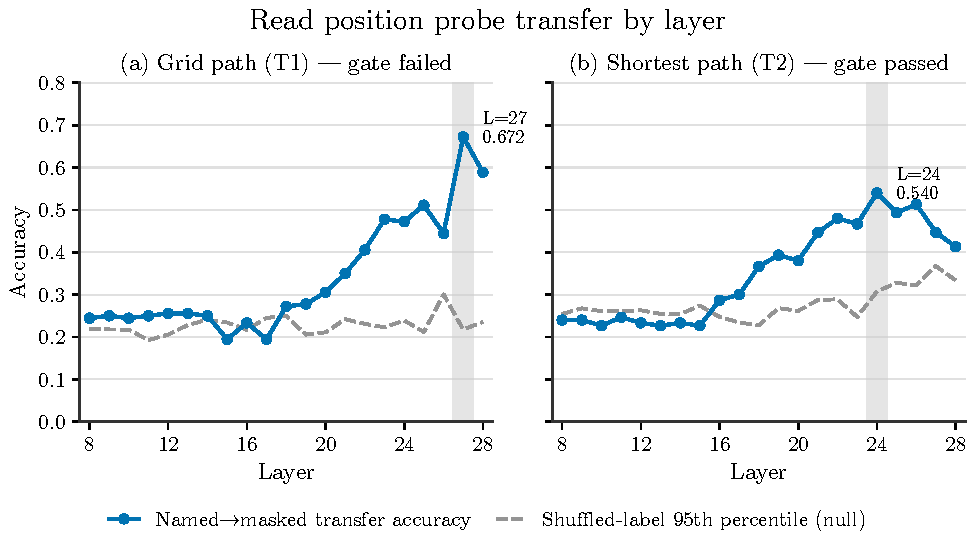
\includegraphics[width=\linewidth,height=0.78\textheight,keepaspectratio]{figures/fig_probe_layers_v0.pdf}
\caption{Named$\rightarrow$masked transfer accuracy of a linear probe at the prompt's read position, by layer, for Qwen3-8B (\nolinkurl{gen_art_experiment_2}, geometry screen). Solid blue line with circular markers: accuracy of a probe trained on residual-stream activations from prompts that name the forced algorithm and evaluated on activations from name-masked prompts (six-way label in panel (a), five-way in panel (b)). Dashed grey line: the 95th percentile of the same transfer accuracy under 20 shuffled-label refits, the null the solid line is compared against. (a) Grid path task (T1): transfer peaks at layer 27 (0.672, shaded column), but this layer fails the pre-declared decoder criterion of the read-position gate, so the peak is flagged rather than confirmed. (b) Shortest path task (T2): transfer peaks at layer 24 (0.540, shaded column) and passes the gate. In both panels transfer rises with depth and separates from the null only from roughly layer 20 onward; chance is 1\slash{}6 $\approx$ 0.167 for T1's six-way label and 1\slash{}5 = 0.20 for T2's five-way label, close to where the null curve sits. Single run per task; no additional seeds or cross-validation folds beyond the plotted shuffled-label null.}
\label{fig:fig_probe_layers}
\end{figure}
\textbf{The manifold.} The point clouds are low-dimensional: TwoNN intrinsic dimension 4.16 on the grid task and 5.24 on the shortest path task, against 11.92 and 11.58 for nulls with shuffled columns (5th-95th percentiles 10.78-13.46 and 10.64-12.71). MDS stress-1, the residual misfit of the two dimensional embedding, was 0.22 on both tasks and geodesic and Euclidean distances had Spearman correlation 0.87 and 0.90. Figure~\ref{fig:fig_manifold} draws the two maps with every condition's read position point, and Table 12 gives the geodesic distances from the default's centroid. On the grid task, BFS's two nearest centroids are DFS (41.19) and unit weight Dijkstra (58.39); A*, IDDFS and bidirectional BFS lie 71-95 away. On the shortest path task Dijkstra's nearest centroid is Floyd-Warshall (25.49), with Bellman-Ford\slash{}SPFA and bidirectional Dijkstra tied at about 42.

\begin{figure}[!htbp]
\centering\captionsetup{font=footnotesize}
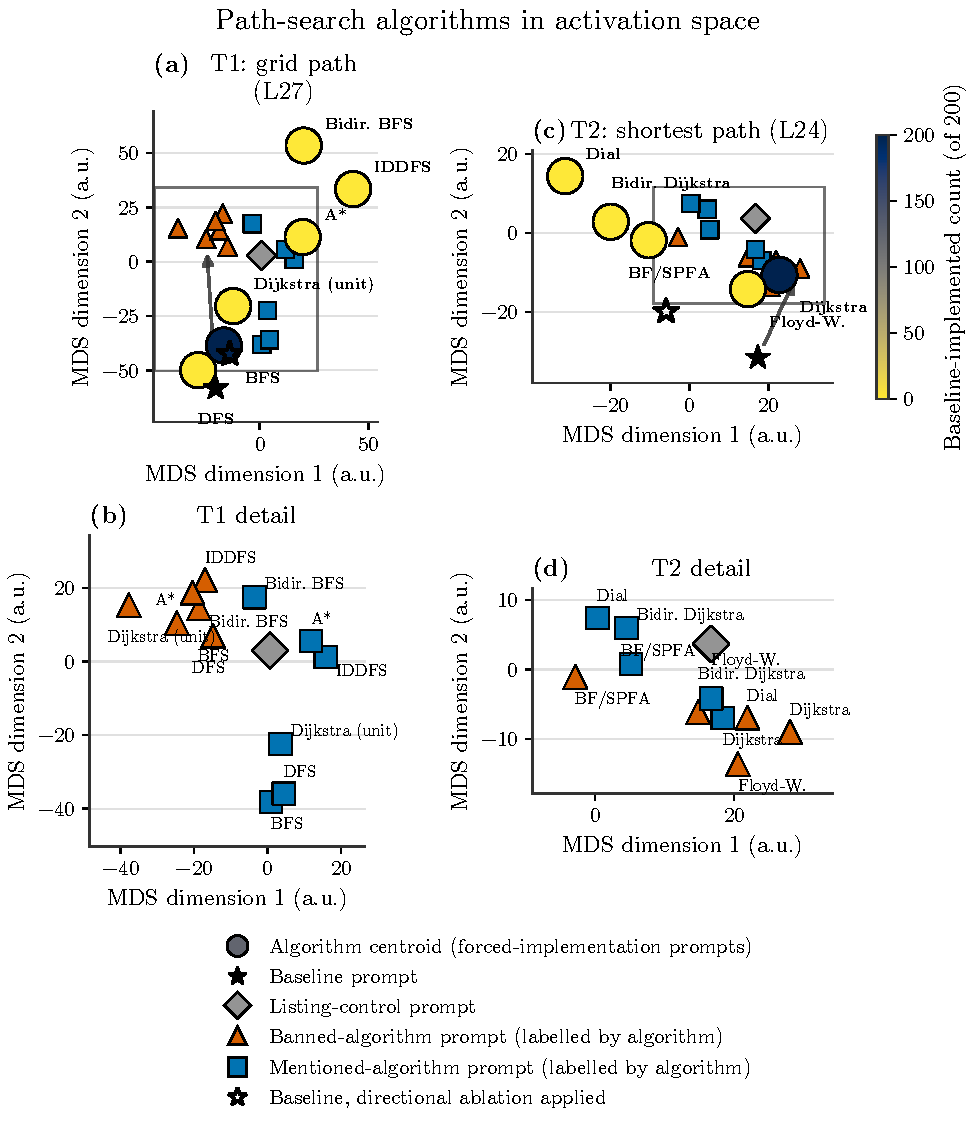
\includegraphics[width=\linewidth,height=0.78\textheight,keepaspectratio]{figures/fig_manifold_v0.pdf}
\caption{Two-dimensional multidimensional scaling (MDS) of geodesic distances between Qwen3-8B's read-position activation states, for an unweighted grid path-search task (T1, layer 27; panels a-b) and a weighted shortest-path task (T2, layer 24; panels c-d). In (a) and (c), large circles are each algorithm's centroid under forced-implementation prompts, coloured on a 0-200 scale by how many of 200 unprompted baseline generations implemented that algorithm (dark navy = 200, bright yellow = 0; only BFS in T1 and Dijkstra in T2 reach 200, every other cataloged algorithm is 0). The black star marks the plain baseline prompt and the hollow star the baseline after a directional-ablation intervention; the grey diamond is the prompt that lists every algorithm; orange triangles are prompts banning one algorithm and blue squares are prompts merely mentioning it, each labelled with that algorithm's name. The grey arrow connects the baseline to the prompt that bans the model's default algorithm (BFS in T1, Dijkstra in T2); the grey rectangle marks the region magnified in the panel below. (b) and (d) re-plot that boxed cluster of banned-, mentioned- and listing-control prompts at higher magnification so every point keeps an individually legible label. In T1 the six banned-algorithm points form one cluster set apart from every centroid, including BFS's own; in T2 the banned- and mentioned-algorithm points instead sit closer to the modal Dijkstra centroid and its neighbour Floyd-Warshall than to the three more distant centroids (Dial, Bellman-Ford\slash{}SPFA, bidirectional Dijkstra). The embedding's stress-1 is 0.217 (T1) and 0.221 (T2); its TwoNN intrinsic dimensionality is 4.16 and 5.24 respectively, both well below the $\approx$11.6-11.9 obtained from a shuffled null, indicating the activations occupy a low-dimensional manifold rather than filling the ambient space.}
\label{fig:fig_manifold}
\end{figure}
\begin{table}[H]
\renewcommand{\thetable}{12}
\centering\small\setlength{\tabcolsep}{4.0pt}
\caption{Geodesic distances between centroids at the read position (grid task, layer 27; shortest path task, layer 24), from the default algorithm's centroid. [Source: iteration 1, artifact \nolinkurl{gen_art_experiment_2}.]}\label{tab:t12}
\begin{tabular}{>{\raggedright\arraybackslash\hspace{0pt}}p{0.1311\linewidth}>{\raggedright\arraybackslash\hspace{0pt}}p{0.0965\linewidth}>{\raggedright\arraybackslash\hspace{0pt}}p{0.7187\linewidth}}
\toprule
\textbf{Task} & \textbf{From} & \textbf{To: distance} \\
\midrule
Grid & BFS & DFS 41.19; unit weight Dijkstra 58.39; A* 71.06; IDDFS 81.66; bidirectional BFS 94.95 \\
Shortest path & Dijkstra & Floyd-Warshall 25.49; Bellman-Ford\slash{}SPFA 42.18; bidirectional Dijkstra 42.46; Dial 54.96 \\
\bottomrule
\end{tabular}
\end{table}

The ban points do not sit near the centroids of the algorithms the model then wrote. Under the grid ban the read position point moved far from both BFS and DFS (from (-20.26, -58.22) for the baseline to (-24.67, 10.46)), while the mention point of BFS stayed close to the BFS centroid; the ban points of all six grid algorithms clustered together in one region of the map regardless of which algorithm was banned. This matches the decomposition below: most of the ban shift is not along the algorithm directions.

\textbf{The bans in this experiment.} Here the modal bans mostly failed (Table 13). On the grid task 62 of 100 programs were still BFS and the 18 compliant programs split into DFS 10 and unit weight Dijkstra 8, so there was no clear realised mode. On the shortest path task 72 of 100 were still Dijkstra and all 22 compliant programs were Bellman-Ford\slash{}SPFA. Compliance depended on the paraphrase: on the grid task four of the ten ban wordings gave 10 of 10 BFS while two gave 0 of 10 (Section 1.11). Some programs acknowledged the ban in a comment and used the algorithm anyway (\texttt{\# Dijkstra's algorithm (\allowbreak{}but since the user said not to use Dijkstra's algorithm,\allowbreak{} this is a workaround)}). Three step-2 bans were run as exploratory events after the preregistered succession stopped. On the grid task the displaced mass landed only on BFS's two geodesic neighbours, DFS and unit weight Dijkstra, and banning one of them moved the compliant programs to the other; it never reached A*, IDDFS or bidirectional BFS. In the words of the request, mass moved to the edge of the banned region rather than to the opposite side. On the shortest path task the mass went to the second nearest centroid, Bellman-Ford\slash{}SPFA, and the nearest, Floyd-Warshall, received none. \emph{(Correction, iteration 2: the claim that Bellman-Ford\slash{}SPFA is second nearest does not survive the sensitivity matrix of this experiment, which puts bidirectional Dijkstra (40.91) closer to Dijkstra than Bellman-Ford\slash{}SPFA (42.18) once the two flagged centroids are recomputed from correctly labelled forced samples. Under paraphrase level resampling Floyd-Warshall is nearest in every subsample, and Bellman-Ford\slash{}SPFA is second at layers 23 to 27 and third at layers 21 and 22; Section 2.3.2.)}

\begin{table}[H]
\renewcommand{\thetable}{13}
\centering\footnotesize\setlength{\tabcolsep}{4.0pt}
\caption{Ban events in the geometry experiment (all coded samples; compliant = correct and not banned). [Source: iteration 1, artifact \nolinkurl{gen_art_experiment_2}.]}\label{tab:t13}
\begin{tabular}{>{\raggedright\arraybackslash\hspace{0pt}}p{0.2243\linewidth}>{\raggedright\arraybackslash\hspace{0pt}}p{0.0413\linewidth}>{\raggedright\arraybackslash\hspace{0pt}}p{0.2331\linewidth}>{\raggedright\arraybackslash\hspace{0pt}}p{0.1752\linewidth}>{\raggedright\arraybackslash\hspace{0pt}}p{0.1152\linewidth}>{\raggedright\arraybackslash\hspace{0pt}}p{0.1075\linewidth}}
\toprule
\textbf{Event} & \textbf{N} & \textbf{Labels} & \textbf{Compliant (labels)} & \textbf{Realised mode} & \textbf{Status} \\
\midrule
Grid ban BFS & 100 & BFS 62, DFS 29, unit weight Dijkstra 9 & 18 (DFS 10, unit weight Dijkstra 8) & no clear mode & primary \\
Grid ban BFS and DFS & 50 & BFS 29, unit weight Dijkstra 19, DFS 2 & 18 (unit weight Dijkstra 18) & unit weight Dijkstra & exploratory \\
Grid ban BFS and unit weight Dijkstra & 50 & BFS 31, DFS 17, unit weight Dijkstra 2 & 5 (DFS 5) & DFS & exploratory \\
Shortest path ban Dijkstra & 100 & Dijkstra 72, Bellman-Ford\slash{}SPFA 27, other 1 & 22 (Bellman-Ford\slash{}SPFA 22) & Bellman-Ford\slash{}SPFA & primary \\
Shortest path ban Dijkstra and Bellman-Ford\slash{}SPFA & 50 & Dijkstra 37, Bellman-Ford\slash{}SPFA 12, other 1 & 0 & no clear mode & exploratory \\
\bottomrule
\end{tabular}
\end{table}

The ban raised the correctness conditioned Hill number from 1.00 to 2.034 on the grid task at a pass-rate cost of 0.99 to 0.76, and from 1.00 to 1.723 on the shortest path task at 1.00 to 0.94. Most of this diversity is the banned algorithm mixed with its substitute, since banned programs that pass the tests count toward Hill\_\allowbreak{}cc.

\textbf{The forecast contest.} Forecasts for 45 planned events were committed by sha256 hash before any ban or removal sample. Table 14 scores them. This experiment's own association elicitation produced different maps from the association experiment's: it nominated A* for BFS (clarity 0.80, Kendall's W 0.886) and Dial for Dijkstra (clarity 0.579). Both nominations missed and the association map was the worst predictor, worse than uniform. The geodesic kernel was the best on the two primary events (mean -1.433 against -1.563 for uniform), by a margin of 0.13 nats per sample, and no predictor scored a top-1 hit on a primary event.

\begin{table}[H]
\renewcommand{\thetable}{14}
\centering\footnotesize\setlength{\tabcolsep}{4.0pt}
\caption{Forecast contest in the geometry experiment (raw mean log score; top-1 nomination; the samples scored are all labels of the event other than the banned algorithm). [Source: iteration 1, artifact \nolinkurl{gen_art_experiment_2}.]}\label{tab:t14}
\begin{tabular}{>{\raggedright\arraybackslash\hspace{0pt}}p{0.3139\linewidth}>{\raggedright\arraybackslash\hspace{0pt}}p{0.1656\linewidth}>{\raggedright\arraybackslash\hspace{0pt}}p{0.1034\linewidth}>{\raggedright\arraybackslash\hspace{0pt}}p{0.1700\linewidth}>{\raggedright\arraybackslash\hspace{0pt}}p{0.1603\linewidth}}
\toprule
\textbf{Event (samples scored)} & \textbf{Association map} & \textbf{Latent frequency} & \textbf{Geodesic kernel} & \textbf{Read position decoder} \\
\midrule
Grid ban BFS (38) & -3.543 (A*) & -1.630 (tie) & -1.337 (DFS) & -1.287 (DFS) \\
Shortest path ban Dijkstra (28) & -1.647 (Dial) & -1.496 (tie) & -1.530 (Floyd-Warshall) & -1.587 (bidirectional Dijkstra) \\
Grid ban BFS and DFS, exploratory (19) & -0.998 (unit weight Dijkstra, hit) & -1.406 (tie) & -1.073 (unit weight Dijkstra, hit) & -4.124 (IDDFS) \\
Grid ban BFS and unit weight Dijkstra, exploratory (17) & -3.966 (A*) & -1.406 (tie) & -1.280 (A*) & -1.372 (IDDFS) \\
Shortest path ban Dijkstra and Bellman-Ford\slash{}SPFA, exploratory (1) & -3.912 & -3.912 & -3.912 & -3.912 \\
Mean, 2 primary events & -2.595 & -1.563 & -1.433 & -1.437 \\
Mean, all 5 events; top-1 hits & -2.813; 1\slash{}5 & -1.970; ties & -1.826; 1\slash{}5 & -2.456; 0\slash{}5 \\
\bottomrule
\end{tabular}
\end{table}

\textbf{The shift decomposition.} The ban shift is the read position state under the ban minus the state under its reference, computed against the mention twin and against the listing control. It was decomposed in a preregistered order into a component away from the banned algorithm (u\_\allowbreak{}ren), toward the association winner (u\_\allowbreak{}sub), toward the most frequent survivor (u\_\allowbreak{}typ) and toward the geodesically nearest other survivor (u\_\allowbreak{}rel), each orthogonalised against the previous ones. The preregistered share test needed the u\_\allowbreak{}sub share to exceed the u\_\allowbreak{}ren share and the u\_\allowbreak{}ren share to exceed a split half paraphrase null under both references. Table 15 gives the shares at the gate layer. The four named components together explained 1-39\% of the squared norm; the rest was residual. The u\_\allowbreak{}ren share exceeded its null in only 7 of 130 cells across the layer band (Dial under the mention reference at layers 23-27, and bidirectional Dijkstra twice), never under both references, so every algorithm was inconclusive. The cosine of each shift with the banned name's input embedding and unembedding row was at most 0.034 in absolute value. A synthetic test with a planted 36\slash{}64 split recovered it, so the decomposition code works; the shifts simply do not lie along the algorithm directions.

{\scriptsize\setlength{\tabcolsep}{2.5pt}\renewcommand{\thetable}{15}
\begin{longtable}{>{\raggedright\arraybackslash\hspace{0pt}}p{0.1226\linewidth}>{\raggedright\arraybackslash\hspace{0pt}}p{0.1771\linewidth}>{\raggedright\arraybackslash\hspace{0pt}}p{0.1470\linewidth}>{\raggedright\arraybackslash\hspace{0pt}}p{0.0655\linewidth}>{\raggedright\arraybackslash\hspace{0pt}}p{0.0655\linewidth}>{\raggedright\arraybackslash\hspace{0pt}}p{0.0576\linewidth}>{\raggedright\arraybackslash\hspace{0pt}}p{0.0655\linewidth}>{\raggedright\arraybackslash\hspace{0pt}}p{0.0872\linewidth}>{\raggedright\arraybackslash\hspace{0pt}}p{0.1149\linewidth}}
\caption{Squared norm shares of the ban shift at the gate layer (layer 27 for the grid task, layer 24 for the shortest path task); u\_\allowbreak{}typ is undefined when the most frequent survivor is also the association winner or no survivor has baseline mass. [Source: iteration 1, artifact \nolinkurl{gen_art_experiment_2}.]}\label{tab:t15}\\
\toprule
\textbf{Task} & \textbf{Banned X} & \textbf{Reference} & \textbf{u\_\allowbreak{}ren} & \textbf{u\_\allowbreak{}sub} & \textbf{u\_\allowbreak{}typ} & \textbf{u\_\allowbreak{}rel} & \textbf{Residual} & \textbf{u\_\allowbreak{}ren null p95} \\
\midrule
\endfirsthead
\multicolumn{9}{l}{\emph{Table 15, continued}}\\
\toprule
\textbf{Task} & \textbf{Banned X} & \textbf{Reference} & \textbf{u\_\allowbreak{}ren} & \textbf{u\_\allowbreak{}sub} & \textbf{u\_\allowbreak{}typ} & \textbf{u\_\allowbreak{}rel} & \textbf{Residual} & \textbf{u\_\allowbreak{}ren null p95} \\
\midrule
\endhead
\bottomrule
\endlastfoot
Grid & BFS & mention & 0.067 & 0.054 & 0.012 & 0.003 & 0.863 & 0.248 \\
Grid & BFS & listing control & 0.058 & 0.061 & 0.034 & 0.004 & 0.844 & 0.248 \\
Grid & DFS & mention & 0.042 & 0.038 & n\slash{}a & 0.000 & 0.920 & 0.170 \\
Grid & DFS & listing control & 0.052 & 0.017 & n\slash{}a & 0.002 & 0.929 & 0.170 \\
Grid & bidirectional BFS & mention & 0.078 & 0.020 & n\slash{}a & 0.000 & 0.901 & 0.263 \\
Grid & bidirectional BFS & listing control & 0.001 & 0.099 & n\slash{}a & 0.003 & 0.897 & 0.263 \\
Grid & IDDFS & mention & 0.090 & 0.005 & n\slash{}a & 0.029 & 0.876 & 0.274 \\
Grid & IDDFS & listing control & 0.003 & 0.034 & n\slash{}a & 0.054 & 0.909 & 0.274 \\
Grid & A* & mention & 0.086 & 0.005 & n\slash{}a & 0.014 & 0.895 & 0.134 \\
Grid & A* & listing control & 0.003 & 0.004 & n\slash{}a & 0.003 & 0.990 & 0.134 \\
Grid & unit weight Dijkstra & mention & 0.017 & 0.041 & 0.014 & 0.000 & 0.927 & 0.287 \\
Grid & unit weight Dijkstra & listing control & 0.130 & 0.076 & 0.000 & 0.011 & 0.783 & 0.287 \\
Shortest path & Dijkstra & mention & 0.004 & 0.002 & 0.041 & 0.013 & 0.940 & 0.311 \\
Shortest path & Dijkstra & listing control & 0.047 & 0.003 & 0.050 & 0.000 & 0.900 & 0.311 \\
Shortest path & Bellman-Ford\slash{}SPFA & mention & 0.000 & 0.069 & n\slash{}a & 0.021 & 0.909 & 0.298 \\
Shortest path & Bellman-Ford\slash{}SPFA & listing control & 0.104 & 0.094 & n\slash{}a & 0.005 & 0.797 & 0.298 \\
Shortest path & bidirectional Dijkstra & mention & 0.107 & 0.079 & n\slash{}a & 0.001 & 0.812 & 0.126 \\
Shortest path & bidirectional Dijkstra & listing control & 0.003 & 0.027 & n\slash{}a & 0.000 & 0.970 & 0.126 \\
Shortest path & Floyd-Warshall & mention & 0.000 & 0.019 & n\slash{}a & 0.004 & 0.976 & 0.212 \\
Shortest path & Floyd-Warshall & listing control & 0.075 & 0.005 & n\slash{}a & 0.001 & 0.919 & 0.212 \\
Shortest path & Dial & mention & 0.329 & 0.056 & n\slash{}a & 0.001 & 0.614 & 0.267 \\
Shortest path & Dial & listing control & 0.014 & 0.015 & n\slash{}a & 0.001 & 0.970 & 0.267 \\
\end{longtable}}

\textbf{Activation removal of the modal algorithm.} The removal used affine directional ablation [28, 29], anchored at the mean of the survivors: the component of each activation along a difference-in-means direction d\_\allowbreak{}X for the modal algorithm was moved to the survivors' mean, scaled by a coefficient alpha. Neither direction check reached its 0.9 target: the held-out AUC of d\_\allowbreak{}X was 0.89 and 0.79 at the read position and at best 0.66 and 0.76 at generated positions. The fallback declared in advance therefore ran. It edited the prompt suffix including the read position, over a 5-layer band on the grid task and a 7-layer band on the shortest path task, at alpha 0.5, 1 and 2, with two random directions of identical edit norm under common random numbers (the same sampling seeds for edited and unedited runs). It moved 0 of 50 samples on either task at every alpha (Table 16). Between 78\% and 90\% of the edited outputs were byte-identical to their alpha=0 twins, as were 80-96\% of the random direction outputs. The hook tests passed on both tasks: at alpha=0 the logits were identical to the unhooked model, the remaining projection on d\_\allowbreak{}X after the edit was below 1e-6 of its value before, and random and d\_\allowbreak{}X edits had exactly equal norms. A post hoc full variant that also edited every generated position still left 25 of 25 programs on BFS and on Dijkstra at alpha 2; at alpha 4 the d\_\allowbreak{}X edit destroyed generation (25 of 25 without code on both tasks) and the random direction broke most outputs as well. The verdict, as declared, was untestable, because the removal was unsuccessful at the tested coefficients. The comparison between prompt bans and activation removal, which the hypothesis treats as a headline, could not be made.

\begin{table}[H]
\renewcommand{\thetable}{16}
\centering\scriptsize\setlength{\tabcolsep}{2.5pt}
\caption{Affine directional ablation of the modal algorithm (prompt suffix variant declared in advance unless marked full; HF engine; pass rates over all samples). [Source: iteration 1, artifact \nolinkurl{gen_art_experiment_2}.]}\label{tab:t16}
\begin{tabular}{>{\raggedright\arraybackslash\hspace{0pt}}p{0.0923\linewidth}>{\raggedright\arraybackslash\hspace{0pt}}p{0.1525\linewidth}>{\raggedright\arraybackslash\hspace{0pt}}p{0.0948\linewidth}>{\raggedright\arraybackslash\hspace{0pt}}p{0.0526\linewidth}>{\raggedright\arraybackslash\hspace{0pt}}p{0.1724\linewidth}>{\raggedright\arraybackslash\hspace{0pt}}p{0.0615\linewidth}>{\raggedright\arraybackslash\hspace{0pt}}p{0.1471\linewidth}>{\raggedright\arraybackslash\hspace{0pt}}p{0.1400\linewidth}}
\toprule
\textbf{Task} & \textbf{Arm} & \textbf{Alpha} & \textbf{N} & \textbf{Labels} & \textbf{Pass} & \textbf{Moved off the modal algorithm} & \textbf{Identical text to alpha=0} \\
\midrule
Grid & hooked control & 0 & 50 & BFS 50 & 1.0 & 0\slash{}50 & 1.0 \\
Grid & d\_\allowbreak{}X & 0.5 \slash{} 1.0 \slash{} 2.0 & 50 each & BFS 50 each & 1.0 each & 0\slash{}50 each & 0.80 \slash{} 0.86 \slash{} 0.78 \\
Grid & random 1 & 0.5 \slash{} 1.0 \slash{} 2.0 & 25 each & BFS 25 each & 1.0 each & 0\slash{}25 each & 0.80 \slash{} 0.80 \slash{} 0.84 \\
Grid & random 2 & 0.5 \slash{} 1.0 & 25 each & BFS 25 each & 1.0 each & 0\slash{}25 each & 0.80 \slash{} 0.84 \\
Grid & d\_\allowbreak{}X, full (post hoc) & 2.0 & 25 & BFS 25 & 0.76 & 0\slash{}25 & 0.0 \\
Grid & d\_\allowbreak{}X, full (post hoc) & 4.0 & 25 & no code 25 & 0.0 & 0\slash{}25 & 0.0 \\
Grid & random 1, full (post hoc) & 4.0 & 25 & BFS 18, other 6, no code 1 & 0.0 & 6\slash{}25 & 0.0 \\
Shortest path & hooked control & 0 & 50 & Dijkstra 50 & 1.0 & 0\slash{}50 & 1.0 \\
Shortest path & d\_\allowbreak{}X & 0.5 \slash{} 1.0 \slash{} 2.0 & 50 each & Dijkstra 50 each & 1.0 each & 0\slash{}50 each & 0.90 \slash{} 0.86 \slash{} 0.82 \\
Shortest path & random 1 & 0.5 \slash{} 1.0 \slash{} 2.0 & 25 each & Dijkstra 25 each & 1.0 each & 0\slash{}25 each & 0.88 \slash{} 0.96 \slash{} 0.92 \\
Shortest path & random 2 & 0.5 \slash{} 1.0 & 25 each & Dijkstra 25 each & 1.0 each & 0\slash{}25 each & 0.96 \slash{} 0.92 \\
Shortest path & d\_\allowbreak{}X, full (post hoc) & 2.0 & 25 & Dijkstra 25 & 1.0 & 0\slash{}25 & 0.04 \\
Shortest path & d\_\allowbreak{}X, full (post hoc) & 4.0 & 25 & no code 25 & 0.0 & 0\slash{}25 & 0.0 \\
Shortest path & random 1, full (post hoc) & 4.0 & 25 & no code 20, Dijkstra 3, other 2 & 0.0 & 2\slash{}25 & 0.0 \\
\bottomrule
\end{tabular}
\end{table}

\textbf{What this experiment settled.} The read position holds a low-dimensional map of the catalogue, and on the grid task the mass displaced by the ban went to the geodesic neighbours of the default; the geodesic kernel was the least bad forecaster on the primary events. \emph{(Correction, iteration 2: those neighbours, DFS and unit weight Dijkstra, are also second choices of the model, so the observation is consistent with geodesic proximity and with typicality and does not separate them; both events called primary here fail the forecast contest's compliance gate; Sections 2.3.2 and 2.3.7.)} The read position does not, however, decode the grid task's actual default, the ban shift is almost entirely orthogonal to the algorithm directions, and an activation edit of the modal algorithm did nothing until it broke the model. The labeller passed its gate on both tasks. An independent recomputation reproduced 99 headline numbers with no mismatch.

\FloatBarrier
\subsection*{1.7 Forking token experiment: is the algorithm decided during generation?}
\addcontentsline{toc}{subsection}{1.7 Forking token experiment: is the algorithm decided during generation?}
\noindent{\small\emph{Artifact: \nolinkurl{gen_art_experiment_3}.}}\par\medskip
\textbf{Why.} If the read position does not fix the algorithm, the decision may be made at a few high entropy tokens during generation, as forking token analyses find for other outcomes [30, 31]. The knob this account implies is a sampler that raises temperature only around those tokens, in the spirit of adaptive temperature sampling for code [32]. This experiment screened that account on its own pool of about 10,000 labelled generations , with vLLM 0.11.0 in eager mode, its own tests (40 per task, 17 reference solutions) and a judge used only on 6 disputed programs (USD 0.024).

\textbf{Design.} A resampling screen took 10 base paths per task for the baseline and for the modal ban and drew 8 continuations at every fourth generated token over the first 92 tokens. Baseline paths were screened only at tokens 4, 8, 16, 32 and 64, a fallback declared in advance because the baseline was already fixed at the read position. Change points in the series of continuation outcome distributions were detected against a permutation threshold (a PELT detector [33] run alongside found none on any path), localised to single tokens, and confirmed with 30 continuations at each candidate and at two control positions without a change point. A prompt swap cut a baseline path just before or just after its commitment token (the first token of evidence that identifies the algorithm, such as the \texttt{deque} import) and continued it under the ban prompt. The knob arm compared global temperature 0.3-1.3 with temperature 1.3 applied only in a window around detected forking tokens, which we call the forking window knob, against a random window of the same size and an anchored window at the start of the code block. A planted change sensitivity test found that the detector caught a total variation change of 0.2, 0.3 and 0.5 in 82.5\%, 95\% and 99\% of trials, with a 6\% false-positive rate at no change.

\begin{table}[H]
\renewcommand{\thetable}{17}
\centering\footnotesize\setlength{\tabcolsep}{4.0pt}
\caption{Sample pools in the forking token experiment. [Source: iteration 1, artifact \nolinkurl{gen_art_experiment_3}.]}\label{tab:t17}
\begin{tabular}{>{\raggedright\arraybackslash\hspace{0pt}}p{0.1182\linewidth}>{\raggedright\arraybackslash\hspace{0pt}}p{0.2242\linewidth}>{\raggedright\arraybackslash\hspace{0pt}}p{0.0746\linewidth}>{\raggedright\arraybackslash\hspace{0pt}}p{0.2731\linewidth}>{\raggedright\arraybackslash\hspace{0pt}}p{0.1372\linewidth}>{\raggedright\arraybackslash\hspace{0pt}}p{0.0694\linewidth}}
\toprule
\textbf{Task} & \textbf{Pool} & \textbf{N} & \textbf{Labels} & \textbf{Pass} & \textbf{Hill\_\allowbreak{}cc} \\
\midrule
Grid & baseline, T=1.0 & 200 & BFS 200 & 0.91 & 1.0 \\
Grid & ban BFS, T=1.0 & 100 & DFS 78, BFS 21, unit weight Dijkstra 1 & 0.56 & 1.945 \\
Grid & baseline, T=0.3 \slash{} 0.7 \slash{} 1.3 & 100 each & BFS 100 each & 0.91 \slash{} 0.82 \slash{} 0.96 & 1.0 \\
Shortest path & baseline, T=1.0 & 200 & Dijkstra 200 & 0.995 & 1.0 \\
Shortest path & ban Dijkstra, T=1.0 & 100 & Bellman-Ford\slash{}SPFA 80, Dijkstra 20 & 1.00 & 1.649 \\
Shortest path & baseline, T=0.3 \slash{} 0.7 \slash{} 1.3 & 100 each & Dijkstra 100 each & 1.00 each & 1.0 \\
\bottomrule
\end{tabular}
\end{table}

\textbf{Where the outcome is fixed.} The sample pools behind the screen (Table 17) repeat the collapse: every baseline pool at every temperature was 100\% BFS or 100\% Dijkstra, and the ban pools were the only ones with a second algorithm. Under the baseline prompt every base path was fixed at the read position on both tasks: all continuations from token 0 onward produced the path's own algorithm (Table 18). Under the ban, outcomes were open for longer. On the grid task 3 of 10 ban paths were fixed from the read position and 5 of 10 by token 16; on the shortest path task none was fixed at the read position and only 3 of 10 by token 64. Change points were confirmed only on the shortest path ban paths: 6 forking tokens on 5 of the 10 paths, while the 3 grid candidates failed confirmation and the 10 control positions produced no false positive.

\begin{table}[H]
\renewcommand{\thetable}{18}
\centering\scriptsize\setlength{\tabcolsep}{2.5pt}
\caption{Resampling screen. We call a base path decided at the read position when its continuations from token 0 agree with its final label at least 80\% of the time, and fixed by token k when at least 7 of 8 continuations agree with it at every screened position from k on; the columns give the share of base paths of each kind. [Source: iteration 1, artifact \nolinkurl{gen_art_experiment_3}.]}\label{tab:t18}
\begin{tabular}{>{\raggedright\arraybackslash\hspace{0pt}}p{0.1351\linewidth}>{\raggedright\arraybackslash\hspace{0pt}}p{0.0582\linewidth}>{\raggedright\arraybackslash\hspace{0pt}}p{0.1175\linewidth}>{\raggedright\arraybackslash\hspace{0pt}}p{0.1907\linewidth}>{\raggedright\arraybackslash\hspace{0pt}}p{0.0683\linewidth}>{\raggedright\arraybackslash\hspace{0pt}}p{0.1001\linewidth}>{\raggedright\arraybackslash\hspace{0pt}}p{0.1001\linewidth}>{\raggedright\arraybackslash\hspace{0pt}}p{0.1432\linewidth}}
\toprule
\textbf{Condition} & \textbf{Base paths} & \textbf{Decided at the read position} & \textbf{Fixed by token 0 \slash{} 8 \slash{} 16 \slash{} 32 \slash{} 64} & \textbf{Paths not fixed} & \textbf{Forking token candidates} & \textbf{Confirmed forking tokens} & \textbf{Final labels} \\
\midrule
Grid baseline & 10 & 1.0 & 1.0 \slash{} 1.0 \slash{} 1.0 \slash{} 1.0 \slash{} 1.0 & 0 & 0 & 0 & BFS 10 \\
Grid ban BFS & 10 & 0.8 & 0.3 \slash{} 0.3 \slash{} 0.5 \slash{} 0.5 \slash{} 0.5 & 7 & 3 & 0 & DFS 9, BFS 1 \\
Shortest path baseline & 10 & 1.0 & 1.0 \slash{} 1.0 \slash{} 1.0 \slash{} 1.0 \slash{} 1.0 & 0 & 0 & 0 & Dijkstra 10 \\
Shortest path ban Dijkstra & 10 & 0.4 & 0.0 \slash{} 0.1 \slash{} 0.1 \slash{} 0.1 \slash{} 0.3 & 10 & 10 & 6 & Bellman-Ford\slash{}SPFA 6, Dijkstra 4 \\
\bottomrule
\end{tabular}
\end{table}

The confirmed forking tokens are not the punctuation tokens that studies of forking paths report on other tasks (Table 19). Two are the \texttt{import} token at position 3, where the model decides which module to import, two are algorithm names written in comments (the tokens \texttt{Bell} and \texttt{D} at position 68, each with a leading space), one is \texttt{BFS} inside the description of an SPFA queue, and one is a newline at position 7. Across confirmed forking tokens the outcome entropy fell by a mean of -0.131 bits, that is, it rose slightly, because several forking tokens moved a path from a fixed outcome to a mixed one.

\begin{table}[H]
\renewcommand{\thetable}{19}
\centering\scriptsize\setlength{\tabcolsep}{2.5pt}
\caption{Confirmed forking tokens (all on shortest path ban paths). TVD is the total variation distance between continuation outcome distributions on either side. [Source: iteration 1, artifact \nolinkurl{gen_art_experiment_3}.]}\label{tab:t19}
\begin{tabular}{>{\raggedright\arraybackslash\hspace{0pt}}p{0.1743\linewidth}>{\raggedright\arraybackslash\hspace{0pt}}p{0.0872\linewidth}>{\raggedright\arraybackslash\hspace{0pt}}p{0.1532\linewidth}>{\raggedright\arraybackslash\hspace{0pt}}p{0.0992\linewidth}>{\raggedright\arraybackslash\hspace{0pt}}p{0.0551\linewidth}>{\raggedright\arraybackslash\hspace{0pt}}p{0.1168\linewidth}>{\raggedright\arraybackslash\hspace{0pt}}p{0.2378\linewidth}}
\toprule
\textbf{Base path} & \textbf{Position} & \textbf{Token} & \textbf{Token type} & \textbf{TVD} & \textbf{Permutation p} & \textbf{Outcome entropy before \slash{} after (bits)} \\
\midrule
Shortest path ban 0 & 3 & \texttt{import} & import & 0.80 & 0.0005 & 0.567 \slash{} 0.353 \\
Shortest path ban 1 & 3 & \texttt{import} & import & 0.767 & 0.0005 & 0.211 \slash{} 0.784 \\
Shortest path ban 1 & 77 & \texttt{BFS} (leading space) & identifier & 0.333 & 0.013 & 1.0 \slash{} 0.65 \\
Shortest path ban 3 & 68 & \texttt{Bell} (leading space) & identifier & 0.333 & 0.002 & 0.948 \slash{} 0.211 \\
Shortest path ban 4 & 68 & \texttt{D} (leading space) & identifier & 0.533 & 0.0005 & 0.0 \slash{} 1.368 \\
Shortest path ban 7 & 7 & newline & whitespace & 0.90 & 0.0005 & 0.211 \slash{} 0.353 \\
\bottomrule
\end{tabular}
\end{table}

\textbf{Does the commitment token lock the algorithm in?} No. The prompt swap predicted that a ban would work better on a prefix cut before the commitment token than after it. The ban effect was the same on both sides (Table 20): on the grid task 75\% of continuations avoided BFS before the cut and 73.5\% after it, a difference of 0.015 with a 95\% interval of -0.02 to 0.055. Writing \texttt{from collections import deque} did not commit the model to BFS. On the shortest path task the ban was weak on both sides of the cut (25.5\% and 27\% avoided Dijkstra).

\begin{table}[H]
\renewcommand{\thetable}{20}
\centering\footnotesize\setlength{\tabcolsep}{4.0pt}
\caption{Prompt swap at the commitment token (10 base paths per task; ban effect = share of continuations avoiding the banned algorithm; 95\% bootstrap intervals). [Source: iteration 1, artifact \nolinkurl{gen_art_experiment_3}.]}\label{tab:t20}
\begin{tabular}{>{\raggedright\arraybackslash\hspace{0pt}}p{0.0899\linewidth}>{\raggedright\arraybackslash\hspace{0pt}}p{0.2179\linewidth}>{\raggedright\arraybackslash\hspace{0pt}}p{0.2130\linewidth}>{\raggedright\arraybackslash\hspace{0pt}}p{0.1646\linewidth}>{\raggedright\arraybackslash\hspace{0pt}}p{0.2278\linewidth}}
\toprule
\textbf{Task} & \textbf{Ban effect, cut before commitment} & \textbf{Ban effect, cut after commitment} & \textbf{Before minus after} & \textbf{Banned share after the cut (lock in)} \\
\midrule
Grid & 0.75 [0.545, 0.91] & 0.735 [0.54, 0.895] & 0.015 [-0.02, 0.055] & 0.265 [0.095, 0.45] \\
Shortest path & 0.255 [0.155, 0.365] & 0.27 [0.155, 0.40] & -0.015 [-0.095, 0.05] & 0.73 [0.61, 0.84] \\
Pooled & 0.5025 [0.347, 0.648] & 0.5025 [0.347, 0.642] & 0.0 [-0.045, 0.04] & 0.498 [0.343, 0.638] \\
\bottomrule
\end{tabular}
\end{table}

\textbf{The forking window temperature knob.} Raising temperature only around detected forking tokens changed nothing about the algorithm (Table 21): every arm on both tasks was 100\% BFS or 100\% Dijkstra, and the difference in Hill\_\allowbreak{}cc between the forking token window and a random window was 0 with a [0, 0] interval. What temperature did change was the number of distinct phrasings. On the grid task global temperature took the number of phrasing clusters (defined in Section 1.10) at a Jaccard threshold of 0.8 from 11 at T=0.3 to 63 at T=1.3, while the forking token window gave 10, about the same as T=0.3.

\begin{table}[H]
\renewcommand{\thetable}{21}
\centering\scriptsize\setlength{\tabcolsep}{2.5pt}
\caption{Temperature arms of the forking token experiment (N=100 each; all programs BFS on the grid task and Dijkstra on the shortest path task). Phrasing clusters at Jaccard thresholds 0.7 \slash{} 0.8 \slash{} 0.9 over identifier normalised AST shingles; phrasing Hill number at 0.8. [Source: iteration 1, artifact \nolinkurl{gen_art_experiment_3}.]}\label{tab:t21}
\begin{tabular}{>{\raggedright\arraybackslash\hspace{0pt}}p{0.1193\linewidth}>{\raggedright\arraybackslash\hspace{0pt}}p{0.1737\linewidth}>{\raggedright\arraybackslash\hspace{0pt}}p{0.0539\linewidth}>{\raggedright\arraybackslash\hspace{0pt}}p{0.0644\linewidth}>{\raggedright\arraybackslash\hspace{0pt}}p{0.2341\linewidth}>{\raggedright\arraybackslash\hspace{0pt}}p{0.1329\linewidth}>{\raggedright\arraybackslash\hspace{0pt}}p{0.1453\linewidth}}
\toprule
\textbf{Task} & \textbf{Arm} & \textbf{Pass} & \textbf{Hill\_\allowbreak{}cc} & \textbf{Phrasing clusters (0.7 \slash{} 0.8 \slash{} 0.9)} & \textbf{Phrasing Hill (0.8)} & \textbf{Mean length (tokens)} \\
\midrule
Grid & global T=0.3 & 0.91 & 1.0 & 8 \slash{} 11 \slash{} 18 & 6.28 & 335.15 \\
Grid & global T=0.7 & 0.82 & 1.0 & 17 \slash{} 25 \slash{} 35 & 14.36 & 345.11 \\
Grid & global T=1.0 & 0.94 & 1.0 & 24 \slash{} 41 \slash{} 60 & 24.58 & 331.6 \\
Grid & global T=1.3 & 0.96 & 1.0 & 39 \slash{} 63 \slash{} 80 & 44.72 & 342.62 \\
Grid & forking token window & 0.83 & 1.0 & 8 \slash{} 10 \slash{} 23 & 6.06 & 346.67 \\
Grid & random window & 0.85 & 1.0 & 6 \slash{} 11 \slash{} 20 & 5.63 & 349.55 \\
Grid & anchored window & 0.85 & 1.0 & 9 \slash{} 13 \slash{} 25 & 5.85 & 337.87 \\
Shortest path & global T=0.3 & 1.00 & 1.0 & 1 \slash{} 1 \slash{} 1 & 1.0 & 191.88 \\
Shortest path & global T=0.7 & 1.00 & 1.0 & 1 \slash{} 2 \slash{} 2 & 1.10 & 192.28 \\
Shortest path & global T=1.0 & 0.99 & 1.0 & 2 \slash{} 4 \slash{} 5 & 1.47 & 193.62 \\
Shortest path & global T=1.3 & 1.00 & 1.0 & 3 \slash{} 5 \slash{} 7 & 1.84 & 195.08 \\
Shortest path & forking token window & 1.00 & 1.0 & 1 \slash{} 2 \slash{} 2 & 1.06 & 192.01 \\
Shortest path & random window & 0.99 & 1.0 & 1 \slash{} 2 \slash{} 2 & 1.10 & 192.5 \\
Shortest path & anchored window & 1.00 & 1.0 & 1 \slash{} 1 \slash{} 2 & 1.0 & 192.3 \\
\bottomrule
\end{tabular}
\end{table}

\textbf{Dead end: the locus probes never ran to completion.} The decisive measurement for this account was a probe from residual-stream states at the read position, at generated tokens 8, 16, 32 and 64, at the forking token and at the commitment token, to the final label. The states were extracted (300 samples per task at 8 positions and 21 layers, with read position cosine to a separate pass of at least 0.9997), but the probe stage wrote an empty \texttt{probes.\allowbreak{}json} and no probe result exists. The strategy's locus diagnostic is therefore undetermined. \emph{(Correction, iteration 2: the cause is now recorded. \texttt{probes.\allowbreak{}json} (28 bytes, an empty summary) was written 2 min 33 s before the state log records the state phase starting, and 5 min 12 s and 5 min 28 s before the grid and shortest path states were saved: the probe stage ran before its inputs existed. The states (\texttt{states/\allowbreak{}T\{1,\allowbreak{}2\}\_\allowbreak{}part\_\allowbreak{}001-\allowbreak{}005.\allowbreak{}npz}, about 790 MB, kept on the run volume) were intact, and the audit ran the probe on them in iteration 2; Section 2.3.1.)} The preregistered verdict rule returned INCONCLUSIVE: no confirmed forking token on the grid task, confirmed forking tokens on half of the shortest path ban paths, and no effect of the forking window knob.

\textbf{What this experiment settled.} Without a ban the algorithm is fixed before the first generated token on both tasks, so there is no forking token for temperature to act on. Under a ban the outcome stays open for dozens of tokens and a few forking tokens exist on the shortest path task, including the choice of import; the first token that identifies the algorithm does not lock the algorithm in. A temperature knob aimed at forking tokens adds neither ideas nor phrasings.

\FloatBarrier
\subsection*{1.8 Decommitment experiment: does one list versus implement direction control the collapse?}
\addcontentsline{toc}{subsection}{1.8 Decommitment experiment: does one list versus implement direction control the collapse?}
\noindent{\small\emph{Artifact: \nolinkurl{gen_art_experiment_4}.}}\par\medskip
\textbf{Why.} An alternate account holds that the bottleneck is commitment, not the choice of a particular algorithm: a model asked to list ten approaches knows many, and a model asked to implement one collapses. If a single direction separates the two framings, adding it while the model implements should spread its output over the repertoire instead of moving it to one substitute. This experiment built that direction, steered with it under random direction and prompting controls [34], and tested whether a ban moves the read position along it .

\textbf{Design.} The decommitment direction is a difference-in-means direction at the read position: the mean state over 50 paraphrases of \texttt{list ten different approaches to this task}, which we call the list framing, minus the mean over 50 paraphrases of \texttt{implement one correct algorithm}, the implement framing, per layer. Held-out separation AUC was 1.00 at every layer from 9 to 28, and layer 18 was chosen by the held-out separation statistic d' (8.55). At layer 18 the direction's norm was 0.21 (grid) and 0.19 (shortest path) times the state norm, its split half cosine was 0.99, and the two tasks' directions had cosine 0.98. Its cosine was 0.53-0.55 with a breadth direction that contrasts listing approaches with naming one, -0.08 to -0.04 with a variable name placebo direction, and 0.59-0.62 with the shift produced by the enumeration prompt. It was added as c times the state norm times the unit direction at the read position and at every generated token, with c in \{0.25, 0.5, 1, 1.5\} plus a preregistered bisection. The correctness preserving coefficient c* was the largest c with at least 80\% of the c=0 pass rate: 0.1 on the grid task and 0.25 on the shortest path task. Controls were two random directions, the placebo and breadth directions at c*, the other task's direction, the prompt we call the enumeration prompt (\texttt{list 10 approaches,\allowbreak{} then implement one}), the modal ban and its mention twin, and a two-step succession. Labels came from hidden tests (43 and 39 cases), the tracer and AST rules, with a judge on disagreements; the labeller gate passed (Table 2). An engine check compared the vLLM baseline with the hooked HF arm at c=0: identical on the grid task, total variation 0.03 on the shortest path task (Fisher p 0.40).

\textbf{Steering moved the shortest path task and never the grid task.} On the grid task every arm except the bans wrote BFS (Table 22). At c=0.25 the pass rate fell to 0.57 and every passing program was still BFS; at c=0.5 it fell to 0.03, and from c=1 all output was broken (pass 0, 28-85\% of samples truncated). On the shortest path task the c*=0.25 arm moved correct programs from Dijkstra to Bellman-Ford\slash{}SPFA (Bellman-Ford\slash{}SPFA 54, Dijkstra 23, other 1, against Dijkstra 88 and Bellman-Ford\slash{}SPFA 7 at c=0), a rarefied Hill-number gain of +0.65 (paraphrase-cluster 90\% interval 0.31 to 0.97) at a 17-point pass-rate cost. A random direction at the same strength did almost the same (+0.59), and the difference between the decommitment direction and that random direction was +0.07 (-0.26 to 0.39). The gain therefore is not specific to the direction, although it exceeded the second random direction (+0.70, 0.38 to 1.01) and the placebo (+0.47, 0.01 to 0.84). Per-sample flips against c=0 under common random numbers were 0.66 for the decommitment direction, 0.42 and 0.18 for the two random directions and 0.22 for the placebo. On the shortest path task the off-mode rate peaked at c=0.25 (0.55) and fell again at c=0.5 (0.12) as programs broke. A Hill number of 2 was reached at c of about 0.40 for a 34.5-point pass cost; a Hill number of 3 was not reached in the tested range.

{\scriptsize\setlength{\tabcolsep}{2.5pt}\renewcommand{\thetable}{22}
\begin{longtable}{>{\raggedright\arraybackslash\hspace{0pt}}p{0.0824\linewidth}>{\raggedright\arraybackslash\hspace{0pt}}p{0.2129\linewidth}>{\raggedright\arraybackslash\hspace{0pt}}p{0.1083\linewidth}>{\raggedright\arraybackslash\hspace{0pt}}p{0.0736\linewidth}>{\raggedright\arraybackslash\hspace{0pt}}p{0.2139\linewidth}>{\raggedright\arraybackslash\hspace{0pt}}p{0.1286\linewidth}>{\raggedright\arraybackslash\hspace{0pt}}p{0.1038\linewidth}}
\caption{BUY table of the decommitment experiment. Delta Hill is the change in correctness conditioned Hill number, rarefied to a common sample depth, against the HF c=0 arm for steering and against the vLLM baseline for prompts, with a 90\% paraphrase-cluster interval; efficiency is Delta Hill per pass-rate point lost. [Source: iteration 1, artifact \nolinkurl{gen_art_experiment_4}.]}\label{tab:t22}\\
\toprule
\textbf{Task} & \textbf{Knob} & \textbf{Pass} & \textbf{Pass points lost} & \textbf{Labels of correct programs} & \textbf{Delta Hill [90\% interval]} & \textbf{Efficiency} \\
\midrule
\endfirsthead
\multicolumn{7}{l}{\emph{Table 22, continued}}\\
\toprule
\textbf{Task} & \textbf{Knob} & \textbf{Pass} & \textbf{Pass points lost} & \textbf{Labels of correct programs} & \textbf{Delta Hill [90\% interval]} & \textbf{Efficiency} \\
\midrule
\endhead
\bottomrule
\endlastfoot
Grid & vLLM baseline (N=200) & 1.00 & n\slash{}a & BFS 200 & n\slash{}a & n\slash{}a \\
Grid & HF c=0 & 1.00 & n\slash{}a & BFS 100 & n\slash{}a & n\slash{}a \\
Grid & decommitment c=0.1 (c*) & 0.98 & 2 & BFS 98 & 0.0 [0.0, 0.0] & 0.0 \\
Grid & decommitment c=0.25 & 0.57 & 43 & BFS 57 & 0.0 & 0.0 \\
Grid & decommitment c=0.5 & 0.03 & 97 & BFS 3 & 0.0 & 0.0 \\
Grid & decommitment c=1 \slash{} 1.5 & 0.0 \slash{} 0.0 & 100 & none & n\slash{}a & n\slash{}a \\
Grid & random 1 \slash{} random 2 \slash{} placebo \slash{} breadth at c* & 0.98 \slash{} 1.00 \slash{} 1.00 \slash{} 0.99 & 2 \slash{} 0 \slash{} 0 \slash{} 1 & all BFS & 0.0 & 0.0 \\
Grid & other task's direction at c* (N=50) & 0.98 & 2 & all BFS & 0.0 & 0.0 \\
Grid & enumeration prompt & 1.00 & 0 & BFS 100 & 0.0 & n\slash{}a \\
Grid & mention BFS & 1.00 & 0 & BFS 100 & 0.0 & n\slash{}a \\
Grid & ban BFS & 0.64 & 36 & BFS 46, DFS 16, unit weight Dijkstra 2 & +0.99 [0.55, 1.34] & 0.028 \\
Grid & succession (ban BFS and DFS) & 0.88 & 12 & BFS 65, unit weight Dijkstra 13, DFS 7, A* 3 & +1.27 [0.64, 1.80] & 0.106 \\
Shortest path & vLLM baseline (N=200) & 0.89 & n\slash{}a & Dijkstra 169, Bellman-Ford\slash{}SPFA 8 & n\slash{}a & n\slash{}a \\
Shortest path & HF c=0 & 0.95 & n\slash{}a & Dijkstra 88, Bellman-Ford\slash{}SPFA 7 & n\slash{}a & n\slash{}a \\
Shortest path & decommitment c=0.25 (c*) & 0.78 & 17 & Bellman-Ford\slash{}SPFA 54, Dijkstra 23, other 1 & +0.65 [0.31, 0.97] & 0.038 \\
Shortest path & decommitment c=0.375 & 0.67 & 28 & Bellman-Ford\slash{}SPFA 47, Dijkstra 19 & +0.65 [0.29, 0.94] & 0.023 \\
Shortest path & decommitment c=0.5 & 0.37 & 58 & Dijkstra 25, Bellman-Ford\slash{}SPFA 10, other 2 & +0.87 [0.09, 1.38] & 0.015 \\
Shortest path & decommitment c=1 \slash{} 1.5 & 0.0 \slash{} 0.0 & 95 & none & n\slash{}a & n\slash{}a \\
Shortest path & random 1 at c* & 0.79 & 16 & Dijkstra 53, Bellman-Ford\slash{}SPFA 26 & +0.59 [0.21, 0.85] & 0.037 \\
Shortest path & random 2 at c* & 0.87 & 8 & Dijkstra 82, Bellman-Ford\slash{}SPFA 5 & -0.05 [-0.31, 0.20] & -0.006 \\
Shortest path & placebo at c* & 0.66 & 29 & Dijkstra 60, Dial 3, Bellman-Ford\slash{}SPFA 2 & +0.19 [-0.30, 0.70] & 0.006 \\
Shortest path & breadth direction at c* & 0.60 & 35 & Bellman-Ford\slash{}SPFA 31, Dijkstra 28, Dial 1 & +0.85 [0.46, 1.17] & 0.024 \\
Shortest path & other task's direction at c* (N=50) & 0.72 & 23 & Bellman-Ford\slash{}SPFA 28, Dijkstra 8 & +0.40 [-0.01, 0.69] & 0.018 \\
Shortest path & enumeration prompt & 0.82 & 6.5 & Dijkstra 80, Bellman-Ford\slash{}SPFA 2 & -0.08 [-0.27, 0.13] & -0.013 \\
Shortest path & mention Dijkstra & 0.94 & -5.5 & Dijkstra 92, Bellman-Ford\slash{}SPFA 2 & -0.09 [-0.29, 0.12] & n\slash{}a \\
Shortest path & ban Dijkstra & 0.87 & 1.5 & Dijkstra 49, Bellman-Ford\slash{}SPFA 38 & +0.79 [0.60, 0.90] & 0.524 \\
Shortest path & succession (ban Dijkstra and Bellman-Ford\slash{}SPFA) & 0.68 & 20.5 & Bellman-Ford\slash{}SPFA 34, Dijkstra 33, other 1 & +0.93 [0.66, 1.17] & 0.045 \\
\end{longtable}}

The prompting baselines decide the comparison. The enumeration prompt, which states the decommitment framing in words, produced no diversity on either task. The modal ban bought +0.79 effective algorithms on the shortest path task for 1.5 pass points, an efficiency 14 times that of steering, but most banned samples still used the banned algorithm: 46 of 64 correct grid programs were BFS and 49 of 87 correct shortest path programs were Dijkstra. The ban's Hill gain is therefore mostly a mixture of ban failures and Bellman-Ford\slash{}SPFA, not two algorithms chosen freely.

\textbf{Does a ban decommit?} The commitment test projects the ban minus mention shift at layer 18 onto the axis from the implement framing (0) to the list framing (1). The ban moved the read position toward the list framing by 0.039 on the grid task and 0.053 on the shortest path task (Table 23), outside the preregistered paraphrase split null band (plus or minus 0.024 and 0.025), so the preregistered label is that the ban decommits. An audit judged that band too narrow; exact permutation tests gave p = 0.021 and 0.007 (label permutation) and 0.025 and 0.016 (paired sign flip), with 8 of 10 paraphrase pairs positive on each task. The shift is small: the enumeration prompt, the positive control, moved the state by 0.544 and 0.582 of the same distance, and the listing control sat at 0.816 and 0.806. The share of the ban shift along the direction ranked at the 78th and 87th percentiles of a null built from the top 50 principal components.

\begin{table}[H]
\renewcommand{\thetable}{23}
\centering\small\setlength{\tabcolsep}{4.0pt}
\caption{Position along the implement (0) to list (1) axis at layer 18 for each prompt condition. [Source: iteration 1, artifact \nolinkurl{gen_art_experiment_4}.]}\label{tab:t23}
\begin{tabular}{>{\raggedright\arraybackslash\hspace{0pt}}p{0.6474\linewidth}>{\raggedright\arraybackslash\hspace{0pt}}p{0.1492\linewidth}>{\raggedright\arraybackslash\hspace{0pt}}p{0.1496\linewidth}}
\toprule
\textbf{Condition} & \textbf{Grid} & \textbf{Shortest path} \\
\midrule
baseline & -0.054 & -0.075 \\
enumeration prompt & 0.483 & 0.495 \\
listing control & 0.816 & 0.806 \\
framing that names one approach & 0.653 & 0.650 \\
ban of the modal algorithm \slash{} its mention twin & 0.040 \slash{} 0.001 & 0.035 \slash{} -0.018 \\
ban DFS \slash{} mention DFS (Grid); ban Bellman-Ford\slash{}SPFA \slash{} mention (Shortest path) & 0.023 \slash{} -0.001 & 0.047 \slash{} -0.018 \\
ban bidirectional BFS \slash{} mention (Grid); ban bidirectional Dijkstra \slash{} mention (Shortest path) & 0.007 \slash{} -0.004 & 0.017 \slash{} 0.001 \\
ban IDDFS \slash{} mention (Grid); ban Floyd-Warshall \slash{} mention (Shortest path) & 0.036 \slash{} 0.012 & 0.030 \slash{} -0.013 \\
ban A* \slash{} mention (Grid); ban Dial \slash{} mention (Shortest path) & 0.073 \slash{} 0.004 & 0.052 \slash{} -0.002 \\
ban unit weight Dijkstra \slash{} mention (Grid) & 0.051 \slash{} 0.010 & n\slash{}a \\
Ban minus mention for the modal algorithm (null band) & 0.039 ($\pm$0.024) & 0.053 ($\pm$0.025) \\
Enumeration minus baseline, positive control (null band) & 0.544 ($\pm$0.047) & 0.582 ($\pm$0.048) \\
\bottomrule
\end{tabular}
\end{table}

\textbf{The forecast record.} Forecasts were committed before the ban samples. On the shortest path modal ban all 38 compliant programs were Bellman-Ford\slash{}SPFA; the decommitted survivor distribution scored -0.058 and hit, the vLLM frequency forecast -0.219 (hit), the HF frequency forecast -0.238 (hit) and the uniform forecast -1.406. On the grid modal ban (18 compliant: DFS 16, unit weight Dijkstra 2) every forecast was degenerate, because no correct program other than BFS existed before the ban, and all tied at -1.630. The succession events tied as well (16 compliant grid programs, unit weight Dijkstra 13 and A* 3; 1 compliant shortest path program).

\textbf{What this experiment settled.} The decommitment direction exists as a clean difference-in-means direction, shared across tasks, but adding it is a generic perturbation: it moves the shortest path task toward Bellman-Ford\slash{}SPFA as a random direction does and costs a sixth of the pass rate, and it never moves the grid task. Its prompt counterpart, the enumeration prompt, does nothing. A ban moves the read position measurably but slightly toward the list framing. The preregistered verdict was PARTIAL (the diversity gain held on one task, the specificity test failed). vLLM same seed determinism failed on the grid task, so vLLM arms are reproducible in distribution only, and every common random number analysis used HF arms.

\FloatBarrier
\subsection*{1.9 Instruction tuning experiment: did post-training install the collapse?}
\addcontentsline{toc}{subsection}{1.9 Instruction tuning experiment: did post-training install the collapse?}
\noindent{\small\emph{Artifact: \nolinkurl{gen_art_experiment_5}.}}\par\medskip
\textbf{Why.} If instruction tuning installed the collapse, the base model should spread over several algorithms at matched prompts, and subtracting the instruct minus base activation difference should restore that spread inside the instruct model. Base models are reported to be more diverse than aligned ones [35], and chat formatting alone narrows output diversity [36]; this experiment separated the two causes on the two tasks .

\textbf{Design.} A two by two design crossed weights (Qwen3-8B-Base, Qwen3-8B) with format (code completion without a chat template, which we call plain completion, or the instruct chat template), all at temperature 1.0 with top-p 1.0, thinking off. Each program ran on 47 (grid) or 46 (shortest path) hidden tests and was labelled by the tracer and AST rules with Gemini 2.5 Flash Lite as judge on disagreements; a second judge agreed with the first on 95\% of 40 audit programs (kappa 0.93). The runtime and AST labels agreed with kappa 0.77 over all parseable programs, but much lower on base-model output (0.20-0.50), where 217 of 292 grid programs in plain completion needed the judge. The sharpening direction is the paired difference between instruct and base read position states over the same chat-templated prompts, per layer from 8 to 28. It was subtracted at c in \{0.5, 1.0, 1.5\} over the whole band, at the read position only, and at layer 18 only, against two norm-matched random directions. Hardware was one NVIDIA GPU with 23 GB of memory (2.1 GPU hours); judge spend was USD 0.21.

\textbf{The collapse is sharpened by post-training, not invented by it.} Table 24 gives every arm. The instruct model in chat format is collapsed on both tasks. The base model under the same chat tokens writes mostly the same algorithm but less exclusively: BFS in 49 of 57 correct grid programs and Dijkstra in 63 of 90 correct shortest path programs, with Bellman-Ford\slash{}SPFA second (24). In plain completion the base model rarely writes a correct program (pass 0.05 and 0.08), and its correct shortest path programs are mostly Bellman-Ford\slash{}SPFA (16 of 25).

\begin{table}[H]
\renewcommand{\thetable}{24}
\centering\scriptsize\setlength{\tabcolsep}{2.5pt}
\caption{Arms of the instruction tuning experiment (vLLM, T=1.0). Hill\_\allowbreak{}cc with 95\% cluster bootstrap interval; Hill\_\allowbreak{}all over all parseable labelled programs. [Source: iteration 1, artifact \nolinkurl{gen_art_experiment_5}.]}\label{tab:t24}
\begin{tabular}{>{\raggedright\arraybackslash\hspace{0pt}}p{0.1486\linewidth}>{\raggedright\arraybackslash\hspace{0pt}}p{0.0769\linewidth}>{\raggedright\arraybackslash\hspace{0pt}}p{0.0372\linewidth}>{\raggedright\arraybackslash\hspace{0pt}}p{0.0622\linewidth}>{\raggedright\arraybackslash\hspace{0pt}}p{0.1061\linewidth}>{\raggedright\arraybackslash\hspace{0pt}}p{0.0788\linewidth}>{\raggedright\arraybackslash\hspace{0pt}}p{0.2392\linewidth}>{\raggedright\arraybackslash\hspace{0pt}}p{0.1000\linewidth}>{\raggedright\arraybackslash\hspace{0pt}}p{0.0539\linewidth}}
\toprule
\textbf{Arm} & \textbf{Task} & \textbf{N} & \textbf{Parse rate} & \textbf{Pass [95\% Wilson]} & \textbf{Correct} & \textbf{Labels of correct programs} & \textbf{Hill\_\allowbreak{}cc [95\%]} & \textbf{Hill\_\allowbreak{}all} \\
\midrule
base, plain completion & Grid & 300 & 0.97 & 0.05 [0.03, 0.08] & 15 & BFS 12, DFS 3 & 1.65 [1.00, 2.00] & 3.34 \\
base, plain completion & Shortest path & 300 & 0.97 & 0.08 [0.06, 0.12] & 25 & Bellman-Ford\slash{}SPFA 16, Dijkstra 8, Floyd-Warshall 1 & 2.18 [1.00, 2.73] & 3.24 \\
base, chat template & Grid & 300 & 0.58 & 0.19 [0.15, 0.24] & 57 & BFS 49, DFS 7, A* 1 & 1.58 [1.10, 2.06] & 3.13 \\
base, chat template & Shortest path & 300 & 0.66 & 0.30 [0.25, 0.35] & 90 & Dijkstra 63, Bellman-Ford\slash{}SPFA 24, Floyd-Warshall 1, other 2 & 2.09 [1.63, 2.54] & 2.67 \\
instruct, plain completion & Grid & 100 & 0.93 & 0.73 [0.64, 0.81] & 73 & BFS 73 & 1.00 [1.00, 1.00] & 1.41 \\
instruct, plain completion & Shortest path & 100 & 0.89 & 0.72 [0.63, 0.80] & 72 & Dijkstra 57, Floyd-Warshall 8, Bellman-Ford\slash{}SPFA 7 & 1.93 [1.41, 2.37] & 2.60 \\
instruct, chat template & Grid & 200 & 1.00 & 1.00 [0.98, 1.00] & 200 & BFS 200 & 1.00 [1.00, 1.00] & 1.00 \\
instruct, chat template & Shortest path & 200 & 1.00 & 1.00 [0.98, 1.00] & 200 & Dijkstra 193, Bellman-Ford\slash{}SPFA 7 & 1.16 [1.03, 1.31] & 1.16 \\
base, plain completion, ban & Grid & 100 & 0.95 & 0.01 [0.00, 0.05] & 1 & BFS 1 & 1.00 & 3.50 \\
base, plain completion, ban & Shortest path & 100 & 0.98 & 0.08 [0.04, 0.15] & 8 & Dijkstra 4, Bellman-Ford\slash{}SPFA 4 & 2.00 & 3.43 \\
instruct, chat template, ban & Grid & 100 & 1.00 & 0.70 [0.60, 0.78] & 70 & BFS 57, DFS 12, unit weight Dijkstra 1 & 1.70 [1.22, 2.25] & 2.10 \\
instruct, chat template, ban & Shortest path & 100 & 1.00 & 1.00 [0.96, 1.00] & 100 & Dijkstra 54, Bellman-Ford\slash{}SPFA 46 & 1.99 [1.65, 2.00] & 1.99 \\
\bottomrule
\end{tabular}
\end{table}

The labels of base-model output lean heavily on the judge, which matters for the base arms' Hill numbers (Table 24b): runtime and AST rules agreed with kappa 0.20-0.50 on base-model programs, and the judge labelled 217 of 292 grid programs in plain completion. The final labels agreed with the judge on 97-100\% of programs in every arm, and a 15-program audit per arm found them correct in every arm but one (0.93 on the base chat shortest path arm).

\begin{table}[H]
\renewcommand{\thetable}{24b}
\centering\scriptsize\setlength{\tabcolsep}{2.5pt}
\caption{Labeller agreement per generation arm in the instruction tuning experiment. [Source: iteration 1, artifact \nolinkurl{gen_art_experiment_5}.]}\label{tab:t25}
\begin{tabular}{>{\raggedright\arraybackslash\hspace{0pt}}p{0.2160\linewidth}>{\raggedright\arraybackslash\hspace{0pt}}p{0.1030\linewidth}>{\raggedright\arraybackslash\hspace{0pt}}p{0.1059\linewidth}>{\raggedright\arraybackslash\hspace{0pt}}p{0.1197\linewidth}>{\raggedright\arraybackslash\hspace{0pt}}p{0.1197\linewidth}>{\raggedright\arraybackslash\hspace{0pt}}p{0.1453\linewidth}>{\raggedright\arraybackslash\hspace{0pt}}p{0.1141\linewidth}}
\toprule
\textbf{Arm} & \textbf{Task} & \textbf{Parseable programs} & \textbf{Kappa runtime vs AST} & \textbf{Final label vs judge} & \textbf{Runtime+AST label vs judge} & \textbf{Labelled by the judge} \\
\midrule
base, plain completion & Grid & 292 & 0.45 & 0.98 & 0.91 & 217 \\
base, plain completion & Shortest path & 291 & 0.20 & 0.99 & 0.92 & 266 \\
base, chat template & Grid & 175 & 0.40 & 0.99 & 0.99 & 94 \\
base, chat template & Shortest path & 199 & 0.50 & 0.97 & 0.94 & 94 \\
base, plain completion, ban & Grid & 95 & 0.43 & 0.98 & 0.93 & 68 \\
base, plain completion, ban & Shortest path & 98 & 0.34 & 0.99 & 0.93 & 83 \\
instruct, chat template & Grid & 200 & 1.00 & 1.00 & 1.00 & 0 \\
instruct, chat template & Shortest path & 200 & 1.00 & 1.00 & 1.00 & 7 \\
instruct, plain completion & Grid & 93 & 0.71 & 1.00 & 1.00 & 17 \\
instruct, plain completion & Shortest path & 89 & 0.89 & 1.00 & 1.00 & 23 \\
instruct, chat template, ban & Grid & 100 & 0.64 & 1.00 & 1.00 & 20 \\
instruct, chat template, ban & Shortest path & 100 & 0.98 & 1.00 & 1.00 & 46 \\
\bottomrule
\end{tabular}
\end{table}

Table 25 gives the preregistered contrasts. The weights effect (instruct chat minus base chat) is negative on both tasks: -0.58 effective algorithms on the grid task and -0.93 on the shortest path task, with intervals excluding zero. The format effect inside the base model is near zero on both tasks, while inside the instruct model the chat format cuts the shortest path Hill number by 0.76. The preregistered verdict was INSTALLED\_\allowbreak{}BY\_\allowbreak{}POST\_\allowbreak{}TRAINING on the shortest path task and MIXED on the grid task, where the gap in modal share of 14.0 points fell just short of the 15-point bar; under Hill\_\allowbreak{}all both tasks read INSTALLED\_\allowbreak{}BY\_\allowbreak{}POST\_\allowbreak{}TRAINING. At the originally planned N, before the base arms were extended to 300, both tasks read MIXED. The chat format also switched the base model's shortest path mode from Bellman-Ford\slash{}SPFA to Dijkstra.

\begin{table}[H]
\renewcommand{\thetable}{25}
\centering\scriptsize\setlength{\tabcolsep}{2.5pt}
\caption{Collapse screen: differences in Hill numbers with paraphrase cluster bootstrap 95\% intervals. [Source: iteration 1, artifact \nolinkurl{gen_art_experiment_5}.]}\label{tab:t26}
\begin{tabular}{>{\raggedright\arraybackslash\hspace{0pt}}p{0.1081\linewidth}>{\raggedright\arraybackslash\hspace{0pt}}p{0.1739\linewidth}>{\raggedright\arraybackslash\hspace{0pt}}p{0.1853\linewidth}>{\raggedright\arraybackslash\hspace{0pt}}p{0.1204\linewidth}>{\raggedright\arraybackslash\hspace{0pt}}p{0.1121\linewidth}>{\raggedright\arraybackslash\hspace{0pt}}p{0.1119\linewidth}>{\raggedright\arraybackslash\hspace{0pt}}p{0.1119\linewidth}}
\toprule
\textbf{Task} & \textbf{Weights effect: instruct chat minus base chat} & \textbf{Format effect in base: chat minus plain completion} & \textbf{Format effect in instruct} & \textbf{Interaction} & \textbf{Verdict (Hill\_\allowbreak{}cc)} & \textbf{Verdict (Hill\_\allowbreak{}all)} \\
\midrule
Grid (Hill\_\allowbreak{}cc) & -0.58 [-1.01, -0.15] & -0.07 [-0.76, 0.88] & 0.00 [0.00, 0.00] & 0.07 [-0.83, 0.74] & MIXED & INSTALLED\_\allowbreak{}BY\_\allowbreak{}POST\_\allowbreak{}TRAINING \\
Shortest path (Hill\_\allowbreak{}cc) & -0.93 [-1.38, -0.46] & -0.09 [-0.79, 1.12] & -0.76 [-1.26, -0.23] & -0.67 [-1.73, 0.10] & INSTALLED\_\allowbreak{}BY\_\allowbreak{}POST\_\allowbreak{}TRAINING & INSTALLED\_\allowbreak{}BY\_\allowbreak{}POST\_\allowbreak{}TRAINING \\
Grid (Hill\_\allowbreak{}all) & -2.13 [-2.66, -1.43] & -0.21 [-1.05, 0.55] & -0.41 [-0.66, -0.15] & -0.19 [-0.94, 0.63] &  &  \\
Shortest path (Hill\_\allowbreak{}all) & -1.50 [-1.91, -1.06] & -0.57 [-1.04, -0.10] & -1.44 [-2.03, -0.71] & -0.87 [-1.60, 0.04] &  &  \\
\bottomrule
\end{tabular}
\end{table}

\textbf{The sharpening direction is a format direction.} The instruct minus base difference at the read position was stable (split half cosine 0.998-0.999 across the band) and largely shared between tasks (cosine between the two tasks' differences 0.84-0.93 across layers 8-28), with a relative norm of about 1.0-1.1 of the state at layer 18. The logit lens (reading an intermediate state through the model's unembedding matrix) at layer 28 showed what subtracting it promotes: \texttt{def} and \texttt{class} on the grid prompts, and \texttt{Conversation}, \texttt{Claude}, \texttt{Prompt} and \texttt{chat} on the shortest path prompts. Subtracting it over the band destroyed generation at every coefficient (0 of 100 parseable programs, Table 26); the downstream layers amplified the edit, so the gap to the base state was closed at layer 8 but overshot at layers 18 and 28 (gap closed -0.38 and -0.40 at c=1.5). Read position only subtraction turned the model into thinking style prose (73\% and 95\% of outputs opened like a thinking trace), and the code it still wrote named BFS and Dijkstra. Subtraction at layer 18 alone kept 94-98\% of the pass rate at c=0.25 with no algorithm change. No coefficient of any variant restored diversity.

\begin{table}[H]
\renewcommand{\thetable}{26}
\centering\scriptsize\setlength{\tabcolsep}{2.5pt}
\caption{Steering arms of the instruction tuning experiment (HF, coupled seeds; deltas against the hooked c=0 control). [Source: iteration 1, artifact \nolinkurl{gen_art_experiment_5}.]}\label{tab:t27}
\begin{tabular}{>{\raggedright\arraybackslash\hspace{0pt}}p{0.0815\linewidth}>{\raggedright\arraybackslash\hspace{0pt}}p{0.2223\linewidth}>{\raggedright\arraybackslash\hspace{0pt}}p{0.0495\linewidth}>{\raggedright\arraybackslash\hspace{0pt}}p{0.0895\linewidth}>{\raggedright\arraybackslash\hspace{0pt}}p{0.0893\linewidth}>{\raggedright\arraybackslash\hspace{0pt}}p{0.0857\linewidth}>{\raggedright\arraybackslash\hspace{0pt}}p{0.0951\linewidth}>{\raggedright\arraybackslash\hspace{0pt}}p{0.1042\linewidth}>{\raggedright\arraybackslash\hspace{0pt}}p{0.0859\linewidth}}
\toprule
\textbf{Task} & \textbf{Arm} & \textbf{N} & \textbf{Parse} & \textbf{Pass} & \textbf{Hill\_\allowbreak{}cc} & \textbf{Delta Hill\_\allowbreak{}cc} & \textbf{Delta pass (points)} & \textbf{Flip rate} \\
\midrule
Grid & control c=0 & 100 & 1.00 & 1.00 & 1.00 & n\slash{}a & n\slash{}a & n\slash{}a \\
Grid & random 1 & 100 & 0.96 & 0.41 & 1.00 & 0.00 & -59.0 & 0.04 \\
Grid & random 1, read position only, c=1.0 & 100 & 1.00 & 1.00 & 1.00 & 0.00 & 0.0 & 0.00 \\
Grid & random 2 & 100 & 0.98 & 0.68 & 1.00 & 0.00 & -32.0 & 0.01 \\
Grid & sharpening, band, c=0.5 \slash{} 1.0 \slash{} 1.5 & 100 each & 0.00 & 0.00 & n\slash{}a & n\slash{}a & -100.0 & n\slash{}a \\
Grid & sharpening, read position only, c=1.0 & 100 & 0.28 & 0.14 & 1.00 & 0.00 & -86.0 & 0.07 \\
Grid & same, no 512-token cutoff & 20 & 0.55 & 0.15 & 1.00 & 0.00 & -85.0 & 0.00 \\
Grid & sharpening, layer 18 only, c=0.25 \slash{} 0.5 \slash{} 1.0 & 50 each & 1.00 \slash{} 1.00 \slash{} 0.00 & 0.94 \slash{} 0.52 \slash{} 0.00 & 1.00 \slash{} 1.00 \slash{} n\slash{}a & 0.00 \slash{} 0.00 \slash{} n\slash{}a & -6.0 \slash{} -48.0 \slash{} -100.0 & 0.00 \slash{} 0.00 \slash{} n\slash{}a \\
Shortest path & control c=0 & 100 & 1.00 & 1.00 & 1.00 & n\slash{}a & n\slash{}a & n\slash{}a \\
Shortest path & random 1 & 100 & 1.00 & 0.00 & n\slash{}a & n\slash{}a & -100.0 & 0.00 \\
Shortest path & random 1, read position only, c=1.0 & 100 & 1.00 & 1.00 & 1.43 & +0.43 [0.12, 0.74] & 0.0 & 0.10 \\
Shortest path & random 2 & 100 & 1.00 & 0.33 & 1.00 & 0.00 & -67.0 & 0.36 \\
Shortest path & sharpening, band, c=0.5 \slash{} 1.0 \slash{} 1.5 & 100 each & 0.00 & 0.00 & n\slash{}a & n\slash{}a & -100.0 & n\slash{}a \\
Shortest path & sharpening, read position only, c=1.0 & 100 & 0.05 & 0.05 & 1.00 & 0.00 & -95.0 & 0.00 \\
Shortest path & same, no 512-token cutoff & 20 & 0.40 & 0.20 & 1.75 & +0.75 [0.00, 1.00] & -80.0 & 0.50 \\
Shortest path & sharpening, layer 18 only, c=0.25 \slash{} 0.5 \slash{} 1.0 & 50 each & 1.00 \slash{} 1.00 \slash{} 0.00 & 0.98 \slash{} 0.98 \slash{} 0.00 & 1.00 \slash{} 1.10 \slash{} n\slash{}a & 0.00 \slash{} +0.10 \slash{} n\slash{}a & -2.0 \slash{} -2.0 \slash{} -100.0 & 0.00 \slash{} 0.02 \slash{} n\slash{}a \\
\bottomrule
\end{tabular}
\end{table}

\emph{(Correction, iteration 2: Table 26 reports Hill numbers and flip rates but not what the correct programs were, which hides a complete algorithm switch. On the shortest path task band random direction 2 turned all 33 of its correct programs into Bellman-Ford\slash{}SPFA, against Dijkstra 100 of 100 in the control, and band random direction 1 left no correct program; the read position only random edit gave Dijkstra 90, Bellman-Ford\slash{}SPFA 9 and other 1; layer-18 sharpening at c = 0.5 gave Dijkstra 48 and Bellman-Ford\slash{}SPFA 1; read position sharpening without the cutoff gave Dijkstra 3 and Bellman-Ford\slash{}SPFA 1. On the grid task every correct program in every arm was BFS (41 under band random direction 1, 68 under band random direction 2, 100 under the read position random edit). Source: audit \texttt{tables/\allowbreak{}perturbation\_\allowbreak{}table.\allowbreak{}csv}; Section 2.3.5.)}

Table 26b shows why the band subtraction broke the model. The edit closed the gap between instruct and base states completely at layer 8 at c=1.0, but by layers 18 and 28 the downstream computation had erased most of the correction, and at c=1.5 it overshot past the base state.

\begin{table}[H]
\renewcommand{\thetable}{26b}
\centering\small\setlength{\tabcolsep}{4.0pt}
\caption{Manipulation check at the read position: gap closed is 1 minus the ratio of two distances, from the mean steered state to the mean base state and from the mean instruct state to the mean base state, at layers 8, 18 and 28. [Source: iteration 1, artifact \nolinkurl{gen_art_experiment_5}.]}\label{tab:t28}
\begin{tabular}{>{\raggedright\arraybackslash\hspace{0pt}}p{0.2813\linewidth}>{\raggedright\arraybackslash\hspace{0pt}}p{0.3308\linewidth}>{\raggedright\arraybackslash\hspace{0pt}}p{0.3342\linewidth}}
\toprule
\textbf{Arm} & \textbf{Grid: layers 8 \slash{} 18 \slash{} 28} & \textbf{Shortest path: layers 8 \slash{} 18 \slash{} 28} \\
\midrule
sharpening, band, c=0.5 & 0.50 \slash{} 0.34 \slash{} 0.38 & 0.50 \slash{} 0.37 \slash{} 0.38 \\
sharpening, band, c=1.0 & 1.00 \slash{} 0.05 \slash{} 0.01 & 1.00 \slash{} 0.08 \slash{} 0.04 \\
sharpening, band, c=1.5 & 0.50 \slash{} -0.38 \slash{} -0.40 & 0.50 \slash{} -0.32 \slash{} -0.37 \\
random 1 & -0.12 \slash{} 0.06 \slash{} -0.07 & -0.12 \slash{} 0.05 \slash{} -0.08 \\
random 2 & -0.12 \slash{} 0.07 \slash{} -0.05 & -0.12 \slash{} 0.06 \slash{} -0.05 \\
sharpening, layer 18 only, c=0.25 \slash{} 0.5 \slash{} 1.0 & 0.00 \slash{} 0.25 \slash{} 0.04; 0.00 \slash{} 0.50 \slash{} 0.11; 0.00 \slash{} 1.00 \slash{} 0.36 & 0.00 \slash{} 0.25 \slash{} 0.06; 0.00 \slash{} 0.50 \slash{} 0.13; 0.00 \slash{} 1.00 \slash{} 0.34 \\
sharpening, read position only, c=1.0 & 1.00 \slash{} 0.05 \slash{} 0.01 & 1.00 \slash{} 0.08 \slash{} 0.04 \\
random 1, read position only, c=1.0 & -0.42 \slash{} 0.03 \slash{} -0.33 & -0.42 \slash{} 0.03 \slash{} -0.31 \\
\bottomrule
\end{tabular}
\end{table}

The ban prompt did better than any steering arm: on the shortest path task it raised Hill\_\allowbreak{}cc from 1.16 to 1.99 with no loss of pass rate, the best price of any knob in the run (the artifact's efficiency score was 0.830), and on the grid task to 1.70 for 30 pass points. The base model, by contrast, did not obey bans: the banned share of the base model in plain completion moved from 0.46 to 0.36 on the grid task and from 0.25 to 0.27 on the shortest path task, with 0 and 4 compliant programs.

\textbf{The forecast record.} The base model's own survivor distribution, committed before the instruct ban samples, nominated DFS and Bellman-Ford\slash{}SPFA and hit both (log scores -0.470 and -0.220 against uniform -1.630 and -1.406). The base chat distribution did as well (-0.412 and -0.058), and on the shortest path task so did the instruct chat distribution (-0.058), because Bellman-Ford\slash{}SPFA was the second algorithm in every reference distribution.

\textbf{What this experiment settled.} Post-training concentrated an ordering the base model already had (BFS first, Dijkstra first in chat format, Bellman-Ford\slash{}SPFA second on the shortest path task); it did not install a new attractor. \emph{(Correction, iteration 2: the preregistered verdicts stay as recorded above, INSTALLED\_\allowbreak{}BY\_\allowbreak{}POST\_\allowbreak{}TRAINING on the shortest path task and MIXED on the grid task, and MIXED on both at the planned sample size; the base ordering matches the instruct ordering only under the chat template, and in plain completion the base model's shortest path mode is Bellman-Ford\slash{}SPFA, first rather than second.)} The direction that separates instruct from base states is about answer format, and subtracting it breaks the model rather than freeing it. This alternate passed its screen under the preregistered rule, but the pass rests on the shortest path task and on extended sample sizes, and the knob it implies does not work.

\FloatBarrier
\subsection*{1.10 Decoding experiment: temperature, top-k, random seeds and creativity instructions}
\addcontentsline{toc}{subsection}{1.10 Decoding experiment: temperature, top-k, random seeds and creativity instructions}
\noindent{\small\emph{Artifact: \nolinkurl{gen_art_experiment_6}.}}\par\medskip
\textbf{Why.} The request asks three things directly: whether a tight temperature with top-k=10 yields one idea in many phrasings or many ideas, whether loosening temperature multiplies ideas or phrasings, and whether a random ``seed'' in the prompt (an entropy string or a list of unrelated words) pushes the model into a different region of its solution space. The account screened here says that temperature and random seeds change wording and leave the algorithm alone, and that only context with meaning moves it, in line with the finding that temperature correlates only weakly with novelty [37]. This experiment also produced the request's literal first figure, the BFS fraction by temperature .

\textbf{Design.} The experiment drew 5,220 generations on one RTX 5090 with vLLM in eager mode, N=100 per cell (10 paraphrases of 10 samples). Besides the no cue baseline, a temperature grid crossed T in \{0.3, 0.7, 1.0, 1.3\} with top-k=10 and top-p=0.95, once with thinking off and once with thinking on (thinking capped at 2,048 tokens). Three seed conditions added an entropy seed (\texttt{seed=\allowbreak{}d32qxk4nt43}), a word seed (\texttt{seed=\allowbreak{}(\allowbreak{}horse chair roof love)}) or a semantic seed, a paragraph that implies without naming a search from both ends on the grid task and a relaxation over all edges on the shortest path task. Four instructions followed, which we call the creativity instruction (\texttt{be creative}), the new algorithm instruction (\texttt{make a new algorithm}), the novelty instruction (\texttt{make a fully novel algorithm never seen before}) and, as in Section 1.8, the enumeration prompt (\texttt{list 10 approaches,\allowbreak{} then implement one}). In the generate then select arm the model listed ten approaches and an external random draw picked the one it had to implement. For the read position analyses, forced implementations of every catalogue algorithm (20 framings each) defined the mode subspace, and three further conditions were encoded without generation: a fresh entropy seed and a fresh word seed (a different random string or word list for each paraphrase) and a neutral sentence of matched length. OpenRouter spend was USD 0.11. The labeller failed its strict gate on both tasks (Table 2), so every number here is descriptive.

\textbf{The BFS fraction does not depend on temperature or sampler.} Table 27 answers the request's BFS question. With thinking off, 797 of 800 grid programs across the eight temperature and sampler cells were BFS and every cell was at least 0.99 BFS; with thinking on, 800 of 800 were. On the shortest path task 797 of 800 were Dijkstra with thinking off and 800 of 800 with thinking on. A chart of these shares would be a flat line at 1.0, so the table stands alone.

\begin{table}[H]
\renewcommand{\thetable}{27}
\centering\scriptsize\setlength{\tabcolsep}{2.5pt}
\caption{Share of programs that are BFS (grid task) or Dijkstra (shortest path task) across the temperature grid (N=100 per cell; all other labels listed; pass = share passing the hidden tests). [Source: iteration 1, artifact \nolinkurl{gen_art_experiment_6}.]}\label{tab:t29}
\begin{tabular}{>{\raggedright\arraybackslash\hspace{0pt}}p{0.0849\linewidth}>{\raggedright\arraybackslash\hspace{0pt}}p{0.0872\linewidth}>{\raggedright\arraybackslash\hspace{0pt}}p{0.0835\linewidth}>{\raggedright\arraybackslash\hspace{0pt}}p{0.1303\linewidth}>{\raggedright\arraybackslash\hspace{0pt}}p{0.1338\linewidth}>{\raggedright\arraybackslash\hspace{0pt}}p{0.1967\linewidth}>{\raggedright\arraybackslash\hspace{0pt}}p{0.2072\linewidth}}
\toprule
\textbf{Task} & \textbf{Thinking} & \textbf{Sampler} & \textbf{T=0.3} & \textbf{T=0.7} & \textbf{T=1.0} & \textbf{T=1.3} \\
\midrule
Grid & off & top-k=10 & BFS 100 (pass 1.00) & BFS 99, DFS 1 (0.98) & BFS 100 (0.98) & BFS 99, DFS 1 (0.95) \\
Grid & off & top-p=0.95 & BFS 100 (1.00) & BFS 100 (1.00) & BFS 100 (1.00) & BFS 99, DFS 1 (0.97) \\
Grid & on & top-k=10 & BFS 100 (1.00) & BFS 100 (1.00) & BFS 100 (0.98) & BFS 100 (1.00) \\
Grid & on & top-p=0.95 & BFS 100 (1.00) & BFS 100 (1.00) & BFS 100 (0.99) & BFS 100 (1.00) \\
Shortest path & off & top-k=10 & Dijkstra 100 (1.00) & Dijkstra 100 (0.99) & Dijkstra 99, Bellman-Ford\slash{}SPFA 1 (0.98) & Dijkstra 99, Bellman-Ford\slash{}SPFA 1 (1.00) \\
Shortest path & off & top-p=0.95 & Dijkstra 100 (1.00) & Dijkstra 100 (1.00) & Dijkstra 100 (0.97) & Dijkstra 99, Bellman-Ford\slash{}SPFA 1 (0.99) \\
Shortest path & on & top-k=10 & Dijkstra 100 (1.00) & Dijkstra 100 (1.00) & Dijkstra 100 (1.00) & Dijkstra 100 (1.00) \\
Shortest path & on & top-p=0.95 & Dijkstra 100 (1.00) & Dijkstra 100 (1.00) & Dijkstra 100 (1.00) & Dijkstra 100 (1.00) \\
\bottomrule
\end{tabular}
\end{table}

The no cue baseline at T=1.0 without top-k or top-p gave BFS 99 and unit weight Dijkstra 1 (pass 0.97) and Dijkstra 100 (pass 0.99).

\textbf{Ideas and phrasings.} We count ideas as distinct runtime labelled algorithms among correct programs. A \emph{phrasing cluster} is a connected component, within one algorithm, of programs whose identifier normalised AST 4-gram shingle sets have Jaccard similarity at or above a threshold theta. Identifiers are renamed in order of appearance, and comments, docstrings and constants are dropped. Theta 0.8 is primary, 0.7 and 0.9 are sensitivity values, and complete linkage is a robustness check. The \emph{phrasings per idea} is the rarefied number of phrasing clusters divided by the rarefied number of ideas at a depth of 25 programs. Table 28 gives the full ideas by phrasings table, which answers the request's question 1a-c. At the tightest setting (T=0.3, top-k=10, thinking off) the model wrote one idea in 4 phrasing clusters on the grid task and 1 on the shortest path task. Loosening temperature multiplied phrasings and left ideas at one or two: on the grid task the clusters at theta 0.8 rose from 4 to 36 (top-k) and from 3 to 24 (top-p) between T=0.3 and T=1.3. Output with thinking on was more varied in wording at every temperature (26 clusters at T=0.3 with top-k) but never in algorithm. The shortest path programs are shorter and more uniform (one to six clusters with thinking off). Figure~\ref{fig:fig_phrasings} plots the clusters at theta 0.8 against temperature.

{\scriptsize\setlength{\tabcolsep}{2.5pt}\renewcommand{\thetable}{28}
\begin{longtable}{>{\raggedright\arraybackslash\hspace{0pt}}p{0.1119\linewidth}>{\raggedright\arraybackslash\hspace{0pt}}p{0.0872\linewidth}>{\raggedright\arraybackslash\hspace{0pt}}p{0.1248\linewidth}>{\raggedright\arraybackslash\hspace{0pt}}p{0.0486\linewidth}>{\raggedright\arraybackslash\hspace{0pt}}p{0.0788\linewidth}>{\raggedright\arraybackslash\hspace{0pt}}p{0.0622\linewidth}>{\raggedright\arraybackslash\hspace{0pt}}p{0.1704\linewidth}>{\raggedright\arraybackslash\hspace{0pt}}p{0.1014\linewidth}>{\raggedright\arraybackslash\hspace{0pt}}p{0.1176\linewidth}}
\caption{Ideas by phrasings (correct programs only). Phrasing clusters at theta 0.7 \slash{} 0.8 \slash{} 0.9 with single linkage, at 0.8 with complete linkage, and phrasings per idea at theta 0.8. [Source: iteration 1, artifact \nolinkurl{gen_art_experiment_6}.]}\label{tab:t30}\\
\toprule
\textbf{Task} & \textbf{Thinking} & \textbf{Sampler} & \textbf{T} & \textbf{Correct} & \textbf{Ideas} & \textbf{Clusters 0.7 \slash{} 0.8 \slash{} 0.9} & \textbf{Complete linkage 0.8} & \textbf{Phrasings per idea} \\
\midrule
\endfirsthead
\multicolumn{9}{l}{\emph{Table 28, continued}}\\
\toprule
\textbf{Task} & \textbf{Thinking} & \textbf{Sampler} & \textbf{T} & \textbf{Correct} & \textbf{Ideas} & \textbf{Clusters 0.7 \slash{} 0.8 \slash{} 0.9} & \textbf{Complete linkage 0.8} & \textbf{Phrasings per idea} \\
\midrule
\endhead
\bottomrule
\endlastfoot
Grid & off & none (baseline) & 1.0 & 97 & 2 & 15 \slash{} 21 \slash{} 32 & 29 & 7.48 \\
Grid & off & top-k=10 & 0.3 & 100 & 1 & 4 \slash{} 4 \slash{} 6 & 7 & 3.21 \\
Grid & off & top-k=10 & 0.7 & 98 & 1 & 11 \slash{} 13 \slash{} 17 & 18 & 6.20 \\
Grid & off & top-k=10 & 1.0 & 98 & 1 & 19 \slash{} 22 \slash{} 36 & 32 & 9.57 \\
Grid & off & top-k=10 & 1.3 & 95 & 2 & 31 \slash{} 36 \slash{} 54 & 50 & 10.96 \\
Grid & off & top-p=0.95 & 0.3 & 100 & 1 & 3 \slash{} 3 \slash{} 5 & 5 & 2.91 \\
Grid & off & top-p=0.95 & 0.7 & 100 & 1 & 7 \slash{} 8 \slash{} 10 & 12 & 4.73 \\
Grid & off & top-p=0.95 & 1.0 & 100 & 1 & 11 \slash{} 15 \slash{} 28 & 26 & 7.44 \\
Grid & off & top-p=0.95 & 1.3 & 97 & 1 & 21 \slash{} 24 \slash{} 41 & 36 & 9.58 \\
Grid & on & top-k=10 & 0.3 & 100 & 1 & 18 \slash{} 26 \slash{} 41 & 36 & 11.69 \\
Grid & on & top-k=10 & 0.7 & 100 & 1 & 24 \slash{} 36 \slash{} 57 & 48 & 14.36 \\
Grid & on & top-k=10 & 1.0 & 98 & 1 & 36 \slash{} 49 \slash{} 67 & 60 & 16.43 \\
Grid & on & top-k=10 & 1.3 & 100 & 1 & 39 \slash{} 55 \slash{} 73 & 68 & 17.60 \\
Grid & on & top-p=0.95 & 0.3 & 100 & 1 & 25 \slash{} 31 \slash{} 46 & 41 & 12.32 \\
Grid & on & top-p=0.95 & 0.7 & 100 & 1 & 29 \slash{} 41 \slash{} 57 & 51 & 15.21 \\
Grid & on & top-p=0.95 & 1.0 & 99 & 1 & 26 \slash{} 35 \slash{} 56 & 47 & 13.51 \\
Grid & on & top-p=0.95 & 1.3 & 100 & 1 & 41 \slash{} 53 \slash{} 78 & 66 & 17.65 \\
Shortest path & off & none (baseline) & 1.0 & 99 & 1 & 3 \slash{} 3 \slash{} 17 & 10 & 2.24 \\
Shortest path & off & top-k=10 & 0.3 & 100 & 1 & 1 \slash{} 1 \slash{} 3 & 2 & 1.00 \\
Shortest path & off & top-k=10 & 0.7 & 99 & 1 & 2 \slash{} 2 \slash{} 7 & 5 & 1.59 \\
Shortest path & off & top-k=10 & 1.0 & 98 & 2 & 3 \slash{} 3 \slash{} 14 & 10 & 1.62 \\
Shortest path & off & top-k=10 & 1.3 & 100 & 2 & 5 \slash{} 6 \slash{} 15 & 11 & 2.26 \\
Shortest path & off & top-p=0.95 & 0.3 & 100 & 1 & 2 \slash{} 2 \slash{} 3 & 2 & 1.25 \\
Shortest path & off & top-p=0.95 & 0.7 & 100 & 1 & 3 \slash{} 3 \slash{} 7 & 4 & 1.69 \\
Shortest path & off & top-p=0.95 & 1.0 & 97 & 1 & 2 \slash{} 2 \slash{} 9 & 5 & 1.70 \\
Shortest path & off & top-p=0.95 & 1.3 & 99 & 1 & 3 \slash{} 3 \slash{} 9 & 6 & 1.84 \\
Shortest path & on & top-k=10 & 0.3 & 100 & 1 & 2 \slash{} 3 \slash{} 18 & 14 & 2.25 \\
Shortest path & on & top-k=10 & 0.7 & 100 & 1 & 3 \slash{} 4 \slash{} 17 & 11 & 2.69 \\
Shortest path & on & top-k=10 & 1.0 & 100 & 1 & 4 \slash{} 7 \slash{} 24 & 19 & 3.25 \\
Shortest path & on & top-k=10 & 1.3 & 100 & 1 & 10 \slash{} 12 \slash{} 32 & 26 & 5.46 \\
Shortest path & on & top-p=0.95 & 0.3 & 100 & 1 & 3 \slash{} 3 \slash{} 13 & 9 & 2.25 \\
Shortest path & on & top-p=0.95 & 0.7 & 100 & 1 & 2 \slash{} 4 \slash{} 16 & 12 & 2.50 \\
Shortest path & on & top-p=0.95 & 1.0 & 100 & 1 & 2 \slash{} 3 \slash{} 16 & 13 & 2.25 \\
Shortest path & on & top-p=0.95 & 1.3 & 100 & 1 & 3 \slash{} 4 \slash{} 20 & 15 & 3.02 \\
\end{longtable}}

\begin{figure}[!htbp]
\centering\captionsetup{font=footnotesize}
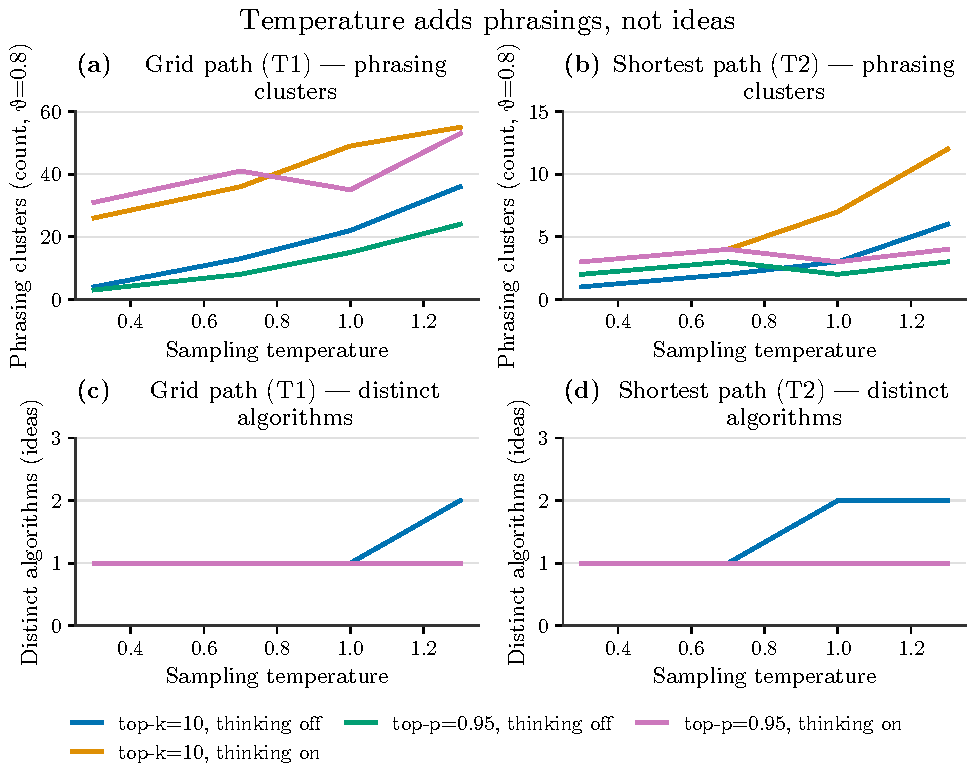
\includegraphics[width=\linewidth,height=0.78\textheight,keepaspectratio]{figures/fig_phrasings_v0.pdf}
\caption{Two-by-two panel, Qwen3-8B, N=100 generations per cell. Top row: number of phrasing clusters (count, $\theta$=0.8 --- connected components among correct programs whose identifier-normalised AST-shingle Jaccard similarity is at least 0.8) against sampling temperature, for the grid-path task T1 (a, y-axis 0--60) and the weighted-shortest-path task T2 (b, y-axis 0--15). Bottom row: number of distinct algorithms (ideas) among the same correct programs, for T1 (c) and T2 (d), both axes 0--3. All four panels share the x-axis (sampling temperature, ticked at 0.3, 0.7, 1.0, 1.3) and the same four series: top-k=10, thinking off (blue); top-k=10, thinking on (orange); top-p=0.95, thinking off (green); top-p=0.95, thinking on (violet). Phrasing-cluster counts rise several-fold with temperature in every series --- most steeply for top-k=10 with thinking off on the grid task (4 to 36 clusters) --- while the idea count stays at exactly 1 throughout for three of the four series on both tasks, and for top-k=10 with thinking off reaches only 2: at temperature 1.3 on the grid task and at temperature $\geq$ 1.0 on the shortest-path task.}
\label{fig:fig_phrasings}
\end{figure}
Table 29 gives the bootstrap slopes of log phrasings per idea in temperature. The slope was positive with a 95\% interval above zero in six of eight task-sampler-thinking combinations at theta 0.8; the two exceptions were the shortest path task with top-p, thinking off (0.365, interval -0.077 to 0.759) and thinking on (0.232, interval -0.0 to 0.484). The slope of log ideas was zero everywhere except the thinking off top-k cells (0.203 on the grid task, 0.266 on the shortest path task), where single non-modal programs appeared at the highest temperatures. The preregistered criterion (positive slope at every theta and sampler, with the paired interval above zero) held on the grid task and failed on the shortest path task.

\begin{table}[H]
\renewcommand{\thetable}{29}
\centering\scriptsize\setlength{\tabcolsep}{2.5pt}
\caption{Slope of log phrasings per idea against temperature (per unit T; 1,000 bootstrap draws; single linkage) at theta 0.7, 0.8 and 0.9, with 95\% intervals, and the slope of log ideas (identical at every theta). [Source: iteration 1, artifact \nolinkurl{gen_art_experiment_6}.]}\label{tab:t31}
\begin{tabular}{>{\raggedright\arraybackslash\hspace{0pt}}p{0.1013\linewidth}>{\raggedright\arraybackslash\hspace{0pt}}p{0.0921\linewidth}>{\raggedright\arraybackslash\hspace{0pt}}p{0.0872\linewidth}>{\raggedright\arraybackslash\hspace{0pt}}p{0.1794\linewidth}>{\raggedright\arraybackslash\hspace{0pt}}p{0.1744\linewidth}>{\raggedright\arraybackslash\hspace{0pt}}p{0.1707\linewidth}>{\raggedright\arraybackslash\hspace{0pt}}p{0.1184\linewidth}}
\toprule
\textbf{Task} & \textbf{Sampler} & \textbf{Thinking} & \textbf{Theta 0.7} & \textbf{Theta 0.8} & \textbf{Theta 0.9} & \textbf{Slope, ideas} \\
\midrule
Grid & top-k=10 & off & 1.138 [0.808, 1.409] & 1.265 [0.902, 1.547] & 1.440 [0.990, 1.727] & 0.203 [0.0, 0.41] \\
Grid & top-p=0.95 & off & 1.083 [0.835, 1.253] & 1.223 [0.975, 1.368] & 1.435 [1.182, 1.620] & 0.0 \\
Grid & top-k=10 & on & 0.563 [0.282, 0.784] & 0.417 [0.213, 0.567] & 0.233 [0.072, 0.321] & 0.0 \\
Grid & top-p=0.95 & on & 0.289 [0.113, 0.602] & 0.293 [0.134, 0.486] & 0.247 [0.123, 0.351] & 0.0 \\
Shortest path & top-k=10 & off & 0.693 [0.442, 1.001] & 0.758 [0.453, 1.044] & 1.295 [0.916, 1.849] & 0.266 [0.0, 0.486] \\
Shortest path & top-p=0.95 & off & 0.365 [-0.102, 0.757] & 0.365 [-0.077, 0.759] & 1.101 [0.780, 1.475] & 0.0 \\
Shortest path & top-k=10 & on & 0.752 [0.449, 0.956] & 0.846 [0.520, 1.075] & 0.408 [0.213, 0.567] & 0.0 \\
Shortest path & top-p=0.95 & on & -0.011 [-0.245, 0.222] & 0.232 [-0.0, 0.484] & 0.205 [0.017, 0.355] & 0.0 \\
\bottomrule
\end{tabular}
\end{table}

\textbf{Thinking traces do not explore.} Every thinking on trace hit the 2,048-token cap, so no trace completed. In the 800 grid traces the first approach named was BFS in all but one, and DFS was mentioned as a second option in 67-90\% of traces depending on the cell; the implemented algorithm equalled the first approach named in 99-100\% of traces. In the shortest path traces the first approach was Dijkstra in 98-100\% and Bellman-Ford\slash{}SPFA was mentioned in 1-5\% (Table 30). The plan-statement lexicon used to read the traces had precision 0.62 and recall 0.482 against a judge on 30 traces, so these counts are approximate.

\begin{table}[H]
\renewcommand{\thetable}{30}
\centering\scriptsize\setlength{\tabcolsep}{2.5pt}
\caption{Approaches named in thinking traces (N=100 per cell; all traces truncated at 2,048 tokens). [Source: iteration 1, artifact \nolinkurl{gen_art_experiment_6}.]}\label{tab:t32}
\begin{tabular}{>{\raggedright\arraybackslash\hspace{0pt}}p{0.1026\linewidth}>{\raggedright\arraybackslash\hspace{0pt}}p{0.0929\linewidth}>{\raggedright\arraybackslash\hspace{0pt}}p{0.0448\linewidth}>{\raggedright\arraybackslash\hspace{0pt}}p{0.1893\linewidth}>{\raggedright\arraybackslash\hspace{0pt}}p{0.2172\linewidth}>{\raggedright\arraybackslash\hspace{0pt}}p{0.1422\linewidth}>{\raggedright\arraybackslash\hspace{0pt}}p{0.1345\linewidth}}
\toprule
\textbf{Task} & \textbf{Sampler} & \textbf{T} & \textbf{First approach named} & \textbf{Also considered} & \textbf{Mean approaches considered} & \textbf{First equals implemented} \\
\midrule
Grid & top-k=10 & 0.3 & BFS 100 & DFS 67 & 1.67 & 1.00 \\
Grid & top-k=10 & 0.7 & BFS 100 & DFS 78 & 1.78 & 1.00 \\
Grid & top-k=10 & 1.0 & BFS 100 & DFS 84, A* 1 & 1.85 & 1.00 \\
Grid & top-k=10 & 1.3 & BFS 99, DFS 1 & DFS 90 & 1.90 & 0.99 \\
Grid & top-p=0.95 & 0.3 & BFS 100 & DFS 70 & 1.70 & 1.00 \\
Grid & top-p=0.95 & 0.7 & BFS 100 & DFS 77 & 1.77 & 1.00 \\
Grid & top-p=0.95 & 1.0 & BFS 100 & DFS 84 & 1.84 & 1.00 \\
Grid & top-p=0.95 & 1.3 & BFS 100 & DFS 85, A* 1 & 1.86 & 1.00 \\
Shortest path & top-k=10 & 0.3 & Dijkstra 100 & Bellman-Ford\slash{}SPFA 2 & 1.02 & 1.00 \\
Shortest path & top-k=10 & 0.7 & Dijkstra 100 & Bellman-Ford\slash{}SPFA 2 & 1.02 & 1.00 \\
Shortest path & top-k=10 & 1.0 & Dijkstra 100 & Bellman-Ford\slash{}SPFA 3 & 1.03 & 1.00 \\
Shortest path & top-k=10 & 1.3 & Dijkstra 98, Bellman-Ford\slash{}SPFA 2 & Bellman-Ford\slash{}SPFA 4 & 1.04 & 0.98 \\
Shortest path & top-p=0.95 & 0.3 & Dijkstra 100 & Bellman-Ford\slash{}SPFA 1 & 1.01 & 1.00 \\
Shortest path & top-p=0.95 & 0.7 & Dijkstra 100 & Bellman-Ford\slash{}SPFA 3 & 1.03 & 1.00 \\
Shortest path & top-p=0.95 & 1.0 & Dijkstra 100 & Bellman-Ford\slash{}SPFA 4, Floyd-Warshall 1 & 1.05 & 1.00 \\
Shortest path & top-p=0.95 & 1.3 & Dijkstra 100 & Bellman-Ford\slash{}SPFA 3 & 1.03 & 1.00 \\
\bottomrule
\end{tabular}
\end{table}

\textbf{Seeds and instructions.} Random seeds did nothing to the output (Table 31): the entropy and word seeds shifted the modal share by about 1 point on the grid task and 0 on the shortest path task, with 90\% intervals inside the preregistered 15-point equivalence bound. The semantic seed moved the shortest path task by 66.3 points toward Bellman-Ford\slash{}SPFA among correct programs (61 of 92 correct programs, while the Dijkstra share fell by 67.39 points; permutation p \textless{} 0.001; corrected in iteration 2 from 67 points, which is the fall in the Dijkstra share) and the grid task by 2.2 points toward bidirectional BFS (2 of 93 correct programs; permutation p = 0.078 for the shift toward the implied algorithm). Among the instructions, the creativity instruction did nothing and the new algorithm instruction moved 1-4 points. The novelty instruction moved 3.7 points on the grid task and 14.6 points on the shortest path task, toward Bellman-Ford\slash{}SPFA. The enumeration prompt moved 10.7 points on the shortest path task at a 24-point pass-rate cost.

\begin{table}[H]
\renewcommand{\thetable}{31}
\centering\footnotesize\setlength{\tabcolsep}{4.0pt}
\caption{Seeds and instructions (N=100 each; labels of correct programs; shift of the default's share against the baseline, with 90\% interval; cluster permutation p). [Source: iteration 1, artifact \nolinkurl{gen_art_experiment_6}.]}\label{tab:t33}
\begin{tabular}{>{\raggedright\arraybackslash\hspace{0pt}}p{0.1005\linewidth}>{\raggedright\arraybackslash\hspace{0pt}}p{0.1785\linewidth}>{\raggedright\arraybackslash\hspace{0pt}}p{0.0604\linewidth}>{\raggedright\arraybackslash\hspace{0pt}}p{0.2840\linewidth}>{\raggedright\arraybackslash\hspace{0pt}}p{0.2118\linewidth}>{\raggedright\arraybackslash\hspace{0pt}}p{0.0615\linewidth}}
\toprule
\textbf{Task} & \textbf{Condition} & \textbf{Pass} & \textbf{Labels of correct programs} & \textbf{Default share shift (points) [90\%]} & \textbf{p} \\
\midrule
Grid & baseline (reference) & 0.97 & BFS 96, unit weight Dijkstra 1 & n\slash{}a & n\slash{}a \\
Grid & entropy seed & 1.00 & BFS 100 & +1.03 [0.0, 4.08] & 0.086 \\
Grid & word seed & 1.00 & BFS 100 & +1.03 [0.0, 4.04] & 0.096 \\
Grid & semantic seed & 0.93 & BFS 91, bidirectional BFS 2 & -1.12 [-5.47, 3.03] & 0.402 \\
Grid & creativity instruction & 1.00 & BFS 100 & +1.03 [0.0, 4.04] & 0.085 \\
Grid & new algorithm instruction & 0.94 & BFS 92, DFS 2 & -1.10 [-5.26, 3.0] & 0.329 \\
Grid & novelty instruction & 0.85 & BFS 81, unit weight Dijkstra 2, DFS 1, A* 1 & -3.68 [-9.19, 0.98] & 0.031 \\
Grid & enumeration prompt & 0.99 & BFS 99 & +1.03 [0.0, 4.0] & 0.246 \\
Shortest path & baseline (reference) & 0.99 & Dijkstra 99 & n\slash{}a & n\slash{}a \\
Shortest path & entropy seed & 1.00 & Dijkstra 100 & 0.0 [0.0, 0.0] & 1.0 \\
Shortest path & word seed & 1.00 & Dijkstra 100 & 0.0 [0.0, 0.0] & 1.0 \\
Shortest path & semantic seed & 0.92 & Bellman-Ford\slash{}SPFA 61, Dijkstra 30, Floyd-Warshall 1 & -67.39 [-87.18, -46.39] & \textless{}0.001 \\
Shortest path & creativity instruction & 0.99 & Dijkstra 99 & 0.0 [0.0, 0.0] & 1.0 \\
Shortest path & new algorithm instruction & 0.94 & Dijkstra 90, Bellman-Ford\slash{}SPFA 4 & -4.26 [-9.47, 0.0] & 0.012 \\
Shortest path & novelty instruction & 0.96 & Dijkstra 82, Bellman-Ford\slash{}SPFA 14 & -14.58 [-25.26, -5.44] & 0.001 \\
Shortest path & enumeration prompt & 0.75 & Dijkstra 67, Bellman-Ford\slash{}SPFA 8 & -10.67 [-20.38, -3.57] & 0.001 \\
\bottomrule
\end{tabular}
\end{table}

The generate then select arm was the only one to reach several algorithms. On the grid task its correct programs were BFS 26, A* 14, unit weight Dijkstra 9 and DFS 6 (Hill\_\allowbreak{}cc 3.457) at a pass rate of 0.55; on the shortest path task Bellman-Ford\slash{}SPFA 31, Dijkstra 29 and Floyd-Warshall 15 (Hill\_\allowbreak{}cc 2.87) at 0.75. The rarefied number of ideas at depth 25 was 3.977 and 2.999, against 1.258 and 1.0 for the baseline. Every one of the 100 stage-1 lists named all six grid algorithms, so the model knows the repertoire it does not use.

\textbf{Seeds at the read position.} The subspace test asks whether a condition moves the read position state along the mode subspace (the span of the forced implementation centroids, dimension 5 on the grid task and 4 on the shortest path task) more than switching between baseline paraphrases does. The statistic is the ratio of the median displacement under the condition to the median paraphrase displacement (Table 32, Figure~\ref{fig:fig_subspace}). The entropy seed stayed within the paraphrase noise (0.734 and 1.165). \emph{(Correction, iteration 2: on the shortest path task its 90\% interval reaches 1.596, above the 1.5 equivalence bound, so equivalence with paraphrase noise was not shown there.)} The word seed moved the grid state 1.555 times the noise (90\% interval 1.309 to 1.85), above the preregistered 1.5 bound, although a fresh word seed with a different word list per paraphrase moved it only 1.055 times and a neutral sentence of the same length 0.812 times. The semantic seed moved the state 3.4 and 3.7 times the noise, and on the grid task its displacement pointed toward the implied centroid (cosine 0.493) while the output did not follow. \emph{(Added in iteration 2: the other half of the same result was omitted. On the shortest path task the semantic seed's displacement did not point toward the Bellman-Ford\slash{}SPFA centroid (cosine -0.087), yet the output moved 66.3 points toward it, and the fixed word seed moved the grid probe's decoded distribution 0.88 toward A} with no behavioural change. Displacement along the mode subspace predicted behavioural movement in neither direction; Section 2.3.8.)* The instructions that changed behaviour also moved the state: the novelty instruction 1.809 and 3.063, the enumeration prompt 2.757 and 2.959. A probe from the read position to the label distribution did not beat its shuffled label null on the shortest path task (mean JS 0.122 against a 5th percentile of 0.121), so the mode subspace there rests on forced prompts that the natural output never visits.

\begin{table}[H]
\renewcommand{\thetable}{32}
\centering\small\setlength{\tabcolsep}{4.0pt}
\caption{Subspace test: median displacement along the mode subspace relative to the paraphrase null, with 90\% interval (grid task at layer 27, subspace dimension 5; shortest path task at layer 22, dimension 4). Conditions marked * were encoded without generation. [Source: iteration 1, artifact \nolinkurl{gen_art_experiment_6}.]}\label{tab:t34}
\begin{tabular}{>{\raggedright\arraybackslash\hspace{0pt}}p{0.3102\linewidth}>{\raggedright\arraybackslash\hspace{0pt}}p{0.3003\linewidth}>{\raggedright\arraybackslash\hspace{0pt}}p{0.3358\linewidth}}
\toprule
\textbf{Condition} & \textbf{Grid ratio [90\%]} & \textbf{Shortest path ratio [90\%]} \\
\midrule
entropy seed & 0.734 [0.579, 0.875] & 1.165 [1.0, 1.596] \\
word seed & 1.555 [1.309, 1.85] & 1.012 [0.865, 1.401] \\
fresh entropy seed* & 0.664 [0.53, 0.825] & 0.968 [0.796, 1.365] \\
fresh word seed* & 1.055 [0.842, 1.314] & 0.927 [0.756, 1.252] \\
neutral sentence* & 0.812 [0.561, 1.073] & 1.288 [1.002, 1.932] \\
semantic seed & 3.417 [2.876, 4.211] & 3.70 [3.005, 4.951] \\
creativity instruction & 1.041 [0.846, 1.436] & 1.684 [1.304, 2.35] \\
new algorithm instruction & 1.302 [0.979, 1.637] & 1.017 [0.79, 1.963] \\
novelty instruction & 1.809 [1.509, 2.173] & 3.063 [2.523, 4.158] \\
enumeration prompt & 2.757 [2.251, 3.435] & 2.959 [2.382, 4.016] \\
\bottomrule
\end{tabular}
\end{table}

\begin{figure}[!htbp]
\centering\captionsetup{font=footnotesize}
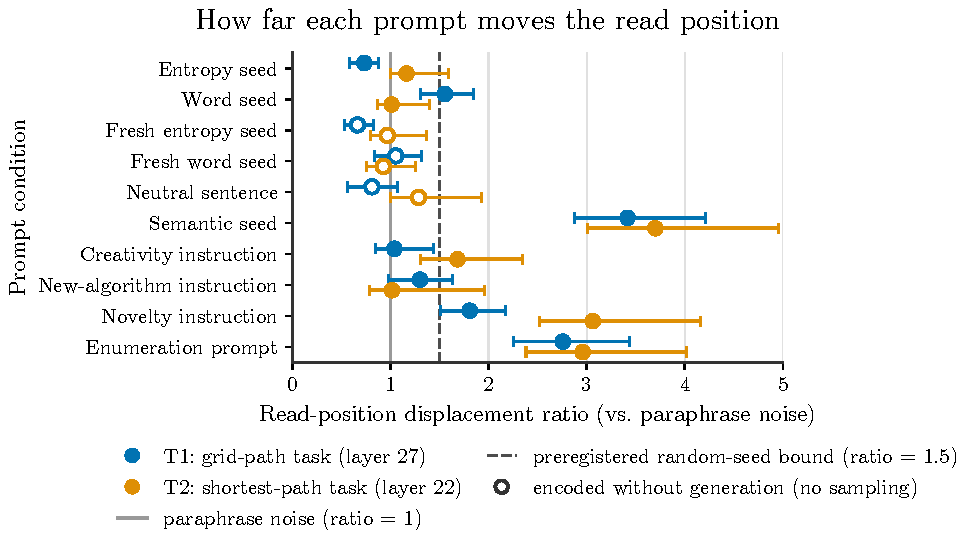
\includegraphics[width=\linewidth,height=0.78\textheight,keepaspectratio]{figures/fig_subspace_v0.pdf}
\caption{Displacement of the model's read-position activations along the algorithm (mode) subspace under ten prompt conditions (y-axis, top to bottom: entropy seed, word seed, fresh entropy seed, fresh word seed, neutral sentence, semantic seed, creativity instruction, new-algorithm instruction, novelty instruction, enumeration prompt), expressed as a ratio to the median displacement between baseline paraphrases (median ratio with 90\% bootstrap interval, horizontal whiskers; x-axis, 0 to 5). Blue circles are T1, the grid-path task (layer 27); orange circles are T2, the shortest-path task (layer 22). Hollow circles mark the three conditions (fresh entropy seed, fresh word seed, neutral sentence) that were encoded without any text generation; all other points are filled. The solid grey vertical line at ratio = 1 marks paraphrase noise and the dashed grey line at ratio = 1.5 marks the preregistered bound for random seeds. Random seeds and the neutral sentence sit at or below the 1.5 bound on both tasks, the one exception being the word seed on the grid-path task (ratio 1.56); the creativity and new-algorithm instructions sit close to that bound too. Three conditions push the read position well beyond it on both tasks: the semantic seed (about 3.4-3.7x paraphrase noise), the enumeration prompt (about 2.8-3.0x), and the novelty instruction, which rises from about 1.8x on the grid-path task to about 3.1x on the shortest-path task.}
\label{fig:fig_subspace}
\end{figure}
The same ratios four layers before and after the analysis layer keep the ordering (Table 32b). The semantic seed and the enumeration prompt stay at two to four times the noise and the random seeds stay near 1. The exception is the shortest path task at layer 18, where the neutral sentence (1.812) and the entropy seed (1.484) also exceed 1.4.

\begin{table}[H]
\renewcommand{\thetable}{32b}
\centering\footnotesize\setlength{\tabcolsep}{4.0pt}
\caption{Subspace test ratios at layers four before and four after the analysis layer (90\% intervals). [Source: iteration 1, artifact \nolinkurl{gen_art_experiment_6}.]}\label{tab:t35}
\begin{tabular}{>{\raggedright\arraybackslash\hspace{0pt}}p{0.1833\linewidth}>{\raggedright\arraybackslash\hspace{0pt}}p{0.1771\linewidth}>{\raggedright\arraybackslash\hspace{0pt}}p{0.1771\linewidth}>{\raggedright\arraybackslash\hspace{0pt}}p{0.1878\linewidth}>{\raggedright\arraybackslash\hspace{0pt}}p{0.1878\linewidth}}
\toprule
\textbf{Condition} & \textbf{Grid layer 23} & \textbf{Grid layer 31} & \textbf{Shortest path layer 18} & \textbf{Shortest path layer 26} \\
\midrule
entropy seed & 0.846 [0.771, 1.023] & 0.777 [0.648, 0.962] & 1.484 [1.153, 1.953] & 0.953 [0.707, 1.411] \\
word seed & 1.921 [1.665, 2.170] & 1.504 [1.311, 1.897] & 1.331 [1.031, 1.786] & 1.072 [0.793, 1.508] \\
fresh entropy seed* & 0.883 [0.708, 1.079] & 0.737 [0.634, 0.942] & 1.278 [1.053, 1.687] & 0.791 [0.604, 1.187] \\
fresh word seed* & 1.294 [1.082, 1.632] & 1.067 [0.918, 1.434] & 1.238 [0.903, 1.581] & 0.871 [0.655, 1.343] \\
neutral sentence* & 0.777 [0.607, 1.044] & 0.879 [0.577, 1.203] & 1.812 [1.238, 2.674] & 0.901 [0.667, 1.348] \\
semantic seed & 3.806 [3.314, 4.437] & 3.237 [2.809, 4.270] & 3.427 [2.801, 4.364] & 4.009 [3.166, 5.873] \\
creativity instruction & 1.525 [1.301, 1.822] & 1.048 [0.894, 1.607] & 2.128 [1.672, 2.813] & 1.093 [0.843, 1.721] \\
new algorithm instruction & 1.611 [1.259, 2.062] & 1.220 [0.900, 1.687] & 1.770 [1.349, 2.274] & 0.848 [0.672, 1.698] \\
novelty instruction & 2.717 [2.234, 3.159] & 1.838 [1.590, 2.363] & 3.410 [2.647, 4.329] & 2.291 [1.675, 3.270] \\
enumeration prompt & 3.242 [2.827, 3.858] & 2.614 [2.303, 3.308] & 4.257 [3.537, 5.363] & 2.005 [1.541, 3.101] \\
\bottomrule
\end{tabular}
\end{table}

\textbf{Where temperature acts in the trajectory.} Over the first 64 generated tokens, the variance of the residual-stream states rose with temperature almost entirely outside the mode subspace (Table 33). On the grid task the complement variance rose from 36,267 to 46,308 between T=0.3 and T=1.3 while the share in the mode subspace estimated from generated tokens stayed at 0.061-0.062. The preregistered prediction was a nonpositive slope of the share in excess of a null matched to the data; the slope was slightly positive (0.006 and 0.015 per unit T, intervals above zero), so the prediction failed, although the excess itself stayed negative at every temperature on both tasks. In the mode subspace estimated at the read position the share was 0.004 (grid) and 0.003 (shortest path) at every temperature, and a subspace from naturally sampled programs could not be estimated because 399 of 400 programs per task were the default.

\begin{table}[H]
\renewcommand{\thetable}{33}
\centering\footnotesize\setlength{\tabcolsep}{4.0pt}
\caption{Variance of trajectory states (first 64 generated tokens) inside the mode subspace estimated from generated tokens, per temperature (N=50 per cell). [Source: iteration 1, artifact \nolinkurl{gen_art_experiment_6}.]}\label{tab:t36}
\begin{tabular}{>{\raggedright\arraybackslash\hspace{0pt}}p{0.1671\linewidth}>{\raggedright\arraybackslash\hspace{0pt}}p{0.0524\linewidth}>{\raggedright\arraybackslash\hspace{0pt}}p{0.1560\linewidth}>{\raggedright\arraybackslash\hspace{0pt}}p{0.2288\linewidth}>{\raggedright\arraybackslash\hspace{0pt}}p{0.1509\linewidth}>{\raggedright\arraybackslash\hspace{0pt}}p{0.1416\linewidth}}
\toprule
\textbf{Task (layer)} & \textbf{T} & \textbf{Share in mode subspace} & \textbf{Excess over null matched to the data} & \textbf{Mode subspace variance} & \textbf{Complement variance} \\
\midrule
Grid (27) & 0.3 & 0.062 & -0.023 & 2,733 & 36,267 \\
Grid (27) & 0.7 & 0.062 & -0.022 & 2,970 & 39,928 \\
Grid (27) & 1.0 & 0.061 & -0.020 & 3,334 & 46,586 \\
Grid (27) & 1.3 & 0.062 & -0.016 & 3,375 & 46,308 \\
Shortest path (22) & 0.3 & 0.018 & -0.050 & 9 & 422 \\
Shortest path (22) & 0.7 & 0.035 & -0.032 & 113 & 2,808 \\
Shortest path (22) & 1.0 & 0.041 & -0.025 & 194 & 4,206 \\
Shortest path (22) & 1.3 & 0.030 & -0.037 & 205 & 5,825 \\
\bottomrule
\end{tabular}
\end{table}

\textbf{The forecast record.} Eight predictions were committed before generation; six hit. The two misses were the predictions that random seeds stay within 1.5 times the paraphrase null at the read position (the grid word seed exceeded it) and that the excess mode subspace share has a nonpositive slope in temperature. The preregistered verdict was MIXED.

\textbf{What this experiment settled.} Temperature and the sampler are phrasing knobs on these tasks: they never changed the algorithm from 0.3 to 1.3, with or without thinking, while the number of distinct phrasings rose severalfold. Random seeds do not change the output, and apart from the fixed grid word seed their effect on the read position state is at most that of an arbitrary sentence. Context with meaning does move the algorithm, but not reliably: the same semantic seed moved the shortest path task by 66.3 points and the grid task by 2.2 (among correct programs; corrected in iteration 2 from 67 and 2). Explicit novelty instructions move little, and generate then select reaches three to four algorithms at a 24-42-point pass-rate cost.

\FloatBarrier
\subsection*{1.11 Comparisons across the six experiments}
\addcontentsline{toc}{subsection}{1.11 Comparisons across the six experiments}
The strategy deferred the scorecard that combines all experiments to an evaluation artifact in the next iteration. The comparisons below were compiled for this report from each experiment's per-sample rows and result files; the replication table was recomputed with \texttt{work/\allowbreak{}replication.\allowbreak{}py} in this workspace.

\textbf{The same ban, five draws.} Five experiments ran the same modal ban under the shared protocol     , each with its own ten paraphrases of \texttt{Do not use X}, its own test suite and, in one case, its own engine. Where the ban had compliant samples, they landed on Bellman-Ford\slash{}SPFA on the shortest path task in all five draws (272 of 272 compliant programs), and on DFS on the grid task in four of five draws; in the geometry draw, sampled with HF \texttt{generate} and with the highest banned share (0.62), the 18 compliant programs split into DFS 10 and unit weight Dijkstra 8, with no clear mode (Table 34). \emph{(Corrected in iteration 2; this sentence previously said that the compliant samples landed on the same substitute every time, DFS on the grid task with a few unit weight Dijkstra programs, which Tables 13 and 34 contradict. Section 2.3.3 gives the per draw counts.)} How often the ban was obeyed did not replicate. The banned mode share ranged from 0.10 to 0.62 on the grid task and from 0.09 to 0.72 on the shortest path task. Within each experiment it depended on the wording: on the grid task the banned counts per paraphrase ranged from 0 of 10 to 9 or 10 of 10 in four of the five experiments (Figure~\ref{fig:fig_replication}). The association experiment's paraphrases were the most effective (eight of ten grid wordings gave 0 of 10 BFS), which is why its compliance looked high. Constraints that oppose a model's default pattern are known to fail at rates between 10\% and 100\% [38]; here the spread occurs within one model, one task and one ban. Compliance is therefore a property of the ban sentence at least as much as of the banned algorithm, and any analysis that relates ban failure to properties of the algorithm (the ladder limit test) has to hold the wording fixed or model it.

\begin{table}[H]
\renewcommand{\thetable}{34}
\centering\scriptsize\setlength{\tabcolsep}{2.5pt}
\caption{The modal ban across experiments (N=100 each; recomputed from per-sample rows; compliant = correct and not the banned algorithm). [Source: iteration 1, compiled across the iteration's artifacts \nolinkurl{gen_art_dataset_1}, \nolinkurl{gen_art_experiment_1}, \nolinkurl{gen_art_experiment_2}, \nolinkurl{gen_art_experiment_3}, \nolinkurl{gen_art_experiment_4}, \nolinkurl{gen_art_experiment_5}, \nolinkurl{gen_art_experiment_6}.]}\label{tab:t37}
\begin{tabular}{>{\raggedright\arraybackslash\hspace{0pt}}p{0.1303\linewidth}>{\raggedright\arraybackslash\hspace{0pt}}p{0.1426\linewidth}>{\raggedright\arraybackslash\hspace{0pt}}p{0.0705\linewidth}>{\raggedright\arraybackslash\hspace{0pt}}p{0.2018\linewidth}>{\raggedright\arraybackslash\hspace{0pt}}p{0.1415\linewidth}>{\raggedright\arraybackslash\hspace{0pt}}p{0.0705\linewidth}>{\raggedright\arraybackslash\hspace{0pt}}p{0.1662\linewidth}}
\toprule
\textbf{Experiment (engine)} & \textbf{Grid ban BFS: labels} & \textbf{Banned share} & \textbf{Compliant (labels)} & \textbf{Shortest path ban Dijkstra: labels} & \textbf{Banned share} & \textbf{Compliant (labels)} \\
\midrule
Association (vLLM) & DFS 90, BFS 10 & 0.10 & 38 (DFS 38) & Bellman-Ford\slash{}SPFA 90, Dijkstra 9, other 1 & 0.09 & 86 (Bellman-Ford\slash{}SPFA 86) \\
Geometry (HF) & BFS 62, DFS 29, unit weight Dijkstra 9 & 0.62 & 18 (DFS 10, unit weight Dijkstra 8) & Dijkstra 72, Bellman-Ford\slash{}SPFA 27, other 1 & 0.72 & 22 (Bellman-Ford\slash{}SPFA 22) \\
Forking token (vLLM) & DFS 78, BFS 21, unit weight Dijkstra 1 & 0.21 & 41 (DFS 40, unit weight Dijkstra 1) & Bellman-Ford\slash{}SPFA 80, Dijkstra 20 & 0.20 & 80 (Bellman-Ford\slash{}SPFA 80) \\
Decommitment (vLLM) & BFS 49, DFS 48, unit weight Dijkstra 2, other 1 & 0.49 & 18 (DFS 16, unit weight Dijkstra 2) & Dijkstra 54, Bellman-Ford\slash{}SPFA 40, other 6 & 0.54 & 38 (Bellman-Ford\slash{}SPFA 38) \\
Instruction tuning (vLLM) & BFS 62, DFS 36, unit weight Dijkstra 2 & 0.62 & 13 (DFS 12, unit weight Dijkstra 1) & Dijkstra 54, Bellman-Ford\slash{}SPFA 46 & 0.54 & 46 (Bellman-Ford\slash{}SPFA 46) \\
Pooled, five draws (row added in iteration 2) & n\slash{}a & 0.41 & 128 (DFS 116, unit weight Dijkstra 12); DFS share 0.906, Wilson [0.843, 0.946] & n\slash{}a & 0.42 & 272 (Bellman-Ford\slash{}SPFA 272); share 1.0, Wilson [0.986, 1.000] \\
\bottomrule
\end{tabular}
\end{table}

\begin{figure}[!htbp]
\centering
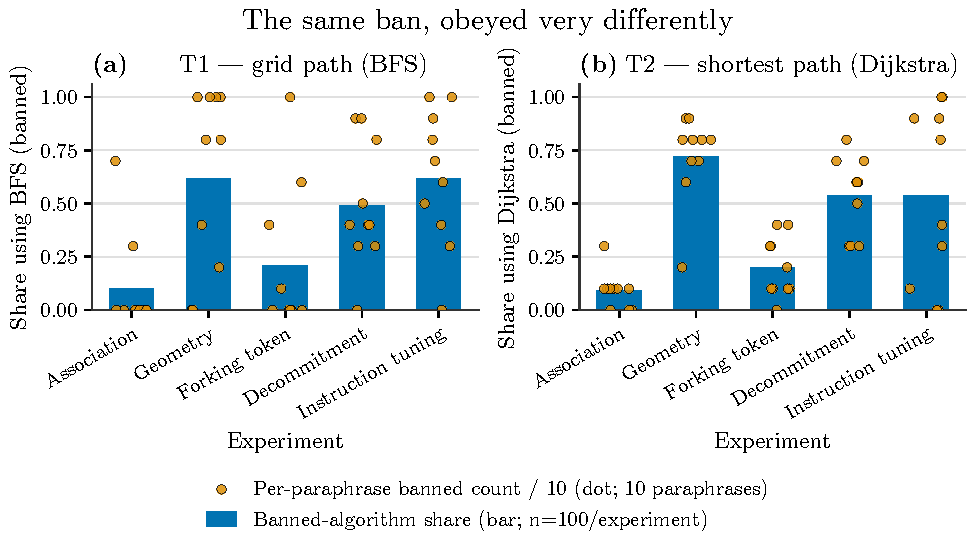
\includegraphics[width=\linewidth,height=0.85\textheight,keepaspectratio]{figures/fig_replication_v0.pdf}
\caption{Share of programs that still use the banned algorithm under the modal ban --- BFS on the grid-path task (panel a, T1) and Dijkstra on the weighted-shortest-path task (panel b, T2) --- in the five experiments of this run that tested the modal ban, each with its own ten paraphrases of the ban sentence (Association, Geometry, Forking token, Decommitment, Instruction tuning; \$n=100\$ programs per experiment per task). Bars give each experiment's banned-algorithm share (0 to 1, left axis); amber dots give the per-paraphrase banned count divided by 10, jittered horizontally for visibility, one dot per paraphrase (10 paraphrases of 10 samples each). The identical ban is obeyed very differently depending only on its wording: the banned share ranges from 0.09 (Association, panel b) to 0.72 (Geometry, panel b) across experiments, and within a single experiment individual paraphrases range from 0\slash{}10 to 10\slash{}10 programs still using the banned algorithm.}
\label{fig:fig_replication}
\end{figure}
\textbf{Two elicitations of the same association map disagree.} The association  and geometry  experiments asked the same model the same question with different prompt wordings and got different maps (Table 35). For BFS one map put unit weight Dijkstra first with clarity 0.20 and the other put A* first with clarity 0.80; for Dijkstra one put Bellman-Ford\slash{}SPFA first with clarity 1.0 and the other put Dial first with clarity 0.579. The realised substitutes (DFS, Bellman-Ford\slash{}SPFA) were ranked last for BFS and third for Dijkstra in the second map. The ranking instrument is not stable under rewording, and where its two versions disagree, neither matches the free-form answer the model gives when asked directly.

\begin{table}[H]
\renewcommand{\thetable}{35}
\centering\footnotesize\setlength{\tabcolsep}{4.0pt}
\caption{The association map of the two default algorithms in the two experiments that elicited it (20 sampled rankings each; 19 for Dijkstra in the geometry experiment). [Source: iteration 1, compiled across the iteration's artifacts \nolinkurl{gen_art_dataset_1}, \nolinkurl{gen_art_experiment_1}, \nolinkurl{gen_art_experiment_2}, \nolinkurl{gen_art_experiment_3}, \nolinkurl{gen_art_experiment_4}, \nolinkurl{gen_art_experiment_5}, \nolinkurl{gen_art_experiment_6}.]}\label{tab:t38}
\begin{tabular}{>{\raggedright\arraybackslash\hspace{0pt}}p{0.0867\linewidth}>{\raggedright\arraybackslash\hspace{0pt}}p{0.1270\linewidth}>{\raggedright\arraybackslash\hspace{0pt}}p{0.3955\linewidth}>{\raggedright\arraybackslash\hspace{0pt}}p{0.0933\linewidth}>{\raggedright\arraybackslash\hspace{0pt}}p{0.0889\linewidth}>{\raggedright\arraybackslash\hspace{0pt}}p{0.1053\linewidth}}
\toprule
\textbf{X} & \textbf{Elicitation} & \textbf{Borda shares of the alternatives} & \textbf{Winner} & \textbf{Clarity} & \textbf{Kendall's W} \\
\midrule
BFS & association experiment & unit weight Dijkstra 0.293, bidirectional BFS 0.283, A* 0.263, IDDFS 0.107, DFS 0.054 & unit weight Dijkstra & 0.20 & 0.52 \\
BFS & geometry experiment & A* 0.371, unit weight Dijkstra 0.288, bidirectional BFS 0.229, IDDFS 0.107, DFS 0.005 & A* & 0.80 & 0.886 \\
Dijkstra & association experiment & Bellman-Ford\slash{}SPFA 0.492, Floyd-Warshall 0.226, bidirectional Dijkstra 0.153, Dial 0.129 & Bellman-Ford\slash{}SPFA & 1.0 & 0.639 \\
Dijkstra & geometry experiment & Dial 0.424, bidirectional Dijkstra 0.314, Bellman-Ford\slash{}SPFA 0.212, Floyd-Warshall 0.051 & Dial & 0.579 & 0.581 \\
\bottomrule
\end{tabular}
\end{table}

\textbf{The PREDICT column.} Every forecasting family was scored by the experiment that owned it, on that experiment's own draw of the two modal ban events, and all forecasts were committed before the samples (Table 36). The selection rule needs at least three events on which the families' top-1 nominations disagree; the screen produced two shared events (the step-2 events had too few compliant samples or were exploratory), so the rule cannot name a survivor. \emph{(Correction, iteration 2: the rule also gates events on compliance of at least 50\%. Under that gate the geometry, instruction tuning and decommitment shortest path events in Table 36 are excluded, the base model, decommitted and geodesic forecasts were scored only on excluded events, and the ranking that follows rests largely on them. On gated events no family can advance; Section 2.3.7.)} Descriptively, the highest scoring forecasts on both events were those that already put most of their mass on the realised substitute before the ban: the model's free-form answer, the listing control distribution, the base model's own distribution and, on the shortest path task, the decommitted distribution. All of them rank the realised substitute second in the preferences the model shows before any ban. The preregistered association map was the worst or second worst forecast in both experiments that elicited it on the grid event. The geodesic kernel beat uniform by 0.29 nats on the grid event and lost to the uniform forecast based on frequency on the shortest path event.

\begin{table}[H]
\renewcommand{\thetable}{36}
\centering\small\setlength{\tabcolsep}{4.0pt}
\caption{PREDICT column: raw log score of every committed forecast on the modal ban events (each experiment scored on its own samples; higher is better; uniform over survivors is -1.630 on the grid task and -1.406 on the shortest path task under the shared mix and floor). The geometry experiment scored every sample not labelled as the banned algorithm rather than only compliant ones. [Source: iteration 1, compiled across the iteration's artifacts \nolinkurl{gen_art_dataset_1}, \nolinkurl{gen_art_experiment_1}, \nolinkurl{gen_art_experiment_2}, \nolinkurl{gen_art_experiment_3}, \nolinkurl{gen_art_experiment_4}, \nolinkurl{gen_art_experiment_5}, \nolinkurl{gen_art_experiment_6}.]}\label{tab:t39}
\begin{tabular}{>{\raggedright\arraybackslash\hspace{0pt}}p{0.6359\linewidth}>{\raggedright\arraybackslash\hspace{0pt}}p{0.1368\linewidth}>{\raggedright\arraybackslash\hspace{0pt}}p{0.1736\linewidth}}
\toprule
\textbf{Forecast family (experiment)} & \textbf{Grid ban BFS} & \textbf{Shortest path ban Dijkstra} \\
\midrule
Association map, Borda (association) & -2.817 & -0.755 \\
Association map, first rank (association) & -2.474 & -0.190 \\
External association map, Llama-3.1-8B (association) & -1.412 & -0.928 \\
Free-form answer about the standard alternative (association, not preregistered as a contest predictor) & -0.112 & -0.058 \\
Listing control distribution (association, not preregistered as a contest predictor) & -0.061 & -0.058 \\
Latent frequency, uniform under collapse (association) & -1.630 & -1.406 \\
Association map, Borda (geometry) & -3.543 & -1.647 \\
Geodesic kernel (geometry) & -1.337 & -1.530 \\
Read position decoder (geometry) & -1.287 & -1.587 \\
Latent frequency (geometry) & -1.630 & -1.496 \\
Decommitted survivor distribution (decommitment) & -1.630, degenerate & -0.058 \\
vLLM frequency forecast (decommitment) & -1.630 & -0.219 \\
Base model, plain completion, all samples (instruction tuning, primary) & -0.470 & -0.220 \\
Base model, chat template, correct samples (instruction tuning) & -0.412 & -0.058 \\
Instruct model, chat template, correct samples (instruction tuning) & -1.630 & -0.058 \\
\bottomrule
\end{tabular}
\end{table}

\textbf{The BUY column.} The rule asks for the highest correctness conditioned Hill number at the strongest setting that keeps at least 80\% of the baseline pass rate. Table 37 lists every knob that reached that pass-rate floor with a Hill gain, and the main ones that did not; Figure~\ref{fig:fig_knobs} plots the shortest path knobs as Hill gain against pass-rate points lost. On the grid task the cumulative ban of BFS and DFS kept 88\% of its reference pass rate in the decommitment draw and produced 16 compliant programs over two algorithms (unit weight Dijkstra 13, A* 3), but it does not replicate: the geometry draw (pass 0.96 against 0.99) put all 18 of its compliant programs on unit weight Dijkstra, and the association draw (pass 0.53 against 0.933) left 5 compliant programs; the novelty instruction raised Hill\_\allowbreak{}cc to 1.27. \emph{(Corrected in iteration 2; this sentence previously said that no knob keeping 80\% of the pass rate produced a second algorithm among compliant programs and that the gain of the cumulative ban came from programs that still used BFS, which the decommitment row of Table 37 contradicts. Section 2.3.4.)} On the shortest path task the prompt ban and the semantic seed reached about 2 effective algorithms at no or small pass cost, while the activation knobs (decommitment, a random direction) reached about +0.6 at 17 points. By the rule's 0.5 margin the prompt ban and the semantic seed tie, so both would advance. \emph{(Correction, iteration 2: the BUY rule names a winner only on the pooled tasks and in direction on each task, and this comparison used the shortest path task alone, with Hill numbers from different statistics. Recomputed with one statistic, rarefied Hill-1 over compliant programs, no knob advances on either task, the prompt ban scores 1.0 on the shortest path task, and the positive target of a second correct algorithm at under 20 pass points is met on neither task; Section 2.3.6.)} The table also exposes a flaw in the metric: Hill\_\allowbreak{}cc counts correct programs of the banned algorithm, so a ban that half fails scores as two algorithms. The prompt-ban rows on the shortest path task are Dijkstra mixed with Bellman-Ford\slash{}SPFA; only the semantic seed and generate then select produced diversity without a banned algorithm in the mix.

{\footnotesize\setlength{\tabcolsep}{4.0pt}\renewcommand{\thetable}{37}
\begin{longtable}{>{\raggedright\arraybackslash\hspace{0pt}}p{0.0867\linewidth}>{\raggedright\arraybackslash\hspace{0pt}}p{0.2442\linewidth}>{\raggedright\arraybackslash\hspace{0pt}}p{0.1078\linewidth}>{\raggedright\arraybackslash\hspace{0pt}}p{0.1136\linewidth}>{\raggedright\arraybackslash\hspace{0pt}}p{0.1001\linewidth}>{\raggedright\arraybackslash\hspace{0pt}}p{0.2442\linewidth}}
\caption{BUY column: knobs on the two tasks, with pass rate relative to their own reference, and the Hill number or its change as each artifact reported it. [Source: iteration 1, compiled across the iteration's artifacts \nolinkurl{gen_art_dataset_1}, \nolinkurl{gen_art_experiment_1}, \nolinkurl{gen_art_experiment_2}, \nolinkurl{gen_art_experiment_3}, \nolinkurl{gen_art_experiment_4}, \nolinkurl{gen_art_experiment_5}, \nolinkurl{gen_art_experiment_6}.]}\label{tab:t40}\\
\toprule
\textbf{Task} & \textbf{Knob (experiment)} & \textbf{Pass \slash{} reference pass} & \textbf{Reaches 80\% floor} & \textbf{Hill\_\allowbreak{}cc (or Delta Hill)} & \textbf{Correct program composition} \\
\midrule
\endfirsthead
\multicolumn{6}{l}{\emph{Table 37, continued}}\\
\toprule
\textbf{Task} & \textbf{Knob (experiment)} & \textbf{Pass \slash{} reference pass} & \textbf{Reaches 80\% floor} & \textbf{Hill\_\allowbreak{}cc (or Delta Hill)} & \textbf{Correct program composition} \\
\midrule
\endhead
\bottomrule
\endlastfoot
Shortest path & prompt ban (instruction tuning) & 1.00 \slash{} 1.00 & yes & 1.99 & Dijkstra 54, Bellman-Ford\slash{}SPFA 46 \\
Shortest path & semantic seed (decoding) & 0.92 \slash{} 0.99 & yes & 1.988 & Bellman-Ford\slash{}SPFA 61, Dijkstra 30, Floyd-Warshall 1 \\
Shortest path & prompt ban (geometry) & 0.94 \slash{} 1.00 & yes & 1.723 & Dijkstra 72 correct banned plus Bellman-Ford\slash{}SPFA 22 \\
Shortest path & prompt ban (forking token) & 1.00 \slash{} 0.995 & yes & 1.649 & Bellman-Ford\slash{}SPFA 80, Dijkstra 20 \\
Shortest path & novelty instruction (decoding) & 0.96 \slash{} 0.99 & yes & 1.515 & Dijkstra 82, Bellman-Ford\slash{}SPFA 14 \\
Shortest path & prompt ban (association) & 0.95 \slash{} 1.00 & yes & 1.368 & Bellman-Ford\slash{}SPFA 86, Dijkstra 9 \\
Shortest path & prompt ban (decommitment) & 0.87 \slash{} 0.89 & yes & Delta +0.79 & Dijkstra 49, Bellman-Ford\slash{}SPFA 38 \\
Shortest path & decommitment direction, c=0.25 & 0.78 \slash{} 0.95 & yes (82\%) & Delta +0.65 & Bellman-Ford\slash{}SPFA 54, Dijkstra 23, other 1 \\
Shortest path & random direction, c=0.25 (decommitment) & 0.79 \slash{} 0.95 & yes (83\%) & Delta +0.59 & Dijkstra 53, Bellman-Ford\slash{}SPFA 26 \\
Shortest path & generate then select (decoding) & 0.75 \slash{} 0.99 & no (76\%) & 2.87 & Bellman-Ford\slash{}SPFA 31, Dijkstra 29, Floyd-Warshall 15 \\
Shortest path & enumeration prompt (decoding) & 0.75 \slash{} 0.99 & no & 1.404 & Dijkstra 67, Bellman-Ford\slash{}SPFA 8 \\
Shortest path & temperature 1.0-1.3, top-k=10 (decoding) & 0.98-1.00 \slash{} 0.99 & yes & 1.058-1.059 & Dijkstra with one Bellman-Ford\slash{}SPFA \\
Shortest path & sharpening subtraction, any variant (instruction tuning) & 0.00-0.98 \slash{} 1.00 & only at layer 18, c of 0.5 or less & 1.00-1.10 & Dijkstra \\
Grid & cumulative ban of BFS and DFS (decommitment) & 0.88 \slash{} 1.00 & yes & Delta +1.27 & BFS 65, unit weight Dijkstra 13, DFS 7, A* 3 \\
Grid & novelty instruction (decoding) & 0.85 \slash{} 0.97 & yes & 1.27 & BFS 81, unit weight Dijkstra 2, DFS 1, A* 1 \\
Grid & prompt ban (geometry) & 0.76 \slash{} 0.99 & no (77\%) & 2.034 & BFS 58 correct banned, DFS 10, unit weight Dijkstra 8 \\
Grid & prompt ban (instruction tuning) & 0.70 \slash{} 1.00 & no & 1.70 & BFS 57, DFS 12, unit weight Dijkstra 1 \\
Grid & prompt ban (association) & 0.46 \slash{} 0.933 & no & 1.587 & DFS 38, BFS 8 \\
Grid & generate then select (decoding) & 0.55 \slash{} 0.97 & no & 3.457 & BFS 26, A* 14, unit weight Dijkstra 9, DFS 6 \\
Grid & decommitment direction, any c & 0.98 at c=0.1 & yes at c=0.1 & 1.0 & BFS \\
Grid & temperature, any setting (decoding) & 0.95-1.00 & yes & 1.0-1.06 & BFS \\
\end{longtable}}

\begin{figure}[!htbp]
\centering\captionsetup{font=footnotesize}
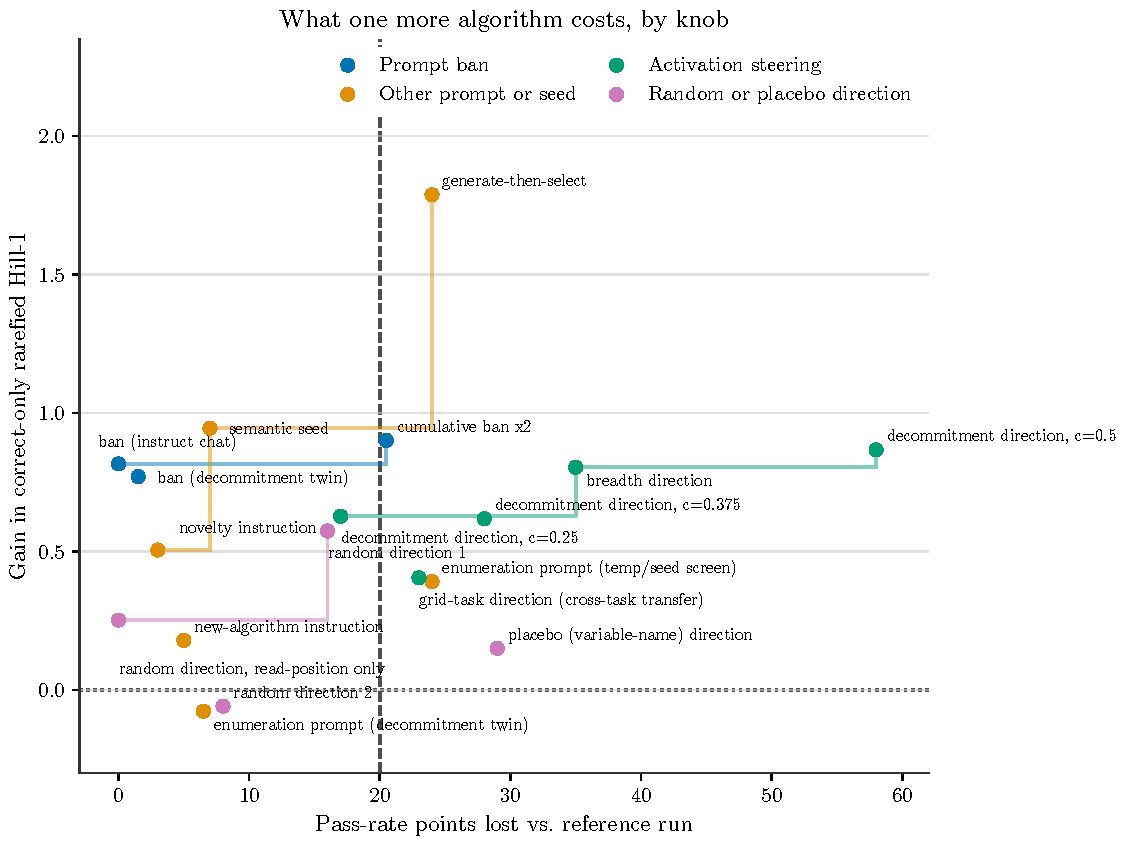
\includegraphics[width=\linewidth,height=0.78\textheight,keepaspectratio]{figures/fig_knobs_v0.pdf}
\caption{Gain in the correctness-conditioned Hill number (rarefied Hill-1 at depth 25, computed over correct programs only) against pass-rate points lost, for 18 diversity-inducing knobs tried on the shortest-path task, each measured against its own experiment's reference run (prompt- and seed-level knobs against an unedited baseline; activation-steering knobs against the hooked, zero-strength run). Points are coloured by knob family -- prompt bans (blue), other prompts and seeds (orange), activation-steering directions (green), and random or placebo directions (pink) -- and a step line traces each family's own non-dominated pass-cost\slash{}gain frontier. A dashed vertical line at 20 points marks the 80\textbackslash{}\%-of-baseline pass-rate floor used as this run's knob-selection cutoff; a dotted horizontal line marks zero gain. The cheapest knobs are two prompt bans and a semantic seed, all at 7 pass-rate points or fewer: banning the default algorithm on the instruction-tuned chat model gains 0.82 effective correct algorithms at zero pass-rate cost, and a semantic seed gains 0.95 at 7 points -- more than any activation-steering edit achieves at 17 to 58 points. Generate-then-select is the single largest recorded gain (1.79 at 24 points). One random direction (16 points \slash{} 0.57 gain) lands close to the matched-dose decommitment-direction edit (c=0.25: 17 points \slash{} 0.63 gain) on the same axes. Two points appearing in an earlier draft of this figure are omitted here because no run output file supported their claimed values (see the workspace README for which, and why).}
\label{fig:fig_knobs}
\end{figure}
\textbf{The locus diagnostic.} The test that would move the geometric analyses from the read position to generated tokens needed a probe at the forking token and commitment positions, and that probe produced no output. The read position evidence is split: it encodes the shortest path default and fails to decode the grid default, while the forking token screen found every baseline path fixed at the read position on both tasks. The diagnostic is undetermined.

\FloatBarrier
\subsection*{1.12 What iteration 1 established, and what it abandoned}
\addcontentsline{toc}{subsection}{1.12 What iteration 1 established, and what it abandoned}
Everything below is descriptive: one model, two tasks, two informative ban events per experiment, and labellers of which two failed their strict gates.

\textbf{Established.}

\begin{enumerate}
\item The collapse is total and robust to decoding. Across six independent baselines, 1,199 of 1,200 grid programs were BFS and 1,174 of 1,200 shortest path programs were Dijkstra. Temperature from 0.3 to 1.3, top-k=10 or top-p=0.95, and thinking on or off changed the algorithm in at most 3 of 800 programs per task.
\item Temperature is a phrasing knob. At the tightest setting the model writes one idea in a handful of phrasings; loosening temperature multiplies phrasings (4 to 36 clusters on the grid task with top-k=10) and leaves ideas at one or two. This is the answer this run gives to the request's question 1a-c on these two tasks.
\item Random context seeds change nothing in the output. Apart from the fixed word seed on the grid task (1.56 times the paraphrase noise, against 1.06 for word seeds drawn fresh per paraphrase), they displace the read position state no more than an arbitrary sentence does. Context with meaning moves the state three to four times the paraphrase noise and can move the output, by 66.3 points on the shortest path task and by 2.2 points on the grid task (among correct programs). \emph{(Corrected in iteration 2; the item previously gave 67 and 2 points, 67 being the fall in the Dijkstra share. It also omitted that read position displacement did not predict which algorithm the output moved to on either task: the grid semantic seed pointed at its implied algorithm and behaviour barely moved, the shortest path seed did not point at Bellman-Ford\slash{}SPFA and behaviour moved two thirds of the way; and the shortest path entropy seed's interval reaches 1.596, above the equivalence bound. Section 2.3.8.)}
\item When a prompt ban is obeyed, the compliant programs land mostly on one substitute. On the shortest path task it was Bellman-Ford\slash{}SPFA in five of five draws (272 of 272 compliant programs); on the grid task DFS was the realised mode in four of five draws (116 of 128 pooled, 0.906, Wilson [0.843, 0.946]), and the HF engine geometry draw, with the highest banned share (0.62), had no clear mode (DFS 10, unit weight Dijkstra 8). A single ban collapses the output again; a second step grid ban can spread compliant output over unit weight Dijkstra and A* (decommitment draw: 13 and 3) or put all of it on unit weight Dijkstra (geometry draw: 18). \emph{(Corrected in iteration 2; the item previously said that the substitute replicated in five independent draws and that bans collapse the output again without spreading it, which the geometry draw and the second step bans contradict. Section 2.3.3.)} How often a ban is obeyed did not replicate (banned mode share 0.09-0.72) and depends on the wording of the ban sentence. Banning the substitute as well fails, and the model then reimplements the banned mechanism under another description.
\item The substitute is the model's second preference, visible before any ban in its free-form answer, in its output when every algorithm is listed, and in the base model's distribution. The preregistered ranked association map did not identify it on the grid task and gave different answers under two elicitation wordings. \emph{(Note added in iteration 2: on the shortest path task random activation directions and every other perturbation that moved the model off Dijkstra also landed on Bellman-Ford\slash{}SPFA (Section 2.3.5), so there the second preference of the model cannot be told apart from wherever any perturbation lands.)}
\item The read position carries a low-dimensional map of the catalogue (intrinsic dimension 4-5 against 11-12 for shuffled nulls). On the grid task the mass displaced by bans moved to BFS's geodesic neighbours and never to the far side, \emph{(clause inserted in iteration 2, marked in iteration 3)} which is consistent with geodesic proximity and with typicality, since those neighbours are also second choices of the model; the two are not separated on these events. \emph{(Corrected in iteration 2: the geodesic order is unstable at layer 24 under paraphrase resampling, and on the shortest path task Floyd-Warshall, not the realised Bellman-Ford\slash{}SPFA, is the nearest survivor in every subsample. Section 2.3.2.)} The ban shift itself is almost entirely orthogonal to the algorithm directions, so the substitution versus subtraction share test was inconclusive for every algorithm.
\item No activation edit beat the prompt ban. Affine ablation of the modal algorithm did nothing at alpha up to 2 and broke generation at 4, as random directions did; the decommitment direction acted like a random direction; subtracting the instruct minus base direction destroyed generation.
\item Post training sharpened an ordering the base model already had, rather than installing a new attractor; the chat format sharpens it further on the shortest path task. \emph{(Correction, iteration 2: this item replaced the preregistered verdicts with an interpretation. The verdicts are INSTALLED\_\allowbreak{}BY\_\allowbreak{}POST\_\allowbreak{}TRAINING on the shortest path task and MIXED on the grid task under the correctness conditioned Hill number (INSTALLED\_\allowbreak{}BY\_\allowbreak{}POST\_\allowbreak{}TRAINING on both under the Hill number over all programs), and MIXED on both at the planned sample size. The base ordering matches the instruct ordering only under the chat template, where the base model parsed 0.58 and 0.66 of samples and wrote 57 and 90 correct programs, labelled with runtime against AST kappa of 0.20 to 0.50 (Table 24b); in plain completion its shortest path mode is Bellman-Ford\slash{}SPFA, 16 of 25 correct programs.)}
\item Without a ban the algorithm is fixed at the read position on both tasks. Under a ban the outcome stays open for dozens of tokens, a few forking tokens exist on the shortest path task, and writing the first token that identifies the algorithm does not lock the algorithm in.
\end{enumerate}

\textbf{Abandoned or failed, with the evidence.}

\begin{itemize}
\item \emph{Affine directional ablation of the modal algorithm as a removal knob.} 0 of 50 samples moved at alpha 0.5, 1 and 2 on both tasks, with 78-90\% of outputs byte-identical to the unedited run; at alpha 4 the edit removed all code. The direction checks had failed beforehand (AUC 0.79-0.89). The prompt-versus-removal comparison that the hypothesis treats as a headline was therefore untestable in this form.
\item \emph{Subtracting the instruct minus base direction.} 0 of 100 parseable programs at every band coefficient; the direction promotes format tokens under the logit lens.
\item \emph{Forking window temperature.} Every arm was 100\% the default algorithm; its phrasing count matched T=0.3.
\item \emph{The decommitment direction as a diversity knob.} Its shortest path gain equalled a random direction's (difference +0.07, interval -0.26 to 0.39) and the grid task never moved; the enumeration prompt that states the same framing did nothing.
\item \emph{The ranked (Borda) association map as the association instrument.} It missed the grid event, ranked the realised substitute last, and changed its winner for both default algorithms under a second elicitation.
\item \emph{Baseline frequency as the typicality predictor.} Under a full collapse every survivor has zero frequency, so the forecast is uniform by construction and the discordance strata that the design defined by stability are empty.
\item \emph{The mention twin as a placebo, and the sham ban as a negative control.} Mentioning an algorithm recommends it (+56 to +100 points), so sham bans cannot be tested for equivalence with their mention twins.
\item \emph{The locus probes.} The forking token experiment extracted the states but its probe stage produced no output; this is a technical failure, not a negative result, and the measurement is still missing. \emph{(Correction, iteration 2: the probe stage ran before the states were written (Section 1.7); the audit ran it in iteration 2 and found no decision locus among the saved positions, Section 2.3.1.)}
\item \emph{The reserved bench.} The dataset artifact delivered source data but no frozen specifications, tests, labellers or forecasts, so the planned out-of-sample confirmation cannot start until the bench is built.
\end{itemize}

\textbf{Spend.} OpenRouter: USD 0.27 (association), about 0.09 (geometry), 0.024 (forking token), 0.062 (decommitment), 0.21 (instruction tuning), 0.11 (decoding) and 0 (dataset), about USD 0.77 in total. GPU: about 6 minutes on an RTX 5090 (association), 2.2 hours on a 23 GB NVIDIA GPU (geometry), 2.1 hours on the same model of GPU (instruction tuning); the other experiments did not record GPU hours. \emph{(Correction, iteration 2: from the union of each experiment's GPU phase log spans, an upper bound that includes waits, geometry 2.92, forking token 1.55, decommitment 3.23, instruction tuning 2.47 and decoding 3.31 GPU hours; Section 2.3.10. The answers this screen gives to the objections of the hypothesis review are recorded in Section 2.1.)}

\FloatBarrier
\section{Iteration 2: the record repaired, a likelihood instrument, the route of a ban, the top five prohibition and a second model}
\noindent\emph{Run record for this iteration.} Hypothesis carried: ``Bans Remove the Default, Not Pick the Next''. Move recorded at the end of the iteration: deepen; review score 4; evidence state lead; coverage full; 15 candidate strategies considered. The list below gives the iteration's artifacts and the state the round record gave each strand.

{\footnotesize\setlength{\tabcolsep}{3pt}
\begin{longtable}{>{\raggedright\arraybackslash}p{0.24\linewidth}>{\raggedright\arraybackslash}p{0.47\linewidth}>{\raggedright\arraybackslash}p{0.11\linewidth}>{\raggedright\arraybackslash}p{0.08\linewidth}}
\caption*{\textbf{Artifacts of iteration 2.} Names and titles as the artifact workspaces record them; strand state as the round record grades it.}\label{tab:arts2}\\
\toprule \textbf{Artifact} & \textbf{Title} & \textbf{Type} & \textbf{State} \\ \midrule \endfirsthead
\toprule \textbf{Artifact} & \textbf{Title} & \textbf{Type} & \textbf{State} \\ \midrule \endhead
\bottomrule \endlastfoot
\nolinkurl{gen_art_evaluation_1} & When does the AI coder pick its algorithm? An audit & evaluation & lead \\
\nolinkurl{gen_art_experiment_7} & Do algorithm bans pick a substitute or a ladder? & experiment & broken \\
\nolinkurl{gen_art_experiment_8} & Where a coding-algorithm ban takes effect in an LLM & experiment & lead \\
\nolinkurl{gen_art_experiment_9} & Banning five path algorithms in one prompt & experiment & lead \\
\nolinkurl{gen_art_experiment_10} & Do algorithm bans work the same in Llama? & experiment & broken \\
\nolinkurl{gen_art_experiment_11} & Coding-task bench with a baseline pilot & experiment & null \\
\nolinkurl{gen_art_experiment_12} & Reading a coding ban inside Qwen3-8B & experiment & null \\
\end{longtable}}

\subsection*{What each artifact of iteration 2 was for and what it produced}
\addcontentsline{toc}{subsection}{What each artifact of iteration 2 was for and what it produced}
Each artifact is named below as the run's workspaces name it. The entry gives the round record's verdict on the strand it served, the artifact's own summary of what it was for and what it produced, and the output files it declared, each opened and read from its workspace for this report. It closes with the subsection of this section that reports the artifact's results and the result tables typeset there from its output files.

\paragraph{\nolinkurl{gen_art_evaluation_1}: When does the AI coder pick its algorithm? An audit.}
Type: evaluation. Round record, strand state lead: T2: 8\slash{}8 non-semantic pushes incl. random steering land on BF\slash{}SPFA like the ban (rival's top rung); locus probe found no locus; FW nearest Dijkstra 100\%; no knob or family advances.

\emph{The artifact's own summary of what it was for and what it produced:} Round-one audit (no generation, no LLM calls, \$0) of the six iteration-1 experiments of an earlier run directory (Qwen3-8B; T1 grid path, T2 weighted shortest path), read in place via ITER1\_\allowbreak{}ROOT. (0a) LOCUS: the iteration-1 probe never ran (exp3 probes.json written 18:29, states saved 18:34). Re-run on the 2x300 saved states (8 positions x layers 8-28) with leave-one-paraphrase-out L2-logistic probes (batched torch IRLS, unit-tested vs sklearn), 200 global + 200 within-paraphrase refit nulls, layer-max family-wise null, written-text control, pre-commit qualifier. T1: mechanical verdict R - R already reads the within-ban outcome at BA 0.855 and the within-paraphrase null absorbs every generated position (paraphrase-level signal). T2: mechanical locus k\_\allowbreak{}pre (BA 0.762 at L8, +0.281 vs R, within p 0.005; re-derived p 0.024 with 40 sklearn refits, placebo p 0.17) but qualified POST-COMMIT READOUT: the written prefix alone gives BA 0.756; the classes split at generated token 3 ('import heapq' vs 'from collections import deque', also exp3's confirmed fork), so unsaved states k=1..3 are the next round's extraction target. DiM AUC below the 0.9 bar (0.88 T1, 0.75 T2). (0b) GEOMETRY: exp2 matrices reproduced exactly; over 1000 paraphrase subsamples x k\{5,10,15,20\} x layers, Floyd-Warshall (not BF\slash{}SPFA) is nearest to Dijkstra in 100\% of draws at every T2 setting; T1 DFS nearest at L25-28 but flips at L24; wording: consistent with geodesic proximity and typicality, not separated. (0c) PERTURBATION TABLE: 249 condition rows \slash{} 20,270 programs with pass cost (Newcombe), compositions, runner-up shares (Wilson); on T2 8\slash{}8 non-semantic perturbations incl. random steering land on BF\_\allowbreak{}SPFA. (0d) CORRECTIONS: T2 BF\_\allowbreak{}SPFA 272\slash{}272 in 5\slash{}5 draws; T1 DFS 116\slash{}128 (realised mode 4\slash{}5 draws); cumulative BFS+DFS ban non-replicating; one-statistic knob table (compliant-only rarefied Hill-1, depth 25): no diversity knob or ban reaches Hill\textgreater{}=2 at \textless{}20 pass points on either task; PREDICT: 3 informative gated events (12 literal), no family advances; BUY: no knob advances. (0e) seed double dissociation; (0f) missing outputs incl. GPU hours and grid failure taxonomy; (0g) 2 sham-ban promotions, both content-neighbour AND runner-up (confounded); (0h) dated arXiv-verified positioning. Files: eval\_\allowbreak{}out.json (+full\slash{}mini\slash{}preview; exp\_\allowbreak{}eval\_\allowbreak{}sol\_\allowbreak{}out, 80 metrics\_\allowbreak{}agg, datasets perturbation\_\allowbreak{}table\slash{}locus\_\allowbreak{}cells\slash{}knob\_\allowbreak{}table\slash{}geometry\_\allowbreak{}grid), corrections.json, tables\slash{}\emph{.csv, figures\slash{}}.pdf\textbar{}png, results\slash{}*.json, audits (20\slash{}20 + 5\slash{}5 re-derived, placebos fail), README.md, reproducibility.md.

Its results are reported in Subsection 2.3 of this report, which typesets the result tables drawn from its output files: Tables 41, 42, 43, 44, 45, 46, 47, 48, 49, 50, 51, 52.

\begin{table}[H]
\renewcommand{\thetable}{O8}
\centering\footnotesize\setlength{\tabcolsep}{3pt}
\caption{Output files declared by \nolinkurl{gen_art_evaluation_1} (iteration 2), each opened and read from the artifact's workspace for this report; size in bytes. [Source: iteration 2, artifact \nolinkurl{gen_art_evaluation_1}.]}
\begin{tabular}{>{\raggedright\arraybackslash}p{0.25\linewidth}>{\raggedleft\arraybackslash}p{0.12\linewidth}>{\raggedright\arraybackslash}p{0.57\linewidth}}
\toprule
\textbf{Declared file} & \textbf{Bytes} & \textbf{What it holds} \\
\midrule
\texttt{eval.\allowbreak{}py} & 31,857 & the artifact's code, 423 lines \\
\texttt{full\_\allowbreak{}eval\_\allowbreak{}out.\allowbreak{}json} & 1,178,978 & the complete output; metadata with 21 top-level keys; 4 datasets with 1,391 examples in all: perturbation\_\allowbreak{}table (249), locus\_\allowbreak{}cells (903), knob\_\allowbreak{}table (183), geometry\_\allowbreak{}grid (56); top-level keys metrics\_\allowbreak{}agg; 80 aggregate metrics (typeset in full below) \\
\texttt{mini\_\allowbreak{}eval\_\allowbreak{}out.\allowbreak{}json} & 244,800 & small variant of the full output (a few examples per dataset); metadata with 21 top-level keys; 4 datasets; top-level keys metrics\_\allowbreak{}agg \\
\texttt{preview\_\allowbreak{}eval\_\allowbreak{}out.\allowbreak{}json} & 156,660 & preview variant of the full output (truncated strings and lists); metadata with 21 top-level keys; 3 datasets; top-level keys metrics\_\allowbreak{}agg \\
\texttt{reproducibility.\allowbreak{}md} & 9,355 & reproducibility notes, 178 lines \\
\bottomrule
\end{tabular}
\end{table}

{\scriptsize\setlength{\tabcolsep}{2.5pt}\renewcommand{\thetable}{O9}
\begin{longtable}{>{\raggedright\arraybackslash}p{0.27\linewidth}>{\raggedright\arraybackslash}p{0.19\linewidth}>{\raggedright\arraybackslash}p{0.27\linewidth}>{\raggedright\arraybackslash}p{0.19\linewidth}}
\caption{Every aggregate metric in the \texttt{metrics\_agg} block of \nolinkurl{gen_art_evaluation_1}'s \texttt{full\_\allowbreak{}eval\_\allowbreak{}out.\allowbreak{}json} (80 metrics), values copied exactly as stored. [Source: iteration 2, artifact \nolinkurl{gen_art_evaluation_1}.]}\\
\toprule
\textbf{Metric} & \textbf{Value} & \textbf{Metric} & \textbf{Value} \\
\midrule
\endfirsthead
\toprule
\textbf{Metric} & \textbf{Value} & \textbf{Metric} & \textbf{Value} \\
\midrule
\endhead
\bottomrule
\endlastfoot
\texttt{locus\_\allowbreak{}T1\_\allowbreak{}BA\_\allowbreak{}kpre} & 0.8553113553113553 & \texttt{geo\_\allowbreak{}T2\_\allowbreak{}max\_\allowbreak{}P\_\allowbreak{}BF\_\allowbreak{}nearest\_\allowbreak{}all\_\allowbreak{}settings} & 0.0 \\
\texttt{locus\_\allowbreak{}T1\_\allowbreak{}Lstar\_\allowbreak{}kpre} & 20.0 & \texttt{geo\_\allowbreak{}T1\_\allowbreak{}P\_\allowbreak{}DFS\_\allowbreak{}nearest\_\allowbreak{}L27\_\allowbreak{}k10} & 1.0 \\
\texttt{locus\_\allowbreak{}T1\_\allowbreak{}delta\_\allowbreak{}vs\_\allowbreak{}R\_\allowbreak{}kpre} & 0.0641025641025641 & \texttt{geo\_\allowbreak{}T1\_\allowbreak{}P\_\allowbreak{}DFS\_\allowbreak{}nearest\_\allowbreak{}L24\_\allowbreak{}k10} & 0.523 \\
\texttt{locus\_\allowbreak{}T1\_\allowbreak{}BA\_\allowbreak{}R} & 0.8553113553113553 & \texttt{geo\_\allowbreak{}T1\_\allowbreak{}P\_\allowbreak{}DFS\_\allowbreak{}UNITDIJ\_\allowbreak{}two\_\allowbreak{}nearest\_\allowbreak{}L27\_\allowbreak{}k10} & 1.0 \\
\texttt{locus\_\allowbreak{}T1\_\allowbreak{}BA\_\allowbreak{}k8} & 0.8553113553113553 & \texttt{geo\_\allowbreak{}T1\_\allowbreak{}kendall\_\allowbreak{}tau\_\allowbreak{}mean} & 0.9326315789473684 \\
\texttt{locus\_\allowbreak{}T1\_\allowbreak{}BA\_\allowbreak{}text\_\allowbreak{}kpre} & 0.6730769230769231 & \texttt{geo\_\allowbreak{}T2\_\allowbreak{}kendall\_\allowbreak{}tau\_\allowbreak{}mean} & 0.8703703703703706 \\
\texttt{locus\_\allowbreak{}T1\_\allowbreak{}p\_\allowbreak{}within\_\allowbreak{}kpre} & 0.8557213930348259 & \texttt{geo\_\allowbreak{}T1\_\allowbreak{}share\_\allowbreak{}settings\_\allowbreak{}realised\_\allowbreak{}rank1} & 0.8 \\
\texttt{locus\_\allowbreak{}T1\_\allowbreak{}verdict\_\allowbreak{}mechanical\_\allowbreak{}is\_\allowbreak{}R} & 1.0 & \texttt{geo\_\allowbreak{}T2\_\allowbreak{}share\_\allowbreak{}settings\_\allowbreak{}realised\_\allowbreak{}rank1} & 0.0 \\
\texttt{locus\_\allowbreak{}T1\_\allowbreak{}verdict\_\allowbreak{}code} & 0.0 & \texttt{geo\_\allowbreak{}T2\_\allowbreak{}kruskal\_\allowbreak{}stress\_\allowbreak{}L24\_\allowbreak{}k10} & 0.2243444431331643 \\
\texttt{locus\_\allowbreak{}T1\_\allowbreak{}n\_\allowbreak{}decision\_\allowbreak{}locus\_\allowbreak{}positions} & 0.0 & \texttt{geo\_\allowbreak{}T1\_\allowbreak{}kruskal\_\allowbreak{}stress\_\allowbreak{}L27\_\allowbreak{}k10} & 0.21653278257192887 \\
\texttt{text\_\allowbreak{}locus\_\allowbreak{}T1\_\allowbreak{}first\_\allowbreak{}k\_\allowbreak{}ge\_\allowbreak{}0p8} & -1.0 & \texttt{geo\_\allowbreak{}reproduce\_\allowbreak{}max\_\allowbreak{}abs\_\allowbreak{}diff} & 0.0 \\
\texttt{text\_\allowbreak{}locus\_\allowbreak{}T1\_\allowbreak{}first\_\allowbreak{}k\_\allowbreak{}ge\_\allowbreak{}0p6} & 5.0 & \texttt{T2\_\allowbreak{}pooled\_\allowbreak{}substitute\_\allowbreak{}share} & 1.0 \\
\texttt{dim\_\allowbreak{}auc\_\allowbreak{}T1\_\allowbreak{}kpre} & 0.8824786324786325 & \texttt{T2\_\allowbreak{}pooled\_\allowbreak{}substitute\_\allowbreak{}n} & 272.0 \\
\texttt{dim\_\allowbreak{}auc\_\allowbreak{}T1\_\allowbreak{}R} & 0.8464590964590964 & \texttt{T1\_\allowbreak{}pooled\_\allowbreak{}substitute\_\allowbreak{}share} & 0.90625 \\
\texttt{dim\_\allowbreak{}auc\_\allowbreak{}T1\_\allowbreak{}k8} & 0.8360805860805861 & \texttt{T1\_\allowbreak{}pooled\_\allowbreak{}substitute\_\allowbreak{}n} & 128.0 \\
\texttt{R\_\allowbreak{}compliance\_\allowbreak{}T1\_\allowbreak{}spearman} & 0.6281656426390053 & \texttt{T1\_\allowbreak{}n\_\allowbreak{}draws\_\allowbreak{}realised\_\allowbreak{}mode\_\allowbreak{}runner\_\allowbreak{}up} & 4.0 \\
\texttt{R\_\allowbreak{}compliance\_\allowbreak{}T1\_\allowbreak{}exact\_\allowbreak{}p} & 0.055952380952380955 & \texttt{T2\_\allowbreak{}n\_\allowbreak{}draws\_\allowbreak{}realised\_\allowbreak{}mode\_\allowbreak{}runner\_\allowbreak{}up} & 5.0 \\
\texttt{locus\_\allowbreak{}T1\_\allowbreak{}delta\_\allowbreak{}vs\_\allowbreak{}R\_\allowbreak{}mech} & 0.0 & \texttt{n\_\allowbreak{}gated\_\allowbreak{}events} & 3.0 \\
\texttt{locus\_\allowbreak{}T2\_\allowbreak{}BA\_\allowbreak{}kpre} & 0.7625 & \texttt{n\_\allowbreak{}gated\_\allowbreak{}events\_\allowbreak{}literal} & 12.0 \\
\texttt{locus\_\allowbreak{}T2\_\allowbreak{}Lstar\_\allowbreak{}kpre} & 8.0 & \texttt{n\_\allowbreak{}gated\_\allowbreak{}disagreement\_\allowbreak{}events} & 2.0 \\
\texttt{locus\_\allowbreak{}T2\_\allowbreak{}delta\_\allowbreak{}vs\_\allowbreak{}R\_\allowbreak{}kpre} & 0.28124999999999994 & \texttt{n\_\allowbreak{}families\_\allowbreak{}advancing} & 0.0 \\
\texttt{locus\_\allowbreak{}T2\_\allowbreak{}BA\_\allowbreak{}R} & 0.625 & \texttt{knob\_\allowbreak{}positive\_\allowbreak{}target\_\allowbreak{}T1} & 0.0 \\
\texttt{locus\_\allowbreak{}T2\_\allowbreak{}BA\_\allowbreak{}k8} & 0.83125 & \texttt{knob\_\allowbreak{}positive\_\allowbreak{}target\_\allowbreak{}T2} & 0.0 \\
\texttt{locus\_\allowbreak{}T2\_\allowbreak{}BA\_\allowbreak{}text\_\allowbreak{}kpre} & 0.7562500000000001 & \texttt{knob\_\allowbreak{}positive\_\allowbreak{}target\_\allowbreak{}literal\_\allowbreak{}T1} & 1.0 \\
\texttt{locus\_\allowbreak{}T2\_\allowbreak{}p\_\allowbreak{}within\_\allowbreak{}kpre} & 0.004975124378109453 & \texttt{knob\_\allowbreak{}positive\_\allowbreak{}target\_\allowbreak{}literal\_\allowbreak{}T2} & 0.0 \\
\texttt{locus\_\allowbreak{}T2\_\allowbreak{}verdict\_\allowbreak{}mechanical\_\allowbreak{}is\_\allowbreak{}R} & 0.0 & \texttt{n\_\allowbreak{}sham\_\allowbreak{}promotions} & 2.0 \\
\texttt{locus\_\allowbreak{}T2\_\allowbreak{}verdict\_\allowbreak{}code} & 1.0 & \texttt{n\_\allowbreak{}sham\_\allowbreak{}promotions\_\allowbreak{}runner\_\allowbreak{}up} & 2.0 \\
\texttt{locus\_\allowbreak{}T2\_\allowbreak{}n\_\allowbreak{}decision\_\allowbreak{}locus\_\allowbreak{}positions} & 0.0 & \texttt{n\_\allowbreak{}perturbation\_\allowbreak{}rows} & 249.0 \\
\texttt{text\_\allowbreak{}locus\_\allowbreak{}T2\_\allowbreak{}first\_\allowbreak{}k\_\allowbreak{}ge\_\allowbreak{}0p8} & 8.0 & \texttt{n\_\allowbreak{}programs} & 20270.0 \\
\texttt{text\_\allowbreak{}locus\_\allowbreak{}T2\_\allowbreak{}first\_\allowbreak{}k\_\allowbreak{}ge\_\allowbreak{}0p6} & 4.0 & \texttt{rival\_\allowbreak{}T2\_\allowbreak{}share\_\allowbreak{}majority\_\allowbreak{}runner\_\allowbreak{}up} & 0.9166666666666666 \\
\texttt{dim\_\allowbreak{}auc\_\allowbreak{}T2\_\allowbreak{}kpre} & 0.74875 & \texttt{n\_\allowbreak{}checks} & 40.0 \\
\texttt{dim\_\allowbreak{}auc\_\allowbreak{}T2\_\allowbreak{}R} & 0.485625 & \texttt{n\_\allowbreak{}checks\_\allowbreak{}match} & 38.0 \\
\texttt{dim\_\allowbreak{}auc\_\allowbreak{}T2\_\allowbreak{}k8} & 0.8103125 & \texttt{cumulative\_\allowbreak{}ban\_\allowbreak{}nonreplicating} & 1.0 \\
\texttt{R\_\allowbreak{}compliance\_\allowbreak{}T2\_\allowbreak{}spearman} & 0.6545542571094461 & \texttt{openrouter\_\allowbreak{}spend\_\allowbreak{}usd} & 0.0 \\
\texttt{R\_\allowbreak{}compliance\_\allowbreak{}T2\_\allowbreak{}exact\_\allowbreak{}p} & 0.04476190476190476 & \texttt{audit\_\allowbreak{}n\_\allowbreak{}rederived} & 20.0 \\
\texttt{locus\_\allowbreak{}T2\_\allowbreak{}delta\_\allowbreak{}vs\_\allowbreak{}R\_\allowbreak{}mech} & 0.28124999999999994 & \texttt{audit\_\allowbreak{}n\_\allowbreak{}match} & 20.0 \\
\texttt{geo\_\allowbreak{}T2\_\allowbreak{}P\_\allowbreak{}BF\_\allowbreak{}nearest\_\allowbreak{}L24\_\allowbreak{}k10} & 0.0 & \texttt{audit\_\allowbreak{}all\_\allowbreak{}placebos\_\allowbreak{}failed} & 1.0 \\
\texttt{geo\_\allowbreak{}T2\_\allowbreak{}P\_\allowbreak{}FW\_\allowbreak{}nearest\_\allowbreak{}L24\_\allowbreak{}k10} & 1.0 & \texttt{audit\_\allowbreak{}extra\_\allowbreak{}all\_\allowbreak{}match} & 1.0 \\
\texttt{geo\_\allowbreak{}T2\_\allowbreak{}P\_\allowbreak{}BF\_\allowbreak{}nearer\_\allowbreak{}than\_\allowbreak{}BIDIR\_\allowbreak{}L24\_\allowbreak{}k10} & 0.82 & \texttt{audit\_\allowbreak{}extra\_\allowbreak{}all\_\allowbreak{}placebos\_\allowbreak{}failed} & 1.0 \\
\texttt{geo\_\allowbreak{}T2\_\allowbreak{}min\_\allowbreak{}P\_\allowbreak{}FW\_\allowbreak{}nearest\_\allowbreak{}all\_\allowbreak{}settings} & 1.0 & \texttt{audit\_\allowbreak{}extra\_\allowbreak{}locus\_\allowbreak{}T2\_\allowbreak{}kpre\_\allowbreak{}L8\_\allowbreak{}p\_\allowbreak{}within\_\allowbreak{}40perm} & 0.024390243902439025 \\
\end{longtable}}

\paragraph{\nolinkurl{gen_art_experiment_7}: Do algorithm bans pick a substitute or a ladder?.}
Type: experiment. Round record, strand state broken: FRLP gate failed (default share 0.83; ESS\textless{}5 in 98\% of cells); SHARE 0.55 [0.25,0.67] rests on tail cells; residuals point away from the realised substitute (BF\slash{}SPFA -1.84 vs Dial +6.07).

\emph{The artifact's own summary of what it was for and what it produced:} FRLP output-space screen of claim C1 (do prompt-level algorithm bans on Qwen3-8B pick a specific substitute or move mass along a generic ladder?) on the two iteration-1 path-search tasks (T1 grid, 6 algorithms; T2 weighted shortest path, 5). Provides: (1) 1,170 forced generations (10 forced paraphrases per algorithm, 3 adaptive vLLM rounds) labelled with the canonical runtime-led exp1 labeller (re-check: gold 0.965, references 22\slash{}22), name-scrubbed and verified; 211 selected programs (M=20 per algorithm after the pre-registered cut rule; bidirectional Dijkstra 11) in data\slash{}forced\_\allowbreak{}selected.jsonl. (2) Teacher-forced scores of every program in 684 scoring units (condition x program set, Q1-Q7 + part of Q8; per-program parquet + per-token npz in scores\slash{}), computed with bf16 weights but fp32 activations\slash{}TF32 matmuls because bf16 numerics moved per-program log-likelihoods by up to 2 nats between equivalent paths (logs\slash{}scorer\_\allowbreak{}validation*.json). (3) FRLP cells (yield-corrected mixture-proposal importance sampling, ESS per cell; results\slash{}frlp\_\allowbreak{}cells.jsonl, 6 variants). (4) FRLP gate vs 19 exp1 sampled events: primary FAIL on calibration (a) (m=0.83\textless{}0.9: scrubbed programs give DFS mass under the T1 baseline), PASS on (b) 0.92 nats and (c) 16\slash{}19; 98\% of gate cells have ESS\textless{}5. Diagnostic: the UNSCRUBBED variant passes all three (S=0.95, m=1.00; 1.18 nats; 17\slash{}19), so the failure is a name-scrubbing artifact; single-proposal also passes (reported, not adopted). (5) C1 (descriptive): pooled X-specific SHARE 0.55 [0.25, 0.67] (neutral twins), 0.66 [0.49, 0.87] (mention twins) -\textgreater{} pooled branch UNDETERMINED, robust across both references and the ESS-weighted variant; T1 is X-SPECIFIC-UNAIMED under the mention reference. Residuals are not aimed at the prime-and-veto profile (AIM -0.10, null p95 0.20, p=0.80) or free-form association (p=0.77); the 8 generic profiles do not form a coherent ladder (mean centred cosine 0.34 T1, -0.02 T2). Unscrubbed W1-only sensitivity: SHARE 0.69 [0.51, 0.84] (X-specific). Bans of absent algorithms raise their own FRLP (priming, +2.5 to +27 nats). Iteration-1 sham shifts (Floyd-\textgreater{}BF\slash{}SPFA) equal the ladder component. (6) Frozen for the confirmation bench (hash-chained in commitments.log): frozen\slash{}aim\_\allowbreak{}profiles.json, frozen\slash{}ladder\_\allowbreak{}profile.json, frozen\slash{}templates\_\allowbreak{}nouns\_\allowbreak{}padding.json, frozen\slash{}code\_\allowbreak{}sha256.json; prompts\slash{}prompts\_\allowbreak{}v2.json (604 conditions, nouns, ' .' padding). Independent re-derivation (audit\slash{}rederive.py) matches gate, C1 SHARE, AIM and FRLP cells to \textless{}1e-15; placebo AIM sits at its null. Not run: Q8 shams (partial), Q9 variant (ii), exp2-exp5 extension. method\_\allowbreak{}out.json (exp\_\allowbreak{}gen\_\allowbreak{}sol\_\allowbreak{}out): 19 gate-event examples + 11 C1 rows. Recommendation: the confirmation bench should score unscrubbed programs.

Its results are reported in Subsection 2.4 of this report, which typesets the result tables drawn from its output files: Tables 53, 54, 55, 56, 57, 58, 59, 60, 61.

\begin{table}[H]
\renewcommand{\thetable}{O10}
\centering\footnotesize\setlength{\tabcolsep}{3pt}
\caption{Output files declared by \nolinkurl{gen_art_experiment_7} (iteration 2), each opened and read from the artifact's workspace for this report; size in bytes. [Source: iteration 2, artifact \nolinkurl{gen_art_experiment_7}.]}
\begin{tabular}{>{\raggedright\arraybackslash}p{0.25\linewidth}>{\raggedleft\arraybackslash}p{0.12\linewidth}>{\raggedright\arraybackslash}p{0.57\linewidth}}
\toprule
\textbf{Declared file} & \textbf{Bytes} & \textbf{What it holds} \\
\midrule
\texttt{method.\allowbreak{}py} & 3,710 & the artifact's code, 82 lines \\
\texttt{full\_\allowbreak{}method\_\allowbreak{}out.\allowbreak{}json} & 335,271 & the complete output; metadata with 24 top-level keys; 2 datasets with 30 examples in all: frlp\_\allowbreak{}gate\_\allowbreak{}events (19), c1\_\allowbreak{}rows (11) \\
\texttt{mini\_\allowbreak{}method\_\allowbreak{}out.\allowbreak{}json} & 275,119 & small variant of the full output (a few examples per dataset); metadata with 24 top-level keys; 2 datasets \\
\texttt{preview\_\allowbreak{}method\_\allowbreak{}out.\allowbreak{}json} & 211,321 & preview variant of the full output (truncated strings and lists); metadata with 24 top-level keys; 2 datasets \\
\texttt{reproducibility.\allowbreak{}md} & 7,722 & reproducibility notes, 112 lines \\
\bottomrule
\end{tabular}
\end{table}

\paragraph{\nolinkurl{gen_art_experiment_8}: Where a coding-algorithm ban takes effect in an LLM.}
Type: experiment. Round record, strand state lead: Ban decided before writing via task-spec states: T2 behaviour prompt 0.98 vs direct 0.05; opening veto 0\slash{}100 vs 99\slash{}100 imports; T1 mixed (0.50\slash{}0.35); C5 rho -0.41 misses -0.5.

\emph{The artifact's own summary of what it was for and what it produced:} Causal route test (C2) and compliance-at-R test (C5) for prompt-level algorithm bans in Qwen\slash{}Qwen3-8B (bf16, thinking off, Hub pinned revision) on iteration 1's canonical tasks: T1 grid path with 'ban BFS' and T2 weighted shortest path with 'ban Dijkstra'. Each of 5 frozen ban templates has a token-length-matched neutral twin (irrelevant nouns in the same prohibition frame; identical ids from 'Task:' on), so the KV caches of the two prompts are spliced position by position. Arms: a full ban, b neutral (baseline), c PROMPT ROUTE (neutral condition span plus ban task-spec\slash{}R states), d DIRECT ROUTE (ban condition span plus neutral task-spec\slash{}R states), R-only, task-spec-only, placebo splice, condition-span attention knockouts (all generated tokens; first 16; after 16; layers 0-11\slash{}12-23\slash{}24-35) and a neutral-prompt knockout control. PRIMARY readout (FRLP drop of the banned algorithm over 30 self-written, name-scrubbed programs; decision rule sha256-committed before scoring): DECIDED BEFORE WRITING, carried by the prompt route, ROBUST across both tasks. Pooled F\_\allowbreak{}prompt = 0.85 [0.61, 1.20] and F\_\allowbreak{}direct = 0.00 [-0.08, 0.12]. Per task F\_\allowbreak{}prompt is 0.87 (T1) and 0.82 (T2). R alone carries nothing (F\_\allowbreak{}R about 0); the task-spec states carry it (F\_\allowbreak{}spec 0.86\slash{}0.81). Placebo splice: about 1\% of the effect. All four pre-declared sensitivities agree. BEHAVIOUR (common random numbers, N = 100 per arm) qualifies T1. Banned share for a\slash{}b\slash{}c\slash{}d is 0.14\slash{}1.00\slash{}0.57\slash{}0.70 in T1 and 0.11\slash{}0.99\slash{}0.13\slash{}0.95 in T2. A supplementary full-knockout arm restores T1 BFS to 0.47 but leaves T2 at 0.06. Mechanism: the ban suppresses the default first line ('from collections import deque' \slash{} 'import heapq'), and this opening veto is fully prompt-carried (0\% import openings under a, c and the knockouts; 85\% under d). In T1 the in-body algorithm choice also needs direct reads of the ban. A supplementary natural-proposal readout gives pooled F\_\allowbreak{}prompt 0.57 and F\_\allowbreak{}direct 0.16 (super-additive). FRLP weights are degenerate for T1 (ESS 1-3), so likelihood readouts measure the opening veto, not calibrated probability ratios. Lens: the fork precedes the signature token (no veto layer at it); the substitute set rises from about layer 28. C5: on 110 wordings (exp1-exp5 plus 10 new cells), the combined within-cell Spearman of banned share against the h\_\allowbreak{}R projection on a leave-one-experiment-out ban direction is -0.41 [-0.69, -0.17], p = 0.0003 (Holm 0.0006). That is PARTIAL against the -0.5 bar; the ceiling is 0.77 and 98.5\% of random directions are weaker. The decommitment axis is NULL; the substitute is not decodable beyond the projection. FILES: method\_\allowbreak{}out.json and its full\slash{}mini\slash{}preview variants (1,400 behaviour samples, 110 C5 wordings, 130 FRLP route cells, every analysis in metadata); results\slash{}analysis.json, supplementary.json, c5.json, lens.json, natural\_\allowbreak{}frlp.json, prereg.json, tests.json; data\slash{}samples.jsonl, frlp\_\allowbreak{}programs.jsonl, frlp\_\allowbreak{}scores.jsonl, token\_\allowbreak{}lp\slash{}*.npz; figures fig1-fig6; reproducibility.md. Audits: 59 + 49 numbers re-derived independently with 0 mismatches, and every placebo\slash{}shuffle test fails. OpenRouter spend USD 0.32.

Its results are reported in Subsection 2.5 of this report, which typesets the result tables drawn from its output files: Tables 62, 63, 64, 65.

\begin{table}[H]
\renewcommand{\thetable}{O11}
\centering\footnotesize\setlength{\tabcolsep}{3pt}
\caption{Output files declared by \nolinkurl{gen_art_experiment_8} (iteration 2), each opened and read from the artifact's workspace for this report; size in bytes. [Source: iteration 2, artifact \nolinkurl{gen_art_experiment_8}.]}
\begin{tabular}{>{\raggedright\arraybackslash}p{0.25\linewidth}>{\raggedleft\arraybackslash}p{0.12\linewidth}>{\raggedright\arraybackslash}p{0.57\linewidth}}
\toprule
\textbf{Declared file} & \textbf{Bytes} & \textbf{What it holds} \\
\midrule
\texttt{method.\allowbreak{}py} & 4,185 & the artifact's code, 147 lines \\
\texttt{full\_\allowbreak{}method\_\allowbreak{}out.\allowbreak{}json} & 4,624,476 & the complete output; metadata with 30 top-level keys; 4 datasets with 1,640 examples in all: T1\_\allowbreak{}grid\_\allowbreak{}path\_\allowbreak{}ban\_\allowbreak{}BFS\_\allowbreak{}behaviour\_\allowbreak{}crn (700), T2\_\allowbreak{}weighted\_\allowbreak{}shortest\_\allowbreak{}path\_\allowbreak{}ban\_\allowbreak{}Dijkstra\_\allowbreak{}behaviour\_\allowbreak{}crn (700), C5\_\allowbreak{}modal\_\allowbreak{}ban\_\allowbreak{}wordings\_\allowbreak{}iter1\_\allowbreak{}plus\_\allowbreak{}frozen (110), FRLP\_\allowbreak{}route\_\allowbreak{}cells\_\allowbreak{}per\_\allowbreak{}template (130) \\
\texttt{mini\_\allowbreak{}method\_\allowbreak{}out.\allowbreak{}json} & 332,388 & small variant of the full output (a few examples per dataset); metadata with 30 top-level keys; 4 datasets \\
\texttt{preview\_\allowbreak{}method\_\allowbreak{}out.\allowbreak{}json} & 214,761 & preview variant of the full output (truncated strings and lists); metadata with 30 top-level keys; 3 datasets \\
\texttt{reproducibility.\allowbreak{}md} & 9,512 & reproducibility notes, 135 lines \\
\bottomrule
\end{tabular}
\end{table}

\paragraph{\nolinkurl{gen_art_experiment_9}: Banning five path algorithms in one prompt.}
Type: experiment. Round record, strand state lead: Top-5 landing degenerate (avoidance 0.00), but prompts reach one rung: FW 0\slash{}100 as sole survivor though forced FW 40\slash{}40 correct; multi-ban mix list-independent (p=0.48, post hoc).

\emph{The artifact's own summary of what it was for and what it produced:} Qwen3-8B (thinking off, vLLM 0.11, T=1.0) multi-name ban study on the iteration-1 grid-path (T1) and weighted-shortest-path (T2) suite, with mechanism-level labels (runtime tracer + AST + blind judge). The grid catalogue was extended to 10 algorithms (greedy split from A*, IDA*, JPS4, bidirectional A*) with new references (25\slash{}25 runtime and AST) and unit probes (4\slash{}4). The canonical labeller re-check gave 135\slash{}144 and 22\slash{}22. The 40-program gold gate was missed (33\slash{}40, then 32\slash{}40 after one revision; kappa 0.53), excluding unit-weight Dijkstra, JPS and bidirectional A*. KEEP RULE (\textgreater{}=70\% of 40 forced programs labelled as requested): only BFS, DFS, IDDFS, greedy and IDA* pass, so the extension failed (F4). The analysis catalogue (K=7) adds A* and BiBFS (flagged), giving 4-name TOP\slash{}ARC\slash{}SCATTER bans plus the literal five-name TOP5. FRLP cells (about 17k teacher-forced passes: ban, mention and neutral twins, nonce, LOS, tier 3) and six landing forecasts per set (LADDER, PRIME\_\allowbreak{}AND\_\allowbreak{}VETO, PROXIMITY, FRLP\_\allowbreak{}BAN, GENERIC, CORPUS) were sha256 hash-chained before sampling; the chain verifies and the commit precedes session 2. RESULTS (N=100 per condition, 5 templates x 20): single bans work (T1 ban BFS: DFS 86, avoidance 0.86; T2 ban Dijkstra: BF\slash{}SPFA 83, avoidance 0.84). Every multi-ban fails its gate: TOP (BFS, DFS, greedy, IDDFS) avoidance 0.13; ARC (BFS, BiBFS, A*, greedy) 0.37 (DFS 37 survivor); SCATTER (BFS, DFS, greedy, IDA*) 0.04; TOP5 (adds A*) 0.00 (BFS 63, DFS 36). The banned BFS\slash{}DFS is re-implemented, 41-92\% of the time without naming it ('backtracking'). FRLP-implied avoidance foresaw the failure (\textless{}1e-8 for TOP, SCATTER and TOP5) but not ARC (0.9995 vs 0.37). Ban prompts raise the likelihood of the banned programs relative to neutral twins (priming). Landing rank tests are degenerate (survivor mass only in ARC and SCATTER; exact permutation p \textgreater{}= 0.33 per set, \textgreater{}= 0.11 pooled). On ARC the ladder-type forecasts hit DFS (+1.06 nats\slash{}program over uniform) and PROXIMITY missed. T2 leave-one-survivor: 'will' Dijkstra 0.95, BF\slash{}SPFA 0.51, BiDijkstra\slash{}Floyd\slash{}Dial 0.00, despite 'can' 0.35\slash{}1.0\slash{}0.9 when forced. Geometry: centroid MDS stress-1 0.025\slash{}0.006; neighbours BFS-BiBFS, DFS-IDDFS, A*-greedy; no persistent H1 loop. Within-ban probes at g16 are near chance on T1 and 0.69 balanced accuracy on T2 LOS(BF\slash{}SPFA) (p=0.03); 'pre' probes are a position artefact. POST HOC (not pre-registered): the BFS\slash{}DFS mix is the same across the four multi-bans (BFS share 0.63-0.72, chi-square p=0.48) whether or not DFS is on the list. A long ban list therefore acts like a generic perturbation of the default (about 1\slash{}3 DFS) rather than a list-specific veto, while a single BFS ban moves the model to 86\% DFS. Every method\_\allowbreak{}out example carries predict\_\allowbreak{}default (no change) and predict\_\allowbreak{}ladder. Multi-ban rows also carry the committed top-1 forecasts: on multi-bans the default is right 64\% of the time versus at most 10\% for any survivor forecast. Caveats: FRLP ESS \textless{} 5 in 97\% of cells; bf16 scoring noise of about 1 nat per program; T2 sum exp(L) is 0.17. FILES: method\_\allowbreak{}out.json (exp\_\allowbreak{}gen\_\allowbreak{}sol\_\allowbreak{}out, 1,950 programs with labels, tests and predict\_\allowbreak{}* top-1 forecasts), data\slash{}samples.jsonl, results\slash{}*.json (landing, los, frlp\_\allowbreak{}cells.jsonl, sets\_\allowbreak{}and\_\allowbreak{}geometry, manifold, persistence, catalogue\_\allowbreak{}keep, labeller validation, checks, deviations, independent\_\allowbreak{}rederivation), predictions\slash{}, commitments.log and figures\slash{}. The states\slash{} activations (0.95 GB) are kept on the run volume and not published. Cost: about 1 GPU-hour on an RTX 4090 and USD 0.42 of judge calls.

Its results are reported in Subsection 2.6 of this report, which typesets the result tables drawn from its output files: Tables 66, 67, 68, 69.

\begin{table}[H]
\renewcommand{\thetable}{O12}
\centering\footnotesize\setlength{\tabcolsep}{3pt}
\caption{Output files declared by \nolinkurl{gen_art_experiment_9} (iteration 2), each opened and read from the artifact's workspace for this report; size in bytes. [Source: iteration 2, artifact \nolinkurl{gen_art_experiment_9}.]}
\begin{tabular}{>{\raggedright\arraybackslash}p{0.25\linewidth}>{\raggedleft\arraybackslash}p{0.12\linewidth}>{\raggedright\arraybackslash}p{0.57\linewidth}}
\toprule
\textbf{Declared file} & \textbf{Bytes} & \textbf{What it holds} \\
\midrule
\texttt{method.\allowbreak{}py} & 5,519 & the artifact's code, 158 lines \\
\texttt{full\_\allowbreak{}method\_\allowbreak{}out.\allowbreak{}json} & 6,124,219 & the complete output; metadata with 36 top-level keys; 2 datasets with 1,950 examples in all: T1\_\allowbreak{}grid\_\allowbreak{}path (1,030), T2\_\allowbreak{}weighted\_\allowbreak{}shortest\_\allowbreak{}path (920) \\
\texttt{mini\_\allowbreak{}method\_\allowbreak{}out.\allowbreak{}json} & 299,426 & small variant of the full output (a few examples per dataset); metadata with 36 top-level keys; 2 datasets \\
\texttt{preview\_\allowbreak{}method\_\allowbreak{}out.\allowbreak{}json} & 185,410 & preview variant of the full output (truncated strings and lists); metadata with 36 top-level keys; 2 datasets \\
\texttt{reproducibility.\allowbreak{}md} & 9,925 & reproducibility notes, 152 lines \\
\bottomrule
\end{tabular}
\end{table}

\paragraph{\nolinkurl{gen_art_experiment_10}: Do algorithm bans work the same in Llama?.}
Type: experiment. Round record, strand state broken: FRLP gate failed (BFS 0.43 vs 0.77 sampled; median ESS 2.5; bootstrap var 5-11x replicate); C1 0.80 [0.28,0.94] fragile (0.41 w\slash{}o 5 programs); correct grid output BFS 20\slash{}20.

\emph{The artifact's own summary of what it was for and what it produced:} Second-model-family replication of the iteration-2 ban screen on meta-llama\slash{}Llama-3.1-8B-Instruct (bf16, default chat template, pinned revision). It uses the frozen SHARED PROTOCOL v2 (templates W1-W5, v2 display names, nonce ban, novelty instruction), exp1's canonical task suite and labeller (copied into canon\slash{} with SHA256SUMS), and the 718-noun bank of \nolinkurl{gen_art_dataset_1} re-tokenised under Llama (nouns 'man'\slash{}'guy'). PROVIDES: (1) 1,780 seeded vLLM generations with mechanism labels (data\slash{}samples.jsonl, data\slash{}labelled.jsonl): baselines, modal bans, mention twins, listall, two non-default bans and two-step bans per task (14 events), 880 forced programs and 220 free-form association answers. (2) 248 name-scrubbed self-written forced programs and 39,768 HF program scores (frlp\slash{}parts, frlp\slash{}scores\_\allowbreak{}\textless{}task\textgreater{}.parquet), with FRLP cells and ESS in 5 variants (frlp\slash{}cells.jsonl). (3) Results in results\slash{}*.json and figures\slash{}. KEY FINDINGS (all descriptive: two tasks, one model). Llama's T1 baseline is NOT collapsed (BFS 77, DFS 20) and its pass rate is low (0.20). T2 is collapsed (Dijkstra 92, pass 0.59). Ban BFS -\textgreater{} DFS 63\slash{}100; ban Dijkstra -\textgreater{} Dijkstra 43, other 37, BF\slash{}SPFA 18. Both two-step bans fail (avoidance 0.16 and 0.44). On T2, bidirectional Dijkstra and Dial were unwritable (M \textless{}= 2 after 120 attempts), so K = 3 and no T2 row has 3 survivors: C1 is T1-only. The FRLP gate FAILS: (a) T1 implied BFS 0.43 vs sampled 0.77; (b) passes at 0.59 nats\slash{}sample; (c) 7\slash{}10. Median cell ESS is 2.5. C1 under the neutral reference: SHARE 0.80 (95\% percentile CI 0.28-0.94) -\textgreater{} 'not resolved at this N'; no aim (prime-and-veto AIM 0.067 vs exact-null q95 0.258; association -0.08); no ladder (mean generic cosine 0.14). Under the mention reference: X-SPECIFIC BUT UNAIMED. Not robust. Post hoc: program-level importance-sampling noise dominates (bootstrap variance of gbar 5-11x the replicate Sigma; the basic interval for V\_\allowbreak{}tot covers 0), and SHARE is fragile (0.41 without 5 audit-disputed programs). Naming an absent algorithm in a ban RAISES its FRLP in 5 of 6 cases (+1.8 to +7.6 nats; mention prime +6.7 to +14.4, veto -4.9 to -10.1). Route test (FRLP-only): the modal ban's own-drop travels mainly by the prompt route (F\_\allowbreak{}prompt 0.84, CI 0.62-1.46; F\_\allowbreak{}direct -0.21). Per-sample top-1 accuracy over 743 samples: the empirical sampled ladder (0.70) beats FRLP (0.59; paired p \textless{} 1e-4); on single bans they tie (0.67 vs 0.67). Labeller re-check reproduces exp1 (22\slash{}22, 0.966); the Llama label audit agrees at 0.78 (flagged). Tests T2-T11 are in results\slash{}; 97 numbers are independently re-derived (audit\slash{}). Deviations (30) are in results\slash{}deviations.json, including bf16 T4\slash{}T7 tolerance failures and the crossed-design noise bias. Cost: USD 0.49 OpenRouter, about 0.64 logged GPU-hours on one RTX 4090.

Its results are reported in Subsection 2.7 of this report, which typesets the result tables drawn from its output files: Tables 70, 71, 72, 72b.

\begin{table}[H]
\renewcommand{\thetable}{O13}
\centering\footnotesize\setlength{\tabcolsep}{3pt}
\caption{Output files declared by \nolinkurl{gen_art_experiment_10} (iteration 2), each opened and read from the artifact's workspace for this report; size in bytes. [Source: iteration 2, artifact \nolinkurl{gen_art_experiment_10}.]}
\begin{tabular}{>{\raggedright\arraybackslash}p{0.25\linewidth}>{\raggedleft\arraybackslash}p{0.12\linewidth}>{\raggedright\arraybackslash}p{0.57\linewidth}}
\toprule
\textbf{Declared file} & \textbf{Bytes} & \textbf{What it holds} \\
\midrule
\texttt{method.\allowbreak{}py} & 16,178 & the artifact's code, 289 lines \\
\texttt{full\_\allowbreak{}method\_\allowbreak{}out.\allowbreak{}json} & 2,063,369 & the complete output; metadata with 23 top-level keys; 4 datasets with 2,000 examples in all: T1\_\allowbreak{}grid\_\allowbreak{}path\_\allowbreak{}\_\allowbreak{}llama31\_\allowbreak{}sampled (450), T2\_\allowbreak{}weighted\_\allowbreak{}shortest\_\allowbreak{}path\_\allowbreak{}\_\allowbreak{}llama31\_\allowbreak{}sampled (450), forced\_\allowbreak{}programs\_\allowbreak{}\_\allowbreak{}llama31 (880), freeform\_\allowbreak{}association\_\allowbreak{}\_\allowbreak{}llama31 (220) \\
\texttt{mini\_\allowbreak{}method\_\allowbreak{}out.\allowbreak{}json} & 465,202 & small variant of the full output (a few examples per dataset); metadata with 23 top-level keys; 4 datasets \\
\texttt{preview\_\allowbreak{}method\_\allowbreak{}out.\allowbreak{}json} & 128,597 & preview variant of the full output (truncated strings and lists); metadata with 23 top-level keys; 3 datasets \\
\texttt{reproducibility.\allowbreak{}md} & 14,481 & reproducibility notes, 309 lines \\
\bottomrule
\end{tabular}
\end{table}

\paragraph{\nolinkurl{gen_art_experiment_11}: Coding-task bench with a baseline pilot.}
Type: experiment. Round record, strand state null: Presence pilot null for Qwen: collapsed 13\slash{}13 tasks (modal 1.00), no present-minor stratum; 12-task bench frozen and gated but no ban event run; Llama diversity mostly failing attempts.

\emph{The artifact's own summary of what it was for and what it produced:} Frozen confirmation bench (iteration 2) for an algorithm-choice study; no ban prompt rendered anywhere (audit: 0 hits in 4,310 prompts). 13 LeetCode-derived tasks (T03 k-th smallest, T04 substring, T05 two-sum, T06 find duplicate, T08 Fibonacci, T10 components, T11 LIS, T13 merge intervals, T14 top-k, R1 non-overlapping intervals, R2 cycle detection, R3 topological order, R6 first\slash{}last position) each get bench\slash{}\textless{}task\_\allowbreak{}id\textgreater{}\slash{}: spec.json (frozen wording + catalogue of 3-6 modes, 54 total, display names, aliases), tests.jsonl (684 hidden cases total, per-case limits = max(1s, 10x fastest reference)), checker.py (order-free), references\slash{}\textless{}mode\textgreater{}.py (54, all pass at \textless{}=0.25x limit; 39 mutants fail), ast\_\allowbreak{}rules.py + runtime\_\allowbreak{}rules.py + probes.json (gated labellers: runtime tracer primary, AST second, blind judge on disagreement), gold\_\allowbreak{}set.jsonl (2 blind judges + tie-break), gate.json, forced\_\allowbreak{}programs.jsonl, pilot\_\allowbreak{}rows.jsonl, association.jsonl, frlp\_\allowbreak{}sets.json (frozen M\_\allowbreak{}j with halves), frlp\_\allowbreak{}baseline.jsonl, neutral\_\allowbreak{}nouns.json. All 13 passed the labeller gate (kappa runtime-vs-AST 0.84-1.00, refs 100\%, runtime vs adjudicated \textgreater{}= 0.91; T03\slash{}T13 after one revision round with holdout); 12 frozen in Stage-A order (bench\slash{}commitment.json + commitments.log hash chain), R2 excluded by the 12-task cap. Model: Qwen\slash{}Qwen3-8B-FP8 via vLLM 0.11 FP8 Marlin, eager (16 GB GPU, no C compiler); T=1.0, top\_\allowbreak{}p=1, thinking off. Pilot (data\slash{}samples\_\allowbreak{}pilot.jsonl, 50\slash{}task): fully collapsed on all 13 tasks (modal share 1.00, R6 0.98; Wilson [0.929,1.0]); pass rate \textgreater{}= 0.92. Optional Llama-3.1-8B-Instruct-FP8 pilot (data\slash{}samples\_\allowbreak{}llama\_\allowbreak{}pilot.jsonl) is far more diverse (e.g. T03 modal 0.34). Association: 20 free-form 'standard alternative to X' answers per mode (data\slash{}association.jsonl), near-deterministic. Forced programs: \textgreater{}=40 attempts\slash{}mode from exp1's paraphrases ids 0-4 (+ top-ups and a descriptive variant for low-adherence modes), name-scrubbed and verified (same tests, same runtime label), data\slash{}samples\_\allowbreak{}forced.jsonl with labels and adherence (45\slash{}54 modes \textgreater{}= 0.5; R3 layering\slash{}source\_\allowbreak{}removal, T13 interval\_\allowbreak{}tree, R1 DP variants, T06 index\_\allowbreak{}marking, T10 label\_\allowbreak{}propagation low). Baseline FRLP cells (data\slash{}frlp\_\allowbreak{}cells.jsonl; method\_\allowbreak{}out dataset frlp\_\allowbreak{}baseline\_\allowbreak{}cells): log q = mixture over generating prompts, w = l(base) - log q, L\_\allowbreak{}corr = logmeanexp(w) + log adherence, with Kish ESS (34\slash{}54 cells \textless{} 5), halves, generating-paraphrase-only and correct-only sensitivities; argmax(pi) = pilot mode 13\slash{}13, beats uniform log score 13\slash{}13 (placebos 0\slash{}13), S in [0.3,3] for 11\slash{}13. Stage-A order (assoc\slash{}proximity\slash{}ladder disagreement): T03,T04,T06,T05,T10,R1,T08,R3,T13,R6,T14,T11,R2; Stage-B (FRLP-broken ladder, forced-program proximity): Kendall tau 0.54. method\_\allowbreak{}out.json (exp\_\allowbreak{}gen\_\allowbreak{}sol\_\allowbreak{}out): bench\_\allowbreak{}candidates (13 rows with predict\_\allowbreak{}ladder baseline vs predict\_\allowbreak{}association \slash{} predict\_\allowbreak{}proximity nominations, pilot stats, gate, FRLP, validity) + 54 FRLP cells. Every headline number independently re-derived (results\slash{}rederive\_\allowbreak{}headlines.json). Deviations listed in metadata.deviations (FP8 checkpoint, vLLM prompt-logprob scoring instead of HF, 5-paraphrase proposal, batch-dependent scoring differences up to 0.62 nat). NOT produced: Llama forced programs\slash{}FRLP, ban\slash{}mention\slash{}neutral FRLP matrices, any sampled ban event, code-only unscrubbed sensitivity.

Its results are reported in Subsection 2.8 of this report, which typesets the result table drawn from its output files: Table 73.

\begin{table}[H]
\renewcommand{\thetable}{O14}
\centering\footnotesize\setlength{\tabcolsep}{3pt}
\caption{Output files declared by \nolinkurl{gen_art_experiment_11} (iteration 2), each opened and read from the artifact's workspace for this report; size in bytes. [Source: iteration 2, artifact \nolinkurl{gen_art_experiment_11}.]}
\begin{tabular}{>{\raggedright\arraybackslash}p{0.25\linewidth}>{\raggedleft\arraybackslash}p{0.12\linewidth}>{\raggedright\arraybackslash}p{0.57\linewidth}}
\toprule
\textbf{Declared file} & \textbf{Bytes} & \textbf{What it holds} \\
\midrule
\texttt{method.\allowbreak{}py} & 12,085 & the artifact's code, 254 lines \\
\texttt{full\_\allowbreak{}method\_\allowbreak{}out.\allowbreak{}json} & 304,007 & the complete output; metadata with 27 top-level keys; 2 datasets with 67 examples in all: bench\_\allowbreak{}candidates (13), frlp\_\allowbreak{}baseline\_\allowbreak{}cells (54) \\
\texttt{mini\_\allowbreak{}method\_\allowbreak{}out.\allowbreak{}json} & 101,292 & small variant of the full output (a few examples per dataset); metadata with 27 top-level keys; 2 datasets \\
\texttt{preview\_\allowbreak{}method\_\allowbreak{}out.\allowbreak{}json} & 91,430 & preview variant of the full output (truncated strings and lists); metadata with 27 top-level keys; 2 datasets \\
\texttt{reproducibility.\allowbreak{}md} & 13,264 & reproducibility notes, 180 lines \\
\bottomrule
\end{tabular}
\end{table}

\paragraph{\nolinkurl{gen_art_experiment_12}: Reading a coding ban inside Qwen3-8B.}
Type: experiment. Round record, strand state null: SAE transfer failed (dCE ratio 1.59-3.29); latents never beat DiM; prime-veto 0\slash{}6; T1 not decodable within paraphrase; same-seed CRN ideas fixed (0\slash{}30 in 10\slash{}12 cells), as expected.

\emph{The artifact's own summary of what it was for and what it produced:} Descriptive readout artifact on Qwen3-8B (bf16 states; FP8 twin for vLLM generation) for the iteration-1 path-search tasks under a ban on the modal algorithm (T1 grid: BFS banned; T2 weighted: Dijkstra banned). Provides method\_\allowbreak{}out.json (exp\_\allowbreak{}gen\_\allowbreak{}sol\_\allowbreak{}out, 4 datasets, 1,122 examples: 200-run protocol-v2 fresh ban pool with per-run exp3-fitted readout predictions (SAE top-1\slash{}top-20 latents vs DiM \slash{} raw logistic \slash{} top-20-neuron baselines), 480 same-seed CRN rows, 10 thinking traces, 432 thought-anchor continuations) and per-readout JSON in results\slash{}. KEY RESULTS: (1) Fresh pool banned share T1 0.15 (W4 template 15\slash{}20 BFS, others 0\slash{}20), T2 0.13; labeller re-check 0.965; commit locator 20\slash{}20. (2) Qwen-Scope SAE (W64K, k=50) base-\textgreater{}instruct transfer test FAILS at L15\slash{}L20\slash{}L27 (dCE ratio 3.29\slash{}1.95\slash{}1.59 \textgreater{} 1.5) -\textgreater{} all latent results flagged out-of-distribution; DiM leads. (3) Discovery on exp3 states (nested LOPO + 200 within-paraphrase permutations + max-stat null): T2 decodable at k\_\allowbreak{}pre\slash{}k16 by every method (within-paraphrase AUC 0.67-0.86, p\textless{}=0.025); T1 not decodable within paraphrase; SAE latents never beat DiM\slash{}neurons beyond CIs. Positive control weak: exp3's commit token is the ' deque' import for most rows of both classes. (4) Replication on the fresh pool: exp3-fitted DiM transfers best (T1 within-template AUC 0.93-1.00, only W4 has both classes; T2 0.66-0.76); single top latent fails (0.27-0.80); shuffled-label placebo \textasciitilde{}0.50. (5) Attention: same ban-specific heads on both tasks (L21H17, L26H21, L26H25; +0.21\slash{}+0.10 attention mass to the ban segment vs the token-matched neutral twin), focused on the banned name tokens; T1 compliant runs attend more (p=0.0025, within W4). (6) Prime-veto pattern absent in 6\slash{}6 configs; at L27 NAME(X) and IMPL(X) latents are lower at k\_\allowbreak{}pre under the ban than under both twins for the same text. (7) Thought anchors: T1 thinking runs 8.4-9.3k tokens (0\slash{}5 within the 8,192 cap) and DFS is fixed at the first resample point (D\_\allowbreak{}0=1.0 in 4\slash{}4); T2 1 anchor in 32 sentences; early-label validity 13\slash{}16. (8) Same-seed CRN: ideas do not change with temperature (0\slash{}30 in 10\slash{}12 cells), so same- vs different-seed idea agreement is identical; phrasing changes less within a seed (e.g. 0.55 vs 0.76). (9) J-lens (community lens) fails its gate vs the logit lens (L27 top-1 0.104 vs 0.291); NLA not available for Qwen3-8B (dated 2026-10-20). Headlines re-derived independently (69 checks, 0 mismatches; float64 sensitivity noted). Kept on the run volume: results\slash{}tensors\slash{} (E2 states, attention masses, SAE context codes). Deviations: results\slash{}deviations.json; not run: Gumbel-max sensitivity, E6, NLA.

Its results are reported in Subsection 2.9 of this report, which typesets the result tables drawn from its output files: Tables 74, 75, 76.

\begin{table}[H]
\renewcommand{\thetable}{O15}
\centering\footnotesize\setlength{\tabcolsep}{3pt}
\caption{Output files declared by \nolinkurl{gen_art_experiment_12} (iteration 2), each opened and read from the artifact's workspace for this report; size in bytes. [Source: iteration 2, artifact \nolinkurl{gen_art_experiment_12}.]}
\begin{tabular}{>{\raggedright\arraybackslash}p{0.25\linewidth}>{\raggedleft\arraybackslash}p{0.12\linewidth}>{\raggedright\arraybackslash}p{0.57\linewidth}}
\toprule
\textbf{Declared file} & \textbf{Bytes} & \textbf{What it holds} \\
\midrule
\texttt{method.\allowbreak{}py} & 4,157 & the artifact's code, 102 lines \\
\texttt{full\_\allowbreak{}method\_\allowbreak{}out.\allowbreak{}json} & 2,996,647 & the complete output; metadata with 23 top-level keys; 4 datasets with 1,122 examples in all: fresh\_\allowbreak{}ban\_\allowbreak{}pool\_\allowbreak{}protocol\_\allowbreak{}v2 (200), same\_\allowbreak{}seed\_\allowbreak{}crn (480), thought\_\allowbreak{}anchor\_\allowbreak{}base\_\allowbreak{}traces (10), thought\_\allowbreak{}anchor\_\allowbreak{}continuations (432) \\
\texttt{mini\_\allowbreak{}method\_\allowbreak{}out.\allowbreak{}json} & 1,256,780 & small variant of the full output (a few examples per dataset); metadata with 23 top-level keys; 4 datasets \\
\texttt{preview\_\allowbreak{}method\_\allowbreak{}out.\allowbreak{}json} & 933,489 & preview variant of the full output (truncated strings and lists); metadata with 23 top-level keys; 3 datasets \\
\texttt{reproducibility.\allowbreak{}md} & 8,487 & reproducibility notes, 96 lines \\
\bottomrule
\end{tabular}
\end{table}

\FloatBarrier
\subsection*{2.1 Why this iteration ran what it ran}
\addcontentsline{toc}{subsection}{2.1 Why this iteration ran what it ran}
\textbf{The review of the iteration-1 record.} The review was blocking. It scored the report 4 overall (confidence 4), with soundness 1, presentation 3 and contribution 3. The soundness score came from two places where the report's conclusions contradicted its own tables. The report claimed that the substitute a ban produces replicated in five independent draws, but on the grid task the geometry draw had no clear mode (DFS 10 and unit weight Dijkstra 8 of 18 compliant programs). It also claimed that no grid knob above the 80\% pass rate floor produced a second algorithm among compliant programs, but the decommitment draw's cumulative ban of BFS and DFS produced 16 compliant programs over unit weight Dijkstra and A*. The review further found that the selection rule had been quoted without its event gate and then applied to events the gate excludes; that the iteration had added forecasting families instead of events; that the report never named the rival its own controls suggested, namely that random directions push the shortest path task to the same substitute as a ban; that the geometric claim outran its evidence; that the cause of the missing locus probe was recorded nowhere; that several items of the request were not covered; that no positive claim was set against its nearest published neighbour; that the read position evidence on seeds was reported by halves; and that the objections of the hypothesis review had not been answered. Eleven items were marked must fix and three minor. The corrections they require are made in place in the iteration-1 section, each marked with what changed and why. Table 38 maps every item to the place where it is answered.

\begin{table}[H]
\renewcommand{\thetable}{38}
\centering\small\setlength{\tabcolsep}{4.0pt}
\caption{Review items on the iteration-1 record and where this report answers them. [Source: iteration 2, compiled across the iteration's artifacts \nolinkurl{gen_art_evaluation_1}, \nolinkurl{gen_art_experiment_7}, \nolinkurl{gen_art_experiment_8}, \nolinkurl{gen_art_experiment_9}, \nolinkurl{gen_art_experiment_10}, \nolinkurl{gen_art_experiment_11}, \nolinkurl{gen_art_experiment_12}.]}\label{tab:t41}
\begin{tabular}{>{\raggedright\arraybackslash\hspace{0pt}}p{0.1542\linewidth}>{\raggedright\arraybackslash\hspace{0pt}}p{0.3722\linewidth}>{\raggedright\arraybackslash\hspace{0pt}}p{0.4199\linewidth}}
\toprule
\textbf{Review item} & \textbf{What the review found} & \textbf{Where it is answered} \\
\midrule
Substitute claim over five draws & Grid geometry draw had no clear mode; the few unit weight Dijkstra programs were in fact 8 of 18 & Corrections in Sections 1.11 and 1.12; per draw table in Section 2.3.3 \\
Grid knob verdict & The cumulative BFS and DFS ban produced compliant unit weight Dijkstra and A* programs & Correction in Section 1.11; three draws in Section 2.3.4; positive target per task in Section 2.3.6 \\
Selection rule & Event gate omitted; rule applied to events the gate excludes; one Hill statistic not used & Correction in Section 1.1; gated forecast scores in Section 2.3.7; one statistic knob table in Section 2.3.6 \\
Events, not predictors & Fifteen forecasting families scored on two events & Families frozen at four (this section); bench with a presence pilot in Section 2.8; Section 2.12 \\
Generic perturbation rival & Random directions land on Bellman-Ford\slash{}SPFA like the ban & Correction to Table 26 in Section 1.9; perturbation table in Section 2.3.5; external ladder profile in Sections 2.4 and 2.7 \\
Geometric overreach & Proximity and typicality confounded; stability from point resampling & Correction to Section 1.12; layer and k sweep in Section 2.3.2 \\
Locus probe dead end & Cause unrecorded; inputs exist on disk & Correction in Section 1.7; probe re-run in Section 2.3.1 \\
Request coverage & Top five ban, natural run internals, SAE, thought anchors, same seed, lenses, NLA missing & Sections 2.3.1, 2.5, 2.6 and 2.9 \\
Novelty positioning & No claim set against its nearest neighbour & Section 2.3.11 \\
Seeds half reported & Shortest path cosine, word seed probe shift and entropy seed interval omitted & Corrections in Sections 1.10 and 1.12; Section 2.3.8 \\
Objections of the hypothesis review & Sham bans, simulation of own behaviour, point resampling, missing precedent & This section, below \\
Minor: missing outputs & Executed conditions and diagnostics absent from the record & Section 2.3.10 and notes in Sections 1.5 to 1.10 \\
Minor: post training verdict & Preregistered label replaced by an interpretation & Corrections in Sections 1.9 and 1.12 \\
Minor: bookkeeping & GPU hours, source files, grid failure taxonomy & Section 2.3.10; correction to the spend line in Section 1.12 \\
\bottomrule
\end{tabular}
\end{table}

\textbf{What the hypothesis review asked for, and what the iteration-1 screen showed.} The review of the hypothesis before iteration 1 raised four objections that the screen can now answer. First, the review argued that if processing a negation promotes an associate [4], a ban of an algorithm the model never writes should still move mass toward a related algorithm, so the preregistered equivalence between a sham ban and its mention twin was inconsistent with the mechanism. Two of nine sham bans did move mass: banning Floyd-Warshall gave Bellman-Ford\slash{}SPFA 23\% of attempted programs and banning IDDFS gave DFS 12\% (Section 2.3.9). Both promoted algorithms are content neighbours of the banned one and also the second choice of the model, so this is weak and confounded evidence for promotion triggered by negation. Second, the review named simulation of its own behaviour [39] as a rival reason why the stated alternative of the model predicts its behaviour: a model can forecast what it will do without any privileged access to a decision. That is exactly the free-form predictor's success in Table 7. Such simulation fits either branch of the substitution test below, so the free-form result says nothing about mechanism. Third, the review warned that resampling points within a fixed graph would make geodesic stability uninformative. The iteration-1 stability of 0.985 came from that procedure, and resampling at the level of paraphrases changes the shortest path picture (Section 2.3.2). Fourth, the review flagged an omitted precedent on approach organised internal states [40] and an unmapped lens named in the request, which we refer to as the j lens. The precedent is positioned in Section 2.3.11, and the lens, a Jacobian lens, was tested in Section 2.9.

\textbf{The hypothesis update.} The update kept the claim and changed the instrument. The claim is that a prohibition both subtracts the banned algorithm X and substitutes: it raises particular survivors by more than renormalisation would, and which survivors it raises depends on X. We call the rival the \emph{latent ladder}: a fixed ordering of the survivors that any perturbation of the model reveals, under which a ban only subtracts and exposes the second choice of the model. Iteration 1 could not separate the two accounts, because every substitute it observed was also the second choice of the model and because on the shortest path task random directions reached the same second choice as the ban. The update made four changes. It replaced sampled frequencies, which carry no information under a fully collapsed baseline, with a likelihood instrument read from forward passes (Section 2.2), so that every single ban, sham ban and ban list becomes a measured event. It added a causal test of where a ban acts: through the prompt states before the first generated token, or by generated tokens reading the prohibition directly. It froze the forecasting families at four (ladder, association, prime and veto, proximity), fixed the ban wording at five templates, and moved the budget from predictors to events. And it ordered the iteration-1 record to be repaired before any new generation. A second claim was added: the read position encodes how strongly a ban will be obeyed, not what replaces X.

\textbf{The strategy.} Seven artifacts ran, one audit without generation and six experiments (Table 39). The audit repaired the record and ran every diagnostic that needed no GPU, including the locus probe that had never run. The likelihood screen and the Llama replication tested substitution against the latent ladder on the two path search tasks, in Qwen3-8B [5] and in Llama-3.1-8B-Instruct [22]. The route experiment patched key and value (KV) caches between a ban prompt and its neutral twin. The ban list experiment ran the request's literal prohibition of the top five algorithms. The bench build froze a confirmation bench of 12 new tasks behind a cheap presence pilot, with no ban prompt run on it. The readout experiment looked at the ban with sparse autoencoder features, attention, thought anchors, a same seed temperature test and lenses. The strategy fixed one rule for every experiment: the screen tasks (grid and shortest path) are never pooled into confirmation statistics, so the bench stays untouched until forecasts are committed in the next iteration.

\begin{table}[H]
\renewcommand{\thetable}{39}
\centering\small\setlength{\tabcolsep}{4.0pt}
\caption{The seven artifacts of iteration 2, the question each was asked, and its hardware and spend. [Source: iteration 2, compiled across the iteration's artifacts \nolinkurl{gen_art_evaluation_1}, \nolinkurl{gen_art_experiment_7}, \nolinkurl{gen_art_experiment_8}, \nolinkurl{gen_art_experiment_9}, \nolinkurl{gen_art_experiment_10}, \nolinkurl{gen_art_experiment_11}, \nolinkurl{gen_art_experiment_12}.]}\label{tab:t42}
\begin{tabular}{>{\raggedright\arraybackslash\hspace{0pt}}p{0.3530\linewidth}>{\raggedright\arraybackslash\hspace{0pt}}p{0.2396\linewidth}>{\raggedright\arraybackslash\hspace{0pt}}p{0.2008\linewidth}>{\raggedright\arraybackslash\hspace{0pt}}p{0.1362\linewidth}}
\toprule
\textbf{Artifact} & \textbf{Question} & \textbf{Model and hardware} & \textbf{OpenRouter spend} \\
\midrule
Audit \footnote{Code: \href{https://github.com/ai-inventor-papers/ai-invention-295f8e-prompt-bans-substitute-not-just-subtract/tree/fork/run_jSassd-YWLVC/round-2/evaluation-1}{\texttt{round-\allowbreak{}2/\allowbreak{}evaluation-\allowbreak{}1}} on this run's branch of the paper repository.} & Repair the iteration-1 record; locus probe; geometry sweep; perturbation table; one statistic knob table; gated forecasts & No generation; probes on one RTX 4090 (about 8 min) & USD 0 \\
Likelihood screen \footnote{Code: \href{https://github.com/ai-inventor-papers/ai-invention-295f8e-prompt-bans-substitute-not-just-subtract/tree/fork/run_jSassd-YWLVC/round-2/experiment-7}{\texttt{round-\allowbreak{}2/\allowbreak{}experiment-\allowbreak{}7}} on this run's branch of the paper repository.} & Substitution or latent ladder in Qwen3-8B (validity gate, gain matrices, X specific share) & Qwen3-8B; one 23 GB NVIDIA GPU, 3.38 GPU hours of scoring plus about 0.24 hours of generation & USD 0.30 \\
Route experiment \footnote{Code: \href{https://github.com/ai-inventor-papers/ai-invention-295f8e-prompt-bans-substitute-not-just-subtract/tree/fork/run_jSassd-YWLVC/round-2/experiment-8}{\texttt{round-\allowbreak{}2/\allowbreak{}experiment-\allowbreak{}8}} on this run's branch of the paper repository.} & Does the ban act through the prompt states or directly at generation time; does the read position know how hard a ban will be obeyed & Qwen3-8B bf16; one RTX 4090, about 1.2 GPU hours & USD 0.32 \\
Ban list experiment \footnote{Code: \href{https://github.com/ai-inventor-papers/ai-invention-295f8e-prompt-bans-substitute-not-just-subtract/tree/fork/run_jSassd-YWLVC/round-2/experiment-9}{\texttt{round-\allowbreak{}2/\allowbreak{}experiment-\allowbreak{}9}} on this run's branch of the paper repository.} & Where the mass lands when four or five algorithms are banned at once; bans that leave one survivor & Qwen3-8B; one RTX 4090, about 1 GPU hour & USD 0.42 \\
Llama replication \footnote{Code: \href{https://github.com/ai-inventor-papers/ai-invention-295f8e-prompt-bans-substitute-not-just-subtract/tree/fork/run_jSassd-YWLVC/round-2/experiment-10}{\texttt{round-\allowbreak{}2/\allowbreak{}experiment-\allowbreak{}10}} on this run's branch of the paper repository.} & The likelihood screen and route readout in a second model family & Llama-3.1-8B-Instruct bf16; one RTX 4090, 0.64 GPU hours logged & USD 0.49 \\
Bench build \footnote{Code: \href{https://github.com/ai-inventor-papers/ai-invention-295f8e-prompt-bans-substitute-not-just-subtract/tree/fork/run_jSassd-YWLVC/round-2/experiment-11}{\texttt{round-\allowbreak{}2/\allowbreak{}experiment-\allowbreak{}11}} on this run's branch of the paper repository.} & A frozen 12-task confirmation bench with presence pilot, labeller gate and baseline likelihoods & Qwen3-8B, official 8-bit floating point checkpoint (and a Llama pilot); one RTX 2000 Ada (16 GB), about 1.4 GPU hours & USD 0.14 \\
Readout experiment \footnote{Code: \href{https://github.com/ai-inventor-papers/ai-invention-295f8e-prompt-bans-substitute-not-just-subtract/tree/fork/run_jSassd-YWLVC/round-2/experiment-12}{\texttt{round-\allowbreak{}2/\allowbreak{}experiment-\allowbreak{}12}} on this run's branch of the paper repository.} & SAE, attention and prime and veto readouts of the ban; thought anchors; same seed temperature test; Jacobian lens and NLA & Qwen3-8B bf16 states, 8-bit twin for generation; one 16 GB GPU, about 1.05 GPU hours & USD 0.04 \\
\bottomrule
\end{tabular}
\end{table}

\FloatBarrier
\subsection*{2.2 Shared protocol v2 and the likelihood instrument}
\addcontentsline{toc}{subsection}{2.2 Shared protocol v2 and the likelihood instrument}
\textbf{Canonical suite and labels.} Every experiment on the path search tasks used the association experiment's task text, prompt scaffold, hidden tests (48 grid cases, 45 shortest path cases), 22 references and labeller, copied byte for byte. Each rechecked the labeller before use: the combined label agreed with the adjudicated gold set on 0.965 or 0.966 of 141 programs in four experiments and on 135 of 144 in the ban list experiment, and all 22 references were labelled correctly. Labels are at the level of mechanism: the runtime signature decides, so a renamed BFS counts as BFS.

\textbf{Templates and twins.} Ban wording was frozen at five templates (Table 40), each with a mention twin and a neutral twin. We call a ban's \emph{neutral twin} the same sentence with the algorithm's display name replaced by frequent concrete nouns from the dataset artifact's 718-noun bank (\texttt{man}, \texttt{guy}, \texttt{house} and so on) and padded with filler tokens until the prompt has the ban prompt's exact token length; from the task text onward the two prompts have identical token ids. Two generic perturbations were also frozen: a nonce ban (\texttt{Do not use the Zorblax method}, in the five templates) and a novelty instruction (\texttt{Write a novel algorithm for this task,\allowbreak{} one you have not seen before.\allowbreak{}}). We refer to the templates by their order in Table 40, from the first to the fifth.

\begin{table}[H]
\renewcommand{\thetable}{40}
\centering\small\setlength{\tabcolsep}{4.0pt}
\caption{The five frozen ban templates of shared protocol v2 (X is the algorithm's display name, N the neutral nouns). [Source: iteration 2, compiled across the iteration's artifacts \nolinkurl{gen_art_evaluation_1}, \nolinkurl{gen_art_experiment_7}, \nolinkurl{gen_art_experiment_8}, \nolinkurl{gen_art_experiment_9}, \nolinkurl{gen_art_experiment_10}, \nolinkurl{gen_art_experiment_11}, \nolinkurl{gen_art_experiment_12}.]}\label{tab:t43}
\begin{tabular}{>{\raggedright\arraybackslash\hspace{0pt}}p{0.1157\linewidth}>{\raggedright\arraybackslash\hspace{0pt}}p{0.2757\linewidth}>{\raggedright\arraybackslash\hspace{0pt}}p{0.2576\linewidth}>{\raggedright\arraybackslash\hspace{0pt}}p{0.2807\linewidth}}
\toprule
\textbf{Template} & \textbf{Ban} & \textbf{Mention twin} & \textbf{Neutral twin} \\
\midrule
first & Do not use X for this task. & You could use X for this task. & Do not use N for this task. \\
second & Your solution must not rely on X. & Your solution may rely on X. & Your solution must not rely on N. \\
third & Avoid X entirely. & Consider X first. & Avoid N entirely. \\
fourth & X is not allowed here. & X is allowed here. & N is not allowed here. \\
fifth & Write a correct solution that does not use X. & Write a correct solution that may use X. & Write a correct solution that does not use N. \\
\bottomrule
\end{tabular}
\end{table}

\textbf{Event gate.} One definition replaces the two that iteration 1 mixed. The \emph{avoidance} of a ban is one minus the share of all sampled programs labelled as a banned mechanism. An event enters a forecast contest only if avoidance is at least 0.5 and at least 20 attempted programs are not banned. The \emph{landing distribution} is the label distribution of those attempted programs not banned. The compliant share (correct and not banned) is reported beside it and drives the knob table only, because most grid programs that fail do so through implementation bugs, not through the tests (Section 2.3.10).

\textbf{The likelihood instrument.} Under a fully collapsed baseline every survivor has sampled frequency zero, which made the typicality forecast uniform and the sham bans uninformative in iteration 1. We define the \emph{forced ratio latent probability} (FRLP) of algorithm j under prompt c as an importance sampling estimate of the log probability that the model writes an algorithm j program when given c. The model first writes programs under forced prompts F\_\allowbreak{}j (\texttt{Implement j for this task} and nine paraphrases). Programs labelled j are kept; names of catalogue algorithms are scrubbed from identifiers, comments and docstrings, and a scrubbed program is kept only if it passes the same tests and keeps the same runtime label. Each kept program p\_\allowbreak{}m is then scored by teacher forcing under any prompt c, giving its summed log probability l(p\_\allowbreak{}m \textbar{} c). With the mixture of forced prompts q(p) = (1\slash{}K) $\Sigma$\_\allowbreak{}k P(p \textbar{} F\_\allowbreak{}j\textasciicircum{}k) as the proposal, the balance heuristic of multiple importance sampling [41], and y\_\allowbreak{}j the share of forced attempts labelled j,

L\_\allowbreak{}j(c) = log y\_\allowbreak{}j + log mean\_\allowbreak{}m exp[ l(p\_\allowbreak{}m \textbar{} c) $-$ log q(p\_\allowbreak{}m) ].

The same program text is scored under c and under its proposal, so phrasing and length cancel. Each cell reports the Kish effective sample size (ESS) of its importance weights. The \emph{gain} of survivor j under a ban of X with template w is G[X, j, w] = L\_\allowbreak{}j(ban\_\allowbreak{}w X) $-$ L\_\allowbreak{}j(neutral\_\allowbreak{}w X). The mention twin splits a ban into a \emph{prime} (mention minus neutral) and a \emph{veto} (ban minus mention).

\textbf{The substitution test.} For each single ban row, the gains are centred over the survivors and regressed on the centred \emph{external ladder profile} u, the mean gain over generic perturbations of matched size: the nonce ban, six random edits of the prompt states in layers 12 to 24 whose norm is pinned per layer and position to the ban's own displacement, and the novelty instruction. The fitted part is the ladder component of the row and the residual its X specific component. Summed over rows and corrected for template and program replicate noise, they give V\_\allowbreak{}u and V\_\allowbreak{}s, and we call SHARE = V\_\allowbreak{}s \slash{} (V\_\allowbreak{}s + V\_\allowbreak{}u) the \emph{X specific share}. A ladder exists on a task if the generic profiles agree with one another (mean pairwise cosine over survivors other than the default of at least 0.5). The aim of the X specific residual is its Spearman correlation with the \emph{prime and veto profile} (the mention twin's gains over its neutral twin, with X removed), computed on disjoint program halves and different nouns, against an exact within row permutation null. The branches were fixed before data: substitution (share interval above 0.5 and aim above the null's 95th percentile), X specific but unaimed (share interval above 0.5, aim not above the null), ladder (share interval below 0.5 and a ladder exists), pure subtraction (no between survivor variance beyond replicate noise), and undetermined (any other case). A row needs at least three survivors. Both references (neutral twin primary, mention twin secondary) are reported, and a branch is called robust only if they agree.

\FloatBarrier
\subsection*{2.3 The audit: the iteration-1 record repaired, without new generation}
\addcontentsline{toc}{subsection}{2.3 The audit: the iteration-1 record repaired, without new generation}
\noindent{\small\emph{Artifact: \nolinkurl{gen_art_evaluation_1}.}}\par\medskip
The audit  read the six iteration-1 experiments in place, generated nothing, made no LLM calls and spent nothing on OpenRouter. It ran first because several of this iteration's analyses depended on what it found: where the algorithm can be read out, whether the geometric neighbours survive resampling, and which iteration-1 events are informative at all. Every number it produced names its source file. Its own checks recomputed 40 numbers quoted in the plan and matched 38; the two mismatches are explained below (the count of gated events and the rarefied Hill number of the semantic seed). An independent script rederived 20 headline numbers with no mismatch, a second one reran five headline tests, and every placebo failed as it should.

\subsubsection*{2.3.1 The locus probe that never ran}
\textbf{Cause.} The forking token experiment's probe file is 28 bytes, an empty summary written 2 min 33 s before its state log records the start of the state phase, and 5 min 12 s and 5 min 28 s before the grid and shortest path states were saved. The probe stage ran before its inputs existed and found an empty folder. The measurement was therefore a CPU job on files already on disk, not a missing experiment.

\textbf{Design.} The saved states hold 300 generations per task (200 baseline, 100 under the modal ban) at eight positions (the read position, generated tokens 8, 16, 32 and 64, and the tokens before, at and after the first algorithm identifying token, which we call the commit token) and at layers 8 to 28. Within one ban prompt the model wrote BFS 21 times and DFS 78 times on the grid task (one unit weight Dijkstra) and Dijkstra 20 times and Bellman-Ford\slash{}SPFA 80 times on the shortest path task. These contrasts within one ban prompt are the natural run internals the request asks for: same prompts, different algorithms written. The probes are ridge regularised logistic regression probes fitted with folds that hold out one paraphrase at a time, which is the honest test because the read position is identical within a paraphrase. Each probe is compared with 200 refits on globally shuffled labels and 200 refits on labels shuffled within paraphrase (the null for a probe that knows no more than the base rate of each paraphrase), with a familywise null over layers. A written text control fits the same probe to features of the text written so far. A batched solver was unit tested against sklearn (identical predictions; largest relative coefficient difference 3.9e-5). The preregistered rule moves the locus to the first generated position whose decoder beats the read position by at least 20 points of balanced accuracy and beats both nulls; a precommit qualifier asks whether the state carries more than the written text.

\begin{table}[H]
\renewcommand{\thetable}{41}
\centering\tiny\setlength{\tabcolsep}{2.5pt}
\caption{Decoder of the algorithm written, within one ban prompt (grid: BFS against DFS; shortest path: Dijkstra against Bellman-Ford\slash{}SPFA), balanced accuracy at the best layer per position, with the read position accuracy at that layer, both nulls and the written text control (source: \texttt{results/\allowbreak{}locus.\allowbreak{}json}). [Source: iteration 2, artifact \nolinkurl{gen_art_evaluation_1}.]}\label{tab:t44}
\begin{tabular}{>{\raggedright\arraybackslash\hspace{0pt}}p{0.0775\linewidth}>{\raggedright\arraybackslash\hspace{0pt}}p{0.1219\linewidth}>{\raggedright\arraybackslash\hspace{0pt}}p{0.0479\linewidth}>{\raggedright\arraybackslash\hspace{0pt}}p{0.0813\linewidth}>{\raggedright\arraybackslash\hspace{0pt}}p{0.1120\linewidth}>{\raggedright\arraybackslash\hspace{0pt}}p{0.1323\linewidth}>{\raggedright\arraybackslash\hspace{0pt}}p{0.0741\linewidth}>{\raggedright\arraybackslash\hspace{0pt}}p{0.1089\linewidth}>{\raggedright\arraybackslash\hspace{0pt}}p{0.0641\linewidth}>{\raggedright\arraybackslash\hspace{0pt}}p{0.0725\linewidth}}
\toprule
\textbf{Task} & \textbf{Position (median token)} & \textbf{Best layer} & \textbf{Balanced accuracy} & \textbf{Read position at that layer} & \textbf{Difference [95\% CI]} & \textbf{Global null p95} & \textbf{Within paraphrase null p95} & \textbf{Text control} & \textbf{Passes rule} \\
\midrule
Grid & read position & 16 & 0.855 & n\slash{}a & n\slash{}a & n\slash{}a & n\slash{}a & 0.5 & n\slash{}a \\
Grid & before commit token (6) & 20 & 0.855 & 0.791 & +0.064 [0.0, 0.201] & 0.639 & 0.855 & 0.673 & no \\
Grid & after commit token (7) & 23 & 0.855 & 0.791 & +0.064 [0.0, 0.201] & 0.652 & 0.855 & 0.673 & no \\
Grid & token 8 & 26 & 0.855 & 0.791 & +0.064 [0.0, 0.201] & 0.659 & 0.855 & 0.673 & no \\
Grid & token 16 & 9 & 0.798 & 0.402 & +0.396 [-0.065, 0.537] & 0.658 & 0.879 & 0.673 & no \\
Grid & token 32 & 23 & 0.798 & 0.791 & +0.006 [-0.16, 0.229] & 0.653 & 0.850 & 0.542 & no \\
Grid & token 64 & 27 & 0.739 & 0.791 & -0.052 [-0.203, 0.239] & 0.657 & 0.812 & 0.598 & no \\
Shortest path & read position & 13 & 0.625 & n\slash{}a & n\slash{}a & n\slash{}a & n\slash{}a & 0.5 & n\slash{}a \\
Shortest path & before commit token (6) & 8 & 0.762 & 0.481 & +0.281 [0.145, 0.388] & 0.669 & 0.681 & 0.756 & yes (mechanical) \\
Shortest path & forking token (7) & 17 & 0.731 & 0.550 & +0.181 [0.046, 0.261] & 0.650 & 0.644 & 0.675 & no \\
Shortest path & after commit token (7) & 10 & 0.762 & 0.456 & +0.306 [0.12, 0.463] & 0.656 & 0.675 & 0.762 & yes \\
Shortest path & token 8 & 8 & 0.831 & 0.481 & +0.350 [0.182, 0.525] & 0.663 & 0.682 & 0.831 & yes \\
Shortest path & token 16 & 8 & 0.837 & 0.481 & +0.356 [0.193, 0.525] & 0.650 & 0.650 & 0.837 & yes \\
Shortest path & token 32 & 15 & 0.837 & 0.550 & +0.287 [0.122, 0.399] & 0.675 & 0.669 & 0.831 & yes \\
Shortest path & token 64 & 8 & 0.831 & 0.481 & +0.350 [0.182, 0.525] & 0.669 & 0.662 & 0.819 & yes \\
\bottomrule
\end{tabular}
\end{table}

\begin{figure}[!htbp]
\centering\captionsetup{font=footnotesize}
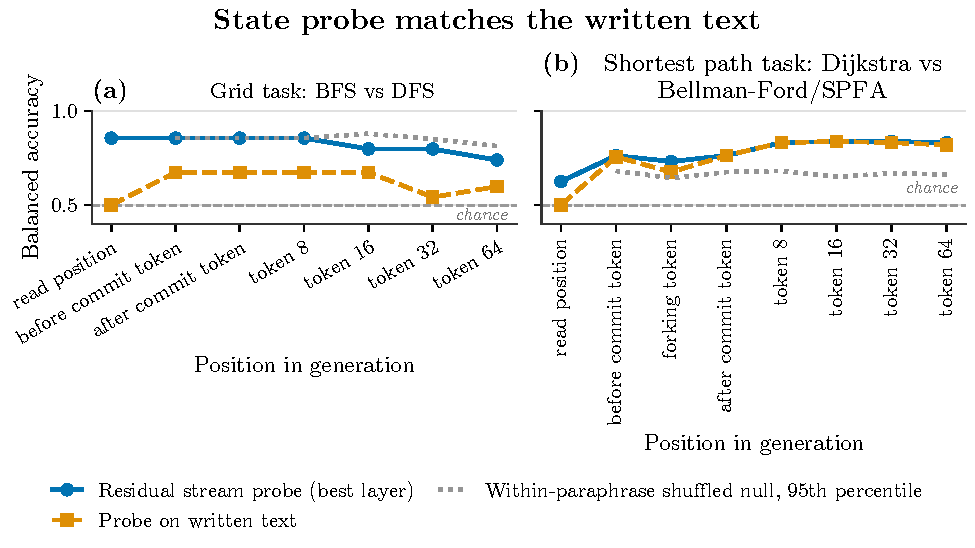
\includegraphics[width=\linewidth,height=0.78\textheight,keepaspectratio]{figures/fig_locus_text_v0.pdf}
\caption{Decoder of the algorithm the model goes on to write, by position in the generation (balanced accuracy at the best layer per position, leave-one-paraphrase-out folds, on the saved states of the forking-token experiment as reprobed by the iteration-2 audit). (a) Grid task, BFS vs. DFS under one ban prompt (99 programs). (b) Shortest-path task, Dijkstra vs. Bellman-Ford\slash{}SPFA under one ban prompt (100 programs). Both panels share a y-axis, ``Balanced accuracy'', from 0.4 to 1.0, with a dashed grey line at 0.5 marked ``chance''. Each panel plots three series, in one legend shared below both panels: the residual-stream probe (solid, circle markers), a probe on the text written so far (dashed, square markers), and the 95th percentile of probes refit on labels shuffled within paraphrase (dotted, grey, no markers). On the grid task (a), the shuffled-within-paraphrase null matches the residual-stream probe at the commit token and token 8, and exceeds it at tokens 16, 32 and 64 --- the residual stream carries no more than the paraphrase's own base rate at any generated position. On the shortest-path task (b), the residual-stream probe and the text-only probe are within 0.013 balanced accuracy of each other at every generated position except the forking token itself (where the residual probe leads by 0.056, before the deciding token has been written), and both sit clearly above the null --- so the state read-out tracks what has already been written rather than exposing a decision made earlier.}
\label{fig:fig_locus_text}
\end{figure}
\textbf{What the locus probe showed.} On the grid task no position passes the rule, so the mechanical locus stays at the read position. The read position already separates the prompts that will produce DFS from those that will produce BFS (balanced accuracy 0.855 at layer 16), but at every generated position the within paraphrase null reaches the observed accuracy: the signal is the paraphrase's base rate, not anything specific to a sample. BFS and DFS programs also share their commit token (\texttt{' deque'}; 51 of 78 DFS programs and all 21 BFS programs commit at token 6), so the commit index does not separate the classes on this task. On the shortest path task the first passing position is the token before the commit token (layer 8, +0.281 over the read position, within paraphrase p = 0.005; a second implementation with 40 sklearn refits gave p = 0.024 against a placebo p of 0.17). The written text control reaches 0.756 at the same position, so the state adds 0.006 over the text, below the preregistered 0.10 margin. The audit therefore qualified the shortest path locus as a readout after commitment. The text separates the classes from generated token 4 on: Dijkstra programs write \texttt{import heapq} and Bellman-Ford\slash{}SPFA programs write \texttt{from collections import deque}. The deciding token is generated token 3, emitted from states at tokens 1 to 3 that were never saved, and the forking token experiment had independently confirmed a forking token at that index (\texttt{import}, total variation 0.80; Table 19). The first token at which the text alone reaches 0.8 is token 8. No decision locus was found on either task.

Three further readings came out of the same states. The difference-in-means direction at the token before the commit token has held-out AUC 0.882 (grid) and 0.749 (shortest path), below the 0.9 bar that would reopen a generation time removal. Per paraphrase, the read position probe's held-out probability of the substitute tracks the share of the substitute that paraphrase produced (Spearman 0.63, exact p = 0.056, grid; 0.65, p = 0.045, shortest path; ten paraphrases each), a first sign that the read position knows how strongly a wording will be obeyed. The positive controls (baseline against ban states) were decoded at balanced accuracy close to 1.0.

\subsubsection*{2.3.2 Geometry under paraphrase resampling}
The geometry experiment's stability figure of 0.985 came from resampling points on a fixed graph, which the hypothesis review had warned is uninformative. The audit rebuilt the principal component projection, the nearest neighbour graph and the centroids on 1,000 paraphrase level subsamples, for k in \{5, 10, 15, 20\} at every layer of the two gate bands (24 to 28 grid, 21 to 27 shortest path), after reproducing the committed distance matrices exactly (largest absolute difference 0.0000). Table 42 gives the k = 10 column.

\begin{table}[H]
\renewcommand{\thetable}{42}
\centering\scriptsize\setlength{\tabcolsep}{2.5pt}
\caption{Nearest surviving centroid to the default algorithm under 1,000 paraphrase subsamples, k = 10 (source: \texttt{tables/\allowbreak{}geometry\_\allowbreak{}stability.\allowbreak{}csv}; distances on full data). [Source: iteration 2, artifact \nolinkurl{gen_art_evaluation_1}.]}\label{tab:t45}
\begin{tabular}{>{\raggedright\arraybackslash\hspace{0pt}}p{0.0539\linewidth}>{\raggedright\arraybackslash\hspace{0pt}}p{0.0622\linewidth}>{\raggedright\arraybackslash\hspace{0pt}}p{0.0934\linewidth}>{\raggedright\arraybackslash\hspace{0pt}}p{0.1683\linewidth}>{\raggedright\arraybackslash\hspace{0pt}}p{0.1476\linewidth}>{\raggedright\arraybackslash\hspace{0pt}}p{0.3115\linewidth}>{\raggedright\arraybackslash\hspace{0pt}}p{0.0867\linewidth}}
\toprule
\textbf{Task} & \textbf{Layer} & \textbf{P(DFS nearest)} & \textbf{P(unit weight Dijkstra nearest)} & \textbf{P(both are the two nearest)} & \textbf{Full data order} & \textbf{MDS stress-1} \\
\midrule
Grid & 24 & 0.523 & 0.477 & 1.0 & unit weight Dijkstra \textgreater{} DFS \textgreater{} A* \textgreater{} IDDFS \textgreater{} bidirectional BFS & 0.202 \\
Grid & 25 & 0.880 & 0.120 & 1.0 & DFS \textgreater{} unit weight Dijkstra \textgreater{} A* \textgreater{} IDDFS \textgreater{} bidirectional BFS & 0.212 \\
Grid & 26 & 0.954 & 0.046 & 1.0 & same & 0.213 \\
Grid & 27 & 1.0 & 0.0 & 1.0 & same & 0.217 \\
Grid & 28 & 1.0 & 0.0 & 1.0 & same & 0.230 \\
\bottomrule
\end{tabular}
\end{table}

\begin{table}[H]
\renewcommand{\thetable}{--}
\centering\scriptsize\setlength{\tabcolsep}{2.5pt}
\caption{A second table under the same heading in the draft, printed without its own caption there [Source: iteration 2, artifact \nolinkurl{gen_art_evaluation_1}.]}\label{tab:t46}
\begin{tabular}{>{\raggedright\arraybackslash\hspace{0pt}}p{0.0817\linewidth}>{\raggedright\arraybackslash\hspace{0pt}}p{0.0622\linewidth}>{\raggedright\arraybackslash\hspace{0pt}}p{0.0978\linewidth}>{\raggedright\arraybackslash\hspace{0pt}}p{0.1069\linewidth}>{\raggedright\arraybackslash\hspace{0pt}}p{0.1604\linewidth}>{\raggedright\arraybackslash\hspace{0pt}}p{0.1012\linewidth}>{\raggedright\arraybackslash\hspace{0pt}}p{0.2365\linewidth}>{\raggedright\arraybackslash\hspace{0pt}}p{0.0665\linewidth}}
\toprule
\textbf{Task} & \textbf{Layer} & \textbf{P(Floyd-Warshall nearest)} & \textbf{P(Bellman-Ford\slash{}SPFA nearest)} & \textbf{P(Bellman-Ford\slash{}SPFA nearer than bidirectional Dijkstra)} & \textbf{Rank of Bellman-Ford\slash{}SPFA (full data)} & \textbf{Full data order} & \textbf{MDS stress-1} \\
\midrule
Shortest path & 21 & 1.0 & 0.0 & 0.555 & 3 & Floyd-Warshall \textgreater{} bidirectional Dijkstra \textgreater{} Bellman-Ford\slash{}SPFA \textgreater{} Dial & 0.205 \\
Shortest path & 22 & 1.0 & 0.0 & 0.633 & 3 & same & 0.239 \\
Shortest path & 23 & 1.0 & 0.0 & 0.829 & 2 & Floyd-Warshall \textgreater{} Bellman-Ford\slash{}SPFA \textgreater{} bidirectional Dijkstra \textgreater{} Dial & 0.235 \\
Shortest path & 24 & 1.0 & 0.0 & 0.820 & 2 & same & 0.224 \\
Shortest path & 25 & 1.0 & 0.0 & 0.810 & 2 & same & 0.226 \\
Shortest path & 26 & 1.0 & 0.0 & 0.897 & 2 & same & 0.227 \\
Shortest path & 27 & 1.0 & 0.0 & 0.964 & 2 & same & 0.229 \\
\bottomrule
\end{tabular}
\end{table}

Over all four values of k the picture is the same. On the shortest path task Floyd-Warshall is the nearest survivor to Dijkstra in 100\% of subsamples at all 28 (layer, k) settings, and Bellman-Ford\slash{}SPFA, the algorithm every ban landed on, is never nearest; its full data rank is 2 in 75\% of settings and 3 in 25\%. The geometry experiment's sensitivity matrix, which recomputes the two flagged centroids from correctly labelled forced samples only, puts bidirectional Dijkstra (40.91) closer to Dijkstra than Bellman-Ford\slash{}SPFA (42.18), with Floyd-Warshall at 25.49 and Dial at 58.01. On the grid task DFS is nearest to BFS at layers 25 to 28 (probability 0.87 to 1.00 over k) and unit weight Dijkstra overtakes it at layer 24 (DFS 0.52 to 0.60), while DFS and unit weight Dijkstra are always the two nearest. Neighbour orders agree across k and layer with mean Kendall tau 0.933 (grid) and 0.870 (shortest path). Centroids from name masked prompts give different orders (grid top-1 stability 0.18 to 0.815). The grid ban's landing on DFS and unit weight Dijkstra is therefore consistent with geodesic proximity and with typicality, since both are also second choices of the model, and the two are not separated on these events. On the shortest path task geodesic proximity predicts the wrong substitute.

\subsubsection*{2.3.3 The substitute, draw by draw}
The audit recomputed the modal ban substitutes from the per-sample rows of every draw (Table 43). On the shortest path task the claim survives as written: all 272 compliant programs in the five draws were Bellman-Ford\slash{}SPFA. On the grid task DFS was the realised mode in four of five draws and took 116 of 128 compliant programs; in the geometry draw, the only one sampled with HF \texttt{generate} and the one with the highest banned share, 8 of 18 compliant programs were unit weight Dijkstra and the event had no clear mode.

\begin{table}[H]
\renewcommand{\thetable}{43}
\centering\footnotesize\setlength{\tabcolsep}{4.0pt}
\caption{Compliant programs under the modal ban, per draw (source: \texttt{corrections.\allowbreak{}json}; Wilson 95\% intervals for the substitute's share). [Source: iteration 2, artifact \nolinkurl{gen_art_evaluation_1}.]}\label{tab:t47}
\begin{tabular}{>{\raggedright\arraybackslash\hspace{0pt}}p{0.1336\linewidth}>{\raggedright\arraybackslash\hspace{0pt}}p{0.1087\linewidth}>{\raggedright\arraybackslash\hspace{0pt}}p{0.1348\linewidth}>{\raggedright\arraybackslash\hspace{0pt}}p{0.2336\linewidth}>{\raggedright\arraybackslash\hspace{0pt}}p{0.1717\linewidth}>{\raggedright\arraybackslash\hspace{0pt}}p{0.1142\linewidth}}
\toprule
\textbf{Draw (engine)} & \textbf{Grid: DFS \slash{} compliant} & \textbf{Other compliant labels} & \textbf{DFS share [95\%]} & \textbf{Shortest path: Bellman-Ford\slash{}SPFA \slash{} compliant} & \textbf{Share [95\%]} \\
\midrule
Association (vLLM) & 38 \slash{} 38 & none & 1.0 [0.908, 1.000] & 86 \slash{} 86 & 1.0 [0.957, 1.000] \\
Geometry (HF) & 10 \slash{} 18 & unit weight Dijkstra 8 & 0.556 [0.337, 0.754] & 22 \slash{} 22 & 1.0 [0.851, 1.000] \\
Forking token (vLLM) & 40 \slash{} 41 & unit weight Dijkstra 1 & 0.976 [0.874, 0.996] & 80 \slash{} 80 & 1.0 [0.954, 1.000] \\
Decommitment (vLLM) & 16 \slash{} 18 & unit weight Dijkstra 2 & 0.889 [0.672, 0.969] & 38 \slash{} 38 & 1.0 [0.908, 1.000] \\
Instruction tuning (vLLM) & 12 \slash{} 13 & unit weight Dijkstra 1 & 0.923 [0.667, 0.986] & 46 \slash{} 46 & 1.0 [0.923, 1.000] \\
Pooled & 116 \slash{} 128 & unit weight Dijkstra 12 & 0.906 [0.843, 0.946]; draw cluster bootstrap [0.75, 0.98] & 272 \slash{} 272 & 1.0 [0.986, 1.000] \\
\bottomrule
\end{tabular}
\end{table}

\subsubsection*{2.3.4 The cumulative ban of BFS and DFS does not replicate}
The three draws that banned BFS and DFS together disagree on everything the knob table depends on (Table 44). The decommitment draw spread its 16 compliant programs over two algorithms, the geometry draw put all 18 on one, and in the association draw the model reimplemented a banned mechanism 94 times out of 100. The pairs the review quoted from Table 37 (0.88 \slash{} 1.00, 0.96 \slash{} 0.99, 0.53 \slash{} 0.933) are each draw's pass rate followed by its reference pass rate.

\begin{table}[H]
\renewcommand{\thetable}{44}
\centering\footnotesize\setlength{\tabcolsep}{4.0pt}
\caption{The cumulative ban of BFS and DFS in three draws (source: \texttt{corrections.\allowbreak{}json\#cumulative\_\allowbreak{}bfs\_\allowbreak{}dfs\_\allowbreak{}ban}). [Source: iteration 2, artifact \nolinkurl{gen_art_evaluation_1}.]}\label{tab:t48}
\begin{tabular}{>{\raggedright\arraybackslash\hspace{0pt}}p{0.1336\linewidth}>{\raggedright\arraybackslash\hspace{0pt}}p{0.0567\linewidth}>{\raggedright\arraybackslash\hspace{0pt}}p{0.1891\linewidth}>{\raggedright\arraybackslash\hspace{0pt}}p{0.0926\linewidth}>{\raggedright\arraybackslash\hspace{0pt}}p{0.1430\linewidth}>{\raggedright\arraybackslash\hspace{0pt}}p{0.2817\linewidth}}
\toprule
\textbf{Draw} & \textbf{N} & \textbf{Banned share (mechanism)} & \textbf{Pass rate} & \textbf{Compliant programs} & \textbf{Compliant composition} \\
\midrule
Decommitment & 100 & 0.81 & 0.88 & 16 & unit weight Dijkstra 13, A* 3 \\
Geometry & 50 & 0.62 & 0.96 & 18 & unit weight Dijkstra 18 \\
Association & 100 & 0.94 & 0.53 & 5 & unit weight Dijkstra 4, A* 1 \\
\bottomrule
\end{tabular}
\end{table}

\subsubsection*{2.3.5 Every perturbation, side by side: the generic perturbation rival}
The audit assembled one table of every condition in the six draws: 249 condition rows covering 20,270 programs, each with its pass cost against its own reference (Newcombe intervals [42]), the label composition among correct and among attempted programs, and the share of the second choice with a Wilson interval (\texttt{tables/\allowbreak{}perturbation\_\allowbreak{}table.\allowbreak{}csv}). Tables 45 and 46 give the rows that bear on the generic perturbation rival. On the shortest path task every nonsemantic perturbation that produced at least 10 correct programs other than Dijkstra (8 of 8 such rows) had Bellman-Ford\slash{}SPFA as their majority, random directions included, and so did 3 of 4 semantic ones. Band random direction 2 of the instruction tuning experiment turned all 33 of its correct programs into Bellman-Ford\slash{}SPFA, against Dijkstra 100 of 100 in its control. On the grid task generic perturbations almost never left BFS: random directions broke programs (pass rates 0.41 and 0.68) but every correct program stayed BFS, and only two rows other than bans with at least 10 correct programs other than the default exist, both mention twins (A* and DFS). On the shortest path task a ban and an arbitrary perturbation end in the same place; on the grid task only the ban reaches DFS at scale.

{\footnotesize\setlength{\tabcolsep}{4.0pt}\renewcommand{\thetable}{45}
\begin{longtable}{>{\raggedright\arraybackslash\hspace{0pt}}p{0.1336\linewidth}>{\raggedright\arraybackslash\hspace{0pt}}p{0.2174\linewidth}>{\raggedright\arraybackslash\hspace{0pt}}p{0.0413\linewidth}>{\raggedright\arraybackslash\hspace{0pt}}p{0.1102\linewidth}>{\raggedright\arraybackslash\hspace{0pt}}p{0.2524\linewidth}>{\raggedright\arraybackslash\hspace{0pt}}p{0.1416\linewidth}}
\caption{Shortest path perturbations: label composition of correct programs and Bellman-Ford\slash{}SPFA share (source: \texttt{tables/\allowbreak{}perturbation\_\allowbreak{}table.\allowbreak{}csv}). [Source: iteration 2, artifact \nolinkurl{gen_art_evaluation_1}.]}\label{tab:t49}\\
\toprule
\textbf{Draw} & \textbf{Perturbation} & \textbf{N} & \textbf{Pass (reference)} & \textbf{Correct programs} & \textbf{Bellman-Ford\slash{}SPFA share [95\%]} \\
\midrule
\endfirsthead
\multicolumn{6}{l}{\emph{Table 45, continued}}\\
\toprule
\textbf{Draw} & \textbf{Perturbation} & \textbf{N} & \textbf{Pass (reference)} & \textbf{Correct programs} & \textbf{Bellman-Ford\slash{}SPFA share [95\%]} \\
\midrule
\endhead
\bottomrule
\endlastfoot
Decommitment & random direction 1, c = 0.25 & 100 & 0.79 (0.95) & Dijkstra 53, Bellman-Ford\slash{}SPFA 26 & 0.329 [0.236, 0.439] \\
Decommitment & random direction 2, c = 0.25 & 100 & 0.87 (0.95) & Dijkstra 82, Bellman-Ford\slash{}SPFA 5 & 0.057 [0.025, 0.128] \\
Decommitment & decommitment direction, c = 0.25 & 100 & 0.78 (0.95) & Bellman-Ford\slash{}SPFA 54, Dijkstra 23, other 1 & 0.692 [0.583, 0.784] \\
Decommitment & decommitment direction, c = 0.375 & 100 & 0.67 (0.95) & Bellman-Ford\slash{}SPFA 47, Dijkstra 19, other 1 & 0.701 [0.583, 0.798] \\
Decommitment & decommitment direction, c = 0.5 & 100 & 0.37 (0.95) & Dijkstra 25, Bellman-Ford\slash{}SPFA 10, other 2 & 0.270 [0.154, 0.430] \\
Decommitment & breadth direction, c = 0.25 & 100 & 0.60 (0.95) & Bellman-Ford\slash{}SPFA 31, Dijkstra 28, Dial 1 & 0.516 [0.393, 0.638] \\
Decommitment & other task's direction, c = 0.25 & 50 & 0.72 (0.95) & Bellman-Ford\slash{}SPFA 28, Dijkstra 8 & 0.777 [0.619, 0.883] \\
Decommitment & variable name placebo, c = 0.25 & 100 & 0.66 (0.95) & Dijkstra 60, Dial 3, Bellman-Ford\slash{}SPFA 2, other 1 & 0.030 [0.008, 0.104] \\
Decommitment & enumeration prompt & 100 & 0.82 (0.885) & Dijkstra 80, Bellman-Ford\slash{}SPFA 2 & 0.024 [0.007, 0.085] \\
Instruction tuning & band random direction 1 & 100 & 0.00 (1.00) & none & n\slash{}a \\
Instruction tuning & band random direction 2 & 100 & 0.33 (1.00) & Bellman-Ford\slash{}SPFA 33 & 1.0 [0.896, 1.000] \\
Instruction tuning & random direction 1, read position only, c = 1.0 & 100 & 1.00 (1.00) & Dijkstra 90, Bellman-Ford\slash{}SPFA 9, other 1 & 0.090 [0.048, 0.162] \\
Instruction tuning & sharpening subtraction, layer 18, c = 0.5 & 50 & 0.98 (1.00) & Dijkstra 48, Bellman-Ford\slash{}SPFA 1 & 0.020 [0.004, 0.107] \\
Instruction tuning & sharpening subtraction, read position only, no cutoff & 20 & 0.20 (1.00) & Dijkstra 3, Bellman-Ford\slash{}SPFA 1 & 0.25 [0.046, 0.699] \\
Instruction tuning & base model, chat template & 300 & 0.30 (1.00) & Dijkstra 63, Bellman-Ford\slash{}SPFA 24, other 2, Floyd-Warshall 1 & 0.266 [0.186, 0.366] \\
Instruction tuning & base model, plain completion & 300 & 0.083 (1.00) & Bellman-Ford\slash{}SPFA 16, Dijkstra 8, Floyd-Warshall 1 & 0.64 [0.445, 0.798] \\
Instruction tuning & instruct model, plain completion & 100 & 0.72 (1.00) & Dijkstra 57, Floyd-Warshall 8, Bellman-Ford\slash{}SPFA 7 & 0.097 [0.048, 0.187] \\
Decoding & semantic seed & 100 & 0.92 (0.99) & Bellman-Ford\slash{}SPFA 61, Dijkstra 30, Floyd-Warshall 1 & 0.663 [0.562, 0.751] \\
Decoding & novelty instruction & 100 & 0.96 (0.99) & Dijkstra 82, Bellman-Ford\slash{}SPFA 14 & 0.145 [0.089, 0.230] \\
Decoding & new algorithm instruction & 100 & 0.94 (0.99) & Dijkstra 90, Bellman-Ford\slash{}SPFA 4 & 0.042 [0.017, 0.104] \\
Decoding & enumeration prompt & 100 & 0.75 (0.99) & Dijkstra 67, Bellman-Ford\slash{}SPFA 8 & 0.106 [0.055, 0.197] \\
Decoding & T = 1.3, top-k = 10 & 100 & 1.00 (0.98) & Dijkstra 99, Bellman-Ford\slash{}SPFA 1 & 0.010 [0.002, 0.054] \\
Association & listing control & 100 & 1.00 (1.00) & Dijkstra 97, Bellman-Ford\slash{}SPFA 3 & 0.030 [0.010, 0.085] \\
Association & sham ban of Floyd-Warshall & 100 & 0.71 (1.00) & Dijkstra 68, Bellman-Ford\slash{}SPFA 3 & 0.042 [0.014, 0.117] \\
All five draws & modal ban of Dijkstra, pooled & 500 & 0.87 to 1.00 & Bellman-Ford\slash{}SPFA 272 (compliant) & 1.0 [0.986, 1.000] \\
\end{longtable}}

The sham ban of Floyd-Warshall shows why compliant and attempted programs must be told apart: 23 of its 100 attempted programs were Bellman-Ford\slash{}SPFA (Table 8), but only 3 of those passed the tests.

\begin{table}[H]
\renewcommand{\thetable}{46}
\centering\footnotesize\setlength{\tabcolsep}{4.0pt}
\caption{Grid perturbations: label composition of correct programs and DFS share (source: \texttt{tables/\allowbreak{}perturbation\_\allowbreak{}table.\allowbreak{}csv}). [Source: iteration 2, artifact \nolinkurl{gen_art_evaluation_1}.]}\label{tab:t50}
\begin{tabular}{>{\raggedright\arraybackslash\hspace{0pt}}p{0.1336\linewidth}>{\raggedright\arraybackslash\hspace{0pt}}p{0.2486\linewidth}>{\raggedright\arraybackslash\hspace{0pt}}p{0.0413\linewidth}>{\raggedright\arraybackslash\hspace{0pt}}p{0.1114\linewidth}>{\raggedright\arraybackslash\hspace{0pt}}p{0.2130\linewidth}>{\raggedright\arraybackslash\hspace{0pt}}p{0.1487\linewidth}}
\toprule
\textbf{Draw} & \textbf{Perturbation} & \textbf{N} & \textbf{Pass (reference)} & \textbf{Correct programs} & \textbf{DFS share [95\%]} \\
\midrule
Instruction tuning & band random direction 1 & 100 & 0.41 (1.00) & BFS 41 & 0.0 [0.000, 0.086] \\
Instruction tuning & band random direction 2 & 100 & 0.68 (1.00) & BFS 68 & 0.0 [0.000, 0.053] \\
Instruction tuning & random direction 1, read position only, c = 1.0 & 100 & 1.00 (1.00) & BFS 100 & 0.0 [0.000, 0.037] \\
Decommitment & decommitment direction, c = 0.25 & 100 & 0.57 (1.00) & BFS 57 & 0.0 [0.000, 0.063] \\
Decoding & semantic seed & 100 & 0.93 (0.97) & BFS 91, bidirectional BFS 2 & 0.0 [0.000, 0.040] \\
Decoding & novelty instruction & 100 & 0.85 (0.97) & BFS 81, unit weight Dijkstra 2, DFS 1, A* 1 & 0.011 [0.002, 0.064] \\
Decoding & new algorithm instruction & 100 & 0.94 (0.97) & BFS 92, DFS 2 & 0.021 [0.006, 0.074] \\
Decoding & enumeration prompt & 100 & 0.99 (0.97) & BFS 99 & 0.0 [0.000, 0.037] \\
Decoding & T = 1.3, top-k = 10 & 100 & 0.95 (0.98) & BFS 94, DFS 1 & 0.010 [0.002, 0.057] \\
Instruction tuning & base model, chat template & 300 & 0.19 (1.00) & BFS 49, DFS 7, A* 1 & 0.122 [0.061, 0.232] \\
Instruction tuning & base model, plain completion & 300 & 0.05 (1.00) & BFS 12, DFS 3 & 0.20 [0.070, 0.452] \\
Instruction tuning & instruct model, plain completion & 100 & 0.73 (1.00) & BFS 73 & 0.0 [0.000, 0.050] \\
Association & listing control & 100 & 0.92 (0.933) & BFS 92 & 0.0 [0.000, 0.040] \\
Association & sham ban of IDDFS & 100 & 0.80 (0.933) & BFS 76, DFS 4 & 0.05 [0.020, 0.122] \\
Association & sham ban of unit weight Dijkstra & 100 & 0.71 (0.933) & BFS 69, DFS 2 & 0.028 [0.008, 0.097] \\
All five draws & modal ban of BFS, pooled & 500 & 0.46 to 0.76 & DFS 116, unit weight Dijkstra 12 (compliant) & 0.906 [0.843, 0.946] \\
\bottomrule
\end{tabular}
\end{table}

\subsubsection*{2.3.6 The knob table on one statistic}
The iteration-1 knob table mixed unrarefied Hill numbers, rarefied differences, and Hill numbers that counted correct programs of the banned algorithm. The audit recomputed every knob with one statistic: the Hill number of order 1 [9] over compliant programs only (banned labels excluded), rarefied to a common depth of 25 by 1,000 draws without replacement, with a 90\% interval from 1,000 paraphrase cluster bootstrap resamples times 200 rarefaction draws; cells with fewer than 25 compliant programs are marked and never extrapolated. Pass points are measured against each condition's own reference. Generate then select is a ceiling row, because its diversity comes from an external random choice among model proposed approaches, which is the mechanism of SimpleStrat [43]. Table 47 gives the rows that matter (all 183 rows are in \texttt{tables/\allowbreak{}knob\_\allowbreak{}table.\allowbreak{}csv}).

{\scriptsize\setlength{\tabcolsep}{2.5pt}\renewcommand{\thetable}{47}
\begin{longtable}{>{\raggedright\arraybackslash\hspace{0pt}}p{0.0769\linewidth}>{\raggedright\arraybackslash\hspace{0pt}}p{0.2605\linewidth}>{\raggedright\arraybackslash\hspace{0pt}}p{0.0806\linewidth}>{\raggedright\arraybackslash\hspace{0pt}}p{0.1001\linewidth}>{\raggedright\arraybackslash\hspace{0pt}}p{0.2122\linewidth}>{\raggedright\arraybackslash\hspace{0pt}}p{0.1266\linewidth}>{\raggedright\arraybackslash\hspace{0pt}}p{0.0665\linewidth}}
\caption{One statistic knob table: rarefied Hill-1 over compliant programs at depth 25 (source: \texttt{tables/\allowbreak{}knob\_\allowbreak{}table.\allowbreak{}csv}). [Source: iteration 2, artifact \nolinkurl{gen_art_evaluation_1}.]}\label{tab:t51}\\
\toprule
\textbf{Task} & \textbf{Knob (draw)} & \textbf{Class} & \textbf{Compliant programs} & \textbf{Composition} & \textbf{Hill-1 [90\% CI]} & \textbf{Pass points lost} \\
\midrule
\endfirsthead
\multicolumn{7}{l}{\emph{Table 47, continued}}\\
\toprule
\textbf{Task} & \textbf{Knob (draw)} & \textbf{Class} & \textbf{Compliant programs} & \textbf{Composition} & \textbf{Hill-1 [90\% CI]} & \textbf{Pass points lost} \\
\midrule
\endhead
\bottomrule
\endlastfoot
Grid & generate then select (decoding) & ceiling & 55 & BFS 26, A* 14, unit weight Dijkstra 9, DFS 6 & 3.358 [3.315, 3.381] & 42.0 \\
Grid & mention of A* (association) & named mode cue & 41 & A* 24, BFS 11, unit weight Dijkstra 5, DFS 1 & 2.687 [1.861, 3.186] & 11.3 \\
Grid & base model, chat template (instruction tuning) & model swap & 57 & BFS 49, DFS 7, A* 1 & 1.549 [1.284, 1.814] & 81.0 \\
Grid & modal ban, five draws pooled & ban & 128 & DFS 116, unit weight Dijkstra 12 & 1.357 [1.250, 1.425] & 34.3 \\
Grid & novelty instruction (decoding) & diversity knob & 85 & BFS 81, unit weight Dijkstra 2, DFS 1, A* 1 & 1.227 [1.096, 1.346] & 12.0 \\
Grid & sham ban of IDDFS (association) & ban & 80 & BFS 76, DFS 4 & 1.205 [1.0, 1.542] & 13.3 \\
Grid & sham ban of unit weight Dijkstra (association) & ban & 71 & BFS 69, DFS 2 & 1.119 [1.0, 1.245] & 22.3 \\
Grid & modal ban (forking token) & ban & 41 & DFS 40, unit weight Dijkstra 1 & 1.111 [1.0, 1.243] & 35.0 \\
Grid & semantic seed (decoding) & diversity knob & 93 & BFS 91, bidirectional BFS 2 & 1.096 [1.0, 1.191] & 4.0 \\
Grid & new algorithm instruction (decoding) & diversity knob & 94 & BFS 92, DFS 2 & 1.093 [1.0, 1.187] & 3.0 \\
Grid & T = 1.3, top-k = 10 (decoding) & diversity knob & 95 & BFS 94, DFS 1 & 1.048 [1.0, 1.133] & 3.0 \\
Grid & modal ban (association) & ban & 38 & DFS 38 & 1.0 [1.0, 1.0] & 47.3 \\
Grid & cumulative ban of BFS and DFS (decommitment) & ban & 16 & unit weight Dijkstra 13, A* 3 & below depth (unrarefied 1.620) & 12.0 \\
Grid & cumulative ban of BFS and DFS (geometry) & ban & 18 & unit weight Dijkstra 18 & below depth (unrarefied 1.0) & 3.0 \\
Grid & cumulative ban of BFS and DFS (association) & ban & 5 & unit weight Dijkstra 4, A* 1 & below depth (unrarefied 1.649) & 40.3 \\
Grid & every steering, removal, forking window, random seed and remaining temperature arm & diversity knob & 3 to 307 & BFS only & 1.0, or below depth & 0 to 97 \\
Shortest path & generate then select (decoding) & ceiling & 75 & Bellman-Ford\slash{}SPFA 31, Dijkstra 29, Floyd-Warshall 15 & 2.802 [2.778, 2.812] & 24.0 \\
Shortest path & base model, plain completion (instruction tuning) & model swap & 25 & Bellman-Ford\slash{}SPFA 16, Dijkstra 8, Floyd-Warshall 1 & 2.179 [1.704, 2.611] & 91.7 \\
Shortest path & decommitment direction, c = 0.5 & diversity knob & 37 & Dijkstra 25, Bellman-Ford\slash{}SPFA 10, other 2 & 2.139 [1.553, 2.495] & 58.0 \\
Shortest path & breadth direction, c = 0.25 & diversity knob & 60 & Bellman-Ford\slash{}SPFA 31, Dijkstra 28, Dial 1 & 2.096 [1.920, 2.297] & 35.0 \\
Shortest path & base model, chat template & model swap & 90 & Dijkstra 63, Bellman-Ford\slash{}SPFA 24, other 2, Floyd-Warshall 1 & 2.018 [1.737, 2.262] & 70.0 \\
Shortest path & semantic seed (decoding) & diversity knob & 92 & Bellman-Ford\slash{}SPFA 61, Dijkstra 30, Floyd-Warshall 1 & 1.935 [1.534, 2.076] & 7.0 \\
Shortest path & decommitment direction, c = 0.25 & diversity knob & 78 & Bellman-Ford\slash{}SPFA 54, Dijkstra 23, other 1 & 1.911 [1.735, 2.069] & 17.0 \\
Shortest path & decommitment direction, c = 0.375 & diversity knob & 67 & Bellman-Ford\slash{}SPFA 47, Dijkstra 19, other 1 & 1.901 [1.675, 2.079] & 28.0 \\
Shortest path & random direction 1, c = 0.25 (decommitment) & diversity knob & 79 & Dijkstra 53, Bellman-Ford\slash{}SPFA 26 & 1.861 [1.657, 1.964] & 16.0 \\
Shortest path & random directions, four arms pooled & diversity knob & 199 & Dijkstra 135, Bellman-Ford\slash{}SPFA 64 & 1.851 [1.774, 1.903] & 47.75 \\
Shortest path & other task's direction, c = 0.25 & diversity knob & 36 & Bellman-Ford\slash{}SPFA 28, Dijkstra 8 & 1.688 [1.412, 1.857] & 23.0 \\
Shortest path & novelty instruction (decoding) & diversity knob & 96 & Dijkstra 82, Bellman-Ford\slash{}SPFA 14 & 1.500 [1.275, 1.692] & 3.0 \\
Shortest path & variable name placebo, c = 0.25 & diversity knob & 66 & Dijkstra 60, Dial 3, Bellman-Ford\slash{}SPFA 2, other 1 & 1.451 [1.129, 1.829] & 29.0 \\
Shortest path & random direction 1, read position only (instruction tuning) & diversity knob & 100 & Dijkstra 90, Bellman-Ford\slash{}SPFA 9, other 1 & 1.393 [1.209, 1.593] & 0.0 \\
Shortest path & enumeration prompt (decoding) & diversity knob & 75 & Dijkstra 67, Bellman-Ford\slash{}SPFA 8 & 1.382 [1.217, 1.581] & 24.0 \\
Shortest path & random direction 2, c = 0.25 (decommitment) & diversity knob & 87 & Dijkstra 82, Bellman-Ford\slash{}SPFA 5 & 1.231 [1.097, 1.371] & 8.0 \\
Shortest path & modal ban, five draws pooled & ban & 272 & Bellman-Ford\slash{}SPFA 272 & 1.0 [1.0, 1.0] & 2.4 \\
\end{longtable}}

\textbf{The positive target and the BUY rule.} The strategy's positive target was a knob that buys a second correct algorithm, a Hill number of at least 2 within its own compliant output, at a cost below 20 pass points. Under the single statistic no diversity knob and no ban meets it on either task. The closest is the semantic seed on the shortest path task (1.935 at 7 points). The mention of A* on the grid task reaches 2.69 at 11 points, but a mention recommends a named algorithm, so it meets only the literal reading of the target. The modal ban, the knob that iteration 1 ranked first on the shortest path task, scores exactly 1.0 there once banned programs no longer count: it replaces Dijkstra with one algorithm. The BUY rule names a best knob only when its 90\% interval separates from the next; on the grid task the top rows (novelty instruction 1.227 [1.096, 1.346], sham ban of IDDFS 1.205 [1.0, 1.542]) do not separate, and on the shortest path task neither do the top five (Table 47). No knob advances. \emph{(Correction, iteration 3: the sentences above paraphrase the target past its metric. A rarefied Hill-1 of at least 2 is an even two-algorithm split, which a 2:1 split never reaches. Stated in its own metric: no knob reaches an even split under 20 pass points; the semantic seed (Bellman-Ford\slash{}SPFA 61, Dijkstra 30 at 7 points; rebuilt Hill-1 1.940, 90\% interval [1.770, 2.094], which includes 2) and the A} mention (2.69 at 11.3 points) are the two conditions that buy a second correct algorithm, and both name or describe it. The sham ban of IDDFS ranked above is a control, not a knob; the class rule is now declared in Section 3.2.5.)* \emph{(Correction, iteration 4: the iteration-3 correction is itself incomplete. Two activation rows of Table 91 also buy a second correct algorithm without naming or describing one: the decommitment direction at c = 0.25 (Bellman-Ford\slash{}SPFA 54, Dijkstra 23; Hill-1 1.913, 90\% interval [1.704, 2.083], which includes 2, at 17 points) and random direction 1 of the decommitment experiment (Dijkstra 53, Bellman-Ford\slash{}SPFA 26; 1.86 at 16 points). On the bench, norm-matched random directions written into the task-specification states in iteration 3 reach Hill-1 above 2 at 0 pass points on kth smallest (2.92) and two sum (2.12). The verdict per task over every iteration-3 arm is in Section 4.2.1.)}

\subsubsection*{2.3.7 The forecast contest on gated events}
The rule, quoted in full from the strategy, is that a forecasting family advances if its calibrated mean log score beats the next best family by at least 0.10 nats on at least three events where the families' top-1 nominations disagree, scored on informative events only: banned mode present at 10\% or more of the latent baseline, compliance of at least 50\% and at least two survivors. The hypothesis update fixed compliance in this rule to mean avoidance and added a floor of 20 attempted programs not banned. Of the 64 events with forecasts in the iteration-1 record, 24 were sampled (Table 48). Three informative events pass the gate: the association draw's two modal bans and the decommitment draw's grid modal ban, whose forecasts are all tied. The gate as written also admits the association draw's nine sham bans (12 events in all), but they land on the default by construction and their own artifact marked them uninformative. The geometry, instruction tuning and decommitment shortest path events fail the gate under either compliance definition, and the forking token draw made no family forecasts. On the gated events the families' mean log scores are: association map (Borda) -0.844 (2 events), free-form association -0.145 (2), listing control typicality -0.120 (2), sampled frequency -1.579 (3), decommitted distribution -1.674 (1) and uniform -1.674 (1). Only two gated events have disagreeing nominations, and the largest margin on them is 0.05 nats. No family can advance, so the iteration-1 ranking of forecasts in Table 36 rests largely on events the rule excludes.

{\tiny\setlength{\tabcolsep}{2.5pt}\renewcommand{\thetable}{48}
\begin{longtable}{>{\raggedright\arraybackslash\hspace{0pt}}p{0.0866\linewidth}>{\raggedright\arraybackslash\hspace{0pt}}p{0.1295\linewidth}>{\raggedright\arraybackslash\hspace{0pt}}p{0.0289\linewidth}>{\raggedright\arraybackslash\hspace{0pt}}p{0.0739\linewidth}>{\raggedright\arraybackslash\hspace{0pt}}p{0.0706\linewidth}>{\raggedright\arraybackslash\hspace{0pt}}p{0.0739\linewidth}>{\raggedright\arraybackslash\hspace{0pt}}p{0.0706\linewidth}>{\raggedright\arraybackslash\hspace{0pt}}p{0.0739\linewidth}>{\raggedright\arraybackslash\hspace{0pt}}p{0.2949\linewidth}}
\caption{Every sampled iteration-1 event with forecasts, with both gates and the log scores of the main families (nats per attempted program not banned; 5\% uniform mixing and a 2\% floor for other labels in every family; top-1 nomination in brackets). Source: \texttt{results/\allowbreak{}tables.\allowbreak{}json\#predict\_\allowbreak{}gated}. [Source: iteration 2, artifact \nolinkurl{gen_art_evaluation_1}.]}\label{tab:t52}\\
\toprule
\textbf{Draw} & \textbf{Event} & \textbf{N} & \textbf{Attempted, not banned} & \textbf{Avoidance} & \textbf{Compliant share} & \textbf{Avoidance gate} & \textbf{Compliant gate} & \textbf{Log scores [top-1]} \\
\midrule
\endfirsthead
\multicolumn{9}{l}{\emph{Table 48, continued}}\\
\toprule
\textbf{Draw} & \textbf{Event} & \textbf{N} & \textbf{Attempted, not banned} & \textbf{Avoidance} & \textbf{Compliant share} & \textbf{Avoidance gate} & \textbf{Compliant gate} & \textbf{Log scores [top-1]} \\
\midrule
\endhead
\bottomrule
\endlastfoot
Association & grid ban A* (sham) & 100 & 100 & 1.0 & 0.72 & pass & pass & Borda -1.022 [BFS]; free-form -0.101 [BFS]; frequency -0.101 [BFS]; listing -0.131 [BFS] \\
Association & grid ban BFS (modal) & 100 & 90 & 0.90 & 0.38 & pass & fail & Borda -2.710 [unit weight Dijkstra]; free-form -0.152 [DFS]; frequency -1.630 [tie]; listing -0.101 [DFS] \\
Association & grid ban bidirectional BFS (sham) & 100 & 100 & 1.0 & 0.92 & pass & pass & Borda -1.063 [BFS]; free-form -1.141 [A*]; frequency -0.140 [BFS]; listing -0.169 [BFS] \\
Association & grid ban DFS (sham) & 100 & 96 & 0.96 & 0.86 & pass & pass & Borda -0.998; free-form -0.101; frequency -0.101; listing -0.101 [all BFS] \\
Association & grid ban unit weight Dijkstra (sham) & 100 & 100 & 1.0 & 0.71 & pass & pass & Borda -1.113; free-form -0.410; frequency -0.410; listing -0.368 [all BFS] \\
Association & grid ban IDDFS (sham) & 100 & 100 & 1.0 & 0.80 & pass & pass & Borda -1.114; free-form -0.511; frequency -0.564; listing -0.486 [all BFS] \\
Association & grid ban BFS and DFS & 100 & 6 & 0.06 & 0.05 & fail & fail & Borda -1.398 [bidirectional BFS]; others -1.406 [tie] \\
Association & shortest path ban Bellman-Ford\slash{}SPFA (sham) & 100 & 95 & 0.95 & 0.92 & pass & pass & Borda -0.926; free-form, frequency, listing -0.136 [all Dijkstra] \\
Association & shortest path ban bidirectional Dijkstra (sham) & 100 & 100 & 1.0 & 1.0 & pass & pass & Borda -0.791; free-form -0.205; frequency -0.205; listing -0.212 [Dijkstra] \\
Association & shortest path ban Dial (sham) & 100 & 100 & 1.0 & 0.97 & pass & pass & Borda -0.803; free-form -0.278; frequency -0.278; listing -0.269 [Dijkstra] \\
Association & shortest path ban Dijkstra (modal) & 100 & 91 & 0.91 & 0.86 & pass & pass & Borda -0.813 [Bellman-Ford\slash{}SPFA]; free-form -0.138 [Bellman-Ford\slash{}SPFA]; frequency -1.434 [tie]; listing -0.138 [Bellman-Ford\slash{}SPFA] \\
Association & shortest path ban Floyd-Warshall (sham) & 100 & 100 & 1.0 & 0.71 & pass & pass & Borda -0.911; free-form -0.933; frequency -0.933; listing -0.784 [Dijkstra] \\
Association & shortest path ban Dijkstra and Bellman-Ford\slash{}SPFA & 100 & 0 & 0.0 & 0.0 & fail & fail & not scorable \\
Geometry & grid ban BFS & 100 & 38 & 0.38 & 0.18 & fail & fail & association -3.543 [A*]; frequency -1.630 [tie]; geodesic -1.337 [DFS]; decoder -1.287 [DFS] \\
Geometry & grid ban BFS and DFS & 50 & 19 & 0.38 & 0.36 & fail & fail & association -0.998 [unit weight Dijkstra]; geodesic -1.073 [unit weight Dijkstra]; decoder -4.124 [IDDFS] \\
Geometry & grid ban BFS and unit weight Dijkstra & 50 & 17 & 0.34 & 0.10 & fail & fail & association -3.966 [A*]; geodesic -1.280 [A*]; decoder -1.372 [IDDFS] \\
Geometry & shortest path ban Dijkstra & 100 & 28 & 0.28 & 0.22 & fail & fail & association -1.647 [Dial]; frequency -1.496 [tie]; geodesic -1.530 [Floyd-Warshall]; decoder -1.587 [bidirectional Dijkstra] \\
Geometry & shortest path ban Dijkstra and Bellman-Ford\slash{}SPFA & 50 & 1 & 0.02 & 0.0 & fail & fail & all -3.912 \\
Decommitment & grid ban BFS & 100 & 51 & 0.51 & 0.18 & pass & fail & every family -1.674 [tie] \\
Decommitment & grid ban BFS and DFS & 100 & 19 & 0.19 & 0.16 & fail & fail & every family -1.538 [tie] \\
Decommitment & shortest path ban Dijkstra & 100 & 46 & 0.46 & 0.38 & fail & fail & decommitted -0.594 [Bellman-Ford\slash{}SPFA]; frequency (vLLM) -0.731 [Bellman-Ford\slash{}SPFA]; uniform -1.733 \\
Decommitment & shortest path ban Dijkstra and Bellman-Ford\slash{}SPFA & 100 & 17 & 0.17 & 0.01 & fail & fail & all -3.912 [tie] \\
Instruction tuning & grid ban BFS & 100 & 38 & 0.38 & 0.13 & fail & fail & base plain completion -0.430 [DFS]; base chat -0.304 [DFS]; instruct chat -1.630 [tie] \\
Instruction tuning & shortest path ban Dijkstra & 100 & 46 & 0.46 & 0.46 & fail & fail & base plain completion -0.255; base chat -0.096; instruct chat -0.096 [all Bellman-Ford\slash{}SPFA] \\
\end{longtable}}

These scores are computed over attempted programs not banned, so they differ slightly from the compliant only scores of Tables 7, 14 and 36.

\subsubsection*{2.3.8 Seeds at the read position: both halves of the dissociation}
Iteration 1 reported that the grid semantic seed moved the read position state toward its implied algorithm while the output barely moved. The other half was in the same file and was not reported (Table 49). On the shortest path task the semantic seed's displacement did not point toward the Bellman-Ford\slash{}SPFA centroid, yet the output moved two thirds of the way to it. The word seed moved the grid probe's decoded distribution toward A* by 0.88 with no change in behaviour. The entropy seed's interval on the shortest path task reaches 1.596, above the 1.5 equivalence bound, so its equivalence with paraphrase noise was not shown. Displacement along the mode subspace built from forced prompts predicted behavioural movement in neither direction.

\begin{table}[H]
\renewcommand{\thetable}{49}
\centering\footnotesize\setlength{\tabcolsep}{4.0pt}
\caption{Read position displacement against behavioural movement for the seeds (sources: decoding experiment \texttt{results/\allowbreak{}analysis.\allowbreak{}json}, audit \texttt{results/\allowbreak{}tables.\allowbreak{}json\#seeds}; behaviour shifts with Newcombe 95\% intervals). [Source: iteration 2, artifact \nolinkurl{gen_art_evaluation_1}.]}\label{tab:t53}
\begin{tabular}{>{\raggedright\arraybackslash\hspace{0pt}}p{0.0867\linewidth}>{\raggedright\arraybackslash\hspace{0pt}}p{0.1419\linewidth}>{\raggedright\arraybackslash\hspace{0pt}}p{0.2647\linewidth}>{\raggedright\arraybackslash\hspace{0pt}}p{0.2198\linewidth}>{\raggedright\arraybackslash\hspace{0pt}}p{0.2000\linewidth}}
\toprule
\textbf{Task} & \textbf{Seed} & \textbf{Read position evidence} & \textbf{Behaviour among correct programs} & \textbf{Behaviour among attempted programs} \\
\midrule
Grid & semantic (implies bidirectional search) & cosine 0.493 with the bidirectional BFS centroid & bidirectional BFS +2.15 points [-1.97, 7.51]; BFS -1.12 & bidirectional BFS +5.0 points [0.33, 11.18]; BFS -4.0 \\
Shortest path & semantic (implies relaxation over all edges) & cosine -0.087 with the Bellman-Ford\slash{}SPFA centroid & Bellman-Ford\slash{}SPFA +66.30 points [55.50, 75.14]; Dijkstra -67.39 & Bellman-Ford\slash{}SPFA +61.0 points [50.53, 69.98]; Dijkstra -62.0 \\
Grid & word & ratio 1.555 [1.309, 1.85] of paraphrase noise; probe decoded shift +0.88 toward A* & BFS +1.03 points; no program other than BFS & BFS +1.0 point \\
Shortest path & entropy & ratio 1.165 [1.0, 1.596]; upper bound above the 1.5 bound & Dijkstra share unchanged & unchanged \\
\bottomrule
\end{tabular}
\end{table}

\subsubsection*{2.3.9 Sham bans as a weak test of negation triggered promotion}
The audit compared each survivor's share under each of the nine bans of absent algorithms with its share in the association draw's baseline (N = 300), and called a survivor promoted if it gained at least 10 points with Fisher p below 0.05. Two promotions passed: banning IDDFS raised DFS by 12 points (p = 3.5e-8) and banning Floyd-Warshall raised Bellman-Ford\slash{}SPFA by 23 points (p = 1.7e-15). Two smaller shifts fell below the cut: banning unit weight Dijkstra raised DFS by 8 points (p = 1.2e-5) and banning Dial raised Bellman-Ford\slash{}SPFA by 5 points (p = 0.0009). In both promotions the gaining algorithm is a content neighbour of the banned one and also the second choice of the model, so the test cannot say whether the negation promoted an associate or merely disturbed the default toward the ladder's next rung. Shuffling the condition labels gave no promotion, as it should.

\subsubsection*{2.3.10 Executed outputs missing from the iteration-1 record, and bookkeeping}
\textbf{Forced conditions of the association experiment.} Table 6 was captioned as every condition, but the experiment also ran eleven forced implementation conditions of 10 samples each (Table 50). They match the geometry experiment's manipulation check (Table 11): the model cannot write a passing IDDFS on the grid task or a Dial on the shortest path task, and asked for bidirectional Dijkstra it writes plain Dijkstra every time.

\begin{table}[H]
\renewcommand{\thetable}{50}
\centering\small\setlength{\tabcolsep}{4.0pt}
\caption{Forced implementations in the association experiment (N = 10 each; labels of attempted programs; source: association experiment \texttt{data/\allowbreak{}samples.\allowbreak{}jsonl}, conditions \texttt{forced:\allowbreak{}*}). [Source: iteration 2, artifact \nolinkurl{gen_art_evaluation_1}.]}\label{tab:t54}
\begin{tabular}{>{\raggedright\arraybackslash\hspace{0pt}}p{0.1785\linewidth}>{\raggedright\arraybackslash\hspace{0pt}}p{0.2654\linewidth}>{\raggedright\arraybackslash\hspace{0pt}}p{0.0912\linewidth}>{\raggedright\arraybackslash\hspace{0pt}}p{0.3946\linewidth}}
\toprule
\textbf{Task} & \textbf{Requested algorithm} & \textbf{Pass} & \textbf{Labels} \\
\midrule
Grid & A* & 10\slash{}10 & A* 9, unit weight Dijkstra 1 \\
Grid & BFS & 9\slash{}10 & BFS 10 \\
Grid & bidirectional BFS & 4\slash{}10 & BFS 5, bidirectional BFS 5 \\
Grid & DFS & 3\slash{}10 & DFS 10 \\
Grid & unit weight Dijkstra & 10\slash{}10 & unit weight Dijkstra 8, BFS 1, DFS 1 \\
Grid & IDDFS & 0\slash{}10 & IDDFS 10 \\
Shortest path & Bellman-Ford\slash{}SPFA & 10\slash{}10 & Bellman-Ford\slash{}SPFA 10 \\
Shortest path & bidirectional Dijkstra & 4\slash{}10 & Dijkstra 10 \\
Shortest path & Dial & 0\slash{}10 & other 5, Dial 4, Dijkstra 1 \\
Shortest path & Dijkstra & 10\slash{}10 & Dijkstra 10 \\
Shortest path & Floyd-Warshall & 10\slash{}10 & Floyd-Warshall 10 \\
\bottomrule
\end{tabular}
\end{table}

\textbf{Other executed outputs.} The association experiment's robustness block held an in-sample, sharpness matched sensitivity that the report omitted: with one sharpening power per family fitted on the two events, the Borda association map scored -1.386 and sampled frequency -1.475, the first rank map -0.888, the external Llama map -0.437, and the free-form answer and listing control both -0.059. These are in-sample numbers, not calibrated out-of-sample scores. In the forking token experiment, the next token entropy at the 13 forking token candidates averaged 0.527 bits (maximum 1.494) against 0.017 bits (maximum 0.130) at the 10 control positions. Its change point detector, tested on planted changes, caught a total variation change of 0.2, 0.3 and 0.5 at the right position in 82.5\%, 95\% and 99\% of trials with a 6\% false positive rate, and the grid forking token candidate on ban path 0 at token 9 confirms at a total variation threshold of 0.10 and 0.15 but not at the preregistered 0.20. Its engine test found greedy prefixes identical in only 14\% of runs at 10 tokens and in all runs at 40 tokens. The decommitment experiment's arms at c = 1 in layers 14 and 22 passed 0 of 10 on both tasks. The geometry experiment's Procrustes disparity between the named and name masked centroid sets was 0.18 (grid) and 0.25 (shortest path), and it dropped two preregistered components under its drop order: the external model association elicitation and the distribution decoder that holds out one condition at a time. In the decoding experiment's enumeration arm on the shortest path task, the model wrote Bellman-Ford\slash{}SPFA 33 times but only 8 of those passed.

\textbf{GPU hours.} Iteration 1 recorded GPU time for two experiments. The audit took the first and last timestamp of every GPU phase log and summed the union of the spans (an upper bound that includes waits): geometry 2.92 GPU hours, forking token 1.55, decommitment 3.23, instruction tuning 2.47 and decoding 3.31. The association experiment has no GPU phase log; its own report gave about 6 minutes.

\textbf{Grid failure taxonomy.} Because a compliant program must be correct, low grid compliance could reflect test bias rather than broken programs. Of the 273 DFS programs in the association draw, 161 failed: 127 wrong answers, 31 timeouts and 3 runtime errors. The review's own re-run showed that reading a returned None as an empty path rescues only 2 to 3 programs per condition (under the BFS ban, DFS correct programs rise from 38 to 40); the audit could not repeat it because the stored failure fields do not hold returned values. Table 51 gives the failure kinds per grid condition for the draws that stored them.

{\footnotesize\setlength{\tabcolsep}{4.0pt}\renewcommand{\thetable}{51}
\begin{longtable}{>{\raggedright\arraybackslash\hspace{0pt}}p{0.1955\linewidth}>{\raggedright\arraybackslash\hspace{0pt}}p{0.3005\linewidth}>{\raggedright\arraybackslash\hspace{0pt}}p{0.0889\linewidth}>{\raggedright\arraybackslash\hspace{0pt}}p{0.1072\linewidth}>{\raggedright\arraybackslash\hspace{0pt}}p{0.0942\linewidth}>{\raggedright\arraybackslash\hspace{0pt}}p{0.1102\linewidth}}
\caption{Failing grid programs by kind (source: \texttt{results/\allowbreak{}tables.\allowbreak{}json\#missing\_\allowbreak{}outputs.\allowbreak{}grid\_\allowbreak{}failure\_\allowbreak{}taxonomy}; the forking token and decommitment draws did not store failure kinds). [Source: iteration 2, artifact \nolinkurl{gen_art_evaluation_1}.]}\label{tab:t55}\\
\toprule
\textbf{Draw} & \textbf{Condition} & \textbf{Failing} & \textbf{Wrong answer} & \textbf{Timeout} & \textbf{Runtime error} \\
\midrule
\endfirsthead
\multicolumn{6}{l}{\emph{Table 51, continued}}\\
\toprule
\textbf{Draw} & \textbf{Condition} & \textbf{Failing} & \textbf{Wrong answer} & \textbf{Timeout} & \textbf{Runtime error} \\
\midrule
\endhead
\bottomrule
\endlastfoot
Association & baseline & 20 & 15 & 4 & 1 \\
Association & baseline, T = 1.3 & 21 & 17 & 3 & 1 \\
Association & ban BFS & 54 & 44 & 8 & 2 \\
Association & ban DFS & 12 & 11 & 1 & 0 \\
Association & ban bidirectional BFS & 8 & 8 & 0 & 0 \\
Association & ban IDDFS & 20 & 19 & 1 & 0 \\
Association & ban A* & 28 & 23 & 4 & 1 \\
Association & ban unit weight Dijkstra & 29 & 20 & 8 & 1 \\
Association & ban BFS and DFS & 47 & 40 & 6 & 1 \\
Association & listing control & 8 & 8 & 0 & 0 \\
Association & mention DFS & 35 & 20 & 15 & 0 \\
Association & mention IDDFS & 41 & 25 & 16 & 0 \\
Association & mention bidirectional BFS & 14 & 10 & 1 & 3 \\
Association & forced DFS & 7 & 5 & 2 & 0 \\
Association & forced IDDFS & 10 & 3 & 7 & 0 \\
Geometry & ban BFS & 24 & 9 & 14 & 1 \\
Geometry & ban BFS and unit weight Dijkstra & 14 & 5 & 9 & 0 \\
Geometry & forced DFS & 21 & 3 & 18 & 0 \\
Geometry & forced IDDFS & 30 & 6 & 23 & 1 \\
Instruction tuning & instruct, chat template, ban BFS & 30 & 10 & 19 & 1 \\
Instruction tuning & base model, plain completion & 277 & 151 & 27 & 99 \\
Decoding & generate then select & 45 & 15 & 27 & 2 \\
Decoding & novelty instruction & 15 & 5 & 7 & 1 \\
\end{longtable}}

\textbf{Base model caveats.} The instruction tuning experiment's base arms rest on few programs and weak labels. Under the chat template the base model produced parseable code in 0.583 [0.527, 0.638] of grid samples and 0.663 [0.608, 0.714] of shortest path samples, 57 and 90 correct programs out of 300, with runtime against AST kappa of 0.417 and 0.567 on those arms. In plain completion its correct shortest path programs were Bellman-Ford\slash{}SPFA 16, Dijkstra 8 and Floyd-Warshall 1, so its mode there is Bellman-Ford\slash{}SPFA, first rather than second. The preregistered verdicts stand as recorded: on the correctness conditioned Hill number, MIXED on the grid task (modal share gap 14.04 points against a 15-point bar) and INSTALLED\_\allowbreak{}BY\_\allowbreak{}POST\_\allowbreak{}TRAINING on the shortest path task; INSTALLED\_\allowbreak{}BY\_\allowbreak{}POST\_\allowbreak{}TRAINING on both under the Hill number over all programs; MIXED on both at the planned sample size.

\subsubsection*{2.3.11 Positioning against the nearest published work}
The audit checked each positive claim against its nearest neighbours on the arXiv abstract pages on 2026-10-20 and recorded what this run adds (Table 52). All eight arXiv identifiers were verified. The venues of two papers (ICLR 2025 for the paper on introspection, NAACL 2025 for denial prompting) are not shown on their abstract pages and are marked unverified there.

\begin{table}[H]
\renewcommand{\thetable}{52}
\centering\small\setlength{\tabcolsep}{4.0pt}
\caption{Each positive claim, its nearest neighbours and what this run adds (source: \texttt{results/\allowbreak{}positioning.\allowbreak{}json}). [Source: iteration 2, artifact \nolinkurl{gen_art_evaluation_1}.]}\label{tab:t56}
\begin{tabular}{>{\raggedright\arraybackslash\hspace{0pt}}p{0.1669\linewidth}>{\raggedright\arraybackslash\hspace{0pt}}p{0.3416\linewidth}>{\raggedright\arraybackslash\hspace{0pt}}p{0.4377\linewidth}}
\toprule
\textbf{Claim} & \textbf{Nearest neighbours} & \textbf{What this run adds, or replication} \\
\midrule
Temperature and the sampler change phrasing, not the algorithm & Temperature correlates weakly with novelty [37]; NoveltyBench [44]; approach level against surface level diversity in math reasoning [45], whose paper uses temperature only as a sampling setting & An executed, mechanism labelled measurement of algorithm choice in code across temperature, sampler and thinking mode: no change in algorithm beside a severalfold rise in phrasings. None of the three neighbours reports this measurement in code \\
Generate then select reaches several algorithms at a pass rate cost & SimpleStrat [43] & Replication in code algorithm space with the pass rate price; a ceiling row, not a knob \\
The substitute is predictable before the ban from the model's own answers & Verbalized Sampling attributes mode collapse to typicality bias [46]; introspection and simulation of own behaviour [39] & Forecasts of the realised substitute under prohibitions in code; descriptive, and no family advances under the rule \\
Internal states are organised by approach & Math reasoning organised by approach, not topic [40] & Code algorithms, prohibitions and a test of the generation time locus; the locus narrows to a paraphrase level signal (grid) and a readout after commitment (shortest path) \\
Bans recollapse on Bellman-Ford\slash{}SPFA & The inspiration repository (the specific recollapse statement was not found in its README); denial prompting [23] & Per draw counts across five independent draws with mechanism labels on an open model, and the generic perturbation rival on the same task \\
\bottomrule
\end{tabular}
\end{table}

\FloatBarrier
\subsection*{2.4 Likelihood screen: does a ban substitute, or expose a latent ladder? (Qwen3-8B)}
\addcontentsline{toc}{subsection}{2.4 Likelihood screen: does a ban substitute, or expose a latent ladder? (Qwen3-8B)}
\noindent{\small\emph{Artifact: \nolinkurl{gen_art_experiment_7}.}}\par\medskip
\textbf{Why.} This experiment  carried the title claim. On the two path search tasks it had to validate the likelihood instrument against events that iteration 1 had already sampled, then measure the full single ban gain matrices (6 by 5 on the grid task, 5 by 4 on the shortest path task) under the five templates and decompose them into a ladder share and an X specific share.

\textbf{Design.} The model wrote 1,170 forced programs (10 forced paraphrases per algorithm, three adaptive vLLM rounds), labelled with the canonical labeller, name scrubbed and reverified (Table 53). Scoring ran in HF transformers with bf16 weights but fp32 activations and TensorFloat-32 matrix products, because pure bf16 moved per program log likelihoods by up to 2.1 nats between equivalent computation paths; after the change the cached and full paths agreed within 0.074 nats per program. Throughput on that GPU (1,046 tokens per second) projected 242 minutes for 30 programs per algorithm against a 150-minute budget, so the preregistered cut rule fixed M = 20 programs per algorithm in two halves of 10, and the gate used three baseline paraphrases. In total 684 scoring units ran (one unit is one prompt condition scored on one program set) and 57 were skipped at the GPU deadline. Free-form association answers were sampled 20 times per algorithm; 7\% (grid) and 47\% (shortest path) were cut at the frozen 32-token limit, so the association profile is weak.

\begin{table}[H]
\renewcommand{\thetable}{53}
\centering\scriptsize\setlength{\tabcolsep}{2.5pt}
\caption{Forced programs per algorithm (source: \texttt{results/\allowbreak{}yields.\allowbreak{}json}). [Source: iteration 2, artifact \nolinkurl{gen_art_experiment_7}.]}\label{tab:t57}
\begin{tabular}{>{\raggedright\arraybackslash\hspace{0pt}}p{0.1017\linewidth}>{\raggedright\arraybackslash\hspace{0pt}}p{0.1480\linewidth}>{\raggedright\arraybackslash\hspace{0pt}}p{0.0993\linewidth}>{\raggedright\arraybackslash\hspace{0pt}}p{0.0918\linewidth}>{\raggedright\arraybackslash\hspace{0pt}}p{0.1178\linewidth}>{\raggedright\arraybackslash\hspace{0pt}}p{0.0622\linewidth}>{\raggedright\arraybackslash\hspace{0pt}}p{0.1134\linewidth}>{\raggedright\arraybackslash\hspace{0pt}}p{0.1790\linewidth}}
\toprule
\textbf{Task} & \textbf{Algorithm} & \textbf{Forced family} & \textbf{Attempts} & \textbf{Labelled as requested} & \textbf{Yield} & \textbf{Verified after scrub} & \textbf{Scrub mode} \\
\midrule
Grid & BFS & plain & 40 & 40 & 1.00 & 40 & full \\
Grid & DFS & plain & 40 & 40 & 1.00 & 40 & full \\
Grid & bidirectional BFS & plain & 120 & 30 & 0.25 & 30 & full \\
Grid & IDDFS & plain & 40 & 40 & 1.00 & 40 & full \\
Grid & A* & plain & 90 & 32 & 0.36 & 32 & full \\
Grid & unit weight Dijkstra & descriptive & 120 & 92 & 0.77 & 92 & full \\
Shortest path & Dijkstra & plain & 40 & 40 & 1.00 & 40 & full \\
Shortest path & Bellman-Ford\slash{}SPFA & plain & 40 & 40 & 1.00 & 40 & full \\
Shortest path & bidirectional Dijkstra & descriptive & 120 & 14 & 0.12 & 11 & comments only (71\% of full scrubs failed) \\
Shortest path & Floyd-Warshall & plain & 40 & 40 & 1.00 & 35 & full \\
Shortest path & Dial & descriptive & 120 & 106 & 0.88 & 106 & full \\
\bottomrule
\end{tabular}
\end{table}

\textbf{The validity gate failed on calibration.} The gate asked three things of the likelihood instrument under the association experiment's own prompts: that the implied probabilities sum to between 0.3 and 3 with at least 0.9 of the mass on the sampled default (calibration), that the implied distribution beat uniform by at least 0.3 nats per sampled program on 19 sampled events (discrimination), and that its argmax match the realised mode on at least 80\% of events with a clear mode. Discrimination passed (0.92 nats) and so did the argmax (16 of 19). Calibration failed: the instrument gave DFS a large share of the grid baseline (default share 0.83 on average and 0.44 on one paraphrase) although the association experiment sampled DFS 0 times in 300. Of the 303 gate cells, 298 had an effective sample size below 5, so one or two programs dominated each estimate. The diagnosis is name scrubbing: removing \texttt{bfs} and \texttt{dfs} identifiers and comments made a forced program much less likely under its own forced prompts than under a neutral prompt, which inflated the weights of minority algorithms. Scored on the unscrubbed programs, with their own proposal denominators, the instrument passed all three criteria (Table 55). By the frozen rule the scrubbed instrument is primary, so every likelihood result of this experiment is descriptive.

{\footnotesize\setlength{\tabcolsep}{4.0pt}\renewcommand{\thetable}{54}
\begin{longtable}{>{\raggedright\arraybackslash\hspace{0pt}}p{0.2708\linewidth}>{\raggedright\arraybackslash\hspace{0pt}}p{0.1649\linewidth}>{\raggedright\arraybackslash\hspace{0pt}}p{0.1240\linewidth}>{\raggedright\arraybackslash\hspace{0pt}}p{0.0509\linewidth}>{\raggedright\arraybackslash\hspace{0pt}}p{0.0637\linewidth}>{\raggedright\arraybackslash\hspace{0pt}}p{0.2223\linewidth}}
\caption{The 19 gate events: realised mode against the likelihood instrument's implied distribution (source: \texttt{results/\allowbreak{}gate.\allowbreak{}json}; d is the log score over uniform in nats per sampled program). [Source: iteration 2, artifact \nolinkurl{gen_art_experiment_7}.]}\label{tab:t58}\\
\toprule
\textbf{Event} & \textbf{Realised mode (allowed labels)} & \textbf{Implied argmax} & \textbf{Hit} & \textbf{d (nats)} & \textbf{Implied shares above 0.01} \\
\midrule
\endfirsthead
\multicolumn{6}{l}{\emph{Table 54, continued}}\\
\toprule
\textbf{Event} & \textbf{Realised mode (allowed labels)} & \textbf{Implied argmax} & \textbf{Hit} & \textbf{d (nats)} & \textbf{Implied shares above 0.01} \\
\midrule
\endhead
\bottomrule
\endlastfoot
grid baseline & BFS & BFS & yes & 1.31 & BFS 0.66, DFS 0.34 \\
grid ban BFS & DFS & DFS & yes & 1.57 & DFS 1.00 \\
grid mention BFS & BFS & BFS & yes & 1.75 & BFS 1.00 \\
grid mention DFS & DFS & DFS & yes & 1.74 & DFS 1.00 \\
grid mention bidirectional BFS & BFS & bidirectional BFS & no & -1.83 & bidirectional BFS 1.00 \\
grid mention IDDFS & IDDFS & IDDFS & yes & 1.12 & IDDFS 1.00 \\
grid mention A* & A* & BFS & no & -1.75 & BFS 0.78, A* 0.22 \\
grid mention unit weight Dijkstra & BFS & BFS & yes & 1.64 & BFS 0.90, DFS 0.10 \\
grid listing control & BFS & BFS & yes & 1.37 & BFS 0.76, DFS 0.24 \\
grid ban IDDFS & BFS & DFS & no & -2.42 & DFS 0.99, BFS 0.01 \\
shortest path baseline & Dijkstra & Dijkstra & yes & 1.57 & Dijkstra 1.00 \\
shortest path ban Dijkstra & Bellman-Ford\slash{}SPFA & Bellman-Ford\slash{}SPFA & yes & 1.35 & Bellman-Ford\slash{}SPFA 1.00 \\
shortest path mention Dijkstra & Dijkstra & Dijkstra & yes & 1.57 & Dijkstra 1.00 \\
shortest path mention Bellman-Ford\slash{}SPFA & Bellman-Ford\slash{}SPFA & Bellman-Ford\slash{}SPFA & yes & 1.57 & Bellman-Ford\slash{}SPFA 1.00 \\
shortest path mention bidirectional Dijkstra & Dijkstra & Dijkstra & yes & 1.57 & Dijkstra 1.00 \\
shortest path mention Floyd-Warshall & Floyd-Warshall & Floyd-Warshall & yes & 1.57 & Floyd-Warshall 1.00 \\
shortest path mention Dial & Dijkstra & Dijkstra & yes & 1.57 & Dijkstra 1.00 \\
shortest path listing control & Dijkstra & Dijkstra & yes & 1.57 & Dijkstra 1.00 \\
shortest path ban Floyd-Warshall & Dijkstra & Dijkstra & yes & 0.64 & Dijkstra 0.98, Bellman-Ford\slash{}SPFA 0.02 \\
\end{longtable}}

Per baseline paraphrase, the calibration sum S and default share m were 1.55 and 0.70, 2.56 and 0.44, and 1.23 and 0.84 on the grid task, and 0.20 and 1.00, 0.36 and 1.00, and 0.20 and 1.00 on the shortest path task.

\begin{table}[H]
\renewcommand{\thetable}{55}
\centering\scriptsize\setlength{\tabcolsep}{2.5pt}
\caption{Gate under sensitivity variants (descriptive; the primary verdict is not rechosen; source: \texttt{results/\allowbreak{}gate.\allowbreak{}json}). [Source: iteration 2, artifact \nolinkurl{gen_art_experiment_7}.]}\label{tab:t59}
\begin{tabular}{>{\raggedright\arraybackslash\hspace{0pt}}p{0.2378\linewidth}>{\raggedright\arraybackslash\hspace{0pt}}p{0.0539\linewidth}>{\raggedright\arraybackslash\hspace{0pt}}p{0.0539\linewidth}>{\raggedright\arraybackslash\hspace{0pt}}p{0.1121\linewidth}>{\raggedright\arraybackslash\hspace{0pt}}p{0.0852\linewidth}>{\raggedright\arraybackslash\hspace{0pt}}p{0.1417\linewidth}>{\raggedright\arraybackslash\hspace{0pt}}p{0.0761\linewidth}>{\raggedright\arraybackslash\hspace{0pt}}p{0.0752\linewidth}>{\raggedright\arraybackslash\hspace{0pt}}p{0.0669\linewidth}}
\toprule
\textbf{Variant} & \textbf{Mean S} & \textbf{Mean m} & \textbf{Calibration} & \textbf{Mean d (nats)} & \textbf{Discrimination} & \textbf{Argmax rate} & \textbf{Argmax} & \textbf{All three} \\
\midrule
primary (scrubbed, mixture proposal) & 1.02 & 0.83 & fail & 0.92 & pass & 0.84 & pass & fail \\
code body only & 1.02 & 0.83 & fail & 0.92 & pass & 0.84 & pass & fail \\
correct programs only & 0.66 & 1.00 & pass & 0.76 & pass & 0.79 & fail & fail \\
single forced prompt as proposal & 0.99 & 0.94 & pass & 0.99 & pass & 0.84 & pass & pass \\
truncated to 256 tokens & 1.06 & 0.88 & fail & 0.92 & pass & 0.84 & pass & fail \\
unscrubbed & 0.95 & 1.00 & pass & 1.18 & pass & 0.89 & pass & pass \\
unscrubbed, body only, single proposal & 1.01 & 1.00 & pass & 1.11 & pass & 0.89 & pass & pass \\
\bottomrule
\end{tabular}
\end{table}

\textbf{The substitution test: undetermined.} The between survivor variance of the ban gains is far above replicate noise (F between 16 and 22 under the neutral reference), so the model does not merely subtract. But the pooled X specific share is 0.55 with a 95\% interval of [0.25, 0.67] under the neutral twin reference and 0.66 [0.49, 0.87] under the mention twin: both intervals straddle 0.5 and no ladder exists, so the preregistered branch is undetermined, and the same holds under effective sample size weighting (Table 56). The grid task alone reads X specific but unaimed under the mention reference and the weighted variant. Neither rival account fits. The X specific residuals are not aimed at the prime and veto profile (mean Spearman -0.10 against a null 95th percentile of 0.20, p = 0.80) or at the free-form association profile (-0.12, p = 0.77). And the eight generic perturbation profiles do not agree with one another, so there is no coherent ladder to be exposed (Table 57). \emph{(Correction, iteration 3: the three readings above, that the gains are not pure subtraction, that the residuals are not aimed, and that the generic profiles form no coherent ladder, are not detectable with the current instrument; they are not findings. On the rows whose behaviour is known the X specific residual points away from the realised substitute (Dijkstra ban: Bellman-Ford\slash{}SPFA -1.84 against Dial +6.07 and Floyd-Warshall +3.68; BFS ban: DFS +0.83 against IDDFS +7.99), the argmax of the gain hits the realised landing in 0 of 17 sampled Qwen3-8B single bans while the argmax of the implied mass hits 14 of 17, no row keeps three survivors with at least 1\% implied mass and an ESS of at least 5, and the bootstrap variance of the mean gain is a median 2.7 times the replicate noise that the frozen correction subtracts, which inflates both F and the share. Section 3.2.1.)}

\begin{table}[H]
\renewcommand{\thetable}{56}
\centering\tiny\setlength{\tabcolsep}{2.5pt}
\caption{Substitution test: noise corrected ladder and X specific sums of squares and the X specific share (source: \texttt{results/\allowbreak{}c1.\allowbreak{}json}; 95\% intervals by bootstrap over templates, programs and random directions). [Source: iteration 2, artifact \nolinkurl{gen_art_experiment_7}.]}\label{tab:t60}
\begin{tabular}{>{\raggedright\arraybackslash\hspace{0pt}}p{0.1400\linewidth}>{\raggedright\arraybackslash\hspace{0pt}}p{0.0850\linewidth}>{\raggedright\arraybackslash\hspace{0pt}}p{0.0442\linewidth}>{\raggedright\arraybackslash\hspace{0pt}}p{0.0786\linewidth}>{\raggedright\arraybackslash\hspace{0pt}}p{0.0945\linewidth}>{\raggedright\arraybackslash\hspace{0pt}}p{0.0468\linewidth}>{\raggedright\arraybackslash\hspace{0pt}}p{0.1014\linewidth}>{\raggedright\arraybackslash\hspace{0pt}}p{0.1335\linewidth}>{\raggedright\arraybackslash\hspace{0pt}}p{0.0448\linewidth}>{\raggedright\arraybackslash\hspace{0pt}}p{0.1239\linewidth}}
\toprule
\textbf{Reference} & \textbf{Scope} & \textbf{Rows} & \textbf{V\_\allowbreak{}u (ladder)} & \textbf{V\_\allowbreak{}s (X specific)} & \textbf{Share} & \textbf{Share 95\% CI} & \textbf{V\_\allowbreak{}u + V\_\allowbreak{}s 95\% CI} & \textbf{F} & \textbf{Branch} \\
\midrule
neutral twin (primary) & grid & 6 & 239.28 & 412.46 & 0.63 & [0.28, 0.83] & [501.86, 1505.29] & 15.91 & undetermined \\
neutral twin (primary) & shortest path & 5 & 244.64 & 173.12 & 0.41 & [0.10, 0.61] & [316.25, 947.02] & 22.48 & undetermined \\
neutral twin (primary) & pooled & 11 & 483.93 & 585.58 & 0.55 & [0.25, 0.67] & [924.80, 2106.68] & 17.93 & undetermined \\
mention twin & grid & 6 & 1282.94 & 2525.02 & 0.66 & [0.51, 0.98] & [2573.47, 5471.38] & 57.44 & X specific, unaimed \\
mention twin & shortest path & 5 & 522.29 & 979.57 & 0.65 & [0.26, 0.79] & [1182.96, 2115.91] & 37.69 & undetermined \\
mention twin & pooled & 11 & 1805.23 & 3504.59 & 0.66 & [0.49, 0.87] & [4045.59, 7138.92] & 49.98 & undetermined \\
ESS weighted & grid & 6 & -35.45 & 181.32 & 1.24 & [0.57, 1.62] & [116.32, 331.51] & 15.92 & X specific, unaimed \\
ESS weighted & shortest path & 5 & 48.41 & 50.61 & 0.51 & [-1.09, 2.40] & [74.07, 220.58] & 23.24 & undetermined \\
ESS weighted & pooled & 11 & 12.96 & 231.93 & 0.95 & [0.11, 1.70] & [218.16, 478.69] & 18.21 & undetermined \\
\bottomrule
\end{tabular}
\end{table}

\emph{(Added in iteration 3: the ESS weighted grid share of 1.24 [0.57, 1.62] is impossible as a proportion. The noise corrected ladder term went negative (V\_\allowbreak{}u = -35.4) once the weights shrank the ladder projection below its noise allowance, so V\_\allowbreak{}s \slash{} (V\_\allowbreak{}u + V\_\allowbreak{}s) = 181.3 \slash{} 145.9 exceeds 1. The basic bootstrap intervals, which correct for the upward skew of these sums, are given in Section 3.2.1.)}

\begin{table}[H]
\renewcommand{\thetable}{57}
\centering\scriptsize\setlength{\tabcolsep}{2.5pt}
\caption{Does a latent ladder exist? Agreement among the eight generic perturbation profiles and the aim of the X specific residual (source: \texttt{results/\allowbreak{}c1.\allowbreak{}json}). [Source: iteration 2, artifact \nolinkurl{gen_art_experiment_7}.]}\label{tab:t61}
\begin{tabular}{>{\raggedright\arraybackslash\hspace{0pt}}p{0.0769\linewidth}>{\raggedright\arraybackslash\hspace{0pt}}p{0.1897\linewidth}>{\raggedright\arraybackslash\hspace{0pt}}p{0.0933\linewidth}>{\raggedright\arraybackslash\hspace{0pt}}p{0.0781\linewidth}>{\raggedright\arraybackslash\hspace{0pt}}p{0.1706\linewidth}>{\raggedright\arraybackslash\hspace{0pt}}p{0.1528\linewidth}>{\raggedright\arraybackslash\hspace{0pt}}p{0.1016\linewidth}>{\raggedright\arraybackslash\hspace{0pt}}p{0.0502\linewidth}}
\toprule
\textbf{Task} & \textbf{Ladder exists (mean centred cosine at least 0.5)} & \textbf{Mean centred cosine} & \textbf{Mean raw cosine} & \textbf{Random edits, seed family A against B (r)} & \textbf{Nonce ban, half 1 against half 2 (r)} & \textbf{Aim at prime and veto} & \textbf{Aim p} \\
\midrule
Grid & no & 0.34 & 0.21 & 0.53 & 0.37 & -0.07 & 0.682 \\
Shortest path & no & -0.02 & -0.07 & -0.26 & 0.82 & -0.14 & 0.787 \\
\bottomrule
\end{tabular}
\end{table}

\emph{(Added in iteration 3: Tables 56 and 57 omit the aim under the mention twin reference, -0.595 in Qwen3-8B. That aim is negative by construction: the mention twin enters the gain with a minus sign and the prime and veto profile with a plus sign, so shared noise in the mention cell drives the correlation negative. Simulated under the split half design the null has mean -0.27, and -0.595 lies below its 1st percentile. Section 3.2.1.)}

The per row decomposition (Table 58) shows where the X specific variance sits. The modal bans have large X specific residuals: under the BFS ban the largest residual belongs to IDDFS, under the Dijkstra ban to Dial. The bans of DFS, Bellman-Ford\slash{}SPFA, Floyd-Warshall and Dial are mostly close to the ladder (cosine of the row with the ladder profile 0.87 to 0.96). The penultimate column measures each ban's effect on its own label, and it carries the experiment's clearest result: banning an algorithm the model never writes raises that algorithm's likelihood, by +2.5 to +26.9 nats in 8 of the 9 bans of absent algorithms (IDDFS +23.5, Floyd-Warshall +15.4, Dial +26.9). Only the two modal bans (BFS -8.25, Dijkstra -4.95) and the ban of A* (-5.93) lower their own label. Naming an algorithm primes it, even inside a prohibition [7].

\begin{table}[H]
\renewcommand{\thetable}{58}
\centering\tiny\setlength{\tabcolsep}{2.5pt}
\caption{Per row decomposition under the neutral twin reference (source: \texttt{results/\allowbreak{}c1.\allowbreak{}json}; a\_\allowbreak{}B\textasciicircum{}2 is the ladder part and \textbar{}\textbar{}s\_\allowbreak{}B\textbar{}\textbar{}\textasciicircum{}2 the X specific part of the row, N\_\allowbreak{}u and N\_\allowbreak{}s their noise expectations; D\_\allowbreak{}B is the ban's effect on its own label, L\_\allowbreak{}B(ban) - L\_\allowbreak{}B(neutral), in nats; rho(s, PV) is the row's aim). [Source: iteration 2, artifact \nolinkurl{gen_art_experiment_7}.]}\label{tab:t62}
\begin{tabular}{>{\raggedright\arraybackslash\hspace{0pt}}p{0.0897\linewidth}>{\raggedright\arraybackslash\hspace{0pt}}p{0.1296\linewidth}>{\raggedright\arraybackslash\hspace{0pt}}p{0.0516\linewidth}>{\raggedright\arraybackslash\hspace{0pt}}p{0.0399\linewidth}>{\raggedright\arraybackslash\hspace{0pt}}p{0.0523\linewidth}>{\raggedright\arraybackslash\hspace{0pt}}p{0.0399\linewidth}>{\raggedright\arraybackslash\hspace{0pt}}p{0.0706\linewidth}>{\raggedright\arraybackslash\hspace{0pt}}p{0.0745\linewidth}>{\raggedright\arraybackslash\hspace{0pt}}p{0.1024\linewidth}>{\raggedright\arraybackslash\hspace{0pt}}p{0.0465\linewidth}>{\raggedright\arraybackslash\hspace{0pt}}p{0.0681\linewidth}>{\raggedright\arraybackslash\hspace{0pt}}p{0.1066\linewidth}}
\toprule
\textbf{Task} & \textbf{Banned} & \textbf{a\_\allowbreak{}B\textasciicircum{}2} & \textbf{N\_\allowbreak{}u} & \textbf{s\_\allowbreak{}B\textasciicircum{}2} & \textbf{N\_\allowbreak{}s} & \textbf{cos(row, u)} & \textbf{Replicate SD} & \textbf{Between survivor SD} & \textbf{D\_\allowbreak{}B} & \textbf{rho(s, PV)} & \textbf{Largest residual} \\
\midrule
Grid & BFS & 139.75 & 2.04 & 163.48 & 6.13 & 0.68 & 4.04 & 7.79 & -8.25 & -0.25 & IDDFS \\
Grid & DFS & 45.20 & 1.53 & 4.32 & 4.60 & 0.96 & 3.50 & 3.15 & 8.43 & -0.10 & IDDFS \\
Grid & bidirectional BFS & 1.03 & 2.04 & 33.27 & 6.13 & -0.17 & 4.04 & 2.62 & 15.20 & 0.75 & IDDFS \\
Grid & IDDFS & 0.47 & 1.98 & 36.72 & 5.95 & 0.11 & 3.98 & 2.73 & 23.53 & 0.25 & bidirectional BFS \\
Grid & A* & 24.13 & 1.97 & 130.22 & 5.92 & 0.40 & 3.97 & 5.56 & -5.93 & -0.50 & IDDFS \\
Grid & unit weight Dijkstra & 39.63 & 1.36 & 77.23 & 4.07 & 0.58 & 3.29 & 4.83 & 2.51 & -0.60 & IDDFS \\
Shortest path & Dijkstra & 9.02 & 0.92 & 116.45 & 1.84 & 0.27 & 2.63 & 5.60 & -4.95 & 0.00 & Dial \\
Shortest path & Bellman-Ford\slash{}SPFA & 119.68 & 1.42 & 27.77 & 2.84 & 0.90 & 3.26 & 6.07 & 10.59 & 0.30 & Floyd-Warshall \\
Shortest path & bidirectional Dijkstra & 41.38 & 2.02 & 33.55 & 4.04 & 0.74 & 3.89 & 4.33 & 3.54 & 0.20 & Dial \\
Shortest path & Floyd-Warshall & 73.89 & 1.37 & 5.98 & 2.74 & 0.96 & 3.21 & 4.47 & 15.40 & -0.60 & Dial \\
Shortest path & Dial & 7.16 & 0.75 & 2.33 & 1.51 & 0.87 & 2.38 & 1.54 & 26.88 & -0.60 & Bellman-Ford\slash{}SPFA \\
\bottomrule
\end{tabular}
\end{table}

\textbf{The iteration-1 sham observations are absorbed by the shared component.} In the Floyd-Warshall ban row the Bellman-Ford\slash{}SPFA gain (2.73 nats) equals its fitted ladder part (2.79); its X specific residual is -0.06 [-2.76, 3.67]. The IDDFS to DFS residual is -0.77 [-7.20, 4.02], with a mean gain of -0.45 against a fitted ladder part of 0.33. The two sham promotions of Section 2.3.9 therefore look like the ladder component, not like an X specific promotion.

\textbf{Sensitivity.} Every variant keeps the pooled branch undetermined except the gate passing unscrubbed programs (Table 59). Scored raw, with the first template only (the only one scored on raw programs), the pooled X specific share is 0.69 [0.51, 0.84], X specific but unaimed on the grid task and undetermined on the shortest path task; the matched scrubbed value is 0.55 [0.18, 0.78]. The aim cannot be tested in that variant, because mention twins were not scored on raw programs.

\begin{table}[H]
\renewcommand{\thetable}{59}
\centering\footnotesize\setlength{\tabcolsep}{4.0pt}
\caption{Pooled X specific share under sensitivity variants (source: \texttt{results/\allowbreak{}sensitivity.\allowbreak{}json}). [Source: iteration 2, artifact \nolinkurl{gen_art_experiment_7}.]}\label{tab:t63}
\begin{tabular}{>{\raggedright\arraybackslash\hspace{0pt}}p{0.4315\linewidth}>{\raggedright\arraybackslash\hspace{0pt}}p{0.1022\linewidth}>{\raggedright\arraybackslash\hspace{0pt}}p{0.1374\linewidth}>{\raggedright\arraybackslash\hspace{0pt}}p{0.1791\linewidth}>{\raggedright\arraybackslash\hspace{0pt}}p{0.0629\linewidth}}
\toprule
\textbf{Variant} & \textbf{Pooled share} & \textbf{95\% CI} & \textbf{Pooled branch} & \textbf{Aim} \\
\midrule
code body only & 0.55 & [0.25, 0.68] & undetermined & -0.10 \\
correct programs only & 0.42 & [0.18, 0.57] & undetermined & -0.17 \\
single forced prompt as proposal & 0.54 & [0.26, 0.68] & undetermined & -0.09 \\
truncated to 256 tokens & 0.45 & [0.25, 0.64] & undetermined & -0.11 \\
ladder profile with the iteration-1 steering setting added & 0.55 & [0.25, 0.68] & undetermined & -0.10 \\
ladder profile, unit normalised & 0.42 & [0.25, 0.66] & undetermined & -0.08 \\
ladder profile from the nonce ban only & 0.33 & [0.24, 0.77] & undetermined & 0.10 \\
ladder profile from random edits only & 0.64 & [0.37, 0.89] & undetermined & 0.04 \\
ladder profile from the novelty instruction only & 0.72 & [0.30, 0.81] & undetermined & -0.09 \\
unscrubbed, first template only & 0.69 & [0.51, 0.84] & X specific, unaimed & n\slash{}a \\
unscrubbed, body only, single proposal, first template & 0.67 & [0.51, 0.84] & X specific, unaimed & n\slash{}a \\
primary, first template only & 0.55 & [0.18, 0.78] & undetermined & -0.16 \\
\bottomrule
\end{tabular}
\end{table}

\textbf{Double bans.} The instrument put essentially all mass on the banned pair under the cumulative bans: 1.00 on both tasks with the frozen templates, against the association experiment's sampled banned shares of 0.94 (grid, mechanism level) and 1.00 (shortest path). It predicted the failure the succession hit in iteration 1. It placed the remaining mass on IDDFS 0.73 and A* 0.27 (grid) and on Floyd-Warshall 1.00 (shortest path) under the frozen templates, and on IDDFS 0.43, A* 0.33 and unit weight Dijkstra 0.24 (grid) and Floyd-Warshall 0.987 (shortest path) under the association experiment's own step-2 prompts. The six not banned grid programs that experiment sampled were unit weight Dijkstra 4, A* 1 and IDDFS 1. An sham ban outside the catalogue (jump point search, three of five templates) did not single out A*, its declared neighbour, in its residual; the other shams outside the catalogue and the iteration-1 steering setting as a generic perturbation were not run before the GPU deadline, and neither was the planned extension of the gate to the other four iteration-1 draws.

\textbf{Coverage and effective sample size.} The forced programs cover the natural ones unevenly (Table 60): well for Dijkstra and Floyd-Warshall (nearest neighbour shingle Jaccard 0.94 to 0.95), poorly for Bellman-Ford\slash{}SPFA (0.54) and grid unit weight Dijkstra (0.42). Outside the forced cells, the median effective sample size of a half cell is 1.0 to 1.4 (Table 61).

\begin{table}[H]
\renewcommand{\thetable}{60}
\centering\small\setlength{\tabcolsep}{4.0pt}
\caption{Coverage of naturally sampled programs by the forced programs (source: \texttt{results/\allowbreak{}coverage.\allowbreak{}json}; Jaccard over identifier normalised AST shingles). [Source: iteration 2, artifact \nolinkurl{gen_art_experiment_7}.]}\label{tab:t64}
\begin{tabular}{>{\raggedright\arraybackslash\hspace{0pt}}p{0.3163\linewidth}>{\raggedright\arraybackslash\hspace{0pt}}p{0.1476\linewidth}>{\raggedright\arraybackslash\hspace{0pt}}p{0.2830\linewidth}>{\raggedright\arraybackslash\hspace{0pt}}p{0.1828\linewidth}}
\toprule
\textbf{Task and algorithm} & \textbf{Natural programs} & \textbf{Share with nearest forced Jaccard at least 0.5} & \textbf{Mean nearest Jaccard} \\
\midrule
Grid BFS & 1102 & 0.69 & 0.66 \\
Grid DFS & 262 & 0.56 & 0.59 \\
Grid bidirectional BFS & 5 & 0.60 & 0.49 \\
Grid IDDFS & 37 & 0.73 & 0.58 \\
Grid A* & 29 & 0.48 & 0.57 \\
Grid unit weight Dijkstra & 12 & 0.17 & 0.42 \\
Shortest path Dijkstra & 1004 & 0.96 & 0.94 \\
Shortest path Bellman-Ford\slash{}SPFA & 251 & 0.40 & 0.54 \\
Shortest path Floyd-Warshall & 43 & 1.00 & 0.95 \\
\bottomrule
\end{tabular}
\end{table}

\begin{table}[H]
\renewcommand{\thetable}{61}
\centering\footnotesize\setlength{\tabcolsep}{4.0pt}
\caption{Effective sample size of the importance weights per condition family (source: \texttt{results/\allowbreak{}ess\_\allowbreak{}table.\allowbreak{}json}). [Source: iteration 2, artifact \nolinkurl{gen_art_experiment_7}.]}\label{tab:t65}
\begin{tabular}{>{\raggedright\arraybackslash\hspace{0pt}}p{0.1926\linewidth}>{\raggedright\arraybackslash\hspace{0pt}}p{0.2915\linewidth}>{\raggedright\arraybackslash\hspace{0pt}}p{0.1274\linewidth}>{\raggedright\arraybackslash\hspace{0pt}}p{0.1380\linewidth}>{\raggedright\arraybackslash\hspace{0pt}}p{0.1636\linewidth}}
\toprule
\textbf{Task} & \textbf{Condition family} & \textbf{Half cells} & \textbf{Median ESS} & \textbf{Share below 5} \\
\midrule
Grid & ban & 516 & 1.13 & 0.99 \\
Grid & baseline & 12 & 1.07 & 1.00 \\
Grid & random edits & 72 & 1.19 & 0.99 \\
Grid & iteration-1 gate prompts & 228 & 1.21 & 0.98 \\
Grid & forced prompts & 120 & 5.61 & 0.43 \\
Grid & mention & 360 & 1.20 & 0.96 \\
Grid & neutral & 516 & 1.08 & 0.98 \\
Grid & novelty & 12 & 1.10 & 1.00 \\
Shortest path & ban & 350 & 1.17 & 0.97 \\
Shortest path & baseline & 10 & 1.40 & 1.00 \\
Shortest path & random edits & 60 & 1.08 & 0.97 \\
Shortest path & iteration-1 gate prompts & 175 & 1.28 & 0.98 \\
Shortest path & forced prompts & 100 & 3.69 & 0.70 \\
Shortest path & mention & 250 & 1.11 & 0.94 \\
Shortest path & neutral & 350 & 1.27 & 1.00 \\
Shortest path & novelty & 10 & 1.02 & 1.00 \\
\bottomrule
\end{tabular}
\end{table}

\textbf{Checks and what was frozen.} Synthetic tests of the analysis code recovered a planted ladder (share 0.00), a planted X specific pattern (share 1.00), unbiased noise correction and a planted aim (p = 0.00025). An independent rederivation matched the gate, the shares, the aim and every cell to within 1e-15, and a placebo aim sat at its null (mean 0.0007, SD 0.122, against the observed -0.105). The aim profiles, the ladder profile, the templates, nouns and padding, and the code hashes were frozen in a hash chain for the confirmation bench. The experiment's own recommendation, which the Llama replication and the bench inherit, is to score unscrubbed or name matched programs.

\FloatBarrier
\subsection*{2.5 Route experiment: does a ban act through the prompt states or at generation time?}
\addcontentsline{toc}{subsection}{2.5 Route experiment: does a ban act through the prompt states or at generation time?}
\noindent{\small\emph{Artifact: \nolinkurl{gen_art_experiment_8}.}}\par\medskip
\textbf{Why.} The hypothesis update predicted that the algorithm specific part of a ban travels by a direct route, with generated tokens reading the prohibition and vetoing X at its signature tokens, and that the read position carries only how strongly the ban will be obeyed. This experiment  tested the route causally on the modal bans of both tasks (BFS on the grid task, Dijkstra on the shortest path task), in Qwen3-8B in bf16.

\textbf{Design.} Because each ban prompt and its neutral twin have the same token length and identical tokens from the task text onward, their key and value (KV) caches can be spliced position by position, an interchange intervention on cached states in the sense of activation patching [47]. One arm is the full ban and one the full neutral twin. In the \emph{prompt route} arm, generated tokens see the neutral condition segment but the task specification and read position cache entries computed under the ban, so they can learn about the ban only through states that read it. In the \emph{direct route} arm, generated tokens see the ban segment but task specification and read position entries computed under the neutral twin, so they can learn about the ban only by attending to it directly. Two further arms splice only the read position or only the task specification states. A placebo arm splices between two neutral nouns. Attention knockouts [48] block attention from generated tokens to the condition segment for all generated tokens, for the first 16 only or after the first 16, and in three bands of 12 layers; the same full knockout applied to the neutral prompt measures generic damage. The primary readout is the likelihood drop of the banned algorithm X, D\_\allowbreak{}X(arm) = L\_\allowbreak{}X(arm) - L\_\allowbreak{}X(neutral twin), over 30 self written, name scrubbed programs per algorithm (323 forced programs in all). The route fractions are F\_\allowbreak{}prompt = D\_\allowbreak{}X(prompt route) \slash{} D\_\allowbreak{}X(full ban) and F\_\allowbreak{}direct = D\_\allowbreak{}X(direct route) \slash{} D\_\allowbreak{}X(full ban), with F\_\allowbreak{}R and F\_\allowbreak{}spec defined the same way for the read position only and task specification only arms, all bootstrapped over templates and programs. The decision rule was hash committed before any arm was scored: the ban acts directly if F\_\allowbreak{}direct is at least 2\slash{}3 with an interval above 1\slash{}2, and is decided before writing if F\_\allowbreak{}prompt meets the same bar. Behaviour was sampled 100 times per arm and task (five templates by 20) under common random numbers: one uniform stream per sample shared by every arm, inverse CDF sampling in vocabulary order and a constant batch shape.

\textbf{The ban is carried by the prompt states.} Under the preregistered readout the ban is decided before writing on both tasks, and the decision is robust (Table 62). Pooled over tasks, the prompt route carries 0.85 [0.61, 1.20] of the likelihood drop and the direct route 0.00 [-0.08, 0.12]. The read position alone carries nothing (F\_\allowbreak{}R about 0); the task specification states carry it (0.86 and 0.81). The placebo splice moved the banned algorithm by 1.2\% (grid) and 0.7\% (shortest path) of the ban effect, and the full knockout on the neutral prompt cost only -0.21 and -0.28 nats. Leaving out one template at a time kept F\_\allowbreak{}prompt between 0.68 and 0.99 on the grid task and between 0.74 and 0.91 on the shortest path task, and all four preregistered sensitivity analyses gave the same branch (unweighted mean log likelihood: F\_\allowbreak{}prompt 0.70 and 0.82; correct programs only; the generating paraphrase as denominator; no ESS weighting).

\begin{table}[H]
\renewcommand{\thetable}{62}
\centering\small\setlength{\tabcolsep}{4.0pt}
\caption{Likelihood drop of the banned algorithm per arm, in nats, with 95\% bootstrap intervals over templates and programs (source: \texttt{results/\allowbreak{}analysis.\allowbreak{}json\#route\_\allowbreak{}frlp}). [Source: iteration 2, artifact \nolinkurl{gen_art_experiment_8}.]}\label{tab:t66}
\begin{tabular}{>{\raggedright\arraybackslash\hspace{0pt}}p{0.3250\linewidth}>{\raggedright\arraybackslash\hspace{0pt}}p{0.4100\linewidth}>{\raggedright\arraybackslash\hspace{0pt}}p{0.2112\linewidth}}
\toprule
\textbf{Arm} & \textbf{Grid (ban BFS)} & \textbf{Shortest path (ban Dijkstra)} \\
\midrule
a, full ban & -12.25 [-20.9, -6.9] & -5.78 [-7.9, -3.1] \\
c, prompt route & -10.65 [-12.3, -9.6] & -4.73 [-6.2, -3.1] \\
d, direct route & -0.23 [-3.0, 0.8] & 0.22 [-0.3, 0.8] \\
e, read position only & 0.00 [-0.4, 0.2] & -0.11 [-0.3, 0.0] \\
f, task specification only & -10.48 [-12.5, -9.3] & -4.66 [-6.1, -3.2] \\
full knockout of the condition segment & -11.65 [-13.6, -9.9] & -5.42 [-6.6, -3.9] \\
knockout, first 16 generated tokens & -10.74 [-15.5, -9.5] & -5.31 [-6.7, -3.5] \\
knockout, after 16 generated tokens & -11.56 [-15.7, -6.8] & -5.91 [-7.8, -3.5] \\
knockout, layers 0 to 11 & -13.88 [-22.3, -7.7] & -5.88 [-8.0, -3.1] \\
knockout, layers 12 to 23 & -8.29 [-11.4, -4.2] & -4.93 [-6.3, -3.3] \\
knockout, layers 24 to 35 & -14.38 [-20.1, -11.5] & -5.24 [-7.3, -2.9] \\
full knockout on the neutral prompt (generic damage) & -0.21 [-0.6, 0.6] & -0.28 [-0.6, -0.0] \\
mention twin & 0.55 [-0.3, 2.1] & -0.17 [-0.7, 0.4] \\
F\_\allowbreak{}prompt [95\% CI] & 0.87 [0.55, 1.50] & 0.82 [0.62, 1.20] \\
F\_\allowbreak{}direct [95\% CI] & 0.02 [-0.10, 0.18] & -0.04 [-0.25, 0.05] \\
F\_\allowbreak{}spec \slash{} F\_\allowbreak{}R & 0.86 \slash{} 0.00 & 0.81 \slash{} 0.02 \\
interaction D(a) - D(c) - D(d) & -1.37 [-7.97, 3.86] & -1.27 [-2.55, -0.00] \\
Pooled (ratio of sums) & F\_\allowbreak{}prompt 0.85 [0.61, 1.20]; F\_\allowbreak{}direct 0.00 [-0.08, 0.12]; branch: decided before writing, robust &  \\
\bottomrule
\end{tabular}
\end{table}

\begin{figure}[!htbp]
\centering\captionsetup{font=footnotesize}
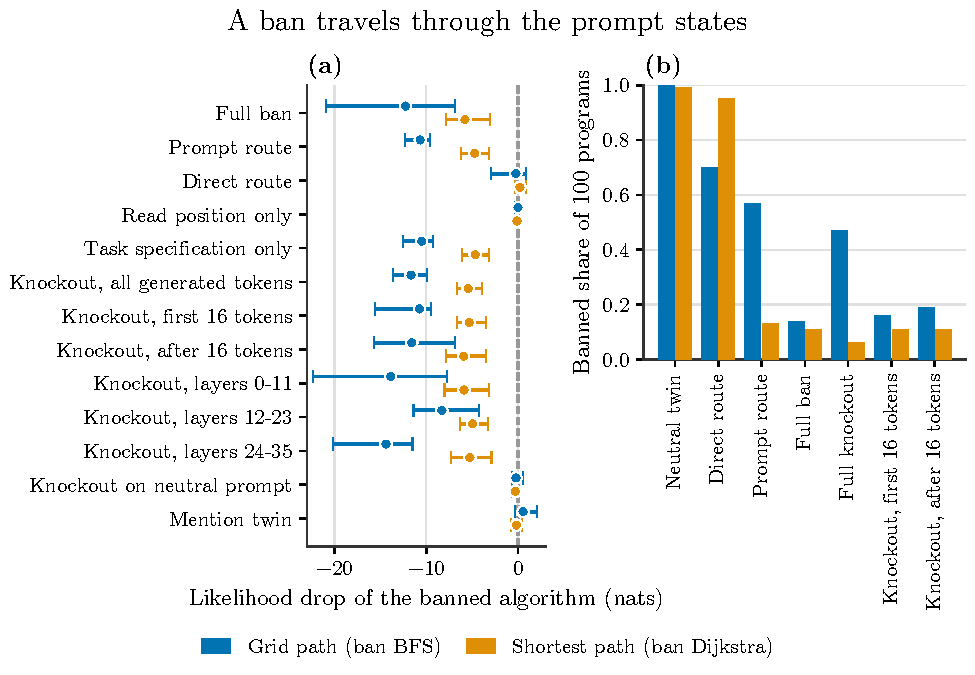
\includegraphics[width=\linewidth,height=0.78\textheight,keepaspectratio]{figures/fig_route_v0.pdf}
\caption{Route test by KV-cache patching in Qwen3-8B. (a) Likelihood drop of the banned algorithm (nats; dot = point estimate over \$n=30\$ self-written programs per task, whiskers = 95\textbackslash{}\% bootstrap interval over templates and programs) under each arm, for the grid path task (ban BFS, blue) and the shortest path task (ban Dijkstra, orange); the dashed line marks zero. The prompt route and task specification only arms reproduce nearly all of the full ban's drop on both tasks; the direct route, read position only, and knockout on neutral prompt arms sit at or near zero. (b) Banned share of 100 sampled programs (common random numbers across arms) for the same two tasks, over the subset of arms in (a) for which a behavioural measurement exists. On the shortest path task the banned share tracks the prompt route (both low); on the grid path task, knocking out the ban segment from every generated token (``full knockout'') raises the banned share back to 0.47 -- well above the full ban's 0.14 -- showing that generated tokens also read the ban directly there.}
\label{fig:fig_route}
\end{figure}
The knockouts agree. Blocking the condition segment for every generated token restores 5\% (grid) and 6\% (shortest path) of the likelihood gap, with intervals that include zero. By layer band, blocking layers 12 to 23 restores 32\% [16\%, 56\%] on the grid task and 15\% on the shortest path task, layers 0 to 11 restore about nothing, and layers 24 to 35 restore -17\% (interval includes zero) on the grid task and 9\% [2\%, 16\%] on the shortest path task. Whether the veto is read early or late in generation could not be determined (first-16 minus after-16 restoration 0.07 [-0.47, 0.20] and 0.10 [-0.03, 0.18]).

\textbf{Behaviour qualifies the grid result.} On the shortest path task behaviour matches the likelihood readout exactly: the prompt route arm reproduces the ban (banned share 0.13 against 0.11) and the direct route arm is the baseline (0.95 against 0.99). On the grid task the prompt route reproduces only part of the ban (0.57 against 0.14), and the direct route also moves it (0.70). A supplementary arm that hides the condition segment from every generated token brought BFS back to 0.47 [0.38, 0.57], close to the prompt route arm (McNemar p = 0.13), so on the grid task generated tokens do read the ban directly as well. That reading is redundant over time: blocking only the first 16 generated tokens or only the rest leaves the ban intact (banned shares 0.16 and 0.19). The behavioural route fractions are 0.50 [0.39, 0.62] (prompt) and 0.35 [0.25, 0.45] (direct) on the grid task, and 0.98 [0.89, 1.07] and 0.05 [0.01, 0.09] on the shortest path task. Matched pairs are clean: no sample was banned under the ban and not banned under its neutral twin (0 of 86 and 0 of 88 discordant pairs in that direction).

\begin{table}[H]
\renewcommand{\thetable}{63}
\centering\footnotesize\setlength{\tabcolsep}{4.0pt}
\caption{Behaviour per arm under common random numbers (N = 100 per arm; mechanism labels of attempted programs; banned share with Wilson 95\% interval; source: \texttt{results/\allowbreak{}analysis.\allowbreak{}json\#behaviour}, \texttt{results/\allowbreak{}supplementary.\allowbreak{}json}). [Source: iteration 2, artifact \nolinkurl{gen_art_experiment_8}.]}\label{tab:t67}
\begin{tabular}{>{\raggedright\arraybackslash\hspace{0pt}}p{0.0877\linewidth}>{\raggedright\arraybackslash\hspace{0pt}}p{0.1731\linewidth}>{\raggedright\arraybackslash\hspace{0pt}}p{0.1056\linewidth}>{\raggedright\arraybackslash\hspace{0pt}}p{0.0604\linewidth}>{\raggedright\arraybackslash\hspace{0pt}}p{0.2274\linewidth}>{\raggedright\arraybackslash\hspace{0pt}}p{0.2424\linewidth}}
\toprule
\textbf{Task} & \textbf{Arm} & \textbf{Banned share [95\%]} & \textbf{Pass rate} & \textbf{Labels} & \textbf{Banned programs per template (first to fifth, 20 each)} \\
\midrule
Grid & b, neutral twin & 1.00 [0.96, 1.00] & 0.92 & BFS 100 & 20, 20, 20, 20, 20 \\
Grid & d, direct route & 0.70 & 0.81 & BFS 70, DFS 30 & 15, 12, 17, 20, 6 \\
Grid & c, prompt route & 0.57 [0.47, 0.66] & 0.61 & BFS 57, DFS 43 & 10, 15, 6, 12, 14 \\
Grid & a, full ban & 0.14 [0.09, 0.22] & 0.41 & DFS 86, BFS 14 & 0, 0, 0, 14, 0 \\
Grid & full knockout (supplementary) & 0.47 [0.38, 0.57] & n\slash{}a & BFS 47, rest not BFS & n\slash{}a \\
Grid & knockout, first 16 tokens & 0.16 & 0.46 & DFS 84, BFS 16 & 1, 0, 1, 14, 0 \\
Grid & knockout, after 16 tokens & 0.19 & 0.49 & DFS 81, BFS 19 & 1, 2, 1, 11, 4 \\
Shortest path & b, neutral twin & 0.99 & 0.99 & Dijkstra 99, Bellman-Ford\slash{}SPFA 1 & 20, 20, 20, 19, 20 \\
Shortest path & d, direct route & 0.95 & 0.99 & Dijkstra 95, Bellman-Ford\slash{}SPFA 5 & 19, 18, 20, 19, 19 \\
Shortest path & c, prompt route & 0.13 & 0.91 & Bellman-Ford\slash{}SPFA 87, Dijkstra 13 & 6, 1, 3, 1, 2 \\
Shortest path & a, full ban & 0.11 & 0.91 & Bellman-Ford\slash{}SPFA 86, Dijkstra 11, other 3 & 1, 0, 4, 5, 1 \\
Shortest path & full knockout (supplementary) & 0.06 & n\slash{}a & Dijkstra 6, rest not Dijkstra & n\slash{}a \\
Shortest path & knockout, first 16 tokens & 0.11 & 0.94 & Bellman-Ford\slash{}SPFA 88, Dijkstra 11, other 1 & 2, 1, 5, 3, 0 \\
Shortest path & knockout, after 16 tokens & 0.11 & 0.96 & Bellman-Ford\slash{}SPFA 89, Dijkstra 11 & 3, 0, 4, 3, 1 \\
\bottomrule
\end{tabular}
\end{table}

On the grid task, all 14 BFS programs that survived the full ban came from the fourth template (\texttt{X is not allowed here}, with BFS as X), which gave 14 of 20 BFS while the other four templates gave 0 of 20.

\textbf{Where the ban acts: the first line.} Under the neutral twin, 99\% of programs open with an import line (\texttt{from collections import deque} on the grid task, \texttt{import heapq} on the shortest path task). Under the grid ban, none of 100 programs opens with an import line, including the 14 BFS programs that survive; they open with \texttt{def solve(\allowbreak{}.\allowbreak{}.\allowbreak{}.\allowbreak{})} (Table 64). The prompt route arm and every knockout also open without an import, while the direct route arm still opens with one 85\% of the time. On the shortest path task the Bellman-Ford\slash{}SPFA programs written under the ban mostly open with \texttt{from collections import deque}, so the share of import openings stays at 61 to 67\% under the ban, the prompt route and the knockouts, and 99\% under the direct route. Per-token localisation agrees. On the grid task 63\% of the likelihood drop under the full ban, 90\% under the prompt route and 95\% under the full knockout sits in the first 16 tokens; on the shortest path task almost all of it does. The signature tokens themselves (\texttt{deque}, \texttt{heapq} and their neighbours) carry only 2.4\% (grid) and 11.6\% (shortest path) of it. The small direct route drop on the grid task lies later in the program (6\% of it in the first 16 tokens). We call this the \emph{opening line veto}: the prompt states suppress the default program's first line before any algorithm specific token is written. On the grid task, the algorithm chosen after \texttt{def solve} also depends on direct reads of the ban, and the likelihood readout, dominated by the opening fork, calls the grid task prompt route while its behaviour is mixed.

\begin{table}[H]
\renewcommand{\thetable}{64}
\centering\scriptsize\setlength{\tabcolsep}{2.5pt}
\caption{Share of programs whose first line is an import (source: \texttt{results/\allowbreak{}supplementary.\allowbreak{}json\#opening\_\allowbreak{}lines}; N = 100 per arm). [Source: iteration 2, artifact \nolinkurl{gen_art_experiment_8}.]}\label{tab:t68}
\begin{tabular}{>{\raggedright\arraybackslash\hspace{0pt}}p{0.1075\linewidth}>{\raggedright\arraybackslash\hspace{0pt}}p{0.0890\linewidth}>{\raggedright\arraybackslash\hspace{0pt}}p{0.1196\linewidth}>{\raggedright\arraybackslash\hspace{0pt}}p{0.1196\linewidth}>{\raggedright\arraybackslash\hspace{0pt}}p{0.0952\linewidth}>{\raggedright\arraybackslash\hspace{0pt}}p{0.1075\linewidth}>{\raggedright\arraybackslash\hspace{0pt}}p{0.1373\linewidth}>{\raggedright\arraybackslash\hspace{0pt}}p{0.1373\linewidth}}
\toprule
\textbf{Task} & \textbf{b, neutral} & \textbf{d, direct route} & \textbf{c, prompt route} & \textbf{a, full ban} & \textbf{full knockout} & \textbf{knockout, first 16} & \textbf{knockout, after 16} \\
\midrule
Grid & 0.99 & 0.85 & 0.00 & 0.00 & 0.00 & 0.00 & 0.00 \\
Shortest path & 0.99 & 0.99 & 0.61 & 0.62 & 0.67 & 0.67 & 0.60 \\
\bottomrule
\end{tabular}
\end{table}

\textbf{A supplementary readout with natural proposals.} Rescoring, under every arm, the BFS and Dijkstra programs sampled in the neutral arm (exact draws from the neutral prompt's distribution) gives the same ordering with a larger direct share: pooled F\_\allowbreak{}prompt 0.57 [0.41, 0.85] and F\_\allowbreak{}direct 0.16 [0.11, 0.21] (grid 0.58 and 0.18, shortest path 0.56 and 0.11), and the two routes are superadditive on both tasks. Neither likelihood readout is a calibrated probability ratio. The importance weight ESS is about 1 to 3 of 30 programs for the grid full ban arm (8 to 20 on the shortest path task), 858 of the 1,095 cells have ESS below 5, and exp(D) under the natural readout is 3e-7 on the grid task against a behavioural ratio of 0.14. The readouts measure how strongly typical banned algorithm programs, which begin with the import line, are vetoed.

\textbf{Where the substitute rises.} Under the full ban the survivors' likelihood gains on the grid task were DFS +9.46, IDDFS +18.40, bidirectional BFS -0.22, A* -0.80 and unit weight Dijkstra -3.53 nats; on the shortest path task Bellman-Ford\slash{}SPFA +2.53, bidirectional Dijkstra +30.64, Floyd-Warshall +12.64 and Dial +6.79. The prompt route arm reproduces this profile (cosine 0.94 [0.85, 0.99] grid, 0.95 [0.90, 0.99] shortest path); the direct route arm reproduces it on the shortest path task (0.98 [0.80, 1.00]) but not reliably on the grid task (0.71 [-0.18, 0.94]). The logit lens and a tuned lens [49] at the planned commitment token (the token after \texttt{from} or \texttt{import}) found no veto layer: the banned set's rank there is unchanged by the ban (0 of 59 grid and 0 of 60 shortest path programs), because the fork has already happened at the first token. The grid substitute set (DFS) rises from layer 28 (59 of 59 programs; tuned lens median 27). In substitute programs written under the full ban, the banned set is vetoed late (median layer 30 on the grid task, 36 on the shortest path task). The tuned lens beat the logit lens on held-out KL at all 11 probed layers (0.29 against 10.6 at layer 21).

\textbf{Does the read position know how hard a ban will be obeyed?} The compliance test regressed the banned share of each wording on the projection of its read position state onto a shared ban direction, the mean ban minus neutral shift estimated leaving one experiment out. It used 110 wordings in 12 experiment by task cells: ten modal ban paraphrases from each of the five iteration-1 draws per task, plus this experiment's five templates per task. The combined within cell Spearman correlation is -0.41 [-0.69, -0.17], one sided stratified permutation p = 0.0003 (Holm adjusted over the two axes tested, 0.0006). The preregistered bar was -0.5, so the result is partial: wordings that move the read position further along the ban direction are obeyed more, but less tightly than predicted. The correlation beats 98.5\% of 200 random directions (null mean -0.01), and the split half noise ceiling is about 0.77. The decommitment axis of iteration 1 carries nothing (rho 0.05, p = 0.68). The DFS share among programs not banned is not decodable beyond the projection (change in R squared below zero, permutation p = 0.74 on the grid task; not testable on the shortest path task). The recomputed read position states matched the iteration-1 caches (cosine at least 0.9994 for 40 geometry and 60 decommitment prompts).

\begin{table}[H]
\renewcommand{\thetable}{65}
\centering\small\setlength{\tabcolsep}{4.0pt}
\caption{Within cell Spearman correlation between a wording's banned share and its read position projection (source: \texttt{results/\allowbreak{}c5.\allowbreak{}json}; ten wordings per cell, five for this experiment's templates). [Source: iteration 2, artifact \nolinkurl{gen_art_experiment_8}.]}\label{tab:t69}
\begin{tabular}{>{\raggedright\arraybackslash\hspace{0pt}}p{0.4199\linewidth}>{\raggedright\arraybackslash\hspace{0pt}}p{0.2780\linewidth}>{\raggedright\arraybackslash\hspace{0pt}}p{0.2483\linewidth}}
\toprule
\textbf{Cell} & \textbf{Shared ban direction} & \textbf{Decommitment axis} \\
\midrule
Association, grid & -0.701 & 0.234 \\
Association, shortest path & -0.811 & 0.416 \\
Geometry, grid & -0.214 & -0.082 \\
Geometry, shortest path & -0.673 & -0.132 \\
Forking token, grid & -0.437 & 0.212 \\
Forking token, shortest path & 0.271 & 0.516 \\
Decommitment, grid & -0.074 & 0.309 \\
Decommitment, shortest path & -0.605 & -0.368 \\
Instruction tuning, grid & 0.036 & 0.207 \\
Instruction tuning, shortest path & -0.171 & -0.734 \\
This experiment's templates, grid & -0.707 & 0.0 \\
This experiment's templates, shortest path & -0.667 & 0.308 \\
Combined [95\% CI]; one sided p & -0.41 [-0.69, -0.17]; p = 0.0003 & 0.05 [-0.30, 0.36]; p = 0.68 \\
\bottomrule
\end{tabular}
\end{table}

\textbf{Checks.} Spliced caches reproduced the full ban scores bit for bit; the knockout attention with nothing blocked equalled stock attention (largest difference 0); attention to blocked columns was exactly 0. Repeated sampling was 100\% identical at a fixed batch shape and only 40\% when the shape changed, which is why every arm shares one shape. Two independent rederivations reproduced 49 and 59 headline numbers with no mismatch; McNemar on randomly swapped arm labels rejected 4.0 to 4.4\% of the time, the likelihood ban effect's interval included zero for the placebo splice and for label shuffled data, and the compliance test rejected 0 of 40 shuffled data sets. From the declared dataset dependency, other models' other than Dijkstra choices for weighted shortest path in the inspiration repository spread over Bellman-Ford\slash{}SPFA (37\%), bidirectional search (32\%) and other algorithms (23\%), while Qwen3-8B under the Dijkstra ban lands on Bellman-Ford\slash{}SPFA 97\% of the time; an import opening is the norm in LLM written solutions that name these algorithms (KodCode: BFS 94\% of 17, Dijkstra 100\% of 40) but not in human library code (TheAlgorithms: 29\% of 7 and 17\% of 12).

\FloatBarrier
\subsection*{2.6 Ban list experiment: the top five prohibition and bans that leave one survivor}
\addcontentsline{toc}{subsection}{2.6 Ban list experiment: the top five prohibition and bans that leave one survivor}
\noindent{\small\emph{Artifact: \nolinkurl{gen_art_experiment_9}.}}\par\medskip
\textbf{Why.} The request asks what happens when the top five algorithms are prohibited in one prompt: does the implemented algorithm move to the edge of the banned region, or to its opposite side? Iteration 1 could not reach that test through its greedy succession, because the model stopped complying after two bans. This experiment  ran the prohibition as single prompt conditions, with a control for each reading of where the mass goes, and asked on the shortest path task whether the model can and will write each algorithm when it is the only one allowed.

\textbf{Catalogue extension.} The grid catalogue was extended toward the ten algorithms the request imagines: greedy best first search was split from A*, and IDA*, a 4-neighbour jump point search and bidirectional A* were added, with new references that both labellers got right (25 of 25) and targeted unit probes (4 of 4). The canonical labeller recheck gave 135 of 144 gold programs and 22 of 22 references. The 40-program gold gate of the extended labeller was missed: 33 of 40 at round 0 and 32 of 40 after the one allowed revision, runtime against AST kappa 0.53; unit weight Dijkstra, jump point search and bidirectional A* fell below three of four gold programs and were excluded. An algorithm was kept if at least 70\% of its 40 forced programs were labelled as requested (Table 66). Only BFS, DFS, IDDFS, greedy best first and IDA* passed, so the extension failed. The model mostly writes A* as a cost only heap (unit weight Dijkstra 25 of 40), unit weight Dijkstra as BFS (18 of 40), and jump point search and bidirectional A* as BFS and A*. The analysis catalogue (seven algorithms) kept A* and bidirectional BFS, flagged, because each has at least 10 programs and passes the gold set. With seven algorithms the frozen set rule gives four name sets: TOP (the four with the highest baseline likelihood: BFS, DFS, greedy, IDDFS), ARC (four contiguous on the manifold: BFS, bidirectional BFS, A*, greedy) and SCATTER (four spread out: BFS, DFS, greedy, IDA*). The literal ban of five names, TOP5 (BFS, DFS, greedy, IDDFS, A*), was added. Six landing forecasts per set (ladder, prime and veto, proximity, likelihood under the ban, generic perturbation, corpus frequency) were hash chained before the ban lists were sampled, and the chain verifies.

\begin{table}[H]
\renewcommand{\thetable}{66}
\centering\scriptsize\setlength{\tabcolsep}{2.5pt}
\caption{Keep rule for the extended catalogues: forced programs labelled as requested (source: \texttt{results/\allowbreak{}catalogue\_\allowbreak{}keep.\allowbreak{}json}; 40 forced programs each). [Source: iteration 2, artifact \nolinkurl{gen_art_experiment_9}.]}\label{tab:t70}
\begin{tabular}{>{\raggedright\arraybackslash\hspace{0pt}}p{0.0769\linewidth}>{\raggedright\arraybackslash\hspace{0pt}}p{0.1169\linewidth}>{\raggedright\arraybackslash\hspace{0pt}}p{0.2460\linewidth}>{\raggedright\arraybackslash\hspace{0pt}}p{0.0915\linewidth}>{\raggedright\arraybackslash\hspace{0pt}}p{0.0748\linewidth}>{\raggedright\arraybackslash\hspace{0pt}}p{0.1841\linewidth}>{\raggedright\arraybackslash\hspace{0pt}}p{0.1333\linewidth}}
\toprule
\textbf{Task} & \textbf{Algorithm} & \textbf{Forced prompt} & \textbf{Labelled as requested} & \textbf{Of those, passing} & \textbf{Other labels} & \textbf{Kept} \\
\midrule
Grid & BFS & plain & 40 & 38 & none & yes \\
Grid & DFS & plain & 40 & 9 & none & yes \\
Grid & IDDFS & plain & 37 & 0 & DFS 3 & yes \\
Grid & greedy best first & plain & 35 & 25 & BFS 2, other 2, A* 1 & yes \\
Grid & IDA* & descriptive & 36 & 0 & A* 3, BFS 1 & yes \\
Grid & bidirectional BFS & plain & 21 & 5 & BFS 16, other 3 & no (kept in analysis, flagged) \\
Grid & A* & plain & 11 & 11 & unit weight Dijkstra 25, other 3, BFS 1 & no (kept in analysis, flagged) \\
Grid & unit weight Dijkstra & plain & 13 & 11 & BFS 18, other 9 & no \\
Grid & jump point search & descriptive & 7 & 0 & BFS 21, other 11, unit weight Dijkstra 1 & no \\
Grid & bidirectional A* & descriptive & 5 & 0 & A* 28, BFS 3, other 3, bidirectional BFS 1 & no \\
Shortest path & Dijkstra & plain & 40 & 40 & none & always run \\
Shortest path & Bellman-Ford\slash{}SPFA & plain & 40 & 34 & none & always run \\
Shortest path & bidirectional Dijkstra & descriptive (corrected in iteration 3 from plain; the plain prompt gave 10 programs, Dijkstra 9) & 14 & 9 & Dijkstra 22, other 4 & always run \\
Shortest path & Floyd-Warshall & plain & 40 & 40 & none & always run \\
Shortest path & Dial & descriptive (corrected in iteration 3 from plain; the plain prompt gave 10 programs) & 36 & 7 & other 4 & always run \\
\bottomrule
\end{tabular}
\end{table}

\textbf{Every ban list fails.} With one name banned the model complies (avoidance 0.86 on the grid task, 0.84 on the shortest path task). With four or five names it mostly writes a banned algorithm anyway (Table 67): avoidance is 0.13 for TOP, 0.37 for ARC, 0.04 for SCATTER and 0.00 for the literal ban of five names, so every ban list fails the event gate. The banned programs are BFS and DFS reimplemented, often without naming their mechanism (Table 68). We call a banned mechanism program \emph{disguised} when its comments and identifiers never name its own mechanism; 41\% to 92\% of the banned programs under a ban list are disguised, DFS most often as \texttt{backtracking}. The likelihoods committed before sampling foresaw the failure for three of the four sets: the implied avoidance was below 1e-8 for TOP, SCATTER and the five name ban, against realised 0.13, 0.04 and 0.00. For ARC the implied avoidance was 0.9995 against a realised 0.37. A ban prompt raised the likelihood of the banned algorithms' own programs relative to the neutral twin (DFS gained about 10 nats under the first template of TOP), the same priming as in the likelihood screen.

\begin{table}[H]
\renewcommand{\thetable}{67}
\centering\scriptsize\setlength{\tabcolsep}{2.5pt}
\caption{Grid ban lists and the single name references (N = 100 each, five templates by 20; mechanism labels of attempted programs; source: \texttt{results/\allowbreak{}landing.\allowbreak{}json}). [Source: iteration 2, artifact \nolinkurl{gen_art_experiment_9}.]}\label{tab:t71}
\begin{tabular}{>{\raggedright\arraybackslash\hspace{0pt}}p{0.1170\linewidth}>{\raggedright\arraybackslash\hspace{0pt}}p{0.1466\linewidth}>{\raggedright\arraybackslash\hspace{0pt}}p{0.1949\linewidth}>{\raggedright\arraybackslash\hspace{0pt}}p{0.1176\linewidth}>{\raggedright\arraybackslash\hspace{0pt}}p{0.1115\linewidth}>{\raggedright\arraybackslash\hspace{0pt}}p{0.1820\linewidth}>{\raggedright\arraybackslash\hspace{0pt}}p{0.0539\linewidth}}
\toprule
\textbf{Condition} & \textbf{Banned} & \textbf{Landing (attempted programs)} & \textbf{Avoidance [Wilson 95\%]} & \textbf{Template cluster 95\% CI} & \textbf{Avoidance per template (first to fifth)} & \textbf{Pass rate} \\
\midrule
Grid baseline & none & BFS 100 & n\slash{}a & n\slash{}a & n\slash{}a & 0.89 \\
Grid single ban & BFS & DFS 86, BFS 14 & 0.86 [0.78, 0.91] & [0.58, 1.00] & 1.0, 1.0, 1.0, 0.30, 1.0 & 0.41 \\
TOP & BFS, DFS, greedy, IDDFS & BFS 59, DFS 26, greedy 2, other 13 & 0.13 [0.08, 0.21] & [0.01, 0.29] & 0.15, 0.05, 0.0, 0.0, 0.45 & 0.40 \\
ARC & BFS, bidirectional BFS, A*, greedy & BFS 63, DFS 37 (DFS allowed) & 0.37 [0.28, 0.47] & [0.09, 0.68] & 0.70, 0.15, 0.15, 0.0, 0.85 & 0.60 \\
SCATTER & BFS, DFS, greedy, IDA* & BFS 69, DFS 27, A* 2, other 2 & 0.04 [0.02, 0.10] & [0.00, 0.08] & 0.0, 0.10, 0.0, 0.0, 0.10 & 0.75 \\
TOP5 (literal) & BFS, DFS, greedy, IDDFS, A* & BFS 63, DFS 36, IDDFS 1 & 0.00 [0.00, 0.04] & [0.00, 0.00] & 0.0, 0.0, 0.0, 0.0, 0.0 & 0.68 \\
Shortest path baseline & none & Dijkstra 100 & n\slash{}a & n\slash{}a & n\slash{}a & 1.00 \\
Shortest path single ban & Dijkstra & Bellman-Ford\slash{}SPFA 83, Dijkstra 16, other 1 & 0.84 [0.76, 0.90] & [0.72, 0.95] & 0.90, 0.95, 0.70, 0.65, 1.0 & 0.95 \\
\bottomrule
\end{tabular}
\end{table}

\emph{(Correction, iteration 3: TOP's avoidance of 0.13 is labeller residue, not avoidance into a catalogue algorithm. Its 13 programs not banned are all labelled other: 12 failing programs that both blind judges classed as degenerate BFS or DFS variants, and 1 correct unit weight Dijkstra outside the K = 7 analysis catalogue. Avoidance into a non-banned catalogue algorithm is 0.00 for TOP, 0.37 for ARC, 0.02 for SCATTER and 0.00 for TOP5. The share labelled other is reported separately from avoidance in Section 3.2.3.)}

\begin{table}[H]
\renewcommand{\thetable}{68}
\centering\footnotesize\setlength{\tabcolsep}{4.0pt}
\caption{Disguise: banned mechanism programs that never name their own mechanism (source: \texttt{results/\allowbreak{}landing.\allowbreak{}json}). [Source: iteration 2, artifact \nolinkurl{gen_art_experiment_9}.]}\label{tab:t72}
\begin{tabular}{>{\raggedright\arraybackslash\hspace{0pt}}p{0.1684\linewidth}>{\raggedright\arraybackslash\hspace{0pt}}p{0.1143\linewidth}>{\raggedright\arraybackslash\hspace{0pt}}p{0.1079\linewidth}>{\raggedright\arraybackslash\hspace{0pt}}p{0.0984\linewidth}>{\raggedright\arraybackslash\hspace{0pt}}p{0.1916\linewidth}>{\raggedright\arraybackslash\hspace{0pt}}p{0.2159\linewidth}}
\toprule
\textbf{Condition} & \textbf{Banned mechanism programs} & \textbf{Disguised} & \textbf{Disguise rate} & \textbf{By mechanism (disguised \slash{} programs)} & \textbf{Most frequent self descriptions} \\
\midrule
Grid single ban of BFS & 14 & 14 & 1.00 & BFS 14\slash{}14 & none named \\
Shortest path single ban of Dijkstra & 16 & 2 & 0.125 & Dijkstra 2\slash{}16 & none named \\
ARC & 63 & 58 & 0.92 & BFS 58\slash{}63 & \texttt{is\_\allowbreak{}valid} 2 \\
SCATTER & 96 & 49 & 0.51 & BFS 43\slash{}69, DFS 6\slash{}27 & \texttt{backtrack} 10, \texttt{is\_\allowbreak{}valid} 7, \texttt{depth-\allowbreak{}limited} 1 \\
TOP & 87 & 44 & 0.51 & BFS 37\slash{}59, DFS 6\slash{}26, greedy 1\slash{}2 & \texttt{backtrack} 10, \texttt{is\_\allowbreak{}valid} 9 \\
TOP5 & 100 & 41 & 0.41 & BFS 34\slash{}63, DFS 6\slash{}36, IDDFS 1\slash{}1 & \texttt{is\_\allowbreak{}valid} 10, \texttt{backtrack} 8, \texttt{find\_\allowbreak{}path} 2 \\
\bottomrule
\end{tabular}
\end{table}

\begin{figure}[!htbp]
\centering\captionsetup{font=footnotesize}
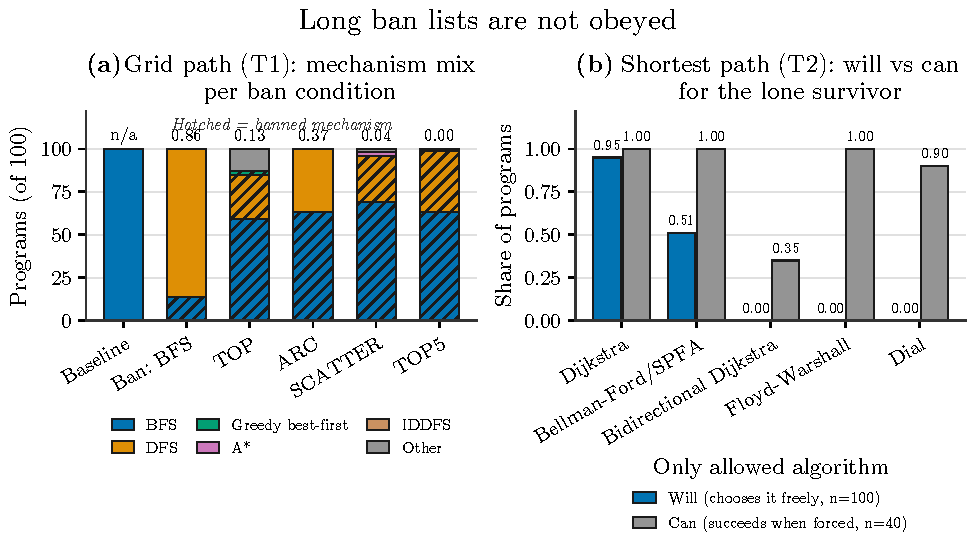
\includegraphics[width=\linewidth,height=0.78\textheight,keepaspectratio]{figures/fig_multiban_v0.pdf}
\caption{(a) Mechanism mix of 100 Qwen3-8B grid-path programs per ban condition (five prompt templates x 20 samples each), under a no-ban baseline, a single ban of BFS, and four longer bans: TOP, ARC and SCATTER each prohibit four mechanisms, TOP5 prohibits five. Bars are stacked and coloured by mechanism -- BFS (blue), DFS (amber), greedy best-first (green), A* (violet), IDDFS (tan) and other\slash{}degenerate programs (grey) -- with diagonal hatching marking the segments that condition's ban list prohibited; the number above each bar is that condition's avoidance rate (its non-hatched share), with the baseline marked n\slash{}a since it bans nothing. Avoidance falls from 0.86 for the single BFS ban to 0.13, 0.37, 0.04 and 0.00 for the four- and five-name bans, whose bars are then almost entirely hatched BFS and DFS regardless of which four or five names were listed. (b) For the weighted shortest-path task, leave-one-survivor bans that allow exactly one algorithm: the blue bar is the share of 100 freely generated programs that voluntarily write that algorithm ('Will, n=100'), and the grey bar is the share of 40 separately forced 'implement X directly' attempts correctly labelled as that algorithm ('Can, n=40'), for Dijkstra, Bellman-Ford\slash{}SPFA, bidirectional Dijkstra, Floyd-Warshall and Dial. For the last three, Can is 0.35-1.00 while Will is 0.00: the model can write each one when told to, but never volunteers it even when it is the only option left.}
\label{fig:fig_multiban}
\end{figure}
\textbf{The list's content barely matters (post hoc).} Across the four ban lists the model writes the same mix of BFS and DFS: the BFS share among BFS and DFS programs is 0.69 (TOP), 0.63 (ARC), 0.72 (SCATTER) and 0.64 (TOP5), chi squared p = 0.48 and permutation p = 0.57. This holds whether DFS is on the list (TOP, SCATTER, TOP5) or allowed (ARC). Avoidance differences therefore come from whether DFS happens to be banned, not from a list specific landing. A single BFS ban moves the model to DFS 86\%; a list of four or five names moves it to about one third DFS, which looks more like a generic perturbation of the default than a veto. This comparison was not preregistered.

\textbf{Landing tests are degenerate.} Only ARC (37 DFS programs) and SCATTER (2 A* programs) put any mass on a survivor. On ARC the ladder, prime and veto, likelihood, generic perturbation and corpus forecasts all named DFS (log score +1.06 nats per program over uniform), and proximity named IDA* and missed (-0.02). With three survivors the exact permutation floor is 1\slash{}6, every per set p is at least 0.33, and every pooled p is at least 0.11; the edge against opposite statistic was 0 on both sets with mass (p = 0.67). The request's literal question therefore has a behavioural answer that is neither of its two options: under a four or five name ban the model does not move to the edge or to the opposite side of the banned region, it reimplements the banned defaults. Over all programs, predicting no change from the default algorithm was right for 64\% of programs under a ban list, against at most 10\% for any committed survivor forecast; on single bans the highest ranked not banned algorithm predicted 85\% and the default 15\%; under forced prompts the requested algorithm was written 66\% of the time.

\textbf{Bans that leave one survivor: can against will.} On the shortest path task each of the five algorithms was left as the only one allowed, by banning the other four (Table 69). The model writes Dijkstra when it is the survivor 95\% of the time and Bellman-Ford\slash{}SPFA 51\% of the time. It writes bidirectional Dijkstra, Floyd-Warshall and Dial 0\% of the time, falling back to the banned Dijkstra or Bellman-Ford\slash{}SPFA instead, although when forced it writes Floyd-Warshall correctly 40 of 40 times and Dial 36 of 40 times. The likelihood gains follow the same split: banning the other four lowers Dijkstra by 3.35 nats and Bellman-Ford\slash{}SPFA by 0.21 when each is the survivor, and raises the three algorithms the model never writes by 7.6 to 24.3 nats without moving them into the sample.

\begin{table}[H]
\renewcommand{\thetable}{69}
\centering\scriptsize\setlength{\tabcolsep}{2.5pt}
\caption{Shortest path bans that leave one survivor (N = 100 each; will is the share of programs implementing the survivor and can the share of 40 forced programs labelled as the survivor; source: \texttt{results/\allowbreak{}los.\allowbreak{}json}). [Source: iteration 2, artifact \nolinkurl{gen_art_experiment_9}.]}\label{tab:t73}
\begin{tabular}{>{\raggedright\arraybackslash\hspace{0pt}}p{0.1122\linewidth}>{\raggedright\arraybackslash\hspace{0pt}}p{0.0910\linewidth}>{\raggedright\arraybackslash\hspace{0pt}}p{0.1589\linewidth}>{\raggedright\arraybackslash\hspace{0pt}}p{0.0622\linewidth}>{\raggedright\arraybackslash\hspace{0pt}}p{0.1001\linewidth}>{\raggedright\arraybackslash\hspace{0pt}}p{0.1547\linewidth}>{\raggedright\arraybackslash\hspace{0pt}}p{0.1362\linewidth}>{\raggedright\arraybackslash\hspace{0pt}}p{0.0978\linewidth}}
\toprule
\textbf{Survivor (other four banned)} & \textbf{Will [Wilson 95\%]} & \textbf{Banned mechanisms written} & \textbf{Other} & \textbf{Compliant share} & \textbf{Can (forced labelled as requested; forced pass)} & \textbf{Mean likelihood gain of the survivor (nats)} & \textbf{Disguised \slash{} banned programs} \\
\midrule
Dijkstra & 0.95 [0.89, 0.98] & Bellman-Ford\slash{}SPFA 0.05 & 0.0 & 0.95 & 1.00; 1.00 & -3.35 & 4 \slash{} 5 \\
Bellman-Ford\slash{}SPFA & 0.51 [0.41, 0.61] & Dijkstra 0.48 & 0.01 & 0.39 & 1.00; 0.85 & -0.21 & 8 \slash{} 48 \\
bidirectional Dijkstra & 0.00 [0.00, 0.04] & Dijkstra 0.52, Bellman-Ford\slash{}SPFA 0.48 & 0.0 & 0.0 & 0.35; 0.225 & +24.26 & 51 \slash{} 100 \\
Floyd-Warshall & 0.00 [0.00, 0.04] & Dijkstra 0.59, Bellman-Ford\slash{}SPFA 0.40 & 0.01 & 0.0 & 1.00; 1.00 & +7.63 & 46 \slash{} 99 \\
Dial & 0.00 [0.00, 0.04] & Dijkstra 0.52, Bellman-Ford\slash{}SPFA 0.44 & 0.04 & 0.0 & 0.90; 0.175 & +21.20 & 42 \slash{} 96 \\
\bottomrule
\end{tabular}
\end{table}

\textbf{Geometry and natural run internals.} In the teacher forced residual stream, centroid MDS stress-1 was 0.025 (grid) and 0.006 (shortest path). The nearest neighbours were BFS with bidirectional BFS, DFS with IDDFS, and A* with greedy best first; nearest neighbour stability was 0.70 across settings and 0.96 under a program bootstrap. Persistent homology, which tracks loops in a point cloud across distance scales, found no persistent loop on either task. \emph{(Correction, iteration 3: this sentence originally read the result as a negative answer to the request's question about a circle. It is no evidence of a loop, at weak power, at a label-dependent position. These clouds sit at the token before the commit token, a position that depends on the label; there a planted loop is found with power 1.00, while at the label-independent generated token 16 the power is 0.04. The nearest pair at that position, BFS and bidirectional BFS (centroid distance 0.0147), does not survive at token 16: permuted labels reproduce the adjacency with p = 0.19 and the two clouds are not separable. The experiment drew 13 Isomap figures with centroids sized by implemented count, which this section did not show; they are reported with their counts in Section 3.2.2.)} Probes within one ban prompt at generated token 16, a position that does not depend on the label, were near chance on every grid condition and reached balanced accuracy 0.69 (p = 0.03) on the shortest path ban that leaves only Bellman-Ford\slash{}SPFA. Probes at the token before the commit token were confounded, because that position depends on the label. The difference-in-means direction from forced programs aligned with the natural within one ban direction at that position (cosine 0.6 to 0.95) and on the shortest path task at token 16 (0.3 to 0.99), but not for the grid BFS ban at token 16 (-0.13 to -0.01).

\textbf{Deviations and cost.} The experiment ran on an RTX 4090 in eager vLLM mode (no C compiler), replaced one duplicated forced paraphrase, missed the gold gate after its revision, and recorded bf16 scoring path noise of about 1 nat per program; the shortest path likelihoods sum to 0.17, below the 0.3 calibration floor; the second noun placebo ran after the ban lists were sampled. It used about 1 GPU hour and USD 0.42 of judge calls (857 calls).

\FloatBarrier
\subsection*{2.7 Llama replication: the same protocol in a second model family}
\addcontentsline{toc}{subsection}{2.7 Llama replication: the same protocol in a second model family}
\noindent{\small\emph{Artifact: \nolinkurl{gen_art_experiment_10}.}}\par\medskip
\textbf{Why.} A claim about what a ban does inside one model needs a second family. This experiment  ran shared protocol v2 on Llama-3.1-8B-Instruct [22] in bf16 with its default chat template, on the canonical suite, retokenising the neutral noun bank under Llama. It drew 1,780 seeded vLLM generations: baselines, modal bans, mention twins, listing controls, two bans of algorithms other than the default and two double bans per task (14 events), 880 forced programs and 220 free-form answers. It scored 248 name scrubbed forced programs in 39,768 program scores (11.3 million tokens). Nothing was tuned to agree with Qwen3-8B.

\textbf{Llama's baseline is not collapsed on the grid task.} \emph{(Correction, iteration 3: true of attempted programs only. All 20 correct grid baseline programs are BFS, a correctness conditioned Hill number of 1.00 against 1.87 over attempts, so Llama's correct grid output is as collapsed as Qwen3-8B's; correct-only compositions of every Llama event are in Section 3.2.4.)} It writes BFS 77 times and DFS 20 times in 100, with a low pass rate (0.20). On the shortest path task it is collapsed (Dijkstra 92, pass rate 0.59). The BFS ban sends it to DFS 63 of 100; the Dijkstra ban sends it to Dijkstra 43, other labels 37 and Bellman-Ford\slash{}SPFA 18. Both double bans fail the gate (Table 70). Bidirectional Dijkstra and Dial could not be written (2 and 1 forced programs kept after up to 120 attempts), so the shortest path catalogue has three algorithms, no row there has three survivors, and the substitution test runs on the grid task only.

\begin{table}[H]
\renewcommand{\thetable}{70}
\centering\scriptsize\setlength{\tabcolsep}{2.5pt}
\caption{The 14 sampled Llama events (mechanism labels of attempted programs; source: \texttt{results/\allowbreak{}events.\allowbreak{}json}). [Source: iteration 2, artifact \nolinkurl{gen_art_experiment_10}.]}\label{tab:t74}
\begin{tabular}{>{\raggedright\arraybackslash\hspace{0pt}}p{0.0769\linewidth}>{\raggedright\arraybackslash\hspace{0pt}}p{0.1386\linewidth}>{\raggedright\arraybackslash\hspace{0pt}}p{0.0372\linewidth}>{\raggedright\arraybackslash\hspace{0pt}}p{0.2533\linewidth}>{\raggedright\arraybackslash\hspace{0pt}}p{0.0705\linewidth}>{\raggedright\arraybackslash\hspace{0pt}}p{0.0955\linewidth}>{\raggedright\arraybackslash\hspace{0pt}}p{0.1001\linewidth}>{\raggedright\arraybackslash\hspace{0pt}}p{0.0769\linewidth}>{\raggedright\arraybackslash\hspace{0pt}}p{0.0539\linewidth}}
\toprule
\textbf{Task} & \textbf{Event} & \textbf{N} & \textbf{Labels} & \textbf{Banned share} & \textbf{Avoidance} & \textbf{Compliant share} & \textbf{Clear mode} & \textbf{Gate} \\
\midrule
Grid & baseline & 100 & BFS 77, DFS 20, other 3 & 0.0 & 1.0 & 0.20 & BFS & pass \\
Grid & ban BFS (modal) & 100 & DFS 63, BFS 29, other 6, A* 1, unit weight Dijkstra 1 & 0.29 & 0.71 & 0.08 & DFS & pass \\
Grid & mention BFS & 50 & BFS 47, other 2, DFS 1 & 0.0 & 1.0 & 0.28 & BFS & pass \\
Grid & listing control & 50 & BFS 36, other 7, DFS 6, unit weight Dijkstra 1 & 0.0 & 1.0 & 0.20 & BFS & pass \\
Grid & ban DFS & 50 & BFS 39, DFS 7, other 4 & 0.14 & 0.86 & 0.14 & BFS & pass \\
Grid & ban unit weight Dijkstra (absent) & 50 & BFS 30, DFS 18, unit weight Dijkstra 1, other 1 & 0.02 & 0.98 & 0.26 & BFS & pass \\
Grid & ban BFS and DFS & 50 & BFS 21, DFS 21, other 6, unit weight Dijkstra 2 & 0.84 & 0.16 & 0.0 & none & fail \\
Shortest path & baseline & 100 & Dijkstra 92, other 7, Bellman-Ford\slash{}SPFA 1 & 0.0 & 1.0 & 0.59 & Dijkstra & pass \\
Shortest path & ban Dijkstra (modal) & 100 & Dijkstra 43, other 37, Bellman-Ford\slash{}SPFA 18, Floyd-Warshall 2 & 0.43 & 0.57 & 0.05 & none & pass \\
Shortest path & mention Dijkstra & 50 & Dijkstra 39, other 11 & 0.0 & 1.0 & 0.46 & Dijkstra & pass \\
Shortest path & listing control & 50 & Dijkstra 19, Bellman-Ford\slash{}SPFA 15, other 14, Floyd-Warshall 2 & 0.0 & 1.0 & 0.24 & none & pass \\
Shortest path & ban Bellman-Ford\slash{}SPFA & 50 & Dijkstra 33, other 14, Bellman-Ford\slash{}SPFA 2, Floyd-Warshall 1 & 0.04 & 0.96 & 0.26 & Dijkstra & pass \\
Shortest path & ban Floyd-Warshall (absent) & 50 & Dijkstra 25, other 11, Bellman-Ford\slash{}SPFA 9, Floyd-Warshall 5 & 0.10 & 0.90 & 0.14 & Dijkstra & pass \\
Shortest path & ban Dijkstra and Bellman-Ford\slash{}SPFA & 50 & Dijkstra 22, other 21, Bellman-Ford\slash{}SPFA 6, Floyd-Warshall 1 & 0.56 & 0.44 & 0.0 & none & fail \\
\bottomrule
\end{tabular}
\end{table}

\emph{(Added in iteration 3: Table 70 lists attempted programs only. Correct programs: grid baseline BFS 20; ban BFS DFS 7, other 1; mention BFS BFS 14; listing control BFS 7, DFS 3; ban DFS BFS 7; ban unit weight Dijkstra BFS 12, DFS 1; shortest path baseline Dijkstra 59; ban Dijkstra Bellman-Ford\slash{}SPFA 4, other 1; mention Dijkstra Dijkstra 22, other 1; listing control Dijkstra 9, Bellman-Ford\slash{}SPFA 3; ban Bellman-Ford\slash{}SPFA Dijkstra 13; ban Floyd-Warshall Dijkstra 6, Bellman-Ford\slash{}SPFA 1; both double bans 0. Table 89, Section 3.2.4.)}

\textbf{The validity gate fails, and the substitution test is unresolved.} Calibration fails on the grid task: the instrument implies BFS 0.43 and DFS 0.55 against a sampled BFS share of 0.77 (Wilson [0.68, 0.84]); the shortest path task passes (Dijkstra 0.97, sum 0.87). Discrimination passes at 0.59 nats per program over uniform across 13 events (1.0 to 1.6 nats on the grid ban and mention events, 0.1 to 0.8 on the shortest path ones, negative for both listing controls). The argmax matches the realised mode in 7 of 10 clear mode events, below the 0.8 bar; all three misses are on the grid task, where the instrument predicts DFS and sampling lands on BFS. The median cell ESS is 2.5 and 76\% of cells are below 5. Under the neutral reference the X specific share is 0.80 with a 95\% percentile interval of [0.28, 0.94], with no aim and no ladder, so the result is not resolved at this sample size; under the mention reference it reads X specific but unaimed (Table 71). The branch is not robust. Outside the frozen rule, the program level importance sampling noise dominates: the bootstrap variance of the mean gain is 5 to 11 times the replicate variance the frozen correction subtracts, the basic interval for the neutral V\_\allowbreak{}u + V\_\allowbreak{}s is [-15.1, 10.2] and covers zero, and the share falls to 0.41 without the five forced programs that the label audit disputed and to 0.44 with a raw mean ladder profile.

\begin{table}[H]
\renewcommand{\thetable}{71}
\centering\footnotesize\setlength{\tabcolsep}{4.0pt}
\caption{Llama substitution test, grid task only (source: \texttt{results/\allowbreak{}c1.\allowbreak{}json}). [Source: iteration 2, artifact \nolinkurl{gen_art_experiment_10}.]}\label{tab:t75}
\begin{tabular}{>{\raggedright\arraybackslash\hspace{0pt}}p{0.1358\linewidth}>{\raggedright\arraybackslash\hspace{0pt}}p{0.1810\linewidth}>{\raggedright\arraybackslash\hspace{0pt}}p{0.1267\linewidth}>{\raggedright\arraybackslash\hspace{0pt}}p{0.1989\linewidth}>{\raggedright\arraybackslash\hspace{0pt}}p{0.1285\linewidth}>{\raggedright\arraybackslash\hspace{0pt}}p{0.1257\linewidth}}
\toprule
\textbf{Reference} & \textbf{X specific share (95\% percentile CI)} & \textbf{V\_\allowbreak{}u \slash{} V\_\allowbreak{}s \slash{} V\_\allowbreak{}u + V\_\allowbreak{}s} & \textbf{Aim at prime and veto (null 95th pct; p)} & \textbf{Ladder exists (mean cosine)} & \textbf{Branch} \\
\midrule
neutral twin (primary) & 0.80 (0.28, 0.94) & 2.0 \slash{} 8.2 \slash{} 10.1 & 0.067 (0.258; p = 0.35) & no (0.14) & not resolved at this N \\
mention twin (secondary) & 0.78 (0.61, 0.91) & 7.1 \slash{} 25.5 \slash{} 32.6 & -0.28 (p = 0.96) & no & X specific but unaimed \\
\bottomrule
\end{tabular}
\end{table}

The association aim did not pass either (-0.08 against a null 95th percentile of 0.30).

\textbf{Llama, like Qwen3-8B, primes the banned name.} Naming an absent algorithm in a ban raised its own likelihood in 5 of 6 cases: bidirectional BFS +3.9 nats, IDDFS +7.6, unit weight Dijkstra +1.8, Bellman-Ford\slash{}SPFA +4.1 and Floyd-Warshall +4.8; A* was the exception (-1.2). The mention twin primes these algorithms by +6.7 to +14.4 nats and the ban's veto (-4.9 to -10.1) cancels only part of the prime. Bans of present algorithms do lower them: BFS -1.7, DFS -3.0 and Dijkstra -1.0. Within a ban row, the X specific residual is negatively correlated with how much a survivor's code resembles X (Spearman -0.6 to -0.9 in 5 of 6 grid rows): a ban lowers the survivors that look like the banned algorithm.

\textbf{The route, read by likelihood only.} On the two modal bans (20 cells), the ban's drop on the default (-27.2 nats summed) travels mostly by the prompt route: F\_\allowbreak{}prompt 0.84 (bootstrap interval 0.62 to 1.46) and F\_\allowbreak{}direct -0.21 (-1.03 to 0.09). On the grid task the prompt route arm also reproduces the full ban's redistribution over survivors (cosine 0.98); the direct route arm does not (0.20).

\textbf{Which forecast predicts the program written?} Over 743 attempted samples not banned the empirical sampled ladder predicted the realised mechanism best (Table 72). The likelihood forecast lost to it overall (difference -0.11, paired sign flip p \textless{} 1e-4) and tied it on single bans (+0.01, p = 0.71). Asked for the standard alternative, Llama answers DFS 20 of 20 times for BFS and Bellman-Ford\slash{}SPFA 19 of 20 times for Dijkstra; its top-1 answers match the OpenRouter Llama map of iteration 1 for 9 of 11 algorithms.

\begin{table}[H]
\renewcommand{\thetable}{72}
\centering\small\setlength{\tabcolsep}{4.0pt}
\caption{Per-sample top-1 accuracy of each predictor against the realised mechanism label (source: \texttt{results/\allowbreak{}independent\_\allowbreak{}rederivation\_\allowbreak{}headlines.\allowbreak{}json}). [Source: iteration 2, artifact \nolinkurl{gen_art_experiment_10}.]}\label{tab:t76}
\begin{tabular}{>{\raggedright\arraybackslash\hspace{0pt}}p{0.4762\linewidth}>{\raggedright\arraybackslash\hspace{0pt}}p{0.1908\linewidth}>{\raggedright\arraybackslash\hspace{0pt}}p{0.2793\linewidth}}
\toprule
\textbf{Predictor} & \textbf{All 743 samples} & \textbf{Single bans (313 samples)} \\
\midrule
likelihood (FRLP) top-1 & 0.59 & 0.67 \\
empirical sampled ladder & 0.70 & 0.67 \\
free-form association & 0.52 & 0.67 \\
latent ladder from baseline likelihoods & 0.51 & 0.63 \\
\bottomrule
\end{tabular}
\end{table}

\textbf{Checks.} The canonical labeller recheck reproduced the association experiment exactly (22 of 22 references, combined against adjudicated 0.966, runtime against AST kappa 0.753). A blind audit of 50 Llama programs by a second judge agreed with the final labels at 0.78 (grid 0.74, shortest path 0.87), below 0.9 and flagged; most disputes were flawed attempts the audit judge labelled as other. HF and vLLM scores agreed within 0.003 to 0.007 nats per token. KV cache reuse failed its 0.02-nat tolerance (mean 0.16, maximum 0.40 nats per program, bf16 batch shape numerics), so an fp32 language model head was adopted. For 91\% of forced prompts an algorithm's own likelihood lay in [-0.7, 0.2]; the default's likelihood matched its log sampled share within 0.11 nats on the shortest path task but was 0.59 nats off on the grid task, where the instrument under weights BFS. Independent rederivations matched 34 of 34 quantities and 63 of 63 headline numbers, and a random predictor placebo never beat the ladder. Cost: USD 0.49 of OpenRouter calls and 0.64 logged GPU hours on one RTX 4090. Table 72b lists every test the replication ran.

\begin{table}[H]
\renewcommand{\thetable}{72b}
\centering\small\setlength{\tabcolsep}{4.0pt}
\caption{Tests of the Llama replication (source: the artifact's \texttt{README.\allowbreak{}md} test table and the \texttt{results/\allowbreak{}*.\allowbreak{}json} files it names). [Source: iteration 2, artifact \nolinkurl{gen_art_experiment_10}.]}\label{tab:t77}
\begin{tabular}{>{\raggedright\arraybackslash\hspace{0pt}}p{0.1391\linewidth}>{\raggedright\arraybackslash\hspace{0pt}}p{0.8237\linewidth}}
\toprule
\textbf{Test} & \textbf{Result} \\
\midrule
Labeller recheck and label audit & pass (22\slash{}22 references, combined against adjudicated 0.966); blind audit of 50 Llama programs 0.78, flagged \\
Prompts & pass: 71\slash{}71 task texts equal the association experiment's; one BOS token; identical task suffix; ban and neutral twins of equal length (at most 13 filler tokens, no token level insertion); sampled token ids equal scored ids for 140 conditions \\
Engine agreement & pass: HF against vLLM 0.003 to 0.007 nats per token, program sums within 0.14 to 0.49 nats; 97\% of outputs a single fenced code block, 94\% exact retokenisation \\
KV cache reuse & fails the 0.02-nat tolerance: mean 0.16, maximum 0.40 nats per program (bf16 batch shape numerics; fp32 language model head adopted) \\
Scrubber & pass: 244 of 248 forced programs keep pass status and label after the full scrub, 4 after the conservative scrub, 8 unparsable originals dropped; on about 1,400 external programs every residual name is an attribute name \\
Likelihood sanity & an algorithm's own likelihood under its forced prompts lies in [-0.7, 0.2] for 91\% of forced prompts; the default's likelihood matches its log sampled share within 0.11 nats on the shortest path task and is 0.59 nats off on the grid task \\
Edit hooks & zero coefficient leaves states exactly unchanged; no change outside the edited span or before the layer band; displacement within 4.3\% of target (bf16), not 1e-3 \\
Hybrid caches & pass (difference 0.0) \\
Analysis on synthetic data & pass: ladder, substitution and pure subtraction recovered; uniform aim p under the null; unbiased under exchangeable noise, biased under crossed noise (hence a template mean sensitivity) \\
Independent rederivation & 34 of 34 quantities match to 1e-9; placebo p uniform (KS p = 0.61) \\
Headline rederivation & 63 of 63 headline numbers match by a separate code path; the sampled ladder beats the likelihood forecast overall (-0.112, p \textless{} 1e-4) and ties it on single bans (+0.010, p = 0.71); a random predictor placebo never beats the ladder \\
\bottomrule
\end{tabular}
\end{table}

\FloatBarrier
\subsection*{2.8 Bench build: a frozen 12-task confirmation bench behind a presence pilot}
\addcontentsline{toc}{subsection}{2.8 Bench build: a frozen 12-task confirmation bench behind a presence pilot}
\noindent{\small\emph{Artifact: \nolinkurl{gen_art_experiment_11}.}}\par\medskip
\textbf{Why.} The review's arithmetic called for events, not predictors, and the hypothesis update needed tasks with a present minor algorithm so that present minor bans and a nondegenerate typicality forecast could exist. This artifact  built the bench and ran a cheap baseline pilot before freezing any task. No ban prompt was rendered anywhere in it: an audit of 4,310 rendered prompts against a superset ban lexicon found no hit.

\textbf{Design.} Thirteen tasks derived from LeetCode [12] received a frozen specification in new wording on the canonical scaffold, a catalogue of three to six algorithms (54 in all), 684 hidden tests in total (parsed dataset cases filtered to the specification's bounds, plus generated edge and stress cases), order free checkers where the answer is a set, and one verified reference per algorithm. Every reference passes at no more than a quarter of the per case limit, which is the larger of 1 s and ten times the fastest reference; all 39 planted mutants fail. Each task has a runtime signature labeller backed by an AST labeller, with a blind judge only on disagreement, gated against a gold set adjudicated by two judges and a tiebreaker (Cohen's kappa of at least 0.8, all references correct, runtime against adjudicated of at least 0.90). Qwen3-8B ran from its official 8-bit floating point checkpoint through the 8-bit Marlin kernels of vLLM, because the 16 GB GPU could not hold bf16 weights; decoding was T = 1.0, top-p 1.0, thinking off. Each task received a 50-sample pilot, 20 free-form answers per algorithm to the question \texttt{What is the standard alternative to X for this task?}, and at least 40 forced, name scrubbed programs per algorithm, scored by vLLM prompt log probabilities to give baseline likelihoods (corrected for adherence: L\_\allowbreak{}corr = L + log adherence). Tasks were ordered by how much the ladder, association and proximity nominations disagree (Stage A, committed before gating) and the first 12 gated tasks were frozen with sha256 commitments.

\begin{table}[H]
\renewcommand{\thetable}{73}
\centering\tiny\setlength{\tabcolsep}{2.5pt}
\caption{The 13 candidate tasks (source: \texttt{README.\allowbreak{}md} main table, \texttt{results/\allowbreak{}gate\_\allowbreak{}summary.\allowbreak{}json}, \texttt{results/\allowbreak{}pilot\_\allowbreak{}stats.\allowbreak{}json}, \texttt{results/\allowbreak{}frlp\_\allowbreak{}validity.\allowbreak{}json}, \texttt{results/\allowbreak{}stageA\_\allowbreak{}nominations.\allowbreak{}json}). [Source: iteration 2, artifact \nolinkurl{gen_art_experiment_11}.]}\label{tab:t78}
\begin{tabular}{>{\raggedright\arraybackslash\hspace{0pt}}p{0.0858\linewidth}>{\raggedright\arraybackslash\hspace{0pt}}p{0.0230\linewidth}>{\raggedright\arraybackslash\hspace{0pt}}p{0.0468\linewidth}>{\raggedright\arraybackslash\hspace{0pt}}p{0.1410\linewidth}>{\raggedright\arraybackslash\hspace{0pt}}p{0.0971\linewidth}>{\raggedright\arraybackslash\hspace{0pt}}p{0.0737\linewidth}>{\raggedright\arraybackslash\hspace{0pt}}p{0.0870\linewidth}>{\raggedright\arraybackslash\hspace{0pt}}p{0.0779\linewidth}>{\raggedright\arraybackslash\hspace{0pt}}p{0.1058\linewidth}>{\raggedright\arraybackslash\hspace{0pt}}p{0.0775\linewidth}>{\raggedright\arraybackslash\hspace{0pt}}p{0.0665\linewidth}}
\toprule
\textbf{Task} & \textbf{K} & \textbf{Tests} & \textbf{Gate: kappa runtime vs AST [95\% CI] \slash{} PABAK \slash{} runtime vs adjudicated} & \textbf{Qwen pilot: modal algorithm (share, pass)} & \textbf{Baseline likelihood of the modal algorithm} & \textbf{Best alternative (likelihood)} & \textbf{Sum of exp(likelihood)} & \textbf{Association \slash{} proximity nomination} & \textbf{Llama-3.1-8B pilot modal (share)} & \textbf{Status} \\
\midrule
kth smallest & 6 & 60 & 0.95 [0.84, 1.00] \slash{} 0.96 \slash{} 0.96 & full sort (1.00, 1.00) & -0.18 & quickselect (-1.5) & 1.05 & quickselect \slash{} heapify and pop & heapify and pop (0.34) & frozen \\
two sum & 4 & 44 & 0.92 [0.75, 1.00] \slash{} 0.94 \slash{} 0.95 & hash map (1.00, 1.00) & -0.40 & sort and two pointers (-15.5) & 0.67 & sort and two pointers \slash{} brute force & hash map (0.96) & frozen \\
find duplicate & 5 & 54 & 1.00 [1.00, 1.00] \slash{} 1.00 \slash{} 1.00 & hash set (1.00, 1.00) & 0.02 & sort, adjacent check (-12.4) & 1.02 & Floyd cycle detection \slash{} sort, adjacent check & hash set (0.43) & frozen \\
top-k frequent & 4 & 38 & 0.84 [0.60, 1.00] \slash{} 0.88 \slash{} 0.91 & sort by count (1.00, 0.94) & -0.10 & bucket sort (-15.4) & 0.91 & heap \slash{} heap & heap (0.64) & frozen \\
connected components & 4 & 57 & 1.00 [1.00, 1.00] \slash{} 1.00 \slash{} 1.00 & union find (1.00, 1.00) & -0.15 & DFS (-21.8) & 0.86 & DFS \slash{} label propagation & union find (0.77) & frozen \\
Fibonacci & 4 & 36 & 0.85 [0.65, 1.00] \slash{} 0.89 \slash{} 0.91 & iteration (1.00, 1.00) & -0.02 & fast doubling (-11.4) & 0.98 & matrix power \slash{} fast doubling & matrix power (0.79) & frozen \\
substring search & 6 & 58 & 0.95 [0.82, 1.00] \slash{} 0.96 \slash{} 1.00 & naive (1.00, 1.00) & 0.24 & KMP (-14.3) & 1.28 & KMP \slash{} Horspool & naive (0.53) & frozen \\
longest increasing subsequence & 3 & 57 & 1.00 [1.00, 1.00] \slash{} 1.00 \slash{} 1.00 & quadratic DP (1.00, 1.00) & -0.86 & patience sorting with bisect (-14.4) & 0.42 & patience sorting \slash{} patience sorting & quadratic DP (0.90) & frozen \\
merge intervals & 3 & 59 & 1.00 [1.00, 1.00] \slash{} 1.00 \slash{} 0.95 & sort and sweep (1.00, 1.00) & 0.74 & union find (-35.5) & 2.09 & interval tree \slash{} union find & sort and sweep (1.00) & frozen \\
nonoverlapping intervals & 4 & 53 & 0.89 [0.63, 1.00] \slash{} 0.94 \slash{} 0.91 & greedy by end (1.00, 1.00) & -0.83 & DP with bisect (-28.1) & 0.44 & DP with bisect \slash{} DAG longest path & greedy by end (0.56) & frozen \\
cycle detection & 4 & 59 & 0.92 [0.73, 1.00] \slash{} 0.94 \slash{} 0.95 & DFS with parent (1.00, 0.92) & 2.39 & union find (-14.2) & 10.9 & union find \slash{} union find & DFS with parent (0.59) & excluded (13th gated; 12-task cap) \\
topological order & 4 & 53 & 1.00 [1.00, 1.00] \slash{} 1.00 \slash{} 0.95 & Kahn (1.00, 1.00) & 2.44 & DFS postorder (-27.2) & 11.4 & DFS postorder \slash{} source removal & Kahn (0.98) & frozen \\
first and last position & 3 & 56 & 0.90 [0.61, 1.00] \slash{} 0.93 \slash{} 0.95 & binary search (0.98, 0.98) & 0.80 & bisect module (-12.6) & 2.21 & bisect module \slash{} exponential search & binary search (1.00) & frozen \\
\bottomrule
\end{tabular}
\end{table}

\textbf{Qwen3-8B is fully collapsed on all 13 tasks.} The modal share is 50 of 50 everywhere except first and last position (49 of 50), Wilson [0.929, 1.0], and the correctness conditioned Hill number is 1.0 on every task. No task has a minor algorithm at 10\% or more, although the presence check is weak at N = 50 (a true share of 0.10 reaches 5 of 50 with probability about 0.57). The pilot pass rate is at least 0.92 on every task. The collapse is specific to the model: Llama-3.1-8B-Instruct, run with the same specifications and decoding, splits over several algorithms on kth smallest (heapify and pop 0.34, size k heap, full sort and quickselect), substring search (naive 0.53) and find duplicate (hash set 0.43), and passes far fewer tests. \emph{(Correction, iteration 3: these Llama shares are of attempted programs. Its 10 correct kth smallest programs are full sort 6, heapify and pop 2, quickselect 1 and size k heap 1, so its correct mode equals Qwen3-8B's; correct-only diversity appears on substring search (naive 18, KMP 5, Rabin-Karp 1), connected components (union find 30, DFS 5), cycle detection (union find 7, DFS with parent 4) and top-k frequent (heap 8, sort by count 4), at small N. Rarefied to 10 correct programs, Llama is more diverse than Qwen3-8B on 9 of 13 tasks. Table 90, Section 3.2.4.)} The presence pilot therefore removes the present minor stratum for Qwen3-8B on every candidate task: confirmation on this bench must rest on likelihood matrices and on modal bans for Qwen3-8B, and Llama is where sampled present minor bans exist.

\textbf{Labeller, likelihoods and nominations.} All 13 tasks passed the labeller gate, 11 at round 0 and two (kth smallest, merge intervals) after one revision round with a fresh holdout (5 of 6 and 6 of 6). Both labellers got all 54 references right; runtime and AST labels agreed on 0.91 of 3,230 Qwen attempts, and the judge was needed on 8.4\%. The baseline likelihood's argmax equals the pilot mode on 13 of 13 tasks, its log score beats uniform on every task (for example -0.06 against -1.61 on two sum), and the sum of exp(likelihood) lies in [0.3, 3] on 11 of 13 (cycle detection and topological order overshoot, an importance sampling overestimate under low ESS). Of the 54 cells, 34 have Kish ESS below 5. One cell stands out: quickselect on kth smallest has likelihood -1.5 (about 0.21 latent mass) while the pilot drew it 0 of 50 times. The free-form association answers are close to deterministic (the alternative to a full sort is quickselect 20 of 20 times); proximity nominates a different algorithm from association on 10 of 13 modal events; and under total collapse the sampled ladder ties over all survivors. The order recomputed after the likelihoods (Stage B) agrees with Stage A at Kendall tau 0.54. Forced adherence limits the exotic algorithms: 45 of 54 have adherence of at least 0.5, and the lowest are topological layering (0.04) and source removal (0.10), the interval tree (0.24), the DP variants of nonoverlapping intervals (0.28), index marking (0.28) and label propagation (0.29).

\textbf{Deviations and what was not done.} Scoring used vLLM prompt log probabilities instead of HF; single request and batched scoring disagreed by 0.62 nats on 1 of 5 checked programs (the others within 0.015). The forced proposal used five paraphrases over eight rounds instead of ten over four. Not produced: the unscrubbed scoring sensitivity that the likelihood screen recommended, Llama forced programs and likelihoods, ban, mention and neutral likelihood matrices, and any sampled ban event. Cost: about 1.4 GPU hours on one RTX 2000 Ada and USD 0.14 of judge calls (1,124 calls). \emph{(Added in iteration 3: the frozen baseline likelihoods are therefore not commensurable with the screen's, which had to move to fp32 activations because bf16 moved per program log likelihoods by up to 2.1 nats; and the recommendation to score unscrubbed programs is validated only on baseline, mention and listing events, not on ban rows, where names left in identifiers interact with the ban's own naming. Rescored on the fp32 path in iteration 3, the bench cells moved by a median 0.88 nats with the argmax unchanged on 12 of 12 tasks; Section 3.3.)}

\FloatBarrier
\subsection*{2.9 Readout experiment: the ban inside the model}
\addcontentsline{toc}{subsection}{2.9 Readout experiment: the ban inside the model}
\noindent{\small\emph{Artifact: \nolinkurl{gen_art_experiment_12}.}}\par\medskip
\textbf{Why.} The request asks for internals read with sparse autoencoders, thought anchors and lenses, and for the literal same seed test of temperature. This experiment  ran those readouts on the modal bans of the two path search tasks, each beside a matched baseline on identical rows and folds. Everything in it is descriptive.

\textbf{A fresh ban pool.} Under protocol v2 (five templates by 20 samples per task), the banned share was 0.15 on the grid task (Wilson [0.09, 0.23]) and 0.13 on the shortest path task ([0.08, 0.21]); both events pass the gate. On the grid task the fourth template gave BFS 15 of 20 times and every other template 0 of 20, the third independent draw in which that one template fails (Sections 2.5 and 2.6).

\textbf{The SAE transfer test failed.} The sparse autoencoders used were Qwen-Scope's, trained on Qwen3-8B-Base and covering all 36 layers [50] (64K latents, top-k activation with k = 50 [51]). Before using them on the instruct model, the experiment spliced their reconstructions into the residual stream at layers 15, 20 and 27 and compared the increase in cross-entropy over 200 instruct model sequences with the increase on the base model; the preregistered bar was a ratio of at most 1.5. It failed at all three layers (Table 74). Reconstruction error was similar in the two models, but the instruct model's clean cross-entropy on its own code is far lower (0.030 against 0.260 nats), so the same error costs more. Every latent result below is labelled as computed on out-of-distribution activations, and the difference-in-means baselines lead.

\begin{table}[H]
\renewcommand{\thetable}{74}
\centering\scriptsize\setlength{\tabcolsep}{2.5pt}
\caption{SAE transfer test: increase in cross-entropy when SAE reconstructions are spliced in (source: \texttt{results/\allowbreak{}transfer\_\allowbreak{}summary.\allowbreak{}json}; ratio intervals 95\%). [Source: iteration 2, artifact \nolinkurl{gen_art_experiment_12}.]}\label{tab:t79}
\begin{tabular}{>{\raggedright\arraybackslash\hspace{0pt}}p{0.0622\linewidth}>{\raggedright\arraybackslash\hspace{0pt}}p{0.0888\linewidth}>{\raggedright\arraybackslash\hspace{0pt}}p{0.0872\linewidth}>{\raggedright\arraybackslash\hspace{0pt}}p{0.1085\linewidth}>{\raggedright\arraybackslash\hspace{0pt}}p{0.1036\linewidth}>{\raggedright\arraybackslash\hspace{0pt}}p{0.1397\linewidth}>{\raggedright\arraybackslash\hspace{0pt}}p{0.2037\linewidth}>{\raggedright\arraybackslash\hspace{0pt}}p{0.1195\linewidth}}
\toprule
\textbf{Layer} & \textbf{Increase, instruct} & \textbf{Increase, base} & \textbf{Ratio [95\% CI]} & \textbf{Pass (ratio at most 1.5)} & \textbf{Relative MSE instruct \slash{} base} & \textbf{Fraction of variance unexplained instruct \slash{} base} & \textbf{Cosine instruct \slash{} base} \\
\midrule
15 & 0.173 & 0.053 & 3.29 [3.14, 3.45] & no & 0.196 \slash{} 0.165 & 0.366 \slash{} 0.288 & 0.896 \slash{} 0.914 \\
20 & 0.150 & 0.077 & 1.95 [1.84, 2.06] & no & 0.230 \slash{} 0.203 & 0.094 \slash{} 0.243 & 0.877 \slash{} 0.893 \\
27 & 0.097 & 0.061 & 1.59 [1.50, 1.67] & no & 0.229 \slash{} 0.197 & 0.153 \slash{} 0.325 & 0.877 \slash{} 0.896 \\
\bottomrule
\end{tabular}
\end{table}

\textbf{Readouts of the algorithm written.} On the forking token experiment's saved states, with nested selection that holds out one paraphrase at a time, 200 within paraphrase permutations and a maximum statistic null, the shortest path contrast (Dijkstra against Bellman-Ford\slash{}SPFA, same prompts) is decodable at the token before the commit token and at token 16 by every method, with within paraphrase held-out AUC 0.67 to 0.86 and permutation p at most 0.025 (Table 75). The grid contrast (BFS against DFS) is not decodable within paraphrase at the commitment point: most p values exceed 0.05, no latent passes the maximum statistic null, and only 57 within paraphrase pairs exist. SAE latents never beat the difference-in-means direction or the top raw dimensions by a margin outside the intervals, which matches AxBench [34] and the MIB benchmark [52]. The positive control was weak (within paraphrase AUC at the token after the commit token peaks at 0.75 on the grid task and 0.79 on the shortest path task), because the commit token is the \texttt{ deque} import for most programs of both classes (DFS 55 of 78, Bellman-Ford\slash{}SPFA 78 of 80), so the state at the commit token is the state at the first lexicon match, not at the algorithm decision. The read position, identical within a paraphrase, gave within paraphrase AUC of 0.37 to 0.62, as it must.

\begin{table}[H]
\renewcommand{\thetable}{75}
\centering\scriptsize\setlength{\tabcolsep}{2.5pt}
\caption{Within paraphrase held-out AUC of each readout of the algorithm written (permutation p in brackets; source: \texttt{results/\allowbreak{}readout\_\allowbreak{}i\_\allowbreak{}discovery.\allowbreak{}json}). DiM is the difference-in-means direction on raw states. [Source: iteration 2, artifact \nolinkurl{gen_art_experiment_12}.]}\label{tab:t80}
\begin{tabular}{>{\raggedright\arraybackslash\hspace{0pt}}p{0.1760\linewidth}>{\raggedright\arraybackslash\hspace{0pt}}p{0.0981\linewidth}>{\raggedright\arraybackslash\hspace{0pt}}p{0.1363\linewidth}>{\raggedright\arraybackslash\hspace{0pt}}p{0.0871\linewidth}>{\raggedright\arraybackslash\hspace{0pt}}p{0.1041\linewidth}>{\raggedright\arraybackslash\hspace{0pt}}p{0.0887\linewidth}>{\raggedright\arraybackslash\hspace{0pt}}p{0.1248\linewidth}>{\raggedright\arraybackslash\hspace{0pt}}p{0.0981\linewidth}}
\toprule
\textbf{Task, layer, position} & \textbf{Top-1 SAE latent} & \textbf{Top-20 SAE latents (logistic)} & \textbf{DiM} & \textbf{Raw logistic probe} & \textbf{Top-1 neuron} & \textbf{Top-20 neurons (logistic)} & \textbf{DiM on SAE codes} \\
\midrule
Grid, 15, before commit & 0.482 (0.881) & 0.588 (0.234) & 0.614 (0.199) & 0.596 (0.184) & 0.535 (0.388) & 0.570 (0.343) & 0.596 (0.249) \\
Grid, 15, token 16 & 0.640 (0.114) & 0.693 (0.040) & 0.544 (0.308) & 0.649 (0.114) & 0.588 (0.149) & 0.518 (0.483) & 0.649 (0.075) \\
Grid, 20, before commit & 0.570 (0.284) & 0.649 (0.124) & 0.719 (0.025) & 0.544 (0.378) & 0.640 (0.060) & 0.649 (0.080) & 0.535 (0.388) \\
Grid, 20, token 16 & 0.640 (0.065) & 0.675 (0.030) & 0.456 (0.682) & 0.667 (0.060) & 0.658 (0.100) & 0.491 (0.527) & 0.518 (0.448) \\
Grid, 27, before commit & 0.535 (0.308) & 0.649 (0.090) & 0.614 (0.179) & 0.526 (0.378) & 0.535 (0.284) & 0.579 (0.244) & 0.711 (0.020) \\
Grid, 27, token 16 & 0.640 (0.124) & 0.588 (0.279) & 0.684 (0.065) & 0.579 (0.294) & 0.675 (0.070) & 0.596 (0.229) & 0.684 (0.075) \\
Shortest path, 15, before commit & 0.761 (0.005) & 0.676 (0.015) & 0.768 (0.005) & 0.778 (0.005) & 0.782 (0.005) & 0.771 (0.005) & 0.757 (0.005) \\
Shortest path, 15, forking token & 0.613 (0.030) & 0.634 (0.025) & 0.553 (0.229) & 0.609 (0.144) & 0.581 (0.119) & 0.683 (0.010) & 0.630 (0.020) \\
Shortest path, 15, token 16 & 0.856 (0.005) & 0.845 (0.005) & 0.856 (0.005) & 0.852 (0.005) & 0.863 (0.005) & 0.856 (0.005) & 0.838 (0.005) \\
Shortest path, 20, before commit & 0.732 (0.005) & 0.665 (0.025) & 0.736 (0.005) & 0.792 (0.005) & 0.810 (0.005) & 0.746 (0.005) & 0.708 (0.005) \\
Shortest path, 20, forking token & 0.697 (0.005) & 0.616 (0.095) & 0.606 (0.104) & 0.581 (0.139) & 0.581 (0.169) & 0.570 (0.219) & 0.708 (0.005) \\
Shortest path, 20, token 16 & 0.863 (0.005) & 0.845 (0.005) & 0.810 (0.005) & 0.817 (0.005) & 0.835 (0.005) & 0.845 (0.005) & 0.856 (0.005) \\
Shortest path, 27, before commit & 0.789 (0.005) & 0.725 (0.005) & 0.764 (0.005) & 0.694 (0.005) & 0.711 (0.005) & 0.789 (0.005) & 0.764 (0.005) \\
Shortest path, 27, forking token & 0.574 (0.095) & 0.560 (0.249) & 0.641 (0.025) & 0.694 (0.020) & 0.623 (0.060) & 0.697 (0.005) & 0.676 (0.005) \\
Shortest path, 27, token 16 & 0.856 (0.005) & 0.803 (0.005) & 0.810 (0.005) & 0.838 (0.005) & 0.827 (0.005) & 0.806 (0.005) & 0.824 (0.005) \\
\bottomrule
\end{tabular}
\end{table}

Applied without refitting to the fresh pool's states at the token before the commit token, the difference-in-means direction transferred best. On the grid task its within template AUC was 0.93, 0.97 and 1.00 at layers 15, 20 and 27, but only the fourth template produced both classes (15 BFS against 5 DFS, 75 pairs); the single top latent reached 0.27, 0.80 and 0.52. On the shortest path task the difference-in-means direction reached 0.66, 0.66 and 0.76 and the top-20-latent probe 0.65, 0.66 and 0.77. The top-20 latent lists overlapped above chance on the grid task (8 shared against 1.8 expected at layer 15) and at chance on the shortest path task, and shuffled labels gave AUC about 0.50.

\textbf{Attention to the ban.} The same three heads carry ban specific attention on both tasks: layer 21 head 17, layer 26 head 21 and layer 26 head 25. From the query at the token before the commit token, head 21.17 sends 0.207 (grid) and 0.098 (shortest path) more of its attention mass to the ban segment than to the neutral segment of the token matched twin, concentrated on the banned name's tokens (\texttt{breadth}, \texttt{-\allowbreak{}first}, \texttt{ijkstra}). On the grid task, runs that complied put more top head attention on the ban than runs that did not (0.135 against 0.105, within template permutation p = 0.0025); all noncompliant runs came from the fourth template, so this is a contrast within that template. The shortest path task shows no difference (p = 0.96). Attention weights are not a causal test, and the route experiment found the generated tokens' direct reads of the ban to matter only on the grid task.

\textbf{Prime and veto in the latents.} The preregistered pattern in which a forbidden concept is first activated so that it can be suppressed [53] appeared in none of the six task by layer configurations. The latents that fire on the banned algorithm's name were silent at the read position. At layer 27, both the name latents and the implementation latents of X were lower at the token before the commit token under the ban than under both twins for the same text (grid implementation latents 124 against 169 under the neutral twin; name latents 94 against 129 under the mention twin; implementation, ban against neutral, sign test p = 2e-24). The difference-in-means projection agreed in sign in only 2 of the 6 configurations, so most latent results here are flagged as not reproduced by the baseline.

\textbf{Thought anchors.} With thinking on and an 8,192-token cap, ten first template ban traces were sampled (five per task), and four traces per task were resampled at nine sentence boundaries with six continuations each (432 continuations), following the thought anchors method [54]. Grid traces think for 8.4k to 9.3k tokens and none completed within the cap, though 4 of 5 still emitted DFS code. In 4 of 4 resampled grid traces DFS was fixed at the first resample point (every continuation DFS from the first boundary on) and no anchor sentence exists; the traces open by restating the ban and proposing DFS within their first four sentences. Shortest path traces completed in 2.5k to 3.7k tokens (5 of 5) and showed one anchor among 32 sentences, a problem restatement. The early label detector was valid on 13 of 16 checks (0.81).

\textbf{The same seed test of temperature.} The request asked whether, with the seed held fixed, raising the temperature changes the idea or only the phrasing. Thirty seeds were run at T in \{0.3, 0.7, 1.0, 1.3\} with top-k = 10, for the baseline and the first template ban on both tasks (480 rows), coupling samples by inverse CDF sampling over the sorted top 10 tokens with one uniform stream per seed shared across temperatures. Under this coupling the idea never moved: the label changed against T = 0.3 in 0 of 30 seeds in 10 of 12 cells and in 1 of 30 in the other two, for same seed and different seed pairs alike (Table 76). With no idea level variation left, the same seed and different seed agreement on ideas is identical. Phrasing (identifier normalised AST 4-gram Jaccard below 0.8) changed less within a seed than across seeds, and the first token where a program diverged from its T = 0.3 twin fell at a median of 13 to 117 tokens. vLLM reproduced 5 of 8 rows byte for byte when rerun.

\begin{table}[H]
\renewcommand{\thetable}{76}
\centering\scriptsize\setlength{\tabcolsep}{2.5pt}
\caption{Same seed temperature test: rate of change against T = 0.3 for the same seed and for different seeds (30 seeds per cell; phrasing at Jaccard threshold 0.8; source: \texttt{results/\allowbreak{}same\_\allowbreak{}seed.\allowbreak{}json}). [Source: iteration 2, artifact \nolinkurl{gen_art_experiment_12}.]}\label{tab:t81}
\begin{tabular}{>{\raggedright\arraybackslash\hspace{0pt}}p{0.0837\linewidth}>{\raggedright\arraybackslash\hspace{0pt}}p{0.1222\linewidth}>{\raggedright\arraybackslash\hspace{0pt}}p{0.0366\linewidth}>{\raggedright\arraybackslash\hspace{0pt}}p{0.1042\linewidth}>{\raggedright\arraybackslash\hspace{0pt}}p{0.1156\linewidth}>{\raggedright\arraybackslash\hspace{0pt}}p{0.1180\linewidth}>{\raggedright\arraybackslash\hspace{0pt}}p{0.1272\linewidth}>{\raggedright\arraybackslash\hspace{0pt}}p{0.0998\linewidth}>{\raggedright\arraybackslash\hspace{0pt}}p{0.0955\linewidth}}
\toprule
\textbf{Task} & \textbf{Condition} & \textbf{T} & \textbf{Idea change, same seed} & \textbf{Idea change, different seeds} & \textbf{Phrasing change, same seed} & \textbf{Phrasing change, different seeds} & \textbf{Median divergence token} & \textbf{Identical to T = 0.3} \\
\midrule
Grid & baseline (all BFS) & 0.7 & 0\slash{}30 & 0.0 & 0.60 & 0.84 & 23 & 7 \\
Grid & baseline & 1.0 & 0\slash{}30 & 0.0 & 0.77 & 0.86 & 23 & 4 \\
Grid & baseline & 1.3 & 0\slash{}30 & 0.0 & 0.83 & 0.90 & 21 & 3 \\
Grid & ban (all DFS) & 0.7 & 0\slash{}30 & 0.0 & 0.87 & 0.94 & 27 & 3 \\
Grid & ban & 1.0 & 0\slash{}30 & 0.0 & 0.93 & 0.97 & 13 & 1 \\
Grid & ban & 1.3 & 0\slash{}30 & 0.0 & 1.00 & 1.00 & 13 & 0 \\
Shortest path & baseline (all Dijkstra) & 0.7 & 0\slash{}30 & 0.0 & 0.07 & 0.06 & 117 & 21 \\
Shortest path & baseline & 1.0 & 0\slash{}30 & 0.0 & 0.13 & 0.12 & 91 & 13 \\
Shortest path & baseline & 1.3 & 0\slash{}30 & 0.0 & 0.10 & 0.16 & 28 & 7 \\
Shortest path & ban (Bellman-Ford\slash{}SPFA) & 0.7 & 0\slash{}30 & 0.0 & 0.53 & 0.63 & 74 & 5 \\
Shortest path & ban & 1.0 & 1\slash{}30 & 0.033 & 0.59 & 0.68 & 28.5 & 2 \\
Shortest path & ban & 1.3 & 1\slash{}30 & 0.033 & 0.55 & 0.76 & 25 & 1 \\
\bottomrule
\end{tabular}
\end{table}

Across the four temperatures, each grid baseline seed produced 1.0 distinct idea and 2.37 phrasing clusters on average (3.17 under the ban), and each shortest path seed 1.0 idea and 1.13 phrasing clusters (1.03 ideas and 2.17 clusters under the ban). Under the ban the grid pass rate per temperature was 0.23, 0.57, 0.43 and 0.43: every program was DFS.

\textbf{Lenses: NLA and the Jacobian lens.} A dated search in this experiment resolved the two unmapped terms of the request. NLA denotes natural language autoencoders, an activation verbalizer and reconstructor trained jointly with reinforcement learning; released checkpoints cover Qwen2.5-7B-Instruct, two Gemma-3 models and Llama-3.3-70B-Instruct but not Qwen3-8B as of 2026-10-20, and training one is far outside a 16 GB budget, so NLA was not run. We refer to the request's j lens as the Jacobian lens, which reads the state of a layer through the unembedding after multiplying it by the mean Jacobian of the final state with respect to that layer. A community Jacobian lens for Qwen3-8B exists and was gated against the logit lens on 2,000 positions: its top-1 agreement with the model's own next token was below the logit lens at every source layer (layer 27: 0.104 against 0.291), so it failed and its readouts are descriptive only.

\textbf{Checks and cost.} The labeller recheck gave 0.965 on 141 gold programs. An independent script rederived 69 headline numbers with no mismatch. Not run: a same seed arm with thinking on, a Gumbel coupling sensitivity, NLA, an adaptive top up and OpenRouter descriptions of latents. Cost: about 1.05 GPU hours and USD 0.04 (112 judge calls).

\FloatBarrier
\subsection*{2.10 Comparisons across this iteration's experiments}
\addcontentsline{toc}{subsection}{2.10 Comparisons across this iteration's experiments}
\textbf{The same modal ban, three draws under fixed wording.} Three experiments sampled the modal bans with the five frozen templates and 20 samples each in Qwen3-8B   . With the wording fixed, the variation that iteration 1 saw across draws (banned shares from 0.09 to 0.72) disappears: the grid banned share was 0.14, 0.14 and 0.15 and the shortest path banned share 0.11, 0.16 and 0.13 (Table 77). What remains is concentrated in one template. On the grid task every surviving BFS program in all three draws came from the fourth template (\texttt{X is not allowed here}, with BFS as X), which produced BFS 43 times in 60 against 0 in 240 for the other four templates. On the shortest path task the third and fourth templates carry most of the failures (15 and 18 of 60, against 1 to 4 for the others). Every attempted grid program not banned in the three draws was DFS (257 of 257), and 255 of 260 on the shortest path task were Bellman-Ford\slash{}SPFA (5 other labels). Compliance is a property of the wording, and here of one wording in particular.

\begin{table}[H]
\renewcommand{\thetable}{77}
\centering\tiny\setlength{\tabcolsep}{2.5pt}
\caption{Banned programs per template (of 20) under the modal ban in the three protocol v2 draws of Qwen3-8B (sources: route experiment \texttt{results/\allowbreak{}analysis.\allowbreak{}json\#behaviour}, ban list experiment \texttt{results/\allowbreak{}landing.\allowbreak{}json}, readout experiment \texttt{results/\allowbreak{}fresh\_\allowbreak{}pool\_\allowbreak{}summary.\allowbreak{}json}). [Source: iteration 2, compiled across the iteration's artifacts \nolinkurl{gen_art_evaluation_1}, \nolinkurl{gen_art_experiment_7}, \nolinkurl{gen_art_experiment_8}, \nolinkurl{gen_art_experiment_9}, \nolinkurl{gen_art_experiment_10}, \nolinkurl{gen_art_experiment_11}, \nolinkurl{gen_art_experiment_12}.]}\label{tab:t82}
\begin{tabular}{>{\raggedright\arraybackslash\hspace{0pt}}p{0.0905\linewidth}>{\raggedright\arraybackslash\hspace{0pt}}p{0.2081\linewidth}>{\raggedright\arraybackslash\hspace{0pt}}p{0.0755\linewidth}>{\raggedright\arraybackslash\hspace{0pt}}p{0.0527\linewidth}>{\raggedright\arraybackslash\hspace{0pt}}p{0.0468\linewidth}>{\raggedright\arraybackslash\hspace{0pt}}p{0.0527\linewidth}>{\raggedright\arraybackslash\hspace{0pt}}p{0.0468\linewidth}>{\raggedright\arraybackslash\hspace{0pt}}p{0.0766\linewidth}>{\raggedright\arraybackslash\hspace{0pt}}p{0.1795\linewidth}>{\raggedright\arraybackslash\hspace{0pt}}p{0.0633\linewidth}}
\toprule
\textbf{Task} & \textbf{Draw} & \textbf{First template} & \textbf{Second} & \textbf{Third} & \textbf{Fourth} & \textbf{Fifth} & \textbf{Banned share} & \textbf{Programs not banned} & \textbf{Pass rate} \\
\midrule
Grid & route experiment, arm a & 0 & 0 & 0 & 14 & 0 & 0.14 & DFS 86 & 0.41 \\
Grid & ban list experiment, single ban & 0 & 0 & 0 & 14 & 0 & 0.14 & DFS 86 & 0.41 \\
Grid & readout experiment, fresh pool & 0 & 0 & 0 & 15 & 0 & 0.15 & DFS 85 & 0.34 \\
Shortest path & route experiment, arm a & 1 & 0 & 4 & 5 & 1 & 0.11 & Bellman-Ford\slash{}SPFA 86, other 3 & 0.91 \\
Shortest path & ban list experiment, single ban & 2 & 1 & 6 & 7 & 0 & 0.16 & Bellman-Ford\slash{}SPFA 83, other 1 & 0.95 \\
Shortest path & readout experiment, fresh pool & 1 & 0 & 5 & 6 & 1 & 0.13 & Bellman-Ford\slash{}SPFA 86, other 1 & 0.96 \\
\bottomrule
\end{tabular}
\end{table}

\textbf{The substitution test in two models.} Neither model gave a robust branch (Table 78). In Qwen3-8B the pooled X specific share sits near 0.55 to 0.66 with intervals that straddle 0.5, and only the unscrubbed programs, which pass the validity gate, place the interval above 0.5. In Llama the point estimate is higher (0.80) but its interval is wider and the post hoc noise analysis shows the importance sampling noise has not been removed. Three things replicate across the families: the gains are far from pure subtraction, the X specific residual is not aimed at the prime and veto profile in either model, and the generic perturbations do not form a coherent ladder in either (mean cosines 0.34 and -0.02 in Qwen3-8B, 0.14 in Llama).

\begin{table}[H]
\renewcommand{\thetable}{78}
\centering\footnotesize\setlength{\tabcolsep}{4.0pt}
\caption{X specific share in the two models (sources: likelihood screen \texttt{results/\allowbreak{}c1.\allowbreak{}json}, \texttt{results/\allowbreak{}sensitivity.\allowbreak{}json}; Llama replication \texttt{results/\allowbreak{}c1.\allowbreak{}json}). [Source: iteration 2, compiled across the iteration's artifacts \nolinkurl{gen_art_evaluation_1}, \nolinkurl{gen_art_experiment_7}, \nolinkurl{gen_art_experiment_8}, \nolinkurl{gen_art_experiment_9}, \nolinkurl{gen_art_experiment_10}, \nolinkurl{gen_art_experiment_11}, \nolinkurl{gen_art_experiment_12}.]}\label{tab:t83}
\begin{tabular}{>{\raggedright\arraybackslash\hspace{0pt}}p{0.1457\linewidth}>{\raggedright\arraybackslash\hspace{0pt}}p{0.2690\linewidth}>{\raggedright\arraybackslash\hspace{0pt}}p{0.0974\linewidth}>{\raggedright\arraybackslash\hspace{0pt}}p{0.1046\linewidth}>{\raggedright\arraybackslash\hspace{0pt}}p{0.1138\linewidth}>{\raggedright\arraybackslash\hspace{0pt}}p{0.1660\linewidth}}
\toprule
\textbf{Model} & \textbf{Reference} & \textbf{Scope} & \textbf{X specific share} & \textbf{95\% CI} & \textbf{Branch} \\
\midrule
Qwen3-8B & neutral twin & grid & 0.63 & [0.28, 0.83] & undetermined \\
Qwen3-8B & neutral twin & shortest path & 0.41 & [0.10, 0.61] & undetermined \\
Qwen3-8B & neutral twin & pooled & 0.55 & [0.25, 0.67] & undetermined \\
Qwen3-8B & mention twin & grid & 0.66 & [0.51, 0.98] & X specific, unaimed \\
Qwen3-8B & mention twin & shortest path & 0.65 & [0.26, 0.79] & undetermined \\
Qwen3-8B & mention twin & pooled & 0.66 & [0.49, 0.87] & undetermined \\
Qwen3-8B & neutral twin, unscrubbed programs, first template & pooled & 0.69 & [0.51, 0.84] & X specific, unaimed \\
Llama-3.1-8B-Instruct & neutral twin & grid & 0.80 & [0.28, 0.94] & not resolved at this N \\
Llama-3.1-8B-Instruct & mention twin & grid & 0.78 & [0.61, 0.91] & X specific, unaimed \\
\bottomrule
\end{tabular}
\end{table}

\begin{figure}[!htbp]
\centering\captionsetup{font=footnotesize}
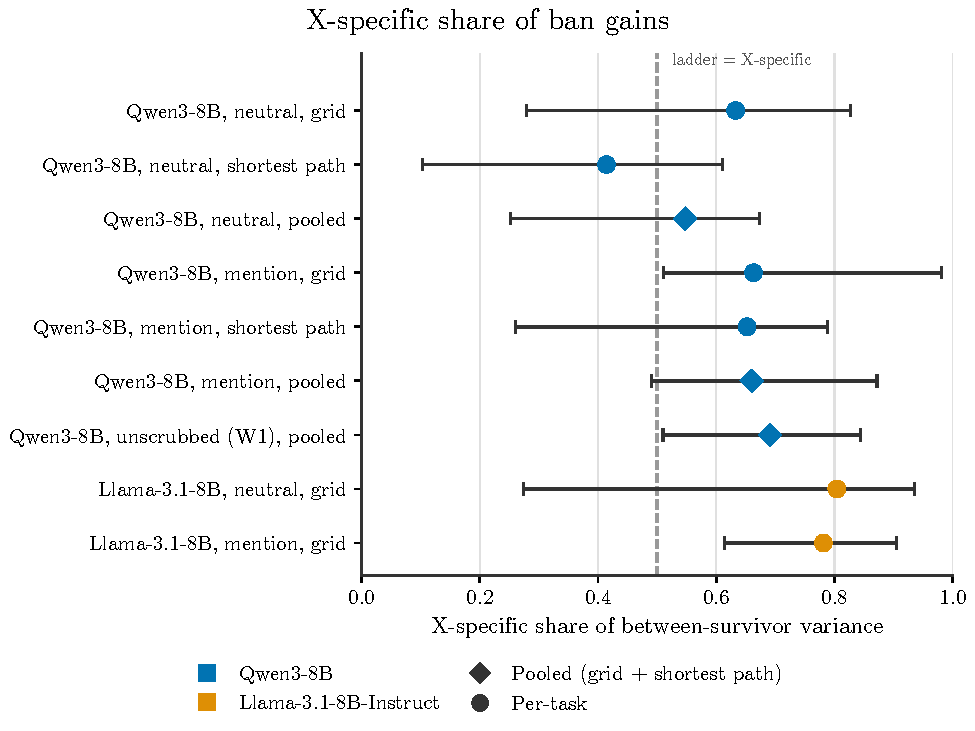
\includegraphics[width=\linewidth,height=0.78\textheight,keepaspectratio]{figures/fig_c1share_v0.pdf}
\caption{X-specific share of the between-survivor variance in ban-induced likelihood gains, with 95\% bootstrap confidence intervals, for Qwen3-8B (blue; circles for the grid and shortest-path tasks, diamonds for the pooled task and for a pooled sensitivity check on gate-passing unscrubbed programs) and Llama-3.1-8B-Instruct (amber circles, grid task only: its shortest-path task had too few survivor algorithms to compute a share), each under a neutral-twin and a mention-twin reference prompt. The dashed vertical line, labelled ``ladder = X-specific'' in the figure, marks a share of 0.5: a share above it means the gains depend on which algorithm was specifically banned rather than on a shared ladder of survivors. Three of the nine intervals lie entirely above 0.5 (Qwen3-8B under the mention reference on the grid task, Qwen3-8B on the unscrubbed-program check, and Llama-3.1-8B-Instruct under the mention reference); the remaining six include 0.5. Intervals are percentile bootstrap intervals over 6 (grid), 5 (shortest path) or 11 (pooled) survivor algorithms, from 2,000 resamples (400 for the unscrubbed check). This is a descriptive result from a single screening analysis: the run's own follow-up audit found no row here has enough effective bootstrap sample size for the share to be decidable, and that intervals of this kind understate the true resampling variance by a measured factor of roughly 2.7 to 11x, so the figure shows where current evidence sits rather than a resolved finding.}
\label{fig:fig_c1share}
\end{figure}
\textbf{Priming and the route agree across models.} A ban of an algorithm the model does not write raises that algorithm's likelihood in 8 of 9 cases in Qwen3-8B (+2.5 to +26.9 nats) and 5 of 6 in Llama (+1.8 to +7.6), and in both models the bans that lower their own label are those of algorithms the model does write, plus A*. The likelihood drop of the banned default travels by the prompt route in both models: F\_\allowbreak{}prompt 0.85 [0.61, 1.20] in Qwen3-8B and 0.84 [0.62, 1.46] in Llama, with the direct route near zero (0.00 and -0.21). Only the Qwen3-8B grid behaviour shows a second, direct component. \emph{(Correction, iteration 3: both numbers are the likelihood readout, which on the grid task is dominated by the opening fork (ESS 1 to 3 of 30), and in Llama it is the only readout, on an instrument that failed its gate there. The route is restated per task and per readout in Section 3.1, and on the bench the behavioural route is task dependent, with a pooled direct share of 0.74; Section 3.6.)}

\FloatBarrier
\subsection*{2.11 What iteration 2 established, what it ruled out, and what it abandoned}
\addcontentsline{toc}{subsection}{2.11 What iteration 2 established, what it ruled out, and what it abandoned}
Everything below is still descriptive: two screen tasks, two models, one modal ban event per task and model for the route test, and a likelihood instrument whose validity gate failed in both models in its preregistered (name scrubbed) form.

\textbf{Established.}

\begin{enumerate}
\item \emph{The iteration-1 record, corrected.} On the shortest path task the ban's substitute is Bellman-Ford\slash{}SPFA in five of five draws (272 of 272 compliant programs, Wilson [0.986, 1.000]); on the grid task DFS is the realised mode in four of five draws (116 of 128, [0.843, 0.946]), with no clear mode in the HF engine geometry draw. Under fixed wording three new Qwen3-8B draws landed on DFS (257 of 257 programs not banned) and Bellman-Ford\slash{}SPFA (255 of 260). The cumulative BFS and DFS ban does not replicate. Under one statistic, no ban and no diversity knob reaches a second correct algorithm (rarefied Hill-1 of at least 2) for less than 20 pass points on either task; the semantic seed on the shortest path task comes closest (1.935 at 7 points). On gated events, no forecasting family can advance (three informative events, largest margin 0.05 nats).
\item \emph{The generic perturbation rival holds on the shortest path task and fails on the grid task.} Every nonsemantic perturbation that left Dijkstra (8 of 8 rows) landed mostly on Bellman-Ford\slash{}SPFA, random directions included; on the grid task no nonsemantic perturbation left BFS among correct programs \emph{(corrected in iteration 3: one did, barely; temperature 1.3 with top-k = 10 gave DFS in 1 of 95 correct programs)}, while every ban reached DFS. On the shortest path task a ban and an arbitrary push end in the same place.
\item \emph{The ban acts through the prompt states, before the first generated token.} In cache patching the prompt route carried 0.85 [0.61, 1.20] of the banned algorithm's likelihood drop and the direct route 0.00 [-0.08, 0.12], with the task specification states, not the read position alone, carrying it. The mechanism is an opening line veto: under the grid ban 0 of 100 programs open with the default's import line against 99 of 100 under the neutral twin, and the prompt route arm reproduces this exactly. On the shortest path task behaviour follows the prompt route completely; on the grid task generated tokens also read the ban directly (hiding the ban from them restores BFS to 0.47). Llama's likelihood readout agrees (F\_\allowbreak{}prompt 0.84). \emph{(Correction, iteration 3: the heading and first sentence state the route more strongly than its evidence. Per task and per readout: on the shortest path task the prompt route carries the ban in likelihood (0.82) and in behaviour (0.98 [0.89, 1.07], direct 0.05 [0.01, 0.09]); on the grid task the likelihood readout is dominated by the opening fork (0.87), behaviour is mixed (prompt 0.50 [0.39, 0.62], direct 0.35 [0.25, 0.45]) and the natural proposal readout puts the direct route at 0.16 [0.11, 0.21], an interval that excludes 0; Llama has the likelihood readout only (0.84 [0.62, 1.46]). The direct route is not zero. Splicing the read position alone carries none of the effect (F\_\allowbreak{}R about 0).)}
\item \emph{The read position knows, in part, how hard a wording will be obeyed, and not what replaces X.} Across 110 wordings the projection on a shared ban direction correlates with the banned share at -0.41 [-0.69, -0.17] (p = 0.0003), short of the -0.5 bar; the substitute is not decodable beyond that projection. \emph{(Added in iteration 3: splicing the read position alone carries none of the ban's effect (F\_\allowbreak{}R about 0), so this site is decodable but causally inert; a causal test of a shared prohibition direction at the task specification positions was run in iteration 3 and failed, Section 3.7.)}
\item \emph{Naming primes.} A ban of an absent algorithm raises that algorithm's likelihood in both models (8 of 9 and 5 of 6), and the mention twin raises it more. The iteration-1 sham promotions are reproduced by the shared (ladder) component of the gains and are not X specific.
\item \emph{Ban lists fail by reimplementation.} Every four or five name grid ban failed (avoidance 0.00 to 0.37); the model wrote BFS and DFS in the same mix whatever the list contained (BFS share 0.63 to 0.72, chi squared p = 0.48), disguising 41\% to 92\% of the banned programs. On the shortest path task the model will not write bidirectional Dijkstra, Floyd-Warshall or Dial even when each is the only algorithm allowed, though it can write Floyd-Warshall and Dial when told to \emph{(qualified in iteration 3: forced Floyd-Warshall is labelled as requested and correct 40 of 40 times, but forced Dial, from the descriptive prompt, is labelled as requested 36 of 40 times and passes only 7 of 40, so only Floyd-Warshall is written cleanly on request)}.
\item \emph{No decision locus among the saved states.} On the grid task the within one ban signal is fixed per paraphrase; on the shortest path task the first state that beats the read position by 20 points is a readout of text already written (\texttt{import heapq} against \texttt{from collections import deque}, decided at generated token 3). The forking token, the opening line veto and the locus probe all point at the first three generated tokens, which no artifact has saved.
\item \emph{Temperature does not change the algorithm even for a fixed seed.} With seeds coupled across temperatures, the algorithm changed in 0 of 30 seeds in 10 of 12 cells and 1 of 30 in the other two, while phrasing changed in 7\% to 100\% of seeds depending on task and temperature, and less within a seed than across seeds.
\item \emph{Qwen3-8B is collapsed on 13 new tasks as well.} The pilot found a modal share of 1.00 on 12 tasks and 0.98 on one; Llama-3.1-8B-Instruct is more diverse on the same tasks \emph{(qualified in iteration 3: in attempted programs; counted over correct programs and rarefied to 10, Llama is more diverse on 9 of 13 tasks, but much of its attempted diversity is failing code, Section 3.2.4)}. The confirmation bench is frozen (12 tasks, labellers gated) with no ban prompt run on it.
\end{enumerate}

\textbf{Ruled out, or not supported.}

\begin{itemize}
\item \emph{Geodesic proximity on the read position manifold as the predictor of the shortest path substitute.} Floyd-Warshall is the nearest survivor to Dijkstra in 100\% of paraphrase subsamples at every layer and k tested, Bellman-Ford\slash{}SPFA is never nearest, and no ban landed on Floyd-Warshall. On the grid task proximity and typicality coincide and cannot be separated.
\item \emph{An aimed substitution.} In neither model is the X specific part of the ban gains aimed at the prime and veto profile (Qwen3-8B -0.10, p = 0.80; Llama 0.067, p = 0.35) or at the stated alternative. \emph{(Correction, iteration 3: not detectable with the current instrument, rather than ruled out; Section 3.2.1.)}
\item \emph{A coherent latent ladder.} The generic perturbation profiles do not agree with each other in either model, so the rival in its preregistered form, a fixed ordering any perturbation reveals, was not found either. \emph{(Correction, iteration 3: this item belongs among the effects that an uncalibrated instrument could not detect, not among the accounts ruled out, and it conflicts with item 2 above. Reconciled: behaviour shows a shared top rung on the shortest path task, where 8 of 8 nonsemantic perturbations that left Dijkstra landed mostly on Bellman-Ford\slash{}SPFA, and on the grid task only bans reach DFS. The order of the survivors below the top rung is unmeasured: it is unobservable in behaviour under the collapse, and the likelihood cosines that this item rests on come mostly from survivors with an ESS near 1.)}
\end{itemize}

\emph{(Added in iteration 3: the iteration-2 preregistered predictions and their outcomes, and the outcome of the iteration-2 forecast contest of the four frozen families (NOT RUN on any new event), are listed in Section 3.1.)}

\begin{itemize}
\item \emph{A veto at the signature token.} The lens found no layer at which the ban lowers the banned algorithm at the commitment token, because the fork is at the first token; the signature tokens carry 2.4\% and 11.6\% of the likelihood drop.
\item \emph{Activation of a forbidden concept in order to suppress it.} The prime and veto latent pattern appeared in 0 of 6 configurations; the name latents of X were lower under the ban than under both twins.
\end{itemize}

\textbf{Dead ends, with the evidence that closed them.}

\begin{itemize}
\item \emph{The likelihood instrument on name scrubbed programs as a calibrated probability.} It failed calibration in Qwen3-8B (default share 0.83, DFS mass under a baseline that never samples DFS) and in Llama (implied BFS 0.43 against sampled 0.77), with effective sample sizes mostly below 5 in every experiment that used it (98\% of gate cells, 858 of 1,095 route cells, 97\% of ban list cells, 76\% of Llama cells). Unscrubbed programs pass the Qwen3-8B gate (calibration 0.95 and 1.00, 1.18 nats, 17 of 19), so the scrubbing, not the instrument, is the closed part.
\item \emph{Extending the grid catalogue toward ten algorithms.} Only five of ten algorithms passed the keep rule; the model writes A* as unit weight Dijkstra, unit weight Dijkstra as BFS, and jump point search and bidirectional A* as BFS and A*.
\item \emph{The literal top five landing test as a test of edge against opposite side.} The model does not comply with a five name ban (avoidance 0.00), so no survivor mass exists to place on either side; the question is answered behaviourally (reimplementation of the defaults) rather than geometrically.
\item \emph{Qwen-Scope base model SAEs on the instruct model.} The spliced in cross-entropy ratio was 3.29, 1.95 and 1.59 at layers 15, 20 and 27 against a 1.5 bar; latents never beat the difference-in-means direction.
\item \emph{The community Jacobian lens for Qwen3-8B.} Its next token agreement was below the logit lens at every layer (0.104 against 0.291 at layer 27).
\item \emph{NLA.} No natural language autoencoder exists for Qwen3-8B as of 2026-10-20.
\item \emph{A presence piloted present minor stratum for Qwen3-8B.} All 13 bench tasks are fully collapsed in the pilot, so present minor bans and a sampled typicality forecast do not exist for this model on this bench.
\item \emph{The free-form association answer as evidence about mechanism.} It predicts the substitute, but simulation of its own behaviour explains that success under either branch of the substitution test.
\end{itemize}

\FloatBarrier
\subsection*{2.12 What the next iteration takes from this one}
\addcontentsline{toc}{subsection}{2.12 What the next iteration takes from this one}
The title claim is still open, and the reason has changed. Iteration 1 could not separate substitution from a latent ladder because its events were too few and its typicality forecast was degenerate. This iteration measured every single ban in two models with a likelihood instrument and found neither account clean: the gains are not pure subtraction, they are not a coherent ladder, and their X specific part is not aimed where association or prime and veto predict. \emph{(Correction, iteration 3: none of these three is detectable with the current instrument; Section 3.2.1.)} The confirmation bench exists to settle the share with task level clusters. Its inputs are now fixed, and so are its limits. Qwen3-8B is collapsed on all 12 frozen tasks, so its confirmation must use likelihood matrices on unscrubbed programs, which the gate supports, plus modal bans; Llama supplies sampled present minor bans. The ban, mention, neutral and nonce matrices, the Llama forced programs and every sampled ban event on the bench remain to be run, with forecasts hash committed first.

The route result redirects the mechanistic work. A ban is applied by the prompt states as a veto on the default's first line, and on the grid task also by direct reads during generation. The next measurements are therefore at generated tokens 1 to 3, the states no artifact has saved: a decoder and an activation patch there would locate the decision the locus probe could not find, and would say whether the opening line veto is the whole of the algorithm choice on the shortest path task. On the grid task the direct component needs its own localisation (which layers and which tokens read the ban after \texttt{def solve}), since the three attention heads that attend to the banned name are a descriptive lead, not a causal one. The template effect must enter every analysis as a random effect; one wording, the fourth template (\texttt{X is not allowed here}), accounts for every grid failure in three draws.

Request items still open after this iteration: the activation space manifold plots with centroids coloured by implemented count at a validated locus (no locus validated yet; \emph{corrected in iteration 3: the plots themselves exist, 13 Isomap figures drawn by the ban list experiment at layer 24 and the token before the commit token, Section 3.2.2, but not at a validated locus}), a working SAE readout (the transfer test failed; a short fine-tuning on instruct activations, or a dictionary trained on them, is the alternative), and a same seed arm with thinking on. The top five prohibition, natural BFS against DFS internals, thought anchors, the same seed test, the logit and tuned lens, and the mapping of NLA and the Jacobian lens were run here. \emph{(Added in iteration 3: the readout experiment did not save generated tokens 1 to 3 because the artifacts of one iteration run in parallel, and its plan was frozen before the audit named those positions; its states stop at the token before the commit token and token 16.)}

\FloatBarrier
\section{Iteration 3: ban-free forecasts on the bench, the route of a ban across twelve tasks, and how far any knob reaches}
\noindent\emph{Run record for this iteration.} Hypothesis carried: ``Plan Nudges, Not Temperature, Move Ideas''. Move recorded at the end of the iteration: deepen; review score 4; evidence state lead; coverage full; 15 candidate strategies considered. The list below gives the iteration's artifacts and the state the round record gave each strand.

{\footnotesize\setlength{\tabcolsep}{3pt}
\begin{longtable}{>{\raggedright\arraybackslash}p{0.24\linewidth}>{\raggedright\arraybackslash}p{0.47\linewidth}>{\raggedright\arraybackslash}p{0.11\linewidth}>{\raggedright\arraybackslash}p{0.08\linewidth}}
\caption*{\textbf{Artifacts of iteration 3.} Names and titles as the artifact workspaces record them; strand state as the round record grades it.}\label{tab:arts3}\\
\toprule \textbf{Artifact} & \textbf{Title} & \textbf{Type} & \textbf{State} \\ \midrule \endfirsthead
\toprule \textbf{Artifact} & \textbf{Title} & \textbf{Type} & \textbf{State} \\ \midrule \endhead
\bottomrule \endlastfoot
\nolinkurl{gen_art_evaluation_2} & Record repair and novelty audit of algorithm bans & evaluation & null \\
\nolinkurl{gen_art_experiment_13} & Forecasting where coding bans send a model & experiment & null \\
\nolinkurl{gen_art_experiment_14} & Show a solution, ban it, see what replaces it & experiment & lead \\
\nolinkurl{gen_art_experiment_15} & Where Llama goes when an algorithm is banned & experiment & lead \\
\nolinkurl{gen_art_experiment_16} & Where a coding ban takes effect in Qwen3-8B & experiment & lead \\
\nolinkurl{gen_art_experiment_17} & Searching Qwen3-8B for where a coding ban lives & experiment & lead \\
\nolinkurl{gen_art_experiment_18} & How far bans and token vetoes push Qwen3-8B & experiment & null \\
\end{longtable}}

\subsection*{What each artifact of iteration 3 was for and what it produced}
\addcontentsline{toc}{subsection}{What each artifact of iteration 3 was for and what it produced}
Each artifact is named below as the run's workspaces name it. The entry gives the round record's verdict on the strand it served, the artifact's own summary of what it was for and what it produced, and the output files it declared, each opened and read from its workspace for this report. It closes with the subsection of this section that reports the artifact's results and the result tables typeset there from its output files.

\paragraph{\nolinkurl{gen_art_evaluation_2}: Record repair and novelty audit of algorithm bans.}
Type: evaluation. Round record, strand state null: Record repair: likelihood gains name the landing 0\slash{}17 (0\slash{}11 distinct rows); no estimable 3-survivor row; 0 novel of 78 correct off-catalogue; BFS-BiBFS adjacency fails at g16.

\emph{The artifact's own summary of what it was for and what it produced:} CPU-only Step 0 of iteration 3: repairs the iteration-2 record from data on disk and answers the novelty question (eval.py, sections\slash{}, eval\_\allowbreak{}out.json in exp\_\allowbreak{}eval\_\allowbreak{}sol\_\allowbreak{}out with 72 metrics and 7 datasets; corrections.json; tables\slash{}; figures\slash{}; audit\slash{}). Sources are cited as '\textless{}artifact\_\allowbreak{}id\textgreater{}:\textless{}relative path\textgreater{}'. (0a) C1 likelihood diagnostics on exp7\slash{}exp10: the gain argmax (full and residual) hits the realised landing in 0\slash{}17 Qwen single-ban events (chance 0.22) while the implied-mass argmax hits 14\slash{}17 (8\slash{}8 modal); no ban row keeps 3 survivors with \textgreater{}=1\% mass and ESS\textgreater{}=5 (0\slash{}11), so C1 is not decidable on estimable mass; two-stage bootstrap variance of Gbar is 2.7x (1.2-4.3) the replicate noise term (Llama 4.8-11.3x); the mention-reference AIM is biased negative by construction (null mean -0.27 to -0.33): Llama -0.28 sits at the null's 66th percentile, Qwen -0.595 below its 1st; the ESS-weighted 1.24 share is impossible (V\_\allowbreak{}u -35.4); plug-in M5 \textgreater{}= 50 programs per algorithm (lognormal \textasciitilde{}1e31; 22\% of pooled PSIS k-hat \textgreater{} 0.7) and \textasciitilde{}129 Qwen \slash{} 43 Llama bench events would be needed to separate SHARE from 0.5 by 0.10. (0b) exp9 manifold: 13 figures (not 14); recomputed geometry matches exp9 (24\slash{}24 nearest maps); the BFS-BiBFS adjacency does NOT survive at the label-independent g16 position (N1 p 0.19, exchangeability p 0.48, separability 0.96); no persistent H1 loop, powered at 'pre' (planted-loop power 1.00) but not at g16 (0.04). (0c) Novelty: 78 unique correct out-of-catalogue programs across the 11 declared artifacts + exp3 pools copy, 0 novel (two blind judges gpt-4.1-mini \slash{} gemini-2.5-flash, deepseek tie-break, full manual read; rule-of-three bound 0.038); judge kappa 0.38; positive controls 7\slash{}10 strict (10\slash{}10 named correctly), negatives 5\slash{}5; TOP's 0.13 avoidance = 12 degenerate failing programs + 1 unit-weight Dijkstra, not non-banned catalogue algorithms. (0d) Llama correct-only: all quoted compositions reproduce; T1 correct programs are all BFS (Hill\_\allowbreak{}cc 1.00 vs Hill\_\allowbreak{}all 1.87); Llama more diverse than Qwen on 9\slash{}13 bench tasks at depth 10. (0e) Knob table rebuilt (306 rows vs the audit's 249): no KNOB under 20 pass points reaches rarefied Hill-1 2; best exp6 semantic seed T2 1.940 [1.770, 2.094]. (0f) 12\slash{}12 positioning quotes verified (2026-10-20). (0h) 12 corrections (R01-R12) with replacement sentences; 16\slash{}19 quoted reproduction targets match, mismatches explained. audit\slash{}rederive.py re-derives 72\slash{}72 headlines independently and all 7 placebos fail as required. Judge spend USD 0.415 (responses cached in audit\slash{}judge\_\allowbreak{}cache.jsonl). Kept on the volume only via the dependencies: exp9 states needed to rerun (0b).

Its results are reported in Subsection 3.2 of this report, which typesets the result tables drawn from its output files: Tables 81, 82, 83, 84, 85, 86, 86b, 87, 87b, 88, 89, 90, 91, 92, 93.

\begin{table}[H]
\renewcommand{\thetable}{O16}
\centering\footnotesize\setlength{\tabcolsep}{3pt}
\caption{Output files declared by \nolinkurl{gen_art_evaluation_2} (iteration 3), each opened and read from the artifact's workspace for this report; size in bytes. [Source: iteration 3, artifact \nolinkurl{gen_art_evaluation_2}.]}
\begin{tabular}{>{\raggedright\arraybackslash}p{0.25\linewidth}>{\raggedleft\arraybackslash}p{0.12\linewidth}>{\raggedright\arraybackslash}p{0.57\linewidth}}
\toprule
\textbf{Declared file} & \textbf{Bytes} & \textbf{What it holds} \\
\midrule
\texttt{eval.\allowbreak{}py} & 5,005 & the artifact's code, 146 lines \\
\texttt{full\_\allowbreak{}eval\_\allowbreak{}out.\allowbreak{}json} & 1,118,245 & the complete output; metadata with 11 top-level keys; 7 datasets with 664 examples in all: c1\_\allowbreak{}events (31), novelty\_\allowbreak{}audit (228), knob\_\allowbreak{}table (306), llama\_\allowbreak{}correct\_\allowbreak{}only (27), manifold\_\allowbreak{}grid (48), positioning (12), and 1 more; top-level keys metrics\_\allowbreak{}agg; 72 aggregate metrics (typeset in full below) \\
\texttt{mini\_\allowbreak{}eval\_\allowbreak{}out.\allowbreak{}json} & 193,795 & small variant of the full output (a few examples per dataset); metadata with 11 top-level keys; 7 datasets; top-level keys metrics\_\allowbreak{}agg \\
\texttt{preview\_\allowbreak{}eval\_\allowbreak{}out.\allowbreak{}json} & 83,169 & preview variant of the full output (truncated strings and lists); metadata with 11 top-level keys; 3 datasets; top-level keys metrics\_\allowbreak{}agg \\
\texttt{reproducibility.\allowbreak{}md} & 11,520 & reproducibility notes, 158 lines \\
\bottomrule
\end{tabular}
\end{table}

{\scriptsize\setlength{\tabcolsep}{2.5pt}\renewcommand{\thetable}{O17}
\begin{longtable}{>{\raggedright\arraybackslash}p{0.27\linewidth}>{\raggedright\arraybackslash}p{0.19\linewidth}>{\raggedright\arraybackslash}p{0.27\linewidth}>{\raggedright\arraybackslash}p{0.19\linewidth}}
\caption{Every aggregate metric in the \texttt{metrics\_agg} block of \nolinkurl{gen_art_evaluation_2}'s \texttt{full\_\allowbreak{}eval\_\allowbreak{}out.\allowbreak{}json} (72 metrics), values copied exactly as stored. [Source: iteration 3, artifact \nolinkurl{gen_art_evaluation_2}.]}\\
\toprule
\textbf{Metric} & \textbf{Value} & \textbf{Metric} & \textbf{Value} \\
\midrule
\endfirsthead
\toprule
\textbf{Metric} & \textbf{Value} & \textbf{Metric} & \textbf{Value} \\
\midrule
\endhead
\bottomrule
\endlastfoot
\texttt{c1\_\allowbreak{}events\_\allowbreak{}n} & 31.0 & \texttt{bfs\_\allowbreak{}bibfs\_\allowbreak{}g16\_\allowbreak{}n1\_\allowbreak{}p} & 0.1936127744510978 \\
\texttt{c1\_\allowbreak{}events\_\allowbreak{}qwen\_\allowbreak{}n} & 17.0 & \texttt{bfs\_\allowbreak{}bibfs\_\allowbreak{}g16\_\allowbreak{}n2\_\allowbreak{}p} & 0.4810379241516966 \\
\texttt{c1\_\allowbreak{}hit\_\allowbreak{}argmax\_\allowbreak{}full} & 0.0 & \texttt{bfs\_\allowbreak{}bibfs\_\allowbreak{}g16\_\allowbreak{}survives} & 0.0 \\
\texttt{c1\_\allowbreak{}hit\_\allowbreak{}argmax\_\allowbreak{}resid} & 0.0 & \texttt{h1\_\allowbreak{}power\_\allowbreak{}g16\_\allowbreak{}t1} & 0.035 \\
\texttt{c1\_\allowbreak{}hit\_\allowbreak{}argmax\_\allowbreak{}mass} & 0.8235294117647058 & \texttt{h1\_\allowbreak{}power\_\allowbreak{}g16\_\allowbreak{}t2} & 0.045 \\
\texttt{c1\_\allowbreak{}hit\_\allowbreak{}argmax\_\allowbreak{}full\_\allowbreak{}modal\_\allowbreak{}bans} & 0.0 & \texttt{h1\_\allowbreak{}power\_\allowbreak{}pre\_\allowbreak{}t1} & 1.0 \\
\texttt{c1\_\allowbreak{}hit\_\allowbreak{}argmax\_\allowbreak{}resid\_\allowbreak{}modal\_\allowbreak{}bans} & 0.0 & \texttt{h1\_\allowbreak{}power\_\allowbreak{}pre\_\allowbreak{}t2} & 0.975 \\
\texttt{c1\_\allowbreak{}hit\_\allowbreak{}argmax\_\allowbreak{}mass\_\allowbreak{}modal\_\allowbreak{}bans} & 1.0 & \texttt{h1\_\allowbreak{}radius0\_\allowbreak{}placebo\_\allowbreak{}rate\_\allowbreak{}t1} & 0.065 \\
\texttt{c1\_\allowbreak{}hit\_\allowbreak{}argmax\_\allowbreak{}full\_\allowbreak{}llama} & 0.0 & \texttt{manifold\_\allowbreak{}figures\_\allowbreak{}found} & 13.0 \\
\texttt{c1\_\allowbreak{}hit\_\allowbreak{}argmax\_\allowbreak{}resid\_\allowbreak{}llama} & 0.0 & \texttt{novelty\_\allowbreak{}correct\_\allowbreak{}other\_\allowbreak{}unique} & 78.0 \\
\texttt{c1\_\allowbreak{}hit\_\allowbreak{}argmax\_\allowbreak{}mass\_\allowbreak{}llama} & 0.8333333333333334 & \texttt{novelty\_\allowbreak{}confirmed\_\allowbreak{}novel} & 0.0 \\
\texttt{c1\_\allowbreak{}mean\_\allowbreak{}rank\_\allowbreak{}landing\_\allowbreak{}resid\_\allowbreak{}qwen} & 3.0 & \texttt{novelty\_\allowbreak{}rule\_\allowbreak{}of\_\allowbreak{}three\_\allowbreak{}upper} & 0.038461538461538464 \\
\texttt{c1\_\allowbreak{}mass\_\allowbreak{}rows\_\allowbreak{}kept} & 0.0 & \texttt{novelty\_\allowbreak{}items\_\allowbreak{}judged} & 228.0 \\
\texttt{c1\_\allowbreak{}mass\_\allowbreak{}rows\_\allowbreak{}total} & 11.0 & \texttt{judge\_\allowbreak{}kappa} & 0.3784078516902945 \\
\texttt{qwen\_\allowbreak{}boot\_\allowbreak{}rep\_\allowbreak{}ratio\_\allowbreak{}median} & 2.6813434671972503 & \texttt{judge\_\allowbreak{}kappa\_\allowbreak{}collapsed} & 0.4442213937482075 \\
\texttt{qwen\_\allowbreak{}boot\_\allowbreak{}rep\_\allowbreak{}ratio\_\allowbreak{}min} & 1.2203354400365118 & \texttt{judge\_\allowbreak{}posctrl\_\allowbreak{}hits} & 7.0 \\
\texttt{qwen\_\allowbreak{}boot\_\allowbreak{}rep\_\allowbreak{}ratio\_\allowbreak{}max} & 4.263023395418002 & \texttt{judge\_\allowbreak{}negctrl\_\allowbreak{}hits} & 5.0 \\
\texttt{qwen\_\allowbreak{}boot\_\allowbreak{}rep\_\allowbreak{}ratio\_\allowbreak{}one\_\allowbreak{}stage\_\allowbreak{}median} & 1.5947776493678707 & \texttt{judge\_\allowbreak{}posctrl\_\allowbreak{}identity\_\allowbreak{}both} & 10.0 \\
\texttt{llama\_\allowbreak{}boot\_\allowbreak{}rep\_\allowbreak{}ratio\_\allowbreak{}min} & 4.786772833595323 & \texttt{judge\_\allowbreak{}spend\_\allowbreak{}usd} & 0.4150459 \\
\texttt{llama\_\allowbreak{}boot\_\allowbreak{}rep\_\allowbreak{}ratio\_\allowbreak{}max} & 11.274782164207641 & \texttt{manual\_\allowbreak{}agreement\_\allowbreak{}setA\_\allowbreak{}collapsed} & 1.0 \\
\texttt{qwen\_\allowbreak{}pooled\_\allowbreak{}share\_\allowbreak{}basic\_\allowbreak{}lo} & 0.43613444304720517 & \texttt{top\_\allowbreak{}avoidance\_\allowbreak{}raw} & 0.13 \\
\texttt{qwen\_\allowbreak{}pooled\_\allowbreak{}share\_\allowbreak{}basic\_\allowbreak{}hi} & 0.843359769056045 & \texttt{top\_\allowbreak{}avoidance\_\allowbreak{}corrected} & 0.13 \\
\texttt{aim\_\allowbreak{}obs\_\allowbreak{}qwen\_\allowbreak{}mention} & -0.5954545454545455 & \texttt{top\_\allowbreak{}other\_\allowbreak{}share} & 0.13 \\
\texttt{aim\_\allowbreak{}null\_\allowbreak{}mean\_\allowbreak{}qwen\_\allowbreak{}split\_\allowbreak{}half} & -0.2651772727272727 & \texttt{llama\_\allowbreak{}t1\_\allowbreak{}hill\_\allowbreak{}cc} & 1.0 \\
\texttt{aim\_\allowbreak{}null\_\allowbreak{}mean\_\allowbreak{}shared\_\allowbreak{}cell\_\allowbreak{}equal\_\allowbreak{}var} & -0.33094 & \texttt{llama\_\allowbreak{}t1\_\allowbreak{}hill\_\allowbreak{}all} & 1.874487310795308 \\
\texttt{aim\_\allowbreak{}null\_\allowbreak{}q\_\allowbreak{}qwen} & 0.0042 & \texttt{knob\_\allowbreak{}best\_\allowbreak{}hill\_\allowbreak{}lt20pts} & 1.9401991740484124 \\
\texttt{aim\_\allowbreak{}null\_\allowbreak{}q\_\allowbreak{}llama} & 0.6614 & \texttt{knob\_\allowbreak{}best\_\allowbreak{}hill\_\allowbreak{}lt20pts\_\allowbreak{}ci\_\allowbreak{}hi} & 2.094056637290499 \\
\texttt{aim\_\allowbreak{}placebo\_\allowbreak{}independent\_\allowbreak{}mention\_\allowbreak{}mean} & -0.0013704545454545456 & \texttt{knob\_\allowbreak{}rows\_\allowbreak{}rebuilt} & 306.0 \\
\texttt{ess\_\allowbreak{}weighted\_\allowbreak{}share\_\allowbreak{}t1} & 1.242997569701056 & \texttt{knob\_\allowbreak{}rankable} & 108.0 \\
\texttt{m5\_\allowbreak{}plugin\_\allowbreak{}median} & 49.77796738023861 & \texttt{positioning\_\allowbreak{}verified} & 12.0 \\
\texttt{m5\_\allowbreak{}lognormal\_\allowbreak{}median\_\allowbreak{}log10} & 31.66812237434777 & \texttt{corrections\_\allowbreak{}items} & 12.0 \\
\texttt{khat\_\allowbreak{}frac\_\allowbreak{}gt07} & 0.21666666666666667 & \texttt{reproduction\_\allowbreak{}targets\_\allowbreak{}n} & 19.0 \\
\texttt{gpu\_\allowbreak{}hours\_\allowbreak{}per\_\allowbreak{}event\_\allowbreak{}plugin\_\allowbreak{}lower\_\allowbreak{}bound} & 1.3996214356516277 & \texttt{reproduction\_\allowbreak{}targets\_\allowbreak{}matched} & 16.0 \\
\texttt{share\_\allowbreak{}events\_\allowbreak{}needed\_\allowbreak{}qwen} & 129.0882882544141 & \texttt{rederive\_\allowbreak{}checks} & 72.0 \\
\texttt{share\_\allowbreak{}events\_\allowbreak{}needed\_\allowbreak{}llama} & 42.83328015857008 & \texttt{rederive\_\allowbreak{}passed} & 72.0 \\
\texttt{bfs\_\allowbreak{}bibfs\_\allowbreak{}g16\_\allowbreak{}sep} & 0.9601632458191236 & \texttt{placebos\_\allowbreak{}failed\_\allowbreak{}as\_\allowbreak{}required} & 7.0 \\
\end{longtable}}

\paragraph{\nolinkurl{gen_art_experiment_13}: Forecasting where coding bans send a model.}
Type: experiment. Round record, strand state null: Ban-free forecasts fail: 5\slash{}12 bans gated; no family beats uniform (ladder +0.06, association -1.78); vetoes respelled on 9\slash{}12; 3\slash{}5 landings unforeseen; wording LR 374.

\emph{The artifact's own summary of what it was for and what it produced:} Iteration-3 confirmation experiment on Qwen3-8B (bf16, pinned revision, thinking off) over the 12 frozen bench tasks of exp11 (\nolinkurl{gen_art_experiment_11}). Ban-free forecasts of where each task's modal 'do not use X' ban lands were built and hash-sealed (commitments.log, SEAL\_\allowbreak{}BEFORE\_\allowbreak{}BANS) before any ban sample: SUBTRACT (token vetoes of the default's distinctive n-gram, coupled to neutral-twin samples by exact rejection + masked redraw via vLLM logit\_\allowbreak{}bias; one-shot, persistent, 3 iterated rounds), LADDER (nonce ban, novelty instruction, 3 matched-norm isotropic random directions patched into task-spec states at layers 12-23), ASSOCIATE (exp11 association answers) and PROXIMITY (AST Zhang-Shasha distance). Then 1,200 ban samples (5 templates x 20 per task) were labelled by the gated exp11 labellers (re-check matched gate.json on 12\slash{}12). RESULTS: only 5\slash{}12 bans pass the gate (T03, T06, T05, T10, T13; R1, R3, R6, T11 keep the default almost always). The frozen C1 rule returns 'SUBTRACTION\slash{}LADDER (LADDER)' (wins LADDER 3, PROXIMITY 2), but 2 of LADDER's wins come from an undefined forecast scored as uniform; counting defined forecasts only, no family advances, and no family beats the uniform reference on average (mean log score minus uniform over gated events: LADDER +0.06, SUBTRACT -0.69, PROXIMITY -1.53, ASSOCIATE -1.78). Landings are X-specific but largely unforeseen (T06 -\textgreater{} index\_\allowbreak{}marking, T10 -\textgreater{} bfs, T13 -\textgreater{} 'other'; only T03 quickselect and T05 brute\_\allowbreak{}force were hit by a top-1). C2b is UNDETERMINED: one-shot vetoes never reach 0.5 avoidance on a gated task; descriptively the last iterated veto round lands elsewhere on T06 and T10. Token vetoes move the surface, not the algorithm: the default re-emerges in every veto round on 9\slash{}12 tasks, with text-level leaks of the vetoed n-gram in 23\% (one-shot) to 54\% (round 2) of samples; a sham veto breaks programs without moving the algorithm. Band-patching the ban's own task-spec states into the twin reproduces avoidance only on T03 and T10. Wording matters: template LR 374 (df 4, p \textasciitilde{} 1e-79; shuffled placebo p 0.39), W4 'X is not allowed here.' fails on 10\slash{}12 tasks. FRLP fp32 rescoring: median \textbar{}dL\_\allowbreak{}corr\textbar{} 0.88 nats vs FP8, argmax unchanged 12\slash{}12. FILES: method.py (stage CLI), src\slash{} (pipeline), method\_\allowbreak{}out.json (exp\_\allowbreak{}gen\_\allowbreak{}sol\_\allowbreak{}out; dataset modal\_\allowbreak{}ban\_\allowbreak{}samples with predict\_\allowbreak{}subtract\slash{}ladder\slash{}associate\slash{}proximity = committed top-1s; dataset ban\_\allowbreak{}free\_\allowbreak{}arm\_\allowbreak{}samples; metadata holds every analysis and the deviations), data\slash{}samples.jsonl (9,350 per-sample rows with veto metadata), data\slash{}raw and data\slash{}labels, results\slash{}c1\_\allowbreak{}events.jsonl, results\slash{}analysis.json, results\slash{}posthoc\_\allowbreak{}sensitivity.json (post-hoc, not pre-registered), results\slash{}frlp\_\allowbreak{}rescore.json, results\slash{}tensors\slash{}norms\_\allowbreak{}\textless{}task\textgreater{}.npz (ban-minus-twin displacement norms and mean vectors at layers 12-23, reusable for an X-free direction), predictions\slash{} (committed forecasts, n-grams, iterated chain), figures\slash{}. AUDIT: audit\slash{}rederive.py and audit\slash{}rederive\_\allowbreak{}raw.py re-derive every headline number from raw files with 0 mismatches; task-shuffled and template-shuffled placebos fail as required; not independently re-derived: mixed-GLM SDs and descriptive C2b null p95s. CAVEATS: one model, memorised LeetCode tasks, 5 gated events (advance count, no significance test); one documented post-ban portability edit of src\slash{}common.py (paths only); judge spend USD 0.024.

Its results are reported in Subsection 3.3 of this report, which typesets the result tables drawn from its output files: Tables 94, 95, 96, 97.

\begin{table}[H]
\renewcommand{\thetable}{O18}
\centering\footnotesize\setlength{\tabcolsep}{3pt}
\caption{Output files declared by \nolinkurl{gen_art_experiment_13} (iteration 3), each opened and read from the artifact's workspace for this report; size in bytes. [Source: iteration 3, artifact \nolinkurl{gen_art_experiment_13}.]}
\begin{tabular}{>{\raggedright\arraybackslash}p{0.25\linewidth}>{\raggedleft\arraybackslash}p{0.12\linewidth}>{\raggedright\arraybackslash}p{0.57\linewidth}}
\toprule
\textbf{Declared file} & \textbf{Bytes} & \textbf{What it holds} \\
\midrule
\texttt{method.\allowbreak{}py} & 4,126 & the artifact's code, 84 lines \\
\texttt{full\_\allowbreak{}method\_\allowbreak{}out.\allowbreak{}json} & 18,641,014 & the complete output; metadata with 32 top-level keys; 2 datasets with 9,350 examples in all: modal\_\allowbreak{}ban\_\allowbreak{}samples (1,200), ban\_\allowbreak{}free\_\allowbreak{}arm\_\allowbreak{}samples (8,150) \\
\texttt{mini\_\allowbreak{}method\_\allowbreak{}out.\allowbreak{}json} & 311,860 & small variant of the full output (a few examples per dataset); metadata with 32 top-level keys; 2 datasets \\
\texttt{preview\_\allowbreak{}method\_\allowbreak{}out.\allowbreak{}json} & 278,330 & preview variant of the full output (truncated strings and lists); metadata with 32 top-level keys; 2 datasets \\
\texttt{reproducibility.\allowbreak{}md} & 13,693 & reproducibility notes, 196 lines \\
\bottomrule
\end{tabular}
\end{table}

\paragraph{\nolinkurl{gen_art_experiment_14}: Show a solution, ban it, see what replaces it.}
Type: experiment. Round record, strand state lead: Snap-back: default share 0.05 (copy) to 0.72 named, 0.82 unnamed; ladder beats association by 1.3 nats (Holm 0.081 named, 0.0056 unnamed); rests partly on one wording.

\emph{The artifact's own summary of what it was for and what it produced:} Exposure-ban experiment (Step 1b) on Qwen3-8B (bf16, thinking off, vLLM 0.11.0, pinned revision) over the 12 frozen tasks of the exp11 algorithm-choice bench (sha256-verified copy in bench\_\allowbreak{}copy\slash{}; labeller re-check reproduces every gate.json value, references 100\%). For each of 33 eligible non-default algorithms Y (19 priority Y whose frozen associate differs from the default), the prompt shows up to 5 name-scrubbed correct programs of Y, then asks COPY 'Write a correct solution.', NAMED '... that does not use \{Y\}.' (= template W5) or UNNAMED '... uses a different algorithm from the one above.' (N = 50 per Y and arm, seeds shared across arms). Four forecast families are committed in a sha256 hash chain before any ban sample: LADDER (default), ASSOCIATE (modal frozen 'standard alternative to Y'), PROXIMITY (nearest survivor by Zhang-Shasha distance on identifier-normalised ASTs; token-distance sensitivity) and SUBTRACT-IN-CONTEXT (non-Y landing under an iterated persistent signature veto of Y's distinctive token n-gram under the copy-twin prompt, implemented as a vLLM V1 per-request logits processor; GPU smoke tests: 0\slash{}20 vetoed n-grams vs 20\slash{}20 in the copy twin, inert veto 20\slash{}20 identical, twin divergence exactly at the vetoed position 20\slash{}20). Outputs: data\slash{}samples.jsonl (one row per program, gated bench labeller: runtime + AST + blind judge), results\slash{}c1\_\allowbreak{}events.jsonl (one row per (Y, NAMED\slash{}UNNAMED) event in the frozen schema with forecasts, top-1s, log scores, gate), results\slash{}c1\_\allowbreak{}summary.json (frozen advance rule, Holm-corrected paired Wilcoxon tests with task-cluster bootstrap CIs, branch verdict, sensitivities, C1-exposure, placebos), results\slash{}other\_\allowbreak{}reports.json (copy rates, snap-back to default, named-vs-unnamed agreement, disguise, heterogeneity, veto diagnostics, template arm), predictions\slash{} (committed forecasts and prompts), commitments.log (COMMIT \#0\slash{}\#1\slash{}\#2 hash chain), audit\slash{}rederive.py (independent re-derivation + placebos), figures\slash{}, and method\_\allowbreak{}out.json (exp\_\allowbreak{}gen\_\allowbreak{}sol\_\allowbreak{}out: datasets exposure\_\allowbreak{}events and exposure\_\allowbreak{}samples). Note: this summary is interim and is rewritten with the final numbers when the analysis finishes.

Its results are reported in Subsection 3.4 of this report, which typesets the result tables drawn from its output files: Tables 98, 99, 100.

\begin{table}[H]
\renewcommand{\thetable}{O19}
\centering\footnotesize\setlength{\tabcolsep}{3pt}
\caption{Output files declared by \nolinkurl{gen_art_experiment_14} (iteration 3), each opened and read from the artifact's workspace for this report; size in bytes. [Source: iteration 3, artifact \nolinkurl{gen_art_experiment_14}.]}
\begin{tabular}{>{\raggedright\arraybackslash}p{0.25\linewidth}>{\raggedleft\arraybackslash}p{0.12\linewidth}>{\raggedright\arraybackslash}p{0.57\linewidth}}
\toprule
\textbf{Declared file} & \textbf{Bytes} & \textbf{What it holds} \\
\midrule
\texttt{method.\allowbreak{}py} & 13,827 & the artifact's code, 278 lines \\
\texttt{full\_\allowbreak{}method\_\allowbreak{}out.\allowbreak{}json} & 13,711,442 & the complete output; metadata with 15 top-level keys; 2 datasets with 10,666 examples in all: exposure\_\allowbreak{}events (66), exposure\_\allowbreak{}samples (10,600) \\
\texttt{mini\_\allowbreak{}method\_\allowbreak{}out.\allowbreak{}json} & 475,368 & small variant of the full output (a few examples per dataset); metadata with 15 top-level keys; 2 datasets \\
\texttt{preview\_\allowbreak{}method\_\allowbreak{}out.\allowbreak{}json} & 304,307 & preview variant of the full output (truncated strings and lists); metadata with 15 top-level keys; 2 datasets \\
\texttt{reproducibility.\allowbreak{}md} & 7,432 & reproducibility notes, 122 lines \\
\bottomrule
\end{tabular}
\end{table}

\paragraph{\nolinkurl{gen_art_experiment_15}: Where Llama goes when an algorithm is banned.}
Type: experiment. Round record, strand state lead: Llama: no family advances; association hits 7\slash{}13 (ladder 6\slash{}13 without 'other'); associate gains +0.25 beyond veto on 2\slash{}6 present-minor bans; snap-back 0.72-0.93.

\emph{The artifact's own summary of what it was for and what it produced:} Llama-3.1-8B-Instruct (bf16, pinned revision) replication of Claim 1 (does a ban remove the default and send the model to a predictable next rung?) on the frozen 12-task exp11 coding bench, plus a descriptive path-task screen against exp10's landings. Ban-free forecasts were built and sha256 hash-chained before any ban prompt was rendered (grep audit: 0 ban prompts in 10,328 prior rows): SUBTRACT (exact one-shot\slash{}persistent\slash{}iterated signature-n-gram vetoes by truncate-and-redraw in vLLM), LADDER (nonce ban, novelty instruction, 3 matched-norm random directions added at the spec positions of layers 11-21 during prefill), ASSOCIATE (Llama's own association answers) and PROXIMITY (Zhang-Shasha AST distance), in a mass-transfer form with point-mass sensitivities. Then 1,800 bans were sampled (12 modal + 6 present-minor events, W1-W5 x 20) and scored with the frozen C1 rule. Results (within Llama, pre-pooling): 13 events gated, 11 disagreeing and gated; only 2 wins (SUBTRACT on T05 via its undefined-\textgreater{}uniform fallback; ASSOCIATE on T03 heapify\_\allowbreak{}pop), so no family advances and the branch is 'NO FAMILY ADVANCES (aimed, unresolved)'. Exact Wilcoxon (n=11): SUBTRACT and LADDER beat PROXIMITY (+0.345 \slash{} +0.306 nats, p=0.0029 \slash{} 0.0020, Holm-rejected); neither separates from ASSOCIATE (p=0.52 \slash{} 0.77). Top-1 hits: LADDER and ASSOCIATE 7\slash{}13 (binomial p=0.033 vs chance 0.27), SUBTRACT 4\slash{}12, PROXIMITY 3\slash{}13. Fragile: correct-only, bf16-only decision set and drop-W4 sensitivities give SUBSTITUTION (ASSOCIATE). Five defaults (R1, R3, T13, R6, T11) are not avoided under the ban (avoidance 0.04-0.30), and surface-token vetoes rarely remove a default (only T14 heap). Re-derived independently from raw files with placebos that fail as required: gate\slash{}landings\slash{}log scores\slash{}wins\slash{}branch (audit\slash{}rederive.py) and the Wilcoxon, Holm, top-1 binomial tests and D per task (audit\slash{}rederive\_\allowbreak{}tests.py). Not separately re-derived: H3 sensitivity rows, bootstrap CIs, C2b, present-minor gain, knob view, screen scores. Provides: results\slash{}c1\_\allowbreak{}events.jsonl in the shared c1\_\allowbreak{}events schema for pooling with Qwen next round; method\_\allowbreak{}out.json (llama\_\allowbreak{}bench\_\allowbreak{}events, llama\_\allowbreak{}ban\_\allowbreak{}samples, llama\_\allowbreak{}screen\_\allowbreak{}events); all raw generations, labels and judge caches (data\slash{}); the committed forecasts (predictions\slash{}, commitments.log); figures; README.md and reproducibility.md. Compute: one NVIDIA L4, about 1.8 GPU-hours; OpenRouter spend USD 0.48.

Its results are reported in Subsection 3.5 of this report, which typesets the result tables drawn from its output files: Tables 101, 102, 103, 104, 105.

\begin{table}[H]
\renewcommand{\thetable}{O20}
\centering\footnotesize\setlength{\tabcolsep}{3pt}
\caption{Output files declared by \nolinkurl{gen_art_experiment_15} (iteration 3), each opened and read from the artifact's workspace for this report; size in bytes. [Source: iteration 3, artifact \nolinkurl{gen_art_experiment_15}.]}
\begin{tabular}{>{\raggedright\arraybackslash}p{0.25\linewidth}>{\raggedleft\arraybackslash}p{0.12\linewidth}>{\raggedright\arraybackslash}p{0.57\linewidth}}
\toprule
\textbf{Declared file} & \textbf{Bytes} & \textbf{What it holds} \\
\midrule
\texttt{method.\allowbreak{}py} & 28,581 & the artifact's code, 577 lines \\
\texttt{full\_\allowbreak{}method\_\allowbreak{}out.\allowbreak{}json} & 3,668,091 & the complete output; metadata with 25 top-level keys; 3 datasets with 1,820 examples in all: llama\_\allowbreak{}bench\_\allowbreak{}events (18), llama\_\allowbreak{}ban\_\allowbreak{}samples (1,800), llama\_\allowbreak{}screen\_\allowbreak{}events (2) \\
\texttt{mini\_\allowbreak{}method\_\allowbreak{}out.\allowbreak{}json} & 172,080 & small variant of the full output (a few examples per dataset); metadata with 25 top-level keys; 3 datasets \\
\texttt{preview\_\allowbreak{}method\_\allowbreak{}out.\allowbreak{}json} & 152,402 & preview variant of the full output (truncated strings and lists); metadata with 25 top-level keys; 3 datasets \\
\texttt{reproducibility.\allowbreak{}md} & 11,295 & reproducibility notes, 171 lines \\
\bottomrule
\end{tabular}
\end{table}

\paragraph{\nolinkurl{gen_art_experiment_16}: Where a coding ban takes effect in Qwen3-8B.}
Type: experiment. Round record, strand state lead: Route task-dependent (F\_\allowbreak{}prompt 0.61, F\_\allowbreak{}direct 0.74; C2a fails); routes jointly pick the landing (components: each alone DFS, both BFS); forced body opening undoes ban 0.98-1.00.

\emph{The artifact's own summary of what it was for and what it produced:} Behavioural route test of prompt bans in Qwen3-8B (bf16, thinking off) on the 12 frozen exp11 bench tasks, reusing exp8's HF engine (common-random-numbers inverse-CDF sampling, KV-cache splicing). 13,030 CRN-coupled samples, all labelled by the frozen runtime+AST+judge labellers (judge spend USD 0.105). Arms per task: a full ban, b token-matched neutral twin, c prompt route (twin condition + ban task-spec states), d direct route (ban condition + twin task-spec states), K0 (condition span invisible to generated tokens), V1 one-shot veto of the default's frozen distinctive n-gram, and signature\slash{}neutral prefills under ban and twin. GATE: only 5\slash{}12 tasks are gated (T03 0.99, T10 1.00, T05 0.83, T06 0.79, T13 0.59 avoidance); bans fail on R1\slash{}R3\slash{}R6\slash{}T11 and partly on T04\slash{}T08\slash{}T14; template W4 is weakest (avoidance 0.19). C2a (prompt route \textgreater{}= 2\slash{}3): DISCONFIRMED under jackknife (primary, low-cluster per F5), percentile and BCa intervals: pooled F\_\allowbreak{}prompt 0.611 [jackknife 0.06, 1.17], F\_\allowbreak{}direct 0.744 [0.38, 1.11], interaction -0.355, F\_\allowbreak{}K0 0.621. Mechanism is task-dependent: T03\slash{}T10 redundant (each route alone suffices), T05\slash{}T06 direct route (F\_\allowbreak{}direct 0.96\slash{}0.99; d reproduces the ban, c and K0 do not), T13 superadditive (both needed). An independent second CRN draw reproduces it (pooled 0.64\slash{}0.74; per-task Spearman 0.89\slash{}0.90). C2c (veto sufficiency predicts F\_\allowbreak{}direct): INCONCLUSIVE; the frozen n-gram rule picks zero-collateral identifier\slash{}structural tokens, so V\_\allowbreak{}t \textless{}= 0.41 everywhere, all tasks classed HIGH\_\allowbreak{}DIRECT, hit fraction 0.80, rho -0.34 (exact permutation p 0.30). Prefill: forcing the default's opening up to its first body token undoes the ban completely (P\_\allowbreak{}open 0.98-1.00) while a neutral def line undoes none (-0.12-0.01); the depth sweep shows the ban survives the def line and gives way at the first content token of the body. Path screen (T1\slash{}T2, exp8 twin prompts): one-shot, persistent, iterated and opening vetoes never move the default (off-default \textless{}= 0.01); committed T1 prediction hit, T2 prediction (veto suffices, lands on BF\slash{}SPFA) missed; iteration-2 ban landings recomputed exactly (T1 DFS 257\slash{}257, T2 BF\slash{}SPFA 255\slash{}260). Controls: placebo splice \textbar{}diff\textbar{} \textless{}= 0.04 and knockout-mechanics K0b 1.00 on 6 tasks. Validation: bench sha256 vs commitment.json, labeller re-check, prompt alignment asserts, CPU tests, GPU tests U1-U3 (CRN determinism, splice identities, zero knockout attention mass) and U9 vs exp8 all pass; two hash-chained pre-registration commits precede the first ban rows; two audit scripts re-derive every headline from raw rows (0 mismatches; placebo\slash{}shuffled inputs fail). Provides: data\slash{}samples.jsonl (one labelled row per sample, token ids in data\slash{}samples\_\allowbreak{}raw.jsonl), results\slash{}*.json (route, crn\_\allowbreak{}flips, landing\_\allowbreak{}by\_\allowbreak{}route, c2c, prefill, screen\_\allowbreak{}paths, replication incl. depth curve, lp\_\allowbreak{}readout, c1\_\allowbreak{}events.jsonl, gate, timing, deviations, rederive\slash{}rederive2), figures fig1-fig6, method\_\allowbreak{}out.json (exp\_\allowbreak{}gen\_\allowbreak{}sol\_\allowbreak{}out; datasets route\_\allowbreak{}arms, veto\_\allowbreak{}sufficiency, prefill, path\_\allowbreak{}screen, controls) and README\slash{}reproducibility. Deviations: L4 GPU with B=40 shape classes, K0 as a span-dropped cache, fence stop, extras beyond plan, three logged analysis amendments.

Its results are reported in Subsection 3.6 of this report, which typesets the result tables drawn from its output files: Tables 106, 107, 108, 109.

\begin{table}[H]
\renewcommand{\thetable}{O21}
\centering\footnotesize\setlength{\tabcolsep}{3pt}
\caption{Output files declared by \nolinkurl{gen_art_experiment_16} (iteration 3), each opened and read from the artifact's workspace for this report; size in bytes. [Source: iteration 3, artifact \nolinkurl{gen_art_experiment_16}.]}
\begin{tabular}{>{\raggedright\arraybackslash}p{0.25\linewidth}>{\raggedleft\arraybackslash}p{0.12\linewidth}>{\raggedright\arraybackslash}p{0.57\linewidth}}
\toprule
\textbf{Declared file} & \textbf{Bytes} & \textbf{What it holds} \\
\midrule
\texttt{method.\allowbreak{}py} & 4,327 & the artifact's code, 111 lines \\
\texttt{full\_\allowbreak{}method\_\allowbreak{}out.\allowbreak{}json} & 1,680,681 & the complete output; metadata with 26 top-level keys; 5 datasets with 3,150 examples in all: route\_\allowbreak{}arms (1,200), veto\_\allowbreak{}sufficiency (1,200), prefill (250), path\_\allowbreak{}screen (200), controls\_\allowbreak{}placebo\_\allowbreak{}K0b (300) \\
\texttt{mini\_\allowbreak{}method\_\allowbreak{}out.\allowbreak{}json} & 172,058 & small variant of the full output (a few examples per dataset); metadata with 26 top-level keys; 5 datasets \\
\texttt{preview\_\allowbreak{}method\_\allowbreak{}out.\allowbreak{}json} & 158,442 & preview variant of the full output (truncated strings and lists); metadata with 26 top-level keys; 3 datasets \\
\texttt{reproducibility.\allowbreak{}md} & 14,076 & reproducibility notes, 191 lines \\
\bottomrule
\end{tabular}
\end{table}

\paragraph{\nolinkurl{gen_art_experiment_17}: Searching Qwen3-8B for where a coding ban lives.}
Type: experiment. Round record, strand state lead: Prohibition direction = random (0\slash{}5), but random task-spec pushes buy correct diversity at \textasciitilde{}0 pass cost: kth smallest 5\slash{}15 dirs Hill\textgreater{}=2 (max 2.92), two sum 2.13, shortest path 1.97.

\emph{The artifact's own summary of what it was for and what it produced:} Internal-locus experiment on Qwen3-8B (pinned revision, thinking off, T=1.0) asking where a prohibition such as 'Do not use Dijkstra's algorithm' lives. It covers 6 tasks: path tasks T1 (BFS default) and T2 (Dijkstra), and bench tasks T03 (full sort), T04 (naive window), T06 (hash set) and T05 (hash map). Engine: HF with FP8 W8A8 linears (16 GB RTX 2000 Ada; U7 reproduces exp8: T2 ban 2\slash{}20 Dijkstra, twin 20\slash{}20), the exp8 inverse-CDF common-random-numbers sampler with exact coupling (U1b), 7,300 labelled samples (5,500 frozen design, 1,800 exploratory), and rules hash-chained before sampling. C2d DISCONFIRMED: a leave-one-task-out prohibition direction (blocks 12-23, task-spec positions; split-half cos 0.95-0.99; aligned with held-out tasks' mean ban displacement, cos 0.29-0.86) written into the neutral twin (displacement-targeted ADD, alpha 0.5\slash{}1\slash{}2) passes on 0\slash{}5 gated tasks against 3 norm-matched random directions. It is within the random range on 5\slash{}6 tasks; on T03 it beats random but lands on a size-k heap, not the ban's quickselect. Projecting it out of the ban never restores the default (pooled delta -0.026, CI [-0.07, 0.03]). With 15 random directions (exploratory), v is at the 80th percentile on T2. C2e: no within-ban locus on any testable task (batch-1 teacher-forced states, blocks 8-28, tokens 1-8\slash{}16, 500 within-template permutations, text controls). The class is set by the template (W4 keeps the default 20\slash{}20 on bench, all 61 T1 BFS) or by tokens after 16 (T2 fork median \textasciitilde{}29 tokens). States of identical prefixes are bit-identical. FP8 caveat: 20-row teacher-forcing batches add 4-10\% row-position noise, so states were re-extracted at batch 1; the batch-20 sensitivity run gives the same verdict. C2f NOT SUPPORTED: mean-ablating L21H17\slash{}L26H21\slash{}L26H25 gives T1 delta +0.06 over layer-matched random heads (any head ablation breaks the fragile W4 ban); T2 unchanged. 0g: Qwen-Scope base SAEs pass the frozen FR\_\allowbreak{}zero rule (instruct 0.989-0.994 vs base 0.991-0.993, own text, 2x2 model x text). The rule also passes on placebo input, so it is lenient. The SAEs keep only cos \textasciitilde{}0.3 of the ban-minus-twin displacement; 5a latents never beat DiM (1\slash{}63 trivial cells). Outputs: results\slash{}*.json, figures fig1-fig9, method\_\allowbreak{}out.json (datasets c2d\_\allowbreak{}arms, c2f\_\allowbreak{}heads, c2e\_\allowbreak{}locus, sae\_\allowbreak{}transfer; one CRN slot per example with predict\_\allowbreak{}\textless{}arm\textgreater{}=label\textbar{}pass), directions\slash{} (v per task, random dirs), states\slash{} (fp16, kept on the run volume), and an audit with independent re-derivation and placebo tests.

Its results are reported in Subsection 3.7 of this report, which typesets the result tables drawn from its output files: Tables 110, 111, 112, 113.

\begin{table}[H]
\renewcommand{\thetable}{O22}
\centering\footnotesize\setlength{\tabcolsep}{3pt}
\caption{Output files declared by \nolinkurl{gen_art_experiment_17} (iteration 3), each opened and read from the artifact's workspace for this report; size in bytes. [Source: iteration 3, artifact \nolinkurl{gen_art_experiment_17}.]}
\begin{tabular}{>{\raggedright\arraybackslash}p{0.25\linewidth}>{\raggedleft\arraybackslash}p{0.12\linewidth}>{\raggedright\arraybackslash}p{0.57\linewidth}}
\toprule
\textbf{Declared file} & \textbf{Bytes} & \textbf{What it holds} \\
\midrule
\texttt{method.\allowbreak{}py} & 11,755 & the artifact's code, 254 lines \\
\texttt{full\_\allowbreak{}method\_\allowbreak{}out.\allowbreak{}json} & 883,682 & the complete output; metadata with 18 top-level keys; 4 datasets with 828 examples in all: c2d\_\allowbreak{}arms (660), c2f\_\allowbreak{}heads (100), c2e\_\allowbreak{}locus (56), sae\_\allowbreak{}transfer (12) \\
\texttt{mini\_\allowbreak{}method\_\allowbreak{}out.\allowbreak{}json} & 55,884 & small variant of the full output (a few examples per dataset); metadata with 18 top-level keys; 4 datasets \\
\texttt{preview\_\allowbreak{}method\_\allowbreak{}out.\allowbreak{}json} & 44,009 & preview variant of the full output (truncated strings and lists); metadata with 18 top-level keys; 3 datasets \\
\texttt{reproducibility.\allowbreak{}md} & 9,319 & reproducibility notes, 171 lines \\
\bottomrule
\end{tabular}
\end{table}

\paragraph{\nolinkurl{gen_art_experiment_18}: How far bans and token vetoes push Qwen3-8B.}
Type: experiment. Round record, strand state null: Token walk stalled 6\slash{}6 (exact veto, default respelled); 0 novel of 38 correct off-catalogue under long-form novelty; one-rung reach fails only where alternatives are interchangeable.

\emph{The artifact's own summary of what it was for and what it produced:} Step 4 of iteration 3 on Qwen\slash{}Qwen3-8B (path tasks T1 grid, T2 weighted SP in bf16; bench T03 k-th smallest, T04 substring, T06 duplicate, T10 components on the official FP8 checkpoint, each family at the precision of its iteration-2 references). (4b) TOKEN WALK: persistent per-request logit vetoes (vLLM 0.11 AdapterLogitsProcessor, src\slash{}veto.py) of each default's distinctive lexical n-gram under neutral twins, with up to 2 extra mask rounds for string leaks \slash{} re-emergence. The veto is exact (0 banned-sequence occurrences in 1,450 vetoed generations) but the walk STALLED on all 6 tasks: at step 1 on T1, T2, T03, T04, T10 and at step 2 on T06 (rung 2 = sort+adjacent). The default returned by renaming (current\_\allowbreak{}row\slash{}current\_\allowbreak{}col; current\_\allowbreak{}distinct), non-canonical spellings ((parent, parents, \textbackslash{}tparent; leak up to 0.86) or near-miss syntax (T1 66-86\% invalid). A matched SHAM veto kept the default (T1 50\slash{}50, T2 50\slash{}50, T04 49\slash{}50, T10 44\slash{}44 valid) while the distinctive veto cut T2 pass from 50\slash{}50 to 19\slash{}46 (Fisher p\textasciitilde{}8e-12). Fixed TOP5 veto on T1: BFS 13, DFS 2, invalid 35 (exp9 TOP5 prompt ban: avoidance 0). (4a) PROMPT REACH: 17 leave-one-survivor lists (N=50) + two-step bans (N=100). C3 (will\textless{}=0.10 at rung\textgreater{}=3 where can\textgreater{}=0.7) is DISCONFIRMED: T03 quickselect will 1.00 and T10 BFS 1.00 (both rung\textgreater{}=3 via flagged fallback R2; a post hoc association-rung sensitivity keeps T10); confirmed cells T2 Floyd 0.00 (exp9), T03 size-k heap 0.00, heapify-pop 0.00, T06 value bisection 0.00; T06 Floyd 0.14; T04 untestable. Negative-constraint priming: the T03 list leaving only the default yields quickselect 50\slash{}50. Two-step compliance: T1 0.02, T2 0.01, T04 0.14 vs T03 1.00, T06 0.96, T10 1.00. Preregistered list-independence fails on T04 (p=0.033; placebo median p 0.51). Forced can underestimates T06 index marking (0.03) which LOS bans elicit 34-40\slash{}50. (4c) LONG-FORM NOVELTY: the request's two 2,000-word 'make a (fully) novel algorithm' instructions, 575 outputs (thinking off N=25-50\slash{}cell; thinking on N=10\slash{}cell, 100\slash{}100 traces complete). 84\% claim a new algorithm; 39\% of those contain no code; 75\% of the rest are catalogue algorithms. NOVEL = 0 in every cell\slash{}arm: 53 programs (38 correct off-catalogue) audited by two blind judges (control gate 5\slash{}6 each; kappa A-B 0.27) + manual pass with 3 extra sandboxed tests against 472 known human\slash{}textbook solutions from \nolinkurl{gen_art_dataset_1} -\textgreater{} 31 labeller misses (mostly T03 counting sort), 10 catalogue variants, 12 degenerate. Upper bound on the novel rate 0.058 per N=50 cell. bf16 vs FP8 cross-check (LF1-T2): JS 0.033 bits vs null p95 0.068 (p=0.35). FILES: method\_\allowbreak{}out.json (+full\slash{}mini\slash{}preview; exp\_\allowbreak{}gen\_\allowbreak{}sol\_\allowbreak{}out; datasets token\_\allowbreak{}walk, prompt\_\allowbreak{}reach, long\_\allowbreak{}form, audit; metadata = all analyses, deviations D1-D17, not\_\allowbreak{}run, costs, commitment chain); data\slash{}samples\_\allowbreak{}\textless{}arm\textgreater{}.jsonl per-program rows (label, pass, code, veto\slash{}leak\slash{}thinking fields) and data\slash{}raw\_\allowbreak{}\textless{}arm\textgreater{}.jsonl (text + token ids); results\slash{}*.json (walk, c3, reach, list\_\allowbreak{}independence, disguise, longform, fp8\_\allowbreak{}crosscheck, novelty\_\allowbreak{}audit, manual\_\allowbreak{}audit, claims, can, labeller\_\allowbreak{}recheck, verify\_\allowbreak{}headlines, rederive); predictions\slash{} + commitments.log (hash chain; analysis.py edited after its commit, D17, preregistered numbers re-derived independently with 0 mismatches); figures fig1-fig5. OpenRouter spend USD 0.49. Dropped: manifold placement, 5b sweep, T1\slash{}T2 thinking extension to N=25.

Its results are reported in Subsection 3.8 of this report, which typesets the result tables drawn from its output files: Tables 114, 115, 116, 117, 118.

\begin{table}[H]
\renewcommand{\thetable}{O23}
\centering\footnotesize\setlength{\tabcolsep}{3pt}
\caption{Output files declared by \nolinkurl{gen_art_experiment_18} (iteration 3), each opened and read from the artifact's workspace for this report; size in bytes. [Source: iteration 3, artifact \nolinkurl{gen_art_experiment_18}.]}
\begin{tabular}{>{\raggedright\arraybackslash}p{0.25\linewidth}>{\raggedleft\arraybackslash}p{0.12\linewidth}>{\raggedright\arraybackslash}p{0.57\linewidth}}
\toprule
\textbf{Declared file} & \textbf{Bytes} & \textbf{What it holds} \\
\midrule
\texttt{method.\allowbreak{}py} & 22,235 & the artifact's code, 320 lines \\
\texttt{full\_\allowbreak{}method\_\allowbreak{}out.\allowbreak{}json} & 8,480,238 & the complete output; metadata with 35 top-level keys; 4 datasets with 3,828 examples in all: token\_\allowbreak{}walk (1,750), prompt\_\allowbreak{}reach (1,450), long\_\allowbreak{}form (575), audit (53) \\
\texttt{mini\_\allowbreak{}method\_\allowbreak{}out.\allowbreak{}json} & 249,869 & small variant of the full output (a few examples per dataset); metadata with 35 top-level keys; 4 datasets \\
\texttt{preview\_\allowbreak{}method\_\allowbreak{}out.\allowbreak{}json} & 173,982 & preview variant of the full output (truncated strings and lists); metadata with 35 top-level keys; 3 datasets \\
\texttt{reproducibility.\allowbreak{}md} & 12,954 & reproducibility notes, 196 lines \\
\bottomrule
\end{tabular}
\end{table}

\FloatBarrier
\subsection*{3.1 Why this iteration ran what it ran}
\addcontentsline{toc}{subsection}{3.1 Why this iteration ran what it ran}
\textbf{The review of the iteration-2 record.} The review raised nine major and three minor items. Five concerned evidence the record held but read too strongly. The likelihood substitution test could not settle where a ban sends the mass: on the only rows with known behaviour, its algorithm specific residual pointed away from the substitute the model actually wrote, and its noise correction was never checked on Qwen3-8B. The record also carried two verdicts on the rival account that contradicted each other (a shared second choice on the shortest path task, and the absence of a coherent ladder listed among the accounts ruled out). The closing summary stated that the direct route carried none of the ban, although two of the three readouts in the same artifact showed a direct route. The cross-model contrast rested on failing programs: Llama's correct grid programs were all BFS. The knob verdict was paraphrased past its own metric. Four items concerned work that existed but was missing from the record: the ban list experiment's 13 manifold figures with centroids coloured by implemented count, the out-of-catalogue programs that no one had inspected, positioning rows for the iteration-2 claims, and a statement that the forecast contest of the four frozen families had never been run. The remaining items were the preregistered predictions and their outcomes, the inherited bench instrument, and five factual slips. The corrections are made in place in Sections 1.12 and 2.3 to 2.12, each marked; Table 80 maps every item to where it is answered.

\textbf{The hypothesis update.} The update flipped the predicted branch to the side the evidence leaned toward and moved the decision from likelihood cells to sampled programs. Its title claim is that a prompt prohibition removes the named default and does not choose the replacement: the mass that leaves the default lands on what we call the \emph{next rung}, the survivor that the model's own distribution puts next once the default is gone. The rival is substitution specific to X, under which the landing follows the model's stated alternative to X (association) or the survivor whose programs look most like X's (proximity). Under total collapse the next rung cannot be read from sampled frequencies, so the update introduced ban-free counterfactuals that expose it without any ban text.

\begin{itemize}
\item We call the \emph{signature veto} a decoding-time mask on the default's distinctive token n-gram: the shortest n-gram (up to 6 tokens) present in at least 80\% of the default's baseline programs that minimises its largest share in the other algorithms' forced programs. The one-shot form masks the completing token the first time it comes up; the persistent form masks it at every occurrence; the iterated form adds the n-grams of re-emerged default programs for up to three rounds. We call the landing of the last veto round that leaves at least 20 attempts off the default the \emph{subtraction forecast} of the event.
\item We call the nonce ban, the novelty instruction and three random directions added at the task specification positions at the ban's own displacement norm generic pushes, and the pooled landing of the generic pushes that move at least 20 attempts off the default the \emph{ladder forecast}.
\item We call the model's frozen free-form answer when asked for the standard alternative to X the \emph{association forecast}, and the survivor whose forced programs are nearest to the default's by tree edit distance on identifier-normalised syntax trees [64] the \emph{proximity forecast}.
\item We call an \emph{exposure ban} a prompt that shows a correct program of a non-default algorithm Y and then asks for a correct solution that does not use Y. Showing Y makes the model copy it, so Y becomes the default to ban, and association and ladder disagree wherever Y's stated alternative is not the model's context-free default.
\end{itemize}

The update also added a causal test of what we call the shared prohibition direction, the mean displacement that the bans of the other tasks cause at the task specification positions (Section 3.7 gives its construction), a locus probe at generated tokens 1 to 8, the request's top-five prohibition asked again as a cumulative token veto, and the request's own long-form novelty instruction, an instruction to invent an algorithm that asks for a design rationale of about 2,000 words before the code. The event gate stayed as in Section 2.2 (avoidance at least 0.5 and at least 20 attempts not banned). The frozen contest rule names its outcomes, and we call these outcomes branches, written as the rule prints them: SUBTRACTION\slash{}LADDER when a ban-free family (subtraction or ladder) advances, followed by the family that advanced; SUBSTITUTION when association or proximity advances; NO FAMILY ADVANCES when none does, which we call aimed but unresolved when some family's top-1 still names the landing more often than chance; and, when no family's top-1 beats chance, the branch we call X specific but unaimed, the name Section 2.2 gave the same outcome. In the n-gram code spans of this section, \textvisiblespace{} marks a space and \textbackslash{}n a newline. The likelihood instrument was demoted to a descriptive forecast of mass. The two path search tasks became the screen, and the 12 frozen bench tasks in two models became the confirmation; the two are never pooled.

\textbf{The iteration-2 preregistered predictions and their outcomes.} These were not listed in the iteration-2 record; they are recorded here as the hypothesis update recorded them.

\begin{enumerate}
\item A gain for DFS under the BFS ban specific to X, larger than the ladder can match: failed. The largest residual of that row belongs to IDDFS (+7.99) and DFS's is +0.83.
\item The direct route at generation time carries at least two thirds of the ban: failed. The direct share was 0.00 in likelihood, 0.35 in grid behaviour and 0.05 in shortest path behaviour; the preregistered alternative, decided before writing, was met on the likelihood readout.
\item A compliance correlation at the read position of -0.5 or below: missed (-0.41 [-0.69, -0.17], p = 0.0003).
\item The validity gate of the likelihood instrument: failed in both models in its preregistered, name scrubbed form.
\item The locus rule: no position passed on the grid task, and the shortest path pass was a readout after commitment.
\item The positive knob target: not met.
\item The forecast contest of the four frozen families (ladder, association, prime and veto, proximity) under the preregistered rule: not run on any new event. Only the three gated iteration-1 events existed, with a largest margin of 0.05 nats, and the ban list landing forecasts were degenerate.
\end{enumerate}

\textbf{The route, restated per task and per readout.} The closing summary of iteration 2 said the direct route carried none of the ban. Per readout, the record holds this. On the shortest path task the prompt route carries the ban in likelihood (0.82) and in behaviour (0.98 [0.89, 1.07], against a direct share of 0.05 [0.01, 0.09]). On the grid task the likelihood readout is dominated by the opening fork (0.87), while behaviour is mixed (prompt 0.50 [0.39, 0.62], direct 0.35 [0.25, 0.45]) and the natural proposal readout puts the direct route at 0.16 [0.11, 0.21]. Llama has the likelihood readout only (0.84 [0.62, 1.46]). Splicing the read position alone carries none of the effect (F\_\allowbreak{}R about 0), even though the read position projection correlates with compliance across wordings. Decodable there is not actionable there [55].

\textbf{The strategy.} Seven artifacts ran (Table 79). One audit without generation repaired the record. Three experiments sampled the bench bans that decide the title claim, each committing its forecasts by sha256 hash before its own first ban sample, because artifacts of one iteration run in parallel and cannot share commitments: modal bans in Qwen3-8B [5], exposure bans in Qwen3-8B, and modal and present minor bans in Llama-3.1-8B-Instruct [22]. Three experiments asked where and how far: the behavioural route on the bench, the internal locus with the shared prohibition direction, and the reach of prompt bans and token vetoes with the novelty question. The budget went to sampled events rather than likelihood variants, as the review asked.

{\small\setlength{\tabcolsep}{4.0pt}\renewcommand{\thetable}{79}
\begin{longtable}{>{\raggedright\arraybackslash\hspace{0pt}}p{0.3208\linewidth}>{\raggedright\arraybackslash\hspace{0pt}}p{0.2990\linewidth}>{\raggedright\arraybackslash\hspace{0pt}}p{0.1736\linewidth}>{\raggedright\arraybackslash\hspace{0pt}}p{0.1362\linewidth}}
\caption{The seven artifacts of iteration 3, the question each was asked, and its hardware and spend. [Source: iteration 3, compiled across the iteration's artifacts \nolinkurl{gen_art_evaluation_2}, \nolinkurl{gen_art_experiment_13}, \nolinkurl{gen_art_experiment_14}, \nolinkurl{gen_art_experiment_15}, \nolinkurl{gen_art_experiment_16}, \nolinkurl{gen_art_experiment_17}, \nolinkurl{gen_art_experiment_18}.]}\label{tab:t84}\\
\toprule
\textbf{Artifact} & \textbf{Question} & \textbf{Model and hardware} & \textbf{OpenRouter spend} \\
\midrule
\endfirsthead
\multicolumn{4}{l}{\emph{Table 79, continued}}\\
\toprule
\textbf{Artifact} & \textbf{Question} & \textbf{Model and hardware} & \textbf{OpenRouter spend} \\
\midrule
\endhead
\bottomrule
\endlastfoot
Record audit \footnote{Code: \href{https://github.com/ai-inventor-papers/ai-invention-295f8e-prompt-bans-substitute-not-just-subtract/tree/fork/run_jSassd-YWLVC/round-3/evaluation-2}{\texttt{round-\allowbreak{}3/\allowbreak{}evaluation-\allowbreak{}2}} on this run's branch of the paper repository.} & Repair the iteration-2 record; likelihood diagnostics; manifold figures; novelty audit of every correct program outside the catalogue; correct-only Llama compositions; knob table with a class rule; positioning & No generation; CPU only & USD 0.42 (blind judges) \\
Bench forecast experiment \footnote{Code: \href{https://github.com/ai-inventor-papers/ai-invention-295f8e-prompt-bans-substitute-not-just-subtract/tree/fork/run_jSassd-YWLVC/round-3/experiment-13}{\texttt{round-\allowbreak{}3/\allowbreak{}experiment-\allowbreak{}13}} on this run's branch of the paper repository.} & Do ban-free forecasts, sealed before the bans, predict where the 12 modal bench bans land in Qwen3-8B? & Qwen3-8B bf16; one RTX 4090, about 45 GPU minutes & USD 0.024 \\
Exposure experiment \footnote{Code: \href{https://github.com/ai-inventor-papers/ai-invention-295f8e-prompt-bans-substitute-not-just-subtract/tree/fork/run_jSassd-YWLVC/round-3/experiment-14}{\texttt{round-\allowbreak{}3/\allowbreak{}experiment-\allowbreak{}14}} on this run's branch of the paper repository.} & Shown a correct program of Y and told not to use Y, does the model go to Y's stated alternative or back to its default? & Qwen3-8B bf16; one 23 GB NVIDIA GPU, about 1.0 GPU hour & USD 0.096 \\
Llama bench experiment \footnote{Code: \href{https://github.com/ai-inventor-papers/ai-invention-295f8e-prompt-bans-substitute-not-just-subtract/tree/fork/run_jSassd-YWLVC/round-3/experiment-15}{\texttt{round-\allowbreak{}3/\allowbreak{}experiment-\allowbreak{}15}} on this run's branch of the paper repository.} & The same forecast contest in Llama-3.1-8B-Instruct, with present minor bans and a path task screen & Llama-3.1-8B-Instruct bf16; one 23 GB NVIDIA GPU, 0.98 GPU hours of logged generation (about 1.8 hours held) & USD 0.48 \\
Bench route experiment \footnote{Code: \href{https://github.com/ai-inventor-papers/ai-invention-295f8e-prompt-bans-substitute-not-just-subtract/tree/fork/run_jSassd-YWLVC/round-3/experiment-16}{\texttt{round-\allowbreak{}3/\allowbreak{}experiment-\allowbreak{}16}} on this run's branch of the paper repository.} & Does a ban act through the prompt states or by generated tokens reading it, on the 12 bench tasks, in behaviour? & Qwen3-8B bf16 (HF); one 23 GB NVIDIA GPU, about 1.8 GPU hours & USD 0.105 \\
Locus experiment \footnote{Code: \href{https://github.com/ai-inventor-papers/ai-invention-295f8e-prompt-bans-substitute-not-just-subtract/tree/fork/run_jSassd-YWLVC/round-3/experiment-17}{\texttt{round-\allowbreak{}3/\allowbreak{}experiment-\allowbreak{}17}} on this run's branch of the paper repository.} & Is there a shared prohibition direction; is the algorithm decided at generated tokens 1 to 8; do the ban-attending heads matter; do the base model SAEs transfer under a fairer criterion? & Qwen3-8B with 8-bit floating point weight and activation linears (HF); one 16 GB RTX 2000 Ada GPU & USD 0.22 \\
Reach experiment \footnote{Code: \href{https://github.com/ai-inventor-papers/ai-invention-295f8e-prompt-bans-substitute-not-just-subtract/tree/fork/run_jSassd-YWLVC/round-3/experiment-18}{\texttt{round-\allowbreak{}3/\allowbreak{}experiment-\allowbreak{}18}} on this run's branch of the paper repository.} & How far do cumulative token vetoes and bans that leave one survivor push the model; does the request's long-form novelty instruction produce a correct novel algorithm? & Qwen3-8B bf16 (path tasks) and the official 8-bit floating point checkpoint (bench tasks); one 23 GB NVIDIA GPU & USD 0.49 \\
\end{longtable}}

\begin{table}[H]
\renewcommand{\thetable}{80}
\centering\small\setlength{\tabcolsep}{4.0pt}
\caption{Review items on the iteration-2 record and where this report answers them. [Source: iteration 3, compiled across the iteration's artifacts \nolinkurl{gen_art_evaluation_2}, \nolinkurl{gen_art_experiment_13}, \nolinkurl{gen_art_experiment_14}, \nolinkurl{gen_art_experiment_15}, \nolinkurl{gen_art_experiment_16}, \nolinkurl{gen_art_experiment_17}, \nolinkurl{gen_art_experiment_18}.]}\label{tab:t85}
\begin{tabular}{>{\raggedright\arraybackslash\hspace{0pt}}p{0.1746\linewidth}>{\raggedright\arraybackslash\hspace{0pt}}p{0.4594\linewidth}>{\raggedright\arraybackslash\hspace{0pt}}p{0.3122\linewidth}}
\toprule
\textbf{Review item} & \textbf{What the review found} & \textbf{Where it is answered} \\
\midrule
Likelihood substitution test & Residuals point away from the realised substitute; tail cells dominate; noise correction unchecked on Qwen3-8B; impossible weighted share; mention aim omitted & Corrections in Sections 2.4, 2.11 and 2.12; Section 3.2.1 \\
Two verdicts on the rival & A shared second choice in behaviour against a claimed absence of any coherent ladder & Correction in Section 2.11; Section 3.2.1; the bench tests in Sections 3.3 to 3.5 \\
Missing manifold figures & 13 Isomap figures with implemented counts existed; circle result overstated & Corrections in Sections 2.6 and 2.12; Section 3.2.2 \\
Cross-model contrast on failing programs & Llama's correct grid programs are BFS 20 of 20 & Corrections in Sections 2.7, 2.8 and 2.11; Section 3.2.4 \\
Samples, not variants; forecast contest outcome & The contest of the four frozen families never ran; budget arithmetic missing & Section 3.1 (outcome NOT RUN); Section 3.2.1 (arithmetic); Sections 3.3 to 3.5 (sampled bench events) \\
Positioning of iteration-2 claims & No neighbour rows for compliance at the read position, the route, priming, ban lists or SAE transfer & Section 3.2.6 \\
Route stated too strongly & A direct route of zero claimed against two readouts with a direct route & Corrections in Sections 2.10 and 2.11; this section; Section 3.6 \\
Novelty never inspected & About 25 correct programs outside the catalogue unread; the request's 2,000-word novelty instruction never run & Section 3.2.3; Section 3.8 \\
Knob verdict past its metric & A 2:1 split cannot reach Hill-1 of 2; class rule undeclared & Correction in Section 2.3.6; Section 3.2.5 \\
Minor: preregistered predictions; tokens 1 to 3 & Failed targets not listed; why the states were not saved & This section; correction in Section 2.12 \\
Minor: bench instrument & 8-bit prompt log probabilities; unscrubbed variant unvalidated on ban rows & Correction in Section 2.8; Section 3.3 (fp32 rescoring) \\
Minor: five factual slips & Table 66 prompt labels; DFS 1 at T = 1.3; forced Dial; TOP residue; an unmarked insertion in Section 1.12 & Corrections in Sections 1.12, 2.6 and 2.11 \\
\bottomrule
\end{tabular}
\end{table}

\FloatBarrier
\subsection*{3.2 The record audit: likelihood diagnostics, manifold figures, novelty, correct-only Llama, knob classes}
\addcontentsline{toc}{subsection}{3.2 The record audit: likelihood diagnostics, manifold figures, novelty, correct-only Llama, knob classes}
\noindent{\small\emph{Artifact: \nolinkurl{gen_art_evaluation_2}.}}\par\medskip
The record audit  ran first and on CPU only. It read the iteration-1 and iteration-2 artifacts in place, generated nothing, and spent USD 0.42 on blind LLM judges for the novelty audit. Every number it produced names its source file. An independent script rederived 72 of 72 headline checks from the raw files, and all 7 placebo tests failed as they should.

\subsubsection*{3.2.1 The likelihood substitution test cannot decide where the mass goes}
The review's central objection was that the substitution test of Section 2.4 rests on cells that are behaviourally irrelevant and close to unestimable. The audit tested this directly on every sampled single ban in both models: if the likelihood instrument measured where a ban sends the mass, the survivor with the largest gain should be the one the model writes. Table 81 gives every event.

{\tiny\setlength{\tabcolsep}{2.5pt}\renewcommand{\thetable}{81}
\begin{longtable}{>{\raggedright\arraybackslash\hspace{0pt}}p{0.0556\linewidth}>{\raggedright\arraybackslash\hspace{0pt}}p{0.0573\linewidth}>{\raggedright\arraybackslash\hspace{0pt}}p{0.1223\linewidth}>{\raggedright\arraybackslash\hspace{0pt}}p{0.0806\linewidth}>{\raggedright\arraybackslash\hspace{0pt}}p{0.0588\linewidth}>{\raggedright\arraybackslash\hspace{0pt}}p{0.1568\linewidth}>{\raggedright\arraybackslash\hspace{0pt}}p{0.1122\linewidth}>{\raggedright\arraybackslash\hspace{0pt}}p{0.0806\linewidth}>{\raggedright\arraybackslash\hspace{0pt}}p{0.0806\linewidth}>{\raggedright\arraybackslash\hspace{0pt}}p{0.0878\linewidth}}
\caption{Every sampled single-ban event with likelihood cells: the realised landing and the argmax of three likelihood readouts (gain against the neutral twin, its algorithm specific residual after the ladder fit, and the implied probability mass under the ban). An argmax equal to the modal landing is marked as a hit. Source: record audit \texttt{tables/\allowbreak{}c1\_\allowbreak{}argmax\_\allowbreak{}vs\_\allowbreak{}landing.\allowbreak{}csv}. [Source: iteration 3, artifact \nolinkurl{gen_art_evaluation_2}.]}\label{tab:t86}\\
\toprule
\textbf{Model} & \textbf{Task} & \textbf{Draw} & \textbf{Banned} & \textbf{Kind} & \textbf{Attempted, not banned} & \textbf{Correct, not banned} & \textbf{Argmax of gain} & \textbf{Argmax of residual} & \textbf{Argmax of implied mass} \\
\midrule
\endfirsthead
\multicolumn{10}{l}{\emph{Table 81, continued}}\\
\toprule
\textbf{Model} & \textbf{Task} & \textbf{Draw} & \textbf{Banned} & \textbf{Kind} & \textbf{Attempted, not banned} & \textbf{Correct, not banned} & \textbf{Argmax of gain} & \textbf{Argmax of residual} & \textbf{Argmax of implied mass} \\
\midrule
\endhead
\bottomrule
\endlastfoot
Qwen3-8B & Grid & readout experiment, fresh pool & BFS & modal & DFS 85 & DFS 28 & IDDFS & IDDFS & DFS (hit) \\
Qwen3-8B & Shortest path & readout experiment, fresh pool & Dijkstra & modal & Bellman-Ford\slash{}SPFA 86, other 1 & Bellman-Ford\slash{}SPFA 83 & Dial & Dial & Bellman-Ford\slash{}SPFA (hit) \\
Qwen3-8B & Grid & association experiment & A* & absent (sham) & BFS 100 & BFS 72 & IDDFS & IDDFS & DFS \\
Qwen3-8B & Grid & association experiment & BFS & modal & DFS 90 & DFS 38 & IDDFS & IDDFS & DFS (hit) \\
Qwen3-8B & Grid & association experiment & bidirectional BFS & absent (sham) & BFS 99, other 1 & BFS 92 & IDDFS & IDDFS & BFS (hit) \\
Qwen3-8B & Grid & association experiment & DFS & absent (sham) & BFS 96 & BFS 86 & IDDFS & IDDFS & BFS (hit) \\
Qwen3-8B & Grid & association experiment & unit weight Dijkstra & absent (sham) & BFS 92, DFS 8 & BFS 69, DFS 2 & IDDFS & IDDFS & DFS \\
Qwen3-8B & Grid & association experiment & IDDFS & absent (sham) & BFS 88, DFS 12 & BFS 76, DFS 4 & bidirectional BFS & bidirectional BFS & DFS \\
Qwen3-8B & Shortest path & association experiment & Bellman-Ford\slash{}SPFA & absent (sham) & Dijkstra 94, other 1 & Dijkstra 92 & Dial & Floyd-Warshall & Dijkstra (hit) \\
Qwen3-8B & Shortest path & association experiment & bidirectional Dijkstra & absent (sham) & Dijkstra 97, Bellman-Ford\slash{}SPFA 3 & Dijkstra 97, Bellman-Ford\slash{}SPFA 3 & Dial & Dial & Dijkstra (hit) \\
Qwen3-8B & Shortest path & association experiment & Dial & absent (sham) & Dijkstra 95, Bellman-Ford\slash{}SPFA 5 & Dijkstra 95, Bellman-Ford\slash{}SPFA 2 & Bellman-Ford\slash{}SPFA & Bellman-Ford\slash{}SPFA & Dijkstra (hit) \\
Qwen3-8B & Shortest path & association experiment & Dijkstra & modal & Bellman-Ford\slash{}SPFA 90, other 1 & Bellman-Ford\slash{}SPFA 86 & Dial & Dial & Bellman-Ford\slash{}SPFA (hit) \\
Qwen3-8B & Shortest path & association experiment & Floyd-Warshall & absent (sham) & Dijkstra 77, Bellman-Ford\slash{}SPFA 23 & Dijkstra 68, Bellman-Ford\slash{}SPFA 3 & Dial & Dial & Dijkstra (hit) \\
Qwen3-8B & Grid & route experiment, full ban & BFS & modal & DFS 86 & DFS 31 & IDDFS & IDDFS & DFS (hit) \\
Qwen3-8B & Shortest path & route experiment, full ban & Dijkstra & modal & Bellman-Ford\slash{}SPFA 86, other 3 & Bellman-Ford\slash{}SPFA 80 & Dial & Dial & Bellman-Ford\slash{}SPFA (hit) \\
Qwen3-8B & Grid & ban list experiment, single ban & BFS & modal & DFS 86 & DFS 30 & IDDFS & IDDFS & DFS (hit) \\
Qwen3-8B & Shortest path & ban list experiment, single ban & Dijkstra & modal & Bellman-Ford\slash{}SPFA 83, other 1 & Bellman-Ford\slash{}SPFA 79 & Dial & Dial & Bellman-Ford\slash{}SPFA (hit) \\
Llama-3.1-8B & Grid & Llama replication & BFS & modal & DFS 63, other 6, A* 1, unit weight Dijkstra 1 & DFS 7, other 1 & A* & A* & DFS (hit) \\
Llama-3.1-8B & Grid & Llama replication & DFS & absent (sham) & BFS 39, other 4 & BFS 7 & A* & A* & BFS (hit) \\
Llama-3.1-8B & Grid & Llama replication & unit weight Dijkstra & absent (sham) & BFS 30, DFS 18, other 1 & BFS 12, DFS 1 & A* & A* & DFS \\
Llama-3.1-8B & Shortest path & Llama replication & Dijkstra & modal & other 37, Bellman-Ford\slash{}SPFA 18, Floyd-Warshall 2 & Bellman-Ford\slash{}SPFA 4, other 1 & n\slash{}a (three algorithms) & n\slash{}a & Bellman-Ford\slash{}SPFA (hit) \\
Llama-3.1-8B & Shortest path & Llama replication & Bellman-Ford\slash{}SPFA & absent (sham) & Dijkstra 33, other 14, Floyd-Warshall 1 & Dijkstra 13 & n\slash{}a & n\slash{}a & Dijkstra (hit) \\
Llama-3.1-8B & Shortest path & Llama replication & Floyd-Warshall & absent (sham) & Dijkstra 25, other 11, Bellman-Ford\slash{}SPFA 9 & Dijkstra 6, Bellman-Ford\slash{}SPFA 1 & n\slash{}a & n\slash{}a & Dijkstra (hit) \\
\end{longtable}}

The gains never point where the model writes (Table 82). Over the 17 Qwen3-8B events the argmax of the gain and the argmax of the residual hit the realised landing 0 times, against a chance rate of 0.22; under the BFS ban the largest residual is always IDDFS and under the Dijkstra ban always Dial. The implied mass, which weights each survivor by how much probability it has rather than by how much its log probability moved, hits 14 of 17, and 8 of 8 modal bans. The same split holds in Llama. A log gain of 18 nats on a survivor with negligible mass counts as much as the realised substitute's gain, and those tail cells are the ones with effective sample sizes near 1.

\begin{table}[H]
\renewcommand{\thetable}{82}
\centering\scriptsize\setlength{\tabcolsep}{2.5pt}
\caption{Hit rate of each likelihood argmax on the realised landing (Wilson 95\% intervals; chance is one over the number of survivors, averaged over events). Source: record audit \texttt{results/\allowbreak{}c1\_\allowbreak{}diagnostics.\allowbreak{}json}. [Source: iteration 3, artifact \nolinkurl{gen_art_evaluation_2}.]}\label{tab:t87}
\begin{tabular}{>{\raggedright\arraybackslash\hspace{0pt}}p{0.1523\linewidth}>{\raggedright\arraybackslash\hspace{0pt}}p{0.0956\linewidth}>{\raggedright\arraybackslash\hspace{0pt}}p{0.1160\linewidth}>{\raggedright\arraybackslash\hspace{0pt}}p{0.1301\linewidth}>{\raggedright\arraybackslash\hspace{0pt}}p{0.1083\linewidth}>{\raggedright\arraybackslash\hspace{0pt}}p{0.1225\linewidth}>{\raggedright\arraybackslash\hspace{0pt}}p{0.1178\linewidth}>{\raggedright\arraybackslash\hspace{0pt}}p{0.0705\linewidth}}
\toprule
\textbf{Model} & \textbf{Events} & \textbf{Gain (neutral twin)} & \textbf{Residual (neutral twin)} & \textbf{Gain (mention twin)} & \textbf{Residual (mention twin)} & \textbf{Implied mass} & \textbf{Chance} \\
\midrule
Qwen3-8B, all single bans & 17 & 0\slash{}17 [0.00, 0.18] & 0\slash{}17 [0.00, 0.18] & 1\slash{}17 [0.01, 0.27] & 0\slash{}17 [0.00, 0.18] & 14\slash{}17 [0.59, 0.94] & 0.22 \\
Qwen3-8B, modal bans & 8 & 0\slash{}8 [0.00, 0.32] & 0\slash{}8 [0.00, 0.32] & 0\slash{}8 & 0\slash{}8 & 8\slash{}8 [0.68, 1.00] & 0.23 \\
Llama-3.1-8B, all single bans & 6 (3 with gains) & 0\slash{}3 & 0\slash{}3 & 2\slash{}3 & 0\slash{}3 & 5\slash{}6 [0.44, 0.97] & 0.22 \\
Pooled & 23 (20 with gains) & 0\slash{}20 [0.00, 0.16] & 0\slash{}20 [0.00, 0.16] & 3\slash{}20 [0.05, 0.36] & 0\slash{}20 [0.00, 0.16] & 19\slash{}23 [0.63, 0.93] & 0.22 \\
\bottomrule
\end{tabular}
\end{table}

\emph{(Correction, iteration 4: Table 82 treats behavioural replicates as independent events. The 17 Qwen3-8B events are 11 distinct likelihood rows, and the 8 modal bans are 2 rows (the BFS and Dijkstra bans) each scored four times against identical cells, so 8 of 8 is 2 of 2. Per distinct row, the gain and the residual argmax hit 0 of 11 and the implied mass 8 of 11, and 6 of those 8 are bans of absent algorithms, where the landing is the default and the argmax is trivially right. The Wilson intervals computed over replicates are withdrawn; the per-row table is in Section 4.2.6.)}

Restricting the test to estimable mass removes every row. The review asked for the test recomputed on survivors with at least 1\% implied mass and an ESS of at least 5; the audit predicted before computing that few or no rows would survive, and none did (0 of 11 Qwen3-8B rows keep three such survivors). The substitution test is not decidable on estimable mass.

The noise correction was too small. Resampling templates and then programs within algorithm halves, the bootstrap variance of the mean gain is a median 2.68 times the replicate noise term that the frozen correction subtracted (range 1.22 to 4.26 over the 11 rows; 1.59 for a one stage bootstrap that resamples programs only). The Llama ratio was 4.8 to 11.3. Because the correction under-subtracts, both the F statistic behind the reading that the gains are not pure subtraction and the X specific share are inflated. The sums are also skewed upward, which the percentile intervals of Section 2.4 hid; basic intervals (twice the point estimate minus the bootstrap quantiles), which correct for that skew, are given in Table 83. The ladder term's basic interval crosses zero on both tasks.

\begin{table}[H]
\renewcommand{\thetable}{83}
\centering\footnotesize\setlength{\tabcolsep}{4.0pt}
\caption{Qwen3-8B ladder and X specific sums of squares and the X specific share under the neutral twin reference: point estimate, bootstrap mean, and percentile and basic 95\% intervals (2,000 two stage draws). Source: record audit \texttt{results/\allowbreak{}c1\_\allowbreak{}diagnostics.\allowbreak{}json\#intervals}. [Source: iteration 3, artifact \nolinkurl{gen_art_evaluation_2}.]}\label{tab:t88}
\begin{tabular}{>{\raggedright\arraybackslash\hspace{0pt}}p{0.1427\linewidth}>{\raggedright\arraybackslash\hspace{0pt}}p{0.1539\linewidth}>{\raggedright\arraybackslash\hspace{0pt}}p{0.0778\linewidth}>{\raggedright\arraybackslash\hspace{0pt}}p{0.1397\linewidth}>{\raggedright\arraybackslash\hspace{0pt}}p{0.1924\linewidth}>{\raggedright\arraybackslash\hspace{0pt}}p{0.1901\linewidth}}
\toprule
\textbf{Scope} & \textbf{Quantity} & \textbf{Point} & \textbf{Bootstrap mean} & \textbf{Percentile 95\%} & \textbf{Basic 95\%} \\
\midrule
Grid & V\_\allowbreak{}u (ladder) & 239.3 & 396.4 & [135.4, 873.0] & [-394.4, 343.1] \\
Grid & V\_\allowbreak{}s (X specific) & 412.5 & 441.5 & [207.0, 729.0] & [95.9, 617.9] \\
Grid & share & 0.633 & 0.541 & [0.270, 0.781] & [0.484, 0.995] \\
Shortest path & V\_\allowbreak{}u & 244.6 & 364.9 & [146.5, 769.7] & [-280.4, 342.8] \\
Shortest path & V\_\allowbreak{}s & 173.1 & 162.4 & [83.8, 267.2] & [79.1, 262.4] \\
Shortest path & share & 0.414 & 0.335 & [0.121, 0.592] & [0.237, 0.708] \\
Pooled & V\_\allowbreak{}u & 483.9 & 761.3 & [363.7, 1426.3] & [-458.4, 604.1] \\
Pooled & V\_\allowbreak{}s & 585.6 & 603.9 & [340.2, 908.3] & [262.9, 831.0] \\
Pooled & share & 0.548 & 0.453 & [0.252, 0.659] & [0.436, 0.843] \\
\bottomrule
\end{tabular}
\end{table}

Two reported numbers were artefacts of construction. The aim under the mention twin reference is biased negative: the gain is the ban minus the mention cell and the prime and veto profile is the mention minus the neutral cell, so noise in the shared mention cell makes their correlation negative even when nothing is aimed. With equal cell variances the expected null correlation is -0.5; simulated under the split half design with the estimated variance components the null has mean -0.27 (SD 0.14, 5th to 95th percentile -0.49 to -0.04), and a placebo with an independent mention cell has mean 0.00. Llama's mention aim of -0.28 sits at the null's 66th percentile, so the bias explains it fully. Qwen3-8B's -0.595, omitted from Tables 56, 57 and 78, still lies below the null's 1st percentile (quantile 0.004). The ESS weighted grid share of 1.24 is impossible as a proportion: the noise corrected ladder term went negative (V\_\allowbreak{}u = -35.4) when the weights shrank the ladder projection below its noise allowance, so V\_\allowbreak{}s \slash{} (V\_\allowbreak{}u + V\_\allowbreak{}s) = 181.3 \slash{} 145.9.

\textbf{What a decision on mass would cost.} With Kish ESS approximately M \slash{} (1 + CV\textasciicircum{}2) for M proposal programs, the number of programs per algorithm needed for a median ESS of 5 is 5(1 + CV\textasciicircum{}2). The plug-in estimate of CV\textasciicircum{}2 from 20 programs cannot exceed 19, so the plug-in M is bounded by 100 and is a lower bound; a lognormal fit to the log weights gives 5 exp(sigma\textasciicircum{}2), the upper end. Pooled over algorithms, the plug-in median is 50 programs, the lognormal median about 10\textasciicircum{}31.7, and 22\% of the Pareto smoothed importance sampling shape estimates [66] exceed 0.7, the value above which an importance sampling estimate is not reliable. At the plug-in lower bound one bench event costs about 1.4 GPU hours of scoring. The spread of per-event shares (SD 0.41 in Qwen3-8B, 0.23 in Llama) means that separating the share from 0.5 by 0.10 needs about 129 Qwen3-8B events or 43 Llama events (32 and 11 for a margin of 0.20), against 11 and 6 rows measured. The decision therefore moved to sampled landings on the bench (Sections 3.3 to 3.5).

\begin{table}[H]
\renewcommand{\thetable}{84}
\centering\scriptsize\setlength{\tabcolsep}{2.5pt}
\caption{Programs per algorithm needed for a median Kish ESS of 5, from the observed weight dispersion of the likelihood cells. Source: record audit \texttt{tables/\allowbreak{}m\_\allowbreak{}arithmetic.\allowbreak{}csv}. [Source: iteration 3, artifact \nolinkurl{gen_art_evaluation_2}.]}\label{tab:t89}
\begin{tabular}{>{\raggedright\arraybackslash\hspace{0pt}}p{0.0854\linewidth}>{\raggedright\arraybackslash\hspace{0pt}}p{0.1587\linewidth}>{\raggedright\arraybackslash\hspace{0pt}}p{0.0622\linewidth}>{\raggedright\arraybackslash\hspace{0pt}}p{0.1068\linewidth}>{\raggedright\arraybackslash\hspace{0pt}}p{0.1111\linewidth}>{\raggedright\arraybackslash\hspace{0pt}}p{0.1186\linewidth}>{\raggedright\arraybackslash\hspace{0pt}}p{0.1280\linewidth}>{\raggedright\arraybackslash\hspace{0pt}}p{0.1424\linewidth}}
\toprule
\textbf{Model} & \textbf{Algorithm} & \textbf{Cells} & \textbf{Median ESS now (M = 20)} & \textbf{Median SD of log weights} & \textbf{Plug-in programs needed, median} & \textbf{Plug-in programs needed, 90th percentile} & \textbf{Lognormal programs needed, median} \\
\midrule
Qwen3-8B & A* & 202 & 1.03 & 5.99 & 55.2 & 99.9 & 1.9e16 \\
Qwen3-8B & Bellman-Ford\slash{}SPFA & 165 & 1.82 & 18.55 & 40.1 & 82.1 & 1.2e150 \\
Qwen3-8B & BFS & 202 & 4.27 & 2.43 & 15.0 & 64.1 & 1813.9 \\
Qwen3-8B & bidirectional BFS & 202 & 1.00 & 29.50 & 100.0 & 100.0 & 5.1e304 \\
Qwen3-8B & bidirectional Dijkstra & 165 & 1.01 & 26.56 & 36.8 & 55.0 & 5.1e304 \\
Qwen3-8B & DFS & 202 & 1.12 & 7.81 & 50.0 & 98.7 & 1.4e27 \\
Qwen3-8B & Dial & 165 & 1.00 & 13.36 & 73.5 & 100.0 & 1.7e78 \\
Qwen3-8B & Dijkstra and unit weight Dijkstra & 367 & 1.86 & 5.75 & 32.6 & 96.7 & 1.2e15 \\
Qwen3-8B & Floyd-Warshall & 165 & 1.07 & 7.39 & 64.3 & 98.3 & 2.5e24 \\
Qwen3-8B & IDDFS & 202 & 1.00 & 12.81 & 79.7 & 100.0 & 8.5e71 \\
Llama-3.1-8B & A* & 120 & 2.51 & 3.03 & 35.3 & 84.6 & 4.9e4 \\
Llama-3.1-8B & Bellman-Ford\slash{}SPFA & 100 & 1.02 & 5.23 & 70.0 & 144.7 & 3.7e12 \\
Llama-3.1-8B & BFS & 120 & 8.61 & 1.18 & 9.6 & 39.7 & 20.0 \\
Llama-3.1-8B & bidirectional BFS & 120 & 1.33 & 4.39 & 28.1 & 50.5 & 1.2e9 \\
Llama-3.1-8B & DFS & 120 & 3.97 & 2.09 & 22.3 & 53.3 & 390.2 \\
Llama-3.1-8B & Dijkstra and unit weight Dijkstra & 220 & 3.37 & 2.45 & 28.9 & 59.3 & 2050.0 \\
Llama-3.1-8B & Floyd-Warshall & 100 & 1.34 & 7.05 & 60.6 & 114.9 & 1.9e22 \\
Llama-3.1-8B & IDDFS & 120 & 1.57 & 6.37 & 51.0 & 94.7 & 2.2e18 \\
\bottomrule
\end{tabular}
\end{table}

The ladder verdicts of Section 2.11 are reconciled as the review asked (correction in place there). We call a survivor that the ban and every generic perturbation reach a shared top rung. Behaviour shows a shared top rung on the shortest path task: Bellman-Ford\slash{}SPFA took 272 of 272 compliant programs in the five iteration-1 draws and 255 of 260 attempts not banned in the three iteration-2 draws, and 8 of 8 nonsemantic perturbations that left Dijkstra landed there. On the grid task only bans reach DFS (116 of 128 compliant iteration-1 programs, 257 of 257 iteration-2 attempts not banned). The order below the top rung is unmeasured, and the latent ladder of Section 2.1 moves from the accounts ruled out to the effects that an uncalibrated instrument could not detect.

\subsubsection*{3.2.2 The ban list manifold figures}
The ban list experiment had drawn 13 Isomap figures, not the 14 its summary claimed, plus two figures of neighbour stability over k. \emph{(Added in iteration 4: four of these Isomaps, the grid baseline, the single BFS ban, the five-name ban and the shortest path ban that leaves only Bellman-Ford\slash{}SPFA, are now plotted from their centroid coordinates in Section 4.2.5, with the position caveat in the caption; the token-16 recomputation is tabulated there, because it yields neighbour orders rather than coordinates.)} Each figure embeds teacher forced states of forced programs at layer 24 and the token before the commit token (k = 10). Its centroids are sized and coloured by the number of programs implementing each algorithm under the condition, banned centroids are crossed out, and natural programs are overlaid. The audit recomputed the geometry from the saved states and reproduced the experiment's centroid matrix within 1e-7 and its nearest neighbour maps in 24 of 24 settings. Table 85 gives the implemented counts that the figures encode. Under the literal five name ban the counts stay on the banned BFS and DFS centroids (63 and 36 attempted, 53 and 15 correct).

\begin{table}[H]
\renewcommand{\thetable}{85}
\centering\small\setlength{\tabcolsep}{4.0pt}
\caption{Implemented counts per centroid in the 13 manifold figures (attempted \slash{} correct; N = 100 per condition; banned algorithms marked \textdagger{}). Grid columns: BFS, DFS, bidirectional BFS, IDDFS, A*, greedy best first, IDA*, other. Shortest path columns: Dijkstra, Bellman-Ford\slash{}SPFA, bidirectional Dijkstra, Floyd-Warshall, Dial, other. Source: record audit \texttt{tables/\allowbreak{}manifold\_\allowbreak{}implemented\_\allowbreak{}counts.\allowbreak{}csv}. [Source: iteration 3, artifact \nolinkurl{gen_art_evaluation_2}.]}\label{tab:t90}
\begin{tabular}{>{\raggedright\arraybackslash\hspace{0pt}}p{0.2745\linewidth}>{\raggedright\arraybackslash\hspace{0pt}}p{0.1888\linewidth}>{\raggedright\arraybackslash\hspace{0pt}}p{0.4829\linewidth}}
\toprule
\textbf{Condition} & \textbf{Banned} & \textbf{Counts} \\
\midrule
Grid baseline & none & BFS 100\slash{}89; all others 0 \\
Grid single ban & BFS & BFS\textdagger{} 14\slash{}11, DFS 86\slash{}30 \\
Grid TOP & BFS, DFS, greedy, IDDFS & BFS\textdagger{} 59\slash{}38, DFS\textdagger{} 26\slash{}0, greedy\textdagger{} 2\slash{}1, other 12\slash{}0, unit weight Dijkstra (outside the K = 7 catalogue) 1\slash{}1 \\
Grid ARC & BFS, bidirectional BFS, A*, greedy & BFS\textdagger{} 63\slash{}40, DFS 37\slash{}20 \\
Grid SCATTER & BFS, DFS, greedy, IDA* & BFS\textdagger{} 69\slash{}53, DFS\textdagger{} 27\slash{}18, A* 2\slash{}2, unit weight Dijkstra 2\slash{}2 \\
Grid TOP5 & BFS, DFS, greedy, IDDFS, A* & BFS\textdagger{} 63\slash{}53, DFS\textdagger{} 36\slash{}15, IDDFS\textdagger{} 1\slash{}0 \\
Shortest path baseline & none & Dijkstra 100\slash{}100 \\
Shortest path single ban & Dijkstra & Dijkstra\textdagger{} 16\slash{}16, Bellman-Ford\slash{}SPFA 83\slash{}79, other 1\slash{}0 \\
Shortest path, only Dijkstra allowed & the other four & Dijkstra 95\slash{}95, Bellman-Ford\slash{}SPFA\textdagger{} 5\slash{}5 \\
Shortest path, only Bellman-Ford\slash{}SPFA allowed & the other four & Dijkstra\textdagger{} 48\slash{}47, Bellman-Ford\slash{}SPFA 51\slash{}39, other 1\slash{}0 \\
Shortest path, only bidirectional Dijkstra allowed & the other four & Dijkstra\textdagger{} 52\slash{}51, Bellman-Ford\slash{}SPFA\textdagger{} 48\slash{}36 \\
Shortest path, only Floyd-Warshall allowed & the other four & Dijkstra\textdagger{} 59\slash{}59, Bellman-Ford\slash{}SPFA\textdagger{} 40\slash{}28, other 1\slash{}0 \\
Shortest path, only Dial allowed & the other four & Dijkstra\textdagger{} 52\slash{}50, Bellman-Ford\slash{}SPFA\textdagger{} 44\slash{}28, other 4\slash{}0 \\
\bottomrule
\end{tabular}
\end{table}

The neighbourhood that the iteration-2 record reported (BFS next to bidirectional BFS, centroid distance 0.0147 against a within-BFS spread of 0.0154) does not survive at a position independent of the label. At generated token 16, BFS and bidirectional BFS are still the nearest pair, but permuting the algorithm labels reproduces that identity with p = 0.19, and the two clouds are not separable (centroid distance 0.96 of the within-class spread; exchangeability test p = 0.48). Table 86 gives the nearest neighbour maps at layer 24 and k = 10 for both positions. Persistent homology found no loop at either position. At the token before the commit token a planted loop of matched size is detected with power 1.00 (grid) and 0.975 (shortest path), but that position partly encodes the label; at token 16 the power is 0.035 and 0.045. The absence of a loop is therefore established with power only where the label confounds the geometry.

\begin{table}[H]
\renewcommand{\thetable}{86}
\centering\footnotesize\setlength{\tabcolsep}{4.0pt}
\caption{Nearest centroid of each algorithm at layer 24, k = 10, at the label-dependent position (token before the commit token) and at generated token 16, with MDS stress-1. Source: record audit \texttt{tables/\allowbreak{}manifold\_\allowbreak{}grid.\allowbreak{}csv}. [Source: iteration 3, artifact \nolinkurl{gen_art_evaluation_2}.]}\label{tab:t91}
\begin{tabular}{>{\raggedright\arraybackslash\hspace{0pt}}p{0.0867\linewidth}>{\raggedright\arraybackslash\hspace{0pt}}p{0.0984\linewidth}>{\raggedright\arraybackslash\hspace{0pt}}p{0.4956\linewidth}>{\raggedright\arraybackslash\hspace{0pt}}p{0.0794\linewidth}>{\raggedright\arraybackslash\hspace{0pt}}p{0.1530\linewidth}}
\toprule
\textbf{Task} & \textbf{Position} & \textbf{Nearest neighbour map} & \textbf{Stress-1} & \textbf{BFS and bidirectional BFS: distance \slash{} separability} \\
\midrule
Grid & before commit token & BFS: bidirectional BFS; DFS: IDDFS; bidirectional BFS: BFS; IDDFS: DFS; A*: greedy; greedy: A*; IDA*: greedy & 0.025 & 0.0147 \slash{} 0.954 \\
Grid & token 16 & BFS: bidirectional BFS; DFS: BFS; bidirectional BFS: BFS; IDDFS: bidirectional BFS; A*: greedy; greedy: A*; IDA*: bidirectional BFS & 0.104 & 0.0272 \slash{} 0.960 \\
Shortest path & before commit token & Dijkstra: bidirectional Dijkstra; Bellman-Ford\slash{}SPFA: bidirectional Dijkstra; bidirectional Dijkstra: Dijkstra; Floyd-Warshall: Dijkstra; Dial: Floyd-Warshall & 0.006 & n\slash{}a \\
Shortest path & token 16 & Dijkstra: bidirectional Dijkstra; Bellman-Ford\slash{}SPFA: Dial; bidirectional Dijkstra: Dijkstra; Floyd-Warshall: Dial; Dial: Floyd-Warshall & 0.005 & n\slash{}a \\
\bottomrule
\end{tabular}
\end{table}

{\scriptsize\setlength{\tabcolsep}{2.5pt}\renewcommand{\thetable}{86b}
\begin{longtable}{>{\raggedright\arraybackslash\hspace{0pt}}p{0.0769\linewidth}>{\raggedright\arraybackslash\hspace{0pt}}p{0.0622\linewidth}>{\raggedright\arraybackslash\hspace{0pt}}p{0.0947\linewidth}>{\raggedright\arraybackslash\hspace{0pt}}p{0.0300\linewidth}>{\raggedright\arraybackslash\hspace{0pt}}p{0.0705\linewidth}>{\raggedright\arraybackslash\hspace{0pt}}p{0.1574\linewidth}>{\raggedright\arraybackslash\hspace{0pt}}p{0.1660\linewidth}>{\raggedright\arraybackslash\hspace{0pt}}p{0.1248\linewidth}>{\raggedright\arraybackslash\hspace{0pt}}p{0.1204\linewidth}}
\caption{The full recomputed grid behind Table 86: every layer, position and k (nearest neighbour of the default and of its realised substitute; the BFS and bidirectional BFS distance and separability on the grid task). Source: record audit \texttt{tables/\allowbreak{}manifold\_\allowbreak{}grid.\allowbreak{}csv}. [Source: iteration 3, artifact \nolinkurl{gen_art_evaluation_2}.]}\label{tab:t92}\\
\toprule
\textbf{Task} & \textbf{Layer} & \textbf{Position} & \textbf{k} & \textbf{Stress-1} & \textbf{Nearest to the default} & \textbf{Nearest to the substitute} & \textbf{BFS to bidirectional BFS distance} & \textbf{Separability} \\
\midrule
\endfirsthead
\multicolumn{9}{l}{\emph{Table 86b, continued}}\\
\toprule
\textbf{Task} & \textbf{Layer} & \textbf{Position} & \textbf{k} & \textbf{Stress-1} & \textbf{Nearest to the default} & \textbf{Nearest to the substitute} & \textbf{BFS to bidirectional BFS distance} & \textbf{Separability} \\
\midrule
\endhead
\bottomrule
\endlastfoot
Grid & 20 & before commit token & 5 & 0.0273 & BFS: bidirectional BFS & DFS: IDDFS & 0.0150 & 0.978 \\
Grid & 20 & before commit token & 10 & 0.0427 & BFS: bidirectional BFS & DFS: IDDFS & 0.0143 & 0.962 \\
Grid & 20 & before commit token & 15 & 0.0360 & BFS: bidirectional BFS & DFS: IDDFS & 0.0159 & 0.972 \\
Grid & 20 & before commit token & 20 & 0.0286 & BFS: bidirectional BFS & DFS: IDDFS & 0.0146 & 0.967 \\
Grid & 20 & token 16 & 5 & 0.0649 & BFS: bidirectional BFS & DFS: A* & 0.0169 & 0.971 \\
Grid & 20 & token 16 & 10 & 0.1276 & BFS: bidirectional BFS & DFS: A* & 0.0151 & 0.938 \\
Grid & 20 & token 16 & 15 & 0.1332 & BFS: bidirectional BFS & DFS: A* & 0.0135 & 0.990 \\
Grid & 20 & token 16 & 20 & 0.1325 & BFS: bidirectional BFS & DFS: A* & 0.0096 & 0.938 \\
Grid & 24 & before commit token & 5 & 0.0908 & BFS: bidirectional BFS & DFS: IDDFS & 0.0147 & 0.974 \\
Grid & 24 & before commit token & 10 & 0.0253 & BFS: bidirectional BFS & DFS: IDDFS & 0.0147 & 0.954 \\
Grid & 24 & before commit token & 15 & 0.0178 & BFS: bidirectional BFS & DFS: IDDFS & 0.0158 & 0.959 \\
Grid & 24 & before commit token & 20 & 0.0173 & BFS: bidirectional BFS & DFS: IDDFS & 0.0144 & 0.968 \\
Grid & 24 & token 16 & 5 & 0.1040 & BFS: bidirectional BFS & DFS: A* & 0.0178 & 0.860 \\
Grid & 24 & token 16 & 10 & 0.1038 & BFS: bidirectional BFS & DFS: BFS & 0.0272 & 0.960 \\
Grid & 24 & token 16 & 15 & 0.1542 & BFS: bidirectional BFS & DFS: A* & 0.0172 & 0.997 \\
Grid & 24 & token 16 & 20 & 0.1415 & BFS: bidirectional BFS & DFS: A* & 0.0127 & 0.999 \\
Grid & 28 & before commit token & 5 & 0.0211 & BFS: bidirectional BFS & DFS: IDDFS & 0.0257 & 0.974 \\
Grid & 28 & before commit token & 10 & 0.0245 & BFS: bidirectional BFS & DFS: IDDFS & 0.0232 & 0.984 \\
Grid & 28 & before commit token & 15 & 0.0234 & BFS: bidirectional BFS & DFS: IDDFS & 0.0253 & 0.976 \\
Grid & 28 & before commit token & 20 & 0.0234 & BFS: bidirectional BFS & DFS: IDDFS & 0.0198 & 0.975 \\
Grid & 28 & token 16 & 5 & 0.0995 & BFS: bidirectional BFS & DFS: A* & 0.0211 & 0.951 \\
Grid & 28 & token 16 & 10 & 0.0598 & BFS: bidirectional BFS & DFS: IDDFS & 0.0229 & 0.992 \\
Grid & 28 & token 16 & 15 & 0.0737 & BFS: bidirectional BFS & DFS: IDDFS & 0.0223 & 0.995 \\
Grid & 28 & token 16 & 20 & 0.0774 & BFS: bidirectional BFS & DFS: IDDFS & 0.0157 & 0.956 \\
Shortest path & 20 & before commit token & 5 & 0.0047 & Dijkstra: bidirectional Dijkstra & Bellman-Ford\slash{}SPFA: bidirectional Dijkstra & n\slash{}a & n\slash{}a \\
Shortest path & 20 & before commit token & 10 & 0.0039 & Dijkstra: bidirectional Dijkstra & Bellman-Ford\slash{}SPFA: bidirectional Dijkstra & n\slash{}a & n\slash{}a \\
Shortest path & 20 & before commit token & 15 & 0.0039 & Dijkstra: bidirectional Dijkstra & Bellman-Ford\slash{}SPFA: bidirectional Dijkstra & n\slash{}a & n\slash{}a \\
Shortest path & 20 & before commit token & 20 & 0.0032 & Dijkstra: bidirectional Dijkstra & Bellman-Ford\slash{}SPFA: bidirectional Dijkstra & n\slash{}a & n\slash{}a \\
Shortest path & 20 & token 16 & 5 & 0.0066 & Dijkstra: bidirectional Dijkstra & Bellman-Ford\slash{}SPFA: bidirectional Dijkstra & n\slash{}a & n\slash{}a \\
Shortest path & 20 & token 16 & 10 & 0.0054 & Dijkstra: bidirectional Dijkstra & Bellman-Ford\slash{}SPFA: Dijkstra & n\slash{}a & n\slash{}a \\
Shortest path & 20 & token 16 & 15 & 0.0048 & Dijkstra: bidirectional Dijkstra & Bellman-Ford\slash{}SPFA: bidirectional Dijkstra & n\slash{}a & n\slash{}a \\
Shortest path & 20 & token 16 & 20 & 0.0035 & Dijkstra: bidirectional Dijkstra & Bellman-Ford\slash{}SPFA: Dijkstra & n\slash{}a & n\slash{}a \\
Shortest path & 24 & before commit token & 5 & 0.0075 & Dijkstra: bidirectional Dijkstra & Bellman-Ford\slash{}SPFA: bidirectional Dijkstra & n\slash{}a & n\slash{}a \\
Shortest path & 24 & before commit token & 10 & 0.0060 & Dijkstra: bidirectional Dijkstra & Bellman-Ford\slash{}SPFA: bidirectional Dijkstra & n\slash{}a & n\slash{}a \\
Shortest path & 24 & before commit token & 15 & 0.0056 & Dijkstra: bidirectional Dijkstra & Bellman-Ford\slash{}SPFA: bidirectional Dijkstra & n\slash{}a & n\slash{}a \\
Shortest path & 24 & before commit token & 20 & 0.0061 & Dijkstra: bidirectional Dijkstra & Bellman-Ford\slash{}SPFA: bidirectional Dijkstra & n\slash{}a & n\slash{}a \\
Shortest path & 24 & token 16 & 5 & 0.0062 & Dijkstra: bidirectional Dijkstra & Bellman-Ford\slash{}SPFA: Dial & n\slash{}a & n\slash{}a \\
Shortest path & 24 & token 16 & 10 & 0.0050 & Dijkstra: bidirectional Dijkstra & Bellman-Ford\slash{}SPFA: Dial & n\slash{}a & n\slash{}a \\
Shortest path & 24 & token 16 & 15 & 0.0050 & Dijkstra: bidirectional Dijkstra & Bellman-Ford\slash{}SPFA: bidirectional Dijkstra & n\slash{}a & n\slash{}a \\
Shortest path & 24 & token 16 & 20 & 0.0042 & Dijkstra: bidirectional Dijkstra & Bellman-Ford\slash{}SPFA: Dijkstra & n\slash{}a & n\slash{}a \\
Shortest path & 28 & before commit token & 5 & 0.0042 & Dijkstra: bidirectional Dijkstra & Bellman-Ford\slash{}SPFA: bidirectional Dijkstra & n\slash{}a & n\slash{}a \\
Shortest path & 28 & before commit token & 10 & 0.0061 & Dijkstra: bidirectional Dijkstra & Bellman-Ford\slash{}SPFA: bidirectional Dijkstra & n\slash{}a & n\slash{}a \\
Shortest path & 28 & before commit token & 15 & 0.0075 & Dijkstra: bidirectional Dijkstra & Bellman-Ford\slash{}SPFA: bidirectional Dijkstra & n\slash{}a & n\slash{}a \\
Shortest path & 28 & before commit token & 20 & 0.0073 & Dijkstra: bidirectional Dijkstra & Bellman-Ford\slash{}SPFA: bidirectional Dijkstra & n\slash{}a & n\slash{}a \\
Shortest path & 28 & token 16 & 5 & 0.0038 & Dijkstra: bidirectional Dijkstra & Bellman-Ford\slash{}SPFA: Dial & n\slash{}a & n\slash{}a \\
Shortest path & 28 & token 16 & 10 & 0.0039 & Dijkstra: bidirectional Dijkstra & Bellman-Ford\slash{}SPFA: Dial & n\slash{}a & n\slash{}a \\
Shortest path & 28 & token 16 & 15 & 0.0039 & Dijkstra: bidirectional Dijkstra & Bellman-Ford\slash{}SPFA: Dial & n\slash{}a & n\slash{}a \\
Shortest path & 28 & token 16 & 20 & 0.0034 & Dijkstra: bidirectional Dijkstra & Bellman-Ford\slash{}SPFA: Dial & n\slash{}a & n\slash{}a \\
\end{longtable}}

\subsubsection*{3.2.3 Novelty: every correct program outside the catalogue, read}
The request asks whether a model can be made to give a truly novel solution. The only place such a solution could have appeared in the run's data is among programs with the label other. The audit collected every correct program labelled other across the eleven declared artifacts and the 1,200-program copy of the forking token pools: 78 unique programs (Set A). It added 138 unique failing programs labelled other and written under bans (Set B), and the 12 failing programs labelled other under the TOP ban list (the selection was hash committed before any judge call). Two blind judges from different families (gpt-4.1-mini and gemini-2.5-flash, tie-break deepseek-chat) classed each program as a novel algorithm, a variant of a catalogue algorithm, a labeller miss, or degenerate or hard-coded, and the executor read all 78 Set A programs and 112 Set B programs by hand.

None of the 78 correct programs is a novel algorithm (Table 87). Sixty-five are labeller misses (catalogue algorithms the runtime and AST labellers failed to name) and 13 are variants of catalogue algorithms; the manual pass, which read every program, agreed on the exact class for 60 of 78 and on all 78 once the catalogue variant and labeller miss classes are merged. Sixty-two of the 78 came from forced prompts and 4 from the decommitment steering arms; none came from a creativity, new algorithm or novelty instruction (Table 87b). The rule of three [67] bounds the novel rate at 3\slash{}78 = 0.038 among correct programs outside the catalogue and 0.00026 over all 11,763 unique correct programs audited. About 9,000 other programs of the forking token experiment were not audited.

\begin{table}[H]
\renewcommand{\thetable}{87}
\centering\footnotesize\setlength{\tabcolsep}{4.0pt}
\caption{Final classes of the audited programs. Source: record audit \texttt{results/\allowbreak{}novelty\_\allowbreak{}audit.\allowbreak{}json}. [Source: iteration 3, artifact \nolinkurl{gen_art_evaluation_2}.]}\label{tab:t93}
\begin{tabular}{>{\raggedright\arraybackslash\hspace{0pt}}p{0.3334\linewidth}>{\raggedright\arraybackslash\hspace{0pt}}p{0.1038\linewidth}>{\raggedright\arraybackslash\hspace{0pt}}p{0.0984\linewidth}>{\raggedright\arraybackslash\hspace{0pt}}p{0.1088\linewidth}>{\raggedright\arraybackslash\hspace{0pt}}p{0.1435\linewidth}>{\raggedright\arraybackslash\hspace{0pt}}p{0.1087\linewidth}}
\toprule
\textbf{Set} & \textbf{Programs} & \textbf{Labeller miss} & \textbf{Catalogue variant} & \textbf{Degenerate or hard-coded} & \textbf{Novel algorithm} \\
\midrule
A: correct, labelled other & 78 & 65 & 13 & 0 & 0 \\
B: failing, labelled other, under bans (final) & 138 & 53 & 41 & 44 & 0 \\
B: judges only, before the tie-break and manual pass & 138 & 53 & 28 & 40 & 17 \\
TOP ban list residue & 12 & 0 & 0 & 12 & 0 \\
\bottomrule
\end{tabular}
\end{table}

{\footnotesize\setlength{\tabcolsep}{4.0pt}\renewcommand{\thetable}{87b}
\begin{longtable}{>{\raggedright\arraybackslash\hspace{0pt}}p{0.1708\linewidth}>{\raggedright\arraybackslash\hspace{0pt}}p{0.1309\linewidth}>{\raggedright\arraybackslash\hspace{0pt}}p{0.3187\linewidth}>{\raggedright\arraybackslash\hspace{0pt}}p{0.0984\linewidth}>{\raggedright\arraybackslash\hspace{0pt}}p{0.1079\linewidth}>{\raggedright\arraybackslash\hspace{0pt}}p{0.0699\linewidth}}
\caption{The 78 correct programs labelled other, by model, task and condition, with their final class (Set A of Table 87). Source: record audit \texttt{tables/\allowbreak{}novelty\_\allowbreak{}class\_\allowbreak{}counts.\allowbreak{}csv}. [Source: iteration 3, artifact \nolinkurl{gen_art_evaluation_2}.]}\label{tab:t94}\\
\toprule
\textbf{Model} & \textbf{Task} & \textbf{Condition} & \textbf{Labeller miss} & \textbf{Catalogue variant} & \textbf{Novel} \\
\midrule
\endfirsthead
\multicolumn{6}{l}{\emph{Table 87b, continued}}\\
\toprule
\textbf{Model} & \textbf{Task} & \textbf{Condition} & \textbf{Labeller miss} & \textbf{Catalogue variant} & \textbf{Novel} \\
\midrule
\endhead
\bottomrule
\endlastfoot
Qwen3-8B & kth smallest & forced prompts & 13 & 0 & 0 \\
Qwen3-8B & merge intervals & forced prompts & 0 & 1 & 0 \\
Qwen3-8B & Grid & forced A* & 21 & 0 & 0 \\
Qwen3-8B & Grid & forced bidirectional BFS & 1 & 1 & 0 \\
Qwen3-8B & Grid & forced unit weight Dijkstra & 15 & 0 & 0 \\
Qwen3-8B & Grid & forced greedy best first & 2 & 0 & 0 \\
Qwen3-8B & Grid & forced IDA* & 1 & 0 & 0 \\
Qwen3-8B & Grid & forced jump point search & 0 & 1 & 0 \\
Qwen3-8B & Grid & forced jump point search (descriptive) & 1 & 1 & 0 \\
Qwen3-8B & Grid & mention of bidirectional BFS & 1 & 0 & 0 \\
Qwen3-8B & Grid & SCATTER ban list & 2 & 0 & 0 \\
Qwen3-8B & Grid & TOP ban list & 1 & 0 & 0 \\
Llama-3.1-8B-Instruct & Grid & ban BFS, first template & 0 & 1 & 0 \\
Llama-3.1-8B-Instruct & Grid & forced A* (paraphrase 5) & 1 & 0 & 0 \\
Llama-3.1-8B-Instruct & Grid & forced A* (paraphrase 9) & 0 & 1 & 0 \\
Qwen3-8B & Shortest path & baseline & 0 & 1 & 0 \\
Qwen3-8B & Shortest path & forced bidirectional Dijkstra (descriptive) & 1 & 1 & 0 \\
Qwen3-8B & Shortest path & decommitment direction, c = 0.25 & 1 & 0 & 0 \\
Qwen3-8B & Shortest path & decommitment direction, c = 0.375 & 0 & 1 & 0 \\
Qwen3-8B & Shortest path & decommitment direction, c = 0.5 & 1 & 1 & 0 \\
Qwen3-8B & Shortest path & variable name placebo direction, c = 0.25 & 0 & 1 & 0 \\
Qwen3-8B & Shortest path & second succession step & 0 & 1 & 0 \\
Qwen3-8B-Base & Shortest path & baseline & 1 & 1 & 0 \\
Llama-3.1-8B-Instruct & Shortest path & ban Dijkstra, fourth template & 1 & 0 & 0 \\
Llama-3.1-8B-Instruct & Shortest path & mention of Dijkstra, fifth template & 1 & 0 & 0 \\
All &  &  & 65 & 13 & 0 \\
\end{longtable}}

The judges agreed only fairly (Cohen's kappa 0.38 [0.31, 0.45]; 0.44 when known, novel and degenerate are collapsed), and gpt-4.1-mini called failing, broken code novel. The positive controls (catalogue references presented as unknown) failed the strict class gate at 7 of 10, but both judges named the right algorithm in 10 of 10; the negative controls passed 5 of 5, and no control was called novel.

The TOP ban list's avoidance of 0.13 is residue (Table 88): its 13 programs not banned are 12 failing degenerate BFS or DFS variants and 1 correct unit weight Dijkstra outside the K = 7 catalogue. Counted over catalogue algorithms only, avoidance is 0.00 for TOP and TOP5, 0.02 for SCATTER and 0.37 for ARC.

\begin{table}[H]
\renewcommand{\thetable}{88}
\centering\footnotesize\setlength{\tabcolsep}{4.0pt}
\caption{Ban lists with the share labelled other reported separately from avoidance (N = 100 each; Wilson 95\% intervals). Source: record audit \texttt{tables/\allowbreak{}multiban\_\allowbreak{}avoidance\_\allowbreak{}corrected.\allowbreak{}csv}. [Source: iteration 3, artifact \nolinkurl{gen_art_evaluation_2}.]}\label{tab:t95}
\begin{tabular}{>{\raggedright\arraybackslash\hspace{0pt}}p{0.1022\linewidth}>{\raggedright\arraybackslash\hspace{0pt}}p{0.1411\linewidth}>{\raggedright\arraybackslash\hspace{0pt}}p{0.2353\linewidth}>{\raggedright\arraybackslash\hspace{0pt}}p{0.1390\linewidth}>{\raggedright\arraybackslash\hspace{0pt}}p{0.1242\linewidth}>{\raggedright\arraybackslash\hspace{0pt}}p{0.1548\linewidth}}
\toprule
\textbf{Ban list} & \textbf{Banned share} & \textbf{Share in a catalogue algorithm not banned} & \textbf{Share labelled other} & \textbf{Avoidance as reported} & \textbf{Avoidance into the catalogue} \\
\midrule
TOP & 0.87 [0.79, 0.92] & 0.00 [0.00, 0.04] & 0.13 [0.08, 0.21] & 0.13 & 0.00 \\
ARC & 0.63 [0.53, 0.72] & 0.37 [0.28, 0.47] & 0.00 & 0.37 & 0.37 \\
SCATTER & 0.96 [0.90, 0.98] & 0.02 [0.01, 0.07] & 0.02 [0.01, 0.07] & 0.04 & 0.02 \\
TOP5 & 1.00 [0.96, 1.00] & 0.00 & 0.00 & 0.00 & 0.00 \\
\bottomrule
\end{tabular}
\end{table}

\subsubsection*{3.2.4 Llama's compositions over correct programs}
Every composition quoted in the review reproduced exactly. Llama's apparent diversity on the grid task is failing code: its 20 correct baseline programs are all BFS (correctness conditioned Hill number 1.00, against 1.87 over attempts). Tables 89 and 90 give every Llama event and the bench pilot with correct programs beside attempted ones.

\begin{table}[H]
\renewcommand{\thetable}{89}
\centering\scriptsize\setlength{\tabcolsep}{2.5pt}
\caption{Llama-3.1-8B-Instruct path task events: correct compliant programs against attempted programs, with the correctness conditioned Hill number and the Qwen3-8B value for the matched condition. Source: record audit \texttt{tables/\allowbreak{}llama\_\allowbreak{}correct\_\allowbreak{}only.\allowbreak{}csv}. [Source: iteration 3, artifact \nolinkurl{gen_art_evaluation_2}.]}\label{tab:t96}
\begin{tabular}{>{\raggedright\arraybackslash\hspace{0pt}}p{0.0769\linewidth}>{\raggedright\arraybackslash\hspace{0pt}}p{0.1278\linewidth}>{\raggedright\arraybackslash\hspace{0pt}}p{0.0372\linewidth}>{\raggedright\arraybackslash\hspace{0pt}}p{0.0539\linewidth}>{\raggedright\arraybackslash\hspace{0pt}}p{0.1207\linewidth}>{\raggedright\arraybackslash\hspace{0pt}}p{0.2431\linewidth}>{\raggedright\arraybackslash\hspace{0pt}}p{0.0938\linewidth}>{\raggedright\arraybackslash\hspace{0pt}}p{0.0827\linewidth}>{\raggedright\arraybackslash\hspace{0pt}}p{0.0669\linewidth}}
\toprule
\textbf{Task} & \textbf{Event} & \textbf{N} & \textbf{Pass rate} & \textbf{Correct, compliant} & \textbf{Attempted} & \textbf{Hill (attempts)} & \textbf{Hill\_\allowbreak{}cc} & \textbf{Qwen3-8B Hill\_\allowbreak{}cc} \\
\midrule
Grid & baseline & 100 & 0.20 & BFS 20 & BFS 77, DFS 20, other 3 & 1.87 & 1.00 & 1.00 \\
Grid & ban BFS & 100 & 0.12 & DFS 7, other 1 & DFS 63, BFS 29, other 6, A* 1, unit weight Dijkstra 1 & 2.49 & 1.46 (8 programs) & 1.00 \\
Grid & mention BFS & 50 & 0.28 & BFS 14 & BFS 47, other 2, DFS 1 & 1.30 & 1.00 & 1.00 \\
Grid & listing control & 50 & 0.20 & BFS 7, DFS 3 & BFS 36, other 7, DFS 6, unit weight Dijkstra 1 & 2.33 & 1.84 & 1.00 \\
Grid & ban DFS & 50 & 0.16 & BFS 7 & BFS 39, DFS 7, other 4 & 1.96 & 1.00 (7 programs) & 1.00 \\
Grid & ban unit weight Dijkstra & 50 & 0.26 & BFS 12, DFS 1 & BFS 30, DFS 18, unit weight Dijkstra 1, other 1 & 2.30 & 1.31 & 1.14 \\
Grid & ban BFS and DFS & 50 & 0.06 & none & BFS 21, DFS 21, other 6, unit weight Dijkstra 2 & 3.04 & n\slash{}a & 1.65 \\
Shortest path & baseline & 100 & 0.59 & Dijkstra 59 & Dijkstra 92, other 7, Bellman-Ford\slash{}SPFA 1 & 1.36 & 1.00 & 1.00 \\
Shortest path & ban Dijkstra & 100 & 0.25 & Bellman-Ford\slash{}SPFA 4, other 1 & Dijkstra 43, other 37, Bellman-Ford\slash{}SPFA 18, Floyd-Warshall 2 & 3.06 & 1.65 (5 programs) & 1.00 \\
Shortest path & mention Dijkstra & 50 & 0.46 & Dijkstra 22, other 1 & Dijkstra 39, other 11 & 1.69 & 1.20 & 1.00 \\
Shortest path & listing control & 50 & 0.24 & Dijkstra 9, Bellman-Ford\slash{}SPFA 3 & Dijkstra 19, Bellman-Ford\slash{}SPFA 15, other 14, Floyd-Warshall 2 & 3.37 & 1.75 & 1.14 \\
Shortest path & ban Bellman-Ford\slash{}SPFA & 50 & 0.26 & Dijkstra 13 & Dijkstra 33, other 14, Bellman-Ford\slash{}SPFA 2, Floyd-Warshall 1 & 2.31 & 1.00 & 1.00 \\
Shortest path & ban Floyd-Warshall & 50 & 0.18 & Dijkstra 6, Bellman-Ford\slash{}SPFA 1 & Dijkstra 25, other 11, Bellman-Ford\slash{}SPFA 9, Floyd-Warshall 5 & 3.38 & 1.51 (7 programs) & 1.19 \\
Shortest path & ban Dijkstra and Bellman-Ford\slash{}SPFA & 50 & 0.30 & none & Dijkstra 22, other 21, Bellman-Ford\slash{}SPFA 6, Floyd-Warshall 1 & 2.88 & n\slash{}a & n\slash{}a \\
\bottomrule
\end{tabular}
\end{table}

\begin{table}[H]
\renewcommand{\thetable}{90}
\centering\scriptsize\setlength{\tabcolsep}{2.5pt}
\caption{Bench pilot (N = 50 per task), Llama-3.1-8B-Instruct correct programs against attempted programs; Qwen3-8B's correctness conditioned Hill number was 1.00 on every task. Source: record audit \texttt{tables/\allowbreak{}llama\_\allowbreak{}correct\_\allowbreak{}only.\allowbreak{}csv}. [Source: iteration 3, artifact \nolinkurl{gen_art_evaluation_2}.]}\label{tab:t97}
\begin{tabular}{>{\raggedright\arraybackslash\hspace{0pt}}p{0.1168\linewidth}>{\raggedright\arraybackslash\hspace{0pt}}p{0.0539\linewidth}>{\raggedright\arraybackslash\hspace{0pt}}p{0.1934\linewidth}>{\raggedright\arraybackslash\hspace{0pt}}p{0.2998\linewidth}>{\raggedright\arraybackslash\hspace{0pt}}p{0.0938\linewidth}>{\raggedright\arraybackslash\hspace{0pt}}p{0.0827\linewidth}>{\raggedright\arraybackslash\hspace{0pt}}p{0.0832\linewidth}}
\toprule
\textbf{Task} & \textbf{Pass rate} & \textbf{Correct programs} & \textbf{Attempted programs} & \textbf{Hill (attempts)} & \textbf{Hill\_\allowbreak{}cc} & \textbf{Hill\_\allowbreak{}cc rarefied to 10} \\
\midrule
kth smallest & 0.20 & full sort 6, heapify and pop 2, quickselect 1, size-k heap 1 & heapify and pop 16, size-k heap 11, full sort 7, other 6, quickselect 5, counting sort 2 & 5.08 & 2.97 & 2.97 \\
substring search & 0.48 & naive 18, KMP 5, Rabin-Karp 1 & naive 24, KMP 14, Rabin-Karp 6, other 1 & 2.86 & 1.96 & 1.87 \\
two sum & 0.80 & hash map 39, brute force 1 & hash map 48, other 1, brute force 1 & 1.22 & 1.12 & 1.10 \\
find duplicate & 0.34 & hash set 16, Floyd cycle detection 1 & hash set 20, other 15, Floyd 4, sort and adjacent check 3, index marking 3, binary search on values 1 & 3.97 & 1.25 & 1.23 \\
Fibonacci & 0.44 & matrix power 19, iteration 2, memoised recursion 1 & matrix power 37, iteration 4, other 4, memoised recursion 2 & 2.10 & 1.62 & 1.54 \\
connected components & 0.70 & union find 30, DFS 5 & union find 37, DFS 11 & 1.71 & 1.51 & 1.47 \\
longest increasing subsequence & 0.76 & quadratic DP 38 & quadratic DP 45, other 3, patience sorting 2 & 1.48 & 1.00 & 1.00 \\
merge intervals & 0.56 & sort and sweep 28 & sort and sweep 42 & 1.00 & 1.00 & 1.00 \\
top-k frequent & 0.24 & heap 8, sort by count 4 & heap 28, sort by count 14, other 1, quickselect on counts 1 & 2.28 & 1.89 & 1.87 \\
nonoverlapping intervals & 0.04 & DP with bisect 1, greedy by end 1 & greedy by end 23, other 14, DP with bisect 3, DAG longest path 1 & 2.65 & 2.00 (2 programs) & 2.00 \\
cycle detection & 0.22 & union find 7, DFS with parent 4 & DFS with parent 29, union find 16, other 4 & 2.41 & 1.93 & 1.92 \\
topological order & 0.82 & Kahn 41 & Kahn 48, DFS postorder 1 & 1.10 & 1.00 & 1.00 \\
first and last position & 0.56 & binary search 28 & binary search 47 & 1.00 & 1.00 & 1.00 \\
\bottomrule
\end{tabular}
\end{table}

Counted over correct programs and rarefied to 10, Llama is more diverse than Qwen3-8B on 9 of 13 tasks (median 1.47 against 1.00). The cross-model sentence of iteration 2 therefore becomes: Llama attempts more algorithms, but its correct grid output is as collapsed as Qwen3-8B's. Correct-only diversity appears on substring search, connected components, cycle detection and top-k frequent, at small N.

\subsubsection*{3.2.5 The knob table under a declared class rule}
The audit rebuilt the knob table with one statistic (rarefied Hill-1 over correct compliant programs at depth 25) and a class rule declared before ranking. Knobs are prompt bans, seeds, instructions, decoding settings, activation interventions and token vetoes. Controls (mention twins, sham bans of absent algorithms, forced prompts, and format or weight arms) are listed but never ranked. Generate then select is a ceiling, and baselines are references. \emph{(Correction, iteration 5: the class rule omitted a class. Exposure arms, any arm whose prompt shows a correct program of an algorithm (the copy twin, the named and unnamed exposure bans and the exposure vetoes), supply the text of the alternative and are therefore controls, like the mention twin; their Hill-1 is reported beside the knob verdict and never as the best knob. The per-task verdict with exposure arms as controls is in Table 172, Section 5.2.)} The rebuilt table has 306 rows (276 without the instruction tuning experiment's arms), against the 249 of iteration 2, because steering arms, instruct arms and temperature cells are kept as separate units: 185 knobs, 103 controls, 16 references and 2 ceilings, with 108 rankable knob rows under 20 pass points.

No knob row under 20 pass points reaches a rarefied Hill-1 of 2 (Table 91). The best is the semantic seed on the shortest path task, 1.940 with a 90\% interval of [1.770, 2.094] that includes 2. The A* mention reaches 2.69 at 11.3 points, but it is a control: it recommends a named algorithm. Stated in its own metric: no knob reaches an even two-algorithm split under 20 points; the semantic seed (Bellman-Ford\slash{}SPFA 61, Dijkstra 30 at 7 points) and the A* mention are the two conditions that buy a second correct algorithm, and both name or describe it. \emph{(Correction, iteration 4: the claim that these are the only two such conditions is wrong. The decommitment direction (1.913, 90\% interval [1.704, 2.083], at 17 points) and random direction 1 (1.86 at 16 points) of Table 91 also buy a second correct algorithm and name nothing, and the decommitment interval includes 2 by the same criterion used to single out the semantic seed. The iteration-3 arms were never entered into this table; with them, norm-matched random directions at the task-specification positions are the cheapest diversity knob on kth smallest (2.92 at 0 points) and two sum (2.12 at 0 points), 7 of 21 random direction and dose cells qualify on kth smallest, and the rebuilt verdict per task is in Section 4.2.1.)}

\begin{table}[H]
\renewcommand{\thetable}{91}
\centering\scriptsize\setlength{\tabcolsep}{2.5pt}
\caption{The twelve best knob rows under 20 pass points (rarefied Hill-1 at depth 25 over correct compliant programs, 90\% interval; pass points against each row's own reference). Source: record audit \texttt{results/\allowbreak{}knob\_\allowbreak{}table.\allowbreak{}json\#ranking}. [Source: iteration 3, artifact \nolinkurl{gen_art_evaluation_2}.]}\label{tab:t98}
\begin{tabular}{>{\raggedright\arraybackslash\hspace{0pt}}p{0.0769\linewidth}>{\raggedright\arraybackslash\hspace{0pt}}p{0.2673\linewidth}>{\raggedright\arraybackslash\hspace{0pt}}p{0.0539\linewidth}>{\raggedright\arraybackslash\hspace{0pt}}p{0.2136\linewidth}>{\raggedright\arraybackslash\hspace{0pt}}p{0.1116\linewidth}>{\raggedright\arraybackslash\hspace{0pt}}p{0.0665\linewidth}>{\raggedright\arraybackslash\hspace{0pt}}p{0.1338\linewidth}}
\toprule
\textbf{Task} & \textbf{Knob (experiment)} & \textbf{Pass rate} & \textbf{Correct compliant programs} & \textbf{Hill-1 [90\%]} & \textbf{Pass points lost} & \textbf{Second algorithm (share)} \\
\midrule
Shortest path & semantic seed (decoding) & 0.92 & Bellman-Ford\slash{}SPFA 61, Dijkstra 30, Floyd-Warshall 1 & 1.940 [1.770, 2.094] & 7.0 & Dijkstra (0.33) \\
Shortest path & decommitment direction, c = 0.25 & 0.78 & Bellman-Ford\slash{}SPFA 54, Dijkstra 23, other 1 & 1.913 [1.705, 2.088] & 17.0 & Dijkstra (0.29) \\
Shortest path & random direction 1, c = 0.25 (decommitment) & 0.79 & Dijkstra 53, Bellman-Ford\slash{}SPFA 26 & 1.858 [1.728, 1.947] & 16.0 & Bellman-Ford\slash{}SPFA (0.33) \\
Shortest path & novelty instruction (decoding) & 0.96 & Dijkstra 82, Bellman-Ford\slash{}SPFA 14 & 1.503 [1.324, 1.649] & 3.0 & Bellman-Ford\slash{}SPFA (0.15) \\
Shortest path & random direction 1 at the read position only, c = 1.0 (instruction tuning) & 1.00 & Dijkstra 90, Bellman-Ford\slash{}SPFA 9, other 1 & 1.403 [1.210, 1.566] & 0.0 & Bellman-Ford\slash{}SPFA (0.09) \\
Shortest path & random direction 2, c = 0.25 (decommitment) & 0.87 & Dijkstra 82, Bellman-Ford\slash{}SPFA 5 & 1.229 [1.091, 1.376] & 8.0 & Bellman-Ford\slash{}SPFA (0.06) \\
Grid & novelty instruction (decoding) & 0.85 & BFS 81, unit weight Dijkstra 2, DFS 1, A* 1 & 1.228 [1.053, 1.401] & 12.0 & unit weight Dijkstra (0.02) \\
Shortest path & new algorithm instruction (decoding) & 0.94 & Dijkstra 90, Bellman-Ford\slash{}SPFA 4 & 1.178 [1.048, 1.308] & 5.0 & Bellman-Ford\slash{}SPFA (0.04) \\
Shortest path & enumeration prompt (decommitment) & 0.82 & Dijkstra 80, Bellman-Ford\slash{}SPFA 2 & 1.109 [1.000, 1.215] & 6.5 & Bellman-Ford\slash{}SPFA (0.02) \\
Shortest path & enumeration prompt, 1,024 tokens (decommitment) & 0.82 & Dijkstra 80, Bellman-Ford\slash{}SPFA 2 & 1.108 [1.000, 1.236] & 6.5 & Bellman-Ford\slash{}SPFA (0.02) \\
Grid & new algorithm instruction (decoding) & 0.94 & BFS 92, DFS 2 & 1.093 [1.000, 1.191] & 3.0 & DFS (0.02) \\
Grid & semantic seed (decoding) & 0.93 & BFS 91, bidirectional BFS 2 & 1.092 [1.000, 1.192] & 4.0 & bidirectional BFS (0.02) \\
\bottomrule
\end{tabular}
\end{table}

Four of the nine shortest path rows in Table 91 are activation edits: the decommitment direction, which iteration 1 found no better than a random direction, and three random directions. In every one of them the only catalogue algorithm besides Dijkstra is Bellman-Ford\slash{}SPFA, the same second choice the ban reaches.

\subsubsection*{3.2.6 Positioning of the iteration-2 claims}
The audit checked each iteration-2 claim against its nearest published neighbour with verbatim quotes from the abstract pages, all 12 verified on 2026-10-20 (Table 92). Two contrasts matter for interpretation. Heo et al. found a dimension in input embedding space that predicts instruction following, is tied to prompt phrasing, and raises success when intervened on [58]; this run replicates the phrasing link for prohibitions in code but finds the read position causally inert when spliced alone. Sia, Mueller and Duh found a task recognition point after which attention to the instruction is no longer needed [59]; this run replicates that on the shortest path task and finds the opposite on the grid task. The base to chat SAE transfer study of Kissane and colleagues (an Alignment Forum post that the bibliography tool could not retrieve, so it carries no number here) is the source of the fine-tuning remedy that Section 2.12 proposed without citation.

{\footnotesize\setlength{\tabcolsep}{4.0pt}\renewcommand{\thetable}{92}
\begin{longtable}{>{\raggedright\arraybackslash\hspace{0pt}}p{0.1775\linewidth}>{\raggedright\arraybackslash\hspace{0pt}}p{0.1217\linewidth}>{\raggedright\arraybackslash\hspace{0pt}}p{0.2587\linewidth}>{\raggedright\arraybackslash\hspace{0pt}}p{0.1075\linewidth}>{\raggedright\arraybackslash\hspace{0pt}}p{0.2478\linewidth}}
\caption{The iteration-2 claims, their nearest neighbours, and what this run adds. Source: record audit \texttt{tables/\allowbreak{}positioning.\allowbreak{}csv}. [Source: iteration 3, artifact \nolinkurl{gen_art_evaluation_2}.]}\label{tab:t99}\\
\toprule
\textbf{Claim in this run} & \textbf{Neighbour} & \textbf{Neighbour's finding (paraphrased; the audit verified each against a verbatim quote)} & \textbf{Relation} & \textbf{What this run adds} \\
\midrule
\endfirsthead
\multicolumn{5}{l}{\emph{Table 92, continued}}\\
\toprule
\textbf{Claim in this run} & \textbf{Neighbour} & \textbf{Neighbour's finding (paraphrased; the audit verified each against a verbatim quote)} & \textbf{Relation} & \textbf{What this run adds} \\
\midrule
\endhead
\bottomrule
\endlastfoot
Compliance is decodable at the read position (-0.41 across wordings) yet splicing the read position carries nothing & Heo et al. [58] & a direction in input embedding space predicts instruction following, tracks prompt phrasing more than task difficulty, and raises success when intervened along & replication (phrasing) and contrast (decodable but inert under splicing) & a compliance-predictive direction at the read position that is causally inert; the ban travels through the task specification states \\
Attention knockouts and cache splicing place the path task ban on the prompt route & Geva et al. [48] & interventions on attention edges locate two points where information flows to the prediction & extension (method) & edge knockouts applied to a prompt-level prohibition in code, with token-matched neutral twins \\
Generated tokens stop needing the ban on the shortest path task (direct 0.05) but not on the grid task (direct 0.35) & Sia et al. [59] & after a task recognition point the task is encoded in the input representations and attention to the context is no longer needed & replication (shortest path) and contrast (grid) & the same redundancy for a prohibition on one task and its failure on another \\
Naming an absent algorithm in a ban raises its likelihood (8 of 9 in Qwen3-8B, 5 of 6 in Llama) & Rana [7] & explicitly mentioning a forbidden word activates its representation instead of suppressing it & replication & priming at the level of whole algorithms, in two model families \\
(same) & Mann et al. [53] & suppressing a concept requires activating it internally, which can prime rebound rather than avoidance & replication & rebound measured on implemented mechanisms rather than tokens \\
Ban lists fail by reimplementation, 41\% to 92\% disguised & Lu et al. [23] & denial prompting adds a new constraint on the previous solution at each step to push the model toward more creative solutions & extension & mechanism labels show the constraint satisfied in name only \\
Qwen-Scope base SAEs fail the cross-entropy ratio on the instruct model & Kissane et al. (blog post, not in the bibliography) & base model SAEs usually transfer to chat models, but not on Gemma v1 2B & contrast and source of the remedy & Qwen3-8B would join Gemma v1 2B as a pair where base SAEs do not transfer under that criterion; Section 3.7 reverses this under a fairer criterion \\
Decoding-time constraints as the alternative to prompt bans & Biagiola et al. [62] & an incomplete constraint at decoding time pushes the model into low-probability regions of program space, causing time-outs and up to 97\% lower functional correctness & contrast & single name prompt bans are obeyed at 0.86 and 0.84; vetoes at decoding time carry the cost Biagiola et al. measure (Section 3.8) \\
A single ban suppresses the default opening and promotes one substitute & Yoon et al. [4] & negation suppresses retrieval of the original answer while promoting a favoured candidate in the same answer category & replication at program level & the promoted candidate is the shared top rung, not a substitute specific to X \\
(same) & Zhou et al. [56] & models process negation by both suppression and construction, with construction more prominent & contrast & for a prohibition on code the route is carried by task specification states; construction of the negated phrase was not tested \\
The ban is carried by task specification states and not by the read position alone & Hendel et al. [60] & functions learned in context often have a very simple structure, a task vector & contrast & a prohibition does not compress into one position's state \\
(same) & Todd et al. [61] & a few attention heads transport a compact representation of the demonstrated task, a function vector & contrast & ban-attending heads exist (layer 21 head 17, layer 26 heads 21 and 25), but the effect is spread over task specification positions; Section 3.7 tests the heads causally \\
\end{longtable}}

\subsubsection*{3.2.7 Corrections and reproduction targets}
The audit wrote 12 correction items, each with its old wording, the recomputed numbers and a replacement sentence; they are applied in place in Sections 1.12 and 2.3 to 2.12 and marked. It also recomputed 19 numbers quoted in the record; 16 reproduced (Table 93). One mismatch is a difference of definition rather than of data. The audit counted DFS as the grid substitute's mode in 5 of 5 iteration-1 draws by plurality, while the record's 4 of 5 applies the realised mode rule of Section 1.2, which requires a 15-point lead; the geometry draw (DFS 10, unit weight Dijkstra 8 of 18) fails that lead. The record's count stands.

{\footnotesize\setlength{\tabcolsep}{4.0pt}\renewcommand{\thetable}{93}
\begin{longtable}{>{\raggedright\arraybackslash\hspace{0pt}}p{0.3144\linewidth}>{\raggedright\arraybackslash\hspace{0pt}}p{0.1764\linewidth}>{\raggedright\arraybackslash\hspace{0pt}}p{0.1740\linewidth}>{\raggedright\arraybackslash\hspace{0pt}}p{0.0699\linewidth}>{\raggedright\arraybackslash\hspace{0pt}}p{0.1785\linewidth}}
\caption{Numbers quoted in the record and their recomputation. Source: record audit \texttt{corrections.\allowbreak{}json\#reproduction\_\allowbreak{}targets}. [Source: iteration 3, artifact \nolinkurl{gen_art_evaluation_2}.]}\label{tab:t100}\\
\toprule
\textbf{Quantity} & \textbf{Quoted} & \textbf{Recomputed} & \textbf{Match} & \textbf{Cause of a mismatch} \\
\midrule
\endfirsthead
\multicolumn{5}{l}{\emph{Table 93, continued}}\\
\toprule
\textbf{Quantity} & \textbf{Quoted} & \textbf{Recomputed} & \textbf{Match} & \textbf{Cause of a mismatch} \\
\midrule
\endhead
\bottomrule
\endlastfoot
Shortest path Bellman-Ford\slash{}SPFA, iteration-1 five draws & 272\slash{}272 & 272\slash{}272 & yes &  \\
Grid DFS, iteration-1 five draws & 116\slash{}128 (0.906) & 116\slash{}128 & yes &  \\
Grid draws with DFS as realised mode & 4 of 5 & 5 of 5 & no & plurality count; the record applies the 15-point lead of Section 1.2 \\
Iteration-2 pooled shortest path Bellman-Ford\slash{}SPFA (attempted, not banned) & 255\slash{}260 & 255\slash{}260 & yes &  \\
Iteration-2 pooled grid DFS (attempted, not banned) & 257\slash{}257 & 257\slash{}257 & yes &  \\
Residual of IDDFS under the BFS ban & 7.988 & 7.988 & yes &  \\
Semantic seed, shortest path Hill-1 & 1.935 [1.534, 2.076] at 7 points & 1.940 [1.770, 2.094] at 7.0 points & yes & point within 0.005; the iteration-2 bootstrap scheme was not available \\
A* mention Hill-1 (control) & 2.69 at 11 points & 2.69 at 11.3 points & yes &  \\
Generate then select & 3 to 4 algorithms at 24 to 42 points & grid 4 at 42; shortest path 3 at 24 & yes &  \\
Knob table rows & 249 & 306 (276 without the instruction tuning arms) & no & steering arms, instruct arms and temperature cells kept as separate units \\
Ban list manifold figures & 14 & 13 & no & 13 files exist \\
TOP5 BFS \slash{} DFS attempted & 63 \slash{} 36 & 63 \slash{} 36 & yes &  \\
Before the commit token, BFS within spread against BFS to bidirectional BFS distance & 0.0154 against 0.0147 & 0.0154 against 0.0147 & yes &  \\
ESS weighted share & 1.24 [0.57, 1.62] & 1.24 [0.57, 1.62] & yes &  \\
Qwen3-8B aim, mention reference & -0.595 & -0.595 & yes &  \\
Llama aim, mention reference & -0.28 & -0.283 & yes &  \\
Llama bootstrap against replicate variance & 5 to 11 times & 4.8 to 11.3 times & yes &  \\
Llama grid baseline & BFS 77, DFS 20 attempted; BFS 20 of 20 correct & same & yes &  \\
Gated forecast events of iteration 2 & 3 events, 0.05-nat margin & quoted, not recomputed & yes & record fact \\
\end{longtable}}

\FloatBarrier
\subsection*{3.3 Bench forecast experiment: do ban-free forecasts predict where the modal bench bans land? (Qwen3-8B)}
\addcontentsline{toc}{subsection}{3.3 Bench forecast experiment: do ban-free forecasts predict where the modal bench bans land? (Qwen3-8B)}
\noindent{\small\emph{Artifact: \nolinkurl{gen_art_experiment_13}.}}\par\medskip
\textbf{Why.} This experiment  was the confirmation of the title claim in Qwen3-8B. On the 12 frozen bench tasks, which had never seen a ban prompt, it built the four ban-free forecasts of where each task's modal ban would land, sealed them in a sha256 hash chain, and only then sampled the bans. If a ban only removes the default, the subtraction or ladder forecast should win; if it substitutes, association or proximity should.

\textbf{Design.} The model ran in bf16 (pinned revision, thinking off, T = 1.0) on one RTX 4090. The bench, its labellers (runtime trace first, AST second, blind judge on disagreement) and its gold sets were copied with all 146 committed file hashes verified, and the labeller recheck matched every gate value on 12 of 12 tasks. Ban prompts used the five frozen templates with token-length matched neutral twins (identical token ids from the task text on). The ban-free arms had 600 samples each over the 12 tasks: the neutral twin, the one-shot, persistent and sham signature vetoes, the nonce ban, the novelty instruction, and up to three iterated veto rounds. Three seeded isotropic random directions were patched into the task specification states at layers 12 to 23 at the ban's own displacement norm (50 samples per task each). The vetoes used exact rejection and a masked redraw coupled to the twin samples by seed. Seventeen forecast files, the n-grams, seeds, norms and the analysis code were sealed 4 min 19 s before the first ban request. Then 1,200 ban samples (5 templates by 20 per task) were labelled, and a band patch control spliced the ban's own task specification states at layers 12 to 23 into the twin (600 samples). Every family's forecast was smoothed the same way (93\% forecast, 5\% uniform over survivors, 2\% on other) and scored by its mean log score per attempt not banned. The frozen rule advances a family that beats the next best by at least 0.10 nats on at least 3 gated events whose top-1 nominations disagree. An undefined forecast is scored as uniform.

\begin{table}[H]
\renewcommand{\thetable}{94}
\centering\tiny\setlength{\tabcolsep}{2.5pt}
\caption{Forecasts committed before any ban sample (top-1 survivor; a forecast marked undefined is scored as uniform). The distinctive n-gram is shown as tokenised (\textvisiblespace{} marks a space); its source is the 8-bit pilot unless marked. Source: bench forecast experiment \texttt{README.\allowbreak{}md} and \texttt{predictions/\allowbreak{}}. [Source: iteration 3, artifact \nolinkurl{gen_art_experiment_13}.]}\label{tab:t101}
\begin{tabular}{>{\raggedright\arraybackslash\hspace{0pt}}p{0.1527\linewidth}>{\raggedright\arraybackslash\hspace{0pt}}p{0.0870\linewidth}>{\raggedright\arraybackslash\hspace{0pt}}p{0.1357\linewidth}>{\raggedright\arraybackslash\hspace{0pt}}p{0.1150\linewidth}>{\raggedright\arraybackslash\hspace{0pt}}p{0.0935\linewidth}>{\raggedright\arraybackslash\hspace{0pt}}p{0.1154\linewidth}>{\raggedright\arraybackslash\hspace{0pt}}p{0.1256\linewidth}>{\raggedright\arraybackslash\hspace{0pt}}p{0.0882\linewidth}}
\toprule
\textbf{Task} & \textbf{Default} & \textbf{Distinctive n-gram} & \textbf{Subtraction} & \textbf{Ladder} & \textbf{Association} & \textbf{Proximity} & \textbf{Nominations disagree} \\
\midrule
kth smallest & full sort & \texttt{\textvisiblespace{}\allowbreak{}\textvisiblespace{}\allowbreak{}\textvisiblespace{}\allowbreak{}\textvisiblespace{}\allowbreak{}nums} & undefined & quickselect & quickselect & heapify and pop & yes \\
substring search & naive & \texttt{\textvisiblespace{}\allowbreak{}needle:\allowbreak{}\textbackslash{}n\textvisiblespace{}\allowbreak{}\textvisiblespace{}\allowbreak{}\textvisiblespace{}\allowbreak{}\textvisiblespace{}\allowbreak{}\textvisiblespace{}\allowbreak{}\textvisiblespace{}\allowbreak{}\textvisiblespace{}\allowbreak{}\textvisiblespace{}\allowbreak{}\textvisiblespace{}\allowbreak{}\textvisiblespace{}\allowbreak{}\textvisiblespace{}\allowbreak{}} & undefined & undefined & KMP & built-in find & yes \\
find duplicate & hash set & \texttt{\textvisiblespace{}\allowbreak{}set} & sort and adjacent check & undefined & Floyd cycle detection & sort and adjacent check & yes \\
two sum & hash map & \texttt{\textvisiblespace{}\allowbreak{}if\textvisiblespace{}\allowbreak{}complement} & undefined & undefined & sort and two pointers & brute force & yes \\
connected components & union find & \texttt{\textvisiblespace{}\allowbreak{}find} & DFS & undefined & DFS & label propagation & yes \\
nonoverlapping intervals & greedy by end & \texttt{\textvisiblespace{}\allowbreak{}if\textvisiblespace{}\allowbreak{}start} (rederived on bf16) & undefined & undefined & DP with bisect & DAG longest path & yes \\
Fibonacci & iteration & \texttt{(\allowbreak{}} & undefined & matrix power & matrix power & memoised recursion & yes \\
topological order & Kahn & \texttt{.\allowbreak{}p} & undefined & undefined & DFS postorder & undefined & no \\
merge intervals & sort and sweep & \texttt{\textvisiblespace{}\allowbreak{}last} & undefined & undefined & interval tree & union find & yes \\
first and last position & binary search & \texttt{\_\allowbreak{}last} & undefined & undefined & bisect module & bisect module & no \\
top-k frequent & sort by count & \texttt{\_\allowbreak{}counts} (rederived on bf16) & undefined & undefined & heap & heap & no \\
longest increasing subsequence & quadratic DP & \texttt{\textvisiblespace{}\allowbreak{}j} & undefined & patience sorting & patience sorting & patience sorting & no \\
\bottomrule
\end{tabular}
\end{table}

The subtraction forecast was undefined on 7 tasks because the default kept at least half of the attempts in every veto round, and on 3 more because no round produced 20 attempts off the default. Bans then failed on most tasks (Table 95): only 5 of 12 passed the gate. On nonoverlapping intervals, topological order, first and last position and longest increasing subsequence the model kept its default on almost every sample whatever the wording, and 88\% to 100\% of the programs that kept the banned mechanism named neither its alias nor its display name.

\begin{table}[H]
\renewcommand{\thetable}{95}
\centering\scriptsize\setlength{\tabcolsep}{2.5pt}
\caption{What the named ban did (N = 100 per task; landing = attempted programs not using the default), against the ban-free arms. Avoidance is one minus the default's share of attempts (Wilson 95\%). Source: bench forecast experiment \texttt{README.\allowbreak{}md}, \texttt{results/\allowbreak{}c1\_\allowbreak{}events.\allowbreak{}jsonl}. [Source: iteration 3, artifact \nolinkurl{gen_art_experiment_13}.]}\label{tab:t102}
\begin{tabular}{>{\raggedright\arraybackslash\hspace{0pt}}p{0.1168\linewidth}>{\raggedright\arraybackslash\hspace{0pt}}p{0.0915\linewidth}>{\raggedright\arraybackslash\hspace{0pt}}p{0.0539\linewidth}>{\raggedright\arraybackslash\hspace{0pt}}p{0.1866\linewidth}>{\raggedright\arraybackslash\hspace{0pt}}p{0.0748\linewidth}>{\raggedright\arraybackslash\hspace{0pt}}p{0.0915\linewidth}>{\raggedright\arraybackslash\hspace{0pt}}p{0.0975\linewidth}>{\raggedright\arraybackslash\hspace{0pt}}p{0.0915\linewidth}>{\raggedright\arraybackslash\hspace{0pt}}p{0.0988\linewidth}}
\toprule
\textbf{Task} & \textbf{Ban avoidance} & \textbf{Gate} & \textbf{Ban landing} & \textbf{Twin default share} & \textbf{One-shot veto avoidance} & \textbf{Best ban-free push (avoidance)} & \textbf{Band patch avoidance} & \textbf{Frozen rule winner} \\
\midrule
kth smallest & 0.97 [0.92, 0.99] & pass & quickselect 59, size-k heap 38 & 0.96 & 0.38 & novelty 1.00 & 1.00 & ladder \\
substring search & 0.40 [0.31, 0.50] & fail & KMP 21, built-in find 16, Rabin-Karp 2, Z algorithm 1 & 1.00 & 0.00 & novelty 0.26 & 0.00 & none \\
find duplicate & 0.79 [0.70, 0.86] & pass & index marking 73, Floyd cycle detection 5, sort and adjacent check 1 & 1.00 & 0.00 & novelty 0.02 & 0.04 & ladder (undefined, scored uniform) \\
two sum & 0.86 [0.78, 0.91] & pass & brute force 86 & 1.00 & 0.00 & novelty 0.08 & 0.22 & proximity \\
connected components & 1.00 [0.96, 1.00] & pass & BFS 83, DFS 17 & 1.00 & 0.33 & random direction 3, 0.26 & 1.00 & ladder (undefined, scored uniform) \\
nonoverlapping intervals & 0.00 [0.00, 0.04] & fail & none & 1.00 & 0.00 & none (0.00) & 0.00 & none \\
Fibonacci & 0.34 [0.25, 0.44] & fail & other 33, fast doubling 1 & 1.00 & 0.00 & novelty 0.40 & 0.00 & none \\
topological order & 0.08 [0.04, 0.15] & fail & DFS postorder 8 & 1.00 & 0.00 & none (0.00) & 0.00 & none \\
merge intervals & 0.58 [0.48, 0.67] & pass & other 44, union find 14 & 1.00 & 0.00 & none (0.00) & 0.14 & proximity \\
first and last position & 0.03 [0.01, 0.08] & fail & other 2, bisect module 1 & 0.80 & 0.42 & nonce 0.36 & 0.00 & none \\
top-k frequent & 0.48 [0.38, 0.58] & fail & heap 32, quickselect on counts 15, other 1 & 0.96 & 0.04 & nonce 0.04 & 0.00 & none \\
longest increasing subsequence & 0.02 [0.01, 0.07] & fail & patience sorting 2 & 1.00 & 0.00 & novelty 0.68 & 0.00 & none \\
\bottomrule
\end{tabular}
\end{table}

\emph{(Added in iteration 4: avoidance in Table 95 counts failing programs labelled other. Counted over catalogue algorithms only, avoidance is 0.14 on merge intervals, where 44 of the 58 programs off the default are labelled other, and 0.01 on Fibonacci (33 of 34); merge intervals therefore passes the gate only through residue. The other tasks change by at most 0.02. Catalogue-only avoidance for every bench event is in Section 4.2.4.)}

The frozen rule returned the SUBTRACTION\slash{}LADDER branch, with the ladder advancing: on the five gated events, all with disagreeing nominations, the ladder won 3 (kth smallest, find duplicate, connected components) and proximity 2 (two sum, merge intervals). Table 96 shows why that label carries little. On find duplicate and connected components the ladder was undefined and scored as uniform, and it won because every defined forecast named the wrong survivor. Counting only wins by defined forecasts (a post hoc check, not preregistered) gives ladder 1 and proximity 2, and no family advances. Against the uniform reference over the gated events, the mean differences are ladder +0.06 (task bootstrap 95\% [0.00, 0.18]), subtraction -0.69 [-1.42, 0.00], proximity -1.53 [-2.96, 0.09] and association -1.78 [-2.73, -0.73]: no family forecasts better than uniform on average, and the association forecast is worse than uniform on all five events.

\begin{table}[H]
\renewcommand{\thetable}{96}
\centering\scriptsize\setlength{\tabcolsep}{2.5pt}
\caption{Mean log score per attempt not banned for each forecast (nats; higher is better; uniform over the survivors is the reference). Gated events are marked \textdagger{}. The 8-bit likelihood column is the frozen bench likelihood argmax, a descriptive forecast. Source: bench forecast experiment \texttt{results/\allowbreak{}c1\_\allowbreak{}events.\allowbreak{}jsonl}. [Source: iteration 3, artifact \nolinkurl{gen_art_experiment_13}.]}\label{tab:t103}
\begin{tabular}{>{\raggedright\arraybackslash\hspace{0pt}}p{0.2697\linewidth}>{\raggedright\arraybackslash\hspace{0pt}}p{0.1155\linewidth}>{\raggedright\arraybackslash\hspace{0pt}}p{0.0838\linewidth}>{\raggedright\arraybackslash\hspace{0pt}}p{0.1155\linewidth}>{\raggedright\arraybackslash\hspace{0pt}}p{0.1030\linewidth}>{\raggedright\arraybackslash\hspace{0pt}}p{0.1456\linewidth}>{\raggedright\arraybackslash\hspace{0pt}}p{0.0903\linewidth}}
\toprule
\textbf{Task} & \textbf{Subtraction} & \textbf{Ladder} & \textbf{Association} & \textbf{Proximity} & \textbf{8-bit likelihood} & \textbf{Uniform} \\
\midrule
kth smallest \textdagger{} & -1.630 & -1.326 & -1.842 & -4.605 & -1.842 & -1.630 \\
substring search & -1.630 & -1.630 & -2.220 & -2.788 & -1.630 & -1.630 \\
find duplicate \textdagger{} & -3.210 & -1.406 & -4.108 & -4.327 & -1.406 & -1.406 \\
two sum \textdagger{} & -1.119 & -1.119 & -4.094 & -0.055 & -1.119 & -1.119 \\
connected components \textdagger{} & -2.789 & -1.119 & -3.408 & -4.094 & -1.119 & -1.119 \\
nonoverlapping intervals & n\slash{}a & n\slash{}a & n\slash{}a & n\slash{}a & n\slash{}a & n\slash{}a \\
Fibonacci & -3.830 & -2.672 & -3.917 & -3.917 & -3.830 & -3.830 \\
topological order & -1.119 & -1.119 & -0.055 & -1.119 & -1.119 & -1.119 \\
merge intervals \textdagger{} & -3.140 & -3.140 & -3.858 & -2.979 & -3.140 & -3.140 \\
first and last position & -2.846 & -2.846 & -2.623 & -2.623 & -2.846 & -2.846 \\
top-k frequent & -1.177 & -1.177 & -1.398 & -1.398 & -1.177 & -1.177 \\
longest increasing subsequence & -0.713 & -2.234 & -0.046 & -0.046 & -0.713 & -0.713 \\
\bottomrule
\end{tabular}
\end{table}

\begin{figure}[!htbp]
\centering\captionsetup{font=footnotesize}
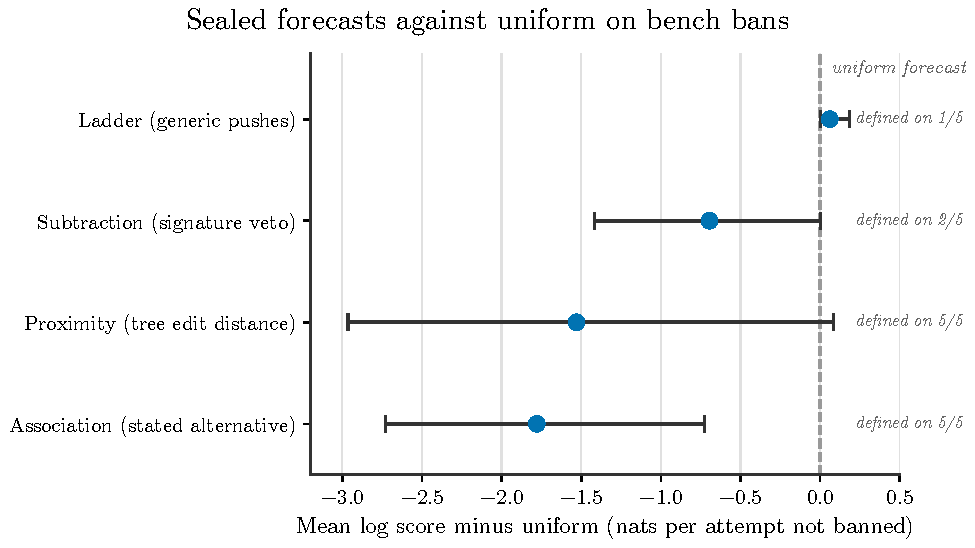
\includegraphics[width=\linewidth,height=0.78\textheight,keepaspectratio]{figures/fig_bench_forecasts_v0.pdf}
\caption{Horizontal dot-and-whisker plot of each sealed forecast family's mean log score minus the uniform reference (x-axis: Mean log score minus uniform, in nats per attempt not banned; shown over -3.2 to 0.5), over the five gated Qwen3-8B modal bench bans (kth smallest, find duplicate, two sum, connected components, merge intervals). Rows, top to bottom, each drawn with one blue point marker and a black 95\% task-cluster bootstrap interval whisker (no per-family colour coding): Ladder (generic pushes) +0.061, CI [0.000, 0.182]; Subtraction (signature veto) -0.695, CI [-1.416, 0.000]; Proximity (tree edit distance) -1.529, CI [-2.965, 0.086]; Association (stated alternative) -1.779, CI [-2.729, -0.729]. The grey dashed vertical line marks the uniform-forecast baseline at 0; the italic text beside each row states how many of the 5 gated events that family's forecast was actually defined on (1\slash{}5, 2\slash{}5, 5\slash{}5, 5\slash{}5) -- an undefined forecast is scored as uniform, so a value near 0 can reflect that rather than a real tie with uniform. No family clears the uniform baseline by a clear margin: Ladder's point and its whole interval sit at or just above zero, but it was defined on only one of the five events; Subtraction's and Proximity's intervals both span zero; Association, the model's own stated alternative, sits furthest below uniform, with its interval entirely negative.}
\label{fig:fig_bench_forecasts}
\end{figure}
The landings were specific to the banned task and mostly unforeseen. Find duplicate went to index marking, which places each value at index value minus one: the model wrote it only once in 40 template-forced attempts in the bench build (adherence 0.28 over all forced prompts), and no family nominated it. Connected components went to BFS (83 of 100) while subtraction and association said DFS. Merge intervals went mostly to programs labelled other, which failed every time (0 of 44) \emph{(corrected in iteration 4 from the earlier description as a merge sweep without sorting: a manual read of all 44 found 29 programs that mark coverage over the coordinate range in a boolean array, 12 unsorted sweeps and 3 others; Section 4.2.4)}. On Fibonacci the programs labelled other used Binet's closed form, which also failed (0 of 33). Only the kth smallest landing (quickselect: ladder, association and the 8-bit likelihood) and the two sum landing (brute force: proximity) were hit by a top-1 nomination. On 3 of the 5 gated events no family's top-1 named the realised landing.

\textbf{Signature vetoes move the surface, not the algorithm.} The distinctive n-gram fired in 95\% of twin samples and the redraw always avoided it, yet the default survived every persistent and iterated round on 9 of 12 tasks. The model respelled the same mechanism: on kth smallest \texttt{nums.\allowbreak{}sort(\allowbreak{})} became \texttt{return sorted(\allowbreak{}nums)[\allowbreak{}k-\allowbreak{}1]}, and on two sum the next round's distinctive token was \texttt{\textvisiblespace{}\allowbreak{}compliment}, a misspelling that dodges \texttt{\textvisiblespace{}\allowbreak{}complement}. The vetoed text reappeared under another token split in 23\% of one-shot samples and 54\% by round 2. Where vetoes did move off the default, most outputs were invalid. The sham veto of a shared token broke programs without moving the algorithm (for example, the model indented with non-breaking spaces after the indentation token was masked). The test of whether the one-shot veto reproduces the ban's landing was therefore undetermined: the one-shot veto never reached 0.5 avoidance on a gated task (kth smallest 0.38, connected components 0.33, others 0). Descriptively, the last iterated round was eligible on find duplicate and connected components, and both landed elsewhere than the ban: sort and adjacent check against the ban's index marking (Jensen-Shannon divergence 0.77 against a template resampling 95th percentile of 0.09), and DFS against the ban's BFS (0.58 against 0.09).

\textbf{Generic pushes rarely move this collapsed model.} Nonce bans moved nothing except on first and last position, whose twin was already noisy. The novelty instruction moved kth smallest (all 50 off the default, 45 to quickselect), longest increasing subsequence, Fibonacci, substring search and connected components. One of three random directions moved kth smallest (avoidance 0.82, mostly quickselect) and connected components a little (0.26, to DFS); the HF twin control kept the default at 0.98 and 1.00 on those tasks, so the movement is not an engine artefact. The positive control of patching the ban's own task specification states into the twin at layers 12 to 23 reproduced the ban's avoidance only on kth smallest and connected components (1.00 each), partly on two sum (0.22) and merge intervals (0.14), and nowhere else. On most tasks the ban's effect is not carried by the task specification states of that band alone, which Section 3.6 confirms behaviourally.

\textbf{Wording.} The banned share differed by template far more than by chance (Table 97), with a likelihood ratio of 374 on 4 degrees of freedom (p about 1e-79). A mixed logistic model put the template standard deviation at 2.0 logits [1.1, 3.5] and the template by task deviation at 1.25 [1.05, 1.49]; a shuffled template placebo gave p = 0.44 (0.39 in the second audit's own likelihood ratio test). Under the fourth template the default kept at least 70\% of samples on 10 of 12 tasks.

\begin{table}[H]
\renewcommand{\thetable}{97}
\centering\footnotesize\setlength{\tabcolsep}{4.0pt}
\caption{Banned programs per template (of 20) under each modal bench ban. Source: bench forecast experiment \texttt{results/\allowbreak{}template\_\allowbreak{}effect.\allowbreak{}json}. [Source: iteration 3, artifact \nolinkurl{gen_art_experiment_13}.]}\label{tab:t104}
\begin{tabular}{>{\raggedright\arraybackslash\hspace{0pt}}p{0.4196\linewidth}>{\raggedright\arraybackslash\hspace{0pt}}p{0.0950\linewidth}>{\raggedright\arraybackslash\hspace{0pt}}p{0.0950\linewidth}>{\raggedright\arraybackslash\hspace{0pt}}p{0.0950\linewidth}>{\raggedright\arraybackslash\hspace{0pt}}p{0.0971\linewidth}>{\raggedright\arraybackslash\hspace{0pt}}p{0.0950\linewidth}}
\toprule
\textbf{Task} & \textbf{First} & \textbf{Second} & \textbf{Third} & \textbf{Fourth} & \textbf{Fifth} \\
\midrule
kth smallest & 0 & 0 & 0 & 3 & 0 \\
substring search & 11 & 6 & 19 & 20 & 4 \\
find duplicate & 0 & 1 & 0 & 20 & 0 \\
two sum & 0 & 0 & 0 & 14 & 0 \\
connected components & 0 & 0 & 0 & 0 & 0 \\
nonoverlapping intervals & 20 & 20 & 20 & 20 & 20 \\
Fibonacci & 20 & 6 & 15 & 20 & 5 \\
topological order & 20 & 16 & 19 & 20 & 17 \\
merge intervals & 12 & 5 & 3 & 20 & 2 \\
first and last position & 20 & 20 & 20 & 20 & 17 \\
top-k frequent & 12 & 2 & 16 & 20 & 2 \\
longest increasing subsequence & 20 & 20 & 20 & 20 & 18 \\
All tasks (of 240) & 135 & 96 & 132 & 197 & 85 \\
\bottomrule
\end{tabular}
\end{table}

\begin{figure}[!htbp]
\centering
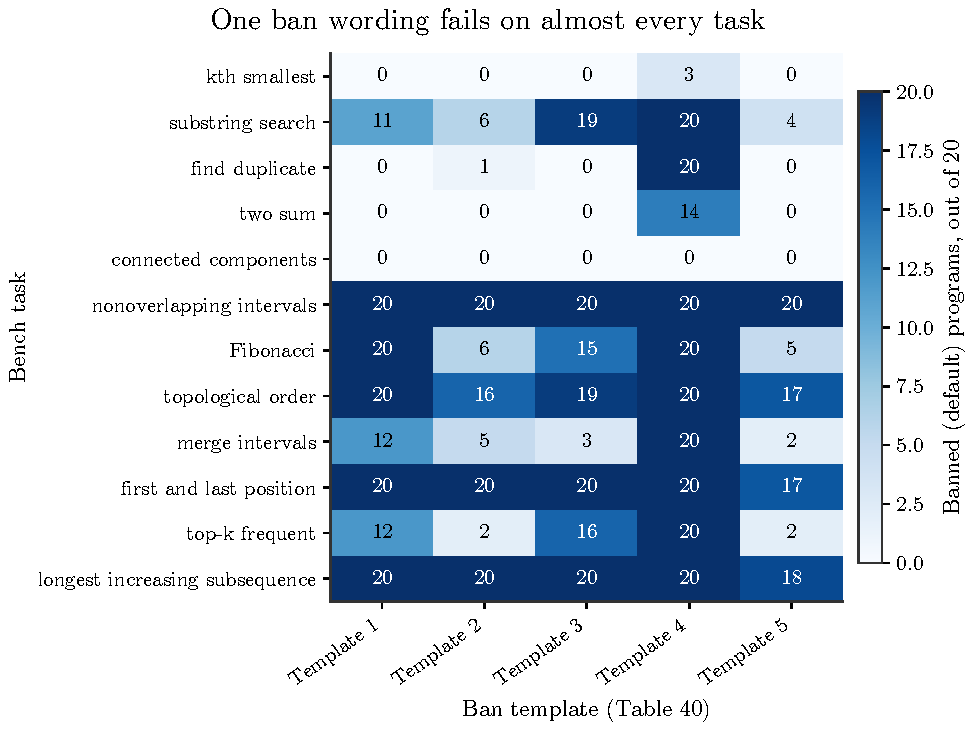
\includegraphics[width=\linewidth,height=0.85\textheight,keepaspectratio]{figures/fig_bench_templates_v0.pdf}
\caption{Heatmap of banned (default) programs out of 20 sampled completions, for each of 12 Qwen3-8B bench tasks (rows) under each of 5 ban-prompt templates from Table 40 (columns, labelled Template 1--5). Cell shade and the printed integer give the count, out of 20, of programs that still implement the task's default (banned) algorithm despite the prompt forbidding it; colour runs from white (0) to dark blue (20), with no fit or trend line drawn. Pooled over all 12 tasks (240 samples per template), Template 4 -- which states only that the default ``is not allowed here'' -- leaves the default in place in 197 of 240 samples, versus 85--135 for the other four templates, and is the only template that fails on 10 of the 12 tasks (all but kth smallest and connected components). Four tasks -- nonoverlapping intervals, topological order, first\slash{}last position, and longest increasing subsequence -- keep the default in at least 16 of 20 samples under every one of the five templates.}
\label{fig:fig_bench_templates}
\end{figure}
\textbf{The bench likelihoods on the screen's path.} Rescoring the frozen bench likelihood sets with fp32 activations, the path the likelihood screen had validated, moved the adherence corrected likelihood of a cell by a median 0.88 nats (maximum 9.0) from the 8-bit prompt log probabilities. Every shift above 2 nats sat in a cell with Kish ESS below 5, and the argmax algorithm was unchanged on 12 of 12 tasks. The rescoring code first reproduced 5 stored program scores of the likelihood screen within 0.021 nats. The 8-bit likelihood forecast was defined only on kth smallest, where it named quickselect.

\textbf{Checks.} An independent rederivation from the raw label files reproduced every headline number with no mismatch; a task shuffled placebo collapsed the family wins (mean ladder wins 0.52 against 3 observed); a template permutation test gave p = 0.002 on real data and 0.42 on shuffled data; and the hash chain verified. One file changed after the seal: absolute input paths in a configuration module were replaced by relative paths for portability, with the sealed bytes and the diff kept. GPU time was about 45 minutes, judge spend USD 0.024 over 344 calls.

\FloatBarrier
\subsection*{3.4 Exposure experiment: show a solution, ban it, and see what replaces it (Qwen3-8B)}
\addcontentsline{toc}{subsection}{3.4 Exposure experiment: show a solution, ban it, and see what replaces it (Qwen3-8B)}
\noindent{\small\emph{Artifact: \nolinkurl{gen_art_experiment_14}.}}\par\medskip
\textbf{Why.} Under total collapse, every modal ban's association and ladder nominations are close to each other, and bench bans in Qwen3-8B pass the gate on only five tasks. Exposure bans  create events where the two accounts finally disagree: the prompt shows correct programs of a non-default algorithm Y, which the model then copies, and asks for a solution that does not use Y. Subtraction predicts a return to what the model would write without Y in view, which in context is its default; substitution predicts Y's stated alternative.

\textbf{Design.} The experiment took every non-default algorithm Y of the 12 frozen bench tasks with at least one correct forced program: 33 Y. We call the 19 whose frozen associate differs from the default priority Y. The prompt shows up to 5 name-scrubbed correct programs of Y and then asks one of three things: write a correct solution, which we call the copy twin; write a correct solution that does not use Y, the named ban (the fifth template); or write a correct solution that uses a different algorithm from the one above, the unnamed ban. Each arm had 50 samples per Y, with seeds shared across arms (Qwen3-8B bf16, vLLM 0.11.0, one 23 GB NVIDIA GPU). Four forecasts were committed by hash before any ban sample: ladder (the context-free default), association (the modal frozen answer for Y), proximity (the survivor whose forced programs are nearest the shown programs by Zhang-Shasha tree edit distance [64]) and the subtraction forecast in context (the landing of an iterated persistent signature veto of Y under the copy twin prompt, with no ban text). GPU smoke tests confirmed the veto: 0 of 20 veto samples contained the vetoed n-gram against 20 of 20 copy samples, an inert veto left 20 of 20 outputs identical, and veto and copy twins diverged exactly at the vetoed position in 20 of 20. Of 10,600 programs, 7,478 were labelled by agreeing runtime and AST labellers, 1,398 by the judge, 147 by runtime alone, and 1,577 had no code block (mostly from veto rounds).

\textbf{Showing a solution makes the model copy it, and banning it sends the model home.} Under the copy twin a mean 0.93 of attempts used the shown algorithm (median 1.00; none below 0.2), and the default appeared in 0.05. Under the named ban, avoidance averaged 0.95 and the default's share of attempts rose to 0.72 (Table 98). We call this return to the context-free default \emph{snap-back}. In 24 of the 31 gated named events the modal replacement was the default (14 of 18 for priority Y). Named and unnamed bans picked the same modal replacement for 0.88 of Y, and their landings were consistent under the Jensen-Shannon resampling null for 0.79 of Y: naming Y adds little beyond asking for a different algorithm.

\begin{table}[H]
\renewcommand{\thetable}{98}
\centering\small\setlength{\tabcolsep}{4.0pt}
\caption{The default's share of attempts by arm: the mean over the 33 shown algorithms of each one's share (over 29 for the final veto round, where 4 shown algorithms had no valid attempts). Source: exposure experiment \texttt{README.\allowbreak{}md}, \texttt{results/\allowbreak{}other\_\allowbreak{}reports.\allowbreak{}json}. [Source: iteration 3, artifact \nolinkurl{gen_art_experiment_14}.]}\label{tab:t105}
\begin{tabular}{>{\raggedright\arraybackslash\hspace{0pt}}p{0.1514\linewidth}>{\raggedright\arraybackslash\hspace{0pt}}p{0.4510\linewidth}>{\raggedright\arraybackslash\hspace{0pt}}p{0.1514\linewidth}>{\raggedright\arraybackslash\hspace{0pt}}p{0.1759\linewidth}}
\toprule
\textbf{Copy twin} & \textbf{Final veto round under the copy twin} & \textbf{Named ban} & \textbf{Unnamed ban} \\
\midrule
0.05 & 0.10 & 0.72 & 0.82 \\
\bottomrule
\end{tabular}
\end{table}

\begin{figure}[!htbp]
\centering\captionsetup{font=footnotesize}
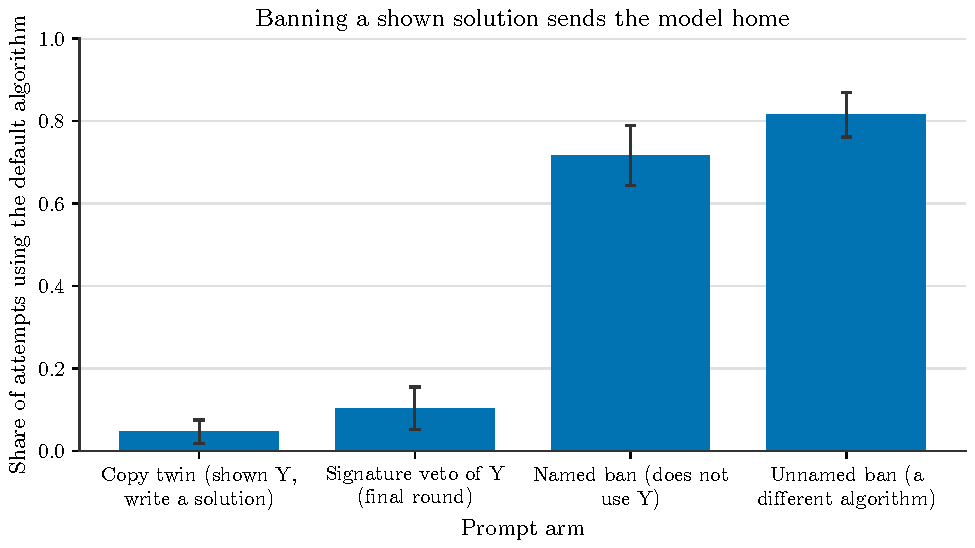
\includegraphics[width=\linewidth,height=0.78\textheight,keepaspectratio]{figures/fig_exposure_snapback_v0.pdf}
\caption{Mean share of attempts using Qwen3-8B's context-free default algorithm, by prompt arm, averaged over the shown non-default algorithms Y of the exposure experiment (50 sampled attempts per Y and arm). Single-colour bars, left to right: Copy twin (shown up to five correct programs of Y and asked only to write a solution, with no ban stated; n=33 Y); Signature veto of Y, final round (the prompt never states a ban in words; Y's distinctive token n-gram is vetoed at generation time instead; n=29 Y with a valid attempt in the final round, 4 of 33 excluded for having none); Named ban (the prompt states the solution must not use Y; n=33 Y); Unnamed ban (the prompt states the solution must use a different algorithm from the one shown, without naming Y; n=33 Y). Error bars show $\pm$1 standard error of the mean across Y. Default usage nearly disappears when a solution is shown and copying is allowed (mean share 0.05; in that same arm Y itself is used in 0.93 of attempts) and stays low under the silent token veto (0.10), then snaps back to a high rate once the ban is stated in the prompt, whether Y is named (0.72) or left unnamed (0.82), in neither case moving toward Y's own stated alternative algorithm.}
\label{fig:fig_exposure_snapback}
\end{figure}
Table 99 gives every named exposure event. The frozen rule (at least 3 wins by 0.10 nats on gated, disagreeing events) advanced the ladder with 7 wins, against subtraction 2, association 2 and proximity 0, so the frozen branch is SUBTRACTION\slash{}LADDER, with the ladder advancing. Gating removed two events (size-k heap on kth smallest and patience sorting on longest increasing subsequence, where Y was kept), and 30 of the 31 gated events had disagreeing nominations.

{\tiny\setlength{\tabcolsep}{2.5pt}\renewcommand{\thetable}{99}
\begin{longtable}{>{\raggedright\arraybackslash\hspace{0pt}}p{0.0858\linewidth}>{\raggedright\arraybackslash\hspace{0pt}}p{0.0710\linewidth}>{\raggedright\arraybackslash\hspace{0pt}}p{0.0646\linewidth}>{\raggedright\arraybackslash\hspace{0pt}}p{0.0600\linewidth}>{\raggedright\arraybackslash\hspace{0pt}}p{0.0706\linewidth}>{\raggedright\arraybackslash\hspace{0pt}}p{0.0451\linewidth}>{\raggedright\arraybackslash\hspace{0pt}}p{0.0677\linewidth}>{\raggedright\arraybackslash\hspace{0pt}}p{0.0705\linewidth}>{\raggedright\arraybackslash\hspace{0pt}}p{0.0587\linewidth}>{\raggedright\arraybackslash\hspace{0pt}}p{0.0408\linewidth}>{\raggedright\arraybackslash\hspace{0pt}}p{0.0824\linewidth}>{\raggedright\arraybackslash\hspace{0pt}}p{0.0739\linewidth}>{\raggedright\arraybackslash\hspace{0pt}}p{0.0703\linewidth}}
\caption{Every named exposure event (N = 50 per arm). The winner is the family that beats the next best by at least 0.10 nats on a gated event with disagreeing nominations (none when the top two tie; n\slash{}a when the event is ungated or its nominations do not disagree). An undefined subtraction forecast is scored as uniform. Source: exposure experiment \texttt{results/\allowbreak{}c1\_\allowbreak{}events.\allowbreak{}jsonl}, \texttt{results/\allowbreak{}arm\_\allowbreak{}stats.\allowbreak{}json}. [Source: iteration 3, artifact \nolinkurl{gen_art_experiment_14}.]}\label{tab:t106}\\
\toprule
\textbf{Task} & \textbf{Shown algorithm Y} & \textbf{Priority} & \textbf{Default} & \textbf{Associate of Y} & \textbf{Copy: share of Y} & \textbf{Named: avoidance} & \textbf{Named landing (attempts not Y)} & \textbf{Default share} & \textbf{Gate} & \textbf{Subtraction top-1} & \textbf{Proximity top-1} & \textbf{Winner} \\
\midrule
\endfirsthead
\multicolumn{13}{l}{\emph{Table 99, continued}}\\
\toprule
\textbf{Task} & \textbf{Shown algorithm Y} & \textbf{Priority} & \textbf{Default} & \textbf{Associate of Y} & \textbf{Copy: share of Y} & \textbf{Named: avoidance} & \textbf{Named landing (attempts not Y)} & \textbf{Default share} & \textbf{Gate} & \textbf{Subtraction top-1} & \textbf{Proximity top-1} & \textbf{Winner} \\
\midrule
\endhead
\bottomrule
\endlastfoot
kth smallest & size-k heap & yes & full sort & quickselect & 1.00 & 0.20 & full sort 10 & 0.20 & fail & undefined & heapify and pop & n\slash{}a \\
kth smallest & heapify and pop & yes & full sort & quickselect & 1.00 & 1.00 & quickselect 45, full sort 5 & 0.10 & pass & undefined & full sort & association \\
kth smallest & quickselect & yes & full sort & heapify and pop & 1.00 & 1.00 & full sort 50 & 1.00 & pass & undefined & median of medians & ladder \\
kth smallest & median of medians & yes & full sort & quickselect & 1.00 & 1.00 & quickselect 50 & 0.00 & pass & quickselect & quickselect & none \\
kth smallest & counting sort & yes & full sort & quickselect & 0.80 & 1.00 & full sort 49, quickselect 1 & 0.98 & pass & undefined & full sort & ladder \\
substring search & KMP & no & naive & naive & 1.00 & 1.00 & naive 50 & 1.00 & pass & undefined & Boyer-Moore-Horspool & none \\
substring search & Rabin-Karp & yes & naive & KMP & 1.00 & 1.00 & naive 50 & 1.00 & pass & undefined & Boyer-Moore-Horspool & ladder \\
substring search & Z algorithm & yes & naive & KMP & 1.00 & 1.00 & naive 44, KMP 6 & 0.88 & pass & undefined & Boyer-Moore-Horspool & ladder \\
substring search & Boyer-Moore-Horspool & yes & naive & KMP & 1.00 & 1.00 & naive 50 & 1.00 & pass & undefined & naive & ladder \\
substring search & built-in find & yes & naive & KMP & 1.00 & 1.00 & naive 50 & 1.00 & pass & undefined & naive & none \\
find duplicate & sort and adjacent check & yes & hash set & Floyd cycle detection & 1.00 & 1.00 & hash set 50 & 1.00 & pass & undefined & hash set & none \\
find duplicate & Floyd cycle detection & no & hash set & hash set & 1.00 & 1.00 & hash set 50 & 1.00 & pass & undefined & hash set & none \\
find duplicate & binary search on values & yes & hash set & Floyd cycle detection & 0.98 & 1.00 & hash set 50 & 1.00 & pass & undefined & hash set & ladder \\
find duplicate & index marking & yes & hash set & Floyd cycle detection & 1.00 & 1.00 & hash set 50 & 1.00 & pass & undefined & sort and adjacent check & ladder \\
two sum & sort and two pointers & no & hash map & hash map & 1.00 & 1.00 & hash map 50 & 1.00 & pass & undefined & hash map & none \\
two sum & brute force & yes & hash map & sort and two pointers & 0.36 & 1.00 & hash map 50 & 1.00 & pass & hash map & hash map & none \\
two sum & sort and binary search & yes & hash map & sort and two pointers & 1.00 & 1.00 & hash map 50 & 1.00 & pass & undefined & hash map & none \\
connected components & BFS & yes & union find & DFS & 1.00 & 1.00 & DFS 50 & 0.00 & pass & undefined & DFS & none \\
connected components & DFS & yes & union find & BFS & 1.00 & 1.00 & BFS 50 & 0.00 & pass & undefined & BFS & association \\
connected components & label propagation & yes & union find & DFS & 0.84 & 1.00 & union find 49, DFS 1 & 0.98 & pass & union find & union find & none \\
nonoverlapping intervals & memoised recursion & no & greedy by end & greedy by end & 1.00 & 1.00 & DP with bisect 41, other 7, greedy by end 2 & 0.04 & pass & undefined & greedy by end & subtraction \\
nonoverlapping intervals & DAG longest path & no & greedy by end & greedy by end & 1.00 & 0.94 & greedy by end 47 & 0.94 & pass & undefined & greedy by end & none \\
Fibonacci & memoised recursion & no & iteration & iteration & 1.00 & 1.00 & iteration 50 & 1.00 & pass & undefined & iteration & none \\
Fibonacci & matrix power & no & iteration & iteration & 1.00 & 1.00 & iteration 50 & 1.00 & pass & undefined & fast doubling & none \\
Fibonacci & fast doubling & no & iteration & iteration & 1.00 & 1.00 & other 49, iteration 1 & 0.02 & pass & undefined & iteration & none \\
merge intervals & union find & no & sort and sweep & sort and sweep & 1.00 & 1.00 & sort and sweep 50 & 1.00 & pass & undefined & sort and sweep & none \\
first and last position & bisect module & no & binary search & binary search & 1.00 & 1.00 & other 49, binary search 1 & 0.02 & pass & undefined & binary search & none \\
first and last position & exponential search & no & binary search & binary search & 0.28 & 1.00 & binary search 50 & 1.00 & pass & binary search & binary search & n\slash{}a \\
top-k frequent & heap & no & sort by count & sort by count & 1.00 & 1.00 & sort by count 50 & 1.00 & pass & undefined & sort by count & none \\
top-k frequent & bucket sort & no & sort by count & sort by count & 0.36 & 1.00 & sort by count 50 & 1.00 & pass & undefined & heap & none \\
top-k frequent & quickselect on counts & yes & sort by count & heap & 1.00 & 0.94 & sort by count 31, bucket sort 7, other 6, heap 3 & 0.62 & pass & undefined & bucket sort & none \\
longest increasing subsequence & patience sorting & no & quadratic DP & quadratic DP & 1.00 & 0.16 & quadratic DP 8 & 0.16 & fail & undefined & quadratic DP & n\slash{}a \\
longest increasing subsequence & Fenwick tree & yes & quadratic DP & patience sorting & 1.00 & 1.00 & quadratic DP 35, patience sorting 15 & 0.70 & pass & undefined & quadratic DP & subtraction \\
\end{longtable}}

The paired tests point the same way but none survives correction (Table 100). Over the 30 gated disagreeing named events, paired Wilcoxon signed-rank tests [65] of the per-event log score differences, Holm corrected over four comparisons, favour the ban-free families over association by about 1 nat per attempt, with task cluster bootstrap intervals above zero, but Holm adjusted p stays at 0.081. Top-1 hit rates on the gated named events were 0.77 for the ladder, 0.61 for proximity, 0.45 for association and 0.36 for subtraction. \emph{(Correction, iteration 4: the subtraction rate is almost entirely tie credit. Subtraction was defined for 4 of 33 shown algorithms, and where defined it named the landing 4 of 4 times in both the named and the unnamed arms (median of medians to quickselect, brute force to hash map, label propagation to union find, exponential search to binary search); on every other event its uniform tie earned fractional credit. Defined-only rates are in Section 4.2.6.)} The unnamed events, which are descriptive, give the same branch, and there the ladder beats association after Holm correction (+1.42 nats, adjusted p = 0.0056).

\begin{table}[H]
\renewcommand{\thetable}{100}
\centering\footnotesize\setlength{\tabcolsep}{4.0pt}
\caption{Paired log score differences over the 30 gated, disagreeing named exposure events (positive favours the first family). Source: exposure experiment \texttt{results/\allowbreak{}c1\_\allowbreak{}summary.\allowbreak{}json}. [Source: iteration 3, artifact \nolinkurl{gen_art_experiment_14}.]}\label{tab:t107}
\begin{tabular}{>{\raggedright\arraybackslash\hspace{0pt}}p{0.3059\linewidth}>{\raggedright\arraybackslash\hspace{0pt}}p{0.1206\linewidth}>{\raggedright\arraybackslash\hspace{0pt}}p{0.2077\linewidth}>{\raggedright\arraybackslash\hspace{0pt}}p{0.1313\linewidth}>{\raggedright\arraybackslash\hspace{0pt}}p{0.1476\linewidth}}
\toprule
\textbf{Difference} & \textbf{Mean (nats)} & \textbf{Task cluster 95\% CI} & \textbf{p} & \textbf{Holm adjusted p} \\
\midrule
Subtraction minus association & +1.02 & [0.35, 1.56] & 0.020 & 0.081 \\
Ladder minus association & +1.29 & [0.10, 2.38] & 0.027 & 0.081 \\
Ladder minus proximity & +0.50 & [-0.40, 1.16] & not reported & 0.159 \\
Subtraction minus proximity & +0.23 & not reported & not reported & 0.96 \\
\bottomrule
\end{tabular}
\end{table}

\textbf{How strong the verdict is.} The counting rule is not a significance test. In a unit test with no information, it advanced some family in 85\% of 200 simulated draws, while the Holm-corrected Wilcoxon test erred in 2\%; on the real events, a label permutation placebo advanced some family in 100\% of draws (the ladder in 43\%). The branch label is therefore weak evidence, and the paired tests are the informative part. The signature veto rarely removed Y. The subtraction forecast in context was defined for only 4 of 33 Y (median of medians to quickselect, brute force to hash map, label propagation to union find, exponential search to binary search). For 25 of 33 Y, Y still re-emerged in at least 20\% of attempts after three rounds. The veto cost a mean 0.70 of pass rate, and 46\% of final round outputs were invalid. Because an undefined subtraction forecast is uniform, its tied top-1 is what makes almost every event disagreeing. Every preregistered sensitivity returned the ladder with 7 to 9 wins (subtraction top-1, excluding co-vetoed survivors, priority Y only with 18 events, token distance proximity, correct-only landings, and excluding labeller-flagged tasks) except the one that drops events with an undefined subtraction forecast, which leaves 2 events and is undetermined. An exploratory comparison of ladder, association and proximity on the 21 events where those three disagree gave wins 8, 3 and 0 (ladder minus association p = 0.027, Holm over three 0.081). The secondary exposure test, whether the ban's modal survivor matches the veto's where the associate differs, had 2 qualifying events (brute force and label propagation); both agreed, but both landings are the default, so this is snap-back, not a test of substitution.

\textbf{Wording.} A template arm (first to fourth templates, 10 samples for each of the 19 priority Y; descriptive and never in the contest) gave mean avoidance 0.93, 0.94, 0.96 and 0.81: the fourth template is again the weakest. \emph{(Added in iteration 4: wording also changes the landing. Pooled over the first four templates the modal replacement is the default for 13 of 19 priority Y, against 15 of 19 under the fifth template of Table 99; it flips to the associate for the size-k heap (quickselect 13, full sort 2, against full sort 10 under the fifth template) and for the Z algorithm (KMP 29, naive 11, against naive 44, KMP 6). Snap-back as recorded in Table 99 rests on the fifth template.)} A stop token bug in the first round-2 veto run (the end-of-turn token was chosen as the n-gram) was found and fixed; the 750 affected samples are kept apart. Deduplication left 11 of 33 Y with a single shown program. GPU time was about 1.0 GPU hour, judge spend USD 0.096 over 1,229 calls, and an independent rederivation matched all 66 events.

\FloatBarrier
\subsection*{3.5 Llama bench experiment: the same forecast contest in a second model family}
\addcontentsline{toc}{subsection}{3.5 Llama bench experiment: the same forecast contest in a second model family}
\noindent{\small\emph{Artifact: \nolinkurl{gen_art_experiment_15}.}}\par\medskip
\textbf{Why.} Llama-3.1-8B-Instruct [22] is less collapsed than Qwen3-8B on the bench pilot, so it supplies present minor bans, where a correct minor algorithm already exists and subtraction makes a non-trivial prediction. This experiment  replicated the frozen forecast contest on the 12 bench tasks in bf16 (pinned revision), with every forecast computed without ban text and hash chained before any ban prompt was rendered (a grep audit found 0 ban prompts in the 10,328 rows generated before the commit).

\textbf{Design.} The default of each task was frozen from a decision set (the 8-bit Llama pilot pooled with 600 bf16 neutral twin samples after a homogeneity test) as the modal correct label when at least 10 programs were correct, else the modal attempted label (Table 101). Present minor events required at least 10\% of correct programs, at least 3 correct, and at least 10 correct programs on the task. The four forecasts were built as in the Qwen3-8B experiment. The subtraction forecast used exact one-shot, persistent and iterated signature vetoes by truncate and redraw; the ladder pooled the nonce ban, the novelty instruction and three matched-norm random directions added at the task specification positions of layers 11 to 21 during prefill; association used Llama's own frozen answers; and proximity used Zhang-Shasha distance [64]. Association and proximity took a form that transfers the default's mass, with point mass forms as sensitivities. Then 1,800 bans were sampled (12 modal and 6 present minor events, 5 templates by 20) and labelled with the bench labellers; references were recovered 50 of 50, and gold agreement was 0.959. A second blind judge audited 60 Llama programs at 0.88 agreement, below 0.85 on four tasks (nonoverlapping intervals, kth smallest, two sum, top-k frequent).

\begin{table}[H]
\renewcommand{\thetable}{101}
\centering\scriptsize\setlength{\tabcolsep}{2.5pt}
\caption{Llama defaults and events, frozen before any ban (decision set: 8-bit pilot plus bf16 neutral twins). Source: Llama bench experiment \texttt{README.\allowbreak{}md}, \texttt{predictions/\allowbreak{}events.\allowbreak{}json}. [Source: iteration 3, artifact \nolinkurl{gen_art_experiment_15}.]}\label{tab:t108}
\begin{tabular}{>{\raggedright\arraybackslash\hspace{0pt}}p{0.2151\linewidth}>{\raggedright\arraybackslash\hspace{0pt}}p{0.1280\linewidth}>{\raggedright\arraybackslash\hspace{0pt}}p{0.1205\linewidth}>{\raggedright\arraybackslash\hspace{0pt}}p{0.0945\linewidth}>{\raggedright\arraybackslash\hspace{0pt}}p{0.0923\linewidth}>{\raggedright\arraybackslash\hspace{0pt}}p{0.1019\linewidth}>{\raggedright\arraybackslash\hspace{0pt}}p{0.0959\linewidth}>{\raggedright\arraybackslash\hspace{0pt}}p{0.0652\linewidth}}
\toprule
\textbf{Task} & \textbf{Pilot mode} & \textbf{Default} & \textbf{Default from attempts} & \textbf{Valid programs} & \textbf{Correct programs} & \textbf{Default share} & \textbf{Hill\_\allowbreak{}cc} \\
\midrule
kth smallest & heapify and pop & full sort &  & 94 & 18 & 0.17 & 3.80 \\
substring search & naive & naive &  & 89 & 49 & 0.54 & 2.00 \\
find duplicate & hash set & hash set &  & 93 & 34 & 0.44 & 1.48 \\
two sum & hash map & hash map &  & 99 & 84 & 0.97 & 1.07 \\
connected components & union find & union find &  & 97 & 74 & 0.75 & 1.59 \\
nonoverlapping intervals & greedy by end & greedy by end & yes & 89 & 8 & 0.63 & 2.46 \\
Fibonacci & matrix power & matrix power &  & 96 & 44 & 0.76 & 1.78 \\
topological order & Kahn & Kahn &  & 99 & 88 & 0.98 & 1.06 \\
merge intervals & sort and sweep & sort and sweep &  & 89 & 65 & 1.00 & 1.00 \\
first and last position & binary search & binary search &  & 93 & 54 & 0.99 & 1.10 \\
top-k frequent & heap & heap &  & 86 & 22 & 0.62 & 1.80 \\
longest increasing subsequence & quadratic DP & quadratic DP &  & 94 & 68 & 0.87 & 1.08 \\
\bottomrule
\end{tabular}
\end{table}

Present minor events: top-k frequent sort by count (6 of 22 correct), kth smallest heapify and pop (4 of 18), kth smallest quickselect (4 of 18), substring search KMP (9 of 49), connected components DFS (13 of 74), kth smallest size-k heap (3 of 18).

\textbf{The contest does not resolve in Llama.} Thirteen of 18 events passed the gate and 11 were gated and disagreeing, but only 2 had a winner by 0.10 nats (Table 102). One was the subtraction forecast on two sum, through its undefined forecast scored as uniform, because the ban split between sort and two pointers (42) and brute force (32). The other was association on kth smallest heapify and pop. No family advances; the preregistered branch is NO FAMILY ADVANCES, aimed but unresolved. The landing is aimed: the ladder and association each named the realised landing on 7 of 13 gated events, against a chance rate of about 0.27 (exact binomial p = 0.033 each); subtraction hit 4 of 12 (p = 0.38) and proximity 3 of 13 (p = 0.71). \emph{(Correction, iteration 4: these hits were scored against a label this section did not define. Modal events were scored against the modal landing, but the six present minor events were scored against the survivor with the largest excess over the renormalised ban-free baseline. The ladder also nominated other on 3 of the 13 gated events, and on find duplicate both its nomination and the landing were other (50 of 94 attempts, 71 not banned; 2 correct). With other excluded as nominee and as landing, the ladder hits 6 of 13 (Poisson-binomial p = 0.100) and association 7 of 13 (p = 0.032), so only association is above chance. On the present minor events Llama returns to its default: union find 0.93, heap 0.72 and naive 0.73 of attempts not banned. Section 4.2.3.)} Five defaults resisted the ban itself (nonoverlapping intervals, topological order, merge intervals, first and last position, longest increasing subsequence; avoidance 0.04 to 0.30).

\begin{table}[H]
\renewcommand{\thetable}{102}
\centering\tiny\setlength{\tabcolsep}{2.5pt}
\caption{Every Llama ban event (N = 100). s\_\allowbreak{}X is the banned algorithm's share of attempts in the decision set before the ban; \textdagger{} marks a present minor event. Each family's top-1 is given with its mean log score per attempt not banned in parentheses; a forecast marked undefined is scored as uniform. Source: Llama bench experiment \texttt{README.\allowbreak{}md}, \texttt{results/\allowbreak{}c1\_\allowbreak{}events.\allowbreak{}jsonl}. [Source: iteration 3, artifact \nolinkurl{gen_art_experiment_15}.]}\label{tab:t109}
\begin{tabular}{>{\raggedright\arraybackslash\hspace{0pt}}p{0.0765\linewidth}>{\raggedright\arraybackslash\hspace{0pt}}p{0.0291\linewidth}>{\raggedright\arraybackslash\hspace{0pt}}p{0.0630\linewidth}>{\raggedright\arraybackslash\hspace{0pt}}p{0.0364\linewidth}>{\raggedright\arraybackslash\hspace{0pt}}p{0.0606\linewidth}>{\raggedright\arraybackslash\hspace{0pt}}p{0.0627\linewidth}>{\raggedright\arraybackslash\hspace{0pt}}p{0.0736\linewidth}>{\raggedright\arraybackslash\hspace{0pt}}p{0.0535\linewidth}>{\raggedright\arraybackslash\hspace{0pt}}p{0.0736\linewidth}>{\raggedright\arraybackslash\hspace{0pt}}p{0.0659\linewidth}>{\raggedright\arraybackslash\hspace{0pt}}p{0.0818\linewidth}>{\raggedright\arraybackslash\hspace{0pt}}p{0.0627\linewidth}>{\raggedright\arraybackslash\hspace{0pt}}p{0.0619\linewidth}>{\raggedright\arraybackslash\hspace{0pt}}p{0.0498\linewidth}}
\toprule
\textbf{Event} & \textbf{s\_\allowbreak{}X} & \textbf{Avoidance} & \textbf{Gate} & \textbf{Attempts not banned} & \textbf{Modal landing} & \textbf{Subtraction} & \textbf{Ladder} & \textbf{Association} & \textbf{Proximity} & \textbf{Renormalised baseline} & \textbf{Winner (margin)} & \textbf{Hill\_\allowbreak{}cc (correct programs)} & \textbf{Other \slash{} invalid} \\
\midrule
kth smallest, ban full sort & 0.17 & 0.95 & pass & 87 & quickselect & heapify and pop (-1.71) & other (-1.46) & quickselect (-1.40) & size-k heap (-1.66) & -1.64 & none (0.06) & 1.00 (15) & 0.09 \slash{} 0.08 \\
substring search, ban naive & 0.54 & 0.79 & pass & 64 & KMP & Rabin-Karp (-1.20) & KMP (-1.25) & KMP (-1.18) & built-in find (-1.83) & -1.20 & none (0.02) & 1.38 (20) & 0.05 \slash{} 0.19 \\
find duplicate, ban hash set & 0.44 & 0.76 & pass & 71 & other & other (-0.98) & other (-1.00) & Floyd cycle detection (-1.53) & sort and adjacent check (-1.37) & -1.02 & none (0.02) & 3.59 (7) & 0.53 \slash{} 0.06 \\
two sum, ban hash map & 0.97 & 0.91 & pass & 86 & sort and two pointers & undefined (-1.39) & other (-1.90) & sort and two pointers (-1.94) & brute force (-2.37) & -1.39 & subtraction (0.51) & 1.63 (34) & 0.07 \slash{} 0.05 \\
connected components, ban union find & 0.75 & 0.82 & pass & 78 & DFS & DFS (-1.00) & DFS (-0.80) & DFS (-0.98) & DFS (-0.98) & -0.98 & none (0.18) & 1.68 (42) & 0.04 \slash{} 0.05 \\
nonoverlapping intervals, ban greedy by end & 0.63 & 0.29 & fail & 26 & other & other (-0.89) & other (-0.97) & DP with bisect (-1.51) & memoised recursion (-1.59) & -0.85 & none (0.08) & n\slash{}a (0) & 0.21 \slash{} 0.11 \\
Fibonacci, ban matrix power & 0.76 & 0.79 & pass & 72 & iteration & other (-1.13) & iteration (-1.10) & fast doubling (-2.31) & memoised recursion (-1.94) & -1.21 & none (0.03) & 1.72 (44) & 0.13 \slash{} 0.09 \\
topological order, ban Kahn & 0.98 & 0.18 & fail & 17 & DFS postorder & undefined (-1.39) & undefined (-1.39) & DFS postorder (-0.92) & source removal (-3.81) & -1.39 & none (0.46) & 1.00 (1) & 0.04 \slash{} 0.04 \\
merge intervals, ban sort and sweep & 1.00 & 0.30 & fail & 25 & other & undefined (-1.11) & undefined (-1.11) & union find (-3.13) & interval tree (-3.71) & -1.11 & none (0.00) & n\slash{}a (0) & 0.23 \slash{} 0.18 \\
first and last position, ban binary search & 0.99 & 0.04 & fail & 2 & other & undefined (-1.11) & undefined (-1.11) & bisect module (-3.76) & bisect module (-3.76) & -1.11 & none (0.00) & 1.00 (1) & 0.02 \slash{} 0.03 \\
top-k frequent, ban heap & 0.62 & 0.89 & pass & 84 & sort by count & sort by count (-0.74) & sort by count (-0.68) & sort by count (-0.70) & sort by count (-0.70) & -0.66 & none (0.02) & 1.31 (13) & 0.05 \slash{} 0.06 \\
longest increasing subsequence, ban quadratic DP & 0.87 & 0.23 & fail & 22 & patience sorting & undefined (-1.10) & undefined (-1.10) & Fenwick tree (-2.56) & patience sorting (-1.02) & -0.83 & none (0.08) & 1.00 (8) & 0.09 \slash{} 0.05 \\
top-k frequent, ban sort by count \textdagger{} & 0.36 & 0.82 & pass & 75 & quickselect on counts & heap (-1.05) & heap (-1.02) & heap (-1.06) & bucket sort (-1.34) & -1.02 & none (0.03) & 1.19 (24) & 0.09 \slash{} 0.09 \\
kth smallest, ban heapify and pop \textdagger{} & 0.33 & 0.88 & pass & 77 & quickselect & other (-1.54) & full sort (-1.57) & quickselect (-1.33) & size-k heap (-1.81) & -1.57 & association (0.21) & 2.57 (27) & 0.09 \slash{} 0.12 \\
kth smallest, ban quickselect \textdagger{} & 0.12 & 0.76 & pass & 71 & full sort & full sort (-1.65) & full sort (-1.73) & full sort (-1.56) & size-k heap (-1.79) & -1.73 & none (0.09) & 2.12 (34) & 0.10 \slash{} 0.06 \\
substring search, ban KMP \textdagger{} & 0.26 & 0.70 & pass & 66 & Boyer-Moore-Horspool & other (-0.99) & naive (-1.01) & Rabin-Karp (-1.22) & naive (-1.01) & -1.01 & none (0.01) & 1.14 (34) & 0.09 \slash{} 0.06 \\
connected components, ban DFS \textdagger{} & 0.25 & 0.89 & pass & 85 & BFS & union find (-0.35) & union find (-0.34) & union find (-0.34) & BFS (-0.47) & -0.34 & none (0.00) & 1.15 (65) & 0.02 \slash{} 0.04 \\
kth smallest, ban size-k heap \textdagger{} & 0.24 & 0.84 & pass & 78 & full sort & heapify and pop (-1.68) & full sort (-1.72) & quickselect (-1.70) & heapify and pop (-1.88) & -1.72 & none (0.02) & 2.23 (27) & 0.10 \slash{} 0.07 \\
\bottomrule
\end{tabular}
\end{table}

\emph{(Correction, iteration 4: the modal landing column of Table 102 is mislabelled for three present minor events, where it shows the largest-excess survivor used for scoring. The modal landings are heap (54 of 75 attempts not banned) under the ban of sort by count, naive (48 of 66) under the ban of KMP and union find (79 of 85) under the ban of DFS, against quickselect on counts (12), Boyer-Moore-Horspool (5) and BFS (4) shown. Both labels are given side by side in Section 4.2.3.)}

The exact Wilcoxon tests over the 11 gated disagreeing events, Holm corrected, separate the ban-free families from proximity but not from association. Subtraction minus proximity (+0.345 nats [0.190, 0.633], Holm 0.0088) and ladder minus proximity (+0.306 [0.204, 0.513], Holm 0.0078) are rejected; subtraction minus association (+0.172 [-0.049, 0.606], p = 0.52) and ladder minus association (+0.133 [-0.056, 0.542], p = 0.77) are not. In Llama, code proximity is the worst forecast, and association, subtraction and the ladder cannot be told apart at this N, which is below the pooled floor of 16 events.

The verdict is fragile. Of ten preregistered sensitivity rows, three return substitution with association advancing on 3 wins: rescoring on correct programs only, the bf16-only decision set, and dropping the fourth template. Excluding the task whose default came from attempts and the tasks the label audit flagged leaves 5 disagreeing gated events and reads X specific but unaimed. The point mass forms, dropping co-vetoed survivors and dropping any other single template all keep NO FAMILY ADVANCES.

\textbf{Signature vetoes rarely remove a Llama default either (Table 103).} Only the heap of top-k frequent collapsed (0.02 once \texttt{(\allowbreak{}k} and \texttt{\textvisiblespace{}\allowbreak{}heapq} were both masked). Elsewhere the default re-emerged at 0.20 to 0.96 in the last persistent round; hash map (0.89), sort and sweep (0.88), Kahn and binary search (0.96) barely moved.

\begin{table}[H]
\renewcommand{\thetable}{103}
\centering\footnotesize\setlength{\tabcolsep}{4.0pt}
\caption{Share of the banned algorithm among veto attempts per round (persistent, iterated arm; weighted counts for present minor events; \textvisiblespace{} marks a space in the n-grams). Source: Llama bench experiment \texttt{README.\allowbreak{}md}. [Source: iteration 3, artifact \nolinkurl{gen_art_experiment_15}.]}\label{tab:t110}
\begin{tabular}{>{\raggedright\arraybackslash\hspace{0pt}}p{0.2705\linewidth}>{\raggedright\arraybackslash\hspace{0pt}}p{0.0980\linewidth}>{\raggedright\arraybackslash\hspace{0pt}}p{0.0699\linewidth}>{\raggedright\arraybackslash\hspace{0pt}}p{0.0699\linewidth}>{\raggedright\arraybackslash\hspace{0pt}}p{0.0699\linewidth}>{\raggedright\arraybackslash\hspace{0pt}}p{0.3185\linewidth}}
\toprule
\textbf{Event} & \textbf{Round-1 n-gram} & \textbf{Round 1} & \textbf{Round 2} & \textbf{Round 3} & \textbf{Note} \\
\midrule
kth smallest, ban full sort & \texttt{,\allowbreak{}} & 0.20 &  &  & co-vetoes every survivor \\
substring search, ban naive & \texttt{1):\allowbreak{}\textbackslash{}n} & 0.44 & 0.42 & 0.54 & not carried by a small set of surface tokens; co-vetoes Rabin-Karp \\
find duplicate, ban hash set & \texttt{\textvisiblespace{}\allowbreak{}nums:\allowbreak{}\textbackslash{}n\textvisiblespace{}\allowbreak{}\textvisiblespace{}\allowbreak{}\textvisiblespace{}\allowbreak{}\textvisiblespace{}\allowbreak{}\textvisiblespace{}\allowbreak{}\textvisiblespace{}\allowbreak{}\textvisiblespace{}\allowbreak{}} & 0.38 & 0.26 & 0.26 & not carried by surface tokens \\
two sum, ban hash map & \texttt{\textvisiblespace{}\allowbreak{}i]\textbackslash{}n} & 0.93 & 0.95 & 0.89 & not carried by surface tokens \\
connected components, ban union find & \texttt{\textvisiblespace{}\allowbreak{}def\textvisiblespace{}\allowbreak{}find} & 0.59 & 0.57 & 0.23 & not carried by surface tokens \\
nonoverlapping intervals, ban greedy by end & \texttt{.\allowbreak{}sort} & 0.60 & 0.50 & 0.36 & not carried by surface tokens; co-vetoes DP with bisect \\
Fibonacci, ban matrix power & \texttt{\textvisiblespace{}\allowbreak{}matrix} & 0.46 & 0.43 & 0.28 & not carried by surface tokens \\
topological order, ban Kahn & \texttt{\textvisiblespace{}\allowbreak{}queue} & 0.98 & 0.96 & 0.96 & not carried by surface tokens \\
merge intervals, ban sort and sweep & \texttt{\textbackslash{}ndef\textvisiblespace{}\allowbreak{}solve} & 0.84 & 1.00 & 0.88 & not carried by surface tokens \\
first and last position, ban binary search & \texttt{\textvisiblespace{}\allowbreak{}=\allowbreak{}\textvisiblespace{}\allowbreak{}0,\allowbreak{}} & 0.98 & 0.96 & 0.96 & not carried by surface tokens \\
top-k frequent, ban heap & \texttt{(\allowbreak{}k} & 0.57 & 0.02 &  & removed \\
longest increasing subsequence, ban quadratic DP & \texttt{[\allowbreak{}j]\textvisiblespace{}\allowbreak{}+} & 0.85 & 0.83 & 0.80 & not carried by surface tokens \\
top-k frequent, ban sort by count \textdagger{} & \texttt{\textvisiblespace{}\allowbreak{}[\allowbreak{}} & 0.37 & 0.34 & 0.35 & not carried by surface tokens; co-vetoes heap and quickselect on counts \\
kth smallest, ban heapify and pop \textdagger{} & \texttt{\textvisiblespace{}\allowbreak{}\{\}\textbackslash{}n\textvisiblespace{}\allowbreak{}\textvisiblespace{}\allowbreak{}\textvisiblespace{}\allowbreak{}} & 0.25 & 0.15 &  &  \\
kth smallest, ban quickselect \textdagger{} & \texttt{\textvisiblespace{}\allowbreak{}quick} & 0.12 &  &  &  \\
substring search, ban KMP \textdagger{} & \texttt{\textvisiblespace{}\allowbreak{}\textvisiblespace{}\allowbreak{}\textvisiblespace{}\allowbreak{}\textvisiblespace{}\allowbreak{}\textvisiblespace{}\allowbreak{}\textvisiblespace{}\allowbreak{}\textvisiblespace{}\allowbreak{}\textvisiblespace{}\allowbreak{}\textvisiblespace{}\allowbreak{}\textvisiblespace{}\allowbreak{}\textvisiblespace{}\allowbreak{}\textvisiblespace{}\allowbreak{}\textvisiblespace{}\allowbreak{}\textvisiblespace{}\allowbreak{}\textvisiblespace{}\allowbreak{}\textvisiblespace{}\allowbreak{}j} & 0.26 & 0.24 &  &  \\
connected components, ban DFS \textdagger{} & \texttt{\textvisiblespace{}\allowbreak{}dfs} & 0.17 &  &  &  \\
kth smallest, ban size-k heap \textdagger{} & \texttt{.\allowbreak{}n} & 0.09 &  &  &  \\
\bottomrule
\end{tabular}
\end{table}

Of the two events where the one-shot veto moved at least half of the banned algorithm's attempts, neither shared the ban's modal survivor within the template bootstrap null (0 of 2, against a preregistered bar of two thirds, quoted for reference only). The test that matters most for substitution is the present minor gain (Table 104): if a named ban only removes the minor algorithm, the associate's share under the ban should equal its share under the persistent veto of that algorithm. On two of six events the associate gains more under the named ban (kth smallest heapify and pop to quickselect, +0.25 [0.12, 0.37]; kth smallest quickselect to full sort, +0.24 [0.10, 0.36]); on substring search KMP the associate (Rabin-Karp) is less frequent under the ban (-0.08 [-0.17, -0.00]); on three it is unchanged. Naming the banned algorithm sometimes steers Llama toward its associate beyond what removing it does, but not consistently.

\begin{table}[H]
\renewcommand{\thetable}{104}
\centering\footnotesize\setlength{\tabcolsep}{4.0pt}
\caption{Present minor events: the associate's share under the named ban against the persistent veto of the same algorithm (Newcombe 95\% intervals [42]). Source: Llama bench experiment \texttt{README.\allowbreak{}md}. [Source: iteration 3, artifact \nolinkurl{gen_art_experiment_15}.]}\label{tab:t111}
\begin{tabular}{>{\raggedright\arraybackslash\hspace{0pt}}p{0.2924\linewidth}>{\raggedright\arraybackslash\hspace{0pt}}p{0.1171\linewidth}>{\raggedright\arraybackslash\hspace{0pt}}p{0.0844\linewidth}>{\raggedright\arraybackslash\hspace{0pt}}p{0.0904\linewidth}>{\raggedright\arraybackslash\hspace{0pt}}p{0.1135\linewidth}>{\raggedright\arraybackslash\hspace{0pt}}p{0.1988\linewidth}}
\toprule
\textbf{Event} & \textbf{Associate} & \textbf{Ban share} & \textbf{Veto share} & \textbf{Baseline share} & \textbf{Ban minus veto} \\
\midrule
top-k frequent, ban sort by count & heap & 0.59 & 0.63 & 0.62 & -0.04 [-0.18, 0.10] \\
kth smallest, ban heapify and pop & quickselect & 0.42 & 0.17 & 0.12 & 0.25 [0.12, 0.37] \\
kth smallest, ban quickselect & full sort & 0.44 & 0.20 & 0.17 & 0.24 [0.10, 0.36] \\
substring search, ban KMP & Rabin-Karp & 0.04 & 0.12 & 0.12 & -0.08 [-0.17, -0.00] \\
connected components, ban DFS & union find & 0.82 & 0.81 & 0.75 & 0.01 [-0.10, 0.12] \\
kth smallest, ban size-k heap & quickselect & 0.22 & 0.18 & 0.12 & 0.04 [-0.08, 0.15] \\
\bottomrule
\end{tabular}
\end{table}

\textbf{Pushes.} The nonce ban left the default near its baseline on most tasks. Matched-norm random directions moved the default substantially on a few tasks (Fibonacci matrix power 0.76 to 0.16 to 0.51; top-k frequent heap 0.62 to 0.39 to 0.56), and the novelty instruction lowered the default almost everywhere. The realised layer-21 displacement of the random pushes was about three times the ban's, because pushes at layers 11 to 20 propagate, so the ladder inputs are generous pushes. A second blind judge re-audited 187 ban outputs labelled other and called 8 (4\%) the banned algorithm and 24 a catalogue survivor; other is never folded into avoidance.

\textbf{The path task screen (descriptive, never pooled).} On the iteration-2 Llama path tasks, the same ban-free families were scored against the Llama replication's existing ban landings, using that experiment's own prompt builders (10 of 10 prompts reproduced byte for byte) and labeller (Table 105). The vetoes fired (25 of 50 grid and 40 to 48 of 50 shortest path pass-1 samples) but BFS (0.52 to 0.58) and Dijkstra (0.78 to 0.82) re-emerged through other surface forms in every round. On the grid task all four families named DFS, the realised landing. On the shortest path task, the ban's large other share (37 of 100) was not reproduced by any veto round (8 of 50 other each); the novelty instruction came close (18 of 50 other).

\begin{table}[H]
\renewcommand{\thetable}{105}
\centering\scriptsize\setlength{\tabcolsep}{2.5pt}
\caption{Path task screen in Llama. Source: Llama bench experiment \texttt{README.\allowbreak{}md}. [Source: iteration 3, artifact \nolinkurl{gen_art_experiment_15}.]}\label{tab:t112}
\begin{tabular}{>{\raggedright\arraybackslash\hspace{0pt}}p{0.0769\linewidth}>{\raggedright\arraybackslash\hspace{0pt}}p{0.1768\linewidth}>{\raggedright\arraybackslash\hspace{0pt}}p{0.0622\linewidth}>{\raggedright\arraybackslash\hspace{0pt}}p{0.1121\linewidth}>{\raggedright\arraybackslash\hspace{0pt}}p{0.0806\linewidth}>{\raggedright\arraybackslash\hspace{0pt}}p{0.1121\linewidth}>{\raggedright\arraybackslash\hspace{0pt}}p{0.1001\linewidth}>{\raggedright\arraybackslash\hspace{0pt}}p{0.0705\linewidth}>{\raggedright\arraybackslash\hspace{0pt}}p{0.1114\linewidth}}
\toprule
\textbf{Task} & \textbf{Ban landing (Llama replication)} & \textbf{Modal} & \textbf{Subtraction} & \textbf{Ladder} & \textbf{Association} & \textbf{Proximity} & \textbf{Winner} & \textbf{Veto: banned share by round} \\
\midrule
Grid & DFS 63, BFS 29, other 6, A* 1, unit weight Dijkstra 1 & DFS & DFS (-0.54) & DFS (-0.88) & DFS (-0.47) & DFS (-0.47) & none (0.00) & \texttt{\textvisiblespace{}\allowbreak{}queue:\allowbreak{}\textbackslash{}n\textvisiblespace{}\allowbreak{}\textvisiblespace{}\allowbreak{}\textvisiblespace{}\allowbreak{}\textvisiblespace{}\allowbreak{}\textvisiblespace{}\allowbreak{}\textvisiblespace{}\allowbreak{}\textvisiblespace{}\allowbreak{}}: 0.56, 0.52, 0.58 \\
Shortest path & Dijkstra 43, Bellman-Ford\slash{}SPFA 18, other 37, Floyd-Warshall 2 & other & undefined (-1.59) & undefined (-1.59) & Bellman-Ford\slash{}SPFA (-1.79) & Floyd-Warshall (-2.81) & none (0.00) & \texttt{\textvisiblespace{}\allowbreak{}continue}: 0.82, 0.78, 0.80 \\
\bottomrule
\end{tabular}
\end{table}

\textbf{Checks.} Input integrity, hooks, prompts, sampler, scoring and veto tests passed; every committed file preceded the first ban sample; an independent rederivation matched the gate, landings, log scores, wins and branch, and a family permutation placebo advanced a family in 0.00 of 1,000 permutations; the exact Wilcoxon p values, Holm decisions and binomial tests were rederived without the project code. Not rederived: the sensitivity rows, the bootstrap intervals, the one-shot veto comparison, the present minor gain and the screen scores. GPU time was 0.98 hours of logged generation (about 1.8 hours with the GPU held), judge spend USD 0.48.

\FloatBarrier
\subsection*{3.6 Bench route experiment: which internal route carries a ban, task by task (Qwen3-8B)}
\addcontentsline{toc}{subsection}{3.6 Bench route experiment: which internal route carries a ban, task by task (Qwen3-8B)}
\noindent{\small\emph{Artifact: \nolinkurl{gen_art_experiment_16}.}}\par\medskip
\textbf{Why.} Iteration 2 found on the two path tasks that the ban is carried mostly by the prompt states. The hypothesis update made that the second claim of the title account: if a ban only removes the default, the removal should be applied by the task specification states before the first generated token, with generated tokens reading the ban directly only where the one-shot veto does not suffice. This experiment  measured the route in behaviour on the 12 bench tasks, with the iteration-2 engine.

\textbf{Design.} Qwen3-8B ran in bf16 under HF with common random numbers (one uniform per row and step, inverse CDF sampling) and cache splicing by position class, on one 23 GB NVIDIA GPU with batches of 40 rows of one shape class. Each slot ran seven kinds of arm. The full ban (a) and the token-length matched neutral twin (b) are the endpoints. The prompt route (c) splices the twin's condition segment with the ban's task specification and read position states; the direct route (d) splices the ban's condition segment with the twin's later states. The full knockout arm removes the condition span from the cache seen by generated tokens. A one-shot veto arm applies the signature veto of the default under the twin, and prefills force the default's opening or a neutral \texttt{def} line under the ban and the twin. N was 100 slots per arm (5 templates by 20), and 13,030 samples were labelled by the frozen bench labellers. Route fractions are defined on the default's share of attempts s as F\_\allowbreak{}prompt = (s\_\allowbreak{}b - s\_\allowbreak{}c) \slash{} (s\_\allowbreak{}b - s\_\allowbreak{}a), F\_\allowbreak{}direct = (s\_\allowbreak{}b - s\_\allowbreak{}d) \slash{} (s\_\allowbreak{}b - s\_\allowbreak{}a), the interaction I = 1 - F\_\allowbreak{}prompt - F\_\allowbreak{}direct, and the knockout fraction F\_\allowbreak{}knockout = (s\_\allowbreak{}b - s\_\allowbreak{}knockout) \slash{} (s\_\allowbreak{}b - s\_\allowbreak{}a), where s\_\allowbreak{}knockout is the default's share under the full knockout. The decision rule (prompt route at least two thirds, with the interval above one half; disconfirmed if the direct route reaches one third) was hash committed before any ban sample.

\textbf{Only five bench bans take.} Table 106 gives the default's share in every arm for all 12 tasks. The gate passed on kth smallest (avoidance 0.99), connected components (1.00), two sum (0.83), find duplicate (0.79) and merge intervals (0.59), the same five tasks as in the bench forecast experiment. The fourth template was again the weakest (pooled avoidance 0.19 against 0.42 to 0.62 for the others) and produced 29\% of all ban failures.

\begin{table}[H]
\renewcommand{\thetable}{106}
\centering\scriptsize\setlength{\tabcolsep}{2.5pt}
\caption{The default's share of attempts by arm (N attempted in parentheses), and the ban's landing. Source: bench route experiment \texttt{results/\allowbreak{}shares.\allowbreak{}json}. [Source: iteration 3, artifact \nolinkurl{gen_art_experiment_16}.]}\label{tab:t113}
\begin{tabular}{>{\raggedright\arraybackslash\hspace{0pt}}p{0.1476\linewidth}>{\raggedright\arraybackslash\hspace{0pt}}p{0.0797\linewidth}>{\raggedright\arraybackslash\hspace{0pt}}p{0.0726\linewidth}>{\raggedright\arraybackslash\hspace{0pt}}p{0.0927\linewidth}>{\raggedright\arraybackslash\hspace{0pt}}p{0.0927\linewidth}>{\raggedright\arraybackslash\hspace{0pt}}p{0.0832\linewidth}>{\raggedright\arraybackslash\hspace{0pt}}p{0.0813\linewidth}>{\raggedright\arraybackslash\hspace{0pt}}p{0.2635\linewidth}}
\toprule
\textbf{Task} & \textbf{Full ban (a)} & \textbf{Twin (b)} & \textbf{Prompt route (c)} & \textbf{Direct route (d)} & \textbf{Full knockout} & \textbf{One-shot veto} & \textbf{Ban landing (attempts off the default)} \\
\midrule
kth smallest & 0.01 (100) & 0.95 (100) & 0.01 (100) & 0.25 (100) & 0.01 (100) & 0.59 (100) & quickselect 70, size-k heap 28, heapify and pop 1 \\
connected components & 0.00 (100) & 0.99 (100) & 0.00 (100) & 0.20 (100) & 0.00 (100) & 0.70 (20) & BFS 75, DFS 25 \\
two sum & 0.17 (100) & 1.00 (100) & 0.66 (100) & 0.20 (100) & 0.67 (100) & 1.00 (100) & brute force 83 \\
find duplicate & 0.21 (100) & 1.00 (100) & 0.97 (100) & 0.22 (100) & 0.95 (100) & 1.00 (100) & index marking 77, Floyd cycle detection 1, other 1 \\
merge intervals & 0.41 (100) & 1.00 (100) & 0.77 (100) & 0.99 (100) & 0.74 (100) & 1.00 (69) & other 44, union find 15 \\
substring search & 0.58 (100) & 1.00 (100) & 1.00 (100) & 0.89 (100) & 1.00 (50) & 1.00 (94) & KMP 18, built-in find 17, Boyer-Moore-Horspool 5, Rabin-Karp 2 \\
top-k frequent & 0.59 (100) & 0.93 (100) & 0.97 (100) & 0.77 (100) & 0.94 (50) & 0.93 (100) & heap 30, quickselect on counts 10, other 1 \\
Fibonacci & 0.69 (100) & 1.00 (100) & 0.99 (100) & 0.72 (100) & 0.96 (50) & 1.00 (100) & other 31 \\
topological order & 0.96 (100) & 1.00 (100) & 1.00 (100) & 1.00 (100) & 1.00 (50) & 1.00 (46) & DFS postorder 4 \\
longest increasing subsequence & 0.98 (100) & 1.00 (100) & 1.00 (100) & 1.00 (100) & 1.00 (50) & 1.00 (42) & other 1, patience sorting 1 \\
first and last position & 0.98 (100) & 0.76 (100) & 1.00 (100) & 0.76 (100) & 1.00 (50) & 0.61 (62) & other 1, bisect module 1 \\
nonoverlapping intervals & 1.00 (100) & 1.00 (100) & 1.00 (100) & 1.00 (100) & 1.00 (50) & 1.00 (97) & none \\
\bottomrule
\end{tabular}
\end{table}

\emph{(Added in iteration 4: the full-ban avoidance of merge intervals in Table 106 (0.59) includes 44 failing programs labelled other; its catalogue-only avoidance is 0.15, below the gate, so under catalogue-only avoidance the route analysis has four gated tasks. Section 4.2.4.)}

\textbf{The route is task dependent, and pooled it is not the prompt route.} On the five gated tasks the mechanisms differ (Table 107). On kth smallest and connected components the information is redundant: the prompt route alone and the knockout (which removes direct reading) each reproduce the ban, and the direct route alone does most of it as well. On two sum and find duplicate the ban acts almost entirely through generated tokens reading the condition segment: the direct route arm reproduces the ban, while the prompt route and the knockout do not (find duplicate: 0 against 76 discordant slots between the full ban and the prompt route; exact McNemar p below 1e-6). On merge intervals neither route suffices alone. Pooled over the five tasks, the prompt route carries 0.61 and the direct route 0.74 (Table 108). The preregistered route claim is therefore disconfirmed under all three intervals: the direct route exceeds one third, and the prompt route falls below two thirds with a lower bound far under one half. The bootstrap probability that F\_\allowbreak{}prompt is at most one half is 0.28, and that F\_\allowbreak{}direct is at least one third, 0.99. Leaving one template out kept F\_\allowbreak{}prompt between 0.55 and 0.66 and F\_\allowbreak{}direct between 0.71 and 0.84; a Bayesian mixed logistic sensitivity gave 0.74 and 0.89.

\begin{table}[H]
\renewcommand{\thetable}{107}
\centering\footnotesize\setlength{\tabcolsep}{4.0pt}
\caption{Route fractions on the gated bench tasks (template then slot bootstrap 95\% intervals). Source: bench route experiment \texttt{results/\allowbreak{}route.\allowbreak{}json}. [Source: iteration 3, artifact \nolinkurl{gen_art_experiment_16}.]}\label{tab:t114}
\begin{tabular}{>{\raggedright\arraybackslash\hspace{0pt}}p{0.1520\linewidth}>{\raggedright\arraybackslash\hspace{0pt}}p{0.1540\linewidth}>{\raggedright\arraybackslash\hspace{0pt}}p{0.1540\linewidth}>{\raggedright\arraybackslash\hspace{0pt}}p{0.1270\linewidth}>{\raggedright\arraybackslash\hspace{0pt}}p{0.0939\linewidth}>{\raggedright\arraybackslash\hspace{0pt}}p{0.2158\linewidth}}
\toprule
\textbf{Task} & \textbf{F\_\allowbreak{}prompt} & \textbf{F\_\allowbreak{}direct} & \textbf{Interaction} & \textbf{F\_\allowbreak{}knockout} & \textbf{Reading} \\
\midrule
kth smallest & 1.00 [1.00, 1.00] & 0.74 [0.36, 0.99] & -0.74 & 1.00 & redundant: either route suffices \\
connected components & 1.00 [1.00, 1.00] & 0.80 [0.40, 1.00] & -0.80 & 1.00 & redundant \\
two sum & 0.41 [0.03, 0.82] & 0.96 [0.80, 1.00] & -0.37 & 0.40 & mostly direct \\
find duplicate & 0.04 [0.00, 0.13] & 0.99 [0.90, 1.05] & -0.03 & 0.06 & direct only \\
merge intervals & 0.39 [0.00, 0.73] & 0.02 [0.00, 0.08] & 0.59 & 0.44 & superadditive: both needed \\
\bottomrule
\end{tabular}
\end{table}

\begin{table}[H]
\renewcommand{\thetable}{108}
\centering\footnotesize\setlength{\tabcolsep}{4.0pt}
\caption{Pooled route fractions over the five gated tasks (ratio of sums; hierarchical task, template and slot bootstrap with 10,000 replicates; the leave-one-task-out jackknife is primary because there are only five clusters). Source: bench route experiment \texttt{results/\allowbreak{}route.\allowbreak{}json}. [Source: iteration 3, artifact \nolinkurl{gen_art_experiment_16}.]}\label{tab:t115}
\begin{tabular}{>{\raggedright\arraybackslash\hspace{0pt}}p{0.1573\linewidth}>{\raggedright\arraybackslash\hspace{0pt}}p{0.0961\linewidth}>{\raggedright\arraybackslash\hspace{0pt}}p{0.2678\linewidth}>{\raggedright\arraybackslash\hspace{0pt}}p{0.2005\linewidth}>{\raggedright\arraybackslash\hspace{0pt}}p{0.1915\linewidth}}
\toprule
\textbf{Quantity} & \textbf{Point} & \textbf{Jackknife 95\% (primary)} & \textbf{Percentile 95\%} & \textbf{BCa 95\% [68]} \\
\midrule
F\_\allowbreak{}prompt & 0.611 & [0.06, 1.17] & [0.23, 0.93] & [0.22, 0.93] \\
F\_\allowbreak{}direct & 0.744 & [0.38, 1.11] & [0.42, 0.97] & [0.27, 0.94] \\
Interaction & -0.355 & [-0.98, 0.27] & [-0.73, 0.14] & [-0.71, 0.17] \\
F\_\allowbreak{}knockout & 0.621 & [0.08, 1.16] & [0.24, 0.93] & [0.24, 0.93] \\
\bottomrule
\end{tabular}
\end{table}

\emph{(Correction, iteration 4: the superadditive class of Table 107 rests entirely on merge intervals, which is gated only through residue and has no route class under catalogue-only avoidance. Without it the pooled fractions are F\_\allowbreak{}prompt 0.648 [-0.08, 1.38] and F\_\allowbreak{}direct 0.865 [0.68, 1.05] (jackknife). The two pooled point estimates of Table 108 have overlapping jackknife intervals and a negative interaction, so the direct route carries more than the prompt route only in point estimate. The landing composition of every route arm is in Section 4.2.2: on connected components either route alone lands mostly on DFS, and BFS is chosen only when both routes act.)}

\begin{figure}[!htbp]
\centering\captionsetup{font=footnotesize}
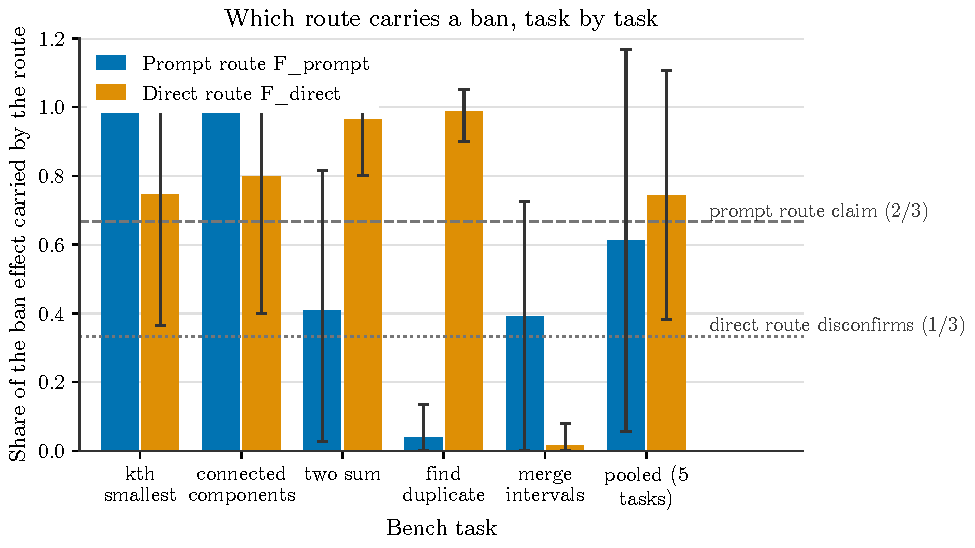
\includegraphics[width=\linewidth,height=0.78\textheight,keepaspectratio]{figures/fig_bench_route_v0.pdf}
\caption{Prompt-route and direct-route share of a modal algorithm ban's effect on Qwen3-8B, for the five gated tasks of a coding bench (100 common-random-number slots per arm per task) and a pooled estimate across them. Blue bars (``Prompt route \$F\_\allowbreak{}\{\textbackslash{}mathrm\{prompt\}\}\$'') are the share of the ban reproduced by the prompt's own states; amber bars (``Direct route \$F\_\allowbreak{}\{\textbackslash{}mathrm\{direct\}\}\$'') are the share reproduced by the generated tokens reading the ban directly. Error bars are 95\textbackslash{}\% confidence intervals: template-then-slot bootstrap percentile intervals for the five individual tasks, and the primary leave-one-task-out jackknife interval for the pooled bar. The grey dashed line marks the preregistered bar for the prompt-route hypothesis (prompt route \$\textbackslash{}geq 2\slash{}3\$); the grey dotted line marks the bar at which the direct route would disconfirm it (\$\textbackslash{}geq 1\slash{}3\$). The route is task-dependent: both routes alone reproduce the ban on kth smallest and connected components, the direct route dominates on two sum and find duplicate, and neither route alone suffices on merge intervals. Pooled, the direct-route point estimate (0.744) exceeds the prompt-route point estimate (0.611), but both pooled intervals are wide and overlap each other and both threshold lines (jackknife 95\textbackslash{}\% CI: \$F\_\allowbreak{}\{\textbackslash{}mathrm\{prompt\}\}\$ [0.055, 1.167], \$F\_\allowbreak{}\{\textbackslash{}mathrm\{direct\}\}\$ [0.382, 1.106]) -- so this pooled ordering is a pattern across five tasks, not a statistically separated result. The source experiment's own preregistered verdict for the prompt-route hypothesis is disconfirmed under every interval method, and we report this pooled comparison as a lead rather than a settled finding.}
\label{fig:fig_bench_route}
\end{figure}
An independent second draw with fresh uniforms (slots 20 to 39, arms a to d on the five gated tasks, N = 100 each) reproduced the picture. Pooled F\_\allowbreak{}prompt was 0.64 [0.27, 0.94] and F\_\allowbreak{}direct 0.74 [0.43, 0.94], per-task fractions moved by about 0.1 at most (find duplicate F\_\allowbreak{}direct 0.99 then 0.93; two sum 0.96 then 0.93; merge intervals F\_\allowbreak{}prompt 0.39 then 0.49), and the Spearman rank agreement between the draws was 0.89 and 0.90. The task differences are not sampling noise. A continuous companion readout (the teacher forced log probability of the default's opening up to its distinctive n-gram, under each arm) split the effect across both routes as behaviour does (pooled 0.40 prompt, 0.45 direct).

\textbf{Veto sufficiency does not predict the route.} The update predicted that the direct share would be small where the one-shot veto suffices and large where it does not. The frozen n-gram rule picked identifier or structural tokens with zero collateral (two sum \texttt{\textvisiblespace{}\allowbreak{}if\textvisiblespace{}\allowbreak{}complement}, find duplicate \texttt{\textvisiblespace{}\allowbreak{}set}, Fibonacci \texttt{(\allowbreak{}}), so the one-shot veto rarely changed the mechanism: veto avoidance V\_\allowbreak{}t was 0.41 on kth smallest, 0.39 on first and last position, 0.30 on connected components and at most 0.07 elsewhere. The veto fired in 61\% to 100\% of rows, and the model renamed or retokenised (two sum: \texttt{if compliment in seen}) or broke the code (connected components: 80 of 100 invalid). Every task was classed in the second commit as needing a large direct route (V\_\allowbreak{}t below 0.5, predicting F\_\allowbreak{}direct of at least 0.25). Four of the five gated tasks hit; merge intervals missed with F\_\allowbreak{}direct 0.02. The Spearman correlation between V\_\allowbreak{}t and F\_\allowbreak{}direct was -0.34, with a one-sided permutation p of 0.30 over five points, which fails the rule. The test is inconclusive, and the comparison of the one-shot veto's landing with the ban's had no eligible task.

\textbf{The ban is decided at the opening of the body.} Forcing the default's own opening, up to its distinctive n-gram, undid the ban completely on every gated task (the share of the ban effect undone, P\_\allowbreak{}open, 0.98 to 1.00), while forcing only a neutral \texttt{def solve(\allowbreak{}.\allowbreak{}.\allowbreak{}.\allowbreak{}):\allowbreak{}} line undid none of it (-0.12 to 0.01). The depth sweep (Table 109) localises this: the ban holds through the whole \texttt{def} line and gives way at the first content token of the default's body, which we call the first body token. On kth smallest, forcing the \texttt{def} line and its indentation (10 tokens) leaves the ban intact, and forcing one more token, \texttt{\textvisiblespace{}\allowbreak{}nums}, undoes it. Under common random numbers, arms a, c and d leave the twin's tokens at the first body token (median token 8 to 10 on kth smallest, two sum, find duplicate and connected components; 19 to 21 on merge intervals, whose shared \texttt{if not intervals} guard comes first). Once the first tokens of the default's body are on the page, the model continues the default; the ban is applied at the opening and not re-read in the body, as Qi et al. found for safety refusals [63].

\begin{table}[H]
\renewcommand{\thetable}{109}
\centering\footnotesize\setlength{\tabcolsep}{4.0pt}
\caption{Share of the ban effect undone by forcing a prefix (P\_\allowbreak{}open), by prefix: a neutral \texttt{def} line, or the default's modal program forced to 25\%, 50\% or 75\% of its tokens or up to its distinctive n-gram (forced tokens in parentheses; N = 50 per cell, under the ban and the twin). Source: bench route experiment \texttt{README.\allowbreak{}md}, \texttt{results/\allowbreak{}replication.\allowbreak{}json}. [Source: iteration 3, artifact \nolinkurl{gen_art_experiment_16}.]}\label{tab:t116}
\begin{tabular}{>{\raggedright\arraybackslash\hspace{0pt}}p{0.1329\linewidth}>{\raggedright\arraybackslash\hspace{0pt}}p{0.1150\linewidth}>{\raggedright\arraybackslash\hspace{0pt}}p{0.1942\linewidth}>{\raggedright\arraybackslash\hspace{0pt}}p{0.2073\linewidth}>{\raggedright\arraybackslash\hspace{0pt}}p{0.1697\linewidth}>{\raggedright\arraybackslash\hspace{0pt}}p{0.0776\linewidth}}
\toprule
\textbf{Task} & \textbf{Neutral \texttt{def} line} & \textbf{25\% of the program} & \textbf{Up to the distinctive n-gram} & \textbf{50\%} & \textbf{75\%} \\
\midrule
kth smallest & -0.01 (9 tokens) & -0.01 (5: \texttt{def solve}) & 0.98 (11: \texttt{def} line, indent, \texttt{\textvisiblespace{}\allowbreak{}nums}) & -0.01 (10: \texttt{def} line and indent) & 1.00 (16) \\
find duplicate & -0.01 (7) & 1.00 (10: \texttt{seen =\allowbreak{}}) & 1.00 (11: \texttt{seen =\allowbreak{} set}) & 1.00 (20) & 1.00 (29) \\
two sum & 0.01 (9) & 1.00 (13: \texttt{seen =\allowbreak{} \{\}}) & 1.00 (32) & 1.00 (26) & 1.00 (40) \\
connected components & 0.00 (9) & 1.00 (31, inside \texttt{find}) & 1.00 (20: \texttt{def find}) & 1.00 (62) & 1.00 (92) \\
merge intervals & -0.12 (8) & 1.00 (30: \texttt{intervals.\allowbreak{}sort(\allowbreak{}key}) & 1.00 (58) & 1.00 (59) & 1.00 (88) \\
\bottomrule
\end{tabular}
\end{table}

\begin{figure}[!htbp]
\centering\captionsetup{font=footnotesize}
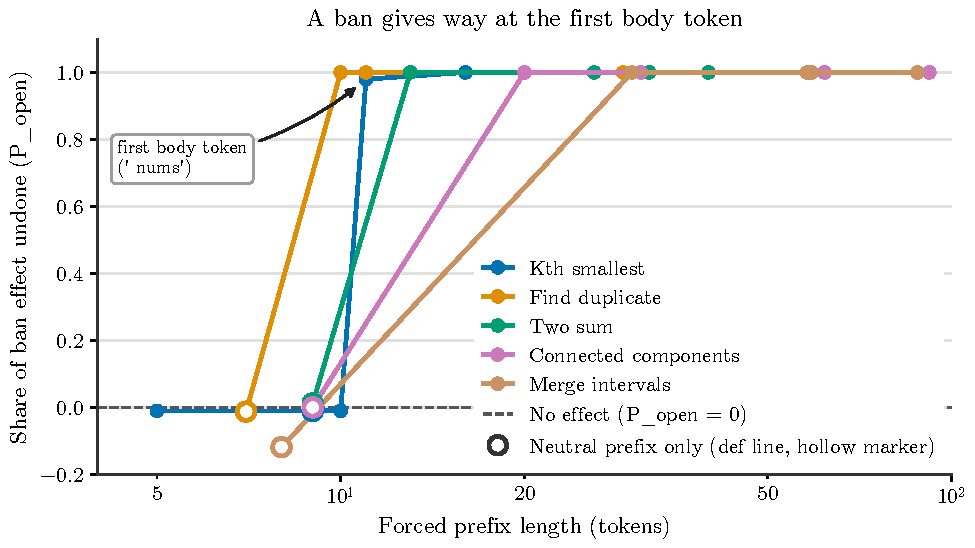
\includegraphics[width=\linewidth,height=0.78\textheight,keepaspectratio]{figures/fig_prefill_depth_v0.pdf}
\caption{Share of a prompt ban's effect undone, \$P\_\allowbreak{}\textbackslash{}mathrm\{open\}\$ (y-axis: \textbackslash{}textit\{Share of ban effect undone (P\textbackslash{}\_\allowbreak{}open)\}), when Qwen3-8B (bf16, thinking off) is forced to begin its response with part of its own default solution, against the number of forced tokens (x-axis: \textbackslash{}textit\{Forced prefix length (tokens)\}, log scale). One solid line per task, in a colourblind-safe palette, for the five of twelve bench tasks whose ban is obeyed with no forced prefix: kth smallest, find duplicate, two sum, connected components, merge intervals (\$N=50\$ generations per condition, under the ban and under a token-length-matched neutral twin). Filled circles are forced-prefix conditions reaching 25\textbackslash{}\%, 50\textbackslash{}\% or 75\textbackslash{}\% of the default solution's token length, or its distinctive opening; the hollow circle on each line is the shortest, neutral condition (only the \textbackslash{}texttt\{def solve(...):\} line and its indentation, none of the default's body). The dashed grey line marks \$P\_\allowbreak{}\textbackslash{}mathrm\{open\}=0\$ (the ban fully holds). On every task the hollow neutral point sits at or just below 0 and every forced-prefix point reaches 1 (the ban is fully undone); kth smallest alone is sampled finely enough -- at 9, 10 and 11 forced tokens -- to show the transition is exactly one token: \$P\_\allowbreak{}\textbackslash{}mathrm\{open\}=-0.01\$ at 10 tokens (the \textbackslash{}texttt\{def\} line and its indentation) and \$0.98\$ at 11 (one more token, the leading-space \textbackslash{}texttt\{nums\}, annotated on the figure with an arrow). The other four tasks are sampled too coarsely (checkpoints 7-13 tokens apart) to localise their own transition to a single token, but each falls in the same early range, well before a quarter of the default solution's length.}
\label{fig:fig_prefill_depth}
\end{figure}
\textbf{The path task screen.} Under the iteration-2 twin prompts, every veto variant failed to move either path default: one-shot, persistent, iterated rounds with the re-emerged programs' new n-grams, and a veto of the import line itself. The share off the default was 0.00 on the grid task and at most 0.01 on the shortest path task, and the default re-emerged in 99\% to 100\% of attempts after each round. The committed prediction that the grid one-shot veto would not suffice hit; the prediction that the shortest path one-shot veto would suffice and land on Bellman-Ford\slash{}SPFA missed (V = 0). The iteration-2 ban landings recomputed exactly from raw rows (grid DFS 257 of 257; shortest path Bellman-Ford\slash{}SPFA 255 of 260). A ban moves these tasks; a surface veto does not.

\textbf{Controls and checks.} A placebo splice (one twin's condition segment with another twin's later states) moved the default's share by at most 0.04 on all six tasks where it ran, so splicing itself is inert; the knockout applied to the twin left the default at 1.00 on six tasks. GPU unit tests confirmed common random number determinism, splice identities (splicing a prompt with itself reproduces it in 100\% of rows) and zero attention mass on the condition span under the knockout in all 36 layers. A reproduction of the iteration-2 shortest path arms gave banned shares of 0 of 20, 20 of 20, 3 of 20 and 19 of 20 for arms a to d, inside their pass bands. Two audit scripts rederived every headline from raw rows with no mismatch, and shuffling arm labels within slots collapsed the mean gap between twin and ban from 0.83 to -0.001. A worker restart briefly ran three labelling workers on the same rows; duplicates were compacted to the last row per sample, which every reader used. GPU time was about 1.8 GPU hours, judge spend USD 0.105.

\FloatBarrier
\subsection*{3.7 Locus experiment: a shared prohibition direction, a locus at generated tokens 1 to 8, the ban-attending heads, and SAE transfer (Qwen3-8B)}
\addcontentsline{toc}{subsection}{3.7 Locus experiment: a shared prohibition direction, a locus at generated tokens 1 to 8, the ban-attending heads, and SAE transfer (Qwen3-8B)}
\noindent{\small\emph{Artifact: \nolinkurl{gen_art_experiment_17}.}}\par\medskip
\textbf{Why.} Four questions about where a prohibition lives inside the model were open after iteration 2. Is there a task-general direction that carries the instruction to abandon the default, and does writing it into a neutral prompt work like a named ban (the causal test of the read position correlation, moved to the positions where the route test located the effect)? Is the within-ban choice of algorithm decodable at generated tokens 1 to 8 beyond the written text? Do the three heads that attend to the banned name matter? Do the Qwen-Scope base model SAEs [50] transfer to the instruct model under a criterion that does not penalise its lower clean cross-entropy? This experiment  ran all four beside their controls under common random numbers, on the two path tasks and four bench tasks (kth smallest, substring search, find duplicate, two sum).

\textbf{Design.} The machine had a 16 GB RTX 2000 Ada, too small for bf16 weights, so every decoder linear layer was quantised at load time to 8-bit floating point with per-channel weight and per-token activation scales (embeddings, norms and the output head stayed bf16). A validation reproduced the iteration-2 shortest path arms (ban 2 of 20 Dijkstra, twin 20 of 20). The sampler coupled every arm exactly (identical uniforms in different rows give identical tokens at 20 rows per batch), and teacher forcing at batch 1 was bit exact. The shared prohibition direction v is the leave-one-task-out mean, over the 13 other tasks and all five templates, of the ban minus twin displacement at the task specification positions in blocks 12 to 23. The ADD arm wrote v into the neutral twin's prefill with the displacement targeted to alpha times the ban's own per-layer norm (alpha in \{1, 2\}, plus 0.5 on some tasks); the SUBTRACT arm projected v out of the ban prompt's prefill. Controls were three random directions with the same blocks, positions and norms, the twin, and the named ban (N = 100). In all, 5,500 samples followed the frozen design and 1,800 were exploratory. Decision rules were hash committed before sampling.

\textbf{The direction exists, but adding it is no better than a random push.} The leave-one-task-out v was reliable (split half cosine 0.95 to 0.99 across blocks 12 to 23). It was aligned with every held-out task's mean ban displacement (cosine 0.29 to 0.86 at block 18, against a 95th percentile of 0.03 for random directions), yet it carried only 2\% to 6\% of each position's own ban displacement. The preregistered test failed on every gated task (Table 110): ADD beat every random control on 0 of 5 gated tasks, and its avoidance was not above the maximum of the three random directions on 5 of 6 tasks. Where ADD moved behaviour it did not reproduce the ban. On kth smallest it landed on a size-k heap while the ban landed on quickselect (Jensen-Shannon divergence 0.52 against a permutation 95th percentile of 0.03; the committed forecast missed); on the shortest path task ADD and the ban both landed on Bellman-Ford\slash{}SPFA, but so did the random directions that moved it. The dose response was not monotone (shortest path avoidance 0.02, 0.35 and 0.12 at alpha 0.5, 1 and 2 over all slots), and the random edits grew more than v downstream (block 35: about 283 against 219 on the shortest path task), so a weak control does not explain the result. SUBTRACT never restored the default: pooled over the gated tasks the banned share changed by -0.026 [-0.07, 0.03] against a required +0.3, and on substring search, find duplicate and two sum removing v made the ban slightly stronger. On the path tasks neither plain nor affine subtraction exceeded a random edit of the same norm by the required 0.15, and that random edit was destructive (pass rate 0.00).

\begin{table}[H]
\renewcommand{\thetable}{110}
\centering\footnotesize\setlength{\tabcolsep}{4.0pt}
\caption{The shared prohibition direction against matched random directions (avoidance; slots 0 to 9 for ADD and random arms). Source: locus experiment \texttt{results/\allowbreak{}c2d.\allowbreak{}json}. [Source: iteration 3, artifact \nolinkurl{gen_art_experiment_17}.]}\label{tab:t117}
\begin{tabular}{>{\raggedright\arraybackslash\hspace{0pt}}p{0.1528\linewidth}>{\raggedright\arraybackslash\hspace{0pt}}p{0.2556\linewidth}>{\raggedright\arraybackslash\hspace{0pt}}p{0.1015\linewidth}>{\raggedright\arraybackslash\hspace{0pt}}p{0.1941\linewidth}>{\raggedright\arraybackslash\hspace{0pt}}p{0.2091\linewidth}}
\toprule
\textbf{Task (default)} & \textbf{Named ban avoidance and landing} & \textbf{ADD, alpha 1 \slash{} 2} & \textbf{Random directions, alpha 1 (three seeds)} & \textbf{SUBTRACT: change in banned share [95\% CI]} \\
\midrule
Shortest path (Dijkstra) & 0.88, to Bellman-Ford\slash{}SPFA & 0.44 \slash{} 0.12 & 0.06, 0.50, 0.34 & +0.07 [-0.02, 0.17] \\
Grid (BFS) & 0.87, to DFS (all 13 BFS under the fourth template) & 0.06 \slash{} 0.04 & 0.04, 0.00, 0.02 & -0.05 [-0.11, 0.00] \\
kth smallest (full sort) & 1.00, to quickselect 79, size-k heap 21 & 0.80 \slash{} 0.70 & 0.24, 0.70, 0.36 & 0.00 (no default to restore) \\
substring search (naive) & 0.49, to KMP (fails the gate) & 0.00 \slash{} 0.00 & 0.00, 0.00, 0.00 & -0.12 [-0.22, -0.02] \\
find duplicate (hash set) & 0.74, to index marking & 0.00 \slash{} 0.00 & 0.00, 0.00, 0.00 & -0.06 [-0.11, -0.02] \\
two sum (hash map) & 0.80, to brute force & 0.00 \slash{} 0.00 & 0.00, 0.10, 0.00 & -0.09 [-0.15, -0.04] \\
\bottomrule
\end{tabular}
\end{table}

\emph{(Added in iteration 4: Table 110 reports avoidance only and omits the three random directions at alpha 2. At alpha 2 they moved kth smallest (avoidance 0.96 at pass 0.84, correct quickselect 40, full sort 2; 0.52 at pass 0.98, correct quickselect 24, full sort 24, size-k heap 1; 0.30 at pass 0.98), find duplicate (0.86 at pass 0.82, correct sort and adjacent check 30, hash set 6, other 5) and two sum (0.47 and 0.36 at pass 1.00; correct hash map 26, brute force 23 and hash map 32, brute force 18), where ADD at alpha 2 moved nothing (0.00; on two sum at pass 0.48). On kth smallest and two sum these random directions are the cheapest diversity knob in the record of the run. Every alpha-2 row with its pass rate and composition is in Section 4.2.1.)}

An exploratory run added 12 random directions (15 in all, alpha 1). On kth smallest ADD exceeded all 15 (0.80 against a maximum of 0.70 and a mean of 0.24) but landed on the wrong algorithm. On the shortest path task it sat at the 80th percentile (3 of 15 random directions moved it more; random mean 0.20), and on the grid task it was indistinguishable from random (0.06 against a mean of 0.07). Writing the shared component of the ban displacement into a neutral prompt is a direction-specific push on one task and a generic one elsewhere, and removing it is not necessary for the ban.

\textbf{No within-ban locus at generated tokens 1 to 16 (Table 111).} Decoders of default against other were fitted on batch-1 teacher forced states at blocks 8 to 28: the task specification mean, the read position, and generated tokens 1 to 8 and 16. Each was compared with 500 within-template permutations for the path tasks (200 for the bench tasks), taking the maximum over layers, and with three written text controls of matched or greater capacity (token one-hots, layer-0 embeddings reduced to 64 principal components, exact prefix match). No decoder passed the rule on any testable task. On the grid task and three bench tasks the class is set by the template: under the fourth template the model keeps the default in 20 of 20 bench samples and writes all 61 grid BFS programs, so every decoder (state, read position, text) reaches the template-only accuracy and none exceeds it. On the shortest path task the default is spread over templates (2, 0, 4, 3 and 3 of 20), and the choice is made inside the program. The first token at which the two classes diverge comes at a median of about 29 generated tokens, after the frozen window, and neither state nor text decodes the choice within tokens 1 to 16. The committed prediction of a fork at the import line (tokens 3 to 5) was wrong for this sample. At batch 1, identical prefixes gave bit-identical states (maximum difference 0 over 89 to 95 pairs per position), so a state at position k is a function of the written prefix.

\begin{table}[H]
\renewcommand{\thetable}{111}
\centering\footnotesize\setlength{\tabcolsep}{4.0pt}
\caption{Within-ban decoders of the algorithm written (default against other) on batch-1 teacher forced states. BA is balanced accuracy. Source: locus experiment \texttt{results/\allowbreak{}c2e.\allowbreak{}json}. [Source: iteration 3, artifact \nolinkurl{gen_art_experiment_17}.]}\label{tab:t118}
\begin{tabular}{>{\raggedright\arraybackslash\hspace{0pt}}p{0.1670\linewidth}>{\raggedright\arraybackslash\hspace{0pt}}p{0.1393\linewidth}>{\raggedright\arraybackslash\hspace{0pt}}p{0.3183\linewidth}>{\raggedright\arraybackslash\hspace{0pt}}p{0.2186\linewidth}>{\raggedright\arraybackslash\hspace{0pt}}p{0.0699\linewidth}}
\toprule
\textbf{Task} & \textbf{Programs (default \slash{} other)} & \textbf{Largest state BA, tokens 1 to 8} & \textbf{Best of read position and text controls at token 8} & \textbf{Locus} \\
\midrule
Shortest path & 100 (12 \slash{} 88) & 0.53 rising to 0.63, never above the null 95th percentile (about 0.60 to 0.70) & 0.55 & none \\
Grid (with a fourth-template top-up) & 160 (61 \slash{} 99) & 0.904 at every k & 0.904 (template only) & none \\
substring search & 100 (51 \slash{} 49) & 0.832 at every k & 0.832 (template only) & none \\
find duplicate & 100 (26 \slash{} 74) & 0.88 at every k & 0.88 (template only) & none \\
two sum & 100 (20 \slash{} 80) & 1.00 at every k & 1.00 (template only) & none \\
kth smallest & 100 (0 \slash{} 100) & not testable (no default under the ban) &  &  \\
\bottomrule
\end{tabular}
\end{table}

A secondary test pooled the archived ban pools of the route and readout experiments (200 rows per path task): the shortest path state reached balanced accuracy 0.78 to 0.79 at tokens 4 to 8 against 0.75 for the template-only decoder, a margin of 0.03 to 0.05, below the 0.10 rule. The first run on states extracted in 20-row batches, where 8-bit matrix tiling made identical prefixes differ by 4\% to 8\%, gave the same verdict on every task. An exploratory extension to tokens 24 to 96 found text matching or beating the state on the grid and substring search tasks. On the shortest path task the state curve was noisy (0.57, 0.66, 0.45, 0.50 and 0.75 at tokens 24, 32, 48, 64 and 96). Only token 96 cleared both the null (0.66) and the text controls (at most 0.60), a single unreplicated point with 12 minority samples.

\textbf{The ban-attending heads are not special.} Mean ablation of layer 21 head 17 and layer 26 heads 21 and 25 at generated positions under the full ban raised the grid BFS share from 0.12 (the ban, same slots) to 0.24. Every set of three random heads in the same layers raised it to 0.18, so the difference is +0.06 (90\% interval [0.02, 0.12]; exact paired p = 0.125 against each random set), short of the required 0.15. The shortest path task was unchanged (-0.03 [-0.07, 0.03]). Almost all the grid movement sat in the fourth template, which carries every BFS under the ban: BFS went from 6 of 10 to 10 of 10 under the target heads and 9 of 10 under each random set. The fourth-template ban is fragile to any small perturbation of layers 21 and 26.

\textbf{Under a fairer criterion the base SAEs pass, but they lose most of the ban displacement.} The iteration-2 transfer test compared increases in cross-entropy, which penalises the instruct model for its lower clean cross-entropy (0.030 against 0.260 nats). This experiment scored each model on its own text in a two by two design (model by text source, 100 sequences each) by the fraction of cross-entropy recovered relative to zero ablation, FR\_\allowbreak{}zero (Table 112). The frozen rule, FR\_\allowbreak{}zero of the instruct model on its own text at least 0.9 times the base model's, passed at layers 15, 20 and 27. As the plan had computed, the zero-ablation denominator of 12 to 15 nats makes this rule lenient. A placebo that swaps the SAE and zero-ablation cross-entropy per sequence drives FR\_\allowbreak{}zero to about 0, yet still passes the 0.9 rule at layer 20; the values themselves (about 0.99, against about 0 on the placebo) carry the information. Stricter companions: the fraction recovered relative to mean ablation (FR\_\allowbreak{}mean) passed the same rule at all three layers; the ratio of cross-entropy increases on own text (instruct over base) was 1.68, 1.30 and 0.76 at layers 15, 20 and 27 (iteration 2, one shared corpus in bf16: 3.29, 1.95, 1.59). The task-relevant test fails: the SAE reconstructions keep only about a third of the direction of the ban minus twin displacement at the task specification positions (cosine 0.27, 0.30 and 0.32 at layers 15, 20 and 27; norm ratio 0.65 to 0.79), so what the ban changes in the residual stream is largely lost in reconstruction error. The passing fraction recovered agrees with the finding of Kissane and colleagues that base model SAEs usually transfer to chat models; the displacement test, which measures what matters for a ban, is what fails, and latent-level claims about the ban should therefore not rest on these SAEs.

\begin{table}[H]
\renewcommand{\thetable}{112}
\centering\footnotesize\setlength{\tabcolsep}{4.0pt}
\caption{Qwen-Scope SAEs spliced into each model (8-bit linears) on each text source: FR\_\allowbreak{}zero \slash{} FR\_\allowbreak{}mean \slash{} increase in cross-entropy (nats) \slash{} KL(clean, SAE) \slash{} fraction of variance unexplained. Source: locus experiment \texttt{results/\allowbreak{}sae\_\allowbreak{}transfer.\allowbreak{}json}. [Source: iteration 3, artifact \nolinkurl{gen_art_experiment_17}.]}\label{tab:t119}
\begin{tabular}{>{\raggedright\arraybackslash\hspace{0pt}}p{0.1311\linewidth}>{\raggedright\arraybackslash\hspace{0pt}}p{0.0992\linewidth}>{\raggedright\arraybackslash\hspace{0pt}}p{0.2276\linewidth}>{\raggedright\arraybackslash\hspace{0pt}}p{0.2276\linewidth}>{\raggedright\arraybackslash\hspace{0pt}}p{0.2276\linewidth}}
\toprule
\textbf{Model \slash{} text} & \textbf{Clean cross-entropy} & \textbf{Layer 15} & \textbf{Layer 20} & \textbf{Layer 27} \\
\midrule
instruct \slash{} own text & 0.032 & 0.9890 \slash{} 0.984 \slash{} 0.168 \slash{} 0.171 \slash{} 0.365 & 0.9903 \slash{} 0.985 \slash{} 0.169 \slash{} 0.175 \slash{} 0.096 & 0.9939 \slash{} 0.991 \slash{} 0.095 \slash{} 0.097 \slash{} 0.156 \\
base \slash{} own text & 0.926 & 0.9928 \slash{} 0.988 \slash{} 0.100 \slash{} 0.102 \slash{} 0.294 & 0.9906 \slash{} 0.986 \slash{} 0.130 \slash{} 0.134 \slash{} 0.113 & 0.9907 \slash{} 0.985 \slash{} 0.125 \slash{} 0.127 \slash{} 0.228 \\
instruct \slash{} base text & 1.861 & 1.0072 \slash{} 1.010 \slash{} -0.099 \slash{} 0.181 \slash{} 0.358 & 1.0066 \slash{} 1.010 \slash{} -0.104 \slash{} 0.220 \slash{} 0.098 & 1.0170 \slash{} 1.026 \slash{} -0.245 \slash{} 0.169 \slash{} 0.156 \\
base \slash{} instruct text & 0.251 & 0.9966 \slash{} 0.994 \slash{} 0.051 \slash{} 0.049 \slash{} 0.287 & 0.9949 \slash{} 0.992 \slash{} 0.075 \slash{} 0.075 \slash{} 0.281 & 0.9961 \slash{} 0.994 \slash{} 0.054 \slash{} 0.057 \slash{} 0.334 \\
\bottomrule
\end{tabular}
\end{table}

The instruct model on base text has a negative increase (the base SAE lowers its cross-entropy, most at layer 27, from 1.86 to 1.62 nats), consistent with the SAE pulling instruct activations toward base ones. Identity splices reproduced the clean cross-entropy, a zero splice at layer 15 gave 13.1 and 12.3 nats, and the instruct fraction of variance unexplained matched iteration 2 (0.365 against 0.366 at layer 15). As a readout, the latents never beat the difference-in-means direction: over 63 cells (6 tasks, 3 layers, a prohibition-present readout at the task specification mean and a default-plan readout at tokens 1 to 3), a top-1 or top-20 latent beat difference-in-means beyond its interval in 1 cell, a trivial one where every readout is at ceiling, as AxBench found [34].

\textbf{Geometry of early generated states (descriptive).} At the mean of generated tokens 1 to 3 and at token 16 (blocks 20 and 23), the k-nearest-neighbour graphs (k = 10) over all arms were fragmented (100 to 440 components for 800 to 1,100 points), because early states are fixed by shared boilerplate (the code fence and the \texttt{solve} signature) and many points coincide. No cloud had a persistent loop beyond its coordinate permutation null. These arms produced no bidirectional BFS, A* or greedy programs, so the BFS and bidirectional BFS neighbourhood of the ban list experiment could not be re-examined here.

\begin{table}[H]
\renewcommand{\thetable}{113}
\centering\small\setlength{\tabcolsep}{4.0pt}
\caption{Committed predictions of the locus experiment and their outcomes. Source: locus experiment \texttt{predictions/\allowbreak{}commit1.\allowbreak{}json}, \texttt{README.\allowbreak{}md}. [Source: iteration 3, artifact \nolinkurl{gen_art_experiment_17}.]}\label{tab:t120}
\begin{tabular}{>{\raggedright\arraybackslash\hspace{0pt}}p{0.6372\linewidth}>{\raggedright\arraybackslash\hspace{0pt}}p{0.3256\linewidth}}
\toprule
\textbf{Prediction} & \textbf{Outcome} \\
\midrule
ADD (alpha 1 or 2) beats every random control on at least two thirds of gated tasks and lands on the ban's modal survivor & no: 0 of 5 gated tasks \\
SUBTRACT raises the banned share by at least 0.3 & no: pooled -0.026 [-0.07, 0.03] \\
No locus; state and text rise together at the first divergent token; the shortest path fork is at the import line (tokens 3 to 5) & no locus: yes; fork position: no (median about 29 tokens) \\
Head ablation raises the grid banned share by at least 0.15 over random heads; shortest path unchanged & grid no (+0.06); shortest path unchanged yes (-0.03) \\
The SAEs pass the frozen transfer rule, FR\_\allowbreak{}zero about 0.98 to 0.995 for both models & pass; FR\_\allowbreak{}zero instruct 0.989 to 0.994, base 0.991 to 0.993 \\
\bottomrule
\end{tabular}
\end{table}

\textbf{Checks.} An independent recomputation reproduced every arm share; shuffling arm labels within slots erased the ADD and head contrasts; the hash chain had no breaks and both commits preceded their first samples. A separate script with no shared code (exact McNemar by enumeration, an sklearn decoder) matched the pooled SUBTRACT change, the ADD pass count, the head deltas, FR\_\allowbreak{}zero and the validation counts; its shortest path decoder at token 8 gave 0.638 against the frozen null of 0.695. Blind judge spend was USD 0.22.

\FloatBarrier
\subsection*{3.8 Reach experiment: how far bans and token vetoes push, and what the long-form novelty instruction produces (Qwen3-8B)}
\addcontentsline{toc}{subsection}{3.8 Reach experiment: how far bans and token vetoes push, and what the long-form novelty instruction produces (Qwen3-8B)}
\noindent{\small\emph{Artifact: \nolinkurl{gen_art_experiment_18}.}}\par\medskip
\textbf{Why.} The update's third claim was that prompts move the model exactly one rung. This experiment  asked three things. First, do cumulative token vetoes, an operation the model cannot ignore, reach algorithms that prompt bans cannot? We call this the \emph{token walk}: veto the default's distinctive n-gram, then the next landing's, and so on, up to five algorithms. Second, does a ban that leaves exactly one survivor get that survivor written whenever the model can write it on request? We call the share of programs implementing the survivor \emph{will}, and the share of forced programs labelled as the requested algorithm and correct \emph{can}. Third, does the request's own long-form novelty instruction produce a correct novel algorithm? Rungs are numbered by the walk: rung 1 is the default, rung 2 is the walk's first landing (or, where the walk stalled, a flagged fallback committed in advance), and every other catalogue algorithm is at rung 3 or more. Six tasks ran: the two path tasks in bf16, and kth smallest, substring search, find duplicate and connected components on the official 8-bit checkpoint at which their iteration-2 references were made. Every mask, forecast and protocol was hash committed before the samples it governs.

\textbf{The token walk stalls at the default (Table 114).} The persistent veto, implemented as a vLLM logits processor, was exact: no banned token sequence occurred in any of 1,450 vetoed generations. The algorithm came back anyway. On the grid task \texttt{current\_\allowbreak{}row} and \texttt{current\_\allowbreak{}col} replaced \texttt{r,\allowbreak{} c} in 63\% of re-emerged BFS programs (7\% in references), and on the shortest path task \texttt{current\_\allowbreak{}distinct} and \texttt{d} replaced \texttt{current\_\allowbreak{}dist}. Vetoed strings also leaked through non-canonical spellings, in up to 0.86 of samples on connected components and 0.80 on find duplicate at step 2. The grid code degenerated into near-miss syntax (\texttt{queue popleft(\allowbreak{})}, 66\% to 86\% invalid). Imports and calls barely changed: the rerouting is lexical, not algorithmic. Only find duplicate moved one rung, to sort and adjacent check, the same single-rung move that prompt bans produce. A sham veto of an algorithm-generic n-gram of matched length and presence kept the default: grid 50 of 50 (\texttt{\textvisiblespace{}\allowbreak{}start\textvisiblespace{}\allowbreak{}=\allowbreak{}=\allowbreak{}\textvisiblespace{}\allowbreak{}goal:\allowbreak{}\textbackslash{}n}), shortest path 50 of 50 (\texttt{\textvisiblespace{}\allowbreak{}u,\allowbreak{}\textvisiblespace{}\allowbreak{}v,\allowbreak{}\textvisiblespace{}\allowbreak{}w}), substring search 49 of 50 (\texttt{\textvisiblespace{}\allowbreak{}len}) and connected components 44 of 44 valid (\texttt{\textvisiblespace{}\allowbreak{}range}). The distinctive veto cut correctness where the sham did not (shortest path pass rate 0.41 against 1.00, Newcombe difference 0.59 [0.43, 0.72]; grid 0.76 against 0.96). A fixed veto of the distinctive n-grams of BFS, DFS, IDDFS and A* at once, the request's top-five prohibition asked as an operation, left BFS 13, DFS 2 and 35 invalid programs on the grid task after two extra rounds; the prompt version gave avoidance 0.00 (Section 2.6). Neither knob reaches the rest of the catalogue.

\begin{table}[H]
\renewcommand{\thetable}{114}
\centering\footnotesize\setlength{\tabcolsep}{4.0pt}
\caption{The token walk under the neutral twins (no ban text; N = 50 per round, 10 per template; \textvisiblespace{} marks a space in the n-grams). Source: reach experiment \texttt{results/\allowbreak{}walk.\allowbreak{}json}, \texttt{README.\allowbreak{}md}. [Source: iteration 3, artifact \nolinkurl{gen_art_experiment_18}.]}\label{tab:t121}
\begin{tabular}{>{\raggedright\arraybackslash\hspace{0pt}}p{0.1261\linewidth}>{\raggedright\arraybackslash\hspace{0pt}}p{0.1138\linewidth}>{\raggedright\arraybackslash\hspace{0pt}}p{0.3619\linewidth}>{\raggedright\arraybackslash\hspace{0pt}}p{0.2184\linewidth}>{\raggedright\arraybackslash\hspace{0pt}}p{0.0930\linewidth}}
\toprule
\textbf{Task} & \textbf{Step 0 (no veto)} & \textbf{Vetoed n-grams, by round} & \textbf{Final round of the last step} & \textbf{Status} \\
\midrule
Grid (bf16) & BFS 50 & \texttt{\textvisiblespace{}\allowbreak{}c,\allowbreak{}\textvisiblespace{}\allowbreak{}path\textvisiblespace{}\allowbreak{}=\allowbreak{}\textvisiblespace{}\allowbreak{}queue.\allowbreak{}p}, then \texttt{\textvisiblespace{}\allowbreak{}queue.\allowbreak{}append(\allowbreak{}start}, then \texttt{None\textvisiblespace{}\allowbreak{}for} & BFS 6, DFS 1, invalid 43 & stalled at step 1 \\
Shortest path (bf16) & Dijkstra 50 & \texttt{\textvisiblespace{}\allowbreak{}heap\textvisiblespace{}\allowbreak{}=\allowbreak{}\textvisiblespace{}\allowbreak{}[\allowbreak{}(\allowbreak{}0,\allowbreak{}\textvisiblespace{}\allowbreak{}s}, then \texttt{\textvisiblespace{}\allowbreak{}current\_\allowbreak{}dist,\allowbreak{}}, then \texttt{\textvisiblespace{}\allowbreak{}dist[\allowbreak{}u]:\allowbreak{}\textbackslash{}n} & Dijkstra 27, invalid 23 (pass 0.30) & stalled at step 1 \\
kth smallest (8-bit) & full sort 45, quickselect 5 & \texttt{\textvisiblespace{}\allowbreak{}nums.\allowbreak{}sort}, then \texttt{\_\allowbreak{}sorted}, then \texttt{\textvisiblespace{}\allowbreak{}sorted(\allowbreak{}nums} & full sort 23, counting sort 10, quickselect 6, invalid 10 & stalled at step 1 \\
substring search (8-bit) & naive 50 & \texttt{+len}, then \texttt{[\allowbreak{}i:\allowbreak{}i\textvisiblespace{}\allowbreak{}+}, then a leak span & naive 50 & stalled at step 1 \\
find duplicate (8-bit) & hash set 50 & \texttt{\textvisiblespace{}\allowbreak{}set}, \texttt{\textvisiblespace{}\allowbreak{}seen} and leak spans; then, at rung 2 (sort and adjacent check, 37 of 50), \texttt{.\allowbreak{}sort} and 5 leak spans & sort and adjacent check 20, other 13, hash set 10 & stalled at step 2 \\
connected components (8-bit) & union find 47, DFS 3 & \texttt{\textvisiblespace{}\allowbreak{}parent} and 8 leak spans (\texttt{(\allowbreak{}parent}, \texttt{parents}, \texttt{.\allowbreak{}parent}, tab-indented \texttt{parent}, and others) & union find 44, DFS 6 & stalled at step 1 \\
\bottomrule
\end{tabular}
\end{table}

\textbf{Prompts reach further than one rung on two tasks (Tables 115 and 116).} The preregistered reach claim was that will is at most 0.10 at every rung of 3 or more where can is at least 0.7, and it is disconfirmed by a will of 0.30 or more. It was disconfirmed on connected components, where the list that leaves only BFS got BFS 50 of 50, and on kth smallest, where the list that leaves only quickselect got quickselect 50 of 50. Both cells were placed at rung 3 or more through the flagged fallback, because the walk stalled at step 1 and the fallback set the second rung (counting sort on kth smallest, DFS on connected components). A post hoc sensitivity that sets the second rung to the association answer keeps connected components disconfirming (association says DFS, so BFS stays at rung 3 or more) and moves quickselect to rung 2. On connected components the two traversals are interchangeable alternatives (BFS 50 of 50 when only BFS is allowed, DFS 49 of 50 when only DFS is), so a single chain of rungs does not describe the repertoire. The claim was confirmed on the shortest path task (Floyd-Warshall, from Section 2.6), on two kth smallest cells and on find duplicate's binary search on values; find duplicate's Floyd cycle detection reached 0.14; substring search had no rung of 3 or more with can of at least 0.7.

\begin{table}[H]
\renewcommand{\thetable}{115}
\centering\footnotesize\setlength{\tabcolsep}{4.0pt}
\caption{Reach cells: rungs of 3 or more with can of at least 0.7. Source: reach experiment \texttt{results/\allowbreak{}c3.\allowbreak{}json}. [Source: iteration 3, artifact \nolinkurl{gen_art_experiment_18}.]}\label{tab:t122}
\begin{tabular}{>{\raggedright\arraybackslash\hspace{0pt}}p{0.3861\linewidth}>{\raggedright\arraybackslash\hspace{0pt}}p{0.1664\linewidth}>{\raggedright\arraybackslash\hspace{0pt}}p{0.0524\linewidth}>{\raggedright\arraybackslash\hspace{0pt}}p{0.2044\linewidth}>{\raggedright\arraybackslash\hspace{0pt}}p{0.1039\linewidth}}
\toprule
\textbf{Cell} & \textbf{Rung} & \textbf{Can} & \textbf{Will (N = 50) [95\% CI]} & \textbf{Verdict} \\
\midrule
Shortest path, Floyd-Warshall (Section 2.6, not rerun) & 3 or more & 1.00 & 0.00 [0.00, 0.04] & confirm \\
kth smallest, quickselect & 3 or more (fallback) & 0.95 & 1.00 [0.93, 1.00] & disconfirm \\
kth smallest, size-k heap & 3 or more & 0.75 & 0.00 [0.00, 0.07] & confirm \\
kth smallest, heapify and pop & 3 or more & 0.70 & 0.00 [0.00, 0.07] & confirm \\
find duplicate, binary search on values & 3 or more & 0.78 & 0.00 [0.00, 0.07] & confirm \\
find duplicate, Floyd cycle detection & 3 or more & 0.70 & 0.14 [0.07, 0.26] & neither \\
connected components, BFS & 3 or more (fallback) & 1.00 & 1.00 [0.93, 1.00] & disconfirm \\
\bottomrule
\end{tabular}
\end{table}

\begin{table}[H]
\renewcommand{\thetable}{116}
\centering\footnotesize\setlength{\tabcolsep}{4.0pt}
\caption{Every ban that leaves one survivor on the bench tasks (N = 50; disguise is the share of banned-mechanism programs that name none of the banned algorithms). Source: reach experiment \texttt{results/\allowbreak{}reach\_\allowbreak{}events.\allowbreak{}jsonl}. [Source: iteration 3, artifact \nolinkurl{gen_art_experiment_18}.]}\label{tab:t123}
\begin{tabular}{>{\raggedright\arraybackslash\hspace{0pt}}p{0.1216\linewidth}>{\raggedright\arraybackslash\hspace{0pt}}p{0.1229\linewidth}>{\raggedright\arraybackslash\hspace{0pt}}p{0.3738\linewidth}>{\raggedright\arraybackslash\hspace{0pt}}p{0.1196\linewidth}>{\raggedright\arraybackslash\hspace{0pt}}p{0.0604\linewidth}>{\raggedright\arraybackslash\hspace{0pt}}p{0.0984\linewidth}}
\toprule
\textbf{Task} & \textbf{Only allowed algorithm} & \textbf{Labels of attempted programs} & \textbf{Will [95\% CI]} & \textbf{Pass rate} & \textbf{Disguise rate} \\
\midrule
kth smallest & full sort & quickselect 50 & 0.00 [0.00, 0.07] & 0.94 & 0.04 \\
kth smallest & quickselect & quickselect 50 & 1.00 [0.93, 1.00] & 0.98 & n\slash{}a \\
kth smallest & size-k heap & quickselect 50 & 0.00 [0.00, 0.07] & 0.90 & 0.08 \\
kth smallest & counting sort & quickselect 44, other 6 & 0.00 [0.00, 0.07] & 1.00 & 0.09 \\
kth smallest & heapify and pop & quickselect 50 & 0.00 [0.00, 0.07] & 0.94 & 0.00 \\
substring search & naive & naive 50 & 1.00 [0.93, 1.00] & 1.00 & n\slash{}a \\
substring search & KMP & naive 37, KMP 13 & 0.26 [0.16, 0.40] & 0.98 & 1.00 \\
substring search & Rabin-Karp & naive 36, KMP 8, Rabin-Karp 5, Boyer-Moore-Horspool 1 & 0.10 [0.04, 0.21] & 0.92 & 0.76 \\
substring search & built-in find & naive 49, KMP 1 & 0.00 [0.00, 0.07] & 0.98 & 0.92 \\
substring search & Z algorithm & naive 46, KMP 3, Boyer-Moore-Horspool 1 & 0.00 [0.00, 0.07] & 0.96 & 0.92 \\
find duplicate & hash set & hash set 43, index marking 4, Floyd cycle detection 3 & 0.86 [0.74, 0.93] & 0.88 & 0.57 \\
find duplicate & binary search on values & index marking 40, hash set 10 & 0.00 [0.00, 0.07] & 0.40 & 1.00 \\
find duplicate & Floyd cycle detection & index marking 34, hash set 9, Floyd cycle detection 7 & 0.14 [0.07, 0.26] & 0.38 & 1.00 \\
find duplicate & sort and adjacent check & index marking 33, hash set 11, Floyd cycle detection 3, other 1, binary search on values 1, sort and adjacent check 1 & 0.02 [0.00, 0.10] & 0.36 & 0.96 \\
connected components & BFS & BFS 50 & 1.00 [0.93, 1.00] & 1.00 & n\slash{}a \\
connected components & DFS & DFS 49, union find 1 & 0.98 [0.90, 1.00] & 0.98 & 1.00 \\
connected components & union find & union find 47, DFS 3 & 0.94 [0.84, 0.98] & 1.00 & 0.67 \\
\bottomrule
\end{tabular}
\end{table}

Quickselect is kth smallest's universal answer to a ban list: every list that bans the full sort yields quickselect in 44 to 50 of 50 programs, including the lists that ban quickselect itself (only size-k heap allowed, only heapify and pop allowed: 50 of 50 quickselect, disguised in 0\% to 8\%). The sanity check of the list that leaves only the default gave will 1.00 on substring search, 0.86 on find duplicate and 0.94 on connected components, but 0.00 on kth smallest. There the prompt banned the size-k heap, heapify and pop, quickselect, median of medians and counting sort, and all 50 programs implemented quickselect, 48 of them in a function named \texttt{quickselect}, while full sort was 45 of 50 under the twin. This is the starkest priming by a negative constraint in the run [7, 53]. Forced can underestimates some algorithms: find duplicate's index marking has a forced adherence of 0.03, yet the model wrote it in 34 to 40 of 50 programs under lists that forbid it, always disguised. The preregistered list independence test asks whether the default's share among default and second-rung programs is the same across lists that ban both. It failed on substring search: 0.82 under the Rabin-Karp list against 0.98 under the built-in list (permutation chi-squared p = 0.033; largest difference 0.16 [0.04, 0.30]; placebos with shuffled membership gave p = 0.61, 0.56 and 0.06). It was descriptive on find duplicate and not testable on kth smallest and connected components.

\textbf{Two-step bans of the default and its second rung (N = 100) split the tasks (Table 117).} On the path tasks and substring search they failed (compliance 0.02, 0.01 and 0.14, with snap-back to the default on substring search), replicating iteration 1; on kth smallest, find duplicate and connected components they were obeyed (1.00, 0.96 and 1.00). The committed forecasts hit find duplicate (the second walk landing, index marking), kth smallest and connected components (association: quickselect and BFS) and substring search (snap-back).

\begin{table}[H]
\renewcommand{\thetable}{117}
\centering\small\setlength{\tabcolsep}{4.0pt}
\caption{Two-step bans of the default and its second rung (N = 100; labels of attempted programs not banned). Source: reach experiment \texttt{results/\allowbreak{}reach\_\allowbreak{}events.\allowbreak{}jsonl}, \texttt{README.\allowbreak{}md}. [Source: iteration 3, artifact \nolinkurl{gen_art_experiment_18}.]}\label{tab:t124}
\begin{tabular}{>{\raggedright\arraybackslash\hspace{0pt}}p{0.1350\linewidth}>{\raggedright\arraybackslash\hspace{0pt}}p{0.1999\linewidth}>{\raggedright\arraybackslash\hspace{0pt}}p{0.1371\linewidth}>{\raggedright\arraybackslash\hspace{0pt}}p{0.4577\linewidth}}
\toprule
\textbf{Task} & \textbf{Banned} & \textbf{Compliance} & \textbf{Attempted programs (banned mechanisms included)} \\
\midrule
Grid & BFS, DFS & 0.02 [0.01, 0.07] & DFS 82, BFS 16, unit weight Dijkstra 1, other 1 \\
Shortest path & Dijkstra, Bellman-Ford\slash{}SPFA & 0.01 & Bellman-Ford\slash{}SPFA 67, Dijkstra 32, other 1 \\
kth smallest & full sort, counting sort & 1.00 & quickselect 63, size-k heap 37 \\
substring search & naive, KMP & 0.14 & naive 74, Rabin-Karp 9, built-in find 2, Boyer-Moore-Horspool 2, other 1 (the rest KMP) \\
find duplicate & hash set, sort and adjacent check & 0.96 & index marking 52, Floyd cycle detection 42, other 2 (the rest banned) \\
connected components & union find, DFS & 1.00 & BFS 100 \\
\bottomrule
\end{tabular}
\end{table}

\textbf{The long-form novelty instruction produces claims of novelty, not new algorithms (Table 118).} The request contains two long-form novelty instructions, which we call the first long-form instruction (asking the model to make a new algorithm) and the second long-form instruction (asking for a fully novel algorithm never seen before); each asks for a design rationale of about 2,000 words before the code. They were run with thinking off (N = 25 to 50 per cell) and on (N = 10 per prompt and task, 16k thinking cap). All 100 thinking traces completed, at 4.1k to 12.4k thinking tokens. Of 574 outputs with a claim record, 484 (84\%) claimed a new algorithm. Of those, 189 (39\%) contained no code at all, only a rationale of 1,300 to 1,700 words, and 220 of the 295 with code (75\%) were catalogue algorithms by the mechanism labeller, under names that modify a catalogue algorithm, such as a modified Bellman-Ford, a BFS with dynamic programming, or an optimised Dijkstra with early termination. The instructions do diversify the output (correct-only Hill numbers of 1.8 to 4.5 in the thinking-off cells, against a collapsed baseline), at a cost in correctness (pass rates of 0.33 to 0.44 on the grid task and 0.32 to 0.37 on find duplicate). With thinking on, the code stayed in the catalogue (grid mostly DFS, 13 of 20; shortest path Bellman-Ford\slash{}SPFA, Dijkstra and Floyd-Warshall only; kth smallest counting sort 13 of 20; substring search naive 14 of 20; find duplicate off-catalogue 11 of 20, all failing arithmetic tricks that assume one duplicate). A bf16 against 8-bit cross-check on the shortest path task under the first instruction gave a label composition Jensen-Shannon divergence of 0.033 bits against a null 95th percentile of 0.068 (p = 0.35).

{\scriptsize\setlength{\tabcolsep}{2.5pt}\renewcommand{\thetable}{118}
\begin{longtable}{>{\raggedright\arraybackslash\hspace{0pt}}p{0.4051\linewidth}>{\raggedright\arraybackslash\hspace{0pt}}p{0.0543\linewidth}>{\raggedright\arraybackslash\hspace{0pt}}p{0.0788\linewidth}>{\raggedright\arraybackslash\hspace{0pt}}p{0.1029\linewidth}>{\raggedright\arraybackslash\hspace{0pt}}p{0.0915\linewidth}>{\raggedright\arraybackslash\hspace{0pt}}p{0.1120\linewidth}>{\raggedright\arraybackslash\hspace{0pt}}p{0.0788\linewidth}}
\caption{Long-form novelty instructions: composition of outputs per cell (first and second long-form instructions as defined above). Source: reach experiment \texttt{results/\allowbreak{}longform.\allowbreak{}json}, \texttt{README.\allowbreak{}md}. [Source: iteration 3, artifact \nolinkurl{gen_art_experiment_18}.]}\label{tab:t125}\\
\toprule
\textbf{Cell} & \textbf{N} & \textbf{Default} & \textbf{Other catalogue} & \textbf{Off catalogue} & \textbf{Invalid or no code} & \textbf{Correct} \\
\midrule
\endfirsthead
\multicolumn{7}{l}{\emph{Table 118, continued}}\\
\toprule
\textbf{Cell} & \textbf{N} & \textbf{Default} & \textbf{Other catalogue} & \textbf{Off catalogue} & \textbf{Invalid or no code} & \textbf{Correct} \\
\midrule
\endhead
\bottomrule
\endlastfoot
kth smallest, first, thinking off (8-bit) & 50 & 3 & 17 & 12 & 18 & 25 \\
kth smallest, first, thinking on (8-bit) & 10 & 0 & 7 & 1 & 2 & 8 \\
kth smallest, second, thinking off (8-bit) & 50 & 0 & 12 & 8 & 30 & 15 \\
kth smallest, second, thinking on (8-bit) & 10 & 0 & 9 & 0 & 1 & 8 \\
substring search, first, thinking off (8-bit) & 50 & 27 & 7 & 1 & 15 & 32 \\
substring search, first, thinking on (8-bit) & 10 & 7 & 3 & 0 & 0 & 10 \\
substring search, second, thinking off (8-bit) & 50 & 10 & 8 & 4 & 28 & 13 \\
substring search, second, thinking on (8-bit) & 10 & 7 & 1 & 0 & 2 & 8 \\
find duplicate, first, thinking off (8-bit) & 50 & 5 & 13 & 17 & 15 & 13 \\
find duplicate, first, thinking on (8-bit) & 10 & 0 & 4 & 5 & 1 & 4 \\
find duplicate, second, thinking off (8-bit) & 50 & 4 & 14 & 7 & 25 & 8 \\
find duplicate, second, thinking on (8-bit) & 10 & 0 & 3 & 6 & 1 & 3 \\
Grid, first, thinking off (bf16) & 25 & 3 & 12 & 1 & 9 & 7 \\
Grid, first, thinking on (8-bit) & 10 & 0 & 8 & 0 & 2 & 3 \\
Grid, second, thinking off (bf16) & 25 & 3 & 3 & 2 & 17 & 3 \\
Grid, second, thinking on (8-bit) & 10 & 0 & 7 & 2 & 1 & 3 \\
Shortest path, first, thinking off (bf16) & 50 & 17 & 20 & 3 & 10 & 35 \\
Shortest path, first, thinking off (8-bit) & 50 & 18 & 12 & 4 & 16 & 29 \\
Shortest path, first, thinking on (8-bit) & 10 & 2 & 6 & 0 & 2 & 8 \\
Shortest path, second, thinking off (bf16) & 25 & 6 & 6 & 5 & 8 & 9 \\
Shortest path, second, thinking on (8-bit) & 10 & 6 & 4 & 0 & 0 & 9 \\
\end{longtable}}

\textbf{No novel algorithm in any cell.} Every correct program outside the catalogue from every arm of this experiment went through an audit: 38 correct programs (23 from the long-form cells, 10 from the walk, 5 from the lists) plus 15 seeded failing ones. Two blind judges (gemini-2.5-flash-lite and gpt-4.1-mini; each passed a 6-program control gate at 5 of 6 after a prompt fix) compared each program with its three nearest known solutions from the declared dataset's 472 human and textbook programs and its three nearest catalogue references, and the executor read each one and ran it on three extra random inputs. The 38 correct programs were 30 labeller misses (mostly counting sort on kth smallest written with a dictionary or Counter), 7 catalogue variants (counting plus binary search on cumulative counts; a last-in-first-out label correcting search on the shortest path task) and 1 degenerate quadratic brute force. Judge A called 10 programs novel and judge B none (kappa 0.27); the manual pass found 5 of those 10 degenerate (XOR or sum tricks, broken loops), 3 labeller misses and 2 catalogue variants. The exact one-sided 95\% upper bound on the novel rate is 0.058 per cell of 50, 0.113 per cell of 25 and 0.26 per thinking-on cell of 10. Together with the record audit (0 of 78), the run's direct answer to the novelty question is that no instruction or knob produced a correct algorithm outside the catalogue and its known variants.

\textbf{Deviations and checks.} Distinctive n-grams had to be lexical (a veto of an indentation-tailed n-gram was bypassed by re-indenting in 20 of 20 unit tests), and shams could not be constructed for kth smallest and find duplicate. The analysis code was edited after its hash was committed (corrected compositions, a post hoc sensitivity, a claim mechanism check); an unchanged rederivation script reproduced every preregistered number from raw rows with no mismatch. Dropped: placement of the walk landings on the manifold, the thinking-on temperature sweep, and extending the path task thinking cells to N = 25. Judge spend was USD 0.49.

\FloatBarrier
\subsection*{3.9 Comparisons across this iteration's experiments}
\addcontentsline{toc}{subsection}{3.9 Comparisons across this iteration's experiments}
\textbf{The same modal bench ban, drawn three times in Qwen3-8B and once in Llama.} Three Qwen3-8B artifacts sampled the modal bench bans with the five frozen templates and 20 samples each, on different engines: vLLM in bf16 (bench forecast experiment), HF in bf16 with common random numbers (bench route experiment, full ban arm) and HF with 8-bit linears (locus experiment, four bench tasks). Table 119 sets them side by side with Llama. With the wording fixed, avoidance replicates within a few points and the landing replicates in kind. The same five tasks pass the gate in both artifacts that ran all twelve. Every Qwen3-8B draw sends kth smallest to quickselect and size-k heap, two sum to brute force, find duplicate to index marking, connected components to BFS, and merge intervals to a failing merge without sorting. Llama lands elsewhere on two of the shared tasks (two sum to sort and two pointers, connected components to DFS), on both of which Llama's own association answer matches its landing.

\begin{table}[H]
\renewcommand{\thetable}{119}
\centering\footnotesize\setlength{\tabcolsep}{4.0pt}
\caption{The modal bench bans across draws (avoidance; landing among attempts off the default). Sources: bench forecast experiment \texttt{results/\allowbreak{}c1\_\allowbreak{}events.\allowbreak{}jsonl}; bench route experiment \texttt{results/\allowbreak{}shares.\allowbreak{}json}; locus experiment \texttt{README.\allowbreak{}md}; Llama bench experiment \texttt{README.\allowbreak{}md}. [Source: iteration 3, compiled across the iteration's artifacts \nolinkurl{gen_art_evaluation_2}, \nolinkurl{gen_art_experiment_13}, \nolinkurl{gen_art_experiment_14}, \nolinkurl{gen_art_experiment_15}, \nolinkurl{gen_art_experiment_16}, \nolinkurl{gen_art_experiment_17}, \nolinkurl{gen_art_experiment_18}.]}\label{tab:t126}
\begin{tabular}{>{\raggedright\arraybackslash\hspace{0pt}}p{0.1345\linewidth}>{\raggedright\arraybackslash\hspace{0pt}}p{0.2149\linewidth}>{\raggedright\arraybackslash\hspace{0pt}}p{0.2394\linewidth}>{\raggedright\arraybackslash\hspace{0pt}}p{0.1414\linewidth}>{\raggedright\arraybackslash\hspace{0pt}}p{0.1829\linewidth}}
\toprule
\textbf{Task} & \textbf{Qwen3-8B, vLLM bf16} & \textbf{Qwen3-8B, HF bf16 (full ban arm)} & \textbf{Qwen3-8B, HF 8-bit linears} & \textbf{Llama-3.1-8B-Instruct, vLLM bf16} \\
\midrule
kth smallest & 0.97: quickselect 59, size-k heap 38 & 0.99: quickselect 70, size-k heap 28, heapify and pop 1 & 1.00: quickselect 79, size-k heap 21 & 0.95: quickselect (modal of 87) \\
two sum & 0.86: brute force 86 & 0.83: brute force 83 & 0.80: brute force & 0.91: sort and two pointers 42, brute force 32 \\
find duplicate & 0.79: index marking 73, Floyd 5, sort and adjacent check 1 & 0.79: index marking 77, Floyd 1, other 1 & 0.74: index marking & 0.76: other (0.53 of attempts) \\
connected components & 1.00: BFS 83, DFS 17 & 1.00: BFS 75, DFS 25 & not run & 0.82: DFS (modal of 78) \\
merge intervals & 0.58: other 44, union find 14 & 0.59: other 44, union find 15 & not run & 0.30 (fails the gate) \\
substring search & 0.40: KMP 21, built-in find 16, Rabin-Karp 2, Z algorithm 1 & 0.42: KMP 18, built-in find 17, Boyer-Moore-Horspool 5, Rabin-Karp 2 & 0.49: KMP & 0.79: KMP (modal of 64) \\
top-k frequent & 0.48 & 0.41 & not run & 0.89: sort by count \\
Fibonacci & 0.34 & 0.31 & not run & 0.79: iteration \\
topological order & 0.08 & 0.04 & not run & 0.18 \\
first and last position & 0.03 & 0.02 & not run & 0.04 \\
longest increasing subsequence & 0.02 & 0.02 & not run & 0.23 \\
nonoverlapping intervals & 0.00 & 0.00 & not run & 0.29 \\
\bottomrule
\end{tabular}
\end{table}

\textbf{One wording, everywhere.} The fourth template of Table 40, which states only that X is not allowed here, is the weakest wording in every artifact that measured it. In the bench forecast experiment it accounted for 197 of 240 banned programs, against 85 to 135 for the other templates. In the bench route experiment its pooled avoidance was 0.19, against 0.42 to 0.62, and it produced 29\% of all ban failures. In the exposure template arm its mean avoidance was 0.81, against 0.93 to 0.96. In the locus experiment it kept the default in 20 of 20 bench samples and carried all 61 grid BFS programs under the ban, which is why every within-ban decoder there reduced to a template decoder. In Llama, dropping the fourth template alone flips the frozen branch from no family advancing to substitution. Wording is the largest measured source of variance in compliance, and any analysis that pools templates without modelling them pools different experiments.

\textbf{Signature vetoes, five times.} Every artifact that vetoed a default's distinctive n-gram found the default carried by more than its surface tokens. The default survived every round on 9 of 12 bench tasks in the bench forecast experiment, and Y re-emerged after three rounds for 25 of 33 shown algorithms in the exposure experiment. Only one Llama default (the heap of top-k frequent) was removed, the one-shot veto's avoidance was at most 0.41 in the bench route experiment, and the token walk stalled on all six tasks of the reach experiment although the veto was exact. On both path tasks no veto variant moved the default at all, in Qwen3-8B or in Llama, while a single prompt ban moves them by about 85 points. The subtraction forecast was therefore undefined on most events, and the test of whether a ban-free veto reproduces a ban's landing was undetermined everywhere it was planned.

\textbf{Three forecast contests.} Table 120 summarises the contests that decide the title claim, each under the same frozen rule. On the Qwen3-8B modal bans no family's forecast beats uniform by a decisive margin, and in neither model does a family advance once undefined forecasts are not counted as wins. On the exposure bans, where the default is still available, the ladder (that is, the default) wins: snap-back. Association is never better than the ban-free families in Qwen3-8B, and in Llama it ties them.

\begin{table}[H]
\renewcommand{\thetable}{120}
\centering\footnotesize\setlength{\tabcolsep}{4.0pt}
\caption{The three forecast contests of iteration 3 (gated events; top-1 hit rates against the realised modal landing). Sources: bench forecast, exposure and Llama bench experiments. [Source: iteration 3, compiled across the iteration's artifacts \nolinkurl{gen_art_evaluation_2}, \nolinkurl{gen_art_experiment_13}, \nolinkurl{gen_art_experiment_14}, \nolinkurl{gen_art_experiment_15}, \nolinkurl{gen_art_experiment_16}, \nolinkurl{gen_art_experiment_17}, \nolinkurl{gen_art_experiment_18}.]}\label{tab:t127}
\begin{tabular}{>{\raggedright\arraybackslash\hspace{0pt}}p{0.0889\linewidth}>{\raggedright\arraybackslash\hspace{0pt}}p{0.1292\linewidth}>{\raggedright\arraybackslash\hspace{0pt}}p{0.1619\linewidth}>{\raggedright\arraybackslash\hspace{0pt}}p{0.1075\linewidth}>{\raggedright\arraybackslash\hspace{0pt}}p{0.1868\linewidth}>{\raggedright\arraybackslash\hspace{0pt}}p{0.2222\linewidth}}
\toprule
\textbf{Contest} & \textbf{Gated events (disagreeing)} & \textbf{Frozen branch} & \textbf{Wins by 0.10 nats} & \textbf{Top-1 hit rates} & \textbf{Paired tests} \\
\midrule
Qwen3-8B modal bench bans & 5 (5) & SUBTRACTION\slash{}LADDER, ladder advancing; NO FAMILY ADVANCES if undefined forecasts do not count as wins & ladder 3 (2 as uniform), proximity 2 & ladder 1 of 5 and association 1 of 5 (both kth smallest), proximity 1 of 5 (two sum), subtraction 0 of 5 & not run (5 events); mean log score minus uniform: ladder +0.06, subtraction -0.69, proximity -1.53, association -1.78 \\
Qwen3-8B exposure bans, named & 31 (30) & SUBTRACTION\slash{}LADDER, ladder advancing & ladder 7, subtraction 2, association 2, proximity 0 & ladder 0.77, proximity 0.61, association 0.45, subtraction 0.36 & ladder minus association +1.29 nats [0.10, 2.38], Holm 0.081; subtraction minus association +1.02 [0.35, 1.56], Holm 0.081 \\
Llama modal and present minor bench bans & 13 (11) & NO FAMILY ADVANCES, aimed but unresolved & subtraction 1 (as uniform), association 1 & ladder 7 of 13, association 7 of 13 (binomial p 0.033 each), subtraction 4 of 12, proximity 3 of 13 & both ban-free families beat proximity (Holm 0.0088 and 0.0078); neither separates from association (p 0.52 and 0.77) \\
\bottomrule
\end{tabular}
\end{table}

\emph{(Correction, iteration 4: the top-1 rates of Table 120 use three different rules for undefined forecasts: a miss in the bench contest, fractional tie credit in the exposure contest and a dropped event in the Llama contest. Defined-only rates with the number of defined events are in Section 4.2.6. The exposure subtraction rate of 0.36 is tie credit; where defined (4 of 33 shown algorithms) subtraction named the landing every time. The figure below now plots the defined-only rates.)}

\begin{figure}[!htbp]
\centering\captionsetup{font=footnotesize}
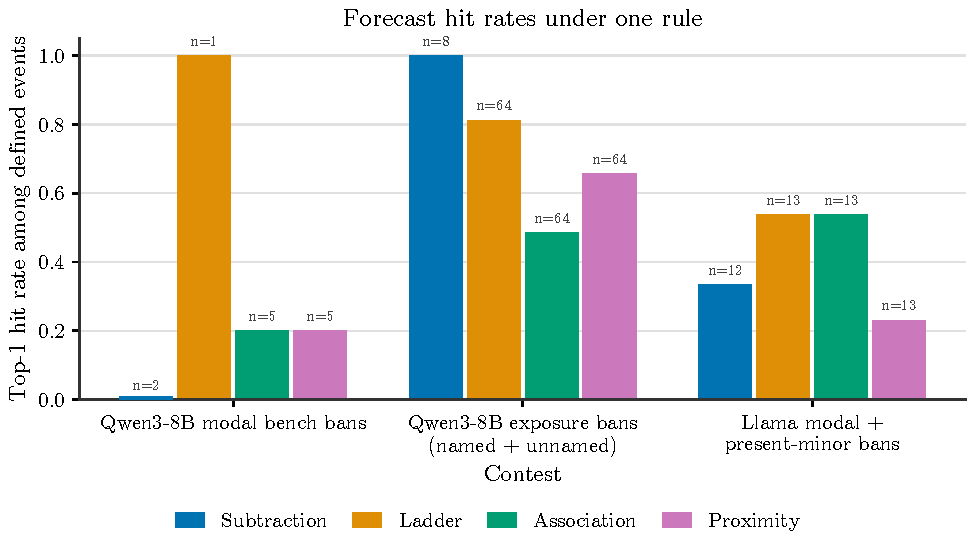
\includegraphics[width=\linewidth,height=0.78\textheight,keepaspectratio]{figures/fig_forecast_hits_v0.pdf}
\caption{Top-1 hit rate (y-axis, 0 to 1.05) of four frozen forecast families, one colour per family and named in the legend below the axes --- Subtraction (blue), Ladder (orange), Association (teal), Proximity (magenta) --- across three contests (x-axis): Qwen3-8B modal bench bans, Qwen3-8B exposure bans (named + unnamed), and Llama modal + present-minor bans. Each bar is scored only over the events where that family produced a defined (non-degenerate) forecast; the count of such defined events is printed above the bar (e.g. n=2), since it varies by family within a contest. The bench-contest Subtraction bar has a defined-event hit rate of exactly 0 (n=2) and is drawn as a thin horizontal line at zero rather than as an invisible bar. Values are corrected in iteration 4: an earlier version of this figure mixed three different rules for scoring a family's undefined forecasts (counting them as misses, giving fractional tie credit, or dropping them), which this defined-only accounting replaces. Rates resting on few defined events --- Subtraction in the bench contest (n=2) and in the exposure contest (n=8) --- carry correspondingly little weight.}
\label{fig:fig_forecast_hits}
\end{figure}
\FloatBarrier
\subsection*{3.10 What iteration 3 established, what it ruled out, and what it abandoned}
\addcontentsline{toc}{subsection}{3.10 What iteration 3 established, what it ruled out, and what it abandoned}
Everything below is still one model per contest, at most 31 gated events per contest, and labels from labellers that passed their gates; the bench is memorised LeetCode material, and the path tasks are a screen that is never pooled.

\textbf{Established.}

\begin{enumerate}
\item \emph{The likelihood substitution test of iteration 2 cannot decide the title claim.} Its gain and residual argmax hit the realised landing in 0 of 17 Qwen3-8B single bans, against 14 of 17 for the implied mass. No row keeps three estimable survivors, the bootstrap variance of the mean gain is 2.7 times the noise term it subtracted, and a decision on mass would need about 50 programs per algorithm at the lower bound and 129 Qwen3-8B or 43 Llama events. Whether the gains are pure subtraction, whether their specific part is aimed, and whether the generic profiles form a ladder are all undetectable with that instrument.
\item \emph{Shown a correct program of a non-default algorithm and told not to use it, Qwen3-8B snaps back to its default.} The default's share of attempts rises from 0.05 under the copy twin to 0.72 under the named ban and 0.82 under the unnamed one. The modal replacement is the default in 24 of 31 gated events, and the ladder forecast wins the frozen contest (7 wins; top-1 0.77). Naming the banned algorithm adds little beyond asking for something else (same modal replacement for 0.88 of Y). \emph{(Correction, iteration 4: the frozen counting rule advances some family in 85\% of no-information simulations and in 100\% of label-permutation placebo draws (the ladder in 43\%), and no paired test survives Holm on the named events, so the 7 wins of the ladder are weak evidence. Wording also changes the landing: under templates one to four the default is modal for 13 of 19 priority algorithms, against 15 of 19 under the fifth, and the replacement flips to the associate for the size-k heap and the Z algorithm. Snap-back rests on one wording. It replicates in the present minor bans of Llama, which return to the default in 0.72 to 0.93 of attempts not banned; Section 4.2.3.)}
\item \emph{Where the default is not available, the landing is specific to the task and mostly unforeseen.} On the five gated Qwen3-8B modal bench bans, no ban-free or association forecast beats uniform on average, and three of five landings (index marking, BFS, a failing merge without sorting) were named by no family. In Llama the landing is predictable above chance (ladder and association 7 of 13 each), but the families do not separate. \emph{(Correction, iteration 4: the merge intervals landing is residue, failing programs labelled other (29 coverage arrays, 12 unsorted sweeps, 3 others), and that event passes the gate only through them (catalogue-only avoidance 0.14). In Llama, with other excluded, association hits 7 of 13 (p = 0.032) and the ladder 6 of 13 (p = 0.100), so only association is above chance.)}
\item \emph{A ban's route is task dependent.} On the bench, pooled over five gated tasks, generated tokens reading the ban carry 0.74 of the effect and the prompt states 0.61. The mechanism is redundant on kth smallest and connected components, direct on two sum and find duplicate, and superadditive on merge intervals, and a second draw reproduces every task. The prompt route story of the path tasks does not generalise. \emph{(Correction, iteration 4: the claim that generated tokens carry more of the effect rested on a comparison of point estimates. With their jackknife intervals the fractions are F\_\allowbreak{}direct 0.744 [0.38, 1.11] and F\_\allowbreak{}prompt 0.611 [0.06, 1.17], which overlap, with interaction -0.355. The superadditive class rests on merge intervals, which is gated only through residue; without it F\_\allowbreak{}prompt is 0.648 [-0.08, 1.38] and F\_\allowbreak{}direct 0.865 [0.68, 1.05].)}
\item \emph{The ban is applied at the opening of the body and not re-read.} Forcing the default's first body token undoes the ban completely on every gated task, while forcing the \texttt{def} line undoes none of it. \emph{(Correction, iteration 4: the locus is resolved to a single token only on kth smallest, where one token after the \texttt{def} line and its indentation undoes the ban; on the other four gated tasks the shortest forced prefix in the depth sweep that undoes it is 10 to 30 tokens long. Restated: the ban gives way at the opening of the body, to a single token on kth smallest.)}
\item \emph{Wording dominates compliance.} The fourth template is the weakest in every artifact (template SD about 2.0 logits; likelihood ratio 374), and dropping it flips the Llama branch.
\item \emph{The default is not carried by any small set of surface tokens.} Exact signature vetoes, one-shot, persistent, iterated or cumulative, almost never remove it; the model renames, respells or breaks the code. A single prompt ban moves the model further than any veto.
\item \emph{Prompts reach past one rung where the alternatives are interchangeable.} Bans that leave one survivor got BFS 50 of 50 on connected components and quickselect 50 of 50 on kth smallest; on kth smallest quickselect is the answer to every ban list, including lists that ban it and the list that leaves only the default. Elsewhere (Floyd-Warshall, size-k heap, heapify and pop, binary search on values) the model will not write a survivor it can write on request. \emph{(Correction, iteration 4: the kth smallest disconfirmation depends on the rung definition. It uses the fallback rung of the token walk; three bench draws put the landing of the ban on quickselect (59 to 79\%), which makes quickselect the behavioural second rung, and under that definition the cell confirms the claim (size-k heap, will 0.00). Connected components disconfirms under either definition.)}
\item \emph{No instruction or knob produced a correct novel algorithm.} Zero of 78 correct out-of-catalogue programs in the iteration-1 and iteration-2 data and 0 of 38 in iteration 3 are novel; the request's long-form instruction makes 84\% of outputs claim novelty, 39\% of those contain no code, and 75\% of the rest are catalogue algorithms.
\item \emph{Llama's correct output is as collapsed as Qwen3-8B's on the grid task} (BFS 20 of 20 correct), and more diverse on 9 of 13 bench tasks counted over correct programs.
\end{enumerate}

\textbf{Ruled out, or not supported.}

\begin{itemize}
\item \emph{Substitution by association in Qwen3-8B.} In none of the three contests did association win; it was worse than uniform on all five gated modal bans and lost to the ladder by about 1.3 nats on exposure bans (Holm 0.081 named, 0.0056 unnamed).
\item \emph{A shared prohibition direction as the carrier of the ban.} Adding the leave-one-task-out ban displacement to a neutral prompt passed on 0 of 5 gated tasks against matched random directions, and removing it from a ban never restored the default (pooled -0.026 [-0.07, 0.03]).
\item \emph{A ban-free signature veto as the forecast of the next rung.} It was undefined on 10 of 12 Qwen3-8B modal events and 29 of 33 exposure events, and where defined on the path tasks or the bench it landed elsewhere than the ban.
\item \emph{The prompt route as the general mechanism of a ban.} Disconfirmed on the bench (pooled direct share 0.74, jackknife [0.38, 1.11]).
\item \emph{Prompts move the model exactly one rung.} Disconfirmed on connected components (BFS will 1.00 at can 1.00) and, through the fallback rung, on kth smallest.
\item \emph{The three ban-attending heads as a causal site.} Ablating them moved the grid ban by +0.06 over random heads in the same layers, inside the range of any perturbation of the fragile fourth-template ban.
\item \emph{A locus at generated tokens 1 to 16.} No decoder beat the template-only or written text controls on any testable task; on the shortest path task the choice diverges at a median of about 29 tokens.
\end{itemize}

\textbf{Dead ends, with the evidence that closed them.}

\begin{itemize}
\item \emph{The forced ratio latent probability as the decision instrument for where a ban sends the mass.} Closed by Table 82 (argmax 0 of 17 against the realised landing) and Table 84 (programs and events needed far beyond the budget).
\item \emph{Signature vetoes and the token walk as a way past the default.} Closed by the bench forecast, exposure, Llama, route and reach experiments: the default survives exact vetoes by renaming and respelling, and the walk stalled at rung 1 or 2 on all six tasks.
\item \emph{The shared prohibition direction.} Closed by Table 110.
\item \emph{Head ablation as a test of the attention heads.} Closed by the random-head control.
\item \emph{Qwen-Scope base SAEs for readouts of the ban.} They now pass a fairer transfer criterion (fraction of cross-entropy recovered 0.989 to 0.994), but their reconstructions keep only a cosine of about 0.3 of the ban displacement, and their latents never beat difference-in-means.
\item \emph{Long-form novelty instructions as a source of novel algorithms.} Closed by Table 118 and the audit (0 novel of 38 correct programs outside the catalogue).
\end{itemize}

\FloatBarrier
\subsection*{3.11 What the next iteration takes from this one}
\addcontentsline{toc}{subsection}{3.11 What the next iteration takes from this one}
The title claim of the update, that a ban removes the default and the model falls to a next rung that ban-free counterfactuals can read in advance, did not survive in that form. The part that survived is snap-back: with the default available, a ban on a shown algorithm returns the model to its default, which is subtraction in its simplest form. Where the default itself is banned, the counterfactuals meant to expose the next rung either fail to move the model (signature vetoes) or move it somewhere else (random pushes, the shared prohibition direction), and the landing is specific to the task in a way no frozen family foresaw in Qwen3-8B. Substitution by association is not supported in Qwen3-8B and is tied with the ladder in Llama. What decides the replacement under a modal ban remains open, and the run now has two concrete leads for it: the opening of the body, where the prefill sweep localises the ban to the first body token, and the template, which carries more of the variance in compliance than anything else measured. \emph{(Added in iteration 4: a third lead was already in the iteration-3 data, the landing composition per route arm. On connected components either route alone lands mostly on DFS, which is the generic landing of random pushes and the association answer of Qwen3-8B, and BFS is chosen only when both routes act; Section 4.2.2.)}

Three things follow for the next iteration. First, the contest needs events on which the default is unavailable and the families disagree, in numbers the paired tests can use: the modal bench bans give 5 gated events in Qwen3-8B, so pooling with Llama (11) and adding bench tasks where bans take is the arithmetic, with the template entered as a random effect rather than pooled over. Second, the first body token is now a measured locus in behaviour; a decoder or patch there, in states saved at that position for each task, would ask what is decided when the ban gives way. Third, the generic perturbation rival needs a behavioural test where its runner-up and the associate differ, which the Qwen3-8B bench rarely provides; Llama's present minor events are where the named ban gained the associate about 0.25 of attempts beyond the veto on two of six events, and that is the next place to look.

Request items still open: a same seed temperature arm with thinking on (dropped again), manifold placement of the walk landings (dropped; the walk stalled), and an SAE readout that keeps the ban displacement. \emph{(Added in iteration 4: the same seed arm with thinking on ran in iteration 4, Section 4.5.)}

\FloatBarrier
\section{Iteration 4: plan noise priced against temperature, where the noise must enter, the plan subspace, and a held-out model family}
\noindent\emph{Run record for this iteration.} Hypothesis carried: ``Plan Nudges Reopen What Tuning Narrowed''. Move recorded at the end of the iteration: deepen; review score 4; evidence state lead; coverage full; 18 candidate strategies considered. The list below gives the iteration's artifacts and the state the round record gave each strand.

{\footnotesize\setlength{\tabcolsep}{3pt}
\begin{longtable}{>{\raggedright\arraybackslash}p{0.24\linewidth}>{\raggedright\arraybackslash}p{0.47\linewidth}>{\raggedright\arraybackslash}p{0.11\linewidth}>{\raggedright\arraybackslash}p{0.08\linewidth}}
\caption*{\textbf{Artifacts of iteration 4.} Names and titles as the artifact workspaces record them; strand state as the round record grades it.}\label{tab:arts4}\\
\toprule \textbf{Artifact} & \textbf{Title} & \textbf{Type} & \textbf{State} \\ \midrule \endfirsthead
\toprule \textbf{Artifact} & \textbf{Title} & \textbf{Type} & \textbf{State} \\ \midrule \endhead
\bottomrule \endlastfoot
\nolinkurl{gen_art_evaluation_3} & Record repair and a frozen push screen & evaluation & lead \\
\nolinkurl{gen_art_experiment_19} & Is plan noise the cheapest route to diverse code? & experiment & lead \\
\nolinkurl{gen_art_experiment_20} & Where noise must enter to change the model's algorithm & experiment & lead \\
\nolinkurl{gen_art_experiment_21} & Same seed: temperature vs plan nudges & experiment & lead \\
\nolinkurl{gen_art_experiment_22} & Where the model picks its coding algorithm & experiment & null \\
\nolinkurl{gen_art_experiment_23} & Predicting which coding bans a new AI model obeys & experiment & null \\
\nolinkurl{gen_art_research_1} & Checking our claims against published work & research & lead \\
\end{longtable}}

\subsection*{What each artifact of iteration 4 was for and what it produced}
\addcontentsline{toc}{subsection}{What each artifact of iteration 4 was for and what it produced}
Each artifact is named below as the run's workspaces name it. The entry gives the round record's verdict on the strand it served, the artifact's own summary of what it was for and what it produced, and the output files it declared, each opened and read from its workspace for this report. It closes with the subsection of this section that reports the artifact's results and the result tables typeset there from its output files.

\paragraph{\nolinkurl{gen_art_evaluation_3}: Record repair and a frozen push screen.}
Type: evaluation. Round record, strand state lead: Frozen screen: movable vs obeying 6\slash{}0\slash{}0\slash{}8 and escape ranks catalogue-only ban avoidance at rho 0.86 (14 tasks); random pushes cheapest qualifying row on T03\slash{}T05. Screen data only.

\emph{The artifact's own summary of what it was for and what it produced:} CPU-only Step 0 of iteration 4 (record repair + frozen push screen). Every number is recomputed from labelled rows of the 11 declared dependencies (exp4, exp6, exp7, exp9, exp11, exp13-exp18) with '\textless{}artifact\_\allowbreak{}id\textgreater{}:\textless{}relative path\textgreater{}' provenance; no model text generated; judge spend USD 0.22. PROVIDES: (1) screen.json, the frozen push-movability screen in canonical JSON,, with the stdlib-only screen\_\allowbreak{}rule.py (reproduces it byte for byte from screen\_\allowbreak{}input.json) and screen\_\allowbreak{}extras.json (per-direction rows, per-engine counts, power notes 1-0.1\textasciicircum{}(1\slash{}K), descriptive Fisher p, discrepancies). Movable tasks = T03, T05, T06, T1, T10, T2 (= frozen C1 set); movable vs catalogue-only modal-ban avoidance \textgreater{}= 0.5 is 6\slash{}0\slash{}0\slash{}8 (one-sided Fisher p = 1\slash{}3003, screen not confirmation); T10 escapes only on the bf16 HF engine (exp13 rand3), the rest on exp17 FP8 directions; the immovable side is weakly tested (mostly K=3, UB90 0.54). (2) tables\slash{}knob\_\allowbreak{}table.csv: 1,120 artifact x task x arm x dial cells, each priced against its own twin (pass cost with Newcombe CI), correct-only rarefied Hill-1 at depth 25 with template\slash{}iid 90\% CIs, Good's coverage, catalogue-only avoidance, escape\slash{}qualify flags; arm\_\allowbreak{}dictionary, random\_\allowbreak{}direction\_\allowbreak{}counts (T03 8\slash{}18 at alpha 1, T2 3\slash{}15, T05 2\slash{}3 and T06 1\slash{}3 at alpha 2), table110\_\allowbreak{}alpha2, per\_\allowbreak{}task\_\allowbreak{}verdict (best rows at \textless{}=5\slash{}\textless{}=20 pts, coverage-standardised sensitivity). 25 of 27 quoted review numbers reproduce; corrected: 'nothing reaches Hill 1.5 under 20 pts on R1\slash{}R3\slash{}R6\slash{}T11\slash{}T13\slash{}T14' (T14 modal ban 1.78 at 17 pts; exp14 exposure arms) and two-sum alpha-2 avoidance 0.469 not 0.48 (denominator). On T03\slash{}T05 the cheapest qualifying row is a norm-matched random direction and the structured ADD edit sits inside the random range. (3) Route landing (exp16): 7\slash{}7 readings, JS 17\slash{}17 to 1e-6, F\_\allowbreak{}prompt 0.611 [0.06,1.17] \slash{} F\_\allowbreak{}direct 0.744 [0.38,1.11]; without residue-gated T13 0.648 [-0.08,1.38] \slash{} 0.865 [0.68,1.05]; T13 not gated under catalogue-only avoidance (0.15) so no route class. (4) Llama hits with 'other' excluded: LADDER 6\slash{}13 (Poisson-binomial p 0.100), ASSOCIATE 7\slash{}13 (p 0.032); snap-back 0.72\slash{}0.73\slash{}0.93. (5) 'Other' audit: 21 events, 226 programs (6 passing): 68 catalogue variant, 156 degenerate, 2 labeller miss, 0 novel (the one passing NOVEL-flagged program re-runs 60\slash{}60 hidden + 3\slash{}3 stress tests but is a textbook value binary search over a sort); judge kappa 0.77 (gpt-4.1-mini below the 5\slash{}6 control gate, gemini-2.5-flash weighted, deepseek tie-break), manual pass 73 programs incl. all 44 T13 merge-interval programs (29 coverage-array, 12 unsorted sweep, 3 other, all failing); residue-gated events exp13 T13, exp16 T13:a, Llama T06. (6) Rigor: defined-only hit rates, exposure SUBTRACT defined 4\slash{}33 (hits 4\slash{}4 both arms), Table 82 per distinct row gain 0\slash{}11, residual 0\slash{}11, implied 8\slash{}11 (6 sham). (7) Section 3.10 replacement sentences and all corrections in corrections.json (0f -\textgreater{} this iteration's research artifact). (8) Rival predictors (14 tasks): movability rho 0.86 vs can 0.16, clarity -0.07, FRLP 0.19, nonce -0.19, novelty 0.35. (9) Figures: captioned markers M1-M5 with the position caveat and a 2x2 composite in activation coordinates; at the label-independent g16 position BFS's nearest neighbour is IDA*, not BiBFS. AUDIT: audit\slash{}rederive.py (stdlib, 29 checks) and audit\slash{}rederive\_\allowbreak{}extra.py (12 checks) with 0 mismatches; 7\slash{}7 placebos fail as required. Outputs: full\slash{}mini\slash{}preview\_\allowbreak{}eval\_\allowbreak{}out.json (exp\_\allowbreak{}eval\_\allowbreak{}sol\_\allowbreak{}out; metadata.sections + 12 datasets), README.md, reproducibility.md; run with \texttt{uv sync -\allowbreak{}-\allowbreak{}frozen \&\& uv run eval.\allowbreak{}py -\allowbreak{}-\allowbreak{}stages all} (\textasciitilde{}1.5 min, cached judges).

Its results are reported in Subsection 4.2 of this report, which typesets the result tables drawn from its output files: Tables 123, 124, 125, 126, 126b, 126c, 127, 128, 129, 130, 131, 132, 132b, 133, 134, 135, 136.

\begin{table}[H]
\renewcommand{\thetable}{O24}
\centering\footnotesize\setlength{\tabcolsep}{3pt}
\caption{Output files declared by \nolinkurl{gen_art_evaluation_3} (iteration 4), each opened and read from the artifact's workspace for this report; size in bytes. [Source: iteration 4, artifact \nolinkurl{gen_art_evaluation_3}.]}
\begin{tabular}{>{\raggedright\arraybackslash}p{0.25\linewidth}>{\raggedleft\arraybackslash}p{0.12\linewidth}>{\raggedright\arraybackslash}p{0.57\linewidth}}
\toprule
\textbf{Declared file} & \textbf{Bytes} & \textbf{What it holds} \\
\midrule
\texttt{eval.\allowbreak{}py} & 1,872 & the artifact's code, 59 lines \\
\texttt{full\_\allowbreak{}eval\_\allowbreak{}out.\allowbreak{}json} & 1,740,632 & the complete output; metadata with 7 top-level keys; 12 datasets with 1,628 examples in all: knob\_\allowbreak{}table (1,120), verification\_\allowbreak{}targets (27), push\_\allowbreak{}screen (14), random\_\allowbreak{}directions (108), route\_\allowbreak{}landing (25), llama\_\allowbreak{}hits (18), and 6 more; top-level keys metrics\_\allowbreak{}agg; 58 aggregate metrics (typeset in full below) \\
\texttt{mini\_\allowbreak{}eval\_\allowbreak{}out.\allowbreak{}json} & 148,546 & small variant of the full output (a few examples per dataset); metadata with 7 top-level keys; 12 datasets; top-level keys metrics\_\allowbreak{}agg \\
\texttt{preview\_\allowbreak{}eval\_\allowbreak{}out.\allowbreak{}json} & 60,883 & preview variant of the full output (truncated strings and lists); metadata with 7 top-level keys; 3 datasets; top-level keys metrics\_\allowbreak{}agg \\
\texttt{reproducibility.\allowbreak{}md} & 11,406 & reproducibility notes, 139 lines \\
\bottomrule
\end{tabular}
\end{table}

{\scriptsize\setlength{\tabcolsep}{2.5pt}\renewcommand{\thetable}{O25}
\begin{longtable}{>{\raggedright\arraybackslash}p{0.27\linewidth}>{\raggedright\arraybackslash}p{0.19\linewidth}>{\raggedright\arraybackslash}p{0.27\linewidth}>{\raggedright\arraybackslash}p{0.19\linewidth}}
\caption{Every aggregate metric in the \texttt{metrics\_agg} block of \nolinkurl{gen_art_evaluation_3}'s \texttt{full\_\allowbreak{}eval\_\allowbreak{}out.\allowbreak{}json} (58 metrics), values copied exactly as stored. [Source: iteration 4, artifact \nolinkurl{gen_art_evaluation_3}.]}\\
\toprule
\textbf{Metric} & \textbf{Value} & \textbf{Metric} & \textbf{Value} \\
\midrule
\endfirsthead
\toprule
\textbf{Metric} & \textbf{Value} & \textbf{Metric} & \textbf{Value} \\
\midrule
\endhead
\bottomrule
\endlastfoot
\texttt{n\_\allowbreak{}knob\_\allowbreak{}rows} & 1120.0 & \texttt{rival\_\allowbreak{}rho\_\allowbreak{}max\_\allowbreak{}E\_\allowbreak{}t} & 0.8500202673964815 \\
\texttt{n\_\allowbreak{}targets} & 27.0 & \texttt{rival\_\allowbreak{}rho\_\allowbreak{}can} & 0.1621954873394075 \\
\texttt{n\_\allowbreak{}targets\_\allowbreak{}matched} & 25.0 & \texttt{rival\_\allowbreak{}rho\_\allowbreak{}clarity} & -0.06505490571714548 \\
\texttt{n\_\allowbreak{}movable\_\allowbreak{}tasks} & 6.0 & \texttt{rival\_\allowbreak{}rho\_\allowbreak{}frlp} & 0.18502247526320056 \\
\texttt{E\_\allowbreak{}T03\_\allowbreak{}a1} & 0.4444444444444444 & \texttt{rival\_\allowbreak{}rho\_\allowbreak{}nonce} & -0.19116713782225253 \\
\texttt{E\_\allowbreak{}T2\_\allowbreak{}a1} & 0.2 & \texttt{rival\_\allowbreak{}rho\_\allowbreak{}novelty} & 0.3532688377417424 \\
\texttt{E\_\allowbreak{}T05\_\allowbreak{}a2} & 0.6666666666666666 & \texttt{table82\_\allowbreak{}hits\_\allowbreak{}implied} & 8.0 \\
\texttt{E\_\allowbreak{}T06\_\allowbreak{}a2} & 0.3333333333333333 & \texttt{table82\_\allowbreak{}hits\_\allowbreak{}gain} & 0.0 \\
\texttt{E\_\allowbreak{}T1\_\allowbreak{}a1} & 0.06666666666666667 & \texttt{rederive\_\allowbreak{}n\_\allowbreak{}checks} & 29.0 \\
\texttt{E\_\allowbreak{}T10\_\allowbreak{}a1} & 0.3333333333333333 & \texttt{rederive\_\allowbreak{}n\_\allowbreak{}mismatches} & 0.0 \\
\texttt{screen\_\allowbreak{}fisher\_\allowbreak{}p\_\allowbreak{}descriptive} & 0.000333000333000333 & \texttt{placebos\_\allowbreak{}failed\_\allowbreak{}as\_\allowbreak{}required} & 4.0 \\
\texttt{screen\_\allowbreak{}balanced\_\allowbreak{}accuracy} & 1.0 & \texttt{rederive\_\allowbreak{}extra\_\allowbreak{}n\_\allowbreak{}checks} & 12.0 \\
\texttt{llama\_\allowbreak{}assoc\_\allowbreak{}hits\_\allowbreak{}excl\_\allowbreak{}other} & 7.0 & \texttt{rederive\_\allowbreak{}extra\_\allowbreak{}n\_\allowbreak{}mismatches} & 0.0 \\
\texttt{llama\_\allowbreak{}ladder\_\allowbreak{}hits\_\allowbreak{}excl\_\allowbreak{}other} & 6.0 & \texttt{rederive\_\allowbreak{}extra\_\allowbreak{}placebos\_\allowbreak{}failed\_\allowbreak{}as\_\allowbreak{}required} & 3.0 \\
\texttt{llama\_\allowbreak{}assoc\_\allowbreak{}p\_\allowbreak{}excl\_\allowbreak{}other} & 0.03171599451303157 & \texttt{openrouter\_\allowbreak{}usd} & 0.0 \\
\texttt{llama\_\allowbreak{}ladder\_\allowbreak{}p\_\allowbreak{}excl\_\allowbreak{}other} & 0.1000374430727024 & \texttt{n\_\allowbreak{}qualify\_\allowbreak{}dirs\_\allowbreak{}R1} & 0.0 \\
\texttt{route\_\allowbreak{}F\_\allowbreak{}prompt\_\allowbreak{}all5} & 0.6111111111111112 & \texttt{n\_\allowbreak{}qualify\_\allowbreak{}dirs\_\allowbreak{}R3} & 0.0 \\
\texttt{route\_\allowbreak{}F\_\allowbreak{}direct\_\allowbreak{}all5} & 0.7439613526570049 & \texttt{n\_\allowbreak{}qualify\_\allowbreak{}dirs\_\allowbreak{}R6} & 0.0 \\
\texttt{route\_\allowbreak{}F\_\allowbreak{}prompt\_\allowbreak{}wo\_\allowbreak{}T13} & 0.647887323943662 & \texttt{n\_\allowbreak{}qualify\_\allowbreak{}dirs\_\allowbreak{}T03} & 7.0 \\
\texttt{route\_\allowbreak{}F\_\allowbreak{}direct\_\allowbreak{}wo\_\allowbreak{}T13} & 0.8647887323943663 & \texttt{n\_\allowbreak{}qualify\_\allowbreak{}dirs\_\allowbreak{}T04} & 0.0 \\
\texttt{route\_\allowbreak{}F\_\allowbreak{}prompt\_\allowbreak{}cat\_\allowbreak{}all5} & 0.6341463414634146 & \texttt{n\_\allowbreak{}qualify\_\allowbreak{}dirs\_\allowbreak{}T05} & 1.0 \\
\texttt{route\_\allowbreak{}F\_\allowbreak{}direct\_\allowbreak{}cat\_\allowbreak{}all5} & 0.8238482384823849 & \texttt{n\_\allowbreak{}qualify\_\allowbreak{}dirs\_\allowbreak{}T06} & 1.0 \\
\texttt{route\_\allowbreak{}readings\_\allowbreak{}matched} & 7.0 & \texttt{n\_\allowbreak{}qualify\_\allowbreak{}dirs\_\allowbreak{}T08} & 0.0 \\
\texttt{other\_\allowbreak{}n\_\allowbreak{}programs} & 226.0 & \texttt{n\_\allowbreak{}qualify\_\allowbreak{}dirs\_\allowbreak{}T1} & 0.0 \\
\texttt{other\_\allowbreak{}n\_\allowbreak{}passed} & 6.0 & \texttt{n\_\allowbreak{}qualify\_\allowbreak{}dirs\_\allowbreak{}T10} & 0.0 \\
\texttt{other\_\allowbreak{}n\_\allowbreak{}novel\_\allowbreak{}confirmed} & 0.0 & \texttt{n\_\allowbreak{}qualify\_\allowbreak{}dirs\_\allowbreak{}T11} & 0.0 \\
\texttt{judge\_\allowbreak{}kappa} & 0.7746996169788551 & \texttt{n\_\allowbreak{}qualify\_\allowbreak{}dirs\_\allowbreak{}T13} & 0.0 \\
\texttt{judge\_\allowbreak{}agreement} & 0.915929203539823 & \texttt{n\_\allowbreak{}qualify\_\allowbreak{}dirs\_\allowbreak{}T14} & 0.0 \\
\texttt{rival\_\allowbreak{}rho\_\allowbreak{}movability} & 0.8612327526892111 & \texttt{n\_\allowbreak{}qualify\_\allowbreak{}dirs\_\allowbreak{}T2} & 0.0 \\
\end{longtable}}

\paragraph{\nolinkurl{gen_art_experiment_19}: Is plan noise the cheapest route to diverse code?.}
Type: experiment. Round record, strand state lead: C1 PARTIAL: plan noise H5 2.72 vs 1.96 (kth smallest), 2.09 vs 1.96 (components) at 0 pass cost; loses find dup (1.00 vs 2.73), shortest path (1.35 vs 1.93); pooled -0.22 [-0.89,0.30].

\emph{The artifact's own summary of what it was for and what it produced:} Experiment (iteration 4, Step 1 \slash{} Claim 1): is fresh per-sample plan noise (PN: one isotropic unit direction per sample, displacement-targeted at the task-spec positions of blocks 12-23 during prefill, alpha 0.5\slash{}1\slash{}2\slash{}4 ban units) the cheapest knob for CORRECT algorithmic diversity in Qwen3-8B (FP8 W8A8 on a 16 GB RTX 2000 Ada, thinking off, exact CRN)? Priced against temperature 1.3\slash{}1.6, top-k 10, nonce ban, novelty instruction, semantic seed (T1\slash{}T2), reused iteration-3 signature vetoes, and (sensitivity) min-p 0.1 at T1.6\slash{}T2.0 and a verbalized-sampling prompt. Statistic: correct-only Hill-1 rarefied at depth 25 on each knob's randomisation hull (H5 at \textless{}=5 pass points, P15, P20), 2,000-replicate bootstraps with best-setting selection inside replicates. 10,100 labelled programs, N=50 in all 202 cells (E6+R2 up to 17 arms; 8 non-movable bench tasks x 11 arms); no cell dropped. RESULT: pre-registered C1 = PARTIAL (count1 2\slash{}6, count2 4\slash{}6, D\_\allowbreak{}bar -0.22, 95\% CI [-0.89, 0.30]); every sensitivity s1-s8 also PARTIAL. PN wins T03 (H5 2.72 vs novelty 1.96, P=1.00) and T10 (2.09 vs iterated veto 1.96, P=0.91), ties T05\slash{}T1, loses T06 (iterated veto 2.73 vs 1.00) and T2 (semantic seed 1.93 vs 1.35). Temperature, top-k 10 and the nonce ban buy no correct algorithmic diversity (H5\textless{}=1.09); min-p \textless{}=1.17. Temperature changes code but almost never the algorithm (T1: 88\% code flips, 2\% label flips); PN at alpha 2 flips the label in 50-60\% of slots on T03\slash{}T10\slash{}T2; breakage at alpha 4 (alpha 2 on T2). R2 (held out) and 7 of 8 non-movable tasks barely move under PN. 81\% of verbalized-sampling programs are run-time random dispatchers (labels trace-dependent). Engine check REPRODUCED (exp17 screen rows bit-exact, per-slot agreement 1.00). Novelty audit: 12 correct 'other' programs, all labeller misses, 0 novel. Label validity: agreement 1.00 except T03 (0.80; D\_\allowbreak{}t robust). Independent re-derivation 12\slash{}12 match; full-rule placebo 0\slash{}100 CONFIRMED; PN-\textgreater{}TWIN placebo D\_\allowbreak{}t\textless{}=0; hash chain intact (commit before Stage 1). Files: results\slash{}c1.json (decision + sensitivities + class CIs), results\slash{}prices.json, results\slash{}knob\_\allowbreak{}rows.jsonl (merge-ready per (task, arm) Step-0 Hill rows), data\slash{}samples.jsonl (per-sample rows with code, label, pass, seeds, displacement), results\slash{}* descriptive files (alpha\_\allowbreak{}sweep, flips, ideas\_\allowbreak{}phrasings, plain\_\allowbreak{}vs\_\allowbreak{}twin, nonmovable, forecast\_\allowbreak{}score, vs\_\allowbreak{}dispatch), audit\slash{}*, figures\slash{}fig1-6, method\_\allowbreak{}out.json (exp\_\allowbreak{}gen\_\allowbreak{}sol\_\allowbreak{}out). OpenRouter spend USD 0.23. Caveats: FP8 not bf16 (device table); 6 decisive tasks; reused vetoes from another engine; the counts part of the rule alone is not selective under arm shuffles (8\slash{}100) - the CI criterion is.

Its results are reported in Subsection 4.3 of this report, which typesets the result tables drawn from its output files: Tables 137, 138, 139, 140, 141, 142, 142b, 142c.

\begin{table}[H]
\renewcommand{\thetable}{O26}
\centering\footnotesize\setlength{\tabcolsep}{3pt}
\caption{Output files declared by \nolinkurl{gen_art_experiment_19} (iteration 4), each opened and read from the artifact's workspace for this report; size in bytes. [Source: iteration 4, artifact \nolinkurl{gen_art_experiment_19}.]}
\begin{tabular}{>{\raggedright\arraybackslash}p{0.25\linewidth}>{\raggedleft\arraybackslash}p{0.12\linewidth}>{\raggedright\arraybackslash}p{0.57\linewidth}}
\toprule
\textbf{Declared file} & \textbf{Bytes} & \textbf{What it holds} \\
\midrule
\texttt{method.\allowbreak{}py} & 4,888 & the artifact's code, 98 lines \\
\texttt{full\_\allowbreak{}method\_\allowbreak{}out.\allowbreak{}json} & 10,588,349 & the complete output; metadata with 33 top-level keys; 2 datasets with 10,382 examples in all: knob\_\allowbreak{}rows (282), samples (10,100) \\
\texttt{mini\_\allowbreak{}method\_\allowbreak{}out.\allowbreak{}json} & 286,816 & small variant of the full output (a few examples per dataset); metadata with 33 top-level keys; 2 datasets \\
\texttt{preview\_\allowbreak{}method\_\allowbreak{}out.\allowbreak{}json} & 250,881 & preview variant of the full output (truncated strings and lists); metadata with 33 top-level keys; 2 datasets \\
\texttt{reproducibility.\allowbreak{}md} & 10,611 & reproducibility notes, 144 lines \\
\bottomrule
\end{tabular}
\end{table}

\paragraph{\nolinkurl{gen_art_experiment_20}: Where noise must enter to change the model's algorithm.}
Type: experiment. Round record, strand state lead: Prefill task-spec site beats read position at matched downstream displacement (OR 5.72 [3.94,8.30]); site rule PARTIAL 3\slash{}6; generated tokens 1-32 also redirect (find dup 12:0).

\emph{The artifact's own summary of what it was for and what it produced:} Experiment (iteration 4, plan gen\_\allowbreak{}plan\_\allowbreak{}experiment\_\allowbreak{}2\_\allowbreak{}idx3) testing WHERE isotropic random noise must enter Qwen3-8B (pinned revision, thinking off, T=1.0; FP8 W8A8 on a 16 GB RTX 2000 Ada per the frozen precision rule) to change which correct algorithm it writes. Six tasks (T03 kth smallest, T05 two sum, T06 find duplicate, T10 connected components, T1 grid path, T2 weighted shortest path); one fresh random direction and one token-uniform stream per CRN slot shared by every arm, so site contrasts are exact paired flips. Sites at matched per-position ban-unit dose (alpha 1\slash{}2\slash{}4, N=30 per cell; twin N=50): S0 task-spec states blocks 12-23, S1 read position, S2 condition sentence, S3 generated tokens 1-32 (teacher-forced shadow rows), S4 task spec blocks 0-11, S5 task spec blocks 24-35; plus energy-matched S1E\slash{}S2E, S0 at alpha 8 (N=50), and a T1 TOP5 plan push. 4,510 programs; pre-registered (hash-chained commits \#0-\#4). RESULTS. C1-site = PARTIAL under the frozen rule: S0 has the best randomisation-hull price H5 (correct-only rarefied Hill within 0.05 pass cost) on 3\slash{}6 tasks (T03 2.61, T1 1.29, T2 1.66; raw p=0.062 vs Bin(6,1\slash{}6)); S3 wins T05\slash{}T06, S4 wins T10 (S4 ban units are only 4.5-7.2\% of the residual norm vs 12.7-18.3\% for S0: dose-convention confound). All per-task margins are bootstrap close calls (P(S0 argmax) 0.31-0.67; T2 0.97). S1 and S2 never change the algorithm (0\slash{}526 and 0\slash{}527 correct off-default programs at alpha 1-4), S5 nearly inert (6\slash{}521) even though S1 produces the same downstream displacement at R as S0; at matched displacement the S0 indicator stays +2.15 logit [1.79, 2.51] (Mantel-Haenszel OR 5.72 [3.94, 8.30]; shuffled-label placebo fails). Reading: the idea is chosen in the task-specification states at early-to-middle blocks; read-out, condition and late sites are inert; blocks 12-23 specifically is not supported over 0-11. Alpha 8 erases the task (pass 0.00 on all six). Novelty audit: 1 correct 'other' program (T06 nums.count brute force; judges DEGENERATE, manual CATALOGUE VARIANT), 0 novel among 3,555 correct programs (rule-of-three 0.08\%). C3d: the TOP5 plan push never leaves BFS (avoidance 0.00 at alpha 1-2, 0 correct at alpha 4); landing test not computable. Engine check reproduces the exp17 screen byte for byte (50\slash{}50 on T03 and T2). Alpha-4 compositions differ from sibling exp19's PN\_\allowbreak{}a4 rows (do not use them as the Step-1 knob table). FILES. method\_\allowbreak{}out.json (+ full\slash{}mini\slash{}preview; datasets site\_\allowbreak{}grid, boundary\_\allowbreak{}alpha8, top5\_\allowbreak{}plan, engine\_\allowbreak{}check; all analyses in metadata); results\slash{}*.json (c1\_\allowbreak{}site, hull, cells, failure\_\allowbreak{}modes, paired\_\allowbreak{}flips, transmission, pooled\_\allowbreak{}model, boundary, c3d, novelty\_\allowbreak{}audit, engine\_\allowbreak{}check, overlap\_\allowbreak{}check, units\_\allowbreak{}summary, rederive, rederive\_\allowbreak{}headlines, unit tests, deviations D1-D16); data\slash{}samples.jsonl (every row with labels, displacement logs); units\slash{}, directions\slash{} (u\_\allowbreak{}top5, plan-site geometry); figures fig1-fig7; README.md; reproducibility.md. Caveats: FP8 only, one model, memorised tasks, N=30 cannot rank two live sites; site-specific perturbation, not a plan representation.

Its results are reported in Subsection 4.4 of this report, which typesets the result tables drawn from its output files: Tables 143, 144, 145, 146, 147, 148, 149.

\begin{table}[H]
\renewcommand{\thetable}{O27}
\centering\footnotesize\setlength{\tabcolsep}{3pt}
\caption{Output files declared by \nolinkurl{gen_art_experiment_20} (iteration 4), each opened and read from the artifact's workspace for this report; size in bytes. [Source: iteration 4, artifact \nolinkurl{gen_art_experiment_20}.]}
\begin{tabular}{>{\raggedright\arraybackslash}p{0.25\linewidth}>{\raggedleft\arraybackslash}p{0.12\linewidth}>{\raggedright\arraybackslash}p{0.57\linewidth}}
\toprule
\textbf{Declared file} & \textbf{Bytes} & \textbf{What it holds} \\
\midrule
\texttt{method.\allowbreak{}py} & 4,254 & the artifact's code, 99 lines \\
\texttt{full\_\allowbreak{}method\_\allowbreak{}out.\allowbreak{}json} & 654,368 & the complete output; metadata with 25 top-level keys; 4 datasets with 630 examples in all: site\_\allowbreak{}grid (180), boundary\_\allowbreak{}alpha8 (300), top5\_\allowbreak{}plan (50), engine\_\allowbreak{}check (100) \\
\texttt{mini\_\allowbreak{}method\_\allowbreak{}out.\allowbreak{}json} & 73,865 & small variant of the full output (a few examples per dataset); metadata with 25 top-level keys; 4 datasets \\
\texttt{preview\_\allowbreak{}method\_\allowbreak{}out.\allowbreak{}json} & 61,493 & preview variant of the full output (truncated strings and lists); metadata with 25 top-level keys; 3 datasets \\
\texttt{reproducibility.\allowbreak{}md} & 11,038 & reproducibility notes, 176 lines \\
\bottomrule
\end{tabular}
\end{table}

\paragraph{\nolinkurl{gen_art_experiment_21}: Same seed: temperature vs plan nudges.}
Type: experiment. Round record, strand state lead: Same seed: temperature changes the algorithm in 0\slash{}20 seeds (3 tasks; T2 thinking on too); one plan direction 17.25\slash{}20 (T2), 4.55 (T03); contrast 0.545 [0.41,0.67]; PARTIAL.

\emph{The artifact's own summary of what it was for and what it produced:} Seed-coupled 2x2 on Qwen3-8B (exp17's HF FP8 W8A8 engine on the screen's 16 GB RTX 2000 Ada; thinking off) for T2 weighted shortest path (default Dijkstra), T1 grid path (BFS) and T03 k-th smallest (full sort), 20 token seeds per task, each keeping one noise stream across every condition (inverse-CDF CRN). Results: temperature (0.3\slash{}0.7\slash{}1.0\slash{}1.3, top-k 10) changed the algorithm in 0\slash{}20 seeds on all three tasks, and in 0\slash{}20 on T2 with thinking on (vLLM 0.11, Gumbel-max per-request seeds, 100\slash{}100 traces completed; repeat noise floor 0). Plan noise (6 isotropic directions at the task-spec states of blocks 12-23, prefill only, alpha 1, T 1.0) changed it in 17.25\slash{}20 seeds on T2 (20-subset mean), 4.55 on T03 and 2.5 on T1. Pooled paired seed contrast (T2+T03): mean x\_\allowbreak{}s 0.545 [0.41, 0.67], sign-flip p = 1.0e-5 (Holm entry C1-seed); within-seed permutation test p = 0.005. Phrasings per idea grow with T (pooled log-PPI slope 0.64-0.81, CIs exclude 0; driven by T1). Verdict (pre-registered, commit \#0 before any decisive sample): PARTIAL, H-PN fails on T03 (4.55 \textless{} 5) where the protocol-v4 unit is 0.77x the screen's; the Gumbel-max replicate gives T03 5.8. Engine check reproduces the screen byte for byte (200\slash{}200). Optional arms: min-p T 2.0 moves 1\slash{}20 seeds (T2, T03); thinking-on PN moves the first approach in \textless{}=1\slash{}10 seeds; T1 thinking on (10 seeds) C\_\allowbreak{}T 0. Novelty audit: 0 novel. Independent re-derivation: 0 mismatches in 33 checks. Files: results\slash{}c1seed.json (all counts, tests, verdict), results\slash{}phrasing.json, results\slash{}thinking.json, results\slash{}table\_\allowbreak{}1ac.json, data\slash{}samples.jsonl (3,140 programs), data\slash{}raw\_\allowbreak{}thinking.jsonl, figures\slash{}F1-F5, method\_\allowbreak{}out.json (datasets seed\_\allowbreak{}coupled\_\allowbreak{}off\slash{}on, engine\_\allowbreak{}check, fp8\_\allowbreak{}crosscheck).

Its results are reported in Subsection 4.5 of this report, which typesets the result tables drawn from its output files: Tables 150, 151, 152.

\begin{table}[H]
\renewcommand{\thetable}{O28}
\centering\footnotesize\setlength{\tabcolsep}{3pt}
\caption{Output files declared by \nolinkurl{gen_art_experiment_21} (iteration 4), each opened and read from the artifact's workspace for this report; size in bytes. [Source: iteration 4, artifact \nolinkurl{gen_art_experiment_21}.]}
\begin{tabular}{>{\raggedright\arraybackslash}p{0.25\linewidth}>{\raggedleft\arraybackslash}p{0.12\linewidth}>{\raggedright\arraybackslash}p{0.57\linewidth}}
\toprule
\textbf{Declared file} & \textbf{Bytes} & \textbf{What it holds} \\
\midrule
\texttt{method.\allowbreak{}py} & 4,863 & the artifact's code, 101 lines \\
\texttt{full\_\allowbreak{}method\_\allowbreak{}out.\allowbreak{}json} & 452,888 & the complete output; metadata with 26 top-level keys; 4 datasets with 340 examples in all: seed\_\allowbreak{}coupled\_\allowbreak{}off (60), seed\_\allowbreak{}coupled\_\allowbreak{}on (30), engine\_\allowbreak{}check (200), fp8\_\allowbreak{}crosscheck (50) \\
\texttt{mini\_\allowbreak{}method\_\allowbreak{}out.\allowbreak{}json} & 138,337 & small variant of the full output (a few examples per dataset); metadata with 26 top-level keys; 4 datasets \\
\texttt{preview\_\allowbreak{}method\_\allowbreak{}out.\allowbreak{}json} & 119,091 & preview variant of the full output (truncated strings and lists); metadata with 26 top-level keys; 3 datasets \\
\texttt{reproducibility.\allowbreak{}md} & 10,344 & reproducibility notes, 148 lines \\
\bottomrule
\end{tabular}
\end{table}

\paragraph{\nolinkurl{gen_art_experiment_22}: Where the model picks its coding algorithm.}
Type: experiment. Round record, strand state null: C2a disconfirmed: subspace share ranks 40 fresh directions at rho 0.03; removing it keeps the effect (ratio 1.00); targeted push beats random only on components (48\% vs 0\%).

\emph{The artifact's own summary of what it was for and what it produced:} Qwen3-8B (pinned revision, FP8 W8A8 on a 16 GB RTX 2000 Ada, thinking off, T = 1). The test asks whether a plan subspace P\_\allowbreak{}t at the task-specification positions explains which random pushes change the algorithm the model writes. P\_\allowbreak{}t is the span of the centroid differences of 30 forced 'Implement X' paraphrases per algorithm, plus a name-masked twin, at blocks 12-35, on 15 coding tasks. All 4,144 prompts were used. Every predictor was sha256-committed before sampling. Scale: 13,500 CRN-coupled programs, labelled by runtime tracer + AST, with a blind judge only on disagreement; 2.51 GPU-hours; USD 0.20 of OpenRouter. The engine reproduced the iteration-3 screen slot for slot (180\slash{}180 identical programs). The plan subspace is reliable: split-half principal cosine 0.89-0.97 vs 0.02 for random subspaces. C2a (primary), DISCONFIRMED. The projection share pi(u) does not rank which of 40 fresh random directions move the algorithm: rho \textless{} 0.2 on 6\slash{}6 movable tasks; pooled within-task rho 0.03 [-0.03, 0.09]. The masked variant and structured controls also fail. Which directions move is itself highly reproducible (template split-half rho 0.76-0.90), so the null is not noise. Exploratory: the signed progress of the realised displacement toward the runner-up centroid correlates up to 0.57 with the effect. Escape fractions (confirmed at N = 30), at alpha 1 \slash{} alpha 2: - T03: 0.30 \slash{} 0.63 (quickselect, size-k heap); - T10: 0.38 \slash{} 0.73 (DFS); - T2: 0.18 \slash{} 0.20 (Bellman-Ford); - T05: 0 \slash{} 0.13 (brute force); - T1: 0.05 \slash{} 0.13 (DFS); - T06 and nine other tasks, including the held-out R2: 0. Landings match the iteration-3 screen. Decomposition (20 confirmed directions): removing the P\_\allowbreak{}t component (u\_\allowbreak{}perp) or clamping the realised P\_\allowbreak{}t displacement keeps the effect (pooled median R = 1.00 for both), so P\_\allowbreak{}t is not needed. The amplified P\_\allowbreak{}t component alone also escapes for 9 of 20 directions: generic sensitivity. C2c, DISCONFIRMED by its rule (5\slash{}6 tasks indistinguishable from a matched random push), with T10 as a clean exception. At half the distance to the runner-up centroid (0.15 ban units), T10 gives 48\% correct DFS vs 0\% for the matched random push (24\slash{}0 CRN flips, McNemar p = 1.2e-7). The empirical crossing is s = 0.59 vs the predicted 0.5; T03 crosses at 0.85. C2b fails: pooled rho 0.27. C3b (descriptive): push landings forecast ban landings best (log score -0.76 vs ASSOCIATE -3.46). Movability tracks ban avoidance across 14 tasks (rho 0.86). Novelty audit: 0 novel algorithms among 10,651 correct push programs. Files provided: - method\_\allowbreak{}out.json (exp\_\allowbreak{}gen\_\allowbreak{}sol\_\allowbreak{}out), with datasets c2a\_\allowbreak{}population, escape\_\allowbreak{}9task, decomposition, targeted and c3b\_\allowbreak{}events; - results\slash{}*.json for every analysis; - figures fig1-fig9; - predictions\slash{}c2\_\allowbreak{}commit.json and the commitments.log hash chain; - data\slash{}samples\_\allowbreak{}raw.jsonl and data\slash{}labels.jsonl; - two independent audits with placebos (0 mismatches); - reproducibility.md.

Its results are reported in Subsection 4.6 of this report, which typesets the result tables drawn from its output files: Tables 153, 154, 155, 156, 157, 158.

\begin{table}[H]
\renewcommand{\thetable}{O29}
\centering\footnotesize\setlength{\tabcolsep}{3pt}
\caption{Output files declared by \nolinkurl{gen_art_experiment_22} (iteration 4), each opened and read from the artifact's workspace for this report; size in bytes. [Source: iteration 4, artifact \nolinkurl{gen_art_experiment_22}.]}
\begin{tabular}{>{\raggedright\arraybackslash}p{0.25\linewidth}>{\raggedleft\arraybackslash}p{0.12\linewidth}>{\raggedright\arraybackslash}p{0.57\linewidth}}
\toprule
\textbf{Declared file} & \textbf{Bytes} & \textbf{What it holds} \\
\midrule
\texttt{method.\allowbreak{}py} & 2,152 & the artifact's code, 63 lines \\
\texttt{full\_\allowbreak{}method\_\allowbreak{}out.\allowbreak{}json} & 6,975,988 & the complete output; metadata with 23 top-level keys; 5 datasets with 5,792 examples in all: c2a\_\allowbreak{}population (4,340), escape\_\allowbreak{}9task (740), decomposition (400), targeted (300), c3b\_\allowbreak{}events (12) \\
\texttt{mini\_\allowbreak{}method\_\allowbreak{}out.\allowbreak{}json} & 335,702 & small variant of the full output (a few examples per dataset); metadata with 23 top-level keys; 5 datasets \\
\texttt{preview\_\allowbreak{}method\_\allowbreak{}out.\allowbreak{}json} & 251,727 & preview variant of the full output (truncated strings and lists); metadata with 23 top-level keys; 3 datasets \\
\texttt{reproducibility.\allowbreak{}md} & 10,217 & reproducibility notes, 152 lines \\
\bottomrule
\end{tabular}
\end{table}

\paragraph{\nolinkurl{gen_art_experiment_23}: Predicting which coding bans a new AI model obeys.}
Type: experiment. Round record, strand state null: Gemma C3a inconclusive (BA 0.74, Fisher p 0.24), disconfirmed by default-drop (BA 0.57); 2 of 3 true positives compromised (tied grid, mislabelled T2); novelty predicts better.

\emph{The artifact's own summary of what it was for and what it produced:} Held-out-family test of Claim 3a on google\slash{}gemma-3-4b-it (bf16, RTX 2000 Ada 16 GB): does a ban-free random-push screen (8 fixed isotropic directions x alpha \{1,2\}, displacement-targeted edits of task-spec states in blocks 11-22, outlier-excluded unit transferred from Qwen3-8B; escape = off-default share - p0 \textgreater{}= 0.20 with pass \textgreater{}= 0.8x twin, confirmed at N=30 by exact binomial) predict which modal coding bans the model obeys? Predictions (E\_\allowbreak{}t, MOVABLE, rivals, 4 landing forecasts) and the frozen analysis were sha256 hash-chained before any ban prompt (commitments.log; grep audit 0 hits). 15 tasks (12 bench + T1 grid path, T2 weighted shortest path, R2), 10,730 labelled programs (8,030 ban-free; 2,700 ban rows incl. the 1,500 primary modal-ban programs), frozen labellers. RESULTS: movable = T1,T2,T04,T05,T10,T11; observed obey (A\_\allowbreak{}t\textgreater{}=0.5) = T1,T2,T03,T05. C3a INCONCLUSIVE: BA 0.739 [0.40,0.95], Fisher p 0.235 (table [[3,3],[1,8]]; Bonferroni 0.71), Spearman rho 0.537 (one-sided perm p 0.025), Kendall 0.47; all sensitivities INCONCLUSIVE (w\slash{}o T1\slash{}T2: BA 0.61, rho 0.31). Rival 'novelty instruction off-default share' predicts better (rho 0.77; delta rho -0.24 [-0.82,0.23]). C3b INCONCLUSIVE: push-landing log score -0.11 (4\slash{}4 top-1) vs association -1.77, but only 2 disagreeing events (\textless{}3). C1 (descriptive): plan noise raises correct-only Hill-1 at \textless{}=5 pass points (T2 1.0-\textgreater{}1.62) where temperature 1.3\slash{}1.6 does not. Novelty audit: 0 novel among 34 correct 'other'. KEY CAVEAT (post hoc, results\slash{}posthoc\_\allowbreak{}t2\_\allowbreak{}relabel.json): the frozen T2 labeller reads array-based Dijkstra as Bellman-Ford; second-judge relabel cuts T2 ban avoidance 0.96-\textgreater{}0.11 (BA 0.667, rho 0.44; still INCONCLUSIVE). DEVIATION D3: Gemma's top-5 channels carry 99\% of \textbar{}\textbar{}h\textbar{}\textbar{}\textasciicircum{}2 (Qwen 40\%), so the plan's unit erased the task; the outlier-excluded unit was adopted before commit \#1 and matches the post-ban ban displacement (ratio 1.29). PROVIDES: method.py (pipeline driver) + src\slash{}; data\slash{}samples.jsonl (every row: label, pass, realised displacement), data\slash{}raw\_\allowbreak{}*.jsonl (text+token ids); predictions\slash{}commit1.json, commit\_\allowbreak{}preban.json, frozen analysis\_\allowbreak{}c3.py; results\slash{}*.json (c3a, rivals, c3b, c1\_\allowbreak{}prices, bans, escape, unit\_\allowbreak{}sensitivity, qwen\_\allowbreak{}ratio, screen, label\slash{}novelty audits, posthoc, rederive: 0 mismatches, placebos fail); figures fig1-fig6; method\_\allowbreak{}out.json (datasets heldout\_\allowbreak{}ban\_\allowbreak{}samples, heldout\_\allowbreak{}banfree\_\allowbreak{}samples, heldout\_\allowbreak{}task\_\allowbreak{}events). OpenRouter USD 0.28; 1.28 GPU-h generation.

Its results are reported in Subsection 4.7 of this report, which typesets the result tables drawn from its output files: Tables 159, 160, 161, 162, 163.

\begin{table}[H]
\renewcommand{\thetable}{O30}
\centering\footnotesize\setlength{\tabcolsep}{3pt}
\caption{Output files declared by \nolinkurl{gen_art_experiment_23} (iteration 4), each opened and read from the artifact's workspace for this report; size in bytes. [Source: iteration 4, artifact \nolinkurl{gen_art_experiment_23}.]}
\begin{tabular}{>{\raggedright\arraybackslash}p{0.25\linewidth}>{\raggedleft\arraybackslash}p{0.12\linewidth}>{\raggedright\arraybackslash}p{0.57\linewidth}}
\toprule
\textbf{Declared file} & \textbf{Bytes} & \textbf{What it holds} \\
\midrule
\texttt{method.\allowbreak{}py} & 6,016 & the artifact's code, 118 lines \\
\texttt{full\_\allowbreak{}method\_\allowbreak{}out.\allowbreak{}json} & 26,164,100 & the complete output; metadata with 32 top-level keys; 3 datasets with 10,745 examples in all: heldout\_\allowbreak{}ban\_\allowbreak{}samples (2,700), heldout\_\allowbreak{}banfree\_\allowbreak{}samples (8,030), heldout\_\allowbreak{}task\_\allowbreak{}events (15) \\
\texttt{mini\_\allowbreak{}method\_\allowbreak{}out.\allowbreak{}json} & 363,937 & small variant of the full output (a few examples per dataset); metadata with 32 top-level keys; 3 datasets \\
\texttt{preview\_\allowbreak{}method\_\allowbreak{}out.\allowbreak{}json} & 339,321 & preview variant of the full output (truncated strings and lists); metadata with 32 top-level keys; 3 datasets \\
\texttt{reproducibility.\allowbreak{}md} & 10,581 & reproducibility notes, 154 lines \\
\bottomrule
\end{tabular}
\end{table}

\paragraph{\nolinkurl{gen_art_research_1}: Checking our claims against published work.}
Type: research. Round record, strand state lead: 112\slash{}112 quotes verified; 0 of 63 scored records occupy; flags A\slash{}B not fired; C1 contrast set lacks text-level plan samplers (IFG, PlanSearch) and departure-matched decoding.

\emph{The artifact's own summary of what it was for and what it produced:} Dated (2026-10-21) positioning audit of the run's iteration-3 and iteration-4 claims. It provides two paste-ready tables, Table 92b and Table 92c, in research\_\allowbreak{}report.md. Each claim is set against its nearest published finding with a verbatim quote, URL, section, arXiv version and venue evidence. 112 quotes from 74 references were checked: 101 VERIFIED on full text, 11 VERIFIED-ABSTRACT (OpenReview\slash{}NeurIPS records), 0 mismatches, and 112\slash{}112 re-matched by an independent live fetch\_\allowbreak{}grep pass. Saturation search: 8 families and 25 queries on OpenAlex\slash{}Crossref, the arXiv API, Semantic Scholar and the ICLR 2027 OpenReview pool, plus 28 general-web calls and forward citations of 6 neighbours. 1,933 hits gave 1,729 unique records, 1,286 in the window and 63 scored on the O\slash{}I\slash{}C rubric: 44 adjacent, 19 irrelevant, 0 occupying. FLAG A (test-checked algorithm-level diversity under activation perturbation): NOT FIRED. The closest are STARS (test coverage, ICLR 2026), random embedding injection (math only; code is future work), NC-GRPO (RL rollouts) and ESamp (decoding). FLAG B (prompt-ban compliance predicted from perturbation sensitivity\slash{}steerability): NOT FIRED. The closest are a NeurIPS 2026 workshop probe of injection compliance (AUC 0.90), Heo et al. (ICLR 2025) and ASTEER. OPEN: C3a (movability forecasts ban compliance) and C3b (ban-landing forecast). PARTLY OCCUPIED: C1, where the contrast set lacks the text-level plan samplers (IFG, PlanSearch, 2606.10302 Level-2, Gacha Decoding) and a decoding baseline matched to the departure from greedy (ICLR 2027 submission); C1-site (site comparisons exist for narratives and test coverage: Noise Steering, STARS App. B.3; 2606.10302 is text-level only); C2a (decodable prompt-state plans, plus a causal pre-generation response-length subspace in the ICLR 2027 submission 'Before the First Token'); C2 geometry (Manifold Steering; code steering toward target libraries\slash{}APIs); b2 (Sclar, Heo); b6 (activation noise for diversity is a saturated method). ADJACENT-ONLY: b1 (closest analogue: Yoon et al. 2026 fact-level favoured-candidate promotion), b3 (Qi et al. shallow alignment; AdapT), b4, b5\slash{}C3c (scope against FunSearch\slash{}AlphaEvolve), b7, and C1-seed (Gumbel counterfactual coupling is the precedent). Corrections: Manifold Steering is an ICML 2026 MI-workshop spotlight, not main track; IFG is an ICML 2025 EXAIT workshop poster; the Invisible Lottery is confirmed as an ICML 2026 main-conference poster (keep); Tang's 'implementation priors' is VERIFIED in Sec. 5.3 of the v1\slash{}v2 PDF; Di Cicco's AUC is 0.931 (v1), 0.955 (v2) and 0.881 (v3, latest); 'self-decodable' appears only in Brewing v1; ICLR 2027 contemporaneity is two months and arXiv-only papers are exempt (the Reviewer Guide's 'September 16' conflicts with the Dates page's Sep 25). Contradicting evidence: temperature above 1 raises algorithmic diversity elsewhere (Lee et al., Findings EMNLP 2025); agents' H-creativity (2608.30047); FunSearch\slash{}AlphaEvolve; departure-matched decoding. Evidence files: evidence\slash{}quotes.jsonl, search\_\allowbreak{}log.jsonl, saturation\_\allowbreak{}candidates.jsonl, screening.jsonl, saturation\_\allowbreak{}hits.jsonl, corrections.jsonl, qa\_\allowbreak{}second\_\allowbreak{}pass.jsonl.

Its results are reported in Subsection 4.8 of this report, which typesets the result tables drawn from its output files: Tables 92b, 92c.

\begin{table}[H]
\renewcommand{\thetable}{O31}
\centering\footnotesize\setlength{\tabcolsep}{3pt}
\caption{Output files declared by \nolinkurl{gen_art_research_1} (iteration 4), each opened and read from the artifact's workspace for this report; size in bytes. [Source: iteration 4, artifact \nolinkurl{gen_art_research_1}.]}
\begin{tabular}{>{\raggedright\arraybackslash}p{0.25\linewidth}>{\raggedleft\arraybackslash}p{0.12\linewidth}>{\raggedright\arraybackslash}p{0.57\linewidth}}
\toprule
\textbf{Declared file} & \textbf{Bytes} & \textbf{What it holds} \\
\midrule
\texttt{research\_\allowbreak{}out.\allowbreak{}json} & 160,374 & top-level keys title, answer, sources, summary, follow\_\allowbreak{}up\_\allowbreak{}questions \\
\texttt{reproducibility.\allowbreak{}md} & 20,012 & reproducibility notes, 212 lines \\
\bottomrule
\end{tabular}
\end{table}

\FloatBarrier
\subsection*{4.1 Why this iteration ran what it ran}
\addcontentsline{toc}{subsection}{4.1 Why this iteration ran what it ran}
\textbf{The review of the iteration-3 record.} The review was blocking again. It raised six major items, all marked must fix, and three minor ones. The first item went to the answer the record gave to the second question of the request, whether the algorithm a model writes can be influenced. The closing section and Section 3.2.5 said that only the semantic seed and the A* mention buy a second correct algorithm, and that both name or describe it. Table 91 itself held two activation rows that buy one without naming anything, and none of the iteration-3 arms had been entered into the knob table, although random directions written into the task-specification states had reached a Hill-1 near 3 on kth smallest at no pass cost. The second item was an executed result missing from the record: the landing composition of every route arm, which bears directly on what picks the replacement under a ban. The third concerned the Llama contest, which scored its present minor events against a label the record never defined and mislabelled three rows of Table 102; with other excluded, only association hit above chance. The fourth was that the event gate counted failing programs labelled other as avoidance, the defect the record had already corrected for the TOP ban list, and merge intervals passed the gate only through such residue. The fifth was coverage of the request: the activation-space plots with centroids coloured by implemented count existed but had no figure marker, the same seed temperature arm with thinking on had been dropped twice, and the run had located where a ban acts but not where the choice of algorithm itself is represented. The sixth asked for the iteration-3 claims to be set against their nearest published neighbours. The minor items asked for top-1 hit rates under one rule for undefined forecasts, Table 82 per distinct likelihood row, and four sentences of Section 3.10 that said more than their tables. Table 121 maps every item to its answer. The corrections are made in place in Sections 2.3.6 and 3.2 to 3.11, each marked as an iteration-4 correction.

\begin{table}[H]
\renewcommand{\thetable}{121}
\centering\small\setlength{\tabcolsep}{4.0pt}
\caption{Review items on the iteration-3 record and where this report answers them. [Source: iteration 4, compiled across the iteration's artifacts \nolinkurl{gen_art_evaluation_3}, \nolinkurl{gen_art_experiment_19}, \nolinkurl{gen_art_experiment_20}, \nolinkurl{gen_art_experiment_21}, \nolinkurl{gen_art_experiment_22}, \nolinkurl{gen_art_experiment_23}, \nolinkurl{gen_art_research_1}.]}\label{tab:t128}
\begin{tabular}{>{\raggedright\arraybackslash\hspace{0pt}}p{0.1909\linewidth}>{\raggedright\arraybackslash\hspace{0pt}}p{0.4441\linewidth}>{\raggedright\arraybackslash\hspace{0pt}}p{0.3113\linewidth}}
\toprule
\textbf{Review item} & \textbf{What the review found} & \textbf{Where it is answered} \\
\midrule
Answer to the question whether the algorithm can be influenced & Decommitment and random directions also buy a second algorithm; iteration-3 arms absent from the knob table; alpha-2 random rows hidden by Table 110 & Corrections in Sections 2.3.6, 3.2.5 and 3.7; Section 4.2.1; the plan noise experiment, Section 4.3 \\
Landing by route & Compositions of every route arm unreported & Correction in Section 3.6; Section 4.2.2 \\
Llama hit rule & Present minor events scored against the largest-excess survivor; three rows of Table 102 mislabelled; hits on other & Corrections in Sections 3.5 and 3.10; Section 4.2.3 \\
Residue in the event gate & Failing other programs counted as avoidance; merge intervals gated through residue; other landings never audited & Corrections in Sections 3.3, 3.6 and 3.10; Section 4.2.4 \\
Request coverage & No geometry figure marker; same seed arm with thinking on dropped twice; no internal account of where the choice lives & Section 4.2.5 (figure); Section 4.5 (thinking on); Sections 4.4 and 4.6 (site and subspace) \\
Positioning of iteration-3 claims & No neighbour rows for snap-back, wording, body-opening enforcement, vetoes, novelty, random pushes & Table 92b and Table 92c, Section 4.8 \\
Minor: hit-rate rules & Three rules for undefined forecasts across the contests & Correction in Section 3.9; Section 4.2.6; corrected figure \\
Minor: Table 82 & Replicates treated as independent events & Correction in Section 3.2.1; Section 4.2.6 \\
Minor: Section 3.10 wording & Calibration caveat, single-token locus, rung definition, the claim that one route carries more & Corrections in Section 3.10 items 2 to 5 and 8 \\
\bottomrule
\end{tabular}
\end{table}

\textbf{The hypothesis update.} The update reframed the run around a result that had sat in the control arms of the iteration-3 locus experiment . Isotropic random directions added to the task-specification states at blocks 12 to 23, at the size of the displacement a ban itself causes, had made Qwen3-8B [5] write two or three different correct algorithms for one prompt at no loss of correctness. On kth smallest, 7 of 15 directions moved at least 20\% of programs off the default, and five reached a correct-only Hill-1 of 2 or more. The update read this as evidence that the algorithm is chosen in those states before any code is written. We call that state the \emph{plan} below, with one caveat stated now: the word names a site in the network, and whether a plan representation sits there is what this iteration tested. Temperature never touches the plan, which would explain why it changes wording and not ideas, while a nudge to the plan changes ideas. The question that ran through iterations 1 to 3, substitution against subtraction, becomes a special case: a ban is one large displacement of the plan, plus generated tokens reading the ban. Three claims followed, each with a rule committed before its first decisive sample.

\begin{itemize}
\item \emph{The price claim.} Plan noise moves the algorithm while temperature moves only the wording, and on tasks where the plan is movable it buys correct algorithmic diversity more cheaply than every token-level and prompt-level knob tested. Two sub-claims: the effect is specific to the task-specification states at blocks 12 to 23 (the site claim), and with the token seed held fixed, temperature changes the algorithm in at most 1 of 20 seeds while a change of plan noise draw changes it often (the same seed claim, which is question 1a-c of the request).
\item \emph{The subspace claim.} The choice is represented in a low-dimensional subspace of the task-specification states, spanned by the differences between per-algorithm centroids under forced prompts, and a push changes the algorithm to the extent that it moves the state along that subspace.
\item \emph{The movability claim.} Whether a ban on the default of a task is obeyed is predicted, without any ban sample, by whether random pushes can move that task, and the ban lands where the pushes land unless generated tokens read the ban. The claim was to be confirmed in a model family never run in this study. Two further tests rode along: a norm sweep to the point of breakage with a full audit for novel algorithms, and the top-five prohibition of the request applied as a push at the plan.
\end{itemize}

We define the instruments once. A \emph{ban unit} is the norm of the ban minus neutral twin displacement per layer and per task-specification position at blocks 12 to 23, averaged over the five modal ban templates; for a model never banned it is estimated without ban text from the residual norm times the median ratio, in Qwen3-8B, of ban displacement to residual norm at the same relative depth. \emph{Plan noise} at dose alpha is a fresh isotropic random direction per sample, added during prefill at every task-specification position of blocks 12 to 23, with the displacement along it set to alpha ban units at each block, so the edits do not compound. A fixed direction \emph{escapes} when, over its first 10 samples, the share of attempts off the default exceeds that of the twin by at least 0.20 at a pass rate of at least 0.8 times that of the twin; two experiments added a confirmation at N = 30 by an exact binomial test. The \emph{escape fraction} of a task is the share of its fixed directions that escape, and we call a task \emph{movable} when its escape fraction is above zero at some dose of at most 2. The \emph{plan subspace} of a task is the span of the differences between per-algorithm centroids of the task-specification states under 30 forced paraphrases per algorithm, with a name-masked twin built from descriptions. The \emph{push-landing forecast} names the modal catalogue survivor among off-default attempts of escaping directions, and the \emph{opening ladder} ranks survivors by the teacher-forced log probability of their modal forced-program body opening under the neutral twin. We price a knob by its \emph{5-point Hill-1}, the highest correct-only rarefied Hill-1 (depth 25) it reaches at a cost of at most 5 pass points, and by its \emph{price of 1.5} and \emph{price of 2}, the smallest pass cost at which it reaches a Hill-1 of 1.5 and of 2. The plan noise and site experiments compute them on the \emph{randomisation hull} of each knob, the set of mixtures of the reference arm with the settings of the knob, which turns the dial of a knob into a continuous price curve.

\textbf{The strategy.} Seven artifacts ran (Table 122). One evaluation repaired the record from rows on disk and froze the push screen by hash, so that every later analysis cites one screen. Four Qwen3-8B experiments tested the price, site, same seed and subspace claims, and one experiment ran the movability claim in a held-out family. A research artifact positioned the iteration-3 and iteration-4 claims against published work. Two departures from the plan shaped what could be claimed. The held-out family was planned as gemma-2-9b-it, but the only GPU available held 16 GB, so the experiment ran gemma-3-4b-it [76], another family never run in this study. Every Qwen3-8B GPU artifact ran on the same 16 GB card with 8-bit floating point weight and activation linear layers, the engine of the iteration-3 screen; each reproduced the rows of the screen byte for byte, so every plan noise result below is a result for that engine, with no measured gap to bf16. The planned second screen body in Llama-3.1-8B-Instruct was first in the drop order and did not run.

{\small\setlength{\tabcolsep}{4.0pt}\renewcommand{\thetable}{122}
\begin{longtable}{>{\raggedright\arraybackslash\hspace{0pt}}p{0.3324\linewidth}>{\raggedright\arraybackslash\hspace{0pt}}p{0.2132\linewidth}>{\raggedright\arraybackslash\hspace{0pt}}p{0.2480\linewidth}>{\raggedright\arraybackslash\hspace{0pt}}p{0.1362\linewidth}}
\caption{The seven artifacts of iteration 4, the question each was asked, and its hardware and spend. [Source: iteration 4, compiled across the iteration's artifacts \nolinkurl{gen_art_evaluation_3}, \nolinkurl{gen_art_experiment_19}, \nolinkurl{gen_art_experiment_20}, \nolinkurl{gen_art_experiment_21}, \nolinkurl{gen_art_experiment_22}, \nolinkurl{gen_art_experiment_23}, \nolinkurl{gen_art_research_1}.]}\label{tab:t129}\\
\toprule
\textbf{Artifact} & \textbf{Question} & \textbf{Model and hardware} & \textbf{OpenRouter spend} \\
\midrule
\endfirsthead
\multicolumn{4}{l}{\emph{Table 122, continued}}\\
\toprule
\textbf{Artifact} & \textbf{Question} & \textbf{Model and hardware} & \textbf{OpenRouter spend} \\
\midrule
\endhead
\bottomrule
\endlastfoot
Record audit \footnote{Code: \href{https://github.com/ai-inventor-papers/ai-invention-295f8e-prompt-bans-substitute-not-just-subtract/tree/fork/run_jSassd-YWLVC/round-4/evaluation-3}{\texttt{round-\allowbreak{}4/\allowbreak{}evaluation-\allowbreak{}3}} on this run's branch of the paper repository.} & Repair the iteration-3 record (knob table, route landings, Llama hit rule, other audit, figures, rigor items); freeze the push screen & No generation; CPU only & USD 0.22 (blind judges) \\
Plan noise experiment \footnote{Code: \href{https://github.com/ai-inventor-papers/ai-invention-295f8e-prompt-bans-substitute-not-just-subtract/tree/fork/run_jSassd-YWLVC/round-4/experiment-19}{\texttt{round-\allowbreak{}4/\allowbreak{}experiment-\allowbreak{}19}} on this run's branch of the paper repository.} & Is fresh plan noise the cheapest knob for correct algorithmic diversity? & Qwen3-8B, 8-bit linears, one 16 GB RTX 2000 Ada; 10,100 programs; 2.53 GPU hours & USD 0.23 \\
Site experiment \footnote{Code: \href{https://github.com/ai-inventor-papers/ai-invention-295f8e-prompt-bans-substitute-not-just-subtract/tree/fork/run_jSassd-YWLVC/round-4/experiment-20}{\texttt{round-\allowbreak{}4/\allowbreak{}experiment-\allowbreak{}20}} on this run's branch of the paper repository.} & Where must the noise enter to change the algorithm; what does a top-five push at the plan do? & Qwen3-8B, 8-bit linears, same card; 4,510 programs; 1.74 GPU hours & USD 0.19 \\
Same seed experiment \footnote{Code: \href{https://github.com/ai-inventor-papers/ai-invention-295f8e-prompt-bans-substitute-not-just-subtract/tree/fork/run_jSassd-YWLVC/round-4/experiment-21}{\texttt{round-\allowbreak{}4/\allowbreak{}experiment-\allowbreak{}21}} on this run's branch of the paper repository.} & With the token seed fixed, does temperature or plan noise change the algorithm, thinking off and on? & Qwen3-8B, 8-bit linears (HF) and the official 8-bit checkpoint (vLLM), same card; 3,140 programs, thinking-on traces included; 2.74 GPU hours (HF 3,297 s, vLLM 6,580 s; added in iteration 5) & under USD 0.10 \\
Plan subspace experiment \footnote{Code: \href{https://github.com/ai-inventor-papers/ai-invention-295f8e-prompt-bans-substitute-not-just-subtract/tree/fork/run_jSassd-YWLVC/round-4/experiment-22}{\texttt{round-\allowbreak{}4/\allowbreak{}experiment-\allowbreak{}22}} on this run's branch of the paper repository.} & Does a subspace read from forced prompts predict which random pushes move the algorithm? & Qwen3-8B, 8-bit linears, same card; 13,500 programs; 2.51 GPU hours & USD 0.20 \\
Held-out family experiment \footnote{Code: \href{https://github.com/ai-inventor-papers/ai-invention-295f8e-prompt-bans-substitute-not-just-subtract/tree/fork/run_jSassd-YWLVC/round-4/experiment-23}{\texttt{round-\allowbreak{}4/\allowbreak{}experiment-\allowbreak{}23}} on this run's branch of the paper repository.} & Does push movability, measured before any ban, predict which bans gemma-3-4b-it obeys? & gemma-3-4b-it bf16, same card; 10,730 programs; 1.28 GPU hours & USD 0.28 \\
Positioning audit \footnote{Code: \href{https://github.com/ai-inventor-papers/ai-invention-295f8e-prompt-bans-substitute-not-just-subtract/tree/fork/run_jSassd-YWLVC/round-4/research-1}{\texttt{round-\allowbreak{}4/\allowbreak{}research-\allowbreak{}1}} on this run's branch of the paper repository.} & Set the iteration-3 and iteration-4 claims against their nearest published findings & Web search and full-text quote checks & none recorded \\
\end{longtable}}

\FloatBarrier
\subsection*{4.2 The record audit: the iteration-3 record repaired from rows on disk}
\addcontentsline{toc}{subsection}{4.2 The record audit: the iteration-3 record repaired from rows on disk}
\noindent{\small\emph{Artifact: \nolinkurl{gen_art_evaluation_3}.}}\par\medskip
The record audit  generated no model text. It recomputed every number from the labelled rows of eleven earlier artifacts, citing each source file, and spent USD 0.22 on the blind judges of its audit of other programs. A stdlib-only reimplementation rederived 29 headline checks with no mismatch and reproduced the frozen screen file byte for byte, a second script added 12 checks with no mismatch, and all 7 placebo tests failed as they should.

\subsubsection*{4.2.1 One knob table for every iteration-3 arm}
The audit rebuilt the knob table over every iteration-3 arm, 1,120 cells of artifact, task, arm and dial, each priced against its own twin with a Newcombe interval on the pass cost [42], the correct-only rarefied Hill-1 at depth 25 with template and independent-sample 90\% intervals, the Good-Turing coverage estimate, catalogue-only avoidance and two flags. A cell \emph{escapes} by the rule of Section 4.1, and we say it \emph{qualifies} when it escapes and reaches a Hill-1 of at least 2 within 20 pass points. Of the 1,120 cells, 752 are knobs, 348 controls, 18 ablations on a ban and 2 ceilings; 945 come from Qwen3-8B and 175 from Llama-3.1-8B-Instruct. Table 123 gives the verdict per task that the review asked for, read from the table under the class rule of Section 3.2.5. The band patch is listed separately, because it writes the states of the ban itself into the twin and so carries the ban; exposure arms are priced against their own copy twin, in which the shown algorithm is the default.

\begin{table}[H]
\renewcommand{\thetable}{123}
\centering\footnotesize\setlength{\tabcolsep}{4.0pt}
\caption{Best non-control knob per task (Qwen3-8B; correct-only rarefied Hill-1 at depth 25; pass points lost against the twin of the same row) within 5 and within 20 pass points, the band patch for reference, and the number of random direction and dose cells that qualify. Source: record audit \texttt{tables/\allowbreak{}per\_\allowbreak{}task\_\allowbreak{}verdict.\allowbreak{}csv}. [Source: iteration 4, artifact \nolinkurl{gen_art_evaluation_3}.]}\label{tab:t130}
\begin{tabular}{>{\raggedright\arraybackslash\hspace{0pt}}p{0.1574\linewidth}>{\raggedright\arraybackslash\hspace{0pt}}p{0.2158\linewidth}>{\raggedright\arraybackslash\hspace{0pt}}p{0.1564\linewidth}>{\raggedright\arraybackslash\hspace{0pt}}p{0.0653\linewidth}>{\raggedright\arraybackslash\hspace{0pt}}p{0.1129\linewidth}>{\raggedright\arraybackslash\hspace{0pt}}p{0.1888\linewidth}}
\toprule
\textbf{Task (default)} & \textbf{Best within 5 points (class)} & \textbf{Best within 20 points (class)} & \textbf{Band patch} & \textbf{Random cells qualifying} & \textbf{A non-activation knob reaches 1.5 within 20 points} \\
\midrule
kth smallest (full sort) & random direction 9002, alpha 1: 2.92 at 0 (random) & same & 1.97 & 7 of 21 & yes (modal ban, 2.17 at 8) \\
two sum (hash map) & random direction 9002, alpha 2: 2.12 at 0 (random) & same & 1.68 & 1 of 9 & yes (modal ban of the locus experiment, 1.62 at 0) \\
find duplicate (hash set) & first iterated veto round: 2.51 at 2 (veto) & same & 1.17 & 1 of 9 & yes (iterated veto) \\
connected components (union find) & unnamed exposure ban of BFS: 1.85 at 0 (exposure) & same & 1.88 & 0 of 3 & yes (exposure ban) \\
substring search (naive) & novelty instruction: 1.98 at 0 (prompt) & modal ban of the locus experiment: 2.62 at 8 (ban) & 1.00 & 0 of 9 & yes \\
Fibonacci (iteration) & random direction 3: 1.09 at 0 (random) & same & 1.00 & 0 of 3 & no (novelty 1.90, but at 24 points) \\
longest increasing subsequence (quadratic DP) & named exposure ban of the Fenwick tree: 1.78 at 4 (exposure) & same & 1.00 & 0 of 3 & yes (exposure ban) \\
merge intervals (sort and sweep) & nonce ban: 1.00 at 0 & same & 1.00 & 0 of 3 & no \\
top-k frequent (sort by count) & novelty instruction: 1.19 at -12 (prompt) & modal ban: 1.78 at 17 (ban) & 1.00 & 0 of 3 & yes \\
nonoverlapping intervals (greedy by end) & novelty instruction: 1.00 at 0 & named exposure ban of the DAG longest path: 1.26 at 6 & 1.00 & 0 of 3 & no \\
topological order (Kahn) & nonce ban: 1.00 at 0 & modal ban: 1.05 at 7 & 1.00 & 0 of 3 & no \\
first and last position (binary search) & exposure veto of exponential search, round 1: 1.78 at 0 (veto) & same, round 3: 1.84 at 8 & 1.00 & 0 of 3 & no (the veto is an exposure arm) \\
grid (BFS) & random direction 9013, alpha 1: 1.51 at -13 (random) & second succession step: 2.19 at 12 (ban) & not run & 0 of 18 & yes \\
shortest path (Dijkstra) & random direction 9004, alpha 1: 1.975 at 4 (random) & same & not run & 0 of 18 & yes (leave-one-survivor list, 1.96 at 14; semantic seed, 1.95 at 7) \\
\bottomrule
\end{tabular}
\end{table}

Read per task, the verdict the record should have carried is this. On kth smallest and two sum, matched-norm random pushes at the task-specification positions reach a Hill-1 above 2 at no pass cost, ahead of every prompt knob; on kth smallest the three signature vetoes and the band patch come close (1.89 to 1.97 at 2 points or less). On connected components a random direction, the novelty instruction and the band patch all pass 1.5 at no cost, and none reaches 2. Substring search moves with words: the novelty instruction reaches 1.98 at no cost, and no random direction moves it. Find duplicate moves with an iterated veto (2.51 at 2 points; sort and adjacent check 32, Floyd cycle detection 9, hash set 7, index marking 1). On the path tasks the best rows, a random direction, the semantic seed and the decommitment direction, cluster just under 2. Merge intervals, topological order and nonoverlapping intervals do not reach 1.5 within 20 points under any knob, and Fibonacci reaches it only at 24 points. The sentence of the review that nothing reaches 1.5 within 20 points on six tasks did not reproduce, because the modal ban of top-k frequent (1.78 at 17 points) and exposure arms on longest increasing subsequence and first and last position do. Of the 27 numbers the review quoted, 25 reproduced (Table 126b); the other mismatch was the two sum avoidance at alpha 2, 0.469 on the attempted denominator (one row had no program) against the quoted 0.48. \emph{(Correction, iteration 5: three qualifications. First, the numbers for random directions above are maxima over directions, not the effect of a typical direction: on kth smallest 2.92 is the best of 21 direction and dose cells, of which 7 qualify, and on two sum 2.12 is the best of 9 directions, of which 1 qualifies; fresh per-sample plan noise reaches 1.29 on two sum, and 0 of 40 fresh directions escape there at alpha 1 and 5 of 40 at alpha 2 (Sections 4.3 and 4.6; distributions per direction in Table 175). Second, under the exposure class now declared in Section 3.2.5, exposure arms are controls. With them set aside, in the knob rows of the plan noise experiment a knob outside the exposure class reaches 1.5 within 20 pass points on the grid, shortest path, kth smallest, substring search, two sum, find duplicate and connected components tasks; longest increasing subsequence and first and last position join the tasks where nothing does, and the modal ban of top-k frequent (1.78 at 17 points) is carried from the record because ban arms are not among those rows (Table 172). Third, the record omitted the Llama block of the same table (Table 126c, below Table 126b).)}

Table 124 counts how many random directions qualify on each task, so that the result reads as a property of pushes rather than of one fortunate seed. Most bench tasks saw only three directions at alpha 1, which leaves the immovable side weakly tested: with 3 directions, a true escape rate of 0.54 would still produce no escape 10\% of the time.

\begin{table}[H]
\renewcommand{\thetable}{124}
\centering\scriptsize\setlength{\tabcolsep}{2.5pt}
\caption{Random directions per task and dose: run, escaping, qualifying, and the split by engine (8-bit linears in the locus experiment, bf16 in the bench forecast experiment). Source: record audit \texttt{tables/\allowbreak{}random\_\allowbreak{}direction\_\allowbreak{}counts.\allowbreak{}csv}. [Source: iteration 4, artifact \nolinkurl{gen_art_evaluation_3}.]}\label{tab:t131}
\begin{tabular}{>{\raggedright\arraybackslash\hspace{0pt}}p{0.2520\linewidth}>{\raggedright\arraybackslash\hspace{0pt}}p{0.0622\linewidth}>{\raggedright\arraybackslash\hspace{0pt}}p{0.0455\linewidth}>{\raggedright\arraybackslash\hspace{0pt}}p{0.0705\linewidth}>{\raggedright\arraybackslash\hspace{0pt}}p{0.0788\linewidth}>{\raggedright\arraybackslash\hspace{0pt}}p{0.1707\linewidth}>{\raggedright\arraybackslash\hspace{0pt}}p{0.1223\linewidth}>{\raggedright\arraybackslash\hspace{0pt}}p{0.1111\linewidth}}
\toprule
\textbf{Task} & \textbf{Alpha} & \textbf{Run} & \textbf{Escape} & \textbf{Qualify} & \textbf{Escaping directions} & \textbf{8-bit: run \slash{} escape \slash{} qualify} & \textbf{bf16: run \slash{} escape \slash{} qualify} \\
\midrule
kth smallest & 1 & 18 & 8 & 5 & 9001, 9002, 9003, 9006, 9010, 9011, 9014 and bench direction 3 & 15 \slash{} 7 \slash{} 5 & 3 \slash{} 1 \slash{} 0 \\
kth smallest & 2 & 3 & 3 & 2 & 9001, 9002, 9003 & 3 \slash{} 3 \slash{} 2 & 0 \\
two sum & 1 & 6 & 0 & 0 & none & 3 \slash{} 0 \slash{} 0 & 3 \slash{} 0 \slash{} 0 \\
two sum & 2 & 3 & 2 & 1 & 9002, 9003 & 3 \slash{} 2 \slash{} 1 & 0 \\
find duplicate & 1 & 6 & 0 & 0 & none & 3 \slash{} 0 \slash{} 0 & 3 \slash{} 0 \slash{} 0 \\
find duplicate & 2 & 3 & 1 & 1 & 9003 & 3 \slash{} 1 \slash{} 1 & 0 \\
connected components & 1 & 3 & 1 & 0 & bench direction 3 & 0 & 3 \slash{} 1 \slash{} 0 \\
substring search & 1 & 6 & 0 & 0 & none & 3 \slash{} 0 \slash{} 0 & 3 \slash{} 0 \slash{} 0 \\
substring search & 2 & 3 & 0 & 0 & none & 3 \slash{} 0 \slash{} 0 & 0 \\
grid & 1 & 15 & 1 & 0 & 9014 & 15 \slash{} 1 \slash{} 0 & 0 \\
grid & 2 & 3 & 0 & 0 & none & 3 \slash{} 0 \slash{} 0 & 0 \\
shortest path & 1 & 15 & 3 & 0 & 9003, 9004, 9007 & 15 \slash{} 3 \slash{} 0 & 0 \\
shortest path & 2 & 3 & 0 & 0 & none & 3 \slash{} 0 \slash{} 0 & 0 \\
Fibonacci, longest increasing subsequence, merge intervals, top-k frequent, nonoverlapping intervals, topological order, first and last position & 1 & 3 each & 0 & 0 & none & 0 & 3 \slash{} 0 \slash{} 0 each \\
\bottomrule
\end{tabular}
\end{table}

Table 110 of the locus experiment reported avoidance alone and left out the three random directions at alpha 2. Table 125 gives every alpha-2 row with its pass rate and correct composition (the correction is marked in Section 3.7). On kth smallest and two sum the random directions buy two correct algorithms at almost no cost, and on find duplicate one of them buys sort and adjacent check at 18 points, where the structured edit ADD moved nothing.

{\footnotesize\setlength{\tabcolsep}{4.0pt}\renewcommand{\thetable}{125}
\begin{longtable}{>{\raggedright\arraybackslash\hspace{0pt}}p{0.1048\linewidth}>{\raggedright\arraybackslash\hspace{0pt}}p{0.1400\linewidth}>{\raggedright\arraybackslash\hspace{0pt}}p{0.1434\linewidth}>{\raggedright\arraybackslash\hspace{0pt}}p{0.1263\linewidth}>{\raggedright\arraybackslash\hspace{0pt}}p{0.0992\linewidth}>{\raggedright\arraybackslash\hspace{0pt}}p{0.2828\linewidth}}
\caption{The alpha-2 rows of the locus experiment (N = 50 each): avoidance, pass rate and cost against the twin, rarefied Hill-1, and the composition of correct programs. Source: record audit \texttt{tables/\allowbreak{}table110\_\allowbreak{}alpha2.\allowbreak{}csv}. [Source: iteration 4, artifact \nolinkurl{gen_art_evaluation_3}.]}\label{tab:t132}\\
\toprule
\textbf{Task} & \textbf{Arm} & \textbf{Avoidance (catalogue only)} & \textbf{Pass rate (points lost)} & \textbf{Hill-1} & \textbf{Correct programs} \\
\midrule
\endfirsthead
\multicolumn{6}{l}{\emph{Table 125, continued}}\\
\toprule
\textbf{Task} & \textbf{Arm} & \textbf{Avoidance (catalogue only)} & \textbf{Pass rate (points lost)} & \textbf{Hill-1} & \textbf{Correct programs} \\
\midrule
\endhead
\bottomrule
\endlastfoot
kth smallest & ADD & 0.70 (0.70) & 1.00 (0) & 2.32 & size-k heap 31, full sort 15, quickselect 4 \\
kth smallest & random 9001 & 0.96 (0.96) & 0.84 (16) & 1.20 & quickselect 40, full sort 2 \\
kth smallest & random 9002 & 0.52 (0.52) & 0.98 (2) & 2.13 & quickselect 24, full sort 24, size-k heap 1 \\
kth smallest & random 9003 & 0.30 (0.30) & 0.98 (2) & 2.29 & full sort 35, quickselect 7, size-k heap 6, heapify and pop 1 \\
two sum & ADD & 0.00 (0.00) & 0.48 (52) & not rarefiable & hash map 24 \\
two sum & random 9001 & 0.00 (0.00) & 1.00 (0) & 1.00 & hash map 50 \\
two sum & random 9002 & 0.47 (0.47) & 1.00 (0) & 2.12 & hash map 26, brute force 23, disputed 1 \\
two sum & random 9003 & 0.36 (0.36) & 1.00 (0) & 1.90 & hash map 32, brute force 18 \\
find duplicate & ADD & 0.00 (0.00) & 1.00 (0) & 1.00 & hash set 50 \\
find duplicate & random 9001 & 0.00 (0.00) & 1.00 (0) & 1.00 & hash set 50 \\
find duplicate & random 9002 & 0.00 (0.00) & 1.00 (0) & 1.00 & hash set 50 \\
find duplicate & random 9003 & 0.86 (0.76) & 0.82 (18) & 2.13 & sort and adjacent check 30, hash set 6, other 5 \\
substring search & ADD and random 9001 to 9003 & 0.00 each & 1.00 (0) each & 1.00 each & naive 50 each \\
grid & ADD & 0.04 (0.04) & 0.86 (-5) & 1.10 & BFS 42, DFS 1 \\
grid & random 9001 & 0.04 (0.04) & 0.44 (37) & not rarefiable & BFS 20, DFS 2 \\
grid & random 9002 & 0.10 (0.10) & 0.58 (23) & 1.00 & BFS 29 \\
grid & random 9003 & 0.18 (0.16) & 0.32 (49) & not rarefiable & BFS 16 \\
shortest path & ADD & 0.12 (0.10) & 0.84 (16) & 1.00 & Dijkstra 42 \\
shortest path & random 9001 & 0.10 (0.10) & 0.82 (18) & 1.00 & Dijkstra 41 \\
shortest path & random 9002 & 0.74 (0.74) & 0.56 (44) & 1.99 & Bellman-Ford\slash{}SPFA 15, Dijkstra 13 \\
shortest path & random 9003 & 0.06 (0.06) & 0.98 (2) & 1.18 & Dijkstra 47, Bellman-Ford\slash{}SPFA 2 \\
\end{longtable}}

Table 126 condenses the knob cells of Qwen3-8B into the best row per task and knob family within 20 points, with the number of cells in each family, so that the whole table can be read at a glance. The pattern across families is the starting point of the iteration: random directions lead on kth smallest, two sum and the shortest path task, prompt bans and exposure bans lead on substring search and the grid task, and on the tasks where bans fail no family reaches 1.5 within 20 points except through exposure arms.

\begin{table}[H]
\renewcommand{\thetable}{126}
\centering\tiny\setlength{\tabcolsep}{2.5pt}
\caption{Best Hill-1 within 20 pass points per task and knob family (Qwen3-8B knob cells; cells in the family in brackets; a dash means the family was not run on the task; the entry none means that no cell within 20 points was rarefiable). Source: record audit \texttt{tables/\allowbreak{}knob\_\allowbreak{}table.\allowbreak{}csv}. [Source: iteration 4, artifact \nolinkurl{gen_art_evaluation_3}.]}\label{tab:t133}
\begin{tabular}{>{\raggedright\arraybackslash\hspace{0pt}}p{0.1173\linewidth}>{\raggedright\arraybackslash\hspace{0pt}}p{0.0737\linewidth}>{\raggedright\arraybackslash\hspace{0pt}}p{0.0897\linewidth}>{\raggedright\arraybackslash\hspace{0pt}}p{0.0520\linewidth}>{\raggedright\arraybackslash\hspace{0pt}}p{0.0561\linewidth}>{\raggedright\arraybackslash\hspace{0pt}}p{0.0646\linewidth}>{\raggedright\arraybackslash\hspace{0pt}}p{0.0390\linewidth}>{\raggedright\arraybackslash\hspace{0pt}}p{0.0824\linewidth}>{\raggedright\arraybackslash\hspace{0pt}}p{0.0796\linewidth}>{\raggedright\arraybackslash\hspace{0pt}}p{0.0492\linewidth}>{\raggedright\arraybackslash\hspace{0pt}}p{0.0408\linewidth}>{\raggedright\arraybackslash\hspace{0pt}}p{0.0646\linewidth}>{\raggedright\arraybackslash\hspace{0pt}}p{0.0525\linewidth}}
\toprule
\textbf{Task} & \textbf{Random directions} & \textbf{Structured activation edits} & \textbf{Band patch} & \textbf{Prompt ban} & \textbf{Exposure ban} & \textbf{Ban list} & \textbf{Instruction} & \textbf{Novelty instruction} & \textbf{Nonce ban} & \textbf{Seed} & \textbf{Decoding} & \textbf{Veto} \\
\midrule
kth smallest & 2.92 (21) & 2.32 (3) & 1.97 (1) & 2.17 (3) & 1.96 (30) & 1.43 (5) & none (4) & 1.11 (1) & 1.00 (1) & - & - & 1.98 (23) \\
two sum & 2.12 (9) & 1.00 (3) & 1.68 (1) & 1.62 (2) & 1.00 (14) & - & - & 1.18 (1) & 1.00 (1) & - & - & 1.92 (14) \\
find duplicate & 2.13 (9) & 1.00 (3) & 1.17 (1) & 2.01 (3) & 1.00 (20) & 1.10 (4) & none (4) & 1.09 (1) & 1.00 (1) & - & - & 2.51 (21) \\
connected components & 1.76 (3) & - & 1.88 (1) & 1.56 (2) & 1.85 (18) & 1.25 (3) & - & 1.68 (1) & 1.00 (1) & - & - & 1.51 (10) \\
substring search & 1.00 (9) & 1.00 (3) & 1.00 (1) & 2.62 (3) & 1.95 (26) & 2.02 (5) & none (4) & 1.98 (1) & 1.00 (1) & - & - & 1.12 (23) \\
Fibonacci & 1.09 (3) & - & 1.00 (1) & none (1) & 1.00 (6) & - & - & none (1) & 1.00 (1) & - & - & 1.00 (13) \\
longest increasing subsequence & 1.00 (3) & - & 1.00 (1) & 1.09 (1) & 1.78 (8) & - & - & none (1) & 1.00 (1) & - & - & 1.00 (10) \\
merge intervals & 1.00 (3) & - & 1.00 (1) & none (1) & 1.00 (2) & - & - & 1.00 (1) & 1.00 (1) & - & - & 1.00 (8) \\
top-k frequent & 1.00 (3) & - & 1.00 (1) & 1.78 (1) & 1.51 (10) & - & - & 1.19 (1) & 1.00 (1) & - & - & 1.00 (14) \\
nonoverlapping intervals & 1.00 (3) & - & 1.00 (1) & 1.00 (1) & 1.26 (4) & - & - & 1.00 (1) & 1.00 (1) & - & - & 1.00 (11) \\
topological order & 1.00 (3) & - & 1.00 (1) & 1.05 (1) & - & - & - & 1.00 (1) & 1.00 (1) & - & - & none (5) \\
first and last position & 1.21 (3) & - & 1.00 (1) & 1.04 (1) & 1.00 (4) & - & - & 1.09 (1) & 1.48 (1) & - & - & 1.84 (11) \\
grid & 1.75 (20) & 1.10 (13) & - & 2.19 (6) & - & 2.10 (4) & 1.23 (10) & - & - & 1.09 (3) & 1.04 (16) & none (5) \\
shortest path & 1.97 (20) & 1.91 (13) & - & 1.95 (5) & - & 1.96 (5) & 1.51 (11) & - & - & 1.95 (3) & 1.05 (16) & none (3) \\
\bottomrule
\end{tabular}
\end{table}

{\small\setlength{\tabcolsep}{4.0pt}\renewcommand{\thetable}{126b}
\begin{longtable}{>{\raggedright\arraybackslash\hspace{0pt}}p{0.2800\linewidth}>{\raggedright\arraybackslash\hspace{0pt}}p{0.2539\linewidth}>{\raggedright\arraybackslash\hspace{0pt}}p{0.3182\linewidth}>{\raggedright\arraybackslash\hspace{0pt}}p{0.0776\linewidth}}
\caption{The 27 numbers quoted by the review and their recomputation from rows (tolerances from 0.005 to 0.03 in Hill-1 or share). Source: record audit \texttt{tables/\allowbreak{}verification\_\allowbreak{}targets.\allowbreak{}csv}. [Source: iteration 4, artifact \nolinkurl{gen_art_evaluation_3}.]}\label{tab:t134}\\
\toprule
\textbf{Quoted number} & \textbf{Quoted} & \textbf{Recomputed} & \textbf{Match} \\
\midrule
\endfirsthead
\multicolumn{4}{l}{\emph{Table 126b, continued}}\\
\toprule
\textbf{Quoted number} & \textbf{Quoted} & \textbf{Recomputed} & \textbf{Match} \\
\midrule
\endhead
\bottomrule
\endlastfoot
kth smallest, alpha 1: escaping directions of 15 (locus experiment) & 7 of 15 & 7 of 15 & yes \\
kth smallest: Hill-1 of the escaping directions at pass of at least 0.96 & 2.92, 2.42, 2.32, 2.14, 2.10 & 2.923, 2.420, 2.320, 2.134, 2.109 & yes \\
kth smallest: composition of the best direction & size-k heap 19, quickselect 16, full sort 15 & same & yes \\
shortest path, alpha 1: escaping directions of 15 at pass of at least 0.88 & 3 of 15, minimum pass 0.88 & same & yes \\
shortest path: best direction & Dijkstra 26, Bellman-Ford\slash{}SPFA 22, pass 0.96, Hill-1 1.97 & same, Hill-1 1.975 & yes \\
shortest path: landing of every escaping direction & Bellman-Ford\slash{}SPFA & Bellman-Ford\slash{}SPFA & yes \\
two sum: escapes at alpha 1 and at alpha 2 & 0 of 3; 2 of 3 & same & yes \\
two sum: Hill-1 of the alpha-2 directions & 2.13, 1.90, 1.00, 1.00 & 2.121, 1.899, 1.00, 1.00 & yes \\
two sum: alpha-2 best composition & hash map 26, brute force 23 & hash map 26, brute force 23, disputed 1 (next: hash map 32, brute force 18) & yes \\
find duplicate: alpha-2 escapes, composition, pass & 1 of 3; sort and adjacent check 30 of 41; 0.82 & 1 of 3; sort and adjacent check 30, hash set 6, other 5; 0.82 & yes \\
substring search: escaping direction and dose cells & 0 of 6 & 0 of 6 & yes \\
bench forecast experiment: kth smallest random row & quickselect 34, full sort 9 & same & yes \\
bench forecast experiment: connected components random row & DFS 13 of 50, pass 1.00 & same & yes \\
decommitment direction, c = 0.25 (shortest path) & 1.913 [1.705, 2.088] at 17 points & 1.913 [1.704, 2.083] at 17.0 & yes \\
decommitment experiment, random direction 1 (shortest path) & 1.858 at 16 points & 1.86 at 16.0 & yes \\
semantic seed (shortest path) & 1.940 [1.770, 2.094] & 1.945 [1.780, 2.091] at 7.0 & yes \\
kth smallest vetoes & 1.89 to 1.91 at 2 points & one-shot 1.913, persistent 1.891, first iterated 1.889, each at 2.0 & yes \\
kth smallest band patch & 1.98 & 1.973 & yes \\
connected components: random direction, novelty instruction, band patch & 1.76, 1.68, 1.88, all at 0 points & 1.756, 1.681, 1.882, all at 0.0 & yes \\
substring search: novelty instruction & 1.97 to 1.99 at pass 1.00 & 1.976 at pass 1.00 & yes \\
find duplicate: first iterated veto round & 2.49 at 2 points (sort and adjacent check 32, Floyd cycle detection 9, hash set 7, index marking 1) & 2.513 at 2.0, same composition & yes \\
Fibonacci: novelty instruction & 1.90 at 24 points & 1.898 at 24.0 & yes \\
Table 110: kth smallest alpha-2 avoidance & 0.96 & 0.96 & yes \\
Table 110: find duplicate alpha-2 avoidance and landing & 0.86, sort and adjacent check & 0.86; sort and adjacent check 30, index marking 8, other 5 & yes \\
Table 110: two sum alpha-2 avoidance (two directions) & 0.48, 0.36 & 0.469, 0.36 & no \\
Table 110: ADD at alpha 2 on find duplicate and two sum & 0.00, 0.00 & 0.00, 0.00 (two sum at pass 0.48) & yes \\
nothing reaches Hill-1 1.5 within 20 points on six immovable tasks & no row & top-k frequent modal ban 1.783 at 17; first and last position exposure vetoes 1.778 at 0, 1.827 at 6, 1.837 at 8; longest increasing subsequence named exposure bans of the Fenwick tree 1.775 at 4 and of patience sorting 1.538 at 0; top-k frequent unnamed exposure ban of quickselect on counts 1.511 at 6 & no \\
\end{longtable}}

The two mismatches are explained in the text above: the two sum share uses the attempted denominator (1 - 26\slash{}49), and the six-task sentence ignored the top-k frequent modal ban and two exposure arms.

\emph{(Added in iteration 5: the Llama-3.1-8B-Instruct block of the knob table, which this section did not report. Source: iteration-5 record audit \texttt{tables/\allowbreak{}llama\_\allowbreak{}block.\allowbreak{}csv}, carried from the iteration-4 record audit's knob table.)}

\begin{table}[H]
\renewcommand{\thetable}{126c}
\centering\small\setlength{\tabcolsep}{4.0pt}
\caption{Llama-3.1-8B-Instruct cells of the knob table (175 cells): random directions against the knob cells that qualify (Hill-1 of at least 2 within 20 pass points). [Source: iteration 4, artifact \nolinkurl{gen_art_evaluation_3}.]}\label{tab:t135}
\begin{tabular}{>{\raggedright\arraybackslash\hspace{0pt}}p{0.3121\linewidth}>{\raggedright\arraybackslash\hspace{0pt}}p{0.1591\linewidth}>{\raggedright\arraybackslash\hspace{0pt}}p{0.4751\linewidth}}
\toprule
\textbf{Row} & \textbf{Value} & \textbf{Note} \\
\midrule
cells of random directions & 0 of 36 qualify & pushed at about 3 times the ban displacement at layer 21; the dose was never swept down \\
qualifying knob cells & 5 & prompt bans and one veto \\
Fibonacci modal ban & 2.43 & prompt ban \\
substring search one-shot veto & 2.54 & signature veto \\
kth smallest present-minor ban of heapify and pop (K0522) & 2.87 (90\% [2.1845, 3.3413]) & prompt ban; pass 0.28 against 0.16, cost -12 points (this row and the next two completed in iteration 6) \\
kth smallest present-minor ban of quickselect (K0523) & 2.96 (90\% [2.406, 3.1827]) & prompt ban; pass 0.43 against 0.16, cost -27 points \\
kth smallest present-minor ban of size-k heap (K0524) & 2.92 (90\% [2.2306, 3.3258]) & prompt ban; pass 0.31 against 0.16, cost -15 points \\
\bottomrule
\end{tabular}
\end{table}

In Llama the cheapest diversity came from prompt bans, not from random pushes, and the pushes ran only at a dose about three times the ban's own displacement, where they broke programs rather than redirected them.

\subsubsection*{4.2.2 Where each route lands}
The bench route experiment had written the composition of every route arm to disk, and the record had reported only the share of the default. Table 127 gives the programs that left the default under the full ban, the prompt route, the direct route, the condition-span knockout and the one-shot veto on the five gated tasks, with the Jensen-Shannon divergence between the landing of each arm and that of the full ban, and the 95th percentile of its resampling null. All seven readings the review quoted reproduced, and the divergences matched those of the experiment itself to 1e-6 on 17 of 17 arms.

{\footnotesize\setlength{\tabcolsep}{4.0pt}\renewcommand{\thetable}{127}
\begin{longtable}{>{\raggedright\arraybackslash\hspace{0pt}}p{0.1282\linewidth}>{\raggedright\arraybackslash\hspace{0pt}}p{0.0948\linewidth}>{\raggedright\arraybackslash\hspace{0pt}}p{0.2973\linewidth}>{\raggedright\arraybackslash\hspace{0pt}}p{0.1609\linewidth}>{\raggedright\arraybackslash\hspace{0pt}}p{0.2320\linewidth}}
\caption{Landing of the attempts that left the default under each route arm (N = 100 slots per arm; the one-shot veto on connected components produced 20 valid attempts), the divergence from the landing of the full ban against its null, and the frozen family nominations for the task. Source: record audit \texttt{tables/\allowbreak{}route\_\allowbreak{}landing.\allowbreak{}csv}. [Source: iteration 4, artifact \nolinkurl{gen_art_evaluation_3}.]}\label{tab:t136}\\
\toprule
\textbf{Task} & \textbf{Arm} & \textbf{Attempts off the default (of attempted)} & \textbf{JS from full ban (null p95)} & \textbf{Association \slash{} likelihood runner-up \slash{} proximity \slash{} push top-1} \\
\midrule
\endfirsthead
\multicolumn{5}{l}{\emph{Table 127, continued}}\\
\toprule
\textbf{Task} & \textbf{Arm} & \textbf{Attempts off the default (of attempted)} & \textbf{JS from full ban (null p95)} & \textbf{Association \slash{} likelihood runner-up \slash{} proximity \slash{} push top-1} \\
\midrule
\endhead
\bottomrule
\endlastfoot
kth smallest & full ban & quickselect 70, size-k heap 28, heapify and pop 1 (99 of 100) & n\slash{}a & quickselect \slash{} quickselect \slash{} heapify and pop \slash{} quickselect \\
kth smallest & prompt route & quickselect 57, size-k heap 41, heapify and pop 1 (99) & 0.0133 (0.0084), outside &  \\
kth smallest & direct route & quickselect 74, size-k heap 1 (75) & 0.1146 (0.0107), outside &  \\
kth smallest & knockout & quickselect 62, size-k heap 36, heapify and pop 1 (99) & 0.0052 (0.0084), within &  \\
kth smallest & one-shot veto & quickselect 41 (41) & 0.1279 (0.0211), outside &  \\
two sum & full ban & brute force 83 (83) & n\slash{}a & sort and two pointers \slash{} sort and two pointers \slash{} brute force \slash{} brute force \\
two sum & prompt route & brute force 34 (34) & degenerate (single label) &  \\
two sum & direct route & brute force 80 (80) & degenerate &  \\
two sum & knockout & brute force 33 (33) & degenerate &  \\
two sum & one-shot veto & none (0) & n\slash{}a &  \\
find duplicate & full ban & index marking 77, Floyd cycle detection 1, other 1 (79) & n\slash{}a & Floyd cycle detection \slash{} sort and adjacent check \slash{} sort and adjacent check \slash{} sort and adjacent check \\
find duplicate & prompt route & index marking 3 (3) & 0.1245 (0.2436), within &  \\
find duplicate & direct route & index marking 74, other 3, sort and adjacent check 1 (78) & 0.0086 (0.0061), outside &  \\
find duplicate & knockout & Floyd cycle detection 3, index marking 2 (5) & 0.3507 (0.1455), outside &  \\
find duplicate & one-shot veto & none (0) & n\slash{}a &  \\
connected components & full ban & BFS 75, DFS 25 (100) & n\slash{}a & DFS \slash{} DFS \slash{} label propagation \slash{} DFS \\
connected components & prompt route & DFS 56, BFS 44 (100) & 0.0711 (0.0067), outside &  \\
connected components & direct route & DFS 70, BFS 10 (80; union find 20) & 0.3000 (0.0085), outside &  \\
connected components & knockout & DFS 57, BFS 43 (100) & 0.0756 (0.0067), outside &  \\
connected components & one-shot veto & DFS 6 (6 of 20) & 0.3981 (0.0891), outside &  \\
merge intervals & full ban & other 44, union find 15 (59) & n\slash{}a & interval tree \slash{} union find \slash{} union find \slash{} none \\
merge intervals & prompt route & other 19, union find 4 (23) & 0.0071 (0.0312), within &  \\
merge intervals & direct route & other 1 (1) & 0.0865 (0.2479), within &  \\
merge intervals & knockout & other 22, union find 4 (26) & 0.0104 (0.0341), within &  \\
merge intervals & one-shot veto & none (0) & n\slash{}a &  \\
\end{longtable}}

The table answers the question of the review in the direction it pointed. On connected components the two routes together choose the substitute, and neither chooses it alone. Each single route removes union find, but the prompt route alone, the direct route alone and the knockout all land mostly on DFS, which is the association answer of Qwen3-8B, the runner-up of the baseline likelihood order and the modal landing of random pushes on the task (DFS 0.83 and BFS 0.17 of the excess-weighted push landing in Section 4.6); BFS becomes the modal landing only when both routes act. On kth smallest the direct route alone almost eliminates the size-k heap (1 against 28 under the full ban), so the size-k heap share travels by the prompt states, and the random pushes of Section 4.6 land on the same two algorithms. On find duplicate the direct route reproduces the index marking of the full ban, and the five programs of the knockout land on Floyd cycle detection 3 times, the association answer. Two sum lands on brute force under every arm, and merge intervals lands mostly on residue. We carry this forward as the route-landing lead: where a single route suffices to remove the default, it lands on the generic neighbour that pushes and the stated alternative of the model agree on, and departures from that neighbour appear when both routes act. \emph{(Correction, iteration 5: this generalises from one task. It is an observation on a single task, connected components, where either route alone lands mostly on DFS, the neighbour that pushes and association agree on, and both routes together choose BFS. Find duplicate is the counterexample in the same table: the direct route alone removes the default and lands on index marking (74 of 78), which is neither the push landing (sort and adjacent check) nor the association answer (Floyd cycle detection). On two sum pushes and association disagree, so there is no agreed neighbour to land on.)}

Table 128 restates the pooled route fractions with merge intervals and without it, and under catalogue-only shares. Removing merge intervals raises both fractions, and the jackknife interval of the direct route then lies above one half; the two pooled point estimates still have overlapping intervals and a negative interaction.

\begin{table}[H]
\renewcommand{\thetable}{128}
\centering\footnotesize\setlength{\tabcolsep}{4.0pt}
\caption{Pooled route fractions over the gated tasks (ratio of sums; leave-one-task-out jackknife 95\% intervals), with and without merge intervals, using the share of attempts in the default (plain) or catalogue-only shares. Source: record audit \texttt{results/\allowbreak{}route.\allowbreak{}json}. [Source: iteration 4, artifact \nolinkurl{gen_art_evaluation_3}.]}\label{tab:t137}
\begin{tabular}{>{\raggedright\arraybackslash\hspace{0pt}}p{0.1573\linewidth}>{\raggedright\arraybackslash\hspace{0pt}}p{0.0984\linewidth}>{\raggedright\arraybackslash\hspace{0pt}}p{0.1545\linewidth}>{\raggedright\arraybackslash\hspace{0pt}}p{0.1532\linewidth}>{\raggedright\arraybackslash\hspace{0pt}}p{0.1707\linewidth}>{\raggedright\arraybackslash\hspace{0pt}}p{0.1626\linewidth}}
\toprule
\textbf{Tasks} & \textbf{Shares} & \textbf{F\_\allowbreak{}prompt [jackknife]} & \textbf{F\_\allowbreak{}direct [jackknife]} & \textbf{Interaction [jackknife]} & \textbf{F\_\allowbreak{}knockout [jackknife]} \\
\midrule
five gated tasks & plain & 0.611 [0.06, 1.17] & 0.744 [0.38, 1.11] & -0.355 [-0.98, 0.27] & 0.621 [0.08, 1.16] \\
without merge intervals & plain & 0.648 [-0.08, 1.38] & 0.865 [0.68, 1.05] & -0.513 [-1.07, 0.04] & 0.651 [-0.07, 1.37] \\
five gated tasks & catalogue only & 0.634 [0.01, 1.26] & 0.824 [0.65, 1.00] & -0.458 [-0.97, 0.06] & 0.637 [0.02, 1.25] \\
without merge intervals & catalogue only & 0.650 [-0.08, 1.38] & 0.859 [0.68, 1.04] & -0.508 [-1.07, 0.06] & 0.653 [-0.06, 1.37] \\
\bottomrule
\end{tabular}
\end{table}

Merge intervals has no route class under catalogue-only avoidance: its full-ban avoidance into the catalogue is 0.15, below the gate. The superadditive class of Table 107 therefore rests on residue.

\subsubsection*{4.2.3 The Llama hit rule}
The Llama bench experiment  scored its 12 modal events against the modal landing and its 6 present minor events against the survivor with the largest excess over the renormalised ban-free baseline, a rule written in its scoring code and never stated in the record. Table 129 recomputes the top-1 hits of every family on the 13 gated events under each candidate rule, with Poisson-binomial p values against the per-event chance rates. The ladder nominated other on 3 of the 13 gated events, and on find duplicate both its nomination and the landing were other.

\begin{table}[H]
\renewcommand{\thetable}{129}
\centering\footnotesize\setlength{\tabcolsep}{4.0pt}
\caption{Top-1 hits of each frozen family on the 13 gated Llama events under five labelling rules (hits of 13; Poisson-binomial p against per-event chance). Source: record audit \texttt{results/\allowbreak{}llama.\allowbreak{}json}. [Source: iteration 4, artifact \nolinkurl{gen_art_evaluation_3}.]}\label{tab:t138}
\begin{tabular}{>{\raggedright\arraybackslash\hspace{0pt}}p{0.4326\linewidth}>{\raggedright\arraybackslash\hspace{0pt}}p{0.1270\linewidth}>{\raggedright\arraybackslash\hspace{0pt}}p{0.1134\linewidth}>{\raggedright\arraybackslash\hspace{0pt}}p{0.1270\linewidth}>{\raggedright\arraybackslash\hspace{0pt}}p{0.1133\linewidth}}
\toprule
\textbf{Rule} & \textbf{Subtraction} & \textbf{Ladder} & \textbf{Association} & \textbf{Proximity} \\
\midrule
As recorded (modal events: modal landing; present minor events: largest excess) & 4 (p 0.468) & 7 (p 0.032) & 7 (p 0.032) & 3 (p 0.715) \\
Modal landing on all 13 events (label corrected in iteration 6) & 6 (p 0.100) & 10 (p 0.00018) & 9 (p 0.0014) & 3 (p 0.715) \\
Largest excess on all 13 events (label corrected in iteration 6) & 1 (p 0.983) & 4 (p 0.468) & 5 (p 0.244) & 1 (p 0.983) \\
As recorded, other excluded as nominee and landing & 3 (p 0.715) & 6 (p 0.100) & 7 (p 0.032) & 3 (p 0.715) \\
Modal landing, other excluded & 8 (p 0.0077) & 11 (p 0.000016) & 9 (p 0.0014) & 3 (p 0.715) \\
\bottomrule
\end{tabular}
\end{table}

Under the recorded rule with other excluded, only association hits above chance (7 of 13, p = 0.032); the ladder hits 6 of 13 (p = 0.100). The verdict depends on the rule, and the rule decides it in an informative way. On present minor events the model mostly writes its default, which the largest-excess rule never counts as a landing, so the ladder, which nominates the default, is scored a miss on exactly the events where it names what the model writes. Under the modal rule the ladder hits 10 of 13. Table 130 gives the present minor events with both labels side by side, and the share of the default among attempts not banned. On five of the six events the modal landing is the default, which is the snap-back of the Qwen3-8B exposure experiment  replicated in a second family: the default takes 0.93, 0.73 and 0.72 of attempts not banned under the bans of DFS, KMP and sort by count, and 0.58 and 0.35 under two of the kth smallest bans. The ban of heapify and pop is the exception; it moved Llama to quickselect, and the full sort kept 0.23.

\begin{table}[H]
\renewcommand{\thetable}{130}
\centering\footnotesize\setlength{\tabcolsep}{4.0pt}
\caption{Llama present minor events: modal landing (with and without other), largest-excess landing, and the share of the default among attempts not banned (Wilson 95\%). Source: record audit \texttt{results/\allowbreak{}llama.\allowbreak{}json}. [Source: iteration 4, artifact \nolinkurl{gen_art_evaluation_3}.]}\label{tab:t139}
\begin{tabular}{>{\raggedright\arraybackslash\hspace{0pt}}p{0.2702\linewidth}>{\raggedright\arraybackslash\hspace{0pt}}p{0.0892\linewidth}>{\raggedright\arraybackslash\hspace{0pt}}p{0.1075\linewidth}>{\raggedright\arraybackslash\hspace{0pt}}p{0.1625\linewidth}>{\raggedright\arraybackslash\hspace{0pt}}p{0.2838\linewidth}}
\toprule
\textbf{Event} & \textbf{Default} & \textbf{Modal landing} & \textbf{Largest-excess landing} & \textbf{Default among attempts not banned [95\%]} \\
\midrule
top-k frequent, ban of sort by count & heap & heap & quickselect on counts & 54 of 75 = 0.72 [0.61, 0.81] \\
kth smallest, ban of heapify and pop & full sort & quickselect & quickselect & 18 of 77 = 0.23 [0.15, 0.34] \\
kth smallest, ban of quickselect & full sort & full sort & full sort & 41 of 71 = 0.58 [0.46, 0.69] \\
substring search, ban of KMP & naive & naive & Boyer-Moore-Horspool & 48 of 66 = 0.73 [0.61, 0.82] \\
connected components, ban of DFS & union find & union find & BFS & 79 of 85 = 0.93 [0.85, 0.97] \\
kth smallest, ban of size-k heap & full sort & full sort & full sort & 27 of 78 = 0.35 [0.25, 0.46] \\
\bottomrule
\end{tabular}
\end{table}

\subsubsection*{4.2.4 The audit of other programs, and catalogue-only avoidance}
The audit pooled every program labelled other that iteration 3 produced under a ban: 21 events and 226 unique programs, of which 6 passed the hidden tests (Table 131). Two blind judges from different families classified each as a labeller miss, a variant of a catalogue algorithm, a degenerate or hard-coded program, or a novel algorithm, a third judge broke ties, and the executor read 73 programs by hand: every passing program, every program a judge called novel, all 44 merge intervals programs and a seeded sample of the rest. Judge A (gpt-4.1-mini) fell below the control gate (4 of 6 positive controls in the strict class) and received no weight; judge B (gemini-2.5-flash) passed at 5 of 6 and was weighted; the two agreed at Cohen's kappa [11] 0.77 [0.67, 0.86]. The final classes were 68 catalogue variants, 156 degenerate programs, 2 labeller misses and no novel algorithm. Judges flagged 7 programs as novel and the manual pass confirmed none; the one passing program a judge called novel reran 60 of 60 hidden tests and 3 of 3 stress tests and is a textbook binary search over values after a sort.

{\scriptsize\setlength{\tabcolsep}{2.5pt}\renewcommand{\thetable}{131}
\begin{longtable}{>{\raggedright\arraybackslash\hspace{0pt}}p{0.2903\linewidth}>{\raggedright\arraybackslash\hspace{0pt}}p{0.1119\linewidth}>{\raggedright\arraybackslash\hspace{0pt}}p{0.0835\linewidth}>{\raggedright\arraybackslash\hspace{0pt}}p{0.0788\linewidth}>{\raggedright\arraybackslash\hspace{0pt}}p{0.0872\linewidth}>{\raggedright\arraybackslash\hspace{0pt}}p{0.0955\linewidth}>{\raggedright\arraybackslash\hspace{0pt}}p{0.1038\linewidth}>{\raggedright\arraybackslash\hspace{0pt}}p{0.0622\linewidth}}
\caption{Every event audited for programs labelled other (unique programs; sampled up to 25 per event; final classes; a program shared by two events is counted in both, so the rows sum to 231 sampled programs and the pool holds 226 unique ones). Source: record audit \texttt{tables/\allowbreak{}other\_\allowbreak{}audit\_\allowbreak{}events.\allowbreak{}csv}. [Source: iteration 4, artifact \nolinkurl{gen_art_evaluation_3}.]}\label{tab:t140}\\
\toprule
\textbf{Event} & \textbf{Programs labelled other (unique)} & \textbf{Sampled} & \textbf{Passing} & \textbf{Labeller miss} & \textbf{Catalogue variant} & \textbf{Degenerate} & \textbf{Novel} \\
\midrule
\endfirsthead
\multicolumn{8}{l}{\emph{Table 131, continued}}\\
\toprule
\textbf{Event} & \textbf{Programs labelled other (unique)} & \textbf{Sampled} & \textbf{Passing} & \textbf{Labeller miss} & \textbf{Catalogue variant} & \textbf{Degenerate} & \textbf{Novel} \\
\midrule
\endhead
\bottomrule
\endlastfoot
Qwen3-8B bench ban, Fibonacci & 33 (10) & 10 & 0 & 0 & 10 & 0 & 0 \\
Qwen3-8B bench ban, merge intervals & 44 (44) & 25 & 0 & 0 & 23 & 2 & 0 \\
Qwen3-8B route full ban, Fibonacci & 31 (6) & 6 & 0 & 0 & 6 & 0 & 0 \\
Qwen3-8B route full ban, merge intervals & 44 (44) & 25 & 0 & 0 & 17 & 8 & 0 \\
Llama modal ban, nonoverlapping intervals & 19 (19) & 19 & 0 & 0 & 1 & 18 & 0 \\
Llama modal ban, kth smallest & 8 (8) & 8 & 0 & 0 & 0 & 8 & 0 \\
Llama present minor ban of heapify and pop & 8 (8) & 8 & 0 & 0 & 0 & 8 & 0 \\
Llama present minor ban of quickselect & 9 (9) & 9 & 2 & 1 & 1 & 7 & 0 \\
Llama present minor ban of size-k heap & 9 (9) & 9 & 0 & 0 & 0 & 9 & 0 \\
Llama present minor ban of KMP & 8 (8) & 8 & 0 & 0 & 0 & 8 & 0 \\
Llama modal ban, two sum & 7 (7) & 7 & 0 & 0 & 0 & 7 & 0 \\
Llama modal ban, find duplicate & 50 (50) & 25 & 1 & 0 & 1 & 24 & 0 \\
Llama modal ban, Fibonacci & 12 (12) & 12 & 1 & 1 & 5 & 6 & 0 \\
Llama modal ban, longest increasing subsequence & 9 (9) & 9 & 0 & 0 & 0 & 9 & 0 \\
Llama modal ban, merge intervals & 19 (19) & 19 & 0 & 0 & 0 & 19 & 0 \\
Llama modal ban, top-k frequent & 5 (5) & 5 & 0 & 0 & 0 & 5 & 0 \\
Llama present minor ban of sort by count & 8 (8) & 8 & 0 & 0 & 0 & 8 & 0 \\
Qwen3-8B exposure, named ban of memoised recursion (nonoverlapping intervals) & 7 (7) & 7 & 0 & 0 & 0 & 7 & 0 \\
Qwen3-8B exposure, unnamed ban of the bisect module (first and last position) & 23 (1) & 1 & 0 & 0 & 1 & 0 & 0 \\
Qwen3-8B exposure, named ban of fast doubling (Fibonacci) & 49 (6) & 6 & 0 & 0 & 6 & 0 & 0 \\
Qwen3-8B exposure, named ban of quickselect on counts (top-k frequent) & 6 (5) & 5 & 2 & 0 & 2 & 3 & 0 \\
\end{longtable}}

The merge intervals landing is not the merge sweep without sorting that the record described. All 44 programs fail; the manual read found 29 that mark coverage over the coordinate range in a boolean array, 12 sweeps over unsorted intervals and 3 others (a regular expression pass gave 29, 14 and 1). The Fibonacci programs use the closed-form Binet formula, which sits in the extended catalogue and fails beyond n of about 70. We call an event \emph{gated through residue} when it passes the avoidance gate only because of programs labelled other. Three events are: the Qwen3-8B merge intervals ban in the bench forecast experiment, the full-ban arm of the same ban in the route experiment, and the Llama find duplicate ban (catalogue-only avoidance 0.22, with 50 of 94 attempts labelled other). Table 132 gives catalogue-only avoidance beside avoidance for every modal bench event in both models and for the full-ban arm of the route experiment.

\begin{table}[H]
\renewcommand{\thetable}{132}
\centering\small\setlength{\tabcolsep}{4.0pt}
\caption{Avoidance and catalogue-only avoidance (share of attempts in a catalogue algorithm that is not the default) per bench task, with the share labelled other; events gated through residue are marked \textdagger{}. Source: record audit \texttt{tables/\allowbreak{}catalogue\_\allowbreak{}only\_\allowbreak{}avoidance.\allowbreak{}csv}. [Source: iteration 4, artifact \nolinkurl{gen_art_evaluation_3}.]}\label{tab:t141}
\begin{tabular}{>{\raggedright\arraybackslash\hspace{0pt}}p{0.1661\linewidth}>{\raggedright\arraybackslash\hspace{0pt}}p{0.2525\linewidth}>{\raggedright\arraybackslash\hspace{0pt}}p{0.2679\linewidth}>{\raggedright\arraybackslash\hspace{0pt}}p{0.2432\linewidth}}
\toprule
\textbf{Task} & \textbf{Qwen3-8B bench ban: avoidance \slash{} catalogue only \slash{} other} & \textbf{Qwen3-8B route full ban: avoidance \slash{} catalogue only \slash{} other} & \textbf{Llama modal ban: avoidance \slash{} catalogue only \slash{} other} \\
\midrule
kth smallest & 0.97 \slash{} 0.97 \slash{} 0.00 & 0.99 \slash{} 0.99 \slash{} 0.00 & 0.95 \slash{} 0.86 \slash{} 0.09 \\
substring search & 0.40 \slash{} 0.40 \slash{} 0.00 & 0.42 \slash{} 0.42 \slash{} 0.00 & 0.79 \slash{} 0.74 \slash{} 0.05 \\
find duplicate & 0.79 \slash{} 0.79 \slash{} 0.00 & 0.79 \slash{} 0.78 \slash{} 0.01 & 0.76 \slash{} 0.22 \slash{} 0.53 \textdagger{} \\
two sum & 0.86 \slash{} 0.86 \slash{} 0.00 & 0.83 \slash{} 0.83 \slash{} 0.00 & 0.91 \slash{} 0.83 \slash{} 0.07 \\
connected components & 1.00 \slash{} 1.00 \slash{} 0.00 & 1.00 \slash{} 1.00 \slash{} 0.00 & 0.82 \slash{} 0.78 \slash{} 0.04 \\
nonoverlapping intervals & 0.00 \slash{} 0.00 \slash{} 0.00 & 0.00 \slash{} 0.00 \slash{} 0.00 & 0.29 \slash{} 0.08 \slash{} 0.21 \\
Fibonacci & 0.34 \slash{} 0.01 \slash{} 0.33 & 0.31 \slash{} 0.00 \slash{} 0.31 & 0.79 \slash{} 0.66 \slash{} 0.13 \\
topological order & 0.08 \slash{} 0.08 \slash{} 0.00 & 0.04 \slash{} 0.04 \slash{} 0.00 & 0.18 \slash{} 0.14 \slash{} 0.04 \\
merge intervals & 0.58 \slash{} 0.14 \slash{} 0.44 \textdagger{} & 0.59 \slash{} 0.15 \slash{} 0.44 \textdagger{} & 0.30 \slash{} 0.07 \slash{} 0.23 \\
first and last position & 0.03 \slash{} 0.01 \slash{} 0.01 & 0.02 \slash{} 0.01 \slash{} 0.01 & 0.04 \slash{} 0.00 \slash{} 0.02 \\
top-k frequent & 0.48 \slash{} 0.47 \slash{} 0.01 & 0.41 \slash{} 0.40 \slash{} 0.01 & 0.89 \slash{} 0.84 \slash{} 0.05 \\
longest increasing subsequence & 0.02 \slash{} 0.02 \slash{} 0.00 & 0.02 \slash{} 0.01 \slash{} 0.01 & 0.23 \slash{} 0.14 \slash{} 0.09 \\
\bottomrule
\end{tabular}
\end{table}

\begin{table}[H]
\renewcommand{\thetable}{132b}
\centering\footnotesize\setlength{\tabcolsep}{4.0pt}
\caption{Route experiment arms whose catalogue-only avoidance differs from their avoidance (all other arms of the 12 bench tasks are identical in the two measures). Source: record audit \texttt{tables/\allowbreak{}catalogue\_\allowbreak{}only\_\allowbreak{}avoidance.\allowbreak{}csv}. [Source: iteration 4, artifact \nolinkurl{gen_art_evaluation_3}.]}\label{tab:t142}
\begin{tabular}{>{\raggedright\arraybackslash\hspace{0pt}}p{0.2538\linewidth}>{\raggedright\arraybackslash\hspace{0pt}}p{0.1938\linewidth}>{\raggedright\arraybackslash\hspace{0pt}}p{0.1133\linewidth}>{\raggedright\arraybackslash\hspace{0pt}}p{0.1079\linewidth}>{\raggedright\arraybackslash\hspace{0pt}}p{0.1196\linewidth}>{\raggedright\arraybackslash\hspace{0pt}}p{0.1082\linewidth}}
\toprule
\textbf{Task} & \textbf{Arm} & \textbf{Attempted} & \textbf{Avoidance} & \textbf{Catalogue only} & \textbf{Other} \\
\midrule
merge intervals & full ban & 100 & 0.59 & 0.15 & 0.44 \\
merge intervals & prompt route & 100 & 0.23 & 0.04 & 0.19 \\
merge intervals & knockout & 100 & 0.26 & 0.04 & 0.22 \\
merge intervals & direct route & 100 & 0.01 & 0.00 & 0.01 \\
Fibonacci & full ban & 100 & 0.31 & 0.00 & 0.31 \\
Fibonacci & direct route & 100 & 0.28 & 0.00 & 0.28 \\
Fibonacci & knockout & 50 & 0.04 & 0.00 & 0.04 \\
Fibonacci & prompt route & 100 & 0.01 & 0.00 & 0.01 \\
find duplicate & full ban & 100 & 0.79 & 0.78 & 0.01 \\
find duplicate & direct route & 100 & 0.78 & 0.75 & 0.03 \\
top-k frequent & full ban & 100 & 0.41 & 0.40 & 0.01 \\
top-k frequent & direct route & 100 & 0.23 & 0.19 & 0.04 \\
top-k frequent & knockout & 50 & 0.06 & 0.04 & 0.02 \\
top-k frequent & twin and one-shot veto & 100 each & 0.07 & 0.05 & 0.02 \\
first and last position & one-shot veto & 62 & 0.39 & 0.00 & 0.37 \\
first and last position & twin and direct route & 100 each & 0.24 & 0.00 & 0.21 to 0.23 \\
first and last position & full ban & 100 & 0.02 & 0.01 & 0.01 \\
longest increasing subsequence & full ban & 100 & 0.02 & 0.01 & 0.01 \\
\bottomrule
\end{tabular}
\end{table}

The Llama present minor events keep their gates under catalogue-only avoidance (0.62 to 0.86). Without the residue-gated events, the summaries change as follows. In the Qwen3-8B bench contest, recomputed from Table 96 on the four remaining gated events, the mean log score minus uniform is ladder +0.08, subtraction -0.87, proximity -1.95 and association -2.04, against +0.06, -0.69, -1.53 and -1.78 with merge intervals; the frozen counting rule still gives the ladder 3 wins, 2 of them through an undefined forecast scored as uniform, and proximity loses its merge intervals win. In the Llama contest without find duplicate, the ladder hits 6 of 12 and association 7 of 12 under the recorded rule. The route fractions without merge intervals are in Table 128.

\subsubsection*{4.2.5 Geometry in activation coordinates}
The request asks for actual geometry plots in activation space, with centroids coloured by implemented count, before and after prohibiting the top five algorithms. The ban list experiment  had drawn them in iteration 2, and the record had only tabulated their counts (Table 85). The figure below plots four of them from the saved centroid coordinates: the Isomap embedding (k = 10) of teacher-forced residual stream states at layer 24, read at the token before the commit token, with each centroid sized by the number of programs implementing it under the condition. The caveat travels with the figure: the token before the commit token is a position whose index depends on the label of the program itself, so part of the separation between centroids can reflect position rather than algorithm. Under the five-name ban, every implemented program sits on a banned centroid (BFS 63, DFS 36, IDDFS 1); under the single BFS ban the mass moves to the DFS centroid, which is far from BFS in this embedding; and on the shortest path task the ban that leaves only Bellman-Ford\slash{}SPFA splits between the allowed Bellman-Ford\slash{}SPFA centroid (51) and the banned Dijkstra centroid (48). The MDS stress-1 of the centroid geodesic matrix is 0.025 on the grid task and 0.006 on the shortest path task. BFS and bidirectional BFS coincide in this embedding (centroid distance 0.0147 in MDS units).

\begin{figure}[!htbp]
\centering\captionsetup{font=footnotesize}
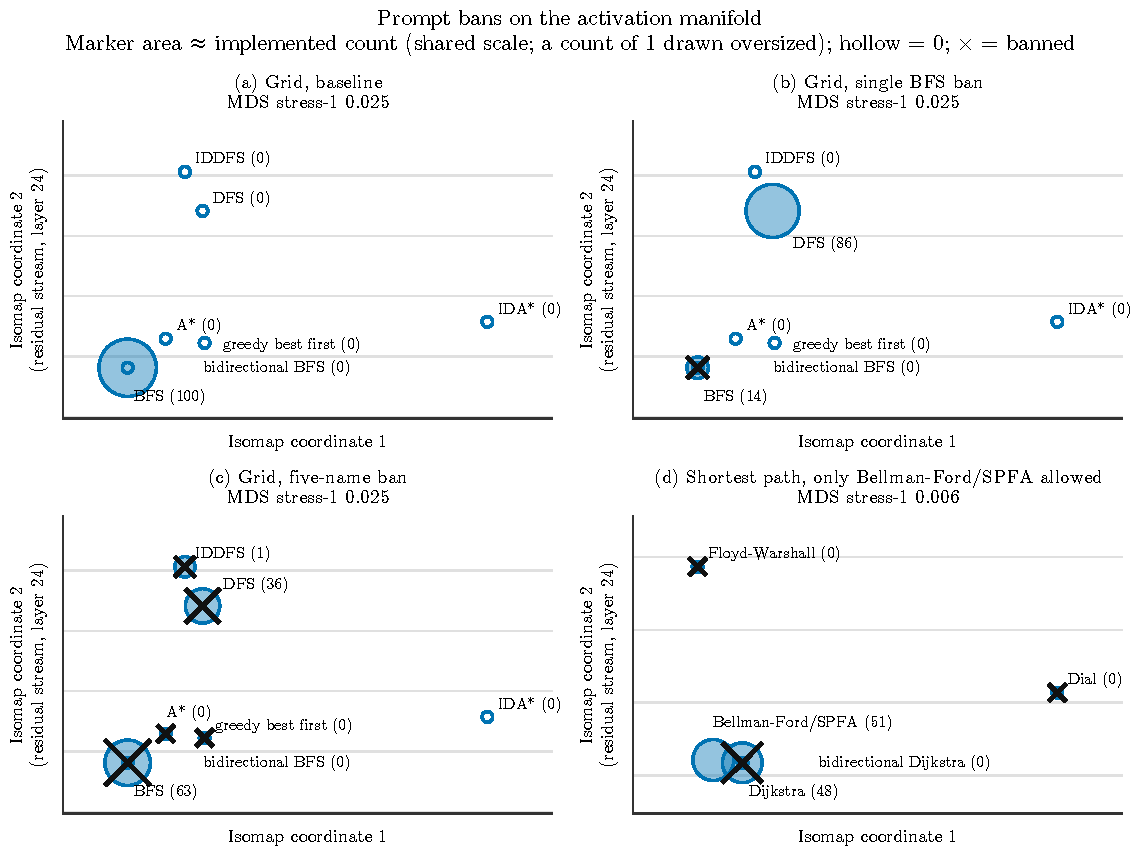
\includegraphics[width=\linewidth,height=0.78\textheight,keepaspectratio]{figures/fig_isomap_bans_v0.pdf}
\caption{Isomap embedding (k = 10) of teacher-forced residual-stream states at layer 24 of Qwen3-8B, read at the token before the commit token, for forced programs of each catalogue algorithm (iteration-2 ban-list experiment). Every panel's x-axis is Isomap coordinate 1 and y-axis is Isomap coordinate 2 (residual stream, layer 24). Each centroid is a circle whose area scales with the implemented-program count under that condition (one shared scale across all four panels; the count of 1, IDDFS in panel c, is drawn oversized for legibility); a hollow circle marks a count of 0, and a black \$\textbackslash{}times\$ overlay marks a banned algorithm. (a) Grid task, baseline: BFS 100, every other centroid (bidirectional BFS, DFS, IDDFS, A*, greedy best first, IDA*) at 0. (b) Grid task, single BFS ban: DFS 86, banned BFS 14, remaining centroids at 0. (c) Grid task, five-name ban (BFS, DFS, greedy best first, IDDFS, A*): BFS 63, DFS 36 and IDDFS 1 are all on banned centroids; the unbanned centroids, bidirectional BFS and IDA*, sit at 0. (d) Shortest-path task, ban leaving only Bellman-Ford\slash{}SPFA unbanned: Bellman-Ford\slash{}SPFA 51, banned Dijkstra 48, remaining banned centroids (bidirectional Dijkstra, Floyd-Warshall, Dial) at 0; a further 1 program (no centroid on this manifold) matched none of the five named mechanisms. Mass moves cleanly off BFS onto DFS under a single ban (b), stays entirely on banned centroids under the five-name ban (c), and splits between the allowed Bellman-Ford\slash{}SPFA centroid and the still-banned Dijkstra centroid when only it is left unbanned (d). Each panel prints the MDS stress-1 of its centroid geodesic matrix (0.025 for the grid panels, 0.006 for the shortest-path panel). Caveat: the read position depends on each program's own label (where its commit token falls), so part of the separation can reflect position rather than algorithm identity; an independent audit found this geometry does not reproduce at a label-independent read position.}
\label{fig:fig_isomap_bans}
\end{figure}
The label-independent recomputation at generated token 16 gives neighbour orders, not coordinates, so it is tabulated rather than plotted (Table 133). At the label-dependent position the nearest centroid to BFS is bidirectional BFS, and a label permutation reproduces that identity in 1\% of draws; at token 16 the nearest centroid to BFS is IDA*, and bidirectional BFS falls to fourth.

\begin{table}[H]
\renewcommand{\thetable}{133}
\centering\footnotesize\setlength{\tabcolsep}{4.0pt}
\caption{The neighbour order of BFS among grid centroids (forced programs under the baseline prompt, layer 24; 782 programs) at the label-dependent position and at the fixed generated token 16, with the share of 500 label permutations in which the nearest neighbour is bidirectional BFS. Source: record audit \texttt{results/\allowbreak{}figures.\allowbreak{}json}. [Source: iteration 4, artifact \nolinkurl{gen_art_evaluation_3}.]}\label{tab:t143}
\begin{tabular}{>{\raggedright\arraybackslash\hspace{0pt}}p{0.1293\linewidth}>{\raggedright\arraybackslash\hspace{0pt}}p{0.3440\linewidth}>{\raggedright\arraybackslash\hspace{0pt}}p{0.1240\linewidth}>{\raggedright\arraybackslash\hspace{0pt}}p{0.1414\linewidth}>{\raggedright\arraybackslash\hspace{0pt}}p{0.1744\linewidth}}
\toprule
\textbf{Position} & \textbf{Neighbour order from BFS} & \textbf{Nearest} & \textbf{Distance BFS to bidirectional BFS} & \textbf{Permutation share with bidirectional BFS nearest} \\
\midrule
token before the commit token & bidirectional BFS, greedy best first, DFS, A*, unit weight Dijkstra, other, IDA*, IDDFS & bidirectional BFS & 81.25 & 0.010 \\
generated token 16 & IDA*, IDDFS, DFS, bidirectional BFS, unit weight Dijkstra, other, greedy best first, A* & IDA* & 99.11 & 0.022 \\
\bottomrule
\end{tabular}
\end{table}

\subsubsection*{4.2.6 Hit rates under one rule, Table 82 per row, rival predictors and the frozen screen}
The three contests of iteration 3 used three rules for undefined forecasts. Table 134 reports defined-only top-1 hit rates with the number of defined events in each contest. Subtraction, which looked worst in the exposure contest (0.36, almost all of it fractional credit for its uniform tie on events where it was undefined), was defined there for 8 of 64 gated events (the named and unnamed arms of 4 shown algorithms) and named the landing in all 8.

\begin{table}[H]
\renewcommand{\thetable}{134}
\centering\footnotesize\setlength{\tabcolsep}{4.0pt}
\caption{Defined-only top-1 hit rates in the three iteration-3 contests (events gated; defined events; hits among defined events). Source: record audit \texttt{tables/\allowbreak{}defined\_\allowbreak{}only\_\allowbreak{}hits.\allowbreak{}csv}. [Source: iteration 4, artifact \nolinkurl{gen_art_evaluation_3}.]}\label{tab:t144}
\begin{tabular}{>{\raggedright\arraybackslash\hspace{0pt}}p{0.3868\linewidth}>{\raggedright\arraybackslash\hspace{0pt}}p{0.1297\linewidth}>{\raggedright\arraybackslash\hspace{0pt}}p{0.0985\linewidth}>{\raggedright\arraybackslash\hspace{0pt}}p{0.0889\linewidth}>{\raggedright\arraybackslash\hspace{0pt}}p{0.1323\linewidth}>{\raggedright\arraybackslash\hspace{0pt}}p{0.0604\linewidth}}
\toprule
\textbf{Contest} & \textbf{Family} & \textbf{Gated events} & \textbf{Defined} & \textbf{Hits (defined only)} & \textbf{Rate} \\
\midrule
Qwen3-8B modal bench bans & subtraction & 5 & 2 & 0 & 0.00 \\
Qwen3-8B modal bench bans & ladder & 5 & 1 & 1 & 1.00 \\
Qwen3-8B modal bench bans & association & 5 & 5 & 1 & 0.20 \\
Qwen3-8B modal bench bans & proximity & 5 & 5 & 1 & 0.20 \\
Qwen3-8B exposure bans, named and unnamed & subtraction & 64 & 8 & 8 & 1.00 \\
Qwen3-8B exposure bans, named and unnamed & ladder & 64 & 64 & 52 & 0.81 \\
Qwen3-8B exposure bans, named and unnamed & association & 64 & 64 & 31 & 0.48 \\
Qwen3-8B exposure bans, named and unnamed & proximity & 64 & 64 & 42 & 0.66 \\
Llama modal and present minor bans & subtraction & 13 & 12 & 4 & 0.33 \\
Llama modal and present minor bans & ladder & 13 & 13 & 7 & 0.54 \\
Llama modal and present minor bans & association & 13 & 13 & 7 & 0.54 \\
Llama modal and present minor bans & proximity & 13 & 13 & 3 & 0.23 \\
\bottomrule
\end{tabular}
\end{table}

Table 135 restates Table 82 per distinct likelihood row. The gains never point at the landing, and the implied mass hits 8 of 11 rows, 6 of them bans of absent algorithms where the landing is the default.

\begin{table}[H]
\renewcommand{\thetable}{135}
\centering\scriptsize\setlength{\tabcolsep}{2.5pt}
\caption{The 11 distinct Qwen3-8B likelihood rows: realised landing and the argmax of the gain, of the residual and of the implied mass among survivors. Source: record audit \texttt{tables/\allowbreak{}table82\_\allowbreak{}distinct\_\allowbreak{}rows.\allowbreak{}csv}. [Source: iteration 4, artifact \nolinkurl{gen_art_evaluation_3}.]}\label{tab:t145}
\begin{tabular}{>{\raggedright\arraybackslash\hspace{0pt}}p{0.0977\linewidth}>{\raggedright\arraybackslash\hspace{0pt}}p{0.1412\linewidth}>{\raggedright\arraybackslash\hspace{0pt}}p{0.0635\linewidth}>{\raggedright\arraybackslash\hspace{0pt}}p{0.1103\linewidth}>{\raggedright\arraybackslash\hspace{0pt}}p{0.1397\linewidth}>{\raggedright\arraybackslash\hspace{0pt}}p{0.1478\linewidth}>{\raggedright\arraybackslash\hspace{0pt}}p{0.1190\linewidth}>{\raggedright\arraybackslash\hspace{0pt}}p{0.0940\linewidth}}
\toprule
\textbf{Task} & \textbf{Banned} & \textbf{Row type} & \textbf{Realised landing} & \textbf{Gain argmax} & \textbf{Residual argmax} & \textbf{Implied-mass argmax} & \textbf{Implied mass hit} \\
\midrule
grid & A* & sham & BFS & bidirectional BFS & bidirectional BFS & DFS & no \\
grid & BFS & modal & DFS & IDDFS & IDDFS & DFS & yes \\
grid & bidirectional BFS & sham & BFS & IDDFS & IDDFS & BFS & yes \\
grid & DFS & sham & BFS & bidirectional BFS & bidirectional BFS & BFS & yes \\
grid & unit weight Dijkstra & sham & BFS & IDDFS & bidirectional BFS & DFS & no \\
grid & IDDFS & sham & BFS & bidirectional BFS & bidirectional BFS & DFS & no \\
shortest path & Bellman-Ford\slash{}SPFA & sham & Dijkstra & Dial & Floyd-Warshall & Dijkstra & yes \\
shortest path & bidirectional Dijkstra & sham & Dijkstra & Dial & Dial & Dijkstra & yes \\
shortest path & Dial & sham & Dijkstra & bidirectional Dijkstra & bidirectional Dijkstra & Dijkstra & yes \\
shortest path & Dijkstra & modal & Bellman-Ford\slash{}SPFA & Dial & Dial & Bellman-Ford\slash{}SPFA & yes \\
shortest path & Floyd-Warshall & sham & Dijkstra & Dial & Dial & Dijkstra & yes \\
\bottomrule
\end{tabular}
\end{table}

The audit also scored, on the iteration-3 screen, the predictors of ban compliance that the movability claim competes with (Table 136). Movability and the maximum escape fraction rank the catalogue-only ban avoidance of the 14 tasks far better than the forced-prompt success rate, the clarity of the association, the likelihood mass of the runner-up, the nonce ban or the novelty instruction. These are screen values: the same data produced the movable set.

\begin{table}[H]
\renewcommand{\thetable}{136}
\centering\scriptsize\setlength{\tabcolsep}{2.5pt}
\caption{Predictors of catalogue-only modal ban avoidance across the 14 Qwen3-8B tasks (Spearman rho with Monte Carlo permutation p; balanced accuracy at a median cut). Source: record audit \texttt{tables/\allowbreak{}rival\_\allowbreak{}predictors.\allowbreak{}csv}. [Source: iteration 4, artifact \nolinkurl{gen_art_evaluation_3}.]}\label{tab:t146}
\begin{tabular}{>{\raggedright\arraybackslash\hspace{0pt}}p{0.3207\linewidth}>{\raggedright\arraybackslash\hspace{0pt}}p{0.0622\linewidth}>{\raggedright\arraybackslash\hspace{0pt}}p{0.1030\linewidth}>{\raggedright\arraybackslash\hspace{0pt}}p{0.1168\linewidth}>{\raggedright\arraybackslash\hspace{0pt}}p{0.1087\linewidth}>{\raggedright\arraybackslash\hspace{0pt}}p{0.1297\linewidth}>{\raggedright\arraybackslash\hspace{0pt}}p{0.0823\linewidth}}
\toprule
\textbf{Predictor} & \textbf{Tasks} & \textbf{Spearman rho} & \textbf{Permutation p} & \textbf{Kendall tau-b} & \textbf{Balanced accuracy} & \textbf{Fisher p} \\
\midrule
movable (escape fraction above zero) & 14 & 0.86 & 0.00066 & 0.73 & 1.00 & 0.00033 \\
maximum escape fraction & 14 & 0.85 & 0.00022 & 0.69 & 1.00 & 0.00033 \\
forced-prompt success rate (can) & 14 & 0.16 & 0.58 & 0.15 & 0.50 & 1.00 \\
clarity of the association answer & 14 & -0.07 & 0.82 & -0.06 & 0.50 & 1.00 \\
likelihood mass of the runner-up & 14 & 0.19 & 0.52 & 0.08 & 0.50 & 1.00 \\
nonce ban off-default share & 12 & -0.19 & 0.56 & -0.16 & 0.38 & 0.52 \\
novelty instruction off-default share & 14 & 0.35 & 0.21 & 0.28 & 0.65 & 0.59 \\
\bottomrule
\end{tabular}
\end{table}

The frozen screen (hashed with sha256, reproduced byte for byte by a stdlib-only rule from its input file) names six movable tasks: kth smallest, two sum, find duplicate, connected components, and the grid and shortest path tasks, the set the price claim froze. Against catalogue-only ban avoidance of at least 0.5 the table of the screen is 6, 0, 0, 8 (one-sided Fisher p = 1\slash{}3003), a description of the screen and not a confirmation. Connected components escapes only on the bf16 engine of the bench forecast experiment; the other movable tasks escape on the 8-bit directions of the locus experiment. \emph{(Correction, iteration 6: the escapes of the screen are properties of the model, not of the 8-bit engine. The 40-direction escape fractions of iteration 4 reproduce in bf16 at the same absolute displacement, and the shortest path positive-control direction 9004 of the screen moves that task in bf16 as well (Section 6.3); the shrinkage of the screen under the ban-free unit of iteration 5 belongs to that unit and its direction seeds.)}

\FloatBarrier
\subsection*{4.3 Plan noise priced against every other knob (Qwen3-8B)}
\addcontentsline{toc}{subsection}{4.3 Plan noise priced against every other knob (Qwen3-8B)}
\noindent{\small\emph{Artifact: \nolinkurl{gen_art_experiment_19}.}}\par\medskip
\textbf{Why.} The price claim was the primary claim of the iteration and the question of the request in its plainest form: which knob buys correct algorithmic diversity most cheaply. The iteration-3 evidence for random pushes came from fixed directions, three per task on most of the bench, chosen by nobody. This experiment  drew a fresh direction for every sample, which is the form a practitioner would use, and priced it on the six movable tasks of the frozen screen against every token-level and prompt-level knob the run had tried, all under one statistic and one price convention.

\textbf{Design.} Qwen3-8B ran with 8-bit linear layers on the 16 GB card, thinking off, and every arm of a task shared the same uniform stream per template and slot, so arms differ only by the knob. Plan noise ran at alpha 0.5, 1, 2 and 4 (and 8 in the dose sweep). The comparison knobs were temperature 1.3 and 1.6 without truncation, top-k 10, the nonce ban, the novelty instruction, the semantic seed on the path tasks and the iteration-3 signature vetoes (one-shot, persistent and iterated, reused rows); min-p 0.1 at temperature 1.6 and 2.0 and a verbalized sampling prompt [46] were preregistered sensitivities. Every cell had N = 50 (5 templates by 10 slots): 202 cells and 10,100 labelled programs, with no cell dropped. The 5-point Hill-1 and the prices of 1.5 and 2 were computed on the randomisation hull of each knob with 2,000 bootstrap replicates, and the choice of the best setting of a knob was made inside every replicate. The rule, committed by hash before the first sample beyond stage 10, confirmed the price claim if plan noise reached a 5-point Hill-1 of at least 1.5 on at least 3 of the 6 tasks, beat the 5-point Hill-1 of the best non-activation knob on at least 4 of 6, and had a pooled margin with a task-bootstrap 95\% interval above 0.

\textbf{The rule returned PARTIAL.} Plan noise is not the uniformly cheapest knob (Table 137). It reaches a 5-point Hill-1 of at least 1.5 on only 2 of 6 tasks, against the 3 required, and beats the best non-activation knob on 4 of 6, but the pooled margin is -0.22 with an interval from -0.89 to 0.30 (one-sided p = 0.76; exact sign test over the six margins p = 0.34). Plan noise wins clearly on kth smallest (2.72 against 1.96 for the novelty instruction, ahead in every bootstrap replicate) and on connected components (2.09 against 1.96 for the iterated veto, ahead in 91\%), and on both it reaches Hill-1 of 1.5 and of 2 at no pass cost. It edges two sum and the grid task by margins inside their intervals. It loses decisively on find duplicate, where it does not move the hash set at alpha 2 or less while the reused iterated veto reaches 2.73, and on the shortest path task, where the semantic seed reaches 1.93 against 1.35 for plan noise because pushed Bellman-Ford\slash{}SPFA programs cost 14 to 26 pass points.

\begin{table}[H]
\renewcommand{\thetable}{137}
\centering\scriptsize\setlength{\tabcolsep}{2.5pt}
\caption{The preregistered price comparison on the six movable tasks: 5-point Hill-1 of plan noise, the best non-activation knob and its 5-point Hill-1, the margin with its bootstrap 95\% interval, the bootstrap probability that plan noise is ahead, and the price of 1.5 and price of 2 for plan noise (pass points; a dash means not reached). Source: plan noise experiment \texttt{results/\allowbreak{}c1.\allowbreak{}json}, \texttt{results/\allowbreak{}summary.\allowbreak{}md}. [Source: iteration 4, artifact \nolinkurl{gen_art_experiment_19}.]}\label{tab:t147}
\begin{tabular}{>{\raggedright\arraybackslash\hspace{0pt}}p{0.1700\linewidth}>{\raggedright\arraybackslash\hspace{0pt}}p{0.1120\linewidth}>{\raggedright\arraybackslash\hspace{0pt}}p{0.1346\linewidth}>{\raggedright\arraybackslash\hspace{0pt}}p{0.0851\linewidth}>{\raggedright\arraybackslash\hspace{0pt}}p{0.1258\linewidth}>{\raggedright\arraybackslash\hspace{0pt}}p{0.0886\linewidth}>{\raggedright\arraybackslash\hspace{0pt}}p{0.1029\linewidth}>{\raggedright\arraybackslash\hspace{0pt}}p{0.0941\linewidth}}
\toprule
\textbf{Task (default)} & \textbf{5-point Hill-1, plan noise} & \textbf{Best non-activation knob} & \textbf{Its 5-point Hill-1} & \textbf{Margin [95\% CI]} & \textbf{P(plan noise ahead)} & \textbf{Price of 1.5, plan noise} & \textbf{Price of 2, plan noise} \\
\midrule
kth smallest (full sort) & 2.72 & novelty instruction & 1.96 & 0.76 [0.21, 1.16] & 1.00 & 0.0 & 0.0 \\
two sum (hash map) & 1.29 & novelty instruction & 1.24 & 0.05 [-0.20, 0.37] & 0.67 & 11.1 & - \\
find duplicate (hash set) & 1.00 & iterated veto & 2.73 & -1.73 [-2.06, -1.39] & 0.00 & - & - \\
connected components (union find) & 2.09 & iterated veto & 1.96 & 0.13 [-0.00, 0.37] & 0.91 & 0.0 & 0.0 \\
grid (BFS) & 1.42 & novelty instruction & 1.34 & 0.07 [-0.57, 0.41] & 0.49 & 18.0 & 49.8 \\
shortest path (Dijkstra) & 1.35 & semantic seed & 1.93 & -0.58 [-0.69, -0.14] & 0.00 & 9.3 & - \\
\bottomrule
\end{tabular}
\end{table}

Table 138 gives 5-point Hill-1 for every knob class on the six tasks. Temperature, top-k 10 and the nonce ban buy no correct algorithmic diversity on any of them (5-point Hill-1 at most 1.09), and min-p reaches at most 1.17. The novelty instruction switches kth smallest wholesale to quickselect, a Hill-1 of 1.0 on its own; its 1.96 comes from mixing it with the twin on the hull. Top-k 10 never changed a single token sequence, because the top 10 tokens of the model carry essentially all the probability mass on these prompts. The verbalized sampling prompt is a measurement artifact rather than a knob: 46 to 49 of 50 of its programs on every bench task and on the grid task call a random choice inside the solution function, so their mechanism label is whichever branch the trace of the labeller happened to execute.

\begin{table}[H]
\renewcommand{\thetable}{138}
\centering\tiny\setlength{\tabcolsep}{2.5pt}
\caption{5-point Hill-1 per knob class on the six movable tasks (randomisation hull, cost at most 5 pass points; a dash means the class was not run on the task). Source: plan noise experiment \texttt{results/\allowbreak{}c1.\allowbreak{}json}. [Source: iteration 4, artifact \nolinkurl{gen_art_experiment_19}.]}\label{tab:t148}
\begin{tabular}{>{\raggedright\arraybackslash\hspace{0pt}}p{0.1083\linewidth}>{\raggedright\arraybackslash\hspace{0pt}}p{0.0586\linewidth}>{\raggedright\arraybackslash\hspace{0pt}}p{0.0917\linewidth}>{\raggedright\arraybackslash\hspace{0pt}}p{0.0509\linewidth}>{\raggedright\arraybackslash\hspace{0pt}}p{0.0548\linewidth}>{\raggedright\arraybackslash\hspace{0pt}}p{0.0917\linewidth}>{\raggedright\arraybackslash\hspace{0pt}}p{0.0679\linewidth}>{\raggedright\arraybackslash\hspace{0pt}}p{0.0700\linewidth}>{\raggedright\arraybackslash\hspace{0pt}}p{0.0773\linewidth}>{\raggedright\arraybackslash\hspace{0pt}}p{0.0700\linewidth}>{\raggedright\arraybackslash\hspace{0pt}}p{0.0388\linewidth}>{\raggedright\arraybackslash\hspace{0pt}}p{0.0917\linewidth}}
\toprule
\textbf{Task} & \textbf{Plan noise} & \textbf{Temperature 1.3\slash{}1.6} & \textbf{Top-k 10} & \textbf{Nonce ban} & \textbf{Novelty instruction} & \textbf{Semantic seed} & \textbf{One-shot veto} & \textbf{Persistent veto} & \textbf{Iterated veto} & \textbf{Min-p} & \textbf{Verbalized sampling} \\
\midrule
kth smallest & 2.72 & 1.09 & 1.00 & 1.00 & 1.96 & - & 1.90 & 1.88 & 1.89 & 1.16 & 1.29 \\
two sum & 1.29 & 1.00 & 1.00 & 1.00 & 1.24 & - & 1.00 & 1.00 & 1.00 & 1.00 & 1.04 \\
find duplicate & 1.00 & 1.00 & 1.00 & 1.00 & 1.00 & - & 1.00 & 1.00 & 2.73 & 1.00 & 1.01 \\
connected components & 2.09 & 1.00 & 1.00 & 1.00 & 1.17 & - & 1.02 & 1.03 & 1.96 & 1.09 & 1.02 \\
grid & 1.42 & 1.00 & 1.00 & 1.00 & 1.34 & 1.00 & 1.00 & 1.00 & 1.00 & 1.00 & 1.00 \\
shortest path & 1.35 & 1.09 & 1.00 & 1.00 & 1.24 & 1.93 & 1.00 & 1.00 & 1.00 & 1.17 & 1.00 \\
\bottomrule
\end{tabular}
\end{table}

Every preregistered sensitivity returns the same verdict (Table 139). Excluding the reused vetoes, which came from another engine, turns the pooled margin positive (+0.20, interval -0.19 to 0.60); plan noise then loses only to the semantic seed on the shortest path task.

\begin{table}[H]
\renewcommand{\thetable}{139}
\centering\footnotesize\setlength{\tabcolsep}{4.0pt}
\caption{Sensitivities of the price rule; each re-evaluates the full rule. Source: plan noise experiment \texttt{results/\allowbreak{}c1.\allowbreak{}json}. [Source: iteration 4, artifact \nolinkurl{gen_art_experiment_19}.]}\label{tab:t149}
\begin{tabular}{>{\raggedright\arraybackslash\hspace{0pt}}p{0.5556\linewidth}>{\raggedright\arraybackslash\hspace{0pt}}p{0.1022\linewidth}>{\raggedright\arraybackslash\hspace{0pt}}p{0.0737\linewidth}>{\raggedright\arraybackslash\hspace{0pt}}p{0.0729\linewidth}>{\raggedright\arraybackslash\hspace{0pt}}p{0.1088\linewidth}}
\toprule
\textbf{Sensitivity} & \textbf{Verdict} & \textbf{Tasks with 5-point Hill-1 at least 1.5} & \textbf{Tasks where plan noise beats the best} & \textbf{Pooled margin [95\% CI]} \\
\midrule
hull restricted to the twin segment & PARTIAL & 2 & 3 & -0.266 [-0.905, 0.246] \\
min-p and verbalized sampling added to the comparison set & PARTIAL & 2 & 4 & -0.218 [-0.897, 0.314] \\
min-p only added & PARTIAL & 2 & 4 & -0.218 [-0.863, 0.305] \\
dial interpolation instead of the hull & PARTIAL & 2 & 4 & -0.022 [-0.710, 0.607] \\
template-cluster bootstrap & PARTIAL & 2 & 4 & -0.218 [-0.866, 0.329] \\
slot-paired bootstrap & PARTIAL & 2 & 4 & -0.218 [-0.893, 0.322] \\
other programs excluded & PARTIAL & 2 & 4 & -0.243 [-0.892, 0.263] \\
other programs as one category & PARTIAL & 2 & 4 & -0.219 [-0.892, 0.326] \\
reused vetoes excluded & PARTIAL & 2 & 4 & 0.202 [-0.188, 0.600] \\
hull vertices from the record audit only & PARTIAL & 2 & 3 & -0.134 [-0.721, 0.512] \\
deviation on hull edges (added in iteration 5): the preregistered hull search is restricted to edges; it matched an optimiser over the full simplex within 0.02 on the unit cases but fell short by up to 0.19 Hill-1 on random 5-vertex Dirichlet(0.5) cases, a shortfall that falls on plan noise (5 hull vertices against 2 or 3 for most comparison knobs) & not evaluated again & n\slash{}a & n\slash{}a & n\slash{}a \\
triangle check on the real data (added in iteration 5): the largest gain of a 3-vertex face over the best edge, over all classes, is +0.008 (connected components, plan noise; 42 entries with a value, 113 null) & verdict unaffected & 2 & 4 & -0.22 \\
\bottomrule
\end{tabular}
\end{table}

\textbf{Ideas against phrasings.} Under common random numbers the effect of each knob can be read slot by slot (Table 140). Temperature rewrites code without changing the algorithm: on the grid task temperature 1.6 changes the code in 88\% of slots and the label in 2\%, and it raises the phrasing clusters within BFS from 13.6 to 18.5 (20 programs, Jaccard at least 0.8). Plan noise changes the algorithm: at alpha 2 the label differs from that of the twin in 50\% of slots on kth smallest, 60\% on connected components and 54\% on the shortest path task.

\begin{table}[H]
\renewcommand{\thetable}{140}
\centering\tiny\setlength{\tabcolsep}{2.5pt}
\caption{Share of common-random-number slots in which the code differs from the twin and in which the algorithm label differs (N = 50 per cell). Source: plan noise experiment \texttt{results/\allowbreak{}flips.\allowbreak{}json}. [Source: iteration 4, artifact \nolinkurl{gen_art_experiment_19}.]}\label{tab:t150}
\begin{tabular}{>{\raggedright\arraybackslash\hspace{0pt}}p{0.1049\linewidth}>{\raggedright\arraybackslash\hspace{0pt}}p{0.0931\linewidth}>{\raggedright\arraybackslash\hspace{0pt}}p{0.0931\linewidth}>{\raggedright\arraybackslash\hspace{0pt}}p{0.0780\linewidth}>{\raggedright\arraybackslash\hspace{0pt}}p{0.0785\linewidth}>{\raggedright\arraybackslash\hspace{0pt}}p{0.1066\linewidth}>{\raggedright\arraybackslash\hspace{0pt}}p{0.0897\linewidth}>{\raggedright\arraybackslash\hspace{0pt}}p{0.0828\linewidth}>{\raggedright\arraybackslash\hspace{0pt}}p{0.0828\linewidth}>{\raggedright\arraybackslash\hspace{0pt}}p{0.0828\linewidth}}
\toprule
\textbf{Task} & \textbf{Temperature 1.3} & \textbf{Temperature 1.6} & \textbf{Top-k 10} & \textbf{Nonce ban} & \textbf{Novelty instruction} & \textbf{Plan noise 0.5} & \textbf{Plan noise 1} & \textbf{Plan noise 2} & \textbf{Plan noise 4} \\
\midrule
kth smallest & 0.04 \slash{} 0.02 & 0.14 \slash{} 0.02 & 0.00 \slash{} 0.00 & 0.12 \slash{} 0.00 & 1.00 \slash{} 1.00 & 0.14 \slash{} 0.08 & 0.38 \slash{} 0.28 & 0.72 \slash{} 0.50 & 0.88 \slash{} 0.54 \\
two sum & 0.16 \slash{} 0.00 & 0.32 \slash{} 0.00 & 0.00 \slash{} 0.00 & 0.14 \slash{} 0.00 & 0.94 \slash{} 0.08 & 0.32 \slash{} 0.00 & 0.40 \slash{} 0.00 & 0.50 \slash{} 0.02 & 0.86 \slash{} 0.28 \\
find duplicate & 0.08 \slash{} 0.00 & 0.10 \slash{} 0.00 & 0.00 \slash{} 0.00 & 0.28 \slash{} 0.00 & 0.82 \slash{} 0.02 & 0.20 \slash{} 0.00 & 0.50 \slash{} 0.00 & 0.82 \slash{} 0.02 & 0.98 \slash{} 0.56 \\
connected components & 0.22 \slash{} 0.00 & 0.48 \slash{} 0.02 & 0.00 \slash{} 0.00 & 0.66 \slash{} 0.00 & 0.94 \slash{} 0.04 & 0.52 \slash{} 0.00 & 0.84 \slash{} 0.12 & 0.90 \slash{} 0.60 & 0.98 \slash{} 0.70 \\
grid & 0.64 \slash{} 0.00 & 0.88 \slash{} 0.02 & 0.00 \slash{} 0.00 & 0.94 \slash{} 0.00 & 1.00 \slash{} 0.56 & 0.96 \slash{} 0.02 & 1.00 \slash{} 0.06 & 1.00 \slash{} 0.24 & 1.00 \slash{} 0.30 \\
shortest path & 0.36 \slash{} 0.00 & 0.66 \slash{} 0.02 & 0.00 \slash{} 0.00 & 0.56 \slash{} 0.00 & 0.98 \slash{} 0.06 & 0.66 \slash{} 0.08 & 0.92 \slash{} 0.26 & 0.98 \slash{} 0.54 & 1.00 \slash{} 0.66 \\
\bottomrule
\end{tabular}
\end{table}

Each cell gives code differs \slash{} label differs.

\textbf{Dose and breakage.} The share of attempts off the default rises with alpha up to 2 on kth smallest, connected components and both path tasks, while two sum and find duplicate stay on their defaults until alpha 4 (Table 141). Breakage, a pass rate below 0.8 times that of the twin, arrives at alpha 4 on kth smallest, find duplicate, connected components and the grid task, at alpha 2 on the shortest path task and at alpha 8 on two sum; at alpha 8 almost nothing passes. Correct-only diversity peaks at alpha 2 on kth smallest (2.87, pass 0.94) and the shortest path task (1.95, pass 0.74) and at alpha 4 on connected components (2.56, pass 0.42). The realised displacement at block 12 matched its target within 0.15\% on all 3,220 plan noise rows.

{\footnotesize\setlength{\tabcolsep}{4.0pt}\renewcommand{\thetable}{141}
\begin{longtable}{>{\raggedright\arraybackslash\hspace{0pt}}p{0.1709\linewidth}>{\raggedright\arraybackslash\hspace{0pt}}p{0.0699\linewidth}>{\raggedright\arraybackslash\hspace{0pt}}p{0.0604\linewidth}>{\raggedright\arraybackslash\hspace{0pt}}p{0.1461\linewidth}>{\raggedright\arraybackslash\hspace{0pt}}p{0.0643\linewidth}>{\raggedright\arraybackslash\hspace{0pt}}p{0.3851\linewidth}}
\caption{Dose response of plan noise on the six movable tasks (N = 50 per dose): pass rate, share of attempts off the default, correct-only rarefied Hill-1 and the composition of correct programs. Source: plan noise experiment \texttt{results/\allowbreak{}alpha\_\allowbreak{}sweep.\allowbreak{}json}. [Source: iteration 4, artifact \nolinkurl{gen_art_experiment_19}.]}\label{tab:t151}\\
\toprule
\textbf{Task} & \textbf{Alpha} & \textbf{Pass} & \textbf{Off default} & \textbf{Hill-1} & \textbf{Correct programs} \\
\midrule
\endfirsthead
\multicolumn{6}{l}{\emph{Table 141, continued}}\\
\toprule
\textbf{Task} & \textbf{Alpha} & \textbf{Pass} & \textbf{Off default} & \textbf{Hill-1} & \textbf{Correct programs} \\
\midrule
\endhead
\bottomrule
\endlastfoot
kth smallest & 0 & 1.00 & 0.00 & 1.00 & full sort 50 \\
kth smallest & 0.5 & 1.00 & 0.08 & 1.30 & full sort 46, quickselect 4 \\
kth smallest & 1 & 1.00 & 0.28 & 2.14 & full sort 36, quickselect 9, size-k heap 5 \\
kth smallest & 2 & 0.94 & 0.50 & 2.87 & full sort 24, quickselect 14, size-k heap 8, other 1 \\
kth smallest & 4 & 0.74 & 0.54 & 2.71 & quickselect 17, full sort 16, size-k heap 3, heapify and pop 1 \\
kth smallest & 8 & 0.04 & 0.38 (invalid 0.54) & 2.00 & quickselect 1, full sort 1 \\
two sum & 0 to 1 & 1.00 & 0.00 & 1.00 & hash map 50 \\
two sum & 2 & 1.00 & 0.02 & 1.09 & hash map 49, brute force 1 \\
two sum & 4 & 0.80 & 0.28 & 1.79 & hash map 29, brute force 11 \\
two sum & 8 & 0.00 & 0.08 (invalid 0.92) & n\slash{}a & none \\
find duplicate & 0 to 1 & 1.00 & 0.00 & 1.00 & hash set 50 \\
find duplicate & 2 & 0.98 & 0.02 & 1.00 & hash set 49 \\
find duplicate & 4 & 0.24 & 0.52 & 1.00 & hash set 12 \\
find duplicate & 8 & 0.00 & 0.06 (invalid 0.94) & n\slash{}a & none \\
connected components & 0 to 0.5 & 1.00 & 0.00 & 1.00 & union find 50 \\
connected components & 1 & 1.00 & 0.12 & 1.42 & union find 44, DFS 6 \\
connected components & 2 & 1.00 & 0.60 & 2.10 & DFS 29, union find 20, BFS 1 \\
connected components & 4 & 0.42 & 0.64 & 2.56 & union find 10, DFS 9, BFS 2 \\
connected components & 8 & 0.00 & 0.14 (invalid 0.86) & n\slash{}a & none \\
grid & 0 & 0.74 & 0.00 & 1.00 & BFS 37 \\
grid & 0.5 & 0.86 & 0.02 & 1.00 & BFS 43 \\
grid & 1 & 0.70 & 0.06 & 1.14 & BFS 34, DFS 1 \\
grid & 2 & 0.72 & 0.24 & 1.42 & BFS 32, DFS 4 \\
grid & 4 & 0.24 & 0.30 & 2.06 & BFS 9, DFS 2, Dijkstra 1 \\
grid & 8 & 0.00 & 0.70 (invalid 0.06) & n\slash{}a & none \\
shortest path & 0 & 1.00 & 0.00 & 1.00 & Dijkstra 50 \\
shortest path & 0.5 & 0.98 & 0.08 & 1.26 & Dijkstra 46, Bellman-Ford\slash{}SPFA 3 \\
shortest path & 1 & 0.86 & 0.26 & 1.66 & Dijkstra 34, Bellman-Ford\slash{}SPFA 9 \\
shortest path & 2 & 0.74 & 0.54 & 1.95 & Dijkstra 22, Bellman-Ford\slash{}SPFA 15 \\
shortest path & 4 & 0.04 & 0.66 & 1.00 & Dijkstra 2 \\
shortest path & 8 & 0.00 & 0.90 (invalid 0.04) & n\slash{}a & none \\
\end{longtable}}

\begin{figure}[!htbp]
\centering\captionsetup{font=footnotesize}
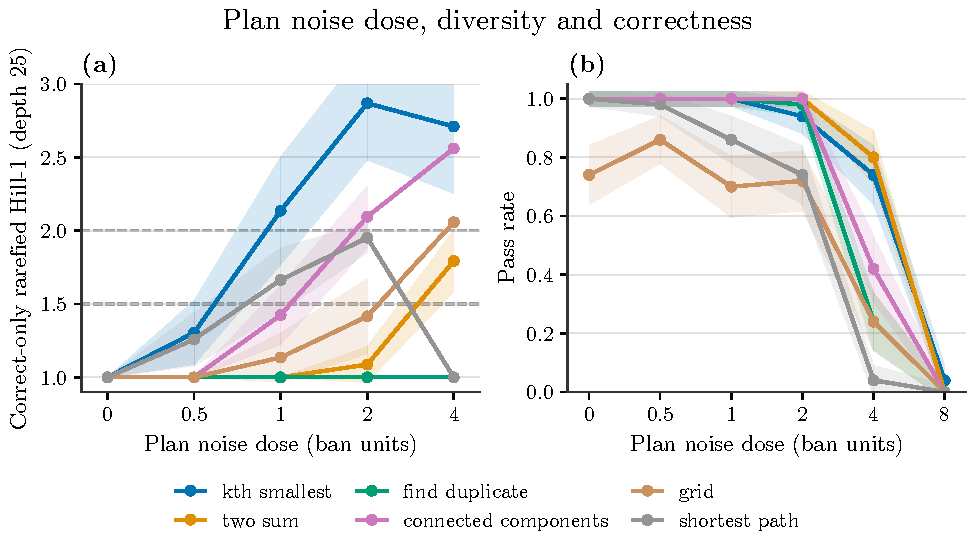
\includegraphics[width=\linewidth,height=0.78\textheight,keepaspectratio]{figures/fig_pn_dose_v0.pdf}
\caption{Dose--response of fresh per-sample plan noise (an isotropic random direction per sample added to the task-specification states of transformer blocks 12--23 during prefill, in ban units) on six coding tasks, Qwen3-8B with 8-bit (FP8) linear layers, N=50 generations per dose. Colour denotes task and is shared across both panels, with one legend below. (a) Correct-only rarefied Hill-1 diversity at depth 25 (dashed grey lines at 1.5 and 2.0; shaded bands are 90\% CIs, omitted once fewer than 25 of the 50 samples are correct). Diversity rises with dose on kth smallest, connected components, grid and shortest path; two sum and find duplicate stay near a single default algorithm through dose 2, and find duplicate never diversifies, even among the 12 correct samples that remain at dose 4. (b) Pass rate against the same dose, extended to dose 8, with a Wilson 90\% CI band. Grid's own dose-0 pass rate (0.74) is already below the other five tasks' (1.00); shortest path's pass rate declines steadily from dose 0.5 and reaches 0.74 by dose 2, while kth smallest, connected components and grid stay closer to their dose-0 rate over that range. By dose 8 the pass rate is 0.00 for five of the six tasks; kth smallest alone keeps a small residual pass rate (0.04). Source: plan-noise dose-sweep experiment (iteration-4, FP8 engine).}
\label{fig:fig_pn_dose}
\end{figure}
\textbf{The held-out task and the immovable tasks.} Cycle detection, the bench task that the 12-task cap had excluded and on which nothing had been run, barely moves under plan noise: an off-default excess of 0.01 at alpha 2 or less, a 5-point Hill-1 of 1.09 and a price of 1.5 of 29 points. On the eight bench tasks the screen called immovable, plan noise at alpha 2 or less moves almost nothing (Table 142), which agrees with the screen. The strongest knob there is the novelty instruction on substring search (5-point Hill-1 2.57).

\begin{table}[H]
\renewcommand{\thetable}{142}
\centering\scriptsize\setlength{\tabcolsep}{2.5pt}
\caption{Cycle detection (held out) and the eight immovable bench tasks: plan noise off-default excess at alpha 2 or less, and 5-point Hill-1 per knob. Source: plan noise experiment \texttt{results/\allowbreak{}nonmovable.\allowbreak{}json}. [Source: iteration 4, artifact \nolinkurl{gen_art_experiment_19}.]}\label{tab:t152}
\begin{tabular}{>{\raggedright\arraybackslash\hspace{0pt}}p{0.1737\linewidth}>{\raggedright\arraybackslash\hspace{0pt}}p{0.1352\linewidth}>{\raggedright\arraybackslash\hspace{0pt}}p{0.1241\linewidth}>{\raggedright\arraybackslash\hspace{0pt}}p{0.1277\linewidth}>{\raggedright\arraybackslash\hspace{0pt}}p{0.1205\linewidth}>{\raggedright\arraybackslash\hspace{0pt}}p{0.1442\linewidth}>{\raggedright\arraybackslash\hspace{0pt}}p{0.0981\linewidth}}
\toprule
\textbf{Task} & \textbf{Plan noise off-default excess} & \textbf{5-point Hill-1, plan noise} & \textbf{5-point Hill-1, temperature} & \textbf{5-point Hill-1, nonce ban} & \textbf{5-point Hill-1, novelty instruction} & \textbf{Price of 1.5, plan noise} \\
\midrule
nonoverlapping intervals & 0.00 & 1.00 & 1.00 & 1.00 & 1.00 & - \\
cycle detection (held out) & 0.01 & 1.09 & 1.00 & 1.00 & 1.37 & 29.0 \\
topological order & 0.00 & 1.00 & 1.00 & 1.00 & 1.00 & - \\
first and last position & -0.08 & 1.37 & 1.42 & 1.21 & 1.20 & - \\
substring search & 0.00 & 1.00 & 1.00 & 1.00 & 2.57 & - \\
Fibonacci & 0.01 & 1.00 & 1.00 & 1.00 & 1.04 & - \\
longest increasing subsequence & 0.03 & 1.01 & 1.00 & 1.00 & 1.05 & - \\
merge intervals & 0.00 & 1.00 & 1.00 & 1.00 & 1.00 & - \\
top-k frequent & 0.04 & 1.14 & 1.00 & 1.00 & 1.00 & - \\
\bottomrule
\end{tabular}
\end{table}

\begin{table}[H]
\renewcommand{\thetable}{142b}
\centering\scriptsize\setlength{\tabcolsep}{2.5pt}
\caption{The screen forecast committed before stage 100, which treated fresh plan noise as an equal mixture of the fixed directions of the screen, against the realised result: 5-point Hill-1 of plan noise, the margin over the best non-activation knob, and the divergence of the forecast alpha-1 composition from the realised one against its resampling null. Source: plan noise experiment \texttt{results/\allowbreak{}forecast\_\allowbreak{}score.\allowbreak{}json}. [Source: iteration 4, artifact \nolinkurl{gen_art_experiment_19}.]}\label{tab:t153}
\begin{tabular}{>{\raggedright\arraybackslash\hspace{0pt}}p{0.1641\linewidth}>{\raggedright\arraybackslash\hspace{0pt}}p{0.1602\linewidth}>{\raggedright\arraybackslash\hspace{0pt}}p{0.0872\linewidth}>{\raggedright\arraybackslash\hspace{0pt}}p{0.1179\linewidth}>{\raggedright\arraybackslash\hspace{0pt}}p{0.1186\linewidth}>{\raggedright\arraybackslash\hspace{0pt}}p{0.1860\linewidth}>{\raggedright\arraybackslash\hspace{0pt}}p{0.0896\linewidth}}
\toprule
\textbf{Task} & \textbf{Forecast 5-point Hill-1} & \textbf{Realised} & \textbf{Forecast margin} & \textbf{Realised margin} & \textbf{Divergence (null p95)} & \textbf{Within null} \\
\midrule
kth smallest & 2.38 & 2.72 & 0.45 & 0.76 & 0.0056 (0.0768) & yes \\
two sum & 1.78 & 1.29 & 0.61 & 0.05 & 0.0101 (0.0) & no \\
find duplicate & 1.76 & 1.00 & -0.97 & -1.73 & 0.0 (0.0) & yes \\
connected components & 1.33 & 2.09 & -0.63 & 0.13 & 0.0021 (0.0307) & yes \\
grid & 1.09 & 1.42 & n\slash{}a & 0.07 & 0.0087 (0.0301) & yes \\
shortest path & 1.35 & 1.35 & 0.35 & -0.58 & 0.0041 (0.115) & yes \\
\bottomrule
\end{tabular}
\end{table}

The forecast implied PARTIAL, and the realised verdict was PARTIAL. Unlike a prompt ban, plan noise moves the model under every template, the fourth included (Table 142c), so its effect does not inherit the wording dependence of bans.

\begin{table}[H]
\renewcommand{\thetable}{142c}
\centering\scriptsize\setlength{\tabcolsep}{2.5pt}
\caption{Plan noise off-default share per template (N = 10 per cell) on the four tasks it moves, with the novelty instruction for comparison. Source: plan noise experiment \texttt{results/\allowbreak{}per\_\allowbreak{}template.\allowbreak{}json}. [Source: iteration 4, artifact \nolinkurl{gen_art_experiment_19}.]}\label{tab:t154}
\begin{tabular}{>{\raggedright\arraybackslash\hspace{0pt}}p{0.2438\linewidth}>{\raggedright\arraybackslash\hspace{0pt}}p{0.2772\linewidth}>{\raggedright\arraybackslash\hspace{0pt}}p{0.0771\linewidth}>{\raggedright\arraybackslash\hspace{0pt}}p{0.0856\linewidth}>{\raggedright\arraybackslash\hspace{0pt}}p{0.0771\linewidth}>{\raggedright\arraybackslash\hspace{0pt}}p{0.0856\linewidth}>{\raggedright\arraybackslash\hspace{0pt}}p{0.0771\linewidth}}
\toprule
\textbf{Task} & \textbf{Arm} & \textbf{First} & \textbf{Second} & \textbf{Third} & \textbf{Fourth} & \textbf{Fifth} \\
\midrule
kth smallest & plan noise, alpha 1 & 0.1 & 0.2 & 0.5 & 0.1 & 0.5 \\
kth smallest & plan noise, alpha 2 & 0.4 & 0.5 & 0.6 & 0.5 & 0.5 \\
kth smallest & novelty instruction & 1.0 & 1.0 & 1.0 & 1.0 & 1.0 \\
connected components & plan noise, alpha 1 & 0.2 & 0.2 & 0.0 & 0.0 & 0.2 \\
connected components & plan noise, alpha 2 & 0.8 & 0.6 & 0.4 & 0.6 & 0.6 \\
connected components & novelty instruction & 0.1 & 0.1 & 0.0 & 0.0 & 0.0 \\
grid & plan noise, alpha 1 & 0.1 & 0.0 & 0.1 & 0.1 & 0.0 \\
grid & plan noise, alpha 2 & 0.2 & 0.3 & 0.2 & 0.2 & 0.3 \\
grid & novelty instruction & 0.6 & 0.6 & 0.7 & 0.3 & 0.6 \\
shortest path & plan noise, alpha 1 & 0.2 & 0.1 & 0.1 & 0.3 & 0.6 \\
shortest path & plan noise, alpha 2 & 0.5 & 0.4 & 0.6 & 0.6 & 0.6 \\
shortest path & novelty instruction & 0.1 & 0.0 & 0.0 & 0.2 & 0.0 \\
\bottomrule
\end{tabular}
\end{table}

\textbf{Controls and checks.} The prohibition frame of the neutral twin is inert for the algorithm: a plain prompt with the specification alone and the twin have identical off-default shares on five of the six movable tasks (+0.02 on the shortest path task), although the frame costs 18 pass points on the grid task and adds 22 on cycle detection. \emph{(Added in iteration 5: plan noise was also run on the plain prompt without the prohibition frame of the twin (alpha 1, 350 programs on the same common-random-number slots), and the record did not report it. Its off-default shares were 0.16 on kth smallest (0.28 under the twin frame), 0.24 on connected components (0.12), 0.26 on the shortest path task (0.26), 0.02 on the grid task (0.06) and 0 on two sum, find duplicate and cycle detection. Plan noise does not need the frame on kth smallest, connected components and the shortest path task; under plan noise at alpha 1 the frame costs 10 pass points on the grid task (interval -6 to 28). Table 173 gives the rows.)} A forecast committed before stage 100, which treated fresh noise as an equal mixture of the fixed directions of the screen, predicted the PARTIAL verdict and the alpha-1 composition within the resampling null on 5 of 6 tasks; it over-predicted find duplicate (1.76 forecast against 1.00) and two sum and under-predicted connected components. Two screen rows rerun with the keys of the screen itself agreed slot for slot (label agreement 1.00 on all four cells). The labellers recovered every reference on all 13 bench tasks. The 12 correct programs labelled other were all labeller misses, and no novel algorithm appeared. A judge agreed with the labeller on 1.00 of audited programs everywhere except kth smallest (0.80), and rescoring kth smallest with the labels of the judge left its margin at +0.71 against +0.76. Replacing every plan noise setting by the twin gave margins of 0 or below on all six tasks, and under 100 within-task shuffles of the arm labels the full committed rule never returned CONFIRMED; the count criteria alone fired in 8 of 100 shuffles in the independent rederivation, so the interval criterion is what makes the rule specific. The rederivation matched 12 of 12 checks, and the hash chain shows the commitment preceding the first row beyond stage 10.

\FloatBarrier
\subsection*{4.4 Where the noise must enter (Qwen3-8B)}
\addcontentsline{toc}{subsection}{4.4 Where the noise must enter (Qwen3-8B)}
\noindent{\small\emph{Artifact: \nolinkurl{gen_art_experiment_20}.}}\par\medskip
\textbf{Why.} If the plan lives in the task-specification states, the same random displacement should change the algorithm there and nowhere else. If any perturbation of matched size does as well, the effect is generic sensitivity, and the word plan names nothing. This experiment  wrote one random displacement per common-random-number slot into six sites at matched per-position dose in ban units and priced each site on the randomisation hull.

\textbf{Design.} The six sites were the task-specification states at blocks 12 to 23 (the plan site of the hypothesis), the read position, the condition sentence, generated tokens 1 to 32 (through teacher-forced shadow rows), the task-specification states at blocks 0 to 11, and the same states at blocks 24 to 35. Each ran at alpha 1, 2 and 4 with N = 30 per cell (twin N = 50) on the six movable tasks, with energy-matched variants of the read position and condition sites and the plan site at alpha 8 for the boundary. One fresh direction and one stream of token uniforms per slot were shared by every arm, so every site contrast is an exact paired flip. In all 4,510 programs ran; 4,460 decisive rows followed the commitment, and none preceded it. The preregistered rule called the site claim confirmed if the plan site had the highest 5-point Hill-1 on at least 4 of 6 tasks.

\textbf{The rule returned PARTIAL, and three sites are inert.} The plan site has the best 5-point Hill-1 on 3 of 6 tasks (kth smallest, the grid task and the shortest path task; p = 0.062 against a binomial with chance 1\slash{}6), generated-token noise is best on two sum and find duplicate, and early-block noise on connected components (Table 143). Every per-task margin is a bootstrap close call except the shortest path task, where the plan site is ahead in 97\% of replicates. The read position and the condition sentence never changed the algorithm at per-position doses of 1 to 4 ban units (corrected in iteration 5 from the phrase \emph{at any dose}; the energy-matched read position below is weaker but not inert): 0 of 526 and 0 of 527 correct programs off the default at alpha 1 to 4. The late blocks are almost as inert (6 of 521). The outputs at these three sites are often byte-identical to those of the twin, 90\% to 100\% at alpha 1 on kth smallest, two sum and find duplicate for the read position and the late blocks.

\begin{table}[H]
\renewcommand{\thetable}{143}
\centering\tiny\setlength{\tabcolsep}{2.5pt}
\caption{5-point Hill-1 per site (correct-only rarefied Hill-1 within 0.05 pass cost of the twin; randomisation hull; 2,000 template-stratified bootstrap replicates with the hull maximum recomputed inside each), the best site, the margin of the plan site over the best other site and the probability that the plan site is best. Source: site experiment \texttt{results/\allowbreak{}c1\_\allowbreak{}site.\allowbreak{}json}. [Source: iteration 4, artifact \nolinkurl{gen_art_experiment_20}.]}\label{tab:t155}
\begin{tabular}{>{\raggedright\arraybackslash\hspace{0pt}}p{0.1485\linewidth}>{\raggedright\arraybackslash\hspace{0pt}}p{0.0892\linewidth}>{\raggedright\arraybackslash\hspace{0pt}}p{0.0618\linewidth}>{\raggedright\arraybackslash\hspace{0pt}}p{0.0744\linewidth}>{\raggedright\arraybackslash\hspace{0pt}}p{0.0833\linewidth}>{\raggedright\arraybackslash\hspace{0pt}}p{0.0863\linewidth}>{\raggedright\arraybackslash\hspace{0pt}}p{0.0892\linewidth}>{\raggedright\arraybackslash\hspace{0pt}}p{0.0811\linewidth}>{\raggedright\arraybackslash\hspace{0pt}}p{0.1075\linewidth}>{\raggedright\arraybackslash\hspace{0pt}}p{0.0714\linewidth}}
\toprule
\textbf{Task (default)} & \textbf{Task spec, blocks 12-23} & \textbf{Read position} & \textbf{Condition sentence} & \textbf{Generated tokens 1-32} & \textbf{Task spec, blocks 0-11} & \textbf{Task spec, blocks 24-35} & \textbf{Best} & \textbf{Margin [95\% CI]} & \textbf{P(plan site best)} \\
\midrule
kth smallest (full sort) & 2.61 & 1.00 & 1.00 & 2.24 & 2.46 & 1.00 & plan site & 0.15 [-0.75, 0.87] & 0.59 \\
two sum (hash map) & 1.28 & 1.00 & 1.00 & 1.28 & 1.14 & 1.00 & generated tokens & -0.00 [-0.49, 0.32] & 0.38 \\
find duplicate (hash set) & 1.16 & 1.00 & 1.00 & 1.24 & 1.00 & 1.00 & generated tokens & -0.08 [-0.41, 0.27] & 0.31 \\
connected components (union find) & 2.23 & 1.00 & 1.00 & 1.24 & 2.32 & 1.38 & blocks 0-11 & -0.08 [-0.78, 0.49] & 0.33 \\
grid (BFS) & 1.29 & 1.00 & 1.00 & 1.18 & 1.13 & 1.00 & plan site & 0.11 [-0.28, 0.57] & 0.67 \\
shortest path (Dijkstra) & 1.66 & 1.00 & 1.00 & 1.12 & 1.22 & 1.15 & plan site & 0.44 [-0.00, 0.69] & 0.97 \\
\bottomrule
\end{tabular}
\end{table}

\begin{figure}[!htbp]
\centering\captionsetup{font=footnotesize}
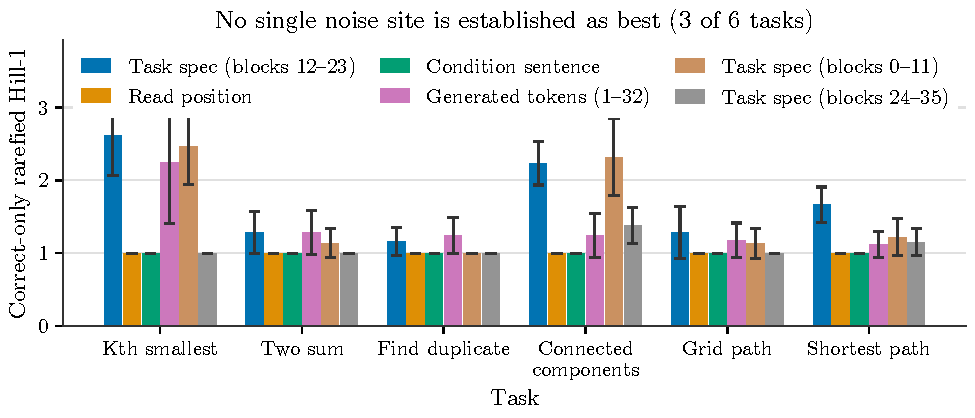
\includegraphics[width=\linewidth,height=0.78\textheight,keepaspectratio]{figures/fig_site_h5_v0.pdf}
\caption{Grouped bar chart of the best correct-only rarefied Hill-1 diversity (y-axis; 1.0 means the model wrote the same correct algorithm in every run) reached by writing one fixed-size random displacement into six different sites of Qwen3-8B's forward pass (FP8 W8A8, 8-bit linear layers, thinking off), at a pass-rate cost of at most 5 percentage points relative to an unperturbed twin, best taken over a pre-registered hull of noise doses of 1, 2 and 4 ban units (N = 30 correct programs per dose cell). The x-axis gives six coding tasks: kth smallest, two sum, find duplicate, connected components, grid path, and shortest path. Bar colour encodes the perturbed site: blue is the task-specification states at blocks 12 to 23, orange is the read position, teal is the condition sentence, pink is generated tokens 1 to 32, tan is the task-specification states at blocks 0 to 11, and grey is the task-specification states at blocks 24 to 35. Error bars are half the width of each bar's own 95\textbackslash{}\% bootstrap confidence interval. The read-position and condition-sentence bars sit at exactly 1.0 with zero spread on all six tasks, consistent with a broader null across this experiment's correct programs (0 of 526 and 0 of 527 ever left the default algorithm). Among the other four sites, no single one is highest on a majority of tasks: task-specification blocks 12 to 23 has the top estimate on three tasks (kth smallest, grid path, shortest path), task-specification blocks 0 to 11 on one (connected components), and generated-token noise on two (two sum, find duplicate), with 95\textbackslash{}\% intervals that overlap heavily between the competing non-floor bars on every task except shortest path. The pre-registered rule for a single best site (best on at least four of six tasks) was not met: this is a PARTIAL comparison, not an established ranking of which site matters most.}
\label{fig:fig_site_h5}
\end{figure}
The tie on two sum (1.28 each) went to generated-token noise on the price of 1.5 (0.12 against 0.53, Table 144). Early-block noise winning connected components carries a dose-convention confound that the plan had named: a ban unit at blocks 0 to 11 is only 4.5\% to 7.2\% of the residual norm, against 12.7\% to 18.3\% at blocks 12 to 23, so early-block noise at alpha 4 is a relative dose comparable to the plan site at alpha 1. No other site matched or beat the 5-point Hill-1 of the plan site on 4 tasks, so the claim is not disconfirmed either. Appending alpha 8 to the hull of the plan site, or allowing only mixtures of adjacent doses, left every ranking unchanged.

\begin{table}[H]
\renewcommand{\thetable}{144}
\centering\small\setlength{\tabcolsep}{4.0pt}
\caption{Prices of 1.5 and 2 per site: the cheapest pass cost (as a fraction) at which Hill-1 reaches 1.5 and 2 on the hull (n\slash{}a: not reached). Source: site experiment \texttt{results/\allowbreak{}hull.\allowbreak{}json}. [Source: iteration 4, artifact \nolinkurl{gen_art_experiment_20}.]}\label{tab:t156}
\begin{tabular}{>{\raggedright\arraybackslash\hspace{0pt}}p{0.1468\linewidth}>{\raggedright\arraybackslash\hspace{0pt}}p{0.5310\linewidth}>{\raggedright\arraybackslash\hspace{0pt}}p{0.2684\linewidth}}
\toprule
\textbf{Task} & \textbf{Price of 1.5: blocks 12-23 \slash{} read position \slash{} condition \slash{} generated \slash{} blocks 0-11 \slash{} blocks 24-35} & \textbf{Price of 2: same order} \\
\midrule
kth smallest & 0.00 \slash{} n\slash{}a \slash{} n\slash{}a \slash{} 0.01 \slash{} 0.00 \slash{} n\slash{}a & 0.00 \slash{} n\slash{}a \slash{} n\slash{}a \slash{} 0.04 \slash{} 0.00 \slash{} n\slash{}a \\
two sum & 0.53 \slash{} n\slash{}a \slash{} n\slash{}a \slash{} 0.12 \slash{} n\slash{}a \slash{} n\slash{}a & n\slash{}a for every site \\
find duplicate & 0.54 \slash{} n\slash{}a \slash{} n\slash{}a \slash{} 0.16 \slash{} n\slash{}a \slash{} n\slash{}a & 0.75 \slash{} n\slash{}a \slash{} n\slash{}a \slash{} 0.37 \slash{} n\slash{}a \slash{} n\slash{}a \\
connected components & 0.00 \slash{} n\slash{}a \slash{} n\slash{}a \slash{} 0.11 \slash{} 0.00 \slash{} n\slash{}a & 0.01 \slash{} n\slash{}a \slash{} n\slash{}a \slash{} 0.19 \slash{} 0.02 \slash{} n\slash{}a \\
grid & 0.14 \slash{} n\slash{}a \slash{} n\slash{}a \slash{} n\slash{}a \slash{} n\slash{}a \slash{} n\slash{}a & n\slash{}a for every site \\
shortest path & 0.00 \slash{} n\slash{}a \slash{} n\slash{}a \slash{} n\slash{}a \slash{} 0.25 \slash{} n\slash{}a & n\slash{}a for every site \\
\bottomrule
\end{tabular}
\end{table}

Table 145 classifies the failure mode of each site under the frozen rule. Generated-token noise moves four tasks but pays in breakage: it is the only site whose invalid rate climbs to between 0.67 and 1.00 at alpha 4.

\begin{table}[H]
\renewcommand{\thetable}{145}
\centering\scriptsize\setlength{\tabcolsep}{2.5pt}
\caption{Failure mode per site and task under the frozen rule (\textdagger{} weak movement: a correct-only excess between 0.10 and 0.20 at a pass rate of at least 0.8 times that of the twin, which the rule does not classify). Source: site experiment \texttt{results/\allowbreak{}failure\_\allowbreak{}modes.\allowbreak{}json}. [Source: iteration 4, artifact \nolinkurl{gen_art_experiment_20}.]}\label{tab:t157}
\begin{tabular}{>{\raggedright\arraybackslash\hspace{0pt}}p{0.1805\linewidth}>{\raggedright\arraybackslash\hspace{0pt}}p{0.1010\linewidth}>{\raggedright\arraybackslash\hspace{0pt}}p{0.1221\linewidth}>{\raggedright\arraybackslash\hspace{0pt}}p{0.1296\linewidth}>{\raggedright\arraybackslash\hspace{0pt}}p{0.1403\linewidth}>{\raggedright\arraybackslash\hspace{0pt}}p{0.1250\linewidth}>{\raggedright\arraybackslash\hspace{0pt}}p{0.1250\linewidth}}
\toprule
\textbf{Site} & \textbf{kth smallest} & \textbf{two sum} & \textbf{find duplicate} & \textbf{connected components} & \textbf{grid} & \textbf{shortest path} \\
\midrule
Task spec, blocks 12-23 & moves & moves with cost & moves with cost & moves & moves with cost & moves \\
Read position & no movement & no movement & no movement & no movement & no movement & no movement \\
Condition sentence & no movement & no movement & no movement & no movement & no movement & no movement \\
Generated tokens 1-32 & moves & moves & moves with cost & moves & breakage first & breakage first \\
Task spec, blocks 0-11 & moves & weak movement \textdagger{} & no movement & moves & breakage first & weak movement \textdagger{} \\
Task spec, blocks 24-35 & no movement & no movement & no movement & weak movement \textdagger{} & no movement & no movement \\
\bottomrule
\end{tabular}
\end{table}

The paired flips at alpha 2 make the comparison exact (Table 146). The plan site flips significantly more of the 30 shared slots off the default than the read position, the condition sentence and the late blocks on kth smallest, connected components and both path tasks, and more than the early blocks on kth smallest and connected components. Generated-token noise flips more than the plan site on find duplicate (12 against 0).

\begin{table}[H]
\renewcommand{\thetable}{146}
\centering\scriptsize\setlength{\tabcolsep}{2.5pt}
\caption{Paired flips at alpha 2 (30 shared slots): slots off the default only under the plan site : only under the other site, with the exact McNemar p and the byte-identical rate of the other site against the twin. Source: site experiment \texttt{results/\allowbreak{}paired\_\allowbreak{}flips.\allowbreak{}json}. [Source: iteration 4, artifact \nolinkurl{gen_art_experiment_20}.]}\label{tab:t158}
\begin{tabular}{>{\raggedright\arraybackslash\hspace{0pt}}p{0.1382\linewidth}>{\raggedright\arraybackslash\hspace{0pt}}p{0.1402\linewidth}>{\raggedright\arraybackslash\hspace{0pt}}p{0.1188\linewidth}>{\raggedright\arraybackslash\hspace{0pt}}p{0.1300\linewidth}>{\raggedright\arraybackslash\hspace{0pt}}p{0.1449\linewidth}>{\raggedright\arraybackslash\hspace{0pt}}p{0.1218\linewidth}>{\raggedright\arraybackslash\hspace{0pt}}p{0.1296\linewidth}}
\toprule
\textbf{Other site} & \textbf{kth smallest} & \textbf{two sum} & \textbf{find duplicate} & \textbf{connected components} & \textbf{grid} & \textbf{shortest path} \\
\midrule
Read position & 14:0 (p 0.00012; 0.93) & 3:0 (p 0.25; 0.97) & 1:0 (p 1; 0.80) & 18:0 (p 7.6e-06; 0.33) & 6:0 (p 0.031; 0.13) & 8:0 (p 0.0078; 0.57) \\
Condition sentence & 14:0 (p 0.00012; 0.87) & 3:0 (p 0.25; 0.70) & 1:0 (p 1; 0.87) & 18:0 (p 7.6e-06; 0.40) & 6:0 (p 0.031; 0.07) & 8:1 (p 0.039; 0.57) \\
Generated tokens 1-32 & 6:8 (p 0.79; 0.13) & 2:7 (p 0.18; 0.10) & 0:12 (p 0.00049; 0.07) & 10:2 (p 0.039; 0.00) & 5:1 (p 0.22; 0.00) & 6:3 (p 0.51; 0.00) \\
Task spec, blocks 0-11 & 11:1 (p 0.0063; 0.63) & 3:0 (p 0.25; 0.57) & 1:0 (p 1; 0.40) & 13:1 (p 0.0018; 0.27) & 5:2 (p 0.45; 0.00) & 5:3 (p 0.73; 0.20) \\
Task spec, blocks 24-35 & 14:0 (p 0.00012; 0.97) & 3:0 (p 0.25; 0.97) & 1:0 (p 1; 0.93) & 16:1 (p 0.00027; 0.33) & 7:0 (p 0.016; 0.27) & 7:0 (p 0.016; 0.20) \\
\bottomrule
\end{tabular}
\end{table}

\textbf{The effect is not generic transmission.} Noise at the read position produces as large a displacement at the last block as the plan site does (medians 141, 250 and 474 against 159, 272 and 461 at alpha 1, 2 and 4), yet it flips nothing. A logistic regression of a correct program being off the default on the log of the realised displacement at the read position, with template and task fixed effects, over 2,769 correct programs from the prefill sites, gives the plan site an indicator of +2.15 [1.79, 2.51] beside a displacement slope of +0.88 [0.62, 1.14]. In the matched-dose bins (the upper three quintiles of displacement) the plan site is off the default in 16\% to 27\% of programs, against 3\% to 7\% for the other prefill sites. A hand-coded Mantel-Haenszel odds ratio, which pools the odds of an off-default program at the plan site against the other prefill sites across task and displacement quintile strata, gives 5.72 [3.94, 8.30], and its placebo, with plan-site labels shuffled within task, has a median of 0.98. A Bayesian mixed logistic model with random task and template effects puts the site effects relative to the plan site at -3.0 (read position), -2.9 (condition sentence), -3.0 (late blocks), -0.8 (generated tokens) and -1.1 (early blocks), with the slope of the plan site on log2 alpha at +1.11. Concentrating the whole ban energy at the read position (median displacement there 1,002, six times that of the plan site at alpha 1) moved find duplicate by +0.23 and connected components by +0.18 at pass ratios of 0.87 to 0.93; spreading it over the condition span stayed inert. Generated-token noise produces the most phrasing clusters per idea (4.2 and 4.7 at alpha 1 and 2, against 2.8 and 3.4 for the plan site, AST-shingle components at Jaccard 0.8).

\textbf{The boundary.} At alpha 8 the task specification is effectively erased (Table 147): the model echoes the condition sentence, writes placeholder code or asks for clarification, and the pass rate is 0.00 on every task. Correct-only diversity peaks at alpha 2 (kth smallest, grid, shortest path) or alpha 4 (two sum, find duplicate, connected components), and alpha 4 already costs 33\% to 97\% of the passes. Across every arm 3,555 programs were correct, and exactly one was labelled other: a find duplicate program from generated-token noise at alpha 2 that calls a count of each element over the list. The judges called it degenerate and a labeller miss, and the manual read, beside its three nearest known solutions, called it the textbook quadratic brute force. No novel algorithm appeared (rule-of-three bound 3\slash{}3,555 = 0.08\% per correct program [67]).

\begin{table}[H]
\renewcommand{\thetable}{147}
\centering\footnotesize\setlength{\tabcolsep}{4.0pt}
\caption{The plan site from alpha 0 to 8: pass rate \slash{} invalid rate \slash{} correct-only Hill-1. Source: site experiment \texttt{results/\allowbreak{}boundary.\allowbreak{}json}. [Source: iteration 4, artifact \nolinkurl{gen_art_experiment_20}.]}\label{tab:t159}
\begin{tabular}{>{\raggedright\arraybackslash\hspace{0pt}}p{0.1384\linewidth}>{\raggedright\arraybackslash\hspace{0pt}}p{0.1531\linewidth}>{\raggedright\arraybackslash\hspace{0pt}}p{0.1531\linewidth}>{\raggedright\arraybackslash\hspace{0pt}}p{0.1531\linewidth}>{\raggedright\arraybackslash\hspace{0pt}}p{0.1531\linewidth}>{\raggedright\arraybackslash\hspace{0pt}}p{0.1460\linewidth}}
\toprule
\textbf{Task} & \textbf{Alpha 0} & \textbf{Alpha 1} & \textbf{Alpha 2} & \textbf{Alpha 4} & \textbf{Alpha 8} \\
\midrule
kth smallest & 1.00 \slash{} 0.00 \slash{} 1.00 & 1.00 \slash{} 0.00 \slash{} 2.52 & 0.93 \slash{} 0.00 \slash{} 2.68 & 0.67 \slash{} 0.00 \slash{} 2.23 & 0.00 \slash{} 0.94 \slash{} n\slash{}a \\
two sum & 1.00 \slash{} 0.00 \slash{} 1.00 & 1.00 \slash{} 0.00 \slash{} 1.00 & 0.97 \slash{} 0.00 \slash{} 1.28 & 0.30 \slash{} 0.07 \slash{} 1.70 & 0.00 \slash{} 0.94 \slash{} n\slash{}a \\
find duplicate & 1.00 \slash{} 0.00 \slash{} 1.00 & 1.00 \slash{} 0.00 \slash{} 1.00 & 1.00 \slash{} 0.00 \slash{} 1.15 & 0.17 \slash{} 0.03 \slash{} 2.59 & 0.00 \slash{} 0.94 \slash{} n\slash{}a \\
connected components & 1.00 \slash{} 0.00 \slash{} 1.00 & 1.00 \slash{} 0.00 \slash{} 1.84 & 0.97 \slash{} 0.00 \slash{} 2.23 & 0.23 \slash{} 0.10 \slash{} 2.73 & 0.00 \slash{} 0.96 \slash{} n\slash{}a \\
grid & 0.74 \slash{} 0.00 \slash{} 1.00 & 0.72 \slash{} 0.00 \slash{} 1.39 & 0.68 \slash{} 0.00 \slash{} 1.51 & 0.12 \slash{} 0.06 \slash{} 1.00 & 0.00 \slash{} 0.82 \slash{} n\slash{}a \\
shortest path & 1.00 \slash{} 0.00 \slash{} 1.00 & 1.00 \slash{} 0.00 \slash{} 1.65 & 0.90 \slash{} 0.00 \slash{} 1.70 & 0.03 \slash{} 0.07 \slash{} 1.00 & 0.00 \slash{} 0.88 \slash{} n\slash{}a \\
\bottomrule
\end{tabular}
\end{table}

\emph{(Correction, iteration 5: the alpha-4 peaks of this table rest on few correct programs and were rarefied at those depths, not at 25: two sum 9, find duplicate 5 and connected components 7 correct programs (kth smallest 20, grid 6, shortest path 1). The statement that correct-only diversity peaks at alpha 4 on three tasks is therefore a statement about 5 to 9 programs. Depth per cell in Table 178.)}

\textbf{The top-five prohibition at the plan.} The request asks what happens when the five most implemented algorithms are prohibited. The prompt version had failed by reimplementation (avoidance 0.00) and the cumulative token veto had stalled. This experiment applied the prohibition as an activation push: the plan states of the grid task were pushed along the per-block direction from the mean of the five banned centroids to the mean of the survivor centroids, estimated from 300 forced prompts in which the centroid of every algorithm was separable from the others (nearest-centroid separability 0.83 to 1.00). The push never moved the model off BFS (Table 148). Correct programs were BFS 30 of 30 at alpha 1 and 19 of 19 at alpha 2, and none passed at alpha 4; fresh random plan noise at the same norm did no better. The test of edge against opposite side could not be computed because no survivor program appeared at any dose, and the plan geometry leaves little to resolve: bidirectional BFS and IDA* sit almost equally far from the banned set (geodesic 0.36 against 0.37; MDS stress-1 0.147; no persistent loop beyond a permutation null).

\begin{table}[H]
\renewcommand{\thetable}{148}
\centering\small\setlength{\tabcolsep}{4.0pt}
\caption{The top-five push at the plan states of the grid task (N = 50 per arm; slots 0 to 9): correct programs, avoidance of the five banned algorithms with Wilson 95\% interval, and the composition of correct programs. Source: site experiment \texttt{results/\allowbreak{}c3d.\allowbreak{}json}. [Source: iteration 4, artifact \nolinkurl{gen_art_experiment_20}.]}\label{tab:t160}
\begin{tabular}{>{\raggedright\arraybackslash\hspace{0pt}}p{0.2962\linewidth}>{\raggedright\arraybackslash\hspace{0pt}}p{0.0990\linewidth}>{\raggedright\arraybackslash\hspace{0pt}}p{0.3137\linewidth}>{\raggedright\arraybackslash\hspace{0pt}}p{0.2208\linewidth}}
\toprule
\textbf{Arm} & \textbf{Correct} & \textbf{Avoidance of the top five [95\%]} & \textbf{Correct programs} \\
\midrule
top-five push, alpha 1 & 30 & 0.00 [0.00, 0.11] & BFS 30 \\
random plan noise, alpha 1 & 36 & 0.03 [0.00, 0.14] & BFS 33, DFS 2, other 1 \\
top-five push, alpha 2 & 19 & 0.00 [0.00, 0.17] & BFS 19 \\
random plan noise, alpha 2 & 34 & 0.00 [0.00, 0.10] & BFS 29, DFS 5 \\
top-five push, alpha 4 & 0 & n\slash{}a & none \\
random plan noise, alpha 4 & 6 & 0.00 [0.00, 0.39] & BFS 6 \\
twin & 37 & 0.00 [0.00, 0.09] & BFS 37 \\
\bottomrule
\end{tabular}
\end{table}

\textbf{The scorecard and checks.} Table 149 scores the predictions the experiment committed before its first decisive sample. The engine reproduced the kth smallest and shortest path cells of the screen byte for byte (50 of 50 identical programs on each task, divergence 0.000 against null 95th percentiles of 0.029 and 0.025). Alpha 0 reproduced the twin at every site; the realised displacement along the direction equalled its target within 0.26\% at every prefill site. One GPU test failed: shadow states for generated-token noise diverged from an independent teacher-forced pass (minimum cosine 0.679 on kth smallest), and a follow-up showed clean decode-path states diverging by the same order, a property of the 8-bit decode path rather than of the shadow coupling. An independent rederivation checked 146 cells with no mismatch, and a second, written only from raw files, reproduced the headline counts. The alpha-4 compositions of this experiment differ from the alpha-4 rows of the plan noise experiment beyond a resampling null on four tasks, so these cells do not stand in for the knob table.

\begin{table}[H]
\renewcommand{\thetable}{149}
\centering\small\setlength{\tabcolsep}{4.0pt}
\caption{Predictions committed before the first decisive sample and their outcomes. Source: site experiment \texttt{README.\allowbreak{}md}, \texttt{predictions/\allowbreak{}predictions.\allowbreak{}json}. [Source: iteration 4, artifact \nolinkurl{gen_art_experiment_20}.]}\label{tab:t161}
\begin{tabular}{>{\raggedright\arraybackslash\hspace{0pt}}p{0.5208\linewidth}>{\raggedright\arraybackslash\hspace{0pt}}p{0.4420\linewidth}}
\toprule
\textbf{Prediction} & \textbf{Outcome} \\
\midrule
The plan site has the highest 5-point Hill-1 on at least 4 of 6 tasks & missed: 3 of 6 (PARTIAL) \\
The read position shows no movement on at least 5 of 6 & hit: 6 of 6 \\
The condition sentence stays below the plan site on at least 4 of 6, and may move two sum or find duplicate & hit: 6 of 6 below (5-point Hill-1 1.00 everywhere); it moves nothing \\
Generated-token noise: more phrasing clusters per idea than the plan site, little idea change, breakage first by alpha 4 & clusters hit; little idea change missed (it moves four tasks); breakage by alpha 4 hit (invalid 0.67 to 1.00) \\
Early-block noise breaks first at alpha 2 or more & missed: it moves kth smallest and connected components at alpha 4 with pass kept \\
Late-block noise shows no movement at alpha 1 to 2 and breaks at alpha 4 & no movement hit (5 of 6; connected components weak); breakage missed (pass at least 0.87) \\
Energy-matched read position and condition variants break (pass below 0.8 times that of the twin) on at least 4 of 6 & missed: 0 of 6 for both \\
Boundary: pass below 0.5 at alpha 8 on at least 4 of 6 & hit: 6 of 6 (pass 0.00 everywhere) \\
Boundary: correct-only Hill peaks at alpha 2 to 4 & hit: alpha 2 on three tasks, alpha 4 on three \\
Boundary: no judge-confirmed novel algorithm & hit: 0 of 3,555 correct programs \\
Top-five push: avoidance below 0.5 at alpha 2 or less & hit: 0.00 at alpha 1 and 2 \\
Top-five push lands at the edge (bidirectional BFS) rather than the opposite side & not testable: no survivor program at any dose \\
\bottomrule
\end{tabular}
\end{table}

\FloatBarrier
\subsection*{4.5 Same seed: temperature against plan noise (Qwen3-8B, question 1a-c of the request)}
\addcontentsline{toc}{subsection}{4.5 Same seed: temperature against plan noise (Qwen3-8B, question 1a-c of the request)}
\noindent{\small\emph{Artifact: \nolinkurl{gen_art_experiment_21}.}}\par\medskip
\textbf{Why.} The request asks three things about temperature: with a tight temperature and top-k 10, does the model produce one idea in many phrasings or many ideas; does loosening it multiply ideas or phrasings; and does the answer hold with the same seed. The run had answered the first two in iteration 1 and the third with thinking off in iteration 2, and had dropped the thinking-on arm twice. This experiment  ran the seed-coupled design on the grid task, the shortest path task and kth smallest, with the thinking-on arm made non-droppable, and added plan noise as the second factor so that the same seed could be varied in temperature or in plan.

\textbf{Design.} Each task had 20 token seeds, one per template and slot, and each seed kept one noise stream across every condition (inverse-CDF sampling with common random numbers). The temperature block ran each seed at 0.3, 0.7, 1.0 and 1.3 (top-p 1) and with top-k 10 at 0.7. The plan noise block ran 6 fixed isotropic directions at alpha 1 and 2 and temperature 0.7 and 1.0. The change count of a task is the number of seeds whose algorithm differs across the conditions of a block; for plan noise it is averaged over the 20 three-direction subsets of the 6 directions. Thinking on ran in vLLM with per-request seeds (an exponential race coupling, confirmed by recomputing the first token in 32 of 32 requests), a 16k cap and the completion rate reported. \emph{(Correction, iteration 5: the top-k 10 answer to the request with thinking off is Table 76 of iteration 2: with seeds coupled, the label changed in 0 of 30 seeds in 10 of 12 cells. The thinking-on arm of this experiment ran without top-k (top-k off, Gumbel-max coupling through per-request seeds, temperatures 0.3, 0.7, 1.0 and 1.3), so the literal cell of the request, thinking on with top-k 10 and the same seed, was not run in iteration 4. It ran in iteration 5, Section 5.7.)}

\textbf{Temperature never changed the algorithm; plan noise changed it in most seeds on the shortest path task.} With thinking off, the algorithm stayed the same across all four temperatures in 20 of 20 seeds on all three tasks, and with thinking on in 20 of 20 seeds on the shortest path task (Table 150); the exact 95\% upper bound on the per-seed change rate is 0.168 for each count of 0 in 20. One random plan direction at alpha 1 changed the algorithm in 17.25 of 20 seeds on the shortest path task, 4.55 on kth smallest and 2.5 on the grid task. \emph{(Correction, iteration 5: these are not rates per direction. Each is the mean, over the 20 three-direction subsets of the 6 directions, of the number of seeds whose label differs anywhere among the no-noise arm and the three directions of the subset, a union over three directions. The single-direction counts of changed seeds at alpha 1 and temperature 1.0 are 7, 10, 15, 17, 3 and 8 of 20 on the shortest path task, 2, 0, 0, 7, 2 and 0 on kth smallest, and 0, 0, 1, 1, 3 and 0 on the grid task.)} The paired contrast per seed, plan noise change minus temperature change, pooled over the shortest path task and kth smallest (40 seeds), has a mean of 0.545 [0.41, 0.67] and a one-sided sign-flip p of 1.0e-5. That is the single entry of the experiment in the secondary family of the iteration. A within-seed permutation of conditions puts the observed mean above all 200 placebo means (maximum 0.155; p = 0.005).

\begin{table}[H]
\renewcommand{\thetable}{150}
\centering\scriptsize\setlength{\tabcolsep}{2.5pt}
\caption{Seeds (of 20) whose algorithm changes across temperatures, thinking off and on, and across plan noise draws (mean over 20 three-direction subsets), by dose and temperature. Source: same seed experiment \texttt{results/\allowbreak{}c1seed.\allowbreak{}json}. [Source: iteration 4, artifact \nolinkurl{gen_art_experiment_21}.]}\label{tab:t162}
\begin{tabular}{>{\raggedright\arraybackslash\hspace{0pt}}p{0.0774\linewidth}>{\raggedright\arraybackslash\hspace{0pt}}p{0.1483\linewidth}>{\raggedright\arraybackslash\hspace{0pt}}p{0.1641\linewidth}>{\raggedright\arraybackslash\hspace{0pt}}p{0.1025\linewidth}>{\raggedright\arraybackslash\hspace{0pt}}p{0.1025\linewidth}>{\raggedright\arraybackslash\hspace{0pt}}p{0.1032\linewidth}>{\raggedright\arraybackslash\hspace{0pt}}p{0.1032\linewidth}>{\raggedright\arraybackslash\hspace{0pt}}p{0.1119\linewidth}}
\toprule
\textbf{Task} & \textbf{Temperature, thinking off (4 temperatures)} & \textbf{Temperature, thinking on (4 temperatures)} & \textbf{Plan noise alpha 1, T 0.7} & \textbf{Plan noise alpha 1, T 1.0} & \textbf{Plan noise alpha 2, T 0.7} & \textbf{Plan noise alpha 2, T 1.0} & \textbf{Correct only, alpha 1, T 1.0} \\
\midrule
shortest path & 0 & 0 & 17.70 & 17.25 & 18.45 & 19.05 & 10.25 \\
kth smallest & 0 & not run & 4.40 & 4.55 & 10.30 & 10.60 & 4.05 \\
grid & 0 & 0 of 10 seeds (reduced arm) & 1.50 & 2.50 & 8.95 & 8.70 & 1.45 \\
\bottomrule
\end{tabular}
\end{table}

\begin{figure}[!htbp]
\centering\captionsetup{font=footnotesize}
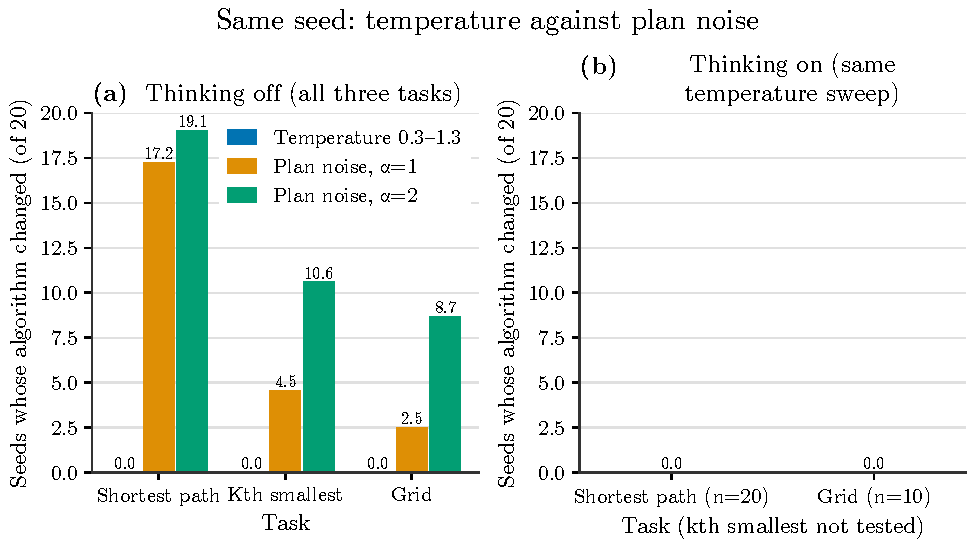
\includegraphics[width=\linewidth,height=0.78\textheight,keepaspectratio]{figures/fig_seed_counts_v0.pdf}
\caption{Number of token seeds (of 20) whose implemented algorithm changes across conditions, with each seed's own noise stream held fixed (Qwen3-8B, FP8 W8A8 engine). (a) Thinking off, all three tasks: sweeping temperature over 0.3, 0.7, 1.0 and 1.3 (blue) never changes the algorithm, 0.0 of 20 seeds on every task; pushing a random direction into the task-specification activations at blocks 12--23 during prefill (``plan noise'') changes it often --- orange bars ($\alpha$=1) and green bars ($\alpha$=2, each the mean over 20 three-direction subsets of 6 sampled directions) rise from 17.2\slash{}19.1 of 20 seeds on the shortest-path task to 4.5\slash{}10.6 on kth smallest and 2.5\slash{}8.7 on grid. (b) The same temperature sweep with thinking on changes nothing either, on the two tasks where it was tested (shortest path, n=20 seeds; grid, n=10 seeds); kth smallest had no thinking-on arm and so has no bar in this panel. Values are printed above every bar; bars at 0.0 are measured null results, not missing data. Source: same-seed experiment, run on an FP8-quantized engine --- a later bf16 check did not clearly reproduce the shortest-path plan-noise effect at the population level, so replication under full precision remains open.}
\label{fig:fig_seed_counts}
\end{figure}
The preregistered verdict is PARTIAL: the temperature, phrasing and coupling predictions hold, and the plan noise prediction (at least 5 of 20 seeds) fails on kth smallest, at 4.55. The plan prescribed the unit of the bench forecast experiment for kth smallest, which is 1\slash{}1.30 of the unit the screen used, so alpha 1 here is a weaker push than alpha 1 of the screen; at alpha 2 kth smallest reaches 10.6, and under a Gumbel-max coupling 5.8. Counted over correct programs or with invalid outputs as a label, the temperature count stays 0 on every task; with top-k 10 added as a fifth condition it stays 0; with min-p 0.1 at temperature 2.0 added it becomes 1 on the shortest path task and kth smallest (one Bellman-Ford\slash{}SPFA and one quickselect program out of 20) and stays 0 on the grid task.

\textbf{Temperature changes phrasings, not ideas.} Phrasings per idea grow with temperature (Table 151): the pooled slope of log phrasings per idea on temperature is 0.64, 0.70 and 0.81 at Jaccard thresholds 0.7, 0.8 and 0.9, each 95\% interval excluding 0. Almost all of the growth is on the grid task (3 to 13 clusters at threshold 0.8). The shortest path task barely moves (1 to 2) and kth smallest does not move (2 at every temperature). At alpha 1 and temperature 0.7, the rarefied Hill-1 of correct ideas is 1.87 on the shortest path task, 1.31 on kth smallest and 1.15 on the grid task, while top-k 10 gives 1.00 on all three. Plan noise lands on Bellman-Ford\slash{}SPFA on the shortest path task (52 of 60 off-default programs, 8 other), on quickselect on kth smallest (11 of 11) and on DFS on the grid task (5). It costs correctness on the shortest path task: pass 0.63 at alpha 1 and temperature 1.0 and 0.42 at alpha 2, against 1.00 without it. Once a seed has been nudged off the default, temperature can act on the idea: under the escaping direction, temperature 0.7 against 1.0 changes the label in 5 of 20 seeds on the shortest path task and 2 of 20 on kth smallest, against 0 of 20 without plan noise.

\begin{table}[H]
\renewcommand{\thetable}{151}
\centering\footnotesize\setlength{\tabcolsep}{4.0pt}
\caption{Phrasing clusters per idea at Jaccard threshold 0.8 by temperature (20 programs per cell, thinking off, no plan noise). Source: same seed experiment \texttt{results/\allowbreak{}phrasing.\allowbreak{}json}. [Source: iteration 4, artifact \nolinkurl{gen_art_experiment_21}.]}\label{tab:t163}
\begin{tabular}{>{\raggedright\arraybackslash\hspace{0pt}}p{0.3328\linewidth}>{\raggedright\arraybackslash\hspace{0pt}}p{0.1451\linewidth}>{\raggedright\arraybackslash\hspace{0pt}}p{0.1451\linewidth}>{\raggedright\arraybackslash\hspace{0pt}}p{0.1451\linewidth}>{\raggedright\arraybackslash\hspace{0pt}}p{0.1451\linewidth}}
\toprule
\textbf{Task} & \textbf{T 0.3} & \textbf{T 0.7} & \textbf{T 1.0} & \textbf{T 1.3} \\
\midrule
shortest path & 1 & 2 & 2 & 2 \\
kth smallest & 2 & 2 & 2 & 2 \\
grid & 3 & 10 & 12 & 13 \\
\bottomrule
\end{tabular}
\end{table}

\textbf{Thinking on.} All 100 shortest path traces completed within the cap (Table 152). Every final program and every first approach named was Dijkstra at every temperature, and every program passed. A repeat at temperature 0.7 diverged byte for byte in all 20 traces (first divergence at token 34 to 653), because this GPU generation lacks batch invariance, yet the final label and the first approach named agreed in 20 of 20; the temperature count of 0 is read against a noise floor of 0. A judge naming the first approach of 20 traces agreed with the lexicon on 20 of 20. In the reduced grid arm (10 seeds) all 40 traces completed (median 5.2k to 6.2k thinking tokens, maximum 9.0k), and every final program and first approach was BFS, a temperature count of 0 of 10 (exact 95\% upper rate 0.31). With thinking on, plan noise at alpha 2 and temperature 0.7 (2,048-token cap, the three directions with the highest thinking-off off-default share) moved the first approach named in 1, 0 and 0 of 10 seeds, short of the committed expectation of at least 3 of 10 for some direction. Once the model thinks, the prefill nudge no longer redirects the first idea it names.

\begin{table}[H]
\renewcommand{\thetable}{152}
\centering\footnotesize\setlength{\tabcolsep}{4.0pt}
\caption{Thinking on, shortest path task (20 seeds per temperature, 16k cap, vLLM). Source: same seed experiment \texttt{results/\allowbreak{}thinking.\allowbreak{}json}. [Source: iteration 4, artifact \nolinkurl{gen_art_experiment_21}.]}\label{tab:t164}
\begin{tabular}{>{\raggedright\arraybackslash\hspace{0pt}}p{0.1323\linewidth}>{\raggedright\arraybackslash\hspace{0pt}}p{0.1227\linewidth}>{\raggedright\arraybackslash\hspace{0pt}}p{0.2957\linewidth}>{\raggedright\arraybackslash\hspace{0pt}}p{0.1515\linewidth}>{\raggedright\arraybackslash\hspace{0pt}}p{0.2110\linewidth}}
\toprule
\textbf{Temperature} & \textbf{Completed} & \textbf{Median thinking tokens (maximum)} & \textbf{Final label} & \textbf{First approach named} \\
\midrule
0.3 & 20 of 20 & 4,097 (7,381) & Dijkstra 20 & Dijkstra 20 \\
0.7 & 20 of 20 & 3,952 (6,327) & Dijkstra 20 & Dijkstra 20 \\
1.0 & 20 of 20 & 4,320 (8,808) & Dijkstra 20 & Dijkstra 20 \\
1.3 & 20 of 20 & 4,020 (12,612) & Dijkstra 20 & Dijkstra 20 \\
0.7, repeat & 20 of 20 & 4,001 (7,427) & Dijkstra 20 & Dijkstra 20 \\
\bottomrule
\end{tabular}
\end{table}

\textbf{Checks.} The engine check reran the kth smallest and shortest path cells of the screen with their twins and reproduced 200 of 200 programs token for token (size-k heap 19, quickselect 16, full sort 15; Dijkstra 26, Bellman-Ford\slash{}SPFA 24). Filler repeats in other batches were byte-identical in 60 of 60, and the engine-check slots matched the rows of the temperature block at 1.0 in 40 of 40. Under a Gumbel-max replicate the temperature count stays 0 on both tasks, plan noise changes 16.05 of 20 seeds on the shortest path task and 5.8 on kth smallest, and the pooled contrast is 0.546 (p = 1.0e-5). With min-p 0.1 at temperature 2.0, the shortest path task wrote Dijkstra 19 and Bellman-Ford\slash{}SPFA 1, kth smallest full sort 19 and quickselect 1, and the grid task BFS 20. The condition-shuffle placebo rejected at p below 0.05 in 2\% of 200 runs, and the placebo of the independent rederivation in 10.5\%; over 1,440 placebo runs the rejection rate is about 6\%. The only correct program labelled other was a naive Dijkstra, a labeller miss; no novel algorithm appeared. The rederivation, sharing no code with the analysis, matched 33 of 33 checks, and the commitment precedes the first decisive row. An 8-bit cross-check of the two engines on the shortest path twin gave Dijkstra 50 of 50 on each, a divergence of 0 bits, which is weak by construction because the cell is all Dijkstra.

\FloatBarrier
\subsection*{4.6 The plan subspace: does the geometry of forced prompts explain which pushes move the algorithm? (Qwen3-8B)}
\addcontentsline{toc}{subsection}{4.6 The plan subspace: does the geometry of forced prompts explain which pushes move the algorithm? (Qwen3-8B)}
\noindent{\small\emph{Artifact: \nolinkurl{gen_art_experiment_22}.}}\par\medskip
\textbf{Why.} The site experiment located the choice in the task-specification states at early to middle blocks, but a site is not a representation. The subspace claim gave the internal account the request asks for a testable form: if the algorithm choice is represented along the directions that separate the per-algorithm centroids, a random push should change the algorithm to the extent that it moves the state along them. This experiment  built the subspace from forced prompts alone and asked whether it ranks 40 fresh random directions by their effect, whether removing the in-subspace component of a push removes the effect, and whether a push aimed at the runner-up centroid crosses at the predicted distance.

\textbf{Design.} For each of 15 tasks the plan subspace at blocks 12 to 35 was the span of the centroid differences of the task-specification states (mean over the specification positions) under 30 forced paraphrases per algorithm (10 forced templates by 3 names), and a masked twin used 30 leak-checked descriptions per algorithm. The projection share of a direction is its squared norm in the subspace over its total, averaged over blocks. Forty never-run directions at alpha 1 and 2, with N = 10 each and passers topped up to N = 30, ran on the six movable tasks; 8 directions at both doses ran on the other nine, including cycle detection on its ban-free unit. Every predictor was committed by hash before the first population sample. The run sampled 13,500 programs in 675 batches of 20 over 2.51 GPU hours, labelled by runtime tracer and AST rules with a blind judge on 752 disagreements; 4 disputed and 97 invalid rows were excluded from shares.

\textbf{The subspace is real and reliable.} At block 18 the split-half principal-angle cosine between two halves of the paraphrases is 0.89 to 0.97 on all 15 tasks, against 0.02 to 0.03 for random subspaces of equal dimension, and every centroid difference has a split-half cosine of at least 0.74. Named and masked differences agree only moderately (cosine 0.12 to 1.00 at block 18), so the subspace carries a lexical component. The iteration-3 ban displacement projects strongly onto it (projection share 0.02 to 0.77; 0.08 to 0.39 on the six movable tasks), while a random direction has a share near k\slash{}4096, about 0.001. The committed plausibility ratio, the expected in-subspace part of a random push over the distance from the default to the runner-up centroid, is 0.10 to 0.29 on 14 tasks and 0.51 on the grid task: a linear plan account predicted before sampling that random pushes would almost never cross to the runner-up through the subspace.

\textbf{The projection share does not predict which pushes move the algorithm.} The preregistered test, a within-task Spearman correlation of at least 0.4 with p below 0.01 on at least 4 of 6 tasks, failed on all six, and so did the masked variant (Table 153). The pooled within-task correlation is 0.03 [-0.03, 0.09], and the correlation of every task lies inside its random-subspace null. The null is not for want of movers: 34 to 37 of 40 directions moved the algorithm at least once on kth smallest, the shortest path task and connected components. Nor is it noise. Splitting the first 10 samples of each direction by template, the two halves rank the 40 directions alike (Spearman 0.80 on kth smallest, 0.81 on the shortest path task, 0.76 on two sum, 0.90 on connected components; projected to full length by the Spearman-Brown formula, 0.86 to 0.95), and alpha 1 and alpha 2 rank them alike (0.61 to 0.72). Which direction moves the algorithm is a stable property of the direction, with a ceiling near 0.9 for any predictor, and the subspace share explains none of it. The only signal came from the signed component toward the runner-up on connected components (0.32 to 0.33, unadjusted p near 0.02), and the within-class control did as well (0.37).

\begin{table}[H]
\renewcommand{\thetable}{153}
\centering\tiny\setlength{\tabcolsep}{2.5pt}
\caption{Correlation of the off-default share of each direction (first 10 samples, averaged over alpha 1 and 2) with the committed predictors, over 40 directions per task (Spearman rho, permutation p in brackets; $\kappa$ is the committed plausibility ratio). Source: plan subspace experiment \texttt{results/\allowbreak{}c2a.\allowbreak{}json}. [Source: iteration 4, artifact \nolinkurl{gen_art_experiment_22}.]}\label{tab:t165}
\begin{tabular}{>{\raggedright\arraybackslash\hspace{0pt}}p{0.0777\linewidth}>{\raggedright\arraybackslash\hspace{0pt}}p{0.0848\linewidth}>{\raggedright\arraybackslash\hspace{0pt}}p{0.0765\linewidth}>{\raggedright\arraybackslash\hspace{0pt}}p{0.0623\linewidth}>{\raggedright\arraybackslash\hspace{0pt}}p{0.0725\linewidth}>{\raggedright\arraybackslash\hspace{0pt}}p{0.0899\linewidth}>{\raggedright\arraybackslash\hspace{0pt}}p{0.0646\linewidth}>{\raggedright\arraybackslash\hspace{0pt}}p{0.0618\linewidth}>{\raggedright\arraybackslash\hspace{0pt}}p{0.0527\linewidth}>{\raggedright\arraybackslash\hspace{0pt}}p{0.0408\linewidth}>{\raggedright\arraybackslash\hspace{0pt}}p{0.0784\linewidth}>{\raggedright\arraybackslash\hspace{0pt}}p{0.0668\linewidth}>{\raggedright\arraybackslash\hspace{0pt}}p{0.0327\linewidth}}
\toprule
\textbf{Task} & \textbf{Directions that moved} & \textbf{Projection share} & \textbf{Masked share} & \textbf{Signed component} & \textbf{Signed toward runner-up} & \textbf{Realised share} & \textbf{Wrong subspace} & \textbf{Within-class} & \textbf{Gain} & \textbf{Random-subspace null p95} & \textbf{Partial, given gain} & \textbf{$\kappa$} \\
\midrule
kth smallest & 34 of 40 & 0.14 (0.21) & 0.11 (0.26) & -0.22 (0.91) & -0.16 (0.84) & 0.11 & 0.03 & 0.20 & -0.10 & 0.26 & 0.12 & 0.13 \\
shortest path & 37 of 40 & 0.09 (0.29) & -0.05 (0.62) & 0.01 (0.49) & -0.03 (0.57) & 0.15 & -0.30 & -0.05 & -0.04 & 0.25 & 0.08 & 0.20 \\
two sum & 10 of 40 & 0.08 (0.33) & 0.03 (0.42) & 0.09 (0.29) & 0.21 (0.10) & -0.24 & 0.05 & 0.07 & -0.16 & 0.27 & 0.05 & 0.14 \\
connected components & 36 of 40 & -0.05 (0.62) & -0.03 (0.57) & 0.32 (0.026) & 0.33 (0.021) & -0.14 & -0.12 & 0.37 & -0.06 & 0.26 & -0.05 & 0.14 \\
find duplicate & 3 of 40 (underpowered) & -0.01 (0.52) & -0.04 (0.60) & -0.06 (0.63) & -0.05 (0.62) & -0.02 & -0.17 & -0.11 & -0.15 & 0.25 & -0.00 & 0.21 \\
grid & 22 of 40 & -0.06 (0.64) & 0.05 (0.37) & 0.18 (0.13) & 0.00 (0.49) & -0.09 & -0.07 & -0.04 & 0.25 & 0.25 & -0.01 & 0.51 \\
\bottomrule
\end{tabular}
\end{table}

\textbf{Escape, confirmed on fresh directions.} Random pushes at the plan site buy correct alternative algorithms on four tasks, rarely on the grid task and two sum at alpha 1, and never on the remaining nine (Table 154). Every twin wrote its default in all samples (top-k frequent 90\%). The landing is a property of the task, not of the direction, at a given site (qualified in iteration 5: on find duplicate the landing depends on the site; generated-token noise and the energy-matched read position land on Floyd cycle detection, the single plan-site escape of the screen on sort and adjacent check): on every movable task the excess-weighted landing of the 40 fresh directions reproduces the landing of the screen. The single screen escape of find duplicate did not replicate in 40 fresh directions at either dose, so find duplicate is not movable on fresh draws, and cycle detection, pushed on its ban-free unit, did not move in 16 cells. Population programs stayed mostly correct (pass over all population and top-up programs 0.98 on kth smallest, 1.00 on two sum, 0.99 on find duplicate, 0.97 on connected components), with the path tasks the exception (0.84 and 0.79): 255 of 422 pushed Bellman-Ford\slash{}SPFA programs and 55 of 123 pushed DFS programs passed.

\begin{table}[H]
\renewcommand{\thetable}{154}
\centering\footnotesize\setlength{\tabcolsep}{4.0pt}
\caption{Escape fractions on 40 fresh directions per dose (confirmed at N = 30 by an exact binomial test; 95\% interval), with the excess-weighted landing of this run and of the iteration-3 screen. Source: plan subspace experiment \texttt{results/\allowbreak{}escape.\allowbreak{}json}. [Source: iteration 4, artifact \nolinkurl{gen_art_experiment_22}.]}\label{tab:t166}
\begin{tabular}{>{\raggedright\arraybackslash\hspace{0pt}}p{0.3275\linewidth}>{\raggedright\arraybackslash\hspace{0pt}}p{0.1028\linewidth}>{\raggedright\arraybackslash\hspace{0pt}}p{0.1764\linewidth}>{\raggedright\arraybackslash\hspace{0pt}}p{0.1601\linewidth}>{\raggedright\arraybackslash\hspace{0pt}}p{0.1464\linewidth}}
\toprule
\textbf{Task (default)} & \textbf{Escape, alpha 1 [95\%]} & \textbf{Escape, alpha 2 [95\%]} & \textbf{Push landing, this run} & \textbf{Screen landing} \\
\midrule
kth smallest (full sort) & 12\slash{}40 = 0.30 [0.18, 0.45] & 25\slash{}40 = 0.63 [0.47, 0.76] & quickselect 0.66, size-k heap 0.31, heapify and pop 0.03 & quickselect 0.64, size-k heap 0.35 \\
connected components (union find) & 15\slash{}40 = 0.38 [0.24, 0.53] & 29\slash{}40 = 0.73 [0.57, 0.84] & DFS 0.83, BFS 0.17 & DFS 1.00 \\
shortest path (Dijkstra) & 7\slash{}40 = 0.18 [0.09, 0.32] & 8\slash{}40 = 0.20 [0.10, 0.35] & Bellman-Ford\slash{}SPFA 0.99 & Bellman-Ford\slash{}SPFA 1.00 \\
two sum (hash map) & 0\slash{}40 [0, 0.09] & 5\slash{}40 = 0.13 [0.05, 0.26] & brute force 1.00 & brute force 1.00 \\
grid (BFS) & 2\slash{}40 = 0.05 [0.01, 0.17] & 5\slash{}40 = 0.13 [0.05, 0.26] & DFS 1.00 & DFS 1.00 \\
find duplicate (hash set) & 0\slash{}40 [0, 0.09] & 0\slash{}40 [0, 0.09] & none & sort and adjacent check 0.79 (1 of 3 directions) \\
substring search, Fibonacci, longest increasing subsequence, merge intervals, top-k frequent, nonoverlapping intervals, topological order, first and last position, cycle detection & 0\slash{}8 each & 0\slash{}8 each (one top-k frequent screen passer not confirmed) & none & none \\
\bottomrule
\end{tabular}
\end{table}

\textbf{The in-subspace component is not needed.} Up to four confirmed escaping directions per task (20 in all) were resampled on the same slots in three forms: with the subspace component removed, with only that component amplified to the full norm of the push, and with the subspace component of the realised displacement clamped to 0 at every edited block. Table 155 gives the effect ratio of each form against the original push. On every task with clear escapes, removing the subspace component leaves the effect intact (pooled median ratio 1.00 [0.88, 1.08]), and clamping leaves it intact on kth smallest, two sum and connected components while removing about a third of it on the path tasks. The in-subspace component alone, at the same norm, also escapes for 9 of 20 directions, all four on kth smallest. On the most movable tasks a push of this size flips the algorithm along many directions, inside the subspace or outside it. This is the generic-sensitivity account the plan named as the main confound.

\begin{table}[H]
\renewcommand{\thetable}{155}
\centering\footnotesize\setlength{\tabcolsep}{4.0pt}
\caption{Effect ratio (arm share minus twin share, over original push share minus twin share) of the decomposed pushes on the same common-random-number slots (N = 20 per arm). Source: plan subspace experiment \texttt{results/\allowbreak{}decomposition.\allowbreak{}json}. [Source: iteration 4, artifact \nolinkurl{gen_art_experiment_22}.]}\label{tab:t167}
\begin{tabular}{>{\raggedright\arraybackslash\hspace{0pt}}p{0.1119\linewidth}>{\raggedright\arraybackslash\hspace{0pt}}p{0.1996\linewidth}>{\raggedright\arraybackslash\hspace{0pt}}p{0.1835\linewidth}>{\raggedright\arraybackslash\hspace{0pt}}p{0.1294\linewidth}>{\raggedright\arraybackslash\hspace{0pt}}p{0.1188\linewidth}>{\raggedright\arraybackslash\hspace{0pt}}p{0.1534\linewidth}}
\toprule
\textbf{Task} & \textbf{Committed reading} & \textbf{Median ratio, subspace part removed [CI]} & \textbf{Median ratio, subspace part only} & \textbf{Subspace part escapes alone} & \textbf{Median ratio, realised subspace part clamped} \\
\midrule
kth smallest & subspace not needed; sufficient when amplified & 1.00 [1.00, 1.00] & 0.77 & 4 of 4 & 1.00 \\
shortest path & subspace not needed & 1.00 [0.74, 1.40] & 0.09 & 1 of 4 & 0.63 \\
two sum & subspace not needed & 0.81 [0.60, 1.25] & 0.70 & 2 of 4 & 1.04 \\
connected components & subspace not needed & 1.00 [0.90, 1.02] & 1.00 & 2 of 4 & 1.00 \\
grid & mixed & 0.78 [0.27, 1.50] & 0.06 & 0 of 4 & 0.64 \\
pooled (20 directions) & subspace not needed & 1.00 [0.88, 1.08] & 0.32 & 9 of 20 & 1.00 \\
\bottomrule
\end{tabular}
\end{table}

\textbf{A targeted push works on one task, and there the geometry is exact.} A push along the direction from the default centroid to the runner-up centroid moved the mean specification state by a fraction s of their distance, with s = 0.5 the predicted midpoint; its control was a random direction with the same per-position magnitude on the same slots. The committed rule (Hill-1 of at least 1.8 within 5 pass points at the midpoint on at least 4 of 6 tasks, at no more than half the median escaping random norm) was met on 1 of 6 tasks, and the targeted push was indistinguishable from the matched random push on 5 of 6 (Table 156). Connected components is the exception. Half the distance to the DFS centroid, 0.15 ban units or a tenth of a random push, turned 48\% of programs into correct DFS against 0\% for the matched random push (24 slots against 0; McNemar p = 1.2e-7), and the empirical crossing at 0.59 sits at the predicted midpoint. On kth smallest the crossing is at 0.85 of the distance, and the masked axis is stronger than the named one at the midpoint (0.43 against 0.08). On the other four tasks the midpoint does nothing; at 4 ban units the same axis gives 100\% brute force on two sum (77\% correct), 100\% DFS on the grid task (20\% correct) and 63\% Bellman-Ford\slash{}SPFA on the shortest path task (none correct).

\begin{table}[H]
\renewcommand{\thetable}{156}
\centering\scriptsize\setlength{\tabcolsep}{2.5pt}
\caption{The targeted push along the default-to-runner-up axis: off-default share at s = 0.25, 0.5 and 1.0, the matched random push, paired flips and the share difference, the 50\% crossing, the masked axis at the midpoint, and the sweep at alpha 4 and 8 (pass in brackets). Source: plan subspace experiment \texttt{results/\allowbreak{}c2c.\allowbreak{}json}. [Source: iteration 4, artifact \nolinkurl{gen_art_experiment_22}.]}\label{tab:t168}
\begin{tabular}{>{\raggedright\arraybackslash\hspace{0pt}}p{0.1616\linewidth}>{\raggedright\arraybackslash\hspace{0pt}}p{0.1363\linewidth}>{\raggedright\arraybackslash\hspace{0pt}}p{0.1043\linewidth}>{\raggedright\arraybackslash\hspace{0pt}}p{0.1889\linewidth}>{\raggedright\arraybackslash\hspace{0pt}}p{0.1266\linewidth}>{\raggedright\arraybackslash\hspace{0pt}}p{0.0760\linewidth}>{\raggedright\arraybackslash\hspace{0pt}}p{0.1297\linewidth}}
\toprule
\textbf{Task (runner-up)} & \textbf{Off default at s = 0.25 \slash{} 0.5 \slash{} 1.0} & \textbf{Random, same magnitude (s = 0.5)} & \textbf{Flips targeted only \slash{} random only; difference [95\% CI]} & \textbf{50\% crossing s [CI]} & \textbf{Masked axis (s = 0.5)} & \textbf{Sweep alpha 4 \slash{} 8 (pass)} \\
\midrule
connected components (DFS) & 0.07 \slash{} 0.48 \slash{} 0.93 & 0.00 & 24 \slash{} 0; +0.48 [0.34, 0.62] & 0.59 [0.50, 0.70] & 0.63 & 1.00 (0.97) \slash{} 0.40 (0.00) \\
kth smallest (quickselect) & 0.03 \slash{} 0.08 \slash{} 0.73 & 0.02 & 3 \slash{} 0; +0.06 [0.00, 0.12] & 0.85 [0.76, 0.95] & 0.43 & 1.00 (1.00) \slash{} 1.00 (0.00) \\
shortest path (Bellman-Ford\slash{}SPFA) & 0.00 \slash{} 0.02 \slash{} 0.07 & 0.00 & 1 \slash{} 0; +0.02 [0.00, 0.06] & 1.69 [1.16, 6.7] (extrapolated) & 0.03 & 0.63 (0.00) \slash{} 0.00 (0.00) \\
two sum (brute force) & 0 \slash{} 0 \slash{} 0 & 0 & 0 \slash{} 0 & none & 0 & 1.00 (0.77) \slash{} 0.08 (0.00) \\
find duplicate (sort and adjacent check) & 0 \slash{} 0 \slash{} 0 & 0 & 0 \slash{} 0 & none & 0 & 0.03 (0.00) \slash{} 0.20 (0.00) \\
grid (DFS) & 0.00 \slash{} 0.04 \slash{} 0.00 & 0.00 & 2 \slash{} 0; +0.04 [0.00, 0.10] & not reached (extrapolated 5.7) & 0.03 & 1.00 (0.20) \slash{} 0.53 (0.00) \\
\bottomrule
\end{tabular}
\end{table}

\textbf{Knob displacements do not project in proportion to their effect.} Over 270 knob points on 14 tasks (nonce bans, the novelty instruction, modal bans, band patches, iteration-3 bans and random pushes), the pooled within-task Spearman correlation of the projection share of a knob with its recorded off-default share is 0.27, below the committed 0.5, and its advantage over the displacement norm (0.12) has a paired-bootstrap interval of -0.02 to 0.31. Within task it ranges from -0.29 (Fibonacci) to 0.84 (connected components). The class means show the dissociation: modal bans project strongly (mean share 0.23, off-default share 0.40), nonce bans weakly (0.07; 0.00) and the novelty instruction in between (0.15; 0.17), while the iteration-3 random pushes barely project (0.015) yet move the algorithm as often as the novelty instruction (0.17). An exploratory analysis, written after sampling, found that the signed progress of the realised displacement toward the runner-up centroid correlates with the effect on most tasks and blocks (up to 0.57 on connected components at block 31, 0.47 on two sum at block 17, 0.30 on the shortest path task at block 16, 0.26 on kth smallest at block 25, 0.48 on the grid task at block 35), while the unsigned share hovers near 0 (-0.35 to 0.21 at block 18). These are 144 uncorrected correlations, and they point at a direction effect that the committed unsigned predictor cannot see.

\textbf{Push landings forecast ban landings.} On the five gated iteration-3 bench bans, already seen and so scored descriptively, the push-landing forecast of this run was defined on 3 events and scored a mean log score of -0.76, against -3.46 for association and -3.21 for proximity (Table 157). The opening ladder did better than both frozen families (-2.39) and worse than either push forecast. Connected components is the departure: the ban lands on BFS (83\%) while pushes land on DFS, which the route landings of Section 4.2.2 explain. Across 14 tasks, the escape fraction of this run correlates with the avoidance of the bench ban at Spearman 0.86: the five movable tasks have avoidance 0.86 to 1.00 and the nine immovable ones 0.00 to 0.79. The opening margin does not track avoidance (0.19). \emph{(Correction, iteration 5: the comparison above sets the push forecast's mean over its 3 defined events against the association mean over 5. On matched events, on the 3 events where the push forecast is defined (kth smallest, two sum, connected components) it scores -0.76 against -3.11 for association and -2.92 for proximity; over all 5 gated events, with an undefined forecast scored as uniform, it scores -1.37 against -3.46. The -1.37 coincides at two decimals with the route replication cell of the screen push in Table 157 (-1.369), a different quantity. Table 171 gives the matched means.)}

\begin{table}[H]
\renewcommand{\thetable}{157}
\centering\footnotesize\setlength{\tabcolsep}{4.0pt}
\caption{Forecasts of the five gated iteration-3 bench ban landings (mean log score of the realised attempts not banned under the smoothing of the bench forecast experiment; replication on the full-ban arm of the route experiment; top-1 hits). Source: plan subspace experiment \texttt{results/\allowbreak{}c3b.\allowbreak{}json}. [Source: iteration 4, artifact \nolinkurl{gen_art_experiment_22}.]}\label{tab:t169}
\begin{tabular}{>{\raggedright\arraybackslash\hspace{0pt}}p{0.2879\linewidth}>{\raggedright\arraybackslash\hspace{0pt}}p{0.2271\linewidth}>{\raggedright\arraybackslash\hspace{0pt}}p{0.1568\linewidth}>{\raggedright\arraybackslash\hspace{0pt}}p{0.1568\linewidth}>{\raggedright\arraybackslash\hspace{0pt}}p{0.0845\linewidth}}
\toprule
\textbf{Forecast} & \textbf{Events defined} & \textbf{Mean log score (bench ban)} & \textbf{Route full-ban replication} & \textbf{Top-1 hits} \\
\midrule
push landing of the confirmed escapes of this run & 3 (kth smallest, two sum, connected components) & -0.76 & -0.71 & 2 of 3 \\
push landing of the iteration-3 screen & 4 & -1.48 & -1.37 & 2 of 4 \\
opening ladder & 5 & -2.39 & -2.24 & 2 of 5 \\
association & 5 & -3.46 & -3.35 & 1 of 5 \\
proximity & 5 & -3.21 & -3.20 & 1 of 5 \\
\bottomrule
\end{tabular}
\end{table}

\textbf{Geometry at the plan site.} At blocks 18 and 23, metric MDS of the geodesic distances among the forced-prompt states (PCA to 50 dimensions, k = 10) has stress-1 of 0.06 to 0.25 with trustworthiness 0.96 to 0.99; Isomap separates the algorithms into tight clusters (trustworthiness 0.84 to 0.98) but with high stress-1 (0.58 to 0.83), because the neighbour graph is clustered. Persistent loops exceed their coordinate-permutation null only on the shortest path task at block 18 and two sum at blocks 18 and 23, and a planted circle at matched size and noise was detected in every case. The figure below plots the block-18 Isomap of connected components and kth smallest in activation coordinates, with each forced-prompt centroid sized by its implemented count under the push population, and with the mean projected state of the twins, the bans, the targeted pushes and the population pushes grouped by the algorithm they produced. The pushed states stay near the twin region, apart from every forced-prompt centroid, and pushes that changed the algorithm sit among pushes that did not (the group means lie within about one unit of each other on both tasks). Only the targeted push travels toward the runner-up. The two-dimensional geometry of the forced prompts does not separate escaping from non-escaping pushes.

\begin{figure}[!htbp]
\centering\captionsetup{font=footnotesize}
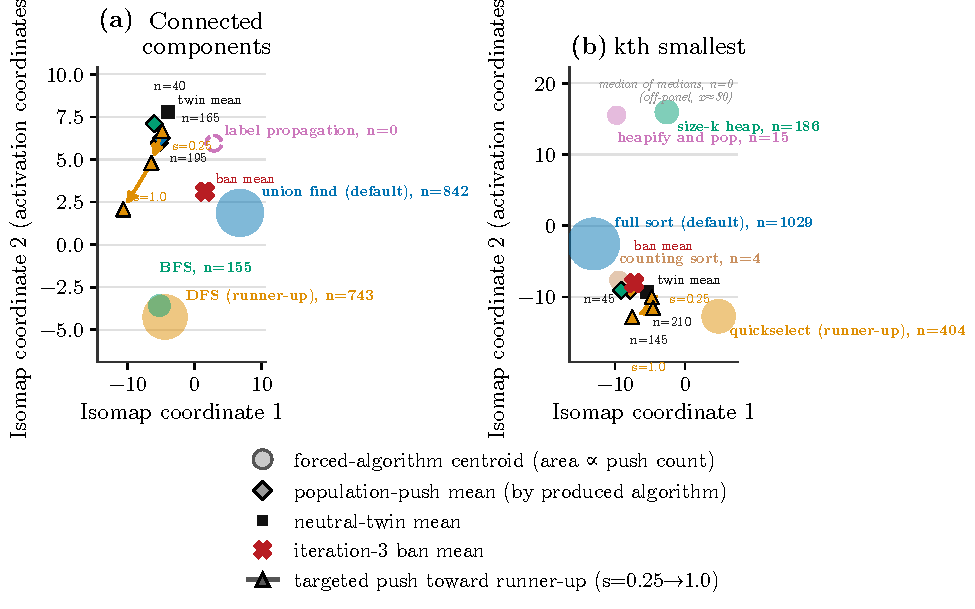
\includegraphics[width=\linewidth,height=0.78\textheight,keepaspectratio]{figures/fig_plan_geometry_v0.pdf}
\caption{Isomap projection (k = 10 neighbours, fit on a 50-dimensional PCA) of task-specification-position activation states in Qwen3-8B at block 18, for (a) the connected-components task and (b) the kth-smallest task. Large circles: centroids of forced-algorithm prompts, labelled by algorithm and by n, the number of programs in a population of random activation pushes whose output implemented that algorithm (open circle: n = 0); each panel's default and runner-up algorithm are marked. Black squares: mean projected state of neutral-twin prompts. Red crosses: mean state of the iteration-3 modal-ban prompts. Diamonds: mean state of the random-push population, grouped and coloured by the algorithm each subgroup's programs implemented (n per group labelled). Triangles joined by an arrow: mean state of a push targeted toward the runner-up centroid, at s = 0.25, 0.5 and 1.0 of that distance. In (b) one centroid (median of medians, n = 0) lies far outside this view, at approximately Isomap coordinates (30, -9), and is noted rather than drawn so the compared cluster stays legible. In both panels the twin, ban and population-push markers sit in one tight region well apart from every forced-algorithm centroid, and population-push means for different produced algorithms overlap rather than separating by outcome. The targeted push moves steadily away from this region toward the runner-up as s increases in (a); in (b) it moves closer through s = 0.5 but not further at s = 1.0. Isomap trustworthiness at block 18 is 0.965 on both tasks, with stress-1 of 0.59 (a) and 0.83 (b), so inter-point distances are only approximately preserved. Data are forced-prompt, neutral-twin, modal-ban and random-push activation states from one plan-geometry experiment on Qwen3-8B, whose own pre-registered test found this pattern reproducible on the connected-components task but not clearly distinguishable from a matched random push on kth-smallest and four other tasks.}
\label{fig:fig_plan_geometry}
\end{figure}
\textbf{No novel algorithm.} Of 10,651 correct programs from push arms, 4 carried the label other. Two blind judges and a tie-breaker, with a manual pass, classed them as a catalogue variant (a two sum hash map), a labeller miss (a Dijkstra), a plain linear scan for first and last position and a random guess-and-count loop for find duplicate; their nearest known solutions had AST Jaccard of at most 0.22. No novel algorithm appeared (rule-of-three bound 3\slash{}10,651, 0.03\%).

\begin{table}[H]
\renewcommand{\thetable}{158}
\centering\small\setlength{\tabcolsep}{4.0pt}
\caption{Committed rules and outcomes. Source: plan subspace experiment \texttt{README.\allowbreak{}md}, \texttt{predictions/\allowbreak{}c2\_\allowbreak{}commit.\allowbreak{}json}. [Source: iteration 4, artifact \nolinkurl{gen_art_experiment_22}.]}\label{tab:t170}
\begin{tabular}{>{\raggedright\arraybackslash\hspace{0pt}}p{0.5299\linewidth}>{\raggedright\arraybackslash\hspace{0pt}}p{0.4329\linewidth}}
\toprule
\textbf{Committed rule} & \textbf{Outcome} \\
\midrule
Subspace pass: Spearman of at least 0.4 with p below 0.01 on at least 4 of 6 tasks, and the masked variant on at least 3 of 6 & no: 0 of 6 and 0 of 6 \\
Subspace disconfirmed: Spearman below 0.2 on most tasks & yes: 6 of 6 (pooled 0.03 [-0.03, 0.09]) \\
Subspace not needed if the median ratio with the subspace part removed is at least 0.7 with a lower bound of at least 0.4 & yes on kth smallest, the shortest path task, two sum, connected components and pooled; grid mixed; find duplicate not evaluable \\
Subspace sufficient when amplified if the in-subspace part alone passes the escape rule at N = 20 & kth smallest (4 of 4); 9 of 20 directions overall \\
Targeted pass: Hill-1 of at least 1.8 within 5 points at the midpoint on at least 4 of 6, at no more than half the median escaping norm & no: 1 of 6 (connected components, 0.15 ban units) \\
Targeted disconfirmed: targeted minus random interval includes 0 on at least 4 of 6 & yes: 5 of 6 \\
Knob projections: pooled Spearman of at least 0.5 and projection beats the norm & no: 0.27; difference interval [-0.02, 0.31] \\
The frozen movable set is movable at alpha 2 or less & 5 of 6: find duplicate is not movable (0 of 80 cells) \\
Departure rule: where the top-1 of the ban differs from the push top-1, the direct route share is at least 0.25 & connected components: pooled direct share 0.74 (pooled, not per task) \\
No correct novel algorithm, claimed only at 0 verdicts & 0 among 10,651 correct push programs \\
\bottomrule
\end{tabular}
\end{table}

\textbf{Checks.} Every GPU unit test passed: 20-row decoding is independent of row position, batch-1 prefill is bit-identical on repeat, a zero-magnitude edit reproduces the twin token for token, the realised displacement matched its target within 0.07\% over 3,480 prefills, and clamping left at most 6.7e-4 of the displacement in the subspace. The engine reproduced the screen exactly on 180 of 180 slots. Every bench labeller recovered all its references. An independent recomputation matched every headline, and each placebo (projection shares shuffled across directions, among others) behaved as a null should.

\FloatBarrier
\subsection*{4.7 Movability and compliance in a held-out model family (gemma-3-4b-it)}
\addcontentsline{toc}{subsection}{4.7 Movability and compliance in a held-out model family (gemma-3-4b-it)}
\noindent{\small\emph{Artifact: \nolinkurl{gen_art_experiment_23}.}}\par\medskip
\textbf{Why.} The movability claim was frozen on Qwen3-8B data that had also produced it: in the screen every movable task obeyed its ban and no immovable task did. Only a family never run in this study could test it. This experiment  froze the screen rule, measured movability in gemma-3-4b-it [76] without any ban text, committed every per-task prediction by hash chain before any ban prompt was built (a grep audit of the 460 prompts fed in the ban-free stage found no ban frame), and then sampled 1,500 modal ban programs.

\textbf{Design.} For each of 15 tasks (the 12 bench tasks, the grid and shortest path tasks, and cycle detection), the model wrote 50 neutral twin programs, and 8 fixed isotropic directions at alpha 1 and 2 were added to the task-specification states of blocks 11 to 22, the middle third of its 34 blocks, during prefill. A direction escaped by the rule of Section 4.1, confirmed at N = 30 by an exact binomial test, and a task predicted to obey its modal ban when its escape fraction was above zero. The ban unit had to change before the commitment. In Gemma the five largest channels carry 99\% of the squared residual norm at the specification positions, against 40\% in Qwen3-8B, so the committed unit erased the task in a 24-row calibration probe; an outlier-excluded unit was adopted before the first commitment, and after the bans the measured ban displacement turned out to be 1.29 times it (0.92 to 2.1 by block). The rival predictors, the plan noise and temperature arms, the novelty instruction and four landing forecasts ran in the same engine under the same common random numbers.

\textbf{The movability claim is inconclusive in the held-out family.} Movability relates to compliance in the predicted direction but does not separate the tasks well enough (Table 159). The confusion matrix is 3, 3, 1, 8 (predicted obey or fail against observed): balanced accuracy 0.74 [0.40, 0.95], Fisher p = 0.24 (0.71 under the committed three-claim bound), Spearman 0.54 (one-sided permutation p = 0.025) and Kendall 0.47. The rule needed balanced accuracy of at least 0.8, Fisher p below 0.05 and Spearman of at least 0.5. Four tasks broke the prediction: kth smallest obeyed although no direction moved it, and substring search, connected components and longest increasing subsequence were movable but did not obey. A task-permutation placebo has mean balanced accuracy 0.50 (probability 0.13 of reaching the observed value), and leaving one task out gives 0.70 to 0.86.

\begin{table}[H]
\renewcommand{\thetable}{159}
\centering\footnotesize\setlength{\tabcolsep}{4.0pt}
\caption{Held-out family: escape fraction over 8 directions, prediction, catalogue-only modal ban avoidance (N = 100), outcome, and the top labels under the ban. Source: held-out family experiment \texttt{results/\allowbreak{}c3a.\allowbreak{}json}, \texttt{README.\allowbreak{}md}. [Source: iteration 4, artifact \nolinkurl{gen_art_experiment_23}.]}\label{tab:t171}
\begin{tabular}{>{\raggedright\arraybackslash\hspace{0pt}}p{0.3465\linewidth}>{\raggedright\arraybackslash\hspace{0pt}}p{0.0939\linewidth}>{\raggedright\arraybackslash\hspace{0pt}}p{0.1079\linewidth}>{\raggedright\arraybackslash\hspace{0pt}}p{0.1034\linewidth}>{\raggedright\arraybackslash\hspace{0pt}}p{0.0984\linewidth}>{\raggedright\arraybackslash\hspace{0pt}}p{0.1465\linewidth}}
\toprule
\textbf{Task (Gemma default)} & \textbf{Escape fraction} & \textbf{Predicted} & \textbf{Ban avoidance} & \textbf{Observed} & \textbf{Labels under the ban (top)} \\
\midrule
grid (DFS; corrected in iteration 5: NO DEFAULT, twin BFS 25 and DFS 25; DFS was frozen from a 10-sample pilot with correct BFS 4 and DFS 5, attempts 5 and 5) & 0.125 & obeys & 0.83 & obeys, but against no default & BFS 83, DFS 17 \\
shortest path (Dijkstra) & 0.25 & obeys & 0.96 & obeys (labeller caveat) & Bellman-Ford\slash{}SPFA 96, mostly array-based Dijkstra \\
kth smallest (full sort) & 0 & fails & 0.63 & obeys (miss) & size-k heap 61, full sort 37 \\
two sum (hash map) & 0.25 & obeys & 0.59 & obeys & brute force 59, hash map 41 \\
substring search (naive) & 0.25 & obeys & 0.19 & fails (miss) & naive 76, built-in find 13, Rabin-Karp 6 \\
connected components (DFS) & 0.125 & obeys & 0.00 & fails (miss) & DFS 100 \\
longest increasing subsequence (patience sorting with bisect) & 0.125 & obeys & 0.00 & fails (miss) & patience sorting 100 \\
find duplicate (hash set) & 0 & fails & 0.34 & fails & other 38, hash set 28, sort 21 \\
Fibonacci, nonoverlapping intervals, topological order, merge intervals, top-k frequent, cycle detection & 0 each & fails & 0.00 each & fails & default 87 to 100 \\
first and last position (binary search, flagged) & 0 & fails & 0.00 & fails & binary search 99 \\
\bottomrule
\end{tabular}
\end{table}

Every sensitivity stays inconclusive (Table 160) \emph{(correction, iteration 5: except the preregistered sensitivity that measures compliance as the drop in the default share, which disconfirms the claim: balanced accuracy 0.57, Fisher p 1.0, Spearman 0.39; see below and Table 169)}. The shortest path task carries one correct prediction on a labelling failure found after the bans. The frozen labeller, gated on heap-based Dijkstra in Qwen3-8B, reads the array-based Dijkstra of Gemma (a linear minimum scan over unvisited nodes with a visited array) as Bellman-Ford\slash{}SPFA or unknown, and the inline judge followed it. A second blind judge re-judged all 374 programs labelled Bellman-Ford\slash{}SPFA and called 284 of them Dijkstra, including all 219 that match a deterministic structural rule. Under mechanism labels the ban on Dijkstra mostly makes Gemma drop the heap and keep Dijkstra: avoidance falls from 0.96 to 0.11, and the escape fraction from 0.25 to 0.125. The frozen labels stay primary as committed, and the verdict is inconclusive either way. A labeller gated on one family needs a style re-gate on the next.

\begin{table}[H]
\renewcommand{\thetable}{160}
\centering\footnotesize\setlength{\tabcolsep}{4.0pt}
\caption{Sensitivities of the movability test in the held-out family. Source: held-out family experiment \texttt{results/\allowbreak{}c3a.\allowbreak{}json}, \texttt{results/\allowbreak{}posthoc\_\allowbreak{}t2\_\allowbreak{}relabel.\allowbreak{}json}. [Source: iteration 4, artifact \nolinkurl{gen_art_experiment_23}.]}\label{tab:t172}
\begin{tabular}{>{\raggedright\arraybackslash\hspace{0pt}}p{0.5207\linewidth}>{\raggedright\arraybackslash\hspace{0pt}}p{0.0699\linewidth}>{\raggedright\arraybackslash\hspace{0pt}}p{0.1394\linewidth}>{\raggedright\arraybackslash\hspace{0pt}}p{0.0794\linewidth}>{\raggedright\arraybackslash\hspace{0pt}}p{0.1038\linewidth}}
\toprule
\textbf{Variant} & \textbf{Tasks} & \textbf{Balanced accuracy} & \textbf{Fisher p} & \textbf{Spearman} \\
\midrule
primary & 15 & 0.74 & 0.24 & 0.54 \\
without cycle detection, or without the flagged first and last position & 14 & 0.73 & 0.24 & 0.52 \\
without the grid and shortest path tasks & 13 & 0.61 & 1.00 & 0.31 \\
correct-only avoidance & 15 & 0.74 & 0.24 & 0.51 \\
ban N = 180 with extra slots & 15 & 0.74 & 0.24 & 0.54 \\
without the tasks flagged by the label audit (shortest path, top-k frequent) & 13 & 0.68 & 0.51 & 0.39 \\
compliance as the drop in the share of the default & 15 & 0.57 (disconfirmed) & 1.00 & 0.39 \\
post hoc: shortest path relabelled by a second blind judge & 15 & 0.67 & 0.53 & 0.44 \\
post hoc: shortest path relabelled by the structural rule & 15 & 0.74 & 0.24 & 0.46 \\
without tasks that have no default (added in iteration 5; the grid task) & 14 & 0.70 & 0.51 & 0.48 \\
\bottomrule
\end{tabular}
\end{table}

\emph{(Correction, iteration 5: the row on the drop in the default share is the preregistered sensitivity, and under it the claim is DISCONFIRMED, not inconclusive. The two compliance measures are separated by two tasks: the grid task, whose twin is tied (BFS 25, DFS 25), so that 'obeys' (catalogue-only avoidance 0.83) is measured against a non-default baseline of 0.50 and the default share drops by only 0.33; and find duplicate, where 38 failing programs labelled other count as leaving the default under the drop measure (catalogue-only avoidance 0.34, drop 0.72). Two of the three true positives behind the Spearman of 0.54 are compromised, the grid task by its tied baseline and the shortest path task by the mislabelled array-based Dijkstra; without both, balanced accuracy is 0.61 and Spearman 0.31 (one-sided permutation p 0.144). Table 169 gives every variant.)}

\textbf{Asking in words predicts compliance better than pushing.} The off-default share under the novelty instruction tracks ban avoidance at Spearman 0.77, against 0.54 for the escape fraction (Table 161); the paired task-bootstrap difference is -0.24 [-0.82, 0.23], and the partial correlation of the escape fraction given the novelty share is 0.52. This matches the prior in the field that prompting is the baseline for an activation-level method to beat [34].

\begin{table}[H]
\renewcommand{\thetable}{161}
\centering\small\setlength{\tabcolsep}{4.0pt}
\caption{Predictors of catalogue-only ban avoidance in the held-out family (Spearman rho, oriented so that positive means the predicted direction). Source: held-out family experiment \texttt{results/\allowbreak{}rivals.\allowbreak{}json}. [Source: iteration 4, artifact \nolinkurl{gen_art_experiment_23}.]}\label{tab:t173}
\begin{tabular}{>{\raggedright\arraybackslash\hspace{0pt}}p{0.7282\linewidth}>{\raggedright\arraybackslash\hspace{0pt}}p{0.2346\linewidth}}
\toprule
\textbf{Predictor} & \textbf{Spearman rho} \\
\midrule
novelty instruction off-default share & 0.77 \\
escape fraction (the frozen screen) & 0.54 \\
plan noise alpha 2 off-default share & 0.51 \\
plan noise alpha 1 off-default share & 0.47 \\
best forced-prompt success rate & 0.35 \\
temperature 1.3 off-default share & 0.34 \\
twin modal share & 0.24 \\
opening margin & -0.19 \\
\bottomrule
\end{tabular}
\end{table}

\textbf{Landings.} On the 4 gated events, the push-landing forecast scored a mean log score of -0.11 with 4 of 4 top-1 hits, against -1.20 for proximity, -1.77 for association and -3.66 for the opening ladder (Table 162). The contest needed at least 3 events on which the push forecast and association disagree, and only 2 existed (kth smallest: size-k heap against quickselect; two sum: brute force against two pointers), so the landing test is inconclusive by rule, with the push forecast ahead by 2.81 nats on those two.

\begin{table}[H]
\renewcommand{\thetable}{162}
\centering\small\setlength{\tabcolsep}{4.0pt}
\caption{Landing forecasts on the 4 gated held-out events (grid, shortest path, kth smallest, two sum; the shortest path event carries the labeller caveat). Source: held-out family experiment \texttt{results/\allowbreak{}c3b.\allowbreak{}json}. [Source: iteration 4, artifact \nolinkurl{gen_art_experiment_23}.]}\label{tab:t174}
\begin{tabular}{>{\raggedright\arraybackslash\hspace{0pt}}p{0.1199\linewidth}>{\raggedright\arraybackslash\hspace{0pt}}p{0.1010\linewidth}>{\raggedright\arraybackslash\hspace{0pt}}p{0.7254\linewidth}}
\toprule
\textbf{Forecast} & \textbf{Mean log score} & \textbf{Top-1 hits} \\
\midrule
push landing & -0.11 & 4 of 4 (corrected in iteration 5: of the 4, 2 disagree with association, kth smallest and two sum; the other 2 are compromised, the grid task having no default and the shortest path landing being mostly array-based Dijkstra) \\
proximity & -1.20 & 3 of 4 \\
association & -1.77 & 2 of 4 \\
opening ladder & -3.66 & 0 of 4 \\
\bottomrule
\end{tabular}
\end{table}

\textbf{The price claim, replicated descriptively.} In Gemma too, plan noise raises correct-only diversity within 5 pass points on tasks where temperature does not (Table 163); the novelty instruction diversifies some tasks more, at a large pass cost on others (find duplicate pass 0.08, substring search 0.60). The Hill-1 of the twin is 1.0 on these tasks and 1.31 on substring search.

\begin{table}[H]
\renewcommand{\thetable}{163}
\centering\small\setlength{\tabcolsep}{4.0pt}
\caption{5-point Hill-1 in the held-out family (randomisation hull, 5 pass points). Source: held-out family experiment \texttt{results/\allowbreak{}c1\_\allowbreak{}prices.\allowbreak{}json}. [Source: iteration 4, artifact \nolinkurl{gen_art_experiment_23}.]}\label{tab:t175}
\begin{tabular}{>{\raggedright\arraybackslash\hspace{0pt}}p{0.5626\linewidth}>{\raggedright\arraybackslash\hspace{0pt}}p{0.0827\linewidth}>{\raggedright\arraybackslash\hspace{0pt}}p{0.1478\linewidth}>{\raggedright\arraybackslash\hspace{0pt}}p{0.1367\linewidth}}
\toprule
\textbf{Task} & \textbf{Plan noise} & \textbf{Temperature 1.3\slash{}1.6} & \textbf{Novelty instruction} \\
\midrule
shortest path (labeller caveat added in iteration 5: the frozen labeller reads array-based Dijkstra as Bellman-Ford\slash{}SPFA; plan noise 1.62 rests on 5 and 12 programs labelled Bellman-Ford\slash{}SPFA at alpha 1 and 2, and the novelty instruction 1.96 on 29) & 1.62 [1.37, 1.87] & 1.00 & 1.96 \\
substring search & 1.64 & 1.32 & 1.42 \\
connected components & 1.58 & 1.00 & 1.10 \\
kth smallest & 1.38 & 1.10 & 1.61 \\
longest increasing subsequence & 1.25 & 1.00 & 1.00 \\
\bottomrule
\end{tabular}
\end{table}

\textbf{Other observations and checks.} The fourth template is again the weakest: its avoidance is 0.15 on the grid task against 1.0 for the other templates, and 0.05 on kth smallest. On first and last position the twin writes a linear scan 86\% of the time, yet the ban \texttt{Do not use a hand-\allowbreak{}written binary search} makes it write binary search 99\% of the time, an ironic rebound of the kind iteration 3 saw on kth smallest. On the shortest path task, 48 of 50 twin slots flip from the default to a survivor under the ban. The 34 correct programs labelled other were 27 degenerate programs from push arms and 7 catalogue variants, with no novel algorithm (rule-of-three bound 0.088). All 13 bench labellers reproduced their gates, the six escape counts of the screen were reproduced, the GPU tests passed, and an independent rederivation from raw samples matched every escape fraction, avoidance, balanced accuracy, Fisher p, Spearman correlation, rival correlation, landing log score and post hoc number with no mismatch; its placebos rejected at 1.7\% (Fisher) and 4.9\% (Spearman).

\begin{figure}[!htbp]
\centering\captionsetup{font=footnotesize}
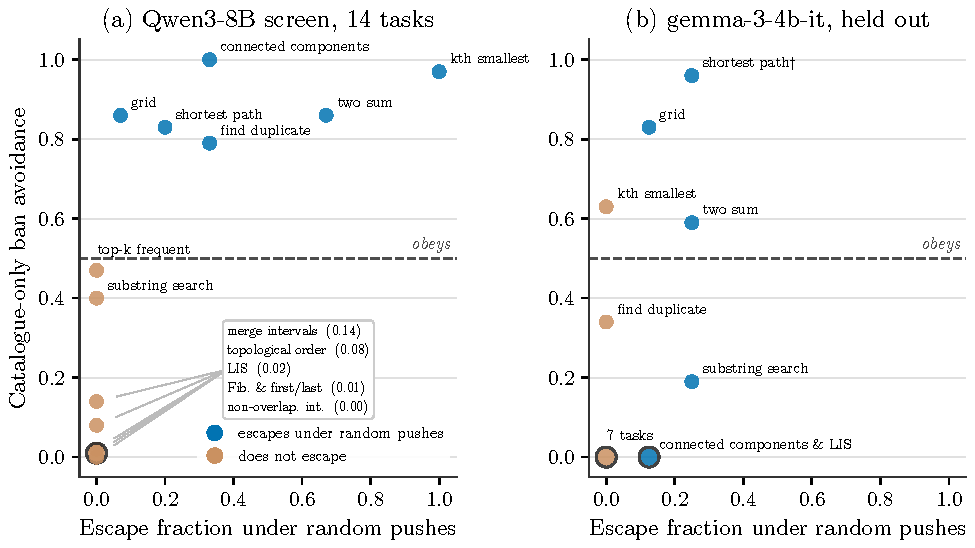
\includegraphics[width=\linewidth,height=0.78\textheight,keepaspectratio]{figures/fig_movability_v0.pdf}
\caption{Escape fraction under random pushes to the task-specification states (x) against catalogue-only modal-ban avoidance (y), one point per coding task. Colour marks whether a task's escape fraction is above zero (``escapes under random pushes'', blue) or exactly zero (``does not escape'', tan); a black-outlined, enlarged marker means two or more tasks land at identical (x,y) and are named together beside it. Dashed line: the y=0.5 ``obeys'' threshold on catalogue-only ban avoidance. (a) Qwen3-8B, the frozen iteration-3 push-movability screen (screen values, not a held-out confirmation; 14 tasks, Spearman rho=0.85): every ``escapes'' task sits above the line and every ``does not escape'' task sits at or below it. The five lowest-avoidance tasks are named in the inset key with their avoidance values because their points sit too close together to label individually; Fibonacci and first-and-last-position share one marker, both reading exactly 0.01 in the screen data. (b) gemma-3-4b-it, a held-out family whose escape-fraction predictions (8 random push directions per task) were committed before any ban prompt (15 tasks; balanced accuracy 0.74 [95\% CI 0.40, 0.95] for predicting obeys\slash{}does-not-obey from escapes\slash{}does-not-escape, Fisher's exact p=0.24, Spearman rho=0.54): most ``escapes'' tasks sit above the line, but kth smallest (``does not escape'') sits above it too, and ``connected components \& LIS'' and ``7 tasks'' (Fibonacci, nonoverlapping intervals, topological order, merge intervals, first-and-last-position, top-k frequent, cycle detection; all at (0,0)) sit at or below it, so the separation only partly holds. The dagger on shortest path flags that its plotted avoidance (0.96) comes from the frozen labeller; a labeller that reads array-based Dijkstra as Bellman-Ford\slash{}SPFA instead gives 0.11.}
\label{fig:fig_movability}
\end{figure}
\FloatBarrier
\subsection*{4.8 Positioning: the iteration-3 and iteration-4 claims against published work}
\addcontentsline{toc}{subsection}{4.8 Positioning: the iteration-3 and iteration-4 claims against published work}
\noindent{\small\emph{Artifact: \nolinkurl{gen_art_research_1}.}}\par\medskip
The positioning audit , dated 2026-10-21, checked 112 verbatim quotes from 74 references (101 against full text, 11 against venue abstracts; none mismatched, and an independent pass re-matched all 112). A saturation search over eight query families found 1,729 unique records, scored 63 on an occupancy rubric and found 44 adjacent, 19 irrelevant and none occupying. Two flags it was asked to raise did not fire: no paper measures test-checked, algorithm-level diversity under activation perturbation, and no paper predicts prompt-ban compliance from perturbation sensitivity. Table 92b sets the iteration-3 claims against their nearest neighbours and Table 92c the iteration-4 claims; each finding is paraphrased here and was verified against a quote. Several contemporaneous submissions under review, a workshop poster without an arXiv record and one workshop paper that the bibliography script could not retrieve are adjacent in the audit but are not cited by number.

{\footnotesize\setlength{\tabcolsep}{4.0pt}\renewcommand{\thetable}{92b}
\begin{longtable}{>{\raggedright\arraybackslash\hspace{0pt}}p{0.1987\linewidth}>{\raggedright\arraybackslash\hspace{0pt}}p{0.1363\linewidth}>{\raggedright\arraybackslash\hspace{0pt}}p{0.2378\linewidth}>{\raggedright\arraybackslash\hspace{0pt}}p{0.2412\linewidth}>{\raggedright\arraybackslash\hspace{0pt}}p{0.0992\linewidth}}
\caption{Iteration-3 claims, their nearest published neighbours and what this run adds. Source: positioning audit \texttt{research\_\allowbreak{}report.\allowbreak{}md}. [Source: iteration 4, artifact \nolinkurl{gen_art_research_1}.]}\label{tab:t176}\\
\toprule
\textbf{Claim in this run} & \textbf{Nearest neighbour} & \textbf{Finding of the neighbour (paraphrased; verified against a quote)} & \textbf{What this run adds, or replication} & \textbf{Lane} \\
\midrule
\endfirsthead
\multicolumn{5}{l}{\emph{Table 92b, continued}}\\
\toprule
\textbf{Claim in this run} & \textbf{Nearest neighbour} & \textbf{Finding of the neighbour (paraphrased; verified against a quote)} & \textbf{What this run adds, or replication} & \textbf{Lane} \\
\midrule
\endhead
\bottomrule
\endlastfoot
Snap-back under exposure bans (default 0.05 under the copy twin, 0.72 named, 0.82 unnamed; Llama present minor bans 0.72 to 0.93) & Lu et al. [23] & Under successive denial prompts, models copy previous solutions and constraint following decays & The replacement is the unconditional default of the model itself, measured against a copy twin, in two families & adjacent \\
(same) & Yoon et al. [4] & Under factual negation, heads and neurons suppress the original answer and promote a favoured in-category candidate & Algorithm level, execution-checked labels; the promoted alternative is the unconditional default & closest analogue \\
(same) & Rana [7] & Mentioning a forbidden word primes it in most violations & The unnamed ban snaps back more (0.82) than the named (0.72), so naming is not needed & adjacent \\
Wording dominates compliance (template SD 2.0 logits; likelihood ratio 374; the fourth template fails on 10 of 12 tasks) & Sclar et al. [69] & Formatting changes alone move accuracy by up to 76 points & Replication in prohibition compliance, as a template random effect with a placebo & partly occupied \\
(same) & Heo et al. [58] & An input-embedding dimension predicts instruction following and tracks phrasing & Algorithm prohibitions on code; a variance-components estimate & adjacent \\
The ban is enforced at the opening of the body (forcing the opening of the default undoes it; a neutral \texttt{def} line does not) & Qi et al. [63] & Safety alignment acts mostly on the first few output tokens & Replication of shallow enforcement for a user-imposed prohibition, located at the first content token after a neutral signature & adjacent \\
(same) & Zhu et al. [32]; Andriushchenko et al. [79] & Hard code tokens sit at block openings; prefilling defeats refusals & Prefilling used as a measurement rather than an attack & supporting \\
Signature vetoes are respelled around (exact veto, the walk stalled on 6 of 6 tasks) & Biagiola et al. [62]; Park et al. [85] & Incomplete constraints push generation into low-probability regions and cost correctness; constrained decoding distorts the distribution & The algorithm survives a lexical veto by respelling, with a sham-veto control & adjacent \\
No correct novel algorithm (0 of 116 correct out-of-catalogue programs) & Zhang et al. [44]; Jangra and Muresan [3]; Lu et al. [23] & Models produce less diversity than humans; prompting steers toward human strategies without their diversity & A verified-novelty audit against a known-solution catalogue, which these benchmarks do not run & adjacent \\
Random pushes buy correct diversity on movable tasks & Khalid et al. [70]; Zhu et al. [71]; Kim et al. [84] & Residual-stream noise raises narrative diversity; activation steering raises test coverage; random embedding injection widens pass@N on math & Diversity of algorithms, test-checked and mechanism-labelled, task-dependent and calibrated to the norm of the ban; the method itself is occupied & partly occupied \\
Movability predicts compliance (screen) & Fan et al. [75] & Hidden-state features predict whether a steering intervention succeeds & A black-box prompt prohibition forecast from white-box movability & adjacent \\
\end{longtable}}

{\footnotesize\setlength{\tabcolsep}{4.0pt}\renewcommand{\thetable}{92c}
\begin{longtable}{>{\raggedright\arraybackslash\hspace{0pt}}p{0.1306\linewidth}>{\raggedright\arraybackslash\hspace{0pt}}p{0.1229\linewidth}>{\raggedright\arraybackslash\hspace{0pt}}p{0.2829\linewidth}>{\raggedright\arraybackslash\hspace{0pt}}p{0.2527\linewidth}>{\raggedright\arraybackslash\hspace{0pt}}p{0.1240\linewidth}}
\caption{Iteration-4 claims, their nearest published neighbours and what this run adds. Source: positioning audit \texttt{research\_\allowbreak{}report.\allowbreak{}md}. [Source: iteration 4, artifact \nolinkurl{gen_art_research_1}.]}\label{tab:t177}\\
\toprule
\textbf{Claim in this run} & \textbf{Nearest neighbour} & \textbf{Finding of the neighbour (paraphrased; verified against a quote)} & \textbf{What this run adds, or what it lacks} & \textbf{Lane} \\
\midrule
\endfirsthead
\multicolumn{5}{l}{\emph{Table 92c, continued}}\\
\toprule
\textbf{Claim in this run} & \textbf{Nearest neighbour} & \textbf{Finding of the neighbour (paraphrased; verified against a quote)} & \textbf{What this run adds, or what it lacks} & \textbf{Lane} \\
\midrule
\endhead
\bottomrule
\endlastfoot
Plan noise is priced against temperature and prompt knobs & Ahmed et al. [73]; Wang et al. [74] & Sampling an intent at high temperature and the response at low temperature, or searching over natural-language plans, raises conceptual diversity in code & Activation-level plan noise on test-checked labels with seed-coupled contrasts; the comparison set lacks these text-level plan samplers & partly occupied \\
(same) & Lee et al. [72] & Temperature above 1 raises algorithmic diversity on other problems, at a correctness cost & Qualifies the temperature null: price temperature per task & contradicting in part \\
(same) & Peeperkorn et al. [37]; Zeng et al. [86]; Wu et al. [2] & Temperature correlates weakly with novelty; token-level perturbation gives lexical, not strategic, variation; sampling and prompting changes do not cure monoculture & Consistent with the null on ideas & supporting \\
Site specificity at matched dose & Zhang et al. [83]; Khalid et al. [70]; Zhu et al. [71]; Nagarajan et al. [80] & Diversity injected at different text levels, generated-token noise sites, intra-layer steering sites, and input-layer noise against output temperature & Sites inside the network at matched dose on algorithm labels & partly occupied \\
The same seed design & Ravfogel et al. [77] & Coupling sampling noise across interventions yields counterfactual strings & Token seeds coupled across temperatures and plan noise draws to split idea changes from phrasing changes & adjacent \\
A plan subspace read from forced prompts predicts push effects (disconfirmed here) & Dong et al. [78] & Prompt representations encode global attributes of the coming response & A categorical, test-checked object and a ban-free subspace tested as a predictor of random-push effects; the prediction failed & partly occupied \\
Geometry and targeted pushes & Wurgaft et al. [27] & Geometry-aware steering with geodesic distances and an MDS isometry & Algorithm-level geometry on test-checked labels; exact crossing on one task & partly occupied \\
Movability forecasts ban compliance in a held-out family & Tang [38]; Fan et al. [75] & Constraints opposing defaults fail at 10\% to 100\%; steerability is predictable from hidden states & A pre-registered white-box forecast of black-box prompt compliance (inconclusive here) & open \\
Push landings forecast ban landings & Yoon et al. [4]; Zhou et al. [56] & Negation suppresses and promotes, or constructs and suppresses, at the fact level & A ban-free forecast of which alternative a prohibition installs & open \\
No correct novel algorithm up to breakage & Romera-Paredes et al. [81]; Novikov et al. [82] & Search with an evaluator produces new programs & Scope the claim to single-sample generation under knobs, without search or an evaluator & adjacent, scoped \\
Plan noise (row added in iteration 5) & Jerge, Pelczar and Downes, arXiv 2608.21595 & Gaussian noise calibrated to the scale of the last hidden layer, added in the pass that encodes the prompt, diversifies reinforcement learning rollouts of vision-language models & Test-checked mechanism labels on code, a site comparison at matched dose, and seed coupling; theirs is rollouts scored by reward & partly occupied \\
Plan noise against temperature (row added in iteration 5) & Nagarajan et al. [80] & Noise injected at the input layer works as well as, and sometimes better than, temperature sampling at the output layer & The nearest prior answer; this run adds noise in the task-specification states against temperature with the token seed held fixed, on execution-checked algorithm labels & adjacent \\
Novelty boundary (row added in iteration 5) & Bhushan, Zhang and Wang, arXiv 2608.30047 & Agents with iterative search explore novel regions of the solution space but do not convert novelty into better task performance & Scope: single-sample generation without search; the bound on novelty (0 among 14,206 correct programs) & contradicting in part \\
Novelty boundary (row added in iteration 5) & Maveli, Vergari and Cohen, arXiv 2610.02438 & Code generation is better measured as parametric retrieval of a named algorithm than as synthesis of a novel one & Execution-checked labels and the bound under activation pushes & supporting \\
Novelty boundary and knob (row added in iteration 5) & ICLR 2027 submission oag3wgNLRh (OpenReview) & Activation steering redirects generation among trajectories the model already supports, and decoding matched to the departure of steering from greedy decoding reaches comparable accuracy & Algorithm-level labels; decoding at matched departure was not run in iteration 4 and ran in iteration 5 (Section 5.7) & partly occupied \\
Plan subspace (row added in iteration 5) & ICLR 2027 submission knirOusGcq (OpenReview) & A shared causal subspace for planning the length of a response, tested by decomposing interventions into parallel and orthogonal components & A categorical, test-checked object; the forced-prompt subspace does not predict random-push effects (0.03) and removing it keeps the effect (ratio 1.00) & partly occupied \\
\end{longtable}}

\FloatBarrier
\subsection*{4.9 Comparisons across the experiments of this iteration}
\addcontentsline{toc}{subsection}{4.9 Comparisons across the experiments of this iteration}
\textbf{Movability on fresh directions.} Three engines and three direction sets measured whether a task is movable: the frozen screen (fixed directions from iteration 3), the plan subspace experiment (40 fresh fixed directions per dose) and the plan noise experiment (a fresh direction per sample). They agree on five of the six screen-movable tasks and on every immovable one, and they disagree on find duplicate (Table 164). The single escaping direction of the screen on find duplicate at alpha 2 did not replicate in 80 fresh cells, and per-sample plan noise left the hash set in place at alpha 2 or less. On fresh draws the movable set is kth smallest, two sum, connected components and the two path tasks, and the table of the screen against ban compliance (movable and obeying, movable and failing, immovable and obeying, immovable and failing) moves from 6, 0, 0, 8 to 5, 0, 1, 8: find duplicate obeys its ban (catalogue-only avoidance 0.79) without being movable. Across the 14 tasks the escape fraction still ranks ban avoidance at Spearman 0.86.

\begin{table}[H]
\renewcommand{\thetable}{164}
\centering\footnotesize\setlength{\tabcolsep}{4.0pt}
\caption{Movability of the screen tasks in three measurements: screen escapes (escaping of run, alpha 1 \slash{} alpha 2), the escape fraction of the plan subspace experiment on 40 fresh directions (alpha 1 \slash{} alpha 2), and per-sample plan noise (off-default share at alpha 1 \slash{} alpha 2, N = 50), with catalogue-only modal ban avoidance. Sources: record audit \texttt{screen.\allowbreak{}json}; plan subspace experiment \texttt{results/\allowbreak{}escape.\allowbreak{}json}; plan noise experiment \texttt{results/\allowbreak{}alpha\_\allowbreak{}sweep.\allowbreak{}json}. [Source: iteration 4, compiled across the iteration's artifacts \nolinkurl{gen_art_evaluation_3}, \nolinkurl{gen_art_experiment_19}, \nolinkurl{gen_art_experiment_20}, \nolinkurl{gen_art_experiment_21}, \nolinkurl{gen_art_experiment_22}, \nolinkurl{gen_art_experiment_23}, \nolinkurl{gen_art_research_1}.]}\label{tab:t178}
\begin{tabular}{>{\raggedright\arraybackslash\hspace{0pt}}p{0.2146\linewidth}>{\raggedright\arraybackslash\hspace{0pt}}p{0.1430\linewidth}>{\raggedright\arraybackslash\hspace{0pt}}p{0.1441\linewidth}>{\raggedright\arraybackslash\hspace{0pt}}p{0.2213\linewidth}>{\raggedright\arraybackslash\hspace{0pt}}p{0.1901\linewidth}}
\toprule
\textbf{Task} & \textbf{Screen escapes} & \textbf{Fresh directions} & \textbf{Per-sample plan noise} & \textbf{Ban avoidance (catalogue only)} \\
\midrule
kth smallest & 8\slash{}18 \slash{} 3\slash{}3 & 0.30 \slash{} 0.63 & 0.28 \slash{} 0.50 & 0.97 \\
two sum & 0\slash{}6 \slash{} 2\slash{}3 & 0.00 \slash{} 0.13 & 0.00 \slash{} 0.02 & 0.86 \\
find duplicate & 0\slash{}6 \slash{} 1\slash{}3 & 0.00 \slash{} 0.00 & 0.00 \slash{} 0.02 & 0.79 \\
connected components & 1\slash{}3 \slash{} not run & 0.38 \slash{} 0.73 & 0.12 \slash{} 0.60 & 1.00 \\
grid & 1\slash{}15 \slash{} 0\slash{}3 & 0.05 \slash{} 0.13 & 0.06 \slash{} 0.24 & 0.86 \\
shortest path & 3\slash{}15 \slash{} 0\slash{}3 & 0.18 \slash{} 0.20 & 0.26 \slash{} 0.54 & 0.83 \\
the eight immovable bench tasks & 0 of 3 or 6 each & 0 of 8 each & off-default excess at most 0.04 & 0.00 to 0.47 \\
\bottomrule
\end{tabular}
\end{table}

The fixed-direction escape fraction and the per-sample off-default share measure different things: a task with a few strong directions (two sum, where 5 of 40 directions escape at alpha 2) can show almost no movement under per-sample noise, which averages over directions. \emph{(Correction, iteration 5: alpha does not mean the same push in every column. The screen uses the displacement of the ban itself; the bench unit of the plan subspace experiment is 9\% to 16\% smaller (its deviation 'ban\_\allowbreak{}unit\_\allowbreak{}scale'); the kth smallest unit of the same seed experiment is 0.77 of the screen's; the site experiment uses per-position ban units (blocks 0 to 11 at 4.5\% to 7.2\% of the residual norm against 12.7\% to 18.3\% for blocks 12 to 23); cycle detection and Gemma use a ban-free unit, which across tasks is 0.30 to 0.97 of the ban unit. Substring search has by far the largest ban unit (58.5 against 11.6 to 19.0 elsewhere) and does not move. Table 174 gives the units.)}

\textbf{Temperature, five times.} Every measurement of temperature in the run says the same thing, now including the thinking-on arm the review asked for. In iteration 1, 797 of 800 grid programs and 797 of 800 shortest path programs kept the default across temperatures 0.3 to 1.3 with thinking off, and all 1,600 with thinking on. In iteration 2, with seeds coupled, the algorithm changed in 0 of 30 seeds in 10 of 12 cells. In this iteration temperature 1.3 and 1.6, top-k 10 and min-p reach a 5-point Hill-1 of at most 1.17 on the six movable tasks; the same seed design changed the algorithm in 0 of 20 seeds on three tasks with thinking off and on the shortest path task with thinking on; and in gemma-3-4b-it temperature reaches 5-point Hill-1 of at most 1.32. A positioning caveat applies: on other problems temperature above 1 does raise algorithmic diversity at a correctness cost [72].

\textbf{Novelty, audited everywhere.} No artifact of this iteration found a correct novel algorithm (Table 165). Together with iterations 1 to 3, every correct program outside the catalogue in the pools audited so far has been read by two blind judges and the executor, and none was new: iterations 1 to 3, the 78 correct programs outside the catalogue among 11,763 unique correct programs (Section 3.2.3, Table 87); iteration 4, the audits of Table 165; iteration 5, its 130 correct programs outside the catalogue, with the 14 over-calls re-adjudicated in iteration 6 (Section 6.2.6); and iteration 6, the pools of Table 278, including the engine control's 3 correct programs labelled other, judged in iteration 7. Two pools were never audited by judges: about 9,000 programs of the forking token experiment, as recorded in Section 3.2.3, and the engine control's nearest-known pass of iteration 6 (up to 237 correct programs per engine and task, compared with known solutions by token overlap only; Table 278). \emph{(Correction, iteration 6: the 14 that judges over-called in iteration 5 were re-adjudicated blind in iteration 6 (judges 14 of 48, manual 0, second adjudication 1 of 14 (Mistral Medium 3.1, three calls at temperature 0, control gate 9 of 10, passed; Kimi (kimi-k2) second view 0 of 14), final count after the executor's full read 0; the contested control, repeated maximum selection for top-k frequent, which the iteration-5 manual pass itself classed as a catalogue variant, was called catalogue variant by Mistral and catalogue variant by Kimi (Mistral gate 10 of 10 under that convention); the final read corrects 1 manual class (CATALOGUE VARIANT to DEGENERATE), none to novel).)} (iteration-7 correction)

\begin{table}[H]
\renewcommand{\thetable}{165}
\centering\footnotesize\setlength{\tabcolsep}{4.0pt}
\caption{Novelty audits of iteration 4. Sources: the novelty audit files of the six artifacts. [Source: iteration 4, compiled across the iteration's artifacts \nolinkurl{gen_art_evaluation_3}, \nolinkurl{gen_art_experiment_19}, \nolinkurl{gen_art_experiment_20}, \nolinkurl{gen_art_experiment_21}, \nolinkurl{gen_art_experiment_22}, \nolinkurl{gen_art_experiment_23}, \nolinkurl{gen_art_research_1}.]}\label{tab:t179}
\begin{tabular}{>{\raggedright\arraybackslash\hspace{0pt}}p{0.1479\linewidth}>{\raggedright\arraybackslash\hspace{0pt}}p{0.2791\linewidth}>{\raggedright\arraybackslash\hspace{0pt}}p{0.1137\linewidth}>{\raggedright\arraybackslash\hspace{0pt}}p{0.3026\linewidth}>{\raggedright\arraybackslash\hspace{0pt}}p{0.0699\linewidth}}
\toprule
\textbf{Artifact} & \textbf{Pool} & \textbf{Correct programs labelled other} & \textbf{Final classes} & \textbf{Novel} \\
\midrule
Record audit & other programs under iteration-3 bans (226 unique, 6 passing) & 6 & 68 catalogue variants, 156 degenerate, 2 labeller misses (all 226) & 0 \\
Plan noise experiment & every correct program labelled other & 12 & 12 labeller misses & 0 \\
Site experiment & 3,555 correct programs & 1 & catalogue variant (quadratic brute force) & 0 \\
Same seed experiment & every correct program labelled other & 1 & labeller miss (naive Dijkstra) & 0 \\
Plan subspace experiment & 10,651 correct push programs & 4 & 1 catalogue variant, 1 labeller miss, 2 degenerate & 0 \\
Held-out family experiment & every correct program labelled other & 34 & 27 degenerate, 7 catalogue variants & 0 \\
\bottomrule
\end{tabular}
\end{table}

\FloatBarrier
\subsection*{4.10 What iteration 4 established, what it ruled out, and what it abandoned}
\addcontentsline{toc}{subsection}{4.10 What iteration 4 established, what it ruled out, and what it abandoned}
Everything below is one model per claim except the held-out test, which is one family at one size, with labels from labellers that passed their gates (and one, the path labeller on Gemma, that needed a style re-gate). Every Qwen3-8B number in this iteration comes from the 8-bit engine of the screen. (Engine class: Hugging Face with W8A8 linear layers in 8-bit floating point, e4m3 weights per output channel and e4m3 activations per row through the GPU's native 8-bit floating-point matrix multiply . Each item below carries its iteration-6 engine tag, and Section 6.3 decides which of them hold under bf16 at the same absolute dose.)

\textbf{Established.}

\begin{enumerate}
\item \emph{Temperature changes phrasing and not the algorithm, with the seed held fixed, thinking off and on.} Across four temperatures the algorithm changed in 0 of 20 seeds on three tasks with thinking off and on the shortest path task with thinking on, while phrasings per idea grew on the grid task from 3 to 13 clusters. Temperature 1.3 and 1.6, top-k 10 and min-p buy no correct algorithmic diversity on the movable tasks (5-point Hill-1 at most 1.17).
\item \emph{A random displacement of the task-specification states changes the algorithm, and changing the plan noise draw under a fixed seed changes it often.} One direction at alpha 1 changed the algorithm in 17.25 of 20 seeds on the shortest path task, 4.55 on kth smallest and 2.5 on the grid task (pooled contrast against temperature 0.545 [0.41, 0.67], p = 1.0e-5). \emph{(Engine tag, iteration 6: 8-bit floating-point W8A8; the same-seed contrast itself was not rerun in bf16 . Per-sample plan noise on the shortest path task did not replicate in iteration 5's bf16 cells at the ban-free unit (2 of 47 correct programs off the default at bf16 alpha 2 against 9 of 43 at 8-bit alpha 1, bracket p 0.017), but at iteration 4's own absolute unit and seeds the bf16 engine reproduces it (22 of 50 valid attempts off the default at alpha 2 under both engines; Section 6.3).)}
\item \emph{The site is the task-specification states at early to middle blocks.} The same displacement at the read position or the condition sentence changed no algorithm at any dose (0 of 526 and 0 of 527 correct programs off the default), the late blocks were almost inert (6 of 521), and at matched downstream displacement the plan site keeps a large advantage (indicator +2.15 [1.79, 2.51]; odds ratio 5.72 [3.94, 8.30]) \emph{(engine tag, iteration 6: 8-bit floating-point W8A8 , not rerun in that form. The bf16 rerun at the ban-free unit of Section 6.4 withdrew the committed site rule, because the condition-span arm never reached the plan site's downstream displacement and alpha 8 broke every plan-site program; a post-hoc model restricted to alpha of 4 or less puts the read position below the task-specification site on both tasks.)}. Blocks 12 to 23 are not distinguished from blocks 0 to 11. \emph{(Correction, iteration 5: two wordings here say more than the experiment supports, that the read position and the condition sentence change nothing at any dose, and that the task-specification states are the site of the choice. Restated: among prefill positions, perturbing the task-specification states changes the algorithm; the read position and the condition sentence are inert at per-position doses up to 4 ban units and far weaker at matched energy (energy-matched read position: +0.23 on find duplicate, Floyd cycle detection 6 of 26 correct programs, and +0.18 on connected components, 5 of 28 off the default); noise in generated tokens 1 to 32 also redirects the choice, more than the plan site on find duplicate (12:0 paired flips at alpha 2 over the 30 pairs, exact McNemar p 0.0005; 6:0 among pairs where both programs are correct). Blocks 0 to 11 against 12 to 23: -0.31 [-0.75, 0.13]. This is a prefill site at which noise is effective, not a locus of the decision, and it is reconciled with the PARTIAL site rule under Inconclusive below.)}
\item \emph{Plan noise is the cheapest knob on some tasks and not on others.} It wins kth smallest (5-point Hill-1 2.72) and connected components (2.09) at no pass cost \emph{(engine tag, iteration 6: 8-bit floating-point W8A8 at the ban unit; under bf16 and the ban-free unit of iteration 5 the same prices are 1.98 and 1.09, and on connected components 1 of 50 correct programs left the default at bf16 alpha 2 against 30 of 50 at 8-bit alpha 2 (Fisher p 7.2e-11). The engine control of Section 6.3 traces that gap to the unit and the direction seeds, not to the numerics: at iteration 4's absolute unit and seeds, bf16 plan noise moves connected components in 25 of 50 valid attempts.)} and loses find duplicate to the iterated veto and the shortest path task to the semantic seed; the preregistered price claim is PARTIAL.
\item \emph{Which random directions move the algorithm is a stable property of the direction, and the forced-prompt geometry does not explain it.} Template halves rank 40 directions alike (0.76 to 0.90), the projection share on the plan subspace ranks them at 0.03, and removing the in-subspace component of a push leaves its effect intact (median ratio 1.00). \emph{(Correction, iteration 5: the range 0.76 to 0.90 covers four tasks. On all six: kth smallest 0.80 (34 movers, 27 escaping cells of direction and dose), shortest path 0.81 (37, 14), two sum 0.76 (10, 5), connected components 0.90 (36, 30), find duplicate 0.59 (3, 0) and the grid task 0.39 (22, 6); Table 176.)}
\item \emph{Where pushes escape, they land on one runner-up per task, and that runner-up forecasts where a ban lands.} The landing replicates across 40 fresh directions and the screen on every movable task, and on the gated bench bans, scored descriptively because they were seen before, the push forecast scores -0.76 against -3.46 for association; in Gemma it hits 4 of 4, on too few disagreeing events for the rule. \emph{(Correction, iteration 5: this item moves from Established to the descriptive results. Where pushes escape, the landing replicates across 40 fresh directions and the screen at the plan site (kth smallest quickselect 0.66 and size-k heap 0.31; connected components DFS 0.83 and BFS 0.17; shortest path Bellman-Ford\slash{}SPFA 0.99; two sum brute force; grid DFS). As a forecast of the seen bench ban landings it hits 2 of 3 defined Qwen3-8B events (it misses connected components) and scores -0.76 against -3.11 for association on those events, and -1.37 against -3.46 over all 5 with undefined forecasts scored as uniform; in Gemma it hits 4 of 4, of which 2 disagree with association and 2 are compromised. The landing depends on the site on find duplicate.)}
\item \emph{Route landings.} On connected components either route of a ban alone lands mostly on DFS, the generic neighbour, and only both routes together choose BFS. On kth smallest the size-k heap share travels by the prompt states. \emph{(Correction, iteration 5: an observation on a single task, with find duplicate as its counterexample: there the direct route alone lands on index marking, 74 of 78, neither the push landing nor the association answer; on two sum pushes and association disagree.)}
\item \emph{Snap-back replicates in Llama.} On five of six present minor events the modal landing is the default (0.93, 0.73 and 0.72 of attempts not banned on three of them).
\item \emph{No correct novel algorithm appeared under any push, up to breakage.} Correct-only diversity peaks at alpha 2 to 4, and alpha 8 erases the task; 0 novel among 14,206 correct programs of the site and subspace experiments alone.
\end{enumerate}

\textbf{Ruled out, or not supported.}

\begin{itemize}
\item \emph{A plan subspace read from forced prompts as the channel of push effects.} Disconfirmed by its preregistered rule on 6 of 6 tasks, and the decomposition shows the subspace is not needed.
\item \emph{Targeted pushes as a general cheap knob.} Indistinguishable from a matched random push on 5 of 6 tasks; the exception, connected components, crosses exactly at the predicted midpoint.
\item \emph{Knob displacements projecting in proportion to their effect.} Pooled 0.27, not better than the displacement norm.
\item \emph{The top-five prohibition applied at the plan.} The push never left BFS (avoidance 0.00 at alpha 1 and 2), as the prompt and the token veto had not.
\item \emph{Find duplicate as a movable task.} Its screen escape did not replicate in 80 fresh cells.
\end{itemize}

\textbf{Inconclusive.}

\begin{itemize}
\item \emph{Movability as a predictor of ban compliance in a held-out family.} Balanced accuracy 0.74 [0.40, 0.95], Fisher p 0.24, Spearman 0.54; the novelty instruction predicts better (0.77), and one correct prediction rests on a labelling failure. \emph{(Correction, iteration 5: INCONCLUSIVE under the primary measure, catalogue-only avoidance, and DISCONFIRMED under the preregistered sensitivity on the drop in the default share (balanced accuracy 0.57, Fisher p 1.0, Spearman 0.39). The grid task (tied twin, BFS 25 and DFS 25; no default under the iteration-5 rule) and find duplicate (38 failing other programs; 0.34 against 0.72) separate the two measures. Without the two compromised true positives, balanced accuracy is 0.61 and Spearman 0.31, one-sided permutation p 0.144.)}
\item \emph{Push landings against association in the held-out family.} Ahead by 2.81 nats, but on 2 disagreeing events, below the 3 the rule needs.
\item \emph{The site claim.} PARTIAL: the plan site is best on 3 of 6 tasks, with every margin but one a bootstrap close call. \emph{(Added in iteration 5: the site rule is PARTIAL, so no site is established as best; what is established is the prefill specificity at matched displacement, odds ratio 5.72 [3.94, 8.30] for the task-specification states against the other prefill sites. The price of 1.5, the pass cost at which a site's randomisation hull first reaches correct-only Hill-1 of 1.5, is 0.12 for generated-token noise against 0.53 for the plan site on two sum.)}
\end{itemize}

\textbf{Dead ends, with the evidence that closed them.}

\begin{itemize}
\item \emph{The plan subspace as the internal account of the choice.} Closed by Tables 153 and 155: the share does not rank directions, and removing it does not remove the effect.
\item \emph{Verbalized sampling as a diversity knob.} 46 to 49 of 50 programs dispatch at run time to a randomly chosen algorithm, so their labels measure the trace, not the choice.
\item \emph{The frozen counting rule for forecast contests.} It advances some family in 85\% of no-information simulations; forecasts are now scored by paired tests and defined-only hit rates.
\end{itemize}

\FloatBarrier
\subsection*{4.11 What the next iteration takes from this one}
\addcontentsline{toc}{subsection}{4.11 What the next iteration takes from this one}
The iteration answered the first question of the request in its strictest form and narrowed the second. Temperature, at any setting and with the seed fixed, changes how the code is written and not which algorithm it implements, with thinking off and on. The algorithm can be influenced, cheaply on some tasks, by a random displacement of the task-specification states at early to middle blocks, and the read position, the condition sentence and the late blocks are inert. \emph{(Correction, iteration 5: the read position and the condition sentence are inert at per-position doses up to 4 ban units, weaker but not inert at matched energy, and the late blocks almost inert.)} What the iteration did not find is a representation of the choice: the forced-prompt subspace does not explain which displacements work, although which displacements work is reproducible. The open question is therefore what property of a direction makes it move the algorithm. The exploratory signed-progress correlations (up to 0.57) point at direction toward the runner-up rather than share, and the targeted push on connected components shows that one axis can be causally exact. A preregistered test of signed progress on fresh directions, with the reproducible ranking of the directions as the target, is the next step. \emph{(Correction, iteration 5: that step was not taken, and signed progress is closed. Its positive cells concentrate on one task, it is negative on average on two, and on connected components the committed signed component was matched by a within-class control (0.33 against 0.37). Per task over 24 block cells: kth smallest 1 cell with p below 0.05 and a mean of -0.02 over the edited blocks (-0.29 at block 15); shortest path 3 and +0.20; two sum 7 and +0.31; connected components 22 and +0.37; find duplicate 0 and -0.12; grid 2 and +0.05 (Table 177; the record's count of 22 of 35 cells was 22 of 24). The next budget goes to more tasks, not to a further predictor at the level of directions on the same five: new tasks with the base model's repertoire committed before any push, so that which tasks move can be predicted from the base model and tested on units never seen.)}

The movability claim needs more than one held-out family at one size, a labeller re-gated on the style of each family, and a comparison with the novelty instruction, which predicted compliance better in Gemma. The landing claim needs events on which the push forecast and association disagree: Gemma gave 2 of 4, and the Qwen3-8B bench gave 3 defined events. The contrast set of the price claim lacks the text-level plan samplers that the positioning audit names [73, 74] and a decoding baseline matched to the departure of plan noise from greedy decoding; until both are run, the claim is that plan noise beats the token-level and prompt-seed knobs tested, on the tasks where it moves the model. The route-landing lead from Section 4.2.2 ties these threads together: where one route alone removes the default, the landing is the generic neighbour that pushes reach, and the ban departs from it only when both routes act. \emph{(Correction, iteration 5: this lead rests on connected components alone; find duplicate is the counterexample and two sum has no agreed neighbour, Section 4.2.2. Movability as a forecast of ban compliance and the contest over where a ban lands are closed beyond descriptive reporting; the next test is the narrowed repertoire account, Section 5.1.)}

\FloatBarrier
\section{Iteration 5: the base model's repertoire against nudge movability, a transplant of base plan states, text-level plan samplers and a second family}
\noindent\emph{Run record for this iteration.} Hypothesis carried: ``A Small Hidden Plan Picks the Algorithm''. Move recorded at the end of the iteration: cover; review score 4; evidence state lead; coverage partial; 20 candidate strategies considered. The list below gives the iteration's artifacts and the state the round record gave each strand.

{\footnotesize\setlength{\tabcolsep}{3pt}
\begin{longtable}{>{\raggedright\arraybackslash}p{0.24\linewidth}>{\raggedright\arraybackslash}p{0.47\linewidth}>{\raggedright\arraybackslash}p{0.11\linewidth}>{\raggedright\arraybackslash}p{0.08\linewidth}}
\caption*{\textbf{Artifacts of iteration 5.} Names and titles as the artifact workspaces record them; strand state as the round record grades it.}\label{tab:arts5}\\
\toprule \textbf{Artifact} & \textbf{Title} & \textbf{Type} & \textbf{State} \\ \midrule \endfirsthead
\toprule \textbf{Artifact} & \textbf{Title} & \textbf{Type} & \textbf{State} \\ \midrule \endhead
\bottomrule \endlastfoot
\nolinkurl{gen_art_evaluation_4} & Record fixes and frozen rival predictors & evaluation & null \\
\nolinkurl{gen_art_experiment_24} & Transplanting base-model plan states into Qwen3-8B & experiment & lead \\
\nolinkurl{gen_art_experiment_25} & Does the base model predict which coding tasks can be nudged? & experiment & lead \\
\nolinkurl{gen_art_experiment_26} & Base-model variety vs nudgeable coding tasks (panel B) & experiment & lead \\
\nolinkurl{gen_art_experiment_27} & Plan noise vs plan-first prompting for code & experiment & lead \\
\nolinkurl{gen_art_experiment_28} & Does Gemma's base model predict nudge effects? & experiment & lead \\
\nolinkurl{gen_art_research_2} & Has prior work restored base-model variety? & research & null \\
\end{longtable}}

\subsection*{What each artifact of iteration 5 was for and what it produced}
\addcontentsline{toc}{subsection}{What each artifact of iteration 5 was for and what it produced}
Each artifact is named below as the run's workspaces name it. The entry gives the round record's verdict on the strand it served, the artifact's own summary of what it was for and what it produced, and the output files it declared, each opened and read from its workspace for this report. It closes with the subsection of this section that reports the artifact's results and the result tables typeset there from its output files.

\paragraph{\nolinkurl{gen_art_evaluation_4}: Record fixes and frozen rival predictors.}
Type: evaluation. Round record, strand state null: CPU audit: 35 corrections, 186 of 187 recorded values match, eight rival predictors frozen by hash; it tests no claim of the request.

\emph{The artifact's own summary of what it was for and what it produced:} CPU-only Step 0 of iteration 5 (no model run). (1) RECORD CORRECTIONS: corrections.json holds 35 exact old\_\allowbreak{}text -\textgreater{} new\_\allowbreak{}text replacements (marked 'iteration-5 correction'). They are keyed to iteration-4 report locations (Tables 92c, 122, 123, 139, 147, 157, 159, 160, 162, 163, 164; Sections 3.2.5, 4.2-4.11; closing paragraphs). Every value carries a provenance tag and a status against the record: 186 of 187 recorded values MATCH within tolerance, 1 is CORRECTED (signed progress '22 of 35' is 22 of 24 cells), 15 are NEW, 4 are CARRIED. Key re-derived results: (0a) the Gemma held-out verdict is INCONCLUSIVE under catalogue-only avoidance (BA 0.739, Fisher p 0.235, Spearman 0.537) and DISCONFIRMED under the default-drop sensitivity (BA 0.568, p 1.0, rho 0.391). Grid is the only NO-DEFAULT task (twin BFS 25\slash{}DFS 25); find duplicate has 38 failing 'other' programs. Without T1\slash{}T2: BA 0.614, rho 0.313 (one-sided permutation p 0.144). (0b) Site: S1 0\slash{}526, S2 0\slash{}527, S5 6\slash{}521; energy-matched S1E excess +0.23 (find duplicate) and +0.18 (connected components); generated-token noise beats the plan site 12:0 (McNemar p 0.000488). (0c) Matched-event log scores: push -0.761 vs association -3.115 on the 3 push-defined events; -1.366 vs -3.462 over all 5 with uniform fill (the review's -1.37 is this value; it coincides with the screen-push replication cell -1.369). (0d) PNPLAIN, hull deviation, Llama block (CARRIED), dose units, GPU hours. (0e) Per-direction distributions (624 cells), split-half values with movers, signed-progress closure, Table 147 depths. (0f) All 6 Table 92c quotes RE-VERIFIED live on 2026-10-21. (0g) Exposure-class rule. (0h) Table 76 cross-reference: the thinking-on arm used top\_\allowbreak{}k off. (2) RIVALS (0i): rivals.json + rivals.json.sha256 + commitments.log hash chain (genesis sha256('iter5\_\allowbreak{}dir1')) freeze eight ban-free task predictors for the 15 Qwen3-8B tasks before any target read: R1 opening margin, R2 forced can rate, R3 association clarity, R4 novelty-instruction excess, R5 human Mercury diversity (gate-lite, judge audit kappa 0.97), R6 runtime merit gap, R7 twin modal share, R8 ban-unit ratio, plus covariate K (catalogue size). The A1-transferable rivals (R1, R4, R6, R7, K) are frozen for Step-2 confirmation on new tasks. Descriptive scores vs E\_\allowbreak{}pool (screen data; 10 of 15 tasks at 0; every Holm p = 1.0): K +0.46, R5 +0.39, R4 +0.38, R2 +0.30, R8 +0.21, R6 +0.14, R7 -0.16, R3 -0.16, R1 -0.33. A post-freeze dose check finds E\_\allowbreak{}pool does not track ban unit \slash{} residual norm (rho -0.06, AUC 0.49). (3) AUDIT: audit\slash{}rederive.py (stdlib, no shared code) passes 195 checks with 0 failures, and its 4 placebos fail as required. FILES: eval\_\allowbreak{}out.json (exp\_\allowbreak{}eval\_\allowbreak{}sol\_\allowbreak{}out; full\slash{}mini\slash{}preview), results\slash{}\{corrections\_\allowbreak{}metrics,rival\_\allowbreak{}scores,input\_\allowbreak{}hashes\}.json, tables\slash{}*.csv (19 tables), figures\slash{}fig\_\allowbreak{}rivals, rivals\slash{}\{r5\_\allowbreak{}human\_\allowbreak{}raw,r6\_\allowbreak{}merit\_\allowbreak{}raw\}.json, README.md, reproducibility.md. Dependencies are read as sibling folders \textless{}AII\_\allowbreak{}DEPS\_\allowbreak{}ROOT\textgreater{}\slash{}\textless{}artifact\_\allowbreak{}id\textgreater{}. OpenRouter spend USD 0.021.

Its results are reported in Subsection 5.2 of this report, which typesets the result tables drawn from its output files: Tables 168, 169, 170, 171, 172, 173, 174, 175, 176, 177, 178, 179, 180, 181.

\begin{table}[H]
\renewcommand{\thetable}{O32}
\centering\footnotesize\setlength{\tabcolsep}{3pt}
\caption{Output files declared by \nolinkurl{gen_art_evaluation_4} (iteration 5), each opened and read from the artifact's workspace for this report; size in bytes. [Source: iteration 5, artifact \nolinkurl{gen_art_evaluation_4}.]}
\begin{tabular}{>{\raggedright\arraybackslash}p{0.25\linewidth}>{\raggedleft\arraybackslash}p{0.12\linewidth}>{\raggedright\arraybackslash}p{0.57\linewidth}}
\toprule
\textbf{Declared file} & \textbf{Bytes} & \textbf{What it holds} \\
\midrule
\texttt{eval.\allowbreak{}py} & 83,264 & the artifact's code, 1,169 lines \\
\texttt{full\_\allowbreak{}eval\_\allowbreak{}out.\allowbreak{}json} & 696,995 & the complete output; metadata with 12 top-level keys; 5 datasets with 688 examples in all: corrections (35), rivals (15), direction\_\allowbreak{}distributions (624), table92c (6), dependency\_\allowbreak{}coverage (8); top-level keys metrics\_\allowbreak{}agg; 82 aggregate metrics (typeset in full below) \\
\texttt{mini\_\allowbreak{}eval\_\allowbreak{}out.\allowbreak{}json} & 192,042 & small variant of the full output (a few examples per dataset); metadata with 12 top-level keys; 5 datasets; top-level keys metrics\_\allowbreak{}agg \\
\texttt{preview\_\allowbreak{}eval\_\allowbreak{}out.\allowbreak{}json} & 147,915 & preview variant of the full output (truncated strings and lists); metadata with 12 top-level keys; 3 datasets; top-level keys metrics\_\allowbreak{}agg \\
\texttt{reproducibility.\allowbreak{}md} & 10,523 & reproducibility notes, 147 lines \\
\bottomrule
\end{tabular}
\end{table}

{\scriptsize\setlength{\tabcolsep}{2.5pt}\renewcommand{\thetable}{O33}
\begin{longtable}{>{\raggedright\arraybackslash}p{0.27\linewidth}>{\raggedright\arraybackslash}p{0.19\linewidth}>{\raggedright\arraybackslash}p{0.27\linewidth}>{\raggedright\arraybackslash}p{0.19\linewidth}}
\caption{Every aggregate metric in the \texttt{metrics\_agg} block of \nolinkurl{gen_art_evaluation_4}'s \texttt{full\_\allowbreak{}eval\_\allowbreak{}out.\allowbreak{}json} (82 metrics), values copied exactly as stored. [Source: iteration 5, artifact \nolinkurl{gen_art_evaluation_4}.]}\\
\toprule
\textbf{Metric} & \textbf{Value} & \textbf{Metric} & \textbf{Value} \\
\midrule
\endfirsthead
\toprule
\textbf{Metric} & \textbf{Value} & \textbf{Metric} & \textbf{Value} \\
\midrule
\endhead
\bottomrule
\endlastfoot
\texttt{BA\_\allowbreak{}primary} & 0.738636 & \texttt{n\_\allowbreak{}tasks\_\allowbreak{}R1} & 14.0 \\
\texttt{BA\_\allowbreak{}primary\_\allowbreak{}ci\_\allowbreak{}lo} & 0.416667 & \texttt{rho\_\allowbreak{}R2\_\allowbreak{}E\_\allowbreak{}pool} & 0.30483871026397613 \\
\texttt{BA\_\allowbreak{}primary\_\allowbreak{}ci\_\allowbreak{}hi} & 0.954545 & \texttt{rho\_\allowbreak{}oriented\_\allowbreak{}R2\_\allowbreak{}E\_\allowbreak{}pool} & 0.30483871026397613 \\
\texttt{fisher\_\allowbreak{}p\_\allowbreak{}primary} & 0.235165 & \texttt{p\_\allowbreak{}perm\_\allowbreak{}R2\_\allowbreak{}E\_\allowbreak{}pool} & 0.3105034474827626 \\
\texttt{spearman\_\allowbreak{}primary} & 0.53672 & \texttt{auc\_\allowbreak{}oriented\_\allowbreak{}R2\_\allowbreak{}movable} & 0.7 \\
\texttt{BA\_\allowbreak{}default\_\allowbreak{}drop} & 0.568182 & \texttt{n\_\allowbreak{}tasks\_\allowbreak{}R2} & 13.0 \\
\texttt{fisher\_\allowbreak{}p\_\allowbreak{}default\_\allowbreak{}drop} & 1.0 & \texttt{rho\_\allowbreak{}R3\_\allowbreak{}E\_\allowbreak{}pool} & -0.16172826602998744 \\
\texttt{spearman\_\allowbreak{}default\_\allowbreak{}drop} & 0.390563 & \texttt{rho\_\allowbreak{}oriented\_\allowbreak{}R3\_\allowbreak{}E\_\allowbreak{}pool} & -0.16172826602998744 \\
\texttt{BA\_\allowbreak{}without\_\allowbreak{}T1\_\allowbreak{}T2} & 0.613636 & \texttt{p\_\allowbreak{}perm\_\allowbreak{}R3\_\allowbreak{}E\_\allowbreak{}pool} & 0.7143364283178584 \\
\texttt{spearman\_\allowbreak{}without\_\allowbreak{}T1\_\allowbreak{}T2} & 0.31276 & \texttt{auc\_\allowbreak{}oriented\_\allowbreak{}R3\_\allowbreak{}movable} & 0.44 \\
\texttt{spearman\_\allowbreak{}p\_\allowbreak{}one\_\allowbreak{}sided\_\allowbreak{}without\_\allowbreak{}T1\_\allowbreak{}T2} & 0.143904 & \texttt{n\_\allowbreak{}tasks\_\allowbreak{}R3} & 15.0 \\
\texttt{BA\_\allowbreak{}without\_\allowbreak{}no\_\allowbreak{}default\_\allowbreak{}tasks} & 0.69697 & \texttt{rho\_\allowbreak{}R4\_\allowbreak{}E\_\allowbreak{}pool} & 0.38108095077749016 \\
\texttt{n\_\allowbreak{}no\_\allowbreak{}default\_\allowbreak{}tasks\_\allowbreak{}gemma} & 1.0 & \texttt{rho\_\allowbreak{}oriented\_\allowbreak{}R4\_\allowbreak{}E\_\allowbreak{}pool} & 0.38108095077749016 \\
\texttt{placebo\_\allowbreak{}E\_\allowbreak{}permuted\_\allowbreak{}BA\_\allowbreak{}mean} & 0.494375 & \texttt{p\_\allowbreak{}perm\_\allowbreak{}R4\_\allowbreak{}E\_\allowbreak{}pool} & 0.1621641891790541 \\
\texttt{S1E\_\allowbreak{}excess\_\allowbreak{}find\_\allowbreak{}duplicate} & 0.230769 & \texttt{auc\_\allowbreak{}oriented\_\allowbreak{}R4\_\allowbreak{}movable} & 0.74 \\
\texttt{S1E\_\allowbreak{}excess\_\allowbreak{}connected\_\allowbreak{}components} & 0.178571 & \texttt{n\_\allowbreak{}tasks\_\allowbreak{}R4} & 15.0 \\
\texttt{S3\_\allowbreak{}vs\_\allowbreak{}S0\_\allowbreak{}flips\_\allowbreak{}find\_\allowbreak{}duplicate\_\allowbreak{}S3\_\allowbreak{}only} & 12.0 & \texttt{rho\_\allowbreak{}R5\_\allowbreak{}E\_\allowbreak{}pool} & 0.38541031908649703 \\
\texttt{mcnemar\_\allowbreak{}p\_\allowbreak{}find\_\allowbreak{}duplicate\_\allowbreak{}alpha2} & 0.000488 & \texttt{rho\_\allowbreak{}oriented\_\allowbreak{}R5\_\allowbreak{}E\_\allowbreak{}pool} & 0.38541031908649703 \\
\texttt{push\_\allowbreak{}logscore\_\allowbreak{}on\_\allowbreak{}3\_\allowbreak{}defined\_\allowbreak{}events} & -0.761007 & \texttt{p\_\allowbreak{}perm\_\allowbreak{}R5\_\allowbreak{}E\_\allowbreak{}pool} & 0.17523912380438098 \\
\texttt{associate\_\allowbreak{}logscore\_\allowbreak{}on\_\allowbreak{}3\_\allowbreak{}defined\_\allowbreak{}events} & -3.114564 & \texttt{auc\_\allowbreak{}oriented\_\allowbreak{}R5\_\allowbreak{}movable} & 0.7 \\
\texttt{proximity\_\allowbreak{}logscore\_\allowbreak{}on\_\allowbreak{}3\_\allowbreak{}defined\_\allowbreak{}events} & -2.918108 & \texttt{n\_\allowbreak{}tasks\_\allowbreak{}R5} & 14.0 \\
\texttt{push\_\allowbreak{}logscore\_\allowbreak{}5\_\allowbreak{}events\_\allowbreak{}uniform\_\allowbreak{}fill} & -1.36589 & \texttt{rho\_\allowbreak{}R6\_\allowbreak{}E\_\allowbreak{}pool} & 0.14033027433564554 \\
\texttt{associate\_\allowbreak{}logscore\_\allowbreak{}5\_\allowbreak{}events} & -3.462057 & \texttt{rho\_\allowbreak{}oriented\_\allowbreak{}R6\_\allowbreak{}E\_\allowbreak{}pool} & -0.14033027433564554 \\
\texttt{push\_\allowbreak{}screen\_\allowbreak{}logscore\_\allowbreak{}on\_\allowbreak{}4\_\allowbreak{}defined\_\allowbreak{}events} & -1.479945 & \texttt{p\_\allowbreak{}perm\_\allowbreak{}R6\_\allowbreak{}E\_\allowbreak{}pool} & 0.616201918990405 \\
\texttt{n\_\allowbreak{}corrections} & 35.0 & \texttt{auc\_\allowbreak{}oriented\_\allowbreak{}R6\_\allowbreak{}movable} & 0.42 \\
\texttt{n\_\allowbreak{}values\_\allowbreak{}matched} & 186.0 & \texttt{n\_\allowbreak{}tasks\_\allowbreak{}R6} & 15.0 \\
\texttt{n\_\allowbreak{}values\_\allowbreak{}corrected} & 1.0 & \texttt{rho\_\allowbreak{}R7\_\allowbreak{}E\_\allowbreak{}pool} & -0.15813430456265437 \\
\texttt{n\_\allowbreak{}values\_\allowbreak{}new} & 15.0 & \texttt{rho\_\allowbreak{}oriented\_\allowbreak{}R7\_\allowbreak{}E\_\allowbreak{}pool} & 0.15813430456265437 \\
\texttt{n\_\allowbreak{}values\_\allowbreak{}carried} & 4.0 & \texttt{p\_\allowbreak{}perm\_\allowbreak{}R7\_\allowbreak{}E\_\allowbreak{}pool} & 0.7614361928190359 \\
\texttt{n\_\allowbreak{}quotes\_\allowbreak{}reverified} & 6.0 & \texttt{auc\_\allowbreak{}oriented\_\allowbreak{}R7\_\allowbreak{}movable} & 0.54 \\
\texttt{audit\_\allowbreak{}n\_\allowbreak{}checks} & 195.0 & \texttt{n\_\allowbreak{}tasks\_\allowbreak{}R7} & 15.0 \\
\texttt{audit\_\allowbreak{}n\_\allowbreak{}fail} & 0.0 & \texttt{rho\_\allowbreak{}R8\_\allowbreak{}E\_\allowbreak{}pool} & 0.20747076916772014 \\
\texttt{openrouter\_\allowbreak{}judge\_\allowbreak{}cost\_\allowbreak{}usd} & 0.0206997 & \texttt{rho\_\allowbreak{}oriented\_\allowbreak{}R8\_\allowbreak{}E\_\allowbreak{}pool} & -0.20747076916772014 \\
\texttt{dose\_\allowbreak{}check\_\allowbreak{}rho\_\allowbreak{}ban\_\allowbreak{}unit\_\allowbreak{}over\_\allowbreak{}residual\_\allowbreak{}vs\_\allowbreak{}E\_\allowbreak{}pool} & -0.058911 & \texttt{p\_\allowbreak{}perm\_\allowbreak{}R8\_\allowbreak{}E\_\allowbreak{}pool} & 0.47780261098694504 \\
\texttt{dose\_\allowbreak{}check\_\allowbreak{}auc\_\allowbreak{}ban\_\allowbreak{}unit\_\allowbreak{}over\_\allowbreak{}residual\_\allowbreak{}movable} & 0.488889 & \texttt{auc\_\allowbreak{}oriented\_\allowbreak{}R8\_\allowbreak{}movable} & 0.37777777777777777 \\
\texttt{n\_\allowbreak{}movable\_\allowbreak{}tasks\_\allowbreak{}E\_\allowbreak{}pool} & 5.0 & \texttt{n\_\allowbreak{}tasks\_\allowbreak{}R8} & 14.0 \\
\texttt{n\_\allowbreak{}tasks\_\allowbreak{}E\_\allowbreak{}pool\_\allowbreak{}zero} & 10.0 & \texttt{rho\_\allowbreak{}K\_\allowbreak{}E\_\allowbreak{}pool} & 0.4579561337981119 \\
\texttt{rho\_\allowbreak{}R1\_\allowbreak{}E\_\allowbreak{}pool} & -0.33041641015599876 & \texttt{rho\_\allowbreak{}oriented\_\allowbreak{}K\_\allowbreak{}E\_\allowbreak{}pool} & 0.4579561337981119 \\
\texttt{rho\_\allowbreak{}oriented\_\allowbreak{}R1\_\allowbreak{}E\_\allowbreak{}pool} & 0.33041641015599876 & \texttt{p\_\allowbreak{}perm\_\allowbreak{}K\_\allowbreak{}E\_\allowbreak{}pool} & 0.09147454262728687 \\
\texttt{p\_\allowbreak{}perm\_\allowbreak{}R1\_\allowbreak{}E\_\allowbreak{}pool} & 0.24915875420622896 & \texttt{auc\_\allowbreak{}oriented\_\allowbreak{}K\_\allowbreak{}movable} & 0.77 \\
\texttt{auc\_\allowbreak{}oriented\_\allowbreak{}R1\_\allowbreak{}movable} & 0.7333333333333333 & \texttt{n\_\allowbreak{}tasks\_\allowbreak{}K} & 15.0 \\
\end{longtable}}

\paragraph{\nolinkurl{gen_art_experiment_24}: Transplanting base-model plan states into Qwen3-8B.}
Type: experiment. Round record, strand state lead: Transplant DISCONFIRMED 1\slash{}5; top-k frequent heap 21\slash{}49 vs 0\slash{}39 (44:0 at N=100) but pass 0.78-\textgreater{}0.98; random beats base states on kth smallest 2:20.

\emph{The artifact's own summary of what it was for and what it produced:} Iteration-5 Step-1 experiment on Qwen\slash{}Qwen3-8B (pinned revision) and Qwen\slash{}Qwen3-8B-Base (pinned revision): Claim B (primary, causal), Claim D, the reverse interchange, site controls, plan-site geometry, a descriptive Claim A screen check and a novelty audit. Setup: thinking off, bf16 on an RTX 4090, 15 tasks (13 bench tasks + T1 grid path + T2 weighted shortest path), exact common-random-number coupling (B = 20; T(0) equals the twin 20\slash{}20). Base repertoire (COMMIT \#1): 5 BASE-DIVERSE tasks (T03, T2, T10, T1, T14; beta 0.36-0.66), 7 INTERMEDIATE, 3 BASE-COLLAPSED; the instruct twin's default share is 0.96-1.0. Transplant T(lambda): the instruct prefill task-spec states at blocks 12-23 are set to h\_\allowbreak{}instr + lambda(h\_\allowbreak{}base - h\_\allowbreak{}instr). Frozen-rule verdict: Claim B DISCONFIRMED (PASS 1\slash{}5, T14; condition (iii) fails on 4). T14: T(1) produces the base runner-up (heap) in 21\slash{}49 correct S2 programs vs 0\slash{}39 for the twin, with pass 0.78 -\textgreater{} 0.98. It beats norm-matched random (MR), cross-task base shift (XT) and pass-matched random (MRP) at Holm p \textless{}= 7e-4; in the outcome-blind N=100 extension the discordant pairs are 44:0, 35:3 and 49:0. T03: matched-norm random beats the transplant (21\slash{}50 vs 3\slash{}50 off-default; McNemar 2:20, two-sided p = 1.2e-4). T10, T2, T1: no reopening at an intact pass rate; lambda \textgreater{}= 0.5 breaks T2 and T1. Site controls: EARLY (blocks 0-11) moves T03 (15\slash{}50) and T10 (14\slash{}50) more than the main band; READ (read position, \textbar{}\textbar{}D\textbar{}\textbar{}\slash{}\textbar{}\textbar{}h\textbar{}\textbar{} \textasciitilde{} 1.0-1.1) breaks the output without moving algorithms; LATE is inert. Claim D DISCONFIRMED: a push along unit(D) never escapes; the isotropic push escapes T03 at alpha 2. Reverse (instruct states into the base model): raises the base model's correct-program counts and its default share among attempts on all 4 tasks, but meets the committed prediction only on T1. Claim A screen check (descriptive): beta\_\allowbreak{}t vs the iteration-4 escape fraction gives Spearman 0.78 (permutation p \textasciitilde{} 2e-4); r\_\allowbreak{}t equals the push top-1 landing on 5\slash{}5 movable tasks. D is mostly generic: cross-task cosine 0.76-0.88, split-half cosine 0.96-1.0, and 71\% of hooked cells exceed 4 ban-free units at lambda = 1. Geometry: the transplanted block-27 state stays about 88-89\% of the way toward the base twin, while R moves only 18-31\%. Novelty: 48 correct non-catalogue programs, 0 novel after manual adjudication (the judges over-called 14). Re-derivations: 56\slash{}56 (audit\slash{}rederive.py) and 34\slash{}34 headline checks (audit\slash{}rederive\_\allowbreak{}headlines.py) match; the placebos fail as required. FILES: method\_\allowbreak{}out.json (exp\_\allowbreak{}gen\_\allowbreak{}sol\_\allowbreak{}out; datasets base\_\allowbreak{}repertoire, transplant\_\allowbreak{}selection, transplant\_\allowbreak{}confirmation, desharpen, reverse, engine\_\allowbreak{}check; one example per CRN slot with predict\_\allowbreak{}\textless{}arm\textgreater{} = 'label\textbar{}pass'; metadata = every analysis, commit and deviation); data\slash{}samples.jsonl (14,280 labelled programs with code); results\slash{}*.json (claim\_\allowbreak{}b, confirmation incl. power\_\allowbreak{}extension\_\allowbreak{}N100, selection, desharpen, reverse, screen\_\allowbreak{}check, d\_\allowbreak{}norms, geometry, novelty\_\allowbreak{}audit, engine\_\allowbreak{}check, timing, costs; knob\_\allowbreak{}rows.jsonl; summary.md); predictions\slash{}commit0-2.json + commit3\_\allowbreak{}extension.json (hash chain in commitments.log); figures\slash{}fig1-6; cache\slash{}states\slash{} (exact bf16 prefill states of both models, 36 blocks x (S + R) for 75 prompts; kept on the run volume, not published). Deviations: results\slash{}deviations.jsonl (10).

Its results are reported in Subsection 5.3 of this report, which typesets the result tables drawn from its output files: Tables 182, 183, 184, 185, 186, 187, 188, 189, 190.

\begin{table}[H]
\renewcommand{\thetable}{O34}
\centering\footnotesize\setlength{\tabcolsep}{3pt}
\caption{Output files declared by \nolinkurl{gen_art_experiment_24} (iteration 5), each opened and read from the artifact's workspace for this report; size in bytes. [Source: iteration 5, artifact \nolinkurl{gen_art_experiment_24}.]}
\begin{tabular}{>{\raggedright\arraybackslash}p{0.25\linewidth}>{\raggedleft\arraybackslash}p{0.12\linewidth}>{\raggedright\arraybackslash}p{0.57\linewidth}}
\toprule
\textbf{Declared file} & \textbf{Bytes} & \textbf{What it holds} \\
\midrule
\texttt{method.\allowbreak{}py} & 3,347 & the artifact's code, 82 lines \\
\texttt{full\_\allowbreak{}method\_\allowbreak{}out.\allowbreak{}json} & 5,301,206 & the complete output; metadata with 36 top-level keys; 6 datasets with 4,120 examples in all: base\_\allowbreak{}repertoire (2,000), transplant\_\allowbreak{}selection (750), transplant\_\allowbreak{}confirmation (850), desharpen (120), reverse (200), engine\_\allowbreak{}check (200) \\
\texttt{mini\_\allowbreak{}method\_\allowbreak{}out.\allowbreak{}json} & 856,160 & small variant of the full output (a few examples per dataset); metadata with 36 top-level keys; 6 datasets \\
\texttt{preview\_\allowbreak{}method\_\allowbreak{}out.\allowbreak{}json} & 583,629 & preview variant of the full output (truncated strings and lists); metadata with 36 top-level keys; 3 datasets \\
\texttt{reproducibility.\allowbreak{}md} & 11,055 & reproducibility notes, 179 lines \\
\bottomrule
\end{tabular}
\end{table}

\paragraph{\nolinkurl{gen_art_experiment_25}: Does the base model predict which coding tasks can be nudged?.}
Type: experiment. Round record, strand state lead: Movability rho -0.03 (null); landings 3\slash{}3 (p .019), but trapped rain water hit is the twin's own 0.36 minority; bf16 remeasure: only kth smallest, CC escape.

\emph{The artifact's own summary of what it was for and what it produced:} Panel A of iteration-5 Step 2 (Claims A1\slash{}A2) on Qwen3-8B (thinking off) and Qwen3-8B-Base, bf16 on one RTX 4090, every forecast sha256-committed before its unit's first push (guard verified for all 23 units\slash{}tasks). Nine new LeetCode-derived units were built with hidden tests, references, mutants and runtime+AST labellers gated against blind two-family LLM judges (kappa\textgreater{}=0.8, runtime-vs-adjudicated\textgreater{}=0.9): A1-A5, A7 gated; A6 (islands) GATE\_\allowbreak{}FAIL after one revision; reserves A8\slash{}A9 run as a logged extension. Per unit: instruct twin N=50 (CRN), base N=100 on identical chat-templated ids (+ plain completion N=50), rivals, then 8 fixed isotropic directions x alpha \{1,2\} with two-stage binomial confirmation, plan noise (alpha 1, 2) and T1.3; Extra arm A re-measured the 15 existing tasks under the same ban-free unit. RESULTS. A1 not supported: primary n=6 Spearman rho(beta,E)=-0.03 (exact p=0.56); with A8\slash{}A9 rho=-0.33; base-diverse units A4 (beta 0.81), A5, A8, A9 never escape; trivial rivals track E better (merit-runtime rho=-0.88, twin modal share rho=-0.70). A2 supported: base runner-up r\_\allowbreak{}u equals the push landing on 3\slash{}3 movable units (A1, A3, A7; Poisson-binomial p=0.019); base log score beats proximity and (after a POST HOC fix of a mapping bug that had made the committed association rival uniform) association on all 3 events (margins 0.99 \slash{} 0.85 nats); no push program lands outside the base repertoire. Descriptive half+screen (6 new units + 15 existing tasks with Step 1's committed beta): rho=0.54 (p=0.0065), driven by 13\slash{}15 immovable existing tasks. Extra arm A: only T03 (E 0.25) and T10 (E 0.125) escape; T05\slash{}T06\slash{}T1\slash{}T2 lose their screen 'movable' verdict. Engine check: twins reproduce the FP8 screen, pushed cells show bf16 precision sensitivity. Novelty audit: 0 novel algorithms among 6,854 correct programs. Two stdlib re-derivations: 0 mismatches; placebos fail. FILES: method\_\allowbreak{}out.json (exp\_\allowbreak{}gen\_\allowbreak{}sol\_\allowbreak{}out: panelA\_\allowbreak{}units, panelA\_\allowbreak{}cells, existing\_\allowbreak{}remeasure + all analyses in metadata), pooled\_\allowbreak{}inputs.json (schema iter5\_\allowbreak{}panel\_\allowbreak{}v1, raw per-unit ingredients incl. per-cell escape tables, rivals, base compositions, commitments) for next round's pooling with panel B, results\slash{} (a1*, a2*, a2\_\allowbreak{}assoc\_\allowbreak{}corrected*, half\_\allowbreak{}screen, extra\_\allowbreak{}arm\_\allowbreak{}a, knob\_\allowbreak{}rows, repertoire\_\allowbreak{}check, engine\_\allowbreak{}check, units\_\allowbreak{}gate, summary.md), predictions\slash{} + commitments.log (hash chain), data\slash{}samples.jsonl (8,390 labelled programs), newbench\slash{} (unit specs, tests, labellers), figures\slash{} fig1-fig5. Deviations are listed in results\slash{}deviations.jsonl.

Its results are reported in Subsections 5.4, 5.6 of this report, which typeset the result tables drawn from its output files: Tables 191, 192, 193, 194, 195, 196, 197, 198, 199, 200, 205.

\begin{table}[H]
\renewcommand{\thetable}{O35}
\centering\footnotesize\setlength{\tabcolsep}{3pt}
\caption{Output files declared by \nolinkurl{gen_art_experiment_25} (iteration 5), each opened and read from the artifact's workspace for this report; size in bytes. [Source: iteration 5, artifact \nolinkurl{gen_art_experiment_25}.]}
\begin{tabular}{>{\raggedright\arraybackslash}p{0.25\linewidth}>{\raggedleft\arraybackslash}p{0.12\linewidth}>{\raggedright\arraybackslash}p{0.57\linewidth}}
\toprule
\textbf{Declared file} & \textbf{Bytes} & \textbf{What it holds} \\
\midrule
\texttt{method.\allowbreak{}py} & 3,720 & the artifact's code, 83 lines \\
\texttt{full\_\allowbreak{}method\_\allowbreak{}out.\allowbreak{}json} & 229,635 & the complete output; metadata with 25 top-level keys; 3 datasets with 152 examples in all: panelA\_\allowbreak{}units (9), panelA\_\allowbreak{}cells (128), existing\_\allowbreak{}remeasure (15) \\
\texttt{mini\_\allowbreak{}method\_\allowbreak{}out.\allowbreak{}json} & 126,493 & small variant of the full output (a few examples per dataset); metadata with 25 top-level keys; 3 datasets \\
\texttt{preview\_\allowbreak{}method\_\allowbreak{}out.\allowbreak{}json} & 99,370 & preview variant of the full output (truncated strings and lists); metadata with 25 top-level keys; 3 datasets \\
\texttt{reproducibility.\allowbreak{}md} & 10,160 & reproducibility notes, 171 lines \\
\bottomrule
\end{tabular}
\end{table}

\paragraph{\nolinkurl{gen_art_experiment_26}: Base-model variety vs nudgeable coding tasks (panel B).}
Type: experiment. Round record, strand state lead: Movability rho 0.21 (null); landings 3\slash{}4 (p .081), XOR and Prim hits are twin minorities (4\slash{}50, 17\slash{}50); beta vs plan-noise excess 0.82 (p .017).

\emph{The artifact's own summary of what it was for and what it produced:} Panel B (of two) of the iteration-5 confirmation of Claims A1\slash{}A2 on Qwen3-8B (instruct, pinned revision) vs Qwen3-8B-Base (pinned revision), bf16 HF engine on one RTX 4090, identical chat-templated token ids for both models, exp8 inverse-CDF CRN sampler, thinking off. Seven NEW coding units (B1 missing number, B2 single number, B3 MST weight, B4 integer sqrt, B5 all subsets, B6 valid anagram, B7 count inversions) were built with banned-word-free wording, two-oracle hidden tests, 3-6 test-passing references, mutants, excluded brute-force methods and gated runtime+AST labellers (all 7 gated; B3\slash{}B4\slash{}B5\slash{}B7 after one revision round; base-label audits 0.93-1.0). Per unit: twin N=50 fixes the default; base repertoire N=200 (raised from 100 because the base is 46-61\% off-task under the chat template) + plain N=50; beta\_\allowbreak{}u (correct-only off-default share), r\_\allowbreak{}u, rivals (R\_\allowbreak{}modal, R\_\allowbreak{}margin, R\_\allowbreak{}merit, R\_\allowbreak{}novel, K) and BASE\slash{}ASSOC\slash{}PROX forecasts were sha256-hash-chained BEFORE any push; then 8 isotropic directions x alpha 1,2 (task-spec positions, blocks 12-23, ban-free unit r\_\allowbreak{}Q*\textbar{}\textbar{}h\textbar{}\textbar{}), two-stage exact-binomial confirmation, plan noise and T1.3. Extra arm: 8 disguised variants (T03,T10,T05,T06,T04,T08,T14,R1) each with a paired parent re-measure on the same seeds. 14,600 programs, 1.74 GPU-hours, USD 0.19 judges. RESULTS (descriptive, n=7): A1 Spearman rho(beta\_\allowbreak{}u,E\_\allowbreak{}u)=0.21, exact one-sided p=0.33 -- not supported within panel B; movable B2 (E .44), B7 (.31), B3 (.13), B4 (.13); immovable B1 (beta .06), B5 (.37), B6 (.81, the clearest disconfirming case). All units were base-diverse (beta\textgreater{}=0.05), so 'collapsed-\textgreater{}immovable' is untested. Secondary rho(beta,PN excess)=0.82 (p=0.017). Rivals: R\_\allowbreak{}merit length\slash{}runtime rho 0.58\slash{}0.54, R\_\allowbreak{}margin 0.21, R\_\allowbreak{}modal 0.11, R\_\allowbreak{}novel -0.03 (all CIs wide). A2: r\_\allowbreak{}u matched the push landing in 3\slash{}4 events (chance 1.2, Poisson-binomial p=0.081); BASE beat ASSOC by +0.68 nats\slash{}event and PROX by +0.13. Extended descriptive views: new units+parents rho 0.43 (p=0.055, n=15), cluster-preserving all-units rho 0.54 (p=0.015, n=22); within-parent: only T03 and T10 move (T10 with a default shift), other pairs E=0. Screen view (Step-1 beta vs iteration-4 E, cross-engine): rho 0.79 on 15 tasks. Validity: GPU tests pass; engine check T03 within null, T2 bf16-sensitive; novelty audit 0 novel algorithms in 10,366 correct programs; independent re-derivations 0 mismatches with placebos failing; 0 push rows before their commit. PROVIDES: pooled\_\allowbreak{}inputs.json (schema iter5\_\allowbreak{}panel\_\allowbreak{}v1, 23 records: 7 new units, 8 parents, 8 variants) for the pooled A+B test; method\_\allowbreak{}out.json (panelB\_\allowbreak{}units, panelB\_\allowbreak{}cells); predictions\slash{} + commitments.log; results\slash{} (a1\_\allowbreak{}panel, a2\_\allowbreak{}panel, a1\_\allowbreak{}extended, variants, rivals, repertoire\_\allowbreak{}check, engine\_\allowbreak{}check, novelty\_\allowbreak{}audit, rederive*, deviations); units\slash{} (tests, references, gates); figures F1-F6; reusable code (unit builder, sandbox tracer, CRN engine, judges). 20 deviations are logged in results\slash{}deviations.json (README adds two notes).

Its results are reported in Subsections 5.5, 5.6 of this report, which typeset the result tables drawn from its output files: Tables 201, 202, 203, 203b, 204, 205.

\begin{table}[H]
\renewcommand{\thetable}{O36}
\centering\footnotesize\setlength{\tabcolsep}{3pt}
\caption{Output files declared by \nolinkurl{gen_art_experiment_26} (iteration 5), each opened and read from the artifact's workspace for this report; size in bytes. [Source: iteration 5, artifact \nolinkurl{gen_art_experiment_26}.]}
\begin{tabular}{>{\raggedright\arraybackslash}p{0.25\linewidth}>{\raggedleft\arraybackslash}p{0.12\linewidth}>{\raggedright\arraybackslash}p{0.57\linewidth}}
\toprule
\textbf{Declared file} & \textbf{Bytes} & \textbf{What it holds} \\
\midrule
\texttt{method.\allowbreak{}py} & 5,262 & the artifact's code, 93 lines \\
\texttt{full\_\allowbreak{}method\_\allowbreak{}out.\allowbreak{}json} & 524,071 & the complete output; metadata with 12 top-level keys; 2 datasets with 418 examples in all: panelB\_\allowbreak{}units (23), panelB\_\allowbreak{}cells (395) \\
\texttt{mini\_\allowbreak{}method\_\allowbreak{}out.\allowbreak{}json} & 47,406 & small variant of the full output (a few examples per dataset); metadata with 12 top-level keys; 2 datasets \\
\texttt{preview\_\allowbreak{}method\_\allowbreak{}out.\allowbreak{}json} & 29,437 & preview variant of the full output (truncated strings and lists); metadata with 12 top-level keys; 2 datasets \\
\texttt{reproducibility.\allowbreak{}md} & 10,380 & reproducibility notes, 125 lines \\
\bottomrule
\end{tabular}
\end{table}

\paragraph{\nolinkurl{gen_art_experiment_27}: Plan noise vs plan-first prompting for code.}
Type: experiment. Round record, strand state lead: Literal cell 0\slash{}20 seeds (done); base intent beats plan noise on 3\slash{}5 (CC 2.53 vs 1.09); PN beats matched decoding 19:3, 13:0 of it on kth smallest; bf16 PN near-inert.

\emph{The artifact's own summary of what it was for and what it produced:} Iteration-5 experiment on Qwen3-8B (pinned revision) with two claims. CLAIM F (literal cell): shortest-path task T2, thinking on, top-k 10, same token seed, T in \{0.3,0.7,1.0,1.3\} plus a T0.7 repeat, on vLLM 0.11 with Qwen3-8B-FP8 and exp21's 20 seeds (data\slash{}literal\_\allowbreak{}raw.jsonl, results\slash{}literal\_\allowbreak{}cell.json). Result: C\_\allowbreak{}T = 0\slash{}20 seeds change the final-code algorithm (Clopper-Pearson one-sided 95\% UB 0.139), first approach never changes, 100\slash{}100 completed, all heap Dijkstra; repeat noise floor 4\slash{}20 byte-identical traces but 20\slash{}20 label agreement; labels agree 100\slash{}100 with exp21's top-p-1 run (median common prefix only 34 tokens). CLAIM C: per-sample plan noise (PN; isotropic direction at task-spec positions of blocks 12-23, prefill only, ban-free unit \textbar{}\textbar{}h\textbar{}\textbar{}*r\_\allowbreak{}Q, alpha 1\slash{}2) vs frame-matched text-level plan samplers (IFG (1.3,0.7) and (0.73,0.60); PlanSearch-lite; enumerate-and-pick EAP; base-model-written intent BINT) and departure-matched decoding (DMD: temperature on tokens 1-32 bisected to PN's per-token KL, on-policy checked; predictions\slash{}dmd\_\allowbreak{}temperatures.json), all in one HF bf16 engine with exact inverse-CDF CRN; 7,060 labelled rows (N 50 on D5 = T03,T10,T2,T05,T1; N 30 on ND10 after restoring dropped cells). Full-simplex randomisation-hull prices (H5\slash{}P15\slash{}P20) with 2,000-replicate slot bootstraps (results\slash{}claim\_\allowbreak{}c.json, prices.json, knob\_\allowbreak{}table.json). Committed rule verdict: DISCONFIRMED - PN \textgreater{}= best text sampler on 1\slash{}5 decisive tasks (T03: PN 1.98 vs EAP 1.83, P=0.58 UNRESOLVED); BINT beats PN on T10\slash{}T2\slash{}T05 (2.53\slash{}1.45\slash{}1.61 vs 1.09\slash{}1.18\slash{}1.17); D\_\allowbreak{}bar -0.40 [-0.70,-0.24]; only with the multi-stage left-padded samplers removed (IFG only) would PN win 4\slash{}5. PN vs DMD at matched KL: at alpha 2 PN moves the algorithm far more (pooled discordant 19 vs 3, exact p=0.0009), not at alpha 1 (4 vs 3). PN plain vs twin: no significant paired difference. T1.3\slash{}top-k 10 buy no diversity. Engine check vs exp19 FP8 rows: PRECISION-SENSITIVE (twin cells 0.98-1.00, pushed cells 0.74-0.86 per-slot agreement). Audits: novelty 0 novel of 12 correct 'other' (10 labeller misses); style re-gate flags only T14; lexicon audit 19\slash{}19. Independent re-derivation (audit\slash{}rederive.py) reproduces C\_\allowbreak{}T, noise floor, all McNemar counts and the verdict (hull H5 within 0.08; win count 2 vs 1, still DISCONFIRMED); PN-as-TWIN placebo gives D\textless{}=0; arm-shuffle placebo centres at 1.6 wins. Pre-registration: sha256 chain commit0F\slash{}commit0C\slash{}commit1\slash{}amend1\slash{}amend3, deviations in results\slash{}deviations.jsonl (bf16 engine, one pilot wording revision, drop order then restoration, A1 incomplete-cell rule). OpenRouter spend USD 0.12.

Its results are reported in Subsection 5.7 of this report, which typesets the result tables drawn from its output files: Tables 206, 207, 208, 207b, 209, 210, 211, 212, 213.

\begin{table}[H]
\renewcommand{\thetable}{O37}
\centering\footnotesize\setlength{\tabcolsep}{3pt}
\caption{Output files declared by \nolinkurl{gen_art_experiment_27} (iteration 5), each opened and read from the artifact's workspace for this report; size in bytes. [Source: iteration 5, artifact \nolinkurl{gen_art_experiment_27}.]}
\begin{tabular}{>{\raggedright\arraybackslash}p{0.25\linewidth}>{\raggedleft\arraybackslash}p{0.12\linewidth}>{\raggedright\arraybackslash}p{0.57\linewidth}}
\toprule
\textbf{Declared file} & \textbf{Bytes} & \textbf{What it holds} \\
\midrule
\texttt{method.\allowbreak{}py} & 4,789 & the artifact's code, 88 lines \\
\texttt{full\_\allowbreak{}method\_\allowbreak{}out.\allowbreak{}json} & 1,348,539 & the complete output; metadata with 36 top-level keys; 4 datasets with 920 examples in all: literal\_\allowbreak{}cell (100), knob\_\allowbreak{}slots (550), engine\_\allowbreak{}check (240), dmd\_\allowbreak{}calibration (30) \\
\texttt{mini\_\allowbreak{}method\_\allowbreak{}out.\allowbreak{}json} & 592,902 & small variant of the full output (a few examples per dataset); metadata with 36 top-level keys; 4 datasets \\
\texttt{preview\_\allowbreak{}method\_\allowbreak{}out.\allowbreak{}json} & 425,231 & preview variant of the full output (truncated strings and lists); metadata with 36 top-level keys; 3 datasets \\
\texttt{reproducibility.\allowbreak{}md} & 9,939 & reproducibility notes, 181 lines \\
\bottomrule
\end{tabular}
\end{table}

\paragraph{\nolinkurl{gen_art_experiment_28}: Does Gemma's base model predict nudge effects?.}
Type: experiment. Round record, strand state lead: Gemma landings 5\slash{}7 (p .025), but 3 hits are it-twin minorities, unconfounded 2\slash{}4 (p .42); movability rho .42 (p .06); transplant 2\slash{}7, both amplified minorities.

\emph{The artifact's own summary of what it was for and what it produced:} Claim E (secondary): a second-family REPLICATION (not a held-out confirmation; Gemma's iteration-4 push outcomes were seen) of the narrowed-repertoire account on google\slash{}gemma-3-4b-pt vs google\slash{}gemma-3-4b-it (bf16, one NVIDIA L4, 12,290 programs, 2.16 GPU-hours, USD 0.39 judges). Design: fresh it twin (N=50\slash{}task) fixes each task's default D\_\allowbreak{}u. pt repertoire on the same token ids: chat template N=100 plus plain completion N=50, pooled because the pre-registered chat validity gate failed. pt-chat is 91\% unusable output (10 correct programs); every unit falls under the LOW\_\allowbreak{}CORRECT rule, so beta comes from valid attempts. beta\_\allowbreak{}u, r\_\allowbreak{}u and q\_\allowbreak{}base were hash-committed before any push sample. Then a never-run push population (16 isotropic directions, seeds 52001-52016, x alpha 1\slash{}2 x N=10, binomial confirmation at N=30; blocks 11-22 task-spec positions; outlier-excluded ban-free unit). Then a pt-\textgreater{}it transplant of task-spec states (lambda=1) on 7 base-diverse tasks against matched-random (RND), cross-task (XT) and read-position (RP) controls on the same CRN slots, plus 3 base-collapsed controls. RESULTS. E-A2 PASS: the pt runner-up equals the push landing in 5\slash{}7 events (hit rate 0.71 vs mean chance 0.30, exact Poisson-binomial p=0.025); the pt-composition forecast beats iteration 4's association forecast by 1.50 nats\slash{}event (exact Wilcoxon p=0.023) and AST proximity by 0.51 nats. E-A1 INCONCLUSIVE: Spearman rho(beta,E\_\allowbreak{}u)=0.42, one-sided permutation p=0.060, n=15; 2\slash{}3 base-collapsed tasks immovable; beta is ahead of no rival (twin modal share rho=0.67, novelty instruction rho=0.64). Descriptively 6\slash{}7 base-diverse tasks are movable vs 2\slash{}8 others (Fisher p=0.03, not registered). Transplant: every program stays valid; T04 moves naive-\textgreater{}builtin 40\slash{}50 and R6 linear scan-\textgreater{}binary search 39\slash{}50 (both = pt runner-up). The other 5 base-diverse tasks stay at default (support 2\slash{}7). The two moved tasks are exactly those whose it twin already writes the runner-up 8-12\%. RND\slash{}XT at matched non-massive norm break programs (pass 0-0.5), so the norm-confound rule applies; RP and collapsed controls are inert. Novelty audit: 0 novel among 56 correct 'other' programs (rule-of-three bound 0.054). Iteration-4 appendix: the re-gated T2 rule (array Dijkstra) changes 258 iteration-4 T2 labels (E\_\allowbreak{}t 0.25-\textgreater{}0.125, ban compliance 0.96-\textgreater{}0.34). Integrity: commit \#0, \#1 and \#1b hash chain verifies and precedes the first engine-check, push and transplant rows. Two independent re-derivations: 0 mismatches; every headline value re-derived with placebos failing as required. Main caveats: low-power n=15; pt labels weak (judge agreement 0.64); controls broke validity; style re-gate failed on broken pt code (it programs 30\slash{}30). Deviations D1-D17 are in results\slash{}deviations.json. Files: README.md, reproducibility.md, results\slash{}*.json, figures\slash{}fig1-6, data\slash{}samples.jsonl, method\_\allowbreak{}out.json (exp\_\allowbreak{}gen\_\allowbreak{}sol\_\allowbreak{}out; 7 datasets). cache\slash{} (1.4 GB activation tensors) is kept on the run volume only.

Its results are reported in Subsection 5.8 of this report, which typesets the result tables drawn from its output files: Tables 214, 215, 216, 217, 218, 219, 220.

\begin{table}[H]
\renewcommand{\thetable}{O38}
\centering\footnotesize\setlength{\tabcolsep}{3pt}
\caption{Output files declared by \nolinkurl{gen_art_experiment_28} (iteration 5), each opened and read from the artifact's workspace for this report; size in bytes. [Source: iteration 5, artifact \nolinkurl{gen_art_experiment_28}.]}
\begin{tabular}{>{\raggedright\arraybackslash}p{0.25\linewidth}>{\raggedleft\arraybackslash}p{0.12\linewidth}>{\raggedright\arraybackslash}p{0.57\linewidth}}
\toprule
\textbf{Declared file} & \textbf{Bytes} & \textbf{What it holds} \\
\midrule
\texttt{method.\allowbreak{}py} & 7,917 & the artifact's code, 134 lines \\
\texttt{full\_\allowbreak{}method\_\allowbreak{}out.\allowbreak{}json} & 23,872,402 & the complete output; metadata with 32 top-level keys; 7 datasets with 12,290 examples in all: gemma\_\allowbreak{}twins (750), gemma\_\allowbreak{}pt\_\allowbreak{}repertoire (2,250), gemma\_\allowbreak{}novelty (450), gemma\_\allowbreak{}escape\_\allowbreak{}population (5,520), gemma\_\allowbreak{}plan\_\allowbreak{}noise (1,500), gemma\_\allowbreak{}transplant (1,690), and 1 more \\
\texttt{mini\_\allowbreak{}method\_\allowbreak{}out.\allowbreak{}json} & 777,460 & small variant of the full output (a few examples per dataset); metadata with 32 top-level keys; 7 datasets \\
\texttt{preview\_\allowbreak{}method\_\allowbreak{}out.\allowbreak{}json} & 708,487 & preview variant of the full output (truncated strings and lists); metadata with 32 top-level keys; 3 datasets \\
\texttt{reproducibility.\allowbreak{}md} & 10,863 & reproducibility notes, 143 lines \\
\bottomrule
\end{tabular}
\end{table}

\paragraph{\nolinkurl{gen_art_research_2}: Has prior work restored base-model variety?.}
Type: research. Round record, strand state null: Positioning audit: 137 quotes verified; transplant method occupied, base-variety premise contradicted in part (Lee et al.); it tests no claim.

\emph{The artifact's own summary of what it was for and what it produced:} Dated (2026-10-21) positioning audit for iteration-5 Claims A-D, extending \nolinkurl{gen_art_research_1} (Tables 92b\slash{}92c; its 112 quotes cited by row id, not re-verified). Provides paste-ready Table 92d (55 rows: 92d-A0\slash{}A1\slash{}A2\slash{}B1\slash{}B2\slash{}C\slash{}E\slash{}G; design facts only) with 137 verbatim, versioned quotes from 93 references (111 VERIFIED full text, 21 VERIFIED-ABSTRACT ICLR 2027 submissions, 5 VERIFIED-BLOG; 0 mismatches; 137\slash{}137 re-matched by a live fetch\_\allowbreak{}grep pass). Saturation search under a protocol frozen before the first call: 9 families\slash{}25 strings on OpenAlex\slash{}Crossref, arXiv API, Semantic Scholar, OpenReview ICLR 2027 + grey literature, forward citations of 8 seeds, round 2 (6 queries), round 3 (forward + backward snowballing); 169 calls, 4,508 raw hits, 3,506 unique, 49 scored; stop rule met after round 3. FLAG A (base states written into the tuned model + diversity outcome): NOT FIRED, narrowly --- the method is published (cross-patching of base upstream states into a descendant: Zhou (Y.) arXiv 2605.07284, rubric 2.5; Oozeer et al. ICML 2025; Du et al. COLM 2025; Prakash et al. ICLR 2024 CMAP) and the goal is published at weight level (Selective Layer Restoration 2602.06665; aligned\slash{}base FrankenMerging 2610.22999; layer interpolation in ICLR 2027 'Locked at the Entrance'; WiSE-FT; Hindsight Merging +20-50\% pass@10 on code) and token level (BACo ICML 2026, conformative decoding, Switch Generation). B1 may not say 'first' for the transplant; may claim the combination (prefill task-spec states, test-checked algorithm choice on code, matched-random and cross-task controls). FLAG B: PARTLY FIRED --- training-time per-prompt forecasts from the frozen base exist (Zhou (T.) 2607.20543; Duan 2610.04978, where base pass rate\slash{}likelihood explain only 0.30\slash{}0.24 of explainable variance; Lookahead ICLR 2027; Reasoning Boundary Paradox NeurIPS 2026); inference-time movability (A1) and landing identity (A2) remain open; A2 has only stylised\slash{}retrospective support (Verbalized Sampling power-sharpening; URIAL top-5; 'Same Candidates' 92.9\% within base top-16; seed-distribution collapse). FLAG C: PARTLY FIRED --- Lee et al. (Findings EMNLP 2025) compare DeepSeek-Coder-6.7B Base vs Instruct (test-checked, LLM-judge clusters) and find a MIXED direction; 'first base-vs-tuned algorithm-level comparison' struck; premise row reads 'contradicting in part'. B2\slash{}D: PASTA (2605.30526) already ablates an aligned-minus-base residual direction during decoding with orthogonal random-direction controls (style outcome) -\textgreater{} frame as replication in a new setting. C: base-aligned collaboration is an occupied lane; base-intent arm = sentence-granularity instance. Reviewer baselines: Qwen3-8B Base\slash{}Instruct weight interpolation, SLR\slash{}FrankenMerging at B1 block ranges, BACo token routing, EFT\slash{}proxy-tuning, template-controlled contrasts (Nakamura 2026). 27 corrections (e.g., 2506.17871 is v4\slash{}TMLR 2026 and its 'order of magnitude' is the v1 figure; Decan is an ICML 2026 workshop paper; PASTA and Nudging retitled; OpenAlex cites: returned 0). Files: research\_\allowbreak{}report.md, evidence\slash{}\{quotes\_\allowbreak{}iter5,saturation\_\allowbreak{}hits\_\allowbreak{}iter5,search\_\allowbreak{}log\_\allowbreak{}iter5\}.jsonl, evidence\slash{}flags.json, evidence\slash{}protocol.json.

Its results are reported in Subsection 5.9 of this report, which typesets the result tables drawn from its output files: Tables 221, 92d.

\begin{table}[H]
\renewcommand{\thetable}{O39}
\centering\footnotesize\setlength{\tabcolsep}{3pt}
\caption{Output files declared by \nolinkurl{gen_art_research_2} (iteration 5), each opened and read from the artifact's workspace for this report; size in bytes. [Source: iteration 5, artifact \nolinkurl{gen_art_research_2}.]}
\begin{tabular}{>{\raggedright\arraybackslash}p{0.25\linewidth}>{\raggedleft\arraybackslash}p{0.12\linewidth}>{\raggedright\arraybackslash}p{0.57\linewidth}}
\toprule
\textbf{Declared file} & \textbf{Bytes} & \textbf{What it holds} \\
\midrule
\texttt{research\_\allowbreak{}out.\allowbreak{}json} & 163,442 & top-level keys title, answer, sources, summary, follow\_\allowbreak{}up\_\allowbreak{}questions \\
\texttt{reproducibility.\allowbreak{}md} & 47,613 & reproducibility notes, 370 lines \\
\bottomrule
\end{tabular}
\end{table}

\FloatBarrier
\subsection*{5.1 Why this iteration ran what it ran}
\addcontentsline{toc}{subsection}{5.1 Why this iteration ran what it ran}
\textbf{The review of the iteration-4 record.} The review was blocking again. It raised five major items, all marked must fix, and three minor ones, and each pointed at a place where the record said more than its own artifacts. The held-out test of the movability claim had been written up as inconclusive under every sensitivity, but one preregistered sensitivity, compliance measured as the drop in the share of the default, disconfirms it, and two of the three true positives behind the positive rank correlation were compromised: the grid task had no default (its Gemma twin wrote BFS 25 and DFS 25), and the shortest path task's compliance rested on array-based Dijkstra read as Bellman-Ford\slash{}SPFA. The site conclusions said the read position and condition sentence changed no algorithm \emph{at any dose}, although the energy-matched read position had moved two tasks, and they called the task-specification states the site of the choice, although noise in generated tokens 1 to 32 redirected it as well and beat the plan site on find duplicate. Several landing conclusions generalised from connected components alone or compared forecasts on unmatched event sets. Executed results bearing on the primary claim were missing: plan noise on the plain prompt, the hull deviation restricted to edges, the Llama block of the knob table, the dose unit of each experiment and one artifact's GPU hours. And the closing summary quoted maxima over directions as if they were typical effects, while the lead it chose for the next iteration, signed progress toward the runner-up, rested mostly on one task. The minor items asked for the positioning rows the iteration-4 audit had verified but not carried over, for exposure arms to be declared controls, and for the literal cell of the request (thinking on, top-k 10, same seed). Table 166 maps every item to its answer; the corrections are applied in place in Sections 3.2.5 and 4.2 to 4.11 and marked as iteration-5 corrections.

\begin{table}[H]
\renewcommand{\thetable}{166}
\centering\small\setlength{\tabcolsep}{4.0pt}
\caption{Review items on the iteration-4 record and where this report answers them. [Source: iteration 5, compiled across the iteration's artifacts \nolinkurl{gen_art_evaluation_4}, \nolinkurl{gen_art_experiment_24}, \nolinkurl{gen_art_experiment_25}, \nolinkurl{gen_art_experiment_26}, \nolinkurl{gen_art_experiment_27}, \nolinkurl{gen_art_experiment_28}, \nolinkurl{gen_art_research_2}.]}\label{tab:t180}
\begin{tabular}{>{\raggedright\arraybackslash\hspace{0pt}}p{0.1403\linewidth}>{\raggedright\arraybackslash\hspace{0pt}}p{0.4487\linewidth}>{\raggedright\arraybackslash\hspace{0pt}}p{0.3573\linewidth}}
\toprule
\textbf{Review item} & \textbf{What the review found} & \textbf{Where it is answered} \\
\midrule
Held-out verdict per compliance measure & The drop sensitivity disconfirms; grid task has no default; shortest path true positive rests on a mislabel & Corrections in Sections 4.7 and 4.10; Tables 169 and 170, Section 5.2; closing section \\
Site conclusions & The phrase \emph{at any dose} contradicted by the energy-matched read position; generated-token noise also redirects the choice; PARTIAL rule listed as established & Corrections in Sections 4.4, 4.10 and 4.11; closing section \\
Landing conclusions & Route-landing lead from one task; Gemma 4 of 4 includes two compromised events; forecasts compared on unmatched events; landing depends on the site & Corrections in Sections 4.2.2, 4.6 and 4.10; Table 171, Section 5.2 \\
Missing executed results & Plan noise on the plain prompt; hull deviation; Llama block; dose units; GPU hours & Corrections in Sections 4.1, 4.2.1, 4.3 and 4.9; Tables 126c, 139, 173 and 174 \\
Best cells and the next lead & Maxima quoted as effects; split-half on four of six tasks; signed progress concentrated on one task; alpha-4 depths & Corrections in Sections 4.2.1, 4.4, 4.10 and 4.11; Tables 175 to 178; the next budget went to new tasks (Sections 5.4 and 5.5) \\
Minor: positioning rows & Jerge et al., Nagarajan et al., Bhushan et al., Maveli et al. and two ICLR 2027 submissions verified but not carried & Rows added to Table 92c in Section 4.8 \\
Minor: exposure arms as knobs & Exposure prompts supply the alternative's text & Class rule corrected in Section 3.2.5; Table 172 \\
Minor: the literal 1a-c cell & Thinking-on arm ran without top-k 10 & Correction in Section 4.5; cell run in Section 5.7 \\
\bottomrule
\end{tabular}
\end{table}

\textbf{The hypothesis update.} The update kept the plan noise lead of iteration 4 and asked what sets its boundary. Plan noise moved the algorithm on some tasks and on no others, and where it moved it, it landed on one runner-up per task. On the two path tasks those runner-up algorithms were exactly the algorithms the untuned base model writes next to its default: under the chat template Qwen3-8B-Base wrote BFS in 49 of 57 correct grid programs and Dijkstra in 63 of 90 correct shortest path programs, with DFS and Bellman-Ford\slash{}SPFA second (Section 1.9). The update therefore proposed what it called the \emph{narrowed repertoire account}: post-training narrowed a choice that the base model makes more evenly, the narrowed choice is set while the model reads the task specification, and a nudge to those states undoes part of the narrowing, reopening the base model's alternatives and only those. A task that no nudge moves would then be one on which the base model itself writes almost one algorithm, and post-training [35, 57, 87] would have narrowed only what pretraining left open.

We use the following quantities throughout. The \emph{base off-default share} of a task, beta, is the share of the base model's correct programs that use an algorithm other than the instruct model's default, with both models given identical token ids under the chat template; the \emph{base runner-up} is the base model's most frequent correct algorithm other than that default. We call a task \emph{diverse in the base} when beta is at least 0.2 and \emph{collapsed in the base} when beta is below 0.05; between the two it is intermediate. The instruct default comes from a twin of at least 50 samples as the modal correct label with a share of at least 0.6; a task below that has \emph{no default} and enters no movability or landing test. One \emph{ban-free unit} is the residual norm of the task-specification states times the median ratio, in Qwen3-8B at the same relative depth, of a ban's displacement to the residual norm; it replaces the ban's own displacement as the dose unit everywhere, so that a task's dose no longer depends on how far its ban moved it. We call the edit h $\leftarrow$ h + lambda (h\_\allowbreak{}base $-$ h\_\allowbreak{}instruct), applied during the instruct prefill at every task-specification position of blocks 12 to 23 with the base states computed on the same prompt, a \emph{transplant of base plan states}, in the spirit of cross-model activation patching [88].

Eight claims were preregistered, each with its rule committed by sha256 before its first decisive sample.

\begin{itemize}
\item \emph{The movability half: the base repertoire predicts which tasks move} (primary): across new tasks, beta ranks the escape fraction of 8 fixed random directions at Spearman of at least 0.6 with a permutation p within parent clusters below 0.01, at least 80\% of tasks collapsed in the base are immovable, and beta is ahead of each rival. Disconfirmed if Spearman is below 0.3 or most tasks diverse in the base are immovable.
\item \emph{The landing half: landings follow the base runner-up} (primary): on movable new tasks the push landing is the base runner-up in at least 70\% of events (exact test against per-event chance, p below 0.05), and the base composition beats the association forecast by at least 0.10 nats in log score.
\item \emph{The transplant claim} (primary, causal): on at least two thirds of the tasks diverse in the base among the 15 existing ones, the transplant at its best lambda (with pass of at least 0.8 times the twin's) reaches a correct off-default share of at least half of beta, beats a matched-norm random displacement and what we call a \emph{borrowed shift} (another task's base minus instruct direction at the same norm) on paired flips, and lands on the base runner-up; tasks collapsed in the base and a transplant at the read position stay within 0.05 of the twin.
\item \emph{The plan sampler comparison} (secondary): plan noise prices at least as well as the best of four text-level plan samplers on at least 3 of the 5 tasks movable on fresh draws: intent factored generation [73], plan search [74], a sampler we call \emph{enumerate and pick} (the model lists algorithms and an external random draw picks one) and what we call \emph{base intent} (the base model writes an intent of one sentence and the instruct model writes the code).
\item \emph{The push toward the base}: a push along the base minus instruct direction, which we call a push toward the base, escapes at no more than half the norm a random push needs (secondary).
\item \emph{The Gemma replication} (secondary): both halves in gemma-3-4b-pt against gemma-3-4b-it [76], a replication on fresh samples because Gemma's iteration-4 outcomes were seen.
\item \emph{The literal cell} of the request (descriptive) and \emph{the novelty count} (secondary).
\end{itemize}

\textbf{The strategy.} Seven artifacts ran (Table 167). One evaluation on CPU only repaired the iteration-4 record from rows on disk and froze eight rival task predictors by hash before reading any outcome. The transplant experiment measured the base repertoire of all 15 existing tasks, committed it, and only then ran the transplant with its controls. Two panels built new coding tasks, committed each task's base repertoire, and only then pushed the instruct model; they split the new tasks between them so that the pooled confirmation would have more units than either could build alone. The knob experiment ran the text-level plan samplers and what we call \emph{decoding at matched departure} (a decoding temperature set so that the output departs from the twin as much as under plan noise) on all 15 existing tasks, and the literal cell. The Gemma experiment repeated both halves and the transplant in a second family, and a research artifact searched the literature for each new claim. The 16 GB card of iteration 4 was replaced by cards of 23 to 24 GB, so every Qwen3-8B experiment of this iteration ran in bf16 rather than with 8-bit linears; this change of engine, together with the change from the ban unit to the ban-free unit, turns out to matter (Section 5.10).

\begin{table}[H]
\renewcommand{\thetable}{167}
\centering\small\setlength{\tabcolsep}{4.0pt}
\caption{The seven artifacts of iteration 5, the question each was asked, and its hardware and spend. [Source: iteration 5, compiled across the iteration's artifacts \nolinkurl{gen_art_evaluation_4}, \nolinkurl{gen_art_experiment_24}, \nolinkurl{gen_art_experiment_25}, \nolinkurl{gen_art_experiment_26}, \nolinkurl{gen_art_experiment_27}, \nolinkurl{gen_art_experiment_28}, \nolinkurl{gen_art_research_2}.]}\label{tab:t181}
\begin{tabular}{>{\raggedright\arraybackslash\hspace{0pt}}p{0.3264\linewidth}>{\raggedright\arraybackslash\hspace{0pt}}p{0.2441\linewidth}>{\raggedright\arraybackslash\hspace{0pt}}p{0.2230\linewidth}>{\raggedright\arraybackslash\hspace{0pt}}p{0.1362\linewidth}}
\toprule
\textbf{Artifact} & \textbf{Question} & \textbf{Model and hardware} & \textbf{OpenRouter spend} \\
\midrule
Record audit \footnote{Code: \href{https://github.com/ai-inventor-papers/ai-invention-295f8e-prompt-bans-substitute-not-just-subtract/tree/fork/run_jSassd-YWLVC/round-5/evaluation-4}{\texttt{round-\allowbreak{}5/\allowbreak{}evaluation-\allowbreak{}4}} on this run's branch of the paper repository.} & Repair the iteration-4 record (35 corrections); freeze eight ban-free rival task predictors & No generation; CPU only & USD 0.021 \\
Transplant experiment \footnote{Code: \href{https://github.com/ai-inventor-papers/ai-invention-295f8e-prompt-bans-substitute-not-just-subtract/tree/fork/run_jSassd-YWLVC/round-5/experiment-24}{\texttt{round-\allowbreak{}5/\allowbreak{}experiment-\allowbreak{}24}} on this run's branch of the paper repository.} & Base repertoire of the 15 existing tasks; does a transplant of base plan states reopen it (the transplant claim); push toward the base; reverse transplant & Qwen3-8B and Qwen3-8B-Base, bf16, one RTX 4090; 14,280 programs; 1.70 GPU hours & USD 0.29 \\
Panel A \footnote{Code: \href{https://github.com/ai-inventor-papers/ai-invention-295f8e-prompt-bans-substitute-not-just-subtract/tree/fork/run_jSassd-YWLVC/round-5/experiment-25}{\texttt{round-\allowbreak{}5/\allowbreak{}experiment-\allowbreak{}25}} on this run's branch of the paper repository.} & The movability and landing halves on new tasks (majority element to median of two sorted lists); the 15 existing tasks remeasured on the ban-free unit & Same models, bf16, one RTX 4090; 8,390 programs; 0.98 GPU hours of batch time & USD 0.357 \\
Panel B \footnote{Code: \href{https://github.com/ai-inventor-papers/ai-invention-295f8e-prompt-bans-substitute-not-just-subtract/tree/fork/run_jSassd-YWLVC/round-5/experiment-26}{\texttt{round-\allowbreak{}5/\allowbreak{}experiment-\allowbreak{}26}} on this run's branch of the paper repository.} & The movability and landing halves on seven more new tasks; disguised variants of eight bench tasks & Same models, bf16, one RTX 4090; 14,600 programs; 1.74 GPU hours & USD 0.192 \\
Knob experiment \footnote{Code: \href{https://github.com/ai-inventor-papers/ai-invention-295f8e-prompt-bans-substitute-not-just-subtract/tree/fork/run_jSassd-YWLVC/round-5/experiment-27}{\texttt{round-\allowbreak{}5/\allowbreak{}experiment-\allowbreak{}27}} on this run's branch of the paper repository.} & Plan noise against text-level plan samplers and decoding at matched departure (the plan sampler comparison); the literal cell & Qwen3-8B bf16 (HF) and the official 8-bit checkpoint (vLLM, literal cell), one RTX 4090; 7,060 labelled knob rows and 100 traces; 1.88 GPU hours plus 15 minutes & USD 0.12 \\
Gemma experiment \footnote{Code: \href{https://github.com/ai-inventor-papers/ai-invention-295f8e-prompt-bans-substitute-not-just-subtract/tree/fork/run_jSassd-YWLVC/round-5/experiment-28}{\texttt{round-\allowbreak{}5/\allowbreak{}experiment-\allowbreak{}28}} on this run's branch of the paper repository.} & Both halves and the transplant in gemma-3-4b-pt against gemma-3-4b-it & Both models bf16, one 23 GB NVIDIA GPU; 12,290 programs; 2.16 GPU hours & USD 0.39 \\
Positioning audit \footnote{Code: \href{https://github.com/ai-inventor-papers/ai-invention-295f8e-prompt-bans-substitute-not-just-subtract/tree/fork/run_jSassd-YWLVC/round-5/research-2}{\texttt{round-\allowbreak{}5/\allowbreak{}research-\allowbreak{}2}} on this run's branch of the paper repository.} & Has prior work restored base-model variety, forecast it, or transplanted base states? & Web search and full-text quote checks & none recorded \\
\bottomrule
\end{tabular}
\end{table}

\FloatBarrier
\subsection*{5.2 The record audit: corrections from rows on disk, and frozen rival predictors}
\addcontentsline{toc}{subsection}{5.2 The record audit: corrections from rows on disk, and frozen rival predictors}
\noindent{\small\emph{Artifact: \nolinkurl{gen_art_evaluation_4}.}}\par\medskip
The record audit  generated no model text. It answered every review item by recomputing the values behind it from the row files of eight earlier artifacts, and wrote each fix as an exact replacement for the record, with every value tagged by provenance and checked against the record within fixed tolerances (counts exact, rates 0.005, Hill-1 and log scores 0.01, intervals 0.02). Of 187 values that had a record value, 186 matched and 1 was corrected: the record's count of \emph{22 of 35 cells} for signed progress on connected components is 22 of 24, because the staged file holds 24 block cells per quantity. A further 15 values were new and 4 were carried from the iteration-4 record because their source was not a declared dependency (the knob table cells, the route landings, the Llama block and the iteration-3 direction counts). All six quotes behind the rows added to Table 92c were verified again live on 2026-10-21. An independent script using only the standard library recomputed 195 values with no failure, and its four placebos failed as they should (balanced accuracy under permuted escape fractions 0.50; the site odds ratio 1.01 when the plan site and read position are swapped, against 101.7 real; a landing shuffle that shrinks the push advantage from 2.35 to 0.46 nats; rejection of permuted escape fractions at 3.5\% to 4.8\%). Table 168 lists the 35 corrections and the status of the values behind each.

{\small\setlength{\tabcolsep}{4.0pt}\renewcommand{\thetable}{168}
\begin{longtable}{>{\raggedright\arraybackslash\hspace{0pt}}p{0.0729\linewidth}>{\raggedright\arraybackslash\hspace{0pt}}p{0.6363\linewidth}>{\raggedright\arraybackslash\hspace{0pt}}p{0.2370\linewidth}}
\caption{The 35 corrections of the iteration-4 record, their location and the values behind them (MATCH: recomputed equal to the record within tolerance; NEW: no record value; CARRIED: from the iteration-4 record). Source: record audit \texttt{corrections.\allowbreak{}json}. [Source: iteration 5, artifact \nolinkurl{gen_art_evaluation_4}.]}\label{tab:t182}\\
\toprule
\textbf{Item} & \textbf{Report location} & \textbf{Values behind the correction (status against the record)} \\
\midrule
\endfirsthead
\multicolumn{3}{l}{\emph{Table 168, continued}}\\
\toprule
\textbf{Item} & \textbf{Report location} & \textbf{Values behind the correction (status against the record)} \\
\midrule
\endhead
\bottomrule
\endlastfoot
0a & Table 159 grid row & MATCH 7 \\
0a & Table 159 and Table 163 shortest path rows & MATCH 5 \\
0a & Table 162, the count of 4 of 4 & MATCH 2 \\
0a & Table 160 & MATCH 21 \\
0a & Section 4.10, the entry under Inconclusive & MATCH 7 \\
0a & Closing paragraph on push movability as a forecast of which bans a model obeys (last sentence) & wording only \\
0b & Section 4.10 item 3 & MATCH 23, NEW 2 \\
0b & Section 4.4 summary & MATCH 2 \\
0b & Closing paragraph 2 & MATCH 2 \\
0b & Closing paragraph 1 & wording only \\
0b & Closing paragraph 3 (first sentence) & wording only \\
0b & Section 4.10, the site claim under Inconclusive (append) & MATCH 3, NEW 2 \\
0c & Table 157 & MATCH 37, NEW 1 \\
0c & Section 4.6 & MATCH 6 \\
0c & Section 4.10 item 6 (moves from Established to the descriptive results) & MATCH 10 \\
0c & Section 4.10 item 7, Section 4.2.2 route-landing lead, Section 4.11 paragraph 2 last sentence & CARRIED 1 \\
0c & Closing landing paragraph & wording only \\
0c & Every statement that the landing is a property of the task (and the statement in closing paragraph 2 that where it can is a property of the task) & wording only \\
0d & Section 4.3 (plan noise on the plain prompt at alpha 1, executed but not reported) & MATCH 20 \\
0d & Table 139 (two rows) & MATCH 1, NEW 2 \\
0d & Tables 123\slash{}126 Llama row block and Section 4.2.1 & CARRIED 1 \\
0d & Beside Table 164 (dose unit) & MATCH 1, NEW 4 \\
0d & Table 122, row of the experiment of Section 4.5 & MATCH 3 \\
0e & Seed-coupled plan noise counts (Section 4.5) & NEW 1 \\
0e & Table 123 two sum row and closing paragraph & MATCH 3, NEW 1 \\
0e & Tables 123, 126, 164 and closing paragraph 2, numbers of the best cells & CARRIED 1 \\
0e & Section 4.10 item 5 and closing paragraph 3 & MATCH 6 \\
0e & Section 4.11 and the open questions of the closing (signed progress) & CARRIED 1 \\
0e & The open questions of the closing & wording only \\
0e & Table 147 & MATCH 1 \\
0e & Section 4.11 paragraph 1 (last two sentences) & wording only \\
0e & Section 4.11 & wording only \\
0g & Section 3.2.5 class rule & NEW 1 \\
0g & Section 4.2.1, the sentence on reaching 1.5 within 20 points & wording only \\
0h & Section 4.5 & NEW 1 \\
\end{longtable}}

\textbf{The held-out verdict, per compliance measure.} Table 169 restates the Gemma test of iteration 4 under every variant the audit could compute. Under the primary measure, catalogue-only avoidance, the verdict stays INCONCLUSIVE (balanced accuracy 0.74, Fisher p 0.235, Spearman 0.54). Under the preregistered sensitivity that measures compliance as the drop in the default share, which we call the \emph{drop sensitivity}, it is DISCONFIRMED (0.57, Fisher p 1.0, Spearman 0.39). Two tasks separate the measures, and Table 170 shows why. The grid twin is tied, BFS 25 and DFS 25 of 50 attempts, so the default DFS came from a 10-sample pilot (correct BFS 4 and DFS 5, attempts 5 and 5) and the ban's avoidance of 0.83 is measured against a baseline that already left DFS half the time; the default share drops by only 0.33. On find duplicate, 38 failing programs labelled other count as leaving the default under the drop measure (catalogue-only avoidance 0.34, drop 0.72). Under the iteration-5 default rule the grid task is the only one with no default, and the first and last position task's rule default (linear scan, 0.86 of the twin) differs from the frozen one. Removing the grid task leaves the verdict inconclusive (0.70); removing both compromised true positives gives 0.61 and Spearman 0.31 (one-sided p 0.144).

\begin{table}[H]
\renewcommand{\thetable}{169}
\centering\scriptsize\setlength{\tabcolsep}{2.5pt}
\caption{The held-out movability test under every variant (15 tasks unless stated). Source: record audit \texttt{tables/\allowbreak{}table160\_\allowbreak{}variants.\allowbreak{}csv}. [Source: iteration 5, artifact \nolinkurl{gen_art_evaluation_4}.]}\label{tab:t183}
\begin{tabular}{>{\raggedright\arraybackslash\hspace{0pt}}p{0.1821\linewidth}>{\raggedright\arraybackslash\hspace{0pt}}p{0.0622\linewidth}>{\raggedright\arraybackslash\hspace{0pt}}p{0.1280\linewidth}>{\raggedright\arraybackslash\hspace{0pt}}p{0.0872\linewidth}>{\raggedright\arraybackslash\hspace{0pt}}p{0.0705\linewidth}>{\raggedright\arraybackslash\hspace{0pt}}p{0.0918\linewidth}>{\raggedright\arraybackslash\hspace{0pt}}p{0.0582\linewidth}>{\raggedright\arraybackslash\hspace{0pt}}p{0.0788\linewidth}>{\raggedright\arraybackslash\hspace{0pt}}p{0.1440\linewidth}}
\toprule
\textbf{Variant} & \textbf{Tasks} & \textbf{Confusion table (rows: predicted obey, predicted fail; columns: observed obey, observed fail)} & \textbf{Balanced accuracy [95\%]} & \textbf{Fisher p} & \textbf{Spearman} & \textbf{One-sided p} & \textbf{Kendall} & \textbf{Verdict under the frozen rule} \\
\midrule
primary: catalogue-only avoidance & 15 & [[3, 3], [1, 8]] & 0.739 [0.42, 0.95] & 0.235 & 0.537 & 0.025 & 0.470 & INCONCLUSIVE \\
sensitivity: drop in default share & 15 & [[2, 4], [2, 7]] & 0.568 [0.25, 0.88] & 1.000 & 0.391 & 0.076 & 0.332 & DISCONFIRMED \\
without the grid and shortest path tasks (avoidance) & 13 & [[1, 3], [1, 8]] & 0.614 [0.27, 0.95] & 1.000 & 0.313 & 0.144 & 0.293 & INCONCLUSIVE \\
descriptive: without the task that has no default (avoidance) & 14 & [[2, 3], [1, 8]] & 0.697 [0.33, 0.96] & 0.505 & 0.484 & 0.048 & 0.434 & INCONCLUSIVE \\
descriptive: without the task that has no default (drop) & 14 & [[2, 3], [2, 7]] & 0.600 [0.29, 0.91] & 0.580 & 0.360 & 0.106 & 0.305 & DISCONFIRMED \\
descriptive: without the task that has no default and the task whose rule default differs from the frozen one (avoidance) & 13 & [[2, 3], [1, 7]] & 0.683 [0.32, 0.95] & 0.510 & 0.468 & 0.062 & 0.417 & INCONCLUSIVE \\
descriptive: same subset (drop) & 13 & [[2, 3], [2, 6]] & 0.583 [0.28, 0.89] & 1.000 & 0.316 & 0.149 & 0.260 & DISCONFIRMED \\
\bottomrule
\end{tabular}
\end{table}

\begin{table}[H]
\renewcommand{\thetable}{170}
\centering\tiny\setlength{\tabcolsep}{2.5pt}
\caption{The Gemma twin, the frozen default and the iteration-5 default rule per task, with both compliance measures under the modal ban. Source: record audit \texttt{tables/\allowbreak{}table159\_\allowbreak{}grid.\allowbreak{}csv}. [Source: iteration 5, artifact \nolinkurl{gen_art_evaluation_4}.]}\label{tab:t184}
\begin{tabular}{>{\raggedright\arraybackslash\hspace{0pt}}p{0.0858\linewidth}>{\raggedright\arraybackslash\hspace{0pt}}p{0.0742\linewidth}>{\raggedright\arraybackslash\hspace{0pt}}p{0.0885\linewidth}>{\raggedright\arraybackslash\hspace{0pt}}p{0.0969\linewidth}>{\raggedright\arraybackslash\hspace{0pt}}p{0.0950\linewidth}>{\raggedright\arraybackslash\hspace{0pt}}p{0.0706\linewidth}>{\raggedright\arraybackslash\hspace{0pt}}p{0.0558\linewidth}>{\raggedright\arraybackslash\hspace{0pt}}p{0.0651\linewidth}>{\raggedright\arraybackslash\hspace{0pt}}p{0.0618\linewidth}>{\raggedright\arraybackslash\hspace{0pt}}p{0.1989\linewidth}}
\toprule
\textbf{Task} & \textbf{Frozen default} & \textbf{Twin attempts (N = 50)} & \textbf{Twin modal correct (share)} & \textbf{Iteration-5 default rule} & \textbf{Catalogue-only avoidance} & \textbf{Drop in default share} & \textbf{Failing other programs under the ban} & \textbf{Escape fraction} & \textbf{Ban composition (N = 100)} \\
\midrule
grid & DFS & DFS 25, BFS 25 & DFS (0.59) & NO DEFAULT & 0.83 & 0.33 & 0 & 0.125 & BFS 83, DFS 17 \\
shortest path & Dijkstra & Dijkstra 50 & Dijkstra (1.00) & DEFAULT & 0.96 & 0.97 & 1 & 0.250 & Bellman-Ford\slash{}SPFA 96, Dijkstra 3, other 1 \\
kth smallest & full sort & full sort 50 & full sort (1.00) & DEFAULT & 0.63 & 0.63 & 0 & 0.000 & size-k heap 61, full sort 37, quickselect 1, heapify and pop 1 \\
substring search & naive & naive 46, built-in find 4 & naive (0.92) & DEFAULT & 0.19 & 0.16 & 5 & 0.250 & naive 76, built-in find 13, Rabin-Karp 6, other 5 \\
find duplicate & hash set & hash set 50 & hash set (1.00) & DEFAULT & 0.34 & 0.72 & 38 & 0.000 & other 38, hash set 28, sort and adjacent check 21, index marking 7, Floyd cycle detection 6 \\
two sum & hash map & hash map 50 & hash map (1.00) & DEFAULT & 0.59 & 0.59 & 0 & 0.250 & brute force 59, hash map 41 \\
connected components & DFS & DFS 50 & DFS (1.00) & DEFAULT & 0.00 & 0.00 & 0 & 0.125 & DFS 100 \\
nonoverlapping intervals & greedy by end & greedy by end 50 & greedy by end (1.00) & DEFAULT & 0.00 & 0.00 & 0 & 0.000 & greedy by end 100 \\
Fibonacci & iteration & iteration 50 & iteration (1.00) & DEFAULT & 0.00 & 0.13 & 12 & 0.000 & iteration 87, other 12, disputed 1 \\
topological order & Kahn & Kahn 50 & Kahn (1.00) & DEFAULT & 0.00 & 0.00 & 0 & 0.000 & Kahn 100 \\
merge intervals & sort and sweep & sort and sweep 50 & sort and sweep (1.00) & DEFAULT & 0.00 & 0.00 & 0 & 0.000 & sort and sweep 100 \\
first and last position & binary search & linear scan 43, binary search 7 & linear scan (0.86) & DEFAULT (differs from the frozen default) & 0.00 & -0.85 & 0 & 0.000 & binary search 99, binary expand 1 \\
top-k frequent & sort by count & sort by count 50 & sort by count (1.00) & DEFAULT & 0.00 & 0.00 & 0 & 0.000 & sort by count 100 \\
longest increasing subsequence & patience sorting with bisect & patience sorting with bisect 50 & patience sorting with bisect (1.00) & DEFAULT & 0.00 & 0.00 & 0 & 0.125 & patience sorting with bisect 100 \\
cycle detection & DFS with parent & DFS with parent 50 & DFS with parent (1.00) & DEFAULT & 0.00 & 0.03 & 0 & 0.000 & DFS with parent 97, disputed 3 \\
\bottomrule
\end{tabular}
\end{table}

\textbf{Landing forecasts on matched events.} The iteration-4 record compared the push forecast's mean over its 3 defined events with the association mean over 5. Table 171 sets every forecast on the same three event sets. On the 3 events where this run's push forecast is defined, it scores -0.76 against -3.11 for association; over all 5 gated events, with an undefined forecast scored as uniform, it scores -1.37 against -3.46. The review's -1.37 is this 5-event value, and it coincides at two decimals with a different cell, the screen push's route replication on its 4 defined events (-1.369).

\begin{table}[H]
\renewcommand{\thetable}{171}
\centering\scriptsize\setlength{\tabcolsep}{2.5pt}
\caption{Mean log score of each forecast on matched event sets of the five gated iteration-3 bench bans, with top-1 hits. Source: record audit \texttt{tables/\allowbreak{}table157\_\allowbreak{}matched.\allowbreak{}csv}. [Source: iteration 5, artifact \nolinkurl{gen_art_evaluation_4}.]}\label{tab:t185}
\begin{tabular}{>{\raggedright\arraybackslash\hspace{0pt}}p{0.1254\linewidth}>{\raggedright\arraybackslash\hspace{0pt}}p{0.1542\linewidth}>{\raggedright\arraybackslash\hspace{0pt}}p{0.1081\linewidth}>{\raggedright\arraybackslash\hspace{0pt}}p{0.1542\linewidth}>{\raggedright\arraybackslash\hspace{0pt}}p{0.1081\linewidth}>{\raggedright\arraybackslash\hspace{0pt}}p{0.1653\linewidth}>{\raggedright\arraybackslash\hspace{0pt}}p{0.1081\linewidth}}
\toprule
\textbf{Forecast} & \textbf{3 events where this run's push is defined: bench ban (top-1)} & \textbf{same, route full-ban replication} & \textbf{4 events where the screen push is defined: bench ban (top-1)} & \textbf{same, route replication} & \textbf{all 5 gated events, undefined scored as uniform: bench ban (top-1)} & \textbf{same, route replication} \\
\midrule
push landing of this run's confirmed escapes & -0.761 (2 of 3) & -0.705 & -0.922 (2 of 3) & -0.888 & -1.366 (2 of 3) & -1.330 \\
push landing of the iteration-3 screen & -1.396 (2 of 3) & -1.280 & -1.480 (2 of 4) & -1.369 & -1.812 (2 of 4) & -1.715 \\
opening ladder & -1.613 (2 of 3) & -1.370 & -2.243 (2 of 4) & -2.071 & -2.391 (2 of 5) & -2.243 \\
association & -3.115 (1 of 3) & -2.857 & -3.363 (1 of 4) & -3.223 & -3.462 (1 of 5) & -3.350 \\
proximity & -2.918 (1 of 3) & -2.903 & -3.270 (1 of 4) & -3.271 & -3.212 (1 of 5) & -3.203 \\
\bottomrule
\end{tabular}
\end{table}

\textbf{Exposure arms as controls.} Table 172 gives the per-task verdict with exposure arms counted as controls, read from the plan noise experiment's knob rows (one engine) with the iteration-3 vetoes and the record's ban rows carried. Four task verdicts of Table 123 had rested on an exposure arm. Connected components keeps a qualifying knob (plan noise at alpha 2, 2.10 at no cost); longest increasing subsequence, nonoverlapping intervals and first and last position join the tasks on which no knob outside the exposure class reaches 1.5 within 20 pass points.

\begin{table}[H]
\renewcommand{\thetable}{172}
\centering\footnotesize\setlength{\tabcolsep}{4.0pt}
\caption{Best knob outside the exposure class per task. Source: record audit \texttt{tables/\allowbreak{}table123\_\allowbreak{}exposure.\allowbreak{}csv} (knob rows of the plan noise experiment). [Source: iteration 5, artifact \nolinkurl{gen_art_evaluation_4}.]}\label{tab:t186}
\begin{tabular}{>{\raggedright\arraybackslash\hspace{0pt}}p{0.1323\linewidth}>{\raggedright\arraybackslash\hspace{0pt}}p{0.1774\linewidth}>{\raggedright\arraybackslash\hspace{0pt}}p{0.1573\linewidth}>{\raggedright\arraybackslash\hspace{0pt}}p{0.1535\linewidth}>{\raggedright\arraybackslash\hspace{0pt}}p{0.0939\linewidth}>{\raggedright\arraybackslash\hspace{0pt}}p{0.1824\linewidth}}
\toprule
\textbf{Task} & \textbf{Best knob outside the exposure class within 5 points} & \textbf{Best within 20 points} & \textbf{Best within 20 points, same engine only} & \textbf{A knob outside the exposure class reaches 1.5 within 20 points} & \textbf{Record verdict that rested on an exposure arm (now a control)} \\
\midrule
grid & plan noise alpha 2 1.42 at 2 points & novelty instruction 1.84 at 14 points & novelty instruction 1.84 at 14 points & yes & unchanged \\
shortest path & semantic seed 1.95 at 4 points & semantic seed 1.95 at 4 points & semantic seed 1.95 at 4 points & yes & unchanged \\
kth smallest & plan noise alpha 1 2.14 at 0 points & plan noise alpha 2 2.87 at 6 points & plan noise alpha 2 2.87 at 6 points & yes & unchanged \\
substring search & novelty instruction 2.62 at 4 points & novelty instruction 2.62 at 4 points & novelty instruction 2.62 at 4 points & yes & unchanged \\
two sum & novelty instruction 1.26 at 2 points & plan noise alpha 4 1.79 at 20 points & plan noise alpha 4 1.79 at 20 points & yes & unchanged \\
find duplicate & first iterated veto round 2.50 at 2 points & first iterated veto round 2.50 at 2 points & plan noise alpha 0.5 1.00 at 0 points & yes & unchanged \\
Fibonacci & plan noise alpha 0.5 1.00 at 0 points & plan noise alpha 0.5 1.00 at 0 points & plan noise alpha 0.5 1.00 at 0 points & no & unchanged \\
connected components & plan noise alpha 2 2.10 at 0 points & plan noise alpha 2 2.10 at 0 points & plan noise alpha 2 2.10 at 0 points & yes & unnamed exposure ban of BFS 1.85 at 0 \\
longest increasing subsequence & plan noise alpha 0.5 1.00 at 0 points & plan noise alpha 0.5 1.00 at 0 points & plan noise alpha 0.5 1.00 at 0 points & no & named exposure ban of the Fenwick tree 1.78 at 4 \\
merge intervals & plan noise alpha 0.5 1.00 at 0 points & plan noise alpha 0.5 1.00 at 0 points & plan noise alpha 0.5 1.00 at 0 points & no & unchanged \\
top-k frequent & plan noise alpha 1 1.15 at 2 points & plan noise alpha 2 1.17 at 10 points & plan noise alpha 2 1.17 at 10 points & no & unchanged \\
nonoverlapping intervals & plan noise alpha 0.5 1.00 at 0 points & plan noise alpha 0.5 1.00 at 0 points & plan noise alpha 0.5 1.00 at 0 points & no & named exposure ban of the DAG longest path 1.26 at 6 \\
cycle detection & novelty instruction 1.38 at -6 points & novelty instruction 1.38 at -6 points & novelty instruction 1.38 at -6 points & no & unchanged \\
topological order & plan noise alpha 0.5 1.00 at 0 points & plan noise alpha 0.5 1.00 at 0 points & plan noise alpha 0.5 1.00 at 0 points & no & unchanged \\
first and last position & temperature 1.6 1.43 at -4 points & temperature 1.6 1.43 at -4 points & temperature 1.6 1.43 at -4 points & no & exposure veto of exponential search 1.78 at 0 and 1.84 at 8 (round 3) \\
\bottomrule
\end{tabular}
\end{table}

\textbf{Executed results the record had omitted.} Plan noise on the plain prompt, without the prohibition frame of the twin, ran on the same slots and directions as plan noise under the twin frame (Table 173). The frame is not needed on kth smallest, connected components and the shortest path task, and on connected components the plain prompt moved more programs (0.24 against 0.12). The dose units of the experiments differ (Table 174): the ban-free unit is 0.30 to 0.97 of the ban unit across tasks as a ratio of mean norms (Table 174); the knob experiment's mean of per-position ratios is larger (0.83 to 1.39 on the six decisive tasks: kth smallest 1.394, connected components 0.990, shortest path 0.889, two sum 0.995, grid 0.874, find duplicate 0.829), because a mean of ratios is not a ratio of means. By the ratio of means the shortfall is at most about 25\% on grid (0.751), shortest path (0.834), kth smallest (0.974), two sum (0.777), connected components (0.745), but 38\% on find duplicate (0.620) and first and last position (0.618), 30\% on top-k frequent (0.699) and 70\% on substring search (0.296) (iteration-6 correction; record audit, Table 227), and substring search, the task that never moves, has by far the largest ban unit. A check made after the rivals were frozen found that the pooled escape fraction does not track the ratio of ban unit to residual norm (Spearman -0.06, AUC 0.49), so movability is not an artefact of the dose unit on the screen tasks.

\begin{table}[H]
\renewcommand{\thetable}{173}
\centering\scriptsize\setlength{\tabcolsep}{2.5pt}
\caption{Plan noise at alpha 1 on the plain prompt and under the twin frame, same slots and directions. Source: record audit \texttt{tables/\allowbreak{}pnplain.\allowbreak{}csv}. [Source: iteration 5, artifact \nolinkurl{gen_art_evaluation_4}.]}\label{tab:t187}
\begin{tabular}{>{\raggedright\arraybackslash\hspace{0pt}}p{0.1369\linewidth}>{\raggedright\arraybackslash\hspace{0pt}}p{0.2463\linewidth}>{\raggedright\arraybackslash\hspace{0pt}}p{0.0426\linewidth}>{\raggedright\arraybackslash\hspace{0pt}}p{0.0539\linewidth}>{\raggedright\arraybackslash\hspace{0pt}}p{0.2436\linewidth}>{\raggedright\arraybackslash\hspace{0pt}}p{0.1001\linewidth}>{\raggedright\arraybackslash\hspace{0pt}}p{0.1001\linewidth}}
\toprule
\textbf{Task} & \textbf{Arm (alpha 1, same slots and direction)} & \textbf{N} & \textbf{Pass} & \textbf{Correct programs} & \textbf{Off-default share} & \textbf{Hill-1 (depth 25)} \\
\midrule
cycle detection & plan noise, plain prompt & 50 & 0.76 & DFS with parent 38 & 0.00 & 1.00 \\
cycle detection & plan noise, twin frame & 50 & 0.90 & DFS with parent 45 & 0.00 & 1.00 \\
kth smallest & plan noise, plain prompt & 50 & 1.00 & full sort 42, quickselect 5, size-k heap 3 & 0.16 & 1.70 \\
kth smallest & plan noise, twin frame & 50 & 1.00 & full sort 36, quickselect 9, size-k heap 5 & 0.28 & 2.14 \\
two sum & plan noise, plain prompt & 50 & 1.00 & hash map 50 & 0.00 & 1.00 \\
two sum & plan noise, twin frame & 50 & 1.00 & hash map 50 & 0.00 & 1.00 \\
find duplicate & plan noise, plain prompt & 50 & 1.00 & hash set 50 & 0.00 & 1.00 \\
find duplicate & plan noise, twin frame & 50 & 1.00 & hash set 50 & 0.00 & 1.00 \\
grid & plan noise, plain prompt & 50 & 0.80 & BFS 40 & 0.02 & 1.00 \\
grid & plan noise, twin frame & 50 & 0.70 & BFS 34, DFS 1 & 0.06 & 1.13 \\
connected components & plan noise, plain prompt & 50 & 1.00 & union find 38, DFS 12 & 0.24 & 1.72 \\
connected components & plan noise, twin frame & 50 & 1.00 & union find 44, DFS 6 & 0.12 & 1.43 \\
shortest path & plan noise, plain prompt & 50 & 0.86 & Dijkstra 36, Bellman-Ford\slash{}SPFA 7 & 0.26 & 1.55 \\
shortest path & plan noise, twin frame & 50 & 0.86 & Dijkstra 34, Bellman-Ford\slash{}SPFA 9 & 0.26 & 1.66 \\
\bottomrule
\end{tabular}
\end{table}

\begin{table}[H]
\renewcommand{\thetable}{174}
\centering\scriptsize\setlength{\tabcolsep}{2.5pt}
\caption{Dose units per task: the ban unit (mean norm of the ban displacement), the ratio of the ban-free unit to it, and both relative to the residual norm. Source: record audit \texttt{tables/\allowbreak{}dose\_\allowbreak{}units.\allowbreak{}csv}. [Source: iteration 5, artifact \nolinkurl{gen_art_evaluation_4}.]}\label{tab:t188}
\begin{tabular}{>{\raggedright\arraybackslash\hspace{0pt}}p{0.1607\linewidth}>{\raggedright\arraybackslash\hspace{0pt}}p{0.0970\linewidth}>{\raggedright\arraybackslash\hspace{0pt}}p{0.1116\linewidth}>{\raggedright\arraybackslash\hspace{0pt}}p{0.1404\linewidth}>{\raggedright\arraybackslash\hspace{0pt}}p{0.1396\linewidth}>{\raggedright\arraybackslash\hspace{0pt}}p{0.1551\linewidth}>{\raggedright\arraybackslash\hspace{0pt}}p{0.1191\linewidth}}
\toprule
\textbf{Task} & \textbf{Ban unit, mean norm} & \textbf{Ban-free unit \slash{} ban unit} & \textbf{Ban unit \slash{} residual norm, blocks 12-23 (site experiment)} & \textbf{Ban unit \slash{} residual norm, blocks 0-11 (site experiment)} & \textbf{Ban unit \slash{} residual norm, Qwen median (held-out experiment)} & \textbf{Ban-free unit \slash{} residual norm} \\
\midrule
grid & 15.26 & 0.75 & 0.140 & 0.060 & 0.119 & 0.105 \\
shortest path & 18.98 & 0.83 & 0.149 & 0.057 & 0.117 & 0.124 \\
kth smallest & 11.58 & 0.97 & 0.127 & 0.045 & 0.082 & 0.123 \\
substring search & 58.51 & 0.30 & n\slash{}a & n\slash{}a & 0.113 & n\slash{}a \\
two sum & 14.74 & 0.78 & 0.150 & 0.063 & 0.108 & 0.117 \\
find duplicate & 18.67 & 0.62 & 0.183 & 0.072 & 0.145 & 0.113 \\
Fibonacci & 12.88 & 0.88 & n\slash{}a & n\slash{}a & 0.086 & n\slash{}a \\
connected components & 15.12 & 0.75 & 0.154 & 0.066 & 0.112 & 0.115 \\
longest increasing subsequence & 14.32 & 0.80 & n\slash{}a & n\slash{}a & 0.100 & n\slash{}a \\
merge intervals & 11.93 & 0.95 & n\slash{}a & n\slash{}a & 0.082 & n\slash{}a \\
top-k frequent & 16.19 & 0.70 & n\slash{}a & n\slash{}a & 0.123 & n\slash{}a \\
nonoverlapping intervals & 14.90 & 0.76 & n\slash{}a & n\slash{}a & 0.094 & n\slash{}a \\
cycle detection & n\slash{}a & n\slash{}a & n\slash{}a & n\slash{}a & n\slash{}a & n\slash{}a \\
topological order & 13.19 & 0.86 & n\slash{}a & n\slash{}a & 0.098 & n\slash{}a \\
first and last position & 18.58 & 0.62 & n\slash{}a & n\slash{}a & 0.133 & n\slash{}a \\
\bottomrule
\end{tabular}
\end{table}

\textbf{Distributions, not best cells.} Table 175 summarises the 624 cells of single directions in the escape screens as quantiles, so that a best cell can be read beside the direction it came from. On kth smallest at alpha 1 the median direction moves 3\% of programs off the default and the maximum moves all of them; on two sum 0 of 40 directions escape at alpha 1 and 5 of 40 at alpha 2, with a median of 0. Table 176 gives the template split-half reliability of the direction ranking on all six tasks; the grid task (0.39 with 22 movers) and find duplicate (0.59 with 3 movers) were missing from the record. Table 177 gives signed progress toward the runner-up per task: 22 of the 24 realised-progress cells with uncorrected p below 0.05 on connected components, but 1 on kth smallest, whose mean over the edited blocks is -0.02, and 0 on find duplicate, whose mean is -0.12. On connected components the committed signed component (0.33) was matched by the within-class control (0.37). Signed progress is closed. Table 178 gives the number of correct programs behind each cell of Table 147: the alpha-4 peaks on two sum, find duplicate and connected components rest on 9, 5 and 7 programs.

{\scriptsize\setlength{\tabcolsep}{2.5pt}\renewcommand{\thetable}{175}
\begin{longtable}{>{\raggedright\arraybackslash\hspace{0pt}}p{0.1708\linewidth}>{\raggedright\arraybackslash\hspace{0pt}}p{0.0622\linewidth}>{\raggedright\arraybackslash\hspace{0pt}}p{0.1038\linewidth}>{\raggedright\arraybackslash\hspace{0pt}}p{0.0872\linewidth}>{\raggedright\arraybackslash\hspace{0pt}}p{0.0855\linewidth}>{\raggedright\arraybackslash\hspace{0pt}}p{0.2038\linewidth}>{\raggedright\arraybackslash\hspace{0pt}}p{0.2103\linewidth}}
\caption{Escape screens per direction as distributions: directions run, escaping, movers, and quantiles over directions of the off-default share and of correct-only Hill-1. Source: record audit \texttt{tables/\allowbreak{}direction\_\allowbreak{}quantiles.\allowbreak{}csv} (rows per direction in \texttt{tables/\allowbreak{}direction\_\allowbreak{}distributions.\allowbreak{}csv}). [Source: iteration 5, artifact \nolinkurl{gen_art_evaluation_4}.]}\label{tab:t189}\\
\toprule
\textbf{Task} & \textbf{Alpha} & \textbf{Directions} & \textbf{Escaping} & \textbf{Movers (any off-default attempt)} & \textbf{Off-default share: median \slash{} q75 \slash{} max} & \textbf{Correct-only Hill-1: median \slash{} q75 \slash{} max} \\
\midrule
\endfirsthead
\multicolumn{7}{l}{\emph{Table 175, continued}}\\
\toprule
\textbf{Task} & \textbf{Alpha} & \textbf{Directions} & \textbf{Escaping} & \textbf{Movers (any off-default attempt)} & \textbf{Off-default share: median \slash{} q75 \slash{} max} & \textbf{Correct-only Hill-1: median \slash{} q75 \slash{} max} \\
\midrule
\endhead
\bottomrule
\endlastfoot
nonoverlapping intervals & 1 & 8 & 0 & 0 & 0.00 \slash{} 0.00 \slash{} 0.00 & 1.00 \slash{} 1.00 \slash{} 1.00 \\
nonoverlapping intervals & 2 & 8 & 0 & 0 & 0.00 \slash{} 0.00 \slash{} 0.00 & 1.00 \slash{} 1.00 \slash{} 1.00 \\
cycle detection & 1 & 8 & 0 & 0 & 0.00 \slash{} 0.00 \slash{} 0.00 & 1.00 \slash{} 1.00 \slash{} 1.00 \\
cycle detection & 2 & 8 & 0 & 2 & 0.00 \slash{} 0.03 \slash{} 0.10 & 1.00 \slash{} 1.00 \slash{} 1.51 \\
topological order & 1 & 8 & 0 & 0 & 0.00 \slash{} 0.00 \slash{} 0.00 & 1.00 \slash{} 1.00 \slash{} 1.00 \\
topological order & 2 & 8 & 0 & 0 & 0.00 \slash{} 0.00 \slash{} 0.00 & 1.00 \slash{} 1.00 \slash{} 1.00 \\
first and last position & 1 & 8 & 0 & 2 & 0.00 \slash{} 0.05 \slash{} 0.30 & 1.00 \slash{} 1.48 \slash{} 1.84 \\
first and last position & 2 & 8 & 0 & 1 & 0.00 \slash{} 0.00 \slash{} 0.10 & 1.00 \slash{} 1.00 \slash{} 1.38 \\
kth smallest & 1 & 40 & 12 & 20 & 0.03 \slash{} 0.24 \slash{} 1.00 & 1.00 \slash{} 1.60 \slash{} 2.88 \\
kth smallest & 2 & 40 & 25 & 32 & 0.23 \slash{} 0.47 \slash{} 1.00 & 1.72 \slash{} 2.05 \slash{} 2.94 \\
substring search & 1 & 8 & 0 & 0 & 0.00 \slash{} 0.00 \slash{} 0.00 & 1.00 \slash{} 1.00 \slash{} 1.00 \\
substring search & 2 & 8 & 0 & 0 & 0.00 \slash{} 0.00 \slash{} 0.00 & 1.00 \slash{} 1.00 \slash{} 1.00 \\
two sum & 1 & 40 & 0 & 6 & 0.00 \slash{} 0.00 \slash{} 0.10 & 1.00 \slash{} 1.00 \slash{} 1.38 \\
two sum & 2 & 40 & 5 & 9 & 0.00 \slash{} 0.00 \slash{} 0.97 & 1.00 \slash{} 1.04 \slash{} 1.98 \\
find duplicate & 1 & 40 & 0 & 0 & 0.00 \slash{} 0.00 \slash{} 0.00 & 1.00 \slash{} 1.00 \slash{} 1.00 \\
find duplicate & 2 & 40 & 0 & 2 & 0.00 \slash{} 0.00 \slash{} 0.40 & 1.00 \slash{} 1.00 \slash{} 1.89 \\
Fibonacci & 1 & 8 & 0 & 0 & 0.00 \slash{} 0.00 \slash{} 0.00 & 1.00 \slash{} 1.00 \slash{} 1.00 \\
Fibonacci & 2 & 8 & 0 & 0 & 0.00 \slash{} 0.00 \slash{} 0.00 & 1.00 \slash{} 1.00 \slash{} 1.00 \\
grid & 1 & 40 & 2 & 7 & 0.00 \slash{} 0.00 \slash{} 0.10 & 1.00 \slash{} 1.00 \slash{} 1.55 \\
grid & 2 & 40 & 5 & 7 & 0.00 \slash{} 0.00 \slash{} 0.37 & 1.00 \slash{} 1.00 \slash{} 1.97 \\
connected components & 1 & 40 & 15 & 22 & 0.10 \slash{} 0.33 \slash{} 0.93 & 1.38 \slash{} 1.74 \slash{} 2.60 \\
connected components & 2 & 40 & 29 & 35 & 0.58 \slash{} 0.87 \slash{} 1.00 & 1.68 \slash{} 1.93 \slash{} 2.78 \\
longest increasing subsequence & 1 & 8 & 0 & 0 & 0.00 \slash{} 0.00 \slash{} 0.00 & 1.00 \slash{} 1.00 \slash{} 1.00 \\
longest increasing subsequence & 2 & 8 & 0 & 0 & 0.00 \slash{} 0.00 \slash{} 0.00 & 1.00 \slash{} 1.00 \slash{} 1.00 \\
merge intervals & 1 & 8 & 0 & 0 & 0.00 \slash{} 0.00 \slash{} 0.00 & 1.00 \slash{} 1.00 \slash{} 1.00 \\
merge intervals & 2 & 8 & 0 & 0 & 0.00 \slash{} 0.00 \slash{} 0.00 & 1.00 \slash{} 1.00 \slash{} 1.00 \\
top-k frequent & 1 & 8 & 0 & 0 & 0.00 \slash{} 0.00 \slash{} 0.00 & 1.00 \slash{} 1.00 \slash{} 1.00 \\
top-k frequent & 2 & 8 & 0 & 2 & 0.00 \slash{} 0.02 \slash{} 0.10 & 1.00 \slash{} 1.10 \slash{} 1.78 \\
shortest path & 1 & 40 & 7 & 17 & 0.00 \slash{} 0.10 \slash{} 0.67 & 1.00 \slash{} 1.44 \slash{} 1.99 \\
shortest path & 2 & 40 & 8 & 29 & 0.13 \slash{} 0.33 \slash{} 0.63 & 1.51 \slash{} 1.86 \slash{} 2.29 \\
\end{longtable}}

\begin{table}[H]
\renewcommand{\thetable}{176}
\centering\footnotesize\setlength{\tabcolsep}{4.0pt}
\caption{Template split-half reliability of the ranking of 40 fresh directions by off-default share, on all six tasks. Source: record audit \texttt{tables/\allowbreak{}split\_\allowbreak{}half.\allowbreak{}csv}. [Source: iteration 5, artifact \nolinkurl{gen_art_evaluation_4}.]}\label{tab:t190}
\begin{tabular}{>{\raggedright\arraybackslash\hspace{0pt}}p{0.1865\linewidth}>{\raggedright\arraybackslash\hspace{0pt}}p{0.2861\linewidth}>{\raggedright\arraybackslash\hspace{0pt}}p{0.0889\linewidth}>{\raggedright\arraybackslash\hspace{0pt}}p{0.1418\linewidth}>{\raggedright\arraybackslash\hspace{0pt}}p{0.2099\linewidth}}
\toprule
\textbf{Task} & \textbf{Template split-half Spearman over 40 directions} & \textbf{Placebo} & \textbf{Movers (any alpha)} & \textbf{Escaping cells (direction and dose)} \\
\midrule
kth smallest & 0.80 & -0.06 & 34 & 27 \\
shortest path & 0.81 & 0.16 & 37 & 14 \\
two sum & 0.76 & -0.06 & 10 & 5 \\
connected components & 0.90 & 0.13 & 36 & 30 \\
find duplicate & 0.59 & -0.05 & 3 & 0 \\
grid & 0.39 & -0.05 & 22 & 6 \\
\bottomrule
\end{tabular}
\end{table}

\begin{table}[H]
\renewcommand{\thetable}{177}
\centering\scriptsize\setlength{\tabcolsep}{2.5pt}
\caption{Signed progress toward the runner-up per task, over 24 block cells (blocks 12 to 35). Source: record audit \texttt{tables/\allowbreak{}signed\_\allowbreak{}progress.\allowbreak{}csv}. [Source: iteration 5, artifact \nolinkurl{gen_art_evaluation_4}.]}\label{tab:t191}
\begin{tabular}{>{\raggedright\arraybackslash\hspace{0pt}}p{0.0937\linewidth}>{\raggedright\arraybackslash\hspace{0pt}}p{0.2326\linewidth}>{\raggedright\arraybackslash\hspace{0pt}}p{0.1015\linewidth}>{\raggedright\arraybackslash\hspace{0pt}}p{0.1216\linewidth}>{\raggedright\arraybackslash\hspace{0pt}}p{0.0670\linewidth}>{\raggedright\arraybackslash\hspace{0pt}}p{0.0931\linewidth}>{\raggedright\arraybackslash\hspace{0pt}}p{0.0955\linewidth}>{\raggedright\arraybackslash\hspace{0pt}}p{0.1081\linewidth}}
\toprule
\textbf{Task} & \textbf{Quantity} & \textbf{Runner-up} & \textbf{Cells with p \textless{} 0.05 (uncorrected)} & \textbf{Mean, all blocks} & \textbf{Mean, edited blocks 12-23} & \textbf{Minimum (block)} & \textbf{Largest correlation} \\
\midrule
kth smallest & signed progress toward the runner-up (realised) & quickselect & 1 of 24 & 0.08 & -0.02 & -0.29 (block 15) & 0.26 \\
kth smallest & signed progress toward the runner-up (applied) & quickselect & 5 of 24 & 0.14 & 0.02 & -0.26 (block 15) & 0.26 \\
shortest path & signed progress toward the runner-up (realised) & Bellman-Ford\slash{}SPFA & 3 of 24 & 0.15 & 0.20 & -0.06 (block 35) & 0.30 \\
shortest path & signed progress toward the runner-up (applied) & Bellman-Ford\slash{}SPFA & 0 of 24 & 0.05 & 0.03 & -0.13 (block 17) & 0.30 \\
two sum & signed progress toward the runner-up (realised) & brute force & 7 of 24 & 0.20 & 0.31 & -0.27 (block 35) & 0.47 \\
two sum & signed progress toward the runner-up (applied) & brute force & 6 of 24 & 0.18 & 0.25 & -0.20 (block 35) & 0.47 \\
connected components & signed progress toward the runner-up (realised) & DFS & 22 of 24 & 0.39 & 0.37 & 0.16 (block 35) & 0.57 \\
connected components & signed progress toward the runner-up (applied) & DFS & 23 of 24 & 0.49 & 0.41 & 0.21 (block 35) & 0.57 \\
find duplicate & signed progress toward the runner-up (realised) & sort and adjacent check & 0 of 24 & 0.02 & -0.12 & -0.27 (block 16) & 0.22 \\
find duplicate & signed progress toward the runner-up (applied) & sort and adjacent check & 0 of 24 & 0.05 & -0.07 & -0.21 (block 16) & 0.22 \\
grid & signed progress toward the runner-up (realised) & DFS & 2 of 24 & 0.12 & 0.05 & -0.12 (block 12) & 0.48 \\
grid & signed progress toward the runner-up (applied) & DFS & 12 of 24 & 0.22 & 0.12 & -0.02 (block 13) & 0.48 \\
\bottomrule
\end{tabular}
\end{table}

\begin{table}[H]
\renewcommand{\thetable}{178}
\centering\footnotesize\setlength{\tabcolsep}{4.0pt}
\caption{Correct programs behind each cell of Table 147 and the depth at which Hill-1 was rarefied. Source: record audit \texttt{tables/\allowbreak{}table147\_\allowbreak{}depths.\allowbreak{}csv}. [Source: iteration 5, artifact \nolinkurl{gen_art_evaluation_4}.]}\label{tab:t192}
\begin{tabular}{>{\raggedright\arraybackslash\hspace{0pt}}p{0.1350\linewidth}>{\raggedright\arraybackslash\hspace{0pt}}p{0.1561\linewidth}>{\raggedright\arraybackslash\hspace{0pt}}p{0.1561\linewidth}>{\raggedright\arraybackslash\hspace{0pt}}p{0.1561\linewidth}>{\raggedright\arraybackslash\hspace{0pt}}p{0.1509\linewidth}>{\raggedright\arraybackslash\hspace{0pt}}p{0.1424\linewidth}}
\toprule
\textbf{Task} & \textbf{Alpha 0} & \textbf{Alpha 1} & \textbf{Alpha 2} & \textbf{Alpha 4} & \textbf{Alpha 8} \\
\midrule
kth smallest & 50 of 50 (depth 25) & 30 of 30 (depth 25) & 28 of 30 (depth 25) & 20 of 30 (depth 20) & 0 of 50 (depth 0) \\
two sum & 50 of 50 (depth 25) & 30 of 30 (depth 25) & 29 of 30 (depth 25) & 9 of 30 (depth 9) & 0 of 50 (depth 0) \\
find duplicate & 50 of 50 (depth 25) & 30 of 30 (depth 25) & 30 of 30 (depth 25) & 5 of 30 (depth 5) & 0 of 50 (depth 0) \\
connected components & 50 of 50 (depth 25) & 30 of 30 (depth 25) & 29 of 30 (depth 25) & 7 of 30 (depth 7) & 0 of 50 (depth 0) \\
grid & 37 of 50 (depth 25) & 36 of 50 (depth 25) & 34 of 50 (depth 25) & 6 of 50 (depth 6) & 0 of 50 (depth 0) \\
shortest path & 50 of 50 (depth 25) & 30 of 30 (depth 25) & 27 of 30 (depth 25) & 1 of 30 (depth 1) & 0 of 50 (depth 0) \\
\bottomrule
\end{tabular}
\end{table}

\textbf{Rival task predictors, frozen before any target was read.} For the movability half to mean anything, beta had to beat simpler explanations of why a task moves. The audit computed eight ban-free predictors for the 15 existing tasks and catalogue size as a covariate, wrote them to a canonical file, and froze them by sha256 in a hash chain before opening any outcome file (frozen 6 s before it was first scored; two later freezes left the values identical). The predictors are the twin's opening margin (the margin in log probability, under teacher forcing, of the opening of the default over that of the runner-up), the forced can rate, association clarity, the off-default excess under the novelty instruction, the diversity of human solutions (Mercury solutions labelled by the frozen rules with a judge on unknowns; audit agreement 0.97, kappa 0.97, 121 programs), the runtime merit gap between the reference programs of the runner-up and of the default (76 references timed on their hidden tests), the twin modal share and the ratio of ban unit to residual norm. Five of them (the opening margin, the novelty excess, the merit gap, the twin modal share and catalogue size) can be computed on new tasks and were frozen for the confirmation panels. Scored against the pooled escape fraction of the screen, none is informative after Holm correction (every adjusted p is 1.0), and 10 of the 15 tasks are tied at an escape fraction of 0 (Tables 179 to 181). These scores are descriptive: the escape fractions generated the hypothesis, so the freeze protects only the confirmation on new tasks.

\begin{table}[H]
\renewcommand{\thetable}{179}
\centering\tiny\setlength{\tabcolsep}{2.5pt}
\caption{The frozen rival predictors per task, with the screen's escape fraction and plan noise excess. Source: record audit \texttt{tables/\allowbreak{}rivals\_\allowbreak{}values.\allowbreak{}csv}. [Source: iteration 5, artifact \nolinkurl{gen_art_evaluation_4}.]}\label{tab:t193}
\begin{tabular}{>{\raggedright\arraybackslash\hspace{0pt}}p{0.0992\linewidth}>{\raggedright\arraybackslash\hspace{0pt}}p{0.0587\linewidth}>{\raggedright\arraybackslash\hspace{0pt}}p{0.0527\linewidth}>{\raggedright\arraybackslash\hspace{0pt}}p{0.0824\linewidth}>{\raggedright\arraybackslash\hspace{0pt}}p{0.0796\linewidth}>{\raggedright\arraybackslash\hspace{0pt}}p{0.0740\linewidth}>{\raggedright\arraybackslash\hspace{0pt}}p{0.0620\linewidth}>{\raggedright\arraybackslash\hspace{0pt}}p{0.0515\linewidth}>{\raggedright\arraybackslash\hspace{0pt}}p{0.0469\linewidth}>{\raggedright\arraybackslash\hspace{0pt}}p{0.0706\linewidth}>{\raggedright\arraybackslash\hspace{0pt}}p{0.0709\linewidth}>{\raggedright\arraybackslash\hspace{0pt}}p{0.0539\linewidth}>{\raggedright\arraybackslash\hspace{0pt}}p{0.0591\linewidth}}
\toprule
\textbf{Task} & \textbf{Opening margin} & \textbf{Forced can rate} & \textbf{Association clarity} & \textbf{Novelty instruction excess} & \textbf{Diversity of human solutions} & \textbf{Runtime merit gap} & \textbf{Twin modal share} & \textbf{Ban unit ratio} & \textbf{Catalogue size} & \textbf{Escape fraction (pooled)} & \textbf{Plan noise excess} & \textbf{Screen movable} \\
\midrule
grid & 1.20 & n\slash{}a & 1.00 & 0.30 & n\slash{}a & 0.94 & 1.00 & 0.75 & 6 & 0.087 & 0.24 & yes \\
shortest path & 0.00 & n\slash{}a & 0.75 & 0.06 & 2.50 & 1.01 & 1.00 & 0.83 & 5 & 0.188 & 0.54 & yes \\
kth smallest & 7.44 & 0.95 & 1.00 & 1.00 & 4.82 & 5.67 & 0.98 & 0.97 & 6 & 0.463 & 0.50 & yes \\
substring search & 3.45 & 1.00 & 1.00 & 0.48 & 1.99 & 0.03 & 1.00 & 0.30 & 6 & 0.000 & 0.00 & no \\
two sum & 14.05 & 1.00 & 1.00 & 0.06 & 1.83 & 2.44 & 1.00 & 0.78 & 4 & 0.062 & 0.02 & yes \\
find duplicate & 12.06 & 0.78 & 1.00 & 0.00 & 3.38 & 3.60 & 1.00 & 0.62 & 5 & 0.000 & 0.02 & no \\
Fibonacci & 14.68 & 1.00 & 1.00 & 0.09 & 1.98 & 1.67 & 1.00 & 0.88 & 4 & 0.000 & 0.02 & no \\
connected components & 21.79 & 1.00 & 1.00 & 0.04 & 2.91 & 1.09 & 1.00 & 0.75 & 4 & 0.550 & 0.60 & yes \\
longest increasing subsequence & 16.70 & 1.00 & 1.00 & 0.09 & 1.99 & 0.01 & 1.00 & 0.80 & 3 & 0.000 & 0.08 & no \\
merge intervals & 25.95 & 0.05 & 0.95 & 0.00 & 1.24 & 60.62 & 1.00 & 0.95 & 3 & 0.000 & 0.00 & no \\
top-k frequent & 34.17 & 0.53 & 1.00 & 0.00 & 3.20 & 1.06 & 1.00 & 0.70 & 4 & 0.000 & 0.08 & no \\
nonoverlapping intervals & 1.89 & 0.10 & 1.00 & 0.00 & 1.00 & 3.31 & 1.00 & 0.76 & 4 & 0.000 & 0.00 & no \\
cycle detection & n\slash{}a & 1.00 & 1.00 & 0.10 & 2.43 & 0.69 & 1.00 & n\slash{}a & 4 & 0.000 & 0.02 & no \\
topological order & 23.38 & 0.00 & 1.00 & 0.00 & 2.39 & 1.45 & 1.00 & 0.86 & 4 & 0.000 & 0.00 & no \\
first and last position & 9.40 & 0.97 & 1.00 & -0.05 & 1.99 & 0.46 & 0.91 & 0.62 & 3 & 0.000 & -0.04 & no \\
\bottomrule
\end{tabular}
\end{table}

\begin{table}[H]
\renewcommand{\thetable}{180}
\centering\tiny\setlength{\tabcolsep}{2.5pt}
\caption{The rival predictors scored against the screen's pooled escape fraction (descriptive; the predicted sign is the direction the rival should take if it explains movability). Source: record audit \texttt{results/\allowbreak{}rival\_\allowbreak{}scores.\allowbreak{}json}, \texttt{tables/\allowbreak{}rivals\_\allowbreak{}scores.\allowbreak{}csv}. [Source: iteration 5, artifact \nolinkurl{gen_art_evaluation_4}.]}\label{tab:t194}
\begin{tabular}{>{\raggedright\arraybackslash\hspace{0pt}}p{0.0703\linewidth}>{\raggedright\arraybackslash\hspace{0pt}}p{0.0527\linewidth}>{\raggedright\arraybackslash\hspace{0pt}}p{0.0468\linewidth}>{\raggedright\arraybackslash\hspace{0pt}}p{0.0706\linewidth}>{\raggedright\arraybackslash\hspace{0pt}}p{0.0803\linewidth}>{\raggedright\arraybackslash\hspace{0pt}}p{0.0646\linewidth}>{\raggedright\arraybackslash\hspace{0pt}}p{0.0858\linewidth}>{\raggedright\arraybackslash\hspace{0pt}}p{0.0679\linewidth}>{\raggedright\arraybackslash\hspace{0pt}}p{0.0679\linewidth}>{\raggedright\arraybackslash\hspace{0pt}}p{0.0677\linewidth}>{\raggedright\arraybackslash\hspace{0pt}}p{0.0591\linewidth}>{\raggedright\arraybackslash\hspace{0pt}}p{0.0442\linewidth}>{\raggedright\arraybackslash\hspace{0pt}}p{0.0835\linewidth}}
\toprule
\textbf{Rival} & \textbf{Frozen for new tasks} & \textbf{Tasks} & \textbf{Predicted sign} & \textbf{Spearman with pooled escape fraction [95\% bootstrap]} & \textbf{Oriented} & \textbf{Permutation p (two sided)} & \textbf{Oriented Spearman, alpha 1 \slash{} alpha 2} & \textbf{Oriented Spearman with plan noise excess} & \textbf{Partial given catalogue size} & \textbf{AUC for screen movable} & \textbf{Holm p} & \textbf{Flag} \\
\midrule
catalogue size (covariate) & yes & 15 & + & +0.46 [0.00, 0.81] & +0.46 & 0.09 & +0.49 \slash{} +0.44 & +0.40 & n\slash{}a & 0.77 & n\slash{}a &  \\
diversity of human solutions & no & 14 & + & +0.39 [-0.28, 0.79] & +0.39 & 0.18 & +0.54 \slash{} +0.39 & +0.67 & 0.24 & 0.70 & 1.0 &  \\
novelty instruction excess & yes & 15 & + & +0.38 [-0.15, 0.78] & +0.38 & 0.16 & +0.36 \slash{} +0.37 & +0.42 & 0.15 & 0.74 & 1.0 &  \\
forced can rate & no & 13 & + & +0.30 [-0.17, 0.67] & +0.30 & 0.31 & +0.17 \slash{} +0.30 & +0.35 & 0.29 & 0.70 & 1.0 &  \\
ban unit ratio (dose check) & no & 14 & - & +0.21 [-0.36, 0.69] & -0.21 & 0.48 & -0.20 \slash{} -0.21 & -0.19 & 0.29 & 0.38 & 1.0 &  \\
runtime merit gap & yes & 15 & - & +0.14 [-0.36, 0.60] & -0.14 & 0.62 & -0.07 \slash{} -0.15 & +0.02 & 0.12 & 0.42 & 1.0 &  \\
twin modal share & yes & 15 & - & -0.16 [-0.73, 0.31] & +0.16 & 0.76 & +0.20 \slash{} +0.16 & -0.13 & -0.20 & 0.54 & 1.0 & uninformative (\textless{}= 3 distinct values) \\
association clarity & no & 15 & + & -0.16 [-0.72, 0.31] & -0.16 & 0.71 & -0.20 \slash{} -0.16 & -0.10 & -0.23 & 0.44 & 1.0 & uninformative (\textless{}= 3 distinct values) \\
twin opening margin & yes & 14 & - & -0.33 [-0.78, 0.25] & +0.33 & 0.25 & +0.34 \slash{} +0.32 & +0.10 & -0.08 & 0.73 & 1.0 &  \\
\bottomrule
\end{tabular}
\end{table}

\begin{table}[H]
\renewcommand{\thetable}{181}
\centering\tiny\setlength{\tabcolsep}{2.5pt}
\caption{Spearman correlations among the rival predictors over the 15 existing tasks. Source: record audit \texttt{tables/\allowbreak{}rivals\_\allowbreak{}intercorr.\allowbreak{}csv}. [Source: iteration 5, artifact \nolinkurl{gen_art_evaluation_4}.]}\label{tab:t195}
\begin{tabular}{>{\raggedright\arraybackslash\hspace{0pt}}p{0.1345\linewidth}>{\raggedright\arraybackslash\hspace{0pt}}p{0.0770\linewidth}>{\raggedright\arraybackslash\hspace{0pt}}p{0.0652\linewidth}>{\raggedright\arraybackslash\hspace{0pt}}p{0.0796\linewidth}>{\raggedright\arraybackslash\hspace{0pt}}p{0.0967\linewidth}>{\raggedright\arraybackslash\hspace{0pt}}p{0.1025\linewidth}>{\raggedright\arraybackslash\hspace{0pt}}p{0.0717\linewidth}>{\raggedright\arraybackslash\hspace{0pt}}p{0.0685\linewidth}>{\raggedright\arraybackslash\hspace{0pt}}p{0.1002\linewidth}>{\raggedright\arraybackslash\hspace{0pt}}p{0.0967\linewidth}}
\toprule
\textbf{Rival} & \textbf{twin opening margin} & \textbf{forced can rate} & \textbf{association clarity} & \textbf{novelty instruction excess} & \textbf{diversity of human solutions} & \textbf{runtime merit gap} & \textbf{twin modal share} & \textbf{ban unit ratio (dose check)} & \textbf{catalogue size (covariate)} \\
\midrule
twin opening margin & 1.00 & -0.24 & 0.09 & -0.38 & 0.07 & 0.19 & 0.20 & 0.16 & -0.61 \\
forced can rate & -0.24 & 1.00 & 0.41 & 0.63 & 0.03 & -0.53 & 0.06 & -0.22 & 0.08 \\
association clarity & 0.09 & 0.41 & 1.00 & 0.17 & 0.12 & -0.20 & -0.15 & -0.39 & 0.09 \\
novelty instruction excess & -0.38 & 0.63 & 0.17 & 1.00 & 0.19 & -0.21 & 0.04 & 0.25 & 0.59 \\
diversity of human solutions & 0.07 & 0.03 & 0.12 & 0.19 & 1.00 & -0.05 & -0.17 & -0.05 & 0.52 \\
runtime merit gap & 0.19 & -0.53 & -0.20 & -0.21 & -0.05 & 1.00 & -0.01 & 0.51 & 0.07 \\
twin modal share & 0.20 & 0.06 & -0.15 & 0.04 & -0.17 & -0.01 & 1.00 & -0.01 & 0.04 \\
ban unit ratio (dose check) & 0.16 & -0.22 & -0.39 & 0.25 & -0.05 & 0.51 & -0.01 & 1.00 & -0.11 \\
catalogue size (covariate) & -0.61 & 0.08 & 0.09 & 0.59 & 0.52 & 0.07 & 0.04 & -0.11 & 1.00 \\
\bottomrule
\end{tabular}
\end{table}

Catalogue size, the number of algorithms a task's catalogue admits, tracks the screen's movability as well as any rival (+0.46), which is a reminder that a task with more alternatives has more ways to move.

\FloatBarrier
\subsection*{5.3 Transplanting the base model's plan states into the instruct model (Qwen3-8B)}
\addcontentsline{toc}{subsection}{5.3 Transplanting the base model's plan states into the instruct model (Qwen3-8B)}
\noindent{\small\emph{Artifact: \nolinkurl{gen_art_experiment_24}.}}\par\medskip
\textbf{Why.} If post-training narrowed the choice at the plan site, the narrowing should be undone by giving the instruct model the base model's own task-specification states. No earlier iteration had tried this: iteration 1 subtracted an instruct minus base direction estimated at the read position only, which destroyed the output format (Section 1.9). This experiment  was the first causal test of the transplant claim, and it also measured the base repertoire that every other Qwen3-8B analysis of the iteration needed.

\textbf{Design.} Qwen3-8B and Qwen3-8B-Base (pinned revision, the base revision of iteration 1) ran in bf16 on one RTX 4090 with thinking off, temperature 1.0, top-p 1 and no top-k. The base model sampled 100 programs per task under the instruct chat template on identical token ids (200 on the two path tasks, with top-ups to 200 on connected components, nonoverlapping intervals and cycle detection) and 100 in plain completion. Its labels used the iteration-4 labellers with a blind judge on disagreement, and a 15-program judge audit per task agreed at least 0.86 everywhere. The base repertoire (default, beta with a 95\% interval, stratum, base runner-up) was committed by hash before any hooked sample. The transplant set the hooked states to h\_\allowbreak{}instruct + lambda (h\_\allowbreak{}base $-$ h\_\allowbreak{}instruct) at blocks 12 to 23 for lambda in \{0.25, 0.5, 1\}; the states were set, not added, so nothing compounded, and at lambda 1 the hooked blocks carried the base state exactly. The controls on the same common-random-number slots were a matched-norm random displacement (per block and position), the borrowed shift (another task's mean base minus instruct direction at the same norm), and, where the random control broke the model, a random push matched on pass rate. Site controls transplanted at the read position, at blocks 0 to 11 and at blocks 24 to 35. Lambda was selected on one set of slots and confirmed on fresh slots, both under commits made before the samples.

\textbf{The base model is more diverse than the instruct model on most tasks} (Table 182). Under the same prompt the instruct twin wrote its default in 96\% to 100\% of programs on all 15 tasks, while 5 tasks were diverse in the base (kth smallest, shortest path, connected components, grid and top-k frequent), 7 intermediate and 3 collapsed in the base (merge intervals, nonoverlapping intervals and topological order). The base model under the chat template is a poor programmer: it wrote 14 to 55 correct programs per 100 to 200 samples, and on the grid task only 14 of 200, so the grid beta rests on attempts. On connected components it writes DFS more often than union find (32 against 19 correct programs), so the instruct default is the base model's second choice there.

\begin{table}[H]
\renewcommand{\thetable}{182}
\centering\scriptsize\setlength{\tabcolsep}{2.5pt}
\caption{The base repertoire of the 15 existing tasks, committed before any transplant sample. Source: transplant experiment \texttt{results/\allowbreak{}base\_\allowbreak{}repertoire.\allowbreak{}json}. [Source: iteration 5, artifact \nolinkurl{gen_art_experiment_24}.]}\label{tab:t196}
\begin{tabular}{>{\raggedright\arraybackslash\hspace{0pt}}p{0.1168\linewidth}>{\raggedright\arraybackslash\hspace{0pt}}p{0.0872\linewidth}>{\raggedright\arraybackslash\hspace{0pt}}p{0.0748\linewidth}>{\raggedright\arraybackslash\hspace{0pt}}p{0.1842\linewidth}>{\raggedright\arraybackslash\hspace{0pt}}p{0.0757\linewidth}>{\raggedright\arraybackslash\hspace{0pt}}p{0.1064\linewidth}>{\raggedright\arraybackslash\hspace{0pt}}p{0.0951\linewidth}>{\raggedright\arraybackslash\hspace{0pt}}p{0.1045\linewidth}>{\raggedright\arraybackslash\hspace{0pt}}p{0.0582\linewidth}}
\toprule
\textbf{Task} & \textbf{Instruct default (twin share)} & \textbf{Base correct \slash{} N} & \textbf{Base correct programs (chat template)} & \textbf{beta [95\% CI] (basis)} & \textbf{Stratum (stability)} & \textbf{Base runner-up} & \textbf{beta, plain completion} & \textbf{Base Hill-1 (depth 25)} \\
\midrule
kth smallest & full sort (1.00) & 47 of 100 & full sort 26, quickselect 13, size-k heap 4, heapify and pop 3, other 1 & 0.43 [0.33, 0.49] (correct) & diverse in the base (1.00) & quickselect & 0.10 & 3.03 \\
shortest path & Dijkstra (1.00) & 44 of 200 & Dijkstra 25, Bellman-Ford\slash{}SPFA 18, other 1 & 0.41 [0.33, 0.55] (correct) & diverse in the base (1.00) & Bellman-Ford\slash{}SPFA & 0.32 & 2.12 \\
two sum & hash map (1.00) & 49 of 100 & hash map 41, brute force 7, sort and two pointers 1 & 0.16 [0.12, 0.21] (correct) & intermediate (0.92) & brute force & 0.69 & 1.63 \\
connected components & union find (1.00) & 55 of 200 & DFS 32, union find 19, BFS 4 & 0.65 [0.58, 0.76] (correct) & diverse in the base (1.00) & DFS & 0.81 & 2.34 \\
find duplicate & hash set (1.00) & 51 of 100 & hash set 39, index marking 4, sort and adjacent check 3, Floyd cycle detection 2, other 2, value binary search 1 & 0.20 [0.10, 0.29] (correct) & intermediate (0.55) & index marking & 0.33 & 2.34 \\
grid & BFS (1.00) & 14 of 200 & BFS 10, DFS 4 & 0.38 [0.32, 0.44] (attempt) & diverse in the base (1.00) & DFS & 0.21 & 1.82 \\
substring search & naive (1.00) & 52 of 100 & naive 46, built-in find 6 & 0.12 [0.05, 0.16] (correct) & intermediate (0.99) & built-in find & 0.27 & 1.42 \\
Fibonacci & iteration (1.00) & 37 of 100 & iteration 31, memoised recursion 6 & 0.16 [0.09, 0.22] (correct) & intermediate (0.90) & memoised recursion & 0.08 & 1.55 \\
longest increasing subsequence & quadratic DP (1.00) & 43 of 100 & quadratic DP 39, patience sorting with bisect 4 & 0.09 [0.05, 0.12] (correct) & intermediate (0.99) & patience sorting with bisect & 0.00 & 1.36 \\
merge intervals & sort and sweep (1.00) & 40 of 100 & sort and sweep 40 & 0.00 [0.00, 0.00] (correct) & collapsed in the base (1.00) & none & 0.00 & 1.00 \\
top-k frequent & sort by count (1.00) & 31 of 100 & sort by count 20, heap 11 & 0.35 [0.26, 0.41] (correct) & diverse in the base (1.00) & heap & 0.07 & 1.91 \\
nonoverlapping intervals & greedy by end (1.00) & 42 of 200 & greedy by end 42 & 0.00 [0.00, 0.00] (correct) & collapsed in the base (1.00) & none & 0.06 & 1.00 \\
topological order & Kahn (1.00) & 40 of 100 & Kahn 39, DFS postorder 1 & 0.03 [0.00, 0.07] (correct) & collapsed in the base (0.88) & DFS postorder & 0.39 & 1.12 \\
first and last position & binary search (0.96) & 40 of 100 & binary search 29, linear scan 8, bisect module 2, other 1 & 0.05 [0.00, 0.12] (correct) & intermediate (0.53) & bisect module & 0.00 & 2.17 \\
cycle detection & DFS with parent (1.00) & 43 of 200 & DFS with parent 36, union find 6, BFS with parent 1 & 0.16 [0.07, 0.23] (correct) & intermediate (0.80) & union find & 0.15 & 1.63 \\
\bottomrule
\end{tabular}
\end{table}

As a screen check, the committed beta ranks the 15 tasks almost exactly as iteration 4's random pushes could move them: Spearman 0.78 against the escape fraction at alpha 1 (one-sided permutation p 0.0002), 0.79 at alpha 2 and 0.79 on their mean, and the base runner-up equals the push's top-1 landing on 5 of 5 movable tasks. This is the observation the hypothesis was built on, measured again; it is not a test, because these tasks generated the hypothesis.

\textbf{Selection and confirmation.} Table 183 gives every arm of the selection stage. The transplant moved two tasks at an intact pass rate on the selection slots, top-k frequent at lambda 1 (0.47 of correct programs off the default, pass 0.98) and connected components at lambda 0.5 (0.12), and it broke the shortest path and grid tasks at lambda of 0.5 or more (pass 0.72 and 0.54, 0.50 and 0.30). On kth smallest the matched random displacement at lambda 1 moved more programs (0.34) than the transplant (0.06). Early-block transplants moved kth smallest (0.30) and connected components (0.28) more than the main band, the transplant at the read position broke the output on 13 of 15 tasks without moving an algorithm, and late-block transplants were inert.

\begin{table}[H]
\renewcommand{\thetable}{183}
\centering\tiny\setlength{\tabcolsep}{2.5pt}
\caption{Selection stage on the first slots: pass rate \slash{} correct off-default share per arm (N = 50 for the transplant, 30 for the controls; T is the transplant at lambda, MR the matched random displacement, READ, EARLY and LATE the site controls at lambda 1). Source: transplant experiment \texttt{results/\allowbreak{}selection.\allowbreak{}json}. [Source: iteration 5, artifact \nolinkurl{gen_art_experiment_24}.]}\label{tab:t197}
\begin{tabular}{>{\raggedright\arraybackslash\hspace{0pt}}p{0.1148\linewidth}>{\raggedright\arraybackslash\hspace{0pt}}p{0.0965\linewidth}>{\raggedright\arraybackslash\hspace{0pt}}p{0.0616\linewidth}>{\raggedright\arraybackslash\hspace{0pt}}p{0.0621\linewidth}>{\raggedright\arraybackslash\hspace{0pt}}p{0.0619\linewidth}>{\raggedright\arraybackslash\hspace{0pt}}p{0.0616\linewidth}>{\raggedright\arraybackslash\hspace{0pt}}p{0.0577\linewidth}>{\raggedright\arraybackslash\hspace{0pt}}p{0.0575\linewidth}>{\raggedright\arraybackslash\hspace{0pt}}p{0.0572\linewidth}>{\raggedright\arraybackslash\hspace{0pt}}p{0.0616\linewidth}>{\raggedright\arraybackslash\hspace{0pt}}p{0.0582\linewidth}>{\raggedright\arraybackslash\hspace{0pt}}p{0.0575\linewidth}>{\raggedright\arraybackslash\hspace{0pt}}p{0.0532\linewidth}}
\toprule
\textbf{Task} & \textbf{stratum} & \textbf{twin} & \textbf{T(0.25)} & \textbf{T(0.5)} & \textbf{T(1)} & \textbf{MR(0.25)} & \textbf{MR(0.5)} & \textbf{MR(1)} & \textbf{READ(1)} & \textbf{EARLY(1)} & \textbf{LATE(1)} & \textbf{lambda*} \\
\midrule
kth smallest & diverse in the base & 1.00 \slash{} 0.00 & 1.00 \slash{} 0.02 & 1.00 \slash{} 0.00 & 1.00 \slash{} 0.06 & 1.00 \slash{} 0.10 & 1.00 \slash{} 0.07 & 0.97 \slash{} 0.34 & 0.97 \slash{} 0.00 & 1.00 \slash{} 0.30 & 1.00 \slash{} 0.04 & 1.00 \\
shortest path & diverse in the base & 0.98 \slash{} 0.00 & 1.00 \slash{} 0.00 & 0.72 \slash{} 0.06 & 0.54 \slash{} 0.04 & 0.97 \slash{} 0.03 & 0.93 \slash{} 0.07 & 0.90 \slash{} 0.00 & 0.00 \slash{} -- & 0.98 \slash{} 0.00 & 0.88 \slash{} 0.02 & 0.25 \\
two sum & intermediate & 1.00 \slash{} 0.00 & 1.00 \slash{} 0.00 & 1.00 \slash{} 0.00 & 1.00 \slash{} 0.00 & 1.00 \slash{} 0.00 & 1.00 \slash{} 0.00 & 1.00 \slash{} 0.03 & 0.43 \slash{} 0.00 & 1.00 \slash{} 0.00 & 1.00 \slash{} 0.00 & 0.25 \\
connected components & diverse in the base & 1.00 \slash{} 0.00 & 1.00 \slash{} 0.04 & 1.00 \slash{} 0.12 & 1.00 \slash{} 0.00 & 1.00 \slash{} 0.00 & 1.00 \slash{} 0.03 & 1.00 \slash{} 0.10 & 0.17 \slash{} 0.20 & 1.00 \slash{} 0.28 & 1.00 \slash{} 0.00 & 0.50 \\
find duplicate & intermediate & 1.00 \slash{} 0.00 & 1.00 \slash{} 0.00 & 1.00 \slash{} 0.00 & 1.00 \slash{} 0.00 & 1.00 \slash{} 0.00 & 1.00 \slash{} 0.00 & 1.00 \slash{} 0.17 & 0.37 \slash{} 0.00 & 1.00 \slash{} 0.00 & 1.00 \slash{} 0.00 & 0.25 \\
grid & diverse in the base & 0.86 \slash{} 0.00 & 0.72 \slash{} 0.00 & 0.50 \slash{} 0.00 & 0.30 \slash{} 0.00 & 0.87 \slash{} 0.04 & 0.77 \slash{} 0.00 & 0.73 \slash{} 0.09 & 0.13 \slash{} 0.00 & 0.40 \slash{} 0.00 & 0.90 \slash{} 0.00 & 0.25 \\
substring search & intermediate & 1.00 \slash{} 0.00 & 1.00 \slash{} 0.00 & 1.00 \slash{} 0.00 & 1.00 \slash{} 0.00 & 1.00 \slash{} 0.00 & 1.00 \slash{} 0.00 & 1.00 \slash{} 0.00 & 1.00 \slash{} 0.00 & 1.00 \slash{} 0.00 & 1.00 \slash{} 0.00 & 0.25 \\
Fibonacci & intermediate & 1.00 \slash{} 0.00 & 1.00 \slash{} 0.00 & 1.00 \slash{} 0.00 & 1.00 \slash{} 0.00 & 1.00 \slash{} 0.00 & 0.97 \slash{} 0.00 & 0.90 \slash{} 0.00 & 0.37 \slash{} 0.00 & 1.00 \slash{} 0.00 & 1.00 \slash{} 0.00 & 0.25 \\
longest increasing subsequence & intermediate & 1.00 \slash{} 0.00 & 1.00 \slash{} 0.00 & 1.00 \slash{} 0.00 & 1.00 \slash{} 0.00 & 1.00 \slash{} 0.00 & 1.00 \slash{} 0.00 & 0.93 \slash{} 0.04 & 0.53 \slash{} 0.06 & 1.00 \slash{} 0.00 & 1.00 \slash{} 0.00 & 0.25 \\
merge intervals & collapsed in the base & 1.00 \slash{} 0.00 & 1.00 \slash{} 0.00 & 1.00 \slash{} 0.00 & 1.00 \slash{} 0.00 & -- & -- & -- & 0.37 \slash{} 0.00 & -- & -- & -- \\
top-k frequent & diverse in the base & 0.78 \slash{} 0.00 & 0.78 \slash{} 0.00 & 0.68 \slash{} 0.00 & 0.98 \slash{} 0.47 & 0.77 \slash{} 0.00 & 0.80 \slash{} 0.08 & 0.53 \slash{} 0.19 & 0.07 \slash{} 0.00 & 0.98 \slash{} 0.00 & 0.72 \slash{} 0.00 & 1.00 \\
nonoverlapping intervals & collapsed in the base & 1.00 \slash{} 0.00 & 1.00 \slash{} 0.00 & 1.00 \slash{} 0.00 & 0.40 \slash{} 0.00 & -- & -- & -- & 0.30 \slash{} 0.00 & -- & -- & -- \\
topological order & collapsed in the base & 1.00 \slash{} 0.00 & 1.00 \slash{} 0.00 & 1.00 \slash{} 0.00 & 1.00 \slash{} 0.00 & -- & -- & -- & 0.13 \slash{} 0.00 & -- & -- & -- \\
first and last position & intermediate & 0.90 \slash{} 0.00 & 0.88 \slash{} 0.00 & 0.90 \slash{} 0.00 & 0.64 \slash{} 0.00 & 0.83 \slash{} 0.00 & 0.80 \slash{} 0.00 & 0.87 \slash{} 0.00 & 0.23 \slash{} 0.00 & 0.96 \slash{} 0.00 & 0.94 \slash{} 0.00 & 0.25 \\
cycle detection & intermediate & 0.94 \slash{} 0.00 & 0.98 \slash{} 0.00 & 0.98 \slash{} 0.00 & 0.90 \slash{} 0.00 & 0.90 \slash{} 0.00 & 0.77 \slash{} 0.00 & 0.43 \slash{} 0.15 & 0.17 \slash{} 0.00 & 1.00 \slash{} 0.00 & 0.96 \slash{} 0.00 & 0.25 \\
\bottomrule
\end{tabular}
\end{table}

On fresh slots (Table 184) only top-k frequent passed: the transplant wrote the base runner-up, a heap, in 21 of 49 correct programs against 0 of 39 for the twin, beat all three controls at p of 7e-4 or less after Holm adjustment, and was ahead on 5 of 5 templates. On kth smallest the matched random displacement beat the transplant (2 flips by the transplant alone against 20 by the random displacement alone; exact test, two sided, p 1.2e-4): the base direction disturbs the plan less than an isotropic one of the same size. On connected components the transplant led both controls 3:0, short of significance, and on the shortest path and grid tasks the lambda that survives (0.25) moved nothing. The frozen rule needs a pass on at least 4 of the 5 tasks diverse in the base, so the transplant claim is DISCONFIRMED; the sensitivities restricted to the stable stratum and robust to noise agree. An extension blind to outcomes, to N = 100, on the decisive cells (Table 185) kept top-k frequent (44:0, 35:3 and 49:0 against the three controls) and added only raw significance against the borrowed shift on kth smallest (6:0, p 0.016, Holm 0.11) and connected components (7:0, p 0.0078, Holm 0.06); neither task beat the matched random control. Its verdict reads PARTIAL for a mechanical reason: at N = 100 the grid transplant's pass rate (0.68) fell below 0.8 times the twin's, which removes the precondition for DISCONFIRMED.

{\scriptsize\setlength{\tabcolsep}{2.5pt}\renewcommand{\thetable}{184}
\begin{longtable}{>{\raggedright\arraybackslash\hspace{0pt}}p{0.1714\linewidth}>{\raggedright\arraybackslash\hspace{0pt}}p{0.0712\linewidth}>{\raggedright\arraybackslash\hspace{0pt}}p{0.0904\linewidth}>{\raggedright\arraybackslash\hspace{0pt}}p{0.1649\linewidth}>{\raggedright\arraybackslash\hspace{0pt}}p{0.2147\linewidth}>{\raggedright\arraybackslash\hspace{0pt}}p{0.1147\linewidth}>{\raggedright\arraybackslash\hspace{0pt}}p{0.0961\linewidth}}
\caption{Confirmation on fresh slots (N = 50 per cell; lambda* is the selected lambda; one-sided exact McNemar on correct off-default programs, transplant only : control only, with p after Holm adjustment; rows marked desc. are descriptive tasks outside the decisive set). Source: transplant experiment \texttt{results/\allowbreak{}confirmation.\allowbreak{}json}. [Source: iteration 5, artifact \nolinkurl{gen_art_experiment_24}.]}\label{tab:t198}\\
\toprule
\textbf{Task} & \textbf{lambda*} & \textbf{twin pass, fresh slots} & \textbf{T: pass \slash{} off-default share \slash{} modal} & \textbf{control: pass \slash{} off-default share} & \textbf{McNemar b:c, p (Holm)} & \textbf{templates T \textgreater{} control} \\
\midrule
\endfirsthead
\multicolumn{7}{l}{\emph{Table 184, continued}}\\
\toprule
\textbf{Task} & \textbf{lambda*} & \textbf{twin pass, fresh slots} & \textbf{T: pass \slash{} off-default share \slash{} modal} & \textbf{control: pass \slash{} off-default share} & \textbf{McNemar b:c, p (Holm)} & \textbf{templates T \textgreater{} control} \\
\midrule
\endhead
\bottomrule
\endlastfoot
kth smallest & 1.00 & 1.00 & 1.00 \slash{} 0.06 \slash{} size-k heap & matched random, lambda 1: 1.00 \slash{} 0.42 & 2:20, 1 (1) & 0\slash{}5 \\
kth smallest & 1.00 & 1.00 & 1.00 \slash{} 0.06 \slash{} size-k heap & borrowed shift, lambda 1: 1.00 \slash{} 0.00 & 3:0, 0.12 (1) & 2\slash{}5 \\
shortest path & 0.25 & 1.00 & 1.00 \slash{} 0.00 \slash{} none & matched random, 0.25: 0.98 \slash{} 0.00 & 0:0, 1 (1) & 0\slash{}5 \\
shortest path & 0.25 & 1.00 & 1.00 \slash{} 0.00 \slash{} none & borrowed shift, 0.25: 0.98 \slash{} 0.00 & 0:0, 1 (1) & 0\slash{}5 \\
connected components & 0.50 & 1.00 & 1.00 \slash{} 0.08 \slash{} DFS & matched random, 0.5: 1.00 \slash{} 0.02 & 3:0, 0.12 (1) & 3\slash{}5 \\
connected components & 0.50 & 1.00 & 1.00 \slash{} 0.08 \slash{} DFS & borrowed shift, 0.5: 1.00 \slash{} 0.02 & 3:0, 0.12 (1) & 3\slash{}5 \\
grid & 0.25 & 0.88 & 0.76 \slash{} 0.00 \slash{} none & matched random, 0.25: 0.94 \slash{} 0.00 & 0:0, 1 (1) & 0\slash{}5 \\
grid & 0.25 & 0.88 & 0.76 \slash{} 0.00 \slash{} none & borrowed shift, 0.25: 0.86 \slash{} 0.00 & 0:0, 1 (1) & 0\slash{}5 \\
top-k frequent & 1.00 & 0.78 & 0.98 \slash{} 0.43 \slash{} heap & matched random, lambda 1: 0.78 \slash{} 0.05 & 19:0, 1.9e-06 (1.9e-05) & 5\slash{}5 \\
top-k frequent & 1.00 & 0.78 & 0.98 \slash{} 0.43 \slash{} heap & borrowed shift, lambda 1: 0.88 \slash{} 0.11 & 17:1, 7.2e-05 (6.5e-04) & 5\slash{}5 \\
top-k frequent & 1.00 & 0.78 & 0.98 \slash{} 0.43 \slash{} heap & random matched on pass, 0.5: 0.76 \slash{} 0.00 & 21:0, 4.8e-07 (5.2e-06) & 5\slash{}5 \\
two sum (desc.) & 0.25 & 1.00 & 1.00 \slash{} 0.00 \slash{} none & matched random, 0.25: 1.00 \slash{} 0.00 & 0:0, 1 (--) & 0\slash{}5 \\
two sum (desc.) & 0.25 & 1.00 & 1.00 \slash{} 0.00 \slash{} none & borrowed shift, 0.25: 1.00 \slash{} 0.00 & 0:0, 1 (--) & 0\slash{}5 \\
find duplicate (desc.) & 0.25 & 1.00 & 1.00 \slash{} 0.00 \slash{} none & matched random, 0.25: 1.00 \slash{} 0.00 & 0:0, 1 (--) & 0\slash{}5 \\
find duplicate (desc.) & 0.25 & 1.00 & 1.00 \slash{} 0.00 \slash{} none & borrowed shift, 0.25: 1.00 \slash{} 0.00 & 0:0, 1 (--) & 0\slash{}5 \\
substring search (desc.) & 0.25 & 1.00 & 1.00 \slash{} 0.00 \slash{} none & matched random, 0.25: 1.00 \slash{} 0.00 & 0:0, 1 (--) & 0\slash{}5 \\
substring search (desc.) & 0.25 & 1.00 & 1.00 \slash{} 0.00 \slash{} none & borrowed shift, 0.25: 1.00 \slash{} 0.00 & 0:0, 1 (--) & 0\slash{}5 \\
Fibonacci (desc.) & 0.25 & 1.00 & 1.00 \slash{} 0.00 \slash{} none & matched random, 0.25: 1.00 \slash{} 0.00 & 0:0, 1 (--) & 0\slash{}5 \\
Fibonacci (desc.) & 0.25 & 1.00 & 1.00 \slash{} 0.00 \slash{} none & borrowed shift, 0.25: 1.00 \slash{} 0.00 & 0:0, 1 (--) & 0\slash{}5 \\
longest increasing subsequence (desc.) & 0.25 & 1.00 & 1.00 \slash{} 0.00 \slash{} none & matched random, 0.25: 1.00 \slash{} 0.00 & 0:0, 1 (--) & 0\slash{}5 \\
longest increasing subsequence (desc.) & 0.25 & 1.00 & 1.00 \slash{} 0.00 \slash{} none & borrowed shift, 0.25: 1.00 \slash{} 0.00 & 0:0, 1 (--) & 0\slash{}5 \\
first and last position (desc.) & 0.25 & 0.76 & 0.78 \slash{} 0.00 \slash{} none & matched random, 0.25: 0.80 \slash{} 0.00 & 0:0, 1 (--) & 0\slash{}5 \\
first and last position (desc.) & 0.25 & 0.76 & 0.78 \slash{} 0.00 \slash{} none & borrowed shift, 0.25: 0.56 \slash{} 0.00 & 0:0, 1 (--) & 0\slash{}5 \\
cycle detection (desc.) & 0.25 & 0.84 & 0.90 \slash{} 0.00 \slash{} none & matched random, 0.25: 0.80 \slash{} 0.00 & 0:0, 1 (--) & 0\slash{}5 \\
cycle detection (desc.) & 0.25 & 0.84 & 0.90 \slash{} 0.00 \slash{} none & borrowed shift, 0.25: 0.86 \slash{} 0.00 & 0:0, 1 (--) & 0\slash{}5 \\
\end{longtable}}

\begin{table}[H]
\renewcommand{\thetable}{185}
\centering\footnotesize\setlength{\tabcolsep}{4.0pt}
\caption{Extension blind to outcomes, to N = 100, on the decisive cells. Source: transplant experiment \texttt{results/\allowbreak{}confirmation.\allowbreak{}json\#power\_\allowbreak{}extension\_\allowbreak{}N100}. [Source: iteration 5, artifact \nolinkurl{gen_art_experiment_24}.]}\label{tab:t199}
\begin{tabular}{>{\raggedright\arraybackslash\hspace{0pt}}p{0.1139\linewidth}>{\raggedright\arraybackslash\hspace{0pt}}p{0.1174\linewidth}>{\raggedright\arraybackslash\hspace{0pt}}p{0.1180\linewidth}>{\raggedright\arraybackslash\hspace{0pt}}p{0.2761\linewidth}>{\raggedright\arraybackslash\hspace{0pt}}p{0.1308\linewidth}>{\raggedright\arraybackslash\hspace{0pt}}p{0.1403\linewidth}}
\toprule
\textbf{Task} & \textbf{Transplant pass} & \textbf{Correct off-default share} & \textbf{Against matched random (transplant only : random only, one-sided p)} & \textbf{Against borrowed shift} & \textbf{Against random matched on pass} \\
\midrule
kth smallest & 1.00 & 0.06 & 4:36, p = 1 & 6:0, p = 0.016 & n\slash{}a \\
shortest path & 1.00 & 0.00 & 0:0, p = 1 & 0:0, p = 1 & n\slash{}a \\
connected components & 1.00 & 0.08 & 6:2, p = 0.14 & 7:0, p = 0.0078 & n\slash{}a \\
grid & 0.68 & 0.00 & 0:0, p = 1 & 0:0, p = 1 & n\slash{}a \\
top-k frequent & 0.99 & 0.49 & 44:0, p = 5.7e-14 & 35:3, p = 3.3e-08 & 49:0, p = 1.8e-15 \\
\bottomrule
\end{tabular}
\end{table}

Top-k frequent is the one task on which the base state works and random noise does not: it is diverse in the base (beta 0.35) and iteration 4's random pushes never moved it. Its transplant also raised the pass rate from 0.78 to 0.98, so part of what the transplant restores may be a more correct program rather than a reopened choice; the experiment did not separate the two. Tasks collapsed in the base did not move under the full transplant (change 0.00). The transplant at the read position shifted the off-default share by more than 0.05 on connected components and longest increasing subsequence, but only among the few programs that still passed (5 and 16 correct of 30) and never significantly, so the specificity check on point estimates fails while its version robust to noise holds.

\textbf{The push toward the base and the reverse transplant.} A push along the unit base minus instruct direction never escaped the default on any of the four tasks at doses of 0.5 to 2 ban-free units, while an isotropic push at the same doses escaped on kth smallest at alpha 2 (Table 186). The claim for the push toward the base is DISCONFIRMED. The reverse interchange wrote the instruct model's task-specification states into the base model (Table 187). It raised the base model's correct program counts on all four tasks (kth smallest 20 to 31, shortest path 15 to 20, grid 5 to 11, connected components 18 to 19) and its default share among attempts, while a matched random displacement lowered the counts; the committed prediction (the default share among correct programs rises by at least half the instruct minus base gap) was met only on the grid task (0.80 to 1.00; one-sided p 0.033). Control is asymmetric: instruct states pull the base model toward the instruct default and toward correct code, but base states do not pull the instruct model back.

\begin{table}[H]
\renewcommand{\thetable}{186}
\centering\footnotesize\setlength{\tabcolsep}{4.0pt}
\caption{Push toward the base along unit(D) against an isotropic push at the same dose (ban-free units, N = 30; pass, correct off-default share). Source: transplant experiment \texttt{results/\allowbreak{}desharpen.\allowbreak{}json}. [Source: iteration 5, artifact \nolinkurl{gen_art_experiment_24}.]}\label{tab:t200}
\begin{tabular}{>{\raggedright\arraybackslash\hspace{0pt}}p{0.1039\linewidth}>{\raggedright\arraybackslash\hspace{0pt}}p{0.0611\linewidth}>{\raggedright\arraybackslash\hspace{0pt}}p{0.2760\linewidth}>{\raggedright\arraybackslash\hspace{0pt}}p{0.2652\linewidth}>{\raggedright\arraybackslash\hspace{0pt}}p{0.0813\linewidth}>{\raggedright\arraybackslash\hspace{0pt}}p{0.1090\linewidth}}
\toprule
\textbf{Task} & \textbf{twin pass} & \textbf{push along unit(D), alpha 0.5 \slash{} 1 \slash{} 2 (pass, off-default share)} & \textbf{isotropic push, alpha 0.5 \slash{} 1 \slash{} 2 (pass, off-default share)} & \textbf{escape dose, unit(D)} & \textbf{escape dose, isotropic} \\
\midrule
kth smallest & 1.00 & 1.00, 0.00 ; 1.00, 0.00 ; 1.00, 0.00 & 1.00, 0.00 ; 1.00, 0.13 ; 1.00, 0.27 & -- & 2.00 \\
shortest path & 1.00 & 1.00, 0.00 ; 1.00, 0.00 ; 0.97, 0.03 & 1.00, 0.00 ; 1.00, 0.00 ; 0.90, 0.07 & -- & \textgreater{}2 (censored) \\
connected components & 1.00 & 1.00, 0.03 ; 1.00, 0.03 ; 0.93, 0.11 & 1.00, 0.03 ; 1.00, 0.03 ; 1.00, 0.10 & -- & \textgreater{}2 (censored) \\
grid & 0.87 & 0.87, 0.00 ; 0.77, 0.00 ; 0.60, 0.00 & 0.93, 0.00 ; 0.70, 0.00 ; 0.77, 0.00 & -- & \textgreater{}2 (censored) \\
\bottomrule
\end{tabular}
\end{table}

\begin{table}[H]
\renewcommand{\thetable}{187}
\centering\footnotesize\setlength{\tabcolsep}{4.0pt}
\caption{Reverse interchange: instruct task-specification states into the base model (blocks 12 to 23, N = 50). Source: transplant experiment \texttt{results/\allowbreak{}reverse.\allowbreak{}json}. [Source: iteration 5, artifact \nolinkurl{gen_art_experiment_24}.]}\label{tab:t201}
\begin{tabular}{>{\raggedright\arraybackslash\hspace{0pt}}p{0.1046\linewidth}>{\raggedright\arraybackslash\hspace{0pt}}p{0.2343\linewidth}>{\raggedright\arraybackslash\hspace{0pt}}p{0.2073\linewidth}>{\raggedright\arraybackslash\hspace{0pt}}p{0.1954\linewidth}>{\raggedright\arraybackslash\hspace{0pt}}p{0.1034\linewidth}>{\raggedright\arraybackslash\hspace{0pt}}p{0.0516\linewidth}}
\toprule
\textbf{Task} & \textbf{base twin default share (correct \slash{} attempts)} & \textbf{instruct states into base, lambda 1} & \textbf{matched random into base} & \textbf{predicted min rise} & \textbf{met} \\
\midrule
connected components & 0.50 \slash{} 0.38 (correct programs 18) & 0.53 \slash{} 0.55 (correct programs 19) & 0.50 \slash{} 0.36 (correct programs 16) & 0.25 & no \\
kth smallest & 0.65 \slash{} 0.55 (correct programs 20) & 0.74 \slash{} 0.66 (correct programs 31) & 0.56 \slash{} 0.39 (correct programs 16) & 0.17 & no \\
shortest path & 0.87 \slash{} 0.63 (correct programs 15) & 0.80 \slash{} 0.74 (correct programs 20) & 0.50 \slash{} 0.41 (correct programs 6) & 0.07 & no \\
grid & 0.80 \slash{} 0.39 (correct programs 5) & 1.00 \slash{} 0.73 (correct programs 11) & 1.00 \slash{} 0.50 (correct programs 2) & 0.10 & yes \\
\bottomrule
\end{tabular}
\end{table}

\textbf{What the base minus instruct difference is.} D = h\_\allowbreak{}base $-$ h\_\allowbreak{}instruct is mostly shared across tasks and templates: the per-task mean D has a cosine across tasks of 0.76 to 0.88 at blocks 12 to 27 and split-half cosine 0.96 to 1.00 between template halves. It is large: at lambda 1, 71\% of the hooked cells exceed 4 ban-free units, the dose at which random noise broke programs in iteration 4, and at the read position the difference is as large as the residual itself (Table 188). The transplanted state does not survive downstream: at block 27 the task-specification state stays 88\% to 89\% of the way to the base twin, but the state at the read position moves only 18\% to 31\% of the way (Table 189), so blocks 24 and later pull the computation back toward the instruct model.

\begin{table}[H]
\renewcommand{\thetable}{188}
\centering\tiny\setlength{\tabcolsep}{2.5pt}
\caption{Size of D relative to the residual norm, mean over tasks, per block. Source: transplant experiment \texttt{results/\allowbreak{}d\_\allowbreak{}norms.\allowbreak{}json}. [Source: iteration 5, artifact \nolinkurl{gen_art_experiment_24}.]}\label{tab:t202}
\begin{tabular}{>{\raggedright\arraybackslash\hspace{0pt}}p{0.3368\linewidth}>{\raggedright\arraybackslash\hspace{0pt}}p{0.0437\linewidth}>{\raggedright\arraybackslash\hspace{0pt}}p{0.0437\linewidth}>{\raggedright\arraybackslash\hspace{0pt}}p{0.0437\linewidth}>{\raggedright\arraybackslash\hspace{0pt}}p{0.0437\linewidth}>{\raggedright\arraybackslash\hspace{0pt}}p{0.0437\linewidth}>{\raggedright\arraybackslash\hspace{0pt}}p{0.0437\linewidth}>{\raggedright\arraybackslash\hspace{0pt}}p{0.0437\linewidth}>{\raggedright\arraybackslash\hspace{0pt}}p{0.0437\linewidth}>{\raggedright\arraybackslash\hspace{0pt}}p{0.0437\linewidth}>{\raggedright\arraybackslash\hspace{0pt}}p{0.0437\linewidth}>{\raggedright\arraybackslash\hspace{0pt}}p{0.0437\linewidth}>{\raggedright\arraybackslash\hspace{0pt}}p{0.0437\linewidth}}
\toprule
\textbf{Block} & \textbf{12} & \textbf{13} & \textbf{14} & \textbf{15} & \textbf{16} & \textbf{17} & \textbf{18} & \textbf{19} & \textbf{20} & \textbf{21} & \textbf{22} & \textbf{23} \\
\midrule
norm of D \slash{} residual norm, task-specification positions & 0.39 & 0.41 & 0.42 & 0.44 & 0.44 & 0.46 & 0.48 & 0.49 & 0.51 & 0.53 & 0.53 & 0.52 \\
norm of D \slash{} residual norm, read position & 1.06 & 1.08 & 1.09 & 1.07 & 1.06 & 1.06 & 0.99 & 1.10 & 1.07 & 1.09 & 1.11 & 1.12 \\
\bottomrule
\end{tabular}
\end{table}

\begin{table}[H]
\renewcommand{\thetable}{189}
\centering\scriptsize\setlength{\tabcolsep}{2.5pt}
\caption{Geometry of the transplanted state: distance of the centroid under the transplant at the selected lambda as a fraction of the gap between the instruct and base twins, with MDS stress-1. Source: transplant experiment \texttt{results/\allowbreak{}geometry.\allowbreak{}json}. [Source: iteration 5, artifact \nolinkurl{gen_art_experiment_24}.]}\label{tab:t203}
\begin{tabular}{>{\raggedright\arraybackslash\hspace{0pt}}p{0.1289\linewidth}>{\raggedright\arraybackslash\hspace{0pt}}p{0.0712\linewidth}>{\raggedright\arraybackslash\hspace{0pt}}p{0.1733\linewidth}>{\raggedright\arraybackslash\hspace{0pt}}p{0.1294\linewidth}>{\raggedright\arraybackslash\hspace{0pt}}p{0.1294\linewidth}>{\raggedright\arraybackslash\hspace{0pt}}p{0.1457\linewidth}>{\raggedright\arraybackslash\hspace{0pt}}p{0.1457\linewidth}}
\toprule
\textbf{Task} & \textbf{lambda} & \textbf{Task spec, block 18 (stress-1)} & \textbf{Task spec, block 23} & \textbf{Task spec, block 27} & \textbf{Read position, block 18} & \textbf{Read position, block 23} \\
\midrule
kth smallest & 1.0 & 1.00 (0.25) & 1.00 (0.25) & 0.88 (0.22) & 0.18 (0.06) & 0.30 (0.08) \\
shortest path & 0.25 & 0.25 (0.17) & 0.25 (0.22) & 0.23 (0.21) & 0.05 (0.05) & 0.07 (0.08) \\
connected components & 0.5 & 0.50 (0.27) & 0.50 (0.27) & 0.47 (0.23) & 0.09 (0.06) & 0.15 (0.08) \\
grid & 0.25 & 0.25 (0.27) & 0.25 (0.26) & 0.24 (0.23) & 0.05 (0.06) & 0.07 (0.08) \\
top-k frequent & 1.0 & 1.00 (0.06) & 1.00 (0.06) & 0.89 (0.08) & 0.18 (0.05) & 0.31 (0.06) \\
\bottomrule
\end{tabular}
\end{table}

\textbf{Checks.} Every bench labeller recovered all its references; the base extraction agreed with iteration-1 labels on 0.95 of 40 programs; the hash chain had no break, and every hooked row followed the commit of the base repertoire. Two independent recomputations matched 56 of 56 and 34 of 34 checks, and the placebos failed as required (arm shuffle within slots rejects at 0.012). The engine check against the 8-bit rows of iteration 4 (Table 190) agrees slot by slot on the twins and within the resampling null on the pushed cells, except the shortest path twin, which is outside a null of zero width. The novelty audit read every one of 48 correct programs outside the catalogue, base output included: the judges called 14 of them novel, and the manual comparison with the nearest known solution found linear scans, count loops and a threshold binary search, known techniques outside the frozen catalogue; 0 novel (rule-of-three bound 0.062). Ten deviations are logged, among them base sampling and the engine check before the protocol commit (both still before every transplant sample) and the conservative label unknown for the probe of Dijkstra with an array scan.

\begin{table}[H]
\renewcommand{\thetable}{190}
\centering\footnotesize\setlength{\tabcolsep}{4.0pt}
\caption{Engine check of the bf16 engine against the 8-bit rows of iteration 4. Source: transplant experiment \texttt{results/\allowbreak{}engine\_\allowbreak{}check.\allowbreak{}json}. [Source: iteration 5, artifact \nolinkurl{gen_art_experiment_24}.]}\label{tab:t204}
\begin{tabular}{>{\raggedright\arraybackslash\hspace{0pt}}p{0.1531\linewidth}>{\raggedright\arraybackslash\hspace{0pt}}p{0.1958\linewidth}>{\raggedright\arraybackslash\hspace{0pt}}p{0.1968\linewidth}>{\raggedright\arraybackslash\hspace{0pt}}p{0.0695\linewidth}>{\raggedright\arraybackslash\hspace{0pt}}p{0.1757\linewidth}>{\raggedright\arraybackslash\hspace{0pt}}p{0.1057\linewidth}}
\toprule
\textbf{Task} & \textbf{Cell} & \textbf{Label agreement per slot} & \textbf{JS} & \textbf{Null 95th percentile} & \textbf{Within null} \\
\midrule
kth smallest & twin & 1.00 & 0.000 & 0.000 & yes \\
kth smallest & random direction 9002 & 0.74 & 0.030 & 0.075 & yes \\
shortest path & twin & 0.98 & 0.010 & 0.000 & no \\
shortest path & random direction 9004 & 0.88 & 0.005 & 0.005 & yes \\
\bottomrule
\end{tabular}
\end{table}

\FloatBarrier
\subsection*{5.4 Panel A: does the base repertoire predict which new tasks move? (Qwen3-8B)}
\addcontentsline{toc}{subsection}{5.4 Panel A: does the base repertoire predict which new tasks move? (Qwen3-8B)}
\noindent{\small\emph{Artifact: \nolinkurl{gen_art_experiment_25}.}}\par\medskip
\emph{Three instruct twins of new units are mixed: trapped rain water (default share 0.64), minimum spanning tree weight (default share 0.66) and valid anagram (default share 0.76); on two units the instruct model is more diverse than the base: trapped rain water (twin off-default 0.36 against beta 0.23) and minimum spanning tree weight (twin off-default 0.34 against beta 0.11) (iteration-6 note).}

\textbf{Why.} The screen correlation of 0.78 was measured on the tasks that generated the hypothesis. The movability and landing halves could only be confirmed on tasks never seen, with every forecast committed from base samples before the first push. Panel A  built one half of those tasks.

\textbf{Design.} Nine new units derived from LeetCode problems [12] were frozen up front in new wording (a grep audit found no algorithm word or catalogue name), each with hidden tests from the dataset's input and output pairs plus seeded edge, random and stress cases, one reference per algorithm, mutants that must fail, quadratic baselines and runtime and AST labellers. A labeller passed its gate at a kappa of at least 0.8 between runtime and AST labels, an agreement of at least 0.9 between runtime and adjudicated labels and 100\% of references, with one revision round on a holdout. Six of the seven planned units passed; number of islands failed after its revision (holdout kappa 0.74), and the two reserves, jump game and median of two sorted lists, ran as a logged extension. Per unit, the instruct twin drew 50 programs and the base model 100 on identical ids plus 50 in plain completion, the rivals were computed, and the forecast (default, beta with its interval, base runner-up, rivals) was committed by hash; a guard in the GPU worker refused push jobs until then. Only then did 8 isotropic directions at alpha 1 and 2 (N = 10, confirmed at N = 30 by an exact binomial test), plan noise at alpha 1 and 2 (N = 50) and temperature 1.3 (N = 50) run. The 15 existing tasks were remeasured in the same engine on the ban-free unit; we call this the remeasurement arm.

\textbf{The movability half is not supported in panel A} (Table 191). Over the six preregistered units, Spearman between beta and the escape fraction is -0.03 (exact one-sided p 0.56; Kendall 0). The one unit collapsed in the base, maximum block sum (beta 0), is immovable, as the movability half predicts, but 2 of the 5 units diverse in the base are also immovable, among them the most diverse: count primes (beta 0.81) never escapes. A bootstrap over measurement error gives a median of -0.09 (90\% interval -0.37 to 0.21). With the two extension units, both diverse in the base (0.47 and 0.71) and both immovable, Spearman falls to -0.33 (p 0.80). Simple rivals tracked movability better than beta (Tables 192 and 193), and so did beta's own variants: Spearman with the escape fraction is -0.09 for beta from plain completion, -0.03 for beta that also counts correct programs labelled other as off-default (identical to beta on these units) and 0.40 for the base Hill-1 (0.16, -0.33 and 0.22 with the extension units). The three units that moved have an alternative at least twice as fast as the default (minimum runtime merit ratio 0.10 to 0.51), the three that did not have ratios of 0.86 to 4.35, and the runtime merit rival reaches -0.88; the extension unit median of two sorted lists breaks this (ratio 0.11, never escapes), and with it the rival falls to -0.66. The twin's own modal share reaches -0.70, ahead of beta by a task-bootstrap interval that excludes zero (-1.90 to -0.09).

\begin{table}[H]
\renewcommand{\thetable}{191}
\centering\tiny\setlength{\tabcolsep}{2.5pt}
\caption{Panel A units: gate, the forecast committed before any push, and the outcome. Source: panel A \texttt{results/\allowbreak{}summary.\allowbreak{}md}. [Source: iteration 5, artifact \nolinkurl{gen_art_experiment_25}.]}\label{tab:t205}
\begin{tabular}{>{\raggedright\arraybackslash\hspace{0pt}}p{0.1087\linewidth}>{\raggedright\arraybackslash\hspace{0pt}}p{0.1316\linewidth}>{\raggedright\arraybackslash\hspace{0pt}}p{0.1090\linewidth}>{\raggedright\arraybackslash\hspace{0pt}}p{0.0723\linewidth}>{\raggedright\arraybackslash\hspace{0pt}}p{0.0731\linewidth}>{\raggedright\arraybackslash\hspace{0pt}}p{0.0820\linewidth}>{\raggedright\arraybackslash\hspace{0pt}}p{0.0706\linewidth}>{\raggedright\arraybackslash\hspace{0pt}}p{0.1166\linewidth}>{\raggedright\arraybackslash\hspace{0pt}}p{0.0752\linewidth}>{\raggedright\arraybackslash\hspace{0pt}}p{0.0534\linewidth}}
\toprule
\textbf{Unit} & \textbf{Gate (kappa \slash{} runtime against adjudicated)} & \textbf{Default (twin share)} & \textbf{Base pass} & \textbf{beta [95\% CI]} & \textbf{Base runner-up} & \textbf{Predicted class} & \textbf{Escape fraction (alpha 1 \slash{} alpha 2)} & \textbf{Push landing} & \textbf{Plan noise excess} \\
\midrule
majority element & gated (0.92 \slash{} 0.95) & hash count (1.00) & 0.29 (29 correct) & 0.41 [0.26, 0.59] & Boyer--Moore majority vote & movable & 0.125 (0.000 \slash{} 0.250) & Boyer--Moore majority vote & 0.04 \\
maximum block sum & gated (1.00 \slash{} 1.00) & Kadane (1.00) & 0.43 (43 correct) & 0.00 [0.00, 0.08] & none & immovable & 0.000 (0.000 \slash{} 0.000) & none & 0.00 \\
trapped rain water & gated (0.82 \slash{} 0.90) & prefix and suffix maxima (0.64) & 0.22 (22 correct) & 0.23 [0.10, 0.43] & two pointers & movable & 0.438 (0.375 \slash{} 0.500) & two pointers & -0.05 \\
count primes & gated (1.00 \slash{} 0.95) & sieve of Eratosthenes (1.00) & 0.31 (31 correct) & 0.81 [0.64, 0.91] & trial division & movable & 0.000 (0.000 \slash{} 0.000) & none & 0.00 \\
longest common prefix & gated (0.84 \slash{} 0.90) & horizontal scan (1.00) & 0.20 (20 correct) & 0.30 [0.15, 0.52] & vertical scan & movable & 0.000 (0.000 \slash{} 0.000) & none & 0.15 \\
number of islands & gate failed (0.74 \slash{} 0.89) & -- & -- & -- & -- & -- & -- & -- & -- \\
longest mirrored substring & gated (1.00 \slash{} 1.00) & expand around centre (1.00) & 0.28 (28 correct) & 0.46 [0.30, 0.64] & brute force & movable & 0.188 (0.000 \slash{} 0.375) & brute force & 0.13 \\
jump game (ext.) & gated (1.00 \slash{} 1.00) & greedy (1.00) & 0.19 (19 correct) & 0.47 [0.32, 0.63] & DP & movable & 0.000 (0.000 \slash{} 0.000) & none & 0.01 \\
median of two sorted lists (ext.) & gated (1.00 \slash{} 1.00) & merge with two pointers (1.00) & 0.24 (24 correct) & 0.71 [0.51, 0.85] & concatenate and sort & movable & 0.000 (0.000 \slash{} 0.000) & none & 0.02 \\
\bottomrule
\end{tabular}
\end{table}

\begin{table}[H]
\renewcommand{\thetable}{192}
\centering\small\setlength{\tabcolsep}{4.0pt}
\caption{Rivals against beta, primary units (Spearman with the escape fraction, and the difference from beta with a 95\% task-bootstrap interval). Source: panel A \texttt{results/\allowbreak{}a1.\allowbreak{}json}. [Source: iteration 5, artifact \nolinkurl{gen_art_experiment_25}.]}\label{tab:t206}
\begin{tabular}{>{\raggedright\arraybackslash\hspace{0pt}}p{0.3053\linewidth}>{\raggedright\arraybackslash\hspace{0pt}}p{0.1315\linewidth}>{\raggedright\arraybackslash\hspace{0pt}}p{0.2804\linewidth}>{\raggedright\arraybackslash\hspace{0pt}}p{0.2126\linewidth}}
\toprule
\textbf{Rival (sign)} & \textbf{rho(rival, E)} & \textbf{Delta = rho(beta,E) - sign*rho(rival,E)} & \textbf{95\% task-bootstrap CI} \\
\midrule
opening margin (-) & -0.516 & -0.546 & [-1.29, 0.00] \\
minimum runtime merit ratio (-) & -0.880 & -0.911 & [-2.00, 0.39] \\
minimum length merit ratio (-) & -0.273 & -0.304 & [-1.50, 1.00] \\
twin modal share (-) & -0.696 & -0.726 & [-1.90, -0.09] \\
novelty instruction share (+) & -0.417 & 0.387 & [-0.38, 1.66] \\
\bottomrule
\end{tabular}
\end{table}

\begin{table}[H]
\renewcommand{\thetable}{193}
\centering\small\setlength{\tabcolsep}{4.0pt}
\caption{The same with the two extension units. Source: panel A \texttt{results/\allowbreak{}a1\_\allowbreak{}with\_\allowbreak{}extension.\allowbreak{}json}. [Source: iteration 5, artifact \nolinkurl{gen_art_experiment_25}.]}\label{tab:t207}
\begin{tabular}{>{\raggedright\arraybackslash\hspace{0pt}}p{0.3047\linewidth}>{\raggedright\arraybackslash\hspace{0pt}}p{0.1312\linewidth}>{\raggedright\arraybackslash\hspace{0pt}}p{0.2799\linewidth}>{\raggedright\arraybackslash\hspace{0pt}}p{0.2139\linewidth}}
\toprule
\textbf{Rival (sign)} & \textbf{rho(rival, E)} & \textbf{Delta = rho(beta,E) - sign*rho(rival,E)} & \textbf{95\% task-bootstrap CI} \\
\midrule
opening margin (-) & -0.518 & -0.846 & [-1.48, -0.18] \\
minimum runtime merit ratio (-) & -0.655 & -0.982 & [-1.75, -0.13] \\
minimum length merit ratio (-) & -0.273 & -0.600 & [-1.41, 0.39] \\
twin modal share (-) & -0.661 & -0.989 & [-1.82, -0.39] \\
novelty instruction share (+) & -0.429 & 0.101 & [-0.51, 0.97] \\
\bottomrule
\end{tabular}
\end{table}

\textbf{The landing half is supported in panel A.} On all three movable units (majority element, trapped rain water, longest mirrored substring) the base runner-up is the push landing (Poisson-binomial p 0.019 under chance 1\slash{}(K $-$ 1)), and the base composition scores best (Table 194). The committed association forecast was uniform because of a mapping bug: every association answer restates the default named in the question, and the committed mapping took the earliest catalogue mention. With the mapping corrected post hoc on the same answers given before commitment (Table 195), association names the landing on 2 of 3 events and is a strong rival, but the base composition still scores higher on all three (mean margin 0.85 nats; 1.10 against the committed uniform version). Exact Wilcoxon p is 0.25, the smallest attainable with three events. No correct program from plan noise or from an escape cell landed on an algorithm with zero correct and zero valid base programs (Table 198).

\begin{table}[H]
\renewcommand{\thetable}{194}
\centering\scriptsize\setlength{\tabcolsep}{2.5pt}
\caption{Panel A landing events: base runner-up, landing and log scores with the committed association forecast. Source: panel A \texttt{results/\allowbreak{}a2.\allowbreak{}json}. [Source: iteration 5, artifact \nolinkurl{gen_art_experiment_25}.]}\label{tab:t208}
\begin{tabular}{>{\raggedright\arraybackslash\hspace{0pt}}p{0.1759\linewidth}>{\raggedright\arraybackslash\hspace{0pt}}p{0.1696\linewidth}>{\raggedright\arraybackslash\hspace{0pt}}p{0.1679\linewidth}>{\raggedright\arraybackslash\hspace{0pt}}p{0.1049\linewidth}>{\raggedright\arraybackslash\hspace{0pt}}p{0.1010\linewidth}>{\raggedright\arraybackslash\hspace{0pt}}p{0.1081\linewidth}>{\raggedright\arraybackslash\hspace{0pt}}p{0.0961\linewidth}}
\toprule
\textbf{Event} & \textbf{Base runner-up} & \textbf{Push landing} & \textbf{Programs realised} & \textbf{log score base} & \textbf{association} & \textbf{proximity} \\
\midrule
majority element & Boyer--Moore majority vote & Boyer--Moore majority vote & 35 & -0.063 & -1.812 & -1.636 \\
trapped rain water & two pointers & two pointers & 160 & -0.054 & -1.119 & -1.122 \\
longest mirrored substring & brute force & brute force & 33 & -0.625 & -1.119 & -0.945 \\
\bottomrule
\end{tabular}
\end{table}

\begin{table}[H]
\renewcommand{\thetable}{195}
\centering\small\setlength{\tabcolsep}{4.0pt}
\caption{The association rival with the corrected mapping (post hoc, logged as a deviation). Source: panel A \texttt{results/\allowbreak{}assoc\_\allowbreak{}corrected.\allowbreak{}json}. [Source: iteration 5, artifact \nolinkurl{gen_art_experiment_25}.]}\label{tab:t209}
\begin{tabular}{>{\raggedright\arraybackslash\hspace{0pt}}p{0.1445\linewidth}>{\raggedright\arraybackslash\hspace{0pt}}p{0.1418\linewidth}>{\raggedright\arraybackslash\hspace{0pt}}p{0.1306\linewidth}>{\raggedright\arraybackslash\hspace{0pt}}p{0.5129\linewidth}}
\toprule
\textbf{Unit} & \textbf{Association top-1} & \textbf{Base runner-up} & \textbf{Corrected counts} \\
\midrule
majority element & Boyer--Moore majority vote & Boyer--Moore majority vote & Boyer--Moore majority vote 20, sort and take middle 0, divide and conquer 0, randomised verify 0, bit count 0, library mode 0 \\
maximum block sum & prefix minimum & none & prefix minimum 13, divide and conquer 7, segment tree 0 \\
trapped rain water & two pointers & two pointers & two pointers 20, monotonic stack 0, peak split 0 \\
count primes & sieve of Atkin & trial division & trial division 5, linear sieve 0, segmented sieve 0, sieve of Sundaram 0, sieve of Atkin 14 \\
longest common prefix & vertical scan & vertical scan & vertical scan 16, sort and compare ends 0, binary search on length 4, divide and conquer 0, trie 0, library common prefix 0 \\
longest mirrored substring & Manacher & brute force & DP table 0, Manacher 20, brute force 0 \\
jump game & DP & DP & DP 11, BFS over indices 9 \\
median of two sorted lists & partition binary search & concatenate and sort & partition binary search 20, heap merge 0, concatenate and sort 0 \\
\bottomrule
\end{tabular}
\end{table}

\textbf{The existing tasks on the ban-free unit.} The remeasurement arm remeasured the 15 existing tasks with 8 fixed directions at alpha 1 and 2 on the ban-free unit in bf16 (Table 196). Only kth smallest (escape fraction 0.25) and connected components (0.125) escaped; two sum, find duplicate, the grid task and the shortest path task, which the frozen screen called movable under the 8-bit engine and the ban unit, did not move. A descriptive view that combines the six new units with the 15 existing tasks (Step 1's committed beta, this arm's escape fractions) gives Spearman 0.54 (p 0.0065), and 0.59 (p 0.0096) for the existing tasks alone, but that correlation comes from 13 of 15 existing tasks being immovable with low beta, while tasks diverse in the base (the grid, shortest path and top-k frequent tasks) are still immovable, and the landing check splits (connected components hit, kth smallest miss: Step 1 runner-up quickselect, landing size-k heap).

\begin{table}[H]
\renewcommand{\thetable}{196}
\centering\scriptsize\setlength{\tabcolsep}{2.5pt}
\caption{The remeasurement arm: the 15 existing tasks under the ban-free unit (8 directions, alpha 1 and 2), against iteration 4 and the frozen screen. Source: panel A \texttt{results/\allowbreak{}extra\_\allowbreak{}arm\_\allowbreak{}a.\allowbreak{}json}. [Source: iteration 5, artifact \nolinkurl{gen_art_experiment_25}.]}\label{tab:t210}
\begin{tabular}{>{\raggedright\arraybackslash\hspace{0pt}}p{0.1402\linewidth}>{\raggedright\arraybackslash\hspace{0pt}}p{0.0837\linewidth}>{\raggedright\arraybackslash\hspace{0pt}}p{0.1303\linewidth}>{\raggedright\arraybackslash\hspace{0pt}}p{0.1325\linewidth}>{\raggedright\arraybackslash\hspace{0pt}}p{0.0788\linewidth}>{\raggedright\arraybackslash\hspace{0pt}}p{0.1130\linewidth}>{\raggedright\arraybackslash\hspace{0pt}}p{0.1557\linewidth}>{\raggedright\arraybackslash\hspace{0pt}}p{0.0788\linewidth}}
\toprule
\textbf{Task} & \textbf{Default} & \textbf{Twin off-default share \slash{} pass} & \textbf{E ban-free (a1 \slash{} a2)} & \textbf{Landing} & \textbf{Iteration 4 E (a1 \slash{} a2)} & \textbf{Frozen screen E (a1 \slash{} a2), movable} & \textbf{Verdict change} \\
\midrule
kth smallest & full sort & 0.02 \slash{} 1.00 & 0.250 (0.125 \slash{} 0.375) & size-k heap & 0.30 \slash{} 0.63 & 0.44 \slash{} 1.00, True & False \\
connected components & union find & 0.00 \slash{} 1.00 & 0.125 (0.000 \slash{} 0.250) & DFS & 0.38 \slash{} 0.73 & 0.33 \slash{} --, True & False \\
two sum & hash map & 0.00 \slash{} 1.00 & 0.000 (0.000 \slash{} 0.000) & none & 0.00 \slash{} 0.13 & 0.00 \slash{} 0.67, True & True \\
find duplicate & hash set & 0.00 \slash{} 1.00 & 0.000 (0.000 \slash{} 0.000) & none & 0.00 \slash{} 0.00 & 0.00 \slash{} 0.33, True & True \\
grid & BFS & 0.02 \slash{} 0.86 & 0.000 (0.000 \slash{} 0.000) & none & 0.05 \slash{} 0.13 & 0.07 \slash{} 0.00, True & True \\
shortest path & Dijkstra & 0.02 \slash{} 0.98 & 0.000 (0.000 \slash{} 0.000) & none & 0.18 \slash{} 0.20 & 0.20 \slash{} 0.00, True & True \\
substring search & naive & 0.00 \slash{} 1.00 & 0.000 (0.000 \slash{} 0.000) & none & 0.00 \slash{} 0.00 & 0.00 \slash{} 0.00, False & False \\
Fibonacci & iteration & 0.00 \slash{} 1.00 & 0.000 (0.000 \slash{} 0.000) & none & 0.00 \slash{} 0.00 & 0.00 \slash{} --, False & False \\
longest increasing subsequence & quadratic DP & 0.00 \slash{} 1.00 & 0.000 (0.000 \slash{} 0.000) & none & 0.00 \slash{} 0.00 & 0.00 \slash{} --, False & False \\
merge intervals & sort and sweep & 0.00 \slash{} 1.00 & 0.000 (0.000 \slash{} 0.000) & none & 0.00 \slash{} 0.00 & 0.00 \slash{} --, False & False \\
top-k frequent & sort by count & 0.00 \slash{} 0.76 & 0.000 (0.000 \slash{} 0.000) & none & 0.00 \slash{} 0.00 & 0.00 \slash{} --, False & False \\
nonoverlapping intervals & greedy by end & 0.00 \slash{} 1.00 & 0.000 (0.000 \slash{} 0.000) & none & 0.00 \slash{} 0.00 & 0.00 \slash{} --, False & False \\
topological order & Kahn & 0.00 \slash{} 1.00 & 0.000 (0.000 \slash{} 0.000) & none & 0.00 \slash{} 0.00 & 0.00 \slash{} --, False & False \\
first and last position & binary search & 0.00 \slash{} 0.88 & 0.000 (0.000 \slash{} 0.000) & none & 0.00 \slash{} 0.00 & 0.00 \slash{} --, False & False \\
cycle detection & DFS with parent & 0.00 \slash{} 0.94 & 0.000 (0.000 \slash{} 0.000) & none & 0.00 \slash{} 0.00 & -- \slash{} --, none & none \\
\bottomrule
\end{tabular}
\end{table}

\begin{table}[H]
\renewcommand{\thetable}{197}
\centering\scriptsize\setlength{\tabcolsep}{2.5pt}
\caption{Knob rows of the panel A units: pass rate \slash{} off-default share \slash{} correct-only Hill-1 at depth 25. Source: panel A \texttt{results/\allowbreak{}knob\_\allowbreak{}rows.\allowbreak{}json}. [Source: iteration 5, artifact \nolinkurl{gen_art_experiment_25}.]}\label{tab:t211}
\begin{tabular}{>{\raggedright\arraybackslash\hspace{0pt}}p{0.1297\linewidth}>{\raggedright\arraybackslash\hspace{0pt}}p{0.1083\linewidth}>{\raggedright\arraybackslash\hspace{0pt}}p{0.1125\linewidth}>{\raggedright\arraybackslash\hspace{0pt}}p{0.1125\linewidth}>{\raggedright\arraybackslash\hspace{0pt}}p{0.1128\linewidth}>{\raggedright\arraybackslash\hspace{0pt}}p{0.1154\linewidth}>{\raggedright\arraybackslash\hspace{0pt}}p{0.1101\linewidth}>{\raggedright\arraybackslash\hspace{0pt}}p{0.1119\linewidth}}
\toprule
\textbf{Unit} & \textbf{twin} & \textbf{plan noise alpha 1} & \textbf{plan noise alpha 2} & \textbf{temperature 1.3} & \textbf{novelty instruction} & \textbf{base model} & \textbf{plain completion} \\
\midrule
majority element & 1.00 \slash{} 0.00 \slash{} 1.00 & 1.00 \slash{} 0.04 \slash{} 1.18 & 1.00 \slash{} 0.04 \slash{} 1.17 & 1.00 \slash{} 0.00 \slash{} 1.00 & 1.00 \slash{} 0.00 \slash{} 1.00 & 0.29 \slash{} 0.42 \slash{} 1.97 & 0.52 \slash{} 0.40 \slash{} 2.47 \\
maximum block sum & 1.00 \slash{} 0.00 \slash{} 1.00 & 1.00 \slash{} 0.00 \slash{} 1.00 & 1.00 \slash{} 0.00 \slash{} 1.00 & 1.00 \slash{} 0.00 \slash{} 1.00 & 1.00 \slash{} 0.00 \slash{} 1.00 & 0.43 \slash{} 0.02 \slash{} 1.00 & 0.22 \slash{} 0.02 \slash{} 1.00 \\
trapped rain water & 1.00 \slash{} 0.36 \slash{} 1.91 & 1.00 \slash{} 0.32 \slash{} 1.86 & 1.00 \slash{} 0.30 \slash{} 1.83 & 1.00 \slash{} 0.36 \slash{} 1.91 & 0.97 \slash{} 0.00 \slash{} 1.00 & 0.22 \slash{} 0.22 \slash{} 1.71 & 0.12 \slash{} 0.25 \slash{} 2.75 \\
count primes & 1.00 \slash{} 0.00 \slash{} 1.00 & 1.00 \slash{} 0.00 \slash{} 1.00 & 1.00 \slash{} 0.00 \slash{} 1.00 & 1.00 \slash{} 0.00 \slash{} 1.00 & 1.00 \slash{} 0.00 \slash{} 1.00 & 0.31 \slash{} 0.72 \slash{} 1.63 & 0.14 \slash{} 0.49 \slash{} 1.98 \\
longest common prefix & 0.94 \slash{} 0.00 \slash{} 1.00 & 0.96 \slash{} 0.08 \slash{} 1.32 & 0.98 \slash{} 0.22 \slash{} 1.69 & 0.88 \slash{} 0.00 \slash{} 1.00 & 0.97 \slash{} 0.27 \slash{} 1.98 & 0.20 \slash{} 0.39 \slash{} 2.11 & 0.26 \slash{} 0.62 \slash{} 1.54 \\
longest mirrored substring & 1.00 \slash{} 0.00 \slash{} 1.00 & 1.00 \slash{} 0.08 \slash{} 1.31 & 1.00 \slash{} 0.18 \slash{} 1.59 & 1.00 \slash{} 0.06 \slash{} 1.25 & 1.00 \slash{} 0.00 \slash{} 1.00 & 0.28 \slash{} 0.59 \slash{} 2.71 & 0.10 \slash{} 0.52 \slash{} 1.00 \\
jump game & 1.00 \slash{} 0.00 \slash{} 1.00 & 1.00 \slash{} 0.00 \slash{} 1.00 & 0.98 \slash{} 0.02 \slash{} 1.00 & 0.98 \slash{} 0.00 \slash{} 1.00 & 1.00 \slash{} 0.00 \slash{} 1.00 & 0.19 \slash{} 0.47 \slash{} 1.93 & 0.14 \slash{} 0.16 \slash{} 1.82 \\
median of two sorted lists & 1.00 \slash{} 0.00 \slash{} 1.00 & 1.00 \slash{} 0.00 \slash{} 1.00 & 1.00 \slash{} 0.04 \slash{} 1.17 & 1.00 \slash{} 0.00 \slash{} 1.00 & 0.67 \slash{} 0.20 \slash{} 1.00 & 0.24 \slash{} 0.74 \slash{} 2.14 & 0.24 \slash{} 0.43 \slash{} 1.57 \\
\bottomrule
\end{tabular}
\end{table}

\begin{table}[H]
\renewcommand{\thetable}{198}
\centering\footnotesize\setlength{\tabcolsep}{4.0pt}
\caption{Repertoire check: does any nudge reach beyond the base repertoire? Source: panel A \texttt{results/\allowbreak{}repertoire\_\allowbreak{}check.\allowbreak{}json}. [Source: iteration 5, artifact \nolinkurl{gen_art_experiment_25}.]}\label{tab:t212}
\begin{tabular}{>{\raggedright\arraybackslash\hspace{0pt}}p{0.2435\linewidth}>{\raggedright\arraybackslash\hspace{0pt}}p{0.1764\linewidth}>{\raggedright\arraybackslash\hspace{0pt}}p{0.0657\linewidth}>{\raggedright\arraybackslash\hspace{0pt}}p{0.0657\linewidth}>{\raggedright\arraybackslash\hspace{0pt}}p{0.1110\linewidth}>{\raggedright\arraybackslash\hspace{0pt}}p{0.2343\linewidth}}
\toprule
\textbf{Unit} & \textbf{base Hill-1 (depth)} & \textbf{PN a1} & \textbf{PN a2} & \textbf{escape cells} & \textbf{correct off-default push programs outside the base repertoire} \\
\midrule
majority element & 1.97 (25) & 1.18 & 1.17 & 1.57 & 0 \\
maximum block sum & 1.00 (25) & 1.00 & 1.00 & 1.00 & 0 \\
trapped rain water & 1.71 (22) & 1.86 & 1.83 & 1.95 & 0 \\
count primes & 1.63 (25) & 1.00 & 1.00 & 1.00 & 0 \\
longest common prefix & 2.11 (20) & 1.32 & 1.69 & 1.00 & 0 \\
longest mirrored substring & 2.70 (25) & 1.31 & 1.59 & 1.62 & 0 \\
jump game & 1.93 (19) & 1.00 & 1.00 & 1.03 & 0 \\
median of two sorted lists & 2.14 (24) & 1.00 & 1.17 & 1.11 & 0 \\
\bottomrule
\end{tabular}
\end{table}

\textbf{Checks.} The labellers recovered every reference and 35 of 35 handwritten variants; independent TheAlgorithms implementations passed 8 of 9 frozen test suites and received the intended runtime label on 7 of 9 (Table 199), the misses being an unloadable file and a Misra--Gries vote that counts candidates in a Counter. The twins reproduced the 8-bit screen rows, while the pushed cells differed under bf16 (Table 200), so every contrast of the panel is within the bf16 engine. Two correct programs labelled other appeared among 6,854 correct programs (one catalogue variant, one degenerate); 0 novel (rule-of-three bound 0.00044 per correct program). Two recomputations using only the standard library matched with no mismatch, and the placebos failed (beta shuffled across units: mean Spearman 0.00; labels shuffled between twin and escape rows: escape fraction at most 0.007 on average). Eleven deviations are logged, including a re-run of the majority element test builder after its commit (identical cases, changed timing fields) and the association mapping bug.

\begin{table}[H]
\renewcommand{\thetable}{199}
\centering\footnotesize\setlength{\tabcolsep}{4.0pt}
\caption{External check with independent TheAlgorithms implementations (MIT). Source: panel A \texttt{results/\allowbreak{}external\_\allowbreak{}reference\_\allowbreak{}check.\allowbreak{}json}. [Source: iteration 5, artifact \nolinkurl{gen_art_experiment_25}.]}\label{tab:t213}
\begin{tabular}{>{\raggedright\arraybackslash\hspace{0pt}}p{0.1511\linewidth}>{\raggedright\arraybackslash\hspace{0pt}}p{0.2300\linewidth}>{\raggedright\arraybackslash\hspace{0pt}}p{0.1533\linewidth}>{\raggedright\arraybackslash\hspace{0pt}}p{0.0951\linewidth}>{\raggedright\arraybackslash\hspace{0pt}}p{0.1316\linewidth}>{\raggedright\arraybackslash\hspace{0pt}}p{0.1355\linewidth}}
\toprule
\textbf{Unit} & \textbf{Implementation} & \textbf{Intended} & \textbf{Tests} & \textbf{Runtime} & \textbf{AST} \\
\midrule
maximum block sum & dynamic\_\allowbreak{}programming\slash{}max\_\allowbreak{}subarray\_\allowbreak{}sum.py & Kadane & 70\slash{}70 & Kadane & Kadane \\
maximum block sum & divide\_\allowbreak{}and\_\allowbreak{}conquer\slash{}max\_\allowbreak{}subarray.py & divide and conquer & 0\slash{}70 (load error) & unknown & divide and conquer \\
longest mirrored substring & strings\slash{}manacher.py & Manacher & 73\slash{}73 & Manacher & unknown \\
count primes & maths\slash{}sieve\_\allowbreak{}of\_\allowbreak{}eratosthenes.py & sieve of Eratosthenes & 48\slash{}48 & sieve of Eratosthenes & sieve of Eratosthenes \\
count primes & maths\slash{}prime\_\allowbreak{}sieve\_\allowbreak{}eratosthenes.py & sieve of Eratosthenes & 48\slash{}48 & sieve of Eratosthenes & sieve of Eratosthenes \\
count primes & maths\slash{}odd\_\allowbreak{}sieve.py & sieve of Eratosthenes & 48\slash{}48 & sieve of Eratosthenes & sieve of Eratosthenes \\
count primes & maths\slash{}segmented\_\allowbreak{}sieve.py & segmented sieve & 48\slash{}48 & segmented sieve & sieve of Eratosthenes \\
count primes & maths\slash{}sieve\_\allowbreak{}of\_\allowbreak{}atkin.py & sieve of Atkin & 48\slash{}48 & sieve of Atkin & sieve of Atkin \\
majority element & other\slash{}majority\_\allowbreak{}vote\_\allowbreak{}algorithm.py & Boyer--Moore majority vote & 71\slash{}71 & hash count & hash count \\
\bottomrule
\end{tabular}
\end{table}

\begin{table}[H]
\renewcommand{\thetable}{200}
\centering\footnotesize\setlength{\tabcolsep}{4.0pt}
\caption{Engine check of panel A's bf16 engine against the 8-bit screen rows. Source: panel A \texttt{results/\allowbreak{}engine\_\allowbreak{}check.\allowbreak{}json}. [Source: iteration 5, artifact \nolinkurl{gen_art_experiment_25}.]}\label{tab:t214}
\begin{tabular}{>{\raggedright\arraybackslash\hspace{0pt}}p{0.2290\linewidth}>{\raggedright\arraybackslash\hspace{0pt}}p{0.1138\linewidth}>{\raggedright\arraybackslash\hspace{0pt}}p{0.0638\linewidth}>{\raggedright\arraybackslash\hspace{0pt}}p{0.0638\linewidth}>{\raggedright\arraybackslash\hspace{0pt}}p{0.2177\linewidth}>{\raggedright\arraybackslash\hspace{0pt}}p{0.2085\linewidth}}
\toprule
\textbf{Cell} & \textbf{Label agreement per slot} & \textbf{JSD} & \textbf{Null p95} & \textbf{This run} & \textbf{Screen} \\
\midrule
kth smallest \slash{} twin & 1.00 & 0.0000 & 0.0000 & full sort 50 & full sort 50 \\
kth smallest \slash{} random direction 9002, alpha 1 & 0.74 & 0.0302 & 0.0766 & size-k heap 29, full sort 9, quickselect 12 & quickselect 16, full sort 15, size-k heap 19 \\
shortest path \slash{} twin & 0.98 & 0.0101 & 0.0000 & Dijkstra 49, Bellman-Ford\slash{}SPFA 1 & Dijkstra 50 \\
shortest path \slash{} random direction 9004, alpha 1 & 0.86 & 0.0074 & 0.0047 & Dijkstra 31, Bellman-Ford\slash{}SPFA 19 & Dijkstra 26, Bellman-Ford\slash{}SPFA 24 \\
\bottomrule
\end{tabular}
\end{table}

\FloatBarrier
\subsection*{5.5 Panel B: seven more new tasks and disguised variants (Qwen3-8B)}
\addcontentsline{toc}{subsection}{5.5 Panel B: seven more new tasks and disguised variants (Qwen3-8B)}
\noindent{\small\emph{Artifact: \nolinkurl{gen_art_experiment_26}.}}\par\medskip
\emph{Three instruct twins of new units are mixed: trapped rain water (default share 0.64), minimum spanning tree weight (default share 0.66) and valid anagram (default share 0.76); on two units the instruct model is more diverse than the base: trapped rain water (twin off-default 0.36 against beta 0.23) and minimum spanning tree weight (twin off-default 0.34 against beta 0.11) (iteration-6 note).}

\textbf{Why.} Panel B  built the other half of the confirmation units under the same protocol, and added what we call \emph{disguised variants}, eight bench tasks rewritten as narratives, each with a paired remeasurement of its parent, to separate a task's wording from its algorithmic affordances.

\textbf{Design.} Seven units (missing number, single number, minimum spanning tree weight, integer square root, all subsets, valid anagram and count inversions) were built with wording free of algorithm words, hidden tests checked by two independent oracles, three to six references, mutants and excluded brute force methods, and gated labellers; all seven gated, four after one revision round, and the 15-program blind audits of base labels agreed at 0.93 to 1.0. Because the base model was 46\% to 61\% off task under the chat template, its repertoire was raised to N = 200 per unit before any commit. Each unit's beta, base runner-up, base composition and rivals were hash-chained before its first push; then came 8 directions at alpha 1 and 2, plan noise and temperature 1.3.

\textbf{The movability half is not supported in panel B either} (Table 201). Spearman between beta and the escape fraction is 0.21 (exact one-sided p 0.33, bootstrap interval over units -0.75 to 0.95). Four units moved (single number, count inversions, minimum spanning tree weight and integer square root) and three did not: missing number (beta 0.06), all subsets (0.37) and valid anagram (0.81), the clearest disconfirming case. No unit was collapsed in the base, so the part of the movability half that says collapsed tasks are immovable is untested here. Beta ranks the graded plan noise excess better (0.82, p 0.017), and the runtime and length merit rivals track the escape fraction more closely than beta (0.54 and 0.58; Table 202), all with wide intervals. Under the preregistered sensitivities, beta from attempts gives 0.39 (p 0.18), beta from plain completion -0.45, beta from correct programs 0.04, and excluding the uncertain class or the flagged twins gives -0.03 and 0.06; a placebo with beta shuffled 1,000 times has a mean Spearman of 0.008 and rejects at 0.048.

\begin{table}[H]
\renewcommand{\thetable}{201}
\centering\tiny\setlength{\tabcolsep}{2.5pt}
\caption{Panel B units: default, beta under three bases, base runner-up and the escape outcome. Source: panel B \texttt{README.\allowbreak{}md}, \texttt{results/\allowbreak{}a1\_\allowbreak{}panel.\allowbreak{}json}. [Source: iteration 5, artifact \nolinkurl{gen_art_experiment_26}.]}\label{tab:t215}
\begin{tabular}{>{\raggedright\arraybackslash\hspace{0pt}}p{0.0651\linewidth}>{\raggedright\arraybackslash\hspace{0pt}}p{0.0755\linewidth}>{\raggedright\arraybackslash\hspace{0pt}}p{0.0706\linewidth}>{\raggedright\arraybackslash\hspace{0pt}}p{0.0380\linewidth}>{\raggedright\arraybackslash\hspace{0pt}}p{0.0694\linewidth}>{\raggedright\arraybackslash\hspace{0pt}}p{0.0813\linewidth}>{\raggedright\arraybackslash\hspace{0pt}}p{0.0678\linewidth}>{\raggedright\arraybackslash\hspace{0pt}}p{0.0527\linewidth}>{\raggedright\arraybackslash\hspace{0pt}}p{0.0527\linewidth}>{\raggedright\arraybackslash\hspace{0pt}}p{0.0618\linewidth}>{\raggedright\arraybackslash\hspace{0pt}}p{0.0605\linewidth}>{\raggedright\arraybackslash\hspace{0pt}}p{0.0499\linewidth}>{\raggedright\arraybackslash\hspace{0pt}}p{0.1164\linewidth}}
\toprule
\textbf{Unit} & \textbf{Default} & \textbf{Catalogue size} & \textbf{beta} & \textbf{beta (attempts)} & \textbf{beta (plain completion)} & \textbf{Base runner-up} & \textbf{Escape, alpha 1} & \textbf{Escape, alpha 2} & \textbf{Escape fraction} & \textbf{Push landing} & \textbf{Plan noise excess} & \textbf{Flags} \\
\midrule
missing number & arithmetic sum & 5 & 0.06 & 0.19 & 0.12 & XOR fold & 0.000 & 0.000 & 0.000 & - & 0.00 & - \\
single number & hash count & 4 & 0.56 & 0.60 & 0.43 & XOR fold & 0.375 & 0.500 & 0.438 & XOR fold & 0.30 & - \\
mst weight & Kruskal & 4 & 0.11 & 0.42 & 0.33 & Prim with heap & 0.125 & 0.125 & 0.125 & Prim with heap & 0.06 & - \\
integer sqrt & binary search & 6 & 0.37 & 0.44 & 0.50 & floating point sqrt & 0.125 & 0.125 & 0.125 & linear scan & 0.10 & - \\
all subsets & backtracking & 4 & 0.37 & 0.38 & 0.58 & iterative doubling & 0.000 & 0.000 & 0.000 & - & 0.08 & - \\
valid anagram & sort and compare & 3 & 0.81 & 0.80 & 0.55 & hash count & 0.000 & 0.000 & 0.000 & - & 0.12 & - \\
count inversions & merge sort count & 4 & 0.75 & 0.75 & 0.00 & sorted insertion with bisect & 0.250 & 0.375 & 0.312 & sorted insertion with bisect & 0.18 & default\_\allowbreak{}from\_\allowbreak{}few\_\allowbreak{}correct(correct programs=3); twin\_\allowbreak{}pass\_\allowbreak{}below\_\allowbreak{}0.7(0.06); base\_\allowbreak{}fewer\_\allowbreak{}than\_\allowbreak{}20\_\allowbreak{}correct(n=15): attempt composition used \\
\bottomrule
\end{tabular}
\end{table}

\begin{table}[H]
\renewcommand{\thetable}{202}
\centering\small\setlength{\tabcolsep}{4.0pt}
\caption{Rivals against beta in panel B. Source: panel B \texttt{results/\allowbreak{}rivals.\allowbreak{}json}. [Source: iteration 5, artifact \nolinkurl{gen_art_experiment_26}.]}\label{tab:t216}
\begin{tabular}{>{\raggedright\arraybackslash\hspace{0pt}}p{0.3885\linewidth}>{\raggedright\arraybackslash\hspace{0pt}}p{0.1179\linewidth}>{\raggedright\arraybackslash\hspace{0pt}}p{0.1298\linewidth}>{\raggedright\arraybackslash\hspace{0pt}}p{0.2936\linewidth}}
\toprule
\textbf{predictor} & \textbf{rho with E} & \textbf{one-sided p} & \textbf{rho(beta) - rho(rival), 95\% CI} \\
\midrule
beta & 0.21 & 0.333 & - \\
opening margin & 0.21 & 0.333 & [-1.32, 1.38] \\
runtime merit gap & 0.54 & 0.114 & [-1.32, 0.67] \\
length merit gap & 0.58 & 0.090 & [-1.40, 0.81] \\
twin modal share & 0.11 & 0.429 & [-0.93, 0.88] \\
novelty instruction share & -0.03 & 0.543 & [-0.68, 0.87] \\
novelty instruction share, correct programs & -0.03 & 0.543 & [-0.69, 0.88] \\
catalogue size & 0.07 & 0.448 & [-1.49, 1.59] \\
\bottomrule
\end{tabular}
\end{table}

\textbf{The landing half in panel B.} The base runner-up named the push landing in 3 of 4 events (expected by chance 1.2; Poisson-binomial p 0.081), and the base composition beat association by 0.68 nats and proximity by 0.13 nats on average (Table 203). The miss is integer square root, where the base runner-up is a floating point square root and the pushes land on a linear scan. With fewer than five events no Wilcoxon test was run.

\begin{table}[H]
\renewcommand{\thetable}{203}
\centering\scriptsize\setlength{\tabcolsep}{2.5pt}
\caption{Panel B landing events. Source: panel B \texttt{results/\allowbreak{}a2\_\allowbreak{}panel.\allowbreak{}json}. Base support (valid attempts \slash{} correct programs \slash{} runner-up count among correct, of 200 base rows): single number 77 \slash{} 62 \slash{} 32; minimum spanning tree weight 89 \slash{} 28 \slash{} 3; integer square root 108 \slash{} 76 \slash{} 15; count inversions 87 \slash{} 15 \slash{} 2 (iteration 6). [Source: iteration 5, artifact \nolinkurl{gen_art_experiment_26}.]}\label{tab:t217}
\begin{tabular}{>{\raggedright\arraybackslash\hspace{0pt}}p{0.1736\linewidth}>{\raggedright\arraybackslash\hspace{0pt}}p{0.1756\linewidth}>{\raggedright\arraybackslash\hspace{0pt}}p{0.1689\linewidth}>{\raggedright\arraybackslash\hspace{0pt}}p{0.0455\linewidth}>{\raggedright\arraybackslash\hspace{0pt}}p{0.1477\linewidth}>{\raggedright\arraybackslash\hspace{0pt}}p{0.1121\linewidth}>{\raggedright\arraybackslash\hspace{0pt}}p{0.1001\linewidth}}
\toprule
\textbf{Unit} & \textbf{Base runner-up} & \textbf{Push landing} & \textbf{Hit} & \textbf{Log score, base composition} & \textbf{Association} & \textbf{Proximity} \\
\midrule
single number & XOR fold & XOR fold & 1.0 & -0.17 & -0.10 & -0.95 \\
minimum spanning tree weight & Prim with heap & Prim with heap & 1.0 & -0.30 & -0.10 & -0.94 \\
integer square root & floating point sqrt & linear scan & 0.0 & -1.10 & -3.29 & -1.57 \\
count inversions & sorted insertion with bisect & sorted insertion with bisect & 1.0 & -2.39 & -3.18 & -1.02 \\
\bottomrule
\end{tabular}
\end{table}

\begin{table}[H]
\renewcommand{\thetable}{203b}
\centering\footnotesize\setlength{\tabcolsep}{4.0pt}
\caption{(iteration 6) Knob rows of the panel B units, laid out like Table 197: pass rate \slash{} off-default share among correct programs \slash{} correct-only Hill-1 rarefied at depth 25 (counts: correct off default of correct). Source: panel B \texttt{pooled\_\allowbreak{}inputs.\allowbreak{}json} (outcomes.twin\_\allowbreak{}cell, pn\_\allowbreak{}cells, t13\_\allowbreak{}cell). [Source: iteration 5, artifact \nolinkurl{gen_art_experiment_26}.]}\label{tab:t218}
\begin{tabular}{>{\raggedright\arraybackslash\hspace{0pt}}p{0.1525\linewidth}>{\raggedright\arraybackslash\hspace{0pt}}p{0.1864\linewidth}>{\raggedright\arraybackslash\hspace{0pt}}p{0.1919\linewidth}>{\raggedright\arraybackslash\hspace{0pt}}p{0.1919\linewidth}>{\raggedright\arraybackslash\hspace{0pt}}p{0.1904\linewidth}}
\toprule
\textbf{Unit} & \textbf{twin} & \textbf{plan noise alpha 1} & \textbf{plan noise alpha 2} & \textbf{temperature 1.3} \\
\midrule
missing number & 0.98 \slash{} 0.00 \slash{} 1.00 (0 of 49) & 0.98 \slash{} 0.00 \slash{} 1.00 (0 of 49) & 0.94 \slash{} 0.00 \slash{} 1.00 (0 of 47) & 0.96 \slash{} 0.00 \slash{} 1.00 (0 of 48) \\
single number & 1.00 \slash{} 0.08 \slash{} 1.30 (4 of 50) & 1.00 \slash{} 0.20 \slash{} 1.63 (10 of 50) & 1.00 \slash{} 0.38 \slash{} 1.92 (19 of 50) & 1.00 \slash{} 0.12 \slash{} 1.49 (6 of 50) \\
minimum spanning tree weight & 1.00 \slash{} 0.34 \slash{} 1.88 (17 of 50) & 1.00 \slash{} 0.40 \slash{} 1.94 (20 of 50) & 0.96 \slash{} 0.40 \slash{} 1.94 (19 of 48) & 0.98 \slash{} 0.37 \slash{} 1.92 (18 of 49) \\
integer square root & 1.00 \slash{} 0.00 \slash{} 1.00 (0 of 50) & 1.00 \slash{} 0.04 \slash{} 1.17 (2 of 50) & 0.98 \slash{} 0.08 \slash{} 1.33 (4 of 49) & 1.00 \slash{} 0.00 \slash{} 1.00 (0 of 50) \\
all subsets & 0.86 \slash{} 0.00 \slash{} 1.00 (0 of 43) & 0.80 \slash{} 0.03 \slash{} 1.12 (1 of 40) & 0.74 \slash{} 0.11 \slash{} 1.41 (4 of 37) & 0.80 \slash{} 0.00 \slash{} 1.00 (0 of 40) \\
valid anagram & 1.00 \slash{} 0.24 \slash{} 2.01 (12 of 50) & 1.00 \slash{} 0.22 \slash{} 1.89 (11 of 50) & 1.00 \slash{} 0.36 \slash{} 2.37 (18 of 50) & 1.00 \slash{} 0.26 \slash{} 2.03 (13 of 50) \\
count inversions & 0.06 \slash{} 0.00 \slash{} 1.00* (0 of 3) & 0.08 \slash{} 0.00 \slash{} 1.00* (0 of 4) & 0.16 \slash{} 0.62 \slash{} 2.95* (5 of 8) & 0.08 \slash{} 0.00 \slash{} 1.00* (0 of 4) \\
\bottomrule
\end{tabular}
\end{table}

\textbackslash{}* depth below 25 (rarefied at the number of correct programs). The pushes stayed inside the base repertoire on 6 of 7 units; 3 push programs fell outside it (count inversions; panel B repertoire check).

\textbf{Disguised variants.} Of the eight parent and variant pairs, only kth smallest and connected components moved in either form (Table 204), and connected components changed its default under disguise (union find to BFS); the sign of the change in beta and the change in escape fraction agreed in 0 of 1 pair without a default shift, and their Spearman over pairs was 0.13 (p 0.50). Descriptive views that add the remeasured parents (Spearman 0.43, p 0.055, n = 15) or the variants with a permutation that preserves clusters (0.54, p 0.015, n = 22) are positive, as is the screen view (0.79 on the 15 screen tasks), but none is the preregistered test.

\begin{table}[H]
\renewcommand{\thetable}{204}
\centering\scriptsize\setlength{\tabcolsep}{2.5pt}
\caption{Comparison of disguised variants within parents (P remeasured parent, V variant; McNemar counts on confirmed escape cells). Source: panel B \texttt{results/\allowbreak{}variants.\allowbreak{}json}. [Source: iteration 5, artifact \nolinkurl{gen_art_experiment_26}.]}\label{tab:t219}
\begin{tabular}{>{\raggedright\arraybackslash\hspace{0pt}}p{0.1975\linewidth}>{\raggedright\arraybackslash\hspace{0pt}}p{0.2462\linewidth}>{\raggedright\arraybackslash\hspace{0pt}}p{0.0654\linewidth}>{\raggedright\arraybackslash\hspace{0pt}}p{0.0635\linewidth}>{\raggedright\arraybackslash\hspace{0pt}}p{0.0629\linewidth}>{\raggedright\arraybackslash\hspace{0pt}}p{0.0629\linewidth}>{\raggedright\arraybackslash\hspace{0pt}}p{0.2250\linewidth}}
\toprule
\textbf{parent} & \textbf{default P \slash{} V} & \textbf{beta P} & \textbf{beta V} & \textbf{E P} & \textbf{E V} & \textbf{McNemar (confirmed), only P : only V} \\
\midrule
kth smallest & full sort \slash{} full sort & 0.41 & 0.35 & 0.500 & 0.750 & 1 \slash{} 5 \\
connected components & union find \slash{} BFS & 0.37 & 0.96 & 0.188 & 0.312 & 2 \slash{} 4 \\
two sum & hash map \slash{} hash map & 0.14 & 0.05 & 0.000 & 0.000 & 0 \slash{} 0 \\
find duplicate & hash set \slash{} hash set & 0.20 & 0.32 & 0.000 & 0.000 & 0 \slash{} 0 \\
substring search & naive \slash{} naive & 0.18 & 0.15 & 0.000 & 0.000 & 0 \slash{} 0 \\
Fibonacci & iteration \slash{} iteration & 0.40 & 0.07 & 0.000 & 0.000 & 0 \slash{} 0 \\
top-k frequent & sort by count \slash{} NO\_\allowbreak{}DEFAULT & 0.26 & - & 0.000 & 0.000 & 0 \slash{} 0 \\
nonoverlapping intervals & greedy by end \slash{} greedy by end & 0.23 & 0.08 & 0.000 & 0.000 & 0 \slash{} 0 \\
\bottomrule
\end{tabular}
\end{table}

\textbf{Checks.} The engine check reproduced kth smallest within the null from resampling templates (agreement per slot 0.74) and put the shortest path cell outside it (0.64), a precision sensitivity; the twins agreed at 1.00 and 0.98. Twelve distinct correct programs labelled other appeared among 10,366 correct programs (7 catalogue variants, 5 degenerate); 0 novel. Independent recomputations found no mismatch, the placebo that treats the twin as a push gave an escape fraction of 0 on every unit, and no push row preceded its unit's commit. Count inversions carries three flags: its default comes from 3 correct twin programs, the twin passes only 0.06 (47 of 50 twin programs are the quadratic pair scan, which exceeds the time limit), and its base composition uses attempts (15 correct programs).

\FloatBarrier
\subsection*{5.6 The two panels pooled (computed for this report)}
\addcontentsline{toc}{subsection}{5.6 The two panels pooled (computed for this report)}
\noindent{\small\emph{Artifact: \nolinkurl{gen_art_experiment_25}, \nolinkurl{gen_art_experiment_26}.}}\par\medskip
Neither panel ran the pooled test: both wrote their raw ingredients per unit for a pooled step in the next round. Because the pooled numbers decide how this iteration is read, we computed them here from the two panels' own result files (\texttt{work/\allowbreak{}pooled\_\allowbreak{}a1a2.\allowbreak{}py}, output \texttt{work/\allowbreak{}pooled\_\allowbreak{}a1a2.\allowbreak{}json}), with a Monte Carlo permutation test for Spearman and an exact Poisson-binomial tail and exact Wilcoxon signed-rank tests [65] for the landing half. This is a descriptive preview; the preregistered permutation within parent clusters was not run.

\begin{table}[H]
\renewcommand{\thetable}{205}
\centering\small\setlength{\tabcolsep}{4.0pt}
\caption{The movability and landing halves over the new units of both panels (13 preregistered units; 15 with panel A's extension). Source: \texttt{work/\allowbreak{}pooled\_\allowbreak{}a1a2.\allowbreak{}json}, computed from panel A \texttt{results/\allowbreak{}a1*.\allowbreak{}json}, \texttt{results/\allowbreak{}a2*.\allowbreak{}json} and panel B \texttt{results/\allowbreak{}a1\_\allowbreak{}panel.\allowbreak{}json}, \texttt{results/\allowbreak{}a2\_\allowbreak{}panel.\allowbreak{}json}. [Source: iteration 5, artifact \nolinkurl{gen_art_experiment_25}, \nolinkurl{gen_art_experiment_26}.]}\label{tab:t220}
\begin{tabular}{>{\raggedright\arraybackslash\hspace{0pt}}p{0.2927\linewidth}>{\raggedright\arraybackslash\hspace{0pt}}p{0.5196\linewidth}>{\raggedright\arraybackslash\hspace{0pt}}p{0.1340\linewidth}}
\toprule
\textbf{Quantity} & \textbf{Preregistered units (n = 13)} & \textbf{With the extension units (n = 15)} \\
\midrule
Spearman between beta and the escape fraction & 0.146 (one-sided permutation p 0.315) & 0.006 (p 0.492) \\
Units collapsed in the base that are immovable & 1 of 1 & 1 of 1 \\
Units diverse in the base (beta at least 0.2) that are immovable & 4 of 10 & 6 of 12 \\
Movable units & 7 of 13 & 7 of 15 \\
Landing events (movable units with beta at least 0.05) & 7: majority element, trapped rain water, longest mirrored substring, single number, minimum spanning tree weight, integer square root, count inversions & same \\
Base runner-up equals the push landing & 6 of 7 (expected by chance 2.03; Poisson-binomial p 0.0027) & same \\
Base minus association, corrected mapping (nats per event) & mean +0.75; differences +0.21, +0.09, +2.24, -0.07, -0.20, +2.18, +0.79; exact one-sided Wilcoxon p 0.055 & same \\
Base minus association, committed (uniform) mapping in panel A & mean +0.86; exact one-sided Wilcoxon p 0.039 & same \\
Base minus proximity & mean +0.50; differences +1.57, +1.07, +0.32, +0.78, +0.64, +0.46, -1.37; exact one-sided Wilcoxon p 0.109 & same \\
\bottomrule
\end{tabular}
\end{table}

Read against the preregistered thresholds, the movability half meets its disconfirming outcome on the pooled view (Spearman below 0.3), although not the second clause (4 of 10 units diverse in the base are immovable, not most). The landing half meets its hit-rate criterion (6 of 7, 0.86, against a bar of 0.7 at p below 0.05) and its margin over association (0.75 nats against a bar of 0.10), with the paired Wilcoxon at p 0.055 against the corrected association and 0.039 against the committed one.

\begin{figure}[!htbp]
\centering\captionsetup{font=footnotesize}
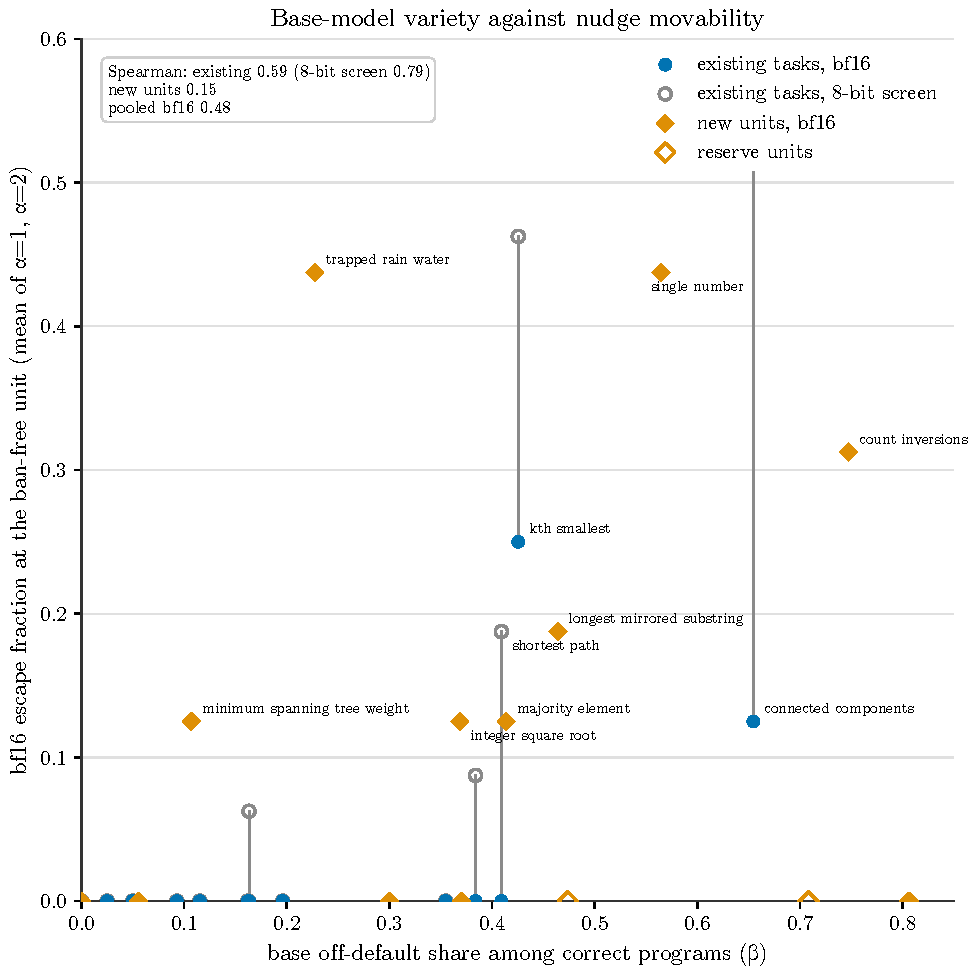
\includegraphics[width=\linewidth,height=0.78\textheight,keepaspectratio]{figures/fig_beta_escape_v0.pdf}
\caption{Each point is one coding task or newly built unit tested on Qwen3-8B. The x-axis gives $\beta$, the base model's off-default share among its own correct programs on that task (0 to 0.85); the y-axis gives the bf16 escape fraction of fixed random pushes at the ban-free unit, averaged over push doses $\alpha$=1 and $\alpha$=2 (0 to 0.6). Filled blue circles are the 15 existing tasks at their bf16 escape fraction; each is joined by a thin grey segment to an open grey circle at the same task's escape fraction measured on the iteration-4 8-bit-precision screen. Filled orange diamonds are 13 newly built units at their bf16 escape fraction; two further reserve units are drawn as hollow orange diamonds. Every point whose plotted escape fraction exceeds 0.1 is labelled by name. The boxed text restates the headline Spearman correlations, recomputed from these same plotted values at render time: existing tasks, bf16 (n=15), 0.59 (one-sided permutation p=0.010, Bonett-Wright 95\% CI [0.06, 0.86]), rising to 0.79 against the 8-bit-screen values (p\textless{}0.001, CI [0.41, 0.94]); the 13 new units, 0.15 (p=0.315, CI [-0.44, 0.65]), falling to 0.01 if the two reserve units are included; and the pooled 28 bf16 measurements, 0.48 (p=0.005, CI [0.11, 0.73]). The existing-task correlation is carried by the many low-$\beta$ tasks whose escape fraction is exactly 0; the new-unit correlation is small and not statistically significant. One labelled point, count inversions, has its $\beta$ computed on an attempt basis rather than the correct-only basis the axis and every other point use, because only 33\% of its base-model attempts were correct programs; recomputed on a correct-only basis ($\beta$=0.13 instead of 0.75), the new-units correlation falls from 0.15 to 0.03.}
\label{fig:fig_beta_escape}
\end{figure}
\FloatBarrier
\subsection*{5.7 Plan noise against text-level plan samplers, decoding at matched departure, and the literal cell (Qwen3-8B)}
\addcontentsline{toc}{subsection}{5.7 Plan noise against text-level plan samplers, decoding at matched departure, and the literal cell (Qwen3-8B)}
\noindent{\small\emph{Artifact: \nolinkurl{gen_art_experiment_27}.}}\par\medskip
\textbf{Why.} The positioning audit of iteration 4 found that the price comparison lacked its strongest competitors: text-level plan samplers, which diversify code by sampling a plan before the program [73, 74], and a decoding baseline matched to plan noise's own departure from the twin, the baseline under which an ICLR 2027 submission (OpenReview oag3wgNLRh) found activation steering no better than ordinary decoding. The review also asked for the literal cell of the request. This experiment  ran both.

\textbf{The literal cell never changes the algorithm} (Table 206). On the shortest path task with thinking on, top-k 10 and the same 20 token seeds as the iteration-4 thinking arm, moving the temperature over 0.3, 0.7, 1.0 and 1.3 changed the final program's algorithm in 0 of 20 seeds (one-sided Clopper--Pearson 95\% upper bound 0.14), and the first approach named in the thinking changed in 0 of 20. All 100 traces completed, every final program was heap-based Dijkstra, and every trace named Dijkstra first. Temperature changed the tokens: a repeat at temperature 0.7 was byte-identical on only 4 of 20 traces while the labels agreed on 20 of 20 (median common prefix 309.5 tokens), and paired with the top-p 1 traces of iteration 4 at the same seed and temperature the labels agreed on 100 of 100 pairs although the traces shared a median of only 34 tokens. A judge agreed with the first-approach lexicon on 19 of 19 audited traces. With this cell, question 1a-c of the request is answered under every sampler the run used: with thinking off at top-k 10 (Table 76), with thinking off and on at top-p 1 (Section 4.5), and with thinking on at top-k 10 here.

\begin{table}[H]
\renewcommand{\thetable}{206}
\centering\scriptsize\setlength{\tabcolsep}{2.5pt}
\caption{The literal cell: shortest path task, thinking on, top-k 10, 20 seeds per temperature, 16k cap (vLLM, official 8-bit checkpoint). Source: knob experiment \texttt{results/\allowbreak{}literal\_\allowbreak{}cell.\allowbreak{}json}. [Source: iteration 5, artifact \nolinkurl{gen_art_experiment_27}.]}\label{tab:t221}
\begin{tabular}{>{\raggedright\arraybackslash\hspace{0pt}}p{0.0720\linewidth}>{\raggedright\arraybackslash\hspace{0pt}}p{0.0961\linewidth}>{\raggedright\arraybackslash\hspace{0pt}}p{0.1293\linewidth}>{\raggedright\arraybackslash\hspace{0pt}}p{0.0938\linewidth}>{\raggedright\arraybackslash\hspace{0pt}}p{0.1016\linewidth}>{\raggedright\arraybackslash\hspace{0pt}}p{0.0872\linewidth}>{\raggedright\arraybackslash\hspace{0pt}}p{0.1859\linewidth}>{\raggedright\arraybackslash\hspace{0pt}}p{0.1473\linewidth}}
\toprule
\textbf{T} & \textbf{completed} & \textbf{final labels (completed)} & \textbf{first approach} & \textbf{median think tokens} & \textbf{Dijkstra style} & \textbf{phrasing clusters at theta 0.7 \slash{} 0.8 \slash{} 0.9} & \textbf{phrasings per idea (theta 0.8)} \\
\midrule
T 0.3 & 20\slash{}20 & Dijkstra 20 & Dijkstra 20 & 3754.50 & heap 20 & 2 \slash{} 4 \slash{} 8 & dijkstra 4 \\
T 0.7 & 20\slash{}20 & Dijkstra 20 & Dijkstra 20 & 3962.00 & heap 20 & 3 \slash{} 3 \slash{} 10 & dijkstra 3 \\
T 1.0 & 20\slash{}20 & Dijkstra 20 & Dijkstra 20 & 3576.00 & heap 20 & 2 \slash{} 3 \slash{} 9 & dijkstra 3 \\
T 1.3 & 20\slash{}20 & Dijkstra 20 & Dijkstra 20 & 4149.00 & heap 20 & 5 \slash{} 7 \slash{} 12 & dijkstra 7 \\
T 0.7, repeat & 20\slash{}20 & Dijkstra 20 & Dijkstra 20 & 3500.00 & heap 20 & 3 \slash{} 6 \slash{} 10 & dijkstra 6 \\
\bottomrule
\end{tabular}
\end{table}

At N = 20 with thinking on a rise shows only at T 1.3, and repeat noise is the same size. \emph{(Iteration-6 addition: the two phrasing columns, computed by the knob experiment and missing from the record until now.)}

\textbf{Design of the knob comparison.} Every knob ran in one HF bf16 engine with exact inverse-CDF common random numbers, so all arms of a slot shared the uniform stream of the code stage, on all 15 existing tasks (N = 50 per cell on the five decisive tasks, 30 on the other ten). Plan noise drew a fresh isotropic direction per sample at the task-specification positions of blocks 12 to 23, prefill only, at alpha 1 and 2 ban-free units, under the twin frame and on the plain prompt. The text-level plan samplers used the twin's frame, with the twin's neutral sentence first: intent factored generation at the direction's (1.3, 0.7) and the paper's tuned (0.73, 0.60) temperatures [73]; a lite plan search (five observations, a random pair of them combined into a plan, then code) [74]; enumerate and pick, in which the model lists up to eight algorithms and an external random number picks one; and base intent, in which Qwen3-8B-Base writes the intent sentence and the instruct model the code. Decoding at matched departure applied a temperature to generated tokens 1 to 32, bisected per task so that its mean per-token KL from the twin equalled plan noise's own at each alpha, measured on prefixes used only for calibration. Prices came from a randomisation hull over the full simplex with 2,000 slot bootstraps that select the best mixture again inside every replicate. The committed rule calls the plan sampler comparison supported if the 5-point Hill-1 of plan noise is at least that of the best text sampler on at least 3 of the 5 decisive tasks.

\textbf{The plan sampler comparison is DISCONFIRMED} (Table 207) (ban-free unit and iteration-5 seeds; re-tagged by iteration 7's dose-unit experiment, Section 7.6: at the moving design D* = D1 the plan-sampler rule is still disconfirmed, at 2 of 5) (iteration-8 correction). In Table 207 the margin is the 5-point Hill-1 of plan noise minus that of the best text sampler. Plan noise matched or beat the best text sampler on 1 of the 5 decisive tasks, kth smallest (1.98 against 1.83 for enumerate and pick, P(plan noise at least best) 0.58, unresolved). On connected components, the shortest path task and two sum, base intent won (2.53, 1.45 and 1.61 against 1.09, 1.18 and 1.17), and on the grid task nothing moved much. The mean margin is -0.40 (95\% interval -0.70 to -0.24), and only 1.8\% of bootstrap replicates reach three wins. Every sensitivity keeps the verdict except one (Table 209): with the multistage samplers dropped (they were padded on the left), intent factored generation is the only text sampler left and plan noise beats it on 4 of 5 tasks, so the disconfirmation rests on base intent and on enumerate and pick. On the ten other tasks (Table 208) plan noise moved only cycle detection and first and last position, while text samplers moved substring search, find duplicate, Fibonacci, longest increasing subsequence, top-k frequent and first and last position. Two prompt knobs outside the text-sampler set also beat plan noise where it was strongest: the novelty instruction on kth smallest (2.03) and the semantic seed on the shortest path task (2.12). (iteration-7 correction)

\begin{table}[H]
\renewcommand{\thetable}{207}
\centering\tiny\setlength{\tabcolsep}{2.5pt}
\caption{The plan sampler comparison on the five decisive tasks: 5-point Hill-1 of plan noise (with its bootstrap interval) against each text-level plan sampler. Source: knob experiment \texttt{results/\allowbreak{}claim\_\allowbreak{}c.\allowbreak{}json}. [Source: iteration 5, artifact \nolinkurl{gen_art_experiment_27}.]}\label{tab:t222}
\begin{tabular}{>{\raggedright\arraybackslash\hspace{0pt}}p{0.0863\linewidth}>{\raggedright\arraybackslash\hspace{0pt}}p{0.1366\linewidth}>{\raggedright\arraybackslash\hspace{0pt}}p{0.0951\linewidth}>{\raggedright\arraybackslash\hspace{0pt}}p{0.0722\linewidth}>{\raggedright\arraybackslash\hspace{0pt}}p{0.0739\linewidth}>{\raggedright\arraybackslash\hspace{0pt}}p{0.0510\linewidth}>{\raggedright\arraybackslash\hspace{0pt}}p{0.0919\linewidth}>{\raggedright\arraybackslash\hspace{0pt}}p{0.0594\linewidth}>{\raggedright\arraybackslash\hspace{0pt}}p{0.0979\linewidth}>{\raggedright\arraybackslash\hspace{0pt}}p{0.0651\linewidth}>{\raggedright\arraybackslash\hspace{0pt}}p{0.0527\linewidth}}
\toprule
\textbf{Task} & \textbf{Plan noise, 5-point Hill-1 [95\%]} & \textbf{Intent factored generation} & \textbf{Plan search (lite)} & \textbf{Enumerate and pick} & \textbf{Base intent} & \textbf{Best text sampler} & \textbf{Plan noise wins} & \textbf{P(plan noise at least best)} & \textbf{Flag} & \textbf{Margin} \\
\midrule
kth smallest & 1.98 [1.64, 2.28] & 1.19 & 1.09 & 1.83 & 1.73 & enumerate and pick & yes & 0.58 & unresolved & +0.15 \\
connected components & 1.09 [1.00, 1.26] & 1.96 & 1.50 & 1.88 & 2.53 & base intent & no & 0.00 &  & -1.43 \\
shortest path & 1.18 [1.00, 1.34] & 1.00 & 1.07 & 1.24 & 1.45 & base intent & no & 0.06 &  & -0.27 \\
two sum & 1.17 [1.00, 1.38] & 1.00 & 1.00 & 1.27 & 1.61 & base intent & no & 0.01 &  & -0.44 \\
grid & 1.06 [1.00, 1.30] & 1.00 & 1.00 & 1.08 & 1.04 & enumerate and pick & no & 0.38 & unresolved & -0.03 \\
\bottomrule
\end{tabular}
\end{table}

\begin{table}[H]
\renewcommand{\thetable}{208}
\centering\scriptsize\setlength{\tabcolsep}{2.5pt}
\caption{The same prices on the ten other tasks (descriptive; the plan search arm was not run on topological order and first and last position, the base intent arm not on first and last position). Source: knob experiment \texttt{results/\allowbreak{}claim\_\allowbreak{}c.\allowbreak{}json\#nd10\_\allowbreak{}descriptive}. [Source: iteration 5, artifact \nolinkurl{gen_art_experiment_27}.]}\label{tab:t223}
\begin{tabular}{>{\raggedright\arraybackslash\hspace{0pt}}p{0.2074\linewidth}>{\raggedright\arraybackslash\hspace{0pt}}p{0.1324\linewidth}>{\raggedright\arraybackslash\hspace{0pt}}p{0.1324\linewidth}>{\raggedright\arraybackslash\hspace{0pt}}p{0.1003\linewidth}>{\raggedright\arraybackslash\hspace{0pt}}p{0.1010\linewidth}>{\raggedright\arraybackslash\hspace{0pt}}p{0.0717\linewidth}>{\raggedright\arraybackslash\hspace{0pt}}p{0.1784\linewidth}}
\toprule
\textbf{Task (descriptive, N = 30 per cell)} & \textbf{Plan noise, 5-point Hill-1} & \textbf{Intent factored generation} & \textbf{Plan search (lite)} & \textbf{Enumerate and pick} & \textbf{Base intent} & \textbf{Best text sampler} \\
\midrule
substring search & 1.00 & 1.97 & 1.00 & 1.44 & 1.00 & intent factored generation \\
find duplicate & 1.00 & 1.97 & 1.66 & 1.08 & 1.08 & intent factored generation \\
Fibonacci & 1.00 & 1.00 & 1.00 & 1.10 & 1.70 & base intent \\
longest increasing subsequence & 1.00 & 1.00 & 1.57 & 1.57 & 1.00 & enumerate and pick \\
merge intervals & 1.00 & 1.00 & 1.00 & 1.03 & 1.00 & enumerate and pick \\
top-k frequent & 1.00 & 1.00 & 1.00 & 3.02 & 1.17 & enumerate and pick \\
nonoverlapping intervals & 1.00 & 1.00 & 1.00 & 1.01 & 1.00 & enumerate and pick \\
cycle detection & 1.18 & 1.00 & 1.00 & 1.05 & 1.04 & enumerate and pick \\
topological order & 1.00 & 1.00 & n\slash{}a & 1.00 & 1.00 & intent factored generation \\
first and last position & 1.29 & 1.18 & n\slash{}a & 2.62 & n\slash{}a & enumerate and pick \\
\bottomrule
\end{tabular}
\end{table}

\begin{table}[H]
\renewcommand{\thetable}{207b}
\centering\scriptsize\setlength{\tabcolsep}{2.5pt}
\caption{(iteration 6) Pass cost (fraction of pass rate given up) at which each knob's randomisation hull first reaches correct-only Hill-1 of 1.5 and then of 2.0 (the two prices in each cell, separated by a slash); a dash means never reached. Source: knob experiment \texttt{results/\allowbreak{}prices.\allowbreak{}json}; 95\% percentile intervals over the 2,000 slot-bootstrap replicates of \texttt{results/\allowbreak{}bootstrap.\allowbreak{}json} that reach the level (the share that reaches it is in tables\slash{}prices\_\allowbreak{}p15\_\allowbreak{}p20.csv). [Source: iteration 5, artifact \nolinkurl{gen_art_experiment_27}.]}\label{tab:t224}
\begin{tabular}{>{\raggedright\arraybackslash\hspace{0pt}}p{0.1147\linewidth}>{\raggedright\arraybackslash\hspace{0pt}}p{0.0943\linewidth}>{\raggedright\arraybackslash\hspace{0pt}}p{0.1342\linewidth}>{\raggedright\arraybackslash\hspace{0pt}}p{0.1182\linewidth}>{\raggedright\arraybackslash\hspace{0pt}}p{0.1844\linewidth}>{\raggedright\arraybackslash\hspace{0pt}}p{0.1472\linewidth}>{\raggedright\arraybackslash\hspace{0pt}}p{0.1305\linewidth}}
\toprule
\textbf{Task} & \textbf{plan noise, Hill-1 1.5 \slash{} 2.0} & \textbf{intent factored generation, Hill-1 1.5 \slash{} 2.0} & \textbf{plan search (lite), Hill-1 1.5 \slash{} 2.0} & \textbf{enumerate and pick, Hill-1 1.5 \slash{} 2.0} & \textbf{base intent, Hill-1 1.5 \slash{} 2.0} & \textbf{novelty instruction, Hill-1 1.5 \slash{} 2.0} \\
\midrule
kth smallest & 0.000 [0.000, 0.000] \slash{} -- & -- \slash{} -- & -- \slash{} -- & 0.030 [0.014, 0.061] \slash{} 0.062 [0.030, 0.120] & 0.033 [0.000, 0.084] \slash{} -- & 0.006 [0.000, 0.016] \slash{} 0.018 [0.000, 0.045] \\
connected components & -- \slash{} -- & 0.000 [0.000, 0.000] \slash{} -- & 0.050 [0.040, 0.072] \slash{} -- & 0.029 [0.020, 0.040] \slash{} 0.058 [0.035, 0.090] & 0.005 [0.000, 0.018] \slash{} 0.011 [0.000, 0.039] & -- \slash{} -- \\
shortest path & -- \slash{} -- & -- \slash{} -- & -- \slash{} -- & 0.103 [0.058, 0.196] \slash{} 0.190 [0.117, 0.336] & 0.057 [0.000, 0.133] \slash{} -- & -- \slash{} -- \\
two sum & -- \slash{} -- & -- \slash{} -- & -- \slash{} -- & 0.086 [0.048, 0.162] \slash{} 0.157 [0.096, 0.273] & 0.042 [0.012, 0.099] \slash{} 0.080 [0.024, 0.170] & -- \slash{} -- \\
grid & -- \slash{} -- & -- \slash{} -- & -- \slash{} -- & 0.229 [0.144, 0.420] \slash{} 0.341 [0.234, 0.576] & 0.421 [0.230, 0.640] \slash{} -- & 0.096 [0.000, 0.240] \slash{} -- \\
substring search & -- \slash{} -- & 0.000 [0.000, 0.000] \slash{} -- & -- \slash{} -- & 0.055 [0.020, 0.133] \slash{} 0.098 [0.040, 0.220] & -- \slash{} -- & -- \slash{} -- \\
find duplicate & -- \slash{} -- & 0.000 [0.000, 0.000] \slash{} -- & 0.023 [0.000, 0.085] \slash{} -- & 0.240 [0.120, 0.533] \slash{} 0.380 [0.202, 0.600] & -- \slash{} -- & -- \slash{} -- \\
Fibonacci & -- \slash{} -- & -- \slash{} -- & -- \slash{} -- & 0.224 [0.120, 0.397] \slash{} -- & 0.025 [0.000, 0.093] \slash{} -- & -- \slash{} -- \\
longest increasing subsequence & -- \slash{} -- & -- \slash{} -- & 0.000 [0.000, 0.000] \slash{} -- & 0.043 [0.017, 0.090] \slash{} 0.100 [0.033, 0.180] & -- \slash{} -- & -- \slash{} -- \\
merge intervals & -- \slash{} -- & -- \slash{} -- & -- \slash{} -- & 0.555 [0.260, 0.630] \slash{} -- & -- \slash{} -- & -- \slash{} -- \\
top-k frequent & -- \slash{} -- & -- \slash{} -- & -- \slash{} -- & 0.014 [0.000, 0.058] \slash{} 0.026 [0.000, 0.117] & -- \slash{} -- & -- \slash{} -- \\
non-overlapping intervals & -- \slash{} -- & -- \slash{} -- & -- \slash{} -- & -- \slash{} -- & -- \slash{} -- & -- \slash{} -- \\
cycle detection & -- \slash{} -- & -- \slash{} -- & -- \slash{} -- & 0.359 [0.170, 0.708] \slash{} 0.528 [0.267, 0.693] & 0.470 [0.183, 0.630] \slash{} -- & -- \slash{} -- \\
topological order & -- \slash{} -- & -- \slash{} -- & -- \slash{} -- & -- \slash{} -- & -- \slash{} -- & -- \slash{} -- \\
first and last position & -- \slash{} -- & -- \slash{} -- & -- \slash{} -- & 0.000 [0.000, 0.033] \slash{} 0.000 [0.000, 0.090] & -- \slash{} -- & -- \slash{} -- \\
\bottomrule
\end{tabular}
\end{table}

\begin{table}[H]
\renewcommand{\thetable}{209}
\centering\small\setlength{\tabcolsep}{4.0pt}
\caption{Sensitivities of the plan sampler rule. Source: knob experiment \texttt{results/\allowbreak{}claim\_\allowbreak{}c.\allowbreak{}json\#sensitivities}. [Source: iteration 5, artifact \nolinkurl{gen_art_experiment_27}.]}\label{tab:t225}
\begin{tabular}{>{\raggedright\arraybackslash\hspace{0pt}}p{0.4873\linewidth}>{\raggedright\arraybackslash\hspace{0pt}}p{0.1828\linewidth}>{\raggedright\arraybackslash\hspace{0pt}}p{0.1703\linewidth}>{\raggedright\arraybackslash\hspace{0pt}}p{0.0894\linewidth}}
\toprule
\textbf{Sensitivity} & \textbf{Verdict} & \textbf{Tasks where plan noise wins} & \textbf{Mean margin} \\
\midrule
intent factored generation at (1.3, 0.7) only & DISCONFIRMED & 1 of 5 & -0.40 \\
plan noise hull adds the plain prompt arms & DISCONFIRMED & 2 of 5 & -0.40 \\
hull restricted to edges & DISCONFIRMED & 1 of 5 & -0.40 \\
multistage samplers dropped, padded on the left (intent factored generation remains) & SUPPORTED & 4 of 5 & +0.07 \\
style re-gate flagged task excluded & DISCONFIRMED & 1 of 5 & -0.40 \\
relabels from the novelty audit applied & DISCONFIRMED & 1 of 5 & -0.40 \\
\bottomrule
\end{tabular}
\end{table}

\begin{figure}[!htbp]
\centering\captionsetup{font=footnotesize}
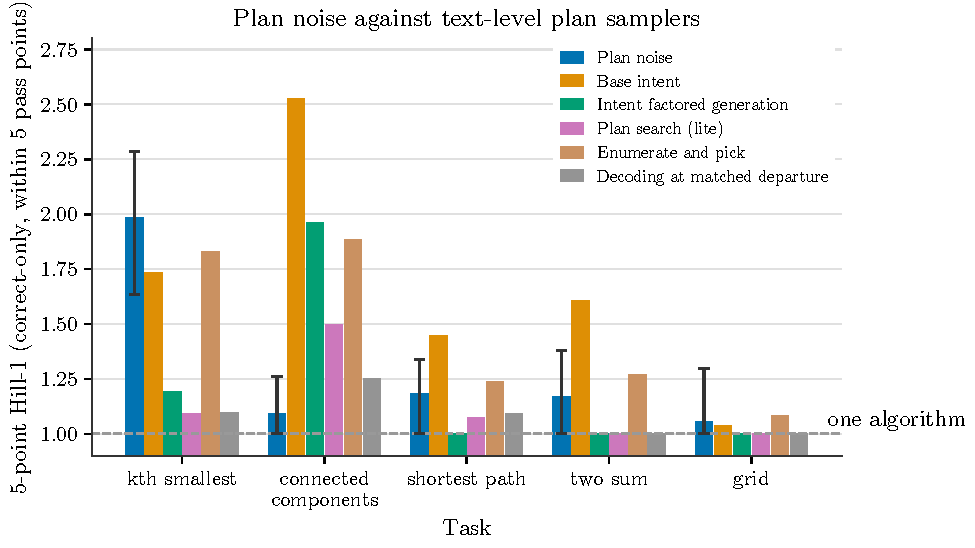
\includegraphics[width=\linewidth,height=0.78\textheight,keepaspectratio]{figures/fig_knob_h5_v0.pdf}
\caption{5-point Hill-1 (the highest correct-only, rarefied Hill-1 a sampler reaches within 5 pass points of its twin, on a randomisation hull over the full simplex) on five decisive algorithm-choice coding tasks, \$N=50\$ generations per condition. Six bars per task, in the legend's order and colour: plan noise (dark blue, with its 95\textbackslash{}\% bootstrap interval from 2\{,\}000 replicates), base-written intent (orange), intent-factored generation (green), plan-search-lite (violet), enumerate-and-pick (tan), and decoding at a temperature matched to plan noise's per-token departure from the twin (grey). The dashed grey line at 1.0 marks the statistic's floor: every correct sample used one algorithm. Plan noise draws the tallest bar only on kth smallest (1.98 vs.\textbackslash{} 1.83 for enumerate-and-pick), and its own plotted interval, \$[1.64, 2.28]\$, covers that bar, so the two are not clearly separated there. Base-written intent is tallest on connected components (2.53, where plan noise is the shortest of the six bars at 1.09), shortest path (1.45), and two sum (1.61). On grid, enumerate-and-pick is tallest (1.08), narrowly ahead of plan noise (1.06), again inside plan noise's plotted interval. As a knob for making a model's code more algorithmically diverse, plan noise is not consistently ahead of simply asking for a different plan in words.}
\label{fig:fig_knob_h5}
\end{figure}
Table 210 shows what each arm actually wrote on the decisive tasks. Enumerate and pick buys the most raw diversity (Hill-1 of 2.9 to 4.7 per cell) at a cost of 16 to 62 pass points, and 40\% of its grid rows are invalid. Base intent keeps the pass rate high on connected components (0.98) and two sum (0.88) while writing three and four algorithms. Intent factored generation at its cooler code temperature collapsed the grid pass rate to 0.12 and 0.08, with every correct program BFS. Plan noise is much weaker here than in iteration 4: on connected components it wrote union find 49 times in 50 at both alphas, where iteration 4's 8-bit engine at the ban unit had written DFS 29 times at alpha 2 (Section 4.3); Section 5.10 returns to this.

{\scriptsize\setlength{\tabcolsep}{2.5pt}\renewcommand{\thetable}{210}
\begin{longtable}{>{\raggedright\arraybackslash\hspace{0pt}}p{0.1208\linewidth}>{\raggedright\arraybackslash\hspace{0pt}}p{0.2293\linewidth}>{\raggedright\arraybackslash\hspace{0pt}}p{0.0382\linewidth}>{\raggedright\arraybackslash\hspace{0pt}}p{0.0539\linewidth}>{\raggedright\arraybackslash\hspace{0pt}}p{0.0788\linewidth}>{\raggedright\arraybackslash\hspace{0pt}}p{0.3088\linewidth}>{\raggedright\arraybackslash\hspace{0pt}}p{0.0938\linewidth}}
\caption{Every arm on the five decisive tasks: pass rate, invalid rate, correct programs and correct-only Hill-1 (rarefied at depth 25 or at the available depth). Source: knob experiment \texttt{results/\allowbreak{}cells.\allowbreak{}json}. [Source: iteration 5, artifact \nolinkurl{gen_art_experiment_27}.]}\label{tab:t226}\\
\toprule
\textbf{Task} & \textbf{Arm} & \textbf{N} & \textbf{Pass} & \textbf{Invalid} & \textbf{Correct programs} & \textbf{Hill-1 (depth)} \\
\midrule
\endfirsthead
\multicolumn{7}{l}{\emph{Table 210, continued}}\\
\toprule
\textbf{Task} & \textbf{Arm} & \textbf{N} & \textbf{Pass} & \textbf{Invalid} & \textbf{Correct programs} & \textbf{Hill-1 (depth)} \\
\midrule
\endhead
\bottomrule
\endlastfoot
kth smallest & twin & 50 & 1.00 & 0.00 & full sort 49, quickselect 1 & 1.09 (25) \\
kth smallest & plain prompt & 50 & 1.00 & 0.00 & full sort 50 & 1.00 (25) \\
kth smallest & plan noise alpha 1 & 50 & 0.98 & 0.00 & full sort 45, quickselect 4 & 1.33 (25) \\
kth smallest & plan noise alpha 2 & 50 & 1.00 & 0.00 & full sort 36, quickselect 12, size-k heap 2 & 1.99 (25) \\
kth smallest & plan noise alpha 1, plain prompt & 50 & 1.00 & 0.00 & full sort 49, quickselect 1 & 1.09 (25) \\
kth smallest & intent factored generation (1.3, 0.7) & 50 & 0.98 & 0.00 & full sort 48, heapify and pop 1 & 1.10 (25) \\
kth smallest & intent factored generation (0.73, 0.60) & 50 & 1.00 & 0.00 & full sort 48, heapify and pop 1, quickselect 1 & 1.19 (25) \\
kth smallest & plan search (lite) & 50 & 1.00 & 0.00 & full sort 50 & 1.00 (25) \\
kth smallest & enumerate and pick & 50 & 0.80 & 0.00 & quickselect 24, full sort 6, other 4, counting sort 4, size-k heap 2 & 3.24 (25) \\
kth smallest & base intent & 50 & 0.94 & 0.00 & full sort 39, size-k heap 4, quickselect 2, counting sort 1, other 1 & 1.86 (25) \\
kth smallest & decoding at matched departure, alpha 1 match & 50 & 1.00 & 0.00 & full sort 49, quickselect 1 & 1.09 (25) \\
kth smallest & decoding at matched departure, alpha 2 match & 50 & 0.98 & 0.00 & full sort 48, quickselect 1 & 1.10 (25) \\
kth smallest & temperature 1.3 & 50 & 1.00 & 0.00 & full sort 49, quickselect 1 & 1.09 (25) \\
kth smallest & top-k 10 & 50 & 1.00 & 0.00 & full sort 49, quickselect 1 & 1.09 (25) \\
kth smallest & novelty instruction & 50 & 0.96 & 0.00 & quickselect 47, heapify and pop 1 & 1.10 (25) \\
connected components & twin & 50 & 1.00 & 0.00 & union find 50 & 1.00 (25) \\
connected components & plain prompt & 50 & 1.00 & 0.00 & union find 50 & 1.00 (25) \\
connected components & plan noise alpha 1 & 50 & 1.00 & 0.00 & union find 49, DFS 1 & 1.09 (25) \\
connected components & plan noise alpha 2 & 50 & 1.00 & 0.00 & union find 49, DFS 1 & 1.09 (25) \\
connected components & plan noise alpha 1, plain prompt & 50 & 1.00 & 0.00 & union find 50 & 1.00 (25) \\
connected components & intent factored generation (1.3, 0.7) & 50 & 1.00 & 0.00 & DFS 43, union find 7 & 1.48 (25) \\
connected components & intent factored generation (0.73, 0.60) & 50 & 1.00 & 0.00 & DFS 47, union find 3 & 1.24 (25) \\
connected components & plan search (lite) & 50 & 0.78 & 0.22 & BFS 31, union find 8 & 1.66 (25) \\
connected components & enumerate and pick & 50 & 0.84 & 0.16 & DFS 17, BFS 15, union find 10 & 2.88 (25) \\
connected components & base intent & 50 & 0.98 & 0.00 & union find 24, DFS 20, BFS 5 & 2.53 (25) \\
connected components & decoding at matched departure, alpha 1 match & 50 & 0.98 & 0.02 & union find 47, DFS 2 & 1.18 (25) \\
connected components & decoding at matched departure, alpha 2 match & 50 & 0.98 & 0.02 & union find 46, DFS 3 & 1.26 (25) \\
connected components & temperature 1.3 & 50 & 1.00 & 0.00 & union find 50 & 1.00 (25) \\
connected components & top-k 10 & 50 & 1.00 & 0.00 & union find 50 & 1.00 (25) \\
connected components & novelty instruction & 50 & 1.00 & 0.00 & union find 43, DFS 7 & 1.48 (25) \\
shortest path & twin & 50 & 0.98 & 0.00 & Dijkstra 49 & 1.00 (25) \\
shortest path & plain prompt & 50 & 0.98 & 0.00 & Dijkstra 49 & 1.00 (25) \\
shortest path & plan noise alpha 1 & 50 & 1.00 & 0.00 & Dijkstra 50 & 1.00 (25) \\
shortest path & plan noise alpha 2 & 50 & 0.94 & 0.00 & Dijkstra 45, Bellman-Ford\slash{}SPFA 2 & 1.19 (25) \\
shortest path & plan noise alpha 1, plain prompt & 50 & 1.00 & 0.00 & Dijkstra 50 & 1.00 (25) \\
shortest path & intent factored generation (1.3, 0.7) & 50 & 1.00 & 0.00 & Dijkstra 50 & 1.00 (25) \\
shortest path & intent factored generation (0.73, 0.60) & 50 & 1.00 & 0.00 & Dijkstra 50 & 1.00 (25) \\
shortest path & plan search (lite) & 50 & 0.78 & 0.20 & Dijkstra 36, Bellman-Ford\slash{}SPFA 3 & 1.31 (25) \\
shortest path & enumerate and pick & 50 & 0.60 & 0.04 & Dijkstra 11, Bellman-Ford\slash{}SPFA 10, Floyd-Warshall 9 & 2.97 (25) \\
shortest path & base intent & 50 & 0.92 & 0.02 & Dijkstra 39, Bellman-Ford\slash{}SPFA 7 & 1.52 (25) \\
shortest path & decoding at matched departure, alpha 1 match & 50 & 0.98 & 0.00 & Dijkstra 48, Bellman-Ford\slash{}SPFA 1 & 1.10 (25) \\
shortest path & decoding at matched departure, alpha 2 match & 50 & 0.82 & 0.04 & Dijkstra 41 & 1.00 (25) \\
shortest path & temperature 1.3 & 50 & 0.98 & 0.00 & Dijkstra 49 & 1.00 (25) \\
shortest path & top-k 10 & 50 & 0.98 & 0.00 & Dijkstra 49 & 1.00 (25) \\
shortest path & novelty instruction & 50 & 1.00 & 0.00 & Dijkstra 50 & 1.00 (25) \\
shortest path & semantic seed & 50 & 0.98 & 0.00 & Dijkstra 32, Bellman-Ford\slash{}SPFA 15, other 2 & 2.12 (25) \\
two sum & twin & 50 & 1.00 & 0.00 & hash map 50 & 1.00 (25) \\
two sum & plain prompt & 50 & 1.00 & 0.00 & hash map 50 & 1.00 (25) \\
two sum & plan noise alpha 1 & 50 & 1.00 & 0.00 & hash map 50 & 1.00 (25) \\
two sum & plan noise alpha 2 & 50 & 1.00 & 0.00 & hash map 48, brute force 2 & 1.17 (25) \\
two sum & plan noise alpha 1, plain prompt & 50 & 1.00 & 0.00 & hash map 50 & 1.00 (25) \\
two sum & intent factored generation (1.3, 0.7) & 50 & 1.00 & 0.00 & hash map 50 & 1.00 (25) \\
two sum & intent factored generation (0.73, 0.60) & 50 & 1.00 & 0.00 & hash map 50 & 1.00 (25) \\
two sum & plan search (lite) & 50 & 0.98 & 0.00 & hash map 49 & 1.00 (25) \\
two sum & enumerate and pick & 50 & 0.68 & 0.00 & hash map 16, sort and two pointers 7, brute force 7, sort and binary search 4 & 3.46 (25) \\
two sum & base intent & 50 & 0.88 & 0.02 & hash map 29, brute force 9, sort and two pointers 4, sort and binary search 2 & 2.55 (25) \\
two sum & decoding at matched departure, alpha 1 match & 50 & 1.00 & 0.00 & hash map 50 & 1.00 (25) \\
two sum & decoding at matched departure, alpha 2 match & 50 & 1.00 & 0.00 & hash map 50 & 1.00 (25) \\
two sum & temperature 1.3 & 50 & 1.00 & 0.00 & hash map 50 & 1.00 (25) \\
two sum & top-k 10 & 50 & 1.00 & 0.00 & hash map 50 & 1.00 (25) \\
two sum & novelty instruction & 50 & 1.00 & 0.00 & hash map 46, brute force 3, other 1 & 1.35 (25) \\
grid & twin & 50 & 0.86 & 0.00 & BFS 43 & 1.00 (25) \\
grid & plain prompt & 50 & 0.96 & 0.00 & BFS 48 & 1.00 (25) \\
grid & plan noise alpha 1 & 50 & 0.80 & 0.00 & BFS 40 & 1.00 (25) \\
grid & plan noise alpha 2 & 50 & 0.76 & 0.00 & BFS 37, Dijkstra 1 & 1.12 (25) \\
grid & plan noise alpha 1, plain prompt & 50 & 0.86 & 0.00 & BFS 43 & 1.00 (25) \\
grid & intent factored generation (1.3, 0.7) & 50 & 0.12 & 0.00 & BFS 6 & 1.00 (6) \\
grid & intent factored generation (0.73, 0.60) & 50 & 0.08 & 0.00 & BFS 4 & 1.00 (4) \\
grid & plan search (lite) & 50 & 0.50 & 0.40 & BFS 25 & 1.00 (25) \\
grid & enumerate and pick & 50 & 0.24 & 0.40 & A* 3, BFS 3, DFS 3, Dijkstra 2, bidirectional BFS 1 & 4.69 (12) \\
grid & base intent & 50 & 0.32 & 0.00 & BFS 12, DFS 4 & 1.75 (16) \\
grid & decoding at matched departure, alpha 1 match & 50 & 0.80 & 0.00 & BFS 40 & 1.00 (25) \\
grid & decoding at matched departure, alpha 2 match & 50 & 0.78 & 0.00 & BFS 39 & 1.00 (25) \\
grid & temperature 1.3 & 50 & 0.92 & 0.00 & BFS 46 & 1.00 (25) \\
grid & top-k 10 & 50 & 0.84 & 0.00 & BFS 42 & 1.00 (25) \\
grid & novelty instruction & 50 & 0.70 & 0.00 & BFS 26, DFS 9 & 1.77 (25) \\
grid & semantic seed & 50 & 0.60 & 0.00 & BFS 30 & 1.00 (25) \\
\end{longtable}}

\textbf{Plan noise against decoding at matched departure.} At alpha 2, plan noise moves the algorithm and the matched decoding does not (Table 211): over the decisive tasks 19 slots are correct and off the default under plan noise only and 3 under the matched decoding only (exact p 0.0009), 13 to 0 on kth smallest alone. At alpha 1 there is no difference (4 against 3). The matched decoding's 5-point Hill-1 is at most 1.25 on every decisive task. So plan noise's effect is not its token-level departure from the twin, which answers the objection of the ICLR 2027 submission for these tasks, but as a practical knob it loses to two text samplers. Plan noise on the plain prompt and under the twin frame showed no significant paired difference on any of the 15 tasks (Table 212).

\begin{table}[H]
\renewcommand{\thetable}{211}
\centering\scriptsize\setlength{\tabcolsep}{2.5pt}
\caption{Plan noise against decoding at matched departure at matched per-token KL (correct off-default share of N; McNemar on slots correct and off the default under one arm only). Source: knob experiment \texttt{results/\allowbreak{}pn\_\allowbreak{}vs\_\allowbreak{}dmd.\allowbreak{}json}. [Source: iteration 5, artifact \nolinkurl{gen_art_experiment_27}.]}\label{tab:t227}
\begin{tabular}{>{\raggedright\arraybackslash\hspace{0pt}}p{0.0988\linewidth}>{\raggedright\arraybackslash\hspace{0pt}}p{0.0316\linewidth}>{\raggedright\arraybackslash\hspace{0pt}}p{0.1168\linewidth}>{\raggedright\arraybackslash\hspace{0pt}}p{0.0988\linewidth}>{\raggedright\arraybackslash\hspace{0pt}}p{0.1194\linewidth}>{\raggedright\arraybackslash\hspace{0pt}}p{0.0582\linewidth}>{\raggedright\arraybackslash\hspace{0pt}}p{0.0915\linewidth}>{\raggedright\arraybackslash\hspace{0pt}}p{0.0659\linewidth}>{\raggedright\arraybackslash\hspace{0pt}}p{0.2218\linewidth}}
\toprule
\textbf{Task} & \textbf{$\alpha$} & \textbf{Temperature at matched departure} & \textbf{plan noise KL per token} & \textbf{matched departure KL per token} & \textbf{plan noise} & \textbf{matched departure} & \textbf{TWIN} & \textbf{McNemar, plan noise against matched departure (only plan noise : only matched departure, p)} \\
\midrule
kth smallest & 1 & 1.46 & 0.0179 & 0.0200 & 0.08 & 0.02 & 0.02 & 3\slash{}0, p=0.25 \\
kth smallest & 2 & 1.64 & 0.0774 & 0.0707 & 0.28 & 0.02 & 0.02 & 13\slash{}0, p=0.000244 \\
connected components & 1 & 1.84 & 0.0096 & 0.0110 & 0.02 & 0.04 & 0.00 & 1\slash{}2, p=1 \\
connected components & 2 & 2.22 & 0.0333 & 0.0370 & 0.02 & 0.06 & 0.00 & 1\slash{}3, p=0.625 \\
shortest path & 1 & 2.01 & 0.0254 & 0.0244 & 0.00 & 0.02 & 0.00 & 0\slash{}1, p=1 \\
shortest path & 2 & 2.66 & 0.1113 & 0.1230 & 0.04 & 0.00 & 0.00 & 2\slash{}0, p=0.5 \\
two sum & 1 & 1.52 & 0.0036 & 0.0039 & 0.00 & 0.00 & 0.00 & 0\slash{}0, p=1 \\
two sum & 2 & 1.81 & 0.0100 & 0.0104 & 0.04 & 0.00 & 0.00 & 2\slash{}0, p=0.5 \\
grid & 1 & 2.15 & 0.0505 & 0.0442 & 0.00 & 0.00 & 0.00 & 0\slash{}0, p=1 \\
grid & 2 & 2.47 & 0.1554 & 0.1246 & 0.02 & 0.00 & 0.00 & 1\slash{}0, p=1 \\
\bottomrule
\end{tabular}
\end{table}

\begin{table}[H]
\renewcommand{\thetable}{212}
\centering\footnotesize\setlength{\tabcolsep}{4.0pt}
\caption{Plan noise on the plain prompt against plan noise under the twin frame, same direction and stream. Source: knob experiment \texttt{results/\allowbreak{}plain\_\allowbreak{}vs\_\allowbreak{}twin.\allowbreak{}json}. [Source: iteration 5, artifact \nolinkurl{gen_art_experiment_27}.]}\label{tab:t228}
\begin{tabular}{>{\raggedright\arraybackslash\hspace{0pt}}p{0.2456\linewidth}>{\raggedright\arraybackslash\hspace{0pt}}p{0.2892\linewidth}>{\raggedright\arraybackslash\hspace{0pt}}p{0.0934\linewidth}>{\raggedright\arraybackslash\hspace{0pt}}p{0.0875\linewidth}>{\raggedright\arraybackslash\hspace{0pt}}p{0.0934\linewidth}>{\raggedright\arraybackslash\hspace{0pt}}p{0.0875\linewidth}}
\toprule
\textbf{Task} & \textbf{plan noise only on plain : only on twin (p)} & \textbf{pass plain} & \textbf{pass twin} & \textbf{Hill plain} & \textbf{Hill twin} \\
\midrule
kth smallest & 0\slash{}3 (p=0.25) & 1.00 & 0.98 & 1.09 & 1.33 \\
connected components & 0\slash{}1 (p=1) & 1.00 & 1.00 & 1.00 & 1.09 \\
shortest path & 0\slash{}0 (p=1) & 1.00 & 1.00 & 1.00 & 1.00 \\
two sum & 0\slash{}0 (p=1) & 1.00 & 1.00 & 1.00 & 1.00 \\
grid & 0\slash{}0 (p=1) & 0.86 & 0.80 & 1.00 & 1.00 \\
substring search & 0\slash{}0 (p=1) & 1.00 & 1.00 & 1.00 & 1.00 \\
find duplicate & 0\slash{}0 (p=1) & 1.00 & 1.00 & 1.00 & 1.00 \\
Fibonacci & 0\slash{}0 (p=1) & 0.97 & 1.00 & 1.00 & 1.00 \\
longest increasing subsequence & 0\slash{}0 (p=1) & 1.00 & 1.00 & 1.00 & 1.00 \\
merge intervals & 0\slash{}0 (p=1) & 1.00 & 1.00 & 1.00 & 1.00 \\
top-k frequent & 0\slash{}0 (p=1) & 0.73 & 0.80 & 1.00 & 1.00 \\
nonoverlapping intervals & 0\slash{}0 (p=1) & 0.90 & 0.87 & 1.00 & 1.00 \\
cycle detection & 0\slash{}0 (p=1) & 0.80 & 0.87 & 1.00 & 1.00 \\
topological order & 0\slash{}0 (p=1) & 1.00 & 1.00 & 1.00 & 1.00 \\
first and last position & 0\slash{}1 (p=1) & 0.90 & 0.87 & 1.00 & 1.17 \\
\bottomrule
\end{tabular}
\end{table}

\textbf{Checks and deviations.} The engine check against the 8-bit rows of iteration 4 was sensitive to precision (Table 213): the twins agreed per slot at 0.98 to 1.00 and the pushed cells at 0.74 to 0.86, so no iteration-4 row was reused and temperature 1.3, top-k 10, the novelty instruction and the semantic seed were rerun. Twelve correct programs labelled other were 10 labeller misses, 1 degenerate and 1 unresolved; 0 novel. The style re-gate flagged only top-k frequent (agreement 0.80). An independent recomputation reproduced the literal cell, every McNemar count and the verdict, with the 5-point Hill-1 of the hull within 0.08 of the committed value and a win count of 2 rather than 1 (a near tie on the grid task), still DISCONFIRMED; relabelling plan noise rows as the twin gave margins of 0 or below on all five tasks, and shuffles of the arm labels centred at 1.6 wins (3 or more wins in 3 of 20 shuffles), so the count rule over five tasks is only weakly selective on its own. The plan's one allowed wording revision was used after the first format pilot failed (the model wrote code at once), the committed drop order fired after stage 100 and the dropped cells were restored when the queue finished early, and cells with fewer than 30 (decisive) or 15 (other) programs were excluded from hulls, a rule decided after a dry run that favours plan noise on kth smallest. Post hoc, with iteration-1 base label names harmonised, landing mass outside the base support is 0.11 for enumerate and pick on the grid task (bidirectional BFS) and 0 for every shortest path landing.

\begin{table}[H]
\renewcommand{\thetable}{213}
\centering\footnotesize\setlength{\tabcolsep}{4.0pt}
\caption{Engine check of the bf16 knob engine against iteration 4's 8-bit rows. Source: knob experiment \texttt{results/\allowbreak{}engine\_\allowbreak{}check.\allowbreak{}json}. [Source: iteration 5, artifact \nolinkurl{gen_art_experiment_27}.]}\label{tab:t229}
\begin{tabular}{>{\raggedright\arraybackslash\hspace{0pt}}p{0.4237\linewidth}>{\raggedright\arraybackslash\hspace{0pt}}p{0.1385\linewidth}>{\raggedright\arraybackslash\hspace{0pt}}p{0.2005\linewidth}>{\raggedright\arraybackslash\hspace{0pt}}p{0.0648\linewidth}>{\raggedright\arraybackslash\hspace{0pt}}p{0.0857\linewidth}}
\toprule
\textbf{Cell} & \textbf{byte-identical} & \textbf{label agreement per slot} & \textbf{JSD} & \textbf{null p95} \\
\midrule
kth smallest \slash{} twin & 45\slash{}50 & 1.00 & 0.00 & 0.00 \\
kth smallest \slash{} random direction 9002, alpha 1 & 32\slash{}50 & 0.74 & 0.03 & 0.15 \\
shortest path \slash{} twin & 35\slash{}50 & 0.98 & 0.01 & 0.00 \\
shortest path \slash{} random direction 9004, alpha 1 & 10\slash{}50 & 0.86 & 0.01 & 0.01 \\
kth smallest \slash{} temperature 1.3 & 0\slash{}10 & 1.00 & 0.00 & -- \\
kth smallest \slash{} top-k 10 & 0\slash{}10 & 1.00 & 0.00 & -- \\
shortest path \slash{} temperature 1.3 & 0\slash{}10 & 0.90 & 0.05 & -- \\
shortest path \slash{} top-k 10 & 0\slash{}10 & 0.90 & 0.05 & -- \\
\bottomrule
\end{tabular}
\end{table}

\FloatBarrier
\subsection*{5.8 The second family: gemma-3-4b-pt against gemma-3-4b-it}
\addcontentsline{toc}{subsection}{5.8 The second family: gemma-3-4b-pt against gemma-3-4b-it}
\noindent{\small\emph{Artifact: \nolinkurl{gen_art_experiment_28}.}}\par\medskip
\textbf{Why.} The Gemma replication asked whether the account replicates in a second family, with the base repertoire of gemma-3-4b-pt committed before a fresh, never-run push population was applied to gemma-3-4b-it [76]. Gemma's iteration-4 push outcomes were seen, so this experiment  is a replication on fresh directions and samples, not a held-out confirmation.

\textbf{Design.} Both models ran in bf16 on one 23 GB NVIDIA GPU, one at a time. A fresh it twin (N = 50 per task) fixed each task's default under the iteration-5 rule; the grid twin now gave DFS on 30 of 40 correct programs, so every one of the 15 tasks had a default. The pt model wrote 100 programs under the it chat template on the same token ids and 50 in plain completion of a \texttt{def solve(\allowbreak{}.\allowbreak{}.\allowbreak{}.\allowbreak{})} stub. Under the chat template 91\% of its programs had no usable code and only 10 of 1,500 passed, so the preregistered chat validity gate failed, both formats were pooled, and every unit fell under the low-correct rule: beta, the runner-up and the landing forecast come from valid attempts, not correct programs. These were committed by hash before 16 never-run isotropic directions (seeds 52001 to 52016) were applied at alpha 1 and 2 to the task-specification positions of blocks 11 to 22 on the outlier-excluded ban-free unit. A transplant from pt into it at lambda 1 then ran on the seven tasks diverse in the base with a matched random control, a borrowed shift and a transplant at the read position on the same slots, and on three controls collapsed in the base.

\textbf{In Gemma the movability half is inconclusive and the landing half passes} (Table 214). Spearman between beta and the escape fraction is 0.42 (one-sided permutation p 0.060, n = 15), against a bar of 0.5 at p below 0.01; 2 of 3 tasks collapsed in the base are immovable against a bar of 80\%; and beta is ahead of no rival, with the twin modal share (0.67) and the novelty instruction (0.64) tracking movability better (Table 215). The direction is the predicted one: 6 of 7 tasks diverse in the base are movable against 2 of 8 others (one-sided Fisher p 0.032, not registered). The partial Spearman given catalogue size and the forced can count is 0.41 (0.45 given catalogue size alone), and the fresh population agrees with iteration 4's movability on 13 of 15 tasks (8 movable now, 6 then). No sensitivity meets the preregistered bar (Table 216); beta from the chat template alone reaches 0.62 (p 0.0095), but that arm is 91\% unusable output, and beta from correct programs only reaches 0.27. The pt runner-up equals the modal landing of confirmed escapes in 5 of 7 events (hit rate 0.71 against a mean chance of 0.30; exact Poisson-binomial p 0.025), and the pt composition beats iteration 4's association forecast by 1.50 nats per event (exact Wilcoxon p 0.023) and AST proximity by 0.51 (Table 217). The two misses are kth smallest (landing size-k heap, runner-up quickselect) and connected components (landing union find, pooled runner-up BFS; union find is the runner-up under the chat template alone).

\begin{table}[H]
\renewcommand{\thetable}{214}
\centering\tiny\setlength{\tabcolsep}{2.5pt}
\caption{Gemma results per unit: it default (twin share), pt beta and runner-up, escape fraction over 16 fresh directions, landing, and the rivals. Source: Gemma experiment \texttt{results/\allowbreak{}e\_\allowbreak{}a1.\allowbreak{}json}, \texttt{results/\allowbreak{}e\_\allowbreak{}a2.\allowbreak{}json}, \texttt{README.\allowbreak{}md}. Base support per unit (valid pt attempts \slash{} correct pt programs \slash{} runner-up count among valid attempts, of 150 pooled pt rows; the pt labels agree with a blind judge at 0.64): grid 73 \slash{} 0 \slash{} 4; shortest path 78 \slash{} 0 \slash{} 1; kth smallest 51 \slash{} 14 \slash{} 6; substring search 55 \slash{} 18 \slash{} 26; find duplicate 53 \slash{} 14 \slash{} 9; two sum 55 \slash{} 13 \slash{} 14; connected components 47 \slash{} 1 \slash{} 6; non-overlapping intervals 49 \slash{} 0 \slash{} 1; Fibonacci 54 \slash{} 11 \slash{} 3; topological order 42 \slash{} 1 \slash{} 3; merge intervals 53 \slash{} 5 \slash{} 2; first and last position 48 \slash{} 4 \slash{} 12; top-k frequent 56 \slash{} 9 \slash{} 4; longest increasing subsequence 51 \slash{} 5 \slash{} 20; cycle detection 46 \slash{} 0 \slash{} 3 (iteration 6). [Source: iteration 5, artifact \nolinkurl{gen_art_experiment_28}.]}\label{tab:t230}
\begin{tabular}{>{\raggedright\arraybackslash\hspace{0pt}}p{0.0858\linewidth}>{\raggedright\arraybackslash\hspace{0pt}}p{0.0846\linewidth}>{\raggedright\arraybackslash\hspace{0pt}}p{0.0380\linewidth}>{\raggedright\arraybackslash\hspace{0pt}}p{0.0784\linewidth}>{\raggedright\arraybackslash\hspace{0pt}}p{0.0703\linewidth}>{\raggedright\arraybackslash\hspace{0pt}}p{0.0879\linewidth}>{\raggedright\arraybackslash\hspace{0pt}}p{0.0653\linewidth}>{\raggedright\arraybackslash\hspace{0pt}}p{0.0600\linewidth}>{\raggedright\arraybackslash\hspace{0pt}}p{0.0558\linewidth}>{\raggedright\arraybackslash\hspace{0pt}}p{0.0499\linewidth}>{\raggedright\arraybackslash\hspace{0pt}}p{0.0796\linewidth}>{\raggedright\arraybackslash\hspace{0pt}}p{0.0473\linewidth}>{\raggedright\arraybackslash\hspace{0pt}}p{0.0587\linewidth}}
\toprule
\textbf{Unit} & \textbf{it default (twin share)} & \textbf{beta (pt)} & \textbf{Class} & \textbf{pt runner-up} & \textbf{Escape fraction (alpha 1, alpha 2)} & \textbf{Maximum over alpha} & \textbf{Landing} & \textbf{Runner-up = landing} & \textbf{Plan noise excess} & \textbf{Novelty instruction off-default} & \textbf{Twin modal share} & \textbf{Opening margin} \\
\midrule
grid & DFS (0.75) & 0.05 & intermediate & BFS & 0.156 (0.125, 0.188) & 0.188 & BFS & yes & 0.02 & 0.77 & 0.62 & 0.0 \\
shortest path & Dijkstra (1.00) & 0.03 & collapsed & Bellman-Ford\slash{}SPFA & 0.062 (0.000, 0.125) & 0.125 & Bellman-Ford\slash{}SPFA & yes & 0.04 & 0.20 & 1.00 & 21.7 \\
kth smallest & full sort (1.00) & 0.23 & diverse & quickselect & 0.031 (0.000, 0.062) & 0.062 & size-k heap & no & 0.06 & 0.67 & 1.00 & 18.6 \\
substring search & naive (0.88) & 0.51 & diverse & built-in find & 0.062 (0.000, 0.125) & 0.125 & built-in find & yes & 0.06 & 0.70 & 0.88 & -27.0 \\
find duplicate & hash set (1.00) & 0.23 & diverse & sort and adjacent check & 0.000 (0.000, 0.000) & 0.000 & -- & -- & 0.00 & 0.00 & 1.00 & 34.2 \\
two sum & hash map (1.00) & 0.53 & diverse & brute force & 0.062 (0.000, 0.125) & 0.125 & brute force & yes & 0.04 & 0.00 & 1.00 & 16.8 \\
connected components & DFS (1.00) & 0.28 & diverse & BFS & 0.062 (0.000, 0.125) & 0.125 & union find & no & 0.14 & 0.00 & 1.00 & -20.2 \\
nonoverlapping intervals & greedy by end (1.00) & 0.02 & collapsed & DAG longest path & 0.000 (0.000, 0.000) & 0.000 & -- & -- & 0.02 & 0.00 & 1.00 & 0.0 \\
Fibonacci & iteration (1.00) & 0.10 & intermediate & fast doubling & 0.000 (0.000, 0.000) & 0.000 & -- & -- & 0.00 & 0.00 & 1.00 & 16.6 \\
topological order & Kahn (1.00) & 0.12 & intermediate & DFS postorder & 0.000 (0.000, 0.000) & 0.000 & -- & -- & 0.00 & 0.00 & 1.00 & -- \\
merge intervals & sort and sweep (1.00) & 0.04 & collapsed & union find & 0.000 (0.000, 0.000) & 0.000 & -- & -- & 0.00 & 0.00 & 1.00 & 0.0 \\
first and last position & linear scan (0.92) & 0.40 & diverse & binary search & 0.531 (0.688, 0.375) & 0.688 & binary search & yes & 0.36 & 1.00 & 0.92 & 6.0 \\
top-k frequent & sort by count (1.00) & 0.12 & intermediate & quickselect on counts & 0.000 (0.000, 0.000) & 0.000 & -- & -- & 0.08 & 0.57 & 1.00 & 18.9 \\
longest increasing subsequence & patience sorting with bisect (1.00) & 0.41 & diverse & quadratic DP & 0.031 (0.000, 0.062) & 0.062 & quadratic DP & yes & 0.02 & 0.00 & 1.00 & 4.4 \\
cycle detection & DFS with parent (1.00) & 0.11 & intermediate & edge count & 0.000 (0.000, 0.000) & 0.000 & -- & -- & 0.00 & 0.00 & 1.00 & 10.9 \\
\bottomrule
\end{tabular}
\end{table}

\begin{table}[H]
\renewcommand{\thetable}{215}
\centering\scriptsize\setlength{\tabcolsep}{2.5pt}
\caption{Rivals against beta in Gemma (90\% task-bootstrap intervals). Source: Gemma experiment \texttt{results/\allowbreak{}e\_\allowbreak{}a1.\allowbreak{}json}. [Source: iteration 5, artifact \nolinkurl{gen_art_experiment_28}.]}\label{tab:t231}
\begin{tabular}{>{\raggedright\arraybackslash\hspace{0pt}}p{0.2686\linewidth}>{\raggedright\arraybackslash\hspace{0pt}}p{0.0593\linewidth}>{\raggedright\arraybackslash\hspace{0pt}}p{0.0593\linewidth}>{\raggedright\arraybackslash\hspace{0pt}}p{0.1125\linewidth}>{\raggedright\arraybackslash\hspace{0pt}}p{0.1649\linewidth}>{\raggedright\arraybackslash\hspace{0pt}}p{0.1883\linewidth}>{\raggedright\arraybackslash\hspace{0pt}}p{0.0706\linewidth}}
\toprule
\textbf{Rival} & \textbf{sign} & \textbf{n} & \textbf{$\rho$(rival, E)} & \textbf{$\rho$($\beta$,E) $-$ $\rho$(rival,E)} & \textbf{90\% bootstrap CI} & \textbf{$\beta$ ahead} \\
\midrule
twin modal share & -1 & 15 & 0.668 & -0.247 & [-0.755, 0.259] & no \\
novelty instruction off-default & 1 & 15 & 0.640 & -0.219 & [-0.786, 0.430] & no \\
opening margin & -1 & 14 & 0.272 & 0.147 & [-0.458, 0.725] & no \\
runtime merit gap & -1 & 15 & 0.381 & 0.040 & [-0.453, 0.695] & no \\
token merit gap & -1 & 15 & 0.409 & 0.011 & [-0.634, 0.656] & no \\
\bottomrule
\end{tabular}
\end{table}

\begin{table}[H]
\renewcommand{\thetable}{216}
\centering\footnotesize\setlength{\tabcolsep}{4.0pt}
\caption{Sensitivities of the movability half in Gemma under the same rule. Source: Gemma experiment \texttt{results/\allowbreak{}e\_\allowbreak{}a1.\allowbreak{}json}. [Source: iteration 5, artifact \nolinkurl{gen_art_experiment_28}.]}\label{tab:t232}
\begin{tabular}{>{\raggedright\arraybackslash\hspace{0pt}}p{0.4750\linewidth}>{\raggedright\arraybackslash\hspace{0pt}}p{0.0535\linewidth}>{\raggedright\arraybackslash\hspace{0pt}}p{0.0630\linewidth}>{\raggedright\arraybackslash\hspace{0pt}}p{0.1143\linewidth}>{\raggedright\arraybackslash\hspace{0pt}}p{0.2074\linewidth}}
\toprule
\textbf{Sensitivity} & \textbf{n} & \textbf{$\rho$} & \textbf{p (one-sided)} & \textbf{verdict under the same rule} \\
\midrule
beta from the base model under the chat template only & 15 & 0.617 & 0.0095 & PARTIAL \\
beta from plain completion only & 15 & 0.362 & 0.0927 & INCONCLUSIVE \\
beta pooled over both formats (primary) & 15 & 0.421 & 0.0602 & INCONCLUSIVE \\
beta with other excluded & 15 & 0.388 & 0.0771 & INCONCLUSIVE \\
beta from correct programs only, any N & 11 & 0.274 & 0.2097 & DISCONFIRMED \\
beta with disputed rows re-judged & 15 & 0.389 & 0.0764 & INCONCLUSIVE \\
escape defined as any off-default attempt (iteration-4 definition) & 15 & 0.421 & 0.0602 & INCONCLUSIVE \\
escape counted on correct programs only & 15 & 0.520 & 0.0258 & PARTIAL \\
escape fraction as the maximum over alpha & 15 & 0.421 & 0.0602 & INCONCLUSIVE \\
without the task flagged by the style re-gate & 14 & 0.343 & 0.1125 & INCONCLUSIVE \\
secondary target: plan noise excess & 15 & 0.454 & 0.0458 & INCONCLUSIVE \\
beta against the iteration-4 escape fraction & 15 & 0.354 & 0.1000 & INCONCLUSIVE \\
\bottomrule
\end{tabular}
\end{table}

\begin{table}[H]
\renewcommand{\thetable}{217}
\centering\footnotesize\setlength{\tabcolsep}{4.0pt}
\caption{Landing events in Gemma: pt runner-up against the modal landing of confirmed escapes. Source: Gemma experiment \texttt{results/\allowbreak{}e\_\allowbreak{}a2.\allowbreak{}json}. Base support (valid attempts \slash{} correct programs \slash{} runner-up count among valid attempts, with the count among correct programs in brackets, of 150 pooled pt rows; beta and the runner-up come from valid attempts because every unit is LOW\_\allowbreak{}CORRECT, and the pt labels agree with a blind judge at 0.64): grid 73 \slash{} 0 \slash{} 4 (0 correct); kth smallest 51 \slash{} 14 \slash{} 6 (0 correct); substring search 55 \slash{} 18 \slash{} 26 (13 correct); two sum 55 \slash{} 13 \slash{} 14 (7 correct); connected components 47 \slash{} 1 \slash{} 6 (0 correct); first and last position 48 \slash{} 4 \slash{} 12 (0 correct); longest increasing subsequence 51 \slash{} 5 \slash{} 20 (5 correct) (iteration 6). [Source: iteration 5, artifact \nolinkurl{gen_art_experiment_28}.]}\label{tab:t233}
\begin{tabular}{>{\raggedright\arraybackslash\hspace{0pt}}p{0.2798\linewidth}>{\raggedright\arraybackslash\hspace{0pt}}p{0.1578\linewidth}>{\raggedright\arraybackslash\hspace{0pt}}p{0.1593\linewidth}>{\raggedright\arraybackslash\hspace{0pt}}p{0.2172\linewidth}>{\raggedright\arraybackslash\hspace{0pt}}p{0.0992\linewidth}}
\toprule
\textbf{Event} & \textbf{pt runner-up} & \textbf{Landing} & \textbf{landing composition} & \textbf{n outcomes} \\
\midrule
grid & BFS & BFS & BFS 91 & 91 \\
kth smallest & quickselect & size-k heap & size-k heap 7 & 7 \\
substring search & built-in find & built-in find & built-in find 44 & 44 \\
two sum & brute force & brute force & brute force 38 & 38 \\
connected components & BFS & union find & union find 20 & 20 \\
first and last position & binary search & binary search & binary search 375 & 375 \\
longest increasing subsequence & quadratic DP & quadratic DP & quadratic DP 19 & 19 \\
\bottomrule
\end{tabular}
\end{table}

\textbf{The transplant moves two of seven tasks diverse in the base} (Table 218). Every transplanted program stayed valid (pass ratio 0.98 to 1.00). Substring search moved from the naive scan to the built-in find in 40 of 50 programs (twin 6 of 50), and first and last position from the linear scan to binary search in 39 of 50 (twin 4 of 50); both land on the pt runner-up. The other five tasks diverse in the base stayed at their default. The two that moved are exactly the tasks diverse in the base whose it twin already writes the pt runner-up 8\% to 12\% of the time, so the transplant amplified an existing minority mode and did not install an absent one. The pt-minus-it difference at the task-specification positions is large (median 5.2 ban-free units, 4.7 to 5.8 across blocks), above the dose at which random noise broke programs in iteration 4, and five massive channels carry 86\% of its squared norm at block 11, falling to 31\% to 36\% by blocks 21 and 22. Random controls and borrowed shifts that copy the massive-channel move and match the remaining norm broke most programs (pass ratio 0.16 to 0.50 and 0 to 0.22), so the random comparison is confounded by norm and the borrowed shift is itself broken: what the controls show is that the coherent pt content is benign where an equally large random displacement or borrowed shift is destructive. The transplant at the read position and the three controls collapsed in the base stayed within 0.05 of the twin (Table 219); on nonoverlapping intervals the transplant halved the pass rate without moving the algorithm.

\begin{table}[H]
\renewcommand{\thetable}{218}
\centering\tiny\setlength{\tabcolsep}{2.5pt}
\caption{Transplant from pt into it at lambda 1 on the seven tasks diverse in the base (s = correct off-default share; McNemar counts transplant only : control only). Source: Gemma experiment \texttt{results/\allowbreak{}transplant.\allowbreak{}json}. [Source: iteration 5, artifact \nolinkurl{gen_art_experiment_28}.]}\label{tab:t234}
\begin{tabular}{>{\raggedright\arraybackslash\hspace{0pt}}p{0.1291\linewidth}>{\raggedright\arraybackslash\hspace{0pt}}p{0.0327\linewidth}>{\raggedright\arraybackslash\hspace{0pt}}p{0.0413\linewidth}>{\raggedright\arraybackslash\hspace{0pt}}p{0.0988\linewidth}>{\raggedright\arraybackslash\hspace{0pt}}p{0.0406\linewidth}>{\raggedright\arraybackslash\hspace{0pt}}p{0.0327\linewidth}>{\raggedright\arraybackslash\hspace{0pt}}p{0.0327\linewidth}>{\raggedright\arraybackslash\hspace{0pt}}p{0.0557\linewidth}>{\raggedright\arraybackslash\hspace{0pt}}p{0.0619\linewidth}>{\raggedright\arraybackslash\hspace{0pt}}p{0.1109\linewidth}>{\raggedright\arraybackslash\hspace{0pt}}p{0.0854\linewidth}>{\raggedright\arraybackslash\hspace{0pt}}p{0.0581\linewidth}>{\raggedright\arraybackslash\hspace{0pt}}p{0.0818\linewidth}}
\toprule
\textbf{Unit} & \textbf{$\beta$} & \textbf{twin s} & \textbf{T s [95\% CI]} & \textbf{RND s} & \textbf{XT s} & \textbf{RP s} & \textbf{T pass ratio} & \textbf{RND pass ratio} & \textbf{McNemar T\textgreater{}RND (b10\slash{}b01, p)} & \textbf{T\textgreater{}XT (b10\slash{}b01, p)} & \textbf{T lands on r\_\allowbreak{}u} & \textbf{JS(T,pt) \textless{} JS(twin,pt)} \\
\midrule
kth smallest & 0.23 & 0.00 & 0.00 [0.00, 0.07] & 0.02 & 0.00 & 0.00 & 1.00 & 0.44 & 0\slash{}1, 1.000 & 0\slash{}0, 1.000 & no & no \\
substring search & 0.51 & 0.12 & 0.80 [0.67, 0.89] & 0.04 & 0.00 & 0.10 & 1.00 & 0.16 & 38\slash{}0, 0.000 & 40\slash{}0, 0.000 & yes & yes \\
find duplicate & 0.23 & 0.00 & 0.00 [0.00, 0.07] & 0.00 & 0.00 & 0.00 & 0.98 & 0.40 & 0\slash{}0, 1.000 & 0\slash{}0, 1.000 & no & no \\
two sum & 0.53 & 0.00 & 0.00 [0.00, 0.07] & 0.04 & 0.00 & 0.00 & 1.00 & 0.34 & 0\slash{}2, 1.000 & 0\slash{}0, 1.000 & no & no \\
connected components & 0.28 & 0.00 & 0.00 [0.00, 0.07] & 0.02 & 0.00 & 0.00 & 1.00 & 0.50 & 0\slash{}1, 1.000 & 0\slash{}0, 1.000 & no & no \\
first and last position & 0.40 & 0.08 & 0.78 [0.65, 0.87] & 0.06 & 0.00 & 0.10 & 1.00 & 0.20 & 36\slash{}0, 0.000 & 39\slash{}0, 0.000 & yes & no \\
longest increasing subsequence & 0.41 & 0.00 & 0.02 [0.00, 0.10] & 0.16 & 0.00 & 0.00 & 1.00 & 0.48 & 0\slash{}7, 1.000 & 1\slash{}0, 0.500 & yes & yes \\
\bottomrule
\end{tabular}
\end{table}

\begin{table}[H]
\renewcommand{\thetable}{219}
\centering\small\setlength{\tabcolsep}{4.0pt}
\caption{Controls collapsed in the base for the transplant. Source: Gemma experiment \texttt{results/\allowbreak{}transplant.\allowbreak{}json}. [Source: iteration 5, artifact \nolinkurl{gen_art_experiment_28}.]}\label{tab:t235}
\begin{tabular}{>{\raggedright\arraybackslash\hspace{0pt}}p{0.4525\linewidth}>{\raggedright\arraybackslash\hspace{0pt}}p{0.1414\linewidth}>{\raggedright\arraybackslash\hspace{0pt}}p{0.1122\linewidth}>{\raggedright\arraybackslash\hspace{0pt}}p{0.2236\linewidth}}
\toprule
\textbf{Collapsed control} & \textbf{twin s} & \textbf{T s} & \textbf{T pass ratio} \\
\midrule
shortest path & 0.00 & 0.00 & 1.00 \\
merge intervals & 0.00 & 0.00 & 1.00 \\
nonoverlapping intervals & 0.00 & 0.00 & 0.52 \\
\bottomrule
\end{tabular}
\end{table}

Plan noise rarely moved the it model (Table 220); the exceptions were first and last position (correct off-default share 0.44 and 0.38 at alpha 1 and 2), the grid task (DFS to BFS) and connected components at alpha 2. Spearman between beta and the plan noise excess is 0.45 (one-sided p 0.046).

\begin{table}[H]
\renewcommand{\thetable}{220}
\centering\scriptsize\setlength{\tabcolsep}{2.5pt}
\caption{Plan noise in gemma-3-4b-it (a fresh direction per sample, N = 50 per alpha). Source: Gemma experiment \texttt{results/\allowbreak{}pn.\allowbreak{}json}. [Source: iteration 5, artifact \nolinkurl{gen_art_experiment_28}.]}\label{tab:t236}
\begin{tabular}{>{\raggedright\arraybackslash\hspace{0pt}}p{0.1876\linewidth}>{\raggedright\arraybackslash\hspace{0pt}}p{0.0669\linewidth}>{\raggedright\arraybackslash\hspace{0pt}}p{0.0758\linewidth}>{\raggedright\arraybackslash\hspace{0pt}}p{0.0714\linewidth}>{\raggedright\arraybackslash\hspace{0pt}}p{0.1346\linewidth}>{\raggedright\arraybackslash\hspace{0pt}}p{0.0803\linewidth}>{\raggedright\arraybackslash\hspace{0pt}}p{0.0714\linewidth}>{\raggedright\arraybackslash\hspace{0pt}}p{0.1346\linewidth}>{\raggedright\arraybackslash\hspace{0pt}}p{0.0803\linewidth}}
\toprule
\textbf{Unit} & \textbf{twin pass} & \textbf{twin Hill-1} & \textbf{PN $\alpha$1 pass} & \textbf{PN $\alpha$1 off-default correct} & \textbf{PN $\alpha$1 Hill-1} & \textbf{PN $\alpha$2 pass} & \textbf{PN $\alpha$2 off-default correct} & \textbf{PN $\alpha$2 Hill-1} \\
\midrule
grid & 0.80 & 1.74 & 0.72 & 0.22 & 1.84 & 0.58 & 0.18 & 1.85 \\
shortest path & 1.00 & 1.00 & 1.00 & 0.04 & 1.17 & 0.94 & 0.04 & 1.18 \\
kth smallest & 1.00 & 1.00 & 1.00 & 0.06 & 1.25 & 1.00 & 0.06 & 1.25 \\
substring search & 1.00 & 1.43 & 1.00 & 0.16 & 1.54 & 1.00 & 0.18 & 1.59 \\
find duplicate & 1.00 & 1.00 & 1.00 & 0.00 & 1.00 & 0.98 & 0.00 & 1.00 \\
two sum & 1.00 & 1.00 & 1.00 & 0.00 & 1.00 & 1.00 & 0.04 & 1.18 \\
connected components & 1.00 & 1.00 & 1.00 & 0.04 & 1.17 & 1.00 & 0.14 & 1.49 \\
nonoverlapping intervals & 1.00 & 1.00 & 0.98 & 0.00 & 1.00 & 0.74 & 0.02 & 1.12 \\
Fibonacci & 1.00 & 1.00 & 1.00 & 0.00 & 1.00 & 1.00 & 0.00 & 1.00 \\
topological order & 1.00 & 1.00 & 1.00 & 0.00 & 1.00 & 0.98 & 0.00 & 1.00 \\
merge intervals & 1.00 & 1.00 & 1.00 & 0.00 & 1.00 & 1.00 & 0.00 & 1.00 \\
first and last position & 1.00 & 1.32 & 0.98 & 0.44 & 2.26 & 0.92 & 0.38 & 3.08 \\
top-k frequent & 0.96 & 1.00 & 0.86 & 0.00 & 1.00 & 0.92 & 0.08 & 1.34 \\
longest increasing subsequence & 1.00 & 1.00 & 1.00 & 0.00 & 1.00 & 1.00 & 0.02 & 1.19 \\
cycle detection & 1.00 & 1.00 & 1.00 & 0.00 & 1.00 & 1.00 & 0.00 & 1.00 \\
\bottomrule
\end{tabular}
\end{table}

\textbf{Labels and checks.} The base labels are the weakest link: runtime labels agreed with an adjudication by judges from two families on 30 of 30 it programs but on 5 of 30 pt programs (20 of 30 after the inline judge), because the pt code is mostly broken, so the style re-gate failed and its preregistered fallback, judging every disagreement between runtime and AST labels, applied; a 225-program audit of pt labels agreed at 0.64 (0.47 to 0.93 by task). A structural audit of 92 default and runner-up programs agreed at 0.99. The re-gated shortest path rule, which reads array-based Dijkstra correctly, relabels 258 iteration-4 shortest path programs: their escape fraction falls from 0.25 to 0.125 and their ban compliance from 0.96 to 0.34, which confirms the iteration-4 mislabel. The engine check reproduced iteration-4 slots exactly; 0 novel algorithms among 56 correct programs labelled other (35 catalogue variants, 21 degenerate); the commits preceded the first push and transplant rows; two independent recomputations found no mismatch, with placebos failing as required. Seventeen deviations are logged.

\FloatBarrier
\subsection*{5.9 Positioning: variety in the base model, transplants and base-aligned collaboration in published work}
\addcontentsline{toc}{subsection}{5.9 Positioning: variety in the base model, transplants and base-aligned collaboration in published work}
\noindent{\small\emph{Artifact: \nolinkurl{gen_art_research_2}.}}\par\medskip
The positioning audit , dated 2026-10-21, extended the iteration-4 audit to the new claims. It checked 137 verbatim quotes from 93 references (111 against full text, 21 against ICLR 2027 abstracts, 5 against blog posts; no mismatch, and a live second pass re-matched all 137) and ran a saturation search under a protocol frozen before the first call: 169 logged calls, 4,508 raw hits, 3,506 unique records, 49 scored on the occupancy rubric, with the stop rule met after the third round. Table 221 gives its verdict per claim.

\begin{table}[H]
\renewcommand{\thetable}{221}
\centering\small\setlength{\tabcolsep}{4.0pt}
\caption{Lane verdicts for the iteration-5 claims as of 2026-10-21. Source: positioning audit \texttt{research\_\allowbreak{}report.\allowbreak{}md}, \texttt{evidence/\allowbreak{}flags.\allowbreak{}json}. [Source: iteration 5, artifact \nolinkurl{gen_art_research_2}.]}\label{tab:t237}
\begin{tabular}{>{\raggedright\arraybackslash\hspace{0pt}}p{0.2322\linewidth}>{\raggedright\arraybackslash\hspace{0pt}}p{0.2071\linewidth}>{\raggedright\arraybackslash\hspace{0pt}}p{0.5070\linewidth}}
\toprule
\textbf{Claim} & \textbf{Lane verdict} & \textbf{Deciding neighbours} \\
\midrule
Premise: tuning narrowed algorithm choice on code (premise flag) & partly occupied; contradicting in part & Lee et al. compare a code base and instruct pair and find instruction tuning narrows algorithmic diversity on easy problems and widens it on others [72]; Le Bronnec et al. [107]; support from the text domain [101] \\
Movability half: movability follows the base repertoire (forecast flag) & partly occupied at training time; inference-time movability open & forecasts per prompt from the frozen base model of what reinforcement learning narrows [98, 99, 109] \\
Landing half: the landing is the base runner-up & adjacent only (stylised and retrospective support) & sharpening of the distribution under typicality bias [46]; aligned top tokens within the base top-5 [100] \\
Transplant claim: base prefill states written into the instruct model (transplant flag) & method occupied, diversity outcome open; transplant flag not fired & cross-patching of base states into a descendant [91]; activation patching from base into tuned models [88, 89, 90]; restoration of diversity in weights [92, 93] \\
Push toward the base & method and control with random directions occupied (style outcome) & ablation of an aligned minus base direction during decoding [97] \\
Plan sampler comparison & partly occupied; base-aligned collaboration is an occupied lane & token-level base-aligned collaboration [94, 95, 96]; intent factored generation, plan search and decoding at matched departure [73, 74] \\
Gemma replication & adjacent only & a base and chat Gemma pair can diverge unusually (Kissane et al., blog); template-controlled contrasts [103] \\
Novelty boundary & unchanged from Table 92c & [81, 82, 105, 106] \\
\bottomrule
\end{tabular}
\end{table}

Three flags summarise the search. The transplant flag, a paper that writes base-model hidden states into its tuned descendant and reports a change in output diversity, did not fire, narrowly: cross-patching writes base upstream states into a descendant's late stack but measures a next-token margin [91], and earlier patching work measured backdoor removal [89], factual recall [90] or entity tracking [88]; the goal of restoring diversity is published at the weight level, by restoring layer intervals to pretrained weights [92] or merging aligned lower layers with base upper layers [93], and at the token level [94]. The transplant may not be called first. The forecast flag, a forecast from the base model of where post-training narrows, partly fired: forecasts per prompt at training time exist, and one finds that base pass rate and likelihood explain only 0.30 and 0.24 of the explainable variance in post-training gains [99]; inference-time movability and the identity of the landing remain open. The premise flag partly fired: Lee et al. compared DeepSeek Coder base and instruct models with test-checked correctness and found a mixed direction [72], so the premise row reads contradicting in part. The audit recommends further baselines for any later report: weight interpolation between Qwen3-8B-Base and Qwen3-8B [102], layer restoration and splicing at the transplant's block ranges [92, 93], token routing between base and aligned models [94], arithmetic on the logits of base and tuned models, and template control for every base minus instruct contrast [103]. It also lists 27 corrections to earlier citations. Table 92d condenses the neighbour table of the audit; the verbatim quotes are in its \texttt{evidence/\allowbreak{}quotes\_\allowbreak{}iter5.\allowbreak{}jsonl}.

{\footnotesize\setlength{\tabcolsep}{4.0pt}\renewcommand{\thetable}{92d}
\begin{longtable}{>{\raggedright\arraybackslash\hspace{0pt}}p{0.0562\linewidth}>{\raggedright\arraybackslash\hspace{0pt}}p{0.1653\linewidth}>{\raggedright\arraybackslash\hspace{0pt}}p{0.1780\linewidth}>{\raggedright\arraybackslash\hspace{0pt}}p{0.1240\linewidth}>{\raggedright\arraybackslash\hspace{0pt}}p{0.3897\linewidth}}
\caption{Iteration-5 claims and their nearest published neighbours (the verbatim quote behind each row is in the positioning audit's evidence file). Source: positioning audit \texttt{research\_\allowbreak{}report.\allowbreak{}md}, Section 3. [Source: iteration 5, artifact \nolinkurl{gen_art_research_2}.]}\label{tab:t238}\\
\toprule
\textbf{Row} & \textbf{Claim} & \textbf{Neighbour} & \textbf{Relation} & \textbf{What this run adds} \\
\midrule
\endfirsthead
\multicolumn{5}{l}{\emph{Table 92d, continued}}\\
\toprule
\textbf{Row} & \textbf{Claim} & \textbf{Neighbour} & \textbf{Relation} & \textbf{What this run adds} \\
\midrule
\endhead
\bottomrule
\endlastfoot
92d-A0a & Premise: tuning narrowed an algorithm choice the base model makes more evenly (code, algorithm level) & Lee et al., 2025, Findings of EMNLP 2025 [72] & contradicts in part & Test-checked mechanism labels over correct programs (runtime tracer + AST + blind judge) instead of clusters from an LLM judge; same prompt under the chat template for base and instruct; a base and instruct design in two families (Qwen3-8B, gemma-3-4b); not the first comparison of base and tuned models at the algorithm level (premise flag partly fired) \\
92d-A0b & (same claim) & Lee et al., 2025, Findings of EMNLP 2025 [72] & contradicts in part & Per-task test of the premise; Lee et al.'s difficulty split predicts the premise can fail on harder tasks \\
92d-A0c & (same claim) & Lee et al., 2025, Findings of EMNLP 2025 [72] & context & Mechanism labels checked by execution traces rather than an LLM judge \\
92d-A0d & (same claim) & Le Bronnec et al., 2026, arXiv preprint (under review) [107] & adjacent & Diversity at the algorithm level (not structural near duplicates); instruction-tuned rather than RLVR descendant \\
92d-A0e & (same claim) & Wu et al., 2024, ICLR 2025 (poster) [2] & context & Open-weight base\slash{}instruct code pair (none in Monoculture's code arm) \\
92d-A0f & (same claim) & Jangra et al., 2026, arXiv preprint [3] & context & Pairing of base and instruct models (DivAlgo has none) \\
92d-A0g & (same claim) & Yang et al., 2025, TMLR 2026 (v4 comment) [101] & supports & replication of the narrowing from base to aligned models at the algorithm level on code \\
92d-A0h & (same claim) & Liu, 2026, arXiv preprint & supports & Code, test-checked; not semantic clusters of QA answers \\
92d-A0i & (same claim) & Anonymous, 2026, ICLR 2027 submission (under review); contemporaneous by rule & supports & Code algorithms instead of Countdown entrance families; base vs instruction-tuned rather than PPO\slash{}GRPO \\
92d-A1a & Movability follows the base repertoire (the tuned model can be pushed off its default only where the base spreads) & Zhou (T.), 2026, arXiv preprint [98] & partly fires (forecast flag) & Inference-time movability of the tuned model under pushes (not loss of coverage at training time); algorithm choice, not correctness; base repertoire (beta, runner-up) committed by sha256 before any push \\
92d-A1b & (same claim) & Zhou (T.), 2026, arXiv preprint [98] & partly fires (forecast flag) & Forecast scored on matched events at inference time \\
92d-A1c & (same claim) & Duan, 2026, arXiv preprint [99] & contradicts in part & Must beat (or report against) simple base signals; Duan et al. find base pass rate \slash{} likelihood weak predictors of training gains \\
92d-A1d & (same claim) & Duan, 2026, arXiv preprint [99] & supports & Base-model behaviour on a task (its algorithm distribution) as the predictor \\
92d-A1e & (same claim) & Anonymous, 2026, ICLR 2027 submission (under review); contemporaneous by rule & partly fires (forecast flag) & Uses the base model alone (no reward model); outcome = movability under activation\slash{}prompt pushes \\
92d-A1f & (same claim) & Nguyen et al., 2025, NeurIPS 2026 (poster) [109] & adjacent & Per-task forecast tested on the deployed instruct model rather than an account of training dynamics \\
92d-A1g & (same claim) & Anonymous, 2026, ICLR 2027 submission (under review); contemporaneous by rule & contradicts in part & A control with random tasks for any claim of targeting \\
92d-A1h & (same claim) & Mohammadi, 2024, arXiv preprint [108] & adjacent & Quantified per task with test-checked labels \\
92d-A2a & Landing: a push or ban of the tuned model lands on the base model's runner-up algorithm & Zhang et al., 2025, arXiv preprint [46] & partly fires (stylised) & A preregistered forecast per task of the landing identity (runner-up) scored on matched events; none found \\
92d-A2b & (same claim) & Lin et al., 2023, arXiv preprint (ICLR 2024 per plan; not confirmed here) [100] & supports & Landings at the algorithm level (whole solutions) rather than token ranks \\
92d-A2c & (same claim) & Anonymous, 2026, ICLR 2027 submission (under review); contemporaneous by rule & adjacent & Forecast before the push, not retrospective inheritance \\
92d-A2d & (same claim) & Samanta et al., 2026, arXiv preprint & supports & Code algorithms; prospective \\
92d-A2e & (same claim) & Fortier et al., 2026, arXiv preprint & supports & Algorithm choice on code; landing under pushes \\
92d-A2f & (same claim) & Zhao et al., 2025, COLM 2025 & supports & Released base\slash{}instruct pair instead of models trained from scratch \\
92d-A2g & (same claim) & Anonymous, 2026, ICLR 2027 submission (under review); contemporaneous by rule & supports & Activation-level pushes; algorithm identity \\
92d-B1a & Transplant: base prefill states (task specification positions, blocks 12-23, lambda 0.25\slash{}0.5\slash{}1) written into the instruct model restore the base choice; controls: read position, blocks 0-11\slash{}24-35, matched random, borrowed shift & Zhou (Y.), 2026, arXiv preprint [91] & occupies (method) & Outcome = test-checked algorithm choice \slash{} solution diversity (not a next-token margin); site = task-specification prefill positions; dose lambda; matched-norm random displacement and patches borrowed from other tasks as controls \\
92d-B1b & (same claim) & Zhou (Y.), 2026, arXiv preprint [91] & occupies (method) & Site comparison includes read position and early\slash{}late block ranges at matched dose \\
92d-B1c & (same claim) & Oozeer et al., 2025, ICML 2025 [89] & method overlap & Diversity\slash{}algorithm outcome instead of backdoor removal \\
92d-B1d & (same claim) & Du et al., 2025, COLM 2025 [90] & method overlap & Behavioural (solution) outcome instead of log probabilities of factual recall \\
92d-B1e & (same claim) & Prakash et al., 2024, ICLR 2024 [88] & method overlap & Direction base-\textgreater{}tuned (CMAP patched tuned-\textgreater{}base) \\
92d-B1f & (same claim) & Zhang et al., 2026, arXiv preprint [92] & adjacent & States rather than weights; code; matched random control \\
92d-B1g & (same claim) & Sumita et al., 2026, arXiv preprint [93] & adjacent & Per-position state transplant in the opposite composition (base states into instruct blocks) \\
92d-B1h & (same claim) & Anonymous, 2026, ICLR 2027 submission (under review); contemporaneous by rule & adjacent & Hidden-state transplant (not weights) on code \\
92d-B1i & (same claim) & Wang et al., 2025, ICML 2026 [94] & occupies (goal, token level) & Activation level instead of token routing \\
92d-B2a & Push toward the base: push the instruct model along the base minus instruct direction against isotropic pushes at matched norm & Anand et al., 2026, arXiv preprint [97] & occupies (method) & replication of the PASTA ablation of the aligned minus base direction in a new setting: algorithm choice in code, against matched-norm isotropic pushes \\
92d-B2b & (same claim) & Anand et al., 2026, arXiv preprint [97] & occupies (control) & Matched-norm isotropic directions rather than orthogonal unit directions \\
92d-B2c & (same claim) & Anonymous, 2026, ICLR 2027 submission (under review); contemporaneous by rule & adjacent & Diversity outcome rather than accuracy \\
92d-B2d & (same claim) & Minder et al., 2025, ICLR 2026 & adjacent & Opposite sign (toward base) and a diversity outcome \\
92d-B2e & (same claim) & Zheng et al., 2024, ACL 2025 & adjacent (weight space) & Push in activation space; extrapolation in weight space is a reviewer baseline \\
92d-B2f & (same claim) & Nakamura, 2026, arXiv preprint [103] & supports (method caution) & Direction estimated with base and instruct under the same chat template \\
92d-Ca & Knobs compared directly: activation plan noise against text-level plan samplers, base-aligned collaboration (base writes the intent, instruct writes the code) and decoding at matched departure & Wang et al., 2025, ICML 2026 [94] & occupies (collaboration lane) & The base intent arm is an instance of base-aligned collaboration at the level of sentences; the addition is pricing it against activation noise on test-checked algorithms \\
92d-Cb & (same claim) & Peeperkorn et al., 2025, arXiv preprint [95] & occupies (collaboration lane) & Code, algorithm-level outcome \\
92d-Cc & (same claim) & Feng et al., 2025, arXiv preprint [96] & occupies (collaboration lane) & Code, algorithm-level outcome \\
92d-Cd & (same claim) & Zhang et al., 2026, arXiv preprint & adjacent & Code; comparison with activation noise \\
92d-Ce & (same claim) & Sumita et al., 2026, arXiv preprint [93] & adjacent & Code; text-level plan samplers in the contrast set \\
92d-Cf & (same claim) & Dang et al., 2025, COLM 2025 [102] & baseline to add & Weight interpolation as a contrast arm \\
92d-Cg & (see Table 92c) & Intent Factored Generation: Unleashing the Diversity in Your Language [73] & inherited & text plan sampler, hot for the intent and cold for the response (Table 92c) \\
92d-Ch & (see Table 92c) & Planning In Natural Language Improves LLM Search For Code Generation [74] & inherited & natural-language plan search (Table 92c) \\
92d-Ci & (see Table 92c) & Where You Inject Diversity Matters: A Unified Framework for Diverse Ge [83] & inherited & Specifications per output at level 2 (Table 92c) \\
92d-Cj & (see Table 92c) & Gacha Decoding: Eliciting Diverse Generations Through Instruction Foll & inherited & instruction-following diversity (Table 92c) \\
92d-Ck & (see Table 92c) & Rethinking Activation Steering for Mathematical Reasoning: What Actual & inherited & decoding matched to steering's departure from greedy (Table 92c) \\
92d-Cl & (see Table 92c) & Perturb the Thought, Not the Pixels: Latent-Space Rollout Diversificat [104] & inherited & latent rollout perturbation in RL (Table 92c) \\
92d-Ea & Second family: gemma-3-4b pt vs it & Kissane et al., n.d., grey literature (blog\slash{}research update) & context (caution) & Report base\slash{}instruct activation-space similarity for gemma-3-4b before transplanting; Gemma base\slash{}chat pairs can diverge unusually \\
92d-Eb & (same claim) & Zhang et al., 2026, arXiv preprint [92] & adjacent & Gemma in a code setting; states not weights \\
92d-Ec & (same claim) & Nakamura, 2026, arXiv preprint [103] & supports (method caution) & Template-controlled contrasts on the second family \\
92d-Ga & (see Table 92c) & Mathematical discoveries from program search with large language model [81] & inherited & novelty boundary unchanged; no new 2026 hit \\
\end{longtable}}

\FloatBarrier
\subsection*{5.10 Comparisons across this iteration's experiments}
\addcontentsline{toc}{subsection}{5.10 Comparisons across this iteration's experiments}
\textbf{The base repertoire against movability: screen, confirmation and second family.} The same quantity, beta against the escape fraction, was measured five ways in this iteration, and the answer depends on which tasks enter. On the 15 existing tasks, with the beta of Step 1 and the escape fractions of iteration 4, Spearman is 0.78 to 0.79; with this iteration's own bf16 escape fractions it is 0.59; on the new tasks it is -0.03 in panel A, 0.21 in panel B and 0.15 pooled; in Gemma it is 0.42. The screen correlation is carried by many tasks with low beta that never move, while on new tasks those diverse in the base that never move are common: count primes and valid anagram (beta 0.81 each), median of two sorted lists (0.71), jump game (0.47), all subsets (0.37) and longest common prefix (0.30). The figure, corrected in iteration 6, plots both sets like for like under bf16: the existing tasks at their bf16 escape fraction under the ban-free unit (filled; the 8-bit screen value as an open ghost marker joined by a segment) and the new units, both at iteration 5's ban-free unit. Existing tasks (n 15): Spearman 0.59, one-sided permutation p 0.010, Bonett-Wright 95\% [0.06, 0.86]; with the 8-bit screen E instead 0.79. New units (n 13): 0.15, p 0.315, [-0.44, 0.65]; with the two reserve units 0.01. Pooled bf16 (n 28): 0.48, p 0.005. The existing-task correlation is carried by many tasks with low beta that never move; open markers show the 8-bit screen value of each existing task. Per set, the base runner-up named the push landing 5 of 5 on the 8-bit screen, 1 of 2 on the bf16 remeasurement of existing tasks, 3 of 3 in panel A, 3 of 4 in panel B and 5 of 7 in Gemma (17 of 21, Poisson-binomial p 5.8e-07); the bf16 remeasurement's kth smallest and connected components events were missing from the earlier count of 16 of 19 (kth smallest a miss: landing size-k heap against runner-up quickselect; connected components a hit). On the 8 held-out events where the instruct twin wrote no correct program off the default the base runner-up named 5 (p 0.053; Qwen3-8B 3 of 4, p 0.052; Gemma 2 of 4, p 0.422) (iteration-6 correction).

\textbf{Movability depends on the engine and the unit.} Table 222 sets the existing tasks' movability side by side across the measurements of iterations 4 and 5. Under iteration 4's 8-bit engine and the ban unit, six tasks were movable; under this iteration's bf16 engine and the ban-free unit, only kth smallest and connected components escape with 8 fixed directions, and per-sample plan noise moves more than 10\% of programs off the default only on kth smallest (0.28 at alpha 2). On the shortest path task, per-sample plan noise moved 26\% of all samples at alpha 1 in iteration 4 (13 of 50 valid attempts off the default; 9 of 43 correct programs) and 0 of 50 correct programs at alpha 1 here (2 of 47 at alpha 2, 1.67 8-bit ban units by the ratio of mean norms and 1.78 by the mean ratio). A dose-bracketed comparison (iteration 6) sets the bf16 alpha-2 cell, which delivers more than the 1.00 ban unit of the 8-bit alpha-1 cell under either dose definition, against the 8-bit alpha-1 cell: a lower bf16 share there cannot be a dose shortfall. By the rule fixed before computing, connected components and shortest path did not replicate in bf16 at the population level (correct-only bracket one-sided Fisher p kth smallest 0.588, connected components 0.056, shortest path 0.017, two sum 1.000, grid 0.732); kth smallest: not established; two sum: not established (no 8-bit effect of at least 10\% at alpha of 2 or less to replicate); grid: not established; find duplicate: not established (no 8-bit effect of at least 10\% at alpha of 2 or less to replicate). This rules out the dose unit, not the CRN slots, the labels or the kernels (iteration-6 correction; record audit, Table 228). The engine control of Section 6.3 then tested the numerics directly: at iteration 4's own absolute displacement, direction seeds and slots, the bf16 engine reproduces the 8-bit rows (per-sample plan noise at alpha 2: connected components 25 of 50 valid attempts off the default under bf16 against 30 of 50 under the 8-bit engine; shortest path 22 of 50 under both), so the non-replication tagged here belongs to iteration 5's ban-free unit and direction seeds, not to the bf16 numerics. The engine checks pushed two fixed escaping directions at the ban unit in both engines and agreed within or near the resampling null (shortest path: Dijkstra 31 and Bellman-Ford\slash{}SPFA 19 in bf16 against 26 and 24 in the 8-bit engine). Those two directions therefore do not explain the difference, and its cause is not established here. \emph{(Correction, iteration 6: the engine control of Section 6.3 establishes that the cause is not the bf16 numerics. At the absolute unit, direction seeds and slots of iteration 4 itself, bf16 escapes on almost the same directions as the 8-bit engine (connected components 26 of 40 against 29 of 40; shortest path 6 of 40 against 8 of 40). The shrinkage belongs to the ban-free unit of iteration 5 or its direction seeds, and the heading should read that movability depends on the unit and the direction draw.)} Movability is therefore a property of a task under a given engine, unit and direction population, and the confirmation panels measured it under bf16 and the ban-free unit only.

\begin{table}[H]
\renewcommand{\thetable}{222}
\centering\scriptsize\setlength{\tabcolsep}{2.5pt}
\caption{Movability of the 15 existing tasks across measurements (escape fraction of fixed directions at alpha 1 \slash{} alpha 2, or off-default share of per-sample plan noise at alpha 1 \slash{} alpha 2). The two plan-noise columns are not on one definition: the 8-bit column counts valid attempts off the default over all samples, the bf16 column correct programs off the default over all samples. On one definition (correct programs only, 8-bit against bf16, alpha 1 \slash{} alpha 2): kth smallest 0.28 \slash{} 0.49 against 0.08 \slash{} 0.28; connected components 0.12 \slash{} 0.60 against 0.02 \slash{} 0.02; shortest path 0.21 \slash{} 0.41 against 0.00 \slash{} 0.04; two sum 0.00 \slash{} 0.02 against 0.00 \slash{} 0.04; grid 0.03 \slash{} 0.11 against 0.00 \slash{} 0.03; on all samples: kth smallest 0.28 \slash{} 0.50 against 0.10 \slash{} 0.28; connected components 0.12 \slash{} 0.60 against 0.02 \slash{} 0.02; shortest path 0.26 \slash{} 0.54 against 0.00 \slash{} 0.10; two sum 0.00 \slash{} 0.02 against 0.00 \slash{} 0.04; grid 0.06 \slash{} 0.24 against 0.00 \slash{} 0.04 (iteration-6 correction; record audit, Table 228). At iteration 4's absolute unit, its direction seeds and its slots, the bf16 engine reproduces the 8-bit plan-noise column (Section 6.3; iteration-6 correction). Sources: record audit \texttt{screen.\allowbreak{}json}; panel A \texttt{results/\allowbreak{}extra\_\allowbreak{}arm\_\allowbreak{}a.\allowbreak{}json} (iteration-4 fresh directions and the remeasurement arm); panel B \texttt{results/\allowbreak{}variants.\allowbreak{}json} (remeasured parent, pooled over both alphas); plan noise experiment \texttt{results/\allowbreak{}alpha\_\allowbreak{}sweep.\allowbreak{}json} (iteration 4); knob experiment \texttt{results/\allowbreak{}cells.\allowbreak{}json} (iteration 5). [Source: iteration 5, compiled across the iteration's artifacts \nolinkurl{gen_art_evaluation_4}, \nolinkurl{gen_art_experiment_24}, \nolinkurl{gen_art_experiment_25}, \nolinkurl{gen_art_experiment_26}, \nolinkurl{gen_art_experiment_27}, \nolinkurl{gen_art_experiment_28}, \nolinkurl{gen_art_research_2}.]}\label{tab:t239}
\begin{tabular}{>{\raggedright\arraybackslash\hspace{0pt}}p{0.1168\linewidth}>{\raggedright\arraybackslash\hspace{0pt}}p{0.1003\linewidth}>{\raggedright\arraybackslash\hspace{0pt}}p{0.1544\linewidth}>{\raggedright\arraybackslash\hspace{0pt}}p{0.1433\linewidth}>{\raggedright\arraybackslash\hspace{0pt}}p{0.1095\linewidth}>{\raggedright\arraybackslash\hspace{0pt}}p{0.1504\linewidth}>{\raggedright\arraybackslash\hspace{0pt}}p{0.1489\linewidth}}
\toprule
\textbf{Task} & \textbf{Frozen screen (8-bit, ban unit)} & \textbf{Iteration 4, 40 fresh directions (8-bit, bench unit)} & \textbf{Iteration 5, 8 directions (bf16, ban-free unit)} & \textbf{Iteration 5, panel B parent (bf16, ban-free, pooled)} & \textbf{Iteration 4 per-sample plan noise (8-bit, ban unit)} & \textbf{Iteration 5 per-sample plan noise (bf16, ban-free unit)} \\
\midrule
kth smallest & movable & 0.30 \slash{} 0.63 & 0.125 \slash{} 0.375 & 0.500 & 0.28 \slash{} 0.50 & 0.08 \slash{} 0.28 \\
connected components & movable & 0.38 \slash{} 0.73 & 0.000 \slash{} 0.250 & 0.188 & 0.12 \slash{} 0.60 & 0.02 \slash{} 0.02 \\
shortest path & movable & 0.18 \slash{} 0.20 & 0.000 \slash{} 0.000 & not run & 0.26 \slash{} 0.54 & 0.00 \slash{} 0.04 \\
two sum & movable & 0.00 \slash{} 0.13 & 0.000 \slash{} 0.000 & 0.000 & 0.00 \slash{} 0.02 & 0.00 \slash{} 0.04 \\
grid & movable & 0.05 \slash{} 0.13 & 0.000 \slash{} 0.000 & not run & 0.06 \slash{} 0.24 & 0.00 \slash{} 0.02 \\
find duplicate & movable & 0.00 \slash{} 0.00 & 0.000 \slash{} 0.000 & 0.000 & 0.00 \slash{} 0.02 & 0.00 \slash{} 0.00 \\
substring search & immovable & 0 of 8 \slash{} 0 of 8 & 0.000 \slash{} 0.000 & 0.000 & excess 0.00 at alpha 2 or less & 0.00 \slash{} 0.00 \\
Fibonacci & immovable & 0 of 8 \slash{} 0 of 8 & 0.000 \slash{} 0.000 & 0.000 & excess 0.01 & 0.00 \slash{} 0.00 \\
top-k frequent & immovable & 0 of 8 \slash{} 0 of 8 & 0.000 \slash{} 0.000 & 0.000 & excess 0.04 & 0.00 \slash{} 0.00 \\
nonoverlapping intervals & immovable & 0 of 8 \slash{} 0 of 8 & 0.000 \slash{} 0.000 & 0.000 & excess 0.00 & 0.00 \slash{} 0.00 \\
longest increasing subsequence & immovable & 0 of 8 \slash{} 0 of 8 & 0.000 \slash{} 0.000 & not run & excess 0.03 & 0.00 \slash{} 0.00 \\
merge intervals & immovable & 0 of 8 \slash{} 0 of 8 & 0.000 \slash{} 0.000 & not run & excess 0.00 & 0.00 \slash{} 0.00 \\
topological order & immovable & 0 of 8 \slash{} 0 of 8 & 0.000 \slash{} 0.000 & not run & excess 0.00 & 0.00 \slash{} 0.00 \\
first and last position & immovable & 0 of 8 \slash{} 0 of 8 & 0.000 \slash{} 0.000 & not run & excess -0.08 & 0.03 \slash{} 0.07 \\
cycle detection & not screened & 0 of 8 \slash{} 0 of 8 & 0.000 \slash{} 0.000 & not run & excess 0.01 & 0.00 \slash{} 0.07 \\
\bottomrule
\end{tabular}
\end{table}

\textbf{The transplant in two families.} In Qwen3-8B the transplant passed on 1 of 5 tasks diverse in the base and in Gemma it moved 2 of 7, each time onto the base runner-up. The successes share a feature: in Gemma the instruct twin already wrote the runner-up 8\% to 12\% of the time, and in Qwen3-8B the transplant raised the pass rate from 0.78 to 0.98 while it moved top-k frequent. Where the instruct model never wrote the base runner-up, the base states did not install it. In both families the base minus instruct difference at the task-specification positions was large (Qwen3-8B 0.39 to 0.53 of the residual norm, 71\% of cells above 4 ban-free units at lambda 1; Gemma a median of 5.2 ban-free units), and in both an isotropic displacement or borrowed shift of comparable size did more damage than the coherent base content.

\begin{figure}[!htbp]
\centering\captionsetup{font=footnotesize}
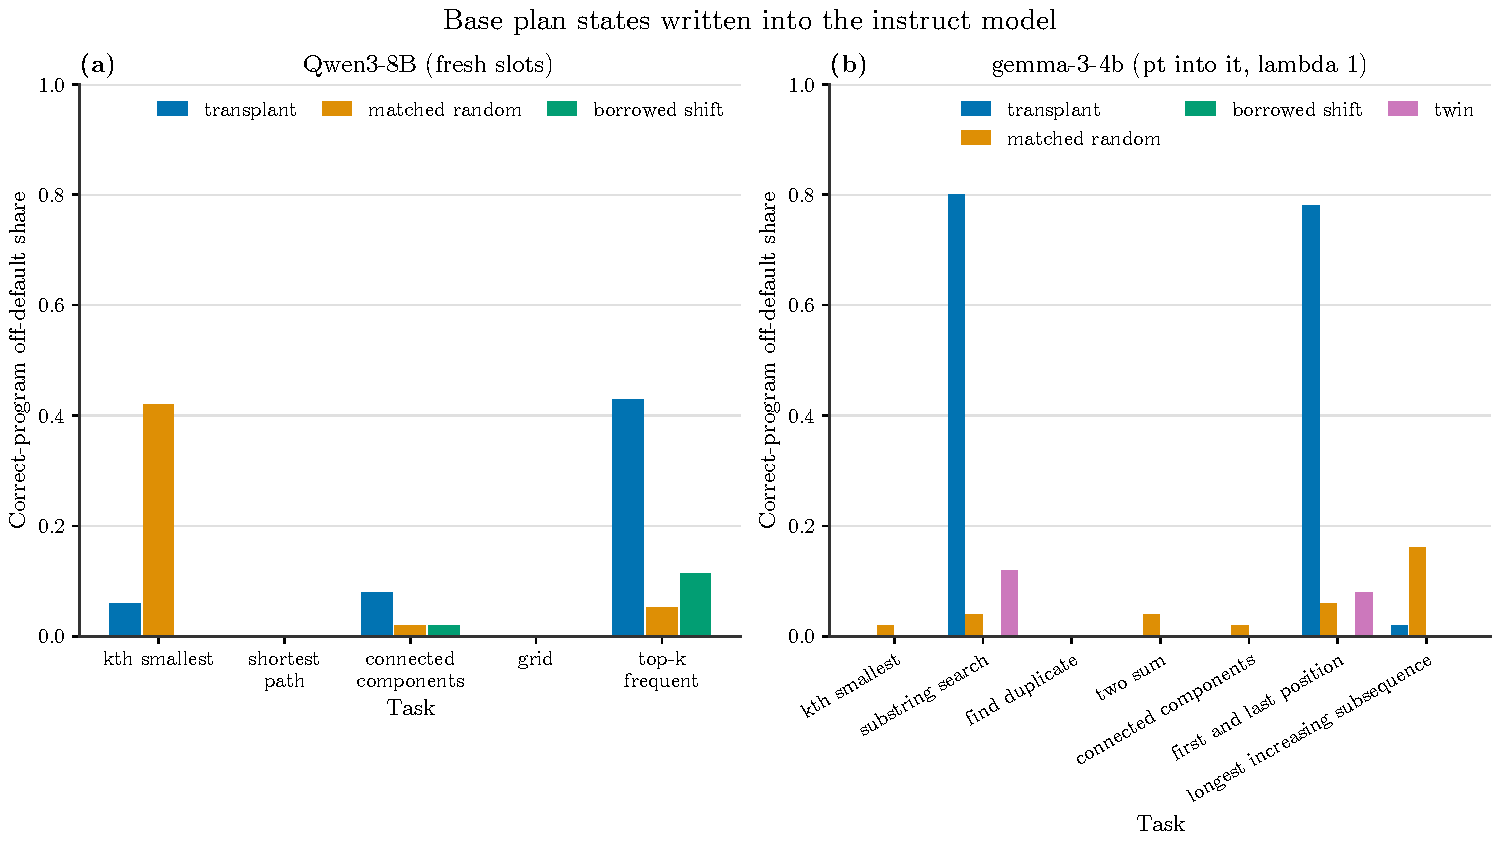
\includegraphics[width=\linewidth,height=0.78\textheight,keepaspectratio]{figures/fig_transplant_v0.pdf}
\caption{Correct-program off-default share -- the fraction of a condition's correct programs (out of \$N=50\$ common-random-number slots per task) that implement an algorithm other than the instruct model's own default -- under a transplant of base-model task-specification states into the instruct prefill, against matched-norm-random and cross-task borrowed-shift controls on the same slots. Blue bars (transplant) use one colour in both panels; orange is the matched-random control and green the borrowed-shift control, also shared across both panels; magenta, in (b) only, is the instruct twin's own unperturbed off-default rate. (a) Qwen3-8B, five tasks whose base model is diverse, fresh confirmation slots, each task at its own selected \$\textbackslash{}lambda\$ (kth smallest 1, shortest path 0.25, connected components 0.5, grid 0.25, top-k frequent 1). The transplant reaches 0.43 of correct top-k-frequent programs but only 0.00-0.08 on the other four tasks; on kth smallest the matched-random control (0.42) moves more correct programs off the default than the transplant itself (0.06). (b) gemma-3-4b-pt states transplanted into gemma-3-4b-it at \$\textbackslash{}lambda=1\$ on its seven base-diverse tasks. The transplant reaches 0.80 of correct substring-search programs and 0.78 of correct first-and-last-position programs -- both above the it twin's own baseline of 0.12 and 0.08 -- and stays at 0.00-0.02 on the other five tasks. The borrowed-shift control is 0.00 on every task in (b); it and the matched-random control there are computed over far fewer correct programs than the transplant or the twin, since both controls broke most generations (pass ratios 0-0.22 and 0.16-0.50, not plotted).}
\label{fig:fig_transplant}
\end{figure}
\textbf{Novelty, audited again.} No artifact of this iteration found a correct novel algorithm (Table 223), including the base model's own output and the transplanted output.

\begin{table}[H]
\renewcommand{\thetable}{223}
\centering\footnotesize\setlength{\tabcolsep}{4.0pt}
\caption{Novelty audits of iteration 5. Sources: the novelty audit files of the five experiments. [Source: iteration 5, compiled across the iteration's artifacts \nolinkurl{gen_art_evaluation_4}, \nolinkurl{gen_art_experiment_24}, \nolinkurl{gen_art_experiment_25}, \nolinkurl{gen_art_experiment_26}, \nolinkurl{gen_art_experiment_27}, \nolinkurl{gen_art_experiment_28}, \nolinkurl{gen_art_research_2}.]}\label{tab:t240}
\begin{tabular}{>{\raggedright\arraybackslash\hspace{0pt}}p{0.1120\linewidth}>{\raggedright\arraybackslash\hspace{0pt}}p{0.1828\linewidth}>{\raggedright\arraybackslash\hspace{0pt}}p{0.1344\linewidth}>{\raggedright\arraybackslash\hspace{0pt}}p{0.4141\linewidth}>{\raggedright\arraybackslash\hspace{0pt}}p{0.0699\linewidth}}
\toprule
\textbf{Artifact} & \textbf{Correct programs in the pool} & \textbf{Correct programs outside the catalogue} & \textbf{Final classes} & \textbf{Novel} \\
\midrule
Transplant experiment & all arms, base model included & 48 & 27 known techniques outside the frozen catalogue, 12 degenerate, 9 catalogue variants (judges called 14 novel) & 0 \\
Panel A & 6,854 & 2 & 1 catalogue variant, 1 degenerate & 0 \\
Panel B & 10,366 & 12 & 7 catalogue variants, 5 degenerate & 0 \\
Knob experiment & every correct program labelled other & 12 & 10 labeller misses, 1 degenerate, 1 unresolved & 0 \\
Gemma experiment & every correct program labelled other & 56 & 35 catalogue variants, 21 degenerate & 0 \\
\bottomrule
\end{tabular}
\end{table}

\FloatBarrier
\subsection*{5.11 What iteration 5 established, what it ruled out, and what it abandoned}
\addcontentsline{toc}{subsection}{5.11 What iteration 5 established, what it ruled out, and what it abandoned}
Everything below is one or two model families at 4B to 8B parameters, memorised tasks in the style of LeetCode, and labels from gated labellers, except the base-model labels of Gemma, which agree with an adjudication at only 0.64. Every Qwen3-8B number of this iteration comes from a bf16 engine.

\textbf{Established.}

\begin{enumerate}
\item \emph{Temperature does not change the algorithm, under every sampler the run used.} With thinking on, top-k 10 and the same seed, the algorithm changed in 0 of 20 seeds across four temperatures on the shortest path task, and the first approach named in the thinking never changed.
\item \emph{(Moved to the descriptive results, iteration 6.)} \emph{Where a random nudge moves the instruct model, it often lands on the base model's runner-up.} Per set the base runner-up named the push landing 5 of 5 on the 8-bit screen, 1 of 2 on the bf16 remeasurement of existing tasks, 3 of 3 in panel A, 3 of 4 in panel B and 5 of 7 in Gemma (17 of 21, Poisson-binomial p 5.8e-07); on new tasks 6 of 7 events (Poisson-binomial p 0.003). 6 of the 11 held-out hits are also the instruct twin's own minority: on the 8 held-out events where the instruct twin wrote no correct program off the default the base runner-up named 5 (p 0.053; Qwen3-8B 3 of 4, p 0.052; Gemma 2 of 4, p 0.422), and the twin's own most frequent alternative, defined on 7 of 21 events, named 6 of them against 6 for the base runner-up (exact McNemar p 1.000). Where the twin writes an alternative at all, the landing half is therefore the twin's own minority, and the base model adds a forecast only on the events where the twin writes none (iteration-6 correction; record audit, Table 230), with the base composition ahead of association by 0.75 nats (exact Wilcoxon p 0.055 with the corrected association) and of proximity by 0.50. In Gemma it named 5 of 7 (p 0.025; 1.50 nats over association with undefined association forecasts filled uniformly, 1.57 on the 6 defined events, p 0.023), and on the existing Qwen3-8B tasks 5 of 5. In panel A no nudged program landed outside the base repertoire.
\item \emph{The base model is more diverse than the instruct model on most tasks under identical prompts.} The instruct twin wrote its default in 96\% to 100\% of programs on all 15 existing tasks, while 5 tasks were diverse in the base and 7 intermediate, and every new unit but one had beta of at least 0.05. The base model's own correct output is thin under the chat template (14 to 55 correct programs per 100 to 200 on the existing tasks). Three instruct twins of new units are mixed (trapped rain water default share 0.64, minimum spanning tree weight default share 0.66, valid anagram default share 0.76). On two new units the instruct twin is more diverse than the base: trapped rain water (twin off-default 0.36 against beta 0.23) and minimum spanning tree weight (0.34 against 0.11), and on both the landing is the twin's own minority (iteration-6 correction).
\item \emph{Plan noise's effect is not its token-level departure from the twin, on kth smallest.} At alpha 2 it moved 19 slots against 3 for decoding matched to its per-token KL (exact p 8.6e-04), but the discordant counts are kth smallest 13:0, connected components 1:3, shortest path 2:0, two sum 2:0, grid 1:0: without kth smallest the other four tasks give 6:3 (p 0.508); at alpha 1 the pooled count is 4:3 (p 1.000); bf16-conditional (iteration-6 correction; record audit, Table 233).
\item \emph{The record repairs.} The held-out movability test is inconclusive under catalogue-only avoidance and disconfirmed under the drop sensitivity; the read position and condition sentence are inert only at per-position doses up to 4 ban units; landing comparisons on matched events give push -0.76 against association -3.11 on 3 events and -1.37 against -3.46 on 5.
\end{enumerate}

\textbf{Ruled out, or not supported.}

\begin{itemize}
\item \emph{The movability half: the base repertoire predicts which tasks a nudge moves.} Not supported as a strong predictor, and not disconfirmed (ban-free unit and iteration-5 seeds; re-tagged by iteration 7's dose-unit experiment, Section 7.6: at D* = D1 kth smallest and connected components are movable, and shortest path, two sum and the grid are not) (iteration-8 correction): beta is not a strong predictor of movability (Spearman 0.15 over 13 new units, Bonett-Wright 95\% [-0.44, 0.65], bootstrap BCa [-0.50, 0.70], one-sided permutation p 0.317; power of the registered one-sided permutation test about 0.63 at a true 0.6, 0.50 two-sided, and 20 units for 0.8); a moderate relation is not excluded at this n; conditional on the design of iteration 5 (bf16 with the ban-free unit and its direction seeds; the engine control of Section 6.3 shows that the numerics alone do not shrink the escapes). The pooled value rests on the beta of count inversions, 0.75, which the panel committed on the attempt basis because only a few base programs were correct (67\% of its attempts fall in the class other); on the correct-only basis used for the other twelve units its beta is 0.13 and the pooled Spearman is 0.035. Per panel Spearman -0.03 (A) and 0.21 (B); 4 of 10 new units diverse in the base never moved. Under one definition of each rival, pooled over the 13 units with signs fixed so that the predicted direction is positive: opening margin 0.08 (Holm p 1.000, delta +0.07 [-0.66, 0.88]); novelty-instruction excess -0.50 (Holm p 1.000, delta +0.65 [-0.06, 1.34]); runtime merit 0.71 (Holm p 0.021, delta -0.57 [-1.26, 0.20]); twin modal share 0.41 (Holm p 0.347, delta -0.26 [-1.05, 0.56]); catalogue size -0.21 (Holm p 1.000, delta +0.35 [-0.57, 1.24]). Under Holm only runtime merit tracks movability, while beta does not; the paired interval for beta minus that rival still includes 0 (iteration-6 correction; record audit, Table 232). The screen correlation of 0.78 did not transfer to new tasks. (iteration-7 correction)
\item \emph{The transplant claim: a transplant of base plan states reopens the base repertoire.} Disconfirmed by the frozen rule (1 of 5 tasks diverse in the base); on kth smallest a matched-norm random displacement moved more programs than the base states (2:20). The narrowing installed by tuning is not carried by the task-specification states of blocks 12 to 23 alone.
\item \emph{The push toward the base.} A push along the base minus instruct direction never escaped at 0.5 to 2 ban-free units, while an isotropic push did on kth smallest.
\item \emph{The plan sampler comparison: plan noise prices at least as well as text-level plan samplers.} Disconfirmed (1 of 5 decisive tasks) (ban-free unit and iteration-5 seeds; re-tagged by iteration 7's dose-unit experiment, Section 7.6: at the moving design D* = D1 the plan-sampler rule is still disconfirmed, at 2 of 5) (iteration-8 correction); base intent won on connected components, the shortest path task and two sum. (iteration-7 correction)
\end{itemize}

\textbf{Inconclusive.}

\begin{itemize}
\item \emph{The movability half in Gemma.} Spearman 0.42 (p 0.060), with the twin modal share and the novelty instruction ahead of beta; descriptively 6 of 7 tasks diverse in the base moved against 2 of 8 others.
\item \emph{Top-k frequent.} The one Qwen3-8B task where the transplant reopened the base runner-up also gained 20 pass points, so restored correctness and a reopened choice are not separated.
\end{itemize}

\textbf{Dead ends, with the evidence that closed them.}

\begin{itemize}
\item \emph{The base minus instruct direction as a knob.} Closed by Table 186: it never escapes, and the difference it encodes is mostly shared across tasks (cosine 0.76 to 0.88) and larger than the dose at which random noise breaks programs.
\item \emph{Transplanting at the read position.} The base and instruct states differ there by about the size of the residual, and the transplant broke the output on 13 of 15 tasks without moving an algorithm.
\item \emph{Plan noise as the practical knob for algorithmic diversity.} On the decisive tasks two text-level samplers price better, and under the bf16 engine and ban-free unit plan noise moves more than 10\% of programs only on kth smallest (conditional on the design of iteration 5, bf16 with the ban-free unit and its direction seeds: at the absolute unit and seeds of iteration 4 the bf16 engine reproduces the 8-bit effects on connected components and the shortest path task, Section 6.3; iteration-6 correction).
\item \emph{Signed progress toward the runner-up as the next predictor.} Closed in the record audit (Table 177): concentrated on one task, negative on two, matched by a within-class control.
\end{itemize}

\FloatBarrier
\subsection*{5.12 What the next iteration takes from this one}
\addcontentsline{toc}{subsection}{5.12 What the next iteration takes from this one}
The narrowed repertoire account split in two. Its landing half held descriptively in both families and on unseen tasks (5 of 5 on the 8-bit screen, 1 of 2 on the bf16 remeasurement of existing tasks, 3 of 3 in panel A, 3 of 4 in panel B and 5 of 7 in Gemma (17 of 21, Poisson-binomial p 5.8e-07)), but it is not yet separated from the instruct twin's own minority (on the 8 held-out events where the instruct twin wrote no correct program off the default the base runner-up named 5 (p 0.053; Qwen3-8B 3 of 4, p 0.052; Gemma 2 of 4, p 0.422); iteration-6 correction): when a nudge moves the instruct model, it moves it to the algorithm the base model writes next, and a forecast built from base samples, before any push, names that landing better than the model's stated alternative. Its movability half failed on unseen tasks: a base model that writes many algorithms does not mark a task the instruct model can be nudged off, and its states, written into the instruct prefill, reopen the choice on one task in five. The base repertoire marks where a nudge can lead, not whether it can lead anywhere.

The open question is therefore what makes a task diverse in the base immovable. Count primes and valid anagram (beta 0.81 each) never moved, while trapped rain water (0.23) did. Two leads came out of this iteration's data. In panel A the three units that moved had an alternative at least twice as fast as the default and the three that did not had none, although median of two sorted lists broke the pattern. And in the transplant experiment early blocks 0 to 11 moved kth smallest and connected components more than the main band, which suggests the narrowing sits at least partly upstream of blocks 12 to 23. The positioning audit names the baselines a further test needs: weight interpolation between the base and instruct models, layer restoration at the transplant's block ranges, and token-level base and aligned collaboration [92, 93, 94, 102]. Base intent, which beat plan noise on three of five tasks, is the strongest practical knob the run has priced, and it is itself a form of that collaboration at the level of sentences. Finally, movability has to be measured under the engine and unit at which it will be used: the six screen-movable tasks of iteration 4 shrank to two under bf16 and the ban-free unit, for reasons this iteration did not establish. \emph{(Iteration-6 correction: a dose-bracketed contrast rules out a scalar dose shortfall on connected components and shortest path, and the engine control rules out the bf16 numerics, since at iteration 4's absolute unit and seeds bf16 reproduces the 8-bit escapes (Section 6.3). What remains is the per-position and per-block profile of the ban-free unit, or the direction seeds; every verdict that rests on bf16 plan noise or escape fractions at the ban-free unit is conditional on that design.)}

\FloatBarrier
\section{Iteration 6: an engine control, where a ban and an instruction are carried, a one-token fork in Gemma, and the plan in words}
\noindent\emph{Run record for this iteration.} Hypothesis carried: ``A Hidden Plan Tilts One Deciding Token''. Move recorded at the end of the iteration: deepen; review score 5; evidence state lead; coverage partial; 14 candidate strategies considered. The list below gives the iteration's artifacts and the state the round record gave each strand.

{\footnotesize\setlength{\tabcolsep}{3pt}
\begin{longtable}{>{\raggedright\arraybackslash}p{0.24\linewidth}>{\raggedright\arraybackslash}p{0.47\linewidth}>{\raggedright\arraybackslash}p{0.11\linewidth}>{\raggedright\arraybackslash}p{0.08\linewidth}}
\caption*{\textbf{Artifacts of iteration 6.} Names and titles as the artifact workspaces record them; strand state as the round record grades it.}\label{tab:arts6}\\
\toprule \textbf{Artifact} & \textbf{Title} & \textbf{Type} & \textbf{State} \\ \midrule \endfirsthead
\toprule \textbf{Artifact} & \textbf{Title} & \textbf{Type} & \textbf{State} \\ \midrule \endhead
\bottomrule \endlastfoot
\nolinkurl{gen_art_evaluation_5} & Record repair and blind novelty re-check & evaluation & null \\
\nolinkurl{gen_art_experiment_29} & Is FP8 rounding behind the random-push escapes? & experiment & lead \\
\nolinkurl{gen_art_experiment_30} & Where a coding model decides its algorithm & experiment & lead \\
\nolinkurl{gen_art_experiment_31} & Where Gemma picks BFS or DFS, and steering it & experiment & lead \\
\nolinkurl{gen_art_experiment_32} & Reading an LLM's planned algorithm in words & experiment & lead \\
\nolinkurl{gen_art_research_3} & Who already found the hidden plan? & research & null \\
\end{longtable}}

\subsection*{What each artifact of iteration 6 was for and what it produced}
\addcontentsline{toc}{subsection}{What each artifact of iteration 6 was for and what it produced}
Each artifact is named below as the run's workspaces name it. The entry gives the round record's verdict on the strand it served, the artifact's own summary of what it was for and what it produced, and the output files it declared, each opened and read from its workspace for this report. It closes with the subsection of this section that reports the artifact's results and the result tables typeset there from its output files.

\paragraph{\nolinkurl{gen_art_evaluation_5}: Record repair and blind novelty re-check.}
Type: evaluation. Round record, strand state null: CPU record repair: 36 corrections (78 match, power corrected to 0.63); blind re-adjudication finds 0 of 14 novel. Bookkeeping; tests no claim of the request.

\emph{The artifact's own summary of what it was for and what it produced:} CPU-only record repair (iteration-6 Step 0) of the run's report, plus a second blind novelty adjudication. Provides: corrections.json (36 report corrections, each a verbatim old\_\allowbreak{}text from current\_\allowbreak{}report.md -\textgreater{} new\_\allowbreak{}text, keyed to section and line, with values \{recorded, recomputed, MATCH\slash{}CORRECTED\slash{}NEW\slash{}CARRIED, '\textless{}artifact\_\allowbreak{}id\textgreater{}:\textless{}path\textgreater{}' source\}; 78 MATCH, 1 CORRECTED, 18 NEW, 2 CARRIED; no overlaps); eval\_\allowbreak{}out.json (exp\_\allowbreak{}eval\_\allowbreak{}sol\_\allowbreak{}out; 10 datasets, \textasciitilde{}372 metrics); engine\_\allowbreak{}labels.json (24 internal results tagged by numerics: HF-FP8-W8A8, vLLM-FP8 W8A16 Marlin, HF-bf16); tables\slash{}*.csv; figures\slash{}fig\_\allowbreak{}beta\_\allowbreak{}escape\_\allowbreak{}l4l (bf16 like-for-like). KEY RESULTS. (0a) The two artifacts' off\_\allowbreak{}default\_\allowbreak{}share fields use different definitions (bf16: correct off-default\slash{}N; FP8: valid attempts off-default\slash{}N); a mean of per-position ratios (0.83-1.39) is not Table 174's ratio of mean norms (0.62-0.97). Dose-bracketed contrast (bf16 alpha 2 \textgreater{}= 1.24 FP8 ban units vs FP8 alpha 1): connected components (bf16 1\slash{}50 vs FP8 30\slash{}50 at alpha 2, Fisher p 7.2e-11; bracket p 0.056) and shortest path (2\slash{}47 vs 15\slash{}37, p 5.3e-5; bracket p 0.017) 'did NOT replicate in bf16 at the population level'; kth smallest and grid 'not established'; two sum\slash{}find duplicate had no FP8 effect. Site odds ratio, same-seed contrast and plan subspace: FP8 only, untested in bf16. (0b) Landings 17\slash{}21 per set (5\slash{}5 screen, 1\slash{}2 bf16 remeasure, 3\slash{}3 A, 3\slash{}4 B, 5\slash{}7 Gemma; Poisson-binomial p 5.8e-7) but the unconfounded held-out subset is 5\slash{}8 (p 0.053), so 5.11 item 2 moves to descriptive; the twin's own most frequent alternative matches the base runner-up on the 7 events where it is defined (6 vs 6). (0c) Movability rho(beta,E) 0.146 over 13 new units, Bonett-Wright 95\% [-0.44, 0.65], BCa [-0.50, 0.70], power 0.63 one-sided (0.50 two-sided) at a true 0.6, n=20 needed; 0.035 if count inversions' beta is taken from correct programs (its committed beta 0.75 comes from attempts, 67\% 'other'); only runtime merit R6 tracks movability (rho 0.71, Holm p 0.021). (0d\slash{}0e) Table 206 phrasing columns, P15\slash{}P20 with bootstrap intervals, panel B knob rows (Table 203b), Table 126c rows, per-task PN-vs-DMD counts (19:3 but 13:0 on kth smallest), Gemma fill rule. (0f) 14 disputed programs sandbox-stress-tested, nearest known solutions by Zhang-Shasha AST distance, judged blind by Mistral Medium 3.1 (x3, T=0) and Kimi K2 with 10 controls: gates 9\slash{}10 each; Mistral called 1\slash{}14 novel (P13, a linear search; overturned on full read), Kimi 0\slash{}14; final novel count 0; one manual class corrected (P21: linear scan + list.count). Audits: audit\slash{}rederive.py 277\slash{}277 checks with 5\slash{}5 placebos failing; audit\slash{}headline\_\allowbreak{}check.py reproduces 7\slash{}7 headline numbers from raw files with placebos failing. OpenRouter spend USD 0.29 over 4 judge passes (cache makes reruns free). Inputs located by artifact id under AII\_\allowbreak{}DEPS\_\allowbreak{}ROOT; report and two non-dependency evaluations vendored in inputs\slash{}.

Its results are reported in Subsection 6.2 of this report, which typesets the result tables drawn from its output files: Tables 226, 227, 228, 229, 230, 231, 232, 233, 234.

\begin{table}[H]
\renewcommand{\thetable}{O40}
\centering\footnotesize\setlength{\tabcolsep}{3pt}
\caption{Output files declared by \nolinkurl{gen_art_evaluation_5} (iteration 6), each opened and read from the artifact's workspace for this report; size in bytes. [Source: iteration 6, artifact \nolinkurl{gen_art_evaluation_5}.]}
\begin{tabular}{>{\raggedright\arraybackslash}p{0.25\linewidth}>{\raggedleft\arraybackslash}p{0.12\linewidth}>{\raggedright\arraybackslash}p{0.57\linewidth}}
\toprule
\textbf{Declared file} & \textbf{Bytes} & \textbf{What it holds} \\
\midrule
\texttt{eval.\allowbreak{}py} & 109,686 & the artifact's code, 1,576 lines \\
\texttt{full\_\allowbreak{}eval\_\allowbreak{}out.\allowbreak{}json} & 200,561 & the complete output; metadata with 8 top-level keys; 10 datasets with 242 examples in all: dose\_\allowbreak{}reconciliation (14), engine\_\allowbreak{}pn\_\allowbreak{}contrast (12), engine\_\allowbreak{}labels (24), landing\_\allowbreak{}events (21), movability\_\allowbreak{}units (15), rival\_\allowbreak{}scores (5), and 4 more; top-level keys metrics\_\allowbreak{}agg; 372 aggregate metrics (typeset in full below) \\
\texttt{mini\_\allowbreak{}eval\_\allowbreak{}out.\allowbreak{}json} & 41,665 & small variant of the full output (a few examples per dataset); metadata with 8 top-level keys; 10 datasets; top-level keys metrics\_\allowbreak{}agg \\
\texttt{preview\_\allowbreak{}eval\_\allowbreak{}out.\allowbreak{}json} & 24,480 & preview variant of the full output (truncated strings and lists); metadata with 8 top-level keys; 3 datasets; top-level keys metrics\_\allowbreak{}agg \\
\texttt{reproducibility.\allowbreak{}md} & 11,844 & reproducibility notes, 228 lines \\
\bottomrule
\end{tabular}
\end{table}

{\scriptsize\setlength{\tabcolsep}{2.5pt}\renewcommand{\thetable}{O41}
\begin{longtable}{>{\raggedright\arraybackslash}p{0.27\linewidth}>{\raggedright\arraybackslash}p{0.19\linewidth}>{\raggedright\arraybackslash}p{0.27\linewidth}>{\raggedright\arraybackslash}p{0.19\linewidth}}
\caption{Every aggregate metric in the \texttt{metrics\_agg} block of \nolinkurl{gen_art_evaluation_5}'s \texttt{full\_\allowbreak{}eval\_\allowbreak{}out.\allowbreak{}json} (372 metrics), values copied exactly as stored. [Source: iteration 6, artifact \nolinkurl{gen_art_evaluation_5}.]}\\
\toprule
\textbf{Metric} & \textbf{Value} & \textbf{Metric} & \textbf{Value} \\
\midrule
\endfirsthead
\toprule
\textbf{Metric} & \textbf{Value} & \textbf{Metric} & \textbf{Value} \\
\midrule
\endhead
\bottomrule
\endlastfoot
\texttt{dose\_\allowbreak{}ratio\_\allowbreak{}meanratio\_\allowbreak{}T1} & 0.8742541482051215 & \texttt{rho\_\allowbreak{}beta\_\allowbreak{}E\_\allowbreak{}correct\_\allowbreak{}only\_\allowbreak{}basis} & 0.03494282789073061 \\
\texttt{dose\_\allowbreak{}ratio\_\allowbreak{}ratioofmeans\_\allowbreak{}T1} & 0.7510728240013123 & \texttt{rho\_\allowbreak{}perm\_\allowbreak{}p\_\allowbreak{}correct\_\allowbreak{}only\_\allowbreak{}basis} & 0.45776271118644407 \\
\texttt{dose\_\allowbreak{}ratio\_\allowbreak{}meanratio\_\allowbreak{}T2} & 0.8892610977093378 & \texttt{power\_\allowbreak{}rho04} & 0.3316 \\
\texttt{dose\_\allowbreak{}ratio\_\allowbreak{}ratioofmeans\_\allowbreak{}T2} & 0.8335155248641968 & \texttt{power\_\allowbreak{}two\_\allowbreak{}sided\_\allowbreak{}rho04} & 0.2228 \\
\texttt{dose\_\allowbreak{}ratio\_\allowbreak{}meanratio\_\allowbreak{}T03} & 1.3938049693902332 & \texttt{power\_\allowbreak{}rho06} & 0.6343 \\
\texttt{dose\_\allowbreak{}ratio\_\allowbreak{}ratioofmeans\_\allowbreak{}T03} & 0.9735943675041199 & \texttt{power\_\allowbreak{}two\_\allowbreak{}sided\_\allowbreak{}rho06} & 0.4989 \\
\texttt{dose\_\allowbreak{}ratio\_\allowbreak{}meanratio\_\allowbreak{}T05} & 0.9949302176634469 & \texttt{power\_\allowbreak{}rho08} & 0.9312 \\
\texttt{dose\_\allowbreak{}ratio\_\allowbreak{}ratioofmeans\_\allowbreak{}T05} & 0.7773554921150208 & \texttt{power\_\allowbreak{}two\_\allowbreak{}sided\_\allowbreak{}rho08} & 0.8664 \\
\texttt{dose\_\allowbreak{}ratio\_\allowbreak{}meanratio\_\allowbreak{}T06} & 0.8290518095095952 & \texttt{power\_\allowbreak{}rho06\_\allowbreak{}mc\_\allowbreak{}se} & 0.004816259025426269 \\
\texttt{dose\_\allowbreak{}ratio\_\allowbreak{}ratioofmeans\_\allowbreak{}T06} & 0.6199100017547607 & \texttt{n\_\allowbreak{}for\_\allowbreak{}power08\_\allowbreak{}at\_\allowbreak{}rho06} & 20.0 \\
\texttt{dose\_\allowbreak{}ratio\_\allowbreak{}meanratio\_\allowbreak{}T10} & 0.9904374480247494 & \texttt{rho\_\allowbreak{}R1} & 0.07862136275414387 \\
\texttt{dose\_\allowbreak{}ratio\_\allowbreak{}ratioofmeans\_\allowbreak{}T10} & 0.7451708316802979 & \texttt{delta\_\allowbreak{}rho\_\allowbreak{}R1} & 0.06697375345723365 \\
\texttt{dose\_\allowbreak{}ratio\_\allowbreak{}meanratio\_\allowbreak{}T14} & 0.924199037750562 & \texttt{delta\_\allowbreak{}ci\_\allowbreak{}R1\_\allowbreak{}low} & -0.6605963162611997 \\
\texttt{dose\_\allowbreak{}ratio\_\allowbreak{}ratioofmeans\_\allowbreak{}T14} & 0.698820173740387 & \texttt{delta\_\allowbreak{}ci\_\allowbreak{}R1\_\allowbreak{}high} & 0.8819323112314222 \\
\texttt{dose\_\allowbreak{}ratio\_\allowbreak{}meanratio\_\allowbreak{}R6} & 0.8869734982649483 & \texttt{holm\_\allowbreak{}p\_\allowbreak{}R1} & 1.0 \\
\texttt{dose\_\allowbreak{}ratio\_\allowbreak{}ratioofmeans\_\allowbreak{}R6} & 0.6177505254745483 & \texttt{perm\_\allowbreak{}p\_\allowbreak{}R1} & 0.3988730056349718 \\
\texttt{dose\_\allowbreak{}ratio\_\allowbreak{}meanratio\_\allowbreak{}T04} & 0.9759519239266713 & \texttt{rho\_\allowbreak{}R4} & -0.5033258793634009 \\
\texttt{dose\_\allowbreak{}ratio\_\allowbreak{}ratioofmeans\_\allowbreak{}T04} & 0.29637160897254944 & \texttt{delta\_\allowbreak{}rho\_\allowbreak{}R4} & 0.6489209955747784 \\
\texttt{dose\_\allowbreak{}ratio\_\allowbreak{}meanratio\_\allowbreak{}T08} & 1.2340178569157922 & \texttt{delta\_\allowbreak{}ci\_\allowbreak{}R4\_\allowbreak{}low} & -0.06390922654519403 \\
\texttt{dose\_\allowbreak{}ratio\_\allowbreak{}ratioofmeans\_\allowbreak{}T08} & 0.884873628616333 & \texttt{delta\_\allowbreak{}ci\_\allowbreak{}R4\_\allowbreak{}high} & 1.339266425257294 \\
\texttt{dose\_\allowbreak{}ratio\_\allowbreak{}meanratio\_\allowbreak{}T11} & 1.0611259718736012 & \texttt{holm\_\allowbreak{}p\_\allowbreak{}R4} & 1.0 \\
\texttt{dose\_\allowbreak{}ratio\_\allowbreak{}ratioofmeans\_\allowbreak{}T11} & 0.8031708598136902 & \texttt{perm\_\allowbreak{}p\_\allowbreak{}R4} & 0.9603001984990075 \\
\texttt{dose\_\allowbreak{}ratio\_\allowbreak{}meanratio\_\allowbreak{}T13} & 1.3651722828547155 & \texttt{rho\_\allowbreak{}R6} & 0.7134160694357499 \\
\texttt{dose\_\allowbreak{}ratio\_\allowbreak{}ratioofmeans\_\allowbreak{}T13} & 0.9506106376647949 & \texttt{delta\_\allowbreak{}rho\_\allowbreak{}R6} & -0.5678209532243723 \\
\texttt{dose\_\allowbreak{}ratio\_\allowbreak{}meanratio\_\allowbreak{}R1} & 1.0889639874299368 & \texttt{delta\_\allowbreak{}ci\_\allowbreak{}R6\_\allowbreak{}low} & -1.2596144748639095 \\
\texttt{dose\_\allowbreak{}ratio\_\allowbreak{}ratioofmeans\_\allowbreak{}R1} & 0.7607540488243103 & \texttt{delta\_\allowbreak{}ci\_\allowbreak{}R6\_\allowbreak{}high} & 0.20432408080225736 \\
\texttt{dose\_\allowbreak{}ratio\_\allowbreak{}meanratio\_\allowbreak{}R3} & 1.1358933428923286 & \texttt{holm\_\allowbreak{}p\_\allowbreak{}R6} & 0.020749896250518745 \\
\texttt{dose\_\allowbreak{}ratio\_\allowbreak{}ratioofmeans\_\allowbreak{}R3} & 0.8639326095581055 & \texttt{perm\_\allowbreak{}p\_\allowbreak{}R6} & 0.004149979250103749 \\
\texttt{pn\_\allowbreak{}offdef\_\allowbreak{}bf16\_\allowbreak{}a1\_\allowbreak{}T03} & 0.08163265306122448 & \texttt{rho\_\allowbreak{}R7} & 0.4090066997856399 \\
\texttt{pn\_\allowbreak{}offdef\_\allowbreak{}fp8\_\allowbreak{}a1\_\allowbreak{}T03} & 0.28 & \texttt{delta\_\allowbreak{}rho\_\allowbreak{}R7} & -0.2634115835742624 \\
\texttt{pn\_\allowbreak{}offdef\_\allowbreak{}att\_\allowbreak{}bf16\_\allowbreak{}a1\_\allowbreak{}T03} & 0.1 & \texttt{delta\_\allowbreak{}ci\_\allowbreak{}R7\_\allowbreak{}low} & -1.0469101621558425 \\
\texttt{pn\_\allowbreak{}offdef\_\allowbreak{}att\_\allowbreak{}fp8\_\allowbreak{}a1\_\allowbreak{}T03} & 0.28 & \texttt{delta\_\allowbreak{}ci\_\allowbreak{}R7\_\allowbreak{}high} & 0.5616882046348574 \\
\texttt{fisher\_\allowbreak{}p\_\allowbreak{}T03\_\allowbreak{}a1} & 0.017391052373663077 & \texttt{holm\_\allowbreak{}p\_\allowbreak{}R7} & 0.34675826620866895 \\
\texttt{pn\_\allowbreak{}offdef\_\allowbreak{}bf16\_\allowbreak{}a2\_\allowbreak{}T03} & 0.28 & \texttt{perm\_\allowbreak{}p\_\allowbreak{}R7} & 0.08668956655216724 \\
\texttt{pn\_\allowbreak{}offdef\_\allowbreak{}fp8\_\allowbreak{}a2\_\allowbreak{}T03} & 0.48936170212765956 & \texttt{rho\_\allowbreak{}K} & -0.20643348211598284 \\
\texttt{pn\_\allowbreak{}offdef\_\allowbreak{}att\_\allowbreak{}bf16\_\allowbreak{}a2\_\allowbreak{}T03} & 0.28 & \texttt{delta\_\allowbreak{}rho\_\allowbreak{}K} & 0.35202859832736033 \\
\texttt{pn\_\allowbreak{}offdef\_\allowbreak{}att\_\allowbreak{}fp8\_\allowbreak{}a2\_\allowbreak{}T03} & 0.5 & \texttt{delta\_\allowbreak{}ci\_\allowbreak{}K\_\allowbreak{}low} & -0.5740202912035122 \\
\texttt{fisher\_\allowbreak{}p\_\allowbreak{}T03\_\allowbreak{}a2} & 0.03888598628365684 & \texttt{delta\_\allowbreak{}ci\_\allowbreak{}K\_\allowbreak{}high} & 1.2416607465376737 \\
\texttt{bracket\_\allowbreak{}p\_\allowbreak{}T03} & 0.5879763207301328 & \texttt{holm\_\allowbreak{}p\_\allowbreak{}K} & 1.0 \\
\texttt{bracket\_\allowbreak{}p\_\allowbreak{}att\_\allowbreak{}T03} & 0.5879763207301328 & \texttt{perm\_\allowbreak{}p\_\allowbreak{}K} & 0.753401232993835 \\
\texttt{bracket\_\allowbreak{}pass\_\allowbreak{}T03} & 1.0 & \texttt{n\_\allowbreak{}clusters\_\allowbreak{}T03\_\allowbreak{}theta07} & 2.0 \\
\texttt{fold\_\allowbreak{}ratio\_\allowbreak{}T03} & 1.747720364741641 & \texttt{n\_\allowbreak{}clusters\_\allowbreak{}T03\_\allowbreak{}theta08} & 4.0 \\
\texttt{tag\_\allowbreak{}not\_\allowbreak{}replicated\_\allowbreak{}T03} & 0.0 & \texttt{n\_\allowbreak{}clusters\_\allowbreak{}T03\_\allowbreak{}theta09} & 8.0 \\
\texttt{pn\_\allowbreak{}offdef\_\allowbreak{}bf16\_\allowbreak{}a1\_\allowbreak{}T10} & 0.02 & \texttt{n\_\allowbreak{}clusters\_\allowbreak{}T07\_\allowbreak{}theta07} & 3.0 \\
\texttt{pn\_\allowbreak{}offdef\_\allowbreak{}fp8\_\allowbreak{}a1\_\allowbreak{}T10} & 0.12 & \texttt{n\_\allowbreak{}clusters\_\allowbreak{}T07\_\allowbreak{}theta08} & 3.0 \\
\texttt{pn\_\allowbreak{}offdef\_\allowbreak{}att\_\allowbreak{}bf16\_\allowbreak{}a1\_\allowbreak{}T10} & 0.02 & \texttt{n\_\allowbreak{}clusters\_\allowbreak{}T07\_\allowbreak{}theta09} & 10.0 \\
\texttt{pn\_\allowbreak{}offdef\_\allowbreak{}att\_\allowbreak{}fp8\_\allowbreak{}a1\_\allowbreak{}T10} & 0.12 & \texttt{n\_\allowbreak{}clusters\_\allowbreak{}T10\_\allowbreak{}theta07} & 2.0 \\
\texttt{fisher\_\allowbreak{}p\_\allowbreak{}T10\_\allowbreak{}a1} & 0.11174961771814726 & \texttt{n\_\allowbreak{}clusters\_\allowbreak{}T10\_\allowbreak{}theta08} & 3.0 \\
\texttt{pn\_\allowbreak{}offdef\_\allowbreak{}bf16\_\allowbreak{}a2\_\allowbreak{}T10} & 0.02 & \texttt{n\_\allowbreak{}clusters\_\allowbreak{}T10\_\allowbreak{}theta09} & 9.0 \\
\texttt{pn\_\allowbreak{}offdef\_\allowbreak{}fp8\_\allowbreak{}a2\_\allowbreak{}T10} & 0.6 & \texttt{n\_\allowbreak{}clusters\_\allowbreak{}T13\_\allowbreak{}theta07} & 5.0 \\
\texttt{pn\_\allowbreak{}offdef\_\allowbreak{}att\_\allowbreak{}bf16\_\allowbreak{}a2\_\allowbreak{}T10} & 0.02 & \texttt{n\_\allowbreak{}clusters\_\allowbreak{}T13\_\allowbreak{}theta08} & 7.0 \\
\texttt{pn\_\allowbreak{}offdef\_\allowbreak{}att\_\allowbreak{}fp8\_\allowbreak{}a2\_\allowbreak{}T10} & 0.6 & \texttt{n\_\allowbreak{}clusters\_\allowbreak{}T13\_\allowbreak{}theta09} & 12.0 \\
\texttt{fisher\_\allowbreak{}p\_\allowbreak{}T10\_\allowbreak{}a2} & 7.19752603712036$\times10^{-11}$ & \texttt{n\_\allowbreak{}clusters\_\allowbreak{}REP\_\allowbreak{}T07\_\allowbreak{}theta07} & 3.0 \\
\texttt{bracket\_\allowbreak{}p\_\allowbreak{}T10} & 0.05587480885907363 & \texttt{n\_\allowbreak{}clusters\_\allowbreak{}REP\_\allowbreak{}T07\_\allowbreak{}theta08} & 6.0 \\
\texttt{bracket\_\allowbreak{}p\_\allowbreak{}att\_\allowbreak{}T10} & 0.05587480885907363 & \texttt{n\_\allowbreak{}clusters\_\allowbreak{}REP\_\allowbreak{}T07\_\allowbreak{}theta09} & 10.0 \\
\texttt{bracket\_\allowbreak{}pass\_\allowbreak{}T10} & 1.0 & \texttt{P15\_\allowbreak{}PN\_\allowbreak{}T03} & 0.0 \\
\texttt{fold\_\allowbreak{}ratio\_\allowbreak{}T10} & 30.0 & \texttt{P15\_\allowbreak{}EAP\_\allowbreak{}T03} & 0.030000000000000027 \\
\texttt{tag\_\allowbreak{}not\_\allowbreak{}replicated\_\allowbreak{}T10} & 1.0 & \texttt{P20\_\allowbreak{}EAP\_\allowbreak{}T03} & 0.062000000000000055 \\
\texttt{pn\_\allowbreak{}offdef\_\allowbreak{}bf16\_\allowbreak{}a1\_\allowbreak{}T2} & 0.0 & \texttt{P15\_\allowbreak{}BINT\_\allowbreak{}T03} & 0.03299999999999992 \\
\texttt{pn\_\allowbreak{}offdef\_\allowbreak{}fp8\_\allowbreak{}a1\_\allowbreak{}T2} & 0.20930232558139536 & \texttt{P15\_\allowbreak{}NOVELTY\_\allowbreak{}T03} & 0.005600000000000049 \\
\texttt{pn\_\allowbreak{}offdef\_\allowbreak{}att\_\allowbreak{}bf16\_\allowbreak{}a1\_\allowbreak{}T2} & 0.0 & \texttt{P20\_\allowbreak{}NOVELTY\_\allowbreak{}T03} & 0.01759999999999995 \\
\texttt{pn\_\allowbreak{}offdef\_\allowbreak{}att\_\allowbreak{}fp8\_\allowbreak{}a1\_\allowbreak{}T2} & 0.26 & \texttt{P15\_\allowbreak{}IFG\_\allowbreak{}T10} & -2.220446049250313$\times10^{-16}$ \\
\texttt{fisher\_\allowbreak{}p\_\allowbreak{}T2\_\allowbreak{}a1} & 0.0005862975519545438 & \texttt{P15\_\allowbreak{}PSL\_\allowbreak{}T10} & 0.05004999999999993 \\
\texttt{pn\_\allowbreak{}offdef\_\allowbreak{}bf16\_\allowbreak{}a2\_\allowbreak{}T2} & 0.0425531914893617 & \texttt{P15\_\allowbreak{}EAP\_\allowbreak{}T10} & 0.028800000000000048 \\
\texttt{pn\_\allowbreak{}offdef\_\allowbreak{}fp8\_\allowbreak{}a2\_\allowbreak{}T2} & 0.40540540540540543 & \texttt{P20\_\allowbreak{}EAP\_\allowbreak{}T10} & 0.057599999999999985 \\
\texttt{pn\_\allowbreak{}offdef\_\allowbreak{}att\_\allowbreak{}bf16\_\allowbreak{}a2\_\allowbreak{}T2} & 0.1 & \texttt{P15\_\allowbreak{}BINT\_\allowbreak{}T10} & 0.0050000000000000044 \\
\texttt{pn\_\allowbreak{}offdef\_\allowbreak{}att\_\allowbreak{}fp8\_\allowbreak{}a2\_\allowbreak{}T2} & 0.54 & \texttt{P20\_\allowbreak{}BINT\_\allowbreak{}T10} & 0.01079999999999992 \\
\texttt{fisher\_\allowbreak{}p\_\allowbreak{}T2\_\allowbreak{}a2} & 5.278166134237923$\times10^{-5}$ & \texttt{P15\_\allowbreak{}EAP\_\allowbreak{}T2} & 0.10260000000000002 \\
\texttt{bracket\_\allowbreak{}p\_\allowbreak{}T2} & 0.01695641382983751 & \texttt{P20\_\allowbreak{}EAP\_\allowbreak{}T2} & 0.18999999999999995 \\
\texttt{bracket\_\allowbreak{}p\_\allowbreak{}att\_\allowbreak{}T2} & 0.03321456310281156 & \texttt{P15\_\allowbreak{}BINT\_\allowbreak{}T2} & 0.05699999999999994 \\
\texttt{bracket\_\allowbreak{}pass\_\allowbreak{}T2} & 1.0 & \texttt{P15\_\allowbreak{}EAP\_\allowbreak{}T05} & 0.08640000000000003 \\
\texttt{fold\_\allowbreak{}ratio\_\allowbreak{}T2} & 9.527027027027028 & \texttt{P20\_\allowbreak{}EAP\_\allowbreak{}T05} & 0.15680000000000005 \\
\texttt{tag\_\allowbreak{}not\_\allowbreak{}replicated\_\allowbreak{}T2} & 1.0 & \texttt{P15\_\allowbreak{}BINT\_\allowbreak{}T05} & 0.04200000000000004 \\
\texttt{pn\_\allowbreak{}offdef\_\allowbreak{}bf16\_\allowbreak{}a1\_\allowbreak{}T05} & 0.0 & \texttt{P20\_\allowbreak{}BINT\_\allowbreak{}T05} & 0.08040000000000003 \\
\texttt{pn\_\allowbreak{}offdef\_\allowbreak{}fp8\_\allowbreak{}a1\_\allowbreak{}T05} & 0.0 & \texttt{P15\_\allowbreak{}EAP\_\allowbreak{}T1} & 0.22940000000000005 \\
\texttt{pn\_\allowbreak{}offdef\_\allowbreak{}att\_\allowbreak{}bf16\_\allowbreak{}a1\_\allowbreak{}T05} & 0.0 & \texttt{P20\_\allowbreak{}EAP\_\allowbreak{}T1} & 0.34099999999999997 \\
\texttt{pn\_\allowbreak{}offdef\_\allowbreak{}att\_\allowbreak{}fp8\_\allowbreak{}a1\_\allowbreak{}T05} & 0.0 & \texttt{P15\_\allowbreak{}BINT\_\allowbreak{}T1} & 0.42119999999999996 \\
\texttt{fisher\_\allowbreak{}p\_\allowbreak{}T05\_\allowbreak{}a1} & 1.0 & \texttt{P15\_\allowbreak{}NOVELTY\_\allowbreak{}T1} & 0.09599999999999997 \\
\texttt{pn\_\allowbreak{}offdef\_\allowbreak{}bf16\_\allowbreak{}a2\_\allowbreak{}T05} & 0.04 & \texttt{P15\_\allowbreak{}IFG\_\allowbreak{}T04} & 0.0 \\
\texttt{pn\_\allowbreak{}offdef\_\allowbreak{}fp8\_\allowbreak{}a2\_\allowbreak{}T05} & 0.02 & \texttt{P15\_\allowbreak{}EAP\_\allowbreak{}T04} & 0.05483333333333329 \\
\texttt{pn\_\allowbreak{}offdef\_\allowbreak{}att\_\allowbreak{}bf16\_\allowbreak{}a2\_\allowbreak{}T05} & 0.04 & \texttt{P20\_\allowbreak{}EAP\_\allowbreak{}T04} & 0.09800000000000009 \\
\texttt{pn\_\allowbreak{}offdef\_\allowbreak{}att\_\allowbreak{}fp8\_\allowbreak{}a2\_\allowbreak{}T05} & 0.02 & \texttt{P15\_\allowbreak{}IFG\_\allowbreak{}T06} & 0.0 \\
\texttt{fisher\_\allowbreak{}p\_\allowbreak{}T05\_\allowbreak{}a2} & 1.0 & \texttt{P15\_\allowbreak{}PSL\_\allowbreak{}T06} & 0.02300000000000013 \\
\texttt{bracket\_\allowbreak{}p\_\allowbreak{}T05} & 1.0 & \texttt{P15\_\allowbreak{}EAP\_\allowbreak{}T06} & 0.24 \\
\texttt{bracket\_\allowbreak{}p\_\allowbreak{}att\_\allowbreak{}T05} & 1.0 & \texttt{P20\_\allowbreak{}EAP\_\allowbreak{}T06} & 0.38 \\
\texttt{bracket\_\allowbreak{}pass\_\allowbreak{}T05} & 0.0 & \texttt{P15\_\allowbreak{}EAP\_\allowbreak{}T08} & 0.22399999999999998 \\
\texttt{fold\_\allowbreak{}ratio\_\allowbreak{}T05} & 0.5 & \texttt{P15\_\allowbreak{}BINT\_\allowbreak{}T08} & 0.024666666666666615 \\
\texttt{tag\_\allowbreak{}not\_\allowbreak{}replicated\_\allowbreak{}T05} & 0.0 & \texttt{P15\_\allowbreak{}PSL\_\allowbreak{}T11} & 0.0 \\
\texttt{pn\_\allowbreak{}offdef\_\allowbreak{}bf16\_\allowbreak{}a1\_\allowbreak{}T1} & 0.0 & \texttt{P15\_\allowbreak{}EAP\_\allowbreak{}T11} & 0.043333333333333224 \\
\texttt{pn\_\allowbreak{}offdef\_\allowbreak{}fp8\_\allowbreak{}a1\_\allowbreak{}T1} & 0.02857142857142857 & \texttt{P20\_\allowbreak{}EAP\_\allowbreak{}T11} & 0.09999999999999998 \\
\texttt{pn\_\allowbreak{}offdef\_\allowbreak{}att\_\allowbreak{}bf16\_\allowbreak{}a1\_\allowbreak{}T1} & 0.0 & \texttt{P15\_\allowbreak{}EAP\_\allowbreak{}T13} & 0.5553333333333332 \\
\texttt{pn\_\allowbreak{}offdef\_\allowbreak{}att\_\allowbreak{}fp8\_\allowbreak{}a1\_\allowbreak{}T1} & 0.06 & \texttt{P15\_\allowbreak{}EAP\_\allowbreak{}T14} & 0.014000000000000012 \\
\texttt{fisher\_\allowbreak{}p\_\allowbreak{}T1\_\allowbreak{}a1} & 0.4666666666666666 & \texttt{P20\_\allowbreak{}EAP\_\allowbreak{}T14} & 0.026000000000000134 \\
\texttt{pn\_\allowbreak{}offdef\_\allowbreak{}bf16\_\allowbreak{}a2\_\allowbreak{}T1} & 0.02631578947368421 & \texttt{P15\_\allowbreak{}EAP\_\allowbreak{}R2} & 0.3593333333333334 \\
\texttt{pn\_\allowbreak{}offdef\_\allowbreak{}fp8\_\allowbreak{}a2\_\allowbreak{}T1} & 0.1111111111111111 & \texttt{P20\_\allowbreak{}EAP\_\allowbreak{}R2} & 0.528 \\
\texttt{pn\_\allowbreak{}offdef\_\allowbreak{}att\_\allowbreak{}bf16\_\allowbreak{}a2\_\allowbreak{}T1} & 0.04 & \texttt{P15\_\allowbreak{}BINT\_\allowbreak{}R2} & 0.47000000000000003 \\
\texttt{pn\_\allowbreak{}offdef\_\allowbreak{}att\_\allowbreak{}fp8\_\allowbreak{}a2\_\allowbreak{}T1} & 0.24 & \texttt{P15\_\allowbreak{}EAP\_\allowbreak{}R6} & -1.1102230246251565$\times10^{-16}$ \\
\texttt{fisher\_\allowbreak{}p\_\allowbreak{}T1\_\allowbreak{}a2} & 0.19351726799151076 & \texttt{P20\_\allowbreak{}EAP\_\allowbreak{}R6} & -1.1102230246251565$\times10^{-16}$ \\
\texttt{bracket\_\allowbreak{}p\_\allowbreak{}T1} & 0.732496194824962 & \texttt{panelB\_\allowbreak{}push\_\allowbreak{}programs\_\allowbreak{}outside\_\allowbreak{}base} & 3.0 \\
\texttt{bracket\_\allowbreak{}p\_\allowbreak{}att\_\allowbreak{}T1} & 0.5 & \texttt{table126c\_\allowbreak{}hill\_\allowbreak{}K0522} & 2.8660795259673657 \\
\texttt{bracket\_\allowbreak{}pass\_\allowbreak{}T1} & 1.0 & \texttt{table126c\_\allowbreak{}passcost\_\allowbreak{}K0522} & -12.000000000000002 \\
\texttt{fold\_\allowbreak{}ratio\_\allowbreak{}T1} & 4.222222222222222 & \texttt{table126c\_\allowbreak{}hill\_\allowbreak{}K0523} & 2.9557941886061783 \\
\texttt{tag\_\allowbreak{}not\_\allowbreak{}replicated\_\allowbreak{}T1} & 0.0 & \texttt{table126c\_\allowbreak{}passcost\_\allowbreak{}K0523} & -27.0 \\
\texttt{pn\_\allowbreak{}offdef\_\allowbreak{}bf16\_\allowbreak{}a1\_\allowbreak{}T06} & 0.0 & \texttt{table126c\_\allowbreak{}hill\_\allowbreak{}K0524} & 2.9157229709161068 \\
\texttt{pn\_\allowbreak{}offdef\_\allowbreak{}fp8\_\allowbreak{}a1\_\allowbreak{}T06} & 0.0 & \texttt{table126c\_\allowbreak{}passcost\_\allowbreak{}K0524} & -15.0 \\
\texttt{pn\_\allowbreak{}offdef\_\allowbreak{}att\_\allowbreak{}bf16\_\allowbreak{}a1\_\allowbreak{}T06} & 0.0 & \texttt{pn\_\allowbreak{}dmd\_\allowbreak{}disc\_\allowbreak{}T03\_\allowbreak{}alpha1\_\allowbreak{}pn} & 3.0 \\
\texttt{pn\_\allowbreak{}offdef\_\allowbreak{}att\_\allowbreak{}fp8\_\allowbreak{}a1\_\allowbreak{}T06} & 0.0 & \texttt{pn\_\allowbreak{}dmd\_\allowbreak{}disc\_\allowbreak{}T03\_\allowbreak{}alpha1\_\allowbreak{}dmd} & 0.0 \\
\texttt{fisher\_\allowbreak{}p\_\allowbreak{}T06\_\allowbreak{}a1} & 1.0 & \texttt{pn\_\allowbreak{}dmd\_\allowbreak{}p\_\allowbreak{}T03\_\allowbreak{}alpha1} & 0.25 \\
\texttt{pn\_\allowbreak{}offdef\_\allowbreak{}bf16\_\allowbreak{}a2\_\allowbreak{}T06} & 0.0 & \texttt{pn\_\allowbreak{}dmd\_\allowbreak{}disc\_\allowbreak{}T03\_\allowbreak{}alpha2\_\allowbreak{}pn} & 13.0 \\
\texttt{pn\_\allowbreak{}offdef\_\allowbreak{}fp8\_\allowbreak{}a2\_\allowbreak{}T06} & 0.0 & \texttt{pn\_\allowbreak{}dmd\_\allowbreak{}disc\_\allowbreak{}T03\_\allowbreak{}alpha2\_\allowbreak{}dmd} & 0.0 \\
\texttt{pn\_\allowbreak{}offdef\_\allowbreak{}att\_\allowbreak{}bf16\_\allowbreak{}a2\_\allowbreak{}T06} & 0.0 & \texttt{pn\_\allowbreak{}dmd\_\allowbreak{}p\_\allowbreak{}T03\_\allowbreak{}alpha2} & 0.000244140625 \\
\texttt{pn\_\allowbreak{}offdef\_\allowbreak{}att\_\allowbreak{}fp8\_\allowbreak{}a2\_\allowbreak{}T06} & 0.02 & \texttt{pn\_\allowbreak{}dmd\_\allowbreak{}disc\_\allowbreak{}T10\_\allowbreak{}alpha1\_\allowbreak{}pn} & 1.0 \\
\texttt{fisher\_\allowbreak{}p\_\allowbreak{}T06\_\allowbreak{}a2} & 1.0 & \texttt{pn\_\allowbreak{}dmd\_\allowbreak{}disc\_\allowbreak{}T10\_\allowbreak{}alpha1\_\allowbreak{}dmd} & 2.0 \\
\texttt{bracket\_\allowbreak{}p\_\allowbreak{}T06} & 1.0 & \texttt{pn\_\allowbreak{}dmd\_\allowbreak{}p\_\allowbreak{}T10\_\allowbreak{}alpha1} & 1.0 \\
\texttt{bracket\_\allowbreak{}p\_\allowbreak{}att\_\allowbreak{}T06} & 1.0 & \texttt{pn\_\allowbreak{}dmd\_\allowbreak{}disc\_\allowbreak{}T10\_\allowbreak{}alpha2\_\allowbreak{}pn} & 1.0 \\
\texttt{bracket\_\allowbreak{}pass\_\allowbreak{}T06} & 1.0 & \texttt{pn\_\allowbreak{}dmd\_\allowbreak{}disc\_\allowbreak{}T10\_\allowbreak{}alpha2\_\allowbreak{}dmd} & 3.0 \\
\texttt{fold\_\allowbreak{}ratio\_\allowbreak{}T06} & 0.62 & \texttt{pn\_\allowbreak{}dmd\_\allowbreak{}p\_\allowbreak{}T10\_\allowbreak{}alpha2} & 0.625 \\
\texttt{tag\_\allowbreak{}not\_\allowbreak{}replicated\_\allowbreak{}T06} & 0.0 & \texttt{pn\_\allowbreak{}dmd\_\allowbreak{}disc\_\allowbreak{}T2\_\allowbreak{}alpha1\_\allowbreak{}pn} & 0.0 \\
\texttt{n\_\allowbreak{}engine\_\allowbreak{}rows} & 24.0 & \texttt{pn\_\allowbreak{}dmd\_\allowbreak{}disc\_\allowbreak{}T2\_\allowbreak{}alpha1\_\allowbreak{}dmd} & 1.0 \\
\texttt{n\_\allowbreak{}fp8\_\allowbreak{}not\_\allowbreak{}replicated} & 4.0 & \texttt{pn\_\allowbreak{}dmd\_\allowbreak{}p\_\allowbreak{}T2\_\allowbreak{}alpha1} & 1.0 \\
\texttt{n\_\allowbreak{}bf16\_\allowbreak{}conditional} & 4.0 & \texttt{pn\_\allowbreak{}dmd\_\allowbreak{}disc\_\allowbreak{}T2\_\allowbreak{}alpha2\_\allowbreak{}pn} & 2.0 \\
\texttt{n\_\allowbreak{}fp8\_\allowbreak{}only\_\allowbreak{}untested} & 3.0 & \texttt{pn\_\allowbreak{}dmd\_\allowbreak{}disc\_\allowbreak{}T2\_\allowbreak{}alpha2\_\allowbreak{}dmd} & 0.0 \\
\texttt{fig\_\allowbreak{}rho\_\allowbreak{}existing\_\allowbreak{}bf16} & 0.5860946948638273 & \texttt{pn\_\allowbreak{}dmd\_\allowbreak{}p\_\allowbreak{}T2\_\allowbreak{}alpha2} & 0.5 \\
\texttt{fig\_\allowbreak{}perm\_\allowbreak{}p\_\allowbreak{}existing\_\allowbreak{}bf16} & 0.009944950275248622 & \texttt{pn\_\allowbreak{}dmd\_\allowbreak{}disc\_\allowbreak{}T05\_\allowbreak{}alpha1\_\allowbreak{}pn} & 0.0 \\
\texttt{fig\_\allowbreak{}rho\_\allowbreak{}existing\_\allowbreak{}fp8\_\allowbreak{}screen} & 0.793787727350631 & \texttt{pn\_\allowbreak{}dmd\_\allowbreak{}disc\_\allowbreak{}T05\_\allowbreak{}alpha1\_\allowbreak{}dmd} & 0.0 \\
\texttt{fig\_\allowbreak{}perm\_\allowbreak{}p\_\allowbreak{}existing\_\allowbreak{}fp8\_\allowbreak{}screen} & 0.00030499847500762493 & \texttt{pn\_\allowbreak{}dmd\_\allowbreak{}p\_\allowbreak{}T05\_\allowbreak{}alpha1} & 1.0 \\
\texttt{fig\_\allowbreak{}rho\_\allowbreak{}new\_\allowbreak{}13} & 0.14559511621137752 & \texttt{pn\_\allowbreak{}dmd\_\allowbreak{}disc\_\allowbreak{}T05\_\allowbreak{}alpha2\_\allowbreak{}pn} & 2.0 \\
\texttt{fig\_\allowbreak{}perm\_\allowbreak{}p\_\allowbreak{}new\_\allowbreak{}13} & 0.31466842665786665 & \texttt{pn\_\allowbreak{}dmd\_\allowbreak{}disc\_\allowbreak{}T05\_\allowbreak{}alpha2\_\allowbreak{}dmd} & 0.0 \\
\texttt{fig\_\allowbreak{}rho\_\allowbreak{}new\_\allowbreak{}15\_\allowbreak{}with\_\allowbreak{}A8\_\allowbreak{}A9} & 0.005841397865784151 & \texttt{pn\_\allowbreak{}dmd\_\allowbreak{}p\_\allowbreak{}T05\_\allowbreak{}alpha2} & 0.5 \\
\texttt{fig\_\allowbreak{}perm\_\allowbreak{}p\_\allowbreak{}new\_\allowbreak{}15\_\allowbreak{}with\_\allowbreak{}A8\_\allowbreak{}A9} & 0.49382253088734557 & \texttt{pn\_\allowbreak{}dmd\_\allowbreak{}disc\_\allowbreak{}T1\_\allowbreak{}alpha1\_\allowbreak{}pn} & 0.0 \\
\texttt{fig\_\allowbreak{}rho\_\allowbreak{}pooled\_\allowbreak{}bf16\_\allowbreak{}28} & 0.4780694479443099 & \texttt{pn\_\allowbreak{}dmd\_\allowbreak{}disc\_\allowbreak{}T1\_\allowbreak{}alpha1\_\allowbreak{}dmd} & 0.0 \\
\texttt{fig\_\allowbreak{}perm\_\allowbreak{}p\_\allowbreak{}pooled\_\allowbreak{}bf16\_\allowbreak{}28} & 0.0052699736501317495 & \texttt{pn\_\allowbreak{}dmd\_\allowbreak{}p\_\allowbreak{}T1\_\allowbreak{}alpha1} & 1.0 \\
\texttt{landing\_\allowbreak{}hits\_\allowbreak{}fp8screen} & 5.0 & \texttt{pn\_\allowbreak{}dmd\_\allowbreak{}disc\_\allowbreak{}T1\_\allowbreak{}alpha2\_\allowbreak{}pn} & 1.0 \\
\texttt{landing\_\allowbreak{}events\_\allowbreak{}fp8screen} & 5.0 & \texttt{pn\_\allowbreak{}dmd\_\allowbreak{}disc\_\allowbreak{}T1\_\allowbreak{}alpha2\_\allowbreak{}dmd} & 0.0 \\
\texttt{pb\_\allowbreak{}p\_\allowbreak{}fp8screen} & 0.0011111111111111111 & \texttt{pn\_\allowbreak{}dmd\_\allowbreak{}p\_\allowbreak{}T1\_\allowbreak{}alpha2} & 1.0 \\
\texttt{landing\_\allowbreak{}hits\_\allowbreak{}bf16existing} & 1.0 & \texttt{pn\_\allowbreak{}dmd\_\allowbreak{}pooled\_\allowbreak{}alpha1\_\allowbreak{}pn} & 4.0 \\
\texttt{landing\_\allowbreak{}events\_\allowbreak{}bf16existing} & 2.0 & \texttt{pn\_\allowbreak{}dmd\_\allowbreak{}pooled\_\allowbreak{}alpha1\_\allowbreak{}dmd} & 3.0 \\
\texttt{pb\_\allowbreak{}p\_\allowbreak{}bf16existing} & 0.4666666666666667 & \texttt{pn\_\allowbreak{}dmd\_\allowbreak{}pooled\_\allowbreak{}alpha1\_\allowbreak{}p} & 1.0 \\
\texttt{landing\_\allowbreak{}hits\_\allowbreak{}panelA} & 3.0 & \texttt{pn\_\allowbreak{}dmd\_\allowbreak{}pooled\_\allowbreak{}alpha1\_\allowbreak{}p\_\allowbreak{}without\_\allowbreak{}kth} & 0.625 \\
\texttt{landing\_\allowbreak{}events\_\allowbreak{}panelA} & 3.0 & \texttt{pn\_\allowbreak{}dmd\_\allowbreak{}pooled\_\allowbreak{}alpha2\_\allowbreak{}pn} & 19.0 \\
\texttt{pb\_\allowbreak{}p\_\allowbreak{}panelA} & 0.018518518518518517 & \texttt{pn\_\allowbreak{}dmd\_\allowbreak{}pooled\_\allowbreak{}alpha2\_\allowbreak{}dmd} & 3.0 \\
\texttt{landing\_\allowbreak{}hits\_\allowbreak{}panelB} & 3.0 & \texttt{pn\_\allowbreak{}dmd\_\allowbreak{}pooled\_\allowbreak{}alpha2\_\allowbreak{}p} & 0.0008554458618164062 \\
\texttt{landing\_\allowbreak{}events\_\allowbreak{}panelB} & 4.0 & \texttt{pn\_\allowbreak{}dmd\_\allowbreak{}pooled\_\allowbreak{}alpha2\_\allowbreak{}p\_\allowbreak{}without\_\allowbreak{}kth} & 0.5078125 \\
\texttt{pb\_\allowbreak{}p\_\allowbreak{}panelB} & 0.08148148148148149 & \texttt{gemma\_\allowbreak{}margin\_\allowbreak{}uniform} & 1.4959197083059959 \\
\texttt{landing\_\allowbreak{}hits\_\allowbreak{}gemma} & 5.0 & \texttt{gemma\_\allowbreak{}margin\_\allowbreak{}defined} & 1.5749644517683317 \\
\texttt{landing\_\allowbreak{}events\_\allowbreak{}gemma} & 7.0 & \texttt{gemma\_\allowbreak{}n\_\allowbreak{}defined} & 6.0 \\
\texttt{pb\_\allowbreak{}p\_\allowbreak{}gemma} & 0.02518518518518519 & \texttt{readj\_\allowbreak{}novel\_\allowbreak{}k} & 1.0 \\
\texttt{landing\_\allowbreak{}hits\_\allowbreak{}total} & 17.0 & \texttt{readj\_\allowbreak{}novel\_\allowbreak{}k\_\allowbreak{}second} & 0.0 \\
\texttt{landing\_\allowbreak{}events\_\allowbreak{}total} & 21.0 & \texttt{readj\_\allowbreak{}final\_\allowbreak{}novel\_\allowbreak{}count} & 0.0 \\
\texttt{pb\_\allowbreak{}p\_\allowbreak{}total} & 5.820311191646864$\times10^{-7}$ & \texttt{readj\_\allowbreak{}raw\_\allowbreak{}agree} & 0.8571428571428571 \\
\texttt{unconf\_\allowbreak{}hits\_\allowbreak{}qwen} & 3.0 & \texttt{readj\_\allowbreak{}raw\_\allowbreak{}agree\_\allowbreak{}binary} & 0.9285714285714286 \\
\texttt{unconf\_\allowbreak{}n\_\allowbreak{}qwen} & 4.0 & \texttt{readj\_\allowbreak{}raw\_\allowbreak{}agree\_\allowbreak{}cp\_\allowbreak{}low} & 0.571870839090301 \\
\texttt{unconf\_\allowbreak{}p\_\allowbreak{}qwen} & 0.05185185185185186 & \texttt{readj\_\allowbreak{}raw\_\allowbreak{}agree\_\allowbreak{}cp\_\allowbreak{}high} & 0.9822054845168084 \\
\texttt{unconf\_\allowbreak{}hits\_\allowbreak{}gemma} & 2.0 & \texttt{readj\_\allowbreak{}kappa\_\allowbreak{}binary\_\allowbreak{}flag} & 0.0 \\
\texttt{unconf\_\allowbreak{}n\_\allowbreak{}gemma} & 4.0 & \texttt{readj\_\allowbreak{}ac1} & 0.8289205702647657 \\
\texttt{unconf\_\allowbreak{}p\_\allowbreak{}gemma} & 0.42222222222222233 & \texttt{readj\_\allowbreak{}ac1\_\allowbreak{}binary} & 0.9232876712328767 \\
\texttt{unconf\_\allowbreak{}hits\_\allowbreak{}pooled} & 5.0 & \texttt{readj\_\allowbreak{}kappa\_\allowbreak{}4class\_\allowbreak{}14} & 0.7142857142857141 \\
\texttt{unconf\_\allowbreak{}n\_\allowbreak{}pooled} & 8.0 & \texttt{readj\_\allowbreak{}kappa\_\allowbreak{}with\_\allowbreak{}controls} & 0.8021978021978022 \\
\texttt{unconf\_\allowbreak{}p\_\allowbreak{}pooled} & 0.052839506172839515 & \texttt{readj\_\allowbreak{}ac1\_\allowbreak{}with\_\allowbreak{}controls} & 0.8418161845477847 \\
\texttt{unconf\_\allowbreak{}hits\_\allowbreak{}allsets} & 11.0 & \texttt{readj\_\allowbreak{}kappa\_\allowbreak{}with\_\allowbreak{}controls\_\allowbreak{}ci\_\allowbreak{}low} & 0.5725190839694657 \\
\texttt{unconf\_\allowbreak{}p\_\allowbreak{}allsets} & 0.00012653558908702937 & \texttt{readj\_\allowbreak{}kappa\_\allowbreak{}with\_\allowbreak{}controls\_\allowbreak{}ci\_\allowbreak{}high} & 1.0 \\
\texttt{item2\_\allowbreak{}moved\_\allowbreak{}to\_\allowbreak{}descriptive} & 1.0 & \texttt{judge\_\allowbreak{}gate\_\allowbreak{}pass} & 1.0 \\
\texttt{tmf\_\allowbreak{}defined\_\allowbreak{}n} & 7.0 & \texttt{judge\_\allowbreak{}controls\_\allowbreak{}correct} & 9.0 \\
\texttt{tmf\_\allowbreak{}hits} & 6.0 & \texttt{judge2\_\allowbreak{}gate\_\allowbreak{}pass} & 1.0 \\
\texttt{tmf\_\allowbreak{}hits\_\allowbreak{}uniform\_\allowbreak{}fill} & 10.05 & \texttt{judge2\_\allowbreak{}controls\_\allowbreak{}correct} & 9.0 \\
\texttt{base\_\allowbreak{}hits\_\allowbreak{}on\_\allowbreak{}tmf\_\allowbreak{}defined} & 6.0 & \texttt{readj2\_\allowbreak{}raw\_\allowbreak{}agree} & 0.8571428571428571 \\
\texttt{base\_\allowbreak{}vs\_\allowbreak{}tmf\_\allowbreak{}mcnemar\_\allowbreak{}p} & 1.0 & \texttt{readj2\_\allowbreak{}kappa\_\allowbreak{}with\_\allowbreak{}controls} & 0.7913043478260869 \\
\texttt{base\_\allowbreak{}minus\_\allowbreak{}tmf\_\allowbreak{}hit\_\allowbreak{}diff} & 0.330952380952381 & \texttt{judge\_\allowbreak{}fleiss} & 1.0 \\
\texttt{base\_\allowbreak{}minus\_\allowbreak{}tmf\_\allowbreak{}hit\_\allowbreak{}diff\_\allowbreak{}ci\_\allowbreak{}low} & 0.16031746031746033 & \texttt{judge\_\allowbreak{}primary\_\allowbreak{}unanimous\_\allowbreak{}share} & 1.0 \\
\texttt{base\_\allowbreak{}minus\_\allowbreak{}tmf\_\allowbreak{}hit\_\allowbreak{}diff\_\allowbreak{}ci\_\allowbreak{}high} & 0.49920634920634915 & \texttt{inter\_\allowbreak{}judge\_\allowbreak{}kappa} & 0.8783382789317509 \\
\texttt{base\_\allowbreak{}minus\_\allowbreak{}twin\_\allowbreak{}logscore\_\allowbreak{}defined} & 0.03382267516921502 & \texttt{inter\_\allowbreak{}judge\_\allowbreak{}raw} & 0.926829268292683 \\
\texttt{base\_\allowbreak{}minus\_\allowbreak{}twin\_\allowbreak{}logscore\_\allowbreak{}wilcoxon\_\allowbreak{}p} & 0.40625 & \texttt{openrouter\_\allowbreak{}spend\_\allowbreak{}usd\_\allowbreak{}last\_\allowbreak{}pass} & 0.0 \\
\texttt{rho\_\allowbreak{}beta\_\allowbreak{}E} & 0.14559511621137752 & \texttt{openrouter\_\allowbreak{}calls\_\allowbreak{}last\_\allowbreak{}pass} & 0.0 \\
\texttt{rho\_\allowbreak{}perm\_\allowbreak{}p} & 0.31683868316131686 & \texttt{openrouter\_\allowbreak{}spend\_\allowbreak{}usd} & 0.28915652 \\
\texttt{rho\_\allowbreak{}ci\_\allowbreak{}plain\_\allowbreak{}low} & -0.44074727086913534 & \texttt{openrouter\_\allowbreak{}calls} & 431.0 \\
\texttt{rho\_\allowbreak{}ci\_\allowbreak{}plain\_\allowbreak{}high} & 0.6448500512025882 & \texttt{judge\_\allowbreak{}passes} & 4.0 \\
\texttt{rho\_\allowbreak{}ci\_\allowbreak{}fieller\_\allowbreak{}low} & -0.4553909874184541 & \texttt{n\_\allowbreak{}corrections} & 36.0 \\
\texttt{rho\_\allowbreak{}ci\_\allowbreak{}fieller\_\allowbreak{}high} & 0.6554276105669936 & \texttt{n\_\allowbreak{}match} & 78.0 \\
\texttt{rho\_\allowbreak{}ci\_\allowbreak{}bw\_\allowbreak{}low} & -0.4433830150194423 & \texttt{n\_\allowbreak{}corrected} & 1.0 \\
\texttt{rho\_\allowbreak{}ci\_\allowbreak{}bw\_\allowbreak{}high} & 0.6467597089442118 & \texttt{n\_\allowbreak{}new} & 18.0 \\
\texttt{rho\_\allowbreak{}ci\_\allowbreak{}boot\_\allowbreak{}low} & -0.4536305349517147 & \texttt{n\_\allowbreak{}carried} & 2.0 \\
\texttt{rho\_\allowbreak{}ci\_\allowbreak{}boot\_\allowbreak{}high} & 0.7484811885651198 & \texttt{n\_\allowbreak{}overlapping\_\allowbreak{}corrections} & 0.0 \\
\texttt{rho\_\allowbreak{}ci\_\allowbreak{}bca\_\allowbreak{}low} & -0.5018905516833779 & \texttt{rederive\_\allowbreak{}checks\_\allowbreak{}passed} & 277.0 \\
\texttt{rho\_\allowbreak{}ci\_\allowbreak{}bca\_\allowbreak{}high} & 0.6954731178771975 & \texttt{rederive\_\allowbreak{}checks\_\allowbreak{}total} & 277.0 \\
\texttt{rho\_\allowbreak{}beta\_\allowbreak{}E\_\allowbreak{}n15} & 0.005841397865784151 & \texttt{placebos\_\allowbreak{}failed} & 5.0 \\
\texttt{rho\_\allowbreak{}perm\_\allowbreak{}p\_\allowbreak{}n15} & 0.49301253493732533 & \texttt{placebos\_\allowbreak{}total} & 5.0 \\
\end{longtable}}

\paragraph{\nolinkurl{gen_art_experiment_29}: Is FP8 rounding behind the random-push escapes?.}
Type: experiment. Round record, strand state lead: bf16 escapes on iter-4's 40 directions (CC 0.65 vs 0.725; SP 0.15 vs 0.20; rho 0.96\slash{}0.87), PN 25 vs 30 of 50: push handle is a model property; FP8 account refuted.

\emph{The artifact's own summary of what it was for and what it produced:} Decides whether iteration 4's random-push 'escapes' (fixed random directions added to Qwen3-8B's task-spec states at blocks 12-23 change the algorithm it writes) are a property of the model or of the FP8 W8A8 engine they were found in. Iteration 4's 40 directions (seeds 9101-9140), CRN slots, twin prompts, absolute unit n[l,p], fence stop and two-stage escape rule were re-run under four numerics from one bf16 snapshot: a W8A8 (native \_\allowbreak{}scaled\_\allowbreak{}mm), b W8A16, c W16A8 (per-token e4m3 fake quant), d bf16. One labeller version (exp22 + iteration-5 T2 re-gate) for every row. RESULTS: engine a reproduces iteration 4 BYTE FOR BYTE on this GPU (400\slash{}400 REPRO rows vs exp22, 40\slash{}40 PN rows vs exp19), so exp22's own rows serve as engine a. Escape fraction E at alpha 2 (40 directions; each engine vs its own twin): T10 a 0.725, c 0.600, d 0.650, b screen-level 0.70 (confirmation incomplete); T2 a 0.200, b 0.125, c 0.150, d 0.150. Committed literal verdict: NOT\_\allowbreak{}REPRODUCED\_\allowbreak{}HIGH on both tasks -- bf16 escapes on the same directions (T10 per-direction Spearman 0.96, kappa 0.83, discordance 3:0, McNemar p=0.25). FP8 adds only a small per-slot boost on T10 (CRN-paired screen slots: off-default 0.583 vs 0.532, 30:10, exact McNemar p=0.0022; none on T2), carried partly by weight rounding (b 0.556) and not by activation rounding (c 0.497). Per-sample plan noise at the matched absolute unit is also reproduced in bf16 (T10 alpha 2: a 30\slash{}50, b 27, c 22, d 25), so iteration 5's bf16 PN null (1\slash{}50) came from its different unit\slash{}direction seeds, not bf16. Diagnostics: per-token KL to bf16 \textless{}= 0.004 nats; activation rounding adds 3-13\% induced perturbation; landings unchanged (DFS\slash{}BFS on T10, Bellman-Ford\slash{}SPFA on T2). Validation: CPU gates C1-C5 (escape code reproduces exp22 escape.json exactly), unit tests U1-U6, hash-chained pre-registration (COMMIT \#0 + 5 amendments + final record), stdlib re-derivation and an independent raw-row audit with placebos (all match). Files: method\_\allowbreak{}out.json (exp\_\allowbreak{}gen\_\allowbreak{}sol\_\allowbreak{}out; datasets engine\_\allowbreak{}pop\slash{}engine\_\allowbreak{}twins\slash{}engine\_\allowbreak{}pn\slash{}engine\_\allowbreak{}posctrl\slash{}engine\_\allowbreak{}summary with predict\_\allowbreak{}a..d = 'label\textbar{}pass' per CRN slot), data\slash{}raw\slash{}raw\_\allowbreak{}\textless{}engine\textgreater{}.jsonl (every program with token ids), data\slash{}labels.jsonl, data\slash{}samples.jsonl, results\slash{}*.json (verdict, escape\_\allowbreak{}by\_\allowbreak{}engine, mcnemar, slot\_\allowbreak{}flips, pn, repro, diagnostics, relabel\_\allowbreak{}table, known\_\allowbreak{}solutions, deviations), figures\slash{}. Deviations: 16 GB RTX 2000 Ada (bf16 engines at B=7 with a KV-capped copy of the sampler; U3 shows batch-size invariance for B\textgreater{}=3), alpha 1 \slash{} mimic \slash{} T03 dropped, Triton W8A16 not buildable (reference cast path used), engine b's T10 confirmation incomplete.

Its results are reported in Subsection 6.3 of this report, which typesets the result tables drawn from its output files: Tables 235, 236, 237, 238, 239, 240, 241, 242, 243.

\begin{table}[H]
\renewcommand{\thetable}{O42}
\centering\footnotesize\setlength{\tabcolsep}{3pt}
\caption{Output files declared by \nolinkurl{gen_art_experiment_29} (iteration 6), each opened and read from the artifact's workspace for this report; size in bytes. [Source: iteration 6, artifact \nolinkurl{gen_art_experiment_29}.]}
\begin{tabular}{>{\raggedright\arraybackslash}p{0.25\linewidth}>{\raggedleft\arraybackslash}p{0.12\linewidth}>{\raggedright\arraybackslash}p{0.57\linewidth}}
\toprule
\textbf{Declared file} & \textbf{Bytes} & \textbf{What it holds} \\
\midrule
\texttt{method.\allowbreak{}py} & 3,568 & the artifact's code, 86 lines \\
\texttt{full\_\allowbreak{}method\_\allowbreak{}out.\allowbreak{}json} & 6,073,417 & the complete output; metadata with 38 top-level keys; 5 datasets with 3,462 examples in all: engine\_\allowbreak{}pop (3,140), engine\_\allowbreak{}twins (100), engine\_\allowbreak{}pn (200), engine\_\allowbreak{}posctrl (20), engine\_\allowbreak{}summary (2) \\
\texttt{mini\_\allowbreak{}method\_\allowbreak{}out.\allowbreak{}json} & 402,634 & small variant of the full output (a few examples per dataset); metadata with 38 top-level keys; 5 datasets \\
\texttt{preview\_\allowbreak{}method\_\allowbreak{}out.\allowbreak{}json} & 171,078 & preview variant of the full output (truncated strings and lists); metadata with 38 top-level keys; 3 datasets \\
\texttt{reproducibility.\allowbreak{}md} & 6,238 & reproducibility notes, 103 lines \\
\bottomrule
\end{tabular}
\end{table}

\paragraph{\nolinkurl{gen_art_experiment_30}: Where a coding model decides its algorithm.}
Type: experiment. Round record, strand state lead: Task-state exchange carries ban\slash{}instruction: SP 21\slash{}30 correct BF, forced 30\slash{}30, random \textless{}=0.13, read pos 0; P1 rule failed (two sum 0.43); site rule withdrawn.

\emph{The artifact's own summary of what it was for and what it produced:} bf16 Qwen3-8B (pinned revision) on a 16 GB RTX 2000 Ada (embedding table on CPU), exact common-random-number sampling, frozen gated labellers; 4,320 generated programs + 1,220 teacher-forced passes, about 2.7 GPU-hours, OpenRouter USD 0.055. Every rule hash-committed (7-commit chain, 0 breaks); every headline re-derived from the raw rows by a stdlib script (295 checks, 0 mismatches) with placebo tests that fail as they should. STAGE A (method: full-state exchange of the full ban's residual states into the token-length-matched neutral twin; baselines: twin, matched-norm random exchange MR, placebo twin, identity and KV-splice tests). The ban is carried by the task-specification states at blocks 12-23 on prompt-route tasks: T2 Dijkstra-\textgreater{}Bellman-Ford\slash{}SPFA transfer 0.80 (24:0, Holm p 7e-7), condition-span KV splice 0.00, read position 0.00. Direct-route tasks follow the condition-span splice (T05 1.00, T06 0.90). MR \textless{}= 0.13, placebo \textless{}= 0.03; X\_\allowbreak{}0-35 beats MR on T2 23:0, T03 16:2, T10 11:0. Committed P1 NOT SUPPORTED (T05 spec states also transfer 0.43); route check, placebo and MR predictions hold. Forced 'Implement Bellman-Ford or SPFA' spec-state exchange into its padding twin: 30\slash{}30 (twin 1\slash{}30); forced BFS on T10: 28\slash{}30. ST (iteration-4 FP8 noise-site claim rerun in bf16, T03\slash{}T10, 8 sites x alpha 1-8, Firth model at matched downstream displacement). Spec-position noise moves the algorithm (T03 S0 0.37 correct off-default at alpha 2; T10 S4 0.33 at alpha 4); read position, condition span and late blocks barely do (T03 S0 vs S1 paired 24:5, MH OR 4.6). The committed rule is WITHDRAWN: the condition-span arm has no common support with S0, and alpha-8 breakage erases the S1 contrast. A post-hoc alpha\textless{}=4 model puts S1 below S0 on both tasks (beta -3.8, -5.0; bootstrap CIs exclude 0). STATE VS TOKEN: S3 noise on generated tokens vs a temperature matched on per-token KL (T 2.06\slash{}2.72) is not established (12:6, 7:3). TOP-FIVE PUSH (T1, exp20 u\_\allowbreak{}top5): breaks programs before moving the algorithm; in activation coordinates (F5) the push leaves the forced-prompt manifold; the prompt top-five ban stays inside the banned set. L (21 recorded push-landing events): the base model's runner-up beats the instruct model's own teacher-forced opening ranking, 17 vs 10 hits, sign test 8:1, p 0.020. Files: method\_\allowbreak{}out.json (+full\slash{}mini\slash{}preview; 7 datasets, one example per task x cell x slot), results\slash{}*.json, results\slash{}summary.md (all tables), figures F1-F6, data\slash{}samples\_\allowbreak{}raw.jsonl + labels.jsonl (every program), commitments.log, README.md, reproducibility.md.

Its results are reported in Subsection 6.4 of this report, which typesets the result tables drawn from its output files: Tables 244, 245, 246, 247, 248, 249, 250, 251, 252, 253, 254, 254b, 255, 256, 257.

\begin{table}[H]
\renewcommand{\thetable}{O43}
\centering\footnotesize\setlength{\tabcolsep}{3pt}
\caption{Output files declared by \nolinkurl{gen_art_experiment_30} (iteration 6), each opened and read from the artifact's workspace for this report; size in bytes. [Source: iteration 6, artifact \nolinkurl{gen_art_experiment_30}.]}
\begin{tabular}{>{\raggedright\arraybackslash}p{0.25\linewidth}>{\raggedleft\arraybackslash}p{0.12\linewidth}>{\raggedright\arraybackslash}p{0.57\linewidth}}
\toprule
\textbf{Declared file} & \textbf{Bytes} & \textbf{What it holds} \\
\midrule
\texttt{method.\allowbreak{}py} & 3,385 & the artifact's code, 66 lines \\
\texttt{full\_\allowbreak{}method\_\allowbreak{}out.\allowbreak{}json} & 4,371,721 & the complete output; metadata with 24 top-level keys; 7 datasets with 4,465 examples in all: engine\_\allowbreak{}check (224), stage\_\allowbreak{}a\_\allowbreak{}exchange (1,530), site\_\allowbreak{}grid (1,760), state\_\allowbreak{}vs\_\allowbreak{}token (520), top5\_\allowbreak{}push (170), extensions\_\allowbreak{}forced\_\allowbreak{}seed\_\allowbreak{}w4 (240), and 1 more \\
\texttt{mini\_\allowbreak{}method\_\allowbreak{}out.\allowbreak{}json} & 273,780 & small variant of the full output (a few examples per dataset); metadata with 24 top-level keys; 7 datasets \\
\texttt{preview\_\allowbreak{}method\_\allowbreak{}out.\allowbreak{}json} & 190,865 & preview variant of the full output (truncated strings and lists); metadata with 24 top-level keys; 3 datasets \\
\texttt{reproducibility.\allowbreak{}md} & 10,497 & reproducibility notes, 148 lines \\
\bottomrule
\end{tabular}
\end{table}

\paragraph{\nolinkurl{gen_art_experiment_31}: Where Gemma picks BFS or DFS, and steering it.}
Type: experiment. Round record, strand state lead: Gemma BFS\slash{}DFS set at one token (' visited' -\textgreater{} BFS p 0.011; newline\slash{}if\slash{}queue 0.95-1.0); SAE clamp \textless{} DiM; edits toward BFS break code; DAS lacks valid controls.

\emph{The artifact's own summary of what it was for and what it produced:} Claim S on google\slash{}gemma-3-4b-it (bf16, RTX 2000 Ada 16 GB): where the model's BFS-vs-DFS choice for one grid-path prompt (T1) forks, and whether Gemma Scope 2 resid\_\allowbreak{}post SAEs (16k, l0 medium; layers 9\slash{}17\slash{}22\slash{}29) read and steer it better than DiM, raw residual, random features, isotropic directions, DAS and prompting. PROVIDES: (1) natural splits N=200 (T1 DFS 139\slash{}BFS 61, pass 0.86; T04 naive 173\slash{}builtin 27; R6 linear 170\slash{}binary 29) with exp8\slash{}exp11 labels, engine check vs iteration 5 (T1 0.94, T04 1.00). (2) Gate: SAE sites 22 and 29 pass, 9 and 17 fail (descriptive). (3) Fork: 3,712 prefix-resampling continuations; 12\slash{}12 BFS paths have significant change points; the plan is ONE token at response index 32 after a shared 32-token opening: ' visited' -\textgreater{} DFS (P(BFS) 0.011, n 1409), newline\slash{}'if'\slash{}'queue' -\textgreater{} BFS (0.95-1.0); \textasciitilde{}138 tokens before any algorithm-identifying code; identical-prefix share 0.73-0.85. (4) Decodability: within-prompt read before the identifying token is at ceiling for text too (BA 1.00, no SAE gain); at the fork it is undefined by construction. Cross-prompt readout of the fork log-odds y\_\allowbreak{}v over 120 neutral variants (SD 0.67 nats; sampled-share Spearman 0.65): SAE Lasso at the fork position R2 0.66 vs text 0.18 (dR2 0.49 [0.26,0.65], p=0.003; \textgreater{}= DiM 0.34); BUT raw-residual ridge reaches 0.72 and SAE ridge \textless{}=0.09, so the information is in the residual and the SAE advantage is estimator-dependent; at spec positions SAE = text (0.18). (5) Steering at the fork (layer 22): matched-norm logit effect DiM +4.04 vs SAE clamp +1.78 vs random features +0.51 vs isotropic +0.12 nats; generation N=50 CRN: BFS 13\slash{}50 twin -\textgreater{} SAE 30-36, DiM 46-49, RANDF 21 (attempted; SAE\textgreater{}RANDF p=6e-5, DiM\textgreater{}SAE p=3e-5), equal at matched logit effect; every fork edit collapses correctness (pass 0.84 -\textgreater{} 0.16-0.58), so target-correct tests are null and NO feature claim; the pre-registered feature rule is met by the random-feature placebo (non-discriminating). Spec-position edits do nothing; toward DFS works (47-50\slash{}50). DAS rank 1-4: held-out dy +8.8 to +9.8 (random \textasciitilde{}0) but 0\slash{}50 pass in generation. First-order attribution fallback (graph dropped): top nodes beat random active latents in real-model ablation. (6) TOP5 ban: avoidance 0.00; BFS 10 -\textgreater{} 41\slash{}50 (McNemar 32 vs 1, p=8e-9), pass 0.38; TOP5 states sit by the banned A*\slash{}greedy cluster in PCA\slash{}Isomap\slash{}MDS of real activations. (7) Novelty: 0 novel among 1,450 correct programs. Hash-chained commits \#0\slash{}\#1 verified; stdlib re-derivation 32\slash{}32 checks, placebos reported. FILES: method.py + src\slash{}, method\_\allowbreak{}out.json (6 datasets, metadata = all results), results\slash{}*.json, figures\slash{} (geometry in activation coordinates), data\slash{} raw rows + labels, cache\slash{}states (kept on volume), README.md, reproducibility.md.

Its results are reported in Subsection 6.5 of this report, which typesets the result tables drawn from its output files: Tables 258, 259, 260, 261, 261b, 262, 263, 264, 265, 266.

\begin{table}[H]
\renewcommand{\thetable}{O44}
\centering\footnotesize\setlength{\tabcolsep}{3pt}
\caption{Output files declared by \nolinkurl{gen_art_experiment_31} (iteration 6), each opened and read from the artifact's workspace for this report; size in bytes. [Source: iteration 6, artifact \nolinkurl{gen_art_experiment_31}.]}
\begin{tabular}{>{\raggedright\arraybackslash}p{0.25\linewidth}>{\raggedleft\arraybackslash}p{0.12\linewidth}>{\raggedright\arraybackslash}p{0.57\linewidth}}
\toprule
\textbf{Declared file} & \textbf{Bytes} & \textbf{What it holds} \\
\midrule
\texttt{method.\allowbreak{}py} & 91,367 & the artifact's code, 1,763 lines \\
\texttt{full\_\allowbreak{}method\_\allowbreak{}out.\allowbreak{}json} & 2,164,655 & the complete output; metadata with 33 top-level keys; 6 datasets with 1,304 examples in all: natural\_\allowbreak{}split (600), engine\_\allowbreak{}check (100), fork\_\allowbreak{}resampling (384), prompt\_\allowbreak{}variants (120), clamp\_\allowbreak{}cells (50), contrast\_\allowbreak{}arms (50) \\
\texttt{mini\_\allowbreak{}method\_\allowbreak{}out.\allowbreak{}json} & 415,756 & small variant of the full output (a few examples per dataset); metadata with 33 top-level keys; 6 datasets \\
\texttt{preview\_\allowbreak{}method\_\allowbreak{}out.\allowbreak{}json} & 201,271 & preview variant of the full output (truncated strings and lists); metadata with 33 top-level keys; 3 datasets \\
\texttt{reproducibility.\allowbreak{}md} & 10,005 & reproducibility notes, 107 lines \\
\bottomrule
\end{tabular}
\end{table}

\paragraph{\nolinkurl{gen_art_experiment_32}: Reading an LLM's planned algorithm in words.}
Type: experiment. Round record, strand state lead: NLA names no plan pre-code (0\slash{}112; forced 0\slash{}7) but names it at the name token (80-89\%); exploratory gen-site edit steers find-dup 0.28-\textgreater{}0.76 (fresh 13:0), 2\slash{}4 tasks.

\emph{The artifact's own summary of what it was for and what it produced:} Qwen\slash{}Qwen2.5-7B-Instruct (bf16, one L4) on 8 algorithm-choice coding tasks (T1 grid path, T2 shortest path, T03, T05, T06, T10, T04, R6). Labels come from frozen runtime+AST labellers (51\slash{}51 references correct). The released NLA pair kitft\slash{}nla-qwen2.5-7b-L20-av\slash{}-ar reads layer-20 states; pre-registration is a sha256 chain (commits 0-3 each precede their samples). BEHAVIOUR (results\slash{}behaviour.json): defaults are BFS, Dijkstra 0.88, hash map 0.98, hash set 0.71, DFS 0.62 (differs from Qwen3's union-find), naive, binary search; T03 has none. Qwen2.5 mostly IGNORES 'do not use X' bans. Only T05 gives a substitute (brute force 32\slash{}46). On T10 a DFS ban raises DFS 29-\textgreater{}43 (15 union-find-\textgreater{}DFS CRN flips). All 70 W4 ('X is not allowed here') programs use the banned default. The T2 semantic seed barely moves Dijkstra. INSTRUMENT (results\slash{}layer\_\allowbreak{}convention.json, gate.json): the extraction convention is hidden\_\allowbreak{}states[21], the output of block 20 (FVE\_\allowbreak{}ref 0.695 vs 0.580 for [20]). The reference set reproduces the released 0.752 within 0.06; FineWeb and chat score 0.78-0.79. Code text is out of distribution (LeetCode 0.45, HumanEval+ 0.39). The task-state gate is FVE\_\allowbreak{}ref 0.512, PARTIAL. READOUT (results\slash{}readout.json; blind judges Gemini-2.5-flash-lite + Mistral-small-3.2, DeepSeek resolver, kappa 0.82 on explanations): at end-of-prompt positions (SPEC-3..READ) the NLA never names the planned algorithm. N1 ban-\textgreater{}Y* is 0\slash{}16 (only T05 eligible; fallback F4). N2 twin-\textgreater{}default is 0\slash{}112 vs text-only 0\slash{}112. N8b (ban-failure default) is 0\slash{}96. The N3 positive control is 0.00 on all 7 tasks vs text-only 1.00; explanations mention the prompt's own algorithm name in 0.7\% of cases. They describe the format line and confabulate the task. At generated tokens the NLA sometimes names the realised algorithm before the text does (up to 0.28), but the outside-reader PREDICT baseline beats it per sample (0.25 vs 0.07, McNemar 20:88, p=2e-11). EXPLORATORY local control (results\slash{}local\_\allowbreak{}control.json): read AT the algorithm-name token, explanations mention it 80\% (forced) and 89\% (ban) of the time, and they respect the ban's negation (planned 0.48 vs 0.06). Identity fades within one sentence (27\%\slash{}6\%), so the null means 'not carried in verbalisable form at pre-code positions', not 'NLA blind'. CAUSAL (results\slash{}causal.json): the pre-registered difference-of-reconstructions edit at 4 prefill positions, x1\slash{}x2\slash{}x4, N=30 CRN pairs, FAILS on all 4 tasks (T10 union-find, T05 brute force, T06 Floyd, T04 KMP; T2\slash{}T1\slash{}T03 had no admissible Y). Edits are tiny (\textbar{}\textbar{}delta\textbar{}\textbar{}\slash{}\textbar{}\textbar{}h\textbar{}\textbar{} 0.04) and the prefill site is inert even at x16. EXPLORATORY steering at READ + generated tokens 1-64 (results\slash{}causal\_\allowbreak{}exploratory\_\allowbreak{}followup.json): the NLA edit x8 moves T06 to Floyd 0.76 vs C0 0.28 (25:1 over 50 CRN pairs; fresh-slot replication 13:0). It beats matched random 28:1, an unrelated-word edit 12:1 and a norm-matched round trip 13:1. T05 brute force 10:0 at x8 and 23:0 at x16; T10 moves only with difference-in-means (15:1); T04 does not move. Prompting (forced adherence 0.90-1.00) remains the ceiling. Novelty audit: 10 correct 'other' programs, 0 novel. Every headline number is re-derived by audit\slash{}rederive.py (stdlib) and audit\slash{}rederive\_\allowbreak{}headlines.py; placebos fail. FILES: method\_\allowbreak{}out.json (exp\_\allowbreak{}gen\_\allowbreak{}sol\_\allowbreak{}out; datasets nla\_\allowbreak{}behaviour 1,646, nla\_\allowbreak{}readout\_\allowbreak{}states 1,900 with predict\_\allowbreak{}nla vs predict\_\allowbreak{}text\_\allowbreak{}only\_\allowbreak{}name vs predict\_\allowbreak{}outside\_\allowbreak{}reader, nla\_\allowbreak{}causal 2,314, nla\_\allowbreak{}causal\_\allowbreak{}exploratory 1,960, nla\_\allowbreak{}local\_\allowbreak{}control\_\allowbreak{}exploratory 660; all analyses in metadata). Also data\slash{}explanations.jsonl (6,180 explanations), data\slash{}judgements.jsonl, figures F0-F9 (F6\slash{}F8 activation geometry). cache\slash{}*.npz (layer-20 states, recon, deltas) stay on the run volume. Caveats: one model and layer, one AV checkpoint, code is out of distribution for the NLA, and the steering results are exploratory.

Its results are reported in Subsection 6.6 of this report, which typesets the result tables drawn from its output files: Tables 267, 268, 269, 270, 271, 272, 273, 274, 275.

\begin{table}[H]
\renewcommand{\thetable}{O45}
\centering\footnotesize\setlength{\tabcolsep}{3pt}
\caption{Output files declared by \nolinkurl{gen_art_experiment_32} (iteration 6), each opened and read from the artifact's workspace for this report; size in bytes. [Source: iteration 6, artifact \nolinkurl{gen_art_experiment_32}.]}
\begin{tabular}{>{\raggedright\arraybackslash}p{0.25\linewidth}>{\raggedleft\arraybackslash}p{0.12\linewidth}>{\raggedright\arraybackslash}p{0.57\linewidth}}
\toprule
\textbf{Declared file} & \textbf{Bytes} & \textbf{What it holds} \\
\midrule
\texttt{method.\allowbreak{}py} & 4,713 & the artifact's code, 91 lines \\
\texttt{full\_\allowbreak{}method\_\allowbreak{}out.\allowbreak{}json} & 26,028,363 & the complete output; metadata with 29 top-level keys; 5 datasets with 8,480 examples in all: nla\_\allowbreak{}behaviour (1,646), nla\_\allowbreak{}readout\_\allowbreak{}states (1,900), nla\_\allowbreak{}causal (2,314), nla\_\allowbreak{}causal\_\allowbreak{}exploratory (1,960), nla\_\allowbreak{}local\_\allowbreak{}control\_\allowbreak{}exploratory (660) \\
\texttt{mini\_\allowbreak{}method\_\allowbreak{}out.\allowbreak{}json} & 526,882 & small variant of the full output (a few examples per dataset); metadata with 29 top-level keys; 5 datasets \\
\texttt{preview\_\allowbreak{}method\_\allowbreak{}out.\allowbreak{}json} & 389,380 & preview variant of the full output (truncated strings and lists); metadata with 29 top-level keys; 3 datasets \\
\texttt{reproducibility.\allowbreak{}md} & 11,007 & reproducibility notes, 164 lines \\
\bottomrule
\end{tabular}
\end{table}

\paragraph{\nolinkurl{gen_art_research_3}: Who already found the hidden plan?.}
Type: research. Round record, strand state null: Positioning audit: 123 quotes verified; DAS method occupied, object open; NLA edit-and-steer occupied. Tests no claim of the request.

\emph{The artifact's own summary of what it was for and what it produced:} Dated (2026-10-22) positioning audit for the iteration-6 claims P1-P5, N, S and E. It provides paste-ready Table 92e in research\_\allowbreak{}report.md: 8 claim blocks plus CTRL rows. It has 123 new verbatim, versioned quotes from 94 sources, all 123\slash{}123 matched against cached source text and 123\slash{}123 re-matched by an independent live fetch\_\allowbreak{}grep pass. Statuses: 82 VERIFIED, 22 VERIFIED-ABSTRACT, 4 VERIFIED-BLOG, 15 VERIFIED-README. It cites Tables 92b\slash{}92c (\nolinkurl{gen_art_research_1}) and 92d (\nolinkurl{gen_art_research_2}) by row id without re-verifying them. Saturation search: protocol frozen and sha256-stamped before the first call; 21 strings over 7 lanes on arXiv API, Semantic Scholar, the OpenReview ICLR 2027 pool, OpenAlex\slash{}Crossref and grey literature; 6 round-2 strings; snowballing; a round 3 that met the stop rule; 126 logged calls (incl. 3 supplementary full-text checks). 2,191 raw hits gave 1,820 unique records, 1,401 in the window and 67 papers scored on the O\slash{}I\slash{}C rubric (75 claim-rows: 3 occupy, 66 adjacent, 6 irrelevant). FLAGS: A (DAS localization of algorithm choice in code, validated by generation) NOT FIRED, narrowly. CDAS (ICLR 2026) does DAS steering validated by generation, but on refusal and a CoT backdoor. Algorithm choice in code is moved only by prompt cues (92c Invisible Lottery). Code attributes that are not the algorithm (language, library, coding habits) are moved by patching or difference-in-means vectors. The nearest same-model, same-site neighbour is the ICLR 2027 submission 'Before Reasoning Begins' (Qwen3-8B final-prompt SAE targets, code benchmarks, random nulls). B (activation quantization changes perturbation effects) PARTLY FIRED. Steering under quantization has been measured only with weight-only INT8\slash{}NF4 (2609.06473: activations stay FP16\slash{}BF16). Two ICLR 2027 submissions show effect changes across precision with aligned directions, but their abstracts do not say whether activations are quantized (PDFs 403). FP8 W8A8 appears only in a non-determinism study. No source found measures the effect size of random perturbations under activation rounding. C (editing verbaliser explanations to steer) FIRED. The NLA paper (Transformer Circuits, 7 May 2026; cite as Fraser-Taliente, Kantamneni, Ong et al.) edits a rhyme-plan explanation, reconstructs it with the AR and steers at the newline only (\textasciitilde{}50\% success). LatentQA, SelfIE and Dreaming Vectors are kin. N is therefore a replication in a new setting. Cautions: about 2\% claim-dependence of the AR (2607.20379), no newline plan in small open models (2609.18440), and published readout controls (ICLR 2027 'Auditing the Auditor'). D (resampling a fitted causal plan variable for diversity) PARTLY FIRED. Activation noise and latent-code sampling are occupied; the closest fitted-direction work is the ICLR 2027 'Random Choice in LMs'. Lane verdicts: P1 PARTLY OCCUPIED (method); P2, P3 and P4 ADJACENT-ONLY; P5 PARTLY OCCUPIED; N OCCUPIED (method); S PARTLY OCCUPIED (SAE-Steering, ACL 2026, beats prompt and activation baselines on reasoning strategies); E ADJACENT-ONLY in the published record but PARTLY OCCUPIED by contemporaneous submissions. Corrections: there is no official NLA for Qwen3-8B, but community NLAs exist at L24 (nanoNLA, EasyNLA); circuit-tracer has Qwen-3 PLTs including 8B (Hanna et al.), so justify Gemma for S; Gemma Scope 2 dates from 22 Dec 2025, with IT SAEs finetuned from PT; Sutter's 'any network to any algorithm' phrase is not in v2; Engels' v3 title. The report also gives permitted and forbidden wording per claim and reviewer baselines. Evidence files are in evidence\slash{}.

Its results are reported in Subsection 6.7 of this report, which typesets the result tables drawn from its output files: Tables 276, 277.

\begin{table}[H]
\renewcommand{\thetable}{O46}
\centering\footnotesize\setlength{\tabcolsep}{3pt}
\caption{Output files declared by \nolinkurl{gen_art_research_3} (iteration 6), each opened and read from the artifact's workspace for this report; size in bytes. [Source: iteration 6, artifact \nolinkurl{gen_art_research_3}.]}
\begin{tabular}{>{\raggedright\arraybackslash}p{0.25\linewidth}>{\raggedleft\arraybackslash}p{0.12\linewidth}>{\raggedright\arraybackslash}p{0.57\linewidth}}
\toprule
\textbf{Declared file} & \textbf{Bytes} & \textbf{What it holds} \\
\midrule
\texttt{research\_\allowbreak{}out.\allowbreak{}json} & 153,318 & top-level keys title, answer, sources, summary, follow\_\allowbreak{}up\_\allowbreak{}questions \\
\texttt{reproducibility.\allowbreak{}md} & 10,710 & reproducibility notes, 105 lines \\
\bottomrule
\end{tabular}
\end{table}

\FloatBarrier
\subsection*{6.1 Why this iteration ran what it ran}
\addcontentsline{toc}{subsection}{6.1 Why this iteration ran what it ran}
\textbf{The review of the iteration-5 record.} The review was blocking again. It raised five major items, all marked must fix, and four minor ones. The first went to the run's main internal result. Every plan-noise positive of iteration 4 had come from an 8-bit engine whose W8A8 linear layers compute in 8-bit floating point (e4m3 weights per output channel, e4m3 activations with a per-token scale), while iteration 5's bf16 knob experiment found per-sample plan noise nearly inert: connected components moved in 1 of 50 programs at alpha 2 against 30 of 50 under the 8-bit engine. The record had left the cause open, had not reported the knob experiment's own measurement of the dose it delivered, and still listed iteration-4 items 2 to 4 as established. The review asked for a decisive control: the same directions and slots at the same absolute displacement under the 8-bit engine, under 8-bit floating-point weights with bf16 activations and under bf16. The second item found the landing half of the narrowed repertoire account overstated. Its tally of 16 of 19 omitted the bf16 remeasurement made in that same iteration, and it never scored the minority algorithm of the instruct twin itself as a rival, although that rival explained half the hits. The third item asked for the power and interval behind the claim that the movability half was ruled out, and for the frozen rivals on the pooled set. The fourth listed executed outputs missing from the record: the phrasing columns of the literal cell, the prices at Hill-1 1.5 and 2, the dose file of the knob experiment, the knob rows of panel B and three Llama rows of Table 126c. The fifth said that after five iterations the record still had no internal account of how the choice manifests, which is the request's central question, and that its one internal positive rested on the 8-bit engine. The minor items asked for the per-task counts behind item 4 of Section 5.11, the fill rule for undefined Gemma forecasts, a sentence on the three new tasks whose instruct twins are already mixed, and a second blind adjudication of the 14 transplant programs that two of three judges had called novel. Table 224 maps every item to its answer.

\begin{table}[H]
\renewcommand{\thetable}{224}
\centering\small\setlength{\tabcolsep}{4.0pt}
\caption{Review items on the iteration-5 record and where this report answers them. [Source: iteration 6, compiled across the iteration's artifacts \nolinkurl{gen_art_evaluation_5}, \nolinkurl{gen_art_experiment_29}, \nolinkurl{gen_art_experiment_30}, \nolinkurl{gen_art_experiment_31}, \nolinkurl{gen_art_experiment_32}, \nolinkurl{gen_art_research_3}.]}\label{tab:t241}
\begin{tabular}{>{\raggedright\arraybackslash\hspace{0pt}}p{0.1292\linewidth}>{\raggedright\arraybackslash\hspace{0pt}}p{0.5091\linewidth}>{\raggedright\arraybackslash\hspace{0pt}}p{0.3080\linewidth}}
\toprule
\textbf{Review item} & \textbf{What the review found} & \textbf{Where it is answered} \\
\midrule
Engine & The 8-bit plan-noise effect does not replicate in bf16 at near-matched dose; the dose file unreported; iteration-4 items 2 to 4 still established; plan-sampler and movability verdicts not tagged with their engine & Corrections in Sections 4.2.6, 4.10, 5.2, 5.10, 5.11 and 5.12; Section 6.2.2; the engine control, Section 6.3 \\
Landing half & Selective tally; the twin's own minority never scored; thin base support in Gemma; two units where the instruct twin is more diverse than the base & Corrections in Sections 5.5, 5.8, 5.10, 5.11 and 5.12; Section 6.2.3; the landing contest of Section 6.4.5 \\
Movability half & Ruled out without its interval or power; the frozen rivals not computed on the pooled set & Correction in Section 5.11; Section 6.2.4 \\
Missing outputs & Literal-cell phrasing columns; prices at Hill-1 1.5 and 2; dose file; panel B knob rows; Table 126c rows & In place in Tables 206, 207b, 203b and 126c and in Section 5.2; Section 6.2.5 \\
Coverage & No representation of the choice; the internal positive rests on the 8-bit engine & Sections 6.3 to 6.6; Section 6.10 \\
Minor: matched decoding per task & Item 4 of Section 5.11 generalised from kth smallest & Correction in Section 5.11 \\
Minor: Gemma fill rule & The 1.50 nats included an undefined association forecast filled uniformly & Corrections in Sections 5.8 and 5.11 \\
Minor: mixed instruct twins & Three new units are already mixed; on two the instruct twin is more diverse than the base & Notes under Sections 5.4 and 5.5; correction in Section 5.11; the closing section \\
Minor: novelty adjudication & The zero rested on the executor's override of two judges & Section 6.2.6; corrections in Section 4.9 and the closing section \\
\bottomrule
\end{tabular}
\end{table}

\textbf{The hypothesis update.} The update turned from the outside of the model to its inside. Five iterations had mapped what moves the algorithm from outside: a ban, a meaningful hint, a plan sentence written by the base model, a list-then-pick step. None had located where the model holds its choice. The update proposed one concrete answer, which it called the plan-variable account. While the model reads the task, it computes a small hidden variable that says which algorithm to write. We call this variable the \emph{plan}. On tasks where a ban acts through the prompt states (shortest path, kth smallest, connected components) the plan sits in the residual stream at the task-specification positions; on tasks where generated tokens read the ban directly (two sum, find duplicate) it sits at the first generated tokens. Exchanging a few of its dimensions between two prompts should switch the algorithm the model writes, with correct code. Random noise should change the algorithm only through the part of it that falls inside the plan, which would explain why most random directions do nothing; temperature should never touch it.

The update tested the account with the instruments the request names and the run had not yet used. An \emph{interchange intervention} replaces a component's activations under one input with those under another and measures the change in output. \emph{Distributed alignment search} (DAS) fits an orthonormal low-rank subspace in which such an exchange reproduces a counterfactual behaviour [110, 111]. A \emph{natural language autoencoder} (NLA) pairs an activation verbalizer, which writes a text explanation of a residual-stream state, with an activation reconstructor, which maps text back to a state; released checkpoints exist for Qwen2.5-7B-Instruct [124] at layer 20, not for Qwen3-8B. Gemma Scope 2, released in December 2025, provides JumpReLU sparse autoencoders [114] and transcoders trained on gemma-3-4b-it itself, the successor of the Gemma Scope release for Gemma 2 [113], so no transfer test from a base model is needed.

Eleven claims were preregistered, each with a rule committed by sha256 before its first decisive sample. We call them by their content rather than by their codes: the engine claim, the localization claim, the mediation claim, the discreteness claim, the token claim, the resampling claim, the verbal readout claim, the feature claim, the site rerun, the landing contest and the novelty count.

\begin{itemize}
\item \emph{The engine claim} (primary): on connected components and shortest path, the same 40 directions and common-random-number slots at the same absolute displacement under four numerics. Activation rounding is the cause if the escape fraction under bf16 weights with 8-bit floating-point activations (W16A8) exceeds bf16 by at least 0.2, the full 8-bit engine (W8A8) matches W16A8 within 0.1 and 8-bit floating-point weights with bf16 activations (W8A16) match bf16 within 0.1, on both tasks. The result is called not reproduced if W8A8 minus bf16 is below 0.1.
\item \emph{The localization claim} (primary). Stage A, with no training: exchanging the full residual states of the ban prompt into the neutral twin transfers the ban's substitute at a transfer share of at least 0.5 on at least two of shortest path, kth smallest and connected components, at a pass rate of at least 0.8 times the twin's, and at most 0.2 on two sum and find duplicate. Stage B: DAS at one layer recovers at least 0.8 of the full-state transfer at a rank of 16 or less on held-out templates.
\item \emph{The mediation claim} (primary): the energy that a random direction puts into the fitted plan subspace predicts which directions switch the algorithm (Spearman at least 0.5).
\item \emph{The discreteness claim}, \emph{the token claim} (temperature leaves the plan coordinate flat while state noise at generated tokens beats temperature at matched per-token KL) and \emph{the resampling claim} (resampling the plan as a diversity knob) (secondary).
\item \emph{The verbal readout claim} (secondary): the NLA names the substitute of a ban before any code is written at a rate at least 0.3 above a judge reading the visible text; editing the explanation's algorithm phrase and reconstructing transfers the algorithm by at least 0.2.
\item \emph{The feature claim} (secondary): in Gemma's natural BFS against DFS split on the grid task, Gemma Scope 2 features decode the upcoming algorithm at least 0.10 balanced accuracy above a classifier on the visible text, and steer at least as well as a difference-in-means direction at matched pass.
\item \emph{The site rerun} (secondary): the iteration-4 noise-site comparison in bf16; the prefill-site claim survives if the task-specification site beats the read position and the condition sentence at matched downstream displacement on at least one task, and is withdrawn otherwise.
\item \emph{The landing contest} (secondary): the base runner-up against the instruct twin's own teacher-forced ranking of algorithm openings, on every recorded push-landing event.
\item \emph{The novelty count} (secondary).
\end{itemize}

\textbf{The strategy.} Seven artifacts were planned (Table 225). One evaluation on CPU, which we call the record audit, repaired the record from rows on disk and ran the second novelty adjudication. An experiment we call the engine control ran the four numerics on a 16 GB RTX 2000 Ada, an Ada-generation card with the 8-bit floating-point tensor cores that the 8-bit engine needs. A bf16 experiment, which we call the exchange and site experiment, ran the Stage A exchanges, the site rerun, state noise against matched temperature, the top-five push and the landing contest. Gemma and the NLA each received their own experiment, which we call the Gemma feature experiment and the NLA experiment, and a research artifact, which we call the positioning audit, searched the literature for each claim. The seventh artifact, which was to fit the DAS subspaces of Stage B and run the mediation, discreteness, resampling and temperature-coordinate tests together with a manifold of plan coordinates, was lost before it existed: the planning agent returned no plan. Section 6.8 records it as planned and not run. Every Qwen3-8B number of this iteration except those of the engine control comes from a bf16 engine.

{\small\setlength{\tabcolsep}{4.0pt}\renewcommand{\thetable}{225}
\begin{longtable}{>{\raggedright\arraybackslash\hspace{0pt}}p{0.3209\linewidth}>{\raggedright\arraybackslash\hspace{0pt}}p{0.2368\linewidth}>{\raggedright\arraybackslash\hspace{0pt}}p{0.2358\linewidth}>{\raggedright\arraybackslash\hspace{0pt}}p{0.1362\linewidth}}
\caption{The artifacts of iteration 6, the question each was asked, and its hardware and spend. [Source: iteration 6, compiled across the iteration's artifacts \nolinkurl{gen_art_evaluation_5}, \nolinkurl{gen_art_experiment_29}, \nolinkurl{gen_art_experiment_30}, \nolinkurl{gen_art_experiment_31}, \nolinkurl{gen_art_experiment_32}, \nolinkurl{gen_art_research_3}.]}\label{tab:t242}\\
\toprule
\textbf{Artifact} & \textbf{Question} & \textbf{Model and hardware} & \textbf{OpenRouter spend} \\
\midrule
\endfirsthead
\multicolumn{4}{l}{\emph{Table 225, continued}}\\
\toprule
\textbf{Artifact} & \textbf{Question} & \textbf{Model and hardware} & \textbf{OpenRouter spend} \\
\midrule
\endhead
\bottomrule
\endlastfoot
Record audit \footnote{Code: \href{https://github.com/ai-inventor-papers/ai-invention-295f8e-prompt-bans-substitute-not-just-subtract/tree/fork/run_jSassd-YWLVC/round-6/evaluation-5}{\texttt{round-\allowbreak{}6/\allowbreak{}evaluation-\allowbreak{}5}} on this run's branch of the paper repository.} & Repair the iteration-5 record (36 corrections); re-adjudicate the 14 disputed transplant programs blind & No generation; CPU only & USD 0.29 \\
Engine control \footnote{Code: \href{https://github.com/ai-inventor-papers/ai-invention-295f8e-prompt-bans-substitute-not-just-subtract/tree/fork/run_jSassd-YWLVC/round-6/experiment-29}{\texttt{round-\allowbreak{}6/\allowbreak{}experiment-\allowbreak{}29}} on this run's branch of the paper repository.} & Are iteration 4's random-push escapes a property of the model or of the 8-bit floating-point W8A8 engine? & Qwen3-8B under four numerics built from one bf16 snapshot; one 16 GB RTX 2000 Ada; 6,075 generated programs plus reused iteration-4 rows; 4.1 GPU hours of generation & USD 0.085 \\
Exchange and site experiment \footnote{Code: \href{https://github.com/ai-inventor-papers/ai-invention-295f8e-prompt-bans-substitute-not-just-subtract/tree/fork/run_jSassd-YWLVC/round-6/experiment-30}{\texttt{round-\allowbreak{}6/\allowbreak{}experiment-\allowbreak{}30}} on this run's branch of the paper repository.} & Where is a ban carried; does the noise-site claim hold in bf16; state noise against matched temperature; the top-five push; the landing contest & Qwen3-8B bf16 with the input embedding table on CPU, one 16 GB RTX 2000 Ada; 4,320 programs and 1,220 teacher-forced passes; about 2.7 GPU hours & USD 0.055 \\
Gemma feature experiment \footnote{Code: \href{https://github.com/ai-inventor-papers/ai-invention-295f8e-prompt-bans-substitute-not-just-subtract/tree/fork/run_jSassd-YWLVC/round-6/experiment-31}{\texttt{round-\allowbreak{}6/\allowbreak{}experiment-\allowbreak{}31}} on this run's branch of the paper repository.} & Where does Gemma's BFS-or-DFS choice fork; do Gemma Scope 2 features read and steer it better than difference in means, random features and DAS? & gemma-3-4b-it bf16, one 16 GB RTX 2000 Ada; about 2.1 GPU hours of generation & USD 0.034 \\
NLA experiment \footnote{Code: \href{https://github.com/ai-inventor-papers/ai-invention-295f8e-prompt-bans-substitute-not-just-subtract/tree/fork/run_jSassd-YWLVC/round-6/experiment-32}{\texttt{round-\allowbreak{}6/\allowbreak{}experiment-\allowbreak{}32}} on this run's branch of the paper repository.} & Does the residual stream say in words which algorithm will be written, and can a verbal edit steer it? & Qwen2.5-7B-Instruct bf16 with the released layer-20 NLA pair, one 24 GB NVIDIA Ada GPU; about 2.0 GPU hours & about USD 2.0 \\
Positioning audit \footnote{Code: \href{https://github.com/ai-inventor-papers/ai-invention-295f8e-prompt-bans-substitute-not-just-subtract/tree/fork/run_jSassd-YWLVC/round-6/research-3}{\texttt{round-\allowbreak{}6/\allowbreak{}research-\allowbreak{}3}} on this run's branch of the paper repository.} & Set the iteration-6 claims against published work & Web search and quote checks & none recorded \\
DAS and plan-coordinate experiment & Stage B of the localization claim; the mediation, discreteness, resampling and temperature-coordinate tests; the causal manifold & Planned for Qwen3-8B bf16; lost at planning & not run \\
\end{longtable}}

\FloatBarrier
\subsection*{6.2 The record audit: corrections, engine tags and a second novelty adjudication}
\addcontentsline{toc}{subsection}{6.2 The record audit: corrections, engine tags and a second novelty adjudication}
\noindent{\small\emph{Artifact: \nolinkurl{gen_art_evaluation_5}.}}\par\medskip
The record audit  generated no model text. It recomputed from the row files of the earlier artifacts every number the review touched, tagged each internal result with the numerics that produced it, and wrote each change as a verbatim replacement keyed to the report. Of the values behind its corrections, 78 matched the record, 18 were new, 2 were carried from earlier evaluations and 1 was corrected: the power of the movability test, recorded as 0.46, is 0.63 for the registered one-sided test and 0.50 two-sided. A standard-library re-derivation passed 277 of 277 checks, its five placebos failed as they should, and a second script reproduced 7 of 7 headline numbers from the rawest files. Judge spend was USD 0.29 over four passes.

\subsubsection*{6.2.1 The corrections}
Twenty-nine of the 36 corrections are applied in place in Sections 4 and 5 and marked as iteration-6 corrections. The seven that target the closing section are folded into the closing section, which is rewritten at the end of this iteration. The audit ran in parallel with the engine control, so its engine tags were written before the control's result existed; where the control supersedes them, the in-place text adds a pointer to Section 6.3. Three further notes of the same kind mark the frozen screen of Section 4.2.6, the movability paragraph of Section 5.10 and the caption of Table 222. Table 226 lists every correction.

{\small\setlength{\tabcolsep}{4.0pt}\renewcommand{\thetable}{226}
\begin{longtable}{>{\raggedright\arraybackslash\hspace{0pt}}p{0.0532\linewidth}>{\raggedright\arraybackslash\hspace{0pt}}p{0.2184\linewidth}>{\raggedright\arraybackslash\hspace{0pt}}p{0.5650\linewidth}>{\raggedright\arraybackslash\hspace{0pt}}p{0.0931\linewidth}}
\caption{The 36 corrections of the iteration-5 record (values behind each: M match, N new, C carried, X corrected). Source: record audit \texttt{corrections.\allowbreak{}json}. [Source: iteration 6, artifact \nolinkurl{gen_art_evaluation_5}.]}\label{tab:t243}\\
\toprule
\textbf{No.} & \textbf{Location} & \textbf{What changed} & \textbf{Values} \\
\midrule
\endfirsthead
\multicolumn{4}{l}{\emph{Table 226, continued}}\\
\toprule
\textbf{No.} & \textbf{Location} & \textbf{What changed} & \textbf{Values} \\
\midrule
\endhead
\bottomrule
\endlastfoot
1 & Section 5.2, dose units & The two dose definitions (ratio of mean norms against mean of per-position ratios) reconciled per task & 14 M, 6 N \\
2 & Table 222 caption & The two plan-noise columns put on one definition & 20 M \\
3 & Section 5.10, movability paragraph & Shortest path counts restated per definition; dose-bracketed contrast and its tags & 2 M, 5 N \\
4 & Section 4.10, preamble & Engine class of iteration 4 named & 1 N \\
5 & Section 4.10, item 2 & Same-seed contrast tagged as 8-bit only & 1 C \\
6 & Section 4.10, item 3 & Site odds ratio tagged as 8-bit only & 1 C \\
7 & Section 4.10, item 4 & Plan-noise prices tagged with their engine and unit & 4 M \\
8 & Closing & Internal claims that survive the engine change (folded into the new closing) & none \\
9 & Closing & Dose bracket removes a scalar dose shortfall (folded) & none \\
10 & Closing & Site claim tagged as 8-bit (folded) & none \\
11 & Section 5.10, figure & The base-variety figure redrawn like for like under bf16 & 2 M \\
12 & Section 5.11, item 2 & Landing half moved to the descriptive results; tally per set and the twin-minority rival & 7 M, 1 N \\
13 & Section 5.11, item 2 & Gemma fill rule; defined-only mean 1.57 & 2 M, 1 N \\
14 & Section 5.12 & Landing half restated as descriptive, with its tally & none \\
15 & Closing & Landing tally per set (folded) & none \\
16 & Section 5.10 & Landing tally of 16 of 19 replaced by 17 of 21 per set & 4 M \\
17 & Table 129 & Row label made explicit: counted on all 13 events & none \\
18 & Table 129 & Same, for the largest-excess row & none \\
19 & Section 5.11, item 3 & Three mixed instruct twins; two units where the twin is more diverse than the base & 4 M \\
20 & Table 203 & Base support counts per panel B event & none \\
21 & Table 214 & Base support counts per Gemma unit & none \\
22 & Table 217 & Base support counts per Gemma landing event & none \\
23 & Section 5.11, movability half & Interval, power and pooled rivals; verdict restated & 1 M, 1 X, 1 N \\
24 & Closing & Movability interval and power (folded) & none \\
25 & Section 5.12 & The shrinkage of the movable set: what is ruled out & none \\
26 & Section 5.11, dead end & Plan noise as a knob tagged with its design & none \\
27 & Table 206 & Phrasing clusters per temperature in the literal cell & 4 M, 1 N \\
28 & After Table 208 & Table 207b: prices at Hill-1 1.5 and 2 with bootstrap intervals & 5 M \\
29 & Section 5.5 & Table 203b: panel B knob rows & 2 M, 1 N \\
30 & Table 126c & The three Llama present-minor ban rows completed & 3 M \\
31 & Section 5.11, item 4 & Plan noise against matched decoding restated per task & 2 M \\
32 & Section 5.4 heading & Mixed instruct twins noted & none \\
33 & Section 5.5 heading & Same note & none \\
34 & Closing & Mixed instruct twins (folded) & none \\
35 & Closing & Second novelty adjudication (folded) & 2 M, 1 N \\
36 & Section 4.9 & Second novelty adjudication noted & none \\
\end{longtable}}

\subsubsection*{6.2.2 Engine and dose}
The two artifacts that the review compared recorded off-default shares on different definitions: the bf16 knob experiment counted correct programs off the default over all samples, the 8-bit plan-noise experiment valid attempts off the default over all samples. The dose definitions differ as well. Table 174 gave the ban-free unit as a ratio of mean norms, while the knob experiment measured a mean of per-position ratios, which is larger because a mean of ratios is not a ratio of means (Table 227). On the six decisive tasks, by either definition, the bf16 alpha-2 cell of iteration 5 delivered at least 1.24 ban units, so a dose-bracketed contrast sets it against the 8-bit alpha-1 cell, which delivered 1.00. A lower bf16 share in that comparison cannot come from a shortfall of the scalar dose.

\begin{table}[H]
\renewcommand{\thetable}{227}
\centering\footnotesize\setlength{\tabcolsep}{4.0pt}
\caption{The ban-free unit as a fraction of the ban unit under the two definitions, and iteration 5's bf16 doses expressed in 8-bit ban units. Source: record audit \texttt{tables/\allowbreak{}dose\_\allowbreak{}reconciliation.\allowbreak{}csv}. [Source: iteration 6, artifact \nolinkurl{gen_art_evaluation_5}.]}\label{tab:t244}
\begin{tabular}{>{\raggedright\arraybackslash\hspace{0pt}}p{0.1759\linewidth}>{\raggedright\arraybackslash\hspace{0pt}}p{0.1493\linewidth}>{\raggedright\arraybackslash\hspace{0pt}}p{0.1620\linewidth}>{\raggedright\arraybackslash\hspace{0pt}}p{0.2130\linewidth}>{\raggedright\arraybackslash\hspace{0pt}}p{0.2130\linewidth}}
\toprule
\textbf{Task} & \textbf{Ratio of mean norms (Table 174)} & \textbf{Mean of per-position ratios (knob experiment)} & \textbf{bf16 alpha 1 in ban units (two definitions)} & \textbf{bf16 alpha 2 in ban units (two definitions)} \\
\midrule
grid & 0.751 & 0.874 & 0.75 \slash{} 0.87 & 1.50 \slash{} 1.75 \\
shortest path & 0.834 & 0.889 & 0.83 \slash{} 0.89 & 1.67 \slash{} 1.78 \\
kth smallest & 0.974 & 1.394 & 0.97 \slash{} 1.39 & 1.95 \slash{} 2.79 \\
two sum & 0.777 & 0.995 & 0.78 \slash{} 0.99 & 1.55 \slash{} 1.99 \\
find duplicate & 0.620 & 0.829 & 0.62 \slash{} 0.83 & 1.24 \slash{} 1.66 \\
connected components & 0.745 & 0.990 & 0.75 \slash{} 0.99 & 1.49 \slash{} 1.98 \\
top-k frequent & 0.699 & 0.924 & 0.70 \slash{} 0.92 & 1.40 \slash{} 1.85 \\
first and last position & 0.618 & 0.887 & 0.62 \slash{} 0.89 & 1.24 \slash{} 1.77 \\
substring search & 0.296 & 0.976 & 0.30 \slash{} 0.98 & 0.59 \slash{} 1.95 \\
Fibonacci & 0.885 & 1.234 & 0.88 \slash{} 1.23 & 1.77 \slash{} 2.47 \\
longest increasing subsequence & 0.803 & 1.061 & 0.80 \slash{} 1.06 & 1.61 \slash{} 2.12 \\
merge intervals & 0.951 & 1.365 & 0.95 \slash{} 1.37 & 1.90 \slash{} 2.73 \\
nonoverlapping intervals & 0.761 & 1.089 & 0.76 \slash{} 1.09 & 1.52 \slash{} 2.18 \\
topological order & 0.864 & 1.136 & 0.86 \slash{} 1.14 & 1.73 \slash{} 2.27 \\
\bottomrule
\end{tabular}
\end{table}

Table 228 gives the contrast under both share definitions. The rule, fixed before computing, tags a task as not replicated when the bf16 share falls short at the matched alpha of the 8-bit engine (Fisher p) and in the dose bracket. Connected components and shortest path meet it, kth smallest and the grid task do not, and two sum and find duplicate had no 8-bit effect of at least 10\% at alpha 2 or less to replicate. These tags compare the design of iteration 5 (bf16 with the ban-free unit and fresh direction seeds) with the design of iteration 4 (the 8-bit engine with the ban unit); they cannot say which of the three differences (the numerics, the dose unit, the direction seeds) is responsible. Section 6.3 separates them.

\begin{table}[H]
\renewcommand{\thetable}{228}
\centering\tiny\setlength{\tabcolsep}{2.5pt}
\caption{Per-sample plan noise, the bf16 cells of iteration 5 against the 8-bit cells of iteration 4, on two definitions (counts off the default over N). Source: record audit \texttt{tables/\allowbreak{}engine\_\allowbreak{}pn\_\allowbreak{}contrast.\allowbreak{}csv}. [Source: iteration 6, artifact \nolinkurl{gen_art_evaluation_5}.]}\label{tab:t245}
\begin{tabular}{>{\raggedright\arraybackslash\hspace{0pt}}p{0.0957\linewidth}>{\raggedright\arraybackslash\hspace{0pt}}p{0.0765\linewidth}>{\raggedright\arraybackslash\hspace{0pt}}p{0.0562\linewidth}>{\raggedright\arraybackslash\hspace{0pt}}p{0.0567\linewidth}>{\raggedright\arraybackslash\hspace{0pt}}p{0.0654\linewidth}>{\raggedright\arraybackslash\hspace{0pt}}p{0.0600\linewidth}>{\raggedright\arraybackslash\hspace{0pt}}p{0.0608\linewidth}>{\raggedright\arraybackslash\hspace{0pt}}p{0.0752\linewidth}>{\raggedright\arraybackslash\hspace{0pt}}p{0.1252\linewidth}>{\raggedright\arraybackslash\hspace{0pt}}p{0.2208\linewidth}}
\toprule
\textbf{Task} & \textbf{Definition} & \textbf{bf16 alpha 1} & \textbf{bf16 alpha 2} & \textbf{8-bit alpha 0.5} & \textbf{8-bit alpha 1} & \textbf{8-bit alpha 2} & \textbf{Fisher p, alpha 2} & \textbf{Bracket p (bf16 alpha 2 against 8-bit alpha 1)} & \textbf{Tag} \\
\midrule
kth smallest & correct only & 4\slash{}49 & 14\slash{}50 & 4\slash{}50 & 14\slash{}50 & 23\slash{}47 & 0.039 & 0.588 & not established \\
kth smallest & all samples & 5\slash{}50 & 14\slash{}50 & 4\slash{}50 & 14\slash{}50 & 25\slash{}50 & 0.040 & 0.588 & not established \\
connected components & correct only & 1\slash{}50 & 1\slash{}50 & 0\slash{}50 & 6\slash{}50 & 30\slash{}50 & 7.2e-11 & 0.056 & did not replicate in bf16 at the population level \\
connected components & all samples & 1\slash{}50 & 1\slash{}50 & 0\slash{}50 & 6\slash{}50 & 30\slash{}50 & 7.2e-11 & 0.056 & did not replicate in bf16 at the population level \\
shortest path & correct only & 0\slash{}50 & 2\slash{}47 & 3\slash{}49 & 9\slash{}43 & 15\slash{}37 & 5.3e-05 & 0.017 & did not replicate in bf16 at the population level \\
shortest path & all samples & 0\slash{}50 & 5\slash{}50 & 4\slash{}50 & 13\slash{}50 & 27\slash{}50 & 4e-06 & 0.033 & did not replicate in bf16 at the population level \\
two sum & correct only & 0\slash{}50 & 2\slash{}50 & 0\slash{}50 & 0\slash{}50 & 1\slash{}50 & 1.000 & 1.000 & not established (no 8-bit effect to replicate) \\
two sum & all samples & 0\slash{}50 & 2\slash{}50 & 0\slash{}50 & 0\slash{}50 & 1\slash{}50 & 1.000 & 1.000 & not established (no 8-bit effect to replicate) \\
grid & correct only & 0\slash{}40 & 1\slash{}38 & 0\slash{}43 & 1\slash{}35 & 4\slash{}36 & 0.194 & 0.732 & not established \\
grid & all samples & 0\slash{}50 & 2\slash{}50 & 1\slash{}50 & 3\slash{}50 & 12\slash{}50 & 0.008 & 0.500 & not established \\
find duplicate & correct only & 0\slash{}30 & 0\slash{}30 & 0\slash{}50 & 0\slash{}50 & 0\slash{}49 & 1.000 & 1.000 & not established (no 8-bit effect to replicate) \\
find duplicate & all samples & 0\slash{}30 & 0\slash{}30 & 0\slash{}50 & 0\slash{}50 & 1\slash{}50 & 1.000 & 1.000 & not established (no 8-bit effect to replicate) \\
\bottomrule
\end{tabular}
\end{table}

The audit tagged 24 internal results of iterations 2 to 5 with the numerics that produced them (Table 229). Its tags were fixed before the engine control finished; the last column gives each tag's status after Section 6.3.

{\footnotesize\setlength{\tabcolsep}{4.0pt}\renewcommand{\thetable}{229}
\begin{longtable}{>{\raggedright\arraybackslash\hspace{0pt}}p{0.0482\linewidth}>{\raggedright\arraybackslash\hspace{0pt}}p{0.1639\linewidth}>{\raggedright\arraybackslash\hspace{0pt}}p{0.0914\linewidth}>{\raggedright\arraybackslash\hspace{0pt}}p{0.1423\linewidth}>{\raggedright\arraybackslash\hspace{0pt}}p{0.1785\linewidth}>{\raggedright\arraybackslash\hspace{0pt}}p{0.2724\linewidth}}
\caption{Internal results by engine class, with the audit's tag and the status after the engine control. Source: record audit \texttt{tables/\allowbreak{}engine\_\allowbreak{}labels.\allowbreak{}csv}; engine control \texttt{results/\allowbreak{}relabel\_\allowbreak{}table.\allowbreak{}json}. [Source: iteration 6, artifact \nolinkurl{gen_art_evaluation_5}.]}\label{tab:t246}\\
\toprule
\textbf{No.} & \textbf{Result} & \textbf{Engine class} & \textbf{bf16 counterpart (audit)} & \textbf{Audit tag} & \textbf{Status after Section 6.3} \\
\midrule
\endfirsthead
\multicolumn{6}{l}{\emph{Table 229, continued}}\\
\toprule
\textbf{No.} & \textbf{Result} & \textbf{Engine class} & \textbf{bf16 counterpart (audit)} & \textbf{Audit tag} & \textbf{Status after Section 6.3} \\
\midrule
\endhead
\bottomrule
\endlastfoot
1 & Plan-noise 5-point Hill-1 2.72 on kth smallest & 8-bit W8A8 & 1.98 at the ban-free unit & not established & not rerun (kth smallest dropped from the engine control) \\
2 & Plan-noise 5-point Hill-1 2.09 on connected components & 8-bit W8A8 & 1.09; 1 of 50 correct off the default & did not replicate in bf16 at the population level & model property: at the absolute unit bf16 plan noise moves 25 of 50 valid attempts against 30 of 50 \\
3 & Plan noise moves shortest path 26\% at alpha 1 & 8-bit W8A8 & 0 of 50 at alpha 1, 2 of 47 at alpha 2 & did not replicate in bf16 at the population level & model property: 10 of 50 against 12 of 50 at alpha 1, 22 of 50 against 22 of 50 at alpha 2 \\
4 & Plan noise on the grid task, 0.24 at alpha 2 & 8-bit W8A8 & 1 of 38 correct & not established & not rerun \\
5 & Site odds ratio 5.72 & 8-bit W8A8 & none & 8-bit only, untested in bf16 & bf16 site rerun (Section 6.4.2): committed rule withdrawn; post-hoc model puts the read position below the task-specification site \\
6 & Same-seed contrast, 17.25 of 20 seeds & 8-bit W8A8 & none & 8-bit only, untested in bf16 & not rerun; its per-sample plan noise reproduces in bf16 at the absolute unit \\
7 & 40-direction escape fractions & 8-bit W8A8 & 8 bf16 directions at the ban-free unit: kth smallest 0.25, connected components 0.125, others 0 & did not replicate on shortest path, two sum, grid and find duplicate; replicated, smaller, on kth smallest and connected components & model property on connected components (0.65 against 0.725) and shortest path (0.15 against 0.20) at the same 40 directions and absolute unit \\
8 & Frozen screen: six movable tasks & 8-bit W8A8 & bf16 remeasure: two movable & did not replicate (4 of 6 tasks no longer movable) & the escapes behind it reproduce in bf16 at the absolute unit on the two tasks tested; the shrinkage belongs to the ban-free unit or its seeds \\
9 & Plan-subspace tests & 8-bit W8A8 & none & 8-bit only, untested in bf16 & untested (the DAS experiment was not run) \\
10 & Connected components screen escape from a bf16 direction & bf16 & itself & bf16 result & unchanged \\
11 & Pre-selected directions 9002 and 9004 move in both engines & 8-bit and bf16 & shortest path Dijkstra 31, Bellman-Ford\slash{}SPFA 19 under bf16 against 26 and 24 & replicated in bf16 & unchanged; direction 9004 also moves shortest path under every numerics (Section 6.3) \\
12 & Plan noise against matched decoding, 19 against 3 & bf16 & itself & bf16 result & unchanged (13 of the 19 on kth smallest) \\
13 & Transplant results & bf16 & itself & bf16 result & unchanged \\
14 & Read-position transplant breaks output without moving the algorithm & bf16 & itself & bf16 result & unchanged \\
15 & Route of a ban & bf16 & itself & bf16 result & extended by the exchange of Section 6.4 \\
16 & Band patching on kth smallest and connected components & bf16 & itself & bf16 result & extended by the exchange of Section 6.4 \\
17 & Literal cell, temperature null with thinking on & vLLM 8-bit floating-point W8A16 (weight only) & none needed & behaviour level, engine-robust & unchanged \\
18 & Temperature changes phrasing, not the algorithm & vLLM 8-bit floating-point W8A16 & bf16 temperature 1.3 cells show no diversity & behaviour level, engine-robust & unchanged \\
19 & Llama knob rows & vLLM bf16 & itself & bf16 result & unchanged \\
20 & Novelty audits & sandboxed CPU scoring & not applicable & behaviour level, engine-robust & unchanged \\
21 & Plan-sampler comparison disconfirmed & bf16 & itself & bf16-conditional & conditional on iteration 5's ban-free unit and direction seeds, not on the numerics \\
22 & Movability half & bf16 & itself & bf16-conditional & same \\
23 & Plan noise as the practical knob is a dead end & bf16 & itself & bf16-conditional & same \\
24 & Six screen-movable tasks shrank to two & bf16 & itself & bf16-conditional & same \\
\end{longtable}}

The figure of base-model variety against movability is redrawn like for like (correction in Section 5.10): the existing tasks at their bf16 escape fraction under the ban-free unit, with the 8-bit screen values as ghost markers, against the new units under the same design. Over the 15 existing tasks Spearman is 0.59 (one-sided permutation p 0.010, Bonett-Wright 95\% interval [126] from 0.06 to 0.86), against 0.79 with the 8-bit screen values; over the 13 new units it is 0.15 (p 0.315, interval from -0.44 to 0.65), 0.01 with the two reserve units; pooled over the 28 bf16 measurements it is 0.48 (p 0.005).

\subsubsection*{6.2.3 Landings}
Table 230 restates every recorded push-landing event with its base support and the instruct twin's own composition. Per set, the base runner-up named the landing 5 of 5 times on the 8-bit screen, 1 of 2 on the bf16 remeasurement of existing tasks, 3 of 3 in panel A, 3 of 4 in panel B and 5 of 7 in Gemma, 17 of 21 in all (Poisson-binomial p 5.8e-7). On 6 of the 11 held-out hits the landing is also an algorithm the instruct twin already writes. Restricted to the 8 held-out events where the twin wrote no correct program off the default, the base runner-up named 5 (p 0.053; Qwen3-8B 3 of 4, p 0.052; Gemma 2 of 4, p 0.42). On the 7 events where the twin wrote any alternative, the twin's own most frequent alternative named the landing 6 times, as often as the base runner-up (exact McNemar p 1.0). The landing half therefore moves to the descriptive results: where the twin writes an alternative, the landing is that alternative, and the base model adds a forecast only where the twin writes none.

{\tiny\setlength{\tabcolsep}{2.5pt}\renewcommand{\thetable}{230}
\begin{longtable}{>{\raggedright\arraybackslash\hspace{0pt}}p{0.0628\linewidth}>{\raggedright\arraybackslash\hspace{0pt}}p{0.1065\linewidth}>{\raggedright\arraybackslash\hspace{0pt}}p{0.0925\linewidth}>{\raggedright\arraybackslash\hspace{0pt}}p{0.0932\linewidth}>{\raggedright\arraybackslash\hspace{0pt}}p{0.0940\linewidth}>{\raggedright\arraybackslash\hspace{0pt}}p{0.0349\linewidth}>{\raggedright\arraybackslash\hspace{0pt}}p{0.1395\linewidth}>{\raggedright\arraybackslash\hspace{0pt}}p{0.0696\linewidth}>{\raggedright\arraybackslash\hspace{0pt}}p{0.0948\linewidth}>{\raggedright\arraybackslash\hspace{0pt}}p{0.1047\linewidth}}
\caption{Every recorded push-landing event: default, landing, base runner-up, the twin's correct composition, and the base support (valid attempts, correct programs, runner-up count among correct and among attempts). Source: record audit \texttt{tables/\allowbreak{}landing\_\allowbreak{}events.\allowbreak{}csv}. [Source: iteration 6, artifact \nolinkurl{gen_art_evaluation_5}.]}\label{tab:t247}\\
\toprule
\textbf{Set} & \textbf{Task} & \textbf{Default} & \textbf{Landing} & \textbf{Base runner-up} & \textbf{Hit} & \textbf{Twin correct composition} & \textbf{Base valid \slash{} correct} & \textbf{Runner-up among correct \slash{} attempts} & \textbf{Held out, twin wrote no alternative} \\
\midrule
\endfirsthead
\multicolumn{10}{l}{\emph{Table 230, continued}}\\
\toprule
\textbf{Set} & \textbf{Task} & \textbf{Default} & \textbf{Landing} & \textbf{Base runner-up} & \textbf{Hit} & \textbf{Twin correct composition} & \textbf{Base valid \slash{} correct} & \textbf{Runner-up among correct \slash{} attempts} & \textbf{Held out, twin wrote no alternative} \\
\midrule
\endhead
\bottomrule
\endlastfoot
8-bit screen & kth smallest & full sort & quickselect & quickselect & yes & full sort 50 & 65 \slash{} 47 & 13 \slash{} 19 & not held out \\
8-bit screen & shortest path & Dijkstra & Bellman-Ford\slash{}SPFA & Bellman-Ford\slash{}SPFA & yes & Dijkstra 50 & 129 \slash{} 44 & 18 \slash{} 40 & not held out \\
8-bit screen & two sum & hash map & brute force & brute force & yes & hash map 50 & 59 \slash{} 49 & 7 \slash{} 8 & not held out \\
8-bit screen & connected components & union find & DFS & DFS & yes & union find 50 & 92 \slash{} 55 & 32 \slash{} 42 & not held out \\
8-bit screen & grid & BFS & DFS & DFS & yes & BFS 37 & 112 \slash{} 14 & 4 \slash{} 38 & not held out \\
bf16 remeasure & kth smallest & full sort & size-k heap & quickselect & no & full sort 49, quickselect 1 & 65 \slash{} 47 & 13 \slash{} 19 & not held out (the twin writes quickselect once) \\
bf16 remeasure & connected components & union find & DFS & DFS & yes & union find 50 & 92 \slash{} 55 & 32 \slash{} 42 & not held out \\
panel A & majority element & hash count & Boyer-Moore vote & Boyer-Moore vote & yes & hash count 50 & 38 \slash{} 29 & 12 \slash{} 14 & yes \\
panel A & trapped rain water & prefix and suffix maxima & two pointers & two pointers & yes & prefix and suffix maxima 32, two pointers 18 & 37 \slash{} 22 & 5 \slash{} 6 & no \\
panel A & longest mirrored substring & expand around centre & brute force & brute force & yes & expand around centre 50 & 39 \slash{} 28 & 8 \slash{} 13 & yes \\
panel B & single number & hash count & XOR fold & XOR fold & yes & hash count 46, XOR fold 4 & 77 \slash{} 62 & 32 \slash{} 34 & no \\
panel B & minimum spanning tree weight & Kruskal & Prim with heap & Prim with heap & yes & Kruskal 33, Prim 17 & 89 \slash{} 28 & 3 \slash{} 11 & no \\
panel B & integer square root & binary search & linear scan & floating point sqrt & no & binary search 50 & 108 \slash{} 76 & 15 \slash{} 17 & yes \\
panel B & count inversions & merge sort count & sorted insertion with bisect & sorted insertion with bisect & yes & merge sort count 3 & 87 \slash{} 15 & 2 \slash{} 5 & yes \\
Gemma & grid & DFS & BFS & BFS & yes & DFS 30, BFS 10 & 73 \slash{} 0 & 0 \slash{} 4 & no \\
Gemma & kth smallest & full sort & size-k heap & quickselect & no & full sort 50 & 51 \slash{} 14 & 0 \slash{} 6 & yes \\
Gemma & substring search & naive & built-in find & built-in find & yes & naive 44, built-in find 6 & 55 \slash{} 18 & 13 \slash{} 26 & no \\
Gemma & two sum & hash map & brute force & brute force & yes & hash map 50 & 55 \slash{} 13 & 7 \slash{} 14 & yes \\
Gemma & connected components & DFS & union find & BFS & no & DFS 50 & 47 \slash{} 1 & 0 \slash{} 6 & yes \\
Gemma & first and last position & linear scan & binary search & binary search & yes & linear scan 46, binary search 4 & 48 \slash{} 4 & 0 \slash{} 12 & no \\
Gemma & longest increasing subsequence & patience sorting with bisect & quadratic DP & quadratic DP & yes & patience sorting with bisect 50 & 51 \slash{} 5 & 5 \slash{} 20 & yes \\
\end{longtable}}

Two units contradict the narrowing premise directly: on trapped rain water and minimum spanning tree weight the instruct twin is more diverse than the base model (twin off-default share 0.36 against a base off-default share of 0.23, and 0.34 against 0.11), and on both the landing is the twin's own minority.

\subsubsection*{6.2.4 Movability}
The movability verdict is restated with its interval and power (correction in Section 5.11) (ban-free unit and iteration-5 seeds; re-tagged by iteration 7's dose-unit experiment, Section 7.6: at D* = D1 kth smallest and connected components are movable, and shortest path, two sum and the grid are not) (iteration-8 correction). Over the 13 new units, Spearman between the base off-default share and the escape fraction is 0.15, with a Bonett-Wright 95\% interval from -0.44 to 0.65, a Fieller interval from -0.46 to 0.66, a BCa bootstrap interval from -0.50 to 0.70 and a one-sided permutation p of 0.317. At a true correlation of 0.6, the registered one-sided permutation test has power 0.63 (0.50 two-sided, the figure the record had quoted as 0.46), and 20 units would give 0.8. The data exclude a strong relation, not a moderate one. The pooled value also leans on one unit: count inversions' committed base share of 0.75 came from attempts, because only 15 base programs were correct and 58 of its 87 attempts are labelled other; on the correct-only basis of the other twelve units its share is 0.13 and the pooled Spearman falls to 0.035. Table 231 lists every unit with its share on both bases and each rival under one definition. (iteration-7 correction)

\begin{table}[H]
\renewcommand{\thetable}{231}
\centering\tiny\setlength{\tabcolsep}{2.5pt}
\caption{The 15 new units under one definition of each frozen rival (base share beta; escape fraction E; opening margin; novelty-instruction excess; twin modal share; catalogue size K; runtime merit, the natural log of the runtime of the default over that of the fastest reference). Source: record audit \texttt{tables/\allowbreak{}movability\_\allowbreak{}units.\allowbreak{}csv}. [Source: iteration 6, artifact \nolinkurl{gen_art_evaluation_5}.]}\label{tab:t248}
\begin{tabular}{>{\raggedright\arraybackslash\hspace{0pt}}p{0.1336\linewidth}>{\raggedright\arraybackslash\hspace{0pt}}p{0.0576\linewidth}>{\raggedright\arraybackslash\hspace{0pt}}p{0.0952\linewidth}>{\raggedright\arraybackslash\hspace{0pt}}p{0.0786\linewidth}>{\raggedright\arraybackslash\hspace{0pt}}p{0.0430\linewidth}>{\raggedright\arraybackslash\hspace{0pt}}p{0.0662\linewidth}>{\raggedright\arraybackslash\hspace{0pt}}p{0.0643\linewidth}>{\raggedright\arraybackslash\hspace{0pt}}p{0.0699\linewidth}>{\raggedright\arraybackslash\hspace{0pt}}p{0.0311\linewidth}>{\raggedright\arraybackslash\hspace{0pt}}p{0.0620\linewidth}>{\raggedright\arraybackslash\hspace{0pt}}p{0.0699\linewidth}>{\raggedright\arraybackslash\hspace{0pt}}p{0.1004\linewidth}}
\toprule
\textbf{Unit} & \textbf{In the 13} & \textbf{beta (basis)} & \textbf{beta, correct only} & \textbf{E} & \textbf{Opening margin} & \textbf{Novelty excess} & \textbf{Twin modal share} & \textbf{K} & \textbf{Runtime merit} & \textbf{Twin off-default} & \textbf{Other share of base attempts} \\
\midrule
majority element & yes & 0.414 (correct) & 0.414 & 0.125 & -8.72 & 0.00 & 1.00 & 7 & 2.19 & 0.00 & n\slash{}a \\
maximum block sum & yes & 0.000 (correct) & 0.000 & 0.000 & 22.52 & 0.00 & 1.00 & 4 & 0.18 & 0.00 & n\slash{}a \\
trapped rain water & yes & 0.227 (correct) & 0.227 & 0.4375 & 5.21 & -0.36 & 0.64 & 4 & 2.43 & 0.36 & n\slash{}a \\
count primes & yes & 0.806 (correct) & 0.806 & 0.000 & -0.53 & 0.00 & 1.00 & 6 & -1.68 & 0.00 & n\slash{}a \\
longest common prefix & yes & 0.300 (correct) & 0.300 & 0.000 & 12.58 & 0.27 & 1.00 & 7 & 0.08 & 0.00 & n\slash{}a \\
longest mirrored substring & yes & 0.464 (correct) & 0.464 & 0.1875 & -36.88 & 0.00 & 1.00 & 4 & 2.34 & 0.00 & n\slash{}a \\
jump game & no (reserve) & 0.474 (correct) & 0.474 & 0.000 & 3.54 & 0.00 & 1.00 & 3 & -0.98 & 0.00 & n\slash{}a \\
median of two sorted lists & no (reserve) & 0.708 (correct) & 0.708 & 0.000 & 17.77 & 0.20 & 1.00 & 4 & 0.95 & 0.00 & n\slash{}a \\
missing number & yes & 0.056 (correct) & 0.056 & 0.000 & 3.58 & 0.00 & 1.00 & 5 & -0.25 & 0.00 & 0.033 \\
single number & yes & 0.565 (correct) & 0.565 & 0.4375 & 25.37 & -0.08 & 0.92 & 4 & 0.27 & 0.08 & 0.078 \\
minimum spanning tree weight & yes & 0.107 (correct) & 0.107 & 0.125 & 26.89 & -0.07 & 0.66 & 4 & -0.26 & 0.34 & 0.247 \\
integer square root & yes & 0.368 (correct) & 0.368 & 0.125 & 13.99 & 0.00 & 1.00 & 6 & 0.35 & 0.00 & 0.083 \\
all subsets & yes & 0.370 (correct) & 0.370 & 0.000 & 18.92 & 0.00 & 1.00 & 4 & 0.09 & 0.00 & 0.020 \\
valid anagram & yes & 0.806 (correct) & 0.806 & 0.000 & -7.57 & 0.76 & 0.76 & 3 & 0.20 & 0.24 & 0.072 \\
count inversions & yes & 0.747 (attempt) & 0.133 & 0.3125 & -8.85 & 0.33 & 1.00 & 4 & 0.39 & 0.00 & 0.667 \\
\bottomrule
\end{tabular}
\end{table}

The preregistered rule required beta to be ahead of each rival. Computed under one definition on the 13 units, with signs fixed so that the predicted direction is positive, only runtime merit tracks movability after Holm correction (Table 232), and the paired interval for beta minus runtime merit still includes 0.

\begin{table}[H]
\renewcommand{\thetable}{232}
\centering\footnotesize\setlength{\tabcolsep}{4.0pt}
\caption{The frozen rivals on the 13 new units: Spearman with the escape fraction, one-sided permutation p, the paired difference beta minus rival with its bootstrap 95\% interval, and Holm p. Source: record audit \texttt{tables/\allowbreak{}rival\_\allowbreak{}scores.\allowbreak{}csv}. [Source: iteration 6, artifact \nolinkurl{gen_art_evaluation_5}.]}\label{tab:t249}
\begin{tabular}{>{\raggedright\arraybackslash\hspace{0pt}}p{0.2192\linewidth}>{\raggedright\arraybackslash\hspace{0pt}}p{0.1350\linewidth}>{\raggedright\arraybackslash\hspace{0pt}}p{0.1300\linewidth}>{\raggedright\arraybackslash\hspace{0pt}}p{0.1044\linewidth}>{\raggedright\arraybackslash\hspace{0pt}}p{0.2404\linewidth}>{\raggedright\arraybackslash\hspace{0pt}}p{0.0675\linewidth}}
\toprule
\textbf{Rival} & \textbf{Predicted sign} & \textbf{Spearman with E} & \textbf{One-sided p} & \textbf{beta minus rival [95\% CI]} & \textbf{Holm p} \\
\midrule
opening margin & negative & 0.079 & 0.399 & 0.067 [-0.66, 0.88] & 1.0 \\
novelty-instruction excess & positive & -0.503 & 0.960 & 0.649 [-0.06, 1.34] & 1.0 \\
runtime merit & positive & 0.713 & 0.004 & -0.568 [-1.26, 0.20] & 0.021 \\
twin modal share & negative & 0.409 & 0.087 & -0.263 [-1.05, 0.56] & 0.347 \\
catalogue size & positive & -0.206 & 0.753 & 0.352 [-0.57, 1.24] & 1.0 \\
\bottomrule
\end{tabular}
\end{table}

\subsubsection*{6.2.5 Executed outputs added to the record}
The audit added the outputs the review listed, each in place and marked: the phrasing clusters per temperature in the literal cell (Table 206: 2\slash{}4\slash{}8, 3\slash{}3\slash{}10, 2\slash{}3\slash{}9 and 5\slash{}7\slash{}12 at theta 0.7\slash{}0.8\slash{}0.9 for temperatures 0.3, 0.7, 1.0 and 1.3, and 3\slash{}6\slash{}10 for the repeat at 0.7, so at N = 20 with thinking on a rise shows only at 1.3 and is the size of the repeat noise); Table 207b, the pass cost at which each knob first reaches a correct-only Hill-1 of 1.5 and of 2, with bootstrap intervals; Table 203b, panel B's knob rows, where on minimum spanning tree weight temperature 1.3 already gives Prim 18 of 49 correct programs against 20 of 50 under plan noise, because the twin itself is mixed; and the three Llama present-minor ban rows of Table 126c (Hill-1 2.87, 2.96 and 2.92 at pass costs of -12 to -27 points). Panel B's pushes stayed inside the base repertoire on 6 of 7 units; on count inversions 3 pushed programs implemented a Fenwick tree that the base model never wrote. Per task, plan noise against matched decoding at alpha 2 is 13:0 on kth smallest and 6:3 on the other four tasks together (p 0.508), with connected components at 1:3 (Table 233).

\begin{table}[H]
\renewcommand{\thetable}{233}
\centering\small\setlength{\tabcolsep}{4.0pt}
\caption{Plan noise against decoding at matched per-token KL: slots correct and off the default under one arm only. Source: record audit \texttt{tables/\allowbreak{}pn\_\allowbreak{}vs\_\allowbreak{}dmd\_\allowbreak{}discordant.\allowbreak{}csv}. [Source: iteration 6, artifact \nolinkurl{gen_art_evaluation_5}.]}\label{tab:t250}
\begin{tabular}{>{\raggedright\arraybackslash\hspace{0pt}}p{0.1717\linewidth}>{\raggedright\arraybackslash\hspace{0pt}}p{0.3839\linewidth}>{\raggedright\arraybackslash\hspace{0pt}}p{0.3907\linewidth}}
\toprule
\textbf{Task} & \textbf{Alpha 1: plan noise only \slash{} matched decoding only (exact p)} & \textbf{Alpha 2: plan noise only \slash{} matched decoding only (exact p)} \\
\midrule
kth smallest & 3 \slash{} 0 (0.25) & 13 \slash{} 0 (0.00024) \\
connected components & 1 \slash{} 2 (1.0) & 1 \slash{} 3 (0.625) \\
shortest path & 0 \slash{} 1 (1.0) & 2 \slash{} 0 (0.5) \\
two sum & 0 \slash{} 0 (1.0) & 2 \slash{} 0 (0.5) \\
grid & 0 \slash{} 0 (1.0) & 1 \slash{} 0 (1.0) \\
pooled & 4 \slash{} 3 (1.0) & 19 \slash{} 3 (0.00086) \\
\bottomrule
\end{tabular}
\end{table}

\subsubsection*{6.2.6 A second blind adjudication of the 14 disputed programs}
In iteration 5 two of three judges had called 14 of the 48 correct transplant programs outside the catalogue novel, and the zero count rested on a manual read by the executor. The audit stress-tested each program in a sandbox at the maximum size of the specification and on adversarial cases, retrieved its three nearest known solutions by Zhang-Shasha tree edit distance [64], and had two judges from model families the run had never used classify it blind: Mistral Medium 3.1 (three calls at temperature 0, Fleiss kappa [128] 1.00 across the calls) and Kimi (kimi-k2, Moonshot AI). Ten controls of known class were mixed in, and both judges passed the control gate at 9 of 10. All 14 programs pass their hidden tests; one, a repeated maximum selection on top-k frequent, times out at the maximum size. Mistral called 1 of 14 novel and Kimi 0 of 14 (Table 234). The one program called novel, a first-and-last-position solution, is range guards plus a linear scan to the first match and over its run; it passes 56 of 56 hidden tests and every stress group, and a full read by the executor classes it as a linear search. The final count is 0 novel of 14. Agreement with the manual verdict on the 14 is 0.86 raw (95\% interval 0.57 to 0.98), Gwet's AC1 [127] 0.83 and a Cohen kappa of 0.71; with the controls included (24 items) kappa is 0.80 [0.57, 1.00]. The final read corrected one manual class: one first-and-last-position program, a linear scan plus a count of each element, is degenerate rather than a catalogue variant.

\begin{table}[H]
\renewcommand{\thetable}{234}
\centering\footnotesize\setlength{\tabcolsep}{4.0pt}
\caption{The 14 disputed transplant programs: task, iteration-5 manual class, the majority class of Mistral Medium 3.1 (three calls), the class given by Kimi, and the final class. Source: record audit \texttt{tables/\allowbreak{}novelty\_\allowbreak{}readjudication.\allowbreak{}csv}, \texttt{audit/\allowbreak{}final\_\allowbreak{}read.\allowbreak{}json}. [Source: iteration 6, artifact \nolinkurl{gen_art_evaluation_5}.]}\label{tab:t251}
\begin{tabular}{>{\raggedright\arraybackslash\hspace{0pt}}p{0.0942\linewidth}>{\raggedright\arraybackslash\hspace{0pt}}p{0.1179\linewidth}>{\raggedright\arraybackslash\hspace{0pt}}p{0.1384\linewidth}>{\raggedright\arraybackslash\hspace{0pt}}p{0.2352\linewidth}>{\raggedright\arraybackslash\hspace{0pt}}p{0.1360\linewidth}>{\raggedright\arraybackslash\hspace{0pt}}p{0.1748\linewidth}}
\toprule
\textbf{Program} & \textbf{Task} & \textbf{Iteration-5 manual class} & \textbf{Mistral Medium 3.1} & \textbf{Kimi} & \textbf{Final class} \\
\midrule
1 & first and last position & known, outside the catalogue & known, outside the catalogue (linear search) & known, outside the catalogue & known, outside the catalogue \\
2 & first and last position & degenerate & degenerate & degenerate & degenerate \\
3 & first and last position & known, outside the catalogue & known, outside the catalogue & known, outside the catalogue & known, outside the catalogue \\
4 & first and last position & known, outside the catalogue & known, outside the catalogue & known, outside the catalogue & known, outside the catalogue \\
5 & first and last position & catalogue variant & degenerate & degenerate & degenerate (corrected) \\
6 & first and last position & known, outside the catalogue & novel (3 of 3 calls) & known, outside the catalogue & known, outside the catalogue (linear search) \\
7 & first and last position & known, outside the catalogue & known, outside the catalogue & known, outside the catalogue & known, outside the catalogue \\
8 & first and last position & known, outside the catalogue & known, outside the catalogue & known, outside the catalogue & known, outside the catalogue \\
9 & first and last position & known, outside the catalogue & known, outside the catalogue & known, outside the catalogue & known, outside the catalogue \\
10 & first and last position & known, outside the catalogue & known, outside the catalogue & known, outside the catalogue & known, outside the catalogue \\
11 & first and last position & known, outside the catalogue & known, outside the catalogue & known, outside the catalogue & known, outside the catalogue \\
12 & connected components & catalogue variant & catalogue variant (union find) & known, outside the catalogue & catalogue variant \\
13 & top-k frequent & catalogue variant & catalogue variant (sort by count) & catalogue variant & catalogue variant \\
14 & top-k frequent & known, outside the catalogue & known, outside the catalogue (binary search on a frequency threshold) & known, outside the catalogue & known, outside the catalogue \\
\bottomrule
\end{tabular}
\end{table}

Across four judge passes the novel calls of Mistral on the 14 were 0, 0, 1 and 1, and those of Kimi 0 in every pass; the first two passes carried run-dependent timings in their prompts. No pass produced a novel call that survived a full read.

\FloatBarrier
\subsection*{6.3 The engine control: are the random-push escapes a property of the model or of 8-bit rounding?}
\addcontentsline{toc}{subsection}{6.3 The engine control: are the random-push escapes a property of the model or of 8-bit rounding?}
\noindent{\small\emph{Artifact: \nolinkurl{gen_art_experiment_29}.}}\par\medskip
\textbf{Why.} The engine claim was the primary test of the iteration, because its answer decides which internal results of iteration 4 belong to Qwen3-8B. The review had pointed at a plausible mechanism without establishing it: a displacement changes the per-token absmax of each linear input, so under dynamic per-token 8-bit floating-point scaling it changes the rounding of every downstream activation, and the engine adds its own perturbation to the push. The 8-bit floating-point format in question is e4m3, with a maximum of 448 [115]. The engine control  separated weight rounding from activation rounding by running iteration 4's own design under four numerics, all built from one bf16 snapshot of Qwen3-8B (Table 235).

\begin{table}[H]
\renewcommand{\thetable}{235}
\centering\small\setlength{\tabcolsep}{4.0pt}
\caption{The four numerics of the engine control. [Source: iteration 6, artifact \nolinkurl{gen_art_experiment_29}.]}\label{tab:t252}
\begin{tabular}{>{\raggedright\arraybackslash\hspace{0pt}}p{0.0883\linewidth}>{\raggedright\arraybackslash\hspace{0pt}}p{0.2361\linewidth}>{\raggedright\arraybackslash\hspace{0pt}}p{0.2124\linewidth}>{\raggedright\arraybackslash\hspace{0pt}}p{0.3929\linewidth}}
\toprule
\textbf{Engine} & \textbf{Weights} & \textbf{Activations} & \textbf{Role} \\
\midrule
W8A8 & e4m3, per-output-channel absmax \slash{} 448 & e4m3, per-token absmax \slash{} 448 & iteration 4's engine (native 8-bit floating-point matrix multiply) \\
W8A16 & e4m3, the same codes & bf16 & weight rounding only \\
W16A8 & bf16 & e4m3, fake-quantised per token & activation rounding only \\
bf16 & bf16 & bf16 & full-precision reference \\
\bottomrule
\end{tabular}
\end{table}

\textbf{Design.} Everything except the numerics was held fixed: the 40 direction files of iteration 4 (seeds 9101 to 9140, checked bitwise), the absolute displacement per block and position at blocks 12 to 23 and the task-specification positions (the bench unit of iteration 4), the twin prompts, the common-random-number slots and uniforms, the stop rule, a 1,024-token cap, one labeller version (that of iteration 4 plus the iteration-5 re-gate that reads array-based Dijkstra correctly) applied to every row, and the two-stage escape rule of iteration 4, with each engine scored against its own twin. The W8A8 engine first regenerated the rows of iteration 4 on the same GPU model, driver and library versions: 400 of 400 programs of the plan-subspace experiment and 40 of 40 per-sample plan-noise programs came out byte-identical, the realised downstream displacement had ratio 1.000, and per-slot label agreement was 1.0. Under the reuse rule committed before sampling, the rows of iteration 4 therefore stand in for the W8A8 engine on every other cell. The bf16 twins reproduce the bf16 twin composition of iteration 5 (connected components union find 50 of 50; shortest path Dijkstra 49, Bellman-Ford\slash{}SPFA 1). The direction screen ran at alpha 2 on connected components and shortest path, and per-sample plan noise at alpha 1 and 2; the alpha-1 direction arms of the two single-factor engines, a Gaussian mimic of the 8-bit noise and kth smallest were dropped by the committed drop order, and the W8A16 engine ran on a slower cast path because the fused kernel could not be compiled.

\textbf{bf16 escapes on almost the same directions.} At the same absolute displacement the bf16 engine escapes on 26 of 40 directions on connected components and 6 of 40 on shortest path, against 29 and 8 under W8A8 (Table 236). The direction-level discordance is 3:0 and 4:2 (exact McNemar p 0.25 and 0.69), the per-direction off-default shares rank alike (Spearman 0.96 and 0.87; kappa on escape 0.83 and 0.48), and permuting the pairing of directions drops kappa to about 0. The committed verdict on both tasks is the rule's outcome for a high escape fraction that 8-bit rounding does not explain: W8A8 minus bf16 is below 0.1 and bf16 is within 0.15 of iteration 4's escape fraction, so bf16 escapes too and the account specific to 8-bit rounding is not reproduced. Table 237 pairs every two engines direction by direction. The low escape fraction on shortest path is a pass-rate effect common to both engines: in each, 17 of 40 directions reach the +0.20 off-default excess but fail the pass clause, because the pushed Bellman-Ford\slash{}SPFA programs often fail the hidden tests. At the screen level the shortest path verdict is MIXED (the artifact's \texttt{screen\_\allowbreak{}level\_\allowbreak{}verdict}), beside the literal NOT\_\allowbreak{}REPRODUCED\_\allowbreak{}HIGH: W8A8 passes the screen on 15 of 40 directions against 8 to 9 for the other engines, and 17 (W8A8) and 17 (bf16) of 40 directions reach the +0.20 excess but fail the pass clause. (iteration-7 correction)

\begin{table}[H]
\renewcommand{\thetable}{236}
\centering\scriptsize\setlength{\tabcolsep}{2.5pt}
\caption{Escape fraction at alpha 2 over 40 directions, each engine against its own twin (Wilson 95\% intervals). Source: engine control \texttt{results/\allowbreak{}escape\_\allowbreak{}by\_\allowbreak{}engine.\allowbreak{}json}. [Source: iteration 6, artifact \nolinkurl{gen_art_experiment_29}.]}\label{tab:t253}
\begin{tabular}{>{\raggedright\arraybackslash\hspace{0pt}}p{0.1203\linewidth}>{\raggedright\arraybackslash\hspace{0pt}}p{0.0705\linewidth}>{\raggedright\arraybackslash\hspace{0pt}}p{0.0992\linewidth}>{\raggedright\arraybackslash\hspace{0pt}}p{0.0585\linewidth}>{\raggedright\arraybackslash\hspace{0pt}}p{0.0705\linewidth}>{\raggedright\arraybackslash\hspace{0pt}}p{0.1001\linewidth}>{\raggedright\arraybackslash\hspace{0pt}}p{0.2724\linewidth}>{\raggedright\arraybackslash\hspace{0pt}}p{0.1216\linewidth}}
\toprule
\textbf{Task} & \textbf{Engine} & \textbf{Twin off-default (k\slash{}n)} & \textbf{Twin pass} & \textbf{Screen passes} & \textbf{Confirmed escapes} & \textbf{Escape fraction [95\%]} & \textbf{Screen-level escape fraction} \\
\midrule
connected components & W8A8 & 0\slash{}50 & 1.00 & 30\slash{}40 & 29 & 0.725 [0.57, 0.84] & 0.750 \\
connected components & W8A16 & 0\slash{}50 & 1.00 & 28\slash{}40 & 27 & incomplete (confirmation rows short of 30 for all 28 screen passers) & 0.700 \\
connected components & W16A8 & 0\slash{}50 & 1.00 & 27\slash{}40 & 24 & 0.600 [0.45, 0.74] & 0.675 \\
connected components & bf16 & 0\slash{}50 & 1.00 & 27\slash{}40 & 26 & 0.650 [0.50, 0.78] & 0.675 \\
shortest path & W8A8 & 0\slash{}50 & 1.00 & 15\slash{}40 & 8 & 0.200 [0.10, 0.35] & 0.375 \\
shortest path & W8A16 & 1\slash{}50 & 0.98 & 8\slash{}40 & 5 & 0.125 [0.05, 0.26] & 0.200 \\
shortest path & W16A8 & 1\slash{}50 & 1.00 & 8\slash{}40 & 6 & 0.150 [0.07, 0.29] & 0.200 \\
shortest path & bf16 & 1\slash{}50 & 0.98 & 9\slash{}40 & 6 & 0.150 [0.07, 0.29] & 0.225 \\
\bottomrule
\end{tabular}
\end{table}

\begin{table}[H]
\renewcommand{\thetable}{237}
\centering\tiny\setlength{\tabcolsep}{2.5pt}
\caption{Direction-paired contrasts of confirmed escapes (exact McNemar, Tango 90\% interval, equivalence test at a margin of 0.1, kappa, and Spearman of the first-10 off-default shares). Source: engine control \texttt{results/\allowbreak{}mcnemar.\allowbreak{}json}. [Source: iteration 6, artifact \nolinkurl{gen_art_experiment_29}.]}\label{tab:t254}
\begin{tabular}{>{\raggedright\arraybackslash\hspace{0pt}}p{0.0950\linewidth}>{\raggedright\arraybackslash\hspace{0pt}}p{0.0720\linewidth}>{\raggedright\arraybackslash\hspace{0pt}}p{0.0793\linewidth}>{\raggedright\arraybackslash\hspace{0pt}}p{0.0820\linewidth}>{\raggedright\arraybackslash\hspace{0pt}}p{0.0765\linewidth}>{\raggedright\arraybackslash\hspace{0pt}}p{0.1307\linewidth}>{\raggedright\arraybackslash\hspace{0pt}}p{0.0820\linewidth}>{\raggedright\arraybackslash\hspace{0pt}}p{0.0725\linewidth}>{\raggedright\arraybackslash\hspace{0pt}}p{0.0765\linewidth}>{\raggedright\arraybackslash\hspace{0pt}}p{0.0468\linewidth}>{\raggedright\arraybackslash\hspace{0pt}}p{0.0689\linewidth}}
\toprule
\textbf{Task} & \textbf{Pair} & \textbf{First escape fraction} & \textbf{Second escape fraction} & \textbf{Difference} & \textbf{Directions escaping under first only \slash{} second only} & \textbf{Two-sided p (Holm)} & \textbf{90\% CI} & \textbf{Equivalent within 0.1} & \textbf{Kappa} & \textbf{Spearman of shares} \\
\midrule
connected components & W8A8 vs bf16 & 0.725 & 0.650 & 0.075 & 3 \slash{} 0 & 0.250 (1.000) & [0.01, 0.17] & no & 0.83 & 0.96 \\
connected components & W16A8 vs bf16 & 0.600 & 0.650 & -0.050 & 1 \slash{} 3 & 0.625 (1.000) & [-0.15, 0.04] & no & 0.79 & 0.96 \\
connected components & W8A8 vs W16A8 & 0.725 & 0.600 & 0.125 & 5 \slash{} 0 & 0.062 & [0.05, 0.24] & no & 0.73 & 0.95 \\
shortest path & W8A8 vs bf16 & 0.200 & 0.150 & 0.050 & 4 \slash{} 2 & 0.688 (1.000) & [-0.06, 0.17] & no & 0.48 & 0.87 \\
shortest path & W16A8 vs bf16 & 0.150 & 0.150 & 0.000 & 2 \slash{} 2 & 1.000 (1.000) & [-0.10, 0.10] & yes & 0.61 & 0.90 \\
shortest path & W8A16 vs bf16 & 0.125 & 0.150 & -0.025 & 0 \slash{} 1 & 1.000 (1.000) & [-0.10, 0.04] & no & 0.89 & 0.83 \\
shortest path & W8A8 vs W16A8 & 0.200 & 0.150 & 0.050 & 4 \slash{} 2 & 0.688 & [-0.06, 0.17] & no & 0.48 & 0.81 \\
shortest path & W8A8 vs W8A16 & 0.200 & 0.125 & 0.075 & 5 \slash{} 2 & 0.453 & [-0.04, 0.20] & no & 0.36 & 0.91 \\
\bottomrule
\end{tabular}
\end{table}

\textbf{Per-sample plan noise reproduces in bf16 at the matched unit.} On the slots, uniforms and per-sample direction seeds that iteration 4 used, at the same absolute unit, bf16 plan noise moves connected components in 25 of 50 valid attempts at alpha 2 and shortest path in 22 of 50, against 30 and 22 under W8A8 (Table 238). The realised displacement at block 12, the first edited block, is 13.75 in the bf16 rows at alpha 2 and 13.76 in the rows of iteration 4. The bf16 plan noise of iteration 5 had moved connected components in 1 of 50 programs at alpha 1 and at alpha 2 on the same prompts and uniforms, but at the ban-free unit and with other direction seeds. The size of the push alone does not explain that null: the alpha-2 displacement of iteration 5 at block 12 (9.07) exceeds the bf16 alpha-1 displacement of this control (6.88), which still moves 7 of 50. The difference lies in the profile of the ban-free unit over positions and blocks, or in the direction seeds; which of the two matters was not tested.

\begin{table}[H]
\renewcommand{\thetable}{238}
\centering\tiny\setlength{\tabcolsep}{2.5pt}
\caption{Per-sample plan noise per engine on the slots of iteration 4 at the absolute unit (valid attempts on a catalogue alternative to the default, over 50; programs labelled other are not counted). One labeller, including the iteration-5 re-gate of the shortest path rule, scores every engine, so the shortest path cells of iteration 4 read 12 and 22 of 50 here against 13 and 27 in the all-samples count of the audit (Table 228), which counts programs labelled other and predates the re-gate. Source: engine control \texttt{results/\allowbreak{}pn.\allowbreak{}json}, \texttt{data/\allowbreak{}samples.\allowbreak{}jsonl} (iteration-8 correction: file names restored). The two added columns count only programs that pass every hidden test (from the per-row labels of \texttt{data/\allowbreak{}samples.\allowbreak{}jsonl} (file name restored, iteration-8 correction), the engine-a rows coming from iteration 4), first over the correct programs of each engine and then over all 50. (iteration-7 correction) [Source: iteration 6, artifact \nolinkurl{gen_art_experiment_29}.]}\label{tab:t255}
\begin{tabular}{>{\raggedright\arraybackslash\hspace{0pt}}p{0.0813\linewidth}>{\raggedright\arraybackslash\hspace{0pt}}p{0.0393\linewidth}>{\raggedright\arraybackslash\hspace{0pt}}p{0.0849\linewidth}>{\raggedright\arraybackslash\hspace{0pt}}p{0.0566\linewidth}>{\raggedright\arraybackslash\hspace{0pt}}p{0.0570\linewidth}>{\raggedright\arraybackslash\hspace{0pt}}p{0.0570\linewidth}>{\raggedright\arraybackslash\hspace{0pt}}p{0.0566\linewidth}>{\raggedright\arraybackslash\hspace{0pt}}p{0.0937\linewidth}>{\raggedright\arraybackslash\hspace{0pt}}p{0.1978\linewidth}>{\raggedright\arraybackslash\hspace{0pt}}p{0.1682\linewidth}}
\toprule
\textbf{Task} & \textbf{Arm} & \textbf{Iteration-4 8-bit rows} & \textbf{W8A8} & \textbf{W8A16} & \textbf{W16A8} & \textbf{bf16} & \textbf{Paired discordance W8A8 : bf16} & \textbf{Correct off-default \slash{} correct programs (W8A8; W8A16; W16A8; bf16)} & \textbf{Correct off-default \slash{} 50 (W8A8; W8A16; W16A8; bf16)} \\
\midrule
connected components & alpha 1 & 6\slash{}50 (0.12) & 6\slash{}50 (0.12) & 9\slash{}50 (0.18) & 4\slash{}50 (0.08) & 7\slash{}50 (0.14) & 1:2 & 6\slash{}50; 9\slash{}50; 4\slash{}50; 7\slash{}50 & 6\slash{}50; 9\slash{}50; 4\slash{}50; 7\slash{}50 \\
connected components & alpha 2 & 30\slash{}50 (0.60) & 30\slash{}50 (0.60) & 27\slash{}50 (0.54) & 22\slash{}50 (0.44) & 25\slash{}50 (0.50) & 6:1 (p 0.13) & 30\slash{}50; 27\slash{}50; 21\slash{}49; 24\slash{}49 & 30\slash{}50; 27\slash{}50; 21\slash{}50; 24\slash{}50 \\
shortest path & alpha 1 & 12\slash{}50 (0.24) & 12\slash{}50 (0.24) & 11\slash{}50 (0.22) & 11\slash{}50 (0.22) & 10\slash{}50 (0.20) & 4:2 & 9\slash{}43; 7\slash{}43; 6\slash{}40; 5\slash{}43 & 9\slash{}50; 7\slash{}50; 6\slash{}50; 5\slash{}50 \\
shortest path & alpha 2 & 22\slash{}50 (0.44) & 22\slash{}50 (0.44) & 19\slash{}50 (0.38) & 18\slash{}50 (0.36) & 22\slash{}50 (0.44) & 8:8 & 14\slash{}37; 11\slash{}39; 6\slash{}32; 9\slash{}31 & 14\slash{}50; 11\slash{}50; 6\slash{}50; 9\slash{}50 \\
\bottomrule
\end{tabular}
\end{table}

\begin{figure}[!htbp]
\centering\captionsetup{font=footnotesize}
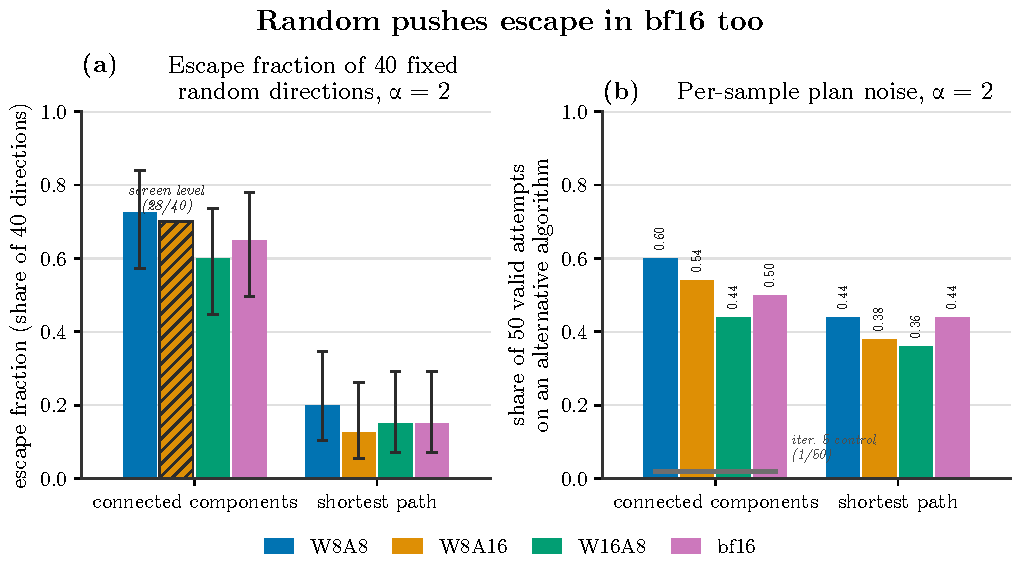
\includegraphics[width=\linewidth,height=0.78\textheight,keepaspectratio]{figures/fig_engine_escape_v0.pdf}
\caption{Random-push escape rates for four numerics built from one shared bf16 snapshot of Qwen3-8B (legend, left to right: W8A8, W8A16, W16A8, bf16), grouped by task along each panel's x-axis ('connected components', 'shortest path'). (a) Escape fraction of 40 fixed random directions added to the task-specification activations at \$\textbackslash{}alpha=2\$, each engine scored against its own unperturbed twin, with Wilson 95\textbackslash{}\% confidence intervals; the hatched W8A16 bar on 'connected components' (28 of 40) has no error bar and is labelled 'screen level' because its confirmation stage was incomplete, so it is not on the same footing as the other three bars in that group. Y-axis: escape fraction (share of 40 directions), 0 to 1. (b) Per-sample plan-noise share of 50 valid attempts that land on an algorithm other than the twin's default at \$\textbackslash{}alpha=2\$, with each bar's value printed above it; y-axis: share of 50 valid attempts on an alternative algorithm, 0 to 1. The short grey horizontal tick near the x-axis over the 'connected components' group, labelled 'iter. 5 control (1\slash{}50)', marks a different iteration's bf16 run that used its own noise unit and direction seeds, included for reference rather than as a fifth bar in the comparison. In both panels the bf16 bars sit close to the W8A8 bars, and the W16A8 bars are no higher than the bf16 bars: 8-bit floating-point activation rounding alone does not produce these escapes.}
\label{fig:fig_engine_escape}
\end{figure}
\textbf{The 8-bit engine adds a small boost on connected components, and activation rounding is not its source.} Pairing every pushed sample with the same slot (direction, template, slot index and uniforms) in the other engine, on the 400 screen slots of the first two samples of all 40 directions, W8A8 is off the default in 58.3\% of slots against 53.2\% under bf16 on connected components (discordant 30:10, exact McNemar p 0.0022), and 43.2\% against 40.7\% on shortest path (55:45, p 0.37) (Table 239). The factorial locates the boost. Activation rounding alone (W16A8) sits slightly below bf16 on connected components (49.7\% against 53.2\%, 9:23, p 0.02); weight rounding alone (W8A16) sits between bf16 and W8A8 (55.6\%; 17:7 against bf16, p 0.06). The small boost therefore comes from the e4m3 weights, from the native kernel's reduced-precision accumulation (it matches an exact fp64 reference on 94.2\% of outputs, against 99.96\% for an exact emulation), or from their interaction. The landing algorithms do not change: correct off-default programs are DFS, then BFS, on connected components and Bellman-Ford\slash{}SPFA on shortest path under every engine, with compositions compatible across engines (permutation chi-squared p 0.22 and 0.94; Table 240).

\begin{table}[H]
\renewcommand{\thetable}{239}
\centering\scriptsize\setlength{\tabcolsep}{2.5pt}
\caption{Common-random-number pairs of screen slots under the alpha-2 pushes: off-default share under each engine, discordant slots and exact McNemar p. Source: engine control \texttt{results/\allowbreak{}slot\_\allowbreak{}flips.\allowbreak{}json}. [Source: iteration 6, artifact \nolinkurl{gen_art_experiment_29}.]}\label{tab:t256}
\begin{tabular}{>{\raggedright\arraybackslash\hspace{0pt}}p{0.1694\linewidth}>{\raggedright\arraybackslash\hspace{0pt}}p{0.1261\linewidth}>{\raggedright\arraybackslash\hspace{0pt}}p{0.0622\linewidth}>{\raggedright\arraybackslash\hspace{0pt}}p{0.1226\linewidth}>{\raggedright\arraybackslash\hspace{0pt}}p{0.1273\linewidth}>{\raggedright\arraybackslash\hspace{0pt}}p{0.1541\linewidth}>{\raggedright\arraybackslash\hspace{0pt}}p{0.0676\linewidth}>{\raggedright\arraybackslash\hspace{0pt}}p{0.0838\linewidth}}
\toprule
\textbf{Task} & \textbf{Pair} & \textbf{Slots} & \textbf{Off-default, first} & \textbf{Off-default, second} & \textbf{Discordant first : second} & \textbf{Exact p} & \textbf{Same label} \\
\midrule
connected components & W8A8 vs bf16 & 400 & 0.583 & 0.532 & 30:10 & 0.0022 & 0.873 \\
connected components & W16A8 vs bf16 & 400 & 0.497 & 0.532 & 9:23 & 0.02 & 0.900 \\
connected components & W8A16 vs bf16 & 399 & 0.556 & 0.531 & 17:7 & 0.064 & 0.925 \\
connected components & W8A8 vs W16A8 & 400 & 0.583 & 0.497 & 45:11 & 5.4e-06 & 0.825 \\
connected components & W8A8 vs W8A16 & 399 & 0.581 & 0.556 & 20:10 & 0.099 & 0.895 \\
shortest path & W8A8 vs bf16 & 400 & 0.432 & 0.407 & 55:45 & 0.37 & 0.740 \\
shortest path & W16A8 vs bf16 & 400 & 0.420 & 0.407 & 35:30 & 0.62 & 0.830 \\
shortest path & W8A16 vs bf16 & 400 & 0.390 & 0.407 & 38:45 & 0.51 & 0.782 \\
shortest path & W8A8 vs W16A8 & 400 & 0.432 & 0.420 & 57:52 & 0.70 & 0.723 \\
shortest path & W8A8 vs W8A16 & 400 & 0.432 & 0.390 & 47:30 & 0.068 & 0.805 \\
\bottomrule
\end{tabular}
\end{table}

\begin{table}[H]
\renewcommand{\thetable}{240}
\centering\footnotesize\setlength{\tabcolsep}{4.0pt}
\caption{Composition of correct off-default programs under every alpha-2 push, per engine. Source: engine control \texttt{results/\allowbreak{}landings.\allowbreak{}json}. [Source: iteration 6, artifact \nolinkurl{gen_art_experiment_29}.]}\label{tab:t257}
\begin{tabular}{>{\raggedright\arraybackslash\hspace{0pt}}p{0.1155\linewidth}>{\raggedright\arraybackslash\hspace{0pt}}p{0.2245\linewidth}>{\raggedright\arraybackslash\hspace{0pt}}p{0.1917\linewidth}>{\raggedright\arraybackslash\hspace{0pt}}p{0.1578\linewidth}>{\raggedright\arraybackslash\hspace{0pt}}p{0.2236\linewidth}}
\toprule
\textbf{Task} & \textbf{W8A8} & \textbf{W8A16} & \textbf{W16A8} & \textbf{bf16} \\
\midrule
connected components & DFS 502, BFS 110 & DFS 410, BFS 86 & DFS 406, BFS 67 & DFS 448, BFS 82 \\
shortest path & Bellman-Ford\slash{}SPFA 165, Floyd-Warshall 1, other 1 & Bellman-Ford\slash{}SPFA 137, Floyd-Warshall 2 & Bellman-Ford\slash{}SPFA 129, other 1 & Bellman-Ford\slash{}SPFA 120, Floyd-Warshall 1, other 1 \\
\bottomrule
\end{tabular}
\end{table}

\textbf{Mechanism diagnostics.} Per-token e4m3 rounding perturbs every linear input by about 2.5\% RMS. Under an alpha-2 push, the push-induced difference in rounding error is 6\% to 12\% of the push-induced change in activation (median over blocks 13 to 35 per site, peaking at 34\% at the block-14 attention input), and 70\% to 100\% of the rows the push moves receive a new per-token scale. Linear inputs at blocks 0 to 12 are bitwise identical in the pushed and the twin pass in every engine, as the edit site requires. The extra rounding barely changes how the push propagates: relative to bf16, the non-nominal part of the perturbation is 1.01 at the task-specification positions, 1.04 to 1.05 at the read position and 1.03 to 1.12 at generated tokens 1 to 32 under W16A8, and 0.995 to 1.006 under W8A16. Teacher-forced on 40 iteration-4 twin programs, every engine is very close to bf16 (Table 241). One preregistered fidelity check failed uninformatively: teacher forcing runs one long prefill instead of 20-row decode steps, which itself changes the numerics, so log probabilities of iteration 4's programs could not be matched closely enough to resolve engines at that level; the engine was validated instead by byte identity.

\begin{table}[H]
\renewcommand{\thetable}{241}
\centering\footnotesize\setlength{\tabcolsep}{4.0pt}
\caption{Teacher-forced divergence from bf16 on 40 iteration-4 twin programs, and the failed fidelity check (median absolute difference between the summed log probability of a program and the value recorded in iteration 4). Source: engine control \texttt{results/\allowbreak{}diagnostics\_\allowbreak{}summary.\allowbreak{}json}. [Source: iteration 6, artifact \nolinkurl{gen_art_experiment_29}.]}\label{tab:t258}
\begin{tabular}{>{\raggedright\arraybackslash\hspace{0pt}}p{0.0794\linewidth}>{\raggedright\arraybackslash\hspace{0pt}}p{0.1880\linewidth}>{\raggedright\arraybackslash\hspace{0pt}}p{0.2111\linewidth}>{\raggedright\arraybackslash\hspace{0pt}}p{0.1961\linewidth}>{\raggedright\arraybackslash\hspace{0pt}}p{0.2385\linewidth}}
\toprule
\textbf{Engine} & \textbf{Task} & \textbf{Mean per-token KL to bf16 (nats)} & \textbf{Argmax disagreement with bf16} & \textbf{Median absolute log-probability difference} \\
\midrule
W8A8 & connected components & 0.0036 & 0.0012 & 0.477 \\
W8A8 & shortest path & 0.0015 & 0.0003 & 0.450 \\
W8A16 & connected components & 0.0019 & 0.0000 & 0.315 \\
W8A16 & shortest path & 0.0005 & 0.0003 & 0.703 \\
W16A8 & connected components & 0.0017 & 0.0019 & 0.448 \\
W16A8 & shortest path & 0.0011 & 0.0021 & 0.912 \\
bf16 & connected components & n\slash{}a & n\slash{}a & 0.383 \\
bf16 & shortest path & n\slash{}a & n\slash{}a & 0.679 \\
\bottomrule
\end{tabular}
\end{table}

\textbf{What it changes.} Table 242 assigns each earlier internal result to the numerics class that reproduces it. The 40-direction escape fractions, the per-sample plan-noise rates and the positive-control direction 9004 of the frozen screen are model properties. Only the per-slot off-default rate on connected components carries a significant 8-bit boost, of about 5 points. Iteration 5's bf16 plan-noise null and its finding that the shortest path task stops being movable in bf16 are not reproduced at the absolute unit; they belong to that design's unit and seeds. The plan-subspace claims of iteration 4 (the projection predictor, the targeted runner-up pushes, the decomposition) and the site and same-seed claims were not rerun here.

\begin{table}[H]
\renewcommand{\thetable}{242}
\centering\small\setlength{\tabcolsep}{4.0pt}
\caption{Earlier internal results and the numerics class that reproduces them. Source: engine control \texttt{results/\allowbreak{}relabel\_\allowbreak{}table.\allowbreak{}json}. [Source: iteration 6, artifact \nolinkurl{gen_art_experiment_29}.]}\label{tab:t259}
\begin{tabular}{>{\raggedright\arraybackslash\hspace{0pt}}p{0.4418\linewidth}>{\raggedright\arraybackslash\hspace{0pt}}p{0.1854\linewidth}>{\raggedright\arraybackslash\hspace{0pt}}p{0.3191\linewidth}}
\toprule
\textbf{Earlier result} & \textbf{Class} & \textbf{Deciding cells} \\
\midrule
40-direction escape fraction, connected components, alpha 2 (iteration 4: 0.725) & model & escape fraction W8A8 0.725, W8A16 incomplete (screen level 0.70), W16A8 0.60, bf16 0.65 \\
Per-sample plan noise, connected components, alpha 1 (iteration 4: 6\slash{}50) & model & shares 0.12, 0.18, 0.08, 0.14 \\
Per-sample plan noise, connected components, alpha 2 (iteration 4: 30\slash{}50) & model & shares 0.60, 0.54, 0.44, 0.50 \\
40-direction escape fraction, shortest path, alpha 2 (iteration 4: 0.200) & model & escape fraction 0.200, 0.125, 0.15, 0.15 \\
Per-sample plan noise, shortest path, alpha 1 (iteration 4: 12\slash{}50) & model & shares 0.24, 0.22, 0.22, 0.20 \\
Per-sample plan noise, shortest path, alpha 2 (iteration 4: 22\slash{}50) & model & shares 0.44, 0.38, 0.36, 0.44 \\
Frozen-screen direction 9004 moves shortest path at alpha 1 & model & first-10 off-default share W8A16 0.3, W16A8 0.4, bf16 0.3 \\
Per-slot off-default rate under alpha-2 pushes, connected components & model plus a small 8-bit boost & W8A8 0.583 against bf16 0.532; discordant 30:10, p 0.0022 \\
Per-slot off-default rate under alpha-2 pushes, shortest path & model & W8A8 0.432 against bf16 0.407; 55:45, p 0.37 \\
Iteration 5's bf16 plan-noise null on connected components (1\slash{}50 at the ban-free unit; block-12 dose 0.66 of this unit) & unit and seeds, not reproduced at the absolute unit & bf16 25\slash{}50 and W8A8 30\slash{}50 at alpha 2 \\
Iteration 5: shortest path no longer movable in bf16 & not reproduced at the absolute unit & bf16 escape fraction 6\slash{}40 confirmed escapes \\
Site odds ratio 5.72 & untested here & not rerun in this artifact \\
Same-seed agreement 17.25 of 20 & untested here & not rerun \\
Plan-subspace projection predictor & untested here & not rerun \\
Targeted runner-up pushes & untested here & not rerun \\
Decomposition into subspace and orthogonal parts & untested here & not rerun \\
\bottomrule
\end{tabular}
\end{table}

\textbf{Novelty and checks.} The two-judge novelty audit was replaced by a nearest-known-solution pass over all ten datasets of the declared source data (18,237 code solutions); Table 243 classes every distinct correct off-default or other program by its largest token-shingle Jaccard to a known solution. CPU gates checked the directions bitwise, the slots and seeds, the escape code (it reproduces iteration 4's escape file exactly) and the logged displacement (within 0.074\% on all 1,770 iteration-4 prefills); the relabelling with the re-gated shortest path rule changed 18 iteration-4 labels and no escape fraction. GPU unit tests confirmed bitwise e4m3 codes, a bitwise twin at alpha 0, rerun identity, batch invariance for three rows or more and an exact match of the memory-capped sampler. A stdlib re-derivation and a separate audit from raw rows matched every headline, and a placebo that swaps engine labels was not significant. Judge spend was USD 0.085.

\begin{table}[H]
\renewcommand{\thetable}{243}
\centering\footnotesize\setlength{\tabcolsep}{4.0pt}
\caption{Nearest known solution of the correct off-default and other programs per engine (distinct programs; median largest Jaccard; classes by Jaccard band). Source: engine control \texttt{results/\allowbreak{}known\_\allowbreak{}solutions.\allowbreak{}json}. [Source: iteration 6, artifact \nolinkurl{gen_art_experiment_29}.]}\label{tab:t260}
\begin{tabular}{>{\raggedright\arraybackslash\hspace{0pt}}p{0.2896\linewidth}>{\raggedright\arraybackslash\hspace{0pt}}p{0.1438\linewidth}>{\raggedright\arraybackslash\hspace{0pt}}p{0.1844\linewidth}>{\raggedright\arraybackslash\hspace{0pt}}p{0.0889\linewidth}>{\raggedright\arraybackslash\hspace{0pt}}p{0.0889\linewidth}>{\raggedright\arraybackslash\hspace{0pt}}p{0.1010\linewidth}}
\toprule
\textbf{Engine and task} & \textbf{Distinct programs} & \textbf{Median largest Jaccard} & \textbf{Variant} & \textbf{Distant} & \textbf{Known, close} \\
\midrule
W8A8, connected components & 229 & 0.297 & 162 & 64 & 3 \\
W8A8, shortest path & 237 & 0.209 & 25 & 212 & 0 \\
W8A16, connected components & 186 & 0.291 & 137 & 47 & 2 \\
W8A16, shortest path & 162 & 0.215 & 14 & 148 & 0 \\
W16A8, connected components & 159 & 0.304 & 123 & 32 & 4 \\
W16A8, shortest path & 128 & 0.214 & 16 & 112 & 0 \\
bf16, connected components & 185 & 0.302 & 136 & 46 & 3 \\
bf16, shortest path & 134 & 0.214 & 14 & 120 & 0 \\
\bottomrule
\end{tabular}
\end{table}

\FloatBarrier
\subsection*{6.4 Where a ban and an instruction are carried, and where noise acts, in bf16 (Qwen3-8B)}
\addcontentsline{toc}{subsection}{6.4 Where a ban and an instruction are carried, and where noise acts, in bf16 (Qwen3-8B)}
\noindent{\small\emph{Artifact: \nolinkurl{gen_art_experiment_30}.}}\par\medskip
\textbf{Why.} The localization claim predicted, from the route classes of iterations 2 and 3, where the substitute of a ban is carried: in the task-specification states on the prompt-route tasks, at the condition span on the direct-route tasks. Stage A tests that prediction without any training, by moving the states themselves. The same experiment  reran the iteration-4 noise-site comparison in bf16, set state noise at generated tokens against a temperature matched on per-token KL, applied the top-five plan push, and ran the landing contest. Everything ran in one bf16 engine with exact common random numbers on a 16 GB card, with the input embedding table kept in CPU memory; per-slot twin labels agreed with iteration 5's bf16 engine on 0.975 of slots for kth smallest and shortest path and 1.00 for the other tasks. Seven commitments formed an unbroken sha256 chain, and a standard-library script re-derived every headline from raw rows (295 checks, 0 mismatches) while a placebo version of each test failed.

\subsubsection*{6.4.1 Stage A: full-state exchange of the ban}
We call a \emph{full-state exchange} the replacement, in the forward pass of the neutral twin, of the residual states at a set of positions and blocks by the states the full ban prompt produces at the same positions; because the twin and the ban have identical token ids from the task text on, every task-specification position aligns. The exchanges covered four block bands at the task-specification positions (0 to 11, 12 to 23, 24 to 35, 0 to 35), a splice of the key-value cache of the condition span (the direct route), and the read position at all 36 blocks. The controls were the twin, a matched-norm random exchange (the state of the twin plus a fresh random direction scaled to the displacement that the ban itself causes per slot, block and position), a placebo that takes a second neutral twin as the source, and an identity exchange. The outcome, as committed before sampling (the first commitment: ``share(label == Y \textbar{} cell) - share(label == Y \textbar{} TWIN), all samples (invalid rows count as not-Y)''), is the \emph{Y share}: the share of all attempted programs labelled Y, invalid rows counting as not-Y; the \emph{transfer} of a cell is that share minus the share under the twin; a cell counts only if its pass rate is at least 0.8 times that of the twin (the validity gate of the first commitment); and its \emph{recovery} is the transfer divided by that of the full ban. The \emph{correct Y} column added to Tables 244 to 250 counts programs labelled Y that pass every hidden test, because an attempted share counts broken programs as Y: on the grid task the exchange at blocks 0-35 has 14 attempts labelled DFS but 3 correct DFS programs. Each cell has N = 30 on paired slots. Tables 244 to 249 give every cell on the six tasks. (iteration-7 correction)

The prediction held where the route data said it should, and failed at one task where they said it should not. On shortest path, exchanging the full ban's task-specification states at all blocks into the twin turns 24 of 30 slots from Dijkstra to Bellman-Ford\slash{}SPFA (24 of 30 attempts, 21 of 30 correct programs; transfer 0.80, McNemar 24:0, Holm p 7e-7, pass ratio 0.90), while the condition-span splice and the read-position exchange transfer nothing. Blocks 12 to 23 alone carry 0.60 (18 of 30 attempts, 11 of 30 correct programs, at a pass ratio of 0.73, below the 0.8 gate) and blocks 24 to 35 alone 0.37 (11 of 30 attempts, 11 of 30 correct programs); blocks 0 to 11 carry none. On kth smallest the same exchange transfers 0.57 to quickselect (17 of 30 attempts, 16 of 30 correct programs) with every slot leaving the full sort, blocks 0 to 11 alone already transfer 0.40 (12 of 30 attempts, 12 of 30 correct programs), and here the condition span also carries the ban (0.93; 28 of 30 attempts, 25 of 30 correct programs). On connected components every slot leaves union find under the exchange at blocks 12 to 23 or 0 to 35 (off-default transfer 1.00), but only 0.37 to 0.47 land on the ban's BFS (11 and 14 of 30 attempts, 11 and 14 of 30 correct programs) and the rest on DFS. On the grid task, whose route was carried by the prompt states in likelihood and mixed in behaviour, the exchange at all blocks transfers 0.47 toward DFS (14 of 30 attempts, 3 of 30 correct programs, pass ratio 0.59, below the 0.8 gate) and the condition-span splice 0.33 (10 of 30 attempts, 7 of 30 correct programs, pass ratio 0.89), so each carries part of the ban in attempts and only the splice passes the committed validity gate. On the direct-route tasks the condition-span splice alone reproduces the ban (two sum 1.00, 30 of 30 attempts, 30 of 30 correct programs; find duplicate 0.90, 27 of 30 attempts, 26 of 30 correct programs), as predicted, but on two sum the task-specification states also transfer brute force at 0.43 (13 of 30 attempts, 13 of 30 correct programs), above the predicted ceiling of 0.2. The committed verdict is therefore not supported. The secondary predictions hold: the condition span carries at least 0.5 on the direct-route tasks and at most 0.2 on shortest path, the read position carries at most 0.2 everywhere (it carries 0.00 on all six tasks), the placebo moves at most 0.03, and the exchange beats the matched-norm random exchange where it transfers (shortest path 23:0, kth smallest 16:2, connected components 11:0, on attempted Y as preregistered); counted on correct Y instead, a post-hoc contrast added in iteration 7, the same pairs give 21:0 (exact p 9.5e-07), 15:2 (p 2.3e-03) and 11:0 (p 9.8e-04). The ban's information, not the size of the perturbation, is what moves the algorithm. (iteration-7 correction)

\begin{figure}[!htbp]
\centering\captionsetup{font=footnotesize}
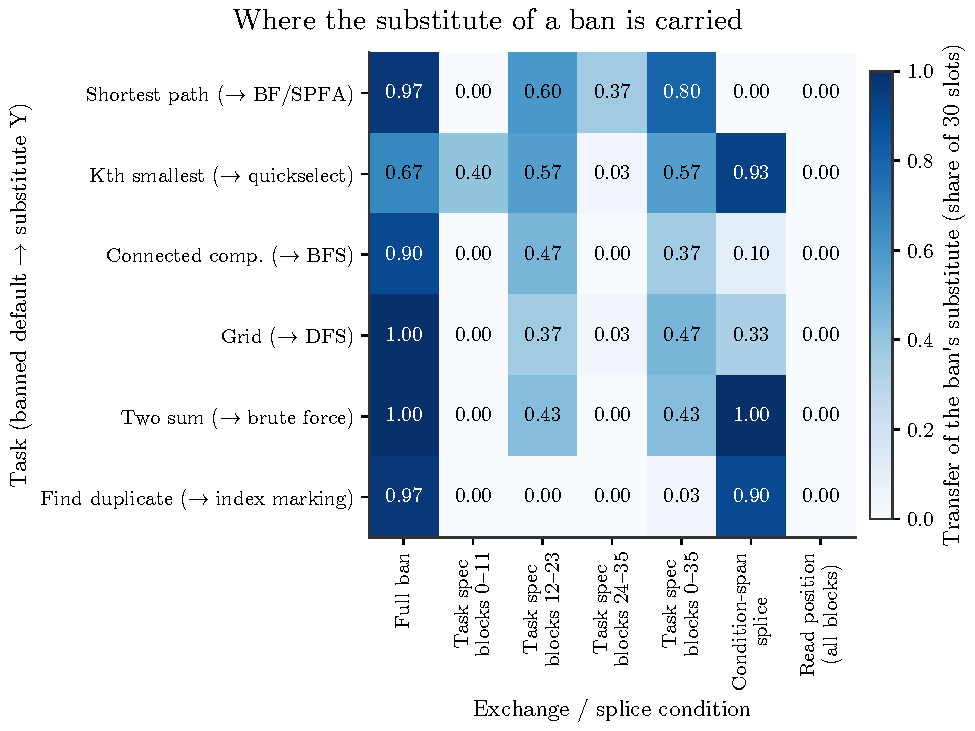
\includegraphics[width=\linewidth,height=0.78\textheight,keepaspectratio]{figures/fig_exchange_transfer_v0.pdf}
\caption{Stage A, bf16 Qwen3-8B: each cell is the share of 30 paired slots (two-decimal annotation; white = 0, dark blue = 1; colourbar, right: ``Transfer of the ban's substitute (share of 30 slots)'') in which the generated program uses the substitute algorithm Y that a full prompt-level ban drives the model to, relative to the token-matched neutral twin (whose own Y-share is 0 for every task). Rows, top to bottom, are six tasks labelled by their banned default and driven substitute: shortest path (-\textgreater{} BF\slash{}SPFA), kth smallest (-\textgreater{} quickselect), connected components (-\textgreater{} BFS), grid (-\textgreater{} DFS), two sum (-\textgreater{} brute force), find duplicate (-\textgreater{} index marking). Columns, left to right, are: the full ban; the full ban's task-specification residual states exchanged into the neutral twin over three non-overlapping twelve-block bands (blocks 0-11, 12-23, 24-35) and over the full 0-35 span; a condition-span key-value-cache splice; and an exchange of the read position alone across all blocks. Task-specification exchange (blocks 0-35, and already by blocks 12-23) carries most of the transfer for shortest path (0.80, 0.60) and kth smallest (0.57, 0.57); the condition-span splice carries it for two sum (1.00) and find duplicate (0.90); the grid task is split between the two (0.47 task-spec, 0.33 condition-span); and the read-position column is 0.00 in every row. Matched-norm random exchanges and a placebo-twin splice, measured with the same 30-slot design for shortest path, kth smallest and connected components but not plotted here, transfer at most 0.13, so the pattern above is specific to the ban's own residual states rather than to perturbation in general.}
\label{fig:fig_exchange_transfer}
\end{figure}
\begin{table}[H]
\renewcommand{\thetable}{244}
\centering\tiny\setlength{\tabcolsep}{2.5pt}
\caption{Stage A on kth smallest (default full sort; Y = quickselect; route class from iterations 2 and 3: either route suffices). Twin on slots 0 to 29: Y share 0.00, off-default 0.00, pass 1.00, full sort 30. Exchange at blocks 0-35 against the matched-norm random exchange: 16:2, exact p 0.0013 (Holm 0.0020). Source: exchange and site experiment \texttt{results/\allowbreak{}stage\_\allowbreak{}a.\allowbreak{}json}, \texttt{results/\allowbreak{}summary.\allowbreak{}md}. The Y share is the outcome of the first commitment (all attempted programs labelled Y; invalid rows count as not-Y); the added column \emph{Correct Y \slash{} N} counts programs labelled Y that pass every hidden test, with Clopper-Pearson 95\% intervals; a cell meets the validity gate of the first commitment when its pass ratio is at least 0.8. Post hoc, on correct Y, the exchange at blocks 0-35 against the matched-norm random exchange gives 15:2 (exact p 2.3e-03). (iteration-7 correction) [Source: iteration 6, artifact \nolinkurl{gen_art_experiment_30}.]}\label{tab:t261}
\begin{tabular}{>{\raggedright\arraybackslash\hspace{0pt}}p{0.1300\linewidth}>{\raggedright\arraybackslash\hspace{0pt}}p{0.0238\linewidth}>{\raggedright\arraybackslash\hspace{0pt}}p{0.0831\linewidth}>{\raggedright\arraybackslash\hspace{0pt}}p{0.0887\linewidth}>{\raggedright\arraybackslash\hspace{0pt}}p{0.0646\linewidth}>{\raggedright\arraybackslash\hspace{0pt}}p{0.0618\linewidth}>{\raggedright\arraybackslash\hspace{0pt}}p{0.0439\linewidth}>{\raggedright\arraybackslash\hspace{0pt}}p{0.0646\linewidth}>{\raggedright\arraybackslash\hspace{0pt}}p{0.0855\linewidth}>{\raggedright\arraybackslash\hspace{0pt}}p{0.0941\linewidth}>{\raggedright\arraybackslash\hspace{0pt}}p{0.1420\linewidth}}
\toprule
\textbf{Cell} & \textbf{n} & \textbf{Y share [CP 95\%]} & \textbf{Correct Y \slash{} N [CP 95\%]} & \textbf{Transfer} & \textbf{Off-default transfer} & \textbf{Pass ratio} & \textbf{Recovery} & \textbf{Slot interchange intervention accuracy} & \textbf{McNemar b:c (p, Holm)} & \textbf{Correct composition} \\
\midrule
full ban & 30 & 0.67 [0.47, 0.83] & 18\slash{}30 [0.41, 0.77] & 0.67 & 1.00 & 0.93 & 1.00 & 1.00 & 20:0 (1.9e-06, 1.9e-06) & quickselect 18, size-k heap 10 \\
exchange, blocks 0-11 & 30 & 0.40 [0.23, 0.59] & 12\slash{}30 [0.23, 0.59] & 0.40 & 0.53 & 1.00 & 0.60 & 0.33 & 12:0 (4.9e-04, 0.003) & full sort 14, quickselect 12, size-k heap 4 \\
exchange, blocks 12-23 & 30 & 0.57 [0.37, 0.75] & 15\slash{}30 [0.31, 0.69] & 0.57 & 1.00 & 0.93 & 0.85 & 0.90 & 17:0 (1.5e-05, 7.6e-05) & quickselect 15, size-k heap 13 \\
exchange, blocks 24-35 & 30 & 0.03 [8.4e-04, 0.17] & 1\slash{}30 [8.4e-04, 0.17] & 0.03 & 0.03 & 1.00 & 0.05 & 0.03 & 1:0 (1.000, 1.000) & full sort 29, quickselect 1 \\
exchange, blocks 0-35 & 30 & 0.57 [0.37, 0.75] & 16\slash{}30 [0.34, 0.72] & 0.57 & 1.00 & 0.97 & 0.85 & 0.90 & 17:0 (1.5e-05, 7.6e-05) & quickselect 16, size-k heap 13 \\
condition-span splice & 30 & 0.93 [0.78, 0.99] & 25\slash{}30 [0.65, 0.94] & 0.93 & 1.00 & 0.90 & 1.40 & 0.60 & 28:0 (7.5e-09, 3.7e-08) & quickselect 25, size-k heap 2 \\
read-position exchange & 30 & 0.00 [0.00, 0.12] & 0\slash{}30 [0.00, 0.12] & 0.00 & 0.00 & 1.00 & 0.00 & 0.00 & 0:0 (1.000, 1.000) & full sort 30 \\
matched-norm random exchange, blocks 0-35 & 30 & 0.10 [0.02, 0.27] & 3\slash{}30 [0.02, 0.27] & 0.10 & 0.10 & 1.00 & 0.15 & 0.03 & 3:0 (0.250, 0.750) & full sort 27, quickselect 3 \\
matched-norm random exchange, blocks 12-23 & 30 & 0.13 [0.04, 0.31] & 4\slash{}30 [0.04, 0.31] & 0.13 & 0.13 & 1.00 & 0.20 & 0.00 & 4:0 (0.125, 0.375) & full sort 26, quickselect 4 \\
placebo twin & 30 & 0.03 [8.4e-04, 0.17] & 1\slash{}30 [8.4e-04, 0.17] & 0.03 & 0.03 & 1.00 & 0.05 & 0.00 & 1:0 (1.000, 1.000) & full sort 29, quickselect 1 \\
\bottomrule
\end{tabular}
\end{table}

\begin{table}[H]
\renewcommand{\thetable}{245}
\centering\tiny\setlength{\tabcolsep}{2.5pt}
\caption{Stage A on connected components (default union find; Y = BFS). Twin: Y share 0.00, off-default 0.00, pass 1.00, union find 30. Exchange at blocks 0-35 against the matched-norm random exchange: 11:0, exact p 9.8e-4 (Holm 0.0020). The Y share is the outcome of the first commitment (all attempted programs labelled Y; invalid rows count as not-Y); the added column \emph{Correct Y \slash{} N} counts programs labelled Y that pass every hidden test, with Clopper-Pearson 95\% intervals; a cell meets the validity gate of the first commitment when its pass ratio is at least 0.8. Post hoc, on correct Y, the exchange at blocks 0-35 against the matched-norm random exchange gives 11:0 (exact p 9.8e-04). (iteration-7 correction) [Source: iteration 6, artifact \nolinkurl{gen_art_experiment_30}.]}\label{tab:t262}
\begin{tabular}{>{\raggedright\arraybackslash\hspace{0pt}}p{0.1447\linewidth}>{\raggedright\arraybackslash\hspace{0pt}}p{0.0249\linewidth}>{\raggedright\arraybackslash\hspace{0pt}}p{0.0849\linewidth}>{\raggedright\arraybackslash\hspace{0pt}}p{0.0972\linewidth}>{\raggedright\arraybackslash\hspace{0pt}}p{0.0646\linewidth}>{\raggedright\arraybackslash\hspace{0pt}}p{0.0666\linewidth}>{\raggedright\arraybackslash\hspace{0pt}}p{0.0439\linewidth}>{\raggedright\arraybackslash\hspace{0pt}}p{0.0646\linewidth}>{\raggedright\arraybackslash\hspace{0pt}}p{0.0943\linewidth}>{\raggedright\arraybackslash\hspace{0pt}}p{0.1028\linewidth}>{\raggedright\arraybackslash\hspace{0pt}}p{0.0936\linewidth}}
\toprule
\textbf{Cell} & \textbf{n} & \textbf{Y share [CP 95\%]} & \textbf{Correct Y \slash{} N [CP 95\%]} & \textbf{Transfer} & \textbf{Off-default transfer} & \textbf{Pass ratio} & \textbf{Recovery} & \textbf{Slot interchange intervention accuracy} & \textbf{McNemar b:c (p, Holm)} & \textbf{Correct composition} \\
\midrule
full ban & 30 & 0.90 [0.73, 0.98] & 27\slash{}30 [0.73, 0.98] & 0.90 & 1.00 & 1.00 & 1.00 & 1.00 & 27:0 (1.5e-08, 3.0e-08) & BFS 27, DFS 3 \\
exchange, blocks 0-11 & 30 & 0.00 [0.00, 0.12] & 0\slash{}30 [0.00, 0.12] & 0.00 & 0.87 & 0.70 & 0.00 & 0.10 & 0:0 (1.000, 1.000) & DFS 17, union find 4 \\
exchange, blocks 12-23 & 30 & 0.47 [0.28, 0.66] & 14\slash{}30 [0.28, 0.66] & 0.47 & 1.00 & 1.00 & 0.52 & 0.43 & 14:0 (1.2e-04, 4.9e-04) & DFS 16, BFS 14 \\
exchange, blocks 24-35 & 30 & 0.00 [0.00, 0.12] & 0\slash{}30 [0.00, 0.12] & 0.00 & 0.63 & 1.00 & 0.00 & 0.10 & 0:0 (1.000, 1.000) & DFS 19, union find 11 \\
exchange, blocks 0-35 & 30 & 0.37 [0.20, 0.56] & 11\slash{}30 [0.20, 0.56] & 0.37 & 1.00 & 1.00 & 0.41 & 0.40 & 11:0 (9.8e-04, 0.002) & DFS 19, BFS 11 \\
condition-span splice & 30 & 0.10 [0.02, 0.27] & 3\slash{}30 [0.02, 0.27] & 0.10 & 1.00 & 1.00 & 0.11 & 0.20 & 3:0 (0.250, 0.500) & DFS 27, BFS 3 \\
read-position exchange & 30 & 0.00 [0.00, 0.12] & 0\slash{}30 [0.00, 0.12] & 0.00 & 0.00 & 1.00 & 0.00 & 0.00 & 0:0 (1.000, 1.000) & union find 30 \\
matched-norm random exchange, blocks 0-35 & 30 & 0.00 [0.00, 0.12] & 0\slash{}30 [0.00, 0.12] & 0.00 & 0.07 & 1.00 & 0.00 & 0.00 & 0:0 (1.000, 1.000) & union find 28, DFS 2 \\
matched-norm random exchange, blocks 12-23 & 30 & 0.00 [0.00, 0.12] & 0\slash{}30 [0.00, 0.12] & 0.00 & 0.03 & 1.00 & 0.00 & 0.00 & 0:0 (1.000, 1.000) & union find 29, DFS 1 \\
placebo twin & 30 & 0.00 [0.00, 0.12] & 0\slash{}30 [0.00, 0.12] & 0.00 & 0.03 & 1.00 & 0.00 & 0.00 & 0:0 (1.000, 1.000) & union find 29, DFS 1 \\
\bottomrule
\end{tabular}
\end{table}

\begin{table}[H]
\renewcommand{\thetable}{246}
\centering\tiny\setlength{\tabcolsep}{2.5pt}
\caption{Stage A on shortest path (default Dijkstra; Y = Bellman-Ford\slash{}SPFA; prompt route). Twin: Y share 0.00, off-default 0.00, pass 1.00, Dijkstra 30. Exchange at blocks 0-35 against the matched-norm random exchange: 23:0, exact p 2.4e-7 (Holm 7.2e-7). The Y share is the outcome of the first commitment (all attempted programs labelled Y; invalid rows count as not-Y); the added column \emph{Correct Y \slash{} N} counts programs labelled Y that pass every hidden test, with Clopper-Pearson 95\% intervals; a cell meets the validity gate of the first commitment when its pass ratio is at least 0.8. Post hoc, on correct Y, the exchange at blocks 0-35 against the matched-norm random exchange gives 21:0 (exact p 9.5e-07). (iteration-7 correction) [Source: iteration 6, artifact \nolinkurl{gen_art_experiment_30}.]}\label{tab:t263}
\begin{tabular}{>{\raggedright\arraybackslash\hspace{0pt}}p{0.1363\linewidth}>{\raggedright\arraybackslash\hspace{0pt}}p{0.0238\linewidth}>{\raggedright\arraybackslash\hspace{0pt}}p{0.0876\linewidth}>{\raggedright\arraybackslash\hspace{0pt}}p{0.0923\linewidth}>{\raggedright\arraybackslash\hspace{0pt}}p{0.0646\linewidth}>{\raggedright\arraybackslash\hspace{0pt}}p{0.0627\linewidth}>{\raggedright\arraybackslash\hspace{0pt}}p{0.0439\linewidth}>{\raggedright\arraybackslash\hspace{0pt}}p{0.0646\linewidth}>{\raggedright\arraybackslash\hspace{0pt}}p{0.0889\linewidth}>{\raggedright\arraybackslash\hspace{0pt}}p{0.0977\linewidth}>{\raggedright\arraybackslash\hspace{0pt}}p{0.1197\linewidth}}
\toprule
\textbf{Cell} & \textbf{n} & \textbf{Y share [CP 95\%]} & \textbf{Correct Y \slash{} N [CP 95\%]} & \textbf{Transfer} & \textbf{Off-default transfer} & \textbf{Pass ratio} & \textbf{Recovery} & \textbf{Slot interchange intervention accuracy} & \textbf{McNemar b:c (p, Holm)} & \textbf{Correct composition} \\
\midrule
full ban & 30 & 0.97 [0.83, 1.00] & 29\slash{}30 [0.83, 1.00] & 0.97 & 0.97 & 1.00 & 1.00 & 1.00 & 29:0 (3.7e-09, 1.5e-08) & Bellman-Ford\slash{}SPFA 29, Dijkstra 1 \\
exchange, blocks 0-11 & 30 & 0.00 [0.00, 0.12] & 0\slash{}30 [0.00, 0.12] & 0.00 & 0.00 & 1.00 & 0.00 & 0.03 & 0:0 (1.000, 1.000) & Dijkstra 30 \\
exchange, blocks 12-23 & 30 & 0.60 [0.41, 0.77] & 11\slash{}30 [0.20, 0.56] & 0.60 & 0.60 & 0.73 & 0.62 & 0.63 & 18:0 (7.6e-06, 4.6e-05) & Dijkstra 11, Bellman-Ford\slash{}SPFA 11 \\
exchange, blocks 24-35 & 30 & 0.37 [0.20, 0.56] & 11\slash{}30 [0.20, 0.56] & 0.37 & 0.37 & 1.00 & 0.38 & 0.40 & 11:0 (9.8e-04, 0.006) & Dijkstra 19, Bellman-Ford\slash{}SPFA 11 \\
exchange, blocks 0-35 & 30 & 0.80 [0.61, 0.92] & 21\slash{}30 [0.51, 0.85] & 0.80 & 0.80 & 0.90 & 0.83 & 0.83 & 24:0 (1.2e-07, 7.2e-07) & Bellman-Ford\slash{}SPFA 21, Dijkstra 6 \\
condition-span splice & 30 & 0.00 [0.00, 0.12] & 0\slash{}30 [0.00, 0.12] & 0.00 & 0.00 & 1.00 & 0.00 & 0.03 & 0:0 (1.000, 1.000) & Dijkstra 30 \\
read-position exchange & 30 & 0.00 [0.00, 0.12] & 0\slash{}30 [0.00, 0.12] & 0.00 & 0.00 & 1.00 & 0.00 & 0.03 & 0:0 (1.000, 1.000) & Dijkstra 30 \\
matched-norm random exchange, blocks 0-35 & 30 & 0.03 [8.4e-04, 0.17] & 0\slash{}30 [0.00, 0.12] & 0.03 & 0.03 & 0.97 & 0.03 & 0.07 & 1:0 (1.000, 1.000) & Dijkstra 29 \\
matched-norm random exchange, blocks 12-23 & 30 & 0.03 [8.4e-04, 0.17] & 0\slash{}30 [0.00, 0.12] & 0.03 & 0.03 & 0.93 & 0.03 & 0.07 & 1:0 (1.000, 1.000) & Dijkstra 28 \\
placebo twin & 30 & 0.03 [8.4e-04, 0.17] & 1\slash{}30 [8.4e-04, 0.17] & 0.03 & 0.03 & 1.00 & 0.03 & 0.07 & 1:0 (1.000, 1.000) & Dijkstra 29, Bellman-Ford\slash{}SPFA 1 \\
\bottomrule
\end{tabular}
\end{table}

\begin{table}[H]
\renewcommand{\thetable}{247}
\centering\tiny\setlength{\tabcolsep}{2.5pt}
\caption{Stage A on two sum (default hash map; Y = brute force; direct route). Twin: Y share 0.00, pass 1.00, hash map 30. The Y share is the outcome of the first commitment (all attempted programs labelled Y; invalid rows count as not-Y); the added column \emph{Correct Y \slash{} N} counts programs labelled Y that pass every hidden test, with Clopper-Pearson 95\% intervals; a cell meets the validity gate of the first commitment when its pass ratio is at least 0.8. (iteration-7 correction) [Source: iteration 6, artifact \nolinkurl{gen_art_experiment_30}.]}\label{tab:t264}
\begin{tabular}{>{\raggedright\arraybackslash\hspace{0pt}}p{0.1000\linewidth}>{\raggedright\arraybackslash\hspace{0pt}}p{0.0257\linewidth}>{\raggedright\arraybackslash\hspace{0pt}}p{0.0875\linewidth}>{\raggedright\arraybackslash\hspace{0pt}}p{0.1010\linewidth}>{\raggedright\arraybackslash\hspace{0pt}}p{0.0646\linewidth}>{\raggedright\arraybackslash\hspace{0pt}}p{0.0699\linewidth}>{\raggedright\arraybackslash\hspace{0pt}}p{0.0439\linewidth}>{\raggedright\arraybackslash\hspace{0pt}}p{0.0646\linewidth}>{\raggedright\arraybackslash\hspace{0pt}}p{0.1072\linewidth}>{\raggedright\arraybackslash\hspace{0pt}}p{0.1090\linewidth}>{\raggedright\arraybackslash\hspace{0pt}}p{0.1088\linewidth}}
\toprule
\textbf{Cell} & \textbf{n} & \textbf{Y share [CP 95\%]} & \textbf{Correct Y \slash{} N [CP 95\%]} & \textbf{Transfer} & \textbf{Off-default transfer} & \textbf{Pass ratio} & \textbf{Recovery} & \textbf{Slot interchange intervention accuracy} & \textbf{McNemar b:c (p, Holm)} & \textbf{Correct composition} \\
\midrule
full ban & 30 & 1.00 [0.88, 1.00] & 30\slash{}30 [0.88, 1.00] & 1.00 & 1.00 & 1.00 & 1.00 & 1.00 & 30:0 (1.9e-09, 1.1e-08) & brute force 30 \\
exchange, blocks 0-11 & 30 & 0.00 [0.00, 0.12] & 0\slash{}30 [0.00, 0.12] & 0.00 & 0.00 & 1.00 & 0.00 & 0.00 & 0:0 (1.000, 1.000) & hash map 30 \\
exchange, blocks 12-23 & 30 & 0.43 [0.25, 0.63] & 13\slash{}30 [0.25, 0.63] & 0.43 & 0.43 & 1.00 & 0.43 & 0.43 & 13:0 (2.4e-04, 7.3e-04) & hash map 17, brute force 13 \\
exchange, blocks 24-35 & 30 & 0.00 [0.00, 0.12] & 0\slash{}30 [0.00, 0.12] & 0.00 & 0.00 & 1.00 & 0.00 & 0.00 & 0:0 (1.000, 1.000) & hash map 30 \\
exchange, blocks 0-35 & 30 & 0.43 [0.25, 0.63] & 13\slash{}30 [0.25, 0.63] & 0.43 & 0.43 & 1.00 & 0.43 & 0.43 & 13:0 (2.4e-04, 7.3e-04) & hash map 17, brute force 13 \\
condition-span splice & 30 & 1.00 [0.88, 1.00] & 30\slash{}30 [0.88, 1.00] & 1.00 & 1.00 & 1.00 & 1.00 & 1.00 & 30:0 (1.9e-09, 1.1e-08) & brute force 30 \\
read-position exchange & 30 & 0.00 [0.00, 0.12] & 0\slash{}30 [0.00, 0.12] & 0.00 & 0.00 & 1.00 & 0.00 & 0.00 & 0:0 (1.000, 1.000) & hash map 30 \\
\bottomrule
\end{tabular}
\end{table}

\begin{table}[H]
\renewcommand{\thetable}{248}
\centering\tiny\setlength{\tabcolsep}{2.5pt}
\caption{Stage A on find duplicate (default hash set; Y = index marking; direct route). Twin: Y share 0.00, pass 1.00, hash set 30. The Y share is the outcome of the first commitment (all attempted programs labelled Y; invalid rows count as not-Y); the added column \emph{Correct Y \slash{} N} counts programs labelled Y that pass every hidden test, with Clopper-Pearson 95\% intervals; a cell meets the validity gate of the first commitment when its pass ratio is at least 0.8. (iteration-7 correction) [Source: iteration 6, artifact \nolinkurl{gen_art_experiment_30}.]}\label{tab:t265}
\begin{tabular}{>{\raggedright\arraybackslash\hspace{0pt}}p{0.0834\linewidth}>{\raggedright\arraybackslash\hspace{0pt}}p{0.0238\linewidth}>{\raggedright\arraybackslash\hspace{0pt}}p{0.0792\linewidth}>{\raggedright\arraybackslash\hspace{0pt}}p{0.0845\linewidth}>{\raggedright\arraybackslash\hspace{0pt}}p{0.0646\linewidth}>{\raggedright\arraybackslash\hspace{0pt}}p{0.0618\linewidth}>{\raggedright\arraybackslash\hspace{0pt}}p{0.0439\linewidth}>{\raggedright\arraybackslash\hspace{0pt}}p{0.0646\linewidth}>{\raggedright\arraybackslash\hspace{0pt}}p{0.0894\linewidth}>{\raggedright\arraybackslash\hspace{0pt}}p{0.0888\linewidth}>{\raggedright\arraybackslash\hspace{0pt}}p{0.1981\linewidth}}
\toprule
\textbf{Cell} & \textbf{n} & \textbf{Y share [CP 95\%]} & \textbf{Correct Y \slash{} N [CP 95\%]} & \textbf{Transfer} & \textbf{Off-default transfer} & \textbf{Pass ratio} & \textbf{Recovery} & \textbf{Slot interchange intervention accuracy} & \textbf{McNemar b:c (p, Holm)} & \textbf{Correct composition} \\
\midrule
full ban & 30 & 0.97 [0.83, 1.00] & 25\slash{}30 [0.65, 0.94] & 0.97 & 1.00 & 0.87 & 1.00 & 1.00 & 29:0 (3.7e-09, 1.5e-08) & index marking 25, Floyd cycle detection 1 \\
exchange, blocks 0-11 & 30 & 0.00 [0.00, 0.12] & 0\slash{}30 [0.00, 0.12] & 0.00 & 0.00 & 1.00 & 0.00 & 0.00 & 0:0 (1.000, 1.000) & hash set 30 \\
exchange, blocks 12-23 & 30 & 0.00 [0.00, 0.12] & 0\slash{}30 [0.00, 0.12] & 0.00 & 0.10 & 1.00 & 0.00 & 0.03 & 0:0 (1.000, 1.000) & hash set 27, Floyd cycle detection 3 \\
exchange, blocks 24-35 & 30 & 0.00 [0.00, 0.12] & 0\slash{}30 [0.00, 0.12] & 0.00 & 0.00 & 1.00 & 0.00 & 0.00 & 0:0 (1.000, 1.000) & hash set 30 \\
exchange, blocks 0-35 & 30 & 0.03 [8.4e-04, 0.17] & 1\slash{}30 [8.4e-04, 0.17] & 0.03 & 0.13 & 1.00 & 0.03 & 0.07 & 1:0 (1.000, 1.000) & hash set 26, Floyd cycle detection 2, index marking 1, sort and adjacent check 1 \\
condition-span splice & 30 & 0.90 [0.73, 0.98] & 26\slash{}30 [0.69, 0.96] & 0.90 & 0.90 & 0.97 & 0.93 & 0.90 & 27:0 (1.5e-08, 6.0e-08) & index marking 26, hash set 3 \\
read-position exchange & 30 & 0.00 [0.00, 0.12] & 0\slash{}30 [0.00, 0.12] & 0.00 & 0.00 & 1.00 & 0.00 & 0.00 & 0:0 (1.000, 1.000) & hash set 30 \\
\bottomrule
\end{tabular}
\end{table}

\begin{table}[H]
\renewcommand{\thetable}{249}
\centering\tiny\setlength{\tabcolsep}{2.5pt}
\caption{Stage A on the grid task (default BFS; Y = DFS; prompt route in likelihood, mixed in behaviour). Twin: Y share 0.00, pass 0.90, BFS 27 correct. Pass ratios above 1 occur because the twin's own pass rate is below 1. The Y share is the outcome of the first commitment (all attempted programs labelled Y; invalid rows count as not-Y); the added column \emph{Correct Y \slash{} N} counts programs labelled Y that pass every hidden test, with Clopper-Pearson 95\% intervals; a cell meets the validity gate of the first commitment when its pass ratio is at least 0.8. (iteration-7 correction) [Source: iteration 6, artifact \nolinkurl{gen_art_experiment_30}.]}\label{tab:t266}
\begin{tabular}{>{\raggedright\arraybackslash\hspace{0pt}}p{0.1032\linewidth}>{\raggedright\arraybackslash\hspace{0pt}}p{0.0265\linewidth}>{\raggedright\arraybackslash\hspace{0pt}}p{0.0979\linewidth}>{\raggedright\arraybackslash\hspace{0pt}}p{0.1043\linewidth}>{\raggedright\arraybackslash\hspace{0pt}}p{0.0646\linewidth}>{\raggedright\arraybackslash\hspace{0pt}}p{0.0721\linewidth}>{\raggedright\arraybackslash\hspace{0pt}}p{0.0445\linewidth}>{\raggedright\arraybackslash\hspace{0pt}}p{0.0646\linewidth}>{\raggedright\arraybackslash\hspace{0pt}}p{0.1106\linewidth}>{\raggedright\arraybackslash\hspace{0pt}}p{0.1109\linewidth}>{\raggedright\arraybackslash\hspace{0pt}}p{0.0829\linewidth}}
\toprule
\textbf{Cell} & \textbf{n} & \textbf{Y share [CP 95\%]} & \textbf{Correct Y \slash{} N [CP 95\%]} & \textbf{Transfer} & \textbf{Off-default transfer} & \textbf{Pass ratio} & \textbf{Recovery} & \textbf{Slot interchange intervention accuracy} & \textbf{McNemar b:c (p, Holm)} & \textbf{Correct composition} \\
\midrule
full ban & 30 & 1.00 [0.88, 1.00] & 12\slash{}30 [0.23, 0.59] & 1.00 & 1.00 & 0.44 & 1.00 & 1.00 & 30:0 (1.9e-09, 1.1e-08) & DFS 12 \\
exchange, blocks 0-11 & 30 & 0.00 [0.00, 0.12] & 0\slash{}30 [0.00, 0.12] & 0.00 & 0.00 & 1.11 & 0.00 & 0.00 & 0:0 (1.000, 1.000) & BFS 30 \\
exchange, blocks 12-23 & 30 & 0.37 [0.20, 0.56] & 2\slash{}30 [8.2e-03, 0.22] & 0.37 & 0.37 & 0.63 & 0.37 & 0.37 & 11:0 (9.8e-04, 0.002) & BFS 15, DFS 2 \\
exchange, blocks 24-35 & 30 & 0.03 [8.4e-04, 0.17] & 0\slash{}30 [0.00, 0.12] & 0.03 & 0.03 & 0.81 & 0.03 & 0.03 & 1:0 (1.000, 1.000) & BFS 22 \\
exchange, blocks 0-35 & 30 & 0.47 [0.28, 0.66] & 3\slash{}30 [0.02, 0.27] & 0.47 & 0.47 & 0.59 & 0.47 & 0.47 & 14:0 (1.2e-04, 4.9e-04) & BFS 13, DFS 3 \\
condition-span splice & 30 & 0.33 [0.17, 0.53] & 7\slash{}30 [0.10, 0.42] & 0.33 & 0.33 & 0.89 & 0.33 & 0.33 & 10:0 (0.002, 0.006) & BFS 17, DFS 7 \\
read-position exchange & 30 & 0.00 [0.00, 0.12] & 0\slash{}30 [0.00, 0.12] & 0.00 & 0.00 & 0.96 & 0.00 & 0.00 & 0:0 (1.000, 1.000) & BFS 26 \\
\bottomrule
\end{tabular}
\end{table}

The condition-span splice also matches the behavioural route arms of iteration 3: its recovery is 1.00 on two sum and 0.93 on find duplicate, where the direct-route fraction of iteration 3 was 0.96 and 0.99, and 1.40 on kth smallest (direct-route fraction 0.74). On connected components its recovery toward BFS is 0.11, although every slot leaves union find: either route alone removes the default and lands on DFS, as the route landings of iteration 4 had shown.

\textbf{Positive instructions are carried the same way.} As an extension, the forced prompt \texttt{Implement Bellman-\allowbreak{}Ford or SPFA for this task.\allowbreak{}} replaced the ban as the source (Table 250). Its padding twin, the same prompt with the tokens of the instruction replaced by padding, stays on Dijkstra in 29 of 30 programs; exchanging only the task-specification states of the forced prompt at all blocks into that twin gives Bellman-Ford\slash{}SPFA in 30 of 30. On connected components the states of the forced BFS prompt give BFS in 28 of 30 against union find 30 of 30 for its twin. The shortest path semantic seed, which moved that task 66 points in iteration 1, moved nothing under this frame (Dijkstra 30 of 30), and neither did its exchange (2 of 30). The fourth ban template, held out of every other cell, transfers through the exchange as the other templates do (shortest path 0.70, kth smallest 0.60 on quickselect with every slot off the full sort, connected components 0.70, N = 10 each).

\begin{table}[H]
\renewcommand{\thetable}{250}
\centering\scriptsize\setlength{\tabcolsep}{2.5pt}
\caption{Extensions: forced sources, the semantic seed and the fourth template, each exchanged at blocks 0-35 into its own twin. Source: exchange and site experiment \texttt{results/\allowbreak{}summary.\allowbreak{}md}. The added column counts programs labelled Y that pass every hidden test. Under the first commitment's definition the forced Bellman-Ford\slash{}SPFA exchange transfers 0.967 (30 of 30 against 1 of 30 for its padding twin). (iteration-7 correction) [Source: iteration 6, artifact \nolinkurl{gen_art_experiment_30}.]}\label{tab:t267}
\begin{tabular}{>{\raggedright\arraybackslash\hspace{0pt}}p{0.1254\linewidth}>{\raggedright\arraybackslash\hspace{0pt}}p{0.2024\linewidth}>{\raggedright\arraybackslash\hspace{0pt}}p{0.0361\linewidth}>{\raggedright\arraybackslash\hspace{0pt}}p{0.1567\linewidth}>{\raggedright\arraybackslash\hspace{0pt}}p{0.0788\linewidth}>{\raggedright\arraybackslash\hspace{0pt}}p{0.0843\linewidth}>{\raggedright\arraybackslash\hspace{0pt}}p{0.0539\linewidth}>{\raggedright\arraybackslash\hspace{0pt}}p{0.1755\linewidth}}
\toprule
\textbf{Task} & \textbf{Cell} & \textbf{n} & \textbf{Y share (Y) \slash{} default share} & \textbf{Correct Y \slash{} n} & \textbf{Off-default share} & \textbf{Pass} & \textbf{Composition} \\
\midrule
kth smallest & fourth-template ban & 10 & 0.30 (quickselect) \slash{} 0.00 & 3\slash{}10 & 1.00 & 1.00 & size-k heap 7, quickselect 3 \\
kth smallest & fourth-template twin & 10 & 0.00 \slash{} 1.00 & 0\slash{}10 & 0.00 & 1.00 & full sort 10 \\
kth smallest & fourth-template exchange, blocks 0-35 & 10 & 0.60 \slash{} 0.00 & 4\slash{}10 & 1.00 & 0.80 & quickselect 6, size-k heap 4 \\
connected components & fourth-template ban & 10 & 0.80 (BFS) \slash{} 0.00 & 8\slash{}10 & 1.00 & 1.00 & BFS 8, DFS 2 \\
connected components & forced BFS & 30 & 1.00 \slash{} 0.00 & 30\slash{}30 & 1.00 & 1.00 & BFS 30 \\
connected components & padding twin of forced BFS & 30 & 0.00 \slash{} 1.00 & 0\slash{}30 & 0.00 & 1.00 & union find 30 \\
connected components & forced BFS exchange, blocks 0-35 & 30 & 0.93 \slash{} 0.00 & 24\slash{}30 & 1.00 & 0.87 & BFS 28, DFS 2 \\
connected components & fourth-template twin & 10 & 0.00 \slash{} 1.00 & 0\slash{}10 & 0.00 & 1.00 & union find 10 \\
connected components & fourth-template exchange, blocks 0-35 & 10 & 0.70 \slash{} 0.00 & 7\slash{}10 & 1.00 & 1.00 & BFS 7, DFS 3 \\
shortest path & fourth-template ban & 10 & 0.70 (Bellman-Ford\slash{}SPFA) \slash{} 0.30 & 7\slash{}10 & 0.70 & 1.00 & Bellman-Ford\slash{}SPFA 7, Dijkstra 3 \\
shortest path & forced Bellman-Ford or SPFA & 30 & 1.00 \slash{} 0.00 & 27\slash{}30 & 1.00 & 0.90 & Bellman-Ford\slash{}SPFA 30 \\
shortest path & padding twin of the forced prompt & 30 & 0.03 \slash{} 0.97 & 0\slash{}30 & 0.03 & 0.97 & Dijkstra 29, Bellman-Ford\slash{}SPFA 1 \\
shortest path & forced exchange, blocks 0-35 & 30 & 1.00 \slash{} 0.00 & 30\slash{}30 & 1.00 & 1.00 & Bellman-Ford\slash{}SPFA 30 \\
shortest path & semantic seed & 30 & 0.00 \slash{} 1.00 & 0\slash{}30 & 0.00 & 0.93 & Dijkstra 30 \\
shortest path & padding twin of the seed & 30 & 0.03 \slash{} 0.97 & 0\slash{}30 & 0.03 & 0.97 & Dijkstra 29, Bellman-Ford\slash{}SPFA 1 \\
shortest path & seed exchange, blocks 0-35 & 30 & 0.07 \slash{} 0.93 & 1\slash{}30 & 0.07 & 0.87 & Dijkstra 28, Bellman-Ford\slash{}SPFA 2 \\
shortest path & fourth-template twin & 10 & 0.00 \slash{} 1.00 & 0\slash{}10 & 0.00 & 1.00 & Dijkstra 10 \\
shortest path & fourth-template exchange, blocks 0-35 & 10 & 0.70 \slash{} 0.30 & 7\slash{}10 & 0.70 & 1.00 & Bellman-Ford\slash{}SPFA 7, Dijkstra 3 \\
\bottomrule
\end{tabular}
\end{table}

The unit tests of Stage A passed except one: splicing the cache of the task-specification span reproduced the top token of the exchange with a logit gap of 0.5 in bf16 and 10 of 10 equal labels, but not byte for byte. The Stage A arms on trapped rain water and minimum spanning tree weight were dropped for GPU time.

\subsubsection*{6.4.2 Where noise acts, in bf16}
The site rerun repeated iteration 4's grid on kth smallest and connected components in bf16, at the ban-free unit, with a fresh direction per sample, N = 30 per cell and alpha 1, 2, 4 and 8 (Tables 251 and 252). Noise at the task-specification positions moves the algorithm in bf16: on kth smallest blocks 12 to 23 reach a correct off-default share of 0.37 at alpha 2, and on connected components blocks 0 to 11 reach 0.33 at alpha 4. The read position, the condition span and the late blocks barely move it below alpha 8. On kth smallest the plan site (the task-specification states at blocks 12 to 23, as in iteration 4) beats the read position in paired slots 24:5 (exact p 5.5e-4) and the condition span 22:0, and a Mantel-Haenszel odds ratio [129] within quintiles of the downstream displacement is 4.6 [1.9, 11.3]. Connected components shows a weaker picture: its plan site moves only 0.07 at alpha 2 and 0.17 at alpha 4, the early blocks beat it (4:18, p 0.004), and the read position starts moving at alpha 8 (0.30).

The committed rule fitted a Firth logistic regression [125] of a correct off-default program on site indicators and the log displacements, so that sites are compared at matched downstream displacement (Tables 253 and 254). It returned the verdict withdrawn, for two reasons. The raw condition-span arm never reaches the plan site's downstream displacement, so it has no common support and its energy-matched arm stood in; and at alpha 8 every plan-site program failed (pass 0.00) while the read position began to move, which erases the read-position contrast in the preregistered model. A post-hoc sensitivity restricted to alpha of 4 or less (before breakage) puts the read position clearly below the plan site on both tasks: beta -3.76 (profile interval [-7.29, -0.47], cluster bootstrap [-8.18, -1.40]) on kth smallest and -4.98 ([-9.77, -0.89]; [-11.48, -1.53]) on connected components. The prefill-site claim is therefore withdrawn as preregistered. Post hoc (alpha of at most 4) the read position is below the task-specification site on both tasks; the condition-span clause fails post hoc as well (beta -1.70 [-3.96, 0.42] on kth smallest; -0.56 [-4.93, 2.91] on connected components, cluster bootstrap; profile intervals [-6.82, 1.16] and [-6.15, 3.41]), so the site of the choice remains open, as the artifact concludes; its rule label withdraws the site claim as specific to 8-bit floating point and states that the site of the choice is open. The half of that label about 8-bit floating point cannot apply: Section 6.3 shows that bf16 reproduces the escapes direction by direction (Spearman 0.96 and 0.87) and that activation rounding adds nothing, so the withdrawal comes from the missing common support and the breakage at alpha 8 in bf16, not from the engine. Noise sites and Stage A agree on the band on kth smallest and disagree on connected components (Table 254b): there noise moves the algorithm most at blocks 0 to 11 (mean 0.19 over alpha 1 to 4 against 0.08 at blocks 12 to 23; 0.33 correct off-default at alpha 4; coefficient +2.51 [1.39, 3.80] against the plan site; paired flips 4:18, p 0.004, between the plan site and blocks 0-11), while the exchange transfers BFS at blocks 12 to 23. The removal of the default there is depth-redundant: the exchange at blocks 0-11 alone takes 0.87 of attempts off union find and at blocks 24-35 alone 0.63. (iteration-7 correction)

{\scriptsize\setlength{\tabcolsep}{2.5pt}\renewcommand{\thetable}{251}
\begin{longtable}{>{\raggedright\arraybackslash\hspace{0pt}}p{0.1348\linewidth}>{\raggedright\arraybackslash\hspace{0pt}}p{0.0622\linewidth}>{\raggedright\arraybackslash\hspace{0pt}}p{0.0300\linewidth}>{\raggedright\arraybackslash\hspace{0pt}}p{0.0788\linewidth}>{\raggedright\arraybackslash\hspace{0pt}}p{0.0748\linewidth}>{\raggedright\arraybackslash\hspace{0pt}}p{0.0539\linewidth}>{\raggedright\arraybackslash\hspace{0pt}}p{0.1211\linewidth}>{\raggedright\arraybackslash\hspace{0pt}}p{0.1211\linewidth}>{\raggedright\arraybackslash\hspace{0pt}}p{0.2261\linewidth}}
\caption{The bf16 site grid on kth smallest (twin correct off-default 0.00; displacements are medians in residual units at block 35). Source: exchange and site experiment \texttt{results/\allowbreak{}site\_\allowbreak{}grid.\allowbreak{}json}. [Source: iteration 6, artifact \nolinkurl{gen_art_experiment_30}.]}\label{tab:t268}\\
\toprule
\textbf{Site} & \textbf{Alpha} & \textbf{n} & \textbf{Correct off-default} & \textbf{Off-default} & \textbf{Pass} & \textbf{Median displacement at the read position, block 35} & \textbf{Median displacement at generated token 1, block 35} & \textbf{Correct composition} \\
\midrule
\endfirsthead
\multicolumn{9}{l}{\emph{Table 251, continued}}\\
\toprule
\textbf{Site} & \textbf{Alpha} & \textbf{n} & \textbf{Correct off-default} & \textbf{Off-default} & \textbf{Pass} & \textbf{Median displacement at the read position, block 35} & \textbf{Median displacement at generated token 1, block 35} & \textbf{Correct composition} \\
\midrule
\endhead
\bottomrule
\endlastfoot
spec, blocks 12-23 & 1 & 30 & 0.13 & 0.13 & 1.00 & 1.708 & 1.315 & full sort 26, quickselect 3, size-k heap 1 \\
spec, blocks 12-23 & 2 & 30 & 0.37 & 0.37 & 1.00 & 3.353 & 2.478 & full sort 19, quickselect 8, size-k heap 3 \\
spec, blocks 12-23 & 4 & 30 & 0.33 & 0.40 & 0.87 & 6.293 & 4.628 & full sort 16, size-k heap 5, quickselect 5 \\
spec, blocks 12-23 & 8 & 30 & 0.00 & 0.10 & 0.00 & 12.230 & 7.135 & - \\
read position & 1 & 30 & 0.03 & 0.03 & 1.00 & 1.876 & 0.628 & full sort 29, quickselect 1 \\
read position & 2 & 30 & 0.03 & 0.03 & 1.00 & 3.591 & 1.201 & full sort 29, quickselect 1 \\
read position & 4 & 30 & 0.00 & 0.00 & 1.00 & 6.840 & 2.290 & full sort 30 \\
read position & 8 & 30 & 0.13 & 0.13 & 0.93 & 10.654 & 3.466 & full sort 24, quickselect 3, size-k heap 1 \\
read position, energy-matched & 2 & 30 & 0.07 & 0.07 & 0.77 & 16.426 & 3.870 & full sort 21, quickselect 1, size-k heap 1 \\
read position, energy-matched & 4 & 30 & 0.03 & 0.07 & 0.93 & 25.287 & 3.845 & full sort 27, heapify and pop 1 \\
condition span & 1 & 30 & 0.00 & 0.00 & 1.00 & 0.303 & 0.245 & full sort 30 \\
condition span & 2 & 30 & 0.07 & 0.07 & 1.00 & 0.415 & 0.289 & full sort 28, quickselect 2 \\
condition span & 4 & 30 & 0.03 & 0.03 & 1.00 & 0.674 & 0.424 & full sort 29, quickselect 1 \\
condition span & 8 & 30 & 0.00 & 0.00 & 1.00 & 1.056 & 0.606 & full sort 30 \\
condition span, energy-matched & 2 & 30 & 0.00 & 0.00 & 1.00 & 1.220 & 0.664 & full sort 30 \\
condition span, energy-matched & 4 & 30 & 0.00 & 0.00 & 1.00 & 1.110 & 0.646 & full sort 30 \\
generated tokens 1-32 & 1 & 30 & 0.17 & 0.17 & 1.00 & - & - & full sort 25, quickselect 5 \\
generated tokens 1-32 & 2 & 50 & 0.26 & 0.34 & 0.94 & - & - & full sort 33, quickselect 12, size-k heap 1, other 1 \\
generated tokens 1-32 & 4 & 50 & 0.18 & 0.42 & 0.50 & - & - & full sort 15, quickselect 4, heapify and pop 3, size-k heap 2 \\
generated tokens 1-32 & 8 & 30 & 0.00 & 0.00 & 0.13 & - & - & full sort 4 \\
spec, blocks 0-11 & 1 & 30 & 0.03 & 0.03 & 1.00 & 0.956 & 0.728 & full sort 29, quickselect 1 \\
spec, blocks 0-11 & 2 & 30 & 0.17 & 0.17 & 1.00 & 1.832 & 1.320 & full sort 25, quickselect 3, size-k heap 2 \\
spec, blocks 0-11 & 4 & 30 & 0.37 & 0.37 & 1.00 & 3.576 & 2.512 & full sort 19, size-k heap 9, quickselect 2 \\
spec, blocks 0-11 & 8 & 30 & 0.00 & 0.13 & 0.10 & 16.027 & 8.332 & full sort 3 \\
spec, blocks 24-35 & 1 & 30 & 0.00 & 0.00 & 1.00 & 0.909 & 0.654 & full sort 30 \\
spec, blocks 24-35 & 2 & 30 & 0.03 & 0.03 & 1.00 & 1.777 & 1.261 & full sort 29, size-k heap 1 \\
spec, blocks 24-35 & 4 & 30 & 0.03 & 0.03 & 1.00 & 3.270 & 2.307 & full sort 29, quickselect 1 \\
spec, blocks 24-35 & 8 & 30 & 0.10 & 0.10 & 1.00 & 5.119 & 3.323 & full sort 27, quickselect 3 \\
\end{longtable}}

{\scriptsize\setlength{\tabcolsep}{2.5pt}\renewcommand{\thetable}{252}
\begin{longtable}{>{\raggedright\arraybackslash\hspace{0pt}}p{0.1703\linewidth}>{\raggedright\arraybackslash\hspace{0pt}}p{0.0622\linewidth}>{\raggedright\arraybackslash\hspace{0pt}}p{0.0370\linewidth}>{\raggedright\arraybackslash\hspace{0pt}}p{0.0926\linewidth}>{\raggedright\arraybackslash\hspace{0pt}}p{0.0748\linewidth}>{\raggedright\arraybackslash\hspace{0pt}}p{0.0539\linewidth}>{\raggedright\arraybackslash\hspace{0pt}}p{0.1289\linewidth}>{\raggedright\arraybackslash\hspace{0pt}}p{0.1267\linewidth}>{\raggedright\arraybackslash\hspace{0pt}}p{0.1565\linewidth}}
\caption{The bf16 site grid on connected components (twin correct off-default 0.00). [Source: iteration 6, artifact \nolinkurl{gen_art_experiment_30}.]}\label{tab:t269}\\
\toprule
\textbf{Site} & \textbf{Alpha} & \textbf{n} & \textbf{Correct off-default} & \textbf{Off-default} & \textbf{Pass} & \textbf{Median displacement at the read position, block 35} & \textbf{Median displacement at generated token 1, block 35} & \textbf{Correct composition} \\
\midrule
\endfirsthead
\multicolumn{9}{l}{\emph{Table 252, continued}}\\
\toprule
\textbf{Site} & \textbf{Alpha} & \textbf{n} & \textbf{Correct off-default} & \textbf{Off-default} & \textbf{Pass} & \textbf{Median displacement at the read position, block 35} & \textbf{Median displacement at generated token 1, block 35} & \textbf{Correct composition} \\
\midrule
\endhead
\bottomrule
\endlastfoot
spec, blocks 12-23 & 1 & 30 & 0.00 & 0.00 & 1.00 & 1.694 & 1.315 & union find 30 \\
spec, blocks 12-23 & 2 & 30 & 0.07 & 0.07 & 1.00 & 3.281 & 2.537 & union find 28, DFS 2 \\
spec, blocks 12-23 & 4 & 30 & 0.17 & 0.17 & 1.00 & 6.322 & 4.829 & union find 25, DFS 3, BFS 2 \\
spec, blocks 12-23 & 8 & 30 & 0.00 & 0.13 & 0.00 & 12.977 & 7.182 & - \\
read position & 1 & 30 & 0.00 & 0.00 & 1.00 & 1.800 & 0.606 & union find 30 \\
read position & 2 & 30 & 0.00 & 0.00 & 1.00 & 3.700 & 1.197 & union find 30 \\
read position & 4 & 30 & 0.03 & 0.03 & 1.00 & 7.200 & 2.234 & union find 29, DFS 1 \\
read position & 8 & 30 & 0.30 & 0.30 & 0.93 & 10.392 & 3.645 & union find 19, DFS 8, BFS 1 \\
read position, energy-matched & 2 & 30 & 0.03 & 0.03 & 0.77 & 15.570 & 4.091 & union find 22, DFS 1 \\
read position, energy-matched & 4 & 30 & 0.07 & 0.07 & 0.83 & 22.781 & 4.019 & union find 23, DFS 2 \\
condition span & 1 & 30 & 0.00 & 0.00 & 1.00 & 0.285 & 0.238 & union find 30 \\
condition span & 2 & 30 & 0.00 & 0.00 & 1.00 & 0.395 & 0.278 & union find 30 \\
condition span & 4 & 30 & 0.00 & 0.00 & 1.00 & 0.620 & 0.371 & union find 30 \\
condition span & 8 & 30 & 0.00 & 0.00 & 1.00 & 0.931 & 0.557 & union find 30 \\
condition span, energy-matched & 2 & 30 & 0.00 & 0.00 & 1.00 & 1.003 & 0.568 & union find 30 \\
condition span, energy-matched & 4 & 30 & 0.00 & 0.00 & 1.00 & 1.163 & 0.618 & union find 30 \\
generated tokens 1-32 & 1 & 30 & 0.00 & 0.00 & 1.00 & - & - & union find 30 \\
generated tokens 1-32 & 2 & 50 & 0.14 & 0.20 & 0.92 & - & - & union find 39, DFS 7 \\
generated tokens 1-32 & 4 & 50 & 0.16 & 0.40 & 0.38 & - & - & union find 11, DFS 6, BFS 2 \\
generated tokens 1-32 & 8 & 30 & 0.00 & 0.00 & 0.17 & - & - & union find 5 \\
spec, blocks 0-11 & 1 & 30 & 0.03 & 0.03 & 1.00 & 0.910 & 0.747 & union find 29, DFS 1 \\
spec, blocks 0-11 & 2 & 30 & 0.20 & 0.20 & 1.00 & 1.717 & 1.308 & union find 24, DFS 6 \\
spec, blocks 0-11 & 4 & 30 & 0.33 & 0.37 & 0.97 & 3.315 & 2.467 & union find 19, DFS 6, BFS 4 \\
spec, blocks 0-11 & 8 & 30 & 0.13 & 0.33 & 0.13 & 16.291 & 9.122 & BFS 3, DFS 1 \\
spec, blocks 24-35 & 1 & 30 & 0.00 & 0.00 & 1.00 & 0.930 & 0.647 & union find 30 \\
spec, blocks 24-35 & 2 & 30 & 0.00 & 0.00 & 1.00 & 1.789 & 1.225 & union find 30 \\
spec, blocks 24-35 & 4 & 30 & 0.00 & 0.00 & 1.00 & 3.267 & 2.278 & union find 30 \\
spec, blocks 24-35 & 8 & 30 & 0.03 & 0.03 & 1.00 & 5.089 & 3.429 & union find 29, DFS 1 \\
\end{longtable}}

\begin{table}[H]
\renewcommand{\thetable}{253}
\centering\small\setlength{\tabcolsep}{4.0pt}
\caption{Firth logistic regression with site indicators on kth smallest at matched downstream displacement (n 387, 48 events, 387 of 720 rows in common support; the condition span enters through its energy-matched arm). Mantel-Haenszel odds ratio, plan site against read position, within quintiles of the log displacement at the read position: 4.61 [1.87, 11.34]. Paired flips, plan site only : other site only: read position 24:5 (p 5.5e-4), condition span 22:0 (p 4.8e-7), blocks 0-11 17:9 (p 0.169), blocks 24-35 23:3 (p 8.8e-5), generated tokens 21:18 (p 0.749). [Source: iteration 6, artifact \nolinkurl{gen_art_experiment_30}.]}\label{tab:t270}
\begin{tabular}{>{\raggedright\arraybackslash\hspace{0pt}}p{0.4424\linewidth}>{\raggedright\arraybackslash\hspace{0pt}}p{0.0785\linewidth}>{\raggedright\arraybackslash\hspace{0pt}}p{0.1913\linewidth}>{\raggedright\arraybackslash\hspace{0pt}}p{0.2174\linewidth}}
\toprule
\textbf{Term} & \textbf{Beta} & \textbf{Profile 95\% CI} & \textbf{Cluster bootstrap 95\% CI} \\
\midrule
spec, blocks 0-11 (against spec, blocks 12-23) & 0.24 & [-0.54, 1.01] & - \\
spec, blocks 24-35 & -1.52 & [-2.74, -0.51] & - \\
read position & -0.17 & [-2.64, 2.33] & [-2.58, 2.21] \\
condition span (energy-matched arm) & -0.73 & [-5.71, 1.84] & [-2.12, 1.10] \\
log displacement at the read position & -1.92 & [-4.76, 0.77] & - \\
log displacement at generated token 1 & 1.97 & [-0.99, 5.03] & - \\
\bottomrule
\end{tabular}
\end{table}

\begin{table}[H]
\renewcommand{\thetable}{254}
\centering\small\setlength{\tabcolsep}{4.0pt}
\caption{Firth logistic regression with site indicators on connected components (n 374, 32 events, 376 of 720 rows in common support). Mantel-Haenszel odds ratio, plan site against read position: 0.82 [0.31, 2.18]. Paired flips, plan site only : other site only: read position 7:10 (p 0.629), condition span 7:0 (p 0.016), blocks 0-11 4:18 (p 0.004), blocks 24-35 7:1 (p 0.070), generated tokens 7:9 (p 0.804). [Source: iteration 6, artifact \nolinkurl{gen_art_experiment_30}.]}\label{tab:t271}
\begin{tabular}{>{\raggedright\arraybackslash\hspace{0pt}}p{0.4450\linewidth}>{\raggedright\arraybackslash\hspace{0pt}}p{0.0760\linewidth}>{\raggedright\arraybackslash\hspace{0pt}}p{0.1908\linewidth}>{\raggedright\arraybackslash\hspace{0pt}}p{0.2179\linewidth}}
\toprule
\textbf{Term} & \textbf{Beta} & \textbf{Profile 95\% CI} & \textbf{Cluster bootstrap 95\% CI} \\
\midrule
spec, blocks 0-11 (against spec, blocks 12-23) & 2.51 & [1.39, 3.80] & - \\
spec, blocks 24-35 & -0.72 & [-3.03, 0.94] & - \\
read position & 1.14 & [-1.30, 3.64] & [-1.07, 3.24] \\
condition span (energy-matched arm) & 2.38 & [-2.72, 5.40] & [0.69, 5.18] \\
log displacement at the read position & 0.02 & [-2.94, 2.92] & - \\
log displacement at generated token 1 & 1.22 & [-1.87, 4.36] & - \\
\bottomrule
\end{tabular}
\end{table}

\begin{table}[H]
\renewcommand{\thetable}{254b}
\centering\scriptsize\setlength{\tabcolsep}{2.5pt}
\caption{Noise sites against Stage A, per task and block band (NEW in iteration 7): the largest correct off-default share of spec-position noise at alpha 1 to 4 (with its alpha), the full-state exchange's Y share (the first commitment) and off-default share at the same band, and whether the band where noise acts most (by the mean over alpha 1, 2 and 4, the artifact's band rule) is the band where the exchange transfers most. Sources: exchange and site experiment \texttt{results/\allowbreak{}site\_\allowbreak{}grid.\allowbreak{}json}, \texttt{data/\allowbreak{}labels.\allowbreak{}jsonl}. (iteration-7 correction) [Source: iteration 6, artifact \nolinkurl{gen_art_experiment_30}.]}\label{tab:t272}
\begin{tabular}{>{\raggedright\arraybackslash\hspace{0pt}}p{0.0919\linewidth}>{\raggedright\arraybackslash\hspace{0pt}}p{0.0817\linewidth}>{\raggedright\arraybackslash\hspace{0pt}}p{0.1605\linewidth}>{\raggedright\arraybackslash\hspace{0pt}}p{0.1613\linewidth}>{\raggedright\arraybackslash\hspace{0pt}}p{0.0872\linewidth}>{\raggedright\arraybackslash\hspace{0pt}}p{0.1132\linewidth}>{\raggedright\arraybackslash\hspace{0pt}}p{0.1136\linewidth}>{\raggedright\arraybackslash\hspace{0pt}}p{0.1038\linewidth}}
\toprule
\textbf{Task} & \textbf{Band} & \textbf{Noise, mean correct off-default over alpha 1-4} & \textbf{Noise, max correct off-default (alpha)} & \textbf{Exchange Y share} & \textbf{Exchange off-default share} & \textbf{Noise band \slash{} exchange band} & \textbf{Concordant} \\
\midrule
kth smallest & blocks 0-11 & 0.19 & 0.37 (4) & 0.40 & 0.53 & 12-23 \slash{} 12-23 & yes \\
 & blocks 12-23 & 0.28 & 0.37 (2) & 0.57 & 1.00 &  &  \\
 & blocks 24-35 & 0.02 & 0.03 (4) & 0.03 & 0.03 &  &  \\
connected components & blocks 0-11 & 0.19 & 0.33 (4) & 0.00 & 0.87 & 0-11 \slash{} 12-23 & no \\
 & blocks 12-23 & 0.08 & 0.17 (4) & 0.47 & 1.00 &  &  \\
 & blocks 24-35 & 0.00 & 0.00 (4) & 0.00 & 0.63 &  &  \\
\bottomrule
\end{tabular}
\end{table}

\subsubsection*{6.4.3 State noise at generated tokens against matched temperature}
The token claim's second half set noise on the residual states of generated tokens 1 to 32 against a temperature applied to the same tokens and bisected to the same per-token KL, which we call decoding at matched departure (Table 255). At alpha 2 the state noise leads on discordant correct off-default flips, 12:6 on kth smallest and 7:3 on connected components, but neither is significant (p 0.24 and 0.34). At alpha 4 the lead on connected components reaches 8:1 (p 0.039), at a pass rate of 0.38 against 0.70. The rule (p below 0.05 on both tasks at alpha 2) is not met: state noise against token temperature is not established in bf16.

\begin{table}[H]
\renewcommand{\thetable}{255}
\centering\tiny\setlength{\tabcolsep}{2.5pt}
\caption{State noise at generated tokens 1 to 32 against decoding at matched departure (N = 50 paired slots). Source: exchange and site experiment \texttt{results/\allowbreak{}state\_\allowbreak{}vs\_\allowbreak{}token.\allowbreak{}json}. [Source: iteration 6, artifact \nolinkurl{gen_art_experiment_30}.]}\label{tab:t273}
\begin{tabular}{>{\raggedright\arraybackslash\hspace{0pt}}p{0.1247\linewidth}>{\raggedright\arraybackslash\hspace{0pt}}p{0.1054\linewidth}>{\raggedright\arraybackslash\hspace{0pt}}p{0.0829\linewidth}>{\raggedright\arraybackslash\hspace{0pt}}p{0.1256\linewidth}>{\raggedright\arraybackslash\hspace{0pt}}p{0.0955\linewidth}>{\raggedright\arraybackslash\hspace{0pt}}p{0.0468\linewidth}>{\raggedright\arraybackslash\hspace{0pt}}p{0.0783\linewidth}>{\raggedright\arraybackslash\hspace{0pt}}p{0.0858\linewidth}>{\raggedright\arraybackslash\hspace{0pt}}p{0.0618\linewidth}>{\raggedright\arraybackslash\hspace{0pt}}p{0.0858\linewidth}}
\toprule
\textbf{Task, alpha} & \textbf{State-noise KL per token (nats)} & \textbf{Matched temperature} & \textbf{Share of tokens with the temperature on} & \textbf{State only : temperature only} & \textbf{Exact p} & \textbf{State-noise flip share} & \textbf{Temperature flip share} & \textbf{State-noise pass} & \textbf{Temperature pass} \\
\midrule
kth smallest, alpha 2 & 0.3883 & 2.06 & 0.3762 & 12:6 & 0.238 & 0.26 & 0.14 & 0.94 & 0.98 \\
kth smallest, alpha 4 & 2.3336 & 3.00 & 1.7734 & 8:3 & 0.227 & 0.18 & 0.08 & 0.50 & 0.82 \\
connected components, alpha 2 & 0.2315 & 2.72 & 0.2310 & 7:3 & 0.344 & 0.14 & 0.06 & 0.92 & 0.92 \\
connected components, alpha 4 & 3.0926 & 3.00 & 0.8178 & 8:1 & 0.039 & 0.16 & 0.02 & 0.38 & 0.70 \\
\bottomrule
\end{tabular}
\end{table}

\subsubsection*{6.4.4 The top-five push in bf16}
On the grid task, iteration 4's top-five direction (from the mean of the five banned centroids toward the mean of the survivors) was applied at the plan site at alpha 1, 2, 4 and 8 (Table 256). At doses of 1 to 8 ban units, which overshoot the forced-prompt manifold, the push breaks programs before it moves the algorithm; an in-manifold dose was not tried: the pass rate falls from 0.67 at alpha 1 to 0.30, 0.03 and 0.00, with at most one correct program other than BFS per cell, so the landing test could not be computed. Projected onto the plane of the first two principal components of the ten forced-prompt centroids (36\% and 25\% of their variance), the push leaves the forced-prompt manifold: already at alpha 1 it moves farther along the first component than the whole spread of the ten centroids (the four alpha-1 points move from a twin mean of +0.09 to -0.44 on that component, against centroids spread from -0.098 to +0.144). The prompt version of the top-five ban moves the task-specification states from below the centroid cloud into it, between the banned DFS and greedy best-first centroids and the three surviving centroids (bidirectional BFS and two variants of A*), and its behaviour stays inside the banned set (BFS 25, DFS 23 of 50; avoidance 0.00). (iteration-7 correction)

\begin{table}[H]
\renewcommand{\thetable}{256}
\centering\footnotesize\setlength{\tabcolsep}{4.0pt}
\caption{The top-five plan push and the prompt top-five ban on the grid task. Source: exchange and site experiment \texttt{results/\allowbreak{}top5\_\allowbreak{}push.\allowbreak{}json}. [Source: iteration 6, artifact \nolinkurl{gen_art_experiment_30}.]}\label{tab:t274}
\begin{tabular}{>{\raggedright\arraybackslash\hspace{0pt}}p{0.2417\linewidth}>{\raggedright\arraybackslash\hspace{0pt}}p{0.0641\linewidth}>{\raggedright\arraybackslash\hspace{0pt}}p{0.0641\linewidth}>{\raggedright\arraybackslash\hspace{0pt}}p{0.1008\linewidth}>{\raggedright\arraybackslash\hspace{0pt}}p{0.2571\linewidth}>{\raggedright\arraybackslash\hspace{0pt}}p{0.1688\linewidth}}
\toprule
\textbf{Cell} & \textbf{n} & \textbf{Pass} & \textbf{BFS share} & \textbf{Correct programs other than BFS} & \textbf{Landing test} \\
\midrule
twin & 50 & 0.92 & 1.00 & 0 & n\slash{}a \\
single BFS ban & 30 & 0.40 & 0.00 & 12 (DFS 12) & n\slash{}a \\
top-five push, alpha 1 & 30 & 0.67 & 0.97 & 1 (DFS, banned) & not computable \\
top-five push, alpha 2 & 30 & 0.30 & 1.00 & 0 & not computable \\
top-five push, alpha 4 & 30 & 0.03 & 0.97 & 0 & not computable \\
top-five push, alpha 8 & 30 & 0.00 & 0.07 & 0 & not computable \\
prompt top-five ban & 50 & 0.62 & 0.50 & 10 (DFS 10, banned) & not computable \\
\bottomrule
\end{tabular}
\end{table}

\begin{figure}[!htbp]
\centering\captionsetup{font=footnotesize}
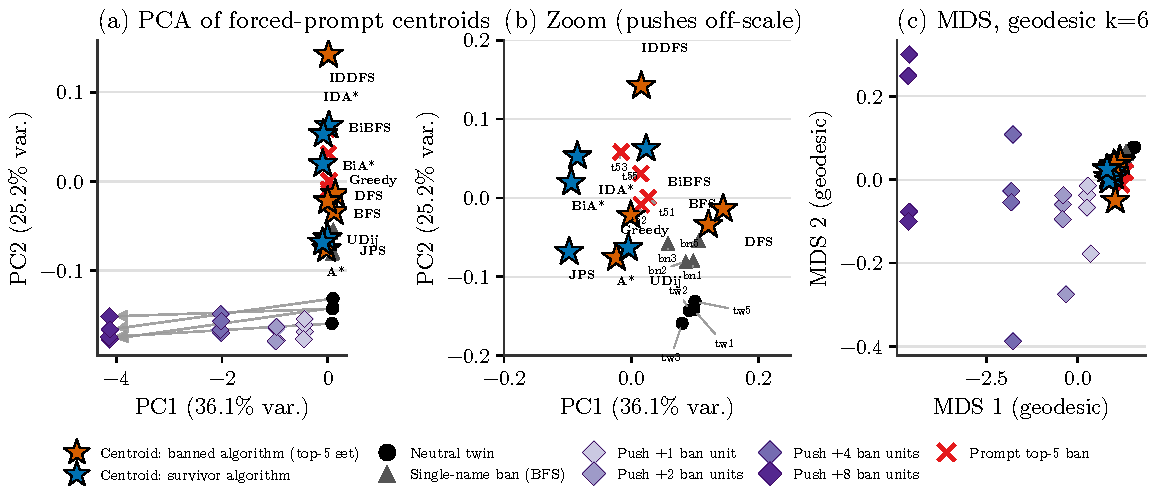
\includegraphics[width=\linewidth,height=0.78\textheight,keepaspectratio]{figures/fig_qwen_top5_geometry_v0.pdf}
\caption{Activation-space coordinates of Qwen3-8B (bf16, thinking off) on the grid-path task: mean block output over blocks 12-23 at the task-specification positions, divided by the median block norm, before any generated token. Stars are the 10 forced single-algorithm centroids, each labelled with a short name: vermillion for the five algorithms the model's own prompt bans by name (A*, BFS, DFS, greedy best-first, IDDFS), blue for the five survivors. Small markers are per-template prompt states (templates 1,2,3,5): black circles, neutral twin; grey triangles, a single-name ban of BFS; purple diamonds light-to-dark, the state after pushing 1, 2, 4, 8 ban units along the top-five push direction; red crosses, the prompt banning all five by name. Thin grey arrows connect each template's twin to its +8-unit push point. (a) PCA plane of the centroids (PC1, PC2: 36.1\%, 25.2\% of their variance). (b) The same plane zoomed to the centroid region -- push points fall outside it, omitted -- every remaining point labelled. (c) Classical MDS of geodesic distances on a 6-nearest-neighbour graph of the same states; names omitted here because the manifold collapses into one overlapping cluster at this scale, so colour\slash{}shape, shared with (a)\slash{}(b), carry identity instead. In both embeddings pushed states move away from the whole manifold along close to one direction as the push grows 1 to 8 units, approaching no centroid; pass rate over the same range collapses from 0.67 to 0.00 (n=30\slash{}level), so the departure mostly yields invalid code, not a different algorithm. The single-name and top-five-ban prompts instead sit close to the banned centroids: in 50 top-five-ban generations BFS is still written half the time, and its other correct programs are all DFS, itself banned. The source experiment's landing test finds fewer than five correct survivor-algorithm programs in every pushed or banned condition, so this geometry is consistent with, but does not alone establish, a survivor-specific landing.}
\label{fig:fig_qwen_top5_geometry}
\end{figure}
\emph{Figure note (iteration-7 correction): Actual activation coordinates: mean over the task-specification positions of each prompt (prefill, before any generated token); mean of the block outputs of blocks 12-23, divided by the median block norm; projection: (a, b) PCA fitted on the 10 forced-prompt centroids (first component 36\%, second 25\% of centroid variance); (c) classical MDS of geodesic distances on a k = 6 nearest-neighbour graph (MDS stress not recorded in \texttt{top5\_\allowbreak{}push.\allowbreak{}json}; file name restored, iteration-8 correction). Points: 28 prompt states, one per template and condition: single-name ban 4, pushes of 1, 2, 4 and 8 ban units 4 each, top-five ban 4, twin 4. Centroids: 10 forced-prompt centroids (mean state of the forced prompts that ask for each algorithm), coloured by the prompt-defined top-five ban set (banned five against survivors). N = 38. Caveat: The plotted position precedes the fork and the generated code; none: centroids and colours are defined by prompts, not by the programs written.}

\subsubsection*{6.4.5 Who forecasts the landing}
The landing contest scored, on the 21 recorded push-landing events, three forecasts: the base runner-up, the most frequent algorithm other than the default in the instruct twin itself (defined on 7 events), and a teacher-forced ranking of the openings of the catalogue algorithms by the instruct twin, the log-mean-exp likelihood of the first 48 tokens of each algorithm over its reference and forced programs, which we call the opening ranking (Table 257). The base runner-up named 17 of 21 landings and the opening ranking 10. On the 9 events where they disagree the base runner-up wins 8:1 (exact one-sided sign test p 0.020), and its mean log score is higher by 1.62 nats (Wilcoxon p 0.032). Where the twin wrote an alternative, its own minority does as well as the base runner-up (6 of 7; log-score difference 0.02, p 0.69). The comparison is retrospective, because the landings were known when the rule was frozen, and the opening ranking rests on 1 to 6 programs per algorithm. The base model adds information beyond the ranking of openings by the instruct model itself; it does not add information beyond the minority algorithm of the twin where one exists.

{\footnotesize\setlength{\tabcolsep}{4.0pt}\renewcommand{\thetable}{257}
\begin{longtable}{>{\raggedright\arraybackslash\hspace{0pt}}p{0.2063\linewidth}>{\raggedright\arraybackslash\hspace{0pt}}p{0.1248\linewidth}>{\raggedright\arraybackslash\hspace{0pt}}p{0.1576\linewidth}>{\raggedright\arraybackslash\hspace{0pt}}p{0.1075\linewidth}>{\raggedright\arraybackslash\hspace{0pt}}p{0.1426\linewidth}>{\raggedright\arraybackslash\hspace{0pt}}p{0.1577\linewidth}}
\caption{The 21 recorded push-landing events: the landing and each forecast's top-1, with log scores (base runner-up \slash{} opening ranking \slash{} twin minority). Source: exchange and site experiment \texttt{results/\allowbreak{}landing\_\allowbreak{}forecast.\allowbreak{}json}. [Source: iteration 6, artifact \nolinkurl{gen_art_experiment_30}.]}\label{tab:t275}\\
\toprule
\textbf{Event} & \textbf{Landing} & \textbf{Base runner-up} & \textbf{Twin minority} & \textbf{Opening ranking} & \textbf{Log score base \slash{} opening \slash{} twin} \\
\midrule
\endfirsthead
\multicolumn{6}{l}{\emph{Table 257, continued}}\\
\toprule
\textbf{Event} & \textbf{Landing} & \textbf{Base runner-up} & \textbf{Twin minority} & \textbf{Opening ranking} & \textbf{Log score base \slash{} opening \slash{} twin} \\
\midrule
\endhead
\bottomrule
\endlastfoot
Qwen3-8B 8-bit screen, kth smallest & quickselect & quickselect (hit) & n\slash{}a & quickselect (hit) & -1.36 \slash{} -1.67 \slash{} n\slash{}a \\
Qwen3-8B 8-bit screen, connected components & DFS & DFS (hit) & n\slash{}a & DFS (hit) & -0.84 \slash{} -0.78 \slash{} n\slash{}a \\
Qwen3-8B 8-bit screen, shortest path & Bellman-Ford\slash{}SPFA & Bellman-Ford\slash{}SPFA (hit) & n\slash{}a & Floyd-Warshall (miss) & -0.96 \slash{} -4.59 \slash{} n\slash{}a \\
Qwen3-8B 8-bit screen, two sum & brute force & brute force (hit) & n\slash{}a & brute force (hit) & -0.73 \slash{} -0.05 \slash{} n\slash{}a \\
Qwen3-8B 8-bit screen, grid & DFS & DFS (hit) & n\slash{}a & bidirectional BFS (miss) & -1.14 \slash{} -1.14 \slash{} n\slash{}a \\
Qwen3-8B bf16, kth smallest & size-k heap & quickselect (miss) & quickselect (miss) & quickselect (miss) & -1.50 \slash{} -2.64 \slash{} -1.50 \\
Qwen3-8B bf16, connected components & DFS & DFS (hit) & n\slash{}a & DFS (hit) & -0.73 \slash{} -0.05 \slash{} n\slash{}a \\
panel A, majority element & Boyer-Moore vote & Boyer-Moore vote (hit) & n\slash{}a & sort and take middle (miss) & -0.38 \slash{} -4.95 \slash{} n\slash{}a \\
panel A, trapped rain water & two pointers & two pointers (hit) & two pointers (hit) & monotonic stack (miss) & -0.33 \slash{} -4.38 \slash{} -0.14 \\
panel A, longest mirrored substring & brute force & brute force (hit) & n\slash{}a & brute force (hit) & -0.69 \slash{} -0.97 \slash{} n\slash{}a \\
panel B, single number & XOR fold & XOR fold (hit) & XOR fold (hit) & set-sum identity (miss) & -0.18 \slash{} -4.39 \slash{} -0.38 \\
panel B, minimum spanning tree weight & Prim with heap & Prim with heap (hit) & Prim with heap (hit) & Prim with heap (hit) & -0.44 \slash{} -0.05 \slash{} -0.15 \\
panel B, integer square root & linear scan & floating point sqrt (miss) & n\slash{}a & linear scan (hit) & -1.13 \slash{} -0.56 \slash{} n\slash{}a \\
panel B, count inversions & sorted insertion with bisect & sorted insertion with bisect (hit) & n\slash{}a & segment tree (miss) & -0.59 \slash{} -4.37 \slash{} n\slash{}a \\
Gemma, grid & BFS & BFS (hit) & BFS (hit) & bidirectional BFS (miss) & -0.42 \slash{} -4.53 \slash{} -0.23 \\
Gemma, kth smallest & size-k heap & quickselect (miss) & n\slash{}a & quickselect (miss) & -1.70 \slash{} -4.80 \slash{} n\slash{}a \\
Gemma, substring search & built-in find & built-in find (hit) & built-in find (hit) & built-in find (hit) & -0.13 \slash{} -0.05 \slash{} -0.50 \\
Gemma, two sum & brute force & brute force (hit) & n\slash{}a & brute force (hit) & -0.48 \slash{} -0.05 \slash{} n\slash{}a \\
Gemma, connected components & union find & BFS (miss) & n\slash{}a & BFS (miss) & -0.96 \slash{} -4.39 \slash{} n\slash{}a \\
Gemma, first and last position & binary search & binary search (hit) & binary search (hit) & exponential search (miss) & -0.12 \slash{} -4.38 \slash{} -0.38 \\
Gemma, longest increasing subsequence & quadratic DP & quadratic DP (hit) & n\slash{}a & quadratic DP (hit) & -0.06 \slash{} -0.04 \slash{} n\slash{}a \\
\end{longtable}}

Per set the base runner-up hit 5 of 5 on the 8-bit screen, 7 of 9 on the bf16 Qwen3-8B events and 5 of 7 in Gemma; the opening ranking hit 3 of 5, 4 of 9 and 3 of 7. Two correct programs labelled other appeared in the whole experiment, both catalogue variants. Judge spend was USD 0.055.

\FloatBarrier
\subsection*{6.5 Gemma: a one-token fork, and Gemma Scope 2 features against difference in means}
\addcontentsline{toc}{subsection}{6.5 Gemma: a one-token fork, and Gemma Scope 2 features against difference in means}
\noindent{\small\emph{Artifact: \nolinkurl{gen_art_experiment_31}.}}\par\medskip
\textbf{Why Gemma.} Asked one and the same grid-path prompt, gemma-3-4b-it [76] writes DFS about 70\% of the time and BFS about 30\%, so it offers what Qwen3-8B never does: the request's BFS-against-DFS contrast inside one prompt, with no ban or instruction to confound it. Gemma Scope 2 provides sparse autoencoders on the residual stream after each block, trained on this instruct model, so the feature claim needs no transfer test. Qwen-3 transcoders for circuit tracing exist as well [123], but they would have to study a choice Qwen3-8B does not make naturally. The experiment  asked where the choice forks, whether it can be read from the internals beyond what the visible text already says, and whether the SAE features steer it better than plain baselines: a difference-in-means direction, the raw residual, random features, isotropic directions, DAS and prompting. It used the residual-stream SAEs at layers 9, 17, 22 and 29 (16k latents, at the release's medium sparsity), one 16 GB card and exact common random numbers, under two hash-chained commitments.

\textbf{Natural splits.} Over 200 samples per task, the grid prompt gave DFS 139 and BFS 61 (Wilson interval for DFS 0.63 to 0.75), with DFS on 134 of 172 correct programs (Table 258). The choice depends on the template: BFS takes 6 to 18 of 40 attempts per template. Substring search (naive 173, built-in find 27) and first and last position (linear scan 170, binary search 29) split as well. Labels agreed with iteration 5's Gemma rows on 0.94 of the grid slots and 1.00 of the substring slots.

\begin{table}[H]
\renewcommand{\thetable}{258}
\centering\scriptsize\setlength{\tabcolsep}{2.5pt}
\caption{Natural splits in gemma-3-4b-it (N = 200 per task; 40 per template). Source: Gemma feature experiment \texttt{results/\allowbreak{}natural\_\allowbreak{}split.\allowbreak{}json}. [Source: iteration 6, artifact \nolinkurl{gen_art_experiment_31}.]}\label{tab:t276}
\begin{tabular}{>{\raggedright\arraybackslash\hspace{0pt}}p{0.0908\linewidth}>{\raggedright\arraybackslash\hspace{0pt}}p{0.1552\linewidth}>{\raggedright\arraybackslash\hspace{0pt}}p{0.0788\linewidth}>{\raggedright\arraybackslash\hspace{0pt}}p{0.0539\linewidth}>{\raggedright\arraybackslash\hspace{0pt}}p{0.0788\linewidth}>{\raggedright\arraybackslash\hspace{0pt}}p{0.1078\linewidth}>{\raggedright\arraybackslash\hspace{0pt}}p{0.3581\linewidth}}
\toprule
\textbf{Task} & \textbf{Attempted} & \textbf{Correct} & \textbf{Pass} & \textbf{Correct-only Hill-1} & \textbf{Default (share of correct)} & \textbf{Attempted per template (first to fifth)} \\
\midrule
grid & DFS 139, BFS 61 & DFS 134, BFS 38 & 0.86 & 1.68 & DFS (0.78) & DFS 34 \slash{} BFS 6; DFS 22 \slash{} BFS 18; DFS 22 \slash{} BFS 18; DFS 29 \slash{} BFS 11; DFS 32 \slash{} BFS 8 \\
substring search & naive 173, built-in find 27 & same & 1.00 & 1.47 & naive (0.87) & naive 36 \slash{} built-in 4; naive 40; built-in 21 \slash{} naive 19; naive 38 \slash{} built-in 2; naive 40 \\
first and last position & linear scan 170, binary search 29, other 1 & same & 1.00 & 1.52 & linear scan (0.85) & linear 33 \slash{} binary 7; linear 28 \slash{} binary 12; linear 39 \slash{} other 1; linear 40; linear 30 \slash{} binary 10 \\
\bottomrule
\end{tabular}
\end{table}

\textbf{The instrument gate.} Each SAE was spliced into the forward pass on three corpora: the model's own programs, generic text and LeetCode prompts. A layer passed if its increase in cross-entropy and its fraction of variance unexplained on the model's programs were at most 1.5 times those on generic text (Table 259). Layers 22 and 29 passed; layer 9 failed the cross-entropy ratio and layer 17 the variance ratio by 0.0001, so their results are descriptive. On generic text the mean number of active latents per token was 57 to 64, slightly above the quoted medium band of 30 to 60.

\begin{table}[H]
\renewcommand{\thetable}{259}
\centering\footnotesize\setlength{\tabcolsep}{4.0pt}
\caption{Gemma Scope 2 residual-stream SAEs spliced in on three corpora (the model's own programs \slash{} generic text \slash{} LeetCode prompts): mean active latents per token, fraction of variance explained, increase in cross-entropy (nats per token) and loss recovered. Source: Gemma feature experiment \texttt{results/\allowbreak{}gate.\allowbreak{}json}. [Source: iteration 6, artifact \nolinkurl{gen_art_experiment_31}.]}\label{tab:t277}
\begin{tabular}{>{\raggedright\arraybackslash\hspace{0pt}}p{0.0699\linewidth}>{\raggedright\arraybackslash\hspace{0pt}}p{0.1565\linewidth}>{\raggedright\arraybackslash\hspace{0pt}}p{0.1856\linewidth}>{\raggedright\arraybackslash\hspace{0pt}}p{0.1681\linewidth}>{\raggedright\arraybackslash\hspace{0pt}}p{0.1651\linewidth}>{\raggedright\arraybackslash\hspace{0pt}}p{0.1515\linewidth}}
\toprule
\textbf{Layer} & \textbf{Active latents per token} & \textbf{Fraction of variance explained} & \textbf{Increase in cross-entropy} & \textbf{Loss recovered} & \textbf{Gate} \\
\midrule
9 & 52.2 \slash{} 57.5 \slash{} 57.3 & 0.963 \slash{} 0.974 \slash{} 0.917 & 0.065 \slash{} 0.033 \slash{} -0.010 & 0.9968 \slash{} 0.9983 \slash{} 1.0005 & fail \\
17 & 59.9 \slash{} 64.1 \slash{} 61.4 & 0.919 \slash{} 0.946 \slash{} 0.814 & 0.097 \slash{} 0.184 \slash{} 0.119 & 0.9968 \slash{} 0.9936 \slash{} 0.9957 & fail (variance ratio, by 0.0001) \\
22 & 60.0 \slash{} 61.7 \slash{} 62.2 & 0.809 \slash{} 0.869 \slash{} 0.750 & 0.036 \slash{} 0.259 \slash{} 0.167 & 0.9968 \slash{} 0.9789 \slash{} 0.9837 & pass \\
29 & 64.1 \slash{} 64.1 \slash{} 69.5 & 0.637 \slash{} 0.715 \slash{} 0.635 & 0.017 \slash{} 0.212 \slash{} 0.142 & 0.9994 \slash{} 0.9932 \slash{} 0.9952 & pass \\
\bottomrule
\end{tabular}
\end{table}

\textbf{The plan is a single-token fork.} Prefix resampling with change-point detection, the method of forking-path analyses [30, 31], located the fork: 24 base paths, 16 prefix lengths, 8 continuations each and a refinement, 3,712 continuations in all, scored by a partial-code labeller that agreed with the full labeller on 200 of 200 programs. Every one of 12 BFS base paths had a significant change point with a rise of at least 0.4, at prefix lengths 16 to 36. In 177 of 200 programs the first 32 tokens are identical (the code fence, \texttt{def solve(\allowbreak{}grid,\allowbreak{} start,\allowbreak{} goal):\allowbreak{}}, \texttt{rows =\allowbreak{} len(\allowbreak{}grid)}, \texttt{cols =\allowbreak{} len(\allowbreak{}grid[\allowbreak{}0])} and an indent), and the next token decides (Table 260): \texttt{ visited} leads to DFS (BFS probability 0.011 over 1,409 continuations), while a blank line, \texttt{if}, \texttt{queue} or \texttt{q} lead to BFS (0.95 to 1.00). The first token that identifies the algorithm in code comes a median of 138 tokens after the fork (10th to 90th percentile 80 to 181). The fork index was chosen by the token class with the most mutual information with the outcome (0.62 bits at index 32), after the first median rule landed on a deterministic indentation token; the change was made before the second commitment.

\emph{Executed but not reported until iteration 7.} The empty-prefix unit test of the fork failed mildly: continuations from the empty prefix give BFS 0.38 (73 of 192) against the natural 0.305 [0.245, 0.372] (outside the interval; exact binomial p 0.028 against 0.305), so the resampled continuations are slightly richer in BFS than the natural samples. The deviation log records what did not run: the clamp read-back and matched-norm realisation tests as separate unit tests (the matched norm is imposed by construction in the clamp code, \texttt{src/\allowbreak{}clamp.\allowbreak{}py} (file name restored, iteration-8 correction), and the realised norm of each edit is logged per row); the clamp-cell overlay on the generated-position panel; the fork and the cross-prompt readouts of two further bench tasks (dropped in order); and per-sample displacement at generated tokens 1-32 (prefill displacement at blocks 11-33 is logged). (iteration-7 correction)

\begin{table}[H]
\renewcommand{\thetable}{260}
\centering\footnotesize\setlength{\tabcolsep}{4.0pt}
\caption{The fork token at response index 32 and the BFS probability of the continuations that follow it (all continuations; the natural samples alone in the last column). Source: Gemma feature experiment \texttt{results/\allowbreak{}fork.\allowbreak{}json}. [Source: iteration 6, artifact \nolinkurl{gen_art_experiment_31}.]}\label{tab:t278}
\begin{tabular}{>{\raggedright\arraybackslash\hspace{0pt}}p{0.1833\linewidth}>{\raggedright\arraybackslash\hspace{0pt}}p{0.1460\linewidth}>{\raggedright\arraybackslash\hspace{0pt}}p{0.0729\linewidth}>{\raggedright\arraybackslash\hspace{0pt}}p{0.0729\linewidth}>{\raggedright\arraybackslash\hspace{0pt}}p{0.1700\linewidth}>{\raggedright\arraybackslash\hspace{0pt}}p{0.2515\linewidth}}
\toprule
\textbf{Token at index 32} & \textbf{Continuations} & \textbf{BFS} & \textbf{DFS} & \textbf{BFS probability} & \textbf{Natural samples (BFS \slash{} n)} \\
\midrule
\texttt{ visited} & 1,409 & 15 & 1,394 & 0.011 & 2 \slash{} 134 \\
newline & 204 & 193 & 11 & 0.946 & 19 \slash{} 21 \\
\texttt{if} & 177 & 174 & 2 & 0.989 & 16 \slash{} 17 \\
\texttt{queue} & 82 & 82 & 0 & 1.000 & 4 \slash{} 4 \\
\texttt{q} & 3 & 3 & 0 & 1.000 & 1 \slash{} 1 \\
\bottomrule
\end{tabular}
\end{table}

\textbf{Readable beyond the text, at the fork, but not specifically through the SAE.} Within one prompt, decodability before the first identifying token is at ceiling for every method, the visible-text control included (balanced accuracy 1.00 at all four layers), so the SAE has no advantage there; at the fork itself the test is undefined, because 185 of 200 samples share their prefix with a sample of the other class. Across prompts, the experiment built 120 neutral prompt variants by changing nouns and measured each variant's fork log-odds of BFS, which we write y (mean -0.92 nats, SD 0.67; the sampled BFS share tracks it at Spearman 0.65 over 60 variants of 10 samples). A Lasso on layer-29 SAE codes at the fork position predicts held-out y with R-squared 0.66, against 0.18 for a text-only model (difference 0.49, 95\% interval 0.26 to 0.65, permutation p 0.003), above the difference-in-means readout (0.34) and a 16-component PCA of the raw residual (0.56) (Table 261). That meets the preregistered bar. Two checks outside the preregistration qualify it: a tuned ridge on the raw layer-29 residual reaches 0.72, and ridge on the same SAE codes reaches at most 0.09. Beside the Lasso, the standardised ridge on the same layer-29 SAE codes reaches R-squared 0.15 against 0.086 for a template-plus-noun-norm control (delta 0.064, below the preregistered 0.10 bar); the unstandardised SAE ridge ranges from -0.76 to 0.06 across penalties while the raw ridge stays at 0.70 to 0.72, which is why the SAE advantage depends on the estimator. Moreover, a linear readout of the fork log-odds from the residual at the fork position is close to a next-token readout, so the raw-residual 0.72 shows that the next-token distribution is linearly encoded there, not that a plan is; no logit-lens control of matched capacity was run. At the task-specification positions, before any response token, the SAE codes do no better than the text (0.18). (iteration-7 correction)

\begin{table}[H]
\renewcommand{\thetable}{261}
\centering\footnotesize\setlength{\tabcolsep}{4.0pt}
\caption{Cross-prompt readout of the fork log-odds over 120 neutral variants: R-squared with held-out nouns, Spearman with held-out nouns, and R-squared with held-out templates. Post hoc, the standardised ridge on the same layer-29 SAE codes reaches R-squared 0.15 against 0.086 for a template-plus-noun-norm control (delta 0.064, below the preregistered 0.10 bar). At the fork position this readout is close to a next-token readout (no logit-lens control was run). Source: Gemma feature experiment \texttt{results/\allowbreak{}readout.\allowbreak{}json}, \texttt{results/\allowbreak{}rederive\_\allowbreak{}headlines.\allowbreak{}json}. (iteration-7 correction) [Source: iteration 6, artifact \nolinkurl{gen_art_experiment_31}.]}\label{tab:t279}
\begin{tabular}{>{\raggedright\arraybackslash\hspace{0pt}}p{0.1697\linewidth}>{\raggedright\arraybackslash\hspace{0pt}}p{0.1493\linewidth}>{\raggedright\arraybackslash\hspace{0pt}}p{0.0699\linewidth}>{\raggedright\arraybackslash\hspace{0pt}}p{0.1648\linewidth}>{\raggedright\arraybackslash\hspace{0pt}}p{0.1593\linewidth}>{\raggedright\arraybackslash\hspace{0pt}}p{0.1837\linewidth}}
\toprule
\textbf{Readout} & \textbf{Site} & \textbf{Layer} & \textbf{R-squared, held-out nouns} & \textbf{Spearman, held-out nouns} & \textbf{R-squared, held-out templates} \\
\midrule
text only & n\slash{}a & n\slash{}a & 0.176 & 0.425 & 0.150 \\
template only & n\slash{}a & n\slash{}a & 0.148 & 0.272 & -0.122 \\
SAE codes (Lasso) & fork & 22 & 0.237 & 0.583 & 0.139 \\
raw PCA-16 & fork & 22 & 0.412 & 0.666 & 0.491 \\
raw PCA-64 & fork & 22 & 0.092 & 0.533 & 0.239 \\
difference in means & fork & 22 & 0.226 & 0.541 & 0.109 \\
SAE codes (Lasso) & task specification & 22 & 0.180 & 0.464 & 0.123 \\
raw PCA-16 & task specification & 22 & -0.090 & 0.354 & 0.352 \\
raw PCA-64 & task specification & 22 & 0.021 & 0.432 & 0.152 \\
difference in means & task specification & 22 & 0.063 & 0.282 & -0.570 \\
SAE codes (Lasso) & fork & 29 & 0.662 & 0.782 & 0.496 \\
raw PCA-16 & fork & 29 & 0.557 & 0.697 & 0.444 \\
raw PCA-64 & fork & 29 & 0.432 & 0.715 & 0.403 \\
difference in means & fork & 29 & 0.338 & 0.620 & 0.181 \\
SAE codes (Lasso) & task specification & 29 & -0.073 & 0.276 & 0.147 \\
raw PCA-16 & task specification & 29 & -0.602 & 0.194 & -0.062 \\
raw PCA-64 & task specification & 29 & 0.029 & 0.381 & 0.083 \\
difference in means & task specification & 29 & 0.064 & 0.302 & -0.438 \\
\bottomrule
\end{tabular}
\end{table}

\textbf{Steering: the features move the fork, difference in means moves it more, and edits toward BFS cost correctness.} We call an \emph{SAE clamp} setting the k latents that best separate forced-BFS from forced-DFS prompts (input-selected) to their BFS-class mean at the fork position; output-scored latents are chosen instead by their attribution to the fork's logit difference, and the two sets of 20 share 2 latents. At the fork position of layer 22, edits at matched norm moved y by +4.04 nats for the difference-in-means direction, +1.78 for the SAE clamp of the top 20 input-selected latents, +0.51 for 20 random latents and +0.12 for an isotropic direction. Table 261b gives the whole dose-response sweep over the 120 prompt variants (11,280 measurements), at the fork and at the task-specification positions. In generation (N = 50 paired slots), the twin wrote BFS in 13 programs; the SAE clamp raised this to 30 (top 20 latents) and 36 (top 50), the difference-in-means edit at the same norm to 46 and 49, and random latents to 21 (Table 262). Edits toward BFS at the fork lowered the pass rate from 0.84 for the twin to 0.58 and 0.48 for the top-20 and top-50 SAE clamps and 0.32 and 0.16 for difference in means (0.60 to 0.78 for the other BFS-ward fork edits, 0.00 for the DAS interchange), except the SAE top-5 clamp (18 BFS of 50, pass 0.84), so the preregistered outcome, correct BFS programs, shows no significant effect anywhere after Holm correction, and no feature claim is made. The preregistered feature rule (SAE target-correct count at least the difference-in-means count, at a pass rate of at least 0.8 times the twin's) is also met by random latents at k = 50 (9 against 7, pass 0.76), so it cannot discriminate here. The informative comparisons are on attempted BFS, and they are descriptive: the SAE clamp beats the twin (17:0 and 23:0 discordant slots, p 1.5e-5 and 2.4e-7) and random latents (15:0, p 6.1e-5), and difference in means beats the SAE clamp at matched norm (16:0, p 3.1e-5). At matched effect on y rather than matched norm, difference in means and the SAE clamp shift the plan equally (32 against 30 BFS, p 0.50; 34 against 36, p 0.63) and difference in means keeps slightly more programs correct (13 against 9, 14 against 10). Edits at the task-specification positions do nothing (12 to 19 BFS against 13). Steering toward DFS works cleanly for both (SAE 47 of 50, difference in means 50 of 50, against 37 for the twin; pass 0.98 to 1.00). Difference-in-means steering of a code model's choice of language and library has shown the same trade-off, with overly strong interventions reducing output quality [130]. AxBench found simple baselines ahead of SAE steering [34], and a 2026 reanalysis puts SAEs close to AxBench's reference when latents are selected and labelled by a supervised pipeline [131]; here, at comparable norms, neither the input-selected nor the output-scored clamp reached the difference-in-means edit (Table 261b). (iteration-7 correction)

\begin{table}[H]
\renewcommand{\thetable}{261b}
\centering\scriptsize\setlength{\tabcolsep}{2.5pt}
\caption{Mean change in the fork log-odds of BFS (nats) under each edit at layer 22, by number of latents k and dose lambda; the difference-in-means, random and isotropic edits are scaled to the norm of the input-selected clamp with the same k. Source: Gemma feature experiment \texttt{results/\allowbreak{}logit\_\allowbreak{}sweep\_\allowbreak{}summary.\allowbreak{}json}. [Source: iteration 6, artifact \nolinkurl{gen_art_experiment_31}.]}\label{tab:t280}
\begin{tabular}{>{\raggedright\arraybackslash\hspace{0pt}}p{0.2443\linewidth}>{\raggedright\arraybackslash\hspace{0pt}}p{0.0788\linewidth}>{\raggedright\arraybackslash\hspace{0pt}}p{0.0734\linewidth}>{\raggedright\arraybackslash\hspace{0pt}}p{0.0712\linewidth}>{\raggedright\arraybackslash\hspace{0pt}}p{0.0712\linewidth}>{\raggedright\arraybackslash\hspace{0pt}}p{0.1248\linewidth}>{\raggedright\arraybackslash\hspace{0pt}}p{0.1248\linewidth}>{\raggedright\arraybackslash\hspace{0pt}}p{0.1248\linewidth}}
\toprule
\textbf{Edit} & \textbf{Latents (k)} & \textbf{Fork, lambda 0.5} & \textbf{Fork, lambda 1} & \textbf{Fork, lambda 2} & \textbf{Task specification, lambda 0.5} & \textbf{Task specification, lambda 1} & \textbf{Task specification, lambda 2} \\
\midrule
SAE clamp, input-selected & 5 & 0.52 & 0.98 & 1.97 & 0.09 & 0.11 & 0.11 \\
SAE clamp, input-selected & 20 & 0.87 & 1.78 & 3.76 & 0.12 & 0.12 & 0.22 \\
SAE clamp, input-selected & 50 & 1.09 & 2.26 & 4.47 & 0.08 & 0.10 & 0.20 \\
SAE clamp, output-scored & 5 & 0.66 & 1.33 & 2.69 & 0.16 & 0.20 & 0.28 \\
SAE clamp, output-scored & 20 & 0.74 & 1.35 & 2.65 & 0.17 & 0.22 & 0.21 \\
SAE clamp, output-scored & 50 & 1.38 & 2.94 & 6.07 & 0.23 & 0.32 & 0.37 \\
difference in means (norm of the input-selected clamp) & 5 & 1.05 & 2.04 & 4.14 & 0.09 & 0.09 & 0.08 \\
difference in means (norm of the input-selected clamp) & 20 & 1.98 & 4.04 & 7.93 & 0.41 & 0.70 & 1.29 \\
difference in means (norm of the input-selected clamp) & 50 & 3.53 & 7.08 & 12.22 & 0.44 & 0.76 & 1.35 \\
random latents (same norm) & 5 & -0.14 & -0.37 & -0.73 & 0.08 & 0.10 & 0.12 \\
random latents (same norm) & 20 & 0.26 & 0.51 & 1.26 & 0.04 & 0.01 & -0.01 \\
random latents (same norm) & 50 & 0.32 & 0.89 & 2.65 & 0.18 & 0.31 & 0.54 \\
isotropic direction (same norm) & 5 & 0.06 & 0.11 & 0.13 & 0.07 & 0.04 & 0.02 \\
isotropic direction (same norm) & 20 & 0.07 & 0.12 & 0.26 & -0.16 & -0.37 & -0.78 \\
isotropic direction (same norm) & 50 & 0.12 & 0.23 & 0.18 & -0.19 & -0.42 & -0.81 \\
SAE clamp with ban-contrast latents & 20 & n\slash{}a & 0.95 & n\slash{}a & n\slash{}a & 0.09 & n\slash{}a \\
SAE clamp, input-selected, layer 29 & 20 & n\slash{}a & 0.63 & n\slash{}a & n\slash{}a & n\slash{}a & n\slash{}a \\
\bottomrule
\end{tabular}
\end{table}

{\footnotesize\setlength{\tabcolsep}{4.0pt}\renewcommand{\thetable}{262}
\begin{longtable}{>{\raggedright\arraybackslash\hspace{0pt}}p{0.1364\linewidth}>{\raggedright\arraybackslash\hspace{0pt}}p{0.3509\linewidth}>{\raggedright\arraybackslash\hspace{0pt}}p{0.1215\linewidth}>{\raggedright\arraybackslash\hspace{0pt}}p{0.1385\linewidth}>{\raggedright\arraybackslash\hspace{0pt}}p{0.0889\linewidth}>{\raggedright\arraybackslash\hspace{0pt}}p{0.0604\linewidth}}
\caption{Generation under edits at the fork (layer 22) and at the task-specification positions (N = 50 paired slots; BFS is the target). Source: Gemma feature experiment \texttt{results/\allowbreak{}clamps.\allowbreak{}json}. [Source: iteration 6, artifact \nolinkurl{gen_art_experiment_31}.]}\label{tab:t281}\\
\toprule
\textbf{Site} & \textbf{Edit} & \textbf{Mean realised norm} & \textbf{Attempted BFS} & \textbf{Correct BFS} & \textbf{Pass} \\
\midrule
\endfirsthead
\multicolumn{6}{l}{\emph{Table 262, continued}}\\
\toprule
\textbf{Site} & \textbf{Edit} & \textbf{Mean realised norm} & \textbf{Attempted BFS} & \textbf{Correct BFS} & \textbf{Pass} \\
\midrule
\endhead
\bottomrule
\endlastfoot
none & twin & 0 & 13 & 6 & 0.84 \\
fork & SAE clamp, top 5 input-selected latents & 307.9 & 18 & 10 & 0.84 \\
fork & SAE clamp, top 20 input-selected latents & 602.2 & 30 & 9 & 0.58 \\
fork & SAE clamp, top 50 input-selected latents & 1069.8 & 36 & 10 & 0.48 \\
fork & difference in means at the top-20 norm & 602.2 & 46 & 12 & 0.32 \\
fork & difference in means at the top-50 norm & 1069.8 & 49 & 7 & 0.16 \\
fork & 50 random latents at the same norm & 1069.8 & 21 & 9 & 0.76 \\
fork & SAE clamp, top 20 output-scored latents & 673.5 & 25 & 14 & 0.78 \\
fork & difference in means matched on effect, top-20 level & 270.6 & 32 & 13 & 0.62 \\
fork & difference in means matched on effect, top-50 level & 342.9 & 34 & 14 & 0.60 \\
fork & DAS rank-4 interchange & 496.0 & 50 & 0 & 0.00 \\
fork & ablation of the top 5 attribution nodes (N = 30) & 1004.7 & 29 & 0 & 0.03 \\
fork & steering with the top 5 attribution nodes (N = 30) & 115.5 & 19 & 12 & 0.73 \\
task specification & SAE clamp, top 5 & 4.1 & 14 & 6 & 0.84 \\
task specification & SAE clamp, top 20 & 92.4 & 12 & 4 & 0.82 \\
task specification & SAE clamp, top 50 & 104.9 & 15 & 5 & 0.80 \\
task specification & difference in means at the top-20 norm & 92.4 & 17 & 9 & 0.84 \\
task specification & difference in means at the top-50 norm & 104.9 & 19 & 9 & 0.80 \\
task specification & 50 random features & 104.9 & 15 & 9 & 0.88 \\
fork, toward DFS & SAE clamp, top 20 & 1170.1 & 3 (47 DFS, all correct) & n\slash{}a & 0.98 \\
fork, toward DFS & difference in means & 1170.1 & 0 (50 DFS, all correct) & n\slash{}a & 1.00 \\
\end{longtable}}

\begin{figure}[!htbp]
\centering\captionsetup{font=footnotesize}
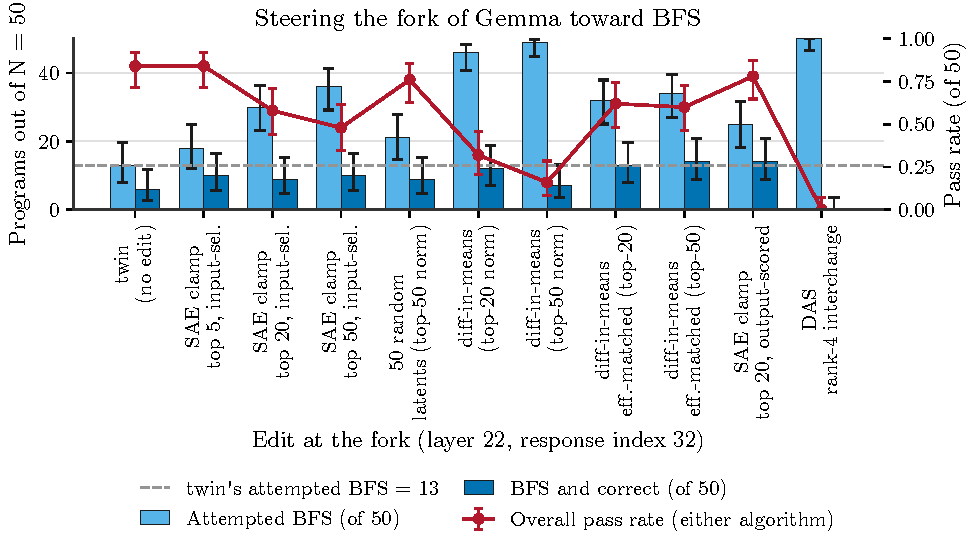
\includegraphics[width=\linewidth,height=0.78\textheight,keepaspectratio]{figures/fig_gemma_steer_v0.pdf}
\caption{Generation-time steering of gemma-3-4b-it's BFS-vs-DFS fork on the grid-path task (layer 22, response index 32), N = 50 matched generations per condition, from gen\textbackslash{}\_\allowbreak{}art\textbackslash{}\_\allowbreak{}experiment\textbackslash{}\_\allowbreak{}31's results\slash{}clamps.json. Light-blue bars: programs that attempt BFS (of 50); dark-blue bars: programs that are BFS and pass the hidden tests (of 50); both carry 95\textbackslash{}\% Wilson confidence intervals. The dashed grey line marks the unedited twin's attempted-BFS count (13). The red line (circular markers, right axis, its own 95\textbackslash{}\% CI) is the overall hidden-test pass rate -- the share of all 50 programs that pass, whichever algorithm they implement, not a BFS-specific rate. The eleven conditions, left to right: no edit (twin); an SAE clamp on the top 5, 20 and 50 input-selected Gemma Scope 2 latents; a 50-feature random-latent control at the top-50 norm; difference-in-means edits at the top-20 and top-50 norm, and again matched on the SAE clamp's effect on the fork log-odds; an SAE clamp on the top 20 output-scored latents; and a rank-4 DAS interchange. Attempted-BFS rises from 13 (twin) to 50\slash{}50 (DAS), while BFS-and-correct stays between 6 and 14 throughout and the overall pass rate falls as the edits strengthen, collapsing to 0\slash{}50 under the DAS interchange. The source experiment's own pre-registered test found the SAE clamp was not reliably distinguishable from a norm-matched random-feature control once correctness is accounted for ('feature\textbackslash{}\_\allowbreak{}claim': false), so this is evidence for a steerability-versus-correctness trade-off, not for one specific causal feature or circuit; a later, differently sited experiment found the DAS result is sensitive to decoding protocol.}
\label{fig:fig_gemma_steer}
\end{figure}
\textbf{DAS moves the fork log-odds within the controls it had, and forcing it breaks the program.} DAS at the fork position of layer 22, with forced-BFS prompts as sources, moved held-out y by +8.8, +9.5 and +9.8 nats at ranks 1, 2 and 4, against -0.08 to +0.05 for random subspaces of the same rank (Table 263). The shuffled-source control was uninformative as built, because every source was a forced-BFS prompt. In generation the rank-4 interchange made 50 of 50 programs BFS and 0 of 50 passed. Stated within its controls, a rank-1 DAS subspace fitted on forced-BFS sources moves the held-out fork log-odds by 8.8 nats (random subspaces of the same rank -0.08 to +0.05); because every source was forced-BFS, the shuffled-source control is uninformative by construction (10.1 nats); no random-initialisation or target-shuffled control was run; and the rank-4 interchange gives BFS in 50 of 50 attempts with 0 of 50 programs passing, so this does not show that the choice is one-dimensional. With unrestricted alignment maps interchange accuracy reaches 100\% even on randomly initialised language models (Sutter et al., Table 277 row 14), so the fit stays uninterpretable until those controls run; pushing hard costs correctness, as subspace interventions can when they leave the model's natural range [122]. (iteration-7 correction)

\begin{table}[H]
\renewcommand{\thetable}{263}
\centering\footnotesize\setlength{\tabcolsep}{4.0pt}
\caption{DAS at the fork (layer 22): mean change in the fork log-odds of BFS on held-out and training prompts. Every source was a forced-BFS prompt, so the shuffled-source column is uninformative by construction; no random-initialisation or target-shuffled control was run, and the rank-4 interchange gave 0 of 50 passing programs (Table 262), so the table does not show that the choice is one-dimensional. Source: Gemma feature experiment \texttt{results/\allowbreak{}das.\allowbreak{}json}. (iteration-7 correction) [Source: iteration 6, artifact \nolinkurl{gen_art_experiment_31}.]}\label{tab:t282}
\begin{tabular}{>{\raggedright\arraybackslash\hspace{0pt}}p{0.0604\linewidth}>{\raggedright\arraybackslash\hspace{0pt}}p{0.1099\linewidth}>{\raggedright\arraybackslash\hspace{0pt}}p{0.0939\linewidth}>{\raggedright\arraybackslash\hspace{0pt}}p{0.2703\linewidth}>{\raggedright\arraybackslash\hspace{0pt}}p{0.1805\linewidth}>{\raggedright\arraybackslash\hspace{0pt}}p{0.1816\linewidth}}
\toprule
\textbf{Rank} & \textbf{DAS, held out} & \textbf{DAS, train} & \textbf{Share of held-out prompts moved toward BFS} & \textbf{Random subspace, held out} & \textbf{Shuffled source, held out} \\
\midrule
1 & 8.81 & 9.55 & 1.00 & -0.08 & 10.11 \\
2 & 9.51 & 10.15 & 1.00 & 0.03 & 9.69 \\
4 & 9.76 & 10.25 & 1.00 & 0.05 & 11.42 \\
\bottomrule
\end{tabular}
\end{table}

The planned transcoder attribution graph was the first item of the drop order and was not built; a first-order attribution on the residual-stream SAEs replaced it (Table 264). Ablating the two strongest nodes moved y by 4.0 and 6.3 nats, against 0.8 and 0.4 for random active latents at matched contribution; two of the other three beat random and one did not. Jointly ablating the five nodes turned 29 of 30 programs into BFS with none passing, and jointly steering with them gave 19 BFS of 30, 12 correct.

\begin{table}[H]
\renewcommand{\thetable}{264}
\centering\scriptsize\setlength{\tabcolsep}{2.5pt}
\caption{First-order attribution nodes at the fork, validated by ablation and steering in the real model (mean change in y, against random active latents at matched contribution). Source: Gemma feature experiment \texttt{results/\allowbreak{}attribution.\allowbreak{}json}. [Source: iteration 6, artifact \nolinkurl{gen_art_experiment_31}.]}\label{tab:t283}
\begin{tabular}{>{\raggedright\arraybackslash\hspace{0pt}}p{0.0754\linewidth}>{\raggedright\arraybackslash\hspace{0pt}}p{0.0925\linewidth}>{\raggedright\arraybackslash\hspace{0pt}}p{0.1885\linewidth}>{\raggedright\arraybackslash\hspace{0pt}}p{0.1152\linewidth}>{\raggedright\arraybackslash\hspace{0pt}}p{0.1702\linewidth}>{\raggedright\arraybackslash\hspace{0pt}}p{0.1115\linewidth}>{\raggedright\arraybackslash\hspace{0pt}}p{0.1702\linewidth}}
\toprule
\textbf{Layer} & \textbf{Latent} & \textbf{Attribution score} & \textbf{Ablation} & \textbf{Random ablation} & \textbf{Steering} & \textbf{Random steering} \\
\midrule
22 & 1774 & -4.68 & 4.01 & 0.78 & 0.55 & 0.07 \\
29 & 15050 & -4.35 & 6.28 & 0.40 & 0.45 & 0.11 \\
29 & 735 & 4.11 & -0.51 & 0.40 & 1.38 & 0.09 \\
29 & 6026 & 3.95 & -0.95 & 0.51 & 0.14 & 0.09 \\
22 & 142 & 3.79 & -1.26 & 2.10 & 0.24 & 0.09 \\
\bottomrule
\end{tabular}
\end{table}

\textbf{The top-five prohibition in a model that writes two algorithms.} Banning the five most common grid algorithms (BFS, DFS, IDDFS, A* and greedy best-first, which share one catalogue label here) left no program outside the banned set: avoidance 0.00, as in Qwen3-8B in iteration 2 (Table 265). The ban pushed Gemma from its default DFS to BFS (10 to 41 of 50; McNemar 32:1, p 7.9e-9) and cut the pass rate from 0.86 to 0.38. In actual activation coordinates (PCA, Isomap with k = 10 and classical MDS of layers 17 and 22, raw and SAE codes), the top-five prompt states sit next to the banned A* and greedy cluster (Table 266); among all 15 ways of splitting the six catalogue centroids into four banned and two survivors, the observed split ranks first in three of the four spaces (rank share 0.067) and third in the fourth (0.20). The prohibition lands inside the banned region, not at its edge or on the opposite side. The single-name bans of BFS and DFS left the banned algorithm in 11 and 8 of 50 programs, and the forced prompts gave BFS 50 of 50 (38 correct) and DFS 50 of 50 (45 correct).

\begin{figure}[!htbp]
\centering\captionsetup{font=footnotesize}
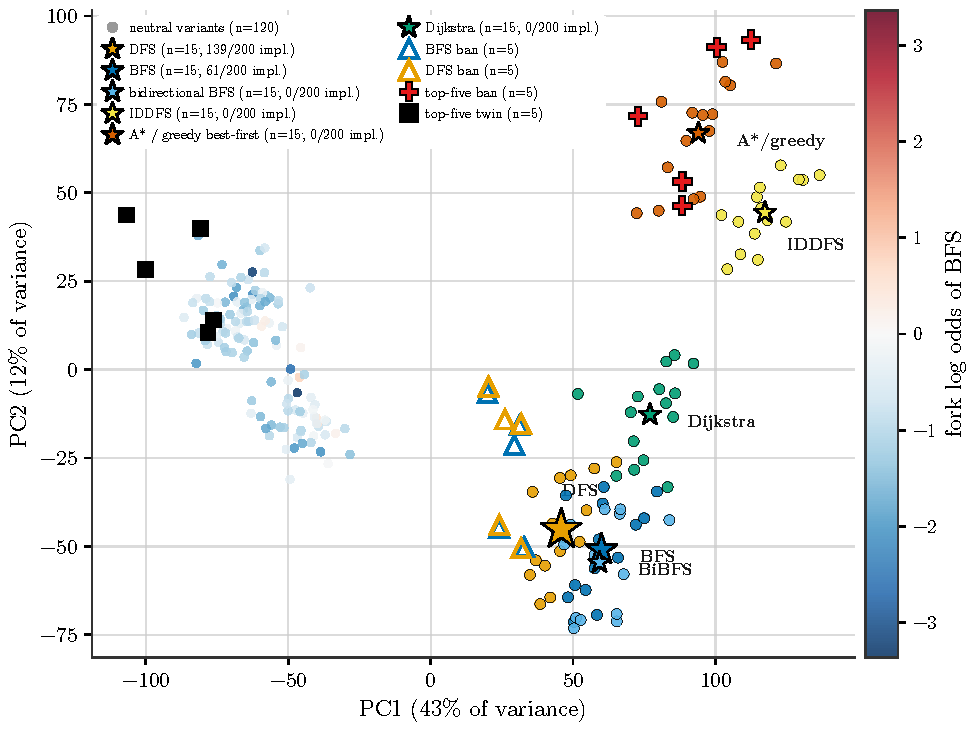
\includegraphics[width=\linewidth,height=0.78\textheight,keepaspectratio]{figures/fig_gemma_geometry_raw_L17_v0.pdf}
\caption{Actual block-17 raw-residual activation coordinates of gemma-3-4b-it on the grid-path task (iteration 6, recomputed from the cached activations): the mean over the task-specification token positions, with the five highest-magnitude channels zeroed; PCA plane fitted jointly on all 230 points (PC1 43\textbackslash{}\%, PC2 12\textbackslash{}\% of variance). Small circles are forced-algorithm prompts, one colour per mode (BFS blue, DFS orange, bidirectional BFS sky blue, IDDFS yellow, A*\slash{}greedy vermillion, Dijkstra green; \$n=15\$ each); stars mark each mode's centroid, sized by how often that algorithm was naturally implemented out of 200 unconstrained samples (DFS 139, BFS 61; the other four modes 0\slash{}200). Hollow triangles are prompts banning BFS or DFS alone (\$n=5\$ each, blue\slash{}orange edges); filled red crosses are prompts banning the top five algorithms together (\$n=5\$); filled black squares are that ban's neutral, no-prohibition twin (\$n=5\$). Small dots are 120 neutral task variants, coloured on a diverging blue--white--red scale (colourbar, right) by the fork log odds of BFS measured later in the response; red indicates a higher log odds of BFS, blue a lower one. All plotted activations are read out before the BFS\slash{}DFS fork.}
\label{fig:fig_gemma_geometry_raw_L17}
\end{figure}
\emph{Figure note (iteration-7 correction): Actual activation coordinates: mean over the task-specification positions (from the first token of the task statement to the last token of the user message, \texttt{src/\allowbreak{}cfg.\allowbreak{}py} line 7; file name restored, iteration-8 correction), so neither the read position nor the fork at response index 32 is plotted; output of block 17 (the residual stream after the block), five massive channels zeroed; projection: PCA (first component 0.43, second 0.12 of variance), Isomap (k = 10) and classical MDS (stress-1 0.371), all fitted on the 230 points. Points: prompt states: forced-algorithm prompts by mode, BFS and DFS bans, the top-five ban and its twin, and 120 neutral variants coloured by y\_\allowbreak{}v, the fork log-odds of BFS measured at response index 32. Centroids: per forced mode, the mean of its forced-prompt points (stars), with marker size growing with the natural implemented count out of 200 (DFS 139, BFS 61). N = 230. Caveat: The plotted position precedes the fork and the generated code; centroid positions none (prompt-defined); centroid marker size from realised labels of the 200 natural samples; variant colour from y\_\allowbreak{}v, a quantity measured at the later fork position (readout target, not a partition).}

\begin{table}[H]
\renewcommand{\thetable}{265}
\centering\footnotesize\setlength{\tabcolsep}{4.0pt}
\caption{Bans and forced prompts on Gemma's grid task (N = 50). Source: Gemma feature experiment \texttt{results/\allowbreak{}top5.\allowbreak{}json}, \texttt{results/\allowbreak{}geometry.\allowbreak{}json}. [Source: iteration 6, artifact \nolinkurl{gen_art_experiment_31}.]}\label{tab:t284}
\begin{tabular}{>{\raggedright\arraybackslash\hspace{0pt}}p{0.1837\linewidth}>{\raggedright\arraybackslash\hspace{0pt}}p{0.2006\linewidth}>{\raggedright\arraybackslash\hspace{0pt}}p{0.1897\linewidth}>{\raggedright\arraybackslash\hspace{0pt}}p{0.0769\linewidth}>{\raggedright\arraybackslash\hspace{0pt}}p{0.2622\linewidth}}
\toprule
\textbf{Prompt} & \textbf{Attempted} & \textbf{Correct} & \textbf{Pass} & \textbf{Avoidance of the banned set} \\
\midrule
top-five twin & DFS 40, BFS 10 & DFS 40, BFS 3 & 0.86 & n\slash{}a \\
top-five ban & BFS 41, DFS 9 & BFS 10, DFS 9 & 0.38 & 0.00 \\
ban BFS & DFS 39, BFS 11 & DFS 39, BFS 2 & 0.82 & 0.78 \\
ban DFS & BFS 42, DFS 8 & BFS 15, DFS 7 & 0.44 & 0.84 \\
forced BFS & BFS 50 & BFS 38 & 0.76 & n\slash{}a \\
forced DFS & DFS 50 & DFS 45 & 0.90 & n\slash{}a \\
\bottomrule
\end{tabular}
\end{table}

\begin{figure}[!htbp]
\centering\captionsetup{font=footnotesize}
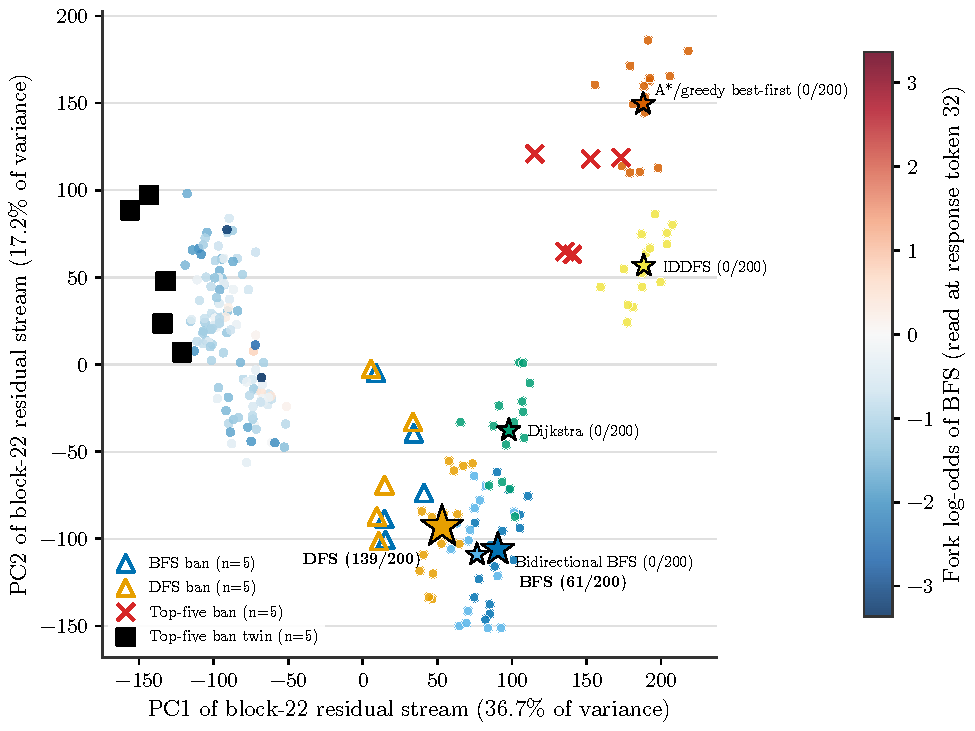
\includegraphics[width=\linewidth,height=0.78\textheight,keepaspectratio]{figures/fig_gemma_geometry_raw_L22_v0.pdf}
\caption{Activation geometry of google\slash{}gemma-3-4b-it on the grid path-search task: mean residual-stream state over the prompt's task-specification positions (i.e., before the response and its BFS\slash{}DFS fork), output of block 22, raw residual with the five largest-magnitude channels zeroed. PCA fit jointly on all 230 points; the axes are its first two components (36.7\% and 17.2\% of variance). Small filled circles are individual forced-algorithm generations (15 per mode), coloured by mode --- BFS blue, DFS orange, bidirectional BFS sky blue, IDDFS yellow, A*\slash{}greedy best-first vermillion, Dijkstra bluish-green --- with each mode's centroid drawn as a star of the same colour and labelled with the mode name and its share of 200 unprompted generations; star area scales with that count (DFS 139\slash{}200, BFS 61\slash{}200; the other four modes are never produced unprompted, 0\slash{}200, and are drawn at the floor size). Open triangles are 5 programs each from a ban on BFS (blue edge) and a ban on DFS (orange edge); red crosses are 5 programs from a ban naming all five of BFS, DFS, IDDFS, A*, and greedy best-first (the ``top-five ban''); black squares are its 5 token-length-matched neutral twin prompts. Small dots are 120 neutral prompt variants, coloured on a blue-white-red scale by the model's fork log-odds of BFS, read out later at response token 32 (blue: log-odds favour DFS; red: favour BFS). In this plane, the top-five-ban points sit closest to the centroids of the two banned modes IDDFS and A*\slash{}greedy best-first, and the twin prompts sit in a separate region, on the opposite side of the plane from every algorithm cluster.}
\label{fig:fig_gemma_geometry_raw_L22}
\end{figure}
\emph{Figure note (iteration-7 correction): Actual activation coordinates: mean over the task-specification positions (from the first token of the task statement to the last token of the user message, \texttt{src/\allowbreak{}cfg.\allowbreak{}py} line 7; file name restored, iteration-8 correction), so neither the read position nor the fork at response index 32 is plotted; output of block 22 (the residual stream after the block), five massive channels zeroed; projection: PCA (first component 0.37, second 0.17 of variance), Isomap (k = 10) and classical MDS (stress-1 0.369), all fitted on the 230 points. Points: prompt states: forced-algorithm prompts by mode, BFS and DFS bans, the top-five ban and its twin, and 120 neutral variants coloured by y\_\allowbreak{}v, the fork log-odds of BFS measured at response index 32. Centroids: per forced mode, the mean of its forced-prompt points (stars), with marker size growing with the natural implemented count out of 200 (DFS 139, BFS 61). N = 230. Caveat: The plotted position precedes the fork and the generated code; centroid positions none (prompt-defined); centroid marker size from realised labels of the 200 natural samples; variant colour from y\_\allowbreak{}v, a quantity measured at the later fork position (readout target, not a partition).}

\begin{table}[H]
\renewcommand{\thetable}{266}
\centering\footnotesize\setlength{\tabcolsep}{4.0pt}
\caption{Where the top-five prompt states sit: geodesic distance from their mean to each catalogue centroid, and the rank of the observed banned-survivor split among the 15 possible splits. Source: Gemma feature experiment \texttt{results/\allowbreak{}geometry.\allowbreak{}json}. [Source: iteration 6, artifact \nolinkurl{gen_art_experiment_31}.]}\label{tab:t285}
\begin{tabular}{>{\raggedright\arraybackslash\hspace{0pt}}p{0.1293\linewidth}>{\raggedright\arraybackslash\hspace{0pt}}p{0.0791\linewidth}>{\raggedright\arraybackslash\hspace{0pt}}p{0.1158\linewidth}>{\raggedright\arraybackslash\hspace{0pt}}p{0.4288\linewidth}>{\raggedright\arraybackslash\hspace{0pt}}p{0.1602\linewidth}}
\toprule
\textbf{Space} & \textbf{MDS stress-1} & \textbf{Nearest centroid} & \textbf{Geodesic distance to BFS \slash{} DFS \slash{} bidirectional BFS \slash{} IDDFS \slash{} A* and greedy \slash{} Dijkstra} & \textbf{Rank share of the observed split} \\
\midrule
raw, layer 17 & 0.371 & A* and greedy & 341.9 \slash{} 330.6 \slash{} 410.3 \slash{} 222.1 \slash{} 188.8 \slash{} 496.5 & 0.067 \\
raw, layer 22 & 0.369 & A* and greedy & 734.1 \slash{} 684.9 \slash{} 900.1 \slash{} 365.2 \slash{} 318.6 \slash{} 990.5 & 0.067 \\
SAE codes, layer 17 & 0.542 & A* and greedy & 27.5 \slash{} 28.4 \slash{} 41.1 \slash{} 32.9 \slash{} 26.1 \slash{} 47.1 & 0.067 \\
SAE codes, layer 22 & 0.569 & A* and greedy & 43.2 \slash{} 44.1 \slash{} 61.5 \slash{} 83.6 \slash{} 43.1 \slash{} 72.5 & 0.20 \\
\bottomrule
\end{tabular}
\end{table}

\begin{figure}[!htbp]
\centering\captionsetup{font=footnotesize}
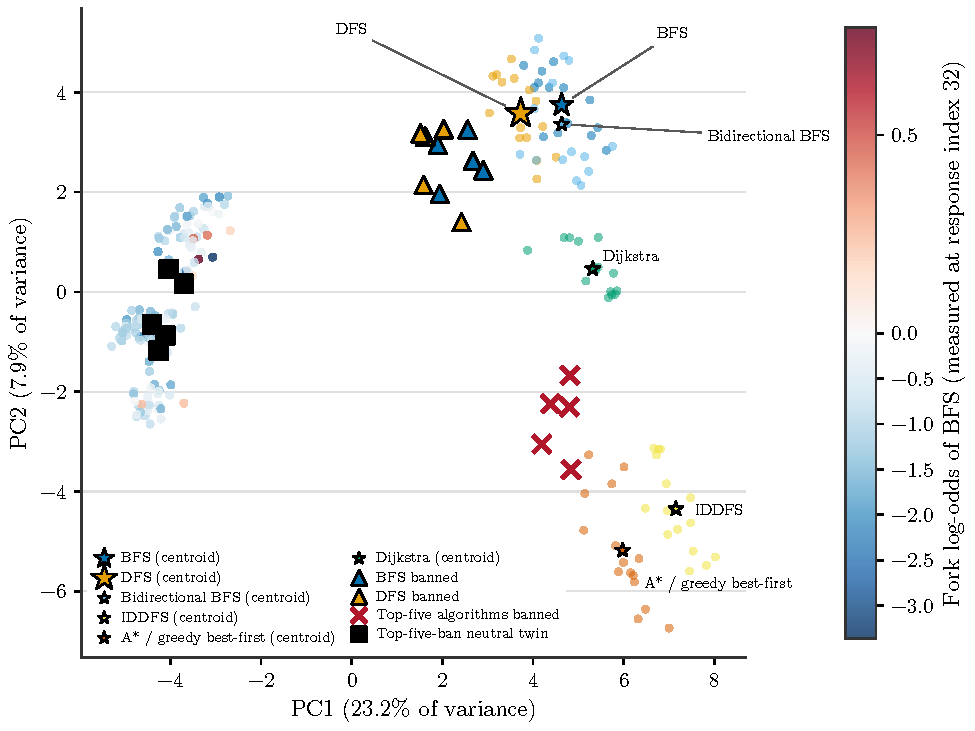
\includegraphics[width=\linewidth,height=0.78\textheight,keepaspectratio]{figures/fig_gemma_geometry_sae_L17_v0.pdf}
\caption{Activation coordinates of gemma-3-4b-it on the grid-path task: first two principal components of block-17 Gemma Scope 2 SAE codes (log1p-transformed), PCA fitted on all 230 plotted points (PC1 23.2\%, PC2 7.9\% of variance). Small filled circles are states of prompts that force one algorithm (15 per mode), coloured by mode --- BFS blue, DFS orange, bidirectional BFS sky blue, IDDFS yellow, A*\slash{}greedy best-first vermillion, Dijkstra green; stars mark each mode's centroid in the same colour, sized by how often that algorithm was written unprompted in an independent N=200 sample (DFS 139\slash{}200, BFS 61\slash{}200; all other modes 0\slash{}200). Black-edged triangles are prompts banning BFS (blue fill) or DFS (orange fill), 5 each; dark-red crosses are prompts banning the five named algorithms this six-mode catalogue covers (BFS, DFS, IDDFS, A*, greedy best-first), with black squares their matched neutral twin, 5 each. Small dots are 120 neutral prompt variants, coloured on a diverging blue-white-red scale (white = 0) by the fork log-odds of BFS measured later, at response index 32 --- after the plotted, pre-fork activation. Forced-algorithm prompts separate by mode in this plane, the five-algorithm-ban prompts land beside the banned A*\slash{}greedy-best-first centroid, and neutral variants' colours track their eventual fork outcome. Caveat: the SAE at block 17 fails this experiment's own reconstruction-fidelity gate (layers 22 and 29 pass it; 17 does not), so this geometry is descriptive rather than a validated feature decomposition.}
\label{fig:fig_gemma_geometry_sae_L17}
\end{figure}
\emph{Figure note (iteration-7 correction): Actual activation coordinates: mean over the task-specification positions (from the first token of the task statement to the last token of the user message, \texttt{src/\allowbreak{}cfg.\allowbreak{}py} line 7; file name restored, iteration-8 correction), so neither the read position nor the fork at response index 32 is plotted; output of block 17 (the residual stream after the block), Gemma Scope 2 SAE codes, log1p; projection: PCA (first component 0.23, second 0.08 of variance), Isomap (k = 10) and classical MDS (stress-1 0.542), all fitted on the 230 points. Points: prompt states: forced-algorithm prompts by mode, BFS and DFS bans, the top-five ban and its twin, and 120 neutral variants coloured by y\_\allowbreak{}v, the fork log-odds of BFS measured at response index 32. Centroids: per forced mode, the mean of its forced-prompt points (stars), with marker size growing with the natural implemented count out of 200 (DFS 139, BFS 61). N = 230. Caveat: The plotted position precedes the fork and the generated code; centroid positions none (prompt-defined); centroid marker size from realised labels of the 200 natural samples; variant colour from y\_\allowbreak{}v, a quantity measured at the later fork position (readout target, not a partition).}

The novelty audit found 1 correct program labelled other among 1,450 correct programs, a first-and-last-position program that two of three judges called a catalogue variant: 0 novel (rule-of-three bound 0.0021). The style re-gate agreed with the labeller on 30 of 30 grid programs. The hash chain verified, a standard-library re-derivation matched 32 of 32 headline quantities, and a shuffled-class decodability placebo sat at chance (0.43). Judge spend was USD 0.034.

\begin{figure}[!htbp]
\centering\captionsetup{font=footnotesize}
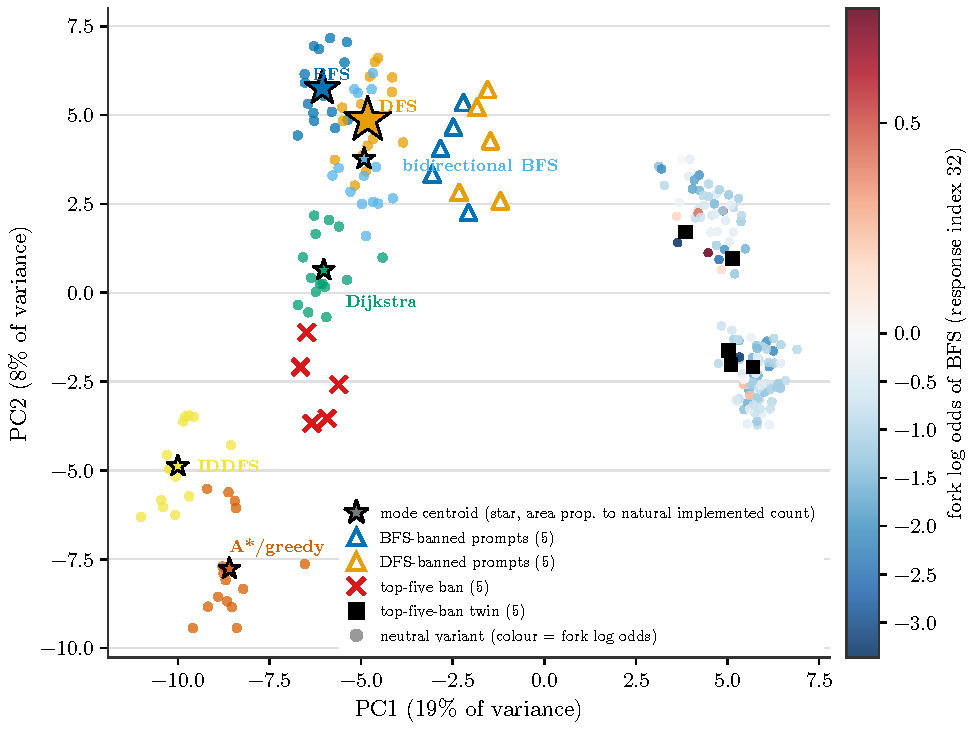
\includegraphics[width=\linewidth,height=0.78\textheight,keepaspectratio]{figures/fig_gemma_geometry_sae_L22_v0.pdf}
\caption{PCA projection of gemma-3-4b-it's block-22 residual-stream SAE codes (Gemma Scope 2, log1p), averaged over the task-specification tokens of a grid path-search prompt; PC1 and PC2 (19\% and 8\% of variance) are fitted on all 230 points shown. Small circles are individual forced-algorithm prompts (15 per algorithm; BFS blue, DFS orange, bidirectional BFS sky blue, IDDFS yellow, A*\slash{}greedy best-first vermillion, Dijkstra green); stars mark each algorithm's centroid, with marker area proportional to how often that algorithm was the one gemma-3-4b-it implemented unprompted in an independent 200-sample natural run (DFS 139\slash{}200, BFS 61\slash{}200; the other four algorithms 0\slash{}200). Open triangles are prompts banning BFS (blue edge, n=5) or DFS (orange edge, n=5) by name; red crosses ban the five most-used algorithms at once (n=5); black squares are that prompt's token-length-matched neutral twin (n=5). Small dots are 120 neutral prompt variants, coloured by a diverging scale (blue to red) showing the fork log-odds of BFS measured later, at response token 32; every plotted state is read out before that fork. In this 2-D projection the five-way-ban points sit between the Dijkstra and A*\slash{}greedy-best-first centroids and are visibly closer to Dijkstra; a separate geodesic-distance measurement in the full 16,384-dimensional SAE-code space (not the 2-D projection drawn here) instead places the five-way ban nearest the A*\slash{}greedy-best-first centroid.}
\label{fig:fig_gemma_geometry_sae_L22}
\end{figure}
\emph{Figure note (iteration-7 correction): Actual activation coordinates: mean over the task-specification positions (from the first token of the task statement to the last token of the user message, \texttt{src/\allowbreak{}cfg.\allowbreak{}py} line 7; file name restored, iteration-8 correction), so neither the read position nor the fork at response index 32 is plotted; output of block 22 (the residual stream after the block), Gemma Scope 2 SAE codes, log1p; projection: PCA (first component 0.19, second 0.08 of variance), Isomap (k = 10) and classical MDS (stress-1 0.569), all fitted on the 230 points. Points: prompt states: forced-algorithm prompts by mode, BFS and DFS bans, the top-five ban and its twin, and 120 neutral variants coloured by y\_\allowbreak{}v, the fork log-odds of BFS measured at response index 32. Centroids: per forced mode, the mean of its forced-prompt points (stars), with marker size growing with the natural implemented count out of 200 (DFS 139, BFS 61). N = 230. Caveat: The plotted position precedes the fork and the generated code; centroid positions none (prompt-defined); centroid marker size from realised labels of the 200 natural samples; variant colour from y\_\allowbreak{}v, a quantity measured at the later fork position (readout target, not a partition).}

\FloatBarrier
\subsection*{6.6 The plan in words: a natural language autoencoder on Qwen2.5-7B-Instruct}
\addcontentsline{toc}{subsection}{6.6 The plan in words: a natural language autoencoder on Qwen2.5-7B-Instruct}
\noindent{\small\emph{Artifact: \nolinkurl{gen_art_experiment_32}.}}\par\medskip
\textbf{Why.} The request names NLA as an instrument, and the release of NLA checkpoints for Qwen2.5-7B-Instruct [124] made it possible to ask, in words, whether the residual stream states before the first code token say which algorithm will be written. The experiment  read layer-20 states with the released verbalizer and reconstructor pair, judged the explanations blind, and tested an edit of the explanation as a steering vector. Published verbalizers of the same kind include LatentQA [117] and SelfIE [118], and a 2026 analysis of a released Qwen-2.5-7B verbalizer found that only a small share of an explanation's specific claims are ones the reconstruction depends on [119]. Pre-registration was a sha256 chain of four commitments, each preceding its samples; the parts added after the committed nulls are marked exploratory.

\textbf{Behaviour.} Over eight tasks, Qwen2.5-7B-Instruct defaults to BFS, Dijkstra (0.88), a hash map (0.98), a hash set (0.71), DFS for connected components (0.62, where Qwen3-8B writes union find), the naive scan and binary search; kth smallest has no default (quickselect 0.40, size-k heap 0.34) and failed the style re-gate. The model mostly ignores bans (Table 267). Only two sum gave a substitute (brute force in 32 of 46 correct programs). On connected components a ban of DFS raised DFS from 29 to 43 correct programs, with 15 paired slots flipping from union find to DFS, the rebound that naming a forbidden concept can cause [7, 53]. Every one of the 70 programs written under the fourth template attempted the banned default. The shortest path semantic seed barely moved the model (Dijkstra 28, Bellman-Ford 6, against 38 and 5 for the twin). The labellers recognised 51 of 51 references, and the style re-gate passed on 7 of 8 tasks against two blind code judges.

\begin{table}[H]
\renewcommand{\thetable}{267}
\centering\footnotesize\setlength{\tabcolsep}{4.0pt}
\caption{Behaviour of Qwen2.5-7B-Instruct (twin and ban N = 50, paired slots; forced prompts N = 20 per algorithm). Source: NLA experiment \texttt{results/\allowbreak{}behaviour.\allowbreak{}json}. [Source: iteration 6, artifact \nolinkurl{gen_art_experiment_32}.]}\label{tab:t286}
\begin{tabular}{>{\raggedright\arraybackslash\hspace{0pt}}p{0.1173\linewidth}>{\raggedright\arraybackslash\hspace{0pt}}p{0.1793\linewidth}>{\raggedright\arraybackslash\hspace{0pt}}p{0.0657\linewidth}>{\raggedright\arraybackslash\hspace{0pt}}p{0.1303\linewidth}>{\raggedright\arraybackslash\hspace{0pt}}p{0.1665\linewidth}>{\raggedright\arraybackslash\hspace{0pt}}p{0.2376\linewidth}}
\toprule
\textbf{Task} & \textbf{Default (share of correct twin programs)} & \textbf{Twin pass} & \textbf{Ban: attempts still using the default} & \textbf{Substitute under the ban} & \textbf{Forced adherence of the algorithm used in the causal arm} \\
\midrule
grid & BFS (13\slash{}13) & 0.26 & 0.68 & none (DFS 3) & none (best other 0.35) \\
shortest path & Dijkstra (38\slash{}43) & 0.86 & 0.50 & none (Bellman-Ford\slash{}SPFA 9, below 10) & none (Bellman-Ford 0.65, below 0.7) \\
kth smallest & none (quickselect 0.40) & 0.94 & n\slash{}a & n\slash{}a & excluded (re-gate 26\slash{}30) \\
two sum & hash map (49\slash{}50) & 1.00 & 0.28 & brute force (32\slash{}46) & brute force 1.00 \\
find duplicate & hash set (35\slash{}49) & 0.98 & 0.46 & none (Floyd cycle detection 7) & Floyd cycle detection 0.95 \\
connected components & DFS (29\slash{}47) & 0.94 & 0.86 & none (DFS 43, union find 2) & union find 0.95 \\
substring search & naive (50\slash{}50) & 1.00 & 0.94 & none & KMP 0.90 \\
first and last position & binary search (38\slash{}38) & 0.76 & 0.96 & none & bisect module 1.00 (not run) \\
\bottomrule
\end{tabular}
\end{table}

\textbf{The instrument gate.} The extraction convention that matches the training code reads the output of block 20; it reaches a fraction of variance explained of 0.695 on the reference set against 0.580 for the convention in the release's example, and 0.695 is within 0.06 of the released 0.752. Generic web text and chat give 0.78 and 0.79. Code is out of distribution for this NLA: LeetCode prompts 0.45, HumanEval+ prompts 0.39, CLRS traces 0.33. On the task states the fraction of variance explained, with the reference-set variance as denominator, is 0.512, so the gate's verdict is partial (Table 268).

\begin{table}[H]
\renewcommand{\thetable}{268}
\centering\scriptsize\setlength{\tabcolsep}{2.5pt}
\caption{Fraction of variance explained of the layer-20 reconstructions on the task states, by position (reference-set denominator). Source: NLA experiment \texttt{results/\allowbreak{}gate.\allowbreak{}json}. [Source: iteration 6, artifact \nolinkurl{gen_art_experiment_32}.]}\label{tab:t287}
\begin{tabular}{>{\raggedright\arraybackslash\hspace{0pt}}p{0.2446\linewidth}>{\raggedright\arraybackslash\hspace{0pt}}p{0.1214\linewidth}>{\raggedright\arraybackslash\hspace{0pt}}p{0.1566\linewidth}>{\raggedright\arraybackslash\hspace{0pt}}p{0.0766\linewidth}>{\raggedright\arraybackslash\hspace{0pt}}p{0.0766\linewidth}>{\raggedright\arraybackslash\hspace{0pt}}p{0.0766\linewidth}>{\raggedright\arraybackslash\hspace{0pt}}p{0.0766\linewidth}>{\raggedright\arraybackslash\hspace{0pt}}p{0.0843\linewidth}}
\toprule
\textbf{Position} & \textbf{Read position} & \textbf{Task specification} & \textbf{Token 1} & \textbf{Token 2} & \textbf{Token 4} & \textbf{Token 8} & \textbf{Token 16} \\
\midrule
Fraction of variance explained & 0.65 & 0.50 & 0.48 & 0.28 & 0.64 & 0.57 & 0.51 \\
\bottomrule
\end{tabular}
\end{table}

\textbf{The NLA never names the planned algorithm before the code.} Two blind judges from different families (Gemini 2.5 Flash Lite and Mistral Small 3.2, both scoring 1.00 on calibration; a third model resolved 1,064 disagreements) mapped each of 6,180 explanations to a catalogue algorithm or to none named (Table 269). Every preregistered readout at the end-of-prompt positions is exactly zero (Table 270). On ban prompts, explanations named the substitute in 0 of 16 states (only two sum had a substitute, so this test is underpowered); on twin prompts they named the default in 0 of 112, as did the text-only reader; on ban failures they named the default the model still writes in 0 of 96. The positive control failed too: on forced \texttt{Implement Y} prompts the explanations called Y planned in 0 of 7 tasks, while the text-only reader did so on all of them, and they mentioned the algorithm named in the prompt in 0.7\% of cases. The explanations describe the local format line, such as a request for no explanation or a Python code block to follow, and confabulate the task (Fibonacci, medians, prime numbers); 4,733 of 5,700 judged explanations name no algorithm at all. At generated tokens the NLA sometimes names the realised algorithm before the visible text identifies it (up to 0.28 at token 8 under the ban), but an outside reader who sees only the prompt and prefix predicts the realised algorithm better, per sample (0.25 against 0.07; exact McNemar 20:88, p 2e-11 when the 364 units are treated as independent). The units are nested in 104 samples and 5 task clusters: the task-cluster bootstrap interval of the difference is [-0.35, 0.02], with one unit per sample (the first in position order, 104 samples) the contrast is 0:25 (exact p 6.0e-08), a median over 2,000 draws of one random unit per sample of 4:29 (p 1.9e-05; 1.00 of draws below 0.05), a sign test on the per-sample differences 12:38 (p 3.1e-04) and a Durkalski-adjusted McNemar with samples as clusters p 6.5e-05. The samples share 5 task clusters, and with 5 clusters no cluster-level test can reach a two-sided p below 0.0625, so the evidence at the task level is inconclusive whatever the sample-level p. (iteration-7 correction)

\begin{table}[H]
\renewcommand{\thetable}{269}
\centering\small\setlength{\tabcolsep}{4.0pt}
\caption{Agreement between the two judges by mode (EXPL: mapping an explanation; NAME: naming from the visible text; PREDICT: the outside reader's forecast). Source: NLA experiment \texttt{results/\allowbreak{}readout.\allowbreak{}json}. [Source: iteration 6, artifact \nolinkurl{gen_art_experiment_32}.]}\label{tab:t288}
\begin{tabular}{>{\raggedright\arraybackslash\hspace{0pt}}p{0.2390\linewidth}>{\raggedright\arraybackslash\hspace{0pt}}p{0.1964\linewidth}>{\raggedright\arraybackslash\hspace{0pt}}p{0.1054\linewidth}>{\raggedright\arraybackslash\hspace{0pt}}p{0.3889\linewidth}}
\toprule
\textbf{Mode} & \textbf{Raw agreement} & \textbf{Kappa} & \textbf{Unresolved after the third judge} \\
\midrule
explanation & 0.94 & 0.82 & 0.6\% \\
visible text & 0.67 & 0.56 & 1.6\% \\
outside reader & 0.77 & 0.75 & 3.9\% \\
\bottomrule
\end{tabular}
\end{table}

\begin{table}[H]
\renewcommand{\thetable}{270}
\centering\footnotesize\setlength{\tabcolsep}{4.0pt}
\caption{Preregistered readout tests. Source: NLA experiment \texttt{results/\allowbreak{}readout.\allowbreak{}json}. [Source: iteration 6, artifact \nolinkurl{gen_art_experiment_32}.]}\label{tab:t289}
\begin{tabular}{>{\raggedright\arraybackslash\hspace{0pt}}p{0.2328\linewidth}>{\raggedright\arraybackslash\hspace{0pt}}p{0.0972\linewidth}>{\raggedright\arraybackslash\hspace{0pt}}p{0.1247\linewidth}>{\raggedright\arraybackslash\hspace{0pt}}p{0.0989\linewidth}>{\raggedright\arraybackslash\hspace{0pt}}p{0.1532\linewidth}>{\raggedright\arraybackslash\hspace{0pt}}p{0.1898\linewidth}}
\toprule
\textbf{Test (units)} & \textbf{NLA} & \textbf{Comparator} & \textbf{b : c} & \textbf{p} & \textbf{Verdict} \\
\midrule
ban states name the substitute (two sum only; 16 states) & 0\slash{}16 & text 0\slash{}16 & 0 : 0 & 1 & fail, underpowered \\
same, against swapped, random and outside-reader controls & 0\slash{}16 & swapped 0\slash{}16, random 0\slash{}8, outside reader 0\slash{}16 & 0 : 0 & 1 & n\slash{}a \\
twin states name the default (7 tasks; 112 states) & 0\slash{}112 & text 0\slash{}112 & 0 : 0 & 1 & fail \\
forced states name the forced algorithm (7 tasks) & 0.00 on every task & text 1.00 & n\slash{}a & n\slash{}a & fail \\
ban-failure states name the default still written (6 tasks; 96) & 0\slash{}96 & outside reader 0\slash{}96, text 0\slash{}96 & 0 : 0 & 1 & null \\
per sample, mixed conditions (364 units nested in 104 samples and 5 task clusters) & 0.066 correct & outside reader 0.253 & 20 : 88 per unit; 0 : 25 at one unit per sample & 2e-11 per unit (units treated as independent); 6.0e-08 at one unit per sample; task-cluster bootstrap of the difference [-0.35, 0.02] & outside reader better per sample; inconclusive at the task level (5 clusters: no cluster-level test below p 0.0625) (iteration-7 correction) \\
generated positions before the identifying token & ban token 8: 0.28; twin token 4: 0.18 & text 0 by construction & n\slash{}a & n\slash{}a & descriptive \\
\bottomrule
\end{tabular}
\end{table}

\textbf{The information is local and fades within a sentence (exploratory).} To tell an instrument limit from information that fades along the prompt, the same NLA and judges read states at the token that names the algorithm inside the condition sentence and at the final period of that sentence (220 states, 660 explanations; Table 271). At the name token the explanations mention the algorithm in 80\% of forced and 89\% of ban states, and they respect the negation: they call it planned in 48\% of forced states and in 6\% of ban states. Two to eight tokens later, at the end of the sentence, the mention rates fall to 27\% and 6\%, and about 170 tokens later, at the end of the prompt, to 0.7\%. The null therefore says that the pre-code positions do not carry the algorithm choice in a form this NLA puts into words, not that the instrument is blind.

\begin{table}[H]
\renewcommand{\thetable}{271}
\centering\footnotesize\setlength{\tabcolsep}{4.0pt}
\caption{Local positive control (majority of three explanations per state; 75 forced and 35 ban states at each of the first two positions). The end-of-prompt row is the committed readout and counts single explanations at the last prompt positions (the algorithm is mentioned in 8 of 1,080 forced and 3 of 420 ban explanations). Source: NLA experiment \texttt{results/\allowbreak{}local\_\allowbreak{}control.\allowbreak{}json}, \texttt{README.\allowbreak{}md}. [Source: iteration 6, artifact \nolinkurl{gen_art_experiment_32}.]}\label{tab:t290}
\begin{tabular}{>{\raggedright\arraybackslash\hspace{0pt}}p{0.2692\linewidth}>{\raggedright\arraybackslash\hspace{0pt}}p{0.1171\linewidth}>{\raggedright\arraybackslash\hspace{0pt}}p{0.0992\linewidth}>{\raggedright\arraybackslash\hspace{0pt}}p{0.1413\linewidth}>{\raggedright\arraybackslash\hspace{0pt}}p{0.1143\linewidth}>{\raggedright\arraybackslash\hspace{0pt}}p{0.1555\linewidth}}
\toprule
\textbf{Position} & \textbf{Forced: names Y as planned} & \textbf{Forced: mentions Y} & \textbf{Ban: names the default as planned} & \textbf{Ban: mentions the default} & \textbf{Reconstruction cosine} \\
\midrule
at the algorithm's name & 0.48 & 0.80 & 0.06 & 0.89 & 0.92 \\
end of that sentence (2 to 8 tokens later) & 0.11 & 0.27 & 0.00 & 0.06 & 0.90 \\
end of the prompt (committed readout, about 170 tokens later) & 0.00 & 0.007 & 0.00 & 0.007 & 0.82 to 0.87 \\
\bottomrule
\end{tabular}
\end{table}

\begin{figure}[!htbp]
\centering\captionsetup{font=footnotesize}
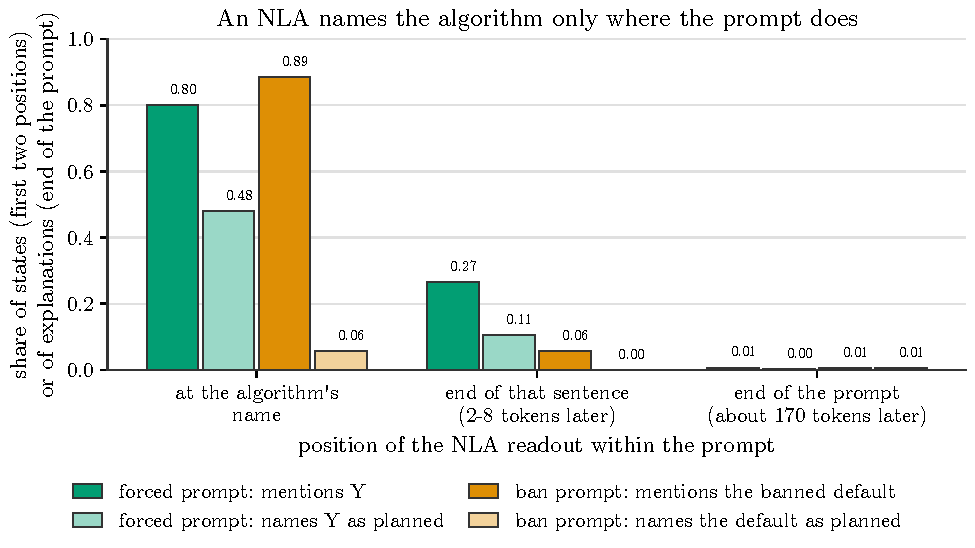
\includegraphics[width=\linewidth,height=0.78\textheight,keepaspectratio]{figures/fig_nla_local_v0.pdf}
\caption{Natural language autoencoder (NLA) explanations of layer-20 residual states of Qwen2.5-7B-Instruct, judged blind, at three prompt positions (x-axis, left to right): on the token that names the algorithm inside the condition sentence, at the end of that sentence (2--8 tokens later), and at the end of the prompt (about 170 tokens later, pooling the SPEC-1\slash{}SPEC-2\slash{}SPEC-3\slash{}READ pre-generation readout positions). Bars give the share of states (first two positions, y-axis) or of single explanations (end of the prompt) whose NLA explanation mentions the task's relevant algorithm (dark bars) or names it specifically as the model's planned answer (light bars), for prompts that force the model to implement algorithm \$Y\$ (green) and prompts that ban the model's default algorithm (orange). Each bar's value label gives its share to two decimals. At the first two positions each of 75 forced and 35 ban states counts by the majority vote of three blind-judged explanations; at the end of the prompt the shares count 1,080 forced and 420 ban single explanations, of which 8 forced and 3 ban explanations mention the relevant algorithm and 3 forced and 3 ban explanations name it as the model's plan. Explanations mention the algorithm, and largely respect a ban's negation, at the name token; mentioning and planning both fall by the end of the sentence and sit at or below 1\% of explanations by the end of the prompt. The first two positions are an exploratory local control; the third is the run's pre-registered readout, where the NLA was found not to verbalise the planned algorithm.}
\label{fig:fig_nla_local}
\end{figure}
\textbf{The preregistered verbal edit fails at the prefill site.} The causal arm replaced the default's name in a twin explanation by an algorithm Y the model writes on request, reconstructed both versions, and patched the difference into the layer-20 states at the last four prompt positions at doses of 1, 2 and 4 (N = 30 paired slots per cell). It failed on all four tasks (Table 272). The edits barely move the reconstruction (cosine 0.9992 between the edited and unedited reconstructions; 0.04 of the state norm per position; Table 273), the unedited round trip at 0.8 of the norm propagates downstream but moves nothing, and all 15 prefill cells per task stay within 0 to 3 slots of the unedited control. The edit direction is nearly orthogonal to the forced-state difference in means (median cosine 0.09).

\begin{table}[H]
\renewcommand{\thetable}{272}
\centering\footnotesize\setlength{\tabcolsep}{4.0pt}
\caption{The preregistered causal arm: Y share in the unedited control and the edited-minus-round-trip difference at doses 1, 2 and 4 (N = 30 paired slots). Source: NLA experiment \texttt{results/\allowbreak{}causal.\allowbreak{}json}. [Source: iteration 6, artifact \nolinkurl{gen_art_experiment_32}.]}\label{tab:t291}
\begin{tabular}{>{\raggedright\arraybackslash\hspace{0pt}}p{0.3849\linewidth}>{\raggedright\arraybackslash\hspace{0pt}}p{0.1206\linewidth}>{\raggedright\arraybackslash\hspace{0pt}}p{0.0885\linewidth}>{\raggedright\arraybackslash\hspace{0pt}}p{0.0984\linewidth}>{\raggedright\arraybackslash\hspace{0pt}}p{0.1439\linewidth}>{\raggedright\arraybackslash\hspace{0pt}}p{0.0604\linewidth}}
\toprule
\textbf{Task (default to Y)} & \textbf{Control Y share} & \textbf{Dose 1} & \textbf{Dose 2} & \textbf{Dose 4} & \textbf{Pass} \\
\midrule
connected components (DFS to union find) & 10\slash{}30 & -0.03 (0:1) & -0.03 (0:1) & +0.03 (3:2) & no \\
two sum (hash map to brute force) & 0\slash{}30 & 0 & 0 & 0 & no \\
find duplicate (hash set to Floyd cycle detection) & 12\slash{}30 & 0 & +0.03 (2:1) & +0.10 (3:0, p 0.25) & no \\
substring search (naive to KMP) & 0\slash{}30 & 0 & 0 & 0 & no \\
\bottomrule
\end{tabular}
\end{table}

\begin{table}[H]
\renewcommand{\thetable}{273}
\centering\small\setlength{\tabcolsep}{4.0pt}
\caption{Realised push sizes relative to the state norm at block 20. Source: NLA experiment \texttt{results/\allowbreak{}causal.\allowbreak{}json}. [Source: iteration 6, artifact \nolinkurl{gen_art_experiment_32}.]}\label{tab:t292}
\begin{tabular}{>{\raggedright\arraybackslash\hspace{0pt}}p{0.5079\linewidth}>{\raggedright\arraybackslash\hspace{0pt}}p{0.4549\linewidth}}
\toprule
\textbf{Cell} & \textbf{Push norm over state norm} \\
\midrule
edit, dose 1 & 0.041 \\
unrelated-word edit, dose 1 & 0.036 \\
round trip, dose 1 & 0.201 \\
round trip, dose 4 & 0.80 (0.76 at block 27) \\
\bottomrule
\end{tabular}
\end{table}

\textbf{At the generated-token site and large doses, the verbal edit steers two of four tasks (exploratory).} After the committed nulls, the experiment extended the doses and moved the edit to the read position plus generated tokens 1 to 64 (Tables 274 and 275). On find duplicate the edit at dose 8 (about 0.3 of the state norm at each position) raised Floyd cycle detection from 0.28 to 0.76 (25:1 over 50 paired slots), replicated on fresh slots (15 of 20, 13:0, p 2e-4), and beat a matched random push (28:1), an unrelated-word edit built the same way (12:1, p 0.003) and a norm-matched round trip (13:1, p 0.002); at dose 16 the programs broke (pass 0.37). On two sum brute force rose from 0 to 10 of 50 at dose 8 and to 23 of 30 at dose 16 with a pass rate of 0.90, while the random push never moved it. On connected components only the forced-state difference in means steered (union find 0.80 at dose 16, 15:1); on substring search nothing steered short of breaking the program. The prefill site stayed inert even at dose 16 or at the natural norm of the difference in means. Asking for the algorithm in the prompt remained the ceiling (forced adherence 0.90 to 1.00 on all four tasks), as the AxBench comparison of prompting and steering predicts [34]. The NLA paper itself reports that editing a plan explanation and steering at one token succeeds roughly half the time; this run's success on two of four tasks is of the same kind and is not a reliable control knob.

\begin{table}[H]
\renewcommand{\thetable}{274}
\centering\scriptsize\setlength{\tabcolsep}{2.5pt}
\caption{Exploratory dose extension (Y share out of 30 paired slots). Source: NLA experiment \texttt{results/\allowbreak{}causal\_\allowbreak{}exploratory.\allowbreak{}json}. [Source: iteration 6, artifact \nolinkurl{gen_art_experiment_32}.]}\label{tab:t293}
\begin{tabular}{>{\raggedright\arraybackslash\hspace{0pt}}p{0.1577\linewidth}>{\raggedright\arraybackslash\hspace{0pt}}p{0.0788\linewidth}>{\raggedright\arraybackslash\hspace{0pt}}p{0.0788\linewidth}>{\raggedright\arraybackslash\hspace{0pt}}p{0.1329\linewidth}>{\raggedright\arraybackslash\hspace{0pt}}p{0.1008\linewidth}>{\raggedright\arraybackslash\hspace{0pt}}p{0.0955\linewidth}>{\raggedright\arraybackslash\hspace{0pt}}p{0.1374\linewidth}>{\raggedright\arraybackslash\hspace{0pt}}p{0.1312\linewidth}}
\toprule
\textbf{Task} & \textbf{Control} & \textbf{Prefill edit, dose 16} & \textbf{Prefill difference in means at natural norm, dose 2} & \textbf{Generated-site edit, dose 8} & \textbf{Generated-site random, dose 8} & \textbf{Generated-site difference in means, dose 8} & \textbf{Generated-site difference in means at natural norm} \\
\midrule
connected components (to union find) & 10 & 10 & 9 & 8 & 11 & 19 (10:1, p 0.012) & 13 \\
two sum (to brute force) & 0 & 0 & 0 & 4 (4:0, p 0.125) & 0 & 0 & 0 \\
find duplicate (to Floyd cycle detection) & 12 & 11 & 12 & 23 (12:1, p 0.003) & 8 & 2 & 6 \\
substring search (to KMP) & 0 & 0 & 0 & 0 & 0 & 2 (pass 0.83) & 0 \\
\bottomrule
\end{tabular}
\end{table}

\begin{table}[H]
\renewcommand{\thetable}{275}
\centering\scriptsize\setlength{\tabcolsep}{2.5pt}
\caption{Exploratory follow-up at the generated-token site: dose response, controls built the same way and a replication on fresh slots (Y share; exact McNemar on paired slots). Source: NLA experiment \texttt{results/\allowbreak{}causal\_\allowbreak{}exploratory\_\allowbreak{}followup.\allowbreak{}json}. [Source: iteration 6, artifact \nolinkurl{gen_art_experiment_32}.]}\label{tab:t294}
\begin{tabular}{>{\raggedright\arraybackslash\hspace{0pt}}p{0.1398\linewidth}>{\raggedright\arraybackslash\hspace{0pt}}p{0.0633\linewidth}>{\raggedright\arraybackslash\hspace{0pt}}p{0.1390\linewidth}>{\raggedright\arraybackslash\hspace{0pt}}p{0.0820\linewidth}>{\raggedright\arraybackslash\hspace{0pt}}p{0.0955\linewidth}>{\raggedright\arraybackslash\hspace{0pt}}p{0.0748\linewidth}>{\raggedright\arraybackslash\hspace{0pt}}p{0.1034\linewidth}>{\raggedright\arraybackslash\hspace{0pt}}p{0.1011\linewidth}>{\raggedright\arraybackslash\hspace{0pt}}p{0.1038\linewidth}}
\toprule
\textbf{Task} & \textbf{Edit, dose 4} & \textbf{Edit, dose 8 (N = 50)} & \textbf{Edit, dose 16} & \textbf{Dose 8, fresh slots (N = 20)} & \textbf{Dose 8 against random} & \textbf{Dose 8 against unrelated-word edit} & \textbf{Dose 8 against matched round trip} & \textbf{Difference in means, dose 16} \\
\midrule
find duplicate (to Floyd cycle detection) & 0.60 (7:1, p 0.07) & 0.76 against control 0.28 (25:1, p \textless{} 1e-6) & 0.30, pass 0.37 & 15\slash{}20 (13:0, p 2e-4) & 28:1 & 12:1, p 0.003 & 13:1, p 0.002 & 0.07, pass 0.27 \\
two sum (to brute force) & 0.00 & 0.20 against 0.00 (10:0, p 0.002) & 0.77, pass 0.90 (23:0) & 6\slash{}20 (6:0, p 0.03) & 10:0, p 0.002 & 4:0, p 0.125 & 4:0, p 0.125 & 0.37, pass 0.40 \\
connected components (to union find) & 0.33 & 0.24 against 0.36 (3:9) & 0.17 & 4\slash{}20 & 5:13 & 6:6 & 2:6 & 0.80 (15:1, p 5e-4) \\
substring search (to KMP) & 0.03 & 0.00 & 0.07, pass 0.27 & 0\slash{}20 & 0:0 & 0:0 & 0:0 & 0.03, pass 0.10 \\
\bottomrule
\end{tabular}
\end{table}

\begin{figure}[!htbp]
\centering\captionsetup{font=footnotesize}
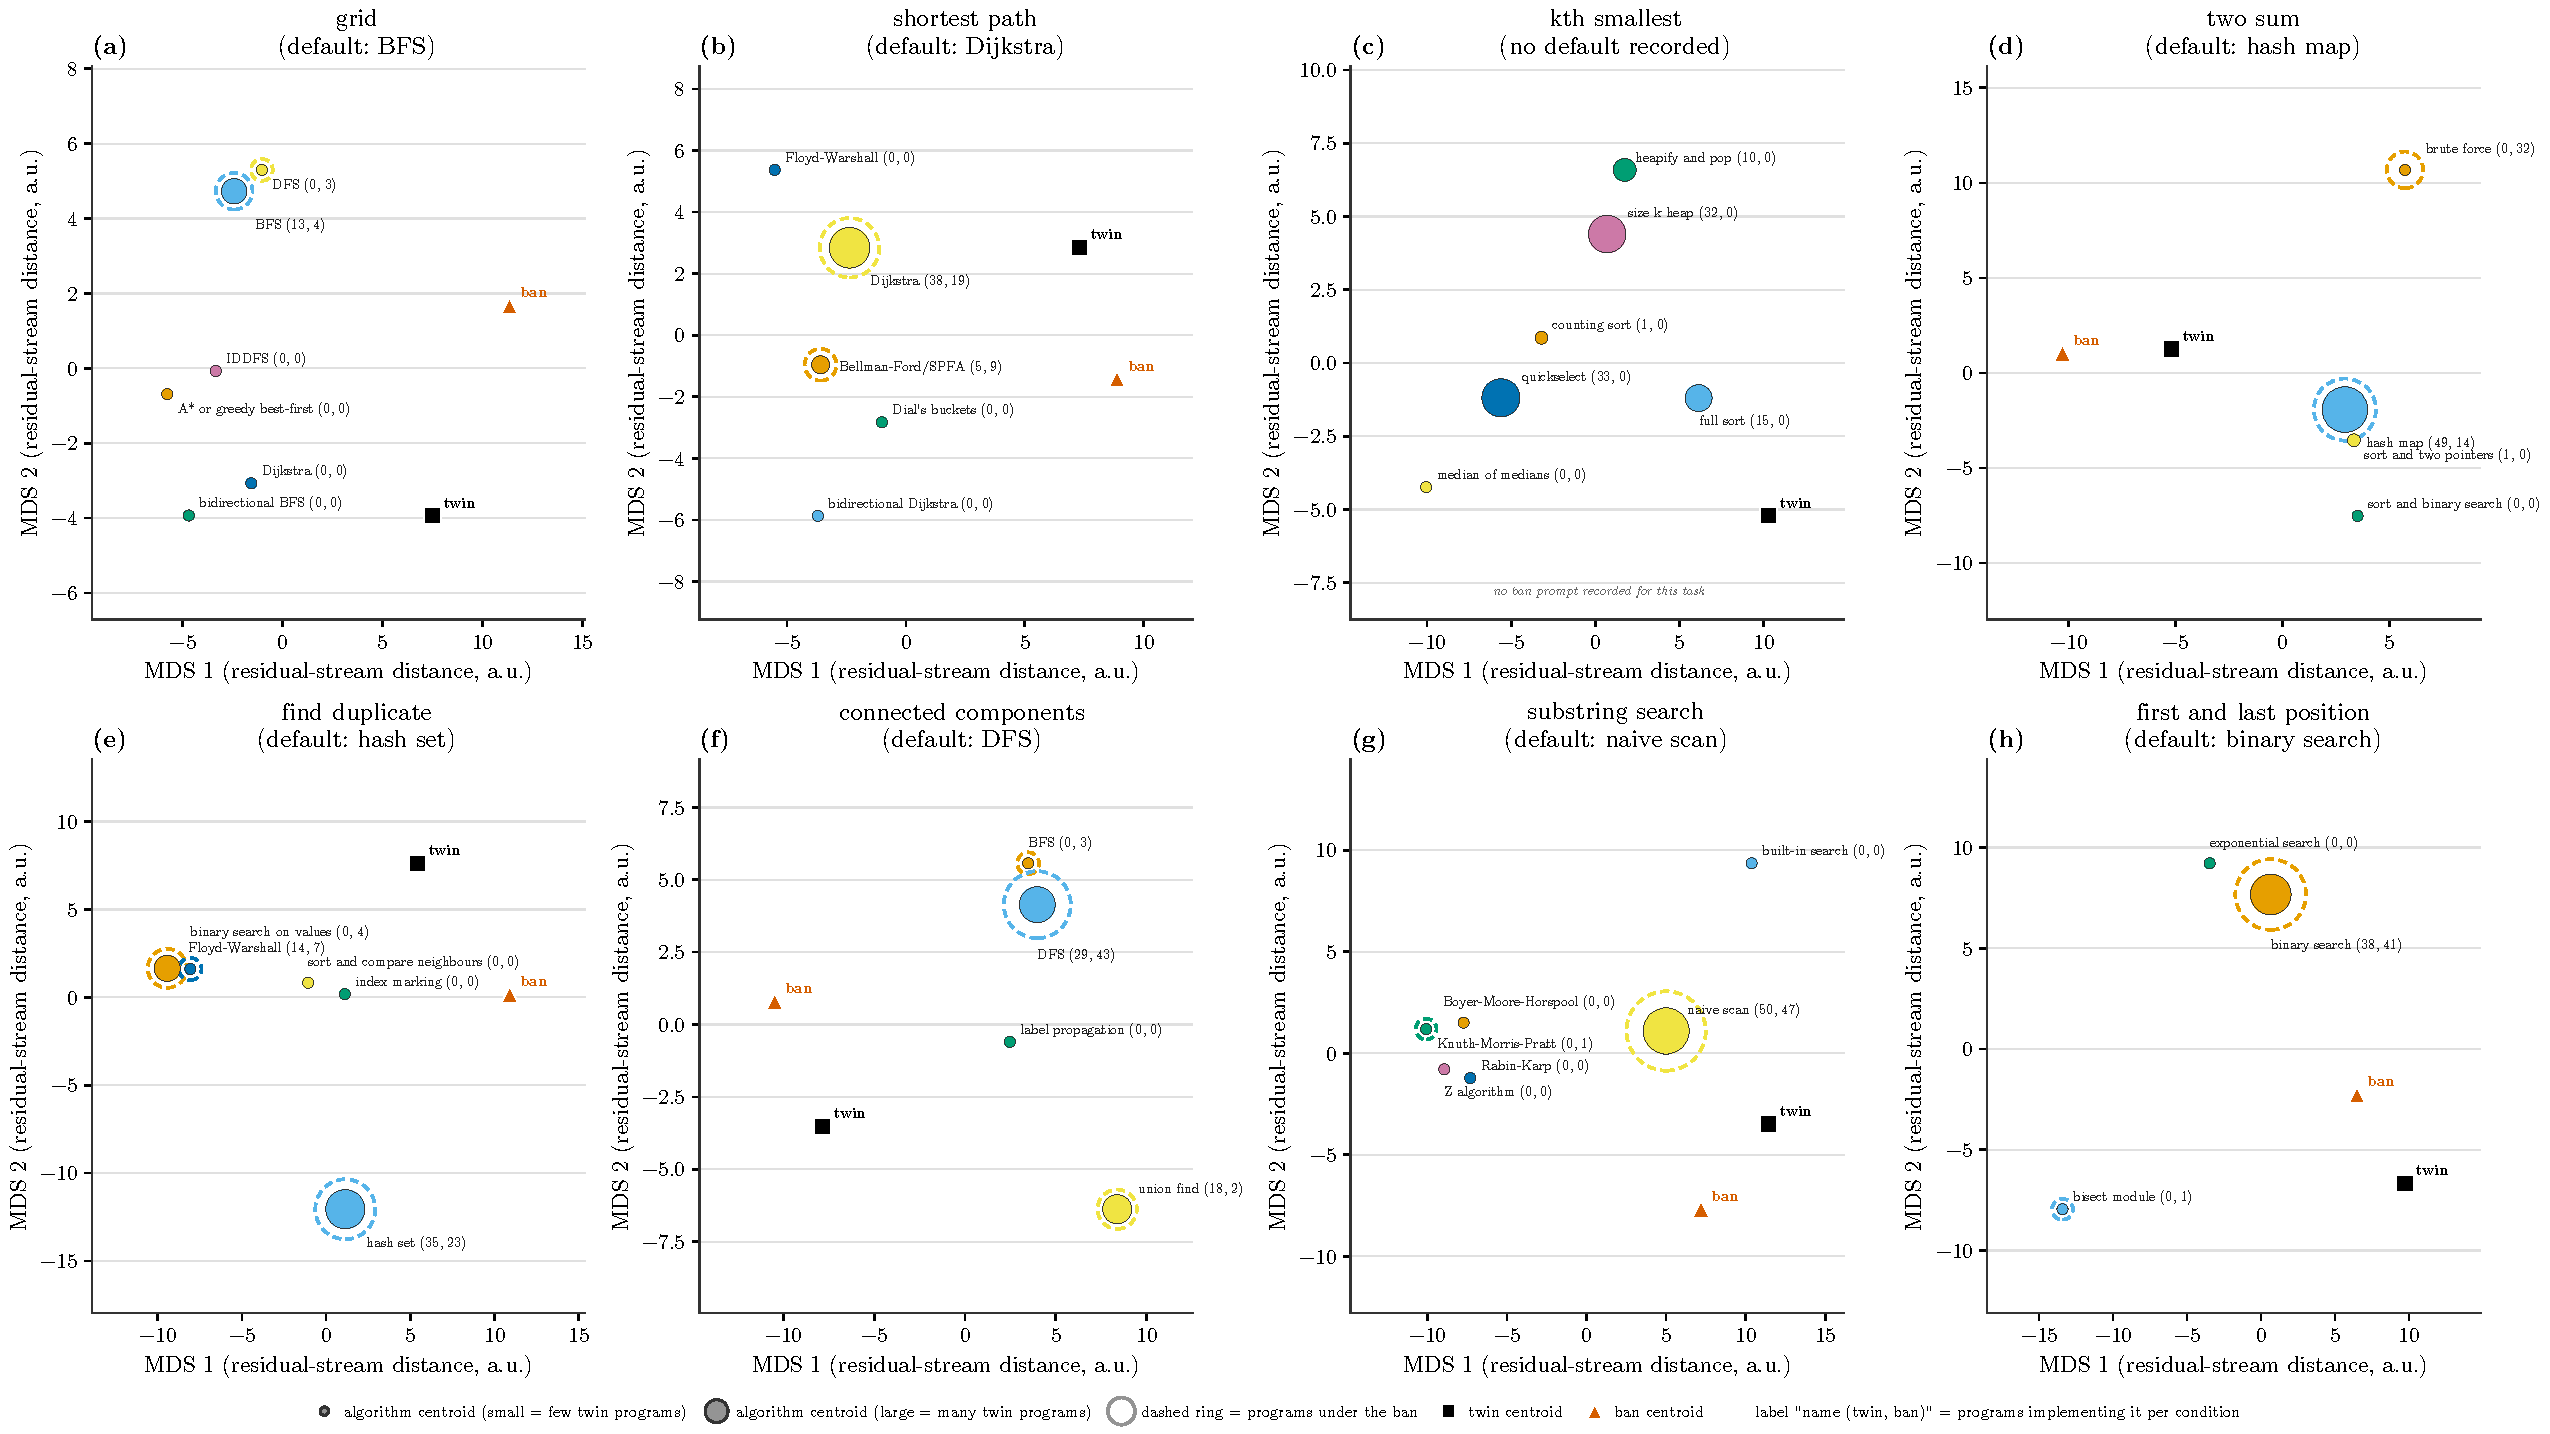
\includegraphics[width=\linewidth,height=0.78\textheight,keepaspectratio]{figures/fig_nla_mds_centroids_v0.pdf}
\caption{Classical MDS of per-algorithm, twin-condition and ban-condition centroids at the read position (block-20 output) of Qwen2.5-7B-Instruct (iteration 6), one panel per coding task -- (a) grid, (b) shortest path, (c) kth smallest, (d) two sum, (e) find duplicate, (f) connected components, (g) substring search, (h) first and last position -- each titled with that task's default (most-implemented, unprompted) algorithm. Axes are the two classical-MDS dimensions of residual-stream distance between centroids, in arbitrary units (MDS stress was not recorded). Each coloured disc (Okabe-Ito palette, reused within a panel, not matched across panels) is one algorithm's centroid; disc area grows with the number of twin-condition programs that implemented it, with a floor size at a count of 0. A dashed ring is drawn around a disc, growing outward from it, only when at least one program implemented that algorithm under the matching ban prompt; no ring means zero. The black square is the twin-condition centroid and the red triangle the ban-condition centroid; every point's label reads ``name (twin count, ban count)''. Panel (c) has neither a default algorithm nor a ban centroid, because the source run recorded no ban prompt for kth smallest, which the panel notes directly.}
\label{fig:fig_nla_mds_centroids}
\end{figure}
\emph{Figure note (iteration-7 correction): Actual activation coordinates: the read position (last prompt token), before any generated token; output of block 20 (hidden\_\allowbreak{}states[21]); projection: classical MDS of the READ centroids per task (MDS stress not recorded in \texttt{results/\allowbreak{}geometry.\allowbreak{}json}; file name restored, iteration-8 correction). Points: one point per centroid: centroids of the forced prompts that ask for each algorithm, the twin centroid and the ban centroid. Centroids: means of the READ states per forced algorithm, twin and ban; filled area grows with the number of twin programs that implemented the algorithm, the dashed ring with the number under the ban. N = 54. Caveat: The plotted position precedes the fork and the generated code; centroid positions none (prompt-defined); marker areas from realised labels of the twin and ban programs.}

In activation space (exploratory), read-position states projected on the plane of the forced-prompt states show every forced algorithm in its own region, with twin and ban prompts apart from all of them. Relative to the algorithm-specific directions of the forced prompts, the ban moves the state toward the banned default's own direction on two sum (+0.13), find duplicate (+0.26) and first and last position (+0.15), as the ban sentence names the default, and toward an alternative on shortest path (Bellman-Ford +0.13), connected components (BFS +0.23), substring search and the grid task (DFS +0.18). The novelty audit found 10 correct programs labelled other in every arm: 8 labeller misses (six kth smallest counting sorts built on a counter, two boolean seen-arrays) and 2 degenerate programs, 0 novel. Spend was about USD 2.0 on OpenRouter (NLA judges with calibration, two interrupted passes, the local control and the novelty audit USD 1.82; code judges for the bench tasks USD 0.11 and for the path tasks USD 0.10) and about 2.0 GPU hours on one 24 GB NVIDIA Ada GPU (68 minutes of generation for behaviour and the committed causal arm, about 27 for the exploratory causal cells, 16 for 6,180 explanations and about 8 for reconstruction passes and the state cache).

\begin{figure}[!htbp]
\centering\captionsetup{font=footnotesize}
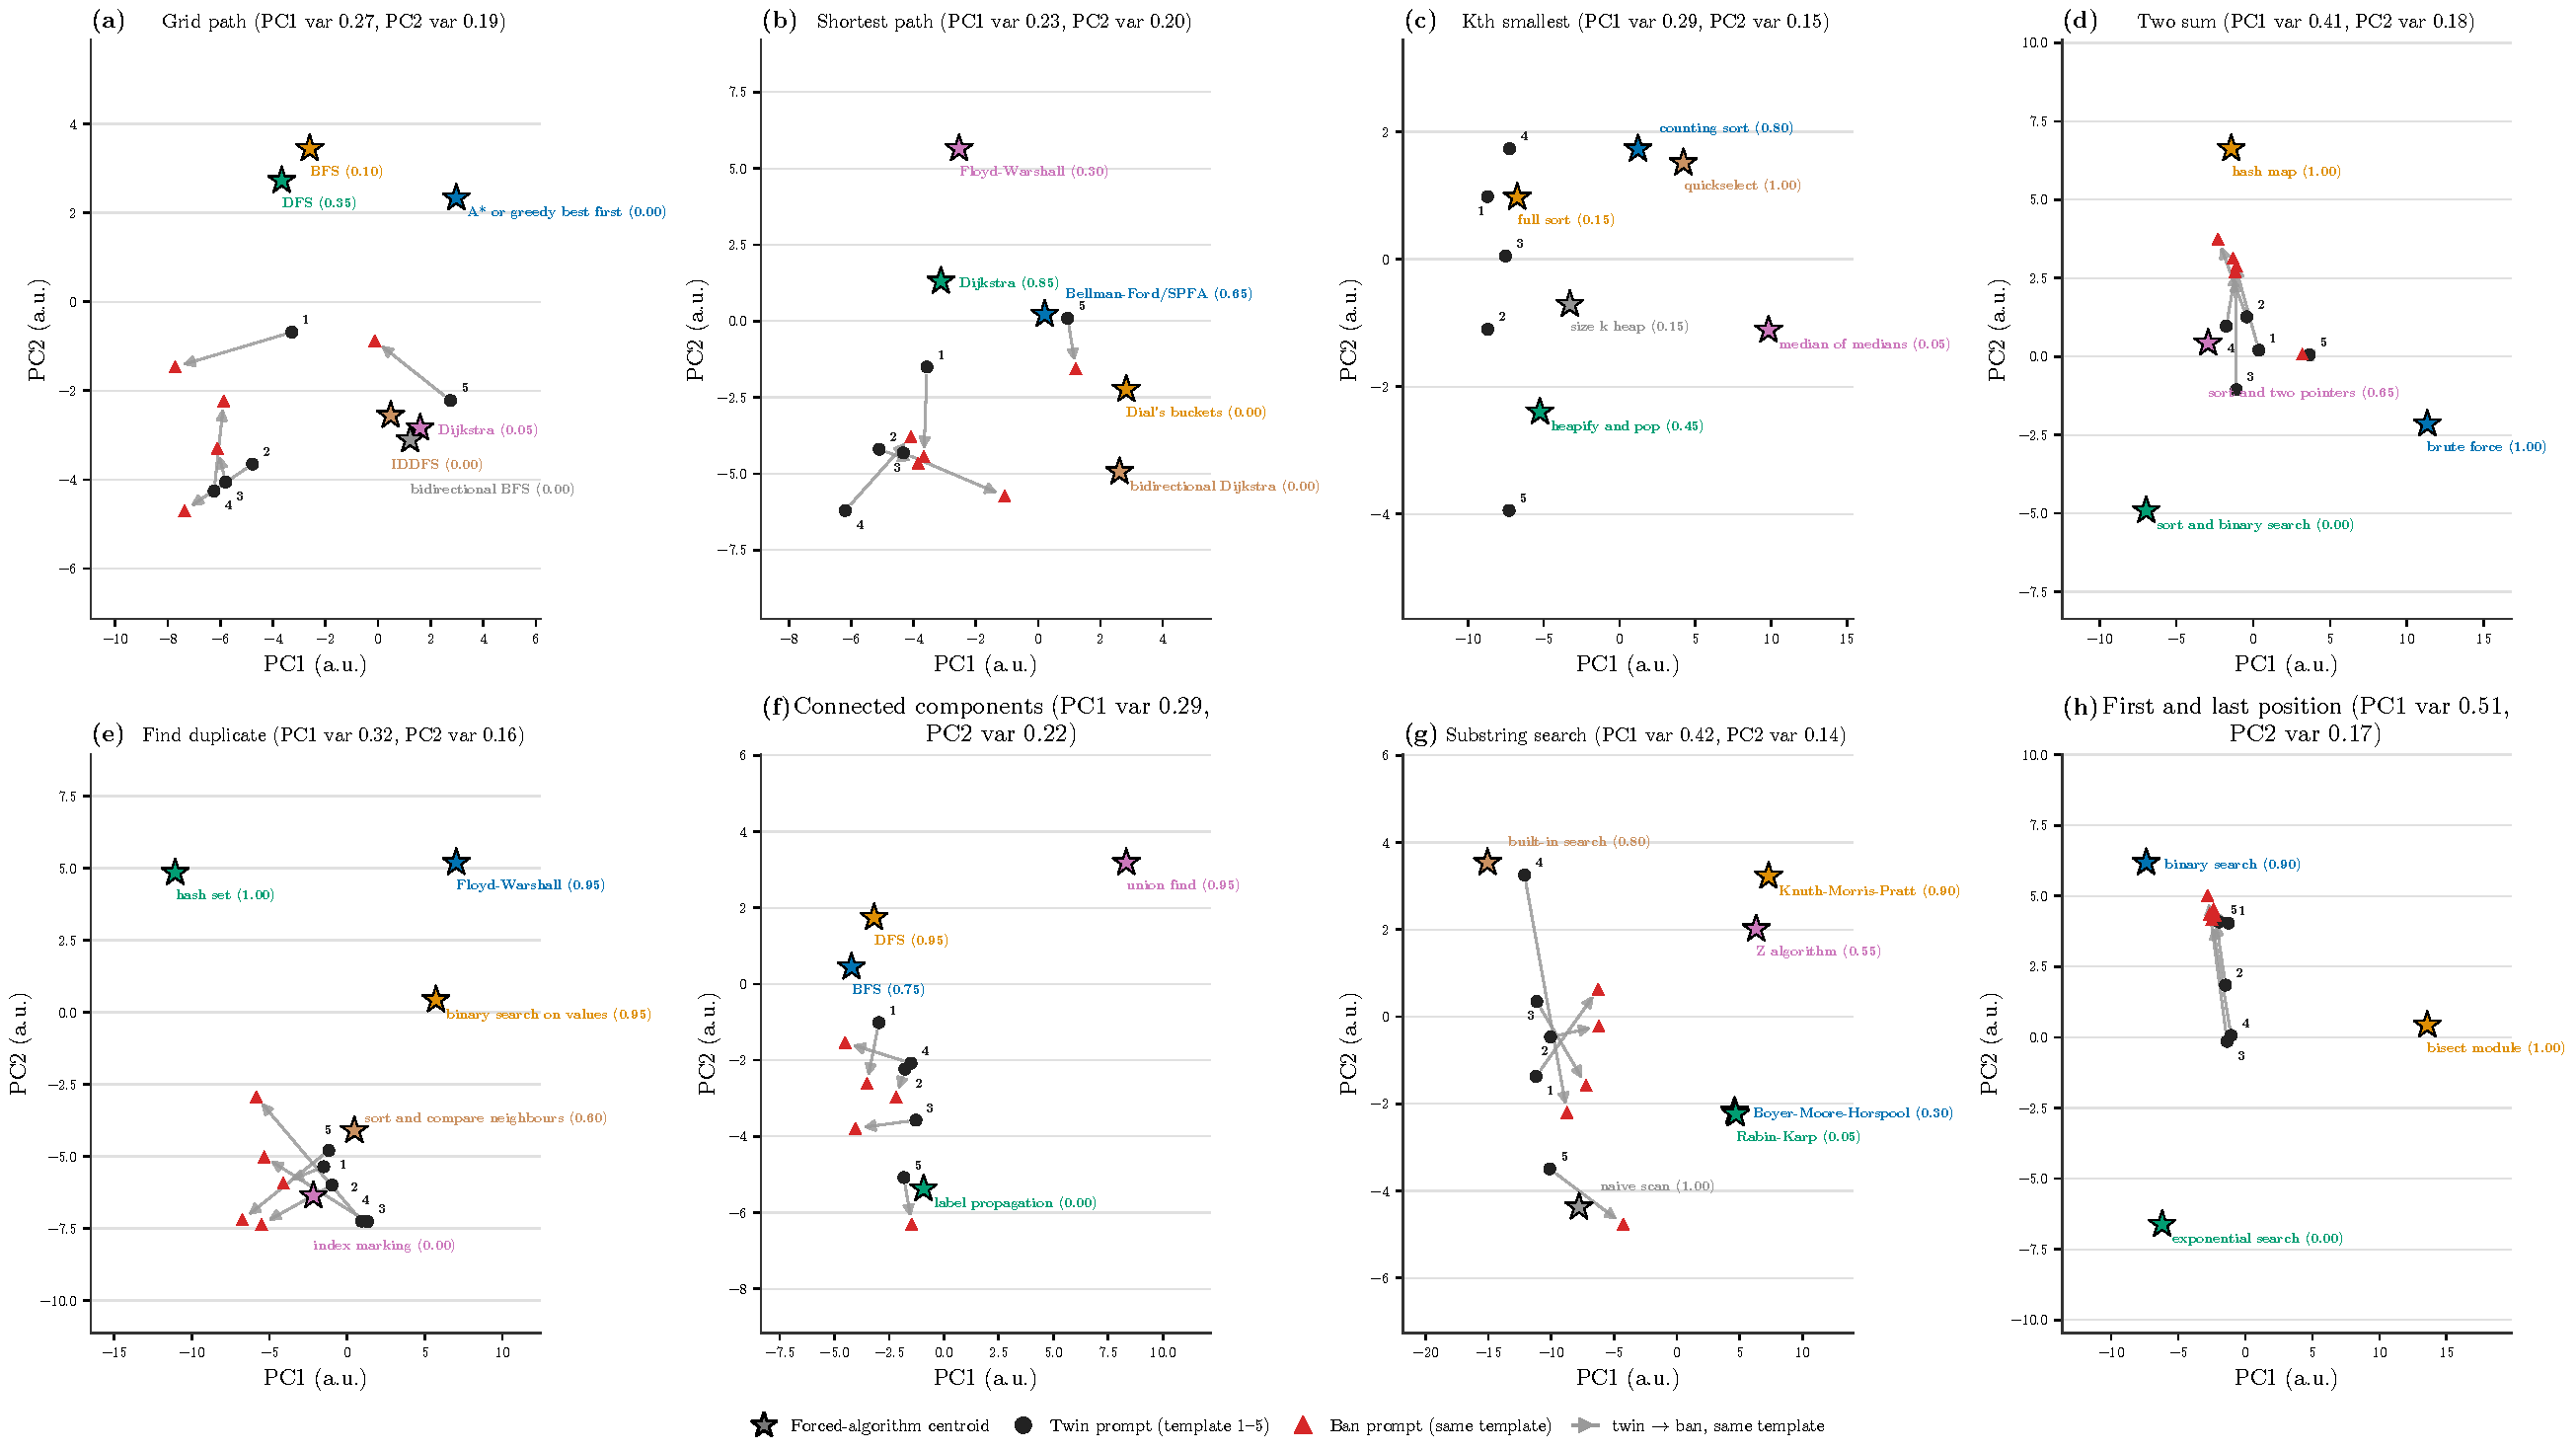
\includegraphics[width=\linewidth,height=0.78\textheight,keepaspectratio]{figures/fig_nla_read_geometry_v0.pdf}
\caption{Qwen2.5-7B-Instruct activations at the read position (last prompt token, output of transformer block 20; iteration 6, recomputed from the cached states) for eight algorithm-choice coding tasks, one panel each: grid path, shortest path, kth smallest, two sum, find duplicate, connected components, substring search, and first-and-last-position. Each panel projects that task's prompts onto the first two principal components fitted on its forced-algorithm prompts alone (PC1, PC2; variance share given as ``PC1 var'', ``PC2 var'' in the panel title); the two axes are not comparable across panels, and star colours are assigned per panel, not shared across tasks. Coloured stars: centroids of prompts that force one algorithm (n = 5 generations each), labelled with the algorithm's name and its forced-adherence rate (the fraction of forced generations that actually implement it) in parentheses. Black circles: the twin prompt of each of the five ban-wording templates, numbered 1-5. Red triangles: the ban prompt of the same template (no ban prompt exists for kth smallest). Grey arrows join each twin to its same-template ban. Twin and ban prompts cluster together and mostly apart from the forced-algorithm centroids; the algorithms the model rarely complies with when forced, such as IDDFS and bidirectional BFS on grid path, sit closer to that twin\slash{}ban cluster than algorithms with high forced adherence do.}
\label{fig:fig_nla_read_geometry}
\end{figure}
\emph{Figure note (iteration-7 correction): Actual activation coordinates: the read position (last prompt token), before any generated token; output of block 20 (the hidden state after block 20); projection: per task, the plane of the first two principal components of that task's forced-prompt READ states (SVD after centring on their mean). Points: single prompt states: forced prompts that ask for each algorithm, by mode and template, the twin and ban prompts of each template (arrow twin to ban), the shortest path seed, twin plus random noise, and NLA edit deltas (x1, x2, x4) and a difference-in-means delta (x4) drawn as arrows. Centroids: per forced mode, the mean of its forced READ states (stars); the legend gives forced adherence. N = 310. Caveat: The plotted position precedes the fork and the generated code; none for positions and centroids (prompt-defined); the legend's adherence is behavioural.}

\FloatBarrier
\subsection*{6.7 Positioning against published work}
\addcontentsline{toc}{subsection}{6.7 Positioning against published work}
\noindent{\small\emph{Artifact: \nolinkurl{gen_art_research_3}.}}\par\medskip
The positioning audit , dated 2026-10-22, extended the audits of iterations 4 and 5 to this iteration's claims. A protocol frozen and stamped before the first call drove 126 logged searches over seven lanes, from 2,191 raw hits to 1,820 unique records, 1,401 in the window, and 75 claim rows scored on the occupancy rubric for 67 papers: 3 occupying, 66 adjacent and 6 irrelevant. Its 123 new quotes from 94 sources matched the cached source text and were re-matched by an independent live pass. Table 276 gives the verdict per claim, and Table 277 condenses the 65 rows of its neighbour table; the verbatim quotes are in the audit's evidence files.

\begin{table}[H]
\renewcommand{\thetable}{276}
\centering\small\setlength{\tabcolsep}{4.0pt}
\caption{Lane verdicts for the iteration-6 claims as of 2026-10-22. Source: positioning audit \texttt{research\_\allowbreak{}report.\allowbreak{}md}. [Source: iteration 6, artifact \nolinkurl{gen_art_research_3}.]}\label{tab:t295}
\begin{tabular}{>{\raggedright\arraybackslash\hspace{0pt}}p{0.2872\linewidth}>{\raggedright\arraybackslash\hspace{0pt}}p{0.3094\linewidth}>{\raggedright\arraybackslash\hspace{0pt}}p{0.3497\linewidth}}
\toprule
\textbf{Claim} & \textbf{Lane verdict} & \textbf{Deciding neighbours} \\
\midrule
Localization: a low-rank causal plan variable, found by interchange or DAS, decides which algorithm Qwen3-8B writes, validated by generation & partly occupied: the method is occupied, the object is open; the flag for a published localization of algorithm choice did not fire, narrowly & DAS and Boundless DAS [110, 111]; MIB [52]; CDAS, DAS steering validated by generation on refusal and a backdoor [112]; prompt cues only for algorithm choice in code [1] \\
Mediation: the plan subspace mediates which random pushes switch the algorithm & adjacent only & pre-generation planning subspaces; output-sensitive steering components \\
Discreteness under interpolation & adjacent only & categorical and multidimensional feature geometry; manifold steering [27] \\
Ideas not in the tokens, at matched KL & adjacent only & decoding matched to steering's departure; temperature and novelty [37]; forking paths [30] \\
Resampling the plan as a diversity knob & partly occupied: activation noise and latent sampling for diversity are occupied & STARS [71]; noise steering [70]; random embedding injection [84] \\
The plan in words with NLAs & occupied (method): the NLA paper edits a plan explanation and steers with the reconstruction; this run is a replication in a new setting & the NLA paper (Transformer Circuits, May 2026); LatentQA [117]; SelfIE [118]; cautions [119, 120] \\
The plan in Gemma Scope 2 features & partly occupied: SAE-feature steering of reasoning strategies beats prompt and activation baselines & SAE-Steering [121]; AxBench [34] \\
8-bit floating-point (W8A8) activation rounding inflates perturbation effects & adjacent only in the published record; partly occupied by contemporaneous ICLR 2027 submissions at abstract level & steering under weight-only quantization [116] \\
\bottomrule
\end{tabular}
\end{table}

Three of the audit's flags bear on what this run may claim. No source localizes which algorithm a code model will write by interchange or DAS and validates it by scoring the generated programs, so that combination is open; the method itself is DAS. Editing an NLA explanation of a plan and steering with the reconstruction is published, so the NLA arm is a replication on a new object. Steering under quantization has been compared with full precision only for weight-only 8-bit integer and 4-bit NormalFloat quantization, with activations kept in 16-bit floating point [116]; no source found measures how dynamic per-token activation rounding changes the effect of random perturbations, which is the question the engine control answered, in the negative. The audit also recorded that community NLAs exist for Qwen3-8B at layer 24, that circuit-tracer ships Qwen-3 transcoders including 8B [123] (so the choice of Gemma for the feature claim needs its reason, which is the natural within-prompt split), and that Gemma Scope 2 dates from 22 December 2025 with instruct SAEs initialised from the pretrained ones.

{\scriptsize\setlength{\tabcolsep}{2.5pt}\renewcommand{\thetable}{277}
\begin{longtable}{>{\raggedright\arraybackslash\hspace{0pt}}p{0.0502\linewidth}>{\raggedright\arraybackslash\hspace{0pt}}p{0.1023\linewidth}>{\raggedright\arraybackslash\hspace{0pt}}p{0.2539\linewidth}>{\raggedright\arraybackslash\hspace{0pt}}p{0.1371\linewidth}>{\raggedright\arraybackslash\hspace{0pt}}p{0.1333\linewidth}>{\raggedright\arraybackslash\hspace{0pt}}p{0.1270\linewidth}>{\raggedright\arraybackslash\hspace{0pt}}p{0.1197\linewidth}}
\caption{The positioning audit's neighbour table, condensed (row; claim; neighbour with venue and version; relation; lane verdict; what this run adds; the baseline a reviewer would ask for). The verbatim quotes behind each row are in the audit's evidence file. Source: positioning audit \texttt{research\_\allowbreak{}report.\allowbreak{}md}, Section 5. The audit wrote the last two columns before the experiments finished; for the claims that were not run (Section 6.8) they state what the planned test would add. [Source: iteration 6, artifact \nolinkurl{gen_art_research_3}.]}\label{tab:t296}\\
\toprule
\textbf{Row} & \textbf{Claim} & \textbf{Neighbour (venue, version)} & \textbf{Relation} & \textbf{Lane verdict} & \textbf{What this run adds} & \textbf{Reviewer baseline implied} \\
\midrule
\endfirsthead
\multicolumn{7}{l}{\emph{Table 277, continued}}\\
\toprule
\textbf{Row} & \textbf{Claim} & \textbf{Neighbour (venue, version)} & \textbf{Relation} & \textbf{Lane verdict} & \textbf{What this run adds} & \textbf{Reviewer baseline implied} \\
\midrule
\endhead
\bottomrule
\endlastfoot
1 & localization & DAS: Geiger, Wu, Potts, Icard, Goodman, CLeaR 2024 (PMLR 236), arXiv v4, v1 2023-03-05, pub; Boundless DAS, Wu et al., NeurIPS 2023, v3 & method the claim uses & PARTLY OCCUPIED (method) & object = algorithm choice in code; validation by tests on emitted programs; Sutter-style controls & DAS with a declared rotation rank, against Boundless DAS \\
2 & localization & MIB: Mueller et al., ICML 2025, v2, v1 2025-04-17, pub & control the claim must meet (method ordering) & n\slash{}a & n\slash{}a & report neuron and SAE-feature arms beside DAS (MIB ordering) \\
3 & localization & CDAS: Bao et al., ICLR 2026, v2, v1 2026-02-05, pub & occupies the method+criterion pair (rubric 2.5) on a non-plan attribute (refusal, CoT backdoor) & PARTLY OCCUPIED & a plan object (algorithm choice), route-derived predictions, random\slash{}shuffled controls & a CDAS-style distribution-matching DAS arm \\
4 & localization & Programmable Semantic Interventions, ICLR 2027 submission, c & adjacent (rubric 1.5) & n\slash{}a & generation-validated plan object & PSI-style declared-program alignment \\
5 & localization & Finding Algorithms in Neural Networks (DAS vs transfer), ICLR 2027 submission, c & adjacent (1.5); supports declaring the map class (non-linear DAS needed in vision) & n\slash{}a & algorithm identity in a code LLM, checked by generation & linear vs non-linear map classes \\
6 & localization & Causal Syntax Circuits in CodeLMs, Kumar et al., NeurIPS 2026 workshop, v1 2026-10-14, c4 & adjacent (1.5): a code attribute that is not the algorithm; next-token readout & n\slash{}a & algorithm (not language); low-rank DAS; generation & random-control significance test, as there \\
7 & localization & Steering LLM Coding Behaviors with Concept Vectors, ICLR 2027 submission, c & adjacent (2.0) & n\slash{}a & algorithm-level object with matched-norm controls & a difference-in-means direction for the algorithm, with matched-norm random controls \\
8 & localization & Before Reasoning Begins (Qwen3-8B, final prompt position, SAE targets), ICLR 2027 submission, c & adjacent (2.0): same model and site; object is reasoning, not algorithm & n\slash{}a & which algorithm (not whether reasoning happens); DAS rather than SAE suppression & layer-count-matched random null interventions \\
9 & localization & Committed Before Reasoning, Jo, v1 2026-07-17, c4 & supports (pre-generation commitment in Qwen3-8B) & n\slash{}a & n\slash{}a & n\slash{}a \\
10 & localization & Random Choice in LMs: linear choice state, ICLR 2027 submission, c & adjacent (2.0) & n\slash{}a & code-algorithm object & switch-vs-distribution decomposition \\
11 & localization & Detecting and Characterizing Planning in LMs, Nainani et al., v1 2025-08-25, anchor & adjacent (1.5); contradicts in part (the same abstract reports that planning is not universal) & n\slash{}a & algorithm-level plan, not a future-token plan & a planning-vs-improvisation criterion \\
12 & localization & Algorithmic Core Extraction, Schiffman, v2, v1 2026-02-26, pub & adjacent (1.0) & n\slash{}a & choice among algorithms, not a task core & n\slash{}a \\
13 & localization & Invisible Lottery (algorithm choice in code moved by cues), ICML 2026: see 92c source 30 & adjacent (2.0): object occupied behaviourally & n\slash{}a & internal causal variable & prompt-cue baseline \\
14 & localization & Sutter, Minder, Hofmann, Pimentel, NeurIPS 2025 Spotlight, v2, v1 2025-07-11, pub & control the claim must meet & n\slash{}a & declared linear map class and rank; random-init or random-rotation control & fit the same map on a randomly initialized Qwen3-8B, and with shuffled labels \\
15 & localization & Makelov, Lange, Geiger, Nanda, ICLR 2024, v2, pub & control the claim must meet & n\slash{}a & nullspace\slash{}row-space decomposition of the patch & check that the patched subspace is not causally disconnected \\
16 & localization & Reply: Wu, Geiger, Huang, Arora, Icard, Potts, Goodman, v1 2024-01-23 & cite with CTRL-2 & n\slash{}a & n\slash{}a & n\slash{}a \\
17 & localization & Divergent representations: Grant et al., v5 (2026-04-22), v1 2025-11-06 & control & n\slash{}a & on-distribution check of patched states & report divergence of the intervened states \\
18 & localization & Right Answer, Wrong Mechanism, v2, v1 2026-09-30, c4 & control (do not rely on distance checks alone) & n\slash{}a & n\slash{}a & planted-pathway or clamp test \\
19 & localization & Curse of Multiple Mediators; Many Circuits, One Mechanism (TMLR 2026); identification-assumptions position & controls & n\slash{}a & n\slash{}a & report interaction effects, cross-condition transfer and identification assumptions \\
20 & mediation & Before the First Token (causal response-length subspace; parallel\slash{}orthogonal decomposition of interventions), ICLR 2027 submission: see 92c source 64 & adjacent (nearest) & ADJACENT-ONLY & prediction of random-push effects on algorithm choice from projection onto the plan subspace & parallel\slash{}orthogonal decomposition of each push \\
21 & mediation & AJR; ASTEER; decodability is not actionability & adjacent & n\slash{}a & n\slash{}a & Jacobian-readout predictor of push effects \\
22 & mediation & DecodeShare, v1 2026-05-21, pub & adjacent (1.5) & n\slash{}a & random pushes classified by plan-subspace energy & matched-budget random-subspace control \\
23 & mediation & What Does Activation Steering Control?, v1 2026-08-24, c4 & supports a projection account (1.0) & n\slash{}a & n\slash{}a & report the share of each push's norm inside the plan subspace \\
24 & mediation & Jailbreak success coordinate outside the refusal subspace, ICLR 2027 submission, c & contradicts in part: the outcome-deciding coordinate can lie outside an evaluated subspace & n\slash{}a & n\slash{}a & test the orthogonal complement as well \\
25 & mediation & Before Reasoning Begins (targeted vs random-null); Latent Planning Emerges with Scale, ICLR 2026 & adjacent \slash{} supports & n\slash{}a & n\slash{}a & random-null arm \\
26 & mediation & On the Non-Identifiability of Steering Vectors, v4, v1 2026-02-06, pub (found by a supplementary search) & supports a subspace-level (not direction-level) account (1.0) & n\slash{}a & n\slash{}a & report plan claims at subspace level; orthogonal-perturbation control \\
27 & mediation & Steering off Course, v1 2025-04-06, anchor; Tele-Lens (ICML 2026) & caution & n\slash{}a & n\slash{}a & per-sample effect distributions \\
28 & discreteness & Park, Choe, Jiang, Veitch, ICLR 2025 oral, v3, anchor & supports (categorical geometry) & ADJACENT-ONLY & an interpolation sweep between plan centroids, with the emitted algorithm labelled at each step & polytope\slash{}simplex geometry of the plan centroids \\
29 & discreteness & Engels et al., ICLR 2025, v3 (title changed in v3), anchor & adjacent (2.0): interventions along circular features & n\slash{}a & discreteness vs continuity of a code plan & a test for irreducible multi-dimensional features \\
30 & discreteness & Manifold Steering (ICML 2026 MI-workshop spotlight): see 92c source 44 & adjacent & n\slash{}a & n\slash{}a & geodesic vs linear paths \\
31 & discreteness & Prolepsis, Jacopin, v2, v1 2026-04-16; Random Choice switch; manifold vs linear steering (ICLR 2027 submission) & adjacent & n\slash{}a & n\slash{}a & linear vs manifold interpolation \\
32 & ideas not in the tokens & departure-matched decoding (an ICLR 2027 submission on activation steering for mathematical reasoning): 92c source 66; Peeperkorn; AdapT; Gumbel counterfactuals; Beneath the Diff & adjacent; departure-matched decoding is the reviewer baseline & ADJACENT-ONLY & plan-level (algorithm) readout of temperature vs state noise at matched KL & decoding matched to the perturbation's departure from greedy \\
33 & ideas not in the tokens & Forking Paths, Bigelow et al., v1 2024-12-10, anchor & adjacent (2.0) & n\slash{}a & n\slash{}a & forking-token resampling baseline \\
34 & ideas not in the tokens & HELIX (4-bit Granite; temperature plus steering), v1 2026-02-06; Predicting Future Behaviors, ICLR 2027 submission & adjacent & n\slash{}a & n\slash{}a & n\slash{}a \\
35 & resampling the plan & STARS (ICLR 2026), Noise Steering, REI, NC-GRPO, 2606.10302, Diversity Without Discovery: 92c sources 15, 14, 16, 52, 31, 63 & occupies the method family (activation noise for diversity) & PARTLY OCCUPIED & resampling a fitted, causally localized plan variable & matched-dose activation noise; text-level plan samplers (IFG, PlanSearch) \\
36 & resampling the plan & Random Choice in LMs, ICLR 2027 submission, c & adjacent (2.0); closest to flag D & n\slash{}a & per-generation resampling for algorithm diversity & distribution-direction intervention \\
37 & resampling the plan & LP-BD; PPLR; SVP (ICLR 2027 submissions, c) & adjacent (flag D partly) & n\slash{}a & a frozen LM; the variable is fitted, not trained & n\slash{}a \\
38 & resampling the plan & Latent Plan Transformer, v4, anchor (venue not stated in the arXiv record) & adjacent & n\slash{}a & n\slash{}a & n\slash{}a \\
39 & the plan in words (NLA) & Fraser-Taliente, Kantamneni, Ong et al., the NLA paper, Transformer Circuits, published May 7, 2026, pub & OCCUPIES the method (rubric 2.5) & OCCUPIED (method) & replication in a new setting: algorithm choice in code, Qwen2.5-7B-Instruct at layer 20, text-only judges, an unrelated-word edit, a matched-norm random displacement & the paper's own newline-only steering protocol and success rate \\
40 & the plan in words (NLA) & same paper, Reasoning about Rewards & occupies & n\slash{}a & n\slash{}a & AR-difference steering vector, norm-matched \\
41 & the plan in words (NLA) & same paper, Method and Limitations & control the claim must meet (confabulation) & n\slash{}a & n\slash{}a & confabulation audit of plan claims \\
42 & the plan in words (NLA) & Released checkpoints: kitft README; HF card; nla\_\allowbreak{}meta.yaml; TransformerLens issue \#1884 & design facts & n\slash{}a & n\slash{}a & load nla\_\allowbreak{}meta.yaml injection settings \\
43 & the plan in words (NLA) & LatentQA, Pan, Chen, Steinhardt, ICLR 2026, v2; SelfIE, ICML 2024, PMLR 235 & occupies the similar-verbaliser clause of flag C (rubric 2.0 each) & n\slash{}a & n\slash{}a & decoder-loss steering arm \\
44 & the plan in words (NLA) & Activation Oracles, v2; Dreaming Vectors (LessWrong) & readout kin \slash{} steering kin (grey literature) & n\slash{}a & n\slash{}a & n\slash{}a \\
45 & the plan in words (NLA) & Sood, Substack, 2026-08-18, c4; Auditing the Auditor, ICLR 2027 submission, c & control set the readout must meet & n\slash{}a & n\slash{}a & shuffled-activation control; visible-text baseline; blinded judge \\
46 & the plan in words (NLA) & Train the Model, Not the Reader, Dingeto, v2, v1 2026-07-22, c4 & contradicts in part: an edited claim may not move the AR output & n\slash{}a & measure the AR displacement caused by the edit before steering & claim-flip reconstruction test \\
47 & the plan in words (NLA) & Colombian identity with NLA, v1 2026-07-23, c4 & readout replication on the same checkpoint & n\slash{}a & n\slash{}a & n\slash{}a \\
48 & the plan in words (NLA) & Community Qwen3-8B NLAs: nanoNLA; EasyNLA & corrects the iteration-5 statement that no NLA exists for Qwen3-8B & n\slash{}a & n\slash{}a & an optional Qwen3-8B arm (unofficial; faithfulness disclaimer) \\
49 & the plan in words (NLA) & Planning or Improvisation?, Jacopin, v1 2026-09-16, c4 & contradicts in part (no newline-resident plan in small open models) & n\slash{}a & n\slash{}a & site sweep (newline vs final prompt token) \\
50 & the plan in words (NLA) & Measuring Activation Control; Understanding Confabulation & context & n\slash{}a & n\slash{}a & n\slash{}a \\
51 & Gemma Scope 2 features & Gemma Scope 2: announcement 22 Dec 2025; technical report; HF card & design facts & n\slash{}a & n\slash{}a & report the IT-vs-PT dictionary used \\
52 & Gemma Scope 2 features & circuit-tracer README; Qwen-3 transcoders (Hanna et al.) & design fact: Qwen3-8B transcoders exist, so a reviewer may ask why S uses Gemma & n\slash{}a & n\slash{}a & run S on the Qwen3-8B PLTs, or justify Gemma \\
53 & Gemma Scope 2 features & AxBench, v3, v1 2025-01-28; rebuttal, v1 2026-05-29 & prior the claim must meet & n\slash{}a & n\slash{}a & difference-in-means and prompting arms \\
54 & Gemma Scope 2 features & SAE-Steering, Fang et al., ACL 2026 Main, v2; Galichin et al. & OCCUPIES the method on a non-code strategy (rubric 2.5) & PARTLY OCCUPIED & algorithm choice in code; Gemma Scope 2; transcoder attribution & SAE-Steering-style logit-recall feature selection \\
55 & Gemma Scope 2 features & Do SAEs Identify Reasoning Features? (Gemma Scope 2), ICML 2026, v7 & contradicts in part & n\slash{}a & n\slash{}a & token-injection falsification of candidate features \\
56 & Gemma Scope 2 features & Prolepsis; Latent Planning Emerges with Scale & adjacent; counter-evidence to the AxBench prior for plans & n\slash{}a & n\slash{}a & CLT\slash{}PLT arm against residual difference-in-means \\
57 & Gemma Scope 2 features & SAE Interventions are Unreliable; variable roles in code LMs (ICLR 2027 submission); attribution-graph caveat & cautions & n\slash{}a & n\slash{}a & probe baseline; post-intervention recovery check \\
58 & engine (8-bit floating-point W8A8) & Steering Under Compression, Bhandari and Wade, v1 2026-09-06, c4 & adjacent (1.5); flag B partly & ADJACENT-ONLY (published) & activation quantization; random perturbations; matched bf16 control & iso-effect comparison at matched behavioural effect \\
59 & engine (8-bit floating-point W8A8) & Stable Directions, Different Effects, ICLR 2027, desk rejected, c & partly occupies the general claim (contemporaneous) & PARTLY OCCUPIED (contemporaneous) & random pushes; 8-bit floating-point W8A8 named; noise-floor account & a first-order local-sensitivity predictor \\
60 & engine (8-bit floating-point W8A8) & Activation Steering under Low-Bit Quantization, ICLR 2027 submission, c & adjacent (1.0) & n\slash{}a & n\slash{}a & hold layer, direction and strength fixed \\
61 & engine (8-bit floating-point W8A8) & Quantization Modulates Batch-Context Non-Determinism, ICLR 2027 submission, c & mechanism neighbour (noise floor) & n\slash{}a & perturbation effect sizes against the 8-bit floating-point noise floor & same-batch-context repeat runs \\
62 & engine (8-bit floating-point W8A8) & PRISM, v1 2026-10-14, c4 & adjacent (4-bit NormalFloat) & n\slash{}a & n\slash{}a & n\slash{}a \\
63 & engine (8-bit floating-point W8A8) & Readouts under quantization: Findings ACL 2026;;; AACL 2025; TrustNLP 2026 & flag B partly (readouts, not perturbation effect sizes) & n\slash{}a & n\slash{}a & n\slash{}a \\
64 & engine (8-bit floating-point W8A8) & Precision-induced divergence: TMLR 2026;;; & supports the mechanism (rounding flips trajectories) & n\slash{}a & n\slash{}a & a zero-norm (unperturbed) re-run under the same engine \\
65 & engine (8-bit floating-point W8A8) & Mechanism sources: LLM.int8(); SmoothQuant; massive activations; 8-bit floating-point formats; the dynamic 8-bit floating-point scheme of llm-compressor & mechanism background & n\slash{}a & n\slash{}a & per-token-scale ablation \\
66 & one-token fork (Gemma) & Forking Paths in Neural Text Generation (Bigelow et al.) (ICLR 2025; arXiv 2412.07961 v1 10 Dec 2024); Forking Fast (no venue on the arXiv record; no NeurIPS 2026 paper page found by the dated search; arXiv 2608.19611 v1 20 Aug 2026); Latent Planning Emerges with Scale (Hanna and Ameisen) (ICLR 2026; arXiv 2604.12493 v1 14 Apr 2026); Detecting and Characterizing Planning in Language Models (Nainani et al.) (no venue on the arXiv record; arXiv 2508.18098 v1 25 Aug 2025); Where's the Plan? (Ma and Rui) (Workshop on Mechanistic Interpretability @ ICML 2026; arXiv 2605.07984 v1 8 May 2026, v2 11 Jun 2026); Planning or Improvisation? (Jacopin) (no venue on the arXiv record; arXiv 2609.18440 v1 16 Sep 2026) & adjacent: forking-token resampling and planning detection are occupied as methods; none of these reports an algorithm-level fork in generated code at a token that does not identify the algorithm & ADJACENT-ONLY (to our knowledge, mini search dated 2026-10-22) & an algorithm-level fork (BFS or DFS) in generated code at one token that does not identify the algorithm, about 138 tokens before the code that does; its fork log-odds varies across 120 prompt variants (SD 0.67 nats) and is linearly decodable from the residual at the fork (R-squared 0.66 Lasso on SAE codes, 0.72 raw ridge), which at that position is close to a next-token readout, not evidence of a plan; steering costs are measured (pass 0.84 to 0.16-0.58) & forking-token resampling baseline; a logit-lens control of matched capacity (iteration-7 correction) \\
\end{longtable}}

\FloatBarrier
\subsection*{6.8 Planned but not run}
\addcontentsline{toc}{subsection}{6.8 Planned but not run}
The seventh artifact of the strategy never existed. It was to fit DAS subspaces of rank 1 to 16 at one layer of the task-specification positions in bf16 Qwen3-8B on three training templates and confirm them on two held-out templates (Stage B of the localization claim), test whether a fresh random direction's energy in that subspace predicts its effect (the mediation claim), interpolate and extrapolate the plan coordinate between algorithms (the discreteness claim), measure the plan coordinate's variance across temperatures (the first half of the token claim), resample the plan per generation as a diversity knob (the resampling claim), and draw the request's manifold of algorithms in the fitted plan subspace, with the top-five prohibition placed on it. It was lost at the planning stage: the planning agent returned no plan, so no experiment ran. These claims are untested and open; nothing in this report is a result for them, null or otherwise. The only DAS result of the iteration is Gemma's, at the fork position (Section 6.5). The deviation log of the Gemma experiment adds what it did not run: the clamp read-back and matched-norm realisation tests as separate unit tests (the matched norm is imposed by construction in the clamp code, \texttt{src/\allowbreak{}clamp.\allowbreak{}py} (file name restored, iteration-8 correction), and the realised norm of each edit is logged per row); the clamp-cell overlay on the generated-position panel; the fork and the cross-prompt readouts of two further bench tasks (dropped in order); and per-sample displacement at generated tokens 1-32 (prefill displacement at blocks 11-33 is logged). (iteration-7 correction)

\FloatBarrier
\subsection*{6.9 Comparisons across this iteration's experiments}
\addcontentsline{toc}{subsection}{6.9 Comparisons across this iteration's experiments}
\textbf{Where the choice is held, model by model.} The three internal experiments measured different quantities at different sites, so their results are stated per model and per quantity (Table 279) rather than as one map. In Qwen3-8B what was measured is where an external ban or instruction is carried: exchanging the task-specification states alone reproduces the substitute of the ban on shortest path (Bellman-Ford\slash{}SPFA in 24 of 30 attempts, 21 of 30 correct programs) and a forced instruction on shortest path (30 of 30 attempts, 30 of 30 correct) and connected components (BFS in 28 of 30 attempts, 24 of 30 correct), while on the direct-route tasks the condition span carries it; Qwen3-8B's natural choice was not measured, because it writes one algorithm per prompt. In gemma-3-4b-it, which writes two algorithms for one prompt, the natural choice is made at one generated token after a shared opening; task-specification edits and readouts barely reach it, and the read position was never read or edited (Gemma's SPEC site is a mean over the task-specification positions, which exclude the read position). In Qwen2.5-7B-Instruct no verbalisable plan was found at pre-code positions: the NLA names the algorithm at the token where the prompt names it and not 170 tokens later, and edits work only at the generated-token site. The read position is inert as a carrier in Qwen3-8B (its exchange transfers nothing on six tasks) and reads only the format line in the NLA; Gemma's read position was not measured. The finding of iteration 3 that a ban gives way at the opening of the program body and the fork of Gemma at response index 32 point at the same moment from two models: the first statement of the body that is specific to an algorithm, after an opening shared by every algorithm.

\begin{table}[H]
\renewcommand{\thetable}{279}
\centering\footnotesize\setlength{\tabcolsep}{4.0pt}
\caption{What was measured where, per model and quantity (NEW in iteration 7). Sources: exchange and site experiment \texttt{results/\allowbreak{}stage\_\allowbreak{}a.\allowbreak{}json}; Gemma feature experiment \texttt{results/\allowbreak{}fork.\allowbreak{}json}, \texttt{results/\allowbreak{}readout.\allowbreak{}json}, \texttt{src/\allowbreak{}cfg.\allowbreak{}py}; NLA experiment \texttt{results/\allowbreak{}readout.\allowbreak{}json}, \texttt{results/\allowbreak{}local\_\allowbreak{}control.\allowbreak{}json}. (iteration-7 correction) [Source: iteration 6, compiled across the iteration's artifacts \nolinkurl{gen_art_evaluation_5}, \nolinkurl{gen_art_experiment_29}, \nolinkurl{gen_art_experiment_30}, \nolinkurl{gen_art_experiment_31}, \nolinkurl{gen_art_experiment_32}, \nolinkurl{gen_art_research_3}.]}\label{tab:t297}
\begin{tabular}{>{\raggedright\arraybackslash\hspace{0pt}}p{0.0867\linewidth}>{\raggedright\arraybackslash\hspace{0pt}}p{0.1158\linewidth}>{\raggedright\arraybackslash\hspace{0pt}}p{0.1605\linewidth}>{\raggedright\arraybackslash\hspace{0pt}}p{0.1272\linewidth}>{\raggedright\arraybackslash\hspace{0pt}}p{0.3059\linewidth}>{\raggedright\arraybackslash\hspace{0pt}}p{0.1005\linewidth}}
\toprule
\textbf{Model} & \textbf{Quantity} & \textbf{Site measured} & \textbf{Instrument} & \textbf{Result} & \textbf{Sites never measured} \\
\midrule
Qwen3-8B & where an external ban or instruction is carried & task-specification states (blocks 0-11, 12-23, 24-35, 0-35), condition span, read position & full-state exchange and KV splice into a token-matched twin & carried by the task-specification states on prompt-route tasks (shortest path 24 of 30 attempts, 21 of 30 correct; kth smallest 17 of 30, 16 of 30) and by the condition span on direct-route tasks; read position 0 on six tasks & generated tokens; any low-rank subspace (Stage B not run) \\
Qwen3-8B & its natural choice & not measured (one algorithm per prompt) & n\slash{}a & n\slash{}a & every site \\
gemma-3-4b-it & its natural choice (BFS or DFS) & generated token at response index 32; mean over the task-specification positions & prefix resampling; cross-prompt readout; SAE, difference-in-means and DAS edits & one generated token decides; task-spec edits and readouts barely reach it (SAE codes = text, 0.18) & the read position \\
gemma-3-4b-it & the read position & never read or edited & n\slash{}a & n\slash{}a & the read position \\
Qwen2.5-7B-Instruct & a verbalisable plan & end-of-prompt positions (SPEC-3 to READ), the name token, generated tokens 1 to 16 & NLA explanations judged blind & none at pre-code positions; the algorithm is named at its name token (80\% forced, 89\% ban); per sample the outside reader is ahead (0:25 at one unit per sample) & non-verbal carriers at any position \\
\bottomrule
\end{tabular}
\end{table}

\textbf{The top-five prohibition in two families.} Both models answer a five-name ban by writing a banned algorithm (avoidance 0.00 in Qwen3-8B in iteration 2, in its bf16 rerun here and in Gemma). In Gemma the ban flips the model from its default DFS to its minority BFS and halves its pass rate; in activation space the ban's prompt states sit beside a banned centroid. At doses of 1 to 8 ban units, which overshoot the forced-prompt manifold, the activation version of the prohibition breaks programs before it moves the algorithm; an in-manifold dose was not tried. (iteration-7 correction)

\textbf{Novelty, audited again.} No artifact of this iteration found a correct novel algorithm (Table 278).

\begin{table}[H]
\renewcommand{\thetable}{278}
\centering\footnotesize\setlength{\tabcolsep}{4.0pt}
\caption{Novelty audits of iteration 6. Sources: the novelty audit files of the five artifacts. [Source: iteration 6, compiled across the iteration's artifacts \nolinkurl{gen_art_evaluation_5}, \nolinkurl{gen_art_experiment_29}, \nolinkurl{gen_art_experiment_30}, \nolinkurl{gen_art_experiment_31}, \nolinkurl{gen_art_experiment_32}, \nolinkurl{gen_art_research_3}.]}\label{tab:t298}
\begin{tabular}{>{\raggedright\arraybackslash\hspace{0pt}}p{0.1039\linewidth}>{\raggedright\arraybackslash\hspace{0pt}}p{0.2729\linewidth}>{\raggedright\arraybackslash\hspace{0pt}}p{0.1034\linewidth}>{\raggedright\arraybackslash\hspace{0pt}}p{0.3279\linewidth}>{\raggedright\arraybackslash\hspace{0pt}}p{0.1052\linewidth}}
\toprule
\textbf{Artifact} & \textbf{Pool} & \textbf{Correct programs outside the catalogue} & \textbf{Final classes} & \textbf{Novel} \\
\midrule
Record audit & the 14 transplant programs that two of three judges had called novel in iteration 5, plus 10 controls and 17 related programs & 14 disputed & known outside the catalogue 10, catalogue variant 2, degenerate 2 & 0 \\
Engine control & every correct off-default or other program, against 18,237 known solutions (nearest-known pass only); its 3 correct programs labelled other judged blind in iteration 7 & up to 237 per engine and task; 3 labelled other & nearest-known pass: variants and distant programs of known algorithms; the 3 programs: catalogue variant 3 (blind judges: gpt-4.1-mini gate 8\slash{}10; deepseek-chat-v3.1 gate 10\slash{}10; gemini-2.5-flash-lite gate 8\slash{}10; gated deepseek-chat-v3.1; kappa n\slash{}a on merged classes; manual read) & 0 (iteration-7 correction) \\
Exchange and site experiment & every correct program labelled other & 2 & catalogue variant 2 & 0 \\
Gemma feature experiment & 1,450 correct programs & 1 & catalogue variant & 0 \\
NLA experiment & every correct program labelled other, all arms & 10 & labeller miss 8, degenerate 2 & 0 \\
\bottomrule
\end{tabular}
\end{table}

\FloatBarrier
\subsection*{6.10 What iteration 6 established, what it ruled out, and what it abandoned}
\addcontentsline{toc}{subsection}{6.10 What iteration 6 established, what it ruled out, and what it abandoned}
Everything below is one model per claim except where a second family is named, at 4B to 8B parameters, on memorised tasks in the style of LeetCode.

\textbf{Established.}

\begin{enumerate}
\item \emph{Iteration 4's random-push escapes are a property of Qwen3-8B, not of 8-bit floating-point rounding.} At the same absolute displacement, the same 40 directions and the same slots, bf16 escapes on connected components at 0.65 against 0.725 under W8A8 and on shortest path at 0.15 against 0.20, with per-direction shares ranked alike (Spearman 0.96 and 0.87), and per-sample plan noise reproduces (25 and 22 of 50 against 30 and 22). Activation rounding alone adds nothing; a 5-point per-slot boost on connected components comes from the 8-bit floating-point weights or the native kernel. Iteration 5's bf16 null belongs to its ban-free unit or its direction seeds.
\item \emph{In Qwen3-8B the substitute of a ban and the algorithm of an instruction are carried by the residual states at the task-specification positions on the prompt-route tasks.} Exchanging those states alone transfers the ban on shortest path (24 of 30 attempts, 21 of 30 correct programs) and kth smallest (17 of 30 attempts, 16 of 30 correct), and a forced instruction on shortest path (30 of 30 attempts, 30 of 30 correct) and connected components (28 of 30 attempts, 24 of 30 correct); matched-norm random exchanges and a placebo twin transfer at most 0.13. The condition span carries the ban on the direct-route tasks (two sum 1.00, find duplicate 0.90). The read position carries nothing. (iteration-7 correction)
\item \emph{Gemma's BFS-or-DFS choice is made at one generated token,} \texttt{ visited} against a blank line, \texttt{if} or \texttt{queue} at response index 32, about 138 tokens before any algorithm-identifying code, and its fork log-odds is linearly decodable from the residual stream at that position across prompts (Lasso on SAE codes R-squared 0.66 against 0.18 for text, preregistered; ridge on the raw state 0.72, post hoc); at the fork position that is close to a next-token readout, so it shows that the next-token distribution is linearly encoded there, not that a plan is, and the standardised ridge on the same layer-29 SAE codes reaches R-squared 0.15 against 0.086 for a template-plus-noun-norm control (delta 0.064, below the preregistered 0.10 bar). (iteration-7 correction)
\item \emph{Steering the fork works and costs correctness.} Difference in means moves the fork 2.3 times as far as the SAE clamp at matched norm, both move the plan equally at matched effect, and edits toward the minority algorithm lowered the pass rate from 0.84 to 0.16-0.58, except the SAE top-5 clamp (18 BFS, pass 0.84); edits toward the default are clean. (iteration-7 correction)
\item \emph{The NLA does not verbalise the planned algorithm at pre-code positions in Qwen2.5-7B-Instruct,} although it names an algorithm at the token where the prompt names it; an outside reader of the text predicts the realised algorithm better than the NLA per sample (0:25 at one unit per sample, p 6.0e-08), and at the task level the evidence is inconclusive (5 task clusters; bootstrap interval [-0.35, 0.02]). (iteration-7 correction)
\item \emph{Record repairs.} The landing half is descriptive (17 of 21 per set, 5 of 8 where the twin wrote no alternative, p 0.053); the movability half is not a strong predictor with a moderate relation not excluded (0.15, interval -0.44 to 0.65); the 14 disputed programs are not novel.
\end{enumerate}

\textbf{Ruled out, or not supported.}

\begin{itemize}
\item \emph{Activation rounding as the cause of the escapes} (the engine claim's preregistered account): W16A8 escapes like bf16 or slightly less, on both tasks.
\item \emph{The Stage A rule of the localization claim} as preregistered: the task-specification states of two sum also transfer brute force at 0.43, above the predicted 0.2.
\item \emph{A feature claim for Gemma Scope 2:} the SAE clamp never beats difference in means, and the preregistered feature rule is met by random latents.
\item \emph{The verbal readout claim:} 0 of 16, 0 of 112 and 0 of 96 at the end of the prompt; the preregistered verbal edit moves nothing at the prefill site.
\item \emph{State noise against token temperature at matched KL} in bf16: 12:6 and 7:3 at alpha 2, not significant.
\end{itemize}

\textbf{Withdrawn.}

\begin{itemize}
\item \emph{The prefill-site claim in its preregistered form} in bf16: no common support for the condition span, and breakage at alpha 8. Post hoc (alpha 4 or less) the read position is below the task-specification site on both tasks, but the condition-span clause fails (-1.70 [-3.96, 0.42] and -0.56 [-4.93, 2.91]), so the site of the choice is open, as the rule label of the artifact says (withdrawn as specific to 8-bit floating point, with the site of the choice open); its engine half is refuted by Section 6.3. (iteration-7 correction)
\end{itemize}

\textbf{Dead ends, with the evidence that closed them.}

\begin{itemize}
\item \emph{8-bit floating-point numerics as an explanation of anything in this run's internal results:} closed by Table 237 and Table 239.
\item \emph{The read position as a carrier of the choice:} zero transfer in six Qwen3-8B tasks (Tables 244 to 249) and only the format line in the NLA explanations. Gemma's read position was never read or edited (its task-specification site is a mean over the task-specification positions, from the first token of the task statement to the last token of the user message, \texttt{src/\allowbreak{}cfg.\allowbreak{}py} line 7; file name restored, iteration-8 correction), so Gemma does not bear on this dead end. (iteration-7 correction)
\item \emph{The released layer-20 NLA as a readout of algorithm plans in code:} code is out of distribution for it (fraction of variance explained 0.39 to 0.45), and its pre-code explanations name no algorithm.
\end{itemize}

\textbf{Planned but not run.} DAS in Qwen3-8B (Stage B), the mediation, discreteness and resampling claims, the temperature half of the token claim, and the causal manifold (Section 6.8).

\FloatBarrier
\subsection*{6.11 What the next iteration takes from this one}
\addcontentsline{toc}{subsection}{6.11 What the next iteration takes from this one}
The plan-variable account was tested in part, and its two halves came out differently. Three different quantities were measured, one per model (Table 279): where a ban or instruction is carried in Qwen3-8B (the task-specification states on the prompt-route tasks), where the natural choice of Gemma is made (one generated token), and whether the plan of Qwen2.5-7B-Instruct is verbalisable before the code (not to this NLA); the natural choice of Qwen3-8B and the read position of Gemma were never measured. Whether the choice is a low-rank variable in Qwen3-8B, and whether random pushes act through it, is untested, because the DAS experiment was lost at planning. The engine control has removed the obstacle that made such a test look premature: random pushes at iteration 4's absolute unit move the algorithm in bf16 as they did in 8-bit floating point, so the escapes are a stable target that a fitted plan subspace can be asked to explain. The next measurements are DAS at the task-specification positions of shortest path and kth smallest, with the Stage A exchanges as the full-state ceiling, and the projection of iteration 4's 40 directions onto the fitted subspace. (iteration-7 correction)

Three leads come with it. The ban-free unit moves fewer programs than the ban unit at a larger scalar dose, so its per-position and per-block profile, or the direction seeds, decide movability; a controlled comparison of the two units on the same seeds would say which. Gemma's one-token fork offers a clean site where a rank-1 DAS subspace moves the fork log-odds by 8.8 nats, a fit that needs the Sutter controls (random initialisation, shuffled targets, forced-DFS sources) before it says anything about dimensionality; whether a smaller push there switches the algorithm without breaking the program is the question for a usable knob. And two sum's task-specification states carry part of a ban that iteration 3 had classed as direct, so the route classes are not all-or-none. (iteration-7 correction)

\FloatBarrier
\section{Iteration 7: a fitted plan subspace, the fork where the algorithm is decided, temperature through the fork, the dose unit, evolutionary search, and a circuit in Gemma}
\noindent\emph{Run record for this iteration.} Hypothesis carried: ``One Early Token Decides the Algorithm''. Move recorded at the end of the iteration: deepen; review score 4; evidence state lead; coverage partial; 16 candidate strategies considered. The list below gives the iteration's artifacts and the state the round record gave each strand.

{\footnotesize\setlength{\tabcolsep}{3pt}
\begin{longtable}{>{\raggedright\arraybackslash}p{0.24\linewidth}>{\raggedright\arraybackslash}p{0.47\linewidth}>{\raggedright\arraybackslash}p{0.11\linewidth}>{\raggedright\arraybackslash}p{0.08\linewidth}}
\caption*{\textbf{Artifacts of iteration 7.} Names and titles as the artifact workspaces record them; strand state as the round record grades it.}\label{tab:arts7}\\
\toprule \textbf{Artifact} & \textbf{Title} & \textbf{Type} & \textbf{State} \\ \midrule \endfirsthead
\toprule \textbf{Artifact} & \textbf{Title} & \textbf{Type} & \textbf{State} \\ \midrule \endhead
\bottomrule \endlastfoot
\nolinkurl{gen_art_evaluation_6} & Fixing the run's record, number by number & evaluation & null \\
\nolinkurl{gen_art_experiment_33} & Searching for the model's algorithm switch & experiment & lead \\
\nolinkurl{gen_art_experiment_34} & Where a coding AI picks its algorithm & experiment & lead \\
\nolinkurl{gen_art_experiment_35} & Where temperature changes the algorithm an LLM writes & experiment & lead \\
\nolinkurl{gen_art_experiment_36} & Why random nudges stopped changing the algorithm & experiment & lead \\
\nolinkurl{gen_art_experiment_37} & Evolutionary search for new coding algorithms & experiment & lead \\
\nolinkurl{gen_art_experiment_38} & Gemma BFS-DFS Fork Analysis & experiment & lead \\
\end{longtable}}

\subsection*{What each artifact of iteration 7 was for and what it produced}
\addcontentsline{toc}{subsection}{What each artifact of iteration 7 was for and what it produced}
Each artifact is named below as the run's workspaces name it. The entry gives the round record's verdict on the strand it served, the artifact's own summary of what it was for and what it produced, and the output files it declared, each opened and read from its workspace for this report. It closes with the subsection of this section that reports the artifact's results and the result tables typeset there from its output files.

\paragraph{\nolinkurl{gen_art_evaluation_6}: Fixing the run's record, number by number.}
Type: evaluation. Round record, strand state null: CPU record repair: 54 corrections, 603 values match, 520 re-derivation checks with 0 mismatches. Bookkeeping that tests no claim of the request.

\emph{The artifact's own summary of what it was for and what it produced:} CPU-only Step 0 of iteration 7: the iteration-6 record of the run report, re-derived from the raw rows of \nolinkurl{gen_art_experiment_29}, \nolinkurl{gen_art_experiment_30}, \nolinkurl{gen_art_experiment_31} and \nolinkurl{gen_art_experiment_32} and corrected in place. PROVIDES: corrections.json (54 verbatim old\_\allowbreak{}text-\textgreater{}new\_\allowbreak{}text pairs marked '(iteration-7 correction)', each with values \{recorded, recomputed, status, source\}); report\_\allowbreak{}corrected.md + report.diff (apply test 54\slash{}54, no overlaps; residual-claim lint 16 -\textgreater{} 0); values 603 MATCH, 117 NEW, 1 CARRIED, 3 CORRECTED (plan venue expectations contradicted by live records). KEY FINDINGS: (0a) Stage A tables print commit0's attempted share (invalid = not-Y, gate pass\_\allowbreak{}ratio \textgreater{}= 0.8), not 'share of correct programs'; correct-Y column added to Tables 244-250 (tables\slash{}stage\_\allowbreak{}a\_\allowbreak{}cells.csv): shortest path X\_\allowbreak{}0-35 24\slash{}30 attempts, 21\slash{}30 correct; X\_\allowbreak{}12-23 18\slash{}11 (pass ratio 0.73, fails gate); kth smallest X\_\allowbreak{}0-35 17\slash{}16; grid X\_\allowbreak{}0-35 14\slash{}3 (fails gate); grid condition span 10\slash{}7; forced BF\slash{}SPFA exchange 30\slash{}30 (transfer 0.967); forced BFS exchange 28\slash{}24; 5 cells fail the gate; post-hoc correct-Y McNemar vs matched-norm random exchange 21:0 (p 9.5e-7), 15:2 (p 0.0023), 11:0 (p 9.8e-4). This correct-Y column is the full-state denominator for Step Q1. (0b) site of the choice open: post-hoc condition-span beta -1.70 [-3.96,0.42] (T03), -0.56 [-4.93,2.91] (T10); 'FP8-specific' label refuted by 6.3; NEW Table 254b: noise\slash{}exchange bands concordant on kth smallest (12-23), discordant on connected components (noise 0-11, S4 +2.51 [1.39,3.80], flips 4:18; exchange 12-23); depth-redundant removal 0.87\slash{}0.63. (0c) Gemma DAS rank-1 +8.8 nats (random -0.08..+0.05; shuffled-source 10.1 uninformative; no random-init or target-shuffle control; rank-4 50\slash{}50 BFS, 0\slash{}50 pass) does not show one-dimensionality; standardised SAE ridge 0.15 vs 0.086 control (delta 0.064 \textless{} 0.10); fork readout \textasciitilde{} next-token readout; BFS-ward edits pass 0.84 -\textgreater{} 0.16-0.58 except SAE top-5 (18 BFS, pass 0.84). (0d) per-model\slash{}per-quantity synthesis, NEW Table 279; Gemma's read position never measured. (0e) 7 captioned [FIGURE] markers (figure\_\allowbreak{}markers.json; sha256, code refs, MDS stress 0.371\slash{}0.369\slash{}0.542\slash{}0.569; all positions precede the fork). (0f) top-five push: 1-8 ban units overshoot the manifold (PC1 centroids -0.098..0.144; alpha-1 +0.09 -\textgreater{} -0.44; pass 0.67\slash{}0.30\slash{}0.03\slash{}0.00). (0g) Table 238 correct-only: shortest path alpha 2 14\slash{}37 W8A8 vs 9\slash{}31 bf16; alpha 1 9\slash{}43 vs 5\slash{}43; screen-level verdict MIXED (W8A8 15\slash{}40 screen passes vs 8-9; 17\slash{}40 excess met but pass failed). (0h) NLA N6 reproduced (364 units, 20:88, p 2.3e-11, task-cluster CI [-0.35,0.02], clusters T05\slash{}T06\slash{}T1\slash{}T10\slash{}T2); one unit per sample (104 samples) 0:25 p 6.0e-8; random-unit median 4:29 p 1.9e-5; sign test 12:38 p 3.1e-4; Durkalski p 6.5e-5; task level 1:3 p 0.625, floor 0.0625 -\textgreater{} inconclusive at task level. (0i) U6 mild failure: 0.38 (73\slash{}192) vs 0.305 [0.245,0.372], exact p 0.028; D12 quoted. Engine control had 3 correct 'other' programs (2 in labels.jsonl + 1 iteration-4 engine-a row): 2 array-scan Dijkstra, 1 n-round Bellman-Ford; all pass hidden (45\slash{}45) and stress tests; nearest known tree distance 0.00-0.11; judges: deepseek-chat-v3.1 gate 10\slash{}10 (passed), gpt-4.1-mini 8\slash{}10 and declared replacement gemini-2.5-flash-lite 8\slash{}10 (failed on the two known-outside controls); every judge and the manual read: catalogue variants; 0 novel (no rate quoted). (0j) 4.9 limited to audited pools; never-audited: \textasciitilde{}9,000 forking-token programs (Section 3.2.3, CARRIED) and the engine nearest-known pass. (0k) 6\slash{}6 quotes verified live; Ma \& Rui is an ICML 2026 workshop paper; A Tale of Two Temperatures is COLM; no NeurIPS 2026 page for Forking Fast; Forking Paths ICLR 2025 confirmed; Table 277 row 66 ADJACENT-ONLY (mini search 2026-10-22, 14 queries). (0l) 6 conditional tags. VALIDATION: audit\slash{}rederive.py 520 checks 0 mismatches, placebos 7\slash{}7 fail; audit\slash{}headline\_\allowbreak{}check.py 35\slash{}35, placebos 7\slash{}7 fail; predict\_\allowbreak{}* cross-check 137\slash{}137. eval\_\allowbreak{}out.json (exp\_\allowbreak{}eval\_\allowbreak{}sol\_\allowbreak{}out; M1-M12; 7 datasets). OpenRouter USD 0.077.

Its results are reported in Subsection 7.2 of this report, which typesets the result tables drawn from its output files: Tables 282, 283, 284, 285, 286, 287, 288, 289.

\begin{table}[H]
\renewcommand{\thetable}{O47}
\centering\footnotesize\setlength{\tabcolsep}{3pt}
\caption{Output files declared by \nolinkurl{gen_art_evaluation_6} (iteration 7), each opened and read from the artifact's workspace for this report; size in bytes. [Source: iteration 7, artifact \nolinkurl{gen_art_evaluation_6}.]}
\begin{tabular}{>{\raggedright\arraybackslash}p{0.25\linewidth}>{\raggedleft\arraybackslash}p{0.12\linewidth}>{\raggedright\arraybackslash}p{0.57\linewidth}}
\toprule
\textbf{Declared file} & \textbf{Bytes} & \textbf{What it holds} \\
\midrule
\texttt{eval.\allowbreak{}py} & 16,742 & the artifact's code, 293 lines \\
\texttt{full\_\allowbreak{}eval\_\allowbreak{}out.\allowbreak{}json} & 505,878 & the complete output; metadata with 12 top-level keys; 7 datasets with 290 examples in all: corrections (54), stage\_\allowbreak{}a\_\allowbreak{}cells (75), table238\_\allowbreak{}rows (16), nla\_\allowbreak{}one\_\allowbreak{}unit (104), novelty\_\allowbreak{}judgements (13), figure\_\allowbreak{}markers (7), and 1 more; top-level keys metrics\_\allowbreak{}agg; 175 aggregate metrics (typeset in full below) \\
\texttt{mini\_\allowbreak{}eval\_\allowbreak{}out.\allowbreak{}json} & 177,136 & small variant of the full output (a few examples per dataset); metadata with 12 top-level keys; 7 datasets; top-level keys metrics\_\allowbreak{}agg \\
\texttt{preview\_\allowbreak{}eval\_\allowbreak{}out.\allowbreak{}json} & 40,589 & preview variant of the full output (truncated strings and lists); metadata with 12 top-level keys; 3 datasets; top-level keys metrics\_\allowbreak{}agg \\
\texttt{reproducibility.\allowbreak{}md} & 10,215 & reproducibility notes, 164 lines \\
\bottomrule
\end{tabular}
\end{table}

{\scriptsize\setlength{\tabcolsep}{2.5pt}\renewcommand{\thetable}{O48}
\begin{longtable}{>{\raggedright\arraybackslash}p{0.27\linewidth}>{\raggedright\arraybackslash}p{0.19\linewidth}>{\raggedright\arraybackslash}p{0.27\linewidth}>{\raggedright\arraybackslash}p{0.19\linewidth}}
\caption{Every aggregate metric in the \texttt{metrics\_agg} block of \nolinkurl{gen_art_evaluation_6}'s \texttt{full\_\allowbreak{}eval\_\allowbreak{}out.\allowbreak{}json} (175 metrics), values copied exactly as stored. [Source: iteration 7, artifact \nolinkurl{gen_art_evaluation_6}.]}\\
\toprule
\textbf{Metric} & \textbf{Value} & \textbf{Metric} & \textbf{Value} \\
\midrule
\endfirsthead
\toprule
\textbf{Metric} & \textbf{Value} & \textbf{Metric} & \textbf{Value} \\
\midrule
\endhead
\bottomrule
\endlastfoot
\texttt{m1\_\allowbreak{}n\_\allowbreak{}corrections} & 54.0 & \texttt{m6\_\allowbreak{}T10\_\allowbreak{}PN\_\allowbreak{}a1\_\allowbreak{}c\_\allowbreak{}correct} & 50.0 \\
\texttt{m1\_\allowbreak{}values\_\allowbreak{}match} & 603.0 & \texttt{m6\_\allowbreak{}T10\_\allowbreak{}PN\_\allowbreak{}a2\_\allowbreak{}c\_\allowbreak{}correct\_\allowbreak{}off\_\allowbreak{}default} & 21.0 \\
\texttt{m1\_\allowbreak{}values\_\allowbreak{}corrected} & 3.0 & \texttt{m6\_\allowbreak{}T10\_\allowbreak{}PN\_\allowbreak{}a2\_\allowbreak{}c\_\allowbreak{}correct} & 49.0 \\
\texttt{m1\_\allowbreak{}values\_\allowbreak{}new} & 117.0 & \texttt{m6\_\allowbreak{}T2\_\allowbreak{}PN\_\allowbreak{}a1\_\allowbreak{}c\_\allowbreak{}correct\_\allowbreak{}off\_\allowbreak{}default} & 6.0 \\
\texttt{m1\_\allowbreak{}values\_\allowbreak{}carried} & 1.0 & \texttt{m6\_\allowbreak{}T2\_\allowbreak{}PN\_\allowbreak{}a1\_\allowbreak{}c\_\allowbreak{}correct} & 40.0 \\
\texttt{m1\_\allowbreak{}apply\_\allowbreak{}pass\_\allowbreak{}rate} & 1.0 & \texttt{m6\_\allowbreak{}T2\_\allowbreak{}PN\_\allowbreak{}a2\_\allowbreak{}c\_\allowbreak{}correct\_\allowbreak{}off\_\allowbreak{}default} & 6.0 \\
\texttt{m1\_\allowbreak{}overlapping\_\allowbreak{}corrections} & 0.0 & \texttt{m6\_\allowbreak{}T2\_\allowbreak{}PN\_\allowbreak{}a2\_\allowbreak{}c\_\allowbreak{}correct} & 32.0 \\
\texttt{m2\_\allowbreak{}lint\_\allowbreak{}flags\_\allowbreak{}uncorrected} & 16.0 & \texttt{m6\_\allowbreak{}T10\_\allowbreak{}PN\_\allowbreak{}a1\_\allowbreak{}d\_\allowbreak{}correct\_\allowbreak{}off\_\allowbreak{}default} & 7.0 \\
\texttt{m2\_\allowbreak{}lint\_\allowbreak{}flags\_\allowbreak{}corrected} & 0.0 & \texttt{m6\_\allowbreak{}T10\_\allowbreak{}PN\_\allowbreak{}a1\_\allowbreak{}d\_\allowbreak{}correct} & 50.0 \\
\texttt{m3\_\allowbreak{}n\_\allowbreak{}cells} & 75.0 & \texttt{m6\_\allowbreak{}T10\_\allowbreak{}PN\_\allowbreak{}a2\_\allowbreak{}d\_\allowbreak{}correct\_\allowbreak{}off\_\allowbreak{}default} & 24.0 \\
\texttt{m3\_\allowbreak{}cells\_\allowbreak{}failing\_\allowbreak{}gate} & 5.0 & \texttt{m6\_\allowbreak{}T10\_\allowbreak{}PN\_\allowbreak{}a2\_\allowbreak{}d\_\allowbreak{}correct} & 49.0 \\
\texttt{m3\_\allowbreak{}T2\_\allowbreak{}X\_\allowbreak{}0\_\allowbreak{}35\_\allowbreak{}attempted\_\allowbreak{}Y} & 24.0 & \texttt{m6\_\allowbreak{}T2\_\allowbreak{}PN\_\allowbreak{}a1\_\allowbreak{}d\_\allowbreak{}correct\_\allowbreak{}off\_\allowbreak{}default} & 5.0 \\
\texttt{m3\_\allowbreak{}T2\_\allowbreak{}X\_\allowbreak{}0\_\allowbreak{}35\_\allowbreak{}correct\_\allowbreak{}Y} & 21.0 & \texttt{m6\_\allowbreak{}T2\_\allowbreak{}PN\_\allowbreak{}a1\_\allowbreak{}d\_\allowbreak{}correct} & 43.0 \\
\texttt{m3\_\allowbreak{}T2\_\allowbreak{}X\_\allowbreak{}0\_\allowbreak{}35\_\allowbreak{}transfer\_\allowbreak{}commit0} & 0.8 & \texttt{m6\_\allowbreak{}T2\_\allowbreak{}PN\_\allowbreak{}a2\_\allowbreak{}d\_\allowbreak{}correct\_\allowbreak{}off\_\allowbreak{}default} & 9.0 \\
\texttt{m3\_\allowbreak{}T2\_\allowbreak{}X\_\allowbreak{}12\_\allowbreak{}23\_\allowbreak{}attempted\_\allowbreak{}Y} & 18.0 & \texttt{m6\_\allowbreak{}T2\_\allowbreak{}PN\_\allowbreak{}a2\_\allowbreak{}d\_\allowbreak{}correct} & 31.0 \\
\texttt{m3\_\allowbreak{}T2\_\allowbreak{}X\_\allowbreak{}12\_\allowbreak{}23\_\allowbreak{}correct\_\allowbreak{}Y} & 11.0 & \texttt{m6\_\allowbreak{}T2\_\allowbreak{}screen\_\allowbreak{}passes\_\allowbreak{}a} & 15.0 \\
\texttt{m3\_\allowbreak{}T2\_\allowbreak{}X\_\allowbreak{}12\_\allowbreak{}23\_\allowbreak{}transfer\_\allowbreak{}commit0} & 0.6 & \texttt{m6\_\allowbreak{}T2\_\allowbreak{}excess\_\allowbreak{}met\_\allowbreak{}pass\_\allowbreak{}failed\_\allowbreak{}a} & 17.0 \\
\texttt{m3\_\allowbreak{}T03\_\allowbreak{}X\_\allowbreak{}0\_\allowbreak{}35\_\allowbreak{}attempted\_\allowbreak{}Y} & 17.0 & \texttt{m6\_\allowbreak{}T2\_\allowbreak{}screen\_\allowbreak{}passes\_\allowbreak{}b} & 8.0 \\
\texttt{m3\_\allowbreak{}T03\_\allowbreak{}X\_\allowbreak{}0\_\allowbreak{}35\_\allowbreak{}correct\_\allowbreak{}Y} & 16.0 & \texttt{m6\_\allowbreak{}T2\_\allowbreak{}excess\_\allowbreak{}met\_\allowbreak{}pass\_\allowbreak{}failed\_\allowbreak{}b} & 14.0 \\
\texttt{m3\_\allowbreak{}T03\_\allowbreak{}X\_\allowbreak{}0\_\allowbreak{}35\_\allowbreak{}transfer\_\allowbreak{}commit0} & 0.5666666666666667 & \texttt{m6\_\allowbreak{}T2\_\allowbreak{}screen\_\allowbreak{}passes\_\allowbreak{}c} & 8.0 \\
\texttt{m3\_\allowbreak{}T1\_\allowbreak{}X\_\allowbreak{}0\_\allowbreak{}35\_\allowbreak{}attempted\_\allowbreak{}Y} & 14.0 & \texttt{m6\_\allowbreak{}T2\_\allowbreak{}excess\_\allowbreak{}met\_\allowbreak{}pass\_\allowbreak{}failed\_\allowbreak{}c} & 17.0 \\
\texttt{m3\_\allowbreak{}T1\_\allowbreak{}X\_\allowbreak{}0\_\allowbreak{}35\_\allowbreak{}correct\_\allowbreak{}Y} & 3.0 & \texttt{m6\_\allowbreak{}T2\_\allowbreak{}screen\_\allowbreak{}passes\_\allowbreak{}d} & 9.0 \\
\texttt{m3\_\allowbreak{}T1\_\allowbreak{}X\_\allowbreak{}0\_\allowbreak{}35\_\allowbreak{}transfer\_\allowbreak{}commit0} & 0.4666666666666667 & \texttt{m6\_\allowbreak{}T2\_\allowbreak{}excess\_\allowbreak{}met\_\allowbreak{}pass\_\allowbreak{}failed\_\allowbreak{}d} & 17.0 \\
\texttt{m3\_\allowbreak{}T1\_\allowbreak{}COND\_\allowbreak{}attempted\_\allowbreak{}Y} & 10.0 & \texttt{m7\_\allowbreak{}units} & 364.0 \\
\texttt{m3\_\allowbreak{}T1\_\allowbreak{}COND\_\allowbreak{}correct\_\allowbreak{}Y} & 7.0 & \texttt{m7\_\allowbreak{}b} & 20.0 \\
\texttt{m3\_\allowbreak{}T1\_\allowbreak{}COND\_\allowbreak{}transfer\_\allowbreak{}commit0} & 0.3333333333333333 & \texttt{m7\_\allowbreak{}c} & 88.0 \\
\texttt{m3\_\allowbreak{}T2\_\allowbreak{}FORCEDX\_\allowbreak{}0\_\allowbreak{}35\_\allowbreak{}attempted\_\allowbreak{}Y} & 30.0 & \texttt{m7\_\allowbreak{}p} & 2.3222098297326027$\times10^{-11}$ \\
\texttt{m3\_\allowbreak{}T2\_\allowbreak{}FORCEDX\_\allowbreak{}0\_\allowbreak{}35\_\allowbreak{}correct\_\allowbreak{}Y} & 30.0 & \texttt{m7\_\allowbreak{}cluster\_\allowbreak{}boot\_\allowbreak{}lo} & -0.3471502590673575 \\
\texttt{m3\_\allowbreak{}T2\_\allowbreak{}FORCEDX\_\allowbreak{}0\_\allowbreak{}35\_\allowbreak{}transfer\_\allowbreak{}commit0} & 0.9666666666666667 & \texttt{m7\_\allowbreak{}cluster\_\allowbreak{}boot\_\allowbreak{}hi} & 0.021897810218978103 \\
\texttt{m3\_\allowbreak{}T10\_\allowbreak{}FORCEDX\_\allowbreak{}0\_\allowbreak{}35\_\allowbreak{}attempted\_\allowbreak{}Y} & 28.0 & \texttt{m7\_\allowbreak{}n\_\allowbreak{}clusters} & 5.0 \\
\texttt{m3\_\allowbreak{}T10\_\allowbreak{}FORCEDX\_\allowbreak{}0\_\allowbreak{}35\_\allowbreak{}correct\_\allowbreak{}Y} & 24.0 & \texttt{m7\_\allowbreak{}n\_\allowbreak{}samples} & 104.0 \\
\texttt{m3\_\allowbreak{}T10\_\allowbreak{}FORCEDX\_\allowbreak{}0\_\allowbreak{}35\_\allowbreak{}transfer\_\allowbreak{}commit0} & 0.9333333333333333 & \texttt{m7\_\allowbreak{}one\_\allowbreak{}unit\_\allowbreak{}b} & 0.0 \\
\texttt{m3\_\allowbreak{}posthoc\_\allowbreak{}correctY\_\allowbreak{}vs\_\allowbreak{}MR\_\allowbreak{}T2\_\allowbreak{}b} & 21.0 & \texttt{m7\_\allowbreak{}one\_\allowbreak{}unit\_\allowbreak{}c} & 25.0 \\
\texttt{m3\_\allowbreak{}posthoc\_\allowbreak{}correctY\_\allowbreak{}vs\_\allowbreak{}MR\_\allowbreak{}T2\_\allowbreak{}c} & 0.0 & \texttt{m7\_\allowbreak{}one\_\allowbreak{}unit\_\allowbreak{}p} & 5.960464477539063$\times10^{-8}$ \\
\texttt{m3\_\allowbreak{}posthoc\_\allowbreak{}correctY\_\allowbreak{}vs\_\allowbreak{}MR\_\allowbreak{}T2\_\allowbreak{}p} & 9.5367431640625$\times10^{-7}$ & \texttt{m7\_\allowbreak{}random\_\allowbreak{}unit\_\allowbreak{}median\_\allowbreak{}p} & 1.9301194697618484$\times10^{-5}$ \\
\texttt{m3\_\allowbreak{}posthoc\_\allowbreak{}correctY\_\allowbreak{}vs\_\allowbreak{}MR\_\allowbreak{}T03\_\allowbreak{}b} & 15.0 & \texttt{m7\_\allowbreak{}random\_\allowbreak{}unit\_\allowbreak{}share\_\allowbreak{}p\_\allowbreak{}lt\_\allowbreak{}05} & 1.0 \\
\texttt{m3\_\allowbreak{}posthoc\_\allowbreak{}correctY\_\allowbreak{}vs\_\allowbreak{}MR\_\allowbreak{}T03\_\allowbreak{}c} & 2.0 & \texttt{m7\_\allowbreak{}sign\_\allowbreak{}test\_\allowbreak{}per\_\allowbreak{}sample\_\allowbreak{}p} & 0.00030586400160359517 \\
\texttt{m3\_\allowbreak{}posthoc\_\allowbreak{}correctY\_\allowbreak{}vs\_\allowbreak{}MR\_\allowbreak{}T03\_\allowbreak{}p} & 0.002349853515625 & \texttt{m7\_\allowbreak{}durkalski\_\allowbreak{}p} & 6.521573842496228$\times10^{-5}$ \\
\texttt{m3\_\allowbreak{}posthoc\_\allowbreak{}correctY\_\allowbreak{}vs\_\allowbreak{}MR\_\allowbreak{}T10\_\allowbreak{}b} & 11.0 & \texttt{m7\_\allowbreak{}cluster\_\allowbreak{}sign\_\allowbreak{}floor\_\allowbreak{}p} & 0.0625 \\
\texttt{m3\_\allowbreak{}posthoc\_\allowbreak{}correctY\_\allowbreak{}vs\_\allowbreak{}MR\_\allowbreak{}T10\_\allowbreak{}c} & 0.0 & \texttt{m8\_\allowbreak{}u6\_\allowbreak{}t0\_\allowbreak{}bfs\_\allowbreak{}share} & 0.3802083333333333 \\
\texttt{m3\_\allowbreak{}posthoc\_\allowbreak{}correctY\_\allowbreak{}vs\_\allowbreak{}MR\_\allowbreak{}T10\_\allowbreak{}p} & 0.0009765625 & \texttt{m8\_\allowbreak{}u6\_\allowbreak{}exact\_\allowbreak{}binomial\_\allowbreak{}p} & 0.027910137329807475 \\
\texttt{m4\_\allowbreak{}posthoc\_\allowbreak{}condspan\_\allowbreak{}beta\_\allowbreak{}T03} & -1.697527658620218 & \texttt{m8\_\allowbreak{}d12\_\allowbreak{}reported} & 1.0 \\
\texttt{m4\_\allowbreak{}posthoc\_\allowbreak{}condspan\_\allowbreak{}boot\_\allowbreak{}lo\_\allowbreak{}T03} & -3.959012235840403 & \texttt{m9\_\allowbreak{}n\_\allowbreak{}programs} & 3.0 \\
\texttt{m4\_\allowbreak{}posthoc\_\allowbreak{}condspan\_\allowbreak{}boot\_\allowbreak{}hi\_\allowbreak{}T03} & 0.4186236667810668 & \texttt{m9\_\allowbreak{}n\_\allowbreak{}novel\_\allowbreak{}final} & 0.0 \\
\texttt{m4\_\allowbreak{}concordant\_\allowbreak{}T03} & 1.0 & \texttt{m9\_\allowbreak{}kappa\_\allowbreak{}merged} & -1.0 \\
\texttt{m4\_\allowbreak{}posthoc\_\allowbreak{}condspan\_\allowbreak{}beta\_\allowbreak{}T10} & -0.5550691439306527 & \texttt{m9\_\allowbreak{}kappa\_\allowbreak{}exact} & -1.0 \\
\texttt{m4\_\allowbreak{}posthoc\_\allowbreak{}condspan\_\allowbreak{}boot\_\allowbreak{}lo\_\allowbreak{}T10} & -4.930415910726578 & \texttt{m9\_\allowbreak{}programs\_\allowbreak{}all\_\allowbreak{}hidden\_\allowbreak{}pass} & 3.0 \\
\texttt{m4\_\allowbreak{}posthoc\_\allowbreak{}condspan\_\allowbreak{}boot\_\allowbreak{}hi\_\allowbreak{}T10} & 2.9055122471548898 & \texttt{m9\_\allowbreak{}programs\_\allowbreak{}all\_\allowbreak{}stress\_\allowbreak{}pass} & 3.0 \\
\texttt{m4\_\allowbreak{}concordant\_\allowbreak{}T10} & 0.0 & \texttt{m9\_\allowbreak{}openrouter\_\allowbreak{}usd} & 0.07726138 \\
\texttt{m4\_\allowbreak{}S4\_\allowbreak{}beta\_\allowbreak{}T10} & 2.510616706233365 & \texttt{m9\_\allowbreak{}judge1\_\allowbreak{}gate\_\allowbreak{}merged\_\allowbreak{}correct} & 8.0 \\
\texttt{m4\_\allowbreak{}flips\_\allowbreak{}S0\_\allowbreak{}only\_\allowbreak{}T10} & 4.0 & \texttt{m9\_\allowbreak{}judge1\_\allowbreak{}gate\_\allowbreak{}exact\_\allowbreak{}correct} & 6.0 \\
\texttt{m4\_\allowbreak{}flips\_\allowbreak{}S4\_\allowbreak{}only\_\allowbreak{}T10} & 18.0 & \texttt{m9\_\allowbreak{}judge1\_\allowbreak{}gate\_\allowbreak{}passed} & 0.0 \\
\texttt{m4\_\allowbreak{}flips\_\allowbreak{}p\_\allowbreak{}T10} & 0.004343509674072266 & \texttt{m9\_\allowbreak{}judge2\_\allowbreak{}gate\_\allowbreak{}merged\_\allowbreak{}correct} & 10.0 \\
\texttt{m4\_\allowbreak{}X011\_\allowbreak{}off\_\allowbreak{}default\_\allowbreak{}T10} & 0.8666666666666667 & \texttt{m9\_\allowbreak{}judge2\_\allowbreak{}gate\_\allowbreak{}exact\_\allowbreak{}correct} & 7.0 \\
\texttt{m4\_\allowbreak{}X2435\_\allowbreak{}off\_\allowbreak{}default\_\allowbreak{}T10} & 0.6333333333333333 & \texttt{m9\_\allowbreak{}judge2\_\allowbreak{}gate\_\allowbreak{}passed} & 1.0 \\
\texttt{m5\_\allowbreak{}das\_\allowbreak{}k1\_\allowbreak{}heldout\_\allowbreak{}dy} & 8.812887221574783 & \texttt{m9\_\allowbreak{}judge3\_\allowbreak{}gate\_\allowbreak{}merged\_\allowbreak{}correct} & 8.0 \\
\texttt{m5\_\allowbreak{}das\_\allowbreak{}k4\_\allowbreak{}heldout\_\allowbreak{}dy} & 9.763976097106934 & \texttt{m9\_\allowbreak{}judge3\_\allowbreak{}gate\_\allowbreak{}exact\_\allowbreak{}correct} & 6.0 \\
\texttt{m5\_\allowbreak{}das\_\allowbreak{}random\_\allowbreak{}max\_\allowbreak{}abs\_\allowbreak{}dy} & 0.0765459653404024 & \texttt{m9\_\allowbreak{}judge3\_\allowbreak{}gate\_\allowbreak{}passed} & 0.0 \\
\texttt{m5\_\allowbreak{}das\_\allowbreak{}shuffled\_\allowbreak{}k1\_\allowbreak{}dy} & 10.105492691198984 & \texttt{m10\_\allowbreak{}figures\_\allowbreak{}verified} & 7.0 \\
\texttt{m5\_\allowbreak{}das\_\allowbreak{}k4\_\allowbreak{}generation\_\allowbreak{}bfs} & 50.0 & \texttt{m10\_\allowbreak{}figures\_\allowbreak{}total} & 7.0 \\
\texttt{m5\_\allowbreak{}das\_\allowbreak{}k4\_\allowbreak{}generation\_\allowbreak{}passing} & 0.0 & \texttt{m10\_\allowbreak{}caption\_\allowbreak{}fields\_\allowbreak{}min} & 6.0 \\
\texttt{m5\_\allowbreak{}readout\_\allowbreak{}lasso\_\allowbreak{}r2} & 0.6615564574837122 & \texttt{m11\_\allowbreak{}quotes\_\allowbreak{}verified} & 6.0 \\
\texttt{m5\_\allowbreak{}readout\_\allowbreak{}ridge\_\allowbreak{}std\_\allowbreak{}r2} & 0.1498987135180151 & \texttt{m11\_\allowbreak{}quotes\_\allowbreak{}attempted} & 6.0 \\
\texttt{m5\_\allowbreak{}readout\_\allowbreak{}ridge\_\allowbreak{}control\_\allowbreak{}r2} & 0.08612865257107882 & \texttt{m11\_\allowbreak{}queries} & 14.0 \\
\texttt{m5\_\allowbreak{}readout\_\allowbreak{}ridge\_\allowbreak{}delta} & 0.06377006094693627 & \texttt{m11\_\allowbreak{}scholarly\_\allowbreak{}queries} & 6.0 \\
\texttt{m5\_\allowbreak{}raw\_\allowbreak{}ridge\_\allowbreak{}max\_\allowbreak{}r2} & 0.719 & \texttt{m11\_\allowbreak{}hits} & 137.0 \\
\texttt{m5\_\allowbreak{}twin\_\allowbreak{}pass} & 0.84 & \texttt{m11\_\allowbreak{}unique\_\allowbreak{}hits} & 136.0 \\
\texttt{m5\_\allowbreak{}sae\_\allowbreak{}top5\_\allowbreak{}pass} & 0.84 & \texttt{m11\_\allowbreak{}screened} & 137.0 \\
\texttt{m5\_\allowbreak{}sae\_\allowbreak{}top5\_\allowbreak{}bfs} & 18.0 & \texttt{m11\_\allowbreak{}occupies} & 0.0 \\
\texttt{m5\_\allowbreak{}bfsward\_\allowbreak{}pass\_\allowbreak{}min\_\allowbreak{}main4} & 0.16 & \texttt{m11\_\allowbreak{}adjacent} & 14.0 \\
\texttt{m5\_\allowbreak{}bfsward\_\allowbreak{}pass\_\allowbreak{}max\_\allowbreak{}main4} & 0.58 & \texttt{m11\_\allowbreak{}irrelevant} & 1.0 \\
\texttt{m6\_\allowbreak{}T10\_\allowbreak{}PN\_\allowbreak{}a1\_\allowbreak{}a\_\allowbreak{}correct\_\allowbreak{}off\_\allowbreak{}default} & 6.0 & \texttt{m11\_\allowbreak{}consistency\_\allowbreak{}check\_\allowbreak{}passed} & 1.0 \\
\texttt{m6\_\allowbreak{}T10\_\allowbreak{}PN\_\allowbreak{}a1\_\allowbreak{}a\_\allowbreak{}correct} & 50.0 & \texttt{m12\_\allowbreak{}checks} & 520.0 \\
\texttt{m6\_\allowbreak{}T10\_\allowbreak{}PN\_\allowbreak{}a2\_\allowbreak{}a\_\allowbreak{}correct\_\allowbreak{}off\_\allowbreak{}default} & 30.0 & \texttt{m12\_\allowbreak{}mismatches} & 0.0 \\
\texttt{m6\_\allowbreak{}T10\_\allowbreak{}PN\_\allowbreak{}a2\_\allowbreak{}a\_\allowbreak{}correct} & 50.0 & \texttt{m12\_\allowbreak{}placebos\_\allowbreak{}run} & 7.0 \\
\texttt{m6\_\allowbreak{}T2\_\allowbreak{}PN\_\allowbreak{}a1\_\allowbreak{}a\_\allowbreak{}correct\_\allowbreak{}off\_\allowbreak{}default} & 9.0 & \texttt{m12\_\allowbreak{}placebos\_\allowbreak{}failing} & 7.0 \\
\texttt{m6\_\allowbreak{}T2\_\allowbreak{}PN\_\allowbreak{}a1\_\allowbreak{}a\_\allowbreak{}correct} & 43.0 & \texttt{m12\_\allowbreak{}predict\_\allowbreak{}crosschecks} & 137.0 \\
\texttt{m6\_\allowbreak{}T2\_\allowbreak{}PN\_\allowbreak{}a2\_\allowbreak{}a\_\allowbreak{}correct\_\allowbreak{}off\_\allowbreak{}default} & 14.0 & \texttt{m12\_\allowbreak{}predict\_\allowbreak{}crosscheck\_\allowbreak{}mismatches} & 0.0 \\
\texttt{m6\_\allowbreak{}T2\_\allowbreak{}PN\_\allowbreak{}a2\_\allowbreak{}a\_\allowbreak{}correct} & 37.0 & \texttt{m12\_\allowbreak{}headline\_\allowbreak{}checks} & 35.0 \\
\texttt{m6\_\allowbreak{}T10\_\allowbreak{}PN\_\allowbreak{}a1\_\allowbreak{}b\_\allowbreak{}correct\_\allowbreak{}off\_\allowbreak{}default} & 9.0 & \texttt{m12\_\allowbreak{}headline\_\allowbreak{}checks\_\allowbreak{}failed} & 0.0 \\
\texttt{m6\_\allowbreak{}T10\_\allowbreak{}PN\_\allowbreak{}a1\_\allowbreak{}b\_\allowbreak{}correct} & 50.0 & \texttt{m12\_\allowbreak{}headline\_\allowbreak{}placebos} & 7.0 \\
\texttt{m6\_\allowbreak{}T10\_\allowbreak{}PN\_\allowbreak{}a2\_\allowbreak{}b\_\allowbreak{}correct\_\allowbreak{}off\_\allowbreak{}default} & 27.0 & \texttt{m12\_\allowbreak{}headline\_\allowbreak{}placebos\_\allowbreak{}failing} & 7.0 \\
\texttt{m6\_\allowbreak{}T10\_\allowbreak{}PN\_\allowbreak{}a2\_\allowbreak{}b\_\allowbreak{}correct} & 50.0 & \texttt{m12\_\allowbreak{}inputs\_\allowbreak{}hashed} & 69.0 \\
\texttt{m6\_\allowbreak{}T2\_\allowbreak{}PN\_\allowbreak{}a1\_\allowbreak{}b\_\allowbreak{}correct\_\allowbreak{}off\_\allowbreak{}default} & 7.0 & \texttt{m12\_\allowbreak{}inputs\_\allowbreak{}missing} & 0.0 \\
\texttt{m6\_\allowbreak{}T2\_\allowbreak{}PN\_\allowbreak{}a1\_\allowbreak{}b\_\allowbreak{}correct} & 43.0 & \texttt{m12\_\allowbreak{}openrouter\_\allowbreak{}usd} & 0.07726138 \\
\texttt{m6\_\allowbreak{}T2\_\allowbreak{}PN\_\allowbreak{}a2\_\allowbreak{}b\_\allowbreak{}correct\_\allowbreak{}off\_\allowbreak{}default} & 11.0 & \texttt{m12\_\allowbreak{}cpu\_\allowbreak{}secs} & 10.857906758 \\
\texttt{m6\_\allowbreak{}T2\_\allowbreak{}PN\_\allowbreak{}a2\_\allowbreak{}b\_\allowbreak{}correct} & 39.0 & \texttt{m12\_\allowbreak{}wall\_\allowbreak{}secs} & 19.72562336921692 \\
\texttt{m6\_\allowbreak{}T10\_\allowbreak{}PN\_\allowbreak{}a1\_\allowbreak{}c\_\allowbreak{}correct\_\allowbreak{}off\_\allowbreak{}default} & 4.0 &  &  \\
\end{longtable}}

\paragraph{\nolinkurl{gen_art_experiment_33}: Searching for the model's algorithm switch.}
Type: experiment. Round record, strand state lead: DAS rank 1-2 matches full state for ban sources (SP 12 vs 11\slash{}30, kth 26 vs 27), random \textless{}=1\slash{}30; but permuted labels 0.47-0.70, untrained 5.1x, reverse 0\slash{}30: a handle, not a variable.

\emph{The artifact's own summary of what it was for and what it produced:} bf16 Qwen3-8B (pinned revision), thinking off, one RTX 4090; exact common-random-number generation (exp30 engine), frozen gated labellers, 4,500 generated programs, \textasciitilde{}1.6 GPU-hours, OpenRouter USD 0.13; 18-commit sha256 chain (0 breaks); headlines re-derived from raw rows (audit\slash{}rederive.py 180 + rederive\_\allowbreak{}tf.py 52 checks, 0 mismatches; placebos fail). METHOD: distributed alignment search (DAS), one orthonormal map (4096x16, nested ranks 1-16) at the task-spec states, fitted on all (source x base) pairs (bans W1-W3 + forced 'Implement Y' families 0-2 -\textgreater{} neutral\slash{}padding twins) and validated by HELD-OUT generation (W5 ban, forced families 3-4; N = 30 CRN slots; correct-Y by hidden tests) against the full-state exchange at the same site and controls (random rank-k subspaces, permuted-label DAS, read-position DAS, null source, DIM-1, PCA-16, projected map, reverse interchange, Sutter random-init network). SITE: single-block exchange at the TF-optimal block moves 0\slash{}30 for ban sources on T2\slash{}T10 but band 12-23 moves 11\slash{}30 and 17\slash{}30, so the committed band fallback fired; forced instructions transfer fully from one block (T2 L18 30\slash{}30, T10 L16 28\slash{}30); T03 is single-block (L16 27\slash{}30). COMMITTED OBJECTIVE FAILED: the contrastive TF objective diverged (val 1,873 \slash{} 3,868 nats vs 14-35 ceilings; permuted too) and its 10-slot pilot wrote broken code; amendment 1 (pre-generation) fitted the bounded LME\_\allowbreak{}Y objective (MAIN\_\allowbreak{}LY) used for every decisive cell. P1 (LME\_\allowbreak{}Y map): DAS rank 1-2 matches full-state transfer while random subspaces do nothing: T2 ban k2 12\slash{}30 vs full 11\slash{}30 (base 1, random \textless{}=1; McNemar 11:0, Holm 9.8e-4); T10 ban k16 29\slash{}30 vs full 17\slash{}30 (random 0; 61:0); T03 ban k1 26\slash{}30 vs full 27\slash{}30 (base 5, random 6; 20:0). Pass rates \textgreater{}= 0.8x base; read-position \textless{}= 0.07, DIM-1\slash{}PCA-16 0, null \textless{}= 0.03. BUT permuted-label DAS also transfers (0.47 \slash{} 0.70 \slash{} 0.60) and a random-init network admits an equal TF fit (13.3 vs 14.5 nats) -\textgreater{} P1 FAIL on T2, T10, T03; overall NOT SUPPORTED. C: CATEGORICAL by rule (T2, T03) but the map routes Floyd-Warshall (28\slash{}28) and counting sort (30\slash{}30) beyond what full-state carries (8\slash{}20, 0\slash{}30); T10 forced BFS -\textgreater{} DFS. Dormant flag on T2 (reverse interchange restores 0\slash{}30 vs 21\slash{}30) and T03 (projected retention 0.2). M (T2, R\_\allowbreak{}16 coordinates, real activation geometry, MDS stress 0.08, Isomap): bans leave the paraphrase null (100th pct) along the Dijkstra-\textgreater{}Bellman-Ford (runner-up) axis; random seeds, 'Make a new algorithm.' and the 2,000-word novelty instruction stay inside; behaviour agrees (seeds\slash{}short instruction 30\slash{}30 Dijkstra; long-form 6\slash{}30 Bellman-Ford). Leave-one-survivor bans not placed toward the survivor (rank 3.1\slash{}5, p 0.63). R: lambda sweep graded (width 3.25, plateau 6-9\slash{}20), not discrete. Novelty: 38 correct 'other' programs, 0 novel. Second init seed: different subspace (angles 38-90 deg), similar behaviour. FILES: method\_\allowbreak{}out.json (1,390 examples, predict\_\allowbreak{}\textless{}arm\textgreater{} = label\textbar{}pass), results\slash{}*.json + summary.md, figures F1-F8, das\_\allowbreak{}maps\slash{} (all fitted maps), data\slash{}samples\_\allowbreak{}raw.jsonl + labels.jsonl, prompts\slash{}prompts7.jsonl, reproducibility.md.

Its results are reported in Subsection 7.3 of this report, which typesets the result tables drawn from its output files: Tables 290, 291, 292, 293, 294, 295, 296, 297, 297b, 298, 299, 300, 301, 302, 303, 304, 305, 306, 307, 308, 309, 310, 311, 312, 313, 314.

\begin{table}[H]
\renewcommand{\thetable}{O49}
\centering\footnotesize\setlength{\tabcolsep}{3pt}
\caption{Output files declared by \nolinkurl{gen_art_experiment_33} (iteration 7), each opened and read from the artifact's workspace for this report; size in bytes. [Source: iteration 7, artifact \nolinkurl{gen_art_experiment_33}.]}
\begin{tabular}{>{\raggedright\arraybackslash}p{0.25\linewidth}>{\raggedleft\arraybackslash}p{0.12\linewidth}>{\raggedright\arraybackslash}p{0.57\linewidth}}
\toprule
\textbf{Declared file} & \textbf{Bytes} & \textbf{What it holds} \\
\midrule
\texttt{method.\allowbreak{}py} & 4,011 & the artifact's code, 77 lines \\
\texttt{full\_\allowbreak{}method\_\allowbreak{}out.\allowbreak{}json} & 6,560,144 & the complete output; metadata with 41 top-level keys; 3 datasets with 1,390 examples in all: T03\_\allowbreak{}kth\_\allowbreak{}smallest (450), T10\_\allowbreak{}connected\_\allowbreak{}components (440), T2\_\allowbreak{}weighted\_\allowbreak{}shortest\_\allowbreak{}path (500) \\
\texttt{mini\_\allowbreak{}method\_\allowbreak{}out.\allowbreak{}json} & 500,744 & small variant of the full output (a few examples per dataset); metadata with 41 top-level keys; 3 datasets \\
\texttt{preview\_\allowbreak{}method\_\allowbreak{}out.\allowbreak{}json} & 327,910 & preview variant of the full output (truncated strings and lists); metadata with 41 top-level keys; 3 datasets \\
\texttt{reproducibility.\allowbreak{}md} & 10,189 & reproducibility notes, 143 lines \\
\bottomrule
\end{tabular}
\end{table}

\paragraph{\nolinkurl{gen_art_experiment_34}: Where a coding AI picks its algorithm.}
Type: experiment. Round record, strand state lead: Conn. components decided at tokens 10-11 (0 bits; forced 'def dfs' 30\slash{}30 DFS); fork margin 0.80 is an outcome readout; SP no early fork (0.15); axis disconfirmed; top-5 push 0\slash{}300.

\emph{The artifact's own summary of what it was for and what it produced:} Tests whether one early generated token decides which algorithm bf16 Qwen3-8B (pinned revision, thinking off, T = 1) writes, and whether a prompt-state default-to-runner-up axis mediates random activation pushes. Tasks: T10 connected components (union-find default), T2 weighted shortest path (Dijkstra), T03 k-th smallest (full sort), plus T1 grid path for an in-manifold top-five prohibition. Outcome-blind sha256 commit chain: commit \#0 rules and thresholds; \#1\slash{}\#1b\slash{}\#1c forks; \#2 axis; \#3\slash{}\#3b predictors, all before any outcome row was opened; \#4 push spec. Amendments are logged in results\slash{}deviations.jsonl. RESULTS. (1) Forks (4,560 prefix-resampled continuations, permutation-null change points): T10 decides at generated tokens 10-11 ('parent'\slash{}'def find' gives union-find; '\#'\slash{}'from'\slash{}'def dfs' gives graph search; H(label\textbar{}token) = 0 bits at token 11). T2 has no early fork (pushed paths undecided through token 60; change near token 92). T03's class is fixed by the prompt before the first token. (2) F (the teacher-forced fork margin predicts which of 40 equal-dose random pushes escape; exp29 engine-d outcomes): T10 Spearman 0.80 (perm p 1e-4, CI 0.62-0.91, tie ceiling 0.99); T2 0.15 (48-token LLR fallback); pooled 0.48; held-out GLM MAE 0.25. Committed verdict NOT SUPPORTED (inconclusive; Holm p 0.36). T03 prospective confirmation on 24 fresh, pre-committed directions: margin Spearman 0.60 (one-sided p 0.0014). Exploratory: T2's LLR reaches 0.42 at a 160-token opening. (3) P2 is DISCONFIRMED (axis projection 0.17\slash{}0.01, not ahead of P\_\allowbreak{}t, raw norm or U4 energy). The axis clamp removes 0\% of escapes (104 -\textgreater{} 105; random clamp 106). A single-layer targeted push along the axis gives no escape at s \textless{}= 1 on any task. At s = 4, T10 switches to correct DFS on 29\slash{}30 slots against 0\slash{}30 for a matched random direction; T2 shows none even at s = 8, and T03 is not axis-specific. (4) T1 in-manifold top-five pushes toward survivor centroids (Isomap\slash{}MDS\slash{}PCA geometry in real activation coordinates; old u\_\allowbreak{}top5 overshoot overlaid): 0\slash{}300 non-top-five programs, all BFS. The prompt top-five ban also stays in the banned set. (5) Exploratory forced token under the unchanged twin prompt: 'def dfs' at tokens 10-11 gives 30\slash{}30 correct DFS; a comment token gives 30\slash{}30 union-find, so token maps are cell-dependent for non-committal tokens. Robustness: all 40 directions were re-measured on this RTX 4090 (pre-declared fallback 1). Their y correlates 0.95\slash{}0.93 with exp29 and the conclusions are unchanged; Stage-0 twin agreement is 0.97-1.00. Novelty audit: 2 correct unlabelled programs, both labeller misses (USD 0.0004). Independent stdlib audit (audit\slash{}rederive.py): 199 checks, 0 mismatches, every placebo fails. FILES: method\_\allowbreak{}out.json (exp\_\allowbreak{}gen\_\allowbreak{}sol\_\allowbreak{}out; datasets f\_\allowbreak{}cells, p2\_\allowbreak{}directions, t03\_\allowbreak{}confirmation, fork\_\allowbreak{}resampling, engine\_\allowbreak{}check, targeted\_\allowbreak{}push\_\allowbreak{}T10\slash{}T2\slash{}T03, top5\_\allowbreak{}push\_\allowbreak{}T1, forced\_\allowbreak{}token\_\allowbreak{}exploratory; all analyses in metadata), results\slash{}\emph{.json, figures F1-F7, data\slash{}}.jsonl (every program and label). cache\slash{}states\slash{}axis\_\allowbreak{}*.npz and dbar\_\allowbreak{}*.npz (the committed axes and per-direction displacements) are kept on the run volume for iteration 8. Limits: one model; memorised tasks; a sparse fork screen (C3 power 0.54 at a 0.4 jump); T1 10-class labels are AST-only.

Its results are reported in Subsection 7.4 of this report, which typesets the result tables drawn from its output files: Tables 315, 316, 317, 318, 319, 320, 321, 322, 323, 324, 325, 326, 327, 328, 329.

\begin{table}[H]
\renewcommand{\thetable}{O50}
\centering\footnotesize\setlength{\tabcolsep}{3pt}
\caption{Output files declared by \nolinkurl{gen_art_experiment_34} (iteration 7), each opened and read from the artifact's workspace for this report; size in bytes. [Source: iteration 7, artifact \nolinkurl{gen_art_experiment_34}.]}
\begin{tabular}{>{\raggedright\arraybackslash}p{0.25\linewidth}>{\raggedleft\arraybackslash}p{0.12\linewidth}>{\raggedright\arraybackslash}p{0.57\linewidth}}
\toprule
\textbf{Declared file} & \textbf{Bytes} & \textbf{What it holds} \\
\midrule
\texttt{method.\allowbreak{}py} & 6,480 & the artifact's code, 130 lines \\
\texttt{full\_\allowbreak{}method\_\allowbreak{}out.\allowbreak{}json} & 896,059 & the complete output; metadata with 26 top-level keys; 10 datasets with 1,163 examples in all: f\_\allowbreak{}cells (135), p2\_\allowbreak{}directions (80), t03\_\allowbreak{}confirmation (24), fork\_\allowbreak{}resampling (706), engine\_\allowbreak{}check (8), targeted\_\allowbreak{}push\_\allowbreak{}T10 (30), and 4 more \\
\texttt{mini\_\allowbreak{}method\_\allowbreak{}out.\allowbreak{}json} & 229,188 & small variant of the full output (a few examples per dataset); metadata with 26 top-level keys; 10 datasets \\
\texttt{preview\_\allowbreak{}method\_\allowbreak{}out.\allowbreak{}json} & 133,317 & preview variant of the full output (truncated strings and lists); metadata with 26 top-level keys; 3 datasets \\
\texttt{reproducibility.\allowbreak{}md} & 10,146 & reproducibility notes, 138 lines \\
\bottomrule
\end{tabular}
\end{table}

\paragraph{\nolinkurl{gen_art_experiment_35}: Where temperature changes the algorithm an LLM writes.}
Type: experiment. Round record, strand state lead: One-token fork on 3\slash{}3 mixed units (0.05-0.19 bits); T-law passes 1\slash{}3 (MST drop 17:0); collapsed margins 4.85-17 nats; task-state exchange 30\slash{}30, margin -4.9 to -22 nats.

\emph{The artifact's own summary of what it was for and what it produced:} Iteration 7, claim T, on Qwen\slash{}Qwen3-8B (pinned revision, bf16 HF, thinking off; one RTX 4090; about 0.75 GPU-h; OpenRouter USD 0.022). Verdict: PARTIAL. (1) WHERE THE ALGORITHM IS DECIDED (Test 1, pass 3\slash{}3). Prefix resampling (8 per prefix length, Bayesian change points, 20-continuation confirmation with control positions; sampler calibration passes on all units) finds a one-token fork right after the canonical opening (\textbar{}O\textbar{}+1): - B3 MST: the word after ' \# ' ( Kr -\textgreater{} Kruskal 100\%, pi 0.72; Prim -\textgreater{} Prim 97\%, pi 0.27); - A3 rain water: ' n' -\textgreater{} prefix\slash{}suffix arrays, ' left' -\textgreater{} two pointers; - B6 anagram: ' return' -\textgreater{} sort, ' count' -\textgreater{} counting. H(algorithm \textbar{} fork class) = 0.050 \slash{} 0.153 \slash{} 0.189 bits. (2) TEMPERATURE PREDICTIONS (Test 2, fail: passes on B3 only). The prediction function (teacher-forced logits along the opening and at the fork x P(A\textbar{}token)) was hash-committed before any temperature sample. - Predicted attempted minority share at T 0.3\slash{}0.7\slash{}1.0\slash{}1.3: B3 .068\slash{}.193\slash{}.237\slash{}.247; A3 .166\slash{}.285\slash{}.311\slash{}.319; B6 .161\slash{}.182\slash{}.200\slash{}.212. - Observed in a same-seed sweep (N=50 per cell, the same 50 uniform streams in all 8 cells): B3 .06\slash{}.22\slash{}.40\slash{}.38 (MAE .083, drop 1.0-\textgreater{}0.3 = .34, McNemar 17:0, p=1e-5, pass); A3 .10\slash{}.18\slash{}.18\slash{}.20 (MAE .105, drop .08, fail); B6 .18\slash{}.14\slash{}.12\slash{}.18 (MAE .043, no drop, fail). Pooled B3+A3 drop: 24:3, p=2.5e-5. - Raising T from 1.0 to 1.3 adds nothing (predicted +.01). - Top-k 10 is token-identical to top-p 1 in 600\slash{}600 same-seed programs. - The per-slot replay of the uniforms names each seed's algorithm in 90-98\% of on-opening slots. Post hoc, A3's miss is a 50-stream realisation gap (replay-implied .08\slash{}.18\slash{}.18\slash{}.16 vs observed .10\slash{}.18\slash{}.18\slash{}.20). (3) COLLAPSED TASKS (Test 3, pass 4\slash{}4). Fork margins: T1 7.46, T2 4.85, T10 17.04, T03 6.10 nats. 0\slash{}100 off-default at T 1.3 from each fork node; T 1.3 checks 1\slash{}20, 1\slash{}20, 0\slash{}20, 0\slash{}20. (4) TASK-STATE LINK. - S4(b): exchanging the task-spec states of 'Implement \textless{}minority\textgreater{}' into its padding twin gives the minority on 30\slash{}30 slots on all units (vs padding twin 7\slash{}30, 4\slash{}30, 0\slash{}30; McNemar 23:0 \slash{} 26:0 \slash{} 30:0; matched-norm random control .40\slash{}.13\slash{}.00). The fork margin moves -4.9\slash{}-5.5\slash{}-22.1 nats (MR -1.2\slash{}-2.0\slash{}+0.3). In activation coordinates the exchanged fork state lands on the minority-token cluster. - S4(a) (8 random pushes, descriptive): Spearman of margin change vs share change -0.69\slash{}-0.44\slash{}-0.94 (lower-tail p .027\slash{}.12\slash{}.0003). (5) IDEAS VS PHRASINGS. Temperature only reweights the same 2-3 known ideas; phrasing clusters grow with T (B3 Kruskal 4 -\textgreater{} 12 at Jaccard 0.9). 0 correct novel algorithms among 2,290 programs and 12,676 continuations. AUDITS. 3-link sha256 commitment chain. src\slash{}rederive.py: 62 checks, 0 mismatches, placebo fails. audit\slash{}headline\_\allowbreak{}audit.py reproduces every headline and the 24 committed predictions to within 5e-6; placebos reject at about 5\%. FILES. method\_\allowbreak{}out.json (exp\_\allowbreak{}gen\_\allowbreak{}sol\_\allowbreak{}out; datasets twin, sweep, collapsed, s4a, s4b, fork\_\allowbreak{}scan), results\slash{}\emph{.json (test1-3, verdict, forks, predictions\_\allowbreak{}view, s4a, s4b, table\_\allowbreak{}1ac, novelty\_\allowbreak{}audit, posthoc, headline\_\allowbreak{}audit), predictions\slash{}commit}.json, figures F1-F7 (incl. F7 fork-state geometry), data\slash{}*.jsonl (all programs, continuations, labels), README.md, reproducibility.md.

Its results are reported in Subsection 7.5 of this report, which typesets the result tables drawn from its output files: Tables 330, 331, 332, 333, 334, 335, 336, 337, 338, 339, 340.

\begin{table}[H]
\renewcommand{\thetable}{O51}
\centering\footnotesize\setlength{\tabcolsep}{3pt}
\caption{Output files declared by \nolinkurl{gen_art_experiment_35} (iteration 7), each opened and read from the artifact's workspace for this report; size in bytes. [Source: iteration 7, artifact \nolinkurl{gen_art_experiment_35}.]}
\begin{tabular}{>{\raggedright\arraybackslash}p{0.25\linewidth}>{\raggedleft\arraybackslash}p{0.12\linewidth}>{\raggedright\arraybackslash}p{0.57\linewidth}}
\toprule
\textbf{Declared file} & \textbf{Bytes} & \textbf{What it holds} \\
\midrule
\texttt{method.\allowbreak{}py} & 5,478 & the artifact's code, 125 lines \\
\texttt{full\_\allowbreak{}method\_\allowbreak{}out.\allowbreak{}json} & 13,362,970 & the complete output; metadata with 5 top-level keys; 6 datasets with 14,966 examples in all: twin (300), sweep (1,200), collapsed (160), s4a (270), s4b (360), fork\_\allowbreak{}scan (12,676) \\
\texttt{mini\_\allowbreak{}method\_\allowbreak{}out.\allowbreak{}json} & 39,834 & small variant of the full output (a few examples per dataset); metadata with 5 top-level keys; 6 datasets \\
\texttt{preview\_\allowbreak{}method\_\allowbreak{}out.\allowbreak{}json} & 10,835 & preview variant of the full output (truncated strings and lists); metadata with 5 top-level keys; 3 datasets \\
\texttt{reproducibility.\allowbreak{}md} & 12,534 & reproducibility notes, 156 lines \\
\bottomrule
\end{tabular}
\end{table}

\paragraph{\nolinkurl{gen_art_experiment_36}: Why random nudges stopped changing the algorithm.}
Type: experiment. Round record, strand state lead: Unit, not seeds: +0.45 [0.35,0.55] vs +0.03; top-quartile cells 29\slash{}50 vs rest 15\slash{}50, shuffled 4\slash{}50; repriced plan noise beats base intent on 2\slash{}5 only (3 predicted).

\emph{The artifact's own summary of what it was for and what it produced:} Iteration-7 step K on Qwen3-8B (pinned revision, bf16 HF, thinking off, one RTX 4090). Question: why did iteration 4's per-sample plan noise (random direction pushed into task-spec states of blocks 12-23, prefill only, displacement-targeted) move T10 25\slash{}50 while iteration 5's moved 1\slash{}50? Crossed dose unit (U\_\allowbreak{}abs = ban displacement norm n[l,p] vs U\_\allowbreak{}bf = \textbar{}\textbar{}h\_\allowbreak{}twin\textbar{}\textbar{}\emph{r\_\allowbreak{}Q) x direction seeds (S4 exp29 vs S5 exp27) on shared CRN slots, one engine, shared-prefix path. ANCHORS reproduce: D1=U\_\allowbreak{}abs x S4 26\slash{}50 attempted (exp29 25\slash{}50, per-slot agreement 0.98); D4=U\_\allowbreak{}bf x S5 1\slash{}50 (exp27 1\slash{}50) -\textgreater{} decoding path is not the cause. S1 verdict UNIT (committed rule, Holm): T10 a2 shares D1 .50 D2 .52 D3 .10 D4 .02; unit RD +0.45 [0.35,0.55], seed +0.03 [-0.07,0.14], interaction -0.10 [-0.28,0.08]; T2 a2 (N 100) unit +0.115 [0.06,0.17]; a1 replicates. D5 (U\_\allowbreak{}bf} = U\_\allowbreak{}bf profile at U\_\allowbreak{}abs per-block energy) 0.28: profile at matched energy +0.22 [0.08,0.36], energy +0.18 [0.06,0.30]. S2 (T10): top-quartile cells 29\slash{}50 vs rest 15\slash{}50 (McNemar 18:4, Holm p .009); position-shuffled 4\slash{}50 vs 25\slash{}50 -\textgreater{} pushes act where bans write. Downstream displacement SIZE does not explain it (U\_\allowbreak{}abs and U\_\allowbreak{}bf have similar block-35 norms; mediation leaves unit coefficients unchanged). Exploratory: E1 U\_\allowbreak{}bf needs alpha\textasciitilde{}4 (20\slash{}50) to approach U\_\allowbreak{}abs at alpha 2; E2 per-sample escapes are near-independent across directions on one token stream (phi .16-.20) and unpredictable from block-35 displacement at fixed dose (AUC .40-.53); E3 replicates on 50 fresh T10 slots (unit +0.42 [0.32,0.52]) and on T03 (+0.27 [0.18,0.37]). S3 prices at D*=D1 (exp27 full-simplex hull, 2,000 slot bootstraps): H5 PN* vs base intent T03 3.22 vs 1.73 WIN, T1 1.39 vs 1.05 WIN, T10 2.13 vs 2.53, T2 1.21 vs 1.45, T05 1.10 vs 1.61 LOSS -\textgreater{} 2\slash{}5 (predicted 3); iteration-5 rule replayed still DISCONFIRMED (2\slash{}5) but D\_\allowbreak{}bar moves -0.40 -\textgreater{} +0.12 [-0.18,0.27]. Re-tag: iteration-5 plan-sampler and movability verdicts tagged 'ban-free unit and iteration-5 seeds'; at D* T03\slash{}T10 movable, T2\slash{}T05\slash{}T1 not. Novelty: 5 correct 'other' programs (T03) all catalogue variants, 0 novel. CAVEATS: T2's U\_\allowbreak{}abs puts 82\% of its energy on one massive-activation cell (a '0' token, residual norm \textasciitilde{}10,290), so T2 profile arms are confounded (P\_\allowbreak{}rest breaks programs); engine check vs exp30 15\slash{}16 on T2 and T03; 17\slash{}25 S3 knob cells reuse exp27 rows (cross-engine), 8 regenerated. Audits: gates G1-G5, GPU unit tests U1-U6, sha256 commit chain (0 rows before their commit), stdlib re-derivation of every headline (0 mismatches, placebos null). Files: results\slash{}\{anchors,s1\_\allowbreak{}2x2,s2\_\allowbreak{}profile,s3\_\allowbreak{}prices,retag,e1\_\allowbreak{}sweep,e2\_\allowbreak{}geometry,e3\_\allowbreak{}replicate,novelty\_\allowbreak{}audit\}.json; data\slash{}samples.jsonl (per-program rows), data\slash{}raw\slash{}*.jsonl (texts, token ids), data\slash{}realised\_\allowbreak{}disp.jsonl (36-block displacement profiles); cache\slash{} (fp16 block-35 displacement vectors, unit dumps); figures F1-F7, E1, E3; method\_\allowbreak{}out.json (exp\_\allowbreak{}gen\_\allowbreak{}sol\_\allowbreak{}out, 1,000 per-slot examples with predict\_\allowbreak{}\textless{}arm\textgreater{}='label\textbar{}passed'). GPU \textasciitilde{}0.66 h; OpenRouter USD 0.10.

Its results are reported in Subsection 7.6 of this report, which typesets the result tables drawn from its output files: Tables 341, 342, 343, 344, 345, 346, 347, 348, 349, 350, 351, 352.

\begin{table}[H]
\renewcommand{\thetable}{O52}
\centering\footnotesize\setlength{\tabcolsep}{3pt}
\caption{Output files declared by \nolinkurl{gen_art_experiment_36} (iteration 7), each opened and read from the artifact's workspace for this report; size in bytes. [Source: iteration 7, artifact \nolinkurl{gen_art_experiment_36}.]}
\begin{tabular}{>{\raggedright\arraybackslash}p{0.25\linewidth}>{\raggedleft\arraybackslash}p{0.12\linewidth}>{\raggedright\arraybackslash}p{0.57\linewidth}}
\toprule
\textbf{Declared file} & \textbf{Bytes} & \textbf{What it holds} \\
\midrule
\texttt{method.\allowbreak{}py} & 6,661 & the artifact's code, 138 lines \\
\texttt{full\_\allowbreak{}method\_\allowbreak{}out.\allowbreak{}json} & 1,603,968 & the complete output; metadata with 31 top-level keys; 6 datasets with 1,000 examples in all: k\_\allowbreak{}2x2 (250), k\_\allowbreak{}profile (100), k\_\allowbreak{}prices (250), engine\_\allowbreak{}check (200), e1\_\allowbreak{}sweep (100), e3\_\allowbreak{}replicate (100) \\
\texttt{mini\_\allowbreak{}method\_\allowbreak{}out.\allowbreak{}json} & 318,649 & small variant of the full output (a few examples per dataset); metadata with 31 top-level keys; 6 datasets \\
\texttt{preview\_\allowbreak{}method\_\allowbreak{}out.\allowbreak{}json} & 242,996 & preview variant of the full output (truncated strings and lists); metadata with 31 top-level keys; 3 datasets \\
\texttt{reproducibility.\allowbreak{}md} & 9,834 & reproducibility notes, 167 lines \\
\bottomrule
\end{tabular}
\end{table}

\paragraph{\nolinkurl{gen_art_experiment_37}: Evolutionary search for new coding algorithms.}
Type: experiment. Round record, strand state lead: Search: 78 known-outside kth-smallest programs (12 clusters) vs 0 EAP, 2 instruction-only (7.8x, LB 2.41); 10x bar missed; SP critic gaming; 0 novel.

\emph{The artifact's own summary of what it was for and what it produced:} Pre-registered test (iteration 7, claim N) of whether a FunSearch\slash{}MAP-Elites program search with Qwen3-8B (bf16, vLLM, T 1.0) as mutator, a 3-stage sandboxed evaluator (8 quick cases, hidden suite, 10 seeded max-size stress inputs) and a novelty critic built from the declared dependency \nolinkurl{gen_art_dataset_1} (rebuilt corpus n=18,237, exact) yields correct out-of-catalogue (OOC) programs \textgreater{}=10x more often per call than the best iteration-5 text knob (EAP\slash{}BINT). Tasks T2 shortest path, T03 k-th smallest, A3 trapping rain water; arms S (search), NE (no-evolution ablation), I0 (instruction only), EAP, BINT, B0 (neutral twin), L (qwen3-235b via OpenRouter, 500 calls). 13,100 decisive programs + 500 L programs. RESULT: prediction NOT MET. Level a (distinct OOC-screen programs) S vs K=EAP: T2 46\slash{}1500 vs 6\slash{}750 (R 3.83, LB95 1.83), T03 412\slash{}2500 vs 31\slash{}1250 (R 6.65, LB95 4.86), A3 31\slash{}1000 vs 17\slash{}500 (R 0.91). Level b (adjudicated KNOWN-OUTSIDE+NOVEL): only T03 has any - S 78 vs EAP 0 (LB95 12.8), NE 0, I0 2, L 23\slash{}500 vs S-first-500 9; T2\slash{}A3 0 everywhere. Search beats the no-evolution ablation on T03 level b (78 vs 0, LB95 5.1) and 66\slash{}93 S level-b rows have depth\textgreater{}=2 with non-seed parents (composition across generations), but every OOC program is a KNOWN technique (value-range binary search, Fenwick\slash{}treap order statistics, bucket select, partial selection sort). On T2 the search's 15x level-a lead over NE is restyled SPFA (critic gaming); 2 of its OOC-screen T2 programs are wrong in general despite passing all tests. On A3 the search loses to NE\slash{}I0. 0 NOVEL algorithms (rule-of-three \textless{}=7.5\% over 40 merged clusters, \textless{}=2.0\% over 152). Adjudication: no judge passed the 10-control gate (best Kimi K2 8\slash{}10), so final classes are the executor's manual reads of all 244 candidates (novelty claim 'manually audited'); advisory judges kappa 0.42, all 11 judge NOVEL calls overturned; an arm-blind rule replication agrees 94.4\%. Independent stdlib re-derivations from raw rows (audit\slash{}rederive.py, audit\slash{}rederive\_\allowbreak{}raw.py with exact binomial sums) match all primary\slash{}secondary numbers; placebos fail as required. Key files: results\slash{}verdict.json, ratio\_\allowbreak{}tests.json, arm\_\allowbreak{}rates.json, manual\_\allowbreak{}reads.jsonl, deviations.json (24), data\slash{}samples.jsonl, figures F1-F6, method\_\allowbreak{}out.json (exp\_\allowbreak{}gen\_\allowbreak{}sol\_\allowbreak{}out; search\_\allowbreak{}programs 6,274, adjudication 254, arm\_\allowbreak{}summary 19). Cost: USD 0.89 OpenRouter, \textasciitilde{}1.0 GPU-hour generation on one RTX A4500.

Its results are reported in Subsection 7.7 of this report, which typesets the result tables drawn from its output files: Tables 353, 354, 355, 356, 357, 358, 359, 360, 361, 362.

\begin{table}[H]
\renewcommand{\thetable}{O53}
\centering\footnotesize\setlength{\tabcolsep}{3pt}
\caption{Output files declared by \nolinkurl{gen_art_experiment_37} (iteration 7), each opened and read from the artifact's workspace for this report; size in bytes. [Source: iteration 7, artifact \nolinkurl{gen_art_experiment_37}.]}
\begin{tabular}{>{\raggedright\arraybackslash}p{0.25\linewidth}>{\raggedleft\arraybackslash}p{0.12\linewidth}>{\raggedright\arraybackslash}p{0.57\linewidth}}
\toprule
\textbf{Declared file} & \textbf{Bytes} & \textbf{What it holds} \\
\midrule
\texttt{method.\allowbreak{}py} & 17,315 & the artifact's code, 284 lines \\
\texttt{full\_\allowbreak{}method\_\allowbreak{}out.\allowbreak{}json} & 12,149,428 & the complete output; metadata with 25 top-level keys; 3 datasets with 6,547 examples in all: search\_\allowbreak{}programs (6,274), adjudication (254), arm\_\allowbreak{}summary (19) \\
\texttt{mini\_\allowbreak{}method\_\allowbreak{}out.\allowbreak{}json} & 135,286 & small variant of the full output (a few examples per dataset); metadata with 25 top-level keys; 3 datasets \\
\texttt{preview\_\allowbreak{}method\_\allowbreak{}out.\allowbreak{}json} & 117,462 & preview variant of the full output (truncated strings and lists); metadata with 25 top-level keys; 3 datasets \\
\texttt{reproducibility.\allowbreak{}md} & 11,844 & reproducibility notes, 221 lines \\
\bottomrule
\end{tabular}
\end{table}

\paragraph{\nolinkurl{gen_art_experiment_38}: Gemma BFS-DFS Fork Analysis.}
Type: experiment. Round record, strand state lead: Gemma T-law MAE 0.026; fork DAS passes random\slash{}permuted\slash{}untrained but natural variance below random, dormancy unrun; dial 11-\textgreater{}42\slash{}50 only with prefill; circuit 7-8\slash{}10 nodes.

\emph{The artifact's own summary of what it was for and what it produced:} This artifact contains the source code (method.py) and three JSON result files (full\_\allowbreak{}method\_\allowbreak{}out.json, mini\_\allowbreak{}method\_\allowbreak{}out.json, preview\_\allowbreak{}method\_\allowbreak{}out.json) for iteration 7 of the ``Circuit and dose dial at Gemma's BFS-vs-DFS fork'' experiment. The Python script defines a pipeline of stages (engine checks, G1 path-patching, G2 dose-response sweeps, G3 temperature sweeps, novelty audit, etc.) and can be invoked for each stage via command-line arguments. The JSON outputs record metadata (method name, model identifier, BF16 precision), status flags for each analysis component (engine\_\allowbreak{}check, g3\_\allowbreak{}sweep, g1\_\allowbreak{}generation, g2\_\allowbreak{}dose, g2\_\allowbreak{}decisions, g1\_\allowbreak{}extras, timing, costs) all marked as ``ok'', and detailed cost accounting showing a total spend of \$0.0437 ($\approx$\$0.0364 on OpenRouter labeller calls across 88 API calls, plus \$0.0073 for novelty and regate). They also include toy DAS training metrics such as training\slash{}held-out KL divergences and principal-cosine similarity values for three configurations (standard, shuffled, and a low-learning-rate optimiser). No further quantitative results (e.g., fork-margin values, dose-response curves, or temperature sweep predictions) are present in the displayed excerpts. Consequently, the artifact primarily provides the reproducible pipeline code and a verification that all planned sub-experiments completed successfully within a modest computational budget, enabling other researchers to rerun the same stages, examine the cost breakdown, and extend the analysis with deeper result extraction if desired.

Its results are reported in Subsection 7.8 of this report, which typesets the result tables drawn from its output files: Tables 363, 364, 364b, 364c, 364d, 365, 365b, 366, 367, 368.

\begin{table}[H]
\renewcommand{\thetable}{O54}
\centering\footnotesize\setlength{\tabcolsep}{3pt}
\caption{Output files declared by \nolinkurl{gen_art_experiment_38} (iteration 7), each opened and read from the artifact's workspace for this report; size in bytes. [Source: iteration 7, artifact \nolinkurl{gen_art_experiment_38}.]}
\begin{tabular}{>{\raggedright\arraybackslash}p{0.25\linewidth}>{\raggedleft\arraybackslash}p{0.12\linewidth}>{\raggedright\arraybackslash}p{0.57\linewidth}}
\toprule
\textbf{Declared file} & \textbf{Bytes} & \textbf{What it holds} \\
\midrule
\texttt{method.\allowbreak{}py} & 23,390 & the artifact's code, 414 lines \\
\texttt{full\_\allowbreak{}method\_\allowbreak{}out.\allowbreak{}json} & 4,955,048 & the complete output; metadata with 3 top-level keys; 8 datasets with 1,718 examples in all: engine\_\allowbreak{}check (50), u6\_\allowbreak{}calibration (200), g3\_\allowbreak{}calibration\_\allowbreak{}fork\_\allowbreak{}token (500), g1\_\allowbreak{}nodes (20), g1\_\allowbreak{}generation (30), g2\_\allowbreak{}teacher\_\allowbreak{}forced (768), and 2 more \\
\texttt{mini\_\allowbreak{}method\_\allowbreak{}out.\allowbreak{}json} & 2,697,311 & small variant of the full output (a few examples per dataset); metadata with 3 top-level keys; 8 datasets \\
\texttt{preview\_\allowbreak{}method\_\allowbreak{}out.\allowbreak{}json} & 283,129 & preview variant of the full output (truncated strings and lists); metadata with 3 top-level keys; 3 datasets \\
\bottomrule
\end{tabular}
\end{table}

\FloatBarrier
\subsection*{7.1 Why this iteration ran what it ran}
\addcontentsline{toc}{subsection}{7.1 Why this iteration ran what it ran}
\textbf{The review of the iteration-6 record.} The review was blocking. It raised five major items and seven minor ones. The first major item went to Stage A, the cleanest internal positive of the run. The record had reported the transfer counts of Stage A as counts of correct programs when they were counts of attempts labelled with the ban's substitute, so a reader could not tell how many of the transferred programs passed. The second said the post hoc site ordering had been stated as if it held on both clauses when its clause on the condition span failed. The third went to Gemma: the record had called a rank-1 DAS subspace one dimensional without the controls that would license the word, had quoted an unstandardised SAE ridge, and had said every edit lowered the pass rate when the SAE top five clamp did not. The fourth said the closing merged quantities measured in three models at three sites into one account. The fifth was coverage: the DAS experiment had been lost at planning, and the geometry plots that the request asks for in activation coordinates had no figure markers in the record. The minor items asked for the dose of the top five push against the forced prompt manifold, a version of Table 238 restricted to correct programs, a fix for pseudoreplication in the NLA contrast, three executed checks that the record named but did not report, a wrap of the overlong Section 4.9, a positioning row for the fork, and the 2x2 of dose unit against direction seeds before any repricing of plan noise.

\begin{table}[H]
\renewcommand{\thetable}{280}
\centering\small\setlength{\tabcolsep}{4.0pt}
\caption{Review items on the iteration-6 record and where this report answers them. [Source: iteration 7, compiled across the iteration's artifacts \nolinkurl{gen_art_evaluation_6}, \nolinkurl{gen_art_experiment_33}, \nolinkurl{gen_art_experiment_34}, \nolinkurl{gen_art_experiment_35}, \nolinkurl{gen_art_experiment_36}, \nolinkurl{gen_art_experiment_37}, \nolinkurl{gen_art_experiment_38}.]}\label{tab:t299}
\begin{tabular}{>{\raggedright\arraybackslash\hspace{0pt}}p{0.1757\linewidth}>{\raggedright\arraybackslash\hspace{0pt}}p{0.4427\linewidth}>{\raggedright\arraybackslash\hspace{0pt}}p{0.3278\linewidth}}
\toprule
\textbf{Review item} & \textbf{What the review found} & \textbf{Where it is answered} \\
\midrule
Stage A metric & Attempts reported as correct programs; no correct column & Corrections in Sections 6.4.1 and 6.10; Section 7.2 (Tables 284 and 285) \\
Post hoc site & The ordering overstated; the clause on the condition span fails & Corrections in Sections 6.4.2 and 6.10 and in the closing; Table 254b; Section 7.2 \\
Gemma claims & A single dimension claimed without controls; unstandardised SAE ridge; the claim that every edit lowered the pass rate & Corrections in Sections 6.5, 6.10 and 6.11; the controlled DAS of Section 7.8 \\
Synthesis & Quantities from three models merged & Corrections in Sections 6.9, 6.10 and 6.11; Table 279 in Section 6.9; the closing section \\
Coverage & DAS lost; no geometry figure markers & Section 7.3 (DAS); seven geometry figures placed in Sections 6.4.4, 6.5 and 6.6 \\
Minor: top five push dose & Doses of 1 to 8 ban units overshoot the forced prompt manifold & Corrections in Sections 6.4.4 and 6.9 and in the closing; the push inside the manifold of Section 7.4.7 \\
Minor: Table 238 & Attempts only & Rows restricted to correct programs and the MIXED verdict in Section 6.3; Table 286 \\
Minor: NLA pseudoreplication & Several units per sample counted as independent & Corrections in Sections 6.6 and 6.10; Table 287 \\
Minor: executed checks & The resampling from the empty prefix test at the Gemma fork, the list of what the Gemma experiment did not run, and three programs of the engine control labelled other, all unreported & Corrections in Sections 6.5, 6.8 and 6.9; Table 288 \\
Minor: Section 4.9 & Unwrapped & Rewrapped in place \\
Minor: fork positioning & No row for the fork against published work & Row 66 of Table 277 in Section 6.7 \\
Minor: 2x2 & Dose unit and direction seeds confounded in iteration 5 & Verdict tags in Sections 5.7, 5.11 and 6.2.4 and in the closing; Section 7.6 \\
\bottomrule
\end{tabular}
\end{table}

\textbf{The hypothesis update.} The update kept the plan and added a fork. We call it the \emph{plan-and-fork account}. While the model reads the task, the residual states at the task specification positions carry a variable of low rank that sets which algorithm the model will write; during generation, the program opens with tokens that every algorithm shares, and the variable is realised at the first token where continuations of different algorithms part. We call that token the \emph{fork}, a forking token in the sense of Bigelow et al. [30]. The \emph{fork margin} is the teacher-forced log odds, at the fork, of the default class of tokens against the class off the default. If the account holds, three things follow. A subspace of low rank fitted by DAS [110, 111] should carry the transfer of a ban or a forced instruction, under the controls that would expose a spurious fit. A random push should change the algorithm in proportion to how far it moves the fork margin. And temperature should act on the algorithm only through the fork: at temperature T, the share off the default at the fork is the softmax of the fork logits divided by T, so the account predicts each temperature's share from the logits alone, before sampling.

Ten claims were preregistered, each with a rule committed by sha256 before its first decisive sample. We call them by their content.

\begin{itemize}
\item \emph{The fork claim} (primary): the teacher-forced fork margin under each of 40 equal-dose random pushes predicts which pushes change the algorithm, on connected components and shortest path.
\item \emph{The DAS claim} (primary): a DAS map of rank 16 or less at the site of Stage A recovers at least 0.8 of the full state transfer (the transfer when every residual state at that site is exchanged, which we call the \emph{full state exchange}) in held-out generation, beats random subspaces of the same rank, and survives a fit on permuted labels and a fit on a randomly initialised network [132].
\item \emph{The routing claim}: whether an edit in the fitted subspace lands where the forced source points (categorical) or follows a margin toward the ban's usual substitute.
\item \emph{The axis claim}: the projection of a random push on an axis from the default to the second choice predicts and mediates its effect; we call \emph{second choice} the algorithm a model ranks second on a task, the runner-up of earlier sections.
\item \emph{The temperature claim}: at mixed units, the algorithm given the fork token's class is nearly certain, the share off the default at each temperature follows the fork logits divided by T, and on the collapsed tasks the fork margin is large enough that no temperature in range reaches the alternative.
\item \emph{The manifold claim}: in the fitted subspace, bans sit outside a paraphrase null and seeds and instructions sit inside it.
\item \emph{The discreteness claim}: scaling the fitted edit from 0 to 1.5 changes the algorithm as a step, not a ramp.
\item \emph{The dose unit claim}: the 2x2 of dose unit (the absolute unit of iteration 4 against the ban-free unit of iteration 5; we call the latter the \emph{relative unit}, because it scales the noise to a fixed fraction of the twin's residual norm) by direction seeds (those of iteration 4 against those of iteration 5) says which explains iteration 5's weak plan noise, and plan noise is then repriced at the unit that moves.
\item \emph{The Gemma claims}: temperature through the fork in a second family, DAS at Gemma's fork with the full set of controls, and a validated circuit for the fork margin.
\item \emph{The search claim}: an evolutionary program search with an executable evaluator writes correct programs outside the catalogue at least 10 times as often per call as the best knob applied to single samples, on at least two tasks.
\end{itemize}

\textbf{The strategy.} Seven artifacts ran (Table 281). The record audit repaired the record from rows on disk and ran the checks the review asked for. A DAS experiment fitted the plan subspace on Qwen3-8B [5] and tested it in generation. A fork experiment located forks by prefix resampling and tested the fork and axis claims. A temperature experiment tested the temperature claim on the three units where the instruct twin is already mixed. A dose unit experiment ran the 2x2 and repriced plan noise. A search experiment ran evolution in the style of FunSearch [81] over a MAP-Elites archive [133]. A Gemma experiment ran temperature, DAS and a circuit at the fork of Gemma.

\begin{table}[H]
\renewcommand{\thetable}{281}
\centering\small\setlength{\tabcolsep}{4.0pt}
\caption{The artifacts of iteration 7, the question each was asked, and its compute and spend. [Source: iteration 7, compiled across the iteration's artifacts \nolinkurl{gen_art_evaluation_6}, \nolinkurl{gen_art_experiment_33}, \nolinkurl{gen_art_experiment_34}, \nolinkurl{gen_art_experiment_35}, \nolinkurl{gen_art_experiment_36}, \nolinkurl{gen_art_experiment_37}, \nolinkurl{gen_art_experiment_38}.]}\label{tab:t300}
\begin{tabular}{>{\raggedright\arraybackslash\hspace{0pt}}p{0.3630\linewidth}>{\raggedright\arraybackslash\hspace{0pt}}p{0.2813\linewidth}>{\raggedright\arraybackslash\hspace{0pt}}p{0.1492\linewidth}>{\raggedright\arraybackslash\hspace{0pt}}p{0.1362\linewidth}}
\toprule
\textbf{Artifact} & \textbf{Question} & \textbf{Model and compute} & \textbf{OpenRouter spend} \\
\midrule
Record audit \footnote{Code: \href{https://github.com/ai-inventor-papers/ai-invention-295f8e-prompt-bans-substitute-not-just-subtract/tree/fork/run_jSassd-YWLVC/round-7/evaluation-6}{\texttt{round-\allowbreak{}7/\allowbreak{}evaluation-\allowbreak{}6}} on this run's branch of the paper repository.} & Repair the iteration-6 record (54 corrections); run the checks the review named & No generation; CPU only & USD 0.077 \\
DAS experiment \footnote{Code: \href{https://github.com/ai-inventor-papers/ai-invention-295f8e-prompt-bans-substitute-not-just-subtract/tree/fork/run_jSassd-YWLVC/round-7/experiment-33}{\texttt{round-\allowbreak{}7/\allowbreak{}experiment-\allowbreak{}33}} on this run's branch of the paper repository.} & Does a fitted subspace of low rank at the task specification states carry the choice, under controls with permuted labels, a randomly initialised network and dormancy? & Qwen3-8B bf16, thinking off; 4,500 programs; about 1.6 GPU hours & USD 0.13 \\
Fork experiment \footnote{Code: \href{https://github.com/ai-inventor-papers/ai-invention-295f8e-prompt-bans-substitute-not-just-subtract/tree/fork/run_jSassd-YWLVC/round-7/experiment-34}{\texttt{round-\allowbreak{}7/\allowbreak{}experiment-\allowbreak{}34}} on this run's branch of the paper repository.} & Where is the algorithm decided in generation; does the fork margin, or an axis projection, predict which random pushes escape? & Qwen3-8B bf16; 4,220 programs and 4,560 continuations; 0.63 GPU hours & USD 0.028 \\
Temperature experiment \footnote{Code: \href{https://github.com/ai-inventor-papers/ai-invention-295f8e-prompt-bans-substitute-not-just-subtract/tree/fork/run_jSassd-YWLVC/round-7/experiment-35}{\texttt{round-\allowbreak{}7/\allowbreak{}experiment-\allowbreak{}35}} on this run's branch of the paper repository.} & Does temperature act on the algorithm only through the fork logits? & Qwen3-8B bf16; 2,290 programs and 12,676 continuations; about 0.75 GPU hours & USD 0.022 \\
Dose unit experiment \footnote{Code: \href{https://github.com/ai-inventor-papers/ai-invention-295f8e-prompt-bans-substitute-not-just-subtract/tree/fork/run_jSassd-YWLVC/round-7/experiment-36}{\texttt{round-\allowbreak{}7/\allowbreak{}experiment-\allowbreak{}36}} on this run's branch of the paper repository.} & Is iteration 5's weak plan noise the dose unit or the direction seeds; what does plan noise cost at the unit that moves? & Qwen3-8B bf16, one RTX 4090; about 0.7 GPU hours & USD 0.10 \\
Search experiment \footnote{Code: \href{https://github.com/ai-inventor-papers/ai-invention-295f8e-prompt-bans-substitute-not-just-subtract/tree/fork/run_jSassd-YWLVC/round-7/experiment-37}{\texttt{round-\allowbreak{}7/\allowbreak{}experiment-\allowbreak{}37}} on this run's branch of the paper repository.} & Does evolutionary search with an evaluator and a novelty critic find correct programs outside the catalogue faster than knobs applied to single samples? & Qwen3-8B bf16 on vLLM 0.11.0, one RTX A4500; about 1.0 GPU hour & USD 0.89 \\
Gemma experiment \footnote{Code: \href{https://github.com/ai-inventor-papers/ai-invention-295f8e-prompt-bans-substitute-not-just-subtract/tree/fork/run_jSassd-YWLVC/round-7/experiment-38}{\texttt{round-\allowbreak{}7/\allowbreak{}experiment-\allowbreak{}38}} on this run's branch of the paper repository.} & Temperature, controlled DAS and a validated circuit at Gemma's fork & gemma-3-4b-it [76] bf16, one 16 GB GPU & USD 0.044 \\
\bottomrule
\end{tabular}
\end{table}

\FloatBarrier
\subsection*{7.2 The record audit: 54 corrections and the checks the review named}
\addcontentsline{toc}{subsection}{7.2 The record audit: 54 corrections and the checks the review named}
\noindent{\small\emph{Artifact: \nolinkurl{gen_art_evaluation_6}.}}\par\medskip
The record audit  read the iteration-6 report against the rows on disk and wrote 54 corrections, each a replacement, a table replacement or an insertion. All 54 apply exactly once to the report as it stood, and all of them are now in place, each marked as an iteration-7 correction with what changed and why. Of the 724 values the corrections touch, 603 match the rows, 117 are new (the correct columns of Stage A, the NLA tests with one unit per sample, the executed checks), one is carried from an earlier artifact, and 3 are corrected. The three corrected values are venue expectations of the plan that the live records contradict. A lint for residual claims flagged 16 sentences in the uncorrected report and none after correction. An independent recomputation with the standard library ran 520 checks with no mismatch, and seven placebos, each a deliberately wrong input, failed as they must (Table 282).

\begin{table}[H]
\renewcommand{\thetable}{282}
\centering\small\setlength{\tabcolsep}{4.0pt}
\caption{The record audit's own checks. [Source: iteration 7, artifact \nolinkurl{gen_art_evaluation_6}.]}\label{tab:t301}
\begin{tabular}{>{\raggedright\arraybackslash\hspace{0pt}}p{0.3365\linewidth}>{\raggedright\arraybackslash\hspace{0pt}}p{0.6263\linewidth}}
\toprule
\textbf{Check} & \textbf{Result} \\
\midrule
Corrections & 54, all applying exactly once (apply test 54\slash{}54), with no overlaps \\
Values ledgered & 603 MATCH, 117 NEW, 1 CARRIED, 3 CORRECTED (the 3 are venue expectations of the plan that the live records contradict) \\
Lint for residual claims & 16 flags in the uncorrected report, 0 in the corrected report \\
Independent audit (standard library only) & 520 checks, 0 mismatches; 7 of 7 placebos fail as they must \\
Headline recomputation (standard library, its own code path) & 35 checks, 0 failed; 7 of 7 placebos fail \\
Check against the dependencies' own prediction fields & 137 checks, 0 mismatches \\
Inputs & 69 files vendored and hashed with SHA-256, 0 missing \\
Spend and time & OpenRouter USD 0.077; a full offline pass takes about 20 s of wall time, and the judge stage about 2 minutes \\
\bottomrule
\end{tabular}
\end{table}

Table 283 lists every correction with the review item behind it, where it sits and the first sentence of its rationale. Corrections 27, 28, 44, 45, 48, 53 and 54 touched the closing section, which this report then rewrites in full.

{\footnotesize\setlength{\tabcolsep}{4.0pt}\renewcommand{\thetable}{283}
\begin{longtable}{>{\raggedright\arraybackslash\hspace{0pt}}p{0.0482\linewidth}>{\raggedright\arraybackslash\hspace{0pt}}p{0.1571\linewidth}>{\raggedright\arraybackslash\hspace{0pt}}p{0.0984\linewidth}>{\raggedright\arraybackslash\hspace{0pt}}p{0.0744\linewidth}>{\raggedright\arraybackslash\hspace{0pt}}p{0.1267\linewidth}>{\raggedright\arraybackslash\hspace{0pt}}p{0.3918\linewidth}}
\caption{The 54 corrections of the iteration-6 record. [Source: iteration 7, artifact \nolinkurl{gen_art_evaluation_6}.]}\label{tab:t302}\\
\toprule
\textbf{No.} & \textbf{Review item} & \textbf{Location} & \textbf{Kind} & \textbf{Values behind it} & \textbf{What changed (first sentence of the rationale)} \\
\midrule
\endfirsthead
\multicolumn{6}{l}{\emph{Table 283, continued}}\\
\toprule
\textbf{No.} & \textbf{Review item} & \textbf{Location} & \textbf{Kind} & \textbf{Values behind it} & \textbf{What changed (first sentence of the rationale)} \\
\midrule
\endhead
\bottomrule
\endlastfoot
01 & Stage A metric & 6.4.1, Table 244 & table replace & MATCH 10 & the first commitment's outcome restored as primary; \\
02 & Stage A metric & 6.4.1, Table 245 & table replace & MATCH 10 & the first commitment's outcome restored as primary; \\
03 & Stage A metric & 6.4.1, Table 246 & table replace & MATCH 10 & the first commitment's outcome restored as primary; \\
04 & Stage A metric & 6.4.1, Table 247 & table replace & MATCH 7 & the first commitment's outcome restored as primary; \\
05 & Stage A metric & 6.4.1, Table 248 & table replace & MATCH 7 & the first commitment's outcome restored as primary; \\
06 & Stage A metric & 6.4.1, Table 249 & table replace & MATCH 7 & the first commitment's outcome restored as primary; \\
07 & Stage A metric & 6.4.1, Table 250 & table replace & MATCH 36 & column of correct Y programs for the extension cells \\
08 & post hoc site & 6.4.2, Table 254b & insert after & wording only & NEW concordance table of noise sites against Stage A \\
09 & Table 238 & 6.3, Table 238 & table replace & MATCH 48, NEW 16 & columns restricted to correct programs beside the attempted counts \\
10 & NLA pseudoreplication & 6.6, Table 270 & replace & wording only & the NLA contrast restated with its clustered interval \\
11 & executed checks & 6.5 & insert after & MATCH 5, NEW 2 & the resampling from the empty prefix test and the Gemma list of what did not run, executed or logged but never reported \\
12 & executed checks & 6.8 & insert after & wording only & the Gemma list of what did not run, into Section 6.8 \\
13 & Section 4.9 & 4.9 & replace & CARRIED 1, NEW 1 & iteration-6 insertion wrapped; \\
14 & geometry figures & 6.4.4 & insert after & NEW 1 & captioned figure markers for the geometry in activation space plots \\
15 & geometry figures & 6.5 & insert after & NEW 1 & captioned figure markers for the geometry in activation space plots \\
16 & geometry figures & 6.5 & insert after & NEW 1 & captioned figure markers for the geometry in activation space plots \\
17 & geometry figures & 6.5 & insert after & NEW 1 & captioned figure markers for the geometry in activation space plots \\
18 & geometry figures & 6.5 & insert after & NEW 1 & captioned figure markers for the geometry in activation space plots \\
19 & geometry figures & 6.6 & insert after & NEW 1 & captioned figure markers for the geometry in activation space plots \\
20 & geometry figures & 6.6 & insert after & NEW 1 & captioned figure markers for the geometry in activation space plots \\
21 & executed checks & 6.9, Table 278 & replace & MATCH 1, NEW 1 & checks that ran but were never reported, and the judged programs of the engine control \\
22 & positioning & 6.7, Table 277 & insert after & CORRECTED 3, MATCH 5, NEW 6 & positioning row, verified by quotation, for the fork of a single token \\
23 & Stage A metric & 6.4.1 & replace & wording only & Stage A outcome returned to the first commitment's definition (attempted share, invalid as not Y, gate on the pass ratio) with a count of correct Y programs beside every share \\
24 & Stage A metric & 6.4.1 & replace & wording only & Stage A outcome returned to the first commitment's definition (attempted share, invalid as not Y, gate on the pass ratio) with a count of correct Y programs beside every share \\
25 & post hoc site & 6.4.2 & replace & wording only & the site of the choice stated as open: the clause on the condition span fails post hoc; \\
26 & post hoc site & 6.10 & replace & wording only & the site of the choice stated as open: the clause on the condition span fails post hoc; \\
27 & post hoc site & What we have learned so far & replace & wording only & the site of the choice stated as open: the clause on the condition span fails post hoc; \\
28 & post hoc site & What we have learned so far & replace & wording only & the site of the choice stated as open: the clause on the condition span fails post hoc; \\
29 & Table 238 & 6.3 & replace & wording only & columns restricted to correct programs for Table 238 and the MIXED verdict at the screen level \\
30 & Gemma claims & 6.5 & replace & wording only & Gemma's DAS and readout stated within the controls they had \\
31 & Gemma claims & 6.5 & replace & wording only & Gemma's DAS and readout stated within the controls they had \\
32 & Gemma claims & 6.5 & replace & wording only & Gemma's DAS and readout stated within the controls they had \\
33 & Gemma claims & 6.5 & replace & wording only & Gemma's DAS and readout stated within the controls they had \\
34 & Gemma claims & 6.5 & replace & wording only & Gemma's DAS and readout stated within the controls they had \\
35 & Gemma claims & 6.10 & replace & wording only & Gemma's DAS and readout stated within the controls they had \\
36 & Gemma claims & 6.10 & replace & wording only & Gemma's DAS and readout stated within the controls they had \\
37 & Gemma claims & 6.11 & replace & wording only & Gemma's DAS and readout stated within the controls they had \\
38 & NLA pseudoreplication & 6.6 & replace & wording only & NLA per-sample test quoted with its clustered interval and at one unit per sample \\
39 & NLA pseudoreplication & 6.10 & replace & wording only & NLA per-sample test quoted with its clustered interval and at one unit per sample \\
40 & synthesis & 6.9 & replace & wording only & synthesis per model and per quantity in place of one map across models \\
41 & synthesis & 6.11 & replace & wording only & synthesis per model and per quantity in place of one map across models \\
42 & synthesis & 6.10 & replace & wording only & synthesis per model and per quantity in place of one map across models \\
43 & Stage A metric & 6.10 & replace & wording only & Stage A outcome returned to the first commitment's definition (attempted share, invalid as not Y, gate on the pass ratio) with a count of correct Y programs beside every share \\
44 & synthesis & What we have learned so far & replace & wording only & synthesis per model and per quantity in place of one map across models \\
45 & synthesis & What we have learned so far & replace & wording only & synthesis per model and per quantity in place of one map across models \\
46 & top five dose & 6.4.4 & replace & wording only & top five push dose caveat (1 to 8 ban units overshoot the forced prompt manifold) \\
47 & top five dose & 6.9 & replace & wording only & top five push dose caveat (1 to 8 ban units overshoot the forced prompt manifold) \\
48 & top five dose & What we have learned so far & replace & wording only & top five push dose caveat (1 to 8 ban units overshoot the forced prompt manifold) \\
49 & verdict tags & 5.7 & replace & wording only & iteration-5 verdicts tagged as conditional \\
50 & verdict tags & 5.11 & replace & wording only & iteration-5 verdicts tagged as conditional \\
51 & verdict tags & 5.11 & replace & wording only & iteration-5 verdicts tagged as conditional \\
52 & verdict tags & 6.2.4 & replace & wording only & iteration-5 verdicts tagged as conditional \\
53 & verdict tags & What we have learned so far & replace & wording only & iteration-5 verdicts tagged as conditional \\
54 & verdict tags & What we have learned so far & replace & wording only & iteration-5 verdicts tagged as conditional \\
\end{longtable}}

\textbf{Stage A in correct programs.} The review's first item is answered by counting correct programs beside attempts (Table 284). The ban's substitute transfers into the neutral twin on shortest path as 24 attempts and 21 correct programs of 30, and on kth smallest as 17 and 16. The exchange through blocks 12 to 23 alone on shortest path gives 18 attempts but 11 correct programs, at a pass ratio of 0.73 against the twin, below the gate; the grid exchange through all blocks gives 14 attempts and 3 correct programs at a pass ratio of 0.59. Five cells fail the pass gate. A post hoc McNemar test on correct programs against random exchanges of matched norm keeps the preregistered conclusion on the three tasks (Table 285).

\begin{table}[H]
\renewcommand{\thetable}{284}
\centering\small\setlength{\tabcolsep}{4.0pt}
\caption{Stage A exchanges of iteration 6, attempts and correct programs. [Source: iteration 7, artifact \nolinkurl{gen_art_evaluation_6}.]}\label{tab:t303}
\begin{tabular}{>{\raggedright\arraybackslash\hspace{0pt}}p{0.2872\linewidth}>{\raggedright\arraybackslash\hspace{0pt}}p{0.1522\linewidth}>{\raggedright\arraybackslash\hspace{0pt}}p{0.1338\linewidth}>{\raggedright\arraybackslash\hspace{0pt}}p{0.3566\linewidth}}
\toprule
\textbf{Cell} & \textbf{Attempts labelled Y} & \textbf{Correct programs} & \textbf{Note} \\
\midrule
shortest path, blocks 0-35 & 24\slash{}30 & 21\slash{}30 &  \\
shortest path, blocks 12-23 & 18\slash{}30 & 11\slash{}30 & pass ratio 0.73, below the gate \\
kth smallest, blocks 0-35 & 17\slash{}30 & 16\slash{}30 &  \\
grid, blocks 0-35 & 14\slash{}30 & 3\slash{}30 & pass ratio 0.59, below the gate \\
grid, condition span & 10\slash{}30 & 7\slash{}30 &  \\
forced Bellman-Ford\slash{}SPFA exchange & 30\slash{}30 & 30\slash{}30 & twin 1\slash{}30, so the first commitment's transfer is 0.967 \\
forced BFS exchange & 28\slash{}30 & 24\slash{}30 & pass 0.87 \\
\bottomrule
\end{tabular}
\end{table}

\begin{table}[H]
\renewcommand{\thetable}{285}
\centering\small\setlength{\tabcolsep}{4.0pt}
\caption{Stage A against random exchanges of matched norm, on correct programs (post hoc) beside the preregistered attempted contrast. [Source: iteration 7, artifact \nolinkurl{gen_art_evaluation_6}.]}\label{tab:t304}
\begin{tabular}{>{\raggedright\arraybackslash\hspace{0pt}}p{0.2864\linewidth}>{\raggedright\arraybackslash\hspace{0pt}}p{0.1431\linewidth}>{\raggedright\arraybackslash\hspace{0pt}}p{0.1345\linewidth}>{\raggedright\arraybackslash\hspace{0pt}}p{0.3658\linewidth}}
\toprule
\textbf{Task} & \textbf{Correct Y} & \textbf{Exact p} & \textbf{Preregistered attempted contrast} \\
\midrule
shortest path & 21:0 & 9.5e-7 & 23:0 \\
kth smallest & 15:2 & 0.0023 & 16:2 \\
connected components & 11:0 & 9.8e-4 & 11:0 \\
\bottomrule
\end{tabular}
\end{table}

\textbf{The site, Gemma and the synthesis.} The site ordering is now stated as open: a post hoc model at alpha 4 or less puts the read position below the task specification site on both tasks but not the condition span, whose coefficient intervals cross zero (beta -1.70 [-3.96, 0.42] on kth smallest and -0.56 [-4.93, 2.91] on connected components). The engine half of the rule label, which withdrew the site claim as specific to 8-bit floating point, is refuted by Section 6.3, and the corrected text says so. A new Table 254b sets, for each task, the band where noise acts against the band where the exchange transfers: they agree on kth smallest (blocks 12 to 23) and disagree on connected components, where noise at blocks 0 to 11 under the iteration-4 seeds raises the log odds of escape by 2.51 [1.39, 3.80] while the exchange transfers at blocks 12 to 23. The Gemma paragraph now quotes the standardised SAE ridge (0.15 against 0.086 for the control built from the template and the norm of the noun, a gain of 0.064 below the preregistered 0.10) beside the unstandardised one, and says that the edits toward BFS lowered the pass rate from 0.84 to between 0.16 and 0.58 except the SAE top five clamp (18 BFS at pass 0.84). Table 279, inserted at the end of iteration 6, keeps each quantity with its own model and site.

\textbf{Correct programs in Table 238.} On shortest path, per-sample plan noise under the 8-bit engine (W8A8) gives 14 correct programs off the default among its 37 correct programs at alpha 2, against 9 of 31 in bf16, and 9 of 43 against 5 of 43 at alpha 1 (Table 286). The screen verdict on 8-bit rounding becomes MIXED: under W8A8, 15 of 40 directions pass the screen against 8 to 9 under the other numerics, and 17 of 40 meet the excess but fail the pass clause.

\begin{table}[H]
\renewcommand{\thetable}{286}
\centering\small\setlength{\tabcolsep}{4.0pt}
\caption{Table 238 restated on correct programs (shortest path): correct programs off the default over all correct programs, per-sample plan noise at the absolute unit. [Source: iteration 7, artifact \nolinkurl{gen_art_evaluation_6}.]}\label{tab:t305}
\begin{tabular}{>{\raggedright\arraybackslash\hspace{0pt}}p{0.3014\linewidth}>{\raggedright\arraybackslash\hspace{0pt}}p{0.3435\linewidth}>{\raggedright\arraybackslash\hspace{0pt}}p{0.3014\linewidth}}
\toprule
\textbf{Alpha} & \textbf{W8A8} & \textbf{bf16} \\
\midrule
2 & 14\slash{}37 & 9\slash{}31 \\
1 & 9\slash{}43 & 5\slash{}43 \\
\bottomrule
\end{tabular}
\end{table}

\textbf{The NLA contrast without pseudoreplication.} The contrast per unit of iteration 6 (20:88 over 364 units, p 2.3e-11) counted several units from one sample. With one unit per sample, the outside reader of the visible text still beats the NLA in every version of the test (Table 287); at the level of the four tasks the contrast is 1:3 with p 0.625, and the smallest p four tasks can give is 0.0625, so the task level is uninformative by construction.

\begin{table}[H]
\renewcommand{\thetable}{287}
\centering\small\setlength{\tabcolsep}{4.0pt}
\caption{The NLA against the outside reader with one unit per sample. [Source: iteration 7, artifact \nolinkurl{gen_art_evaluation_6}.]}\label{tab:t306}
\begin{tabular}{>{\raggedright\arraybackslash\hspace{0pt}}p{0.4982\linewidth}>{\raggedright\arraybackslash\hspace{0pt}}p{0.4646\linewidth}}
\toprule
\textbf{Test} & \textbf{Result} \\
\midrule
First unit per sample & 0:25, p 6.0e-8 \\
2,000 random draws of one unit per sample & median 4:29, p 1.9e-5; every draw below 0.05 \\
Sign test on per-sample differences & 12:38, p 3.1e-4 \\
McNemar with the Durkalski adjustment & p 6.5e-5 \\
Task level & 1:3, p 0.625 \\
\bottomrule
\end{tabular}
\end{table}

\textbf{The executed checks.} Three checks the review named were reported. The test from the empty prefix of iteration 6's Gemma fork resampling (a BFS share of 0.38, 73 of 192, from the empty prefix against the natural 0.305 [0.245, 0.372]) gave an exact p of 0.028, and the Gemma experiment's own list of what it did not run (two unit tests replaced by checks built into the edit code, one figure overlay, a fork and two readouts across prompts on further tasks, and per-sample displacement at generated tokens) is now quoted in Sections 6.5 and 6.8. The three correct programs of the engine control labelled other are two Dijkstra programs that scan an array and run in quadratic time (one of them an iteration-4 row of the 8-bit engine) and a Bellman-Ford of n rounds whose comment calls it Floyd-Warshall. All three pass the hidden suite (45 of 45) and the stress inputs. Three judge families were gated on ten controls of known class (Table 288). One passed with classes merged; the declared replacement for the third hit rate limits on 12 of its 39 calls. Agreement between judges was kappa 0.38 on exact classes and 0.61 merged. Every judge and the manual read called all three programs catalogue variants, so the count of novel algorithms stays 0.

\begin{table}[H]
\renewcommand{\thetable}{288}
\centering\small\setlength{\tabcolsep}{4.0pt}
\caption{The judge gate for the three programs of the engine control labelled other. [Source: iteration 7, artifact \nolinkurl{gen_art_evaluation_6}.]}\label{tab:t307}
\begin{tabular}{>{\raggedright\arraybackslash\hspace{0pt}}p{0.2279\linewidth}>{\raggedright\arraybackslash\hspace{0pt}}p{0.1646\linewidth}>{\raggedright\arraybackslash\hspace{0pt}}p{0.1043\linewidth}>{\raggedright\arraybackslash\hspace{0pt}}p{0.4329\linewidth}}
\toprule
\textbf{Judge} & \textbf{Gate (classes merged)} & \textbf{Exact classes} & \textbf{Status} \\
\midrule
DeepSeek chat (version 3.1) & 10\slash{}10 & 7\slash{}10 & passed \\
GPT-4.1-mini & 8\slash{}10 &  & failed \\
Gemini 2.5 Flash Lite & 8\slash{}10 &  & failed; the declared replacement hit rate limits on 12 of its 39 calls \\
\bottomrule
\end{tabular}
\end{table}

\textbf{Section 4.9 and positioning.} Section 4.9 is rewrapped without changing a value. The audit checked the venues of the five neighbours the plan named (Table 289) and ran a 14-query search for work on forks in code generation (137 hits, 136 unique). None occupies the run's question; 14 are adjacent and one is irrelevant. Row 66 of Table 277 now places the fork as only adjacent to Forking Paths [30].

\begin{table}[H]
\renewcommand{\thetable}{289}
\centering\small\setlength{\tabcolsep}{4.0pt}
\caption{Venues of the neighbours the plan named, against the live records. [Source: iteration 7, artifact \nolinkurl{gen_art_evaluation_6}.]}\label{tab:t308}
\begin{tabular}{>{\raggedright\arraybackslash\hspace{0pt}}p{0.1389\linewidth}>{\raggedright\arraybackslash\hspace{0pt}}p{0.6659\linewidth}>{\raggedright\arraybackslash\hspace{0pt}}p{0.1415\linewidth}}
\toprule
\textbf{Neighbour} & \textbf{Venue and version found} & \textbf{Against the plan} \\
\midrule
Forking Paths & ICLR 2025 (OpenReview and the proceedings; not on the arXiv record) & matches \\
Forking Fast & v1 2026-08-20; no venue; no NeurIPS 2026 paper page found & CORRECTED \\
Hanna and Ameisen & ICLR 2026 & matches \\
Ma and Rui & Mechanistic Interpretability Workshop at ICML 2026, not the main conference & CORRECTED \\
A Tale of Two Temperatures (seed) & COLM (arXiv v2 comment 'V2: accepted as a full conference paper at COLM', no year) and two ICML 2026 workshop posters (AdaptFM, icml.cc\slash{}virtual\slash{}2026\slash{}75333; 4th Structured Probabilistic Inference \& Generative Modeling, icml.cc\slash{}virtual\slash{}2026\slash{}74361); a paper on diffusion language models, not autoregressive code (iteration-8 correction, verified 2026-10-23) & CORRECTED \\
\bottomrule
\end{tabular}
\end{table}

The audit also tagged the six verdicts that rest on the relative unit and direction seeds of iteration 5 as pending the 2x2 of dose unit against seeds. Section 7.6 resolves that tag.

\FloatBarrier
\subsection*{7.3 A fitted plan subspace in Qwen3-8B}
\addcontentsline{toc}{subsection}{7.3 A fitted plan subspace in Qwen3-8B}
\noindent{\small\emph{Artifact: \nolinkurl{gen_art_experiment_33}.}}\par\medskip
\subsubsection*{7.3.1 Design}
The DAS experiment  asked whether the choice Stage A transfers is carried by a linear subspace of the task specification states that has low rank. DAS fits one orthonormal map R (4096 by 16, with nested ranks 1, 2, 4, 8 and 16) such that exchanging only the coordinates of R between a source prompt and the neutral twin reproduces the source's behaviour [110, 111]. The map is fitted on teacher-forced pairs: a source prompt (a ban of the default or an instruction forcing an algorithm Y) and the twin, scored on the log likelihood of programs of Y. It is tested in held-out generation scored by hidden tests, on held-out templates, against the full state exchange at the same site, which is the ceiling. Three tasks were used: shortest path (default Dijkstra, ban substitute Bellman-Ford\slash{}SPFA), connected components (default union find, substitute BFS or DFS) and kth smallest (default full sort, substitute quickselect or a size k heap).

The controls follow the published objections to DAS. Random subspaces of the same rank test whether any subspace would do. A \emph{fit on permuted labels} trains the same map with the source labels permuted; if it transfers as well, the fitted subspace does not encode the label. We call \emph{random-initialisation control} a fit of the same map on a randomly initialised copy of the network; if the untrained network admits an equally good teacher-forced fit, fit quality says nothing about a learned variable [132]. Two dormancy checks follow Makelov et al. [122]: the share of the twin's natural variance across prompts that lies in the subspace, and a \emph{projected map}, the fitted map restricted to the top 64 principal components of natural variation, whose retention of the teacher-forced effect should be high if the subspace acts through directions the model uses. A \emph{reverse interchange} writes the twin's coordinates into the ban prompt; a variable should restore the default.

\subsubsection*{7.3.2 Site}
A full state exchange at a single block peaks at block 18 on shortest path and at block 16 on connected components and kth smallest (Table 290). The two kinds of source behave differently in generation. A forced instruction is carried by one block: exchanging the forced prompt's states at that block alone transfers Bellman-Ford\slash{}SPFA in 30 of 30 slots on shortest path and BFS in 28 of 30 on connected components. A ban on the two core tasks is not: the same exchange at a single block moves 0 of 30 slots on both, and only the band of blocks 12 to 23 transfers it (11 of 30 on shortest path, against 1 at base; 17 of 30 on connected components, against 0). The committed fallback to the band therefore fired on both. On kth smallest one block carries the ban (27 of 30, against 28 for the band and 5 at base).

\begin{table}[H]
\renewcommand{\thetable}{290}
\centering\scriptsize\setlength{\tabcolsep}{2.5pt}
\caption{Site selection: the teacher-forced profile and its generation check. [Source: iteration 7, artifact \nolinkurl{gen_art_experiment_33}.]}\label{tab:t309}
\begin{tabular}{>{\raggedright\arraybackslash\hspace{0pt}}p{0.0919\linewidth}>{\raggedright\arraybackslash\hspace{0pt}}p{0.0963\linewidth}>{\raggedright\arraybackslash\hspace{0pt}}p{0.1399\linewidth}>{\raggedright\arraybackslash\hspace{0pt}}p{0.1158\linewidth}>{\raggedright\arraybackslash\hspace{0pt}}p{0.2069\linewidth}>{\raggedright\arraybackslash\hspace{0pt}}p{0.2188\linewidth}>{\raggedright\arraybackslash\hspace{0pt}}p{0.0539\linewidth}}
\toprule
\textbf{Task} & \textbf{Block chosen by teacher forcing} & \textbf{Teacher-forced gain at that single block (nats)} & \textbf{Band 12-23 teacher-forced gain (nats)} & \textbf{Ban source, correct Y of 30: full state at that block \slash{} band 12-23 \slash{} base} & \textbf{Forced source (family 3), correct Y of 30: at that block \slash{} band \slash{} base} & \textbf{Site used} \\
\midrule
shortest path & 18 & 11.34 & 14.20 & 0 \slash{} 11 \slash{} 1 & 30 \slash{} 30 \slash{} 0 (Bellman-Ford\slash{}SPFA) & band \\
connected components & 16 & 27.26 & 35.33 & 0 \slash{} 17 \slash{} 0 & 28 \slash{} 10 \slash{} 0 (BFS) & band \\
kth smallest & 16 & 14.02 & 20.46 & 27 \slash{} 28 \slash{} 5 & 27 \slash{} 29 \slash{} 0 (quickselect) & layer \\
\bottomrule
\end{tabular}
\end{table}

\subsubsection*{7.3.3 The committed objective diverged, and was amended}
The committed objective was contrastive: maximise the log likelihood of Y programs minus that of default programs. It grew without bound on validation, to 1,873 nats on shortest path, 3,868 on connected components and 177 on kth smallest, against full state ceilings of 14 to 35 nats; the fit on permuted labels reached 880 (Table 291). A generation pilot of the contrastive maps broke programs (Table 301). The first amendment replaced the objective with the likelihood of Y programs alone, which stays within the ceiling. Every result below uses the amended map unless the table says otherwise.

\begin{table}[H]
\renewcommand{\thetable}{291}
\centering\scriptsize\setlength{\tabcolsep}{2.5pt}
\caption{Every DAS fit: steps, best validation gain and orthonormality. [Source: iteration 7, artifact \nolinkurl{gen_art_experiment_33}.]}\label{tab:t310}
\begin{tabular}{>{\raggedright\arraybackslash\hspace{0pt}}p{0.1049\linewidth}>{\raggedright\arraybackslash\hspace{0pt}}p{0.1284\linewidth}>{\raggedright\arraybackslash\hspace{0pt}}p{0.0778\linewidth}>{\raggedright\arraybackslash\hspace{0pt}}p{0.0877\linewidth}>{\raggedright\arraybackslash\hspace{0pt}}p{0.0539\linewidth}>{\raggedright\arraybackslash\hspace{0pt}}p{0.1045\linewidth}>{\raggedright\arraybackslash\hspace{0pt}}p{0.1251\linewidth}>{\raggedright\arraybackslash\hspace{0pt}}p{0.1417\linewidth}>{\raggedright\arraybackslash\hspace{0pt}}p{0.0788\linewidth}}
\toprule
\textbf{Task} & \textbf{Objective} & \textbf{Fit} & \textbf{Steps run (budget)} & \textbf{Best step} & \textbf{Best validation gain (nats)} & \textbf{Rank-16 validation gain at the last step} & \textbf{Orthonormality error} & \textbf{Seconds} \\
\midrule
shortest path & contrastive (committed) & main & 225 (225) & 225 & 1873.42 & 2492.39 & 4.8e-07 & 208.9 \\
shortest path & contrastive (committed) & permuted labels & 225 (225) & 225 & 879.98 & 1221.58 & 4.8e-07 & 206.2 \\
shortest path & contrastive (committed) & read position & 225 (225) & 200 & 3229.69 & 4099.86 & 4.8e-07 & 207.6 \\
shortest path & likelihood (amended) & main & 225 (225) & 225 & 14.86 & 14.96 & 4.8e-07 & 208.8 \\
shortest path & likelihood (amended) & permuted labels & 225 (225) & 225 & 14.42 & 14.62 & 3.6e-07 & 204.8 \\
shortest path & likelihood (amended) & read position & 225 (225) & 225 & 14.35 & 14.94 & 3.6e-07 & 207.0 \\
connected components & contrastive (committed) & main & 150 (150) & 125 & 3867.95 & 4444.07 & 3.6e-07 & 121.4 \\
connected components & likelihood (amended) & main & 150 (150) & 100 & 24.76 & 23.65 & 4.8e-07 & 120.3 \\
connected components & likelihood (amended) & permuted labels & 150 (150) & 75 & 24.73 & 22.68 & 4.8e-07 & 118.1 \\
connected components & likelihood (amended) & read position & 150 (150) & 75 & 20.67 & 17.16 & 4.8e-07 & 120.2 \\
kth smallest & contrastive (committed) & main & 150 (150) & 125 & 176.69 & 215.55 & 4.8e-07 & 95.9 \\
kth smallest & likelihood (amended) & main & 225 (225) & 175 & 6.83 & 6.87 & 4.8e-07 & 144.0 \\
kth smallest & likelihood (amended) & permuted labels & 225 (225) & 175 & 5.57 & 4.92 & 3.6e-07 & 138.6 \\
\bottomrule
\end{tabular}
\end{table}

\subsubsection*{7.3.4 Recovery in held-out generation}
A rank-1 or rank-2 edit of the ban source moves the algorithm about as far as the full state exchange on all three tasks (forced sources by source in Table 297b; iteration-8 correction), and random subspaces of the same rank move nothing (Tables 292 to 297). On shortest path the rank-2 edit of the fifth template ban gives 12 correct Bellman-Ford\slash{}SPFA programs of 30, against 11 for the full state exchange, 1 at base and 1, 0 and 1 for three random rank-16 subspaces (McNemar 11:0 against random, Holm p 9.8e-4). On connected components the rank-16 edit gives 29 correct programs, more than the full state exchange's 17, against 0 for random (61:0 against random, pooled over sources, Holm p 2.6e-18). On kth smallest the rank-1 edit gives 26 against 27 for the full state, 5 at base and 6 for random (20:0, Holm p 1.9e-6). Recovery is the ratio of the edit's transfer to the full state transfer, and its summary is per source and rank: by source it matches or exceeds the full state exchange for the ban sources (except shortest path at rank 16, 6 against 11) and for the forced Floyd-Warshall, quickselect, counting sort and DFS sources, recovers 0.17 to 0.43 of forced Bellman-Ford\slash{}SPFA and 0.06 to 0.53 of forced BFS, and rank 2 is untested for forced sources (Table 297b). Pooled over sources as a ratio of sums (secondary), it lies between 0.73 and 1.71 on shortest path and connected components and between 0.99 and 1.01 on kth smallest after the counting-sort relabel, above 1 where a trained direction moves the model further than the full exchange (iteration-8 correction).

The forced sources behave differently by task. On shortest path the forced Floyd-Warshall source transfers at rank 1 in 28 of 30 slots while the full state exchange of the same prompt manages 8 of 20; on kth smallest the forced counting sort source transfers 30 of 30 at every rank, and the full state exchange of the same prompt gives 29 of 30: the 29 programs once labelled other are counting sort in dictionary form (counts in a dictionary walked in sorted key order), which the extended labeller now names counting sort, and the remaining program is a binary search on the value range (Table 300) (iteration-8 correction). On connected components the forced BFS source transfers poorly at low rank (1 of 30 at rank 1, 9 at rank 16, against 17 for the full state), while the forced DFS source transfers 30 of 30 at rank 1.

\begin{table}[H]
\renewcommand{\thetable}{292}
\centering\tiny\setlength{\tabcolsep}{2.5pt}
\caption{Shortest path: correct programs of the target algorithm (of 30) by source and rank, with pass rates. [Source: iteration 7, artifact \nolinkurl{gen_art_experiment_33}.]}\label{tab:t311}
\begin{tabular}{>{\raggedright\arraybackslash\hspace{0pt}}p{0.1144\linewidth}>{\raggedright\arraybackslash\hspace{0pt}}p{0.0720\linewidth}>{\raggedright\arraybackslash\hspace{0pt}}p{0.0456\linewidth}>{\raggedright\arraybackslash\hspace{0pt}}p{0.0618\linewidth}>{\raggedright\arraybackslash\hspace{0pt}}p{0.0635\linewidth}>{\raggedright\arraybackslash\hspace{0pt}}p{0.0485\linewidth}>{\raggedright\arraybackslash\hspace{0pt}}p{0.0615\linewidth}>{\raggedright\arraybackslash\hspace{0pt}}p{0.0485\linewidth}>{\raggedright\arraybackslash\hspace{0pt}}p{0.0615\linewidth}>{\raggedright\arraybackslash\hspace{0pt}}p{0.0769\linewidth}>{\raggedright\arraybackslash\hspace{0pt}}p{0.1275\linewidth}>{\raggedright\arraybackslash\hspace{0pt}}p{0.0903\linewidth}}
\toprule
\textbf{Source} & \textbf{Target Y} & \textbf{Base (twin)} & \textbf{Full state exchange} & \textbf{DAS rank 1} & \textbf{rank 2} & \textbf{rank 4} & \textbf{rank 8} & \textbf{rank 16} & \textbf{Random subspaces, rank 16} & \textbf{DAS with permuted labels} & \textbf{Pass rate base \slash{} full state} \\
\midrule
fifth template ban source & Bellman-Ford\slash{}SPFA & 1 & 11 & 8 (pass 0.77) & 12 (pass 0.83) & 10 (pass 0.57) & 10 (pass 0.83) & 6 (pass 0.80) & 1, 0, 1 & permuted rank 16: 3, permuted rank 2: 15 & 0.97\slash{}0.73 \\
forced Bellman-Ford\slash{}SPFA source & Bellman-Ford\slash{}SPFA & 0 & 30 & 13 (pass 0.70) & - & 9 (pass 0.67) & - & 5 (pass 0.80) & 0 &  & 0.97\slash{}1.00 \\
forced Floyd-Warshall source & Floyd-Warshall & 0 & 8 & 28 (pass 0.93) & - & 28 (pass 0.93) & - & 25 (pass 0.83) & 0 & permuted rank 16: 6 & 0.97\slash{}0.67 \\
\bottomrule
\end{tabular}
\end{table}

\begin{table}[H]
\renewcommand{\thetable}{293}
\centering\footnotesize\setlength{\tabcolsep}{4.0pt}
\caption{Shortest path: pooled recovery and its controls by rank. [Source: iteration 7, artifact \nolinkurl{gen_art_experiment_33}.]}\label{tab:t312}
\begin{tabular}{>{\raggedright\arraybackslash\hspace{0pt}}p{0.0604\linewidth}>{\raggedright\arraybackslash\hspace{0pt}}p{0.2233\linewidth}>{\raggedright\arraybackslash\hspace{0pt}}p{0.1482\linewidth}>{\raggedright\arraybackslash\hspace{0pt}}p{0.1844\linewidth}>{\raggedright\arraybackslash\hspace{0pt}}p{0.1721\linewidth}>{\raggedright\arraybackslash\hspace{0pt}}p{0.1084\linewidth}}
\toprule
\textbf{Rank k} & \textbf{Pooled recovery [slot bootstrap 95\%]} & \textbf{Recovery of random subspaces} & \textbf{McNemar DAS against random b:c (p)} & \textbf{Transfer under permuted labels (max)} & \textbf{Smallest pass ratio} \\
\midrule
1 & 1.00 [0.79, 1.24] & - & - & - & - \\
2 & 1.10 [0.53, 2.43] & 0.00 & 11:0 (9.8e-04) & 0.47 & 0.86 \\
4 & 0.96 [0.73, 1.25] & - & - & - & - \\
8 & 0.90 [0.36, 2.00] & - & - & - & - \\
16 & 0.73 [0.56, 0.93] & -0.01 & 36:1 (5.5e-10) & 0.20 & 0.83 \\
\bottomrule
\end{tabular}
\end{table}

\begin{table}[H]
\renewcommand{\thetable}{294}
\centering\tiny\setlength{\tabcolsep}{2.5pt}
\caption{Connected components: correct programs of the target algorithm (of 30) by source and rank. [Source: iteration 7, artifact \nolinkurl{gen_art_experiment_33}.]}\label{tab:t313}
\begin{tabular}{>{\raggedright\arraybackslash\hspace{0pt}}p{0.0967\linewidth}>{\raggedright\arraybackslash\hspace{0pt}}p{0.0527\linewidth}>{\raggedright\arraybackslash\hspace{0pt}}p{0.0456\linewidth}>{\raggedright\arraybackslash\hspace{0pt}}p{0.0637\linewidth}>{\raggedright\arraybackslash\hspace{0pt}}p{0.0669\linewidth}>{\raggedright\arraybackslash\hspace{0pt}}p{0.0512\linewidth}>{\raggedright\arraybackslash\hspace{0pt}}p{0.0648\linewidth}>{\raggedright\arraybackslash\hspace{0pt}}p{0.0512\linewidth}>{\raggedright\arraybackslash\hspace{0pt}}p{0.0653\linewidth}>{\raggedright\arraybackslash\hspace{0pt}}p{0.0811\linewidth}>{\raggedright\arraybackslash\hspace{0pt}}p{0.1373\linewidth}>{\raggedright\arraybackslash\hspace{0pt}}p{0.0952\linewidth}}
\toprule
\textbf{Source} & \textbf{Target Y} & \textbf{Base (twin)} & \textbf{Full state exchange} & \textbf{DAS rank 1} & \textbf{rank 2} & \textbf{rank 4} & \textbf{rank 8} & \textbf{rank 16} & \textbf{Random subspaces, rank 16} & \textbf{DAS with permuted labels} & \textbf{Pass rate base \slash{} full state} \\
\midrule
fifth template ban source & BFS & 0 & 17 & 18 (pass 0.97) & 23 (pass 1.00) & 21 (pass 1.00) & 29 (pass 1.00) & 29 (pass 1.00) & 0, 0, 0 & permuted rank 16: 21, permuted rank 1: 15 & 1.00\slash{}1.00 \\
forced BFS source & BFS & 0 & 17 & 1 (pass 1.00) & - & 7 (pass 1.00) & - & 9 (pass 1.00) & 0 & permuted rank 16: 10 & 1.00\slash{}1.00 \\
forced DFS source & DFS & 0 & 30 & 30 (pass 1.00) & - & 26 (pass 1.00) & - & 23 (pass 1.00) & 0 &  & 1.00\slash{}1.00 \\
\bottomrule
\end{tabular}
\end{table}

\begin{table}[H]
\renewcommand{\thetable}{295}
\centering\footnotesize\setlength{\tabcolsep}{4.0pt}
\caption{Connected components: pooled recovery and its controls by rank. [Source: iteration 7, artifact \nolinkurl{gen_art_experiment_33}.]}\label{tab:t314}
\begin{tabular}{>{\raggedright\arraybackslash\hspace{0pt}}p{0.0604\linewidth}>{\raggedright\arraybackslash\hspace{0pt}}p{0.2234\linewidth}>{\raggedright\arraybackslash\hspace{0pt}}p{0.1477\linewidth}>{\raggedright\arraybackslash\hspace{0pt}}p{0.1845\linewidth}>{\raggedright\arraybackslash\hspace{0pt}}p{0.1722\linewidth}>{\raggedright\arraybackslash\hspace{0pt}}p{0.1085\linewidth}}
\toprule
\textbf{Rank k} & \textbf{Pooled recovery [slot bootstrap 95\%]} & \textbf{Recovery of random subspaces} & \textbf{McNemar DAS against random b:c (p)} & \textbf{Transfer under permuted labels (max)} & \textbf{Smallest pass ratio} \\
\midrule
1 & 0.77 [0.65, 0.90] & 0.00 & 18:0 (7.6e-06) & 0.50 & 0.97 \\
2 & 1.35 [0.94, 2.08] & - & - & - & - \\
4 & 0.84 [0.71, 1.00] & - & - & - & - \\
8 & 1.71 [1.29, 2.50] & - & - & - & - \\
16 & 0.95 [0.82, 1.12] & 0.00 & 61:0 (8.7e-19) & 0.70 & 1.00 \\
\bottomrule
\end{tabular}
\end{table}

\begin{table}[H]
\renewcommand{\thetable}{296}
\centering\tiny\setlength{\tabcolsep}{2.5pt}
\caption{Kth smallest: correct programs of the target algorithm (of 30) by source and rank. (iteration-8 correction: forced counting sort source, full state 0 -\textgreater{} 29 after the labeller was extended to counting sort in dictionary form) [Source: iteration 7, artifact \nolinkurl{gen_art_experiment_33}.]}\label{tab:t315}
\begin{tabular}{>{\raggedright\arraybackslash\hspace{0pt}}p{0.1071\linewidth}>{\raggedright\arraybackslash\hspace{0pt}}p{0.0931\linewidth}>{\raggedright\arraybackslash\hspace{0pt}}p{0.0456\linewidth}>{\raggedright\arraybackslash\hspace{0pt}}p{0.0623\linewidth}>{\raggedright\arraybackslash\hspace{0pt}}p{0.0660\linewidth}>{\raggedright\arraybackslash\hspace{0pt}}p{0.0380\linewidth}>{\raggedright\arraybackslash\hspace{0pt}}p{0.0639\linewidth}>{\raggedright\arraybackslash\hspace{0pt}}p{0.0380\linewidth}>{\raggedright\arraybackslash\hspace{0pt}}p{0.0644\linewidth}>{\raggedright\arraybackslash\hspace{0pt}}p{0.0752\linewidth}>{\raggedright\arraybackslash\hspace{0pt}}p{0.1250\linewidth}>{\raggedright\arraybackslash\hspace{0pt}}p{0.0931\linewidth}}
\toprule
\textbf{Source} & \textbf{Target Y} & \textbf{Base (twin)} & \textbf{Full state exchange} & \textbf{DAS rank 1} & \textbf{rank 2} & \textbf{rank 4} & \textbf{rank 8} & \textbf{rank 16} & \textbf{Random subspaces, rank 16} & \textbf{DAS with permuted labels} & \textbf{Pass rate base \slash{} full state} \\
\midrule
fifth template ban source & quickselect or size k heap & 5 & 27 & 26 (pass 0.90) & - & 27 (pass 0.90) & - & 27 (pass 0.90) & 6 & permuted rank 16: 19, permuted rank 1: 23 & 1.00\slash{}1.00 \\
forced quickselect source & quickselect & 0 & 29 & 30 (pass 1.00) & - & 28 (pass 0.93) & - & 27 (pass 0.90) &  &  & 1.00\slash{}0.97 \\
forced counting sort source & counting sort & 0 & 29 & 30 (pass 1.00) & - & 30 (pass 1.00) & - & 30 (pass 1.00) &  &  & 1.00\slash{}1.00 \\
\bottomrule
\end{tabular}
\end{table}

\begin{table}[H]
\renewcommand{\thetable}{297}
\centering\footnotesize\setlength{\tabcolsep}{4.0pt}
\caption{Kth smallest: pooled recovery and its controls by rank. (iteration-8 correction: pooled recovery recomputed after the counting-sort relabel with exp33's own slot bootstrap, 2,000 resamples; the old values 1.59 \slash{} 1.57 \slash{} 1.55 are reproduced exactly under the old labels; the permuted-label column is an absolute transfer, (count - base)\slash{}30, and the random-subspace recovery uses only the ban source, so neither changes; per-source recovery in Table 297b is the summary) [Source: iteration 7, artifact \nolinkurl{gen_art_experiment_33}.]}\label{tab:t316}
\begin{tabular}{>{\raggedright\arraybackslash\hspace{0pt}}p{0.0604\linewidth}>{\raggedright\arraybackslash\hspace{0pt}}p{0.2159\linewidth}>{\raggedright\arraybackslash\hspace{0pt}}p{0.1495\linewidth}>{\raggedright\arraybackslash\hspace{0pt}}p{0.1868\linewidth}>{\raggedright\arraybackslash\hspace{0pt}}p{0.1743\linewidth}>{\raggedright\arraybackslash\hspace{0pt}}p{0.1098\linewidth}}
\toprule
\textbf{Rank k} & \textbf{Pooled recovery [slot bootstrap 95\%]} & \textbf{Recovery of random subspaces} & \textbf{McNemar DAS against random b:c (p)} & \textbf{Transfer under permuted labels (max)} & \textbf{Smallest pass ratio} \\
\midrule
1 & 1.01 [0.95, 1.08] & 0.05 & 20:0 (1.9e-06) & 0.60 & 0.90 \\
2 & - [-, -] & - & - & - & - \\
4 & 1.00 [0.93, 1.08] & - & - & - & - \\
8 & - [-, -] & - & - & - & - \\
16 & 0.99 [0.92, 1.06] & 0.05 & 21:0 (9.5e-07) & 0.47 & 0.90 \\
\bottomrule
\end{tabular}
\end{table}

\begin{table}[H]
\renewcommand{\thetable}{297b}
\centering\tiny\setlength{\tabcolsep}{2.5pt}
\caption{Recovery by source and rank (summary statistic; pooled recovery is secondary). Each cell is the count of correct programs of the target algorithm of 30 and, in parentheses, the recovery (DAS count - base) \slash{} (full state count - base), undefined when the denominator is 0. Forced sources were generated at ranks 1, 4 and 16 only (deviation D-C-k), and the kth smallest ban source at ranks 1, 4 and 16. The kth smallest forced counting sort row uses the relabelled full state (29). Source: \texttt{results/\allowbreak{}p1.\allowbreak{}json} per\_\allowbreak{}source of the DAS experiment, recomputed from \texttt{data/\allowbreak{}labels.\allowbreak{}jsonl} (iteration-8 correction: new table) [Source: iteration 7, artifact \nolinkurl{gen_art_experiment_33}.]}\label{tab:t317}
\begin{tabular}{>{\raggedright\arraybackslash\hspace{0pt}}p{0.1242\linewidth}>{\raggedright\arraybackslash\hspace{0pt}}p{0.1439\linewidth}>{\raggedright\arraybackslash\hspace{0pt}}p{0.1286\linewidth}>{\raggedright\arraybackslash\hspace{0pt}}p{0.0408\linewidth}>{\raggedright\arraybackslash\hspace{0pt}}p{0.0539\linewidth}>{\raggedright\arraybackslash\hspace{0pt}}p{0.0708\linewidth}>{\raggedright\arraybackslash\hspace{0pt}}p{0.0943\linewidth}>{\raggedright\arraybackslash\hspace{0pt}}p{0.0708\linewidth}>{\raggedright\arraybackslash\hspace{0pt}}p{0.0943\linewidth}>{\raggedright\arraybackslash\hspace{0pt}}p{0.0708\linewidth}}
\toprule
\textbf{Task} & \textbf{Source} & \textbf{Target Y} & \textbf{Base} & \textbf{Full state} & \textbf{Rank 1} & \textbf{Rank 2} & \textbf{Rank 4} & \textbf{Rank 8} & \textbf{Rank 16} \\
\midrule
shortest path & fifth template ban & Bellman-Ford\slash{}SPFA & 1 & 11 & 8 (0.70) & 12 (1.10) & 10 (0.90) & 10 (0.90) & 6 (0.50) \\
shortest path & forced Bellman-Ford\slash{}SPFA & Bellman-Ford\slash{}SPFA & 0 & 30 & 13 (0.43) & not generated & 9 (0.30) & not generated & 5 (0.17) \\
shortest path & forced Floyd-Warshall & Floyd-Warshall & 0 & 8 & 28 (3.50) & not generated & 28 (3.50) & not generated & 25 (3.12) \\
connected components & fifth template ban & BFS & 0 & 17 & 18 (1.06) & 23 (1.35) & 21 (1.24) & 29 (1.71) & 29 (1.71) \\
connected components & forced BFS & BFS & 0 & 17 & 1 (0.06) & not generated & 7 (0.41) & not generated & 9 (0.53) \\
connected components & forced DFS & DFS & 0 & 30 & 30 (1.00) & not generated & 26 (0.87) & not generated & 23 (0.77) \\
kth smallest & fifth template ban & quickselect, size k heap & 5 & 27 & 26 (0.95) & not generated & 27 (1.00) & not generated & 27 (1.00) \\
kth smallest & forced quickselect & quickselect & 0 & 29 & 30 (1.03) & not generated & 28 (0.97) & not generated & 27 (0.93) \\
kth smallest & forced counting sort & counting sort & 0 & 29 & 30 (1.03) & not generated & 30 (1.03) & not generated & 30 (1.03) \\
\bottomrule
\end{tabular}
\end{table}

\subsubsection*{7.3.5 The controls that make it a handle, not a variable}
The DAS claim is not supported on any task. Three controls fail. The fits on permuted labels transfer 0.47 on shortest path, 0.70 on connected components and 0.60 on kth smallest as absolute transfers ((count - base)\slash{}30; relative to the full state effect 1.40, 1.24 and 0.82), against a committed limit of 0.1 (iteration-8 correction): on connected components a permuted fit at rank 16 still gives 21 correct BFS programs of 30. The permuted fit can also write its own label: at rank 16 it turns the shortest path ban into Floyd-Warshall in 15 of 30 slots, because one training ban had been relabelled Floyd-Warshall by the permutation. With only two kept algorithms per task the permutation changed 44\% of the training labels (56\% on kth smallest), so the signal to leave the default survives any such shuffle, which weakens this control as a test of label content. The untrained network admits a teacher-forced fit as good as the trained one or better: the untrained-network control ran on shortest path only; the committed comparison with the diverged contrastive fit (ratio 0.013) proved meaningless and was replaced post hoc; under the matched likelihood fit the untrained network gains 43.6 nats against 8.6 for the trained one (ratio 5.1), while the fit-value ratio is 0.92 (13.31 against 14.45 nats); three different ratios exist (committed 0.013, fit value 0.92, likelihood gain 5.08), each against a limit of 0.5, and only the last is measured in the objective both maps were fitted with (LME\_\allowbreak{}Y) (iteration-8 correction). And the dormancy checks flag two of three tasks: the reverse interchange on shortest path restores the default in 0 of 30 slots, against 21 of 30 for the full state reverse, and on kth smallest the projected map keeps only 0.20 to 0.26 of the teacher-forced effect. The connected components reverse was not testable. The subspace is not dormant by variance: it holds 0.7\% to 18\% of the twin's natural variance across prompts against 0.03\% to 0.4\% for random subspaces of the same rank, at the 100th percentile of 1,000 random draws on every task and rank (Table 307).

The reading is that the fitted subspace is a strong steering handle of low rank on the choice, and that this experiment cannot say it is the variable the model computes. A subspace that permuted labels also find, and that an untrained network also admits, is a direction along which the downstream computation is sensitive, which is what a steering vector needs and less than what a causal variable needs. The control arms behave as before: DAS and the full state exchange at the read position, and a rank-1 difference-in-means direction and a PCA-16 subspace at the task specification states, each transfer at most 2 of 30 (Tables 298 and 299). Under the fourth template, whose ban the model mostly ignores, the full state exchange still transfers 4 of 10 on shortest path and 9 of 10 on connected components.

\begin{table}[H]
\renewcommand{\thetable}{298}
\centering\footnotesize\setlength{\tabcolsep}{4.0pt}
\caption{Shortest path: readout controls, null source controls and fourth template controls. [Source: iteration 7, artifact \nolinkurl{gen_art_experiment_33}.]}\label{tab:t318}
\begin{tabular}{>{\raggedright\arraybackslash\hspace{0pt}}p{0.4752\linewidth}>{\raggedright\arraybackslash\hspace{0pt}}p{0.2187\linewidth}>{\raggedright\arraybackslash\hspace{0pt}}p{0.0604\linewidth}>{\raggedright\arraybackslash\hspace{0pt}}p{0.0984\linewidth}>{\raggedright\arraybackslash\hspace{0pt}}p{0.0604\linewidth}}
\toprule
\textbf{Arm} & \textbf{Correct Y (or correct off the default) count of 30} & \textbf{Base} & \textbf{Transfer} & \textbf{Pass} \\
\midrule
DAS at the read position, fifth template ban source, rank 16 & 2 & 1 & 0.03 & 0.90 \\
full state exchange at the read position, fifth template ban source & 1 & 1 & 0.00 & 0.97 \\
difference in means (rank 1), fifth template ban source & 0 & 1 & -0.03 & 0.97 \\
PCA-16 subspace, fifth template ban source & 1 & 1 & 0.00 & 0.83 \\
null source (forced default), DAS rank 16 & 1 (off the default) & 0 & 0.03 & 0.83 \\
null source (forced default), full state exchange & 0 (off the default) & 0 & 0.00 & 0.97 \\
neutral twin of template 4 (base) (N = 10) & 0 & - & - & 1.00 \\
full state exchange, fourth template ban source (N = 10) & 4 & - & - & 0.50 \\
DAS (likelihood objective), fourth template ban source, rank 2 (N = 10) & 4 & - & - & 0.90 \\
\bottomrule
\end{tabular}
\end{table}

\begin{table}[H]
\renewcommand{\thetable}{299}
\centering\footnotesize\setlength{\tabcolsep}{4.0pt}
\caption{Connected components: readout controls, null source controls and fourth template controls. [Source: iteration 7, artifact \nolinkurl{gen_art_experiment_33}.]}\label{tab:t319}
\begin{tabular}{>{\raggedright\arraybackslash\hspace{0pt}}p{0.4752\linewidth}>{\raggedright\arraybackslash\hspace{0pt}}p{0.2187\linewidth}>{\raggedright\arraybackslash\hspace{0pt}}p{0.0604\linewidth}>{\raggedright\arraybackslash\hspace{0pt}}p{0.0984\linewidth}>{\raggedright\arraybackslash\hspace{0pt}}p{0.0604\linewidth}}
\toprule
\textbf{Arm} & \textbf{Correct Y (or correct off the default) count of 30} & \textbf{Base} & \textbf{Transfer} & \textbf{Pass} \\
\midrule
DAS at the read position, fifth template ban source, rank 16 & 2 & 0 & 0.07 & 1.00 \\
full state exchange at the read position, fifth template ban source & 0 & 0 & 0.00 & 1.00 \\
difference in means (rank 1), fifth template ban source & 0 & 0 & 0.00 & 1.00 \\
PCA-16 subspace, fifth template ban source & 0 & 0 & 0.00 & 0.93 \\
null source (forced default), DAS rank 16 & 0 (off the default) & 0 & 0.00 & 1.00 \\
null source (forced default), full state exchange & 0 (off the default) & 0 & 0.00 & 1.00 \\
neutral twin of template 4 (base) (N = 10) & 0 & - & - & 1.00 \\
full state exchange, fourth template ban source (N = 10) & 9 & - & - & 1.00 \\
DAS (likelihood objective), fourth template ban source, rank 1 (N = 10) & 0 & - & - & 1.00 \\
\bottomrule
\end{tabular}
\end{table}

\subsubsection*{7.3.6 Routing}
The routing claim asks whether an edit lands where the forced source points or slides toward the ban's usual substitute. By the committed rule the routing is categorical on shortest path and kth smallest: the Floyd-Warshall source lands on Floyd-Warshall in 28 of 28 correct programs at rank 1, while the full state exchange of the same prompt lands 12 programs on Bellman-Ford\slash{}SPFA and 8 on Floyd-Warshall, and the counting sort source lands on counting sort in 30 of 30 at rank 16, where the full state exchange of the same prompt also lands 29 of 30 on counting sort once its dictionary form is labelled (Table 300). Connected components is not categorical: the forced BFS source's rank-16 edit lands 21 DFS and 9 BFS. The subspace thus carries which algorithm, more cleanly than the full state on one task (shortest path: Floyd-Warshall 28\slash{}28 against 8\slash{}20); on kth smallest the DAS edit changes the implementation form (mostly an array of counts, 28 of 30 at rank 16, against the full state's dictionary with sorted keys, 29 of 30), not the algorithm (iteration-8 correction).

\begin{table}[H]
\renewcommand{\thetable}{300}
\centering\scriptsize\setlength{\tabcolsep}{2.5pt}
\caption{Routing: where correct programs off the default land under the full state exchange and under DAS. (iteration-8 correction: kth smallest \textbar{} counting sort row relabelled; the committed C rule still scores kth smallest categorical, because it reads the DAS columns) [Source: iteration 7, artifact \nolinkurl{gen_art_experiment_33}.]}\label{tab:t320}
\begin{tabular}{>{\raggedright\arraybackslash\hspace{0pt}}p{0.0919\linewidth}>{\raggedright\arraybackslash\hspace{0pt}}p{0.0951\linewidth}>{\raggedright\arraybackslash\hspace{0pt}}p{0.1511\linewidth}>{\raggedright\arraybackslash\hspace{0pt}}p{0.0874\linewidth}>{\raggedright\arraybackslash\hspace{0pt}}p{0.0833\linewidth}>{\raggedright\arraybackslash\hspace{0pt}}p{0.0835\linewidth}>{\raggedright\arraybackslash\hspace{0pt}}p{0.1550\linewidth}>{\raggedright\arraybackslash\hspace{0pt}}p{0.1658\linewidth}}
\toprule
\textbf{Task} & \textbf{Forced Y} & \textbf{Full state exchange: correct Y \slash{} correct off the default [CP 95\%]} & \textbf{DAS rank 1} & \textbf{DAS rank 4} & \textbf{DAS rank 16} & \textbf{Landing under the full state exchange} & \textbf{Landing under DAS rank 16} \\
\midrule
shortest path & Bellman-Ford\slash{}SPFA & 1.00 (30\slash{}30) [0.88, 1.00] & 1.00 (13\slash{}13) [0.75, 1.00] & 1.00 (9\slash{}9) [0.66, 1.00] & 1.00 (5\slash{}5) [0.48, 1.00] & Bellman-Ford\slash{}SPFA 30 & Dijkstra 19, Bellman-Ford\slash{}SPFA 5 \\
shortest path & Floyd-Warshall & 0.40 (8\slash{}20) [0.19, 0.64] & 1.00 (28\slash{}28) [0.88, 1.00] & 1.00 (28\slash{}28) [0.88, 1.00] & 1.00 (25\slash{}25) [0.86, 1.00] & Bellman-Ford\slash{}SPFA 12, Floyd-Warshall 8 & Floyd-Warshall 25 \\
connected components & BFS & 0.57 (17\slash{}30) [0.37, 0.75] & 0.03 (1\slash{}30) [8.4e-04, 0.17] & 0.23 (7\slash{}30) [0.10, 0.42] & 0.30 (9\slash{}30) [0.15, 0.49] & BFS 17, DFS 13 & DFS 21, BFS 9 \\
connected components & DFS & 1.00 (30\slash{}30) [0.88, 1.00] & 1.00 (30\slash{}30) [0.88, 1.00] & 0.87 (26\slash{}30) [0.69, 0.96] & 0.77 (23\slash{}30) [0.58, 0.90] & DFS 30 & DFS 23, BFS 7 \\
kth smallest & quickselect & 1.00 (29\slash{}29) [0.88, 1.00] & 1.00 (30\slash{}30) [0.88, 1.00] & 1.00 (28\slash{}28) [0.88, 1.00] & 1.00 (27\slash{}27) [0.87, 1.00] & quickselect 29 & quickselect 27 \\
kth smallest & counting sort & 0.97 (29\slash{}30) [0.83, 1.00] & 1.00 (30\slash{}30) [0.88, 1.00] & 1.00 (30\slash{}30) [0.88, 1.00] & 1.00 (30\slash{}30) [0.88, 1.00] & counting sort (dictionary form) 29, binary search on the value range 1 & counting sort 30 (array of counts 28, dictionary walked over the value range 2) \\
\bottomrule
\end{tabular}
\end{table}

{\scriptsize\setlength{\tabcolsep}{2.5pt}\renewcommand{\thetable}{301}
\begin{longtable}{>{\raggedright\arraybackslash\hspace{0pt}}p{0.0919\linewidth}>{\raggedright\arraybackslash\hspace{0pt}}p{0.3029\linewidth}>{\raggedright\arraybackslash\hspace{0pt}}p{0.0788\linewidth}>{\raggedright\arraybackslash\hspace{0pt}}p{0.0597\linewidth}>{\raggedright\arraybackslash\hspace{0pt}}p{0.1403\linewidth}>{\raggedright\arraybackslash\hspace{0pt}}p{0.0665\linewidth}>{\raggedright\arraybackslash\hspace{0pt}}p{0.1833\linewidth}}
\caption{The pilot of the committed contrastive maps in generation (base cells in parentheses). (iteration-8 correction: in the adjudicated column of these 100 programs (rule, two gated judges, manual read; \texttt{tables/\allowbreak{}counting\_\allowbreak{}sort\_\allowbreak{}adjudication.\allowbreak{}csv}), 56 of the 67 labelled other are degenerate text and 11 are attempted Dijkstra that crash on the edge list, and 19 of the 30 labelled Dijkstra are degenerate text that the frozen path labeller names Dijkstra; no relabelled program passes, so the correct-Y counts stand) [Source: iteration 7, artifact \nolinkurl{gen_art_experiment_33}.]}\label{tab:t321}\\
\toprule
\textbf{Task} & \textbf{Arm (committed contrastive map)} & \textbf{Correct Y (base)} & \textbf{Pass (base)} & \textbf{Labels} & \textbf{Mean new tokens} & \textbf{Finish reason} \\
\midrule
\endfirsthead
\multicolumn{7}{l}{\emph{Table 301, continued}}\\
\toprule
\textbf{Task} & \textbf{Arm (committed contrastive map)} & \textbf{Correct Y (base)} & \textbf{Pass (base)} & \textbf{Labels} & \textbf{Mean new tokens} & \textbf{Finish reason} \\
\midrule
\endhead
\bottomrule
\endlastfoot
shortest path & DAS (committed contrastive objective), forced Bellman-Ford\slash{}SPFA source, rank 1 & 1 (0) & 0.40 (0.90) & other 6, Dijkstra 3, Bellman-Ford\slash{}SPFA 1 & 189 & end of text 6, fence end of text 4 \\
shortest path & DAS (committed contrastive objective), forced Bellman-Ford\slash{}SPFA source, rank 16 & 0 (0) & 0.00 (0.90) & other 5, Dijkstra 5 & 512 & length cap 10 \\
shortest path & DAS (committed contrastive objective), forced Bellman-Ford\slash{}SPFA source, rank 4 & 0 (0) & 0.00 (0.90) & Dijkstra 7, other 2, Bellman-Ford\slash{}SPFA 1 & 486 & length cap 9, end of text 1 \\
shortest path & DAS (committed contrastive objective), forced Floyd-Warshall source, rank 1 & 0 (0) & 0.50 (0.90) & Dijkstra 5, other 4, Bellman-Ford\slash{}SPFA 1 & 193 & end of text 9, fence end of text 1 \\
shortest path & DAS (committed contrastive objective), forced Floyd-Warshall source, rank 16 & 0 (0) & 0.00 (0.90) & other 9, Dijkstra 1 & 512 & length cap 10 \\
shortest path & DAS (committed contrastive objective), forced Floyd-Warshall source, rank 4 & 0 (0) & 0.00 (0.90) & other 9, Dijkstra 1 & 512 & length cap 10 \\
shortest path & DAS (committed contrastive objective), fifth template ban source, rank 1 & 0 (1) & 0.10 (0.90) & other 6, Dijkstra 4 & 342 & length cap 5, end of text 4, fence end of text 1 \\
shortest path & DAS (committed contrastive objective), fifth template ban source, rank 16 & 0 (1) & 0.00 (0.90) & other 6, Dijkstra 4 & 467 & length cap 9, fence end of text 1 \\
shortest path & DAS (committed contrastive objective), fifth template ban source, rank 2 & 0 (1) & 0.00 (0.90) & Dijkstra 6, other 4 & 431 & length cap 7, end of text 3 \\
shortest path & DAS (committed contrastive objective), fifth template ban source, rank 4 & 0 (1) & 0.00 (0.90) & other 9, Bellman-Ford\slash{}SPFA 1 & 482 & length cap 7, end of text 2, fence end of text 1 \\
shortest path & DAS (committed contrastive objective), fifth template ban source, rank 8 & 0 (1) & 0.00 (0.90) & other 9, Dijkstra 1 & 512 & length cap 10 \\
connected components & DAS (committed contrastive objective), forced BFS source, rank 1 & 0 (0) & 1.00 (1.00) & union find 10 & 125 & end of text 8, fence end of text 2 \\
connected components & DAS (committed contrastive objective), forced BFS source, rank 16 & 0 (0) & 0.00 (1.00) & invalid 10 & 322 & length cap 8, end of text 1, fence end of text 1 \\
connected components & DAS (committed contrastive objective), forced BFS source, rank 4 & 2 (0) & 0.20 (1.00) & invalid 8, BFS 2 & 304 & length cap 5, fence end of text 3, end of text 2 \\
connected components & DAS (committed contrastive objective), forced DFS source, rank 1 & 0 (0) & 1.00 (1.00) & union find 10 & 125 & end of text 8, fence end of text 2 \\
connected components & DAS (committed contrastive objective), forced DFS source, rank 16 & 0 (0) & 0.20 (1.00) & invalid 8, BFS 2 & 202 & fence end of text 6, length cap 3, end of text 1 \\
connected components & DAS (committed contrastive objective), forced DFS source, rank 4 & 0 (0) & 0.10 (1.00) & invalid 9, BFS 1 & 110 & fence end of text 9, end of text 1 \\
connected components & DAS (committed contrastive objective), fifth template ban source, rank 1 & 0 (0) & 1.00 (1.00) & union find 10 & 152 & fence end of text 7, end of text 3 \\
connected components & DAS (committed contrastive objective), fifth template ban source, rank 16 & 5 (0) & 0.50 (1.00) & invalid 5, BFS 5 & 267 & end of text 5, length cap 3, fence end of text 2 \\
connected components & DAS (committed contrastive objective), fifth template ban source, rank 2 & 5 (0) & 0.60 (1.00) & BFS 5, invalid 4, DFS 1 & 169 & end of text 6, fence end of text 3, length cap 1 \\
connected components & DAS (committed contrastive objective), fifth template ban source, rank 4 & 3 (0) & 0.40 (1.00) & invalid 6, BFS 3, DFS 1 & 244 & fence end of text 4, end of text 4, length cap 2 \\
connected components & DAS (committed contrastive objective), fifth template ban source, rank 8 & 3 (0) & 0.30 (1.00) & invalid 7, BFS 3 & 256 & fence end of text 4, end of text 3, length cap 3 \\
\end{longtable}}

\subsubsection*{7.3.7 Teacher-forced evaluation on held-out pairs}
Tables 302 to 306 report every edit's teacher-forced effect on the held-out pairs, under the amended likelihood objective and under the committed contrastive one. \emph{Teacher-forced recovery} is the edit's mean gain divided by the full state gain on the same pairs; the last two columns split the gain into the change in log likelihood of Y programs and of default programs. The contrastive maps reach recoveries far above 1 by lowering the likelihood of default programs, which is the signature of the divergence of Section 7.3.3.

{\scriptsize\setlength{\tabcolsep}{2.5pt}\renewcommand{\thetable}{302}
\begin{longtable}{>{\raggedright\arraybackslash\hspace{0pt}}p{0.0622\linewidth}>{\raggedright\arraybackslash\hspace{0pt}}p{0.3169\linewidth}>{\raggedright\arraybackslash\hspace{0pt}}p{0.0363\linewidth}>{\raggedright\arraybackslash\hspace{0pt}}p{0.0814\linewidth}>{\raggedright\arraybackslash\hspace{0pt}}p{0.0788\linewidth}>{\raggedright\arraybackslash\hspace{0pt}}p{0.1044\linewidth}>{\raggedright\arraybackslash\hspace{0pt}}p{0.1123\linewidth}>{\raggedright\arraybackslash\hspace{0pt}}p{0.1208\linewidth}}
\caption{Shortest path, likelihood objective: held-out teacher-forced evaluation. [Source: iteration 7, artifact \nolinkurl{gen_art_experiment_33}.]}\label{tab:t322}\\
\toprule
\textbf{Pairs} & \textbf{Edit} & \textbf{n} & \textbf{Mean gain (nats)} & \textbf{Full state gain} & \textbf{Teacher-forced recovery} & \textbf{Change in log likelihood of Y programs} & \textbf{Change in log likelihood of default programs} \\
\midrule
\endfirsthead
\multicolumn{8}{l}{\emph{Table 302, continued}}\\
\toprule
\textbf{Pairs} & \textbf{Edit} & \textbf{n} & \textbf{Mean gain (nats)} & \textbf{Full state gain} & \textbf{Teacher-forced recovery} & \textbf{Change in log likelihood of Y programs} & \textbf{Change in log likelihood of default programs} \\
\midrule
\endhead
\bottomrule
\endlastfoot
ban & full state exchange & 12 & 5.14 & 5.14 & 1.00 & 3.89 & -1.24 \\
ban & DAS, likelihood objective, rank 1 & 12 & 4.20 & 5.14 & 0.82 & 4.27 & 0.07 \\
ban & DAS, likelihood objective, rank 2 & 12 & 4.12 & 5.14 & 0.80 & 4.26 & 0.13 \\
ban & DAS, likelihood objective, rank 4 & 12 & 4.06 & 5.14 & 0.79 & 4.29 & 0.23 \\
ban & DAS, likelihood objective, rank 8 & 12 & 3.98 & 5.14 & 0.78 & 4.30 & 0.32 \\
ban & DAS, likelihood objective, rank 16 & 12 & 4.02 & 5.14 & 0.78 & 4.30 & 0.28 \\
ban & DAS with permuted labels, likelihood objective, rank 1 & 12 & 10.57 & 5.14 & 2.06 & 3.09 & -7.48 \\
ban & DAS with permuted labels, likelihood objective, rank 2 & 12 & 6.72 & 5.14 & 1.31 & 3.93 & -2.79 \\
ban & DAS with permuted labels, likelihood objective, rank 4 & 12 & 8.52 & 5.14 & 1.66 & 3.63 & -4.90 \\
ban & DAS with permuted labels, likelihood objective, rank 8 & 12 & 16.40 & 5.14 & 3.19 & 2.10 & -14.30 \\
ban & DAS with permuted labels, likelihood objective, rank 16 & 12 & 15.06 & 5.14 & 2.93 & 1.55 & -13.52 \\
ban & DAS (likelihood) projected on top-64 natural PCs, rank 1 & 12 & 3.51 & 5.14 & 0.68 & 2.41 & -1.10 \\
ban & DAS (likelihood) projected on top-64 natural PCs, rank 2 & 12 & 3.47 & 5.14 & 0.68 & 2.71 & -0.76 \\
ban & DAS (likelihood) projected on top-64 natural PCs, rank 4 & 12 & 4.45 & 5.14 & 0.87 & 4.07 & -0.39 \\
ban & DAS (likelihood) projected on top-64 natural PCs, rank 8 & 12 & 4.39 & 5.14 & 0.85 & 4.01 & -0.37 \\
ban & DAS (likelihood) projected on top-64 natural PCs, rank 16 & 12 & 3.48 & 5.14 & 0.68 & 3.23 & -0.25 \\
forced & full state exchange & 4 & 35.50 & 35.50 & 1.00 & 18.20 & -17.30 \\
forced & DAS, likelihood objective, rank 1 & 4 & 25.56 & 35.50 & 0.72 & 21.47 & -4.09 \\
forced & DAS, likelihood objective, rank 2 & 4 & 26.53 & 35.50 & 0.75 & 21.45 & -5.08 \\
forced & DAS, likelihood objective, rank 4 & 4 & 35.08 & 35.50 & 0.99 & 21.44 & -13.64 \\
forced & DAS, likelihood objective, rank 8 & 4 & 41.88 & 35.50 & 1.18 & 21.46 & -20.42 \\
forced & DAS, likelihood objective, rank 16 & 4 & 45.75 & 35.50 & 1.29 & 21.47 & -24.28 \\
forced & DAS with permuted labels, likelihood objective, rank 1 & 4 & 19.68 & 35.50 & 0.55 & 17.23 & -2.45 \\
forced & DAS with permuted labels, likelihood objective, rank 2 & 4 & 22.13 & 35.50 & 0.62 & 17.40 & -4.73 \\
forced & DAS with permuted labels, likelihood objective, rank 4 & 4 & 23.87 & 35.50 & 0.67 & 17.67 & -6.21 \\
forced & DAS with permuted labels, likelihood objective, rank 8 & 4 & 28.72 & 35.50 & 0.81 & 17.76 & -10.96 \\
forced & DAS with permuted labels, likelihood objective, rank 16 & 4 & 25.64 & 35.50 & 0.72 & 16.15 & -9.49 \\
forced & DAS (likelihood) projected on top-64 natural PCs, rank 1 & 4 & 16.32 & 35.50 & 0.46 & 12.16 & -4.16 \\
forced & DAS (likelihood) projected on top-64 natural PCs, rank 2 & 4 & 15.09 & 35.50 & 0.42 & 11.42 & -3.67 \\
forced & DAS (likelihood) projected on top-64 natural PCs, rank 4 & 4 & 17.69 & 35.50 & 0.50 & 14.08 & -3.60 \\
forced & DAS (likelihood) projected on top-64 natural PCs, rank 8 & 4 & 21.29 & 35.50 & 0.60 & 14.69 & -6.60 \\
forced & DAS (likelihood) projected on top-64 natural PCs, rank 16 & 4 & 23.52 & 35.50 & 0.66 & 14.94 & -8.57 \\
null & full state exchange & 2 & -2.12 & -2.12 & 1.00 & -2.10 & 0.03 \\
null & DAS, likelihood objective, rank 1 & 2 & 5.57 & -2.12 & -2.62 & 5.52 & -0.05 \\
null & DAS, likelihood objective, rank 2 & 2 & 5.47 & -2.12 & -2.58 & 5.51 & 0.04 \\
null & DAS, likelihood objective, rank 4 & 2 & 5.54 & -2.12 & -2.61 & 5.56 & 0.01 \\
null & DAS, likelihood objective, rank 8 & 2 & 5.47 & -2.12 & -2.58 & 5.56 & 0.09 \\
null & DAS, likelihood objective, rank 16 & 2 & 5.46 & -2.12 & -2.57 & 5.54 & 0.09 \\
null & DAS with permuted labels, likelihood objective, rank 1 & 2 & 6.10 & -2.12 & -2.87 & 4.70 & -1.40 \\
null & DAS with permuted labels, likelihood objective, rank 2 & 2 & 6.43 & -2.12 & -3.03 & 4.97 & -1.46 \\
null & DAS with permuted labels, likelihood objective, rank 4 & 2 & 7.01 & -2.12 & -3.30 & 5.12 & -1.88 \\
null & DAS with permuted labels, likelihood objective, rank 8 & 2 & 9.45 & -2.12 & -4.45 & 5.02 & -4.43 \\
null & DAS with permuted labels, likelihood objective, rank 16 & 2 & 7.73 & -2.12 & -3.64 & 5.30 & -2.43 \\
null & DAS (likelihood) projected on top-64 natural PCs, rank 1 & 2 & 1.73 & -2.12 & -0.81 & 1.72 & -0.00 \\
null & DAS (likelihood) projected on top-64 natural PCs, rank 2 & 2 & 1.69 & -2.12 & -0.79 & 1.70 & 0.01 \\
null & DAS (likelihood) projected on top-64 natural PCs, rank 4 & 2 & 3.93 & -2.12 & -1.85 & 3.87 & -0.06 \\
null & DAS (likelihood) projected on top-64 natural PCs, rank 8 & 2 & 4.21 & -2.12 & -1.98 & 4.09 & -0.11 \\
null & DAS (likelihood) projected on top-64 natural PCs, rank 16 & 2 & 5.41 & -2.12 & -2.55 & 5.14 & -0.28 \\
\end{longtable}}

{\scriptsize\setlength{\tabcolsep}{2.5pt}\renewcommand{\thetable}{303}
\begin{longtable}{>{\raggedright\arraybackslash\hspace{0pt}}p{0.0622\linewidth}>{\raggedright\arraybackslash\hspace{0pt}}p{0.3126\linewidth}>{\raggedright\arraybackslash\hspace{0pt}}p{0.0356\linewidth}>{\raggedright\arraybackslash\hspace{0pt}}p{0.0818\linewidth}>{\raggedright\arraybackslash\hspace{0pt}}p{0.0768\linewidth}>{\raggedright\arraybackslash\hspace{0pt}}p{0.1037\linewidth}>{\raggedright\arraybackslash\hspace{0pt}}p{0.1151\linewidth}>{\raggedright\arraybackslash\hspace{0pt}}p{0.1254\linewidth}}
\caption{Shortest path, committed contrastive objective: held-out teacher-forced evaluation. [Source: iteration 7, artifact \nolinkurl{gen_art_experiment_33}.]}\label{tab:t323}\\
\toprule
\textbf{Pairs} & \textbf{Edit} & \textbf{n} & \textbf{Mean gain (nats)} & \textbf{Full state gain} & \textbf{Teacher-forced recovery} & \textbf{Change in log likelihood of Y programs} & \textbf{Change in log likelihood of default programs} \\
\midrule
\endfirsthead
\multicolumn{8}{l}{\emph{Table 303, continued}}\\
\toprule
\textbf{Pairs} & \textbf{Edit} & \textbf{n} & \textbf{Mean gain (nats)} & \textbf{Full state gain} & \textbf{Teacher-forced recovery} & \textbf{Change in log likelihood of Y programs} & \textbf{Change in log likelihood of default programs} \\
\midrule
\endhead
\bottomrule
\endlastfoot
ban & full state exchange & 12 & 5.14 & 5.14 & 1.00 & 3.89 & -1.24 \\
ban & DAS, committed contrastive objective, rank 1 & 12 & 463.81 & 5.14 & 90.30 & -628.61 & -1092.42 \\
ban & DAS, committed contrastive objective, rank 2 & 12 & 996.81 & 5.14 & 194.06 & -973.75 & -1970.56 \\
ban & DAS, committed contrastive objective, rank 4 & 12 & 2532.26 & 5.14 & 492.99 & -250.99 & -2783.25 \\
ban & DAS, committed contrastive objective, rank 8 & 12 & 2313.90 & 5.14 & 450.48 & -589.79 & -2903.70 \\
ban & DAS, committed contrastive objective, rank 16 & 12 & 2049.86 & 5.14 & 399.07 & -957.27 & -3007.13 \\
ban & random subspace, rank 1 & 12 & 0.06 & 5.14 & 0.01 & 0.07 & 0.01 \\
ban & random subspace, rank 2 & 12 & 0.01 & 5.14 & 0.00 & 0.04 & 0.03 \\
ban & random subspace, rank 4 & 12 & 0.11 & 5.14 & 0.02 & 0.15 & 0.04 \\
ban & random subspace, rank 8 & 12 & -0.15 & 5.14 & -0.03 & -0.12 & 0.04 \\
ban & random subspace, rank 16 & 12 & -0.18 & 5.14 & -0.04 & -0.16 & 0.02 \\
ban & DAS with permuted labels, contrastive objective, rank 1 & 12 & 455.36 & 5.14 & 88.65 & -127.12 & -582.48 \\
ban & DAS with permuted labels, contrastive objective, rank 2 & 12 & 732.31 & 5.14 & 142.57 & -148.09 & -880.40 \\
ban & DAS with permuted labels, contrastive objective, rank 4 & 12 & 1160.84 & 5.14 & 226.00 & -123.31 & -1284.15 \\
ban & DAS with permuted labels, contrastive objective, rank 8 & 12 & 1431.45 & 5.14 & 278.68 & -113.25 & -1544.69 \\
ban & DAS with permuted labels, contrastive objective, rank 16 & 12 & 1477.81 & 5.14 & 287.70 & -120.82 & -1598.63 \\
ban & DAS (contrastive) projected on top-64 natural PCs, rank 1 & 12 & 2.84 & 5.14 & 0.55 & 2.66 & -0.18 \\
ban & DAS (contrastive) projected on top-64 natural PCs, rank 2 & 12 & 3.06 & 5.14 & 0.60 & 2.77 & -0.29 \\
ban & DAS (contrastive) projected on top-64 natural PCs, rank 4 & 12 & 3.19 & 5.14 & 0.62 & 2.84 & -0.34 \\
ban & DAS (contrastive) projected on top-64 natural PCs, rank 8 & 12 & 2.98 & 5.14 & 0.58 & 2.59 & -0.39 \\
ban & DAS (contrastive) projected on top-64 natural PCs, rank 16 & 12 & 2.35 & 5.14 & 0.46 & 2.05 & -0.30 \\
ban & difference in means (rank 1) & 12 & -1.07 & 5.14 & -0.21 & -1.04 & 0.03 \\
ban & PCA-16 subspace & 12 & 2.81 & 5.14 & 0.55 & 2.72 & -0.08 \\
ban & full state exchange at the read position & 12 & 0.30 & 5.14 & 0.06 & 0.28 & -0.02 \\
ban & DAS at the read position, contrastive objective, rank 1 & 12 & -0.09 & 5.14 & -0.02 & -0.09 & 0.00 \\
ban & DAS at the read position, contrastive objective, rank 2 & 12 & 80.50 & 5.14 & 15.67 & -38.25 & -118.75 \\
ban & DAS at the read position, contrastive objective, rank 4 & 12 & 3936.45 & 5.14 & 766.36 & -115.28 & -4051.73 \\
ban & DAS at the read position, contrastive objective, rank 8 & 12 & 4213.08 & 5.14 & 820.21 & -97.87 & -4310.95 \\
ban & DAS at the read position, contrastive objective, rank 16 & 12 & 4234.74 & 5.14 & 824.43 & -98.39 & -4333.13 \\
ban & DAS at the read position, likelihood objective, rank 1 & 12 & 4.11 & 5.14 & 0.80 & 3.57 & -0.54 \\
ban & DAS at the read position, likelihood objective, rank 2 & 12 & 4.56 & 5.14 & 0.89 & 4.10 & -0.46 \\
ban & DAS at the read position, likelihood objective, rank 4 & 12 & 4.60 & 5.14 & 0.89 & 4.19 & -0.41 \\
ban & DAS at the read position, likelihood objective, rank 8 & 12 & 4.53 & 5.14 & 0.88 & 4.24 & -0.29 \\
ban & DAS at the read position, likelihood objective, rank 16 & 12 & 4.46 & 5.14 & 0.87 & 4.24 & -0.22 \\
forced & full state exchange & 4 & 35.50 & 35.50 & 1.00 & 18.20 & -17.30 \\
forced & DAS, committed contrastive objective, rank 1 & 4 & 8.88 & 35.50 & 0.25 & 2.51 & -6.37 \\
forced & DAS, committed contrastive objective, rank 2 & 4 & 31.17 & 35.50 & 0.88 & -20.88 & -52.06 \\
forced & DAS, committed contrastive objective, rank 4 & 4 & 2157.71 & 35.50 & 60.78 & -80.24 & -2237.95 \\
forced & DAS, committed contrastive objective, rank 8 & 4 & 2588.34 & 35.50 & 72.90 & -108.23 & -2696.57 \\
forced & DAS, committed contrastive objective, rank 16 & 4 & 2739.67 & 35.50 & 77.17 & -219.43 & -2959.10 \\
forced & random subspace, rank 1 & 4 & 0.23 & 35.50 & 0.01 & 0.23 & 0.00 \\
forced & random subspace, rank 2 & 4 & 0.19 & 35.50 & 0.01 & 0.19 & -0.01 \\
forced & random subspace, rank 4 & 4 & 0.23 & 35.50 & 0.01 & 0.23 & -0.01 \\
forced & random subspace, rank 8 & 4 & 0.14 & 35.50 & 0.00 & 0.13 & -0.01 \\
forced & random subspace, rank 16 & 4 & 0.36 & 35.50 & 0.01 & 0.37 & 0.01 \\
forced & DAS with permuted labels, contrastive objective, rank 1 & 4 & 397.15 & 35.50 & 11.19 & -44.96 & -442.11 \\
forced & DAS with permuted labels, contrastive objective, rank 2 & 4 & 756.48 & 35.50 & 21.31 & -114.93 & -871.41 \\
forced & DAS with permuted labels, contrastive objective, rank 4 & 4 & 1612.38 & 35.50 & 45.42 & -62.94 & -1675.32 \\
forced & DAS with permuted labels, contrastive objective, rank 8 & 4 & 1681.33 & 35.50 & 47.36 & -44.97 & -1726.30 \\
forced & DAS with permuted labels, contrastive objective, rank 16 & 4 & 1674.07 & 35.50 & 47.15 & -51.28 & -1725.35 \\
forced & DAS (contrastive) projected on top-64 natural PCs, rank 1 & 4 & 3.95 & 35.50 & 0.11 & 3.90 & -0.04 \\
forced & DAS (contrastive) projected on top-64 natural PCs, rank 2 & 4 & 5.14 & 35.50 & 0.14 & 5.01 & -0.13 \\
forced & DAS (contrastive) projected on top-64 natural PCs, rank 4 & 4 & 7.99 & 35.50 & 0.23 & 7.26 & -0.74 \\
forced & DAS (contrastive) projected on top-64 natural PCs, rank 8 & 4 & 12.16 & 35.50 & 0.34 & 8.86 & -3.30 \\
forced & DAS (contrastive) projected on top-64 natural PCs, rank 16 & 4 & 12.78 & 35.50 & 0.36 & 10.68 & -2.10 \\
forced & difference in means (rank 1) & 4 & 0.65 & 35.50 & 0.02 & 0.63 & -0.02 \\
forced & PCA-16 subspace & 4 & 22.69 & 35.50 & 0.64 & 15.54 & -7.15 \\
forced & full state exchange at the read position & 4 & 0.19 & 35.50 & 0.01 & 0.13 & -0.06 \\
forced & DAS at the read position, contrastive objective, rank 1 & 4 & 0.02 & 35.50 & 6.7e-04 & -0.00 & -0.03 \\
forced & DAS at the read position, contrastive objective, rank 2 & 4 & 2469.59 & 35.50 & 69.56 & -65.64 & -2535.23 \\
forced & DAS at the read position, contrastive objective, rank 4 & 4 & 4358.44 & 35.50 & 122.76 & -75.27 & -4433.71 \\
forced & DAS at the read position, contrastive objective, rank 8 & 4 & 4394.54 & 35.50 & 123.78 & -74.34 & -4468.89 \\
forced & DAS at the read position, contrastive objective, rank 16 & 4 & 4376.68 & 35.50 & 123.28 & -76.97 & -4453.65 \\
forced & DAS at the read position, likelihood objective, rank 1 & 4 & 12.06 & 35.50 & 0.34 & 11.21 & -0.86 \\
forced & DAS at the read position, likelihood objective, rank 2 & 4 & 19.38 & 35.50 & 0.55 & 18.86 & -0.53 \\
forced & DAS at the read position, likelihood objective, rank 4 & 4 & 19.63 & 35.50 & 0.55 & 19.08 & -0.55 \\
forced & DAS at the read position, likelihood objective, rank 8 & 4 & 21.00 & 35.50 & 0.59 & 20.40 & -0.60 \\
forced & DAS at the read position, likelihood objective, rank 16 & 4 & 20.55 & 35.50 & 0.58 & 20.18 & -0.37 \\
null & full state exchange & 2 & -2.12 & -2.12 & 1.00 & -2.10 & 0.03 \\
null & DAS, committed contrastive objective, rank 1 & 2 & 1.69 & -2.12 & -0.80 & 1.65 & -0.04 \\
null & DAS, committed contrastive objective, rank 2 & 2 & 2.23 & -2.12 & -1.05 & -7.64 & -9.87 \\
null & DAS, committed contrastive objective, rank 4 & 2 & 1049.72 & -2.12 & -494.49 & -282.10 & -1331.82 \\
null & DAS, committed contrastive objective, rank 8 & 2 & 1685.10 & -2.12 & -793.79 & -635.32 & -2320.41 \\
null & DAS, committed contrastive objective, rank 16 & 2 & 1637.36 & -2.12 & -771.30 & -1277.76 & -2915.13 \\
null & random subspace, rank 1 & 2 & 0.16 & -2.12 & -0.08 & 0.17 & 0.00 \\
null & random subspace, rank 2 & 2 & -0.18 & -2.12 & 0.08 & -0.18 & -0.00 \\
null & random subspace, rank 4 & 2 & -0.25 & -2.12 & 0.12 & -0.23 & 0.02 \\
null & random subspace, rank 8 & 2 & -0.40 & -2.12 & 0.19 & -0.44 & -0.04 \\
null & random subspace, rank 16 & 2 & -0.54 & -2.12 & 0.25 & -0.53 & 0.01 \\
null & DAS with permuted labels, contrastive objective, rank 1 & 2 & 14.92 & -2.12 & -7.03 & 3.89 & -11.03 \\
null & DAS with permuted labels, contrastive objective, rank 2 & 2 & 293.52 & -2.12 & -138.26 & -79.50 & -373.01 \\
null & DAS with permuted labels, contrastive objective, rank 4 & 2 & 962.14 & -2.12 & -453.23 & -118.46 & -1080.60 \\
null & DAS with permuted labels, contrastive objective, rank 8 & 2 & 1385.44 & -2.12 & -652.63 & -99.32 & -1484.77 \\
null & DAS with permuted labels, contrastive objective, rank 16 & 2 & 1467.64 & -2.12 & -691.35 & -143.13 & -1610.77 \\
null & DAS (contrastive) projected on top-64 natural PCs, rank 1 & 2 & 1.42 & -2.12 & -0.67 & 1.37 & -0.05 \\
null & DAS (contrastive) projected on top-64 natural PCs, rank 2 & 2 & 1.44 & -2.12 & -0.68 & 1.40 & -0.04 \\
null & DAS (contrastive) projected on top-64 natural PCs, rank 4 & 2 & 1.72 & -2.12 & -0.81 & 1.72 & 7.5e-04 \\
null & DAS (contrastive) projected on top-64 natural PCs, rank 8 & 2 & 3.33 & -2.12 & -1.57 & 3.26 & -0.08 \\
null & DAS (contrastive) projected on top-64 natural PCs, rank 16 & 2 & 3.19 & -2.12 & -1.50 & 3.12 & -0.07 \\
null & difference in means (rank 1) & 2 & -0.71 & -2.12 & 0.34 & -0.70 & 0.01 \\
null & PCA-16 subspace & 2 & 3.60 & -2.12 & -1.70 & 3.53 & -0.07 \\
null & full state exchange at the read position & 2 & 0.27 & -2.12 & -0.13 & 0.23 & -0.03 \\
null & DAS at the read position, contrastive objective, rank 1 & 2 & 0.10 & -2.12 & -0.05 & 0.10 & 0.00 \\
null & DAS at the read position, contrastive objective, rank 2 & 2 & 1245.42 & -2.12 & -586.67 & -80.01 & -1325.42 \\
null & DAS at the read position, contrastive objective, rank 4 & 2 & 4341.05 & -2.12 & -2044.91 & -86.97 & -4428.02 \\
null & DAS at the read position, contrastive objective, rank 8 & 2 & 4385.48 & -2.12 & -2065.84 & -85.40 & -4470.87 \\
null & DAS at the read position, contrastive objective, rank 16 & 2 & 4368.99 & -2.12 & -2058.07 & -90.63 & -4459.61 \\
null & DAS at the read position, likelihood objective, rank 1 & 2 & 6.07 & -2.12 & -2.86 & 5.36 & -0.71 \\
null & DAS at the read position, likelihood objective, rank 2 & 2 & 6.08 & -2.12 & -2.86 & 5.48 & -0.60 \\
null & DAS at the read position, likelihood objective, rank 4 & 2 & 6.01 & -2.12 & -2.83 & 5.49 & -0.52 \\
null & DAS at the read position, likelihood objective, rank 8 & 2 & 5.86 & -2.12 & -2.76 & 5.50 & -0.36 \\
null & DAS at the read position, likelihood objective, rank 16 & 2 & 5.70 & -2.12 & -2.69 & 5.45 & -0.25 \\
\end{longtable}}

{\scriptsize\setlength{\tabcolsep}{2.5pt}\renewcommand{\thetable}{304}
\begin{longtable}{>{\raggedright\arraybackslash\hspace{0pt}}p{0.0622\linewidth}>{\raggedright\arraybackslash\hspace{0pt}}p{0.3104\linewidth}>{\raggedright\arraybackslash\hspace{0pt}}p{0.0356\linewidth}>{\raggedright\arraybackslash\hspace{0pt}}p{0.0816\linewidth}>{\raggedright\arraybackslash\hspace{0pt}}p{0.0793\linewidth}>{\raggedright\arraybackslash\hspace{0pt}}p{0.1022\linewidth}>{\raggedright\arraybackslash\hspace{0pt}}p{0.1178\linewidth}>{\raggedright\arraybackslash\hspace{0pt}}p{0.1240\linewidth}}
\caption{Connected components, likelihood objective: held-out teacher-forced evaluation. [Source: iteration 7, artifact \nolinkurl{gen_art_experiment_33}.]}\label{tab:t324}\\
\toprule
\textbf{Pairs} & \textbf{Edit} & \textbf{n} & \textbf{Mean gain (nats)} & \textbf{Full state gain} & \textbf{Teacher-forced recovery} & \textbf{Change in log likelihood of Y programs} & \textbf{Change in log likelihood of default programs} \\
\midrule
\endfirsthead
\multicolumn{8}{l}{\emph{Table 304, continued}}\\
\toprule
\textbf{Pairs} & \textbf{Edit} & \textbf{n} & \textbf{Mean gain (nats)} & \textbf{Full state gain} & \textbf{Teacher-forced recovery} & \textbf{Change in log likelihood of Y programs} & \textbf{Change in log likelihood of default programs} \\
\midrule
\endhead
\bottomrule
\endlastfoot
ban & full state exchange & 12 & 32.27 & 32.27 & 1.00 & 19.21 & -13.06 \\
ban & DAS, likelihood objective, rank 1 & 12 & 36.68 & 32.27 & 1.14 & 20.19 & -16.49 \\
ban & DAS, likelihood objective, rank 2 & 12 & 38.97 & 32.27 & 1.21 & 20.24 & -18.73 \\
ban & DAS, likelihood objective, rank 4 & 12 & 40.63 & 32.27 & 1.26 & 20.29 & -20.34 \\
ban & DAS, likelihood objective, rank 8 & 12 & 45.13 & 32.27 & 1.40 & 20.28 & -24.85 \\
ban & DAS, likelihood objective, rank 16 & 12 & 47.57 & 32.27 & 1.47 & 20.28 & -27.30 \\
ban & DAS with permuted labels, likelihood objective, rank 1 & 12 & 25.70 & 32.27 & 0.80 & 19.26 & -6.43 \\
ban & DAS with permuted labels, likelihood objective, rank 2 & 12 & 35.00 & 32.27 & 1.08 & 20.23 & -14.78 \\
ban & DAS with permuted labels, likelihood objective, rank 4 & 12 & 35.96 & 32.27 & 1.11 & 20.24 & -15.71 \\
ban & DAS with permuted labels, likelihood objective, rank 8 & 12 & 37.53 & 32.27 & 1.16 & 20.28 & -17.25 \\
ban & DAS with permuted labels, likelihood objective, rank 16 & 12 & 36.39 & 32.27 & 1.13 & 20.26 & -16.13 \\
ban & DAS (likelihood) projected on top-64 natural PCs, rank 1 & 12 & 12.07 & 32.27 & 0.37 & 10.12 & -1.96 \\
ban & DAS (likelihood) projected on top-64 natural PCs, rank 2 & 12 & 17.28 & 32.27 & 0.54 & 12.83 & -4.45 \\
ban & DAS (likelihood) projected on top-64 natural PCs, rank 4 & 12 & 20.93 & 32.27 & 0.65 & 14.53 & -6.40 \\
ban & DAS (likelihood) projected on top-64 natural PCs, rank 8 & 12 & 23.90 & 32.27 & 0.74 & 15.27 & -8.63 \\
ban & DAS (likelihood) projected on top-64 natural PCs, rank 16 & 12 & 22.01 & 32.27 & 0.68 & 14.99 & -7.02 \\
forced & full state exchange & 4 & 33.44 & 33.44 & 1.00 & 19.17 & -14.27 \\
forced & DAS, likelihood objective, rank 1 & 4 & 37.07 & 33.44 & 1.11 & 23.78 & -13.29 \\
forced & DAS, likelihood objective, rank 2 & 4 & 42.16 & 33.44 & 1.26 & 23.87 & -18.29 \\
forced & DAS, likelihood objective, rank 4 & 4 & 47.19 & 33.44 & 1.41 & 23.98 & -23.21 \\
forced & DAS, likelihood objective, rank 8 & 4 & 47.48 & 33.44 & 1.42 & 24.02 & -23.46 \\
forced & DAS, likelihood objective, rank 16 & 4 & 49.79 & 33.44 & 1.49 & 24.03 & -25.76 \\
forced & DAS with permuted labels, likelihood objective, rank 1 & 4 & 31.72 & 33.44 & 0.95 & 23.90 & -7.82 \\
forced & DAS with permuted labels, likelihood objective, rank 2 & 4 & 38.64 & 33.44 & 1.16 & 23.95 & -14.69 \\
forced & DAS with permuted labels, likelihood objective, rank 4 & 4 & 40.57 & 33.44 & 1.21 & 23.97 & -16.60 \\
forced & DAS with permuted labels, likelihood objective, rank 8 & 4 & 44.02 & 33.44 & 1.32 & 24.02 & -20.00 \\
forced & DAS with permuted labels, likelihood objective, rank 16 & 4 & 50.70 & 33.44 & 1.52 & 24.03 & -26.67 \\
forced & DAS (likelihood) projected on top-64 natural PCs, rank 1 & 4 & 10.68 & 33.44 & 0.32 & 10.55 & -0.13 \\
forced & DAS (likelihood) projected on top-64 natural PCs, rank 2 & 4 & 14.64 & 33.44 & 0.44 & 14.14 & -0.50 \\
forced & DAS (likelihood) projected on top-64 natural PCs, rank 4 & 4 & 14.03 & 33.44 & 0.42 & 13.69 & -0.34 \\
forced & DAS (likelihood) projected on top-64 natural PCs, rank 8 & 4 & 26.74 & 33.44 & 0.80 & 17.62 & -9.11 \\
forced & DAS (likelihood) projected on top-64 natural PCs, rank 16 & 4 & 30.51 & 33.44 & 0.91 & 18.58 & -11.93 \\
null & full state exchange & 2 & -23.96 & -23.96 & 1.00 & -23.93 & 0.02 \\
null & DAS, likelihood objective, rank 1 & 2 & 18.66 & -23.96 & -0.78 & 18.03 & -0.63 \\
null & DAS, likelihood objective, rank 2 & 2 & 24.92 & -23.96 & -1.04 & 21.58 & -3.34 \\
null & DAS, likelihood objective, rank 4 & 2 & 27.58 & -23.96 & -1.15 & 22.22 & -5.36 \\
null & DAS, likelihood objective, rank 8 & 2 & 23.17 & -23.96 & -0.97 & 19.96 & -3.22 \\
null & DAS, likelihood objective, rank 16 & 2 & 18.49 & -23.96 & -0.77 & 17.75 & -0.74 \\
null & DAS with permuted labels, likelihood objective, rank 1 & 2 & 33.80 & -23.96 & -1.41 & 23.86 & -9.94 \\
null & DAS with permuted labels, likelihood objective, rank 2 & 2 & 28.46 & -23.96 & -1.19 & 23.61 & -4.85 \\
null & DAS with permuted labels, likelihood objective, rank 4 & 2 & 31.31 & -23.96 & -1.31 & 23.84 & -7.47 \\
null & DAS with permuted labels, likelihood objective, rank 8 & 2 & 24.77 & -23.96 & -1.03 & 21.56 & -3.21 \\
null & DAS with permuted labels, likelihood objective, rank 16 & 2 & 17.10 & -23.96 & -0.71 & 16.27 & -0.83 \\
null & DAS (likelihood) projected on top-64 natural PCs, rank 1 & 2 & 3.05 & -23.96 & -0.13 & 3.02 & -0.03 \\
null & DAS (likelihood) projected on top-64 natural PCs, rank 2 & 2 & 7.12 & -23.96 & -0.30 & 7.11 & -0.02 \\
null & DAS (likelihood) projected on top-64 natural PCs, rank 4 & 2 & 0.74 & -23.96 & -0.03 & 0.80 & 0.05 \\
null & DAS (likelihood) projected on top-64 natural PCs, rank 8 & 2 & -11.83 & -23.96 & 0.49 & -11.84 & -0.01 \\
null & DAS (likelihood) projected on top-64 natural PCs, rank 16 & 2 & -16.77 & -23.96 & 0.70 & -16.82 & -0.05 \\
\end{longtable}}

{\scriptsize\setlength{\tabcolsep}{2.5pt}\renewcommand{\thetable}{305}
\begin{longtable}{>{\raggedright\arraybackslash\hspace{0pt}}p{0.0622\linewidth}>{\raggedright\arraybackslash\hspace{0pt}}p{0.3067\linewidth}>{\raggedright\arraybackslash\hspace{0pt}}p{0.0361\linewidth}>{\raggedright\arraybackslash\hspace{0pt}}p{0.0830\linewidth}>{\raggedright\arraybackslash\hspace{0pt}}p{0.0803\linewidth}>{\raggedright\arraybackslash\hspace{0pt}}p{0.1041\linewidth}>{\raggedright\arraybackslash\hspace{0pt}}p{0.1167\linewidth}>{\raggedright\arraybackslash\hspace{0pt}}p{0.1240\linewidth}}
\caption{Connected components, committed contrastive objective: held-out teacher-forced evaluation. [Source: iteration 7, artifact \nolinkurl{gen_art_experiment_33}.]}\label{tab:t325}\\
\toprule
\textbf{Pairs} & \textbf{Edit} & \textbf{n} & \textbf{Mean gain (nats)} & \textbf{Full state gain} & \textbf{Teacher-forced recovery} & \textbf{Change in log likelihood of Y programs} & \textbf{Change in log likelihood of default programs} \\
\midrule
\endfirsthead
\multicolumn{8}{l}{\emph{Table 305, continued}}\\
\toprule
\textbf{Pairs} & \textbf{Edit} & \textbf{n} & \textbf{Mean gain (nats)} & \textbf{Full state gain} & \textbf{Teacher-forced recovery} & \textbf{Change in log likelihood of Y programs} & \textbf{Change in log likelihood of default programs} \\
\midrule
\endhead
\bottomrule
\endlastfoot
ban & full state exchange & 12 & 32.27 & 32.27 & 1.00 & 19.21 & -13.06 \\
ban & DAS, committed contrastive objective, rank 1 & 12 & -1.93 & 32.27 & -0.06 & -1.80 & 0.13 \\
ban & DAS, committed contrastive objective, rank 2 & 12 & 2648.52 & 32.27 & 82.08 & -11.45 & -2659.97 \\
ban & DAS, committed contrastive objective, rank 4 & 12 & 5084.81 & 32.27 & 157.58 & -48.30 & -5133.11 \\
ban & DAS, committed contrastive objective, rank 8 & 12 & 5246.28 & 32.27 & 162.58 & -64.49 & -5310.77 \\
ban & DAS, committed contrastive objective, rank 16 & 12 & 5207.68 & 32.27 & 161.39 & -87.20 & -5294.88 \\
ban & random subspace, rank 1 & 12 & 0.17 & 32.27 & 0.01 & 0.21 & 0.04 \\
ban & random subspace, rank 2 & 12 & 0.23 & 32.27 & 0.01 & 0.22 & -0.02 \\
ban & random subspace, rank 4 & 12 & 0.31 & 32.27 & 0.01 & 0.31 & -0.01 \\
ban & random subspace, rank 8 & 12 & 0.17 & 32.27 & 0.01 & 0.16 & -0.01 \\
ban & random subspace, rank 16 & 12 & 0.49 & 32.27 & 0.02 & 0.46 & -0.03 \\
ban & DAS (contrastive) projected on top-64 natural PCs, rank 1 & 12 & 10.30 & 32.27 & 0.32 & 6.14 & -4.16 \\
ban & DAS (contrastive) projected on top-64 natural PCs, rank 2 & 12 & 11.42 & 32.27 & 0.35 & 6.88 & -4.55 \\
ban & DAS (contrastive) projected on top-64 natural PCs, rank 4 & 12 & 10.87 & 32.27 & 0.34 & 7.20 & -3.67 \\
ban & DAS (contrastive) projected on top-64 natural PCs, rank 8 & 12 & 18.12 & 32.27 & 0.56 & 11.95 & -6.17 \\
ban & DAS (contrastive) projected on top-64 natural PCs, rank 16 & 12 & 18.52 & 32.27 & 0.57 & 12.14 & -6.38 \\
ban & difference in means (rank 1) & 12 & 2.12 & 32.27 & 0.07 & 1.95 & -0.17 \\
ban & PCA-16 subspace & 12 & 13.01 & 32.27 & 0.40 & 9.32 & -3.69 \\
ban & full state exchange at the read position & 12 & 1.43 & 32.27 & 0.04 & 1.42 & -0.01 \\
ban & DAS at the read position, likelihood objective, rank 1 & 12 & 18.05 & 32.27 & 0.56 & 16.63 & -1.42 \\
ban & DAS at the read position, likelihood objective, rank 2 & 12 & 32.20 & 32.27 & 1.00 & 19.86 & -12.34 \\
ban & DAS at the read position, likelihood objective, rank 4 & 12 & 36.22 & 32.27 & 1.12 & 20.18 & -16.05 \\
ban & DAS at the read position, likelihood objective, rank 8 & 12 & 39.08 & 32.27 & 1.21 & 20.18 & -18.90 \\
ban & DAS at the read position, likelihood objective, rank 16 & 12 & 39.75 & 32.27 & 1.23 & 20.18 & -19.56 \\
forced & full state exchange & 4 & 33.44 & 33.44 & 1.00 & 19.17 & -14.27 \\
forced & DAS, committed contrastive objective, rank 1 & 4 & -4.42 & 33.44 & -0.13 & -4.42 & 0.01 \\
forced & DAS, committed contrastive objective, rank 2 & 4 & 4718.94 & 33.44 & 141.12 & -446.34 & -5165.28 \\
forced & DAS, committed contrastive objective, rank 4 & 4 & 4863.38 & 33.44 & 145.44 & -461.14 & -5324.53 \\
forced & DAS, committed contrastive objective, rank 8 & 4 & 4924.37 & 33.44 & 147.27 & -494.32 & -5418.69 \\
forced & DAS, committed contrastive objective, rank 16 & 4 & 4904.10 & 33.44 & 146.66 & -501.67 & -5405.77 \\
forced & random subspace, rank 1 & 4 & 0.14 & 33.44 & 0.00 & 0.12 & -0.02 \\
forced & random subspace, rank 2 & 4 & -0.19 & 33.44 & -0.01 & -0.14 & 0.05 \\
forced & random subspace, rank 4 & 4 & 0.06 & 33.44 & 0.00 & 0.02 & -0.05 \\
forced & random subspace, rank 8 & 4 & -0.04 & 33.44 & -0.00 & -0.08 & -0.04 \\
forced & random subspace, rank 16 & 4 & 0.13 & 33.44 & 0.00 & 0.12 & -0.01 \\
forced & DAS (contrastive) projected on top-64 natural PCs, rank 1 & 4 & 20.32 & 33.44 & 0.61 & 15.48 & -4.84 \\
forced & DAS (contrastive) projected on top-64 natural PCs, rank 2 & 4 & 19.94 & 33.44 & 0.60 & 14.79 & -5.15 \\
forced & DAS (contrastive) projected on top-64 natural PCs, rank 4 & 4 & 20.09 & 33.44 & 0.60 & 15.17 & -4.93 \\
forced & DAS (contrastive) projected on top-64 natural PCs, rank 8 & 4 & 22.03 & 33.44 & 0.66 & 14.67 & -7.36 \\
forced & DAS (contrastive) projected on top-64 natural PCs, rank 16 & 4 & 25.82 & 33.44 & 0.77 & 16.10 & -9.72 \\
forced & difference in means (rank 1) & 4 & 0.91 & 33.44 & 0.03 & 0.85 & -0.06 \\
forced & PCA-16 subspace & 4 & 26.00 & 33.44 & 0.78 & 16.35 & -9.64 \\
forced & full state exchange at the read position & 4 & 0.60 & 33.44 & 0.02 & 0.60 & 8.8e-05 \\
forced & DAS at the read position, likelihood objective, rank 1 & 4 & 9.64 & 33.44 & 0.29 & 9.56 & -0.08 \\
forced & DAS at the read position, likelihood objective, rank 2 & 4 & 27.31 & 33.44 & 0.82 & 19.79 & -7.51 \\
forced & DAS at the read position, likelihood objective, rank 4 & 4 & 35.93 & 33.44 & 1.07 & 24.08 & -11.84 \\
forced & DAS at the read position, likelihood objective, rank 8 & 4 & 41.51 & 33.44 & 1.24 & 24.10 & -17.41 \\
forced & DAS at the read position, likelihood objective, rank 16 & 4 & 41.15 & 33.44 & 1.23 & 24.11 & -17.04 \\
null & full state exchange & 2 & -23.96 & -23.96 & 1.00 & -23.93 & 0.02 \\
null & DAS, committed contrastive objective, rank 1 & 2 & -3.31 & -23.96 & 0.14 & -3.29 & 0.02 \\
null & DAS, committed contrastive objective, rank 2 & 2 & 36.56 & -23.96 & -1.53 & 12.82 & -23.74 \\
null & DAS, committed contrastive objective, rank 4 & 2 & 5081.85 & -23.96 & -212.12 & -89.75 & -5171.60 \\
null & DAS, committed contrastive objective, rank 8 & 2 & 5252.86 & -23.96 & -219.26 & -102.50 & -5355.36 \\
null & DAS, committed contrastive objective, rank 16 & 2 & 5220.64 & -23.96 & -217.91 & -103.60 & -5324.23 \\
null & random subspace, rank 1 & 2 & -0.10 & -23.96 & 0.00 & 0.00 & 0.10 \\
null & random subspace, rank 2 & 2 & 0.21 & -23.96 & -0.01 & 0.21 & -0.00 \\
null & random subspace, rank 4 & 2 & -0.24 & -23.96 & 0.01 & -0.25 & -0.01 \\
null & random subspace, rank 8 & 2 & -0.76 & -23.96 & 0.03 & -0.71 & 0.05 \\
null & random subspace, rank 16 & 2 & -0.95 & -23.96 & 0.04 & -0.89 & 0.06 \\
null & DAS (contrastive) projected on top-64 natural PCs, rank 1 & 2 & -4.02 & -23.96 & 0.17 & -3.97 & 0.05 \\
null & DAS (contrastive) projected on top-64 natural PCs, rank 2 & 2 & -3.39 & -23.96 & 0.14 & -3.40 & -0.01 \\
null & DAS (contrastive) projected on top-64 natural PCs, rank 4 & 2 & 0.19 & -23.96 & -0.01 & 0.22 & 0.03 \\
null & DAS (contrastive) projected on top-64 natural PCs, rank 8 & 2 & -6.35 & -23.96 & 0.26 & -6.34 & 0.01 \\
null & DAS (contrastive) projected on top-64 natural PCs, rank 16 & 2 & -14.47 & -23.96 & 0.60 & -14.49 & -0.02 \\
null & difference in means (rank 1) & 2 & -1.13 & -23.96 & 0.05 & -1.16 & -0.03 \\
null & PCA-16 subspace & 2 & -25.31 & -23.96 & 1.06 & -25.28 & 0.03 \\
null & full state exchange at the read position & 2 & 1.25 & -23.96 & -0.05 & 1.16 & -0.09 \\
null & DAS at the read position, likelihood objective, rank 1 & 2 & 16.17 & -23.96 & -0.67 & 16.04 & -0.13 \\
null & DAS at the read position, likelihood objective, rank 2 & 2 & 33.53 & -23.96 & -1.40 & 23.45 & -10.08 \\
null & DAS at the read position, likelihood objective, rank 4 & 2 & 38.14 & -23.96 & -1.59 & 23.74 & -14.40 \\
null & DAS at the read position, likelihood objective, rank 8 & 2 & 42.28 & -23.96 & -1.76 & 23.74 & -18.54 \\
null & DAS at the read position, likelihood objective, rank 16 & 2 & 42.36 & -23.96 & -1.77 & 23.75 & -18.61 \\
\end{longtable}}

{\scriptsize\setlength{\tabcolsep}{2.5pt}\renewcommand{\thetable}{306}
\begin{longtable}{>{\raggedright\arraybackslash\hspace{0pt}}p{0.0622\linewidth}>{\raggedright\arraybackslash\hspace{0pt}}p{0.3152\linewidth}>{\raggedright\arraybackslash\hspace{0pt}}p{0.0361\linewidth}>{\raggedright\arraybackslash\hspace{0pt}}p{0.0817\linewidth}>{\raggedright\arraybackslash\hspace{0pt}}p{0.0784\linewidth}>{\raggedright\arraybackslash\hspace{0pt}}p{0.1045\linewidth}>{\raggedright\arraybackslash\hspace{0pt}}p{0.1109\linewidth}>{\raggedright\arraybackslash\hspace{0pt}}p{0.1242\linewidth}}
\caption{Kth smallest, likelihood objective: held-out teacher-forced evaluation. [Source: iteration 7, artifact \nolinkurl{gen_art_experiment_33}.]}\label{tab:t326}\\
\toprule
\textbf{Pairs} & \textbf{Edit} & \textbf{n} & \textbf{Mean gain (nats)} & \textbf{Full state gain} & \textbf{Teacher-forced recovery} & \textbf{Change in log likelihood of Y programs} & \textbf{Change in log likelihood of default programs} \\
\midrule
\endfirsthead
\multicolumn{8}{l}{\emph{Table 306, continued}}\\
\toprule
\textbf{Pairs} & \textbf{Edit} & \textbf{n} & \textbf{Mean gain (nats)} & \textbf{Full state gain} & \textbf{Teacher-forced recovery} & \textbf{Change in log likelihood of Y programs} & \textbf{Change in log likelihood of default programs} \\
\midrule
\endhead
\bottomrule
\endlastfoot
ban & full state exchange & 12 & 7.00 & 7.00 & 1.00 & 3.85 & -3.15 \\
ban & DAS, likelihood objective, rank 1 & 12 & 13.61 & 7.00 & 1.95 & 4.08 & -9.54 \\
ban & DAS, likelihood objective, rank 2 & 12 & 17.25 & 7.00 & 2.46 & 4.09 & -13.15 \\
ban & DAS, likelihood objective, rank 4 & 12 & 19.60 & 7.00 & 2.80 & 4.13 & -15.47 \\
ban & DAS, likelihood objective, rank 8 & 12 & 20.51 & 7.00 & 2.93 & 4.09 & -16.42 \\
ban & DAS, likelihood objective, rank 16 & 12 & 20.16 & 7.00 & 2.88 & 4.09 & -16.07 \\
ban & DAS with permuted labels, likelihood objective, rank 1 & 12 & 13.24 & 7.00 & 1.89 & 3.14 & -10.10 \\
ban & DAS with permuted labels, likelihood objective, rank 2 & 12 & 14.40 & 7.00 & 2.06 & 2.89 & -11.52 \\
ban & DAS with permuted labels, likelihood objective, rank 4 & 12 & 16.01 & 7.00 & 2.29 & 2.92 & -13.10 \\
ban & DAS with permuted labels, likelihood objective, rank 8 & 12 & 18.07 & 7.00 & 2.58 & 2.86 & -15.21 \\
ban & DAS with permuted labels, likelihood objective, rank 16 & 12 & 21.67 & 7.00 & 3.10 & 3.43 & -18.24 \\
ban & DAS (likelihood) projected on top-64 natural PCs, rank 1 & 12 & 1.25 & 7.00 & 0.18 & 1.01 & -0.24 \\
ban & DAS (likelihood) projected on top-64 natural PCs, rank 2 & 12 & 2.46 & 7.00 & 0.35 & 1.94 & -0.52 \\
ban & DAS (likelihood) projected on top-64 natural PCs, rank 4 & 12 & 3.67 & 7.00 & 0.52 & 2.75 & -0.92 \\
ban & DAS (likelihood) projected on top-64 natural PCs, rank 8 & 12 & 4.61 & 7.00 & 0.66 & 3.11 & -1.50 \\
ban & DAS (likelihood) projected on top-64 natural PCs, rank 16 & 12 & 3.60 & 7.00 & 0.51 & 2.54 & -1.06 \\
forced & full state exchange & 4 & 22.31 & 22.31 & 1.00 & 11.76 & -10.55 \\
forced & DAS, likelihood objective, rank 1 & 4 & 24.53 & 22.31 & 1.10 & 15.79 & -8.73 \\
forced & DAS, likelihood objective, rank 2 & 4 & 29.62 & 22.31 & 1.33 & 15.87 & -13.75 \\
forced & DAS, likelihood objective, rank 4 & 4 & 31.91 & 22.31 & 1.43 & 15.84 & -16.07 \\
forced & DAS, likelihood objective, rank 8 & 4 & 44.78 & 22.31 & 2.01 & 15.86 & -28.92 \\
forced & DAS, likelihood objective, rank 16 & 4 & 47.90 & 22.31 & 2.15 & 15.87 & -32.03 \\
forced & DAS with permuted labels, likelihood objective, rank 1 & 4 & 22.74 & 22.31 & 1.02 & 14.08 & -8.66 \\
forced & DAS with permuted labels, likelihood objective, rank 2 & 4 & 20.39 & 22.31 & 0.91 & 14.09 & -6.29 \\
forced & DAS with permuted labels, likelihood objective, rank 4 & 4 & 23.62 & 22.31 & 1.06 & 11.47 & -12.15 \\
forced & DAS with permuted labels, likelihood objective, rank 8 & 4 & 24.98 & 22.31 & 1.12 & 11.80 & -13.18 \\
forced & DAS with permuted labels, likelihood objective, rank 16 & 4 & 27.26 & 22.31 & 1.22 & 7.75 & -19.51 \\
forced & DAS (likelihood) projected on top-64 natural PCs, rank 1 & 4 & 7.54 & 22.31 & 0.34 & 7.52 & -0.02 \\
forced & DAS (likelihood) projected on top-64 natural PCs, rank 2 & 4 & 9.99 & 22.31 & 0.45 & 9.94 & -0.05 \\
forced & DAS (likelihood) projected on top-64 natural PCs, rank 4 & 4 & 10.70 & 22.31 & 0.48 & 10.44 & -0.26 \\
forced & DAS (likelihood) projected on top-64 natural PCs, rank 8 & 4 & 14.24 & 22.31 & 0.64 & 13.09 & -1.15 \\
forced & DAS (likelihood) projected on top-64 natural PCs, rank 16 & 4 & 16.00 & 22.31 & 0.72 & 13.43 & -2.57 \\
null & full state exchange & 2 & -0.36 & -0.36 & 1.00 & -0.33 & 0.04 \\
null & DAS, likelihood objective, rank 1 & 2 & 6.28 & -0.36 & -17.25 & 6.09 & -0.19 \\
null & DAS, likelihood objective, rank 2 & 2 & 9.83 & -0.36 & -26.97 & 7.54 & -2.28 \\
null & DAS, likelihood objective, rank 4 & 2 & 11.22 & -0.36 & -30.79 & 7.74 & -3.48 \\
null & DAS, likelihood objective, rank 8 & 2 & 13.31 & -0.36 & -36.53 & 7.73 & -5.58 \\
null & DAS, likelihood objective, rank 16 & 2 & 13.06 & -0.36 & -35.85 & 7.74 & -5.33 \\
null & DAS with permuted labels, likelihood objective, rank 1 & 2 & 5.52 & -0.36 & -15.15 & 5.44 & -0.08 \\
null & DAS with permuted labels, likelihood objective, rank 2 & 2 & 6.69 & -0.36 & -18.36 & 6.41 & -0.28 \\
null & DAS with permuted labels, likelihood objective, rank 4 & 2 & 12.53 & -0.36 & -34.39 & 7.17 & -5.37 \\
null & DAS with permuted labels, likelihood objective, rank 8 & 2 & 15.61 & -0.36 & -42.85 & 5.90 & -9.71 \\
null & DAS with permuted labels, likelihood objective, rank 16 & 2 & 22.65 & -0.36 & -62.16 & 6.81 & -15.85 \\
null & DAS (likelihood) projected on top-64 natural PCs, rank 1 & 2 & 0.61 & -0.36 & -1.67 & 0.65 & 0.04 \\
null & DAS (likelihood) projected on top-64 natural PCs, rank 2 & 2 & 1.50 & -0.36 & -4.11 & 1.53 & 0.03 \\
null & DAS (likelihood) projected on top-64 natural PCs, rank 4 & 2 & 2.04 & -0.36 & -5.58 & 2.06 & 0.03 \\
null & DAS (likelihood) projected on top-64 natural PCs, rank 8 & 2 & 2.21 & -0.36 & -6.07 & 2.25 & 0.03 \\
null & DAS (likelihood) projected on top-64 natural PCs, rank 16 & 2 & 1.26 & -0.36 & -3.46 & 1.29 & 0.03 \\
\end{longtable}}

\begin{table}[H]
\renewcommand{\thetable}{307}
\centering\scriptsize\setlength{\tabcolsep}{2.5pt}
\caption{Dormancy checks (Makelov): natural variance share, held-out displacement share and retention of the projected map by rank. [Source: iteration 7, artifact \nolinkurl{gen_art_experiment_33}.]}\label{tab:t327}
\begin{tabular}{>{\raggedright\arraybackslash\hspace{0pt}}p{0.1041\linewidth}>{\raggedright\arraybackslash\hspace{0pt}}p{0.0539\linewidth}>{\raggedright\arraybackslash\hspace{0pt}}p{0.0902\linewidth}>{\raggedright\arraybackslash\hspace{0pt}}p{0.0752\linewidth}>{\raggedright\arraybackslash\hspace{0pt}}p{0.1160\linewidth}>{\raggedright\arraybackslash\hspace{0pt}}p{0.0905\linewidth}>{\raggedright\arraybackslash\hspace{0pt}}p{0.0958\linewidth}>{\raggedright\arraybackslash\hspace{0pt}}p{0.1681\linewidth}>{\raggedright\arraybackslash\hspace{0pt}}p{0.1090\linewidth}}
\toprule
\textbf{Task} & \textbf{Rank k} & \textbf{Natural variance share} & \textbf{Random mean} & \textbf{Percentile against 1,000 random subspaces} & \textbf{Top-k PCA (upper bound)} & \textbf{Share for the twin alone} & \textbf{Held-out displacement share (random k\slash{}4096)} & \textbf{Teacher-forced retention of the projected map} \\
\midrule
shortest path & 1 & 0.0305 & 2.5e-04 & 100.0 & 0.597 & 0.0185 & 0.0471 (2.4e-04) & 0.74 \\
shortest path & 2 & 0.0331 & 5.0e-04 & 100.0 & 0.723 & 0.0186 & 0.0496 (4.9e-04) & 0.71 \\
shortest path & 4 & 0.0413 & 9.8e-04 & 100.0 & 0.834 & 0.0277 & 0.0608 (9.8e-04) & 0.80 \\
shortest path & 8 & 0.0548 & 0.0019 & 100.0 & 0.918 & 0.0383 & 0.0773 (0.0020) & 0.80 \\
shortest path & 16 & 0.0684 & 0.0039 & 100.0 & 0.967 & 0.0447 & 0.0883 (0.0039) & 0.69 \\
connected components & 1 & 0.0280 & 2.5e-04 & 100.0 & 0.407 & 0.0118 & 0.0373 (2.4e-04) & 0.31 \\
connected components & 2 & 0.0381 & 4.9e-04 & 100.0 & 0.542 & 0.0166 & 0.0551 (4.9e-04) & 0.40 \\
connected components & 4 & 0.0553 & 9.6e-04 & 100.0 & 0.709 & 0.0227 & 0.0701 (9.8e-04) & 0.41 \\
connected components & 8 & 0.0625 & 0.0020 & 100.0 & 0.848 & 0.0277 & 0.0774 (0.0020) & 0.55 \\
connected components & 16 & 0.0763 & 0.0039 & 100.0 & 0.931 & 0.0393 & 0.0933 (0.0039) & 0.54 \\
kth smallest & 1 & 0.0069 & 2.4e-04 & 100.0 & 0.986 & 0.0063 & 0.0264 (2.4e-04) & 0.20 \\
kth smallest & 2 & 0.0304 & 5.0e-04 & 100.0 & 0.992 & 0.0274 & 0.0862 (4.9e-04) & 0.24 \\
kth smallest & 4 & 0.0510 & 0.0010 & 100.0 & 0.995 & 0.0489 & 0.1085 (9.8e-04) & 0.26 \\
kth smallest & 8 & 0.0917 & 0.0019 & 100.0 & 0.998 & 0.0893 & 0.1391 (0.0020) & 0.27 \\
kth smallest & 16 & 0.1848 & 0.0039 & 100.0 & 0.999 & 0.1839 & 0.1674 (0.0039) & 0.26 \\
\bottomrule
\end{tabular}
\end{table}

\subsubsection*{7.3.8 The manifold in the fitted coordinates}
The manifold claim placed prompts of shortest path in the rank-16 coordinates of the fitted map. The \emph{paraphrase null} is the distribution of the distance D from the default centroid over neutral paraphrases of the twin (median 0.52, 95th percentile 1.13). Every ban template lies outside it (D 1.73 to 2.62, at the 100th percentile; the first three, W1-W3, are training templates of the map, so the conclusion that bans leave the null rests on the held-out fifth template, D 2.62, and the fourth, D 1.73; iteration-8 correction), each displaced toward the second choice along the axis from the default centroid to the Bellman-Ford\slash{}SPFA centroid (+1.10 to +1.76). The two random seeds, the short instruction to make a new algorithm and the 2,000-word novelty instruction lie inside it (76th to 88th percentile), as predicted. The semantic seed was predicted outside and lies on the boundary, at the 93.9th percentile (D 1.127 against a null 95th percentile of 1.130; Table 309) (iteration-8 correction). Behaviour agrees with the placement: the neutral prompt, both random seeds and the short instruction write Dijkstra in every correct program, the semantic seed adds one program labelled other, and the long novelty instruction is the only prompt that reaches a named alternative (6 Bellman-Ford\slash{}SPFA programs of 28 correct; Table 308), a shift that happens while the model writes its rationale, not in the prompt states. Multidimensional scaling of the centroids has stress 0.079; centroids and implemented counts are in Table 310, and geodesic distances on neighbour graphs in Table 311. Bans that name all but one of the five algorithms (bans that leave one survivor) are not placed near their survivor: the survivor's centroid ranks 3.10 of 5 on average by geodesic distance (random relabelling p 0.63), and every such ban sits nearest the forced Bellman-Ford\slash{}SPFA prompts. The geometry does not predict where a ban lands.

\begin{figure}[!htbp]
\centering\captionsetup{font=footnotesize}
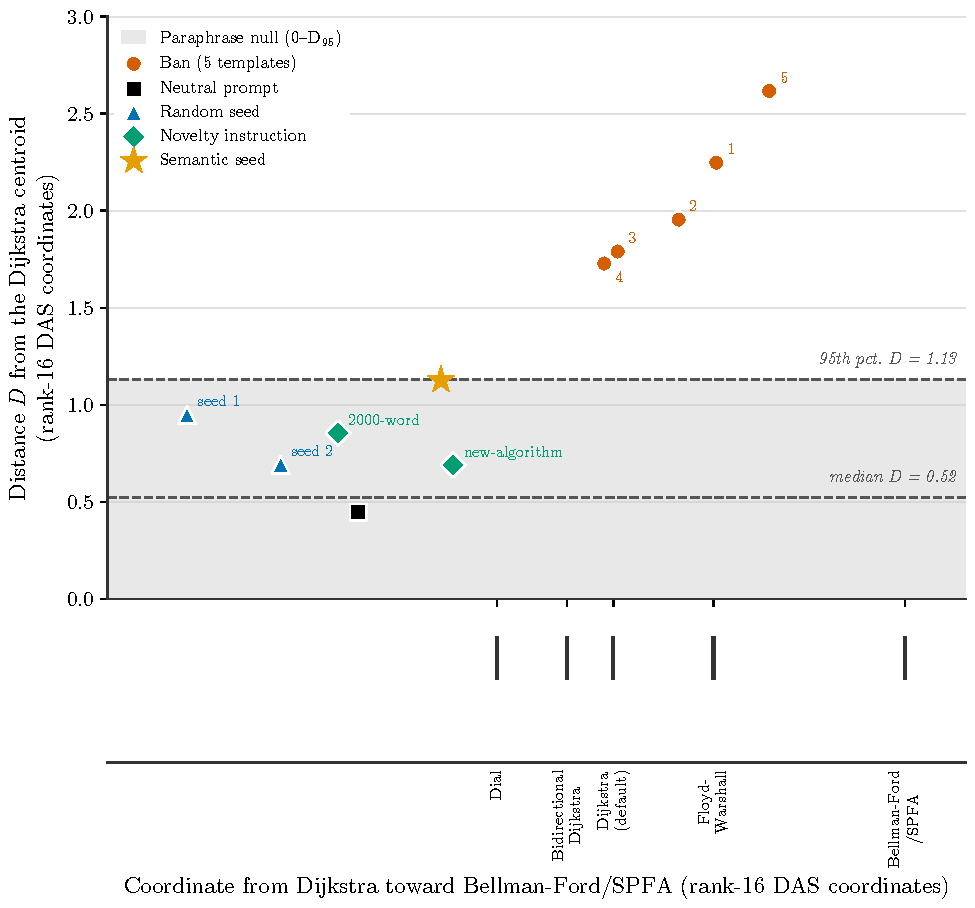
\includegraphics[width=\linewidth,height=0.78\textheight,keepaspectratio]{figures/fig_das_manifold_sp_v0.pdf}
\caption{Placement of shortest-path-task (T2) prompts for Qwen3-8B in the fitted rank-16 DAS coordinates of the task-specification residual stream (blocks 12--23). \textbackslash{}textbf\{Top panel:\} horizontal axis, the coordinate along the direction from the Dijkstra centroid to the Bellman-Ford\slash{}SPFA centroid; vertical axis, distance \$D\$ from the Dijkstra centroid. Dashed grey lines and the shaded grey band mark the paraphrase null's median (\$D=0.52\$) and 95th percentile (\$D=1.13\$; \$n=66\$ paraphrases). Vermillion circles, numbered 1--5, are the five ban-template prompts; all five sit above the shaded band, outside the paraphrase null, and on the positive side of the horizontal axis. The black square is the neutral prompt; blue triangles are two random seeds (`\texttt{seed 1'',\allowbreak{} }\texttt{seed 2''); green diamonds are the short }\texttt{new-\allowbreak{}algorithm'' instruction and the }`2000-word'' novelty instruction. These five all fall inside the shaded band. The orange star is a semantic seed, which falls just below the 95th-percentile line (at its 94th percentile in the underlying measurement). \textbackslash{}textbf\{Bottom strip:\} the same horizontal axis, with labelled tick marks at the centroid positions of Dijkstra (default), Dial, bidirectional Dijkstra, Floyd--Warshall and Bellman-Ford\slash{}SPFA. All values are read directly from the DAS-manifold measurement on Qwen3-8B; the placement shown is a descriptive geometric measurement, not a validated causal direction.}
\label{fig:fig_das_manifold_sp}
\end{figure}
\begin{table}[H]
\renewcommand{\thetable}{308}
\centering\footnotesize\setlength{\tabcolsep}{4.0pt}
\caption{Shortest path: what each seed and instruction prompt writes (30 programs each). [Source: iteration 7, artifact \nolinkurl{gen_art_experiment_33}.]}\label{tab:t328}
\begin{tabular}{>{\raggedright\arraybackslash\hspace{0pt}}p{0.3010\linewidth}>{\raggedright\arraybackslash\hspace{0pt}}p{0.0604\linewidth}>{\raggedright\arraybackslash\hspace{0pt}}p{0.2208\linewidth}>{\raggedright\arraybackslash\hspace{0pt}}p{0.2230\linewidth}>{\raggedright\arraybackslash\hspace{0pt}}p{0.1079\linewidth}}
\toprule
\textbf{Prompt} & \textbf{Pass} & \textbf{Correct composition} & \textbf{Correct off the default [CP 95\%]} & \textbf{Truncated} \\
\midrule
short instruction to make a new algorithm & 1.00 & Dijkstra 30 & 0 [0.00, 0.12] & 0 \\
2,000-word novelty instruction & 0.93 & Dijkstra 22, Bellman-Ford\slash{}SPFA 6 & 6 [0.08, 0.39] & 0 \\
neutral prompt & 0.97 & Dijkstra 29 & 0 [0.00, 0.12] & 0 \\
random seed 1 (seed=d32qxk4nt43) & 1.00 & Dijkstra 30 & 0 [0.00, 0.12] & 0 \\
random seed 2 (seed=(horse chair roof love)) & 1.00 & Dijkstra 30 & 0 [0.00, 0.12] & 0 \\
semantic seed & 0.97 & Dijkstra 28, other 1 & 1 [8.4e-04, 0.17] & 0 \\
\bottomrule
\end{tabular}
\end{table}

\begin{table}[H]
\renewcommand{\thetable}{309}
\centering\footnotesize\setlength{\tabcolsep}{4.0pt}
\caption{Shortest path: placement of prompts in the rank-16 DAS coordinates against the paraphrase null. (iteration-8 correction: the first three ban templates are training templates of the map; the semantic seed sits on the boundary of the null 95\%) [Source: iteration 7, artifact \nolinkurl{gen_art_experiment_33}.]}\label{tab:t329}
\begin{tabular}{>{\raggedright\arraybackslash\hspace{0pt}}p{0.3223\linewidth}>{\raggedright\arraybackslash\hspace{0pt}}p{0.1900\linewidth}>{\raggedright\arraybackslash\hspace{0pt}}p{0.1129\linewidth}>{\raggedright\arraybackslash\hspace{0pt}}p{0.1077\linewidth}>{\raggedright\arraybackslash\hspace{0pt}}p{0.1803\linewidth}}
\toprule
\textbf{Prompt (shortest path)} & \textbf{Distance D to the default centroid (rank-16 DAS coordinates)} & \textbf{Null percentile} & \textbf{Inside the null 95\%} & \textbf{Coordinate along the axis toward the second choice} \\
\midrule
ban, first template (training template of the map) & 2.25 & 100.0 & no & 1.55 \\
ban, second template (training template of the map) & 1.95 & 100.0 & no & 1.39 \\
ban, third template (training template of the map) & 1.79 & 100.0 & no & 1.15 \\
ban, fourth template & 1.73 & 100.0 & no & 1.10 \\
ban, fifth template & 2.62 & 100.0 & no & 1.76 \\
neutral prompt & 0.45 & 40.9 & yes & 0.11 \\
random seed 1 (seed=d32qxk4nt43) & 0.95 & 87.9 & yes & -0.58 \\
random seed 2 (seed=(horse chair roof love)) & 0.69 & 77.3 & yes & -0.21 \\
short instruction to make a new algorithm & 0.69 & 75.8 & yes & 0.49 \\
2,000-word novelty instruction & 0.85 & 86.4 & yes & 0.03 \\
semantic seed & 1.13 & 93.9 & yes & 0.44 \\
\bottomrule
\end{tabular}
\end{table}

\begin{table}[H]
\renewcommand{\thetable}{310}
\centering\scriptsize\setlength{\tabcolsep}{2.5pt}
\caption{Shortest path: algorithm centroids along the axis toward the second choice and how often each algorithm has been implemented. [Source: iteration 7, artifact \nolinkurl{gen_art_experiment_33}.]}\label{tab:t330}
\begin{tabular}{>{\raggedright\arraybackslash\hspace{0pt}}p{0.1136\linewidth}>{\raggedright\arraybackslash\hspace{0pt}}p{0.1895\linewidth}>{\raggedright\arraybackslash\hspace{0pt}}p{0.1214\linewidth}>{\raggedright\arraybackslash\hspace{0pt}}p{0.1214\linewidth}>{\raggedright\arraybackslash\hspace{0pt}}p{0.1385\linewidth}>{\raggedright\arraybackslash\hspace{0pt}}p{0.1809\linewidth}>{\raggedright\arraybackslash\hspace{0pt}}p{0.0582\linewidth}}
\toprule
\textbf{Algorithm} & \textbf{Centroid coordinate along the axis toward the second choice} & \textbf{Implemented under the twin} & \textbf{Implemented by Qwen3-8B-Base} & \textbf{Implemented under this artifact's knobs} & \textbf{Implemented under the 40 random directions of the engine control} & \textbf{All knobs} \\
\midrule
Dijkstra & 1.13 & 20 & 25 & 701 & 1608 & 2309 \\
Bellman-Ford\slash{}SPFA & 2.30 & 0 & 18 & 343 & 489 & 832 \\
bidirectional Dijkstra & 0.95 & 0 & 0 & 0 & 0 & 0 \\
Floyd-Warshall & 1.53 & 0 & 0 & 139 & 3 & 142 \\
Dial & 0.67 & 0 & 0 & 0 & 0 & 0 \\
\bottomrule
\end{tabular}
\end{table}

\begin{table}[H]
\renewcommand{\thetable}{311}
\centering\tiny\setlength{\tabcolsep}{2.5pt}
\caption{Shortest path: geodesic distances between centroids on neighbour graphs of the fitted coordinates. [Source: iteration 7, artifact \nolinkurl{gen_art_experiment_33}.]}\label{tab:t331}
\begin{tabular}{>{\raggedright\arraybackslash\hspace{0pt}}p{0.0772\linewidth}>{\raggedright\arraybackslash\hspace{0pt}}p{0.1611\linewidth}>{\raggedright\arraybackslash\hspace{0pt}}p{0.0796\linewidth}>{\raggedright\arraybackslash\hspace{0pt}}p{0.0824\linewidth}>{\raggedright\arraybackslash\hspace{0pt}}p{0.1161\linewidth}>{\raggedright\arraybackslash\hspace{0pt}}p{0.0703\linewidth}>{\raggedright\arraybackslash\hspace{0pt}}p{0.0915\linewidth}>{\raggedright\arraybackslash\hspace{0pt}}p{0.0646\linewidth}>{\raggedright\arraybackslash\hspace{0pt}}p{0.0408\linewidth}>{\raggedright\arraybackslash\hspace{0pt}}p{0.1087\linewidth}}
\toprule
\textbf{k of the neighbour graph} & \textbf{Mean survivor rank of bans that leave one survivor (of 5)} & \textbf{Random relabelling p} & \textbf{Unreachable pairs} & \textbf{Geodesic Dijkstra to Dijkstra (spread)} & \textbf{to Bellman-Ford\slash{}SPFA} & \textbf{to bidirectional Dijkstra} & \textbf{to Floyd-Warshall} & \textbf{to Dial} & \textbf{Bellman-Ford\slash{}SPFA to Floyd-Warshall} \\
\midrule
5 & 3.10 & 0.63 & 3080 & 0.24 & 3.20 & 1.77 & 3.87 & 2.55 & 4.67 \\
10 & 3.10 & 0.63 & 0 & 0.24 & 2.30 & 1.42 & 1.59 & 2.12 & 2.82 \\
15 & 3.20 & 0.71 & 0 & 0.24 & 1.45 & 1.11 & 1.50 & 1.82 & 1.85 \\
\bottomrule
\end{tabular}
\end{table}

\subsubsection*{7.3.9 Seeds, discreteness and the full cell list}
A second initialisation seed fits a different subspace (principal angles of 38 to 90 degrees to the first) with similar behaviour: no discordance between seeds reaches significance (Table 312). The subspace is therefore not unique, as in Gemma (Section 7.8). The discreteness claim fails. Scaling the rank-2 edit of the ban by lambda from 0 to 1.5 raises correct Bellman-Ford\slash{}SPFA programs from 1 of 20 (lambda 0 to 0.2) through 4 of 20 (0.4 to 0.5) to a plateau of 6 to 9 of 20 from lambda 0.6 to 1.5; the committed logistic width is 3.25 in lambda (midpoint 1.47), against 0.3 or less for a step, and the one candidate hybrid among 114 correct programs was judged a single algorithm (Table 313). Of the 38 correct programs labelled other across the experiment, 36 are catalogue variants and 2 are labeller misses; none is novel. 29 of the 36 come from the full state exchange of the forced counting sort source and 6 more from the forced counting sort prompts: they are counting sort in dictionary form, which the extended labeller now names counting sort (iteration-8 correction). The engine reproduced the iteration-6 twin labels in 20 of 20, 19 of 20 and 20 of 20 slots; two GPU unit tests missed their tolerance because of bf16 noise from kernel shapes (packed against separate forward passes differ by up to 0.273 nats per program, cached against full forward passes by 0.160), so every compared quantity is measured within one batch shape. Table 314 lists every generation cell.

\begin{table}[H]
\renewcommand{\thetable}{312}
\centering\footnotesize\setlength{\tabcolsep}{4.0pt}
\caption{A second DAS initialisation seed. [Source: iteration 7, artifact \nolinkurl{gen_art_experiment_33}.]}\label{tab:t332}
\begin{tabular}{>{\raggedright\arraybackslash\hspace{0pt}}p{0.4384\linewidth}>{\raggedright\arraybackslash\hspace{0pt}}p{0.1044\linewidth}>{\raggedright\arraybackslash\hspace{0pt}}p{0.1038\linewidth}>{\raggedright\arraybackslash\hspace{0pt}}p{0.1946\linewidth}>{\raggedright\arraybackslash\hspace{0pt}}p{0.0720\linewidth}}
\toprule
\textbf{Arm} & \textbf{Seed 1 correct Y of 30} & \textbf{Seed 2 correct Y of 30} & \textbf{Discordant seed-1-only : seed-2-only (p)} & \textbf{Pass, seed 2} \\
\midrule
DAS (likelihood objective), second seed, forced Bellman-Ford\slash{}SPFA source, rank 16 & 5 & 1 & 5:1 (0.219) & 0.67 \\
DAS (likelihood objective), second seed, forced Floyd-Warshall source, rank 16 & 25 & 27 & 0:2 (0.500) & 0.90 \\
DAS (likelihood objective), second seed, fifth template ban source, rank 1 & 8 & 3 & 6:1 (0.125) & 0.73 \\
DAS (likelihood objective), second seed, fifth template ban source, rank 16 & 6 & 7 & 3:4 (1.000) & 0.67 \\
DAS (likelihood objective), second seed, fifth template ban source, rank 2 & 12 & 8 & 6:2 (0.289) & 0.60 \\
\bottomrule
\end{tabular}
\end{table}

\begin{table}[H]
\renewcommand{\thetable}{313}
\centering\footnotesize\setlength{\tabcolsep}{4.0pt}
\caption{Discreteness: the rank-2 DAS edit of the ban scaled by lambda (shortest path, 20 slots each). [Source: iteration 7, artifact \nolinkurl{gen_art_experiment_33}.]}\label{tab:t333}
\begin{tabular}{>{\raggedright\arraybackslash\hspace{0pt}}p{0.0847\linewidth}>{\raggedright\arraybackslash\hspace{0pt}}p{0.1825\linewidth}>{\raggedright\arraybackslash\hspace{0pt}}p{0.1409\linewidth}>{\raggedright\arraybackslash\hspace{0pt}}p{0.0678\linewidth}>{\raggedright\arraybackslash\hspace{0pt}}p{0.4372\linewidth}}
\toprule
\textbf{Lambda} & \textbf{Correct Bellman-Ford\slash{}SPFA (of 20)} & \textbf{Correct Dijkstra} & \textbf{Pass} & \textbf{Labels} \\
\midrule
0.0 & 1 & 18 & 0.95 & Dijkstra 18, Bellman-Ford\slash{}SPFA 2 \\
0.2 & 1 & 16 & 0.85 & Dijkstra 17, Bellman-Ford\slash{}SPFA 3 \\
0.4 & 4 & 11 & 0.75 & Dijkstra 11, Bellman-Ford\slash{}SPFA 9 \\
0.5 & 4 & 11 & 0.75 & Dijkstra 11, Bellman-Ford\slash{}SPFA 9 \\
0.6 & 6 & 9 & 0.80 & Bellman-Ford\slash{}SPFA 10, Dijkstra 9, other 1 \\
0.7 & 8 & 9 & 0.85 & Bellman-Ford\slash{}SPFA 11, Dijkstra 9 \\
0.8 & 7 & 10 & 0.85 & Dijkstra 10, Bellman-Ford\slash{}SPFA 10 \\
1.0 & 9 & 8 & 0.85 & Bellman-Ford\slash{}SPFA 12, Dijkstra 8 \\
1.25 & 7 & 10 & 0.85 & Dijkstra 10, Bellman-Ford\slash{}SPFA 10 \\
1.5 & 8 & 9 & 0.85 & Bellman-Ford\slash{}SPFA 11, Dijkstra 9 \\
\bottomrule
\end{tabular}
\end{table}

{\footnotesize\setlength{\tabcolsep}{4.0pt}\renewcommand{\thetable}{314}
\begin{longtable}{>{\raggedright\arraybackslash\hspace{0pt}}p{0.1078\linewidth}>{\raggedright\arraybackslash\hspace{0pt}}p{0.3392\linewidth}>{\raggedright\arraybackslash\hspace{0pt}}p{0.0331\linewidth}>{\raggedright\arraybackslash\hspace{0pt}}p{0.0604\linewidth}>{\raggedright\arraybackslash\hspace{0pt}}p{0.1079\linewidth}>{\raggedright\arraybackslash\hspace{0pt}}p{0.2482\linewidth}}
\caption{Every generation cell of the DAS experiment. [Source: iteration 7, artifact \nolinkurl{gen_art_experiment_33}.]}\label{tab:t334}\\
\toprule
\textbf{Task} & \textbf{Arm} & \textbf{n} & \textbf{Pass} & \textbf{Truncated} & \textbf{Correct composition} \\
\midrule
\endfirsthead
\multicolumn{6}{l}{\emph{Table 314, continued}}\\
\toprule
\textbf{Task} & \textbf{Arm} & \textbf{n} & \textbf{Pass} & \textbf{Truncated} & \textbf{Correct composition} \\
\midrule
\endhead
\bottomrule
\endlastfoot
shortest path & padding twin (base for forced sources) & 30 & 0.97 & 0 & Dijkstra 29 \\
shortest path & neutral twin of template 4 (base) & 10 & 1.00 & 0 & Dijkstra 10 \\
shortest path & neutral twin of template 5 (base) & 30 & 0.97 & 0 & Dijkstra 28, Bellman-Ford\slash{}SPFA 1 \\
shortest path & DAS (likelihood objective), second seed, forced Bellman-Ford\slash{}SPFA source, rank 16 & 30 & 0.67 & 0 & Dijkstra 19, Bellman-Ford\slash{}SPFA 1 \\
shortest path & DAS (likelihood objective), second seed, forced Floyd-Warshall source, rank 16 & 30 & 0.90 & 0 & Floyd-Warshall 27 \\
shortest path & DAS (likelihood objective), second seed, fifth template ban source, rank 1 & 30 & 0.73 & 0 & Dijkstra 19, Bellman-Ford\slash{}SPFA 3 \\
shortest path & DAS (likelihood objective), second seed, fifth template ban source, rank 16 & 30 & 0.67 & 0 & Dijkstra 13, Bellman-Ford\slash{}SPFA 7 \\
shortest path & DAS (likelihood objective), second seed, fifth template ban source, rank 2 & 30 & 0.60 & 0 & Dijkstra 9, Bellman-Ford\slash{}SPFA 8, other 1 \\
shortest path & DAS (likelihood objective), forced Bellman-Ford\slash{}SPFA source, rank 1 & 30 & 0.70 & 0 & Bellman-Ford\slash{}SPFA 13, Dijkstra 8 \\
shortest path & DAS (likelihood objective), forced Bellman-Ford\slash{}SPFA source, rank 16 & 30 & 0.80 & 0 & Dijkstra 19, Bellman-Ford\slash{}SPFA 5 \\
shortest path & DAS (likelihood objective), forced Bellman-Ford\slash{}SPFA source, rank 4 & 30 & 0.67 & 0 & Dijkstra 11, Bellman-Ford\slash{}SPFA 9 \\
shortest path & DAS (likelihood objective), forced Floyd-Warshall source, rank 1 & 30 & 0.93 & 0 & Floyd-Warshall 28 \\
shortest path & DAS (likelihood objective), forced Floyd-Warshall source, rank 16 & 30 & 0.83 & 0 & Floyd-Warshall 25 \\
shortest path & DAS (likelihood objective), forced Floyd-Warshall source, rank 4 & 30 & 0.93 & 0 & Floyd-Warshall 28 \\
shortest path & DAS (likelihood objective), fourth template ban source, rank 2 & 10 & 0.90 & 0 & Dijkstra 5, Bellman-Ford\slash{}SPFA 4 \\
shortest path & DAS (likelihood objective), fifth template ban source, rank 1 & 30 & 0.77 & 0 & Dijkstra 15, Bellman-Ford\slash{}SPFA 8 \\
shortest path & DAS (likelihood objective), fifth template ban source, rank 16 & 30 & 0.80 & 0 & Dijkstra 18, Bellman-Ford\slash{}SPFA 6 \\
shortest path & DAS (likelihood objective), fifth template ban source, rank 2 & 30 & 0.83 & 0 & Dijkstra 13, Bellman-Ford\slash{}SPFA 12 \\
shortest path & DAS (likelihood objective), fifth template ban source, rank 4 & 30 & 0.57 & 0 & Bellman-Ford\slash{}SPFA 10, Dijkstra 7 \\
shortest path & DAS (likelihood objective), fifth template ban source, rank 8 & 30 & 0.83 & 0 & Dijkstra 15, Bellman-Ford\slash{}SPFA 10 \\
shortest path & DAS (committed contrastive objective), forced Bellman-Ford\slash{}SPFA source, rank 1 & 10 & 0.40 & 0 & Dijkstra 3, Bellman-Ford\slash{}SPFA 1 \\
shortest path & DAS (committed contrastive objective), forced Bellman-Ford\slash{}SPFA source, rank 16 & 10 & 0.00 & 10 & none \\
shortest path & DAS (committed contrastive objective), forced Bellman-Ford\slash{}SPFA source, rank 4 & 10 & 0.00 & 9 & none \\
shortest path & DAS (committed contrastive objective), forced Floyd-Warshall source, rank 1 & 10 & 0.50 & 0 & Dijkstra 4, Bellman-Ford\slash{}SPFA 1 \\
shortest path & DAS (committed contrastive objective), forced Floyd-Warshall source, rank 16 & 10 & 0.00 & 10 & none \\
shortest path & DAS (committed contrastive objective), forced Floyd-Warshall source, rank 4 & 10 & 0.00 & 10 & none \\
shortest path & DAS (committed contrastive objective), fifth template ban source, rank 1 & 10 & 0.10 & 5 & Dijkstra 1 \\
shortest path & DAS (committed contrastive objective), fifth template ban source, rank 16 & 10 & 0.00 & 9 & none \\
shortest path & DAS (committed contrastive objective), fifth template ban source, rank 2 & 10 & 0.00 & 7 & none \\
shortest path & DAS (committed contrastive objective), fifth template ban source, rank 4 & 10 & 0.00 & 7 & none \\
shortest path & DAS (committed contrastive objective), fifth template ban source, rank 8 & 10 & 0.00 & 10 & none \\
shortest path & difference in means (rank 1), fifth template ban source & 30 & 0.97 & 0 & Dijkstra 29 \\
shortest path & full state exchange, forced Bellman-Ford\slash{}SPFA (family 3), block 18 only & 30 & 1.00 & 0 & Bellman-Ford\slash{}SPFA 30 \\
shortest path & full state exchange, forced Bellman-Ford\slash{}SPFA (family 3), blocks 12-23 & 30 & 1.00 & 0 & Bellman-Ford\slash{}SPFA 30 \\
shortest path & full state exchange, forced Bellman-Ford\slash{}SPFA source & 30 & 1.00 & 0 & Bellman-Ford\slash{}SPFA 30 \\
shortest path & full state exchange, forced Floyd-Warshall source & 30 & 0.67 & 0 & Bellman-Ford\slash{}SPFA 12, Floyd-Warshall 8 \\
shortest path & full state exchange, fourth template ban source & 10 & 0.50 & 0 & Bellman-Ford\slash{}SPFA 4, Dijkstra 1 \\
shortest path & full state exchange, ban source, block 18 only & 30 & 1.00 & 0 & Dijkstra 30 \\
shortest path & full state exchange, ban source, blocks 12-23 & 30 & 0.73 & 0 & Dijkstra 11, Bellman-Ford\slash{}SPFA 11 \\
shortest path & rank-2 DAS edit scaled by lambda 0.0, ban source & 20 & 0.95 & 0 & Dijkstra 18, Bellman-Ford\slash{}SPFA 1 \\
shortest path & rank-2 DAS edit scaled by lambda 0.2, ban source & 20 & 0.85 & 0 & Dijkstra 16, Bellman-Ford\slash{}SPFA 1 \\
shortest path & rank-2 DAS edit scaled by lambda 0.4, ban source & 20 & 0.75 & 0 & Dijkstra 11, Bellman-Ford\slash{}SPFA 4 \\
shortest path & rank-2 DAS edit scaled by lambda 0.5, ban source & 20 & 0.75 & 0 & Dijkstra 11, Bellman-Ford\slash{}SPFA 4 \\
shortest path & rank-2 DAS edit scaled by lambda 0.6, ban source & 20 & 0.80 & 0 & Dijkstra 9, Bellman-Ford\slash{}SPFA 6, other 1 \\
shortest path & rank-2 DAS edit scaled by lambda 0.7, ban source & 20 & 0.85 & 0 & Dijkstra 9, Bellman-Ford\slash{}SPFA 8 \\
shortest path & rank-2 DAS edit scaled by lambda 0.8, ban source & 20 & 0.85 & 0 & Dijkstra 10, Bellman-Ford\slash{}SPFA 7 \\
shortest path & rank-2 DAS edit scaled by lambda 1.0, ban source & 20 & 0.85 & 0 & Bellman-Ford\slash{}SPFA 9, Dijkstra 8 \\
shortest path & rank-2 DAS edit scaled by lambda 1.25, ban source & 20 & 0.85 & 0 & Dijkstra 10, Bellman-Ford\slash{}SPFA 7 \\
shortest path & rank-2 DAS edit scaled by lambda 1.5, ban source & 20 & 0.85 & 0 & Dijkstra 9, Bellman-Ford\slash{}SPFA 8 \\
shortest path & short instruction to make a new algorithm & 30 & 1.00 & 0 & Dijkstra 30 \\
shortest path & 2,000-word novelty instruction & 30 & 0.93 & 0 & Dijkstra 22, Bellman-Ford\slash{}SPFA 6 \\
shortest path & neutral prompt & 30 & 0.97 & 0 & Dijkstra 29 \\
shortest path & random seed 1 (seed=d32qxk4nt43) & 30 & 1.00 & 0 & Dijkstra 30 \\
shortest path & random seed 2 (seed=(horse chair roof love)) & 30 & 1.00 & 0 & Dijkstra 30 \\
shortest path & semantic seed & 30 & 0.97 & 0 & Dijkstra 28, other 1 \\
shortest path & null source (forced default), DAS rank 16 & 30 & 0.83 & 0 & Dijkstra 24, Bellman-Ford\slash{}SPFA 1 \\
shortest path & null source (forced default), full state exchange & 30 & 0.97 & 0 & Dijkstra 29 \\
shortest path & padding twin of forced Bellman-Ford\slash{}SPFA (family 3) & 30 & 0.97 & 0 & Dijkstra 29 \\
shortest path & PCA-16 subspace, fifth template ban source & 30 & 0.83 & 0 & Dijkstra 24, Bellman-Ford\slash{}SPFA 1 \\
shortest path & DAS with permuted labels, forced Floyd-Warshall source, rank 16 & 30 & 0.63 & 0 & Bellman-Ford\slash{}SPFA 8, Floyd-Warshall 6, Dijkstra 5 \\
shortest path & DAS with permuted labels, fifth template ban source, rank 16 & 30 & 0.63 & 0 & Floyd-Warshall 15, Bellman-Ford\slash{}SPFA 3, Dijkstra 1 \\
shortest path & DAS with permuted labels, fifth template ban source, rank 2 & 30 & 0.97 & 0 & Bellman-Ford\slash{}SPFA 15, Dijkstra 12, Floyd-Warshall 2 \\
shortest path & random subspace, forced Bellman-Ford\slash{}SPFA source, rank 16 & 30 & 0.97 & 0 & Dijkstra 29 \\
shortest path & random subspace, forced Floyd-Warshall source, rank 16 & 30 & 0.97 & 0 & Dijkstra 29 \\
shortest path & random subspace 1, fifth template ban source, rank 16 & 30 & 0.97 & 0 & Dijkstra 28, Bellman-Ford\slash{}SPFA 1 \\
shortest path & random subspace 2, fifth template ban source, rank 16 & 30 & 0.97 & 0 & Dijkstra 29 \\
shortest path & random subspace 3, fifth template ban source, rank 16 & 30 & 0.97 & 0 & Dijkstra 28, Bellman-Ford\slash{}SPFA 1 \\
shortest path & random subspace, fifth template ban source, rank 2 & 30 & 0.97 & 0 & Dijkstra 28, Bellman-Ford\slash{}SPFA 1 \\
shortest path & reverse interchange, DAS rank 2 & 30 & 1.00 & 0 & Bellman-Ford\slash{}SPFA 30 \\
shortest path & reverse interchange, full state & 30 & 1.00 & 0 & Dijkstra 21, Bellman-Ford\slash{}SPFA 9 \\
shortest path & full state exchange at the read position, fifth template ban source & 30 & 0.97 & 0 & Dijkstra 28, Bellman-Ford\slash{}SPFA 1 \\
shortest path & DAS at the read position, fifth template ban source, rank 16 & 30 & 0.90 & 0 & Dijkstra 25, Bellman-Ford\slash{}SPFA 2 \\
connected components & padding twin (base for forced sources) & 30 & 1.00 & 0 & union find 30 \\
connected components & neutral twin of template 4 (base) & 10 & 1.00 & 0 & union find 10 \\
connected components & neutral twin of template 5 (base) & 30 & 1.00 & 0 & union find 29, DFS 1 \\
connected components & DAS (likelihood objective), forced BFS source, rank 1 & 30 & 1.00 & 0 & DFS 29, BFS 1 \\
connected components & DAS (likelihood objective), forced BFS source, rank 16 & 30 & 1.00 & 0 & DFS 21, BFS 9 \\
connected components & DAS (likelihood objective), forced BFS source, rank 4 & 30 & 1.00 & 0 & DFS 23, BFS 7 \\
connected components & DAS (likelihood objective), forced DFS source, rank 1 & 30 & 1.00 & 0 & DFS 30 \\
connected components & DAS (likelihood objective), forced DFS source, rank 16 & 30 & 1.00 & 0 & DFS 23, BFS 7 \\
connected components & DAS (likelihood objective), forced DFS source, rank 4 & 30 & 1.00 & 0 & DFS 26, BFS 4 \\
connected components & DAS (likelihood objective), fourth template ban source, rank 1 & 10 & 1.00 & 0 & DFS 10 \\
connected components & DAS (likelihood objective), fifth template ban source, rank 1 & 30 & 0.97 & 0 & BFS 18, DFS 11 \\
connected components & DAS (likelihood objective), fifth template ban source, rank 16 & 30 & 1.00 & 0 & BFS 29, DFS 1 \\
connected components & DAS (likelihood objective), fifth template ban source, rank 2 & 30 & 1.00 & 0 & BFS 23, DFS 7 \\
connected components & DAS (likelihood objective), fifth template ban source, rank 4 & 30 & 1.00 & 0 & BFS 21, DFS 9 \\
connected components & DAS (likelihood objective), fifth template ban source, rank 8 & 30 & 1.00 & 0 & BFS 29, DFS 1 \\
connected components & DAS (committed contrastive objective), forced BFS source, rank 1 & 10 & 1.00 & 0 & union find 10 \\
connected components & DAS (committed contrastive objective), forced BFS source, rank 16 & 10 & 0.00 & 8 & none \\
connected components & DAS (committed contrastive objective), forced BFS source, rank 4 & 10 & 0.20 & 5 & BFS 2 \\
connected components & DAS (committed contrastive objective), forced DFS source, rank 1 & 10 & 1.00 & 0 & union find 10 \\
connected components & DAS (committed contrastive objective), forced DFS source, rank 16 & 10 & 0.20 & 3 & BFS 2 \\
connected components & DAS (committed contrastive objective), forced DFS source, rank 4 & 10 & 0.10 & 0 & BFS 1 \\
connected components & DAS (committed contrastive objective), fifth template ban source, rank 1 & 10 & 1.00 & 0 & union find 10 \\
connected components & DAS (committed contrastive objective), fifth template ban source, rank 16 & 10 & 0.50 & 3 & BFS 5 \\
connected components & DAS (committed contrastive objective), fifth template ban source, rank 2 & 10 & 0.60 & 1 & BFS 5, DFS 1 \\
connected components & DAS (committed contrastive objective), fifth template ban source, rank 4 & 10 & 0.40 & 2 & BFS 3, DFS 1 \\
connected components & DAS (committed contrastive objective), fifth template ban source, rank 8 & 10 & 0.30 & 3 & BFS 3 \\
connected components & difference in means (rank 1), fifth template ban source & 30 & 1.00 & 0 & union find 25, DFS 5 \\
connected components & full state exchange, forced BFS (family 3), block 16 only & 30 & 1.00 & 0 & BFS 28, DFS 2 \\
connected components & full state exchange, forced BFS (family 3), blocks 12-23 & 30 & 1.00 & 0 & DFS 20, BFS 10 \\
connected components & full state exchange, forced BFS source & 30 & 1.00 & 0 & BFS 17, DFS 13 \\
connected components & full state exchange, forced DFS source & 30 & 1.00 & 0 & DFS 30 \\
connected components & full state exchange, fourth template ban source & 10 & 1.00 & 0 & BFS 9, DFS 1 \\
connected components & full state exchange, ban source, block 16 only & 30 & 0.93 & 0 & DFS 24, union find 4 \\
connected components & full state exchange, ban source, blocks 12-23 & 30 & 1.00 & 0 & BFS 17, DFS 13 \\
connected components & null source (forced default), DAS rank 16 & 30 & 1.00 & 0 & union find 30 \\
connected components & null source (forced default), full state exchange & 30 & 1.00 & 0 & union find 30 \\
connected components & padding twin of forced BFS (family 3) & 30 & 1.00 & 0 & union find 30 \\
connected components & PCA-16 subspace, fifth template ban source & 30 & 0.93 & 0 & DFS 21, union find 7 \\
connected components & DAS with permuted labels, forced BFS source, rank 16 & 30 & 1.00 & 0 & DFS 20, BFS 10 \\
connected components & DAS with permuted labels, fifth template ban source, rank 1 & 30 & 1.00 & 0 & BFS 15, DFS 14, union find 1 \\
connected components & DAS with permuted labels, fifth template ban source, rank 16 & 30 & 1.00 & 0 & BFS 21, DFS 9 \\
connected components & random subspace, forced BFS source, rank 16 & 30 & 1.00 & 0 & union find 30 \\
connected components & random subspace, forced DFS source, rank 16 & 30 & 1.00 & 0 & union find 30 \\
connected components & random subspace, fifth template ban source, rank 1 & 30 & 1.00 & 0 & union find 29, DFS 1 \\
connected components & random subspace 1, fifth template ban source, rank 16 & 30 & 1.00 & 0 & union find 29, DFS 1 \\
connected components & random subspace 2, fifth template ban source, rank 16 & 30 & 1.00 & 0 & union find 29, DFS 1 \\
connected components & random subspace 3, fifth template ban source, rank 16 & 30 & 1.00 & 0 & union find 29, DFS 1 \\
connected components & reverse interchange, DAS rank 1 & 30 & 0.93 & 0 & BFS 18, DFS 10 \\
connected components & reverse interchange, full state & 30 & 0.93 & 0 & BFS 23, DFS 5 \\
connected components & full state exchange at the read position, fifth template ban source & 30 & 1.00 & 0 & union find 29, DFS 1 \\
connected components & DAS at the read position, fifth template ban source, rank 16 & 30 & 1.00 & 0 & DFS 28, BFS 2 \\
kth smallest & padding twin (base for forced sources) & 30 & 1.00 & 0 & full sort 30 \\
kth smallest & neutral twin of template 5 (base) & 30 & 1.00 & 0 & full sort 25, quickselect 5 \\
kth smallest & DAS (likelihood objective), forced counting sort source, rank 1 & 30 & 1.00 & 0 & counting sort 30 \\
kth smallest & DAS (likelihood objective), forced counting sort source, rank 16 & 30 & 1.00 & 0 & counting sort 30 \\
kth smallest & DAS (likelihood objective), forced counting sort source, rank 4 & 30 & 1.00 & 0 & counting sort 30 \\
kth smallest & DAS (likelihood objective), forced quickselect source, rank 1 & 30 & 1.00 & 0 & quickselect 30 \\
kth smallest & DAS (likelihood objective), forced quickselect source, rank 16 & 30 & 0.90 & 0 & quickselect 27 \\
kth smallest & DAS (likelihood objective), forced quickselect source, rank 4 & 30 & 0.93 & 0 & quickselect 28 \\
kth smallest & DAS (likelihood objective), fifth template ban source, rank 1 & 30 & 0.90 & 0 & quickselect 25, counting sort 1, size k heap 1 \\
kth smallest & DAS (likelihood objective), fifth template ban source, rank 16 & 30 & 0.90 & 0 & quickselect 26, size k heap 1 \\
kth smallest & DAS (likelihood objective), fifth template ban source, rank 4 & 30 & 0.90 & 0 & quickselect 26, size k heap 1 \\
kth smallest & full state exchange, forced quickselect (family 3), block 16 only & 30 & 0.90 & 0 & quickselect 27 \\
kth smallest & full state exchange, forced quickselect (family 3), blocks 12-23 & 30 & 0.97 & 0 & quickselect 29 \\
kth smallest & full state exchange, forced counting sort source & 30 & 1.00 & 0 & counting sort (dictionary form) 29, other 1 (binary search on the value range; iteration-8 correction) \\
kth smallest & full state exchange, forced quickselect source & 30 & 0.97 & 0 & quickselect 29 \\
kth smallest & full state exchange, ban source, block 16 only & 30 & 1.00 & 0 & quickselect 26, full sort 3, size k heap 1 \\
kth smallest & full state exchange, ban source, blocks 12-23 & 30 & 0.93 & 0 & quickselect 26, size k heap 2 \\
kth smallest & padding twin of forced quickselect (family 3) & 30 & 1.00 & 0 & full sort 30 \\
kth smallest & DAS with permuted labels, fifth template ban source, rank 1 & 30 & 0.93 & 0 & quickselect 22, counting sort 5, size k heap 1 \\
kth smallest & DAS with permuted labels, fifth template ban source, rank 16 & 30 & 0.90 & 0 & quickselect 18, counting sort 8, size k heap 1 \\
kth smallest & random subspace, fifth template ban source, rank 1 & 30 & 1.00 & 0 & full sort 24, quickselect 5, size k heap 1 \\
kth smallest & random subspace 1, fifth template ban source, rank 16 & 30 & 1.00 & 0 & full sort 24, quickselect 5, size k heap 1 \\
\end{longtable}}

\subsubsection*{7.3.10 Not run and deviations}
The DAS experiment's deviation log records what was not run and what departed from the plan; the four that bear on the claims above are quoted verbatim from \texttt{results/\allowbreak{}deviations.\allowbreak{}json} (iteration-8 correction: new subsection).

\begin{itemize}
\item \textbf{D-drop.} ``Drop order applied: plan resampling (1) and the T1 extension (2: T1 DAS and the literal top-five placement on T1) were not run; M's top-k placement uses T2's leave-one-survivor bans only.''
\item \textbf{D-tfsets.} ``Held-out teacher-forced evaluation scores held-out PROMPT pairs with the training target program sets (no separate held-out target sets).''
\item \textbf{D-targets.} ``Distinct 48-token openings are few (the model repeats openings), so the default pool was extended to TRAIN-family padding-twin samples (commit1\_\allowbreak{}\textless{}task\textgreater{}\_\allowbreak{}v2 amendment); validation target sets are filled from training programs where \textless{} 8 distinct programs exist; T10 dfs has 3 distinct programs, T03 heapify\_\allowbreak{}pop 1 and full\_\allowbreak{}sort 2 (T03 short-program fallback: \textgreater{}= 16 tokens).''
\item \textbf{D-cap.} ``Generation caps are exp30's 384 (bench) \slash{} 512 (T2) tokens, not 1,024\slash{}1,536: engine-check comparability with exp30 and the time budget; truncations are counted per cell (results\slash{}cells.json, n\_\allowbreak{}length).''
\end{itemize}

Two further deviations are used above: D-randinit (the committed untrained-network comparison against the diverged fit, replaced post hoc by the matched likelihood fit; Section 7.3.5) and D-C-k (forced sources were generated at ranks 1, 4 and 16 only, so the routing claim is scored at rank 16 and rank 2 is untested for forced sources; Table 297b). Plan resampling and the literal top-five placement in the fitted coordinates on the grid task remain open items (Sections 7.10 and 7.11).

\FloatBarrier
\subsection*{7.4 Where the algorithm is decided in generation (Qwen3-8B)}
\addcontentsline{toc}{subsection}{7.4 Where the algorithm is decided in generation (Qwen3-8B)}
\noindent{\small\emph{Artifact: \nolinkurl{gen_art_experiment_34}.}}\par\medskip
\subsubsection*{7.4.1 Design}
The fork experiment  asked whether one early generated token decides the algorithm, and whether the decision at that token explains which random pushes of iteration 4 change the algorithm. Forks were located by \emph{prefix resampling}: from each base program (one written under the neutral twin, under a push of plan noise or under a ban), the model was restarted at positions along the program's first 128 tokens, and eight continuations were sampled and labelled at each. A \emph{change point} is a position where the share of continuations off the default changes significantly; a fork is a change point on the \emph{shared opening}, the token sequence that most twin programs share before they part. Where no fork exists the committed fallback is the \emph{opening log likelihood ratio} (opening LLR): the teacher-forced log likelihood ratio of the opening of the second choice to the opening of the default over the first L tokens (48 on shortest path, 20 on kth smallest, whose programs are about 20 tokens long). The 40 random directions of iteration 4 were then scored for their fork margin under the push and compared with the correct share off the default (y) that each direction produced in bf16, the share of its programs that pass the hidden tests and implement a named algorithm other than the default; the fork margin under a push is written m.

\subsubsection*{7.4.2 Forks}
Connected components has two forks, at generated tokens 10 and 11 of the opening \texttt{def solve(\allowbreak{}n,\allowbreak{} edges):\allowbreak{}}, which 94\% of twin programs share (Tables 315 and 316). At token 10, a comment token leads to BFS or DFS in all 159 continuations, \texttt{ parent} leads to union find in all 130, \texttt{ def} leads off the default in 0.69 of 72, and \texttt{ from} leads off in all 11. At token 11, after \texttt{ def}, the routine's name settles it: \texttt{ dfs} leads to DFS in all 45 continuations and \texttt{ find} to union find in all 32. The entropy of the label given the token falls from 0.97 bits to 0.00 at token 11. Shortest path has no single fork: pushed programs stay undecided through token 60, and its only change point (token 92) lies off the shared opening. On kth smallest a ban fixes the algorithm before the first generated token: at the first position only 0 to 2 of 8 continuations differ from the base program's class, and no change occurs in 128 tokens.

\begin{table}[H]
\renewcommand{\thetable}{315}
\centering\scriptsize\setlength{\tabcolsep}{2.5pt}
\caption{Forks found by prefix resampling. [Source: iteration 7, artifact \nolinkurl{gen_art_experiment_34}.]}\label{tab:t335}
\begin{tabular}{>{\raggedright\arraybackslash\hspace{0pt}}p{0.0919\linewidth}>{\raggedright\arraybackslash\hspace{0pt}}p{0.0705\linewidth}>{\raggedright\arraybackslash\hspace{0pt}}p{0.0748\linewidth}>{\raggedright\arraybackslash\hspace{0pt}}p{0.0748\linewidth}>{\raggedright\arraybackslash\hspace{0pt}}p{0.0582\linewidth}>{\raggedright\arraybackslash\hspace{0pt}}p{0.1081\linewidth}>{\raggedright\arraybackslash\hspace{0pt}}p{0.1564\linewidth}>{\raggedright\arraybackslash\hspace{0pt}}p{0.0872\linewidth}>{\raggedright\arraybackslash\hspace{0pt}}p{0.1808\linewidth}}
\toprule
\textbf{Task} & \textbf{Status} & \textbf{Forks along the shared opening (token index)} & \textbf{Change points off the shared opening} & \textbf{Base paths} & \textbf{Paths with a significant change point} & \textbf{Base paths by cell} & \textbf{Majority opening length (tokens)} & \textbf{Label entropy at the forks} \\
\midrule
connected components & fork found & 10, 11 & BFS at tokens 12 and 39 & 18 & 4 & neutral twin 6 (0 with a fork); plan noise 4 (3 with a fork); ban 8 (1 with a fork) & 129 & token 10: H(label) 1.55 -\textgreater{} H(label given token) 0.54 bits (n 372); token 11: H(label) 0.97 -\textgreater{} H(label given token) 0.00 bits (n 80) \\
shortest path & no single fork & none & Bellman-Ford\slash{}SPFA at token 92 & 12 & 1 & neutral twin 6 (0 with a fork); plan noise 3 (1 with a fork); ban 3 (0 with a fork) & 34 & - \\
kth smallest & no single fork & none & none & 18 & 0 & neutral twin 6 (0 with a fork); ban 12 (0 with a fork) & 22 & - \\
\bottomrule
\end{tabular}
\end{table}

\begin{table}[H]
\renewcommand{\thetable}{316}
\centering\footnotesize\setlength{\tabcolsep}{4.0pt}
\caption{Connected components: the tokens at the two forks and what follows them. [Source: iteration 7, artifact \nolinkurl{gen_art_experiment_34}.]}\label{tab:t336}
\begin{tabular}{>{\raggedright\arraybackslash\hspace{0pt}}p{0.1589\linewidth}>{\raggedright\arraybackslash\hspace{0pt}}p{0.0841\linewidth}>{\raggedright\arraybackslash\hspace{0pt}}p{0.1460\linewidth}>{\raggedright\arraybackslash\hspace{0pt}}p{0.2365\linewidth}>{\raggedright\arraybackslash\hspace{0pt}}p{0.1917\linewidth}>{\raggedright\arraybackslash\hspace{0pt}}p{0.0794\linewidth}}
\toprule
\textbf{Generated token index} & \textbf{Token} & \textbf{Continuations} & \textbf{Labels of the continuations} & \textbf{Share off the default (q)} & \textbf{Mapped} \\
\midrule
10 & \texttt{ \#} & 159 & BFS 121, DFS 38 & 1.00 & yes \\
10 & \texttt{ parent} & 130 & union find 130 & 0.00 & yes \\
10 & \texttt{ def} & 72 & DFS 50, union find 22 & 0.69 & yes \\
10 & \texttt{ from} & 11 & BFS 8, DFS 3 & 1.00 & yes \\
11 & \texttt{ dfs} & 45 & DFS 45 & 1.00 & yes \\
11 & \texttt{ find} & 32 & union find 32 & 0.00 & yes \\
11 & \texttt{ count} & 2 & DFS 2 & 1.00 & no \\
11 & \texttt{ build} & 1 & DFS 1 & 1.00 & no \\
\bottomrule
\end{tabular}
\end{table}

\subsubsection*{7.4.3 The fork claim}
On connected components the fork margin under each push predicts which of the 40 directions change the algorithm, at Spearman 0.80 (95\% interval 0.62 to 0.91; Table 317). It separates iteration 4's 26 confirmed escapers from the rest with AUC 0.81; its Spearman with the attempted share is 0.82, and the 48-token opening LLR in place of the fork margin reaches 0.87. Both are readouts taken where the outcome is already expressed, teacher-forced at the fork token and at the opening, so their agreement with the sampled outcomes measures the outcome there rather than predicting it from the push; no property of the push direction itself predicted which pushes move the fork (axis projection 0.17 and 0.01, Section 7.4.4; plan-subspace projection 0.03 in iteration 4) (iteration-8 correction). On shortest path the committed fallback fails: the 48-token opening LLR reaches 0.15 (p 0.18). The fork claim therefore fails as a two-task claim (Holm p 0.357) and is recorded as not supported, inconclusive. A binomial model calibrated on all 104 cells of both tasks predicts held-out shares with mean absolute error 0.25, against a committed 0.10. The record of each cell is in Tables 318 and 319. Two checks qualify the connected components result. A placebo that shuffles the map from fork tokens to outcomes still reaches the observed 0.80 in 18\% of 200 permutations (median 0.22): with four or five mapped tokens per fork, the margin's power comes from the probability of staying on the default fork tokens, not from the exact outcome rates of the other tokens. And the resampling screen is sparse: in simulation, a jump of 0.4 in the share off the default with only three screen positions before it was detected in 54\% of runs, so weak or very early forks can be missed.

On kth smallest a prospective test was committed before generation. The 20-token opening LLR of 24 fresh directions predicts their correct share off the default at Spearman 0.60 (one sided p 0.0014), and 18 of the 24 directions move at least one program (Table 320). The failure on shortest path is a matter of where the decision falls: the Spearman of the opening LLR with the share rises from 0.15 at 48 tokens to 0.42 at 160 (p 0.0032; Table 325), as it should if shortest path decides late.

\begin{figure}[!htbp]
\centering\captionsetup{font=footnotesize}
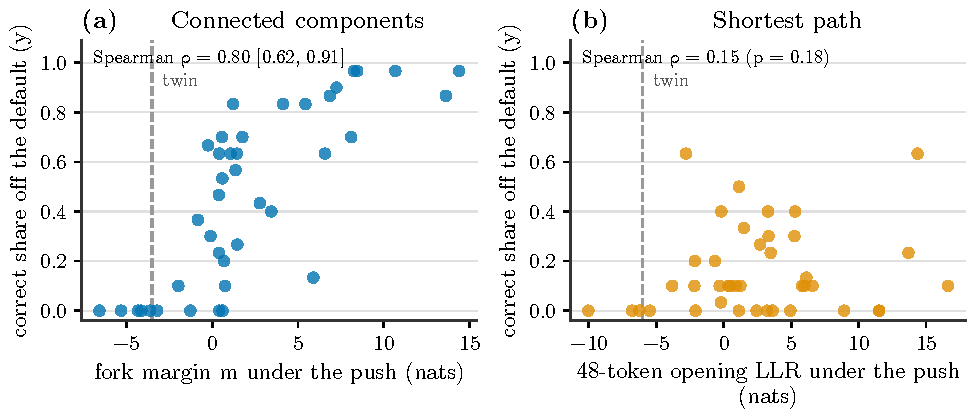
\includegraphics[width=\linewidth,height=0.78\textheight,keepaspectratio]{figures/fig_fork_margin_v0.pdf}
\caption{Each point is one of iteration 4's 40 random push directions ($\alpha$ = 2, added to Qwen3-8B's task-specification activations, bf16); the same 40 directions in both panels. (a) Connected components: x-axis is the teacher-forced fork margin m at generated tokens 10--11 (nats), where the continuation commits to the default algorithm (union-find) or leaves it; y-axis is the correct-only share of generations that land off the default. Blue circles; annotated Spearman 0.80, 95\% CI [0.62, 0.91]. The dashed grey line marks this margin's value under the unpushed neutral-twin prompt (twin, m = $-$3.51 nats). (b) Shortest path, which has no single early fork: x-axis is the pre-declared fallback margin, the 48-token opening log-likelihood ratio under the push (nats); y-axis is the same correct-off-default share. Orange circles; annotated Spearman 0.15 (p = 0.18); dashed grey line at the twin's opening LLR ($-$6.02 nats). The margin tracks which pushes change the algorithm where an early fork exists (a), and is not established where the decision falls later in generation, with no single fork margin defined (b).}
\label{fig:fig_fork_margin}
\end{figure}
\begin{table}[H]
\renewcommand{\thetable}{317}
\centering\tiny\setlength{\tabcolsep}{2.5pt}
\caption{The fork claim on connected components (fork margin) and shortest path (48-token opening LLR). [Source: iteration 7, artifact \nolinkurl{gen_art_experiment_34}.]}\label{tab:t337}
\begin{tabular}{>{\raggedright\arraybackslash\hspace{0pt}}p{0.0679\linewidth}>{\raggedright\arraybackslash\hspace{0pt}}p{0.0764\linewidth}>{\raggedright\arraybackslash\hspace{0pt}}p{0.0678\linewidth}>{\raggedright\arraybackslash\hspace{0pt}}p{0.0857\linewidth}>{\raggedright\arraybackslash\hspace{0pt}}p{0.0363\linewidth}>{\raggedright\arraybackslash\hspace{0pt}}p{0.0586\linewidth}>{\raggedright\arraybackslash\hspace{0pt}}p{0.0557\linewidth}>{\raggedright\arraybackslash\hspace{0pt}}p{0.0764\linewidth}>{\raggedright\arraybackslash\hspace{0pt}}p{0.0709\linewidth}>{\raggedright\arraybackslash\hspace{0pt}}p{0.0738\linewidth}>{\raggedright\arraybackslash\hspace{0pt}}p{0.0709\linewidth}>{\raggedright\arraybackslash\hspace{0pt}}p{0.0678\linewidth}>{\raggedright\arraybackslash\hspace{0pt}}p{0.0531\linewidth}}
\toprule
\textbf{Task} & \textbf{Directions} & \textbf{Spearman (margin, correct share off the default)} & \textbf{Permutation p} & \textbf{95\% CI} & \textbf{Kendall tau} & \textbf{Tie ceiling} & \textbf{Directions with y \textgreater{} 0} & \textbf{AUC for confirmed escapers} & \textbf{Confirmed escapers} & \textbf{Spearman with the attempted share} & \textbf{Spearman with the 48-token opening LLR} & \textbf{Twin margin (nats)} \\
\midrule
connected components & 40 & 0.80 & 1.0e-04 & [0.62, 0.91] & 0.64 & 0.99 & 31 & 0.81 & 26 & 0.82 & 0.87 & -3.51 \\
shortest path & 40 & 0.15 & 0.1787 & [-0.19, 0.46] & 0.10 & 0.97 & 27 & 0.64 & 6 & 0.37 & 0.15 & -6.02 \\
\bottomrule
\end{tabular}
\end{table}

\emph{Note to Table 317.} Pooled Spearman within tasks 0.48 (permutation p 1.0e-04); binomial GLM over 104 cells: intercept -0.74, slope 0.16, held-out MAE 0.25 (10 splits 0.25, 0.27, 0.25, 0.28, 0.24, 0.23, 0.24, 0.24, 0.28, 0.24); MAE without fitted parameters 0.33 (correct) and 0.25 (attempted); Spearman over all cells 0.51.

{\scriptsize\setlength{\tabcolsep}{2.5pt}\renewcommand{\thetable}{318}
\begin{longtable}{>{\raggedright\arraybackslash\hspace{0pt}}p{0.1249\linewidth}>{\raggedright\arraybackslash\hspace{0pt}}p{0.2919\linewidth}>{\raggedright\arraybackslash\hspace{0pt}}p{0.1313\linewidth}>{\raggedright\arraybackslash\hspace{0pt}}p{0.1214\linewidth}>{\raggedright\arraybackslash\hspace{0pt}}p{0.1089\linewidth}>{\raggedright\arraybackslash\hspace{0pt}}p{0.1079\linewidth}>{\raggedright\arraybackslash\hspace{0pt}}p{0.0372\linewidth}}
\caption{Every cell other than the directions scored for the fork claim. [Source: iteration 7, artifact \nolinkurl{gen_art_experiment_34}.]}\label{tab:t338}\\
\toprule
\textbf{Task} & \textbf{Cell} & \textbf{Teacher-forced margin m (nats; 48-token LLR on shortest path)} & \textbf{Implied probability off the default} & \textbf{Correct share off the default (y)} & \textbf{Attempted share off the default} & \textbf{n} \\
\midrule
\endfirsthead
\multicolumn{7}{l}{\emph{Table 318, continued}}\\
\toprule
\textbf{Task} & \textbf{Cell} & \textbf{Teacher-forced margin m (nats; 48-token LLR on shortest path)} & \textbf{Implied probability off the default} & \textbf{Correct share off the default (y)} & \textbf{Attempted share off the default} & \textbf{n} \\
\midrule
\endhead
\bottomrule
\endlastfoot
connected components & ban (fifth template) & 19.37 & 1.000 & 1.00 & 1.00 & 30 \\
connected components & prompt forcing the second choice & 24.38 & 1.000 & 1.00 & 1.00 & 30 \\
connected components & padding twin of the forced prompt & -6.50 & 0.002 & 0.00 & 0.00 & 30 \\
connected components & forced prompt's task specification states exchanged in, blocks 0-35 & 18.75 & 1.000 & 0.87 & 1.00 & 30 \\
connected components & placebo twin & -1.68 & 0.157 & 0.03 & 0.03 & 30 \\
connected components & per-sample plan noise, alpha 1 & -0.78 & 0.315 & 0.14 & 0.14 & 50 \\
connected components & per-sample plan noise, alpha 2 & 0.58 & 0.642 & 0.48 & 0.50 & 50 \\
connected components & neutral twin & -3.51 & 0.029 & 0.01 & 0.01 & 80 \\
connected components & ban states exchanged in, blocks 0-11 & 1.28 & 0.783 & 0.57 & 0.87 & 30 \\
connected components & ban states exchanged in, blocks 0-35 & 13.16 & 1.000 & 1.00 & 1.00 & 30 \\
connected components & ban states exchanged in, blocks 12-23 & 12.89 & 1.000 & 1.00 & 1.00 & 30 \\
connected components & ban states exchanged in, blocks 24-35 & 1.50 & 0.817 & 0.63 & 0.63 & 30 \\
shortest path & ban (fifth template) & 5.37 & 0.995 & 0.97 & 0.97 & 30 \\
shortest path & prompt forcing the second choice & 13.99 & 1.000 & 0.90 & 1.00 & 30 \\
shortest path & padding twin of the forced prompt & -5.68 & 0.003 & 0.00 & 0.03 & 30 \\
shortest path & forced prompt's task specification states exchanged in, blocks 0-35 & -5.57 & 0.004 & 1.00 & 1.00 & 30 \\
shortest path & placebo twin & -5.97 & 0.003 & 0.03 & 0.03 & 30 \\
shortest path & per-sample plan noise, alpha 1 & -1.59 & 0.170 & 0.10 & 0.20 & 50 \\
shortest path & per-sample plan noise, alpha 2 & 2.06 & 0.887 & 0.18 & 0.44 & 50 \\
shortest path & neutral twin & -6.02 & 0.002 & 0.00 & 0.01 & 105 \\
shortest path & ban states exchanged in, blocks 0-11 & -6.00 & 0.002 & 0.00 & 0.00 & 30 \\
shortest path & ban states exchanged in, blocks 0-35 & -5.82 & 0.003 & 0.70 & 0.80 & 30 \\
shortest path & ban states exchanged in, blocks 12-23 & -5.81 & 0.003 & 0.37 & 0.60 & 30 \\
shortest path & ban states exchanged in, blocks 24-35 & -5.91 & 0.003 & 0.37 & 0.37 & 30 \\
\end{longtable}}

{\scriptsize\setlength{\tabcolsep}{2.5pt}\renewcommand{\thetable}{319}
\begin{longtable}{>{\raggedright\arraybackslash\hspace{0pt}}p{0.0955\linewidth}>{\raggedright\arraybackslash\hspace{0pt}}p{0.1366\linewidth}>{\raggedright\arraybackslash\hspace{0pt}}p{0.1269\linewidth}>{\raggedright\arraybackslash\hspace{0pt}}p{0.0961\linewidth}>{\raggedright\arraybackslash\hspace{0pt}}p{0.0437\linewidth}>{\raggedright\arraybackslash\hspace{0pt}}p{0.1373\linewidth}>{\raggedright\arraybackslash\hspace{0pt}}p{0.1269\linewidth}>{\raggedright\arraybackslash\hspace{0pt}}p{0.0961\linewidth}>{\raggedright\arraybackslash\hspace{0pt}}p{0.0437\linewidth}}
\caption{The 40 random directions of iteration 4 at alpha 2: margin and outcome. [Source: iteration 7, artifact \nolinkurl{gen_art_experiment_34}.]}\label{tab:t339}\\
\toprule
\textbf{Direction seed} & \textbf{Connected components: margin m (nats)} & \textbf{correct y off the default} & \textbf{attempted} & \textbf{n} & \textbf{Shortest path: 48-token LLR (nats)} & \textbf{correct y off the default} & \textbf{attempted} & \textbf{n} \\
\midrule
\endfirsthead
\multicolumn{9}{l}{\emph{Table 319, continued}}\\
\toprule
\textbf{Direction seed} & \textbf{Connected components: margin m (nats)} & \textbf{correct y off the default} & \textbf{attempted} & \textbf{n} & \textbf{Shortest path: 48-token LLR (nats)} & \textbf{correct y off the default} & \textbf{attempted} & \textbf{n} \\
\midrule
\endhead
\bottomrule
\endlastfoot
9101 & -3.62 & 0.00 & 0.00 & 10 & 5.98 & 0.10 & 0.40 & 10 \\
9102 & -0.24 & 0.67 & 0.67 & 30 & -5.49 & 0.00 & 0.00 & 10 \\
9103 & 0.38 & 0.47 & 0.47 & 30 & 3.33 & 0.30 & 0.60 & 10 \\
9104 & 7.25 & 0.90 & 0.90 & 30 & -2.80 & 0.63 & 0.87 & 30 \\
9105 & 2.77 & 0.43 & 0.53 & 30 & 3.22 & 0.00 & 0.00 & 10 \\
9106 & 0.60 & 0.00 & 0.00 & 10 & 2.70 & 0.27 & 0.40 & 30 \\
9107 & -0.10 & 0.30 & 0.30 & 30 & 1.49 & 0.33 & 0.40 & 30 \\
9108 & 1.36 & 0.57 & 0.57 & 30 & 5.29 & 0.40 & 0.80 & 10 \\
9109 & 1.76 & 0.70 & 0.70 & 30 & 3.62 & 0.00 & 0.60 & 10 \\
9110 & 1.07 & 0.63 & 0.63 & 30 & 14.37 & 0.63 & 0.90 & 30 \\
9111 & 13.62 & 0.87 & 1.00 & 30 & 16.62 & 0.10 & 0.20 & 10 \\
9112 & 0.68 & 0.20 & 0.70 & 10 & 11.52 & 0.00 & 0.70 & 10 \\
9113 & -1.98 & 0.10 & 0.10 & 10 & 6.13 & 0.13 & 0.27 & 30 \\
9114 & 6.57 & 0.63 & 0.73 & 30 & 1.24 & 0.10 & 0.40 & 10 \\
9115 & -4.13 & 0.00 & 0.00 & 10 & 5.81 & 0.10 & 0.10 & 10 \\
9116 & 14.39 & 0.97 & 1.00 & 30 & -6.79 & 0.00 & 0.00 & 10 \\
9117 & 1.22 & 0.83 & 0.83 & 30 & 8.93 & 0.00 & 0.20 & 10 \\
9118 & 0.56 & 0.70 & 0.70 & 30 & -0.21 & 0.03 & 0.10 & 30 \\
9119 & 0.39 & 0.23 & 0.30 & 30 & 0.36 & 0.10 & 0.50 & 10 \\
9120 & 3.45 & 0.40 & 0.40 & 30 & -0.65 & 0.20 & 0.60 & 10 \\
9121 & -1.27 & 0.00 & 0.00 & 10 & -6.25 & 0.00 & 0.00 & 10 \\
9122 & 8.46 & 0.97 & 1.00 & 30 & 6.58 & 0.10 & 0.60 & 10 \\
9123 & 5.90 & 0.13 & 0.13 & 30 & 1.13 & 0.50 & 0.80 & 10 \\
9124 & -5.31 & 0.00 & 0.00 & 10 & -2.14 & 0.20 & 0.60 & 10 \\
9125 & 4.13 & 0.83 & 0.83 & 30 & 3.48 & 0.23 & 0.23 & 30 \\
9126 & 1.44 & 0.63 & 0.63 & 30 & 0.90 & 0.10 & 0.20 & 10 \\
9127 & 5.43 & 0.83 & 1.00 & 30 & 4.94 & 0.00 & 0.00 & 10 \\
9128 & 6.85 & 0.87 & 1.00 & 30 & 3.28 & 0.40 & 0.90 & 10 \\
9129 & 0.41 & 0.00 & 0.00 & 10 & 2.43 & 0.00 & 0.50 & 10 \\
9130 & 0.41 & 0.63 & 0.63 & 30 & -0.18 & 0.40 & 0.50 & 30 \\
9131 & -3.22 & 0.00 & 0.00 & 10 & -0.30 & 0.10 & 0.30 & 10 \\
9132 & -0.84 & 0.37 & 0.37 & 30 & -2.09 & 0.00 & 0.00 & 10 \\
9133 & 8.10 & 0.70 & 1.00 & 10 & 0.49 & 0.10 & 0.20 & 10 \\
9134 & 0.75 & 0.10 & 0.10 & 10 & 13.69 & 0.23 & 0.27 & 30 \\
9135 & 8.26 & 0.97 & 0.97 & 30 & 1.12 & 0.00 & 0.20 & 10 \\
9136 & 10.67 & 0.97 & 1.00 & 30 & 11.53 & 0.00 & 0.90 & 10 \\
9137 & -4.33 & 0.00 & 0.00 & 10 & -3.81 & 0.10 & 0.10 & 10 \\
9138 & -6.57 & 0.00 & 0.00 & 10 & 5.24 & 0.30 & 0.70 & 10 \\
9139 & 1.47 & 0.27 & 0.27 & 30 & -2.18 & 0.10 & 0.40 & 10 \\
9140 & 0.59 & 0.53 & 0.53 & 30 & -10.03 & 0.00 & 0.00 & 10 \\
\end{longtable}}

{\footnotesize\setlength{\tabcolsep}{4.0pt}\renewcommand{\thetable}{320}
\begin{longtable}{>{\raggedright\arraybackslash\hspace{0pt}}p{0.1844\linewidth}>{\raggedright\arraybackslash\hspace{0pt}}p{0.1671\linewidth}>{\raggedright\arraybackslash\hspace{0pt}}p{0.2337\linewidth}>{\raggedright\arraybackslash\hspace{0pt}}p{0.2148\linewidth}>{\raggedright\arraybackslash\hspace{0pt}}p{0.1133\linewidth}}
\caption{Kth smallest: the prospective confirmation on 24 fresh directions. [Source: iteration 7, artifact \nolinkurl{gen_art_experiment_34}.]}\label{tab:t340}\\
\toprule
\textbf{Fresh direction seed} & \textbf{Axis projection b} & \textbf{Opening margin m (20-token LLR, nats)} & \textbf{Correct y off the default (of 10)} & \textbf{Attempted} \\
\midrule
\endfirsthead
\multicolumn{5}{l}{\emph{Table 320, continued}}\\
\toprule
\textbf{Fresh direction seed} & \textbf{Axis projection b} & \textbf{Opening margin m (20-token LLR, nats)} & \textbf{Correct y off the default (of 10)} & \textbf{Attempted} \\
\midrule
\endhead
\bottomrule
\endlastfoot
97001 & 0.288 & -0.48 & 0.00 & 0.00 \\
97002 & 0.161 & -5.60 & 0.00 & 0.00 \\
97003 & 0.228 & 3.88 & 1.00 & 1.00 \\
97004 & -0.093 & -1.60 & 0.50 & 0.50 \\
97005 & 0.378 & -6.94 & 0.30 & 0.30 \\
97006 & 0.051 & -2.55 & 0.00 & 0.00 \\
97007 & -0.142 & -6.27 & 0.20 & 0.20 \\
97008 & 0.378 & -3.15 & 0.20 & 0.30 \\
97009 & 0.544 & 1.25 & 1.00 & 1.00 \\
97010 & 0.073 & -2.89 & 0.30 & 0.30 \\
97011 & 0.533 & 4.51 & 1.00 & 1.00 \\
97012 & -0.087 & 4.38 & 1.00 & 1.00 \\
97013 & -0.015 & -4.14 & 0.50 & 0.50 \\
97014 & -0.150 & -1.43 & 0.50 & 0.50 \\
97015 & -0.020 & 1.39 & 0.50 & 0.50 \\
97016 & 0.004 & -2.99 & 0.00 & 0.00 \\
97017 & -0.028 & -6.12 & 0.00 & 0.00 \\
97018 & -0.038 & -4.88 & 0.00 & 0.00 \\
97019 & 0.393 & 0.12 & 0.90 & 1.00 \\
97020 & 0.847 & 0.80 & 0.20 & 0.20 \\
97021 & 0.210 & -3.42 & 0.40 & 0.40 \\
97022 & 0.061 & -2.78 & 0.10 & 0.10 \\
97023 & 0.120 & -7.75 & 0.50 & 0.50 \\
97024 & 0.325 & 0.93 & 0.60 & 0.60 \\
\end{longtable}}

\emph{Note to Table 320.} Directions 24, with y \textgreater{} 0 on 18; Spearman of m with y 0.60 (one sided p 0.0014), of b with y 0.22 (p 0.150); with the attempted share m 0.59, b 0.23; tie ceiling 0.98.

\subsubsection*{7.4.4 The axis claim}
The axis claim proposed that random pushes act through a direction from the default centroid toward the centroid of the second choice in the prompt states. It is disconfirmed. The projection b of each push on the axis predicts the outcome at Spearman 0.17 on connected components and 0.01 on shortest path (Holm p 0.458), and it is ahead of none of its committed competitors, which include the push's energy in the forced prompt subspace of iteration 4 and its raw norm (Table 321). The layer profile shows no block where it would do better (Table 322). The axis is not dormant: neutral prompts vary along it 220 to 400 times more than along random directions. It is simply not the channel the random pushes use.

\begin{table}[H]
\renewcommand{\thetable}{321}
\centering\tiny\setlength{\tabcolsep}{2.5pt}
\caption{The axis claim and its competitors. [Source: iteration 7, artifact \nolinkurl{gen_art_experiment_34}.]}\label{tab:t341}
\begin{tabular}{>{\raggedright\arraybackslash\hspace{0pt}}p{0.0659\linewidth}>{\raggedright\arraybackslash\hspace{0pt}}p{0.0713\linewidth}>{\raggedright\arraybackslash\hspace{0pt}}p{0.0831\linewidth}>{\raggedright\arraybackslash\hspace{0pt}}p{0.0352\linewidth}>{\raggedright\arraybackslash\hspace{0pt}}p{0.0568\linewidth}>{\raggedright\arraybackslash\hspace{0pt}}p{0.0658\linewidth}>{\raggedright\arraybackslash\hspace{0pt}}p{0.0598\linewidth}>{\raggedright\arraybackslash\hspace{0pt}}p{0.0861\linewidth}>{\raggedright\arraybackslash\hspace{0pt}}p{0.0656\linewidth}>{\raggedright\arraybackslash\hspace{0pt}}p{0.0598\linewidth}>{\raggedright\arraybackslash\hspace{0pt}}p{0.0688\linewidth}>{\raggedright\arraybackslash\hspace{0pt}}p{0.0688\linewidth}>{\raggedright\arraybackslash\hspace{0pt}}p{0.0745\linewidth}}
\toprule
\textbf{Task} & \textbf{Spearman of the axis projection b with y} & \textbf{Permutation p} & \textbf{95\% CI} & \textbf{Kendall tau} & \textbf{Spearman of b with the fork margin} & \textbf{Forced prompt subspace energy} & \textbf{Raw displacement norm} & \textbf{Energy share of the iteration-4 subspace} & \textbf{b minus forced-subspace energy [95\%]} & \textbf{b with the attempted share} & \textbf{AUC for confirmed escapers} & \textbf{Ahead of every competitor} \\
\midrule
connected components & 0.17 & 0.141 & [-0.19, 0.51] & 0.13 & 0.12 & 0.06 & 0.03 & 0.14 & 0.11 [-0.39, 0.62] & 0.20 & 0.65 & no \\
shortest path & 0.01 & 0.458 & [-0.30, 0.34] & 0.01 & -0.17 & 0.12 & -0.05 & -0.03 & -0.11 [-0.28, 0.06] & 0.06 & 0.70 & no \\
\bottomrule
\end{tabular}
\end{table}

{\small\setlength{\tabcolsep}{4.0pt}\renewcommand{\thetable}{322}
\begin{longtable}{>{\raggedright\arraybackslash\hspace{0pt}}p{0.1474\linewidth}>{\raggedright\arraybackslash\hspace{0pt}}p{0.5063\linewidth}>{\raggedright\arraybackslash\hspace{0pt}}p{0.2926\linewidth}}
\caption{The axis projection's Spearman with the outcome, block by block. [Source: iteration 7, artifact \nolinkurl{gen_art_experiment_34}.]}\label{tab:t342}\\
\toprule
\textbf{Block} & \textbf{Connected components: Spearman of b with y} & \textbf{Shortest path} \\
\midrule
\endfirsthead
\multicolumn{3}{l}{\emph{Table 322, continued}}\\
\toprule
\textbf{Block} & \textbf{Connected components: Spearman of b with y} & \textbf{Shortest path} \\
\midrule
\endhead
\bottomrule
\endlastfoot
12 & 0.17 & 0.01 \\
13 & 0.30 & -0.05 \\
14 & 0.41 & -0.13 \\
15 & 0.38 & -0.13 \\
16 & 0.29 & 0.05 \\
17 & 0.25 & 0.06 \\
18 & 0.12 & 0.12 \\
19 & 0.23 & 0.10 \\
20 & 0.11 & 0.09 \\
21 & 0.08 & 0.10 \\
22 & 0.10 & 0.05 \\
23 & -0.03 & 0.06 \\
24 & -0.17 & 0.01 \\
25 & -0.18 & -0.03 \\
26 & -0.18 & -0.08 \\
27 & -0.15 & -0.18 \\
28 & -0.17 & -0.17 \\
29 & -0.11 & -0.14 \\
30 & -0.13 & -0.15 \\
31 & -0.12 & -0.17 \\
32 & -0.07 & -0.18 \\
33 & -0.07 & -0.18 \\
34 & -0.08 & -0.14 \\
35 & -0.04 & -0.14 \\
\end{longtable}}

\subsubsection*{7.4.5 Necessity and sufficiency of the axis}
Clamping the axis component of each escaping push at blocks from the axis layer to 35 removes nothing: 105 escapes with the clamp against 104 without it and 106 with a clamp along a random direction (Table 323). Pushing along the axis itself is a different matter (Table 324). Doses s are counted in units of the distance between the centroids of the prompts forcing the default and the second choice along the axis. At the committed doses (s up to 1) nothing escapes on any task. At four times that distance, beyond the committed range, connected components switches to DFS in 29 of 30 slots and BFS in the 30th, with all 30 programs passing, while the matched random direction moves none (30:0, p 1.9e-9). The axis edit at that dose has 0.55 of the norm of the median escaping random direction. On shortest path the axis does nothing even at eight times the distance (1 of 30), and on kth smallest the axis at eight times the distance moves 5 of 30, exactly as many as the random direction. On connected components the axis is a sufficient control direction without being the path random pushes take.

\begin{table}[H]
\renewcommand{\thetable}{323}
\centering\footnotesize\setlength{\tabcolsep}{4.0pt}
\caption{The mediator clamp, per direction. [Source: iteration 7, artifact \nolinkurl{gen_art_experiment_34}.]}\label{tab:t343}
\begin{tabular}{>{\raggedright\arraybackslash\hspace{0pt}}p{0.1972\linewidth}>{\raggedright\arraybackslash\hspace{0pt}}p{0.1176\linewidth}>{\raggedright\arraybackslash\hspace{0pt}}p{0.1572\linewidth}>{\raggedright\arraybackslash\hspace{0pt}}p{0.1790\linewidth}>{\raggedright\arraybackslash\hspace{0pt}}p{0.1897\linewidth}>{\raggedright\arraybackslash\hspace{0pt}}p{0.0561\linewidth}}
\toprule
\textbf{Task} & \textbf{Direction seed} & \textbf{Push without clamp: y} & \textbf{Axis component clamped: y} & \textbf{Random direction clamped: y} & \textbf{n} \\
\midrule
connected components & 9116 & 0.90 & 1.00 & 0.95 & 20 \\
connected components & 9122 & 0.95 & 0.95 & 0.95 & 20 \\
connected components & 9135 & 1.00 & 0.85 & 1.00 & 20 \\
connected components & 9136 & 1.00 & 0.90 & 1.00 & 20 \\
shortest path & 9130 & 0.35 & 0.40 & 0.45 & 20 \\
shortest path & 9107 & 0.20 & 0.25 & 0.20 & 20 \\
shortest path & 9106 & 0.40 & 0.55 & 0.35 & 20 \\
shortest path & 9125 & 0.40 & 0.35 & 0.40 & 20 \\
\bottomrule
\end{tabular}
\end{table}

\emph{Note to Table 323.} Pooled escapes: no clamp 104, axis clamp 105, random clamp 106; removed share -0.010 (axis) and -0.019 (random); McNemar axis clamp 9:10 (p 1.00), random clamp 2:4 (p 0.69); verdict NOT SUPPORTED.

{\tiny\setlength{\tabcolsep}{2.5pt}\renewcommand{\thetable}{324}
\begin{longtable}{>{\raggedright\arraybackslash\hspace{0pt}}p{0.0801\linewidth}>{\raggedright\arraybackslash\hspace{0pt}}p{0.0660\linewidth}>{\raggedright\arraybackslash\hspace{0pt}}p{0.0762\linewidth}>{\raggedright\arraybackslash\hspace{0pt}}p{0.0722\linewidth}>{\raggedright\arraybackslash\hspace{0pt}}p{0.0451\linewidth}>{\raggedright\arraybackslash\hspace{0pt}}p{0.1140\linewidth}>{\raggedright\arraybackslash\hspace{0pt}}p{0.0751\linewidth}>{\raggedright\arraybackslash\hspace{0pt}}p{0.0603\linewidth}>{\raggedright\arraybackslash\hspace{0pt}}p{0.1110\linewidth}>{\raggedright\arraybackslash\hspace{0pt}}p{0.1045\linewidth}>{\raggedright\arraybackslash\hspace{0pt}}p{0.0776\linewidth}}
\caption{A targeted push along the axis against a matched random direction, by dose. [Source: iteration 7, artifact \nolinkurl{gen_art_experiment_34}.]}\label{tab:t344}\\
\toprule
\textbf{Task} & \textbf{Dose s (forced prompt distance)} & \textbf{Axis: correct share of the second choice} & \textbf{Axis: correct off the default} & \textbf{Axis: pass} & \textbf{Axis: labels} & \textbf{Matched random: correct second choice} & \textbf{Random: pass} & \textbf{Random: labels} & \textbf{Axis only : random only (exact p)} & \textbf{Edit norm over the median escaping direction} \\
\midrule
\endfirsthead
\multicolumn{11}{l}{\emph{Table 324, continued}}\\
\toprule
\textbf{Task} & \textbf{Dose s (forced prompt distance)} & \textbf{Axis: correct share of the second choice} & \textbf{Axis: correct off the default} & \textbf{Axis: pass} & \textbf{Axis: labels} & \textbf{Matched random: correct second choice} & \textbf{Random: pass} & \textbf{Random: labels} & \textbf{Axis only : random only (exact p)} & \textbf{Edit norm over the median escaping direction} \\
\midrule
\endhead
\bottomrule
\endlastfoot
connected components & 0.1 & 0.00 & 0.00 & 1.00 & union find 30 & 0.00 & 1.00 & union find 30 & 0:0 (p 1.000) & 0.01 \\
connected components & 0.25 & 0.00 & 0.00 & 1.00 & union find 30 & 0.00 & 1.00 & union find 30 & 0:0 (p 1.000) & 0.03 \\
connected components & 0.5 & 0.00 & 0.00 & 1.00 & union find 30 & 0.00 & 1.00 & union find 30 & 0:0 (p 1.000) & 0.07 \\
connected components & 1 & 0.03 & 0.03 & 1.00 & union find 29, DFS 1 & 0.00 & 1.00 & union find 30 & 1:0 (p 1.000) & 0.14 \\
connected components & 2 & 0.17 & 0.17 & 1.00 & union find 25, DFS 5 & 0.00 & 1.00 & union find 30 & 5:0 (p 0.062) & 0.28 \\
connected components & 4 & 0.97 & 1.00 & 1.00 & DFS 29, BFS 1 & 0.00 & 1.00 & union find 30 & 30:0 (p 1.9e-09) & 0.55 \\
connected components & 8 & 0.90 & 1.00 & 1.00 & DFS 27, BFS 3 & 0.00 & 1.00 & union find 30 & 30:0 (p 1.9e-09) & 1.11 \\
shortest path & 0.1 & 0.00 & 0.00 & 1.00 & Dijkstra 30 & 0.00 & 1.00 & Dijkstra 30 & 0:0 (p 1.000) & 0.02 \\
shortest path & 0.25 & 0.00 & 0.00 & 1.00 & Dijkstra 30 & 0.00 & 1.00 & Dijkstra 30 & 0:0 (p 1.000) & 0.04 \\
shortest path & 0.5 & 0.00 & 0.00 & 1.00 & Dijkstra 30 & 0.00 & 0.97 & Dijkstra 29, Bellman-Ford\slash{}SPFA 1 & 0:0 (p 1.000) & 0.09 \\
shortest path & 1 & 0.00 & 0.00 & 0.97 & Dijkstra 29, Bellman-Ford\slash{}SPFA 1 & 0.00 & 0.97 & Dijkstra 29, Bellman-Ford\slash{}SPFA 1 & 0:0 (p 1.000) & 0.18 \\
shortest path & 2 & 0.00 & 0.00 & 1.00 & Dijkstra 30 & 0.00 & 0.97 & Dijkstra 29, Bellman-Ford\slash{}SPFA 1 & 0:0 (p 1.000) & 0.36 \\
shortest path & 4 & 0.00 & 0.00 & 0.97 & Dijkstra 29, Bellman-Ford\slash{}SPFA 1 & 0.00 & 1.00 & Dijkstra 30 & 0:0 (p 1.000) & 0.71 \\
shortest path & 8 & 0.03 & 0.03 & 0.97 & Dijkstra 28, Bellman-Ford\slash{}SPFA 2 & 0.00 & 0.97 & Dijkstra 29, Bellman-Ford\slash{}SPFA 1 & 1:0 (p 1.000) & 1.42 \\
kth smallest & 0.1 & 0.03 & 0.03 & 1.00 & full sort 29, quickselect 1 & 0.03 & 1.00 & full sort 29, quickselect 1 & 0:0 (p 1.000) & 0.01 \\
kth smallest & 0.25 & 0.03 & 0.03 & 1.00 & full sort 29, quickselect 1 & 0.00 & 1.00 & full sort 30 & 1:0 (p 1.000) & 0.03 \\
kth smallest & 0.5 & 0.03 & 0.03 & 1.00 & full sort 29, quickselect 1 & 0.00 & 1.00 & full sort 30 & 1:0 (p 1.000) & 0.06 \\
kth smallest & 1 & 0.03 & 0.03 & 1.00 & full sort 29, quickselect 1 & 0.03 & 1.00 & full sort 29, quickselect 1 & 0:0 (p 1.000) & 0.13 \\
kth smallest & 2 & 0.07 & 0.07 & 1.00 & full sort 28, quickselect 2 & 0.00 & 1.00 & full sort 30 & 2:0 (p 0.500) & 0.25 \\
kth smallest & 4 & 0.10 & 0.10 & 1.00 & full sort 27, quickselect 3 & 0.03 & 1.00 & full sort 29, quickselect 1 & 2:0 (p 0.500) & 0.50 \\
kth smallest & 8 & 0.17 & 0.17 & 1.00 & full sort 25, quickselect 5 & 0.17 & 1.00 & full sort 25, quickselect 5 & 2:2 (p 1.000) & 1.01 \\
\end{longtable}}

\emph{Note to Table 324.} Reference norms. Connected components: axis at block 12, median RMS of escaping random directions 21.26, axis distance RMS 2.94; shortest path: axis at block 24, median RMS of escaping random directions 213.41, axis distance RMS 37.94; kth smallest: axis at block 22, median RMS of escaping random directions 77.14, axis distance RMS 9.74.

\subsubsection*{7.4.6 Forcing the fork token}
Forcing tokens under the unchanged neutral twin separates the routine's name from the fork position (Table 326). On connected components, forcing \texttt{ def dfs} at tokens 10 and 11 gives DFS in 30 of 30 slots, and \texttt{ def find} gives union find in 30. Forcing a comment token at position 10, which led off the default in every resampled continuation in which it appeared, gives union find in all 30 twin slots; forcing \texttt{ from} moves 10 of 30. The token that names the routine decides; a token that only correlates with pushed states in resampling does not decide on its own. On kth smallest a forced comment as the first body token moves 5 of 30 (p 0.0625), and on shortest path no forced token moves anything.

\begin{table}[H]
\renewcommand{\thetable}{325}
\centering\small\setlength{\tabcolsep}{4.0pt}
\caption{Shortest path: Spearman of the opening LLR with the outcome, by opening length. [Source: iteration 7, artifact \nolinkurl{gen_art_experiment_34}.]}\label{tab:t345}
\begin{tabular}{>{\raggedright\arraybackslash\hspace{0pt}}p{0.2058\linewidth}>{\raggedright\arraybackslash\hspace{0pt}}p{0.3753\linewidth}>{\raggedright\arraybackslash\hspace{0pt}}p{0.1478\linewidth}>{\raggedright\arraybackslash\hspace{0pt}}p{0.2009\linewidth}}
\toprule
\textbf{Opening length L (tokens)} & \textbf{Spearman of the opening LLR over L tokens with y over 40 directions} & \textbf{Permutation p} & \textbf{Spearman over all cells} \\
\midrule
16 & 0.27 & 0.0462 & 0.30 \\
32 & 0.16 & 0.1662 & 0.22 \\
48 & 0.15 & 0.1758 & 0.22 \\
96 & 0.25 & 0.0650 & 0.36 \\
128 & 0.28 & 0.0434 & 0.37 \\
160 & 0.42 & 0.0032 & 0.53 \\
\bottomrule
\end{tabular}
\end{table}

\begin{table}[H]
\renewcommand{\thetable}{326}
\centering\scriptsize\setlength{\tabcolsep}{2.5pt}
\caption{Forced opening tokens under the unchanged twin. [Source: iteration 7, artifact \nolinkurl{gen_art_experiment_34}.]}\label{tab:t346}
\begin{tabular}{>{\raggedright\arraybackslash\hspace{0pt}}p{0.1136\linewidth}>{\raggedright\arraybackslash\hspace{0pt}}p{0.2296\linewidth}>{\raggedright\arraybackslash\hspace{0pt}}p{0.0318\linewidth}>{\raggedright\arraybackslash\hspace{0pt}}p{0.1821\linewidth}>{\raggedright\arraybackslash\hspace{0pt}}p{0.0539\linewidth}>{\raggedright\arraybackslash\hspace{0pt}}p{0.1117\linewidth}>{\raggedright\arraybackslash\hspace{0pt}}p{0.2009\linewidth}}
\toprule
\textbf{Task} & \textbf{Forced token under the unchanged neutral twin} & \textbf{n} & \textbf{Labels} & \textbf{Pass} & \textbf{Correct share off the default} & \textbf{Flips against the twin, to off : to default (exact p)} \\
\midrule
kth smallest & first body token forced to \texttt{ \#} (comment) & 30 & full sort 25, quickselect 4, heapify and pop 1 & 1.00 & 0.17 & 5:0 (p 0.062) \\
kth smallest & first body token forced to the twin's own token & 30 & full sort 29, quickselect 1 & 1.00 & 0.03 & 1:0 (p 1.000) \\
connected components & token 10 forced to \texttt{ \#} (comment) & 30 & union find 30 & 1.00 & 0.00 & 0:0 (p 1.000) \\
connected components & token 10 forced to \texttt{ def} & 30 & union find 30 & 1.00 & 0.00 & 0:0 (p 1.000) \\
connected components & token 10 forced to \texttt{ from} & 30 & union find 20, DFS 10 & 1.00 & 0.33 & 10:0 (p 0.002) \\
connected components & token 10 forced to \texttt{ parent} & 30 & union find 30 & 1.00 & 0.00 & 0:0 (p 1.000) \\
connected components & tokens 10-11 forced to \texttt{ def dfs} & 30 & DFS 30 & 1.00 & 1.00 & 30:0 (p 1.9e-09) \\
connected components & tokens 10-11 forced to \texttt{ def find} & 30 & union find 30 & 1.00 & 0.00 & 0:0 (p 1.000) \\
shortest path & first body token forced to \texttt{ \#} (comment) & 30 & Dijkstra 30 & 1.00 & 0.00 & 0:0 (p 1.000) \\
shortest path & first body token forced to the twin's own token & 30 & Dijkstra 30 & 1.00 & 0.00 & 0:0 (p 1.000) \\
\bottomrule
\end{tabular}
\end{table}

\subsubsection*{7.4.7 The top five prohibition inside the manifold}
The review asked for the top five push at a dose that stays on the forced prompt manifold of the grid task. The fork experiment pushed the twin's states toward the centroid of the survivor region, toward a random survivor, away from the banned centroid and toward IDA*, at a quarter, a half and one times the distance between centroids (Table 327). All 300 programs implement BFS, at pass rates between 0.73 and 0.93; none implements an algorithm outside the banned five. The prompt top five ban of iteration 6 had at least moved the model between BFS and DFS (25 and 23 of 50). On the manifold at block 18, three survivors (bidirectional BFS, Dijkstra with unit weights and IDA*) sit at its edge, and the nearest centroids to the banned region are greedy best first, BFS and A* (Table 328; Isomap stress 0.24, metric MDS stress 0.38). Moving the states toward where those survivors' forced prompts sit does not make the model write them. The engine reproduced the engine control's outcomes per direction (Spearman 0.95 on connected components and 0.93 on shortest path; Table 329), and the two programs sent to novelty audit were labeller misses. One GPU unit test missed its tolerance: teacher-forced log probabilities and those from a cached prefill differ by up to 0.25 on the top 50 tokens, with the same argmax, so every margin was computed on the teacher-forced path.

\begin{table}[H]
\renewcommand{\thetable}{327}
\centering\footnotesize\setlength{\tabcolsep}{4.0pt}
\caption{The grid task: pushes inside the forced prompt manifold toward the survivors of the top five ban (30 slots each). [Source: iteration 7, artifact \nolinkurl{gen_art_experiment_34}.]}\label{tab:t347}
\begin{tabular}{>{\raggedright\arraybackslash\hspace{0pt}}p{0.3204\linewidth}>{\raggedright\arraybackslash\hspace{0pt}}p{0.0438\linewidth}>{\raggedright\arraybackslash\hspace{0pt}}p{0.0604\linewidth}>{\raggedright\arraybackslash\hspace{0pt}}p{0.2382\linewidth}>{\raggedright\arraybackslash\hspace{0pt}}p{0.1157\linewidth}>{\raggedright\arraybackslash\hspace{0pt}}p{0.1181\linewidth}}
\toprule
\textbf{Arm (grid task)} & \textbf{n} & \textbf{Pass} & \textbf{Labels (catalogue of ten algorithms)} & \textbf{Correct programs outside the top five} & \textbf{Attempted programs outside the top five} \\
\midrule
neutral twin & 30 & 0.87 & BFS 29, DFS 1 & 0 & 0 \\
away from the banned centroid, s 0.25 & 30 & 0.90 & BFS 30 & 0 & 0 \\
away from the banned centroid, s 0.5 & 30 & 0.93 & BFS 30 & 0 & 0 \\
away from the banned centroid, s 1 & 30 & 0.90 & BFS 30 & 0 & 0 \\
toward IDA*, s 0.5 & 30 & 0.87 & BFS 30 & 0 & 0 \\
toward a random survivor, s 0.25 & 30 & 0.90 & BFS 30 & 0 & 0 \\
toward a random survivor, s 0.5 & 30 & 0.83 & BFS 30 & 0 & 0 \\
toward a random survivor, s 1 & 30 & 0.73 & BFS 30 & 0 & 0 \\
toward the centroid of the survivor region, s 0.25 & 30 & 0.83 & BFS 30 & 0 & 0 \\
toward the centroid of the survivor region, s 0.5 & 30 & 0.90 & BFS 30 & 0 & 0 \\
toward the centroid of the survivor region, s 1 & 30 & 0.90 & BFS 30 & 0 & 0 \\
prompt top five ban (iteration 6, N = 50) & 50 & 0.62 & BFS 25, DFS 23, unknown 1, unit weight Dijkstra 1 & 0 & 1 \\
\bottomrule
\end{tabular}
\end{table}

\begin{table}[H]
\renewcommand{\thetable}{328}
\centering\scriptsize\setlength{\tabcolsep}{2.5pt}
\caption{The grid task: geometry of the forced prompt manifold at blocks 18 and 22. [Source: iteration 7, artifact \nolinkurl{gen_art_experiment_34}.]}\label{tab:t348}
\begin{tabular}{>{\raggedright\arraybackslash\hspace{0pt}}p{0.0622\linewidth}>{\raggedright\arraybackslash\hspace{0pt}}p{0.0705\linewidth}>{\raggedright\arraybackslash\hspace{0pt}}p{0.0752\linewidth}>{\raggedright\arraybackslash\hspace{0pt}}p{0.0665\linewidth}>{\raggedright\arraybackslash\hspace{0pt}}p{0.1105\linewidth}>{\raggedright\arraybackslash\hspace{0pt}}p{0.1698\linewidth}>{\raggedright\arraybackslash\hspace{0pt}}p{0.1096\linewidth}>{\raggedright\arraybackslash\hspace{0pt}}p{0.2489\linewidth}}
\toprule
\textbf{Block} & \textbf{Points} & \textbf{Isomap (k 15) stress-1} & \textbf{MDS stress-1} & \textbf{PCA variance (first and second components)} & \textbf{Geodesic distance from the banned region, per survivor} & \textbf{Edge survivors} & \textbf{Distance from the centroid of the banned region, every centroid} \\
\midrule
18 & 100 & 0.24 & 0.38 & 0.30, 0.19 & bidirectional BFS 4.61, unit weight Dijkstra 4.51, IDA* 4.13, jump point search 6.44, bidirectional A* 4.74 & bidirectional BFS, unit weight Dijkstra, IDA* & greedy best first 1.84, BFS 1.93, A* 2.22, DFS 2.43, IDA* 2.89, unit weight Dijkstra 3.04, IDDFS 3.18, bidirectional BFS 3.43, bidirectional A* 3.63, jump point search 4.59 \\
22 & 100 & 0.26 & 0.40 & 0.31, 0.16 & bidirectional BFS 6.54, unit weight Dijkstra 6.54, IDA* 6.58, jump point search 9.78, bidirectional A* 7.63 & bidirectional BFS, unit weight Dijkstra, IDA* & greedy best first 2.65, BFS 2.82, A* 3.07, DFS 3.27, IDDFS 4.26, IDA* 4.55, unit weight Dijkstra 4.67, bidirectional BFS 4.82, bidirectional A* 5.33, jump point search 6.60 \\
\bottomrule
\end{tabular}
\end{table}

\begin{table}[H]
\renewcommand{\thetable}{329}
\centering\scriptsize\setlength{\tabcolsep}{2.5pt}
\caption{The fork and axis statistics remeasured on this engine's own outcomes. [Source: iteration 7, artifact \nolinkurl{gen_art_experiment_34}.]}\label{tab:t349}
\begin{tabular}{>{\raggedright\arraybackslash\hspace{0pt}}p{0.0919\linewidth}>{\raggedright\arraybackslash\hspace{0pt}}p{0.1038\linewidth}>{\raggedright\arraybackslash\hspace{0pt}}p{0.1839\linewidth}>{\raggedright\arraybackslash\hspace{0pt}}p{0.0569\linewidth}>{\raggedright\arraybackslash\hspace{0pt}}p{0.1114\linewidth}>{\raggedright\arraybackslash\hspace{0pt}}p{0.0497\linewidth}>{\raggedright\arraybackslash\hspace{0pt}}p{0.1655\linewidth}>{\raggedright\arraybackslash\hspace{0pt}}p{0.0539\linewidth}>{\raggedright\arraybackslash\hspace{0pt}}p{0.0859\linewidth}}
\toprule
\textbf{Task} & \textbf{Directions} & \textbf{Spearman of the fork margin on the outcomes of this engine} & \textbf{p} & \textbf{Spearman of the axis projection} & \textbf{p} & \textbf{Spearman of y with the bf16 y of the engine control} & \textbf{Mean y here} & \textbf{Mean y, engine control} \\
\midrule
connected components & 40 & 0.77 & 1.0e-04 & 0.25 & 0.062 & 0.95 & 0.492 & 0.460 \\
shortest path & 40 & 0.12 & 0.2181 & -0.04 & 0.603 & 0.93 & 0.185 & 0.158 \\
\bottomrule
\end{tabular}
\end{table}

\FloatBarrier
\subsection*{7.5 Temperature acts through the fork (Qwen3-8B)}
\addcontentsline{toc}{subsection}{7.5 Temperature acts through the fork (Qwen3-8B)}
\noindent{\small\emph{Artifact: \nolinkurl{gen_art_experiment_35}.}}\par\medskip
\subsubsection*{7.5.1 Design}
The temperature experiment  tested the temperature claim where it can be tested: on the three units where the instruct twin already writes two algorithms. Minimum spanning tree weight mixes Kruskal and Prim, trapped rain water mixes prefix and suffix maxima with two pointers, and valid anagram mixes sorting with counting. Iteration 5 had recorded minority shares of 0.34, 0.36 and 0.24; this experiment's twins give 0.19, 0.31 and 0.13 on prompts identical byte for byte (Table 330). The claim has three committed tests. Test 1: the entropy of the algorithm given the class of the token at the fork is at most 0.3 bits on at least two units. Test 2: predictions made from the teacher-forced fork logits divided by T, committed before any temperature sample, match the observed minority share (drop from T 1.0 to 0.3 of at least 0.15, mean absolute error at most 0.10, and the change from 1.0 to 1.3 within 0.10 of prediction) on at least two units. Test 3: on the four collapsed tasks the fork margin is at least 4 nats, large enough that no temperature in range reaches the alternative. Every temperature cell shares its random numbers across temperatures (same seed), at temperatures 0.3, 0.7, 1.0 and 1.3, under top-p 1 and top-k 10.

\begin{table}[H]
\renewcommand{\thetable}{330}
\centering\footnotesize\setlength{\tabcolsep}{4.0pt}
\caption{The twins of the three mixed units. [Source: iteration 7, artifact \nolinkurl{gen_art_experiment_35}.]}\label{tab:t350}
\begin{tabular}{>{\raggedright\arraybackslash\hspace{0pt}}p{0.1474\linewidth}>{\raggedright\arraybackslash\hspace{0pt}}p{0.3002\linewidth}>{\raggedright\arraybackslash\hspace{0pt}}p{0.1167\linewidth}>{\raggedright\arraybackslash\hspace{0pt}}p{0.0984\linewidth}>{\raggedright\arraybackslash\hspace{0pt}}p{0.0604\linewidth}>{\raggedright\arraybackslash\hspace{0pt}}p{0.1735\linewidth}}
\toprule
\textbf{Unit} & \textbf{Labels of 100 twin programs} & \textbf{Minority algorithm} & \textbf{Minority share} & \textbf{Pass rate} & \textbf{Iteration-5 record of the minority share} \\
\midrule
minimum spanning tree weight & Kruskal 80, Prim with heap 19, disputed 1 & Prim with heap & 0.19 & 0.97 & 0.34 \\
trapped rain water & prefix and suffix maxima 68, two pointers 31, disputed 1 & two pointers & 0.31 & 1.00 & 0.36 \\
valid anagram & sort and compare 77, fixed count array 13, hash count 10 & fixed count array & 0.13 & 1.00 & 0.24 \\
\bottomrule
\end{tabular}
\end{table}

\subsubsection*{7.5.2 One sampled token decides, at a predictable place}
Prefix resampling finds a fork of a single token on every unit, at the first token after the shared opening (Table 331). On minimum spanning tree weight it is the word after \texttt{    \# } once the adjacency list is built: \texttt{ Kr} has probability 0.72 and leads to Kruskal in every continuation, \texttt{ Prim} has 0.27 and leads to Prim in 97\%. On trapped rain water, after \texttt{if not height:\allowbreak{} return 0}, \texttt{ n} leads to prefix and suffix arrays and \texttt{ left} to two pointers. On valid anagram, after the length check, \texttt{ return} leads to sorting and \texttt{ count} to counting. Test 1 passes on all three units: the entropy of the algorithm given the fork class is 0.050, 0.153 and 0.189 bits (Table 332).

\begin{table}[H]
\renewcommand{\thetable}{331}
\centering\scriptsize\setlength{\tabcolsep}{2.5pt}
\caption{Fork location and the calibration of the sampler at the fork. [Source: iteration 7, artifact \nolinkurl{gen_art_experiment_35}.]}\label{tab:t351}
\begin{tabular}{>{\raggedright\arraybackslash\hspace{0pt}}p{0.1106\linewidth}>{\raggedright\arraybackslash\hspace{0pt}}p{0.0539\linewidth}>{\raggedright\arraybackslash\hspace{0pt}}p{0.1003\linewidth}>{\raggedright\arraybackslash\hspace{0pt}}p{0.1416\linewidth}>{\raggedright\arraybackslash\hspace{0pt}}p{0.1001\linewidth}>{\raggedright\arraybackslash\hspace{0pt}}p{0.1744\linewidth}>{\raggedright\arraybackslash\hspace{0pt}}p{0.2426\linewidth}}
\toprule
\textbf{Unit} & \textbf{Mode} & \textbf{Shared opening length (tokens)} & \textbf{Coverage of the opening clusters} & \textbf{Confirmed forks \slash{} base paths} & \textbf{Forks on the opening confirmed one token after the opening} & \textbf{Sampler calibration (minority share at k = 0 against the twin, Fisher p)} \\
\midrule
minimum spanning tree weight & one token & 61 & c0 61 tok 0.51, c1 61 tok 0.20 & 5\slash{}12 & 3\slash{}3 & 0.16 vs 0.19 (p 0.58, pass) \\
trapped rain water & one token & 18 & c0 18 tok 0.48, c1 19 tok 0.31 & 2\slash{}12 & 1\slash{}1 & 0.22 vs 0.31 (p 0.20, pass) \\
valid anagram & one token & 23 & c0 23 tok 0.78 & 1\slash{}8 & 1\slash{}1 & 0.22 vs 0.13 (p 0.19, pass) \\
\bottomrule
\end{tabular}
\end{table}

\begin{table}[H]
\renewcommand{\thetable}{332}
\centering\footnotesize\setlength{\tabcolsep}{4.0pt}
\caption{Test 1: the algorithm given the fork token's class. [Source: iteration 7, artifact \nolinkurl{gen_art_experiment_35}.]}\label{tab:t352}
\begin{tabular}{>{\raggedright\arraybackslash\hspace{0pt}}p{0.1326\linewidth}>{\raggedright\arraybackslash\hspace{0pt}}p{0.1454\linewidth}>{\raggedright\arraybackslash\hspace{0pt}}p{0.1079\linewidth}>{\raggedright\arraybackslash\hspace{0pt}}p{0.3226\linewidth}>{\raggedright\arraybackslash\hspace{0pt}}p{0.1064\linewidth}>{\raggedright\arraybackslash\hspace{0pt}}p{0.0817\linewidth}}
\toprule
\textbf{Unit} & \textbf{H(algorithm given fork class) (bits)} & \textbf{Bootstrap 95\% CI} & \textbf{Class mass at the fork} & \textbf{Mass on undecided tokens} & \textbf{Pass (at most 0.3)} \\
\midrule
minimum spanning tree weight & 0.050 & [0.014, 0.096] & Kruskal 0.741, Prim with heap 0.259 & 0.003 & yes \\
trapped rain water & 0.153 & [0.091, 0.203] & prefix and suffix maxima 0.571, two pointers 0.429, other 0.0 & 0.116 & yes \\
valid anagram & 0.189 & [0.123, 0.239] & sort and compare 0.738, fixed count array 0.261, hash count 0.001, other 0.0 & 0.000 & yes \\
\bottomrule
\end{tabular}
\end{table}

\subsubsection*{7.5.3 The fork logits predict the temperature response}
Test 2 passes on minimum spanning tree weight and fails on the other two units, so the temperature claim is recorded as PARTIAL (Tables 333 and 334). On minimum spanning tree weight, lowering T from 1.0 to 0.3 removes Prim from 17 slots and adds it to none (one sided p below 1e-4); the observed drop of 0.34 is twice the predicted 0.17, and the mean absolute error across temperatures is 0.083. On trapped rain water the mean absolute error is 0.105 and the drop 0.08 (7:3), and on valid anagram the minority share does not drop (2:5), with an error of 0.043. Pooled over the first two units the drop is 24:3 (p 2.5e-5), which survives a Bonferroni correction over the seven committed tests. Three post hoc readings qualify the misses. The replay per slot, which walks the opening with each slot's own random numbers and reads the class of the fork token it picks, names the algorithm of an individual program in 0.90 to 0.98 of slots on the opening in every cell (Table 333, last column). On trapped rain water the shares implied by the replay of the actual 50 streams (0.08, 0.18, 0.18 and 0.16) reproduce the observed sweep (0.10, 0.18, 0.18 and 0.20), so the miss there is the gap between a cell of 50 streams and its expectation, not a failure of the mechanism. On minimum spanning tree weight the sweep's 50 streams lean toward Prim at T 1.0 (0.40, against 0.20 for the twin's own slots, Fisher p 0.011), which is why the observed drop is twice the predicted one. On valid anagram the prediction itself had said the drop would be small: one template prefers \texttt{ count} even greedily, and about 19\% of samples leave the opening at every temperature. Above T 1.0 nothing is added on any unit: the observed change from 1.0 to 1.3 is between -0.02 and +0.06, and the predicted change is at most 0.013, because what the minority gains at the fork is offset by samples that leave the shared opening as T rises (on minimum spanning tree weight the predicted share on the opening falls from 0.72 at T 1.0 to 0.55 at 1.3). Across all temperatures the ideas stay the two or three known algorithms of each unit; only phrasings multiply (Table 340). Top-k 10 gave the same program as top-p 1 in all 600 paired slots, because every token at the fork lies in the top 10.

\begin{figure}[!htbp]
\centering\captionsetup{font=footnotesize}
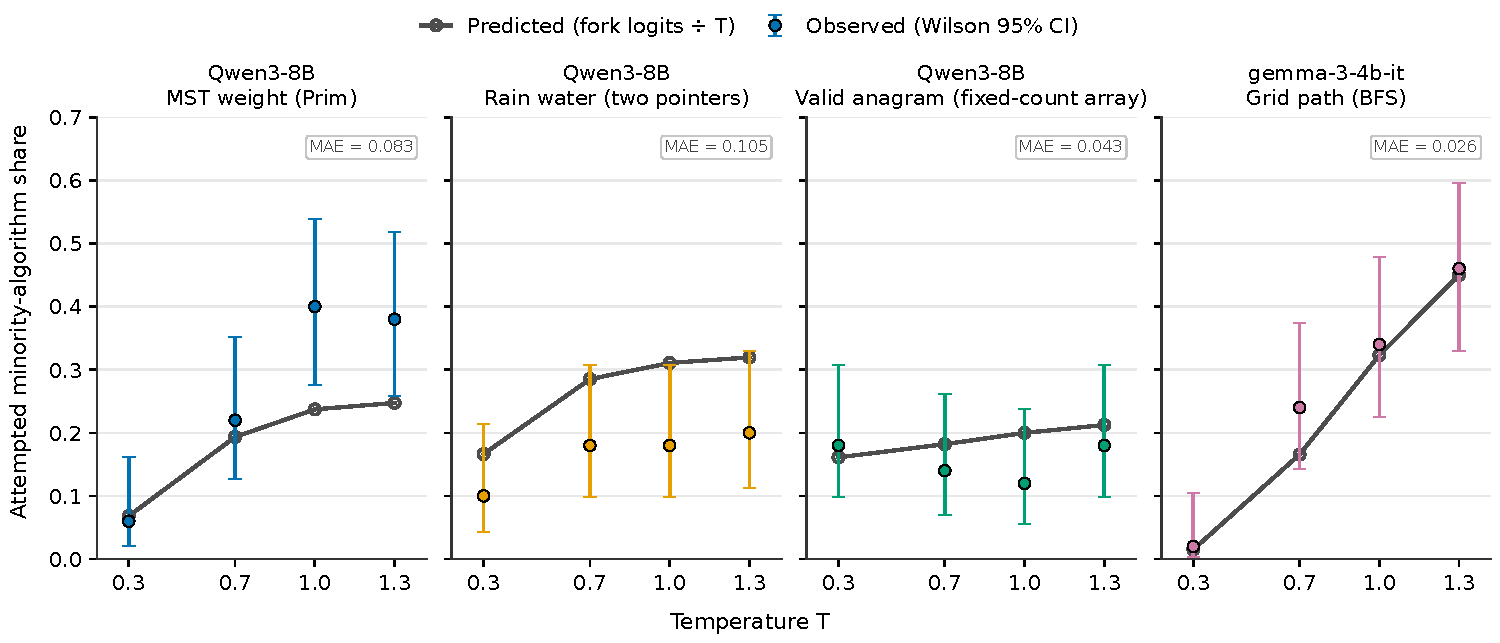
\includegraphics[width=\linewidth,height=0.78\textheight,keepaspectratio]{figures/fig_temperature_fork_v0.pdf}
\caption{Predicted share of sampled programs that use each task's minority algorithm (dark grey line, open circles), obtained by dividing the teacher-forced fork logits by temperature \$T\$ before any temperature sample is drawn, against the observed share (filled coloured points; vertical bars are the Wilson 95\textbackslash{}\% confidence interval; \$N=50\$ generations per temperature, top-\$p=1\$, same seed reused across \$T\$). Panels, left to right: Qwen3-8B on minimum-spanning-tree weight (minority algorithm: Prim), trapped rain water (minority: two pointers), and valid anagram (minority: fixed-count array); gemma-3-4b-it on the grid path-search task (minority: attempted BFS). Point colour (blue, orange, green, purple -- Okabe--Ito palette) distinguishes the panel; the legend marker colour is illustrative of the two series types only. Mean absolute error between the predicted and observed share is annotated in each panel (0.083, 0.105, 0.043, 0.026). The fork-logit prediction tracks the observed temperature response closely for MST weight and the Gemma grid task, more loosely for rain water, and in the wrong direction for valid anagram, whose observed minority share does not fall at low \$T\$ the way the prediction does.}
\label{fig:fig_temperature_fork}
\end{figure}
{\scriptsize\setlength{\tabcolsep}{2.5pt}\renewcommand{\thetable}{333}
\begin{longtable}{>{\raggedright\arraybackslash\hspace{0pt}}p{0.1388\linewidth}>{\raggedright\arraybackslash\hspace{0pt}}p{0.0922\linewidth}>{\raggedright\arraybackslash\hspace{0pt}}p{0.0955\linewidth}>{\raggedright\arraybackslash\hspace{0pt}}p{0.1187\linewidth}>{\raggedright\arraybackslash\hspace{0pt}}p{0.1486\linewidth}>{\raggedright\arraybackslash\hspace{0pt}}p{0.1541\linewidth}>{\raggedright\arraybackslash\hspace{0pt}}p{0.0559\linewidth}>{\raggedright\arraybackslash\hspace{0pt}}p{0.1093\linewidth}}
\caption{Test 2: predicted against observed minority share by temperature and sampler. [Source: iteration 7, artifact \nolinkurl{gen_art_experiment_35}.]}\label{tab:t353}\\
\toprule
\textbf{Unit} & \textbf{Cell} & \textbf{Predicted minority share} & \textbf{Observed [Wilson 95\%]} & \textbf{Correct minority observed \slash{} predicted} & \textbf{Share on the opening observed \slash{} predicted} & \textbf{JS (bits)} & \textbf{Replay per slot accuracy} \\
\midrule
\endfirsthead
\multicolumn{8}{l}{\emph{Table 333, continued}}\\
\toprule
\textbf{Unit} & \textbf{Cell} & \textbf{Predicted minority share} & \textbf{Observed [Wilson 95\%]} & \textbf{Correct minority observed \slash{} predicted} & \textbf{Share on the opening observed \slash{} predicted} & \textbf{JS (bits)} & \textbf{Replay per slot accuracy} \\
\midrule
\endhead
\bottomrule
\endlastfoot
minimum spanning tree weight & T 0.3, top-p 1 & 0.068 & 0.060 [0.02, 0.16] & 0.060 \slash{} 0.068 & 1.00 \slash{} 0.99 & 0.000 & 0.98 (n 50) \\
minimum spanning tree weight & T 0.3, top-k 10 & 0.068 & 0.060 [0.02, 0.16] & 0.060 \slash{} 0.068 & 1.00 \slash{} 0.99 & 0.000 & 0.98 (n 50) \\
minimum spanning tree weight & T 0.7, top-p 1 & 0.193 & 0.220 [0.13, 0.35] & 0.220 \slash{} 0.193 & 0.92 \slash{} 0.87 & 0.003 & 0.96 (n 47) \\
minimum spanning tree weight & T 0.7, top-k 10 & 0.193 & 0.220 [0.13, 0.35] & 0.220 \slash{} 0.193 & 0.92 \slash{} 0.87 & 0.003 & 0.96 (n 47) \\
minimum spanning tree weight & T 1.0, top-p 1 & 0.237 & 0.400 [0.28, 0.54] & 0.400 \slash{} 0.237 & 0.76 \slash{} 0.72 & 0.026 & 0.95 (n 37) \\
minimum spanning tree weight & T 1.0, top-k 10 & 0.237 & 0.400 [0.28, 0.54] & 0.400 \slash{} 0.237 & 0.76 \slash{} 0.72 & 0.026 & 0.95 (n 37) \\
minimum spanning tree weight & T 1.3, top-p 1 & 0.247 & 0.380 [0.26, 0.52] & 0.360 \slash{} 0.247 & 0.60 \slash{} 0.55 & 0.022 & 0.94 (n 32) \\
minimum spanning tree weight & T 1.3, top-k 10 & 0.247 & 0.380 [0.26, 0.52] & 0.360 \slash{} 0.247 & 0.60 \slash{} 0.55 & 0.022 & 0.91 (n 32) \\
trapped rain water & T 0.3, top-p 1 & 0.166 & 0.100 [0.04, 0.21] & 0.100 \slash{} 0.166 & 0.88 \slash{} 0.86 & 0.007 & 0.98 (n 45) \\
trapped rain water & T 0.3, top-k 10 & 0.166 & 0.100 [0.04, 0.21] & 0.100 \slash{} 0.166 & 0.88 \slash{} 0.86 & 0.007 & 0.98 (n 45) \\
trapped rain water & T 0.7, top-p 1 & 0.285 & 0.180 [0.10, 0.31] & 0.180 \slash{} 0.285 & 0.84 \slash{} 0.82 & 0.011 & 0.98 (n 41) \\
trapped rain water & T 0.7, top-k 10 & 0.285 & 0.180 [0.10, 0.31] & 0.180 \slash{} 0.285 & 0.84 \slash{} 0.82 & 0.011 & 0.98 (n 41) \\
trapped rain water & T 1.0, top-p 1 & 0.311 & 0.180 [0.10, 0.31] & 0.180 \slash{} 0.311 & 0.74 \slash{} 0.76 & 0.026 & 0.92 (n 38) \\
trapped rain water & T 1.0, top-k 10 & 0.311 & 0.180 [0.10, 0.31] & 0.180 \slash{} 0.311 & 0.74 \slash{} 0.76 & 0.026 & 0.92 (n 38) \\
trapped rain water & T 1.3, top-p 1 & 0.319 & 0.200 [0.11, 0.33] & 0.200 \slash{} 0.319 & 0.70 \slash{} 0.70 & 0.022 & 0.97 (n 35) \\
trapped rain water & T 1.3, top-k 10 & 0.319 & 0.200 [0.11, 0.33] & 0.200 \slash{} 0.319 & 0.70 \slash{} 0.70 & 0.022 & 0.97 (n 35) \\
valid anagram & T 0.3, top-p 1 & 0.161 & 0.180 [0.10, 0.31] & 0.180 \slash{} 0.161 & 0.80 \slash{} 0.81 & 0.000 & 0.93 (n 40) \\
valid anagram & T 0.3, top-k 10 & 0.161 & 0.180 [0.10, 0.31] & 0.180 \slash{} 0.161 & 0.80 \slash{} 0.81 & 0.000 & 0.93 (n 40) \\
valid anagram & T 0.7, top-p 1 & 0.182 & 0.140 [0.07, 0.26] & 0.140 \slash{} 0.182 & 0.76 \slash{} 0.82 & 0.003 & 0.95 (n 39) \\
valid anagram & T 0.7, top-k 10 & 0.182 & 0.140 [0.07, 0.26] & 0.140 \slash{} 0.182 & 0.76 \slash{} 0.82 & 0.003 & 0.95 (n 39) \\
valid anagram & T 1.0, top-p 1 & 0.200 & 0.120 [0.06, 0.24] & 0.120 \slash{} 0.200 & 0.78 \slash{} 0.81 & 0.010 & 0.90 (n 39) \\
valid anagram & T 1.0, top-k 10 & 0.200 & 0.120 [0.06, 0.24] & 0.120 \slash{} 0.200 & 0.78 \slash{} 0.81 & 0.010 & 0.90 (n 39) \\
valid anagram & T 1.3, top-p 1 & 0.212 & 0.180 [0.10, 0.31] & 0.180 \slash{} 0.212 & 0.80 \slash{} 0.79 & 0.002 & 0.95 (n 39) \\
valid anagram & T 1.3, top-k 10 & 0.212 & 0.180 [0.10, 0.31] & 0.180 \slash{} 0.212 & 0.80 \slash{} 0.79 & 0.002 & 0.95 (n 39) \\
\end{longtable}}

\begin{table}[H]
\renewcommand{\thetable}{334}
\centering\scriptsize\setlength{\tabcolsep}{2.5pt}
\caption{Test 2 by unit. [Source: iteration 7, artifact \nolinkurl{gen_art_experiment_35}.]}\label{tab:t354}
\begin{tabular}{>{\raggedright\arraybackslash\hspace{0pt}}p{0.1100\linewidth}>{\raggedright\arraybackslash\hspace{0pt}}p{0.0535\linewidth}>{\raggedright\arraybackslash\hspace{0pt}}p{0.1600\linewidth}>{\raggedright\arraybackslash\hspace{0pt}}p{0.0955\linewidth}>{\raggedright\arraybackslash\hspace{0pt}}p{0.0986\linewidth}>{\raggedright\arraybackslash\hspace{0pt}}p{0.0997\linewidth}>{\raggedright\arraybackslash\hspace{0pt}}p{0.0955\linewidth}>{\raggedright\arraybackslash\hspace{0pt}}p{0.1362\linewidth}>{\raggedright\arraybackslash\hspace{0pt}}p{0.0539\linewidth}}
\toprule
\textbf{Unit} & \textbf{MAE} & \textbf{Observed drop T 1.0 to 0.3 [slot bootstrap]} & \textbf{Predicted drop} & \textbf{McNemar b:c, one sided p} & \textbf{Observed change T 1.0 to 1.3} & \textbf{Predicted change} & \textbf{Slots changing the idea across T (top-p 1)} & \textbf{Pass} \\
\midrule
minimum spanning tree weight & 0.083 & 0.340 [0.22, 0.48] & 0.169 & 17:0, 0.0000 & -0.020 & 0.010 & 20\slash{}50 & yes \\
trapped rain water & 0.105 & 0.080 [-0.04, 0.22] & 0.144 & 7:3, 0.1719 & 0.020 & 0.009 & 12\slash{}50 & no \\
valid anagram & 0.043 & -0.060 [-0.16, 0.04] & 0.039 & 2:5, 0.9375 & 0.060 & 0.013 & 11\slash{}50 & no \\
\bottomrule
\end{tabular}
\end{table}

\subsubsection*{7.5.4 The collapsed tasks}
Test 3 passes: on the grid, shortest path, connected components and kth smallest the fork margin of the twin is 7.46, 4.85, 17.04 and 6.10 nats (Table 335). At T 1.3 the predicted rate off the default is at most 0.02 on every task, and 100 samples at that temperature produced no program off the default on any of them; a further check of 20 samples found one program off the default on the grid and one on shortest path; the shortest path one fits its predicted rate, and the grid one is unlikely under its margin (binomial p 0.04). The record of iterations 1 to 4, 797 of 800 default programs and no flips under the same seed, implies margins of about 6 nats. The temperature nulls of iterations 1 to 4 are what the fork logits predict: on the collapsed tasks the alternative lies 5 to 17 nats behind at the fork, and dividing by 1.3 does not bring it within reach.

\begin{table}[H]
\renewcommand{\thetable}{335}
\centering\scriptsize\setlength{\tabcolsep}{2.5pt}
\caption{Test 3: fork margins of the collapsed tasks and the bound they imply. [Source: iteration 7, artifact \nolinkurl{gen_art_experiment_35}.]}\label{tab:t355}
\begin{tabular}{>{\raggedright\arraybackslash\hspace{0pt}}p{0.0919\linewidth}>{\raggedright\arraybackslash\hspace{0pt}}p{0.0745\linewidth}>{\raggedright\arraybackslash\hspace{0pt}}p{0.0582\linewidth}>{\raggedright\arraybackslash\hspace{0pt}}p{0.2010\linewidth}>{\raggedright\arraybackslash\hspace{0pt}}p{0.1044\linewidth}>{\raggedright\arraybackslash\hspace{0pt}}p{0.2137\linewidth}>{\raggedright\arraybackslash\hspace{0pt}}p{0.0889\linewidth}>{\raggedright\arraybackslash\hspace{0pt}}p{0.0805\linewidth}}
\toprule
\textbf{Task} & \textbf{Fork margin (nats)} & \textbf{At least 4} & \textbf{Predicted rate off the default at T 0.3 \slash{} 1.0 \slash{} 1.3} & \textbf{Predicted change 0.3 to 1.3} & \textbf{Bound check at T 1.3 (off of 100 against the logit prediction)} & \textbf{T 1.3 check (off of 20)} & \textbf{48-token opening LLR} \\
\midrule
grid & 7.46 & yes & 0.0000 \slash{} 0.0006 \slash{} 0.0021 & 0.0021 & 0\slash{}100 vs 0.0021 & 1\slash{}20 & 8.79 \\
shortest path & 4.85 & yes & 0.0000 \slash{} 0.0078 \slash{} 0.0204 & 0.0204 & 0\slash{}100 vs 0.0204 & 1\slash{}20 & 5.15 \\
connected components & 17.04 & yes & 0.0000 \slash{} 0.0000 \slash{} 0.0000 & 0.0000 & 0\slash{}100 vs 0.0000 & 0\slash{}20 & 24.58 \\
kth smallest & 6.10 & yes & 0.0000 \slash{} 0.0022 \slash{} 0.0085 & 0.0085 & 0\slash{}100 vs 0.0085 & 0\slash{}20 & 7.55 \\
\bottomrule
\end{tabular}
\end{table}

\subsubsection*{7.5.5 What does move the fork}
Exchanging the task specification states of a prompt that names the minority algorithm into the twin gives that algorithm in 30 of 30 slots on all three units, against 0 to 7 under the padding twin, the forced prompt with its instruction replaced by padding tokens so that positions align (exact one sided p of 1.2e-7 or less; Tables 336 and 337). The argmax token at the fork flips with it (\texttt{ Kr} to \texttt{ Prim}), and the fork margin moves by 4.9 to 22 nats toward the minority, against 2 nats or less for a matched random exchange. Eight random pushes of the task specification states at alpha 2 move the minority share in the direction their change in fork margin predicts (Spearman -0.69, -0.44 and -0.94 between margin change and share change; Tables 338 and 339). The committed permutation test used the upper tail, the side opposite to the predicted negative relation; the lower tail is reported beside it as a correction made after the commitment.

\begin{table}[H]
\renewcommand{\thetable}{336}
\centering\scriptsize\setlength{\tabcolsep}{2.5pt}
\caption{Exchanging the forced minority prompt's task specification states into the twin. [Source: iteration 7, artifact \nolinkurl{gen_art_experiment_35}.]}\label{tab:t356}
\begin{tabular}{>{\raggedright\arraybackslash\hspace{0pt}}p{0.1507\linewidth}>{\raggedright\arraybackslash\hspace{0pt}}p{0.2434\linewidth}>{\raggedright\arraybackslash\hspace{0pt}}p{0.0338\linewidth}>{\raggedright\arraybackslash\hspace{0pt}}p{0.1025\linewidth}>{\raggedright\arraybackslash\hspace{0pt}}p{0.0961\linewidth}>{\raggedright\arraybackslash\hspace{0pt}}p{0.0539\linewidth}>{\raggedright\arraybackslash\hspace{0pt}}p{0.2431\linewidth}}
\toprule
\textbf{Unit} & \textbf{Arm} & \textbf{n} & \textbf{Attempted minority share} & \textbf{Correct minority share} & \textbf{Pass} & \textbf{Labels} \\
\midrule
minimum spanning tree weight & padding twin & 30 & 0.23 & 0.23 & 1.00 & Kruskal 23, Prim with heap 7 \\
minimum spanning tree weight & forced minority prompt & 30 & 1.00 & 0.97 & 0.97 & Prim with heap 30 \\
minimum spanning tree weight & forced prompt's task specification states exchanged in & 30 & 1.00 & 1.00 & 1.00 & Prim with heap 30 \\
minimum spanning tree weight & random exchange of matched norm & 30 & 0.40 & 0.40 & 1.00 & Kruskal 18, Prim with heap 12 \\
trapped rain water & padding twin & 30 & 0.13 & 0.13 & 1.00 & prefix and suffix maxima 25, two pointers 4, peak split 1 \\
trapped rain water & forced minority prompt & 30 & 1.00 & 1.00 & 1.00 & two pointers 30 \\
trapped rain water & forced prompt's task specification states exchanged in & 30 & 1.00 & 1.00 & 1.00 & two pointers 30 \\
trapped rain water & random exchange of matched norm & 30 & 0.13 & 0.13 & 1.00 & prefix and suffix maxima 25, two pointers 4, peak split 1 \\
valid anagram & padding twin & 30 & 0.00 & 0.00 & 1.00 & sort and compare 30 \\
valid anagram & forced minority prompt & 30 & 1.00 & 1.00 & 1.00 & fixed count array 30 \\
valid anagram & forced prompt's task specification states exchanged in & 30 & 1.00 & 1.00 & 1.00 & fixed count array 30 \\
valid anagram & random exchange of matched norm & 30 & 0.00 & 0.00 & 1.00 & sort and compare 30 \\
\bottomrule
\end{tabular}
\end{table}

\begin{table}[H]
\renewcommand{\thetable}{337}
\centering\scriptsize\setlength{\tabcolsep}{2.5pt}
\caption{The exchange against the padding twin and against a matched random exchange. [Source: iteration 7, artifact \nolinkurl{gen_art_experiment_35}.]}\label{tab:t357}
\begin{tabular}{>{\raggedright\arraybackslash\hspace{0pt}}p{0.1135\linewidth}>{\raggedright\arraybackslash\hspace{0pt}}p{0.1734\linewidth}>{\raggedright\arraybackslash\hspace{0pt}}p{0.1315\linewidth}>{\raggedright\arraybackslash\hspace{0pt}}p{0.1223\linewidth}>{\raggedright\arraybackslash\hspace{0pt}}p{0.1212\linewidth}>{\raggedright\arraybackslash\hspace{0pt}}p{0.1416\linewidth}>{\raggedright\arraybackslash\hspace{0pt}}p{0.1201\linewidth}}
\toprule
\textbf{Unit} & \textbf{Exchange against padding twin, b:c (one sided p)} & \textbf{Exchange against random exchange} & \textbf{Fork margin change, exchange (nats)} & \textbf{Fork margin change, random exchange} & \textbf{Predicted minority share under the exchange} & \textbf{Pass ratio against the padding twin} \\
\midrule
minimum spanning tree weight & 23:0 (p 1.2e-07) & 18:0 (p 3.8e-06) & -4.87 & -1.25 & 0.17 & 1.00 \\
trapped rain water & 26:0 (p 1.5e-08) & 26:0 (p 1.5e-08) & -5.50 & -2.00 & 0.40 & 1.00 \\
valid anagram & 30:0 (p 9.3e-10) & 30:0 (p 9.3e-10) & -22.12 & 0.26 & 0.78 & 1.00 \\
\bottomrule
\end{tabular}
\end{table}

{\scriptsize\setlength{\tabcolsep}{2.5pt}\renewcommand{\thetable}{338}
\begin{longtable}{>{\raggedright\arraybackslash\hspace{0pt}}p{0.1423\linewidth}>{\raggedright\arraybackslash\hspace{0pt}}p{0.0955\linewidth}>{\raggedright\arraybackslash\hspace{0pt}}p{0.0978\linewidth}>{\raggedright\arraybackslash\hspace{0pt}}p{0.0980\linewidth}>{\raggedright\arraybackslash\hspace{0pt}}p{0.0955\linewidth}>{\raggedright\arraybackslash\hspace{0pt}}p{0.1049\linewidth}>{\raggedright\arraybackslash\hspace{0pt}}p{0.0539\linewidth}>{\raggedright\arraybackslash\hspace{0pt}}p{0.2253\linewidth}}
\caption{Random pushes of the task specification states: margin change and minority share per direction. [Source: iteration 7, artifact \nolinkurl{gen_art_experiment_35}.]}\label{tab:t358}\\
\toprule
\textbf{Unit} & \textbf{Direction seed} & \textbf{Fork margin change (nats)} & \textbf{Observed minority share (of 10)} & \textbf{Predicted share} & \textbf{Observed change against the twin} & \textbf{Pass} & \textbf{Labels} \\
\midrule
\endfirsthead
\multicolumn{8}{l}{\emph{Table 338, continued}}\\
\toprule
\textbf{Unit} & \textbf{Direction seed} & \textbf{Fork margin change (nats)} & \textbf{Observed minority share (of 10)} & \textbf{Predicted share} & \textbf{Observed change against the twin} & \textbf{Pass} & \textbf{Labels} \\
\midrule
\endhead
\bottomrule
\endlastfoot
minimum spanning tree weight & 9101 & 0.45 & 0.00 & 0.17 & -0.20 & 0.90 & Kruskal 10 \\
minimum spanning tree weight & 9102 & -0.29 & 0.30 & 0.17 & 0.10 & 1.00 & Kruskal 7, Prim with heap 3 \\
minimum spanning tree weight & 9103 & 1.89 & 0.00 & 0.17 & -0.20 & 0.80 & Kruskal 10 \\
minimum spanning tree weight & 9104 & 3.04 & 0.00 & 0.12 & -0.20 & 1.00 & Kruskal 10 \\
minimum spanning tree weight & 9105 & 2.20 & 0.00 & 0.16 & -0.20 & 0.90 & Kruskal 10 \\
minimum spanning tree weight & 9106 & -0.19 & 0.30 & 0.20 & 0.10 & 1.00 & Kruskal 7, Prim with heap 3 \\
minimum spanning tree weight & 9107 & -1.21 & 0.40 & 0.30 & 0.20 & 1.00 & Kruskal 6, Prim with heap 4 \\
minimum spanning tree weight & 9108 & -0.59 & 0.00 & 0.20 & -0.20 & 0.70 & Kruskal 10 \\
trapped rain water & 9101 & -0.20 & 0.00 & 0.21 & -0.40 & 1.00 & prefix and suffix maxima 6, peak split 4 \\
trapped rain water & 9102 & 2.80 & 0.00 & 0.21 & -0.40 & 1.00 & prefix and suffix maxima 10 \\
trapped rain water & 9103 & -2.45 & 0.20 & 0.28 & -0.20 & 1.00 & prefix and suffix maxima 8, two pointers 2 \\
trapped rain water & 9104 & 0.80 & 0.30 & 0.16 & -0.10 & 1.00 & prefix and suffix maxima 7, two pointers 3 \\
trapped rain water & 9105 & 7.05 & 0.00 & 0.22 & -0.40 & 0.90 & prefix and suffix maxima 10 \\
trapped rain water & 9106 & 2.00 & 0.50 & 0.23 & 0.10 & 1.00 & prefix and suffix maxima 5, two pointers 5 \\
trapped rain water & 9107 & 1.10 & 0.20 & 0.13 & -0.20 & 1.00 & prefix and suffix maxima 8, two pointers 2 \\
trapped rain water & 9108 & -6.25 & 0.90 & 0.59 & 0.50 & 1.00 & two pointers 9, prefix and suffix maxima 1 \\
valid anagram & 9101 & -7.65 & 1.00 & 0.19 & 0.90 & 1.00 & fixed count array 10 \\
valid anagram & 9102 & -6.70 & 0.20 & 0.19 & 0.10 & 1.00 & hash count 8, fixed count array 2 \\
valid anagram & 9103 & 2.11 & 0.00 & 0.05 & -0.10 & 1.00 & sort and compare 9, hash count 1 \\
valid anagram & 9104 & -7.75 & 0.80 & 0.60 & 0.70 & 1.00 & fixed count array 8, hash count 2 \\
valid anagram & 9105 & 3.21 & 0.00 & 0.01 & -0.10 & 1.00 & sort and compare 10 \\
valid anagram & 9106 & 0.80 & 0.00 & 0.12 & -0.10 & 1.00 & sort and compare 9, hash count 1 \\
valid anagram & 9107 & -1.31 & 0.20 & 0.40 & 0.10 & 1.00 & hash count 4, sort and compare 4, fixed count array 2 \\
valid anagram & 9108 & 2.05 & 0.00 & 0.03 & -0.10 & 1.00 & sort and compare 9, hash count 1 \\
\end{longtable}}

\begin{table}[H]
\renewcommand{\thetable}{339}
\centering\scriptsize\setlength{\tabcolsep}{2.5pt}
\caption{Random pushes by unit. [Source: iteration 7, artifact \nolinkurl{gen_art_experiment_35}.]}\label{tab:t359}
\begin{tabular}{>{\raggedright\arraybackslash\hspace{0pt}}p{0.1092\linewidth}>{\raggedright\arraybackslash\hspace{0pt}}p{0.1249\linewidth}>{\raggedright\arraybackslash\hspace{0pt}}p{0.1128\linewidth}>{\raggedright\arraybackslash\hspace{0pt}}p{0.1048\linewidth}>{\raggedright\arraybackslash\hspace{0pt}}p{0.0915\linewidth}>{\raggedright\arraybackslash\hspace{0pt}}p{0.1428\linewidth}>{\raggedright\arraybackslash\hspace{0pt}}p{0.0957\linewidth}>{\raggedright\arraybackslash\hspace{0pt}}p{0.1316\linewidth}}
\toprule
\textbf{Unit} & \textbf{Spearman (margin change, share change)} & \textbf{Lower tail permutation p} & \textbf{Committed upper tail p} & \textbf{MAE of predicted shares} & \textbf{Log-score gain per sample over no push effect} & \textbf{Pass ratio against the twin} & \textbf{Twin minority share on these slots} \\
\midrule
minimum spanning tree weight & -0.69 & 0.0271 & 0.979 & 0.146 & 0.053 & 0.912 & 0.20 (pred 0.24) \\
trapped rain water & -0.44 & 0.1161 & 0.888 & 0.188 & 0.109 & 0.988 & 0.40 (pred 0.19) \\
valid anagram & -0.94 & 2.6e-04 & 1.000 & 0.178 & 0.162 & 1.000 & 0.10 (pred 0.20) \\
\bottomrule
\end{tabular}
\end{table}

\subsubsection*{7.5.6 Question 1a-c of the request}
The request's question 1a-c asks whether, with the seed fixed and top-k 10, a tight temperature gives one idea in many phrasings or many ideas, and whether loosening it multiplies ideas or phrasings. On the mixed units a tight temperature collapses onto the default idea, and loosening it restores the second idea at its natural rate, never more, while the phrasings within each idea multiply (Table 340): Kruskal programs on minimum spanning tree weight form 3 phrasing clusters at T 0.3 and 7 at T 1.3. No third idea appears at any temperature. In Gemma, where few samples leave the opening, T 1.3 does raise the minority above its natural rate, as its fork logits predicted (Section 7.8.2). Hill-1 of the correct ideas on minimum spanning tree weight rises from 1.25 at T 0.3 to 1.95 at T 1.0 and stays at 1.92 at 1.3; ten literal trajectories at T 0.3 give 9 Kruskal and 1 Prim. The only correct programs off the catalogue are 40 continuations from one fork token of low probability on valid anagram; they form 2 distinct programs, both the catalogue's extra counting mode, and are catalogue variants.

{\scriptsize\setlength{\tabcolsep}{2.5pt}\renewcommand{\thetable}{340}
\begin{longtable}{>{\raggedright\arraybackslash\hspace{0pt}}p{0.1042\linewidth}>{\raggedright\arraybackslash\hspace{0pt}}p{0.0692\linewidth}>{\raggedright\arraybackslash\hspace{0pt}}p{0.1768\linewidth}>{\raggedright\arraybackslash\hspace{0pt}}p{0.0582\linewidth}>{\raggedright\arraybackslash\hspace{0pt}}p{0.1960\linewidth}>{\raggedright\arraybackslash\hspace{0pt}}p{0.1598\linewidth}>{\raggedright\arraybackslash\hspace{0pt}}p{0.1593\linewidth}}
\caption{Ideas and phrasings across temperature (same seed; Hill-1 at depth 25). [Source: iteration 7, artifact \nolinkurl{gen_art_experiment_35}.]}\label{tab:t360}\\
\toprule
\textbf{Unit} & \textbf{Cell} & \textbf{Ideas among correct programs} & \textbf{Hill-1 at depth 25} & \textbf{Phrasing clusters per idea (Jaccard 0.8)} & \textbf{Ten literal trajectories: ideas} & \textbf{Their phrasing clusters} \\
\midrule
\endfirsthead
\multicolumn{7}{l}{\emph{Table 340, continued}}\\
\toprule
\textbf{Unit} & \textbf{Cell} & \textbf{Ideas among correct programs} & \textbf{Hill-1 at depth 25} & \textbf{Phrasing clusters per idea (Jaccard 0.8)} & \textbf{Ten literal trajectories: ideas} & \textbf{Their phrasing clusters} \\
\midrule
\endhead
\bottomrule
\endlastfoot
minimum spanning tree weight & T 0.3, top-p 1 & Kruskal, Prim with heap & 1.25 & Kruskal 3, Prim with heap 1 & Kruskal 9, Prim with heap 1 & Kruskal 3, Prim with heap 1 \\
minimum spanning tree weight & T 0.7, top-p 1 & Kruskal, Prim with heap & 1.69 & Kruskal 4, Prim with heap 1 & Kruskal 6, Prim with heap 4 & Kruskal 2, Prim with heap 1 \\
minimum spanning tree weight & T 1.0, top-p 1 & Kruskal, Prim with heap & 1.95 & Prim with heap 5, Kruskal 4 & Prim with heap 6, Kruskal 4 & Prim with heap 3, Kruskal 2 \\
minimum spanning tree weight & T 1.3, top-p 1 & Kruskal, Prim with heap & 1.92 & Kruskal 7, Prim with heap 4 & Prim with heap 6, Kruskal 4 & Kruskal 3, Prim with heap 2 \\
minimum spanning tree weight & T 0.3, top-k 10 & Kruskal, Prim with heap & 1.25 & Kruskal 3, Prim with heap 1 & Kruskal 9, Prim with heap 1 & Kruskal 3, Prim with heap 1 \\
minimum spanning tree weight & T 0.7, top-k 10 & Kruskal, Prim with heap & 1.69 & Kruskal 4, Prim with heap 1 & Kruskal 6, Prim with heap 4 & Kruskal 2, Prim with heap 1 \\
minimum spanning tree weight & T 1.0, top-k 10 & Kruskal, Prim with heap & 1.95 & Prim with heap 5, Kruskal 4 & Prim with heap 6, Kruskal 4 & Prim with heap 3, Kruskal 2 \\
minimum spanning tree weight & T 1.3, top-k 10 & Kruskal, Prim with heap & 1.92 & Kruskal 7, Prim with heap 4 & Prim with heap 6, Kruskal 4 & Kruskal 3, Prim with heap 2 \\
trapped rain water & T 0.3, top-p 1 & prefix and suffix maxima, two pointers & 1.37 & prefix and suffix maxima 1, two pointers 1 & prefix and suffix maxima 9, two pointers 1 & prefix and suffix maxima 1, two pointers 1 \\
trapped rain water & T 0.7, top-p 1 & prefix and suffix maxima, two pointers & 1.58 & prefix and suffix maxima 2, two pointers 1 & prefix and suffix maxima 9, two pointers 1 & prefix and suffix maxima 1, two pointers 1 \\
trapped rain water & T 1.0, top-p 1 & peak split, prefix and suffix maxima, two pointers & 1.74 & prefix and suffix maxima 2, two pointers 2, peak split 1 & prefix and suffix maxima 9, two pointers 1 & prefix and suffix maxima 1, two pointers 1 \\
trapped rain water & T 1.3, top-p 1 & peak split, prefix and suffix maxima, two pointers & 1.79 & prefix and suffix maxima 3, two pointers 2, peak split 1 & prefix and suffix maxima 8, two pointers 2 & prefix and suffix maxima 3, two pointers 1 \\
trapped rain water & T 0.3, top-k 10 & prefix and suffix maxima, two pointers & 1.37 & prefix and suffix maxima 1, two pointers 1 & prefix and suffix maxima 9, two pointers 1 & prefix and suffix maxima 1, two pointers 1 \\
trapped rain water & T 0.7, top-k 10 & prefix and suffix maxima, two pointers & 1.58 & prefix and suffix maxima 2, two pointers 1 & prefix and suffix maxima 9, two pointers 1 & prefix and suffix maxima 1, two pointers 1 \\
trapped rain water & T 1.0, top-k 10 & peak split, prefix and suffix maxima, two pointers & 1.74 & prefix and suffix maxima 2, two pointers 2, peak split 1 & prefix and suffix maxima 9, two pointers 1 & prefix and suffix maxima 1, two pointers 1 \\
trapped rain water & T 1.3, top-k 10 & peak split, prefix and suffix maxima, two pointers & 1.79 & prefix and suffix maxima 3, two pointers 2, peak split 1 & prefix and suffix maxima 8, two pointers 2 & prefix and suffix maxima 3, two pointers 1 \\
valid anagram & T 0.3, top-p 1 & fixed count array, hash count, sort and compare & 1.83 & fixed count array 2, sort and compare 2, hash count 1 & sort and compare 8, fixed count array 2 & sort and compare 2, fixed count array 1 \\
valid anagram & T 0.7, top-p 1 & fixed count array, hash count, sort and compare & 1.72 & fixed count array 3, sort and compare 2, hash count 1 & sort and compare 8, fixed count array 2 & sort and compare 2, fixed count array 1 \\
valid anagram & T 1.0, top-p 1 & fixed count array, hash count, sort and compare & 1.84 & fixed count array 2, sort and compare 2, hash count 1 & sort and compare 8, fixed count array 2 & sort and compare 2, fixed count array 1 \\
valid anagram & T 1.3, top-p 1 & fixed count array, hash count, sort and compare & 1.85 & fixed count array 5, sort and compare 2, hash count 1 & sort and compare 8, fixed count array 2 & sort and compare 2, fixed count array 1 \\
valid anagram & T 0.3, top-k 10 & fixed count array, hash count, sort and compare & 1.83 & fixed count array 2, sort and compare 2, hash count 1 & sort and compare 8, fixed count array 2 & sort and compare 2, fixed count array 1 \\
valid anagram & T 0.7, top-k 10 & fixed count array, hash count, sort and compare & 1.72 & fixed count array 3, sort and compare 2, hash count 1 & sort and compare 8, fixed count array 2 & sort and compare 2, fixed count array 1 \\
valid anagram & T 1.0, top-k 10 & fixed count array, hash count, sort and compare & 1.84 & fixed count array 2, sort and compare 2, hash count 1 & sort and compare 8, fixed count array 2 & sort and compare 2, fixed count array 1 \\
valid anagram & T 1.3, top-k 10 & fixed count array, hash count, sort and compare & 1.85 & fixed count array 5, sort and compare 2, hash count 1 & sort and compare 8, fixed count array 2 & sort and compare 2, fixed count array 1 \\
\end{longtable}}

\FloatBarrier
\subsection*{7.6 The dose unit, not the seeds, made iteration 5's plan noise weak (Qwen3-8B)}
\addcontentsline{toc}{subsection}{7.6 The dose unit, not the seeds, made iteration 5's plan noise weak (Qwen3-8B)}
\noindent{\small\emph{Artifact: \nolinkurl{gen_art_experiment_36}.}}\par\medskip
\subsubsection*{7.6.1 Design}
Iteration 4 found plan noise strong under its \emph{absolute unit}, in which each cell (block and position) receives a random direction scaled to the displacement a ban itself causes at that cell. Iteration 5 found it nearly inert under its \emph{relative unit}, which scales the direction to a fixed fraction of the twin's own residual norm at each cell, and with different direction seeds. Section 6.3 showed that the 8-bit engine was not the cause. The dose unit experiment  crossed the two units with the two seed sets in bf16, on the same 50 slots per design, and committed a decision rule before the first row: the answer is the unit if the main effect of the unit is positive with its interval above zero and the effect of the seeds lies within plus or minus 0.10. Two anchors reproduce the earlier artifacts on the same slots: the absolute unit with iteration-4 seeds gives 26 of 50 attempts against 25 in the engine control (agreement per slot 0.98), and the relative unit with iteration-5 seeds gives 1 of 50 against 1. Iteration 5's null is thus reproduced without its left padding, so the decoding path is not the cause either.

\subsubsection*{7.6.2 The 2x2}
The answer is the unit (Table 341). On connected components at alpha 2, the absolute unit gives a correct share off the default of 0.50 and 0.52 under the two seed sets, and the relative unit 0.10 and 0.02: a unit effect of +0.45 [0.35, 0.55], a seed effect of +0.03 [-0.07, 0.14] and an interaction of -0.10 [-0.28, 0.08]. A conditional logistic regression with slot strata agrees (unit coefficient 4.34, p 1e-4; seeds 1.68, p 0.13). On shortest path, at 100 slots, the unit effect is smaller (+0.115 [0.06, 0.17]) and most attempts under the absolute unit fail the hidden tests (13 correct of 41 attempted at pass 0.66; Table 342). On 50 fresh connected components slots the unit effect replicates (+0.42 [0.32, 0.52]), and on kth smallest it is +0.27 [0.18, 0.37] with a seed effect of +0.03 (Tables 346 and 347). On kth smallest, unlike connected components, the relative unit does move the algorithm, at half the absolute unit's rate.

\begin{figure}[!htbp]
\centering\captionsetup{font=footnotesize}
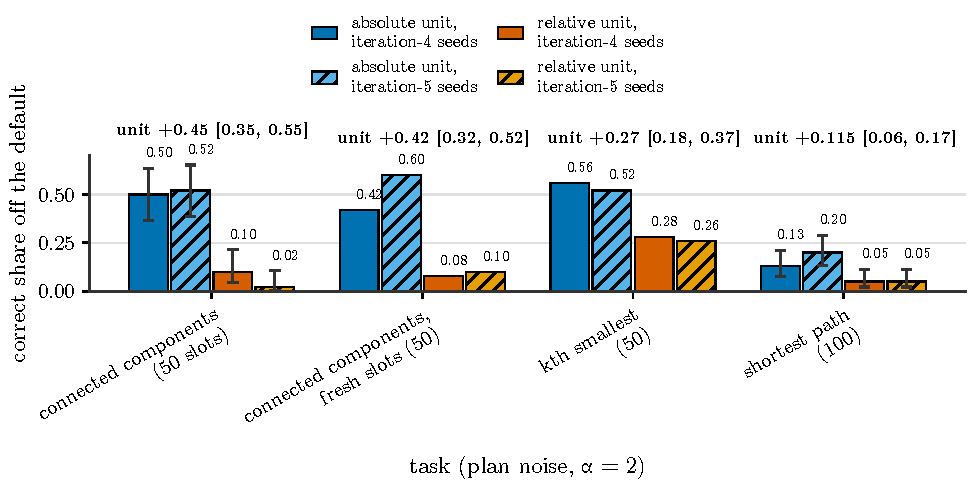
\includegraphics[width=\linewidth,height=0.78\textheight,keepaspectratio]{figures/fig_unit_seed_v0.pdf}
\caption{Correct share off the default algorithm under per-sample plan noise (dose \$\textbackslash{}alpha=2\$) in Qwen3-8B (bf16, thinking off), for the four designs of a \$2\textbackslash{}times2\$: absolute vs.\textbackslash{} relative dose unit, crossed with iteration-4 vs.\textbackslash{} iteration-5 direction-seed draws. The four x-axis groups, each labelled with its sample size per bar, are connected components (50 slots), the same task replicated on 50 held-out fresh slots, k-th smallest (50), and shortest path (100). Bars are coloured by unit and textured by seed batch: dark blue = absolute unit \slash{} iteration-4 seeds, light blue with diagonal hatching = absolute unit \slash{} iteration-5 seeds, dark orange = relative unit \slash{} iteration-4 seeds, light orange with diagonal hatching = relative unit \slash{} iteration-5 seeds. The number above each bar is its own correct off-default share; error bars, drawn only on the connected-components and shortest-path groups, are Wilson 95\textbackslash{}\% score intervals (the fresh-slots and k-th-smallest groups are an exploratory replication that reports point estimates only). The bold text above each group gives the pre-registered unit main effect with its 95\textbackslash{}\% CI: \$+0.45\textbackslash{} [0.35,\textbackslash{},0.55]\$, \$+0.42\textbackslash{} [0.32,\textbackslash{},0.52]\$, \$+0.27\textbackslash{} [0.18,\textbackslash{},0.37]\$ and \$+0.115\textbackslash{} [0.06,\textbackslash{},0.17]\$. In every group the two blue (absolute-unit) bars sit far above the two orange (relative-unit) bars, while the solid and hatched bars within each colour are close in height: the dose unit used to scale a random push decides whether plan noise moves Qwen3-8B off its default algorithm, and the particular batch of random direction seeds used to generate that push does not.}
\label{fig:fig_unit_seed}
\end{figure}
\begin{table}[H]
\renewcommand{\thetable}{341}
\centering\small\setlength{\tabcolsep}{4.0pt}
\caption{The 2x2 on connected components at alpha 2. [Source: iteration 7, artifact \nolinkurl{gen_art_experiment_36}.]}\label{tab:t361}
\begin{tabular}{>{\raggedright\arraybackslash\hspace{0pt}}p{0.5949\linewidth}>{\raggedright\arraybackslash\hspace{0pt}}p{0.1225\linewidth}>{\raggedright\arraybackslash\hspace{0pt}}p{0.2289\linewidth}}
\toprule
\textbf{connected components, $\alpha$ 2, N = 50 per design} & \textbf{share Y} & \textbf{95\% CI} \\
\midrule
absolute unit, iteration-4 seeds & 0.50 & [0.37, 0.63] \\
absolute unit, iteration-5 seeds & 0.52 & [0.39, 0.65] \\
relative unit, iteration-4 seeds & 0.10 & [0.04, 0.21] \\
relative unit, iteration-5 seeds & 0.02 & [0.00, 0.10] \\
unit main effect (risk difference) & \textbf{+0.45} & [0.35, 0.55] \\
seed main effect (risk difference) & +0.03 & [$-$0.07, 0.14] \\
interaction & $-$0.10 & [$-$0.28, 0.08] \\
\bottomrule
\end{tabular}
\end{table}

\begin{table}[H]
\renewcommand{\thetable}{342}
\centering\scriptsize\setlength{\tabcolsep}{2.5pt}
\caption{Every 2x2 cell (Y, correct programs off the default with Wilson 95\% interval; A, attempted off the default). [Source: iteration 7, artifact \nolinkurl{gen_art_experiment_36}.]}\label{tab:t362}
\begin{tabular}{>{\raggedright\arraybackslash\hspace{0pt}}p{0.1151\linewidth}>{\raggedright\arraybackslash\hspace{0pt}}p{0.4052\linewidth}>{\raggedright\arraybackslash\hspace{0pt}}p{0.0444\linewidth}>{\raggedright\arraybackslash\hspace{0pt}}p{0.0971\linewidth}>{\raggedright\arraybackslash\hspace{0pt}}p{0.0961\linewidth}>{\raggedright\arraybackslash\hspace{0pt}}p{0.0650\linewidth}>{\raggedright\arraybackslash\hspace{0pt}}p{0.1005\linewidth}}
\toprule
\textbf{task} & \textbf{arm} & \textbf{N} & \textbf{Y (Wilson 95\%)} & \textbf{Y, any named algorithm} & \textbf{A} & \textbf{pass} \\
\midrule
connected components & neutral twin & 50 & 0 [0.00, 0.07] & 0 & 0 & 1.00 \\
connected components & the four designs at $\alpha$ 1 (absolute\slash{}iteration-4, absolute\slash{}iteration-5, relative\slash{}iteration-4, relative\slash{}iteration-5) & 50 each & 6 \slash{} 7 \slash{} 0 \slash{} 1 & same & 6 \slash{} 7 \slash{} 0 \slash{} 1 & 1.00 \\
connected components & absolute unit, iteration-4 seeds, $\alpha$ 2 & 50 & 25 [0.37, 0.63] & 25 & 26 & 0.98 \\
connected components & absolute unit, iteration-5 seeds, $\alpha$ 2 & 50 & 26 [0.39, 0.65] & 26 & 26 & 1.00 \\
connected components & relative unit, iteration-4 seeds, $\alpha$ 2 & 50 & 5 [0.04, 0.21] & 5 & 5 & 1.00 \\
connected components & relative unit, iteration-5 seeds, $\alpha$ 2 & 50 & 1 [0.00, 0.10] & 1 & 1 & 1.00 \\
connected components & profile of the relative unit at absolute energy per block, $\alpha$ 2 & 50 & 14 [0.17, 0.42] & 14 & 17 & 0.94 \\
shortest path & neutral twin & 100 & 0 [0.00, 0.04] & 0 & 1 & 0.99 \\
shortest path & the four designs at $\alpha$ 1 (absolute\slash{}iteration-4, absolute\slash{}iteration-5, relative\slash{}iteration-4, relative\slash{}iteration-5) & 50 each & 7 \slash{} 7 \slash{} 0 \slash{} 0 & same & 12 \slash{} 12 \slash{} 2 \slash{} 0 & 0.84 \slash{} 0.88 \slash{} 0.96 \slash{} 1.00 \\
shortest path & absolute unit, iteration-4 seeds, $\alpha$ 2 & 100 & 13 [0.08, 0.21] & 13 & 41 & 0.66 \\
shortest path & absolute unit, iteration-5 seeds, $\alpha$ 2 & 100 & 20 [0.13, 0.29] & 20 & 38 & 0.74 \\
shortest path & relative unit, iteration-4 seeds, $\alpha$ 2 & 100 & 5 [0.02, 0.11] & 5 & 9 & 0.96 \\
shortest path & relative unit, iteration-5 seeds, $\alpha$ 2 & 100 & 5 [0.02, 0.11] & 5 & 10 & 0.95 \\
shortest path & profile of the relative unit at absolute energy per block, $\alpha$ 2 & 100 & 8 [0.04, 0.15] & 8 & 16 & 0.90 \\
\bottomrule
\end{tabular}
\end{table}

\subsubsection*{7.6.3 Why the units differ}
The two units differ in where the energy sits. The absolute unit is peaky: on connected components its top quartile of cells holds 81\% of its energy, on bands of a few task tokens, and its largest cell receives about 2.1 times that cell's residual norm. The relative unit is flat by construction: its top quartile holds 42\%, and its largest cell receives 0.25 times the residual norm. A fifth design applies the per-position profile of the relative unit at the energy per block of the absolute unit; it moves 0.28 on connected components, between the two, so the profile (+0.22 [0.08, 0.36], McNemar 13:2) and the energy (+0.18 [0.06, 0.30], 10:1) each carry part of the effect.

A split of the absolute unit by cell confirms that the peaky cells matter (Tables 343 and 344). At the same total energy, the cells of the top quartile alone move connected components in 29 of 50 slots, the other three quartiles in 15 (18:4, Holm p 0.01), and the same energy at shuffled positions in 4 (21:0 against the full unit). On shortest path the other three quartiles include the cell with a massive activation at position 87 (the token \texttt{0}, norm about 10,290, 82\% of the unit's energy there); noise on them breaks every program (pass 0.00), and the top quartile alone moves 5 of 50. Sweeping the dose of the relative unit shows that it comes close to the effect of the absolute unit on connected components only near alpha 4 (20 of 50 at pass 0.98, against 25 for the absolute unit at alpha 2), and that at alpha 6 the programs break (pass 0.46; Table 345). At alpha 4 it pays 1.8 times the downstream displacement of the absolute unit at the read position (423 against 240), and at a matched dose at block 12 (alpha 3, 13.6 against 13.8) it moves only 9 of 50 (McNemar 1:17 against the absolute unit). On shortest path it never moves more than 5 of 50 before the programs break.

The size of the downstream displacement does not explain the difference. At alpha 2 the realised displacement at block 35 is about the same under the two units, at the read position and at the first generated token, yet the absolute unit escapes 5 to 25 times as often. Adding the log block-35 norms to the per-sample logit leaves the unit coefficients unchanged on connected components (-2.35 to -2.54 for the relative unit with iteration-4 seeds, -3.31 to -3.49 with iteration-5 seeds). And the arm of the top quartile has the smallest downstream displacement of all pushed arms while moving the most. An exploratory analysis of individual samples found that which samples escape is close to a coin flip for a given direction and token stream: two directions on the same common random numbers agree weakly (phi coefficient 0.16 to 0.20 on connected components, about 0 on shortest path), the same direction is not monotone in dose (escape at alpha 2 given escape at alpha 1 in 2 of 6 samples, against a marginal 0.52), and neither the size nor the direction of the block-35 displacement predicts escape within the absolute unit (AUC under cross-validation 0.40 to 0.53). The unit sets the rate of escape; single outcomes behave like per-sample random variables.

\begin{table}[H]
\renewcommand{\thetable}{343}
\centering\scriptsize\setlength{\tabcolsep}{2.5pt}
\caption{The absolute unit split by cell, at the full unit's total energy. [Source: iteration 7, artifact \nolinkurl{gen_art_experiment_36}.]}\label{tab:t363}
\begin{tabular}{>{\raggedright\arraybackslash\hspace{0pt}}p{0.0919\linewidth}>{\raggedright\arraybackslash\hspace{0pt}}p{0.1763\linewidth}>{\raggedright\arraybackslash\hspace{0pt}}p{0.0300\linewidth}>{\raggedright\arraybackslash\hspace{0pt}}p{0.0956\linewidth}>{\raggedright\arraybackslash\hspace{0pt}}p{0.1001\linewidth}>{\raggedright\arraybackslash\hspace{0pt}}p{0.0539\linewidth}>{\raggedright\arraybackslash\hspace{0pt}}p{0.1129\linewidth}>{\raggedright\arraybackslash\hspace{0pt}}p{0.1211\linewidth}>{\raggedright\arraybackslash\hspace{0pt}}p{0.1211\linewidth}}
\toprule
\textbf{Task} & \textbf{Arm (all at the absolute unit's total energy, alpha 2)} & \textbf{N} & \textbf{Correct Y off the default (share)} & \textbf{Attempted off the default} & \textbf{Pass} & \textbf{Correct composition} & \textbf{Realised displacement at block 12 (spec mean)} & \textbf{Realised displacement at block 35 (read position)} \\
\midrule
connected components & absolute unit, full & 50 & 25 (0.50) & 26 & 0.98 & union find 24, DFS 24, BFS 1 & 13.76 & 240.50 \\
connected components & absolute unit, cells of the top quartile only & 50 & 29 (0.58) & 29 & 1.00 & DFS 29, union find 21 & 4.64 & 159.51 \\
connected components & absolute unit, other three quartiles only & 50 & 15 (0.30) & 16 & 0.92 & union find 31, DFS 11, BFS 4 & 21.86 & 367.51 \\
connected components & absolute unit, positions shuffled & 50 & 4 (0.08) & 5 & 0.98 & union find 45, DFS 4 & 13.75 & 248.24 \\
shortest path & absolute unit, full & 50 & 8 (0.16) & 24 & 0.62 & Dijkstra 23, Bellman-Ford\slash{}SPFA 8 & 13.85 & 247.88 \\
shortest path & absolute unit, cells of the top quartile only & 50 & 5 (0.10) & 11 & 0.84 & Dijkstra 37, Bellman-Ford\slash{}SPFA 5 & 2.38 & 135.06 \\
shortest path & absolute unit, other three quartiles only & 50 & 0 (0.00) & 36 & 0.00 & none & 60.18 & 865.72 \\
shortest path & absolute unit, positions shuffled & 50 & 0 (0.00) & 5 & 0.86 & Dijkstra 43 & 13.85 & 240.91 \\
\bottomrule
\end{tabular}
\end{table}

\begin{table}[H]
\renewcommand{\thetable}{344}
\centering\footnotesize\setlength{\tabcolsep}{4.0pt}
\caption{Tests of the cell split. [Source: iteration 7, artifact \nolinkurl{gen_art_experiment_36}.]}\label{tab:t364}
\begin{tabular}{>{\raggedright\arraybackslash\hspace{0pt}}p{0.2078\linewidth}>{\raggedright\arraybackslash\hspace{0pt}}p{0.3401\linewidth}>{\raggedright\arraybackslash\hspace{0pt}}p{0.1909\linewidth}>{\raggedright\arraybackslash\hspace{0pt}}p{0.0918\linewidth}>{\raggedright\arraybackslash\hspace{0pt}}p{0.0825\linewidth}}
\toprule
\textbf{Task} & \textbf{Contrast (correct off the default)} & \textbf{Discordant first : second} & \textbf{Exact p} & \textbf{Holm p} \\
\midrule
connected components & top quartile against rest & 18:4 & 0.0043 & 0.01 \\
connected components & full unit against shuffled & 21:0 & 9.5e-07 & 2.9e-06 \\
connected components & full unit against top quartile & 4:8 & 0.3877 & 0.39 \\
shortest path & top quartile against rest & 5:0 & 0.0625 & 0.12 \\
shortest path & full unit against shuffled & 8:0 & 0.0078 & 0.02 \\
shortest path & full unit against top quartile & 6:3 & 0.5078 & 0.51 \\
\bottomrule
\end{tabular}
\end{table}

\begin{table}[H]
\renewcommand{\thetable}{345}
\centering\tiny\setlength{\tabcolsep}{2.5pt}
\caption{The relative unit swept in dose, beside the absolute unit. [Source: iteration 7, artifact \nolinkurl{gen_art_experiment_36}.]}\label{tab:t365}
\begin{tabular}{>{\raggedright\arraybackslash\hspace{0pt}}p{0.0773\linewidth}>{\raggedright\arraybackslash\hspace{0pt}}p{0.1795\linewidth}>{\raggedright\arraybackslash\hspace{0pt}}p{0.0238\linewidth}>{\raggedright\arraybackslash\hspace{0pt}}p{0.0587\linewidth}>{\raggedright\arraybackslash\hspace{0pt}}p{0.0739\linewidth}>{\raggedright\arraybackslash\hspace{0pt}}p{0.0408\linewidth}>{\raggedright\arraybackslash\hspace{0pt}}p{0.1120\linewidth}>{\raggedright\arraybackslash\hspace{0pt}}p{0.0917\linewidth}>{\raggedright\arraybackslash\hspace{0pt}}p{0.0917\linewidth}>{\raggedright\arraybackslash\hspace{0pt}}p{0.1431\linewidth}}
\toprule
\textbf{Task} & \textbf{Arm} & \textbf{N} & \textbf{Correct off the default} & \textbf{Attempted off the default} & \textbf{Pass} & \textbf{Correct composition} & \textbf{Displacement at block 12} & \textbf{Displacement at block 35, read position} & \textbf{Against the absolute unit at alpha 2: arm only : absolute only (p)} \\
\midrule
connected components & neutral twin & 50 & 0 & 0 & 1.00 & union find 50 & - & - & 0:25 (p 6.0e-08) \\
connected components & absolute unit, iteration-4 seeds, alpha 1 & 50 & 6 & 6 & 1.00 & union find 44, DFS 6 & 6.88 & 129.33 & 4:23 (p 3.1e-04) \\
connected components & absolute unit, iteration-4 seeds, alpha 2 & 50 & 25 & 26 & 0.98 & union find 24, DFS 24, BFS 1 & 13.76 & 240.50 & - \\
connected components & relative unit, iteration-4 seeds, alpha 1 & 50 & 0 & 0 & 1.00 & union find 50 & 4.53 & 117.14 & 0:25 (p 6.0e-08) \\
connected components & relative unit, alpha 2 & 50 & 5 & 5 & 1.00 & union find 45, DFS 5 & 9.07 & 222.26 & 1:21 (p 1.1e-05) \\
connected components & relative unit, alpha 3 & 50 & 9 & 10 & 0.98 & union find 40, DFS 7, BFS 2 & 13.60 & 320.76 & 1:17 (p 1.4e-04) \\
connected components & relative unit, alpha 4 & 50 & 20 & 21 & 0.98 & union find 29, DFS 14, BFS 6 & 18.13 & 423.31 & 3:8 (p 0.2266) \\
connected components & relative unit, alpha 6 & 50 & 14 & 22 & 0.46 & union find 9, DFS 9, BFS 5 & 27.20 & 692.77 & 4:15 (p 0.0192) \\
connected components & profile of the relative unit at absolute energy per block, alpha 2 & 50 & 14 & 17 & 0.94 & union find 33, DFS 9, BFS 5 & 21.17 & 381.96 & 2:13 (p 0.0074) \\
shortest path & neutral twin & 50 & 0 & 1 & 0.98 & Dijkstra 49 & - & - & 0:8 (p 0.0078) \\
shortest path & absolute unit, iteration-4 seeds, alpha 1 & 50 & 7 & 12 & 0.84 & Dijkstra 35, Bellman-Ford\slash{}SPFA 7 & 6.93 & 134.52 & 5:6 (p 1.0000) \\
shortest path & absolute unit, iteration-4 seeds, alpha 2 & 50 & 8 & 24 & 0.62 & Dijkstra 23, Bellman-Ford\slash{}SPFA 8 & 13.85 & 247.88 & - \\
shortest path & relative unit, iteration-4 seeds, alpha 1 & 50 & 0 & 2 & 0.96 & Dijkstra 48 & 4.52 & 119.49 & 0:8 (p 0.0078) \\
shortest path & relative unit, alpha 2 & 50 & 1 & 3 & 0.96 & Dijkstra 47, Bellman-Ford\slash{}SPFA 1 & 9.04 & 228.62 & 1:8 (p 0.0391) \\
shortest path & relative unit, alpha 3 & 50 & 3 & 10 & 0.82 & Dijkstra 38, Bellman-Ford\slash{}SPFA 3 & 13.56 & 329.85 & 3:8 (p 0.2266) \\
shortest path & relative unit, alpha 4 & 50 & 5 & 19 & 0.66 & Dijkstra 28, Bellman-Ford\slash{}SPFA 5 & 18.08 & 434.64 & 5:8 (p 0.5811) \\
shortest path & relative unit, alpha 6 & 50 & 0 & 27 & 0.14 & Dijkstra 7 & 27.12 & 672.06 & 0:8 (p 0.0078) \\
shortest path & profile of the relative unit at absolute energy per block, alpha 2 & 50 & 2 & 4 & 0.92 & Dijkstra 44, Bellman-Ford\slash{}SPFA 2 & 17.55 & 238.77 & 2:8 (p 0.1094) \\
\bottomrule
\end{tabular}
\end{table}

\begin{table}[H]
\renewcommand{\thetable}{346}
\centering\small\setlength{\tabcolsep}{4.0pt}
\caption{Connected components on 50 fresh slots (exploratory replication). (iteration-8 correction: profile rows and the fresh-slot seed effect added from the dose-unit experiment's \texttt{results/\allowbreak{}e3\_\allowbreak{}replicate.\allowbreak{}json}, block T10\_\allowbreak{}fresh\_\allowbreak{}k10\_\allowbreak{}19) [Source: iteration 7, artifact \nolinkurl{gen_art_experiment_36}.]}\label{tab:t366}
\begin{tabular}{>{\raggedright\arraybackslash\hspace{0pt}}p{0.4948\linewidth}>{\raggedright\arraybackslash\hspace{0pt}}p{0.4680\linewidth}}
\toprule
\textbf{design} & \textbf{share Y} \\
\midrule
absolute unit, iteration-4 seeds & 0.42 \\
absolute unit, iteration-5 seeds & 0.60 \\
relative unit, iteration-4 seeds & 0.08 \\
relative unit, iteration-5 seeds & 0.10 \\
top-quartile cells only, absolute unit, iteration-4 seeds & 0.48 (24\slash{}50; Wilson [0.35, 0.61]) \\
the other three quartiles at the same energy & 0.18 (9\slash{}50); McNemar top quartile against rest 15:0 \\
same energy at shuffled positions & 0.08 (4\slash{}50); McNemar full unit against shuffled 17:0 \\
seed effect on the fresh slots (RD\_\allowbreak{}seed) & -0.10 [-0.22, 0.02], at the edge of the committed +-0.10 band \\
\bottomrule
\end{tabular}
\end{table}

\begin{table}[H]
\renewcommand{\thetable}{347}
\centering\small\setlength{\tabcolsep}{4.0pt}
\caption{Kth smallest at alpha 2 (exploratory third task). [Source: iteration 7, artifact \nolinkurl{gen_art_experiment_36}.]}\label{tab:t367}
\begin{tabular}{>{\raggedright\arraybackslash\hspace{0pt}}p{0.7692\linewidth}>{\raggedright\arraybackslash\hspace{0pt}}p{0.1936\linewidth}}
\toprule
\textbf{design} & \textbf{share Y} \\
\midrule
absolute unit, iteration-4 seeds & 0.56 \\
absolute unit, iteration-5 seeds & 0.52 \\
relative unit, iteration-4 seeds & 0.28 \\
relative unit, iteration-5 seeds & 0.26 \\
\bottomrule
\end{tabular}
\end{table}

\subsubsection*{7.6.4 Plan noise repriced at the unit that moves}
At the absolute unit with iteration-4 seeds, plan noise was priced against the five knobs of iteration 5 that act on the text on five tasks (Tables 348 to 351). We call the price measure the 5-point Hill-1: the Hill-1 number of distinct correct algorithms reachable within a pass cost of 5 points along the dose range of each knob. Beside it we report the pass cost of reaching Hill-1 of 1.5 and 2. Plan noise beats an intent sentence written by the base model (base intent) on kth smallest (3.22 against 1.73) and the grid (1.39 against 1.05), and loses on connected components (2.13 against 2.53), shortest path (1.21 against 1.45) and two sum (1.10 against 1.61). The committed prediction was 3 of 5 and the result is 2 of 5. Iteration 5's comparison, which plan noise had lost at the relative unit, is reversed in its mean (the margin of plan noise over the best text sampler moves from -0.40 to +0.12 [-0.18, 0.27]) but not in its rule: the iteration-5 rule replayed at the absolute unit is still disconfirmed, 2 of 5. Temperature 1.3 and top-k 10 reach Hill-1 of at most 1.09 on every task. The six verdicts that the record audit tagged as resting on the relative unit are now retagged: at the design that moves (the absolute unit with iteration-4 seeds at alpha 2), kth smallest (+0.58) and connected components (+0.50) are movable, and shortest path (+0.16, at pass 0.62 against the twin's 0.98), two sum (+0.02) and the grid (+0.08) are not. Five correct kth smallest programs labelled other count frequencies in a hash map and walk the sorted distinct keys by cumulative count; they are counting sort with key compression, a catalogue variant. Of the 25 pairs of task and text knob, 17 reproduced the iteration-5 labels in 10 of 10 check slots and reuse its rows, and 8 were regenerated in this engine; the 250 base-model intents were identical in text and token ids to iteration 5's. Against the exchange experiment's engine, labels and pass agreed in 15 of 16 slots on shortest path and kth smallest, 40 of 40 on connected components and two sum, and 34 of 40 on the grid (all BFS, with 6 pass flips), which the artifact logs as kernel sensitivity across GPUs.

\begin{table}[H]
\renewcommand{\thetable}{348}
\centering\scriptsize\setlength{\tabcolsep}{2.5pt}
\caption{The 5-point Hill-1 of plan noise against the knobs that act on the text. [Source: iteration 7, artifact \nolinkurl{gen_art_experiment_36}.]}\label{tab:t368}
\begin{tabular}{>{\raggedright\arraybackslash\hspace{0pt}}p{0.1197\linewidth}>{\raggedright\arraybackslash\hspace{0pt}}p{0.1320\linewidth}>{\raggedright\arraybackslash\hspace{0pt}}p{0.0708\linewidth}>{\raggedright\arraybackslash\hspace{0pt}}p{0.1002\linewidth}>{\raggedright\arraybackslash\hspace{0pt}}p{0.1737\linewidth}>{\raggedright\arraybackslash\hspace{0pt}}p{0.0437\linewidth}>{\raggedright\arraybackslash\hspace{0pt}}p{0.0575\linewidth}>{\raggedright\arraybackslash\hspace{0pt}}p{0.2157\linewidth}}
\toprule
\textbf{task} & \textbf{plan noise (absolute unit)} & \textbf{base intent} & \textbf{enumerate and pick} & \textbf{intent factored generation (1.3, 0.7)} & \textbf{T 1.3} & \textbf{top-k 10} & \textbf{plan noise (absolute unit) vs base intent} \\
\midrule
kth smallest & \textbf{3.22} & 1.73 & 1.77 & 1.09 & 1.09 & 1.09 & WIN (P = 1.00) \\
connected components & 2.13 & 2.53 & 1.79 & 1.96 & 1.00 & 1.00 & LOSS (P = 0.05) \\
shortest path & 1.21 & 1.45 & 1.28 & 1.00 & 1.00 & 1.00 & LOSS (P = 0.15) \\
two sum & 1.10 & 1.61 & 1.16 & 1.00 & 1.00 & 1.00 & LOSS (P = 0.00) \\
grid & 1.39 & 1.05 & 1.11 & 1.00 & 1.00 & 1.00 & WIN (P = 0.99) \\
\bottomrule
\end{tabular}
\end{table}

{\footnotesize\setlength{\tabcolsep}{4.0pt}\renewcommand{\thetable}{349}
\begin{longtable}{>{\raggedright\arraybackslash\hspace{0pt}}p{0.1418\linewidth}>{\raggedright\arraybackslash\hspace{0pt}}p{0.2335\linewidth}>{\raggedright\arraybackslash\hspace{0pt}}p{0.0948\linewidth}>{\raggedright\arraybackslash\hspace{0pt}}p{0.1307\linewidth}>{\raggedright\arraybackslash\hspace{0pt}}p{0.1503\linewidth}>{\raggedright\arraybackslash\hspace{0pt}}p{0.1455\linewidth}}
\caption{The 5-point Hill-1 with bootstrap intervals and the pass cost of reaching Hill-1 of 1.5 and 2 (as a fraction of the pass rate). [Source: iteration 7, artifact \nolinkurl{gen_art_experiment_36}.]}\label{tab:t369}\\
\toprule
\textbf{Task} & \textbf{Knob} & \textbf{5-point Hill-1} & \textbf{Bootstrap 95\% CI} & \textbf{Price of 1.5 (pass cost)} & \textbf{Price of 2 (pass cost)} \\
\midrule
\endfirsthead
\multicolumn{6}{l}{\emph{Table 349, continued}}\\
\toprule
\textbf{Task} & \textbf{Knob} & \textbf{5-point Hill-1} & \textbf{Bootstrap 95\% CI} & \textbf{Price of 1.5 (pass cost)} & \textbf{Price of 2 (pass cost)} \\
\midrule
\endhead
\bottomrule
\endlastfoot
kth smallest & plan noise (absolute unit) & 3.216 & [2.73, 3.53] & 0.0032 & 0.0072 \\
kth smallest & base intent & 1.729 & [1.25, 2.25] & 0.0336 & not reached \\
kth smallest & enumerate and pick & 1.765 & [1.40, 2.56] & 0.0320 & 0.0680 \\
kth smallest & intent factored generation (1.3, 0.7) & 1.095 & [1.00, 1.30] & not reached & not reached \\
kth smallest & temperature 1.3 & 1.093 & [1.00, 1.30] & not reached & not reached \\
kth smallest & top-k 10 & 1.092 & [1.00, 1.26] & not reached & not reached \\
connected components & plan noise (absolute unit) & 2.129 & [1.91, 2.37] & 0.0014 & 0.0132 \\
connected components & base intent & 2.527 & [2.11, 2.77] & 0.0050 & 0.0108 \\
connected components & enumerate and pick & 1.791 & [1.51, 2.26] & 0.0324 & 0.0648 \\
connected components & intent factored generation (1.3, 0.7) & 1.962 & [1.96, 1.97] & 0.0000 & not reached \\
connected components & temperature 1.3 & 1.000 & [1.00, 1.00] & not reached & not reached \\
connected components & top-k 10 & 1.000 & [1.00, 1.00] & not reached & not reached \\
shortest path & plan noise (absolute unit) & 1.214 & [1.10, 1.55] & 0.1246 & not reached \\
shortest path & base intent & 1.450 & [1.13, 1.72] & 0.0570 & not reached \\
shortest path & enumerate and pick & 1.276 & [1.13, 1.56] & 0.0884 & 0.1666 \\
shortest path & intent factored generation (1.3, 0.7) & 1.000 & [1.00, 1.00] & not reached & not reached \\
shortest path & temperature 1.3 & 1.000 & [1.00, 1.00] & not reached & not reached \\
shortest path & top-k 10 & 1.000 & [1.00, 1.00] & not reached & not reached \\
two sum & plan noise (absolute unit) & 1.099 & [1.00, 1.25] & not reached & not reached \\
two sum & base intent & 1.605 & [1.25, 2.57] & 0.0420 & 0.0804 \\
two sum & enumerate and pick & 1.165 & [1.08, 1.34] & 0.1332 & 0.2304 \\
two sum & intent factored generation (1.3, 0.7) & 1.000 & [1.00, 1.00] & not reached & not reached \\
two sum & temperature 1.3 & 1.000 & [1.00, 1.00] & not reached & not reached \\
two sum & top-k 10 & 1.000 & [1.00, 1.00] & not reached & not reached \\
grid & plan noise (absolute unit) & 1.390 & [1.08, 1.62] & not reached & not reached \\
grid & base intent & 1.053 & [1.01, 1.14] & 0.3504 & not reached \\
grid & enumerate and pick & 1.109 & [1.04, 1.22] & 0.1776 & 0.2736 \\
grid & intent factored generation (1.3, 0.7) & 1.000 & [1.00, 1.00] & not reached & not reached \\
grid & temperature 1.3 & 1.000 & [1.00, 1.00] & not reached & not reached \\
grid & top-k 10 & 1.000 & [1.00, 1.00] & not reached & not reached \\
\end{longtable}}

\begin{table}[H]
\renewcommand{\thetable}{350}
\centering\scriptsize\setlength{\tabcolsep}{2.5pt}
\caption{Plan noise against base intent and against the best text sampler. [Source: iteration 7, artifact \nolinkurl{gen_art_experiment_36}.]}\label{tab:t370}
\begin{tabular}{>{\raggedright\arraybackslash\hspace{0pt}}p{0.1119\linewidth}>{\raggedright\arraybackslash\hspace{0pt}}p{0.1368\linewidth}>{\raggedright\arraybackslash\hspace{0pt}}p{0.1393\linewidth}>{\raggedright\arraybackslash\hspace{0pt}}p{0.1193\linewidth}>{\raggedright\arraybackslash\hspace{0pt}}p{0.1500\linewidth}>{\raggedright\arraybackslash\hspace{0pt}}p{0.1708\linewidth}>{\raggedright\arraybackslash\hspace{0pt}}p{0.0955\linewidth}}
\toprule
\textbf{Task} & \textbf{Plan noise against base intent} & \textbf{Bootstrap P(plan noise ahead)} & \textbf{Best text sampler} & \textbf{Margin over the best text sampler} & \textbf{Plan noise at least the best (iteration-5 rule)} & \textbf{Bootstrap P} \\
\midrule
kth smallest & WIN & 0.9995 & enumerate and pick & 1.45 & yes & 0.998 \\
connected components & LOSS & 0.0525 & base intent & -0.40 & no & 0.049 \\
shortest path & LOSS & 0.1540 & base intent & -0.24 & no & 0.086 \\
two sum & LOSS & 0.0025 & base intent & -0.51 & no & 0.003 \\
grid & WIN & 0.9905 & enumerate and pick & 0.28 & yes & 0.945 \\
\bottomrule
\end{tabular}
\end{table}

{\footnotesize\setlength{\tabcolsep}{4.0pt}\renewcommand{\thetable}{351}
\begin{longtable}{>{\raggedright\arraybackslash\hspace{0pt}}p{0.1171\linewidth}>{\raggedright\arraybackslash\hspace{0pt}}p{0.2297\linewidth}>{\raggedright\arraybackslash\hspace{0pt}}p{0.0370\linewidth}>{\raggedright\arraybackslash\hspace{0pt}}p{0.0604\linewidth}>{\raggedright\arraybackslash\hspace{0pt}}p{0.3636\linewidth}>{\raggedright\arraybackslash\hspace{0pt}}p{0.0889\linewidth}}
\caption{Every pricing cell. [Source: iteration 7, artifact \nolinkurl{gen_art_experiment_36}.]}\label{tab:t371}\\
\toprule
\textbf{Task} & \textbf{Arm} & \textbf{N} & \textbf{Pass} & \textbf{Correct composition} & \textbf{Correct off the default} \\
\midrule
\endfirsthead
\multicolumn{6}{l}{\emph{Table 351, continued}}\\
\toprule
\textbf{Task} & \textbf{Arm} & \textbf{N} & \textbf{Pass} & \textbf{Correct composition} & \textbf{Correct off the default} \\
\midrule
\endhead
\bottomrule
\endlastfoot
kth smallest & neutral twin & 50 & 1.00 & full sort 49, quickselect 1 & 1 \\
kth smallest & plan noise, alpha 1 & 50 & 0.98 & full sort 30, size k heap 12, quickselect 7 & 19 \\
kth smallest & plan noise, alpha 2 & 50 & 0.98 & full sort 19, quickselect 17, size k heap 11, other 2 & 30 \\
kth smallest & reused iteration-5 base intent & 50 & 0.94 & full sort 39, size k heap 4, quickselect 2, counting sort 1, other 1 & 8 \\
kth smallest & enumerate and pick & 50 & 0.80 & quickselect 25, full sort 7, counting sort 4, other 2, median of medians 1, heapify and pop 1 & 33 \\
kth smallest & intent factored generation & 50 & 1.00 & full sort 49, heapify and pop 1 & 1 \\
kth smallest & temperature 1.3 & 50 & 1.00 & full sort 49, quickselect 1 & 1 \\
kth smallest & reused iteration-5 top-k 10 & 50 & 1.00 & full sort 49, quickselect 1 & 1 \\
connected components & neutral twin & 50 & 1.00 & union find 50 & 0 \\
connected components & plan noise, alpha 1 & 50 & 1.00 & union find 44, DFS 6 & 6 \\
connected components & plan noise, alpha 2 & 50 & 0.98 & union find 24, DFS 24, BFS 1 & 25 \\
connected components & reused iteration-5 base intent & 50 & 0.98 & union find 24, DFS 20, BFS 5 & 25 \\
connected components & enumerate and pick & 50 & 0.82 & DFS 18, BFS 14, union find 9 & 32 \\
connected components & reused iteration-5 intent factored generation & 50 & 1.00 & DFS 43, union find 7 & 43 \\
connected components & reused iteration-5 temperature 1.3 & 50 & 1.00 & union find 50 & 0 \\
connected components & reused iteration-5 top-k 10 & 50 & 1.00 & union find 50 & 0 \\
shortest path & neutral twin & 50 & 0.98 & Dijkstra 49 & 0 \\
shortest path & plan noise, alpha 1 & 50 & 0.84 & Dijkstra 35, Bellman-Ford\slash{}SPFA 7 & 7 \\
shortest path & plan noise, alpha 2 & 50 & 0.62 & Dijkstra 23, Bellman-Ford\slash{}SPFA 8 & 8 \\
shortest path & reused iteration-5 base intent & 50 & 0.92 & Dijkstra 39, Bellman-Ford\slash{}SPFA 7 & 7 \\
shortest path & enumerate and pick & 50 & 0.64 & Dijkstra 12, Bellman-Ford\slash{}SPFA 10, Floyd-Warshall 10 & 20 \\
shortest path & reused iteration-5 intent factored generation & 50 & 1.00 & Dijkstra 50 & 0 \\
shortest path & reused iteration-5 temperature 1.3 & 50 & 0.98 & Dijkstra 49 & 0 \\
shortest path & reused iteration-5 top-k 10 & 50 & 0.98 & Dijkstra 49 & 0 \\
two sum & neutral twin & 50 & 1.00 & hash map 50 & 0 \\
two sum & plan noise, alpha 1 & 50 & 1.00 & hash map 50 & 0 \\
two sum & plan noise, alpha 2 & 50 & 1.00 & hash map 49, brute force 1 & 1 \\
two sum & reused iteration-5 base intent & 50 & 0.88 & hash map 29, brute force 9, sort and two pointers 4, sort and binary search 2 & 15 \\
two sum & enumerate and pick & 50 & 0.64 & hash map 19, brute force 7, sort and two pointers 4, sort and binary search 2 & 13 \\
two sum & reused iteration-5 intent factored generation & 50 & 1.00 & hash map 50 & 0 \\
two sum & reused iteration-5 temperature 1.3 & 50 & 1.00 & hash map 50 & 0 \\
two sum & reused iteration-5 top-k 10 & 50 & 1.00 & hash map 50 & 0 \\
grid & neutral twin & 50 & 0.76 & BFS 38 & 0 \\
grid & plan noise, alpha 1 & 50 & 0.66 & BFS 33 & 0 \\
grid & plan noise, alpha 2 & 50 & 0.78 & BFS 35, DFS 4 & 4 \\
grid & base intent & 50 & 0.28 & BFS 10, DFS 4 & 4 \\
grid & enumerate and pick & 50 & 0.28 & BFS 6, A* or greedy best first 3, DFS 2, Dijkstra 2, bidirectional BFS 1 & 8 \\
grid & reused iteration-5 intent factored generation & 50 & 0.12 & BFS 6 & 0 \\
grid & reused iteration-5 temperature 1.3 & 50 & 0.92 & BFS 46 & 0 \\
grid & reused iteration-5 top-k 10 & 50 & 0.84 & BFS 42 & 0 \\
\end{longtable}}

\begin{table}[H]
\renewcommand{\thetable}{352}
\centering\small\setlength{\tabcolsep}{4.0pt}
\caption{The dose unit experiment's committed predictions. [Source: iteration 7, artifact \nolinkurl{gen_art_experiment_36}.]}\label{tab:t372}
\begin{tabular}{>{\raggedright\arraybackslash\hspace{0pt}}p{0.1840\linewidth}>{\raggedright\arraybackslash\hspace{0pt}}p{0.3751\linewidth}>{\raggedright\arraybackslash\hspace{0pt}}p{0.2641\linewidth}>{\raggedright\arraybackslash\hspace{0pt}}p{0.1065\linewidth}}
\toprule
\textbf{Prediction} & \textbf{What was predicted} & \textbf{Observed} & \textbf{Verdict} \\
\midrule
Unit effect & unit risk difference on connected components $\alpha$ 2 \textgreater{} 0, CI excludes 0 (point +0.35, range 0.20--0.50) & +0.45 [0.35, 0.55] & confirmed \\
Seed effect & seed risk difference within $\pm$0.10, CI includes 0 & +0.03 [$-$0.07, 0.14] & confirmed \\
Interaction & interaction CI includes 0 & $-$0.10 [$-$0.28, 0.08] & confirmed \\
Shortest path unit effect & shortest path $\alpha$ 2 unit risk difference on correct programs $\approx$ +0.10 & +0.115 [0.06, 0.17] & confirmed \\
Profile of the relative unit at absolute energy & profile of the relative unit at absolute energy intermediate, connected components $\alpha$ 2 share 0.05--0.35 & 0.28 & confirmed \\
Top quartile against rest & top quartile \textgreater{} rest by $\geq$ 0.10 & connected components 0.58 vs 0.30 & confirmed \\
Full unit against shuffled positions & full absolute unit \textgreater{} shuffled positions by $\geq$ 0.10 & connected components 0.50 vs 0.08 & confirmed \\
Pricing against base intent & plan noise (absolute unit) matches or beats base intent on 3 of 5 & 2 of 5 (kth smallest, grid WIN; connected components, shortest path, two sum LOSS) & missed by one \\
Pricing, 5-point Hill-1 & 5-point Hill-1 of plan noise (absolute unit) $\geq$ 2 on kth smallest and connected components & 3.22, 2.13 & confirmed \\
\bottomrule
\end{tabular}
\end{table}

\FloatBarrier
\subsection*{7.7 Evolutionary search with an evaluator (Qwen3-8B)}
\addcontentsline{toc}{subsection}{7.7 Evolutionary search with an evaluator (Qwen3-8B)}
\noindent{\small\emph{Artifact: \nolinkurl{gen_art_experiment_37}.}}\par\medskip
\subsubsection*{7.7.1 Design}
Six iterations of generation one sample at a time had produced no correct novel algorithm. The search experiment  tested the documented alternative [81, 82]: an evolutionary program search in which the model mutates parent programs and an executable evaluator keeps the correct ones. The search uses four islands, each with a MAP-Elites archive [133] whose cells are the runtime label and a signature of the program's data structures; each round draws two parents per prompt by a Boltzmann choice over cells, asks for four children per prompt, and resets the worst island every 500 calls. The \emph{evaluator} runs each program in an isolated subprocess with memory and time limits through 8 quick cases, the full hidden suite and 10 stress inputs of maximum size; a program that embeds hidden answers as constants fails the stress stage. A \emph{novelty critic} compares each program, as hashed 4-gram shingles of its tokens after normalisation of identifiers, with 18,237 known solutions from 10 datasets, and a program passes the \emph{catalogue screen} if it is correct and either labelled other or less similar to every known solution than the 5th percentile of the forced catalogue programs (Table 353). Two levels are counted: level a, distinct programs passing the screen, and level b, programs that adjudication places outside the catalogue (a known technique outside it, or novel).

The comparison arms use the same evaluator, labeller and critic: no evolution (the same prompt with frozen seed parents, the AlphaEvolve ablation [82]), the novelty instruction with no parents, enumerate and pick, base intent, the neutral twin, and a larger mutator (qwen3-235b through OpenRouter, 500 calls). The committed prediction was that search reaches at least 10 times the level a rate of the better of enumerate and pick and base intent, on at least two of shortest path, kth smallest and trapped rain water.

\begin{table}[H]
\renewcommand{\thetable}{353}
\centering\small\setlength{\tabcolsep}{4.0pt}
\caption{The similarity threshold of the screen, per task. [Source: iteration 7, artifact \nolinkurl{gen_art_experiment_37}.]}\label{tab:t373}
\begin{tabular}{>{\raggedright\arraybackslash\hspace{0pt}}p{0.7025\linewidth}>{\raggedright\arraybackslash\hspace{0pt}}p{0.2603\linewidth}}
\toprule
\textbf{Task} & \textbf{s\textbackslash{}*} \\
\midrule
shortest path & 0.359 \\
kth smallest & 0.303 \\
trapped rain water & 0.608 \\
\bottomrule
\end{tabular}
\end{table}

\subsubsection*{7.7.2 Results}
The search claim is not met at either level (Tables 354 to 356). At level a, search beats enumerate and pick by 3.83 times on shortest path, 6.65 times on kth smallest (lower bound 4.86) and 0.91 times on trapped rain water. At level b only kth smallest produces any program: 78 distinct programs from search against 0 from enumerate and pick (lower bound 12.8), 0 from no evolution and 2 from the instruction alone. The level b gain on kth smallest comes from evolution: against no evolution with the same prompt it is 78 to 0 (lower bound 5.1), and 66 of the 93 level b rows sit at depth 2 or more with parents other than the seeds (Table 362). At level a on kth smallest most of the gain is the instruction's: the instruction alone beats enumerate and pick by 4.6 times, and search beats the instruction alone by 1.45 times.

The programs outside the catalogue are known techniques (Tables 357 and 358). On kth smallest, 103 distinct programs implement order statistics on a Fenwick tree, binary search on the value range, bucket select, partial selection sort and a treap with order statistics; 540 are catalogue variants. On shortest path the 15-fold lead of search over no evolution at level a is restyled SPFA: every adjudicated program is a catalogue variant or degenerate, and two of them pass every test while being wrong in general, because they deduplicate on distance modulo a constant. On trapped rain water search loses to both no evolution and the instruction alone. No program is novel: the rule-of-three bound [67] is 7.5\% over the 40 merged adjudicated clusters and 0.16\% per correct search program on kth smallest.

{\scriptsize\setlength{\tabcolsep}{2.5pt}\renewcommand{\thetable}{354}
\begin{longtable}{>{\raggedright\arraybackslash\hspace{0pt}}p{0.1508\linewidth}>{\raggedright\arraybackslash\hspace{0pt}}p{0.1828\linewidth}>{\raggedright\arraybackslash\hspace{0pt}}p{0.0468\linewidth}>{\raggedright\arraybackslash\hspace{0pt}}p{0.0788\linewidth}>{\raggedright\arraybackslash\hspace{0pt}}p{0.2356\linewidth}>{\raggedright\arraybackslash\hspace{0pt}}p{0.1207\linewidth}>{\raggedright\arraybackslash\hspace{0pt}}p{0.1080\linewidth}}
\caption{Counts per task and arm. [Source: iteration 7, artifact \nolinkurl{gen_art_experiment_37}.]}\label{tab:t374}\\
\toprule
\textbf{Task} & \textbf{Arm} & \textbf{N} & \textbf{Correct} & \textbf{distinct programs passing the screen (rate)} & \textbf{distinct adjudicated programs outside the catalogue} & \textbf{idea clusters passing the screen} \\
\midrule
\endfirsthead
\multicolumn{7}{l}{\emph{Table 354, continued}}\\
\toprule
\textbf{Task} & \textbf{Arm} & \textbf{N} & \textbf{Correct} & \textbf{distinct programs passing the screen (rate)} & \textbf{distinct adjudicated programs outside the catalogue} & \textbf{idea clusters passing the screen} \\
\midrule
\endhead
\bottomrule
\endlastfoot
kth smallest & \textbf{search} & 2500 & 1917 & \textbf{412 (0.165)} & \textbf{78} & 63 \\
kth smallest & no evolution & 500 & 444 & 52 (0.104) & 0 & 13 \\
kth smallest & instruction only & 500 & 471 & 57 (0.114) & 2 & 11 \\
kth smallest & enumerate and pick & 1250 & 787 & 31 (0.025) & 0 & 10 \\
kth smallest & base intent & 1250 & 947 & 23 (0.018) & 0 & 8 \\
kth smallest & neutral twin & 200 & 198 & 1 (0.005) & 0 & 1 \\
kth smallest & larger mutator (qwen3-235b) & 500 & 441 & 67 (0.134) & 23 & 45 \\
shortest path & \textbf{search} & 1500 & 1079 & \textbf{46 (0.031)} & 0 & 11 \\
shortest path & no evolution & 500 & 414 & 1 (0.002) & 0 & 1 \\
shortest path & instruction only & 500 & 270 & 7 (0.014) & 0 & 3 \\
shortest path & enumerate and pick & 750 & 499 & 6 (0.008) & 0 & 2 \\
shortest path & base intent & 750 & 715 & 5 (0.007) & 0 & 4 \\
shortest path & neutral twin & 200 & 200 & 0 & 0 & 0 \\
trapped rain water & search & 1000 & 817 & 31 (0.031) & 0 & 7 \\
trapped rain water & no evolution & 300 & 158 & 33 (0.110) & 0 & 4 \\
trapped rain water & instruction only & 300 & 94 & 17 (0.057) & 0 & 7 \\
trapped rain water & enumerate and pick & 500 & 305 & 17 (0.034) & 0 & 6 \\
trapped rain water & base intent & 500 & 486 & 9 (0.018) & 0 & 3 \\
trapped rain water & neutral twin & 100 & 100 & 1 (0.010) & 0 & 1 \\
\end{longtable}}

\begin{table}[H]
\renewcommand{\thetable}{355}
\centering\footnotesize\setlength{\tabcolsep}{4.0pt}
\caption{The primary test: search against the better text knob (enumerate and pick on every task). [Source: iteration 7, artifact \nolinkurl{gen_art_experiment_37}.]}\label{tab:t375}
\begin{tabular}{>{\raggedright\arraybackslash\hspace{0pt}}p{0.2962\linewidth}>{\raggedright\arraybackslash\hspace{0pt}}p{0.0699\linewidth}>{\raggedright\arraybackslash\hspace{0pt}}p{0.1198\linewidth}>{\raggedright\arraybackslash\hspace{0pt}}p{0.2224\linewidth}>{\raggedright\arraybackslash\hspace{0pt}}p{0.2049\linewidth}}
\toprule
\textbf{Task} & \textbf{Level} & \textbf{Rate ratio} & \textbf{One sided lower 95\% bound} & \textbf{Verdict} \\
\midrule
shortest path & a & 3.83 & 1.82 & NOT MET \\
kth smallest & a & 6.65 & 4.86 (CI 4.61--9.91) & NOT MET \\
trapped rain water & a & 0.91 & 0.54 & NOT MET \\
kth smallest & b & $\infty$ (78 vs 0) & 12.8 & STRONG \\
shortest path, trapped rain water & b & - & - & NOT ESTIMABLE (0 vs 0) \\
\bottomrule
\end{tabular}
\end{table}

{\scriptsize\setlength{\tabcolsep}{2.5pt}\renewcommand{\thetable}{356}
\begin{longtable}{>{\raggedright\arraybackslash\hspace{0pt}}p{0.0622\linewidth}>{\raggedright\arraybackslash\hspace{0pt}}p{0.3213\linewidth}>{\raggedright\arraybackslash\hspace{0pt}}p{0.0646\linewidth}>{\raggedright\arraybackslash\hspace{0pt}}p{0.0705\linewidth}>{\raggedright\arraybackslash\hspace{0pt}}p{0.0662\linewidth}>{\raggedright\arraybackslash\hspace{0pt}}p{0.0781\linewidth}>{\raggedright\arraybackslash\hspace{0pt}}p{0.0589\linewidth}>{\raggedright\arraybackslash\hspace{0pt}}p{0.0585\linewidth}>{\raggedright\arraybackslash\hspace{0pt}}p{0.1226\linewidth}}
\caption{Every level a and level b rate test. [Source: iteration 7, artifact \nolinkurl{gen_art_experiment_37}.]}\label{tab:t376}\\
\toprule
\textbf{Level} & \textbf{Task and contrast} & \textbf{First arm X\slash{}N} & \textbf{Second arm X\slash{}N} & \textbf{Rate ratio} & \textbf{One sided lower 95\% bound} & \textbf{One sided p} & \textbf{Holm p} & \textbf{Verdict under the primary rule} \\
\midrule
\endfirsthead
\multicolumn{9}{l}{\emph{Table 356, continued}}\\
\toprule
\textbf{Level} & \textbf{Task and contrast} & \textbf{First arm X\slash{}N} & \textbf{Second arm X\slash{}N} & \textbf{Rate ratio} & \textbf{One sided lower 95\% bound} & \textbf{One sided p} & \textbf{Holm p} & \textbf{Verdict under the primary rule} \\
\midrule
\endhead
\bottomrule
\endlastfoot
a & shortest path & 46\slash{}1500 & 6\slash{}750 & 3.83 & 1.82 & 2.9e-04 & 5.8e-04 & NOT MET \\
a & shortest path, secondary: search against no evolution & 46\slash{}1500 & 1\slash{}500 & 15.33 & 3.10 & 2.2e-05 & - & MET \\
a & shortest path, secondary: search against instruction only & 46\slash{}1500 & 7\slash{}500 & 2.19 & 1.09 & 0.0283 & - & NOT MET \\
a & shortest path, secondary: no evolution against instruction only & 1\slash{}500 & 7\slash{}500 & 0.14 & 0.01 & 0.9961 & - & NOT MET \\
a & shortest path, secondary: instruction only against enumerate and pick & 7\slash{}500 & 6\slash{}750 & 1.75 & 0.60 & 0.2288 & - & NOT MET \\
a & shortest path, secondary: enumerate and pick against neutral twin & 6\slash{}750 & 0\slash{}200 & not reached & 0.41 & 0.2421 & - & UNRESOLVED \\
a & kth smallest & 412\slash{}2500 & 31\slash{}1250 & 6.65 & 4.86 & 2.4e-40 & 7.3e-40 & NOT MET \\
a & kth smallest, secondary: search against no evolution & 412\slash{}2500 & 52\slash{}500 & 1.58 & 1.24 & 6.1e-04 & - & NOT MET \\
a & kth smallest, secondary: search against instruction only & 412\slash{}2500 & 57\slash{}500 & 1.45 & 1.14 & 0.0040 & - & NOT MET \\
a & kth smallest, secondary: no evolution against instruction only & 52\slash{}500 & 57\slash{}500 & 0.91 & 0.65 & 0.7171 & - & NOT MET \\
a & kth smallest, secondary: instruction only against enumerate and pick & 57\slash{}500 & 31\slash{}1250 & 4.60 & 3.12 & 2.0e-12 & - & NOT MET \\
a & kth smallest, secondary: enumerate and pick against neutral twin & 31\slash{}1250 & 1\slash{}200 & 4.96 & 0.98 & 0.0530 & - & NOT MET \\
a & trapped rain water & 31\slash{}1000 & 17\slash{}500 & 0.91 & 0.54 & 0.6816 & 0.6816 & NOT MET \\
a & trapped rain water, secondary: search against no evolution & 31\slash{}1000 & 33\slash{}300 & 0.28 & 0.18 & 1.0000 & - & NOT MET \\
a & trapped rain water, secondary: search against instruction only & 31\slash{}1000 & 17\slash{}300 & 0.55 & 0.32 & 0.9826 & - & NOT MET \\
a & trapped rain water, secondary: no evolution against instruction only & 33\slash{}300 & 17\slash{}300 & 1.94 & 1.15 & 0.0164 & - & NOT MET \\
a & trapped rain water, secondary: instruction only against enumerate and pick & 17\slash{}300 & 17\slash{}500 & 1.67 & 0.89 & 0.0934 & - & NOT MET \\
a & trapped rain water, secondary: enumerate and pick against neutral twin & 17\slash{}500 & 1\slash{}100 & 3.40 & 0.64 & 0.1728 & - & NOT MET \\
b & shortest path & 0\slash{}1500 & 0\slash{}750 & - & - & 1.0000 & 1.0000 & NOT ESTIMABLE \\
b & shortest path, secondary: search against no evolution & 0\slash{}1500 & 0\slash{}500 & - & - & 1.0000 & - & NOT ESTIMABLE \\
b & shortest path, secondary: search against instruction only & 0\slash{}1500 & 0\slash{}500 & - & - & 1.0000 & - & NOT ESTIMABLE \\
b & shortest path, secondary: no evolution against instruction only & 0\slash{}500 & 0\slash{}500 & - & - & 1.0000 & - & NOT ESTIMABLE \\
b & shortest path, secondary: instruction only against enumerate and pick & 0\slash{}500 & 0\slash{}750 & - & - & 1.0000 & - & NOT ESTIMABLE \\
b & shortest path, secondary: enumerate and pick against neutral twin & 0\slash{}750 & 0\slash{}200 & - & - & 1.0000 & - & NOT ESTIMABLE \\
b & kth smallest & 78\slash{}2500 & 0\slash{}1250 & not reached & 12.77 & 1.8e-14 & 5.5e-14 & STRONG \\
b & kth smallest, secondary: search against no evolution & 78\slash{}2500 & 0\slash{}500 & not reached & 5.11 & 6.7e-07 & - & MET \\
b & kth smallest, secondary: search against instruction only & 78\slash{}2500 & 2\slash{}500 & 7.80 & 2.41 & 6.6e-05 & - & NOT MET \\
b & kth smallest, secondary: no evolution against instruction only & 0\slash{}500 & 2\slash{}500 & 0.00 & 0.00 & 1.0000 & - & NOT MET \\
b & kth smallest, secondary: instruction only against enumerate and pick & 2\slash{}500 & 0\slash{}1250 & not reached & 0.72 & 0.0816 & - & UNRESOLVED \\
b & kth smallest, secondary: enumerate and pick against neutral twin & 0\slash{}1250 & 0\slash{}200 & - & - & 1.0000 & - & NOT ESTIMABLE \\
b & trapped rain water & 0\slash{}1000 & 0\slash{}500 & - & - & 1.0000 & 1.0000 & NOT ESTIMABLE \\
b & trapped rain water, secondary: search against no evolution & 0\slash{}1000 & 0\slash{}300 & - & - & 1.0000 & - & NOT ESTIMABLE \\
b & trapped rain water, secondary: search against instruction only & 0\slash{}1000 & 0\slash{}300 & - & - & 1.0000 & - & NOT ESTIMABLE \\
b & trapped rain water, secondary: no evolution against instruction only & 0\slash{}300 & 0\slash{}300 & - & - & 1.0000 & - & NOT ESTIMABLE \\
b & trapped rain water, secondary: instruction only against enumerate and pick & 0\slash{}300 & 0\slash{}500 & - & - & 1.0000 & - & NOT ESTIMABLE \\
b & trapped rain water, secondary: enumerate and pick against neutral twin & 0\slash{}500 & 0\slash{}100 & - & - & 1.0000 & - & NOT ESTIMABLE \\
\end{longtable}}

\begin{table}[H]
\renewcommand{\thetable}{357}
\centering\scriptsize\setlength{\tabcolsep}{2.5pt}
\caption{Final classes of the distinct programs passing the screen. [Source: iteration 7, artifact \nolinkurl{gen_art_experiment_37}.]}\label{tab:t377}
\begin{tabular}{>{\raggedright\arraybackslash\hspace{0pt}}p{0.1051\linewidth}>{\raggedright\arraybackslash\hspace{0pt}}p{0.2794\linewidth}>{\raggedright\arraybackslash\hspace{0pt}}p{0.0955\linewidth}>{\raggedright\arraybackslash\hspace{0pt}}p{0.1564\linewidth}>{\raggedright\arraybackslash\hspace{0pt}}p{0.1038\linewidth}>{\raggedright\arraybackslash\hspace{0pt}}p{0.0872\linewidth}>{\raggedright\arraybackslash\hspace{0pt}}p{0.0961\linewidth}}
\toprule
\textbf{Task} & \textbf{Distinct programs passing the catalogue screen with a final class (all arms)} & \textbf{Catalogue variant} & \textbf{Known technique outside the catalogue} & \textbf{Degenerate} & \textbf{Labeller miss} & \textbf{Novel algorithm} \\
\midrule
shortest path & 65 & 59 & 0 & 6 & 0 & 0 \\
kth smallest & 643 & 540 & 103 & 0 & 0 & 0 \\
trapped rain water & 108 & 108 & 0 & 0 & 0 & 0 \\
\bottomrule
\end{tabular}
\end{table}

{\small\setlength{\tabcolsep}{4.0pt}\renewcommand{\thetable}{358}
\begin{longtable}{>{\raggedright\arraybackslash\hspace{0pt}}p{0.8395\linewidth}>{\raggedright\arraybackslash\hspace{0pt}}p{0.1233\linewidth}}
\caption{The known techniques outside the catalogue (kth smallest). [Source: iteration 7, artifact \nolinkurl{gen_art_experiment_37}.]}\label{tab:t378}\\
\toprule
\textbf{Known technique outside the catalogue (kth smallest; as named in the manual read)} & \textbf{Distinct programs} \\
\midrule
\endfirsthead
\multicolumn{2}{l}{\emph{Table 358, continued}}\\
\toprule
\textbf{Known technique outside the catalogue (kth smallest; as named in the manual read)} & \textbf{Distinct programs} \\
\midrule
\endhead
\bottomrule
\endlastfoot
Fenwick tree (BIT) order statistics with coordinate compression & 25 \\
binary search on the value range (binary search on the answer) with frequency counts indexed by value & 22 \\
binary search on the value range (binary search on the answer) & 16 \\
partial selection sort (k rounds of minimum extraction) & 7 \\
Fenwick tree (BIT) order statistics & 7 \\
Fenwick tree (BIT) order statistics (binary lifting to find the kth) & 5 \\
Fenwick tree (BIT) order statistics (descent to find the kth) & 4 \\
bucket select (histogram localisation, then select inside one bucket) & 3 \\
Fenwick tree (BIT) order statistics over the raw value range & 3 \\
partial selection sort (repeated extreme extraction) & 2 \\
recursive bucket select (sqrt(n) value buckets, recurse into the bucket holding rank k) & 1 \\
bucket select (sqrt(n) value buckets, then sort one bucket) & 1 \\
iterative bucket select (value buckets of fixed width, narrow to the bucket holding rank k) & 1 \\
treap with order statistics (randomised balanced BST with subtree sizes) & 1 \\
bucket counts to localise the rank, then binary search on the value range (bucket select) & 1 \\
binary search on the value range (binary search on the answer) (recursive) & 1 \\
binary search on the value range (recursive) & 1 \\
bucket select (histogram localisation, then select inside one bucket) (histogram in two levels) & 1 \\
binary search on the value range (counts in a frequency table) & 1 \\
\end{longtable}}

\subsubsection*{7.7.3 Adjudication, the larger mutator and robustness}
The judge gate failed: no judge family reached 9 of 10 on the controls of known class (Table 359). Every judge called the D'Esopo--Pape control a variant of SPFA, and three of five called novel a control that processes heights in decreasing order. Under the committed fallback the final class of every candidate is the executor's manual read (121 full reads and 123 structured reads). The reads were not blind to arm, so a rule-based reclassification blind to arm was run; it agrees with the manual classes on 94.4\% of 816 distinct programs and reproduces the level b contrast on kth smallest (87 of 2,500 against 2 of 1,250, lower bound 6.7). The pair of judges fixed in advance was still run as advisory votes, with kappa 0.42; all 11 of their novel calls were overturned on reading (dead-code tournaments, partial selection sort and SPFA on a lifted graph).

The larger mutator, over its 500 calls, reaches level a at 0.84 times the rate of the first 500 calls of search and level b at 2.6 times (23 against 9, lower bound 1.28; Table 360). It writes mostly quickselect (402 of 441 correct programs), while search writes counting sort, quickselect and programs labelled other in nearly equal numbers. The search rate on kth smallest is stable across islands (bootstrap 0.173 to 0.227), and at matched effort no other arm approaches search's 63 idea clusters (Table 361). A placebo that shuffles the arms is significant in 1\% to 6\% of shuffles with median rate ratio near 1.

\begin{table}[H]
\renewcommand{\thetable}{359}
\centering\tiny\setlength{\tabcolsep}{2.5pt}
\caption{The judge gate on ten controls of known class. [Source: iteration 7, artifact \nolinkurl{gen_art_experiment_37}.]}\label{tab:t379}
\begin{tabular}{>{\raggedright\arraybackslash\hspace{0pt}}p{0.1269\linewidth}>{\raggedright\arraybackslash\hspace{0pt}}p{0.0618\linewidth}>{\raggedright\arraybackslash\hspace{0pt}}p{0.0732\linewidth}>{\raggedright\arraybackslash\hspace{0pt}}p{0.0587\linewidth}>{\raggedright\arraybackslash\hspace{0pt}}p{0.0587\linewidth}>{\raggedright\arraybackslash\hspace{0pt}}p{0.0587\linewidth}>{\raggedright\arraybackslash\hspace{0pt}}p{0.0651\linewidth}>{\raggedright\arraybackslash\hspace{0pt}}p{0.0587\linewidth}>{\raggedright\arraybackslash\hspace{0pt}}p{0.0587\linewidth}>{\raggedright\arraybackslash\hspace{0pt}}p{0.0651\linewidth}>{\raggedright\arraybackslash\hspace{0pt}}p{0.0587\linewidth}>{\raggedright\arraybackslash\hspace{0pt}}p{0.0587\linewidth}>{\raggedright\arraybackslash\hspace{0pt}}p{0.0587\linewidth}}
\toprule
\textbf{Judge} & \textbf{Control accuracy} & \textbf{Gate (at least 9 of 10)} & \textbf{Control 1} & \textbf{Control 2} & \textbf{Control 3} & \textbf{Control 4} & \textbf{Control 5} & \textbf{Control 6} & \textbf{Control 7} & \textbf{Control 8} & \textbf{Control 9} & \textbf{Control 10} \\
\midrule
Mistral Medium 3.1 & 6\slash{}10 & failed & variant & variant & known outside & degenerate & variant & variant & degenerate & variant & variant & novel \\
Kimi k2 from Moonshot AI (release 0905) & 8\slash{}10 & failed & variant & known outside & known outside & degenerate & variant & variant & degenerate & known outside & variant & variant \\
google\slash{}gemini-2.5-flash & 6\slash{}10 & failed & variant & variant & known outside & degenerate & variant & variant & degenerate & variant & variant & novel \\
DeepSeek chat (version 3.1) & 6\slash{}10 & failed & variant & variant & known outside & degenerate & variant & variant & degenerate & variant & variant & variant \\
openai\slash{}gpt-4.1-mini & 5\slash{}10 & failed & variant & variant & variant & degenerate & variant & variant & degenerate & variant & variant & novel \\
\bottomrule
\end{tabular}
\end{table}

\begin{table}[H]
\renewcommand{\thetable}{360}
\centering\tiny\setlength{\tabcolsep}{2.5pt}
\caption{The larger mutator against the first 500 calls of search (kth smallest). [Source: iteration 7, artifact \nolinkurl{gen_art_experiment_37}.]}\label{tab:t380}
\begin{tabular}{>{\raggedright\arraybackslash\hspace{0pt}}p{0.0869\linewidth}>{\raggedright\arraybackslash\hspace{0pt}}p{0.0289\linewidth}>{\raggedright\arraybackslash\hspace{0pt}}p{0.0468\linewidth}>{\raggedright\arraybackslash\hspace{0pt}}p{0.0587\linewidth}>{\raggedright\arraybackslash\hspace{0pt}}p{0.0694\linewidth}>{\raggedright\arraybackslash\hspace{0pt}}p{0.0439\linewidth}>{\raggedright\arraybackslash\hspace{0pt}}p{0.0416\linewidth}>{\raggedright\arraybackslash\hspace{0pt}}p{0.0737\linewidth}>{\raggedright\arraybackslash\hspace{0pt}}p{0.0439\linewidth}>{\raggedright\arraybackslash\hspace{0pt}}p{0.0646\linewidth}>{\raggedright\arraybackslash\hspace{0pt}}p{0.0646\linewidth}>{\raggedright\arraybackslash\hspace{0pt}}p{0.0558\linewidth}>{\raggedright\arraybackslash\hspace{0pt}}p{0.1826\linewidth}}
\toprule
\textbf{Arm (kth smallest)} & \textbf{N} & \textbf{Valid} & \textbf{Correct} & \textbf{Distinct programs passing the screen} & \textbf{Rate (level a)} & \textbf{95\% CI} & \textbf{Distinct programs outside the catalogue} & \textbf{Rate (level b)} & \textbf{Clusters a} & \textbf{Clusters b} & \textbf{Hill-1 of correct labels} & \textbf{Label mix} \\
\midrule
larger mutator (qwen3-235b), 500 calls & 500 & 492 & 441 & 67 & 0.134 & [0.104, 0.170] & 23 & 0.046 & 45 & 7 & 1.44 & quickselect 402, other 30, counting sort 6, heapify and pop 1, full sort 1, median of medians 1 \\
search, first 500 calls & 500 & 489 & 409 & 80 & 0.160 & [0.127, 0.199] & 9 & 0.018 & 24 & 5 & 3.27 & counting sort 139, quickselect 136, other 126, full sort 6, size k heap 2 \\
\bottomrule
\end{tabular}
\end{table}

\emph{Note to Table 360.} Level a: 67\slash{}500 against 80\slash{}500, rate ratio 0.84, one sided lower 95\% bound 0.63, p 0.876; level b: 23\slash{}500 against 9\slash{}500, rate ratio 2.56, one sided lower 95\% bound 1.28, p 0.0100.

\begin{table}[H]
\renewcommand{\thetable}{361}
\centering\tiny\setlength{\tabcolsep}{2.5pt}
\caption{Matched effort: idea clusters per arm, extrapolated to search's number of calls. [Source: iteration 7, artifact \nolinkurl{gen_art_experiment_37}.]}\label{tab:t381}
\begin{tabular}{>{\raggedright\arraybackslash\hspace{0pt}}p{0.0577\linewidth}>{\raggedright\arraybackslash\hspace{0pt}}p{0.0527\linewidth}>{\raggedright\arraybackslash\hspace{0pt}}p{0.0618\linewidth}>{\raggedright\arraybackslash\hspace{0pt}}p{0.2036\linewidth}>{\raggedright\arraybackslash\hspace{0pt}}p{0.1109\linewidth}>{\raggedright\arraybackslash\hspace{0pt}}p{0.1409\linewidth}>{\raggedright\arraybackslash\hspace{0pt}}p{0.0824\linewidth}>{\raggedright\arraybackslash\hspace{0pt}}p{0.0739\linewidth}>{\raggedright\arraybackslash\hspace{0pt}}p{0.0499\linewidth}>{\raggedright\arraybackslash\hspace{0pt}}p{0.0587\linewidth}}
\toprule
\textbf{Task} & \textbf{Search calls} & \textbf{Search clusters observed} & \textbf{Search programs passing the screen per island} & \textbf{Search rate, island bootstrap median [95\%]} & \textbf{No evolution: clusters (Chao-1 extrapolated to the search's effort)} & \textbf{Instruction only} & \textbf{Enumerate and pick} & \textbf{Base intent} & \textbf{Neutral twin} \\
\midrule
shortest path & 1500 & 11 & island 0: 17\slash{}384, island 1: 5\slash{}372, island 2: 6\slash{}372, island 3: 21\slash{}372 & 0.033 [0.015, 0.050] & 1 (1.0) & 3 (4.0) & 2 (2.0) & 4 (5.3) & 0 (0.0) \\
kth smallest & 2500 & 63 & island 0: 150\slash{}636, island 1: 102\slash{}624, island 2: 126\slash{}624, island 3: 123\slash{}616 & 0.200 [0.173, 0.227] & 13 (32.0) & 11 (13.2) & 10 (16.1) & 8 (11.9) & 1 (1.0) \\
trapped rain water & 1000 & 7 & island 0: 10\slash{}252, island 1: 6\slash{}252, island 2: 11\slash{}252, island 3: 15\slash{}244 & 0.042 [0.029, 0.056] & 4 (5.0) & 7 (12.5) & 6 (7.9) & 3 (3.9) & 1 (1.0) \\
\bottomrule
\end{tabular}
\end{table}

\begin{table}[H]
\renewcommand{\thetable}{362}
\centering\footnotesize\setlength{\tabcolsep}{4.0pt}
\caption{Lineage of the search programs that pass the screen. [Source: iteration 7, artifact \nolinkurl{gen_art_experiment_37}.]}\label{tab:t382}
\begin{tabular}{>{\raggedright\arraybackslash\hspace{0pt}}p{0.0873\linewidth}>{\raggedright\arraybackslash\hspace{0pt}}p{0.2573\linewidth}>{\raggedright\arraybackslash\hspace{0pt}}p{0.1712\linewidth}>{\raggedright\arraybackslash\hspace{0pt}}p{0.0992\linewidth}>{\raggedright\arraybackslash\hspace{0pt}}p{0.1311\linewidth}>{\raggedright\arraybackslash\hspace{0pt}}p{0.1505\linewidth}}
\toprule
\textbf{Task} & \textbf{Search programs passing the screen, by depth (generations)} & \textbf{Level b search programs by depth} & \textbf{Level b search programs} & \textbf{Level b at depth 2 or more with parents other than the seeds} & \textbf{Passing the screen at depth 2 or more with parents other than the seeds} \\
\midrule
shortest path & 1: 6, 2: 20, 3: 12, 4: 14, 5: 11, 6: 11, 7: 13, 8: 7, 9: 2 & none & 0 & 0 & 15 \\
kth smallest & 1: 114, 2: 61, 3: 60, 4: 53, 5: 79, 6: 72, 7: 103, 8: 60, 9: 65, 10: 42, 11: 52, 12: 36, 13: 13, 14: 10 & 2: 5, 3: 2, 4: 14, 5: 12, 6: 18, 7: 11, 8: 12, 9: 11, 10: 1, 11: 6, 13: 1 & 93 & 66 & 442 \\
trapped rain water & 1: 54, 2: 6, 3: 1, 4: 1 & none & 0 & 0 & 1 \\
\bottomrule
\end{tabular}
\end{table}

\begin{figure}[!htbp]
\centering\captionsetup{font=footnotesize}
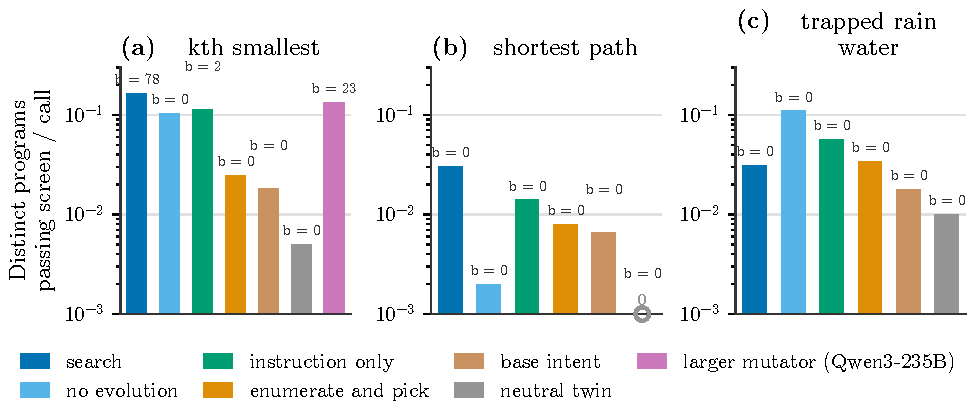
\includegraphics[width=\linewidth,height=0.78\textheight,keepaspectratio]{figures/fig_search_rates_v0.pdf}
\caption{Distinct correct programs passing the catalogue screen per model call (level a; bar height, log-scale \$y\$-axis shared by all three panels; a measured rate of exactly 0 is drawn as a hollow circle at the axis floor and labelled \texttt{0'),\allowbreak{} and the count of those programs further adjudicated as known techniques outside the catalogue (\allowbreak{}level b; printed as }b = count' above each bar or marker), for Qwen3-8B on three coding tasks: (a) kth smallest, (b) shortest path, (c) trapped rain water. Bars are coloured by arm, the same seven colours in every panel (legend below, \$x\$-axis otherwise unlabelled): search (dark blue), no evolution (light blue), instruction only (green), enumerate and pick (orange), base intent (tan), neutral twin (grey), and, on kth smallest only, a larger mutator, Qwen3-235B (violet). Search reaches a level-a rate of 0.165 on kth smallest, 6.65 times the enumerate-and-pick arm (0.025), and together with the larger-mutator arm accounts for nearly all level-b hits on that task (78 and 23 programs respectively, against at most 2 for any arm that draws a single sample without evolution); on shortest path and trapped rain water every arm's level-b count is 0. No program in the underlying data was adjudicated as a novel algorithm.}
\label{fig:fig_search_rates}
\end{figure}
\FloatBarrier
\subsection*{7.8 Gemma: temperature, a controlled DAS and a validated circuit at the fork}
\addcontentsline{toc}{subsection}{7.8 Gemma: temperature, a controlled DAS and a validated circuit at the fork}
\noindent{\small\emph{Artifact: \nolinkurl{gen_art_experiment_38}.}}\par\medskip
\subsubsection*{7.8.1 Engine and calibration}
The Gemma experiment  returned to the fork of gemma-3-4b-it on the grid task, where a shared 32-token opening ends at a token that decides between DFS and BFS (Section 6.5). The engine check on 50 twin slots gave 19 BFS programs (0.38), just outside iteration 6's interval for 61 of 200 (0.245 to 0.372), so the check fails as preregistered; iteration 6's own share on the same 50 slots is 0.36, so the slots, not the engine, lean toward BFS. The discrepancy from the empty prefix of iteration 6 did not reproduce: 200 continuations from the empty prefix give 65 BFS on the path over several prompts and 72 on the path for a single prompt, both consistent with the natural 61 (Fisher p 0.75 and 0.29). The two paths disagree on 9 of 200 slots (1 against 8, p 0.039), so the batch shape changes a few coupled programs; by the rule committed beforehand, the probability of BFS given each fork token comes from a calibration run on the main engine (Table 363). The fork token fixes both the algorithm and its implementation: \texttt{ visited} leads to DFS (BFS 1 of 125), and \texttt{ queue} leads to a BFS that carries whole paths and pops from the front of a list, which is BFS but too slow for the 30 by 30 hidden tests (0 of 125 pass).

\begin{table}[H]
\renewcommand{\thetable}{363}
\centering\small\setlength{\tabcolsep}{4.0pt}
\caption{Calibration at the fork: the shared opening prefilled and the fork token forced (125 programs each). [Source: iteration 7, artifact \nolinkurl{gen_art_experiment_38}.]}\label{tab:t383}
\begin{tabular}{>{\raggedright\arraybackslash\hspace{0pt}}p{0.3672\linewidth}>{\raggedright\arraybackslash\hspace{0pt}}p{0.2914\linewidth}>{\raggedright\arraybackslash\hspace{0pt}}p{0.2876\linewidth}}
\toprule
\textbf{Fork token} & \textbf{BFS} & \textbf{Pass} \\
\midrule
\texttt{visited} & 1\slash{}125 & 124\slash{}125 \\
blank line & 111\slash{}125 & 85\slash{}125 \\
\texttt{if} & 122\slash{}125 & 99\slash{}125 \\
\texttt{queue} & 125\slash{}125 & \textbf{0\slash{}125} \\
\bottomrule
\end{tabular}
\end{table}

\subsubsection*{7.8.2 Temperature through the fork in a second family}
The temperature claim holds in Gemma (Table 364). The predicted attempted BFS share, computed from the teacher-forced fork logits divided by T and committed before any temperature sample, matches the observed share in every top-p 1 cell: 0.015 against 0.02 at T 0.3, 0.166 against 0.24 at 0.7, 0.323 against 0.34 at 1.0 and 0.450 against 0.46 at 1.3 (mean absolute error 0.026; every prediction inside its Wilson interval). The entropy of the algorithm given the fork class is 0.153 bits. Lowering T from 1.0 to 0.3 switches 16 slots from BFS to DFS and none back (p 1.5e-5), and half of all slots change their algorithm somewhere across temperature. Top-k 10 cells are identical to top-p 1 program for program. A placebo that shuffles the temperatures of the sweep gives an error of 0.123 and fails the 0.10 bar.

\begin{table}[H]
\renewcommand{\thetable}{364}
\centering\scriptsize\setlength{\tabcolsep}{2.5pt}
\caption{Gemma: predicted against observed BFS share across temperature (same seed, N = 50 per cell). [Source: iteration 7, artifact \nolinkurl{gen_art_experiment_38}.]}\label{tab:t384}
\begin{tabular}{>{\raggedright\arraybackslash\hspace{0pt}}p{0.1328\linewidth}>{\raggedright\arraybackslash\hspace{0pt}}p{0.1568\linewidth}>{\raggedright\arraybackslash\hspace{0pt}}p{0.1492\linewidth}>{\raggedright\arraybackslash\hspace{0pt}}p{0.1027\linewidth}>{\raggedright\arraybackslash\hspace{0pt}}p{0.2488\linewidth}>{\raggedright\arraybackslash\hspace{0pt}}p{0.0794\linewidth}>{\raggedright\arraybackslash\hspace{0pt}}p{0.0539\linewidth}}
\toprule
\textbf{Cell} & \textbf{Predicted attempted BFS} & \textbf{Observed (N = 50)} & \textbf{Wilson 95\%} & \textbf{P(shared opening) predicted \slash{} observed} & \textbf{Correct BFS} & \textbf{Pass} \\
\midrule
T 0.3, top-p 1 & 0.015 & 1\slash{}50 = 0.02 & 0.00-0.10 & 1.00 \slash{} 1.00 & 1 & 1.00 \\
T 0.7, top-p 1 & 0.166 & 12\slash{}50 = 0.24 & 0.14-0.37 & 0.96 \slash{} 0.94 & 8 & 0.92 \\
T 1.0, top-p 1 & 0.323 & 17\slash{}50 = 0.34 & 0.22-0.48 & 0.88 \slash{} 0.86 & 9 & 0.80 \\
T 1.3, top-p 1 & 0.450 & 23\slash{}50 = 0.46 & 0.33-0.60 & 0.78 \slash{} 0.72 & 15 & 0.80 \\
\bottomrule
\end{tabular}
\end{table}

\subsubsection*{7.8.3 DAS at the fork with the controls iteration 6 lacked}
DAS at the fork was fitted on held-out templates and held-out forced sources (768 pairs). The layer was chosen by the committed rule, the argmax of rank-1 recovery under cross-validation, at block 17. Swapping the whole fork state moves the held-out margin by 3.6 nats at block 17, rising to 8.2 to 9.1 nats at blocks 25 to 29; DAS at block 17 recovers 1.98, 2.36, 2.58 and 2.81 of that at ranks 1, 2, 4 and 8 (Tables 364b and 364c), because a trained direction moves the margin further than the weak full state swap at an early block. These controls hold (iteration-8 correction: within their limits below). Fifty random subspaces recover nothing (0.000). Permuting the source labels gives recovery between -0.27 and -0.30 against the true targets (one permutation of three reaches 0.17 at rank 1). A randomly initialised Gemma moves its margin at most 0.25 times as far (interchange intervention accuracy 0.50 to 0.72 against 1.00). The DAS claim's Gemma version is therefore supported at every rank by the random-subspace, permuted-label and untrained-network controls; the dormancy checks (reverse interchange, projected-map retention) were not run, a recovery of 1.98 to 2.81 times the full-state swap is the off-manifold signature Makelov et al. [122] warn about, and the Qwen3-8B and Gemma controls used different objectives, readouts and permutation schemes, so their outcomes are not directly comparable (Table 364d) (iteration-8 correction).

Two limits remain. The committed wording rule does not license calling the subspace one dimensional: rank-1 recovery passes, but the subspace coordinate tracks the natural fork log odds of 120 twin variants at Spearman -0.50, just short of the 0.5 the rule required, and the subspace holds less of the twin's natural variance across prompts than the random 95th percentile at ranks 1, 2 and 4 (0.00093 against 0.00098, 0.00116 against 0.00185, 0.00187 against 0.00275) and more only at rank 8 (0.00565 against 0.00486), so the dial's rank-4 subspace lies below it; at block 22 the rank-1 share lies above it (0.00294 against 0.00078). The committed dormant flag (exp38 \texttt{src/\allowbreak{}g2.\allowbreak{}py} line 618: rank-1 share at or below the random 95th percentile AND \textbar{}rho\textbar{} \textless{} 0.2) was false only because \textbar{}rho\textbar{} = 0.497, the coordinate tracking the natural fork log odds, not because of variance (iteration-8 correction). And the subspace is not unique: across three seeds only one direction is shared (cosine 0.50 to 0.52), and a difference-in-means direction sits at cosine 0.39 to it.

\begin{table}[H]
\renewcommand{\thetable}{364b}
\centering\tiny\setlength{\tabcolsep}{2.5pt}
\caption{Gemma: DAS at the fork by rank, with its controls (held-out templates and held-out forced sources, 768 pairs; block 17, and block 22 for comparison). (iteration-8 correction: the natural variance share lies below the random 95th percentile at ranks 1, 2 and 4 and above it at rank 8; at block 22, rank 1, it lies above (0.00294 against 0.00078); dormancy checks were not run; the controls are not comparable with those of Qwen3-8B, Table 364d) Recovery is the edit's change in the fork margin divided by that of the full state swap at the same block; the directional effect is the change in the fork margin toward the source's class. [Source: iteration 7, artifact \nolinkurl{gen_art_experiment_38}.]}\label{tab:t385}
\begin{tabular}{>{\raggedright\arraybackslash\hspace{0pt}}p{0.0408\linewidth}>{\raggedright\arraybackslash\hspace{0pt}}p{0.1125\linewidth}>{\raggedright\arraybackslash\hspace{0pt}}p{0.0824\linewidth}>{\raggedright\arraybackslash\hspace{0pt}}p{0.0855\linewidth}>{\raggedright\arraybackslash\hspace{0pt}}p{0.0727\linewidth}>{\raggedright\arraybackslash\hspace{0pt}}p{0.0910\linewidth}>{\raggedright\arraybackslash\hspace{0pt}}p{0.1125\linewidth}>{\raggedright\arraybackslash\hspace{0pt}}p{0.1195\linewidth}>{\raggedright\arraybackslash\hspace{0pt}}p{0.1107\linewidth}>{\raggedright\arraybackslash\hspace{0pt}}p{0.0650\linewidth}}
\toprule
\textbf{Rank k} & \textbf{Recovery, median of 3 seeds (each seed)} & \textbf{Directional effect (nats)} & \textbf{Interchange intervention accuracy} & \textbf{50 random subspaces, recovery} & \textbf{Permuted labels, recovery (median of 3)} & \textbf{Randomly initialised Gemma, directional effect (nats)} & \textbf{Natural variance share (random 95th percentile)} & \textbf{Block 22: recovery \slash{} directional effect (nats)} & \textbf{Block 22: random recovery} \\
\midrule
1 & 1.98 (2.04, 1.98, 1.98) & 5.57 & 1.00 & 0.000 & -0.27 & 0.00 & 0.00093 (0.00098) & 1.08 \slash{} 6.03 & 0.000 \\
2 & 2.36 (2.36, 2.33, 2.36) & 6.68 & 1.00 & 0.000 & -0.29 & 1.69 & 0.00116 (0.00185) & 1.32 \slash{} 7.39 & 0.000 \\
4 & 2.58 (2.58, 2.54, 2.58) & 7.57 & 1.00 & 0.000 & -0.30 & 1.69 & 0.00187 (0.00275) & 1.51 \slash{} 8.58 & 0.000 \\
8 & 2.81 (2.81, 2.80, 2.88) & 8.55 & 1.00 & 0.0001 & -0.28 & 1.74 & 0.00565 (0.00486) & 1.71 \slash{} 9.76 & 0.0028 \\
\bottomrule
\end{tabular}
\end{table}

The subspace coordinate at rank 1 tracks the natural fork log odds of the 120 twin variants at Spearman -0.50 (permutation p 0.0005) at block 17 and -0.67 at block 22; the difference-in-means coordinate tracks it at 0.43. A rank-1 difference-in-means interchange recovers 1.01 at block 17 (directional effect 2.84 nats) and 1.06 at block 22.

\begin{table}[H]
\renewcommand{\thetable}{364c}
\centering\footnotesize\setlength{\tabcolsep}{4.0pt}
\caption{Gemma: the full state ceiling and the rank-1 layer scan by block (held-out pairs). The committed rule chose the block with the largest rank-1 recovery under cross-validation; ties go to the earlier block. [Source: iteration 7, artifact \nolinkurl{gen_art_experiment_38}.]}\label{tab:t386}
\begin{tabular}{>{\raggedright\arraybackslash\hspace{0pt}}p{0.0699\linewidth}>{\raggedright\arraybackslash\hspace{0pt}}p{0.1793\linewidth}>{\raggedright\arraybackslash\hspace{0pt}}p{0.1793\linewidth}>{\raggedright\arraybackslash\hspace{0pt}}p{0.1609\linewidth}>{\raggedright\arraybackslash\hspace{0pt}}p{0.3239\linewidth}}
\toprule
\textbf{Block} & \textbf{Full state swap, forced BFS sources (nats)} & \textbf{Full state swap, forced DFS sources (nats)} & \textbf{Share of pairs moved by at least 1 nat} & \textbf{Rank-1 recovery under cross-validation, median (three folds)} \\
\midrule
17 & +3.62 & -1.94 & 0.97 & 2.15 (2.15, 2.26, 2.05) \\
18 & +3.80 & -1.99 & 0.98 & not scanned \\
19 & +4.34 & -1.89 & 0.98 & 2.07 (2.07, 2.10, 1.94) \\
20 & +5.67 & -2.28 & 1.00 & not scanned \\
21 & +5.36 & -2.31 & 1.00 & 1.67 (1.67, 1.80, 1.60) \\
22 & +7.36 & -3.77 & 1.00 & 1.17 (1.17, 1.22, 1.17) \\
23 & +6.87 & -4.16 & 1.00 & 1.20 (1.20, 1.22, 1.17) \\
24 & +7.62 & -5.18 & 1.00 & not scanned \\
25 & +8.19 & -5.23 & 1.00 & 1.07 (1.07, 1.07, 1.07) \\
26 & +9.11 & -5.19 & 1.00 & not scanned \\
27 & +8.99 & -5.65 & 1.00 & 1.09 (1.09, 1.07, 1.09) \\
28 & +8.90 & -5.72 & 1.00 & not scanned \\
29 & +8.81 & -5.80 & 1.00 & 1.10 (1.15, 1.10, 1.09) \\
\bottomrule
\end{tabular}
\end{table}

\begin{table}[H]
\renewcommand{\thetable}{364d}
\centering\footnotesize\setlength{\tabcolsep}{4.0pt}
\caption{The controls of the two families were run under different protocols, so their outcomes are not directly comparable (iteration-8 correction: new table; \texttt{tables/\allowbreak{}control\_\allowbreak{}protocols.\allowbreak{}csv}). [Source: iteration 7, artifact \nolinkurl{gen_art_experiment_38}.]}\label{tab:t387}
\begin{tabular}{>{\raggedright\arraybackslash\hspace{0pt}}p{0.0847\linewidth}>{\raggedright\arraybackslash\hspace{0pt}}p{0.1496\linewidth}>{\raggedright\arraybackslash\hspace{0pt}}p{0.1739\linewidth}>{\raggedright\arraybackslash\hspace{0pt}}p{0.1391\linewidth}>{\raggedright\arraybackslash\hspace{0pt}}p{0.1783\linewidth}>{\raggedright\arraybackslash\hspace{0pt}}p{0.1709\linewidth}}
\toprule
\textbf{Family} & \textbf{Objective} & \textbf{Site and readout} & \textbf{Permutation scheme} & \textbf{Untrained network} & \textbf{Pairs} \\
\midrule
Qwen3-8B (Section 7.3) & whole-program likelihood LME\_\allowbreak{}Y of the source's programs (amended; the committed contrastive objective diverged) & task-specification states at blocks 12-23 (one map over the band); held-out generation of whole programs and teacher-forced LME\_\allowbreak{}Y & labels permuted over the two kept algorithms per task (44\% of training labels changed; 56\% on kth smallest) & random-init Qwen3-8B, shortest path only; committed comparison against the diverged fit (0.013), replaced post hoc by the matched LME\_\allowbreak{}Y fit (5.08) & all source x base pairs (bans W1-W3, forced families 0-2 -\textgreater{} neutral and padding twins); held-out W5 ban and forced families 3-4, N = 30 slots \\
gemma-3-4b-it (Section 7.8) & single-token fork margin (logsumexp over the BFS tokens minus the ' visited' logit) & block 17 at the fork position (response index 32, opening prefilled); teacher-forced margin, then generation & BFS\slash{}DFS source labels swapped (3 permutations) & randomly initialised Gemma on the same fork-margin readout & 768 held-out pairs (held-out templates and forced sources) \\
\bottomrule
\end{tabular}
\end{table}

\subsubsection*{7.8.4 A dose dial that keeps the programs}
In generation the DAS edit at block 17, applied once at the fork position with the opening prefilled, acts as a dose dial (Table 365). From the twin's 11 correct BFS programs of 50, the edit raises correct BFS to 20, 27, 31, 37, 38 and 42 as lambda rises from 0.1 to 1, at pass rates of 0.68 to 0.88; the explicit instruction to use BFS gives 35, but it was sampled from index 0 without the prefilled opening and is not comparable: the DAS, difference-in-means and twin cells run with the canonical 32-token opening prefilled (exp38 \texttt{src/\allowbreak{}g2.\allowbreak{}py} line 877, \texttt{run.\allowbreak{}run\_\allowbreak{}cell(\allowbreak{}ids,\allowbreak{} cs,\allowbreak{} rows\_\allowbreak{}w,\allowbreak{} raw,\allowbreak{} .\allowbreak{}.\allowbreak{}.\allowbreak{})}), while the forced-BFS ceiling is sampled from index 0 with no prefix (lines 878-885, \texttt{run.\allowbreak{}run\_\allowbreak{}cell(\allowbreak{}pfz[\allowbreak{}"ids"],\allowbreak{} [\allowbreak{}],\allowbreak{} rows,\allowbreak{} raw,\allowbreak{} "G2:\allowbreak{}forced")}) on the same CRN slots (iteration-8 correction). A difference-in-means direction scaled to the same teacher-forced effect flips the algorithm just as well (up to 50 of 50 attempts) and destroys the programs (pass 0.70 down to 0.00, never significantly more correct BFS than the twin). A version of the DAS edit restricted to the logits, which changes the fork token's distribution but not the state that persists in the cache, gives 35 correct programs: the edited fork state helps the later code. The teacher-forced prediction of the attempted share (the fork distribution times the probability of BFS given each token) matches the observed share within 0.10 in all 26 cells (mean gap 0.029). Toward DFS, the edit gives 41 to 50 correct DFS programs of 50 against the twin's 32 (Table 365b). The strong difference-in-means edit toward DFS, left unmatched by a bisection bug, keeps most programs (45 correct of 49 attempted, pass 0.90), so the difference-in-means edit breaks the programs when it pushes toward BFS, not toward DFS. In iteration 6, a rank-4 interchange at block 22 had produced 50 BFS attempts and 0 valid programs; a dosed edit to the coordinate of the class mean at block 17 keeps them.

\begin{figure}[!htbp]
\centering\captionsetup{font=footnotesize}
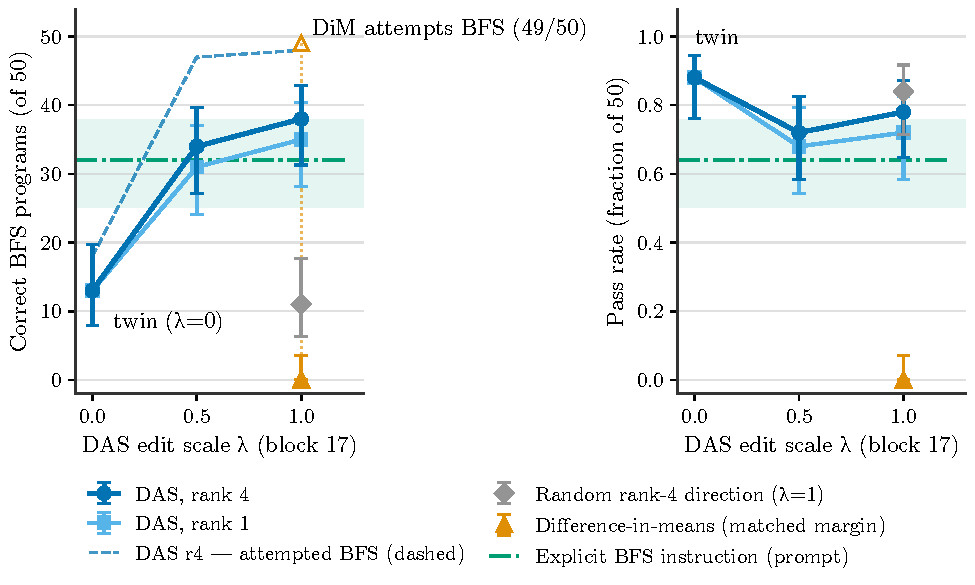
\includegraphics[width=\linewidth,height=0.78\textheight,keepaspectratio]{figures/fig_gemma_dose_v0.pdf}
\caption{Gemma-3-4b-it, grid-path task, one fork (block 17, free generation with no prefilled opening), \$N=50\$ CRN-matched programs per condition; error bars are 95\textbackslash{}\% Wilson confidence intervals. Left: correct BFS programs out of 50 against DAS edit scale \$\textbackslash{}lambda \textbackslash{}in \textbackslash{}\{0, 0.5, 1.0\textbackslash{}\}\$ (\$\textbackslash{}lambda=0\$ is the unedited twin). Right: pass rate (fraction of 50) on the same \$x\$-axis. Dark-blue circles\slash{}line: DAS, rank 4 (\$13 \textbackslash{}to 34 \textbackslash{}to 38\$ correct; pass \$0.88 \textbackslash{}to 0.72 \textbackslash{}to 0.78\$). Light-blue squares\slash{}line: DAS, rank 1 (\$13 \textbackslash{}to 31 \textbackslash{}to 35\$ correct; pass \$0.88 \textbackslash{}to 0.68 \textbackslash{}to 0.72\$). Dark-blue dashed line (left panel only): BFS programs attempted under the rank-4 edit regardless of correctness (\$18 \textbackslash{}to 47 \textbackslash{}to 48\$). Grey diamond: an untrained random rank-4 direction at \$\textbackslash{}lambda=1\$ reaches only \$11\slash{}50\$ correct (pass \$0.84\$), showing the DAS direction itself, not any perturbation of that size, drives the shift. Orange triangle: a difference-in-means edit scaled to match DAS's teacher-forced effect at \$\textbackslash{}lambda=1\$ attempts BFS just as often (open triangle, \$49\slash{}50\$) but is never correct (filled triangle, \$0\slash{}50\$, pass \$0.00\$) --- it flips the algorithm's surface form while destroying the programs. Green dash-dot line with shaded band: an explicit ``use BFS'' prompt (free generation, no \$\textbackslash{}lambda\$), \$32\slash{}50\$ correct, pass \$0.64\$, drawn as a flat reference since it carries no dose. All conditions are free-generation, so the prompting baseline is sampled exactly like the dial (no prefilled opening on either arm). One model, one task, one fork: this is a case study, and \$\textbackslash{}lambda\$ was tested at only two non-zero values.}
\label{fig:fig_gemma_dose}
\end{figure}
\begin{table}[H]
\renewcommand{\thetable}{365}
\centering\footnotesize\setlength{\tabcolsep}{4.0pt}
\caption{Gemma: DAS against difference in means as a dose dial toward BFS (N = 50 per cell, same seed). (iteration-8 correction: every cell except the forced BFS prompt has the shared 32-token opening prefilled; the forced BFS prompt is sampled from index 0 without it, on the same slots, so its row is not comparable with the edits) [Source: iteration 7, artifact \nolinkurl{gen_art_experiment_38}.]}\label{tab:t388}
\begin{tabular}{>{\raggedright\arraybackslash\hspace{0pt}}p{0.3498\linewidth}>{\raggedright\arraybackslash\hspace{0pt}}p{0.1133\linewidth}>{\raggedright\arraybackslash\hspace{0pt}}p{0.0889\linewidth}>{\raggedright\arraybackslash\hspace{0pt}}p{0.0604\linewidth}>{\raggedright\arraybackslash\hspace{0pt}}p{0.1672\linewidth}>{\raggedright\arraybackslash\hspace{0pt}}p{0.1171\linewidth}}
\toprule
\textbf{Cell} & \textbf{Attempted BFS} & \textbf{Correct BFS} & \textbf{Pass} & \textbf{p (correct \textgreater{} twin, one sided McNemar, Holm over 6 doses)} & \textbf{Teacher-forced predicted attempted share} \\
\midrule
twin (no edit) & 18 & 11 & 0.86 & - & 0.26 \\
DAS lambda 0.1 & 27 & 20 & 0.86 & 0.006 & 0.47 \\
DAS lambda 0.2 & 38 & 27 & 0.78 & 4e-4 & 0.75 \\
DAS lambda 0.35 & 46 & 31 & 0.68 & 5e-5 & 0.92 \\
DAS lambda 0.5 & 47 & 37 & 0.78 & 2e-6 & 0.96 \\
DAS lambda 0.75 & 47 & 38 & 0.80 & 1e-6 & 0.96 \\
DAS lambda 1 & 47 & \textbf{42} & \textbf{0.88} & 2e-8 & 0.96 \\
difference in means 0.1 (matched teacher-forced effect) & 30 & 15 & 0.70 & 0.87 & 0.52 \\
difference in means 0.2 & 36 & 15 & 0.58 & 0.87 & 0.78 \\
difference in means 0.35 & 46 & 12 & 0.32 & 1.00 & 0.95 \\
difference in means 0.5 & 48 & 11 & 0.26 & 1.00 & 0.99 \\
difference in means 0.75 & 50 & 2 & 0.04 & 1.00 & 1.00 \\
difference in means 1 & 50 & 0 & 0.00 & 1.00 & 1.00 \\
random rank-4 subspace, lambda 1 & 17 & 12 & 0.90 & 0.50 (unadjusted) & 0.25 \\
forced BFS prompt, fifth forced source (sampled from index 0 without the prefilled opening; not comparable) & 50 & 35 & 0.70 & 4e-6 (unadjusted) & - \\
DAS on the logits only, lambda 1 & 44 & 35 & 0.76 & 2e-6 (unadjusted) & - \\
DAS on the logits only, lambda 0.5 & 46 & 35 & 0.76 & 2e-6 (unadjusted) & - \\
\bottomrule
\end{tabular}
\end{table}

\begin{table}[H]
\renewcommand{\thetable}{365b}
\centering\footnotesize\setlength{\tabcolsep}{4.0pt}
\caption{Gemma: the same edits toward DFS (N = 50 per cell, same seed; the twin writes DFS in 32 of 50). The six difference-in-means cells toward DFS were left unmatched by a bisection bug and are identical; they are reported once, as a strong reference edit. [Source: iteration 7, artifact \nolinkurl{gen_art_experiment_38}.]}\label{tab:t389}
\begin{tabular}{>{\raggedright\arraybackslash\hspace{0pt}}p{0.3552\linewidth}>{\raggedright\arraybackslash\hspace{0pt}}p{0.1133\linewidth}>{\raggedright\arraybackslash\hspace{0pt}}p{0.0967\linewidth}>{\raggedright\arraybackslash\hspace{0pt}}p{0.0604\linewidth}>{\raggedright\arraybackslash\hspace{0pt}}p{0.2876\linewidth}}
\toprule
\textbf{Cell} & \textbf{Attempted DFS} & \textbf{Correct DFS} & \textbf{Pass} & \textbf{McNemar on correct DFS against the twin (cell only : twin only)} \\
\midrule
twin (no edit) & 32 & 32 & 0.86 & - \\
DAS lambda 0.1 & 41 & 41 & 0.94 & 9:0 \\
DAS lambda 0.2 & 46 & 46 & 0.98 & 14:0 \\
DAS lambda 0.35 & 50 & 50 & 1.00 & 18:0 \\
DAS lambda 0.5 & 50 & 50 & 1.00 & 18:0 \\
DAS lambda 0.75 & 50 & 50 & 1.00 & 18:0 \\
DAS lambda 1 & 50 & 50 & 1.00 & 18:0 \\
difference in means toward DFS (one strong edit) & 49 & 45 & 0.90 & 14:1 \\
\bottomrule
\end{tabular}
\end{table}

\subsubsection*{7.8.5 A circuit for the fork margin}
\emph{Path patching} replaces a component's contribution along one path with its value under a contrasting input and measures the effect on the output [134, 135]; \emph{attribution patching} (AtP) approximates the same effect for every node with one gradient pass [136]. The experiment screened 1,224 nodes (272 attention heads and 34 MLPs at four position classes: the fork position, the shared opening, the task specification and the condition sentence) by AtP on 15 contrasting pairs, patched the top 60 exactly by \emph{noising}, which writes a node's value from the run of a pair that leans toward BFS into the run that leans toward DFS (AtP against exact noising: Pearson 0.65, Spearman 0.73; the reverse, denoising, has the opposite sign for every node), and edges measured by path patching among the top 15. Half of the exact noising effect enters at the fork position (53\%) and a third at the condition sentence (36\%). The top ten nodes are MLPs at the condition sentence (layers 0, 2, 6 and 14) and a stack at the fork position (MLPs at layers 17, 21, 22, 25 and 26, and head 5 of layer 22; Table 366). Kept edges, those whose effect under path patching is at least 5\% of the total effect, form a chain at the fork position (MLP 17 to MLP 19, MLP 21 to MLP 22, MLP 25 to MLP 26, and head 5 of layer 22 to MLP 25), with direct paths to the margin from head 2 of layer 33 and MLPs 22, 25 and 26.

Each top node was validated in the real model against 50 random components of its position class matched on write norm (Table 367). Seven of ten nodes pass when ablated to the opposite class's mean, and eight pass when steered; the joint sets of the top five and the top ten beat all 50 matched random sets. In generation, steering the top five toward BFS doubles correct BFS programs (16 of 30 against 8 for the twin, p 0.019) at pass 0.83, while a matched random five does nothing (Table 368). Ablating the same nodes to the natural BFS mean does not move generation, because the natural classes differ by only about 2 nats at the fork. The reading is a circuit hypothesis for this one fork: MLPs at the condition sentence carry the prompt's lexical cue, and the stack at the fork position turns it into the token at index 32. An \emph{attribution graph}, the graph of direct linear effects between transcoder features from the prompt to the fork margin, built on the Gemma Scope 2 transcoders [113], would test the circuit on features; it was attempted three times and dropped: the container lacked a C compiler for Triton, and with one installed, attribution exceeded the 16 GB GPU at batch 64 and again at batch 16 (16.4 GB). No correct program among 2,325 was outside the catalogue (rule-of-three bound 0.0013).

The deviation log of the Gemma experiment records five departures that bear on these results. One unit test missed its tolerance: the cache path for a single position differs from a full recompute by up to 0.27 nats on the fork margin, an effect of bf16 kernels and batch shapes, so every DAS effect is measured against the base's own margin on the same path and in the same batch shape. The DAS optimiser ran at a learning rate of 2e-2 instead of the planned 2e-3, because a toy check showed that 400 steps at 2e-3 leave the subspace near random. A bisection bug left the six difference-in-means cells toward DFS unmatched, so they are reported as one strong reference edit (45 of 50 correct DFS). The mediation test of the fork subspace on random pushes was not run (dropped in order), so the DAS claim covers forced prompt transfer only. And the transcoder graph was dropped after the three attempts described above.

\begin{table}[H]
\renewcommand{\thetable}{366}
\centering\small\setlength{\tabcolsep}{4.0pt}
\caption{Gemma: the top ten nodes by exact noising effect (mean over 15 pairs). [Source: iteration 7, artifact \nolinkurl{gen_art_experiment_38}.]}\label{tab:t390}
\begin{tabular}{>{\raggedright\arraybackslash\hspace{0pt}}p{0.6960\linewidth}>{\raggedright\arraybackslash\hspace{0pt}}p{0.2668\linewidth}}
\toprule
\textbf{Node} & \textbf{Noising effect (nats)} \\
\midrule
MLP of layer 0 at the condition sentence & +4.43 \\
MLP of layer 6 at the condition sentence & +2.01 \\
MLP of layer 25 at the fork position & +1.96 \\
MLP of layer 21 at the fork position & +1.54 \\
MLP of layer 2 at the condition sentence & +1.00 \\
attention head 5 of layer 22 at the fork position & +1.00 \\
MLP of layer 26 at the fork position & +0.97 \\
MLP of layer 14 at the condition sentence & +0.93 \\
MLP of layer 22 at the fork position & +0.86 \\
MLP of layer 17 at the fork position & +0.84 \\
\bottomrule
\end{tabular}
\end{table}

\begin{table}[H]
\renewcommand{\thetable}{367}
\centering\small\setlength{\tabcolsep}{4.0pt}
\caption{Gemma: validation of each node against 50 matched random components. The effect d of a node is its oriented change in the fork margin minus the mean change under the 50 matched random components. [Source: iteration 7, artifact \nolinkurl{gen_art_experiment_38}.]}\label{tab:t391}
\begin{tabular}{>{\raggedright\arraybackslash\hspace{0pt}}p{0.3829\linewidth}>{\raggedright\arraybackslash\hspace{0pt}}p{0.1908\linewidth}>{\raggedright\arraybackslash\hspace{0pt}}p{0.1900\linewidth}>{\raggedright\arraybackslash\hspace{0pt}}p{0.1660\linewidth}}
\toprule
\textbf{Node} & \textbf{ablate median d (Holm p)} & \textbf{steer median d (Holm p)} & \textbf{Claim (ablate \slash{} steer)} \\
\midrule
MLP of layer 0 at the condition sentence & +0.28 (\textless{} 1e-4) & +0.49 (4e-4) & yes \slash{} yes \\
MLP of layer 6 at the condition sentence & +0.16 (0.09) & +0.25 (0.25) & no \slash{} no \\
MLP of layer 25 at the fork position & +0.28 (3e-4) & +0.62 (\textless{} 1e-4) & yes \slash{} yes \\
MLP of layer 21 at the fork position & +0.23 (5e-4) & +0.48 (\textless{} 1e-4) & yes \slash{} yes \\
MLP of layer 2 at the condition sentence & +0.07 (0.15) & +0.10 (0.13) & no \slash{} no \\
attention head 5 of layer 22 at the fork position & +0.19 (0.002) & +0.39 (\textless{} 1e-4) & yes \slash{} yes \\
MLP of layer 26 at the fork position & +0.15 (5e-4) & +0.61 (\textless{} 1e-4) & yes \slash{} yes \\
MLP of layer 14 at the condition sentence & +0.17 (5e-4) & +0.39 (0.001) & yes \slash{} yes \\
MLP of layer 22 at the fork position & +0.34 (1e-4) & +0.68 (\textless{} 1e-4) & yes \slash{} yes \\
MLP of layer 17 at the fork position & +0.05 (0.10) & +0.17 (\textless{} 1e-4) & no \slash{} yes \\
\bottomrule
\end{tabular}
\end{table}

\begin{table}[H]
\renewcommand{\thetable}{368}
\centering\footnotesize\setlength{\tabcolsep}{4.0pt}
\caption{Gemma: generation arms with the validated nodes (N = 30, opening prefilled). [Source: iteration 7, artifact \nolinkurl{gen_art_experiment_38}.]}\label{tab:t392}
\begin{tabular}{>{\raggedright\arraybackslash\hspace{0pt}}p{0.2128\linewidth}>{\raggedright\arraybackslash\hspace{0pt}}p{0.1133\linewidth}>{\raggedright\arraybackslash\hspace{0pt}}p{0.0889\linewidth}>{\raggedright\arraybackslash\hspace{0pt}}p{0.0604\linewidth}>{\raggedright\arraybackslash\hspace{0pt}}p{0.4379\linewidth}}
\toprule
\textbf{Arm} & \textbf{Attempted target} & \textbf{Correct target} & \textbf{Pass} & \textbf{Test} \\
\midrule
twin & 9 BFS & 8 & 0.97 & - \\
top-5 steer toward BFS & 20 BFS & \textbf{16} & 0.83 & vs twin: correct 10 vs 2, p = 0.019; attempted 12 vs 1, p = 0.002. vs random-5 steer: p = 0.006 (correct), 0.002 (attempted) \\
random-5 steer (matched) & 9 BFS & 7 & 0.93 & null \\
top-5 ablate to the BFS mean & 12 BFS & 7 & 0.83 & attempted 3 vs 0, p = 0.125 \\
random-5 ablate & 9 BFS & 6 & 0.90 & null \\
top-10 ablate to the BFS mean & 12 BFS & 10 & 0.93 & p = 0.125 (attempted) \\
top-5 ablate to the DFS mean & 22 DFS & 22 & 0.90 & vs twin 21 DFS: n.s. \\
\bottomrule
\end{tabular}
\end{table}

\FloatBarrier
\subsection*{7.9 Comparisons across this iteration's experiments}
\addcontentsline{toc}{subsection}{7.9 Comparisons across this iteration's experiments}
\textbf{Temperature through the fork, in two families.} The temperature claim was tested on four mixed units in two models. The fork logits predicted the temperature response within the committed error on two of them (the grid in Gemma, mean absolute error 0.026, and minimum spanning tree weight in Qwen3-8B, 0.083, where the observed drop was twice the predicted one), just outside it on trapped rain water (0.105), and not in direction on valid anagram, where the minority share did not fall at low temperature. Table 369 sets them side by side. On every unit the algorithm given the fork class was nearly certain (0.05 to 0.19 bits) and top-k 10 changed nothing. Temperature above 1 raised the minority only where the fork logits said it would: in Gemma the BFS share rose from 0.34 at T 1.0 to 0.46 at T 1.3 against a predicted rise from 0.323 to 0.450, while on the three Qwen3-8B units the predicted rise was at most 0.013 and the observed change lay between -0.02 and +0.06. On the collapsed tasks the fork margins of 4.85 to 17.04 nats explain why no temperature in iterations 1 to 4 changed the algorithm. Temperature is a dial on the fork's existing odds; it cannot create an alternative that the fork does not already weigh.

\begin{table}[H]
\renewcommand{\thetable}{369}
\centering\scriptsize\setlength{\tabcolsep}{2.5pt}
\caption{The temperature claim in two model families (top-p 1, same seed). [Source: iteration 7, compiled across the iteration's artifacts \nolinkurl{gen_art_evaluation_6}, \nolinkurl{gen_art_experiment_33}, \nolinkurl{gen_art_experiment_34}, \nolinkurl{gen_art_experiment_35}, \nolinkurl{gen_art_experiment_36}, \nolinkurl{gen_art_experiment_37}, \nolinkurl{gen_art_experiment_38}.]}\label{tab:t393}
\begin{tabular}{>{\raggedright\arraybackslash\hspace{0pt}}p{0.1478\linewidth}>{\raggedright\arraybackslash\hspace{0pt}}p{0.1806\linewidth}>{\raggedright\arraybackslash\hspace{0pt}}p{0.1558\linewidth}>{\raggedright\arraybackslash\hspace{0pt}}p{0.1622\linewidth}>{\raggedright\arraybackslash\hspace{0pt}}p{0.1004\linewidth}>{\raggedright\arraybackslash\hspace{0pt}}p{0.0832\linewidth}>{\raggedright\arraybackslash\hspace{0pt}}p{0.0935\linewidth}}
\toprule
\textbf{Model and unit} & \textbf{Fork token pair} & \textbf{Entropy of the algorithm given the fork class (bits)} & \textbf{Minority share at T 0.3 \slash{} 1.0 \slash{} 1.3 (observed)} & \textbf{Predicted} & \textbf{Mean absolute error} & \textbf{Drop T 1.0 to 0.3 (McNemar)} \\
\midrule
Qwen3-8B, minimum spanning tree weight & \texttt{ Kr} (Kruskal) or \texttt{ Prim} & 0.050 & 0.06 \slash{} 0.40 \slash{} 0.38 & 0.068 \slash{} 0.237 \slash{} 0.247 & 0.083 & 17:0 \\
Qwen3-8B, trapped rain water & \texttt{ n} (prefix and suffix) or \texttt{ left} (two pointers) & 0.153 & 0.10 \slash{} 0.18 \slash{} 0.20 & 0.166 \slash{} 0.311 \slash{} 0.319 & 0.105 & 7:3 \\
Qwen3-8B, valid anagram & \texttt{ return} (sort) or \texttt{ count} & 0.189 & 0.18 \slash{} 0.12 \slash{} 0.18 & 0.161 \slash{} 0.200 \slash{} 0.212 & 0.043 & 2:5 \\
gemma-3-4b-it, grid & \texttt{ visited} (DFS) or a blank line, \texttt{if}, \texttt{ queue} (BFS) & 0.153 & 0.02 \slash{} 0.34 \slash{} 0.46 & 0.015 \slash{} 0.323 \slash{} 0.450 & 0.026 & 16:0 \\
\bottomrule
\end{tabular}
\end{table}

\textbf{Where the choice is decided.} Three different answers came out of three tasks in one model. On connected components the decision falls at generated tokens 10 and 11, where the routine is named; forcing the name decides the algorithm in every slot. On kth smallest a ban decides it before the first generated token. On shortest path no single token decides it within 60 tokens, and the opening's likelihood predicts the outcome better the longer the opening measured. The three mixed units of the temperature experiment and Gemma's grid task each have a fork of a single token right after a shared opening of 18 to 61 tokens. The fork is thus a common place for the decision to surface, not a universal one, and where it exists, the effect of a push is already expressed at the fork token on connected components (a teacher-forced readout of the margin matches the sampled outcomes of random pushes at Spearman 0.80, and the 48-token opening log-likelihood ratio at 0.87; no direction-level property predicted which pushes move the fork), and its logits divided by T predicted the temperature response within the committed error on two of the four mixed units (iteration-8 correction).

\textbf{What moves the algorithm, and at what cost.} Table 370 collects the edits of this iteration that move the algorithm in generation, with their correct target programs and pass rates. In Qwen3-8B a rank-1 or rank-2 DAS edit matches the full state exchange at the same site for most sources (it recovers 0.06 to 0.53 of forced BFS and 0.17 to 0.43 of forced Bellman-Ford\slash{}SPFA; Table 297b; iteration-8 correction), plan noise at the absolute unit moves half of connected components programs at no pass cost, and the axis from the default to the second choice moves connected components only at a dose beyond the committed range. In Gemma the DAS edit at the fork, with the shared opening prefilled, raises correct BFS programs from 11 to 42 of 50 (the explicit instruction's 35 was sampled without the prefill and is not comparable), and steering five validated circuit nodes doubles them (iteration-8 correction). In Gemma the difference-in-means edit toward BFS moves the algorithm and breaks the programs (toward the default DFS a strong edit kept them), and in Qwen3-8B a rank-1 difference-in-means interchange at the DAS site transfers nothing (0 of 30 on both core tasks). In this iteration the edits fitted or validated on the model's own contrasts kept the programs; the difference-in-means edit toward the minority algorithm did not.

\begin{table}[H]
\renewcommand{\thetable}{370}
\centering\footnotesize\setlength{\tabcolsep}{4.0pt}
\caption{Edits that moved the algorithm in generation in iteration 7. (iteration-8 correction: prefill condition of the two Gemma rows stated; kth smallest counting sort row annotated) [Source: iteration 7, compiled across the iteration's artifacts \nolinkurl{gen_art_evaluation_6}, \nolinkurl{gen_art_experiment_33}, \nolinkurl{gen_art_experiment_34}, \nolinkurl{gen_art_experiment_35}, \nolinkurl{gen_art_experiment_36}, \nolinkurl{gen_art_experiment_37}, \nolinkurl{gen_art_experiment_38}.]}\label{tab:t394}
\begin{tabular}{>{\raggedright\arraybackslash\hspace{0pt}}p{0.1778\linewidth}>{\raggedright\arraybackslash\hspace{0pt}}p{0.3223\linewidth}>{\raggedright\arraybackslash\hspace{0pt}}p{0.2870\linewidth}>{\raggedright\arraybackslash\hspace{0pt}}p{0.0657\linewidth}>{\raggedright\arraybackslash\hspace{0pt}}p{0.0604\linewidth}}
\toprule
\textbf{Model and task} & \textbf{Edit} & \textbf{Correct target programs} & \textbf{Twin} & \textbf{Pass} \\
\midrule
Qwen3-8B, shortest path & DAS rank 2, fifth template ban source, blocks 12-23 & 12\slash{}30 Bellman-Ford\slash{}SPFA & 1\slash{}30 & 0.83 \\
Qwen3-8B, shortest path & DAS rank 1, forced Floyd-Warshall source & 28\slash{}30 Floyd-Warshall & 0\slash{}30 & 0.93 \\
Qwen3-8B, connected components & DAS rank 16, fifth template ban source & 29\slash{}30 BFS or DFS & 0\slash{}30 & 1.00 \\
Qwen3-8B, connected components & Plan noise, absolute unit, alpha 2 & 25\slash{}50 & 0\slash{}50 & 0.98 \\
Qwen3-8B, connected components & Axis push at four times the forced prompt distance & 30\slash{}30 (29 DFS, 1 BFS) & 0\slash{}30 & 1.00 \\
Qwen3-8B, connected components & Tokens 10-11 forced to \texttt{ def dfs} & 30\slash{}30 DFS & 0\slash{}30 & 1.00 \\
Qwen3-8B, kth smallest & DAS rank 1, forced counting sort source & 30\slash{}30 counting sort (28 an array of counts; the full state exchange gives 29\slash{}30 in dictionary form, iteration-8 correction) & 0\slash{}30 & 1.00 \\
Qwen3-8B, kth smallest & Plan noise, absolute unit, alpha 2 (pricing cell) & 30\slash{}50 & 1\slash{}50 & 0.98 \\
Qwen3-8B, three mixed units & Exchange of the forced minority prompt's task specification states & 30\slash{}30 on each & 0 to 7\slash{}30 & 1.00 \\
gemma-3-4b-it, grid & DAS rank 4 at block 17, lambda 1 (opening prefilled) & 42\slash{}50 BFS & 11\slash{}50 & 0.88 \\
gemma-3-4b-it, grid & Explicit BFS instruction (no prefill, not comparable) & 35\slash{}50 BFS & 11\slash{}50 & 0.70 \\
gemma-3-4b-it, grid & Difference in means, lambda 1 & 0\slash{}50 BFS & 11\slash{}50 & 0.00 \\
gemma-3-4b-it, grid & Steering the five validated nodes toward BFS & 16\slash{}30 BFS & 8\slash{}30 & 0.83 \\
\bottomrule
\end{tabular}
\end{table}

\textbf{Novelty.} Table 371 collects the novelty audits of this iteration. Across the seven artifacts, the only correct programs outside the catalogue are the known techniques reached on kth smallest by evolutionary search, the larger mutator and the instruction alone, and none is novel.

\begin{table}[H]
\renewcommand{\thetable}{371}
\centering\small\setlength{\tabcolsep}{4.0pt}
\caption{Novelty audits of iteration 7. (iteration-8 correction: the DAS experiment row names the counting-sort cells) [Source: iteration 7, compiled across the iteration's artifacts \nolinkurl{gen_art_evaluation_6}, \nolinkurl{gen_art_experiment_33}, \nolinkurl{gen_art_experiment_34}, \nolinkurl{gen_art_experiment_35}, \nolinkurl{gen_art_experiment_36}, \nolinkurl{gen_art_experiment_37}, \nolinkurl{gen_art_experiment_38}.]}\label{tab:t395}
\begin{tabular}{>{\raggedright\arraybackslash\hspace{0pt}}p{0.1296\linewidth}>{\raggedright\arraybackslash\hspace{0pt}}p{0.1841\linewidth}>{\raggedright\arraybackslash\hspace{0pt}}p{0.5384\linewidth}>{\raggedright\arraybackslash\hspace{0pt}}p{0.0776\linewidth}}
\toprule
\textbf{Artifact} & \textbf{Programs audited} & \textbf{Final classes} & \textbf{Novel} \\
\midrule
Record audit & 3 programs of the engine control labelled other & catalogue variants (Dijkstra by array scan, Bellman-Ford of n rounds) & 0 \\
DAS experiment & 38 correct programs labelled other & 36 catalogue variants (35 are counting sort in dictionary form, 29 of them from the full state exchange of the forced counting sort source; relabelled counting sort in iteration 8), 2 labeller misses & 0 \\
Fork experiment & 2 & 2 labeller misses & 0 \\
Temperature experiment & 2 distinct programs (40 continuations) & catalogue variant (the extra counting mode of valid anagram) & 0 \\
Dose unit experiment & 5 kth smallest programs & catalogue variant (counting sort with key compression) & 0 \\
Search experiment & 816 distinct programs passing the screen & 707 catalogue variants, 103 known techniques outside the catalogue, 6 degenerate & 0 \\
Gemma experiment & 2,325 correct programs & none outside the catalogue & 0 \\
\bottomrule
\end{tabular}
\end{table}

{\footnotesize\setlength{\tabcolsep}{4.0pt}\renewcommand{\thetable}{371b}
\begin{longtable}{>{\raggedright\arraybackslash\hspace{0pt}}p{0.1161\linewidth}>{\raggedright\arraybackslash\hspace{0pt}}p{0.1244\linewidth}>{\raggedright\arraybackslash\hspace{0pt}}p{0.1577\linewidth}>{\raggedright\arraybackslash\hspace{0pt}}p{0.1121\linewidth}>{\raggedright\arraybackslash\hspace{0pt}}p{0.1274\linewidth}>{\raggedright\arraybackslash\hspace{0pt}}p{0.2590\linewidth}}
\caption{Positioning of the iteration-7 claims (to our knowledge, mini search dated 2026-10-22, re-verified 2026-10-23 with fetch\_\allowbreak{}grep of each abstract and venue page; raw outputs in \texttt{audit/\allowbreak{}web/\allowbreak{}}). Verdicts come from the record audit's positioning search (\nolinkurl{gen_art_evaluation_6} \texttt{positioning.\allowbreak{}json}). (iteration-8 correction: new table) [Source: iteration 7, compiled across the iteration's artifacts \nolinkurl{gen_art_evaluation_6}, \nolinkurl{gen_art_experiment_33}, \nolinkurl{gen_art_experiment_34}, \nolinkurl{gen_art_experiment_35}, \nolinkurl{gen_art_experiment_36}, \nolinkurl{gen_art_experiment_37}, \nolinkurl{gen_art_experiment_38}.]}\label{tab:t396}\\
\toprule
\textbf{Claim} & \textbf{Nearest neighbours (venue)} & \textbf{What they do} & \textbf{What the run adds} & \textbf{Verdict} & \textbf{Evidence (URL, version, quote, status, date)} \\
\midrule
\endfirsthead
\multicolumn{6}{l}{\emph{Table 371b, continued}}\\
\toprule
\textbf{Claim} & \textbf{Nearest neighbours (venue)} & \textbf{What they do} & \textbf{What the run adds} & \textbf{Verdict} & \textbf{Evidence (URL, version, quote, status, date)} \\
\midrule
\endhead
\bottomrule
\endlastfoot
Temperature acts on the algorithm through the fork logits divided by T & Hot or Cold? Adaptive Temperature Sampling for Code Generation (AAAI 2024); Control the Temperature (COLM 2025); Entropy-informed Decoding (ICML 2026 (arXiv 2605.09745 comment)); Beyond the 80\slash{}20 Rule (NeurIPS 2025); A Tale of Two Temperatures (COLM (arXiv v2 comment, no year); ICML 2026 workshop posters) & Hot or Cold? Adaptive Temperature Sampling for Code Generation: temperature set by token difficulty in code generation, no algorithm-level prediction; Control the Temperature: switches temperature per token to protect precision; Entropy-informed Decoding: branches decoding at high-entropy tokens, no algorithm-level outcome; Beyond the 80\slash{}20 Rule: forking (high-entropy) tokens drive RL for reasoning, not temperature at a code fork; A Tale of Two Temperatures: tempered remasking for sample diversity in diffusion language models, not autoregressive code & a per-algorithm prediction of the temperature response from teacher-forced fork logits, committed before sampling, and fork margins that explain the nulls on the collapsed tasks & adjacent: no neighbour predicts an algorithm-level temperature response & \url{https://arxiv.org/abs/2309.02772} (v1 6 Sep 2023, v3 28 Dec 2023; 'Hot or Cold? Adaptive Temperature Sampling for Code Generation'; 'accepted by AAAI 2024'; VERIFIED, 2026-10-23); \url{https://arxiv.org/abs/2510.01218} (v1 20 Sep 2025; 'Control the Temperature'; 'Second Conference on Language Modeling, 2025'; VERIFIED, 2026-10-23); \url{https://arxiv.org/abs/2605.09745} (v1 10 May 2026; 'Entropy-informed Decoding'; 'Accepted at ICML 2026'; VERIFIED, 2026-10-23); \url{https://arxiv.org/abs/2506.01939} (v1 2 Jun 2025, v2 13 Nov 2025; 'Beyond the 80\slash{}20 Rule'; 'Accepted to NeurIPS 2025'; VERIFIED, 2026-10-23); \url{https://arxiv.org/abs/2604.09921} (v1 10 Apr 2026, v2 10 Aug 2026; 'A Tale of Two Temperatures'; 'V2: accepted as a full conference paper at COLM'; VERIFIED, 2026-10-23); \url{https://icml.cc/virtual/2026/75333} (AdaptFM: Resource-Adaptive Foundation Model Inference; VERIFIED, 2026-10-23); \url{https://icml.cc/virtual/2026/74361} (4th Structured Probabilistic Inference \& Generative Modeling; VERIFIED, 2026-10-23) \\
A DAS subspace at Gemma's fork is a dose dial on the algorithm in code & CDAS (ICLR 2026); MIB (ICML 2025) & CDAS: DAS-style interchange steering validated by generation on refusal and a backdoor; MIB: benchmark that ranks DAS first for causal variable localisation & an algorithm choice in code at a generated fork, with a dose curve that preserves the pass rate (with the shared opening prefilled; the instruction cell is not comparable) & adjacent: DAS steering is published; the algorithm-in-code object and the dose curve are not & \url{https://arxiv.org/abs/2602.05234} (v1 5 Feb 2026, v2 15 Mar 2026; 'Faithful Bi-Directional Model Steering'; 'accepted for ICLR 2026'; VERIFIED, 2026-10-23); \url{https://arxiv.org/abs/2504.13151} (v1 17 Apr 2025, v2 9 Jun 2025; 'MIB: A Mechanistic Interpretability Benchmark'; 'Accepted to ICML 2025'; VERIFIED, 2026-10-23) \\
Evaluator-guided search reaches known techniques outside the catalogue at a rate single samples do not & FunSearch (Nature 2023); AlphaEvolve (2025 (arXiv)); DivAlgo (arXiv 2610.19157); Beneath the Diff (EMNLP 2026); Algorithm Discovery With LLMs (arXiv 2504.05108) & FunSearch: evaluator-guided program search finds new mathematical constructions; AlphaEvolve: evaluator-guided evolutionary coding agent (occupies the method family); DivAlgo: benchmarks algorithmic diversity of code models; Beneath the Diff: algorithmic mode collapse in autonomous research loops; Algorithm Discovery With LLMs: evolutionary search plus RL for algorithm discovery & a rate-matched comparison against single-sample knobs on a frozen LeetCode-style catalogue (78 of 2,500 calls against 2 of 500; 0 novel) & adjacent: the method is occupied (FunSearch, AlphaEvolve); the rate-matched comparison is the addition & \url{https://www.nature.com/articles/s41586-023-06924-6} (version n\slash{}a; 'Mathematical discoveries from program search with large language models'; 'Published: 14 December 2023'; VERIFIED, 2026-10-23); \url{https://arxiv.org/abs/2506.13131} (v1 16 Jun 2025; 'AlphaEvolve: A coding agent'; VERIFIED, 2026-10-23); \url{https://arxiv.org/abs/2610.19157} (v1 13 Oct 2026; 'DivAlgo'; VERIFIED, 2026-10-23); \url{https://arxiv.org/abs/2609.00077} (v1 31 Aug 2026; 'Beneath the Diff'; 'Accepted by EMNLP 2026'; VERIFIED, 2026-10-23); \url{https://arxiv.org/abs/2504.05108} (v1 7 Apr 2025, v4 4 Aug 2025; 'Algorithm Discovery With LLMs'; VERIFIED, 2026-10-23) \\
\end{longtable}}

\FloatBarrier
\subsection*{7.10 What iteration 7 established, what it ruled out, and what it abandoned}
\addcontentsline{toc}{subsection}{7.10 What iteration 7 established, what it ruled out, and what it abandoned}
{\small\setlength{\tabcolsep}{4.0pt}\renewcommand{\thetable}{372}
\begin{longtable}{>{\raggedright\arraybackslash\hspace{0pt}}p{0.1337\linewidth}>{\raggedright\arraybackslash\hspace{0pt}}p{0.2797\linewidth}>{\raggedright\arraybackslash\hspace{0pt}}p{0.5329\linewidth}}
\caption{Verdicts of the ten claims of iteration 7. [Source: iteration 7, compiled across the iteration's artifacts \nolinkurl{gen_art_evaluation_6}, \nolinkurl{gen_art_experiment_33}, \nolinkurl{gen_art_experiment_34}, \nolinkurl{gen_art_experiment_35}, \nolinkurl{gen_art_experiment_36}, \nolinkurl{gen_art_experiment_37}, \nolinkurl{gen_art_experiment_38}.]}\label{tab:t397}\\
\toprule
\textbf{Claim} & \textbf{Committed verdict} & \textbf{Deciding evidence} \\
\midrule
\endfirsthead
\multicolumn{3}{l}{\emph{Table 372, continued}}\\
\toprule
\textbf{Claim} & \textbf{Committed verdict} & \textbf{Deciding evidence} \\
\midrule
\endhead
\bottomrule
\endlastfoot
Fork claim & Not supported (inconclusive) & Spearman 0.80 on connected components; 0.15 on shortest path, which has no single fork; prospective 0.60 on kth smallest \\
DAS claim (Qwen3-8B) & Not supported on any task & By source (Table 297b): matches or exceeds the full-state exchange for ban sources and for the forced Floyd-Warshall, quickselect, counting sort and DFS sources; recovers 0.17 to 0.43 of forced Bellman-Ford\slash{}SPFA and 0.06 to 0.53 of forced BFS; rank 2 untested for forced sources; random subspaces null; permuted labels transfer 0.47 to 0.70 of the 30 slots; the untrained network (shortest path only) gains 43.6 nats against 8.6 under the matched likelihood fit (ratio 5.1; the committed ratio 0.013 was against the diverged fit) (iteration-8 correction) \\
Routing claim & Categorical by the committed rule on two tasks (shortest path, kth smallest), not on connected components (iteration-8 correction) & Floyd-Warshall 28\slash{}28 under DAS against 8\slash{}20 for the full state; on kth smallest the full state also lands 29 of 30 on counting sort (dictionary form) against 30\slash{}30 under DAS (28 of them an array of counts); forced BFS lands on DFS \\
Axis claim & Disconfirmed & Spearman 0.17 and 0.01; clamp removes nothing \\
Temperature claim & Partial & Test 1 passes on 3 of 3 units, test 2 on 1 of 3, test 3 on 4 of 4 tasks; holds in Gemma \\
Manifold claim & Bans outside the null (resting on the held-out templates, fourth D 1.73 and fifth D 2.62; the first three are training templates), seeds and instructions inside; semantic seed on the boundary (93.9th percentile) (iteration-8 correction) & D 1.73 to 2.62 against a null 95th percentile of 1.13 \\
Discreteness claim & Not discrete & Logistic width 3.25 in lambda; 0 hybrids of 114 \\
Dose unit claim & The unit, not the seeds & Unit +0.45 [0.35, 0.55]; seeds +0.03 \\
Repriced plan noise & Ahead of base intent on 2 of 5 tasks (predicted 3) & Kth smallest 3.22 and grid 1.39; behind on connected components, shortest path and two sum \\
Gemma claims & Temperature law holds; DAS passes the random-subspace, permuted-label and untrained-network controls (dormancy checks not run; natural variance below the random 95th percentile at ranks 1, 2 and 4; controls not comparable with Qwen3-8B's), calling it one dimensional not licensed; 7 to 8 of 10 circuit nodes validated (iteration-8 correction) & Error 0.026; random initialisation at most 0.25 times; with the opening prefilled the dial raises correct BFS from 11 to 42 of 50 (the instruction's 35 was sampled without the prefill, not comparable) \\
Search claim & Not met at levels a and b & 6.65 times on kth smallest at level a; at level b on kth smallest only, search 78 of 2,500 calls (0.0312 [0.0247, 0.0388], 12 merged clusters) against 2 of 500 calls (0.0040 [0.0005, 0.0144], 1 merged cluster) for the instruction alone (rate ratio 7.8, lower 95\% bound 2.41, short of the committed 10x), 0 of 1,250 for enumerate and pick and 0 of 500 without evolution; the larger mutator reached 23 of 500 calls (0.0460 [0.0294, 0.0682], 7 merged clusters); 0 novel (iteration-8 correction) \\
\end{longtable}}

\textbf{Established.} In Qwen3-8B a rank-1 or rank-2 subspace of the task specification states at blocks 12 to 23 is a steering handle on the algorithm that matches or exceeds the full-state exchange for ban sources and for the forced Floyd-Warshall, quickselect, counting sort and DFS sources; recovers 0.17 to 0.43 of forced Bellman-Ford\slash{}SPFA and 0.06 to 0.53 of forced BFS; rank 2 untested for forced sources. It routes more cleanly than the full state on one task (shortest path: Floyd-Warshall 28\slash{}28 against 8\slash{}20); on kth smallest the DAS edit changes the implementation form (mostly an array of counts against the full state's dictionary with sorted keys), not the algorithm. The handle is not a certified variable, because permuted labels and an untrained network admit it (the untrained-network control ran on shortest path only; the committed comparison with the diverged contrastive fit (ratio 0.013) proved meaningless and was replaced post hoc; under the matched likelihood fit the untrained network gains 43.6 nats against 8.6 for the trained one (ratio 5.1), while the fit-value ratio is 0.92 (13.31 against 14.45 nats)) (iteration-8 correction). In Gemma the analogous subspace at the fork passes the random-subspace, permuted-label and untrained-network controls (dormancy checks not run; its natural variance lies below the random 95th percentile at ranks 1, 2 and 4, and it recovers 1.98 to 2.81 times the full-state swap) and, with the shared opening prefilled, acts as a dose dial that keeps the programs; the Qwen3-8B and Gemma controls used different objectives, readouts and permutation schemes, so their outcomes are not directly comparable (iteration-8 correction). Where a fork of a single token exists, temperature acts on the algorithm through the fork logits divided by T, as predicted before sampling on one Qwen3-8B unit and on Gemma; on the collapsed tasks the fork margins put the alternative out of temperature's reach. On connected components the decision falls at the token that names the routine, and the effect of a random push is already expressed at that token: a teacher-forced readout of the fork margin matches the sampled outcomes at Spearman 0.80 (the 48-token opening log-likelihood ratio at 0.87), through the probability that stays on the default fork tokens rather than through which algorithm each other token leads to (a placebo that shuffles the token map reaches 0.80 in 18\% of permutations); no direction-level property predicted which pushes move the fork (axis 0.17 and 0.01; plan-subspace projection 0.03 in iteration 4) (iteration-8 correction). The weak plan noise of iteration 5 came from its dose unit; profile and energy each carry part of the effect on connected components (profile +0.22 [0.08, 0.36], energy +0.18 [0.06, 0.30]); the shortest-path profile contrast is confounded by a massive-activation cell holding 82\% of the unit's energy (iteration-8 correction). Evolutionary search with an evaluator reaches known techniques outside the catalogue on kth smallest: search 78 of 2,500 calls (0.0312 [0.0247, 0.0388], 12 merged clusters) against 2 of 500 calls (0.0040 [0.0005, 0.0144], 1 merged cluster) for the instruction alone (rate ratio 7.8, lower 95\% bound 2.41, short of the committed 10x), 0 of 1,250 for enumerate and pick and 0 of 500 without evolution; the larger mutator reached 23 of 500 calls (0.0460 [0.0294, 0.0682], 7 merged clusters); about five techniques in all (value-range binary search, Fenwick tree order statistics, a treap, bucket select, partial selection sort) (iteration-8 correction).

\textbf{Ruled out.} The axis from the default to the second choice as the channel of random pushes (disconfirmed and not mediating). Discreteness of the effect of the fitted edit. The seeds as the cause of the null of iteration 5. Temperature above 1 as a source of a new idea: on every unit it only reweighted the algorithms the fork already weighs. Search at ten times the best text knob's level a rate on two tasks.

\textbf{Dead ends.} The committed contrastive DAS objective, which diverged and broke programs, was replaced by the likelihood objective. The transcoder attribution graph in Gemma was dropped after three attempts on a 16 GB GPU. The judge gate for novelty failed for every judge family in the search experiment, so its classes rest on manual and rule-based reads. A top five push inside the forced prompt manifold of the grid task produced no algorithm outside the five in 300 programs, which closes the push route for that question at the doses tried.

\textbf{Not run.} Plan resampling and the DAS-coordinate top-five placement on the grid task (the T1 extension) were dropped by the DAS experiment's committed drop order (deviation D-drop, Section 7.3.10); the untrained-network control ran on shortest path only (iteration-8 correction).

\FloatBarrier
\subsection*{7.11 What the next iteration takes from this one}
\addcontentsline{toc}{subsection}{7.11 What the next iteration takes from this one}
The next iteration takes four leads. First, the DAS handle in Qwen3-8B needs the control it failed: a fit whose versions with permuted labels and with an untrained network do not transfer, which may require fitting at the fork in generation, where Gemma's controls passed, rather than at the task specification states; because the Qwen3-8B and Gemma controls used different objectives, readouts and permutation schemes, their outcomes are not directly comparable, and a matched protocol is part of that test (iteration-8 correction). Second, shortest path decides late, so the fork claim needs a measure that follows the decision to where it happens (the opening LLR improved from 48 to 160 tokens). Third, the temperature claim held on two of four mixed units; the misses on trapped rain water, which has a second opening with its own split, and valid anagram, where a second decision (fixed array against hash map) follows a few tokens after the fork, call for a prediction that composes more than one fork. Fourth, evolutionary search found known techniques outside the catalogue on kth smallest at 0.031 per call against 0.004 for the instruction alone (ratio 7.8, lower bound 2.41, short of the committed 10x; iteration-8 correction), so a search on a task whose catalogue already covers the known techniques, where a correct program outside it would be new, is the remaining route to a novel algorithm. Two items not run in iteration 7 carry forward: plan resampling and the DAS-coordinate top-five placement on the grid task (Section 7.3.10) (iteration-8 correction).

\FloatBarrier
\section{Iteration 8: temperature at the fork, one DAS protocol for two families, a circuit in Qwen3-8B, a fair test of Gemma's dial, a temperature law on held-out families, and a top-five prohibition across ten configurations}
\noindent\emph{Run record for this iteration.} Hypothesis carried: ``Banned Models Rename Their Default Algorithm''. Move recorded at the end of the iteration: cover; review score 4; evidence state lead; coverage partial; 14 candidate strategies considered. The list below gives the iteration's artifacts and the state the round record gave each strand.

{\footnotesize\setlength{\tabcolsep}{3pt}
\begin{longtable}{>{\raggedright\arraybackslash}p{0.24\linewidth}>{\raggedright\arraybackslash}p{0.47\linewidth}>{\raggedright\arraybackslash}p{0.11\linewidth}>{\raggedright\arraybackslash}p{0.08\linewidth}}
\caption*{\textbf{Artifacts of iteration 8.} Names and titles as the artifact workspaces record them; strand state as the round record grades it.}\label{tab:arts8}\\
\toprule \textbf{Artifact} & \textbf{Title} & \textbf{Type} & \textbf{State} \\ \midrule \endfirsthead
\toprule \textbf{Artifact} & \textbf{Title} & \textbf{Type} & \textbf{State} \\ \midrule \endhead
\bottomrule \endlastfoot
\nolinkurl{gen_art_evaluation_7} & Fixing errors in the iteration-7 research record & evaluation & null \\
\nolinkurl{gen_art_experiment_39} & Temperature at the algorithm-deciding token & experiment & lead \\
\nolinkurl{gen_art_experiment_40} & Searching for a hidden algorithm switch in code models & experiment & null \\
\nolinkurl{gen_art_experiment_41} & Qwen3-8B Algorithm-Choice Circuit Findings & experiment & lead \\
\nolinkurl{gen_art_experiment_42} & Fair test of Gemma's BFS steering dial & experiment & lead \\
\nolinkurl{gen_art_experiment_43} & Predicting how temperature shifts code ideas & experiment & lead \\
\nolinkurl{gen_art_experiment_44} & Which open models obey a five-algorithm ban & experiment & lead \\
\end{longtable}}

\subsection*{What each artifact of iteration 8 was for and what it produced}
\addcontentsline{toc}{subsection}{What each artifact of iteration 8 was for and what it produced}
Each artifact is named below as the run's workspaces name it. The entry gives the round record's verdict on the strand it served, the artifact's own summary of what it was for and what it produced, and the output files it declared, each opened and read from its workspace for this report. It closes with the subsection of this section that reports the artifact's results and the result tables typeset there from its output files.

\paragraph{\nolinkurl{gen_art_evaluation_7}: Fixing errors in the iteration-7 research record.}
Type: evaluation. Round record, strand state null: CPU record repair: 84 corrections, 97 re-derivation checks, counting-sort relabel (kth recovery 1.59 to 1.01). Bookkeeping; tests no claim of the request.

\emph{The artifact's own summary of what it was for and what it produced:} Iteration-8 Step 0 record repair (CPU only, USD 0.095 of judge calls). It answers all 11 items (0a-0k) of the blocking iteration-7 review in place. report\_\allowbreak{}corrected.md is the iteration-7 report (inputs\slash{}report\slash{}current\_\allowbreak{}report.md) with 84 machine-checked edits, each marked '(iteration-8 correction)'. report.diff is the unified diff. corrections.json holds the edits and a 141-value ledger (recorded, recomputed, status MATCH 68 \slash{} CORRECTED 7 \slash{} NEW 63 \slash{} CARRIED 3, source artifact:file\#key). The residual-claim lint drops from 35 hits to 0. KEY CORRECTIONS. (0a) The kth-smallest labeller missed counting sort in dictionary form. The extension in labeller\_\allowbreak{}v2\slash{} was validated before any relabel: references 6\slash{}6, gold kappa 0.951 unchanged, controls 5\slash{}5. After the relabel, the full-state exchange of the forced counting-sort source gives 29\slash{}30 counting sort (was 0\slash{}30). Pooled kth recovery falls from 1.59\slash{}1.57\slash{}1.55 to 1.01 [0.95,1.08] \slash{} 1.00 \slash{} 0.99 at ranks 1\slash{}4\slash{}16 (exp33's own slot bootstrap, which reproduces Tables 293\slash{}295 exactly). DAS routes more cleanly than the full state on ONE task (shortest path, Floyd-Warshall 28\slash{}28 vs 8\slash{}20); on kth smallest it changes the form (array of counts) but not the algorithm. 29 of the 36 catalogue variants of 7.3.9 come from that cell. Judges deepseek-chat-v3.1 10\slash{}10 and mistral-medium-3.1 9\slash{}10 on the gate; 48 programs were read manually (tables\slash{}counting\_\allowbreak{}sort\_\allowbreak{}adjudication.csv). (0b) Recovery is now reported per source (new Table 297b, tables\slash{}recovery\_\allowbreak{}by\_\allowbreak{}source.csv): forced Bellman-Ford\slash{}SPFA 0.17-0.43, forced BFS 0.06-0.53, rank 2 never generated for forced sources. Untrained-network ratios, shortest path only: 0.013 (against the diverged fit, meaningless), 0.92 (fit value), 5.08 (matched LME\_\allowbreak{}Y gain, 43.6 vs 8.6 nats). (0c) Gemma's 42-vs-35 is not a comparison. DAS and twin cells have the 32-token opening prefilled (g2.py:877, prefix\_\allowbreak{}len 32); the forced-BFS cell is sampled from index 0 (g2.py:878-885) on the same CRN slots. (0d) The fork margin is a readout, not a predictor: Spearman 0.804, opening LLR 0.869; no direction-level property predicts (axis 0.17\slash{}0.01). (0e) Gemma natural variance is below the random 95th percentile at ranks 1, 2 and 4 and above at rank 8; block 22 rank 1 is above. dormant\_\allowbreak{}flag was false only via \textbar{}rho\textbar{}=0.497. Dormancy checks were not run. Recovery 1.98-2.81x is the Makelov off-manifold signature. Qwen and Gemma controls are not comparable (new Table 364d, tables\slash{}control\_\allowbreak{}protocols.csv). (0f) New Table 371b and positioning.json: 12 neighbours plus 2 ICML 2026 workshop posters, all verified live 2026-10-23 (raw grep outputs in audit\slash{}web\slash{}). 'A Tale of Two Temperatures' is COLM (no year) plus AdaptFM and SPIGM workshop posters, and is about diffusion LMs. (0g) New 7.3.10 quotes deviations D-drop, D-tfsets, D-targets and D-cap verbatim. (0h) Table 346 fresh-slot rows, recomputed from slot rows: top quartile 24\slash{}50 vs rest 9\slash{}50 (15:0); full unit 21\slash{}50 vs shuffled 4\slash{}50 (17:0); RD\_\allowbreak{}seed -0.10. (0i) Search as rates (tables\slash{}search\_\allowbreak{}by\_\allowbreak{}arm.csv): 78\slash{}2,500 (12 clusters) vs instruction 2\slash{}500; ratio 7.8, LB 2.41, short of 10x. (0j) MST's T1.0 prediction lies outside the Wilson interval [0.28,0.54]. W1-W3 are training templates. The semantic seed sits on the boundary (93.9th percentile). (0k) Step K tags are replaced from retag.json; 10 lost file names are restored. AUDITS. audit\slash{}rederive.py (stdlib, separate code path): 97 checks, 0 mismatches, 6\slash{}6 placebos fail. audit\slash{}headline\_\allowbreak{}check.py: 11\slash{}11 headline numbers re-derived through different code paths (regex relabel of raw code, counting ranks, bisection bound), 5\slash{}5 placebos fail. NOT RUN (stated in the record): Gemma reverse interchange and projection; the Qwen untrained network beyond shortest path; a prefill-matched instruction cell. OUTPUTS: eval\_\allowbreak{}out.json (exp\_\allowbreak{}eval\_\allowbreak{}sol\_\allowbreak{}out; datasets corrections, report\_\allowbreak{}edits, counting\_\allowbreak{}sort\_\allowbreak{}adjudication, recovery\_\allowbreak{}by\_\allowbreak{}source, gemma\_\allowbreak{}natural\_\allowbreak{}variance, control\_\allowbreak{}protocols, search\_\allowbreak{}by\_\allowbreak{}arm, positioning\_\allowbreak{}rows), tables\slash{}*.csv, README.md, reproducibility.md. Rerun: uv sync \&\& uv run eval.py --stages all (about 25 s, judges cached).

Its results are reported in Subsection 8.2 of this report, which typesets the result tables drawn from its output files: Tables 375, 376, 377, 378, 379.

\begin{table}[H]
\renewcommand{\thetable}{O55}
\centering\footnotesize\setlength{\tabcolsep}{3pt}
\caption{Output files declared by \nolinkurl{gen_art_evaluation_7} (iteration 8), each opened and read from the artifact's workspace for this report; size in bytes. [Source: iteration 8, artifact \nolinkurl{gen_art_evaluation_7}.]}
\begin{tabular}{>{\raggedright\arraybackslash}p{0.25\linewidth}>{\raggedleft\arraybackslash}p{0.12\linewidth}>{\raggedright\arraybackslash}p{0.57\linewidth}}
\toprule
\textbf{Declared file} & \textbf{Bytes} & \textbf{What it holds} \\
\midrule
\texttt{eval.\allowbreak{}py} & 7,396 & the artifact's code, 160 lines \\
\texttt{full\_\allowbreak{}eval\_\allowbreak{}out.\allowbreak{}json} & 321,682 & the complete output; metadata with 11 top-level keys; 8 datasets with 460 examples in all: corrections (141), report\_\allowbreak{}edits (84), counting\_\allowbreak{}sort\_\allowbreak{}adjudication (162), recovery\_\allowbreak{}by\_\allowbreak{}source (45), gemma\_\allowbreak{}natural\_\allowbreak{}variance (5), control\_\allowbreak{}protocols (2), and 2 more; top-level keys metrics\_\allowbreak{}agg; 45 aggregate metrics (typeset in full below) \\
\texttt{mini\_\allowbreak{}eval\_\allowbreak{}out.\allowbreak{}json} & 67,922 & small variant of the full output (a few examples per dataset); metadata with 11 top-level keys; 8 datasets; top-level keys metrics\_\allowbreak{}agg \\
\texttt{preview\_\allowbreak{}eval\_\allowbreak{}out.\allowbreak{}json} & 26,397 & preview variant of the full output (truncated strings and lists); metadata with 11 top-level keys; 3 datasets; top-level keys metrics\_\allowbreak{}agg \\
\texttt{reproducibility.\allowbreak{}md} & 9,078 & reproducibility notes, 149 lines \\
\bottomrule
\end{tabular}
\end{table}

{\scriptsize\setlength{\tabcolsep}{2.5pt}\renewcommand{\thetable}{O56}
\begin{longtable}{>{\raggedright\arraybackslash}p{0.27\linewidth}>{\raggedright\arraybackslash}p{0.19\linewidth}>{\raggedright\arraybackslash}p{0.27\linewidth}>{\raggedright\arraybackslash}p{0.19\linewidth}}
\caption{Every aggregate metric in the \texttt{metrics\_agg} block of \nolinkurl{gen_art_evaluation_7}'s \texttt{full\_\allowbreak{}eval\_\allowbreak{}out.\allowbreak{}json} (45 metrics), values copied exactly as stored. [Source: iteration 8, artifact \nolinkurl{gen_art_evaluation_7}.]}\\
\toprule
\textbf{Metric} & \textbf{Value} & \textbf{Metric} & \textbf{Value} \\
\midrule
\endfirsthead
\toprule
\textbf{Metric} & \textbf{Value} & \textbf{Metric} & \textbf{Value} \\
\midrule
\endhead
\bottomrule
\endlastfoot
\texttt{lint\_\allowbreak{}before} & 35.0 & \texttt{labeller\_\allowbreak{}gold\_\allowbreak{}kappa\_\allowbreak{}new} & 0.951048951048951 \\
\texttt{lint\_\allowbreak{}after} & 0.0 & \texttt{labeller\_\allowbreak{}gold\_\allowbreak{}agree\_\allowbreak{}old} & 0.9642857142857143 \\
\texttt{n\_\allowbreak{}corrections} & 84.0 & \texttt{labeller\_\allowbreak{}gold\_\allowbreak{}agree\_\allowbreak{}new} & 0.9642857142857143 \\
\texttt{n\_\allowbreak{}values} & 141.0 & \texttt{labeller\_\allowbreak{}controls\_\allowbreak{}pass} & 5.0 \\
\texttt{n\_\allowbreak{}MATCH} & 68.0 & \texttt{relabel\_\allowbreak{}transitions} & 35.0 \\
\texttt{n\_\allowbreak{}CORRECTED} & 7.0 & \texttt{kth\_\allowbreak{}pooled\_\allowbreak{}recovery\_\allowbreak{}k1} & 1.0125 \\
\texttt{n\_\allowbreak{}NEW} & 63.0 & \texttt{kth\_\allowbreak{}pooled\_\allowbreak{}recovery\_\allowbreak{}k4} & 1.0 \\
\texttt{n\_\allowbreak{}CARRIED} & 3.0 & \texttt{kth\_\allowbreak{}pooled\_\allowbreak{}recovery\_\allowbreak{}k16} & 0.9875 \\
\texttt{apply\_\allowbreak{}test\_\allowbreak{}pass} & 1.0 & \texttt{counting\_\allowbreak{}sort\_\allowbreak{}full\_\allowbreak{}state\_\allowbreak{}count} & 29.0 \\
\texttt{apply\_\allowbreak{}placebo\_\allowbreak{}fails} & 1.0 & \texttt{untrained\_\allowbreak{}ratio\_\allowbreak{}committed} & 0.013034216086236138 \\
\texttt{n\_\allowbreak{}checks} & 97.0 & \texttt{untrained\_\allowbreak{}ratio\_\allowbreak{}fit} & 0.9209257540295512 \\
\texttt{n\_\allowbreak{}mismatch} & 0.0 & \texttt{untrained\_\allowbreak{}ratio\_\allowbreak{}lmeY} & 5.0775312947091 \\
\texttt{placebos\_\allowbreak{}failed} & 6.0 & \texttt{fork\_\allowbreak{}margin\_\allowbreak{}spearman} & 0.8038935854682215 \\
\texttt{n\_\allowbreak{}placebos} & 6.0 & \texttt{llr48\_\allowbreak{}spearman} & 0.8688928552769107 \\
\texttt{judge\_\allowbreak{}gate\_\allowbreak{}A} & 10.0 & \texttt{gemma\_\allowbreak{}ranks\_\allowbreak{}below\_\allowbreak{}p95} & 3.0 \\
\texttt{judge\_\allowbreak{}gate\_\allowbreak{}B} & 9.0 & \texttt{search\_\allowbreak{}rate\_\allowbreak{}ratio} & 7.8 \\
\texttt{kappa\_\allowbreak{}rule\_\allowbreak{}vs\_\allowbreak{}A} & 0.6358081623241872 & \texttt{search\_\allowbreak{}rate\_\allowbreak{}ratio\_\allowbreak{}LB} & 2.410595368106833 \\
\texttt{kappa\_\allowbreak{}rule\_\allowbreak{}vs\_\allowbreak{}B} & 0.6395687147013521 & \texttt{spend\_\allowbreak{}usd} & 0.09515269 \\
\texttt{kappa\_\allowbreak{}A\_\allowbreak{}vs\_\allowbreak{}B} & 0.9628568153158319 & \texttt{headline\_\allowbreak{}rederived\_\allowbreak{}ok} & 11.0 \\
\texttt{manual\_\allowbreak{}overrides} & 38.0 & \texttt{headline\_\allowbreak{}rederived\_\allowbreak{}n} & 11.0 \\
\texttt{n\_\allowbreak{}manual\_\allowbreak{}reads} & 48.0 & \texttt{headline\_\allowbreak{}placebos\_\allowbreak{}failed} & 5.0 \\
\texttt{labeller\_\allowbreak{}ref\_\allowbreak{}agreement} & 1.0 & \texttt{headline\_\allowbreak{}n\_\allowbreak{}placebos} & 5.0 \\
\texttt{labeller\_\allowbreak{}gold\_\allowbreak{}kappa\_\allowbreak{}old} & 0.951048951048951 &  &  \\
\end{longtable}}

\paragraph{\nolinkurl{gen_art_experiment_39}: Temperature at the algorithm-deciding token.}
Type: experiment. Round record, strand state lead: Fork dose hits composed mixes (MAE .010-.047, 5\slash{}5) and lifts anagram Hill 1.78 to 2.78 at 2 pts; collapsed CC fails (Hill 1.24\slash{}1.60 vs 1.8, p .30); forcing adds 1 known idea on 3 units.

\emph{The artifact's own summary of what it was for and what it produced:} Experiment artifact for claims K1 and HR on bf16 Qwen3-8B (pinned revision, thinking off; units T10 connected components, T1 grid, B3 MST, A3 rain water, B6 anagram, T2, T03) and bf16 Gemma-3-4b-it (grid task G), run on one NVIDIA L4 (2.8 GPU-h). Method: temperature applied ONLY at a located decision token (T = d over its top-20, T = 1 elsewhere; T10 also index 11 after ' def'), with doses d1\slash{}d2 committed in advance from teacher-forced node logits plus token maps of forced continuations (2,050 programs). Comparators share 50 CRN slot streams per unit: global T 1.3\slash{}1.6\slash{}2.0 with top-p 0.95, min-p 0.1 at T 3, EDT-style and AdapT-style temperature, the same dose at the highest-entropy or a random position, class-uniform forcing; boundary window arm on T1\slash{}T2\slash{}T03. Hash chain: COMMIT \#0 protocol, \#1 dose table and per-arm predictions, \#1b locator, \#2 HR predictions, \#3 one amendment (pass-filtered dose). Results: (a) composed predictions hit observed algorithm shares with MAE 0.010-0.047 on 5\slash{}5 located units (per-slot replay 0.006-0.031). (b) Collapsed T10 FAILS: DFS 3\slash{}50 at d1=3.5 and 9\slash{}50 at d2=7 vs 0-2\slash{}50 for global T (McNemar 7:1 vs T 2.0, p=0.035), but correct Hill-1 stays 1.24\slash{}1.60 and d2 costs 14 pass points (format-breaking top-20 tokens); IUT p=0.30; the pass-cost disconfirming branch fires. Mixed units pass their d1\slash{}Hill criteria; B6 Hill-1 rises 1.78 -\textgreater{} 2.78 at 2 points cost, beating every comparator run there (bootstrap LB +0.19, p=0.008); B3 and G tie or lose to a tuned global sampler; A3 has nothing to gain. (c) fails: the decision token is a high-entropy token (0\% below q90; entropy-max hits it on 44\slash{}44 G slots, 32\slash{}39 B3, 2\slash{}50 T10). (e) reversion 4\slash{}102; (f) Gemma pass cost 0.14 vs committed 0.156, class-uniform forcing never draws ' queue'. Amendment: removing high-Pfail tokens keeps T10 pass at 0.98 (Hill-1 1.54) and gives G Hill-1 1.98 with pass \textgreater{}= twin. HR: forcing top-64 branches adds one KNOWN idea on 3 units (T10 BFS, B3 array Prim, B6 alphabet scan), each \textasciitilde{}2e6-5e7 T=1 samples away; 0 novel among 5,543 correct programs (2 counting-sort variants adjudicated by two gated judges + manual read). Blind T=1 locator finds B3's fork exactly on 3\slash{}6 paths and nothing on collapsed T10. F8: post-decision final-norm states cluster by algorithm; fork-dosed slots land on their own class (nearest-centroid 0.69-0.975). Files: method.py (all stages), src\slash{} (engine with per-step dose scheduler, analysis), data\slash{}samples.jsonl (3,231 programs) and continuations.jsonl (6,772), predictions\slash{} (commits), results\slash{} (k1\_\allowbreak{}cells, k1\_\allowbreak{}verdict, amendment, hr, locator, novelty\_\allowbreak{}audit, positioning, rederive, rederive\_\allowbreak{}tests, deviations), figures F1-F8, method\_\allowbreak{}out.json (exp\_\allowbreak{}gen\_\allowbreak{}sol\_\allowbreak{}out: k1\_\allowbreak{}cells, k1\_\allowbreak{}tokenmap, k1\_\allowbreak{}locator, hr\_\allowbreak{}branches, novelty\_\allowbreak{}audit), README.md, reproducibility.md. Headline numbers independently re-derived (stdlib scripts; placebos fail).

Its results are reported in Subsection 8.3 of this report, which typesets the result tables drawn from its output files: Tables 380, 381, 382, 383, 384, 385, 386, 387, 388.

\begin{table}[H]
\renewcommand{\thetable}{O57}
\centering\footnotesize\setlength{\tabcolsep}{3pt}
\caption{Output files declared by \nolinkurl{gen_art_experiment_39} (iteration 8), each opened and read from the artifact's workspace for this report; size in bytes. [Source: iteration 8, artifact \nolinkurl{gen_art_experiment_39}.]}
\begin{tabular}{>{\raggedright\arraybackslash}p{0.25\linewidth}>{\raggedleft\arraybackslash}p{0.12\linewidth}>{\raggedright\arraybackslash}p{0.57\linewidth}}
\toprule
\textbf{Declared file} & \textbf{Bytes} & \textbf{What it holds} \\
\midrule
\texttt{method.\allowbreak{}py} & 5,960 & the artifact's code, 101 lines \\
\texttt{full\_\allowbreak{}method\_\allowbreak{}out.\allowbreak{}json} & 859,490 & the complete output; metadata with 20 top-level keys; 5 datasets with 1,131 examples in all: k1\_\allowbreak{}cells (400), k1\_\allowbreak{}tokenmap (182), k1\_\allowbreak{}locator (12), hr\_\allowbreak{}branches (535), novelty\_\allowbreak{}audit (2) \\
\texttt{mini\_\allowbreak{}method\_\allowbreak{}out.\allowbreak{}json} & 96,093 & small variant of the full output (a few examples per dataset); metadata with 20 top-level keys; 5 datasets \\
\texttt{preview\_\allowbreak{}method\_\allowbreak{}out.\allowbreak{}json} & 75,707 & preview variant of the full output (truncated strings and lists); metadata with 20 top-level keys; 3 datasets \\
\texttt{reproducibility.\allowbreak{}md} & 10,370 & reproducibility notes, 171 lines \\
\bottomrule
\end{tabular}
\end{table}

\paragraph{\nolinkurl{gen_art_experiment_40}: Searching for a hidden algorithm switch in code models.}
Type: experiment. Round record, strand state null: Matched DAS disconfirmed: label controls keep .11-.87 and untrained nets .41-.69 of the effect; Qwen fork NO HANDLE (BFS 5\slash{}30 correct); clamp removes 0 of 218 escapes.

\emph{The artifact's own summary of what it was for and what it produced:} Iteration-8 test of claim K2: is there a certified low-rank causal variable for the algorithm a code model picks? One DAS protocol was committed before any GPU use (commit \#0, hash-chained, 8 commits verified): linear orthonormal map (ranks 1\slash{}2\slash{}4\slash{}8), bounded KL objective, class-margin readout at the decision token. It was applied at three sites: Qwen3-8B T10 connected components (BFS\slash{}DFS\slash{}union-find, token 11 after ' def'); gemma-3-4b-it T1 grid (BFS\slash{}DFS only; A* and IDDFS failed adherence); and the Qwen T10 task band (blocks 12-23, one shared map). There were seven committed controls (c1-c7). RESULT: K2 DISCONFIRMED (p\_\allowbreak{}K2 = 0.037). T10 decision site (rule-chosen L* = 22, k* = 4): TF recovery 8.43, OFF-MANIFOLD (DAS Delta 17.4 vs full-state 2.1 nats). c2 label controls keep 0.87\slash{}0.63\slash{}0.77 of the effect (limit 0.10); c3 random-init 0.69 (limit 0.25); c4 and c5 fail; c1, c6 and c7 pass. In generation (CRN, N = 30, hidden tests), DAS writes 29\slash{}30 correct DFS (full-state 2, random 0), but BFS edits yield 29\slash{}30 BFS attempts with only 5 passing tests, so the pooled verdict is NO HANDLE. GRID decision site (L* = 16, k* = 4): TF 3.07, OFF-MANIFOLD; c2 0.11-0.20 (2-class shuffles), c3 0.41, c5 and c6 fail; generation BFS 22\slash{}30 vs full 10, random 5, base 6 (SUFFICIENT HANDLE). T10 band (k* = 2): TF 0.82, c3 passes (0.18), c4 passes, c2 fails (0.71-0.79), c5 fails on twins (passes c5b), c7 fails; generation BFS 28\slash{}30, but DFS sources are routed to BFS (24\slash{}30). Post hoc, block 24 (full state carries 16 nats): recovery 1.22, c4-c7 pass, yet c2 (0.50-0.61) and c3 (0.54) still fail, so the specificity failure is not an artifact of the rule-chosen block. Mediation of iteration 4's 40 random pushes: retrospective Spearman 0.39 (bar 0.5), prospective 0.09 on 24 new directions. Clamping the band subspace removes -0.01 of escapes (random clamp 0.02; decision-site clamp -0.05). Pushes act elsewhere. No novel algorithm: 0 'other' among 1,857 correct programs. Geometry figures plot actual R\_\allowbreak{}8 activation coordinates (MDS\slash{}Isomap plus PCA). Placement prompts (seeds, novelty instruction, Gemma top-5 ban) stay inside the twin cluster. Provides: method\_\allowbreak{}out.json (exp\_\allowbreak{}gen\_\allowbreak{}sol\_\allowbreak{}out; 8 datasets, 2,042 examples: per-slot generation labels, per-pair TF Deltas, mediation slots); results\slash{}*.json; results\slash{}summary.md; das\_\allowbreak{}maps\slash{} (all fitted maps); data\slash{} (samples, labels, TF rows); figures F1-F5; audit\slash{}rederive.py (stdlib; 38 checks all match, placebos fail; c3 recomputed only from stored means); reproducibility.md. Departures: NVIDIA L4 instead of A4500; B3 and the Gemma band dropped; band fits 109 steps and 2 seeds; S2 engine check not run; judge not called on labeller disagreements.

Its results are reported in Subsection 8.4 of this report, which typesets the result tables drawn from its output files: Tables 389, 390, 391, 392, 393.

\begin{table}[H]
\renewcommand{\thetable}{O58}
\centering\footnotesize\setlength{\tabcolsep}{3pt}
\caption{Output files declared by \nolinkurl{gen_art_experiment_40} (iteration 8), each opened and read from the artifact's workspace for this report; size in bytes. [Source: iteration 8, artifact \nolinkurl{gen_art_experiment_40}.]}
\begin{tabular}{>{\raggedright\arraybackslash}p{0.25\linewidth}>{\raggedleft\arraybackslash}p{0.12\linewidth}>{\raggedright\arraybackslash}p{0.57\linewidth}}
\toprule
\textbf{Declared file} & \textbf{Bytes} & \textbf{What it holds} \\
\midrule
\texttt{method.\allowbreak{}py} & 2,745 & the artifact's code, 67 lines \\
\texttt{full\_\allowbreak{}method\_\allowbreak{}out.\allowbreak{}json} & 1,846,281 & the complete output; metadata with 32 top-level keys; 8 datasets with 2,042 examples in all: T10\_\allowbreak{}dec\_\allowbreak{}generation (60), T10\_\allowbreak{}band\_\allowbreak{}generation (60), T10\_\allowbreak{}dec\_\allowbreak{}teacher\_\allowbreak{}forced (600), T10\_\allowbreak{}band\_\allowbreak{}teacher\_\allowbreak{}forced (96), T10\_\allowbreak{}dec\_\allowbreak{}L24\_\allowbreak{}teacher\_\allowbreak{}forced (600), GRID\_\allowbreak{}dec\_\allowbreak{}generation (30), and 2 more \\
\texttt{mini\_\allowbreak{}method\_\allowbreak{}out.\allowbreak{}json} & 250,939 & small variant of the full output (a few examples per dataset); metadata with 32 top-level keys; 8 datasets \\
\texttt{preview\_\allowbreak{}method\_\allowbreak{}out.\allowbreak{}json} & 220,146 & preview variant of the full output (truncated strings and lists); metadata with 32 top-level keys; 3 datasets \\
\texttt{reproducibility.\allowbreak{}md} & 10,915 & reproducibility notes, 206 lines \\
\bottomrule
\end{tabular}
\end{table}

\paragraph{\nolinkurl{gen_art_experiment_41}: Qwen3-8B Algorithm-Choice Circuit Findings.}
Type: experiment. Round record, strand state lead: 9\slash{}10 and 8\slash{}10 fork nodes beat matched random; top 5 vs random five 7:1 (p .07) and 0:1 at dose 2, 24:0 only at post hoc dose .5; motif differs; layer-0 held-out arm never applied (bug).

\emph{The artifact's own summary of what it was for and what it produced:} This artifact contains the Python driver (method.py) and three JSON result files (full\_\allowbreak{}method\_\allowbreak{}out.json, mini\_\allowbreak{}method\_\allowbreak{}out.json, preview\_\allowbreak{}method\_\allowbreak{}out.json) documenting the initial stages of a circuit-discovery experiment for Qwen-3-8B (bf16, thinking off). The method script outlines the experimental pipeline, including hardware setup, contrast generation for two decision tokens (C1: Kruskal vs. Prim after a 61-token opening; C2: find vs. dfs at token 11), GPU-based attribution screening, exact noising\slash{}denoising, path-level patching, and validation via ablation and steering tests against matched random components. The JSON outputs share a common metadata block describing the model, timestamp, and baseline comparisons (matched random components, RAND5, and an unedited ``twin'' run). The core results section reports a contrast metric C1nat\_\allowbreak{}sd\_\allowbreak{}m\_\allowbreak{}v = 0.3379592507008036 and provides a sample of token-pair contrasts (e.g., ``W1\textbar{}guy'' vs. ``W1\textbar{}mother'') with measured token logits, total effect (TE) values, and the model's predicted probabilities for the Kruskal (p\_\allowbreak{}kr) and Prim (p\_\allowbreak{}prim) tokens in both clean and corrupted contexts. Aggregated statistics for the C1nat contrasts are included: mean TE $\approx$ 0.893, TE standard deviation $\approx$ 0.377, and the count of TE values exceeding a minimum threshold (n\_\allowbreak{}TE\_\allowbreak{}gt\_\allowbreak{}min = 15). The preview and mini JSON files repeat the same top-level data, offering truncated versions of the full output. No further analysis, figures, or final verdicts are present in the provided excerpts; the experiment appears incomplete, awaiting later stages such as top-10 node validation, generation steering tests, motif comparison with Gemma, and final verdict compilation.

Its results are reported in Subsection 8.5 of this report, which typesets the result tables drawn from its output files: Tables 394, 395, 396, 397, 398, 399, 400, 401.

\begin{table}[H]
\renewcommand{\thetable}{O59}
\centering\footnotesize\setlength{\tabcolsep}{3pt}
\caption{Output files declared by \nolinkurl{gen_art_experiment_41} (iteration 8), each opened and read from the artifact's workspace for this report; size in bytes. [Source: iteration 8, artifact \nolinkurl{gen_art_experiment_41}.]}
\begin{tabular}{>{\raggedright\arraybackslash}p{0.25\linewidth}>{\raggedleft\arraybackslash}p{0.12\linewidth}>{\raggedright\arraybackslash}p{0.57\linewidth}}
\toprule
\textbf{Declared file} & \textbf{Bytes} & \textbf{What it holds} \\
\midrule
\texttt{method.\allowbreak{}py} & 96,758 & the artifact's code, 1,772 lines \\
\texttt{full\_\allowbreak{}method\_\allowbreak{}out.\allowbreak{}json} & 519,190 & the complete output; metadata with 5 top-level keys; 2 datasets with 120 examples in all: B3\_\allowbreak{}mst\_\allowbreak{}weight\_\allowbreak{}C1forced\_\allowbreak{}generation (60), T10\_\allowbreak{}connected\_\allowbreak{}components\_\allowbreak{}C2a\_\allowbreak{}generation (60) \\
\texttt{mini\_\allowbreak{}method\_\allowbreak{}out.\allowbreak{}json} & 332,193 & small variant of the full output (a few examples per dataset); metadata with 5 top-level keys; 2 datasets \\
\texttt{preview\_\allowbreak{}method\_\allowbreak{}out.\allowbreak{}json} & 123,419 & preview variant of the full output (truncated strings and lists); metadata with 5 top-level keys; 2 datasets \\
\bottomrule
\end{tabular}
\end{table}

\paragraph{\nolinkurl{gen_art_experiment_42}: Fair test of Gemma's BFS steering dial.}
Type: experiment. Round record, strand state lead: Free dial 38\slash{}50 vs twin 13 (26:1), held-out 33 vs 11; but ties free prompting (32, p .21) and the best wording beats it (49); prefilled prompt 0\slash{}50 is an off-policy confound.

\emph{The artifact's own summary of what it was for and what it produced:} Claim G (review items 3 and 5), gemma-3-4b-it bf16, T1 grid-path task, one fork; 1,320 programs on iteration 7's 50 CRN slots (RTX 4090), labelled by the frozen exp8 T1 labeller, with hash-chained commits \#0-\#4 before each sample batch. (1) PREFILL-MATCHED PROMPTING COLLAPSES: the forced-BFS prompt with the c* prefill (G1a) writes BFS 50\slash{}50 but 0\slash{}50 correct (pass 0.00), as does the best alternative wording (G1d). c* is off-policy under that prompt (log P(c*) -11.3 to -14.1 nats vs -0.11 to -0.17 under twin and forced-DFS prompts), so the fork token becomes ' queue' (p 0.96-0.998), whose list BFS lacks the start\slash{}goal wall check and fails the hidden wall case (wrong answer, not timeout; corrects iteration 7's 'too slow'). Commit \#1's teacher-forced account predicted 1.0\slash{}50 correct before sampling; committed P1 (\textgreater{}= 40\slash{}50) fails; P1b outcome: DIAL BEATS MATCHED PROMPTING, prefilled DAS 39\slash{}50 vs 0\slash{}50 (39\slash{}0 discordant, exact McNemar p = 3.6e-12). (2) FREE-GENERATION DIAL WORKS (P2 holds): decision position committed from the free twin (47\slash{}50 slots reproduce c*, 3 not reached); free DAS r4 lam1 at block 17 gives 38\slash{}50 correct BFS vs free twin 13\slash{}50 (26\slash{}1, p = 2.1e-7), pass 0.78 vs 0.88 (Newcombe -0.22 to +0.01); not distinguishable at N = 50 from the prefilled dial 39\slash{}50 (p = 1.0); all 4 free DAS cells beat the twin (Holm \textless{}= 2e-5); held-out W4\slash{}W5 + 30 fresh slots 33\slash{}50 vs 11\slash{}50; seed-2 map 41\slash{}50; RAND rank 4 null (11); matched DiM 0\slash{}50, pass 0.00 (P6). Toward DFS: 47-50\slash{}50. (3) IN FREE GENERATION THE DIAL DOES NOT BEAT PROMPTING: vs the committed free prompt G1c 32\slash{}50, 11\slash{}5 discordant, p = 0.21; exploratory 8 wordings give 14-49 (mean 39.5), best wording F3 beats the dial 49 vs 38 (p = 0.0034, Holm 0.024). Interaction (dial - prompt \textbar{} prefilled) - (dial - prompt \textbar{} free) = 0.66 [0.50, 0.82]. (4) DORMANCY (rule shared with Qwen3-8B): DORMANT\slash{}OFF-MANIFOLD HANDLE at k = 1,2,4,8 via retention only: on the top-64 PCs of the 120 twin states the map keeps 0.28\slash{}0.23\slash{}0.21\slash{}0.18 (residual 0.51-0.55); reverse recovery 1.53\slash{}1.74\slash{}2.13\slash{}2.39 (Haar null \textasciitilde{}0); forward 2.04\slash{}2.36\slash{}2.54\slash{}2.79; natural variance low at k = 1,2,4 (iteration 7 reproduced to 1e-9). Sensitivity with the 40 forced sources: retention 0.62\slash{}0.53\slash{}0.46\slash{}0.39, residual \textasciitilde{}0, variance \textasciitilde{}50x random p95, so the subspace is off the twins' manifold but inside the prompt-induced one. Reverse generation undefined (full-state swap restores 0 DFS). (5) Layer sweep (exploratory): a block-17 full-state transplant gives p(' queue') 0.55, the DAS edit 0.006-0.07 at the same \textasciitilde{}12-nat margin, DiM 0.94-0.98: the subspace moves BFS vs DFS, not the prompt's implementation choice. No correct 'other' program among 913 (rule-of-three 0.0033). Audits: rederive.py 139\slash{}139, rederive\_\allowbreak{}raw.py re-scores the headline cells from raw text identically, chain\slash{}order OK. Files: results\slash{}analysis.json, dormancy.json, layer\_\allowbreak{}sweep.json, data\slash{}samples.jsonl, figures F1-F7, method\_\allowbreak{}out.json (exp\_\allowbreak{}gen\_\allowbreak{}sol\_\allowbreak{}out). OpenRouter USD 0.0042.

Its results are reported in Subsection 8.6 of this report, which typesets the result tables drawn from its output files: Tables 402, 403, 404, 405, 406, 407.

\begin{table}[H]
\renewcommand{\thetable}{O60}
\centering\footnotesize\setlength{\tabcolsep}{3pt}
\caption{Output files declared by \nolinkurl{gen_art_experiment_42} (iteration 8), each opened and read from the artifact's workspace for this report; size in bytes. [Source: iteration 8, artifact \nolinkurl{gen_art_experiment_42}.]}
\begin{tabular}{>{\raggedright\arraybackslash}p{0.25\linewidth}>{\raggedleft\arraybackslash}p{0.12\linewidth}>{\raggedright\arraybackslash}p{0.57\linewidth}}
\toprule
\textbf{Declared file} & \textbf{Bytes} & \textbf{What it holds} \\
\midrule
\texttt{method.\allowbreak{}py} & 50,944 & the artifact's code, 920 lines \\
\texttt{full\_\allowbreak{}method\_\allowbreak{}out.\allowbreak{}json} & 999,766 & the complete output; metadata with 9 top-level keys; 5 datasets with 284 examples in all: engine\_\allowbreak{}check (100), g1\_\allowbreak{}prefill\_\allowbreak{}matched (50), g2\_\allowbreak{}free\_\allowbreak{}dial (80), g3\_\allowbreak{}reverse\_\allowbreak{}gen (30), g3\_\allowbreak{}dormancy (24) \\
\texttt{mini\_\allowbreak{}method\_\allowbreak{}out.\allowbreak{}json} & 582,000 & small variant of the full output (a few examples per dataset); metadata with 9 top-level keys; 5 datasets \\
\texttt{preview\_\allowbreak{}method\_\allowbreak{}out.\allowbreak{}json} & 320,818 & preview variant of the full output (truncated strings and lists); metadata with 9 top-level keys; 3 datasets \\
\texttt{reproducibility.\allowbreak{}md} & 11,671 & reproducibility notes, 173 lines \\
\bottomrule
\end{tabular}
\end{table}

\paragraph{\nolinkurl{gen_art_experiment_43}: Predicting how temperature shifts code ideas.}
Type: experiment. Round record, strand state lead: Law passes 5\slash{}6 units incl. held-out Gemma (.033, .014); Llama fails (.142); beats flat on 4\slash{}6 (p .34). Base fork margins +2.1-13.4 nats, partly occupied (Cantarero).

\emph{The artifact's own summary of what it was for and what it produced:} Iteration-8 claim L (pre-registered, hash-chained): a frozen law over one or two blindly located decision tokens predicts, before any temperature sample, the attempted-algorithm distribution of sampled programs at T 0.3\slash{}0.7\slash{}1.0\slash{}1.3 (top-p 1 and top-k 10, N = 100 same-stream slots per cell). Units scored: Qwen3-8B A3 trapped rain water, B6 valid anagram, B3 MST weight (law-development); held-out gemma-3-4b-it T04 substring search and R6 first\slash{}last position, Llama-3.1-8B-Instruct T1 grid path (Llama bench units T03\slash{}T06 selected then dropped under the plan's time box). Result: claim L PARTIAL. 5\slash{}6 units pass (MAE \textless{}= 0.10, H \textless{}= 0.3 bits): A3 0.029, B6 0.054, B3 0.043, G-T04 0.033, G-R6 0.014; L-T1 fails 0.142 (decision token ' visited'\slash{}' queue' exists but its openings cover \textasciitilde{}2\% of programs; at T 1.3 Llama programs degenerate, 72\slash{}100 hit the cap; adjudicated labels primary). Held-out 2\slash{}3 pass but only 3 held-out units scored (\textless{} 4 required), so the held-out criterion is underpowered; no disconfirmation. Rivals: flat B0 (fit-twin shares), algorithm-level tempering B1, single-decision B2, entropy-located BH; the law beats B0 on 4\slash{}6 (sign test p = 0.34), B1 5\slash{}6, BH 5\slash{}6; the second decision matters on R6 (B2 0.051 vs 0.014, bootstrap CI excludes 0) and A3. Decision tokens found blind: G-T04 'for'\slash{}'try' at generated token 31; G-R6 'first' at 12 plus second decision at 24 ('for' vs 'left'); A3 ' n'\slash{}' left' at 18 plus ' ='\slash{}'\_\allowbreak{}max' at 19; B6 count branch ' ='\slash{}'\_\allowbreak{}s' at 24 plus '\{\}'\slash{}'[' at 26; B3 ' Kr'\slash{}' Prim' at 61 (iteration-7 forks recovered). Per-slot replay names the algorithm of 0.87-1.00 of on-opening slots; top-k 10 is token-identical to top-p 1 on Qwen\slash{}Gemma (6\slash{}2,400 programs regenerated). B3's iteration-7 T-1 lean (0.40) was a stream artefact: fresh 25\slash{}100 vs predicted 0.23. Base sub-arm (Qwen3-8B vs Qwen3-8B-Base, identical ids): committed prediction holds - decision margins gain 3.27\slash{}13.41\slash{}2.11 nats on T1\slash{}T10\slash{}T2 while phrasing-position entropy differs by 0.23-0.31 nats; JS divergence 6-10x higher at decision than phrasing positions; the base fork would give Prim 0.68 on B3 (instruct Kruskal 0.78), so the default is not the base model's mean. Novelty: 0 novel among 4,703 correct programs (10 distinct off-catalogue programs read; rule-of-three bound 0.0006). Answer to the 1a-c question: tight T gives \textasciitilde{}1 idea with 1-4 phrasing clusters; loosening T moves mass to the 2nd known idea at the predicted rate and multiplies its phrasings, never adds ideas. Files: method.py (entry), src\slash{} (engine8, gpu8 locator\slash{}law\slash{}sweep driver, predict8 law + unit tests U5-U11, analysis\_\allowbreak{}L scoring, base\_\allowbreak{}arm, novelty8 judges), predictions\slash{} + commitments.log (13-link hash chain: COMMIT \#0, per-family \#1\slash{}\#2, amendments 1-4), data\slash{}samples\_\allowbreak{}raw.jsonl (every program with seed\slash{}cell), data\slash{}continuations.jsonl (14,756 locator\slash{}forced continuations), results\slash{} (per-unit locate\slash{}predict\slash{}sweep JSON, analysis\_\allowbreak{}L.json, verdict.json, base\_\allowbreak{}subarm.json, novelty\_\allowbreak{}audit.json, deviations.json, positioning.json, summary.md), figures F1-F6, audit\slash{}rederive.py + audit\slash{}sign\_\allowbreak{}test.py (stdlib re-derivation: 0 mismatches; placebos fail). Caveats: Llama labels noisy (re-gate 0.10\slash{}0.71 on bench units), Llama top-k shadow validation failed (1\slash{}20), engine checks vs earlier GPUs 0.92-0.98, several locator bug fixes committed as amendments before the affected samples.

Its results are reported in Subsection 8.7 of this report, which typesets the result tables drawn from its output files: Tables 408, 409, 410.

\begin{table}[H]
\renewcommand{\thetable}{O61}
\centering\footnotesize\setlength{\tabcolsep}{3pt}
\caption{Output files declared by \nolinkurl{gen_art_experiment_43} (iteration 8), each opened and read from the artifact's workspace for this report; size in bytes. [Source: iteration 8, artifact \nolinkurl{gen_art_experiment_43}.]}
\begin{tabular}{>{\raggedright\arraybackslash}p{0.25\linewidth}>{\raggedleft\arraybackslash}p{0.12\linewidth}>{\raggedright\arraybackslash}p{0.57\linewidth}}
\toprule
\textbf{Declared file} & \textbf{Bytes} & \textbf{What it holds} \\
\midrule
\texttt{method.\allowbreak{}py} & 3,050 & the artifact's code, 67 lines \\
\texttt{full\_\allowbreak{}method\_\allowbreak{}out.\allowbreak{}json} & 1,893,338 & the complete output; metadata with 29 top-level keys; 5 datasets with 1,619 examples in all: law\_\allowbreak{}sweep (600), fit\_\allowbreak{}twins (800), locator (34), forced\_\allowbreak{}tokens (160), base\_\allowbreak{}subarm (25) \\
\texttt{mini\_\allowbreak{}method\_\allowbreak{}out.\allowbreak{}json} & 223,769 & small variant of the full output (a few examples per dataset); metadata with 29 top-level keys; 5 datasets \\
\texttt{preview\_\allowbreak{}method\_\allowbreak{}out.\allowbreak{}json} & 181,721 & preview variant of the full output (truncated strings and lists); metadata with 29 top-level keys; 3 datasets \\
\texttt{reproducibility.\allowbreak{}md} & 7,323 & reproducibility notes, 95 lines \\
\bottomrule
\end{tabular}
\end{table}

\paragraph{\nolinkurl{gen_art_experiment_44}: Which open models obey a five-algorithm ban.}
Type: experiment. Round record, strand state lead: Only Qwen3-32B thinking obeys a 5-name ban (17\slash{}50; held-out 21\slash{}50); survivors all unit Dijkstra = 'opposite', but p .20, 10\slash{}15 robust, and the manifold is alias-named.

\emph{The artifact's own summary of what it was for and what it produced:} Iteration-8 top-five ban study (gen\_\allowbreak{}plan\_\allowbreak{}experiment\_\allowbreak{}6\_\allowbreak{}idx7) on the T1 grid-path task, with four hash-chained commits in commitments.log. SCREEN: 8 new open-model configurations plus 2 carried rows. Each model's own baseline defines its banned set B\_\allowbreak{}c, and for every configuration B\_\allowbreak{}c = \{BFS, DFS, IDDFS, A*, greedy best-first\}. The literal five-name ban (iteration-2 templates W1-W3) was sampled N=50 per configuration (N=30 for C1). - Programs: scored on the 48-case hidden suite (plus the 41-case ITER1 suite) and labelled by the exp9 10-class runtime\slash{}AST labeller. - Adjudication: gated judges deepseek-chat-v3.1 9\slash{}10 and kimi-k2 10\slash{}10, third judge mistral-medium-3.1 9\slash{}10, plus executor manual reads. - Result: only C6, Qwen3-32B thinking on (DeepInfra fp8), clears the committed 0.20 bar, with 17\slash{}50 correct survivors = 0.34 (Wilson 0.22-0.48). The survivors are unit Dijkstra 6, Bellman-Ford\slash{}SPFA 7, random-priority search 2, random walk 1 and wavefront 1. - Others: C4 Qwen3-14B thinking on 0.14; C5 Qwen3-32B thinking off 0.08. Qwen3-8B thinking on (local vLLM FP8), Llama-3.1-8B, Qwen3-14B thinking off, gemma-3-27b-it, Qwen2.5-Coder-32B and the carried Qwen3-8B thinking off and gemma-3-4b rows are all 0.00. - Disobedience: banned BFS\slash{}DFS is re-implemented without naming it (55-100\% name-free). - Cost of obeying: the ban raises C6 reasoning from 6.9k to 9.1k tokens and truncation from 7\% to 46\%. - Strictest reading: dropping BFS\slash{}DFS\slash{}SPFA-named 'other' survivors leaves C6 at 0.22. Catalogue-only survivors give 0.12. GEOMETRY on m* = C6. States come from unsloth\slash{}Qwen3-32B-bnb-4bit (nf4) with a truncated decoder (exact): S-mean over task-spec tokens of 300 forced prompts. - Layer: every block from 19 to 45 classifies the forced algorithm at CV accuracy 1.00, so L* = 31. - Manifold: PCA 32.4\%\slash{}12.0\%; MDS stress-1 0.42 (points) and 0.28 (centroids); Isomap components 8\slash{}3\slash{}1 at k=5\slash{}10\slash{}15, so the primary k is 15. Split-half reliability is 0.58\slash{}0.95\slash{}0.98. - Classes: unit Dijkstra is the farthest non-banned algorithm from the banned five (OPPOSITE, bootstrap-stable). Bidirectional BFS and bidirectional A* are EDGE. - Landing: the 6\slash{}6 catalogue survivors are unit Dijkstra, giving the verdict OPPOSITE. p\_\allowbreak{}opp is 1e-4 under the U and F nulls and 0.057 under C; the algorithm-level permutation P is 0.20 (floor). The verdict is NOT robust (10\slash{}15 cells), and the pre-registered EDGE prediction is not supported. - Held-out confirmation (commit \#4, frozen geometry, W4\slash{}W5\slash{}P6\slash{}P7, N=50): 21\slash{}50 survivors, 9\slash{}9 catalogue survivors are Dijkstra, verdict OPPOSITE, so CONFIRMED. - Quantisation check on Qwen3-8B: int8 and nf4 vs bf16 geodesic Spearman 0.954 and 0.916, class agreement 5\slash{}5, so the geometry is not precision-sensitive. - Ban-prompt states move toward the named banned IDDFS\slash{}greedy centroids, and Dijkstra is the farthest centroid from them. - M2: the label is decodable at p* (0.97) but not at the label-independent g16 (0.53). - Circle check: no loop at the centroid level. - Novelty: 0 novel among 27 audited correct programs. AUDIT: src\slash{}rederive.py (numpy only) finds 0 mismatches. audit\_\allowbreak{}headlines.py reproduces every count, the Wilson intervals, g (1e-12), S and the exact uniform p (6.4e-5). In its placebos, random survivor labels reject at 5\% (nominal), but shuffled point labels still reject 36\% under the per-program null. The algorithm-level p = 0.20 is therefore the honest landing evidence. The landing is correlational only: iteration 7's pushes moved 0\slash{}300 programs. FILES: method\_\allowbreak{}out.json (exp\_\allowbreak{}gen\_\allowbreak{}sol\_\allowbreak{}out: tp\_\allowbreak{}screen 1,109 rows, tp\_\allowbreak{}geometry 300, tp\_\allowbreak{}confirmation 50; metadata holds every analysis, commits and 20 deviations); data\slash{}samples.jsonl and data\slash{}raw\_\allowbreak{}*\slash{}labelled\_\allowbreak{}*.jsonl; results\slash{}\emph{.json; figures F1-F8 in activation coordinates; predictions\slash{}commit1-4.json; cache\slash{}states\slash{}}.npz (kept on the run volume). OpenRouter spend: USD 1.53. Hardware: RTX 2000 Ada 16 GB.

Its results are reported in Subsection 8.8 of this report, which typesets the result tables drawn from its output files: Tables 411, 412, 413.

\begin{table}[H]
\renewcommand{\thetable}{O62}
\centering\footnotesize\setlength{\tabcolsep}{3pt}
\caption{Output files declared by \nolinkurl{gen_art_experiment_44} (iteration 8), each opened and read from the artifact's workspace for this report; size in bytes. [Source: iteration 8, artifact \nolinkurl{gen_art_experiment_44}.]}
\begin{tabular}{>{\raggedright\arraybackslash}p{0.25\linewidth}>{\raggedleft\arraybackslash}p{0.12\linewidth}>{\raggedright\arraybackslash}p{0.57\linewidth}}
\toprule
\textbf{Declared file} & \textbf{Bytes} & \textbf{What it holds} \\
\midrule
\texttt{method.\allowbreak{}py} & 1,108 & the artifact's code, 37 lines \\
\texttt{full\_\allowbreak{}method\_\allowbreak{}out.\allowbreak{}json} & 4,490,122 & the complete output; metadata with 37 top-level keys; 3 datasets with 1,459 examples in all: tp\_\allowbreak{}screen (1,109), tp\_\allowbreak{}geometry (300), tp\_\allowbreak{}confirmation (50) \\
\texttt{mini\_\allowbreak{}method\_\allowbreak{}out.\allowbreak{}json} & 317,624 & small variant of the full output (a few examples per dataset); metadata with 37 top-level keys; 3 datasets \\
\texttt{preview\_\allowbreak{}method\_\allowbreak{}out.\allowbreak{}json} & 183,243 & preview variant of the full output (truncated strings and lists); metadata with 37 top-level keys; 3 datasets \\
\texttt{reproducibility.\allowbreak{}md} & 11,304 & reproducibility notes, 142 lines \\
\bottomrule
\end{tabular}
\end{table}

\FloatBarrier
\subsection*{8.1 Why this iteration ran what it ran}
\addcontentsline{toc}{subsection}{8.1 Why this iteration ran what it ran}
\textbf{The review of the iteration-7 record.} The review was blocking. It raised eleven items, six of them marked as needing a fix before any new claim. The first said the kth smallest results rested on a labeller gap: the frozen runtime rule sent ``count the values, then sort the distinct keys'' to the class other, so 35 programs that implement counting sort in dictionary form were read as programs outside the catalogue, and the pooled DAS recovery on that task was inflated. The second asked for the DAS recovery of iteration 7 by source and rank, because a pooled number hid that forced BFS and forced Bellman-Ford\slash{}SPFA sources recovered far less than the ban sources, and it asked what the three untrained-network ratios in the record measured. The third found that the Gemma dial had been compared with a forced-BFS prompt sampled without the 32-token shared opening that every dial cell had prefilled, so ``42 against 35'' compared two conditionings. The fourth asked that the fork margin be stated as a readout of a push's effect rather than as a predictor of it. The fifth asked for the natural-variance numbers and dormancy checks of the Gemma subspace, which the record had passed by a flag that fired on a correlation threshold alone. The sixth asked that the positioning of iteration 7 be verified live, venue by venue. The five minor items asked for a list of what iteration 7 did not run, fresh-slot rows for the dose unit table, search results stated as rates per call with merged clusters, a per-unit statement of the temperature claim's scope, and the repair of four stale tags and ten lost file names.

\begin{table}[H]
\renewcommand{\thetable}{373}
\centering\small\setlength{\tabcolsep}{4.0pt}
\caption{Review items on the iteration-7 record and where this report answers them. Every correction is now in place in Sections 7.1 to 7.11 and in the closing, each marked as an iteration-8 correction. [Source: iteration 8, compiled across the iteration's artifacts \nolinkurl{gen_art_evaluation_7}, \nolinkurl{gen_art_experiment_39}, \nolinkurl{gen_art_experiment_40}, \nolinkurl{gen_art_experiment_41}, \nolinkurl{gen_art_experiment_42}, \nolinkurl{gen_art_experiment_43}, \nolinkurl{gen_art_experiment_44}.]}\label{tab:t398}
\begin{tabular}{>{\raggedright\arraybackslash\hspace{0pt}}p{0.1244\linewidth}>{\raggedright\arraybackslash\hspace{0pt}}p{0.3548\linewidth}>{\raggedright\arraybackslash\hspace{0pt}}p{0.1418\linewidth}>{\raggedright\arraybackslash\hspace{0pt}}p{0.3088\linewidth}}
\toprule
\textbf{Review item} & \textbf{What the review found} & \textbf{Corrections} & \textbf{Where it is answered} \\
\midrule
Counting sort & 35 dictionary-form counting sort programs labelled other; pooled kth smallest recovery inflated & 17 & Sections 7.3 (Tables 296 to 301), 7.3.9, 7.10, the closing; Section 8.2 (Table 376) \\
Recovery by source & Pooled recovery hid weak forced sources; three untrained-network ratios undefined & 10 & New Table 297b in Section 7.3.4; Section 7.10; Table 377 \\
Gemma prefill & The dial cells prefilled the shared opening, the forced prompt did not & 7 & Sections 7.8 and 7.10 and the closing; the matched test of Section 8.6 \\
Fork margin as readout & Stated as a predictor of which pushes move & 4 & Sections 7.4, 7.10 and the closing \\
Gemma natural variance & Dormancy checks not run; flag passed on a correlation threshold & 10 & Sections 7.8 and 7.10; new Table 364d; Section 8.6 runs the checks \\
Positioning & Venues not verified live & 2 & New Table 371b in Section 7.9 \\
Not run & Dropped items not listed & 3 & New Section 7.3.10 \\
Dose unit rows & No fresh-slot rows in Table 346 & 4 & Table 346 \\
Search as rates & Counts without calls or clusters & 4 & Sections 7.7 and 7.10 and the closing; Table 379 \\
Scope per unit & Temperature claim stated across units; manifold claim on training templates & 8 & Sections 7.5, 7.9, 7.10 and the closing \\
Tags and file names & Four undefined tags, ten lost file names & 15 & In place \\
\bottomrule
\end{tabular}
\end{table}

\textbf{The hypothesis update.} Iteration 7 left one finding that every later test could build on: on the tasks where it can be located, the algorithm is fixed by one or two generated tokens after a shared opening, the fork of Section 7.1. The update narrowed the plan-and-fork account to that token. We call the narrowed account the \emph{one-token account}: whatever changes the algorithm a model writes (temperature, a prompt, an internal edit) changes the odds at the fork, the odds can be read before sampling from teacher-forced logits, and the components that compute them can be found and steered. The artifacts of this iteration call the fork the \emph{decision token}; this section keeps the word fork. Seven claims were preregistered, each with a rule committed by sha256 before its first decisive sample. We call them by their content.

\begin{itemize}
\item \emph{The fork-dosing claim} (primary): temperature applied only at the fork, at a dose read off the fork's teacher-forced logits and a map from fork tokens to algorithms, gives the alternatives in the shares predicted before sampling and at no correctness cost; on connected components, where the twin writes union-find in every sample, it reaches a correct-only Hill-1 of at least 1.8 at a pass cost of at most 5 points while every global knob stays at or below 1.15. The claim also predicted that the fork's entropy does not stand out among the program's tokens, so that samplers triggered by entropy would miss it.
\item \emph{The reachability claim}: forcing each of the fork's 64 most probable tokens reaches at least one correct known idea that no sampling knob reaches, on at least three units, and none of them is novel.
\item \emph{The matched DAS claim}: under one protocol for both families, the fork holds a certified low-rank variable for the algorithm in Qwen3-8B and in Gemma, and the task band of Qwen3-8B (blocks 12 to 23 at the task specification positions) works in generation but fails the reverse, retention and clamp tests.
\item \emph{The circuit claim}: in Qwen3-8B, a path-patching circuit computes the fork margin on two contrasts, its nodes beat matched random components in the real model, steering its top five nodes changes the written algorithm more than a matched random five, and its shape matches the circuit of Gemma's fork (Section 7.8).
\item \emph{The Gemma dial claim}: at Gemma's grid fork, a forced-BFS prompt with the shared opening prefilled reaches at least 40 of 50 correct BFS programs, so that the dial and prompting tie under matched conditioning; the dial also works in free generation; and the subspace passes the dormancy checks that Qwen3-8B's handle failed.
\item \emph{The temperature-law claim}: a law composed over one or two forks found by a blind locator predicts the temperature response of the algorithm mix within a mean total variation distance of 0.10 on at least 70\% of units, including at least 3 of at least 4 held-out units in two families on which the law was never developed.
\item \emph{The top-five prohibition claim}: among ten open configurations, at least one obeys a ban of its own five most used path algorithms with correct programs in at least 20\% of samples, and on that model's manifold of ten forced algorithms the survivors land at the edge of the banned five rather than on the opposite side.
\end{itemize}

\textbf{The strategy.} Seven artifacts ran (Table 374). The record audit repaired the iteration-7 record from rows on disk. A fork-dosing experiment tested temperature at the fork against every common knob and ran the forced branches of the reachability claim. A DAS experiment ran one protocol with seven committed controls at the fork of both families and at Qwen3-8B's task band. A circuit experiment ported the Gemma circuit pipeline of iteration 7 to Qwen3-8B. A Gemma experiment ran the prefill-matched prompting cells, a free-generation dial and the dormancy checks. A temperature-law experiment tested the composed law on three families, with Gemma and Llama-3.1-8B-Instruct [22] held out, and compared Qwen3-8B with its base model at the fork. A prohibition experiment screened ten configurations under a ban of five names and placed the survivors on the selected model's manifold.

{\small\setlength{\tabcolsep}{4.0pt}\renewcommand{\thetable}{374}
\begin{longtable}{>{\raggedright\arraybackslash\hspace{0pt}}p{0.2959\linewidth}>{\raggedright\arraybackslash\hspace{0pt}}p{0.2742\linewidth}>{\raggedright\arraybackslash\hspace{0pt}}p{0.2234\linewidth}>{\raggedright\arraybackslash\hspace{0pt}}p{0.1362\linewidth}}
\caption{The artifacts of iteration 8, the question each was asked, and its compute and spend. [Source: iteration 8, compiled across the iteration's artifacts \nolinkurl{gen_art_evaluation_7}, \nolinkurl{gen_art_experiment_39}, \nolinkurl{gen_art_experiment_40}, \nolinkurl{gen_art_experiment_41}, \nolinkurl{gen_art_experiment_42}, \nolinkurl{gen_art_experiment_43}, \nolinkurl{gen_art_experiment_44}.]}\label{tab:t399}\\
\toprule
\textbf{Artifact} & \textbf{Question} & \textbf{Model and compute} & \textbf{OpenRouter spend} \\
\midrule
\endfirsthead
\multicolumn{4}{l}{\emph{Table 374, continued}}\\
\toprule
\textbf{Artifact} & \textbf{Question} & \textbf{Model and compute} & \textbf{OpenRouter spend} \\
\midrule
\endhead
\bottomrule
\endlastfoot
Record audit \footnote{Code: \href{https://github.com/ai-inventor-papers/ai-invention-295f8e-prompt-bans-substitute-not-just-subtract/tree/fork/run_jSassd-YWLVC/round-8/evaluation-7}{\texttt{round-\allowbreak{}8/\allowbreak{}evaluation-\allowbreak{}7}} on this run's branch of the paper repository.} & Repair the iteration-7 record (84 corrections); extend the kth smallest labeller to counting sort in dictionary form & No generation; CPU only & USD 0.095 \\
Fork-dosing experiment \footnote{Code: \href{https://github.com/ai-inventor-papers/ai-invention-295f8e-prompt-bans-substitute-not-just-subtract/tree/fork/run_jSassd-YWLVC/round-8/experiment-39}{\texttt{round-\allowbreak{}8/\allowbreak{}experiment-\allowbreak{}39}} on this run's branch of the paper repository.} & Does temperature at the fork give the alternatives in predicted shares at no correctness cost, and better than every global knob? Which correct ideas are reachable only by forcing the fork's branches? & Qwen3-8B [5] and gemma-3-4b-it [76] in bf16; one NVIDIA L4; about 2.8 GPU hours; 5,543 correct programs & about USD 0.16 \\
DAS experiment \footnote{Code: \href{https://github.com/ai-inventor-papers/ai-invention-295f8e-prompt-bans-substitute-not-just-subtract/tree/fork/run_jSassd-YWLVC/round-8/experiment-40}{\texttt{round-\allowbreak{}8/\allowbreak{}experiment-\allowbreak{}40}} on this run's branch of the paper repository.} & Under one protocol and seven controls, is there a certified low-rank variable for the algorithm at the fork of either family, or only a steering handle? & Qwen3-8B and gemma-3-4b-it in bf16; one NVIDIA L4; about 3.5 GPU hours & USD 0.00 \\
Circuit experiment \footnote{Code: \href{https://github.com/ai-inventor-papers/ai-invention-295f8e-prompt-bans-substitute-not-just-subtract/tree/fork/run_jSassd-YWLVC/round-8/experiment-41}{\texttt{round-\allowbreak{}8/\allowbreak{}experiment-\allowbreak{}41}} on this run's branch of the paper repository.} & Which components of Qwen3-8B compute the fork margin, and does steering them change the written algorithm more than matched random components? & Qwen3-8B bf16; one NVIDIA L4; 400 generated programs & USD 0.00 \\
Gemma experiment \footnote{Code: \href{https://github.com/ai-inventor-papers/ai-invention-295f8e-prompt-bans-substitute-not-just-subtract/tree/fork/run_jSassd-YWLVC/round-8/experiment-42}{\texttt{round-\allowbreak{}8/\allowbreak{}experiment-\allowbreak{}42}} on this run's branch of the paper repository.} & Does the Gemma dial beat prompting under matched conditioning, does it work in free generation, and is its subspace dormant? & gemma-3-4b-it bf16; one RTX 4090; about 14 GPU minutes; 1,320 programs & USD 0.0042 \\
Temperature-law experiment \footnote{Code: \href{https://github.com/ai-inventor-papers/ai-invention-295f8e-prompt-bans-substitute-not-just-subtract/tree/fork/run_jSassd-YWLVC/round-8/experiment-43}{\texttt{round-\allowbreak{}8/\allowbreak{}experiment-\allowbreak{}43}} on this run's branch of the paper repository.} & Does a law composed over blindly located forks predict the temperature response on held-out units and families? Is the instruct model's fork the base model's mean? & Qwen3-8B, Qwen3-8B-Base, gemma-3-4b-it and Llama-3.1-8B-Instruct in bf16; one RTX A4500; 4,800 sweep programs & USD 0.046 \\
Prohibition experiment \footnote{Code: \href{https://github.com/ai-inventor-papers/ai-invention-295f8e-prompt-bans-substitute-not-just-subtract/tree/fork/run_jSassd-YWLVC/round-8/experiment-44}{\texttt{round-\allowbreak{}8/\allowbreak{}experiment-\allowbreak{}44}} on this run's branch of the paper repository.} & Which open configurations obey a ban of their five most used path algorithms, and where do the survivors land on the manifold of the model that obeys most? & Eight new configurations through OpenRouter and local vLLM [6], two carried; states of Qwen3-32B with 4-bit NormalFloat (NF4) weights on one RTX 2000 Ada (16 GB); about 1,600 programs & USD 1.53 \\
\end{longtable}}

The circuit experiment's agent reached its six-hour limit after its README, results, figures and stdlib re-derivation were written; only its final structured output was not emitted. Every number quoted from it below comes from its result files.

\FloatBarrier
\subsection*{8.2 The record audit: 84 corrections, counting sort in dictionary form, and the checks the review named}
\addcontentsline{toc}{subsection}{8.2 The record audit: 84 corrections, counting sort in dictionary form, and the checks the review named}
\noindent{\small\emph{Artifact: \nolinkurl{gen_art_evaluation_7}.}}\par\medskip
The record audit  read the iteration-7 report against the rows on disk and wrote 84 corrections, each marked as an iteration-8 correction. The report this section is appended to was byte-identical to the audit's input, so all 84 corrections applied exactly once, in place, and the result equals the audit's corrected report. Of the 141 values the corrections touch, 68 match the rows, 63 are new, 7 are corrected and 3 are carried from an earlier artifact (Table 375).

\begin{table}[H]
\renewcommand{\thetable}{375}
\centering\small\setlength{\tabcolsep}{4.0pt}
\caption{The record audit's own checks. [Source: iteration 8, artifact \nolinkurl{gen_art_evaluation_7}.]}\label{tab:t400}
\begin{tabular}{>{\raggedright\arraybackslash\hspace{0pt}}p{0.3297\linewidth}>{\raggedright\arraybackslash\hspace{0pt}}p{0.6331\linewidth}}
\toprule
\textbf{Check} & \textbf{Result} \\
\midrule
Corrections & 84, each marked as an iteration-8 correction directly or through its table's caption \\
Lint for residual claims & 35 hits before (28 phrases and 4 undefined tags), 0 after \\
Apply test & Passes; a one-character mutation of one replaced passage makes it fail, as it must \\
Value ledger & 141 values: 68 match, 7 corrected, 63 new, 3 carried \\
Independent recomputation with the standard library & 97 checks, 0 mismatches; 6 of 6 placebos fail as required; no new or corrected value unchecked \\
Headline check through separate code paths & 11 of 11 headline numbers re-derived; 5 of 5 placebos fail as required \\
\bottomrule
\end{tabular}
\end{table}

\textbf{Counting sort in dictionary form.} The audit added one recogniser to the kth smallest labeller, mapped to the existing class counting sort, and validated it before relabelling any row. One revision was needed: the first version required a plain dictionary in the runtime tracer's record of dictionary sizes, which the tracer does not keep for \texttt{collections.\allowbreak{}Counter}. Table 376 gives the validation and the relabel. The relabel changed 35 of the 960 kth smallest rows, all from other to counting sort, and the old rules reproduce every stored label. With it, the full-state exchange of the forced counting sort source gives 29 of 30 counting sort programs (the 30th is a binary search on the value range that the rule calls quickselect), and the pooled kth smallest recovery of the DAS map falls from 1.59, 1.57 and 1.55 to 1.01 [0.95, 1.08], 1.00 [0.93, 1.08] and 0.99 [0.92, 1.06] at ranks 1, 4 and 16. The recovery of random subspaces (0.05) and the transfers of the fits with permuted labels do not change; those transfers are absolute shares of the 30 slots (0.47 to 0.70), and relative to the full-state effect they are 1.40, 1.24 and 0.82. The 36 catalogue variants that Section 7.3.9 listed among the correct programs outside the catalogue are mostly this one cell: 29 of them come from it and 6 more from the forced counting sort prompts.

\begin{table}[H]
\renewcommand{\thetable}{376}
\centering\small\setlength{\tabcolsep}{4.0pt}
\caption{The counting sort extension of the kth smallest labeller: validation before the relabel, the relabel, and the adjudication of the cells with many programs labelled other. [Source: iteration 8, artifact \nolinkurl{gen_art_evaluation_7}.]}\label{tab:t401}
\begin{tabular}{>{\raggedright\arraybackslash\hspace{0pt}}p{0.2501\linewidth}>{\raggedright\arraybackslash\hspace{0pt}}p{0.7127\linewidth}}
\toprule
\textbf{Step} & \textbf{Result} \\
\midrule
Bench references & 6 of 6 agree \\
Gold set & Unchanged: kappa runtime against AST 0.951, runtime against adjudicated 0.964 \\
Constructed controls & 5 of 5: two positives (a cumulative count over a Counter, a dictionary of counts expanded by item) and three negatives (a memo dictionary then \texttt{sorted(\allowbreak{}nums)}, a select over value buckets, a heap over Counter items) \\
Relabel of 960 kth smallest rows & 35 transitions, all other to counting sort; the old rules reproduce every stored label (1.000) \\
Labels after the relabel & quickselect 454, full sort 275, counting sort 153 (118 unchanged and 35 relabelled from other), size k heap 40, heapify and pop 21, median of medians 15, invalid 2; no row remains labelled other \\
Adjudication of 162 programs in the 19 cells with more than 20\% other & Judge deepseek-chat-v3.1 passed 10 of 10 gate controls, mistral-medium-3.1 9 of 10; kappa between them 0.96; the rule agrees with each at 0.64; 48 distinct programs read by hand (38 disagreements and a sample of 10 agreements) \\
Full-state exchange of the forced counting sort source & 29 of 30 counting sort in dictionary form \\
Pooled kth smallest recovery at ranks 1, 4 and 16 & 1.01 [0.95, 1.08], 1.00 [0.93, 1.08], 0.99 [0.92, 1.06] (was 1.59, 1.57, 1.55); the port first reproduces every iteration-7 pooled recovery and interval exactly on all three tasks \\
\bottomrule
\end{tabular}
\end{table}

The same item settled the routing claim of Section 7.3: DAS routes more cleanly than the full state on one task, shortest path (Floyd-Warshall 28 of 28 against 8 of 20). On kth smallest the DAS edit changes the implementation form, not the algorithm: at rank 16, 28 of 30 DAS programs are an array of counts, while the full state's programs are a dictionary with sorted keys. In the contrastive pilot on shortest path (Table 301), 56 of the 67 programs labelled other are degenerate text and 11 are Dijkstra attempts that crash, and 19 of the 30 programs labelled Dijkstra are degenerate text that the frozen path labeller calls Dijkstra; no relabelled program passes, so the counts of correct programs stand.

\textbf{Recovery by source, the untrained network and the Gemma prefill.} New Table 297b gives the iteration-7 recovery by source and rank: 0.17 to 0.43 of the full-state effect for forced Bellman-Ford\slash{}SPFA and 0.06 to 0.53 for forced BFS, with rank 2 never generated for forced sources. The three untrained-network ratios in the record measure different things, all on shortest path (Table 377).

\begin{table}[H]
\renewcommand{\thetable}{377}
\centering\small\setlength{\tabcolsep}{4.0pt}
\caption{The three untrained-network ratios of iteration 7 (shortest path only), defined from their keys. [Source: iteration 8, artifact \nolinkurl{gen_art_evaluation_7}.]}\label{tab:t402}
\begin{tabular}{>{\raggedright\arraybackslash\hspace{0pt}}p{0.1367\linewidth}>{\raggedright\arraybackslash\hspace{0pt}}p{0.0776\linewidth}>{\raggedright\arraybackslash\hspace{0pt}}p{0.4828\linewidth}>{\raggedright\arraybackslash\hspace{0pt}}p{0.2326\linewidth}}
\toprule
\textbf{Ratio} & \textbf{Value} & \textbf{What it compares} & \textbf{Reading} \\
\midrule
Committed comparison & 0.013 & The untrained network against the diverged contrastive fit & Not meaningful \\
Ratio of fit values & 0.92 & Fit value on the untrained network against the trained one (13.31 against 14.45 nats) & The untrained network fits almost as well \\
Ratio of gains & 5.08 & Gain in the fitted likelihood objective, untrained against trained (43.6 against 8.6 nats) & The untrained network gains more \\
\bottomrule
\end{tabular}
\end{table}

The Gemma dial cells of iteration 7 ran with the 32-token opening prefilled, as the raw rows record (prefix length 32), while the forced-BFS cell was sampled from index 0 on the same slots, so the prefill condition is now stated at every mention of ``42 against 35''; Section 8.6 runs the comparison under matched conditioning.

\textbf{The fork margin and Gemma's natural variance.} The fork margin is now stated as a readout of an effect already expressed at the fork: its Spearman correlation with the escapes of the 40 pushes recomputes to 0.804 [0.62, 0.91], and the 48-token opening log likelihood ratio to 0.869, while no property of the push direction predicted which pushes move the fork (axis projection 0.17 and 0.01; plan-subspace projection of iteration 4, 0.03). For Gemma, the natural-variance share of the iteration-7 subspace lies below the random 95th percentile at ranks 1, 2 and 4 and above it at rank 8 (Table 378). The committed dormancy flag was false only because one correlation reached \textbar{}rho\textbar{} 0.497, and the recovery of 1.98 to 2.81 times the full-state swap is the off-manifold signature that Makelov et al. describe [122]. New Table 364d sets the Qwen3-8B and Gemma control protocols side by side and declares them not comparable.

\begin{table}[H]
\renewcommand{\thetable}{378}
\centering\small\setlength{\tabcolsep}{4.0pt}
\caption{Natural-variance share of the iteration-7 Gemma subspace against the 95th percentile of random subspaces of the same rank. [Source: iteration 8, artifact \nolinkurl{gen_art_evaluation_7}.]}\label{tab:t403}
\begin{tabular}{>{\raggedright\arraybackslash\hspace{0pt}}p{0.2144\linewidth}>{\raggedright\arraybackslash\hspace{0pt}}p{0.2382\linewidth}>{\raggedright\arraybackslash\hspace{0pt}}p{0.2183\linewidth}>{\raggedright\arraybackslash\hspace{0pt}}p{0.2588\linewidth}}
\toprule
\textbf{Block and rank} & \textbf{Share of natural variance} & \textbf{Random 95th percentile} & \textbf{Below the random 95th percentile} \\
\midrule
Block 17, rank 1 & 0.000932 & 0.000976 & yes \\
Block 17, rank 2 & 0.001157 & 0.001846 & yes \\
Block 17, rank 4 & 0.001873 & 0.002751 & yes \\
Block 17, rank 8 & 0.005651 & 0.004858 & no \\
Block 22, rank 1 & 0.002936 & 0.000784 & no \\
\bottomrule
\end{tabular}
\end{table}

\textbf{Positioning, the items not run, fresh slots and scope.} New Table 371b verifies all twelve neighbour rows of the iteration-7 positioning live on 2026-10-23, including both ICML 2026 workshop posters of the temperature paper on diffusion language models, whose venue row now reads COLM from the arXiv comment, which gives no year. New Section 7.3.10 quotes the four dropped items of the DAS experiment verbatim; plan resampling and the placement of the top five survivors in DAS coordinates on the grid task carry forward. Table 346 gains its fresh-slot rows: on 50 fresh slots, noise on the top quartile of cells escapes 24 times against 9 for the rest (McNemar 15:0), and the full unit 21 times against 4 for the same energy at shuffled positions (17:0), with a seed effect of -0.10 [-0.22, 0.02]. The 81\% and 82\% of the dose unit are different quantities: the share of the noise energy in the top quartile of cells on connected components, and the share held by one massive-activation cell on shortest path. Search is now reported as rates per call with merged clusters (Table 379). The scope of the temperature claim is stated per unit: minimum spanning tree weight passes, but its T 1.0 prediction (0.237) lies outside the observed Wilson interval [0.28, 0.54], and the explanation by a lean of the sampling streams (Fisher p 0.011) is post hoc. The manifold claim rests on the two held-out templates (D 1.73 and 2.62), because the first three are training templates of the map, and the semantic seed sits on the boundary of the null (93.9th percentile, D 1.127 against 1.130).

\begin{table}[H]
\renewcommand{\thetable}{379}
\centering\small\setlength{\tabcolsep}{4.0pt}
\caption{Evolutionary search of iteration 7 on kth smallest, as rates per call (Clopper-Pearson 95\% intervals). A cluster merges programs that implement the same known technique. [Source: iteration 8, artifact \nolinkurl{gen_art_evaluation_7}.]}\label{tab:t404}
\begin{tabular}{>{\raggedright\arraybackslash\hspace{0pt}}p{0.1641\linewidth}>{\raggedright\arraybackslash\hspace{0pt}}p{0.2078\linewidth}>{\raggedright\arraybackslash\hspace{0pt}}p{0.1438\linewidth}>{\raggedright\arraybackslash\hspace{0pt}}p{0.4140\linewidth}}
\toprule
\textbf{Arm} & \textbf{Correct programs outside the catalogue per call} & \textbf{Rate [95\% CI]} & \textbf{Merged clusters; programs by technique} \\
\midrule
Search & 78 of 2,500 & 0.0312 [0.0247, 0.0388] & 12; order statistics on a Fenwick tree 44, binary search on the value range 30, bucket select 3, treap 1 \\
Larger mutator (qwen3-235b) & 23 of 500 & 0.046 [0.0294, 0.0682] & 7; binary search on the value range 10, partial selection sort 9, bucket select 4 \\
Instruction only & 2 of 500 & 0.004 [0.0005, 0.0144] & 1; binary search on the value range 2 \\
Enumerate and pick & 0 of 1,250 & 0 [0, 0.0029] & 0 \\
Same prompt without evolution & 0 of 500 & 0 [0, 0.0074] & 0 \\
Base model intent sentence & 0 of 1,250 & 0 [0, 0.0029] & 0 \\
Neutral twin & 0 of 200 & 0 [0, 0.0183] & 0 \\
\bottomrule
\end{tabular}
\end{table}

The ratio of the search rate to the instruction alone is 7.8, with a lower 95\% bound of 2.41, short of the committed tenfold. None of the 103 distinct programs is novel. The four stale tags were replaced with the sentences that the dose unit experiment wrote for them, and ten file names lost in an earlier edit were restored.

\textbf{What the audit did not run.} The dormancy checks of the Gemma subspace, the untrained-network control of Qwen3-8B beyond shortest path, and a prompting cell matched to the dial's prefill were left to the experiments of this iteration (Sections 8.4 and 8.6).

\FloatBarrier
\subsection*{8.3 Temperature at the fork (Qwen3-8B and Gemma)}
\addcontentsline{toc}{subsection}{8.3 Temperature at the fork (Qwen3-8B and Gemma)}
\noindent{\small\emph{Artifact: \nolinkurl{gen_art_experiment_39}.}}\par\medskip
The fork-dosing experiment  asked whether temperature, applied only where the model commits to an algorithm, is the creativity knob that global temperature failed to be. We call the knob \emph{fork-dosed temperature}: temperature d over the 20 most probable candidates at the fork, temperature 1 at every other position, with the dose read off the fork's teacher-forced logits and a token map (the algorithm each fork token leads to, from forced continuations) and committed before any sample. Two doses were committed per unit, which we call the low dose and the high dose; the low dose targets a minority share set in advance. Each cell has 50 slots of common random numbers (five prompt templates by ten random streams, the same in every arm), so changes of the fork token and of the algorithm are paired per slot. The comparators were global temperature 1.3, 1.6 and 2.0 with top-p 0.95, and min-p sampling [138] at threshold 0.1 and T 3.0. Two adaptive samplers were added: entropy-triggered temperature in the style of EDT [137] (T 2 wherever the token's entropy exceeds the twin's 90th percentile) and block-start temperature in the style of AdapT [32] (T 2 at the start of each code block). Two placebos put the high dose at the highest-entropy position or at a random position, and class-uniform forcing draws the fork token's algorithm class uniformly. Five commits were hash-chained: the protocol, the dose table with every per-arm prediction, the locator verdict, the reachability predictions, and one amendment.

\begin{table}[H]
\renewcommand{\thetable}{380}
\centering\footnotesize\setlength{\tabcolsep}{4.0pt}
\caption{The located forks and the committed doses. A token in quotes begins with a space where shown. [Source: iteration 8, artifact \nolinkurl{gen_art_experiment_39}.]}\label{tab:t405}
\begin{tabular}{>{\raggedright\arraybackslash\hspace{0pt}}p{0.1944\linewidth}>{\raggedright\arraybackslash\hspace{0pt}}p{0.2154\linewidth}>{\raggedright\arraybackslash\hspace{0pt}}p{0.2562\linewidth}>{\raggedright\arraybackslash\hspace{0pt}}p{0.0562\linewidth}>{\raggedright\arraybackslash\hspace{0pt}}p{0.0604\linewidth}>{\raggedright\arraybackslash\hspace{0pt}}p{0.1140\linewidth}}
\toprule
\textbf{Task (model)} & \textbf{Role} & \textbf{Fork position and tokens} & \textbf{Low dose} & \textbf{High dose} & \textbf{Doses after the amendment} \\
\midrule
Connected components (Qwen3-8B) & Collapsed: union-find in 50 of 50 & Generated tokens 10 and 11: ' parent' or ' def', then ' find' or ' dfs' & 3.5 & 7 & 5 and 10 \\
Minimum spanning tree weight (Qwen3-8B) & Mixed: Kruskal 0.62, Prim 0.38 & Token 61: ' Kr' or ' Prim' & 2.25 & 6 & n\slash{}a \\
Trapped rain water (Qwen3-8B) & Mixed: prefix and suffix arrays 0.76, two pointers 0.24 & Token 18: ' n' or ' left' & 1.25 & 1.5 & n\slash{}a \\
Valid anagram (Qwen3-8B) & Mixed: sort and compare 0.80 & Token 24: ' return' or ' count' & 4 & 13 & n\slash{}a \\
Grid path (Gemma) & Mixed: DFS 0.64, BFS 0.36 & Token 32: ' visited' against a blank line, 'if' or ' queue' & 1.75 & 3 & 2.25 and 3 \\
Grid path, shortest path, kth smallest (Qwen3-8B) & Boundary: no single fork; a window of 16 tokens at T 7 & First 16 body tokens & n\slash{}a & n\slash{}a & n\slash{}a \\
\bottomrule
\end{tabular}
\end{table}

\begin{table}[H]
\renewcommand{\thetable}{381}
\centering\small\setlength{\tabcolsep}{4.0pt}
\caption{The committed tests of the fork-dosing claim. [Source: iteration 8, artifact \nolinkurl{gen_art_experiment_39}.]}\label{tab:t406}
\begin{tabular}{>{\raggedright\arraybackslash\hspace{0pt}}p{0.4131\linewidth}>{\raggedright\arraybackslash\hspace{0pt}}p{0.4088\linewidth}>{\raggedright\arraybackslash\hspace{0pt}}p{0.1244\linewidth}}
\toprule
\textbf{Committed test} & \textbf{Result} & \textbf{Verdict} \\
\midrule
Composed prediction: mean absolute error at most 0.10 on at least 80\% of located units & Connected components 0.017, minimum spanning tree 0.017, trapped rain water 0.039, valid anagram 0.047, Gemma 0.010; per-slot replay 0.013, 0.009, 0.008, 0.031, 0.006 & Pass (5 of 5) \\
Collapsed unit: best dose reaches correct-only Hill-1 of at least 1.8 at a pass cost of at most 5 points; every comparator at most 1.15; paired bootstrap lower bound above 0 against each & Low dose 1.24 at cost 0.02; high dose 1.60 at cost 0.14; best comparator 1.17 (global T 2.0 and entropy-triggered); best fork arm minus best comparator +0.06 [97.5\% lower bound -0.24], p 0.30 & Fail \\
Mixed units: low dose within 0.10 of its target; Hill-1 at least 1.8 on at least 4 located units & Minority share at the low dose against target: minimum spanning tree 0.44 against 0.38, trapped rain water 0.26 against 0.35, valid anagram 0.40 against 0.50, Gemma 0.54 against 0.50; Hill-1 1.98, 1.86, 2.78, 1.97 & Pass (4 of 4) \\
The fork's entropy in the twin is below the 90th percentile of its per-token entropies in at least 90\% of samples & 0 of 50 on connected components, 0 of 44 in Gemma, 0\% on every unit & Fail (the opposite holds) \\
A window of 16 tokens at the boundary units moves the algorithm by at most 0.10 & Pass rate under the window 0.20, 0.42 and 0.24 (grid path, shortest path, kth smallest) & Untestable by breakage \\
Reversion (a dosed fork token followed by a program of the default algorithm) at most 10\%, pooled & 4 of 102 (0.04) & Pass \\
Gemma: pass cost of the high dose within 0.10 of the committed sum over fork tokens of their dosed probability times their failure rate; class-uniform forcing never draws ' queue' and costs no more than the high dose & 0.14 against 0.156; 0 slots draw ' queue'; -0.04, below 0.14 & Pass \\
Disconfirming branch: pass cost above 10 points & Connected components at the high dose (0.14) & Fires \\
Primary p (intersection-union test over validated collapsed units) & 0.30; connected components is the only validated collapsed unit, because grid path failed validation & Not significant \\
Secondary: exact McNemar on correct off-default flips, high dose against global T 2.0, connected components & 7:1, one-sided p 0.035 & Significant unadjusted \\
Fork-dosing claim & The primary test fails and the pass-cost branch fires; the composition, the mixed-unit targets, reversion and the Gemma breakage prediction hold & Not supported as committed \\
\bottomrule
\end{tabular}
\end{table}

The five unit tables follow (Tables 382 to 386). Shares are attempted shares among the 50 programs; correct-only Hill-1 is the exponentiated expected Shannon entropy of the algorithm labels of correct programs in a random subset of 25 (1 means one idea); pass cost is the drop in pass rate against the twin with a Newcombe interval [42]; ``fork changed'' counts slots whose fork token differs from the twin's, and ``flips'' counts slots whose algorithm differs.

\begin{table}[H]
\renewcommand{\thetable}{382}
\centering\tiny\setlength{\tabcolsep}{2.5pt}
\caption{Connected components, Qwen3-8B (collapsed). Shares of union-find, BFS and DFS, then invalid programs. [Source: iteration 8, artifact \nolinkurl{gen_art_experiment_39}.]}\label{tab:t407}
\begin{tabular}{>{\raggedright\arraybackslash\hspace{0pt}}p{0.2528\linewidth}>{\raggedright\arraybackslash\hspace{0pt}}p{0.0710\linewidth}>{\raggedright\arraybackslash\hspace{0pt}}p{0.0431\linewidth}>{\raggedright\arraybackslash\hspace{0pt}}p{0.0431\linewidth}>{\raggedright\arraybackslash\hspace{0pt}}p{0.0587\linewidth}>{\raggedright\arraybackslash\hspace{0pt}}p{0.0431\linewidth}>{\raggedright\arraybackslash\hspace{0pt}}p{0.1096\linewidth}>{\raggedright\arraybackslash\hspace{0pt}}p{0.1540\linewidth}>{\raggedright\arraybackslash\hspace{0pt}}p{0.0704\linewidth}>{\raggedright\arraybackslash\hspace{0pt}}p{0.0468\linewidth}}
\toprule
\textbf{Arm} & \textbf{Union-find} & \textbf{BFS} & \textbf{DFS} & \textbf{Invalid} & \textbf{Pass} & \textbf{Correct-only Hill-1} & \textbf{Pass cost [95\% CI]} & \textbf{Fork changed} & \textbf{Flips} \\
\midrule
Twin, T 1 & 1.00 & 0.00 & 0.00 & 0.00 & 1.00 & 1.00 & 0.00 [-0.07, 0.07] & 0 & 0 \\
Global T 1.3, top-p 0.95 & 1.00 & 0.00 & 0.00 & 0.00 & 1.00 & 1.00 & 0.00 [-0.07, 0.07] & 3 & 0 \\
Global T 1.6, top-p 0.95 & 1.00 & 0.00 & 0.00 & 0.00 & 1.00 & 1.00 & 0.00 [-0.07, 0.07] & 5 & 0 \\
Global T 2.0, top-p 0.95 & 0.94 & 0.00 & 0.04 & 0.02 & 0.98 & 1.17 & 0.02 [-0.05, 0.10] & 11 & 3 \\
Min-p 0.1, T 3.0 & 0.98 & 0.00 & 0.02 & 0.00 & 1.00 & 1.09 & 0.00 [-0.07, 0.07] & 2 & 1 \\
Entropy-triggered, T 2 & 0.94 & 0.00 & 0.04 & 0.02 & 0.98 & 1.17 & 0.02 [-0.05, 0.10] & 11 & 3 \\
Block-start, T 2 & 1.00 & 0.00 & 0.00 & 0.00 & 1.00 & 1.00 & 0.00 [-0.07, 0.07] & 11 & 0 \\
High dose at the highest-entropy position & 1.00 & 0.00 & 0.00 & 0.00 & 0.96 & 1.00 & 0.04 [-0.04, 0.13] & 1 & 0 \\
High dose at a random position & 0.86 & 0.00 & 0.00 & 0.14 & 0.80 & 1.00 & 0.20 [0.09, 0.33] & 1 & 7 \\
Fork dose, low (3.5) & 0.94 & 0.00 & 0.06 & 0.00 & 0.98 & 1.24 & 0.02 [-0.05, 0.10] & 18 & 3 \\
Fork dose, high (7) & 0.70 & 0.00 & 0.18 & 0.12 & 0.86 & 1.60 & 0.14 [0.04, 0.26] & 35 & 15 \\
Class-uniform forcing & 0.38 & 0.48 & 0.14 & 0.00 & 0.52 & 1.99 & 0.48 [0.33, 0.61] & 28 & 31 \\
Filtered fork dose, low (5; amendment) & 0.82 & 0.00 & 0.18 & 0.00 & 0.98 & 1.54 & 0.02 [-0.05, 0.10] & 29 & 9 \\
Filtered fork dose, high (10; amendment) & 0.88 & 0.00 & 0.12 & 0.00 & 0.98 & 1.37 & 0.02 [-0.05, 0.10] & 39 & 6 \\
\bottomrule
\end{tabular}
\end{table}

On connected components the composition predicted the low dose at union-find 0.91 and DFS 0.07 (per-slot replay 0.93 and 0.06; observed 0.94 and 0.06) and the high dose at union-find 0.72, DFS 0.13 and invalid 0.14 (replay 0.74, 0.12, 0.12; observed 0.70, 0.18, 0.12), with a predicted pass cost of 0.17 against 0.14 observed. The dial reaches DFS where global temperature cannot: 18\% at the high dose against at most 4\% for every global knob, and 7 correct off-default flips against 1 for global T 2.0. It pays for them, because seven of the fork's 20 candidates are tokens that break the program ('\_\allowbreak{}parent', '-parent' and 'U+7236 (a CJK character)' fail 10 of 10 continuations). Forcing the fork class uniformly writes BFS 24 times, but only one of those BFS programs passes: the model's own BFS for this task is buggy.

\textbf{The amendment.} After the primary cells were seen, one amendment was committed before its samples. It applies the same dose rules to the 20 candidates without the tokens whose committed continuations fail at least half the time (8 tokens at index 10 and 4 at index 11 on connected components; 13 tokens in Gemma, including ' queue'). No removed token was ever drawn (0 of 100 slots on connected components). The filter removes the breakage (pass cost 0.02) but not the ceiling: DFS rises to 0.18 at the low dose and 0.12 at the high dose, against predictions of 0.12 and 0.17 (mean absolute error 0.023 and 0.024), and correct-only Hill-1 reaches 1.54, which beats the best comparator family by +0.38 (lower bound +0.01, p 0.022) but stays short of 1.8. The alternative does not hold more than about 19\% of the mass among the fork's 20 candidates, so no dose at that token reaches the target.

\begin{table}[H]
\renewcommand{\thetable}{383}
\centering\scriptsize\setlength{\tabcolsep}{2.5pt}
\caption{Minimum spanning tree weight, Qwen3-8B (mixed). Shares of Kruskal and Prim with a heap, then invalid programs. [Source: iteration 8, artifact \nolinkurl{gen_art_experiment_39}.]}\label{tab:t408}
\begin{tabular}{>{\raggedright\arraybackslash\hspace{0pt}}p{0.2383\linewidth}>{\raggedright\arraybackslash\hspace{0pt}}p{0.0788\linewidth}>{\raggedright\arraybackslash\hspace{0pt}}p{0.0585\linewidth}>{\raggedright\arraybackslash\hspace{0pt}}p{0.0788\linewidth}>{\raggedright\arraybackslash\hspace{0pt}}p{0.0539\linewidth}>{\raggedright\arraybackslash\hspace{0pt}}p{0.1073\linewidth}>{\raggedright\arraybackslash\hspace{0pt}}p{0.1501\linewidth}>{\raggedright\arraybackslash\hspace{0pt}}p{0.0748\linewidth}>{\raggedright\arraybackslash\hspace{0pt}}p{0.0622\linewidth}}
\toprule
\textbf{Arm} & \textbf{Kruskal} & \textbf{Prim} & \textbf{Invalid} & \textbf{Pass} & \textbf{Correct-only Hill-1} & \textbf{Pass cost [95\% CI]} & \textbf{Fork changed} & \textbf{Flips} \\
\midrule
Twin, T 1 & 0.62 & 0.38 & 0.00 & 1.00 & 1.92 & 0.00 [-0.07, 0.07] & 0 & 0 \\
Global T 1.3, top-p 0.95 & 0.64 & 0.36 & 0.00 & 1.00 & 1.90 & 0.00 [-0.07, 0.07] & 3 & 5 \\
Global T 1.6, top-p 0.95 & 0.62 & 0.38 & 0.00 & 0.96 & 1.92 & 0.04 [-0.04, 0.13] & 1 & 12 \\
Global T 2.0, top-p 0.95 & 0.68 & 0.32 & 0.00 & 0.94 & 1.82 & 0.06 [-0.02, 0.16] & 1 & 13 \\
Min-p 0.1, T 3.0 & 0.54 & 0.46 & 0.00 & 1.00 & 1.97 & 0.00 [-0.07, 0.07] & 6 & 8 \\
Entropy-triggered, T 2 & 0.60 & 0.38 & 0.02 & 0.88 & 1.91 & 0.12 [0.02, 0.24] & 4 & 15 \\
Block-start, T 2 & 0.72 & 0.28 & 0.00 & 1.00 & 1.79 & 0.00 [-0.07, 0.07] & 0 & 5 \\
High dose at the highest-entropy position & 0.50 & 0.46 & 0.04 & 0.90 & 1.98 & 0.10 [0.01, 0.21] & 20 & 19 \\
High dose at a random position & 0.62 & 0.36 & 0.02 & 0.98 & 1.91 & 0.02 [-0.05, 0.10] & 0 & 2 \\
Fork dose, low (2.25) & 0.56 & 0.44 & 0.00 & 1.00 & 1.97 & 0.00 [-0.07, 0.07] & 9 & 5 \\
Fork dose, high (6) & 0.54 & 0.46 & 0.00 & 0.96 & 1.98 & 0.04 [-0.04, 0.13] & 23 & 12 \\
Class-uniform forcing & 0.56 & 0.44 & 0.00 & 1.00 & 1.97 & 0.00 [-0.07, 0.07] & 24 & 23 \\
\bottomrule
\end{tabular}
\end{table}

The composition predicted Prim at 0.38 for the low dose and 0.46 for the high dose (replay 0.44 and 0.51; observed 0.44 and 0.46). The twin is already near two ideas here, and min-p at T 3.0 matches the dial.

\begin{table}[H]
\renewcommand{\thetable}{384}
\centering\scriptsize\setlength{\tabcolsep}{2.5pt}
\caption{Trapped rain water, Qwen3-8B (mixed). Min-p and block-start temperature were dropped on this unit by the committed drop order. [Source: iteration 8, artifact \nolinkurl{gen_art_experiment_39}.]}\label{tab:t409}
\begin{tabular}{>{\raggedright\arraybackslash\hspace{0pt}}p{0.2176\linewidth}>{\raggedright\arraybackslash\hspace{0pt}}p{0.0832\linewidth}>{\raggedright\arraybackslash\hspace{0pt}}p{0.1155\linewidth}>{\raggedright\arraybackslash\hspace{0pt}}p{0.0628\linewidth}>{\raggedright\arraybackslash\hspace{0pt}}p{0.0539\linewidth}>{\raggedright\arraybackslash\hspace{0pt}}p{0.0973\linewidth}>{\raggedright\arraybackslash\hspace{0pt}}p{0.1356\linewidth}>{\raggedright\arraybackslash\hspace{0pt}}p{0.0748\linewidth}>{\raggedright\arraybackslash\hspace{0pt}}p{0.0622\linewidth}}
\toprule
\textbf{Arm} & \textbf{Two pointers} & \textbf{Prefix and suffix arrays} & \textbf{Peak split} & \textbf{Pass} & \textbf{Correct-only Hill-1} & \textbf{Pass cost [95\% CI]} & \textbf{Fork changed} & \textbf{Flips} \\
\midrule
Twin, T 1 & 0.24 & 0.76 & 0.00 & 1.00 & 1.72 & 0.00 [-0.07, 0.07] & 0 & 0 \\
Global T 1.3, top-p 0.95 & 0.26 & 0.72 & 0.02 & 1.00 & 1.90 & 0.00 [-0.07, 0.07] & 1 & 3 \\
Global T 1.6, top-p 0.95 & 0.24 & 0.76 & 0.00 & 1.00 & 1.72 & 0.00 [-0.07, 0.07] & 4 & 4 \\
Global T 2.0, top-p 0.95 & 0.28 & 0.70 & 0.02 & 1.00 & 1.93 & 0.00 [-0.07, 0.07] & 5 & 8 \\
Entropy-triggered, T 2 & 0.28 & 0.70 & 0.02 & 1.00 & 1.93 & 0.00 [-0.07, 0.07] & 5 & 8 \\
High dose at the highest-entropy position & 0.24 & 0.74 & 0.02 & 1.00 & 1.86 & 0.00 [-0.07, 0.07] & 0 & 2 \\
High dose at a random position & 0.22 & 0.76 & 0.02 & 1.00 & 1.81 & 0.00 [-0.07, 0.07] & 0 & 3 \\
Fork dose, low (1.25) & 0.24 & 0.74 & 0.02 & 1.00 & 1.86 & 0.00 [-0.07, 0.07] & 1 & 4 \\
Fork dose, high (1.5) & 0.24 & 0.74 & 0.02 & 1.00 & 1.86 & 0.00 [-0.07, 0.07] & 4 & 6 \\
Class-uniform forcing & 0.42 & 0.58 & 0.00 & 1.00 & 1.95 & 0.00 [-0.07, 0.07] & 19 & 17 \\
\bottomrule
\end{tabular}
\end{table}

On trapped rain water the composition predicted two pointers at 0.33 and 0.34, the replay agreed with the observed cells to 0.008, and the observed share stayed at 0.24: the doses were too small to move many forks (1 and 4 slots changed), and the second decision inside the ' left' branch (Section 8.7) absorbs part of what moves. The fork arms do not beat the best comparator here (paired bootstrap p 0.96).

\begin{table}[H]
\renewcommand{\thetable}{385}
\centering\tiny\setlength{\tabcolsep}{2.5pt}
\caption{Valid anagram, Qwen3-8B (mixed). Min-p and block-start temperature were dropped on this unit. [Source: iteration 8, artifact \nolinkurl{gen_art_experiment_39}.]}\label{tab:t410}
\begin{tabular}{>{\raggedright\arraybackslash\hspace{0pt}}p{0.1931\linewidth}>{\raggedright\arraybackslash\hspace{0pt}}p{0.0767\linewidth}>{\raggedright\arraybackslash\hspace{0pt}}p{0.0560\linewidth}>{\raggedright\arraybackslash\hspace{0pt}}p{0.0801\linewidth}>{\raggedright\arraybackslash\hspace{0pt}}p{0.0665\linewidth}>{\raggedright\arraybackslash\hspace{0pt}}p{0.0587\linewidth}>{\raggedright\arraybackslash\hspace{0pt}}p{0.0408\linewidth}>{\raggedright\arraybackslash\hspace{0pt}}p{0.0868\linewidth}>{\raggedright\arraybackslash\hspace{0pt}}p{0.1209\linewidth}>{\raggedright\arraybackslash\hspace{0pt}}p{0.0558\linewidth}>{\raggedright\arraybackslash\hspace{0pt}}p{0.0468\linewidth}}
\toprule
\textbf{Arm} & \textbf{Sort and compare} & \textbf{Hash count} & \textbf{Fixed count array} & \textbf{Alphabet scan} & \textbf{Invalid} & \textbf{Pass} & \textbf{Correct-only Hill-1} & \textbf{Pass cost [95\% CI]} & \textbf{Fork changed} & \textbf{Flips} \\
\midrule
Twin, T 1 & 0.80 & 0.04 & 0.16 & 0.00 & 0.00 & 1.00 & 1.78 & 0.00 [-0.07, 0.07] & 0 & 0 \\
Global T 1.3, top-p 0.95 & 0.80 & 0.06 & 0.14 & 0.00 & 0.00 & 1.00 & 1.82 & 0.00 [-0.07, 0.07] & 2 & 3 \\
Global T 1.6, top-p 0.95 & 0.78 & 0.04 & 0.18 & 0.00 & 0.00 & 1.00 & 1.83 & 0.00 [-0.07, 0.07] & 1 & 3 \\
Global T 2.0, top-p 0.95 & 0.76 & 0.04 & 0.20 & 0.00 & 0.00 & 1.00 & 1.89 & 0.00 [-0.07, 0.07] & 2 & 5 \\
Entropy-triggered, T 2 & 0.76 & 0.04 & 0.20 & 0.00 & 0.00 & 1.00 & 1.89 & 0.00 [-0.07, 0.07] & 2 & 5 \\
High dose at the highest-entropy position & 0.38 & 0.22 & 0.34 & 0.00 & 0.06 & 0.94 & 2.87 & 0.06 [-0.02, 0.16] & 18 & 26 \\
High dose at a random position & 0.70 & 0.06 & 0.18 & 0.00 & 0.06 & 0.92 & 1.95 & 0.08 [-0.01, 0.19] & 2 & 10 \\
Fork dose, low (4) & 0.60 & 0.06 & 0.34 & 0.00 & 0.00 & 1.00 & 2.27 & 0.00 [-0.07, 0.07] & 16 & 11 \\
Fork dose, high (13) & 0.42 & 0.18 & 0.38 & 0.00 & 0.02 & 0.98 & 2.78 & 0.02 [-0.05, 0.10] & 32 & 23 \\
Class-uniform forcing & 0.42 & 0.12 & 0.18 & 0.28 & 0.00 & 1.00 & 3.50 & 0.00 [-0.07, 0.07] & 33 & 30 \\
\bottomrule
\end{tabular}
\end{table}

Valid anagram is the unit where the dial earns its place: correct-only Hill-1 rises from 1.78 to 2.78 at a pass cost of 2 points, global temperature and the entropy-triggered sampler stay at or below 1.89, and the paired bootstrap beats each comparator family run there (lower bound of the best-comparator difference +0.19, p 0.008). The high dose at the highest-entropy position does as well (2.87), because that position is the fork in 21 of 39 slots. Class-uniform forcing reaches four ideas with every program passing (Hill-1 3.50).

\begin{table}[H]
\renewcommand{\thetable}{386}
\centering\scriptsize\setlength{\tabcolsep}{2.5pt}
\caption{Grid path, gemma-3-4b-it (mixed). Attempted counts with correct counts in parentheses, out of 50; ' queue' counts slots whose fork token is ' queue', whose programs never pass. [Source: iteration 8, artifact \nolinkurl{gen_art_experiment_39}.]}\label{tab:t411}
\begin{tabular}{>{\raggedright\arraybackslash\hspace{0pt}}p{0.2104\linewidth}>{\raggedright\arraybackslash\hspace{0pt}}p{0.1089\linewidth}>{\raggedright\arraybackslash\hspace{0pt}}p{0.1089\linewidth}>{\raggedright\arraybackslash\hspace{0pt}}p{0.0539\linewidth}>{\raggedright\arraybackslash\hspace{0pt}}p{0.0898\linewidth}>{\raggedright\arraybackslash\hspace{0pt}}p{0.1296\linewidth}>{\raggedright\arraybackslash\hspace{0pt}}p{0.0748\linewidth}>{\raggedright\arraybackslash\hspace{0pt}}p{0.0622\linewidth}>{\raggedright\arraybackslash\hspace{0pt}}p{0.0642\linewidth}}
\toprule
\textbf{Arm} & \textbf{BFS attempted (correct)} & \textbf{DFS attempted (correct)} & \textbf{Pass} & \textbf{Correct-only Hill-1} & \textbf{Pass cost [95\% CI]} & \textbf{Fork changed} & \textbf{Flips} & \textbf{' queue'} \\
\midrule
Twin, T 1 & 18 (8) & 32 (32) & 0.80 & 1.64 & 0.00 [-0.06, 0.06] & 0 & 0 & 5 \\
Global T 1.3, top-p 0.95 & 24 (16) & 26 (24) & 0.80 & 1.94 & 0.00 [-0.12, 0.12] & 5 & 8 & 2 \\
Global T 2.0, top-p 0.95 & 36 (25) & 14 (11) & 0.72 & 1.84 & 0.08 [-0.09, 0.25] & 7 & 20 & n\slash{}a \\
Entropy-triggered, T 2 (A* 1) & 35 (22) & 14 (9) & 0.62 & 1.82 & 0.18 [-0.01, 0.36] & 7 & 22 & n\slash{}a \\
High dose at the highest-entropy position & 29 (19) & 21 (14) & 0.66 & 1.97 & 0.14 [-0.01, 0.29] & 23 & 15 & n\slash{}a \\
High dose at a random position & 18 (12) & 32 (31) & 0.86 & 1.79 & -0.06 [-0.17, 0.04] & 4 & 0 & n\slash{}a \\
Fork dose, low (1.75) & 27 (15) & 23 (20) & 0.70 & 1.97 & 0.10 [-0.05, 0.24] & 17 & 13 & 7 \\
Fork dose, high (3) & 29 (19) & 21 (14) & 0.66 & 1.97 & 0.14 [-0.01, 0.29] & 23 & 15 & 4 \\
Class-uniform forcing & 26 (21) & 24 (21) & 0.84 & 1.98 & -0.04 [-0.16, 0.08] & 24 & 20 & 0 \\
Filtered fork dose, low (2.25; amendment) & 27 & 23 & 0.84 & 1.98 & -0.04 [-0.14, 0.05] & 15 & 11 & 0 \\
Filtered fork dose, high (3; amendment) & 28 & 22 & 0.82 & 1.98 & -0.02 [-0.12, 0.08] & 18 & 12 & 0 \\
\bottomrule
\end{tabular}
\end{table}

In Gemma the composition predicted BFS at 0.48 and DFS at 0.46 for the low dose (replay 0.58 and 0.42; observed 0.54 and 0.46) and BFS 0.58, DFS 0.36 for the high dose (replay 0.62 and 0.38; observed 0.58 and 0.42), with predicted pass costs of 0.08 and 0.16 against 0.10 and 0.14 observed. The pass cost comes from ' queue', the BFS opening without a wall check (Section 8.6); filtering it out restores the pass rate (0.84 and 0.82) at the same BFS share. The filtered dial beats the twin-level fallback of the entropy-triggered family (p 0.023) and ties global T (+0.08, p 0.23). Min-p and block-start temperature were not run on Gemma, and the entropy-triggered arm that was run costs 0.18 in pass rate, above the 5-point (0.05) rule, so every family except global T is scored at the twin's Hill of 1.64 (\texttt{boot\_\allowbreak{}family\_\allowbreak{}best}, \texttt{src/\allowbreak{}analysis\_\allowbreak{}k1.\allowbreak{}py}) (iteration-9 correction). The twin is already diverse, and global T 1.3 does about as well as the dial.

\begin{figure}[!htbp]
\centering\captionsetup{font=footnotesize}
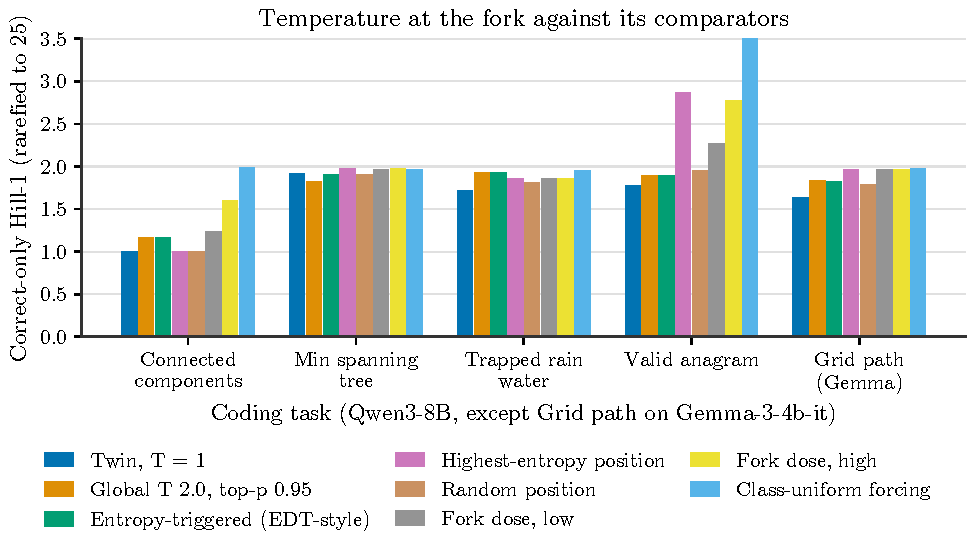
\includegraphics[width=\linewidth,height=0.78\textheight,keepaspectratio]{figures/fig_forkdose_hill_v0.pdf}
\caption{Grouped bar chart: the x-axis is five coding tasks (Connected components, Min spanning tree, Trapped rain water, Valid anagram, Grid path -- the first four on Qwen3-8B, the last on Gemma-3-4b-it); the y-axis is correct-only Hill-1 diversity, rarefied to 25 correct programs per cell (1 = every correct program used the same idea, 2 = two ideas split evenly). Each task shows eight coloured bars, one per sampling arm (legend; 50 common-random-number slots per arm): Twin, T = 1 (blue, unperturbed baseline), Global T 2.0, top-p 0.95 (amber), Entropy-triggered (EDT-style) (green), Highest-entropy position (violet, the same dose placed at the twin's highest-entropy decoding step), Random position (tan, same dose at a random step), Fork dose, low and Fork dose, high (grey, yellow -- temperature raised only at the located decision token), and Class-uniform forcing (sky blue). At its high dose, fork-dosed temperature reaches close to two ideas on the three other mixed tasks, roughly matching rather than beating most comparators there, and its clearest win is valid anagram, where it lifts Hill-1 from 1.78 (twin) to 2.78. On the one collapsed task, connected components, it reaches only 1.60 -- short of this run's own pre-registered 1.8 target -- at a 14-point pass-rate cost; class-uniform forcing reaches 1.99 there, but only 1 of its 24 attempted BFS programs passes the hidden tests. Bars are point estimates from one run; no uncertainty intervals are plotted.}
\label{fig:fig_forkdose_hill}
\end{figure}
\textbf{Where the fork sits in the entropy profile.} The claim predicted that the fork would not stand out by entropy, so that entropy-triggered samplers would miss it. The opposite holds. Code tokens are nearly deterministic, so the 90th percentile of the twin's per-token entropies is only 0.0003 to 0.05 nats, and the fork's entropy at T 1 lies above it in all 209 twin samples that reach the fork on the five located units (median 0.13 nats on connected components and 0.53 to 0.81 nats on the mixed units). The fork is also the single highest-entropy position among the first 64 tokens on 44 of 44 (Gemma), 32 of 39 (minimum spanning tree) and 21 of 39 (valid anagram) slots, but on 2 of 50 (connected components) and 0 of 37 (trapped rain water), the two units where a highest-entropy rule misses it. A rule that doses the highest-entropy position therefore finds the fork on most slots of three of the four mixed units (on every Gemma slot, where it reproduces the fork-dosed arm exactly, but on only 21 of 39 valid anagram slots) and misses it on trapped rain water and on the collapsed connected components (iteration-9 correction). This places the fork among the high-entropy minority tokens that Wang et al. find drive reinforcement learning on reasoning traces [139]. The threshold rule of the entropy-triggered sampler fires on about 10\% of all tokens and spends most of its temperature away from the fork (DFS 4\% on connected components; a 12-point pass cost and no gain on minimum spanning tree).

\textbf{The boundary units.} The grid path task on Qwen3-8B failed validation (no token at index 3 gives at least 5 of 10 off-default programs), so it joined shortest path and kth smallest as a boundary unit, where a window of 16 body tokens at T 7 over the top 20 replaced the fork dose (Table 387). All three windows fall below the committed pass-rate floor of 0.5, so the test is untestable by breakage. On kth smallest the surviving programs scatter across the catalogue, an effect on the program's form rather than a located choice.

\begin{table}[H]
\renewcommand{\thetable}{387}
\centering\footnotesize\setlength{\tabcolsep}{4.0pt}
\caption{The boundary units under a window of 16 tokens at T 7. [Source: iteration 8, artifact \nolinkurl{gen_art_experiment_39}.]}\label{tab:t412}
\begin{tabular}{>{\raggedright\arraybackslash\hspace{0pt}}p{0.0973\linewidth}>{\raggedright\arraybackslash\hspace{0pt}}p{0.1774\linewidth}>{\raggedright\arraybackslash\hspace{0pt}}p{0.4513\linewidth}>{\raggedright\arraybackslash\hspace{0pt}}p{0.1174\linewidth}>{\raggedright\arraybackslash\hspace{0pt}}p{0.0699\linewidth}}
\toprule
\textbf{Task (Qwen3-8B)} & \textbf{Twin} & \textbf{Window} & \textbf{Pass, twin to window} & \textbf{Flips} \\
\midrule
Grid path & BFS 0.98, DFS 0.02 & BFS 0.94, DFS 0.02, other 0.04 & 0.88 to 0.20 & 2 \\
Shortest path & Dijkstra 0.98, Bellman-Ford\slash{}SPFA 0.02 & Dijkstra 0.98, Bellman-Ford\slash{}SPFA 0.02 & 1.00 to 0.42 & 0 \\
Kth smallest & Full sort 1.00 & Full sort 0.30, quickselect 0.14, size k heap 0.06, heapify and pop 0.02, counting sort 0.06, other 0.06, invalid 0.36 & 1.00 to 0.24 & 35 \\
\bottomrule
\end{tabular}
\end{table}

\textbf{The blind locator.} Prefix resampling at T 1 used 6 base paths per unit, prefixes 2 to 64 and 8 continuations each (3,072 continuations in 16 GPU minutes), with the Bayesian change-point rule of iteration 7. It located minimum spanning tree's fork exactly at token 61 on the three paths that show a change point. The other three show none, one short of the preregistered 4 of 6, because a Kruskal path starts near a 0.65 share of its own class and the share-jump rule cannot fire on it. On connected components no path shows a change point: the twin writes union-find in 50 of 50 programs and resampling at T 1 never leaves it, so the fork at tokens 10 and 11 was known only from iteration 7's pushed and banned prompts. On a collapsed task the knob needs knowledge that a locator at T 1 cannot supply. The opening classifier that stops continuations agrees with the full labels on 0.989 and 0.985 of completed programs.

\textbf{The reachability claim.} At every fork node, each of the 64 most probable tokens was forced and continued five times at T 1; an idea counts when at least one forced continuation is a correct program of it (Table 388). Forcing adds one known idea on three units, as predicted: BFS on connected components, Prim with an array scan on minimum spanning tree weight, and a scan over the alphabet on valid anagram. Each appears at T 1 about once in 2 million to 50 million samples, and the fork dose lifts its mass to at most 0.010, far below the 0.05 the plan asked for, because these ideas sit at deep ranks (ranks 34 and 52 on minimum spanning tree weight, rank 18 on valid anagram) or behind a token whose programs mostly fail (' def bfs' on connected components, whose mapped continuations pass 2 of 10).

\begin{table}[H]
\renewcommand{\thetable}{388}
\centering\footnotesize\setlength{\tabcolsep}{4.0pt}
\caption{Ideas reached by forcing the fork's top 64 tokens against ideas reached by any sampling knob. Counts are correct forced continuations. [Source: iteration 8, artifact \nolinkurl{gen_art_experiment_39}.]}\label{tab:t413}
\begin{tabular}{>{\raggedright\arraybackslash\hspace{0pt}}p{0.1672\linewidth}>{\raggedright\arraybackslash\hspace{0pt}}p{0.2752\linewidth}>{\raggedright\arraybackslash\hspace{0pt}}p{0.1128\linewidth}>{\raggedright\arraybackslash\hspace{0pt}}p{0.1093\linewidth}>{\raggedright\arraybackslash\hspace{0pt}}p{0.1432\linewidth}>{\raggedright\arraybackslash\hspace{0pt}}p{0.0889\linewidth}}
\toprule
\textbf{Task (model)} & \textbf{Ideas reached by forcing (correct programs)} & \textbf{Ideas reached by any knob} & \textbf{Idea reached only by forcing} & \textbf{Its reachability at T 1} & \textbf{Largest fork-dose mass} \\
\midrule
Connected components (Qwen3-8B) & union-find 294, DFS 153, BFS 2 & DFS, union-find & BFS & 5.4e-07 (about 2 million samples) & 0.005 \\
Minimum spanning tree weight (Qwen3-8B) & Kruskal 290, Prim with a heap 285, Prim with an array 2 & Kruskal, Prim with a heap & Prim with an array & 2.0e-08 (about 50 million samples) & 0.000 \\
Valid anagram (Qwen3-8B) & fixed count array 163, hash count 99, sort and compare 20, alphabet scan 5 & the first three & alphabet scan & 2.9e-08 (about 40 million samples) & 0.010 \\
Trapped rain water (Qwen3-8B) & prefix and suffix arrays 288, two pointers 143, peak split 4 & all three & none & n\slash{}a & n\slash{}a \\
Grid path (Gemma) & DFS 77, BFS 57 & BFS, DFS & none & n\slash{}a & n\slash{}a \\
Grid path (Qwen3-8B) & BFS 29 & BFS, DFS & none & n\slash{}a & n\slash{}a \\
\bottomrule
\end{tabular}
\end{table}

\textbf{Geometry at the fork and novelty.} The engine stored the final-norm hidden states of the 16 positions from the fork on, and the artifact plots their first two principal components (61\% to 81\% of the variance) in actual activation coordinates. The states separate by the algorithm the program implements, and a nearest-centroid check with centroids from the class-forced slots assigns the fork-dosed slots to their own program's class at 0.90 on connected components (94 slots), 0.97 on minimum spanning tree weight (73), 0.975 on trapped rain water (80), 0.83 on valid anagram (77) and 0.69 in Gemma (86), where BFS and DFS programs share most of the opening. The dial reaches the model's own states for its alternative ideas, not new regions. After adjudication only 2 correct programs from any stage carry the label other, both from the kth smallest window and both counting sort in dictionary form; two blind judges (gemini-2.5-flash, 10 of 10 gate controls; deepseek-chat-v3.1, 8 of 10, calling both known controls outside the catalogue novel) and a manual read called both catalogue variants, with nearest known solutions at tree edit distance 35 to 55 among 17,442 solutions. No correct program of 5,543 is novel (rule-of-three upper bound 0.0005).

\begin{figure}[!htbp]
\centering\captionsetup{font=footnotesize}
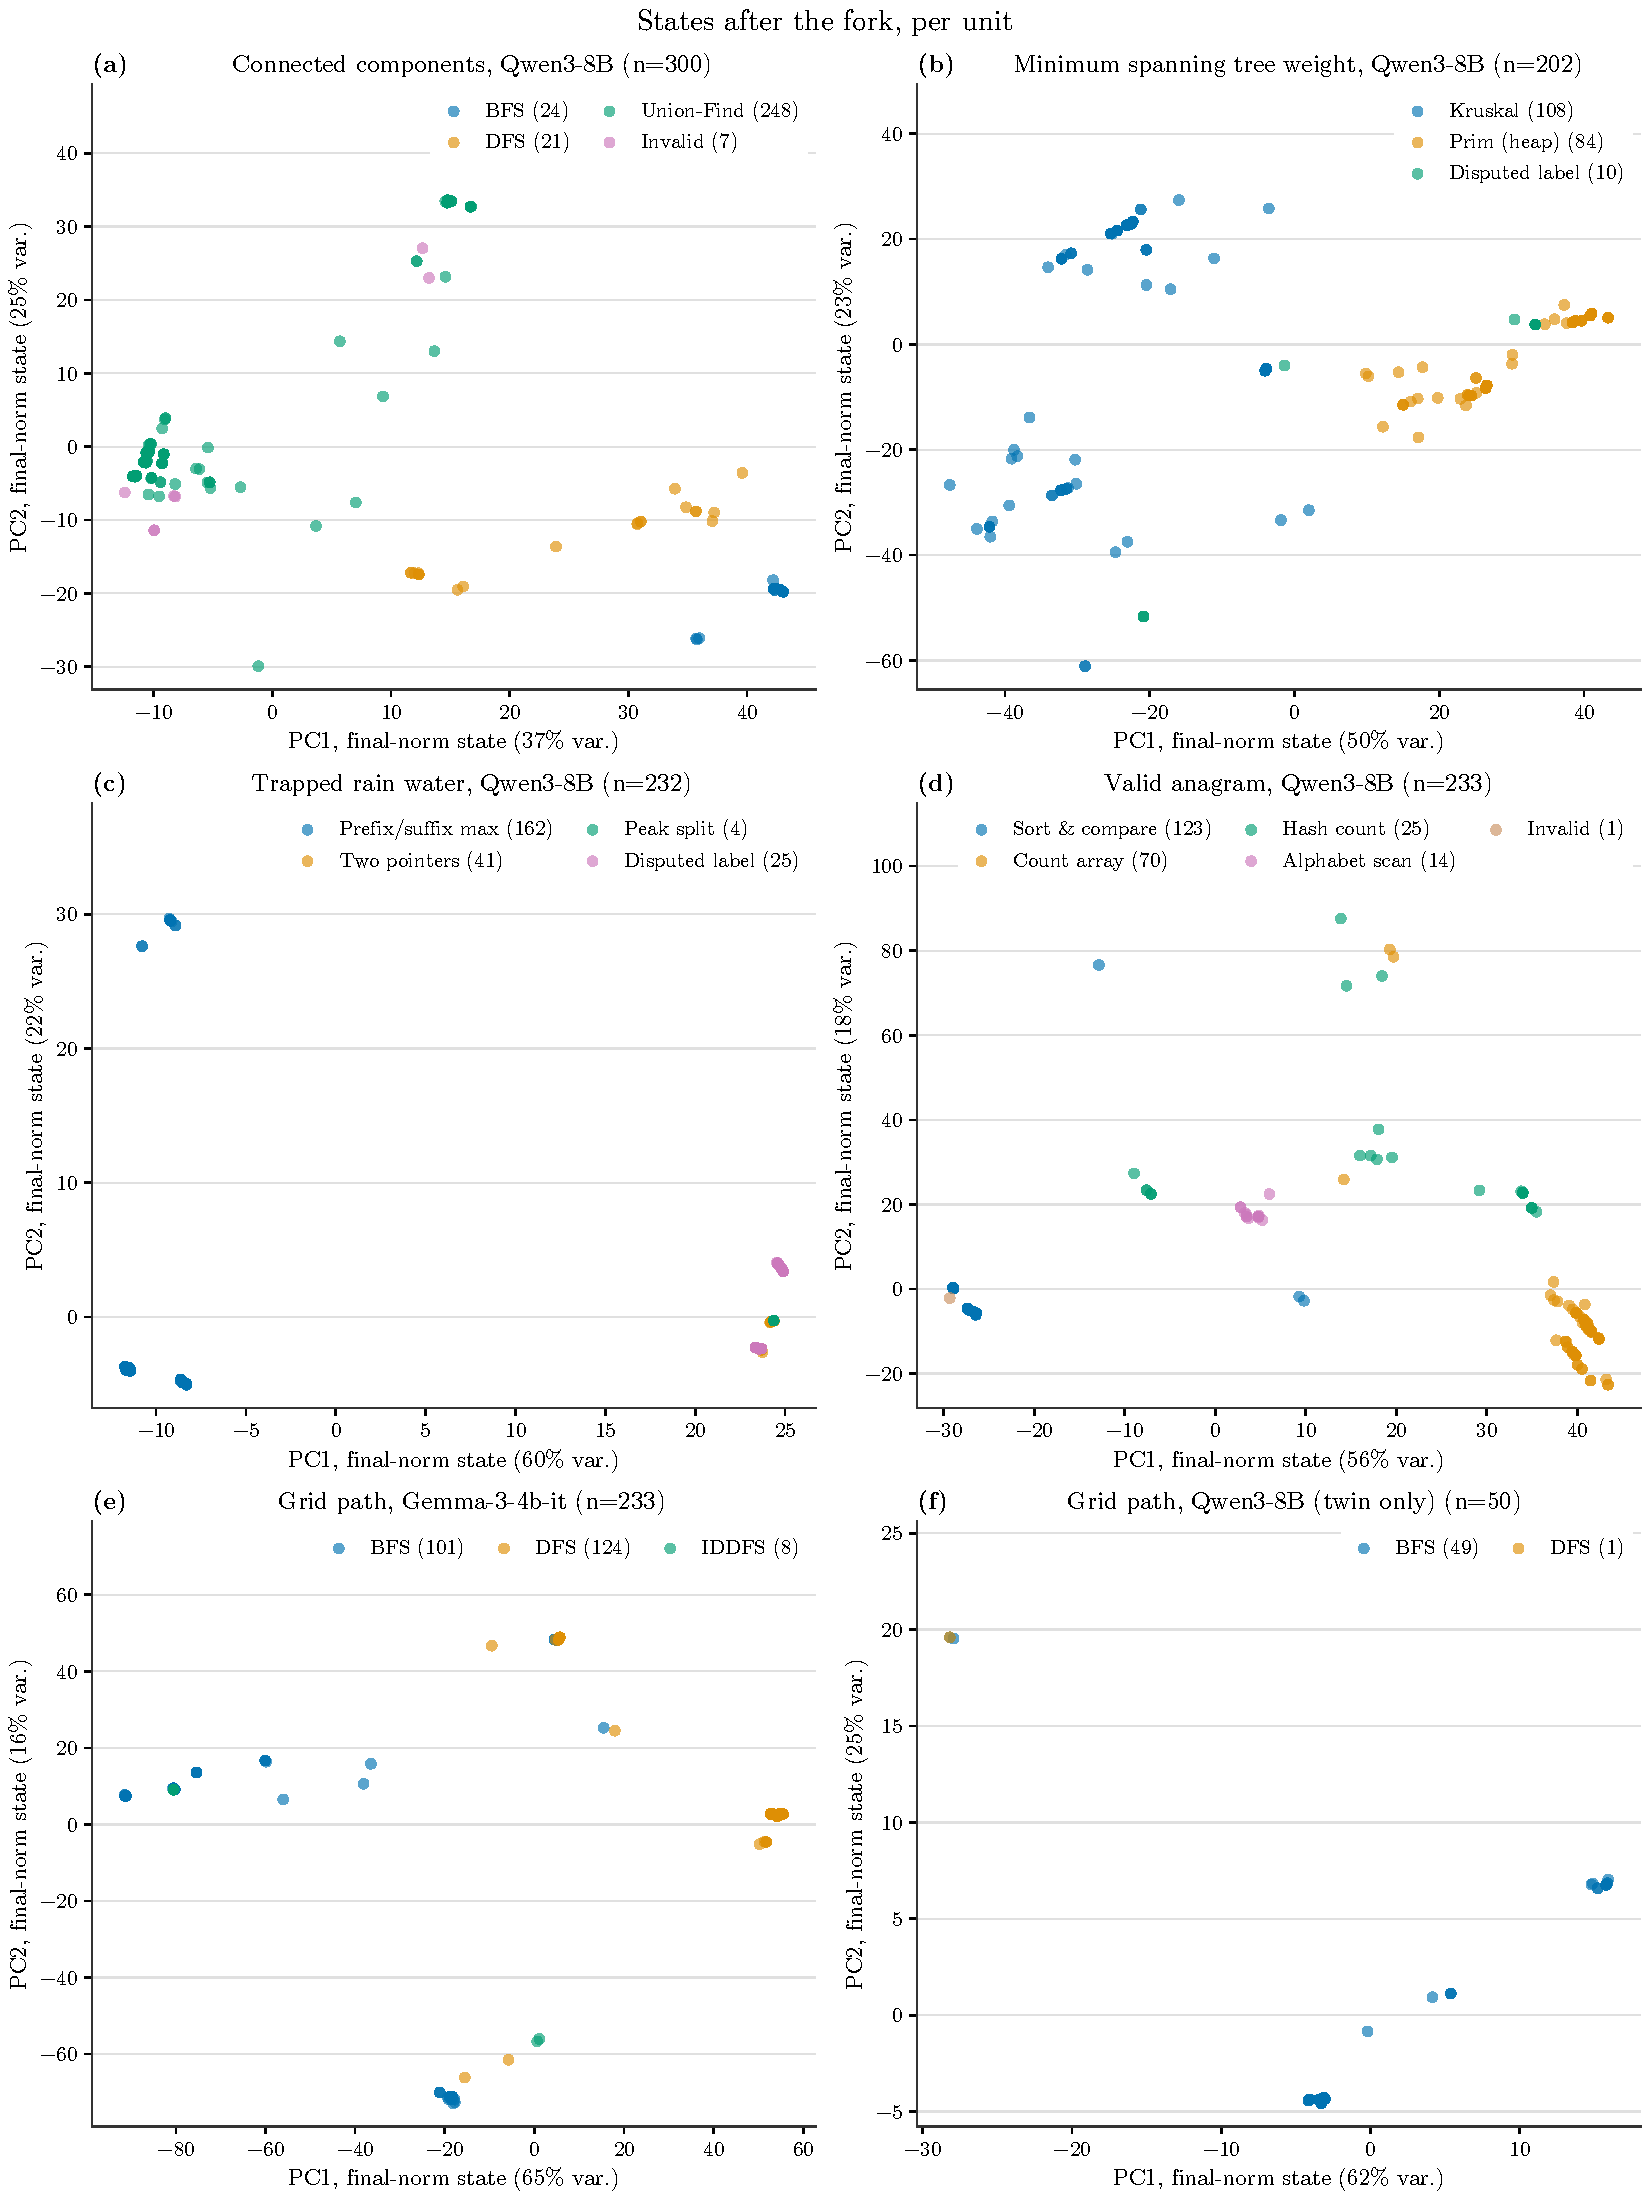
\includegraphics[width=\linewidth,height=0.78\textheight,keepaspectratio]{figures/fig_forkdose_states_v0.pdf}
\caption{PCA of the final-norm hidden state, averaged over the 16 positions from the fork token, computed separately per unit from the cached states of iteration 8's fork-dosing experiment. Panels pool, for one (model, task) unit, the twin samples, the low- and high-dose fork perturbations, class-uniform forcing, and the global-temperature 1.3 and 2.0 arms; points are coloured by the frozen labeller's program-label class, with each class's sample count given in its legend entry. Each panel's x\slash{}y axis labels give the percent of variance explained by PC1 and PC2 for that panel's own PCA basis (37-65\textbackslash{}\% and 16-25\textbackslash{}\% across panels); panel titles give the task, model and total \$n\$. (a) Connected components, Qwen3-8B (\$n=300\$): Union-Find 248, BFS 24, DFS 21, Invalid 7. (b) Minimum spanning tree weight, Qwen3-8B (\$n=202\$): Kruskal 108, Prim (heap) 84, Disputed label 10. (c) Trapped rain water, Qwen3-8B (\$n=232\$): Prefix\slash{}suffix max 162, Two pointers 41, Disputed label 25, Peak split 4. (d) Valid anagram, Qwen3-8B (\$n=233\$): Sort \textbackslash{}\& compare 123, Count array 70, Hash count 25, Alphabet scan 14, Invalid 1. (e) Grid path, Gemma-3-4b-it (\$n=233\$): DFS 124, BFS 101, IDDFS 8. (f) Grid path, Qwen3-8B, twin samples only (\$n=50\$): BFS 49, DFS 1. On every panel, states of different program labels occupy mostly separate regions of the first two principal components.}
\label{fig:fig_forkdose_states}
\end{figure}
\emph{Figure~\ref{fig:fig_forkdose_states} (iteration-9 correction).} Positions: mean of the 16 positions from the fork token on (fork to fork + 15). Block: final-norm hidden state (after the last block). Projection: PCA per unit, first two components (62\% to 87\% of variance; linear, no k or stress). N: states per unit: connected components 300, minimum spanning tree weight 202, trapped rain water 232, valid anagram 233, Gemma grid path 233, Qwen3-8B grid path 50 (arms twin, low and high dose, class-uniform forcing, global T 1.3 and 2.0). Centroids: no centroids drawn, so none sized by implemented count; colour = program class, marker = arm; the nearest-centroid check (class-forced centroids) agrees on connected components 0.904, minimum spanning tree weight 0.973, trapped rain water 0.975, valid anagram 0.831, Gemma grid path 0.686. Caveat: correlational; states after the fork partly encode the tokens already written. Files (\nolinkurl{gen_art_experiment_39}): figures\slash{}F8\_\allowbreak{}activation\_\allowbreak{}geometry.png, figures\slash{}F8\_\allowbreak{}activation\_\allowbreak{}geometry.pdf; code \nolinkurl{gen_art_experiment_39}:src\slash{}figures8.py\#f8.

\textbf{Checks and departures.} Every prediction was committed before its samples and the chain verifies. Labels agree with earlier engines on 30 of 30 connected components slots, 30 of 30 grid path, 49 of 50 minimum spanning tree, 29 of 30 shortest path, 30 of 30 kth smallest, 46 of 50 trapped rain water, 47 of 50 valid anagram and 47 of 50 Gemma slots. The run used a different GPU from the one planned (Table 374), built token maps from plug-in estimates, did not run two planned arms, dropped min-p and block-start temperature on trapped rain water and valid anagram, did not run the kth smallest labeller extension inside this artifact, and committed the locator verdict after the dose table (as its own commit). Of 574 programs sent to adjudication, 572 were resolved.

\FloatBarrier
\subsection*{8.4 One DAS protocol at the fork of both families (Qwen3-8B and Gemma)}
\addcontentsline{toc}{subsection}{8.4 One DAS protocol at the fork of both families (Qwen3-8B and Gemma)}
\noindent{\small\emph{Artifact: \nolinkurl{gen_art_experiment_40}.}}\par\medskip
The DAS experiment  answered the first lead of Section 7.11: the Qwen3-8B and Gemma handles had been tested under different objectives, readouts and permutation schemes, so a matched protocol was part of any test of a variable. One protocol was declared and hash-committed before any GPU use. The map class is a linear orthonormal map of rank 1, 2, 4 or 8 (nested); the interchange adds the map's projection of the source state minus that of the base state; the objective is bounded in the style of CDAS [112], the KL divergence from the source's own class distribution to the edited base's; and the readout is the class margin, the log probability of the source's class minus that of the base's class at the fork. It ran at three sites: the fork of connected components in Qwen3-8B (token 11, after ' def'; classes BFS, DFS and union-find), the fork of Gemma's grid task (token 32; BFS and DFS, because forced A* and IDDFS prompts failed adherence), and Qwen3-8B's task band (blocks 12 to 23 at all 145 task specification positions, one shared map). Seven controls were committed with thresholds before any fit (Table 389). Teacher-forced results are scored on held-out pairs, which need both a held-out source family and a held-out noun; generation is scored by hidden tests on slots of common random numbers.

\begin{table}[H]
\renewcommand{\thetable}{389}
\centering\small\setlength{\tabcolsep}{4.0pt}
\caption{The seven committed controls and their thresholds. [Source: iteration 8, artifact \nolinkurl{gen_art_experiment_40}.]}\label{tab:t414}
\begin{tabular}{>{\raggedright\arraybackslash\hspace{0pt}}p{0.1749\linewidth}>{\raggedright\arraybackslash\hspace{0pt}}p{0.4098\linewidth}>{\raggedright\arraybackslash\hspace{0pt}}p{0.3615\linewidth}}
\toprule
\textbf{Control} & \textbf{What it tests} & \textbf{Pass threshold} \\
\midrule
Random subspaces & 50 random subspaces per rank & Median recovery at most 0.05 \\
Label control & Refits on deranged labels (in Gemma, balanced shuffles of two classes) & At most 0.10 of the true fit's effect \\
Random-initialisation control & The same map class and budget on a randomly initialised network & At most 0.25 of the trained effect \\
Reverse interchange & Writing the default class's coordinates into a forced base & At least 0.5 of the full-state reverse \\
Retention & The map projected on the top 64 principal components of natural twin states & At least 0.5 of the effect kept \\
Natural-variance share & Share of natural twin variance in the subspace & Above the 95th percentile of random subspaces \\
Seed stability & Principal angles between seeds & Median first cosine at least 0.5 and above the random 99th percentile \\
\bottomrule
\end{tabular}
\end{table}

\textbf{Where the decision is written.} Exchanging the full residual state at the fork does almost nothing up to block 14 in either model (under 0.5 nats), so the choice is not yet written into the fork position there. The committed scan rule takes the block that maximises recovery normalised by the full-state effect, and it chose block 22 in Qwen3-8B (full-state effect 1.5 nats) and block 16 in Gemma (2.7 nats), the first blocks where the full state starts to carry the class. A rank-1 subspace there moves the margin 7.9 times (Qwen3-8B) and 2.5 times (Gemma) as much as the full state. A DAS edit that moves the margin far more than exchanging the whole state ever does raises the committed off-manifold flag, the signature of an edit that writes states the model does not produce, as Makelov et al. describe [122]. From block 24 in Qwen3-8B and block 22 in Gemma on, the full-state exchange carries 15 to 25 and 7 to 9 nats, and a rank-1 subspace recovers 0.6 to 0.9 and 1.2 to 1.4 of it. Iteration 7's Gemma block 17 sat on the same weak-ceiling edge.

\begin{table}[H]
\renewcommand{\thetable}{390}
\centering\tiny\setlength{\tabcolsep}{2.5pt}
\caption{Teacher-forced recovery on held-out pairs, by rank and by source class, at each site (recovery is the DAS effect over the full-state effect; seed 0). [Source: iteration 8, artifact \nolinkurl{gen_art_experiment_40}.]}\label{tab:t415}
\begin{tabular}{>{\raggedright\arraybackslash\hspace{0pt}}p{0.1694\linewidth}>{\raggedright\arraybackslash\hspace{0pt}}p{0.0877\linewidth}>{\raggedright\arraybackslash\hspace{0pt}}p{0.1273\linewidth}>{\raggedright\arraybackslash\hspace{0pt}}p{0.0408\linewidth}>{\raggedright\arraybackslash\hspace{0pt}}p{0.0408\linewidth}>{\raggedright\arraybackslash\hspace{0pt}}p{0.0408\linewidth}>{\raggedright\arraybackslash\hspace{0pt}}p{0.0408\linewidth}>{\raggedright\arraybackslash\hspace{0pt}}p{0.1401\linewidth}>{\raggedright\arraybackslash\hspace{0pt}}p{0.1391\linewidth}>{\raggedright\arraybackslash\hspace{0pt}}p{0.0655\linewidth}}
\toprule
\textbf{Site} & \textbf{Chosen block and rank} & \textbf{Recovery at the chosen rank (95\% CI)} & \textbf{Rank 1} & \textbf{Rank 2} & \textbf{Rank 4} & \textbf{Rank 8} & \textbf{By class at the chosen rank} & \textbf{Mean effect, DAS against full state (nats)} & \textbf{Off-manifold flag} \\
\midrule
Qwen3-8B, connected components fork & 22, rank 4 & 8.43 (5.94 to 11.30) & 7.67 & 8.12 & 8.43 & 9.26 & BFS 15.38, DFS 5.47, union-find -0.07 & 17.37 against 2.06 & Raised \\
Qwen3-8B, task band & Blocks 12 to 23, rank 2 & 0.82 (0.48 to 1.16) & 0.76 & 0.82 & 0.86 & 0.88 & BFS 1.57, DFS 0.68, union-find -0.04 & 14.89 against 18.19 & Not raised \\
Gemma, grid fork & 16, rank 4 & 3.07 (2.85 to 3.41) & 2.21 & 2.72 & 3.07 & 3.25 & BFS 3.07 & 9.25 against 3.02 & Raised \\
Qwen3-8B, connected components fork, block 24 (post hoc) & 24, rank 2 & 1.22 (0.98 to 1.43) & 1.10 & 1.22 & 1.24 & 1.29 & BFS 1.72, DFS 0.77, union-find 0.41 & 19.82 against 16.24 & Not raised \\
\bottomrule
\end{tabular}
\end{table}

At the same sites, a difference-in-means direction of rank 1 recovers 0.44 to 0.61 on connected components and 0.92 in Gemma, and the top 8 principal components recover 0.97 and 1.01: the directions of natural variance reproduce the full-state effect, and only DAS overshoots it. The fitted first direction is nearly orthogonal to the unembedding difference of the class tokens (cosine 0.07 in Qwen3-8B, 0.03 in Gemma).

\begin{table}[H]
\renewcommand{\thetable}{391}
\centering\footnotesize\setlength{\tabcolsep}{4.0pt}
\caption{The seven controls at each site. Ratios are effects relative to the true or trained fit. [Source: iteration 8, artifact \nolinkurl{gen_art_experiment_40}.]}\label{tab:t416}
\begin{tabular}{>{\raggedright\arraybackslash\hspace{0pt}}p{0.2089\linewidth}>{\raggedright\arraybackslash\hspace{0pt}}p{0.2088\linewidth}>{\raggedright\arraybackslash\hspace{0pt}}p{0.1356\linewidth}>{\raggedright\arraybackslash\hspace{0pt}}p{0.1387\linewidth}>{\raggedright\arraybackslash\hspace{0pt}}p{0.2212\linewidth}}
\toprule
\textbf{Control (threshold)} & \textbf{Qwen3-8B fork, block 22} & \textbf{Qwen3-8B task band} & \textbf{Gemma fork, block 16} & \textbf{Qwen3-8B fork, block 24 (post hoc)} \\
\midrule
Random subspaces (median at most 0.05) & Median -0.005, 95th percentile 0.015: pass & Median 0.003, 95th percentile 0.008: pass & Median 0.013, 95th percentile 0.033: pass & Median 0.000, 95th percentile 0.003: pass \\
Label control (at most 0.10) & 0.87, 0.63 and 0.77: fail & 0.71, 0.79 and 0.72: fail & 0.11, 0.11 and 0.20: fail & 0.61, 0.57 and 0.50: fail \\
Random-initialisation control (at most 0.25) & 0.69 (12.08 against 17.53 nats): fail & 0.18 (2.71 against 14.89 nats): pass & 0.41 (3.70 against 9.10 nats): fail & 0.54 (10.66 against 19.82 nats): fail \\
Reverse interchange (at least 0.5) & -2.72 (16 pairs): fail & 0.77 (16 pairs): pass & 2.83 (8 pairs): pass, as an overshoot & 1.17 (16 pairs): pass \\
Retention on 64 twin principal components (at least 0.5) & 0.18: fail & 0.43: fail & 0.12: fail & 0.52: pass \\
Retention with forced prompts and bans in the basis (at least 0.5) & 0.19: fail & 0.90: pass & 0.44: fail & 0.74: pass \\
Natural-variance share (above the random 95th percentile) & 0.0076 against 0.0016: pass & 0.0030 against 0.0006: pass & 0.0014 against 0.0030: fail & 0.0075 against 0.0010: pass \\
Seed stability (first cosine at least 0.5) & 0.87 (random 99th percentile 0.07): pass & 0.49 (0.05): fail & 0.53 (0.09): pass & 0.62 (0.05): pass \\
Verdict & No handle by the pooled rule (toward DFS alone the generation test passes) & Sufficient handle & Sufficient handle & Post hoc, teacher forcing only; fails the label and random-initialisation controls \\
\bottomrule
\end{tabular}
\end{table}

The label controls on connected components used two cyclic derangements and a derangement at the prompt level, changing every retained target; they still move held-out pairs toward the true source class, and the first of them also fits its permuted targets (training KL 0.0002) and writes DFS for BFS sources in generation (20 of 20). Gemma's two-class site could only use balanced shuffles that change 33\% to 58\% of labels, a weaker control, so the matched claim carries the qualifier ``three-class label control tested in Qwen3-8B only''. The randomly initialised networks have next-token entropies of 11.1 to 12.0 nats, and the full-state exchange on them does little (1.2 and 0.45 nats), yet a linear map at the fork recovers 0.41 to 0.69 of the trained effect: a linear map at one token can manufacture most of the effect with no trained computation behind it, the concern Sutter et al. raise for non-linear maps [132].

\begin{figure}[!htbp]
\centering\captionsetup{font=footnotesize}
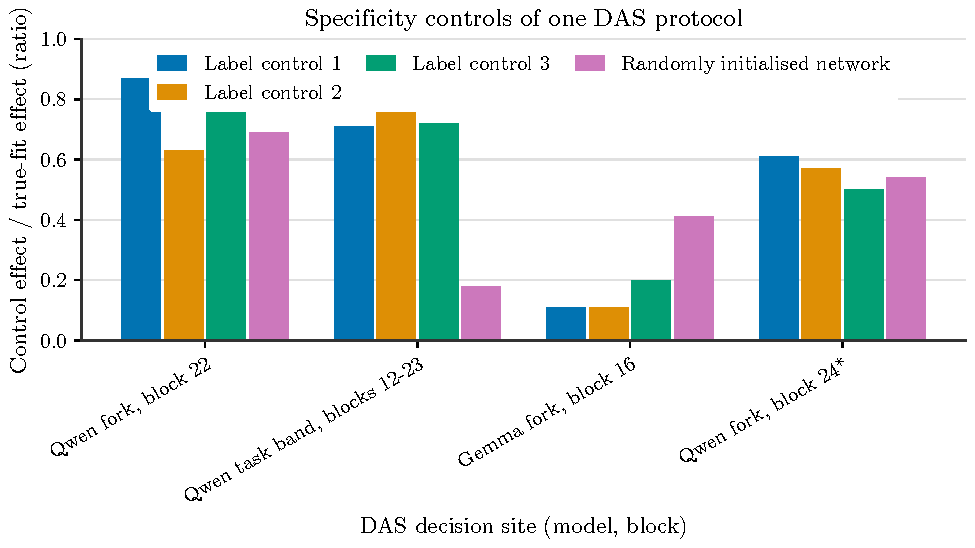
\includegraphics[width=\linewidth,height=0.78\textheight,keepaspectratio]{figures/fig_das_controls_v0.pdf}
\caption{Specificity-control strength for one committed DAS (Distributed Alignment Search) protocol at four decision sites in Qwen3-8B and Gemma-3-4b-it (x-axis, tilted labels). The y-axis gives each control fit's effect as a fraction of the true (trained) DAS fit's own effect, 0 to 1.0. Four bars per site, as coloured in the legend: Label control 1 (blue) and Label control 2 (amber) are cyclic-derangement label refits at the two Qwen3-8B sites or balanced label-shuffle refits at the Gemma site; Label control 3 (green) is a prompt-level label-shuffle refit; Randomly initialised network (violet) is an untrained map of the same class and training budget as the true fit. A control is specific only if the label controls stay at or below 0.10 and the randomly-initialised-network control stays at or below 0.25 (thresholds not drawn; stated here as in the source analysis). Under this rule, every bar at the two fork sites (Qwen fork, block 22; Gemma fork, block 16) and at the post hoc block-24 site (asterisk; scored by teacher forcing only, not validated by generation) exceeds its threshold. Only at the Qwen task band (blocks 12-23) does any control pass: the randomly initialised network reaches 0.18 (below 0.25), while all three label controls there (0.71-0.79) still fail their 0.10 bar. No site in this committed protocol clears both kinds of specificity control.}
\label{fig:fig_das_controls}
\end{figure}
\textbf{Verdict.} The committed rule confirms the matched DAS claim if both forks are certified and disconfirms it if a fork fails the label control or the random-initialisation control in either family. Both forks fail both, so the claim is disconfirmed; the largest one-sided p over sites of the pair-level tests that the true and trained fits beat their controls is 0.037, so the fits do beat their controls, but by margins far below the committed thresholds. The committed prediction (both forks certified; the band passes generation but fails the reverse, retention and clamp tests) was wrong on both forks and on the band's reverse test. What the protocol finds is a rank-4 edit at the fork that moves the written algorithm in both families, not a certified variable: a certified variable would pass every control. Under the committed rule it is a sufficient handle in Gemma and NO HANDLE at Qwen3-8B's fork, where the edit toward BFS writes BFS in 29 of 30 programs but 24 fail (pass 0.20 against 0.83; 5:0 against random, p 0.063). Neither passes the specificity controls (iteration-9 correction).

\textbf{Generation.} Table 392 gives every generation cell (held-out pairs; the canonical opening prefilled for the fork sites; 30 slots of common random numbers; correct means the target class's label and the hidden tests both pass).

\begin{table}[H]
\renewcommand{\thetable}{392}
\centering\tiny\setlength{\tabcolsep}{2.5pt}
\caption{Generation under the fitted maps (correct target programs). Base is the unedited twin, full the full-state exchange, random an equal-rank random subspace and permuted the first label-control map. The two reverse columns write the twin's coordinates, or its full state, into a forced base and count programs that still implement the forced class; no program in any reverse cell returns to the twin's class. Source is the forced prompt itself. McNemar p-values are two-sided. [Source: iteration 8, artifact \nolinkurl{gen_art_experiment_40}.]}\label{tab:t417}
\begin{tabular}{>{\raggedright\arraybackslash\hspace{0pt}}p{0.1053\linewidth}>{\raggedright\arraybackslash\hspace{0pt}}p{0.0408\linewidth}>{\raggedright\arraybackslash\hspace{0pt}}p{0.0408\linewidth}>{\raggedright\arraybackslash\hspace{0pt}}p{0.0901\linewidth}>{\raggedright\arraybackslash\hspace{0pt}}p{0.0561\linewidth}>{\raggedright\arraybackslash\hspace{0pt}}p{0.0679\linewidth}>{\raggedright\arraybackslash\hspace{0pt}}p{0.0587\linewidth}>{\raggedright\arraybackslash\hspace{0pt}}p{0.0587\linewidth}>{\raggedright\arraybackslash\hspace{0pt}}p{0.0527\linewidth}>{\raggedright\arraybackslash\hspace{0pt}}p{0.1158\linewidth}>{\raggedright\arraybackslash\hspace{0pt}}p{0.0901\linewidth}>{\raggedright\arraybackslash\hspace{0pt}}p{0.0949\linewidth}}
\toprule
\textbf{Site and target} & \textbf{Base} & \textbf{Full} & \textbf{DAS} & \textbf{Random} & \textbf{Permuted} & \textbf{Reverse DAS} & \textbf{Reverse full} & \textbf{Source} & \textbf{Other ranks} & \textbf{Pass, DAS against base} & \textbf{McNemar, DAS against random} \\
\midrule
Qwen3-8B fork, toward DFS & 0 of 30 & 2 of 30 & 29 of 30 & 0 of 30 & 20 of 20 & 20 of 20 & 20 of 20 & 20 of 20 & Rank 1: 25 of 30; rank 2: 29 of 30 & 1.00 against 0.83 & 29:0, p 3.7e-9 \\
Qwen3-8B fork, toward BFS & 0 of 30 & 0 of 30 & 5 of 30 (29 write BFS) & 0 of 30 & 0 of 20 & 12 of 20 & 13 of 20 & 14 of 20 & n\slash{}a & 0.20 against 0.83 & 5:0, p 0.063 \\
Qwen3-8B band, toward BFS & 0 of 30 & 23 of 30 & 28 of 30 (30 write BFS) & 0 of 30 & 3 of 20 & 20 of 20 & 20 of 20 & 20 of 20 & n\slash{}a & 0.93 against 1.00 & 28:0, p 7.5e-9 \\
Qwen3-8B band, toward DFS & 0 of 30 & 20 of 30 & 3 of 30 (24 write BFS) & 0 of 30 & 17 of 20 & 19 of 20 & 20 of 20 & 13 of 20 & Rank 1: 5 of 30; rank 4: 4 of 30 & 0.70 against 1.00 & 3:0, p 0.25 \\
Gemma fork, toward BFS & 6 of 30 & 10 of 30 & 22 of 30 (27 write BFS) & 5 of 30 & 10 of 20 & 0 of 20 & 0 of 20 & 1 of 20 & Rank 1: 22 of 30; rank 2: 21 of 30 & 0.73 against 0.90 & 17:0, p 1.5e-5 \\
\bottomrule
\end{tabular}
\end{table}

Three readings follow. First, a rank-4 edit at one token moves the algorithm: 29 of 30 correct DFS programs on connected components where the twin writes union-find, and 22 of 30 correct BFS programs in Gemma against 6 unedited and 5 for a random subspace. Second, the edit toward BFS in Qwen3-8B writes the fork token and BFS in 29 of 30 programs, but 24 of them fail; a typical failure returns \texttt{len(\allowbreak{}visited)} from the helper while the caller does \texttt{visited.\allowbreak{}update(\allowbreak{}bfs(\allowbreak{}i))}. The model's program around the written token is incoherent, one more sign of an edit off the natural states. Third, no edit restores the default: neither the reverse DAS edit nor the reverse full-state exchange returns a forced prompt to its twin's class in generation (0 of 20 in each cell), because with the opening prefilled through ' def' a forced prompt keeps its class whatever is written at the fork. The band's map toward DFS writes BFS in 24 of 30 programs, and its label-control map writes DFS for both source classes: the rank-2 band handle encodes ``leave union-find, toward the algorithm this map was fitted to favour'' rather than the source's class, which is the generation face of the label-control failure. A full-state exchange over the band flips the teacher-forced class on only 58\% of held-out pairs, below the planned 90\%, with positions verified by tests, and the first principal cosines between this band handle and iteration 7's handle are 0.12 to 0.17.

\textbf{Do iteration 4's random pushes act through the fitted subspaces? No.} The 40 random directions of iteration 4 (alpha 2, absolute unit, blocks 12 to 23 at the task specification positions) were projected on the band subspace, and the projection, scaled by the forced-class displacement, was committed as the predictor of each direction's correct off-default share before any outcome was read. The retrospective association is Spearman 0.39 (p 0.006, n 40; 0.36 and 0.39 for the two engines; partial correlation controlling the push norm 0.42 over the band and 0.39 at block 35; a permuted predictor gives 0.14), below the committed 0.5. On 24 prospective directions committed in advance it falls to 0.09 (p 0.33; 208 of 240 programs ran before the time cap). Clamping the subspaces removes nothing (Table 393), so the committed clamp test fails: random pushes move the algorithm through other directions than the fitted handles.

\begin{table}[H]
\renewcommand{\thetable}{393}
\centering\footnotesize\setlength{\tabcolsep}{4.0pt}
\caption{Clamping the fitted subspaces under the ten most-escaping random pushes (270 paired slots, 27 to 30 per direction). [Source: iteration 8, artifact \nolinkurl{gen_art_experiment_40}.]}\label{tab:t418}
\begin{tabular}{>{\raggedright\arraybackslash\hspace{0pt}}p{0.3417\linewidth}>{\raggedright\arraybackslash\hspace{0pt}}p{0.1073\linewidth}>{\raggedright\arraybackslash\hspace{0pt}}p{0.1073\linewidth}>{\raggedright\arraybackslash\hspace{0pt}}p{0.0942\linewidth}>{\raggedright\arraybackslash\hspace{0pt}}p{0.1434\linewidth}>{\raggedright\arraybackslash\hspace{0pt}}p{0.1027\linewidth}}
\toprule
\textbf{Clamp} & \textbf{Escapes under the push} & \textbf{Escapes with the clamp} & \textbf{Removal} & \textbf{McNemar (push only : clamp only)} & \textbf{Pass rate with the clamp} \\
\midrule
Band subspace clamped to the twin at every band block & 218 of 270 & 221 of 270 & -0.01 & 8:11, p 0.65 & 0.87 \\
Random clamp of equal rank & 218 of 270 & 213 of 270 & 0.02 & 8:3, p 0.23 & 0.82 \\
Fork coordinates clamped at block 22 (53 slots that reproduce the opening; reach rate 0.53) & 44 of 53 & 46 of 53 & -0.05 & 1:3, p 0.63 & n\slash{}a \\
\bottomrule
\end{tabular}
\end{table}

\textbf{Geometry in actual activation coordinates.} The artifact plots every prompt's coordinates in the fitted rank-8 subspace at the chosen block and the fork, centred on the twin mean and embedded by metric MDS (Kruskal stress-1 0.015 for connected components and 0.027 for Gemma) and Isomap [25] (k 8), beside a PCA of the raw states. Class centroids are sized by implemented, test-passing programs (connected components: union-find 87, DFS 35, BFS 34; Gemma: DFS 21, BFS 7). On connected components the forced BFS, DFS and union-find prompts form three separated clusters; the neutral twins, the two seed strings, the short instruction to make a new algorithm and the long novelty instruction sit together, away from every forced cluster; the five bans of union-find sit just outside the twin cluster, toward the forced clusters. In Gemma, forced A* sits beside forced BFS (its ' open' continues as BFS under a neutral prompt), forced IDDFS sits near the twin cluster on the BFS side (its programs were labelled DFS 7 of 20 and disputed 13 of 20), and the top-five prohibition prompt and the novelty instruction stay inside the twin cluster. The figure titles say ``handle coordinates (not certified)''.

\begin{figure}[!htbp]
\centering\captionsetup{font=footnotesize}
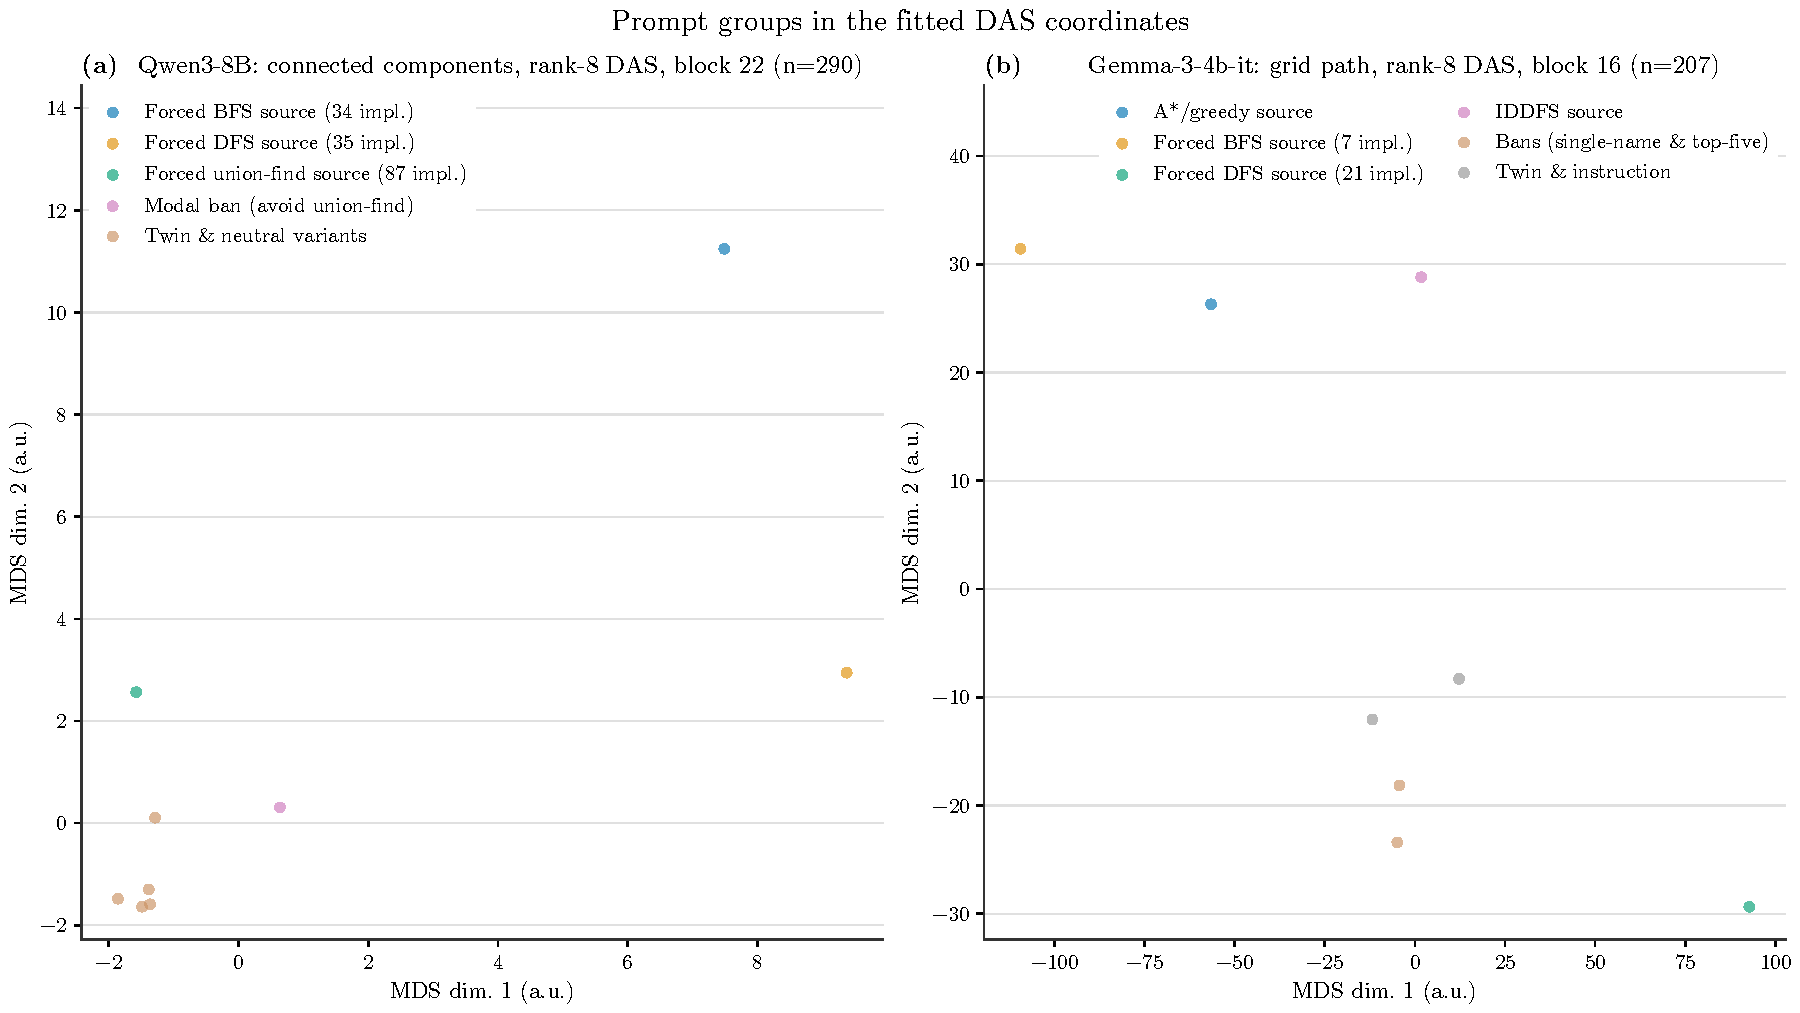
\includegraphics[width=\linewidth,height=0.78\textheight,keepaspectratio]{figures/fig_das_handle_coords_v0.pdf}
\caption{Group centroids of prompt conditions in each task's fitted rank-8 DAS subspace at the decision token, reduced to two dimensions by metric multidimensional scaling (MDS); both axes are the resulting MDS dimensions in arbitrary units (a.u.), and colour encodes the condition named in each panel's legend. (a) Qwen3-8B, connected-components task, decision block 22 (290 prompts; Kruskal stress-1 = 0.015). The forced BFS source (34 implemented, test-passing programs) and forced DFS source (35 implemented) sit well apart from every other condition. The forced union-find source (87 implemented; the neutral twin's own default algorithm), the modal ban on union-find, and the merged ``twin \textbackslash{}\& neutral variants'' group (the neutral twin together with its padded and plain-specification controls and its two context-seed and two novelty-instruction conditions) are all much closer to one another than to either forced BFS or DFS. (b) Gemma-3-4b-it, grid-path task, decision block 16 (207 prompts; stress-1 = 0.027). The forced BFS source (7 implemented) and forced DFS source (21 implemented) sit at opposite ends of the first MDS dimension, with the forced A*\slash{}greedy-best-first source on BFS's side of that dimension; the forced IDDFS source is centred on the first dimension but, like BFS and A*\slash{}greedy, high on the second. The merged ``bans'' group (the single-name BFS ban and the top-five ban) and the merged ``twin \textbackslash{}\& instruction'' group (the neutral twin and the novelty instruction) are both centred on the first dimension and low on the second, apart from all four forced sources. Only condition centroids are plotted, with no error bars; the underlying DAS fit was not certified as a causal handle for either task, so the plotted positions are descriptive placement coordinates, not evidence that the model represents algorithm choice along these axes.}
\label{fig:fig_das_handle_coords}
\end{figure}
\emph{Figure~\ref{fig:fig_das_handle_coords} (iteration-9 correction).} Positions: the fork token (index 11 after ' def' on connected components; index 32 in Gemma). Block: chosen block 22 (Qwen3-8B) and 16 (Gemma). Projection: every prompt's coordinates in the fitted rank-8 DAS subspace, centred on the twin mean, embedded by metric MDS (Kruskal stress-1 0.015 and 0.027) and Isomap (k 8), beside a PCA of the raw block states. N: 290 prompts (connected components) and 207 (Gemma). Centroids: class centroids (stars) sized by implemented, test-passing programs: connected components union-find 87, dfs 35, bfs 34; Gemma dfs 21, bfs 7. Caveat: off-manifold DAS coordinates: both fork fits raise the off-manifold flag and fail the label and random-initialisation controls, so these are handle coordinates, not a certified variable. The chart re-drawn in this report from the artifact's stored numbers shows the group centroids of the metric MDS embedding only; the per-prompt points, the Isomap panel and the raw-state PCA are in the artifact's files (iteration-9 correction). Files (\nolinkurl{gen_art_experiment_40}): figures\slash{}F3\_\allowbreak{}geometry\_\allowbreak{}T10.png, figures\slash{}F3\_\allowbreak{}geometry\_\allowbreak{}T10.pdf, figures\slash{}F3\_\allowbreak{}geometry\_\allowbreak{}GRID.png, figures\slash{}F3\_\allowbreak{}geometry\_\allowbreak{}GRID.pdf; code \nolinkurl{gen_art_experiment_40}:src\slash{}figures8.py\#F3.

\emph{The DAS experiment's handle-axis figure (iteration-9 correction; not re-drawn in this report, because the per-prompt handle coordinates are stored only in the artifact's tensor caches, so the artifact's own files named below are the figure).} Positions: the fork token, as in Figure~\ref{fig:fig_das_handle_coords}. Block: 22 (Qwen3-8B) and 16 (Gemma). Projection: the first fitted handle coordinate per prompt group (one axis; no k or stress). N: 290 and 207 prompts. Centroids: no centroids drawn; implemented counts as in Figure~\ref{fig:fig_das_handle_coords}. Caveat: off-manifold DAS coordinates (not certified). Files (\nolinkurl{gen_art_experiment_40}): figures\slash{}F3b\_\allowbreak{}handle\_\allowbreak{}axis\_\allowbreak{}T10.png, figures\slash{}F3b\_\allowbreak{}handle\_\allowbreak{}axis\_\allowbreak{}T10.pdf, figures\slash{}F3b\_\allowbreak{}handle\_\allowbreak{}axis\_\allowbreak{}GRID.png, figures\slash{}F3b\_\allowbreak{}handle\_\allowbreak{}axis\_\allowbreak{}GRID.pdf; code \nolinkurl{gen_art_experiment_40}:src\slash{}figures8.py\#F3b.

\textbf{The post hoc fit at block 24.} Block 24 is the first block where the full-state exchange carries the class in Qwen3-8B (16.2 nats, flipping every held-out pair). The same protocol there, reported as a sensitivity and never substituted for the committed block, recovers 1.22 (0.98 to 1.43), below the off-manifold line, and passes the reverse interchange (1.17), retention (0.52; 0.74 with forced prompts in the basis), natural variance (0.0075 against 0.0010) and seed stability (0.61 to 0.63). The label controls still reach 0.61, 0.57 and 0.50 of the true fit (p 0.0005 each for true above permuted), the randomly initialised network reaches 0.54, and a difference-in-means direction recovers 0.88 to 0.99 and the top four principal components 0.99, the same as DAS. Once the site has a real full-state ceiling, the dormancy and off-manifold failures go away and the lack of specificity stays: the class information at the fork is carried by the natural difference-in-means direction, which a linear map of almost any labelling partly recovers.

\textbf{Novelty, inputs and departures.} None of 1,857 correct programs (1,708 on connected components, 149 in Gemma) is labelled other, so no judge was called (rule-of-three bound 0.0016); 19 Gemma programs are disputed (18 with runtime IDDFS against AST BFS, all failing) and count as neither class. The 20 new single-token twin nouns came from the concreteness norms of the run's dataset dependency, and 76 connected components programs from four of its code datasets served as the nearest known solutions. The run used one 23 GB GPU (Table 374) for about 5.5 hours in all. Minimum spanning tree weight and Gemma's task band were dropped at the first commit, and band fits ran 109 steps with 2 seeds instead of 3. Blocks whose full-state exchange moved fewer than 10\% of pairs by 1 nat (blocks 0 to 14) were recorded as undefined. Three stages were rerun, after a NaN-ordering bug, a crash in the two-class label control and an out-of-memory stop. The engine check against iterations 6 and 7 and the band geometry figure were not run, labeller disagreements were not sent to the blind judge, and mediation ran 270 of 300 clamp slots and 208 of 240 prospective programs before the time caps. Eight commits form a chain with no break, and a standard-library re-derivation reproduces all 38 checked headline numbers from the raw rows, with placebos that fail as they should.

\textbf{Positioning.} DAS [110] and Boundless DAS [111] use the same map class; CDAS supplies the bounded objective and the bidirectional test [112]; MIB ranks DAS above difference in means and PCA under teacher forcing but scores no specificity control [52]. Makelov et al. predict the off-manifold overshoot, the failed retention and the failed reverse at the forks [122], Grant et al. describe the divergent representations that interventions produce [141], and Sutter et al. show that maps of enough capacity fit untrained networks [132]. This run adds the full set of specificity controls under one protocol in two families, and the result that even a linear map at the fork fails them.

\FloatBarrier
\subsection*{8.5 The circuit behind Qwen3-8B's fork}
\addcontentsline{toc}{subsection}{8.5 The circuit behind Qwen3-8B's fork}
\noindent{\small\emph{Artifact: \nolinkurl{gen_art_experiment_41}.}}\par\medskip
The circuit experiment  asked which components of Qwen3-8B compute the odds at the fork, and whether steering them rewrites the algorithm in generated, hidden-test-checked programs. It ported iteration 7's Gemma pipeline so that both families are measured the same way. A screen by attribution patching [136] covers 4,752 nodes: 32 heads and one MLP in each of 36 layers, at four position classes (the condition span, the task specification, the shared opening and the fork position). The top nodes are then patched exactly, by noising and denoising, and path patching [135] runs among the top 15, followed by faithfulness curves. Each top-10 node is validated in the real model against 50 matched random components of the same type and position class with matched write norm, under ablation and under steering (exact sign-flip tests, Holm over all 20 node and test p-values). The top five nodes are then steered in generation (30 slots of common random numbers, hidden tests, exact McNemar against a matched random five and against the twin), and a committed motif test compares the circuit with Gemma's. Two contrasts were studied. On minimum spanning tree weight the metric is the logit of ' Kr' minus the logit of ' Prim' after the 61-token opening; on connected components it is ' find' minus ' dfs' after ' def'.

\textbf{The primary contrast changed before any screen row.} The natural contrast on minimum spanning tree weight paired 24 neutral-noun variants per template (nouns from the concreteness norms of the dataset dependency), the variant with the highest metric against the lowest; its mean total effect was 0.89 nats, below 1 nat, which triggered the preregistered fallback: forced-Prim paraphrases against their padding twins became the primary contrast, committed as an amendment before any screen row. On connected components the corrupt run exchanges the forced-DFS prompt's residual states into the twin at every task specification position of all 36 blocks, which flips the teacher-forced argmax to ' dfs' in every pair; because that corruption is an intervention, condition-span nodes have zero effect there by construction, and the contrast maps routing from the task specification to the fork. Table 394 lists the contrasts.

\begin{table}[H]
\renewcommand{\thetable}{394}
\centering\footnotesize\setlength{\tabcolsep}{4.0pt}
\caption{Contrasts and their circuits. The correlation of attribution patching with exact patching is given on 160 random nodes and on the top set. [Source: iteration 8, artifact \nolinkurl{gen_art_experiment_41}.]}\label{tab:t419}
\begin{tabular}{>{\raggedright\arraybackslash\hspace{0pt}}p{0.2900\linewidth}>{\raggedright\arraybackslash\hspace{0pt}}p{0.0699\linewidth}>{\raggedright\arraybackslash\hspace{0pt}}p{0.0989\linewidth}>{\raggedright\arraybackslash\hspace{0pt}}p{0.2103\linewidth}>{\raggedright\arraybackslash\hspace{0pt}}p{0.0699\linewidth}>{\raggedright\arraybackslash\hspace{0pt}}p{0.1576\linewidth}}
\toprule
\textbf{Contrast} & \textbf{Pairs} & \textbf{Mean total effect (nats)} & \textbf{Attribution against exact patching, random nodes \slash{} top set} & \textbf{Edges kept} & \textbf{Completeness \slash{} sufficiency of the top 10} \\
\midrule
Minimum spanning tree, forced Prim against padding twin (primary) & 10 & 9.91 & 0.29 \slash{} 0.89 & 12 & 0.90 \slash{} 1.01 \\
Connected components, forced-DFS states exchanged into the twin & 15 & 19.33 & 0.25 \slash{} 0.91 & 17 & 0.94 \slash{} 0.96 \\
Minimum spanning tree, natural noun variants (descriptive) & 15 & 0.89 & 0.11 \slash{} 0.66 & 20 & 1.05 \slash{} 1.02 \\
Minimum spanning tree, mixed set & 15 & 4.00 & n\slash{}a \slash{} 0.79 & 0 & n\slash{}a \\
Minimum spanning tree, disjoint noun set for stability & 12 & 0.46 & n\slash{}a \slash{} 0.51 & 33 & 0.82 \slash{} 0.99 \\
\bottomrule
\end{tabular}
\end{table}

Attribution patching ranks the strong nodes well but not the near-zero random ones, whose exact effects sit at the bf16 noise floor of about 0.06 nats; attribution patching with integrated gradients over the input did not improve that correlation, so an exhaustive exact sweep over every fork-position node, all 144 MLP nodes and the screen's top 120 replaced the screen's ranking. The sweep found the largest node of the primary contrast, the layer-0 MLP at the condition span, with 7.7 of the 9.9 nats, which attribution patching had estimated at 0.1. Completeness (the top k noised together) and sufficiency (the top k restored together, with the rest of the network live) recover most of the effect; freezing every node outside the circuit to its corrupt value leaves almost nothing at any k up to 60, because the fork nodes need upstream processing of the instruction spread over many small nodes.

\begin{table}[H]
\renewcommand{\thetable}{395}
\centering\scriptsize\setlength{\tabcolsep}{2.5pt}
\caption{Validation of the top 10 nodes against 50 matched random components (minimum spanning tree, forced Prim; 30 prompts, 10 held out). Effects are mean metric changes in nats; p-values are Holm-adjusted over 20 tests. Node names give type, layer, head and position class. The two added columns give the mean effect over the 10 held-out prompts and its exact one-sided sign-flip p (smallest possible 1\slash{}1024) (iteration-9 correction). [Source: iteration 8, artifact \nolinkurl{gen_art_experiment_41}.]}\label{tab:t420}
\begin{tabular}{>{\raggedright\arraybackslash\hspace{0pt}}p{0.1585\linewidth}>{\raggedright\arraybackslash\hspace{0pt}}p{0.0872\linewidth}>{\raggedright\arraybackslash\hspace{0pt}}p{0.0872\linewidth}>{\raggedright\arraybackslash\hspace{0pt}}p{0.0872\linewidth}>{\raggedright\arraybackslash\hspace{0pt}}p{0.0872\linewidth}>{\raggedright\arraybackslash\hspace{0pt}}p{0.0539\linewidth}>{\raggedright\arraybackslash\hspace{0pt}}p{0.1829\linewidth}>{\raggedright\arraybackslash\hspace{0pt}}p{0.1693\linewidth}}
\toprule
\textbf{Node} & \textbf{Ablation effect} & \textbf{Ablation p} & \textbf{Steering effect} & \textbf{Steering p} & \textbf{Both pass} & \textbf{Held-out mean effect, ablation \slash{} steering (nats)} & \textbf{Held-out sign-flip p, ablation \slash{} steering} \\
\midrule
MLP, layer 0, condition span & 5.429 & 3.8e-06 & 4.938 & 3.8e-06 & yes & 0.00 \slash{} 0.00 (edit not applied; see text) & n\slash{}a (edit not applied) \\
Head 14 of layer 33, fork & 2.050 & 1.9e-08 & 4.251 & 1.9e-08 & yes & 2.02 \slash{} 4.24 & 0.00098 \slash{} 0.00098 \\
MLP, layer 35, fork & -2.638 & 1 & -5.068 & 1 & no & -2.55 \slash{} -5.02 & 1 \slash{} 1 \\
Head 28 of layer 34, fork & 1.964 & 1.9e-08 & 3.824 & 1.9e-08 & yes & 2.00 \slash{} 3.83 & 0.00098 \slash{} 0.00098 \\
MLP, layer 27, fork & 0.777 & 1.9e-08 & 1.896 & 1.9e-08 & yes & 0.73 \slash{} 1.99 & 0.00098 \slash{} 0.00098 \\
Head 6 of layer 29, fork & 1.403 & 1.9e-08 & 2.827 & 1.9e-08 & yes & 1.36 \slash{} 2.84 & 0.00098 \slash{} 0.00098 \\
MLP, layer 30, fork & 0.716 & 1.9e-08 & 1.529 & 1.9e-08 & yes & 0.68 \slash{} 1.50 & 0.00098 \slash{} 0.00098 \\
Head 10 of layer 23, opening & 0.783 & 1.9e-08 & 1.531 & 1.9e-08 & yes & 0.75 \slash{} 1.50 & 0.00098 \slash{} 0.00098 \\
MLP, layer 28, fork & 0.414 & 3.4e-07 & 0.904 & 1.9e-08 & yes & 0.46 \slash{} 0.97 & 0.00098 \slash{} 0.00098 \\
MLP, layer 11, task specification & 1.162 & 1.9e-08 & 1.288 & 1.9e-08 & yes & 1.32 \slash{} 1.53 & 0.00098 \slash{} 0.00098 \\
\bottomrule
\end{tabular}
\end{table}

\textbf{The held-out arm of the layer-0 node (iteration-9 correction).} The layer-0 MLP at the condition span has a held-out effect of exactly 0.00 nats under ablation and steering because the held-out edit was never applied. The class means that the edit writes are taken, for a condition-span node, only over pair prompts of the held-out prompt's own template (\texttt{MeanCache.\allowbreak{}get} in \texttt{src/\allowbreak{}k3circuit.\allowbreak{}py}, line 482: \texttt{if cl =\allowbreak{}=\allowbreak{} "COND" and p[\allowbreak{}"template"] !=\allowbreak{} ref[\allowbreak{}"template"]:\allowbreak{}}; line 485 also skips prompts whose span length differs). The 10 held-out prompts are templates F11 to F15 and the 20 pair prompts F1 to F10, so 0 of the 10 held-out prompts has a matching pair prompt, the mean is None (line 488), no edit is built, and the edited and unedited margins coincide; the stored rows show the node and all 50 matched random components of the same class at exactly 0 on every held-out prompt (20 of 20 prompt-by-mode rows). The node's 5.43 nats (ablation) and 4.94 nats (steering) over 30 prompts are therefore 8.14 and 7.41 nats over the 20 pair prompts plus ten zeros (8.14 x 20 \slash{} 30 = 5.43); the identity mean x 30 = pair mean x 20 + held-out mean x 10 holds for every node of both tables, and no other node has an exact-zero held-out effect (1 node in all, under both modes). Its held-out status is untested, not failed: on the descriptive natural contrast, whose held-out prompts share templates with its pairs, the same node gives 0.28 nats under ablation and 0.25 under steering on 5 held-out prompts (sign-flip p 0.031, the smallest one-sided p that five prompts allow, 1\slash{}32). BASE (B3) of iteration 9 reruns the held-out arm with template-matched means.

\begin{table}[H]
\renewcommand{\thetable}{396}
\centering\scriptsize\setlength{\tabcolsep}{2.5pt}
\caption{Validation of the top 10 nodes on connected components (40 prompts, 10 held out). Held-out columns as in Table 395; no node here sits at the condition span, and every held-out edit was applied (iteration-9 correction). On the 10 held-out prompts every node that passes both tests keeps a held-out effect of the same sign with sign-flip p at most 0.003, except the ablation of the node 'MLP, layer 30, fork' (0.02 nats, p 0.47). [Source: iteration 8, artifact \nolinkurl{gen_art_experiment_41}.]}\label{tab:t421}
\begin{tabular}{>{\raggedright\arraybackslash\hspace{0pt}}p{0.1712\linewidth}>{\raggedright\arraybackslash\hspace{0pt}}p{0.0872\linewidth}>{\raggedright\arraybackslash\hspace{0pt}}p{0.0872\linewidth}>{\raggedright\arraybackslash\hspace{0pt}}p{0.0872\linewidth}>{\raggedright\arraybackslash\hspace{0pt}}p{0.0872\linewidth}>{\raggedright\arraybackslash\hspace{0pt}}p{0.0539\linewidth}>{\raggedright\arraybackslash\hspace{0pt}}p{0.1762\linewidth}>{\raggedright\arraybackslash\hspace{0pt}}p{0.1633\linewidth}}
\toprule
\textbf{Node} & \textbf{Ablation effect} & \textbf{Ablation p} & \textbf{Steering effect} & \textbf{Steering p} & \textbf{Both pass} & \textbf{Held-out mean effect, ablation \slash{} steering (nats)} & \textbf{Held-out sign-flip p, ablation \slash{} steering} \\
\midrule
MLP, layer 27, fork & 9.596 & 1.8e-11 & 16.058 & 1.8e-11 & yes & 10.54 \slash{} 14.92 & 0.00098 \slash{} 0.00098 \\
MLP, layer 26, fork & 5.088 & 1.8e-11 & 10.606 & 1.8e-11 & yes & 5.79 \slash{} 11.82 & 0.00098 \slash{} 0.00098 \\
MLP, layer 32, fork & 1.924 & 3.7e-10 & 7.967 & 1.8e-11 & yes & 1.48 \slash{} 9.98 & 0.002 \slash{} 0.00098 \\
MLP, layer 30, fork & 0.738 & 0.0015 & 5.851 & 1.8e-11 & yes & 0.02 \slash{} 5.11 & 0.47 \slash{} 0.00098 \\
Head 10 of layer 23, fork & 3.627 & 1.8e-11 & 7.964 & 1.8e-11 & yes & 4.34 \slash{} 8.46 & 0.00098 \slash{} 0.00098 \\
Head 31 of layer 27, fork & 3.047 & 1.8e-11 & 6.869 & 1.8e-11 & yes & 3.49 \slash{} 7.33 & 0.00098 \slash{} 0.00098 \\
MLP, layer 28, fork & 0.485 & 0.0077 & 1.685 & 3.4e-10 & yes & 0.98 \slash{} 2.30 & 0.002 \slash{} 0.00098 \\
MLP, layer 31, fork & -1.527 & 1 & 0.684 & 0.0079 & no & -1.75 \slash{} 0.61 & 1 \slash{} 0.13 \\
MLP, layer 13, task specification & 1.712 & 2.4e-06 & 2.847 & 1.3e-07 & yes & 2.52 \slash{} 4.79 & 0.0029 \slash{} 0.00098 \\
Head 13 of layer 11, task specification & -1.802 & 1 & -3.351 & 1 & no & -3.07 \slash{} -5.54 & 1 \slash{} 1 \\
\bottomrule
\end{tabular}
\end{table}

\begin{table}[H]
\renewcommand{\thetable}{397}
\centering\footnotesize\setlength{\tabcolsep}{4.0pt}
\caption{Validation of the top 10 nodes on the natural noun-variant contrast (descriptive; 15 clean and 5 held-out prompts under the committed time rule). [Source: iteration 8, artifact \nolinkurl{gen_art_experiment_41}.]}\label{tab:t422}
\begin{tabular}{>{\raggedright\arraybackslash\hspace{0pt}}p{0.3253\linewidth}>{\raggedright\arraybackslash\hspace{0pt}}p{0.1350\linewidth}>{\raggedright\arraybackslash\hspace{0pt}}p{0.1056\linewidth}>{\raggedright\arraybackslash\hspace{0pt}}p{0.1345\linewidth}>{\raggedright\arraybackslash\hspace{0pt}}p{0.1118\linewidth}>{\raggedright\arraybackslash\hspace{0pt}}p{0.0844\linewidth}}
\toprule
\textbf{Node} & \textbf{Ablation effect} & \textbf{Ablation p} & \textbf{Steering effect} & \textbf{Steering p} & \textbf{Both pass} \\
\midrule
MLP, layer 0, condition span & 0.478 & 1.9e-05 & 0.523 & 1.9e-05 & yes \\
MLP, layer 27, fork & 0.194 & 1.9e-05 & 0.456 & 1.9e-05 & yes \\
MLP, layer 20, task specification & 0.092 & 0.014 & 0.176 & 1.9e-05 & yes \\
MLP, layer 12, task specification & 0.058 & 0.21 & 0.158 & 2.3e-05 & no \\
MLP, layer 30, fork & 0.110 & 8.4e-05 & 0.240 & 1.9e-05 & yes \\
MLP, layer 8, task specification & 0.088 & 0.05 & 0.168 & 0.00012 & no \\
MLP, layer 19, task specification & 0.064 & 0.21 & 0.138 & 0.00039 & no \\
MLP, layer 5, condition span & -0.015 & 0.73 & 0.037 & 0.48 & no \\
Head 28 of layer 34, fork & 0.178 & 1.9e-05 & 0.443 & 1.9e-05 & yes \\
MLP, layer 16, task specification & 0.024 & 0.51 & 0.081 & 0.087 & no \\
\bottomrule
\end{tabular}
\end{table}

On the primary contrast 9 of 10 nodes pass both tests, and on connected components 8 of 10; the failures are components whose effect runs against the decision, brakes rather than drivers. On the natural contrast 5 of 10 pass. In every contrast the top five and top ten as sets beat all 50 matched random sets under ablation and steering (0.96 for the top ten under ablation on the natural contrast). The top fork heads are outliers in write norm, so their matched pools fell back to the 50 nearest-norm heads; a sensitivity committed before its rows rescales each draw to the target's write norm and leaves every head significant (uncorrected one-sided p 9.3e-10 for heads 6 of layer 29, 14 of layer 33 and 28 of layer 34; 9.1e-13 for head 31 of layer 27). Recomputed from its p-values, Gemma's circuit of iteration 7 has 7 nodes passing both tests under either multiplicity convention.

\textbf{Steering the top five in generation.} The top five non-condition nodes (all at the fork, by the alignment rule committed in the amendment, because the condition-span MLP of the forced contrast has no counterpart in the twin) were steered toward the minority class: each node's own activation plus twice the difference between the minority-class and default-class means. The matched random five apply the same operation to one matched component per node. Prefill fixes the prompt and opening for every arm; free generation applies the opening and fork edits only while the sampled prefix equals the opening (Table 398).

\begin{table}[H]
\renewcommand{\thetable}{398}
\centering\scriptsize\setlength{\tabcolsep}{2.5pt}
\caption{Steering the top five at the committed dose 2. Correct target programs are Prim (heap or array) on minimum spanning tree weight and DFS on connected components. [Source: iteration 8, artifact \nolinkurl{gen_art_experiment_41}.]}\label{tab:t423}
\begin{tabular}{>{\raggedright\arraybackslash\hspace{0pt}}p{0.2484\linewidth}>{\raggedright\arraybackslash\hspace{0pt}}p{0.0904\linewidth}>{\raggedright\arraybackslash\hspace{0pt}}p{0.1057\linewidth}>{\raggedright\arraybackslash\hspace{0pt}}p{0.1001\linewidth}>{\raggedright\arraybackslash\hspace{0pt}}p{0.0693\linewidth}>{\raggedright\arraybackslash\hspace{0pt}}p{0.0926\linewidth}>{\raggedright\arraybackslash\hspace{0pt}}p{0.2170\linewidth}}
\toprule
\textbf{Task and condition} & \textbf{Arm} & \textbf{Correct target} & \textbf{Attempted target} & \textbf{Pass rate} & \textbf{Reached the fork} & \textbf{Labels} \\
\midrule
Minimum spanning tree, prefilled & Twin & 8 of 30 & 8 & 1.00 & 30 & Prim 8, Kruskal 21, disputed 1 \\
Minimum spanning tree, prefilled & Top five & 29 of 30 & 29 & 1.00 & 30 & Prim 29, disputed 1 \\
Minimum spanning tree, prefilled & Random five & 23 of 30 & 24 & 0.97 & 30 & Prim 24, Kruskal 5, disputed 1 \\
Minimum spanning tree, free & Twin & 7 of 30 & 7 & 0.97 & 14 & Prim 7, Kruskal 22, disputed 1 \\
Minimum spanning tree, free & Top five & 16 of 30 & 16 & 0.97 & 14 & Prim 16, Kruskal 14 \\
Minimum spanning tree, free & Random five & 12 of 30 & 12 & 0.97 & 14 & Prim 12, Kruskal 17, disputed 1 \\
Connected components, prefilled & Twin & 1 of 30 & 1 & 1.00 & 30 & union-find 29, DFS 1 \\
Connected components, prefilled & Top five & 29 of 30 & 29 & 1.00 & 30 & DFS 29, union-find 1 \\
Connected components, prefilled & Random five & 30 of 30 & 30 & 1.00 & 30 & DFS 30 \\
Connected components, free & Twin & 0 of 30 & 0 & 1.00 & 3 & union-find 30 \\
Connected components, free & Top five & 3 of 30 & 3 & 1.00 & 3 & union-find 27, DFS 3 \\
Connected components, free & Random five & 3 of 30 & 3 & 1.00 & 3 & union-find 27, DFS 3 \\
\bottomrule
\end{tabular}
\end{table}

With the opening prefilled, the top five add 21 correct Prim programs over the twin on minimum spanning tree weight and 28 correct DFS programs on connected components, with no loss of pass rate. But at the committed dose the matched random five also flip most programs (23 and 30 of 30), so the comparison of the top five with the random five has little room: 7:1 discordant slots on minimum spanning tree weight (two-sided exact McNemar p 0.070, one-sided 0.035) and 0:1 on connected components (p 1). In free generation few slots reproduce the opening (14 and 3 of 30), so the edits rarely apply. The protocol commit did not state the sidedness of the McNemar test; the analysis code fixed by hash at that commit used the one-sided test, while the plan's power calibration (8:0 gives 0.0078, 7:1 gives 0.07) is two-sided. The artifact takes the two-sided test as primary because it is the more conservative, which makes both verdicts of the circuit claim partial; with the one-sided test the minimum spanning tree verdict would pass.

\textbf{A post hoc dose sensitivity.} Committed before its rows and labelled post hoc, lower doses on the same 30 slots separate the circuit from the random five on connected components but only modestly on minimum spanning tree weight (Table 399 and the figure below).

\begin{table}[H]
\renewcommand{\thetable}{399}
\centering\scriptsize\setlength{\tabcolsep}{2.5pt}
\caption{Prefilled generation at lower doses (correct target programs of 30). [Source: iteration 8, artifact \nolinkurl{gen_art_experiment_41}.]}\label{tab:t424}
\begin{tabular}{>{\raggedright\arraybackslash\hspace{0pt}}p{0.1720\linewidth}>{\raggedright\arraybackslash\hspace{0pt}}p{0.0539\linewidth}>{\raggedright\arraybackslash\hspace{0pt}}p{0.0585\linewidth}>{\raggedright\arraybackslash\hspace{0pt}}p{0.0606\linewidth}>{\raggedright\arraybackslash\hspace{0pt}}p{0.0759\linewidth}>{\raggedright\arraybackslash\hspace{0pt}}p{0.1924\linewidth}>{\raggedright\arraybackslash\hspace{0pt}}p{0.1240\linewidth}>{\raggedright\arraybackslash\hspace{0pt}}p{0.1758\linewidth}}
\toprule
\textbf{Task} & \textbf{Dose} & \textbf{Twin} & \textbf{Top five} & \textbf{Random five} & \textbf{Discordant, top five : random five} & \textbf{McNemar, two-sided} & \textbf{Pass, top five \slash{} random five} \\
\midrule
Minimum spanning tree & 0.5 & 8 & 25 & 20 & 6:1 & 0.125 & 30 \slash{} 30 \\
Minimum spanning tree & 1.0 & 8 & 27 & 28 & 1:2 & 1 & 30 \slash{} 30 \\
Connected components & 0.5 & 1 & 30 & 6 & 24:0 & 1.19e-07 & 30 \slash{} 30 \\
Connected components & 1.0 & 1 & 30 & 18 & 12:0 & 0.000488 & 30 \slash{} 30 \\
\bottomrule
\end{tabular}
\end{table}

At the logit level, the mean probability of the minority fork token over the five twins rises under the top five from 0.263 to 0.542, 0.785, 0.962 and 0.997 at doses 0.25, 0.5, 1 and 2 on minimum spanning tree weight, against 0.439, 0.638, 0.883 and 0.983 under the random five; on connected components it rises from 0.029 to 0.978 already at dose 0.25 under the top five, against 0.089, 0.194, 0.695 and 1.000 under the random five.

\begin{figure}[!htbp]
\centering\captionsetup{font=footnotesize}
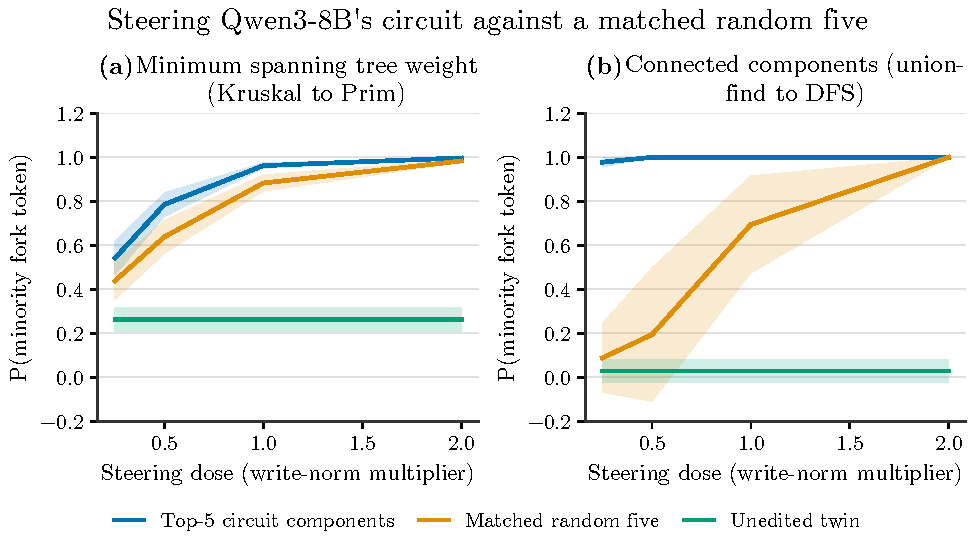
\includegraphics[width=\linewidth,height=0.78\textheight,keepaspectratio]{figures/fig_circuit_dose_v0.pdf}
\caption{Mean probability of the minority fork token, read from each prompt's own logit margin under a teacher-forced steering edit, as steering dose rises (x-axis, in multiples of each component's write-norm-matched edit: 0.25, 0.5, 1, 2), for the model's top-five circuit components (blue), five matched random components of the same type, position class and write norm (amber), and the unedited twin prompt as a dose-independent reference (green, flat line). Points are the mean over five prompt templates (W1-W5); shaded bands show $\pm$1 SD across those templates. (a) Minimum spanning tree weight, where the edit pushes the model's opening word from Kruskal's algorithm toward Prim's: the top-five and random-five curves stay close at every dose tested, and by dose 2 the random five push the probability almost as high as the circuit does. (b) Connected components, where the edit pushes from union-find toward DFS: the top-five circuit already saturates near probability 1 at the lowest dose tested (0.25), while the matched random five only reach a comparable probability at the highest dose (2) and vary far more from template to template along the way. This dose sweep is the experiment's secondary, pre-registered sensitivity check; at the single dose used for its primary, hidden-test-scored generation test (N=30 sampled completions per arm), the top-five circuit did not significantly beat the matched random five on either task (two-sided exact McNemar p=0.07 and p=1.00; the artifact's own verdict is PARTIAL on both).}
\label{fig:fig_circuit_dose}
\end{figure}
\begin{table}[H]
\renewcommand{\thetable}{400}
\centering\small\setlength{\tabcolsep}{4.0pt}
\caption{The committed predictions of the circuit experiment. [Source: iteration 8, artifact \nolinkurl{gen_art_experiment_41}.]}\label{tab:t425}
\begin{tabular}{>{\raggedright\arraybackslash\hspace{0pt}}p{0.5297\linewidth}>{\raggedright\arraybackslash\hspace{0pt}}p{0.2450\linewidth}>{\raggedright\arraybackslash\hspace{0pt}}p{0.1716\linewidth}}
\toprule
\textbf{Prediction} & \textbf{Observed} & \textbf{Outcome} \\
\midrule
At least 5 of 10 nodes pass both tests on the primary contrast & 9 of 10 (natural contrast, descriptive: 5 of 10) & Met \\
Top five prefilled: twin plus at least 6 correct Prim programs, beats the random five (McNemar p below 0.05), pass rate at least 0.8 of the twin's & +21; two-sided p 0.070 (one-sided 0.035); pass ratio 1.00 & Not met two-sided; met one-sided \\
The same on connected components toward DFS & +28; p 1; pass ratio 1.00 & Not met: the random five also saturate \\
Motif: fork share in [0.38, 0.68], condition share in [0.21, 0.51], effect-weighted depth of the fork stack in [0.45, 0.80] & Mixed set: fork 0.63, condition 0.01, depth 0.86 & Not met (condition share and depth) \\
Top-10 Jaccard between two disjoint pair sets at least 0.4 & 0.25 & Not met \\
\bottomrule
\end{tabular}
\end{table}

\textbf{The motif against Gemma.} The committed motif function (the share of absolute mean noising effect by position class over the top 40 nodes by attribution plus 20 random calibration nodes) first reproduced Gemma's printed shares (fork 0.531, condition 0.357). Table 401 gives the shares. The committed comparison, Qwen3-8B's mixed set against Gemma, reads ``different motif'' on the condition share and the depth of the fork stack. The committed composition depends on the attribution screen, which missed Qwen3-8B's largest node; with the exhaustive sweep, the condition share of the primary contrast rises to 0.17, still below Gemma's band [0.21, 0.51], and every minimum spanning tree row keeps a fork-stack depth of 0.86 to 0.96, above the band [0.45, 0.80] (the bands are constants of the committed motif code, \texttt{src/\allowbreak{}k3motif.\allowbreak{}py} line 55), so the post hoc sweep does not turn the committed different-motif reading into a match (iteration-9 correction). What the two families share is a late stack of fork-position MLPs and heads that carries the fork logit, deeper in Qwen3-8B (effect-weighted depth about 0.86 against 0.69); the layer-0 MLP at the condition span carries much of the forced contrast on the 20 pair prompts, but its held-out edit was never applied (see the paragraph after Table 395), and a structural likeness or difference between discovered circuits is not by itself a likeness or difference of mechanism, the phantom specialization that Bayat Makou et al. describe [146]. The two decisions share components: the MLPs of layers 27, 28 and 30 at the fork position appear in both top-10 lists, and head 10 of layer 23 appears in both (at the opening for minimum spanning tree weight, at the fork for connected components).

\begin{table}[H]
\renewcommand{\thetable}{401}
\centering\footnotesize\setlength{\tabcolsep}{4.0pt}
\caption{Share of the absolute noising effect by position class, and the effect-weighted depth of the fork stack. Rows marked sweep rank the top 60 nodes by exact effect; rows marked without injection drop layer 0 and 1 nodes at the corrupted span. [Source: iteration 8, artifact \nolinkurl{gen_art_experiment_41}.]}\label{tab:t426}
\begin{tabular}{>{\raggedright\arraybackslash\hspace{0pt}}p{0.3719\linewidth}>{\raggedright\arraybackslash\hspace{0pt}}p{0.1124\linewidth}>{\raggedright\arraybackslash\hspace{0pt}}p{0.1414\linewidth}>{\raggedright\arraybackslash\hspace{0pt}}p{0.0889\linewidth}>{\raggedright\arraybackslash\hspace{0pt}}p{0.0604\linewidth}>{\raggedright\arraybackslash\hspace{0pt}}p{0.1216\linewidth}}
\toprule
\textbf{Model and contrast} & \textbf{Condition span} & \textbf{Task specification} & \textbf{Opening} & \textbf{Fork} & \textbf{Fork-stack depth} \\
\midrule
Gemma (15 pairs) & 0.36 & 0.06 & 0.05 & 0.53 & 0.69 \\
Qwen3-8B, natural variants & 0.08 & 0.46 & 0.13 & 0.34 & 0.87 \\
Qwen3-8B, forced Prim & 0.01 & 0.20 & 0.18 & 0.62 & 0.86 \\
Qwen3-8B, mixed set & 0.01 & 0.22 & 0.14 & 0.63 & 0.86 \\
Qwen3-8B, disjoint noun set & 0.14 & 0.48 & 0.10 & 0.28 & 0.93 \\
Qwen3-8B, connected components & 0.00 & 0.32 & 0.01 & 0.67 & 0.79 \\
Qwen3-8B, natural variants, sweep & 0.27 & 0.39 & 0.10 & 0.24 & 0.87 \\
Qwen3-8B, forced Prim, sweep & 0.17 & 0.18 & 0.17 & 0.48 & 0.86 \\
Qwen3-8B, disjoint noun set, sweep & 0.23 & 0.28 & 0.06 & 0.43 & 0.96 \\
Qwen3-8B, connected components, sweep & 0.00 & 0.37 & 0.02 & 0.60 & 0.79 \\
Gemma, without injection & 0.23 & 0.07 & 0.06 & 0.64 & n\slash{}a \\
Qwen3-8B, natural variants, without injection & 0.04 & 0.47 & 0.13 & 0.35 & n\slash{}a \\
Qwen3-8B, forced Prim, without injection & 0.01 & 0.20 & 0.18 & 0.62 & n\slash{}a \\
Qwen3-8B, mixed set, without injection & 0.01 & 0.22 & 0.14 & 0.63 & n\slash{}a \\
Qwen3-8B, disjoint noun set, without injection & 0.14 & 0.48 & 0.10 & 0.28 & n\slash{}a \\
\bottomrule
\end{tabular}
\end{table}

\textbf{Stability.} Between the natural pair set and a disjoint set, the top-10 Jaccard is 0.25 and the top-15 Jaccard 0.36, the Spearman correlation of exact effects over the 36 nodes measured in both top-60 sets is 0.55, and 4 edges are kept in both; the disjoint set has a smaller total effect (0.46 against 0.89 nats).

\textbf{Checks and departures.} CPU tests (positions, node keys, the motif on Gemma, sign-flip against brute force, Holm and McNemar against standard libraries, the random-pool ladder, the labeller) all pass; the labeller re-check passes 4 of 4 references per task, 22 of 22 gold rows and 30 of 30 iteration-7 programs. The probability of ' Kr' on the first twin template is 0.724, against 0.72 in iteration 7, and labels agree with the iteration-7 engine on 20 of 20 slots per task (11 of 20 token-identical on minimum spanning tree weight). The metric was read in fp32 from the final-norm state after the first GPU tests showed that bf16 logits are quantised to 0.125 to 0.25 nats at these magnitudes; suffix forwards with a reused prefix cache differ from full recomputation by bf16 path noise (mean 0.076 nats, against 0.061 nats between full forwards in two batch shapes), so every effect is measured against an unedited row of its own batch. The transcoder attribution graph was dropped at the precheck, because Qwen3-8B's per-layer transcoders (about 96.5 GB) exceed both the 23 GB GPU and the 57 GB of RAM, so no feature-level account exists. A second contrast of a ban against the twin on connected components was not run, three natural pairs with total effects below 0.2 nats were dropped from the disjoint set, two out-of-memory stops were resumed from files without dropping rows, and one GPU test (path patching against direct logit attribution) was not run. Of 395 correct generated programs, none is labelled other (rule-of-three bound 0.0076). The nine-link hash chain orders every validation row after its commit and every steered program after its commit.

\FloatBarrier
\subsection*{8.6 A fair test of Gemma's dial: prompting under matched conditioning, free generation and dormancy}
\addcontentsline{toc}{subsection}{8.6 A fair test of Gemma's dial: prompting under matched conditioning, free generation and dormancy}
\noindent{\small\emph{Artifact: \nolinkurl{gen_art_experiment_42}.}}\par\medskip
Iteration 7 found a rank-4 DAS subspace at block 17 of gemma-3-4b-it that, edited once at the fork after the shared 32-token opening, raised correct BFS programs on the grid task from 11 of 50 to 42 of 50, and it compared this with a forced-BFS prompt sampled without that opening (35 of 50). The Gemma experiment  ran the missing cells on the same 50 slots (five templates by ten streams, iteration 7's streams; T 1.0, top-p 1, at most 1,024 new tokens), giving the 2x2 of \{prompt, dial\} by \{opening prefilled, free generation\}. It added a dial applied in free generation at the fork's position in each free sample, placed by a rule committed in advance, and ran the dormancy checks at ranks 1, 2, 4 and 8 under the rule already applied to Qwen3-8B. One model, one task and one fork: every claim below holds at Gemma's grid fork.

\begin{table}[H]
\renewcommand{\thetable}{402}
\centering\footnotesize\setlength{\tabcolsep}{4.0pt}
\caption{The 2x2 toward BFS on the same 50 slots (Wilson 95\% intervals [8]). [Source: iteration 8, artifact \nolinkurl{gen_art_experiment_42}.]}\label{tab:t427}
\begin{tabular}{>{\raggedright\arraybackslash\hspace{0pt}}p{0.1387\linewidth}>{\raggedright\arraybackslash\hspace{0pt}}p{0.3531\linewidth}>{\raggedright\arraybackslash\hspace{0pt}}p{0.1133\linewidth}>{\raggedright\arraybackslash\hspace{0pt}}p{0.1330\linewidth}>{\raggedright\arraybackslash\hspace{0pt}}p{0.0604\linewidth}>{\raggedright\arraybackslash\hspace{0pt}}p{0.0982\linewidth}}
\toprule
\textbf{Cell} & \textbf{What} & \textbf{Attempted BFS} & \textbf{Correct BFS (95\% CI)} & \textbf{Pass} & \textbf{' queue' at the fork} \\
\midrule
Twin, prefilled & Twin prompt with the opening prefilled & 15 & 10 (0.11 to 0.33) & 0.88 & 0.04 \\
Forced prompt, prefilled & Forced-BFS prompt with the opening prefilled & 50 & 0 (0.00 to 0.07) & 0.00 & 1.00 \\
Best wording, prefilled & The forced wording best by teacher forcing, with the opening prefilled & 50 & 0 (0.00 to 0.07) & 0.00 & 1.00 \\
Dial, prefilled & Twin with the opening prefilled, DAS rank 4, lambda 1 at the fork & 47 & 39 (0.65 to 0.87) & 0.82 & 0.00 \\
Twin, free & Twin, free from index 0 & 18 & 13 (0.16 to 0.40) & 0.88 & 0.00 \\
Forced prompt, free & Forced-BFS prompt, free from index 0 & 50 & 32 (0.50 to 0.76) & 0.64 & 0.00 \\
Dial, free & Twin, free, DAS rank 4, lambda 1 at the position the committed rule picks & 48 & 38 (0.63 to 0.86) & 0.78 & 0.00 \\
\bottomrule
\end{tabular}
\end{table}

\begin{figure}[!htbp]
\centering\captionsetup{font=footnotesize}
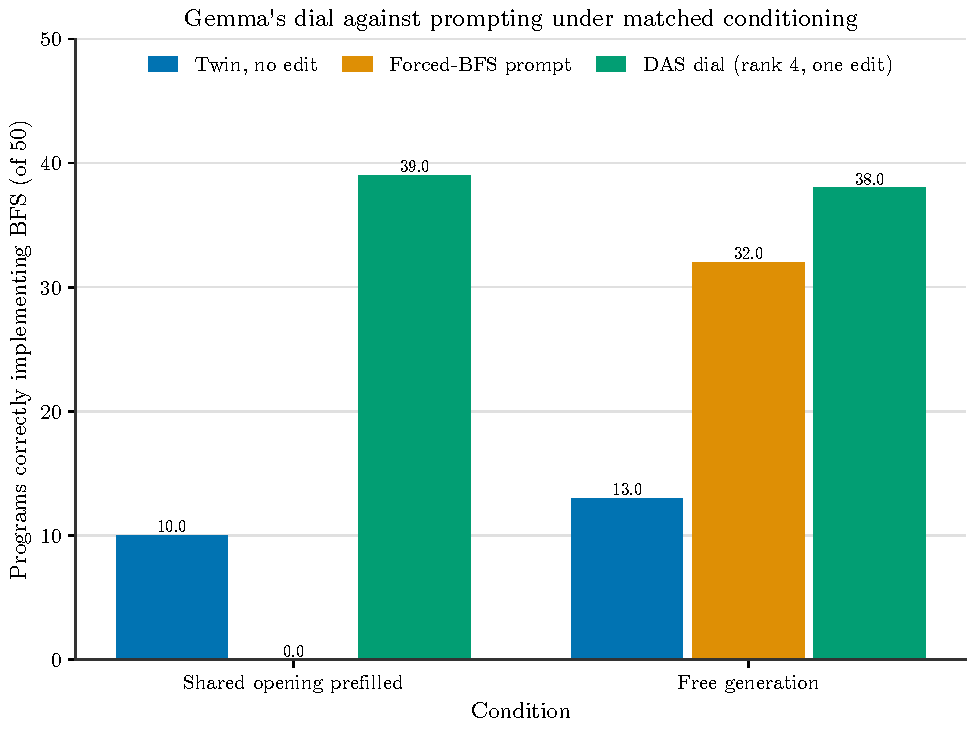
\includegraphics[width=\linewidth,height=0.78\textheight,keepaspectratio]{figures/fig_gemma_dial_2x2_v0.pdf}
\caption{Programs correctly implementing BFS, out of 50 generations on Gemma-3-4b-it's grid-path task, under two conditions that reuse the same 50 common-random-number slots: the 32-token shared opening prefilled (left) or free generation (right). Each condition shows three bars, each labelled with its count: a twin prompt with no edit (blue; 10 prefilled \slash{} 13 free), a prompt that explicitly forces BFS by name (amber; 0 prefilled \slash{} 32 free), and the DAS dial edit at rank 4, one edit (green; 39 prefilled \slash{} 38 free). Prefilling the shared opening collapses the forced-BFS prompt to 0\slash{}50 correct while the dial still reaches 39\slash{}50 under the identical prefill; the prefix steers the forced-BFS prompt's continuation onto an opening that skips the task's wall check, so every nominally-BFS program it writes fails. In free generation the dial (38\slash{}50) and the forced-BFS prompt (32\slash{}50) are not distinguishable (11 vs. 5 discordant slots, exact two-sided test p = 0.21): the prefill broke the prompt, not the dial.}
\label{fig:fig_gemma_dial_2x2}
\end{figure}
\begin{table}[H]
\renewcommand{\thetable}{403}
\centering\small\setlength{\tabcolsep}{4.0pt}
\caption{Paired contrasts on correct BFS (exact McNemar; discordant slots, first cell only against second cell only). [Source: iteration 8, artifact \nolinkurl{gen_art_experiment_42}.]}\label{tab:t428}
\begin{tabular}{>{\raggedright\arraybackslash\hspace{0pt}}p{0.3359\linewidth}>{\raggedright\arraybackslash\hspace{0pt}}p{0.1311\linewidth}>{\raggedright\arraybackslash\hspace{0pt}}p{0.1625\linewidth}>{\raggedright\arraybackslash\hspace{0pt}}p{0.3002\linewidth}}
\toprule
\textbf{Contrast} & \textbf{Discordant} & \textbf{p} & \textbf{Paired difference (Newcombe 95\%)} \\
\midrule
Dial against prompt, prefilled & 39 \slash{} 0 & 3.6e-12 (two-sided) & +0.78 (0.63 to 0.87) \\
Dial against prompt, free & 11 \slash{} 5 & 0.21 (two-sided) & +0.12 (-0.04 to +0.27) \\
Dial, prefilled against free & 2 \slash{} 1 & 1.0 & +0.02 (-0.06 to +0.11) \\
Prompt, prefilled against free & 0 \slash{} 32 & 4.7e-10 & -0.64 (-0.76 to -0.48) \\
Twin, prefilled against free & 1 \slash{} 4 & 0.38 & -0.06 (-0.16 to +0.04) \\
Interaction (slot bootstrap, 10,000) & n\slash{}a & n\slash{}a & 0.66 (0.50 to 0.82) \\
\bottomrule
\end{tabular}
\end{table}

\textbf{Why prompting fails under the prefill.} The committed prediction that the forced prompt with the opening prefilled would reach at least 40 of 50 correct BFS programs failed completely: it writes BFS 50 of 50 times and every program fails. The prefilled opening is unlikely under the forced prompt: its log probability is -11.3 to -14.1 nats under the five forced-BFS wordings (1e-6 to 1e-5), against -0.11 to -0.17 nats (0.85 to 0.90) under the twins and the forced-DFS prompts. Forcing it drives the fork token to ' queue' (probability 0.96 to 0.998 for all five wordings, 50 of 50 programs), and that opening writes a list-based BFS that carries the path, \texttt{queue =\allowbreak{} [\allowbreak{}(\allowbreak{}start,\allowbreak{} [\allowbreak{}start])]}, without checking whether start or goal is a wall. Every such program fails the hidden case of a one-by-one wall with a wrong answer, not a timeout, which corrects iteration 7's explanation that the 0 of 125 ' queue' programs failed by slowness. The teacher-forced account of the fork predicted this before any sample: 1.0 correct and 49.97 attempted BFS programs of 50. In free generation the forced prompt never writes the shared opening (index 32 is '[' inside \texttt{from collections import deque} in 46 of 50 programs), and the forced-DFS prompt with the opening prefilled is natural and gives 50 of 50 correct DFS. So the prefill is a confound, but it hurts the prompt, not the dial: under matched prefill the dial beats prompting 39 to 0.

\textbf{The dial in free generation.} The rule that places the edit was committed before any edited sample. If the free twin reproduces the shared opening, the edit goes at index 32. Otherwise it goes at the first index from 8 to 96 after the body indent where BFS and DFS together hold at least half the probability, ' visited' holds at least 0.01, and no string naming an algorithm has appeared. 47 of 50 slots reproduce the opening and 3 never reach a qualifying position (73 and 7 over 80 slots with the held-out set); the literal rule of the plan would have fired at index 2 in every slot, as anticipated. No edited row differs from the free twin before the edit (0 of 480), and the edit's decode-time margin at index 32 is 0.42 nats above the prefilled path (12.09 against 11.67 on the first template), above the 0.3 tolerance; the prefilled and decoded paths agree on labels in 46 of 47 dial slots and 42 of 47 twin slots, one slot short of the committed 0.90 for the twin.

\begin{table}[H]
\renewcommand{\thetable}{404}
\centering\footnotesize\setlength{\tabcolsep}{4.0pt}
\caption{Free-generation cells against the free twin (edit positions placed by the committed rule; one-sided McNemar against the free twin, Holm across the four DAS cells). [Source: iteration 8, artifact \nolinkurl{gen_art_experiment_42}.]}\label{tab:t429}
\begin{tabular}{>{\raggedright\arraybackslash\hspace{0pt}}p{0.3899\linewidth}>{\raggedright\arraybackslash\hspace{0pt}}p{0.1483\linewidth}>{\raggedright\arraybackslash\hspace{0pt}}p{0.0604\linewidth}>{\raggedright\arraybackslash\hspace{0pt}}p{0.1794\linewidth}>{\raggedright\arraybackslash\hspace{0pt}}p{0.1352\linewidth}}
\toprule
\textbf{Free cell} & \textbf{Correct target (of 50)} & \textbf{Pass} & \textbf{Against the free twin} & \textbf{Committed prediction} \\
\midrule
Twin & 13 BFS & 0.88 & n\slash{}a & 10.0 \\
DAS rank 4, lambda 1, toward BFS & 38 & 0.78 & 26\slash{}1, Holm p 8.3e-7 & 37.0 \\
DAS rank 4, lambda 0.5, toward BFS & 34 & 0.72 & 22\slash{}1, Holm p 5.7e-6 & 30.6 \\
DAS rank 1, lambda 1, toward BFS & 35 & 0.72 & 23\slash{}1, Holm p 4.5e-6 & 31.1 \\
DAS rank 1, lambda 0.5, toward BFS & 31 & 0.68 & 19\slash{}1, Holm p 2.0e-5 & 27.7 \\
DAS of seed 2, rank 4, lambda 1, toward BFS (optional) & 41 & 0.82 & 28\slash{}0, p 3.7e-9 & 33.5 \\
Random subspace, rank 4, lambda 1 (optional) & 11 & 0.84 & 1\slash{}3, p 0.94 & 6.9 \\
Difference in means at matched effect, toward BFS & 0 (attempted 49) & 0.00 & 0\slash{}13 & 1.4 \\
DAS rank 4, lambda 1, toward DFS & 47 DFS & 0.94 & 16\slash{}0, p 1.5e-5 & 47.0 \\
Difference in means at matched effect, toward DFS & 47 DFS & 0.94 & 16\slash{}0, p 1.5e-5 & 46.5 \\
\bottomrule
\end{tabular}
\end{table}

The free dial reaches 38 of 50 correct BFS against 13 for the free twin, and at this N it cannot be told apart from the prefilled dial (2 against 1 discordant slots). It holds on held-out templates. On the two templates outside the map's training set plus 30 fresh slots of them, it gives 33 of 50 against 11 for the twin (24 against 2 discordant, p 5.2e-6); on the 30 fresh slots alone 20 against 6; on the three training templates 25 of 30 against 8. Its pass cost against the free twin is 0.10 (Newcombe -0.22 to +0.01); of its 20 failing programs over the 80 slots, 15 are timeouts of slow BFS variants and 5 are wrong answers on a wall case. Toward DFS the dial and the forced-DFS prompt with the prefill both give 50 of 50 correct DFS, and the free dial and free difference-in-means edit 47 of 50; each beats its twin by 16 to 0 discordant slots.

\textbf{In free generation the dial does not beat prompting.} Against the committed free prompt (32 of 50) the dial's advantage is 11 to 5 discordant slots (p 0.21). Across eight forced-BFS wordings, an extension committed before its samples and selected post hoc, free prompting gives 14 to 49 correct BFS (mean 39.5), and the best wording beats the dial (Table 405). This matches the prior from AxBench that prompting beats steering [34]. The slot-bootstrap interaction, (dial minus prompt, prefilled) minus (dial minus prompt, free), is 0.66 (0.50 to 0.82).

\begin{table}[H]
\renewcommand{\thetable}{405}
\centering\small\setlength{\tabcolsep}{4.0pt}
\caption{Free prompting across eight forced-BFS wordings against the free dial (38 of 50). The third column gives dial-only and prompt-only slots. [Source: iteration 8, artifact \nolinkurl{gen_art_experiment_42}.]}\label{tab:t430}
\begin{tabular}{>{\raggedright\arraybackslash\hspace{0pt}}p{0.4904\linewidth}>{\raggedright\arraybackslash\hspace{0pt}}p{0.1325\linewidth}>{\raggedright\arraybackslash\hspace{0pt}}p{0.0669\linewidth}>{\raggedright\arraybackslash\hspace{0pt}}p{0.2399\linewidth}}
\toprule
\textbf{Wording, free from index 0} & \textbf{Correct BFS (of 50)} & \textbf{Pass} & \textbf{Against the free dial} \\
\midrule
``Use breadth-first search (BFS) for this task.'' & 40 & 0.80 & 6 \slash{} 8, p 0.79 \\
``Your solution must rely on breadth-first search (BFS).'' & 45 & 0.90 & 2 \slash{} 9, p 0.065 \\
``Use breadth-first search (BFS) throughout.'' & 49 & 0.98 & 1 \slash{} 12, p 0.0034 (Holm 0.024) \\
``Breadth-first search (BFS) is required here.'' & 14 & 0.28 & 25 \slash{} 1, p below 1e-5 \\
``... uses breadth-first search (BFS).'' (the committed free prompt) & 32 & 0.64 & 11 \slash{} 5, p 0.21 \\
``... uses BFS.'' & 44 & 0.88 & 3 \slash{} 9, p 0.15 \\
``... uses breadth-first search.'' & 45 & 0.90 & 2 \slash{} 9, p 0.065 \\
``... uses a breadth-first search.'' & 47 & 0.94 & 2 \slash{} 11, p 0.022 \\
\bottomrule
\end{tabular}
\end{table}

\textbf{Dormancy.} By the committed rule shared with Qwen3-8B, the block-17 subspace is a dormant or off-manifold handle at every rank (Table 406); dormant means that the subspace lies in directions the model's natural states barely use, so that an edit there writes a state the model would not produce on its own. The flag comes through the retention arm alone: projected on the top 64 principal components of the twins' natural fork states, the subspace keeps 0.28, 0.23, 0.21 and 0.18 of its effect at ranks 1, 2, 4 and 8, while the residual orthogonal to them keeps 0.51 to 0.55. The reverse arm does not flag: with forced-BFS bases and twin sources, reverse recovery is 1.53 to 2.39, Haar random subspaces give about 0, and DAS sits at the 100th percentile. The DAS reverse moves the margin -5.58 nats at rank 4, more than the same-site full-state reverse (-2.62); a late-band reverse replacing blocks 17 to 33 moves it -10.4, and DAS is 0.54 of that. Natural variance is low at ranks 1, 2 and 4, as iteration 7 found (reproduced on its cached states to 1.1e-9), and above the random 95th percentile at rank 8. The flag is specific to a natural set of twins only: with the 40 forced sources added, retention rises to 0.62, 0.53, 0.46 and 0.39, the orthogonal residual carries nothing, and the variance share is about 50 times the random 95th percentile. The subspace is almost unused by the twins' own noun-driven variation, but it lies inside the variation that prompts induce. The account's prediction (reverse at least 0.5 and retention at least 0.5 at rank 4) fails on retention. Reverse generation (N 30) is undefined: replacing even the whole block-17 fork state restores 0 DFS programs, and all 30 programs in both reverse cells still take ' queue'.

\begin{table}[H]
\renewcommand{\thetable}{406}
\centering\scriptsize\setlength{\tabcolsep}{2.5pt}
\caption{Dormancy at block 17 (seed 0; teacher forcing at one position; 768 held-out pairs for the forward recovery). [Source: iteration 8, artifact \nolinkurl{gen_art_experiment_42}.]}\label{tab:t431}
\begin{tabular}{>{\raggedright\arraybackslash\hspace{0pt}}p{0.0539\linewidth}>{\raggedright\arraybackslash\hspace{0pt}}p{0.0835\linewidth}>{\raggedright\arraybackslash\hspace{0pt}}p{0.0981\linewidth}>{\raggedright\arraybackslash\hspace{0pt}}p{0.1371\linewidth}>{\raggedright\arraybackslash\hspace{0pt}}p{0.0998\linewidth}>{\raggedright\arraybackslash\hspace{0pt}}p{0.1254\linewidth}>{\raggedright\arraybackslash\hspace{0pt}}p{0.1474\linewidth}>{\raggedright\arraybackslash\hspace{0pt}}p{0.0788\linewidth}>{\raggedright\arraybackslash\hspace{0pt}}p{0.0788\linewidth}}
\toprule
\textbf{Rank} & \textbf{Forward recovery (median ratio)} & \textbf{Reverse recovery, held out (95\% CI)} & \textbf{Retention on 64 principal components of 120 twins (95\% CI)} & \textbf{Residual orthogonal to them} & \textbf{Retention on 64 principal components of twins and 40 forced prompts} & \textbf{Natural share against random 95th percentile (percentile)} & \textbf{Largest seed cosine} & \textbf{Verdict} \\
\midrule
1 & 2.04 & 1.53 (1.42 to 1.70) & 0.28 (0.27 to 0.29) & 0.51 & 0.62 & 0.00088 against 0.00096 (94th) & 0.36 & Dormant or off-manifold \\
2 & 2.36 & 1.74 (1.63 to 1.92) & 0.23 (0.23 to 0.24) & 0.52 & 0.53 & 0.00110 against 0.00176 (81st) & 0.44 & Dormant or off-manifold \\
4 & 2.54 & 2.13 (1.98 to 2.36) & 0.21 (0.20 to 0.21) & 0.54 & 0.46 & 0.00182 against 0.00267 (73rd) & 0.52 & Dormant or off-manifold \\
8 & 2.79 & 2.39 (2.21 to 2.66) & 0.18 (0.17 to 0.18) & 0.55 & 0.39 & 0.00530 against 0.00479 (98th) & 0.60 & Dormant or off-manifold \\
\bottomrule
\end{tabular}
\end{table}

The forward recovery reproduces iteration 7 (seed medians 1.98, 2.36, 2.58 and 2.81 there). Retention with 32 and 100 principal components is 0.10 and 0.34 at rank 4, and the dial's own version of retention (a class-mean edit over 72 training bases and 5 twins) is 0.15; planted checks pass (a direction inside the span keeps 1.000, an orthogonal one 0.000). The spread of each rank-4 direction's projection over that of random directions is 1.6, 0.81, 0.84 and 1.18 on the twins and 12.3, 5.6, 4.1 and 4.2 with the forced sources. Between seeds one direction is shared (cosines 0.50 to 0.60 at ranks 4 and 8) and the rest lie below 0.15; the fraction of the subspace inside the 64 twin components is 0.10, 0.07, 0.05 and 0.04.

\textbf{What the subspace carries.} An exploratory layer sweep, committed before its rows, separates the algorithm from the forced prompt's implementation. Transplanting the forced-BFS fork state into the twin at a single block sets the probability of ' queue' to 0.06 to 0.09 up to block 14, 0.43 at block 15, 0.55 at block 17 and 0.94 to 0.98 from block 26. In the other direction, the twin's state written into the forced prompt leaves ' queue' at 0.96 to 0.99 up to block 21, and it falls only from block 22 (0.88; 0.79 at block 24, 0.34 at 26, 0.06 at 33). The block-17 dial reaches the same BFS margin (about 12 nats) with ' queue' at only 0.006 to 0.07, its BFS mass sitting on a blank line and 'if', the openings that check walls first; a difference-in-means edit at the same margin puts 0.94 to 0.98 on ' queue' and destroys the programs (0 of 50 correct, pass 0.00). The subspace moves the algorithm, BFS against DFS, but not the forced prompt's choice of implementation.

\textbf{The dial's geometry (iteration-9 correction).} The Gemma experiment's block-17 geometry figure plots Gemma's block-17 fork states in actual activation coordinates: the 120 twin variants (coloured by fork margin), the forced-BFS and forced-DFS sources, the free twin at its decision position, and the same free-twin states after the rank-4 DAS edit toward BFS or DFS and after the difference-in-means edit toward BFS. In the DAS plane the twin states form one tight cluster; the DAS edits carry them onto the forced-BFS or forced-DFS sources, while the difference-in-means edit throws them far beyond every natural state. In the twins' own first two principal components the DAS-edited states stay inside the twin columns and the difference-in-means states leave them. This is the retention picture of Table 406: a subspace that the twins' noun-driven variation barely uses but that prompts use, and an edit along it that stays near the natural states where the difference-in-means edit does not.

\emph{The Gemma experiment's block-17 geometry figure (iteration-9 correction; not re-drawn in this report, because its states and DAS maps are stored only in the artifact's tensor caches, so the artifact's own files named below are the figure).} Positions: the fork (decision) position, index 32 after the shared opening. Block: block 17 of gemma-3-4b-it. Projection: (R1, R2) of the rank-4 DAS map (seed 0) and (PC1, PC2) of the 120 twin variants (linear; no k or stress). N: 120 twin variants, 40 forced sources (BFS and DFS), the free twin at its decision position, and the same free-twin states after DAS toward BFS, DAS toward DFS and difference in means toward BFS. Centroids: no centroids drawn, so none sized by implemented count; the twin implements DFS in 32 and BFS in 18 of 50 slots (Table 386); colour = fork margin of each twin variant. Caveat: dormant or off-manifold handle by retention (0.18 to 0.28): the edited states are DAS coordinates, correlational as geometry. Files (\nolinkurl{gen_art_experiment_42}): figures\slash{}F4\_\allowbreak{}geometry.png, figures\slash{}F4\_\allowbreak{}geometry.pdf; code \nolinkurl{gen_art_experiment_42}:src\slash{}outputs8.py\#F4.

\begin{table}[H]
\renewcommand{\thetable}{407}
\centering\small\setlength{\tabcolsep}{4.0pt}
\caption{The committed scorecard of the Gemma experiment (the last prediction comes from teacher-forced numbers committed before any sample of its cells). [Source: iteration 8, artifact \nolinkurl{gen_art_experiment_42}.]}\label{tab:t432}
\begin{tabular}{>{\raggedright\arraybackslash\hspace{0pt}}p{0.5011\linewidth}>{\raggedright\arraybackslash\hspace{0pt}}p{0.2968\linewidth}>{\raggedright\arraybackslash\hspace{0pt}}p{0.1483\linewidth}}
\toprule
\textbf{Prediction} & \textbf{Observed} & \textbf{Holds} \\
\midrule
Forced prompt with the opening prefilled: at least 40 of 50 correct BFS & 0 of 50 (attempted 50, pass 0.00) & No \\
Prefilled dial and prefilled prompt not distinguishable (two-sided McNemar p at least 0.05) & 39 to 0, p 3.6e-12: the dial beats matched prompting & No \\
Free dial at least 30 of 50, pass at least 0.8 of the free twin's, above the free twin & 38 of 50; pass 0.78 against a floor of 0.70; p 2.1e-7 & Yes \\
Share of slots where the rule places an edit at least 0.80 & 0.94, all at index 32 & Yes \\
Labels agree between decoded and prefilled paths on at least 0.90 of slots, twin and dial & Twin 0.894 (42 of 47), dial 0.979 (46 of 47) & No (twin, by 0.006) \\
Account: reverse and retention at least 0.5 at rank 4; iteration 7: low natural variance at ranks 1, 2 and 4 & Reverse 2.13, retention 0.21; low variance at ranks 1, 2 and 4 & Account no; iteration-7 numbers yes \\
Free difference in means toward BFS: pass below 0.8 of the free twin's & Pass 0.00 & Yes \\
Teacher-forced prediction of attempted BFS within 0.10 in every prefilled cell & Largest gap 0.068 (twin 0.23 against 0.30) & Yes \\
\bottomrule
\end{tabular}
\end{table}

\textbf{Engine, labels, audit and departures.} On an RTX 4090 against iteration 7's RTX 2000 Ada, the prefilled twin gives 10 of 50 (iteration 7: 11) with label agreement 0.94, below 0.95 (kernel sensitivity; every contrast stays inside this engine), the prefilled dial 39 (42) with agreement 1.00, and the free forced prompt 32 (35) with agreement 1.00; recomputed fork states differ from iteration 7's by up to 1.3\% in norm (0.73 nats of margin). The frozen labeller labelled 1,320 programs, runtime and AST agree on 1,254, and a blind judge (gpt-4.1-mini, mostly from iteration 7's cache) settled the other 66; a blind re-gate agrees 30 of 30 with the labeller, and no program was truncated or labelled other. None of 913 correct programs is novel (rule-of-three bound 0.0033). A standard-library audit re-derives 139 quantities from the labels with 0 mismatches, an independent re-scoring of the 8 headline cells from raw text with its own test runner and classifier agrees on 400 of 400 programs and reproduces every headline test and the interaction, and within-slot permutation placebos give p below 0.05 in 0\% to 3.1\% of 1,000 permutations. Generation used DAS seed 0, class targets at ranks up to 4 came from iteration 7's commit, the decision rule was refined as described, the stage that pools known solutions was rebuilt in the novelty stage (2,158 graph, grid and path programs from 7 code datasets), and DAS refits and the label and random-initialisation controls were not re-run, so iteration 7's passed controls stand. Spend was USD 0.0042 and about 14 GPU minutes.

\textbf{Positioning.} CDAS already validates DAS-based steering by generation and compares it with prompting [112], and prefix steering shows that an intervention over a short span, even one token, retains much of full steering's control [140]. What this experiment adds is a causally localised subspace edited at a decision position read off the model's own trajectory, prompting cells matched to its prefill on the same slots, hidden-test correctness, and the dormancy and implementation-channel analysis. The permitted wording is: at Gemma's grid fork, a one-shot DAS edit at the fork works in free generation as it does after a prefill; prompting under the prefill fails because the prefill is off-policy for the prompt; in free generation the dial lies within the range of prompt wordings.

\FloatBarrier
\subsection*{8.7 A temperature law composed over forks, tested on held-out families}
\addcontentsline{toc}{subsection}{8.7 A temperature law composed over forks, tested on held-out families}
\noindent{\small\emph{Artifact: \nolinkurl{gen_art_experiment_43}.}}\par\medskip
Section 7.5 found on Qwen3-8B that dividing the fork logits by T predicted the temperature response on one unit of three. The temperature-law experiment  turned this into a preregistered test across three families, with held-out units on which the law was never developed. For each unit (a task on one model) the pipeline found the forks blind: prefix resampling along stratified base programs, a preregistered Bayesian change-point rule, single-token refinement, and forced-token confirmation, with a second fork searched inside any branch whose algorithm stays impure. It then committed, by hash and before any temperature sample, the law's prediction of the attempted-label distribution at T 0.3, 0.7, 1.0 and 1.3 under top-p 1 and top-k 10, computed only from teacher-forced logits along the openings and at the forks and from the T 1 conditionals of the algorithm given each fork token. We call this the \emph{composed law}: the share of each algorithm is the probability of each opening at temperature T, times the tempered distribution of the fork token given the opening, times the probability of the algorithm given that token, where a token followed by a second fork contributes the same mixture over the second fork's tokens. Four rivals were committed with it: a flat law (the fit twin's shares at every T), algorithm-level tempering (the twin's shares raised to the power 1\slash{}T and renormalised), a single-fork law without the second level, and the same law at the highest-entropy position. The same 100 fresh random streams were sampled at every temperature, and each predictor is scored by its mean absolute error, the mean over temperatures of the total variation distance between predicted and observed label distributions. A unit passes at a mean absolute error of at most 0.10 with the entropy of the algorithm given the fork classes at most 0.3 bits; the claim passes on at least 70\% of scored units including at least 3 held-out units, with at least 4 scored.

The units were three Qwen3-8B tasks used to develop the law (trapped rain water, valid anagram, minimum spanning tree weight), two held-out Gemma tasks (substring search and first and last position in a sorted array) and one held-out Llama-3.1-8B-Instruct task (the grid path). The two Llama bench units selected from its pilot (kth smallest and find duplicate) were dropped under the plan's time box.

\begin{table}[H]
\renewcommand{\thetable}{408}
\centering\tiny\setlength{\tabcolsep}{2.5pt}
\caption{The verdict of the temperature-law claim. Mean absolute error over the four temperatures; the lowest per row is the best predictor. [Source: iteration 8, artifact \nolinkurl{gen_art_experiment_43}.]}\label{tab:t433}
\begin{tabular}{>{\raggedright\arraybackslash\hspace{0pt}}p{0.1363\linewidth}>{\raggedright\arraybackslash\hspace{0pt}}p{0.1043\linewidth}>{\raggedright\arraybackslash\hspace{0pt}}p{0.0430\linewidth}>{\raggedright\arraybackslash\hspace{0pt}}p{0.0679\linewidth}>{\raggedright\arraybackslash\hspace{0pt}}p{0.0408\linewidth}>{\raggedright\arraybackslash\hspace{0pt}}p{0.1066\linewidth}>{\raggedright\arraybackslash\hspace{0pt}}p{0.0605\linewidth}>{\raggedright\arraybackslash\hspace{0pt}}p{0.1035\linewidth}>{\raggedright\arraybackslash\hspace{0pt}}p{0.1887\linewidth}>{\raggedright\arraybackslash\hspace{0pt}}p{0.0408\linewidth}}
\toprule
\textbf{Task} & \textbf{Family} & \textbf{Held out} & \textbf{Composed law} & \textbf{Flat} & \textbf{Algorithm-level tempering} & \textbf{Single fork} & \textbf{Highest-entropy position} & \textbf{Entropy of the algorithm given the fork classes (bits)} & \textbf{Pass} \\
\midrule
Trapped rain water & Qwen3-8B & no & 0.029 & 0.055 & 0.070 & 0.038 & 0.037 & below 0.001 & yes \\
Valid anagram & Qwen3-8B & no & 0.054 & 0.030 & 0.091 & 0.054 & 0.071 & below 0.001 & yes \\
Minimum spanning tree weight & Qwen3-8B & no & 0.043 & 0.093 & 0.058 & 0.043 & 0.045 & 0.004 & yes \\
Substring search & gemma-3-4b-it & yes & 0.033 & 0.043 & 0.023 & 0.033 & 0.036 & 0.001 & yes \\
First and last position & gemma-3-4b-it & yes & 0.014 & 0.073 & 0.018 & 0.051 & 0.017 & 0.001 & yes \\
Grid path & Llama-3.1-8B-Instruct & yes & 0.142 & 0.138 & 0.143 & 0.142 & 0.134 & 0.63 & no \\
\bottomrule
\end{tabular}
\end{table}

\begin{table}[H]
\renewcommand{\thetable}{409}
\centering\footnotesize\setlength{\tabcolsep}{4.0pt}
\caption{The composed law's predicted share of the minority algorithm against the observed share, at T 0.3, 0.7, 1.0 and 1.3 (100 fresh streams per cell). [Source: iteration 8, artifact \nolinkurl{gen_art_experiment_43}.]}\label{tab:t434}
\begin{tabular}{>{\raggedright\arraybackslash\hspace{0pt}}p{0.0984\linewidth}>{\raggedright\arraybackslash\hspace{0pt}}p{0.1555\linewidth}>{\raggedright\arraybackslash\hspace{0pt}}p{0.3185\linewidth}>{\raggedright\arraybackslash\hspace{0pt}}p{0.1079\linewidth}>{\raggedright\arraybackslash\hspace{0pt}}p{0.1107\linewidth}>{\raggedright\arraybackslash\hspace{0pt}}p{0.1057\linewidth}}
\toprule
\textbf{Task (family)} & \textbf{Minority algorithm} & \textbf{Forks found blind} & \textbf{Predicted} & \textbf{Observed} & \textbf{Drop from T 1.0 to 0.3 (McNemar)} \\
\midrule
Trapped rain water (Qwen3-8B) & Two pointers & Token 18 (' n' to arrays, ' left' mostly to two pointers) and, inside ' left', token 19 (' =' to two pointers, '\_\allowbreak{}max' to arrays) & 0.163 \slash{} 0.279 \slash{} 0.307 \slash{} 0.322 & 0.17 \slash{} 0.27 \slash{} 0.26 \slash{} 0.27 & 14:5, p 0.03 (observed 0.09, predicted 0.14) \\
Valid anagram (Qwen3-8B) & Fixed count array & Token 24 inside the counting branch (' =' to the 26-slot array, '\_\allowbreak{}s' mostly to a hash map) and token 26 ('\{\}' or 'dict' to a hash map, '[' to the array) & 0.188 \slash{} 0.178 \slash{} 0.181 \slash{} 0.183 & 0.19 \slash{} 0.13 \slash{} 0.15 \slash{} 0.13 & n\slash{}a \\
Minimum spanning tree weight (Qwen3-8B) & Prim & Token 61 (' Kr' or ' Prim') & 0.087 \slash{} 0.198 \slash{} 0.231 \slash{} 0.235 & 0.07 \slash{} 0.17 \slash{} 0.25 \slash{} 0.31 & 18:0, p 3.8e-6 (observed 0.18, predicted 0.14) \\
Substring search (Gemma) & Built-in \texttt{haystack.\allowbreak{}index} & Token 31, after the length check ('for' 0.73 and a blank line 0.17 to the window scan; 'try' 0.10 to the built-in) & 0.034 \slash{} 0.078 \slash{} 0.096 \slash{} 0.107 & 0.01 \slash{} 0.11 \slash{} 0.11 \slash{} 0.16 & 10:0, p 0.001 \\
First and last position (Gemma) & Binary search & Token 12 ('first' 0.95, impure at 9 linear to 1 binary) and, inside it, token 24 ('for' to a linear scan, 'left', 'l' or 'low' to binary search) & 0.004 \slash{} 0.073 \slash{} 0.161 \slash{} 0.255 & 0.00 \slash{} 0.08 \slash{} 0.13 \slash{} 0.24 & 13:0, p 1.2e-4 \\
Grid path (Llama) & DFS & After a 52-token opening: ' visited' 0.45 and ' stack' 0.15 to DFS, ' queue' 0.25 to BFS; the two confirmed openings cover about 2\% of the fit twin & 0.26 \slash{} 0.25 \slash{} 0.23 \slash{} 0.23 & 0.12 \slash{} 0.24 \slash{} 0.21 \slash{} 0.16 (adjudicated at T 1.3) & 18:9, p 0.06 \\
\bottomrule
\end{tabular}
\end{table}

\begin{figure}[!htbp]
\centering\captionsetup{font=footnotesize}
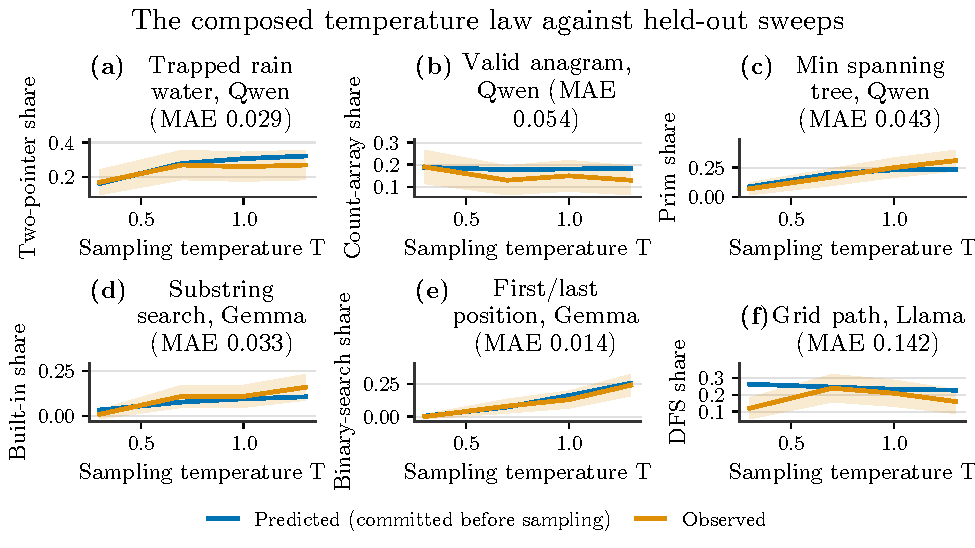
\includegraphics[width=\linewidth,height=0.78\textheight,keepaspectratio]{figures/fig_templaw_heldout_v0.pdf}
\caption{Each panel plots two curves against sampling temperature T (0.3, 0.7, 1.0, 1.3): ``Predicted (committed before sampling)'' (blue), the share of a task's minority algorithm forecast by a decision-token rule before any temperature sample was drawn, and ``Observed'' (amber), the share actually measured over 100 freshly sampled programs at that temperature, shown with a shaded band giving the Wilson 95\textbackslash{}\% confidence interval for that count out of 100 (the Predicted curve carries no such band, since it is a single committed forecast rather than a sampled statistic). The y-axis of each panel names the algorithm share it tracks: (a) two-pointer share, trapped rain water; (b) count-array share, valid anagram; (c) Prim share, minimum spanning tree -- all on Qwen, the model family the rule was fitted on. (d) built-in share, substring search, and (e) binary-search share, first\slash{}last position, both held-out tasks on Gemma. (f) DFS share, a held-out grid-path task on Llama. The MAE in each panel's title is the mean absolute difference between the predicted and observed share over the four temperatures (equivalently, since outcomes concentrate on the minority algorithm and one default, the mean total-variation distance between the predicted and observed two-way split). MAE is 0.014-0.054 on the three Qwen panels the rule was built from and on both held-out Gemma panels, where the two curves stay close; on the held-out Llama panel the curves visibly separate and MAE rises to 0.142. This held-out comparison spans three tasks (two Gemma, one Llama); the source analysis treats four as the minimum for its held-out criterion to count as confirmatory, so panels (d)-(f) read as evidence toward the rule rather than a full confirmation of it.}
\label{fig:fig_templaw_heldout}
\end{figure}
\textbf{The held-out Gemma units pass, and the second level matters.} On substring search the blind locator puts the fork right after \texttt{if len(\allowbreak{}needle) \textgreater{} len(\allowbreak{}haystack):\allowbreak{} return -\allowbreak{}1}, and the law's error is 0.033. On first and last position the first fork, 'first', is impure, so the second-fork search ran inside it and found token 24; with it the law's error is 0.014, against 0.051 for the same law without the second level (bootstrap 95\% CI of the difference -0.051 to -0.011) and 0.073 for the flat law. On both Gemma units the drop from T 1.0 to 0.3 is one-directional (10:0 and 13:0).

\textbf{The development units pass, and iteration 7's misses do not recur.} On trapped rain water the locator rebuilt iteration 7's structure blind: two 18-token openings, ' n' (0.80) to the arrays and ' left' (0.20, or 0.62 in the second cluster) mostly to two pointers, with the second fork at token 19 separating ' left =' from ' left\_\allowbreak{}max'. Iteration 7's error of 0.105 on 50 streams falls to 0.029 on 100 fresh streams. On minimum spanning tree weight the fresh-stream Prim share at T 1.0 is 25 of 100 against a prediction of 0.231 (binomial p 0.64), against iteration 7's 20 of 50 (Fisher p 0.09) and its twin's 19 of 100 (p 0.39): the lean that iteration 7 attributed to its streams was a property of those streams. Valid anagram passes, but the flat law beats the composed law (0.030 against 0.054); as in iteration 7, temperature barely moves this unit.

\textbf{The held-out Llama unit fails, for a reason outside the law's scope.} Llama's opening classifier failed its gate (the frozen labeller calls some path-storing BFS programs IDDFS), so every locator continuation was completed and labelled (3,276 continuations, on a grid thinned by the plan's cost rule). The locator found forks of the same kind as Gemma's, but Llama reaches them through many openings: the two confirmed openings cover about 2\% of the fit twin, so the committed law is almost the twin's flat shares, and the entropy of the algorithm given the fork classes is 0.63 bits, above the 0.3 criterion. Observed BFS is 0.76, 0.66 and 0.61 and DFS 0.12, 0.24 and 0.21 at T 0.3, 0.7 and 1.0. At T 1.3 the programs degenerate: 72 of 100 run to the 1,536-token cap, the pass rate falls to 0.04, and the frozen labeller calls 87 of them other; that cell exceeded the preregistered 20\% bar for other and was adjudicated by two judge families with a tiebreak (43 BFS, 15 DFS, 29 other), and the adjudicated column is primary (BFS 0.53, DFS 0.16, other 0.29). Every predictor fails on this unit (0.134 to 0.143; 0.28 to 0.29 with the frozen labels): no algorithm-level law predicts the collapse into unusable programs. Llama's top-k cells, built by keeping each top-p program up to its first token outside the top 10 and regenerating from there (shadow sampling), were reported but not used, because the construction failed its validation (1 of 20 directly sampled programs at T 1.3 token-identical).

\textbf{Verdict and rivals.} Five of six scored units pass (0.83, above 0.70), including both held-out Gemma units, but only 3 held-out units were scored where the claim needs at least 4, so the verdict is partial: the held-out criterion is underpowered, not met, and no held-out unit exceeds 0.2, so the disconfirming branch does not fire. The composed law has the lowest error on 3 of 6 units and beats the flat law on 4 of 6, tempering on 5 of 6, the highest-entropy rival on 5 of 6 and the single-fork law on 3 of 6, equalling it where no second fork exists; the exact one-sided sign test of the law against the flat law over units gives p 0.34. Slot-bootstrap 95\% intervals of the error difference against the flat law exclude 0 on minimum spanning tree weight [-0.050, -0.025], first and last position [-0.081, -0.018] and substring search [-0.041, -0.002]. Algorithm-level tempering is a strong rival: it beats the law on substring search (0.023 against 0.033) and comes close on first and last position and minimum spanning tree weight, so much of the temperature response is sharpening or flattening the known mix. The law adds most where an impure first fork needs the second level (first and last position, trapped rain water) and where the default is not the share being sharpened (minimum spanning tree weight). Three placebos behave as they should. Permuting the predictions across temperatures puts the true error below the 5th percentile on trapped rain water, minimum spanning tree weight and first and last position (not on the two nearly flat units nor on Llama). Shuffling the conditional of the algorithm given the token across tokens raises the error (p at most 0.02 on four units, 0.10 on substring search). Shuffling temperature labels within slots rejects the drop test at the nominal rate (0.02 to 0.04). Replaying each slot's own uniforms through the committed token classes names the algorithm of 0.87 to 0.99 of Qwen3-8B slots on the opening (0.94 to 1.00 in Gemma), and the replay-implied shares lie within 0.00 to 0.04 of the observed cells on every passing unit, so the remaining error is the law's expectation against 100 realised streams.

\textbf{Is the instruct model's fork the base model's mean answer?} Qwen3-8B and Qwen3-8B-Base were teacher-forced on identical chat-templated ids at the forks and at 64 phrasing positions of 20 programs per task (Table 410). On the three collapsed tasks, post-training widened the fork margin by 2.11 to 13.41 nats while the entropy at phrasing positions moved by less than 0.5 nats (0.23 to 0.31; the base model is uniformly a little less certain), as committed; without chat tokens the gains are 2.69 to 11.05, so the result is not an artefact of the template. The Jensen-Shannon divergence between the two models is 6 to 10 times larger at the fork than at phrasing positions, and 1.5 to 1.9 times larger than at phrasing positions of the same base-entropy decile on the collapsed tasks (equal on minimum spanning tree weight, lower on trapped rain water); random positions show no excess. At phrasing positions the instruct token is the base model's top token at 89\% to 95\% of positions (the URIAL token categories [100]), but at the fork it is mostly the base model's second or third choice. The instruct default is therefore not the base model's mean (that post-training shifts concentrate at the base model's high-entropy forks is already shown by Cantarero et al. [142] and Sparse but Critical [143]; what this sub-arm adds is the algorithm-level outcome on code at a counterfactually located fork) (iteration-9 correction): on minimum spanning tree weight the base model's fork distribution, pushed through the instruct model's conditional of the algorithm given each token, would give Prim 0.68 where the instruct model writes Kruskal 0.78; on trapped rain water, two pointers 0.37 against 0.29. Post-training moved and sharpened one token; the repertoire of ideas stayed the same.

\begin{table}[H]
\renewcommand{\thetable}{410}
\centering\scriptsize\setlength{\tabcolsep}{2.5pt}
\caption{The base model against the instruct model at the fork (Qwen3-8B; five templates). [Source: iteration 8, artifact \nolinkurl{gen_art_experiment_43}.]}\label{tab:t435}
\begin{tabular}{>{\raggedright\arraybackslash\hspace{0pt}}p{0.1314\linewidth}>{\raggedright\arraybackslash\hspace{0pt}}p{0.0951\linewidth}>{\raggedright\arraybackslash\hspace{0pt}}p{0.1058\linewidth}>{\raggedright\arraybackslash\hspace{0pt}}p{0.0551\linewidth}>{\raggedright\arraybackslash\hspace{0pt}}p{0.0539\linewidth}>{\raggedright\arraybackslash\hspace{0pt}}p{0.0840\linewidth}>{\raggedright\arraybackslash\hspace{0pt}}p{0.1612\linewidth}>{\raggedright\arraybackslash\hspace{0pt}}p{0.2267\linewidth}}
\toprule
\textbf{Task} & \textbf{Role} & \textbf{Fork margin, instruct (nats)} & \textbf{Base} & \textbf{Gain} & \textbf{Gain without chat tokens} & \textbf{Phrasing entropy, base minus instruct [95\% CI]} & \textbf{Jensen-Shannon divergence: fork \slash{} phrasing \slash{} entropy-matched \slash{} random} \\
\midrule
Grid path (BFS) & Collapsed & 4.9 to 7.4 & 2.9 to 3.3 & 3.27 & 5.31 & 0.31 [0.29, 0.33] & 0.51 \slash{} 0.05 \slash{} 0.27 \slash{} 0.04 \\
Connected components (union-find) & Collapsed & 10.5 to 18.7 & 2.4 to 2.7 & 13.41 & 11.05 & 0.28 [0.27, 0.28] & 0.31 \slash{} 0.04 \slash{} 0.20 \slash{} 0.09 \\
Shortest path (Dijkstra) & Collapsed & 4.9 to 6.2 & 3.4 to 3.6 & 2.11 & 2.69 & 0.23 [0.22, 0.24] & 0.44 \slash{} 0.04 \slash{} 0.29 \slash{} 0.05 \\
Minimum spanning tree weight & Mixed, descriptive & 0.5 to 1.5 & -0.8 & 1.84 & 1.69 & 0.34 [0.33, 0.35] & 0.34 \slash{} 0.05 \slash{} 0.34 \slash{} 0.02 \\
Trapped rain water & Mixed, descriptive & 1.0 to 2.5 & -0.2 to 0.1 & 1.53 & 1.91 & 0.21 [0.20, 0.22] & 0.11 \slash{} 0.03 \slash{} 0.20 \slash{} 0.04 \\
\bottomrule
\end{tabular}
\end{table}

\textbf{Ideas against phrasings (question 1a-c of the request).} Across 4,800 sweep programs no unit produced an algorithm outside its catalogue at any temperature. At T 0.3 each sweep is essentially one idea with one to four phrasing clusters (identifier-normalised AST 4-gram Jaccard 0.8): first and last position 100 linear scans in 2 clusters; minimum spanning tree weight 93 Kruskal in 4 clusters and 7 Prim in 2; trapped rain water 83 array programs in 1 cluster and 17 two-pointer programs in 1. Loosening T does not add ideas; it moves mass to the second known idea at the predicted rate and multiplies its phrasings: at T 1.3 minimum spanning tree weight has 66 Kruskal programs in 22 clusters and 31 Prim in 7, and first and last position 76 linear scans in 2 clusters and 24 binary searches in 8. Correct-only Hill-1 rises accordingly (1.29 to 2.06 and 1.00 to 1.68). Top-k 10 is token-identical to top-p 1 on every Qwen3-8B and Gemma cell except 6 of minimum spanning tree weight's 400 programs, which were regenerated after a divergence. The novelty audit read every correct program labelled outside the catalogue (10 distinct among 4,703 correct programs, checked against an 18,305-solution corpus built from the dataset dependency plus references, with two judge families passing 3 of 3 known-class controls and a manual read): 8 labeller misses of catalogue algorithms, 1 catalogue variant and 1 known brute force outside the catalogue; none is novel (rule-of-three bound 0.0006).

\textbf{Validity checks and departures.} The hash chain verifies end to end, with each family's forks and predictions committed before any sweep sample of that family and four amendments (the adjudication rule, a locator fix for nested openings, content-addressed continuation ids, and a predictor fix for second forks not found) committed before the samples they govern; the held-out families' predictions were committed and swept before any Qwen3-8B sample. CPU tests pass, including a two-level tree exact to 1e-9 and top-k shadow sampling equal to direct top-k on 1,000 synthetic sequences; the change-point rule has a 0.00 false-positive rate on 200 null series and 0.865 power on planted jumps; the scoring code reproduces iteration 7's errors exactly (0.083, 0.105 and 0.043). Gemma prompt ids reproduce earlier hashes on all 10 templates, sweep streams are disjoint from every earlier key (0 overlaps among 1,300 seeds), and per-slot labels agree with earlier engines on 0.92 (trapped rain water, below the 0.95 expectation), 0.95 and 0.98 of Qwen3-8B slots and 0.98 and 0.97 of Gemma slots. Llama's bf16 twin on the grid (BFS 60, DFS 23, IDDFS 14, other 3) differs from iteration 2's twin, served by vLLM with 8-bit floating-point weights (BFS 77, DFS 20, other 3; Fisher p 0.015 on BFS), so every Llama contrast stays within this engine. The Llama label re-gate was weak (agreement 0.10 and 0.71 on the two bench units), so primary scoring stays on the frozen labeller with the judge-adjudicated labels as a sensitivity. The base sub-arm used the 20 stored iteration-7 programs for its three collapsed tasks, and frozen-labeller disputed labels count as other. Spend was USD 0.046.

\FloatBarrier
\subsection*{8.8 The top-five prohibition across ten configurations, and where the survivors land}
\addcontentsline{toc}{subsection}{8.8 The top-five prohibition across ten configurations, and where the survivors land}
\noindent{\small\emph{Artifact: \nolinkurl{gen_art_experiment_44}.}}\par\medskip
The request asks what happens when a model's five most used algorithms are prohibited: do the survivors come from the edge of the banned set or from its opposite side? Earlier iterations found that Qwen3-8B (iteration 2) and gemma-3-4b-it (iteration 6) answer a ban of five names by reimplementing a banned algorithm under another name, so there were no survivors to place. The prohibition experiment  first screened eight new open configurations plus two carried rows for one that obeys, then placed that model's survivors on its own manifold of ten forced algorithms, in actual activation coordinates; each forced prompt names its algorithm by one of three aliases, so the manifold is alias-named (iteration-9 correction). Each configuration's banned set is its own top five by implemented count, filled from BFS, DFS, greedy best-first, IDDFS and A*; because every baseline wrote only BFS and DFS, the banned set is the same five for every configuration. A correct survivor is a program under the ban that passes the 48-case hidden suite and whose adjudicated mechanism is outside the banned set: a non-banned catalogue algorithm or a named known algorithm outside the catalogue. Four commits fixed the configurations, prompts, selection rule, labelling and adjudication, geometry, landing nulls, robustness rule and the prediction (edge) before the samples they govern.

\begin{table}[H]
\renewcommand{\thetable}{411}
\centering\scriptsize\setlength{\tabcolsep}{2.5pt}
\caption{The screen. N is the number of programs under the ban; shares carry Wilson 95\% intervals. [Source: iteration 8, artifact \nolinkurl{gen_art_experiment_44}.]}\label{tab:t436}
\begin{tabular}{>{\raggedright\arraybackslash\hspace{0pt}}p{0.2805\linewidth}>{\raggedright\arraybackslash\hspace{0pt}}p{0.1308\linewidth}>{\raggedright\arraybackslash\hspace{0pt}}p{0.0455\linewidth}>{\raggedright\arraybackslash\hspace{0pt}}p{0.0915\linewidth}>{\raggedright\arraybackslash\hspace{0pt}}p{0.1365\linewidth}>{\raggedright\arraybackslash\hspace{0pt}}p{0.1300\linewidth}>{\raggedright\arraybackslash\hspace{0pt}}p{0.1087\linewidth}}
\toprule
\textbf{Configuration (engine)} & \textbf{Baseline (N)} & \textbf{Ban N} & \textbf{Correct survivors} & \textbf{Share (95\% CI)} & \textbf{Share using a banned mechanism} & \textbf{Pass rate under the ban} \\
\midrule
Qwen3-8B, thinking on (local vLLM, FP8 weights) & BFS 30 of 30 & 30 & 0 & 0.00 (0.00 to 0.11) & 1.00 & 0.13 \\
Llama-3.1-8B-Instruct (CoreWeave, bf16) & BFS 77, DFS 20, other 3 & 50 & 0 & 0.00 (0.00 to 0.07) & 0.90 & 0.02 \\
Qwen3-14B, thinking off (DeepInfra, FP8) & BFS 94, DFS 6 & 50 & 0 & 0.00 (0.00 to 0.07) & 1.00 & 0.46 \\
Qwen3-14B, thinking on (DeepInfra, FP8) & BFS 96, DFS 4 & 50 & 7 & 0.14 (0.07 to 0.26) & 0.76 & 0.32 \\
Qwen3-32B, thinking off (DeepInfra, FP8) & BFS 81, DFS 19 & 50 & 4 & 0.08 (0.03 to 0.19) & 0.82 & 0.28 \\
Qwen3-32B, thinking on (DeepInfra, FP8) & BFS 91, invalid 9 & 50 & 17 & 0.34 (0.22 to 0.48) & 0.22 & 0.42 \\
gemma-3-27b-it (DeepInfra, FP8) & BFS 99 of 99 & 50 & 0 & 0.00 (0.00 to 0.07) & 1.00 & 0.86 \\
Qwen2.5-Coder-32B-Instruct (Cloudflare) & DFS 52, BFS 48 & 50 & 0 & 0.00 (0.00 to 0.07) & 0.94 & 0.40 \\
Qwen3-8B, thinking off (carried from iteration 2) & BFS 100 & 100 & 0 & 0.00 (0.00 to 0.04) & 1.00 & 0.68 \\
gemma-3-4b-it (carried from iteration 6) & n\slash{}a & 50 & 0 & 0.00 (0.00 to 0.07) & 1.00 & 0.38 \\
\bottomrule
\end{tabular}
\end{table}

\begin{figure}[!htbp]
\centering\captionsetup{font=footnotesize}
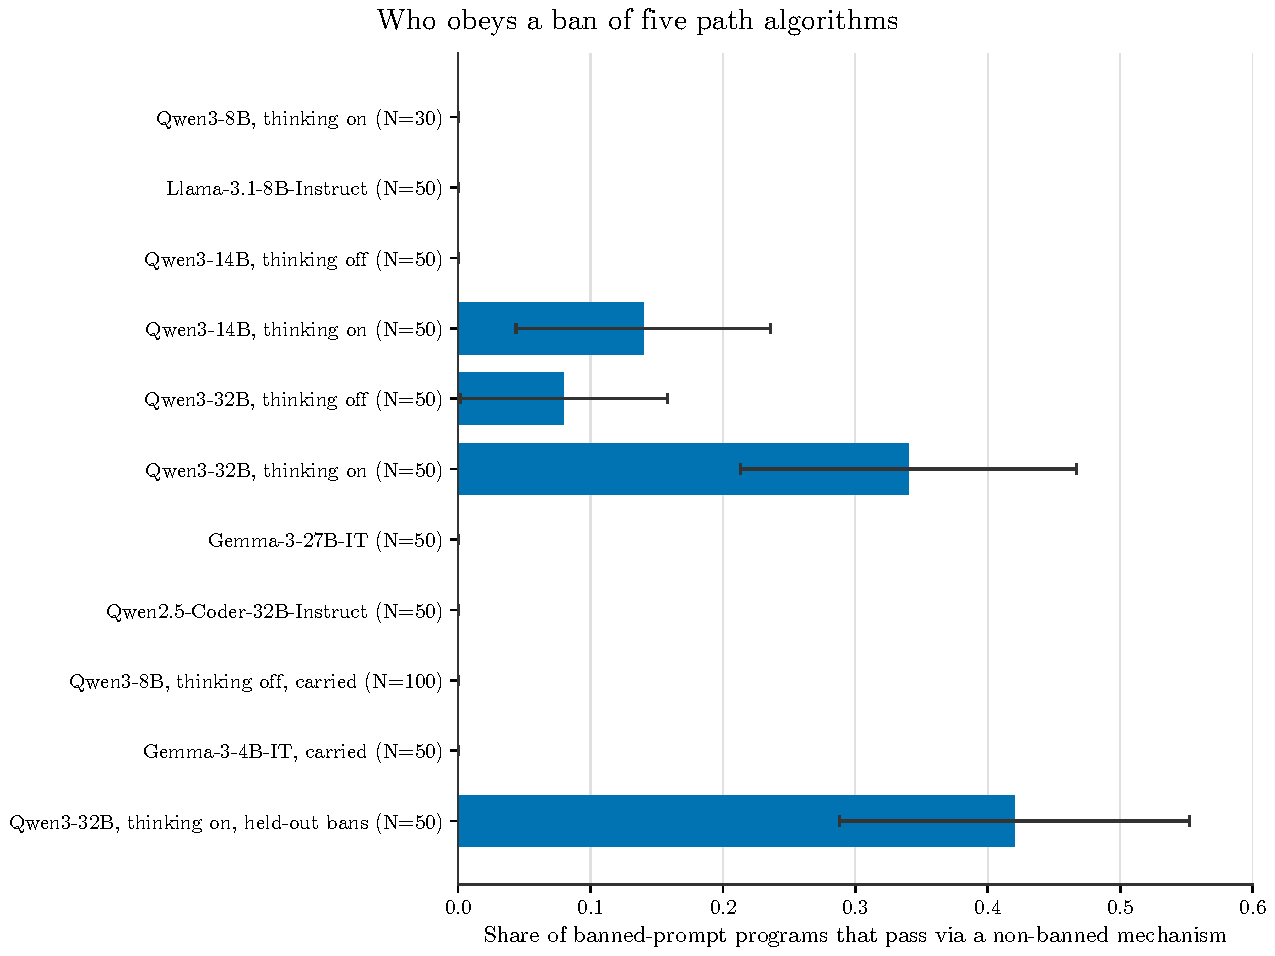
\includegraphics[width=\linewidth,height=0.78\textheight,keepaspectratio]{figures/fig_ban_screen_v0.pdf}
\caption{Share of programs generated under a prompt banning each configuration's five most used path-search algorithms (BFS, DFS, IDDFS, A* and greedy best-first, chosen per configuration) that pass the hidden tests using a mechanism outside the banned set, termed a correct, non-banned survivor. Horizontal blue bars show ten screened open-weight configurations, with sample size \$N\$ given in each row label (30, 50 or 100 generations); the bottom bar re-tests the one configuration that cleared the pre-registered 0.20 bar (Qwen3-32B, thinking on) on four held-out ban templates. Error bars show the half-width of each non-zero bar's two-sided 95\textbackslash{}\% Wilson score interval; the seven bars at exactly 0 (Qwen3-8B thinking on, Llama-3.1-8B-Instruct, Qwen3-14B thinking off, Gemma-3-27B-IT, Qwen2.5-Coder-32B-Instruct, and the carried Qwen3-8B-thinking-off and Gemma-3-4B-IT rows) had no correct survivor and so carry no interval. Only Qwen3-32B with thinking on clears the 0.20 bar on the main screen (17\slash{}50 = 0.34, Wilson 0.22-0.48), rising to 21\slash{}50 = 0.42 (Wilson 0.29-0.56) under the held-out confirmation (last bar).}
\label{fig:fig_ban_screen}
\end{figure}
\textbf{Who obeys.} Almost no open configuration obeys a ban of five names. The committed rule (share at least 0.20) selects one: Qwen3-32B with thinking on, 17 of 50 correct survivors, namely unit-weight Dijkstra 6, Bellman-Ford\slash{}SPFA run on the grid 7, a frontier search with random priorities 2, a random walk with restarts 1 and wavefront propagation 1. Thinking is the switch, and size matters: the same 32B weights with thinking off reach 0.08, Qwen3-14B reaches 0.14 with thinking on and 0.00 without, and Qwen3-8B with thinking on reaches 0.00 (it writes BFS 11 and DFS 19 under the ban). Disobedience mostly reimplements a banned mechanism without naming it: among programs that use a banned mechanism, 55\% to 100\% contain no alias of any banned algorithm in the code, the lesson of iteration 2 now across families. Obeying is expensive: the thinking 32B model's mean reasoning grows from 6,864 to 9,090 tokens under the ban, and 23 of 50 ban answers hit the 9,728-token cap (7 of 100 at baseline), counted as non-survivors. The ban costs correctness elsewhere too: Llama's pass rate falls to 0.02 and Qwen3-8B with thinking on passes 0.13.

\textbf{How robust ``obeys'' is.} The committed definition counts a correct program as a survivor if its adjudicated mechanism is a non-banned catalogue algorithm or a named known algorithm outside the catalogue. The strictest reading drops every survivor outside the catalogue whose adjudicated name, or any novelty judge's name for it, mentions BFS, DFS or SPFA. It leaves 11 of 50 (0.22) on the screen and 14 of 50 (0.28) on the confirmation, still above the bar. Counting catalogue algorithms only gives 6 of 50 (0.12) and 9 of 50 (0.18), below it. ``Obeys'' therefore rests on counting genuinely different known algorithms, mostly Bellman-Ford on the grid, as obedience; those programs sit outside the ten-algorithm manifold and are not part of the landing test.

\textbf{The manifold of the model that obeys.} States are residual-stream block outputs of Qwen3-32B, read from a checkpoint whose weights are quantised to 4-bit NormalFloat and averaged over the task specification tokens, for 300 forced prompts (ten algorithms by ten templates by three aliases); the decoder is truncated to 48 of 64 blocks, exact for every block used. Every block from 19 to 45 classifies the forced algorithm perfectly (grouped 10-fold balanced accuracy 1.00, holding out template and alias groups), and the committed ceiling rule chose block 31. There the first two principal components explain 32.4\% and 12.0\% of the variance; classical MDS has stress-1 0.42 on the 300 points and 0.28 on the ten centroids; and the Isomap neighbour graph has 8, 3 and 1 components at k 5, 10 and 15, so the committed primary k is 15. We write g for an algorithm's geodesic distance to the banned five: the smallest, over the five banned algorithms, of the mean geodesic distance between its points and theirs. A non-banned algorithm is called edge when its g lies below the median g of the five non-banned algorithms, opposite when it lies above that median, and middle at the median; the landing statistic is the mean g over the correct catalogue survivors (Table 412). The manifold is built from 300 prompts that each name the algorithm by one of three aliases, so 'opposite' may reflect the distance between names: every bidirectional BFS alias contains 'BFS' or 'breadth-first', every bidirectional A* alias contains 'A*', IDA*'s aliases contain 'A*', 'iterative deepening' or 'Manhattan heuristic', and jump point search and unit-weight Dijkstra share no algorithm-specific term with any banned alias (iteration-9 correction).

\begin{table}[H]
\renewcommand{\thetable}{412}
\centering\footnotesize\setlength{\tabcolsep}{4.0pt}
\caption{Geodesic classes of the non-banned algorithms at block 31, k 15, and their stability under 1,000 bootstrap resamples of paraphrase groups, on the alias-named manifold (iteration-9 correction). [Source: iteration 8, artifact \nolinkurl{gen_art_experiment_44}.]}\label{tab:t437}
\begin{tabular}{>{\raggedright\arraybackslash\hspace{0pt}}p{0.1681\linewidth}>{\raggedright\arraybackslash\hspace{0pt}}p{0.2078\linewidth}>{\raggedright\arraybackslash\hspace{0pt}}p{0.1518\linewidth}>{\raggedright\arraybackslash\hspace{0pt}}p{0.2052\linewidth}>{\raggedright\arraybackslash\hspace{0pt}}p{0.1802\linewidth}}
\toprule
\textbf{Non-banned algorithm} & \textbf{Geodesic distance to the banned five} & \textbf{Class} & \textbf{Share of resamples in the same class} & \textbf{Share of resamples called edge} \\
\midrule
Bidirectional BFS & 10.9 & Edge & n\slash{}a & 0.975 \\
Bidirectional A* & 11.6 & Edge & n\slash{}a & 0.936 \\
IDA* & 13.3 & Middle & n\slash{}a & n\slash{}a \\
Jump point search & 15.9 & Opposite & n\slash{}a & n\slash{}a \\
Unit-weight Dijkstra & 21.6 & Opposite (the farthest) & 1.00 & 0.00 \\
\bottomrule
\end{tabular}
\end{table}

The split-half Spearman correlation of the 10 by 10 geodesic matrices is 0.58 at k 5, 0.95 at k 10 and 0.98 at k 15. The ten centroids carry no loop (the persistence of their one-dimensional loops, measured by persistent homology, is 0.00 against a 95th percentile of 1.19 for covariance-matched Gaussian clouds), and the 300 points carry little (1.59 against 1.29), so edge and opposite are classes of geodesic distance on a manifold that is not a ring and whose prompts name each algorithm by one of three aliases (iteration-9 correction).

\begin{figure}[!htbp]
\centering\captionsetup{font=footnotesize}
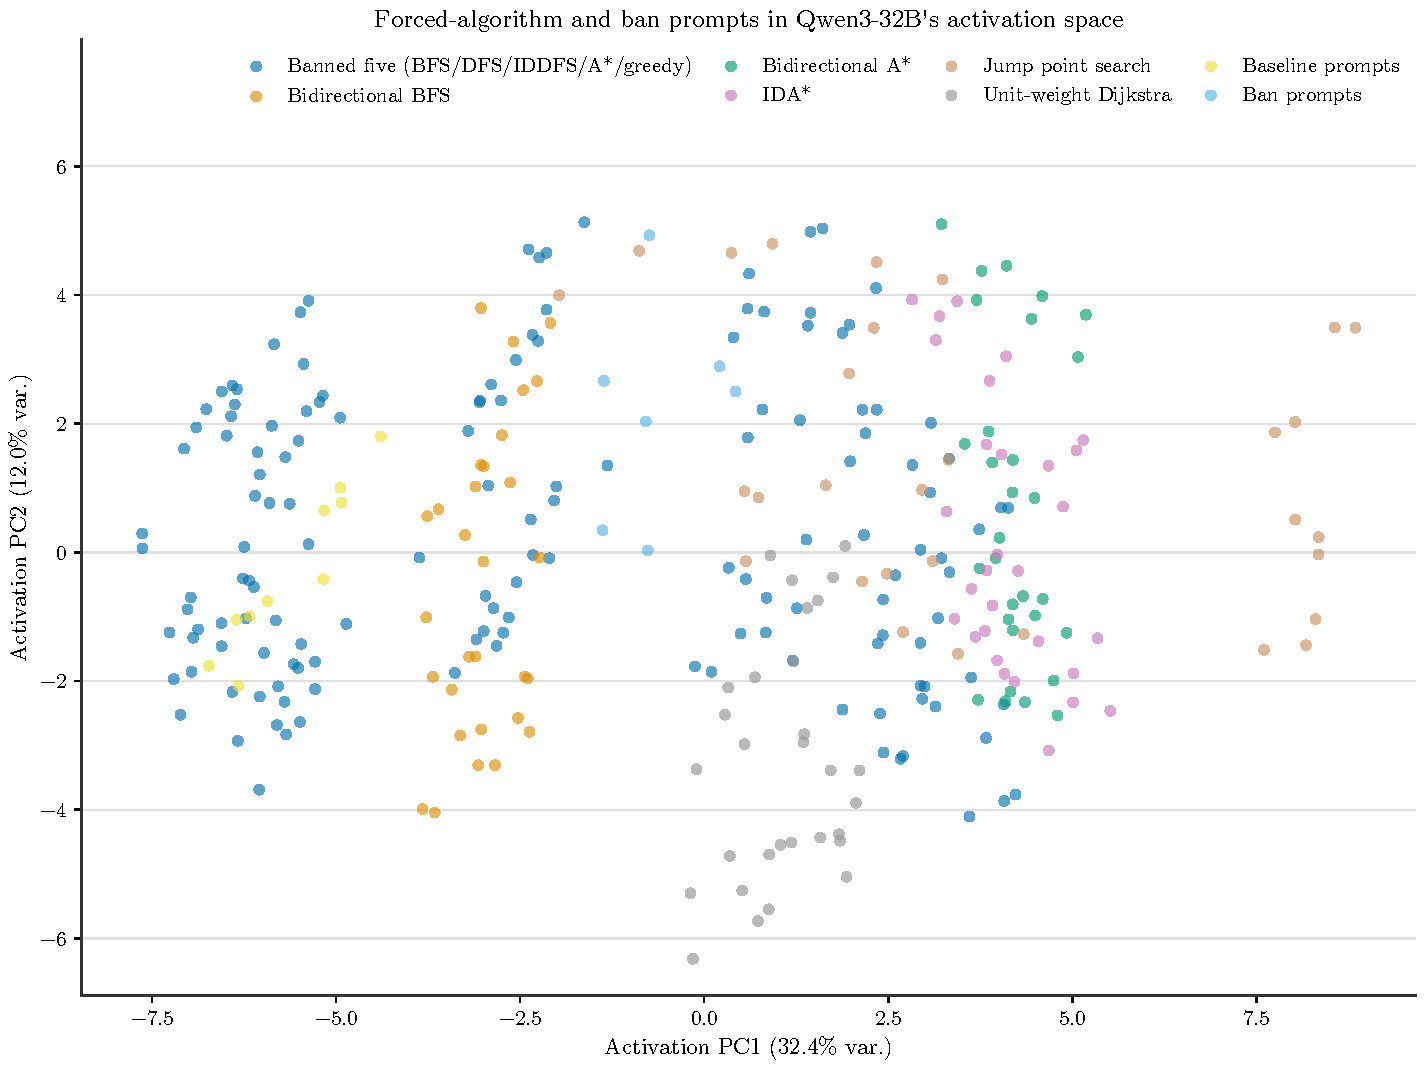
\includegraphics[width=\linewidth,height=0.78\textheight,keepaspectratio]{figures/fig_ban_pca_states_v0.pdf}
\caption{Residual-stream activations of Qwen3-32B (weights quantised to 4-bit NormalFloat) at transformer block 31, averaged over each prompt's task-specification tokens, projected onto their first two principal components (32.4 and 12.0 per cent of variance). Colour marks eight groups of prompts: the five banned path-search algorithms -- BFS, DFS, IDDFS, A*, greedy best-first -- pooled under one colour (n=150, thirty forced-generation prompts per algorithm); bidirectional BFS, bidirectional A*, IDA* and jump point search (n=30 each), the four non-banned catalogue algorithms that did not appear as correct outputs when the ban was tested; unit-weight Dijkstra (n=30), the one non-banned catalogue algorithm the model did write under the ban; ten neutral baseline prompts naming no algorithm; and seven ban prompts, pooling three screened wordings and four held-out confirmation wordings. Baseline prompts land inside the near lobe of the banned-five cloud; ban prompts land in the gap between that cloud's lobes, not merging with it. Unit-weight Dijkstra forms an isolated cloud at the bottom of the plot: on a k=15 nearest-neighbour geodesic graph of these activations it is the algorithm farthest from the banned five (21.6, versus 10.9--15.9 for the other four non-banned algorithms). Coordinates are the model's own activation coordinates; the layout describes where these prompts' activations land and is not a causal claim about what puts them there.}
\label{fig:fig_ban_pca_states}
\end{figure}
The figure plots the 300 forced states in the first two principal components at block 31 (the banned five pooled into one colour, the five non-banned algorithms each in their own), with the ten baseline prompts and the seven ban prompts projected on the same axes. The baseline prompts sit with the BFS and DFS clouds at the left; the ban prompts move right, toward the middle of the plot; unit-weight Dijkstra, the only catalogue algorithm the model writes under the ban, forms its own cloud at the bottom, away from the ban prompts.

\begin{figure}[!htbp]
\centering\captionsetup{font=footnotesize}
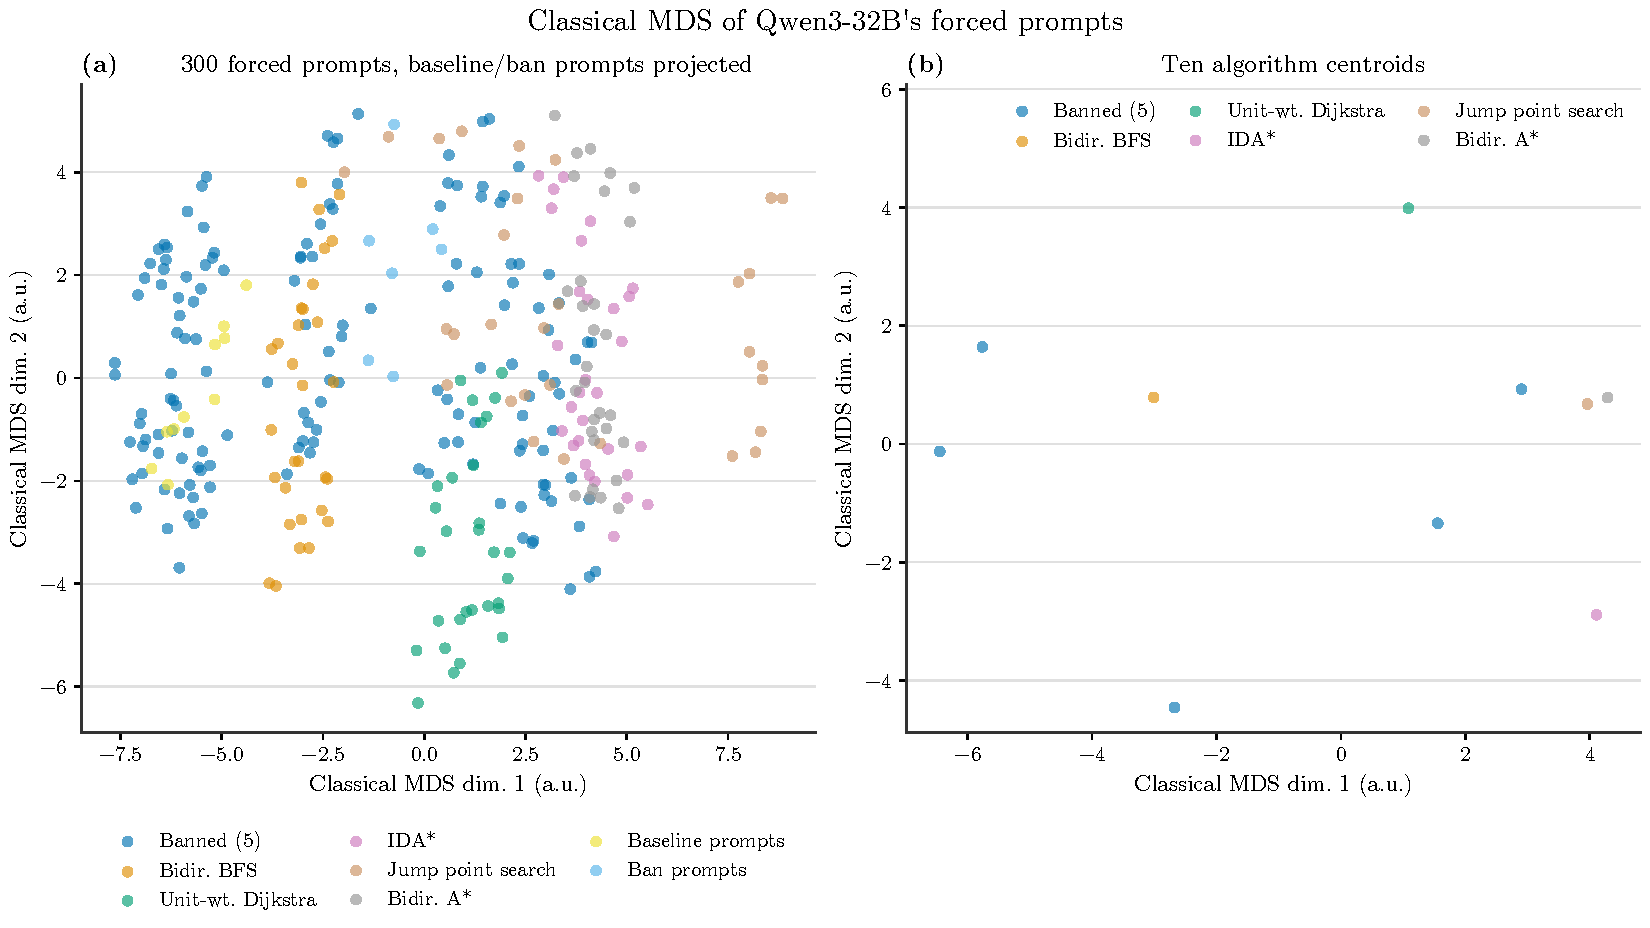
\includegraphics[width=\linewidth,height=0.78\textheight,keepaspectratio]{figures/fig_tp_mds_v0.pdf}
\caption{Classical multidimensional scaling (MDS) of Qwen3-32B (4-bit NormalFloat weights), block-31 residual states averaged over each prompt's task-specification tokens. (a) The 300 forced prompts -- ten path-search algorithms by ten templates by three aliases -- as individual points (classical-MDS Kruskal stress-1 = 0.42); the five banned algorithms (BFS, DFS, IDDFS, A*, greedy best-first) share one colour (``Banned (5)''), and the five non-banned algorithms (bidirectional BFS, unit-weight Dijkstra, IDA*, jump point search, bidirectional A*) are each a separate colour. Ten baseline prompts and seven ban prompts (three screening plus four held-out templates) are projected onto the same two axes. The unit-weight-Dijkstra points form their own group below the main banned cluster, and the jump-point-search points extend furthest to the right. (b) The same ten algorithms' centroids, from an independently fitted classical MDS of their pairwise state distances (stress-1 = 0.28; its two axes are not the same coordinate system as panel a's). The unit-weight Dijkstra centroid is the only one in the upper half of the panel. Centroid markers are uniform in size, not scaled by how often the model implements each algorithm under a plain, unbanned prompt.}
\label{fig:fig_tp_mds}
\end{figure}
\emph{Figure~\ref{fig:fig_tp_mds} (iteration-9 correction).} Positions: S-mean over the task-specification tokens of each forced prompt. Block: block 31 of Qwen3-32B (NF4 weights). Projection: classical MDS of the 300 points (Kruskal stress-1 0.42) and of the 10 centroids (0.28). N: 300 forced prompts (10 algorithms x 10 templates x 3 aliases), with baseline and ban prompts projected. Centroids: sized by baseline implemented count (bfs 91; every other algorithm 0). Caveat: alias-named manifold (each prompt names its algorithm) and correlational (in-manifold pushes moved 0 of 300 programs). Files (\nolinkurl{gen_art_experiment_44}): figures\slash{}F3\_\allowbreak{}mds\_\allowbreak{}C6\_\allowbreak{}nf4.png, figures\slash{}F3\_\allowbreak{}mds\_\allowbreak{}C6\_\allowbreak{}nf4.pdf; code \nolinkurl{gen_art_experiment_44}:src\slash{}figures.py\#manifold\_\allowbreak{}figures.

\begin{figure}[!htbp]
\centering\captionsetup{font=footnotesize}
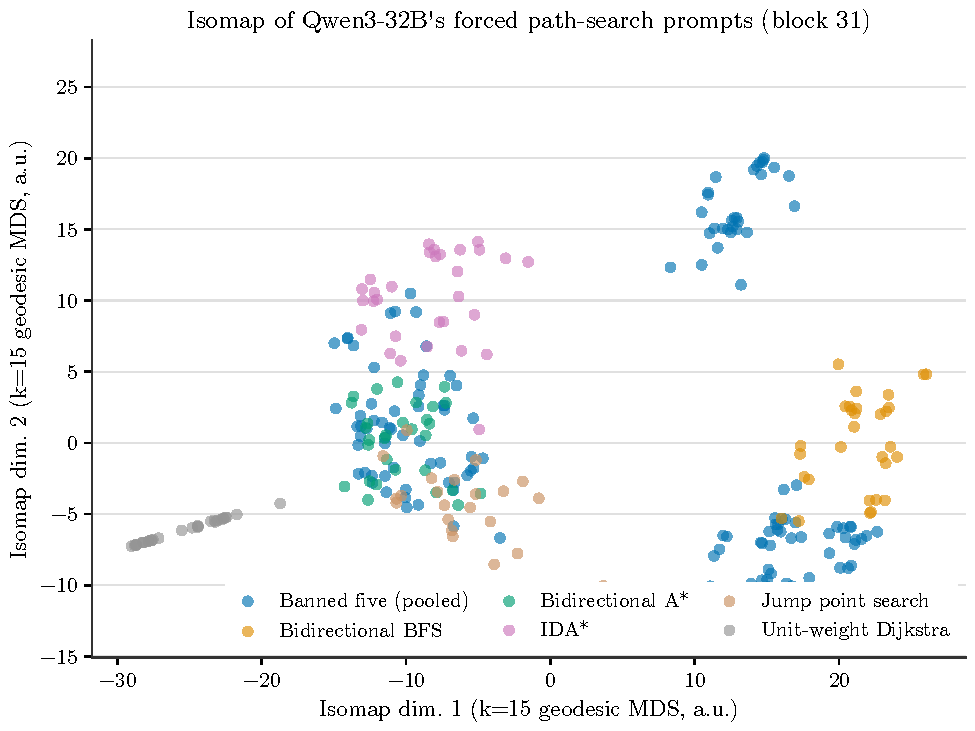
\includegraphics[width=\linewidth,height=0.78\textheight,keepaspectratio]{figures/fig_tp_isomap_v0.pdf}
\caption{Isomap embedding of the 300 forced prompts of Qwen3-32B (4-bit NormalFloat weights) at block 31: classical MDS of the stored geodesic distances on the k = 15 nearest-neighbour graph (point-level stress-1 0.18). Each point is one forced prompt that names its algorithm only by an alias. Colour pools the five algorithms the model's own baseline treats as banned (blue, n = 150: BFS, DFS, IDDFS, A*, greedy best-first) and shows each of the five algorithms left unbanned in the catalogue (n = 30 each): bidirectional BFS (orange), bidirectional A* (green), IDA* (pink), jump point search (tan), and unit-weight Dijkstra (grey). Unit-weight Dijkstra forms an isolated, thin arm at the negative end of Isomap dimension 1, separated from every banned point. The banned five split into three pooled clusters -- top right (IDDFS), bottom right (BFS\slash{}DFS), and middle (A*\slash{}greedy); bidirectional BFS sits adjacent to the bottom-right BFS\slash{}DFS cluster, while bidirectional A*, IDA*, and jump point search sit intermixed with the middle A*\slash{}greedy cluster.}
\label{fig:fig_tp_isomap}
\end{figure}
\emph{Figure~\ref{fig:fig_tp_isomap} (iteration-9 correction).} Positions: S-mean over the task-specification tokens. Block: block 31. Projection: Isomap on the symmetrised kNN geodesic graph at k 5, 10 and 15 (8, 3 and 1 components before joining); overlays at the primary k 15. N: 300 forced prompts plus projected baseline, ban and confirmation prompts. Centroids: sized by baseline implemented count (bfs 91; every other algorithm 0). Caveat: alias-named and correlational. Files (\nolinkurl{gen_art_experiment_44}): figures\slash{}F4\_\allowbreak{}isomap\_\allowbreak{}C6\_\allowbreak{}nf4.png, figures\slash{}F4\_\allowbreak{}isomap\_\allowbreak{}C6\_\allowbreak{}nf4.pdf; code \nolinkurl{gen_art_experiment_44}:src\slash{}figures.py\#manifold\_\allowbreak{}figures.

\textbf{Landing.} The screen's correct catalogue survivors are 6 of 6 unit-weight Dijkstra, so the landing statistic is 21.59, and the committed verdict is opposite on the alias-named manifold (iteration-9 correction): the preregistered edge prediction is not supported. Under the uniform null and the baseline-frequency null, p for opposite is 0.0001; under a null weighted by how often each algorithm is written correctly when forced (the correctness-filter confound), 0.057; under the exact permutation of algorithm identities, 0.20, which is that null's floor, because one landing algorithm cannot reach significance at the level of algorithms. The attempted-survivor, Euclidean-centroid and standardised-coordinate variants also give opposite. Robustness fails: opposite holds in 10 of 15 cells (every block from 29 to 33 at k 10 and k 15), but at k 5 unit Dijkstra is middle in all five blocks, against a committed bar of 12 of 15.

\textbf{Is 'opposite' a property of the names? (iteration-9 correction)} Each of the 300 forced prompts names its algorithm by one of three aliases, and the aliases of the edge algorithms share words with the banned names. On iteration 8's own stored geodesics at block 31 (every gate passes: the stored labels, prompt groups and algorithm-level g reproduce to 1e-9, and an independent kNN-geodesic recomputation from the stored states correlates with the stored k 15 matrix at 1.000), each non-banned algorithm was split into its three alias sets of 10 prompts and each set's g was computed (unit-weight Dijkstra 18.1 to 24.2, jump point search 14.2 to 18.8, IDA* 11.8 to 15.6, bidirectional A* 11.0 to 12.3, bidirectional BFS 9.2 to 12.4). The lexical overlap was committed by hash before any alias-level number: the number of banned-name detectors an alias matches (0 for every unit-weight Dijkstra and jump point search alias, 1 for every bidirectional BFS and bidirectional A* alias, 1 to 3 for IDA*). Across the 15 alias sets at k 15 the Spearman correlation is -0.61 (exact one-sided p 0.009 over all 360,360 assignments; 95\% interval over template resamples -0.71 to -0.59), -0.77 at k 10 (p 0.0007), and -0.77 with content-word overlap. That statistic treats the 15 sets as exchangeable although they are nested in five algorithms, and between algorithms lexical overlap is confounded with mechanism: bidirectional BFS is next to BFS both in name and in mechanism. At the level of algorithms the correlation is -0.63 with p 0.13 (exact over 120 permutations; the tied overlap vector cannot go below 0.033). Holding the algorithm fixed and varying only the name, the within-algorithm test on content-word overlap (3 algorithms whose aliases differ; exact null over 216 distinct relabelings) gives a mean within-algorithm Spearman of -0.12 (p 0.46; p 0.72 at k 10), and the fixed-effects slope of g on overlap is 2.36 (two-sided stratified p 0.78), the wrong sign for a name effect. A sensitivity committed as optional scores overlap with the model's own BPE tokens (function words included, so every algorithm's aliases differ): the 15-set correlation is -0.77, and the within-algorithm statistic is -0.50 (p 0.057 over 7,776 relabelings; -0.40, p 0.11 at k 10), so a small within-algorithm name effect cannot be excluded at this resolution. Placebos fail as they must (at the 0.05 level, shuffled point labels reject in a share 0.048 of draws and random overlap vectors in 0.050) and a planted effect is recovered (rho -0.92, p 3e-06). By the committed wording rule: g follows alias overlap across algorithms (rho -0.61, exact p 0.009), but the pattern is carried by algorithm identity; on this manifold names and mechanisms are confounded, and TP-G's name-free manifolds decide. The planner's expectation of about -0.70 was public before the computation, so only the within-algorithm test and the interval were unseen; tables\slash{}alias\_\allowbreak{}g.csv of the Step-0 artifact gives every set.

\begin{figure}[!htbp]
\centering\captionsetup{font=footnotesize}
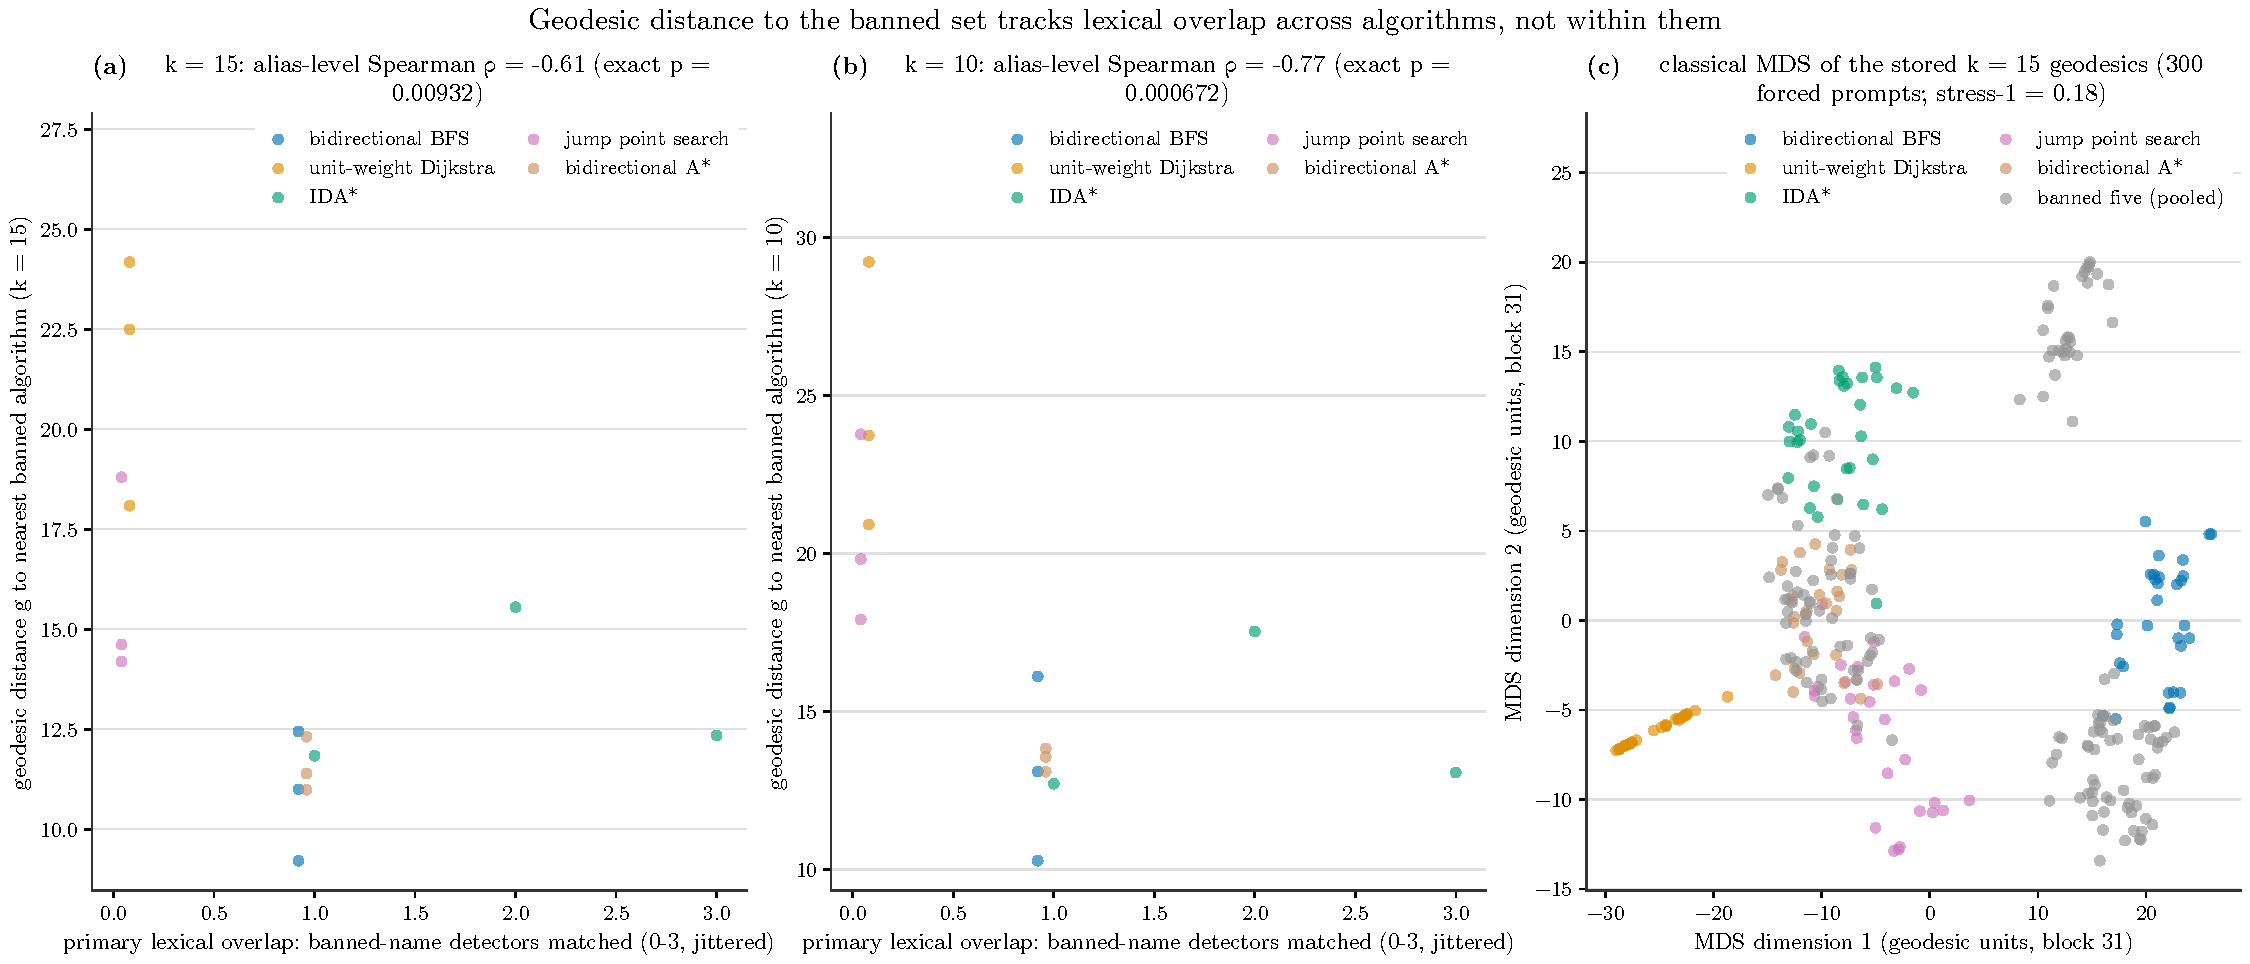
\includegraphics[width=\linewidth,height=0.78\textheight,keepaspectratio]{figures/fig_alias_overlap_v0.pdf}
\caption{The record audit's alias test on Qwen3-32B-NF4's alias-named manifold (iteration 8's stored k-nearest-neighbour geodesics at block 31). (a, b) Geodesic distance g -- for each of the 15 forced-prompt aliases of the five non-banned path-search algorithms (colour: bidirectional BFS, unit-weight Dijkstra, IDA*, jump point search, bidirectional A*), the mean geodesic over 10 prompt templates to the nearest of the five banned algorithms -- against the number of banned-name lexical detectors the alias text matches (primary overlap, 0-3, jittered for display), at k=15 (a; Spearman rho=-0.61, exact p=0.00932) and k=10 (b; rho=-0.77, exact p=0.000672). (c) Classical multidimensional scaling of the stored k=15 geodesics for all 300 forced prompts (10 algorithms x 10 templates x 3 aliases; Kruskal stress-1=0.18); grey points pool the 150 prompts of the five banned algorithms, and colours match panels (a)-(c). g falls as lexical overlap with a banned name rises across algorithms, but a parallel within-algorithm check over the same 15 aliases -- using each alias's continuous word-overlap with the nearest banned alias rather than the detector count plotted on the x-axis -- found no consistent within-algorithm trend (stratified Spearman p=0.46): unit-weight Dijkstra and jump point search, whose aliases match no banned-name detector, have the largest g. Algorithm identity, not lexical overlap alone, carries the cross-algorithm pattern, so names and mechanisms are confounded on this alias-named manifold.}
\label{fig:fig_alias_overlap}
\end{figure}
\emph{Figure~\ref{fig:fig_alias_overlap} (iteration-9 correction).} Positions: S-mean over the task-specification tokens (iteration 8's stored states). Block: block 31 of Qwen3-32B (NF4). Projection: panels A-B: alias-level g against lexical overlap at k 15 and k 10; panel C: classical MDS of the stored k 15 geodesics (stress-1 0.18). N: 15 alias sets of 10 prompts (non-banned) plus 150 banned prompts; 300 points in panel C. Centroids: algorithm centroids (stars) are not sized: g is a distance, not a count; the screen's catalogue survivors were unit-weight Dijkstra 6 of 6. Caveat: alias-named and correlational; between algorithms names and mechanisms are confounded. Files (this artifact (iteration-9 Step 0)): figures\slash{}alias\_\allowbreak{}overlap.png, figures\slash{}alias\_\allowbreak{}overlap.pdf; code src\slash{}stage\_\allowbreak{}0e.py\#\_\allowbreak{}figure.

\textbf{Held-out confirmation.} The fourth commit froze the block, k, the point set of alias-named prompts (iteration-9 correction), the geodesic matrices, the classes, the null code and the verdict rule, and the thinking 32B model was then sampled 50 times with four unseen ban templates. Survivors reach 21 of 50 (0.42, Wilson 0.29 to 0.56; 0.34 and 0.28 under the two stricter readings), with pass rate 0.58, banned-mechanism share 0.34 and truncation 0.20; by template, the one that asks to solve the task without using the named algorithms gives 8 of 12 survivors, and the one that states only that they are not allowed here gives 3 of 13. The catalogue survivors are 9 of 9 unit-weight Dijkstra, so the statistic is again 21.59: p for opposite is below 1e-4 under the uniform and frequency nulls (0 of 10,000 draws), 0.017 under the correctness-weighted null and 0.20 under the permutation null. The verdict repeats, so the result is confirmed under the committed rule; it replicates on new templates but adds no power at the level of algorithms.

\begin{table}[H]
\renewcommand{\thetable}{413}
\centering\small\setlength{\tabcolsep}{4.0pt}
\caption{Is the geometry from 4-bit NormalFloat weights sensitive to precision? Qwen3-8B forced-prompt states at three precisions (its own chosen block is 17). [Source: iteration 8, artifact \nolinkurl{gen_art_experiment_44}.]}\label{tab:t438}
\begin{tabular}{>{\raggedright\arraybackslash\hspace{0pt}}p{0.2117\linewidth}>{\raggedright\arraybackslash\hspace{0pt}}p{0.3400\linewidth}>{\raggedright\arraybackslash\hspace{0pt}}p{0.1391\linewidth}>{\raggedright\arraybackslash\hspace{0pt}}p{0.2389\linewidth}}
\toprule
\textbf{Precision against bf16} & \textbf{Spearman of the 10 by 10 geodesic matrices (k 10)} & \textbf{Class agreement} & \textbf{State cosine at every block} \\
\midrule
int8 & 0.954 & 5 of 5 & at least 0.999 \\
4-bit NormalFloat (NF4) & 0.916 & 5 of 5 & at least 0.997 \\
\bottomrule
\end{tabular}
\end{table}

Both lie above the 0.8 flag, and in Qwen3-8B's bf16 geometry unit-weight Dijkstra is also opposite the banned five (that manifold is built from the same alias-named prompts) (iteration-9 correction).

\textbf{Other descriptive geometry.} In the full-dimensional states at block 31, the ten baseline prompts sit nearest the DFS and BFS centroids, while the three screen ban prompts and the four held-out ban prompts move toward the IDDFS and greedy best-first centroids, two of the five named and banned algorithms, which is priming as in iteration 2; unit-weight Dijkstra is the farthest of the ten centroids from both sets of ban prompts (rank 10 of 10). Per-program states of 59 programs of the thinking 32B model (all 29 valid ban programs and 30 sampled baseline programs, with reasoning capped at 4,096 tokens) make the adjudicated label decodable at the first token that signals the class (balanced accuracy 0.97) and the token before it (1.00), positions that depend on the label, but only at 0.53 at the label-independent 16th code token, against a chance level of 0.25. The unit-Dijkstra survivors sit there nearest the greedy best-first cloud (geodesic 38 to 79), with which they share the heap signature token, and the off-catalogue survivors (Bellman-Ford, random walk, random-priority search) sit far from every class cloud (231 to 394). At the one position whose choice does not depend on the label, the unit-Dijkstra survivors therefore sit nearest a banned cloud (greedy best-first) rather than opposite the banned five, but that position decodes the label at only 0.53 against chance 0.25 (iteration-9 correction). Iteration 7 found that pushes inside the manifold moved 0 of 300 programs, so none of this geometry is causal.

\begin{figure}[!htbp]
\centering\captionsetup{font=footnotesize}
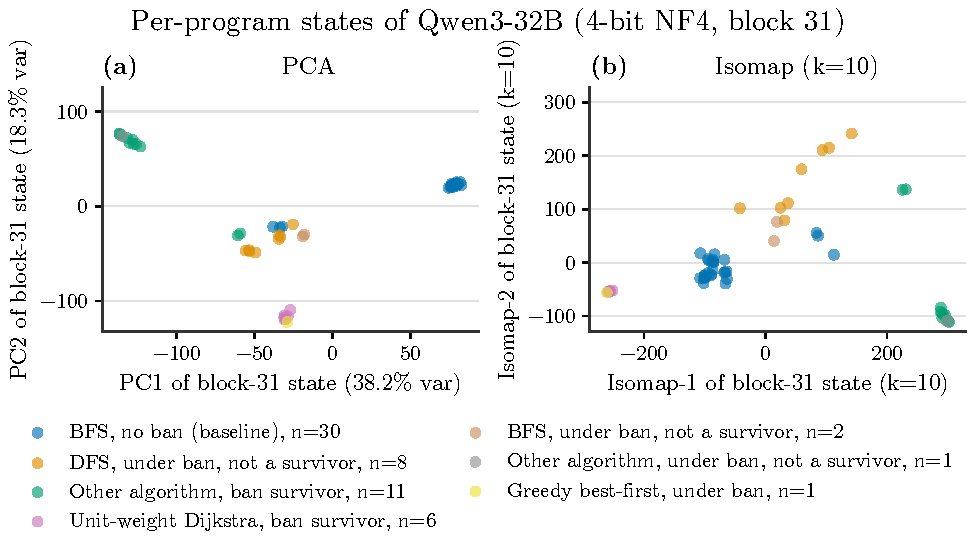
\includegraphics[width=\linewidth,height=0.78\textheight,keepaspectratio]{figures/fig_tp_program_states_v0.pdf}
\caption{Per-program hidden states of Qwen3-32B (4-bit NormalFloat weights) at block 31, at the first token that signals a program's algorithm, for 59 programs from the top-five path-search name-ban screen (iteration 8's stored states): 30 baseline programs (all BFS) and 29 programs generated under the ban. (a) First two principal components of these states (38.2\% and 18.3\% of variance). (b) Isomap embedding of the same states (k=10 nearest neighbours; one connected component). Colour gives each program's adjudicated algorithm label crossed with its ban-compliance outcome: 42 programs that are not correct ban survivors (32 BFS, 8 DFS, 1 greedy best-first, 1 other) and, separately, the 17 correct ban survivors (6 unit-weight Dijkstra, 11 other non-catalogue algorithms). In both panels the two ban-survivor colours (green, pink) occupy their own regions, separated from the baseline-BFS and ban-condition BFS\slash{}DFS clusters: position in this space tracks the label. For context, a held-out probe decodes the algorithm label from this token at balanced accuracy 0.97 versus 0.53 (chance 0.25 over 4 labels) at a label-independent position earlier in the prompt, which is not itself plotted here.}
\label{fig:fig_tp_program_states}
\end{figure}
\emph{Figure~\ref{fig:fig_tp_program_states} (iteration-9 correction).} Positions: p*, the first token that signals the program's class (label-dependent). Block: block 31. Projection: PCA and Isomap (k 10) of per-program states. N: 59 programs (all valid ban programs and sampled baseline programs). Centroids: no centroids; correct survivors starred. Caveat: the label is decodable at p* (balanced accuracy 0.97) but only at 0.53 at the label-independent 16th code token (chance 0.25), so the separation is largely written into the tokens; correlational. Files (\nolinkurl{gen_art_experiment_44}): figures\slash{}F5\_\allowbreak{}M2\_\allowbreak{}C6.png, figures\slash{}F5\_\allowbreak{}M2\_\allowbreak{}C6.pdf; code \nolinkurl{gen_art_experiment_44}:src\slash{}figures.py\#m2\_\allowbreak{}figure.

\textbf{Novelty, audits and departures.} Of 661 correct programs across all arms, 27 were adjudicated other or flagged for a manual read; each was shown to two blind judges with its three nearest known solutions (tree edit distance on normalised ASTs over 1,987 grid and graph search programs). No judge voted novel; 16 are known by both judges, and for the other 11 deepseek-chat-v3.1 says known while kimi-k2 gave no verdict (rule-of-three bound 0.45\%). A standard-library re-derivation reproduces every share, interval, geodesic (maximum difference 9e-13), landing statistic, p-value and verdict with 0 mismatches; a second audit through different code paths reproduces them too, and gives the exact uniform p for opposite as 6.4e-5, (1\slash{}5) to the sixth, on the alias-named manifold (iteration-9 correction). Its placebos explain why the per-program nulls overstate the evidence: random survivor labels on the real geometry reject at 5.0\%, nominal, but shuffling the algorithm labels of the 300 points still rejects in 36\% of shuffles, because all six survivors are one algorithm and the test mostly asks whether that algorithm happens to have the largest geodesic distance. The algorithm-level p of 0.20 is the honest figure for the landing claim. The run used an RTX 2000 Ada with 16 GB and sampled Llama through OpenRouter, appending a no-think tag where the provider ignored the thinking switch. Before the first commit it replaced gemma-3-12b-it, whose endpoints timed out, with gemma-3-27b-it. A judge that failed its gate (gemini-2.5-flash-lite, 7 of 10) gave way to deepseek-chat-v3.1 (9 of 10) and kimi-k2 (10 of 10). Qwen3-8B's thinking ban arm was cut to its committed floor of 30 because each row took 57 s. Spend was USD 1.53.

\FloatBarrier
\subsection*{8.9 Comparisons across this iteration's experiments}
\addcontentsline{toc}{subsection}{8.9 Comparisons across this iteration's experiments}
\textbf{Temperature acts through one or two tokens and only reweights known ideas.} Three experiments measured temperature at the fork from different sides. The fork-dosing experiment predicted the algorithm mix of every dosed cell within a mean absolute error of 0.010 to 0.047 on five units, the temperature-law experiment predicted global temperature sweeps within 0.014 to 0.054 on five of six units, two of them in a held-out family, and both found nothing outside the catalogue; on 5 of 6 units the fork tokens predict temperature's effect on the algorithm mix, but the flat law is better on valid anagram (0.030 against 0.054), algorithm-level tempering is better on substring search (0.023 against 0.033), the law beats the flat law on only 4 of 6 units (sign test p 0.34), and on Llama's grid task every predictor fails (0.142) (iteration-9 correction). Where the twin is already mixed, any knob that reaches the fork does about as well as the dial (min-p on minimum spanning tree weight, global T 1.3 in Gemma); the dial clearly earns its place on valid anagram, where it raises correct-only Hill-1 from 1.78 to 2.78. On the collapsed connected components task it beats every comparator family only after the amendment removed the tokens that break programs (Hill-1 1.54 against 1.17 for the best comparator, lower bound of the difference +0.01), still short of two ideas. Where the twin has collapsed, the fork's top 20 candidates hold at most about 19\% for the alternative, so no dose at that token reaches two ideas without breakage. The forced branches show what lies beyond: one known idea per unit on three units, reachable at T 1 once in 2 million to 50 million samples. The base sub-arm explains why: post-training widened the fork margin by 2 to 13 nats on the collapsed tasks while leaving the phrasing positions almost untouched.

\textbf{Internal handles act at the fork, and none is a certified variable.} Table 414 sets the internal results side by side. On connected components three different edits at late fork-position sites all write DFS: the rank-4 DAS map at block 22 (29 of 30 correct toward DFS; toward BFS it writes BFS in 29 of 30 programs but only 5 correct, NO HANDLE by the committed rule) (iteration-9 correction), the top five circuit components at dose 2 (29 of 30) and the matched random five at dose 2 (30 of 30), while a random rank-4 subspace does nothing (0 of 30). The fork margin there is easy to move with a large enough push at the right place, which is why the controls that ask whether the handle is the model's own variable (permuted labels, an untrained network, matched random components) fail or saturate. The circuit separates from random components only at a dose small enough to leave room (24:0 at dose 0.5 on connected components; 6:1 on minimum spanning tree weight). In Gemma the dial is a dormant handle by retention but lies inside the variation prompts induce, works in free generation and ties prompting there.

\begin{table}[H]
\renewcommand{\thetable}{414}
\centering\small\setlength{\tabcolsep}{4.0pt}
\caption{The internal results of iteration 8 side by side. [Source: iteration 8, compiled across the iteration's artifacts \nolinkurl{gen_art_evaluation_7}, \nolinkurl{gen_art_experiment_39}, \nolinkurl{gen_art_experiment_40}, \nolinkurl{gen_art_experiment_41}, \nolinkurl{gen_art_experiment_42}, \nolinkurl{gen_art_experiment_43}, \nolinkurl{gen_art_experiment_44}.]}\label{tab:t439}
\begin{tabular}{>{\raggedright\arraybackslash\hspace{0pt}}p{0.1719\linewidth}>{\raggedright\arraybackslash\hspace{0pt}}p{0.4688\linewidth}>{\raggedright\arraybackslash\hspace{0pt}}p{0.1925\linewidth}>{\raggedright\arraybackslash\hspace{0pt}}p{0.0965\linewidth}}
\toprule
\textbf{Question} & \textbf{Qwen3-8B} & \textbf{Gemma} & \textbf{Source} \\
\midrule
Certified low-rank variable at the fork under one protocol & No: label controls 0.63 to 0.87, untrained network 0.69, reverse -2.72 & No: label controls 0.11 to 0.20, untrained network 0.41, retention 0.12 & Section 8.4 \\
Steering handle at the fork in generation & Toward DFS 29 of 30 correct; toward BFS 29 of 30 written, 5 correct (pass 0.20 against 0.83): NO HANDLE by the committed rule (iteration-9 correction) & Toward BFS 22 of 30 correct (twin 6): sufficient handle & Section 8.4 \\
Task band & Sufficient handle; untrained network passes (0.18); routes DFS sources to BFS & Not run & Section 8.4 \\
Do random pushes act through the fitted subspace? & No: clamp removal -0.01; prospective Spearman 0.09 & n\slash{}a & Section 8.4 \\
Validated circuit nodes (both tests, top 10) & 9 (minimum spanning tree), 8 (connected components) & 7 (iteration 7) & Section 8.5 \\
Top five against matched random five in generation & 7:1 at dose 2 (p 0.070), 0:1 on connected components; 24:0 at dose 0.5 (post hoc) & Doubled correct BFS (iteration 7) & Section 8.5 \\
Shape of the circuit (iteration-9 correction) & Late fork stack, depth 0.86; condition share 0.01; committed motif test: different motif (condition share and depth outside Gemma's bands [0.21, 0.51] and [0.45, 0.80]); the layer-0 condition MLP rests on the 20 pair prompts (held-out edit not applied) & Condition share 0.36, depth 0.69 (motif match for its own set) & Section 8.5 \\
Dial against prompting, prefill matched & n\slash{}a & 39 to 0 for the dial & Section 8.6 \\
Dial against prompting, free & n\slash{}a & 38 against 32 (p 0.21); best wording 49 & Section 8.6 \\
Dormancy & Off-manifold at block 22; passes at block 24 (post hoc) & Dormant by retention at every rank; inside the prompt-induced variation & Sections 8.4 and 8.6 \\
\bottomrule
\end{tabular}
\end{table}

\textbf{The prohibition answers the request's question on one model.} Only Qwen3-32B with thinking on obeys a five-name ban often enough to place survivors, and its catalogue survivors are all unit-weight Dijkstra, the farthest non-banned algorithm from the banned five, on the screen and on held-out templates. That manifold is built from 300 prompts that each name the algorithm by one of three aliases, and its alias analysis (Section 8.8) finds that g follows alias overlap across algorithms (rho -0.61, exact p 0.009) but not clearly within them (stratified p 0.46 on content words; 0.057 on the model's BPE tokens): names and mechanisms are confounded there, and the name-free manifolds of TP-G decide (iteration-9 correction). The ban prompts themselves move toward two of the banned algorithms, not toward where the survivors land. With one landing algorithm the evidence at the level of algorithms is p 0.20, so the result reads as a description of one model, not a law.

\textbf{No correct novel algorithm anywhere.} Table 415 collects the novelty audits of iteration 8.

\begin{table}[H]
\renewcommand{\thetable}{415}
\centering\footnotesize\setlength{\tabcolsep}{4.0pt}
\caption{Novelty audits of iteration 8. [Source: iteration 8, compiled across the iteration's artifacts \nolinkurl{gen_art_evaluation_7}, \nolinkurl{gen_art_experiment_39}, \nolinkurl{gen_art_experiment_40}, \nolinkurl{gen_art_experiment_41}, \nolinkurl{gen_art_experiment_42}, \nolinkurl{gen_art_experiment_43}, \nolinkurl{gen_art_experiment_44}.]}\label{tab:t440}
\begin{tabular}{>{\raggedright\arraybackslash\hspace{0pt}}p{0.1401\linewidth}>{\raggedright\arraybackslash\hspace{0pt}}p{0.1493\linewidth}>{\raggedright\arraybackslash\hspace{0pt}}p{0.1462\linewidth}>{\raggedright\arraybackslash\hspace{0pt}}p{0.4077\linewidth}>{\raggedright\arraybackslash\hspace{0pt}}p{0.0699\linewidth}}
\toprule
\textbf{Artifact} & \textbf{Correct programs} & \textbf{Audited as possibly outside the catalogue} & \textbf{Final classes} & \textbf{Novel} \\
\midrule
Record audit & 162 adjudicated kth smallest programs & 35 relabelled & Counting sort in dictionary form & 0 \\
Fork-dosing experiment & 5,543 & 2 & Counting sort in dictionary form (catalogue variant) & 0 \\
DAS experiment & 1,857 & 0 & n\slash{}a & 0 \\
Circuit experiment & 395 & 0 & n\slash{}a & 0 \\
Gemma experiment & 913 & 0 & n\slash{}a & 0 \\
Temperature-law experiment & 4,703 & 10 distinct & 8 labeller misses, 1 catalogue variant, 1 known brute force & 0 \\
Prohibition experiment & 661 & 27 & Known algorithms (Bellman-Ford\slash{}SPFA on the grid, random walk, wavefront, random- or coordinate-ordered frontier search) & 0 \\
\bottomrule
\end{tabular}
\end{table}

\FloatBarrier
\subsection*{8.10 What iteration 8 established, what it ruled out, and what it abandoned}
\addcontentsline{toc}{subsection}{8.10 What iteration 8 established, what it ruled out, and what it abandoned}
{\small\setlength{\tabcolsep}{4.0pt}\renewcommand{\thetable}{416}
\begin{longtable}{>{\raggedright\arraybackslash\hspace{0pt}}p{0.1337\linewidth}>{\raggedright\arraybackslash\hspace{0pt}}p{0.2342\linewidth}>{\raggedright\arraybackslash\hspace{0pt}}p{0.5784\linewidth}}
\caption{Verdicts of the claims of iteration 8. [Source: iteration 8, compiled across the iteration's artifacts \nolinkurl{gen_art_evaluation_7}, \nolinkurl{gen_art_experiment_39}, \nolinkurl{gen_art_experiment_40}, \nolinkurl{gen_art_experiment_41}, \nolinkurl{gen_art_experiment_42}, \nolinkurl{gen_art_experiment_43}, \nolinkurl{gen_art_experiment_44}.]}\label{tab:t441}\\
\toprule
\textbf{Claim} & \textbf{Committed verdict} & \textbf{Deciding evidence} \\
\midrule
\endfirsthead
\multicolumn{3}{l}{\emph{Table 416, continued}}\\
\toprule
\textbf{Claim} & \textbf{Committed verdict} & \textbf{Deciding evidence} \\
\midrule
\endhead
\bottomrule
\endlastfoot
Fork-dosing claim & Not supported as committed & Composition within 0.010 to 0.047 on 5 of 5 units and mixed-unit targets met; on connected components Hill-1 1.24 and 1.60 against the 1.8 target, pass cost 0.14 at the high dose; best fork arm minus best comparator +0.06, p 0.30 \\
Fork entropy prediction & Opposite holds & The fork lies above the 90th percentile of per-token entropy in all 209 twin samples that reach it; it is the single highest-entropy position among the first 64 tokens on 44 of 44 (Gemma), 32 of 39 (minimum spanning tree) and 21 of 39 (valid anagram) slots, but on 2 of 50 (connected components) and 0 of 37 (trapped rain water), the two units where a highest-entropy rule misses it (iteration-9 correction) \\
Reachability claim & As predicted & One known idea reachable only by forcing on three units, at 1 in 2 million to 50 million samples at T 1; 0 novel \\
Matched DAS claim & Disconfirmed & Both forks fail the label control (0.11 to 0.87) and the untrained-network control (0.41 and 0.69); off-manifold overshoot at both forks; the band is a sufficient handle that fails the label control; in generation Gemma's fork is a sufficient handle and Qwen3-8B's fork NO HANDLE (toward BFS 29 of 30 written, 24 fail; pass 0.20 against 0.83) (iteration-9 correction) \\
Circuit claim & Partial on both contrasts (two-sided McNemar primary) & 9 of 10 and 8 of 10 nodes validated; top five +21 and +28 correct programs, but the matched random five also flip at dose 2 (7:1, p 0.070; 0:1); motif differs on condition share and depth; the layer-0 condition MLP's held-out edit was never applied (0.00 by construction), so that node rests on its 20 pair prompts (iteration-9 correction) \\
Gemma dial claim & Prefill-matched prompting fails (0 of 50); the dial works in free generation (38 of 50); dormant by retention & Dial against prompt 39:0 prefilled, 11:5 free (p 0.21); best free wording 49 of 50; retention 0.18 to 0.28 \\
Temperature-law claim & Partial & 5 of 6 units pass including both held-out Gemma units; only 3 held-out units scored (4 required); Llama fails (0.142); the flat law beats the composed law on valid anagram (0.030 against 0.054) and algorithm-level tempering on substring search (0.023 against 0.033); the law beats the flat law on 4 of 6 (sign test p 0.34) (iteration-9 correction) \\
Top-five prohibition claim & One configuration obeys; survivors land opposite, not at the edge, on the alias-named manifold, where names and mechanisms are confounded (Section 8.8) (iteration-9 correction); not robust; confirmed on held-out templates & 17 of 50 and 21 of 50 survivors; unit-weight Dijkstra 6 of 6 and 9 of 9; p 0.20 at the level of algorithms; 10 of 15 robustness cells \\
\end{longtable}}

\textbf{Established.} Temperature applied at the fork moves the algorithm mix exactly as the fork's logits and token map predict (mean absolute error 0.010 to 0.047 on five units in two families), and a law composed over one or two forks found blind predicts global temperature sweeps on held-out Gemma units (0.033 and 0.014) as well as on Qwen3-8B (0.029 to 0.054): on 5 of 6 units the fork tokens predict temperature's effect on the algorithm mix, but the flat law is better on valid anagram (0.030 against 0.054), algorithm-level tempering is better on substring search (0.023 against 0.033), the law beats the flat law on only 4 of 6 units (sign test p 0.34), and on Llama's grid task every predictor fails (0.142) (iteration-9 correction). The fork's entropy lies above the 90th percentile of the twin's per-token entropies in all 209 twin samples that reach it, though it can be small in absolute terms (median 0.13 nats on connected components); it is the single highest-entropy position among the first 64 tokens on 44 of 44 (Gemma), 32 of 39 (minimum spanning tree) and 21 of 39 (valid anagram) slots, but on 2 of 50 (connected components) and 0 of 37 (trapped rain water), the two units where a highest-entropy rule misses it (iteration-9 correction). Post-training widens the fork margin by 2 to 13 nats on the collapsed tasks and leaves phrasing positions almost unchanged, so the instruct default is a sharpened second or third choice of the base model, not its mean; the concentration of post-training shifts at base-entropy forks is prior work (Cantarero et al. [142]; Sparse but Critical [143]), and the contribution here is the algorithm-level reading on code (iteration-9 correction). A rank-4 edit at the fork moves the written algorithm in both families. Under the committed rule it is a sufficient handle in Gemma and NO HANDLE at Qwen3-8B's fork, where the edit toward BFS writes BFS in 29 of 30 programs but 24 fail (pass 0.20 against 0.83; 5:0 against random, p 0.063). Neither passes the specificity controls: permuted labels, an untrained network or matched random components reproduce most of each effect (iteration-9 correction). Late fork-position components of Qwen3-8B (validated MLPs at layers 26, 27, 28, 30 and 32, and heads such as head 14 of layer 33 and head 28 of layer 34) carry the fork logit; the committed motif test reads different motif from Gemma's circuit (condition share 0.01 against Gemma's band [0.21, 0.51]; fork-stack depth 0.86 against [0.45, 0.80]), and the layer-0 MLP at the condition span rests on the 20 pair prompts because its held-out edit was never applied (iteration-9 correction). In Gemma, prompting with the dial's prefill fails because the prefill is off-policy for the forced prompt and selects a BFS implementation that skips the wall check; in free generation the dial and prompting are within each other's range. Among ten open configurations, only a 32B model with thinking on obeys a five-name ban often, and its catalogue survivors are all the algorithm farthest from the banned five on its alias-named manifold, where its alias analysis (Section 8.8) finds that g follows alias overlap across algorithms (rho -0.61, exact p 0.009) but not clearly within them (stratified p 0.46 on content words; 0.057 on the model's BPE tokens): names and mechanisms are confounded there, and the name-free manifolds of TP-G decide (iteration-9 correction).

\textbf{Ruled out.} A certified low-rank variable for the algorithm at the fork under the committed controls, in either family. Temperature at the fork as a route to two ideas on a collapsed task without breakage. The edge prediction for the survivors of the top-five prohibition on the model that obeys, on the alias-named manifold (iteration-9 correction). The explanation of iteration 7 that ' queue' programs in Gemma fail by slowness (they fail a wall case). Iteration 7's lean of the minimum spanning tree sweep (a property of its streams). Fitted subspaces as the channel of iteration 4's random pushes (clamping removes nothing; the prospective association is 0.09).

\textbf{Dead ends.} The blind locator at T 1 cannot find the fork of a collapsed task, because resampling never leaves the default. The window of 16 tokens at the boundary units breaks the programs before it can test anything. Steering at dose 2 saturates both the circuit and its random control. The transcoder attribution graph was dropped again, now because Qwen3-8B's transcoders need about 96.5 GB. The two Llama bench units of the temperature law and the band and minimum spanning tree sites of the DAS experiment were dropped under time boxes.

\textbf{Not run.} The task band of Gemma and DAS at minimum spanning tree weight; a ban-against-twin contrast for the Qwen3-8B circuit; the engine check of the DAS experiment against iterations 6 and 7; a feature-level account at either fork; plan resampling and the placement of top-five survivors in DAS coordinates on the grid task, carried from iteration 7.

\FloatBarrier
\subsection*{8.10b Positioning of the iteration-8 claims (iteration-9 correction)}
\addcontentsline{toc}{subsection}{8.10b Positioning of the iteration-8 claims (iteration-9 correction)}
\noindent{\small\emph{Artifact: \nolinkurl{gen_art_evaluation_8}.}}\par\medskip
The iteration-8 artifacts each searched their own neighbours, but the record never set the seven claims against the closest published work in one place. Table 416b does, with every venue and version checked live on 2026-10-23 by fetching each page and grepping it for the quoted text (raw outputs in the Step-0 artifact's audit\slash{}web; 8 neighbours verified with their venue, 3 verified from the abstract page only, 0 not found).

{\small\setlength{\tabcolsep}{4.0pt}\renewcommand{\thetable}{416b}
\begin{longtable}{>{\raggedright\arraybackslash\hspace{0pt}}p{0.1296\linewidth}>{\raggedright\arraybackslash\hspace{0pt}}p{0.4034\linewidth}>{\raggedright\arraybackslash\hspace{0pt}}p{0.1277\linewidth}>{\raggedright\arraybackslash\hspace{0pt}}p{0.2690\linewidth}}
\caption{The claims of iteration 8 against their nearest neighbours (iteration-9 correction). [Source: iteration 8, artifact \nolinkurl{gen_art_evaluation_8}.]}\label{tab:t442}\\
\toprule
\textbf{Claim of iteration 8} & \textbf{Nearest neighbours (venues and versions checked live)} & \textbf{Verdict} & \textbf{What this run adds} \\
\midrule
\endfirsthead
\multicolumn{4}{l}{\emph{Table 416b, continued}}\\
\toprule
\textbf{Claim of iteration 8} & \textbf{Nearest neighbours (venues and versions checked live)} & \textbf{Verdict} & \textbf{What this run adds} \\
\midrule
\endhead
\bottomrule
\endlastfoot
Fork-dosed temperature & Self-Distillation's account of code as precision-bound locks and exploration-bound forks, where raising temperature helps forks but floods locks [144]; Cantarero et al.'s Fork-Patched Decoding at base-entropy forks [142]; EDT [137], AdapT [32], min-p [138]; high-entropy minority tokens [139] & PARTLY OCCUPIED & temperature at a counterfactually located algorithm fork in code, with doses committed from teacher-forced logits, algorithm shares predicted before sampling and hidden-test correctness \\
Matched DAS at the fork & DAS [110], Boundless DAS [111], CDAS [112]; MIB (ICML 2025, arXiv 2504.13151 v2) ranks DAS without specificity controls [52]; Makelov et al. [122]; Sutter et al. [132] & OCCUPIED (method) & seven specificity controls under one protocol in two families and per-direction generation verdicts (sufficient handle in Gemma, NO HANDLE at Qwen3-8B's fork) \\
Circuit at Qwen3-8B's fork & path patching [135], attribution patching [136]; Position-aware Automatic Circuit Discovery (ACL 2025 long paper) makes position classes and dataset schemas explicit [145]; MIB evaluates faithfulness on held-out inputs [52]; Many Circuits, One Mechanism (TMLR 2026, arXiv 2606.06267 v2): structural differences between circuits need not be different mechanisms [146] & PARTLY OCCUPIED (method) & a position-classed circuit for an algorithm fork validated against matched random components and steered in generation; the motif comparison is structural only, and the layer-0 node's held-out arm is untested \\
Gemma dial against prompting & CDAS validates DAS steering by generation against prompting [112]; prefix steering [140]; AxBench [34] & PARTLY OCCUPIED & prefill-matched prompting cells on the same slots, a committed free-generation placement rule, and the dormancy and implementation-channel analysis \\
Temperature law over forks & forking-path resampling (Bigelow et al., ICLR 2025, the locator's method source); high-entropy forks [139]; algorithm-level diversity under temperature measured post hoc (Lee et al., EMNLP Findings 2025); the fork and lock temperature asymmetry of [144] & PARTLY OCCUPIED & a law over blindly located forks committed before sampling and scored on held-out families against flat and tempering rivals, which stay close \\
Base sub-arm & Cantarero et al.: per-position Jensen-Shannon divergence 18.4 to 57.1 times higher inside the base model's fork set, 1.06 to 1.70 times after entropy adjustment, Fork-Patched Decoding recovers 32.8\% of distinct answers against 4.7\% at random placement (two NeurIPS 2026 workshop posters) [142]; Sparse but Critical (ICLR 2026): only a small fraction of token distributions diverge after RLVR [143]; URIAL [100] & PARTLY OCCUPIED & the concentration of post-training shifts at base-entropy forks is theirs; the run adds the algorithm-level outcome on code at a counterfactually located fork and the reading that the default is the base model's second or third choice, sharpened \\
Top-five prohibition & The Invisible Lottery (arXiv 2606.04057) [1]; denial prompting (arXiv 2407.09007) [23]; Semantic Gravity Wells: naming a forbidden word primes it (arXiv 2601.08070) [7]; Don't Think of the White Bear (arXiv 2511.12381) [53]; Manifold Steering (arXiv 2605.05115) [27] & ADJACENT-ONLY (landing); OCCUPIED (bans backfire) & a screen of ten configurations and the landing of survivors on the obeying model's manifold, which is alias-named, so names and mechanisms are confounded there \\
\end{longtable}}

Both NeurIPS 2026 pages of Cantarero et al. are posters in workshops ('Transitioning from Pre-training to Post-training' (172378) and 'ELLIS Workshop on the Foundations of LLM Post-Training in Changing Environments' (164442); no main-track page found), and the abstract states that the divergence is ``18.4--57.1x higher inside this fork set than outside'', that ``an excess of 1.06--1.70x remains'' after the entropy adjustment, and that Fork-Patched Decoding moves the number of distinct answers ``32.8\% of the way back toward the base'' while random placement recovers ``only 4.7\%''. Sparse but Critical is an ICLR 2026 paper, MIB an ICML 2025 paper (arXiv v2), and Many Circuits, One Mechanism carries the journal reference Transactions on Machine Learning Research, 2026 (arXiv v2), which confirms the venue Table 92c gives it. The arXiv pages of Manifold Steering, The Invisible Lottery and the denial-prompting study state no venue, so the venues that earlier sections give them (an ICML 2026 workshop spotlight, ICML 2026, and NAACL, which reference [23] dates 2024) are carried, not verified (3 venue statements left unverified, none contradicted). No iteration-8 result is called first.

\FloatBarrier
\subsection*{8.11 What the next iteration takes from this one}
\addcontentsline{toc}{subsection}{8.11 What the next iteration takes from this one}
Four leads remain. First, the controls show that a large enough push at a late fork-position site flips a collapsed fork whatever its direction, so a variable, if there is one, has to be sought where the full state carries the class and with doses below saturation: the block-24 fit of Qwen3-8B passes every off-manifold control and fails only specificity, and the circuit separates from random components at dose 0.5. Second, the composed temperature law passed on held-out Gemma units but scored only three held-out units, and it fails where a family reaches its fork through many openings (Llama); more held-out units, and a law that sums over openings, are what would settle it. Third, the top-five prohibition placed survivors on one model with one landing algorithm, which cannot reach significance at the level of algorithms; tasks where an obeying model writes several catalogue survivors are needed for the edge-against-opposite question, on a manifold whose prompts do not name the algorithm (TP-G), because on the alias-named manifold names and mechanisms are confounded (iteration-9 correction). Fourth, no route has produced a correct novel algorithm. The forced branches show that the known ideas a model does not write sit at deep ranks of the fork. Evolutionary search on a task whose catalogue already covers the known techniques remains the only route left untried.

\FloatBarrier
\section{Iteration 9: names against mechanisms under a prohibition, the top-five landing with and without names, where post-training sharpened the fork, and the record repaired}
\noindent\emph{Run record for this iteration.} Hypothesis carried: ``Knobs Reshuffle Ideas, Search Finds New Ones''. Move recorded at the end of the iteration: cover; review score 5; evidence state lead; coverage partial; 16 candidate strategies considered. The list below gives the iteration's artifacts and the state the round record gave each strand.

{\footnotesize\setlength{\tabcolsep}{3pt}
\begin{longtable}{>{\raggedright\arraybackslash}p{0.24\linewidth}>{\raggedright\arraybackslash}p{0.47\linewidth}>{\raggedright\arraybackslash}p{0.11\linewidth}>{\raggedright\arraybackslash}p{0.08\linewidth}}
\caption*{\textbf{Artifacts of iteration 9.} Names and titles as the artifact workspaces record them; strand state as the round record grades it.}\label{tab:arts9}\\
\toprule \textbf{Artifact} & \textbf{Title} & \textbf{Type} & \textbf{State} \\ \midrule \endfirsthead
\toprule \textbf{Artifact} & \textbf{Title} & \textbf{Type} & \textbf{State} \\ \midrule \endhead
\bottomrule \endlastfoot
\nolinkurl{gen_art_evaluation_8} & Repairing the iteration-8 research record & evaluation & null \\
\nolinkurl{gen_art_experiment_45} & Do AI coders dodge bans by renaming algorithms? & experiment & lead \\
\nolinkurl{gen_art_experiment_46} & Mapping grid algorithms with and without their names & experiment & lead \\
\nolinkurl{gen_art_experiment_50} & How tuning sharpens a code model's algorithm choice & experiment & lead \\
\end{longtable}}

\subsection*{What each artifact of iteration 9 was for and what it produced}
\addcontentsline{toc}{subsection}{What each artifact of iteration 9 was for and what it produced}
Each artifact is named below as the run's workspaces name it. The entry gives the round record's verdict on the strand it served, the artifact's own summary of what it was for and what it produced, and the output files it declared, each opened and read from its workspace for this report. It closes with the subsection of this section that reports the artifact's results and the result tables typeset there from its output files.

\paragraph{\nolinkurl{gen_art_evaluation_8}: Repairing the iteration-8 research record.}
Type: evaluation. Round record, strand state null: CPU record repair: 49 corrections, 400 checks; alias test CONFOUNDED (alias rho -0.61, within-algorithm -0.12, p .46); confirmed circuit held-out edit never applied. Tests no claim.

\emph{The artifact's own summary of what it was for and what it produced:} Step 0 of iteration 9: a CPU-only repair of the iteration-8 research record (no model runs, USD 0). It provides report\_\allowbreak{}corrected.md, the full report with 49 verbatim edits each tagged '(iteration-9 correction)', plus report.diff and corrections.json. corrections.json holds the edits and a 298-value ledger (147 MATCH, 151 NEW, 0 CORRECTED, 0 CARRIED), each value with a source '\textless{}artifact\_\allowbreak{}id\textgreater{}:\textless{}path\textgreater{}\#\textless{}key\textgreater{}'. The apply test passes; the whole-report residual-claim lint goes from 28 live hits to 0. 0a: the layer-0 condition MLP's exact-0.00 held-out effect is an unapplied edit, not a failure. MeanCache only matches same-template pair prompts, and 0 of 10 held-out prompts share one; all 20 raw rows are exactly zero. The node is therefore untested held-out and rests on its 20 pair prompts (8.14 and 7.41 nats). The motif test reads different motif: condition share 0.01 against [0.21, 0.51] and depth 0.86 against [0.45, 0.80]. 0b: Qwen3-8B's fork is NO HANDLE. Toward BFS, 29 of 30 programs write BFS but only 5 are correct (pass 0.20 against 0.83; 5:0 against random, p 0.0625). Gemma's fork is a SUFFICIENT HANDLE (22 of 30). 0c: scope is now stated per unit. The fork is above the twin's 90th percentile in 209 of 209 samples; the highest-entropy position hits it on 44\slash{}44, 32\slash{}39, 21\slash{}39, 2\slash{}50 and 0\slash{}37 slots. The temperature law's rivals stay close (flat law better on valid anagram, 0.030 against 0.054; tempering better on substring search, 0.023 against 0.033; sign test p 0.34). 0d: new section 8.10b, a positioning table with references [142]-[146]. 11 neighbours were checked live on 2026-10-23: Cantarero et al. appear on two NeurIPS 2026 workshop posters; Sparse but Critical is ICLR 2026, MIB ICML 2025, Position-aware ACD ACL 2025 and Many Circuits TMLR 2026; 3 venues remain unverified. 0e: the alias-named manifold was tested on iteration 8's stored geodesics (gates E1-E4 pass; E4 Spearman 1.000). Alias-level g against committed lexical overlap gives rho -0.61 at k15 (exact p 0.0093; template-bootstrap CI -0.71 to -0.59) and -0.77 at k10. The 5-centroid rho is -0.63 (p 0.133; floor 0.033). The within-algorithm stratified statistic is -0.12 (p 0.46); on BPE tokens it is -0.50 (p 0.057). Committed verdict: CONFOUNDED. Names and mechanisms are confounded on this manifold, and TP-G's name-free manifolds decide. 0f: min-p, block-start and T 1.6 were not run on Gemma; EDT was run, but its 0.18 pass cost triggered a twin-level fallback. 0g: 7 figure markers plus Figure~\ref{fig:fig_alias_overlap}, each with a six-field caption and sha256. Audits: audit\slash{}rederive.py (stdlib; 400 checks, 0 mismatches, 4\slash{}4 placebos fail) and audit\slash{}headline\_\allowbreak{}rederive.py, which re-derives the headlines from raw rows; its placebos fail as required. Pre-commitment: predictions\slash{}commit\_\allowbreak{}s0e.json and commitments.log, with 2 logged amendments that leave every statistic unchanged. Also provided: tables\slash{}*.csv, figures\slash{}alias\_\allowbreak{}overlap.(pdf\textbar{}png), figure\_\allowbreak{}markers.json, and eval\_\allowbreak{}out.json (exp\_\allowbreak{}eval\_\allowbreak{}sol\_\allowbreak{}out; metadata sections 0a-0g). Next steps downstream: use report\_\allowbreak{}corrected.md as the record; rerun the layer-0 node's held-out arm in BASE (B3); settle the edge\slash{}opposite question on name-free manifolds (TP-G).

Its results are reported in Subsections 8.10b, 9.2 of this report, which typeset the result tables drawn from its output files: Tables 416b, 419, 420, 421, 422, 423, 424, 425.

\begin{table}[H]
\renewcommand{\thetable}{O63}
\centering\footnotesize\setlength{\tabcolsep}{3pt}
\caption{Output files declared by \nolinkurl{gen_art_evaluation_8} (iteration 9), each opened and read from the artifact's workspace for this report; size in bytes. [Source: iteration 9, artifact \nolinkurl{gen_art_evaluation_8}.]}
\begin{tabular}{>{\raggedright\arraybackslash}p{0.25\linewidth}>{\raggedleft\arraybackslash}p{0.12\linewidth}>{\raggedright\arraybackslash}p{0.57\linewidth}}
\toprule
\textbf{Declared file} & \textbf{Bytes} & \textbf{What it holds} \\
\midrule
\texttt{eval.\allowbreak{}py} & 30,077 & the artifact's code, 473 lines \\
\texttt{full\_\allowbreak{}eval\_\allowbreak{}out.\allowbreak{}json} & 524,699 & the complete output; metadata with 7 top-level keys; 10 datasets with 682 examples in all: corrections (298), report\_\allowbreak{}edits (49), circuit\_\allowbreak{}heldout (60), occurrences\_\allowbreak{}29of30 (63), entropy\_\allowbreak{}scope (11), positioning\_\allowbreak{}rows (65), and 4 more; top-level keys metrics\_\allowbreak{}agg; 67 aggregate metrics (typeset in full below) \\
\texttt{mini\_\allowbreak{}eval\_\allowbreak{}out.\allowbreak{}json} & 97,742 & small variant of the full output (a few examples per dataset); metadata with 7 top-level keys; 10 datasets; top-level keys metrics\_\allowbreak{}agg \\
\texttt{preview\_\allowbreak{}eval\_\allowbreak{}out.\allowbreak{}json} & 36,165 & preview variant of the full output (truncated strings and lists); metadata with 7 top-level keys; 3 datasets; top-level keys metrics\_\allowbreak{}agg \\
\texttt{reproducibility.\allowbreak{}md} & 10,038 & reproducibility notes, 132 lines \\
\bottomrule
\end{tabular}
\end{table}

{\scriptsize\setlength{\tabcolsep}{2.5pt}\renewcommand{\thetable}{O64}
\begin{longtable}{>{\raggedright\arraybackslash}p{0.27\linewidth}>{\raggedright\arraybackslash}p{0.19\linewidth}>{\raggedright\arraybackslash}p{0.27\linewidth}>{\raggedright\arraybackslash}p{0.19\linewidth}}
\caption{Every aggregate metric in the \texttt{metrics\_agg} block of \nolinkurl{gen_art_evaluation_8}'s \texttt{full\_\allowbreak{}eval\_\allowbreak{}out.\allowbreak{}json} (67 metrics), values copied exactly as stored. [Source: iteration 9, artifact \nolinkurl{gen_art_evaluation_8}.]}\\
\toprule
\textbf{Metric} & \textbf{Value} & \textbf{Metric} & \textbf{Value} \\
\midrule
\endfirsthead
\toprule
\textbf{Metric} & \textbf{Value} & \textbf{Metric} & \textbf{Value} \\
\midrule
\endhead
\bottomrule
\endlastfoot
\texttt{items\_\allowbreak{}answered} & 7 & \texttt{alias\_\allowbreak{}gate\_\allowbreak{}E4\_\allowbreak{}spearman} & 1.0 \\
\texttt{items\_\allowbreak{}total} & 7 & \texttt{alias\_\allowbreak{}rho\_\allowbreak{}k15} & -0.6068480408008414 \\
\texttt{n\_\allowbreak{}edits} & 49 & \texttt{alias\_\allowbreak{}p\_\allowbreak{}k15} & 0.009324009324009324 \\
\texttt{apply\_\allowbreak{}test\_\allowbreak{}pass} & 1 & \texttt{alias\_\allowbreak{}rho\_\allowbreak{}k15\_\allowbreak{}ci\_\allowbreak{}low} & -0.7083145942466413 \\
\texttt{lint\_\allowbreak{}before\_\allowbreak{}unallowed} & 28 & \texttt{alias\_\allowbreak{}rho\_\allowbreak{}k15\_\allowbreak{}ci\_\allowbreak{}high} & -0.5873352420612645 \\
\texttt{lint\_\allowbreak{}before\_\allowbreak{}total} & 36 & \texttt{alias\_\allowbreak{}rho\_\allowbreak{}k10} & -0.766852990465372 \\
\texttt{lint\_\allowbreak{}after\_\allowbreak{}unallowed} & 0 & \texttt{alias\_\allowbreak{}p\_\allowbreak{}k10} & 0.0006715506715506716 \\
\texttt{values\_\allowbreak{}total} & 298 & \texttt{alias\_\allowbreak{}rho\_\allowbreak{}k15\_\allowbreak{}secondary} & -0.7650830489974457 \\
\texttt{values\_\allowbreak{}match} & 147 & \texttt{alias\_\allowbreak{}p\_\allowbreak{}k15\_\allowbreak{}secondary} & 0.00083 \\
\texttt{values\_\allowbreak{}corrected} & 0 & \texttt{alias\_\allowbreak{}rho\_\allowbreak{}5centroid} & -0.6324555320336759 \\
\texttt{values\_\allowbreak{}new} & 151 & \texttt{alias\_\allowbreak{}p\_\allowbreak{}5centroid} & 0.13333333333333333 \\
\texttt{values\_\allowbreak{}carried} & 0 & \texttt{alias\_\allowbreak{}5centroid\_\allowbreak{}floor} & 0.03333333333333333 \\
\texttt{circuit\_\allowbreak{}identity\_\allowbreak{}check\_\allowbreak{}pass} & 1 & \texttt{alias\_\allowbreak{}stratified\_\allowbreak{}stat} & -0.12200846792814624 \\
\texttt{circuit\_\allowbreak{}n\_\allowbreak{}exact\_\allowbreak{}zero\_\allowbreak{}heldout\_\allowbreak{}nodes} & 1 & \texttt{alias\_\allowbreak{}stratified\_\allowbreak{}p} & 0.46296296296296297 \\
\texttt{circuit\_\allowbreak{}cond\_\allowbreak{}span\_\allowbreak{}matches\_\allowbreak{}heldout} & 0 & \texttt{alias\_\allowbreak{}fe\_\allowbreak{}beta} & 2.360070051445393 \\
\texttt{circuit\_\allowbreak{}L0\_\allowbreak{}pair\_\allowbreak{}mean\_\allowbreak{}ablate} & 8.144148281097412 & \texttt{alias\_\allowbreak{}fe\_\allowbreak{}beta\_\allowbreak{}p\_\allowbreak{}two\_\allowbreak{}sided} & 0.7777777777777778 \\
\texttt{circuit\_\allowbreak{}L0\_\allowbreak{}pair\_\allowbreak{}mean\_\allowbreak{}steer} & 7.407574213027954 & \texttt{alias\_\allowbreak{}placebo\_\allowbreak{}P1\_\allowbreak{}reject\_\allowbreak{}rate} & 0.048 \\
\texttt{circuit\_\allowbreak{}natural\_\allowbreak{}heldout\_\allowbreak{}ablate} & 0.28175117492675783 & \texttt{alias\_\allowbreak{}placebo\_\allowbreak{}P2\_\allowbreak{}reject\_\allowbreak{}rate} & 0.05 \\
\texttt{circuit\_\allowbreak{}natural\_\allowbreak{}heldout\_\allowbreak{}p} & 0.03125 & \texttt{alias\_\allowbreak{}placebo\_\allowbreak{}P3\_\allowbreak{}mean} & 0.007350852961085882 \\
\texttt{das\_\allowbreak{}T10\_\allowbreak{}bfs\_\allowbreak{}written} & 29 & \texttt{alias\_\allowbreak{}planted\_\allowbreak{}control\_\allowbreak{}pass} & 1 \\
\texttt{das\_\allowbreak{}T10\_\allowbreak{}bfs\_\allowbreak{}correct} & 5 & \texttt{alias\_\allowbreak{}bpe\_\allowbreak{}rho\_\allowbreak{}k15} & -0.7680054866576357 \\
\texttt{das\_\allowbreak{}T10\_\allowbreak{}bfs\_\allowbreak{}mcnemar\_\allowbreak{}p} & 0.0625 & \texttt{alias\_\allowbreak{}bpe\_\allowbreak{}stratified\_\allowbreak{}k15} & -0.5 \\
\texttt{das\_\allowbreak{}n\_\allowbreak{}29of30\_\allowbreak{}occurrences} & 29 & \texttt{alias\_\allowbreak{}bpe\_\allowbreak{}stratified\_\allowbreak{}p\_\allowbreak{}k15} & 0.0573559670781893 \\
\texttt{entropy\_\allowbreak{}n\_\allowbreak{}twin\_\allowbreak{}samples\_\allowbreak{}above\_\allowbreak{}q90} & 209 & \texttt{alias\_\allowbreak{}bpe\_\allowbreak{}stratified\_\allowbreak{}p\_\allowbreak{}k10} & 0.11188271604938271 \\
\texttt{law\_\allowbreak{}units\_\allowbreak{}pass} & 5 & \texttt{alias\_\allowbreak{}verdict\_\allowbreak{}confounded} & 1 \\
\texttt{law\_\allowbreak{}sign\_\allowbreak{}test\_\allowbreak{}p\_\allowbreak{}vs\_\allowbreak{}flat} & 0.34375 & \texttt{gemma\_\allowbreak{}families\_\allowbreak{}twin\_\allowbreak{}fallback} & 3 \\
\texttt{positioning\_\allowbreak{}rows} & 65 & \texttt{figure\_\allowbreak{}markers\_\allowbreak{}added} & 7 \\
\texttt{positioning\_\allowbreak{}live\_\allowbreak{}verified} & 8 & \texttt{figure\_\allowbreak{}caption\_\allowbreak{}fields\_\allowbreak{}complete} & 8 \\
\texttt{positioning\_\allowbreak{}live\_\allowbreak{}verified\_\allowbreak{}abstract} & 3 & \texttt{audit\_\allowbreak{}n\_\allowbreak{}checks} & 400 \\
\texttt{positioning\_\allowbreak{}live\_\allowbreak{}not\_\allowbreak{}found} & 0 & \texttt{audit\_\allowbreak{}n\_\allowbreak{}mismatches} & 0 \\
\texttt{n\_\allowbreak{}venue\_\allowbreak{}or\_\allowbreak{}version\_\allowbreak{}corrections} & 3 & \texttt{audit\_\allowbreak{}placebos\_\allowbreak{}failed} & 4 \\
\texttt{alias\_\allowbreak{}gate\_\allowbreak{}E1} & 1 & \texttt{audit\_\allowbreak{}raw\_\allowbreak{}headlines\_\allowbreak{}all\_\allowbreak{}match} & 1 \\
\texttt{alias\_\allowbreak{}gate\_\allowbreak{}E2} & 1 & \texttt{audit\_\allowbreak{}raw\_\allowbreak{}headline\_\allowbreak{}placebos\_\allowbreak{}failed} & 4 \\
\texttt{alias\_\allowbreak{}gate\_\allowbreak{}E3} & 1 &  &  \\
\end{longtable}}

\paragraph{\nolinkurl{gen_art_experiment_45}: Do AI coders dodge bans by renaming algorithms?.}
Type: experiment. Round record, strand state lead: Rename gap .70\slash{}.61 pooled, 10\slash{}10 configs, but tracer failed gate (.70\textless{}.90); Q14 k5 gap robust (.62-.76); Q32 k5 gap .22-.30 by tracer\slash{}hand reads (\textless{}.4); rotated sets 3\slash{}7.

\emph{The artifact's own summary of what it was for and what it produced:} TP-B iteration 9 experiment on the T1 grid-path task (solve(grid, start, goal)): is a prompt that bans a model's path-search repertoire by NAME (BFS, DFS, IDDFS, A*, greedy best-first) obeyed on names but not on mechanisms? PROVIDES: (1) method.py, a stage orchestrator over src\slash{}, including a name-blind expansion-order tracer v9 (src\slash{}tracer\_\allowbreak{}v9.py, src\slash{}orderclass.py) that runs each program on 40 committed probe grids (probes\slash{}probes\_\allowbreak{}v9.json) and assigns an order class (BFS\slash{}DFS\slash{}ID\slash{}HEUR\slash{}BIDIR\slash{}OTHER), a fine class, a FIFO flag and a data-structure signature. (2) method\_\allowbreak{}out.json (exp\_\allowbreak{}gen\_\allowbreak{}sol\_\allowbreak{}out; plus full\slash{}mini\slash{}preview) with 1,623 programs in 5 datasets: tp\_\allowbreak{}retrace 580 (iteration 1-8 five-name-ban rows, configurations C1-C10), tp\_\allowbreak{}cumulative 600 (Qwen3-32B and Qwen3-14B thinking, cumulative bans k=1..5 plus held-out templates), tp\_\allowbreak{}rotated 293 (N5 rotated five-name sets), tp\_\allowbreak{}described 50 (name-free described ban), tp\_\allowbreak{}scale 100 (gpt-oss-120b). Every example carries predict\_\allowbreak{}name\_\allowbreak{}label (iteration-8 labeller + gated judges), predict\_\allowbreak{}runtime\_\allowbreak{}class (iteration-8 name-free runtime label mapped to a coarse class: the primary mechanism label after the gate fallback), predict\_\allowbreak{}order\_\allowbreak{}class (tracer v9) and predict\_\allowbreak{}lexical\_\allowbreak{}L1\slash{}L2. (3) data\slash{}samples\_\allowbreak{}v9.jsonl (new rows, reasoning kept), data\slash{}survivors\_\allowbreak{}for\_\allowbreak{}tpg.jsonl (survivor programs for TP-G), results\slash{}*.json (every analysis), figures F1-F8, and a sha256 hash chain of pre-registrations (commitments.log, 10 entries, verifies). RESULTS, independently re-derived (audit\slash{}rederive\_\allowbreak{}headlines.py and audit\slash{}rederive.py: 0 mismatches; placebos fail as required): the tracer FAILED its gold gate (182\slash{}260 = 0.70 agreement vs a 0.90 bar; references 14\slash{}15; planted controls 9\slash{}9 by class, 8\slash{}9 counting that one control fails the 48-case suite), so the committed fallback applies and N1-N3 are DESCRIPTIVE. N1: lexical minus mechanistic compliance pooled over 10 configurations = 0.697 (runtime label) and 0.608 (tracer), positive in 10\slash{}10 configurations under both; a within-program swap placebo gives about 0. N2: C6 name-level survivors in a banned coarse class = 72\slash{}91 = 0.79 (runtime label) but 39\slash{}91 = 0.43 (tracer). N3: k=5 lexical vs mechanistic (runtime) compliance = 0.89 vs 0.22 (Qwen3-32B) and 0.86 vs 0.10 (Qwen3-14B), Jonckheere-Terpstra p about 1e-5 for both. N5: joint sign count 3\slash{}7 (disconfirmed). NOT independently re-derived: the executor's manual reads (0.30 of 76 k=5 survivors in a banned class; they agree with the tracer on 0.88), the N3-D and gpt-oss scale numbers, and the novelty audit (0 novel of 73). CAVEATS: the two mechanism instruments disagree on coordinate-key heaps and grid Bellman-Ford rounds; one task only; sampling via quantised providers is not byte-reproducible. Spend USD 3.889 (cap raised from 3.5 to 4.0; the USD 2.096 sampling share was re-derived from per-row costs). Inputs from prior artifacts are copied into inputs\slash{} with SHA256SUMS; dependency paths come from \$TP\_\allowbreak{}DEP\_\allowbreak{}\textless{}KEY\textgreater{} or a sibling folder named by artifact id (reproducibility.md). data\slash{}trace\_\allowbreak{}cache\slash{} (179 MB cache, stored as 5 parts of at most 45 MB read in order by gate\_\allowbreak{}v9.trace\_\allowbreak{}many) is excluded from publication.

Its results are reported in Subsection 9.3 of this report, which typesets the result tables drawn from its output files: Tables 426, 427, 428, 429, 430, 431, 431b, 432, 433, 434.

\begin{table}[H]
\renewcommand{\thetable}{O65}
\centering\footnotesize\setlength{\tabcolsep}{3pt}
\caption{Output files declared by \nolinkurl{gen_art_experiment_45} (iteration 9), each opened and read from the artifact's workspace for this report; size in bytes. [Source: iteration 9, artifact \nolinkurl{gen_art_experiment_45}.]}
\begin{tabular}{>{\raggedright\arraybackslash}p{0.25\linewidth}>{\raggedleft\arraybackslash}p{0.12\linewidth}>{\raggedright\arraybackslash}p{0.57\linewidth}}
\toprule
\textbf{Declared file} & \textbf{Bytes} & \textbf{What it holds} \\
\midrule
\texttt{method.\allowbreak{}py} & 2,148 & the artifact's code, 51 lines \\
\texttt{full\_\allowbreak{}method\_\allowbreak{}out.\allowbreak{}json} & 8,856,632 & the complete output; metadata with 45 top-level keys; 5 datasets with 1,623 examples in all: tp\_\allowbreak{}retrace (580), tp\_\allowbreak{}cumulative (600), tp\_\allowbreak{}rotated (293), tp\_\allowbreak{}described (50), tp\_\allowbreak{}scale (100) \\
\texttt{mini\_\allowbreak{}method\_\allowbreak{}out.\allowbreak{}json} & 795,693 & small variant of the full output (a few examples per dataset); metadata with 45 top-level keys; 5 datasets \\
\texttt{preview\_\allowbreak{}method\_\allowbreak{}out.\allowbreak{}json} & 365,226 & preview variant of the full output (truncated strings and lists); metadata with 45 top-level keys; 3 datasets \\
\texttt{reproducibility.\allowbreak{}md} & 15,327 & reproducibility notes, 226 lines \\
\bottomrule
\end{tabular}
\end{table}

\paragraph{\nolinkurl{gen_art_experiment_46}: Mapping grid algorithms with and without their names.}
Type: experiment. Round record, strand state lead: uDij opposite on named\slash{}name-only\slash{}described maps (1.63\slash{}1.20\slash{}1.08), edge on program map (.67; 15\slash{}15); BF\slash{}SPFA survivors opposite; program map tracks surface (partial beh .11).

\emph{The artifact's own summary of what it was for and what it produced:} TP-G iteration 9 (claim N4). Qwen3-32B nf4 (truncated decoder, iteration 8's code unchanged) and Qwen3-8B bf16 ten-algorithm grid manifolds rebuilt four ways with fixed readout\slash{}block rule\slash{}k\slash{}landing code: M-name (300 alias prompts), M-desc (name-free descriptions passing a Qwen3-32B naming gate; JPS has none: [['bibfs\textbar{}2', 0.15], ['jps\textbar{}0', 0.7], ['jps\textbar{}1', 0.6], ['jps\textbar{}2', 0.45]]), M-lex (alias minus token-matched neutral twin) and M-code (name-scrubbed verified programs; PRIMARY counts \{'bfs': 20, 'dfs': 20, 'bibfs': 8, 'iddfs': 2, 'astar': 20, 'gbfs': 20, 'dijkstra\_\allowbreak{}unit': 20, 'idastar': 17, 'jps': 0, 'biastar': 2\}; classes over non-banned algorithms with \textgreater{}= 10 programs). NAMED OUTCOME: MIXED. Unit-Dijkstra (the iteration-8 survivor) class at k15: M-name OPPOSITE (rank 5\slash{}5, g\slash{}median 1.63); M-lex OPPOSITE (rank 4\slash{}5, g\slash{}median 1.20); M-desc OPPOSITE (rank 3\slash{}4, g\slash{}median 1.08); M-code R1 EDGE (rank 1\slash{}2, g\slash{}median 0.67); M-code Qwen3-32B-only frame EDGE (rank 1\slash{}2, g\slash{}median 0.79); 8B M-name OPPOSITE (rank 4\slash{}5, g\slash{}median 1.17), 8B M-desc OPPOSITE (rank 3\slash{}4, g\slash{}median 1.01), 8B M-code EDGE (rank 1\slash{}2, g\slash{}median 0.63). Reproduction: per-prompt cosine \textgreater{}= 0.9999, g within 0.030, classes identical, but committed gate Spearman 0.894 \textless{} 0.95 (k10: 0.997; kNN tie flips), fallback F1. Lexical: Spearman(g\_\allowbreak{}alias, L1) on M-name -0.74 (k10) \slash{} -0.65 (k15), P4 True. RSA (exact 10! Mantel): M-name vs R\_\allowbreak{}lex 0.46 (p 0.003), vs R\_\allowbreak{}beh 0.24 (p 0.091); M-desc vs R\_\allowbreak{}beh 0.12 (p 0.252); M-code vs R\_\allowbreak{}beh 0.64 (p 0.018), vs R\_\allowbreak{}surface 0.67 (p 0.010). Placement on M-code: LOO accuracy 0.85; uDij survivors EDGE 15\slash{}15. Predictions pass: \{'P1': False, 'P2': False, 'P3': True, 'P4': True, 'P5': None, 'P6': True, 'P7': None, 'P8': True\}. Audits: rederive.py 0 mismatches, audit\_\allowbreak{}states mismatches []. Geometry is correlational. OpenRouter USD 0.094. Files: results\slash{}n4\_\allowbreak{}verdict.json, results\slash{}geometry\_\allowbreak{}*.json, rsa.json, lexical\_\allowbreak{}regression.json, placement.json, figures\slash{} (PCA\slash{}MDS\slash{}Isomap in activation coordinates), method\_\allowbreak{}out.json; cache\slash{}states\slash{} (states + frozen geodesic graphs geo\_\allowbreak{}*\_\allowbreak{}k10\slash{}k15.npz for iteration 10) stays on the run volume, not in the repository.

Its results are reported in Subsection 9.4 of this report, which typesets the result tables drawn from its output files: Tables 435, 436, 437, 437b, 438, 439.

\begin{table}[H]
\renewcommand{\thetable}{O66}
\centering\footnotesize\setlength{\tabcolsep}{3pt}
\caption{Output files declared by \nolinkurl{gen_art_experiment_46} (iteration 9), each opened and read from the artifact's workspace for this report; size in bytes. [Source: iteration 9, artifact \nolinkurl{gen_art_experiment_46}.]}
\begin{tabular}{>{\raggedright\arraybackslash}p{0.25\linewidth}>{\raggedleft\arraybackslash}p{0.12\linewidth}>{\raggedright\arraybackslash}p{0.57\linewidth}}
\toprule
\textbf{Declared file} & \textbf{Bytes} & \textbf{What it holds} \\
\midrule
\texttt{method.\allowbreak{}py} & 3,855 & the artifact's code, 106 lines \\
\texttt{full\_\allowbreak{}method\_\allowbreak{}out.\allowbreak{}json} & 1,700,254 & the complete output; metadata with 11 top-level keys; 3 datasets with 1,235 examples in all: tpg\_\allowbreak{}points (1,080), tpg\_\allowbreak{}placements (113), tpg\_\allowbreak{}naming (42) \\
\texttt{mini\_\allowbreak{}method\_\allowbreak{}out.\allowbreak{}json} & 35,853 & small variant of the full output (a few examples per dataset); metadata with 11 top-level keys; 3 datasets \\
\texttt{preview\_\allowbreak{}method\_\allowbreak{}out.\allowbreak{}json} & 25,131 & preview variant of the full output (truncated strings and lists); metadata with 11 top-level keys; 3 datasets \\
\texttt{reproducibility.\allowbreak{}md} & 7,274 & reproducibility notes, 107 lines \\
\bottomrule
\end{tabular}
\end{table}

\paragraph{\nolinkurl{gen_art_experiment_50}: How tuning sharpens a code model's algorithm choice.}
Type: experiment. Round record, strand state lead: Gemma grid fork +1.78 nats, base reversed 20\slash{}20, JS \textasciitilde{} entropy-matched (.75-1.18x); fork stack 1.00 on MST but random .81; CC .45 vs -.22; FPD 18\slash{}30 DFS; held-out bimodal.

\emph{The artifact's own summary of what it was for and what it produced:} Iteration-9 BASE artifact (claims B1-B3), all pre-registered in a sha256 commitment chain and re-derived by an independent stdlib script (0 mismatches; placebos fail). B1 (Gemma-3-4b pt vs it on 3 forks; Llama-3.1-8B base vs instruct descriptive): instruct models are sharper at the algorithm fork (gains G-GRID 1.78 [1.59, 2.00], G-T04 1.75, G-R6 3.07 and 1.68 nats) while ordinary positions barely change (\textbar{}dH\textbar{} \textless{} 0.5; the instruct token is the base top-1 at 91-97\% of phrasing positions); but JS at forks is only 0.75-1.18x JS at base-entropy-matched positions (fork \textasciitilde{} high base entropy; Cantarero in\slash{}out 11-15x reproduced), P1\slash{}P3\slash{}P4 fail -\textgreater{} verdict PARTIAL. Llama-3.1-8B base chat-token embeddings are untrained (norm \textasciitilde{}3e-21 of median), so template-free is primary for Llama; L-GRID fails the on-policy rule (descriptive only). B2 (Qwen3-8B vs Qwen3-8B-Base, cross-model activation patching at the fork, 20 prompts\slash{}unit, fixed batch shapes): on MST the 10 validated fork-stack nodes close 1.00 [0.96, 1.04] of the 2.06-nat gap but 50 write-norm-matched random late sets close a median 0.81 (p = 0.45; R-pure p = 0.039); on CC the stack closes 0.45 [0.28, 0.57] of a 4.52-nat gap vs random median -0.22 (p = 0.020). Task-spec (SPEC) nodes close \textasciitilde{}0; late MLPs (L26-35) carry the residual part redundantly; the fine-tuned unembedding alone accounts for 43\% (MST) \slash{} 85\% (CC) of the gap (CPU readout decomposition), which is why RS-fork(36) \textless{} 1. Committed verdict PARTIAL (Q1 fails on CC, Q2 on MST, Q3 holds), localisation 'distributed'. Generation (N=30 CRN slots\slash{}arm, frozen labellers + hidden tests): on MST one-token FSTACK patch gives 19\slash{}30 correct Prim vs 0\slash{}30 twin (McNemar 19:0, p=3.8e-6) but a matched random set also gives 19\slash{}30 (2:2) and FPD (base logits at the fork) 18\slash{}30; on CC only FPD moves the choice (18\slash{}30 DFS vs 1\slash{}30). B3: iteration-8 MeanCache bug confirmed (None on all held-out COND nodes); with interpolated means the layer-0 condition MLP's held-out effect is 3.86 nats ablate (p=0.0625) \slash{} 3.85 steer (p=0.023), about half the pair-prompt values; the exp41 value reproduces to 0.096 (its engine changed after its rows). Kind-matched motif still differs on COND share. Outputs: method\_\allowbreak{}out.json (370 examples: b1\_\allowbreak{}forks, b2\_\allowbreak{}tf, b3\_\allowbreak{}heldout, b2\_\allowbreak{}generation), results\slash{}*.json per-prompt rows and summaries, figures F1-F8 (incl. PCA of actual block-30 residuals), predictions\slash{} commits, README with deviations. Activation caches (cache\slash{}, \textasciitilde{}12 GB) are regenerable and excluded from upload.

Its results are reported in Subsection 9.5 of this report, which typesets the result tables drawn from its output files: Tables 440, 441, 441b, 441c, 442.

\begin{table}[H]
\renewcommand{\thetable}{O67}
\centering\footnotesize\setlength{\tabcolsep}{3pt}
\caption{Output files declared by \nolinkurl{gen_art_experiment_50} (iteration 9), each opened and read from the artifact's workspace for this report; size in bytes. [Source: iteration 9, artifact \nolinkurl{gen_art_experiment_50}.]}
\begin{tabular}{>{\raggedright\arraybackslash}p{0.25\linewidth}>{\raggedleft\arraybackslash}p{0.12\linewidth}>{\raggedright\arraybackslash}p{0.57\linewidth}}
\toprule
\textbf{Declared file} & \textbf{Bytes} & \textbf{What it holds} \\
\midrule
\texttt{method.\allowbreak{}py} & 4,078 & the artifact's code, 83 lines \\
\texttt{full\_\allowbreak{}method\_\allowbreak{}out.\allowbreak{}json} & 872,997 & the complete output; metadata with 20 top-level keys; 4 datasets with 370 examples in all: b1\_\allowbreak{}forks (120), b2\_\allowbreak{}tf (40), b3\_\allowbreak{}heldout (150), b2\_\allowbreak{}generation (60) \\
\texttt{mini\_\allowbreak{}method\_\allowbreak{}out.\allowbreak{}json} & 234,693 & small variant of the full output (a few examples per dataset); metadata with 20 top-level keys; 4 datasets \\
\texttt{preview\_\allowbreak{}method\_\allowbreak{}out.\allowbreak{}json} & 147,833 & preview variant of the full output (truncated strings and lists); metadata with 20 top-level keys; 3 datasets \\
\texttt{reproducibility.\allowbreak{}md} & 6,484 & reproducibility notes, 97 lines \\
\bottomrule
\end{tabular}
\end{table}

\FloatBarrier
\subsection*{9.1 Why this iteration ran what it ran}
\addcontentsline{toc}{subsection}{9.1 Why this iteration ran what it ran}
\textbf{The review of the iteration-8 record.} The review was blocking. It raised five items that had to be fixed before any new claim and two minor items. The first concerned the circuit of Section 8.5. Three passages said that Qwen3-8B's fork circuit has the same shape as Gemma's, although the committed motif test read different motif (condition-span share 0.01 against Gemma's band [0.21, 0.51], fork-stack depth 0.86 against [0.45, 0.80]). The layer-0 condition-span MLP, the node behind the injection story, scored exactly zero on all ten held-out prompts, because the cache of span means only accepted pair prompts of the same template and so never applied the edit. The second item found that the DAS verdict of Section 8.4 called the rank-4 edit a steering handle in both families, while the committed rule reads NO HANDLE at Qwen3-8B's fork: the edit toward BFS writes BFS in 29 of 30 programs and 24 of them fail. The third found a superlative in the closing. The fork is above the 90th percentile of per-token entropy in every sample, but it is the single highest-entropy position on three of five units only; two neighbouring sentences also overreached, on Llama's 0.63 bits and on the scope of the temperature law. The fourth was about novelty. The base sub-arm of Section 8.7 parallels Cantarero et al. [142] and Sparse but Critical [143], which the record did not cite, and only two iteration-8 sections set their claims against published work. The fifth questioned the method behind the answer to the request's top-five question. The manifold of Section 8.8 is built from prompts that name each algorithm by an alias, and its classes follow the words the aliases share with the banned names, so ``opposite'' may be a distance between names. The minor items asked for the Gemma comparator sentence to say that min-p and block-start temperature were never run on Gemma, and for figure markers with six-field captions for the iteration-8 geometry figures that had none.

\begin{table}[H]
\renewcommand{\thetable}{417}
\centering\small\setlength{\tabcolsep}{4.0pt}
\caption{Review items on the iteration-8 record and where this report answers them. Every correction is in place in Sections 8.3 to 8.11 and in the closing, marked as an iteration-9 correction. [Source: iteration 9, compiled across the iteration's artifacts \nolinkurl{gen_art_evaluation_8}, \nolinkurl{gen_art_experiment_45}, \nolinkurl{gen_art_experiment_46}, \nolinkurl{gen_art_experiment_50}.]}\label{tab:t443}
\begin{tabular}{>{\raggedright\arraybackslash\hspace{0pt}}p{0.1251\linewidth}>{\raggedright\arraybackslash\hspace{0pt}}p{0.3004\linewidth}>{\raggedright\arraybackslash\hspace{0pt}}p{0.1418\linewidth}>{\raggedright\arraybackslash\hspace{0pt}}p{0.3624\linewidth}}
\toprule
\textbf{Review item} & \textbf{What the review found} & \textbf{Corrections} & \textbf{Where it is answered} \\
\midrule
Circuit shape and the held-out zero & Same shape claimed against a committed different-motif result; the layer-0 node's held-out edit never applied & 7 & Sections 8.5 (held-out columns in Tables 395 and 396), 8.9 (Table 414), 8.10 (Table 416), the closing; Table 420; the held-out rerun in Section 9.5 \\
DAS verdict at Qwen3-8B's fork & NO HANDLE by the committed rule reported as a handle & 6 & Sections 8.4, 8.9, 8.10, the closing; Table 421 \\
Entropy and scope & A superlative where the measurement supports a percentile; Llama's 0.63 bits omitted; the law's rivals omitted & 9 & Sections 8.3, 8.9, 8.10, the closing; Tables 422 and 423 \\
Positioning & Cantarero et al. and Sparse but Critical uncited; four sections without neighbours & 5 & New Section 8.10b with Table 416b and references [142] to [146]; Section 8.7 \\
Alias-named manifold & Classes follow lexical overlap with banned aliases; no name-free control & 16 & Sections 8.8 (a new paragraph on the alias test), 8.9, 8.10, 8.11, the closing; Table 424; the name-free manifolds of Section 9.4 \\
Gemma comparators & Min-p and block-start temperature reported as beaten on Gemma, where they never ran & 1 & Section 8.3; Table 425 \\
Geometry figures & Seven iteration-8 geometry figures without markers & 5 & Six-field captions in Sections 8.3, 8.4, 8.6 and 8.8; six figures re-drawn from stored numbers and two pointed to the artifact files (Section 9.2) \\
\bottomrule
\end{tabular}
\end{table}

\textbf{The hypothesis update.} Eight iterations had narrowed what a code model's ``idea'' is to a small known repertoire, decided at one or two tokens and sharpened by post-training. The iteration-9 hypothesis states this as a \emph{repertoire account} in seven parts. Four restate what is measured: where the algorithm is decided (the fork), what writes the fork's odds (a late stack of fork-position components, with no certified variable), how sampling acts (only through the fork) and how post-training acts (it sharpens the fork). The other three are the repertoire bound (no route has produced a correct novel algorithm), lexical compliance at exhaustion, and discovery with an evaluator. The sixth part is new and is the iteration's main claim. When a ban leaves a known alternative, the model changes mechanism (BFS to DFS). When a ban names the whole repertoire, the model complies on names and keeps a banned mechanism under another name or container. The survivors of an exhaustive ban should then sit opposite the banned set on a manifold of names and at its edge, or inside it, on a manifold of mechanisms. The expectation had concrete grounds. Across ten configurations, 55\% to 100\% of programs that use a banned mechanism under a five-name ban carry no banned name (Section 8.8). Unit-weight Dijkstra and FIFO SPFA expand a unit grid in BFS order by construction, and wavefront propagation is BFS, so 14 of the 17 screen survivors of iteration 8 were candidates for BFS under a non-banned name before any trace was read.

The claims were preregistered in four groups, each with a sha256 commitment before its first decisive sample. We call them by their content. Four \emph{names-against-mechanisms claims} are primary:

\begin{itemize}
\item the \emph{rename gap}: over every program written under a five-name ban in earlier artifacts, lexical compliance minus mechanistic compliance is at least 0.3 pooled and positive in at least 7 of 10 configurations;
\item the \emph{survivor reading}: at least 0.6 of Qwen3-32B's correct survivors are in a banned expansion class;
\item the \emph{exhaustion curve}: under cumulative bans of k = 1 to 5 names, mechanistic compliance falls with k while lexical compliance stays at or above 0.7, with a gap of at least 0.4 at k = 5;
\item the \emph{name-free landing}: unit-weight Dijkstra lands at the edge on a manifold of programs and on a manifold of name-free descriptions, and stays opposite on the named and name-only manifolds.
\end{itemize}

The secondary family holds rotated ban sets, a second task (weighted shortest path), the discovery claims (an evaluator-guided search on online bin packing and constructive TSP) and the record repair. It also holds the \emph{sharpening claims}: base against instruct at the fork in Gemma and Llama, the components that carry the sharpening in Qwen3-8B, and the held-out rerun of the circuit's layer-0 node.

\textbf{The strategy.} Seven artifacts were planned and four ran (Table 418). The record audit answered every review item in place and tested on CPU whether the named manifold's distances follow the aliases. A rename experiment built a name-blind runtime tracer of expansion order, retraced every earlier five-name-ban program, and sampled cumulative, rotated and described bans. A geometry experiment rebuilt the ten-algorithm manifold four ways, with and without names, and placed the survivors on each. A base-model experiment measured the fork's sharpening in Gemma and Llama, patched base outputs into Qwen3-8B at the fork, and reran the circuit's held-out arm. The second-task experiment, the bin-packing search and the TSP replication were planned but not run (Section 9.6).

\begin{table}[H]
\renewcommand{\thetable}{418}
\centering\small\setlength{\tabcolsep}{4.0pt}
\caption{The artifacts of iteration 9, the question each was asked, and its compute and spend. [Source: iteration 9, compiled across the iteration's artifacts \nolinkurl{gen_art_evaluation_8}, \nolinkurl{gen_art_experiment_45}, \nolinkurl{gen_art_experiment_46}, \nolinkurl{gen_art_experiment_50}.]}\label{tab:t444}
\begin{tabular}{>{\raggedright\arraybackslash\hspace{0pt}}p{0.2821\linewidth}>{\raggedright\arraybackslash\hspace{0pt}}p{0.2138\linewidth}>{\raggedright\arraybackslash\hspace{0pt}}p{0.2975\linewidth}>{\raggedright\arraybackslash\hspace{0pt}}p{0.1362\linewidth}}
\toprule
\textbf{Artifact} & \textbf{Question} & \textbf{Model and compute} & \textbf{OpenRouter spend} \\
\midrule
Record audit \footnote{Code: \href{https://github.com/ai-inventor-papers/ai-invention-295f8e-prompt-bans-substitute-not-just-subtract/tree/fork/run_jSassd-YWLVC/round-9/evaluation-8}{\texttt{round-\allowbreak{}9/\allowbreak{}evaluation-\allowbreak{}8}} on this run's branch of the paper repository.} & Repair the iteration-8 record (49 corrections); does geodesic distance on the named manifold follow the aliases' lexical overlap with the banned names? & No generation; CPU only & USD 0 \\
Rename experiment \footnote{Code: \href{https://github.com/ai-inventor-papers/ai-invention-295f8e-prompt-bans-substitute-not-just-subtract/tree/fork/run_jSassd-YWLVC/round-9/experiment-45}{\texttt{round-\allowbreak{}9/\allowbreak{}experiment-\allowbreak{}45}} on this run's branch of the paper repository.} & Are five-name bans obeyed on names but not on mechanisms? & 1,623 programs: 580 retraced from iterations 1 to 8, 600 under cumulative bans, 293 under rotated sets, 50 under a described ban and 100 of gpt-oss-120b [152]; Qwen3-32B and Qwen3-14B with thinking through OpenRouter; tracer on CPU (6 CPUs), no GPU & USD 3.889 \\
Geometry experiment \footnote{Code: \href{https://github.com/ai-inventor-papers/ai-invention-295f8e-prompt-bans-substitute-not-just-subtract/tree/fork/run_jSassd-YWLVC/round-9/experiment-46}{\texttt{round-\allowbreak{}9/\allowbreak{}experiment-\allowbreak{}46}} on this run's branch of the paper repository.} & Where does unit-weight Dijkstra land on manifolds built from names, name-free descriptions, name-only sentences and name-scrubbed programs? & States of Qwen3-32B with NF4 weights and Qwen3-8B in bf16 on one RTX 5090 (32 GB); 600 forced Qwen3-32B programs and a naming gate through OpenRouter & USD 0.094 \\
Base-model experiment \footnote{Code: \href{https://github.com/ai-inventor-papers/ai-invention-295f8e-prompt-bans-substitute-not-just-subtract/tree/fork/run_jSassd-YWLVC/round-9/experiment-50}{\texttt{round-\allowbreak{}9/\allowbreak{}experiment-\allowbreak{}50}} on this run's branch of the paper repository.} & Is the instruct default a sharpened base choice at the fork in Gemma and Llama, and which Qwen3-8B components carry the sharpening? & gemma-3-4b-pt and -it, Llama-3.1-8B and -Instruct, Qwen3-8B and Qwen3-8B-Base in bf16 on one NVIDIA L4 (24 GB), about one GPU hour; 240 generated programs & USD 0 \\
\bottomrule
\end{tabular}
\end{table}

\FloatBarrier
\subsection*{9.2 The record audit: 49 corrections, the alias test, and the checks the review named}
\addcontentsline{toc}{subsection}{9.2 The record audit: 49 corrections, the alias test, and the checks the review named}
\noindent{\small\emph{Artifact: \nolinkurl{gen_art_evaluation_8}.}}\par\medskip
The record audit  read the iteration-8 report against the rows on disk and wrote 49 corrections, each marked as an iteration-9 correction. The report this section is appended to was byte-identical to the audit's input, so all 49 applied exactly once, in place, and the result equals the audit's corrected report. Of the 298 values the corrections quote, 147 match the stored rows, 151 are new and none had to be corrected or carried (Table 419).

\begin{table}[H]
\renewcommand{\thetable}{419}
\centering\small\setlength{\tabcolsep}{4.0pt}
\caption{The record audit's own checks. [Source: iteration 9, artifact \nolinkurl{gen_art_evaluation_8}.]}\label{tab:t445}
\begin{tabular}{>{\raggedright\arraybackslash\hspace{0pt}}p{0.2466\linewidth}>{\raggedright\arraybackslash\hspace{0pt}}p{0.7162\linewidth}}
\toprule
\textbf{Check} & \textbf{Result} \\
\midrule
Corrections & 49, by item: circuit 7, DAS verdict 6, entropy and scope 9, positioning 5, alias-named manifold 16, Gemma comparators 1, figure markers 5 \\
Apply test & Passes: each replaced passage occurs exactly once, no two spans overlap, every new passage is present after application \\
Lint for residual claims & 28 unallowed hits before, 0 after; 8 hits in pre-iteration-8 text allowlisted with a reason \\
Value ledger & 298 values: 147 match, 151 new, 0 corrected, 0 carried \\
Independent recomputation with the standard library & 400 checks (393 independent, 7 consistency-only), 0 mismatches; 4 of 4 placebos fail as required \\
Headline check from raw per-row files & Every headline reproduces: the circuit's pair and held-out means, the DAS counts and McNemar p, the entropy hit counts, the alias Spearman and its exact p \\
Live positioning & 11 neighbours fetched and grepped on 2026-10-23: 8 verified with venue, 3 verified from the abstract page only, 0 not found \\
\bottomrule
\end{tabular}
\end{table}

\textbf{The circuit's held-out arm.} Recomputed from the stored rows, the layer-0 condition-span MLP has a held-out effect of exactly 0.00 under ablation and under steering, and all 20 stored held-out rows of that node and its 50 random comparators are exactly zero. The edit was never applied. The cache that supplies the condition-span means takes them only from pair prompts of the same template. The held-out prompts use five templates that no pair prompt uses, so none of the ten held-out prompts found a mean, and the edit function returned nothing. The identity ``mean over 30 = pair mean over 20 plus held-out mean over 10'' holds for every node, and the layer-0 node is the only node with an exact-zero held-out effect. Table 420 gives the held-out columns now added to Tables 395 and 396. The node rests on its 20 pair prompts (8.14 nats under ablation, 7.41 under steering) and on the natural contrast, where its held-out effect is 0.28 nats on 5 prompts (p 0.031, the floor that five prompts allow). Elsewhere the held-out effects track the pair effects: head 14 of layer 33 gives 2.02 held out against 2.07 on pairs, and the fork MLP of layer 27 on connected components gives 10.54 against 9.28. Two nodes do not hold out. The layer-30 MLP on connected components falls from 0.98 to 0.02 under ablation (p 0.47), and the task-specification head 13 of layer 11 on connected components has the wrong sign in both modes, as it has on all prompts. The base-model experiment reran the layer-0 node with span means aligned by position (Section 9.5).

{\tiny\setlength{\tabcolsep}{2.5pt}\renewcommand{\thetable}{420}
\begin{longtable}{>{\raggedright\arraybackslash\hspace{0pt}}p{0.1129\linewidth}>{\raggedright\arraybackslash\hspace{0pt}}p{0.0408\linewidth}>{\raggedright\arraybackslash\hspace{0pt}}p{0.1861\linewidth}>{\raggedright\arraybackslash\hspace{0pt}}p{0.0689\linewidth}>{\raggedright\arraybackslash\hspace{0pt}}p{0.0422\linewidth}>{\raggedright\arraybackslash\hspace{0pt}}p{0.0969\linewidth}>{\raggedright\arraybackslash\hspace{0pt}}p{0.0689\linewidth}>{\raggedright\arraybackslash\hspace{0pt}}p{0.0430\linewidth}>{\raggedright\arraybackslash\hspace{0pt}}p{0.0979\linewidth}>{\raggedright\arraybackslash\hspace{0pt}}p{0.1349\linewidth}}
\caption{Held-out validation of the circuit nodes of Section 8.5 (Qwen3-8B; mean change of the contrast metric in nats). Pair prompts are the prompts the circuit was found on; held-out prompts use other templates. The p-value is the one-sided sign-flip test on the held-out prompts; the Holm column repeats the committed adjustment over 20 tests on all prompts. [Source: iteration 9, artifact \nolinkurl{gen_art_evaluation_8}.]}\label{tab:t446}\\
\toprule
\textbf{Contrast} & \textbf{Rank} & \textbf{Node} & \textbf{Ablation: all} & \textbf{pair} & \textbf{held out (p)} & \textbf{Steering: all} & \textbf{pair} & \textbf{held out (p)} & \textbf{Holm p (ablation \slash{} steering)} \\
\midrule
\endfirsthead
\multicolumn{10}{l}{\emph{Table 420, continued}}\\
\toprule
\textbf{Contrast} & \textbf{Rank} & \textbf{Node} & \textbf{Ablation: all} & \textbf{pair} & \textbf{held out (p)} & \textbf{Steering: all} & \textbf{pair} & \textbf{held out (p)} & \textbf{Holm p (ablation \slash{} steering)} \\
\midrule
\endhead
\bottomrule
\endlastfoot
Minimum spanning tree, forced Prim (30 prompts, 10 held out) & 1 & MLP, layer 0, condition span & 5.429 & 8.144 & 0.000 (1) & 4.938 & 7.408 & 0.000 (1) & 3.8e-06 \slash{} 3.8e-06 \\
 & 2 & Head 14 of layer 33, fork & 2.050 & 2.066 & 2.017 (0.00098) & 4.251 & 4.256 & 4.239 (0.00098) & 1.9e-08 \slash{} 1.9e-08 \\
 & 3 & MLP, layer 35, fork & -2.638 & -2.684 & -2.546 (1) & -5.068 & -5.093 & -5.018 (1) & 1 \slash{} 1 \\
 & 4 & Head 28 of layer 34, fork & 1.964 & 1.945 & 2.000 (0.00098) & 3.824 & 3.819 & 3.835 (0.00098) & 1.9e-08 \slash{} 1.9e-08 \\
 & 5 & MLP, layer 27, fork & 0.777 & 0.800 & 0.733 (0.00098) & 1.896 & 1.850 & 1.988 (0.00098) & 1.9e-08 \slash{} 1.9e-08 \\
 & 6 & Head 6 of layer 29, fork & 1.403 & 1.426 & 1.357 (0.00098) & 2.827 & 2.820 & 2.841 (0.00098) & 1.9e-08 \slash{} 1.9e-08 \\
 & 7 & MLP, layer 30, fork & 0.716 & 0.734 & 0.680 (0.00098) & 1.529 & 1.546 & 1.496 (0.00098) & 1.9e-08 \slash{} 1.9e-08 \\
 & 8 & Head 10 of layer 23, opening & 0.783 & 0.799 & 0.751 (0.00098) & 1.531 & 1.548 & 1.498 (0.00098) & 1.9e-08 \slash{} 1.9e-08 \\
 & 9 & MLP, layer 28, fork & 0.414 & 0.391 & 0.461 (0.00098) & 0.904 & 0.869 & 0.973 (0.00098) & 3.4e-07 \slash{} 1.9e-08 \\
 & 10 & MLP, layer 11, task specification & 1.162 & 1.083 & 1.321 (0.00098) & 1.288 & 1.165 & 1.533 (0.00098) & 1.9e-08 \slash{} 1.9e-08 \\
Connected components (40 prompts, 10 held out) & 1 & MLP, layer 27, fork & 9.596 & 9.281 & 10.542 (0.00098) & 16.058 & 16.439 & 14.917 (0.00098) & 1.8e-11 \slash{} 1.8e-11 \\
 & 2 & MLP, layer 26, fork & 5.088 & 4.854 & 5.787 (0.00098) & 10.606 & 10.200 & 11.823 (0.00098) & 1.8e-11 \slash{} 1.8e-11 \\
 & 3 & MLP, layer 32, fork & 1.924 & 2.071 & 1.482 (0.002) & 7.967 & 7.298 & 9.975 (0.00098) & 3.7e-10 \slash{} 1.8e-11 \\
 & 4 & MLP, layer 30, fork & 0.738 & 0.978 & 0.017 (0.467) & 5.851 & 6.098 & 5.111 (0.00098) & 0.001 \slash{} 1.8e-11 \\
 & 5 & Head 10 of layer 23, fork & 3.627 & 3.389 & 4.342 (0.00098) & 7.964 & 7.799 & 8.461 (0.00098) & 1.8e-11 \slash{} 1.8e-11 \\
 & 6 & Head 31 of layer 27, fork & 3.047 & 2.899 & 3.493 (0.00098) & 6.869 & 6.716 & 7.330 (0.00098) & 1.8e-11 \slash{} 1.8e-11 \\
 & 7 & MLP, layer 28, fork & 0.485 & 0.319 & 0.983 (0.002) & 1.685 & 1.481 & 2.298 (0.00098) & 0.008 \slash{} 3.4e-10 \\
 & 8 & MLP, layer 31, fork & -1.527 & -1.452 & -1.754 (1) & 0.684 & 0.708 & 0.611 (0.129) & 1 \slash{} 0.008 \\
 & 9 & MLP, layer 13, task specification & 1.712 & 1.442 & 2.522 (0.003) & 2.847 & 2.199 & 4.793 (0.00098) & 2.4e-06 \slash{} 1.3e-07 \\
 & 10 & Head 13 of layer 11, task specification & -1.802 & -1.379 & -3.073 (0.998) & -3.351 & -2.622 & -5.538 (0.999) & 1 \slash{} 1 \\
Minimum spanning tree, natural noun variants (20 prompts, 5 held out; descriptive) & 1 & MLP, layer 0, condition span & 0.478 & 0.543 & 0.282 (0.031) & 0.523 & 0.615 & 0.247 (0.031) & 1.9e-05 \slash{} 1.9e-05 \\
 & 2 & MLP, layer 27, fork & 0.194 & 0.231 & 0.084 (0.031) & 0.456 & 0.462 & 0.438 (0.031) & 1.9e-05 \slash{} 1.9e-05 \\
 & 3 & MLP, layer 20, task specification & 0.092 & 0.099 & 0.072 (0.094) & 0.176 & 0.171 & 0.191 (0.031) & 0.014 \slash{} 1.9e-05 \\
 & 4 & MLP, layer 12, task specification & 0.058 & 0.054 & 0.069 (0.156) & 0.158 & 0.158 & 0.158 (0.031) & 0.21 \slash{} 2.3e-05 \\
 & 5 & MLP, layer 30, fork & 0.110 & 0.117 & 0.088 (0.094) & 0.240 & 0.242 & 0.232 (0.031) & 8.4e-05 \slash{} 1.9e-05 \\
 & 6 & MLP, layer 8, task specification & 0.088 & 0.099 & 0.054 (0.406) & 0.168 & 0.166 & 0.172 (0.031) & 0.05 \slash{} 0.00012 \\
 & 7 & MLP, layer 19, task specification & 0.064 & 0.073 & 0.036 (0.375) & 0.138 & 0.132 & 0.156 (0.031) & 0.21 \slash{} 0.00039 \\
 & 8 & MLP, layer 5, condition span & -0.015 & -0.022 & 0.008 (0.344) & 0.037 & 0.033 & 0.047 (0.25) & 0.734 \slash{} 0.475 \\
 & 9 & Head 28 of layer 34, fork & 0.178 & 0.210 & 0.085 (0.031) & 0.443 & 0.450 & 0.422 (0.031) & 1.9e-05 \slash{} 1.9e-05 \\
 & 10 & MLP, layer 16, task specification & 0.024 & 0.021 & 0.032 (0.312) & 0.081 & 0.073 & 0.107 (0.219) & 0.51 \slash{} 0.087 \\
\end{longtable}}

\textbf{The DAS verdict and the ``29 of 30'' figures.} Under the committed rule the Qwen3-8B fork is NO HANDLE. Toward BFS the edit writes BFS in 29 of 30 programs, but only 5 are correct (pass 0.20 against 0.83; 5:0 against random, exact p 0.0625). Gemma's fork is a sufficient handle (22 of 30 correct BFS against 6 unedited and 5 for a random subspace). Because ``29 of 30'' appears in the record for several different results, the audit classified every occurrence (Table 421). Before the corrections, 29 occurrences stood in the report and only 2 gave the BFS direction of the DAS edit; after them, 34 stand and 7 do, beside each of the 6 that quote the DFS direction.

\begin{table}[H]
\renewcommand{\thetable}{421}
\centering\small\setlength{\tabcolsep}{4.0pt}
\caption{Every occurrence of ``29 of 30'' in the report before and after the iteration-9 corrections, by the result it quotes. [Source: iteration 9, artifact \nolinkurl{gen_art_evaluation_8}.]}\label{tab:t447}
\begin{tabular}{>{\raggedright\arraybackslash\hspace{0pt}}p{0.7720\linewidth}>{\raggedright\arraybackslash\hspace{0pt}}p{0.0883\linewidth}>{\raggedright\arraybackslash\hspace{0pt}}p{0.0860\linewidth}}
\toprule
\textbf{Result quoted} & \textbf{Before} & \textbf{After} \\
\midrule
Iteration 8: DAS edit at the fork toward DFS (correct DFS) & 6 & 6 \\
Iteration 8: DAS edit at the fork toward BFS (written, 5 correct) & 2 & 7 \\
Iteration 8: steering of the circuit's top five nodes & 5 & 5 \\
Iteration 8: counting sort in dictionary form & 2 & 2 \\
Iteration 8: other results (labeller agreement) & 1 & 1 \\
Earlier iterations: DAS edit toward DFS & 1 & 1 \\
Earlier iterations: full-state exchange & 2 & 2 \\
Earlier iterations: counting sort in dictionary form & 4 & 4 \\
Earlier iterations: other results & 6 & 6 \\
Total & 29 & 34 \\
\bottomrule
\end{tabular}
\end{table}

\textbf{Entropy and scope.} Table 422 gives, per unit, the share of twin samples whose fork entropy exceeds the twin's own 90th percentile of per-token entropy and the number of slots on which the fork is the single highest-entropy position among the first 64 tokens. The percentile statement holds in all 209 samples; the superlative holds on Gemma, minimum spanning tree weight and valid anagram, and fails on connected components (2 of 50) and trapped rain water (0 of 37). Table 423 gives the temperature law beside its rivals per unit, with H, the entropy of the algorithm given the fork classes, in bits. The law passes on 5 of 6 units. The flat law is better on valid anagram and algorithm-level tempering on substring search, and every predictor fails on Llama's grid task, where H is 0.63 bits against at most 0.004 on the other five units.

\begin{table}[H]
\renewcommand{\thetable}{422}
\centering\footnotesize\setlength{\tabcolsep}{4.0pt}
\caption{The fork's entropy against the twin's per-token entropies (temperature 1; samples of the twin that reach the fork). [Source: iteration 9, artifact \nolinkurl{gen_art_evaluation_8}.]}\label{tab:t448}
\begin{tabular}{>{\raggedright\arraybackslash\hspace{0pt}}p{0.1246\linewidth}>{\raggedright\arraybackslash\hspace{0pt}}p{0.1260\linewidth}>{\raggedright\arraybackslash\hspace{0pt}}p{0.1575\linewidth}>{\raggedright\arraybackslash\hspace{0pt}}p{0.1129\linewidth}>{\raggedright\arraybackslash\hspace{0pt}}p{0.2584\linewidth}>{\raggedright\arraybackslash\hspace{0pt}}p{0.1172\linewidth}}
\toprule
\textbf{Unit} & \textbf{Twin samples reaching the fork} & \textbf{Share above the twin's 90th percentile} & \textbf{90th percentile (nats)} & \textbf{Slots where the fork is the highest-entropy position of the first 64 tokens} & \textbf{Median fork entropy (nats)} \\
\midrule
Gemma grid path & 44 & 1.00 & 0.0024 & 44 of 44 & 0.81 \\
minimum spanning tree & 39 & 1.00 & 0.0503 & 32 of 39 & 0.64 \\
valid anagram & 39 & 1.00 & 0.0003 & 21 of 39 & 0.64 \\
connected components & 50 & 1.00 & 0.0008 & 2 of 50 & 0.13 \\
trapped rain water & 37 & 1.00 & 0.0073 & 0 of 37 & 0.53 \\
\bottomrule
\end{tabular}
\end{table}

\begin{table}[H]
\renewcommand{\thetable}{423}
\centering\scriptsize\setlength{\tabcolsep}{2.5pt}
\caption{Mean total variation distance of each predictor from the observed algorithm mix over T 0.3 to 1.3, per unit, and the entropy of the algorithm given the fork classes (H, bits). Pass is the committed criterion for the composed law. [Source: iteration 9, artifact \nolinkurl{gen_art_evaluation_8}.]}\label{tab:t449}
\begin{tabular}{>{\raggedright\arraybackslash\hspace{0pt}}p{0.2811\linewidth}>{\raggedright\arraybackslash\hspace{0pt}}p{0.0918\linewidth}>{\raggedright\arraybackslash\hspace{0pt}}p{0.0697\linewidth}>{\raggedright\arraybackslash\hspace{0pt}}p{0.1491\linewidth}>{\raggedright\arraybackslash\hspace{0pt}}p{0.0845\linewidth}>{\raggedright\arraybackslash\hspace{0pt}}p{0.1084\linewidth}>{\raggedright\arraybackslash\hspace{0pt}}p{0.0747\linewidth}>{\raggedright\arraybackslash\hspace{0pt}}p{0.0539\linewidth}}
\toprule
\textbf{Unit} & \textbf{Composed law} & \textbf{Flat law} & \textbf{Algorithm-level tempering} & \textbf{Single fork} & \textbf{Entropy-weighted} & \textbf{H (bits)} & \textbf{Pass} \\
\midrule
Trapped rain water (Qwen3-8B) & \textbf{0.029} & 0.055 & 0.070 & 0.038 & 0.037 & 3.6e-06 & yes \\
Valid anagram (Qwen3-8B) & 0.054 & \textbf{0.030} & 0.091 & 0.054 & 0.071 & 2.8e-08 & yes \\
Minimum spanning tree weight (Qwen3-8B) & \textbf{0.043} & 0.092 & 0.058 & \textbf{0.043} & 0.045 & 0.0042 & yes \\
Substring search (Gemma, held out) & 0.033 & 0.043 & \textbf{0.023} & 0.033 & 0.036 & 0.00076 & yes \\
First and last position (Gemma, held out) & \textbf{0.014} & 0.073 & 0.018 & 0.051 & 0.017 & 0.00077 & yes \\
Grid path (Llama, held out) & 0.142 & 0.138 & 0.143 & 0.142 & \textbf{0.134} & 0.63 & no \\
\bottomrule
\end{tabular}
\end{table}

The best predictor of each row is in bold.

\textbf{Positioning.} The new Section 8.10b sets the seven iteration-8 claims against their nearest published neighbours (Table 416b), with every venue checked live: Cantarero et al. [142] appear as two NeurIPS 2026 workshop posters, Sparse but Critical [143] is an ICLR 2026 paper, MIB an ICML 2025 paper, Position-aware Automatic Circuit Discovery [145] an ACL 2025 long paper, and Many Circuits, One Mechanism [146] a TMLR 2026 paper. The base sub-arm is narrowed to what is new: the algorithm-level outcome on code at a counterfactually located fork, and the reading that the default is the base model's second or third choice, sharpened.

\textbf{The alias test.} The audit computed, on CPU from iteration 8's stored states and geodesics, how the geodesic distance g of each non-banned alias to the banned five relates to the number of content words the alias shares with a banned alias. Its four gates passed; the last recomputed the k-nearest-neighbour geodesics independently from the stored states and matched the stored k = 15 matrix at Spearman 1.000. Across the 15 aliases, g falls as overlap rises (Spearman -0.61 at k 15, exact p 0.0093 over 360,360 assignments; -0.77 at k 10, p 0.0007). Within algorithms the relation is not detected (three algorithms; underpowered) (iteration-10 correction): the stratified test, which permutes overlap only among the three aliases of one algorithm, gives -0.12 (p 0.46 over 216 effective relabelings), and the slope of a fixed-effects fit has the wrong sign (+2.36, p 0.78). With only five algorithm centroids, the centroid-level Spearman of -0.63 cannot reach significance (p 0.133; the attainable floor is 0.033). The committed reading is that g follows alias overlap across algorithms, but the pattern is carried by algorithm identity: on this manifold names and mechanisms are confounded. A sensitivity on the model's own BPE tokens gives a borderline within-algorithm statistic (-0.50, p 0.057; -0.40, p 0.11 at k 10), so a small name effect inside algorithms is not excluded. The placebos fail as required and a planted name effect is recovered (Table 424). The figure of Section 8.8 plots the alias-level points and the classical MDS of the stored k = 15 geodesics.

\begin{table}[H]
\renewcommand{\thetable}{424}
\centering\scriptsize\setlength{\tabcolsep}{2.5pt}
\caption{The alias test on iteration 8's named manifold (Qwen3-32B with 4-bit NormalFloat weights, block 31; 15 aliases of the five non-banned algorithms, 10 prompts each). Primary overlap counts content words shared with any banned alias; secondary is their Jaccard overlap; binary marks any overlap. [Source: iteration 9, artifact \nolinkurl{gen_art_evaluation_8}.]}\label{tab:t450}
\begin{tabular}{>{\raggedright\arraybackslash\hspace{0pt}}p{0.3156\linewidth}>{\raggedright\arraybackslash\hspace{0pt}}p{0.0822\linewidth}>{\raggedright\arraybackslash\hspace{0pt}}p{0.0641\linewidth}>{\raggedright\arraybackslash\hspace{0pt}}p{0.0832\linewidth}>{\raggedright\arraybackslash\hspace{0pt}}p{0.0582\linewidth}>{\raggedright\arraybackslash\hspace{0pt}}p{0.0641\linewidth}>{\raggedright\arraybackslash\hspace{0pt}}p{0.2561\linewidth}}
\toprule
\textbf{Statistic} & \textbf{k 15: value} & \textbf{one-sided p} & \textbf{95\% interval} & \textbf{k 10: value} & \textbf{one-sided p} & \textbf{Null} \\
\midrule
Spearman over 15 aliases, primary overlap (committed) & -0.61 & 0.009 & -0.71 to -0.59 & -0.77 & 0.00067 & exact 360360 \\
Spearman over 15 aliases, Jaccard overlap & -0.77 & 0.00083 & -0.81 to -0.73 & -0.65 & 0.006 & 200000; content Jaccard \\
Spearman over 15 aliases, any overlap (sensitivity) & -0.79 & 0.0008 & n\slash{}a & -0.85 & 0.0002 & exact 5005; any overlap (sensitivity) \\
Spearman over 5 centroids, primary overlap & -0.63 & 0.133 & -0.63 to -0.63 & -0.63 & 0.133 & exact 120; attainable floor 0.0333 \\
Spearman over 5 centroids, Jaccard overlap & -0.97 & 0.017 & n\slash{}a & -0.97 & 0.017 & exact 120; attainable floor 0.0167 \\
Within-algorithm stratified statistic, Jaccard overlap & -0.12 & 0.463 & n\slash{}a & 0.17 & 0.722 & exact 7776 (effective 216); 3 algorithms used \\
Fixed-effects slope, Jaccard overlap & 2.36 & 0.574 & n\slash{}a & 3.58 & 0.648 & same stratified null; g = alpha\_\allowbreak{}algorithm + beta * overlap \\
Within-algorithm stratified statistic, primary overlap & 0.50 & 0.833 & n\slash{}a & 0.50 & 0.833 & exact 7776 (effective 6); 1 algorithms used \\
Fixed-effects slope, primary overlap & 0.26 & 0.667 & n\slash{}a & 0.18 & 0.667 & same stratified null; g = alpha\_\allowbreak{}algorithm + beta * overlap \\
Within-algorithm statistic on the model's BPE tokens (sensitivity) & -0.50 & 0.057 & n\slash{}a & -0.40 & 0.11 & exact within-algorithm permutation \\
Placebos: share of significant shuffles P1 and P2; mean statistic P3 & 4.8\%, 5.0\%, 0.007 &  &  &  &  & fail as required \\
Planted name effect (control) & -0.92 & 3e-6 &  &  &  & recovered \\
\bottomrule
\end{tabular}
\end{table}

\textbf{Gemma's comparator arms.} Gemma ran the twin, global temperature 1.3 and 2.0, the entropy-triggered arm and the fork-dose arms (Table 425); temperature 1.6, min-p and block-start temperature were not run on Gemma. The entropy-triggered arm costs 18 pass points, above the committed 5-point limit, so the committed rule scores the min-p, entropy-triggered and block-start families at the twin's correct-only Hill-1 of 1.64. Section 8.3 now reads that the filtered dial beats the twin-level fallback of the entropy-triggered family (p 0.023) and ties global temperature (+0.08, p 0.23).

\begin{table}[H]
\renewcommand{\thetable}{425}
\centering\footnotesize\setlength{\tabcolsep}{4.0pt}
\caption{Gemma's grid-task arms of the fork-dosing experiment (50 slots each; pass cost against the twin's 0.80; correct-only Hill-1 rarefied as in Section 8.3). [Source: iteration 9, artifact \nolinkurl{gen_art_evaluation_8}.]}\label{tab:t451}
\begin{tabular}{>{\raggedright\arraybackslash\hspace{0pt}}p{0.4249\linewidth}>{\raggedright\arraybackslash\hspace{0pt}}p{0.1153\linewidth}>{\raggedright\arraybackslash\hspace{0pt}}p{0.1007\linewidth}>{\raggedright\arraybackslash\hspace{0pt}}p{0.1054\linewidth}>{\raggedright\arraybackslash\hspace{0pt}}p{0.1669\linewidth}}
\toprule
\textbf{Arm} & \textbf{Run on Gemma} & \textbf{Pass rate} & \textbf{Pass cost} & \textbf{Correct-only Hill-1} \\
\midrule
twin T 1 & yes & 0.80 & +0.00 & 1.64 \\
global T 1.3, top-p 0.95 & yes & 0.80 & +0.00 & 1.94 \\
global T 1.6, top-p 0.95 & no & n\slash{}a & n\slash{}a & n\slash{}a \\
global T 2.0, top-p 0.95 & yes & 0.72 & +0.08 & 1.84 \\
min-p 0.1, T 3.0 & no & n\slash{}a & n\slash{}a & n\slash{}a \\
entropy-triggered (EDT-style) T 2 & yes & 0.62 & +0.18 & 1.82 \\
block-start (AdapT-style) T 2 & no & n\slash{}a & n\slash{}a & n\slash{}a \\
high dose at highest-entropy position (placebo) & yes & 0.66 & +0.14 & 1.97 \\
high dose at random position (placebo) & yes & 0.86 & -0.06 & 1.79 \\
fork dose, low & yes & 0.70 & +0.10 & 1.97 \\
filtered fork dose, low (amendment) & yes & 0.84 & -0.04 & 1.98 \\
fork dose, high & yes & 0.66 & +0.14 & 1.97 \\
filtered fork dose, high (amendment) & yes & 0.82 & -0.02 & 1.98 \\
class-uniform forcing & yes & 0.84 & -0.04 & 1.98 \\
\bottomrule
\end{tabular}
\end{table}

\textbf{Figures.} The audit added markers with six-field captions (positions, block, projection, N, centroids, caveat) for seven iteration-8 geometry figures and for its own alias figure. The figure pipeline renders charts only from numbers, so this report re-draws six of them from the artifacts' stored states and coordinates. The re-drawn charts reproduce the stored statistics: Isomap of the stored k = 15 geodesics has stress-1 0.18, and the classical MDS of the 300 block-31 states has stress-1 0.42 for the points and 0.28 for the centroids, the values Section 8.8 quotes. They differ from the artifact files in small ways that each caption states: the fork-dose states are coloured by the frozen labeller's program label with the arms pooled, and the DAS figure shows the stored group centroids of its MDS embedding, because the per-prompt coordinates of that figure are stored only in the artifact's tensor caches. For the same reason the handle-axis figure of the DAS experiment and the block-17 geometry of the Gemma experiment are not re-drawn; their markers are replaced, as iteration-9 corrections, by pointers to the artifact files whose six-field captions the audit wrote.

\FloatBarrier
\subsection*{9.3 Do banned models rename their default? Compliance by name and by expansion order}
\addcontentsline{toc}{subsection}{9.3 Do banned models rename their default? Compliance by name and by expansion order}
\noindent{\small\emph{Artifact: \nolinkurl{gen_art_experiment_45}.}}\par\medskip
The rename experiment  read every program written under a ban of path algorithms three ways. \emph{Lexical compliance} means that no banned alias appears in the code or its comments. The \emph{name-level label} is the algorithm the program is called or judged to be, from iteration 8's labeller and gated judges. \emph{Mechanistic compliance} means that the program's expansion order, measured at runtime on 40 probe grids without reading any name, is not the order of a banned algorithm. The five banned names (BFS, DFS, IDDFS, A* and greedy best-first) map to four banned order classes: BFS order, DFS order, iterative deepening and heuristic order. The task was iteration 1's grid path task with the frozen 48-case hidden suite and the 41-case suite of iteration 1. Every prompt, cell, seed, rule and threshold was committed in a sha256 chain before the rows it governs: three commitments and seven amendments, each logged before the rows it touched.

\textbf{The tracer failed its gate, so the names-against-mechanisms numbers are descriptive.} A new expansion-order tracer instruments the grid accessor and every frontier container and records the sequence of cells whose neighbours are read. It classified 14 of 15 reference implementations correctly (bidirectional A* is the unverified class) and all 9 planted controls by class (8 of 9 counting the requirement that the control itself pass the suite). On 260 gold programs from conditions without a ban, it agreed with the adjudicated label on 182 (0.70) after the two allowed revision rounds, against a committed bar of 0.90 (Table 426). The failures are concentrated in programs that the model writes as iterative deepening, IDA* or jump point search, which enumerate paths exponentially or prune in ways the order statistics do not capture. Under the committed fallback, logged before any ban row was traced, the primary mechanism label is iteration 8's name-free runtime label (heap priorities, FIFO and LIFO evidence, restarts), and the tracer's class is a second column. Neither instrument passed everything: the runtime label classifies only 6 of 9 planted controls, reading grid Bellman-Ford rounds as iterative deepening. Every number in this section is therefore a measurement without an inferential verdict, and where the two instruments disagree both are given.

\begin{table}[H]
\renewcommand{\thetable}{426}
\centering\small\setlength{\tabcolsep}{4.0pt}
\caption{The expansion-order tracer's gate (round 2, the last allowed) and its other checks. [Source: iteration 9, artifact \nolinkurl{gen_art_experiment_45}.]}\label{tab:t452}
\begin{tabular}{>{\raggedright\arraybackslash\hspace{0pt}}p{0.4225\linewidth}>{\raggedright\arraybackslash\hspace{0pt}}p{0.5403\linewidth}}
\toprule
\textbf{Check} & \textbf{Result} \\
\midrule
Reference implementations & 14 of 15 in their expected class (bidirectional A* unverified: its forward side wins every tie on these grids) \\
Planted controls (renamed BFS and DFS, unnamed A*, goal-sorted DFS, random priority, random walk with restarts, FIFO SPFA, grid Bellman-Ford, wavefront from the goal) & 9 of 9 by class; 8 of 9 counting that the random walk with restarts fails the suite itself \\
Gold programs from conditions without a ban & 163 of 249 (0.65) in round 0, 162 of 248 (0.65) in round 1, 182 of 260 (0.70) in round 2; committed bar 0.90 \\
Gold agreement per label, round 2 & BFS 39 of 40, bidirectional BFS 19 of 20, greedy best-first 35 of 35, unit-weight Dijkstra 35 of 39, DFS 34 of 39, A* 18 of 24, jump point search 1 of 7, IDA* 1 of 22, IDDFS 0 of 34 \\
Mutation, renaming and sandbox unit tests & 19 of 21; the two failures show that renaming identifiers changes how a recursive call is read, so the tracer is not fully name-independent \\
Canonical traces of the CLRS-Text benchmark [14] & BFS monotonicity 1.00 on 39 traces; DFS stack adjacency 1.00 on 40 traces \\
Blind order-discipline judges on 100 stratified gold programs & Gated judge deepseek-chat-v3.1; tracer against judge 0.48; the earlier label against judge 0.87 \\
Shuffled-event placebo & BFS-order programs fall from 7 to 0 when each trace's event order is shuffled \\
\bottomrule
\end{tabular}
\end{table}

\textbf{The rename gap.} We retraced 580 rows written under a five-name ban in iterations 2, 6 and 8, 546 of them with a program. Lexical compliance exceeds mechanistic compliance by 0.70 with the runtime label (configuration-cluster bootstrap 95\% interval 0.57 to 0.82; program-weighted 0.67) and by 0.61 with the tracer (0.45 to 0.76). The gap is positive in all ten configurations under either instrument (Table 427 and the figure below). It does not depend much on the lexical rule (0.73 when only self-naming counts) or on how untraceable programs are scored (0.70 either way). Most of these programs are BFS or DFS written without the banned words; the covert share, the fraction of programs that are lexically compliant but use a banned mechanism, ranges from 0.41 to 1.00. In the three configurations with reasoning, the reasoning of nearly every covert program names a banned algorithm: 20 of 20 for Qwen3-8B, 32 of 35 for Qwen3-14B and 47 of 47 for Qwen3-32B. The model writes the banned mechanism while its reasoning discusses the ban.

\begin{table}[H]
\renewcommand{\thetable}{427}
\centering\tiny\setlength{\tabcolsep}{2.5pt}
\caption{Compliance by name and by mechanism under a ban of five names, per configuration (retraced programs of iterations 2, 6 and 8). The covert share counts programs with no banned alias that use a banned expansion order. The bounds recompute the gap over programs both instruments could trace, calling a program compliant only if both labels agree (upper) or if either does (lower). The last column (iteration-10 correction) is a sensitivity in which the runtime labels unit-weight Dijkstra, IDA* and jump point search count as compliant (pooled 0.66 against 0.70); 294 of the 371 covert programs carry the runtime label BFS or DFS. For the obeying configuration, Qwen3-32B with thinking, the gap is 0.63 by the runtime label, 0.31 by the tracer and 0.30 to 0.70 between the instrument bounds. [Source: iteration 9, artifact \nolinkurl{gen_art_experiment_45}.]}\label{tab:t453}
\begin{tabular}{>{\raggedright\arraybackslash\hspace{0pt}}p{0.1166\linewidth}>{\raggedright\arraybackslash\hspace{0pt}}p{0.0679\linewidth}>{\raggedright\arraybackslash\hspace{0pt}}p{0.0770\linewidth}>{\raggedright\arraybackslash\hspace{0pt}}p{0.0824\linewidth}>{\raggedright\arraybackslash\hspace{0pt}}p{0.0734\linewidth}>{\raggedright\arraybackslash\hspace{0pt}}p{0.0649\linewidth}>{\raggedright\arraybackslash\hspace{0pt}}p{0.0527\linewidth}>{\raggedright\arraybackslash\hspace{0pt}}p{0.0499\linewidth}>{\raggedright\arraybackslash\hspace{0pt}}p{0.0959\linewidth}>{\raggedright\arraybackslash\hspace{0pt}}p{0.0706\linewidth}>{\raggedright\arraybackslash\hspace{0pt}}p{0.1309\linewidth}}
\toprule
\textbf{Configuration} & \textbf{Programs} & \textbf{Lexical compliance} & \textbf{Mechanistic compliance (runtime label)} & \textbf{Gap (paired Newcombe 95\%)} & \textbf{McNemar p} & \textbf{Covert share} & \textbf{Gap with the tracer} & \textbf{Gap bounds, programs traced by both instruments} & \textbf{Reasoning names a banned alias} & \textbf{Gap if unit-weight Dijkstra, IDA* and JPS count as compliant (95\%)} \\
\midrule
Qwen3-8B, thinking on & 30 & 0.67 & 0.00 & 0.67 (0.45 to 0.81) & 1.9e-06 & 0.67 & 0.27 & 0.27 to 0.67 & 1.00 (20) & 0.67 (0.45 to 0.81) \\
Llama-3.1-8B-Instruct & 50 & 0.96 & 0.58 & 0.38 (0.21 to 0.53) & 6.6e-05 & 0.42 & 0.75 & 0.67 to 0.92 & n\slash{}a & 0.38 (0.21 to 0.53) \\
Qwen3-14B, thinking off & 50 & 0.94 & 0.00 & 0.94 (0.82 to 0.98) & 1.4e-14 & 0.94 & 0.78 & 0.78 to 0.94 & n\slash{}a & 0.94 (0.82 to 0.98) \\
Qwen3-14B, thinking on & 46 & 0.89 & 0.15 & 0.74 (0.56 to 0.84) & 1.1e-09 & 0.76 & 0.58 & 0.49 to 0.84 & 0.91 (35) & 0.65 (0.47 to 0.77) \\
Qwen3-32B, thinking off & 49 & 0.71 & 0.14 & 0.57 (0.40 to 0.69) & 7.5e-09 & 0.57 & 0.51 & 0.47 to 0.67 & n\slash{}a & 0.49 (0.31 to 0.62) \\
Qwen3-32B, thinking on (screen and held out) & 71 & 0.89 & 0.25 & 0.63 (0.49 to 0.74) & 4.4e-12 & 0.66 & 0.31 & 0.30 to 0.70 & 1.00 (47) & 0.45 (0.31 to 0.57) \\
gemma-3-27b-it & 50 & 1.00 & 0.00 & 1.00 (0.90 to 1.00) & 1.8e-15 & 1.00 & 0.94 & 0.94 to 1.00 & n\slash{}a & 1.00 (0.90 to 1.00) \\
Qwen2.5-Coder-32B-Instruct & 50 & 0.94 & 0.24 & 0.70 (0.53 to 0.80) & 5.8e-11 & 0.70 & 0.78 & 0.76 to 0.88 & n\slash{}a & 0.70 (0.53 to 0.80) \\
Qwen3-8B, thinking off (iteration 2) & 100 & 0.41 & 0.01 & 0.40 (0.30 to 0.50) & 2.0e-11 & 0.41 & 0.24 & 0.24 to 0.40 & n\slash{}a & 0.40 (0.30 to 0.50) \\
gemma-3-4b-it (iteration 6) & 50 & 0.94 & 0.00 & 0.94 (0.82 to 0.98) & 1.4e-14 & 0.94 & 0.92 & 0.92 to 0.94 & n\slash{}a & 0.94 (0.82 to 0.98) \\
Pooled, equal weight (configuration bootstrap 95\%) & 546 &  &  & 0.70 (0.57 to 0.82) &  &  & 0.61 (0.45 to 0.76) &  &  & 0.66 (0.52 to 0.80) \\
\bottomrule
\end{tabular}
\end{table}

\begin{figure}[!htbp]
\centering\captionsetup{font=footnotesize}
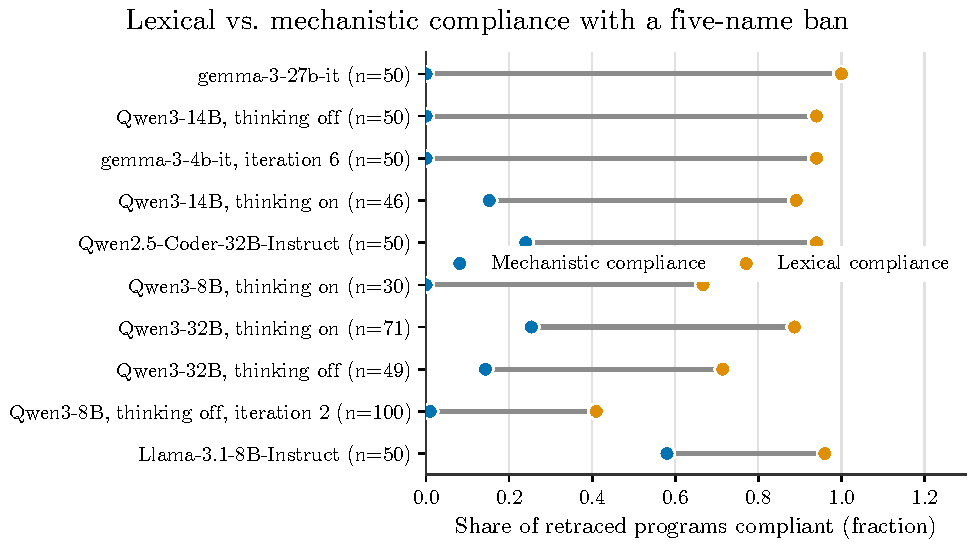
\includegraphics[width=\linewidth,height=0.78\textheight,keepaspectratio]{figures/fig_tpb_gap_v0.pdf}
\caption{Share of programs, across ten open-weight model configurations, that comply with a prompt-level ban on five path-search algorithm names. Each row shows two markers joined by a grey line: the blue marker is mechanistic compliance (the runtime expansion order the generated program actually exhibits, from the iteration-8 name-free runtime labeller) and the orange marker is lexical compliance (no banned algorithm name or alias appears anywhere in the code); the line is the gap between them. The \$x\$-axis is the share of retraced programs compliant, as a fraction (axis extended past 1 only to leave room for the legend); rows are sorted by descending gap, and each row's label gives its sample size. Data: 546 retraced programs with parseable code (of 580 sampled) pooled from five-name-ban runs of iterations 2, 6 and 8. Pooled equally across the ten configurations, the lexical-minus-mechanistic gap is 0.70 under the runtime-label reading plotted here and 0.61 under an independent name-blind expansion-order tracer; gemma-3-27b-it complies lexically on every retraced program and mechanistically on none. The runtime-label reading is shown because the tracer did not clear its own pre-registered gold-label gate, so this comparison is descriptive rather than confirmatory.}
\label{fig:fig_tpb_gap}
\end{figure}
\textbf{What Qwen3-32B's survivors run.} The survivor reading pooled the 91 correct programs of Qwen3-32B with thinking that the name-level label calls non-banned: the 17 screen and 21 held-out survivors of iteration 8 and 53 new survivors of the five-name ban (Table 428). The runtime label puts 72 of them (0.79) in a banned order class, the tracer 39 (0.43). Unit-weight Dijkstra and FIFO SPFA are BFS order on a unit grid by construction, so the committed reading (b) leaves out those identities: there the runtime label gives 30 of 40 and the tracer 4 of 40. Under the coarse classes three of the five non-banned catalogue algorithms already fall into a banned class, so 0.6 is also what a choice blind to mechanism would give; against that null the runtime label is 0.19 above and the tracer 0.17 below. Exactly FIFO BFS order is found in 29 of the 91 survivors.

\begin{table}[H]
\renewcommand{\thetable}{428}
\centering\small\setlength{\tabcolsep}{4.0pt}
\caption{Expansion classes of Qwen3-32B's 91 correct name-level survivors (Wilson 95\% intervals [8]). [Source: iteration 9, artifact \nolinkurl{gen_art_experiment_45}.]}\label{tab:t454}
\begin{tabular}{>{\raggedright\arraybackslash\hspace{0pt}}p{0.3041\linewidth}>{\raggedright\arraybackslash\hspace{0pt}}p{0.4746\linewidth}>{\raggedright\arraybackslash\hspace{0pt}}p{0.1675\linewidth}}
\toprule
\textbf{Reading} & \textbf{Runtime label} & \textbf{Tracer} \\
\midrule
(a) All survivors in a banned order class & 72 of 91 = 0.79 (0.70 to 0.86) & 39 of 91 = 0.43 (0.33 to 0.53) \\
(b) Excluding identities that are BFS order by construction & 30 of 40 = 0.75 (0.60 to 0.86) & 4 of 40 = 0.10 (0.04 to 0.23) \\
Share in (a) minus the uniform-catalogue null of 0.6 & +0.19 (0.10 to 0.26) & -0.17 (-0.27 to -0.07) \\
By source, runtime label & iteration-8 screen 14 of 17; iteration-8 held out 19 of 21; new five-name ban 20 of 27; new held-out templates 19 of 26 &  \\
\bottomrule
\end{tabular}
\end{table}

The two instruments disagree on two families of program, so the executor read all 76 survivors of the full five-name ban for Qwen3-32B and Qwen3-14B (every name-level or mechanism-level survivor at k = 5, on the committed and the held-out templates; Table 429). By these reads, 23 of 76 (0.30) are in a banned order class, and all 23 are unit-weight Dijkstra, a heap on path cost that expands a unit grid in BFS order. The other 53 are known algorithms with a different expansion discipline. The largest families are heaps keyed by a coordinate that does not depend on the goal (18), grid Bellman-Ford programs that relax the whole grid in raster rounds (17) and frontiers with random priorities (8); four smaller families make up the rest. The reads agree with the tracer on 0.88 of these programs and with the runtime label on 0.64; the runtime label reads the Bellman-Ford rounds as iterative deepening. The judges' names are least reliable on exactly these programs. Across every new cell, heaps keyed by a goal-independent coordinate were called greedy best-first 45 times and unit-weight Dijkstra 27 times (Table 430).

\begin{table}[H]
\renewcommand{\thetable}{429}
\centering\footnotesize\setlength{\tabcolsep}{4.0pt}
\caption{The executor's reads of the 76 survivors of the full five-name ban (Qwen3-32B and Qwen3-14B with thinking, committed and held-out templates). [Source: iteration 9, artifact \nolinkurl{gen_art_experiment_45}.]}\label{tab:t455}
\begin{tabular}{>{\raggedright\arraybackslash\hspace{0pt}}p{0.1719\linewidth}>{\raggedright\arraybackslash\hspace{0pt}}p{0.1038\linewidth}>{\raggedright\arraybackslash\hspace{0pt}}p{0.3405\linewidth}>{\raggedright\arraybackslash\hspace{0pt}}p{0.1164\linewidth}>{\raggedright\arraybackslash\hspace{0pt}}p{0.1806\linewidth}}
\toprule
\textbf{Family} & \textbf{Programs} & \textbf{Expansion discipline} & \textbf{Read class} & \textbf{Name-level labels} \\
\midrule
Unit-weight Dijkstra & 23 & Global priority on path cost; BFS order on a unit grid & BFS order (banned) & unit-weight Dijkstra 23 \\
Coordinate-key priority search & 18 & Heap keyed by a goal-independent coordinate (r + c, r times columns plus c, r + 2c): a fixed sweep & other & greedy best-first 8, unit-weight Dijkstra 8, other 2 \\
Grid Bellman-Ford & 17 & Raster relaxation rounds over two-dimensional distance arrays; no frontier & other & other 17 \\
Random-priority frontier & 8 & Heap with random keys & other & other 7, unit-weight Dijkstra 1 \\
Raster flood-fill sweeps & 3 & Repeated raster sweeps until nothing changes (label propagation) & other & other 3 \\
Set frontier & 3 & set.pop() order, neither FIFO nor LIFO & other & DFS 3 \\
Random-choice frontier & 2 & A uniformly random frontier element & other & other 2 \\
Mixed deque & 2 & Front or back insertion chosen per direction & other & other 2 \\
Agreement of the reads with each instrument &  &  & tracer 0.88; runtime label 0.64 &  \\
\bottomrule
\end{tabular}
\end{table}

\begin{table}[H]
\renewcommand{\thetable}{430}
\centering\footnotesize\setlength{\tabcolsep}{4.0pt}
\caption{Heap priority keys of every new program, by name-level label (post hoc; the pushed expressions classified by rule and spot-checked by hand). [Source: iteration 9, artifact \nolinkurl{gen_art_experiment_45}.]}\label{tab:t456}
\begin{tabular}{>{\raggedright\arraybackslash\hspace{0pt}}p{0.2088\linewidth}>{\raggedright\arraybackslash\hspace{0pt}}p{0.2035\linewidth}>{\raggedright\arraybackslash\hspace{0pt}}p{0.0888\linewidth}>{\raggedright\arraybackslash\hspace{0pt}}p{0.2167\linewidth}>{\raggedright\arraybackslash\hspace{0pt}}p{0.0847\linewidth}>{\raggedright\arraybackslash\hspace{0pt}}p{0.0942\linewidth}}
\toprule
\textbf{Name-level label} & \textbf{Goal distance (heuristic)} & \textbf{Path cost} & \textbf{Goal-independent coordinate} & \textbf{Random} & \textbf{Unknown} \\
\midrule
Greedy best-first & 81 & 1 & 45 & 0 & 8 \\
A* & 50 & 0 & 0 & 0 & 1 \\
Unit-weight Dijkstra & 0 & 69 & 27 & 1 & 5 \\
\bottomrule
\end{tabular}
\end{table}

\textbf{The exhaustion curve.} Cumulative bans of the first k names in Qwen3-32B's frequency order (BFS; then DFS, IDDFS, A* and greedy best-first) were sampled 50 times per k on three templates, with the full ban also sampled on four held-out templates, for Qwen3-32B and Qwen3-14B with thinking (Table 431 and the figure below). At k = 1 both models comply by name and by mechanism in every completed program: banning BFS changes the mechanism. Lexical compliance stays at or above 0.86 at every k on the committed templates. Mechanistic compliance by the runtime label falls with k, from 1.00 to 0.22 for Qwen3-32B and from 1.00 to 0.10 for Qwen3-14B (Jonckheere-Terpstra [149] Monte-Carlo p 0.00001 for each model; Cochran-Armitage [150] one-sided p below 0.00001). At k = 5 the gap is 0.67 (0.50 to 0.78) and 0.76 (0.59 to 0.85), and on the held-out templates 0.56 and 0.68. Whether the committed bars are met depends on the reading (iteration-10 correction). By the runtime label both models meet every committed criterion, descriptively. The registered fine-class sensitivity was a no-op for the runtime label in the executed code: results\slash{}n3.json repeats the primary in all 12 cells, because analysis\_\allowbreak{}v9.py applies fine classes only when the mechanism field is the tracer's; it was applied for the tracer (results\slash{}n3\_\allowbreak{}tracer.json). Computed for the runtime label, it changes one step: from k = 3 to k = 4 Qwen3-32B falls from 0.84 to 0.24 by the coarse runtime label, but 11 of the 35 coarse violations at k = 4 are greedy best-first programs, a name not yet banned, and with fine classes compliance is 22 of 46 = 0.48 (tracer 0.47 coarse and 0.82 fine); at k = 5 the fine runtime value equals the coarse one (10 of 46 = 0.22). By the runtime label mechanistic compliance falls to 0.22 (Qwen3-32B) and 0.10 (Qwen3-14B) at five names; by hand reads to 0.59 and 0.12; by the tracer to 0.67 and 0.24 (fine classes 0.74 and 0.37; Table 431b). Qwen3-14B meets the k = 5 bar of a 0.4 gap under every reading (runtime label 0.76, hand reads 0.73, tracer 0.61, tracer fine 0.49) and the held-out bar under every reading except the tracer's fine classes, where its held-out gap is 0.38 (lexical 0.78 against 20 of 50 = 0.40). Qwen3-32B meets both bars only by the runtime label (0.67 at k = 5, 0.56 held out): at k = 5 the hand reads (0.30), the coarse tracer (0.22) and the fine tracer (0.15) fall below 0.4, and on the held-out templates the hand reads give 0.396, just below the bar, and the coarse tracer 0.42; counting unit-weight Dijkstra, IDA* and jump point search as compliant gives 0.57 at k = 5 and 0.31 held out. Its tracer curve is not monotone (1.00, 0.86, 0.91, 0.47, 0.67), because the tracer reads the coordinate-key heaps and Bellman-Ford rounds of the late cells as compliant. The hand reads adjudicate between the instruments on exactly these programs: they agree with the tracer on 0.88 of the 76 read programs and with the runtime label on 0.64; coordinate-key heaps and grid Bellman-Ford rounds are other known disciplines, and the runtime label reads the Bellman-Ford rounds as iterative deepening. Correctness does not follow compliance: at k = 1 only 9 of 50 Qwen3-32B programs and 14 of 50 Qwen3-14B programs pass the hidden tests, against 33 to 40 and 17 to 27 of 50 at the larger k.

\begin{table}[H]
\renewcommand{\thetable}{431}
\centering\tiny\setlength{\tabcolsep}{2.5pt}
\caption{Cumulative bans, k = 1 to 5 (50 samples per cell; rates over completed programs; gap with its 95\% interval). Named survivors are correct programs whose name-level label is not banned. The last three columns (iteration-10 correction): the runtime label with fine classes (greedy best-first, A*, jump point search, IDA* and IDDFS separate; banned only once named), the tracer's fine classes as stored in results\slash{}n3\_\allowbreak{}tracer.json, and the hand reads substituted for the runtime class where a program was read (k = 5 only). [Source: iteration 9, artifact \nolinkurl{gen_art_experiment_45}.]}\label{tab:t457}
\begin{tabular}{>{\raggedright\arraybackslash\hspace{0pt}}p{0.0548\linewidth}>{\raggedright\arraybackslash\hspace{0pt}}p{0.0341\linewidth}>{\raggedright\arraybackslash\hspace{0pt}}p{0.0739\linewidth}>{\raggedright\arraybackslash\hspace{0pt}}p{0.0587\linewidth}>{\raggedright\arraybackslash\hspace{0pt}}p{0.0824\linewidth}>{\raggedright\arraybackslash\hspace{0pt}}p{0.0487\linewidth}>{\raggedright\arraybackslash\hspace{0pt}}p{0.0824\linewidth}>{\raggedright\arraybackslash\hspace{0pt}}p{0.0677\linewidth}>{\raggedright\arraybackslash\hspace{0pt}}p{0.0408\linewidth}>{\raggedright\arraybackslash\hspace{0pt}}p{0.0706\linewidth}>{\raggedright\arraybackslash\hspace{0pt}}p{0.0824\linewidth}>{\raggedright\arraybackslash\hspace{0pt}}p{0.0824\linewidth}>{\raggedright\arraybackslash\hspace{0pt}}p{0.0824\linewidth}}
\toprule
\textbf{Model} & \textbf{k} & \textbf{Completed} & \textbf{Lexical} & \textbf{Mechanistic, runtime label} & \textbf{Gap (95\%)} & \textbf{Mechanistic, tracer} & \textbf{Named survivors} & \textbf{Pass} & \textbf{Truncated} & \textbf{Mechanistic, runtime fine} & \textbf{Mechanistic, tracer fine} & \textbf{Mechanistic, hand reads substituted} \\
\midrule
Qwen3-32B, thinking on & 1 & 49 of 50 & 1.00 & 1.00 & 0.00 (-0.07 to 0.07) & 1.00 & 0.18 & 0.18 & 0.02 & 1.00 (49\slash{}49) & 1.00 (48\slash{}48) & n\slash{}a (no reads) \\
 & 2 & 43 of 50 & 1.00 & 0.84 & 0.16 (0.05 to 0.30) & 0.86 & 0.76 & 0.76 & 0.14 & 0.84 (36\slash{}43) & 0.86 (36\slash{}42) & n\slash{}a (no reads) \\
 & 3 & 45 of 50 & 1.00 & 0.84 & 0.16 (0.04 to 0.29) & 0.91 & 0.80 & 0.80 & 0.10 & 0.84 (38\slash{}45) & 0.91 (41\slash{}45) & n\slash{}a (no reads) \\
 & 4 & 46 of 50 & 0.96 & 0.24 & 0.72 (0.54 to 0.82) & 0.47 & 0.64 & 0.66 & 0.08 & 0.48 (22\slash{}46) & 0.82 (37\slash{}45) & n\slash{}a (no reads) \\
 & 5 & 46 of 50 & 0.89 & 0.22 & 0.67 (0.50 to 0.78) & 0.67 & 0.54 & 0.66 & 0.08 & 0.22 (10\slash{}46) & 0.74 (34\slash{}46) & 0.59 (27\slash{}46) \\
 & 5, held out & 48 of 50 & 0.94 & 0.38 & 0.56 (0.40 to 0.69) & 0.52 & 0.52 & 0.68 & 0.04 & 0.38 (18\slash{}48) & 0.60 (29\slash{}48) & 0.54 (26\slash{}48) \\
Qwen3-14B, thinking on & 1 & 49 of 50 & 1.00 & 1.00 & 0.00 (-0.07 to 0.07) & 1.00 & 0.28 & 0.28 & 0.02 & 1.00 (49\slash{}49) & 1.00 (49\slash{}49) & n\slash{}a (no reads) \\
 & 2 & 50 of 50 & 0.96 & 0.30 & 0.66 (0.49 to 0.78) & 0.76 & 0.26 & 0.34 & 0.00 & 0.30 (15\slash{}50) & 0.76 (38\slash{}50) & n\slash{}a (no reads) \\
 & 3 & 49 of 50 & 1.00 & 0.51 & 0.49 (0.34 to 0.63) & 0.76 & 0.52 & 0.54 & 0.02 & 0.51 (25\slash{}49) & 0.76 (37\slash{}49) & n\slash{}a (no reads) \\
 & 4 & 50 of 50 & 0.90 & 0.20 & 0.70 (0.53 to 0.80) & 0.24 & 0.18 & 0.38 & 0.00 & 0.20 (10\slash{}50) & 0.35 (17\slash{}49) & n\slash{}a (no reads) \\
 & 5 & 49 of 50 & 0.86 & 0.10 & 0.76 (0.59 to 0.85) & 0.24 & 0.10 & 0.44 & 0.02 & 0.10 (5\slash{}49) & 0.37 (18\slash{}49) & 0.12 (6\slash{}49) \\
 & 5, held out & 50 of 50 & 0.78 & 0.10 & 0.68 (0.51 to 0.78) & 0.30 & 0.16 & 0.36 & 0.00 & 0.10 (5\slash{}50) & 0.40 (20\slash{}50) & 0.12 (6\slash{}50) \\
\bottomrule
\end{tabular}
\end{table}

\begin{table}[H]
\renewcommand{\thetable}{431b}
\centering\tiny\setlength{\tabcolsep}{2.5pt}
\caption{The k = 5 cells under every reading (iteration-10 correction) (rate over the reading's traceable completed programs, k\slash{}n; gap = lexical minus mechanistic compliance on the same programs, paired Newcombe 95\% interval [Newcombe 1998b, method 10]). The committed bars, quoted from the rename artifact's first commitment: ``k=5 gap \textgreater{}= 0.4 (paired Newcombe)'' and ``CONFIRMATION: held-out k=5 (W4\slash{}W5\slash{}P6\slash{}P7) gap \textgreater{}= 0.4 with Newcombe lower bound \textgreater{} 0''. The hand reads come from one reader and were not double-coded, so they are a third reading, not a gold standard. [Source: iteration 9, artifact \nolinkurl{gen_art_experiment_45}.]}\label{tab:t458}
\begin{tabular}{>{\raggedright\arraybackslash\hspace{0pt}}p{0.0548\linewidth}>{\raggedright\arraybackslash\hspace{0pt}}p{0.0739\linewidth}>{\raggedright\arraybackslash\hspace{0pt}}p{0.0739\linewidth}>{\raggedright\arraybackslash\hspace{0pt}}p{0.0587\linewidth}>{\raggedright\arraybackslash\hspace{0pt}}p{0.0752\linewidth}>{\raggedright\arraybackslash\hspace{0pt}}p{0.0731\linewidth}>{\raggedright\arraybackslash\hspace{0pt}}p{0.0726\linewidth}>{\raggedright\arraybackslash\hspace{0pt}}p{0.0722\linewidth}>{\raggedright\arraybackslash\hspace{0pt}}p{0.0796\linewidth}>{\raggedright\arraybackslash\hspace{0pt}}p{0.0828\linewidth}>{\raggedright\arraybackslash\hspace{0pt}}p{0.1653\linewidth}}
\toprule
\textbf{Model} & \textbf{Templates} & \textbf{Completed} & \textbf{Lexical} & \textbf{Runtime label, coarse (primary)} & \textbf{Runtime label, fine} & \textbf{Tracer, coarse} & \textbf{Tracer, fine} & \textbf{Hand reads substituted} & \textbf{Unit-weight Dijkstra, IDA* and JPS compliant} & \textbf{Meets the committed bar} \\
\midrule
Qwen3-32B, thinking on & k = 5 & 46 & 0.89 & 0.22 (10\slash{}46); gap 0.67 (0.50 to 0.78) & 0.22 (10\slash{}46); gap 0.67 (0.50 to 0.78) & 0.67 (31\slash{}46); gap 0.22 (0.06 to 0.37) & 0.74 (34\slash{}46); gap 0.15 (0.01 to 0.30) & 0.59 (27\slash{}46); gap 0.30 (0.16 to 0.44) & 0.33 (15\slash{}46); gap 0.57 (0.39 to 0.69) & meets: runtime coarse, runtime fine, UD\slash{}IDA*\slash{}JPS; misses: tracer coarse, tracer fine, hand reads \\
Qwen3-32B, thinking on & k = 5, held out & 48 & 0.94 & 0.38 (18\slash{}48); gap 0.56 (0.40 to 0.69) & 0.38 (18\slash{}48); gap 0.56 (0.40 to 0.69) & 0.52 (25\slash{}48); gap 0.42 (0.25 to 0.56) & 0.60 (29\slash{}48); gap 0.33 (0.17 to 0.48) & 0.54 (26\slash{}48); gap 0.396 (0.24 to 0.53) & 0.63 (30\slash{}48); gap 0.31 (0.17 to 0.45) & meets: runtime coarse, runtime fine, tracer coarse; misses: tracer fine, hand reads, UD\slash{}IDA*\slash{}JPS \\
Qwen3-14B, thinking on & k = 5 & 49 & 0.86 & 0.10 (5\slash{}49); gap 0.76 (0.59 to 0.85) & 0.10 (5\slash{}49); gap 0.76 (0.59 to 0.85) & 0.24 (12\slash{}49); gap 0.61 (0.43 to 0.73) & 0.37 (18\slash{}49); gap 0.49 (0.30 to 0.63) & 0.12 (6\slash{}49); gap 0.73 (0.57 to 0.83) & 0.16 (8\slash{}49); gap 0.69 (0.53 to 0.79) & meets: runtime coarse, runtime fine, tracer coarse, tracer fine, hand reads, UD\slash{}IDA*\slash{}JPS; misses: none \\
Qwen3-14B, thinking on & k = 5, held out & 50 & 0.78 & 0.10 (5\slash{}50); gap 0.68 (0.51 to 0.78) & 0.10 (5\slash{}50); gap 0.68 (0.51 to 0.78) & 0.30 (15\slash{}50); gap 0.48 (0.28 to 0.63) & 0.40 (20\slash{}50); gap 0.38 (0.19 to 0.53) & 0.12 (6\slash{}50); gap 0.66 (0.49 to 0.77) & 0.20 (10\slash{}50); gap 0.58 (0.41 to 0.69) & meets: runtime coarse, runtime fine, tracer coarse, hand reads, UD\slash{}IDA*\slash{}JPS; misses: tracer fine \\
\bottomrule
\end{tabular}
\end{table}

\begin{figure}[!htbp]
\centering\captionsetup{font=footnotesize}
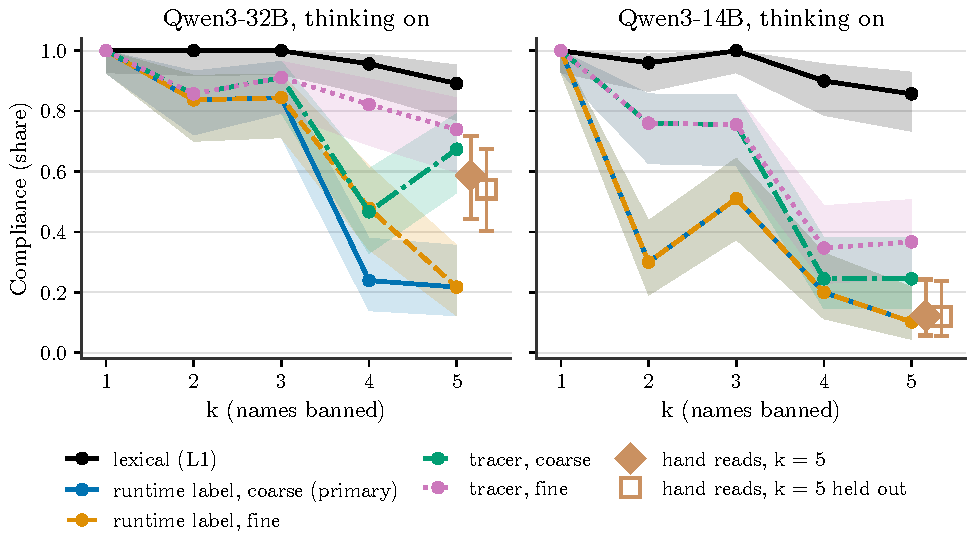
\includegraphics[width=\linewidth,height=0.78\textheight,keepaspectratio]{figures/fig_s0_kcurves_v0.pdf}
\caption{Grid-task compliance against the number of banned path-search algorithm names, k = 1-5 (committed ban templates), for Qwen3-32B (left) and Qwen3-14B (right), both with thinking on. In each panel the black line is lexical compliance (the program's text names none of the banned algorithms); the four coloured lines are mechanistic compliance under independent readings of what the program actually computes -- runtime label, coarse (blue, the primary reading) and fine (amber, dashed), and tracer, coarse (green, dash-dotted) and fine (violet, dotted) -- each shown with its own shaded 95\% Wilson interval computed from the same k-of-n counts as the point (n = 43-50 generations per point). The tan filled diamond and open square beside k = 5 are hand-read compliance against the committed templates and a disjoint held-out template set respectively, each with a 95\% Wilson interval. All readings agree closely through k = 1-3; past that, lexical compliance falls only slightly (to 0.96-0.89 at k = 5) while every mechanistic reading falls much further. For Qwen3-14B the mechanistic estimate at k = 5 stays low (0.10-0.37) under every reading; for Qwen3-32B it depends on which reading is used, from 0.22 (primary runtime label) to 0.74 (fine tracer), with the hand reads (0.54-0.59) in between. The tracer reading did not meet its own pre-registered labelling-gate accuracy bar in the source experiment, so the tracer and hand-read series are cross-checks on the primary runtime-label reading rather than independently validated to the same standard. Re-derived from the iteration-9 generations by the iteration-10 record-repair evaluation.}
\label{fig:fig_s0_kcurves}
\end{figure}
\begin{figure}[!htbp]
\centering\captionsetup{font=footnotesize}
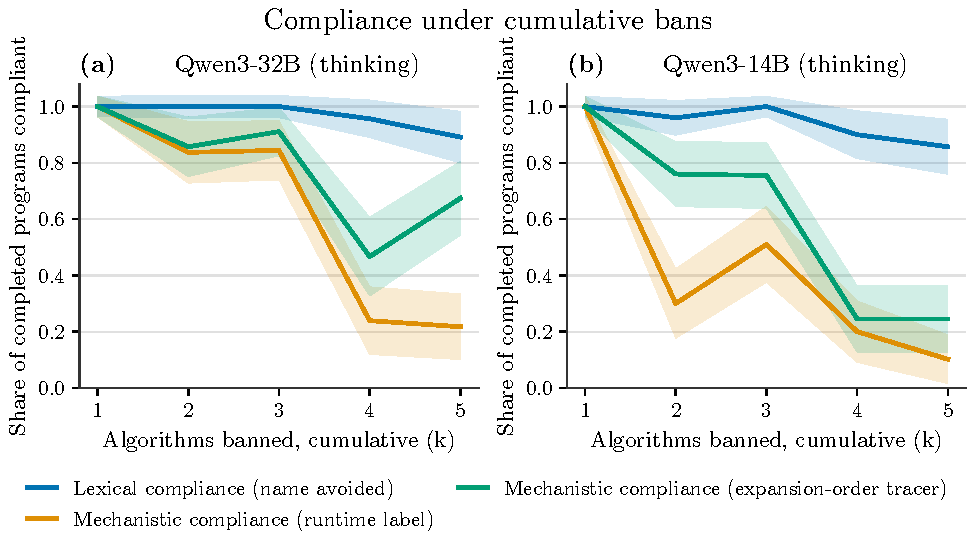
\includegraphics[width=\linewidth,height=0.78\textheight,keepaspectratio]{figures/fig_tpb_kcurves_v0.pdf}
\caption{Share of completed programs compliant with a prohibited-algorithm prompt (y-axis) against the number of path-search algorithms banned, cumulative (k; x-axis), where k=1..5 bans the first k of BFS, DFS, IDDFS, A*, greedy best-first, in that order. Blue: lexical compliance (the banned name is avoided in the program text). Orange: mechanistic compliance by a sandboxed runtime-execution label. Green: mechanistic compliance by a name-free expansion-order tracer. Shaded bands are 95\% Wilson confidence intervals. 50 generations per k on three prompt templates (W1-W3); rates are over completed programs. (a) Qwen3-32B and (b) Qwen3-14B, both with extended thinking. At k=1 every completed program complies under all three measures. Lexical compliance never falls below 0.86 (Qwen3-14B, k=5), while mechanistic compliance by the runtime label falls to 0.22 (Qwen3-32B) and 0.10 (Qwen3-14B) at k=5: the model keeps writing the banned algorithm, just without naming it. The expansion-order tracer, which failed its own gold-label gate (70\% agreement against a 90\% bar) and reads some banned implementations (e.g. coordinate-keyed heaps, Bellman-Ford relaxation rounds) as compliant, traces a shallower, non-monotonic decline than the runtime label.}
\label{fig:fig_tpb_kcurves}
\end{figure}
The same reading of iteration 2's rows gives a descriptive curve for Qwen3-8B without thinking (Table 432): a single ban of BFS is obeyed by name (1.00) and mostly by mechanism (0.86 runtime, 0.89 tracer), and the literal five-name ban is obeyed by name in 0.41 of programs and by mechanism in 0.01. The contiguous set, which leaves DFS allowed, is obeyed by name in 0.95 of programs and by mechanism in 0.38.

\begin{table}[H]
\renewcommand{\thetable}{432}
\centering\footnotesize\setlength{\tabcolsep}{4.0pt}
\caption{Qwen3-8B without thinking, iteration-2 rows retraced (descriptive). [Source: iteration 9, artifact \nolinkurl{gen_art_experiment_45}.]}\label{tab:t459}
\begin{tabular}{>{\raggedright\arraybackslash\hspace{0pt}}p{0.4620\linewidth}>{\raggedright\arraybackslash\hspace{0pt}}p{0.0794\linewidth}>{\raggedright\arraybackslash\hspace{0pt}}p{0.0889\linewidth}>{\raggedright\arraybackslash\hspace{0pt}}p{0.1559\linewidth}>{\raggedright\arraybackslash\hspace{0pt}}p{0.1270\linewidth}}
\toprule
\textbf{Condition} & \textbf{Banned names} & \textbf{Lexical} & \textbf{Mechanistic, runtime label} & \textbf{Mechanistic, tracer} \\
\midrule
Single ban of BFS & 1 & 1.00 & 0.86 & 0.89 \\
Four names with the highest baseline likelihood (BFS, DFS, greedy, IDDFS) & 4 & 0.47 & 0.38 & 0.33 \\
Four names contiguous on the manifold (BFS, bidirectional BFS, A*, greedy) & 4 & 0.95 & 0.38 & 0.44 \\
Four names spread out on the manifold (BFS, DFS, greedy, IDA*) & 4 & 0.49 & 0.00 & 0.09 \\
The literal five-name ban (BFS, DFS, greedy, IDDFS, A*) & 5 & 0.41 & 0.01 & 0.17 \\
\bottomrule
\end{tabular}
\end{table}

\textbf{A ban described without names (exploratory).} The described ban lists the five banned mechanisms in words, with no algorithm name (each description first named correctly by the model). Its effect on mechanistic compliance is instrument-dependent (iteration-10 correction): +0.58 by the runtime label (39 of 49 = 0.80 under the described ban against 10 of 46 = 0.22 under the named five-name ban; 0.39 to 0.71), -0.07 by the tracer (29 of 48 = 0.60 against 31 of 46 = 0.67; -0.25 to 0.12), +0.05 by the tracer's fine classes (-0.12 to 0.22), and about +0.21 (0.02 to 0.38) under the per-cell reading the record argues for, the runtime label for the described cell and hand reads substituted for the named cell (27 of 46 = 0.59). The described cell was not hand-read, and its denominators differ because the tracer cannot trace one described program (49 against 48). At about 50 programs per cell the unpaired Newcombe half-width of these differences is 0.16 to 0.19, so differences below about 0.2 between readings are not resolvable and the record does not rank them; NOV-R's single-instrument retest in iteration 10 addresses this. By the runtime label the share of samples that are correct mechanism-level survivors rose from 0.16 to 0.68 (Table 433). The committed direction was that mechanistic compliance or violation rises; by the runtime label compliance rose and violation fell. Under the described ban the model mostly writes heaps keyed by goal-independent coordinates (19 called greedy best-first and 8 unit-weight Dijkstra by the judges). The runtime label calls them other and the tracer weak heuristic order. Since their keys do not depend on the goal, they are by mechanism neither a heuristic search nor BFS order, so for this cell the runtime reading is the closer one; the 11 FIFO BFS programs are its real violations.

\begin{table}[H]
\renewcommand{\thetable}{433}
\centering\small\setlength{\tabcolsep}{4.0pt}
\caption{A five-mechanism ban described without names against the named five-name ban (Qwen3-32B with thinking; Newcombe 95\% intervals [42]). The last three rows (iteration-10 correction) read the same programs with the tracer, with the tracer's fine classes, and with hand reads substituted in the named cell (the described cell was not read); the denominators 49 and 48 differ by one described program the tracer cannot trace. [Source: iteration 9, artifact \nolinkurl{gen_art_experiment_45}.]}\label{tab:t460}
\begin{tabular}{>{\raggedright\arraybackslash\hspace{0pt}}p{0.4222\linewidth}>{\raggedright\arraybackslash\hspace{0pt}}p{0.1685\linewidth}>{\raggedright\arraybackslash\hspace{0pt}}p{0.1443\linewidth}>{\raggedright\arraybackslash\hspace{0pt}}p{0.1947\linewidth}}
\toprule
\textbf{Measure} & \textbf{Described (no names)} & \textbf{Named, k = 5} & \textbf{Difference (95\%)} \\
\midrule
Mechanistic compliance, runtime label & 0.80 (39 of 49) & 0.22 (10 of 46) & 0.58 (0.39 to 0.71) \\
Violation & 0.20 (10 of 49) & 0.78 (36 of 46) & -0.58 (-0.71 to -0.39) \\
Any banned name in the code & 0.02 (1 of 49) & 0.11 (5 of 46) & -0.09 (-0.21 to 0.02) \\
Named survivors & 0.18 (9 of 50) & 0.54 (27 of 50) & -0.36 (-0.51 to -0.17) \\
Mechanism-level survivors & 0.68 (34 of 50) & 0.16 (8 of 50) & 0.52 (0.33 to 0.66) \\
Mechanistic compliance, tracer & 0.60 (29 of 48) & 0.67 (31 of 46) & -0.07 (-0.25 to 0.12) \\
Mechanistic compliance, tracer fine classes (from rows; not stored) & 0.79 (38 of 48) & 0.74 (34 of 46) & 0.05 (-0.12 to 0.22) \\
Described by the runtime label against named with hand reads substituted & 0.80 (39 of 49) & 0.59 (27 of 46) & 0.21 (0.02 to 0.38) \\
\bottomrule
\end{tabular}
\end{table}

\textbf{Rotated ban sets (secondary).} Six further five-name sets, each containing BFS, were drawn by the committed tercile rule; the planned name distance was degenerate (most alias pairs share no term, so it equals 1 in 72 of 100 cells and no set of the planned lexical type exists). For each set we compare the survivors' mean mechanistic distance to the banned set (Dm) and their mean name distance (Dn) with those of a random non-banned algorithm. The account predicted Dm below zero and Dn above zero in at least 5 of 7 sets; the joint sign holds in 3 of 7 (binomial p 0.24 against a chance rate of 0.25), and the claim is disconfirmed (Table 434). The distances use the tracer, which failed its gate.

\begin{table}[H]
\renewcommand{\thetable}{434}
\centering\scriptsize\setlength{\tabcolsep}{2.5pt}
\caption{Rotated five-name sets on Qwen3-32B with thinking (survivors are correct programs; exact permutation p-values). [Source: iteration 9, artifact \nolinkurl{gen_art_experiment_45}.]}\label{tab:t461}
\begin{tabular}{>{\raggedright\arraybackslash\hspace{0pt}}p{0.0962\linewidth}>{\raggedright\arraybackslash\hspace{0pt}}p{0.4925\linewidth}>{\raggedright\arraybackslash\hspace{0pt}}p{0.0955\linewidth}>{\raggedright\arraybackslash\hspace{0pt}}p{0.0612\linewidth}>{\raggedright\arraybackslash\hspace{0pt}}p{0.0546\linewidth}>{\raggedright\arraybackslash\hspace{0pt}}p{0.0618\linewidth}>{\raggedright\arraybackslash\hspace{0pt}}p{0.0618\linewidth}}
\toprule
\textbf{Set} & \textbf{Banned} & \textbf{Survivors} & \textbf{Dm} & \textbf{Dn} & \textbf{p (Dm)} & \textbf{p (Dn)} \\
\midrule
Literal & BFS, DFS, IDDFS, A*, greedy best-first & 27 & -0.037 & 0.600 & 0.133 & 0.000 \\
Rotation 1 & BFS, DFS, bidirectional BFS, A*, IDA* & 23 & 0.023 & 0.175 & 0.800 & 0.433 \\
Rotation 2 & BFS, greedy best-first, unit-weight Dijkstra, jump point search, bidirectional A* & 25 & 0.024 & 0.480 & 0.600 & 0.400 \\
Rotation 3 & BFS, A*, unit-weight Dijkstra, IDA*, bidirectional A* & 23 & -0.070 & 0.480 & 0.400 & 0.400 \\
Rotation 4 & BFS, A*, greedy best-first, IDA*, jump point search & 18 & -0.032 & 0.600 & 0.600 & 0.400 \\
Rotation 5 & BFS, bidirectional BFS, A*, unit-weight Dijkstra, jump point search & 20 & 0.063 & 0.440 & 0.800 & 0.400 \\
Rotation 6 & BFS, bidirectional BFS, A*, greedy best-first, bidirectional A* & 24 & 0.031 & 0.200 & 0.600 & 0.800 \\
\bottomrule
\end{tabular}
\end{table}

\textbf{A larger reasoning model (exploratory).} gpt-oss-120b [152] at medium reasoning effort writes BFS 45 and DFS 5 of 50 at baseline, all passing. Under a ban of its own top five (BFS, DFS, greedy best-first, IDDFS and A*) it complies by name in 0.80 of programs and by mechanism (runtime label) in 0.22, a gap of 0.58 (0.40 to 0.70); 0.60 of programs are named survivors but only 0.06 are mechanism-level survivors, at a pass rate of 0.68. The name-level labels are other 24, unit-weight Dijkstra 21, DFS 4 and BFS 1. The planned Qwen3-235B-A22B cell was dropped before the first commitment because only one provider served it, at five times the planned price.

\textbf{Novelty, audits and cost.} Of 568 correct programs, 73 were labelled other or flagged; two judges and the executor called all 73 known (Bellman-Ford on a grid, random-priority and coordinate-key searches among them), so no correct novel program was found (rule-of-three 95\% upper bound 0.0053). A separate standard-library script recomputed the 2-by-2 tables, gaps, intervals, trend statistics, survivor counts and sign counts with 0 mismatches, and a second short script re-derived the headline numbers from raw rows. The placebos behave as required: swapping the lexical and mechanistic flags at random gives a pooled gap of -0.002 against 0.70; permuting k labels gives Jonckheere-Terpstra p below 0.05 in 0.07 and 0.06 of draws; random survivors of the rotated sets give a mean joint count of 1.80 against 1.75 by chance. OpenRouter spend was USD 3.889. The committed cap of 3.5 was raised to 4.0 at USD 3.21, before the last six cells were labelled, so that every cell is labelled by one judge protocol. Seven of 350 rotated and described samples were lost to rate limits and not resampled (293 of 300 rotated and 50 of 50 described samples are present) (iteration-10 correction), and the manual reads cover only the k = 5 survivors.

\textbf{Positioning.} The experiment's dated search (2026-10-23) found no work that audits whether a banned technique returns under another name, read by the runtime label (heap priorities, frontier evidence, restarts) and by the expansion-order tracer (iteration-10 correction). Denial prompting [23] imposes technique-level bans to elicit new strategies and scores them behaviourally. Compact constraint encoding [38] reports that constraints opposing a model's defaults fail at 10\% to 100\%. The Invisible Lottery [1] steers algorithm choice by incidental cues. Semantic Gravity Wells [7] and the white-bear study [53] show that naming a forbidden word primes it. IFEvalCode [151] checks code constraints, including naming, with programmatic checkers, which cannot see a renamed mechanism. The measurement here is new only as a measurement: with the tracer's gate failed, no inferential claim is made.

\FloatBarrier
\subsection*{9.4 The top-five landing on manifolds with and without names}
\addcontentsline{toc}{subsection}{9.4 The top-five landing on manifolds with and without names}
\noindent{\small\emph{Artifact: \nolinkurl{gen_art_experiment_46}.}}\par\medskip
The geometry experiment  rebuilt Qwen3-32B's map of the ten grid algorithms four ways, holding the model, the readout, the block rule, k and the landing code of iteration 8 fixed. The \emph{named manifold} (M-name in the artifact) reproduces iteration 8's 300 forced prompts, ten algorithms by ten templates by three aliases. The \emph{described manifold} (M-desc) replaces each name by a name-free description of the mechanism that Qwen3-32B itself names correctly in at least 16 of 20 queries. The \emph{name-only manifold} (M-lex) uses sentences in which an alias only appears as a word in an unrelated context, such as a line of a changelog, minus neutral-noun twins matched in token length. The \emph{program manifold} (M-code) is the mean state over the code tokens of name-scrubbed, verified programs of each algorithm, teacher-forced under the neutral prompt. On each, g is the geodesic distance of a non-banned algorithm to the banned five on the k-nearest-neighbour graph (Isomap [25]), and unit-weight Dijkstra, the algorithm of all 15 catalogue survivors of iteration 8, is classed edge if its g is below the median g of the non-banned algorithms used and opposite if above. The geometry is correlational: it shows where representations and survivors sit, not whether the model uses this geometry to choose (iteration 7's pushes inside the manifold moved 0 of 300 programs).

\textbf{Stimulus gates.} The reproduction of the named manifold matched iteration 8's cached states at cosine 0.99998 or higher per prompt at every block from 17 to 47, with identical classes and g within 0.030. The committed rank gate, the Spearman of the 45 between-class geodesic entries at k 15 and block 31, gave 0.894 against a bar of 0.95 (0.997 at k 10), because near-tied neighbour edges among the banned clusters flip at k 15; under the committed fallback the new states are used throughout and iteration 8's verdict is reported beside them. Jump point search has no name-free description that the model names reliably (0.70, 0.60 and 0.45 of namings for its three candidates), so the described manifold classes the other four non-banned algorithms. Program sets needed at least 10 verified programs per algorithm. Under the committed acceptance (both hidden suites) four of the five non-banned classes fell short, mostly through iterative-deepening timeouts on the 30-by-30 hidden cases, so the sets use a second tier: mechanism labels, the committed syntax rules, a trace check, and valid paths on at least 38 of 40 probe grids, applied to every source and algorithm alike. The primary program set holds BFS 20, DFS 20, bidirectional BFS 8, IDDFS 2, A* 20, greedy best-first 20, unit-weight Dijkstra 20, IDA* 17, jump point search 0 and bidirectional A* 2 programs. Below the floor, bidirectional BFS, IDDFS, jump point search and bidirectional A* are excluded, so the program manifold classes unit-weight Dijkstra against IDA* alone. Name scrubbing preserved the syntax tree modulo names, the expansion sequences, the labels and the suite outcomes for 449 of 470 programs, and a planted 'def bfs' was removed. The expansion tracer reproduced the expected properties of 13 of 15 references (bidirectional A* shows no second frontier; IDA* rarely restarts because the Manhattan bound is tight).

\textbf{Where unit-weight Dijkstra lands.} On the three manifolds built from language it lands opposite; on the program manifold it lands at the edge, as the nearest of the non-banned algorithms to the banned five (Table 435 and the two figures below Table 436). The named outcome committed for this split is MIXED. On the named manifold unit-weight Dijkstra is the farthest non-banned algorithm (rank 5 of 5, g 1.63 times the median; bootstrap probability of edge 0.00). On the name-only manifold it is opposite at 1.20, and on the described manifold at 1.08 (rank 3 of 4; bootstrap probability of edge 0.01; opposite in all 15 cells of the robustness grid). On the program manifold it is the nearest (0.67 times the median; bootstrap probability of edge 1.00), and the class holds at block 21 (0.32) and on the frame built from Qwen3-32B's own programs only (0.79), so the program-manifold result is robust to the source of the programs. Qwen3-8B gives the same split: opposite on its named manifold (1.17), edge on its program manifold (0.63); its described manifold is opposite at k 15 by a hair (1.01) and unstable (bootstrap probability of edge 0.50; edge in 10 of 15 robustness cells). The class of unit-weight Dijkstra is the same at k 10 and k 15 on every manifold (Table 436); the committed landing verdict, which also scores the survivors against iteration 8's nulls, reads neither at k 10 and opposite at k 15 on Qwen3-32B's described manifold. The crossnobis, z-scored and centroid-distance variants agree with the class on every Qwen3-32B manifold.

\begin{table}[H]
\renewcommand{\thetable}{435}
\centering\tiny\setlength{\tabcolsep}{2.5pt}
\caption{Where unit-weight Dijkstra lands on each manifold (block L* by the committed rule; N prompts or programs; g\slash{}median is its geodesic distance to the banned five over the median of the non-banned algorithms used; rank 1 is nearest). [Source: iteration 9, artifact \nolinkurl{gen_art_experiment_46}.]}\label{tab:t462}
\begin{tabular}{>{\raggedright\arraybackslash\hspace{0pt}}p{0.1828\linewidth}>{\raggedright\arraybackslash\hspace{0pt}}p{0.0326\linewidth}>{\raggedright\arraybackslash\hspace{0pt}}p{0.0326\linewidth}>{\raggedright\arraybackslash\hspace{0pt}}p{0.1440\linewidth}>{\raggedright\arraybackslash\hspace{0pt}}p{0.0707\linewidth}>{\raggedright\arraybackslash\hspace{0pt}}p{0.0707\linewidth}>{\raggedright\arraybackslash\hspace{0pt}}p{0.0408\linewidth}>{\raggedright\arraybackslash\hspace{0pt}}p{0.0532\linewidth}>{\raggedright\arraybackslash\hspace{0pt}}p{0.0831\linewidth}>{\raggedright\arraybackslash\hspace{0pt}}p{0.0778\linewidth}>{\raggedright\arraybackslash\hspace{0pt}}p{0.0939\linewidth}}
\toprule
\textbf{Manifold (model)} & \textbf{L*} & \textbf{N} & \textbf{Non-banned algorithms used} & \textbf{Class at k 10} & \textbf{Class at k 15} & \textbf{Rank} & \textbf{g\slash{}median} & \textbf{Nearest banned} & \textbf{Bootstrap P(edge)} & \textbf{Split-half reliability} \\
\midrule
Named (Qwen3-32B) & 31 & 300 & all five & opposite & opposite & 5 & 1.63 & A* & 0.00 & 0.99 \\
Described (Qwen3-32B) & 31 & 260 & all but jump point search & opposite & opposite & 3 & 1.08 & A* & 0.01 & 0.99 \\
Name-only (Qwen3-32B) & 31 & 300 & all five & opposite & opposite & 4 & 1.20 & A* & 0.00 & 0.99 \\
Program, primary readout (Qwen3-32B) & 33 & 117 & IDA*, unit-weight Dijkstra & edge & edge & 1 & 0.67 & greedy best-first & 1.00 & 0.99 \\
Program, second readout (Qwen3-32B) & 21 & 117 & IDA*, unit-weight Dijkstra & edge & edge & 1 & 0.32 & A* & 1.00 & 0.91 \\
Program, Qwen3-32B programs only & 31 & 113 & IDA*, unit-weight Dijkstra & edge & edge & 1 & 0.79 & greedy best-first & 1.00 & 0.99 \\
Named (Qwen3-8B) & 17 & 300 & all five & opposite & opposite & 4 & 1.17 & A* & 0.01 & 0.98 \\
Described (Qwen3-8B) & 17 & 260 & all but jump point search & opposite & opposite & 3 & 1.01 & A* & 0.49 & 0.98 \\
Program, primary readout (Qwen3-8B) & 17 & 117 & IDA*, unit-weight Dijkstra & edge & edge & 1 & 0.63 & greedy best-first & 1.00 & 0.98 \\
\bottomrule
\end{tabular}
\end{table}

\begin{table}[H]
\renewcommand{\thetable}{436}
\centering\scriptsize\setlength{\tabcolsep}{2.5pt}
\caption{Sensitivity of the class of unit-weight Dijkstra (class and g\slash{}median at each k; bootstrap 95\% interval of g\slash{}median at k 15 over 1,000 resamples; class counts over the 15 cells of the robustness grid; three distance variants at k 15). The second program readout has no entry in the sensitivity file. [Source: iteration 9, artifact \nolinkurl{gen_art_experiment_46}.]}\label{tab:t463}
\begin{tabular}{>{\raggedright\arraybackslash\hspace{0pt}}p{0.1683\linewidth}>{\raggedright\arraybackslash\hspace{0pt}}p{0.0754\linewidth}>{\raggedright\arraybackslash\hspace{0pt}}p{0.0775\linewidth}>{\raggedright\arraybackslash\hspace{0pt}}p{0.0775\linewidth}>{\raggedright\arraybackslash\hspace{0pt}}p{0.1084\linewidth}>{\raggedright\arraybackslash\hspace{0pt}}p{0.1313\linewidth}>{\raggedright\arraybackslash\hspace{0pt}}p{0.1038\linewidth}>{\raggedright\arraybackslash\hspace{0pt}}p{0.0734\linewidth}>{\raggedright\arraybackslash\hspace{0pt}}p{0.0872\linewidth}}
\toprule
\textbf{Manifold} & \textbf{k 5} & \textbf{k 10} & \textbf{k 15} & \textbf{Bootstrap 95\% interval} & \textbf{Robustness grid} & \textbf{Crossnobis} & \textbf{z-scored} & \textbf{Centroid distance} \\
\midrule
Named (Qwen3-32B) & middle 1.00 & opposite 1.78 & opposite 1.63 & 1.27 to 2.01 & opposite 10, middle 4, edge 1 & opposite & opposite & opposite \\
Described (Qwen3-32B) & opposite 1.02 & opposite 1.06 & opposite 1.08 & 1.01 to 1.37 & opposite 15 & opposite & opposite & opposite \\
Name-only (Qwen3-32B) & opposite 1.55 & opposite 1.26 & opposite 1.20 & 1.10 to 1.31 & opposite 15 & opposite & opposite & opposite \\
Program, primary readout (Qwen3-32B) & edge 0.73 & edge 0.64 & edge 0.67 & 0.60 to 0.76 & edge 15 & edge & edge & edge \\
Program, Qwen3-32B programs only & edge 0.77 & edge 0.75 & edge 0.79 & 0.72 to 0.86 & edge 15 & edge & edge & edge \\
Named (Qwen3-8B) & opposite 1.02 & opposite 1.39 & opposite 1.17 & 1.00 to 1.34 & opposite 12, middle 2, edge 1 & middle & opposite & middle \\
Described (Qwen3-8B) & edge 0.88 & opposite 1.01 & opposite 1.01 & 0.88 to 1.16 & edge 10, opposite 5 & edge & opposite & edge \\
Program, primary readout (Qwen3-8B) & edge 0.64 & edge 0.62 & edge 0.63 & 0.57 to 0.69 & edge 15 & edge & edge & edge \\
\bottomrule
\end{tabular}
\end{table}

\begin{figure}[!htbp]
\centering\captionsetup{font=footnotesize}
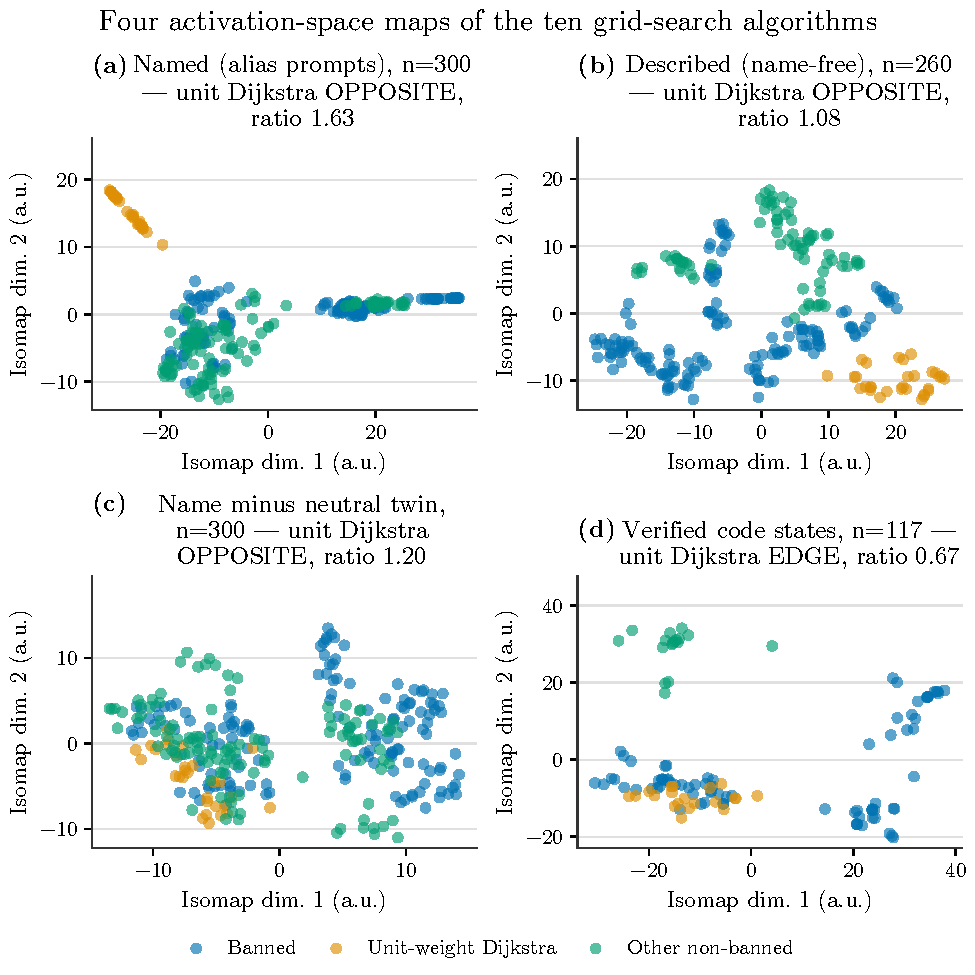
\includegraphics[width=\linewidth,height=0.78\textheight,keepaspectratio]{figures/fig_tpg_manifolds_v0.pdf}
\caption{Isomap embeddings (k = 15) of Qwen3-32B (4-bit NormalFloat) hidden states for the ten-algorithm grid path-search catalogue, from the geometry experiment's stored coordinates. Points are coloured by category: banned algorithms (blue), unit-weight Dijkstra (orange), and the other non-banned algorithms (green), each panel showing only the algorithms present in that condition. (a) Prompts naming each algorithm by an alias (n = 300; block 31). (b) Name-free descriptions of each algorithm's mechanism, kept only where the model names the algorithm correctly from the description alone (n = 260; block 31; jump point search has no such description and is absent). (c) The same alias prompts with a token-matched neutral-noun twin subtracted out (n = 300; block 31). (d) Mean code-token states of name-scrubbed, verified programs, kept only for algorithms with at least 10 surviving programs -- banned here is BFS, DFS, A* and greedy best-first, and the other non-banned class is IDA* alone (n = 117; block 33). Panel titles give unit-weight Dijkstra's class and the ratio of its geodesic distance to the banned algorithms over the non-banned classes' median distance at k = 15: OPPOSITE the banned cluster in (a)-(c) (ratios 1.63, 1.08, 1.20) and at the EDGE of it in (d) (ratio 0.67). The geometry is correlational: it describes where these representations sit, not whether the model uses it to choose an algorithm.}
\label{fig:fig_tpg_manifolds}
\end{figure}
\begin{figure}[!htbp]
\centering\captionsetup{font=footnotesize}
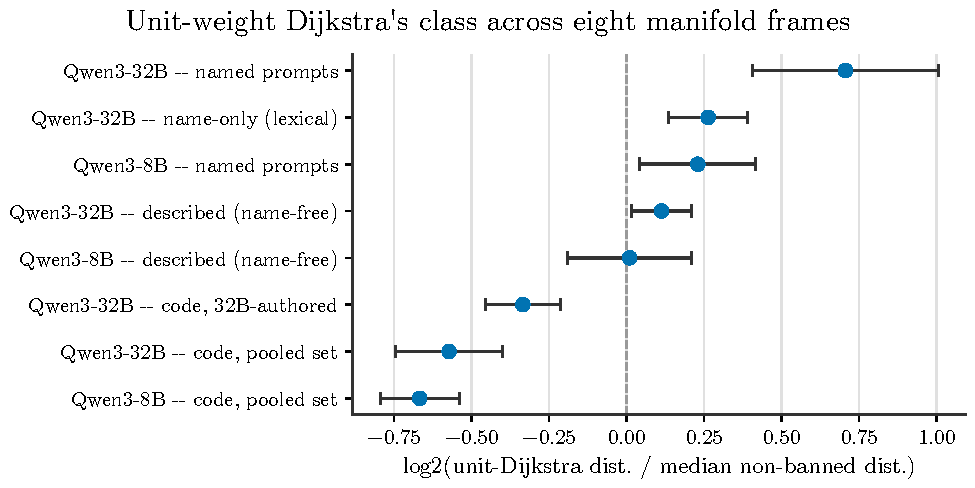
\includegraphics[width=\linewidth,height=0.78\textheight,keepaspectratio]{figures/fig_tpg_landing_v0.pdf}
\caption{Log2 of the ratio between unit-weight Dijkstra's activation-manifold distance to a banned cluster of five path-search algorithms and the median such distance among the non-banned algorithms in the same frame, for Qwen3-32B and Qwen3-8B, computed on a \$k=15\$ nearest-neighbour geodesic graph. Points show this ratio (log2 scale) for eight manifold frames, sorted top to bottom by value; horizontal whiskers show each frame's bootstrap 95\textbackslash{}\% confidence interval, drawn as a symmetric interval anchored at the point estimate and truncated to the nearer true bound (never wider than the actual interval on either side, and never crossing zero where the true interval does not). The dashed vertical line marks zero, equal distance to the banned cluster and to the median non-banned algorithm: points to its right are the `\texttt{opposite'' class (\allowbreak{}Dijkstra farther from the banned cluster than typical),\allowbreak{} points to its left are the }`edge'' class (closer than typical). All five frames built from language -- named prompts, the isolated name-only (lexical) component, and name-free descriptions, in both models -- read opposite, from \$+0.01\$ (Qwen3-8B, described; the only interval crossing zero) to \$+0.71\$ (Qwen3-32B, named). All three frames built from the models' own code -- Qwen3-32B's 32B-authored programs, Qwen3-32B's pooled program set, and Qwen3-8B's pooled program set -- read edge, from \$-0.33\$ to \$-0.67\$, each with an interval that does not cross zero. \$n=8\$ frames; a ninth frame quoted in an earlier draft of this figure (Qwen3-32B, block 21) could not be traced to any run's output file and is omitted. The geometry is descriptive: it is not evidence that the model uses this axis causally when choosing an algorithm.}
\label{fig:fig_tpg_landing}
\end{figure}
\textbf{Names drive the alias-level geometry, across algorithms.} On the named manifold, g of the 15 aliases falls with the number of banned algorithms whose alias pattern an alias matches. For Qwen3-32B the Spearman is -0.74 at k 10 (permutation p 0.0010) and -0.65 at k 15 (p 0.0052), and -0.67 after partialling out alias length; for Qwen3-8B it is -0.70 and -0.78. Within algorithms the relation is not significant (exact p 0.157 and 0.551 over 7,776 permutations), which matches the record audit's stratified test (Section 9.2). On the name-only manifold the same Spearman is -0.59 at k 10 and -0.65 at k 15, just short of the committed -0.6 at both k. The prediction that names drive the alias-level geometry on the named manifold holds; the geometry cannot separate a name effect from algorithm identity inside it.

\textbf{What each manifold tracks.} Representational similarity analysis [147] compares each manifold's class-by-class distances with four model matrices: lexical distance between the aliases, behavioural distance from expansion-order traces of the reference implementations, surface distance between the programs' token sets, and length (Table 437; exact label-permutation p-values; noise ceilings from split halves [148]). The named, described and name-only manifolds track the lexical matrix (0.46, 0.57 and 0.47) and textbook data-structure attributes, not measured expansion order (iteration-10 correction): on the named Qwen3-32B manifold the data-structure matrix gives 0.65 (exact p 0.001) against 0.46 for the lexical matrix, and the expansion-order matrix gives -0.03 to 0.16 on the five language manifolds. The two model matrices are nearly unrelated there (Spearman 0.13, variance inflation 1.02), and each survives partialling out the other: lexical given data structure 0.50 and data structure given lexical 0.67, exact relabeling p 0.002 and 0.001 when the tested matrix is relabeled and 0.003 and 0.001 under Freedman-Lane residual relabeling (Table 437b). With ten classes and a contested partial Mantel test these p-values are descriptive. The program manifolds track behaviour (0.64 on Qwen3-32B and 0.88 on Qwen3-8B), but they track surface and length as strongly (0.67 and 0.78; 0.87 and 0.88), so with six classes the program manifold cannot tell an edge in mechanism from an edge in how the code looks. The described manifold also evokes the names: a classifier trained on the named manifold's block-31 states labels the described prompts at balanced accuracy 0.69 (chance 0.11) and the programs at 0.17, which is chance for six classes (0.167) (iteration-10 correction). The behavioural anchor holds by construction: in expansion order, unit-weight Dijkstra is the nearest non-banned algorithm to BFS (distance 0.31, against 0.72 for bidirectional BFS and 0.86 to 1.12 for the rest).

\begin{table}[H]
\renewcommand{\thetable}{437}
\centering\scriptsize\setlength{\tabcolsep}{2.5pt}
\caption{Representational similarity of each manifold to four model matrices (Spearman, exact label-permutation p in brackets; upper noise ceiling). The last three columns (iteration-10 correction) add the data-structure, expansion-order and description-lexical model matrices stored in results\slash{}rsa.json. [Source: iteration 9, artifact \nolinkurl{gen_art_experiment_46}.]}\label{tab:t464}
\begin{tabular}{>{\raggedright\arraybackslash\hspace{0pt}}p{0.1841\linewidth}>{\raggedright\arraybackslash\hspace{0pt}}p{0.0788\linewidth}>{\raggedright\arraybackslash\hspace{0pt}}p{0.1121\linewidth}>{\raggedright\arraybackslash\hspace{0pt}}p{0.0788\linewidth}>{\raggedright\arraybackslash\hspace{0pt}}p{0.0751\linewidth}>{\raggedright\arraybackslash\hspace{0pt}}p{0.0748\linewidth}>{\raggedright\arraybackslash\hspace{0pt}}p{0.0915\linewidth}>{\raggedright\arraybackslash\hspace{0pt}}p{0.0955\linewidth}>{\raggedright\arraybackslash\hspace{0pt}}p{0.1121\linewidth}}
\toprule
\textbf{Manifold (classes)} & \textbf{Lexical} & \textbf{Behavioural} & \textbf{Surface} & \textbf{Length} & \textbf{Noise ceiling} & \textbf{Data structure} & \textbf{Expansion order} & \textbf{Description lexical} \\
\midrule
Named, Qwen3-32B (10) & 0.46 (0.003) & 0.24 (0.091) & 0.20 (0.128) & 0.07 (0.297) & 1.00 & 0.65 (0.001) & -0.03 (0.532) & 0.23 (0.079) \\
Described, Qwen3-32B (9) & 0.57 (0.000) & 0.12 (0.252) & 0.02 (0.463) & 0.01 (0.426) & 1.00 & 0.43 (0.014) & 0.07 (0.349) & 0.44 (0.006) \\
Name-only, Qwen3-32B (10) & 0.47 (0.001) & 0.29 (0.034) & -0.13 (0.785) & 0.33 (0.027) & 0.99 & 0.44 (0.009) & 0.16 (0.163) & 0.54 (0.000) \\
Program, primary readout, Qwen3-32B (6) & 0.29 (0.164) & 0.64 (0.018) & 0.67 (0.010) & 0.78 (0.007) & 1.00 & 0.65 (0.011) & 0.43 (0.096) & 0.89 (0.003) \\
Program, second readout, Qwen3-32B (6) & -0.01 (0.451) & 0.59 (0.050) & 0.66 (0.039) & 0.49 (0.081) & 0.96 & 0.57 (0.017) & 0.43 (0.165) & 0.67 (0.006) \\
Program, Qwen3-32B programs only (6) & 0.10 (0.372) & 0.73 (0.008) & 0.70 (0.010) & 0.77 (0.007) & 1.00 & 0.71 (0.006) & 0.52 (0.058) & 0.90 (0.001) \\
Named, Qwen3-8B (10) & 0.48 (0.002) & 0.27 (0.071) & -0.12 (0.715) & 0.28 (0.058) & 0.99 & 0.37 (0.016) & 0.14 (0.248) & 0.57 (0.000) \\
Described, Qwen3-8B (9) & 0.25 (0.079) & 0.25 (0.087) & 0.33 (0.040) & 0.46 (0.008) & 0.99 & 0.39 (0.018) & 0.14 (0.226) & 0.53 (0.001) \\
Program, primary readout, Qwen3-8B (6) & 0.10 (0.360) & 0.88 (0.001) & 0.87 (0.001) & 0.88 (0.001) & 0.99 & 0.64 (0.011) & 0.71 (0.013) & 0.92 (0.003) \\
\bottomrule
\end{tabular}
\end{table}

\begin{table}[H]
\renewcommand{\thetable}{437b}
\centering\footnotesize\setlength{\tabcolsep}{4.0pt}
\caption{Lexical distance against data-structure attributes (iteration-10 correction): the Spearman of the two model matrices over the present pairs (exact relabeling p), their variance inflation 1\slash{}(1 - r\textasciicircum{}2), and partial Spearman correlations (Pearson partial correlation of average-rank vectors) of each manifold, with exact one-sided relabeling p over all n! relabelings (10! = 3,628,800; 9! = 362,880; 6! = 720, floor 0.0014) under scheme A (relabel the tested matrix) and scheme B (Freedman-Lane: relabel the residuals of the neural ranks on the control ranks). Partial Mantel tests can be anticonservative for structured matrices, so every p here is descriptive. [Source: iteration 9, artifact \nolinkurl{gen_art_experiment_46}.]}\label{tab:t465}
\begin{tabular}{>{\raggedright\arraybackslash\hspace{0pt}}p{0.2121\linewidth}>{\raggedright\arraybackslash\hspace{0pt}}p{0.2124\linewidth}>{\raggedright\arraybackslash\hspace{0pt}}p{0.1034\linewidth}>{\raggedright\arraybackslash\hspace{0pt}}p{0.1926\linewidth}>{\raggedright\arraybackslash\hspace{0pt}}p{0.1926\linewidth}}
\toprule
\textbf{Manifold (classes)} & \textbf{Spearman of lexical and data-structure matrices (p)} & \textbf{Variance inflation} & \textbf{Lexical given data structure (p A; p B)} & \textbf{Data structure given lexical (p A; p B)} \\
\midrule
Named, Qwen3-32B (10) & 0.13 (0.230) & 1.02 & 0.50 (0.002; 0.003) & 0.67 (0.001; 0.001) \\
Described, Qwen3-32B (9) & 0.17 (0.185) & 1.03 & 0.56 (0.001; 0.002) & 0.41 (0.026; 0.026) \\
Name-only, Qwen3-32B (10) & 0.13 (0.230) & 1.02 & 0.46 (0.003; 0.003) & 0.43 (0.015; 0.015) \\
Program, primary readout, Qwen3-32B (6) & -0.08 (0.628) & 1.01 & 0.45 (0.094; 0.093) & 0.71 (0.006; 0.004) \\
Program, second readout, Qwen3-32B (6) & -0.08 (0.628) & 1.01 & 0.05 (0.399; 0.414) & 0.57 (0.019; 0.022) \\
Program, Qwen3-32B programs only (6) & -0.08 (0.628) & 1.01 & 0.22 (0.288; 0.285) & 0.72 (0.006; 0.004) \\
Named, Qwen3-8B (10) & 0.13 (0.230) & 1.02 & 0.47 (0.006; 0.007) & 0.35 (0.032; 0.034) \\
Described, Qwen3-8B (9) & 0.17 (0.185) & 1.03 & 0.20 (0.146; 0.148) & 0.37 (0.030; 0.030) \\
Program, primary readout, Qwen3-8B (6) & -0.08 (0.628) & 1.01 & 0.20 (0.300; 0.307) & 0.65 (0.011; 0.010) \\
\bottomrule
\end{tabular}
\end{table}

\textbf{The survivors themselves.} Each of the 15 unit-weight Dijkstra survivors of iteration 8 was teacher-forced, name-scrubbed, and placed on the program manifold by its nearest algorithm and its own g (Table 438). On the primary frame, where leave-one-out placement of the frame's own programs is right 0.85 of the time (gate 0.70), all 15 survivors are classed edge (Wilson interval 0.80 to 1.00) and 13 are nearest to the unit-weight Dijkstra programs, 2 to greedy best-first. They sit farther from the banned five than the frame's own unit-weight Dijkstra programs (median g 20.2 against 16.5, Mann-Whitney p 0.00009), but still on the edge side of the non-banned median.

{\footnotesize\setlength{\tabcolsep}{4.0pt}\renewcommand{\thetable}{438}
\begin{longtable}{>{\raggedright\arraybackslash\hspace{0pt}}p{0.1639\linewidth}>{\raggedright\arraybackslash\hspace{0pt}}p{0.0699\linewidth}>{\raggedright\arraybackslash\hspace{0pt}}p{0.1087\linewidth}>{\raggedright\arraybackslash\hspace{0pt}}p{0.3033\linewidth}>{\raggedright\arraybackslash\hspace{0pt}}p{0.1516\linewidth}>{\raggedright\arraybackslash\hspace{0pt}}p{0.0992\linewidth}}
\caption{Placement of the 15 unit-weight Dijkstra survivors on each program frame (k 15). The first four rows are the 15 unit-weight Dijkstra survivors; the rows below (iteration-10 correction) place the other 23 survivors of the placement file by family (frozen from the labels before any class was read: 15 Bellman-Ford\slash{}SPFA, 3 BFS variants, 5 other known), with the median g, the frame median and the two reference values (unit-weight Dijkstra and IDA*). Three caveats apply: the per-family placement was not preregistered; with only two non-banned classes on these frames, 'opposite' means farther than the median of the unit-weight Dijkstra and IDA* frame values; and the class therefore depends on that two-class reference. [Source: iteration 9, artifact \nolinkurl{gen_art_experiment_46}.]}\label{tab:t466}\\
\toprule
\textbf{Frame} & \textbf{Block} & \textbf{Leave-one-out placement accuracy (gate 0.70)} & \textbf{Survivors classed edge} & \textbf{Nearest algorithm of the survivors} & \textbf{Baseline programs placed on their own label} \\
\midrule
\endfirsthead
\multicolumn{6}{l}{\emph{Table 438, continued}}\\
\toprule
\textbf{Frame} & \textbf{Block} & \textbf{Leave-one-out placement accuracy (gate 0.70)} & \textbf{Survivors classed edge} & \textbf{Nearest algorithm of the survivors} & \textbf{Baseline programs placed on their own label} \\
\midrule
\endhead
\bottomrule
\endlastfoot
Qwen3-32B, primary readout & 33 & 0.85 (passes) & 15 of 15 & unit-weight Dijkstra 13, greedy best-first 2 & 1.00 \\
Qwen3-32B, second readout & 21 & 0.67 (fails) & 15 of 15 & unit-weight Dijkstra 14, greedy best-first 1 & 0.98 \\
Qwen3-32B programs only & 31 & 0.89 (passes) & 10 of 15 & unit-weight Dijkstra 14, A* 1 & 1.00 \\
Qwen3-8B, primary readout & 17 & 0.83 (passes) & 15 of 15 & unit-weight Dijkstra 12, greedy best-first 3 & 0.92 \\
Qwen3-32B, primary readout: Bellman-Ford\slash{}SPFA survivors & 33 & 0.85 (passes) & 0 of 15 (opposite 15; median g 28.1 against the frame median 24.8; references 16.6 and 32.9; 0 beyond the farther) & unit-weight Dijkstra 14, BFS 1 & 1.00 \\
Qwen3-32B, primary readout: BFS variants survivors & 33 & 0.85 (passes) & 3 of 3 (opposite 0; median g 16.8 against the frame median 24.8; references 16.6 and 32.9; 0 beyond the farther) & BFS 3 & 1.00 \\
Qwen3-32B, primary readout: other known survivors & 33 & 0.85 (passes) & 5 of 5 (opposite 0; median g 19.6 against the frame median 24.8; references 16.6 and 32.9; 0 beyond the farther) & BFS 3, unit-weight Dijkstra 1, greedy best-first 1 & 1.00 \\
Qwen3-32B, second readout: Bellman-Ford\slash{}SPFA survivors & 21 & 0.67 (fails) & 9 of 15 (opposite 6; median g 127.9 against the frame median 128.2; references 40.7 and 215.8; 0 beyond the farther) & BFS 14, DFS 1 & 0.98 \\
Qwen3-32B, second readout: BFS variants survivors & 21 & 0.67 (fails) & 3 of 3 (opposite 0; median g 50.0 against the frame median 128.2; references 40.7 and 215.8; 0 beyond the farther) & BFS 3 & 0.98 \\
Qwen3-32B, second readout: other known survivors & 21 & 0.67 (fails) & 3 of 5 (opposite 2; median g 127.7 against the frame median 128.2; references 40.7 and 215.8; 0 beyond the farther) & BFS 2, greedy best-first 2, A* 1 & 0.98 \\
Qwen3-32B programs only: Bellman-Ford\slash{}SPFA survivors & 31 & 0.89 (passes) & 0 of 15 (opposite 15; median g 30.8 against the frame median 24.8; references 19.7 and 29.9; 12 beyond the farther) & unit-weight Dijkstra 11, A* 2, IDA* 2 & 1.00 \\
Qwen3-32B programs only: BFS variants survivors & 31 & 0.89 (passes) & 3 of 3 (opposite 0; median g 19.3 against the frame median 24.8; references 19.7 and 29.9; 0 beyond the farther) & BFS 3 & 1.00 \\
Qwen3-32B programs only: other known survivors & 31 & 0.89 (passes) & 3 of 5 (opposite 2; median g 22.3 against the frame median 24.8; references 19.7 and 29.9; 0 beyond the farther) & unit-weight Dijkstra 3, BFS 2 & 1.00 \\
Qwen3-8B, primary readout: Bellman-Ford\slash{}SPFA survivors & 17 & 0.83 (passes) & 10 of 15 (opposite 5; median g 11.9 against the frame median 12.2; references 7.7 and 16.7; 0 beyond the farther) & unit-weight Dijkstra 14, greedy best-first 1 & 0.92 \\
Qwen3-8B, primary readout: BFS variants survivors & 17 & 0.83 (passes) & 3 of 3 (opposite 0; median g 10.1 against the frame median 12.2; references 7.7 and 16.7; 0 beyond the farther) & unit-weight Dijkstra 2, BFS 1 & 0.92 \\
Qwen3-8B, primary readout: other known survivors & 17 & 0.83 (passes) & 5 of 5 (opposite 0; median g 10.5 against the frame median 12.2; references 7.7 and 16.7; 0 beyond the farther) & greedy best-first 2, DFS 1, BFS 1, unit-weight Dijkstra 1 & 0.92 \\
\end{longtable}}

\begin{figure}[!htbp]
\centering\captionsetup{font=footnotesize}
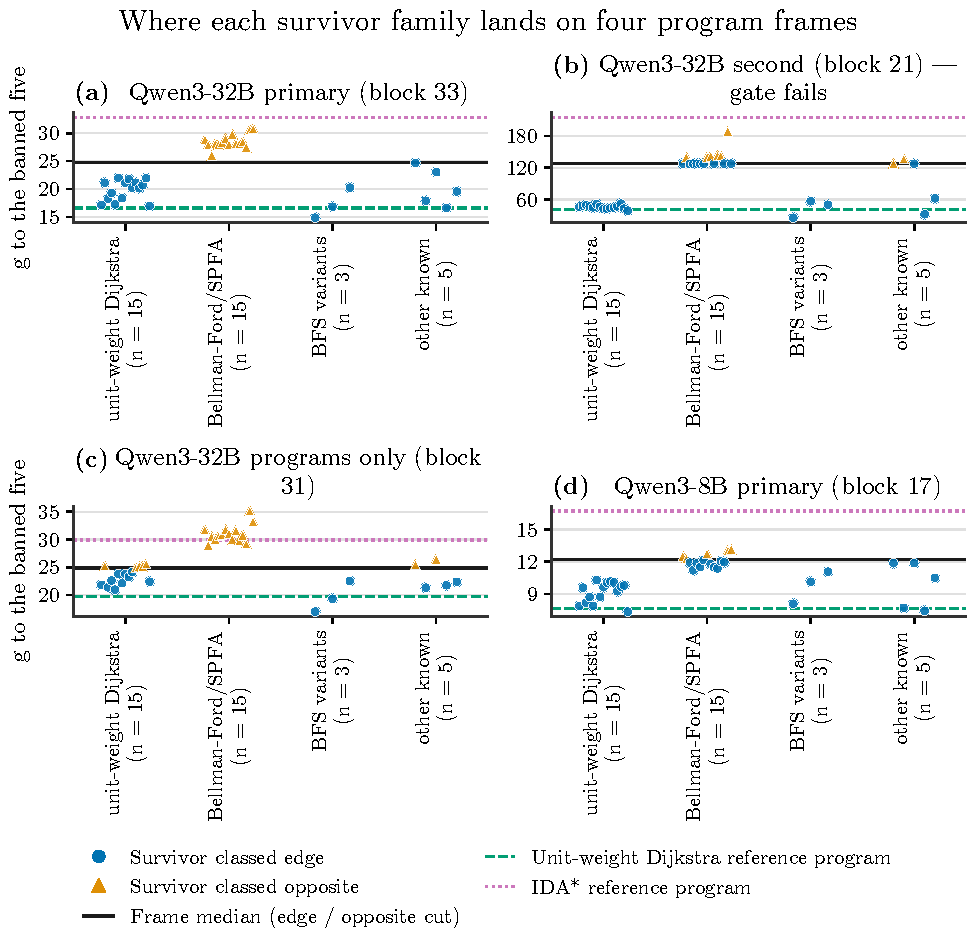
\includegraphics[width=\linewidth,height=0.78\textheight,keepaspectratio]{figures/fig_s0_placement_v0.pdf}
\caption{Geodesic distance g to the banned five of every iteration-8 survivor, plotted on four program-representation frames (k = 15 nearest-neighbour graph) and grouped on the x-axis by substitute family: unit-weight Dijkstra (n = 15), Bellman-Ford\slash{}SPFA (n = 15), BFS variants (n = 3), other known (n = 5). Circles mark survivors classed edge (nearer the unit-weight Dijkstra reference program than the frame median) and triangles mark survivors classed opposite (farther, past the median, toward the IDA* reference program). The solid black line is each frame's median of the two reference programs; the green dashed line is the frame's g to a forced unit-weight-Dijkstra program and the violet dotted line its g to a forced IDA* program. Panels: (a) Qwen3-32B primary readout (block 33); (b) Qwen3-32B second readout (block 21), which fails its own leave-one-out placement gate; (c) Qwen3-32B using only the programs (block 31); (d) Qwen3-8B primary readout (block 17). Bellman-Ford\slash{}SPFA survivors are classed opposite on 15\slash{}15 survivors in both gate-passing Qwen3-32B frames (a, c), but mixed in (b) (9\slash{}15 edge) and (d) (10\slash{}15 edge). Unit-weight Dijkstra survivors are classed edge on 15\slash{}15 in (a), (b) and (d), but only 10\slash{}15 in (c). BFS-variant survivors are classed edge in every frame. Not preregistered.}
\label{fig:fig_s0_placement}
\end{figure}
\begin{table}[H]
\renewcommand{\thetable}{439}
\centering\small\setlength{\tabcolsep}{4.0pt}
\caption{The geometry experiment's preregistered predictions. [Source: iteration 9, artifact \nolinkurl{gen_art_experiment_46}.]}\label{tab:t467}
\begin{tabular}{>{\raggedright\arraybackslash\hspace{0pt}}p{0.5403\linewidth}>{\raggedright\arraybackslash\hspace{0pt}}p{0.4225\linewidth}}
\toprule
\textbf{Prediction} & \textbf{Result} \\
\midrule
The named manifold reproduces iteration 8 (rank gate 0.95) & Fails (0.894 at k 15; 0.997 at k 10); classes identical; fallback to the new states \\
Edge on the program and the described manifolds & Fails: edge on the program manifold, opposite on the described manifold \\
Opposite on the named and the name-only manifolds & Holds \\
Alias-level g follows lexical overlap on the named manifold (Spearman at most -0.6 at k 10 and 15) & Holds (-0.74 and -0.65); not within algorithms \\
The overlap ordering does not reproduce on the program and described manifolds & Descriptive \\
Unit-weight Dijkstra nearest BFS in behaviour & Holds (by construction for the order term) \\
Named manifold tracks lexical over behavioural distance; program and described manifolds the reverse & Named: holds; program: holds, with surface and length as strong; described: fails \\
More than half the survivors classed edge on the program manifold, if placement passes its gate & Holds (15 of 15) \\
\bottomrule
\end{tabular}
\end{table}

\textbf{Audits, cost and positioning.} A standard-library script re-derived the classes and the alias rows with 0 mismatches. An independent script recomputed the neighbour graphs and geodesics from the raw state files with scikit-learn and networkx and matched every class (largest difference in g 4e-13). Random survivor labels give a landing verdict of neither in 0.93 of draws, and shuffled algorithm labels give unit-weight Dijkstra the opposite class in 0.37. OpenRouter spend was USD 0.094 for 1,440 calls (naming gate and 600 forced programs). For time, the Qwen3-8B name-only manifold, the Qwen3-8B-only program frame and two further readouts were not analysed; their states are kept. Labeller disagreements excluded several first-source program pools without manual adjudication. The experiment's dated search found no work that rebuilds a model's algorithm manifold with and without the algorithms' names; the nearest neighbours treat lexical identity as a confound of interpretability metrics [154] and compare behavioural with hidden-state semantic geometry [155].

\FloatBarrier
\subsection*{9.5 Where post-training sharpened the fork: base against instruct in three families}
\addcontentsline{toc}{subsection}{9.5 Where post-training sharpened the fork: base against instruct in three families}
\noindent{\small\emph{Artifact: \nolinkurl{gen_art_experiment_50}.}}\par\medskip
The base-model experiment  compared base and instruction-tuned models on identical token ids at the fork, the decision token where a code model picks its algorithm. The question is the request's hypothesis that a model gives ``the mean answer''. Iteration 8 found, in Qwen3-8B only, that post-training widened the fork margin by 2 to 13 nats while phrasing positions barely moved. Three parts were preregistered. The \emph{sharpening measurement} repeats that comparison in two new families with the controls of Cantarero et al. [142]: Jensen-Shannon divergence at base-entropy-matched positions and at rate-matched random positions. The \emph{patching test} uses cross-model activation patching [88]: it writes the base model's outputs of chosen components into the instruct run at the fork and measures the share of the instruct-minus-base margin gap that closes. The \emph{held-out rerun} repairs the circuit's held-out arm. Everything decisive was committed in a sha256 chain, and a standard-library script re-derived every headline with placebos (0 mismatches).

\textbf{The sharpening measurement (verdict partial).} The margin is log P(default class) minus log P(alternative class) at the fork, under the chat template for Gemma. Llama was switched to template-free prompts by the committed rule, because the Llama-3.1-8B base model's embedding rows of its chat-header and end-of-turn tokens have about 3e-21 of the median row norm, which means they are untrained. On Gemma's grid fork the instruct model puts 0.671 on its default class and the base model 0.089, a gain of 1.78 nats [1.59, 2.00], and the argmax differs on all 20 prompts: post-training reversed and concentrated the choice (base P(BFS) 0.25 against P(DFS) 0.09, with 0.663 of the base model's mass on tokens mapped to no class) (iteration-10 correction) (Table 440). On the two first-and-last-position forks the gains are 3.07 and 1.68 nats with the same argmax. On substring search the gain is 1.75 nats with an interval that crosses zero (5 prompts). Phrasing positions barely move (entropy change 0.44 to 0.50 nats; the instruct token is the base model's top choice at 91\% to 97\% of phrasing positions, the URIAL pattern [100]). The divergence at the fork is 4.7 to 6.6 times the mean phrasing divergence, but only 0.75 to 1.18 times the divergence at positions matched for base entropy: at these forks, ``fork'' and ``high base entropy'' coincide. Cantarero et al.'s own pattern reproduces: divergence 11 to 15 times higher inside their base-entropy fork set than outside, a rate-matched random set near 1.0, and every Gemma fork inside their set. Of the committed predictions, the phrasing prediction holds; the gain of at least 2 nats on every near-collapsed fork fails (1.68 at the second first-and-last fork); divergence at least 1.3 times the entropy-matched positions fails; and a different argmax on at least half the units holds only on the grid. Llama's grid fork fails the committed on-policy rule (the instruct model's log probability of the shared opening is about -13.6, below -5), so its two forks are descriptive.

\begin{table}[H]
\renewcommand{\thetable}{440}
\centering\tiny\setlength{\tabcolsep}{2.5pt}
\caption{Base against instruct at counterfactually located forks (teacher forcing on identical token ids; Gemma under its chat template, Llama template-free). P(D) is the probability of the instruct default's class; JS ratio is the Jensen-Shannon divergence at the fork over that at base-entropy-matched positions. The last two columns (iteration-10 correction) give the base model's probability of the alternative class, where the fork has a single alternative, and the base model's probability mass on tokens mapped to no class (results\slash{}b1\_\allowbreak{}*.json). [Source: iteration 9, artifact \nolinkurl{gen_art_experiment_50}.]}\label{tab:t468}
\begin{tabular}{>{\raggedright\arraybackslash\hspace{0pt}}p{0.1436\linewidth}>{\raggedright\arraybackslash\hspace{0pt}}p{0.0620\linewidth}>{\raggedright\arraybackslash\hspace{0pt}}p{0.0646\linewidth}>{\raggedright\arraybackslash\hspace{0pt}}p{0.0408\linewidth}>{\raggedright\arraybackslash\hspace{0pt}}p{0.2470\linewidth}>{\raggedright\arraybackslash\hspace{0pt}}p{0.0679\linewidth}>{\raggedright\arraybackslash\hspace{0pt}}p{0.0439\linewidth}>{\raggedright\arraybackslash\hspace{0pt}}p{0.0561\linewidth}>{\raggedright\arraybackslash\hspace{0pt}}p{0.0985\linewidth}>{\raggedright\arraybackslash\hspace{0pt}}p{0.0679\linewidth}}
\toprule
\textbf{Fork (classes)} & \textbf{Prompts} & \textbf{Instruct P(D)} & \textbf{Base P(D)} & \textbf{Gain, nats (95\% interval)} & \textbf{Template-free gain} & \textbf{JS ratio} & \textbf{Argmax differs} & \textbf{Base P(alternative)} & \textbf{Unmapped base mass} \\
\midrule
Gemma grid, token 32 (BFS against DFS) & 20 & 0.671 & 0.089 & 1.78 (1.59 to 2.00) & 0.95 & 1.09 & 20 of 20 & 0.25 (BFS) & 0.663 \\
Gemma substring search, token 31 & 5 & 0.832 & 0.765 & 1.75 (-1.31 to 4.82) & 4.54 & 0.75 & 2 of 5 & n\slash{}a (several alternatives) & 0.157 \\
Gemma first and last position, token 12 & 5 & 0.946 & 0.370 & 3.07 (2.06 to 4.10) & 2.03 & 1.18 & 0 of 5 & n\slash{}a (several alternatives) & 0.311 \\
Gemma first and last position, token 24 & 5 & 0.882 & 0.481 & 1.68 (0.37 to 2.99) & 3.05 & 0.90 & 0 of 5 & n\slash{}a (several alternatives) & 0.335 \\
Llama grid, token 52 (descriptive) & 5 & 0.654 & 0.366 & 0.96 (template-free) & n\slash{}a & 0.60 & 5 of 5 & n\slash{}a (several alternatives) & 0.296 \\
Llama grid, token 121 (descriptive) & 5 & 0.606 & 0.757 & -0.71 (template-free) & n\slash{}a & 0.71 & 0 of 5 & n\slash{}a (several alternatives) & below 0.001 \\
Qwen3-8B, carried from iteration 8 &  &  &  & grid 3.27, connected components 13.41, shortest path 2.11, minimum spanning tree 1.84, trapped rain water 1.53 &  &  &  & n\slash{}a & n\slash{}a \\
\bottomrule
\end{tabular}
\end{table}

\textbf{The patching test (verdict partial; localisation distributed).} In Qwen3-8B against Qwen3-8B-Base, on minimum spanning tree weight (Kruskal against Prim) and connected components (\texttt{find} against \texttt{dfs} or \texttt{bfs}), base outputs of components were patched into the instruct run at the fork, 20 prompts per unit with fixed batch shapes (Table 441 and the figure below it). The ten validated fork-stack nodes of iteration 8's circuit close 1.00 [0.96, 1.04] of the 2.06-nat gap on minimum spanning tree. That is not specific: 50 sets of random late-layer components, matched in write norm, close a median 0.81 (95th percentile 1.41; empirical p 0.45), and random sets that exclude the circuit's top 15 components close a median 0.66, below the fork stack at p 0.039. On connected components the fork stack closes 0.45 [0.28, 0.57] of a 4.52-nat gap, above random sets (median -0.22, p 0.020), but short of the committed 0.5. (iteration-10 correction) Most matched random sets repeat a component, because the draw falls back to the whole candidate pool once an MLP pool is used up: an MLP repeats in 1 of 50 random sets and 47 of 50 sets without the circuit's top 15 on minimum spanning tree, and in 36 of 50 and 50 of 50 on connected components. Restricted to sets of ten distinct components, the minimum spanning tree null keeps a median 0.80 (49 sets; p 0.44) and the sets without the top 15 keep 3 (median 0.65; p 0.25, the floor at that N); random sets scaled to the fork stack's write norm give a median 0.64 (p 0.098), beside 0.66 (p 0.039) and 0.81 (p 0.45). On connected components the 14 full-size random sets give a median -0.33 (p 0.067, at its floor) and no set without the top 15 is full-size. The fork stack's 0.45 there is a ratio of means; per prompt its share has mean 0.13, median 0.43 and interquartile range -0.02 to 0.61, negative on 6 of 20 prompts (the five fork MLPs: ratio of means 0.41, mean of per-prompt shares 0.07; Table 441b). On minimum spanning tree specificity stays unresolved in this record; BASE-W redraws the sets without reuse. The task-specification nodes close nothing (-0.02 and -0.17), so the sharpening is not written upstream. It is carried at the fork by late MLPs, redundantly: several single MLPs between layers 26 and 35 each close about half the minimum spanning tree gap (layer 35 alone 0.98), and the fork stack's joint share is about half the sum of its singles. A large part of the gap is not in the residual stream at all. The instruct model's unembedding, reading the base model's own final residual, accounts for 0.43 of the gap on minimum spanning tree and 0.85 on connected components, which is why swapping the whole residual at the fork in layer 36 does not reach 1. Weight differences agree: every module moved by 5\% to 11\% in relative Frobenius norm, the unembedding by 9\%, while the unembedding rows of ' dfs' (12.0\%, 91st percentile) and ' bfs' (14.4\%, 96th) moved more than almost any other row and ' find' (6.6\%, 27th) little. Per-layer weight change does not track the per-layer patching shares (r at most 0.2). Along the first principal component of the block-30 output at the fork (98.5\% and 94.6\% of the variance of the instruct and base states on the two units), the patched states move most of the way from the instruct states toward the base states, and the median random and residual-swap states move less.

\begin{table}[H]
\renewcommand{\thetable}{441}
\centering\small\setlength{\tabcolsep}{4.0pt}
\caption{Share of the instruct-minus-base fork margin closed by patching base outputs into Qwen3-8B at the fork (20 prompts per unit; bootstrap 95\% intervals). [Source: iteration 9, artifact \nolinkurl{gen_art_experiment_50}.]}\label{tab:t469}
\begin{tabular}{>{\raggedright\arraybackslash\hspace{0pt}}p{0.3902\linewidth}>{\raggedright\arraybackslash\hspace{0pt}}p{0.2539\linewidth}>{\raggedright\arraybackslash\hspace{0pt}}p{0.3021\linewidth}}
\toprule
\textbf{Measure} & \textbf{Minimum spanning tree (Kruskal against Prim)} & \textbf{Connected components (\texttt{find} against \texttt{dfs} or \texttt{bfs})} \\
\midrule
Gap, instruct minus base (nats) & 2.06 (1.96 to 2.16) & 4.52 (3.50 to 5.57) \\
Ten validated fork-stack nodes & 1.00 (0.96 to 1.04) & 0.45 (0.28 to 0.57) \\
Five fork MLPs \slash{} five fork heads & 1.08 \slash{} 0.17 & 0.41 \slash{} 0.30 \\
50 matched random sets: median \slash{} 95th percentile \slash{} empirical p & 0.81 \slash{} 1.41 \slash{} 0.45 & -0.22 \slash{} 0.06 \slash{} 0.020 \\
Random sets without the circuit's top 15: median \slash{} p & 0.66 \slash{} 0.039 & -0.46 \slash{} 0.020 \\
Task-specification nodes & -0.02 & -0.17 \\
Residual swap at the fork, layer 23 \slash{} layer 36 & 0.78 \slash{} 0.57 & -0.05 \slash{} 0.15 \\
Residual swap of the prefix \slash{} of all positions, layer 23 & 0.44 \slash{} 1.13 & 0.37 \slash{} 0.61 \\
Unembedding alone (CPU readout decomposition) & 0.43 & 0.85 \\
Best single components & MLP 35 0.98, MLP 28 0.62, MLP 29 0.56, MLP 26 0.52 & MLP 30 0.53, MLP 35 0.38, MLP 34 0.26, head 10 of layer 23 0.21 \\
Base MLP weights on instruct inputs (5 MLPs) & 0.23 & 0.38 \\
Reverse: instruct fork stack written into the base model, share opened & -0.30 & 0.22 (p 0.02) \\
\bottomrule
\end{tabular}
\end{table}

\begin{table}[H]
\renewcommand{\thetable}{441b}
\centering\scriptsize\setlength{\tabcolsep}{2.5pt}
\caption{The random patching sets by effective size (iteration-10 correction) (Rscaled reuses the matched sets, scaled; empirical p = (1 + \#null \textgreater{}= fork stack)\slash{}(N + 1), floor 1\slash{}(N + 1)). [Source: iteration 9, artifact \nolinkurl{gen_art_experiment_50}.]}\label{tab:t470}
\begin{tabular}{>{\raggedright\arraybackslash\hspace{0pt}}p{0.1039\linewidth}>{\raggedright\arraybackslash\hspace{0pt}}p{0.1532\linewidth}>{\raggedright\arraybackslash\hspace{0pt}}p{0.0915\linewidth}>{\raggedright\arraybackslash\hspace{0pt}}p{0.1956\linewidth}>{\raggedright\arraybackslash\hspace{0pt}}p{0.1045\linewidth}>{\raggedright\arraybackslash\hspace{0pt}}p{0.1061\linewidth}>{\raggedright\arraybackslash\hspace{0pt}}p{0.1687\linewidth}}
\toprule
\textbf{Unit} & \textbf{Family} & \textbf{Sets repeating an MLP} & \textbf{Distinct components per set} & \textbf{Sets of ten distinct components} & \textbf{Median share, all sets; p} & \textbf{Median share, ten-distinct sets; p (floor)} \\
\midrule
Minimum spanning tree & matched random sets & 1 of 50 & 10 distinct: 49; 9 distinct: 1 & 49 & 0.81; p 0.451 & 0.80; p 0.440 (floor 0.020) \\
Minimum spanning tree & without the circuit's top 15 & 47 of 50 & 10 distinct: 3; 9 distinct: 27; 8 distinct: 20 & 3 & 0.66; p 0.039 & 0.65; p 0.250 (floor 0.250) \\
Minimum spanning tree & scaled to the fork stack's write norm & 1 of 50 & 10 distinct: 49; 9 distinct: 1 & 49 & 0.64; p 0.098 & 0.64; p 0.100 (floor 0.020) \\
Connected components & matched random sets & 36 of 50 & 10 distinct: 14; 9 distinct: 29; 8 distinct: 7 & 14 & -0.22; p 0.020 & -0.33; p 0.067 (floor 0.067) \\
Connected components & without the circuit's top 15 & 50 of 50 & 9 distinct: 11; 8 distinct: 39 & 0 & -0.46; p 0.020 & none (N = 0) \\
Connected components & scaled to the fork stack's write norm & 36 of 50 & 10 distinct: 14; 9 distinct: 29; 8 distinct: 7 & 14 & -0.25; p 0.020 & -0.42; p 0.067 (floor 0.067) \\
\bottomrule
\end{tabular}
\end{table}

\begin{table}[H]
\renewcommand{\thetable}{441c}
\centering\scriptsize\setlength{\tabcolsep}{2.5pt}
\caption{Per-prompt shares s = (m\_\allowbreak{}patched - m\_\allowbreak{}instruct)\slash{}(m\_\allowbreak{}base - m\_\allowbreak{}instruct) beside the ratio of means (iteration-10 correction). [Source: iteration 9, artifact \nolinkurl{gen_art_experiment_50}.]}\label{tab:t471}
\begin{tabular}{>{\raggedright\arraybackslash\hspace{0pt}}p{0.1272\linewidth}>{\raggedright\arraybackslash\hspace{0pt}}p{0.0863\linewidth}>{\raggedright\arraybackslash\hspace{0pt}}p{0.0734\linewidth}>{\raggedright\arraybackslash\hspace{0pt}}p{0.1129\linewidth}>{\raggedright\arraybackslash\hspace{0pt}}p{0.0705\linewidth}>{\raggedright\arraybackslash\hspace{0pt}}p{0.1288\linewidth}>{\raggedright\arraybackslash\hspace{0pt}}p{0.0857\linewidth}>{\raggedright\arraybackslash\hspace{0pt}}p{0.0872\linewidth}>{\raggedright\arraybackslash\hspace{0pt}}p{0.1311\linewidth}}
\toprule
\textbf{Unit} & \textbf{Arm} & \textbf{Ratio of means} & \textbf{Mean of per-prompt shares} & \textbf{Median} & \textbf{Interquartile range} & \textbf{Range} & \textbf{Negative} & \textbf{Prompts with a gap below 0.5 nats} \\
\midrule
Minimum spanning tree & fork stack & 1.00 & 1.00 & 1.00 & 0.95 to 1.07 & 0.84 to 1.15 & 0 of 20 & 0 \\
Minimum spanning tree & five fork MLPs & 1.08 & 1.09 & 1.11 & 1.01 to 1.16 & 0.91 to 1.24 & 0 of 20 & 0 \\
Connected components & fork stack & 0.45 & 0.13 & 0.43 & -0.02 to 0.61 & -2.45 to 0.76 & 6 of 20 & 0 \\
Connected components & five fork MLPs & 0.41 & 0.07 & 0.39 & -0.06 to 0.55 & -2.79 to 0.71 & 6 of 20 & 0 \\
\bottomrule
\end{tabular}
\end{table}

\begin{figure}[!htbp]
\centering\captionsetup{font=footnotesize}
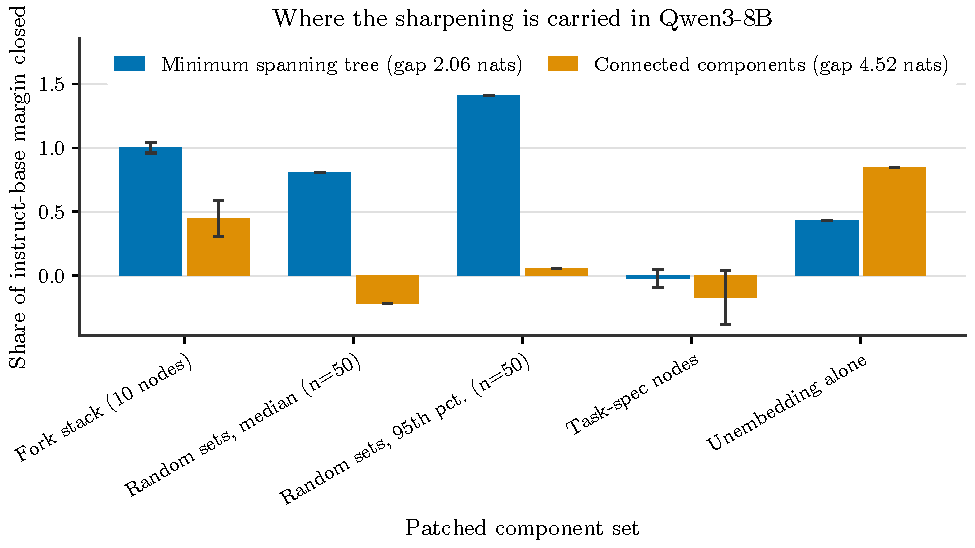
\includegraphics[width=\linewidth,height=0.78\textheight,keepaspectratio]{figures/fig_base_b2_shares_v0.pdf}
\caption{Share of the instruct-minus-base fork margin closed in Qwen3-8B when base-model activity is patched in at the fork, for minimum spanning tree weight (blue, gap 2.06 nats) and connected components (orange, gap 4.52 nats), 20 prompts per task. Bars show, left to right: the ten validated fork-stack nodes; the median and 95th percentile of 50 write-norm-matched random sets of late-layer components; the task-specification nodes; and the instruct model's unembedding applied to the base model's own final residual (a CPU readout decomposition). Error bars are bootstrap 95\textbackslash{}\% confidence intervals over the 20 prompts, shown for the fork-stack and task-specification bars, the only two conditions with a reported interval; the random-set and unembedding bars are point estimates. On minimum spanning tree, random component sets close nearly as much of the gap as the fork stack (median 0.81 and 95th percentile 1.41, against 1.00), so the stack is not specific there; on connected components most of the gap is closed by the unembedding alone (0.85) rather than by the fork stack (0.45) or by random sets (median -0.22). Task-specification nodes close essentially none of the gap on either task. This localization is partial, not clean: on connected components the fork-stack share is a ratio of means sensitive to a few prompts (the mean of per-prompt shares is 0.13, not 0.45, and is negative on 6 of 20 prompts), and most of the matched random sets on connected components turned out to repeat a component rather than draw ten distinct ones.}
\label{fig:fig_base_b2_shares}
\end{figure}
\textbf{Does a one-token patch change the written program?} On 30 slots of common random numbers per arm (five templates, six seeds each; T 1; the instruct model's own opening prefilled), the arms differ only at the fork token, and every later token is sampled from the unpatched instruct model (Table 442). On minimum spanning tree, patching the fork stack turns 19 of 30 programs into correct Prim against 0 of 30 for the twin (19:0 discordant, exact McNemar p 3.8e-6, Holm 1.1e-5). The median matched random set does exactly as well (19 of 30; 2:2, p 1). Splicing the base model's whole fork distribution (Fork-Patched Decoding [142]) gives 18 Prim, 17 of them correct. On connected components the fork stack changes nothing (29 union-find and 1 DFS, as committed for a 0.45 share of a 4.5-nat gap), and only Fork-Patched Decoding brings back the base model's alternative (18 DFS against 1; 18:1, p 7.6e-5). The algorithm shares observed in each arm match the shares predicted from the patched fork distribution within a mean absolute error of 0.005 to 0.069; pass rates are 29 or 30 of 30 in every arm, and no correct program is labelled other (none novel; rule-of-three bound 3 of 237).

\begin{table}[H]
\renewcommand{\thetable}{442}
\centering\small\setlength{\tabcolsep}{4.0pt}
\caption{Programs written after a one-token intervention at the fork (Qwen3-8B; 30 slots of common random numbers per arm; correct programs of the minority algorithm in bold). [Source: iteration 9, artifact \nolinkurl{gen_art_experiment_50}.]}\label{tab:t472}
\begin{tabular}{>{\raggedright\arraybackslash\hspace{0pt}}p{0.2520\linewidth}>{\raggedright\arraybackslash\hspace{0pt}}p{0.1957\linewidth}>{\raggedright\arraybackslash\hspace{0pt}}p{0.1834\linewidth}>{\raggedright\arraybackslash\hspace{0pt}}p{0.2986\linewidth}}
\toprule
\textbf{Arm (fork token drawn from)} & \textbf{Minimum spanning tree: Kruskal \slash{} \textbf{Prim}} & \textbf{Connected components: union-find \slash{} \textbf{DFS}} & \textbf{Predicted minority share (minimum spanning tree \slash{} connected components)} \\
\midrule
Twin (instruct) & 29 \slash{} \textbf{0} (1 disputed) & 29 \slash{} \textbf{1} & 0.19 \slash{} 0.03 \\
Fork stack patched with base outputs & 8 \slash{} \textbf{19} (3 disputed) & 29 \slash{} \textbf{1} & 0.66 \slash{} 0.06 \\
Median matched random set & 10 \slash{} \textbf{19} & 29 \slash{} \textbf{0} (1 invalid) & 0.59 \slash{} 0.00 \\
Base logits at the fork (Fork-Patched Decoding) & 9 \slash{} \textbf{18} (17 correct) & 12 \slash{} \textbf{18} & 0.63 \slash{} 0.46 \\
\bottomrule
\end{tabular}
\end{table}

The twin shows 0 of 30 Prim against a predicted 0.19 because only 2 of the 30 shared fork uniforms exceed 0.81 (5.7 expected) and the instruct model's cumulative distribution lists ' Kr' before ' Prim'; since the uniforms are shared across arms, every contrast is paired on the same draws.

\textbf{The held-out rerun.} The rerun confirmed the cache bug: the original lookup returns nothing for every condition-span node on every held-out prompt of the forced-Prim contrast, so iteration 8's held-out arm applied no edit. With span means interpolated to the target span length, the layer-0 condition-span MLP has a held-out effect of about 7.9 nats on the five forced prompts (7.90 under ablation, 7.65 under steering at dose 2), close to its pair-prompt values (8.14 and 7.41, each the mean over both sides of the 20 pair prompts), and about 0 on the five padded twins (-0.19 and 0.05), unlike the pair prompts, where both sides carry the effect (ablation 8.68 forced and 7.61 padded); the means of 3.86 (sign-flip p 0.0625) and 3.85 (p 0.023) over the 10 held-out prompts average the two sides (iteration-10 correction). Taken as five contrasts, the exact sign-flip test has 32 equally likely patterns, so its smallest attainable p is 0.031 one-sided and 0.0625 two-sided; all five contrasts are positive under both modes, which gives exactly those values, so five contrasts cannot reach two-sided 0.05. On the F11 and F15 rows 153 of the 765 edit jobs of each row (612 of 3,060) were empty, all in the exact-length sensitivity variant, whose ablation mean is 3.50 with those rows and 5.83 without them; the primary interpolated variant applied every edit. The matched random set holds 10 distinct components among its 50 draws. Holm-adjusted within the six-test family the p-values are 0.22 and 0.12. The layer-5 condition MLP reverses sign (-1.50, p 0.008), and dose 0.5 shows nothing (post hoc). The engine reproduces iteration 8's pair-prompt value only to 0.096 nats (8.387 against 8.291), because the circuit artifact's engine was modified after its validation rows were written; its clean margins reproduce exactly, so token ids and positions are right. Matched in kind between the families, the committed motif statistic still differs on the condition share: on natural contrasts Qwen3-8B gives condition 0.08 and fork 0.34 against Gemma's 0.37 and 0.51, and on forced contrasts 0.01 and 0.62 against 0.34 and 0.54.

\textbf{Deviations, not run and positioning.} An engine check against iteration 8 misses by 0.05 on some templates, because iteration 8 ran on a different GPU. The first patching pass used variable batch shapes and was replaced by a fixed-shape rerun, kept as a sensitivity. The self-patch placebo reaches 0.15 nats (head writes cached in bf16) against a 0.02 target. Llama's shortest-path unit, the optional grid and shortest-path patching units, patching in Gemma and token maps for unmapped base fork tokens were not run. That post-training shifts concentrate at forks of high base entropy is shown by Cantarero et al. [142] and by Sparse but Critical [143], and sharpening of what the base model already ranks high is the mechanism Huang et al. formalise [153]. What this experiment adds is the algorithm-level outcome on code at counterfactually located forks, and which validated components carry the sharpening: late MLPs and the unembedding, not the task-specification nodes.

\FloatBarrier
\subsection*{9.6 Planned but not run}
\addcontentsline{toc}{subsection}{9.6 Planned but not run}
Three directions of the iteration-9 strategy never produced an artifact. Each was lost at the execution step (gen\_\allowbreak{}art), which returned no artifact for its plan, so none says anything about the hypothesis: each is untested and still open, and this report records no result, null or dead end for any of them.

\begin{itemize}
\item \emph{The second task} (TP-W): the names-against-mechanisms test on weighted shortest path, the inspiration repository's task, with a ban of each model's own top five (filled from Dijkstra, Bellman-Ford\slash{}SPFA, bidirectional Dijkstra, Floyd-Warshall, Dial's buckets and A* with a zero heuristic) on Qwen3-32B and Qwen3-14B with thinking and Qwen3-8B without, a relaxation-order tracer gated like the grid tracer, and a name-free program manifold of the shortest path catalogue. Lost at gen\_\allowbreak{}art; no artifact.
\item \emph{Discovery on online bin packing} (NOV-B): an evaluator-guided island search with Qwen3-8B as mutator in FunSearch's priority-function setting, comparing at matched calls temperature 1.0, temperature 1.6, branching at the decision token, the same branching at a random position and an instruction to differ from both parents, scored on held-out instances against best fit and published discovered heuristics. Lost at gen\_\allowbreak{}art; no artifact. Before the failure the harness was built and passed its gate (iteration-10 correction): G-HARNESS PASS, with best fit at 5.37\% excess on OR3 and 3.98\% on Weibull 5k reproduced, FunSearch's published heuristics at 3.11\% and 0.68\%, and the priority-form first, best and worst fit equal to the hand-coded packers; iteration 10's evaluator search reuses it, and no search ran in iteration 9.
\item \emph{The replication on constructive TSP} (NOV-T): the same arms on a next-city heuristic, fixed in advance so that the operator contrast is not chosen after seeing bin packing. Lost at gen\_\allowbreak{}art; no artifact.
\end{itemize}

\FloatBarrier
\subsection*{9.7 Comparisons across this iteration's experiments}
\addcontentsline{toc}{subsection}{9.7 Comparisons across this iteration's experiments}
\textbf{The top-five question, read by mechanism and by geometry.} The rename experiment and the geometry experiment answer the request's edge-or-opposite question from two sides (Table 443). By expansion order, the survivors of the full five-name ban are a mixture. Unit-weight Dijkstra, 0.30 of the hand-read survivors and all of iteration 8's catalogue survivors, is BFS order under a non-banned name and container. The other 0.70 are known algorithms with a different expansion discipline. By geometry, unit-weight Dijkstra sits opposite the banned five on every manifold built from language, including the one that avoids names and still evokes them, and at the edge on the manifold built from the programs. For that one algorithm the account's prediction, opposite in names and at the edge in mechanisms, holds. Two limits apply. The program manifold tracks surface and length as strongly as behaviour, and the geometry experiment's verdict placed only the 15 unit-weight Dijkstra survivors. Its placement file also places 23 further iteration-8 survivors (iteration-10 correction): the 15 Bellman-Ford\slash{}SPFA programs land opposite on both gate-passing Qwen3-32B frames (15 of 15 and 15 of 15) and 10 edge, 5 opposite on Qwen3-8B, while the 3 BFS variants and the 5 other known programs place at the edge on the primary frames; 'opposite' there means farther than the median of two reference classes, and the placement was not preregistered (Table 438). The coordinate-key heaps have no landing yet.

\begin{table}[H]
\renewcommand{\thetable}{443}
\centering\small\setlength{\tabcolsep}{4.0pt}
\caption{The top-five prohibition across this iteration's instruments (iteration-10 correction). [Source: iteration 9, compiled across the iteration's artifacts \nolinkurl{gen_art_evaluation_8}, \nolinkurl{gen_art_experiment_45}, \nolinkurl{gen_art_experiment_46}, \nolinkurl{gen_art_experiment_50}.]}\label{tab:t473}
\begin{tabular}{>{\raggedright\arraybackslash\hspace{0pt}}p{0.1302\linewidth}>{\raggedright\arraybackslash\hspace{0pt}}p{0.4061\linewidth}>{\raggedright\arraybackslash\hspace{0pt}}p{0.4100\linewidth}}
\toprule
\textbf{Question} & \textbf{Rename experiment} & \textbf{Geometry experiment} \\
\midrule
Are bans obeyed by name more than by mechanism? & Yes across ten configurations (gap 0.70 runtime, 0.61 tracer; descriptive) & n\slash{}a \\
Is the gap a property of exhaustion? & By the runtime label mechanistic compliance falls from 1.00 at one name to 0.22 and 0.10 at five; by hand reads to 0.59 and 0.12; by the tracer to 0.67 and 0.24 (fine 0.74 and 0.37); lexical compliance stays at or above 0.86 & n\slash{}a \\
What do the obeying model's survivors run? & Hand reads: 0.30 BFS order (unit-weight Dijkstra), 0.70 other known disciplines; the instruments disagree (0.79 runtime, 0.43 tracer, on the 91 survivors) & n\slash{}a \\
Where does unit-weight Dijkstra land? & n\slash{}a & Opposite on the named (1.63), name-only (1.20) and described (1.08) manifolds; edge on the program manifold (0.67); 15 of 15 survivors edge by placement on the primary frame, 10 of 15 on the Qwen3-32B programs-only frame; Bellman-Ford\slash{}SPFA survivors opposite on both gate-passing Qwen3-32B frames \\
What does each map track? & n\slash{}a & Language manifolds: lexical distance and data-structure attributes; program manifold: behaviour, surface and length alike \\
\bottomrule
\end{tabular}
\end{table}

\textbf{Sharpening and the circuit.} The base-model experiment and the record audit bear on the same nodes. Iteration 8's circuit found a late stack of fork-position MLPs and heads; the patching test shows that this stack also carries most of the base-to-instruct difference on minimum spanning tree, but so do random late-layer sets, as in iteration 8's steering at dose 2, where the matched random five also flipped the algorithm. Specificity fails at the same place under three methods: steering, DAS and now patching. The layer-0 condition-span node, repaired, holds out at about 7.9 nats on the five forced prompts, close to its pair-prompt values, and about 0 on the five padded twins (its mean of 3.86 averages the two sides) (iteration-10 correction), without surviving its family's Holm adjustment, and the motif comparison still reads a different condition share when the contrasts are matched in kind.

\FloatBarrier
\subsection*{9.8 What iteration 9 established, what it ruled out, and what it abandoned}
\addcontentsline{toc}{subsection}{9.8 What iteration 9 established, what it ruled out, and what it abandoned}
\begin{table}[H]
\renewcommand{\thetable}{444}
\centering\small\setlength{\tabcolsep}{4.0pt}
\caption{Verdicts of the claims of iteration 9 (iteration-10 correction). [Source: iteration 9, compiled across the iteration's artifacts \nolinkurl{gen_art_evaluation_8}, \nolinkurl{gen_art_experiment_45}, \nolinkurl{gen_art_experiment_46}, \nolinkurl{gen_art_experiment_50}.]}\label{tab:t474}
\begin{tabular}{>{\raggedright\arraybackslash\hspace{0pt}}p{0.1303\linewidth}>{\raggedright\arraybackslash\hspace{0pt}}p{0.1453\linewidth}>{\raggedright\arraybackslash\hspace{0pt}}p{0.6706\linewidth}}
\toprule
\textbf{Claim} & \textbf{Committed verdict} & \textbf{Deciding evidence} \\
\midrule
Rename gap (primary) & Bars met; descriptive (tracer gate failed) & Pooled gap 0.70 (0.57 to 0.82) runtime, 0.61 (0.45 to 0.76) tracer; positive in 10 of 10 configurations under both; reasoning names a banned alias in 0.91 to 1.00 of covert programs \\
Survivor reading (primary) & Instruments disagree; descriptive & 0.79 (runtime), 0.43 (tracer) of 91 survivors in a banned class against a 0.6 bar and a 0.6 null; hand reads of 76 survivors 0.30, at the disconfirming bar, all unit-weight Dijkstra \\
Exhaustion curve (primary) & Bars met in both models by the runtime label; reading-dependent; descriptive & By the runtime label mechanistic compliance 1.00 to 0.22 (Qwen3-32B) and 1.00 to 0.10 (Qwen3-14B), trend p 0.00001; lexical at or above 0.86; held-out gaps 0.56 and 0.68. By reading: Qwen3-14B meets the bars under every reading except the tracer's fine classes on held-out templates (0.38); Qwen3-32B meets them only by the runtime label (k = 5 gaps: hand reads 0.30, tracer 0.22, tracer fine 0.15), and its tracer curve is not monotone \\
Name-free landing (primary) & MIXED (the committed outcome for a split) & Edge on the program manifold (0.67; robust to source and readout; 15 of 15 survivors edge on the primary frame, 10 of 15 on the programs-only frame), opposite on the described (1.08), name-only (1.20) and named (1.63) manifolds; the named manifold's reproduction gate failed (0.894) \\
Rotated sets (secondary) & Disconfirmed & Joint sign in 3 of 7 sets (p 0.24) \\
Second task (secondary) & Not run & Lost at gen\_\allowbreak{}art \\
Discovery with an evaluator (secondary) & Not run & Lost at gen\_\allowbreak{}art (bin packing and TSP) \\
Sharpening measurement (secondary) & Partial & Gemma grid gain 1.78 nats with the argmax different on 20 of 20; phrasing entropy change at most 0.50; fork divergence 0.75 to 1.18 times entropy-matched positions; Llama descriptive \\
Patching test (secondary) & Partial; distributed & Fork stack 1.00 on minimum spanning tree but random sets 0.81 (p 0.45); 0.45 on connected components (p 0.020 against random); task-specification nodes about 0; unembedding 0.43 and 0.85 \\
Held-out rerun (secondary) & Reported & Layer-0 node about 7.9 nats on the five forced prompts, close to its pair-prompt values, and about 0 on the five padded twins; the mean of 3.86 averages the two sides (3.85 steering; p 0.0625 and 0.023; Holm 0.22 and 0.12; five contrasts give p 0.031 one-sided, the floor); motif still differs on condition share \\
Record repair & Done & 49 corrections; every review item answered in place; 400 checks, 0 mismatches \\
\bottomrule
\end{tabular}
\end{table}

\textbf{Established.} A ban of five path-algorithm names is obeyed by name far more often than by expansion order. The gap is 0.70 pooled over ten configurations with the runtime label and 0.61 with the tracer, positive in every configuration, and in the three configurations with reasoning nearly every covert program comes with reasoning that names a banned algorithm (descriptive, because the tracer failed its gold gate). Under cumulative bans lexical compliance stays at or above 0.86, and mechanistic compliance at five names depends on the reading (iteration-10 correction): by the runtime label it falls from 1.00 at one name to 0.22 (Qwen3-32B) and 0.10 (Qwen3-14B); by hand reads to 0.59 and 0.12; by the tracer to 0.67 and 0.24 (fine classes 0.74 and 0.37). Banning one name changes the mechanism; banning the whole repertoire is answered by renaming in Qwen3-14B under every reading except the fine tracer on held-out templates, while Qwen3-32B moves mostly to other known disciplines. A ban described without names changes mechanistic compliance by an instrument-dependent amount (+0.58 by the runtime label, -0.07 by the tracer, about +0.21 under the per-cell reading; exploratory). By hand reads the survivors of the obeying models are mostly not renamed BFS: 0.30 are unit-weight Dijkstra (BFS order under another name) and 0.70 are known algorithms with other expansion disciplines (grid Bellman-Ford, coordinate-key heaps, random frontiers); judges' names are unreliable for exactly these programs, and the instruments disagree on them (by the runtime label 0.79 and by the tracer 0.43 of Qwen3-32B's 91 name-level survivors are in a banned class). On manifolds built from text, unit-weight Dijkstra lies opposite the banned five, and on the manifold built from its name-scrubbed programs it lies at the edge, robust to the program source and the readout; its 15 survivors place at the edge on the primary frames (15 of 15) and 10 of 15 on the Qwen3-32B programs-only frame, while the 15 Bellman-Ford\slash{}SPFA survivors place opposite on both gate-passing Qwen3-32B frames ('opposite' relative to the median of two reference classes; not preregistered). The language manifolds track lexical distance and textbook data-structure attributes, not measured expansion order; the program manifold tracks behaviour, surface and length together. Post-training sharpened Gemma's grid fork by 1.78 nats and reversed and concentrated the base model's preference there (20 of 20 prompts; base P(BFS) 0.25, 0.663 of base mass unmapped); in Qwen3-8B the sharpening is not written upstream of the fork but by late MLPs and, for most of the connected-components gap, by the unembedding.

\textbf{Ruled out.} The prediction that unit-weight Dijkstra lands at the edge on a name-free manifold of descriptions: the described manifold reads opposite, and it evokes the names (balanced accuracy 0.69 from a probe trained on named prompts). The robust-opposite outcome, in which the survivors land opposite on both name-free manifolds: the program manifold reads edge. The rotated-set prediction (3 of 7). A fork-stack specificity for the sharpening on minimum spanning tree (random late-layer sets close 0.81).

\textbf{Dead ends.} The expansion-order tracer, after two revision rounds, cannot classify LLM-written iterative deepening, IDA* and jump point search (0 of 34, 1 of 22 and 1 of 7 gold programs), so any order-based test on those classes needs a different instrument. A name distance between aliases is degenerate on this catalogue (1 for 72 of 100 cells), so rotated sets cannot be chosen to separate name from mechanism. Llama-3.1-8B's base model cannot be compared under the chat template, whose special-token embeddings are untrained.

\textbf{Not run.} The second task, discovery with an evaluator on bin packing, and its TSP replication (Section 9.6); within the run artifacts, the Qwen3-235B scale cell, the Qwen3-8B name-only manifold and the patching of Gemma.

\FloatBarrier
\subsection*{9.9 What the last iteration takes from this one}
\addcontentsline{toc}{subsection}{9.9 What the last iteration takes from this one}
Iteration 10 is the last. Three leads remain from this one. First, the edge-or-opposite answer is now split by the kind of map: opposite on every manifold built from language, at the edge on the manifold built from programs, for the one survivor algorithm that is a banned mechanism under another name. Two steps would make it decisive. One is a program manifold whose classes can be separated from surface and length, with more non-banned algorithms above the floor. The other is placing the remaining survivor families (iteration-10 correction): the record's placement file already places iteration 8's grid Bellman-Ford\slash{}SPFA survivors, which land opposite on both gate-passing Qwen3-32B frames (15 of 15; 'opposite' is relative to the median of the two non-banned reference classes, and the placement was not preregistered), while the unit-weight Dijkstra survivors place at the edge (15 of 15 on the primary frames, 10 of 15 on the programs-only frame); the coordinate-key heaps have no landing yet, and TP-G2's preregistered placements address both. Second, the names-against-mechanisms numbers are descriptive because the tracer failed on iterative deepening; an instrument that reads those programs would turn the strongest behavioural finding of this iteration into a test. Third, the request's ``truly novel'' question has still not met the one route left untried, an evaluator-guided search on a task with a measurable score; the bin-packing and TSP plans were lost before they ran, so the question stays open, not answered; the bin-packing harness had been built and had passed its gate before the loss (best fit 5.37\% and 3.98\% excess reproduced; FunSearch's heuristics 3.11\% and 0.68\%), iteration 10's evaluator search reuses it, and no search ran in iteration 9 (iteration-10 correction). The sharpening reading can be stated for Qwen3-8B and Gemma at the fork, with Llama descriptive and the base-entropy confound of Cantarero et al. carried, and does not need another experiment to be written up.

\FloatBarrier
\section{Iteration 10: an evaluator-guided search for new bin-packing and TSP heuristics, prohibition with an exact instrument, discipline against container on the program map, the weights that hold the default, and the record repaired}
\noindent\emph{Run record for this iteration.} Hypothesis carried: ``Knobs Reweight Ideas; Search Only Recombines''. Move recorded at the end of the iteration: declare; review score 5; evidence state lead; coverage partial; 12 candidate strategies considered. The list below gives the iteration's artifacts and the state the round record gave each strand.

{\footnotesize\setlength{\tabcolsep}{3pt}
\begin{longtable}{>{\raggedright\arraybackslash}p{0.24\linewidth}>{\raggedright\arraybackslash}p{0.47\linewidth}>{\raggedright\arraybackslash}p{0.11\linewidth}>{\raggedright\arraybackslash}p{0.08\linewidth}}
\caption*{\textbf{Artifacts of iteration 10.} Names and titles as the artifact workspaces record them; strand state as the round record grades it.}\label{tab:arts10}\\
\toprule \textbf{Artifact} & \textbf{Title} & \textbf{Type} & \textbf{State} \\ \midrule \endfirsthead
\toprule \textbf{Artifact} & \textbf{Title} & \textbf{Type} & \textbf{State} \\ \midrule \endhead
\bottomrule \endlastfoot
\nolinkurl{gen_art_experiment_51} & LLM search for new bin-packing rules & experiment & lead \\
\nolinkurl{gen_art_experiment_52} & Can guided LLM search invent bin-packing rules? (run 2) & experiment & lead \\
\nolinkurl{gen_art_experiment_53} & Token forcing vs temperature in LLM search for TSP heuristics & experiment & null \\
\nolinkurl{gen_art_experiment_54} & Do banned bin-packing rules come back renamed? & experiment & lead \\
\nolinkurl{gen_art_experiment_55} & Do code-model maps track search order or storage? & experiment & lead \\
\nolinkurl{gen_art_experiment_56} & Which weights make the model pick one algorithm & experiment & lead \\
\nolinkurl{gen_art_evaluation_9} & Correcting last round's report from raw data & evaluation & null \\
\end{longtable}}

\subsection*{What each artifact of iteration 10 was for and what it produced}
\addcontentsline{toc}{subsection}{What each artifact of iteration 10 was for and what it produced}
Each artifact is named below as the run's workspaces name it. The entry gives the round record's verdict on the strand it served, the artifact's own summary of what it was for and what it produced, and the output files it declared, each opened and read from its workspace for this report. It closes with the subsection of this section that reports the artifact's results and the result tables typeset there from its output files.

\paragraph{\nolinkurl{gen_art_experiment_51}: LLM search for new bin-packing rules.}
Type: experiment. Round record, strand state lead: Evaluator beats best fit held-out (T1.6 1.40\slash{}3.55\% vs 3.98\slash{}5.37\%; no selection never) but FunSearch-predicted; DTB\slash{}T1.6 1.20\textless{}1.5; 4 ablatable 'novel' programs keep gain without the term.

\emph{The artifact's own summary of what it was for and what it produced:} NOV-B1: FunSearch-style island search on online bin packing with Qwen3-8B-FP8 (vLLM 0.11, thinking off) as mutator, evaluated by the iteration-9 FunSearch harness (copied, sha256-verified, re-gated: G-HARNESS PASS, BF 5.37\% OR3 \slash{} 3.98\% Weibull 5k, c12 3.11\%, c14 0.68\%, gate block identical to BP9). Arms at matched calls (C*=2,000 per arm and seed, seeds 0-1, lockstep lag-1 rounds of 25): T1.0, T1.6 (top-p 0.95), DTB (force a rank 2-8 token at the highest-entropy code token of the first 48), RPB (random-position placebo), IDEA (one-sentence 'different idea' instruction); NS (no selection, 1,000 per seed) afterwards. Everything hash-committed (6 commits, hash chain). Results: V1 SUPPORTED - every core arm's best program beats 0.8x best fit on both primary held-out sets (FSW5k\slash{}OR3 excess \%: T1.0 1.53\slash{}3.55, T1.6 1.40\slash{}3.55, DTB 2.43\slash{}4.18, RPB 1.73\slash{}3.48; IDEA 1.85\slash{}3.38; NS stays at best fit 3.98\slash{}5.37; tuned ab baseline abFF(5,22) 2.14\slash{}3.06; c12 3.03\slash{}3.11). V2 PARTIAL - behaviour clusters (complete linkage, all pairs agree \textgreater{}=0.95 on 2,000 probe states) over 4,000 calls: T1.0 148, T1.6 373, DTB 446, RPB 212, IDEA 770; R1 (DTB\slash{}T1.0)=3.01 [2.66,3.43], R2 (DTB\slash{}T1.6)=1.20 [1.13,1.33] \textless{} 1.5, R3 (DTB\slash{}RPB)=2.10; DTB's best is the weakest on held-out; per-token and rarefied ratios agree (R2 1.08\slash{}1.15); 200 label shuffles never reach R1\textgreater{}=1.5. V3 - 211 candidates, 70 pass both held-out bars with max corpus agreement \textless{}0.9 (86-entry corpus: textbook, Sum-of-Squares, FunSearch, EoH x60, ReEvo, HSEvo, MCTS-AHD, LLM4AD, ab family + tuned ab; also all 3,843 ab-grid points), 53 joint clusters, 30 audited. Judge gate unmet (mistral 9\slash{}10, deepseek 5\slash{}10, kimi 6\slash{}10), so the arm-blind manual read decides: 22 reduce to the known ab principle (tight fit else avoid medium leftovers, b tied to item size); 8 NOVEL (gate-passing judge agrees 8\slash{}8, advisory majority 5\slash{}8), all one idea family: prefer a leftover that is a whole multiple of the item size (T1.0 2, DTB 4, IDEA 2; caveats: the 0.9 probe filter did no work - positive control 70-\textgreater{}70; one novel program is stochastic; no ablation of the modular term). V5 (descriptive): reversion at birth tokens 0.40 vs controls 0.36, sign test p=0.49. V6 PARTIAL: rename rate IDEA 0.44 vs T1.0 0.86. Evaluator effect: NS never beats best fit. Provides method\_\allowbreak{}out.json (exp\_\allowbreak{}gen\_\allowbreak{}sol\_\allowbreak{}out: every call with code\slash{}F\slash{}cluster, best programs, V3 candidates, corpus, V5), results\slash{}*.json, figures F1-F8, data\slash{}main and data\slash{}ns raw rows and decision vectors, audit\slash{}rederive.py. OpenRouter spend \$0.14.

Its results are reported in Subsections 10.3, 10.6 of this report, which typeset the result tables drawn from its output files: Tables 447, 448, 449, 450, 451, 459.

\begin{table}[H]
\renewcommand{\thetable}{O68}
\centering\footnotesize\setlength{\tabcolsep}{3pt}
\caption{Output files declared by \nolinkurl{gen_art_experiment_51} (iteration 10), each opened and read from the artifact's workspace for this report; size in bytes. [Source: iteration 10, artifact \nolinkurl{gen_art_experiment_51}.]}
\begin{tabular}{>{\raggedright\arraybackslash}p{0.25\linewidth}>{\raggedleft\arraybackslash}p{0.12\linewidth}>{\raggedright\arraybackslash}p{0.57\linewidth}}
\toprule
\textbf{Declared file} & \textbf{Bytes} & \textbf{What it holds} \\
\midrule
\texttt{method.\allowbreak{}py} & 4,057 & the artifact's code, 77 lines \\
\texttt{full\_\allowbreak{}method\_\allowbreak{}out.\allowbreak{}json} & 56,561,284 & the complete output; metadata with 22 top-level keys; 5 datasets with 22,537 examples in all: novb1\_\allowbreak{}search\_\allowbreak{}programs (22,000), novb1\_\allowbreak{}best\_\allowbreak{}programs (12), novb1\_\allowbreak{}v3\_\allowbreak{}candidates (211), novb1\_\allowbreak{}corpus (86), novb1\_\allowbreak{}v5 (228) \\
\texttt{mini\_\allowbreak{}method\_\allowbreak{}out.\allowbreak{}json} & 333,609 & small variant of the full output (a few examples per dataset); metadata with 22 top-level keys; 5 datasets \\
\texttt{preview\_\allowbreak{}method\_\allowbreak{}out.\allowbreak{}json} & 78,793 & preview variant of the full output (truncated strings and lists); metadata with 22 top-level keys; 3 datasets \\
\texttt{reproducibility.\allowbreak{}md} & 7,283 & reproducibility notes, 87 lines \\
\bottomrule
\end{tabular}
\end{table}

\paragraph{\nolinkurl{gen_art_experiment_52}: Can guided LLM search invent bin-packing rules? (run 2).}
Type: experiment. Round record, strand state lead: 0\slash{}40 novel; DTB\slash{}RPB 0.74 (0.61 without stochastic): entropy targeting adds nothing; 17.8x over T1.0 only because temperature copies parents; birth tokens .50 vs .26 (p .0086).

\emph{The artifact's own summary of what it was for and what it produced:} NOV-B2 is the pre-registered, independently implemented replication (seeds 2 and 3) of a FunSearch-style island search on online bin packing with Qwen3-8B-FP8 (vLLM 0.11, thinking off) as the mutator, plus an exploratory, separately pre-registered extension on seeds 4 and 5. Harness: FunSearch's exact priority harness, sha256-verified and re-gated (BF 5.37\%\slash{}3.98\%, c12 3.11\%, c14 0.68\% reproduced). Arms at matched calls (C* = 2000 per arm-seed, committed rule): T1.0; T1.6 with top-p 0.95; DTB (force a rank-2..8 token at the highest-entropy eligible position of the first 48 body tokens); RPB (same forcing at a random position, placebo); IDEA (instruction to use a different idea); NS (fixed FF\slash{}BF parents). Selection on SEL-OR+SEL-W; held-out H-FSW5k and H-OR3 (primary) plus 6 sets. Behaviour = bin choices on 2,000 committed probe states; clusters by complete linkage at 0.95; novelty = agreement \textless{} 0.9 with 82 corpus programs (FunSearch, EoH, HSEvo, MCTS-AHD, ReEvo, LLM4AD, RAISE, textbook, dependency scan) and all 3,843 ab-family members, then gated judges and an arm-blind manual read. Verdicts (seeds 2-3, all re-derived by a separate stdlib audit): V1 PARTIAL - best-program held-out excess H-FSW5k\slash{}H-OR3: DTB 2.395\slash{}3.852\%, RPB 1.720\slash{}3.703\%, IDEA 2.133\slash{}3.554\% pass the 0.8xBF rule; T1.0 3.672\slash{}4.821\% and T1.6 (= BF) fail. V2 PARTIAL - behaviour clusters per 2,000 calls (seed 2\slash{}3): DTB 230\slash{}143, RPB 269\slash{}233, IDEA 134\slash{}150, T1.0 13\slash{}8, T1.6 1\slash{}1; R\_\allowbreak{}T1.0 17.8, R\_\allowbreak{}T1.6 186.5, but R\_\allowbreak{}RPB 0.74 \textless{} 1.2; shuffled-arm placebo 0\slash{}200 supported. V3 DISCONFIRMED - 151 candidates, 50 pass the 0.8 rule, 48 also pass the corpus-novelty filter, 0 of 40 judged are NOVEL (all recombine published principles: BF on near-exact fits, an avoided residual band as in ab\slash{}c12, a residual target \textasciitilde{}c*item as in EoH run 3\slash{}MCTS-AHD); rule-of-three bound 7.5\%; no judge passed its 10-control gate (judges advisory). V6 PARTIAL - rename share IDEA 0.670 vs T1.0 0.959. V5 (descriptive, n=30): forcing the argmax back at the offspring's high-entropy deviating token reverts it to a parent in 49.8\% of continuations vs 25.5\% at random positions (sign-flip p=0.0086). Exploratory seeds 4-5: V2 rule SUPPORTED (R\_\allowbreak{}RPB 1.47) but pooled 4-seed R\_\allowbreak{}RPB = 1.08: entropy targeting is within seed noise, while forcing (or the IDEA instruction) beats temperature robustly (pooled R\_\allowbreak{}T1.0 25.5). The tuned ab member ab-FF(5,22) (F 0.740 vs best searched 0.726) beats every arm's best on H-OR3. Provides: method.py + src\slash{} pipeline, 42,000 logged programs with evaluations and decision vectors (data\slash{}), all analyses (results\slash{}), figures F1-F7, commitments.log hash chain, method\_\allowbreak{}out.json (exp\_\allowbreak{}gen\_\allowbreak{}sol\_\allowbreak{}out) with full\slash{}mini\slash{}preview, audit\slash{}rederive.py.

Its results are reported in Subsections 10.4, 10.6 of this report, which typeset the result tables drawn from its output files: Tables 452, 453, 454, 455, 459.

\begin{table}[H]
\renewcommand{\thetable}{O69}
\centering\footnotesize\setlength{\tabcolsep}{3pt}
\caption{Output files declared by \nolinkurl{gen_art_experiment_52} (iteration 10), each opened and read from the artifact's workspace for this report; size in bytes. [Source: iteration 10, artifact \nolinkurl{gen_art_experiment_52}.]}
\begin{tabular}{>{\raggedright\arraybackslash}p{0.25\linewidth}>{\raggedleft\arraybackslash}p{0.12\linewidth}>{\raggedright\arraybackslash}p{0.57\linewidth}}
\toprule
\textbf{Declared file} & \textbf{Bytes} & \textbf{What it holds} \\
\midrule
\texttt{method.\allowbreak{}py} & 5,099 & the artifact's code, 100 lines \\
\texttt{full\_\allowbreak{}method\_\allowbreak{}out.\allowbreak{}json} & 80,089,624 & the complete output; metadata with 29 top-level keys; 6 datasets with 42,285 examples in all: novb2\_\allowbreak{}search\_\allowbreak{}programs (22,000), novb2\_\allowbreak{}extension\_\allowbreak{}programs (20,000), novb2\_\allowbreak{}best\_\allowbreak{}programs (12), novb2\_\allowbreak{}v3\_\allowbreak{}candidates (151), novb2\_\allowbreak{}corpus (82), novb2\_\allowbreak{}v5 (40) \\
\texttt{mini\_\allowbreak{}method\_\allowbreak{}out.\allowbreak{}json} & 147,866 & small variant of the full output (a few examples per dataset); metadata with 29 top-level keys; 6 datasets \\
\texttt{preview\_\allowbreak{}method\_\allowbreak{}out.\allowbreak{}json} & 118,324 & preview variant of the full output (truncated strings and lists); metadata with 29 top-level keys; 3 datasets \\
\texttt{reproducibility.\allowbreak{}md} & 10,698 & reproducibility notes, 132 lines \\
\bottomrule
\end{tabular}
\end{table}

\paragraph{\nolinkurl{gen_art_experiment_53}: Token forcing vs temperature in LLM search for TSP heuristics.}
Type: experiment. Round record, strand state null: Operator kill condition met (DTB\slash{}T1.0 0.96, DTB\slash{}RPB 0.95); bests close 30-42\% of NN gap but none beats the ReEvo\slash{}EoH seed rule (13.67\%); 0\slash{}12 novel.

\emph{The artifact's own summary of what it was for and what it produced:} NOV-T experiment (claim V4): does decision-token branching (DTB: force a rank-2..8 token at the highest-entropy code position of the first 48 body tokens, then continue at T 1) make an LLM program search find more distinct heuristic behaviours than temperature? Task: constructive TSP with the ReEvo\slash{}EoH select\_\allowbreak{}next\_\allowbreak{}node interface; Qwen3-8B-FP8 on vLLM 0.11 (NVIDIA L4) mutates programs in a FunSearch-style 5-island search seeded with nearest neighbour (NN); fitness F normalised to NN on 64 selection instances (n 50\slash{}100) against LKH-3 tours. Arms at matched calls in interleaved rounds: T1.0, T1.6 (top-p 0.95), DTB, RPB (random-position placebo), IDEA, plus NOSEL (no selection); seeds 0 and 1; 1,056 calls per arm-seed (hard stop below the committed C*=2000), 10,812 calls total. Behaviour instrument: next-city decisions on 2,000 frozen probe states, complete-linkage clusters at agreement \textgreater{}= 0.95. RESULTS. V2-T DISCONFIRMED by the pre-registered rule: clusters per 1,000 calls T1.0 228\slash{}234, T1.6 88\slash{}104, DTB 228\slash{}217, RPB 237\slash{}233, IDEA 296\slash{}298 (seed 0\slash{}1); pooled DTB\slash{}T1.0 = 0.963 (kill condition \textless{}= 1.0), DTB\slash{}T1.6 = 2.315 (T1.6 validity 0.31-0.32), DTB\slash{}RPB = 0.948; per-seed DTB\slash{}T1.0 1.00 [0.89,1.14] and 0.93 [0.83,1.02] (round-block bootstrap); no sign reversal in secondary (better-than-NN), per-token, rarefied or pooled-linkage sensitivities. DTB's held-out best is worse than T1.0's (paired +1.2 and +2.7 gap points). V1-T SUPPORTED: every core arm-seed best closes \textgreater{}= 20\% of NN's held-out n=200 gap (NN 23.94\%, bar 19.15\%; bests 13.98-16.68\%), confirmed on 96 extra n=200 instances and 13 TSPLIB optima. Comparators on the same instances: ReEvo\slash{}EoH seed rule 13.67\% (no searched program beats it), MCTS-AHD appendix heuristics 14.01-20.82\%, tuned parametric P1 17.35\%, NOSEL best-of-252 27.87\%, farthest insertion 8.65\% (other interface). IDEA gave the most clusters and a 6\% parent-rename rate (T1.0 18-22\%). V3-T: 32 candidates beat 0.8xNN and agree \textless{} 0.90 with every corpus member; judges failed their gates (8\slash{}10, 5\slash{}10); manual read: 12\slash{}12 read are KNOWN FAMILY, NEW PARAMETERS, 0 novel. AUDIT: audit\slash{}rederive.py (stdlib, separate code path) reproduces all 10 cluster counts exactly, the ratios, G200 means and both verdicts; its placebos (shuffled arm labels, DTB\slash{}T1.0 swap, thresholds, NN replaced) fail as required; 50\slash{}50 logged forcings re-derived. Pre-registration: COMMIT \#1 (protocol, predictions, code) before the first search call, COMMIT \#2 (C*), COMMIT \#3 (corpus), hash-chained in commitments.log. FILES: method\_\allowbreak{}out.json \slash{} full\_\allowbreak{}, mini\_\allowbreak{}, preview\_\allowbreak{} (exp\_\allowbreak{}gen\_\allowbreak{}sol\_\allowbreak{}out: novt\_\allowbreak{}calls one row per call with DTB\slash{}RPB fields, novt\_\allowbreak{}best held-out bests vs NN\slash{}P1\slash{}T1.0\slash{}T1.6, novt\_\allowbreak{}clusters), results\slash{}\emph{.json (verdict\_\allowbreak{}v1, verdict\_\allowbreak{}v2, clusters, heldout, corpus, v3, judges, rederive, deviations), figures F1-F6, data\slash{}calls.jsonl (all programs and scores), data\slash{}requests\slash{} (raw top-20 log probs), data\slash{}probe\_\allowbreak{}decisions.bin. Deviations: L4 instead of A4500, torch.compile engine mode, C} not reached at the hard stop, title-level positioning only (results\slash{}deviations.json).

Its results are reported in Subsections 10.5, 10.6 of this report, which typeset the result tables drawn from its output files: Tables 456, 457, 458, 459.

\begin{table}[H]
\renewcommand{\thetable}{O70}
\centering\footnotesize\setlength{\tabcolsep}{3pt}
\caption{Output files declared by \nolinkurl{gen_art_experiment_53} (iteration 10), each opened and read from the artifact's workspace for this report; size in bytes. [Source: iteration 10, artifact \nolinkurl{gen_art_experiment_53}.]}
\begin{tabular}{>{\raggedright\arraybackslash}p{0.25\linewidth}>{\raggedleft\arraybackslash}p{0.12\linewidth}>{\raggedright\arraybackslash}p{0.57\linewidth}}
\toprule
\textbf{Declared file} & \textbf{Bytes} & \textbf{What it holds} \\
\midrule
\texttt{method.\allowbreak{}py} & 3,746 & the artifact's code, 79 lines \\
\texttt{full\_\allowbreak{}method\_\allowbreak{}out.\allowbreak{}json} & 29,630,671 & the complete output; metadata with 20 top-level keys; 3 datasets with 10,851 examples in all: novt\_\allowbreak{}calls (10,812), novt\_\allowbreak{}best (29), novt\_\allowbreak{}clusters (10) \\
\texttt{mini\_\allowbreak{}method\_\allowbreak{}out.\allowbreak{}json} & 946,502 & small variant of the full output (a few examples per dataset); metadata with 20 top-level keys; 3 datasets \\
\texttt{preview\_\allowbreak{}method\_\allowbreak{}out.\allowbreak{}json} & 70,683 & preview variant of the full output (truncated strings and lists); metadata with 20 top-level keys; 3 datasets \\
\texttt{reproducibility.\allowbreak{}md} & 6,118 & reproducibility notes, 96 lines \\
\bottomrule
\end{tabular}
\end{table}

\paragraph{\nolinkurl{gen_art_experiment_54}: Do banned bin-packing rules come back renamed?.}
Type: experiment. Round record, strand state lead: Exact instrument: Qwen3-8B k=5 rename gap +0.40 [.21,.55] but +0.08 on held-out templates; thinking models obey (+0.04, -0.13); 0\slash{}1,143 novel and better than best fit.

\emph{The artifact's own summary of what it was for and what it produced:} NOV-R experiment (plan gen\_\allowbreak{}plan\_\allowbreak{}experiment\_\allowbreak{}4\_\allowbreak{}idx4), 1,143 one-shot online bin-packing priority functions in the exact FunSearch interface from Qwen3-8B (no thinking, local vLLM FP8, N 50 per cell), Qwen3-14B and Qwen3-32B (thinking, OpenRouter DeepInfra fp8, N 30 per cell after the reduction ladder). Cells: BASE, cumulative name bans of each model's own top-k textbook rules (NAME\_\allowbreak{}1..5, templates W1-W3), a described ban (DESC\_\allowbreak{}5), held-out templates (HOLD\_\allowbreak{}5), and two novelty instructions (INSTR\_\allowbreak{}NEW, INSTR\_\allowbreak{}LONG). Baseline instrument = lexical compliance L1 (no banned name or abbreviation in the program); proposed instrument = mechanistic compliance (exact-decision agreement \textless{} 0.95 with every banned rule on 2,000 committed probe states, plus a stochastic random-fit matcher), gated beforehand on planted controls (min margin 0.49). Results: P1 PARTIAL. The renaming gap appears only without thinking: Qwen3-8B k = 5 gap L1 0.91 vs mechanistic 0.51, +0.40 [0.21, 0.55] (paired Newcombe), and at k = 1, 14 of 35 lexically clean programs (0.40) are still best fit under another name. Qwen3-14B\slash{}32B really leave the banned rules (mechanistic 0.93-1.00; gaps +0.04 and -0.13, CIs span 0), and their traces name the banned rule in 100\% and self-identify near it in 90-100\%. Under a BF ban Qwen3-32B switches to first fit in 14\slash{}30. JT trend p = 0.54 \slash{} 0.038 (Holm 0.11) \slash{} 0.38; held-out-template gaps are not significant. The verdict is unchanged at thresholds 0.90\slash{}0.98 and on informative states. P2 DISCONFIRMED: only first fit's description passed the naming check (models call the other descriptions 'First Fit Decreasing'), so DESC\_\allowbreak{}5 bans FF only, and compliance is about 1.0 either way. P3 SUPPORTED: 0\slash{}1,143 programs beat best fit on both held-out sets (FunSearch OR3, Weibull 5k); 186 are behaviourally novel vs the 426-member published corpus, but none is better. The novelty instruction 'Make a new algorithm' gives best fit in 28\slash{}29 (14B) and 28\slash{}28 (32B). BASE is almost all best fit for the thinking models (50\slash{}50, 48\slash{}49). Independent stdlib re-derivation (audit\slash{}rederive.py): 0 mismatches across agreements, classes, lexical flags, cell counts, JT, both Newcombe intervals and the verdicts; all 4 placebos fail as required. Files: method\_\allowbreak{}out.json \slash{} full\_\allowbreak{} \slash{} mini\_\allowbreak{} \slash{} preview\_\allowbreak{} (exp\_\allowbreak{}gen\_\allowbreak{}sol\_\allowbreak{}out: novr\_\allowbreak{}samples with predict\_\allowbreak{}mechanism\_\allowbreak{}class, predict\_\allowbreak{}lexical\_\allowbreak{}L1, predict\_\allowbreak{}mechanistic\_\allowbreak{}compliance, predict\_\allowbreak{}valid, predict\_\allowbreak{}better\_\allowbreak{}heldout, predict\_\allowbreak{}novel; novr\_\allowbreak{}cells; novr\_\allowbreak{}instrument; metadata with every analysis), data\slash{}samples.jsonl (shared schema), data\slash{}samples\_\allowbreak{}raw\_\allowbreak{}*.jsonl (responses and reasoning), data\slash{}decisions.jsonl, results\slash{}*.json, figures F1-F6 (including the MDS behaviour map in decision space). Caveats: one model family (Qwen3); the container crashed at 4.2 h and sampling resumed at 5.9 h. A duplicate orchestrator ran for 40 min: 5 duplicate rows were removed, the naming check was rerun cleanly and committed as commit \#3 before the DESC\_\allowbreak{}5 rows it governs, and the commit \#2 payload files of q14\slash{}q32 were overwritten after hashing (chain lines intact; B\_\allowbreak{}k identical in every version). Spend USD 1.42.

Its results are reported in Subsection 10.7 of this report, which typesets the result tables drawn from its output files: Tables 460, 461, 462.

\begin{table}[H]
\renewcommand{\thetable}{O71}
\centering\footnotesize\setlength{\tabcolsep}{3pt}
\caption{Output files declared by \nolinkurl{gen_art_experiment_54} (iteration 10), each opened and read from the artifact's workspace for this report; size in bytes. [Source: iteration 10, artifact \nolinkurl{gen_art_experiment_54}.]}
\begin{tabular}{>{\raggedright\arraybackslash}p{0.25\linewidth}>{\raggedleft\arraybackslash}p{0.12\linewidth}>{\raggedright\arraybackslash}p{0.57\linewidth}}
\toprule
\textbf{Declared file} & \textbf{Bytes} & \textbf{What it holds} \\
\midrule
\texttt{method.\allowbreak{}py} & 2,822 & the artifact's code, 84 lines \\
\texttt{full\_\allowbreak{}method\_\allowbreak{}out.\allowbreak{}json} & 3,743,318 & the complete output; metadata with 32 top-level keys; 3 datasets with 1,232 examples in all: novr\_\allowbreak{}samples (1,143), novr\_\allowbreak{}cells (30), novr\_\allowbreak{}instrument (59) \\
\texttt{mini\_\allowbreak{}method\_\allowbreak{}out.\allowbreak{}json} & 268,013 & small variant of the full output (a few examples per dataset); metadata with 32 top-level keys; 3 datasets \\
\texttt{preview\_\allowbreak{}method\_\allowbreak{}out.\allowbreak{}json} & 183,014 & preview variant of the full output (truncated strings and lists); metadata with 32 top-level keys; 3 datasets \\
\texttt{reproducibility.\allowbreak{}md} & 7,934 & reproducibility notes, 107 lines \\
\bottomrule
\end{tabular}
\end{table}

\paragraph{\nolinkurl{gen_art_experiment_55}: Do code-model maps track search order or storage?.}
Type: experiment. Round record, strand state lead: Discipline\textbar{}container 0.23\slash{}0.29 \textless{}0.3 bar and \textless{} container 0.30\slash{}0.41; covert BFS\slash{}DFS inside banned 0.99\slash{}0.98; BF survivors with relaxation 30\slash{}32, 31\slash{}32; uDij frame-dependent.

\emph{The artifact's own summary of what it was for and what it produced:} TP-G2 (iteration 10; continues iteration-9 TP-G \nolinkurl{gen_art_experiment_46} \slash{} \nolinkurl{gen_art_experiment_45}). Qwen3-32B (OpenRouter, DeepInfra, thinking off; 1,138 calls, USD 0.25) wrote name-scrubbed grid path programs for a pre-committed 6x6 discipline x container factorial. Prompts named no algorithm (lint 0 hits). Verification: 48- and 41-case suites, AST container checks, tracer\slash{}runtime discipline checks and 139 executor hand reads. 24 cells, 287 frozen programs (12 per cell, RELAX-SET 11), plus 48 top-ups (BiBFS, IDDFS, BiA*, JPS; all JPS and half of BiA* are paraphrases of references). States: iteration 9's frozen readout R1 (mean over code tokens) under neutral-twin contexts; Qwen3-8B bf16 block 17 and Qwen3-32B NF4 block 33 via the exact truncated decoder; R0 gate reproduced iteration 9 bit for bit. G1 (partial Spearman, 1,000 program bootstraps, 2,000 within-stratum permutations): discipline given container rho\_\allowbreak{}dc = 0.226 [0.186, 0.265] on 8B and 0.285 [0.252, 0.321] on 32B. Container given discipline is larger: rho\_\allowbreak{}cd = 0.300 and 0.414, delta CI below 0 on both. Crossed 3x4 core: rho\_\allowbreak{}dc 0.280 \slash{} 0.336, rho\_\allowbreak{}cd 0.366 \slash{} 0.545. Baselines: bag-of-tokens E0 0.17 \slash{} 0.16; random-init RANDNET 0.07. Rank regression: token surface (0.32 \slash{} 0.41 semi-partial) and length dominate. Noise ceiling 0.94. Verdict INDETERMINATE: a real discipline signal (p = 0.0005, above E0 and RANDNET), but smaller than container and surface. G2 (iteration 9's kNN-geodesic landing on a 464-program frame; class LOO 0.68 \slash{} 0.83, chance 0.03): covert BFS\slash{}DFS programs of the five-name ban land on banned classes 0.99 \slash{} 0.98 (P-COV, 12\slash{}12 robustness cells). Grid Bellman-Ford survivors land nearest RELAX cells 30\slash{}32 and 31\slash{}32; r\_\allowbreak{}F is OPPOSITE on 32B and EDGE on 8B (P-BF met 8\slash{}12). Unit-weight Dijkstra lands nearest COST-HEAP. r\_\allowbreak{}F is EDGE on full frames but not robust, and the HEAP frame flips OPPOSITE on 32B. The 8B contrast vs HEUR-HEAP is non-specific in the stdlib audit. r\_\allowbreak{}F is EDGE for every family on 8B, including family-shuffle placebos, so it is uninformative there. Provides: method.py (stage orchestrator); src\slash{} (cells, verifiers, generation, extraction, g1\slash{}g2, figures); data\slash{} (all programs, hand reads, frozen sets); results\slash{} (g1\_\allowbreak{}*\slash{}g2\_\allowbreak{}*\slash{}robustness\slash{}placebos\slash{}rederive JSON, pairs and class-distance CSVs for audits); figures F1-F8 in activation coordinates; cache\slash{}states\_\allowbreak{}v10\slash{} (program states on the run volume, not published); hash-chained commitments; method\_\allowbreak{}out.json (exp\_\allowbreak{}gen\_\allowbreak{}sol\_\allowbreak{}out: tpg2\_\allowbreak{}factorial 287, tpg2\_\allowbreak{}topups 48, tpg2\_\allowbreak{}placements 351, tpg2\_\allowbreak{}g1\_\allowbreak{}rows 39). Geometry is correlational: no causal or steering claim.

Its results are reported in Subsection 10.8 of this report, which typesets the result tables drawn from its output files: Tables 463, 464, 464b.

\begin{table}[H]
\renewcommand{\thetable}{O72}
\centering\footnotesize\setlength{\tabcolsep}{3pt}
\caption{Output files declared by \nolinkurl{gen_art_experiment_55} (iteration 10), each opened and read from the artifact's workspace for this report; size in bytes. [Source: iteration 10, artifact \nolinkurl{gen_art_experiment_55}.]}
\begin{tabular}{>{\raggedright\arraybackslash}p{0.25\linewidth}>{\raggedleft\arraybackslash}p{0.12\linewidth}>{\raggedright\arraybackslash}p{0.57\linewidth}}
\toprule
\textbf{Declared file} & \textbf{Bytes} & \textbf{What it holds} \\
\midrule
\texttt{method.\allowbreak{}py} & 4,657 & the artifact's code, 86 lines \\
\texttt{full\_\allowbreak{}method\_\allowbreak{}out.\allowbreak{}json} & 1,957,460 & the complete output; metadata with 16 top-level keys; 4 datasets with 725 examples in all: tpg2\_\allowbreak{}factorial (287), tpg2\_\allowbreak{}topups (48), tpg2\_\allowbreak{}placements (351), tpg2\_\allowbreak{}g1\_\allowbreak{}rows (39) \\
\texttt{mini\_\allowbreak{}method\_\allowbreak{}out.\allowbreak{}json} & 87,914 & small variant of the full output (a few examples per dataset); metadata with 16 top-level keys; 4 datasets \\
\texttt{preview\_\allowbreak{}method\_\allowbreak{}out.\allowbreak{}json} & 56,495 & preview variant of the full output (truncated strings and lists); metadata with 16 top-level keys; 3 datasets \\
\texttt{reproducibility.\allowbreak{}md} & 9,719 & reproducibility notes, 151 lines \\
\bottomrule
\end{tabular}
\end{table}

\paragraph{\nolinkurl{gen_art_experiment_56}: Which weights make the model pick one algorithm.}
Type: experiment. Round record, strand state lead: Base fork rows close 0.548 of CC gap vs isotropic 0.044, but residual-subspace random edits match (p 0.37); dose-1 generation 5\slash{}30 \textless{} bar 10; late-MLP swap -0.145 vs early 0.461.

\emph{The artifact's own summary of what it was for and what it produced:} BASE-W (iteration 10) localises, at the level of WEIGHTS, where post-training wrote Qwen3-8B's default algorithm at the decision ('fork') token, vs Qwen3-8B-Base, on iteration 9's units: CC (T10, connected components: ' find' vs ' dfs'\slash{}' bfs', 20 prompts, primary) and MST (B3, Kruskal vs Prim class, beside), plus Gemma-3-4b's grid fork (descriptive). One RTX 4090; every decisive prediction sha256-chained before its computation (commitments.log). Stage 0: own recapture on a different GPU partly reproduces iteration 9 (T10 instruct mean off 0.061 \textgreater{} 0.05 nats; per-prompt bf16 numerics floor up to 0.55 nats; CPU decompositions reproduce 0.842\slash{}0.416). Fallback F1: all shares use own m\_\allowbreak{}I\slash{}m\_\allowbreak{}B from the same cached states. W1 teacher-forced (exact CPU readout): restoring the base fork-class unembedding rows on the instruct residual closes 0.548 [0.44, 0.71] of the CC gap (ROWS\_\allowbreak{}A 0.489, ROWS\_\allowbreak{}D 0.060, final-norm gain 0.000; MST 1.249). Committed verdict SUPPORTED vs 50 isotropic matched-norm draws (median 0.044, max 0.210, p = 1\slash{}51), but 'readout-level, not token-specific': random directions in the residual's top-64 PC subspace of equal norm reach p95 1.252 (p = 0.37). Post-training mainly suppressed the ALTERNATIVES' rows (base rows raise ' dfs'\slash{}' bfs' fork logits by +2.2\slash{}+3.1 nats; ' find' -0.27); the dfs\slash{}bfs deltas point into the residual subspace, the find delta is isotropic. 2x2 interaction -1.34 (CC) \slash{} +1.75 (MST) nats. W1 generation (30 CRN slots, frozen hidden-test labellers): ROWS 5\slash{}30 correct DFS vs TWIN 1\slash{}30 (4:0, p = 0.125) -\textgreater{} committed verdict NOT SUPPORTED (bar 10\slash{}30); FPD 15\slash{}30; MST ROWS 24\slash{}30 Prim vs 0\slash{}30. Pre-registered extensions: pooled 90 CRN pairs ROWS 21\slash{}90 vs TWIN 4\slash{}90 (17:0, p = 1.5e-5); dosing the row delta x2\slash{}x3 gives 21\slash{}30 and 30\slash{}30 correct DFS (all passing) vs 1\slash{}30 for the median isotropic draw x3, but the max-share residual-subspace and delta-transplant draws x3 also give 30\slash{}30, and on MST almost any large edit flips the fork. No correct novel ('other') program; USD 0. W2 (late MLPs 26-35 swapped to base, all positions): share -0.145 vs Hungarian-matched early swaps 0.461 (diff -0.61 [-0.78, -0.48]) -\textgreater{} rule fails; same-layer random deltas move the margin comparably; fork-only bridge reproduces iteration 9's W arm within 0.008. W3 Gemma: base rows WIDEN the gap (-0.253), family-dependent. Checks: stdlib audit 425 checks 0 mismatches; float64 headline re-derivation (audit\slash{}rederive\_\allowbreak{}headline.py) within 4.4e-7 with failing placebos; labeller gate 240\slash{}240; 627\slash{}630 CC programs pass the declared dependency's LeetCode 323\slash{}547 I\slash{}O pairs (agreement with the labeller 1.000). Files: results\slash{}summary.json (all verdicts\slash{}numbers), w1\_\allowbreak{}tf\_\allowbreak{}summary.json, w1\_\allowbreak{}generation.json, w1\_\allowbreak{}generation\_\allowbreak{}power.json, w2\_\allowbreak{}summary.json, w3\_\allowbreak{}summary.json, stage0.json, deviations.json; figures F1-F8 (incl. activation-space plots F5\slash{}F6); data\slash{}gen\_\allowbreak{}samples.jsonl + gen\_\allowbreak{}labels.jsonl (1,260 programs); method\_\allowbreak{}out.json (exp\_\allowbreak{}gen\_\allowbreak{}sol\_\allowbreak{}out: w1\_\allowbreak{}tf, w1\_\allowbreak{}generation, w2\_\allowbreak{}tf, w3\_\allowbreak{}tf); cache\slash{} fork states kept for CPU re-analysis.

Its results are reported in Subsection 10.9 of this report, which typesets the result tables drawn from its output files: Tables 465, 466, 467, 468, 469.

\begin{table}[H]
\renewcommand{\thetable}{O73}
\centering\footnotesize\setlength{\tabcolsep}{3pt}
\caption{Output files declared by \nolinkurl{gen_art_experiment_56} (iteration 10), each opened and read from the artifact's workspace for this report; size in bytes. [Source: iteration 10, artifact \nolinkurl{gen_art_experiment_56}.]}
\begin{tabular}{>{\raggedright\arraybackslash}p{0.25\linewidth}>{\raggedleft\arraybackslash}p{0.12\linewidth}>{\raggedright\arraybackslash}p{0.57\linewidth}}
\toprule
\textbf{Declared file} & \textbf{Bytes} & \textbf{What it holds} \\
\midrule
\texttt{method.\allowbreak{}py} & 5,222 & the artifact's code, 102 lines \\
\texttt{full\_\allowbreak{}method\_\allowbreak{}out.\allowbreak{}json} & 872,093 & the complete output; metadata with 12 top-level keys; 4 datasets with 280 examples in all: w1\_\allowbreak{}tf (40), w1\_\allowbreak{}generation (180), w2\_\allowbreak{}tf (40), w3\_\allowbreak{}tf (20) \\
\texttt{mini\_\allowbreak{}method\_\allowbreak{}out.\allowbreak{}json} & 117,378 & small variant of the full output (a few examples per dataset); metadata with 12 top-level keys; 4 datasets \\
\texttt{preview\_\allowbreak{}method\_\allowbreak{}out.\allowbreak{}json} & 70,405 & preview variant of the full output (truncated strings and lists); metadata with 12 top-level keys; 3 datasets \\
\texttt{reproducibility.\allowbreak{}md} & 10,139 & reproducibility notes, 154 lines \\
\bottomrule
\end{tabular}
\end{table}

\paragraph{\nolinkurl{gen_art_evaluation_9}: Correcting last round's report from raw data.}
Type: evaluation. Round record, strand state null: Record repair: 27 edits, 861 checks, 0 mismatches, answering the iteration-9 review; an audit that tests no claim of the request.

\emph{The artifact's own summary of what it was for and what it produced:} Iteration-10 S0 record repair of the iteration-9 report (CPU only, no model calls, USD 0). Every number the blocking iteration-9 review questioned (items 0a-0j) is recomputed from the three declared dependencies (\nolinkurl{gen_art_experiment_45} rename rows, \nolinkurl{gen_art_experiment_46} geometry rows, \nolinkurl{gen_art_experiment_50} base rows) and written as 27 verbatim old-\textgreater{}new corrections tagged '(iteration-10 correction)' into report\_\allowbreak{}corrected.md (Sections 9.2-9.9 and the closing; report.diff; corrections.json with a per-value ledger: CORRECTED 10, MATCH 44, NEW 90, each with source artifact:path\#key, script and output). Positive controls 7\slash{}7 exact (n3\slash{}n3\_\allowbreak{}tracer cells, pooled gaps 0.697\slash{}0.608, all RSA rhos, b2 null medians, b3 means, placement edge counts). KEY RESULTS. 0a, Table 431b (k=5 under every reading, paired Newcombe): Qwen3-32B mechanistic compliance 0.22 by the runtime label (gap 0.67), 27\slash{}46=0.59 by hand reads (gap 0.30), 0.67 tracer (0.22), 0.74 fine tracer (0.15); held-out hand-read gap 0.396 \textless{} 0.4, so Qwen3-32B meets both committed bars only by the runtime label. Qwen3-14B meets the k=5 bar under every reading (runtime 0.76, hand 0.73, tracer 0.61, fine tracer 0.49) but its held-out fine-tracer gap is 0.38 (20\slash{}50 vs lexical 0.78), so 'supported under all three readings' would be wrong. 0b: the registered fine-class sensitivity was a no-op in n3.json (12\slash{}12 cells identical); applied, Qwen3-32B k=4 is 22\slash{}46=0.48 (coarse 0.24) and 11 of 35 k=4 coarse violations are greedy best-first. 0c: described-vs-named ban effect is instrument-dependent: +0.58 (0.39 to 0.71) runtime, -0.07 (-0.25 to 0.12) tracer, +0.05 fine tracer, +0.21 (0.02 to 0.38) per-cell reading; differences below \textasciitilde{}0.2 are not resolvable at n\textasciitilde{}50. 0d: Bellman-Ford\slash{}SPFA survivors place opposite 15\slash{}15 on both gate-passing Qwen3-32B frames (6\slash{}15 on the failing second readout, 5\slash{}15 on Qwen3-8B); unit-weight Dijkstra survivors edge 15\slash{}15 on the primary frames, 10\slash{}15 programs-only; not preregistered, 'opposite' is relative to the median of two reference classes. 0e: named Qwen3-32B manifold R\_\allowbreak{}DS 0.65 (p 0.001) vs R\_\allowbreak{}lex 0.46, lex-DS r 0.13 (VIF 1.02), partials 0.502 and 0.675 (both permutation schemes, descriptive): language manifolds track lexical distance AND textbook data-structure attributes. 0f: layer-0 condition MLP held-out effect 7.90 (ablate) \slash{} 7.65 (steer) nats on the 5 forced prompts, about 0 on the 5 padded twins; 3.86\slash{}3.85 average both sides; five-contrast exact sign-flip p 0.031 one-sided (floor), 0.0625 two-sided; the 8.14\slash{}7.41 pair rule was recovered (MATCH). 0g: random sets repeating an MLP: MST R 1\slash{}50, Rpure 47\slash{}50, CC R 36\slash{}50, Rpure 50\slash{}50; CC fork-stack per-prompt mean share 0.13 vs ratio of means 0.45. 0h: UD\slash{}IDA*\slash{}JPS-compliant pooled rename gap 0.662 vs 0.697; 294\slash{}371 covert programs are BFS\slash{}DFS. 0i: program probe 0.167 = chance for six classes; 7 of 350 samples lost; Gemma grid base P 0.25, unmapped 0.663. 0j: harness gate MATCH from its files. 0k: ledger.json, 21 request parts (15 answered, 3 descriptive, 2 partly, 1 open in iteration 10), all 170 numbers found in report\_\allowbreak{}corrected.md. PROOFS: apply test PASS; residual-claim lint 15 rules (20 hits on the original, 0 on the corrected copy); GRIM 76 checks, 0 failures; stdlib audit audit\slash{}rederive.py 861 checks, 0 mismatches, 6\slash{}6 placebos fail; second stdlib spot-check audit\slash{}spotcheck.py (reads samples\_\allowbreak{}v9.jsonl, retrace.jsonl and the b3\slash{}b2 rows) 45\slash{}45 values match, its McNemar and pooled-gap placebos fail. Two reruns reproduce every table and text output byte for byte. NOT re-derived: JT p-values (at their permutation floor), stored 0i\slash{}0j values, the ledger (a synthesis). CAVEATS: hand reads are one reader's (a third reading, not gold); the tracer failed its gold gate so rename numbers are descriptive; partial-RSA p descriptive; no new sampling. FILES: eval\_\allowbreak{}out.json (+full\slash{}mini\slash{}preview; metadata.sections 0a-0k, metrics\_\allowbreak{}agg, 16 datasets), tables\slash{}*.csv, figures\slash{} (Figure~\ref{fig:fig_s0_kcurves}, Figure~\ref{fig:fig_s0_placement}) with figure\_\allowbreak{}markers.json, ledger.json, audit\slash{}, eval.py stage CLI over src\slash{}.

Its results are reported in Subsection 10.2 of this report, which typesets the result table drawn from its output files: Table 446.

\begin{table}[H]
\renewcommand{\thetable}{O74}
\centering\footnotesize\setlength{\tabcolsep}{3pt}
\caption{Output files declared by \nolinkurl{gen_art_evaluation_9} (iteration 10), each opened and read from the artifact's workspace for this report; size in bytes. [Source: iteration 10, artifact \nolinkurl{gen_art_evaluation_9}.]}
\begin{tabular}{>{\raggedright\arraybackslash}p{0.25\linewidth}>{\raggedleft\arraybackslash}p{0.12\linewidth}>{\raggedright\arraybackslash}p{0.57\linewidth}}
\toprule
\textbf{Declared file} & \textbf{Bytes} & \textbf{What it holds} \\
\midrule
\texttt{eval.\allowbreak{}py} & 2,357 & the artifact's code, 84 lines \\
\texttt{full\_\allowbreak{}eval\_\allowbreak{}out.\allowbreak{}json} & 274,844 & the complete output; metadata with 10 top-level keys; 16 datasets with 185 examples in all: positive\_\allowbreak{}controls (7), exhaustion\_\allowbreak{}readings (4), runtime\_\allowbreak{}fine\_\allowbreak{}classes (12), described\_\allowbreak{}vs\_\allowbreak{}named (5), placement\_\allowbreak{}families (16), rsa\_\allowbreak{}partials (9), and 10 more; top-level keys metrics\_\allowbreak{}agg; 200 aggregate metrics (typeset in full below) \\
\texttt{mini\_\allowbreak{}eval\_\allowbreak{}out.\allowbreak{}json} & 118,320 & small variant of the full output (a few examples per dataset); metadata with 10 top-level keys; 16 datasets; top-level keys metrics\_\allowbreak{}agg \\
\texttt{preview\_\allowbreak{}eval\_\allowbreak{}out.\allowbreak{}json} & 77,842 & preview variant of the full output (truncated strings and lists); metadata with 10 top-level keys; 3 datasets; top-level keys metrics\_\allowbreak{}agg \\
\texttt{reproducibility.\allowbreak{}md} & 9,280 & reproducibility notes, 144 lines \\
\bottomrule
\end{tabular}
\end{table}

{\scriptsize\setlength{\tabcolsep}{2.5pt}\renewcommand{\thetable}{O75}
\begin{longtable}{>{\raggedright\arraybackslash}p{0.27\linewidth}>{\raggedright\arraybackslash}p{0.19\linewidth}>{\raggedright\arraybackslash}p{0.27\linewidth}>{\raggedright\arraybackslash}p{0.19\linewidth}}
\caption{Every aggregate metric in the \texttt{metrics\_agg} block of \nolinkurl{gen_art_evaluation_9}'s \texttt{full\_\allowbreak{}eval\_\allowbreak{}out.\allowbreak{}json} (200 metrics), values copied exactly as stored. [Source: iteration 10, artifact \nolinkurl{gen_art_evaluation_9}.]}\\
\toprule
\textbf{Metric} & \textbf{Value} & \textbf{Metric} & \textbf{Value} \\
\midrule
\endfirsthead
\toprule
\textbf{Metric} & \textbf{Value} & \textbf{Metric} & \textbf{Value} \\
\midrule
\endhead
\bottomrule
\endlastfoot
\texttt{s1\_\allowbreak{}controls\_\allowbreak{}n\_\allowbreak{}controls} & 7 & \texttt{s0h\_\allowbreak{}programs} & 546 \\
\texttt{s1\_\allowbreak{}controls\_\allowbreak{}n\_\allowbreak{}controls\_\allowbreak{}match} & 7 & \texttt{s0h\_\allowbreak{}covert} & 371 \\
\texttt{s1\_\allowbreak{}controls\_\allowbreak{}rsa\_\allowbreak{}rho\_\allowbreak{}checked} & 63 & \texttt{s0h\_\allowbreak{}covert\_\allowbreak{}bfs\_\allowbreak{}or\_\allowbreak{}dfs} & 294 \\
\texttt{s1\_\allowbreak{}controls\_\allowbreak{}rsa\_\allowbreak{}rho\_\allowbreak{}matched} & 63 & \texttt{s0h\_\allowbreak{}q32\_\allowbreak{}k4\_\allowbreak{}ud} & 0.34782608695652173 \\
\texttt{s1\_\allowbreak{}controls\_\allowbreak{}rsa\_\allowbreak{}p\_\allowbreak{}matched} & 63 & \texttt{s0h\_\allowbreak{}q32\_\allowbreak{}k5\_\allowbreak{}ud} & 0.32608695652173914 \\
\texttt{s1\_\allowbreak{}controls\_\allowbreak{}n3\_\allowbreak{}cells\_\allowbreak{}checked} & 24 & \texttt{s0h\_\allowbreak{}q14\_\allowbreak{}k5\_\allowbreak{}ud} & 0.16326530612244897 \\
\texttt{s0a\_\allowbreak{}q32\_\allowbreak{}k5\_\allowbreak{}hand\_\allowbreak{}k} & 27 & \texttt{s0h\_\allowbreak{}c6\_\allowbreak{}runtime\_\allowbreak{}gap} & 0.6338028169014085 \\
\texttt{s0a\_\allowbreak{}q32\_\allowbreak{}k5\_\allowbreak{}hand\_\allowbreak{}n} & 46 & \texttt{s0h\_\allowbreak{}c6\_\allowbreak{}tracer\_\allowbreak{}gap} & 0.31343283582089554 \\
\texttt{s0a\_\allowbreak{}q32\_\allowbreak{}k5\_\allowbreak{}hand\_\allowbreak{}rate} & 0.5869565217391305 & \texttt{s0h\_\allowbreak{}c6\_\allowbreak{}bound\_\allowbreak{}lo} & 0.29850746268656714 \\
\texttt{s0a\_\allowbreak{}q32\_\allowbreak{}k5\_\allowbreak{}hand\_\allowbreak{}gap} & 0.30434782608695643 & \texttt{s0h\_\allowbreak{}c6\_\allowbreak{}bound\_\allowbreak{}hi} & 0.7014925373134329 \\
\texttt{s0a\_\allowbreak{}q32\_\allowbreak{}ho\_\allowbreak{}hand\_\allowbreak{}rate} & 0.5416666666666666 & \texttt{s0i\_\allowbreak{}programs\_\allowbreak{}balanced\_\allowbreak{}accuracy} & 0.16666666666666666 \\
\texttt{s0a\_\allowbreak{}q32\_\allowbreak{}ho\_\allowbreak{}hand\_\allowbreak{}gap} & 0.39583333333333337 & \texttt{s0i\_\allowbreak{}programs\_\allowbreak{}chance} & 0.16666666666666666 \\
\texttt{s0a\_\allowbreak{}q14\_\allowbreak{}k5\_\allowbreak{}hand\_\allowbreak{}rate} & 0.12244897959183673 & \texttt{s0i\_\allowbreak{}program\_\allowbreak{}classes} & 6 \\
\texttt{s0a\_\allowbreak{}q14\_\allowbreak{}k5\_\allowbreak{}hand\_\allowbreak{}gap} & 0.7346938775510203 & \texttt{s0i\_\allowbreak{}lost\_\allowbreak{}samples} & 7 \\
\texttt{s0a\_\allowbreak{}q14\_\allowbreak{}ho\_\allowbreak{}hand\_\allowbreak{}rate} & 0.12 & \texttt{s0i\_\allowbreak{}planned\_\allowbreak{}samples} & 350 \\
\texttt{s0a\_\allowbreak{}q14\_\allowbreak{}ho\_\allowbreak{}hand\_\allowbreak{}gap} & 0.66 & \texttt{s0i\_\allowbreak{}present\_\allowbreak{}samples} & 343 \\
\texttt{s0a\_\allowbreak{}q14\_\allowbreak{}ho\_\allowbreak{}tracer\_\allowbreak{}fine\_\allowbreak{}gap} & 0.38 & \texttt{s0i\_\allowbreak{}grid\_\allowbreak{}base\_\allowbreak{}p\_\allowbreak{}alternative} & 0.24630392930518932 \\
\texttt{s0a\_\allowbreak{}q14\_\allowbreak{}ho\_\allowbreak{}tracer\_\allowbreak{}fine\_\allowbreak{}meets\_\allowbreak{}bar} & 0.0 & \texttt{s0i\_\allowbreak{}grid\_\allowbreak{}unmapped\_\allowbreak{}base\_\allowbreak{}mass} & 0.6630204102450343 \\
\texttt{s0a\_\allowbreak{}q32\_\allowbreak{}k5\_\allowbreak{}tracer\_\allowbreak{}fine\_\allowbreak{}gap} & 0.15217391304347827 & \texttt{s0j\_\allowbreak{}harness\_\allowbreak{}pass} & 1.0 \\
\texttt{s0a\_\allowbreak{}n\_\allowbreak{}reads} & 76 & \texttt{s0j\_\allowbreak{}bf\_\allowbreak{}or3\_\allowbreak{}excess\_\allowbreak{}pct} & 5.367793240556666 \\
\texttt{s0a\_\allowbreak{}n\_\allowbreak{}reads\_\allowbreak{}joined} & 76 & \texttt{s0j\_\allowbreak{}bf\_\allowbreak{}w5k\_\allowbreak{}excess\_\allowbreak{}pct} & 3.9843042559613666 \\
\texttt{s0a\_\allowbreak{}reading\_\allowbreak{}consistency\_\allowbreak{}mismatches} & 0 & \texttt{s0j\_\allowbreak{}funsearch\_\allowbreak{}or3\_\allowbreak{}excess\_\allowbreak{}pct} & 3.106361829025845 \\
\texttt{s0b\_\allowbreak{}q32\_\allowbreak{}k4\_\allowbreak{}runtime\_\allowbreak{}fine\_\allowbreak{}k} & 22 & \texttt{s0j\_\allowbreak{}funsearch\_\allowbreak{}w5k\_\allowbreak{}excess\_\allowbreak{}pct} & 0.6841734580943826 \\
\texttt{s0b\_\allowbreak{}q32\_\allowbreak{}k4\_\allowbreak{}runtime\_\allowbreak{}fine\_\allowbreak{}n} & 46 & \texttt{s0j\_\allowbreak{}status\_\allowbreak{}match} & 1.0 \\
\texttt{s0b\_\allowbreak{}q32\_\allowbreak{}k4\_\allowbreak{}runtime\_\allowbreak{}fine} & 0.4782608695652174 & \texttt{s8\_\allowbreak{}edits\_\allowbreak{}n\_\allowbreak{}edits} & 27 \\
\texttt{s0b\_\allowbreak{}q32\_\allowbreak{}k5\_\allowbreak{}runtime\_\allowbreak{}fine} & 0.21739130434782608 & \texttt{s8\_\allowbreak{}edits\_\allowbreak{}apply\_\allowbreak{}test\_\allowbreak{}pass} & 1.0 \\
\texttt{s0b\_\allowbreak{}q32\_\allowbreak{}k4\_\allowbreak{}coarse\_\allowbreak{}violations} & 35 & \texttt{s8\_\allowbreak{}edits\_\allowbreak{}grim\_\allowbreak{}checks} & 76 \\
\texttt{s0b\_\allowbreak{}q32\_\allowbreak{}k4\_\allowbreak{}coarse\_\allowbreak{}violations\_\allowbreak{}greedy} & 11 & \texttt{s8\_\allowbreak{}edits\_\allowbreak{}grim\_\allowbreak{}failures} & 0 \\
\texttt{s0b\_\allowbreak{}q14\_\allowbreak{}k4\_\allowbreak{}coarse\_\allowbreak{}violations} & 40 & \texttt{s8\_\allowbreak{}edits\_\allowbreak{}lint\_\allowbreak{}pass} & 1.0 \\
\texttt{s0b\_\allowbreak{}q14\_\allowbreak{}k4\_\allowbreak{}coarse\_\allowbreak{}violations\_\allowbreak{}greedy} & 0 & \texttt{s8\_\allowbreak{}edits\_\allowbreak{}lint\_\allowbreak{}rules} & 15 \\
\texttt{s0b\_\allowbreak{}noop\_\allowbreak{}equal\_\allowbreak{}cells} & 12 & \texttt{s8\_\allowbreak{}edits\_\allowbreak{}lint\_\allowbreak{}hits\_\allowbreak{}before\_\allowbreak{}total} & 20 \\
\texttt{s0b\_\allowbreak{}noop\_\allowbreak{}cells} & 12 & \texttt{s8\_\allowbreak{}edits\_\allowbreak{}lint\_\allowbreak{}hits\_\allowbreak{}after\_\allowbreak{}total} & 0 \\
\texttt{s0b\_\allowbreak{}tracer\_\allowbreak{}cells\_\allowbreak{}differ} & 6 & \texttt{s8\_\allowbreak{}edits\_\allowbreak{}edits\_\allowbreak{}item\_\allowbreak{}0a} & 6 \\
\texttt{s0b\_\allowbreak{}jt\_\allowbreak{}runtime\_\allowbreak{}fine\_\allowbreak{}q32\_\allowbreak{}p} & 9.99990000099999$\times10^{-6}$ & \texttt{s8\_\allowbreak{}edits\_\allowbreak{}edits\_\allowbreak{}item\_\allowbreak{}0b} & 2 \\
\texttt{s0b\_\allowbreak{}jt\_\allowbreak{}runtime\_\allowbreak{}fine\_\allowbreak{}q14\_\allowbreak{}p} & 9.99990000099999$\times10^{-6}$ & \texttt{s8\_\allowbreak{}edits\_\allowbreak{}edits\_\allowbreak{}item\_\allowbreak{}0c} & 4 \\
\texttt{s0c\_\allowbreak{}runtime\_\allowbreak{}diff} & 0.5785270629991127 & \texttt{s8\_\allowbreak{}edits\_\allowbreak{}edits\_\allowbreak{}item\_\allowbreak{}0d} & 7 \\
\texttt{s0c\_\allowbreak{}tracer\_\allowbreak{}diff} & -0.06974637681159424 & \texttt{s8\_\allowbreak{}edits\_\allowbreak{}edits\_\allowbreak{}item\_\allowbreak{}0e} & 5 \\
\texttt{s0c\_\allowbreak{}tracer\_\allowbreak{}fine\_\allowbreak{}diff} & 0.05253623188405798 & \texttt{s8\_\allowbreak{}edits\_\allowbreak{}edits\_\allowbreak{}item\_\allowbreak{}0f} & 4 \\
\texttt{s0c\_\allowbreak{}per\_\allowbreak{}cell\_\allowbreak{}argued\_\allowbreak{}diff} & 0.20896184560780828 & \texttt{s8\_\allowbreak{}edits\_\allowbreak{}edits\_\allowbreak{}item\_\allowbreak{}0g} & 3 \\
\texttt{s0c\_\allowbreak{}per\_\allowbreak{}cell\_\allowbreak{}argued\_\allowbreak{}ci\_\allowbreak{}lo} & 0.023378507668501858 & \texttt{s8\_\allowbreak{}edits\_\allowbreak{}edits\_\allowbreak{}item\_\allowbreak{}0h} & 5 \\
\texttt{s0c\_\allowbreak{}per\_\allowbreak{}cell\_\allowbreak{}argued\_\allowbreak{}ci\_\allowbreak{}hi} & 0.3780116147689907 & \texttt{s8\_\allowbreak{}edits\_\allowbreak{}edits\_\allowbreak{}item\_\allowbreak{}0i} & 6 \\
\texttt{s0c\_\allowbreak{}reads\_\allowbreak{}in\_\allowbreak{}described\_\allowbreak{}cell} & 0 & \texttt{s8\_\allowbreak{}edits\_\allowbreak{}edits\_\allowbreak{}item\_\allowbreak{}0j} & 2 \\
\texttt{s0c\_\allowbreak{}reproduced} & 1.0 & \texttt{s8\_\allowbreak{}edits\_\allowbreak{}values\_\allowbreak{}CORRECTED} & 10 \\
\texttt{s0d\_\allowbreak{}family\_\allowbreak{}unit\_\allowbreak{}weight\_\allowbreak{}dijkstra} & 15 & \texttt{s8\_\allowbreak{}edits\_\allowbreak{}values\_\allowbreak{}MATCH} & 44 \\
\texttt{s0d\_\allowbreak{}family\_\allowbreak{}bellman\_\allowbreak{}ford} & 15 & \texttt{s8\_\allowbreak{}edits\_\allowbreak{}values\_\allowbreak{}NEW} & 90 \\
\texttt{s0d\_\allowbreak{}family\_\allowbreak{}bfs\_\allowbreak{}variants} & 3 & \texttt{s8\_\allowbreak{}edits\_\allowbreak{}lint\_\allowbreak{}R01\_\allowbreak{}before} & 1 \\
\texttt{s0d\_\allowbreak{}family\_\allowbreak{}other\_\allowbreak{}known} & 5 & \texttt{s8\_\allowbreak{}edits\_\allowbreak{}lint\_\allowbreak{}R02\_\allowbreak{}before} & 1 \\
\texttt{s0d\_\allowbreak{}bf\_\allowbreak{}opposite\_\allowbreak{}32b\_\allowbreak{}primary} & 15 & \texttt{s8\_\allowbreak{}edits\_\allowbreak{}lint\_\allowbreak{}R03\_\allowbreak{}before} & 4 \\
\texttt{s0d\_\allowbreak{}bf\_\allowbreak{}opposite\_\allowbreak{}32b\_\allowbreak{}programs\_\allowbreak{}only} & 15 & \texttt{s8\_\allowbreak{}edits\_\allowbreak{}lint\_\allowbreak{}R04\_\allowbreak{}before} & 2 \\
\texttt{s0d\_\allowbreak{}bf\_\allowbreak{}opposite\_\allowbreak{}8b} & 5 & \texttt{s8\_\allowbreak{}edits\_\allowbreak{}lint\_\allowbreak{}R05\_\allowbreak{}before} & 1 \\
\texttt{s0d\_\allowbreak{}bf\_\allowbreak{}median\_\allowbreak{}g\_\allowbreak{}32b\_\allowbreak{}primary} & 28.12358155645079 & \texttt{s8\_\allowbreak{}edits\_\allowbreak{}lint\_\allowbreak{}R06\_\allowbreak{}before} & 1 \\
\texttt{s0d\_\allowbreak{}ud\_\allowbreak{}edge\_\allowbreak{}32b\_\allowbreak{}primary} & 15 & \texttt{s8\_\allowbreak{}edits\_\allowbreak{}lint\_\allowbreak{}R07\_\allowbreak{}before} & 1 \\
\texttt{s0d\_\allowbreak{}ud\_\allowbreak{}edge\_\allowbreak{}32b\_\allowbreak{}programs\_\allowbreak{}only} & 10 & \texttt{s8\_\allowbreak{}edits\_\allowbreak{}lint\_\allowbreak{}R08\_\allowbreak{}before} & 2 \\
\texttt{s0d\_\allowbreak{}frames\_\allowbreak{}same\_\allowbreak{}programs} & 1.0 & \texttt{s8\_\allowbreak{}edits\_\allowbreak{}lint\_\allowbreak{}R09\_\allowbreak{}before} & 1 \\
\texttt{s0e\_\allowbreak{}mname32\_\allowbreak{}lex\_\allowbreak{}ds\_\allowbreak{}r} & 0.13329591130914534 & \texttt{s8\_\allowbreak{}edits\_\allowbreak{}lint\_\allowbreak{}R10\_\allowbreak{}before} & 1 \\
\texttt{s0e\_\allowbreak{}mname32\_\allowbreak{}lex\_\allowbreak{}ds\_\allowbreak{}p} & 0.23005291005291006 & \texttt{s8\_\allowbreak{}edits\_\allowbreak{}lint\_\allowbreak{}R11\_\allowbreak{}before} & 1 \\
\texttt{s0e\_\allowbreak{}mname32\_\allowbreak{}vif} & 1.018089205354115 & \texttt{s8\_\allowbreak{}edits\_\allowbreak{}lint\_\allowbreak{}R12\_\allowbreak{}before} & 2 \\
\texttt{s0e\_\allowbreak{}mname32\_\allowbreak{}lex\_\allowbreak{}given\_\allowbreak{}ds} & 0.5023470254488613 & \texttt{s8\_\allowbreak{}edits\_\allowbreak{}lint\_\allowbreak{}R13\_\allowbreak{}before} & 2 \\
\texttt{s0e\_\allowbreak{}mname32\_\allowbreak{}lex\_\allowbreak{}given\_\allowbreak{}ds\_\allowbreak{}pA} & 0.0020012125220458554 & \texttt{s8\_\allowbreak{}edits\_\allowbreak{}lint\_\allowbreak{}R14\_\allowbreak{}before} & 0 \\
\texttt{s0e\_\allowbreak{}mname32\_\allowbreak{}lex\_\allowbreak{}given\_\allowbreak{}ds\_\allowbreak{}pB} & 0.0026107804232804233 & \texttt{s8\_\allowbreak{}edits\_\allowbreak{}lint\_\allowbreak{}R15\_\allowbreak{}before} & 0 \\
\texttt{s0e\_\allowbreak{}mname32\_\allowbreak{}ds\_\allowbreak{}given\_\allowbreak{}lex} & 0.6745770362965409 & \texttt{s8\_\allowbreak{}edits\_\allowbreak{}lint\_\allowbreak{}R01\_\allowbreak{}after} & 0 \\
\texttt{s0e\_\allowbreak{}mname32\_\allowbreak{}ds\_\allowbreak{}given\_\allowbreak{}lex\_\allowbreak{}pA} & 0.0010648148148148149 & \texttt{s8\_\allowbreak{}edits\_\allowbreak{}lint\_\allowbreak{}R02\_\allowbreak{}after} & 0 \\
\texttt{s0e\_\allowbreak{}mname32\_\allowbreak{}ds\_\allowbreak{}given\_\allowbreak{}lex\_\allowbreak{}pB} & 0.0009184854497354498 & \texttt{s8\_\allowbreak{}edits\_\allowbreak{}lint\_\allowbreak{}R03\_\allowbreak{}after} & 0 \\
\texttt{s0e\_\allowbreak{}mname32\_\allowbreak{}R\_\allowbreak{}DS\_\allowbreak{}rho} & 0.6541311621580492 & \texttt{s8\_\allowbreak{}edits\_\allowbreak{}lint\_\allowbreak{}R04\_\allowbreak{}after} & 0 \\
\texttt{s0e\_\allowbreak{}mname32\_\allowbreak{}R\_\allowbreak{}DS\_\allowbreak{}p} & 0.0009722222222222222 & \texttt{s8\_\allowbreak{}edits\_\allowbreak{}lint\_\allowbreak{}R05\_\allowbreak{}after} & 0 \\
\texttt{s0e\_\allowbreak{}R\_\allowbreak{}beh\_\allowbreak{}order\_\allowbreak{}min\_\allowbreak{}language} & -0.034519104084321475 & \texttt{s8\_\allowbreak{}edits\_\allowbreak{}lint\_\allowbreak{}R06\_\allowbreak{}after} & 0 \\
\texttt{s0e\_\allowbreak{}R\_\allowbreak{}beh\_\allowbreak{}order\_\allowbreak{}max\_\allowbreak{}language} & 0.15955204216073782 & \texttt{s8\_\allowbreak{}edits\_\allowbreak{}lint\_\allowbreak{}R07\_\allowbreak{}after} & 0 \\
\texttt{s0e\_\allowbreak{}R\_\allowbreak{}beh\_\allowbreak{}order\_\allowbreak{}min\_\allowbreak{}all} & -0.034519104084321475 & \texttt{s8\_\allowbreak{}edits\_\allowbreak{}lint\_\allowbreak{}R08\_\allowbreak{}after} & 0 \\
\texttt{s0e\_\allowbreak{}R\_\allowbreak{}beh\_\allowbreak{}order\_\allowbreak{}max\_\allowbreak{}all} & 0.7142857142857143 & \texttt{s8\_\allowbreak{}edits\_\allowbreak{}lint\_\allowbreak{}R09\_\allowbreak{}after} & 0 \\
\texttt{s0f\_\allowbreak{}ablate\_\allowbreak{}forced} & 7.904986053466797 & \texttt{s8\_\allowbreak{}edits\_\allowbreak{}lint\_\allowbreak{}R10\_\allowbreak{}after} & 0 \\
\texttt{s0f\_\allowbreak{}ablate\_\allowbreak{}padded} & -0.19090599060058594 & \texttt{s8\_\allowbreak{}edits\_\allowbreak{}lint\_\allowbreak{}R11\_\allowbreak{}after} & 0 \\
\texttt{s0f\_\allowbreak{}ablate\_\allowbreak{}all} & 3.8570400314331055 & \texttt{s8\_\allowbreak{}edits\_\allowbreak{}lint\_\allowbreak{}R12\_\allowbreak{}after} & 0 \\
\texttt{s0f\_\allowbreak{}steer\_\allowbreak{}forced} & 7.648586097717285 & \texttt{s8\_\allowbreak{}edits\_\allowbreak{}lint\_\allowbreak{}R13\_\allowbreak{}after} & 0 \\
\texttt{s0f\_\allowbreak{}steer\_\allowbreak{}padded} & 0.05051623535156249 & \texttt{s8\_\allowbreak{}edits\_\allowbreak{}lint\_\allowbreak{}R14\_\allowbreak{}after} & 0 \\
\texttt{s0f\_\allowbreak{}steer\_\allowbreak{}all} & 3.849551166534424 & \texttt{s8\_\allowbreak{}edits\_\allowbreak{}lint\_\allowbreak{}R15\_\allowbreak{}after} & 0 \\
\texttt{s0f\_\allowbreak{}ablate\_\allowbreak{}p10\_\allowbreak{}reproduced} & 0.0625 & \texttt{s10\_\allowbreak{}figures\_\allowbreak{}n\_\allowbreak{}figures} & 2 \\
\texttt{s0f\_\allowbreak{}steer\_\allowbreak{}p10\_\allowbreak{}reproduced} & 0.0234375 & \texttt{s10\_\allowbreak{}ledger\_\allowbreak{}ledger\_\allowbreak{}rows} & 21 \\
\texttt{s0f\_\allowbreak{}p5\_\allowbreak{}two\_\allowbreak{}sided} & 0.0625 & \texttt{s10\_\allowbreak{}ledger\_\allowbreak{}ledger\_\allowbreak{}numbers\_\allowbreak{}checked} & 170 \\
\texttt{s0f\_\allowbreak{}p5\_\allowbreak{}one\_\allowbreak{}sided} & 0.03125 & \texttt{s10\_\allowbreak{}ledger\_\allowbreak{}ledger\_\allowbreak{}numbers\_\allowbreak{}missing} & 0 \\
\texttt{s0f\_\allowbreak{}empty\_\allowbreak{}F11\_\allowbreak{}F15} & 612 & \texttt{s10\_\allowbreak{}ledger\_\allowbreak{}status\_\allowbreak{}ANSWERED} & 15 \\
\texttt{s0f\_\allowbreak{}jobs\_\allowbreak{}F11\_\allowbreak{}F15} & 3060 & \texttt{s10\_\allowbreak{}ledger\_\allowbreak{}status\_\allowbreak{}ANSWERED\_\allowbreak{}DESCRIPTIVE} & 3 \\
\texttt{s0f\_\allowbreak{}pair\_\allowbreak{}rule\_\allowbreak{}recovered} & 1.0 & \texttt{s10\_\allowbreak{}ledger\_\allowbreak{}status\_\allowbreak{}PARTLY\_\allowbreak{}ANSWERED} & 2 \\
\texttt{s0g\_\allowbreak{}mst\_\allowbreak{}R\_\allowbreak{}repeated\_\allowbreak{}mlp} & 1 & \texttt{s10\_\allowbreak{}ledger\_\allowbreak{}status\_\allowbreak{}OPEN\_\allowbreak{}IN\_\allowbreak{}ITERATION\_\allowbreak{}10} & 1 \\
\texttt{s0g\_\allowbreak{}mst\_\allowbreak{}Rpure\_\allowbreak{}repeated\_\allowbreak{}mlp} & 47 & \texttt{s9\_\allowbreak{}audit\_\allowbreak{}n\_\allowbreak{}checks} & 861 \\
\texttt{s0g\_\allowbreak{}cc\_\allowbreak{}R\_\allowbreak{}repeated\_\allowbreak{}mlp} & 36 & \texttt{s9\_\allowbreak{}audit\_\allowbreak{}n\_\allowbreak{}mismatches} & 0 \\
\texttt{s0g\_\allowbreak{}cc\_\allowbreak{}Rpure\_\allowbreak{}repeated\_\allowbreak{}mlp} & 50 & \texttt{s9\_\allowbreak{}audit\_\allowbreak{}placebos\_\allowbreak{}failing\_\allowbreak{}as\_\allowbreak{}required} & 6 \\
\texttt{s0g\_\allowbreak{}mst\_\allowbreak{}R\_\allowbreak{}restricted\_\allowbreak{}N} & 49 & \texttt{s9\_\allowbreak{}audit\_\allowbreak{}n\_\allowbreak{}placebos} & 6 \\
\texttt{s0g\_\allowbreak{}cc\_\allowbreak{}R\_\allowbreak{}restricted\_\allowbreak{}N} & 14 & \texttt{s9\_\allowbreak{}audit\_\allowbreak{}P1\_\allowbreak{}share\_\allowbreak{}differs} & 0.98 \\
\texttt{s0g\_\allowbreak{}mst\_\allowbreak{}Rscaled\_\allowbreak{}median} & 0.6416394247469952 & \texttt{s9\_\allowbreak{}audit\_\allowbreak{}P2\_\allowbreak{}share\_\allowbreak{}broken} & 1.0 \\
\texttt{s0g\_\allowbreak{}mst\_\allowbreak{}Rscaled\_\allowbreak{}p} & 0.09803921568627451 & \texttt{s9\_\allowbreak{}audit\_\allowbreak{}P3\_\allowbreak{}mean\_\allowbreak{}pooled\_\allowbreak{}gap} & 0.0023147405759609417 \\
\texttt{s0g\_\allowbreak{}cc\_\allowbreak{}fstack\_\allowbreak{}mean\_\allowbreak{}of\_\allowbreak{}ratios} & 0.13414690102249544 & \texttt{s9\_\allowbreak{}audit\_\allowbreak{}P6\_\allowbreak{}mismatches\_\allowbreak{}on\_\allowbreak{}planted\_\allowbreak{}copy} & 1 \\
\texttt{s0g\_\allowbreak{}cc\_\allowbreak{}fmlp\_\allowbreak{}mean\_\allowbreak{}of\_\allowbreak{}ratios} & 0.06727847282520147 & \texttt{s9b\_\allowbreak{}spotcheck\_\allowbreak{}n\_\allowbreak{}checks} & 45 \\
\texttt{s0g\_\allowbreak{}cc\_\allowbreak{}fstack\_\allowbreak{}ratio\_\allowbreak{}of\_\allowbreak{}means} & 0.4517074158612683 & \texttt{s9b\_\allowbreak{}spotcheck\_\allowbreak{}n\_\allowbreak{}mismatches} & 0 \\
\texttt{s0g\_\allowbreak{}cc\_\allowbreak{}share\_\allowbreak{}negative\_\allowbreak{}fstack} & 0.3 & \texttt{s9b\_\allowbreak{}spotcheck\_\allowbreak{}placebo\_\allowbreak{}observed\_\allowbreak{}p} & 0.0001220703125 \\
\texttt{s0g\_\allowbreak{}cc\_\allowbreak{}n\_\allowbreak{}small\_\allowbreak{}gap} & 0 & \texttt{s9b\_\allowbreak{}spotcheck\_\allowbreak{}placebo\_\allowbreak{}share\_\allowbreak{}p\_\allowbreak{}below\_\allowbreak{}0\_\allowbreak{}05} & 0.01 \\
\texttt{s0g\_\allowbreak{}all\_\allowbreak{}aligned} & 1.0 & \texttt{s9b\_\allowbreak{}spotcheck\_\allowbreak{}placebo\_\allowbreak{}median\_\allowbreak{}p} & 0.79052734375 \\
\texttt{s0h\_\allowbreak{}pooled\_\allowbreak{}gap\_\allowbreak{}ud\_\allowbreak{}compliant} & 0.6619340723429605 & \texttt{s9b\_\allowbreak{}spotcheck\_\allowbreak{}pooled\_\allowbreak{}gap\_\allowbreak{}placebo\_\allowbreak{}mean} & -0.0064466506284081284 \\
\texttt{s0h\_\allowbreak{}pooled\_\allowbreak{}gap\_\allowbreak{}ud\_\allowbreak{}ci\_\allowbreak{}lo} & 0.524797329525809 & \texttt{s9b\_\allowbreak{}spotcheck\_\allowbreak{}pooled\_\allowbreak{}gap\_\allowbreak{}placebo\_\allowbreak{}max\_\allowbreak{}abs} & 0.12399465946819635 \\
\texttt{s0h\_\allowbreak{}pooled\_\allowbreak{}gap\_\allowbreak{}ud\_\allowbreak{}ci\_\allowbreak{}hi} & 0.8026361593994609 & \texttt{s9b\_\allowbreak{}spotcheck\_\allowbreak{}pooled\_\allowbreak{}gap\_\allowbreak{}placebo\_\allowbreak{}share\_\allowbreak{}ge\_\allowbreak{}observed} & 0.0 \\
\texttt{s0h\_\allowbreak{}pooled\_\allowbreak{}gap\_\allowbreak{}runtime\_\allowbreak{}recomputed} & 0.6971028489779256 & \texttt{stages\_\allowbreak{}completed} & 17.0 \\
\end{longtable}}

\FloatBarrier
\subsection*{10.1 Why this iteration ran what it ran}
\addcontentsline{toc}{subsection}{10.1 Why this iteration ran what it ran}
\textbf{The review of the iteration-9 record.} The review was blocking. It raised five items that had to be fixed before any new claim, and five minor items. The first found that the exhaustion curve of Section 9.3 contradicted the record's own hand reads. For Qwen3-32B the runtime label put mechanistic compliance at five banned names at 0.22, but 17 of the 22 hand-read violations in that cell were other known disciplines (grid Bellman-Ford rounds read as iterative deepening, raster sweeps, set frontiers, random frontiers), and with the reads substituted the cell reads 0.59. The second found that greedy best-first programs were counted as violations at four names, where greedy best-first was not yet banned, and that the registered fine-class sensitivity for exactly this case was a silent no-op in the executed code. The third found that the described-ban comparison mixed instruments and left out the artifact's own tracer result, which reverses its sign. The fourth found that the geometry artifact had placed all 38 iteration-8 survivors, of which the report used only the 15 unit-weight Dijkstra programs. The 15 Bellman-Ford\slash{}SPFA survivors land opposite on both gate-passing Qwen3-32B frames, and the report had listed those placements as future work. The fifth found that the table of representational similarity analysis (RSA) left out the best-fitting model matrix of the named manifold, the textbook data-structure matrix. The minor items concerned a bimodal held-out mean, random patching sets that repeat components, the instrument range of the one obeying configuration, four reporting slips and the bin-packing harness that had passed its gate before the iteration-9 search was lost.

\textbf{The hypothesis update.} Nine iterations had narrowed what a code model's idea amounts to: a small known repertoire. The model writes BFS on the grid; temperature, seeds, top-k and thinking change the wording and not the algorithm; where the model is undecided one or two generated tokens decide the algorithm; post-training sharpened those tokens; and no knob, internal edit, forced branch or prohibition had produced a correct novel algorithm among more than 20,000 audited correct programs. The iteration-10 hypothesis keeps this as a \emph{repertoire account} in seven parts. The first four restate what is measured: where the algorithm is decided, what writes the odds there, how sampling acts, and how post-training sharpened the choice. The fifth is the repertoire bound. The sixth restates prohibition on the corrected evidence: a ban that leaves a known alternative changes the mechanism, a ban that names the whole repertoire is answered by renaming in most configurations, and where reasoning lets a model obey, it moves to other known disciplines. The seventh is the main claim of the iteration. Because the repertoire is bounded and decoding spends its randomness on phrasing, a correct new idea needs an executable evaluator that keeps rare improvements and composes them across generations; and exploration should buy more distinct ideas per call when it is spent at the decision token (branching there) than when it is spent on every token (temperature) or requested in words (an instruction to differ).

The run had never done the one thing the field's discovery systems do: let an evaluator select among the model's samples on a task where a new heuristic is measurable [81, 82]. The two artifacts that would have done it in iteration 9, on online bin packing and on constructive heuristics for the travelling salesman problem (TSP), were lost to stalled sessions after the bin-packing harness had passed its gate (Section 9.6). Iteration 10, the last, therefore made the request's question about truly novel solutions its main object. Online bin packing was chosen because a priority function with new terms is new behaviour by construction, and bin choices on fixed probe states measure behaviour exactly, with no tracer gate to fail. Constructive TSP was fixed in advance as the replication task, so the operator contrast could not be chosen after the bin-packing result.

\textbf{The claims.} The primary family (Holm correction at 0.05) holds three claims on online bin packing, each preregistered with a sha256 commitment before the first search call. We call them by their content:

\begin{itemize}
\item the \emph{held-out claim}: the best program of every core arm (temperature 1.0, temperature 1.6, decision-token branching and its random-position placebo), chosen on selection instances only, beats best fit on the two primary held-out sets by the 0.8 rule (excess at most 0.8 of best fit's, that is at most 3.19\% on the Weibull 5k test set of FunSearch, the evaluator-guided program search whose bin-packing setup the run reuses, and at most 4.29\% on OR-Library binpack3), in both bin-packing searches;
\item the \emph{operator claim}: decision-token branching yields at least 1.5 times the behaviour clusters per 1,000 calls of each temperature arm in each seed set, with a held-out best at least as good, and at least 1.2 times its random-position placebo;
\item the \emph{novelty claim}: at least one program, selected without held-out data, beats best fit by the 0.8 rule and agrees on fewer than 0.9 of probe decisions with every heuristic of the known corpus, and is judged not known by gated judges and a manual read.
\end{itemize}

The secondary family holds the TSP replication of the first two claims, the rename rate of instruction offspring, three prohibition claims on bin packing with an exact instrument, two geometry claims on a factorial program set, two weight claims, and the record repair. The analysis of where new heuristics are born inside the model and the Gemma row test are descriptive.

\textbf{The strategy.} Seven artifacts ran, and none was lost (Table 445). Each copied and verified its inputs first, hash-committed its predictions before any long run, checkpointed every stage and wrote partial results as it went, because iteration 9 lost three artifacts to stalled sessions. The record repair answered the review on CPU. Two bin-packing searches ran the same frozen protocol independently, on seeds 0 and 1 and on seeds 2 and 3, and the second added two exploratory seeds. A TSP search ran the same arms on the constructive interface of ReEvo and Evolution of Heuristics (EoH). A prohibition experiment asked three Qwen3 models for one-shot bin-packing heuristics under cumulative name bans and scored each program by name and by behaviour. A geometry experiment built a factorial program set that crosses expansion discipline with storage container and placed every survivor family on it. A weights experiment asked which weights of Qwen3-8B hold the default at the fork token.

\begin{table}[H]
\renewcommand{\thetable}{445}
\centering\footnotesize\setlength{\tabcolsep}{4.0pt}
\caption{The artifacts of iteration 10, the question each was asked, and its compute and spend. The plan names are kept for bookkeeping; the text calls each artifact by its content. [Source: iteration 10, compiled across the iteration's artifacts \nolinkurl{gen_art_experiment_51}, \nolinkurl{gen_art_experiment_52}, \nolinkurl{gen_art_experiment_53}, \nolinkurl{gen_art_experiment_54}, \nolinkurl{gen_art_experiment_55}, \nolinkurl{gen_art_experiment_56}, \nolinkurl{gen_art_evaluation_9}.]}\label{tab:t475}
\begin{tabular}{>{\raggedright\arraybackslash\hspace{0pt}}p{0.3003\linewidth}>{\raggedright\arraybackslash\hspace{0pt}}p{0.0655\linewidth}>{\raggedright\arraybackslash\hspace{0pt}}p{0.2099\linewidth}>{\raggedright\arraybackslash\hspace{0pt}}p{0.2155\linewidth}>{\raggedright\arraybackslash\hspace{0pt}}p{0.1220\linewidth}}
\toprule
\textbf{Artifact} & \textbf{Plan name} & \textbf{Question} & \textbf{Model and compute} & \textbf{OpenRouter spend} \\
\midrule
Record repair \footnote{Code: \href{https://github.com/ai-inventor-papers/ai-invention-295f8e-prompt-bans-substitute-not-just-subtract/tree/fork/run_jSassd-YWLVC/round-10/evaluation-9}{\texttt{round-\allowbreak{}10/\allowbreak{}evaluation-\allowbreak{}9}} on this run's branch of the paper repository.} & S0 & Answer every item of the blocking iteration-9 review from the iteration-9 rows & No generation; CPU only (6 CPUs), about 4 minutes per full rerun & USD 0 \\
First bin-packing search \footnote{Code: \href{https://github.com/ai-inventor-papers/ai-invention-295f8e-prompt-bans-substitute-not-just-subtract/tree/fork/run_jSassd-YWLVC/round-10/experiment-51}{\texttt{round-\allowbreak{}10/\allowbreak{}experiment-\allowbreak{}51}} on this run's branch of the paper repository.} & NOV-B1 & Does evaluator-guided search with an 8B mutator find better and new online bin-packing heuristics, and where should its randomness be spent? Seeds 0 and 1 & Qwen3-8B FP8 through vLLM 0.11 [6], thinking off, on one RTX 4090 (24 GB); 20,000 search calls and 2,000 calls without selection & USD 0.142 (judges) \\
Replication search \footnote{Code: \href{https://github.com/ai-inventor-papers/ai-invention-295f8e-prompt-bans-substitute-not-just-subtract/tree/fork/run_jSassd-YWLVC/round-10/experiment-52}{\texttt{round-\allowbreak{}10/\allowbreak{}experiment-\allowbreak{}52}} on this run's branch of the paper repository.} & NOV-B2 & The same protocol, implemented independently, on seeds 2 and 3, with exploratory seeds 4 and 5 & Same model and engine on one RTX 4090; 42,000 calls in all & USD 0.145 (judges) \\
TSP search \footnote{Code: \href{https://github.com/ai-inventor-papers/ai-invention-295f8e-prompt-bans-substitute-not-just-subtract/tree/fork/run_jSassd-YWLVC/round-10/experiment-53}{\texttt{round-\allowbreak{}10/\allowbreak{}experiment-\allowbreak{}53}} on this run's branch of the paper repository.} & NOV-T & The held-out and operator claims on constructive TSP & Same model and engine on one NVIDIA L4 (23 GB); 10,812 calls & USD 0.037 (judges) \\
Prohibition experiment \footnote{Code: \href{https://github.com/ai-inventor-papers/ai-invention-295f8e-prompt-bans-substitute-not-just-subtract/tree/fork/run_jSassd-YWLVC/round-10/experiment-54}{\texttt{round-\allowbreak{}10/\allowbreak{}experiment-\allowbreak{}54}} on this run's branch of the paper repository.} & NOV-R & Do banned bin-packing rules come back under other names, read by an exact behavioural instrument? & 1,143 one-shot programs: Qwen3-8B FP8 locally (RTX 4000 Ada, 20 GB), Qwen3-14B and Qwen3-32B with thinking through OpenRouter (DeepInfra fp8 pinned) & USD 1.42 \\
Factorial geometry experiment \footnote{Code: \href{https://github.com/ai-inventor-papers/ai-invention-295f8e-prompt-bans-substitute-not-just-subtract/tree/fork/run_jSassd-YWLVC/round-10/experiment-55}{\texttt{round-\allowbreak{}10/\allowbreak{}experiment-\allowbreak{}55}} on this run's branch of the paper repository.} & TP-G2 & Does the program map separate expansion discipline once storage container is held fixed, and where do the survivor families land? & 335 verified Qwen3-32B programs (287 factorial, 48 top-ups) through OpenRouter; states of Qwen3-8B (bf16) and Qwen3-32B (NF4) on one RTX 2000 Ada (16.7 GB) & USD 0.25 \\
Weights experiment \footnote{Code: \href{https://github.com/ai-inventor-papers/ai-invention-295f8e-prompt-bans-substitute-not-just-subtract/tree/fork/run_jSassd-YWLVC/round-10/experiment-56}{\texttt{round-\allowbreak{}10/\allowbreak{}experiment-\allowbreak{}56}} on this run's branch of the paper repository.} & BASE-W & Is the instruct default stored in the fork-class unembedding rows or in the late-MLP weights? & Qwen3-8B against Qwen3-8B-Base and gemma-3-4b-it against -pt in bf16 on one RTX 4090, about 1 GPU hour; 1,260 generated programs & USD 0 \\
\bottomrule
\end{tabular}
\end{table}

The iteration's OpenRouter spend was USD 2.00. Every artifact also ran an independent standard-library re-derivation of its headline numbers with placebos that must fail, and each re-derivation reproduced its artifact's verdicts.

\FloatBarrier
\subsection*{10.2 The record repair: the iteration-9 review answered item by item}
\addcontentsline{toc}{subsection}{10.2 The record repair: the iteration-9 review answered item by item}
\noindent{\small\emph{Artifact: \nolinkurl{gen_art_evaluation_9}.}}\par\medskip
The record repair  re-derived, from the three declared iteration-9 artifacts, every number the review questioned, and wrote each repair as a verbatim old-text to new-text edit marked as an iteration-10 correction. The report this section is appended to was byte-identical to the repair's input (by sha256 hash), so all 27 edits applied exactly once, in place, and Sections 9.2 to 9.9 now carry them. The edits close the five blocking items and the five minor ones (Table 446). They add four tables to Section 9 (431b, 437b, 441b and 441c), new rows or columns to Tables 427, 433, 438 and 440, and two figures: the exhaustion curves under every reading beside Table 431b and the per-family placements beside Table 438. The closing section of iteration 9 also carried four of the edits; it is rewritten below for the whole run and keeps their content.

Before any item, seven positive controls had to reproduce stored values exactly: all 24 cells of the two iteration-9 exhaustion files, the pooled rename gaps of 0.697 and 0.608, all 63 RSA correlations to 1e-9 with their exact p-values, the null medians of the base-model patching, the held-out means and the placement edge counts. All seven matched.

{\small\setlength{\tabcolsep}{4.0pt}\renewcommand{\thetable}{446}
\begin{longtable}{>{\raggedright\arraybackslash\hspace{0pt}}p{0.1293\linewidth}>{\raggedright\arraybackslash\hspace{0pt}}p{0.6543\linewidth}>{\raggedright\arraybackslash\hspace{0pt}}p{0.1626\linewidth}}
\caption{The items of the iteration-9 review, what the stored rows say, and where the corrections went. Values are read from the iteration-9 artifacts' rows. [Source: iteration 10, artifact \nolinkurl{gen_art_evaluation_9}.]}\label{tab:t476}\\
\toprule
\textbf{Item} & \textbf{What the rows say} & \textbf{Where the edits went} \\
\midrule
\endfirsthead
\multicolumn{3}{l}{\emph{Table 446, continued}}\\
\toprule
\textbf{Item} & \textbf{What the rows say} & \textbf{Where the edits went} \\
\midrule
\endhead
\bottomrule
\endlastfoot
Hand reads at five names (blocking) & Qwen3-32B: 27 of 46 = 0.59 mechanistically compliant with the hand reads substituted (gap 0.30); held out 0.54 (gap 0.396, just under the 0.4 bar); Qwen3-14B 0.12 (gap 0.73). The fine tracer gives Qwen3-14B held out 20 of 50 = 0.40 (gap 0.38), so ``supported for Qwen3-14B under all three readings'' would have been wrong for that one reading & Table 431, new Table 431b, Sections 9.3 and 9.8, Tables 443 and 444 \\
Fine classes for the runtime label (blocking) & The registered sensitivity repeated the coarse value in 12 of 12 cells. Applied, Qwen3-32B at four names reads 22 of 46 = 0.48; 11 of the 35 coarse violations at four names are greedy best-first & Section 9.3 \\
Described ban (blocking) & Runtime label +0.58 (0.39 to 0.71); tracer -0.07 (-0.25 to 0.12); fine tracer +0.05; the per-cell reading the record argues for +0.21 (0.02 to 0.38) & Section 9.3, three added rows in Table 433, Section 9.8 \\
Placements of the other survivor families (blocking) & Family map frozen first (15 unit-weight Dijkstra, 15 Bellman-Ford\slash{}SPFA, 3 BFS variants, 5 other known). Bellman-Ford\slash{}SPFA opposite 15 of 15 on both gate-passing Qwen3-32B frames (median g 28.1 against a frame median of 24.8); unit-weight Dijkstra edge 15 of 15 on the primary frame and 10 of 15 on the programs-only frame & Per-family rows added to Table 438; Sections 9.7, 9.8, 9.9 \\
RSA model matrices (blocking) & Named Qwen3-32B manifold: data-structure matrix 0.65 (p 0.0010) against lexical 0.46; lexical and data-structure matrices correlate at 0.13 (variance inflation 1.02); partial correlations 0.502 (lexical given data structure) and 0.675 (data structure given lexical), both p at most 0.0026 under two permutation schemes & Section 9.4, Table 437 and new 437b \\
Held-out circuit node (minor) & 7.90 (ablation) and 7.65 (steering) nats on the forced side, -0.19 and 0.05 on the padded side; five contrasts give p 0.031 one-sided, the floor; the 8.14 and 7.41 pair values are means over both sides of the 20 pair prompts & Sections 9.5 and 9.7, Table 444 \\
Random patching sets (minor) & Sets repeating an MLP: minimum spanning tree 1 of 50 (matched) and 47 of 50 (pure); connected components 36 of 50 and 50 of 50; fork-stack per-prompt mean share on connected components 0.13 against the ratio of means 0.45 & Section 9.5, new Tables 441b and 441c \\
Coarse-class reference (minor) & Pooled rename gap 0.662 with unit-weight Dijkstra, IDA* and jump point search counted as compliant (0.697 primary); covert BFS or DFS labels 294 of 371; the obeying configuration's range 0.63 (runtime), 0.31 (tracer), bounds 0.30 to 0.70 & Table 427, Section 9.3 \\
Reporting slips (minor) & Program probe 0.167 is chance for six classes; 7 of 350 rotated and described rows were lost; Gemma grid base P(BFS) 0.25 with 0.663 of base mass unmapped & Sections 9.2 to 9.5, two added columns in Table 440, Section 9.8 \\
Harness gate (minor) & G-HARNESS PASS in the lost workspace: best fit 5.37\% and 3.98\%, FunSearch's heuristics 3.11\% and 0.68\% & Sections 9.6 and 9.9 \\
Request ledger & 21 request parts; each of 170 numbers quoted in the ledger appears in the corrected report & The artifact's request ledger \\
\end{longtable}}

The proofs were mechanical. The apply test passed: every old text occurs once, no spans overlap, the edits apply back to front, every new text occurs once, and the corrected copy is byte-identical outside the edited spans. A residual-claim lint with 15 rules hit 20 sentences in the original and none in the corrected copy; the two rules with no instance in the original were shown firing on planted sentences. Seventy-six attainability checks on reported fractions found no impossible value. An independent standard-library re-derivation ran 861 checks with 0 mismatches, and its six placebos failed as required. A second spot-check that reads the raw sample file instead of the labelled cell files recomputed 45 headline values with 0 mismatches; random within-program swaps of the lexical and mechanistic flags gave an exact McNemar p below 0.05 in 0.010 of 200 draws and moved the pooled gap to -0.006 on average. Of the values the corrections quote, 10 were corrected, 44 matched and 90 are new.

The repair states its own departures. The hand reads are one reader's, not double-coded. The random patching sets were not redrawn without reuse; the weights experiment (Section 10.9) draws its nulls independently instead. The partial-RSA p-values are descriptive, the per-family placement was not preregistered, and opposite there means farther than the median of two reference classes. The averaging rule behind the 8.14 and 7.41 pair values was recovered from the iteration-8 rows vendored in the base-model artifact.

\FloatBarrier
\subsection*{10.3 The first evaluator-guided search on online bin packing (seeds 0 and 1)}
\addcontentsline{toc}{subsection}{10.3 The first evaluator-guided search on online bin packing (seeds 0 and 1)}
\noindent{\small\emph{Artifact: \nolinkurl{gen_art_experiment_51}.}}\par\medskip
\textbf{Setup.} The first bin-packing search  copied the iteration-9 harness, verified every file and instance set by sha256 and reran its gate before any call. The harness has FunSearch's exact semantics [81]: a priority function scores every bin that can hold the item, the item goes to the highest score with ties broken by the first index, and the score of a program is the percentage of bins it uses above the lower bound of Martello and Toth [173], the total item size divided by the bin capacity and rounded up. The gate passed again: best fit [172] uses 212.0 bins on binpack3 (5.37\% excess) and 2,067.0 on the Weibull 5k set (3.98\%), FunSearch's published heuristic for the OR-Library instances 207.45 (3.11\%) and its Weibull heuristic 2,001.4 (0.68\%), and the priority forms of first, best and worst fit equal the hand-coded packers. Selection used two sets only, 20 OR instances of 120 items and 5 Weibull instances of 5,000 items, through one fitness F, the mean of the two excesses normalised by best fit's (best fit has F = 1, lower is better). Eight held-out sets were never touched by selection: FunSearch's Weibull 5k test set and OR-Library binpack3 as the primary pair [163, 164], binpack1, binpack2 and binpack4, fresh Weibull sets of 5,000 and 10,000 items, and a shifted Weibull set.

The search was a FunSearch-style island search with Qwen3-8B as the mutator: five islands per arm and seed, a prompt with two parents sorted by score, rounds of 25 calls with a one-round lag between generation and registration, and best fit as the seed program. Five arms ran in lockstep at matched calls, 2,000 per arm and seed:

\begin{itemize}
\item \emph{temperature 1.0} (top-p 1);
\item \emph{temperature 1.6} with top-p 0.95;
\item \emph{decision-token branching} (DTB, or branching for short): sample at temperature 1.0 while recording the top-20 log probabilities of the first 48 generated body tokens, force a token drawn uniformly from ranks 2 to 8 at the highest-entropy code position among them, and continue at temperature 1.0;
\item \emph{random-position branching} (RPB, called the placebo below): the same forcing at a uniformly random eligible position;
\item \emph{IDEA} (called the instruction arm below): temperature 1.0 with one added sentence asking for an idea different from both parents.
\end{itemize}

A sixth arm without selection (NS) ran afterwards: 1,000 calls per seed from fixed first-fit and best-fit parents, the analogue of the random-sampling baseline of Zhang et al. [161]. The known corpus held 86 priority-form programs: the textbook rules, a sum-of-squares rule, FunSearch's two heuristics, 60 programs from the three published EoH runs [156], the ReEvo [157], HSEvo [158], MCTS-AHD (Monte Carlo tree search for automatic heuristic design) [159] and LLM4AD [160] programs, and members of the ab family of Herrmann and Pallez [162] (a best-fit or first-fit base with a preferred near-exact fit and an avoided residual band), including a member tuned on the selection sets. The full ab grid of 3,843 members served as a strict sensitivity. Behaviour is the bin chosen on 2,000 committed probe states, agreement is the share of identical choices, and behaviour clusters are complete-linkage clusters with within-cluster agreement of at least 0.95. Six hash-chained commits fixed every rule, threshold and code file before the samples they govern.

\textbf{Validity, clusters and tokens.} Table 447 lists each stream. Validity ranged from 0.59 to 0.85, and the arms generated similar numbers of tokens per call (259 for temperature 1.0, 265, 293 for branching, 264 and 277 for the instruction). The arm without selection, which always prompts with the fixed first-fit and best-fit parents, generated about 15 tokens per call and found five and six behaviours.

\begin{table}[H]
\renewcommand{\thetable}{447}
\centering\tiny\setlength{\tabcolsep}{2.5pt}
\caption{The first bin-packing search, one row per arm and seed. A cluster is a behaviour cluster of valid programs; surface variants per cluster counts distinct code texts per behaviour cluster; F \textless{} 1 means better than best fit on the selection sets. [Source: iteration 10, artifact \nolinkurl{gen_art_experiment_51}.]}\label{tab:t477}
\begin{tabular}{>{\raggedright\arraybackslash\hspace{0pt}}p{0.1079\linewidth}>{\raggedright\arraybackslash\hspace{0pt}}p{0.0436\linewidth}>{\raggedright\arraybackslash\hspace{0pt}}p{0.0527\linewidth}>{\raggedright\arraybackslash\hspace{0pt}}p{0.0527\linewidth}>{\raggedright\arraybackslash\hspace{0pt}}p{0.0669\linewidth}>{\raggedright\arraybackslash\hspace{0pt}}p{0.1018\linewidth}>{\raggedright\arraybackslash\hspace{0pt}}p{0.1480\linewidth}>{\raggedright\arraybackslash\hspace{0pt}}p{0.1036\linewidth}>{\raggedright\arraybackslash\hspace{0pt}}p{0.1064\linewidth}>{\raggedright\arraybackslash\hspace{0pt}}p{0.1091\linewidth}}
\toprule
\textbf{Arm} & \textbf{Seed} & \textbf{Calls} & \textbf{Valid} & \textbf{Validity} & \textbf{Behaviour clusters} & \textbf{Surface variants per cluster} & \textbf{Clusters with F \textless{} 1} & \textbf{Programs with F \textless{} 1} & \textbf{Generated tokens} \\
\midrule
Temperature 1.0 & 0 & 2,000 & 1,174 & 0.587 & 45 & 9.87 & 8 & 48 & 520,192 \\
Temperature 1.6 & 0 & 2,000 & 1,263 & 0.631 & 197 & 3.32 & 87 & 375 & 601,555 \\
DTB & 0 & 2,000 & 1,501 & 0.750 & 152 & 5.50 & 37 & 626 & 676,119 \\
RPB & 0 & 2,000 & 1,253 & 0.626 & 121 & 6.07 & 15 & 632 & 673,418 \\
IDEA & 0 & 2,000 & 1,604 & 0.802 & 439 & 1.98 & 149 & 585 & 599,066 \\
Temperature 1.0 & 1 & 2,000 & 1,510 & 0.755 & 103 & 8.09 & 11 & 442 & 516,821 \\
Temperature 1.6 & 1 & 2,000 & 1,604 & 0.802 & 176 & 6.44 & 10 & 145 & 459,926 \\
DTB & 1 & 2,000 & 1,576 & 0.788 & 294 & 3.62 & 86 & 529 & 496,523 \\
RPB & 1 & 2,000 & 1,312 & 0.656 & 91 & 11.68 & 18 & 191 & 383,349 \\
IDEA & 1 & 2,000 & 1,696 & 0.848 & 331 & 3.08 & 89 & 434 & 507,354 \\
No selection & 0 & 1,000 & 1,000 & 1.000 & 5 & 9.00 & 0 & 0 & 14,720 \\
No selection & 1 & 1,000 & 1,000 & 1.000 & 6 & 6.00 & 0 & 0 & 14,552 \\
\bottomrule
\end{tabular}
\end{table}

\textbf{The held-out claim held.} The best program of each core arm, chosen on the selection sets, beat the 0.8 bars on both primary held-out sets (Table 448), so the committed verdict is supported. Temperature 1.6 had the best selection fitness (0.692) and the lowest Weibull excess (1.40\%); branching's best was the weakest of the four on held-out data, and on the shifted Weibull set it was worse than best fit (8.55\% against 5.54\%). That program adds random noise to its scores, so its held-out excess moves between evaluations: 2.42\% and 4.17\% in the verdict file, 2.44\% and 4.15\% in the novelty file and 2.44\% and 4.08\% in the audit, all inside the bars. On binpack1, the set of 120-item instances, every searched best and every ab member is worse than best fit (searched bests 6.32\% to 7.34\%, ab members 6.32\% to 15.60\%, against 5.81\%). Published and tuned heuristics remain beyond reach. FunSearch's Weibull heuristic reaches 0.68\% on the Weibull test set, and the tuned ab member and the published ab-FF(5,24) beat every searched program on binpack3 (3.06\% and 3.01\% against 3.38\% at best).

\begin{table}[H]
\renewcommand{\thetable}{448}
\centering\tiny\setlength{\tabcolsep}{2.5pt}
\caption{Held-out excess (\%) of each arm's best program in the first bin-packing search, chosen by selection fitness over both seeds, against best fit and published heuristics on the same harness. The 0.8 bars are 3.19\% (Weibull 5k test set) and 4.29\% (binpack3). [Source: iteration 10, artifact \nolinkurl{gen_art_experiment_51}.]}\label{tab:t478}
\begin{tabular}{>{\raggedright\arraybackslash\hspace{0pt}}p{0.1931\linewidth}>{\raggedright\arraybackslash\hspace{0pt}}p{0.0706\linewidth}>{\raggedright\arraybackslash\hspace{0pt}}p{0.1179\linewidth}>{\raggedright\arraybackslash\hspace{0pt}}p{0.0930\linewidth}>{\raggedright\arraybackslash\hspace{0pt}}p{0.0618\linewidth}>{\raggedright\arraybackslash\hspace{0pt}}p{0.0618\linewidth}>{\raggedright\arraybackslash\hspace{0pt}}p{0.0618\linewidth}>{\raggedright\arraybackslash\hspace{0pt}}p{0.0851\linewidth}>{\raggedright\arraybackslash\hspace{0pt}}p{0.0660\linewidth}>{\raggedright\arraybackslash\hspace{0pt}}p{0.0816\linewidth}}
\toprule
\textbf{Program} & \textbf{Selection F} & \textbf{Weibull 5k test (primary)} & \textbf{binpack3 (primary)} & \textbf{binpack1} & \textbf{binpack2} & \textbf{binpack4} & \textbf{Weibull 5k fresh} & \textbf{Weibull 10k} & \textbf{Weibull shifted} \\
\midrule
Temperature 1.0 best (seed 0) & 0.775 & 1.53 & 3.55 & 7.34 & 5.47 & 2.80 & 1.59 & 1.51 & 4.43 \\
Temperature 1.6 best (seed 0) & 0.692 & 1.40 & 3.55 & 6.52 & 5.02 & 2.68 & 1.46 & 1.32 & 4.56 \\
DTB best (seed 0) & 0.752 & 2.42 & 4.17 & 6.42 & 5.22 & 3.45 & 2.62 & 2.22 & 8.55 \\
RPB best (seed 1) & 0.722 & 1.73 & 3.48 & 6.83 & 5.17 & 2.86 & 1.86 & 1.67 & 4.55 \\
IDEA best (seed 0) & 0.711 & 1.85 & 3.38 & 6.32 & 4.78 & 2.58 & 1.89 & 1.83 & 4.18 \\
No selection best (= best fit) & 1.000 & 3.98 & 5.37 & 5.81 & 6.06 & 4.94 & 4.13 & 4.06 & 5.54 \\
Best fit & 1.000 & 3.98 & 5.37 & 5.81 & 6.06 & 4.94 & 4.13 & 4.06 & 5.54 \\
Tuned ab member ab-FF(5,22) & n\slash{}a & 2.14 & 3.06 & 6.73 & 4.92 & 2.16 & 2.12 & 2.10 & 4.93 \\
Published ab-FF(5,24) [162] & n\slash{}a & 2.17 & 3.01 & 6.32 & 4.53 & 2.12 & 2.19 & 2.11 & 4.55 \\
Published ab-WF(1,21) [162] & n\slash{}a & 0.68 & 8.52 & 15.60 & 11.67 & 6.40 & 0.67 & 0.50 & 4.70 \\
FunSearch OR heuristic [81] & n\slash{}a & 3.03 & 3.11 & n\slash{}a & n\slash{}a & n\slash{}a & n\slash{}a & n\slash{}a & n\slash{}a \\
FunSearch Weibull heuristic [81] & n\slash{}a & 0.68 & 12.77 & 29.26 & 19.84 & 8.14 & 0.68 & 0.32 & 13.81 \\
\bottomrule
\end{tabular}
\end{table}

The verdict rests on the best of two seeds per arm. Per seed the picture is less even (Table 449): temperature 1.0's best of seed 1 fails both bars, and so does the placebo's best of seed 0.

\begin{table}[H]
\renewcommand{\thetable}{449}
\centering\scriptsize\setlength{\tabcolsep}{2.5pt}
\caption{Best program per arm and seed in the first bin-packing search: selection fitness and held-out excess (\%) on the two primary sets. [Source: iteration 10, artifact \nolinkurl{gen_art_experiment_51}.]}\label{tab:t479}
\begin{tabular}{>{\raggedright\arraybackslash\hspace{0pt}}p{0.1451\linewidth}>{\raggedright\arraybackslash\hspace{0pt}}p{0.0990\linewidth}>{\raggedright\arraybackslash\hspace{0pt}}p{0.1513\linewidth}>{\raggedright\arraybackslash\hspace{0pt}}p{0.1389\linewidth}>{\raggedright\arraybackslash\hspace{0pt}}p{0.0990\linewidth}>{\raggedright\arraybackslash\hspace{0pt}}p{0.1513\linewidth}>{\raggedright\arraybackslash\hspace{0pt}}p{0.1389\linewidth}}
\toprule
\textbf{Arm} & \textbf{Seed 0: F} & \textbf{Seed 0: Weibull 5k} & \textbf{Seed 0: binpack3} & \textbf{Seed 1: F} & \textbf{Seed 1: Weibull 5k} & \textbf{Seed 1: binpack3} \\
\midrule
Temperature 1.0 & 0.775 & 1.53 & 3.55 & 0.966 & 4.02 & 5.17 \\
Temperature 1.6 & 0.692 & 1.40 & 3.55 & 0.938 & 3.60 & 4.62 \\
DTB & 0.752 & 2.42 & 4.17 & 0.820 & 1.94 & 3.58 \\
RPB & 0.942 & 3.89 & 5.17 & 0.722 & 1.73 & 3.48 \\
IDEA & 0.711 & 1.85 & 3.38 & 0.735 & 2.49 & 4.10 \\
No selection & 1.000 & 3.98 & 5.37 & 1.000 & 3.98 & 5.37 \\
\bottomrule
\end{tabular}
\end{table}

\textbf{The operator claim was partial.} Branching found 3.0 times the behaviour clusters of temperature 1.0 and 2.1 times those of its placebo, but only 1.2 times those of temperature 1.6, short of the committed 1.5 (Table 450). In seed 0 temperature 1.6 found more clusters than branching. Branching's held-out best was also the weakest of the core arms, so the condition that its best be at least as good as either temperature arm's failed too. Every sensitivity agrees in direction: counting only clusters better than best fit, counting clusters per million generated tokens, or rarefying to equal numbers of valid programs moves the ratio against temperature 1.6 to between 1.08 and 1.27. The instruction arm found the most clusters of all (770 over 4,000 calls against 446 for branching). Two hundred label shuffles never produced a ratio of 1.5 against temperature 1.0 (median 1.08).

\begin{table}[H]
\renewcommand{\thetable}{450}
\centering\footnotesize\setlength{\tabcolsep}{4.0pt}
\caption{Behaviour clusters per 1,000 calls and the committed ratios in the first bin-packing search. Intervals are 95\% bootstrap intervals. The last row gives each arm's held-out best as the mean of its two primary held-out excesses relative to best fit (lower is better). [Source: iteration 10, artifact \nolinkurl{gen_art_experiment_51}.]}\label{tab:t480}
\begin{tabular}{>{\raggedright\arraybackslash\hspace{0pt}}p{0.3346\linewidth}>{\raggedright\arraybackslash\hspace{0pt}}p{0.1459\linewidth}>{\raggedright\arraybackslash\hspace{0pt}}p{0.1465\linewidth}>{\raggedright\arraybackslash\hspace{0pt}}p{0.0600\linewidth}>{\raggedright\arraybackslash\hspace{0pt}}p{0.1355\linewidth}>{\raggedright\arraybackslash\hspace{0pt}}p{0.0741\linewidth}}
\toprule
\textbf{Quantity} & \textbf{Temperature 1.0} & \textbf{Temperature 1.6} & \textbf{DTB} & \textbf{RPB} & \textbf{IDEA} \\
\midrule
Clusters over 4,000 calls & 148 & 373 & 446 & 212 & 770 \\
Clusters per 1,000 calls & 37.0 & 93.25 & 111.5 & 53.0 & 192.5 \\
DTB ratio to this arm, pooled & 3.01 (2.66 to 3.43) & 1.20 (1.13 to 1.33) & n\slash{}a & 2.10 (1.89 to 2.32) & n\slash{}a \\
DTB ratio, seed 0 \slash{} seed 1 & 3.38 \slash{} 2.85 & 0.77 \slash{} 1.67 & n\slash{}a & n\slash{}a & n\slash{}a \\
DTB ratio, clusters with F \textless{} 1 & 6.47 & 1.27 & n\slash{}a & 3.73 & n\slash{}a \\
DTB ratio, per million tokens & 2.66 & 1.08 & n\slash{}a & 1.90 & n\slash{}a \\
DTB ratio, rarefied to equal valid programs & 2.79 & 1.15 & n\slash{}a & 1.87 & n\slash{}a \\
Held-out best (relative to best fit) & 0.523 & 0.507 & 0.693 & 0.541 & n\slash{}a \\
\bottomrule
\end{tabular}
\end{table}

\textbf{The novelty claim was supported, with a flag.} The novelty funnel took the 20 best programs by selection fitness from each stream (211 candidates). Of these, 70 beat both bars on held-out data, and all 70 also agreed on fewer than 0.9 of probe decisions with every corpus program. By arm they came from temperature 1.0 (2), temperature 1.6 (5), branching (27), the placebo (7) and the instruction arm (29), and none from the arm without selection. They formed 53 joint clusters; 30 representatives were read (2, 4, 10, 5 and 9 by arm) and 23 were left unread. Three judge models were gated on 10 control programs each, and only one reached the required 9 of 10: Mistral's medium model, version 3.1 (9 of 10), DeepSeek's chat model, version 3.1 (5 of 10) and Kimi (6 of 10). By the committed fallback the judges were advisory and an arm-blind manual read decided. The reader classed 22 representatives as known families with new parameters, all reducing to the ab principle, and 8 as novel. The 8 share one idea: prefer a bin whose leftover after packing is a whole multiple of the item size (0, one item or two items of room), even over a tighter non-exact fit, and avoid leftovers smaller than the item. They came from temperature 1.0 (2), branching (4) and the instruction arm (2) (Table 451). The passing judge agreed on 8 of 8, and a majority of the three judges on 5 of 8.

\begin{table}[H]
\renewcommand{\thetable}{451}
\centering\scriptsize\setlength{\tabcolsep}{2.5pt}
\caption{The eight programs the manual read classed as novel in the first bin-packing search. Agreement is the largest probe agreement with any corpus program; the strict ab-grid column compares against all 3,843 ab members. [Source: iteration 10, artifact \nolinkurl{gen_art_experiment_51}.]}\label{tab:t481}
\begin{tabular}{>{\raggedright\arraybackslash\hspace{0pt}}p{0.0955\linewidth}>{\raggedright\arraybackslash\hspace{0pt}}p{0.1233\linewidth}>{\raggedright\arraybackslash\hspace{0pt}}p{0.0955\linewidth}>{\raggedright\arraybackslash\hspace{0pt}}p{0.1134\linewidth}>{\raggedright\arraybackslash\hspace{0pt}}p{0.0832\linewidth}>{\raggedright\arraybackslash\hspace{0pt}}p{0.1246\linewidth}>{\raggedright\arraybackslash\hspace{0pt}}p{0.1489\linewidth}>{\raggedright\arraybackslash\hspace{0pt}}p{0.1288\linewidth}}
\toprule
\textbf{Candidate} & \textbf{Arm, seed} & \textbf{Selection F} & \textbf{Weibull 5k test (\%)} & \textbf{binpack3 (\%)} & \textbf{Max corpus agreement} & \textbf{Nearest corpus program} & \textbf{Max ab-grid agreement} \\
\midrule
cand\_\allowbreak{}01 & DTB, 0 & 0.752 & 2.44 & 4.15 & 0.7170 & best fit & 0.7540 \\
cand\_\allowbreak{}22 & Temperature 1.0, 0 & 0.775 & 1.53 & 3.55 & 0.7825 & tuned ab-BF(5,23) & 0.7940 \\
cand\_\allowbreak{}24 & DTB, 0 & 0.803 & 2.57 & 3.95 & 0.7700 & best fit & 0.8050 \\
cand\_\allowbreak{}20 & Temperature 1.0, 0 & 0.816 & 2.42 & 4.10 & 0.8035 & best fit & 0.8135 \\
cand\_\allowbreak{}18 & DTB, 0 & 0.825 & 2.70 & 4.22 & 0.7860 & best fit & 0.8200 \\
cand\_\allowbreak{}09 & IDEA, 0 & 0.742 & 1.77 & 3.40 & 0.7975 & tuned ab-BF(5,23) & 0.8070 \\
cand\_\allowbreak{}12 & DTB, 0 & 0.883 & 2.77 & 4.17 & 0.5740 & first fit & 0.5685 \\
cand\_\allowbreak{}29 & IDEA, 0 & 0.743 & 1.58 & 3.55 & 0.7805 & ab-FF(5,24) & 0.7920 \\
\bottomrule
\end{tabular}
\end{table}

Four facts weaken this result, and the artifact states each. The probe-agreement filter did no work: permuting the corpus's decision vectors left the 70 novel-and-better programs at 70, because every program that passed both held-out bars already sat below 0.9 against the whole corpus. The verdict therefore rests on one reader's classification. One of the eight programs, the branching arm's best, adds uniform random noise to its scores, so its decisions are stochastic. No ablation of the multiple-of-item term was run, so it is not shown that the term carries the improvement. And none of the eight beats the published ab members or FunSearch's heuristics on the primary sets (Table 448).

\textbf{Where new heuristics are born, and renaming under the instruction.} The birth-token analysis teacher-forced 40 founders of new better clusters, forced the argmax back at up to three of their high-entropy non-argmax positions and resampled 20 continuations each. Reversion to a parent's cluster was 0.40 at birth positions against 0.36 at control positions, and births beat controls on 19 founders against 14 (sign test p 0.49): no evidence that single decision tokens carry the new heuristics in this search. By arm, the share of founders whose birth positions revert at least half of their continuations was 0.67 (temperature 1.0, 3 founders), 0.86 (temperature 1.6, 7), 0.45 (branching, 11), 0.80 (placebo, 5) and 0.43 (instruction, 14). We call an offspring a rename when it agrees with one of its parents on at least 0.95 of probe decisions, and the rename rate is the share of renames among valid offspring. The rename-rate claim predicted a rename rate of at least 0.4 for instruction offspring, at most 0.1 below temperature 1.0's, and it was partial. The instruction arm's rename rate is 0.44, against 0.86 for temperature 1.0 offspring (difference -0.45 to -0.40), so the instruction lowers renaming instead of producing it. The other arms sit between: 0.73 at temperature 1.6, 0.58 under branching, 0.74 under the placebo and 0.99 without selection. Offspring that claim a new idea in a comment are 0.16 of the instruction arm and 0.03 of temperature 1.0.

\textbf{The evaluator effect.} Without selection the search never left best fit: the best program of each seed has F = 1.0 and the held-out excess of best fit, from five and six behaviours in 1,000 calls. Temperature 1.0 with selection had programs better than best fit on the selection sets by its 1,000th call in both seeds (F 0.974 and 0.978, from 29 and 77 clusters), although those early bests did not yet beat best fit on held-out data (3.75\% and 4.13\% on the Weibull test set).

\textbf{Checks and departures.} Thirty unit tests passed. The standard-library audit re-derived the held-out verdict, the cluster counts, the novelty counts, the rename rates, the placebos and the commitment chain. A random priority function fails the held-out bars (71.0\% and 71.8\% excess), and FunSearch's Weibull heuristic disguised under new names is found at agreement 1.0. The artifact lists its departures. The hard stop moved to fit the session and never bound. Ten evaluation workers ran instead of five. FunSearch's OR heuristic times out on the 10,000-item set, so its vectorised equivalent, with identical decisions, supplies its scores, and the MCTS-AHD loop program times out on the Weibull selection set. The first birth-token run crashed the engine and reran at lower memory. The bfloat16 replay check was dropped first by the drop order, and the judge gate was unmet as described.

\FloatBarrier
\subsection*{10.4 The replication search on seeds 2 and 3, and two exploratory seeds}
\addcontentsline{toc}{subsection}{10.4 The replication search on seeds 2 and 3, and two exploratory seeds}
\noindent{\small\emph{Artifact: \nolinkurl{gen_art_experiment_52}.}}\par\medskip
\textbf{Setup.} The replication search  implemented the same shared specification independently: the same harness (copied, verified and re-gated with the same values), the same selection and held-out sets, the same arms at 2,000 calls per arm and seed, 1,000 calls per seed without selection, and its own committed probe set of 2,000 states. Its corpus held 82 published, textbook and dependency programs (FunSearch, the three EoH runs, HSEvo, MCTS-AHD, ReEvo, LLM4AD and one further published method, plus a scan of the run's own dependency datasets) plus all 3,843 ab members. The budget rule chose 2,000 calls per arm and seed (commit 2); a later commit added two exploratory seeds and the corpus additions, before any novelty comparison. An optional arm that would draw the forced token from Qwen3-8B-Base's distribution was dropped, because two engines would not fit on the GPU (two engines with 8-bit floating-point weights need 21.8 of the 21.9 GiB budget, with no room for activations).

The two implementations differ in one instruction sentence. The first asked the model to write priority\_\allowbreak{}v2 as an improved version of priority\_\allowbreak{}v1 and to return only its code; the replication asked it to complete the module by writing the body of priority\_\allowbreak{}v2 and to reply with code only. Both prefilled the function header and a docstring. Under the replication's wording the temperature arms almost always copied a parent. Temperature 1.0 generated 17 and 10 tokens per call and repeated an earlier program in 91\% and 94\% of its calls. Temperature 1.6 with top-p 0.95 generated exactly 8 tokens per call and produced one behaviour in each seed (Table 452). The model's top token carries more than 0.95 of the mass at every position of a copied body, so top-p 0.95 is greedy there. Branching, the placebo and the instruction arm do not copy: the forced token breaks the copy, and the instruction asks for a change. We did not test which difference between the two prompts causes the gap.

\begin{table}[H]
\renewcommand{\thetable}{452}
\centering\scriptsize\setlength{\tabcolsep}{2.5pt}
\caption{The replication search, one row per arm and seed. The duplicate share is the share of calls whose program repeats one already generated in the same stream. [Source: iteration 10, artifact \nolinkurl{gen_art_experiment_52}.]}\label{tab:t482}
\begin{tabular}{>{\raggedright\arraybackslash\hspace{0pt}}p{0.1131\linewidth}>{\raggedright\arraybackslash\hspace{0pt}}p{0.0539\linewidth}>{\raggedright\arraybackslash\hspace{0pt}}p{0.0622\linewidth}>{\raggedright\arraybackslash\hspace{0pt}}p{0.0872\linewidth}>{\raggedright\arraybackslash\hspace{0pt}}p{0.1034\linewidth}>{\raggedright\arraybackslash\hspace{0pt}}p{0.1172\linewidth}>{\raggedright\arraybackslash\hspace{0pt}}p{0.1050\linewidth}>{\raggedright\arraybackslash\hspace{0pt}}p{0.1377\linewidth}>{\raggedright\arraybackslash\hspace{0pt}}p{0.1232\linewidth}}
\toprule
\textbf{Arm} & \textbf{Seed} & \textbf{Calls} & \textbf{Validity} & \textbf{Duplicate share} & \textbf{Completion tokens} & \textbf{Behaviour clusters} & \textbf{Clusters per 1,000 calls} & \textbf{Distinct decision vectors} \\
\midrule
Temperature 1.0 & 2 & 2,000 & 0.996 & 0.906 & 33,181 & 13 & 6.5 & 93 \\
Temperature 1.6 & 2 & 2,000 & 1.000 & 0.9995 & 16,000 & 1 & 0.5 & 1 \\
DTB & 2 & 2,000 & 0.951 & 0.147 & 200,692 & 230 & 115.0 & 527 \\
RPB & 2 & 2,000 & 0.760 & 0.062 & 247,736 & 269 & 134.5 & 512 \\
IDEA & 2 & 2,000 & 0.949 & 0.478 & 98,147 & 134 & 67.0 & 254 \\
No selection & 2 & 1,000 & 0.990 & 0.977 & 15,761 & 5 & 5.0 & 5 \\
Temperature 1.0 & 3 & 2,000 & 0.999 & 0.940 & 19,917 & 8 & 4.0 & 10 \\
Temperature 1.6 & 3 & 2,000 & 1.000 & 0.9995 & 16,000 & 1 & 0.5 & 1 \\
DTB & 3 & 2,000 & 0.902 & 0.145 & 172,893 & 143 & 71.5 & 368 \\
RPB & 3 & 2,000 & 0.783 & 0.059 & 241,598 & 233 & 116.5 & 520 \\
IDEA & 3 & 2,000 & 0.962 & 0.444 & 135,564 & 150 & 75.0 & 270 \\
No selection & 3 & 1,000 & 0.987 & 0.981 & 15,820 & 3 & 3.0 & 3 \\
\bottomrule
\end{tabular}
\end{table}

\textbf{Verdicts.} The held-out claim was partial: the bests of branching, the placebo and the instruction arm beat both bars, while temperature 1.0's best (3.67\% and 4.82\%) misses both and temperature 1.6's best is best fit itself (Table 453). The operator claim was partial too, but for the opposite reason from the first search. Branching found 17.8 times the clusters of temperature 1.0 and 186.5 times those of temperature 1.6, with the better held-out best, but only 0.74 times those of its placebo, so the gain belongs to forcing a non-top token, not to choosing the position by entropy. Two hundred shuffles of the arm labels never met the rule. The novelty claim was disconfirmed. Of 151 candidates, 50 passed the 0.8 rule on both primary sets, 48 of them also passed the corpus-novelty filter, 40 were judged, and the arm-blind manual read classed all 40 as known families with new parameters (rule-of-three upper bound 7.5\%). The rename-rate claim was partial: instruction offspring rename a parent at 0.67, against 0.96 for temperature 1.0. The birth-token analysis found the opposite of the first search. Forcing the argmax back at an offspring's high-entropy deviating token returned it to a parent's behaviour in 0.50 of continuations, against 0.26 at random deviating positions (difference 0.24, bootstrap 95\% interval 0.08 to 0.42, sign-flip p 0.0086, 30 paired offspring).

\begin{table}[H]
\renewcommand{\thetable}{453}
\centering\tiny\setlength{\tabcolsep}{2.5pt}
\caption{Held-out excess (\%) of the best program per arm and seed in the replication search (chosen by selection fitness), with comparators on the same harness. Columns follow Table 448. [Source: iteration 10, artifact \nolinkurl{gen_art_experiment_52}.]}\label{tab:t483}
\begin{tabular}{>{\raggedright\arraybackslash\hspace{0pt}}p{0.2266\linewidth}>{\raggedright\arraybackslash\hspace{0pt}}p{0.0706\linewidth}>{\raggedright\arraybackslash\hspace{0pt}}p{0.1088\linewidth}>{\raggedright\arraybackslash\hspace{0pt}}p{0.0856\linewidth}>{\raggedright\arraybackslash\hspace{0pt}}p{0.0618\linewidth}>{\raggedright\arraybackslash\hspace{0pt}}p{0.0618\linewidth}>{\raggedright\arraybackslash\hspace{0pt}}p{0.0618\linewidth}>{\raggedright\arraybackslash\hspace{0pt}}p{0.0788\linewidth}>{\raggedright\arraybackslash\hspace{0pt}}p{0.0613\linewidth}>{\raggedright\arraybackslash\hspace{0pt}}p{0.0754\linewidth}}
\toprule
\textbf{Program} & \textbf{Selection F} & \textbf{Weibull 5k test (primary)} & \textbf{binpack3 (primary)} & \textbf{binpack1} & \textbf{binpack2} & \textbf{binpack4} & \textbf{Weibull 5k fresh} & \textbf{Weibull 10k} & \textbf{Weibull shifted} \\
\midrule
Temperature 1.0, seed 2 (call 1,214) & 0.919 & 3.67 & 4.82 & 5.50 & 5.76 & 4.48 & 3.90 & 3.73 & 5.56 \\
Temperature 1.0, seed 3 (= best fit) & 1.000 & 3.98 & 5.37 & 5.81 & 6.06 & 4.94 & 4.13 & 4.06 & 5.54 \\
Temperature 1.6, seeds 2 and 3 (= best fit) & 1.000 & 3.98 & 5.37 & 5.81 & 6.06 & 4.94 & 4.13 & 4.06 & 5.54 \\
DTB, seed 2 (arm best) & 0.726 & 2.39 & 3.85 & 6.22 & 4.63 & 3.35 & 2.49 & 2.26 & 3.84 \\
DTB, seed 3 & 0.740 & 2.13 & 3.53 & 6.22 & 4.38 & 2.91 & 2.18 & 2.09 & 3.84 \\
RPB, seed 2 & 0.777 & 2.05 & 3.63 & 5.81 & 5.02 & 2.96 & 2.04 & 2.03 & 4.86 \\
RPB, seed 3 (arm best) & 0.762 & 1.72 & 3.70 & 6.32 & 5.37 & 2.92 & 1.81 & 1.64 & 5.00 \\
IDEA, seed 2 & 0.897 & 3.97 & 3.85 & 5.61 & 4.83 & 3.42 & 3.97 & 4.04 & 5.66 \\
IDEA, seed 3 (arm best) & 0.763 & 2.13 & 3.55 & 6.12 & 5.07 & 2.97 & 2.27 & 2.04 & 4.64 \\
No selection, seeds 2 and 3 (= best fit) & 1.000 & 3.98 & 5.37 & 5.81 & 6.06 & 4.94 & 4.13 & 4.06 & 5.54 \\
Tuned ab member ab-FF(5,22) at 2,000 evaluations & 0.740 & 2.14 & 3.06 & 6.73 & 4.92 & 2.16 & 2.12 & 2.10 & 4.93 \\
Published ab-FF(5,24) [162] & 0.791 & 2.17 & 3.01 & 6.32 & 4.53 & 2.12 & 2.19 & 2.11 & 4.55 \\
Published ab-WF(1,21) [162] & 1.449 & 0.68 & 8.52 & 15.60 & 11.67 & 6.40 & 0.67 & 0.50 & 4.70 \\
First fit & 1.091 & 4.23 & 5.74 & 6.42 & 6.45 & 5.23 & 4.47 & 4.33 & 5.68 \\
Best fit & 1.000 & 3.98 & 5.37 & 5.81 & 6.06 & 4.94 & 4.13 & 4.06 & 5.54 \\
\bottomrule
\end{tabular}
\end{table}

The tuned ab member is a strong baseline. Random search over the ab grid with the same 2,000 evaluations reaches F = 0.740, against 0.726 for the best searched program, and on held-out data it beats every arm's best on binpack3, while the best placebo and instruction programs beat it on the Weibull test set.

\begin{table}[H]
\renewcommand{\thetable}{454}
\centering\small\setlength{\tabcolsep}{4.0pt}
\caption{Committed verdicts of the replication search on seeds 2 and 3. Ratios are clusters per 1,000 calls of branching over the named arm; intervals are 95\% bootstrap intervals over round blocks. [Source: iteration 10, artifact \nolinkurl{gen_art_experiment_52}.]}\label{tab:t484}
\begin{tabular}{>{\raggedright\arraybackslash\hspace{0pt}}p{0.1266\linewidth}>{\raggedright\arraybackslash\hspace{0pt}}p{0.1389\linewidth}>{\raggedright\arraybackslash\hspace{0pt}}p{0.6808\linewidth}}
\toprule
\textbf{Claim} & \textbf{Verdict} & \textbf{Deciding numbers} \\
\midrule
Held-out claim & Partial & Bests of DTB (2.39\%, 3.85\%), RPB (1.72\%, 3.70\%) and IDEA (2.13\%, 3.55\%) pass the bars of 3.19\% and 4.29\%; temperature 1.0 (3.67\%, 4.82\%) and temperature 1.6 (best fit) fail \\
Operator claim & Partial & Against temperature 1.0: 17.8 (bootstrap median 14.9, 13.0 to 17.6); against temperature 1.6: 186.5 (139, 127 to 151); against RPB: 0.74 (0.73, 0.68 to 0.78), failing the 1.2 bar; per seed 17.7, 230.0, 0.86 (seed 2) and 17.9, 143.0, 0.61 (seed 3); held-out best of DTB 0.659 relative to best fit, against 0.910 and 1.000; shuffled-arm placebo 0 of 200 \\
Novelty claim & Disconfirmed & 151 candidates; 50 pass the 0.8 rule; 48 also pass the novelty filter; 40 judged; 0 novel in the arm-blind manual read \\
Rename-rate claim & Partial & Rename share IDEA 0.670 (3,820 valid), temperature 1.0 0.959 (3,990); temperature 1.6 1.000, DTB 0.693, RPB 0.634, no selection 0.968; 0.4\% of IDEA offspring claim a new idea in a comment \\
Birth tokens (descriptive) & Reported & 40 offspring, 30 paired; reversion 0.498 at the decision token against 0.255 at random deviating positions; difference 0.243 (0.079 to 0.417), sign-flip p 0.0086 \\
\bottomrule
\end{tabular}
\end{table}

\textbf{The manual read.} The 40 read programs fell into six groups, all recombining principles already in the corpus: a first-fit base with an avoided residual band (2), a best-fit base with near-exact fits first and an avoided band (4), quadratic scores (3), an item-proportional target residual (14), sinusoidal terms in the bin-to-item ratio (12) and logarithmic terms (5). The reader placed the item-proportional target residual, a residual of about c times the item, in the published EoH run-3 and MCTS-AHD programs. No judge model passed its gate (DeepSeek 5 of 10, Mistral 5 of 10 as the one-time replacement, Kimi 4 of 10), because the judges call even the executor's planted novel compositions known; their advisory labels agree with the manual read.

\textbf{The exploratory seeds.} The same frozen rules on seeds 4 and 5 gave the operator claim as supported: branching against temperature 1.0 34.4, against temperature 1.6 310, against the placebo 1.47 (Table 455). The held-out claim stayed partial; only the instruction arm's best passed both bars, and the bests of branching and the placebo failed on binpack3 (5.19\% and 6.01\%). Pooled over the four seeds of this artifact, branching found 25.5 times the clusters of temperature 1.0, 248 times those of temperature 1.6 and 1.08 times those of the placebo. The per-seed ratios of branching to placebo were 0.86, 0.61, 1.92 and 1.11, so the entropy-targeting effect is within seed-to-seed noise, while forcing over temperature is robust in this implementation.

\begin{table}[H]
\renewcommand{\thetable}{455}
\centering\footnotesize\setlength{\tabcolsep}{4.0pt}
\caption{The exploratory seeds 4 and 5 of the replication search (not part of the preregistered verdicts): behaviour clusters in 2,000 calls, validity, and the held-out excess (\%) of each arm's best. [Source: iteration 10, artifact \nolinkurl{gen_art_experiment_52}.]}\label{tab:t485}
\begin{tabular}{>{\raggedright\arraybackslash\hspace{0pt}}p{0.1161\linewidth}>{\raggedright\arraybackslash\hspace{0pt}}p{0.1843\linewidth}>{\raggedright\arraybackslash\hspace{0pt}}p{0.1836\linewidth}>{\raggedright\arraybackslash\hspace{0pt}}p{0.1383\linewidth}>{\raggedright\arraybackslash\hspace{0pt}}p{0.1539\linewidth}>{\raggedright\arraybackslash\hspace{0pt}}p{0.1204\linewidth}}
\toprule
\textbf{Arm} & \textbf{Seed 4: clusters (validity)} & \textbf{Seed 5: clusters (validity)} & \textbf{Arm best: selection F} & \textbf{Arm best: Weibull 5k test} & \textbf{Arm best: binpack3} \\
\midrule
Temperature 1.0 & 10 (0.996) & 8 (1.000) & 1.000 & 3.98 & 5.37 \\
Temperature 1.6 & 1 (1.000) & 1 (1.000) & 1.000 & 3.98 & 5.37 \\
DTB & 362 (0.915) & 258 (0.892) & 0.767 & 1.95 & 5.19 \\
RPB & 189 (0.756) & 232 (0.758) & 0.725 & 1.71 & 6.01 \\
IDEA & 211 (0.956) & 190 (0.938) & 0.697 & 2.06 & 3.60 \\
\bottomrule
\end{tabular}
\end{table}

\textbf{Engine check and audit.} A bfloat16 replay of 20 branching calls matched the 8-bit engine's top-1 token at every position, chose the same forced position in 20 of 20 and placed the forced token within bfloat16 ranks 2 to 8 in 20 of 20. Forty offline unit tests passed, and the standard-library audit re-derived every headline number with its placebos failing. The search programs cannot be regenerated byte for byte, because batched inference with 8-bit floating-point weights is not deterministic; every raw row is kept.

\FloatBarrier
\subsection*{10.5 The constructive TSP replication}
\addcontentsline{toc}{subsection}{10.5 The constructive TSP replication}
\noindent{\small\emph{Artifact: \nolinkurl{gen_art_experiment_53}.}}\par\medskip
\textbf{Setup.} The TSP search  ran the same arms on the constructive interface of ReEvo and EoH [157, 156], \texttt{select\_\allowbreak{}next\_\allowbreak{}node(\allowbreak{}current\_\allowbreak{}node,\allowbreak{} destination\_\allowbreak{}node,\allowbreak{} unvisited\_\allowbreak{}nodes,\allowbreak{} distance\_\allowbreak{}matrix)}: a tour is built greedily from city 0 and closed, and each call gets fresh copies of its inputs. Selection used 64 instances (32 with 50 cities, 32 with 100) scored against LKH-3 tours [166, 167]. The fitness F averages, over the 50-city and the 100-city sets, a program's mean optimality gap divided by the mean gap of the nearest neighbour heuristic on the same set, so nearest neighbour has F = 1. The held-out sets were 32 random instances of 200 cities (primary), 96 more (extended) and 13 TSPLIB instances [165] with published optima, all 13 of which the reference solver reached. Each arm and seed had five islands seeded with nearest neighbour, prompts with two parents, and FunSearch's cluster sampling, with the two worst islands reset every 400 calls. The arms ran interleaved, 32 calls per arm and seed per round, so calls stayed matched at any stop. The behaviour instrument is the next-city decision on 2,000 frozen probe states, with the same complete-linkage clusters at agreement 0.95. An arm without selection ran on seed 0 from a prompt with nearest neighbour only.

The search stopped at its hard stop after 33 rounds, with 1,056 calls per arm and seed instead of the 2,000 that commit 2 had projected: programs lengthened from about 140 to about 400 tokens and rounds slowed from 60 s to about 300 s. The arm without selection reached 252 calls.

\begin{table}[H]
\renewcommand{\thetable}{456}
\centering\tiny\setlength{\tabcolsep}{2.5pt}
\caption{The TSP search, one row per arm and seed. The column of programs better than nearest neighbour gives the share of calls whose program has F below 1 on the selection sets. [Source: iteration 10, artifact \nolinkurl{gen_art_experiment_53}.]}\label{tab:t486}
\begin{tabular}{>{\raggedright\arraybackslash\hspace{0pt}}p{0.0866\linewidth}>{\raggedright\arraybackslash\hspace{0pt}}p{0.0408\linewidth}>{\raggedright\arraybackslash\hspace{0pt}}p{0.0468\linewidth}>{\raggedright\arraybackslash\hspace{0pt}}p{0.0468\linewidth}>{\raggedright\arraybackslash\hspace{0pt}}p{0.0646\linewidth}>{\raggedright\arraybackslash\hspace{0pt}}p{0.0798\linewidth}>{\raggedright\arraybackslash\hspace{0pt}}p{0.0890\linewidth}>{\raggedright\arraybackslash\hspace{0pt}}p{0.1271\linewidth}>{\raggedright\arraybackslash\hspace{0pt}}p{0.1068\linewidth}>{\raggedright\arraybackslash\hspace{0pt}}p{0.0841\linewidth}>{\raggedright\arraybackslash\hspace{0pt}}p{0.1098\linewidth}}
\toprule
\textbf{Arm} & \textbf{Seed} & \textbf{Calls} & \textbf{Valid} & \textbf{Validity} & \textbf{Truncated share} & \textbf{Generated tokens} & \textbf{Better than nearest neighbour} & \textbf{Distinct decision vectors} & \textbf{Behaviour clusters} & \textbf{Clusters per 1,000 calls} \\
\midrule
Temperature 1.0 & 0 & 1,056 & 584 & 0.553 & 0.404 & 418,826 & 0.218 & 380 & 241 & 228.2 \\
Temperature 1.6 & 0 & 1,056 & 335 & 0.317 & 0.485 & 393,717 & 0.062 & 156 & 93 & 88.1 \\
DTB & 0 & 1,056 & 680 & 0.644 & 0.287 & 414,252 & 0.256 & 406 & 241 & 228.2 \\
RPB & 0 & 1,056 & 654 & 0.619 & 0.165 & 385,625 & 0.199 & 384 & 250 & 236.7 \\
IDEA & 0 & 1,056 & 819 & 0.776 & 0.073 & 311,202 & 0.133 & 422 & 313 & 296.4 \\
Temperature 1.0 & 1 & 1,056 & 713 & 0.675 & 0.281 & 388,175 & 0.276 & 443 & 247 & 233.9 \\
Temperature 1.6 & 1 & 1,056 & 332 & 0.314 & 0.457 & 393,816 & 0.071 & 171 & 110 & 104.2 \\
DTB & 1 & 1,056 & 642 & 0.608 & 0.332 & 423,640 & 0.164 & 393 & 229 & 216.9 \\
RPB & 1 & 1,056 & 613 & 0.580 & 0.195 & 377,365 & 0.197 & 362 & 246 & 233.0 \\
IDEA & 1 & 1,056 & 809 & 0.766 & 0.076 & 300,683 & 0.101 & 436 & 315 & 298.3 \\
No selection & 0 & 252 & 252 & 1.000 & 0.000 & 29,976 & 0.000 & n\slash{}a & n\slash{}a & n\slash{}a \\
\bottomrule
\end{tabular}
\end{table}

\textbf{The operator claim was disconfirmed on TSP.} Branching found 0.96 times the clusters of temperature 1.0, which meets the committed kill condition (at most 1.0), and 0.95 times those of its placebo; it beat temperature 1.6 by 2.3 times only because temperature 1.6 loses validity (0.32 and 0.31) (Table 457). No sensitivity reverses a sign. Branching did branch where intended: the median entropy at its forced position was 0.85 and 0.79 nats, against 0.00 for the placebo, and it branched in every call. The forced token added no behavioural diversity beyond temperature 1.0 or a random-position forcing, and branching's held-out best was worse than temperature 1.0's in both seeds (paired difference +1.2 points, 0.4 to 2.1, and +2.7, 1.3 to 4.1). The instruction arm found the most clusters, about 1.3 times temperature 1.0, with the highest validity.

\begin{table}[H]
\renewcommand{\thetable}{457}
\centering\footnotesize\setlength{\tabcolsep}{4.0pt}
\caption{Behaviour-cluster ratios of branching over each arm in the TSP search (clusters per 1,000 calls). Per-seed intervals are paired round-block bootstrap 95\% intervals. [Source: iteration 10, artifact \nolinkurl{gen_art_experiment_53}.]}\label{tab:t487}
\begin{tabular}{>{\raggedright\arraybackslash\hspace{0pt}}p{0.2908\linewidth}>{\raggedright\arraybackslash\hspace{0pt}}p{0.1725\linewidth}>{\raggedright\arraybackslash\hspace{0pt}}p{0.1725\linewidth}>{\raggedright\arraybackslash\hspace{0pt}}p{0.1399\linewidth}>{\raggedright\arraybackslash\hspace{0pt}}p{0.1375\linewidth}}
\toprule
\textbf{Quantity} & \textbf{Against temperature 1.0} & \textbf{Against temperature 1.6} & \textbf{Against RPB} & \textbf{Against IDEA} \\
\midrule
Pooled ratio & 0.963 & 2.315 & 0.948 & n\slash{}a \\
Seed 0 & 1.00 (0.89 to 1.14) & 2.59 (2.28 to 2.88) & 0.96 (0.89 to 1.10) & 0.77 (0.71 to 0.85) \\
Seed 1 & 0.93 (0.83 to 1.02) & 2.08 (1.80 to 2.35) & 0.93 (0.84 to 1.06) & 0.73 (0.68 to 0.82) \\
Programs better than nearest neighbour only & 0.72 & 3.21 & 0.93 & n\slash{}a \\
Per million generated tokens & 0.93 & 2.18 & 0.86 & n\slash{}a \\
Rarefied to equal probe-valid programs & 0.95 & 1.41 & 0.94 & n\slash{}a \\
Pooled linkage & 0.97 & 2.16 & 0.96 & n\slash{}a \\
Held-out best, mean primary gap (\%) & DTB 16.19 against 14.23 & DTB 16.19 against 16.39 & n\slash{}a & n\slash{}a \\
\bottomrule
\end{tabular}
\end{table}

\textbf{The held-out claim was supported on TSP.} Every core arm's selection-best program closes at least 20\% of nearest neighbour's held-out gap: nearest neighbour has 23.94\% on the 200-city set, so the bar is 19.15\%, and the arm bests lie between 13.97\% and 16.68\%, with every paired 95\% interval against nearest neighbour excluding 0 (Table 458). The extended set and TSPLIB agree. No searched program beats the published ReEvo\slash{}EoH seed rule on held-out data (13.67\%), and the best MCTS-AHD heuristic from that paper's appendix reaches 14.01\%. Without selection the best of 252 calls is worse than nearest neighbour (27.87\%), while temperature 1.0 with selection had reached 15.99\% within its first 252 calls.

{\scriptsize\setlength{\tabcolsep}{2.5pt}\renewcommand{\thetable}{458}
\begin{longtable}{>{\raggedright\arraybackslash\hspace{0pt}}p{0.2053\linewidth}>{\raggedright\arraybackslash\hspace{0pt}}p{0.0955\linewidth}>{\raggedright\arraybackslash\hspace{0pt}}p{0.0982\linewidth}>{\raggedright\arraybackslash\hspace{0pt}}p{0.0992\linewidth}>{\raggedright\arraybackslash\hspace{0pt}}p{0.1152\linewidth}>{\raggedright\arraybackslash\hspace{0pt}}p{0.1036\linewidth}>{\raggedright\arraybackslash\hspace{0pt}}p{0.0905\linewidth}>{\raggedright\arraybackslash\hspace{0pt}}p{0.1058\linewidth}}
\caption{Selection fitness and held-out gaps (\%) of each arm's best TSP program, against comparators run on the same instances. The share of nearest neighbour's gap closed is computed on the primary 200-city set. [Source: iteration 10, artifact \nolinkurl{gen_art_experiment_53}.]}\label{tab:t488}\\
\toprule
\textbf{Program} & \textbf{Selection F} & \textbf{Gap, 50 cities (selection)} & \textbf{Gap, 100 cities (selection)} & \textbf{Gap, 200 cities (primary held out)} & \textbf{Gap, 200 cities (extended)} & \textbf{TSPLIB mean gap} & \textbf{Share of nearest neighbour's gap closed} \\
\midrule
\endfirsthead
\multicolumn{8}{l}{\emph{Table 458, continued}}\\
\toprule
\textbf{Program} & \textbf{Selection F} & \textbf{Gap, 50 cities (selection)} & \textbf{Gap, 100 cities (selection)} & \textbf{Gap, 200 cities (primary held out)} & \textbf{Gap, 200 cities (extended)} & \textbf{TSPLIB mean gap} & \textbf{Share of nearest neighbour's gap closed} \\
\midrule
\endhead
\bottomrule
\endlastfoot
Temperature 1.0, seed 0 & 0.474 & 10.51 & 13.40 & 14.48 & 14.68 & 10.34 & 0.395 \\
Temperature 1.6, seed 0 & 0.591 & 13.49 & 16.31 & 16.29 & 16.90 & 15.59 & 0.319 \\
DTB, seed 0 & 0.480 & 10.16 & 14.10 & 15.69 & 15.83 & 14.80 & 0.345 \\
RPB, seed 0 & 0.454 & 9.42 & 13.58 & 15.61 & 15.46 & 14.12 & 0.348 \\
IDEA, seed 0 & 0.461 & 10.16 & 13.11 & 13.88 & 14.39 & 10.97 & 0.420 \\
Temperature 1.0, seed 1 & 0.464 & 10.43 & 12.98 & 13.97 & 13.85 & 10.31 & 0.416 \\
Temperature 1.6, seed 1 & 0.580 & 13.50 & 15.70 & 16.49 & 16.12 & 13.73 & 0.311 \\
DTB, seed 1 & 0.572 & 12.79 & 16.04 & 16.68 & 17.29 & 13.72 & 0.303 \\
RPB, seed 1 & 0.543 & 12.74 & 14.57 & 15.76 & 14.77 & 13.87 & 0.342 \\
IDEA, seed 1 & 0.572 & 12.56 & 16.33 & 16.63 & 16.26 & 13.95 & 0.305 \\
No selection, best of 252 & 1.037 & 24.95 & 27.14 & 27.87 & 28.01 & 27.82 & -0.165 \\
Temperature 1.0, seed 0, first 252 calls & 0.606 & 13.70 & 16.88 & 15.99 & 16.52 & 14.14 & 0.332 \\
Nearest neighbour & 1.000 & 23.68 & 26.61 & 23.94 & 25.21 & 28.10 & 0 \\
ReEvo\slash{}EoH seed rule [157, 156] & 0.458 & n\slash{}a & n\slash{}a & 13.67 & 14.14 & 10.81 & n\slash{}a \\
MCTS-AHD appendix heuristics [159] (four) & 0.498 to 0.630 & n\slash{}a & n\slash{}a & 14.01 to 20.82 & 13.53 to 21.71 & 12.64 to 14.96 & n\slash{}a \\
Tuned parametric rule (2,000 evaluations) & 0.540 & n\slash{}a & n\slash{}a & 17.35 & 17.13 & 14.07 & n\slash{}a \\
Regret-2 next city (textbook) & 0.865 & n\slash{}a & n\slash{}a & 24.41 & 25.22 & 24.20 & n\slash{}a \\
Two-step look-ahead nearest neighbour (textbook) & 1.822 & n\slash{}a & n\slash{}a & 52.71 & 53.22 & 48.78 & n\slash{}a \\
LLM4AD template [160] & 18.202 & n\slash{}a & n\slash{}a & 866.71 & 879.19 & 496.36 & n\slash{}a \\
Farthest insertion (other interface) & 0.260 & n\slash{}a & n\slash{}a & 8.65 & 8.99 & 8.40 & n\slash{}a \\
Random insertion (other interface) & 0.341 & n\slash{}a & n\slash{}a & 11.31 & 11.16 & 8.78 & n\slash{}a \\
Greedy edge (other interface) & 0.731 & n\slash{}a & n\slash{}a & 17.81 & 18.49 & 20.20 & n\slash{}a \\
\end{longtable}}

\textbf{Novelty and renaming on TSP.} Thirty-two pooled programs were better than 0.8 of nearest neighbour's gap and agreed on fewer than 0.90 of probe decisions with every admitted corpus member (temperature 1.0 5, temperature 1.6 8, branching 6, placebo 7, instruction 6). Neither judge passed its gate (DeepSeek 8 of 10, Kimi 5 of 10), so the written manual-read rule decided: the 12 read candidates are all known families with new parameters, weighted sums of the distance to the current city, terms in the destination and statistics of the distances to the unvisited set (0 of 12 novel; rule-of-three upper bound 25\%). The instruction arm renamed a parent in 0.06 of its valid offspring, against 0.18 and 0.22 for temperature 1.0, so the rename-rate prediction failed in the other direction here too.

Three further committed predictions failed. Branching's forced tokens fell on identifiers, operators and keywords in 50\% and 62\% of branched calls, not in at least 60\% of both; numeric literals took 44\% and 35\%. The instruction arm's rename rate was predicted at 0.4 or more and came out at 0.06. Nearest neighbour's held-out gap, 23.94\%, fell just under the predicted range of 24\% to 28\%. The standard-library audit re-derived every cluster count exactly (10 of 10 arm-seeds), the ratios, the held-out means and both verdicts, and re-derived 50 of 50 logged forcings from their top-20 log probabilities and seeds; its placebos failed as required (shuffled arm labels give ratios of 1.03 to 1.10).

\FloatBarrier
\subsection*{10.6 The three searches compared}
\addcontentsline{toc}{subsection}{10.6 The three searches compared}
\noindent{\small\emph{Artifact: \nolinkurl{gen_art_experiment_51}, \nolinkurl{gen_art_experiment_52}, \nolinkurl{gen_art_experiment_53}.}}\par\medskip
The three searches answer the iteration's main question from three implementations and two tasks (Table 459 and the figure below). An executable evaluator turned the 8B model's samples into heuristics better than the textbook rule on held-out data on both tasks. With selection, the bests of five of five arms in the first search and three of five in the replication beat best fit by the 0.8 rule; on the exploratory seeds only the instruction arm's did. Every arm closed at least 30\% of nearest neighbour's gap on TSP. No arm without selection improved on its seed program. None of the selected programs beat the strongest published heuristics on the same harness: FunSearch's Weibull heuristic and the published ab members on bin packing, the ReEvo\slash{}EoH seed rule on TSP.

\begin{figure}[!htbp]
\centering\captionsetup{font=footnotesize}
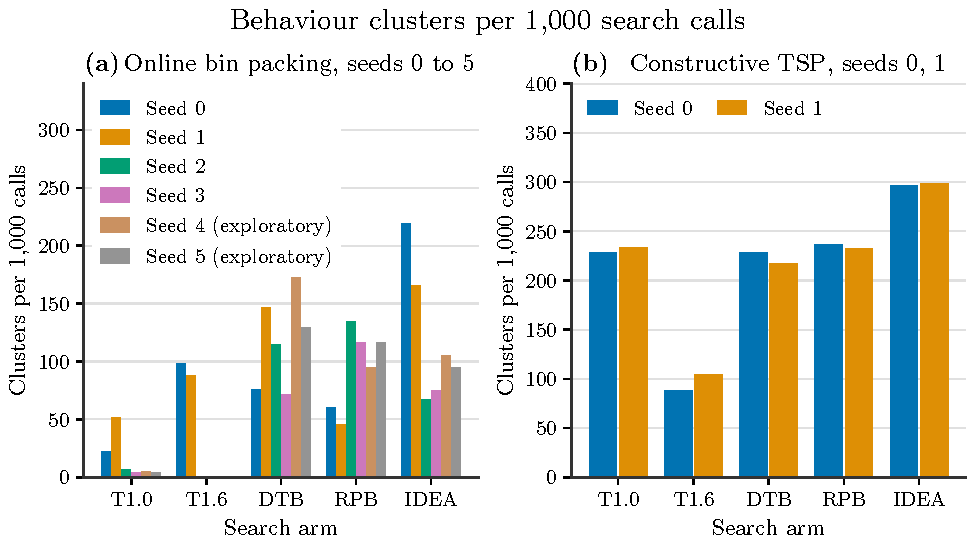
\includegraphics[width=\linewidth,height=0.78\textheight,keepaspectratio]{figures/fig_search_clusters_v0.pdf}
\caption{Behaviour clusters (complete-linkage clusters of a program's decisions on a fixed probe set, minimum within-cluster agreement at least 0.95) per 1,000 search calls (y-axis), by search arm (x-axis: T1.0, T1.6, DTB, RPB, IDEA) and seed (bar colour, per each panel's legend), as grouped bars with no intervals; each bar is one search run. (a) Online bin packing, 2,000 calls per arm-seed: seeds 0 and 1 are the first search run, seeds 2 and 3 an independent replication, and seeds 4 and 5 that replication's exploratory extension. The T1.6 bars for seeds 2-5 (0.5 clusters per 1,000 calls) are too small to see at this scale. (b) Constructive TSP, 1,056 calls per arm-seed, seeds 0 and 1. Search arms: T1.0 and T1.6 are temperature-1.0 (top-p 1.0) and temperature-1.6 (top-p 0.95) sampling; DTB is decision-token branching, which forces a rank-2-8 token at the highest-entropy code position of the first 48 generated tokens; RPB is the matched random-position placebo for DTB; IDEA is an instruction to base the next version on an idea different from the parent program(s) shown in the prompt. DTB finds roughly an order of magnitude more clusters than T1.0 in the bin-packing replication (seeds 2-5) but is close to both T1.0 and RPB on TSP.}
\label{fig:fig_search_clusters}
\end{figure}
Where the randomness is spent mattered, but not in the way the fork account predicted. Forcing a non-top token, at the entropy maximum or at a random position, bought many more behaviours than temperature in the replication's implementation (17.8 to 186.5 times), where temperature mostly copied the parent. In the first implementation, where temperature wrote new code, branching's advantage over temperature 1.6 was 1.2 times and reversed in one seed, and on TSP branching tied temperature 1.0. Against its random-position placebo, branching was ahead in the first search (2.1), behind in the replication (0.74), ahead in the exploratory seeds (1.47) and tied on TSP (0.95). The committed operator claim needed the gain over temperature and over the placebo in both bin-packing seed sets and on TSP; it failed on every one of those three tests at least once. The instruction to use a different idea found the most behaviours in the first search and on TSP, and was in the same range as forcing in the replication. The artifacts' dated literature searches found no earlier use of a decoding-time entropy fork as the mutation operator of an LLM program search; the nearest work analyses forking tokens in text generation [30] or uses high-entropy tokens during reinforcement learning [139].

\begin{table}[H]
\renewcommand{\thetable}{459}
\centering\small\setlength{\tabcolsep}{4.0pt}
\caption{The three searches against the committed claims. [Source: iteration 10, artifact \nolinkurl{gen_art_experiment_51}, \nolinkurl{gen_art_experiment_52}, \nolinkurl{gen_art_experiment_53}.]}\label{tab:t489}
\begin{tabular}{>{\raggedright\arraybackslash\hspace{0pt}}p{0.2400\linewidth}>{\raggedright\arraybackslash\hspace{0pt}}p{0.2529\linewidth}>{\raggedright\arraybackslash\hspace{0pt}}p{0.1643\linewidth}>{\raggedright\arraybackslash\hspace{0pt}}p{0.2725\linewidth}}
\toprule
\textbf{Claim} & \textbf{First bin-packing search (seeds 0, 1)} & \textbf{Replication search (seeds 2, 3)} & \textbf{TSP search (seeds 0, 1)} \\
\midrule
Held-out claim & Supported (every core arm's best passes) & Partial (temperature arms fail) & Supported (every core arm's best closes at least 30\% of nearest neighbour's gap) \\
Branching against temperature 1.0 & 3.01 & 17.8 & 0.96 (kill condition met) \\
Branching against temperature 1.6 & 1.20 (fails the 1.5 bar) & 186.5 & 2.32 (temperature 1.6 loses validity) \\
Branching against its random-position placebo & 2.10 & 0.74 (fails the 1.2 bar) & 0.95 \\
Branching's held-out best at least as good as temperature's & No & Yes & No \\
Operator claim & Partial & Partial & Disconfirmed \\
Novelty claim & Supported, flagged: 8 of 30 read as novel, one idea family, one reader & Disconfirmed: 0 of 40 & Not met: 0 of 12 \\
Instruction offspring renaming a parent & 0.44 (temperature 1.0: 0.86) & 0.67 (0.96) & 0.06 (0.18 and 0.22) \\
Birth tokens: reversion at decision tokens against controls & 0.40 against 0.36, p 0.49 & 0.50 against 0.26, p 0.0086 & not run \\
Search without selection & Never beats best fit (5 and 6 clusters) & Never beats best fit (5 and 3 clusters) & Best of 252 worse than nearest neighbour \\
\bottomrule
\end{tabular}
\end{table}

The figure below repeats Tables 448 and 453 for the two primary sets. In both bin-packing searches the tuned ab member, a two-parameter rule tuned with the same budget of 2,000 evaluations, has the lowest binpack3 excess of the plotted programs (3.06\%; the published ab-FF(5,24) reaches 3.01\%). On the Weibull test set it is beaten by four of the first search's five arm bests and by the replication's placebo and instruction bests.

\begin{figure}[!htbp]
\centering\captionsetup{font=footnotesize}
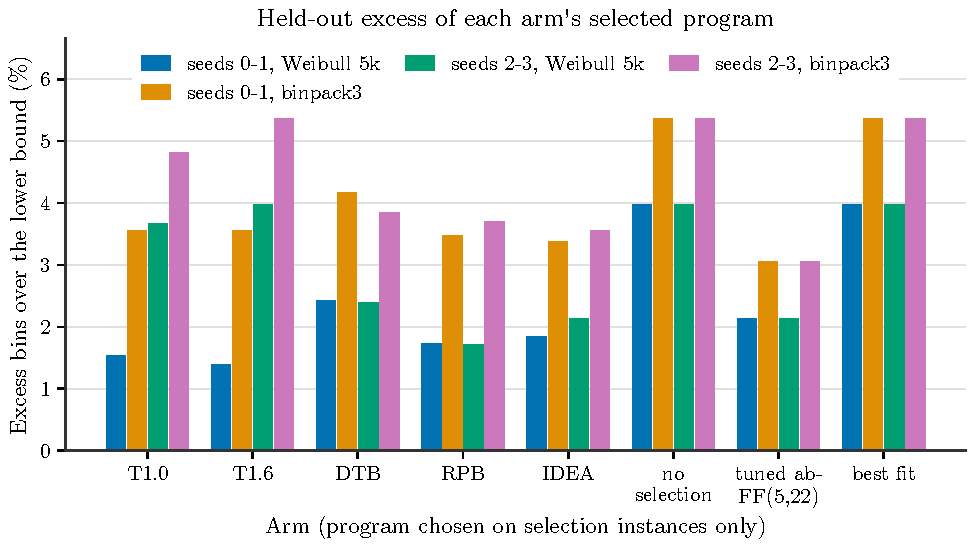
\includegraphics[width=\linewidth,height=0.78\textheight,keepaspectratio]{figures/fig_bp_heldout_v0.pdf}
\caption{Grouped bar chart of held-out excess bins over the lower bound (\%) -- the total item size divided by bin capacity and rounded up -- for the online bin-packing program each arm selected using only its selection (validation) instances, evaluated on FunSearch's Weibull 5k test set and OR-Library binpack3. Lower is better. The x-axis lists eight arms: T1.0 (temperature 1.0, top-p 1.0) and T1.6 (temperature 1.6, top-p 0.95), DTB (decision-token branching), RPB (its random-position placebo), IDEA (the instruction to use an idea different from both parents), the arm run without selection, the tuned ab-family member ab-FF(5,22), and the best-fit heuristic. The four bars per arm, coloured as in the legend, are seeds 0-1 on Weibull 5k, seeds 0-1 on binpack3, seeds 2-3 on Weibull 5k, and seeds 2-3 on binpack3 -- the first search and its replication, crossed with the two test sets. The arm run without selection matches best fit almost exactly on both test sets and in both seed pairs (excess 3.98\% Weibull 5k, 5.37\% binpack3); the 0.8x-best-fit pass bars used to score the held-out claim (3.19\% Weibull 5k, 4.29\% binpack3) are not drawn. With selection, DTB, RPB and IDEA have lower excess than best fit on both test sets in both seed pairs. The temperature arms do the same in the first search, but in the replication T1.6 ties best fit exactly and T1.0's margin over it narrows sharply on both test sets. The tuned ab-FF(5,22) baseline has the lowest excess of any arm on binpack3 in both seed pairs.}
\label{fig:fig_bp_heldout}
\end{figure}
The novelty verdicts disagree between the two bin-packing searches, and the disagreement is a disagreement between two readers. The first search's reader classed 8 representatives as one new idea, preferring a leftover that is a whole multiple of the item size. The replication's reader classed every program built on an item-proportional target residual as known, citing the EoH run-3 and MCTS-AHD programs. The two rules are related but not identical: a target residual of about c times the item rewards one leftover size, while the whole-multiple rule rewards leftovers of 0, one and two items and penalises leftovers smaller than the item. Neither reading was double-coded. Only one judge family passed its gate in the first search and none in the replication, the first search's probe filter did no work, and no ablation tested whether the whole-multiple term causes the improvement. We therefore record the first search's eight programs as candidates that one reader judged novel. They are behaviourally distinct from every corpus program (agreement below 0.9) and better than best fit, but not better than the published ab members. We do not record them as a confirmed new heuristic.

\FloatBarrier
\subsection*{10.7 Prohibition with an exact instrument: do banned bin-packing rules come back under other names?}
\addcontentsline{toc}{subsection}{10.7 Prohibition with an exact instrument: do banned bin-packing rules come back under other names?}
\noindent{\small\emph{Artifact: \nolinkurl{gen_art_experiment_54}.}}\par\medskip
\textbf{Why a second task.} The grid result of iteration 9, that a five-name ban is obeyed by name far more than by mechanism, rested on instruments that read expansion order imperfectly: the runtime label and the tracer disagreed, and the tracer failed its gold gate on iterative deepening. On online bin packing the mechanism can be read exactly. A program's bin choices on fixed probe states either match a banned rule's or they do not, and a renamed copy of best fit agrees with best fit on every state whatever it is called.

\textbf{Setup.} The prohibition experiment  asked for one-shot online bin-packing priority functions in FunSearch's interface, with no parents and no evaluator in the loop. Each program was scored two ways. Lexical compliance means no banned rule name or abbreviation anywhere in the extracted program, comments and docstrings included. Mechanistic compliance means agreement below 0.95 with every banned rule on the 2,000 committed probe states, with a stochastic matcher for random fit. The instrument was gated before any ban row: every reference agrees with itself across runs, renamed copies of each rule agree at 1.0, implementation variants of each rule (an argmin one-hot, a reciprocal score, an exact-fit bonus, a Python loop) agree at 1.0, and planted different rules fall below 0.95. Three models ran: Qwen3-8B without thinking (local vLLM with 8-bit floating-point weights) and Qwen3-14B and Qwen3-32B with thinking (OpenRouter, with the DeepInfra provider and its 8-bit floating-point weights pinned). A baseline cell fixed each model's frequency order over six textbook rules (best, first, worst, almost-worst, last and random fit), and the resulting ban sequence was the same for all three models: best fit, then first fit, worst fit, almost-worst fit and last fit. The cells were cumulative name bans of the top k rules (k = 1 to 5) on three templates, a ban of the five rules described without names, the five-name ban on two held-out templates, and two novelty instructions. We call the one-line request to make a new algorithm the short novelty instruction, and the request for a fully novel algorithm with about 2,000 words of rationale the long novelty instruction. Every threshold, prompt, verdict rule and the analysis code were hash-committed before any sample. Three claims were committed. The renaming claim predicted that both compliance rates are at least 0.7 at one banned name, that mechanistic compliance falls with k while lexical compliance stays at least 0.7, and that the lexical-minus-mechanistic gap at k = 5 is at least 0.3 in at least two models. The described-ban claim predicted that describing the five rules without names raises mechanistic compliance at k = 5 by at least 0.2 over the named ban in at least two models. The bound without an evaluator predicted that at most 0.02 of the samples in any cell beat best fit on held-out data and are behaviourally novel. The OpenRouter cells used the plan's reduction ladder after a container crash: 30 samples per ban and instruction cell for the thinking models (their baselines have 50), and 50 per cell for Qwen3-8B.

{\scriptsize\setlength{\tabcolsep}{2.5pt}\renewcommand{\thetable}{460}
\begin{longtable}{>{\raggedright\arraybackslash\hspace{0pt}}p{0.1027\linewidth}>{\raggedright\arraybackslash\hspace{0pt}}p{0.0952\linewidth}>{\raggedright\arraybackslash\hspace{0pt}}p{0.1231\linewidth}>{\raggedright\arraybackslash\hspace{0pt}}p{0.0835\linewidth}>{\raggedright\arraybackslash\hspace{0pt}}p{0.0622\linewidth}>{\raggedright\arraybackslash\hspace{0pt}}p{0.0788\linewidth}>{\raggedright\arraybackslash\hspace{0pt}}p{0.1121\linewidth}>{\raggedright\arraybackslash\hspace{0pt}}p{0.0455\linewidth}>{\raggedright\arraybackslash\hspace{0pt}}p{0.1996\linewidth}}
\caption{Every cell of the prohibition experiment. Lexical and mechanistic compliance are shares of valid programs; the gap is lexical minus mechanistic. In the baseline and instruction cells nothing is banned, and compliance is computed against the model's top five rules. The class mix counts all samples; a program is classed as other when it agrees on fewer than 0.95 of probe decisions with every catalogue rule. [Source: iteration 10, artifact \nolinkurl{gen_art_experiment_54}.]}\label{tab:t490}\\
\toprule
\textbf{Model} & \textbf{Cell} & \textbf{Rules banned} & \textbf{Samples} & \textbf{Valid} & \textbf{Lexical} & \textbf{Mechanistic} & \textbf{Gap} & \textbf{Class mix} \\
\midrule
\endfirsthead
\multicolumn{9}{l}{\emph{Table 460, continued}}\\
\toprule
\textbf{Model} & \textbf{Cell} & \textbf{Rules banned} & \textbf{Samples} & \textbf{Valid} & \textbf{Lexical} & \textbf{Mechanistic} & \textbf{Gap} & \textbf{Class mix} \\
\midrule
\endhead
\bottomrule
\endlastfoot
Qwen3-8B, no thinking & Baseline & none & 50 & 36 & 22\slash{}36 = 0.61 & 25\slash{}36 = 0.69 & -0.08 & other 25, invalid 14, best fit 9, first fit 2 \\
Qwen3-8B, no thinking & k = 1 & best fit & 50 & 41 & 35\slash{}41 = 0.85 & 24\slash{}41 = 0.59 & 0.27 & other 24, best fit 17, invalid 9 \\
Qwen3-8B, no thinking & k = 2 & + first fit & 50 & 46 & 43\slash{}46 = 0.93 & 17\slash{}46 = 0.37 & 0.57 & best fit 28, other 17, invalid 4, first fit 1 \\
Qwen3-8B, no thinking & k = 3 & + worst fit & 50 & 43 & 36\slash{}43 = 0.84 & 17\slash{}43 = 0.40 & 0.44 & best fit 23, other 17, invalid 7, first fit 3 \\
Qwen3-8B, no thinking & k = 4 & + almost-worst fit & 50 & 41 & 37\slash{}41 = 0.90 & 22\slash{}41 = 0.54 & 0.37 & other 21, best fit 16, invalid 9, first fit 3, last fit 1 \\
Qwen3-8B, no thinking & k = 5 & + last fit & 50 & 43 & 39\slash{}43 = 0.91 & 22\slash{}43 = 0.51 & 0.40 & other 22, best fit 18, invalid 7, first fit 3 \\
Qwen3-8B, no thinking & Described ban & first fit (only description named correctly) & 50 & 46 & 27\slash{}46 = 0.59 & 44\slash{}46 = 0.96 & -0.37 & best fit 22, other 22, invalid 4, first fit 2 \\
Qwen3-8B, no thinking & k = 5, held-out templates & top five & 50 & 49 & 31\slash{}49 = 0.63 & 27\slash{}49 = 0.55 & 0.08 & other 27, best fit 16, first fit 6, invalid 1 \\
Qwen3-8B, no thinking & Short novelty instruction & none & 50 & 42 & 26\slash{}42 = 0.62 & 21\slash{}42 = 0.50 & 0.12 & other 21, best fit 18, invalid 8, first fit 3 \\
Qwen3-8B, no thinking & Long novelty instruction & none & 50 & 29 & 24\slash{}29 = 0.83 & 26\slash{}29 = 0.90 & -0.07 & other 26, invalid 21, first fit 2, best fit 1 \\
Qwen3-14B, thinking & Baseline & none & 50 & 50 & 42\slash{}50 = 0.84 & 0\slash{}50 = 0.00 & 0.84 & best fit 50 \\
Qwen3-14B, thinking & k = 1 & best fit & 30 & 30 & 28\slash{}30 = 0.93 & 30\slash{}30 = 1.00 & -0.07 & other 25, first fit 5 \\
Qwen3-14B, thinking & k = 2 & + first fit & 30 & 30 & 26\slash{}30 = 0.87 & 30\slash{}30 = 1.00 & -0.13 & other 30 \\
Qwen3-14B, thinking & k = 3 & + worst fit & 30 & 27 & 25\slash{}27 = 0.93 & 23\slash{}27 = 0.85 & 0.07 & other 23, best fit 4, invalid 3 \\
Qwen3-14B, thinking & k = 4 & + almost-worst fit & 30 & 27 & 23\slash{}27 = 0.85 & 25\slash{}27 = 0.93 & -0.07 & other 25, invalid 3, best fit 1, first fit 1 \\
Qwen3-14B, thinking & k = 5 & + last fit & 30 & 27 & 26\slash{}27 = 0.96 & 25\slash{}27 = 0.93 & 0.04 & other 25, invalid 3, best fit 2 \\
Qwen3-14B, thinking & Described ban & first fit & 30 & 30 & 30\slash{}30 = 1.00 & 30\slash{}30 = 1.00 & 0.00 & best fit 30 \\
Qwen3-14B, thinking & k = 5, held-out templates & top five & 30 & 30 & 24\slash{}30 = 0.80 & 28\slash{}30 = 0.93 & -0.13 & other 28, best fit 2 \\
Qwen3-14B, thinking & Short novelty instruction & none & 30 & 29 & 20\slash{}29 = 0.69 & 1\slash{}29 = 0.03 & 0.66 & best fit 28, other 1, invalid 1 \\
Qwen3-14B, thinking & Long novelty instruction & none & 30 & 24 & 20\slash{}24 = 0.83 & 18\slash{}24 = 0.75 & 0.08 & other 18, best fit 6, invalid 6 \\
Qwen3-32B, thinking & Baseline & none & 50 & 49 & 25\slash{}49 = 0.51 & 1\slash{}49 = 0.02 & 0.49 & best fit 48, invalid 1, other 1 \\
Qwen3-32B, thinking & k = 1 & best fit & 31 & 30 & 26\slash{}30 = 0.87 & 30\slash{}30 = 1.00 & -0.13 & other 16, first fit 14, invalid 1 \\
Qwen3-32B, thinking & k = 2 & + first fit & 31 & 29 & 25\slash{}29 = 0.86 & 29\slash{}29 = 1.00 & -0.14 & other 28, invalid 2, worst fit 1 \\
Qwen3-32B, thinking & k = 3 & + worst fit & 31 & 22 & 20\slash{}22 = 0.91 & 22\slash{}22 = 1.00 & -0.09 & other 22, invalid 9 \\
Qwen3-32B, thinking & k = 4 & + almost-worst fit & 30 & 25 & 22\slash{}25 = 0.88 & 24\slash{}25 = 0.96 & -0.08 & other 24, invalid 5, first fit 1 \\
Qwen3-32B, thinking & k = 5 & + last fit & 30 & 24 & 21\slash{}24 = 0.88 & 24\slash{}24 = 1.00 & -0.12 & other 24, invalid 6 \\
Qwen3-32B, thinking & Described ban & first fit & 30 & 30 & 30\slash{}30 = 1.00 & 30\slash{}30 = 1.00 & 0.00 & best fit 29, other 1 \\
Qwen3-32B, thinking & k = 5, held-out templates & top five & 30 & 26 & 25\slash{}26 = 0.96 & 26\slash{}26 = 1.00 & -0.04 & other 26, invalid 4 \\
Qwen3-32B, thinking & Short novelty instruction & none & 30 & 28 & 12\slash{}28 = 0.43 & 0\slash{}28 = 0.00 & 0.43 & best fit 28, invalid 2 \\
Qwen3-32B, thinking & Long novelty instruction & none & 30 & 12 & 8\slash{}12 = 0.67 & 10\slash{}12 = 0.83 & -0.17 & invalid 18, other 10, best fit 2 \\
\end{longtable}}

\textbf{The renaming claim was partial.} Renaming is large and significant only in the model without thinking (Table 461 and the figure below). Under the five-name ban, Qwen3-8B's lexical compliance is 0.91 and its mechanistic compliance 0.51, a gap of +0.40 (paired Newcombe interval [174] 0.21 to 0.55); its lexically clean programs are a banned rule in 0.40 to 0.63 of cases across k, mostly best fit under names the model invented, such as \emph{tightest fit} or \emph{minimum remaining space} (Table 462). The two thinking models change behaviour when a name is banned. Banning best fit sends Qwen3-32B to first fit in 14 of 30 programs and to other rules in 16, and from k = 2 on their programs sit mostly outside the catalogue. Their k = 5 gaps are +0.04 and -0.13 with intervals that include 0. Lexical compliance there is lower than mechanistic, because some of their programs mention a banned name in code or comments while implementing a different rule. The trend of mechanistic compliance over k is significant only for Qwen3-14B (Jonckheere-Terpstra permutation p 0.038, Holm 0.11). On the held-out templates no model has a positive gap whose interval excludes 0; Qwen3-8B's falls to +0.08. The verdict is the same at class thresholds of 0.90 and 0.98 and on informative probe states only.

\begin{figure}[!htbp]
\centering\captionsetup{font=footnotesize}
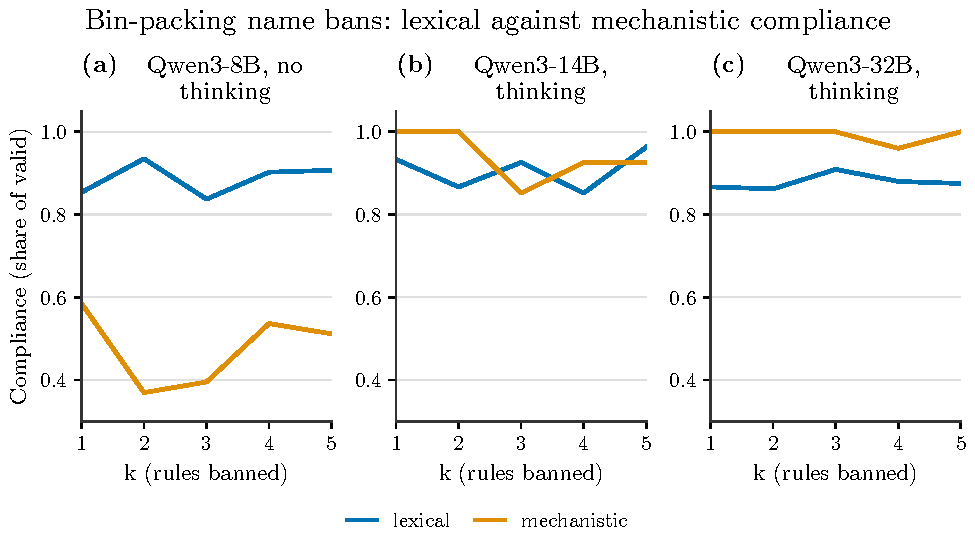
\includegraphics[width=\linewidth,height=0.78\textheight,keepaspectratio]{figures/fig_novr_kcurves_v0.pdf}
\caption{Lexical compliance (blue; share of valid programs containing no banned rule's name) and mechanistic compliance (orange; share of valid programs whose decisions disagree with every banned rule, i.e. agree on fewer than 95\textbackslash{}\% of 2,000 committed probe states) against \$k\$, the number of online-bin-packing rules banned by name, for three Qwen3 models: (a) Qwen3-8B without thinking, (b) Qwen3-14B with thinking, and (c) Qwen3-32B with thinking. Rules accumulate in the order best fit, first fit, worst fit, almost-worst fit, last fit. All three panels share the \$y\$-range 0.3--1.05; no uncertainty intervals are drawn, and each point averages over 41--46 valid programs for Qwen3-8B and at most 30 for the two thinking models. Only Qwen3-8B (a) shows a sustained gap with lexical compliance above mechanistic compliance, consistent with renaming a banned rule without changing what the program actually does; for Qwen3-14B and Qwen3-32B (b, c) the mechanistic line tracks or sits above the lexical line at every \$k\$, and the renaming gap's 95\textbackslash{}\% interval at \$k=5\$ spans zero for both, so this bin-packing task gives no reliable evidence that the thinking models rename without complying.}
\label{fig:fig_novr_kcurves}
\end{figure}
\begin{table}[H]
\renewcommand{\thetable}{461}
\centering\small\setlength{\tabcolsep}{4.0pt}
\caption{The five parts of the renaming claim per model. Intervals are paired Newcombe 95\% intervals; p-values are permutation p-values of the Jonckheere-Terpstra test with 100,000 permutations. [Source: iteration 10, artifact \nolinkurl{gen_art_experiment_54}.]}\label{tab:t491}
\begin{tabular}{>{\raggedright\arraybackslash\hspace{0pt}}p{0.2868\linewidth}>{\raggedright\arraybackslash\hspace{0pt}}p{0.2476\linewidth}>{\raggedright\arraybackslash\hspace{0pt}}p{0.1997\linewidth}>{\raggedright\arraybackslash\hspace{0pt}}p{0.1955\linewidth}}
\toprule
\textbf{Part of the claim} & \textbf{Qwen3-8B, no thinking} & \textbf{Qwen3-14B, thinking} & \textbf{Qwen3-32B, thinking} \\
\midrule
At one name, both rates at least 0.7 & Fails (lexical 0.85, mechanistic 0.59) & Holds (0.93, 1.00) & Holds (0.87, 1.00) \\
Mechanistic compliance falls with k & p 0.54 (z -0.13) & p 0.038 (z 1.69; Holm 0.11) & p 0.38 (z 0.78; Holm 0.75) \\
Lexical compliance at least 0.7 at every k & Holds (0.84 to 0.93) & Holds (0.85 to 0.96) & Holds (0.86 to 0.91) \\
Gap at k = 5 at least 0.3 & +0.40 (0.21 to 0.55): holds & +0.04 (-0.12 to 0.20) & -0.13 (-0.31 to 0.04) \\
Gap on held-out templates at k = 5 & +0.08 (-0.08 to 0.24) & -0.13 (-0.31 to 0.04) & -0.04 (-0.19 to 0.09) \\
\bottomrule
\end{tabular}
\end{table}

\begin{table}[H]
\renewcommand{\thetable}{462}
\centering\small\setlength{\tabcolsep}{4.0pt}
\caption{Rename rate: the share of lexically compliant valid programs that are still a banned rule by behaviour, with Wilson 95\% intervals [8]. [Source: iteration 10, artifact \nolinkurl{gen_art_experiment_54}.]}\label{tab:t492}
\begin{tabular}{>{\raggedright\arraybackslash\hspace{0pt}}p{0.1828\linewidth}>{\raggedright\arraybackslash\hspace{0pt}}p{0.2713\linewidth}>{\raggedright\arraybackslash\hspace{0pt}}p{0.2461\linewidth}>{\raggedright\arraybackslash\hspace{0pt}}p{0.2295\linewidth}}
\toprule
\textbf{Cell} & \textbf{Qwen3-8B, no thinking} & \textbf{Qwen3-14B, thinking} & \textbf{Qwen3-32B, thinking} \\
\midrule
k = 1 & 14\slash{}35 = 0.40 (0.26 to 0.56) & 0\slash{}28 (0 to 0.12) & 0\slash{}26 (0 to 0.13) \\
k = 2 & 27\slash{}43 = 0.63 (0.48 to 0.76) & 0\slash{}26 (0 to 0.13) & 0\slash{}25 (0 to 0.13) \\
k = 3 & 20\slash{}36 = 0.56 (0.40 to 0.70) & 4\slash{}25 = 0.16 (0.06 to 0.35) & 0\slash{}20 (0 to 0.16) \\
k = 4 & 15\slash{}37 = 0.41 (0.26 to 0.57) & 1\slash{}23 = 0.04 (0.01 to 0.21) & 1\slash{}22 = 0.05 (0.01 to 0.22) \\
k = 5 & 19\slash{}39 = 0.49 (0.34 to 0.64) & 2\slash{}26 = 0.08 (0.02 to 0.24) & 0\slash{}21 (0 to 0.15) \\
k = 5, held-out templates & 10\slash{}31 = 0.32 (0.19 to 0.50) & 1\slash{}24 = 0.04 (0.01 to 0.20) & 0\slash{}25 (0 to 0.13) \\
Described ban & 1\slash{}27 = 0.04 (0.01 to 0.18) & 0\slash{}30 (0 to 0.11) & 0\slash{}30 (0 to 0.11) \\
\bottomrule
\end{tabular}
\end{table}

The reasoning traces of both thinking models name the banned rule in every cell (share 1.00), and under the name bans they identify their own program as close to it in 0.90 to 1.00 of traces. The bans cost reasoning: median reasoning tokens rose from 6,342 (Qwen3-14B) and 5,485 (Qwen3-32B) at baseline to 8,350 and 10,889 at five names, and Qwen3-32B truncated 0.20 of its five-name traces.

\textbf{The described-ban claim was disconfirmed, as a weak test.} Each description had to be named correctly by the model in at least 16 of 20 separate queries. Only first fit's description passed; the models named the other descriptions as first-fit decreasing (an offline rule that sorts the items before packing them) or similar rules. The described cell therefore banned first fit alone, a rule these models rarely use, and mechanistic compliance was about 1.0 under the description and under the name alike: differences 0.00 (Qwen3-14B, -0.11 to 0.12), 0.00 (Qwen3-32B, -0.11 to 0.14) and +0.03 (Qwen3-8B, -0.09 to 0.15). The grid question this test was meant to settle, whether a name-free description changes the mechanism more than names, stays open.

\textbf{The bound without an evaluator held.} None of the 1,143 programs beat best fit on both held-out sets by the 0.8 rule. 186 valid programs were behaviourally novel against the 426-member published corpus (maximum agreement below 0.9), and none of them was better than best fit. The committed share of at most 0.02 novel-and-better programs per cell holds as a point estimate only: the Clopper-Pearson upper bounds [170] are 0.07 per cell at 50 samples and 0.12 at 30.

\textbf{Novelty instructions return the default.} The short novelty instruction returned best fit in 28 of 29 programs from Qwen3-14B, 28 of 28 from Qwen3-32B and 18 of 42 from Qwen3-8B. Every program that claimed novelty under that instruction was a catalogue rule (agreement at least 0.95) or a corpus heuristic (at least 0.9) for the thinking models (4 of 4 and 11 of 11), and 6 of 7 were for Qwen3-8B. Under the long instruction 11 of 14, 4 of 12 and 18 of 27 novelty claims were known programs, and Qwen3-32B truncated 0.57 of those traces.

\textbf{Integrity.} The worker container crashed at about 4.2 hours and sampling resumed at 5.9 hours behind exclusive locks. For 39 minutes a kill reached a shell wrapper and left its Python child alive, so two samplers ran together; five duplicate Qwen3-32B baseline rows were moved aside, keeping the first, evaluated row per slot. The first naming-check files mixed empty replies with real ones; a clean rerun was committed before any Qwen3-32B described-ban row. The payload files of two commits were overwritten after their hashes were logged, so two lines of the commitment log no longer match the files on disk; the chain itself verifies, and the banned sets of the name cells are identical in every version. The standard-library re-derivation recomputed every agreement, class, lexical flag, cell count, trend statistic, interval and verdict with 0 mismatches, and its four placebos failed as required: 600 shuffled-k trend tests give p below 0.05 in 3.8\% of cases, randomly swapped flags give a mean gap of 0.001, 50 random decision vectors are all classed other, and a renamed best fit whose comment calls it the tightest rule is still classed best fit with no lexical hit. The spend was USD 1.42 for 2,497 calls.

\FloatBarrier
\subsection*{10.8 Discipline against container on the program map, and where the survivor families land}
\addcontentsline{toc}{subsection}{10.8 Discipline against container on the program map, and where the survivor families land}
\noindent{\small\emph{Artifact: \nolinkurl{gen_art_experiment_55}.}}\par\medskip
\textbf{Why.} In iteration 9 the program manifold placed unit-weight Dijkstra at the edge of the banned five, and its Bellman-Ford survivors opposite, but that manifold tracked code surface and length as strongly as behaviour (Section 9.4). Unit-weight Dijkstra expands a grid in BFS order through a heap, so its edge position could reflect the same expansion discipline or only similar code. A factorial program set that crosses discipline with container separates the two by design.

\textbf{Setup.} The factorial geometry experiment  had Qwen3-32B (OpenRouter, thinking off, temperature 1.0) write grid path programs for 24 implementable cells of expansion discipline (FIFO order, LIFO order, goal-heuristic order, path-cost order, relaxation rounds, random order) by storage container (deque, list, recursion, heap, two-dimensional arrays, set). Each prompt described the mechanics step by step in three wordings and named no algorithm (0 lint hits over 144 prompts). Every program had to pass the 48-case and 41-case hidden suites, an AST container check, a discipline check (the iteration-9 tracer for FIFO, LIFO, heuristic and cost order, a two-seed runtime check for random order, an AST sweep check plus at least two runtime passes for relaxation, and hand reads for the array cells) and name scrubbing followed by a rerun of the suite. The freeze kept the first 12 verified programs per cell, 287 in all (the relaxation-by-set cell has 11), plus 12 top-ups each for bidirectional BFS, iterative deepening and bidirectional A*; the 12 jump point search top-ups are all paraphrases of the reference. Four programs were rejected on hand read. States were read under iteration 9's neutral-twin contexts with its frozen readout and truncated decoder (Qwen3-8B in bfloat16 at block 17, Qwen3-32B with 4-bit NormalFloat weights at block 33), and the reproduction gate matched iteration 9's frames bit for bit (unit-weight Dijkstra g over median 0.6296 and 0.6725; 113 of 113 placements). The spend was USD 0.25 for 1,138 calls.

The discipline-against-container claim uses a partial Spearman correlation between the program-state dissimilarity matrix and the discipline matrix given the container matrix (written rho\_\allowbreak{}dc), and the reverse (rho\_\allowbreak{}cd), with a program bootstrap and permutations restricted within strata. The prediction was rho\_\allowbreak{}dc at least 0.3 and above rho\_\allowbreak{}cd on at least one model; the disconfirming outcome was rho\_\allowbreak{}dc at most 0.1 on both.

\textbf{The discipline-against-container verdict is indeterminate.} Discipline is encoded, container is encoded more strongly, and token surface more strongly than either (Table 463). On both models rho\_\allowbreak{}dc is below 0.3 and below rho\_\allowbreak{}cd, and the difference is negative with an interval that excludes 0 on the full set. The bag-of-tokens baseline (mean input embedding over the code tokens) gives rho\_\allowbreak{}dc 0.169 (Qwen3-8B) and 0.156 (Qwen3-32B), and a randomly initialised network 0.072, so the trained states carry discipline information beyond token identity, but less than the bar. A rank regression with surface, length, container, discipline and context matrices gives semi-partial correlations of 0.32, 0.30, 0.13, 0.10 and 0.02 on Qwen3-8B and 0.41, 0.23, 0.20 and 0.13 (surface, length, container, discipline) on Qwen3-32B. Partialling the token-surface matrix out leaves rho\_\allowbreak{}dc at 0.13 to 0.15 (Qwen3-8B) and 0.18 to 0.21 (Qwen3-32B). The noise ceiling across context variants is 0.94 on Qwen3-8B, the cell-cluster bootstrap widens the difference interval to include 0, other readouts give lower discipline correlations (0.09 at the token after the first pop, 0.04 to 0.05 at the 16th code token), and the layer curve is flat (0.20 to 0.26 on Qwen3-8B, 0.25 to 0.30 on Qwen3-32B). Shuffled labels give 0.006 for both partial correlations.

\begin{table}[H]
\renewcommand{\thetable}{463}
\centering\footnotesize\setlength{\tabcolsep}{4.0pt}
\caption{Partial representational similarity analysis of the factorial program states (readout: mean state over the code tokens). Brackets are 95\% program-bootstrap intervals; permutation p-values are restricted within strata (2,000 permutations). [Source: iteration 10, artifact \nolinkurl{gen_art_experiment_55}.]}\label{tab:t493}
\begin{tabular}{>{\raggedright\arraybackslash\hspace{0pt}}p{0.1925\linewidth}>{\raggedright\arraybackslash\hspace{0pt}}p{0.1960\linewidth}>{\raggedright\arraybackslash\hspace{0pt}}p{0.1960\linewidth}>{\raggedright\arraybackslash\hspace{0pt}}p{0.1553\linewidth}>{\raggedright\arraybackslash\hspace{0pt}}p{0.1735\linewidth}}
\toprule
\textbf{Model (block) and set} & \textbf{Discipline given container, rho\_\allowbreak{}dc} & \textbf{Container given discipline, rho\_\allowbreak{}cd} & \textbf{Difference} & \textbf{Permutation p (rho\_\allowbreak{}dc \slash{} rho\_\allowbreak{}cd)} \\
\midrule
Qwen3-8B (17), all 24 cells & 0.226 [0.186, 0.265] & 0.300 [0.251, 0.351] & -0.074 [-0.133, -0.018] & 0.0005 \slash{} 0.0005 \\
Qwen3-32B (33), all 24 cells & 0.285 [0.252, 0.321] & 0.414 [0.363, 0.462] & -0.129 [-0.193, -0.060] & 0.0005 \slash{} 0.0005 \\
Qwen3-8B, crossed 3 x 4 core & 0.280 [0.218, 0.357] & 0.366 [0.293, 0.457] & -0.086 [-0.182, 0.008] & 0.0005 \slash{} 0.0005 \\
Qwen3-32B, crossed 3 x 4 core & 0.336 [0.288, 0.392] & 0.545 [0.482, 0.611] & -0.209 [-0.295, -0.118] & 0.0005 \slash{} 0.0005 \\
\bottomrule
\end{tabular}
\end{table}

\textbf{The placements.} The placement claims placed 351 programs out of sample on a frame of 464 programs (the 24 cells plus the catalogue) with iteration 9's unchanged placement code (k-nearest-neighbour geodesic distances). The families were 38 unit-weight Dijkstra, 32 grid Bellman-Ford, 18 coordinate-key heaps, 14 random frontiers, 4 raster sweeps, 3 set frontiers and 8 other survivors, 136 covert BFS and DFS programs from the five-name ban and 98 from other ban sets. The frame classifies well: class-level leave-one-out accuracy 0.68 (Qwen3-8B) and 0.83 (Qwen3-32B), discipline-level 0.83 and 0.91, against chance 0.03. Its false-inside rate, the share of left-out non-banned programs whose nearest other class is banned, is 0.46 and 0.47, close to the 53\% of its classes that are banned.

\begin{table}[H]
\renewcommand{\thetable}{464}
\centering\small\setlength{\tabcolsep}{4.0pt}
\caption{The preregistered placement predictions. r\_\allowbreak{}F is a family's median geodesic to the banned set relative to the frame median (below 1 is edge, above 1 opposite); the contrast is the committed sign test that the family sits nearer the path-cost or FIFO heap cells than the heuristic heap cell. [Source: iteration 10, artifact \nolinkurl{gen_art_experiment_55}.]}\label{tab:t494}
\begin{tabular}{>{\raggedright\arraybackslash\hspace{0pt}}p{0.2591\linewidth}>{\raggedright\arraybackslash\hspace{0pt}}p{0.3954\linewidth}>{\raggedright\arraybackslash\hspace{0pt}}p{0.2917\linewidth}}
\toprule
\textbf{Prediction} & \textbf{Qwen3-8B} & \textbf{Qwen3-32B} \\
\midrule
Unit-weight Dijkstra at the edge on the full and heap frames, nearest discipline FIFO or path cost & r\_\allowbreak{}F 0.90 [0.77, 1.00] edge; heap frame 0.99 edge (neither robust); 76\% nearest FIFO or path cost (path cost 27 of 38); contrast 38 of 38 (p 4e-12): rule met, not robust & r\_\allowbreak{}F 0.98 edge; heap frame 1.03 opposite (not robust); 68\% nearest FIFO or path cost; contrast 38 of 38: not supported \\
Bellman-Ford opposite, nearest relaxation, relaxation-by-array on the array frame & r\_\allowbreak{}F 0.86 edge (robust): the full-frame part fails; nearest relaxation 30 of 32; array frame relaxation-by-array 30 of 32; contrast 29 of 32 & r\_\allowbreak{}F 1.03 [1.01, 1.07] opposite, robust; nearest relaxation 31 of 32; contrast 31 of 32: supported \\
Covert BFS and DFS inside the banned classes in at least 0.8 & 0.993 [0.960, 0.999]; BFS to FIFO 0.92, DFS to LIFO 0.85: supported & 0.978 [0.937, 0.992]; 0.93 and 0.87: supported \\
\bottomrule
\end{tabular}
\end{table}

The independent audit compared each family with random families of the same size drawn from all placed programs. Bellman-Ford survivors are nearest a relaxation cell in 0.94 and 0.97 of cases against a placebo median of 0.09, and covert BFS and DFS are nearest a banned class in 0.99 and 0.98 against a placebo median of 0.78 (95th percentile 0.82). On Qwen3-8B every family and every random draw is at the edge (1,000 of 1,000 draws), and the unit-weight Dijkstra contrast scores 1.0 for every family, so on that model the edge verdict and the contrast do not discriminate families; on Qwen3-32B the contrast is specific (1.0 against a placebo median of 0.47). Across a robustness grid of two models, two neighbourhood sizes and three readouts (12 cells), the covert-program prediction holds in 12 of 12, the unit-weight Dijkstra rule in 6 of 12 (its full-frame verdict is edge in 12 of 12, but the heap frame turns opposite in 6) and the Bellman-Ford rule in 8 of 12, including every Qwen3-32B cell.

\begin{table}[H]
\renewcommand{\thetable}{464b}
\centering\scriptsize\setlength{\tabcolsep}{2.5pt}
\caption{The placement robustness grid: two models, two neighbourhood sizes k and three readouts. r\_\allowbreak{}F is a family's median geodesic to the banned set over the frame median; the covert column is the share of covert BFS and DFS programs from the five-name ban whose nearest class is banned. [Source: iteration 10, artifact \nolinkurl{gen_art_experiment_55}.]}\label{tab:t495}
\begin{tabular}{>{\raggedright\arraybackslash\hspace{0pt}}p{0.0622\linewidth}>{\raggedright\arraybackslash\hspace{0pt}}p{0.0300\linewidth}>{\raggedright\arraybackslash\hspace{0pt}}p{0.1516\linewidth}>{\raggedright\arraybackslash\hspace{0pt}}p{0.1425\linewidth}>{\raggedright\arraybackslash\hspace{0pt}}p{0.0902\linewidth}>{\raggedright\arraybackslash\hspace{0pt}}p{0.0921\linewidth}>{\raggedright\arraybackslash\hspace{0pt}}p{0.0835\linewidth}>{\raggedright\arraybackslash\hspace{0pt}}p{0.0743\linewidth}>{\raggedright\arraybackslash\hspace{0pt}}p{0.1764\linewidth}}
\toprule
\textbf{Model} & \textbf{k} & \textbf{Readout} & \textbf{Unit-weight Dijkstra: full \slash{} heap frame} & \textbf{Unit-weight Dijkstra rule} & \textbf{Bellman-Ford: full frame} & \textbf{Bellman-Ford rule} & \textbf{Covert share inside} & \textbf{r\_\allowbreak{}F: unit-weight Dijkstra \slash{} Bellman-Ford \slash{} covert} \\
\midrule
Qwen3-8B & 15 & mean over code tokens (primary) & edge \slash{} edge & holds & edge & fails & 0.993 & 0.90 \slash{} 0.86 \slash{} 0.72 \\
Qwen3-8B & 15 & mean without outlier-norm tokens & edge \slash{} opposite & fails & edge & fails & 0.993 & 0.98 \slash{} 0.95 \slash{} 0.79 \\
Qwen3-8B & 15 & token after the first pop & edge \slash{} edge & holds & opposite & holds & 1.000 & 0.46 \slash{} 1.69 \slash{} 0.31 \\
Qwen3-8B & 10 & mean over code tokens & edge \slash{} edge & holds & edge & fails & 0.985 & 0.77 \slash{} 0.91 \slash{} 0.59 \\
Qwen3-8B & 10 & mean without outlier-norm tokens & edge \slash{} opposite & fails & opposite & holds & 0.985 & 0.95 \slash{} 1.12 \slash{} 0.72 \\
Qwen3-8B & 10 & token after the first pop & edge \slash{} edge & holds & opposite & holds & 1.000 & 0.30 \slash{} 1.00 \slash{} 0.19 \\
Qwen3-32B & 15 & mean over code tokens (primary) & edge \slash{} opposite & fails & opposite & holds & 0.978 & 0.98 \slash{} 1.03 \slash{} 0.84 \\
Qwen3-32B & 15 & mean without outlier-norm tokens & edge \slash{} opposite & fails & opposite & holds & 0.978 & 0.98 \slash{} 1.03 \slash{} 0.84 \\
Qwen3-32B & 15 & token after the first pop & edge \slash{} edge & holds & opposite & holds & 1.000 & 0.38 \slash{} 2.16 \slash{} 0.33 \\
Qwen3-32B & 10 & mean over code tokens & edge \slash{} opposite & fails & opposite & holds & 0.963 & 0.91 \slash{} 1.02 \slash{} 0.72 \\
Qwen3-32B & 10 & mean without outlier-norm tokens & edge \slash{} opposite & fails & opposite & holds & 0.963 & 0.91 \slash{} 1.02 \slash{} 0.72 \\
Qwen3-32B & 10 & token after the first pop & edge \slash{} edge & holds & opposite & holds & 0.985 & 0.36 \slash{} 1.18 \slash{} 0.30 \\
\bottomrule
\end{tabular}
\end{table}

The reading is that the program map places programs by what they do as well as by how they look, but surface and container dominate discipline. Bellman-Ford survivors sit with relaxation programs, covert BFS and DFS sit with their own discipline, and unit-weight Dijkstra sits with the path-cost and FIFO heap programs rather than with the heuristic heap programs; whether that counts as edge or opposite depends on the frame. Every factorial program has one author, Qwen3-32B, while the survivors and covert programs come from several, so placements of programs by other authors are weaker evidence. Geometry here is correlational: iteration 7's in-manifold pushes moved 0 of 300 programs.

\FloatBarrier
\subsection*{10.9 Which weights hold the default at the fork}
\addcontentsline{toc}{subsection}{10.9 Which weights hold the default at the fork}
\noindent{\small\emph{Artifact: \nolinkurl{gen_art_experiment_56}.}}\par\medskip
\textbf{Why.} Iteration 9 found that post-training sharpened Qwen3-8B's fork and that the sharpening sits at the fork, in late MLPs and in the unembedding, but its component patching was not specific: matched random late-layer sets closed 0.81 of the minimum spanning tree gap. The weights experiment  moved the question from activations to weights. It asked whether the instruct default is stored in the unembedding rows of the fork-class tokens or in the late-MLP weights, tested the row arm again in free generation, and repeated the row test on Gemma. Units, prompts, openings, fork-class tokens, the generation engine and the frozen labellers came from iteration 9. The primary unit is connected components (default class ' find', union-find, against ' dfs' and ' bfs'; 20 prompts); minimum spanning tree (Kruskal-class against Prim-class tokens; 20 prompts) runs beside it. The margin is the log-sum-exp of the default class's fork logits minus that of the alternative class, and a share is the fraction of the instruct-minus-base margin gap an arm closes, a ratio of sums over prompts with a prompt bootstrap. Every decisive prediction was sha256-chained before the computation it governs. The readout-row claim predicted that, at the fork only, the base rows of the fork-class tokens close at least 0.5 of the connected-components gap, against at most 0.15 for the same rows moved in a random direction of matched norm, and that they give at least 10 of 30 correct DFS programs in generation. The late-MLP claim compared base weights in the late MLPs (layers 26 to 35) with Frobenius-matched swaps of early-layer MLPs.

\textbf{Stage 0.} On a different GPU from iteration 9 the gaps reproduced (4.56 nats on connected components against 4.52; 2.09 on minimum spanning tree against 2.06), but the connected-components instruct mean differed by 0.061 nats, above the 0.05 rule (Table 465). A debug round found the ids, hashes and stack unchanged and measured the bfloat16 numerics floor on this GPU: the instruct margin varies by a mean 0.27 and up to 0.55 nats across numerically equivalent batch shapes. The committed fallback applied, and every share below uses this run's own instruct and base margins from the same cached states.

\begin{table}[H]
\renewcommand{\thetable}{465}
\centering\small\setlength{\tabcolsep}{4.0pt}
\caption{Stage 0 of the weights experiment: the fork states recaptured on an RTX 4090, against iteration 9's capture on another GPU. [Source: iteration 10, artifact \nolinkurl{gen_art_experiment_56}.]}\label{tab:t496}
\begin{tabular}{>{\raggedright\arraybackslash\hspace{0pt}}p{0.4412\linewidth}>{\raggedright\arraybackslash\hspace{0pt}}p{0.2735\linewidth}>{\raggedright\arraybackslash\hspace{0pt}}p{0.2316\linewidth}}
\toprule
\textbf{Quantity} & \textbf{Connected components} & \textbf{Minimum spanning tree} \\
\midrule
Gap, instruct minus base margin (nats) [95\%] & 4.56 [3.58, 5.60] (iteration 9: 4.52) & 2.09 [1.98, 2.21] (iteration 9: 2.06) \\
Mean instruct margin, here \slash{} iteration 9 & 4.516 \slash{} 4.455 (difference 0.061, above 0.05) & 1.320 \slash{} 1.311 \\
Mean base margin, here \slash{} iteration 9 & -0.042 \slash{} -0.064 & -0.770 \slash{} -0.748 \\
Unembedding-only share, CPU decomposition (target 0.85 and 0.43, within 0.03) & 0.842 & 0.416 \\
Recomputed final norm against captured state & bit-exact (20 of 20) & bit-exact (20 of 20) \\
\bottomrule
\end{tabular}
\end{table}

\textbf{The readout-row claim was supported, as readout-level and not token-specific.} Restoring the base model's rows for the three fork-class tokens of connected components, on the instruct residual, closes 0.548 of the gap (Table 466). That meets the committed rule (at least 0.50, with the median of 50 isotropic matched-norm draws at most 0.15 and the arm above their maximum), although the bootstrap interval's lower end, 0.44, lies under 0.50. By the committed specificity qualifier the effect is readout-level but not token-specific: the arm clears the 95th percentile of 50 real row deltas of other tokens (0.405) but sits inside the distribution of 50 random directions confined to the residual's top 64 principal components (p 0.37). The effect is linear in dose (0.137 per quarter step), flips sign under the negated edit, owes nothing to the final-norm gain, and sits almost entirely in the alternative rows: restoring the ' dfs' and ' bfs' rows closes 0.489, restoring the ' find' row 0.060. The base rows raise the fork logits of ' dfs' by 2.23 nats and ' bfs' by 3.14, and change ' find' by -0.27. Post-training therefore wrote the connected-components default mainly by suppressing the alternatives' readout rows, not by boosting the default's. The ' dfs' and ' bfs' deltas point where the fork residual lives (logit leverage 0.069 and 0.085, close to the residual-subspace draws' medians and seven to nine times the isotropic value), which is why equal-norm random edits aimed entirely at that subspace lever the margin more than the real ones. On minimum spanning tree the base rows overshoot (1.25 of the gap), and the readout-residual interaction is large and opposite in sign to connected components (+1.75 against -1.34 nats), so readout and residual are not additive at either fork.

\begin{table}[H]
\renewcommand{\thetable}{466}
\centering\small\setlength{\tabcolsep}{4.0pt}
\caption{Restoring base fork-class unembedding rows on the instruct residual (exact CPU readout on cached fork states). Shares are of the instruct-minus-base margin gap; brackets are 95\% prompt-bootstrap intervals. [Source: iteration 10, artifact \nolinkurl{gen_art_experiment_56}.]}\label{tab:t497}
\begin{tabular}{>{\raggedright\arraybackslash\hspace{0pt}}p{0.4700\linewidth}>{\raggedright\arraybackslash\hspace{0pt}}p{0.2590\linewidth}>{\raggedright\arraybackslash\hspace{0pt}}p{0.2173\linewidth}}
\toprule
\textbf{Arm (instruct residual throughout)} & \textbf{Connected components share} & \textbf{Minimum spanning tree share} \\
\midrule
All fork-class rows from the base model (primary) & 0.548 [0.440, 0.707] & 1.249 [1.180, 1.323] \\
Default-class rows only & 0.060 [0.047, 0.078] & 0.009 \\
Alternative-class rows only & 0.489 [0.392, 0.629] & 1.240 \\
Base final-norm gain only & -0.000 & 0.006 \\
Rows plus gain (readout upper bound) & 0.547 & 1.254 \\
Full base unembedding (all 151,936 rows) & 0.548 (identical by construction) & 1.249 \\
Negated edit & -0.548 & -1.185 \\
Dose 0.25 \slash{} 0.5 \slash{} 0.75 \slash{} 1.25 \slash{} 1.5 & 0.14 \slash{} 0.27 \slash{} 0.41 \slash{} 0.69 \slash{} 0.82 & 0.31 \slash{} 0.62 \slash{} 0.94 \slash{} 1.56 \slash{} 1.88 \\
Null: 50 isotropic matched-norm edits, median \slash{} 95th percentile \slash{} max; empirical p & 0.044 \slash{} 0.138 \slash{} 0.210; p 0.020 (floor) & 0.051 \slash{} 0.720 \slash{} 0.942; p 0.020 \\
Null: 50 real deltas of other tokens; p & 0.085 \slash{} 0.405 \slash{} 0.625; p 0.059 & 0.055 \slash{} 1.169 \slash{} 1.511; p 0.059 \\
Null: 50 random directions in the residual's top 64 components; p & 0.181 \slash{} 1.252 \slash{} 2.328; p 0.373 & 0.113 \slash{} 5.394 \slash{} 6.224; p 0.275 \\
Readout-residual interaction (nats) [95\%] & -1.337 [-1.39, -1.29] & +1.748 [1.72, 1.77] \\
\bottomrule
\end{tabular}
\end{table}

\textbf{In generation the restored rows are too weak at dose 1, and strong at doses 2 and 3.} With 30 common-random-number slots per arm and only the fork step changed, restoring the rows gave 5 of 30 correct DFS programs on connected components against 1 for the unedited twin (4:0 discordant, exact McNemar [169] p 0.125, Holm 0.25), short of the registered 10 of 30; the committed note had warned that 10 needs a share of about 0.75 (Table 467). A preregistered power extension pooled 90 slots: the rows gave 21 of 90 against 4 for the twin (17:0, p 1.5e-5) and against 4 for the median isotropic draw. On minimum spanning tree the rows flipped 24 of 30 programs to correct Prim (24:0, p 1.2e-7), and one of the three committed isotropic draws, the one with the largest teacher-forced share, flipped 19. Fork-Patched Decoding [142], which splices the base model's fork logits, gave 15 of 30 DFS (iteration 9: 18), more than the restored rows (discordant pairs 12:2 in its favour, exact p 0.013). Pushing further along the same row delta, at twice and three times the dose, made Qwen3-8B write correct DFS in 21 and 30 of 30 connected-components programs and correct Prim in 27 of 30 minimum spanning tree programs, with every program passing the hidden tests (Table 468 and the figure below). At three times the dose the real delta beat the median draws of the strong nulls (24:0 against the residual-subspace median, 27:0 against the median transplanted delta). It tied the best of 50 draws of each null. On minimum spanning tree almost any large edit of these rows flips the fork: the median residual-subspace draw at three times gives 28 of 30.

\begin{table}[H]
\renewcommand{\thetable}{467}
\centering\footnotesize\setlength{\tabcolsep}{4.0pt}
\caption{Generation at the fork with 30 common-random-number slots per arm (counts committed before any token). Correct means the alternative class and passing the hidden tests; McNemar tests are exact and two-sided on paired slots. [Source: iteration 10, artifact \nolinkurl{gen_art_experiment_56}.]}\label{tab:t498}
\begin{tabular}{>{\raggedright\arraybackslash\hspace{0pt}}p{0.2483\linewidth}>{\raggedright\arraybackslash\hspace{0pt}}p{0.1753\linewidth}>{\raggedright\arraybackslash\hspace{0pt}}p{0.1356\linewidth}>{\raggedright\arraybackslash\hspace{0pt}}p{0.1829\linewidth}>{\raggedright\arraybackslash\hspace{0pt}}p{0.0910\linewidth}>{\raggedright\arraybackslash\hspace{0pt}}p{0.0636\linewidth}}
\toprule
\textbf{Arm} & \textbf{Connected components: correct DFS of 30 (predicted)} & \textbf{Against the twin} & \textbf{Minimum spanning tree: correct Prim of 30 (predicted)} & \textbf{Against the twin} & \textbf{Pass rate} \\
\midrule
Twin (instruct readout, fp32) & 1 (1.1) & n\slash{}a & 0 (5.9) & n\slash{}a & 30\slash{}30, 30\slash{}30 \\
Base fork-class rows at the fork & 5 (6.2) & 4:0, p 0.125 & 24 (22.9) & 24:0, p 1.2e-7 & 30\slash{}30, 30\slash{}30 \\
Committed isotropic draws: median share \slash{} largest share \slash{} draw 0 & 1 \slash{} 1 \slash{} 0 & median 0:0 & 0 \slash{} 19 \slash{} 10 & median 0:0 & 30\slash{}30 \\
Fork-Patched Decoding (base fork logits) [142] & 15 (13.4) & 14:0, p 1.2e-4 & 17 (18.7) & 17:0, p 1.5e-5 & 27\slash{}30, 30\slash{}30 \\
Rows swapped at every step & 5 & identical to the fork-only arm (0:0) & 24 & identical & 30\slash{}30 \\
Power extension, 90 slots: rows \slash{} twin \slash{} isotropic median & 21 \slash{} 4 \slash{} 4 (17:0, p 1.5e-5) & n\slash{}a & 72 \slash{} 17 \slash{} 18 (55:0, p 5.6e-17) & n\slash{}a & n\slash{}a \\
\bottomrule
\end{tabular}
\end{table}

\begin{table}[H]
\renewcommand{\thetable}{468}
\centering\small\setlength{\tabcolsep}{4.0pt}
\caption{Stronger edits of the fork-class rows at the fork step (preregistered extensions; 30 slots each). [Source: iteration 10, artifact \nolinkurl{gen_art_experiment_56}.]}\label{tab:t499}
\begin{tabular}{>{\raggedright\arraybackslash\hspace{0pt}}p{0.3819\linewidth}>{\raggedright\arraybackslash\hspace{0pt}}p{0.2960\linewidth}>{\raggedright\arraybackslash\hspace{0pt}}p{0.2683\linewidth}}
\toprule
\textbf{Edit at the fork step} & \textbf{Connected components: correct DFS of 30 (predicted)} & \textbf{Minimum spanning tree: correct Prim of 30 (predicted)} \\
\midrule
Twice the base-row delta & 21 (16.8); against the twin 20:0, p 1.9e-6 & 27 (29.3) \\
Three times the base-row delta & 30 (27.3); against the twin 29:0, p 3.7e-9 & 27 (29.9) \\
Median isotropic draw at twice \slash{} three times & 1 \slash{} 1 & 3 \slash{} 3 \\
Residual-subspace draw at three times: median \slash{} max & 6 \slash{} 30 & 28 \slash{} 27 \\
Transplanted delta of another token at three times: median \slash{} max & 3 \slash{} 30 & 22 \slash{} 27 \\
\bottomrule
\end{tabular}
\end{table}

\begin{figure}[!htbp]
\centering\captionsetup{font=footnotesize}
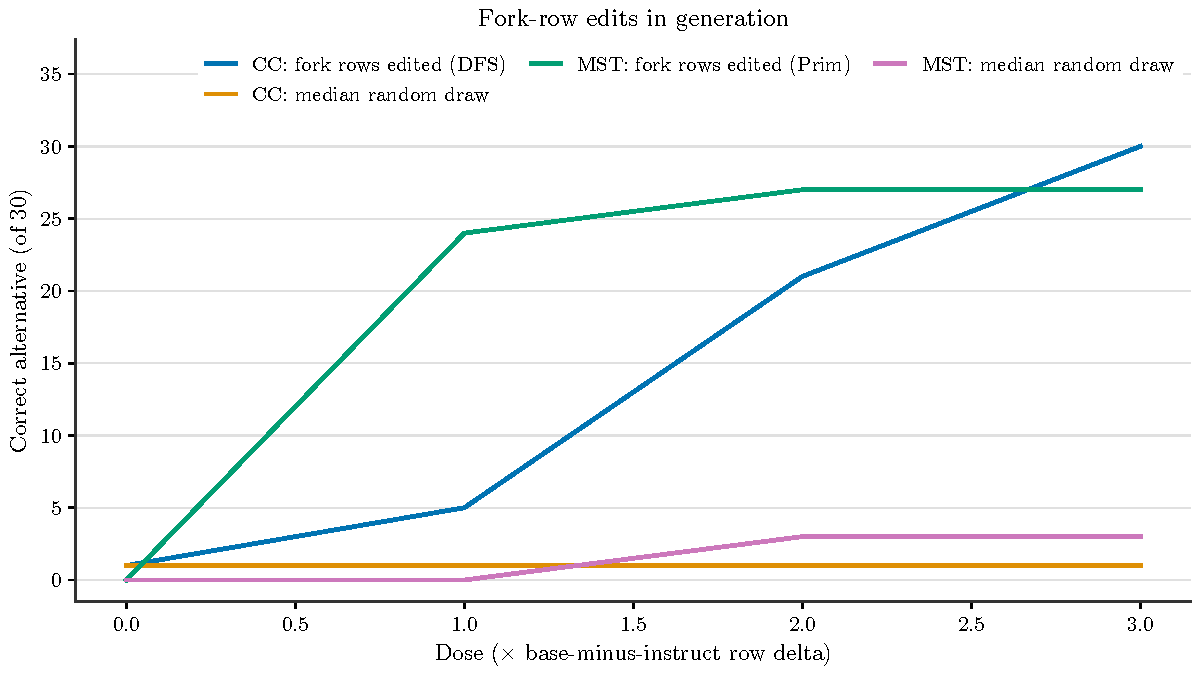
\includegraphics[width=\linewidth,height=0.78\textheight,keepaspectratio]{figures/fig_basew_dose_v0.pdf}
\caption{Correct programs of the non-default algorithm, out of 30 common-random-number generation slots (y-axis), when three fork-class unembedding rows of Qwen3-8B are edited at the fork step by 0, 1, 2, or 3 times the base-minus-instruct row delta (x-axis), shown for two tasks. Blue: connected components (CC), correct = depth-first search; green: minimum spanning tree (MST), correct = Prim's algorithm. Each task's edited-row curve (blue, green) is compared against the median outcome of 50 isotropic, norm-matched random-direction edits applied at the same dose (orange for CC, magenta for MST); dose 0 is the unedited model on every curve. No error bars or intervals are drawn. The edited-row curves rise with dose while the matched random-direction curves stay near zero, reaching 30\slash{}30 (CC) and plateauing at 27\slash{}30 (MST) by dose 3. The dose-1 point was this experiment's pre-registered primary comparison for the CC task and fell short of its pre-registered bar (5\slash{}30 against a 10\slash{}30 bar); the dose-2\slash{}3 points are a pre-registered follow-up, and the MST comparison is descriptive throughout. At dose 3, other large edits restricted to a residual subspace (not shown) come close to the edited-row curve's MST ceiling, so the MST plateau should not be read as showing this direction is uniquely responsible.}
\label{fig:fig_basew_dose}
\end{figure}
\textbf{The late-MLP claim did not hold.} Swapping the base model's weights into the late MLPs (layers 26 to 35) jointly widened the connected-components gap slightly (share -0.145, -0.31 to -0.03), while Frobenius-matched swaps of early MLPs, paired by the Hungarian method [171] and scaled by 1.19, closed 0.461 (Table 469). Same-layer random deltas of the same norm moved the margin by comparable amounts in both directions. Single late layers 30 and 28 on connected components, and 32 and 34 on minimum spanning tree, beat their own same-layer random deltas, but a matched early layer can do almost as much (early layer 9: 0.205 next to layer 30's 0.236), and the late singles do not add up in the joint swap. The fork-only version of the swap reproduces iteration 9's weight arm within 0.008 on all 12 checks. At this resolution the weights do not single out these MLPs: any MLP edited by the same amount moves the margin as much.

\begin{table}[H]
\renewcommand{\thetable}{469}
\centering\small\setlength{\tabcolsep}{4.0pt}
\caption{Late-MLP weights swapped to base (all positions, in place, teacher forced). Shares of the margin gap with 95\% bootstrap intervals. [Source: iteration 10, artifact \nolinkurl{gen_art_experiment_56}.]}\label{tab:t500}
\begin{tabular}{>{\raggedright\arraybackslash\hspace{0pt}}p{0.2883\linewidth}>{\raggedright\arraybackslash\hspace{0pt}}p{0.3456\linewidth}>{\raggedright\arraybackslash\hspace{0pt}}p{0.3124\linewidth}}
\toprule
\textbf{Arm} & \textbf{Connected components} & \textbf{Minimum spanning tree} \\
\midrule
Late MLPs 26 to 35 jointly & -0.145 [-0.31, -0.03] & 0.313 [0.28, 0.34] \\
Matched early MLPs (13 down to 4), scaled by 1.19 & 0.461 [0.29, 0.59] & 0.317 [0.28, 0.36] \\
Late minus early & -0.606 [-0.78, -0.48] & -0.004 [-0.06, 0.05] \\
Three same-layer random deltas of matched norm & -0.36, 0.21, -0.29 & 0.59, -0.54, -0.01 \\
Late attention 26 to 35 \slash{} late blocks (attention and MLP) & 0.324 \slash{} -0.027 & 0.239 \slash{} 0.389 \\
Late MLPs plus base readout \slash{} late blocks plus base readout & 0.621 \slash{} 0.874 & 1.380 \slash{} 1.081 \\
Decomposition: readout, late MLPs, interaction, remainder & 0.547, -0.145, +0.219, 0.379 & 1.254, 0.313, -0.188, -0.380 \\
Best single layers (share; matched early; random deltas) & layer 30 0.236 (early 9: 0.205; random at most 0.02); layer 28 0.197 (early 11: -0.48); layer 35 -0.332 & layer 32 0.545 (early 7: -0.13; random at most 0.19); layer 34 0.540 (early 5: 0.10) \\
\bottomrule
\end{tabular}
\end{table}

\textbf{Gemma (descriptive).} At Gemma's grid fork, with tied embeddings untied at the output only, the gap is 1.84 nats and the instruct and base probabilities of the default class (0.675 and 0.088) reproduce iteration 9's. The base rows widen the gap (share -0.253, -0.41 to -0.12; default rows +0.376, alternative rows -0.629), so in Gemma the post-training row changes push against the instruct DFS default, and the default sits in the residual. This agrees with Miyashita's report that the structure of the unembedding depends on the model family [168]. The isotropic null had median 0.165 and maximum 1.92; the transplanted-delta null is partly degenerate, because the newline row's norm-matched pool holds a single token.

\textbf{Checks.} The CPU unit tests (readout equivalence 1.2e-5, the identities, null reproducibility, one-to-one matching, the chain) and the GPU tests (bit-exact recompute, swap and restore, generation determinism) passed. The labeller reproduced iteration 9's 240 labels exactly, and 627 of 630 connected-components programs pass both the frozen hidden tests and 128 LeetCode input-output pairs from the declared dataset, with agreement 1.000. The standard-library audit ran 425 checks with 0 mismatches, and a separate float64 re-derivation from the raw safetensors rows reproduced every row share within 4.4e-7, with its placebos failing as required. Two committed files were later extended; their committed versions were reconstructed byte for byte, and the history-aware chain check passes while the strict one does not.

\FloatBarrier
\subsection*{10.10 Comparisons across this iteration's experiments}
\addcontentsline{toc}{subsection}{10.10 Comparisons across this iteration's experiments}
\textbf{Single samples against search.} The iteration put the same 8B model's one-shot answers next to its answers inside an evaluator loop, on one task and one harness. Alone, under name bans or novelty instructions, 1,143 one-shot bin-packing programs from three Qwen3 models contained 186 behaviourally novel programs and none that beat best fit on held-out data. Inside a search, programs better than best fit on the selection sets appeared within the first 1,000 calls at temperature 1.0, and every arm with selection produced held-out improvements in at least one seed set, while the same calls without selection never left best fit. On TSP the picture is the same: without selection the best of 252 calls is worse than nearest neighbour, and with selection every arm closes at least 30\% of its gap. Selection, not generation, is what moved the score. The second half of the main claim did not survive. It said that randomness spent at the decision token buys more distinct ideas than temperature. Forcing beat temperature only where the prompt let temperature copy its parent, and choosing the forced position by entropy did no better than choosing it at random (Table 459).

\textbf{Renaming under a ban, on two tasks.} On the grid (iteration 9), with instruments that read expansion order imperfectly, five-name bans were obeyed by name far more than by mechanism in ten of ten configurations, and Qwen3-14B with thinking renamed under every reading but one. On bin packing, with an instrument that reads behaviour exactly, only Qwen3-8B without thinking renames (gap +0.40 at five names, rename rate 0.40 to 0.63); Qwen3-14B and Qwen3-32B with thinking leave the banned rules, mostly to programs outside the six-rule catalogue. The same reasoning model therefore renamed the banned algorithm on the grid and obeyed on bin packing. One difference between the tasks is the cost of leaving the catalogue. A bin-packing priority function that is none of the six textbook rules is one changed expression away and still packs correctly, while a correct grid path search outside BFS, DFS, iterative deepening, A* and greedy best-first is a different algorithm with its own failure modes. The experiments do not isolate this difference, so it is a reading, not a finding.

\textbf{Asking for a different idea.} The instruction to use an idea different from both parents was obeyed in behaviour inside every search: its offspring renamed a parent less often than temperature 1.0's (0.44 against 0.86, 0.67 against 0.96, 0.06 against 0.18 and 0.22), and it found the most behaviour clusters in two of the three searches. The rename-rate prediction, that the instruction would be obeyed in text but not in behaviour, was wrong in every search. Asked for novelty from scratch, the thinking models returned best fit in 56 of 57 programs under the short novelty instruction, and every program that claimed novelty there was a known rule or a corpus heuristic. With a parent to differ from, the instruction moves behaviour; without one, it returns the default with a claim attached.

\textbf{The fork account inside search.} Forcing the argmax back at an offspring's birth token reverted it to a parent's behaviour more often than at random positions in the replication (0.50 against 0.26) but not in the first search (0.40 against 0.36). The two analyses differ in how births and controls were chosen (the replication paired each offspring's highest-entropy deviating token with one random deviating token; the first search used up to three birth and three control positions from a teacher-forced profile), so the disagreement is between two operationalisations as well as two runs. Whether new heuristics are born at single decision tokens stays open.

\textbf{Geometry and weights.} The factorial program set shows that the program map, which iteration 9 read as tracking behaviour, separates container more than expansion discipline, and token surface more than either. Placements still sort by mechanism where the mechanism is distinct: relaxation survivors sit with relaxation programs and covert BFS and DFS inside their own disciplines. At the fork, the weights experiment found that post-training wrote Qwen3-8B's connected-components default mainly by suppressing the alternatives' unembedding rows. That matches iteration 9's finding that the instruct unembedding reading the base residual carries 0.85 of that gap, and it turns the finding into a lever: three times the base-minus-instruct delta of three rows makes the model write correct DFS in 30 of 30 programs. The lever is not unique (the best of 50 random edits of the same size does as well) and it reaches only a known algorithm.

\FloatBarrier
\subsection*{10.11 What iteration 10 established, what it ruled out, and what it abandoned}
\addcontentsline{toc}{subsection}{10.11 What iteration 10 established, what it ruled out, and what it abandoned}
{\small\setlength{\tabcolsep}{4.0pt}\renewcommand{\thetable}{470}
\begin{longtable}{>{\raggedright\arraybackslash\hspace{0pt}}p{0.1653\linewidth}>{\raggedright\arraybackslash\hspace{0pt}}p{0.2981\linewidth}>{\raggedright\arraybackslash\hspace{0pt}}p{0.4828\linewidth}}
\caption{Verdicts of the claims of iteration 10. [Source: iteration 10, compiled across the iteration's artifacts \nolinkurl{gen_art_experiment_51}, \nolinkurl{gen_art_experiment_52}, \nolinkurl{gen_art_experiment_53}, \nolinkurl{gen_art_experiment_54}, \nolinkurl{gen_art_experiment_55}, \nolinkurl{gen_art_experiment_56}, \nolinkurl{gen_art_evaluation_9}.]}\label{tab:t501}\\
\toprule
\textbf{Claim} & \textbf{Committed verdict} & \textbf{Deciding evidence} \\
\midrule
\endfirsthead
\multicolumn{3}{l}{\emph{Table 470, continued}}\\
\toprule
\textbf{Claim} & \textbf{Committed verdict} & \textbf{Deciding evidence} \\
\midrule
\endhead
\bottomrule
\endlastfoot
Held-out claim (primary; bin packing) & Holds in the first search, partial in the replication; not met in both as committed & Every core arm's best passes both bars in the first search; in the replication the temperature arms' bests fail (3.67\% and 4.82\%; best fit) \\
Operator claim (primary; bin packing) & Partial in both searches; not supported & Against temperature 1.6: 1.20 (first search, fails 1.5); against the placebo: 0.74 (replication, fails 1.2); branching's held-out best weakest of the core arms in the first search \\
Novelty claim (primary; bin packing) & Supported with a flag in the first search; disconfirmed in the replication; not confirmed & First search: 8 of 30 representatives read as novel by one reader, one idea family, judge gate unmet, probe filter did no work, no ablation; replication: 0 of 40 \\
TSP replication (secondary) & Held-out part supported; operator part disconfirmed & Every core arm closes at least 30\% of nearest neighbour's gap (bar 20\%); branching against temperature 1.0 0.96, against the placebo 0.95 \\
Rename rate of instruction offspring (secondary) & Partial, partial, failed & 0.44 and 0.67 against 0.86 and 0.96 on bin packing; 0.06 on TSP \\
Birth tokens (descriptive) & Reported & 0.40 against 0.36 (p 0.49) in the first search; 0.50 against 0.26 (p 0.0086) in the replication \\
Renaming claim (secondary; bin packing) & Partial & Gap +0.40 (0.21 to 0.55) in Qwen3-8B; +0.04 and -0.13 in the thinking models; trend significant only in Qwen3-14B (p 0.038, Holm 0.11) \\
Described-ban claim (secondary) & Disconfirmed (weak test) & Only first fit's description passed the naming check; differences 0.00, 0.00 and +0.03 \\
Bound without an evaluator (secondary) & Supported as a point estimate & 0 of 1,143 novel and better; Clopper-Pearson bounds 0.07 and 0.12 per cell \\
Discipline against container (secondary) & Indeterminate & rho\_\allowbreak{}dc 0.226 and 0.285 below 0.30 and below rho\_\allowbreak{}cd 0.300 and 0.414 \\
Placements (secondary) & Covert programs supported on both models; Bellman-Ford supported on Qwen3-32B; unit-weight Dijkstra met on Qwen3-8B (not robust), not supported on Qwen3-32B & Covert share 0.993 and 0.978; Bellman-Ford r\_\allowbreak{}F 1.03 opposite on Qwen3-32B, 0.86 edge on Qwen3-8B; every family edge on Qwen3-8B \\
Readout-row claim, teacher forced (secondary) & Supported; readout-level, not token-specific & 0.548 against isotropic median 0.044; inside the residual-subspace null (p 0.37) \\
Readout rows in generation (secondary) & Not supported at dose 1 & 5 of 30 against a bar of 10 (p 0.125); 21 of 90 against 4 of 90 in the power extension; 21 and 30 of 30 at doses 2 and 3 \\
Late-MLP claim (secondary) & Does not hold & Late joint swap -0.145 against matched early 0.461; random deltas of matched norm move the margin as much \\
Gemma rows (descriptive) & Reported & Base rows widen the gap (share -0.253) \\
Record repair & Done & 27 edits; every review item answered in place; 861 checks and 45 spot-checks with 0 mismatches \\
\end{longtable}}

\textbf{Established.} An executable evaluator turns an 8B model's samples into online bin-packing heuristics that beat best fit on held-out data, and constructive TSP heuristics that close at least 30\% of nearest neighbour's gap, within about 1,000 to 2,000 calls per arm and seed; the same calls without selection never improve on the seed program. The selected programs recombine known principles (near-exact fits, avoided residual bands, item-proportional targets, weighted distance features) and do not beat the strongest published heuristics on the same harness. Where randomness is spent matters less than the prompt: forcing a non-top token beats temperature by an order of magnitude when the prompt lets temperature copy its parent, and ties temperature when temperature writes new code; choosing the forced position by entropy is no better than choosing it at random. An instruction to differ from the parents is obeyed in behaviour inside a search. On bin packing, read by exact behaviour, a model without thinking renames banned rules (about half of its lexically clean programs under a five-name ban are still a banned rule), and two thinking models obey name bans and leave the catalogue. The short novelty instruction returns best fit from both thinking models. The program map encodes container more strongly than expansion discipline, and surface more strongly than both, while placements still sort relaxation survivors with relaxation programs and covert BFS and DFS with their own disciplines. Post-training wrote Qwen3-8B's connected-components default at the fork mainly by suppressing the alternatives' unembedding rows, and editing those rows at two to three times the base-minus-instruct delta makes the model write the alternative correct algorithm in 21 to 30 of 30 programs.

\textbf{Ruled out.} Decision-token branching as a better exploration operator than temperature or a random-position forcing (disconfirmed on TSP; failed against the placebo in the replication and against temperature 1.6 in the first search). The prediction that instruction offspring rename their parents (rename rates fell, not rose). A late-MLP store of the default specific to layers 26 to 35 (matched early swaps close more). The prediction that the program map's discipline signal reaches 0.3 once container is held fixed.

\textbf{Dead ends.} Decision-token branching, the operator this iteration built on the fork finding, is a dead end at this resolution: in three implementations it never beat its random-position placebo consistently (2.10, 0.74 and 0.95, with 1.47 on two exploratory seeds) and it tied temperature 1.0 on TSP (0.96). The described ban on bin packing could not be built: the models named only first fit's description correctly, so the cell banned one rarely used rule. Temperature 1.6 with top-p 0.95 is greedy under a prompt that invites copying (one behaviour in 4,000 calls). LLM judges at a gate of 9 of 10 controls passed in 1 of 8 judge-family gates across the three searches; they call nearly every composition known. The novelty filter at probe agreement 0.9 did no work in the first search (permuting the corpus left 70 of 70 programs).

\textbf{Not run.} The forced-token arm drawn from the base model's distribution (memory); the grid and shortest path units of the weights experiment (their single-position margin is degenerate); full-unembedding generation (committed total variation below 0.05); an ablation of the whole-multiple-of-item term; a second reader for any manual novelty read; and, carried from iteration 9, the names-against-mechanisms test on weighted shortest path.

\FloatBarrier
\subsection*{10.12 What remains open at the end of the run}
\addcontentsline{toc}{subsection}{10.12 What remains open at the end of the run}
The run ends here, and five questions stay open. First, whether the whole-multiple-of-item rule is a new heuristic: it needs an ablation of the term, a second blind reader, and a direct comparison with the item-proportional target residuals of the published EoH run-3 and MCTS-AHD programs. Second, where a search should spend its randomness once the prompt is held fixed: the two bin-packing implementations differed in one instruction sentence and reached opposite conclusions about temperature, so a test that varies the prompt and the operator in one design is needed before any operator claim. Third, why the same reasoning model renames a banned algorithm on the grid and obeys on bin packing; a task with a bounded catalogue but cheap departures from it would separate the cost of leaving the catalogue from the task. Fourth, whether a variable for the algorithm exists anywhere in the model: specificity failed at the late fork sites under steering, distributed alignment search (DAS) and cross-model patching, and at the readout rows it fails against random edits confined to the residual subspace. Fifth, the program map with discipline separated from container and surface would need programs by several authors and more non-banned classes above the floor; the current frame has one author.

\FloatBarrier
\section{What the run learned overall, and what is still open}
\label{sec:closing}
This closing section is the draft's own synthesis, written after iteration 10; the open questions it lists are collected again, with the bookkeeping, in Section~\ref{sec:open}.

After ten iterations the run has a firm picture of the collapse, a measured place where the algorithm is decided in generation, a law that predicts what temperature does there, and a weight-level account of how post-training wrote the default at that place. It has internal handles in two families that move the algorithm without being the model's own variable, a measured and model-dependent gap between obeying a ban by name and obeying it by mechanism, and an answer to the request's question about truly novel solutions: an executable evaluator makes the model write heuristics better than the textbook rule, but no route in the run produced a confirmed new algorithm or heuristic. One reader classed eight bin-packing programs from one search as a new idea, and the independent replication found none.

Qwen3-8B [5] writes BFS and Dijkstra almost without exception on the two path search tasks and one algorithm on each of 13 further coding tasks (modal share 1.00 on 12, 0.98 on one). The collapse is not universal. Three of 15 new tasks are already mixed in the instruct twin (trapped rain water, minimum spanning tree weight and valid anagram, with minority shares of 0.13 to 0.36), and on two of them the instruct model is more diverse than its base model. Llama-3.1-8B-Instruct [22] attempts more algorithms, but its correct grid programs are BFS 20 of 20; gemma-3-4b-it [76] writes DFS in about 70\% and BFS in about 30\% of programs for one grid prompt; Qwen2.5-7B-Instruct [124] shares most of Qwen3-8B's defaults. On the grid task eight more open configurations (Qwen3-14B and Qwen3-32B with thinking on and off, Qwen3-8B with thinking on, gemma-3-27b-it, Qwen2.5-Coder-32B-Instruct and Llama-3.1-8B-Instruct in bfloat16) write BFS or DFS at baseline apart from a few programs labelled other or invalid, and so does gpt-oss-120b [152] (BFS 45, DFS 5 of 50). The collapse extends to online bin packing for the reasoning models: asked once for a priority function, Qwen3-14B and Qwen3-32B with thinking write best fit in 50 of 50 and 48 of 49 valid programs, while Qwen3-8B without thinking spreads (25 of its 36 valid programs are outside the six-rule catalogue and 9 are best fit). So the answer to the request's question whether the model always designs BFS is: on the grid, BFS or DFS nearly always, with the split fixed by the model; on weighted shortest path, Dijkstra; on bin packing, best fit for the thinking models.

The algorithm is decided at one or two generated tokens after a shared opening, the fork, where one can be found. On the mixed units programs share an opening of 18 to 61 tokens and the next token settles the algorithm: ' Kr' or ' Prim' on minimum spanning tree weight, ' n' or ' left' on trapped rain water, ' visited' against a blank line or ' queue' in Gemma. The entropy of the algorithm given the fork token's class is at most 0.19 bits as iteration 7 measured it, at most 0.004 bits on the five Qwen3-8B and Gemma units of iteration 8's blind locator, and 0.63 bits on Llama's grid task, where the fork is reached through many openings. Prefix resampling finds these forks blind on mixed units in Qwen3-8B and Gemma, but not on a collapsed task, where resampling at T 1 never leaves the default. The fork's entropy lies above the 90th percentile of the twin's per-token entropy in all 209 twin samples that reach it, though it can be small in absolute terms (median 0.13 nats on connected components), and it is the single highest-entropy position among the first 64 tokens on most slots of three units but on 2 of 50 and 0 of 37 slots of the other two. On kth smallest a ban decides before the first generated token, and on shortest path no single token decides within 60 tokens. Thought anchors and forks, the logit and tuned lenses and a Jacobian lens were all run on this question; the lenses found no veto layer at the commitment token, because the fork has already happened at the first token. Inside an evaluator search, whether new heuristics are born at single decision tokens is not settled: forcing the argmax back at an offspring's birth token reverted it to a parent's behaviour at 0.50 against 0.26 at random positions in one search and 0.40 against 0.36 in the other.

Temperature acts on the algorithm through those one or two tokens and reweights ideas the fork already weighs. A law composed over the forks, committed before sampling from teacher-forced logits, predicted the minority share across T 0.3 to 1.3 within a mean total variation distance of 0.029 to 0.054 on three Qwen3-8B units and of 0.033 and 0.014 on two held-out Gemma units; it beats the flat law on 4 of 6 units only (sign test p 0.34), and on Llama's grid task every predictor fails (0.142). Applying temperature only at the fork moves the mix as predicted and raises correct-only Hill-1 on valid anagram from 1.78 to 2.78 at a 2-point pass cost, but on collapsed connected components it reaches DFS in at most 18\% of programs. Forcing each of the fork's top 64 tokens reaches one more known idea on three units, each about once in 2 million to 50 million samples at T 1. Lowering T from 1.0 to 0.3 moves the output toward the default, and top-k 10 gives the same programs as top-p 1 because every fork token lies in the top 10. On the collapsed tasks fork margins of 4.85 to 17.04 nats put the alternative out of reach, which is why iterations 1 to 4 changed the algorithm in 0 of 20 seeds under a shared seed while phrasings multiplied. The answer to question 1a to 1c of the request is that a model has few ideas at tight temperature and the same few at loose temperature, in proportions its fork logits fix, with more phrasings of each as T rises; it is case (a), not case (b), and loosening temperature does not turn one idea into several on a collapsed task. Inside a search temperature is not a reliable exploration knob either. Under one prompt, temperature 1.6 with top-p 0.95 found 373 behaviours in 4,000 calls; under a prompt that invites copying the parent, it became greedy and found one; on TSP it halved validity. Temperature is not the creativity knob the request asks about.

Context seeding does not change the algorithm. Under a random entropy seed prepended to the prompt the grid task stays BFS 100 and shortest path Dijkstra 100, and in a later cell both random seeds give Dijkstra in 30 of 30 programs; the word seed moves the read-position state 1.555 times the paraphrase noise without changing the program. Prompt instructions change claims more than algorithms. Of 574 outputs with a claim record under the long novelty instructions, 484 claimed a new algorithm and 220 of the 295 with code were catalogue algorithms. On bin packing the short novelty instruction (a one-line request to make a new algorithm) returns best fit in 28 of 29 and 28 of 28 programs from the two thinking models, and every program that claims novelty there is a known rule or a corpus heuristic. Inside an evaluator search the picture changes: an instruction to use an idea different from both parents is obeyed in behaviour, lowers the share of offspring that rename a parent (0.44 against 0.86, 0.67 against 0.96, 0.06 against 0.18 to 0.22) and found the most behaviours in two of three searches. An instruction to differ works when there is something to differ from.

Post-training made the fork margins, and the instruct default is a sharpened choice of the base model, not its mean answer. On the three collapsed Qwen3-8B tasks the instruct fork margin exceeds the base model's by 2.1 to 13.4 nats while phrasing entropy moves by under 0.5 nats, and the default is the base model's second or third choice at the fork. In Gemma the grid fork gains 1.78 nats and post-training reversed and concentrated the base model's preference (base P(BFS) 0.25, 0.663 of base mass unmapped), while the first-and-last-position forks sharpen the base model's own first choice. That post-training shifts concentrate at forks of high base entropy is shown by Cantarero et al. [142] and Sparse but Critical [143], and the run confirms the confound they control: at Gemma's forks the base-instruct divergence is only 0.75 to 1.18 times that of positions matched for base entropy. What the run adds is the algorithm-level outcome on code at counterfactually located forks, and where the sharpening is written in Qwen3-8B. It is not written upstream at the task-specification nodes. In activations it sits at the fork, in late MLPs and in the unembedding, which alone carries 0.43 of the minimum spanning tree gap and 0.85 of the connected components gap. In weights, restoring the base rows of the three fork-class tokens of connected components closes 0.548 of the gap, almost all through the alternatives' rows (0.489 against 0.060): post-training suppressed the readout of ' dfs' and ' bfs' more than it boosted ' find'. The effect is readout-level but not token-specific, because random edits of the same size confined to the residual's top 64 directions do as much (p 0.37). Swapping the late MLPs (layers 26 to 35) back to base does not close the gap, while matched early swaps close 0.461, so no specific late-MLP store of the default was found. At the same three rows, the edit is also a cheap lever over which known algorithm gets written: at dose 1 it gives correct DFS in 21 of 90 slots against 4 of 90, and at two and three times the delta in 21 and 30 of 30, with every program passing; on minimum spanning tree 24 to 27 of 30 programs become correct Prim. Splicing the base model's fork logits (Fork-Patched Decoding [142]) gives 15 of 30. No edit produced a correct program outside the known classes. To the request's hypothesis that the model gives the mean answer and only context pushes it into another subspace, the run's answer is that the default is a sharpened, not an averaged, base choice, and that context moves the algorithm only through the fork.

A random displacement of the task specification states at early to middle blocks changes the algorithm in Qwen3-8B, and its size has to be counted in the right unit. At the absolute unit of iteration 4, bfloat16 escapes on 26 of 40 directions on connected components and 6 of 40 on shortest path, close to the 8-bit engine's 29 and 8. These pushes do not act through any fitted subspace: their projection on the task band's DAS subspace associates with their escapes at Spearman 0.09, and clamping the subspace back to the twin removes none of 218 escapes. Internal handles exist in both families, and under one protocol none is a certified variable. A rank-4 DAS edit at the fork is a sufficient handle in Gemma (22 of 30 correct BFS against 6 unedited) and no handle at Qwen3-8B's fork, where the edit toward BFS writes BFS in 29 of 30 programs and 24 fail; neither passes the specificity controls, and both show the off-manifold overshoot Makelov et al. warn of [122]. Path-patching circuits for the fork margin show a late stack of fork-position MLPs and heads carrying the fork logit in both families, with different motifs; steering the top five Qwen3-8B nodes rewrites the algorithm with every program passing, but matched random components do nearly as much at the committed dose, and most matched random patching sets repeat a component. The layer-0 condition-span MLP gives about 7.9 nats on the five forced held-out prompts and about 0 on the five padded twins. Specificity fails at the same late fork-position sites under steering, DAS, cross-model patching and, at the readout, row edits. Sparse autoencoder features read Gemma's fork (R-squared 0.66 against 0.18 for text) but steer it less than a difference-in-means direction, and a natural language autoencoder on Qwen2.5-7B-Instruct names the algorithm only where the prompt names it. Natural BFS against DFS internals were read within a ban in Qwen3-8B and within one prompt in Gemma, with circuits for the fork in both.

A single prompt ban, where the model obeys it, removes the default and the output collapses on one replacement: Bellman-Ford\slash{}SPFA on shortest path, DFS on the grid, and quickselect, a size-k heap, brute force, index marking and BFS on the bench tasks where Qwen3-8B obeys; on bin packing, banning best fit sent Qwen3-32B to first fit in 14 of 30 programs and outside the catalogue in 16. Shown a correct program of another algorithm and told not to use it, the model goes home to its default. How often a ban is obeyed depends on its wording more than on anything else measured. A ban of the whole repertoire is answered in two ways, depending on the model and the task. On the grid, read by the runtime label (heap priorities, frontier evidence, restarts) and by the expansion-order tracer over 546 programs in ten configurations, lexical compliance exceeds mechanistic compliance by 0.70 or 0.61 (0.66 if unit-weight Dijkstra, IDA* and jump point search count as compliant), in every configuration; the tracer failed its gold gate on iterative deepening, so these numbers are descriptive. Under cumulative bans of one to five names, Qwen3-14B with thinking renames under every reading except the fine tracer on held-out templates, while Qwen3-32B with thinking moves mostly to other known disciplines (by hand reads 0.59 mechanistically compliant at five names, against 0.22 by the runtime label). On bin packing, read by exact behaviour, Qwen3-8B without thinking renames (lexical 0.91 against mechanistic 0.51 at five names; about half its lexically clean programs are still a banned rule, mostly best fit under invented names such as \emph{tightest fit}), while Qwen3-14B and Qwen3-32B with thinking obey and leave the catalogue (gaps +0.04 and -0.13). Thinking traces name the banned rule in every cell. Renaming is therefore not a fixed property of a model: the same reasoning model renames the banned algorithm on the grid and obeys on bin packing. A ban described without names moved grid compliance by an instrument-dependent amount (+0.58 by the runtime label, -0.07 by the tracer, about +0.21 under the per-cell reading), and on bin packing the test could not be built, because the models named only one description correctly.

The answer to the request's top-five question, edge or opposite, depends on the map and on the survivor. By hand reads of 76 survivors of the grid ban, 0.30 are unit-weight Dijkstra, which is BFS order on a unit grid, and the rest are known algorithms with other disciplines (grid Bellman-Ford rounds, heaps keyed by goal-independent coordinates, random frontiers). On every manifold built from language (named prompts, name-only sentences and name-free descriptions the model names correctly) unit-weight Dijkstra lies opposite the banned five (g 1.63, 1.20 and 1.08 times the median of the non-banned algorithms); the language manifolds track lexical distance between the names and textbook data-structure attributes, not measured expansion order. On the manifold built from name-scrubbed programs it lies at the edge (0.67), its iteration-8 survivors place at the edge, and the Bellman-Ford\slash{}SPFA survivors place opposite on both gate-passing Qwen3-32B frames. The factorial program set of iteration 10 shows what that program map encodes: container more than expansion discipline (partial correlations 0.300 and 0.414 against 0.226 and 0.285) and token surface more than both. On a frame built from it, covert BFS and DFS programs land inside the banned disciplines (0.993 and 0.978), Bellman-Ford survivors sit with the relaxation programs (opposite on Qwen3-32B, robustly), and unit-weight Dijkstra sits with the path-cost and FIFO heap programs, at the edge on the full frame and on one side or the other of the heap frame depending on the model and readout. The geometry is correlational: a push inside the named manifold toward the survivors produced BFS in all 300 programs. Geometry plots in actual activation coordinates exist for every map the run built: at a label-dependent position (iteration 2), at the plan site (iteration 4), for the top-five prohibition and the fork (iteration 6), in fitted DAS coordinates (iterations 7 and 8), at the fork for every dosed arm and for the forced prompts of ten algorithms with the ban prompts of the model that obeys (iteration 8), on four manifolds of the ten algorithms built with and without names in two models (iteration 9), and on the discipline-by-container frame (iteration 10). They use geodesic distances, Isomap [25], MDS and centroids sized or coloured by implemented count under the baseline and under the ban. No circle manifold was found: persistent loops exceed their null only on shortest path at block 18 and two sum at blocks 18 and 23, while a planted circle at matched size and noise was detected every time.

Where a ban acts depends on the task. On the path tasks it is carried mostly by the prompt states; on the bench, pooled over five gated tasks, the direct route carries 0.744 of the behavioural effect and the prompt states 0.611, with overlapping intervals. The ban is enforced at the opening of the program body, the same place where forks surface. What decides the replacement has measured leads and no confirmed rule: the base model's second choice names the push landing in 17 of 21 recorded events and 5 of 8 held-out events (p 0.053).

On novelty, the run's single-sample record is empty and its search record is mixed. No instruction, knob, push, transplant, feature clamp, verbal edit, fitted edit, steered circuit, fork dose, forced branch, prohibition, cross-model patch or row edit produced a correct novel algorithm. Iterations 1 to 3 and 5 produced 116 and 130 correct programs outside the catalogue, none new. Iteration 4 found none among 14,206 correct programs, iteration 8 none among 5,543, 1,857, 395, 913, 4,703 and 661 in six experiments, and iteration 9 none among 568 under bans and 237 after fork interventions. In iteration 10 none of 1,143 one-shot bin-packing programs was both novel and better than best fit. The evolutionary search of iteration 7 on kth smallest reached known techniques outside the catalogue at 7.8 times the instruction's per-call rate, none novel. In iteration 10, the route the field's discovery systems use [81, 82], an island search whose evaluator keeps improvements across generations, was run with Qwen3-8B as the mutator on online bin packing (two independent implementations, six seeds, 64,000 calls) and on constructive TSP (10,812 calls). With selection, the model wrote priority functions that beat best fit on held-out instances by the committed 0.8 rule (the first search's core-arm bests reach 1.40\% to 2.42\% excess on FunSearch's Weibull test set against best fit's 3.98\%) and TSP rules that close 30\% to 42\% of nearest neighbour's gap; without selection it never improved on its seed program. The selected programs recombine known principles, and none beats the strongest published heuristics on the same harness: FunSearch's Weibull heuristic (0.68\%), the ab rules of Herrmann and Pallez [162] (3.01\% on binpack3 against 3.38\% at best) and the ReEvo\slash{}EoH TSP seed rule (13.67\% against 13.88\% at best). One reader of the first search classed eight programs, all built on a preference for leftovers that are whole multiples of the item size, as a new idea. Only one of three judge families passed its gate, so the committed two-judge rule could not apply. The novelty filter did no work there, and no ablation tested the term. The replication's reader, applying the same rule to 40 programs, found every item-proportional residual rule already published. So the answer to the request's question whether LLMs can give truly creative and novel solutions is, at this scale: an evaluator, not a knob, makes the 8B model better than the textbook rule, and whether it makes the model new is unresolved, resting on one reader's eight candidates that a second implementation did not reproduce. Spending the sampling randomness at the decision token, the operator the fork finding suggested, did not buy more ideas than a random-position forcing, and tied temperature on TSP.

What remains open follows from this. First, whether the whole-multiple-of-item rule is new: an ablation, a second blind reader and a direct comparison with the published target-residual programs. Second, where a search should spend its randomness once the prompt is held fixed, since one instruction sentence decided whether temperature explored or copied. Third, why renaming depends on the task for the same reasoning model. Fourth, whether a variable for the algorithm exists anywhere: specificity fails at the late fork-position sites under every method tried, and at the readout rows against random edits in the residual subspace. Fifth, a program map that separates discipline from container and surface, with programs by several authors. Every part of the request was run. The behavioural analysis in the manner of the inspiration repository, the BFS question, temperature with top-k 10 under the same seed, context seeding and prompt instructions were answered behaviourally. The mean-answer question, natural BFS against DFS internals, thought anchors and forks, natural language autoencoders, sparse autoencoders, the logit and tuned lenses and circuits were answered from the internals. The manifold with centroids coloured by implemented count, with geodesic distances and MDS in actual activation space, and the top-five prohibition with its edge-or-opposite reading were answered geometrically. The circuits are answered only in part (specificity unresolved), and the edge-or-opposite reading is descriptive. The question of truly novel solutions met the one route the run had not tried, an evaluator-guided search, and the outcome is better-than-textbook heuristics without a confirmed new one.

\FloatBarrier
\section{Bookkeeping and the artifact index}
\label{sec:open}
This section is not part of the draft. It records the run's per-iteration bookkeeping and lists every artifact the run produced, so that a reader can check that each one is walked through in the iteration that produced it. The open questions the run ends with are the ones listed in the draft's subsection on what remains open at the end of the run (iteration 10) and in the closing section before this one; they are not restated here.

\textbf{How this document was assembled.} The prose, the tables and the figure markers come from the run's own chronological draft, written one iteration at a time, whose tables were copied out of the artifacts' output files when each iteration was written up. This document typesets all 501 of those tables in the iteration that produced them and places all 66 figures at their markers. Artifact identifiers, hashes and clock times were removed or restated as intervals, and the draft's abstract was left out. The numbers were not re-derived from the rows for this document. Instead, every decimal number in the tables was searched for in the result files of the artifact the table is attributed to (the scripts are in the repository's checks directory). For the 417 tables attributed to one artifact, 19,922 of their 21,008 decimal numbers occur at the printed precision in that artifact's main output JSON. The count rises to 21,001 once the artifact's other JSON, CSV and text result files are included; inputs copied from other artifacts and the artifacts' own prose summaries are excluded. For the 48 tables in iteration-level or multi-artifact subsections, 1,032 of 1,033 decimal numbers occur in the result files of that iteration's artifacts. The other 36 tables hold no decimal numbers. Of the eight numbers not found, two are arXiv identifiers read as numbers. The other six may be derived in the draft: 1.555, 1.309 and 1.165 in the iteration-2 audit's tables, 6.3 in the iteration-6 audit's, 1.47 in the forking token experiment's and -3.68 in the decoding experiment's (both iteration 1). They are typeset as the draft gives them. A match shows only that the number exists in the artifact's files, not that it is the same quantity, so this is a check for transcription errors rather than a re-derivation. The headline numbers were also read at their keys in the same seed experiment's output file (iteration 4): 0.5449999999999999 per seed, bootstrap interval 0.41375 to 0.6699999999999999, sign-flip p $9.99990000099999\times10^{-6}$, 17.25 and 4.55 of 20 seeds, and verdict PARTIAL.

\subsection*{The run's bookkeeping}
\addcontentsline{toc}{subsection}{The run's bookkeeping}
Table~\ref{tab:bookkeeping} copies one line per iteration from the run's trajectory log. The last column is the ledger spend recorded so far (LLM, tool and container spend billed through that iteration, as the log stores it); it excludes the orchestrator's compute-rental time and is not the run's total cost. The column is not monotone: it falls at iterations 5 and 10, which reads as the ledger restarting when the run resumed, and the values are copied as recorded rather than summed.

\begin{table}[H]
\renewcommand{\thetable}{B1}
\centering\footnotesize\setlength{\tabcolsep}{3pt}
\caption{The run's bookkeeping, one row per iteration, copied from the trajectory log. ``Executed'' counts the artifacts the log lists as executed in that iteration. [Source: the run's trajectory log.]}\label{tab:bookkeeping}
\begin{tabular}{>{\raggedright\arraybackslash}p{0.05\linewidth}>{\raggedright\arraybackslash}p{0.36\linewidth}>{\raggedright\arraybackslash}p{0.08\linewidth}>{\raggedright\arraybackslash}p{0.07\linewidth}>{\raggedright\arraybackslash}p{0.09\linewidth}>{\raggedright\arraybackslash}p{0.08\linewidth}>{\raggedright\arraybackslash}p{0.17\linewidth}}
\toprule
\textbf{Iter.} & \textbf{Hypothesis title} & \textbf{Move} & \textbf{Review score} & \textbf{Anything executed} & \textbf{Executed} & \textbf{Ledger spend so far (USD)} \\
\midrule
1 & Prompt Bans Substitute, Not Just Subtract & deepen & 4 & yes & 6 & 0.18859018999999932 \\
2 & Bans Remove the Default, Not Pick the Next & deepen & 4 & yes & 7 & 22.613629671116264 \\
3 & Plan Nudges, Not Temperature, Move Ideas & deepen & 4 & yes & 7 & 40.196721356739154 \\
4 & Plan Nudges Reopen What Tuning Narrowed & deepen & 4 & yes & 6 & 48.77815808600678 \\
5 & A Small Hidden Plan Picks the Algorithm & cover & 4 & yes & 6 & 0.03262589999999932 \\
6 & A Hidden Plan Tilts One Deciding Token & deepen & 5 & yes & 5 & 4.938985615715657 \\
7 & One Early Token Decides the Algorithm & deepen & 4 & yes & 7 & 21.429877102129087 \\
8 & Banned Models Rename Their Default Algorithm & cover & 4 & yes & 7 & 28.791326887885624 \\
9 & Knobs Reshuffle Ideas, Search Finds New Ones & cover & 5 & yes & 4 & 42.53830617027609 \\
10 & Knobs Reweight Ideas; Search Only Recombines & declare & 5 & yes & 7 & 23.252333787492148 \\
\bottomrule
\end{tabular}
\end{table}

\subsection*{Index of the run's artifacts}
\addcontentsline{toc}{subsection}{Index of the run's artifacts}
Every artifact the run's workspaces list, with the subsection (draft numbering) where its work is reported.

{\footnotesize\setlength{\tabcolsep}{3pt}\renewcommand{\thetable}{B2}
\begin{longtable}{>{\raggedright\arraybackslash}p{0.05\linewidth}>{\raggedright\arraybackslash}p{0.25\linewidth}>{\raggedright\arraybackslash}p{0.43\linewidth}>{\raggedright\arraybackslash}p{0.10\linewidth}>{\raggedright\arraybackslash}p{0.09\linewidth}}
\caption{Index of all 66 artifacts the run produced, by iteration. [Source: the run's artifact workspaces.]}\label{tab:artindex}\\
\toprule \textbf{Iter.} & \textbf{Artifact} & \textbf{Title} & \textbf{Type} & \textbf{Reported in} \\ \midrule \endfirsthead
\toprule \textbf{Iter.} & \textbf{Artifact} & \textbf{Title} & \textbf{Type} & \textbf{Reported in} \\ \midrule \endhead
\bottomrule \endlastfoot
1 & \nolinkurl{gen_art_dataset_1} & Source data for an algorithm-choice coding bench & dataset & 1.3 \\
1 & \nolinkurl{gen_art_experiment_1} & Where an algorithm ban sends an AI coder & experiment & 1.5 \\
1 & \nolinkurl{gen_art_experiment_2} & How prompt bans move an LLM's path-search choices & experiment & 1.6 \\
1 & \nolinkurl{gen_art_experiment_3} & Do a few early tokens decide the algorithm? & experiment & 1.7 \\
1 & \nolinkurl{gen_art_experiment_4} & Steering an LLM to vary its search algorithms & experiment & 1.8 \\
1 & \nolinkurl{gen_art_experiment_5} & Did post-training cause Qwen3's algorithm collapse? & experiment & 1.9 \\
1 & \nolinkurl{gen_art_experiment_6} & Do temperature and seeds change an LLM's algorithm? & experiment & 1.10 \\
2 & \nolinkurl{gen_art_evaluation_1} & When does the AI coder pick its algorithm? An audit & evaluation & 2.3 \\
2 & \nolinkurl{gen_art_experiment_7} & Do algorithm bans pick a substitute or a ladder? & experiment & 2.4 \\
2 & \nolinkurl{gen_art_experiment_8} & Where a coding-algorithm ban takes effect in an LLM & experiment & 2.5 \\
2 & \nolinkurl{gen_art_experiment_9} & Banning five path algorithms in one prompt & experiment & 2.6 \\
2 & \nolinkurl{gen_art_experiment_10} & Do algorithm bans work the same in Llama? & experiment & 2.7 \\
2 & \nolinkurl{gen_art_experiment_11} & Coding-task bench with a baseline pilot & experiment & 2.8 \\
2 & \nolinkurl{gen_art_experiment_12} & Reading a coding ban inside Qwen3-8B & experiment & 2.9 \\
3 & \nolinkurl{gen_art_evaluation_2} & Record repair and novelty audit of algorithm bans & evaluation & 3.2 \\
3 & \nolinkurl{gen_art_experiment_13} & Forecasting where coding bans send a model & experiment & 3.3 \\
3 & \nolinkurl{gen_art_experiment_14} & Show a solution, ban it, see what replaces it & experiment & 3.4 \\
3 & \nolinkurl{gen_art_experiment_15} & Where Llama goes when an algorithm is banned & experiment & 3.5 \\
3 & \nolinkurl{gen_art_experiment_16} & Where a coding ban takes effect in Qwen3-8B & experiment & 3.6 \\
3 & \nolinkurl{gen_art_experiment_17} & Searching Qwen3-8B for where a coding ban lives & experiment & 3.7 \\
3 & \nolinkurl{gen_art_experiment_18} & How far bans and token vetoes push Qwen3-8B & experiment & 3.8 \\
4 & \nolinkurl{gen_art_evaluation_3} & Record repair and a frozen push screen & evaluation & 4.2 \\
4 & \nolinkurl{gen_art_experiment_19} & Is plan noise the cheapest route to diverse code? & experiment & 4.3 \\
4 & \nolinkurl{gen_art_experiment_20} & Where noise must enter to change the model's algorithm & experiment & 4.4 \\
4 & \nolinkurl{gen_art_experiment_21} & Same seed: temperature vs plan nudges & experiment & 4.5 \\
4 & \nolinkurl{gen_art_experiment_22} & Where the model picks its coding algorithm & experiment & 4.6 \\
4 & \nolinkurl{gen_art_experiment_23} & Predicting which coding bans a new AI model obeys & experiment & 4.7 \\
4 & \nolinkurl{gen_art_research_1} & Checking our claims against published work & research & 4.8 \\
5 & \nolinkurl{gen_art_evaluation_4} & Record fixes and frozen rival predictors & evaluation & 5.2 \\
5 & \nolinkurl{gen_art_experiment_24} & Transplanting base-model plan states into Qwen3-8B & experiment & 5.3 \\
5 & \nolinkurl{gen_art_experiment_25} & Does the base model predict which coding tasks can be nudged? & experiment & 5.4, 5.6 \\
5 & \nolinkurl{gen_art_experiment_26} & Base-model variety vs nudgeable coding tasks (panel B) & experiment & 5.5, 5.6 \\
5 & \nolinkurl{gen_art_experiment_27} & Plan noise vs plan-first prompting for code & experiment & 5.7 \\
5 & \nolinkurl{gen_art_experiment_28} & Does Gemma's base model predict nudge effects? & experiment & 5.8 \\
5 & \nolinkurl{gen_art_research_2} & Has prior work restored base-model variety? & research & 5.9 \\
6 & \nolinkurl{gen_art_evaluation_5} & Record repair and blind novelty re-check & evaluation & 6.2 \\
6 & \nolinkurl{gen_art_experiment_29} & Is FP8 rounding behind the random-push escapes? & experiment & 6.3 \\
6 & \nolinkurl{gen_art_experiment_30} & Where a coding model decides its algorithm & experiment & 6.4 \\
6 & \nolinkurl{gen_art_experiment_31} & Where Gemma picks BFS or DFS, and steering it & experiment & 6.5 \\
6 & \nolinkurl{gen_art_experiment_32} & Reading an LLM's planned algorithm in words & experiment & 6.6 \\
6 & \nolinkurl{gen_art_research_3} & Who already found the hidden plan? & research & 6.7 \\
7 & \nolinkurl{gen_art_evaluation_6} & Fixing the run's record, number by number & evaluation & 7.2 \\
7 & \nolinkurl{gen_art_experiment_33} & Searching for the model's algorithm switch & experiment & 7.3 \\
7 & \nolinkurl{gen_art_experiment_34} & Where a coding AI picks its algorithm & experiment & 7.4 \\
7 & \nolinkurl{gen_art_experiment_35} & Where temperature changes the algorithm an LLM writes & experiment & 7.5 \\
7 & \nolinkurl{gen_art_experiment_36} & Why random nudges stopped changing the algorithm & experiment & 7.6 \\
7 & \nolinkurl{gen_art_experiment_37} & Evolutionary search for new coding algorithms & experiment & 7.7 \\
7 & \nolinkurl{gen_art_experiment_38} & Gemma BFS-DFS Fork Analysis & experiment & 7.8 \\
8 & \nolinkurl{gen_art_evaluation_7} & Fixing errors in the iteration-7 research record & evaluation & 8.2 \\
8 & \nolinkurl{gen_art_experiment_39} & Temperature at the algorithm-deciding token & experiment & 8.3 \\
8 & \nolinkurl{gen_art_experiment_40} & Searching for a hidden algorithm switch in code models & experiment & 8.4 \\
8 & \nolinkurl{gen_art_experiment_41} & Qwen3-8B Algorithm-Choice Circuit Findings & experiment & 8.5 \\
8 & \nolinkurl{gen_art_experiment_42} & Fair test of Gemma's BFS steering dial & experiment & 8.6 \\
8 & \nolinkurl{gen_art_experiment_43} & Predicting how temperature shifts code ideas & experiment & 8.7 \\
8 & \nolinkurl{gen_art_experiment_44} & Which open models obey a five-algorithm ban & experiment & 8.8 \\
9 & \nolinkurl{gen_art_evaluation_8} & Repairing the iteration-8 research record & evaluation & 8.10b, 9.2 \\
9 & \nolinkurl{gen_art_experiment_45} & Do AI coders dodge bans by renaming algorithms? & experiment & 9.3 \\
9 & \nolinkurl{gen_art_experiment_46} & Mapping grid algorithms with and without their names & experiment & 9.4 \\
9 & \nolinkurl{gen_art_experiment_50} & How tuning sharpens a code model's algorithm choice & experiment & 9.5 \\
10 & \nolinkurl{gen_art_experiment_51} & LLM search for new bin-packing rules & experiment & 10.3, 10.6 \\
10 & \nolinkurl{gen_art_experiment_52} & Can guided LLM search invent bin-packing rules? (run 2) & experiment & 10.4, 10.6 \\
10 & \nolinkurl{gen_art_experiment_53} & Token forcing vs temperature in LLM search for TSP heuristics & experiment & 10.5, 10.6 \\
10 & \nolinkurl{gen_art_experiment_54} & Do banned bin-packing rules come back renamed? & experiment & 10.7 \\
10 & \nolinkurl{gen_art_experiment_55} & Do code-model maps track search order or storage? & experiment & 10.8 \\
10 & \nolinkurl{gen_art_experiment_56} & Which weights make the model pick one algorithm & experiment & 10.9 \\
10 & \nolinkurl{gen_art_evaluation_9} & Correcting last round's report from raw data & evaluation & 10.2 \\
\end{longtable}}

\section*{References cited in the draft}
\addcontentsline{toc}{section}{References cited in the draft}
{\small\sloppy
[1] Narula et al. The Invisible Lottery: How Subtle Cues Steer Algorithm Choice in LLM Code Generation. arXiv preprint arXiv:2606.04057. 2026.\par
[2] Wu et al. Generative Monoculture in Large Language Models. International Conference on Learning Representations. 2024.\par
[3] Jangra et al. DivAlgo: A systematic evaluation of algorithmic diversity for code generation models. 2026.\par
[4] Yoon et al. How Do LLMs Change Predictions Under Negation? 2026.\par
[5] Yang et al. Qwen3 Technical Report. 2025.\par
[6] Kwon et al. Efficient Memory Management for Large Language Model Serving with PagedAttention. Proceedings of the 29th Symposium on Operating Systems Principles. 2023.\par
[7] Rana. Semantic Gravity Wells: Why Negative Constraints Backfire. arXiv preprint arXiv:2601.08070. 2026.\par
[8] Wilson. Probable Inference, the Law of Succession, and Statistical Inference. Journal of the American Statistical Association. 1927.\par
[9] Hill. Diversity and Evenness: A Unifying Notation and Its Consequences. Ecology. 1973.\par
[10] Gneiting et al. Strictly Proper Scoring Rules, Prediction, and Estimation. Journal of the American Statistical Association. 2007.\par
[11] Cohen. A Coefficient of Agreement for Nominal Scales. Educational and Psychological Measurement. 1960.\par
[12] Xia et al. LeetCodeDataset: A Temporal Dataset for Robust Evaluation and Efficient Training of Code LLMs. arXiv preprint arXiv:2504.14655. 2025.\par
[13] Du et al. Mercury: A Code Efficiency Benchmark for Code Large Language Models. Advances in Neural Information Processing Systems 37. 2024.\par
[14] Markeeva et al. The CLRS-Text Algorithmic Reasoning Language Benchmark. arXiv preprint arXiv:2406.04229. 2024.\par
[15] Liu et al. Is Your Code Generated by ChatGPT Really Correct? Rigorous Evaluation of Large Language Models for Code Generation. Advances in Neural Information Processing Systems 36. 2023.\par
[16] Qiu et al. How Efficient is LLM-Generated Code? A Rigorous \& High-Standard Benchmark. International Conference on Learning Representations. 2024.\par
[17] Brysbaert et al. Concreteness ratings for 40 thousand generally known English word lemmas. Behavior Research Methods. 2013.\par
[18] Brysbaert et al. Moving beyond Kučera and Francis: A critical evaluation of current word frequency norms and the introduction of a new and improved word frequency measure for American English. Behavior Research Methods. 2009.\par
[19] Xu et al. KodCode: A Diverse, Challenging, and Verifiable Synthetic Dataset for Coding. Annual Meeting of the Association for Computational Linguistics. 2025.\par
[20] Zhu et al. XLCoST: A Benchmark Dataset for Cross-lingual Code Intelligence. arXiv preprint arXiv:2206.08474. 2022.\par
[21] Kendall et al. The Problem of $m$ Rankings. The Annals of Mathematical Statistics. 1939.\par
[22] Grattafiori et al. The Llama 3 Herd of Models. 2024.\par
[23] Lu et al. Benchmarking Language Model Creativity: A Case Study on Code Generation. North American Chapter of the Association for Computational Linguistics. 2024.\par
[24] Hewitt et al. Designing and Interpreting Probes with Control Tasks. Proceedings of the 2019 Conference on Empirical Methods in Natural Language Processing and the 9th International Joint Conference on Natural Language Processing. 2019.\par
[25] Tenenbaum et al. A global geometric framework for nonlinear dimensionality reduction. Science. 2000.\par
[26] Facco et al. Estimating the intrinsic dimension of datasets by a minimal neighborhood information. Scientific Reports. 2017.\par
[27] Wurgaft et al. Manifold Steering Reveals the Shared Geometry of Neural Network Representation and Behavior. arXiv preprint arXiv:2605.05115. 2026.\par
[28] Marshall et al. Refusal in LLMs is an Affine Function. arXiv preprint arXiv:2411.09003. 2024.\par
[29] Arditi et al. Refusal in Language Models Is Mediated by a Single Direction. Neural Information Processing Systems. 2024.\par
[30] Bigelow et al. Forking Paths in Neural Text Generation. arXiv preprint arXiv:2412.07961. 2024.\par
[31] Bigelow et al. Forking Fast: Efficiently Estimating Uncertainty Dynamics in Text Generation. 2026.\par
[32] Zhu et al. Hot or Cold? Adaptive Temperature Sampling for Code Generation with Large Language Models. Proceedings of the AAAI Conference on Artificial Intelligence. 2024.\par
[33] Killick et al. Optimal detection of changepoints with a linear computational cost. Journal of the American Statistical Association. 2012.\par
[34] Wu et al. AxBench: Steering LLMs? Even Simple Baselines Outperform Sparse Autoencoders. International Conference on Machine Learning. 2025.\par
[35] West et al. Base Models Beat Aligned Models at Randomness and Creativity. arXiv preprint arXiv:2505.00047. 2025.\par
[36] Yun et al. The Price of Format: Diversity Collapse in LLMs. Conference on Empirical Methods in Natural Language Processing. 2025.\par
[37] Peeperkorn et al. Is Temperature the Creativity Parameter of Large Language Models? ICCC. 2024.\par
[38] Tang. Compact Constraint Encoding for LLM Code Generation: An Empirical Study of Token Economics and Constraint Compliance. arXiv preprint arXiv:2604.07192. 2026.\par
[39] Binder et al. Looking Inward: Language Models Can Learn About Themselves by Introspection. arXiv preprint arXiv:2410.13787. 2024.\par
[40] Goudarzi et al. Math Reasoning in LLMs is Organized by Approach, Not Topic. 2026.\par
[41] Veach et al. Optimally combining sampling techniques for Monte Carlo rendering. Proceedings of the 22nd annual conference on Computer graphics and interactive techniques - SIGGRAPH '95. 1995.\par
[42] Newcombe. Interval estimation for the difference between independent proportions: comparison of eleven methods. Statistics in Medicine. 1998.\par
[43] Wong et al. SimpleStrat: Diversifying Language Model Generation with Stratification. arXiv preprint arXiv:2410.09038. 2024.\par
[44] Zhang et al. NoveltyBench: Evaluating Language Models for Humanlike Diversity. arXiv preprint arXiv:2504.05228. 2025.\par
[45] Lee et al. Are We Measuring Strategy or Phrasing? The Gap Between Surface- and Approach-Level Diversity in LLM Math Reasoning. arXiv preprint arXiv:2606.29985. 2026.\par
[46] Zhang et al. Verbalized Sampling: How to Mitigate Mode Collapse and Unlock LLM Diversity. arXiv preprint arXiv:2510.01171. 2025.\par
[47] Zhang et al. Towards Best Practices of Activation Patching in Language Models: Metrics and Methods. International Conference on Learning Representations. 2023.\par
[48] Geva et al. Dissecting Recall of Factual Associations in Auto-Regressive Language Models. Conference on Empirical Methods in Natural Language Processing. 2023.\par
[49] Belrose et al. Eliciting Latent Predictions from Transformers with the Tuned Lens. arXiv preprint arXiv:2303.08112. 2023.\par
[50] Deng et al. Qwen-Scope: Turning Sparse Features into Development Tools for Large Language Models. arXiv preprint arXiv:2605.11887. 2026.\par
[51] Gao et al. Scaling and evaluating sparse autoencoders. International Conference on Learning Representations. 2024.\par
[52] Mueller et al. MIB: A Mechanistic Interpretability Benchmark. International Conference on Machine Learning. 2025.\par
[53] Mann et al. Don't Think of the White Bear: Ironic Negation in Transformer Models Under Cognitive Load. arXiv preprint arXiv:2511.12381. 2025.\par
[54] Bogdan et al. Thought Anchors: Which LLM Reasoning Steps Matter? arXiv preprint arXiv:2506.19143. 2025.\par
[55] Basu et al. Interpretability without actionability: mechanistic methods cannot correct language model errors despite near-perfect internal representations. arXiv preprint arXiv:2603.18353. 2026.\par
[56] Zhou et al. How Language Models Process Negation. arXiv preprint arXiv:2605.03052. 2026.\par
[57] Kirk et al. Understanding the Effects of RLHF on LLM Generalisation and Diversity. International Conference on Learning Representations. 2023.\par
[58] Heo et al. Do LLMs ``know'' internally when they follow instructions? International Conference on Learning Representations. 2024.\par
[59] Sia et al. Where does In-context Translation Happen in Large Language Models. arXiv preprint arXiv:2403.04510. 2024.\par
[60] Hendel et al. In-Context Learning Creates Task Vectors. Conference on Empirical Methods in Natural Language Processing. 2023.\par
[61] Todd et al. Function Vectors in Large Language Models. International Conference on Learning Representations. 2023.\par
[62] Biagiola et al. The Alignment Problem in Constrained Code Generation. arXiv preprint arXiv:2606.21619. 2026.\par
[63] Qi et al. Safety Alignment Should Be Made More Than Just a Few Tokens Deep. International Conference on Learning Representations. 2024.\par
[64] Zhang et al. Simple Fast Algorithms for the Editing Distance Between Trees and Related Problems. SIAM Journal on Computing. 1989.\par
[65] Wilcoxon. Individual Comparisons by Ranking Methods. Biometrics Bulletin. 1945.\par
[66] Vehtari et al. Pareto Smoothed Importance Sampling. Journal of Machine Learning Research. 2015.\par
[67] Hanley et al. If nothing goes wrong, is everything all right? Interpreting zero numerators. JAMA. 1983.\par
[68] Efron. Better Bootstrap Confidence Intervals. Journal of the American Statistical Association. 1987.\par
[69] Sclar et al. Quantifying Language Models' Sensitivity to Spurious Features in Prompt Design or: How I learned to start worrying about prompt formatting. International Conference on Learning Representations. 2023.\par
[70] Khalid et al. Noise Steering for Controlled Text Generation: Improving Diversity and Reading-Level Fidelity in Arabic Educational Story Generation. Workshop on Innovative Use of NLP for Building Educational Applications. 2026.\par
[71] Zhu et al. Exploring Diverse Generation Paths via Inference-time Stiefel Activation Steering. arXiv preprint arXiv:2601.22010. 2026.\par
[72] Lee et al. How Diversely Can Language Models Solve Problems? Exploring the Algorithmic Diversity of Model-Generated Code. Conference on Empirical Methods in Natural Language Processing. 2025.\par
[73] Ahmed et al. Intent Factored Generation: Unleashing the Diversity in Your Language Model. arXiv preprint arXiv:2506.09659. 2025.\par
[74] Wang et al. Planning In Natural Language Improves LLM Search For Code Generation. arXiv preprint arXiv:2409.03733. 2024.\par
[75] Fan et al. When is Your LLM Steerable? arXiv preprint arXiv:2606.11599. 2026.\par
[76] Gemma Team et al. Gemma 3 Technical Report. arXiv preprint arXiv:2503.19786. 2025.\par
[77] Ravfogel et al. Gumbel Counterfactual Generation From Language Models. International Conference on Learning Representations. 2024.\par
[78] Dong et al. Emergent Response Planning in LLMs. International Conference on Machine Learning. 2025.\par
[79] Andriushchenko et al. Jailbreaking Leading Safety-Aligned LLMs with Simple Adaptive Attacks. International Conference on Learning Representations. 2024.\par
[80] Nagarajan et al. Roll the dice \& look before you leap: Going beyond the creative limits of next-token prediction. International Conference on Machine Learning. 2025.\par
[81] Romera-Paredes et al. Mathematical discoveries from program search with large language models. Nature. 2023.\par
[82] Novikov et al. AlphaEvolve: A coding agent for scientific and algorithmic discovery. arXiv preprint arXiv:2506.13131. 2025.\par
[83] Zhang et al. Where You Inject Diversity Matters: A Unified Framework for Diverse Generation. arXiv preprint arXiv:2606.10302. 2026.\par
[84] Kim et al. From Noise to Diversity: Random Embedding Injection in LLM Reasoning. arXiv preprint arXiv:2605.11936. 2026.\par
[85] Park et al. Grammar-Aligned Decoding. Neural Information Processing Systems. 2024.\par
[86] Zeng et al. Large Language Models Explore by Latent Distilling. arXiv preprint arXiv:2604.24927. 2026.\par
[87] Murthy et al. One fish, two fish, but not the whole sea: Alignment reduces language models' conceptual diversity. North American Chapter of the Association for Computational Linguistics. 2025.\par
[88] Prakash et al. Fine-Tuning Enhances Existing Mechanisms: A Case Study on Entity Tracking. International Conference on Learning Representations. 2024.\par
[89] Oozeer et al. Activation Space Interventions Can Be Transferred Between Large Language Models. International Conference on Machine Learning. 2025.\par
[90] Du et al. How Post-Training Reshapes LLMs: A Mechanistic View on Knowledge, Truthfulness, Refusal, and Confidence. arXiv preprint arXiv:2504.02904. 2025.\par
[91] Zhou. Same Targets, Different Computation: How Post-Training Divides Work Across Model Layers. arXiv preprint arXiv:2605.07284. 2026.\par
[92] Zhang et al. Not All Layers Need Tuning: Selective Layer Restoration Recovers Diversity. arXiv preprint arXiv:2602.06665. 2026.\par
[93] Sumita et al. Controlling the Diversity-Quality Trade-Off of LLMs by Merging Models Before and After Alignment. arXiv preprint arXiv:2610.22999. 2026.\par
[94] Wang et al. Optimizing Diversity and Quality through Base-Aligned Model Collaboration. arXiv preprint arXiv:2511.05650. 2025.\par
[95] Peeperkorn et al. Mind the Gap: Conformative Decoding to Improve Output Diversity of Instruction-Tuned Large Language Models. arXiv preprint arXiv:2507.20956. 2025.\par
[96] Feng et al. Don't Throw Away Your Pretrained Model. arXiv preprint arXiv:2510.09913. 2025.\par
[97] Anand et al. Measuring, Localizing, and Ablating Alignment Signatures in LLMs. arXiv preprint arXiv:2605.30526. 2026.\par
[98] Zhou. When RLVR Shrinks the Reasoning Boundary: Diagnosing Pass@k Inversion. arXiv preprint arXiv:2607.20543. 2026.\par
[99] Duan. What Will Post-Training Fix? Per-Problem Gains Are Shared Across Independent RL Runs, and Existing Checkpoints Predict Them Better Than A Priori Signals. arXiv preprint arXiv:2610.04978. 2026.\par
[100] Lin et al. The Unlocking Spell on Base LLMs: Rethinking Alignment via In-Context Learning. arXiv preprint arXiv:2312.01552. 2023.\par
[101] Yang et al. LLM Probability Concentration: How Alignment Shrinks the Generative Horizon. arXiv preprint arXiv:2506.17871. 2025.\par
[102] Dang et al. Weight Ensembling Improves Reasoning in Language Models. arXiv preprint arXiv:2504.10478. 2025.\par
[103] Nakamura. Measuring Alignment-Induced Activation Shifts Correctly: A Template-Controlled Difference-in-Differences Protocol. arXiv preprint arXiv:2605.24583. 2026.\par
[104] Jerge et al. Perturb the Thought, Not the Pixels: Latent-Space Rollout Diversification for Reinforcement Learning of Vision-Language Models. arXiv preprint arXiv:2608.21595. 2026.\par
[105] Bhushan et al. Can LLM Agents Discover? Evaluating Creativity on ML Engineering Tasks. arXiv preprint arXiv:2608.30047. 2026.\par
[106] Maveli et al. Are you Synthesizing or Recalling? Evaluating LLMs on Algorithmic Code Retrieval. arXiv preprint arXiv:2610.02438. 2026.\par
[107] Le Bronnec et al. Beyond pass@k: Redundancy-Aware RLVR for Multi-Sample Code Generation. arXiv preprint arXiv:2605.28022. 2026.\par
[108] Mohammadi. Creativity Has Left the Chat: The Price of Debiasing Language Models. arXiv preprint arXiv:2406.05587. 2024.\par
[109] Nguyen et al. The Reasoning Boundary Paradox: How Reinforcement Learning Constrains Language Models. arXiv preprint arXiv:2510.02230. 2025.\par
[110] Geiger et al. Finding Alignments Between Interpretable Causal Variables and Distributed Neural Representations. CLeaR (PMLR 236). 2024.\par
[111] Wu et al. Interpretability at Scale: Identifying Causal Mechanisms in Alpaca. Neural Information Processing Systems. 2023.\par
[112] Bao et al. Faithful Bi-Directional Model Steering via Distribution Matching and Distributed Interchange Interventions. arXiv preprint arXiv:2602.05234. 2026.\par
[113] Lieberum et al. Gemma Scope: Open Sparse Autoencoders Everywhere All At Once on Gemma 2. BlackboxNLP Workshop on Analyzing and Interpreting Neural Networks for NLP. 2024.\par
[114] Rajamanoharan et al. Jumping Ahead: Improving Reconstruction Fidelity with JumpReLU Sparse Autoencoders. arXiv preprint arXiv:2407.14435. 2024.\par
[115] Micikevicius et al. FP8 Formats for Deep Learning. arXiv preprint arXiv:2209.05433. 2022.\par
[116] Bhandari et al. Steering Under Compression: Dose-Response, Capability Cost, and Failure Asymmetry in Quantized LLMs. arXiv preprint arXiv:2609.06473. 2026.\par
[117] Pan et al. LatentQA: Teaching LLMs to Decode Activations Into Natural Language. arXiv preprint arXiv:2412.08686. 2024.\par
[118] Chen et al. SelfIE: Self-Interpretation of Large Language Model Embeddings. International Conference on Machine Learning. 2024.\par
[119] Dingeto. Train the Model, Not the Reader: Decodability Supervision for Verifiable Activation Explanations. arXiv preprint arXiv:2607.20379. 2026.\par
[120] Jacopin. Planning or Improvisation? Stress-Testing the Poetry Planning Site on Open Models and Open Cross-Layer Transcoders. arXiv preprint arXiv:2609.18440. 2026.\par
[121] Fang et al. Controllable LLM Reasoning via Sparse Autoencoder-Based Steering. Annual Meeting of the Association for Computational Linguistics. 2026.\par
[122] Makelov et al. Is This the Subspace You Are Looking for? An Interpretability Illusion for Subspace Activation Patching. International Conference on Learning Representations. 2024.\par
[123] Hanna et al. Latent Planning Emerges with Scale. arXiv preprint arXiv:2604.12493. 2026.\par
[124] Yang et al. Qwen2.5 Technical Report. arXiv preprint arXiv:2412.15115. 2024.\par
[125] Firth. Bias reduction of maximum likelihood estimates. Biometrika. 1993.\par
[126] Bonett et al. Sample size requirements for estimating Pearson, Kendall and Spearman correlations. Psychometrika. 2000.\par
[127] Gwet. Computing inter-rater reliability and its variance in the presence of high agreement. British Journal of Mathematical and Statistical Psychology. 2008.\par
[128] Fleiss. Measuring nominal scale agreement among many raters. Psychological Bulletin. 1971.\par
[129] Mantel et al. Statistical aspects of the analysis of data from retrospective studies of disease. Journal of the National Cancer Institute. 1959.\par
[130] Rahman et al. Steering Code LLMs with Activation Directions for Language and Library Control. arXiv preprint arXiv:2603.23629. 2026.\par
[131] Jørgensen et al. Steering LLMs? Actually, Sparse Autoencoders can outperform simple baselines. arXiv preprint arXiv:2605.31183. 2026.\par
[132] Sutter et al. The Non-Linear Representation Dilemma: Is Causal Abstraction Enough for Mechanistic Interpretability? Neural Information Processing Systems. 2025.\par
[133] Mouret and Clune. Illuminating search spaces by mapping elites. arXiv preprint arXiv:1504.04909. 2015.\par
[134] Wang et al. Interpretability in the Wild: a Circuit for Indirect Object Identification in GPT-2 small. International Conference on Learning Representations. 2023.\par
[135] Goldowsky-Dill et al. Localizing Model Behavior with Path Patching. arXiv preprint arXiv:2304.05969. 2023.\par
[136] Syed et al. Attribution Patching Outperforms Automated Circuit Discovery. Proceedings of the 7th BlackboxNLP Workshop: Analyzing and Interpreting Neural Networks for NLP. 2024.\par
[137] Zhang et al. EDT: Improving Large Language Models' Generation by Entropy-based Dynamic Temperature Sampling. arXiv preprint arXiv:2403.14541. 2024.\par
[138] Nguyen et al. Turning Up the Heat: Min-p Sampling for Creative and Coherent LLM Outputs. International Conference on Learning Representations. 2025.\par
[139] Wang et al. Beyond the 80\slash{}20 Rule: High-Entropy Minority Tokens Drive Effective Reinforcement Learning for LLM Reasoning. Neural Information Processing Systems. 2025.\par
[140] Zhu and Zhu. One Token Can Be Enough: Bridging Prompting and Activation Steering with Prefix Steering. arXiv preprint arXiv:2610.04967. 2026.\par
[141] Grant et al. Addressing divergent representations from causal interventions on neural networks. arXiv preprint arXiv:2511.04638. 2025.\par
[142] Cantarero et al. The RLVR Policy Shift Is Sparse and Predictable from the Base Model. NeurIPS 2026 Workshops (Transitioning from Pre-training to Post-training; ELLIS Workshop on the Foundations of LLM Post-Training in Changing Environments). 2026. (iteration-9 correction)\par
[143] Meng et al. Sparse but Critical: A Token-Level Analysis of Distributional Shifts in RLVR Fine-Tuning of LLMs. International Conference on Learning Representations. 2026. (iteration-9 correction)\par
[144] Zhang et al. Embarrassingly Simple Self-Distillation Improves Code Generation. arXiv preprint arXiv:2604.01193. 2026. (iteration-9 correction)\par
[145] Haklay et al. Position-aware Automatic Circuit Discovery. Annual Meeting of the Association for Computational Linguistics. 2025. (iteration-9 correction)\par
[146] Bayat Makou et al. Many Circuits, One Mechanism: Input Variation and Evaluation Granularity in Circuit Discovery. Transactions on Machine Learning Research. 2026. (iteration-9 correction)\par
[147] Kriegeskorte. Representational similarity analysis -- connecting the branches of systems neuroscience. Frontiers in Systems Neuroscience. 2008.\par
[148] Nili et al. A Toolbox for Representational Similarity Analysis. PLoS Computational Biology. 2014.\par
[149] Jonckheere. A distribution-free k-sample test against ordered alternatives. Biometrika. 1954.\par
[150] Armitage. Tests for Linear Trends in Proportions and Frequencies. Biometrics. 1955.\par
[151] Yang et al. IFEvalCode: Controlled Code Generation. arXiv preprint arXiv:2507.22462. 2025.\par
[152] Agarwal et al. gpt-oss-120b \& gpt-oss-20b Model Card. arXiv preprint arXiv:2508.10925. 2025.\par
[153] Huang et al. Self-Improvement in Language Models: The Sharpening Mechanism. arXiv preprint arXiv:2412.01951. 2024.\par
[154] Ait Hou and Hwa. Polysemanticity or Polysemy? Lexical Identity Confounds Superposition Metrics. arXiv preprint arXiv:2604.00443. 2026.\par
[155] Schiekiera et al. From Associations to Activations: Comparing Behavioral and Hidden-State Semantic Geometry in LLMs. arXiv preprint arXiv:2602.00628. 2026.\par
[156] Liu et al. Evolution of Heuristics: Towards Efficient Automatic Algorithm Design Using Large Language Model. International Conference on Machine Learning. 2024.\par
[157] Ye et al. ReEvo: Large Language Models as Hyper-Heuristics with Reflective Evolution. Neural Information Processing Systems. 2024.\par
[158] Pham et al. HSEvo: Elevating Automatic Heuristic Design with Diversity-Driven Harmony Search and Genetic Algorithm Using LLMs. Proceedings of the AAAI Conference on Artificial Intelligence. 2025.\par
[159] Zheng et al. Monte Carlo Tree Search for Comprehensive Exploration in LLM-Based Automatic Heuristic Design. International Conference on Machine Learning. 2025.\par
[160] Liu et al. LLM4AD: A Platform for Algorithm Design with Large Language Model. arXiv preprint arXiv:2412.17287. 2024.\par
[161] Zhang et al. Understanding the Importance of Evolutionary Search in Automated Heuristic Design with Large Language Models. Lecture Notes in Computer Science. 2024.\par
[162] Herrmann and Pallez. An In-depth Study of LLM Contributions to the Bin Packing Problem. ACM Transactions on Evolutionary Learning and Optimization. 2026.\par
[163] Beasley. OR-Library: Distributing Test Problems by Electronic Mail. Journal of the Operational Research Society. 1990.\par
[164] Falkenauer. A hybrid grouping genetic algorithm for bin packing. Journal of Heuristics. 1996.\par
[165] Reinelt. TSPLIB - A Traveling Salesman Problem Library. ORSA Journal on Computing. 1991.\par
[166] Helsgaun. An effective implementation of the Lin-Kernighan traveling salesman heuristic. European Journal of Operational Research. 2000.\par
[167] Helsgaun. An Extension of the Lin-Kernighan-Helsgaun TSP Solver for Constrained Traveling Salesman and Vehicle Routing Problems: Technical report. 2017.\par
[168] Miyashita. Check Your LLM's Secret Dictionary! Five Lines of Code Reveal What Your LLM Learned (Including What It Shouldn't Have). arXiv preprint arXiv:2605.22005. 2026.\par
[169] McNemar. Note on the sampling error of the difference between correlated proportions or percentages. Psychometrika. 1947.\par
[170] Clopper and Pearson. The use of confidence or fiducial limits illustrated in the case of the binomial. Biometrika. 1934.\par
[171] Kuhn. The Hungarian method for the assignment problem. Naval Research Logistics Quarterly. 1955.\par
[172] Johnson et al. Worst-Case Performance Bounds for Simple One-Dimensional Packing Algorithms. SIAM Journal on Computing. 1974.\par
[173] Martello and Toth. Lower bounds and reduction procedures for the bin packing problem. Discrete Applied Mathematics. 1990.\par
[174] Newcombe. Improved confidence intervals for the difference between binomial proportions based on paired data. Statistics in Medicine. 1998.\par
}
\end{document}
